\documentclass[aspectratio=169,t]{beamer}
\usepackage[utf8]{inputenc}
\usepackage[T1]{fontenc}
\usepackage[english]{babel}
\usepackage{hyperref}
\usepackage{tikz}

\usepackage{graphicx}
\usepackage{epstopdf}
\usepackage{multirow}

\usepackage{psfrag}
\usepackage{pgfplots}
\usepackage{framed}
\usepackage{xcolor}
\usepackage{booktabs}
\usepackage{caption}
\usepackage{epstopdf}
\usepackage{amsmath}
\usepackage{tabularx}
\usepackage[]{bookmark}
%\usepackage[3D]{movie15}
%\usepackage{media9}
\usepackage[binary-units,abbreviations]{siunitx}
\usepackage[textfont=normalsize, labelfont=normalsize, justification=centering]{subcaption}
\usepackage{marvosym}
\usepackage{calc}
\usepackage{color, colortbl}
\usepackage[]{svg} 
\usepackage[]{trfsigns} 
\usepackage[nomessages]{fp}
\usepackage[]{csquotes}\MakeOuterQuote{"}
\usepackage{tabto}
\selectcolormodel{rgb}

\makeatletter
\def\beamer@calltheme#1#2#3{\def\beamer@themelist{#2}
	\@for\beamer@themename:=\beamer@themelist\do
	{\usepackage[{#1}]{\beamer@themelocation/#3\beamer@themename}}}
\def\usefolder#1{\def\beamer@themelocation{#1}}
\def\beamer@themelocation{}
\usefolder{theme}

\usetikzlibrary{matrix,
	decorations.pathreplacing,
	calc,
	positioning,
	external,
	3d,
	shapes,
	arrows,
	pgfplots.statistics}
\pgfplotsset{compat=1.16}
\tikzstyle{faunode}=[rounded corners, draw=faublue, fill=faublue!10,  align=center, inner sep=0.3cm, line width=0.4mm]
\tikzstyle{fauellipseFixedWidth}=[ellipse, draw=faublue, fill=faublue!10,  align=center, inner sep=0.3cm, line width=0.4mm, minimum width=3cm]
\tikzstyle{fauellipse}=[ellipse, draw=faublue, fill=faublue!10,  align=center, inner sep=0.3cm, line width=0.4mm]
\tikzstyle{fauarrow}=[draw=faublue,->, line width=0.4mm]
\tikzstyle{fauline}=[draw=faublue, line width=0.4mm]


\usepackage[backend=bibtex,sorting=none,doi=true,style=phys]{biblatex}
%\usepackage[]{biblatex}
\bibliography{./references}

% Themes:
%  - fau:          FAU theme
%  - fau-tf:       TechFak FAU theme
%  - fau-tf-lme:   TechFak LME FAU theme
%  - fau-tf-aibe:  TechFak AIBE FAU theme
%
% Options:
%  - image:        Cover image on title page
%  - plain:        Plain title page
%  - longtitle:    Title page layout for long title
% \usetheme[longtitle]{fau-tf-lme}
\usetheme[longtitle]{fau-tf-aibe}

% END of THEME SETTINGS
% --------------------------------------------------------------------------------------------------------------------------------------------------------------------------

\sisetup{
exponent-product =\ensuremath{{\,\cdot\,}}
}

% Enable semi-transparent animation preview
\setbeamercovered{transparent}
\setbeamertemplate{blocks}[rounded]
\captionsetup{labelformat=empty,labelsep=none, labelfont=normalsize, justification=centering}


\newcommand\Wider[2][1.0cm]{%
\makebox[\linewidth][c]{%
  \begin{minipage}{\dimexpr\textwidth+#1\relax}
  \raggedright#2
  \end{minipage}%
  }%
}


\let\origitem\item
\renewcommand{\item}{\normalfont\origitem}
\newcommand{\bluefat}[1]{\textcolor{faublue}{\textbf{#1}}}
\newcommand{\bolditem}{\normalfont\origitem\bfseries}
\newcommand{\question}{{\bf Question: }}
\newcommand{\answer}{{\bf Answer: }}
\newcommand{\myExample}{{\bf Example }}
\newcommand{\real}{\mbox{${\mathbb R}$}}
\definecolor{defColor}{rgb}{0.8,0.87,0.97}
\definecolor{defColorT}{rgb}{0,0,0}
\definecolor{defColorF}{rgb}{1,1,1}
\newenvironment{myDefinition}{%
	\def\FrameCommand{\fboxsep=\FrameSep{} \fcolorbox{defColorF}{defColor}}%
	\color{defColorT}\MakeFramed{\FrameRestore{}}}%
{\endMakeFramed}

% Title page
\title[Medical Engineering II]{Medical Engineering - Imaging Systems}

\author{Prof.\ Dr. Bernhard Kainz \and Prof.\ Dr. Florian Knoll}
\date{SS 2024}
\institute{IDEA Lab and Computational Imaging Lab at Dept. AIBE}

\newcommand{\password}{\texttt{mt2\_ss22}}


\AtBeginSection[]{
	{
		\setbeamertemplate{footline}{}
		\begin{frame}[noframenumbering]{\insertsubtitle}
			 \tableofcontents[currentsection]
		\end{frame} 
	}
}
\AtBeginSubsection[]{
	{

		\setbeamertemplate{footline}{}
		\begin{frame}[noframenumbering]{\insertsubtitle}
			 \tableofcontents[currentsection, currentsubsection]
		\end{frame} 
	}
}





\newcommand{\greenbox}{
\begin{tikzpicture}\node (linear) [rounded corners, fill=green!60, text width=0.1cm, minimum height=0.3cm] {};\end{tikzpicture}}
\newcommand{\redbox}{
\begin{tikzpicture}\node (linear) [rounded corners, fill=red!60, text width=0.1cm, minimum height=0.3cm] {};\end{tikzpicture}}
\newcommand{\bluebox}{
\begin{tikzpicture}\node (linear) [rounded corners, fill=blue!60, text width=0.1cm, minimum height=0.3cm] {};\end{tikzpicture}}
\subtitle{System Theory}
 
\begin{document}


\frame[plain,c]{\titlepage} % plain-Option deaktiviert Kopf- und Fusszeile

\section{Recap}%
\label{sec:recap}



\begin{frame}[c]{Medical Imaging}
    \framesubtitle{X-ray, CT, MR, Ultra Sound, Angio, PET, SPECT}
    \centering{}
    \begin{tabular}{ccc}
        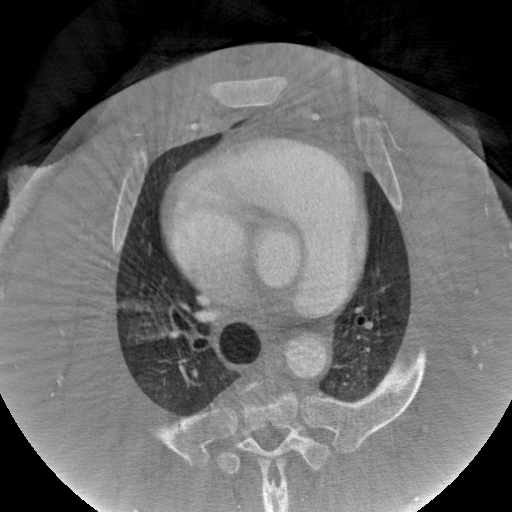
\includegraphics[height=2.7cm]{../02_image_processing/img/m1000-1000HU.png}    &
        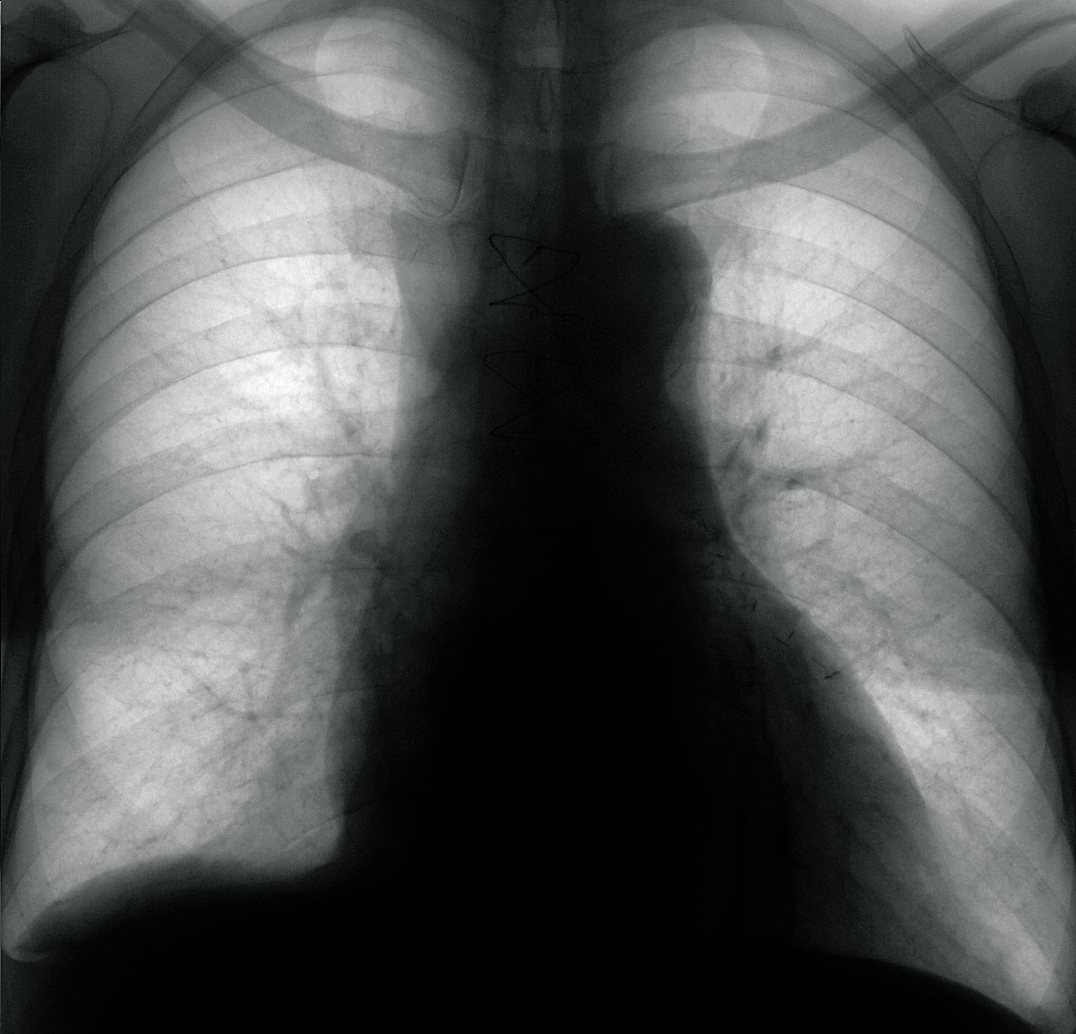
\includegraphics[height=2.7cm]{../06_x-ray/Siemens_Images/150_7.png}           &
        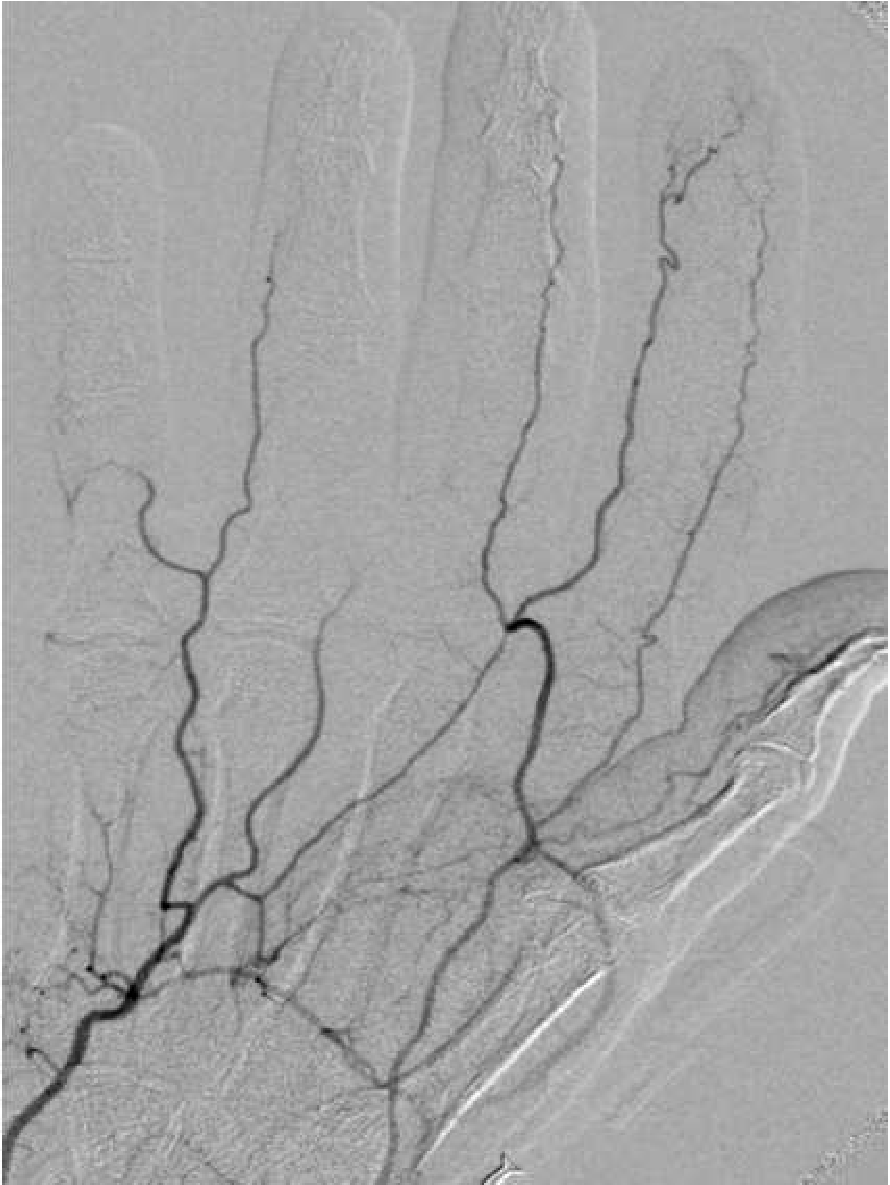
\includegraphics[height=2.7cm]{../06_x-ray/images/dsa_diff.pdf}                                          \\
        CT                                                                             & X-Ray & Angio           \\[0.2cm]
        \includegraphics[height=2.7cm]{images/parallel_full.png}      &
        \includegraphics[height=2.7cm]{images/appB.png} &
        \includegraphics[height=2.7cm]{images/SH_US_34572_12.jpg}                       \\
        MR                                                                             & SPECT & 3-d Ultra Sound \\
    \end{tabular}
    %\begin{minipage}{0.3\linewidth}
    %\begin{center}
    %\begin{figure}
    %\includegraphics[width=.8\linewidth]{../mt1-script/mr/images/parallel_full.png} \\
    %\vspace*{.1cm}{\normalsize MRT} \\
    %\vspace*{.1cm}
    %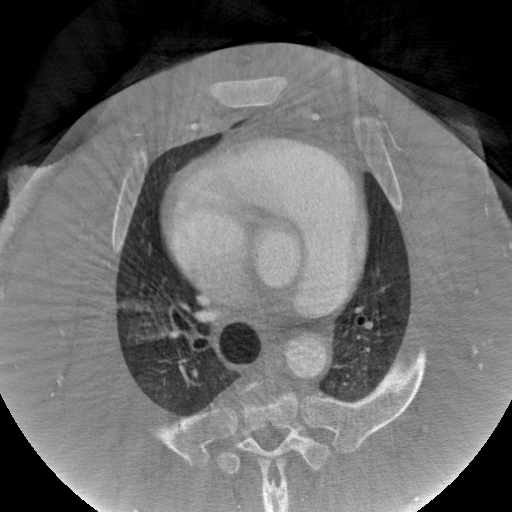
\includegraphics[width=.8\linewidth]{../02_image_processing/img/m1000-1000HU.png} \\
    %\vspace*{.1cm}{\normalsize CT} \\
    %\end{figure}
    %\end{center}
    %\end{minipage}
    %\hspace*{.3cm}
    %\begin{minipage}{0.3\linewidth}
    %\begin{figure}
    %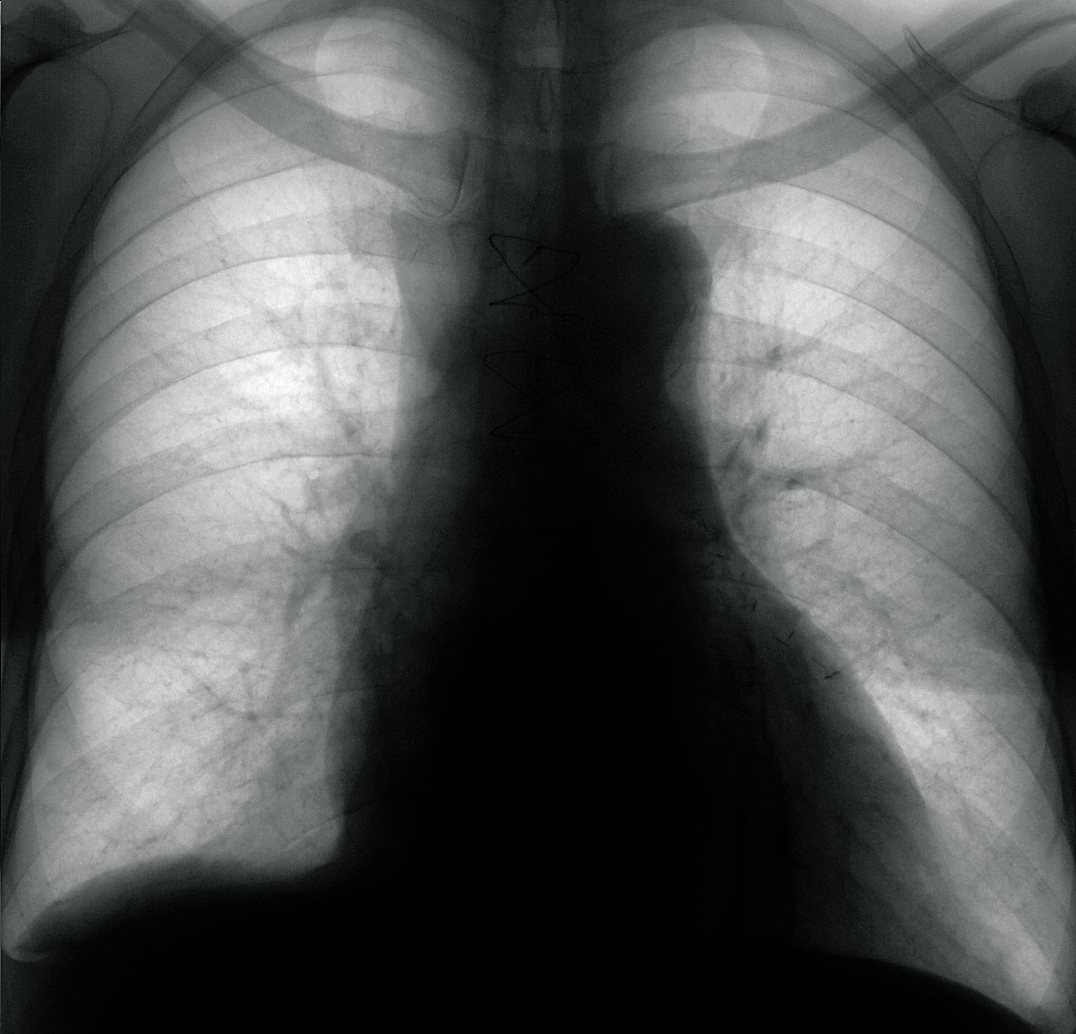
\includegraphics[width=.55\linewidth]{../06_x-ray/Siemens_Images/150_7.png} \\
    %\vspace*{.1cm}{\normalsize X-ray} \\
    %\vspace*{.1cm}
    %\includegraphics[width=.55\linewidth]{../mt1-script/emission_tomography/fig/appB.png} \\
    %\vspace*{.1cm}{\normalsize SPECT} \\
    %\end{figure}
    %\end{minipage}
    %\hspace*{.3cm}
    %\begin{minipage}{0.3\linewidth}
    %\begin{figure}
    %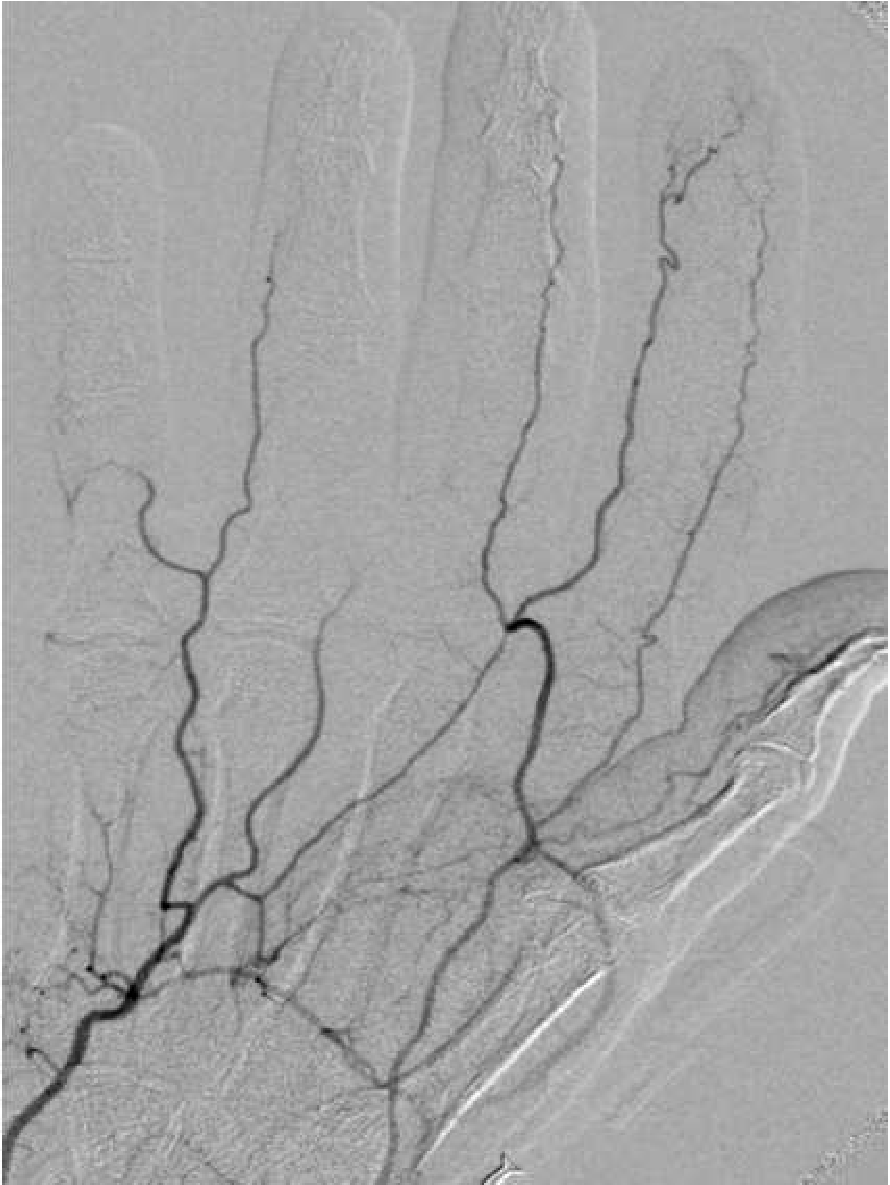
\includegraphics[width=.8\linewidth]{../06_x-ray/images/dsa_diff.pdf} \\
    %\vspace*{.1cm}{\normalsize Angio} \\
    %\vspace*{.1cm}
    %\includegraphics[width=.8\linewidth]{../mt1-script/Siemens_Images/US/SH_US_34572_12.jpg} \\
    %\vspace*{.1cm}{\normalsize Ultra Sound} \\
    %\end{figure}
    %\end{minipage}
\end{frame}




\begin{frame}[c]{Molecular and Morphologic Imaging}
    \begin{figure}
        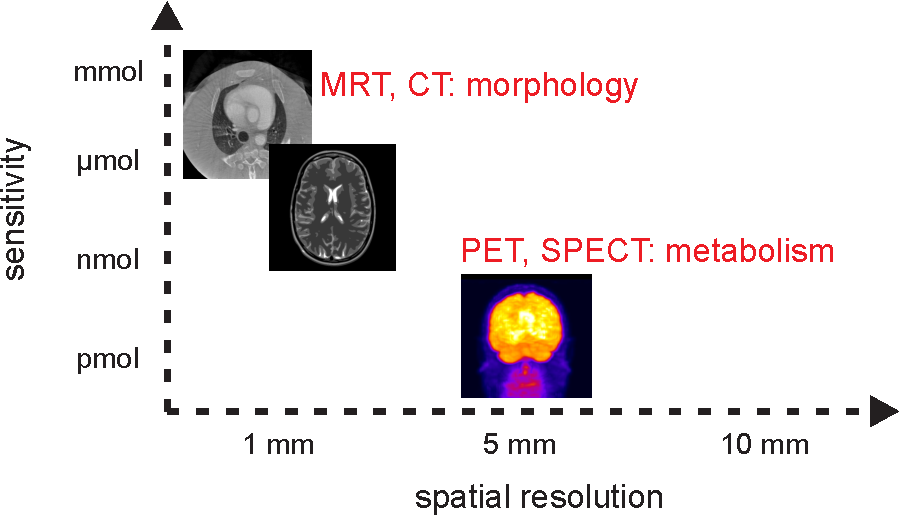
\includegraphics[width=.8\linewidth]{../00_motivation/Bilder/moletab.pdf}
    \end{figure}
\end{frame}




%Section 1
\section{Signals and Systems} %book chapter: 'Systemtheorie abbildender Systeme'

%subtitle
%toc for this chapter

\begin{frame}

    \frametitle{Signals}
    \begin{myDefinition}
        ``A signal is a function that conveys information about the behavior or attributes of some phenomenon.''\quad
        {\scriptsize
            Roland Priemer (1991). Introductory Signal Processing.
        }
    \end{myDefinition}
    \begin{columns}[c, onlytextwidth]
        \begin{column}{0.4\textwidth}
            \myExample{} of a 1D signal:
        \end{column}\begin{column}{0.6\textwidth}
            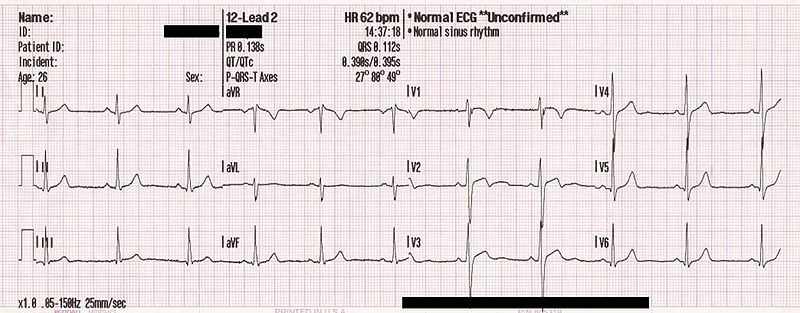
\includegraphics[height=.45\textheight ]{images/ecg}
            \begin{flushright}
                \scriptsize Sources: Wikimedia Commons
            \end{flushright}
        \end{column}
    \end{columns}

\end{frame}


%%TODO maybe include
%\begin{frame}
%\frametitle{Signal Examples}
%\begin{center}
%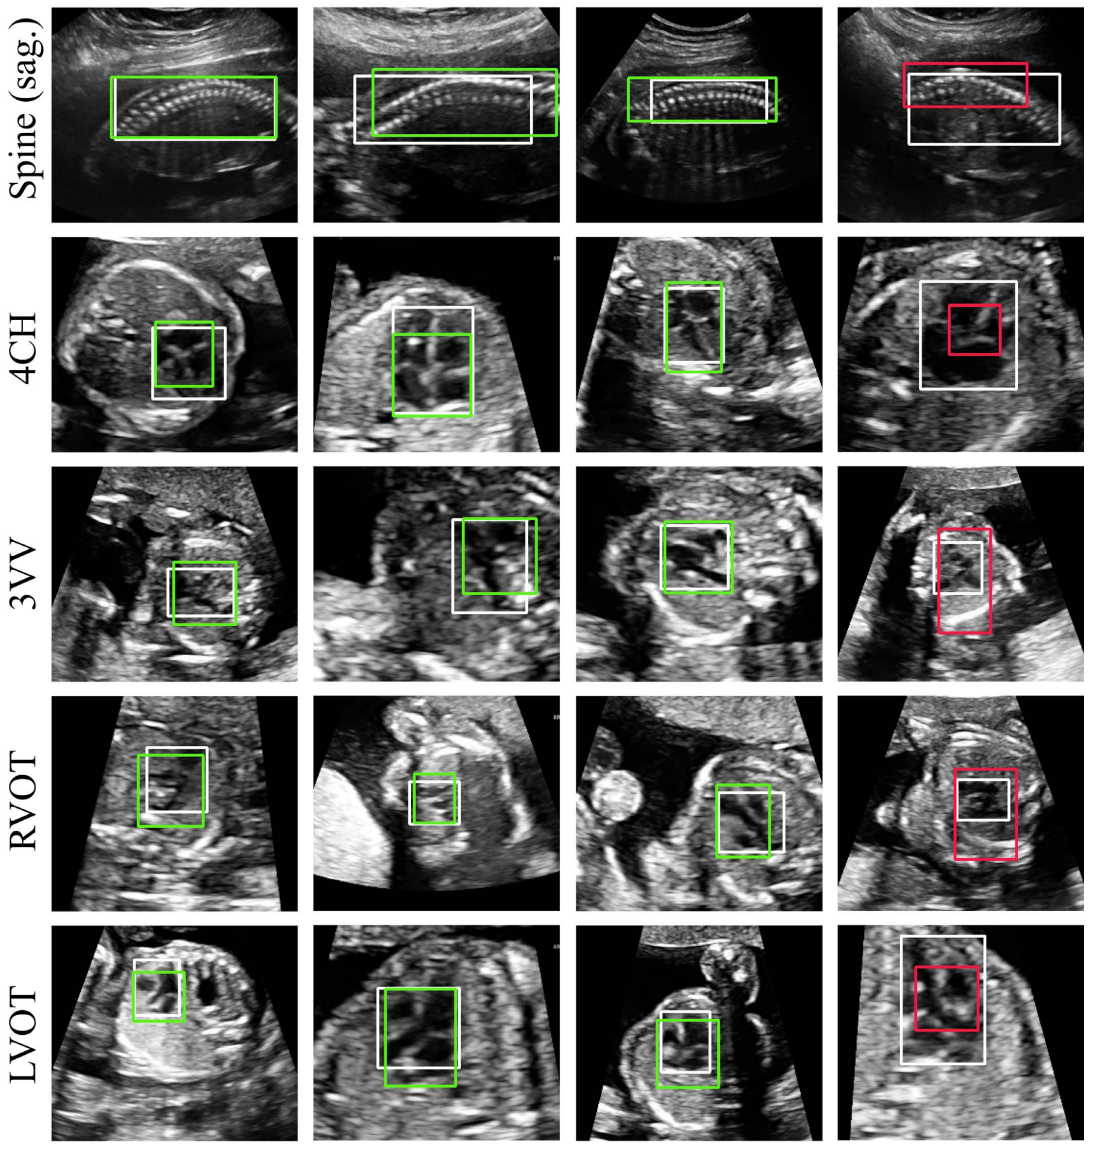
\includegraphics[height=.50\textheight ]{images/ultrasound} \quad
%\includegraphics[height=.60\textheight ]{images/endoscope_simba} \quad
%\includegraphics[height=.60\textheight ]{images/EEG}
%\end{center}
%\begin{flushright}
%\scriptsize Sources: Siemens, Wikimedia Commons, Wikimedia Commons
%\end{flushright}
%\end{frame}


\begin{frame}
    \frametitle{Signals and Systems}
    \begin{myDefinition}
        A \textbf{signal} is a function $f(t)$ that represents some information.

        \vspace{5mm}

        Signals are processed and transformed by \textbf{systems}, which are denoted by an operator $\mathcal{H}\{.\}$.
    \end{myDefinition}
    \begin{center}
        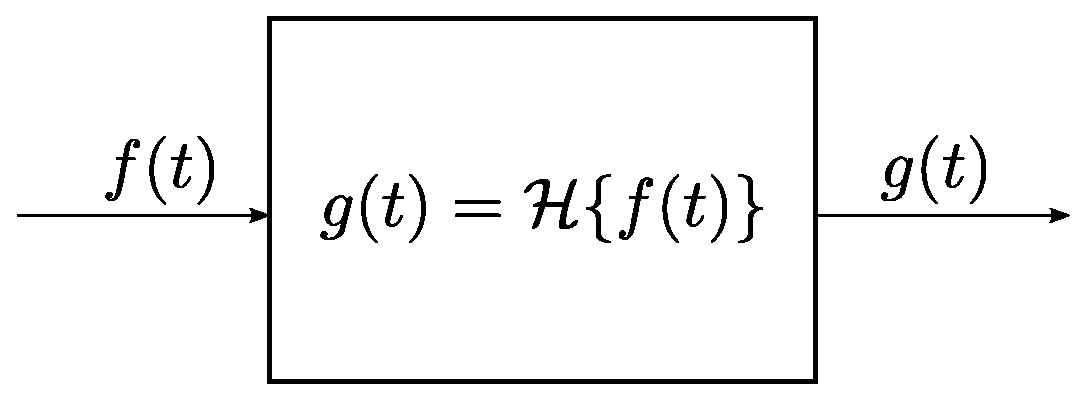
\includegraphics[height=.35\textheight ]{images/SystemBlock.pdf}
    \end{center}

\end{frame}




\begin{frame}
    \frametitle{System Characteristics}

    \begin{myDefinition}
        A system denoted by:
        \begin{center}
            $f_i(t) \quad \rightarrow \quad System \quad \rightarrow \quad g_i(t)$
        \end{center}
        is \textit{linear}, if:
        \begin{center}
            ${\sum c_if_i(t)} \quad \rightarrow \quad System \quad \rightarrow \quad {\sum c_ig_i(t)}$
        \end{center}
        is \textit{shift-invariant}, if:
        \begin{center}
            $f(t-t_0) \quad \rightarrow \quad System \quad \rightarrow \quad g(t-t_0)$
        \end{center}
        is \textit{causal}, if:
        \begin{center}
            $f_1(t) = f_2(t) \; \forall t < t_0 \quad \rightarrow \quad System \quad \rightarrow \quad g_1(t) = g_2(t) \; \forall t < t_0$
        \end{center}
    \end{myDefinition}
\end{frame}


\begin{frame}[c]{Simple Examples}

    \begin{columns}[c, onlytextwidth]
        \begin{column}{0.5\textwidth}
            \begin{itemize}
                \item $g(t) = f(t)$ \visible<3->{\redbox{}} \visible<4->{\bluebox{}} \visible<5->{\greenbox{}}
                \item[]
                \item $g(t) = \sin(f(t))$ \visible<11->{\bluebox{}} \visible<12->{\greenbox{}}
                \item[]
                \item $g(t) = 3 f(t+2)$ \visible<18->{\redbox{}} \visible<19->{\bluebox{}}
                \item[]
                \item $g(t) = f(t) - 2 f(t-1)$ \visible<25->{\redbox{}} \visible<26->{\bluebox{}} \visible<27->{\greenbox{}}
                \item[]
                \item $g(t) = f(t) \cdot e^{-0.5t}$ \visible<33->{\greenbox{}}
            \end{itemize}
        \end{column}\begin{column}{0.5\textwidth}
            \only<2-5>{
                \begin{center}
                    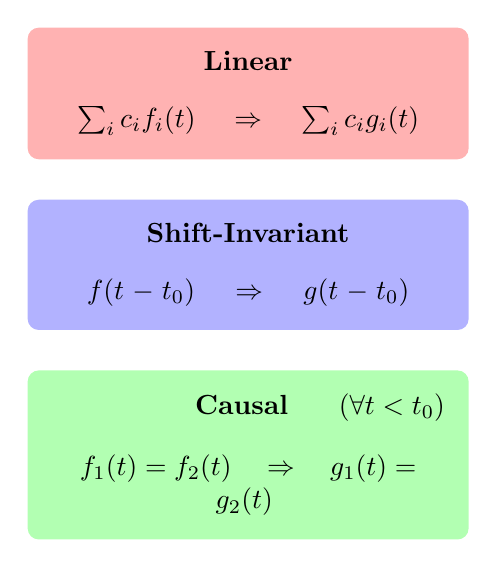
\begin{tikzpicture}[scale=1, transform shape]
                        \node (linear) [rounded corners, fill=red!30, text width=5cm, align=center, inner sep=0.3cm] {
                            \textbf{Linear}\\[0.3cm]
                            ${\sum_{i}  c_if_i(t)} \quad{} \Rightarrow \quad {\sum_{i}  c_ig_i(t)}$
                        };
                        \node (shift) [rounded corners, fill=blue!30, text width=5cm, align=center, below=0.5cm of linear, inner sep=0.3cm] {
                            \textbf{Shift-Invariant}\\[0.3cm]
                            $f(t-t_0) \quad  \Rightarrow \quad g(t-t_0)$
                        };
                        \node (Causal) [rounded corners, fill=green!30, text width=5cm, align=center, below=0.5cm of shift, inner sep=0.3cm] {
                            \hfill{}\textbf{\hspace{1.3cm}Causal}\hfill{} ($\forall t < t_0$)\\[0.3cm]
                            \begin{center}
                                $f_1(t) = f_2(t) \quad{} \Rightarrow \quad g_1(t) = g_2(t) \; $
                            \end{center}};
                    \end{tikzpicture}
                \end{center}
            }
            \only<6>{
                \begin{center}
                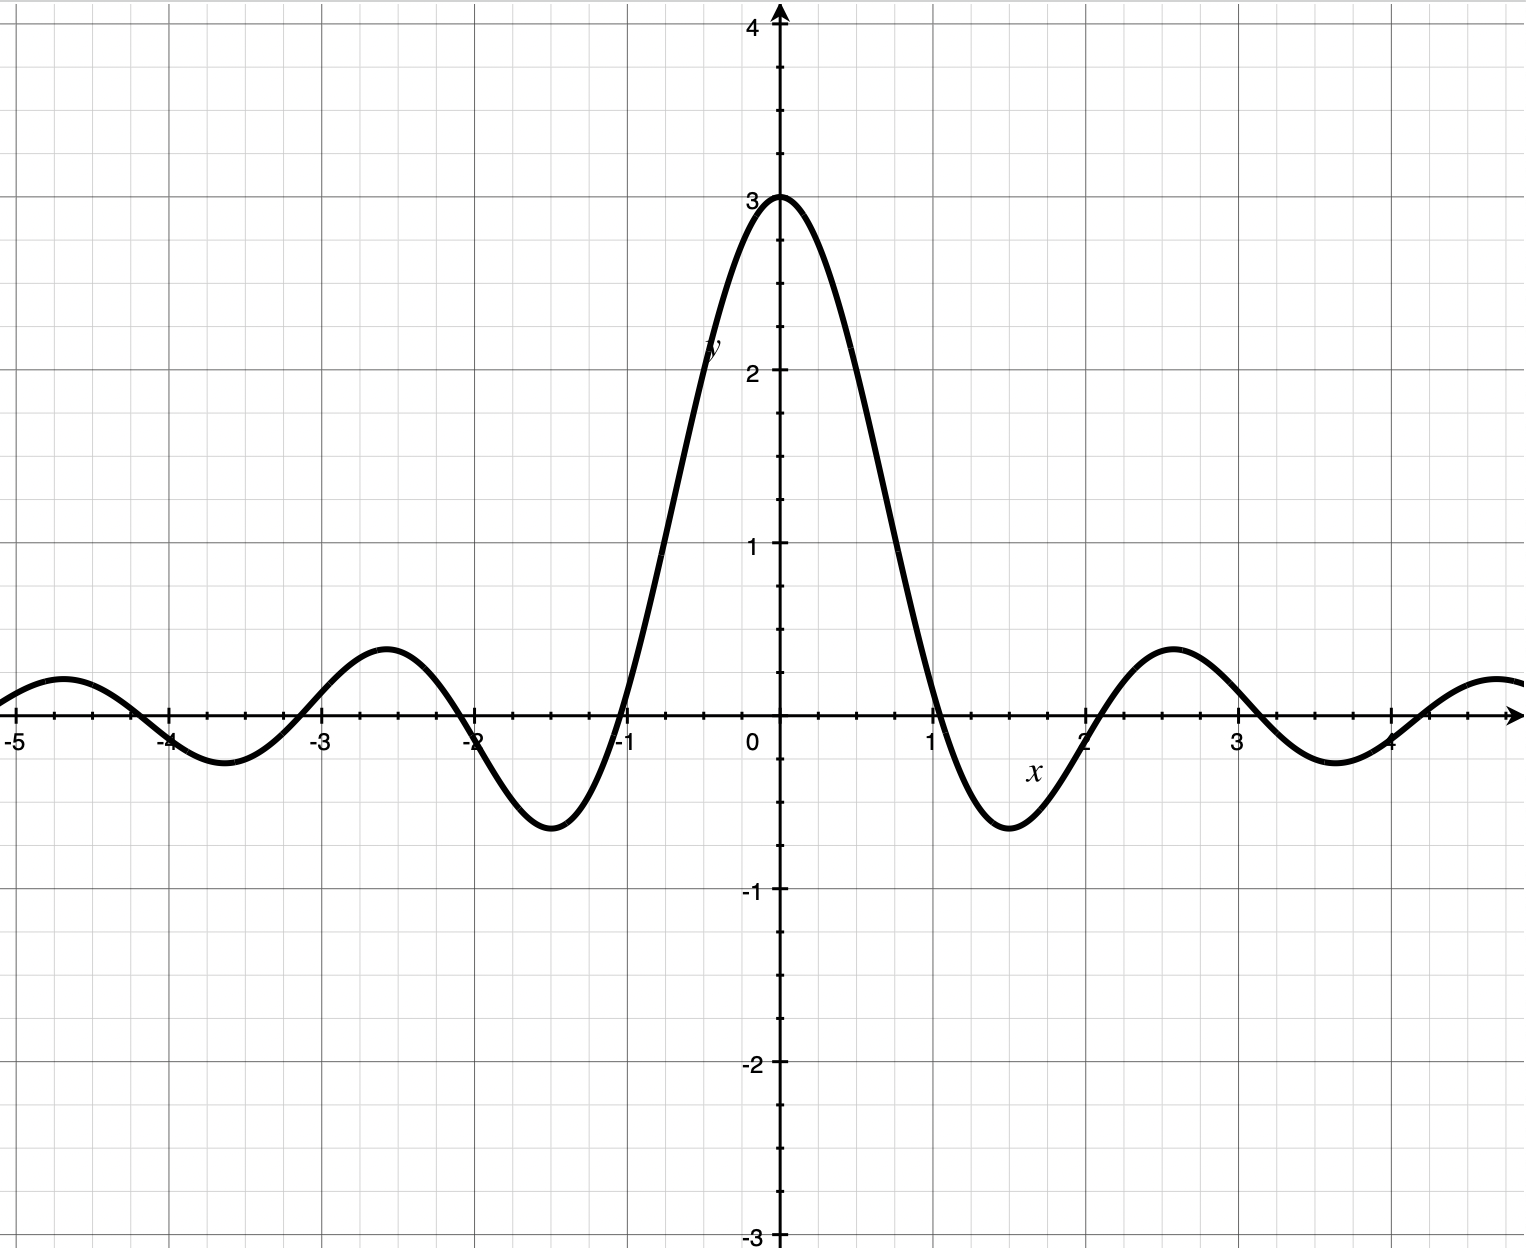
\includegraphics[width=\textwidth ]{a1.png}
                \end{center}
            }
            \only<7>{
                \begin{center}
                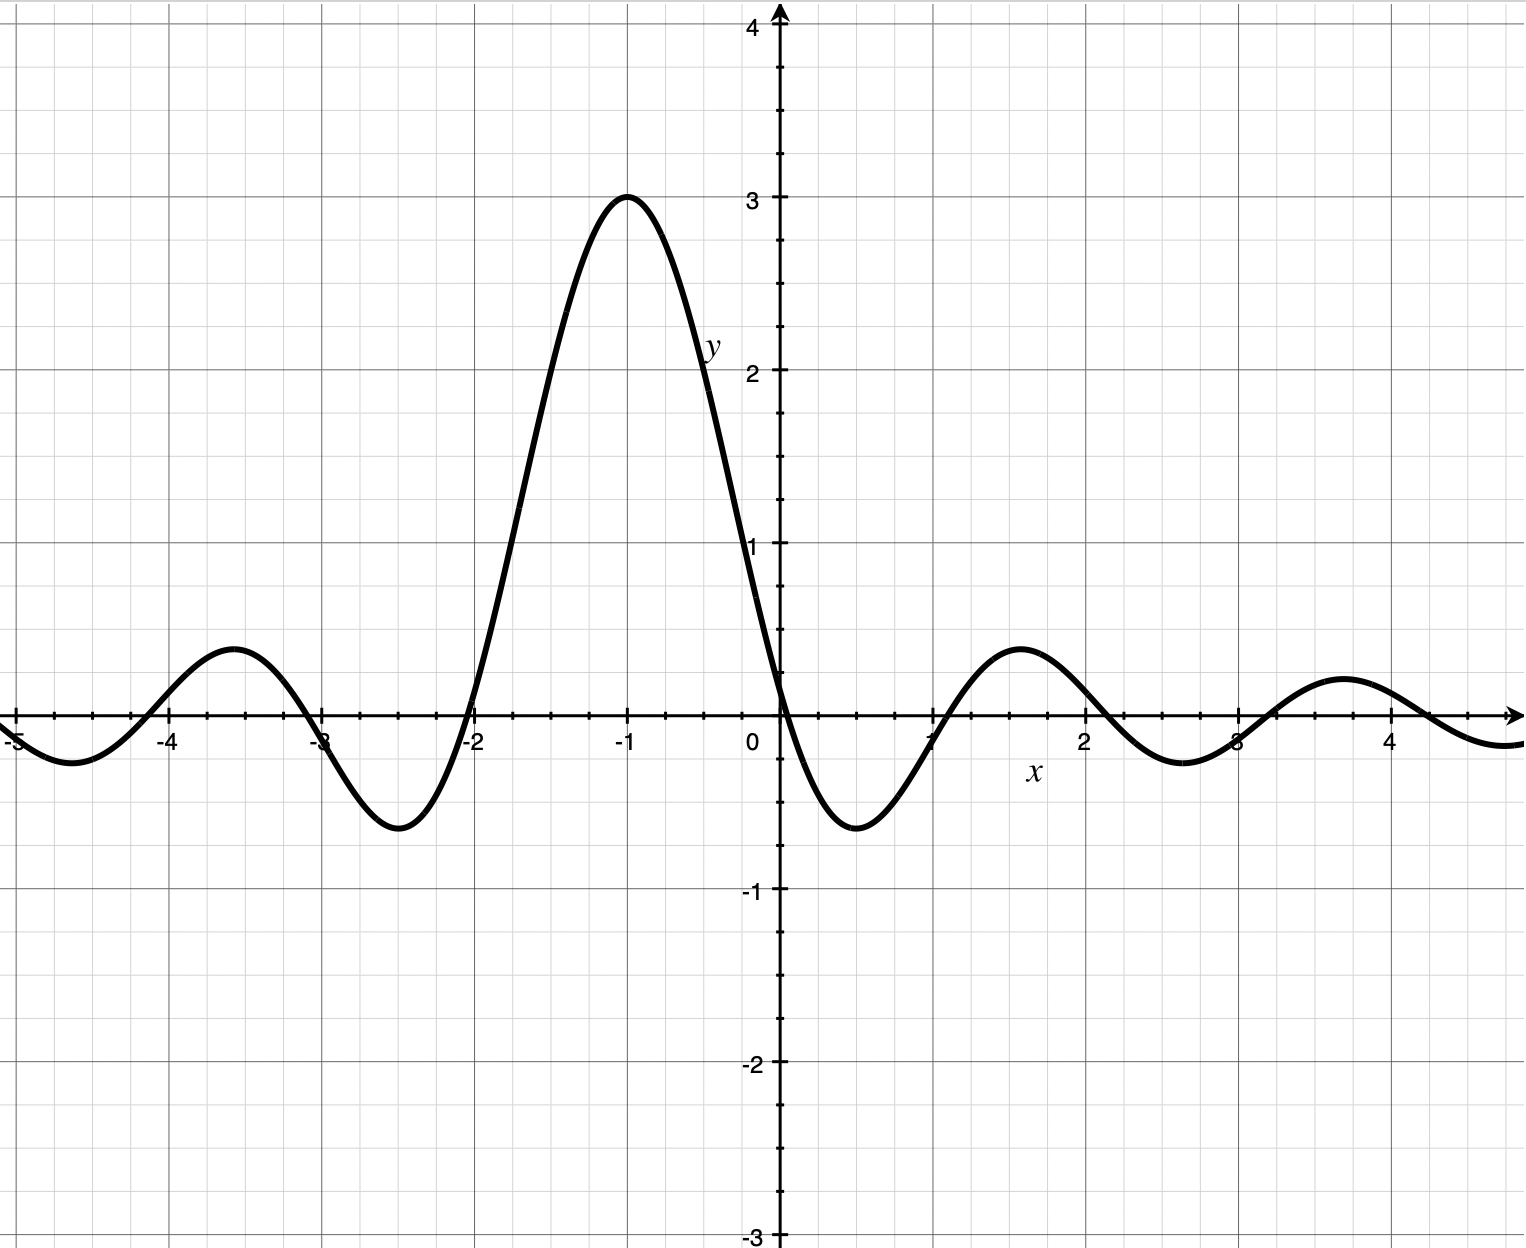
\includegraphics[width=\textwidth ]{a2.png}
                \end{center}
            }
            \only<8>{
                \begin{center}
                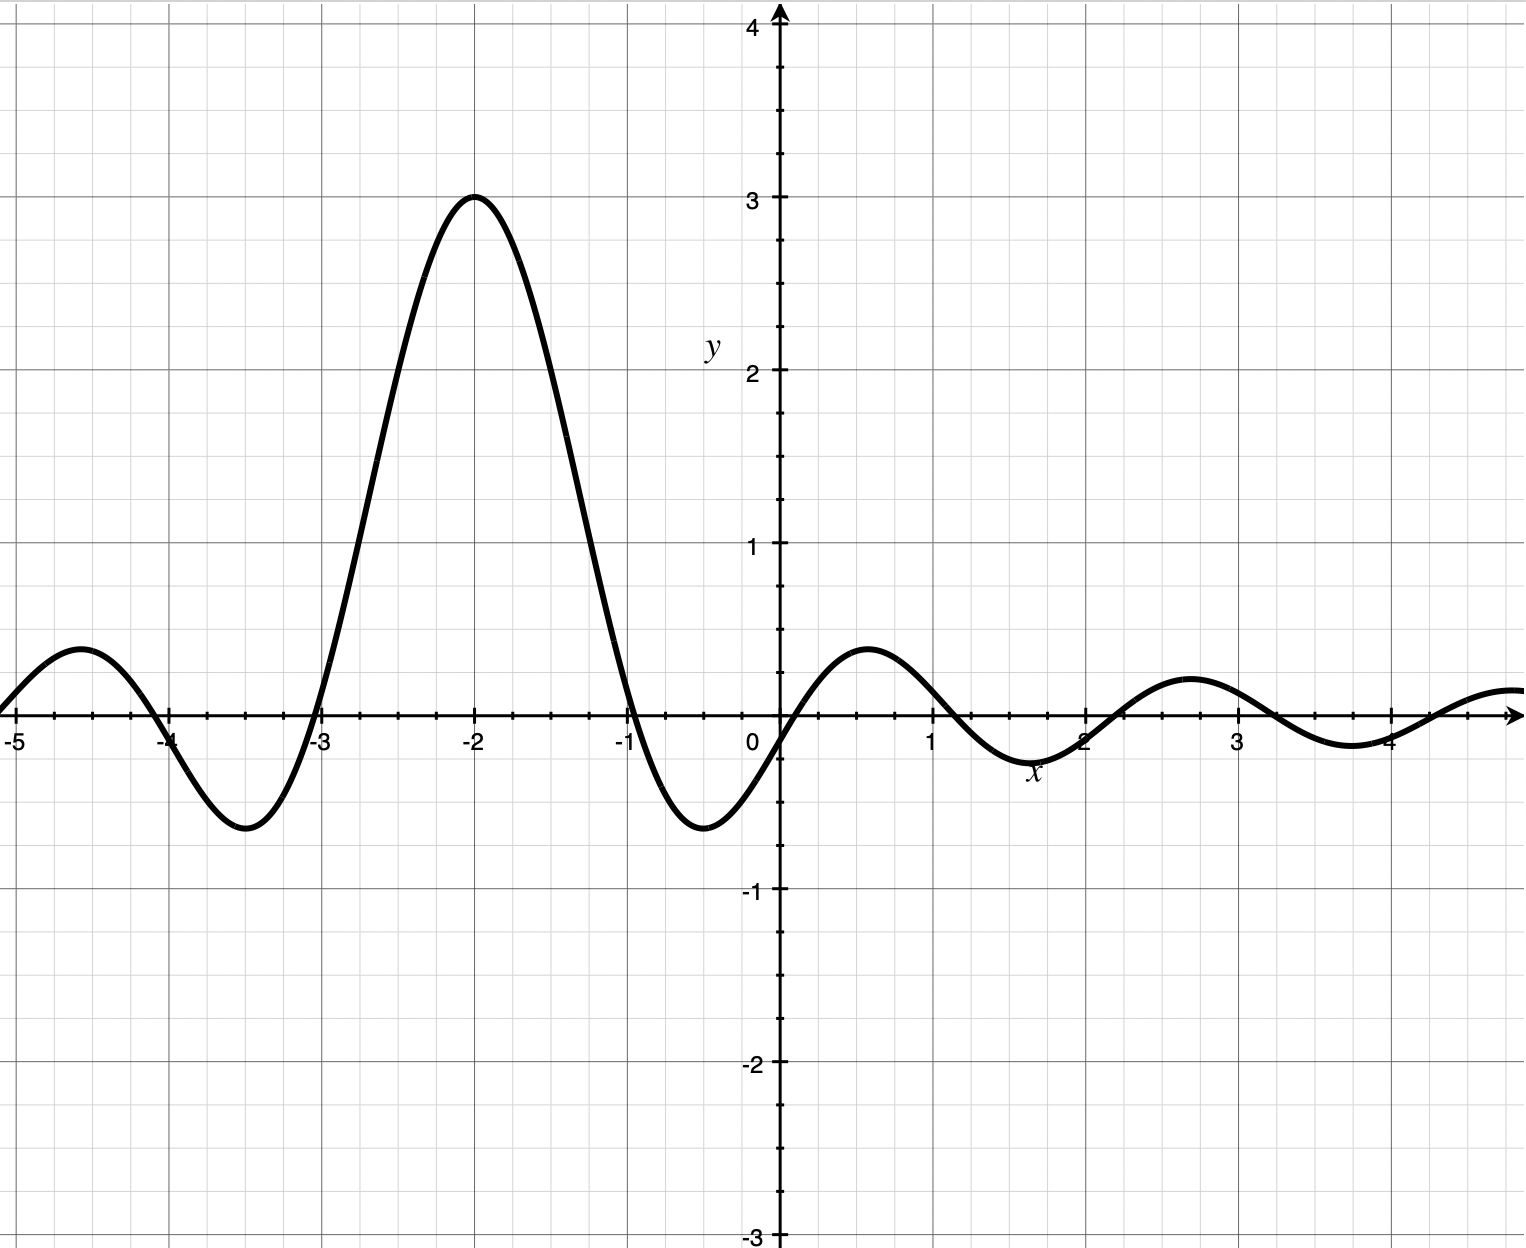
\includegraphics[width=\textwidth ]{a3.png}
                \end{center}
            }
            \only<9>{
                \begin{center}
                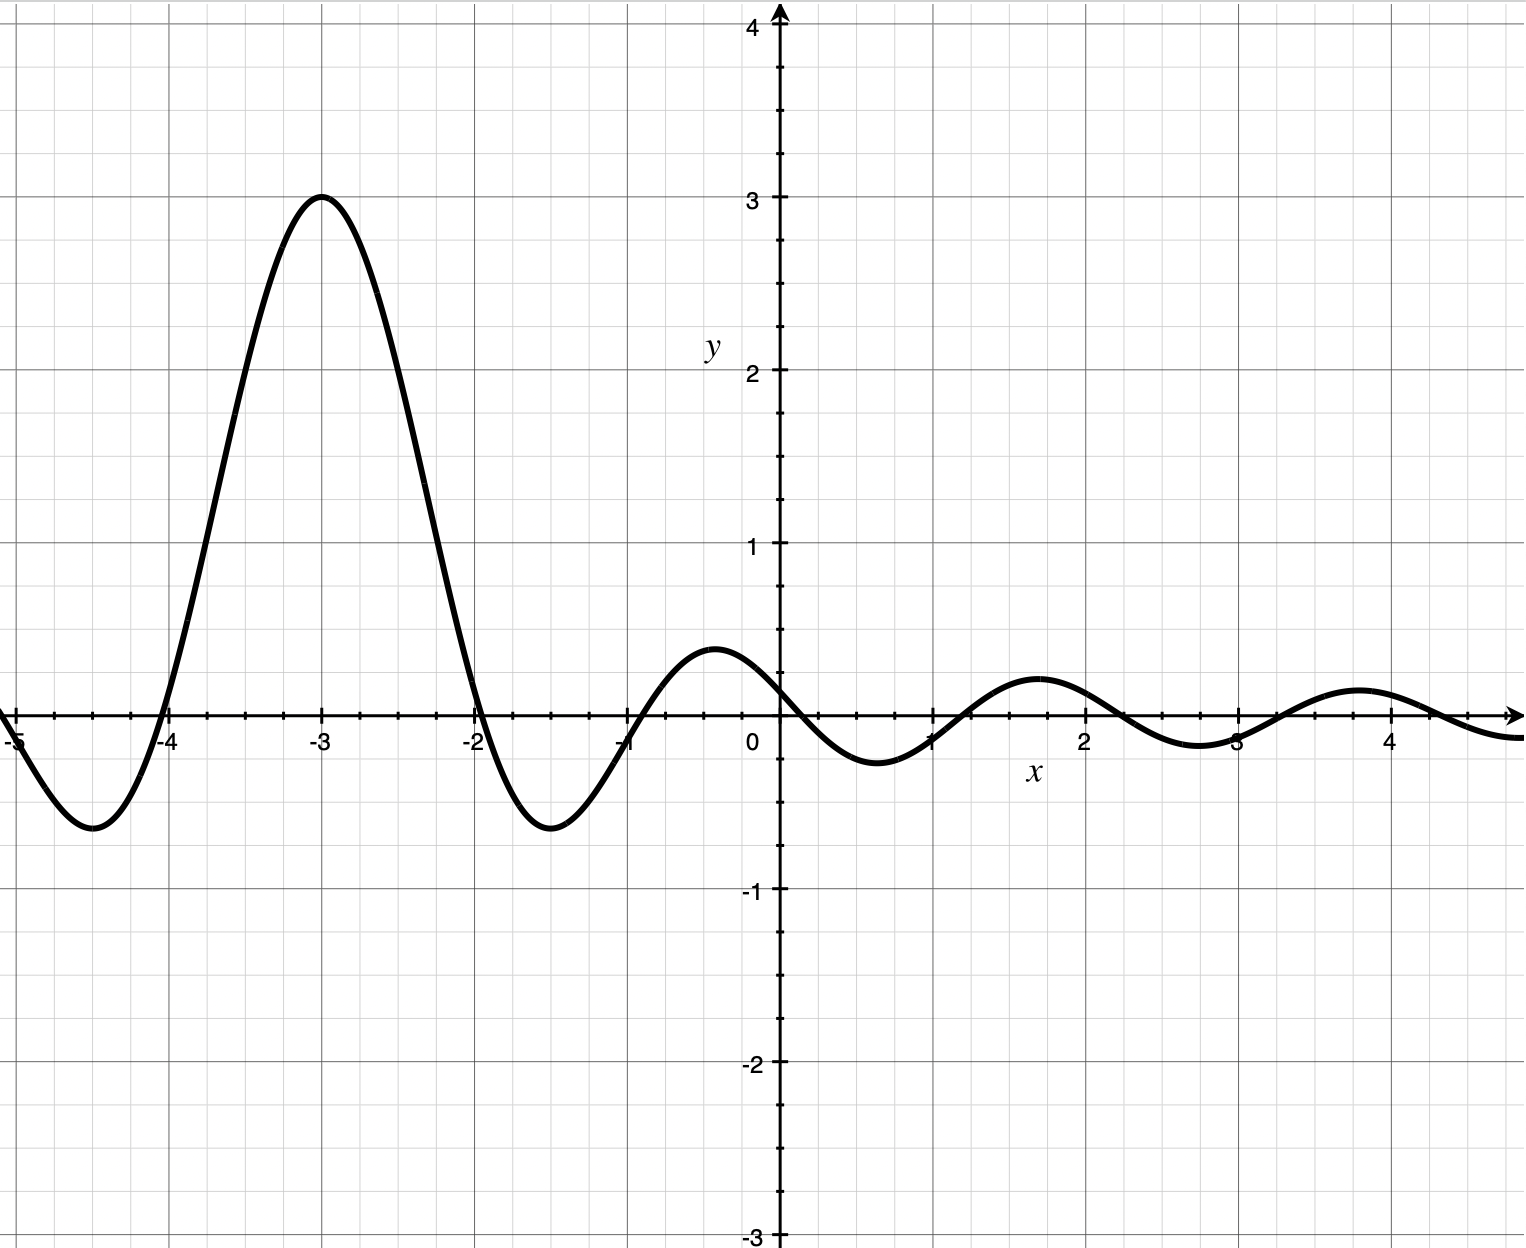
\includegraphics[width=\textwidth ]{a4.png}
                \end{center}
            }
            \only<10-12>{
                \begin{center}
                    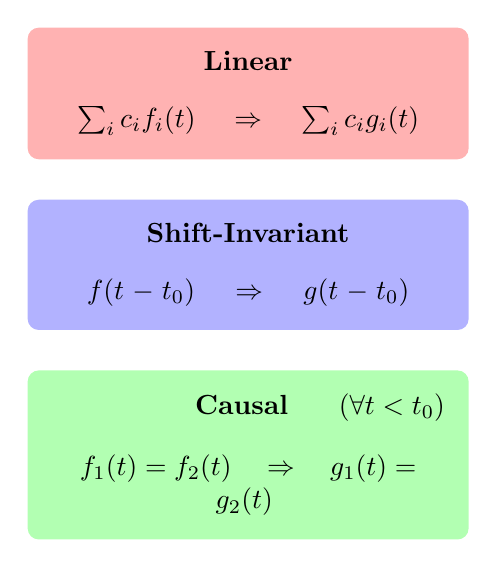
\begin{tikzpicture}[scale=1, transform shape]
                        \node (linear) [rounded corners, fill=red!30, text width=5cm, align=center, inner sep=0.3cm] {
                            \textbf{Linear}\\[0.3cm]
                            ${\sum_{i}  c_if_i(t)} \quad{} \Rightarrow \quad {\sum_{i}  c_ig_i(t)}$
                        };
                        \node (shift) [rounded corners, fill=blue!30, text width=5cm, align=center, below=0.5cm of linear, inner sep=0.3cm] {
                            \textbf{Shift-Invariant}\\[0.3cm]
                            $f(t-t_0) \quad  \Rightarrow \quad g(t-t_0)$
                        };
                        \node (Causal) [rounded corners, fill=green!30, text width=5cm, align=center, below=0.5cm of shift, inner sep=0.3cm] {
                            \hfill{}\textbf{\hspace{1.3cm}Causal}\hfill{} ($\forall t < t_0$)\\[0.3cm]
                            \begin{center}
                                $f_1(t) = f_2(t) \quad{} \Rightarrow \quad g_1(t) = g_2(t) \; $
                            \end{center}};
                    \end{tikzpicture}
                \end{center}
            }
            \only<13>{
                \begin{center}
                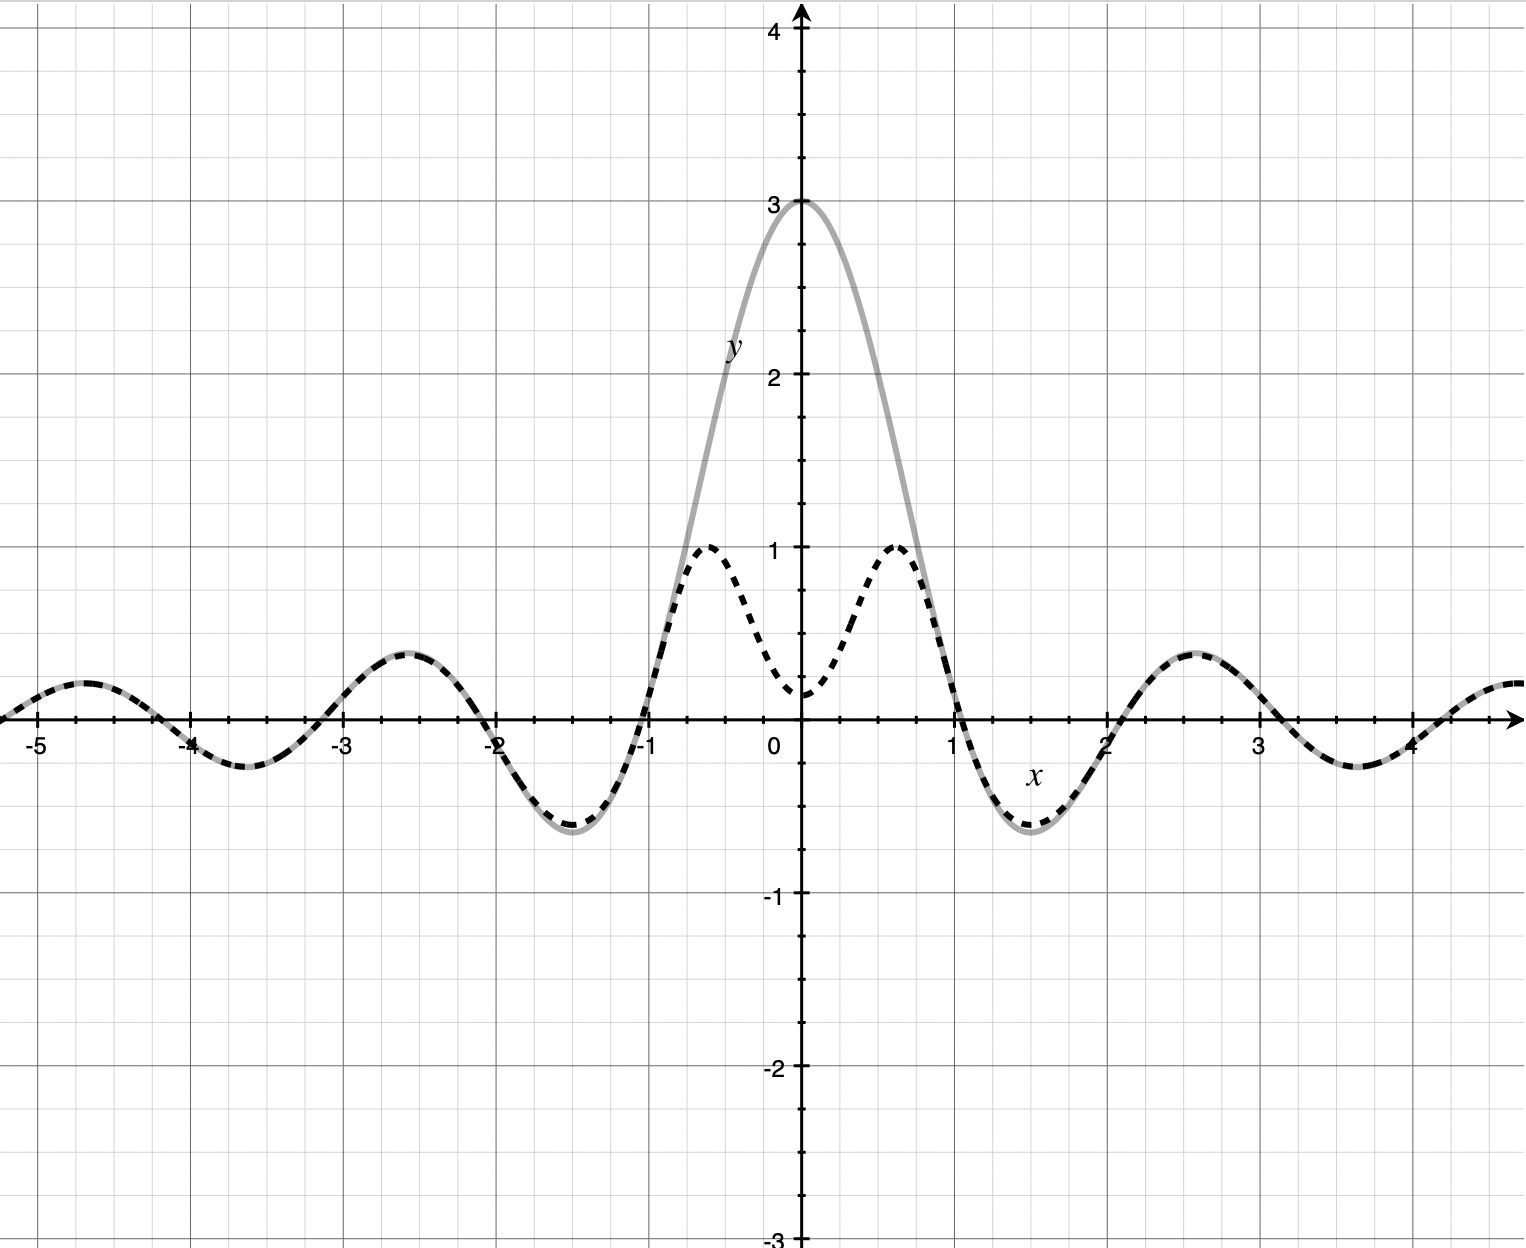
\includegraphics[width=\textwidth ]{a5.png}
                \end{center}
            }
            \only<14>{
                \begin{center}
                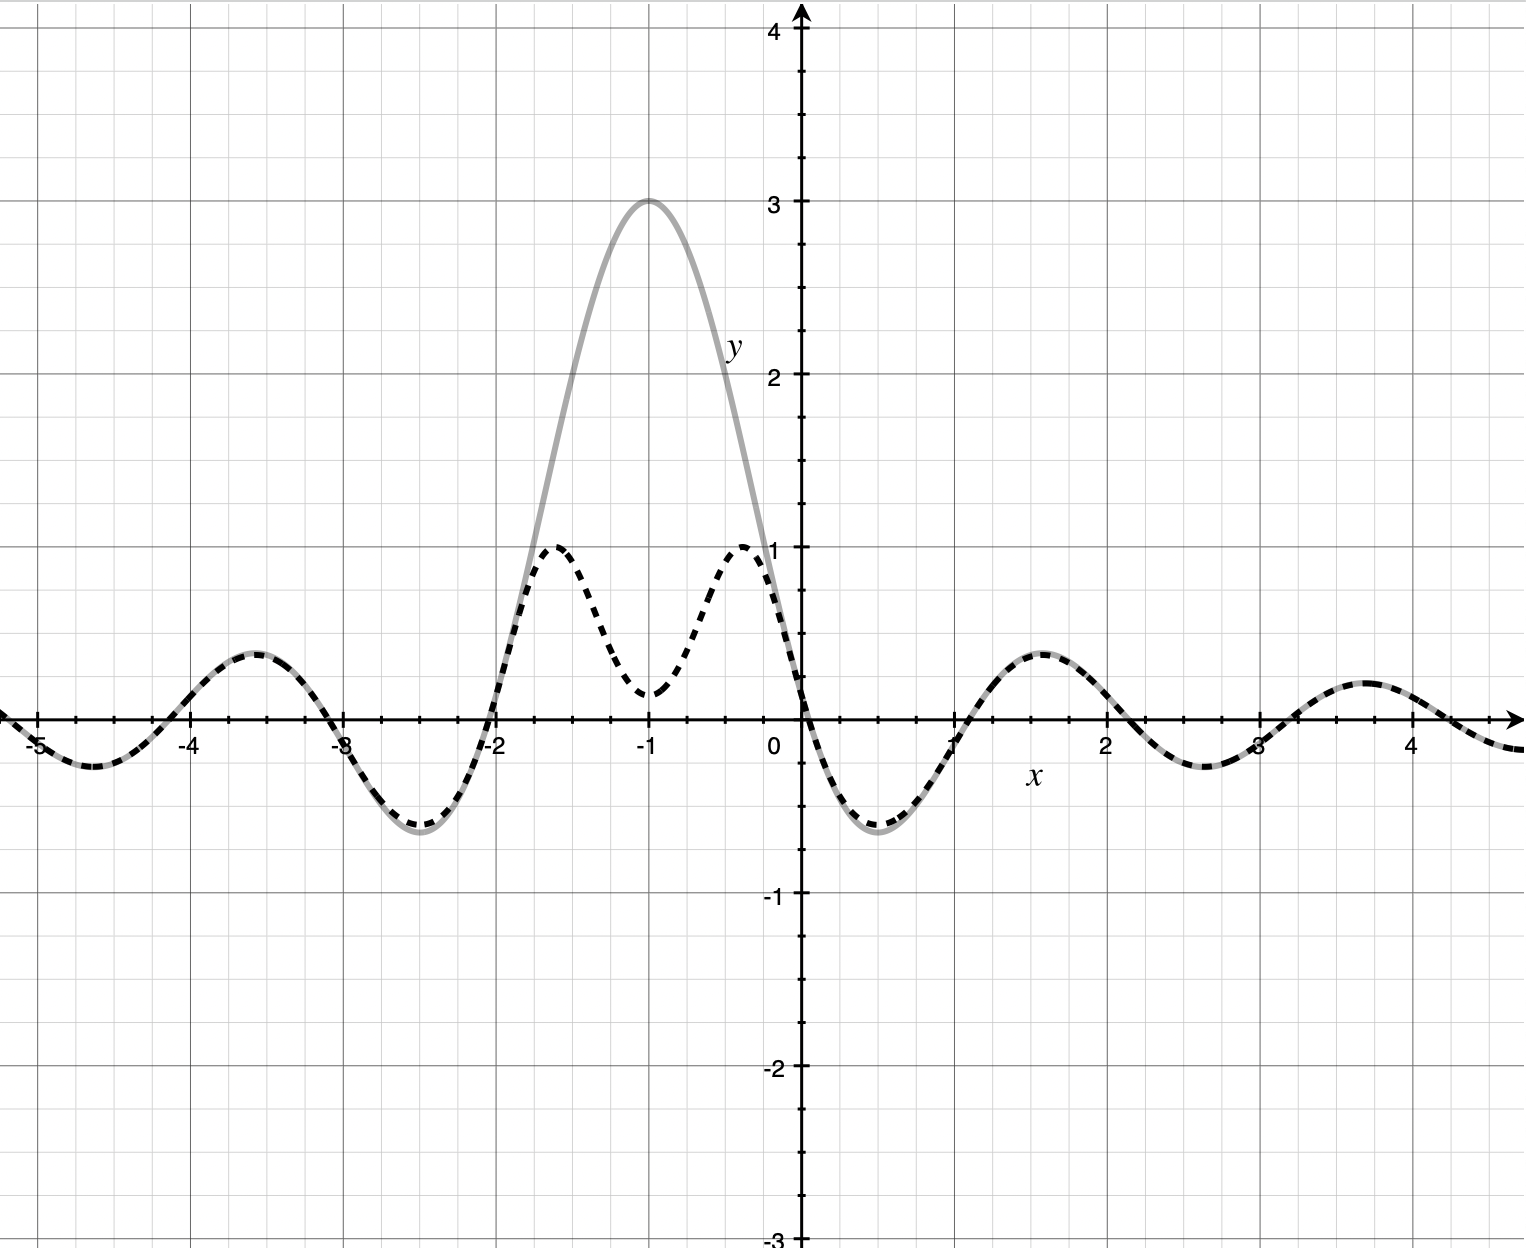
\includegraphics[width=\textwidth ]{a6.png}
                \end{center}
            }
            \only<15>{
                \begin{center}
                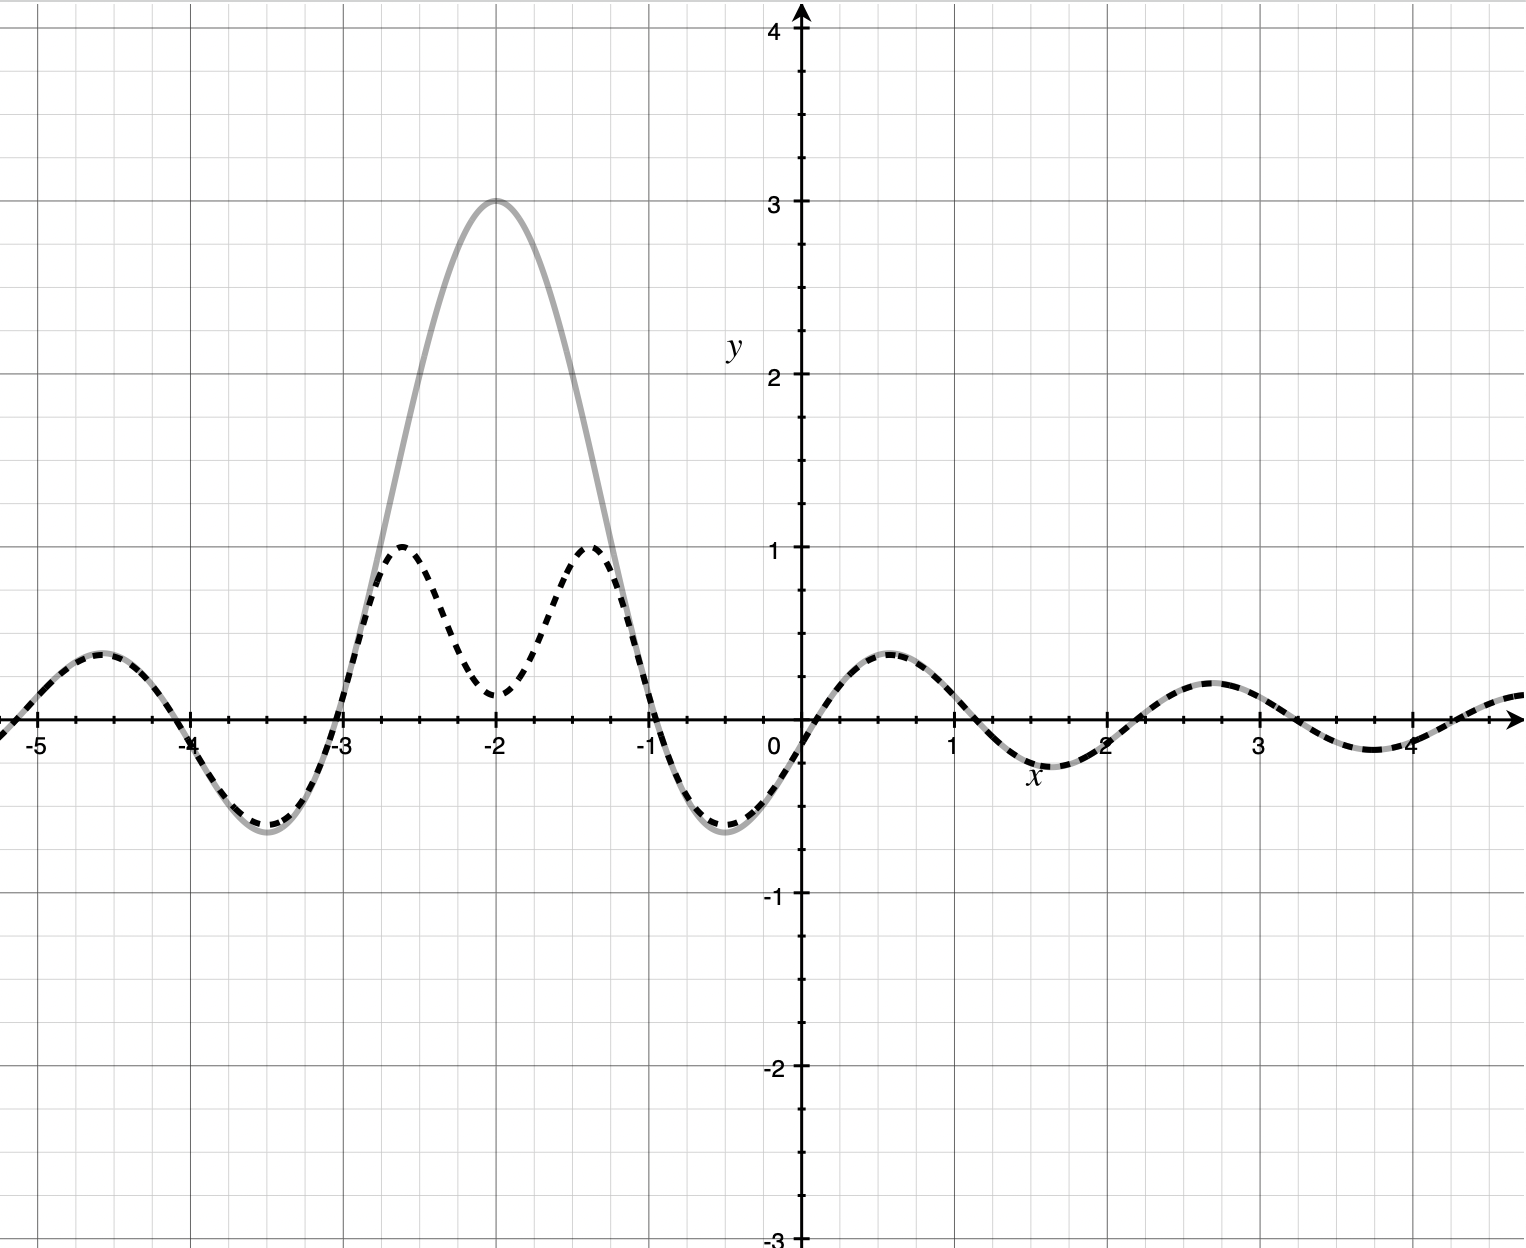
\includegraphics[width=\textwidth ]{a7.png}
                \end{center}
            }
            \only<16>{
                \begin{center}
                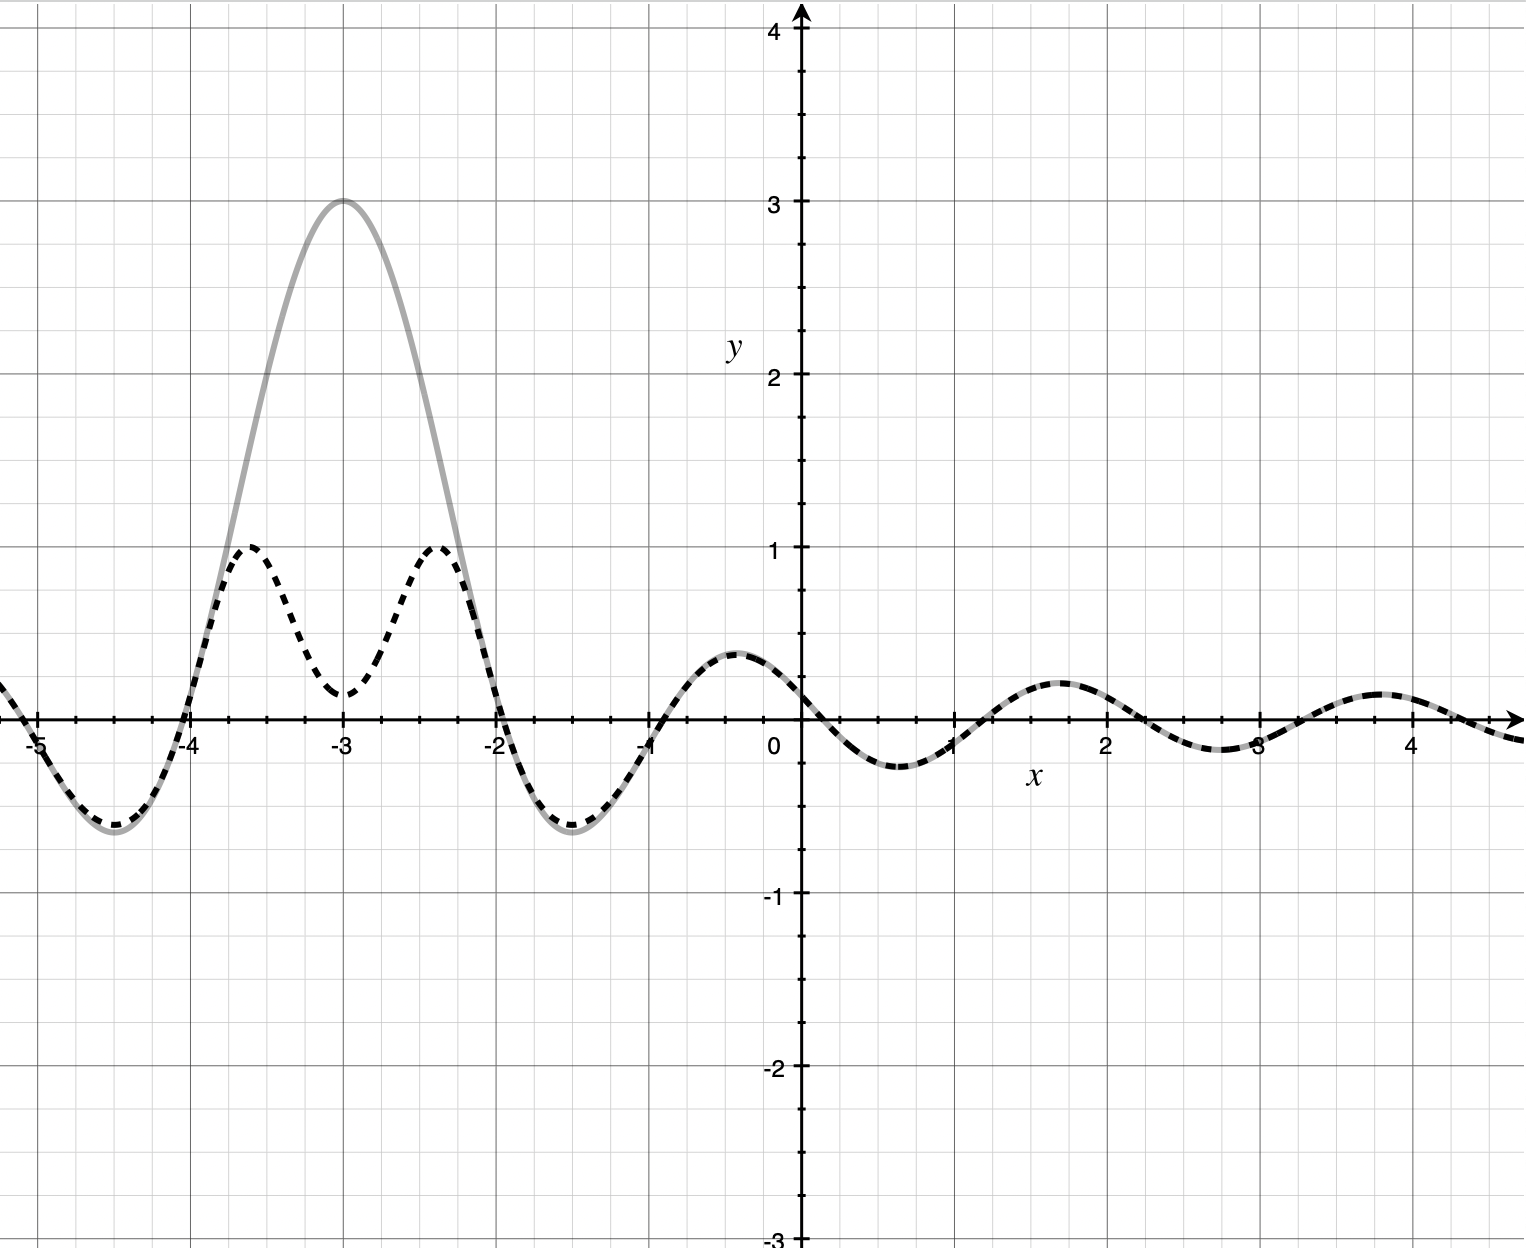
\includegraphics[width=\textwidth ]{a8.png}
                \end{center}
            }
            \only<17-19>{
                \begin{center}
                    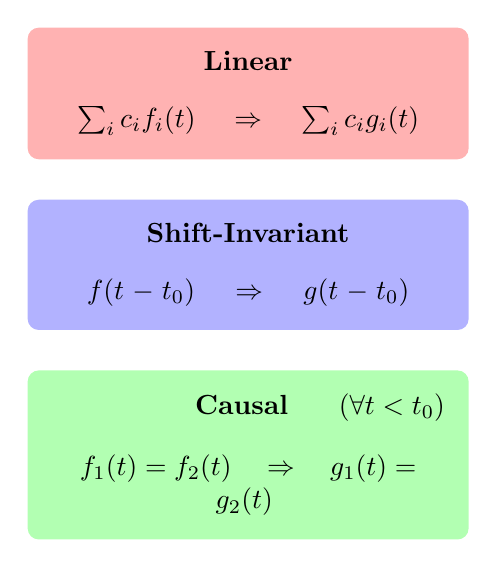
\begin{tikzpicture}[scale=1, transform shape]
                        \node (linear) [rounded corners, fill=red!30, text width=5cm, align=center, inner sep=0.3cm] {
                            \textbf{Linear}\\[0.3cm]
                            ${\sum_{i}  c_if_i(t)} \quad{} \Rightarrow \quad {\sum_{i}  c_ig_i(t)}$
                        };
                        \node (shift) [rounded corners, fill=blue!30, text width=5cm, align=center, below=0.5cm of linear, inner sep=0.3cm] {
                            \textbf{Shift-Invariant}\\[0.3cm]
                            $f(t-t_0) \quad  \Rightarrow \quad g(t-t_0)$
                        };
                        \node (Causal) [rounded corners, fill=green!30, text width=5cm, align=center, below=0.5cm of shift, inner sep=0.3cm] {
                            \hfill{}\textbf{\hspace{1.3cm}Causal}\hfill{} ($\forall t < t_0$)\\[0.3cm]
                            \begin{center}
                                $f_1(t) = f_2(t) \quad{} \Rightarrow \quad g_1(t) = g_2(t) \; $
                            \end{center}};
                    \end{tikzpicture}
                \end{center}
            }
            \only<20>{
                \begin{center}
                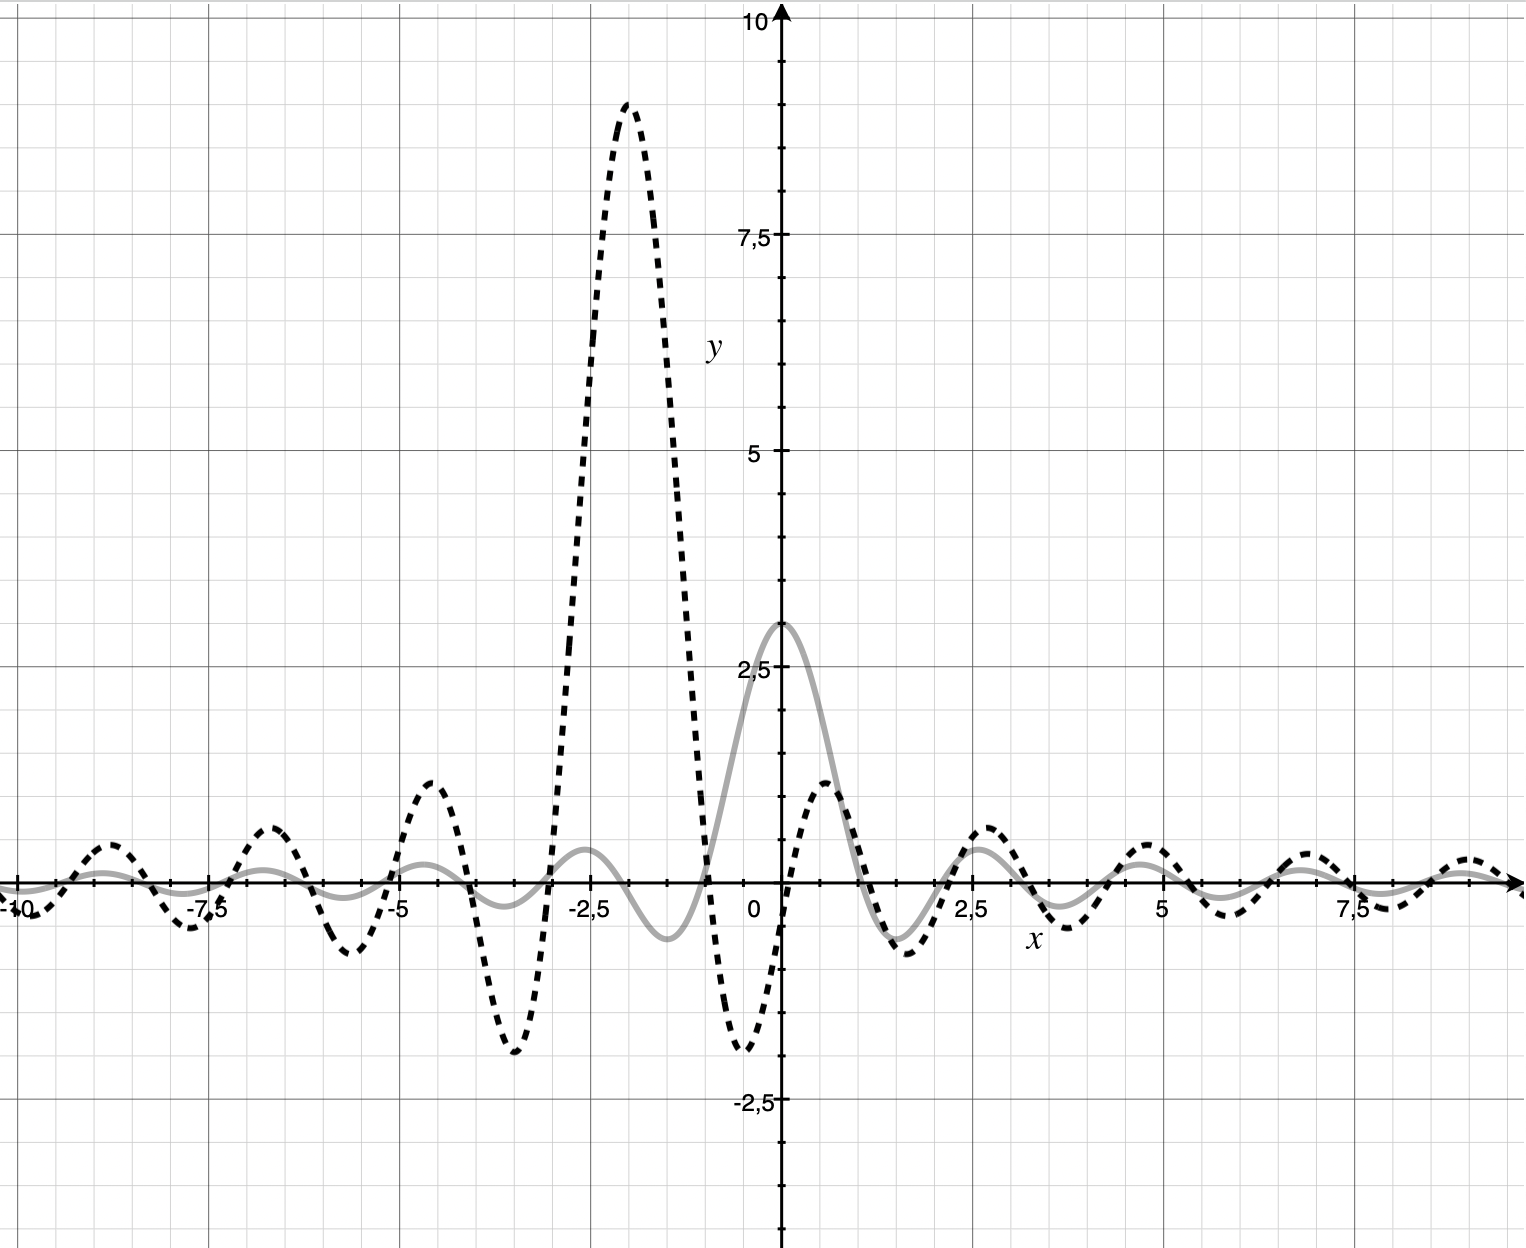
\includegraphics[width=\textwidth ]{a9.png}
                \end{center}
            }
            \only<21>{
                \begin{center}
                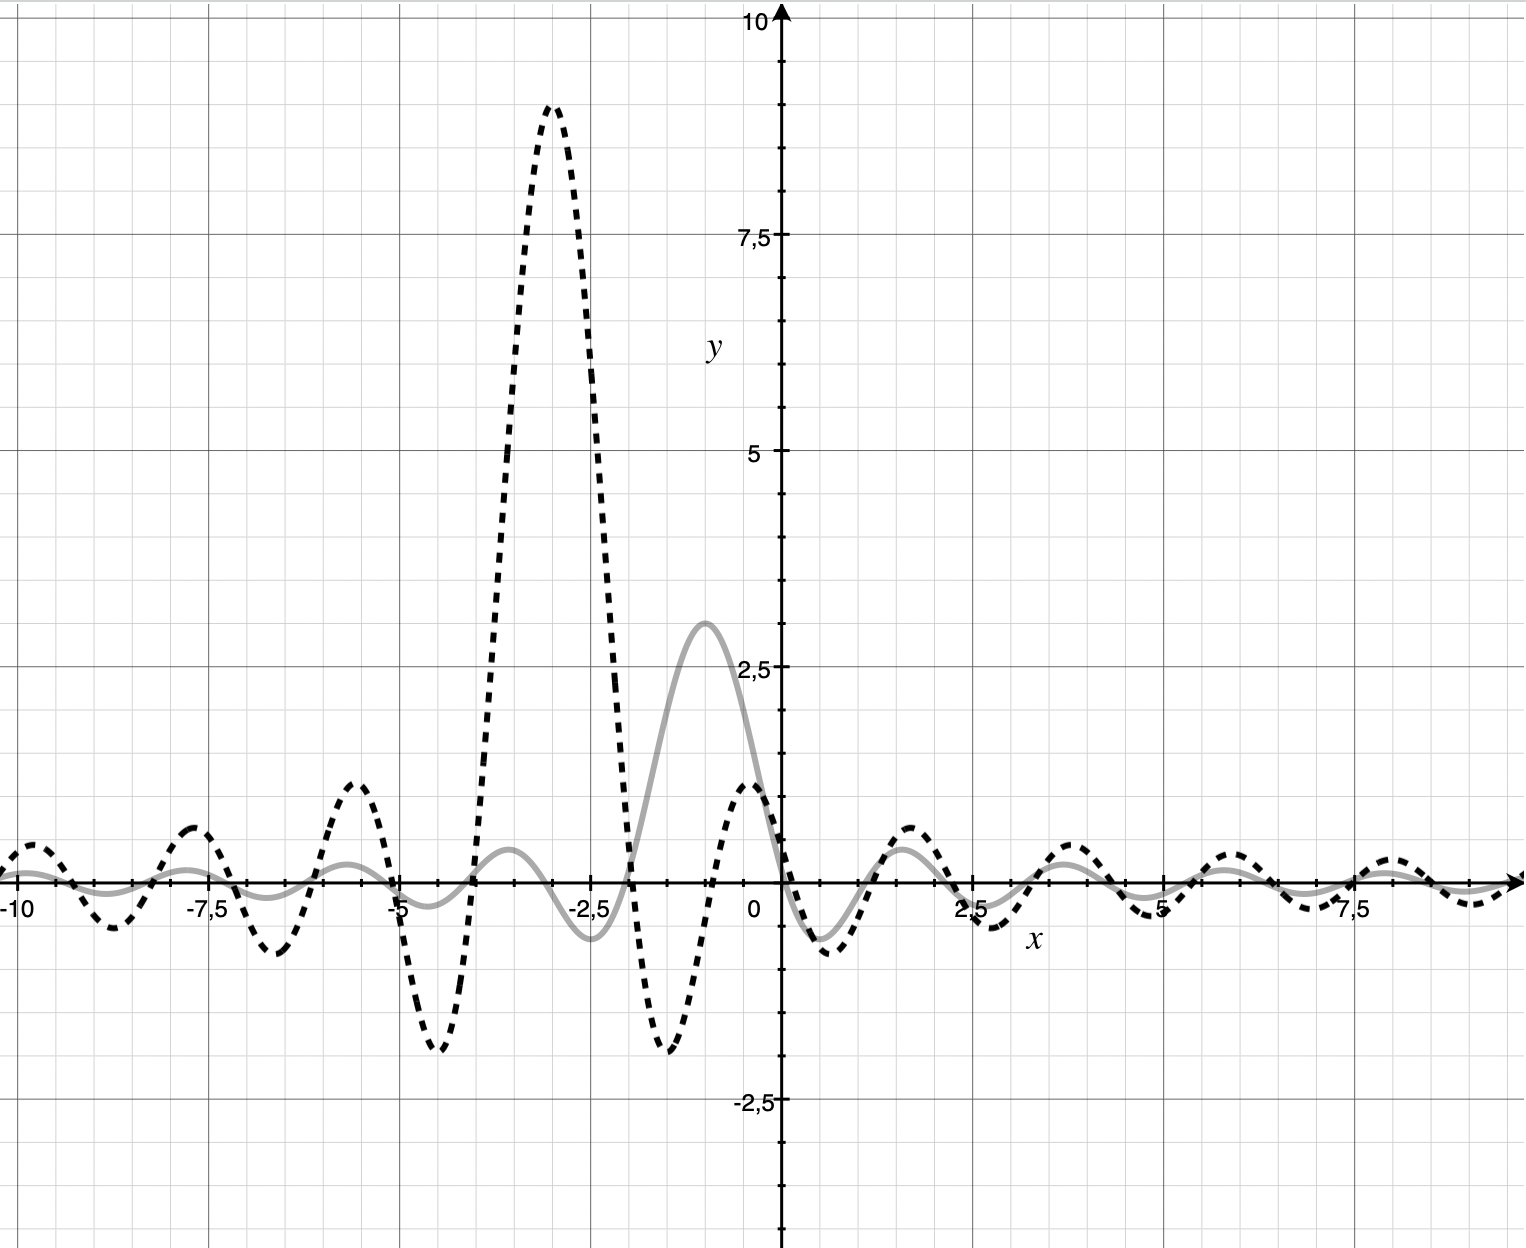
\includegraphics[width=\textwidth ]{a10.png}
                \end{center}
            }
            \only<22>{
                \begin{center}
                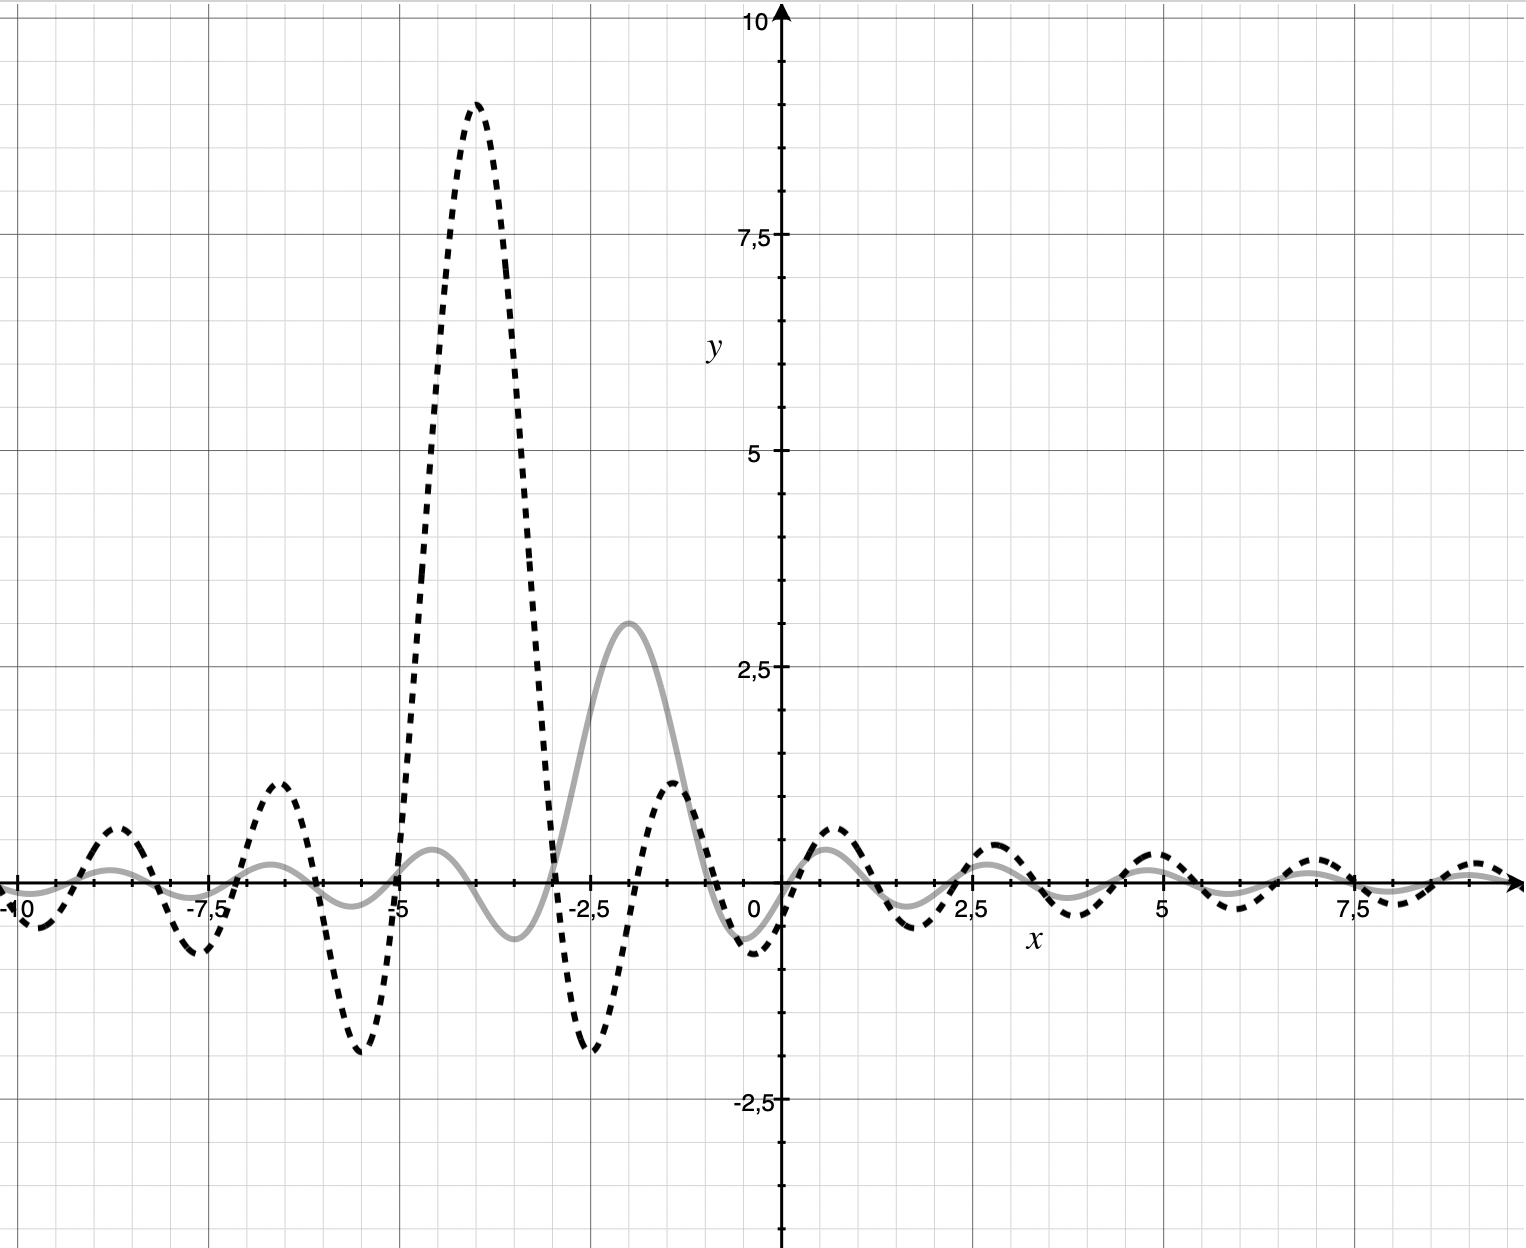
\includegraphics[width=\textwidth ]{a11.png}
                \end{center}
            }
            \only<23>{
                \begin{center}
                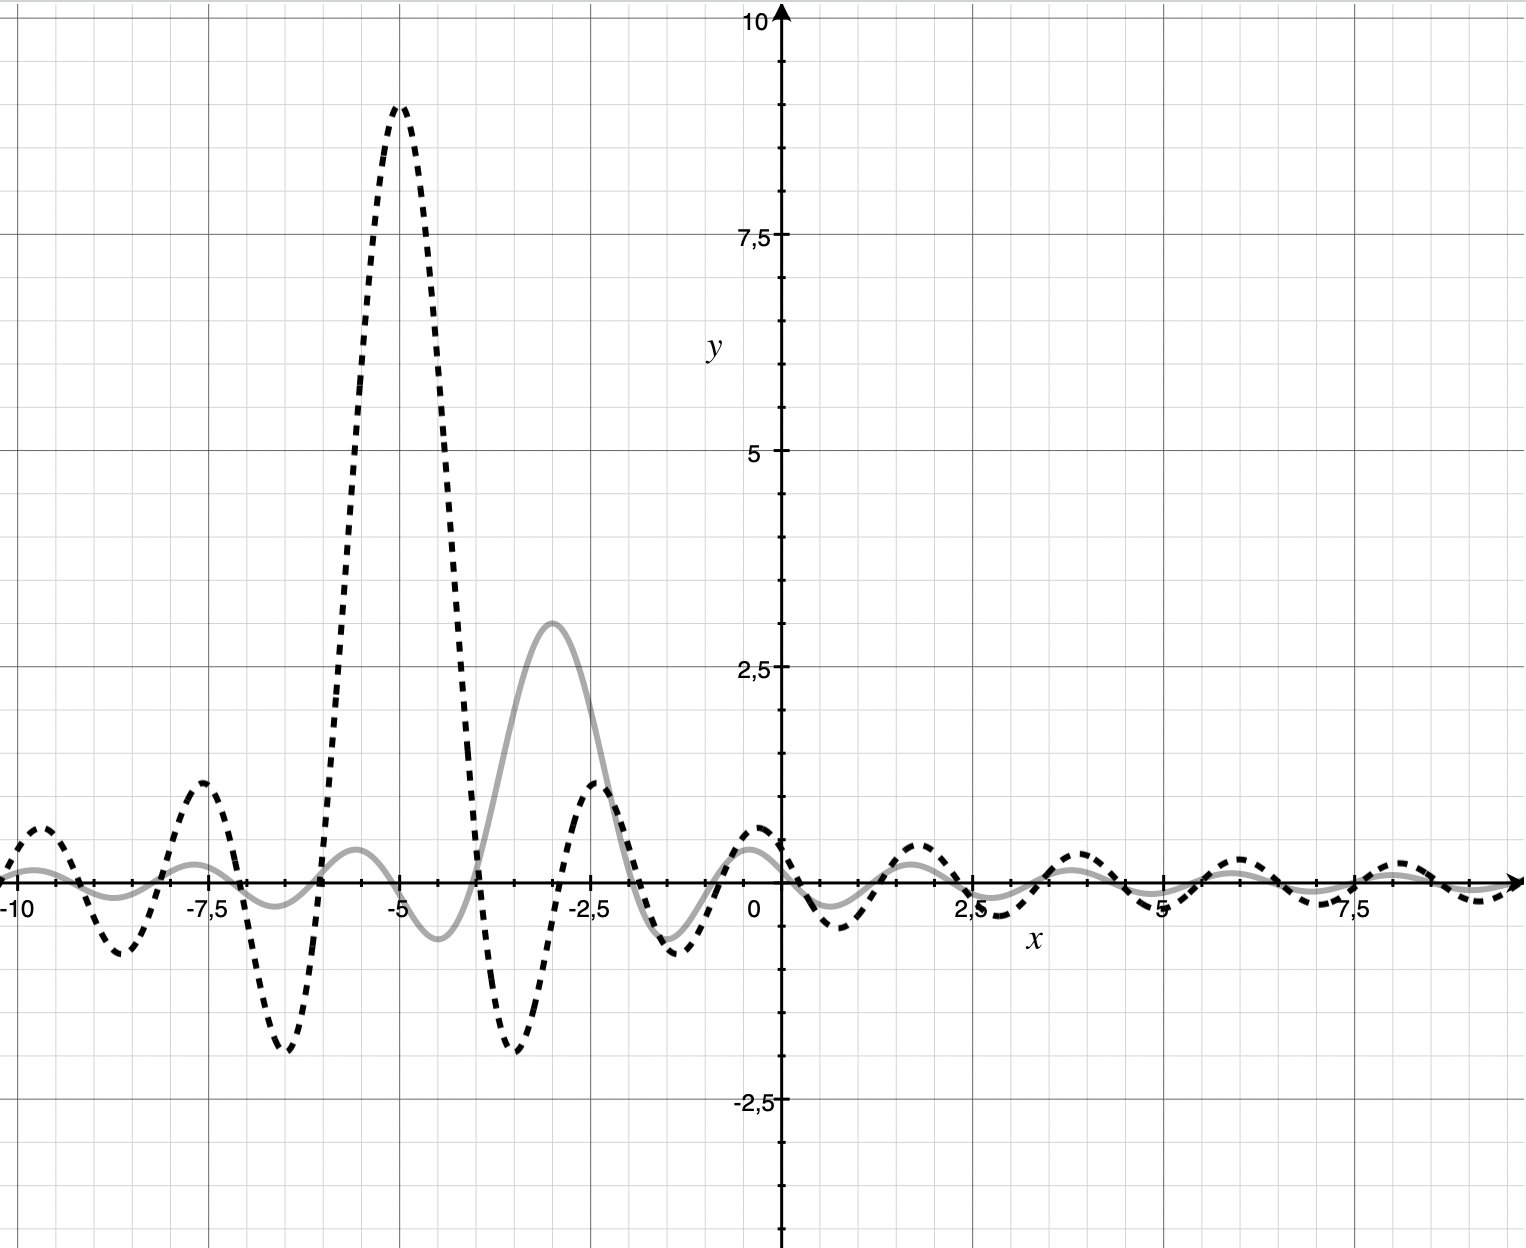
\includegraphics[width=\textwidth ]{a12.png}
                \end{center}
            }
            \only<24-27>{
                \begin{center}
                    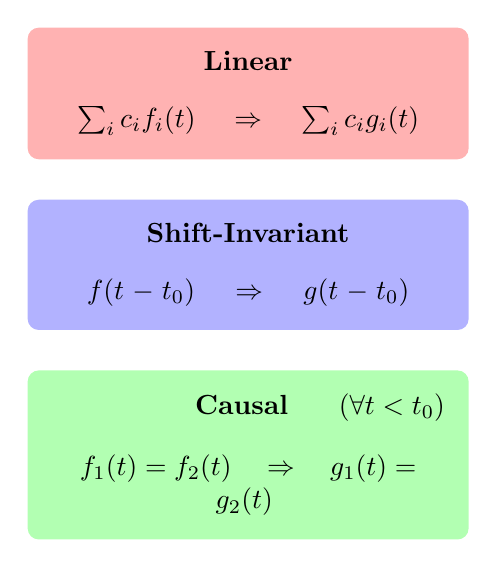
\begin{tikzpicture}[scale=1, transform shape]
                        \node (linear) [rounded corners, fill=red!30, text width=5cm, align=center, inner sep=0.3cm] {
                            \textbf{Linear}\\[0.3cm]
                            ${\sum_{i}  c_if_i(t)} \quad{} \Rightarrow \quad {\sum_{i}  c_ig_i(t)}$
                        };
                        \node (shift) [rounded corners, fill=blue!30, text width=5cm, align=center, below=0.5cm of linear, inner sep=0.3cm] {
                            \textbf{Shift-Invariant}\\[0.3cm]
                            $f(t-t_0) \quad  \Rightarrow \quad g(t-t_0)$
                        };
                        \node (Causal) [rounded corners, fill=green!30, text width=5cm, align=center, below=0.5cm of shift, inner sep=0.3cm] {
                            \hfill{}\textbf{\hspace{1.3cm}Causal}\hfill{} ($\forall t < t_0$)\\[0.3cm]
                            \begin{center}
                                $f_1(t) = f_2(t) \quad{} \Rightarrow \quad g_1(t) = g_2(t) \; $
                            \end{center}};
                    \end{tikzpicture}
                \end{center}
            }
            \only<28>{
                \begin{center}
                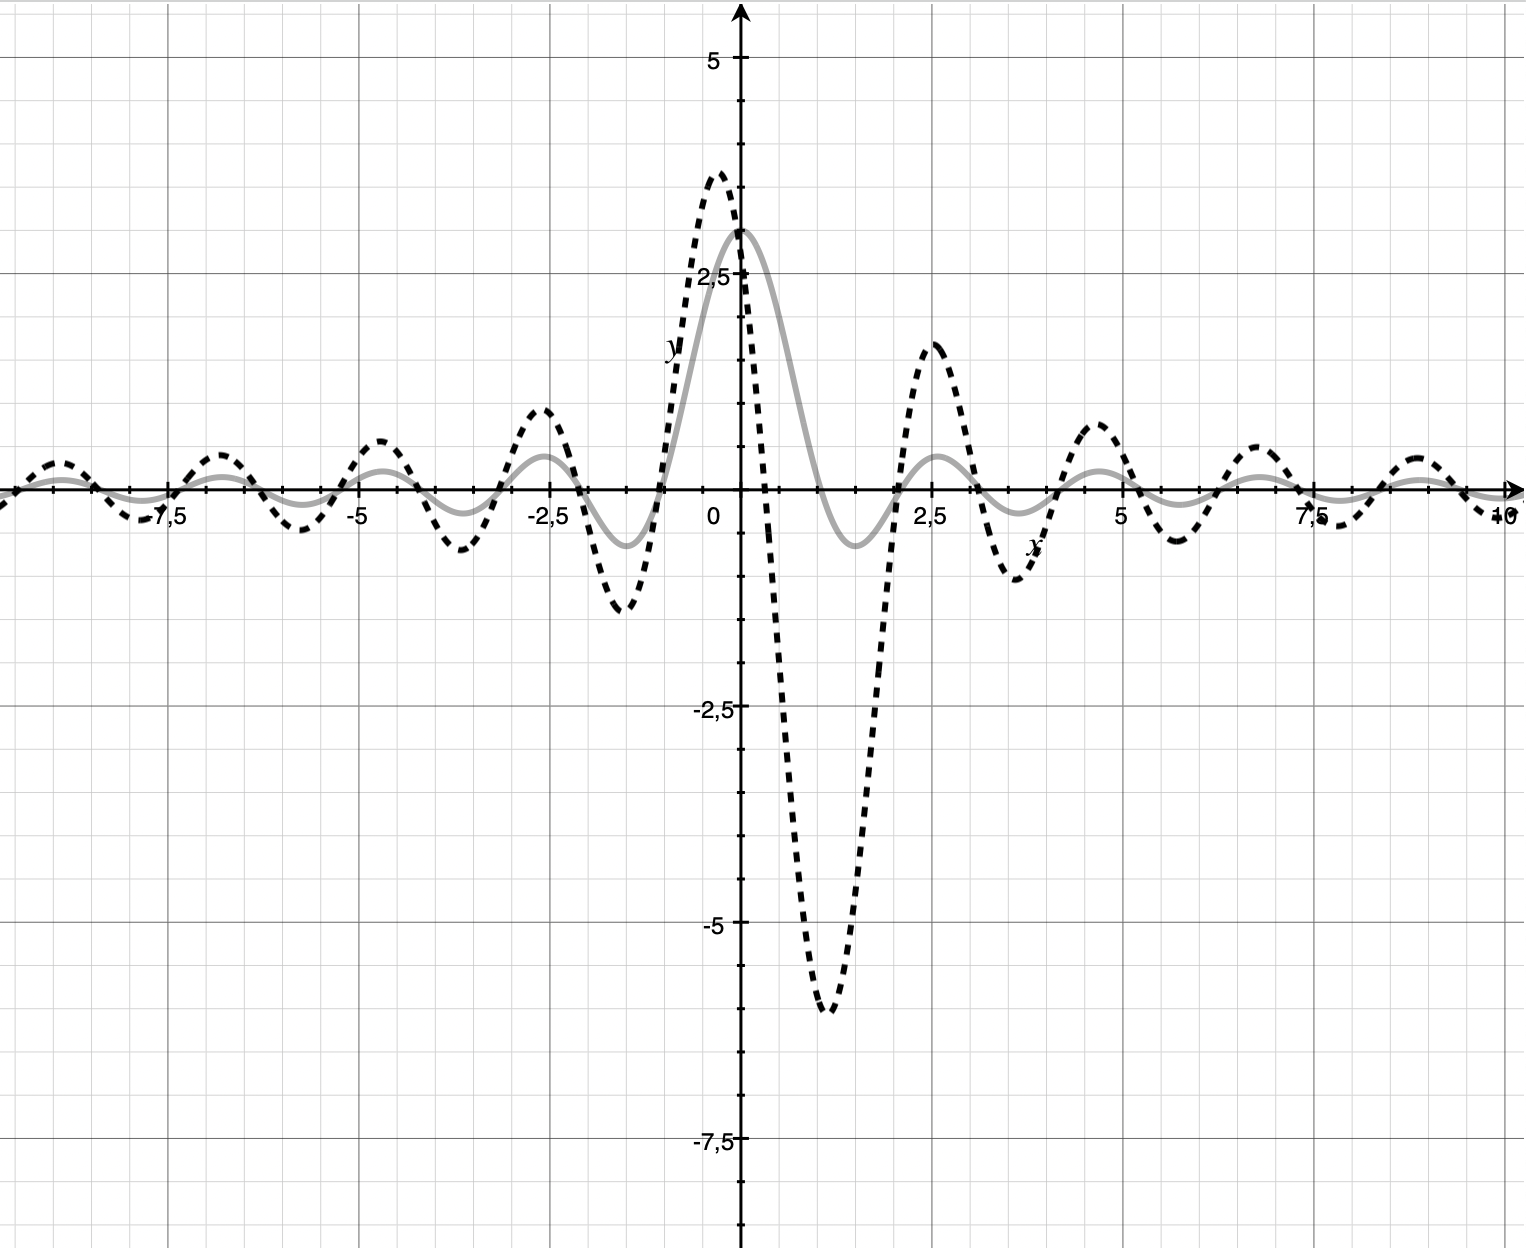
\includegraphics[width=\textwidth ]{a13.png}
                \end{center}
            }
            \only<29>{
                \begin{center}
                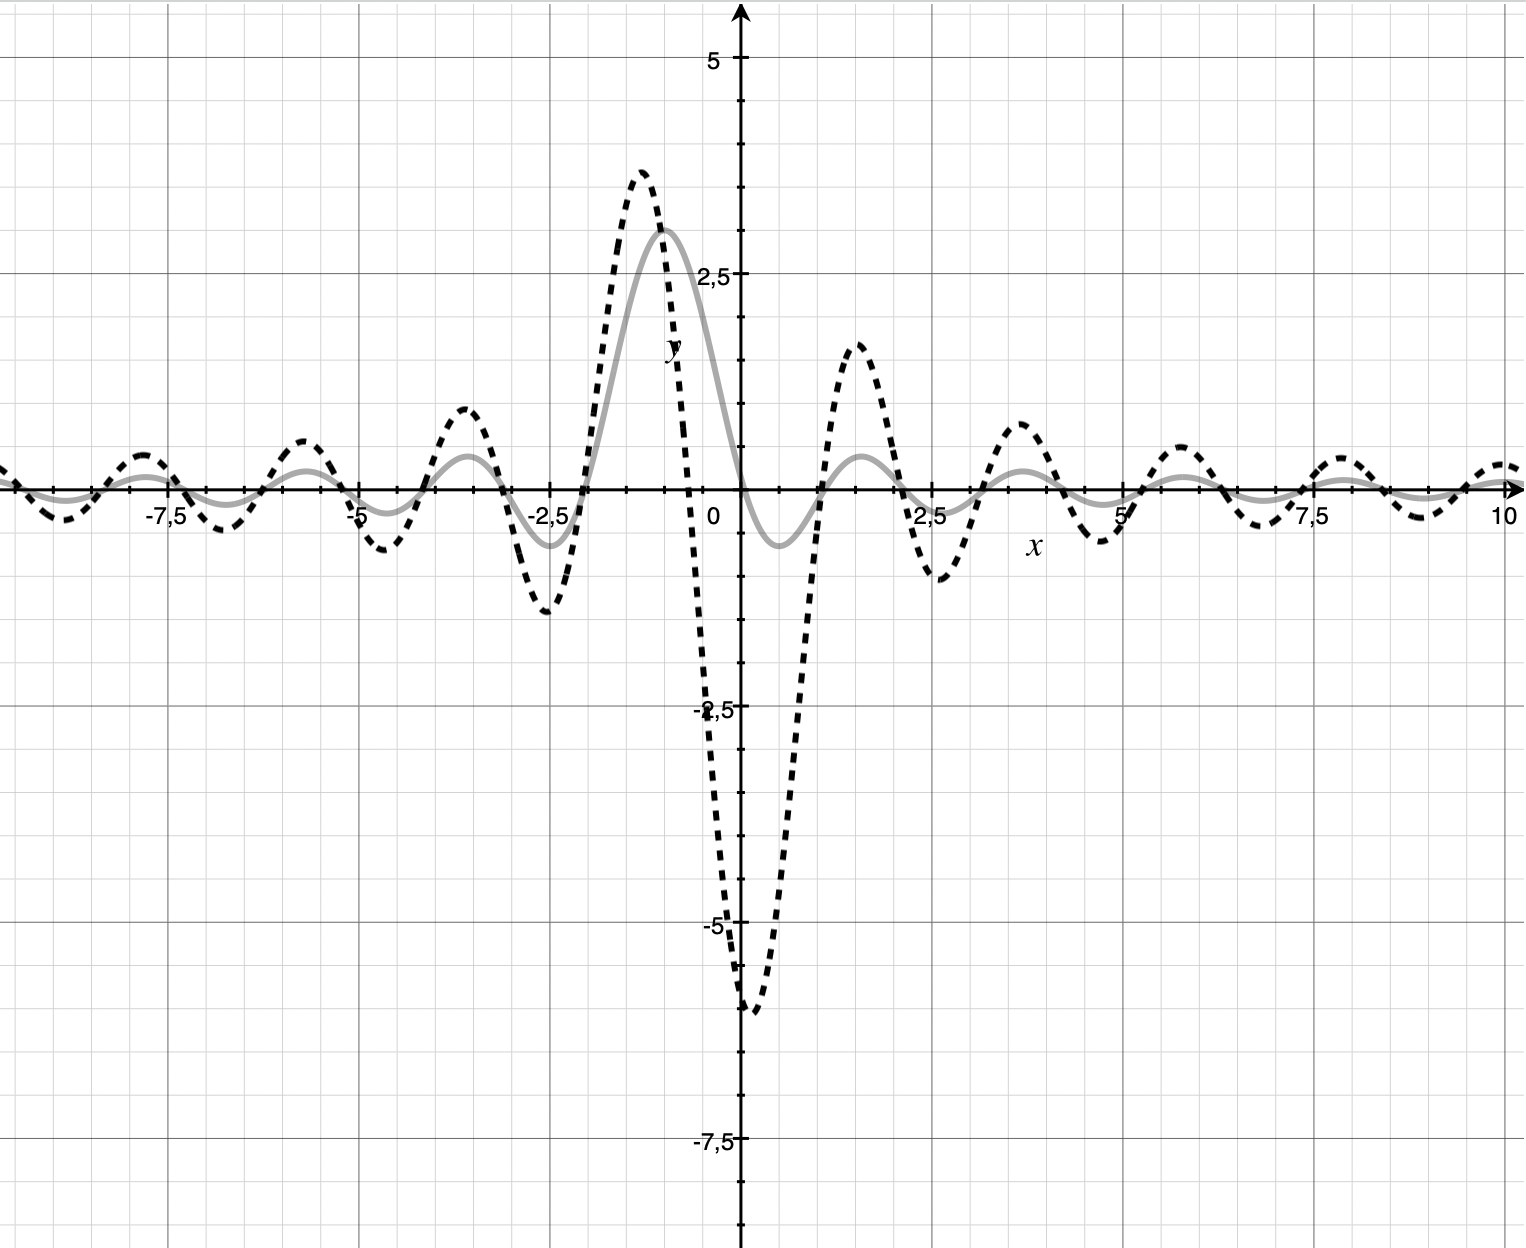
\includegraphics[width=\textwidth ]{a14.png}
                \end{center}
            }
            \only<30>{
                \begin{center}
                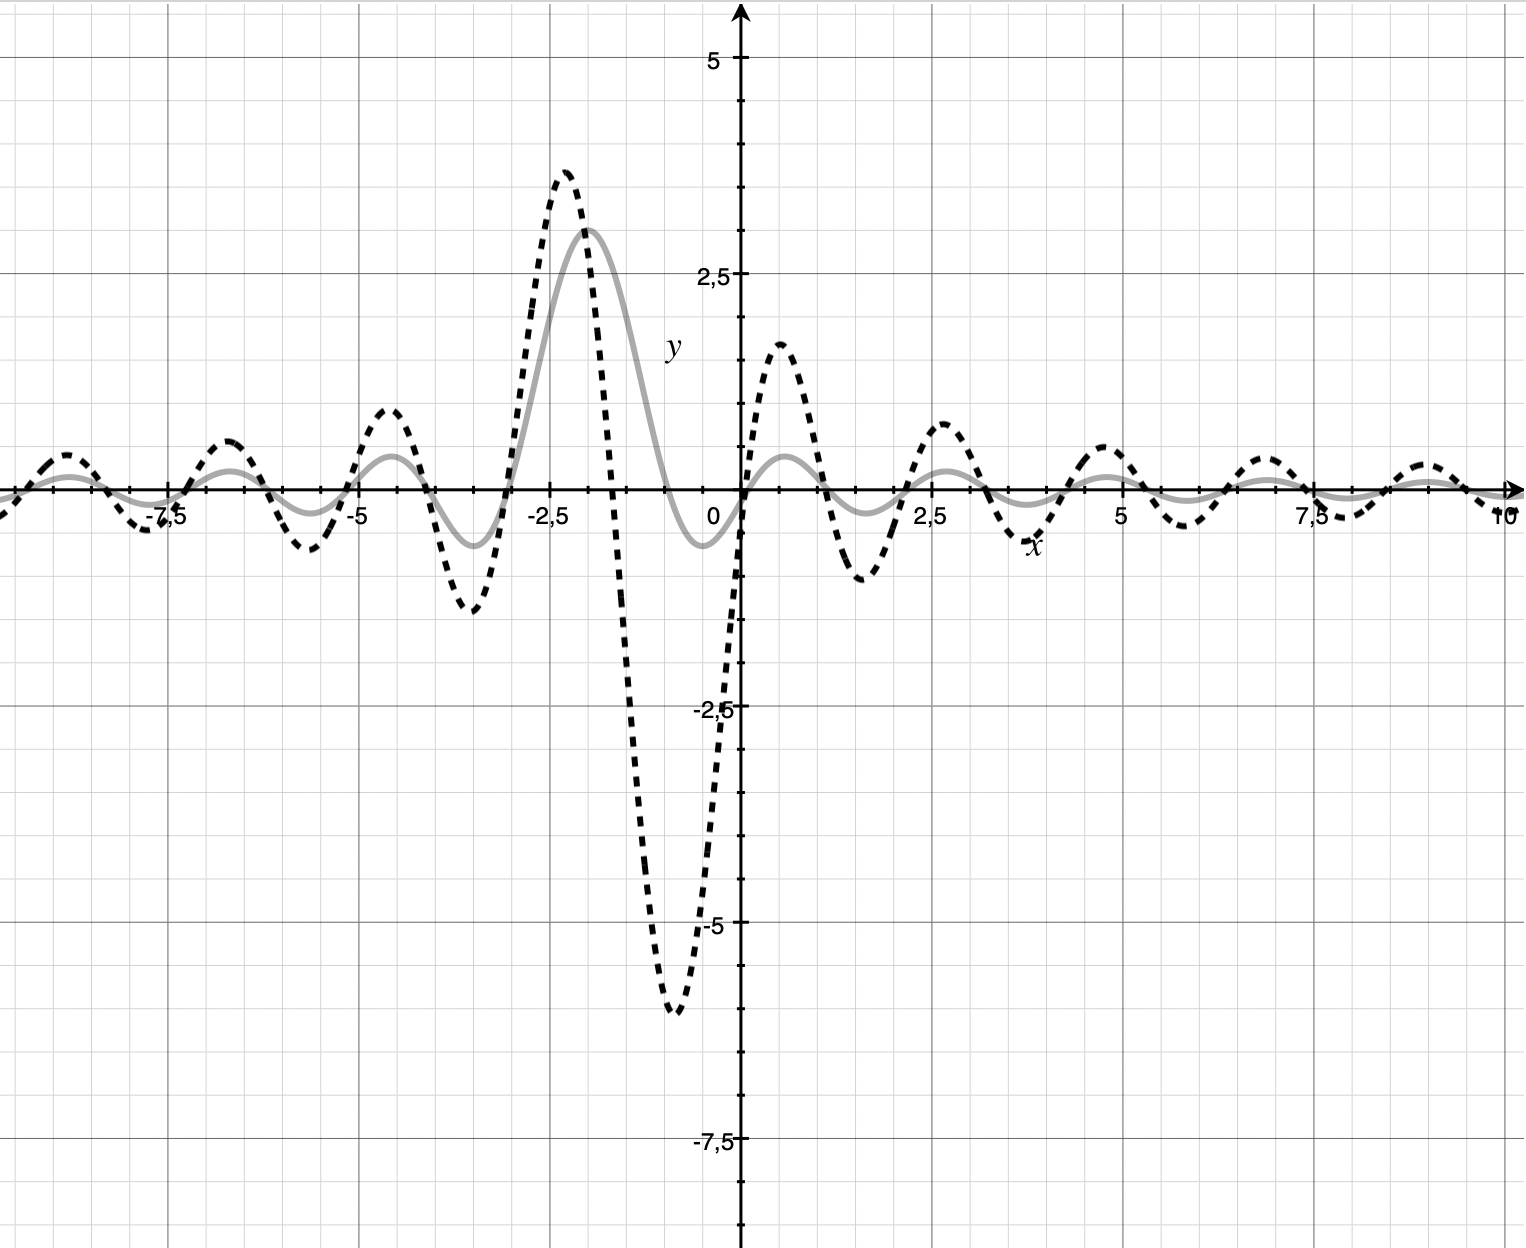
\includegraphics[width=\textwidth ]{a15.png}
                \end{center}
            }
            \only<31>{
                \begin{center}
                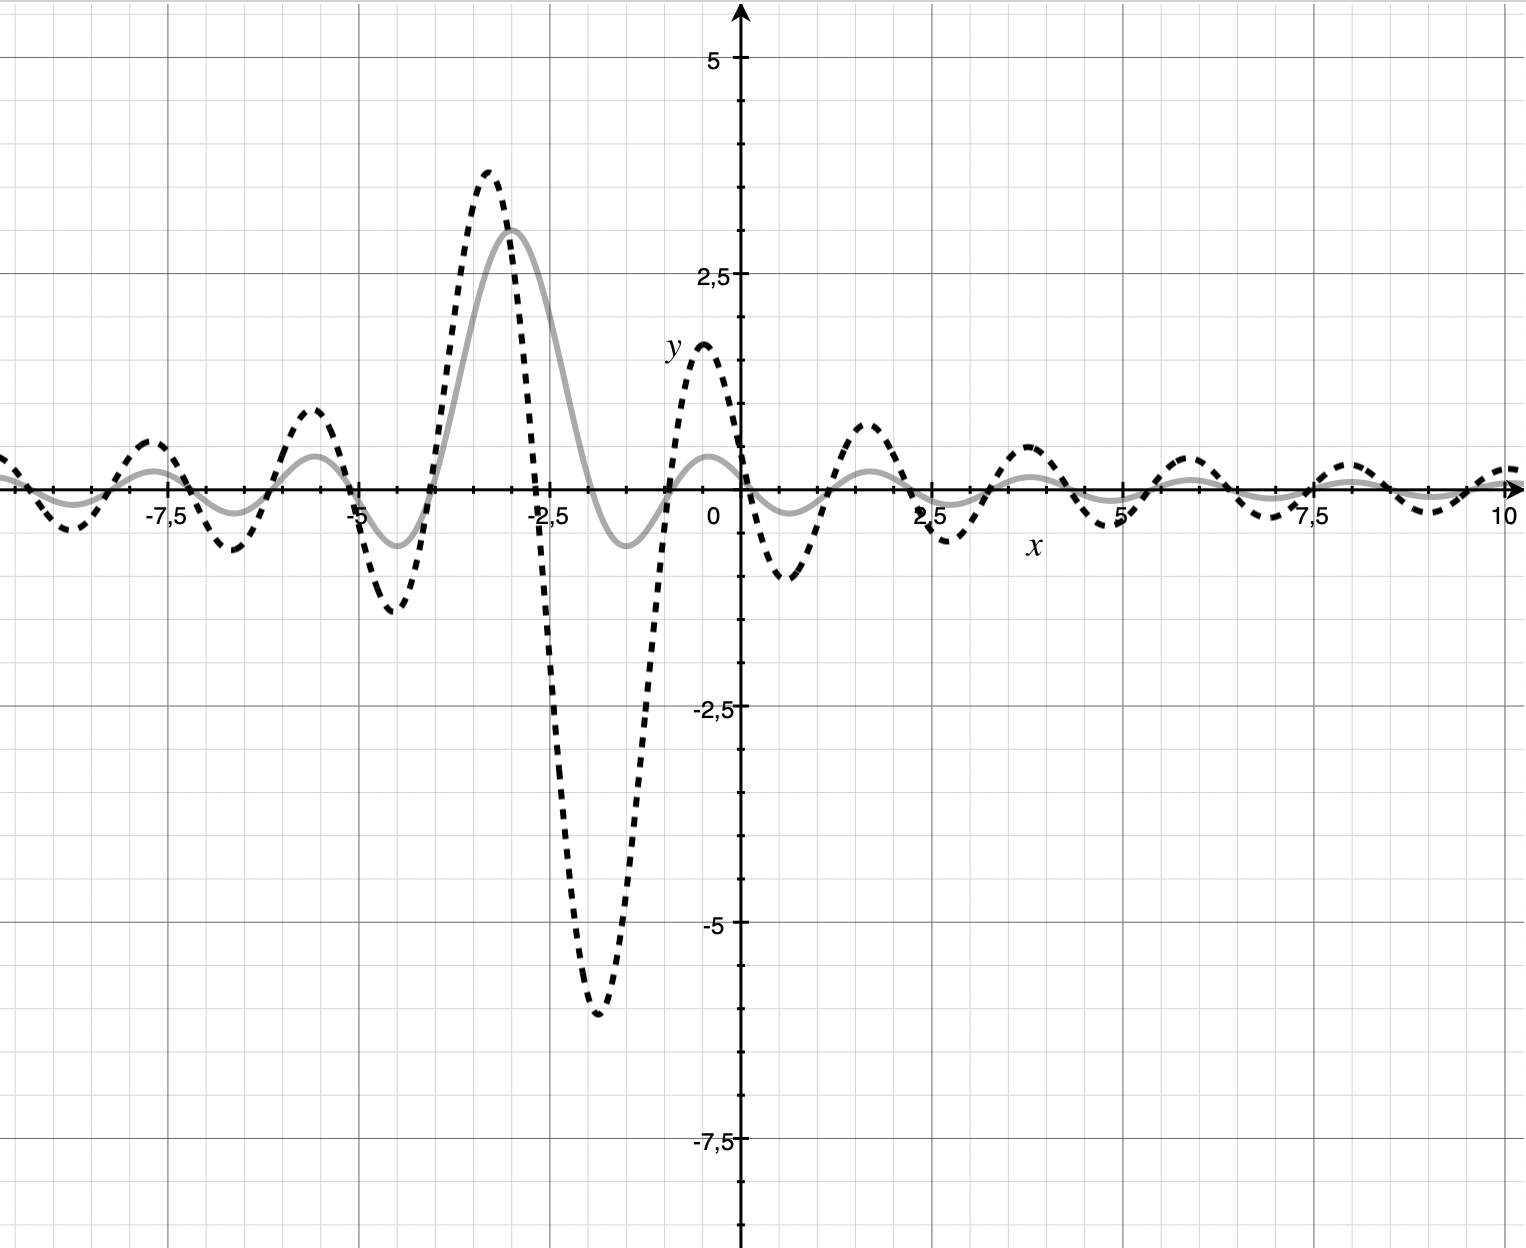
\includegraphics[width=\textwidth ]{a16.png}
                \end{center}
            }
            \only<32-33>{
                \begin{center}
                    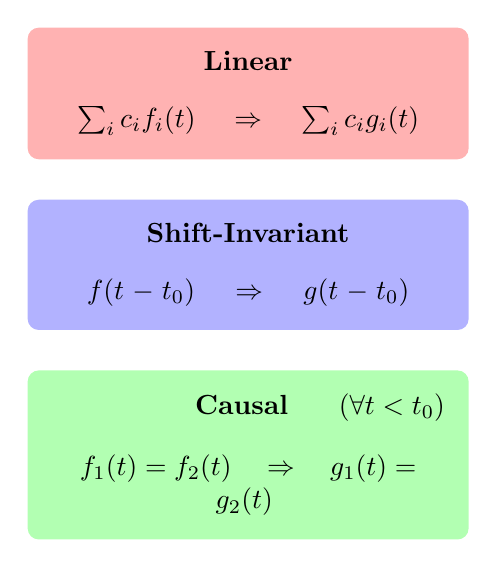
\begin{tikzpicture}[scale=1, transform shape]
                        \node (linear) [rounded corners, fill=red!30, text width=5cm, align=center, inner sep=0.3cm] {
                            \textbf{Linear}\\[0.3cm]
                            ${\sum_{i}  c_if_i(t)} \quad{} \Rightarrow \quad {\sum_{i}  c_ig_i(t)}$
                        };
                        \node (shift) [rounded corners, fill=blue!30, text width=5cm, align=center, below=0.5cm of linear, inner sep=0.3cm] {
                            \textbf{Shift-Invariant}\\[0.3cm]
                            $f(t-t_0) \quad  \Rightarrow \quad g(t-t_0)$
                        };
                        \node (Causal) [rounded corners, fill=green!30, text width=5cm, align=center, below=0.5cm of shift, inner sep=0.3cm] {
                            \hfill{}\textbf{\hspace{1.3cm}Causal}\hfill{} ($\forall t < t_0$)\\[0.3cm]
                            \begin{center}
                                $f_1(t) = f_2(t) \quad{} \Rightarrow \quad g_1(t) = g_2(t) \; $
                            \end{center}};
                    \end{tikzpicture}
                \end{center}
            }
            \only<34>{
                \begin{center}
                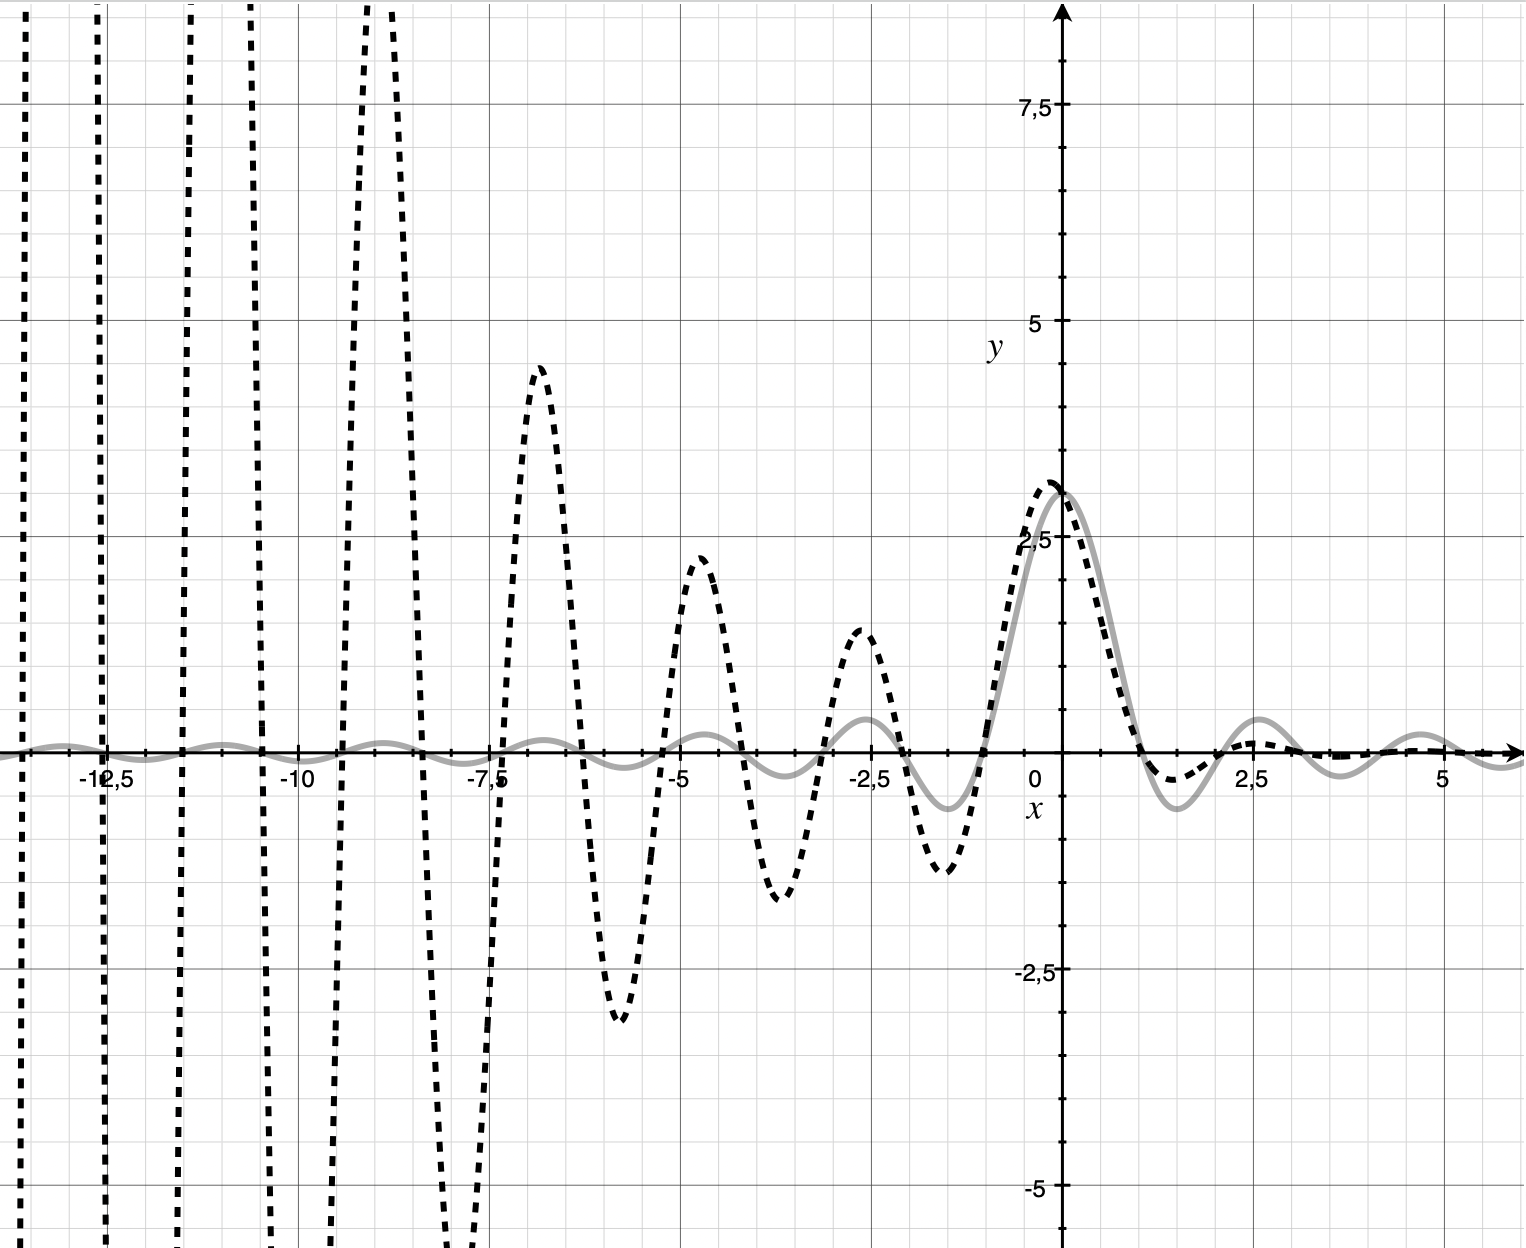
\includegraphics[width=\textwidth ]{a17.png}
                \end{center}
            }
            \only<35>{
                \begin{center}
                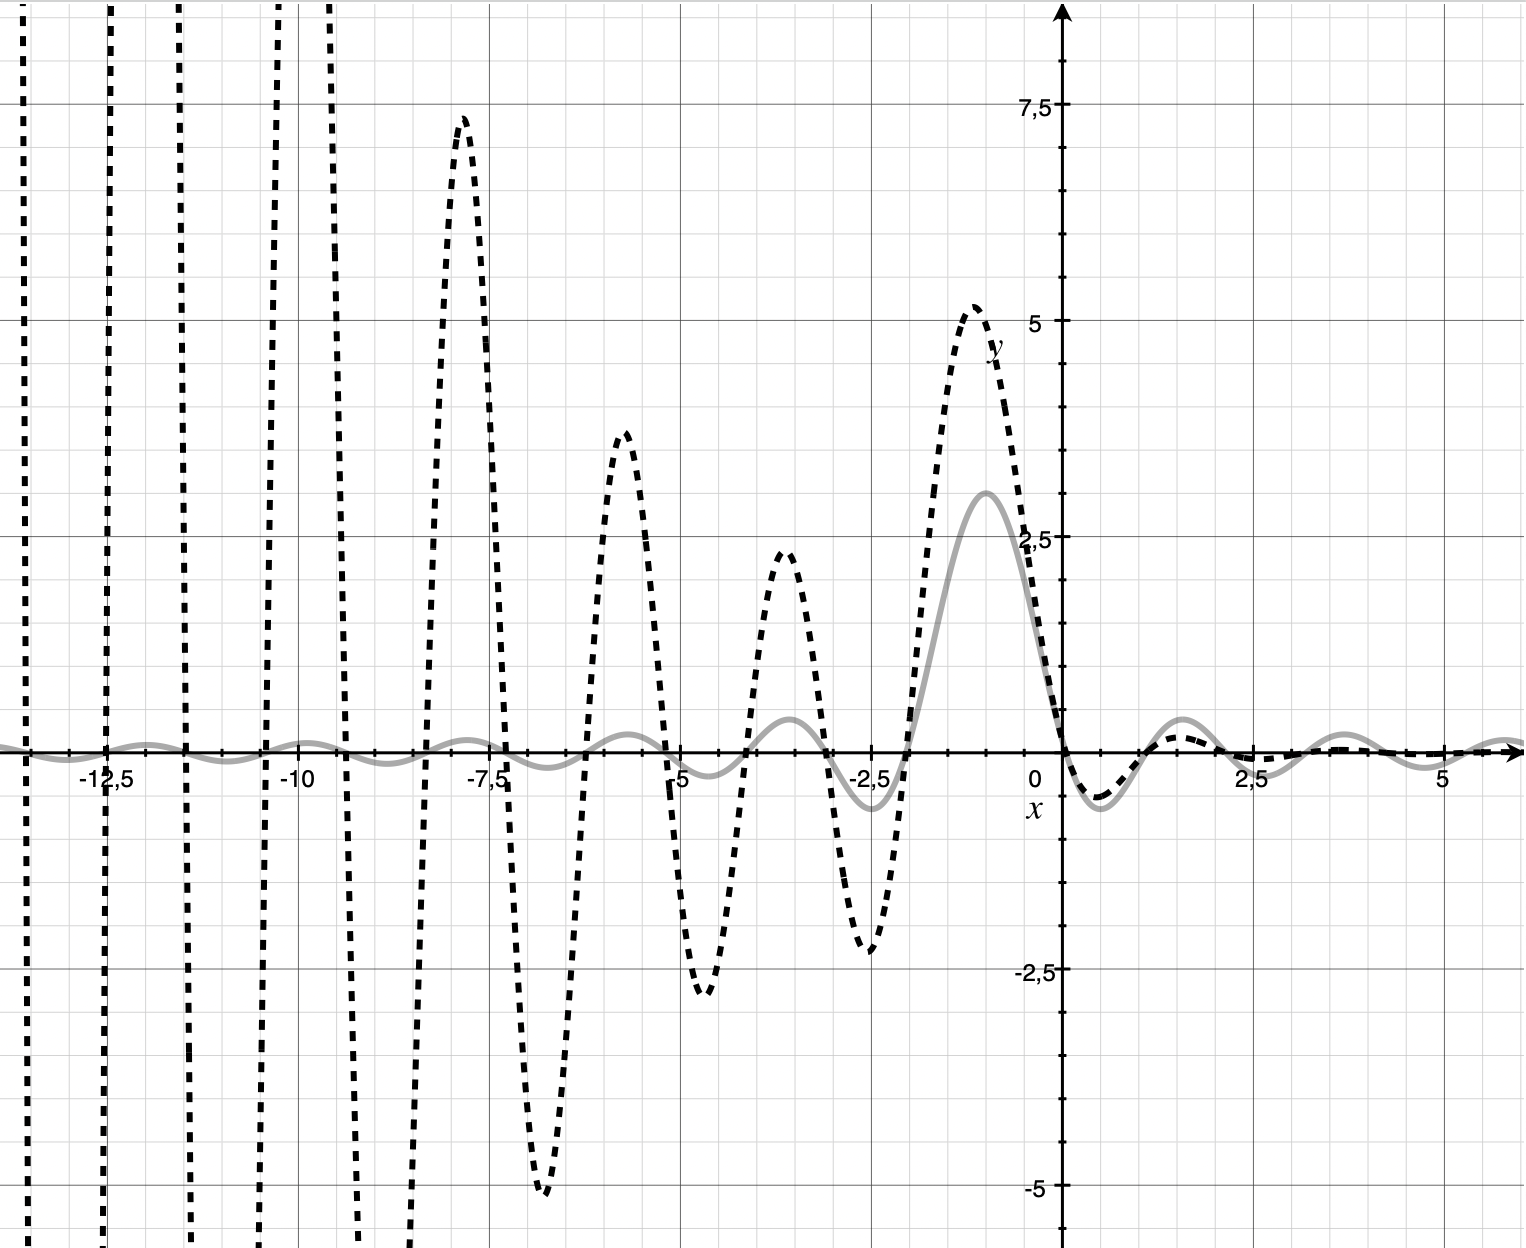
\includegraphics[width=\textwidth ]{a18.png}
                \end{center}
            }
            \only<36>{
                \begin{center}
                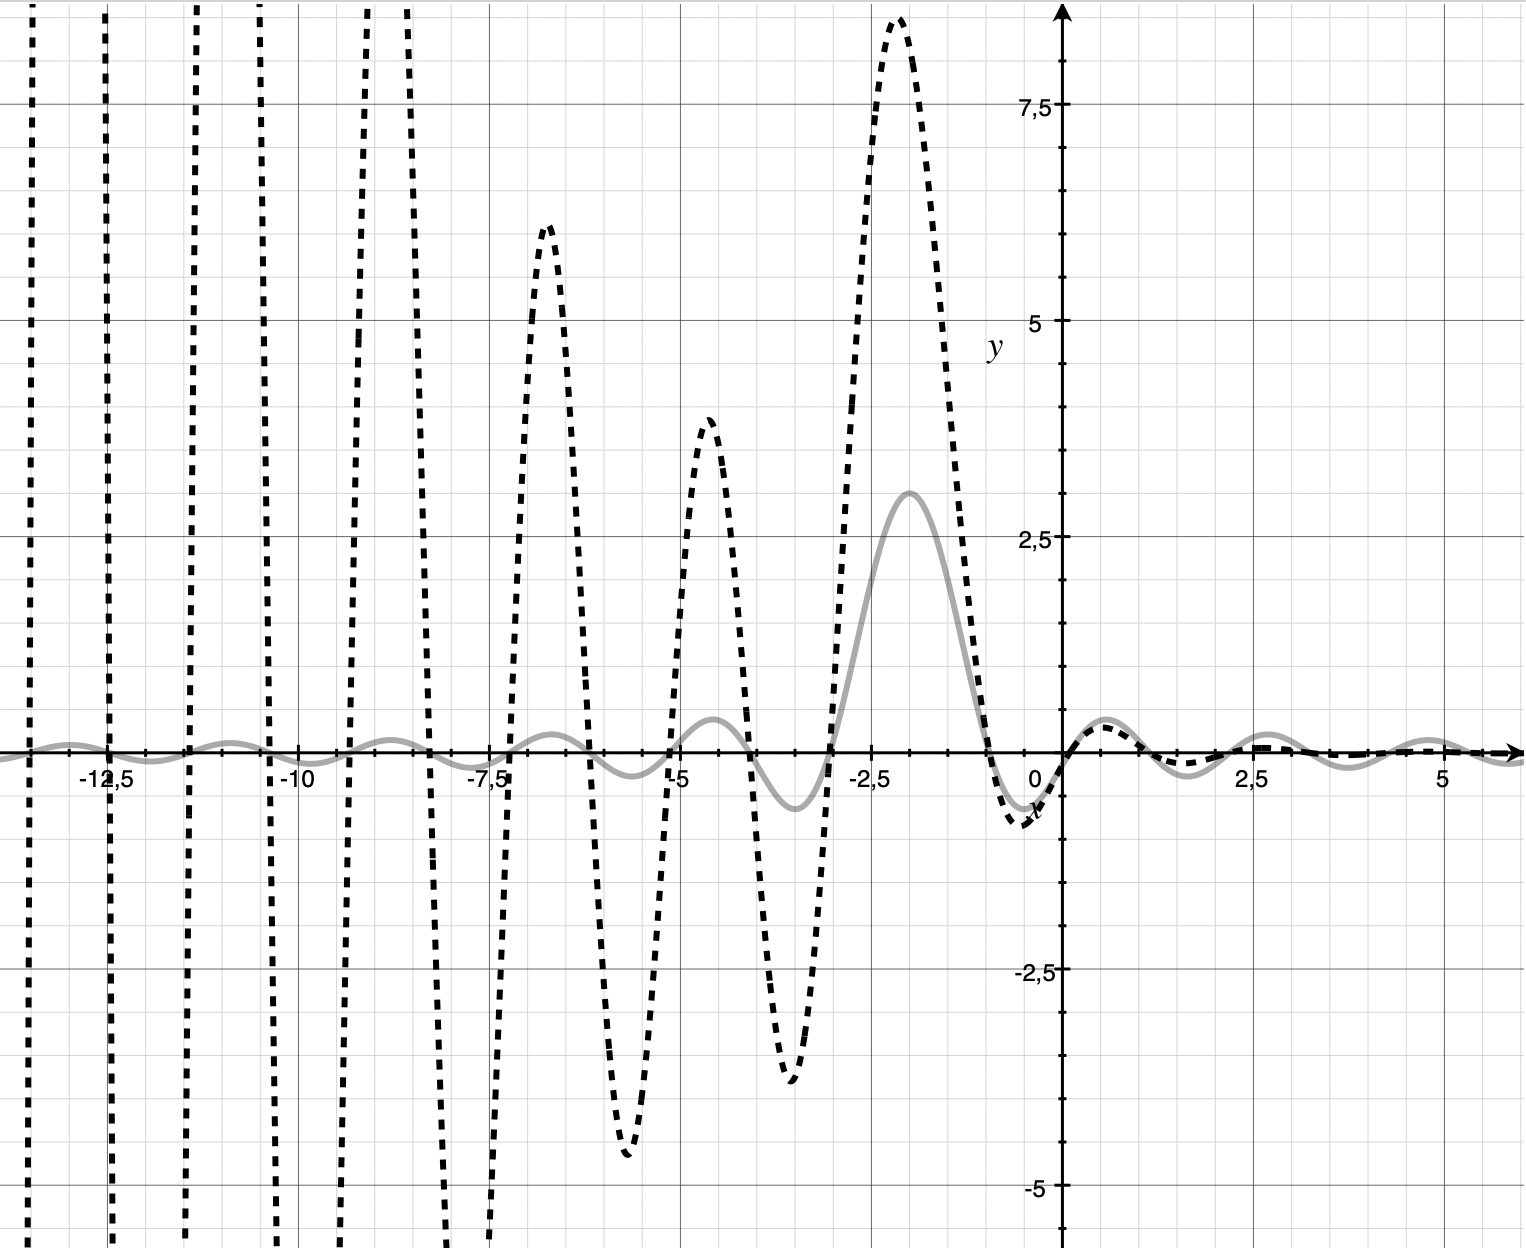
\includegraphics[width=\textwidth ]{a19.png}
                \end{center}
            }
            \only<37>{
                \begin{center}
                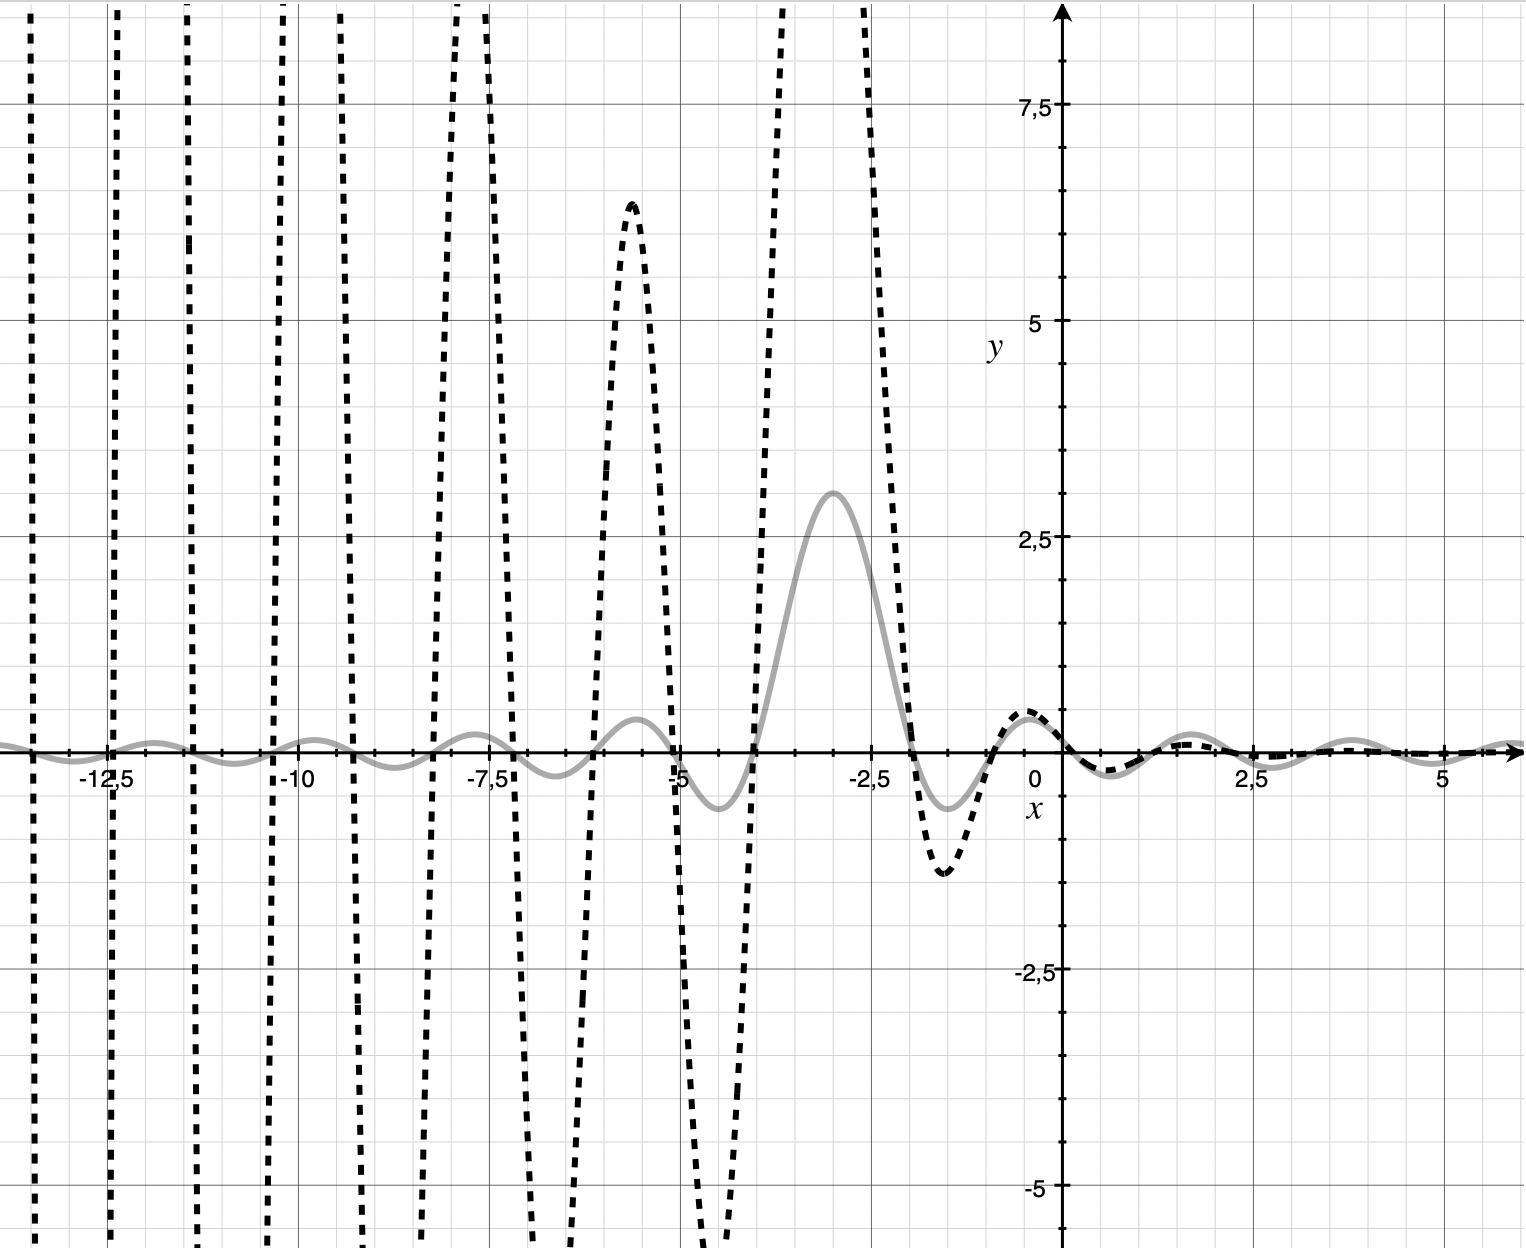
\includegraphics[width=\textwidth ]{a20.png}
                \end{center}
            }
        \end{column}
    \end{columns}

\end{frame}

\begin{frame}[c]{Imaging Systems}

    \myExample{} of some imaging systems:\newline{}

    \begin{table}
        \def\arraystretch{1.7}
        \begin{tabular}{lll}
            \toprule
            Input $f(x,y)$                      & Imaging System & Output $g(x,y)$ \\
            \midrule
            X-ray dose $D(x,y)$                 & X-ray system   & X-ray film      \\
            X-ray attenuation coeff. $\mu(x,y)$ & CT system      & digital image   \\
            proton density $\rho(x,y)$          & MR system      & monitor         \\
            \bottomrule
        \end{tabular}
    \end{table}
\end{frame}


%------------------------------

%\begin{frame}
%\frametitle{Complex Numbers}
%\begin{myDefinition}
%\textbf{Known:} Real numbers $x \in \mathbb{R}$
%\end{myDefinition}


%\question{} How to compute $\sqrt{-1}$?\newline

%\answer{} Define new numbers $\sqrt{-1} = i$


%\begin{myDefinition}
%Complex numbers $z \in \mathbb{C}$
%\begin{align*}
%z & = a + bi \quad a,b \in \mathbb{R} \\
%a & = Re(z)                           \\
%b & = Im(z)
%\end{align*}
%\end{myDefinition}


%\end{frame}


%\begin{frame}
%\frametitle{Complex Numbers: Coordinate Types}
%\begin{center}
%\includegraphics[height=.6\textheight ]{images/ComplexPlane.pdf} \quad
%\end{center}


%\begin{itemize}
%\item Cartesian coordinates $z = a + b i$
%\item Polar coordinates $z = A \left( \cos \phi + i \sin \phi\right)$
%\item Exponential representation $ z = A e^{i \phi}$
%\end{itemize}

%\end{frame}




%\section{Examples}%
%\label{sec:examples}






%\begin{frame}
%\frametitle{High-Pass}
%\begin{myDefinition}
%\begin{center}
%Applying a high-pass filter eliminates all low frequencies.
%\end{center}
%\end{myDefinition}

%\vspace{5mm}

%This can be beneficial if you have inhomogeneous illumination of your image:\newline

%\begin{center}
%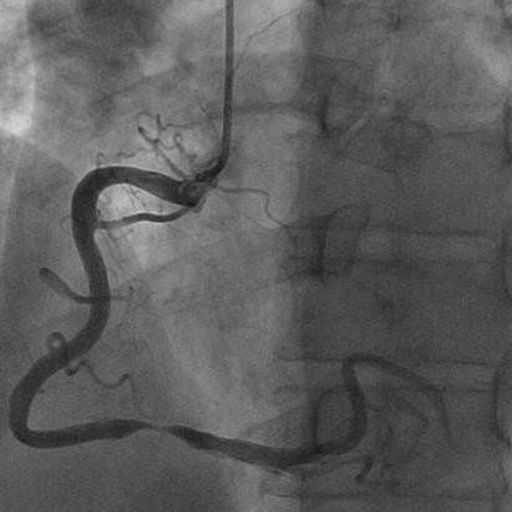
\includegraphics[height=.42\textheight ]{images/angio} \quad
%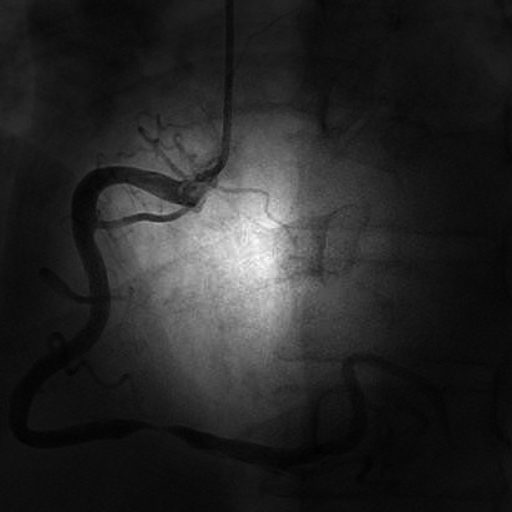
\includegraphics[height=.42\textheight ]{images/angioI} \quad
%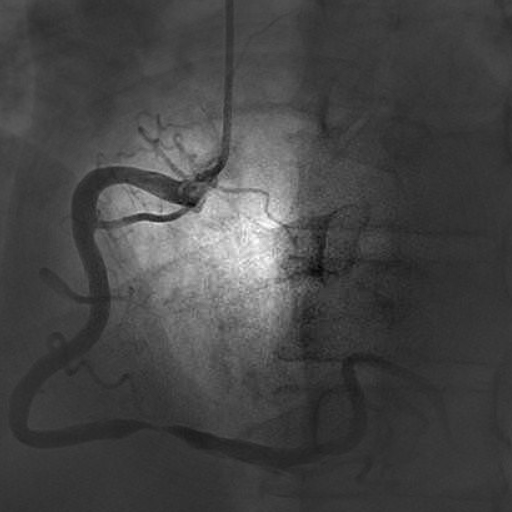
\includegraphics[height=.42\textheight ]{images/angioIF}
%\end{center}
%\end{frame}



%\begin{frame}
%\frametitle{Low-Pass}
%\begin{myDefinition}
%\begin{center}
%Applying a low-pass filter eliminates all high frequencies.
%\end{center}
%\end{myDefinition}

%\vspace{5mm}

%This can be beneficial if you have added noise in your image:\newline

%\begin{center}
%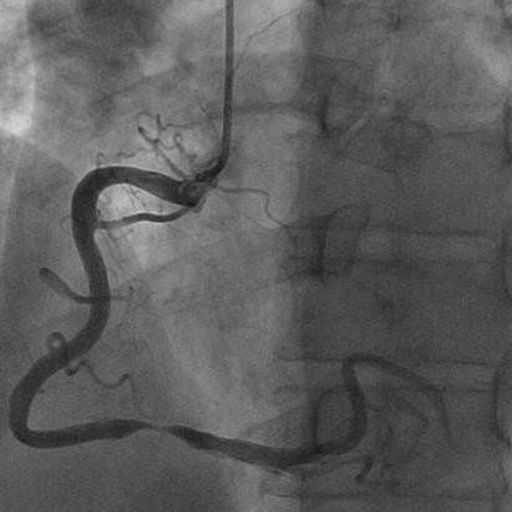
\includegraphics[height=.42\textheight ]{images/angio} \quad
%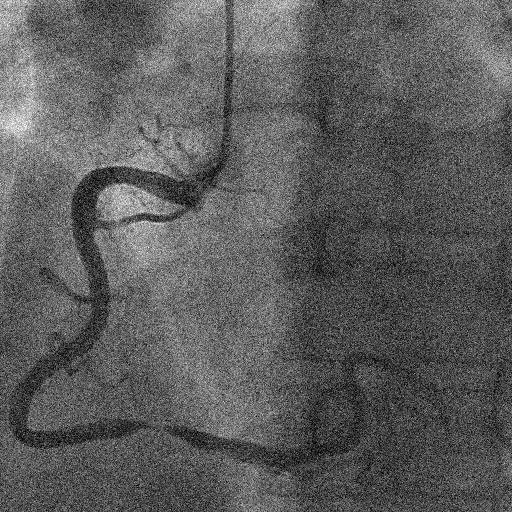
\includegraphics[height=.42\textheight ]{images/angioN} \quad
%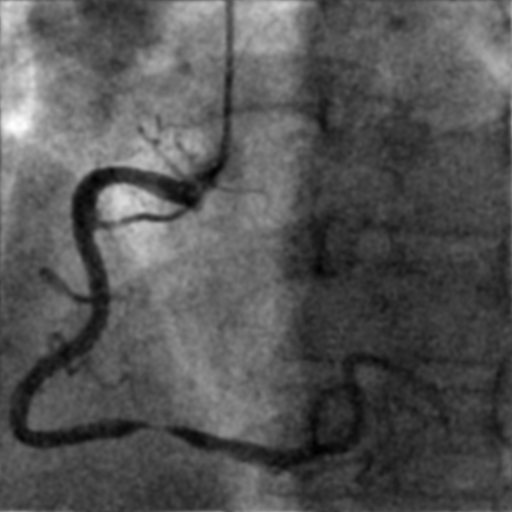
\includegraphics[height=.42\textheight ]{images/angioNF}
%\end{center}
%\end{frame}

%%\begin{frame}
%%\frametitle{Correlation}
%%\begin{myDefinition}
%%The correlation of two 1-D signals is defined as:

%%\begin{eqnarray*}
%%f(t) \star h(t) &=& \int\limits_{-\infty}^{+\infty}f(\tau)g(t+\tau) \, d\tau
%%\end{eqnarray*}\newline

%%The correlation of two 2-D signals is defined as:

%%\begin{eqnarray*}
%%f(x,y) \star g(x,y) &=& \int\limits_{-\infty}^{+\infty}\int\limits_{-\infty}^{+\infty}f(x',y')g(x+x',y+y') \, dx' \, dy'
%%\end{eqnarray*}

%%\end{myDefinition}
%%\end{frame}



%%\begin{frame}
%%\frametitle{Correlation}
%%\question{} What is a correlation good for?\newline

%%\answer{} The most intuitive application is the measurement of similarity between two signals.


%%\begin{center}
%%\includegraphics[height=.40\textheight ]{images/CorrSig1.eps}
%%\includegraphics[height=.40\textheight ]{images/CorrSig2.eps}
%%\includegraphics[height=.40\textheight ]{images/CorrSig3.eps}
%%\end{center}

%%\end{frame}

\subtitle{Fourier Series}
\frame[plain,c]{\titlepage}

\section{Fourier Series}%
\label{sec:fourier_series}



\begin{frame}
    \frametitle{Vector Spaces}

    Set of linear independent vectors can be used as a basis for a vector space.\newline

    \myExample in $\mathbb{R}^2$:

    \begin{center}

        $\bf{e}_1= \left( \begin{array}{cc} 1 \\ 0 \end{array} \right)$
        \hspace{10 mm}
        $\bf{e}_2= \left( \begin{array}{cc} 0 \\ 1 \end{array} \right)$\newline

        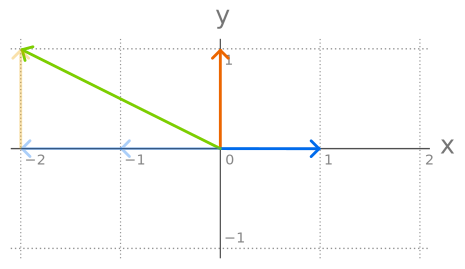
\includegraphics[height=.45\textheight ]{images/2DPlane}

        \begin{flushright}
            \scriptsize Sources: Wikimedia Commons
        \end{flushright}
    \end{center}\end{frame}



\begin{frame}
    \frametitle{Fourier Series}

    \question Is there a finite or infinite set of base elements for signals?

    \answer Yes (given certain constraints).\newline

    \begin{itemize}
        \item All periodic signals can be expressed in terms of a linear combination of cosine and sine functions
        \item The weighted sum is finite or infinite dependent on certain function properties
    \end{itemize}

    \begin{center}
        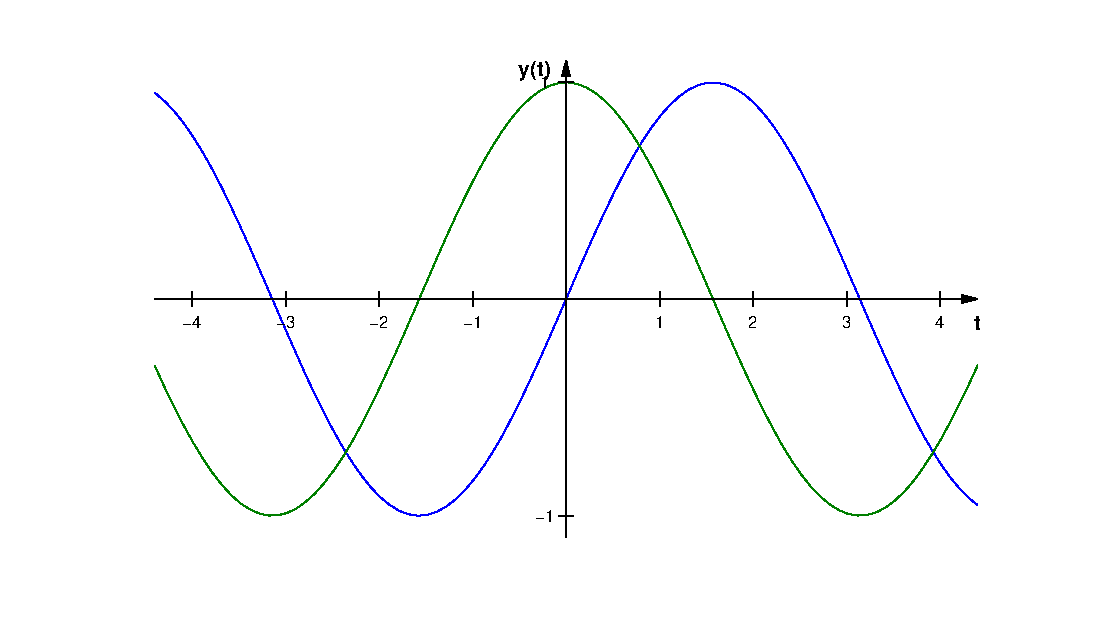
\includegraphics[height=.45\textheight ]{images/functions}
    \end{center}
\end{frame}


%➜ isympy
%IPython console for SymPy 1.6.dev (Python 3.7.5-64-bit) (ground types: python)

%These commands were executed:
%>>> from __future__ import division
%>>> from sympy import *
%>>> x, y, z, t = symbols('x y z t')
%>>> k, m, n = symbols('k m n', integer=True)
%>>> f, g, h = symbols('f g h', cls=Function)
%>>> init_printing()

%Documentation can be found at https://docs.sympy.org/dev


%In [1]: from sympy.abc import t                                                                                                                                                                                                                                                    

%In [2]: fourier_series(t/pi, (t,-pi,pi))                                                                                                                                                                                                                                           
%Out[2]: 
%2⋅sin(t)   sin(2⋅t)   2⋅sin(3⋅t)    
%──────── - ──────── + ────────── + …
%π          π          3⋅π        

%In [3]: fourier_series(t/pi, (t,-pi,pi)).truncate(12)                                                                                                                                                                                                                              
%Out[3]: 
%2⋅sin(t)   sin(2⋅t)   2⋅sin(3⋅t)   sin(4⋅t)   2⋅sin(5⋅t)   sin(6⋅t)   2⋅sin(7⋅t)   sin(8⋅t)   2⋅sin(9⋅t)   sin(10⋅t)   2⋅sin(11⋅t)   sin(12⋅t)
%──────── - ──────── + ────────── - ──────── + ────────── - ──────── + ────────── - ──────── + ────────── - ───────── + ─────────── - ─────────
%π          π          3⋅π         2⋅π         5⋅π         3⋅π         7⋅π         4⋅π         9⋅π          5⋅π          11⋅π         6⋅π   
%In [4]: latex(_)                                                                                                                                                                                                                                                                   
%Out[4]: '\\frac{2 \\sin{\\left(t \\right)}}{\\pi} - \\frac{\\sin{\\left(2 t \\right)}}{\\pi} + \\frac{2 \\sin{\\left(3 t \\right)}}{3 \\pi} - \\frac{\\sin{\\left(4 t \\right)}}{2 \\pi} + \\frac{2 \\sin{\\left(5 t \\right)}}{5 \\pi} - \\frac{\\sin{\\left(6 t \\right)}}{3 \\pi} + \\frac{2 \\sin{\\left(7 t \\right)}}{7 \\pi} - \\frac{\\sin{\\left(8 t \\right)}}{4 \\pi} + \\frac{2 \\sin{\\left(9 t \\right)}}{9 \\pi} - \\frac{\\sin{\\left(10 t \\right)}}{5 \\pi} + \\frac{2 \\sin{\\left(11 t \\right)}}{11 \\pi} - \\frac{\\sin{\\left(12 t \\right)}}{6 \\pi}'

\begin{frame}[t]{Fourier Series}

    \myExample of an approximation (a sawtooth wave):
    {\scriptsize
    \begin{align*}
        f(t) & = t \quad\quad t \in \left(-\pi,+\pi\right) \\
        %& = 2 \sin{\left(t \right)} - \sin{\left(2 t \right)} + \frac{2 \sin{\left(3 t \right)}}{3} - \frac{\sin{\left(4 t \right)}}{2} + \frac{2 \sin{\left(5 t \right)}}{5} - \frac{\sin{\left(6 t \right)}}{3} +  \ldots
    \end{align*}}%

    \vspace{-0.5cm}
    \begin{center}
        \includegraphics[height=0.7\textheight, trim={0  0.5cm 0 1cm},clip]{zigzag_signal.pdf}
    \end{center}
\end{frame}

\mode<presentation>{
    \setbeamercolor{background canvas}{bg=white}
    \begin{frame}[plain,c]{}
        \centering
        \begin{center}
            \only<1>{\includegraphics[height=1.1\textheight]{zigzag_reco_1.pdf}}%
            \only<2>{\includegraphics[height=1.1\textheight]{zigzag_reco_2.pdf}}%
            \only<3>{\includegraphics[height=1.1\textheight]{zigzag_reco_3.pdf}}%
            \only<4>{\includegraphics[height=1.1\textheight]{zigzag_reco_4.pdf}}%
            \only<5>{\includegraphics[height=1.1\textheight]{zigzag_reco_5.pdf}}%
            \only<6>{\includegraphics[height=1.1\textheight]{zigzag_reco_6.pdf}}%
            \only<7>{\includegraphics[height=1.1\textheight]{zigzag_reco_7.pdf}}%
            \only<8>{\includegraphics[height=1.1\textheight]{zigzag_reco_8.pdf}}%
            \only<9>{\includegraphics[height=1.1\textheight]{zigzag_reco_9.pdf}}%
            \only<10>{\includegraphics[height=1.1\textheight]{zigzag_reco_10.pdf}}%
            \only<11>{\includegraphics[height=1.1\textheight]{zigzag_reco_20.pdf}}%
            \only<12>{\includegraphics[height=1.1\textheight]{zigzag_reco_29.pdf}}%
            \only<13>{\includegraphics[height=1.1\textheight]{zigzag_reco_70.pdf}}% 
        \end{center}
        %\begin{textblock}{6.5}(9.0,10.0)
        %\color{white}
        %\textbf{Conventional DSA}
        %\end{textblock}
    \end{frame}
}
\setbeamercolor{background canvas}{bg=white}
\begin{frame}[t]{Fourier Series}

    \myExample of an approximation (a sawtooth wave):
    {\scriptsize
    \begin{align*}
        f(t) & = t \quad\quad t \in \left(-\pi,+\pi\right)                                                                                                                                                                           \\
             & = 2 \sin{\left(t \right)} - \sin{\left(2 t \right)} + \frac{2 \sin{\left(3 t \right)}}{3} - \frac{\sin{\left(4 t \right)}}{2} + \frac{2 \sin{\left(5 t \right)}}{5 \pi} - \frac{\sin{\left(6 t \right)}}{3} +  \ldots
    \end{align*}}%
    \begin{center}
        \only<1-13>{%
            \begin{columns}[t, onlytextwidth]
                \begin{column}{0.5\textwidth}
                    \centering{}
                    \only<1>{\includegraphics[height=0.65\textheight]{zigzag_reco_1.pdf}}%
                    \only<2>{\includegraphics[height=0.65\textheight]{zigzag_reco_2.pdf}}%
                    \only<3>{\includegraphics[height=0.65\textheight]{zigzag_reco_3.pdf}}%
                    \only<4>{\includegraphics[height=0.65\textheight]{zigzag_reco_4.pdf}}%
                    \only<5>{\includegraphics[height=0.65\textheight]{zigzag_reco_5.pdf}}%
                    \only<6>{\includegraphics[height=0.65\textheight]{zigzag_reco_6.pdf}}%
                    \only<7>{\includegraphics[height=0.65\textheight]{zigzag_reco_7.pdf}}%
                    \only<8>{\includegraphics[height=0.65\textheight]{zigzag_reco_8.pdf}}%
                    \only<9>{\includegraphics[height=0.65\textheight]{zigzag_reco_9.pdf}}%
                    \only<10>{\includegraphics[height=0.65\textheight]{zigzag_reco_10.pdf}}%
                    \only<11>{\includegraphics[height=0.65\textheight]{zigzag_reco_20.pdf}}%
                    \only<12>{\includegraphics[height=0.65\textheight]{zigzag_reco_29.pdf}}%
                    \only<13>{\includegraphics[height=0.65\textheight]{zigzag_reco_70.pdf}}%
                \end{column}\begin{column}{0.5\textwidth}
                    \centering{}
                    \only<1>{\includegraphics[height=0.65\textheight]{zigzag_sin_1.pdf}}%
                    \only<2>{\includegraphics[height=0.65\textheight]{zigzag_sin_2.pdf}}%
                    \only<3>{\includegraphics[height=0.65\textheight]{zigzag_sin_3.pdf}}%
                    \only<4>{\includegraphics[height=0.65\textheight]{zigzag_sin_4.pdf}}%
                    \only<5>{\includegraphics[height=0.65\textheight]{zigzag_sin_5.pdf}}%
                    \only<6>{\includegraphics[height=0.65\textheight]{zigzag_sin_6.pdf}}%
                    \only<7>{\includegraphics[height=0.65\textheight]{zigzag_sin_7.pdf}}%
                    \only<8>{\includegraphics[height=0.65\textheight]{zigzag_sin_8.pdf}}%
                    \only<9>{\includegraphics[height=0.65\textheight]{zigzag_sin_9.pdf}}%
                    \only<10>{\includegraphics[height=0.65\textheight]{zigzag_sin_10.pdf}}%
                    \only<11>{\includegraphics[height=0.65\textheight]{zigzag_sin_11.pdf}}%
                    \only<12>{\includegraphics[height=0.65\textheight]{zigzag_sin_12.pdf}}% 
                    \only<13>{\includegraphics[height=0.65\textheight]{zigzag_sin_70.pdf}}%
                \end{column}
            \end{columns}}%
        \only<14>{%
            \centering{}
            \centering{}
            \begin{columns}[c, onlytextwidth]
                \begin{column}{0.3\textwidth}
                    \centering{}
                    f(t) point symmetric to origin:
                    \vspace{0.3cm}

                    Only sine functions needed!
                \end{column}\begin{column}{0.7\textwidth}
                    \centering{}
                    \includegraphics[height=0.68\textheight, trim={0  0 0 1.3cm},clip]{zigzag_coefficients.pdf}
                \end{column}
            \end{columns}
        }%

    \end{center}
\end{frame}



\begin{frame}[t]{Fourier Series}

    \myExample of an approximation (a rectangle puls):
    {\scriptsize
    \begin{align*}
        f(t) & = \mathsf{rect}\left( \frac{t}{\pi} \right) \quad\quad t \in \left(-\pi,+\pi\right)                                                                 \\
             & = \frac{1}{2} + \frac{2\cos(t)}{\pi} + \frac{2\cos(3t)}{3\pi} + \frac{2\cos(5t)}{5\pi} +  \frac{2\cos(7t)}{7\pi} +  \frac{2\cos(9t)}{9\pi} + \ldots
    \end{align*}}%
    \vspace{-0.4cm}
    \begin{center}
        \only<1-13>{
            \begin{columns}[t, onlytextwidth]
                \begin{column}{0.5\textwidth}
                    \centering{}
                    \only<1>{\includegraphics[height=0.65\textheight]{boxfourier_reco_1.pdf}}%
                    \only<2>{\includegraphics[height=0.65\textheight]{boxfourier_reco_2.pdf}}%
                    \only<3>{\includegraphics[height=0.65\textheight]{boxfourier_reco_3.pdf}}%
                    \only<4>{\includegraphics[height=0.65\textheight]{boxfourier_reco_4.pdf}}%
                    \only<5>{\includegraphics[height=0.65\textheight]{boxfourier_reco_5.pdf}}%
                    \only<6>{\includegraphics[height=0.65\textheight]{boxfourier_reco_6.pdf}}%
                    \only<7>{\includegraphics[height=0.65\textheight]{boxfourier_reco_7.pdf}}%
                    \only<8>{\includegraphics[height=0.65\textheight]{boxfourier_reco_8.pdf}}%
                    \only<9>{\includegraphics[height=0.65\textheight]{boxfourier_reco_9.pdf}}%
                    \only<10>{\includegraphics[height=0.65\textheight]{boxfourier_reco_10.pdf}}%
                    \only<11>{\includegraphics[height=0.65\textheight]{boxfourier_reco_20.pdf}}%
                    \only<12>{\includegraphics[height=0.65\textheight]{boxfourier_reco_29.pdf}}%
                    \only<13>{\includegraphics[height=0.65\textheight]{boxfourier_reco_70.pdf}}%
                \end{column}\begin{column}{0.5\textwidth}
                    \centering{}
                    \only<1>{\includegraphics[height=0.65\textheight]{boxfourier_cos_1.pdf}}% 
                    \only<2>{\includegraphics[height=0.65\textheight]{boxfourier_cos_2.pdf}}%
                    \only<3>{\includegraphics[height=0.65\textheight]{boxfourier_cos_3.pdf}}%
                    \only<4>{\includegraphics[height=0.65\textheight]{boxfourier_cos_4.pdf}}%
                    \only<5>{\includegraphics[height=0.65\textheight]{boxfourier_cos_5.pdf}}%
                    \only<6>{\includegraphics[height=0.65\textheight]{boxfourier_cos_6.pdf}}%
                    \only<7>{\includegraphics[height=0.65\textheight]{boxfourier_cos_7.pdf}}%
                    \only<8>{\includegraphics[height=0.65\textheight]{boxfourier_cos_8.pdf}}%
                    \only<9>{\includegraphics[height=0.65\textheight]{boxfourier_cos_9.pdf}}%
                    \only<10>{\includegraphics[height=0.65\textheight]{boxfourier_cos_10.pdf}}%
                    \only<11>{\includegraphics[height=0.65\textheight]{boxfourier_cos_11.pdf}}%
                    \only<12>{\includegraphics[height=0.65\textheight]{boxfourier_cos_12.pdf}}% 
                    \only<13>{\includegraphics[height=0.65\textheight]{boxfourier_cos_70.pdf}}%
                \end{column}
            \end{columns}}%
        \only<14>{%
            \centering{}
            \begin{columns}[c, onlytextwidth]
                \begin{column}{0.3\textwidth}
                    \centering{}
                    f(t) symmetric to y-axis:
                    \vspace{0.3cm}

                    Only cosine functions needed!
                \end{column}\begin{column}{0.7\textwidth}
                    \centering{}
                    \includegraphics[height=0.60\textheight, trim={0  0 0 1.3cm},clip]{boxfourier_coefficients.pdf}
                \end{column}
            \end{columns}
        }%
    \end{center}
\end{frame}



\begin{frame}
    \frametitle{Fourier Series (Definition)}

    \begin{myDefinition}
        Let $f$ be an $T$-periodic function, i.e. $f(t) = f\left(t + T\right)$, then its \textit{Fourier series} is defined as
        \begin{center}
            \[f(t) = \dfrac {a[0]}{2} + \sum\limits_{k\ge1} a[k] \cos\left(\frac{2\pi}{T} k t\right) + b[k] \sin\left(\frac{2\pi}{T}kt\right)\]
        \end{center}
        \bigskip
        This is a superposition of weighted sine and cosine functions of different frequency. \\
        The scalar weights $a[k] \in \real$ and $b[k] \in \real$ are called the \textit{Fourier coefficients} and can be used for the unique mathematical description of periodic functions.
    \end{myDefinition}
\end{frame}



\begin{frame}[t]{Fourier Series}

    \begin{center}
        \[f(t) = \dfrac {a[0]}{2} + \sum\limits_{k\ge1} a[k] \cos\left(\frac{2\pi}{T}kt\right) + b[k] \sin\left(\frac{2\pi}{T}kt\right)\quad.\]
    \end{center}

    \begin{itemize}
        \setlength\itemsep{1.5em}
        \item For even functions a superposition of weighted cosine functions is sufficient
              \vspace{0.1cm}
              \begin{itemize}
                  \item [$\Rightarrow$] if $f(-t)=f(t)$ then all $b[k]=0$
              \end{itemize}

        \item For odd functions a superposition of weighted sin functions is sufficient

              \vspace{0.1cm}
              \begin{itemize}
                  \item[$\Rightarrow$] if $f(-t)=-f(t)$ then all $a[k]=0$
              \end{itemize}

    \end{itemize}

\end{frame}



%\begin{frame}
%\frametitle{Fourier Series ($a[k]$)}
%\vspace{-2cm}
%{\LARGE

%\begin{eqnarray*}
%f(t) =& \dfrac {a[0]}{2} + \sum\limits_{k\ge1} \left[ a[k] \cos(\frac{2\pi}{T}kt) + b[k] \sin(\frac{2\pi}{T}kt) \right] \; &\Big| \cdot\cos(\frac{2\pi}{T}lt) \\
%f(t)\cos(\frac{2\pi}{T}lt) =& \dfrac {a[0]}{2}\cos(\frac{2\pi}{T}lt) + \sum\limits_{k\ge1} \Big[ a[k] \cos(\frac{2\pi}{T}kt)\cos(lt) + & \\
%& b[k] \sin(\frac{2\pi}{T}kt)\cos(\frac{2\pi}{T}lt) \Big] & \Big| \int\limits_{-T/2}^{T/2}
%\end{eqnarray*}

%\begin{align*}
%\int\limits_{-T/2}^{T/2} f(t) \cos\left(\frac{2\pi}{T}lt\right) \, dt & = \dfrac {a[0]}{2} \int\limits_{-T/2}^{T/2} \cos\left(\frac{2\pi}{T}lt\right) \, dt +                                                                \\
%& \phantom{{} = {} }\sum\limits_{k\ge1} \Big[ a[k] \int\limits_{-T/2}^{T/2} \cos\left(\frac{2\pi}{T}kt\right)\cos\left(\frac{2\pi}{T}lt\right) \, dt + \\
%& \phantom{{} = {} } b[k] \int\limits_{-T/2}^{T/2} \sin\left(\frac{2\pi}{T}kt\right)\cos\left(\frac{2\pi}{T}lt\right) \, dt \Big]
%\end{align*}

%}

%\end{frame}



%\begin{frame}
%\frametitle{Fourier Series ($a[k]$)}
%\vspace{-2cm}
%{\LARGE
%\begin{align*}
%\int\limits_{-T/2}^{T/2} f(t) \cos(\frac{2\pi}{T}kt) \, dt & = \dfrac {a[0]}{2} \int\limits_{-T/2}^{T/2} cos(\frac{2\pi}{T}kt) \, dt + \sum\limits_{k\ge1}                                                                                      \\
%& \left[ a[k] \int\limits_{-T/2}^{T/2} \cos(\frac{2\pi}{T}kt)\cos(\frac{2\pi}{T}lt) \, dt + b[k] \int\limits_{-T/2}^{T/2} \sin(\frac{2\pi}{T}kt)\cos(\frac{2\pi}{T}lt) \, dt \right]
%\end{align*}

%\begin{eqnarray*}
%\int\limits_{-T/2}^{T/2} \cos (\frac{2\pi}{T}kt) \, dt &=& 0\\
%\int\limits_{-T/2}^{T/2} \sin (\frac{2\pi}{T}kt) \sin  (\frac{2\pi}{T}lt) \, dt =
%\int\limits_{-T/2}^{T/2} \cos (\frac{2\pi}{T}kt) \cos  (\frac{2\pi}{T}lt) \, dt &=&
%\left\{
%\begin{array}{cc}
%0,   & \hspace*{-.3cm} \mbox{if}\quad  k\not= l \\
%\pi, & \hspace*{-.3cm} \mbox{if}\quad  k= l     \\
%\end{array}
%\right. \\
%\int\limits_{-T/2}^{T/2} \sin (\frac{2\pi}{T}kt) \cos (\frac{2\pi}{T}lt) \, dt &=& 0
%\end{eqnarray*}
%}


%\end{frame}



\begin{frame}
    \frametitle{Fourier Series}

    \begin{eqnarray*}
        %F% \fbox{
        a[k] &=& \frac{2}{T} \int\limits_{-T/2}^{T/2} f(t) \cos \left(\frac{2\pi}{T}kt\right) \, dt
        %F% }
    \end{eqnarray*}

    \begin{eqnarray*}
        %F% \fbox{
        b[k] &=& \frac{2}{T} \int\limits_{-T/2}^{T/2} f(t) \sin \left(\frac{2\pi}{T}kt\right) \, dt
        %F% }
    \end{eqnarray*}

    %\hspace{2cm}

    \begin{flushright}
        \href{https://upload.wikimedia.org/wikipedia/commons/5/50/Fourier_transform_time_and_frequency_domains.gif}{\texttt{Aninmation}}
    \end{flushright}
    %\begin{flushright}
    %\href{https://en.wikipedia.org/wiki/User:LucasVB/Gallery#/media/File:Fourier_transform_time_and_frequency_domains.gif}{\texttt{Aninmation}}
    %\end{flushright}

\end{frame}



\begin{frame}
    \frametitle{Fourier Series}

    \myExample of the saw tooth with period $T=2\pi$:\newline

    Calculate all $a[k]$ and $b[k]$ for

    \begin{eqnarray*}
        f(t) = t &\quad& if \quad -\pi < t < \pi\\
        f(t + 2\pi k) = f(t) &\quad& if \quad -\infty < t < \infty
    \end{eqnarray*}

    \begin{center}
        \includegraphics[height=0.5\textheight, trim={0  0.5cm 0 1cm},clip]{zigzag_signal.pdf}
    \end{center}

\end{frame}



\begin{frame}
    \frametitle{Fourier Series}

    \begin{itemize}
        \item $f(t)$ is an odd function $\rightarrow$ all $a[k]=0$
        \item Only sine waves are needed
    \end{itemize}

    \begin{align*}
        b[k] = & \frac{1}{\pi} \int\limits_{-\pi}^{\pi} f(t) \sin ( kt) \, \mathsf{d}t \quad \text{and} \quad f(t)=t \\
        b[k] = & \frac{1}{\pi} \int\limits_{-\pi}^{\pi} t \sin (kt) \, \mathsf{dt}                                   \\
        =      & -\frac{2}{k} \cos (k\pi) + \frac{2}{\pi k^2} \sin (k\pi) = 2 \frac{(-1)^{k+1}}{k}
    \end{align*}

\end{frame}



\begin{frame}
    \frametitle{Fourier Series (Note)}
    Each pair of sine and cosine can be interpreted as a complex number.
    \begin{equation*}
        e^{i\varphi} = \cos(\varphi) + i \sin(\varphi)
    \end{equation*}\newline
    Using the Euler representation the Fourier series can then be written as:


    \begin{equation*}
        f(t) = \dfrac {a[0]}{2} + \sum\limits_{k\ge1} \left[ \frac{1}{2} a[k] \left(e^{2\pi ikt/T} + e^{-2\pi ikt/T} \right)+ \frac{1}{2i} b[k] \left(e^{2\pi ikt/T} - e^{-2\pi ikt/T} \right) \right]
    \end{equation*}

    \begin{equation*}
        f(t) = \sum\limits_{k=-\infty}^{\infty} c[k] e^{2\pi ikt/T} \quad , \quad
        c[k] = \frac{1}{T}\int\limits_{0}^{T} f(t) e^{-2\pi ikt/T}\, \mathsf{d}t
    \end{equation*}
\end{frame}



\begin{frame}[t]{Fourier Series (Summary)}
    \begin{itemize}
        \item Approximate functions using sine and cosine waves
        \item Special cases for odd and even functions
        \item Fourier series might have finite or infinite terms
        \item The function has to be periodic (!)
    \end{itemize}

    \begin{flushright}

        \includegraphics[height=.45\textheight ]{images/Fourier}

        \scriptsize Sources: Wikimedia Commons
    \end{flushright}
\end{frame}



\section{Fourier Transform}%
\label{sec:fourier_transform}



\begin{frame}
    \frametitle{Fourier Transform}
    \question How can we extend the Fourier series to non-periodic signals?\newline

    \answer We need to extend the period $T$ of the signal to $\infty$.\newline

    But with a big period $T$ the number of terms needed for approximation increases and thereby the distance of successive $k$ decreases. With $T\rightarrow\infty$ $k$ becomes a continuous variable. Therefore, $c[k]$ becomes a function of $k$ and the summation needs to be an integral.

        {
            \begin{align*}
                f(t) = \sum\limits_{k=-\infty}^{\infty} c[k] e^{2\pi ikt/T} \quad\quad            & \rightarrow \quad\quad f(t) = \int\limits_{-\infty}^{\infty} c(k) e^{2\pi ikt}\, dk  \\
                c[k] = \frac{1}{T}\int\limits_{-T/2}^{T/2} f(t) e^{-2\pi ikt/T}\, dt \quad\quad & \rightarrow \quad\quad c(k) = \int\limits_{-\infty}^{\infty} f(t) e^{-2\pi ikt}\, dt
            \end{align*}
        }
\end{frame}



\begin{frame}
    \frametitle{Fourier Transform}

    \begin{myDefinition}

        The weight function $c(k)$ is called the \textit{Fourier transform} of $f(t)$. In the following we will denote the Fourier transform of $f(t)$ by:

        \begin{eqnarray*}
            F(\xi)&=& \int\limits_{-\infty}^{+\infty} f(t) e^{-2\pi i\xi t} \, dt\quad =
            \quad  \mathcal{F}\{f\}\quad .
        \end{eqnarray*}

        The Fourier transform of a function represents the amplitude of each frequency. It converts a time function into a frequency domain function.

    \end{myDefinition}
    \vspace{1cm}

    \begin{flushright}
        \href{https://upload.wikimedia.org/wikipedia/commons/a/a3/Continuous_Fourier_transform_of_rect_and_sinc_functions.gif}{$\longrightarrow$ \texttt{Aninmation}}
    \end{flushright}

\end{frame}



\begin{frame}
    \frametitle{Fourier Transform}
    \myExample of a cosine wave with a frequency of $5\,Hz$ and 100 samples/sec.\\
    The magnitude response is calculated by the absolute value of $\mathcal{F}\{f\}$.

    %the negative frequency is there just for mathematic reasons. pos and neg frequency are needed to get a real function (sine) without the imaginary part left
    \begin{center}
        \includegraphics[height=.65\textheight ]{images/fourier1}\includegraphics[height=.65\textheight ]{images/fourier2}
    \end{center}
\end{frame}



\begin{frame}
    \frametitle{Fourier Transform}
    \myExample of two sine waves with a frequency of $50\,Hz$ and $120\,Hz$ and 1000 samples/sec.\newline

    \begin{center}
        \includegraphics[height=.65\textheight ]{images/fourier1N}\includegraphics[height=.65\textheight ]{images/fourier2N}
    \end{center}
\end{frame}



%\begin{frame}
%\frametitle{2-D Signals}
%
%Images are matrices with intensity values. According to our definition it is a signal, but depending on two variables $x$ and $y$ instead of a single $t$.\newline
%
%\begin{center}
%	\includegraphics[height=.55\textheight ]{images/Smile1} \quad
%	\includegraphics[height=.55\textheight ]{images/Smile2}
%\end{center}
%\end{frame}
%
%
%
%\begin{frame}
%\frametitle{2-D Signals (Note)}
%
%The imaging system samples the "function" only at discrete values. We distinguish between node and cell based representation.\newline
%
%\begin{center}
%	\includegraphics[height=.50\textheight ]{images/nodebased.eps} \quad\quad
%	\includegraphics[height=.50\textheight ]{images/cellbased.eps}
%\end{center}
%
%\end{frame}
%
%
%
%\begin{frame}
%\frametitle{2-D Fourier Transform}
%
%The 1-D Fourier transform can easily be extended into the 2-D domain. This allows to detect frequency in images.\newline
%
%%Shift zero-frequency component to center of spectrum
%%similar to the 1-D second peak "negative frequency"
%\begin{center}
%	\includegraphics[height=.50\textheight ]{images/fourier2D1.eps} \quad\quad
%	\includegraphics[height=.50\textheight ]{images/fourier2D2.eps}
%\end{center}
%
%\end{frame}
%
%
%
%\begin{frame}
%\frametitle{2-D Fourier Transform}
%
%The position of both dots denote the orientation of the wave. The magnitude is decoded in the intensity of the peaks.
%\begin{center}
%	\includegraphics[height=.5\textheight ]{images/fourier2D3.eps} \quad\quad
%	\includegraphics[height=.5\textheight ]{images/fourier2D4.eps}
%\end{center}
%\end{frame}
%
%
%
%\begin{frame}
%\frametitle{2-D Fourier Transform}
%For visual representation a logarithmic scaling is applied.\newline
%
%
%\begin{center}
%	\includegraphics[height=.4\textheight ]{images/FourierBox1.eps}
%	\includegraphics[height=.4\textheight ]{images/FourierBox2.eps}
%	\includegraphics[height=.4\textheight ]{images/FourierBox3.eps}
%\end{center}
%% we see that a lot of frequency in the x and y direction are needed (compare square wave)
%\end{frame}



%\begin{frame}
%\frametitle{2-D Fourier Transform}
%We can extend the 1-D Fourier transform for a 2-D signal by integrating over both dimensions.\newline
%
%1-D Fourier transform:
%
%\begin{eqnarray*}
% F(\xi)&=& \int\limits_{-\infty}^{+\infty} f(t) e^{-2\pi i\xi t} \, dt\quad
%\end{eqnarray*}
%
%2-D Fourier transform:
%%the order of the integral is irrelevant
%\begin{eqnarray*}
% F(u,v)&=& \int\limits_{-\infty}^{+\infty}\int\limits_{-\infty}^{+\infty} f(x,y) e^{-2\pi i(ux + vy)} \, dx\, dy\quad
%\end{eqnarray*}
%\end{frame}
%
%
%
%\begin{frame}
%\frametitle{2-D Fourier Transform}
%The Fourier transformation of $F(u,v)$ is again the original image:\newline
%
%\begin{eqnarray*}
% F(u,v)&=& \int\limits_{-\infty}^{+\infty}\int\limits_{-\infty}^{+\infty} f(x,y) e^{-2\pi i(ux + vy)} \, dx\, dy\quad
%\end{eqnarray*}
%
%\begin{eqnarray*}
% f(x,y)&=& \int\limits_{-\infty}^{+\infty}\int\limits_{-\infty}^{+\infty} F(u,v) e^{2\pi i(ux + vy)} \, du\, dv\quad
%\end{eqnarray*}
%\end{frame}
%
%
%
%\begin{frame}
%\frametitle{2-D Fourier Transform}
%In general we sample our signal at fixed intervals and thereby we can use a discrete version of the 2-D Fourier transform:\newline
%
%
%\begin{eqnarray*}
%  F(u,v)& =& \sum^{N-1}_{x=0}
%        \sum^{M-1}_{y=0} f(x,y)
%          e^{-2\pi i\frac{ux}{N}} 
%          e^{-2\pi i\frac{vy}{M}}\\
%         &=&\sum^{N-1}_{x=0} 
%        \left( 
%         \sum^{M-1}_{y=0} f(x,y) e^{-2\pi i\frac{vy}{M}}
%        \right)
%        e^{-2\pi i\frac{xu}{N}}\quad .
%\end{eqnarray*}
%\end{frame}

\subtitle{Convolution}
\frame[plain,c]{\titlepage}

\section{Convolution}%
\label{sec:convolution}


\begin{frame}[t]{Convolution}
    \visible<1-2>{Two functions can be combined in several different ways.}

    %\vspace{0.3cm}
    \alt<1>{\myExample{} of building the sum of two functions:}{\textbf{Convolution} is just a different way to combine two functions.}
    \vspace{0.1cm}
    \begin{align*}
        \textcolor{red!80!black}{f(t)~}   & \textcolor{red!80!black}{= \mathsf{rect}\left(0.5\cdot t\right) \cdot \left(1-\left| t \right|\right)} \\[0.2cm]
        \textcolor{green!40!black}{h(t)~} & \textcolor{green!40!black}{= \mathsf{rect}\left(0.5\cdot t\right)}                                     \\[0.2cm]
        \textcolor{blue!80}{g(t)~}        & \textcolor{blue!80}{= \alt<1>{f(t) + h(t)}{f(t) \ast h(t)}}
    \end{align*}
    \vspace{-0.1cm}
    \begin{center}
        \alt<1>{\begin{columns}[t, onlytextwidth]
                \begin{column}{0.33\textwidth}
                    \centering{}
                    \scalebox{0.4}{% This file was created by tikzplotlib v0.9.1.
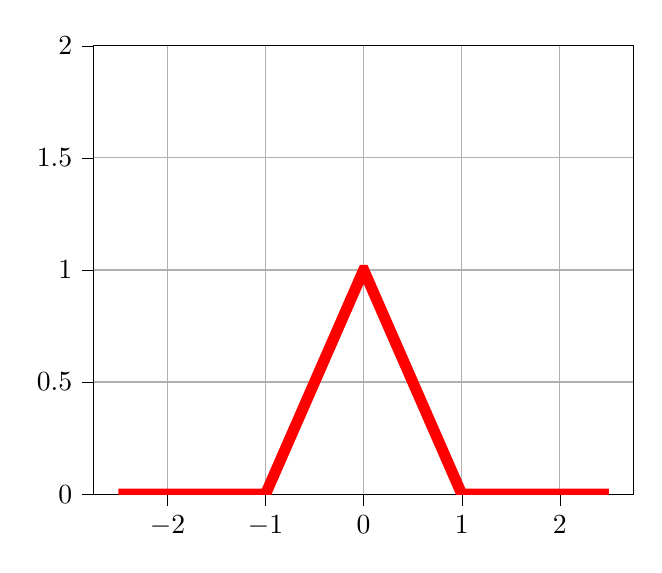
\begin{tikzpicture}

\begin{axis}[
tick align=outside,
tick pos=left,
x grid style={white!69.0196078431373!black},
xmajorgrids,
xmin=-2.75, xmax=2.75,
xtick style={color=black},
y grid style={white!69.0196078431373!black},
ymajorgrids,
ymin=0, ymax=2,
ytick style={color=black}
]
\addplot [line width=4pt, red]
table {%
-2.5 -0
-2.49499499499499 -0
-2.48998998998999 -0
-2.48498498498498 -0
-2.47997997997998 -0
-2.47497497497497 -0
-2.46996996996997 -0
-2.46496496496496 -0
-2.45995995995996 -0
-2.45495495495495 -0
-2.44994994994995 -0
-2.44494494494494 -0
-2.43993993993994 -0
-2.43493493493493 -0
-2.42992992992993 -0
-2.42492492492492 -0
-2.41991991991992 -0
-2.41491491491491 -0
-2.40990990990991 -0
-2.4049049049049 -0
-2.3998998998999 -0
-2.39489489489489 -0
-2.38988988988989 -0
-2.38488488488488 -0
-2.37987987987988 -0
-2.37487487487487 -0
-2.36986986986987 -0
-2.36486486486486 -0
-2.35985985985986 -0
-2.35485485485485 -0
-2.34984984984985 -0
-2.34484484484484 -0
-2.33983983983984 -0
-2.33483483483483 -0
-2.32982982982983 -0
-2.32482482482482 -0
-2.31981981981982 -0
-2.31481481481481 -0
-2.30980980980981 -0
-2.3048048048048 -0
-2.2997997997998 -0
-2.29479479479479 -0
-2.28978978978979 -0
-2.28478478478478 -0
-2.27977977977978 -0
-2.27477477477477 -0
-2.26976976976977 -0
-2.26476476476476 -0
-2.25975975975976 -0
-2.25475475475475 -0
-2.24974974974975 -0
-2.24474474474474 -0
-2.23973973973974 -0
-2.23473473473473 -0
-2.22972972972973 -0
-2.22472472472472 -0
-2.21971971971972 -0
-2.21471471471471 -0
-2.20970970970971 -0
-2.2047047047047 -0
-2.1996996996997 -0
-2.19469469469469 -0
-2.18968968968969 -0
-2.18468468468468 -0
-2.17967967967968 -0
-2.17467467467467 -0
-2.16966966966967 -0
-2.16466466466466 -0
-2.15965965965966 -0
-2.15465465465465 -0
-2.14964964964965 -0
-2.14464464464464 -0
-2.13963963963964 -0
-2.13463463463463 -0
-2.12962962962963 -0
-2.12462462462462 -0
-2.11961961961962 -0
-2.11461461461461 -0
-2.10960960960961 -0
-2.1046046046046 -0
-2.0995995995996 -0
-2.09459459459459 -0
-2.08958958958959 -0
-2.08458458458458 -0
-2.07957957957958 -0
-2.07457457457457 -0
-2.06956956956957 -0
-2.06456456456456 -0
-2.05955955955956 -0
-2.05455455455455 -0
-2.04954954954955 -0
-2.04454454454454 -0
-2.03953953953954 -0
-2.03453453453453 -0
-2.02952952952953 -0
-2.02452452452452 -0
-2.01951951951952 -0
-2.01451451451451 -0
-2.00950950950951 -0
-2.0045045045045 -0
-1.9994994994995 -0
-1.99449449449449 -0
-1.98948948948949 -0
-1.98448448448448 -0
-1.97947947947948 -0
-1.97447447447447 -0
-1.96946946946947 -0
-1.96446446446446 -0
-1.95945945945946 -0
-1.95445445445445 -0
-1.94944944944945 -0
-1.94444444444444 -0
-1.93943943943944 -0
-1.93443443443443 -0
-1.92942942942943 -0
-1.92442442442442 -0
-1.91941941941942 -0
-1.91441441441441 -0
-1.90940940940941 -0
-1.9044044044044 -0
-1.8993993993994 -0
-1.89439439439439 -0
-1.88938938938939 -0
-1.88438438438438 -0
-1.87937937937938 -0
-1.87437437437437 -0
-1.86936936936937 -0
-1.86436436436436 -0
-1.85935935935936 -0
-1.85435435435435 -0
-1.84934934934935 -0
-1.84434434434434 -0
-1.83933933933934 -0
-1.83433433433433 -0
-1.82932932932933 -0
-1.82432432432432 -0
-1.81931931931932 -0
-1.81431431431431 -0
-1.80930930930931 -0
-1.8043043043043 -0
-1.7992992992993 -0
-1.79429429429429 -0
-1.78928928928929 -0
-1.78428428428428 -0
-1.77927927927928 -0
-1.77427427427427 -0
-1.76926926926927 -0
-1.76426426426426 -0
-1.75925925925926 -0
-1.75425425425425 -0
-1.74924924924925 -0
-1.74424424424424 -0
-1.73923923923924 -0
-1.73423423423423 -0
-1.72922922922923 -0
-1.72422422422422 -0
-1.71921921921922 -0
-1.71421421421421 -0
-1.70920920920921 -0
-1.7042042042042 -0
-1.6991991991992 -0
-1.69419419419419 -0
-1.68918918918919 -0
-1.68418418418418 -0
-1.67917917917918 -0
-1.67417417417417 -0
-1.66916916916917 -0
-1.66416416416416 -0
-1.65915915915916 -0
-1.65415415415415 -0
-1.64914914914915 -0
-1.64414414414414 -0
-1.63913913913914 -0
-1.63413413413413 -0
-1.62912912912913 -0
-1.62412412412412 -0
-1.61911911911912 -0
-1.61411411411411 -0
-1.60910910910911 -0
-1.6041041041041 -0
-1.5990990990991 -0
-1.59409409409409 -0
-1.58908908908909 -0
-1.58408408408408 -0
-1.57907907907908 -0
-1.57407407407407 -0
-1.56906906906907 -0
-1.56406406406406 -0
-1.55905905905906 -0
-1.55405405405405 -0
-1.54904904904905 -0
-1.54404404404404 -0
-1.53903903903904 -0
-1.53403403403403 -0
-1.52902902902903 -0
-1.52402402402402 -0
-1.51901901901902 -0
-1.51401401401401 -0
-1.50900900900901 -0
-1.504004004004 -0
-1.498998998999 -0
-1.49399399399399 -0
-1.48898898898899 -0
-1.48398398398398 -0
-1.47897897897898 -0
-1.47397397397397 -0
-1.46896896896897 -0
-1.46396396396396 -0
-1.45895895895896 -0
-1.45395395395395 -0
-1.44894894894895 -0
-1.44394394394394 -0
-1.43893893893894 -0
-1.43393393393393 -0
-1.42892892892893 -0
-1.42392392392392 -0
-1.41891891891892 -0
-1.41391391391391 -0
-1.40890890890891 -0
-1.4039039039039 -0
-1.3988988988989 -0
-1.39389389389389 -0
-1.38888888888889 -0
-1.38388388388388 -0
-1.37887887887888 -0
-1.37387387387387 -0
-1.36886886886887 -0
-1.36386386386386 -0
-1.35885885885886 -0
-1.35385385385385 -0
-1.34884884884885 -0
-1.34384384384384 -0
-1.33883883883884 -0
-1.33383383383383 -0
-1.32882882882883 -0
-1.32382382382382 -0
-1.31881881881882 -0
-1.31381381381381 -0
-1.30880880880881 -0
-1.3038038038038 -0
-1.2987987987988 -0
-1.29379379379379 -0
-1.28878878878879 -0
-1.28378378378378 -0
-1.27877877877878 -0
-1.27377377377377 -0
-1.26876876876877 -0
-1.26376376376376 -0
-1.25875875875876 -0
-1.25375375375375 -0
-1.24874874874875 -0
-1.24374374374374 -0
-1.23873873873874 -0
-1.23373373373373 -0
-1.22872872872873 -0
-1.22372372372372 -0
-1.21871871871872 -0
-1.21371371371371 -0
-1.20870870870871 -0
-1.2037037037037 -0
-1.1986986986987 -0
-1.19369369369369 -0
-1.18868868868869 -0
-1.18368368368368 -0
-1.17867867867868 -0
-1.17367367367367 -0
-1.16866866866867 -0
-1.16366366366366 -0
-1.15865865865866 -0
-1.15365365365365 -0
-1.14864864864865 -0
-1.14364364364364 -0
-1.13863863863864 -0
-1.13363363363363 -0
-1.12862862862863 -0
-1.12362362362362 -0
-1.11861861861862 -0
-1.11361361361361 -0
-1.10860860860861 -0
-1.1036036036036 -0
-1.0985985985986 -0
-1.09359359359359 -0
-1.08858858858859 -0
-1.08358358358358 -0
-1.07857857857858 -0
-1.07357357357357 -0
-1.06856856856857 -0
-1.06356356356356 -0
-1.05855855855856 -0
-1.05355355355355 -0
-1.04854854854855 -0
-1.04354354354354 -0
-1.03853853853854 -0
-1.03353353353353 -0
-1.02852852852853 -0
-1.02352352352352 -0
-1.01851851851852 -0
-1.01351351351351 -0
-1.00850850850851 -0
-1.0035035035035 -0
-0.998498498498499 0.00150150150150141
-0.993493493493494 0.00650650650650642
-0.988488488488489 0.0115115115115114
-0.983483483483484 0.0165165165165164
-0.978478478478479 0.0215215215215214
-0.973473473473474 0.0265265265265264
-0.968468468468469 0.0315315315315314
-0.963463463463464 0.0365365365365364
-0.958458458458459 0.0415415415415414
-0.953453453453454 0.0465465465465464
-0.948448448448449 0.0515515515515514
-0.943443443443444 0.0565565565565564
-0.938438438438439 0.0615615615615615
-0.933433433433434 0.0665665665665665
-0.928428428428429 0.0715715715715715
-0.923423423423424 0.0765765765765765
-0.918418418418419 0.0815815815815815
-0.913413413413414 0.0865865865865865
-0.908408408408409 0.0915915915915915
-0.903403403403404 0.0965965965965965
-0.898398398398399 0.101601601601601
-0.893393393393393 0.106606606606607
-0.888388388388388 0.111611611611612
-0.883383383383383 0.116616616616617
-0.878378378378378 0.121621621621622
-0.873373373373373 0.126626626626627
-0.868368368368368 0.131631631631632
-0.863363363363363 0.136636636636637
-0.858358358358358 0.141641641641642
-0.853353353353353 0.146646646646647
-0.848348348348348 0.151651651651652
-0.843343343343343 0.156656656656657
-0.838338338338338 0.161661661661662
-0.833333333333333 0.166666666666667
-0.828328328328328 0.171671671671672
-0.823323323323323 0.176676676676677
-0.818318318318318 0.181681681681682
-0.813313313313313 0.186686686686687
-0.808308308308308 0.191691691691692
-0.803303303303303 0.196696696696697
-0.798298298298298 0.201701701701702
-0.793293293293293 0.206706706706707
-0.788288288288288 0.211711711711712
-0.783283283283283 0.216716716716717
-0.778278278278278 0.221721721721722
-0.773273273273273 0.226726726726727
-0.768268268268268 0.231731731731732
-0.763263263263263 0.236736736736737
-0.758258258258258 0.241741741741742
-0.753253253253253 0.246746746746747
-0.748248248248248 0.251751751751752
-0.743243243243243 0.256756756756757
-0.738238238238238 0.261761761761762
-0.733233233233233 0.266766766766767
-0.728228228228228 0.271771771771772
-0.723223223223223 0.276776776776777
-0.718218218218218 0.281781781781782
-0.713213213213213 0.286786786786787
-0.708208208208208 0.291791791791792
-0.703203203203203 0.296796796796797
-0.698198198198198 0.301801801801802
-0.693193193193193 0.306806806806807
-0.688188188188188 0.311811811811812
-0.683183183183183 0.316816816816817
-0.678178178178178 0.321821821821822
-0.673173173173173 0.326826826826827
-0.668168168168168 0.331831831831832
-0.663163163163163 0.336836836836837
-0.658158158158158 0.341841841841842
-0.653153153153153 0.346846846846847
-0.648148148148148 0.351851851851852
-0.643143143143143 0.356856856856857
-0.638138138138138 0.361861861861862
-0.633133133133133 0.366866866866867
-0.628128128128128 0.371871871871872
-0.623123123123123 0.376876876876877
-0.618118118118118 0.381881881881882
-0.613113113113113 0.386886886886887
-0.608108108108108 0.391891891891892
-0.603103103103103 0.396896896896897
-0.598098098098098 0.401901901901902
-0.593093093093093 0.406906906906907
-0.588088088088088 0.411911911911912
-0.583083083083083 0.416916916916917
-0.578078078078078 0.421921921921922
-0.573073073073073 0.426926926926927
-0.568068068068068 0.431931931931932
-0.563063063063063 0.436936936936937
-0.558058058058058 0.441941941941942
-0.553053053053053 0.446946946946947
-0.548048048048048 0.451951951951952
-0.543043043043043 0.456956956956957
-0.538038038038038 0.461961961961962
-0.533033033033033 0.466966966966967
-0.528028028028028 0.471971971971972
-0.523023023023023 0.476976976976977
-0.518018018018018 0.481981981981982
-0.513013013013013 0.486986986986987
-0.508008008008008 0.491991991991992
-0.503003003003003 0.496996996996997
-0.497997997997998 0.502002002002002
-0.492992992992993 0.507007007007007
-0.487987987987988 0.512012012012012
-0.482982982982983 0.517017017017017
-0.477977977977978 0.522022022022022
-0.472972972972973 0.527027027027027
-0.467967967967968 0.532032032032032
-0.462962962962963 0.537037037037037
-0.457957957957958 0.542042042042042
-0.452952952952953 0.547047047047047
-0.447947947947948 0.552052052052052
-0.442942942942943 0.557057057057057
-0.437937937937938 0.562062062062062
-0.432932932932933 0.567067067067067
-0.427927927927928 0.572072072072072
-0.422922922922923 0.577077077077077
-0.417917917917918 0.582082082082082
-0.412912912912913 0.587087087087087
-0.407907907907908 0.592092092092092
-0.402902902902903 0.597097097097097
-0.397897897897898 0.602102102102102
-0.392892892892893 0.607107107107107
-0.387887887887888 0.612112112112112
-0.382882882882883 0.617117117117117
-0.377877877877878 0.622122122122122
-0.372872872872873 0.627127127127127
-0.367867867867868 0.632132132132132
-0.362862862862863 0.637137137137137
-0.357857857857858 0.642142142142142
-0.352852852852853 0.647147147147147
-0.347847847847848 0.652152152152152
-0.342842842842843 0.657157157157157
-0.337837837837838 0.662162162162162
-0.332832832832833 0.667167167167167
-0.327827827827828 0.672172172172172
-0.322822822822823 0.677177177177177
-0.317817817817818 0.682182182182182
-0.312812812812813 0.687187187187187
-0.307807807807808 0.692192192192192
-0.302802802802803 0.697197197197197
-0.297797797797798 0.702202202202202
-0.292792792792793 0.707207207207207
-0.287787787787788 0.712212212212212
-0.282782782782783 0.717217217217217
-0.277777777777778 0.722222222222222
-0.272772772772773 0.727227227227227
-0.267767767767768 0.732232232232232
-0.262762762762763 0.737237237237237
-0.257757757757758 0.742242242242242
-0.252752752752753 0.747247247247247
-0.247747747747748 0.752252252252252
-0.242742742742743 0.757257257257257
-0.237737737737738 0.762262262262262
-0.232732732732733 0.767267267267267
-0.227727727727728 0.772272272272272
-0.222722722722723 0.777277277277277
-0.217717717717718 0.782282282282282
-0.212712712712713 0.787287287287287
-0.207707707707708 0.792292292292292
-0.202702702702703 0.797297297297297
-0.197697697697698 0.802302302302302
-0.192692692692693 0.807307307307307
-0.187687687687688 0.812312312312312
-0.182682682682683 0.817317317317317
-0.177677677677678 0.822322322322322
-0.172672672672673 0.827327327327327
-0.167667667667668 0.832332332332332
-0.162662662662663 0.837337337337337
-0.157657657657658 0.842342342342342
-0.152652652652653 0.847347347347347
-0.147647647647648 0.852352352352352
-0.142642642642643 0.857357357357357
-0.137637637637638 0.862362362362362
-0.132632632632633 0.867367367367367
-0.127627627627628 0.872372372372372
-0.122622622622623 0.877377377377377
-0.117617617617618 0.882382382382382
-0.112612612612613 0.887387387387387
-0.107607607607608 0.892392392392392
-0.102602602602603 0.897397397397397
-0.0975975975975976 0.902402402402402
-0.0925925925925926 0.907407407407407
-0.0875875875875876 0.912412412412412
-0.0825825825825826 0.917417417417417
-0.0775775775775776 0.922422422422422
-0.0725725725725725 0.927427427427427
-0.0675675675675675 0.932432432432432
-0.0625625625625625 0.937437437437437
-0.0575575575575575 0.942442442442442
-0.0525525525525525 0.947447447447447
-0.0475475475475475 0.952452452452452
-0.0425425425425425 0.957457457457457
-0.0375375375375375 0.962462462462462
-0.0325325325325325 0.967467467467467
-0.0275275275275275 0.972472472472472
-0.0225225225225225 0.977477477477477
-0.0175175175175175 0.982482482482482
-0.0125125125125125 0.987487487487487
-0.0075075075075075 0.992492492492492
-0.0025025025025025 0.997497497497497
0.0025025025025025 0.997497497497497
0.0075075075075075 0.992492492492492
0.0125125125125125 0.987487487487487
0.0175175175175175 0.982482482482482
0.0225225225225225 0.977477477477477
0.0275275275275275 0.972472472472472
0.0325325325325325 0.967467467467467
0.0375375375375375 0.962462462462462
0.0425425425425425 0.957457457457457
0.0475475475475475 0.952452452452452
0.0525525525525525 0.947447447447447
0.0575575575575575 0.942442442442442
0.0625625625625625 0.937437437437437
0.0675675675675675 0.932432432432432
0.0725725725725725 0.927427427427427
0.0775775775775776 0.922422422422422
0.0825825825825826 0.917417417417417
0.0875875875875876 0.912412412412412
0.0925925925925926 0.907407407407407
0.0975975975975976 0.902402402402402
0.102602602602603 0.897397397397397
0.107607607607608 0.892392392392392
0.112612612612613 0.887387387387387
0.117617617617618 0.882382382382382
0.122622622622623 0.877377377377377
0.127627627627628 0.872372372372372
0.132632632632633 0.867367367367367
0.137637637637638 0.862362362362362
0.142642642642643 0.857357357357357
0.147647647647648 0.852352352352352
0.152652652652653 0.847347347347347
0.157657657657658 0.842342342342342
0.162662662662663 0.837337337337337
0.167667667667668 0.832332332332332
0.172672672672673 0.827327327327327
0.177677677677678 0.822322322322322
0.182682682682683 0.817317317317317
0.187687687687688 0.812312312312312
0.192692692692693 0.807307307307307
0.197697697697698 0.802302302302302
0.202702702702703 0.797297297297297
0.207707707707708 0.792292292292292
0.212712712712713 0.787287287287287
0.217717717717718 0.782282282282282
0.222722722722723 0.777277277277277
0.227727727727728 0.772272272272272
0.232732732732733 0.767267267267267
0.237737737737738 0.762262262262262
0.242742742742743 0.757257257257257
0.247747747747748 0.752252252252252
0.252752752752753 0.747247247247247
0.257757757757758 0.742242242242242
0.262762762762763 0.737237237237237
0.267767767767768 0.732232232232232
0.272772772772773 0.727227227227227
0.277777777777778 0.722222222222222
0.282782782782783 0.717217217217217
0.287787787787788 0.712212212212212
0.292792792792793 0.707207207207207
0.297797797797798 0.702202202202202
0.302802802802803 0.697197197197197
0.307807807807808 0.692192192192192
0.312812812812813 0.687187187187187
0.317817817817818 0.682182182182182
0.322822822822823 0.677177177177177
0.327827827827828 0.672172172172172
0.332832832832833 0.667167167167167
0.337837837837838 0.662162162162162
0.342842842842843 0.657157157157157
0.347847847847848 0.652152152152152
0.352852852852853 0.647147147147147
0.357857857857858 0.642142142142142
0.362862862862863 0.637137137137137
0.367867867867868 0.632132132132132
0.372872872872873 0.627127127127127
0.377877877877878 0.622122122122122
0.382882882882883 0.617117117117117
0.387887887887888 0.612112112112112
0.392892892892893 0.607107107107107
0.397897897897898 0.602102102102102
0.402902902902903 0.597097097097097
0.407907907907908 0.592092092092092
0.412912912912913 0.587087087087087
0.417917917917918 0.582082082082082
0.422922922922923 0.577077077077077
0.427927927927928 0.572072072072072
0.432932932932933 0.567067067067067
0.437937937937938 0.562062062062062
0.442942942942943 0.557057057057057
0.447947947947948 0.552052052052052
0.452952952952953 0.547047047047047
0.457957957957958 0.542042042042042
0.462962962962963 0.537037037037037
0.467967967967968 0.532032032032032
0.472972972972973 0.527027027027027
0.477977977977978 0.522022022022022
0.482982982982983 0.517017017017017
0.487987987987988 0.512012012012012
0.492992992992993 0.507007007007007
0.497997997997998 0.502002002002002
0.503003003003003 0.496996996996997
0.508008008008008 0.491991991991992
0.513013013013013 0.486986986986987
0.518018018018018 0.481981981981982
0.523023023023023 0.476976976976977
0.528028028028028 0.471971971971972
0.533033033033033 0.466966966966967
0.538038038038038 0.461961961961962
0.543043043043043 0.456956956956957
0.548048048048048 0.451951951951952
0.553053053053053 0.446946946946947
0.558058058058058 0.441941941941942
0.563063063063063 0.436936936936937
0.568068068068068 0.431931931931932
0.573073073073073 0.426926926926927
0.578078078078078 0.421921921921922
0.583083083083083 0.416916916916917
0.588088088088088 0.411911911911912
0.593093093093093 0.406906906906907
0.598098098098098 0.401901901901902
0.603103103103103 0.396896896896897
0.608108108108108 0.391891891891892
0.613113113113113 0.386886886886887
0.618118118118118 0.381881881881882
0.623123123123123 0.376876876876877
0.628128128128128 0.371871871871872
0.633133133133133 0.366866866866867
0.638138138138138 0.361861861861862
0.643143143143143 0.356856856856857
0.648148148148148 0.351851851851852
0.653153153153153 0.346846846846847
0.658158158158158 0.341841841841842
0.663163163163163 0.336836836836837
0.668168168168168 0.331831831831832
0.673173173173173 0.326826826826827
0.678178178178178 0.321821821821822
0.683183183183183 0.316816816816817
0.688188188188188 0.311811811811812
0.693193193193193 0.306806806806807
0.698198198198198 0.301801801801802
0.703203203203203 0.296796796796797
0.708208208208208 0.291791791791792
0.713213213213213 0.286786786786787
0.718218218218218 0.281781781781782
0.723223223223223 0.276776776776777
0.728228228228228 0.271771771771772
0.733233233233233 0.266766766766767
0.738238238238238 0.261761761761762
0.743243243243243 0.256756756756757
0.748248248248248 0.251751751751752
0.753253253253253 0.246746746746747
0.758258258258258 0.241741741741742
0.763263263263263 0.236736736736737
0.768268268268268 0.231731731731732
0.773273273273273 0.226726726726727
0.778278278278278 0.221721721721722
0.783283283283283 0.216716716716717
0.788288288288288 0.211711711711712
0.793293293293293 0.206706706706707
0.798298298298298 0.201701701701702
0.803303303303303 0.196696696696697
0.808308308308308 0.191691691691692
0.813313313313313 0.186686686686687
0.818318318318318 0.181681681681682
0.823323323323323 0.176676676676677
0.828328328328328 0.171671671671672
0.833333333333333 0.166666666666667
0.838338338338338 0.161661661661662
0.843343343343343 0.156656656656657
0.848348348348348 0.151651651651652
0.853353353353353 0.146646646646647
0.858358358358358 0.141641641641642
0.863363363363364 0.136636636636636
0.868368368368369 0.131631631631631
0.873373373373374 0.126626626626626
0.878378378378379 0.121621621621621
0.883383383383384 0.116616616616616
0.888388388388389 0.111611611611611
0.893393393393394 0.106606606606606
0.898398398398399 0.101601601601601
0.903403403403404 0.0965965965965965
0.908408408408409 0.0915915915915915
0.913413413413414 0.0865865865865865
0.918418418418419 0.0815815815815815
0.923423423423424 0.0765765765765765
0.928428428428429 0.0715715715715715
0.933433433433434 0.0665665665665665
0.938438438438439 0.0615615615615615
0.943443443443444 0.0565565565565564
0.948448448448449 0.0515515515515514
0.953453453453454 0.0465465465465464
0.958458458458459 0.0415415415415414
0.963463463463464 0.0365365365365364
0.968468468468469 0.0315315315315314
0.973473473473474 0.0265265265265264
0.978478478478479 0.0215215215215214
0.983483483483484 0.0165165165165164
0.988488488488489 0.0115115115115114
0.993493493493494 0.00650650650650642
0.998498498498499 0.00150150150150141
1.0035035035035 -0
1.00850850850851 -0
1.01351351351351 -0
1.01851851851852 -0
1.02352352352352 -0
1.02852852852853 -0
1.03353353353353 -0
1.03853853853854 -0
1.04354354354354 -0
1.04854854854855 -0
1.05355355355355 -0
1.05855855855856 -0
1.06356356356356 -0
1.06856856856857 -0
1.07357357357357 -0
1.07857857857858 -0
1.08358358358358 -0
1.08858858858859 -0
1.09359359359359 -0
1.0985985985986 -0
1.1036036036036 -0
1.10860860860861 -0
1.11361361361361 -0
1.11861861861862 -0
1.12362362362362 -0
1.12862862862863 -0
1.13363363363363 -0
1.13863863863864 -0
1.14364364364364 -0
1.14864864864865 -0
1.15365365365365 -0
1.15865865865866 -0
1.16366366366366 -0
1.16866866866867 -0
1.17367367367367 -0
1.17867867867868 -0
1.18368368368368 -0
1.18868868868869 -0
1.19369369369369 -0
1.1986986986987 -0
1.2037037037037 -0
1.20870870870871 -0
1.21371371371371 -0
1.21871871871872 -0
1.22372372372372 -0
1.22872872872873 -0
1.23373373373373 -0
1.23873873873874 -0
1.24374374374374 -0
1.24874874874875 -0
1.25375375375375 -0
1.25875875875876 -0
1.26376376376376 -0
1.26876876876877 -0
1.27377377377377 -0
1.27877877877878 -0
1.28378378378378 -0
1.28878878878879 -0
1.29379379379379 -0
1.2987987987988 -0
1.3038038038038 -0
1.30880880880881 -0
1.31381381381381 -0
1.31881881881882 -0
1.32382382382382 -0
1.32882882882883 -0
1.33383383383383 -0
1.33883883883884 -0
1.34384384384384 -0
1.34884884884885 -0
1.35385385385385 -0
1.35885885885886 -0
1.36386386386386 -0
1.36886886886887 -0
1.37387387387387 -0
1.37887887887888 -0
1.38388388388388 -0
1.38888888888889 -0
1.39389389389389 -0
1.3988988988989 -0
1.4039039039039 -0
1.40890890890891 -0
1.41391391391391 -0
1.41891891891892 -0
1.42392392392392 -0
1.42892892892893 -0
1.43393393393393 -0
1.43893893893894 -0
1.44394394394394 -0
1.44894894894895 -0
1.45395395395395 -0
1.45895895895896 -0
1.46396396396396 -0
1.46896896896897 -0
1.47397397397397 -0
1.47897897897898 -0
1.48398398398398 -0
1.48898898898899 -0
1.49399399399399 -0
1.498998998999 -0
1.504004004004 -0
1.50900900900901 -0
1.51401401401401 -0
1.51901901901902 -0
1.52402402402402 -0
1.52902902902903 -0
1.53403403403403 -0
1.53903903903904 -0
1.54404404404404 -0
1.54904904904905 -0
1.55405405405405 -0
1.55905905905906 -0
1.56406406406406 -0
1.56906906906907 -0
1.57407407407407 -0
1.57907907907908 -0
1.58408408408408 -0
1.58908908908909 -0
1.59409409409409 -0
1.5990990990991 -0
1.6041041041041 -0
1.60910910910911 -0
1.61411411411411 -0
1.61911911911912 -0
1.62412412412412 -0
1.62912912912913 -0
1.63413413413413 -0
1.63913913913914 -0
1.64414414414414 -0
1.64914914914915 -0
1.65415415415415 -0
1.65915915915916 -0
1.66416416416416 -0
1.66916916916917 -0
1.67417417417417 -0
1.67917917917918 -0
1.68418418418418 -0
1.68918918918919 -0
1.69419419419419 -0
1.6991991991992 -0
1.7042042042042 -0
1.70920920920921 -0
1.71421421421421 -0
1.71921921921922 -0
1.72422422422422 -0
1.72922922922923 -0
1.73423423423423 -0
1.73923923923924 -0
1.74424424424424 -0
1.74924924924925 -0
1.75425425425425 -0
1.75925925925926 -0
1.76426426426426 -0
1.76926926926927 -0
1.77427427427427 -0
1.77927927927928 -0
1.78428428428428 -0
1.78928928928929 -0
1.79429429429429 -0
1.7992992992993 -0
1.8043043043043 -0
1.80930930930931 -0
1.81431431431431 -0
1.81931931931932 -0
1.82432432432432 -0
1.82932932932933 -0
1.83433433433433 -0
1.83933933933934 -0
1.84434434434434 -0
1.84934934934935 -0
1.85435435435435 -0
1.85935935935936 -0
1.86436436436436 -0
1.86936936936937 -0
1.87437437437437 -0
1.87937937937938 -0
1.88438438438438 -0
1.88938938938939 -0
1.89439439439439 -0
1.8993993993994 -0
1.9044044044044 -0
1.90940940940941 -0
1.91441441441441 -0
1.91941941941942 -0
1.92442442442442 -0
1.92942942942943 -0
1.93443443443443 -0
1.93943943943944 -0
1.94444444444444 -0
1.94944944944945 -0
1.95445445445445 -0
1.95945945945946 -0
1.96446446446446 -0
1.96946946946947 -0
1.97447447447447 -0
1.97947947947948 -0
1.98448448448448 -0
1.98948948948949 -0
1.99449449449449 -0
1.9994994994995 -0
2.0045045045045 -0
2.00950950950951 -0
2.01451451451451 -0
2.01951951951952 -0
2.02452452452452 -0
2.02952952952953 -0
2.03453453453453 -0
2.03953953953954 -0
2.04454454454454 -0
2.04954954954955 -0
2.05455455455455 -0
2.05955955955956 -0
2.06456456456456 -0
2.06956956956957 -0
2.07457457457457 -0
2.07957957957958 -0
2.08458458458458 -0
2.08958958958959 -0
2.09459459459459 -0
2.0995995995996 -0
2.1046046046046 -0
2.10960960960961 -0
2.11461461461461 -0
2.11961961961962 -0
2.12462462462462 -0
2.12962962962963 -0
2.13463463463463 -0
2.13963963963964 -0
2.14464464464464 -0
2.14964964964965 -0
2.15465465465465 -0
2.15965965965966 -0
2.16466466466466 -0
2.16966966966967 -0
2.17467467467467 -0
2.17967967967968 -0
2.18468468468468 -0
2.18968968968969 -0
2.19469469469469 -0
2.1996996996997 -0
2.2047047047047 -0
2.20970970970971 -0
2.21471471471471 -0
2.21971971971972 -0
2.22472472472472 -0
2.22972972972973 -0
2.23473473473473 -0
2.23973973973974 -0
2.24474474474474 -0
2.24974974974975 -0
2.25475475475475 -0
2.25975975975976 -0
2.26476476476476 -0
2.26976976976977 -0
2.27477477477477 -0
2.27977977977978 -0
2.28478478478478 -0
2.28978978978979 -0
2.29479479479479 -0
2.2997997997998 -0
2.3048048048048 -0
2.30980980980981 -0
2.31481481481481 -0
2.31981981981982 -0
2.32482482482482 -0
2.32982982982983 -0
2.33483483483483 -0
2.33983983983984 -0
2.34484484484484 -0
2.34984984984985 -0
2.35485485485485 -0
2.35985985985986 -0
2.36486486486486 -0
2.36986986986987 -0
2.37487487487487 -0
2.37987987987988 -0
2.38488488488488 -0
2.38988988988989 -0
2.39489489489489 -0
2.3998998998999 -0
2.4049049049049 -0
2.40990990990991 -0
2.41491491491491 -0
2.41991991991992 -0
2.42492492492492 -0
2.42992992992993 -0
2.43493493493493 -0
2.43993993993994 -0
2.44494494494494 -0
2.44994994994995 -0
2.45495495495495 -0
2.45995995995996 -0
2.46496496496496 -0
2.46996996996997 -0
2.47497497497497 -0
2.47997997997998 -0
2.48498498498498 -0
2.48998998998999 -0
2.49499499499499 -0
2.5 -0
};
\end{axis}

\end{tikzpicture}
}

                    $\quad{}f(t)$
                \end{column}\begin{column}{0.33\textwidth}
                    \centering{}
                    \scalebox{0.4}{% This file was created by tikzplotlib v0.9.1.
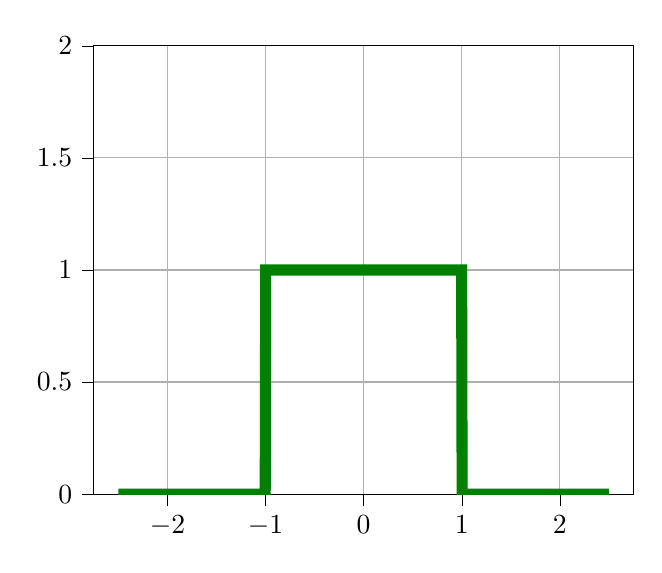
\begin{tikzpicture}

\begin{axis}[
tick align=outside,
tick pos=left,
x grid style={white!69.0196078431373!black},
xmajorgrids,
xmin=-2.75, xmax=2.75,
xtick style={color=black},
y grid style={white!69.0196078431373!black},
ymajorgrids,
ymin=0, ymax=2,
ytick style={color=black}
]
\addplot [line width=4pt, green!50!black]
table {%
-2.5 0
-2.49499499499499 0
-2.48998998998999 0
-2.48498498498498 0
-2.47997997997998 0
-2.47497497497497 0
-2.46996996996997 0
-2.46496496496496 0
-2.45995995995996 0
-2.45495495495495 0
-2.44994994994995 0
-2.44494494494494 0
-2.43993993993994 0
-2.43493493493493 0
-2.42992992992993 0
-2.42492492492492 0
-2.41991991991992 0
-2.41491491491491 0
-2.40990990990991 0
-2.4049049049049 0
-2.3998998998999 0
-2.39489489489489 0
-2.38988988988989 0
-2.38488488488488 0
-2.37987987987988 0
-2.37487487487487 0
-2.36986986986987 0
-2.36486486486486 0
-2.35985985985986 0
-2.35485485485485 0
-2.34984984984985 0
-2.34484484484484 0
-2.33983983983984 0
-2.33483483483483 0
-2.32982982982983 0
-2.32482482482482 0
-2.31981981981982 0
-2.31481481481481 0
-2.30980980980981 0
-2.3048048048048 0
-2.2997997997998 0
-2.29479479479479 0
-2.28978978978979 0
-2.28478478478478 0
-2.27977977977978 0
-2.27477477477477 0
-2.26976976976977 0
-2.26476476476476 0
-2.25975975975976 0
-2.25475475475475 0
-2.24974974974975 0
-2.24474474474474 0
-2.23973973973974 0
-2.23473473473473 0
-2.22972972972973 0
-2.22472472472472 0
-2.21971971971972 0
-2.21471471471471 0
-2.20970970970971 0
-2.2047047047047 0
-2.1996996996997 0
-2.19469469469469 0
-2.18968968968969 0
-2.18468468468468 0
-2.17967967967968 0
-2.17467467467467 0
-2.16966966966967 0
-2.16466466466466 0
-2.15965965965966 0
-2.15465465465465 0
-2.14964964964965 0
-2.14464464464464 0
-2.13963963963964 0
-2.13463463463463 0
-2.12962962962963 0
-2.12462462462462 0
-2.11961961961962 0
-2.11461461461461 0
-2.10960960960961 0
-2.1046046046046 0
-2.0995995995996 0
-2.09459459459459 0
-2.08958958958959 0
-2.08458458458458 0
-2.07957957957958 0
-2.07457457457457 0
-2.06956956956957 0
-2.06456456456456 0
-2.05955955955956 0
-2.05455455455455 0
-2.04954954954955 0
-2.04454454454454 0
-2.03953953953954 0
-2.03453453453453 0
-2.02952952952953 0
-2.02452452452452 0
-2.01951951951952 0
-2.01451451451451 0
-2.00950950950951 0
-2.0045045045045 0
-1.9994994994995 0
-1.99449449449449 0
-1.98948948948949 0
-1.98448448448448 0
-1.97947947947948 0
-1.97447447447447 0
-1.96946946946947 0
-1.96446446446446 0
-1.95945945945946 0
-1.95445445445445 0
-1.94944944944945 0
-1.94444444444444 0
-1.93943943943944 0
-1.93443443443443 0
-1.92942942942943 0
-1.92442442442442 0
-1.91941941941942 0
-1.91441441441441 0
-1.90940940940941 0
-1.9044044044044 0
-1.8993993993994 0
-1.89439439439439 0
-1.88938938938939 0
-1.88438438438438 0
-1.87937937937938 0
-1.87437437437437 0
-1.86936936936937 0
-1.86436436436436 0
-1.85935935935936 0
-1.85435435435435 0
-1.84934934934935 0
-1.84434434434434 0
-1.83933933933934 0
-1.83433433433433 0
-1.82932932932933 0
-1.82432432432432 0
-1.81931931931932 0
-1.81431431431431 0
-1.80930930930931 0
-1.8043043043043 0
-1.7992992992993 0
-1.79429429429429 0
-1.78928928928929 0
-1.78428428428428 0
-1.77927927927928 0
-1.77427427427427 0
-1.76926926926927 0
-1.76426426426426 0
-1.75925925925926 0
-1.75425425425425 0
-1.74924924924925 0
-1.74424424424424 0
-1.73923923923924 0
-1.73423423423423 0
-1.72922922922923 0
-1.72422422422422 0
-1.71921921921922 0
-1.71421421421421 0
-1.70920920920921 0
-1.7042042042042 0
-1.6991991991992 0
-1.69419419419419 0
-1.68918918918919 0
-1.68418418418418 0
-1.67917917917918 0
-1.67417417417417 0
-1.66916916916917 0
-1.66416416416416 0
-1.65915915915916 0
-1.65415415415415 0
-1.64914914914915 0
-1.64414414414414 0
-1.63913913913914 0
-1.63413413413413 0
-1.62912912912913 0
-1.62412412412412 0
-1.61911911911912 0
-1.61411411411411 0
-1.60910910910911 0
-1.6041041041041 0
-1.5990990990991 0
-1.59409409409409 0
-1.58908908908909 0
-1.58408408408408 0
-1.57907907907908 0
-1.57407407407407 0
-1.56906906906907 0
-1.56406406406406 0
-1.55905905905906 0
-1.55405405405405 0
-1.54904904904905 0
-1.54404404404404 0
-1.53903903903904 0
-1.53403403403403 0
-1.52902902902903 0
-1.52402402402402 0
-1.51901901901902 0
-1.51401401401401 0
-1.50900900900901 0
-1.504004004004 0
-1.498998998999 0
-1.49399399399399 0
-1.48898898898899 0
-1.48398398398398 0
-1.47897897897898 0
-1.47397397397397 0
-1.46896896896897 0
-1.46396396396396 0
-1.45895895895896 0
-1.45395395395395 0
-1.44894894894895 0
-1.44394394394394 0
-1.43893893893894 0
-1.43393393393393 0
-1.42892892892893 0
-1.42392392392392 0
-1.41891891891892 0
-1.41391391391391 0
-1.40890890890891 0
-1.4039039039039 0
-1.3988988988989 0
-1.39389389389389 0
-1.38888888888889 0
-1.38388388388388 0
-1.37887887887888 0
-1.37387387387387 0
-1.36886886886887 0
-1.36386386386386 0
-1.35885885885886 0
-1.35385385385385 0
-1.34884884884885 0
-1.34384384384384 0
-1.33883883883884 0
-1.33383383383383 0
-1.32882882882883 0
-1.32382382382382 0
-1.31881881881882 0
-1.31381381381381 0
-1.30880880880881 0
-1.3038038038038 0
-1.2987987987988 0
-1.29379379379379 0
-1.28878878878879 0
-1.28378378378378 0
-1.27877877877878 0
-1.27377377377377 0
-1.26876876876877 0
-1.26376376376376 0
-1.25875875875876 0
-1.25375375375375 0
-1.24874874874875 0
-1.24374374374374 0
-1.23873873873874 0
-1.23373373373373 0
-1.22872872872873 0
-1.22372372372372 0
-1.21871871871872 0
-1.21371371371371 0
-1.20870870870871 0
-1.2037037037037 0
-1.1986986986987 0
-1.19369369369369 0
-1.18868868868869 0
-1.18368368368368 0
-1.17867867867868 0
-1.17367367367367 0
-1.16866866866867 0
-1.16366366366366 0
-1.15865865865866 0
-1.15365365365365 0
-1.14864864864865 0
-1.14364364364364 0
-1.13863863863864 0
-1.13363363363363 0
-1.12862862862863 0
-1.12362362362362 0
-1.11861861861862 0
-1.11361361361361 0
-1.10860860860861 0
-1.1036036036036 0
-1.0985985985986 0
-1.09359359359359 0
-1.08858858858859 0
-1.08358358358358 0
-1.07857857857858 0
-1.07357357357357 0
-1.06856856856857 0
-1.06356356356356 0
-1.05855855855856 0
-1.05355355355355 0
-1.04854854854855 0
-1.04354354354354 0
-1.03853853853854 0
-1.03353353353353 0
-1.02852852852853 0
-1.02352352352352 0
-1.01851851851852 0
-1.01351351351351 0
-1.00850850850851 0
-1.0035035035035 0
-0.998498498498499 1
-0.993493493493494 1
-0.988488488488489 1
-0.983483483483484 1
-0.978478478478479 1
-0.973473473473474 1
-0.968468468468469 1
-0.963463463463464 1
-0.958458458458459 1
-0.953453453453454 1
-0.948448448448449 1
-0.943443443443444 1
-0.938438438438439 1
-0.933433433433434 1
-0.928428428428429 1
-0.923423423423424 1
-0.918418418418419 1
-0.913413413413414 1
-0.908408408408409 1
-0.903403403403404 1
-0.898398398398399 1
-0.893393393393393 1
-0.888388388388388 1
-0.883383383383383 1
-0.878378378378378 1
-0.873373373373373 1
-0.868368368368368 1
-0.863363363363363 1
-0.858358358358358 1
-0.853353353353353 1
-0.848348348348348 1
-0.843343343343343 1
-0.838338338338338 1
-0.833333333333333 1
-0.828328328328328 1
-0.823323323323323 1
-0.818318318318318 1
-0.813313313313313 1
-0.808308308308308 1
-0.803303303303303 1
-0.798298298298298 1
-0.793293293293293 1
-0.788288288288288 1
-0.783283283283283 1
-0.778278278278278 1
-0.773273273273273 1
-0.768268268268268 1
-0.763263263263263 1
-0.758258258258258 1
-0.753253253253253 1
-0.748248248248248 1
-0.743243243243243 1
-0.738238238238238 1
-0.733233233233233 1
-0.728228228228228 1
-0.723223223223223 1
-0.718218218218218 1
-0.713213213213213 1
-0.708208208208208 1
-0.703203203203203 1
-0.698198198198198 1
-0.693193193193193 1
-0.688188188188188 1
-0.683183183183183 1
-0.678178178178178 1
-0.673173173173173 1
-0.668168168168168 1
-0.663163163163163 1
-0.658158158158158 1
-0.653153153153153 1
-0.648148148148148 1
-0.643143143143143 1
-0.638138138138138 1
-0.633133133133133 1
-0.628128128128128 1
-0.623123123123123 1
-0.618118118118118 1
-0.613113113113113 1
-0.608108108108108 1
-0.603103103103103 1
-0.598098098098098 1
-0.593093093093093 1
-0.588088088088088 1
-0.583083083083083 1
-0.578078078078078 1
-0.573073073073073 1
-0.568068068068068 1
-0.563063063063063 1
-0.558058058058058 1
-0.553053053053053 1
-0.548048048048048 1
-0.543043043043043 1
-0.538038038038038 1
-0.533033033033033 1
-0.528028028028028 1
-0.523023023023023 1
-0.518018018018018 1
-0.513013013013013 1
-0.508008008008008 1
-0.503003003003003 1
-0.497997997997998 1
-0.492992992992993 1
-0.487987987987988 1
-0.482982982982983 1
-0.477977977977978 1
-0.472972972972973 1
-0.467967967967968 1
-0.462962962962963 1
-0.457957957957958 1
-0.452952952952953 1
-0.447947947947948 1
-0.442942942942943 1
-0.437937937937938 1
-0.432932932932933 1
-0.427927927927928 1
-0.422922922922923 1
-0.417917917917918 1
-0.412912912912913 1
-0.407907907907908 1
-0.402902902902903 1
-0.397897897897898 1
-0.392892892892893 1
-0.387887887887888 1
-0.382882882882883 1
-0.377877877877878 1
-0.372872872872873 1
-0.367867867867868 1
-0.362862862862863 1
-0.357857857857858 1
-0.352852852852853 1
-0.347847847847848 1
-0.342842842842843 1
-0.337837837837838 1
-0.332832832832833 1
-0.327827827827828 1
-0.322822822822823 1
-0.317817817817818 1
-0.312812812812813 1
-0.307807807807808 1
-0.302802802802803 1
-0.297797797797798 1
-0.292792792792793 1
-0.287787787787788 1
-0.282782782782783 1
-0.277777777777778 1
-0.272772772772773 1
-0.267767767767768 1
-0.262762762762763 1
-0.257757757757758 1
-0.252752752752753 1
-0.247747747747748 1
-0.242742742742743 1
-0.237737737737738 1
-0.232732732732733 1
-0.227727727727728 1
-0.222722722722723 1
-0.217717717717718 1
-0.212712712712713 1
-0.207707707707708 1
-0.202702702702703 1
-0.197697697697698 1
-0.192692692692693 1
-0.187687687687688 1
-0.182682682682683 1
-0.177677677677678 1
-0.172672672672673 1
-0.167667667667668 1
-0.162662662662663 1
-0.157657657657658 1
-0.152652652652653 1
-0.147647647647648 1
-0.142642642642643 1
-0.137637637637638 1
-0.132632632632633 1
-0.127627627627628 1
-0.122622622622623 1
-0.117617617617618 1
-0.112612612612613 1
-0.107607607607608 1
-0.102602602602603 1
-0.0975975975975976 1
-0.0925925925925926 1
-0.0875875875875876 1
-0.0825825825825826 1
-0.0775775775775776 1
-0.0725725725725725 1
-0.0675675675675675 1
-0.0625625625625625 1
-0.0575575575575575 1
-0.0525525525525525 1
-0.0475475475475475 1
-0.0425425425425425 1
-0.0375375375375375 1
-0.0325325325325325 1
-0.0275275275275275 1
-0.0225225225225225 1
-0.0175175175175175 1
-0.0125125125125125 1
-0.0075075075075075 1
-0.0025025025025025 1
0.0025025025025025 1
0.0075075075075075 1
0.0125125125125125 1
0.0175175175175175 1
0.0225225225225225 1
0.0275275275275275 1
0.0325325325325325 1
0.0375375375375375 1
0.0425425425425425 1
0.0475475475475475 1
0.0525525525525525 1
0.0575575575575575 1
0.0625625625625625 1
0.0675675675675675 1
0.0725725725725725 1
0.0775775775775776 1
0.0825825825825826 1
0.0875875875875876 1
0.0925925925925926 1
0.0975975975975976 1
0.102602602602603 1
0.107607607607608 1
0.112612612612613 1
0.117617617617618 1
0.122622622622623 1
0.127627627627628 1
0.132632632632633 1
0.137637637637638 1
0.142642642642643 1
0.147647647647648 1
0.152652652652653 1
0.157657657657658 1
0.162662662662663 1
0.167667667667668 1
0.172672672672673 1
0.177677677677678 1
0.182682682682683 1
0.187687687687688 1
0.192692692692693 1
0.197697697697698 1
0.202702702702703 1
0.207707707707708 1
0.212712712712713 1
0.217717717717718 1
0.222722722722723 1
0.227727727727728 1
0.232732732732733 1
0.237737737737738 1
0.242742742742743 1
0.247747747747748 1
0.252752752752753 1
0.257757757757758 1
0.262762762762763 1
0.267767767767768 1
0.272772772772773 1
0.277777777777778 1
0.282782782782783 1
0.287787787787788 1
0.292792792792793 1
0.297797797797798 1
0.302802802802803 1
0.307807807807808 1
0.312812812812813 1
0.317817817817818 1
0.322822822822823 1
0.327827827827828 1
0.332832832832833 1
0.337837837837838 1
0.342842842842843 1
0.347847847847848 1
0.352852852852853 1
0.357857857857858 1
0.362862862862863 1
0.367867867867868 1
0.372872872872873 1
0.377877877877878 1
0.382882882882883 1
0.387887887887888 1
0.392892892892893 1
0.397897897897898 1
0.402902902902903 1
0.407907907907908 1
0.412912912912913 1
0.417917917917918 1
0.422922922922923 1
0.427927927927928 1
0.432932932932933 1
0.437937937937938 1
0.442942942942943 1
0.447947947947948 1
0.452952952952953 1
0.457957957957958 1
0.462962962962963 1
0.467967967967968 1
0.472972972972973 1
0.477977977977978 1
0.482982982982983 1
0.487987987987988 1
0.492992992992993 1
0.497997997997998 1
0.503003003003003 1
0.508008008008008 1
0.513013013013013 1
0.518018018018018 1
0.523023023023023 1
0.528028028028028 1
0.533033033033033 1
0.538038038038038 1
0.543043043043043 1
0.548048048048048 1
0.553053053053053 1
0.558058058058058 1
0.563063063063063 1
0.568068068068068 1
0.573073073073073 1
0.578078078078078 1
0.583083083083083 1
0.588088088088088 1
0.593093093093093 1
0.598098098098098 1
0.603103103103103 1
0.608108108108108 1
0.613113113113113 1
0.618118118118118 1
0.623123123123123 1
0.628128128128128 1
0.633133133133133 1
0.638138138138138 1
0.643143143143143 1
0.648148148148148 1
0.653153153153153 1
0.658158158158158 1
0.663163163163163 1
0.668168168168168 1
0.673173173173173 1
0.678178178178178 1
0.683183183183183 1
0.688188188188188 1
0.693193193193193 1
0.698198198198198 1
0.703203203203203 1
0.708208208208208 1
0.713213213213213 1
0.718218218218218 1
0.723223223223223 1
0.728228228228228 1
0.733233233233233 1
0.738238238238238 1
0.743243243243243 1
0.748248248248248 1
0.753253253253253 1
0.758258258258258 1
0.763263263263263 1
0.768268268268268 1
0.773273273273273 1
0.778278278278278 1
0.783283283283283 1
0.788288288288288 1
0.793293293293293 1
0.798298298298298 1
0.803303303303303 1
0.808308308308308 1
0.813313313313313 1
0.818318318318318 1
0.823323323323323 1
0.828328328328328 1
0.833333333333333 1
0.838338338338338 1
0.843343343343343 1
0.848348348348348 1
0.853353353353353 1
0.858358358358358 1
0.863363363363364 1
0.868368368368369 1
0.873373373373374 1
0.878378378378379 1
0.883383383383384 1
0.888388388388389 1
0.893393393393394 1
0.898398398398399 1
0.903403403403404 1
0.908408408408409 1
0.913413413413414 1
0.918418418418419 1
0.923423423423424 1
0.928428428428429 1
0.933433433433434 1
0.938438438438439 1
0.943443443443444 1
0.948448448448449 1
0.953453453453454 1
0.958458458458459 1
0.963463463463464 1
0.968468468468469 1
0.973473473473474 1
0.978478478478479 1
0.983483483483484 1
0.988488488488489 1
0.993493493493494 1
0.998498498498499 1
1.0035035035035 0
1.00850850850851 0
1.01351351351351 0
1.01851851851852 0
1.02352352352352 0
1.02852852852853 0
1.03353353353353 0
1.03853853853854 0
1.04354354354354 0
1.04854854854855 0
1.05355355355355 0
1.05855855855856 0
1.06356356356356 0
1.06856856856857 0
1.07357357357357 0
1.07857857857858 0
1.08358358358358 0
1.08858858858859 0
1.09359359359359 0
1.0985985985986 0
1.1036036036036 0
1.10860860860861 0
1.11361361361361 0
1.11861861861862 0
1.12362362362362 0
1.12862862862863 0
1.13363363363363 0
1.13863863863864 0
1.14364364364364 0
1.14864864864865 0
1.15365365365365 0
1.15865865865866 0
1.16366366366366 0
1.16866866866867 0
1.17367367367367 0
1.17867867867868 0
1.18368368368368 0
1.18868868868869 0
1.19369369369369 0
1.1986986986987 0
1.2037037037037 0
1.20870870870871 0
1.21371371371371 0
1.21871871871872 0
1.22372372372372 0
1.22872872872873 0
1.23373373373373 0
1.23873873873874 0
1.24374374374374 0
1.24874874874875 0
1.25375375375375 0
1.25875875875876 0
1.26376376376376 0
1.26876876876877 0
1.27377377377377 0
1.27877877877878 0
1.28378378378378 0
1.28878878878879 0
1.29379379379379 0
1.2987987987988 0
1.3038038038038 0
1.30880880880881 0
1.31381381381381 0
1.31881881881882 0
1.32382382382382 0
1.32882882882883 0
1.33383383383383 0
1.33883883883884 0
1.34384384384384 0
1.34884884884885 0
1.35385385385385 0
1.35885885885886 0
1.36386386386386 0
1.36886886886887 0
1.37387387387387 0
1.37887887887888 0
1.38388388388388 0
1.38888888888889 0
1.39389389389389 0
1.3988988988989 0
1.4039039039039 0
1.40890890890891 0
1.41391391391391 0
1.41891891891892 0
1.42392392392392 0
1.42892892892893 0
1.43393393393393 0
1.43893893893894 0
1.44394394394394 0
1.44894894894895 0
1.45395395395395 0
1.45895895895896 0
1.46396396396396 0
1.46896896896897 0
1.47397397397397 0
1.47897897897898 0
1.48398398398398 0
1.48898898898899 0
1.49399399399399 0
1.498998998999 0
1.504004004004 0
1.50900900900901 0
1.51401401401401 0
1.51901901901902 0
1.52402402402402 0
1.52902902902903 0
1.53403403403403 0
1.53903903903904 0
1.54404404404404 0
1.54904904904905 0
1.55405405405405 0
1.55905905905906 0
1.56406406406406 0
1.56906906906907 0
1.57407407407407 0
1.57907907907908 0
1.58408408408408 0
1.58908908908909 0
1.59409409409409 0
1.5990990990991 0
1.6041041041041 0
1.60910910910911 0
1.61411411411411 0
1.61911911911912 0
1.62412412412412 0
1.62912912912913 0
1.63413413413413 0
1.63913913913914 0
1.64414414414414 0
1.64914914914915 0
1.65415415415415 0
1.65915915915916 0
1.66416416416416 0
1.66916916916917 0
1.67417417417417 0
1.67917917917918 0
1.68418418418418 0
1.68918918918919 0
1.69419419419419 0
1.6991991991992 0
1.7042042042042 0
1.70920920920921 0
1.71421421421421 0
1.71921921921922 0
1.72422422422422 0
1.72922922922923 0
1.73423423423423 0
1.73923923923924 0
1.74424424424424 0
1.74924924924925 0
1.75425425425425 0
1.75925925925926 0
1.76426426426426 0
1.76926926926927 0
1.77427427427427 0
1.77927927927928 0
1.78428428428428 0
1.78928928928929 0
1.79429429429429 0
1.7992992992993 0
1.8043043043043 0
1.80930930930931 0
1.81431431431431 0
1.81931931931932 0
1.82432432432432 0
1.82932932932933 0
1.83433433433433 0
1.83933933933934 0
1.84434434434434 0
1.84934934934935 0
1.85435435435435 0
1.85935935935936 0
1.86436436436436 0
1.86936936936937 0
1.87437437437437 0
1.87937937937938 0
1.88438438438438 0
1.88938938938939 0
1.89439439439439 0
1.8993993993994 0
1.9044044044044 0
1.90940940940941 0
1.91441441441441 0
1.91941941941942 0
1.92442442442442 0
1.92942942942943 0
1.93443443443443 0
1.93943943943944 0
1.94444444444444 0
1.94944944944945 0
1.95445445445445 0
1.95945945945946 0
1.96446446446446 0
1.96946946946947 0
1.97447447447447 0
1.97947947947948 0
1.98448448448448 0
1.98948948948949 0
1.99449449449449 0
1.9994994994995 0
2.0045045045045 0
2.00950950950951 0
2.01451451451451 0
2.01951951951952 0
2.02452452452452 0
2.02952952952953 0
2.03453453453453 0
2.03953953953954 0
2.04454454454454 0
2.04954954954955 0
2.05455455455455 0
2.05955955955956 0
2.06456456456456 0
2.06956956956957 0
2.07457457457457 0
2.07957957957958 0
2.08458458458458 0
2.08958958958959 0
2.09459459459459 0
2.0995995995996 0
2.1046046046046 0
2.10960960960961 0
2.11461461461461 0
2.11961961961962 0
2.12462462462462 0
2.12962962962963 0
2.13463463463463 0
2.13963963963964 0
2.14464464464464 0
2.14964964964965 0
2.15465465465465 0
2.15965965965966 0
2.16466466466466 0
2.16966966966967 0
2.17467467467467 0
2.17967967967968 0
2.18468468468468 0
2.18968968968969 0
2.19469469469469 0
2.1996996996997 0
2.2047047047047 0
2.20970970970971 0
2.21471471471471 0
2.21971971971972 0
2.22472472472472 0
2.22972972972973 0
2.23473473473473 0
2.23973973973974 0
2.24474474474474 0
2.24974974974975 0
2.25475475475475 0
2.25975975975976 0
2.26476476476476 0
2.26976976976977 0
2.27477477477477 0
2.27977977977978 0
2.28478478478478 0
2.28978978978979 0
2.29479479479479 0
2.2997997997998 0
2.3048048048048 0
2.30980980980981 0
2.31481481481481 0
2.31981981981982 0
2.32482482482482 0
2.32982982982983 0
2.33483483483483 0
2.33983983983984 0
2.34484484484484 0
2.34984984984985 0
2.35485485485485 0
2.35985985985986 0
2.36486486486486 0
2.36986986986987 0
2.37487487487487 0
2.37987987987988 0
2.38488488488488 0
2.38988988988989 0
2.39489489489489 0
2.3998998998999 0
2.4049049049049 0
2.40990990990991 0
2.41491491491491 0
2.41991991991992 0
2.42492492492492 0
2.42992992992993 0
2.43493493493493 0
2.43993993993994 0
2.44494494494494 0
2.44994994994995 0
2.45495495495495 0
2.45995995995996 0
2.46496496496496 0
2.46996996996997 0
2.47497497497497 0
2.47997997997998 0
2.48498498498498 0
2.48998998998999 0
2.49499499499499 0
2.5 0
};
\end{axis}

\end{tikzpicture}
}

                    $\quad{}h(t)$
                \end{column}\begin{column}{0.33\textwidth}
                    \centering{}
                    \scalebox{0.4}{% This file was created by tikzplotlib v0.9.1.
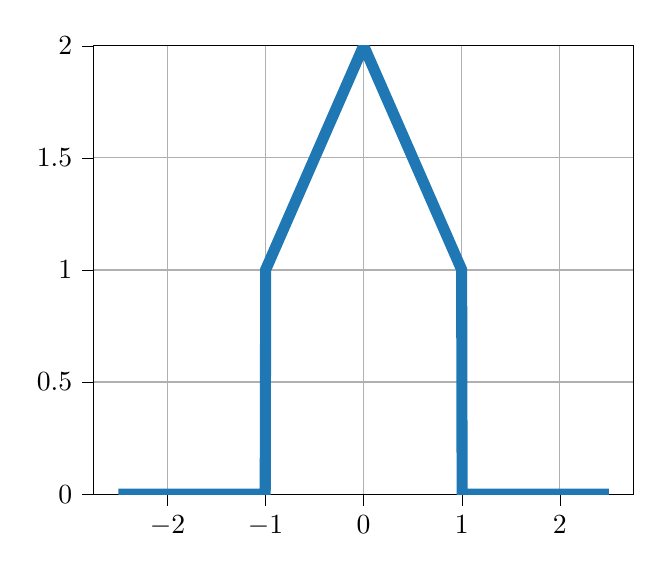
\begin{tikzpicture}

\definecolor{color0}{rgb}{0.12156862745098,0.466666666666667,0.705882352941177}

\begin{axis}[
tick align=outside,
tick pos=left,
x grid style={white!69.0196078431373!black},
xmajorgrids,
xmin=-2.75, xmax=2.75,
xtick style={color=black},
y grid style={white!69.0196078431373!black},
ymajorgrids,
ymin=0, ymax=2,
ytick style={color=black}
]
\addplot [line width=4pt, color0]
table {%
-2.5 0
-2.49499499499499 0
-2.48998998998999 0
-2.48498498498498 0
-2.47997997997998 0
-2.47497497497497 0
-2.46996996996997 0
-2.46496496496496 0
-2.45995995995996 0
-2.45495495495495 0
-2.44994994994995 0
-2.44494494494494 0
-2.43993993993994 0
-2.43493493493493 0
-2.42992992992993 0
-2.42492492492492 0
-2.41991991991992 0
-2.41491491491491 0
-2.40990990990991 0
-2.4049049049049 0
-2.3998998998999 0
-2.39489489489489 0
-2.38988988988989 0
-2.38488488488488 0
-2.37987987987988 0
-2.37487487487487 0
-2.36986986986987 0
-2.36486486486486 0
-2.35985985985986 0
-2.35485485485485 0
-2.34984984984985 0
-2.34484484484484 0
-2.33983983983984 0
-2.33483483483483 0
-2.32982982982983 0
-2.32482482482482 0
-2.31981981981982 0
-2.31481481481481 0
-2.30980980980981 0
-2.3048048048048 0
-2.2997997997998 0
-2.29479479479479 0
-2.28978978978979 0
-2.28478478478478 0
-2.27977977977978 0
-2.27477477477477 0
-2.26976976976977 0
-2.26476476476476 0
-2.25975975975976 0
-2.25475475475475 0
-2.24974974974975 0
-2.24474474474474 0
-2.23973973973974 0
-2.23473473473473 0
-2.22972972972973 0
-2.22472472472472 0
-2.21971971971972 0
-2.21471471471471 0
-2.20970970970971 0
-2.2047047047047 0
-2.1996996996997 0
-2.19469469469469 0
-2.18968968968969 0
-2.18468468468468 0
-2.17967967967968 0
-2.17467467467467 0
-2.16966966966967 0
-2.16466466466466 0
-2.15965965965966 0
-2.15465465465465 0
-2.14964964964965 0
-2.14464464464464 0
-2.13963963963964 0
-2.13463463463463 0
-2.12962962962963 0
-2.12462462462462 0
-2.11961961961962 0
-2.11461461461461 0
-2.10960960960961 0
-2.1046046046046 0
-2.0995995995996 0
-2.09459459459459 0
-2.08958958958959 0
-2.08458458458458 0
-2.07957957957958 0
-2.07457457457457 0
-2.06956956956957 0
-2.06456456456456 0
-2.05955955955956 0
-2.05455455455455 0
-2.04954954954955 0
-2.04454454454454 0
-2.03953953953954 0
-2.03453453453453 0
-2.02952952952953 0
-2.02452452452452 0
-2.01951951951952 0
-2.01451451451451 0
-2.00950950950951 0
-2.0045045045045 0
-1.9994994994995 0
-1.99449449449449 0
-1.98948948948949 0
-1.98448448448448 0
-1.97947947947948 0
-1.97447447447447 0
-1.96946946946947 0
-1.96446446446446 0
-1.95945945945946 0
-1.95445445445445 0
-1.94944944944945 0
-1.94444444444444 0
-1.93943943943944 0
-1.93443443443443 0
-1.92942942942943 0
-1.92442442442442 0
-1.91941941941942 0
-1.91441441441441 0
-1.90940940940941 0
-1.9044044044044 0
-1.8993993993994 0
-1.89439439439439 0
-1.88938938938939 0
-1.88438438438438 0
-1.87937937937938 0
-1.87437437437437 0
-1.86936936936937 0
-1.86436436436436 0
-1.85935935935936 0
-1.85435435435435 0
-1.84934934934935 0
-1.84434434434434 0
-1.83933933933934 0
-1.83433433433433 0
-1.82932932932933 0
-1.82432432432432 0
-1.81931931931932 0
-1.81431431431431 0
-1.80930930930931 0
-1.8043043043043 0
-1.7992992992993 0
-1.79429429429429 0
-1.78928928928929 0
-1.78428428428428 0
-1.77927927927928 0
-1.77427427427427 0
-1.76926926926927 0
-1.76426426426426 0
-1.75925925925926 0
-1.75425425425425 0
-1.74924924924925 0
-1.74424424424424 0
-1.73923923923924 0
-1.73423423423423 0
-1.72922922922923 0
-1.72422422422422 0
-1.71921921921922 0
-1.71421421421421 0
-1.70920920920921 0
-1.7042042042042 0
-1.6991991991992 0
-1.69419419419419 0
-1.68918918918919 0
-1.68418418418418 0
-1.67917917917918 0
-1.67417417417417 0
-1.66916916916917 0
-1.66416416416416 0
-1.65915915915916 0
-1.65415415415415 0
-1.64914914914915 0
-1.64414414414414 0
-1.63913913913914 0
-1.63413413413413 0
-1.62912912912913 0
-1.62412412412412 0
-1.61911911911912 0
-1.61411411411411 0
-1.60910910910911 0
-1.6041041041041 0
-1.5990990990991 0
-1.59409409409409 0
-1.58908908908909 0
-1.58408408408408 0
-1.57907907907908 0
-1.57407407407407 0
-1.56906906906907 0
-1.56406406406406 0
-1.55905905905906 0
-1.55405405405405 0
-1.54904904904905 0
-1.54404404404404 0
-1.53903903903904 0
-1.53403403403403 0
-1.52902902902903 0
-1.52402402402402 0
-1.51901901901902 0
-1.51401401401401 0
-1.50900900900901 0
-1.504004004004 0
-1.498998998999 0
-1.49399399399399 0
-1.48898898898899 0
-1.48398398398398 0
-1.47897897897898 0
-1.47397397397397 0
-1.46896896896897 0
-1.46396396396396 0
-1.45895895895896 0
-1.45395395395395 0
-1.44894894894895 0
-1.44394394394394 0
-1.43893893893894 0
-1.43393393393393 0
-1.42892892892893 0
-1.42392392392392 0
-1.41891891891892 0
-1.41391391391391 0
-1.40890890890891 0
-1.4039039039039 0
-1.3988988988989 0
-1.39389389389389 0
-1.38888888888889 0
-1.38388388388388 0
-1.37887887887888 0
-1.37387387387387 0
-1.36886886886887 0
-1.36386386386386 0
-1.35885885885886 0
-1.35385385385385 0
-1.34884884884885 0
-1.34384384384384 0
-1.33883883883884 0
-1.33383383383383 0
-1.32882882882883 0
-1.32382382382382 0
-1.31881881881882 0
-1.31381381381381 0
-1.30880880880881 0
-1.3038038038038 0
-1.2987987987988 0
-1.29379379379379 0
-1.28878878878879 0
-1.28378378378378 0
-1.27877877877878 0
-1.27377377377377 0
-1.26876876876877 0
-1.26376376376376 0
-1.25875875875876 0
-1.25375375375375 0
-1.24874874874875 0
-1.24374374374374 0
-1.23873873873874 0
-1.23373373373373 0
-1.22872872872873 0
-1.22372372372372 0
-1.21871871871872 0
-1.21371371371371 0
-1.20870870870871 0
-1.2037037037037 0
-1.1986986986987 0
-1.19369369369369 0
-1.18868868868869 0
-1.18368368368368 0
-1.17867867867868 0
-1.17367367367367 0
-1.16866866866867 0
-1.16366366366366 0
-1.15865865865866 0
-1.15365365365365 0
-1.14864864864865 0
-1.14364364364364 0
-1.13863863863864 0
-1.13363363363363 0
-1.12862862862863 0
-1.12362362362362 0
-1.11861861861862 0
-1.11361361361361 0
-1.10860860860861 0
-1.1036036036036 0
-1.0985985985986 0
-1.09359359359359 0
-1.08858858858859 0
-1.08358358358358 0
-1.07857857857858 0
-1.07357357357357 0
-1.06856856856857 0
-1.06356356356356 0
-1.05855855855856 0
-1.05355355355355 0
-1.04854854854855 0
-1.04354354354354 0
-1.03853853853854 0
-1.03353353353353 0
-1.02852852852853 0
-1.02352352352352 0
-1.01851851851852 0
-1.01351351351351 0
-1.00850850850851 0
-1.0035035035035 0
-0.998498498498499 1.0015015015015
-0.993493493493494 1.00650650650651
-0.988488488488489 1.01151151151151
-0.983483483483484 1.01651651651652
-0.978478478478479 1.02152152152152
-0.973473473473474 1.02652652652653
-0.968468468468469 1.03153153153153
-0.963463463463464 1.03653653653654
-0.958458458458459 1.04154154154154
-0.953453453453454 1.04654654654655
-0.948448448448449 1.05155155155155
-0.943443443443444 1.05655655655656
-0.938438438438439 1.06156156156156
-0.933433433433434 1.06656656656657
-0.928428428428429 1.07157157157157
-0.923423423423424 1.07657657657658
-0.918418418418419 1.08158158158158
-0.913413413413414 1.08658658658659
-0.908408408408409 1.09159159159159
-0.903403403403404 1.0965965965966
-0.898398398398399 1.1016016016016
-0.893393393393393 1.10660660660661
-0.888388388388388 1.11161161161161
-0.883383383383383 1.11661661661662
-0.878378378378378 1.12162162162162
-0.873373373373373 1.12662662662663
-0.868368368368368 1.13163163163163
-0.863363363363363 1.13663663663664
-0.858358358358358 1.14164164164164
-0.853353353353353 1.14664664664665
-0.848348348348348 1.15165165165165
-0.843343343343343 1.15665665665666
-0.838338338338338 1.16166166166166
-0.833333333333333 1.16666666666667
-0.828328328328328 1.17167167167167
-0.823323323323323 1.17667667667668
-0.818318318318318 1.18168168168168
-0.813313313313313 1.18668668668669
-0.808308308308308 1.19169169169169
-0.803303303303303 1.1966966966967
-0.798298298298298 1.2017017017017
-0.793293293293293 1.20670670670671
-0.788288288288288 1.21171171171171
-0.783283283283283 1.21671671671672
-0.778278278278278 1.22172172172172
-0.773273273273273 1.22672672672673
-0.768268268268268 1.23173173173173
-0.763263263263263 1.23673673673674
-0.758258258258258 1.24174174174174
-0.753253253253253 1.24674674674675
-0.748248248248248 1.25175175175175
-0.743243243243243 1.25675675675676
-0.738238238238238 1.26176176176176
-0.733233233233233 1.26676676676677
-0.728228228228228 1.27177177177177
-0.723223223223223 1.27677677677678
-0.718218218218218 1.28178178178178
-0.713213213213213 1.28678678678679
-0.708208208208208 1.29179179179179
-0.703203203203203 1.2967967967968
-0.698198198198198 1.3018018018018
-0.693193193193193 1.30680680680681
-0.688188188188188 1.31181181181181
-0.683183183183183 1.31681681681682
-0.678178178178178 1.32182182182182
-0.673173173173173 1.32682682682683
-0.668168168168168 1.33183183183183
-0.663163163163163 1.33683683683684
-0.658158158158158 1.34184184184184
-0.653153153153153 1.34684684684685
-0.648148148148148 1.35185185185185
-0.643143143143143 1.35685685685686
-0.638138138138138 1.36186186186186
-0.633133133133133 1.36686686686687
-0.628128128128128 1.37187187187187
-0.623123123123123 1.37687687687688
-0.618118118118118 1.38188188188188
-0.613113113113113 1.38688688688689
-0.608108108108108 1.39189189189189
-0.603103103103103 1.3968968968969
-0.598098098098098 1.4019019019019
-0.593093093093093 1.40690690690691
-0.588088088088088 1.41191191191191
-0.583083083083083 1.41691691691692
-0.578078078078078 1.42192192192192
-0.573073073073073 1.42692692692693
-0.568068068068068 1.43193193193193
-0.563063063063063 1.43693693693694
-0.558058058058058 1.44194194194194
-0.553053053053053 1.44694694694695
-0.548048048048048 1.45195195195195
-0.543043043043043 1.45695695695696
-0.538038038038038 1.46196196196196
-0.533033033033033 1.46696696696697
-0.528028028028028 1.47197197197197
-0.523023023023023 1.47697697697698
-0.518018018018018 1.48198198198198
-0.513013013013013 1.48698698698699
-0.508008008008008 1.49199199199199
-0.503003003003003 1.496996996997
-0.497997997997998 1.502002002002
-0.492992992992993 1.50700700700701
-0.487987987987988 1.51201201201201
-0.482982982982983 1.51701701701702
-0.477977977977978 1.52202202202202
-0.472972972972973 1.52702702702703
-0.467967967967968 1.53203203203203
-0.462962962962963 1.53703703703704
-0.457957957957958 1.54204204204204
-0.452952952952953 1.54704704704705
-0.447947947947948 1.55205205205205
-0.442942942942943 1.55705705705706
-0.437937937937938 1.56206206206206
-0.432932932932933 1.56706706706707
-0.427927927927928 1.57207207207207
-0.422922922922923 1.57707707707708
-0.417917917917918 1.58208208208208
-0.412912912912913 1.58708708708709
-0.407907907907908 1.59209209209209
-0.402902902902903 1.5970970970971
-0.397897897897898 1.6021021021021
-0.392892892892893 1.60710710710711
-0.387887887887888 1.61211211211211
-0.382882882882883 1.61711711711712
-0.377877877877878 1.62212212212212
-0.372872872872873 1.62712712712713
-0.367867867867868 1.63213213213213
-0.362862862862863 1.63713713713714
-0.357857857857858 1.64214214214214
-0.352852852852853 1.64714714714715
-0.347847847847848 1.65215215215215
-0.342842842842843 1.65715715715716
-0.337837837837838 1.66216216216216
-0.332832832832833 1.66716716716717
-0.327827827827828 1.67217217217217
-0.322822822822823 1.67717717717718
-0.317817817817818 1.68218218218218
-0.312812812812813 1.68718718718719
-0.307807807807808 1.69219219219219
-0.302802802802803 1.6971971971972
-0.297797797797798 1.7022022022022
-0.292792792792793 1.70720720720721
-0.287787787787788 1.71221221221221
-0.282782782782783 1.71721721721722
-0.277777777777778 1.72222222222222
-0.272772772772773 1.72722722722723
-0.267767767767768 1.73223223223223
-0.262762762762763 1.73723723723724
-0.257757757757758 1.74224224224224
-0.252752752752753 1.74724724724725
-0.247747747747748 1.75225225225225
-0.242742742742743 1.75725725725726
-0.237737737737738 1.76226226226226
-0.232732732732733 1.76726726726727
-0.227727727727728 1.77227227227227
-0.222722722722723 1.77727727727728
-0.217717717717718 1.78228228228228
-0.212712712712713 1.78728728728729
-0.207707707707708 1.79229229229229
-0.202702702702703 1.7972972972973
-0.197697697697698 1.8023023023023
-0.192692692692693 1.80730730730731
-0.187687687687688 1.81231231231231
-0.182682682682683 1.81731731731732
-0.177677677677678 1.82232232232232
-0.172672672672673 1.82732732732733
-0.167667667667668 1.83233233233233
-0.162662662662663 1.83733733733734
-0.157657657657658 1.84234234234234
-0.152652652652653 1.84734734734735
-0.147647647647648 1.85235235235235
-0.142642642642643 1.85735735735736
-0.137637637637638 1.86236236236236
-0.132632632632633 1.86736736736737
-0.127627627627628 1.87237237237237
-0.122622622622623 1.87737737737738
-0.117617617617618 1.88238238238238
-0.112612612612613 1.88738738738739
-0.107607607607608 1.89239239239239
-0.102602602602603 1.8973973973974
-0.0975975975975976 1.9024024024024
-0.0925925925925926 1.90740740740741
-0.0875875875875876 1.91241241241241
-0.0825825825825826 1.91741741741742
-0.0775775775775776 1.92242242242242
-0.0725725725725725 1.92742742742743
-0.0675675675675675 1.93243243243243
-0.0625625625625625 1.93743743743744
-0.0575575575575575 1.94244244244244
-0.0525525525525525 1.94744744744745
-0.0475475475475475 1.95245245245245
-0.0425425425425425 1.95745745745746
-0.0375375375375375 1.96246246246246
-0.0325325325325325 1.96746746746747
-0.0275275275275275 1.97247247247247
-0.0225225225225225 1.97747747747748
-0.0175175175175175 1.98248248248248
-0.0125125125125125 1.98748748748749
-0.0075075075075075 1.99249249249249
-0.0025025025025025 1.9974974974975
0.0025025025025025 1.9974974974975
0.0075075075075075 1.99249249249249
0.0125125125125125 1.98748748748749
0.0175175175175175 1.98248248248248
0.0225225225225225 1.97747747747748
0.0275275275275275 1.97247247247247
0.0325325325325325 1.96746746746747
0.0375375375375375 1.96246246246246
0.0425425425425425 1.95745745745746
0.0475475475475475 1.95245245245245
0.0525525525525525 1.94744744744745
0.0575575575575575 1.94244244244244
0.0625625625625625 1.93743743743744
0.0675675675675675 1.93243243243243
0.0725725725725725 1.92742742742743
0.0775775775775776 1.92242242242242
0.0825825825825826 1.91741741741742
0.0875875875875876 1.91241241241241
0.0925925925925926 1.90740740740741
0.0975975975975976 1.9024024024024
0.102602602602603 1.8973973973974
0.107607607607608 1.89239239239239
0.112612612612613 1.88738738738739
0.117617617617618 1.88238238238238
0.122622622622623 1.87737737737738
0.127627627627628 1.87237237237237
0.132632632632633 1.86736736736737
0.137637637637638 1.86236236236236
0.142642642642643 1.85735735735736
0.147647647647648 1.85235235235235
0.152652652652653 1.84734734734735
0.157657657657658 1.84234234234234
0.162662662662663 1.83733733733734
0.167667667667668 1.83233233233233
0.172672672672673 1.82732732732733
0.177677677677678 1.82232232232232
0.182682682682683 1.81731731731732
0.187687687687688 1.81231231231231
0.192692692692693 1.80730730730731
0.197697697697698 1.8023023023023
0.202702702702703 1.7972972972973
0.207707707707708 1.79229229229229
0.212712712712713 1.78728728728729
0.217717717717718 1.78228228228228
0.222722722722723 1.77727727727728
0.227727727727728 1.77227227227227
0.232732732732733 1.76726726726727
0.237737737737738 1.76226226226226
0.242742742742743 1.75725725725726
0.247747747747748 1.75225225225225
0.252752752752753 1.74724724724725
0.257757757757758 1.74224224224224
0.262762762762763 1.73723723723724
0.267767767767768 1.73223223223223
0.272772772772773 1.72722722722723
0.277777777777778 1.72222222222222
0.282782782782783 1.71721721721722
0.287787787787788 1.71221221221221
0.292792792792793 1.70720720720721
0.297797797797798 1.7022022022022
0.302802802802803 1.6971971971972
0.307807807807808 1.69219219219219
0.312812812812813 1.68718718718719
0.317817817817818 1.68218218218218
0.322822822822823 1.67717717717718
0.327827827827828 1.67217217217217
0.332832832832833 1.66716716716717
0.337837837837838 1.66216216216216
0.342842842842843 1.65715715715716
0.347847847847848 1.65215215215215
0.352852852852853 1.64714714714715
0.357857857857858 1.64214214214214
0.362862862862863 1.63713713713714
0.367867867867868 1.63213213213213
0.372872872872873 1.62712712712713
0.377877877877878 1.62212212212212
0.382882882882883 1.61711711711712
0.387887887887888 1.61211211211211
0.392892892892893 1.60710710710711
0.397897897897898 1.6021021021021
0.402902902902903 1.5970970970971
0.407907907907908 1.59209209209209
0.412912912912913 1.58708708708709
0.417917917917918 1.58208208208208
0.422922922922923 1.57707707707708
0.427927927927928 1.57207207207207
0.432932932932933 1.56706706706707
0.437937937937938 1.56206206206206
0.442942942942943 1.55705705705706
0.447947947947948 1.55205205205205
0.452952952952953 1.54704704704705
0.457957957957958 1.54204204204204
0.462962962962963 1.53703703703704
0.467967967967968 1.53203203203203
0.472972972972973 1.52702702702703
0.477977977977978 1.52202202202202
0.482982982982983 1.51701701701702
0.487987987987988 1.51201201201201
0.492992992992993 1.50700700700701
0.497997997997998 1.502002002002
0.503003003003003 1.496996996997
0.508008008008008 1.49199199199199
0.513013013013013 1.48698698698699
0.518018018018018 1.48198198198198
0.523023023023023 1.47697697697698
0.528028028028028 1.47197197197197
0.533033033033033 1.46696696696697
0.538038038038038 1.46196196196196
0.543043043043043 1.45695695695696
0.548048048048048 1.45195195195195
0.553053053053053 1.44694694694695
0.558058058058058 1.44194194194194
0.563063063063063 1.43693693693694
0.568068068068068 1.43193193193193
0.573073073073073 1.42692692692693
0.578078078078078 1.42192192192192
0.583083083083083 1.41691691691692
0.588088088088088 1.41191191191191
0.593093093093093 1.40690690690691
0.598098098098098 1.4019019019019
0.603103103103103 1.3968968968969
0.608108108108108 1.39189189189189
0.613113113113113 1.38688688688689
0.618118118118118 1.38188188188188
0.623123123123123 1.37687687687688
0.628128128128128 1.37187187187187
0.633133133133133 1.36686686686687
0.638138138138138 1.36186186186186
0.643143143143143 1.35685685685686
0.648148148148148 1.35185185185185
0.653153153153153 1.34684684684685
0.658158158158158 1.34184184184184
0.663163163163163 1.33683683683684
0.668168168168168 1.33183183183183
0.673173173173173 1.32682682682683
0.678178178178178 1.32182182182182
0.683183183183183 1.31681681681682
0.688188188188188 1.31181181181181
0.693193193193193 1.30680680680681
0.698198198198198 1.3018018018018
0.703203203203203 1.2967967967968
0.708208208208208 1.29179179179179
0.713213213213213 1.28678678678679
0.718218218218218 1.28178178178178
0.723223223223223 1.27677677677678
0.728228228228228 1.27177177177177
0.733233233233233 1.26676676676677
0.738238238238238 1.26176176176176
0.743243243243243 1.25675675675676
0.748248248248248 1.25175175175175
0.753253253253253 1.24674674674675
0.758258258258258 1.24174174174174
0.763263263263263 1.23673673673674
0.768268268268268 1.23173173173173
0.773273273273273 1.22672672672673
0.778278278278278 1.22172172172172
0.783283283283283 1.21671671671672
0.788288288288288 1.21171171171171
0.793293293293293 1.20670670670671
0.798298298298298 1.2017017017017
0.803303303303303 1.1966966966967
0.808308308308308 1.19169169169169
0.813313313313313 1.18668668668669
0.818318318318318 1.18168168168168
0.823323323323323 1.17667667667668
0.828328328328328 1.17167167167167
0.833333333333333 1.16666666666667
0.838338338338338 1.16166166166166
0.843343343343343 1.15665665665666
0.848348348348348 1.15165165165165
0.853353353353353 1.14664664664665
0.858358358358358 1.14164164164164
0.863363363363364 1.13663663663664
0.868368368368369 1.13163163163163
0.873373373373374 1.12662662662663
0.878378378378379 1.12162162162162
0.883383383383384 1.11661661661662
0.888388388388389 1.11161161161161
0.893393393393394 1.10660660660661
0.898398398398399 1.1016016016016
0.903403403403404 1.0965965965966
0.908408408408409 1.09159159159159
0.913413413413414 1.08658658658659
0.918418418418419 1.08158158158158
0.923423423423424 1.07657657657658
0.928428428428429 1.07157157157157
0.933433433433434 1.06656656656657
0.938438438438439 1.06156156156156
0.943443443443444 1.05655655655656
0.948448448448449 1.05155155155155
0.953453453453454 1.04654654654655
0.958458458458459 1.04154154154154
0.963463463463464 1.03653653653654
0.968468468468469 1.03153153153153
0.973473473473474 1.02652652652653
0.978478478478479 1.02152152152152
0.983483483483484 1.01651651651652
0.988488488488489 1.01151151151151
0.993493493493494 1.00650650650651
0.998498498498499 1.0015015015015
1.0035035035035 0
1.00850850850851 0
1.01351351351351 0
1.01851851851852 0
1.02352352352352 0
1.02852852852853 0
1.03353353353353 0
1.03853853853854 0
1.04354354354354 0
1.04854854854855 0
1.05355355355355 0
1.05855855855856 0
1.06356356356356 0
1.06856856856857 0
1.07357357357357 0
1.07857857857858 0
1.08358358358358 0
1.08858858858859 0
1.09359359359359 0
1.0985985985986 0
1.1036036036036 0
1.10860860860861 0
1.11361361361361 0
1.11861861861862 0
1.12362362362362 0
1.12862862862863 0
1.13363363363363 0
1.13863863863864 0
1.14364364364364 0
1.14864864864865 0
1.15365365365365 0
1.15865865865866 0
1.16366366366366 0
1.16866866866867 0
1.17367367367367 0
1.17867867867868 0
1.18368368368368 0
1.18868868868869 0
1.19369369369369 0
1.1986986986987 0
1.2037037037037 0
1.20870870870871 0
1.21371371371371 0
1.21871871871872 0
1.22372372372372 0
1.22872872872873 0
1.23373373373373 0
1.23873873873874 0
1.24374374374374 0
1.24874874874875 0
1.25375375375375 0
1.25875875875876 0
1.26376376376376 0
1.26876876876877 0
1.27377377377377 0
1.27877877877878 0
1.28378378378378 0
1.28878878878879 0
1.29379379379379 0
1.2987987987988 0
1.3038038038038 0
1.30880880880881 0
1.31381381381381 0
1.31881881881882 0
1.32382382382382 0
1.32882882882883 0
1.33383383383383 0
1.33883883883884 0
1.34384384384384 0
1.34884884884885 0
1.35385385385385 0
1.35885885885886 0
1.36386386386386 0
1.36886886886887 0
1.37387387387387 0
1.37887887887888 0
1.38388388388388 0
1.38888888888889 0
1.39389389389389 0
1.3988988988989 0
1.4039039039039 0
1.40890890890891 0
1.41391391391391 0
1.41891891891892 0
1.42392392392392 0
1.42892892892893 0
1.43393393393393 0
1.43893893893894 0
1.44394394394394 0
1.44894894894895 0
1.45395395395395 0
1.45895895895896 0
1.46396396396396 0
1.46896896896897 0
1.47397397397397 0
1.47897897897898 0
1.48398398398398 0
1.48898898898899 0
1.49399399399399 0
1.498998998999 0
1.504004004004 0
1.50900900900901 0
1.51401401401401 0
1.51901901901902 0
1.52402402402402 0
1.52902902902903 0
1.53403403403403 0
1.53903903903904 0
1.54404404404404 0
1.54904904904905 0
1.55405405405405 0
1.55905905905906 0
1.56406406406406 0
1.56906906906907 0
1.57407407407407 0
1.57907907907908 0
1.58408408408408 0
1.58908908908909 0
1.59409409409409 0
1.5990990990991 0
1.6041041041041 0
1.60910910910911 0
1.61411411411411 0
1.61911911911912 0
1.62412412412412 0
1.62912912912913 0
1.63413413413413 0
1.63913913913914 0
1.64414414414414 0
1.64914914914915 0
1.65415415415415 0
1.65915915915916 0
1.66416416416416 0
1.66916916916917 0
1.67417417417417 0
1.67917917917918 0
1.68418418418418 0
1.68918918918919 0
1.69419419419419 0
1.6991991991992 0
1.7042042042042 0
1.70920920920921 0
1.71421421421421 0
1.71921921921922 0
1.72422422422422 0
1.72922922922923 0
1.73423423423423 0
1.73923923923924 0
1.74424424424424 0
1.74924924924925 0
1.75425425425425 0
1.75925925925926 0
1.76426426426426 0
1.76926926926927 0
1.77427427427427 0
1.77927927927928 0
1.78428428428428 0
1.78928928928929 0
1.79429429429429 0
1.7992992992993 0
1.8043043043043 0
1.80930930930931 0
1.81431431431431 0
1.81931931931932 0
1.82432432432432 0
1.82932932932933 0
1.83433433433433 0
1.83933933933934 0
1.84434434434434 0
1.84934934934935 0
1.85435435435435 0
1.85935935935936 0
1.86436436436436 0
1.86936936936937 0
1.87437437437437 0
1.87937937937938 0
1.88438438438438 0
1.88938938938939 0
1.89439439439439 0
1.8993993993994 0
1.9044044044044 0
1.90940940940941 0
1.91441441441441 0
1.91941941941942 0
1.92442442442442 0
1.92942942942943 0
1.93443443443443 0
1.93943943943944 0
1.94444444444444 0
1.94944944944945 0
1.95445445445445 0
1.95945945945946 0
1.96446446446446 0
1.96946946946947 0
1.97447447447447 0
1.97947947947948 0
1.98448448448448 0
1.98948948948949 0
1.99449449449449 0
1.9994994994995 0
2.0045045045045 0
2.00950950950951 0
2.01451451451451 0
2.01951951951952 0
2.02452452452452 0
2.02952952952953 0
2.03453453453453 0
2.03953953953954 0
2.04454454454454 0
2.04954954954955 0
2.05455455455455 0
2.05955955955956 0
2.06456456456456 0
2.06956956956957 0
2.07457457457457 0
2.07957957957958 0
2.08458458458458 0
2.08958958958959 0
2.09459459459459 0
2.0995995995996 0
2.1046046046046 0
2.10960960960961 0
2.11461461461461 0
2.11961961961962 0
2.12462462462462 0
2.12962962962963 0
2.13463463463463 0
2.13963963963964 0
2.14464464464464 0
2.14964964964965 0
2.15465465465465 0
2.15965965965966 0
2.16466466466466 0
2.16966966966967 0
2.17467467467467 0
2.17967967967968 0
2.18468468468468 0
2.18968968968969 0
2.19469469469469 0
2.1996996996997 0
2.2047047047047 0
2.20970970970971 0
2.21471471471471 0
2.21971971971972 0
2.22472472472472 0
2.22972972972973 0
2.23473473473473 0
2.23973973973974 0
2.24474474474474 0
2.24974974974975 0
2.25475475475475 0
2.25975975975976 0
2.26476476476476 0
2.26976976976977 0
2.27477477477477 0
2.27977977977978 0
2.28478478478478 0
2.28978978978979 0
2.29479479479479 0
2.2997997997998 0
2.3048048048048 0
2.30980980980981 0
2.31481481481481 0
2.31981981981982 0
2.32482482482482 0
2.32982982982983 0
2.33483483483483 0
2.33983983983984 0
2.34484484484484 0
2.34984984984985 0
2.35485485485485 0
2.35985985985986 0
2.36486486486486 0
2.36986986986987 0
2.37487487487487 0
2.37987987987988 0
2.38488488488488 0
2.38988988988989 0
2.39489489489489 0
2.3998998998999 0
2.4049049049049 0
2.40990990990991 0
2.41491491491491 0
2.41991991991992 0
2.42492492492492 0
2.42992992992993 0
2.43493493493493 0
2.43993993993994 0
2.44494494494494 0
2.44994994994995 0
2.45495495495495 0
2.45995995995996 0
2.46496496496496 0
2.46996996996997 0
2.47497497497497 0
2.47997997997998 0
2.48498498498498 0
2.48998998998999 0
2.49499499499499 0
2.5 0
};
\end{axis}

\end{tikzpicture}
}

                    $\quad{}f(t) + h(t)$
                \end{column}
            \end{columns}}{%
            \begin{columns}[t, onlytextwidth]
                \begin{column}{0.33\textwidth}
                    \centering{}
                    \scalebox{0.4}{% This file was created by tikzplotlib v0.9.1.
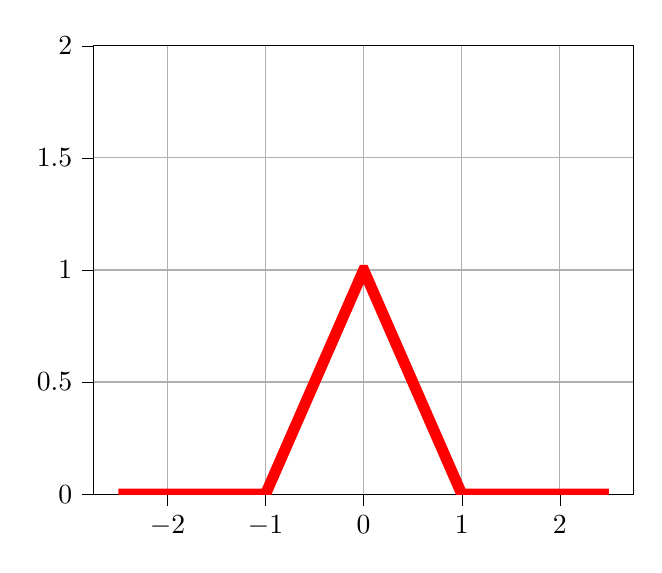
\begin{tikzpicture}

\begin{axis}[
tick align=outside,
tick pos=left,
x grid style={white!69.0196078431373!black},
xmajorgrids,
xmin=-2.75, xmax=2.75,
xtick style={color=black},
y grid style={white!69.0196078431373!black},
ymajorgrids,
ymin=0, ymax=2,
ytick style={color=black}
]
\addplot [line width=4pt, red]
table {%
-2.5 -0
-2.49499499499499 -0
-2.48998998998999 -0
-2.48498498498498 -0
-2.47997997997998 -0
-2.47497497497497 -0
-2.46996996996997 -0
-2.46496496496496 -0
-2.45995995995996 -0
-2.45495495495495 -0
-2.44994994994995 -0
-2.44494494494494 -0
-2.43993993993994 -0
-2.43493493493493 -0
-2.42992992992993 -0
-2.42492492492492 -0
-2.41991991991992 -0
-2.41491491491491 -0
-2.40990990990991 -0
-2.4049049049049 -0
-2.3998998998999 -0
-2.39489489489489 -0
-2.38988988988989 -0
-2.38488488488488 -0
-2.37987987987988 -0
-2.37487487487487 -0
-2.36986986986987 -0
-2.36486486486486 -0
-2.35985985985986 -0
-2.35485485485485 -0
-2.34984984984985 -0
-2.34484484484484 -0
-2.33983983983984 -0
-2.33483483483483 -0
-2.32982982982983 -0
-2.32482482482482 -0
-2.31981981981982 -0
-2.31481481481481 -0
-2.30980980980981 -0
-2.3048048048048 -0
-2.2997997997998 -0
-2.29479479479479 -0
-2.28978978978979 -0
-2.28478478478478 -0
-2.27977977977978 -0
-2.27477477477477 -0
-2.26976976976977 -0
-2.26476476476476 -0
-2.25975975975976 -0
-2.25475475475475 -0
-2.24974974974975 -0
-2.24474474474474 -0
-2.23973973973974 -0
-2.23473473473473 -0
-2.22972972972973 -0
-2.22472472472472 -0
-2.21971971971972 -0
-2.21471471471471 -0
-2.20970970970971 -0
-2.2047047047047 -0
-2.1996996996997 -0
-2.19469469469469 -0
-2.18968968968969 -0
-2.18468468468468 -0
-2.17967967967968 -0
-2.17467467467467 -0
-2.16966966966967 -0
-2.16466466466466 -0
-2.15965965965966 -0
-2.15465465465465 -0
-2.14964964964965 -0
-2.14464464464464 -0
-2.13963963963964 -0
-2.13463463463463 -0
-2.12962962962963 -0
-2.12462462462462 -0
-2.11961961961962 -0
-2.11461461461461 -0
-2.10960960960961 -0
-2.1046046046046 -0
-2.0995995995996 -0
-2.09459459459459 -0
-2.08958958958959 -0
-2.08458458458458 -0
-2.07957957957958 -0
-2.07457457457457 -0
-2.06956956956957 -0
-2.06456456456456 -0
-2.05955955955956 -0
-2.05455455455455 -0
-2.04954954954955 -0
-2.04454454454454 -0
-2.03953953953954 -0
-2.03453453453453 -0
-2.02952952952953 -0
-2.02452452452452 -0
-2.01951951951952 -0
-2.01451451451451 -0
-2.00950950950951 -0
-2.0045045045045 -0
-1.9994994994995 -0
-1.99449449449449 -0
-1.98948948948949 -0
-1.98448448448448 -0
-1.97947947947948 -0
-1.97447447447447 -0
-1.96946946946947 -0
-1.96446446446446 -0
-1.95945945945946 -0
-1.95445445445445 -0
-1.94944944944945 -0
-1.94444444444444 -0
-1.93943943943944 -0
-1.93443443443443 -0
-1.92942942942943 -0
-1.92442442442442 -0
-1.91941941941942 -0
-1.91441441441441 -0
-1.90940940940941 -0
-1.9044044044044 -0
-1.8993993993994 -0
-1.89439439439439 -0
-1.88938938938939 -0
-1.88438438438438 -0
-1.87937937937938 -0
-1.87437437437437 -0
-1.86936936936937 -0
-1.86436436436436 -0
-1.85935935935936 -0
-1.85435435435435 -0
-1.84934934934935 -0
-1.84434434434434 -0
-1.83933933933934 -0
-1.83433433433433 -0
-1.82932932932933 -0
-1.82432432432432 -0
-1.81931931931932 -0
-1.81431431431431 -0
-1.80930930930931 -0
-1.8043043043043 -0
-1.7992992992993 -0
-1.79429429429429 -0
-1.78928928928929 -0
-1.78428428428428 -0
-1.77927927927928 -0
-1.77427427427427 -0
-1.76926926926927 -0
-1.76426426426426 -0
-1.75925925925926 -0
-1.75425425425425 -0
-1.74924924924925 -0
-1.74424424424424 -0
-1.73923923923924 -0
-1.73423423423423 -0
-1.72922922922923 -0
-1.72422422422422 -0
-1.71921921921922 -0
-1.71421421421421 -0
-1.70920920920921 -0
-1.7042042042042 -0
-1.6991991991992 -0
-1.69419419419419 -0
-1.68918918918919 -0
-1.68418418418418 -0
-1.67917917917918 -0
-1.67417417417417 -0
-1.66916916916917 -0
-1.66416416416416 -0
-1.65915915915916 -0
-1.65415415415415 -0
-1.64914914914915 -0
-1.64414414414414 -0
-1.63913913913914 -0
-1.63413413413413 -0
-1.62912912912913 -0
-1.62412412412412 -0
-1.61911911911912 -0
-1.61411411411411 -0
-1.60910910910911 -0
-1.6041041041041 -0
-1.5990990990991 -0
-1.59409409409409 -0
-1.58908908908909 -0
-1.58408408408408 -0
-1.57907907907908 -0
-1.57407407407407 -0
-1.56906906906907 -0
-1.56406406406406 -0
-1.55905905905906 -0
-1.55405405405405 -0
-1.54904904904905 -0
-1.54404404404404 -0
-1.53903903903904 -0
-1.53403403403403 -0
-1.52902902902903 -0
-1.52402402402402 -0
-1.51901901901902 -0
-1.51401401401401 -0
-1.50900900900901 -0
-1.504004004004 -0
-1.498998998999 -0
-1.49399399399399 -0
-1.48898898898899 -0
-1.48398398398398 -0
-1.47897897897898 -0
-1.47397397397397 -0
-1.46896896896897 -0
-1.46396396396396 -0
-1.45895895895896 -0
-1.45395395395395 -0
-1.44894894894895 -0
-1.44394394394394 -0
-1.43893893893894 -0
-1.43393393393393 -0
-1.42892892892893 -0
-1.42392392392392 -0
-1.41891891891892 -0
-1.41391391391391 -0
-1.40890890890891 -0
-1.4039039039039 -0
-1.3988988988989 -0
-1.39389389389389 -0
-1.38888888888889 -0
-1.38388388388388 -0
-1.37887887887888 -0
-1.37387387387387 -0
-1.36886886886887 -0
-1.36386386386386 -0
-1.35885885885886 -0
-1.35385385385385 -0
-1.34884884884885 -0
-1.34384384384384 -0
-1.33883883883884 -0
-1.33383383383383 -0
-1.32882882882883 -0
-1.32382382382382 -0
-1.31881881881882 -0
-1.31381381381381 -0
-1.30880880880881 -0
-1.3038038038038 -0
-1.2987987987988 -0
-1.29379379379379 -0
-1.28878878878879 -0
-1.28378378378378 -0
-1.27877877877878 -0
-1.27377377377377 -0
-1.26876876876877 -0
-1.26376376376376 -0
-1.25875875875876 -0
-1.25375375375375 -0
-1.24874874874875 -0
-1.24374374374374 -0
-1.23873873873874 -0
-1.23373373373373 -0
-1.22872872872873 -0
-1.22372372372372 -0
-1.21871871871872 -0
-1.21371371371371 -0
-1.20870870870871 -0
-1.2037037037037 -0
-1.1986986986987 -0
-1.19369369369369 -0
-1.18868868868869 -0
-1.18368368368368 -0
-1.17867867867868 -0
-1.17367367367367 -0
-1.16866866866867 -0
-1.16366366366366 -0
-1.15865865865866 -0
-1.15365365365365 -0
-1.14864864864865 -0
-1.14364364364364 -0
-1.13863863863864 -0
-1.13363363363363 -0
-1.12862862862863 -0
-1.12362362362362 -0
-1.11861861861862 -0
-1.11361361361361 -0
-1.10860860860861 -0
-1.1036036036036 -0
-1.0985985985986 -0
-1.09359359359359 -0
-1.08858858858859 -0
-1.08358358358358 -0
-1.07857857857858 -0
-1.07357357357357 -0
-1.06856856856857 -0
-1.06356356356356 -0
-1.05855855855856 -0
-1.05355355355355 -0
-1.04854854854855 -0
-1.04354354354354 -0
-1.03853853853854 -0
-1.03353353353353 -0
-1.02852852852853 -0
-1.02352352352352 -0
-1.01851851851852 -0
-1.01351351351351 -0
-1.00850850850851 -0
-1.0035035035035 -0
-0.998498498498499 0.00150150150150141
-0.993493493493494 0.00650650650650642
-0.988488488488489 0.0115115115115114
-0.983483483483484 0.0165165165165164
-0.978478478478479 0.0215215215215214
-0.973473473473474 0.0265265265265264
-0.968468468468469 0.0315315315315314
-0.963463463463464 0.0365365365365364
-0.958458458458459 0.0415415415415414
-0.953453453453454 0.0465465465465464
-0.948448448448449 0.0515515515515514
-0.943443443443444 0.0565565565565564
-0.938438438438439 0.0615615615615615
-0.933433433433434 0.0665665665665665
-0.928428428428429 0.0715715715715715
-0.923423423423424 0.0765765765765765
-0.918418418418419 0.0815815815815815
-0.913413413413414 0.0865865865865865
-0.908408408408409 0.0915915915915915
-0.903403403403404 0.0965965965965965
-0.898398398398399 0.101601601601601
-0.893393393393393 0.106606606606607
-0.888388388388388 0.111611611611612
-0.883383383383383 0.116616616616617
-0.878378378378378 0.121621621621622
-0.873373373373373 0.126626626626627
-0.868368368368368 0.131631631631632
-0.863363363363363 0.136636636636637
-0.858358358358358 0.141641641641642
-0.853353353353353 0.146646646646647
-0.848348348348348 0.151651651651652
-0.843343343343343 0.156656656656657
-0.838338338338338 0.161661661661662
-0.833333333333333 0.166666666666667
-0.828328328328328 0.171671671671672
-0.823323323323323 0.176676676676677
-0.818318318318318 0.181681681681682
-0.813313313313313 0.186686686686687
-0.808308308308308 0.191691691691692
-0.803303303303303 0.196696696696697
-0.798298298298298 0.201701701701702
-0.793293293293293 0.206706706706707
-0.788288288288288 0.211711711711712
-0.783283283283283 0.216716716716717
-0.778278278278278 0.221721721721722
-0.773273273273273 0.226726726726727
-0.768268268268268 0.231731731731732
-0.763263263263263 0.236736736736737
-0.758258258258258 0.241741741741742
-0.753253253253253 0.246746746746747
-0.748248248248248 0.251751751751752
-0.743243243243243 0.256756756756757
-0.738238238238238 0.261761761761762
-0.733233233233233 0.266766766766767
-0.728228228228228 0.271771771771772
-0.723223223223223 0.276776776776777
-0.718218218218218 0.281781781781782
-0.713213213213213 0.286786786786787
-0.708208208208208 0.291791791791792
-0.703203203203203 0.296796796796797
-0.698198198198198 0.301801801801802
-0.693193193193193 0.306806806806807
-0.688188188188188 0.311811811811812
-0.683183183183183 0.316816816816817
-0.678178178178178 0.321821821821822
-0.673173173173173 0.326826826826827
-0.668168168168168 0.331831831831832
-0.663163163163163 0.336836836836837
-0.658158158158158 0.341841841841842
-0.653153153153153 0.346846846846847
-0.648148148148148 0.351851851851852
-0.643143143143143 0.356856856856857
-0.638138138138138 0.361861861861862
-0.633133133133133 0.366866866866867
-0.628128128128128 0.371871871871872
-0.623123123123123 0.376876876876877
-0.618118118118118 0.381881881881882
-0.613113113113113 0.386886886886887
-0.608108108108108 0.391891891891892
-0.603103103103103 0.396896896896897
-0.598098098098098 0.401901901901902
-0.593093093093093 0.406906906906907
-0.588088088088088 0.411911911911912
-0.583083083083083 0.416916916916917
-0.578078078078078 0.421921921921922
-0.573073073073073 0.426926926926927
-0.568068068068068 0.431931931931932
-0.563063063063063 0.436936936936937
-0.558058058058058 0.441941941941942
-0.553053053053053 0.446946946946947
-0.548048048048048 0.451951951951952
-0.543043043043043 0.456956956956957
-0.538038038038038 0.461961961961962
-0.533033033033033 0.466966966966967
-0.528028028028028 0.471971971971972
-0.523023023023023 0.476976976976977
-0.518018018018018 0.481981981981982
-0.513013013013013 0.486986986986987
-0.508008008008008 0.491991991991992
-0.503003003003003 0.496996996996997
-0.497997997997998 0.502002002002002
-0.492992992992993 0.507007007007007
-0.487987987987988 0.512012012012012
-0.482982982982983 0.517017017017017
-0.477977977977978 0.522022022022022
-0.472972972972973 0.527027027027027
-0.467967967967968 0.532032032032032
-0.462962962962963 0.537037037037037
-0.457957957957958 0.542042042042042
-0.452952952952953 0.547047047047047
-0.447947947947948 0.552052052052052
-0.442942942942943 0.557057057057057
-0.437937937937938 0.562062062062062
-0.432932932932933 0.567067067067067
-0.427927927927928 0.572072072072072
-0.422922922922923 0.577077077077077
-0.417917917917918 0.582082082082082
-0.412912912912913 0.587087087087087
-0.407907907907908 0.592092092092092
-0.402902902902903 0.597097097097097
-0.397897897897898 0.602102102102102
-0.392892892892893 0.607107107107107
-0.387887887887888 0.612112112112112
-0.382882882882883 0.617117117117117
-0.377877877877878 0.622122122122122
-0.372872872872873 0.627127127127127
-0.367867867867868 0.632132132132132
-0.362862862862863 0.637137137137137
-0.357857857857858 0.642142142142142
-0.352852852852853 0.647147147147147
-0.347847847847848 0.652152152152152
-0.342842842842843 0.657157157157157
-0.337837837837838 0.662162162162162
-0.332832832832833 0.667167167167167
-0.327827827827828 0.672172172172172
-0.322822822822823 0.677177177177177
-0.317817817817818 0.682182182182182
-0.312812812812813 0.687187187187187
-0.307807807807808 0.692192192192192
-0.302802802802803 0.697197197197197
-0.297797797797798 0.702202202202202
-0.292792792792793 0.707207207207207
-0.287787787787788 0.712212212212212
-0.282782782782783 0.717217217217217
-0.277777777777778 0.722222222222222
-0.272772772772773 0.727227227227227
-0.267767767767768 0.732232232232232
-0.262762762762763 0.737237237237237
-0.257757757757758 0.742242242242242
-0.252752752752753 0.747247247247247
-0.247747747747748 0.752252252252252
-0.242742742742743 0.757257257257257
-0.237737737737738 0.762262262262262
-0.232732732732733 0.767267267267267
-0.227727727727728 0.772272272272272
-0.222722722722723 0.777277277277277
-0.217717717717718 0.782282282282282
-0.212712712712713 0.787287287287287
-0.207707707707708 0.792292292292292
-0.202702702702703 0.797297297297297
-0.197697697697698 0.802302302302302
-0.192692692692693 0.807307307307307
-0.187687687687688 0.812312312312312
-0.182682682682683 0.817317317317317
-0.177677677677678 0.822322322322322
-0.172672672672673 0.827327327327327
-0.167667667667668 0.832332332332332
-0.162662662662663 0.837337337337337
-0.157657657657658 0.842342342342342
-0.152652652652653 0.847347347347347
-0.147647647647648 0.852352352352352
-0.142642642642643 0.857357357357357
-0.137637637637638 0.862362362362362
-0.132632632632633 0.867367367367367
-0.127627627627628 0.872372372372372
-0.122622622622623 0.877377377377377
-0.117617617617618 0.882382382382382
-0.112612612612613 0.887387387387387
-0.107607607607608 0.892392392392392
-0.102602602602603 0.897397397397397
-0.0975975975975976 0.902402402402402
-0.0925925925925926 0.907407407407407
-0.0875875875875876 0.912412412412412
-0.0825825825825826 0.917417417417417
-0.0775775775775776 0.922422422422422
-0.0725725725725725 0.927427427427427
-0.0675675675675675 0.932432432432432
-0.0625625625625625 0.937437437437437
-0.0575575575575575 0.942442442442442
-0.0525525525525525 0.947447447447447
-0.0475475475475475 0.952452452452452
-0.0425425425425425 0.957457457457457
-0.0375375375375375 0.962462462462462
-0.0325325325325325 0.967467467467467
-0.0275275275275275 0.972472472472472
-0.0225225225225225 0.977477477477477
-0.0175175175175175 0.982482482482482
-0.0125125125125125 0.987487487487487
-0.0075075075075075 0.992492492492492
-0.0025025025025025 0.997497497497497
0.0025025025025025 0.997497497497497
0.0075075075075075 0.992492492492492
0.0125125125125125 0.987487487487487
0.0175175175175175 0.982482482482482
0.0225225225225225 0.977477477477477
0.0275275275275275 0.972472472472472
0.0325325325325325 0.967467467467467
0.0375375375375375 0.962462462462462
0.0425425425425425 0.957457457457457
0.0475475475475475 0.952452452452452
0.0525525525525525 0.947447447447447
0.0575575575575575 0.942442442442442
0.0625625625625625 0.937437437437437
0.0675675675675675 0.932432432432432
0.0725725725725725 0.927427427427427
0.0775775775775776 0.922422422422422
0.0825825825825826 0.917417417417417
0.0875875875875876 0.912412412412412
0.0925925925925926 0.907407407407407
0.0975975975975976 0.902402402402402
0.102602602602603 0.897397397397397
0.107607607607608 0.892392392392392
0.112612612612613 0.887387387387387
0.117617617617618 0.882382382382382
0.122622622622623 0.877377377377377
0.127627627627628 0.872372372372372
0.132632632632633 0.867367367367367
0.137637637637638 0.862362362362362
0.142642642642643 0.857357357357357
0.147647647647648 0.852352352352352
0.152652652652653 0.847347347347347
0.157657657657658 0.842342342342342
0.162662662662663 0.837337337337337
0.167667667667668 0.832332332332332
0.172672672672673 0.827327327327327
0.177677677677678 0.822322322322322
0.182682682682683 0.817317317317317
0.187687687687688 0.812312312312312
0.192692692692693 0.807307307307307
0.197697697697698 0.802302302302302
0.202702702702703 0.797297297297297
0.207707707707708 0.792292292292292
0.212712712712713 0.787287287287287
0.217717717717718 0.782282282282282
0.222722722722723 0.777277277277277
0.227727727727728 0.772272272272272
0.232732732732733 0.767267267267267
0.237737737737738 0.762262262262262
0.242742742742743 0.757257257257257
0.247747747747748 0.752252252252252
0.252752752752753 0.747247247247247
0.257757757757758 0.742242242242242
0.262762762762763 0.737237237237237
0.267767767767768 0.732232232232232
0.272772772772773 0.727227227227227
0.277777777777778 0.722222222222222
0.282782782782783 0.717217217217217
0.287787787787788 0.712212212212212
0.292792792792793 0.707207207207207
0.297797797797798 0.702202202202202
0.302802802802803 0.697197197197197
0.307807807807808 0.692192192192192
0.312812812812813 0.687187187187187
0.317817817817818 0.682182182182182
0.322822822822823 0.677177177177177
0.327827827827828 0.672172172172172
0.332832832832833 0.667167167167167
0.337837837837838 0.662162162162162
0.342842842842843 0.657157157157157
0.347847847847848 0.652152152152152
0.352852852852853 0.647147147147147
0.357857857857858 0.642142142142142
0.362862862862863 0.637137137137137
0.367867867867868 0.632132132132132
0.372872872872873 0.627127127127127
0.377877877877878 0.622122122122122
0.382882882882883 0.617117117117117
0.387887887887888 0.612112112112112
0.392892892892893 0.607107107107107
0.397897897897898 0.602102102102102
0.402902902902903 0.597097097097097
0.407907907907908 0.592092092092092
0.412912912912913 0.587087087087087
0.417917917917918 0.582082082082082
0.422922922922923 0.577077077077077
0.427927927927928 0.572072072072072
0.432932932932933 0.567067067067067
0.437937937937938 0.562062062062062
0.442942942942943 0.557057057057057
0.447947947947948 0.552052052052052
0.452952952952953 0.547047047047047
0.457957957957958 0.542042042042042
0.462962962962963 0.537037037037037
0.467967967967968 0.532032032032032
0.472972972972973 0.527027027027027
0.477977977977978 0.522022022022022
0.482982982982983 0.517017017017017
0.487987987987988 0.512012012012012
0.492992992992993 0.507007007007007
0.497997997997998 0.502002002002002
0.503003003003003 0.496996996996997
0.508008008008008 0.491991991991992
0.513013013013013 0.486986986986987
0.518018018018018 0.481981981981982
0.523023023023023 0.476976976976977
0.528028028028028 0.471971971971972
0.533033033033033 0.466966966966967
0.538038038038038 0.461961961961962
0.543043043043043 0.456956956956957
0.548048048048048 0.451951951951952
0.553053053053053 0.446946946946947
0.558058058058058 0.441941941941942
0.563063063063063 0.436936936936937
0.568068068068068 0.431931931931932
0.573073073073073 0.426926926926927
0.578078078078078 0.421921921921922
0.583083083083083 0.416916916916917
0.588088088088088 0.411911911911912
0.593093093093093 0.406906906906907
0.598098098098098 0.401901901901902
0.603103103103103 0.396896896896897
0.608108108108108 0.391891891891892
0.613113113113113 0.386886886886887
0.618118118118118 0.381881881881882
0.623123123123123 0.376876876876877
0.628128128128128 0.371871871871872
0.633133133133133 0.366866866866867
0.638138138138138 0.361861861861862
0.643143143143143 0.356856856856857
0.648148148148148 0.351851851851852
0.653153153153153 0.346846846846847
0.658158158158158 0.341841841841842
0.663163163163163 0.336836836836837
0.668168168168168 0.331831831831832
0.673173173173173 0.326826826826827
0.678178178178178 0.321821821821822
0.683183183183183 0.316816816816817
0.688188188188188 0.311811811811812
0.693193193193193 0.306806806806807
0.698198198198198 0.301801801801802
0.703203203203203 0.296796796796797
0.708208208208208 0.291791791791792
0.713213213213213 0.286786786786787
0.718218218218218 0.281781781781782
0.723223223223223 0.276776776776777
0.728228228228228 0.271771771771772
0.733233233233233 0.266766766766767
0.738238238238238 0.261761761761762
0.743243243243243 0.256756756756757
0.748248248248248 0.251751751751752
0.753253253253253 0.246746746746747
0.758258258258258 0.241741741741742
0.763263263263263 0.236736736736737
0.768268268268268 0.231731731731732
0.773273273273273 0.226726726726727
0.778278278278278 0.221721721721722
0.783283283283283 0.216716716716717
0.788288288288288 0.211711711711712
0.793293293293293 0.206706706706707
0.798298298298298 0.201701701701702
0.803303303303303 0.196696696696697
0.808308308308308 0.191691691691692
0.813313313313313 0.186686686686687
0.818318318318318 0.181681681681682
0.823323323323323 0.176676676676677
0.828328328328328 0.171671671671672
0.833333333333333 0.166666666666667
0.838338338338338 0.161661661661662
0.843343343343343 0.156656656656657
0.848348348348348 0.151651651651652
0.853353353353353 0.146646646646647
0.858358358358358 0.141641641641642
0.863363363363364 0.136636636636636
0.868368368368369 0.131631631631631
0.873373373373374 0.126626626626626
0.878378378378379 0.121621621621621
0.883383383383384 0.116616616616616
0.888388388388389 0.111611611611611
0.893393393393394 0.106606606606606
0.898398398398399 0.101601601601601
0.903403403403404 0.0965965965965965
0.908408408408409 0.0915915915915915
0.913413413413414 0.0865865865865865
0.918418418418419 0.0815815815815815
0.923423423423424 0.0765765765765765
0.928428428428429 0.0715715715715715
0.933433433433434 0.0665665665665665
0.938438438438439 0.0615615615615615
0.943443443443444 0.0565565565565564
0.948448448448449 0.0515515515515514
0.953453453453454 0.0465465465465464
0.958458458458459 0.0415415415415414
0.963463463463464 0.0365365365365364
0.968468468468469 0.0315315315315314
0.973473473473474 0.0265265265265264
0.978478478478479 0.0215215215215214
0.983483483483484 0.0165165165165164
0.988488488488489 0.0115115115115114
0.993493493493494 0.00650650650650642
0.998498498498499 0.00150150150150141
1.0035035035035 -0
1.00850850850851 -0
1.01351351351351 -0
1.01851851851852 -0
1.02352352352352 -0
1.02852852852853 -0
1.03353353353353 -0
1.03853853853854 -0
1.04354354354354 -0
1.04854854854855 -0
1.05355355355355 -0
1.05855855855856 -0
1.06356356356356 -0
1.06856856856857 -0
1.07357357357357 -0
1.07857857857858 -0
1.08358358358358 -0
1.08858858858859 -0
1.09359359359359 -0
1.0985985985986 -0
1.1036036036036 -0
1.10860860860861 -0
1.11361361361361 -0
1.11861861861862 -0
1.12362362362362 -0
1.12862862862863 -0
1.13363363363363 -0
1.13863863863864 -0
1.14364364364364 -0
1.14864864864865 -0
1.15365365365365 -0
1.15865865865866 -0
1.16366366366366 -0
1.16866866866867 -0
1.17367367367367 -0
1.17867867867868 -0
1.18368368368368 -0
1.18868868868869 -0
1.19369369369369 -0
1.1986986986987 -0
1.2037037037037 -0
1.20870870870871 -0
1.21371371371371 -0
1.21871871871872 -0
1.22372372372372 -0
1.22872872872873 -0
1.23373373373373 -0
1.23873873873874 -0
1.24374374374374 -0
1.24874874874875 -0
1.25375375375375 -0
1.25875875875876 -0
1.26376376376376 -0
1.26876876876877 -0
1.27377377377377 -0
1.27877877877878 -0
1.28378378378378 -0
1.28878878878879 -0
1.29379379379379 -0
1.2987987987988 -0
1.3038038038038 -0
1.30880880880881 -0
1.31381381381381 -0
1.31881881881882 -0
1.32382382382382 -0
1.32882882882883 -0
1.33383383383383 -0
1.33883883883884 -0
1.34384384384384 -0
1.34884884884885 -0
1.35385385385385 -0
1.35885885885886 -0
1.36386386386386 -0
1.36886886886887 -0
1.37387387387387 -0
1.37887887887888 -0
1.38388388388388 -0
1.38888888888889 -0
1.39389389389389 -0
1.3988988988989 -0
1.4039039039039 -0
1.40890890890891 -0
1.41391391391391 -0
1.41891891891892 -0
1.42392392392392 -0
1.42892892892893 -0
1.43393393393393 -0
1.43893893893894 -0
1.44394394394394 -0
1.44894894894895 -0
1.45395395395395 -0
1.45895895895896 -0
1.46396396396396 -0
1.46896896896897 -0
1.47397397397397 -0
1.47897897897898 -0
1.48398398398398 -0
1.48898898898899 -0
1.49399399399399 -0
1.498998998999 -0
1.504004004004 -0
1.50900900900901 -0
1.51401401401401 -0
1.51901901901902 -0
1.52402402402402 -0
1.52902902902903 -0
1.53403403403403 -0
1.53903903903904 -0
1.54404404404404 -0
1.54904904904905 -0
1.55405405405405 -0
1.55905905905906 -0
1.56406406406406 -0
1.56906906906907 -0
1.57407407407407 -0
1.57907907907908 -0
1.58408408408408 -0
1.58908908908909 -0
1.59409409409409 -0
1.5990990990991 -0
1.6041041041041 -0
1.60910910910911 -0
1.61411411411411 -0
1.61911911911912 -0
1.62412412412412 -0
1.62912912912913 -0
1.63413413413413 -0
1.63913913913914 -0
1.64414414414414 -0
1.64914914914915 -0
1.65415415415415 -0
1.65915915915916 -0
1.66416416416416 -0
1.66916916916917 -0
1.67417417417417 -0
1.67917917917918 -0
1.68418418418418 -0
1.68918918918919 -0
1.69419419419419 -0
1.6991991991992 -0
1.7042042042042 -0
1.70920920920921 -0
1.71421421421421 -0
1.71921921921922 -0
1.72422422422422 -0
1.72922922922923 -0
1.73423423423423 -0
1.73923923923924 -0
1.74424424424424 -0
1.74924924924925 -0
1.75425425425425 -0
1.75925925925926 -0
1.76426426426426 -0
1.76926926926927 -0
1.77427427427427 -0
1.77927927927928 -0
1.78428428428428 -0
1.78928928928929 -0
1.79429429429429 -0
1.7992992992993 -0
1.8043043043043 -0
1.80930930930931 -0
1.81431431431431 -0
1.81931931931932 -0
1.82432432432432 -0
1.82932932932933 -0
1.83433433433433 -0
1.83933933933934 -0
1.84434434434434 -0
1.84934934934935 -0
1.85435435435435 -0
1.85935935935936 -0
1.86436436436436 -0
1.86936936936937 -0
1.87437437437437 -0
1.87937937937938 -0
1.88438438438438 -0
1.88938938938939 -0
1.89439439439439 -0
1.8993993993994 -0
1.9044044044044 -0
1.90940940940941 -0
1.91441441441441 -0
1.91941941941942 -0
1.92442442442442 -0
1.92942942942943 -0
1.93443443443443 -0
1.93943943943944 -0
1.94444444444444 -0
1.94944944944945 -0
1.95445445445445 -0
1.95945945945946 -0
1.96446446446446 -0
1.96946946946947 -0
1.97447447447447 -0
1.97947947947948 -0
1.98448448448448 -0
1.98948948948949 -0
1.99449449449449 -0
1.9994994994995 -0
2.0045045045045 -0
2.00950950950951 -0
2.01451451451451 -0
2.01951951951952 -0
2.02452452452452 -0
2.02952952952953 -0
2.03453453453453 -0
2.03953953953954 -0
2.04454454454454 -0
2.04954954954955 -0
2.05455455455455 -0
2.05955955955956 -0
2.06456456456456 -0
2.06956956956957 -0
2.07457457457457 -0
2.07957957957958 -0
2.08458458458458 -0
2.08958958958959 -0
2.09459459459459 -0
2.0995995995996 -0
2.1046046046046 -0
2.10960960960961 -0
2.11461461461461 -0
2.11961961961962 -0
2.12462462462462 -0
2.12962962962963 -0
2.13463463463463 -0
2.13963963963964 -0
2.14464464464464 -0
2.14964964964965 -0
2.15465465465465 -0
2.15965965965966 -0
2.16466466466466 -0
2.16966966966967 -0
2.17467467467467 -0
2.17967967967968 -0
2.18468468468468 -0
2.18968968968969 -0
2.19469469469469 -0
2.1996996996997 -0
2.2047047047047 -0
2.20970970970971 -0
2.21471471471471 -0
2.21971971971972 -0
2.22472472472472 -0
2.22972972972973 -0
2.23473473473473 -0
2.23973973973974 -0
2.24474474474474 -0
2.24974974974975 -0
2.25475475475475 -0
2.25975975975976 -0
2.26476476476476 -0
2.26976976976977 -0
2.27477477477477 -0
2.27977977977978 -0
2.28478478478478 -0
2.28978978978979 -0
2.29479479479479 -0
2.2997997997998 -0
2.3048048048048 -0
2.30980980980981 -0
2.31481481481481 -0
2.31981981981982 -0
2.32482482482482 -0
2.32982982982983 -0
2.33483483483483 -0
2.33983983983984 -0
2.34484484484484 -0
2.34984984984985 -0
2.35485485485485 -0
2.35985985985986 -0
2.36486486486486 -0
2.36986986986987 -0
2.37487487487487 -0
2.37987987987988 -0
2.38488488488488 -0
2.38988988988989 -0
2.39489489489489 -0
2.3998998998999 -0
2.4049049049049 -0
2.40990990990991 -0
2.41491491491491 -0
2.41991991991992 -0
2.42492492492492 -0
2.42992992992993 -0
2.43493493493493 -0
2.43993993993994 -0
2.44494494494494 -0
2.44994994994995 -0
2.45495495495495 -0
2.45995995995996 -0
2.46496496496496 -0
2.46996996996997 -0
2.47497497497497 -0
2.47997997997998 -0
2.48498498498498 -0
2.48998998998999 -0
2.49499499499499 -0
2.5 -0
};
\end{axis}

\end{tikzpicture}
}

                    $\quad{}f(t)$
                \end{column}\begin{column}{0.33\textwidth}
                    \centering{}
                    \scalebox{0.4}{% This file was created by tikzplotlib v0.9.1.
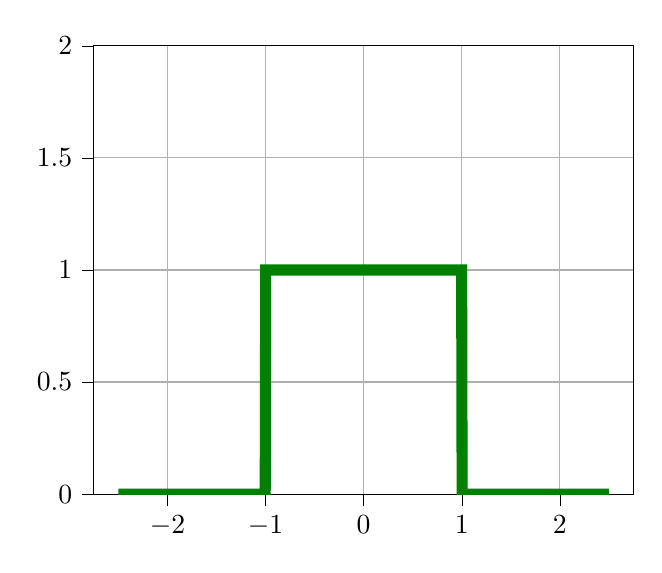
\begin{tikzpicture}

\begin{axis}[
tick align=outside,
tick pos=left,
x grid style={white!69.0196078431373!black},
xmajorgrids,
xmin=-2.75, xmax=2.75,
xtick style={color=black},
y grid style={white!69.0196078431373!black},
ymajorgrids,
ymin=0, ymax=2,
ytick style={color=black}
]
\addplot [line width=4pt, green!50!black]
table {%
-2.5 0
-2.49499499499499 0
-2.48998998998999 0
-2.48498498498498 0
-2.47997997997998 0
-2.47497497497497 0
-2.46996996996997 0
-2.46496496496496 0
-2.45995995995996 0
-2.45495495495495 0
-2.44994994994995 0
-2.44494494494494 0
-2.43993993993994 0
-2.43493493493493 0
-2.42992992992993 0
-2.42492492492492 0
-2.41991991991992 0
-2.41491491491491 0
-2.40990990990991 0
-2.4049049049049 0
-2.3998998998999 0
-2.39489489489489 0
-2.38988988988989 0
-2.38488488488488 0
-2.37987987987988 0
-2.37487487487487 0
-2.36986986986987 0
-2.36486486486486 0
-2.35985985985986 0
-2.35485485485485 0
-2.34984984984985 0
-2.34484484484484 0
-2.33983983983984 0
-2.33483483483483 0
-2.32982982982983 0
-2.32482482482482 0
-2.31981981981982 0
-2.31481481481481 0
-2.30980980980981 0
-2.3048048048048 0
-2.2997997997998 0
-2.29479479479479 0
-2.28978978978979 0
-2.28478478478478 0
-2.27977977977978 0
-2.27477477477477 0
-2.26976976976977 0
-2.26476476476476 0
-2.25975975975976 0
-2.25475475475475 0
-2.24974974974975 0
-2.24474474474474 0
-2.23973973973974 0
-2.23473473473473 0
-2.22972972972973 0
-2.22472472472472 0
-2.21971971971972 0
-2.21471471471471 0
-2.20970970970971 0
-2.2047047047047 0
-2.1996996996997 0
-2.19469469469469 0
-2.18968968968969 0
-2.18468468468468 0
-2.17967967967968 0
-2.17467467467467 0
-2.16966966966967 0
-2.16466466466466 0
-2.15965965965966 0
-2.15465465465465 0
-2.14964964964965 0
-2.14464464464464 0
-2.13963963963964 0
-2.13463463463463 0
-2.12962962962963 0
-2.12462462462462 0
-2.11961961961962 0
-2.11461461461461 0
-2.10960960960961 0
-2.1046046046046 0
-2.0995995995996 0
-2.09459459459459 0
-2.08958958958959 0
-2.08458458458458 0
-2.07957957957958 0
-2.07457457457457 0
-2.06956956956957 0
-2.06456456456456 0
-2.05955955955956 0
-2.05455455455455 0
-2.04954954954955 0
-2.04454454454454 0
-2.03953953953954 0
-2.03453453453453 0
-2.02952952952953 0
-2.02452452452452 0
-2.01951951951952 0
-2.01451451451451 0
-2.00950950950951 0
-2.0045045045045 0
-1.9994994994995 0
-1.99449449449449 0
-1.98948948948949 0
-1.98448448448448 0
-1.97947947947948 0
-1.97447447447447 0
-1.96946946946947 0
-1.96446446446446 0
-1.95945945945946 0
-1.95445445445445 0
-1.94944944944945 0
-1.94444444444444 0
-1.93943943943944 0
-1.93443443443443 0
-1.92942942942943 0
-1.92442442442442 0
-1.91941941941942 0
-1.91441441441441 0
-1.90940940940941 0
-1.9044044044044 0
-1.8993993993994 0
-1.89439439439439 0
-1.88938938938939 0
-1.88438438438438 0
-1.87937937937938 0
-1.87437437437437 0
-1.86936936936937 0
-1.86436436436436 0
-1.85935935935936 0
-1.85435435435435 0
-1.84934934934935 0
-1.84434434434434 0
-1.83933933933934 0
-1.83433433433433 0
-1.82932932932933 0
-1.82432432432432 0
-1.81931931931932 0
-1.81431431431431 0
-1.80930930930931 0
-1.8043043043043 0
-1.7992992992993 0
-1.79429429429429 0
-1.78928928928929 0
-1.78428428428428 0
-1.77927927927928 0
-1.77427427427427 0
-1.76926926926927 0
-1.76426426426426 0
-1.75925925925926 0
-1.75425425425425 0
-1.74924924924925 0
-1.74424424424424 0
-1.73923923923924 0
-1.73423423423423 0
-1.72922922922923 0
-1.72422422422422 0
-1.71921921921922 0
-1.71421421421421 0
-1.70920920920921 0
-1.7042042042042 0
-1.6991991991992 0
-1.69419419419419 0
-1.68918918918919 0
-1.68418418418418 0
-1.67917917917918 0
-1.67417417417417 0
-1.66916916916917 0
-1.66416416416416 0
-1.65915915915916 0
-1.65415415415415 0
-1.64914914914915 0
-1.64414414414414 0
-1.63913913913914 0
-1.63413413413413 0
-1.62912912912913 0
-1.62412412412412 0
-1.61911911911912 0
-1.61411411411411 0
-1.60910910910911 0
-1.6041041041041 0
-1.5990990990991 0
-1.59409409409409 0
-1.58908908908909 0
-1.58408408408408 0
-1.57907907907908 0
-1.57407407407407 0
-1.56906906906907 0
-1.56406406406406 0
-1.55905905905906 0
-1.55405405405405 0
-1.54904904904905 0
-1.54404404404404 0
-1.53903903903904 0
-1.53403403403403 0
-1.52902902902903 0
-1.52402402402402 0
-1.51901901901902 0
-1.51401401401401 0
-1.50900900900901 0
-1.504004004004 0
-1.498998998999 0
-1.49399399399399 0
-1.48898898898899 0
-1.48398398398398 0
-1.47897897897898 0
-1.47397397397397 0
-1.46896896896897 0
-1.46396396396396 0
-1.45895895895896 0
-1.45395395395395 0
-1.44894894894895 0
-1.44394394394394 0
-1.43893893893894 0
-1.43393393393393 0
-1.42892892892893 0
-1.42392392392392 0
-1.41891891891892 0
-1.41391391391391 0
-1.40890890890891 0
-1.4039039039039 0
-1.3988988988989 0
-1.39389389389389 0
-1.38888888888889 0
-1.38388388388388 0
-1.37887887887888 0
-1.37387387387387 0
-1.36886886886887 0
-1.36386386386386 0
-1.35885885885886 0
-1.35385385385385 0
-1.34884884884885 0
-1.34384384384384 0
-1.33883883883884 0
-1.33383383383383 0
-1.32882882882883 0
-1.32382382382382 0
-1.31881881881882 0
-1.31381381381381 0
-1.30880880880881 0
-1.3038038038038 0
-1.2987987987988 0
-1.29379379379379 0
-1.28878878878879 0
-1.28378378378378 0
-1.27877877877878 0
-1.27377377377377 0
-1.26876876876877 0
-1.26376376376376 0
-1.25875875875876 0
-1.25375375375375 0
-1.24874874874875 0
-1.24374374374374 0
-1.23873873873874 0
-1.23373373373373 0
-1.22872872872873 0
-1.22372372372372 0
-1.21871871871872 0
-1.21371371371371 0
-1.20870870870871 0
-1.2037037037037 0
-1.1986986986987 0
-1.19369369369369 0
-1.18868868868869 0
-1.18368368368368 0
-1.17867867867868 0
-1.17367367367367 0
-1.16866866866867 0
-1.16366366366366 0
-1.15865865865866 0
-1.15365365365365 0
-1.14864864864865 0
-1.14364364364364 0
-1.13863863863864 0
-1.13363363363363 0
-1.12862862862863 0
-1.12362362362362 0
-1.11861861861862 0
-1.11361361361361 0
-1.10860860860861 0
-1.1036036036036 0
-1.0985985985986 0
-1.09359359359359 0
-1.08858858858859 0
-1.08358358358358 0
-1.07857857857858 0
-1.07357357357357 0
-1.06856856856857 0
-1.06356356356356 0
-1.05855855855856 0
-1.05355355355355 0
-1.04854854854855 0
-1.04354354354354 0
-1.03853853853854 0
-1.03353353353353 0
-1.02852852852853 0
-1.02352352352352 0
-1.01851851851852 0
-1.01351351351351 0
-1.00850850850851 0
-1.0035035035035 0
-0.998498498498499 1
-0.993493493493494 1
-0.988488488488489 1
-0.983483483483484 1
-0.978478478478479 1
-0.973473473473474 1
-0.968468468468469 1
-0.963463463463464 1
-0.958458458458459 1
-0.953453453453454 1
-0.948448448448449 1
-0.943443443443444 1
-0.938438438438439 1
-0.933433433433434 1
-0.928428428428429 1
-0.923423423423424 1
-0.918418418418419 1
-0.913413413413414 1
-0.908408408408409 1
-0.903403403403404 1
-0.898398398398399 1
-0.893393393393393 1
-0.888388388388388 1
-0.883383383383383 1
-0.878378378378378 1
-0.873373373373373 1
-0.868368368368368 1
-0.863363363363363 1
-0.858358358358358 1
-0.853353353353353 1
-0.848348348348348 1
-0.843343343343343 1
-0.838338338338338 1
-0.833333333333333 1
-0.828328328328328 1
-0.823323323323323 1
-0.818318318318318 1
-0.813313313313313 1
-0.808308308308308 1
-0.803303303303303 1
-0.798298298298298 1
-0.793293293293293 1
-0.788288288288288 1
-0.783283283283283 1
-0.778278278278278 1
-0.773273273273273 1
-0.768268268268268 1
-0.763263263263263 1
-0.758258258258258 1
-0.753253253253253 1
-0.748248248248248 1
-0.743243243243243 1
-0.738238238238238 1
-0.733233233233233 1
-0.728228228228228 1
-0.723223223223223 1
-0.718218218218218 1
-0.713213213213213 1
-0.708208208208208 1
-0.703203203203203 1
-0.698198198198198 1
-0.693193193193193 1
-0.688188188188188 1
-0.683183183183183 1
-0.678178178178178 1
-0.673173173173173 1
-0.668168168168168 1
-0.663163163163163 1
-0.658158158158158 1
-0.653153153153153 1
-0.648148148148148 1
-0.643143143143143 1
-0.638138138138138 1
-0.633133133133133 1
-0.628128128128128 1
-0.623123123123123 1
-0.618118118118118 1
-0.613113113113113 1
-0.608108108108108 1
-0.603103103103103 1
-0.598098098098098 1
-0.593093093093093 1
-0.588088088088088 1
-0.583083083083083 1
-0.578078078078078 1
-0.573073073073073 1
-0.568068068068068 1
-0.563063063063063 1
-0.558058058058058 1
-0.553053053053053 1
-0.548048048048048 1
-0.543043043043043 1
-0.538038038038038 1
-0.533033033033033 1
-0.528028028028028 1
-0.523023023023023 1
-0.518018018018018 1
-0.513013013013013 1
-0.508008008008008 1
-0.503003003003003 1
-0.497997997997998 1
-0.492992992992993 1
-0.487987987987988 1
-0.482982982982983 1
-0.477977977977978 1
-0.472972972972973 1
-0.467967967967968 1
-0.462962962962963 1
-0.457957957957958 1
-0.452952952952953 1
-0.447947947947948 1
-0.442942942942943 1
-0.437937937937938 1
-0.432932932932933 1
-0.427927927927928 1
-0.422922922922923 1
-0.417917917917918 1
-0.412912912912913 1
-0.407907907907908 1
-0.402902902902903 1
-0.397897897897898 1
-0.392892892892893 1
-0.387887887887888 1
-0.382882882882883 1
-0.377877877877878 1
-0.372872872872873 1
-0.367867867867868 1
-0.362862862862863 1
-0.357857857857858 1
-0.352852852852853 1
-0.347847847847848 1
-0.342842842842843 1
-0.337837837837838 1
-0.332832832832833 1
-0.327827827827828 1
-0.322822822822823 1
-0.317817817817818 1
-0.312812812812813 1
-0.307807807807808 1
-0.302802802802803 1
-0.297797797797798 1
-0.292792792792793 1
-0.287787787787788 1
-0.282782782782783 1
-0.277777777777778 1
-0.272772772772773 1
-0.267767767767768 1
-0.262762762762763 1
-0.257757757757758 1
-0.252752752752753 1
-0.247747747747748 1
-0.242742742742743 1
-0.237737737737738 1
-0.232732732732733 1
-0.227727727727728 1
-0.222722722722723 1
-0.217717717717718 1
-0.212712712712713 1
-0.207707707707708 1
-0.202702702702703 1
-0.197697697697698 1
-0.192692692692693 1
-0.187687687687688 1
-0.182682682682683 1
-0.177677677677678 1
-0.172672672672673 1
-0.167667667667668 1
-0.162662662662663 1
-0.157657657657658 1
-0.152652652652653 1
-0.147647647647648 1
-0.142642642642643 1
-0.137637637637638 1
-0.132632632632633 1
-0.127627627627628 1
-0.122622622622623 1
-0.117617617617618 1
-0.112612612612613 1
-0.107607607607608 1
-0.102602602602603 1
-0.0975975975975976 1
-0.0925925925925926 1
-0.0875875875875876 1
-0.0825825825825826 1
-0.0775775775775776 1
-0.0725725725725725 1
-0.0675675675675675 1
-0.0625625625625625 1
-0.0575575575575575 1
-0.0525525525525525 1
-0.0475475475475475 1
-0.0425425425425425 1
-0.0375375375375375 1
-0.0325325325325325 1
-0.0275275275275275 1
-0.0225225225225225 1
-0.0175175175175175 1
-0.0125125125125125 1
-0.0075075075075075 1
-0.0025025025025025 1
0.0025025025025025 1
0.0075075075075075 1
0.0125125125125125 1
0.0175175175175175 1
0.0225225225225225 1
0.0275275275275275 1
0.0325325325325325 1
0.0375375375375375 1
0.0425425425425425 1
0.0475475475475475 1
0.0525525525525525 1
0.0575575575575575 1
0.0625625625625625 1
0.0675675675675675 1
0.0725725725725725 1
0.0775775775775776 1
0.0825825825825826 1
0.0875875875875876 1
0.0925925925925926 1
0.0975975975975976 1
0.102602602602603 1
0.107607607607608 1
0.112612612612613 1
0.117617617617618 1
0.122622622622623 1
0.127627627627628 1
0.132632632632633 1
0.137637637637638 1
0.142642642642643 1
0.147647647647648 1
0.152652652652653 1
0.157657657657658 1
0.162662662662663 1
0.167667667667668 1
0.172672672672673 1
0.177677677677678 1
0.182682682682683 1
0.187687687687688 1
0.192692692692693 1
0.197697697697698 1
0.202702702702703 1
0.207707707707708 1
0.212712712712713 1
0.217717717717718 1
0.222722722722723 1
0.227727727727728 1
0.232732732732733 1
0.237737737737738 1
0.242742742742743 1
0.247747747747748 1
0.252752752752753 1
0.257757757757758 1
0.262762762762763 1
0.267767767767768 1
0.272772772772773 1
0.277777777777778 1
0.282782782782783 1
0.287787787787788 1
0.292792792792793 1
0.297797797797798 1
0.302802802802803 1
0.307807807807808 1
0.312812812812813 1
0.317817817817818 1
0.322822822822823 1
0.327827827827828 1
0.332832832832833 1
0.337837837837838 1
0.342842842842843 1
0.347847847847848 1
0.352852852852853 1
0.357857857857858 1
0.362862862862863 1
0.367867867867868 1
0.372872872872873 1
0.377877877877878 1
0.382882882882883 1
0.387887887887888 1
0.392892892892893 1
0.397897897897898 1
0.402902902902903 1
0.407907907907908 1
0.412912912912913 1
0.417917917917918 1
0.422922922922923 1
0.427927927927928 1
0.432932932932933 1
0.437937937937938 1
0.442942942942943 1
0.447947947947948 1
0.452952952952953 1
0.457957957957958 1
0.462962962962963 1
0.467967967967968 1
0.472972972972973 1
0.477977977977978 1
0.482982982982983 1
0.487987987987988 1
0.492992992992993 1
0.497997997997998 1
0.503003003003003 1
0.508008008008008 1
0.513013013013013 1
0.518018018018018 1
0.523023023023023 1
0.528028028028028 1
0.533033033033033 1
0.538038038038038 1
0.543043043043043 1
0.548048048048048 1
0.553053053053053 1
0.558058058058058 1
0.563063063063063 1
0.568068068068068 1
0.573073073073073 1
0.578078078078078 1
0.583083083083083 1
0.588088088088088 1
0.593093093093093 1
0.598098098098098 1
0.603103103103103 1
0.608108108108108 1
0.613113113113113 1
0.618118118118118 1
0.623123123123123 1
0.628128128128128 1
0.633133133133133 1
0.638138138138138 1
0.643143143143143 1
0.648148148148148 1
0.653153153153153 1
0.658158158158158 1
0.663163163163163 1
0.668168168168168 1
0.673173173173173 1
0.678178178178178 1
0.683183183183183 1
0.688188188188188 1
0.693193193193193 1
0.698198198198198 1
0.703203203203203 1
0.708208208208208 1
0.713213213213213 1
0.718218218218218 1
0.723223223223223 1
0.728228228228228 1
0.733233233233233 1
0.738238238238238 1
0.743243243243243 1
0.748248248248248 1
0.753253253253253 1
0.758258258258258 1
0.763263263263263 1
0.768268268268268 1
0.773273273273273 1
0.778278278278278 1
0.783283283283283 1
0.788288288288288 1
0.793293293293293 1
0.798298298298298 1
0.803303303303303 1
0.808308308308308 1
0.813313313313313 1
0.818318318318318 1
0.823323323323323 1
0.828328328328328 1
0.833333333333333 1
0.838338338338338 1
0.843343343343343 1
0.848348348348348 1
0.853353353353353 1
0.858358358358358 1
0.863363363363364 1
0.868368368368369 1
0.873373373373374 1
0.878378378378379 1
0.883383383383384 1
0.888388388388389 1
0.893393393393394 1
0.898398398398399 1
0.903403403403404 1
0.908408408408409 1
0.913413413413414 1
0.918418418418419 1
0.923423423423424 1
0.928428428428429 1
0.933433433433434 1
0.938438438438439 1
0.943443443443444 1
0.948448448448449 1
0.953453453453454 1
0.958458458458459 1
0.963463463463464 1
0.968468468468469 1
0.973473473473474 1
0.978478478478479 1
0.983483483483484 1
0.988488488488489 1
0.993493493493494 1
0.998498498498499 1
1.0035035035035 0
1.00850850850851 0
1.01351351351351 0
1.01851851851852 0
1.02352352352352 0
1.02852852852853 0
1.03353353353353 0
1.03853853853854 0
1.04354354354354 0
1.04854854854855 0
1.05355355355355 0
1.05855855855856 0
1.06356356356356 0
1.06856856856857 0
1.07357357357357 0
1.07857857857858 0
1.08358358358358 0
1.08858858858859 0
1.09359359359359 0
1.0985985985986 0
1.1036036036036 0
1.10860860860861 0
1.11361361361361 0
1.11861861861862 0
1.12362362362362 0
1.12862862862863 0
1.13363363363363 0
1.13863863863864 0
1.14364364364364 0
1.14864864864865 0
1.15365365365365 0
1.15865865865866 0
1.16366366366366 0
1.16866866866867 0
1.17367367367367 0
1.17867867867868 0
1.18368368368368 0
1.18868868868869 0
1.19369369369369 0
1.1986986986987 0
1.2037037037037 0
1.20870870870871 0
1.21371371371371 0
1.21871871871872 0
1.22372372372372 0
1.22872872872873 0
1.23373373373373 0
1.23873873873874 0
1.24374374374374 0
1.24874874874875 0
1.25375375375375 0
1.25875875875876 0
1.26376376376376 0
1.26876876876877 0
1.27377377377377 0
1.27877877877878 0
1.28378378378378 0
1.28878878878879 0
1.29379379379379 0
1.2987987987988 0
1.3038038038038 0
1.30880880880881 0
1.31381381381381 0
1.31881881881882 0
1.32382382382382 0
1.32882882882883 0
1.33383383383383 0
1.33883883883884 0
1.34384384384384 0
1.34884884884885 0
1.35385385385385 0
1.35885885885886 0
1.36386386386386 0
1.36886886886887 0
1.37387387387387 0
1.37887887887888 0
1.38388388388388 0
1.38888888888889 0
1.39389389389389 0
1.3988988988989 0
1.4039039039039 0
1.40890890890891 0
1.41391391391391 0
1.41891891891892 0
1.42392392392392 0
1.42892892892893 0
1.43393393393393 0
1.43893893893894 0
1.44394394394394 0
1.44894894894895 0
1.45395395395395 0
1.45895895895896 0
1.46396396396396 0
1.46896896896897 0
1.47397397397397 0
1.47897897897898 0
1.48398398398398 0
1.48898898898899 0
1.49399399399399 0
1.498998998999 0
1.504004004004 0
1.50900900900901 0
1.51401401401401 0
1.51901901901902 0
1.52402402402402 0
1.52902902902903 0
1.53403403403403 0
1.53903903903904 0
1.54404404404404 0
1.54904904904905 0
1.55405405405405 0
1.55905905905906 0
1.56406406406406 0
1.56906906906907 0
1.57407407407407 0
1.57907907907908 0
1.58408408408408 0
1.58908908908909 0
1.59409409409409 0
1.5990990990991 0
1.6041041041041 0
1.60910910910911 0
1.61411411411411 0
1.61911911911912 0
1.62412412412412 0
1.62912912912913 0
1.63413413413413 0
1.63913913913914 0
1.64414414414414 0
1.64914914914915 0
1.65415415415415 0
1.65915915915916 0
1.66416416416416 0
1.66916916916917 0
1.67417417417417 0
1.67917917917918 0
1.68418418418418 0
1.68918918918919 0
1.69419419419419 0
1.6991991991992 0
1.7042042042042 0
1.70920920920921 0
1.71421421421421 0
1.71921921921922 0
1.72422422422422 0
1.72922922922923 0
1.73423423423423 0
1.73923923923924 0
1.74424424424424 0
1.74924924924925 0
1.75425425425425 0
1.75925925925926 0
1.76426426426426 0
1.76926926926927 0
1.77427427427427 0
1.77927927927928 0
1.78428428428428 0
1.78928928928929 0
1.79429429429429 0
1.7992992992993 0
1.8043043043043 0
1.80930930930931 0
1.81431431431431 0
1.81931931931932 0
1.82432432432432 0
1.82932932932933 0
1.83433433433433 0
1.83933933933934 0
1.84434434434434 0
1.84934934934935 0
1.85435435435435 0
1.85935935935936 0
1.86436436436436 0
1.86936936936937 0
1.87437437437437 0
1.87937937937938 0
1.88438438438438 0
1.88938938938939 0
1.89439439439439 0
1.8993993993994 0
1.9044044044044 0
1.90940940940941 0
1.91441441441441 0
1.91941941941942 0
1.92442442442442 0
1.92942942942943 0
1.93443443443443 0
1.93943943943944 0
1.94444444444444 0
1.94944944944945 0
1.95445445445445 0
1.95945945945946 0
1.96446446446446 0
1.96946946946947 0
1.97447447447447 0
1.97947947947948 0
1.98448448448448 0
1.98948948948949 0
1.99449449449449 0
1.9994994994995 0
2.0045045045045 0
2.00950950950951 0
2.01451451451451 0
2.01951951951952 0
2.02452452452452 0
2.02952952952953 0
2.03453453453453 0
2.03953953953954 0
2.04454454454454 0
2.04954954954955 0
2.05455455455455 0
2.05955955955956 0
2.06456456456456 0
2.06956956956957 0
2.07457457457457 0
2.07957957957958 0
2.08458458458458 0
2.08958958958959 0
2.09459459459459 0
2.0995995995996 0
2.1046046046046 0
2.10960960960961 0
2.11461461461461 0
2.11961961961962 0
2.12462462462462 0
2.12962962962963 0
2.13463463463463 0
2.13963963963964 0
2.14464464464464 0
2.14964964964965 0
2.15465465465465 0
2.15965965965966 0
2.16466466466466 0
2.16966966966967 0
2.17467467467467 0
2.17967967967968 0
2.18468468468468 0
2.18968968968969 0
2.19469469469469 0
2.1996996996997 0
2.2047047047047 0
2.20970970970971 0
2.21471471471471 0
2.21971971971972 0
2.22472472472472 0
2.22972972972973 0
2.23473473473473 0
2.23973973973974 0
2.24474474474474 0
2.24974974974975 0
2.25475475475475 0
2.25975975975976 0
2.26476476476476 0
2.26976976976977 0
2.27477477477477 0
2.27977977977978 0
2.28478478478478 0
2.28978978978979 0
2.29479479479479 0
2.2997997997998 0
2.3048048048048 0
2.30980980980981 0
2.31481481481481 0
2.31981981981982 0
2.32482482482482 0
2.32982982982983 0
2.33483483483483 0
2.33983983983984 0
2.34484484484484 0
2.34984984984985 0
2.35485485485485 0
2.35985985985986 0
2.36486486486486 0
2.36986986986987 0
2.37487487487487 0
2.37987987987988 0
2.38488488488488 0
2.38988988988989 0
2.39489489489489 0
2.3998998998999 0
2.4049049049049 0
2.40990990990991 0
2.41491491491491 0
2.41991991991992 0
2.42492492492492 0
2.42992992992993 0
2.43493493493493 0
2.43993993993994 0
2.44494494494494 0
2.44994994994995 0
2.45495495495495 0
2.45995995995996 0
2.46496496496496 0
2.46996996996997 0
2.47497497497497 0
2.47997997997998 0
2.48498498498498 0
2.48998998998999 0
2.49499499499499 0
2.5 0
};
\end{axis}

\end{tikzpicture}
}

                    $\quad{}h(t)$
                \end{column}\begin{column}{0.33\textwidth}
                    \centering{}
                    \scalebox{0.4}{% This file was created by tikzplotlib v0.9.1.
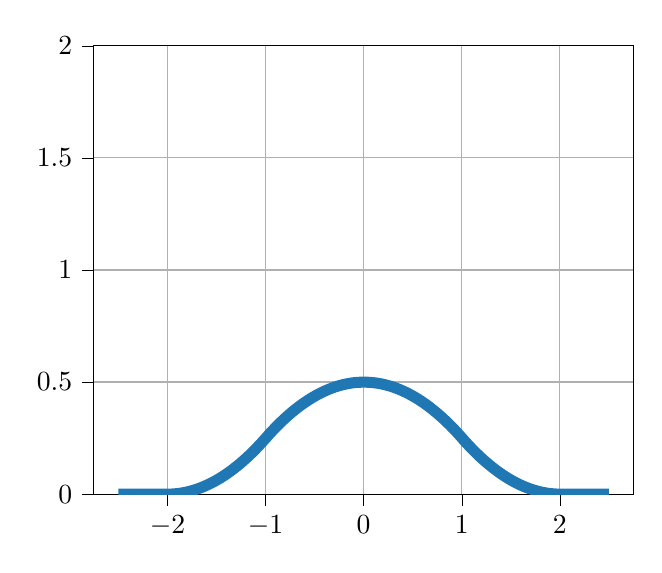
\begin{tikzpicture}

\definecolor{color0}{rgb}{0.12156862745098,0.466666666666667,0.705882352941177}

\begin{axis}[
tick align=outside,
tick pos=left,
x grid style={white!69.0196078431373!black},
xmajorgrids,
xmin=-2.75, xmax=2.75,
xtick style={color=black},
y grid style={white!69.0196078431373!black},
ymajorgrids,
ymin=0, ymax=2,
ytick style={color=black}
]
\addplot [line width=4pt, color0]
table {%
-2.5 0
-2.49499499499499 0
-2.48998998998999 0
-2.48498498498498 0
-2.47997997997998 0
-2.47497497497497 0
-2.46996996996997 0
-2.46496496496496 0
-2.45995995995996 0
-2.45495495495495 0
-2.44994994994995 0
-2.44494494494494 0
-2.43993993993994 0
-2.43493493493493 0
-2.42992992992993 0
-2.42492492492492 0
-2.41991991991992 0
-2.41491491491491 0
-2.40990990990991 0
-2.4049049049049 0
-2.3998998998999 0
-2.39489489489489 0
-2.38988988988989 0
-2.38488488488488 0
-2.37987987987988 0
-2.37487487487487 0
-2.36986986986987 0
-2.36486486486486 0
-2.35985985985986 0
-2.35485485485485 0
-2.34984984984985 0
-2.34484484484484 0
-2.33983983983984 0
-2.33483483483483 0
-2.32982982982983 0
-2.32482482482482 0
-2.31981981981982 0
-2.31481481481481 0
-2.30980980980981 0
-2.3048048048048 0
-2.2997997997998 0
-2.29479479479479 0
-2.28978978978979 0
-2.28478478478478 0
-2.27977977977978 0
-2.27477477477477 0
-2.26976976976977 0
-2.26476476476476 0
-2.25975975975976 0
-2.25475475475475 0
-2.24974974974975 0
-2.24474474474474 0
-2.23973973973974 0
-2.23473473473473 0
-2.22972972972973 0
-2.22472472472472 0
-2.21971971971972 0
-2.21471471471471 0
-2.20970970970971 0
-2.2047047047047 0
-2.1996996996997 0
-2.19469469469469 0
-2.18968968968969 0
-2.18468468468468 0
-2.17967967967968 0
-2.17467467467467 0
-2.16966966966967 0
-2.16466466466466 0
-2.15965965965966 0
-2.15465465465465 0
-2.14964964964965 0
-2.14464464464464 0
-2.13963963963964 0
-2.13463463463463 0
-2.12962962962963 0
-2.12462462462462 0
-2.11961961961962 0
-2.11461461461461 0
-2.10960960960961 0
-2.1046046046046 0
-2.0995995995996 0
-2.09459459459459 0
-2.08958958958959 0
-2.08458458458458 0
-2.07957957957958 0
-2.07457457457457 0
-2.06956956956957 0
-2.06456456456456 0
-2.05955955955956 0
-2.05455455455455 0
-2.04954954954955 0
-2.04454454454454 0
-2.03953953953954 0
-2.03453453453453 0
-2.02952952952953 0
-2.02452452452452 0
-2.01951951951952 0
-2.01451451451451 0
-2.00950950950951 0
-2.0045045045045 0
-1.9994994994995 0
-1.99449449449449 3.75375375375353e-06
-1.98948948948949 2.00200200200196e-05
-1.98448448448448 4.87987987987981e-05
-1.97947947947948 9.00900900900892e-05
-1.97447447447447 0.000143893893893893
-1.96946946946947 0.000210210210210209
-1.96446446446446 0.000289039039039037
-1.95945945945946 0.000380380380380378
-1.95445445445445 0.000484234234234232
-1.94944944944945 0.000600600600600598
-1.94444444444444 0.000729479479479477
-1.93943943943944 0.000870870870870868
-1.93443443443443 0.00102477477477477
-1.92942942942943 0.00119119119119119
-1.92442442442442 0.00137012012012012
-1.91941941941942 0.00156156156156156
-1.91441441441441 0.00176551551551551
-1.90940940940941 0.00198198198198198
-1.9044044044044 0.00221096096096096
-1.8993993993994 0.00245245245245245
-1.89439439439439 0.00270645645645645
-1.88938938938939 0.00297297297297297
-1.88438438438438 0.003252002002002
-1.87937937937938 0.00354354354354354
-1.87437437437437 0.00384759759759759
-1.86936936936937 0.00416416416416416
-1.86436436436436 0.00449324324324324
-1.85935935935936 0.00483483483483483
-1.85435435435435 0.00518893893893893
-1.84934934934935 0.00555555555555555
-1.84434434434434 0.00593468468468468
-1.83933933933934 0.00632632632632632
-1.83433433433433 0.00673048048048048
-1.82932932932933 0.00714714714714714
-1.82432432432432 0.00757632632632632
-1.81931931931932 0.00801801801801802
-1.81431431431431 0.00847222222222222
-1.80930930930931 0.00893893893893894
-1.8043043043043 0.00941816816816817
-1.7992992992993 0.00990990990990991
-1.79429429429429 0.0104141641641642
-1.78928928928929 0.0109309309309309
-1.78428428428428 0.0114602102102102
-1.77927927927928 0.012002002002002
-1.77427427427427 0.0125563063063063
-1.76926926926927 0.0131231231231231
-1.76426426426426 0.0137024524524525
-1.75925925925926 0.0142942942942943
-1.75425425425425 0.0148986486486486
-1.74924924924925 0.0155155155155155
-1.74424424424424 0.0161448948948949
-1.73923923923924 0.0167867867867868
-1.73423423423423 0.0174411911911912
-1.72922922922923 0.0181081081081081
-1.72422422422422 0.0187875375375375
-1.71921921921922 0.0194794794794795
-1.71421421421421 0.0201839339339339
-1.70920920920921 0.0209009009009009
-1.7042042042042 0.0216303803803804
-1.6991991991992 0.0223723723723724
-1.69419419419419 0.0231268768768769
-1.68918918918919 0.0238938938938939
-1.68418418418418 0.0246734234234234
-1.67917917917918 0.0254654654654655
-1.67417417417417 0.02627002002002
-1.66916916916917 0.0270870870870871
-1.66416416416416 0.0279166666666667
-1.65915915915916 0.0287587587587588
-1.65415415415415 0.0296133633633634
-1.64914914914915 0.0304804804804805
-1.64414414414414 0.0313601101101101
-1.63913913913914 0.0322522522522522
-1.63413413413413 0.0331569069069069
-1.62912912912913 0.0340740740740741
-1.62412412412412 0.0350037537537538
-1.61911911911912 0.0359459459459459
-1.61411411411411 0.0369006506506507
-1.60910910910911 0.0378678678678679
-1.6041041041041 0.0388475975975976
-1.5990990990991 0.0398398398398398
-1.59409409409409 0.0408445945945946
-1.58908908908909 0.0418618618618619
-1.58408408408408 0.0428916416416416
-1.57907907907908 0.0439339339339339
-1.57407407407407 0.0449887387387387
-1.56906906906907 0.0460560560560561
-1.56406406406406 0.0471358858858859
-1.55905905905906 0.0482282282282282
-1.55405405405405 0.0493330830830831
-1.54904904904905 0.0504504504504505
-1.54404404404404 0.0515803303303303
-1.53903903903904 0.0527227227227227
-1.53403403403403 0.0538776276276276
-1.52902902902903 0.055045045045045
-1.52402402402402 0.056224974974975
-1.51901901901902 0.0574174174174174
-1.51401401401401 0.0586223723723724
-1.50900900900901 0.0598398398398398
-1.504004004004 0.0610698198198198
-1.498998998999 0.0623123123123123
-1.49399399399399 0.0635673173173173
-1.48898898898899 0.0648348348348348
-1.48398398398398 0.0661148648648649
-1.47897897897898 0.0674074074074074
-1.47397397397397 0.0687124624624625
-1.46896896896897 0.07003003003003
-1.46396396396396 0.0713601101101101
-1.45895895895896 0.0727027027027027
-1.45395395395395 0.0740578078078078
-1.44894894894895 0.0754254254254254
-1.44394394394394 0.0768055555555556
-1.43893893893894 0.0781981981981982
-1.43393393393393 0.0796033533533533
-1.42892892892893 0.081021021021021
-1.42392392392392 0.0824512012012012
-1.41891891891892 0.0838938938938939
-1.41391391391391 0.0853490990990991
-1.40890890890891 0.0868168168168168
-1.4039039039039 0.0882970470470471
-1.3988988988989 0.0897897897897898
-1.39389389389389 0.0912950450450451
-1.38888888888889 0.0928128128128128
-1.38388388388388 0.0943430930930931
-1.37887887887888 0.0958858858858859
-1.37387387387387 0.0974411911911912
-1.36886886886887 0.099009009009009
-1.36386386386386 0.100589339339339
-1.35885885885886 0.102182182182182
-1.35385385385385 0.103787537537538
-1.34884884884885 0.105405405405405
-1.34384384384384 0.107035785785786
-1.33883883883884 0.108678678678679
-1.33383383383383 0.110334084084084
-1.32882882882883 0.112002002002002
-1.32382382382382 0.113682432432432
-1.31881881881882 0.115375375375375
-1.31381381381381 0.117080830830831
-1.30880880880881 0.118798798798799
-1.3038038038038 0.120529279279279
-1.2987987987988 0.122272272272272
-1.29379379379379 0.124027777777778
-1.28878878878879 0.125795795795796
-1.28378378378378 0.127576326326326
-1.27877877877878 0.129369369369369
-1.27377377377377 0.131174924924925
-1.26876876876877 0.132992992992993
-1.26376376376376 0.134823573573574
-1.25875875875876 0.136666666666667
-1.25375375375375 0.138522272272272
-1.24874874874875 0.14039039039039
-1.24374374374374 0.142271021021021
-1.23873873873874 0.144164164164164
-1.23373373373373 0.14606981981982
-1.22872872872873 0.147987987987988
-1.22372372372372 0.149918668668669
-1.21871871871872 0.151861861861862
-1.21371371371371 0.153817567567568
-1.20870870870871 0.155785785785786
-1.2037037037037 0.157766516516517
-1.1986986986987 0.15975975975976
-1.19369369369369 0.161765515515516
-1.18868868868869 0.163783783783784
-1.18368368368368 0.165814564564565
-1.17867867867868 0.167857857857858
-1.17367367367367 0.169913663663664
-1.16866866866867 0.171981981981982
-1.16366366366366 0.174062812812813
-1.15865865865866 0.176156156156156
-1.15365365365365 0.178262012012012
-1.14864864864865 0.18038038038038
-1.14364364364364 0.182511261261261
-1.13863863863864 0.184654654654655
-1.13363363363363 0.186810560560561
-1.12862862862863 0.188978978978979
-1.12362362362362 0.19115990990991
-1.11861861861862 0.193353353353353
-1.11361361361361 0.195559309309309
-1.10860860860861 0.197777777777778
-1.1036036036036 0.200008758758759
-1.0985985985986 0.202252252252252
-1.09359359359359 0.204508258258258
-1.08858858858859 0.206776776776777
-1.08358358358358 0.209057807807808
-1.07857857857858 0.211351351351351
-1.07357357357357 0.213657407407407
-1.06856856856857 0.215975975975976
-1.06356356356356 0.218307057057057
-1.05855855855856 0.220650650650651
-1.05355355355355 0.223006756756757
-1.04854854854855 0.225375375375375
-1.04354354354354 0.227756506506507
-1.03853853853854 0.23015015015015
-1.03353353353353 0.232556306306306
-1.02852852852853 0.234974974974975
-1.02352352352352 0.237406156156156
-1.01851851851852 0.23984984984985
-1.01351351351351 0.242306056056056
-1.00850850850851 0.244774774774775
-1.0035035035035 0.247256006006006
-0.998498498498499 0.24974974974975
-0.993493493493494 0.252243493493494
-0.988488488488489 0.254724724724725
-0.983483483483484 0.257193443443443
-0.978478478478479 0.25964964964965
-0.973473473473474 0.262093343343343
-0.968468468468469 0.264524524524525
-0.963463463463464 0.266943193193193
-0.958458458458459 0.269349349349349
-0.953453453453454 0.271742992992993
-0.948448448448449 0.274124124124124
-0.943443443443444 0.276492742742743
-0.938438438438439 0.278848848848849
-0.933433433433434 0.281192442442442
-0.928428428428429 0.283523523523524
-0.923423423423424 0.285842092092092
-0.918418418418419 0.288148148148148
-0.913413413413414 0.290441691691692
-0.908408408408409 0.292722722722723
-0.903403403403404 0.294991241241241
-0.898398398398399 0.297247247247247
-0.893393393393393 0.299490740740741
-0.888388388388388 0.301721721721722
-0.883383383383383 0.30394019019019
-0.878378378378378 0.306146146146146
-0.873373373373373 0.30833958958959
-0.868368368368368 0.310520520520521
-0.863363363363363 0.312688938938939
-0.858358358358358 0.314844844844845
-0.853353353353353 0.316988238238238
-0.848348348348348 0.319119119119119
-0.843343343343343 0.321237487487487
-0.838338338338338 0.323343343343343
-0.833333333333333 0.325436686686687
-0.828328328328328 0.327517517517518
-0.823323323323323 0.329585835835836
-0.818318318318318 0.331641641641642
-0.813313313313313 0.333684934934935
-0.808308308308308 0.335715715715716
-0.803303303303303 0.337733983983984
-0.798298298298298 0.33973973973974
-0.793293293293293 0.341732982982983
-0.788288288288288 0.343713713713714
-0.783283283283283 0.345681931931932
-0.778278278278278 0.347637637637638
-0.773273273273273 0.349580830830831
-0.768268268268268 0.351511511511512
-0.763263263263263 0.35342967967968
-0.758258258258258 0.355335335335335
-0.753253253253253 0.357228478478479
-0.748248248248248 0.359109109109109
-0.743243243243243 0.360977227227227
-0.738238238238238 0.362832832832833
-0.733233233233233 0.364675925925926
-0.728228228228228 0.366506506506507
-0.723223223223223 0.368324574574575
-0.718218218218218 0.37013013013013
-0.713213213213213 0.371923173173173
-0.708208208208208 0.373703703703704
-0.703203203203203 0.375471721721722
-0.698198198198198 0.377227227227227
-0.693193193193193 0.37897022022022
-0.688188188188188 0.380700700700701
-0.683183183183183 0.382418668668669
-0.678178178178178 0.384124124124124
-0.673173173173173 0.385817067067067
-0.668168168168168 0.387497497497498
-0.663163163163163 0.389165415415415
-0.658158158158158 0.390820820820821
-0.653153153153153 0.392463713713714
-0.648148148148148 0.394094094094094
-0.643143143143143 0.395711961961962
-0.638138138138138 0.397317317317317
-0.633133133133133 0.39891016016016
-0.628128128128128 0.400490490490491
-0.623123123123123 0.402058308308308
-0.618118118118118 0.403613613613614
-0.613113113113113 0.405156406406406
-0.608108108108108 0.406686686686687
-0.603103103103103 0.408204454454455
-0.598098098098098 0.40970970970971
-0.593093093093093 0.411202452452452
-0.588088088088088 0.412682682682683
-0.583083083083083 0.4141504004004
-0.578078078078078 0.415605605605606
-0.573073073073073 0.417048298298298
-0.568068068068068 0.418478478478479
-0.563063063063063 0.419896146146146
-0.558058058058058 0.421301301301301
-0.553053053053053 0.422693943943944
-0.548048048048048 0.424074074074074
-0.543043043043043 0.425441691691692
-0.538038038038038 0.426796796796797
-0.533033033033033 0.428139389389389
-0.528028028028028 0.42946946946947
-0.523023023023023 0.430787037037037
-0.518018018018018 0.432092092092092
-0.513013013013013 0.433384634634635
-0.508008008008008 0.434664664664665
-0.503003003003003 0.435932182182182
-0.497997997997998 0.437187187187187
-0.492992992992993 0.43842967967968
-0.487987987987988 0.43965965965966
-0.482982982982983 0.440877127127127
-0.477977977977978 0.442082082082082
-0.472972972972973 0.443274524524525
-0.467967967967968 0.444454454454455
-0.462962962962963 0.445621871871872
-0.457957957957958 0.446776776776777
-0.452952952952953 0.447919169169169
-0.447947947947948 0.449049049049049
-0.442942942942943 0.450166416416416
-0.437937937937938 0.451271271271271
-0.432932932932933 0.452363613613614
-0.427927927927928 0.453443443443444
-0.422922922922923 0.454510760760761
-0.417917917917918 0.455565565565566
-0.412912912912913 0.456607857857858
-0.407907907907908 0.457637637637638
-0.402902902902903 0.458654904904905
-0.397897897897898 0.45965965965966
-0.392892892892893 0.460651901901902
-0.387887887887888 0.461631631631632
-0.382882882882883 0.462598848848849
-0.377877877877878 0.463553553553554
-0.372872872872873 0.464495745745746
-0.367867867867868 0.465425425425426
-0.362862862862863 0.466342592592593
-0.357857857857858 0.467247247247247
-0.352852852852853 0.468139389389389
-0.347847847847848 0.469019019019019
-0.342842842842843 0.469886136136136
-0.337837837837838 0.470740740740741
-0.332832832832833 0.471582832832833
-0.327827827827828 0.472412412412412
-0.322822822822823 0.47322947947948
-0.317817817817818 0.474034034034034
-0.312812812812813 0.474826076076076
-0.307807807807808 0.475605605605606
-0.302802802802803 0.476372622622623
-0.297797797797798 0.477127127127127
-0.292792792792793 0.477869119119119
-0.287787787787788 0.478598598598599
-0.282782782782783 0.479315565565566
-0.277777777777778 0.48002002002002
-0.272772772772773 0.480711961961962
-0.267767767767768 0.481391391391391
-0.262762762762763 0.482058308308308
-0.257757757757758 0.482712712712713
-0.252752752752753 0.483354604604605
-0.247747747747748 0.483983983983984
-0.242742742742743 0.484600850850851
-0.237737737737738 0.485205205205205
-0.232732732732733 0.485797047047047
-0.227727727727728 0.486376376376376
-0.222722722722723 0.486943193193193
-0.217717717717718 0.487497497497498
-0.212712712712713 0.488039289289289
-0.207707707707708 0.488568568568569
-0.202702702702703 0.489085335335335
-0.197697697697698 0.48958958958959
-0.192692692692693 0.490081331331331
-0.187687687687688 0.490560560560561
-0.182682682682683 0.491027277277277
-0.177677677677678 0.491481481481482
-0.172672672672673 0.491923173173173
-0.167667667667668 0.492352352352352
-0.162662662662663 0.492769019019019
-0.157657657657658 0.493173173173173
-0.152652652652653 0.493564814814815
-0.147647647647648 0.493943943943944
-0.142642642642643 0.494310560560561
-0.137637637637638 0.494664664664665
-0.132632632632633 0.495006256256256
-0.127627627627628 0.495335335335335
-0.122622622622623 0.495651901901902
-0.117617617617618 0.495955955955956
-0.112612612612613 0.496247497497498
-0.107607607607608 0.496526526526527
-0.102602602602603 0.496793043043043
-0.0975975975975976 0.497047047047047
-0.0925925925925926 0.497288538538539
-0.0875875875875876 0.497517517517518
-0.0825825825825826 0.497733983983984
-0.0775775775775776 0.497937937937938
-0.0725725725725725 0.498129379379379
-0.0675675675675675 0.498308308308308
-0.0625625625625625 0.498474724724725
-0.0575575575575575 0.498628628628629
-0.0525525525525525 0.49877002002002
-0.0475475475475475 0.498898898898899
-0.0425425425425425 0.499015265265265
-0.0375375375375375 0.499119119119119
-0.0325325325325325 0.49921046046046
-0.0275275275275275 0.499289289289289
-0.0225225225225225 0.499355605605606
-0.0175175175175175 0.499409409409409
-0.0125125125125125 0.499450700700701
-0.0075075075075075 0.49947947947948
-0.0025025025025025 0.499495745745746
0.0025025025025025 0.4994994994995
0.0075075075075075 0.499495745745746
0.0125125125125125 0.49947947947948
0.0175175175175175 0.499450700700701
0.0225225225225225 0.499409409409409
0.0275275275275275 0.499355605605606
0.0325325325325325 0.499289289289289
0.0375375375375375 0.499210460460461
0.0425425425425425 0.499119119119119
0.0475475475475475 0.499015265265265
0.0525525525525525 0.498898898898899
0.0575575575575575 0.49877002002002
0.0625625625625625 0.498628628628629
0.0675675675675675 0.498474724724725
0.0725725725725725 0.498308308308308
0.0775775775775776 0.498129379379379
0.0825825825825826 0.497937937937938
0.0875875875875876 0.497733983983984
0.0925925925925926 0.497517517517518
0.0975975975975976 0.497288538538539
0.102602602602603 0.497047047047047
0.107607607607608 0.496793043043043
0.112612612612613 0.496526526526527
0.117617617617618 0.496247497497498
0.122622622622623 0.495955955955956
0.127627627627628 0.495651901901902
0.132632632632633 0.495335335335335
0.137637637637638 0.495006256256256
0.142642642642643 0.494664664664665
0.147647647647648 0.494310560560561
0.152652652652653 0.493943943943944
0.157657657657658 0.493564814814815
0.162662662662663 0.493173173173173
0.167667667667668 0.492769019019019
0.172672672672673 0.492352352352352
0.177677677677678 0.491923173173173
0.182682682682683 0.491481481481482
0.187687687687688 0.491027277277277
0.192692692692693 0.490560560560561
0.197697697697698 0.490081331331331
0.202702702702703 0.48958958958959
0.207707707707708 0.489085335335335
0.212712712712713 0.488568568568569
0.217717717717718 0.488039289289289
0.222722722722723 0.487497497497498
0.227727727727728 0.486943193193193
0.232732732732733 0.486376376376376
0.237737737737738 0.485797047047047
0.242742742742743 0.485205205205205
0.247747747747748 0.484600850850851
0.252752752752753 0.483983983983984
0.257757757757758 0.483354604604605
0.262762762762763 0.482712712712713
0.267767767767768 0.482058308308308
0.272772772772773 0.481391391391391
0.277777777777778 0.480711961961962
0.282782782782783 0.48002002002002
0.287787787787788 0.479315565565566
0.292792792792793 0.478598598598599
0.297797797797798 0.477869119119119
0.302802802802803 0.477127127127127
0.307807807807808 0.476372622622623
0.312812812812813 0.475605605605606
0.317817817817818 0.474826076076076
0.322822822822823 0.474034034034034
0.327827827827828 0.47322947947948
0.332832832832833 0.472412412412412
0.337837837837838 0.471582832832833
0.342842842842843 0.470740740740741
0.347847847847848 0.469886136136136
0.352852852852853 0.469019019019019
0.357857857857858 0.468139389389389
0.362862862862863 0.467247247247247
0.367867867867868 0.466342592592593
0.372872872872873 0.465425425425425
0.377877877877878 0.464495745745746
0.382882882882883 0.463553553553554
0.387887887887888 0.462598848848849
0.392892892892893 0.461631631631632
0.397897897897898 0.460651901901902
0.402902902902903 0.45965965965966
0.407907907907908 0.458654904904905
0.412912912912913 0.457637637637638
0.417917917917918 0.456607857857858
0.422922922922923 0.455565565565566
0.427927927927928 0.454510760760761
0.432932932932933 0.453443443443443
0.437937937937938 0.452363613613614
0.442942942942943 0.451271271271271
0.447947947947948 0.450166416416416
0.452952952952953 0.449049049049049
0.457957957957958 0.447919169169169
0.462962962962963 0.446776776776777
0.467967967967968 0.445621871871872
0.472972972972973 0.444454454454455
0.477977977977978 0.443274524524525
0.482982982982983 0.442082082082082
0.487987987987988 0.440877127127127
0.492992992992993 0.43965965965966
0.497997997997998 0.43842967967968
0.503003003003003 0.437187187187187
0.508008008008008 0.435932182182182
0.513013013013013 0.434664664664665
0.518018018018018 0.433384634634635
0.523023023023023 0.432092092092092
0.528028028028028 0.430787037037037
0.533033033033033 0.42946946946947
0.538038038038038 0.428139389389389
0.543043043043043 0.426796796796797
0.548048048048048 0.425441691691692
0.553053053053053 0.424074074074074
0.558058058058058 0.422693943943944
0.563063063063063 0.421301301301301
0.568068068068068 0.419896146146146
0.573073073073073 0.418478478478479
0.578078078078078 0.417048298298298
0.583083083083083 0.415605605605606
0.588088088088088 0.4141504004004
0.593093093093093 0.412682682682683
0.598098098098098 0.411202452452452
0.603103103103103 0.40970970970971
0.608108108108108 0.408204454454455
0.613113113113113 0.406686686686687
0.618118118118118 0.405156406406406
0.623123123123123 0.403613613613614
0.628128128128128 0.402058308308308
0.633133133133133 0.400490490490491
0.638138138138138 0.39891016016016
0.643143143143143 0.397317317317317
0.648148148148148 0.395711961961962
0.653153153153153 0.394094094094094
0.658158158158158 0.392463713713714
0.663163163163163 0.390820820820821
0.668168168168168 0.389165415415415
0.673173173173173 0.387497497497498
0.678178178178178 0.385817067067067
0.683183183183183 0.384124124124124
0.688188188188188 0.382418668668669
0.693193193193193 0.380700700700701
0.698198198198198 0.37897022022022
0.703203203203203 0.377227227227227
0.708208208208208 0.375471721721722
0.713213213213213 0.373703703703704
0.718218218218218 0.371923173173173
0.723223223223223 0.37013013013013
0.728228228228228 0.368324574574575
0.733233233233233 0.366506506506507
0.738238238238238 0.364675925925926
0.743243243243243 0.362832832832833
0.748248248248248 0.360977227227227
0.753253253253253 0.359109109109109
0.758258258258258 0.357228478478478
0.763263263263263 0.355335335335335
0.768268268268268 0.35342967967968
0.773273273273273 0.351511511511512
0.778278278278278 0.349580830830831
0.783283283283283 0.347637637637638
0.788288288288288 0.345681931931932
0.793293293293293 0.343713713713714
0.798298298298298 0.341732982982983
0.803303303303303 0.33973973973974
0.808308308308308 0.337733983983984
0.813313313313313 0.335715715715716
0.818318318318318 0.333684934934935
0.823323323323323 0.331641641641642
0.828328328328328 0.329585835835836
0.833333333333333 0.327517517517518
0.838338338338338 0.325436686686687
0.843343343343343 0.323343343343343
0.848348348348348 0.321237487487487
0.853353353353353 0.319119119119119
0.858358358358358 0.316988238238238
0.863363363363364 0.314844844844845
0.868368368368369 0.312688938938939
0.873373373373374 0.310520520520521
0.878378378378379 0.30833958958959
0.883383383383384 0.306146146146146
0.888388388388389 0.30394019019019
0.893393393393394 0.301721721721722
0.898398398398399 0.299490740740741
0.903403403403404 0.297247247247247
0.908408408408409 0.294991241241241
0.913413413413414 0.292722722722723
0.918418418418419 0.290441691691692
0.923423423423424 0.288148148148148
0.928428428428429 0.285842092092092
0.933433433433434 0.283523523523524
0.938438438438439 0.281192442442442
0.943443443443444 0.278848848848849
0.948448448448449 0.276492742742743
0.953453453453454 0.274124124124124
0.958458458458459 0.271742992992993
0.963463463463464 0.269349349349349
0.968468468468469 0.266943193193193
0.973473473473474 0.264524524524525
0.978478478478479 0.262093343343343
0.983483483483484 0.25964964964965
0.988488488488489 0.257193443443443
0.993493493493494 0.254724724724725
0.998498498498499 0.252243493493494
1.0035035035035 0.24974974974975
1.00850850850851 0.247256006006006
1.01351351351351 0.244774774774775
1.01851851851852 0.242306056056056
1.02352352352352 0.23984984984985
1.02852852852853 0.237406156156156
1.03353353353353 0.234974974974975
1.03853853853854 0.232556306306306
1.04354354354354 0.23015015015015
1.04854854854855 0.227756506506507
1.05355355355355 0.225375375375375
1.05855855855856 0.223006756756757
1.06356356356356 0.220650650650651
1.06856856856857 0.218307057057057
1.07357357357357 0.215975975975976
1.07857857857858 0.213657407407407
1.08358358358358 0.211351351351351
1.08858858858859 0.209057807807808
1.09359359359359 0.206776776776777
1.0985985985986 0.204508258258258
1.1036036036036 0.202252252252252
1.10860860860861 0.200008758758759
1.11361361361361 0.197777777777778
1.11861861861862 0.195559309309309
1.12362362362362 0.193353353353353
1.12862862862863 0.19115990990991
1.13363363363363 0.188978978978979
1.13863863863864 0.186810560560561
1.14364364364364 0.184654654654655
1.14864864864865 0.182511261261261
1.15365365365365 0.18038038038038
1.15865865865866 0.178262012012012
1.16366366366366 0.176156156156156
1.16866866866867 0.174062812812813
1.17367367367367 0.171981981981982
1.17867867867868 0.169913663663664
1.18368368368368 0.167857857857858
1.18868868868869 0.165814564564565
1.19369369369369 0.163783783783784
1.1986986986987 0.161765515515516
1.2037037037037 0.15975975975976
1.20870870870871 0.157766516516517
1.21371371371371 0.155785785785786
1.21871871871872 0.153817567567568
1.22372372372372 0.151861861861862
1.22872872872873 0.149918668668669
1.23373373373373 0.147987987987988
1.23873873873874 0.14606981981982
1.24374374374374 0.144164164164164
1.24874874874875 0.142271021021021
1.25375375375375 0.14039039039039
1.25875875875876 0.138522272272272
1.26376376376376 0.136666666666667
1.26876876876877 0.134823573573574
1.27377377377377 0.132992992992993
1.27877877877878 0.131174924924925
1.28378378378378 0.129369369369369
1.28878878878879 0.127576326326326
1.29379379379379 0.125795795795796
1.2987987987988 0.124027777777778
1.3038038038038 0.122272272272272
1.30880880880881 0.120529279279279
1.31381381381381 0.118798798798799
1.31881881881882 0.117080830830831
1.32382382382382 0.115375375375375
1.32882882882883 0.113682432432432
1.33383383383383 0.112002002002002
1.33883883883884 0.110334084084084
1.34384384384384 0.108678678678679
1.34884884884885 0.107035785785786
1.35385385385385 0.105405405405405
1.35885885885886 0.103787537537538
1.36386386386386 0.102182182182182
1.36886886886887 0.100589339339339
1.37387387387387 0.099009009009009
1.37887887887888 0.0974411911911912
1.38388388388388 0.0958858858858859
1.38888888888889 0.0943430930930931
1.39389389389389 0.0928128128128128
1.3988988988989 0.0912950450450451
1.4039039039039 0.0897897897897898
1.40890890890891 0.0882970470470471
1.41391391391391 0.0868168168168168
1.41891891891892 0.0853490990990991
1.42392392392392 0.0838938938938939
1.42892892892893 0.0824512012012012
1.43393393393393 0.081021021021021
1.43893893893894 0.0796033533533534
1.44394394394394 0.0781981981981982
1.44894894894895 0.0768055555555556
1.45395395395395 0.0754254254254254
1.45895895895896 0.0740578078078078
1.46396396396396 0.0727027027027027
1.46896896896897 0.0713601101101101
1.47397397397397 0.07003003003003
1.47897897897898 0.0687124624624625
1.48398398398398 0.0674074074074074
1.48898898898899 0.0661148648648649
1.49399399399399 0.0648348348348348
1.498998998999 0.0635673173173173
1.504004004004 0.0623123123123123
1.50900900900901 0.0610698198198198
1.51401401401401 0.0598398398398398
1.51901901901902 0.0586223723723724
1.52402402402402 0.0574174174174174
1.52902902902903 0.056224974974975
1.53403403403403 0.055045045045045
1.53903903903904 0.0538776276276276
1.54404404404404 0.0527227227227227
1.54904904904905 0.0515803303303303
1.55405405405405 0.0504504504504504
1.55905905905906 0.0493330830830831
1.56406406406406 0.0482282282282282
1.56906906906907 0.0471358858858859
1.57407407407407 0.0460560560560561
1.57907907907908 0.0449887387387387
1.58408408408408 0.0439339339339339
1.58908908908909 0.0428916416416416
1.59409409409409 0.0418618618618619
1.5990990990991 0.0408445945945946
1.6041041041041 0.0398398398398398
1.60910910910911 0.0388475975975976
1.61411411411411 0.0378678678678679
1.61911911911912 0.0369006506506506
1.62412412412412 0.0359459459459459
1.62912912912913 0.0350037537537537
1.63413413413413 0.0340740740740741
1.63913913913914 0.0331569069069069
1.64414414414414 0.0322522522522522
1.64914914914915 0.0313601101101101
1.65415415415415 0.0304804804804805
1.65915915915916 0.0296133633633634
1.66416416416416 0.0287587587587587
1.66916916916917 0.0279166666666667
1.67417417417417 0.0270870870870871
1.67917917917918 0.02627002002002
1.68418418418418 0.0254654654654655
1.68918918918919 0.0246734234234234
1.69419419419419 0.0238938938938939
1.6991991991992 0.0231268768768769
1.7042042042042 0.0223723723723724
1.70920920920921 0.0216303803803804
1.71421421421421 0.0209009009009009
1.71921921921922 0.0201839339339339
1.72422422422422 0.0194794794794795
1.72922922922923 0.0187875375375375
1.73423423423423 0.0181081081081081
1.73923923923924 0.0174411911911912
1.74424424424424 0.0167867867867868
1.74924924924925 0.0161448948948949
1.75425425425425 0.0155155155155155
1.75925925925926 0.0148986486486486
1.76426426426426 0.0142942942942943
1.76926926926927 0.0137024524524524
1.77427427427427 0.0131231231231231
1.77927927927928 0.0125563063063063
1.78428428428428 0.012002002002002
1.78928928928929 0.0114602102102102
1.79429429429429 0.0109309309309309
1.7992992992993 0.0104141641641642
1.8043043043043 0.0099099099099099
1.80930930930931 0.00941816816816816
1.81431431431431 0.00893893893893893
1.81931931931932 0.00847222222222221
1.82432432432432 0.00801801801801801
1.82932932932933 0.00757632632632632
1.83433433433433 0.00714714714714714
1.83933933933934 0.00673048048048047
1.84434434434434 0.00632632632632632
1.84934934934935 0.00593468468468468
1.85435435435435 0.00555555555555555
1.85935935935936 0.00518893893893893
1.86436436436436 0.00483483483483483
1.86936936936937 0.00449324324324324
1.87437437437437 0.00416416416416416
1.87937937937938 0.00384759759759759
1.88438438438438 0.00354354354354354
1.88938938938939 0.003252002002002
1.89439439439439 0.00297297297297297
1.8993993993994 0.00270645645645645
1.9044044044044 0.00245245245245245
1.90940940940941 0.00221096096096096
1.91441441441441 0.00198198198198198
1.91941941941942 0.00176551551551551
1.92442442442442 0.00156156156156156
1.92942942942943 0.00137012012012012
1.93443443443443 0.00119119119119119
1.93943943943944 0.00102477477477477
1.94444444444444 0.000870870870870868
1.94944944944945 0.000729479479479477
1.95445445445445 0.000600600600600598
1.95945945945946 0.000484234234234232
1.96446446446446 0.000380380380380378
1.96946946946947 0.000289039039039037
1.97447447447447 0.000210210210210209
1.97947947947948 0.000143893893893893
1.98448448448448 9.00900900900892e-05
1.98948948948949 4.87987987987981e-05
1.99449449449449 2.00200200200196e-05
1.9994994994995 3.75375375375353e-06
2.0045045045045 0
2.00950950950951 0
2.01451451451451 0
2.01951951951952 0
2.02452452452452 0
2.02952952952953 0
2.03453453453453 0
2.03953953953954 0
2.04454454454454 0
2.04954954954955 0
2.05455455455455 0
2.05955955955956 0
2.06456456456456 0
2.06956956956957 0
2.07457457457457 0
2.07957957957958 0
2.08458458458458 0
2.08958958958959 0
2.09459459459459 0
2.0995995995996 0
2.1046046046046 0
2.10960960960961 0
2.11461461461461 0
2.11961961961962 0
2.12462462462462 0
2.12962962962963 0
2.13463463463463 0
2.13963963963964 0
2.14464464464464 0
2.14964964964965 0
2.15465465465465 0
2.15965965965966 0
2.16466466466466 0
2.16966966966967 0
2.17467467467467 0
2.17967967967968 0
2.18468468468468 0
2.18968968968969 0
2.19469469469469 0
2.1996996996997 0
2.2047047047047 0
2.20970970970971 0
2.21471471471471 0
2.21971971971972 0
2.22472472472472 0
2.22972972972973 0
2.23473473473473 0
2.23973973973974 0
2.24474474474474 0
2.24974974974975 0
2.25475475475475 0
2.25975975975976 0
2.26476476476476 0
2.26976976976977 0
2.27477477477477 0
2.27977977977978 0
2.28478478478478 0
2.28978978978979 0
2.29479479479479 0
2.2997997997998 0
2.3048048048048 0
2.30980980980981 0
2.31481481481481 0
2.31981981981982 0
2.32482482482482 0
2.32982982982983 0
2.33483483483483 0
2.33983983983984 0
2.34484484484484 0
2.34984984984985 0
2.35485485485485 0
2.35985985985986 0
2.36486486486486 0
2.36986986986987 0
2.37487487487487 0
2.37987987987988 0
2.38488488488488 0
2.38988988988989 0
2.39489489489489 0
2.3998998998999 0
2.4049049049049 0
2.40990990990991 0
2.41491491491491 0
2.41991991991992 0
2.42492492492492 0
2.42992992992993 0
2.43493493493493 0
2.43993993993994 0
2.44494494494494 0
2.44994994994995 0
2.45495495495495 0
2.45995995995996 0
2.46496496496496 0
2.46996996996997 0
2.47497497497497 0
2.47997997997998 0
2.48498498498498 0
2.48998998998999 0
2.49499499499499 0
2.5 0
};
\end{axis}

\end{tikzpicture}
}

                    $\quad{}f(t) \ast h(t)$
                \end{column}
            \end{columns}}
        %	\includegraphics[height=.35\textheight ]{images/AddF.eps} \quad 
        %	\includegraphics[height=.35\textheight ]{images/AddG.eps} \quad 
        %	\includegraphics[height=.35\textheight ]{images/AddH.eps}
    \end{center}

\end{frame}

\begin{frame}[t]{Convolution}
    The convolution of two 1-d signals is defined as:

    \begin{eqnarray*}
        f(t) \ast h(t) &=& \int\limits_{-\infty}^{+\infty}f\left(\tau\right)h\left(t-\tau\right) \, d\tau
    \end{eqnarray*}\newline

    The convolution of two 2-d signals is defined as:

    \begin{eqnarray*}
        f\left(x,y\right) \ast h\left(x,y\right) &=& \int\limits_{-\infty}^{+\infty}\int\limits_{-\infty}^{+\infty}f\left(x',y'\right)h\left(x-x',y-y'\right) \, dx' \, dy'
    \end{eqnarray*}


\end{frame}

% build takes long? This is the reason!
\begin{frame}[t]{Convolution}

    %\begin{align*}
    %\textcolor{red!80!black}{f(\tau)~} & \textcolor{red!80!black}{= \mathsf{rect}\left(0.5\cdot \tau\right) \cdot \left(1-\left| \tau \right|\right)} \\[0.2cm]
    %\textcolor{green!40!black}{h(t-\tau)~} & \textcolor{green!40!black}{= \mathsf{rect}\left(0.5\cdot t-\tau\right)}\\[0.2cm]
    %& \textcolor{orange!80!black}{f(\tau) \cdot h(t-\tau)}\\[0.2cm]
    %\textcolor{blue!80}{g(t)~} & \textcolor{blue!80}{= \alt<1>{f(t) + h(t)}{f(t) \ast h(t)}}
    %\end{align*}
    How can the convolution be visualized?
    \vspace{0.2cm}

    %\vspace{0.3cm} 
    \begin{center}
        \begin{columns}[t, onlytextwidth]
            \begin{column}{0.5\textwidth}
                \centering{}
                \only<1>{\scalebox{0.5}{% This file was created by tikzplotlib v0.9.1.
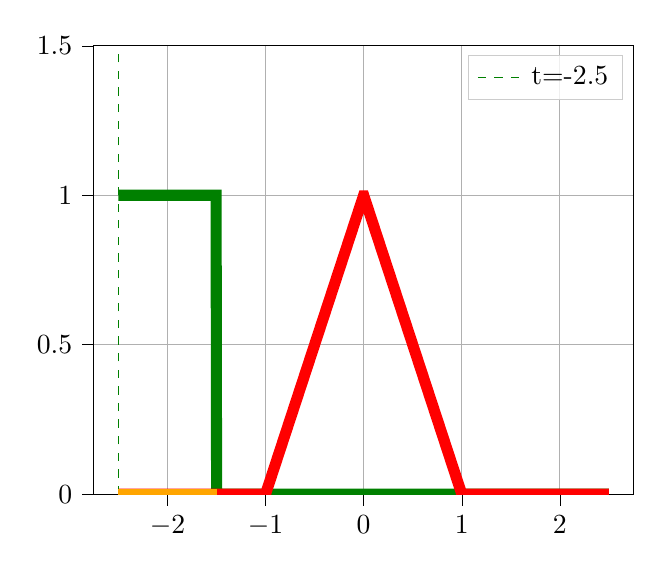
\begin{tikzpicture}

\definecolor{color0}{rgb}{1,0.498039215686275,0.0549019607843137}
\definecolor{color1}{rgb}{1,0.647058823529412,0}

\begin{axis}[
legend cell align={left},
legend style={fill opacity=0.8, draw opacity=1, text opacity=1, draw=white!80!black},
tick align=outside,
tick pos=left,
x grid style={white!69.0196078431373!black},
xmajorgrids,
xmin=-2.75, xmax=2.75,
xtick style={color=black},
y grid style={white!69.0196078431373!black},
ymajorgrids,
ymin=0, ymax=1.5,
ytick style={color=black}
]
\path [draw=color0, fill=color0, opacity=0.2]
(axis cs:-2.5,0)
--(axis cs:-2.5,0)
--(axis cs:-2.49499499499499,0)
--(axis cs:-2.48998998998999,0)
--(axis cs:-2.48498498498498,0)
--(axis cs:-2.47997997997998,0)
--(axis cs:-2.47497497497497,0)
--(axis cs:-2.46996996996997,0)
--(axis cs:-2.46496496496496,0)
--(axis cs:-2.45995995995996,0)
--(axis cs:-2.45495495495495,0)
--(axis cs:-2.44994994994995,0)
--(axis cs:-2.44494494494494,0)
--(axis cs:-2.43993993993994,0)
--(axis cs:-2.43493493493493,0)
--(axis cs:-2.42992992992993,0)
--(axis cs:-2.42492492492492,0)
--(axis cs:-2.41991991991992,0)
--(axis cs:-2.41491491491491,0)
--(axis cs:-2.40990990990991,0)
--(axis cs:-2.4049049049049,0)
--(axis cs:-2.3998998998999,0)
--(axis cs:-2.39489489489489,0)
--(axis cs:-2.38988988988989,0)
--(axis cs:-2.38488488488488,0)
--(axis cs:-2.37987987987988,0)
--(axis cs:-2.37487487487487,0)
--(axis cs:-2.36986986986987,0)
--(axis cs:-2.36486486486486,0)
--(axis cs:-2.35985985985986,0)
--(axis cs:-2.35485485485485,0)
--(axis cs:-2.34984984984985,0)
--(axis cs:-2.34484484484484,0)
--(axis cs:-2.33983983983984,0)
--(axis cs:-2.33483483483483,0)
--(axis cs:-2.32982982982983,0)
--(axis cs:-2.32482482482482,0)
--(axis cs:-2.31981981981982,0)
--(axis cs:-2.31481481481481,0)
--(axis cs:-2.30980980980981,0)
--(axis cs:-2.3048048048048,0)
--(axis cs:-2.2997997997998,0)
--(axis cs:-2.29479479479479,0)
--(axis cs:-2.28978978978979,0)
--(axis cs:-2.28478478478478,0)
--(axis cs:-2.27977977977978,0)
--(axis cs:-2.27477477477477,0)
--(axis cs:-2.26976976976977,0)
--(axis cs:-2.26476476476476,0)
--(axis cs:-2.25975975975976,0)
--(axis cs:-2.25475475475475,0)
--(axis cs:-2.24974974974975,0)
--(axis cs:-2.24474474474474,0)
--(axis cs:-2.23973973973974,0)
--(axis cs:-2.23473473473473,0)
--(axis cs:-2.22972972972973,0)
--(axis cs:-2.22472472472472,0)
--(axis cs:-2.21971971971972,0)
--(axis cs:-2.21471471471471,0)
--(axis cs:-2.20970970970971,0)
--(axis cs:-2.2047047047047,0)
--(axis cs:-2.1996996996997,0)
--(axis cs:-2.19469469469469,0)
--(axis cs:-2.18968968968969,0)
--(axis cs:-2.18468468468468,0)
--(axis cs:-2.17967967967968,0)
--(axis cs:-2.17467467467467,0)
--(axis cs:-2.16966966966967,0)
--(axis cs:-2.16466466466466,0)
--(axis cs:-2.15965965965966,0)
--(axis cs:-2.15465465465465,0)
--(axis cs:-2.14964964964965,0)
--(axis cs:-2.14464464464464,0)
--(axis cs:-2.13963963963964,0)
--(axis cs:-2.13463463463463,0)
--(axis cs:-2.12962962962963,0)
--(axis cs:-2.12462462462462,0)
--(axis cs:-2.11961961961962,0)
--(axis cs:-2.11461461461461,0)
--(axis cs:-2.10960960960961,0)
--(axis cs:-2.1046046046046,0)
--(axis cs:-2.0995995995996,0)
--(axis cs:-2.09459459459459,0)
--(axis cs:-2.08958958958959,0)
--(axis cs:-2.08458458458458,0)
--(axis cs:-2.07957957957958,0)
--(axis cs:-2.07457457457457,0)
--(axis cs:-2.06956956956957,0)
--(axis cs:-2.06456456456456,0)
--(axis cs:-2.05955955955956,0)
--(axis cs:-2.05455455455455,0)
--(axis cs:-2.04954954954955,0)
--(axis cs:-2.04454454454454,0)
--(axis cs:-2.03953953953954,0)
--(axis cs:-2.03453453453453,0)
--(axis cs:-2.02952952952953,0)
--(axis cs:-2.02452452452452,0)
--(axis cs:-2.01951951951952,0)
--(axis cs:-2.01451451451451,0)
--(axis cs:-2.00950950950951,0)
--(axis cs:-2.0045045045045,0)
--(axis cs:-1.9994994994995,0)
--(axis cs:-1.99449449449449,0)
--(axis cs:-1.98948948948949,0)
--(axis cs:-1.98448448448448,0)
--(axis cs:-1.97947947947948,0)
--(axis cs:-1.97447447447447,0)
--(axis cs:-1.96946946946947,0)
--(axis cs:-1.96446446446446,0)
--(axis cs:-1.95945945945946,0)
--(axis cs:-1.95445445445445,0)
--(axis cs:-1.94944944944945,0)
--(axis cs:-1.94444444444444,0)
--(axis cs:-1.93943943943944,0)
--(axis cs:-1.93443443443443,0)
--(axis cs:-1.92942942942943,0)
--(axis cs:-1.92442442442442,0)
--(axis cs:-1.91941941941942,0)
--(axis cs:-1.91441441441441,0)
--(axis cs:-1.90940940940941,0)
--(axis cs:-1.9044044044044,0)
--(axis cs:-1.8993993993994,0)
--(axis cs:-1.89439439439439,0)
--(axis cs:-1.88938938938939,0)
--(axis cs:-1.88438438438438,0)
--(axis cs:-1.87937937937938,0)
--(axis cs:-1.87437437437437,0)
--(axis cs:-1.86936936936937,0)
--(axis cs:-1.86436436436436,0)
--(axis cs:-1.85935935935936,0)
--(axis cs:-1.85435435435435,0)
--(axis cs:-1.84934934934935,0)
--(axis cs:-1.84434434434434,0)
--(axis cs:-1.83933933933934,0)
--(axis cs:-1.83433433433433,0)
--(axis cs:-1.82932932932933,0)
--(axis cs:-1.82432432432432,0)
--(axis cs:-1.81931931931932,0)
--(axis cs:-1.81431431431431,0)
--(axis cs:-1.80930930930931,0)
--(axis cs:-1.8043043043043,0)
--(axis cs:-1.7992992992993,0)
--(axis cs:-1.79429429429429,0)
--(axis cs:-1.78928928928929,0)
--(axis cs:-1.78428428428428,0)
--(axis cs:-1.77927927927928,0)
--(axis cs:-1.77427427427427,0)
--(axis cs:-1.76926926926927,0)
--(axis cs:-1.76426426426426,0)
--(axis cs:-1.75925925925926,0)
--(axis cs:-1.75425425425425,0)
--(axis cs:-1.74924924924925,0)
--(axis cs:-1.74424424424424,0)
--(axis cs:-1.73923923923924,0)
--(axis cs:-1.73423423423423,0)
--(axis cs:-1.72922922922923,0)
--(axis cs:-1.72422422422422,0)
--(axis cs:-1.71921921921922,0)
--(axis cs:-1.71421421421421,0)
--(axis cs:-1.70920920920921,0)
--(axis cs:-1.7042042042042,0)
--(axis cs:-1.6991991991992,0)
--(axis cs:-1.69419419419419,0)
--(axis cs:-1.68918918918919,0)
--(axis cs:-1.68418418418418,0)
--(axis cs:-1.67917917917918,0)
--(axis cs:-1.67417417417417,0)
--(axis cs:-1.66916916916917,0)
--(axis cs:-1.66416416416416,0)
--(axis cs:-1.65915915915916,0)
--(axis cs:-1.65415415415415,0)
--(axis cs:-1.64914914914915,0)
--(axis cs:-1.64414414414414,0)
--(axis cs:-1.63913913913914,0)
--(axis cs:-1.63413413413413,0)
--(axis cs:-1.62912912912913,0)
--(axis cs:-1.62412412412412,0)
--(axis cs:-1.61911911911912,0)
--(axis cs:-1.61411411411411,0)
--(axis cs:-1.60910910910911,0)
--(axis cs:-1.6041041041041,0)
--(axis cs:-1.5990990990991,0)
--(axis cs:-1.59409409409409,0)
--(axis cs:-1.58908908908909,0)
--(axis cs:-1.58408408408408,0)
--(axis cs:-1.57907907907908,0)
--(axis cs:-1.57407407407407,0)
--(axis cs:-1.56906906906907,0)
--(axis cs:-1.56406406406406,0)
--(axis cs:-1.55905905905906,0)
--(axis cs:-1.55405405405405,0)
--(axis cs:-1.54904904904905,0)
--(axis cs:-1.54404404404404,0)
--(axis cs:-1.53903903903904,0)
--(axis cs:-1.53403403403403,0)
--(axis cs:-1.52902902902903,0)
--(axis cs:-1.52402402402402,0)
--(axis cs:-1.51901901901902,0)
--(axis cs:-1.51401401401401,0)
--(axis cs:-1.50900900900901,0)
--(axis cs:-1.504004004004,0)
--(axis cs:-1.504004004004,0)
--(axis cs:-1.504004004004,0)
--(axis cs:-1.50900900900901,0)
--(axis cs:-1.51401401401401,0)
--(axis cs:-1.51901901901902,0)
--(axis cs:-1.52402402402402,0)
--(axis cs:-1.52902902902903,0)
--(axis cs:-1.53403403403403,0)
--(axis cs:-1.53903903903904,0)
--(axis cs:-1.54404404404404,0)
--(axis cs:-1.54904904904905,0)
--(axis cs:-1.55405405405405,0)
--(axis cs:-1.55905905905906,0)
--(axis cs:-1.56406406406406,0)
--(axis cs:-1.56906906906907,0)
--(axis cs:-1.57407407407407,0)
--(axis cs:-1.57907907907908,0)
--(axis cs:-1.58408408408408,0)
--(axis cs:-1.58908908908909,0)
--(axis cs:-1.59409409409409,0)
--(axis cs:-1.5990990990991,0)
--(axis cs:-1.6041041041041,0)
--(axis cs:-1.60910910910911,0)
--(axis cs:-1.61411411411411,0)
--(axis cs:-1.61911911911912,0)
--(axis cs:-1.62412412412412,0)
--(axis cs:-1.62912912912913,0)
--(axis cs:-1.63413413413413,0)
--(axis cs:-1.63913913913914,0)
--(axis cs:-1.64414414414414,0)
--(axis cs:-1.64914914914915,0)
--(axis cs:-1.65415415415415,0)
--(axis cs:-1.65915915915916,0)
--(axis cs:-1.66416416416416,0)
--(axis cs:-1.66916916916917,0)
--(axis cs:-1.67417417417417,0)
--(axis cs:-1.67917917917918,0)
--(axis cs:-1.68418418418418,0)
--(axis cs:-1.68918918918919,0)
--(axis cs:-1.69419419419419,0)
--(axis cs:-1.6991991991992,0)
--(axis cs:-1.7042042042042,0)
--(axis cs:-1.70920920920921,0)
--(axis cs:-1.71421421421421,0)
--(axis cs:-1.71921921921922,0)
--(axis cs:-1.72422422422422,0)
--(axis cs:-1.72922922922923,0)
--(axis cs:-1.73423423423423,0)
--(axis cs:-1.73923923923924,0)
--(axis cs:-1.74424424424424,0)
--(axis cs:-1.74924924924925,0)
--(axis cs:-1.75425425425425,0)
--(axis cs:-1.75925925925926,0)
--(axis cs:-1.76426426426426,0)
--(axis cs:-1.76926926926927,0)
--(axis cs:-1.77427427427427,0)
--(axis cs:-1.77927927927928,0)
--(axis cs:-1.78428428428428,0)
--(axis cs:-1.78928928928929,0)
--(axis cs:-1.79429429429429,0)
--(axis cs:-1.7992992992993,0)
--(axis cs:-1.8043043043043,0)
--(axis cs:-1.80930930930931,0)
--(axis cs:-1.81431431431431,0)
--(axis cs:-1.81931931931932,0)
--(axis cs:-1.82432432432432,0)
--(axis cs:-1.82932932932933,0)
--(axis cs:-1.83433433433433,0)
--(axis cs:-1.83933933933934,0)
--(axis cs:-1.84434434434434,0)
--(axis cs:-1.84934934934935,0)
--(axis cs:-1.85435435435435,0)
--(axis cs:-1.85935935935936,0)
--(axis cs:-1.86436436436436,0)
--(axis cs:-1.86936936936937,0)
--(axis cs:-1.87437437437437,0)
--(axis cs:-1.87937937937938,0)
--(axis cs:-1.88438438438438,0)
--(axis cs:-1.88938938938939,0)
--(axis cs:-1.89439439439439,0)
--(axis cs:-1.8993993993994,0)
--(axis cs:-1.9044044044044,0)
--(axis cs:-1.90940940940941,0)
--(axis cs:-1.91441441441441,0)
--(axis cs:-1.91941941941942,0)
--(axis cs:-1.92442442442442,0)
--(axis cs:-1.92942942942943,0)
--(axis cs:-1.93443443443443,0)
--(axis cs:-1.93943943943944,0)
--(axis cs:-1.94444444444444,0)
--(axis cs:-1.94944944944945,0)
--(axis cs:-1.95445445445445,0)
--(axis cs:-1.95945945945946,0)
--(axis cs:-1.96446446446446,0)
--(axis cs:-1.96946946946947,0)
--(axis cs:-1.97447447447447,0)
--(axis cs:-1.97947947947948,0)
--(axis cs:-1.98448448448448,0)
--(axis cs:-1.98948948948949,0)
--(axis cs:-1.99449449449449,0)
--(axis cs:-1.9994994994995,0)
--(axis cs:-2.0045045045045,0)
--(axis cs:-2.00950950950951,0)
--(axis cs:-2.01451451451451,0)
--(axis cs:-2.01951951951952,0)
--(axis cs:-2.02452452452452,0)
--(axis cs:-2.02952952952953,0)
--(axis cs:-2.03453453453453,0)
--(axis cs:-2.03953953953954,0)
--(axis cs:-2.04454454454454,0)
--(axis cs:-2.04954954954955,0)
--(axis cs:-2.05455455455455,0)
--(axis cs:-2.05955955955956,0)
--(axis cs:-2.06456456456456,0)
--(axis cs:-2.06956956956957,0)
--(axis cs:-2.07457457457457,0)
--(axis cs:-2.07957957957958,0)
--(axis cs:-2.08458458458458,0)
--(axis cs:-2.08958958958959,0)
--(axis cs:-2.09459459459459,0)
--(axis cs:-2.0995995995996,0)
--(axis cs:-2.1046046046046,0)
--(axis cs:-2.10960960960961,0)
--(axis cs:-2.11461461461461,0)
--(axis cs:-2.11961961961962,0)
--(axis cs:-2.12462462462462,0)
--(axis cs:-2.12962962962963,0)
--(axis cs:-2.13463463463463,0)
--(axis cs:-2.13963963963964,0)
--(axis cs:-2.14464464464464,0)
--(axis cs:-2.14964964964965,0)
--(axis cs:-2.15465465465465,0)
--(axis cs:-2.15965965965966,0)
--(axis cs:-2.16466466466466,0)
--(axis cs:-2.16966966966967,0)
--(axis cs:-2.17467467467467,0)
--(axis cs:-2.17967967967968,0)
--(axis cs:-2.18468468468468,0)
--(axis cs:-2.18968968968969,0)
--(axis cs:-2.19469469469469,0)
--(axis cs:-2.1996996996997,0)
--(axis cs:-2.2047047047047,0)
--(axis cs:-2.20970970970971,0)
--(axis cs:-2.21471471471471,0)
--(axis cs:-2.21971971971972,0)
--(axis cs:-2.22472472472472,0)
--(axis cs:-2.22972972972973,0)
--(axis cs:-2.23473473473473,0)
--(axis cs:-2.23973973973974,0)
--(axis cs:-2.24474474474474,0)
--(axis cs:-2.24974974974975,0)
--(axis cs:-2.25475475475475,0)
--(axis cs:-2.25975975975976,0)
--(axis cs:-2.26476476476476,0)
--(axis cs:-2.26976976976977,0)
--(axis cs:-2.27477477477477,0)
--(axis cs:-2.27977977977978,0)
--(axis cs:-2.28478478478478,0)
--(axis cs:-2.28978978978979,0)
--(axis cs:-2.29479479479479,0)
--(axis cs:-2.2997997997998,0)
--(axis cs:-2.3048048048048,0)
--(axis cs:-2.30980980980981,0)
--(axis cs:-2.31481481481481,0)
--(axis cs:-2.31981981981982,0)
--(axis cs:-2.32482482482482,0)
--(axis cs:-2.32982982982983,0)
--(axis cs:-2.33483483483483,0)
--(axis cs:-2.33983983983984,0)
--(axis cs:-2.34484484484484,0)
--(axis cs:-2.34984984984985,0)
--(axis cs:-2.35485485485485,0)
--(axis cs:-2.35985985985986,0)
--(axis cs:-2.36486486486486,0)
--(axis cs:-2.36986986986987,0)
--(axis cs:-2.37487487487487,0)
--(axis cs:-2.37987987987988,0)
--(axis cs:-2.38488488488488,0)
--(axis cs:-2.38988988988989,0)
--(axis cs:-2.39489489489489,0)
--(axis cs:-2.3998998998999,0)
--(axis cs:-2.4049049049049,0)
--(axis cs:-2.40990990990991,0)
--(axis cs:-2.41491491491491,0)
--(axis cs:-2.41991991991992,0)
--(axis cs:-2.42492492492492,0)
--(axis cs:-2.42992992992993,0)
--(axis cs:-2.43493493493493,0)
--(axis cs:-2.43993993993994,0)
--(axis cs:-2.44494494494494,0)
--(axis cs:-2.44994994994995,0)
--(axis cs:-2.45495495495495,0)
--(axis cs:-2.45995995995996,0)
--(axis cs:-2.46496496496496,0)
--(axis cs:-2.46996996996997,0)
--(axis cs:-2.47497497497497,0)
--(axis cs:-2.47997997997998,0)
--(axis cs:-2.48498498498498,0)
--(axis cs:-2.48998998998999,0)
--(axis cs:-2.49499499499499,0)
--(axis cs:-2.5,0)
--cycle;

\addplot [line width=4pt, green!50!black, forget plot]
table {%
-2.5 1
-2.49499499499499 1
-2.48998998998999 1
-2.48498498498498 1
-2.47997997997998 1
-2.47497497497497 1
-2.46996996996997 1
-2.46496496496496 1
-2.45995995995996 1
-2.45495495495495 1
-2.44994994994995 1
-2.44494494494494 1
-2.43993993993994 1
-2.43493493493493 1
-2.42992992992993 1
-2.42492492492492 1
-2.41991991991992 1
-2.41491491491491 1
-2.40990990990991 1
-2.4049049049049 1
-2.3998998998999 1
-2.39489489489489 1
-2.38988988988989 1
-2.38488488488488 1
-2.37987987987988 1
-2.37487487487487 1
-2.36986986986987 1
-2.36486486486486 1
-2.35985985985986 1
-2.35485485485485 1
-2.34984984984985 1
-2.34484484484484 1
-2.33983983983984 1
-2.33483483483483 1
-2.32982982982983 1
-2.32482482482482 1
-2.31981981981982 1
-2.31481481481481 1
-2.30980980980981 1
-2.3048048048048 1
-2.2997997997998 1
-2.29479479479479 1
-2.28978978978979 1
-2.28478478478478 1
-2.27977977977978 1
-2.27477477477477 1
-2.26976976976977 1
-2.26476476476476 1
-2.25975975975976 1
-2.25475475475475 1
-2.24974974974975 1
-2.24474474474474 1
-2.23973973973974 1
-2.23473473473473 1
-2.22972972972973 1
-2.22472472472472 1
-2.21971971971972 1
-2.21471471471471 1
-2.20970970970971 1
-2.2047047047047 1
-2.1996996996997 1
-2.19469469469469 1
-2.18968968968969 1
-2.18468468468468 1
-2.17967967967968 1
-2.17467467467467 1
-2.16966966966967 1
-2.16466466466466 1
-2.15965965965966 1
-2.15465465465465 1
-2.14964964964965 1
-2.14464464464464 1
-2.13963963963964 1
-2.13463463463463 1
-2.12962962962963 1
-2.12462462462462 1
-2.11961961961962 1
-2.11461461461461 1
-2.10960960960961 1
-2.1046046046046 1
-2.0995995995996 1
-2.09459459459459 1
-2.08958958958959 1
-2.08458458458458 1
-2.07957957957958 1
-2.07457457457457 1
-2.06956956956957 1
-2.06456456456456 1
-2.05955955955956 1
-2.05455455455455 1
-2.04954954954955 1
-2.04454454454454 1
-2.03953953953954 1
-2.03453453453453 1
-2.02952952952953 1
-2.02452452452452 1
-2.01951951951952 1
-2.01451451451451 1
-2.00950950950951 1
-2.0045045045045 1
-1.9994994994995 1
-1.99449449449449 1
-1.98948948948949 1
-1.98448448448448 1
-1.97947947947948 1
-1.97447447447447 1
-1.96946946946947 1
-1.96446446446446 1
-1.95945945945946 1
-1.95445445445445 1
-1.94944944944945 1
-1.94444444444444 1
-1.93943943943944 1
-1.93443443443443 1
-1.92942942942943 1
-1.92442442442442 1
-1.91941941941942 1
-1.91441441441441 1
-1.90940940940941 1
-1.9044044044044 1
-1.8993993993994 1
-1.89439439439439 1
-1.88938938938939 1
-1.88438438438438 1
-1.87937937937938 1
-1.87437437437437 1
-1.86936936936937 1
-1.86436436436436 1
-1.85935935935936 1
-1.85435435435435 1
-1.84934934934935 1
-1.84434434434434 1
-1.83933933933934 1
-1.83433433433433 1
-1.82932932932933 1
-1.82432432432432 1
-1.81931931931932 1
-1.81431431431431 1
-1.80930930930931 1
-1.8043043043043 1
-1.7992992992993 1
-1.79429429429429 1
-1.78928928928929 1
-1.78428428428428 1
-1.77927927927928 1
-1.77427427427427 1
-1.76926926926927 1
-1.76426426426426 1
-1.75925925925926 1
-1.75425425425425 1
-1.74924924924925 1
-1.74424424424424 1
-1.73923923923924 1
-1.73423423423423 1
-1.72922922922923 1
-1.72422422422422 1
-1.71921921921922 1
-1.71421421421421 1
-1.70920920920921 1
-1.7042042042042 1
-1.6991991991992 1
-1.69419419419419 1
-1.68918918918919 1
-1.68418418418418 1
-1.67917917917918 1
-1.67417417417417 1
-1.66916916916917 1
-1.66416416416416 1
-1.65915915915916 1
-1.65415415415415 1
-1.64914914914915 1
-1.64414414414414 1
-1.63913913913914 1
-1.63413413413413 1
-1.62912912912913 1
-1.62412412412412 1
-1.61911911911912 1
-1.61411411411411 1
-1.60910910910911 1
-1.6041041041041 1
-1.5990990990991 1
-1.59409409409409 1
-1.58908908908909 1
-1.58408408408408 1
-1.57907907907908 1
-1.57407407407407 1
-1.56906906906907 1
-1.56406406406406 1
-1.55905905905906 1
-1.55405405405405 1
-1.54904904904905 1
-1.54404404404404 1
-1.53903903903904 1
-1.53403403403403 1
-1.52902902902903 1
-1.52402402402402 1
-1.51901901901902 1
-1.51401401401401 1
-1.50900900900901 1
-1.504004004004 1
-1.498998998999 0
-1.49399399399399 0
-1.48898898898899 0
-1.48398398398398 0
-1.47897897897898 0
-1.47397397397397 0
-1.46896896896897 0
-1.46396396396396 0
-1.45895895895896 0
-1.45395395395395 0
-1.44894894894895 0
-1.44394394394394 0
-1.43893893893894 0
-1.43393393393393 0
-1.42892892892893 0
-1.42392392392392 0
-1.41891891891892 0
-1.41391391391391 0
-1.40890890890891 0
-1.4039039039039 0
-1.3988988988989 0
-1.39389389389389 0
-1.38888888888889 0
-1.38388388388388 0
-1.37887887887888 0
-1.37387387387387 0
-1.36886886886887 0
-1.36386386386386 0
-1.35885885885886 0
-1.35385385385385 0
-1.34884884884885 0
-1.34384384384384 0
-1.33883883883884 0
-1.33383383383383 0
-1.32882882882883 0
-1.32382382382382 0
-1.31881881881882 0
-1.31381381381381 0
-1.30880880880881 0
-1.3038038038038 0
-1.2987987987988 0
-1.29379379379379 0
-1.28878878878879 0
-1.28378378378378 0
-1.27877877877878 0
-1.27377377377377 0
-1.26876876876877 0
-1.26376376376376 0
-1.25875875875876 0
-1.25375375375375 0
-1.24874874874875 0
-1.24374374374374 0
-1.23873873873874 0
-1.23373373373373 0
-1.22872872872873 0
-1.22372372372372 0
-1.21871871871872 0
-1.21371371371371 0
-1.20870870870871 0
-1.2037037037037 0
-1.1986986986987 0
-1.19369369369369 0
-1.18868868868869 0
-1.18368368368368 0
-1.17867867867868 0
-1.17367367367367 0
-1.16866866866867 0
-1.16366366366366 0
-1.15865865865866 0
-1.15365365365365 0
-1.14864864864865 0
-1.14364364364364 0
-1.13863863863864 0
-1.13363363363363 0
-1.12862862862863 0
-1.12362362362362 0
-1.11861861861862 0
-1.11361361361361 0
-1.10860860860861 0
-1.1036036036036 0
-1.0985985985986 0
-1.09359359359359 0
-1.08858858858859 0
-1.08358358358358 0
-1.07857857857858 0
-1.07357357357357 0
-1.06856856856857 0
-1.06356356356356 0
-1.05855855855856 0
-1.05355355355355 0
-1.04854854854855 0
-1.04354354354354 0
-1.03853853853854 0
-1.03353353353353 0
-1.02852852852853 0
-1.02352352352352 0
-1.01851851851852 0
-1.01351351351351 0
-1.00850850850851 0
-1.0035035035035 0
-0.998498498498499 0
-0.993493493493494 0
-0.988488488488489 0
-0.983483483483484 0
-0.978478478478479 0
-0.973473473473474 0
-0.968468468468469 0
-0.963463463463464 0
-0.958458458458459 0
-0.953453453453454 0
-0.948448448448449 0
-0.943443443443444 0
-0.938438438438439 0
-0.933433433433434 0
-0.928428428428429 0
-0.923423423423424 0
-0.918418418418419 0
-0.913413413413414 0
-0.908408408408409 0
-0.903403403403404 0
-0.898398398398399 0
-0.893393393393393 0
-0.888388388388388 0
-0.883383383383383 0
-0.878378378378378 0
-0.873373373373373 0
-0.868368368368368 0
-0.863363363363363 0
-0.858358358358358 0
-0.853353353353353 0
-0.848348348348348 0
-0.843343343343343 0
-0.838338338338338 0
-0.833333333333333 0
-0.828328328328328 0
-0.823323323323323 0
-0.818318318318318 0
-0.813313313313313 0
-0.808308308308308 0
-0.803303303303303 0
-0.798298298298298 0
-0.793293293293293 0
-0.788288288288288 0
-0.783283283283283 0
-0.778278278278278 0
-0.773273273273273 0
-0.768268268268268 0
-0.763263263263263 0
-0.758258258258258 0
-0.753253253253253 0
-0.748248248248248 0
-0.743243243243243 0
-0.738238238238238 0
-0.733233233233233 0
-0.728228228228228 0
-0.723223223223223 0
-0.718218218218218 0
-0.713213213213213 0
-0.708208208208208 0
-0.703203203203203 0
-0.698198198198198 0
-0.693193193193193 0
-0.688188188188188 0
-0.683183183183183 0
-0.678178178178178 0
-0.673173173173173 0
-0.668168168168168 0
-0.663163163163163 0
-0.658158158158158 0
-0.653153153153153 0
-0.648148148148148 0
-0.643143143143143 0
-0.638138138138138 0
-0.633133133133133 0
-0.628128128128128 0
-0.623123123123123 0
-0.618118118118118 0
-0.613113113113113 0
-0.608108108108108 0
-0.603103103103103 0
-0.598098098098098 0
-0.593093093093093 0
-0.588088088088088 0
-0.583083083083083 0
-0.578078078078078 0
-0.573073073073073 0
-0.568068068068068 0
-0.563063063063063 0
-0.558058058058058 0
-0.553053053053053 0
-0.548048048048048 0
-0.543043043043043 0
-0.538038038038038 0
-0.533033033033033 0
-0.528028028028028 0
-0.523023023023023 0
-0.518018018018018 0
-0.513013013013013 0
-0.508008008008008 0
-0.503003003003003 0
-0.497997997997998 0
-0.492992992992993 0
-0.487987987987988 0
-0.482982982982983 0
-0.477977977977978 0
-0.472972972972973 0
-0.467967967967968 0
-0.462962962962963 0
-0.457957957957958 0
-0.452952952952953 0
-0.447947947947948 0
-0.442942942942943 0
-0.437937937937938 0
-0.432932932932933 0
-0.427927927927928 0
-0.422922922922923 0
-0.417917917917918 0
-0.412912912912913 0
-0.407907907907908 0
-0.402902902902903 0
-0.397897897897898 0
-0.392892892892893 0
-0.387887887887888 0
-0.382882882882883 0
-0.377877877877878 0
-0.372872872872873 0
-0.367867867867868 0
-0.362862862862863 0
-0.357857857857858 0
-0.352852852852853 0
-0.347847847847848 0
-0.342842842842843 0
-0.337837837837838 0
-0.332832832832833 0
-0.327827827827828 0
-0.322822822822823 0
-0.317817817817818 0
-0.312812812812813 0
-0.307807807807808 0
-0.302802802802803 0
-0.297797797797798 0
-0.292792792792793 0
-0.287787787787788 0
-0.282782782782783 0
-0.277777777777778 0
-0.272772772772773 0
-0.267767767767768 0
-0.262762762762763 0
-0.257757757757758 0
-0.252752752752753 0
-0.247747747747748 0
-0.242742742742743 0
-0.237737737737738 0
-0.232732732732733 0
-0.227727727727728 0
-0.222722722722723 0
-0.217717717717718 0
-0.212712712712713 0
-0.207707707707708 0
-0.202702702702703 0
-0.197697697697698 0
-0.192692692692693 0
-0.187687687687688 0
-0.182682682682683 0
-0.177677677677678 0
-0.172672672672673 0
-0.167667667667668 0
-0.162662662662663 0
-0.157657657657658 0
-0.152652652652653 0
-0.147647647647648 0
-0.142642642642643 0
-0.137637637637638 0
-0.132632632632633 0
-0.127627627627628 0
-0.122622622622623 0
-0.117617617617618 0
-0.112612612612613 0
-0.107607607607608 0
-0.102602602602603 0
-0.0975975975975976 0
-0.0925925925925926 0
-0.0875875875875876 0
-0.0825825825825826 0
-0.0775775775775776 0
-0.0725725725725725 0
-0.0675675675675675 0
-0.0625625625625625 0
-0.0575575575575575 0
-0.0525525525525525 0
-0.0475475475475475 0
-0.0425425425425425 0
-0.0375375375375375 0
-0.0325325325325325 0
-0.0275275275275275 0
-0.0225225225225225 0
-0.0175175175175175 0
-0.0125125125125125 0
-0.0075075075075075 0
-0.0025025025025025 0
0.0025025025025025 0
0.0075075075075075 0
0.0125125125125125 0
0.0175175175175175 0
0.0225225225225225 0
0.0275275275275275 0
0.0325325325325325 0
0.0375375375375375 0
0.0425425425425425 0
0.0475475475475475 0
0.0525525525525525 0
0.0575575575575575 0
0.0625625625625625 0
0.0675675675675675 0
0.0725725725725725 0
0.0775775775775776 0
0.0825825825825826 0
0.0875875875875876 0
0.0925925925925926 0
0.0975975975975976 0
0.102602602602603 0
0.107607607607608 0
0.112612612612613 0
0.117617617617618 0
0.122622622622623 0
0.127627627627628 0
0.132632632632633 0
0.137637637637638 0
0.142642642642643 0
0.147647647647648 0
0.152652652652653 0
0.157657657657658 0
0.162662662662663 0
0.167667667667668 0
0.172672672672673 0
0.177677677677678 0
0.182682682682683 0
0.187687687687688 0
0.192692692692693 0
0.197697697697698 0
0.202702702702703 0
0.207707707707708 0
0.212712712712713 0
0.217717717717718 0
0.222722722722723 0
0.227727727727728 0
0.232732732732733 0
0.237737737737738 0
0.242742742742743 0
0.247747747747748 0
0.252752752752753 0
0.257757757757758 0
0.262762762762763 0
0.267767767767768 0
0.272772772772773 0
0.277777777777778 0
0.282782782782783 0
0.287787787787788 0
0.292792792792793 0
0.297797797797798 0
0.302802802802803 0
0.307807807807808 0
0.312812812812813 0
0.317817817817818 0
0.322822822822823 0
0.327827827827828 0
0.332832832832833 0
0.337837837837838 0
0.342842842842843 0
0.347847847847848 0
0.352852852852853 0
0.357857857857858 0
0.362862862862863 0
0.367867867867868 0
0.372872872872873 0
0.377877877877878 0
0.382882882882883 0
0.387887887887888 0
0.392892892892893 0
0.397897897897898 0
0.402902902902903 0
0.407907907907908 0
0.412912912912913 0
0.417917917917918 0
0.422922922922923 0
0.427927927927928 0
0.432932932932933 0
0.437937937937938 0
0.442942942942943 0
0.447947947947948 0
0.452952952952953 0
0.457957957957958 0
0.462962962962963 0
0.467967967967968 0
0.472972972972973 0
0.477977977977978 0
0.482982982982983 0
0.487987987987988 0
0.492992992992993 0
0.497997997997998 0
0.503003003003003 0
0.508008008008008 0
0.513013013013013 0
0.518018018018018 0
0.523023023023023 0
0.528028028028028 0
0.533033033033033 0
0.538038038038038 0
0.543043043043043 0
0.548048048048048 0
0.553053053053053 0
0.558058058058058 0
0.563063063063063 0
0.568068068068068 0
0.573073073073073 0
0.578078078078078 0
0.583083083083083 0
0.588088088088088 0
0.593093093093093 0
0.598098098098098 0
0.603103103103103 0
0.608108108108108 0
0.613113113113113 0
0.618118118118118 0
0.623123123123123 0
0.628128128128128 0
0.633133133133133 0
0.638138138138138 0
0.643143143143143 0
0.648148148148148 0
0.653153153153153 0
0.658158158158158 0
0.663163163163163 0
0.668168168168168 0
0.673173173173173 0
0.678178178178178 0
0.683183183183183 0
0.688188188188188 0
0.693193193193193 0
0.698198198198198 0
0.703203203203203 0
0.708208208208208 0
0.713213213213213 0
0.718218218218218 0
0.723223223223223 0
0.728228228228228 0
0.733233233233233 0
0.738238238238238 0
0.743243243243243 0
0.748248248248248 0
0.753253253253253 0
0.758258258258258 0
0.763263263263263 0
0.768268268268268 0
0.773273273273273 0
0.778278278278278 0
0.783283283283283 0
0.788288288288288 0
0.793293293293293 0
0.798298298298298 0
0.803303303303303 0
0.808308308308308 0
0.813313313313313 0
0.818318318318318 0
0.823323323323323 0
0.828328328328328 0
0.833333333333333 0
0.838338338338338 0
0.843343343343343 0
0.848348348348348 0
0.853353353353353 0
0.858358358358358 0
0.863363363363364 0
0.868368368368369 0
0.873373373373374 0
0.878378378378379 0
0.883383383383384 0
0.888388388388389 0
0.893393393393394 0
0.898398398398399 0
0.903403403403404 0
0.908408408408409 0
0.913413413413414 0
0.918418418418419 0
0.923423423423424 0
0.928428428428429 0
0.933433433433434 0
0.938438438438439 0
0.943443443443444 0
0.948448448448449 0
0.953453453453454 0
0.958458458458459 0
0.963463463463464 0
0.968468468468469 0
0.973473473473474 0
0.978478478478479 0
0.983483483483484 0
0.988488488488489 0
0.993493493493494 0
0.998498498498499 0
1.0035035035035 0
1.00850850850851 0
1.01351351351351 0
1.01851851851852 0
1.02352352352352 0
1.02852852852853 0
1.03353353353353 0
1.03853853853854 0
1.04354354354354 0
1.04854854854855 0
1.05355355355355 0
1.05855855855856 0
1.06356356356356 0
1.06856856856857 0
1.07357357357357 0
1.07857857857858 0
1.08358358358358 0
1.08858858858859 0
1.09359359359359 0
1.0985985985986 0
1.1036036036036 0
1.10860860860861 0
1.11361361361361 0
1.11861861861862 0
1.12362362362362 0
1.12862862862863 0
1.13363363363363 0
1.13863863863864 0
1.14364364364364 0
1.14864864864865 0
1.15365365365365 0
1.15865865865866 0
1.16366366366366 0
1.16866866866867 0
1.17367367367367 0
1.17867867867868 0
1.18368368368368 0
1.18868868868869 0
1.19369369369369 0
1.1986986986987 0
1.2037037037037 0
1.20870870870871 0
1.21371371371371 0
1.21871871871872 0
1.22372372372372 0
1.22872872872873 0
1.23373373373373 0
1.23873873873874 0
1.24374374374374 0
1.24874874874875 0
1.25375375375375 0
1.25875875875876 0
1.26376376376376 0
1.26876876876877 0
1.27377377377377 0
1.27877877877878 0
1.28378378378378 0
1.28878878878879 0
1.29379379379379 0
1.2987987987988 0
1.3038038038038 0
1.30880880880881 0
1.31381381381381 0
1.31881881881882 0
1.32382382382382 0
1.32882882882883 0
1.33383383383383 0
1.33883883883884 0
1.34384384384384 0
1.34884884884885 0
1.35385385385385 0
1.35885885885886 0
1.36386386386386 0
1.36886886886887 0
1.37387387387387 0
1.37887887887888 0
1.38388388388388 0
1.38888888888889 0
1.39389389389389 0
1.3988988988989 0
1.4039039039039 0
1.40890890890891 0
1.41391391391391 0
1.41891891891892 0
1.42392392392392 0
1.42892892892893 0
1.43393393393393 0
1.43893893893894 0
1.44394394394394 0
1.44894894894895 0
1.45395395395395 0
1.45895895895896 0
1.46396396396396 0
1.46896896896897 0
1.47397397397397 0
1.47897897897898 0
1.48398398398398 0
1.48898898898899 0
1.49399399399399 0
1.498998998999 0
1.504004004004 0
1.50900900900901 0
1.51401401401401 0
1.51901901901902 0
1.52402402402402 0
1.52902902902903 0
1.53403403403403 0
1.53903903903904 0
1.54404404404404 0
1.54904904904905 0
1.55405405405405 0
1.55905905905906 0
1.56406406406406 0
1.56906906906907 0
1.57407407407407 0
1.57907907907908 0
1.58408408408408 0
1.58908908908909 0
1.59409409409409 0
1.5990990990991 0
1.6041041041041 0
1.60910910910911 0
1.61411411411411 0
1.61911911911912 0
1.62412412412412 0
1.62912912912913 0
1.63413413413413 0
1.63913913913914 0
1.64414414414414 0
1.64914914914915 0
1.65415415415415 0
1.65915915915916 0
1.66416416416416 0
1.66916916916917 0
1.67417417417417 0
1.67917917917918 0
1.68418418418418 0
1.68918918918919 0
1.69419419419419 0
1.6991991991992 0
1.7042042042042 0
1.70920920920921 0
1.71421421421421 0
1.71921921921922 0
1.72422422422422 0
1.72922922922923 0
1.73423423423423 0
1.73923923923924 0
1.74424424424424 0
1.74924924924925 0
1.75425425425425 0
1.75925925925926 0
1.76426426426426 0
1.76926926926927 0
1.77427427427427 0
1.77927927927928 0
1.78428428428428 0
1.78928928928929 0
1.79429429429429 0
1.7992992992993 0
1.8043043043043 0
1.80930930930931 0
1.81431431431431 0
1.81931931931932 0
1.82432432432432 0
1.82932932932933 0
1.83433433433433 0
1.83933933933934 0
1.84434434434434 0
1.84934934934935 0
1.85435435435435 0
1.85935935935936 0
1.86436436436436 0
1.86936936936937 0
1.87437437437437 0
1.87937937937938 0
1.88438438438438 0
1.88938938938939 0
1.89439439439439 0
1.8993993993994 0
1.9044044044044 0
1.90940940940941 0
1.91441441441441 0
1.91941941941942 0
1.92442442442442 0
1.92942942942943 0
1.93443443443443 0
1.93943943943944 0
1.94444444444444 0
1.94944944944945 0
1.95445445445445 0
1.95945945945946 0
1.96446446446446 0
1.96946946946947 0
1.97447447447447 0
1.97947947947948 0
1.98448448448448 0
1.98948948948949 0
1.99449449449449 0
1.9994994994995 0
2.0045045045045 0
2.00950950950951 0
2.01451451451451 0
2.01951951951952 0
2.02452452452452 0
2.02952952952953 0
2.03453453453453 0
2.03953953953954 0
2.04454454454454 0
2.04954954954955 0
2.05455455455455 0
2.05955955955956 0
2.06456456456456 0
2.06956956956957 0
2.07457457457457 0
2.07957957957958 0
2.08458458458458 0
2.08958958958959 0
2.09459459459459 0
2.0995995995996 0
2.1046046046046 0
2.10960960960961 0
2.11461461461461 0
2.11961961961962 0
2.12462462462462 0
2.12962962962963 0
2.13463463463463 0
2.13963963963964 0
2.14464464464464 0
2.14964964964965 0
2.15465465465465 0
2.15965965965966 0
2.16466466466466 0
2.16966966966967 0
2.17467467467467 0
2.17967967967968 0
2.18468468468468 0
2.18968968968969 0
2.19469469469469 0
2.1996996996997 0
2.2047047047047 0
2.20970970970971 0
2.21471471471471 0
2.21971971971972 0
2.22472472472472 0
2.22972972972973 0
2.23473473473473 0
2.23973973973974 0
2.24474474474474 0
2.24974974974975 0
2.25475475475475 0
2.25975975975976 0
2.26476476476476 0
2.26976976976977 0
2.27477477477477 0
2.27977977977978 0
2.28478478478478 0
2.28978978978979 0
2.29479479479479 0
2.2997997997998 0
2.3048048048048 0
2.30980980980981 0
2.31481481481481 0
2.31981981981982 0
2.32482482482482 0
2.32982982982983 0
2.33483483483483 0
2.33983983983984 0
2.34484484484484 0
2.34984984984985 0
2.35485485485485 0
2.35985985985986 0
2.36486486486486 0
2.36986986986987 0
2.37487487487487 0
2.37987987987988 0
2.38488488488488 0
2.38988988988989 0
2.39489489489489 0
2.3998998998999 0
2.4049049049049 0
2.40990990990991 0
2.41491491491491 0
2.41991991991992 0
2.42492492492492 0
2.42992992992993 0
2.43493493493493 0
2.43993993993994 0
2.44494494494494 0
2.44994994994995 0
2.45495495495495 0
2.45995995995996 0
2.46496496496496 0
2.46996996996997 0
2.47497497497497 0
2.47997997997998 0
2.48498498498498 0
2.48998998998999 0
2.49499499499499 0
2.5 0
};
\addplot [line width=4pt, red, forget plot]
table {%
-2.5 -0
-2.49499499499499 -0
-2.48998998998999 -0
-2.48498498498498 -0
-2.47997997997998 -0
-2.47497497497497 -0
-2.46996996996997 -0
-2.46496496496496 -0
-2.45995995995996 -0
-2.45495495495495 -0
-2.44994994994995 -0
-2.44494494494494 -0
-2.43993993993994 -0
-2.43493493493493 -0
-2.42992992992993 -0
-2.42492492492492 -0
-2.41991991991992 -0
-2.41491491491491 -0
-2.40990990990991 -0
-2.4049049049049 -0
-2.3998998998999 -0
-2.39489489489489 -0
-2.38988988988989 -0
-2.38488488488488 -0
-2.37987987987988 -0
-2.37487487487487 -0
-2.36986986986987 -0
-2.36486486486486 -0
-2.35985985985986 -0
-2.35485485485485 -0
-2.34984984984985 -0
-2.34484484484484 -0
-2.33983983983984 -0
-2.33483483483483 -0
-2.32982982982983 -0
-2.32482482482482 -0
-2.31981981981982 -0
-2.31481481481481 -0
-2.30980980980981 -0
-2.3048048048048 -0
-2.2997997997998 -0
-2.29479479479479 -0
-2.28978978978979 -0
-2.28478478478478 -0
-2.27977977977978 -0
-2.27477477477477 -0
-2.26976976976977 -0
-2.26476476476476 -0
-2.25975975975976 -0
-2.25475475475475 -0
-2.24974974974975 -0
-2.24474474474474 -0
-2.23973973973974 -0
-2.23473473473473 -0
-2.22972972972973 -0
-2.22472472472472 -0
-2.21971971971972 -0
-2.21471471471471 -0
-2.20970970970971 -0
-2.2047047047047 -0
-2.1996996996997 -0
-2.19469469469469 -0
-2.18968968968969 -0
-2.18468468468468 -0
-2.17967967967968 -0
-2.17467467467467 -0
-2.16966966966967 -0
-2.16466466466466 -0
-2.15965965965966 -0
-2.15465465465465 -0
-2.14964964964965 -0
-2.14464464464464 -0
-2.13963963963964 -0
-2.13463463463463 -0
-2.12962962962963 -0
-2.12462462462462 -0
-2.11961961961962 -0
-2.11461461461461 -0
-2.10960960960961 -0
-2.1046046046046 -0
-2.0995995995996 -0
-2.09459459459459 -0
-2.08958958958959 -0
-2.08458458458458 -0
-2.07957957957958 -0
-2.07457457457457 -0
-2.06956956956957 -0
-2.06456456456456 -0
-2.05955955955956 -0
-2.05455455455455 -0
-2.04954954954955 -0
-2.04454454454454 -0
-2.03953953953954 -0
-2.03453453453453 -0
-2.02952952952953 -0
-2.02452452452452 -0
-2.01951951951952 -0
-2.01451451451451 -0
-2.00950950950951 -0
-2.0045045045045 -0
-1.9994994994995 -0
-1.99449449449449 -0
-1.98948948948949 -0
-1.98448448448448 -0
-1.97947947947948 -0
-1.97447447447447 -0
-1.96946946946947 -0
-1.96446446446446 -0
-1.95945945945946 -0
-1.95445445445445 -0
-1.94944944944945 -0
-1.94444444444444 -0
-1.93943943943944 -0
-1.93443443443443 -0
-1.92942942942943 -0
-1.92442442442442 -0
-1.91941941941942 -0
-1.91441441441441 -0
-1.90940940940941 -0
-1.9044044044044 -0
-1.8993993993994 -0
-1.89439439439439 -0
-1.88938938938939 -0
-1.88438438438438 -0
-1.87937937937938 -0
-1.87437437437437 -0
-1.86936936936937 -0
-1.86436436436436 -0
-1.85935935935936 -0
-1.85435435435435 -0
-1.84934934934935 -0
-1.84434434434434 -0
-1.83933933933934 -0
-1.83433433433433 -0
-1.82932932932933 -0
-1.82432432432432 -0
-1.81931931931932 -0
-1.81431431431431 -0
-1.80930930930931 -0
-1.8043043043043 -0
-1.7992992992993 -0
-1.79429429429429 -0
-1.78928928928929 -0
-1.78428428428428 -0
-1.77927927927928 -0
-1.77427427427427 -0
-1.76926926926927 -0
-1.76426426426426 -0
-1.75925925925926 -0
-1.75425425425425 -0
-1.74924924924925 -0
-1.74424424424424 -0
-1.73923923923924 -0
-1.73423423423423 -0
-1.72922922922923 -0
-1.72422422422422 -0
-1.71921921921922 -0
-1.71421421421421 -0
-1.70920920920921 -0
-1.7042042042042 -0
-1.6991991991992 -0
-1.69419419419419 -0
-1.68918918918919 -0
-1.68418418418418 -0
-1.67917917917918 -0
-1.67417417417417 -0
-1.66916916916917 -0
-1.66416416416416 -0
-1.65915915915916 -0
-1.65415415415415 -0
-1.64914914914915 -0
-1.64414414414414 -0
-1.63913913913914 -0
-1.63413413413413 -0
-1.62912912912913 -0
-1.62412412412412 -0
-1.61911911911912 -0
-1.61411411411411 -0
-1.60910910910911 -0
-1.6041041041041 -0
-1.5990990990991 -0
-1.59409409409409 -0
-1.58908908908909 -0
-1.58408408408408 -0
-1.57907907907908 -0
-1.57407407407407 -0
-1.56906906906907 -0
-1.56406406406406 -0
-1.55905905905906 -0
-1.55405405405405 -0
-1.54904904904905 -0
-1.54404404404404 -0
-1.53903903903904 -0
-1.53403403403403 -0
-1.52902902902903 -0
-1.52402402402402 -0
-1.51901901901902 -0
-1.51401401401401 -0
-1.50900900900901 -0
-1.504004004004 -0
-1.498998998999 -0
-1.49399399399399 -0
-1.48898898898899 -0
-1.48398398398398 -0
-1.47897897897898 -0
-1.47397397397397 -0
-1.46896896896897 -0
-1.46396396396396 -0
-1.45895895895896 -0
-1.45395395395395 -0
-1.44894894894895 -0
-1.44394394394394 -0
-1.43893893893894 -0
-1.43393393393393 -0
-1.42892892892893 -0
-1.42392392392392 -0
-1.41891891891892 -0
-1.41391391391391 -0
-1.40890890890891 -0
-1.4039039039039 -0
-1.3988988988989 -0
-1.39389389389389 -0
-1.38888888888889 -0
-1.38388388388388 -0
-1.37887887887888 -0
-1.37387387387387 -0
-1.36886886886887 -0
-1.36386386386386 -0
-1.35885885885886 -0
-1.35385385385385 -0
-1.34884884884885 -0
-1.34384384384384 -0
-1.33883883883884 -0
-1.33383383383383 -0
-1.32882882882883 -0
-1.32382382382382 -0
-1.31881881881882 -0
-1.31381381381381 -0
-1.30880880880881 -0
-1.3038038038038 -0
-1.2987987987988 -0
-1.29379379379379 -0
-1.28878878878879 -0
-1.28378378378378 -0
-1.27877877877878 -0
-1.27377377377377 -0
-1.26876876876877 -0
-1.26376376376376 -0
-1.25875875875876 -0
-1.25375375375375 -0
-1.24874874874875 -0
-1.24374374374374 -0
-1.23873873873874 -0
-1.23373373373373 -0
-1.22872872872873 -0
-1.22372372372372 -0
-1.21871871871872 -0
-1.21371371371371 -0
-1.20870870870871 -0
-1.2037037037037 -0
-1.1986986986987 -0
-1.19369369369369 -0
-1.18868868868869 -0
-1.18368368368368 -0
-1.17867867867868 -0
-1.17367367367367 -0
-1.16866866866867 -0
-1.16366366366366 -0
-1.15865865865866 -0
-1.15365365365365 -0
-1.14864864864865 -0
-1.14364364364364 -0
-1.13863863863864 -0
-1.13363363363363 -0
-1.12862862862863 -0
-1.12362362362362 -0
-1.11861861861862 -0
-1.11361361361361 -0
-1.10860860860861 -0
-1.1036036036036 -0
-1.0985985985986 -0
-1.09359359359359 -0
-1.08858858858859 -0
-1.08358358358358 -0
-1.07857857857858 -0
-1.07357357357357 -0
-1.06856856856857 -0
-1.06356356356356 -0
-1.05855855855856 -0
-1.05355355355355 -0
-1.04854854854855 -0
-1.04354354354354 -0
-1.03853853853854 -0
-1.03353353353353 -0
-1.02852852852853 -0
-1.02352352352352 -0
-1.01851851851852 -0
-1.01351351351351 -0
-1.00850850850851 -0
-1.0035035035035 -0
-0.998498498498499 0.00150150150150141
-0.993493493493494 0.00650650650650642
-0.988488488488489 0.0115115115115114
-0.983483483483484 0.0165165165165164
-0.978478478478479 0.0215215215215214
-0.973473473473474 0.0265265265265264
-0.968468468468469 0.0315315315315314
-0.963463463463464 0.0365365365365364
-0.958458458458459 0.0415415415415414
-0.953453453453454 0.0465465465465464
-0.948448448448449 0.0515515515515514
-0.943443443443444 0.0565565565565564
-0.938438438438439 0.0615615615615615
-0.933433433433434 0.0665665665665665
-0.928428428428429 0.0715715715715715
-0.923423423423424 0.0765765765765765
-0.918418418418419 0.0815815815815815
-0.913413413413414 0.0865865865865865
-0.908408408408409 0.0915915915915915
-0.903403403403404 0.0965965965965965
-0.898398398398399 0.101601601601601
-0.893393393393393 0.106606606606607
-0.888388388388388 0.111611611611612
-0.883383383383383 0.116616616616617
-0.878378378378378 0.121621621621622
-0.873373373373373 0.126626626626627
-0.868368368368368 0.131631631631632
-0.863363363363363 0.136636636636637
-0.858358358358358 0.141641641641642
-0.853353353353353 0.146646646646647
-0.848348348348348 0.151651651651652
-0.843343343343343 0.156656656656657
-0.838338338338338 0.161661661661662
-0.833333333333333 0.166666666666667
-0.828328328328328 0.171671671671672
-0.823323323323323 0.176676676676677
-0.818318318318318 0.181681681681682
-0.813313313313313 0.186686686686687
-0.808308308308308 0.191691691691692
-0.803303303303303 0.196696696696697
-0.798298298298298 0.201701701701702
-0.793293293293293 0.206706706706707
-0.788288288288288 0.211711711711712
-0.783283283283283 0.216716716716717
-0.778278278278278 0.221721721721722
-0.773273273273273 0.226726726726727
-0.768268268268268 0.231731731731732
-0.763263263263263 0.236736736736737
-0.758258258258258 0.241741741741742
-0.753253253253253 0.246746746746747
-0.748248248248248 0.251751751751752
-0.743243243243243 0.256756756756757
-0.738238238238238 0.261761761761762
-0.733233233233233 0.266766766766767
-0.728228228228228 0.271771771771772
-0.723223223223223 0.276776776776777
-0.718218218218218 0.281781781781782
-0.713213213213213 0.286786786786787
-0.708208208208208 0.291791791791792
-0.703203203203203 0.296796796796797
-0.698198198198198 0.301801801801802
-0.693193193193193 0.306806806806807
-0.688188188188188 0.311811811811812
-0.683183183183183 0.316816816816817
-0.678178178178178 0.321821821821822
-0.673173173173173 0.326826826826827
-0.668168168168168 0.331831831831832
-0.663163163163163 0.336836836836837
-0.658158158158158 0.341841841841842
-0.653153153153153 0.346846846846847
-0.648148148148148 0.351851851851852
-0.643143143143143 0.356856856856857
-0.638138138138138 0.361861861861862
-0.633133133133133 0.366866866866867
-0.628128128128128 0.371871871871872
-0.623123123123123 0.376876876876877
-0.618118118118118 0.381881881881882
-0.613113113113113 0.386886886886887
-0.608108108108108 0.391891891891892
-0.603103103103103 0.396896896896897
-0.598098098098098 0.401901901901902
-0.593093093093093 0.406906906906907
-0.588088088088088 0.411911911911912
-0.583083083083083 0.416916916916917
-0.578078078078078 0.421921921921922
-0.573073073073073 0.426926926926927
-0.568068068068068 0.431931931931932
-0.563063063063063 0.436936936936937
-0.558058058058058 0.441941941941942
-0.553053053053053 0.446946946946947
-0.548048048048048 0.451951951951952
-0.543043043043043 0.456956956956957
-0.538038038038038 0.461961961961962
-0.533033033033033 0.466966966966967
-0.528028028028028 0.471971971971972
-0.523023023023023 0.476976976976977
-0.518018018018018 0.481981981981982
-0.513013013013013 0.486986986986987
-0.508008008008008 0.491991991991992
-0.503003003003003 0.496996996996997
-0.497997997997998 0.502002002002002
-0.492992992992993 0.507007007007007
-0.487987987987988 0.512012012012012
-0.482982982982983 0.517017017017017
-0.477977977977978 0.522022022022022
-0.472972972972973 0.527027027027027
-0.467967967967968 0.532032032032032
-0.462962962962963 0.537037037037037
-0.457957957957958 0.542042042042042
-0.452952952952953 0.547047047047047
-0.447947947947948 0.552052052052052
-0.442942942942943 0.557057057057057
-0.437937937937938 0.562062062062062
-0.432932932932933 0.567067067067067
-0.427927927927928 0.572072072072072
-0.422922922922923 0.577077077077077
-0.417917917917918 0.582082082082082
-0.412912912912913 0.587087087087087
-0.407907907907908 0.592092092092092
-0.402902902902903 0.597097097097097
-0.397897897897898 0.602102102102102
-0.392892892892893 0.607107107107107
-0.387887887887888 0.612112112112112
-0.382882882882883 0.617117117117117
-0.377877877877878 0.622122122122122
-0.372872872872873 0.627127127127127
-0.367867867867868 0.632132132132132
-0.362862862862863 0.637137137137137
-0.357857857857858 0.642142142142142
-0.352852852852853 0.647147147147147
-0.347847847847848 0.652152152152152
-0.342842842842843 0.657157157157157
-0.337837837837838 0.662162162162162
-0.332832832832833 0.667167167167167
-0.327827827827828 0.672172172172172
-0.322822822822823 0.677177177177177
-0.317817817817818 0.682182182182182
-0.312812812812813 0.687187187187187
-0.307807807807808 0.692192192192192
-0.302802802802803 0.697197197197197
-0.297797797797798 0.702202202202202
-0.292792792792793 0.707207207207207
-0.287787787787788 0.712212212212212
-0.282782782782783 0.717217217217217
-0.277777777777778 0.722222222222222
-0.272772772772773 0.727227227227227
-0.267767767767768 0.732232232232232
-0.262762762762763 0.737237237237237
-0.257757757757758 0.742242242242242
-0.252752752752753 0.747247247247247
-0.247747747747748 0.752252252252252
-0.242742742742743 0.757257257257257
-0.237737737737738 0.762262262262262
-0.232732732732733 0.767267267267267
-0.227727727727728 0.772272272272272
-0.222722722722723 0.777277277277277
-0.217717717717718 0.782282282282282
-0.212712712712713 0.787287287287287
-0.207707707707708 0.792292292292292
-0.202702702702703 0.797297297297297
-0.197697697697698 0.802302302302302
-0.192692692692693 0.807307307307307
-0.187687687687688 0.812312312312312
-0.182682682682683 0.817317317317317
-0.177677677677678 0.822322322322322
-0.172672672672673 0.827327327327327
-0.167667667667668 0.832332332332332
-0.162662662662663 0.837337337337337
-0.157657657657658 0.842342342342342
-0.152652652652653 0.847347347347347
-0.147647647647648 0.852352352352352
-0.142642642642643 0.857357357357357
-0.137637637637638 0.862362362362362
-0.132632632632633 0.867367367367367
-0.127627627627628 0.872372372372372
-0.122622622622623 0.877377377377377
-0.117617617617618 0.882382382382382
-0.112612612612613 0.887387387387387
-0.107607607607608 0.892392392392392
-0.102602602602603 0.897397397397397
-0.0975975975975976 0.902402402402402
-0.0925925925925926 0.907407407407407
-0.0875875875875876 0.912412412412412
-0.0825825825825826 0.917417417417417
-0.0775775775775776 0.922422422422422
-0.0725725725725725 0.927427427427427
-0.0675675675675675 0.932432432432432
-0.0625625625625625 0.937437437437437
-0.0575575575575575 0.942442442442442
-0.0525525525525525 0.947447447447447
-0.0475475475475475 0.952452452452452
-0.0425425425425425 0.957457457457457
-0.0375375375375375 0.962462462462462
-0.0325325325325325 0.967467467467467
-0.0275275275275275 0.972472472472472
-0.0225225225225225 0.977477477477477
-0.0175175175175175 0.982482482482482
-0.0125125125125125 0.987487487487487
-0.0075075075075075 0.992492492492492
-0.0025025025025025 0.997497497497497
0.0025025025025025 0.997497497497497
0.0075075075075075 0.992492492492492
0.0125125125125125 0.987487487487487
0.0175175175175175 0.982482482482482
0.0225225225225225 0.977477477477477
0.0275275275275275 0.972472472472472
0.0325325325325325 0.967467467467467
0.0375375375375375 0.962462462462462
0.0425425425425425 0.957457457457457
0.0475475475475475 0.952452452452452
0.0525525525525525 0.947447447447447
0.0575575575575575 0.942442442442442
0.0625625625625625 0.937437437437437
0.0675675675675675 0.932432432432432
0.0725725725725725 0.927427427427427
0.0775775775775776 0.922422422422422
0.0825825825825826 0.917417417417417
0.0875875875875876 0.912412412412412
0.0925925925925926 0.907407407407407
0.0975975975975976 0.902402402402402
0.102602602602603 0.897397397397397
0.107607607607608 0.892392392392392
0.112612612612613 0.887387387387387
0.117617617617618 0.882382382382382
0.122622622622623 0.877377377377377
0.127627627627628 0.872372372372372
0.132632632632633 0.867367367367367
0.137637637637638 0.862362362362362
0.142642642642643 0.857357357357357
0.147647647647648 0.852352352352352
0.152652652652653 0.847347347347347
0.157657657657658 0.842342342342342
0.162662662662663 0.837337337337337
0.167667667667668 0.832332332332332
0.172672672672673 0.827327327327327
0.177677677677678 0.822322322322322
0.182682682682683 0.817317317317317
0.187687687687688 0.812312312312312
0.192692692692693 0.807307307307307
0.197697697697698 0.802302302302302
0.202702702702703 0.797297297297297
0.207707707707708 0.792292292292292
0.212712712712713 0.787287287287287
0.217717717717718 0.782282282282282
0.222722722722723 0.777277277277277
0.227727727727728 0.772272272272272
0.232732732732733 0.767267267267267
0.237737737737738 0.762262262262262
0.242742742742743 0.757257257257257
0.247747747747748 0.752252252252252
0.252752752752753 0.747247247247247
0.257757757757758 0.742242242242242
0.262762762762763 0.737237237237237
0.267767767767768 0.732232232232232
0.272772772772773 0.727227227227227
0.277777777777778 0.722222222222222
0.282782782782783 0.717217217217217
0.287787787787788 0.712212212212212
0.292792792792793 0.707207207207207
0.297797797797798 0.702202202202202
0.302802802802803 0.697197197197197
0.307807807807808 0.692192192192192
0.312812812812813 0.687187187187187
0.317817817817818 0.682182182182182
0.322822822822823 0.677177177177177
0.327827827827828 0.672172172172172
0.332832832832833 0.667167167167167
0.337837837837838 0.662162162162162
0.342842842842843 0.657157157157157
0.347847847847848 0.652152152152152
0.352852852852853 0.647147147147147
0.357857857857858 0.642142142142142
0.362862862862863 0.637137137137137
0.367867867867868 0.632132132132132
0.372872872872873 0.627127127127127
0.377877877877878 0.622122122122122
0.382882882882883 0.617117117117117
0.387887887887888 0.612112112112112
0.392892892892893 0.607107107107107
0.397897897897898 0.602102102102102
0.402902902902903 0.597097097097097
0.407907907907908 0.592092092092092
0.412912912912913 0.587087087087087
0.417917917917918 0.582082082082082
0.422922922922923 0.577077077077077
0.427927927927928 0.572072072072072
0.432932932932933 0.567067067067067
0.437937937937938 0.562062062062062
0.442942942942943 0.557057057057057
0.447947947947948 0.552052052052052
0.452952952952953 0.547047047047047
0.457957957957958 0.542042042042042
0.462962962962963 0.537037037037037
0.467967967967968 0.532032032032032
0.472972972972973 0.527027027027027
0.477977977977978 0.522022022022022
0.482982982982983 0.517017017017017
0.487987987987988 0.512012012012012
0.492992992992993 0.507007007007007
0.497997997997998 0.502002002002002
0.503003003003003 0.496996996996997
0.508008008008008 0.491991991991992
0.513013013013013 0.486986986986987
0.518018018018018 0.481981981981982
0.523023023023023 0.476976976976977
0.528028028028028 0.471971971971972
0.533033033033033 0.466966966966967
0.538038038038038 0.461961961961962
0.543043043043043 0.456956956956957
0.548048048048048 0.451951951951952
0.553053053053053 0.446946946946947
0.558058058058058 0.441941941941942
0.563063063063063 0.436936936936937
0.568068068068068 0.431931931931932
0.573073073073073 0.426926926926927
0.578078078078078 0.421921921921922
0.583083083083083 0.416916916916917
0.588088088088088 0.411911911911912
0.593093093093093 0.406906906906907
0.598098098098098 0.401901901901902
0.603103103103103 0.396896896896897
0.608108108108108 0.391891891891892
0.613113113113113 0.386886886886887
0.618118118118118 0.381881881881882
0.623123123123123 0.376876876876877
0.628128128128128 0.371871871871872
0.633133133133133 0.366866866866867
0.638138138138138 0.361861861861862
0.643143143143143 0.356856856856857
0.648148148148148 0.351851851851852
0.653153153153153 0.346846846846847
0.658158158158158 0.341841841841842
0.663163163163163 0.336836836836837
0.668168168168168 0.331831831831832
0.673173173173173 0.326826826826827
0.678178178178178 0.321821821821822
0.683183183183183 0.316816816816817
0.688188188188188 0.311811811811812
0.693193193193193 0.306806806806807
0.698198198198198 0.301801801801802
0.703203203203203 0.296796796796797
0.708208208208208 0.291791791791792
0.713213213213213 0.286786786786787
0.718218218218218 0.281781781781782
0.723223223223223 0.276776776776777
0.728228228228228 0.271771771771772
0.733233233233233 0.266766766766767
0.738238238238238 0.261761761761762
0.743243243243243 0.256756756756757
0.748248248248248 0.251751751751752
0.753253253253253 0.246746746746747
0.758258258258258 0.241741741741742
0.763263263263263 0.236736736736737
0.768268268268268 0.231731731731732
0.773273273273273 0.226726726726727
0.778278278278278 0.221721721721722
0.783283283283283 0.216716716716717
0.788288288288288 0.211711711711712
0.793293293293293 0.206706706706707
0.798298298298298 0.201701701701702
0.803303303303303 0.196696696696697
0.808308308308308 0.191691691691692
0.813313313313313 0.186686686686687
0.818318318318318 0.181681681681682
0.823323323323323 0.176676676676677
0.828328328328328 0.171671671671672
0.833333333333333 0.166666666666667
0.838338338338338 0.161661661661662
0.843343343343343 0.156656656656657
0.848348348348348 0.151651651651652
0.853353353353353 0.146646646646647
0.858358358358358 0.141641641641642
0.863363363363364 0.136636636636636
0.868368368368369 0.131631631631631
0.873373373373374 0.126626626626626
0.878378378378379 0.121621621621621
0.883383383383384 0.116616616616616
0.888388388388389 0.111611611611611
0.893393393393394 0.106606606606606
0.898398398398399 0.101601601601601
0.903403403403404 0.0965965965965965
0.908408408408409 0.0915915915915915
0.913413413413414 0.0865865865865865
0.918418418418419 0.0815815815815815
0.923423423423424 0.0765765765765765
0.928428428428429 0.0715715715715715
0.933433433433434 0.0665665665665665
0.938438438438439 0.0615615615615615
0.943443443443444 0.0565565565565564
0.948448448448449 0.0515515515515514
0.953453453453454 0.0465465465465464
0.958458458458459 0.0415415415415414
0.963463463463464 0.0365365365365364
0.968468468468469 0.0315315315315314
0.973473473473474 0.0265265265265264
0.978478478478479 0.0215215215215214
0.983483483483484 0.0165165165165164
0.988488488488489 0.0115115115115114
0.993493493493494 0.00650650650650642
0.998498498498499 0.00150150150150141
1.0035035035035 -0
1.00850850850851 -0
1.01351351351351 -0
1.01851851851852 -0
1.02352352352352 -0
1.02852852852853 -0
1.03353353353353 -0
1.03853853853854 -0
1.04354354354354 -0
1.04854854854855 -0
1.05355355355355 -0
1.05855855855856 -0
1.06356356356356 -0
1.06856856856857 -0
1.07357357357357 -0
1.07857857857858 -0
1.08358358358358 -0
1.08858858858859 -0
1.09359359359359 -0
1.0985985985986 -0
1.1036036036036 -0
1.10860860860861 -0
1.11361361361361 -0
1.11861861861862 -0
1.12362362362362 -0
1.12862862862863 -0
1.13363363363363 -0
1.13863863863864 -0
1.14364364364364 -0
1.14864864864865 -0
1.15365365365365 -0
1.15865865865866 -0
1.16366366366366 -0
1.16866866866867 -0
1.17367367367367 -0
1.17867867867868 -0
1.18368368368368 -0
1.18868868868869 -0
1.19369369369369 -0
1.1986986986987 -0
1.2037037037037 -0
1.20870870870871 -0
1.21371371371371 -0
1.21871871871872 -0
1.22372372372372 -0
1.22872872872873 -0
1.23373373373373 -0
1.23873873873874 -0
1.24374374374374 -0
1.24874874874875 -0
1.25375375375375 -0
1.25875875875876 -0
1.26376376376376 -0
1.26876876876877 -0
1.27377377377377 -0
1.27877877877878 -0
1.28378378378378 -0
1.28878878878879 -0
1.29379379379379 -0
1.2987987987988 -0
1.3038038038038 -0
1.30880880880881 -0
1.31381381381381 -0
1.31881881881882 -0
1.32382382382382 -0
1.32882882882883 -0
1.33383383383383 -0
1.33883883883884 -0
1.34384384384384 -0
1.34884884884885 -0
1.35385385385385 -0
1.35885885885886 -0
1.36386386386386 -0
1.36886886886887 -0
1.37387387387387 -0
1.37887887887888 -0
1.38388388388388 -0
1.38888888888889 -0
1.39389389389389 -0
1.3988988988989 -0
1.4039039039039 -0
1.40890890890891 -0
1.41391391391391 -0
1.41891891891892 -0
1.42392392392392 -0
1.42892892892893 -0
1.43393393393393 -0
1.43893893893894 -0
1.44394394394394 -0
1.44894894894895 -0
1.45395395395395 -0
1.45895895895896 -0
1.46396396396396 -0
1.46896896896897 -0
1.47397397397397 -0
1.47897897897898 -0
1.48398398398398 -0
1.48898898898899 -0
1.49399399399399 -0
1.498998998999 -0
1.504004004004 -0
1.50900900900901 -0
1.51401401401401 -0
1.51901901901902 -0
1.52402402402402 -0
1.52902902902903 -0
1.53403403403403 -0
1.53903903903904 -0
1.54404404404404 -0
1.54904904904905 -0
1.55405405405405 -0
1.55905905905906 -0
1.56406406406406 -0
1.56906906906907 -0
1.57407407407407 -0
1.57907907907908 -0
1.58408408408408 -0
1.58908908908909 -0
1.59409409409409 -0
1.5990990990991 -0
1.6041041041041 -0
1.60910910910911 -0
1.61411411411411 -0
1.61911911911912 -0
1.62412412412412 -0
1.62912912912913 -0
1.63413413413413 -0
1.63913913913914 -0
1.64414414414414 -0
1.64914914914915 -0
1.65415415415415 -0
1.65915915915916 -0
1.66416416416416 -0
1.66916916916917 -0
1.67417417417417 -0
1.67917917917918 -0
1.68418418418418 -0
1.68918918918919 -0
1.69419419419419 -0
1.6991991991992 -0
1.7042042042042 -0
1.70920920920921 -0
1.71421421421421 -0
1.71921921921922 -0
1.72422422422422 -0
1.72922922922923 -0
1.73423423423423 -0
1.73923923923924 -0
1.74424424424424 -0
1.74924924924925 -0
1.75425425425425 -0
1.75925925925926 -0
1.76426426426426 -0
1.76926926926927 -0
1.77427427427427 -0
1.77927927927928 -0
1.78428428428428 -0
1.78928928928929 -0
1.79429429429429 -0
1.7992992992993 -0
1.8043043043043 -0
1.80930930930931 -0
1.81431431431431 -0
1.81931931931932 -0
1.82432432432432 -0
1.82932932932933 -0
1.83433433433433 -0
1.83933933933934 -0
1.84434434434434 -0
1.84934934934935 -0
1.85435435435435 -0
1.85935935935936 -0
1.86436436436436 -0
1.86936936936937 -0
1.87437437437437 -0
1.87937937937938 -0
1.88438438438438 -0
1.88938938938939 -0
1.89439439439439 -0
1.8993993993994 -0
1.9044044044044 -0
1.90940940940941 -0
1.91441441441441 -0
1.91941941941942 -0
1.92442442442442 -0
1.92942942942943 -0
1.93443443443443 -0
1.93943943943944 -0
1.94444444444444 -0
1.94944944944945 -0
1.95445445445445 -0
1.95945945945946 -0
1.96446446446446 -0
1.96946946946947 -0
1.97447447447447 -0
1.97947947947948 -0
1.98448448448448 -0
1.98948948948949 -0
1.99449449449449 -0
1.9994994994995 -0
2.0045045045045 -0
2.00950950950951 -0
2.01451451451451 -0
2.01951951951952 -0
2.02452452452452 -0
2.02952952952953 -0
2.03453453453453 -0
2.03953953953954 -0
2.04454454454454 -0
2.04954954954955 -0
2.05455455455455 -0
2.05955955955956 -0
2.06456456456456 -0
2.06956956956957 -0
2.07457457457457 -0
2.07957957957958 -0
2.08458458458458 -0
2.08958958958959 -0
2.09459459459459 -0
2.0995995995996 -0
2.1046046046046 -0
2.10960960960961 -0
2.11461461461461 -0
2.11961961961962 -0
2.12462462462462 -0
2.12962962962963 -0
2.13463463463463 -0
2.13963963963964 -0
2.14464464464464 -0
2.14964964964965 -0
2.15465465465465 -0
2.15965965965966 -0
2.16466466466466 -0
2.16966966966967 -0
2.17467467467467 -0
2.17967967967968 -0
2.18468468468468 -0
2.18968968968969 -0
2.19469469469469 -0
2.1996996996997 -0
2.2047047047047 -0
2.20970970970971 -0
2.21471471471471 -0
2.21971971971972 -0
2.22472472472472 -0
2.22972972972973 -0
2.23473473473473 -0
2.23973973973974 -0
2.24474474474474 -0
2.24974974974975 -0
2.25475475475475 -0
2.25975975975976 -0
2.26476476476476 -0
2.26976976976977 -0
2.27477477477477 -0
2.27977977977978 -0
2.28478478478478 -0
2.28978978978979 -0
2.29479479479479 -0
2.2997997997998 -0
2.3048048048048 -0
2.30980980980981 -0
2.31481481481481 -0
2.31981981981982 -0
2.32482482482482 -0
2.32982982982983 -0
2.33483483483483 -0
2.33983983983984 -0
2.34484484484484 -0
2.34984984984985 -0
2.35485485485485 -0
2.35985985985986 -0
2.36486486486486 -0
2.36986986986987 -0
2.37487487487487 -0
2.37987987987988 -0
2.38488488488488 -0
2.38988988988989 -0
2.39489489489489 -0
2.3998998998999 -0
2.4049049049049 -0
2.40990990990991 -0
2.41491491491491 -0
2.41991991991992 -0
2.42492492492492 -0
2.42992992992993 -0
2.43493493493493 -0
2.43993993993994 -0
2.44494494494494 -0
2.44994994994995 -0
2.45495495495495 -0
2.45995995995996 -0
2.46496496496496 -0
2.46996996996997 -0
2.47497497497497 -0
2.47997997997998 -0
2.48498498498498 -0
2.48998998998999 -0
2.49499499499499 -0
2.5 -0
};
\addplot [semithick, green!50!black, dashed]
table {%
-2.5 0
-2.5 1.5
};
\addlegendentry{t=-2.5}
\addplot [line width=4pt, color1, forget plot]
table {%
-2.5 -0
-2.49499499499499 -0
-2.48998998998999 -0
-2.48498498498498 -0
-2.47997997997998 -0
-2.47497497497497 -0
-2.46996996996997 -0
-2.46496496496496 -0
-2.45995995995996 -0
-2.45495495495495 -0
-2.44994994994995 -0
-2.44494494494494 -0
-2.43993993993994 -0
-2.43493493493493 -0
-2.42992992992993 -0
-2.42492492492492 -0
-2.41991991991992 -0
-2.41491491491491 -0
-2.40990990990991 -0
-2.4049049049049 -0
-2.3998998998999 -0
-2.39489489489489 -0
-2.38988988988989 -0
-2.38488488488488 -0
-2.37987987987988 -0
-2.37487487487487 -0
-2.36986986986987 -0
-2.36486486486486 -0
-2.35985985985986 -0
-2.35485485485485 -0
-2.34984984984985 -0
-2.34484484484484 -0
-2.33983983983984 -0
-2.33483483483483 -0
-2.32982982982983 -0
-2.32482482482482 -0
-2.31981981981982 -0
-2.31481481481481 -0
-2.30980980980981 -0
-2.3048048048048 -0
-2.2997997997998 -0
-2.29479479479479 -0
-2.28978978978979 -0
-2.28478478478478 -0
-2.27977977977978 -0
-2.27477477477477 -0
-2.26976976976977 -0
-2.26476476476476 -0
-2.25975975975976 -0
-2.25475475475475 -0
-2.24974974974975 -0
-2.24474474474474 -0
-2.23973973973974 -0
-2.23473473473473 -0
-2.22972972972973 -0
-2.22472472472472 -0
-2.21971971971972 -0
-2.21471471471471 -0
-2.20970970970971 -0
-2.2047047047047 -0
-2.1996996996997 -0
-2.19469469469469 -0
-2.18968968968969 -0
-2.18468468468468 -0
-2.17967967967968 -0
-2.17467467467467 -0
-2.16966966966967 -0
-2.16466466466466 -0
-2.15965965965966 -0
-2.15465465465465 -0
-2.14964964964965 -0
-2.14464464464464 -0
-2.13963963963964 -0
-2.13463463463463 -0
-2.12962962962963 -0
-2.12462462462462 -0
-2.11961961961962 -0
-2.11461461461461 -0
-2.10960960960961 -0
-2.1046046046046 -0
-2.0995995995996 -0
-2.09459459459459 -0
-2.08958958958959 -0
-2.08458458458458 -0
-2.07957957957958 -0
-2.07457457457457 -0
-2.06956956956957 -0
-2.06456456456456 -0
-2.05955955955956 -0
-2.05455455455455 -0
-2.04954954954955 -0
-2.04454454454454 -0
-2.03953953953954 -0
-2.03453453453453 -0
-2.02952952952953 -0
-2.02452452452452 -0
-2.01951951951952 -0
-2.01451451451451 -0
-2.00950950950951 -0
-2.0045045045045 -0
-1.9994994994995 -0
-1.99449449449449 -0
-1.98948948948949 -0
-1.98448448448448 -0
-1.97947947947948 -0
-1.97447447447447 -0
-1.96946946946947 -0
-1.96446446446446 -0
-1.95945945945946 -0
-1.95445445445445 -0
-1.94944944944945 -0
-1.94444444444444 -0
-1.93943943943944 -0
-1.93443443443443 -0
-1.92942942942943 -0
-1.92442442442442 -0
-1.91941941941942 -0
-1.91441441441441 -0
-1.90940940940941 -0
-1.9044044044044 -0
-1.8993993993994 -0
-1.89439439439439 -0
-1.88938938938939 -0
-1.88438438438438 -0
-1.87937937937938 -0
-1.87437437437437 -0
-1.86936936936937 -0
-1.86436436436436 -0
-1.85935935935936 -0
-1.85435435435435 -0
-1.84934934934935 -0
-1.84434434434434 -0
-1.83933933933934 -0
-1.83433433433433 -0
-1.82932932932933 -0
-1.82432432432432 -0
-1.81931931931932 -0
-1.81431431431431 -0
-1.80930930930931 -0
-1.8043043043043 -0
-1.7992992992993 -0
-1.79429429429429 -0
-1.78928928928929 -0
-1.78428428428428 -0
-1.77927927927928 -0
-1.77427427427427 -0
-1.76926926926927 -0
-1.76426426426426 -0
-1.75925925925926 -0
-1.75425425425425 -0
-1.74924924924925 -0
-1.74424424424424 -0
-1.73923923923924 -0
-1.73423423423423 -0
-1.72922922922923 -0
-1.72422422422422 -0
-1.71921921921922 -0
-1.71421421421421 -0
-1.70920920920921 -0
-1.7042042042042 -0
-1.6991991991992 -0
-1.69419419419419 -0
-1.68918918918919 -0
-1.68418418418418 -0
-1.67917917917918 -0
-1.67417417417417 -0
-1.66916916916917 -0
-1.66416416416416 -0
-1.65915915915916 -0
-1.65415415415415 -0
-1.64914914914915 -0
-1.64414414414414 -0
-1.63913913913914 -0
-1.63413413413413 -0
-1.62912912912913 -0
-1.62412412412412 -0
-1.61911911911912 -0
-1.61411411411411 -0
-1.60910910910911 -0
-1.6041041041041 -0
-1.5990990990991 -0
-1.59409409409409 -0
-1.58908908908909 -0
-1.58408408408408 -0
-1.57907907907908 -0
-1.57407407407407 -0
-1.56906906906907 -0
-1.56406406406406 -0
-1.55905905905906 -0
-1.55405405405405 -0
-1.54904904904905 -0
-1.54404404404404 -0
-1.53903903903904 -0
-1.53403403403403 -0
-1.52902902902903 -0
-1.52402402402402 -0
-1.51901901901902 -0
-1.51401401401401 -0
-1.50900900900901 -0
-1.504004004004 -0
};
\end{axis}

\end{tikzpicture}
}}%
                \only<2>{\scalebox{0.5}{% This file was created by tikzplotlib v0.9.1.
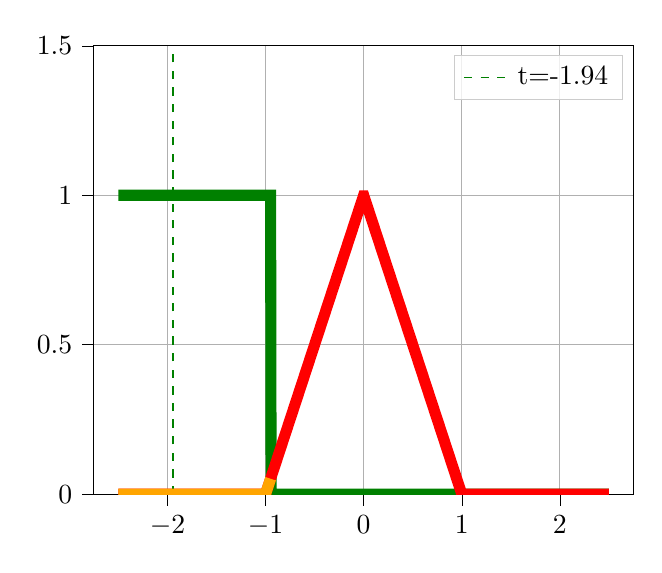
\begin{tikzpicture}

\definecolor{color0}{rgb}{1,0.498039215686275,0.0549019607843137}
\definecolor{color1}{rgb}{1,0.647058823529412,0}

\begin{axis}[
legend cell align={left},
legend style={fill opacity=0.8, draw opacity=1, text opacity=1, draw=white!80!black},
tick align=outside,
tick pos=left,
x grid style={white!69.0196078431373!black},
xmajorgrids,
xmin=-2.75, xmax=2.75,
xtick style={color=black},
y grid style={white!69.0196078431373!black},
ymajorgrids,
ymin=0, ymax=1.5,
ytick style={color=black}
]
\path [draw=color0, fill=color0, opacity=0.2]
(axis cs:-2.5,0)
--(axis cs:-2.5,0)
--(axis cs:-2.49499499499499,0)
--(axis cs:-2.48998998998999,0)
--(axis cs:-2.48498498498498,0)
--(axis cs:-2.47997997997998,0)
--(axis cs:-2.47497497497497,0)
--(axis cs:-2.46996996996997,0)
--(axis cs:-2.46496496496496,0)
--(axis cs:-2.45995995995996,0)
--(axis cs:-2.45495495495495,0)
--(axis cs:-2.44994994994995,0)
--(axis cs:-2.44494494494494,0)
--(axis cs:-2.43993993993994,0)
--(axis cs:-2.43493493493493,0)
--(axis cs:-2.42992992992993,0)
--(axis cs:-2.42492492492492,0)
--(axis cs:-2.41991991991992,0)
--(axis cs:-2.41491491491491,0)
--(axis cs:-2.40990990990991,0)
--(axis cs:-2.4049049049049,0)
--(axis cs:-2.3998998998999,0)
--(axis cs:-2.39489489489489,0)
--(axis cs:-2.38988988988989,0)
--(axis cs:-2.38488488488488,0)
--(axis cs:-2.37987987987988,0)
--(axis cs:-2.37487487487487,0)
--(axis cs:-2.36986986986987,0)
--(axis cs:-2.36486486486486,0)
--(axis cs:-2.35985985985986,0)
--(axis cs:-2.35485485485485,0)
--(axis cs:-2.34984984984985,0)
--(axis cs:-2.34484484484484,0)
--(axis cs:-2.33983983983984,0)
--(axis cs:-2.33483483483483,0)
--(axis cs:-2.32982982982983,0)
--(axis cs:-2.32482482482482,0)
--(axis cs:-2.31981981981982,0)
--(axis cs:-2.31481481481481,0)
--(axis cs:-2.30980980980981,0)
--(axis cs:-2.3048048048048,0)
--(axis cs:-2.2997997997998,0)
--(axis cs:-2.29479479479479,0)
--(axis cs:-2.28978978978979,0)
--(axis cs:-2.28478478478478,0)
--(axis cs:-2.27977977977978,0)
--(axis cs:-2.27477477477477,0)
--(axis cs:-2.26976976976977,0)
--(axis cs:-2.26476476476476,0)
--(axis cs:-2.25975975975976,0)
--(axis cs:-2.25475475475475,0)
--(axis cs:-2.24974974974975,0)
--(axis cs:-2.24474474474474,0)
--(axis cs:-2.23973973973974,0)
--(axis cs:-2.23473473473473,0)
--(axis cs:-2.22972972972973,0)
--(axis cs:-2.22472472472472,0)
--(axis cs:-2.21971971971972,0)
--(axis cs:-2.21471471471471,0)
--(axis cs:-2.20970970970971,0)
--(axis cs:-2.2047047047047,0)
--(axis cs:-2.1996996996997,0)
--(axis cs:-2.19469469469469,0)
--(axis cs:-2.18968968968969,0)
--(axis cs:-2.18468468468468,0)
--(axis cs:-2.17967967967968,0)
--(axis cs:-2.17467467467467,0)
--(axis cs:-2.16966966966967,0)
--(axis cs:-2.16466466466466,0)
--(axis cs:-2.15965965965966,0)
--(axis cs:-2.15465465465465,0)
--(axis cs:-2.14964964964965,0)
--(axis cs:-2.14464464464464,0)
--(axis cs:-2.13963963963964,0)
--(axis cs:-2.13463463463463,0)
--(axis cs:-2.12962962962963,0)
--(axis cs:-2.12462462462462,0)
--(axis cs:-2.11961961961962,0)
--(axis cs:-2.11461461461461,0)
--(axis cs:-2.10960960960961,0)
--(axis cs:-2.1046046046046,0)
--(axis cs:-2.0995995995996,0)
--(axis cs:-2.09459459459459,0)
--(axis cs:-2.08958958958959,0)
--(axis cs:-2.08458458458458,0)
--(axis cs:-2.07957957957958,0)
--(axis cs:-2.07457457457457,0)
--(axis cs:-2.06956956956957,0)
--(axis cs:-2.06456456456456,0)
--(axis cs:-2.05955955955956,0)
--(axis cs:-2.05455455455455,0)
--(axis cs:-2.04954954954955,0)
--(axis cs:-2.04454454454454,0)
--(axis cs:-2.03953953953954,0)
--(axis cs:-2.03453453453453,0)
--(axis cs:-2.02952952952953,0)
--(axis cs:-2.02452452452452,0)
--(axis cs:-2.01951951951952,0)
--(axis cs:-2.01451451451451,0)
--(axis cs:-2.00950950950951,0)
--(axis cs:-2.0045045045045,0)
--(axis cs:-1.9994994994995,0)
--(axis cs:-1.99449449449449,0)
--(axis cs:-1.98948948948949,0)
--(axis cs:-1.98448448448448,0)
--(axis cs:-1.97947947947948,0)
--(axis cs:-1.97447447447447,0)
--(axis cs:-1.96946946946947,0)
--(axis cs:-1.96446446446446,0)
--(axis cs:-1.95945945945946,0)
--(axis cs:-1.95445445445445,0)
--(axis cs:-1.94944944944945,0)
--(axis cs:-1.94444444444444,0)
--(axis cs:-1.93943943943944,0)
--(axis cs:-1.93443443443443,0)
--(axis cs:-1.92942942942943,0)
--(axis cs:-1.92442442442442,0)
--(axis cs:-1.91941941941942,0)
--(axis cs:-1.91441441441441,0)
--(axis cs:-1.90940940940941,0)
--(axis cs:-1.9044044044044,0)
--(axis cs:-1.8993993993994,0)
--(axis cs:-1.89439439439439,0)
--(axis cs:-1.88938938938939,0)
--(axis cs:-1.88438438438438,0)
--(axis cs:-1.87937937937938,0)
--(axis cs:-1.87437437437437,0)
--(axis cs:-1.86936936936937,0)
--(axis cs:-1.86436436436436,0)
--(axis cs:-1.85935935935936,0)
--(axis cs:-1.85435435435435,0)
--(axis cs:-1.84934934934935,0)
--(axis cs:-1.84434434434434,0)
--(axis cs:-1.83933933933934,0)
--(axis cs:-1.83433433433433,0)
--(axis cs:-1.82932932932933,0)
--(axis cs:-1.82432432432432,0)
--(axis cs:-1.81931931931932,0)
--(axis cs:-1.81431431431431,0)
--(axis cs:-1.80930930930931,0)
--(axis cs:-1.8043043043043,0)
--(axis cs:-1.7992992992993,0)
--(axis cs:-1.79429429429429,0)
--(axis cs:-1.78928928928929,0)
--(axis cs:-1.78428428428428,0)
--(axis cs:-1.77927927927928,0)
--(axis cs:-1.77427427427427,0)
--(axis cs:-1.76926926926927,0)
--(axis cs:-1.76426426426426,0)
--(axis cs:-1.75925925925926,0)
--(axis cs:-1.75425425425425,0)
--(axis cs:-1.74924924924925,0)
--(axis cs:-1.74424424424424,0)
--(axis cs:-1.73923923923924,0)
--(axis cs:-1.73423423423423,0)
--(axis cs:-1.72922922922923,0)
--(axis cs:-1.72422422422422,0)
--(axis cs:-1.71921921921922,0)
--(axis cs:-1.71421421421421,0)
--(axis cs:-1.70920920920921,0)
--(axis cs:-1.7042042042042,0)
--(axis cs:-1.6991991991992,0)
--(axis cs:-1.69419419419419,0)
--(axis cs:-1.68918918918919,0)
--(axis cs:-1.68418418418418,0)
--(axis cs:-1.67917917917918,0)
--(axis cs:-1.67417417417417,0)
--(axis cs:-1.66916916916917,0)
--(axis cs:-1.66416416416416,0)
--(axis cs:-1.65915915915916,0)
--(axis cs:-1.65415415415415,0)
--(axis cs:-1.64914914914915,0)
--(axis cs:-1.64414414414414,0)
--(axis cs:-1.63913913913914,0)
--(axis cs:-1.63413413413413,0)
--(axis cs:-1.62912912912913,0)
--(axis cs:-1.62412412412412,0)
--(axis cs:-1.61911911911912,0)
--(axis cs:-1.61411411411411,0)
--(axis cs:-1.60910910910911,0)
--(axis cs:-1.6041041041041,0)
--(axis cs:-1.5990990990991,0)
--(axis cs:-1.59409409409409,0)
--(axis cs:-1.58908908908909,0)
--(axis cs:-1.58408408408408,0)
--(axis cs:-1.57907907907908,0)
--(axis cs:-1.57407407407407,0)
--(axis cs:-1.56906906906907,0)
--(axis cs:-1.56406406406406,0)
--(axis cs:-1.55905905905906,0)
--(axis cs:-1.55405405405405,0)
--(axis cs:-1.54904904904905,0)
--(axis cs:-1.54404404404404,0)
--(axis cs:-1.53903903903904,0)
--(axis cs:-1.53403403403403,0)
--(axis cs:-1.52902902902903,0)
--(axis cs:-1.52402402402402,0)
--(axis cs:-1.51901901901902,0)
--(axis cs:-1.51401401401401,0)
--(axis cs:-1.50900900900901,0)
--(axis cs:-1.504004004004,0)
--(axis cs:-1.498998998999,0)
--(axis cs:-1.49399399399399,0)
--(axis cs:-1.48898898898899,0)
--(axis cs:-1.48398398398398,0)
--(axis cs:-1.47897897897898,0)
--(axis cs:-1.47397397397397,0)
--(axis cs:-1.46896896896897,0)
--(axis cs:-1.46396396396396,0)
--(axis cs:-1.45895895895896,0)
--(axis cs:-1.45395395395395,0)
--(axis cs:-1.44894894894895,0)
--(axis cs:-1.44394394394394,0)
--(axis cs:-1.43893893893894,0)
--(axis cs:-1.43393393393393,0)
--(axis cs:-1.42892892892893,0)
--(axis cs:-1.42392392392392,0)
--(axis cs:-1.41891891891892,0)
--(axis cs:-1.41391391391391,0)
--(axis cs:-1.40890890890891,0)
--(axis cs:-1.4039039039039,0)
--(axis cs:-1.3988988988989,0)
--(axis cs:-1.39389389389389,0)
--(axis cs:-1.38888888888889,0)
--(axis cs:-1.38388388388388,0)
--(axis cs:-1.37887887887888,0)
--(axis cs:-1.37387387387387,0)
--(axis cs:-1.36886886886887,0)
--(axis cs:-1.36386386386386,0)
--(axis cs:-1.35885885885886,0)
--(axis cs:-1.35385385385385,0)
--(axis cs:-1.34884884884885,0)
--(axis cs:-1.34384384384384,0)
--(axis cs:-1.33883883883884,0)
--(axis cs:-1.33383383383383,0)
--(axis cs:-1.32882882882883,0)
--(axis cs:-1.32382382382382,0)
--(axis cs:-1.31881881881882,0)
--(axis cs:-1.31381381381381,0)
--(axis cs:-1.30880880880881,0)
--(axis cs:-1.3038038038038,0)
--(axis cs:-1.2987987987988,0)
--(axis cs:-1.29379379379379,0)
--(axis cs:-1.28878878878879,0)
--(axis cs:-1.28378378378378,0)
--(axis cs:-1.27877877877878,0)
--(axis cs:-1.27377377377377,0)
--(axis cs:-1.26876876876877,0)
--(axis cs:-1.26376376376376,0)
--(axis cs:-1.25875875875876,0)
--(axis cs:-1.25375375375375,0)
--(axis cs:-1.24874874874875,0)
--(axis cs:-1.24374374374374,0)
--(axis cs:-1.23873873873874,0)
--(axis cs:-1.23373373373373,0)
--(axis cs:-1.22872872872873,0)
--(axis cs:-1.22372372372372,0)
--(axis cs:-1.21871871871872,0)
--(axis cs:-1.21371371371371,0)
--(axis cs:-1.20870870870871,0)
--(axis cs:-1.2037037037037,0)
--(axis cs:-1.1986986986987,0)
--(axis cs:-1.19369369369369,0)
--(axis cs:-1.18868868868869,0)
--(axis cs:-1.18368368368368,0)
--(axis cs:-1.17867867867868,0)
--(axis cs:-1.17367367367367,0)
--(axis cs:-1.16866866866867,0)
--(axis cs:-1.16366366366366,0)
--(axis cs:-1.15865865865866,0)
--(axis cs:-1.15365365365365,0)
--(axis cs:-1.14864864864865,0)
--(axis cs:-1.14364364364364,0)
--(axis cs:-1.13863863863864,0)
--(axis cs:-1.13363363363363,0)
--(axis cs:-1.12862862862863,0)
--(axis cs:-1.12362362362362,0)
--(axis cs:-1.11861861861862,0)
--(axis cs:-1.11361361361361,0)
--(axis cs:-1.10860860860861,0)
--(axis cs:-1.1036036036036,0)
--(axis cs:-1.0985985985986,0)
--(axis cs:-1.09359359359359,0)
--(axis cs:-1.08858858858859,0)
--(axis cs:-1.08358358358358,0)
--(axis cs:-1.07857857857858,0)
--(axis cs:-1.07357357357357,0)
--(axis cs:-1.06856856856857,0)
--(axis cs:-1.06356356356356,0)
--(axis cs:-1.05855855855856,0)
--(axis cs:-1.05355355355355,0)
--(axis cs:-1.04854854854855,0)
--(axis cs:-1.04354354354354,0)
--(axis cs:-1.03853853853854,0)
--(axis cs:-1.03353353353353,0)
--(axis cs:-1.02852852852853,0)
--(axis cs:-1.02352352352352,0)
--(axis cs:-1.01851851851852,0)
--(axis cs:-1.01351351351351,0)
--(axis cs:-1.00850850850851,0)
--(axis cs:-1.0035035035035,0)
--(axis cs:-0.998498498498499,0)
--(axis cs:-0.993493493493494,0)
--(axis cs:-0.988488488488489,0)
--(axis cs:-0.983483483483484,0)
--(axis cs:-0.978478478478479,0)
--(axis cs:-0.973473473473474,0)
--(axis cs:-0.968468468468469,0)
--(axis cs:-0.963463463463464,0)
--(axis cs:-0.958458458458459,0)
--(axis cs:-0.953453453453454,0)
--(axis cs:-0.948448448448449,0)
--(axis cs:-0.948448448448449,0.0515515515515514)
--(axis cs:-0.948448448448449,0.0515515515515514)
--(axis cs:-0.953453453453454,0.0465465465465464)
--(axis cs:-0.958458458458459,0.0415415415415414)
--(axis cs:-0.963463463463464,0.0365365365365364)
--(axis cs:-0.968468468468469,0.0315315315315314)
--(axis cs:-0.973473473473474,0.0265265265265264)
--(axis cs:-0.978478478478479,0.0215215215215214)
--(axis cs:-0.983483483483484,0.0165165165165164)
--(axis cs:-0.988488488488489,0.0115115115115114)
--(axis cs:-0.993493493493494,0.00650650650650642)
--(axis cs:-0.998498498498499,0.00150150150150141)
--(axis cs:-1.0035035035035,0)
--(axis cs:-1.00850850850851,0)
--(axis cs:-1.01351351351351,0)
--(axis cs:-1.01851851851852,0)
--(axis cs:-1.02352352352352,0)
--(axis cs:-1.02852852852853,0)
--(axis cs:-1.03353353353353,0)
--(axis cs:-1.03853853853854,0)
--(axis cs:-1.04354354354354,0)
--(axis cs:-1.04854854854855,0)
--(axis cs:-1.05355355355355,0)
--(axis cs:-1.05855855855856,0)
--(axis cs:-1.06356356356356,0)
--(axis cs:-1.06856856856857,0)
--(axis cs:-1.07357357357357,0)
--(axis cs:-1.07857857857858,0)
--(axis cs:-1.08358358358358,0)
--(axis cs:-1.08858858858859,0)
--(axis cs:-1.09359359359359,0)
--(axis cs:-1.0985985985986,0)
--(axis cs:-1.1036036036036,0)
--(axis cs:-1.10860860860861,0)
--(axis cs:-1.11361361361361,0)
--(axis cs:-1.11861861861862,0)
--(axis cs:-1.12362362362362,0)
--(axis cs:-1.12862862862863,0)
--(axis cs:-1.13363363363363,0)
--(axis cs:-1.13863863863864,0)
--(axis cs:-1.14364364364364,0)
--(axis cs:-1.14864864864865,0)
--(axis cs:-1.15365365365365,0)
--(axis cs:-1.15865865865866,0)
--(axis cs:-1.16366366366366,0)
--(axis cs:-1.16866866866867,0)
--(axis cs:-1.17367367367367,0)
--(axis cs:-1.17867867867868,0)
--(axis cs:-1.18368368368368,0)
--(axis cs:-1.18868868868869,0)
--(axis cs:-1.19369369369369,0)
--(axis cs:-1.1986986986987,0)
--(axis cs:-1.2037037037037,0)
--(axis cs:-1.20870870870871,0)
--(axis cs:-1.21371371371371,0)
--(axis cs:-1.21871871871872,0)
--(axis cs:-1.22372372372372,0)
--(axis cs:-1.22872872872873,0)
--(axis cs:-1.23373373373373,0)
--(axis cs:-1.23873873873874,0)
--(axis cs:-1.24374374374374,0)
--(axis cs:-1.24874874874875,0)
--(axis cs:-1.25375375375375,0)
--(axis cs:-1.25875875875876,0)
--(axis cs:-1.26376376376376,0)
--(axis cs:-1.26876876876877,0)
--(axis cs:-1.27377377377377,0)
--(axis cs:-1.27877877877878,0)
--(axis cs:-1.28378378378378,0)
--(axis cs:-1.28878878878879,0)
--(axis cs:-1.29379379379379,0)
--(axis cs:-1.2987987987988,0)
--(axis cs:-1.3038038038038,0)
--(axis cs:-1.30880880880881,0)
--(axis cs:-1.31381381381381,0)
--(axis cs:-1.31881881881882,0)
--(axis cs:-1.32382382382382,0)
--(axis cs:-1.32882882882883,0)
--(axis cs:-1.33383383383383,0)
--(axis cs:-1.33883883883884,0)
--(axis cs:-1.34384384384384,0)
--(axis cs:-1.34884884884885,0)
--(axis cs:-1.35385385385385,0)
--(axis cs:-1.35885885885886,0)
--(axis cs:-1.36386386386386,0)
--(axis cs:-1.36886886886887,0)
--(axis cs:-1.37387387387387,0)
--(axis cs:-1.37887887887888,0)
--(axis cs:-1.38388388388388,0)
--(axis cs:-1.38888888888889,0)
--(axis cs:-1.39389389389389,0)
--(axis cs:-1.3988988988989,0)
--(axis cs:-1.4039039039039,0)
--(axis cs:-1.40890890890891,0)
--(axis cs:-1.41391391391391,0)
--(axis cs:-1.41891891891892,0)
--(axis cs:-1.42392392392392,0)
--(axis cs:-1.42892892892893,0)
--(axis cs:-1.43393393393393,0)
--(axis cs:-1.43893893893894,0)
--(axis cs:-1.44394394394394,0)
--(axis cs:-1.44894894894895,0)
--(axis cs:-1.45395395395395,0)
--(axis cs:-1.45895895895896,0)
--(axis cs:-1.46396396396396,0)
--(axis cs:-1.46896896896897,0)
--(axis cs:-1.47397397397397,0)
--(axis cs:-1.47897897897898,0)
--(axis cs:-1.48398398398398,0)
--(axis cs:-1.48898898898899,0)
--(axis cs:-1.49399399399399,0)
--(axis cs:-1.498998998999,0)
--(axis cs:-1.504004004004,0)
--(axis cs:-1.50900900900901,0)
--(axis cs:-1.51401401401401,0)
--(axis cs:-1.51901901901902,0)
--(axis cs:-1.52402402402402,0)
--(axis cs:-1.52902902902903,0)
--(axis cs:-1.53403403403403,0)
--(axis cs:-1.53903903903904,0)
--(axis cs:-1.54404404404404,0)
--(axis cs:-1.54904904904905,0)
--(axis cs:-1.55405405405405,0)
--(axis cs:-1.55905905905906,0)
--(axis cs:-1.56406406406406,0)
--(axis cs:-1.56906906906907,0)
--(axis cs:-1.57407407407407,0)
--(axis cs:-1.57907907907908,0)
--(axis cs:-1.58408408408408,0)
--(axis cs:-1.58908908908909,0)
--(axis cs:-1.59409409409409,0)
--(axis cs:-1.5990990990991,0)
--(axis cs:-1.6041041041041,0)
--(axis cs:-1.60910910910911,0)
--(axis cs:-1.61411411411411,0)
--(axis cs:-1.61911911911912,0)
--(axis cs:-1.62412412412412,0)
--(axis cs:-1.62912912912913,0)
--(axis cs:-1.63413413413413,0)
--(axis cs:-1.63913913913914,0)
--(axis cs:-1.64414414414414,0)
--(axis cs:-1.64914914914915,0)
--(axis cs:-1.65415415415415,0)
--(axis cs:-1.65915915915916,0)
--(axis cs:-1.66416416416416,0)
--(axis cs:-1.66916916916917,0)
--(axis cs:-1.67417417417417,0)
--(axis cs:-1.67917917917918,0)
--(axis cs:-1.68418418418418,0)
--(axis cs:-1.68918918918919,0)
--(axis cs:-1.69419419419419,0)
--(axis cs:-1.6991991991992,0)
--(axis cs:-1.7042042042042,0)
--(axis cs:-1.70920920920921,0)
--(axis cs:-1.71421421421421,0)
--(axis cs:-1.71921921921922,0)
--(axis cs:-1.72422422422422,0)
--(axis cs:-1.72922922922923,0)
--(axis cs:-1.73423423423423,0)
--(axis cs:-1.73923923923924,0)
--(axis cs:-1.74424424424424,0)
--(axis cs:-1.74924924924925,0)
--(axis cs:-1.75425425425425,0)
--(axis cs:-1.75925925925926,0)
--(axis cs:-1.76426426426426,0)
--(axis cs:-1.76926926926927,0)
--(axis cs:-1.77427427427427,0)
--(axis cs:-1.77927927927928,0)
--(axis cs:-1.78428428428428,0)
--(axis cs:-1.78928928928929,0)
--(axis cs:-1.79429429429429,0)
--(axis cs:-1.7992992992993,0)
--(axis cs:-1.8043043043043,0)
--(axis cs:-1.80930930930931,0)
--(axis cs:-1.81431431431431,0)
--(axis cs:-1.81931931931932,0)
--(axis cs:-1.82432432432432,0)
--(axis cs:-1.82932932932933,0)
--(axis cs:-1.83433433433433,0)
--(axis cs:-1.83933933933934,0)
--(axis cs:-1.84434434434434,0)
--(axis cs:-1.84934934934935,0)
--(axis cs:-1.85435435435435,0)
--(axis cs:-1.85935935935936,0)
--(axis cs:-1.86436436436436,0)
--(axis cs:-1.86936936936937,0)
--(axis cs:-1.87437437437437,0)
--(axis cs:-1.87937937937938,0)
--(axis cs:-1.88438438438438,0)
--(axis cs:-1.88938938938939,0)
--(axis cs:-1.89439439439439,0)
--(axis cs:-1.8993993993994,0)
--(axis cs:-1.9044044044044,0)
--(axis cs:-1.90940940940941,0)
--(axis cs:-1.91441441441441,0)
--(axis cs:-1.91941941941942,0)
--(axis cs:-1.92442442442442,0)
--(axis cs:-1.92942942942943,0)
--(axis cs:-1.93443443443443,0)
--(axis cs:-1.93943943943944,0)
--(axis cs:-1.94444444444444,0)
--(axis cs:-1.94944944944945,0)
--(axis cs:-1.95445445445445,0)
--(axis cs:-1.95945945945946,0)
--(axis cs:-1.96446446446446,0)
--(axis cs:-1.96946946946947,0)
--(axis cs:-1.97447447447447,0)
--(axis cs:-1.97947947947948,0)
--(axis cs:-1.98448448448448,0)
--(axis cs:-1.98948948948949,0)
--(axis cs:-1.99449449449449,0)
--(axis cs:-1.9994994994995,0)
--(axis cs:-2.0045045045045,0)
--(axis cs:-2.00950950950951,0)
--(axis cs:-2.01451451451451,0)
--(axis cs:-2.01951951951952,0)
--(axis cs:-2.02452452452452,0)
--(axis cs:-2.02952952952953,0)
--(axis cs:-2.03453453453453,0)
--(axis cs:-2.03953953953954,0)
--(axis cs:-2.04454454454454,0)
--(axis cs:-2.04954954954955,0)
--(axis cs:-2.05455455455455,0)
--(axis cs:-2.05955955955956,0)
--(axis cs:-2.06456456456456,0)
--(axis cs:-2.06956956956957,0)
--(axis cs:-2.07457457457457,0)
--(axis cs:-2.07957957957958,0)
--(axis cs:-2.08458458458458,0)
--(axis cs:-2.08958958958959,0)
--(axis cs:-2.09459459459459,0)
--(axis cs:-2.0995995995996,0)
--(axis cs:-2.1046046046046,0)
--(axis cs:-2.10960960960961,0)
--(axis cs:-2.11461461461461,0)
--(axis cs:-2.11961961961962,0)
--(axis cs:-2.12462462462462,0)
--(axis cs:-2.12962962962963,0)
--(axis cs:-2.13463463463463,0)
--(axis cs:-2.13963963963964,0)
--(axis cs:-2.14464464464464,0)
--(axis cs:-2.14964964964965,0)
--(axis cs:-2.15465465465465,0)
--(axis cs:-2.15965965965966,0)
--(axis cs:-2.16466466466466,0)
--(axis cs:-2.16966966966967,0)
--(axis cs:-2.17467467467467,0)
--(axis cs:-2.17967967967968,0)
--(axis cs:-2.18468468468468,0)
--(axis cs:-2.18968968968969,0)
--(axis cs:-2.19469469469469,0)
--(axis cs:-2.1996996996997,0)
--(axis cs:-2.2047047047047,0)
--(axis cs:-2.20970970970971,0)
--(axis cs:-2.21471471471471,0)
--(axis cs:-2.21971971971972,0)
--(axis cs:-2.22472472472472,0)
--(axis cs:-2.22972972972973,0)
--(axis cs:-2.23473473473473,0)
--(axis cs:-2.23973973973974,0)
--(axis cs:-2.24474474474474,0)
--(axis cs:-2.24974974974975,0)
--(axis cs:-2.25475475475475,0)
--(axis cs:-2.25975975975976,0)
--(axis cs:-2.26476476476476,0)
--(axis cs:-2.26976976976977,0)
--(axis cs:-2.27477477477477,0)
--(axis cs:-2.27977977977978,0)
--(axis cs:-2.28478478478478,0)
--(axis cs:-2.28978978978979,0)
--(axis cs:-2.29479479479479,0)
--(axis cs:-2.2997997997998,0)
--(axis cs:-2.3048048048048,0)
--(axis cs:-2.30980980980981,0)
--(axis cs:-2.31481481481481,0)
--(axis cs:-2.31981981981982,0)
--(axis cs:-2.32482482482482,0)
--(axis cs:-2.32982982982983,0)
--(axis cs:-2.33483483483483,0)
--(axis cs:-2.33983983983984,0)
--(axis cs:-2.34484484484484,0)
--(axis cs:-2.34984984984985,0)
--(axis cs:-2.35485485485485,0)
--(axis cs:-2.35985985985986,0)
--(axis cs:-2.36486486486486,0)
--(axis cs:-2.36986986986987,0)
--(axis cs:-2.37487487487487,0)
--(axis cs:-2.37987987987988,0)
--(axis cs:-2.38488488488488,0)
--(axis cs:-2.38988988988989,0)
--(axis cs:-2.39489489489489,0)
--(axis cs:-2.3998998998999,0)
--(axis cs:-2.4049049049049,0)
--(axis cs:-2.40990990990991,0)
--(axis cs:-2.41491491491491,0)
--(axis cs:-2.41991991991992,0)
--(axis cs:-2.42492492492492,0)
--(axis cs:-2.42992992992993,0)
--(axis cs:-2.43493493493493,0)
--(axis cs:-2.43993993993994,0)
--(axis cs:-2.44494494494494,0)
--(axis cs:-2.44994994994995,0)
--(axis cs:-2.45495495495495,0)
--(axis cs:-2.45995995995996,0)
--(axis cs:-2.46496496496496,0)
--(axis cs:-2.46996996996997,0)
--(axis cs:-2.47497497497497,0)
--(axis cs:-2.47997997997998,0)
--(axis cs:-2.48498498498498,0)
--(axis cs:-2.48998998998999,0)
--(axis cs:-2.49499499499499,0)
--(axis cs:-2.5,0)
--cycle;

\addplot [line width=4pt, green!50!black, forget plot]
table {%
-2.5 1
-2.49499499499499 1
-2.48998998998999 1
-2.48498498498498 1
-2.47997997997998 1
-2.47497497497497 1
-2.46996996996997 1
-2.46496496496496 1
-2.45995995995996 1
-2.45495495495495 1
-2.44994994994995 1
-2.44494494494494 1
-2.43993993993994 1
-2.43493493493493 1
-2.42992992992993 1
-2.42492492492492 1
-2.41991991991992 1
-2.41491491491491 1
-2.40990990990991 1
-2.4049049049049 1
-2.3998998998999 1
-2.39489489489489 1
-2.38988988988989 1
-2.38488488488488 1
-2.37987987987988 1
-2.37487487487487 1
-2.36986986986987 1
-2.36486486486486 1
-2.35985985985986 1
-2.35485485485485 1
-2.34984984984985 1
-2.34484484484484 1
-2.33983983983984 1
-2.33483483483483 1
-2.32982982982983 1
-2.32482482482482 1
-2.31981981981982 1
-2.31481481481481 1
-2.30980980980981 1
-2.3048048048048 1
-2.2997997997998 1
-2.29479479479479 1
-2.28978978978979 1
-2.28478478478478 1
-2.27977977977978 1
-2.27477477477477 1
-2.26976976976977 1
-2.26476476476476 1
-2.25975975975976 1
-2.25475475475475 1
-2.24974974974975 1
-2.24474474474474 1
-2.23973973973974 1
-2.23473473473473 1
-2.22972972972973 1
-2.22472472472472 1
-2.21971971971972 1
-2.21471471471471 1
-2.20970970970971 1
-2.2047047047047 1
-2.1996996996997 1
-2.19469469469469 1
-2.18968968968969 1
-2.18468468468468 1
-2.17967967967968 1
-2.17467467467467 1
-2.16966966966967 1
-2.16466466466466 1
-2.15965965965966 1
-2.15465465465465 1
-2.14964964964965 1
-2.14464464464464 1
-2.13963963963964 1
-2.13463463463463 1
-2.12962962962963 1
-2.12462462462462 1
-2.11961961961962 1
-2.11461461461461 1
-2.10960960960961 1
-2.1046046046046 1
-2.0995995995996 1
-2.09459459459459 1
-2.08958958958959 1
-2.08458458458458 1
-2.07957957957958 1
-2.07457457457457 1
-2.06956956956957 1
-2.06456456456456 1
-2.05955955955956 1
-2.05455455455455 1
-2.04954954954955 1
-2.04454454454454 1
-2.03953953953954 1
-2.03453453453453 1
-2.02952952952953 1
-2.02452452452452 1
-2.01951951951952 1
-2.01451451451451 1
-2.00950950950951 1
-2.0045045045045 1
-1.9994994994995 1
-1.99449449449449 1
-1.98948948948949 1
-1.98448448448448 1
-1.97947947947948 1
-1.97447447447447 1
-1.96946946946947 1
-1.96446446446446 1
-1.95945945945946 1
-1.95445445445445 1
-1.94944944944945 1
-1.94444444444444 1
-1.93943943943944 1
-1.93443443443443 1
-1.92942942942943 1
-1.92442442442442 1
-1.91941941941942 1
-1.91441441441441 1
-1.90940940940941 1
-1.9044044044044 1
-1.8993993993994 1
-1.89439439439439 1
-1.88938938938939 1
-1.88438438438438 1
-1.87937937937938 1
-1.87437437437437 1
-1.86936936936937 1
-1.86436436436436 1
-1.85935935935936 1
-1.85435435435435 1
-1.84934934934935 1
-1.84434434434434 1
-1.83933933933934 1
-1.83433433433433 1
-1.82932932932933 1
-1.82432432432432 1
-1.81931931931932 1
-1.81431431431431 1
-1.80930930930931 1
-1.8043043043043 1
-1.7992992992993 1
-1.79429429429429 1
-1.78928928928929 1
-1.78428428428428 1
-1.77927927927928 1
-1.77427427427427 1
-1.76926926926927 1
-1.76426426426426 1
-1.75925925925926 1
-1.75425425425425 1
-1.74924924924925 1
-1.74424424424424 1
-1.73923923923924 1
-1.73423423423423 1
-1.72922922922923 1
-1.72422422422422 1
-1.71921921921922 1
-1.71421421421421 1
-1.70920920920921 1
-1.7042042042042 1
-1.6991991991992 1
-1.69419419419419 1
-1.68918918918919 1
-1.68418418418418 1
-1.67917917917918 1
-1.67417417417417 1
-1.66916916916917 1
-1.66416416416416 1
-1.65915915915916 1
-1.65415415415415 1
-1.64914914914915 1
-1.64414414414414 1
-1.63913913913914 1
-1.63413413413413 1
-1.62912912912913 1
-1.62412412412412 1
-1.61911911911912 1
-1.61411411411411 1
-1.60910910910911 1
-1.6041041041041 1
-1.5990990990991 1
-1.59409409409409 1
-1.58908908908909 1
-1.58408408408408 1
-1.57907907907908 1
-1.57407407407407 1
-1.56906906906907 1
-1.56406406406406 1
-1.55905905905906 1
-1.55405405405405 1
-1.54904904904905 1
-1.54404404404404 1
-1.53903903903904 1
-1.53403403403403 1
-1.52902902902903 1
-1.52402402402402 1
-1.51901901901902 1
-1.51401401401401 1
-1.50900900900901 1
-1.504004004004 1
-1.498998998999 1
-1.49399399399399 1
-1.48898898898899 1
-1.48398398398398 1
-1.47897897897898 1
-1.47397397397397 1
-1.46896896896897 1
-1.46396396396396 1
-1.45895895895896 1
-1.45395395395395 1
-1.44894894894895 1
-1.44394394394394 1
-1.43893893893894 1
-1.43393393393393 1
-1.42892892892893 1
-1.42392392392392 1
-1.41891891891892 1
-1.41391391391391 1
-1.40890890890891 1
-1.4039039039039 1
-1.3988988988989 1
-1.39389389389389 1
-1.38888888888889 1
-1.38388388388388 1
-1.37887887887888 1
-1.37387387387387 1
-1.36886886886887 1
-1.36386386386386 1
-1.35885885885886 1
-1.35385385385385 1
-1.34884884884885 1
-1.34384384384384 1
-1.33883883883884 1
-1.33383383383383 1
-1.32882882882883 1
-1.32382382382382 1
-1.31881881881882 1
-1.31381381381381 1
-1.30880880880881 1
-1.3038038038038 1
-1.2987987987988 1
-1.29379379379379 1
-1.28878878878879 1
-1.28378378378378 1
-1.27877877877878 1
-1.27377377377377 1
-1.26876876876877 1
-1.26376376376376 1
-1.25875875875876 1
-1.25375375375375 1
-1.24874874874875 1
-1.24374374374374 1
-1.23873873873874 1
-1.23373373373373 1
-1.22872872872873 1
-1.22372372372372 1
-1.21871871871872 1
-1.21371371371371 1
-1.20870870870871 1
-1.2037037037037 1
-1.1986986986987 1
-1.19369369369369 1
-1.18868868868869 1
-1.18368368368368 1
-1.17867867867868 1
-1.17367367367367 1
-1.16866866866867 1
-1.16366366366366 1
-1.15865865865866 1
-1.15365365365365 1
-1.14864864864865 1
-1.14364364364364 1
-1.13863863863864 1
-1.13363363363363 1
-1.12862862862863 1
-1.12362362362362 1
-1.11861861861862 1
-1.11361361361361 1
-1.10860860860861 1
-1.1036036036036 1
-1.0985985985986 1
-1.09359359359359 1
-1.08858858858859 1
-1.08358358358358 1
-1.07857857857858 1
-1.07357357357357 1
-1.06856856856857 1
-1.06356356356356 1
-1.05855855855856 1
-1.05355355355355 1
-1.04854854854855 1
-1.04354354354354 1
-1.03853853853854 1
-1.03353353353353 1
-1.02852852852853 1
-1.02352352352352 1
-1.01851851851852 1
-1.01351351351351 1
-1.00850850850851 1
-1.0035035035035 1
-0.998498498498499 1
-0.993493493493494 1
-0.988488488488489 1
-0.983483483483484 1
-0.978478478478479 1
-0.973473473473474 1
-0.968468468468469 1
-0.963463463463464 1
-0.958458458458459 1
-0.953453453453454 1
-0.948448448448449 1
-0.943443443443444 0
-0.938438438438439 0
-0.933433433433434 0
-0.928428428428429 0
-0.923423423423424 0
-0.918418418418419 0
-0.913413413413414 0
-0.908408408408409 0
-0.903403403403404 0
-0.898398398398399 0
-0.893393393393393 0
-0.888388388388388 0
-0.883383383383383 0
-0.878378378378378 0
-0.873373373373373 0
-0.868368368368368 0
-0.863363363363363 0
-0.858358358358358 0
-0.853353353353353 0
-0.848348348348348 0
-0.843343343343343 0
-0.838338338338338 0
-0.833333333333333 0
-0.828328328328328 0
-0.823323323323323 0
-0.818318318318318 0
-0.813313313313313 0
-0.808308308308308 0
-0.803303303303303 0
-0.798298298298298 0
-0.793293293293293 0
-0.788288288288288 0
-0.783283283283283 0
-0.778278278278278 0
-0.773273273273273 0
-0.768268268268268 0
-0.763263263263263 0
-0.758258258258258 0
-0.753253253253253 0
-0.748248248248248 0
-0.743243243243243 0
-0.738238238238238 0
-0.733233233233233 0
-0.728228228228228 0
-0.723223223223223 0
-0.718218218218218 0
-0.713213213213213 0
-0.708208208208208 0
-0.703203203203203 0
-0.698198198198198 0
-0.693193193193193 0
-0.688188188188188 0
-0.683183183183183 0
-0.678178178178178 0
-0.673173173173173 0
-0.668168168168168 0
-0.663163163163163 0
-0.658158158158158 0
-0.653153153153153 0
-0.648148148148148 0
-0.643143143143143 0
-0.638138138138138 0
-0.633133133133133 0
-0.628128128128128 0
-0.623123123123123 0
-0.618118118118118 0
-0.613113113113113 0
-0.608108108108108 0
-0.603103103103103 0
-0.598098098098098 0
-0.593093093093093 0
-0.588088088088088 0
-0.583083083083083 0
-0.578078078078078 0
-0.573073073073073 0
-0.568068068068068 0
-0.563063063063063 0
-0.558058058058058 0
-0.553053053053053 0
-0.548048048048048 0
-0.543043043043043 0
-0.538038038038038 0
-0.533033033033033 0
-0.528028028028028 0
-0.523023023023023 0
-0.518018018018018 0
-0.513013013013013 0
-0.508008008008008 0
-0.503003003003003 0
-0.497997997997998 0
-0.492992992992993 0
-0.487987987987988 0
-0.482982982982983 0
-0.477977977977978 0
-0.472972972972973 0
-0.467967967967968 0
-0.462962962962963 0
-0.457957957957958 0
-0.452952952952953 0
-0.447947947947948 0
-0.442942942942943 0
-0.437937937937938 0
-0.432932932932933 0
-0.427927927927928 0
-0.422922922922923 0
-0.417917917917918 0
-0.412912912912913 0
-0.407907907907908 0
-0.402902902902903 0
-0.397897897897898 0
-0.392892892892893 0
-0.387887887887888 0
-0.382882882882883 0
-0.377877877877878 0
-0.372872872872873 0
-0.367867867867868 0
-0.362862862862863 0
-0.357857857857858 0
-0.352852852852853 0
-0.347847847847848 0
-0.342842842842843 0
-0.337837837837838 0
-0.332832832832833 0
-0.327827827827828 0
-0.322822822822823 0
-0.317817817817818 0
-0.312812812812813 0
-0.307807807807808 0
-0.302802802802803 0
-0.297797797797798 0
-0.292792792792793 0
-0.287787787787788 0
-0.282782782782783 0
-0.277777777777778 0
-0.272772772772773 0
-0.267767767767768 0
-0.262762762762763 0
-0.257757757757758 0
-0.252752752752753 0
-0.247747747747748 0
-0.242742742742743 0
-0.237737737737738 0
-0.232732732732733 0
-0.227727727727728 0
-0.222722722722723 0
-0.217717717717718 0
-0.212712712712713 0
-0.207707707707708 0
-0.202702702702703 0
-0.197697697697698 0
-0.192692692692693 0
-0.187687687687688 0
-0.182682682682683 0
-0.177677677677678 0
-0.172672672672673 0
-0.167667667667668 0
-0.162662662662663 0
-0.157657657657658 0
-0.152652652652653 0
-0.147647647647648 0
-0.142642642642643 0
-0.137637637637638 0
-0.132632632632633 0
-0.127627627627628 0
-0.122622622622623 0
-0.117617617617618 0
-0.112612612612613 0
-0.107607607607608 0
-0.102602602602603 0
-0.0975975975975976 0
-0.0925925925925926 0
-0.0875875875875876 0
-0.0825825825825826 0
-0.0775775775775776 0
-0.0725725725725725 0
-0.0675675675675675 0
-0.0625625625625625 0
-0.0575575575575575 0
-0.0525525525525525 0
-0.0475475475475475 0
-0.0425425425425425 0
-0.0375375375375375 0
-0.0325325325325325 0
-0.0275275275275275 0
-0.0225225225225225 0
-0.0175175175175175 0
-0.0125125125125125 0
-0.0075075075075075 0
-0.0025025025025025 0
0.0025025025025025 0
0.0075075075075075 0
0.0125125125125125 0
0.0175175175175175 0
0.0225225225225225 0
0.0275275275275275 0
0.0325325325325325 0
0.0375375375375375 0
0.0425425425425425 0
0.0475475475475475 0
0.0525525525525525 0
0.0575575575575575 0
0.0625625625625625 0
0.0675675675675675 0
0.0725725725725725 0
0.0775775775775776 0
0.0825825825825826 0
0.0875875875875876 0
0.0925925925925926 0
0.0975975975975976 0
0.102602602602603 0
0.107607607607608 0
0.112612612612613 0
0.117617617617618 0
0.122622622622623 0
0.127627627627628 0
0.132632632632633 0
0.137637637637638 0
0.142642642642643 0
0.147647647647648 0
0.152652652652653 0
0.157657657657658 0
0.162662662662663 0
0.167667667667668 0
0.172672672672673 0
0.177677677677678 0
0.182682682682683 0
0.187687687687688 0
0.192692692692693 0
0.197697697697698 0
0.202702702702703 0
0.207707707707708 0
0.212712712712713 0
0.217717717717718 0
0.222722722722723 0
0.227727727727728 0
0.232732732732733 0
0.237737737737738 0
0.242742742742743 0
0.247747747747748 0
0.252752752752753 0
0.257757757757758 0
0.262762762762763 0
0.267767767767768 0
0.272772772772773 0
0.277777777777778 0
0.282782782782783 0
0.287787787787788 0
0.292792792792793 0
0.297797797797798 0
0.302802802802803 0
0.307807807807808 0
0.312812812812813 0
0.317817817817818 0
0.322822822822823 0
0.327827827827828 0
0.332832832832833 0
0.337837837837838 0
0.342842842842843 0
0.347847847847848 0
0.352852852852853 0
0.357857857857858 0
0.362862862862863 0
0.367867867867868 0
0.372872872872873 0
0.377877877877878 0
0.382882882882883 0
0.387887887887888 0
0.392892892892893 0
0.397897897897898 0
0.402902902902903 0
0.407907907907908 0
0.412912912912913 0
0.417917917917918 0
0.422922922922923 0
0.427927927927928 0
0.432932932932933 0
0.437937937937938 0
0.442942942942943 0
0.447947947947948 0
0.452952952952953 0
0.457957957957958 0
0.462962962962963 0
0.467967967967968 0
0.472972972972973 0
0.477977977977978 0
0.482982982982983 0
0.487987987987988 0
0.492992992992993 0
0.497997997997998 0
0.503003003003003 0
0.508008008008008 0
0.513013013013013 0
0.518018018018018 0
0.523023023023023 0
0.528028028028028 0
0.533033033033033 0
0.538038038038038 0
0.543043043043043 0
0.548048048048048 0
0.553053053053053 0
0.558058058058058 0
0.563063063063063 0
0.568068068068068 0
0.573073073073073 0
0.578078078078078 0
0.583083083083083 0
0.588088088088088 0
0.593093093093093 0
0.598098098098098 0
0.603103103103103 0
0.608108108108108 0
0.613113113113113 0
0.618118118118118 0
0.623123123123123 0
0.628128128128128 0
0.633133133133133 0
0.638138138138138 0
0.643143143143143 0
0.648148148148148 0
0.653153153153153 0
0.658158158158158 0
0.663163163163163 0
0.668168168168168 0
0.673173173173173 0
0.678178178178178 0
0.683183183183183 0
0.688188188188188 0
0.693193193193193 0
0.698198198198198 0
0.703203203203203 0
0.708208208208208 0
0.713213213213213 0
0.718218218218218 0
0.723223223223223 0
0.728228228228228 0
0.733233233233233 0
0.738238238238238 0
0.743243243243243 0
0.748248248248248 0
0.753253253253253 0
0.758258258258258 0
0.763263263263263 0
0.768268268268268 0
0.773273273273273 0
0.778278278278278 0
0.783283283283283 0
0.788288288288288 0
0.793293293293293 0
0.798298298298298 0
0.803303303303303 0
0.808308308308308 0
0.813313313313313 0
0.818318318318318 0
0.823323323323323 0
0.828328328328328 0
0.833333333333333 0
0.838338338338338 0
0.843343343343343 0
0.848348348348348 0
0.853353353353353 0
0.858358358358358 0
0.863363363363364 0
0.868368368368369 0
0.873373373373374 0
0.878378378378379 0
0.883383383383384 0
0.888388388388389 0
0.893393393393394 0
0.898398398398399 0
0.903403403403404 0
0.908408408408409 0
0.913413413413414 0
0.918418418418419 0
0.923423423423424 0
0.928428428428429 0
0.933433433433434 0
0.938438438438439 0
0.943443443443444 0
0.948448448448449 0
0.953453453453454 0
0.958458458458459 0
0.963463463463464 0
0.968468468468469 0
0.973473473473474 0
0.978478478478479 0
0.983483483483484 0
0.988488488488489 0
0.993493493493494 0
0.998498498498499 0
1.0035035035035 0
1.00850850850851 0
1.01351351351351 0
1.01851851851852 0
1.02352352352352 0
1.02852852852853 0
1.03353353353353 0
1.03853853853854 0
1.04354354354354 0
1.04854854854855 0
1.05355355355355 0
1.05855855855856 0
1.06356356356356 0
1.06856856856857 0
1.07357357357357 0
1.07857857857858 0
1.08358358358358 0
1.08858858858859 0
1.09359359359359 0
1.0985985985986 0
1.1036036036036 0
1.10860860860861 0
1.11361361361361 0
1.11861861861862 0
1.12362362362362 0
1.12862862862863 0
1.13363363363363 0
1.13863863863864 0
1.14364364364364 0
1.14864864864865 0
1.15365365365365 0
1.15865865865866 0
1.16366366366366 0
1.16866866866867 0
1.17367367367367 0
1.17867867867868 0
1.18368368368368 0
1.18868868868869 0
1.19369369369369 0
1.1986986986987 0
1.2037037037037 0
1.20870870870871 0
1.21371371371371 0
1.21871871871872 0
1.22372372372372 0
1.22872872872873 0
1.23373373373373 0
1.23873873873874 0
1.24374374374374 0
1.24874874874875 0
1.25375375375375 0
1.25875875875876 0
1.26376376376376 0
1.26876876876877 0
1.27377377377377 0
1.27877877877878 0
1.28378378378378 0
1.28878878878879 0
1.29379379379379 0
1.2987987987988 0
1.3038038038038 0
1.30880880880881 0
1.31381381381381 0
1.31881881881882 0
1.32382382382382 0
1.32882882882883 0
1.33383383383383 0
1.33883883883884 0
1.34384384384384 0
1.34884884884885 0
1.35385385385385 0
1.35885885885886 0
1.36386386386386 0
1.36886886886887 0
1.37387387387387 0
1.37887887887888 0
1.38388388388388 0
1.38888888888889 0
1.39389389389389 0
1.3988988988989 0
1.4039039039039 0
1.40890890890891 0
1.41391391391391 0
1.41891891891892 0
1.42392392392392 0
1.42892892892893 0
1.43393393393393 0
1.43893893893894 0
1.44394394394394 0
1.44894894894895 0
1.45395395395395 0
1.45895895895896 0
1.46396396396396 0
1.46896896896897 0
1.47397397397397 0
1.47897897897898 0
1.48398398398398 0
1.48898898898899 0
1.49399399399399 0
1.498998998999 0
1.504004004004 0
1.50900900900901 0
1.51401401401401 0
1.51901901901902 0
1.52402402402402 0
1.52902902902903 0
1.53403403403403 0
1.53903903903904 0
1.54404404404404 0
1.54904904904905 0
1.55405405405405 0
1.55905905905906 0
1.56406406406406 0
1.56906906906907 0
1.57407407407407 0
1.57907907907908 0
1.58408408408408 0
1.58908908908909 0
1.59409409409409 0
1.5990990990991 0
1.6041041041041 0
1.60910910910911 0
1.61411411411411 0
1.61911911911912 0
1.62412412412412 0
1.62912912912913 0
1.63413413413413 0
1.63913913913914 0
1.64414414414414 0
1.64914914914915 0
1.65415415415415 0
1.65915915915916 0
1.66416416416416 0
1.66916916916917 0
1.67417417417417 0
1.67917917917918 0
1.68418418418418 0
1.68918918918919 0
1.69419419419419 0
1.6991991991992 0
1.7042042042042 0
1.70920920920921 0
1.71421421421421 0
1.71921921921922 0
1.72422422422422 0
1.72922922922923 0
1.73423423423423 0
1.73923923923924 0
1.74424424424424 0
1.74924924924925 0
1.75425425425425 0
1.75925925925926 0
1.76426426426426 0
1.76926926926927 0
1.77427427427427 0
1.77927927927928 0
1.78428428428428 0
1.78928928928929 0
1.79429429429429 0
1.7992992992993 0
1.8043043043043 0
1.80930930930931 0
1.81431431431431 0
1.81931931931932 0
1.82432432432432 0
1.82932932932933 0
1.83433433433433 0
1.83933933933934 0
1.84434434434434 0
1.84934934934935 0
1.85435435435435 0
1.85935935935936 0
1.86436436436436 0
1.86936936936937 0
1.87437437437437 0
1.87937937937938 0
1.88438438438438 0
1.88938938938939 0
1.89439439439439 0
1.8993993993994 0
1.9044044044044 0
1.90940940940941 0
1.91441441441441 0
1.91941941941942 0
1.92442442442442 0
1.92942942942943 0
1.93443443443443 0
1.93943943943944 0
1.94444444444444 0
1.94944944944945 0
1.95445445445445 0
1.95945945945946 0
1.96446446446446 0
1.96946946946947 0
1.97447447447447 0
1.97947947947948 0
1.98448448448448 0
1.98948948948949 0
1.99449449449449 0
1.9994994994995 0
2.0045045045045 0
2.00950950950951 0
2.01451451451451 0
2.01951951951952 0
2.02452452452452 0
2.02952952952953 0
2.03453453453453 0
2.03953953953954 0
2.04454454454454 0
2.04954954954955 0
2.05455455455455 0
2.05955955955956 0
2.06456456456456 0
2.06956956956957 0
2.07457457457457 0
2.07957957957958 0
2.08458458458458 0
2.08958958958959 0
2.09459459459459 0
2.0995995995996 0
2.1046046046046 0
2.10960960960961 0
2.11461461461461 0
2.11961961961962 0
2.12462462462462 0
2.12962962962963 0
2.13463463463463 0
2.13963963963964 0
2.14464464464464 0
2.14964964964965 0
2.15465465465465 0
2.15965965965966 0
2.16466466466466 0
2.16966966966967 0
2.17467467467467 0
2.17967967967968 0
2.18468468468468 0
2.18968968968969 0
2.19469469469469 0
2.1996996996997 0
2.2047047047047 0
2.20970970970971 0
2.21471471471471 0
2.21971971971972 0
2.22472472472472 0
2.22972972972973 0
2.23473473473473 0
2.23973973973974 0
2.24474474474474 0
2.24974974974975 0
2.25475475475475 0
2.25975975975976 0
2.26476476476476 0
2.26976976976977 0
2.27477477477477 0
2.27977977977978 0
2.28478478478478 0
2.28978978978979 0
2.29479479479479 0
2.2997997997998 0
2.3048048048048 0
2.30980980980981 0
2.31481481481481 0
2.31981981981982 0
2.32482482482482 0
2.32982982982983 0
2.33483483483483 0
2.33983983983984 0
2.34484484484484 0
2.34984984984985 0
2.35485485485485 0
2.35985985985986 0
2.36486486486486 0
2.36986986986987 0
2.37487487487487 0
2.37987987987988 0
2.38488488488488 0
2.38988988988989 0
2.39489489489489 0
2.3998998998999 0
2.4049049049049 0
2.40990990990991 0
2.41491491491491 0
2.41991991991992 0
2.42492492492492 0
2.42992992992993 0
2.43493493493493 0
2.43993993993994 0
2.44494494494494 0
2.44994994994995 0
2.45495495495495 0
2.45995995995996 0
2.46496496496496 0
2.46996996996997 0
2.47497497497497 0
2.47997997997998 0
2.48498498498498 0
2.48998998998999 0
2.49499499499499 0
2.5 0
};
\addplot [line width=4pt, red, forget plot]
table {%
-2.5 -0
-2.49499499499499 -0
-2.48998998998999 -0
-2.48498498498498 -0
-2.47997997997998 -0
-2.47497497497497 -0
-2.46996996996997 -0
-2.46496496496496 -0
-2.45995995995996 -0
-2.45495495495495 -0
-2.44994994994995 -0
-2.44494494494494 -0
-2.43993993993994 -0
-2.43493493493493 -0
-2.42992992992993 -0
-2.42492492492492 -0
-2.41991991991992 -0
-2.41491491491491 -0
-2.40990990990991 -0
-2.4049049049049 -0
-2.3998998998999 -0
-2.39489489489489 -0
-2.38988988988989 -0
-2.38488488488488 -0
-2.37987987987988 -0
-2.37487487487487 -0
-2.36986986986987 -0
-2.36486486486486 -0
-2.35985985985986 -0
-2.35485485485485 -0
-2.34984984984985 -0
-2.34484484484484 -0
-2.33983983983984 -0
-2.33483483483483 -0
-2.32982982982983 -0
-2.32482482482482 -0
-2.31981981981982 -0
-2.31481481481481 -0
-2.30980980980981 -0
-2.3048048048048 -0
-2.2997997997998 -0
-2.29479479479479 -0
-2.28978978978979 -0
-2.28478478478478 -0
-2.27977977977978 -0
-2.27477477477477 -0
-2.26976976976977 -0
-2.26476476476476 -0
-2.25975975975976 -0
-2.25475475475475 -0
-2.24974974974975 -0
-2.24474474474474 -0
-2.23973973973974 -0
-2.23473473473473 -0
-2.22972972972973 -0
-2.22472472472472 -0
-2.21971971971972 -0
-2.21471471471471 -0
-2.20970970970971 -0
-2.2047047047047 -0
-2.1996996996997 -0
-2.19469469469469 -0
-2.18968968968969 -0
-2.18468468468468 -0
-2.17967967967968 -0
-2.17467467467467 -0
-2.16966966966967 -0
-2.16466466466466 -0
-2.15965965965966 -0
-2.15465465465465 -0
-2.14964964964965 -0
-2.14464464464464 -0
-2.13963963963964 -0
-2.13463463463463 -0
-2.12962962962963 -0
-2.12462462462462 -0
-2.11961961961962 -0
-2.11461461461461 -0
-2.10960960960961 -0
-2.1046046046046 -0
-2.0995995995996 -0
-2.09459459459459 -0
-2.08958958958959 -0
-2.08458458458458 -0
-2.07957957957958 -0
-2.07457457457457 -0
-2.06956956956957 -0
-2.06456456456456 -0
-2.05955955955956 -0
-2.05455455455455 -0
-2.04954954954955 -0
-2.04454454454454 -0
-2.03953953953954 -0
-2.03453453453453 -0
-2.02952952952953 -0
-2.02452452452452 -0
-2.01951951951952 -0
-2.01451451451451 -0
-2.00950950950951 -0
-2.0045045045045 -0
-1.9994994994995 -0
-1.99449449449449 -0
-1.98948948948949 -0
-1.98448448448448 -0
-1.97947947947948 -0
-1.97447447447447 -0
-1.96946946946947 -0
-1.96446446446446 -0
-1.95945945945946 -0
-1.95445445445445 -0
-1.94944944944945 -0
-1.94444444444444 -0
-1.93943943943944 -0
-1.93443443443443 -0
-1.92942942942943 -0
-1.92442442442442 -0
-1.91941941941942 -0
-1.91441441441441 -0
-1.90940940940941 -0
-1.9044044044044 -0
-1.8993993993994 -0
-1.89439439439439 -0
-1.88938938938939 -0
-1.88438438438438 -0
-1.87937937937938 -0
-1.87437437437437 -0
-1.86936936936937 -0
-1.86436436436436 -0
-1.85935935935936 -0
-1.85435435435435 -0
-1.84934934934935 -0
-1.84434434434434 -0
-1.83933933933934 -0
-1.83433433433433 -0
-1.82932932932933 -0
-1.82432432432432 -0
-1.81931931931932 -0
-1.81431431431431 -0
-1.80930930930931 -0
-1.8043043043043 -0
-1.7992992992993 -0
-1.79429429429429 -0
-1.78928928928929 -0
-1.78428428428428 -0
-1.77927927927928 -0
-1.77427427427427 -0
-1.76926926926927 -0
-1.76426426426426 -0
-1.75925925925926 -0
-1.75425425425425 -0
-1.74924924924925 -0
-1.74424424424424 -0
-1.73923923923924 -0
-1.73423423423423 -0
-1.72922922922923 -0
-1.72422422422422 -0
-1.71921921921922 -0
-1.71421421421421 -0
-1.70920920920921 -0
-1.7042042042042 -0
-1.6991991991992 -0
-1.69419419419419 -0
-1.68918918918919 -0
-1.68418418418418 -0
-1.67917917917918 -0
-1.67417417417417 -0
-1.66916916916917 -0
-1.66416416416416 -0
-1.65915915915916 -0
-1.65415415415415 -0
-1.64914914914915 -0
-1.64414414414414 -0
-1.63913913913914 -0
-1.63413413413413 -0
-1.62912912912913 -0
-1.62412412412412 -0
-1.61911911911912 -0
-1.61411411411411 -0
-1.60910910910911 -0
-1.6041041041041 -0
-1.5990990990991 -0
-1.59409409409409 -0
-1.58908908908909 -0
-1.58408408408408 -0
-1.57907907907908 -0
-1.57407407407407 -0
-1.56906906906907 -0
-1.56406406406406 -0
-1.55905905905906 -0
-1.55405405405405 -0
-1.54904904904905 -0
-1.54404404404404 -0
-1.53903903903904 -0
-1.53403403403403 -0
-1.52902902902903 -0
-1.52402402402402 -0
-1.51901901901902 -0
-1.51401401401401 -0
-1.50900900900901 -0
-1.504004004004 -0
-1.498998998999 -0
-1.49399399399399 -0
-1.48898898898899 -0
-1.48398398398398 -0
-1.47897897897898 -0
-1.47397397397397 -0
-1.46896896896897 -0
-1.46396396396396 -0
-1.45895895895896 -0
-1.45395395395395 -0
-1.44894894894895 -0
-1.44394394394394 -0
-1.43893893893894 -0
-1.43393393393393 -0
-1.42892892892893 -0
-1.42392392392392 -0
-1.41891891891892 -0
-1.41391391391391 -0
-1.40890890890891 -0
-1.4039039039039 -0
-1.3988988988989 -0
-1.39389389389389 -0
-1.38888888888889 -0
-1.38388388388388 -0
-1.37887887887888 -0
-1.37387387387387 -0
-1.36886886886887 -0
-1.36386386386386 -0
-1.35885885885886 -0
-1.35385385385385 -0
-1.34884884884885 -0
-1.34384384384384 -0
-1.33883883883884 -0
-1.33383383383383 -0
-1.32882882882883 -0
-1.32382382382382 -0
-1.31881881881882 -0
-1.31381381381381 -0
-1.30880880880881 -0
-1.3038038038038 -0
-1.2987987987988 -0
-1.29379379379379 -0
-1.28878878878879 -0
-1.28378378378378 -0
-1.27877877877878 -0
-1.27377377377377 -0
-1.26876876876877 -0
-1.26376376376376 -0
-1.25875875875876 -0
-1.25375375375375 -0
-1.24874874874875 -0
-1.24374374374374 -0
-1.23873873873874 -0
-1.23373373373373 -0
-1.22872872872873 -0
-1.22372372372372 -0
-1.21871871871872 -0
-1.21371371371371 -0
-1.20870870870871 -0
-1.2037037037037 -0
-1.1986986986987 -0
-1.19369369369369 -0
-1.18868868868869 -0
-1.18368368368368 -0
-1.17867867867868 -0
-1.17367367367367 -0
-1.16866866866867 -0
-1.16366366366366 -0
-1.15865865865866 -0
-1.15365365365365 -0
-1.14864864864865 -0
-1.14364364364364 -0
-1.13863863863864 -0
-1.13363363363363 -0
-1.12862862862863 -0
-1.12362362362362 -0
-1.11861861861862 -0
-1.11361361361361 -0
-1.10860860860861 -0
-1.1036036036036 -0
-1.0985985985986 -0
-1.09359359359359 -0
-1.08858858858859 -0
-1.08358358358358 -0
-1.07857857857858 -0
-1.07357357357357 -0
-1.06856856856857 -0
-1.06356356356356 -0
-1.05855855855856 -0
-1.05355355355355 -0
-1.04854854854855 -0
-1.04354354354354 -0
-1.03853853853854 -0
-1.03353353353353 -0
-1.02852852852853 -0
-1.02352352352352 -0
-1.01851851851852 -0
-1.01351351351351 -0
-1.00850850850851 -0
-1.0035035035035 -0
-0.998498498498499 0.00150150150150141
-0.993493493493494 0.00650650650650642
-0.988488488488489 0.0115115115115114
-0.983483483483484 0.0165165165165164
-0.978478478478479 0.0215215215215214
-0.973473473473474 0.0265265265265264
-0.968468468468469 0.0315315315315314
-0.963463463463464 0.0365365365365364
-0.958458458458459 0.0415415415415414
-0.953453453453454 0.0465465465465464
-0.948448448448449 0.0515515515515514
-0.943443443443444 0.0565565565565564
-0.938438438438439 0.0615615615615615
-0.933433433433434 0.0665665665665665
-0.928428428428429 0.0715715715715715
-0.923423423423424 0.0765765765765765
-0.918418418418419 0.0815815815815815
-0.913413413413414 0.0865865865865865
-0.908408408408409 0.0915915915915915
-0.903403403403404 0.0965965965965965
-0.898398398398399 0.101601601601601
-0.893393393393393 0.106606606606607
-0.888388388388388 0.111611611611612
-0.883383383383383 0.116616616616617
-0.878378378378378 0.121621621621622
-0.873373373373373 0.126626626626627
-0.868368368368368 0.131631631631632
-0.863363363363363 0.136636636636637
-0.858358358358358 0.141641641641642
-0.853353353353353 0.146646646646647
-0.848348348348348 0.151651651651652
-0.843343343343343 0.156656656656657
-0.838338338338338 0.161661661661662
-0.833333333333333 0.166666666666667
-0.828328328328328 0.171671671671672
-0.823323323323323 0.176676676676677
-0.818318318318318 0.181681681681682
-0.813313313313313 0.186686686686687
-0.808308308308308 0.191691691691692
-0.803303303303303 0.196696696696697
-0.798298298298298 0.201701701701702
-0.793293293293293 0.206706706706707
-0.788288288288288 0.211711711711712
-0.783283283283283 0.216716716716717
-0.778278278278278 0.221721721721722
-0.773273273273273 0.226726726726727
-0.768268268268268 0.231731731731732
-0.763263263263263 0.236736736736737
-0.758258258258258 0.241741741741742
-0.753253253253253 0.246746746746747
-0.748248248248248 0.251751751751752
-0.743243243243243 0.256756756756757
-0.738238238238238 0.261761761761762
-0.733233233233233 0.266766766766767
-0.728228228228228 0.271771771771772
-0.723223223223223 0.276776776776777
-0.718218218218218 0.281781781781782
-0.713213213213213 0.286786786786787
-0.708208208208208 0.291791791791792
-0.703203203203203 0.296796796796797
-0.698198198198198 0.301801801801802
-0.693193193193193 0.306806806806807
-0.688188188188188 0.311811811811812
-0.683183183183183 0.316816816816817
-0.678178178178178 0.321821821821822
-0.673173173173173 0.326826826826827
-0.668168168168168 0.331831831831832
-0.663163163163163 0.336836836836837
-0.658158158158158 0.341841841841842
-0.653153153153153 0.346846846846847
-0.648148148148148 0.351851851851852
-0.643143143143143 0.356856856856857
-0.638138138138138 0.361861861861862
-0.633133133133133 0.366866866866867
-0.628128128128128 0.371871871871872
-0.623123123123123 0.376876876876877
-0.618118118118118 0.381881881881882
-0.613113113113113 0.386886886886887
-0.608108108108108 0.391891891891892
-0.603103103103103 0.396896896896897
-0.598098098098098 0.401901901901902
-0.593093093093093 0.406906906906907
-0.588088088088088 0.411911911911912
-0.583083083083083 0.416916916916917
-0.578078078078078 0.421921921921922
-0.573073073073073 0.426926926926927
-0.568068068068068 0.431931931931932
-0.563063063063063 0.436936936936937
-0.558058058058058 0.441941941941942
-0.553053053053053 0.446946946946947
-0.548048048048048 0.451951951951952
-0.543043043043043 0.456956956956957
-0.538038038038038 0.461961961961962
-0.533033033033033 0.466966966966967
-0.528028028028028 0.471971971971972
-0.523023023023023 0.476976976976977
-0.518018018018018 0.481981981981982
-0.513013013013013 0.486986986986987
-0.508008008008008 0.491991991991992
-0.503003003003003 0.496996996996997
-0.497997997997998 0.502002002002002
-0.492992992992993 0.507007007007007
-0.487987987987988 0.512012012012012
-0.482982982982983 0.517017017017017
-0.477977977977978 0.522022022022022
-0.472972972972973 0.527027027027027
-0.467967967967968 0.532032032032032
-0.462962962962963 0.537037037037037
-0.457957957957958 0.542042042042042
-0.452952952952953 0.547047047047047
-0.447947947947948 0.552052052052052
-0.442942942942943 0.557057057057057
-0.437937937937938 0.562062062062062
-0.432932932932933 0.567067067067067
-0.427927927927928 0.572072072072072
-0.422922922922923 0.577077077077077
-0.417917917917918 0.582082082082082
-0.412912912912913 0.587087087087087
-0.407907907907908 0.592092092092092
-0.402902902902903 0.597097097097097
-0.397897897897898 0.602102102102102
-0.392892892892893 0.607107107107107
-0.387887887887888 0.612112112112112
-0.382882882882883 0.617117117117117
-0.377877877877878 0.622122122122122
-0.372872872872873 0.627127127127127
-0.367867867867868 0.632132132132132
-0.362862862862863 0.637137137137137
-0.357857857857858 0.642142142142142
-0.352852852852853 0.647147147147147
-0.347847847847848 0.652152152152152
-0.342842842842843 0.657157157157157
-0.337837837837838 0.662162162162162
-0.332832832832833 0.667167167167167
-0.327827827827828 0.672172172172172
-0.322822822822823 0.677177177177177
-0.317817817817818 0.682182182182182
-0.312812812812813 0.687187187187187
-0.307807807807808 0.692192192192192
-0.302802802802803 0.697197197197197
-0.297797797797798 0.702202202202202
-0.292792792792793 0.707207207207207
-0.287787787787788 0.712212212212212
-0.282782782782783 0.717217217217217
-0.277777777777778 0.722222222222222
-0.272772772772773 0.727227227227227
-0.267767767767768 0.732232232232232
-0.262762762762763 0.737237237237237
-0.257757757757758 0.742242242242242
-0.252752752752753 0.747247247247247
-0.247747747747748 0.752252252252252
-0.242742742742743 0.757257257257257
-0.237737737737738 0.762262262262262
-0.232732732732733 0.767267267267267
-0.227727727727728 0.772272272272272
-0.222722722722723 0.777277277277277
-0.217717717717718 0.782282282282282
-0.212712712712713 0.787287287287287
-0.207707707707708 0.792292292292292
-0.202702702702703 0.797297297297297
-0.197697697697698 0.802302302302302
-0.192692692692693 0.807307307307307
-0.187687687687688 0.812312312312312
-0.182682682682683 0.817317317317317
-0.177677677677678 0.822322322322322
-0.172672672672673 0.827327327327327
-0.167667667667668 0.832332332332332
-0.162662662662663 0.837337337337337
-0.157657657657658 0.842342342342342
-0.152652652652653 0.847347347347347
-0.147647647647648 0.852352352352352
-0.142642642642643 0.857357357357357
-0.137637637637638 0.862362362362362
-0.132632632632633 0.867367367367367
-0.127627627627628 0.872372372372372
-0.122622622622623 0.877377377377377
-0.117617617617618 0.882382382382382
-0.112612612612613 0.887387387387387
-0.107607607607608 0.892392392392392
-0.102602602602603 0.897397397397397
-0.0975975975975976 0.902402402402402
-0.0925925925925926 0.907407407407407
-0.0875875875875876 0.912412412412412
-0.0825825825825826 0.917417417417417
-0.0775775775775776 0.922422422422422
-0.0725725725725725 0.927427427427427
-0.0675675675675675 0.932432432432432
-0.0625625625625625 0.937437437437437
-0.0575575575575575 0.942442442442442
-0.0525525525525525 0.947447447447447
-0.0475475475475475 0.952452452452452
-0.0425425425425425 0.957457457457457
-0.0375375375375375 0.962462462462462
-0.0325325325325325 0.967467467467467
-0.0275275275275275 0.972472472472472
-0.0225225225225225 0.977477477477477
-0.0175175175175175 0.982482482482482
-0.0125125125125125 0.987487487487487
-0.0075075075075075 0.992492492492492
-0.0025025025025025 0.997497497497497
0.0025025025025025 0.997497497497497
0.0075075075075075 0.992492492492492
0.0125125125125125 0.987487487487487
0.0175175175175175 0.982482482482482
0.0225225225225225 0.977477477477477
0.0275275275275275 0.972472472472472
0.0325325325325325 0.967467467467467
0.0375375375375375 0.962462462462462
0.0425425425425425 0.957457457457457
0.0475475475475475 0.952452452452452
0.0525525525525525 0.947447447447447
0.0575575575575575 0.942442442442442
0.0625625625625625 0.937437437437437
0.0675675675675675 0.932432432432432
0.0725725725725725 0.927427427427427
0.0775775775775776 0.922422422422422
0.0825825825825826 0.917417417417417
0.0875875875875876 0.912412412412412
0.0925925925925926 0.907407407407407
0.0975975975975976 0.902402402402402
0.102602602602603 0.897397397397397
0.107607607607608 0.892392392392392
0.112612612612613 0.887387387387387
0.117617617617618 0.882382382382382
0.122622622622623 0.877377377377377
0.127627627627628 0.872372372372372
0.132632632632633 0.867367367367367
0.137637637637638 0.862362362362362
0.142642642642643 0.857357357357357
0.147647647647648 0.852352352352352
0.152652652652653 0.847347347347347
0.157657657657658 0.842342342342342
0.162662662662663 0.837337337337337
0.167667667667668 0.832332332332332
0.172672672672673 0.827327327327327
0.177677677677678 0.822322322322322
0.182682682682683 0.817317317317317
0.187687687687688 0.812312312312312
0.192692692692693 0.807307307307307
0.197697697697698 0.802302302302302
0.202702702702703 0.797297297297297
0.207707707707708 0.792292292292292
0.212712712712713 0.787287287287287
0.217717717717718 0.782282282282282
0.222722722722723 0.777277277277277
0.227727727727728 0.772272272272272
0.232732732732733 0.767267267267267
0.237737737737738 0.762262262262262
0.242742742742743 0.757257257257257
0.247747747747748 0.752252252252252
0.252752752752753 0.747247247247247
0.257757757757758 0.742242242242242
0.262762762762763 0.737237237237237
0.267767767767768 0.732232232232232
0.272772772772773 0.727227227227227
0.277777777777778 0.722222222222222
0.282782782782783 0.717217217217217
0.287787787787788 0.712212212212212
0.292792792792793 0.707207207207207
0.297797797797798 0.702202202202202
0.302802802802803 0.697197197197197
0.307807807807808 0.692192192192192
0.312812812812813 0.687187187187187
0.317817817817818 0.682182182182182
0.322822822822823 0.677177177177177
0.327827827827828 0.672172172172172
0.332832832832833 0.667167167167167
0.337837837837838 0.662162162162162
0.342842842842843 0.657157157157157
0.347847847847848 0.652152152152152
0.352852852852853 0.647147147147147
0.357857857857858 0.642142142142142
0.362862862862863 0.637137137137137
0.367867867867868 0.632132132132132
0.372872872872873 0.627127127127127
0.377877877877878 0.622122122122122
0.382882882882883 0.617117117117117
0.387887887887888 0.612112112112112
0.392892892892893 0.607107107107107
0.397897897897898 0.602102102102102
0.402902902902903 0.597097097097097
0.407907907907908 0.592092092092092
0.412912912912913 0.587087087087087
0.417917917917918 0.582082082082082
0.422922922922923 0.577077077077077
0.427927927927928 0.572072072072072
0.432932932932933 0.567067067067067
0.437937937937938 0.562062062062062
0.442942942942943 0.557057057057057
0.447947947947948 0.552052052052052
0.452952952952953 0.547047047047047
0.457957957957958 0.542042042042042
0.462962962962963 0.537037037037037
0.467967967967968 0.532032032032032
0.472972972972973 0.527027027027027
0.477977977977978 0.522022022022022
0.482982982982983 0.517017017017017
0.487987987987988 0.512012012012012
0.492992992992993 0.507007007007007
0.497997997997998 0.502002002002002
0.503003003003003 0.496996996996997
0.508008008008008 0.491991991991992
0.513013013013013 0.486986986986987
0.518018018018018 0.481981981981982
0.523023023023023 0.476976976976977
0.528028028028028 0.471971971971972
0.533033033033033 0.466966966966967
0.538038038038038 0.461961961961962
0.543043043043043 0.456956956956957
0.548048048048048 0.451951951951952
0.553053053053053 0.446946946946947
0.558058058058058 0.441941941941942
0.563063063063063 0.436936936936937
0.568068068068068 0.431931931931932
0.573073073073073 0.426926926926927
0.578078078078078 0.421921921921922
0.583083083083083 0.416916916916917
0.588088088088088 0.411911911911912
0.593093093093093 0.406906906906907
0.598098098098098 0.401901901901902
0.603103103103103 0.396896896896897
0.608108108108108 0.391891891891892
0.613113113113113 0.386886886886887
0.618118118118118 0.381881881881882
0.623123123123123 0.376876876876877
0.628128128128128 0.371871871871872
0.633133133133133 0.366866866866867
0.638138138138138 0.361861861861862
0.643143143143143 0.356856856856857
0.648148148148148 0.351851851851852
0.653153153153153 0.346846846846847
0.658158158158158 0.341841841841842
0.663163163163163 0.336836836836837
0.668168168168168 0.331831831831832
0.673173173173173 0.326826826826827
0.678178178178178 0.321821821821822
0.683183183183183 0.316816816816817
0.688188188188188 0.311811811811812
0.693193193193193 0.306806806806807
0.698198198198198 0.301801801801802
0.703203203203203 0.296796796796797
0.708208208208208 0.291791791791792
0.713213213213213 0.286786786786787
0.718218218218218 0.281781781781782
0.723223223223223 0.276776776776777
0.728228228228228 0.271771771771772
0.733233233233233 0.266766766766767
0.738238238238238 0.261761761761762
0.743243243243243 0.256756756756757
0.748248248248248 0.251751751751752
0.753253253253253 0.246746746746747
0.758258258258258 0.241741741741742
0.763263263263263 0.236736736736737
0.768268268268268 0.231731731731732
0.773273273273273 0.226726726726727
0.778278278278278 0.221721721721722
0.783283283283283 0.216716716716717
0.788288288288288 0.211711711711712
0.793293293293293 0.206706706706707
0.798298298298298 0.201701701701702
0.803303303303303 0.196696696696697
0.808308308308308 0.191691691691692
0.813313313313313 0.186686686686687
0.818318318318318 0.181681681681682
0.823323323323323 0.176676676676677
0.828328328328328 0.171671671671672
0.833333333333333 0.166666666666667
0.838338338338338 0.161661661661662
0.843343343343343 0.156656656656657
0.848348348348348 0.151651651651652
0.853353353353353 0.146646646646647
0.858358358358358 0.141641641641642
0.863363363363364 0.136636636636636
0.868368368368369 0.131631631631631
0.873373373373374 0.126626626626626
0.878378378378379 0.121621621621621
0.883383383383384 0.116616616616616
0.888388388388389 0.111611611611611
0.893393393393394 0.106606606606606
0.898398398398399 0.101601601601601
0.903403403403404 0.0965965965965965
0.908408408408409 0.0915915915915915
0.913413413413414 0.0865865865865865
0.918418418418419 0.0815815815815815
0.923423423423424 0.0765765765765765
0.928428428428429 0.0715715715715715
0.933433433433434 0.0665665665665665
0.938438438438439 0.0615615615615615
0.943443443443444 0.0565565565565564
0.948448448448449 0.0515515515515514
0.953453453453454 0.0465465465465464
0.958458458458459 0.0415415415415414
0.963463463463464 0.0365365365365364
0.968468468468469 0.0315315315315314
0.973473473473474 0.0265265265265264
0.978478478478479 0.0215215215215214
0.983483483483484 0.0165165165165164
0.988488488488489 0.0115115115115114
0.993493493493494 0.00650650650650642
0.998498498498499 0.00150150150150141
1.0035035035035 -0
1.00850850850851 -0
1.01351351351351 -0
1.01851851851852 -0
1.02352352352352 -0
1.02852852852853 -0
1.03353353353353 -0
1.03853853853854 -0
1.04354354354354 -0
1.04854854854855 -0
1.05355355355355 -0
1.05855855855856 -0
1.06356356356356 -0
1.06856856856857 -0
1.07357357357357 -0
1.07857857857858 -0
1.08358358358358 -0
1.08858858858859 -0
1.09359359359359 -0
1.0985985985986 -0
1.1036036036036 -0
1.10860860860861 -0
1.11361361361361 -0
1.11861861861862 -0
1.12362362362362 -0
1.12862862862863 -0
1.13363363363363 -0
1.13863863863864 -0
1.14364364364364 -0
1.14864864864865 -0
1.15365365365365 -0
1.15865865865866 -0
1.16366366366366 -0
1.16866866866867 -0
1.17367367367367 -0
1.17867867867868 -0
1.18368368368368 -0
1.18868868868869 -0
1.19369369369369 -0
1.1986986986987 -0
1.2037037037037 -0
1.20870870870871 -0
1.21371371371371 -0
1.21871871871872 -0
1.22372372372372 -0
1.22872872872873 -0
1.23373373373373 -0
1.23873873873874 -0
1.24374374374374 -0
1.24874874874875 -0
1.25375375375375 -0
1.25875875875876 -0
1.26376376376376 -0
1.26876876876877 -0
1.27377377377377 -0
1.27877877877878 -0
1.28378378378378 -0
1.28878878878879 -0
1.29379379379379 -0
1.2987987987988 -0
1.3038038038038 -0
1.30880880880881 -0
1.31381381381381 -0
1.31881881881882 -0
1.32382382382382 -0
1.32882882882883 -0
1.33383383383383 -0
1.33883883883884 -0
1.34384384384384 -0
1.34884884884885 -0
1.35385385385385 -0
1.35885885885886 -0
1.36386386386386 -0
1.36886886886887 -0
1.37387387387387 -0
1.37887887887888 -0
1.38388388388388 -0
1.38888888888889 -0
1.39389389389389 -0
1.3988988988989 -0
1.4039039039039 -0
1.40890890890891 -0
1.41391391391391 -0
1.41891891891892 -0
1.42392392392392 -0
1.42892892892893 -0
1.43393393393393 -0
1.43893893893894 -0
1.44394394394394 -0
1.44894894894895 -0
1.45395395395395 -0
1.45895895895896 -0
1.46396396396396 -0
1.46896896896897 -0
1.47397397397397 -0
1.47897897897898 -0
1.48398398398398 -0
1.48898898898899 -0
1.49399399399399 -0
1.498998998999 -0
1.504004004004 -0
1.50900900900901 -0
1.51401401401401 -0
1.51901901901902 -0
1.52402402402402 -0
1.52902902902903 -0
1.53403403403403 -0
1.53903903903904 -0
1.54404404404404 -0
1.54904904904905 -0
1.55405405405405 -0
1.55905905905906 -0
1.56406406406406 -0
1.56906906906907 -0
1.57407407407407 -0
1.57907907907908 -0
1.58408408408408 -0
1.58908908908909 -0
1.59409409409409 -0
1.5990990990991 -0
1.6041041041041 -0
1.60910910910911 -0
1.61411411411411 -0
1.61911911911912 -0
1.62412412412412 -0
1.62912912912913 -0
1.63413413413413 -0
1.63913913913914 -0
1.64414414414414 -0
1.64914914914915 -0
1.65415415415415 -0
1.65915915915916 -0
1.66416416416416 -0
1.66916916916917 -0
1.67417417417417 -0
1.67917917917918 -0
1.68418418418418 -0
1.68918918918919 -0
1.69419419419419 -0
1.6991991991992 -0
1.7042042042042 -0
1.70920920920921 -0
1.71421421421421 -0
1.71921921921922 -0
1.72422422422422 -0
1.72922922922923 -0
1.73423423423423 -0
1.73923923923924 -0
1.74424424424424 -0
1.74924924924925 -0
1.75425425425425 -0
1.75925925925926 -0
1.76426426426426 -0
1.76926926926927 -0
1.77427427427427 -0
1.77927927927928 -0
1.78428428428428 -0
1.78928928928929 -0
1.79429429429429 -0
1.7992992992993 -0
1.8043043043043 -0
1.80930930930931 -0
1.81431431431431 -0
1.81931931931932 -0
1.82432432432432 -0
1.82932932932933 -0
1.83433433433433 -0
1.83933933933934 -0
1.84434434434434 -0
1.84934934934935 -0
1.85435435435435 -0
1.85935935935936 -0
1.86436436436436 -0
1.86936936936937 -0
1.87437437437437 -0
1.87937937937938 -0
1.88438438438438 -0
1.88938938938939 -0
1.89439439439439 -0
1.8993993993994 -0
1.9044044044044 -0
1.90940940940941 -0
1.91441441441441 -0
1.91941941941942 -0
1.92442442442442 -0
1.92942942942943 -0
1.93443443443443 -0
1.93943943943944 -0
1.94444444444444 -0
1.94944944944945 -0
1.95445445445445 -0
1.95945945945946 -0
1.96446446446446 -0
1.96946946946947 -0
1.97447447447447 -0
1.97947947947948 -0
1.98448448448448 -0
1.98948948948949 -0
1.99449449449449 -0
1.9994994994995 -0
2.0045045045045 -0
2.00950950950951 -0
2.01451451451451 -0
2.01951951951952 -0
2.02452452452452 -0
2.02952952952953 -0
2.03453453453453 -0
2.03953953953954 -0
2.04454454454454 -0
2.04954954954955 -0
2.05455455455455 -0
2.05955955955956 -0
2.06456456456456 -0
2.06956956956957 -0
2.07457457457457 -0
2.07957957957958 -0
2.08458458458458 -0
2.08958958958959 -0
2.09459459459459 -0
2.0995995995996 -0
2.1046046046046 -0
2.10960960960961 -0
2.11461461461461 -0
2.11961961961962 -0
2.12462462462462 -0
2.12962962962963 -0
2.13463463463463 -0
2.13963963963964 -0
2.14464464464464 -0
2.14964964964965 -0
2.15465465465465 -0
2.15965965965966 -0
2.16466466466466 -0
2.16966966966967 -0
2.17467467467467 -0
2.17967967967968 -0
2.18468468468468 -0
2.18968968968969 -0
2.19469469469469 -0
2.1996996996997 -0
2.2047047047047 -0
2.20970970970971 -0
2.21471471471471 -0
2.21971971971972 -0
2.22472472472472 -0
2.22972972972973 -0
2.23473473473473 -0
2.23973973973974 -0
2.24474474474474 -0
2.24974974974975 -0
2.25475475475475 -0
2.25975975975976 -0
2.26476476476476 -0
2.26976976976977 -0
2.27477477477477 -0
2.27977977977978 -0
2.28478478478478 -0
2.28978978978979 -0
2.29479479479479 -0
2.2997997997998 -0
2.3048048048048 -0
2.30980980980981 -0
2.31481481481481 -0
2.31981981981982 -0
2.32482482482482 -0
2.32982982982983 -0
2.33483483483483 -0
2.33983983983984 -0
2.34484484484484 -0
2.34984984984985 -0
2.35485485485485 -0
2.35985985985986 -0
2.36486486486486 -0
2.36986986986987 -0
2.37487487487487 -0
2.37987987987988 -0
2.38488488488488 -0
2.38988988988989 -0
2.39489489489489 -0
2.3998998998999 -0
2.4049049049049 -0
2.40990990990991 -0
2.41491491491491 -0
2.41991991991992 -0
2.42492492492492 -0
2.42992992992993 -0
2.43493493493493 -0
2.43993993993994 -0
2.44494494494494 -0
2.44994994994995 -0
2.45495495495495 -0
2.45995995995996 -0
2.46496496496496 -0
2.46996996996997 -0
2.47497497497497 -0
2.47997997997998 -0
2.48498498498498 -0
2.48998998998999 -0
2.49499499499499 -0
2.5 -0
};
\addplot [semithick, green!50!black, dashed]
table {%
-1.94444444444444 0
-1.94444444444444 1.5
};
\addlegendentry{t=-1.94}
\addplot [line width=4pt, color1, forget plot]
table {%
-2.5 -0
-2.49499499499499 -0
-2.48998998998999 -0
-2.48498498498498 -0
-2.47997997997998 -0
-2.47497497497497 -0
-2.46996996996997 -0
-2.46496496496496 -0
-2.45995995995996 -0
-2.45495495495495 -0
-2.44994994994995 -0
-2.44494494494494 -0
-2.43993993993994 -0
-2.43493493493493 -0
-2.42992992992993 -0
-2.42492492492492 -0
-2.41991991991992 -0
-2.41491491491491 -0
-2.40990990990991 -0
-2.4049049049049 -0
-2.3998998998999 -0
-2.39489489489489 -0
-2.38988988988989 -0
-2.38488488488488 -0
-2.37987987987988 -0
-2.37487487487487 -0
-2.36986986986987 -0
-2.36486486486486 -0
-2.35985985985986 -0
-2.35485485485485 -0
-2.34984984984985 -0
-2.34484484484484 -0
-2.33983983983984 -0
-2.33483483483483 -0
-2.32982982982983 -0
-2.32482482482482 -0
-2.31981981981982 -0
-2.31481481481481 -0
-2.30980980980981 -0
-2.3048048048048 -0
-2.2997997997998 -0
-2.29479479479479 -0
-2.28978978978979 -0
-2.28478478478478 -0
-2.27977977977978 -0
-2.27477477477477 -0
-2.26976976976977 -0
-2.26476476476476 -0
-2.25975975975976 -0
-2.25475475475475 -0
-2.24974974974975 -0
-2.24474474474474 -0
-2.23973973973974 -0
-2.23473473473473 -0
-2.22972972972973 -0
-2.22472472472472 -0
-2.21971971971972 -0
-2.21471471471471 -0
-2.20970970970971 -0
-2.2047047047047 -0
-2.1996996996997 -0
-2.19469469469469 -0
-2.18968968968969 -0
-2.18468468468468 -0
-2.17967967967968 -0
-2.17467467467467 -0
-2.16966966966967 -0
-2.16466466466466 -0
-2.15965965965966 -0
-2.15465465465465 -0
-2.14964964964965 -0
-2.14464464464464 -0
-2.13963963963964 -0
-2.13463463463463 -0
-2.12962962962963 -0
-2.12462462462462 -0
-2.11961961961962 -0
-2.11461461461461 -0
-2.10960960960961 -0
-2.1046046046046 -0
-2.0995995995996 -0
-2.09459459459459 -0
-2.08958958958959 -0
-2.08458458458458 -0
-2.07957957957958 -0
-2.07457457457457 -0
-2.06956956956957 -0
-2.06456456456456 -0
-2.05955955955956 -0
-2.05455455455455 -0
-2.04954954954955 -0
-2.04454454454454 -0
-2.03953953953954 -0
-2.03453453453453 -0
-2.02952952952953 -0
-2.02452452452452 -0
-2.01951951951952 -0
-2.01451451451451 -0
-2.00950950950951 -0
-2.0045045045045 -0
-1.9994994994995 -0
-1.99449449449449 -0
-1.98948948948949 -0
-1.98448448448448 -0
-1.97947947947948 -0
-1.97447447447447 -0
-1.96946946946947 -0
-1.96446446446446 -0
-1.95945945945946 -0
-1.95445445445445 -0
-1.94944944944945 -0
-1.94444444444444 -0
-1.93943943943944 -0
-1.93443443443443 -0
-1.92942942942943 -0
-1.92442442442442 -0
-1.91941941941942 -0
-1.91441441441441 -0
-1.90940940940941 -0
-1.9044044044044 -0
-1.8993993993994 -0
-1.89439439439439 -0
-1.88938938938939 -0
-1.88438438438438 -0
-1.87937937937938 -0
-1.87437437437437 -0
-1.86936936936937 -0
-1.86436436436436 -0
-1.85935935935936 -0
-1.85435435435435 -0
-1.84934934934935 -0
-1.84434434434434 -0
-1.83933933933934 -0
-1.83433433433433 -0
-1.82932932932933 -0
-1.82432432432432 -0
-1.81931931931932 -0
-1.81431431431431 -0
-1.80930930930931 -0
-1.8043043043043 -0
-1.7992992992993 -0
-1.79429429429429 -0
-1.78928928928929 -0
-1.78428428428428 -0
-1.77927927927928 -0
-1.77427427427427 -0
-1.76926926926927 -0
-1.76426426426426 -0
-1.75925925925926 -0
-1.75425425425425 -0
-1.74924924924925 -0
-1.74424424424424 -0
-1.73923923923924 -0
-1.73423423423423 -0
-1.72922922922923 -0
-1.72422422422422 -0
-1.71921921921922 -0
-1.71421421421421 -0
-1.70920920920921 -0
-1.7042042042042 -0
-1.6991991991992 -0
-1.69419419419419 -0
-1.68918918918919 -0
-1.68418418418418 -0
-1.67917917917918 -0
-1.67417417417417 -0
-1.66916916916917 -0
-1.66416416416416 -0
-1.65915915915916 -0
-1.65415415415415 -0
-1.64914914914915 -0
-1.64414414414414 -0
-1.63913913913914 -0
-1.63413413413413 -0
-1.62912912912913 -0
-1.62412412412412 -0
-1.61911911911912 -0
-1.61411411411411 -0
-1.60910910910911 -0
-1.6041041041041 -0
-1.5990990990991 -0
-1.59409409409409 -0
-1.58908908908909 -0
-1.58408408408408 -0
-1.57907907907908 -0
-1.57407407407407 -0
-1.56906906906907 -0
-1.56406406406406 -0
-1.55905905905906 -0
-1.55405405405405 -0
-1.54904904904905 -0
-1.54404404404404 -0
-1.53903903903904 -0
-1.53403403403403 -0
-1.52902902902903 -0
-1.52402402402402 -0
-1.51901901901902 -0
-1.51401401401401 -0
-1.50900900900901 -0
-1.504004004004 -0
-1.498998998999 -0
-1.49399399399399 -0
-1.48898898898899 -0
-1.48398398398398 -0
-1.47897897897898 -0
-1.47397397397397 -0
-1.46896896896897 -0
-1.46396396396396 -0
-1.45895895895896 -0
-1.45395395395395 -0
-1.44894894894895 -0
-1.44394394394394 -0
-1.43893893893894 -0
-1.43393393393393 -0
-1.42892892892893 -0
-1.42392392392392 -0
-1.41891891891892 -0
-1.41391391391391 -0
-1.40890890890891 -0
-1.4039039039039 -0
-1.3988988988989 -0
-1.39389389389389 -0
-1.38888888888889 -0
-1.38388388388388 -0
-1.37887887887888 -0
-1.37387387387387 -0
-1.36886886886887 -0
-1.36386386386386 -0
-1.35885885885886 -0
-1.35385385385385 -0
-1.34884884884885 -0
-1.34384384384384 -0
-1.33883883883884 -0
-1.33383383383383 -0
-1.32882882882883 -0
-1.32382382382382 -0
-1.31881881881882 -0
-1.31381381381381 -0
-1.30880880880881 -0
-1.3038038038038 -0
-1.2987987987988 -0
-1.29379379379379 -0
-1.28878878878879 -0
-1.28378378378378 -0
-1.27877877877878 -0
-1.27377377377377 -0
-1.26876876876877 -0
-1.26376376376376 -0
-1.25875875875876 -0
-1.25375375375375 -0
-1.24874874874875 -0
-1.24374374374374 -0
-1.23873873873874 -0
-1.23373373373373 -0
-1.22872872872873 -0
-1.22372372372372 -0
-1.21871871871872 -0
-1.21371371371371 -0
-1.20870870870871 -0
-1.2037037037037 -0
-1.1986986986987 -0
-1.19369369369369 -0
-1.18868868868869 -0
-1.18368368368368 -0
-1.17867867867868 -0
-1.17367367367367 -0
-1.16866866866867 -0
-1.16366366366366 -0
-1.15865865865866 -0
-1.15365365365365 -0
-1.14864864864865 -0
-1.14364364364364 -0
-1.13863863863864 -0
-1.13363363363363 -0
-1.12862862862863 -0
-1.12362362362362 -0
-1.11861861861862 -0
-1.11361361361361 -0
-1.10860860860861 -0
-1.1036036036036 -0
-1.0985985985986 -0
-1.09359359359359 -0
-1.08858858858859 -0
-1.08358358358358 -0
-1.07857857857858 -0
-1.07357357357357 -0
-1.06856856856857 -0
-1.06356356356356 -0
-1.05855855855856 -0
-1.05355355355355 -0
-1.04854854854855 -0
-1.04354354354354 -0
-1.03853853853854 -0
-1.03353353353353 -0
-1.02852852852853 -0
-1.02352352352352 -0
-1.01851851851852 -0
-1.01351351351351 -0
-1.00850850850851 -0
-1.0035035035035 -0
-0.998498498498499 0.00150150150150141
-0.993493493493494 0.00650650650650642
-0.988488488488489 0.0115115115115114
-0.983483483483484 0.0165165165165164
-0.978478478478479 0.0215215215215214
-0.973473473473474 0.0265265265265264
-0.968468468468469 0.0315315315315314
-0.963463463463464 0.0365365365365364
-0.958458458458459 0.0415415415415414
-0.953453453453454 0.0465465465465464
-0.948448448448449 0.0515515515515514
};
\end{axis}

\end{tikzpicture}
}}%
                \only<3>{\scalebox{0.5}{% This file was created by tikzplotlib v0.9.1.
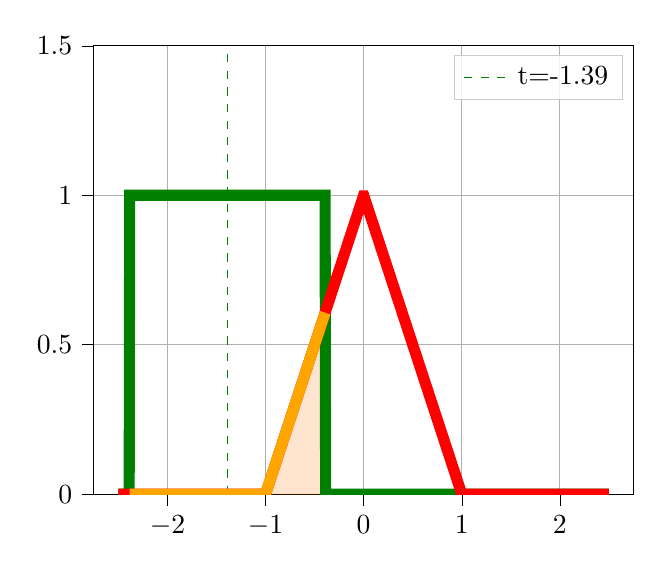
\begin{tikzpicture}

\definecolor{color0}{rgb}{1,0.498039215686275,0.0549019607843137}
\definecolor{color1}{rgb}{1,0.647058823529412,0}

\begin{axis}[
legend cell align={left},
legend style={fill opacity=0.8, draw opacity=1, text opacity=1, draw=white!80!black},
tick align=outside,
tick pos=left,
x grid style={white!69.0196078431373!black},
xmajorgrids,
xmin=-2.75, xmax=2.75,
xtick style={color=black},
y grid style={white!69.0196078431373!black},
ymajorgrids,
ymin=0, ymax=1.5,
ytick style={color=black}
]
\path [draw=color0, fill=color0, opacity=0.2]
(axis cs:-2.38488488488488,0)
--(axis cs:-2.38488488488488,0)
--(axis cs:-2.37987987987988,0)
--(axis cs:-2.37487487487487,0)
--(axis cs:-2.36986986986987,0)
--(axis cs:-2.36486486486486,0)
--(axis cs:-2.35985985985986,0)
--(axis cs:-2.35485485485485,0)
--(axis cs:-2.34984984984985,0)
--(axis cs:-2.34484484484484,0)
--(axis cs:-2.33983983983984,0)
--(axis cs:-2.33483483483483,0)
--(axis cs:-2.32982982982983,0)
--(axis cs:-2.32482482482482,0)
--(axis cs:-2.31981981981982,0)
--(axis cs:-2.31481481481481,0)
--(axis cs:-2.30980980980981,0)
--(axis cs:-2.3048048048048,0)
--(axis cs:-2.2997997997998,0)
--(axis cs:-2.29479479479479,0)
--(axis cs:-2.28978978978979,0)
--(axis cs:-2.28478478478478,0)
--(axis cs:-2.27977977977978,0)
--(axis cs:-2.27477477477477,0)
--(axis cs:-2.26976976976977,0)
--(axis cs:-2.26476476476476,0)
--(axis cs:-2.25975975975976,0)
--(axis cs:-2.25475475475475,0)
--(axis cs:-2.24974974974975,0)
--(axis cs:-2.24474474474474,0)
--(axis cs:-2.23973973973974,0)
--(axis cs:-2.23473473473473,0)
--(axis cs:-2.22972972972973,0)
--(axis cs:-2.22472472472472,0)
--(axis cs:-2.21971971971972,0)
--(axis cs:-2.21471471471471,0)
--(axis cs:-2.20970970970971,0)
--(axis cs:-2.2047047047047,0)
--(axis cs:-2.1996996996997,0)
--(axis cs:-2.19469469469469,0)
--(axis cs:-2.18968968968969,0)
--(axis cs:-2.18468468468468,0)
--(axis cs:-2.17967967967968,0)
--(axis cs:-2.17467467467467,0)
--(axis cs:-2.16966966966967,0)
--(axis cs:-2.16466466466466,0)
--(axis cs:-2.15965965965966,0)
--(axis cs:-2.15465465465465,0)
--(axis cs:-2.14964964964965,0)
--(axis cs:-2.14464464464464,0)
--(axis cs:-2.13963963963964,0)
--(axis cs:-2.13463463463463,0)
--(axis cs:-2.12962962962963,0)
--(axis cs:-2.12462462462462,0)
--(axis cs:-2.11961961961962,0)
--(axis cs:-2.11461461461461,0)
--(axis cs:-2.10960960960961,0)
--(axis cs:-2.1046046046046,0)
--(axis cs:-2.0995995995996,0)
--(axis cs:-2.09459459459459,0)
--(axis cs:-2.08958958958959,0)
--(axis cs:-2.08458458458458,0)
--(axis cs:-2.07957957957958,0)
--(axis cs:-2.07457457457457,0)
--(axis cs:-2.06956956956957,0)
--(axis cs:-2.06456456456456,0)
--(axis cs:-2.05955955955956,0)
--(axis cs:-2.05455455455455,0)
--(axis cs:-2.04954954954955,0)
--(axis cs:-2.04454454454454,0)
--(axis cs:-2.03953953953954,0)
--(axis cs:-2.03453453453453,0)
--(axis cs:-2.02952952952953,0)
--(axis cs:-2.02452452452452,0)
--(axis cs:-2.01951951951952,0)
--(axis cs:-2.01451451451451,0)
--(axis cs:-2.00950950950951,0)
--(axis cs:-2.0045045045045,0)
--(axis cs:-1.9994994994995,0)
--(axis cs:-1.99449449449449,0)
--(axis cs:-1.98948948948949,0)
--(axis cs:-1.98448448448448,0)
--(axis cs:-1.97947947947948,0)
--(axis cs:-1.97447447447447,0)
--(axis cs:-1.96946946946947,0)
--(axis cs:-1.96446446446446,0)
--(axis cs:-1.95945945945946,0)
--(axis cs:-1.95445445445445,0)
--(axis cs:-1.94944944944945,0)
--(axis cs:-1.94444444444444,0)
--(axis cs:-1.93943943943944,0)
--(axis cs:-1.93443443443443,0)
--(axis cs:-1.92942942942943,0)
--(axis cs:-1.92442442442442,0)
--(axis cs:-1.91941941941942,0)
--(axis cs:-1.91441441441441,0)
--(axis cs:-1.90940940940941,0)
--(axis cs:-1.9044044044044,0)
--(axis cs:-1.8993993993994,0)
--(axis cs:-1.89439439439439,0)
--(axis cs:-1.88938938938939,0)
--(axis cs:-1.88438438438438,0)
--(axis cs:-1.87937937937938,0)
--(axis cs:-1.87437437437437,0)
--(axis cs:-1.86936936936937,0)
--(axis cs:-1.86436436436436,0)
--(axis cs:-1.85935935935936,0)
--(axis cs:-1.85435435435435,0)
--(axis cs:-1.84934934934935,0)
--(axis cs:-1.84434434434434,0)
--(axis cs:-1.83933933933934,0)
--(axis cs:-1.83433433433433,0)
--(axis cs:-1.82932932932933,0)
--(axis cs:-1.82432432432432,0)
--(axis cs:-1.81931931931932,0)
--(axis cs:-1.81431431431431,0)
--(axis cs:-1.80930930930931,0)
--(axis cs:-1.8043043043043,0)
--(axis cs:-1.7992992992993,0)
--(axis cs:-1.79429429429429,0)
--(axis cs:-1.78928928928929,0)
--(axis cs:-1.78428428428428,0)
--(axis cs:-1.77927927927928,0)
--(axis cs:-1.77427427427427,0)
--(axis cs:-1.76926926926927,0)
--(axis cs:-1.76426426426426,0)
--(axis cs:-1.75925925925926,0)
--(axis cs:-1.75425425425425,0)
--(axis cs:-1.74924924924925,0)
--(axis cs:-1.74424424424424,0)
--(axis cs:-1.73923923923924,0)
--(axis cs:-1.73423423423423,0)
--(axis cs:-1.72922922922923,0)
--(axis cs:-1.72422422422422,0)
--(axis cs:-1.71921921921922,0)
--(axis cs:-1.71421421421421,0)
--(axis cs:-1.70920920920921,0)
--(axis cs:-1.7042042042042,0)
--(axis cs:-1.6991991991992,0)
--(axis cs:-1.69419419419419,0)
--(axis cs:-1.68918918918919,0)
--(axis cs:-1.68418418418418,0)
--(axis cs:-1.67917917917918,0)
--(axis cs:-1.67417417417417,0)
--(axis cs:-1.66916916916917,0)
--(axis cs:-1.66416416416416,0)
--(axis cs:-1.65915915915916,0)
--(axis cs:-1.65415415415415,0)
--(axis cs:-1.64914914914915,0)
--(axis cs:-1.64414414414414,0)
--(axis cs:-1.63913913913914,0)
--(axis cs:-1.63413413413413,0)
--(axis cs:-1.62912912912913,0)
--(axis cs:-1.62412412412412,0)
--(axis cs:-1.61911911911912,0)
--(axis cs:-1.61411411411411,0)
--(axis cs:-1.60910910910911,0)
--(axis cs:-1.6041041041041,0)
--(axis cs:-1.5990990990991,0)
--(axis cs:-1.59409409409409,0)
--(axis cs:-1.58908908908909,0)
--(axis cs:-1.58408408408408,0)
--(axis cs:-1.57907907907908,0)
--(axis cs:-1.57407407407407,0)
--(axis cs:-1.56906906906907,0)
--(axis cs:-1.56406406406406,0)
--(axis cs:-1.55905905905906,0)
--(axis cs:-1.55405405405405,0)
--(axis cs:-1.54904904904905,0)
--(axis cs:-1.54404404404404,0)
--(axis cs:-1.53903903903904,0)
--(axis cs:-1.53403403403403,0)
--(axis cs:-1.52902902902903,0)
--(axis cs:-1.52402402402402,0)
--(axis cs:-1.51901901901902,0)
--(axis cs:-1.51401401401401,0)
--(axis cs:-1.50900900900901,0)
--(axis cs:-1.504004004004,0)
--(axis cs:-1.498998998999,0)
--(axis cs:-1.49399399399399,0)
--(axis cs:-1.48898898898899,0)
--(axis cs:-1.48398398398398,0)
--(axis cs:-1.47897897897898,0)
--(axis cs:-1.47397397397397,0)
--(axis cs:-1.46896896896897,0)
--(axis cs:-1.46396396396396,0)
--(axis cs:-1.45895895895896,0)
--(axis cs:-1.45395395395395,0)
--(axis cs:-1.44894894894895,0)
--(axis cs:-1.44394394394394,0)
--(axis cs:-1.43893893893894,0)
--(axis cs:-1.43393393393393,0)
--(axis cs:-1.42892892892893,0)
--(axis cs:-1.42392392392392,0)
--(axis cs:-1.41891891891892,0)
--(axis cs:-1.41391391391391,0)
--(axis cs:-1.40890890890891,0)
--(axis cs:-1.4039039039039,0)
--(axis cs:-1.3988988988989,0)
--(axis cs:-1.39389389389389,0)
--(axis cs:-1.38888888888889,0)
--(axis cs:-1.38388388388388,0)
--(axis cs:-1.37887887887888,0)
--(axis cs:-1.37387387387387,0)
--(axis cs:-1.36886886886887,0)
--(axis cs:-1.36386386386386,0)
--(axis cs:-1.35885885885886,0)
--(axis cs:-1.35385385385385,0)
--(axis cs:-1.34884884884885,0)
--(axis cs:-1.34384384384384,0)
--(axis cs:-1.33883883883884,0)
--(axis cs:-1.33383383383383,0)
--(axis cs:-1.32882882882883,0)
--(axis cs:-1.32382382382382,0)
--(axis cs:-1.31881881881882,0)
--(axis cs:-1.31381381381381,0)
--(axis cs:-1.30880880880881,0)
--(axis cs:-1.3038038038038,0)
--(axis cs:-1.2987987987988,0)
--(axis cs:-1.29379379379379,0)
--(axis cs:-1.28878878878879,0)
--(axis cs:-1.28378378378378,0)
--(axis cs:-1.27877877877878,0)
--(axis cs:-1.27377377377377,0)
--(axis cs:-1.26876876876877,0)
--(axis cs:-1.26376376376376,0)
--(axis cs:-1.25875875875876,0)
--(axis cs:-1.25375375375375,0)
--(axis cs:-1.24874874874875,0)
--(axis cs:-1.24374374374374,0)
--(axis cs:-1.23873873873874,0)
--(axis cs:-1.23373373373373,0)
--(axis cs:-1.22872872872873,0)
--(axis cs:-1.22372372372372,0)
--(axis cs:-1.21871871871872,0)
--(axis cs:-1.21371371371371,0)
--(axis cs:-1.20870870870871,0)
--(axis cs:-1.2037037037037,0)
--(axis cs:-1.1986986986987,0)
--(axis cs:-1.19369369369369,0)
--(axis cs:-1.18868868868869,0)
--(axis cs:-1.18368368368368,0)
--(axis cs:-1.17867867867868,0)
--(axis cs:-1.17367367367367,0)
--(axis cs:-1.16866866866867,0)
--(axis cs:-1.16366366366366,0)
--(axis cs:-1.15865865865866,0)
--(axis cs:-1.15365365365365,0)
--(axis cs:-1.14864864864865,0)
--(axis cs:-1.14364364364364,0)
--(axis cs:-1.13863863863864,0)
--(axis cs:-1.13363363363363,0)
--(axis cs:-1.12862862862863,0)
--(axis cs:-1.12362362362362,0)
--(axis cs:-1.11861861861862,0)
--(axis cs:-1.11361361361361,0)
--(axis cs:-1.10860860860861,0)
--(axis cs:-1.1036036036036,0)
--(axis cs:-1.0985985985986,0)
--(axis cs:-1.09359359359359,0)
--(axis cs:-1.08858858858859,0)
--(axis cs:-1.08358358358358,0)
--(axis cs:-1.07857857857858,0)
--(axis cs:-1.07357357357357,0)
--(axis cs:-1.06856856856857,0)
--(axis cs:-1.06356356356356,0)
--(axis cs:-1.05855855855856,0)
--(axis cs:-1.05355355355355,0)
--(axis cs:-1.04854854854855,0)
--(axis cs:-1.04354354354354,0)
--(axis cs:-1.03853853853854,0)
--(axis cs:-1.03353353353353,0)
--(axis cs:-1.02852852852853,0)
--(axis cs:-1.02352352352352,0)
--(axis cs:-1.01851851851852,0)
--(axis cs:-1.01351351351351,0)
--(axis cs:-1.00850850850851,0)
--(axis cs:-1.0035035035035,0)
--(axis cs:-0.998498498498499,0)
--(axis cs:-0.993493493493494,0)
--(axis cs:-0.988488488488489,0)
--(axis cs:-0.983483483483484,0)
--(axis cs:-0.978478478478479,0)
--(axis cs:-0.973473473473474,0)
--(axis cs:-0.968468468468469,0)
--(axis cs:-0.963463463463464,0)
--(axis cs:-0.958458458458459,0)
--(axis cs:-0.953453453453454,0)
--(axis cs:-0.948448448448449,0)
--(axis cs:-0.943443443443444,0)
--(axis cs:-0.938438438438439,0)
--(axis cs:-0.933433433433434,0)
--(axis cs:-0.928428428428429,0)
--(axis cs:-0.923423423423424,0)
--(axis cs:-0.918418418418419,0)
--(axis cs:-0.913413413413414,0)
--(axis cs:-0.908408408408409,0)
--(axis cs:-0.903403403403404,0)
--(axis cs:-0.898398398398399,0)
--(axis cs:-0.893393393393393,0)
--(axis cs:-0.888388388388388,0)
--(axis cs:-0.883383383383383,0)
--(axis cs:-0.878378378378378,0)
--(axis cs:-0.873373373373373,0)
--(axis cs:-0.868368368368368,0)
--(axis cs:-0.863363363363363,0)
--(axis cs:-0.858358358358358,0)
--(axis cs:-0.853353353353353,0)
--(axis cs:-0.848348348348348,0)
--(axis cs:-0.843343343343343,0)
--(axis cs:-0.838338338338338,0)
--(axis cs:-0.833333333333333,0)
--(axis cs:-0.828328328328328,0)
--(axis cs:-0.823323323323323,0)
--(axis cs:-0.818318318318318,0)
--(axis cs:-0.813313313313313,0)
--(axis cs:-0.808308308308308,0)
--(axis cs:-0.803303303303303,0)
--(axis cs:-0.798298298298298,0)
--(axis cs:-0.793293293293293,0)
--(axis cs:-0.788288288288288,0)
--(axis cs:-0.783283283283283,0)
--(axis cs:-0.778278278278278,0)
--(axis cs:-0.773273273273273,0)
--(axis cs:-0.768268268268268,0)
--(axis cs:-0.763263263263263,0)
--(axis cs:-0.758258258258258,0)
--(axis cs:-0.753253253253253,0)
--(axis cs:-0.748248248248248,0)
--(axis cs:-0.743243243243243,0)
--(axis cs:-0.738238238238238,0)
--(axis cs:-0.733233233233233,0)
--(axis cs:-0.728228228228228,0)
--(axis cs:-0.723223223223223,0)
--(axis cs:-0.718218218218218,0)
--(axis cs:-0.713213213213213,0)
--(axis cs:-0.708208208208208,0)
--(axis cs:-0.703203203203203,0)
--(axis cs:-0.698198198198198,0)
--(axis cs:-0.693193193193193,0)
--(axis cs:-0.688188188188188,0)
--(axis cs:-0.683183183183183,0)
--(axis cs:-0.678178178178178,0)
--(axis cs:-0.673173173173173,0)
--(axis cs:-0.668168168168168,0)
--(axis cs:-0.663163163163163,0)
--(axis cs:-0.658158158158158,0)
--(axis cs:-0.653153153153153,0)
--(axis cs:-0.648148148148148,0)
--(axis cs:-0.643143143143143,0)
--(axis cs:-0.638138138138138,0)
--(axis cs:-0.633133133133133,0)
--(axis cs:-0.628128128128128,0)
--(axis cs:-0.623123123123123,0)
--(axis cs:-0.618118118118118,0)
--(axis cs:-0.613113113113113,0)
--(axis cs:-0.608108108108108,0)
--(axis cs:-0.603103103103103,0)
--(axis cs:-0.598098098098098,0)
--(axis cs:-0.593093093093093,0)
--(axis cs:-0.588088088088088,0)
--(axis cs:-0.583083083083083,0)
--(axis cs:-0.578078078078078,0)
--(axis cs:-0.573073073073073,0)
--(axis cs:-0.568068068068068,0)
--(axis cs:-0.563063063063063,0)
--(axis cs:-0.558058058058058,0)
--(axis cs:-0.553053053053053,0)
--(axis cs:-0.548048048048048,0)
--(axis cs:-0.543043043043043,0)
--(axis cs:-0.538038038038038,0)
--(axis cs:-0.533033033033033,0)
--(axis cs:-0.528028028028028,0)
--(axis cs:-0.523023023023023,0)
--(axis cs:-0.518018018018018,0)
--(axis cs:-0.513013013013013,0)
--(axis cs:-0.508008008008008,0)
--(axis cs:-0.503003003003003,0)
--(axis cs:-0.497997997997998,0)
--(axis cs:-0.492992992992993,0)
--(axis cs:-0.487987987987988,0)
--(axis cs:-0.482982982982983,0)
--(axis cs:-0.477977977977978,0)
--(axis cs:-0.472972972972973,0)
--(axis cs:-0.467967967967968,0)
--(axis cs:-0.462962962962963,0)
--(axis cs:-0.457957957957958,0)
--(axis cs:-0.452952952952953,0)
--(axis cs:-0.447947947947948,0)
--(axis cs:-0.442942942942943,0)
--(axis cs:-0.437937937937938,0)
--(axis cs:-0.432932932932933,0)
--(axis cs:-0.427927927927928,0)
--(axis cs:-0.422922922922923,0)
--(axis cs:-0.417917917917918,0)
--(axis cs:-0.412912912912913,0)
--(axis cs:-0.407907907907908,0)
--(axis cs:-0.402902902902903,0)
--(axis cs:-0.397897897897898,0)
--(axis cs:-0.392892892892893,0)
--(axis cs:-0.392892892892893,0.607107107107107)
--(axis cs:-0.392892892892893,0.607107107107107)
--(axis cs:-0.397897897897898,0.602102102102102)
--(axis cs:-0.402902902902903,0.597097097097097)
--(axis cs:-0.407907907907908,0.592092092092092)
--(axis cs:-0.412912912912913,0.587087087087087)
--(axis cs:-0.417917917917918,0.582082082082082)
--(axis cs:-0.422922922922923,0.577077077077077)
--(axis cs:-0.427927927927928,0.572072072072072)
--(axis cs:-0.432932932932933,0.567067067067067)
--(axis cs:-0.437937937937938,0.562062062062062)
--(axis cs:-0.442942942942943,0.557057057057057)
--(axis cs:-0.447947947947948,0.552052052052052)
--(axis cs:-0.452952952952953,0.547047047047047)
--(axis cs:-0.457957957957958,0.542042042042042)
--(axis cs:-0.462962962962963,0.537037037037037)
--(axis cs:-0.467967967967968,0.532032032032032)
--(axis cs:-0.472972972972973,0.527027027027027)
--(axis cs:-0.477977977977978,0.522022022022022)
--(axis cs:-0.482982982982983,0.517017017017017)
--(axis cs:-0.487987987987988,0.512012012012012)
--(axis cs:-0.492992992992993,0.507007007007007)
--(axis cs:-0.497997997997998,0.502002002002002)
--(axis cs:-0.503003003003003,0.496996996996997)
--(axis cs:-0.508008008008008,0.491991991991992)
--(axis cs:-0.513013013013013,0.486986986986987)
--(axis cs:-0.518018018018018,0.481981981981982)
--(axis cs:-0.523023023023023,0.476976976976977)
--(axis cs:-0.528028028028028,0.471971971971972)
--(axis cs:-0.533033033033033,0.466966966966967)
--(axis cs:-0.538038038038038,0.461961961961962)
--(axis cs:-0.543043043043043,0.456956956956957)
--(axis cs:-0.548048048048048,0.451951951951952)
--(axis cs:-0.553053053053053,0.446946946946947)
--(axis cs:-0.558058058058058,0.441941941941942)
--(axis cs:-0.563063063063063,0.436936936936937)
--(axis cs:-0.568068068068068,0.431931931931932)
--(axis cs:-0.573073073073073,0.426926926926927)
--(axis cs:-0.578078078078078,0.421921921921922)
--(axis cs:-0.583083083083083,0.416916916916917)
--(axis cs:-0.588088088088088,0.411911911911912)
--(axis cs:-0.593093093093093,0.406906906906907)
--(axis cs:-0.598098098098098,0.401901901901902)
--(axis cs:-0.603103103103103,0.396896896896897)
--(axis cs:-0.608108108108108,0.391891891891892)
--(axis cs:-0.613113113113113,0.386886886886887)
--(axis cs:-0.618118118118118,0.381881881881882)
--(axis cs:-0.623123123123123,0.376876876876877)
--(axis cs:-0.628128128128128,0.371871871871872)
--(axis cs:-0.633133133133133,0.366866866866867)
--(axis cs:-0.638138138138138,0.361861861861862)
--(axis cs:-0.643143143143143,0.356856856856857)
--(axis cs:-0.648148148148148,0.351851851851852)
--(axis cs:-0.653153153153153,0.346846846846847)
--(axis cs:-0.658158158158158,0.341841841841842)
--(axis cs:-0.663163163163163,0.336836836836837)
--(axis cs:-0.668168168168168,0.331831831831832)
--(axis cs:-0.673173173173173,0.326826826826827)
--(axis cs:-0.678178178178178,0.321821821821822)
--(axis cs:-0.683183183183183,0.316816816816817)
--(axis cs:-0.688188188188188,0.311811811811812)
--(axis cs:-0.693193193193193,0.306806806806807)
--(axis cs:-0.698198198198198,0.301801801801802)
--(axis cs:-0.703203203203203,0.296796796796797)
--(axis cs:-0.708208208208208,0.291791791791792)
--(axis cs:-0.713213213213213,0.286786786786787)
--(axis cs:-0.718218218218218,0.281781781781782)
--(axis cs:-0.723223223223223,0.276776776776777)
--(axis cs:-0.728228228228228,0.271771771771772)
--(axis cs:-0.733233233233233,0.266766766766767)
--(axis cs:-0.738238238238238,0.261761761761762)
--(axis cs:-0.743243243243243,0.256756756756757)
--(axis cs:-0.748248248248248,0.251751751751752)
--(axis cs:-0.753253253253253,0.246746746746747)
--(axis cs:-0.758258258258258,0.241741741741742)
--(axis cs:-0.763263263263263,0.236736736736737)
--(axis cs:-0.768268268268268,0.231731731731732)
--(axis cs:-0.773273273273273,0.226726726726727)
--(axis cs:-0.778278278278278,0.221721721721722)
--(axis cs:-0.783283283283283,0.216716716716717)
--(axis cs:-0.788288288288288,0.211711711711712)
--(axis cs:-0.793293293293293,0.206706706706707)
--(axis cs:-0.798298298298298,0.201701701701702)
--(axis cs:-0.803303303303303,0.196696696696697)
--(axis cs:-0.808308308308308,0.191691691691692)
--(axis cs:-0.813313313313313,0.186686686686687)
--(axis cs:-0.818318318318318,0.181681681681682)
--(axis cs:-0.823323323323323,0.176676676676677)
--(axis cs:-0.828328328328328,0.171671671671672)
--(axis cs:-0.833333333333333,0.166666666666667)
--(axis cs:-0.838338338338338,0.161661661661662)
--(axis cs:-0.843343343343343,0.156656656656657)
--(axis cs:-0.848348348348348,0.151651651651652)
--(axis cs:-0.853353353353353,0.146646646646647)
--(axis cs:-0.858358358358358,0.141641641641642)
--(axis cs:-0.863363363363363,0.136636636636637)
--(axis cs:-0.868368368368368,0.131631631631632)
--(axis cs:-0.873373373373373,0.126626626626627)
--(axis cs:-0.878378378378378,0.121621621621622)
--(axis cs:-0.883383383383383,0.116616616616617)
--(axis cs:-0.888388388388388,0.111611611611612)
--(axis cs:-0.893393393393393,0.106606606606607)
--(axis cs:-0.898398398398399,0.101601601601601)
--(axis cs:-0.903403403403404,0.0965965965965965)
--(axis cs:-0.908408408408409,0.0915915915915915)
--(axis cs:-0.913413413413414,0.0865865865865865)
--(axis cs:-0.918418418418419,0.0815815815815815)
--(axis cs:-0.923423423423424,0.0765765765765765)
--(axis cs:-0.928428428428429,0.0715715715715715)
--(axis cs:-0.933433433433434,0.0665665665665665)
--(axis cs:-0.938438438438439,0.0615615615615615)
--(axis cs:-0.943443443443444,0.0565565565565564)
--(axis cs:-0.948448448448449,0.0515515515515514)
--(axis cs:-0.953453453453454,0.0465465465465464)
--(axis cs:-0.958458458458459,0.0415415415415414)
--(axis cs:-0.963463463463464,0.0365365365365364)
--(axis cs:-0.968468468468469,0.0315315315315314)
--(axis cs:-0.973473473473474,0.0265265265265264)
--(axis cs:-0.978478478478479,0.0215215215215214)
--(axis cs:-0.983483483483484,0.0165165165165164)
--(axis cs:-0.988488488488489,0.0115115115115114)
--(axis cs:-0.993493493493494,0.00650650650650642)
--(axis cs:-0.998498498498499,0.00150150150150141)
--(axis cs:-1.0035035035035,0)
--(axis cs:-1.00850850850851,0)
--(axis cs:-1.01351351351351,0)
--(axis cs:-1.01851851851852,0)
--(axis cs:-1.02352352352352,0)
--(axis cs:-1.02852852852853,0)
--(axis cs:-1.03353353353353,0)
--(axis cs:-1.03853853853854,0)
--(axis cs:-1.04354354354354,0)
--(axis cs:-1.04854854854855,0)
--(axis cs:-1.05355355355355,0)
--(axis cs:-1.05855855855856,0)
--(axis cs:-1.06356356356356,0)
--(axis cs:-1.06856856856857,0)
--(axis cs:-1.07357357357357,0)
--(axis cs:-1.07857857857858,0)
--(axis cs:-1.08358358358358,0)
--(axis cs:-1.08858858858859,0)
--(axis cs:-1.09359359359359,0)
--(axis cs:-1.0985985985986,0)
--(axis cs:-1.1036036036036,0)
--(axis cs:-1.10860860860861,0)
--(axis cs:-1.11361361361361,0)
--(axis cs:-1.11861861861862,0)
--(axis cs:-1.12362362362362,0)
--(axis cs:-1.12862862862863,0)
--(axis cs:-1.13363363363363,0)
--(axis cs:-1.13863863863864,0)
--(axis cs:-1.14364364364364,0)
--(axis cs:-1.14864864864865,0)
--(axis cs:-1.15365365365365,0)
--(axis cs:-1.15865865865866,0)
--(axis cs:-1.16366366366366,0)
--(axis cs:-1.16866866866867,0)
--(axis cs:-1.17367367367367,0)
--(axis cs:-1.17867867867868,0)
--(axis cs:-1.18368368368368,0)
--(axis cs:-1.18868868868869,0)
--(axis cs:-1.19369369369369,0)
--(axis cs:-1.1986986986987,0)
--(axis cs:-1.2037037037037,0)
--(axis cs:-1.20870870870871,0)
--(axis cs:-1.21371371371371,0)
--(axis cs:-1.21871871871872,0)
--(axis cs:-1.22372372372372,0)
--(axis cs:-1.22872872872873,0)
--(axis cs:-1.23373373373373,0)
--(axis cs:-1.23873873873874,0)
--(axis cs:-1.24374374374374,0)
--(axis cs:-1.24874874874875,0)
--(axis cs:-1.25375375375375,0)
--(axis cs:-1.25875875875876,0)
--(axis cs:-1.26376376376376,0)
--(axis cs:-1.26876876876877,0)
--(axis cs:-1.27377377377377,0)
--(axis cs:-1.27877877877878,0)
--(axis cs:-1.28378378378378,0)
--(axis cs:-1.28878878878879,0)
--(axis cs:-1.29379379379379,0)
--(axis cs:-1.2987987987988,0)
--(axis cs:-1.3038038038038,0)
--(axis cs:-1.30880880880881,0)
--(axis cs:-1.31381381381381,0)
--(axis cs:-1.31881881881882,0)
--(axis cs:-1.32382382382382,0)
--(axis cs:-1.32882882882883,0)
--(axis cs:-1.33383383383383,0)
--(axis cs:-1.33883883883884,0)
--(axis cs:-1.34384384384384,0)
--(axis cs:-1.34884884884885,0)
--(axis cs:-1.35385385385385,0)
--(axis cs:-1.35885885885886,0)
--(axis cs:-1.36386386386386,0)
--(axis cs:-1.36886886886887,0)
--(axis cs:-1.37387387387387,0)
--(axis cs:-1.37887887887888,0)
--(axis cs:-1.38388388388388,0)
--(axis cs:-1.38888888888889,0)
--(axis cs:-1.39389389389389,0)
--(axis cs:-1.3988988988989,0)
--(axis cs:-1.4039039039039,0)
--(axis cs:-1.40890890890891,0)
--(axis cs:-1.41391391391391,0)
--(axis cs:-1.41891891891892,0)
--(axis cs:-1.42392392392392,0)
--(axis cs:-1.42892892892893,0)
--(axis cs:-1.43393393393393,0)
--(axis cs:-1.43893893893894,0)
--(axis cs:-1.44394394394394,0)
--(axis cs:-1.44894894894895,0)
--(axis cs:-1.45395395395395,0)
--(axis cs:-1.45895895895896,0)
--(axis cs:-1.46396396396396,0)
--(axis cs:-1.46896896896897,0)
--(axis cs:-1.47397397397397,0)
--(axis cs:-1.47897897897898,0)
--(axis cs:-1.48398398398398,0)
--(axis cs:-1.48898898898899,0)
--(axis cs:-1.49399399399399,0)
--(axis cs:-1.498998998999,0)
--(axis cs:-1.504004004004,0)
--(axis cs:-1.50900900900901,0)
--(axis cs:-1.51401401401401,0)
--(axis cs:-1.51901901901902,0)
--(axis cs:-1.52402402402402,0)
--(axis cs:-1.52902902902903,0)
--(axis cs:-1.53403403403403,0)
--(axis cs:-1.53903903903904,0)
--(axis cs:-1.54404404404404,0)
--(axis cs:-1.54904904904905,0)
--(axis cs:-1.55405405405405,0)
--(axis cs:-1.55905905905906,0)
--(axis cs:-1.56406406406406,0)
--(axis cs:-1.56906906906907,0)
--(axis cs:-1.57407407407407,0)
--(axis cs:-1.57907907907908,0)
--(axis cs:-1.58408408408408,0)
--(axis cs:-1.58908908908909,0)
--(axis cs:-1.59409409409409,0)
--(axis cs:-1.5990990990991,0)
--(axis cs:-1.6041041041041,0)
--(axis cs:-1.60910910910911,0)
--(axis cs:-1.61411411411411,0)
--(axis cs:-1.61911911911912,0)
--(axis cs:-1.62412412412412,0)
--(axis cs:-1.62912912912913,0)
--(axis cs:-1.63413413413413,0)
--(axis cs:-1.63913913913914,0)
--(axis cs:-1.64414414414414,0)
--(axis cs:-1.64914914914915,0)
--(axis cs:-1.65415415415415,0)
--(axis cs:-1.65915915915916,0)
--(axis cs:-1.66416416416416,0)
--(axis cs:-1.66916916916917,0)
--(axis cs:-1.67417417417417,0)
--(axis cs:-1.67917917917918,0)
--(axis cs:-1.68418418418418,0)
--(axis cs:-1.68918918918919,0)
--(axis cs:-1.69419419419419,0)
--(axis cs:-1.6991991991992,0)
--(axis cs:-1.7042042042042,0)
--(axis cs:-1.70920920920921,0)
--(axis cs:-1.71421421421421,0)
--(axis cs:-1.71921921921922,0)
--(axis cs:-1.72422422422422,0)
--(axis cs:-1.72922922922923,0)
--(axis cs:-1.73423423423423,0)
--(axis cs:-1.73923923923924,0)
--(axis cs:-1.74424424424424,0)
--(axis cs:-1.74924924924925,0)
--(axis cs:-1.75425425425425,0)
--(axis cs:-1.75925925925926,0)
--(axis cs:-1.76426426426426,0)
--(axis cs:-1.76926926926927,0)
--(axis cs:-1.77427427427427,0)
--(axis cs:-1.77927927927928,0)
--(axis cs:-1.78428428428428,0)
--(axis cs:-1.78928928928929,0)
--(axis cs:-1.79429429429429,0)
--(axis cs:-1.7992992992993,0)
--(axis cs:-1.8043043043043,0)
--(axis cs:-1.80930930930931,0)
--(axis cs:-1.81431431431431,0)
--(axis cs:-1.81931931931932,0)
--(axis cs:-1.82432432432432,0)
--(axis cs:-1.82932932932933,0)
--(axis cs:-1.83433433433433,0)
--(axis cs:-1.83933933933934,0)
--(axis cs:-1.84434434434434,0)
--(axis cs:-1.84934934934935,0)
--(axis cs:-1.85435435435435,0)
--(axis cs:-1.85935935935936,0)
--(axis cs:-1.86436436436436,0)
--(axis cs:-1.86936936936937,0)
--(axis cs:-1.87437437437437,0)
--(axis cs:-1.87937937937938,0)
--(axis cs:-1.88438438438438,0)
--(axis cs:-1.88938938938939,0)
--(axis cs:-1.89439439439439,0)
--(axis cs:-1.8993993993994,0)
--(axis cs:-1.9044044044044,0)
--(axis cs:-1.90940940940941,0)
--(axis cs:-1.91441441441441,0)
--(axis cs:-1.91941941941942,0)
--(axis cs:-1.92442442442442,0)
--(axis cs:-1.92942942942943,0)
--(axis cs:-1.93443443443443,0)
--(axis cs:-1.93943943943944,0)
--(axis cs:-1.94444444444444,0)
--(axis cs:-1.94944944944945,0)
--(axis cs:-1.95445445445445,0)
--(axis cs:-1.95945945945946,0)
--(axis cs:-1.96446446446446,0)
--(axis cs:-1.96946946946947,0)
--(axis cs:-1.97447447447447,0)
--(axis cs:-1.97947947947948,0)
--(axis cs:-1.98448448448448,0)
--(axis cs:-1.98948948948949,0)
--(axis cs:-1.99449449449449,0)
--(axis cs:-1.9994994994995,0)
--(axis cs:-2.0045045045045,0)
--(axis cs:-2.00950950950951,0)
--(axis cs:-2.01451451451451,0)
--(axis cs:-2.01951951951952,0)
--(axis cs:-2.02452452452452,0)
--(axis cs:-2.02952952952953,0)
--(axis cs:-2.03453453453453,0)
--(axis cs:-2.03953953953954,0)
--(axis cs:-2.04454454454454,0)
--(axis cs:-2.04954954954955,0)
--(axis cs:-2.05455455455455,0)
--(axis cs:-2.05955955955956,0)
--(axis cs:-2.06456456456456,0)
--(axis cs:-2.06956956956957,0)
--(axis cs:-2.07457457457457,0)
--(axis cs:-2.07957957957958,0)
--(axis cs:-2.08458458458458,0)
--(axis cs:-2.08958958958959,0)
--(axis cs:-2.09459459459459,0)
--(axis cs:-2.0995995995996,0)
--(axis cs:-2.1046046046046,0)
--(axis cs:-2.10960960960961,0)
--(axis cs:-2.11461461461461,0)
--(axis cs:-2.11961961961962,0)
--(axis cs:-2.12462462462462,0)
--(axis cs:-2.12962962962963,0)
--(axis cs:-2.13463463463463,0)
--(axis cs:-2.13963963963964,0)
--(axis cs:-2.14464464464464,0)
--(axis cs:-2.14964964964965,0)
--(axis cs:-2.15465465465465,0)
--(axis cs:-2.15965965965966,0)
--(axis cs:-2.16466466466466,0)
--(axis cs:-2.16966966966967,0)
--(axis cs:-2.17467467467467,0)
--(axis cs:-2.17967967967968,0)
--(axis cs:-2.18468468468468,0)
--(axis cs:-2.18968968968969,0)
--(axis cs:-2.19469469469469,0)
--(axis cs:-2.1996996996997,0)
--(axis cs:-2.2047047047047,0)
--(axis cs:-2.20970970970971,0)
--(axis cs:-2.21471471471471,0)
--(axis cs:-2.21971971971972,0)
--(axis cs:-2.22472472472472,0)
--(axis cs:-2.22972972972973,0)
--(axis cs:-2.23473473473473,0)
--(axis cs:-2.23973973973974,0)
--(axis cs:-2.24474474474474,0)
--(axis cs:-2.24974974974975,0)
--(axis cs:-2.25475475475475,0)
--(axis cs:-2.25975975975976,0)
--(axis cs:-2.26476476476476,0)
--(axis cs:-2.26976976976977,0)
--(axis cs:-2.27477477477477,0)
--(axis cs:-2.27977977977978,0)
--(axis cs:-2.28478478478478,0)
--(axis cs:-2.28978978978979,0)
--(axis cs:-2.29479479479479,0)
--(axis cs:-2.2997997997998,0)
--(axis cs:-2.3048048048048,0)
--(axis cs:-2.30980980980981,0)
--(axis cs:-2.31481481481481,0)
--(axis cs:-2.31981981981982,0)
--(axis cs:-2.32482482482482,0)
--(axis cs:-2.32982982982983,0)
--(axis cs:-2.33483483483483,0)
--(axis cs:-2.33983983983984,0)
--(axis cs:-2.34484484484484,0)
--(axis cs:-2.34984984984985,0)
--(axis cs:-2.35485485485485,0)
--(axis cs:-2.35985985985986,0)
--(axis cs:-2.36486486486486,0)
--(axis cs:-2.36986986986987,0)
--(axis cs:-2.37487487487487,0)
--(axis cs:-2.37987987987988,0)
--(axis cs:-2.38488488488488,0)
--cycle;

\addplot [line width=4pt, green!50!black, forget plot]
table {%
-2.5 0
-2.49499499499499 0
-2.48998998998999 0
-2.48498498498498 0
-2.47997997997998 0
-2.47497497497497 0
-2.46996996996997 0
-2.46496496496496 0
-2.45995995995996 0
-2.45495495495495 0
-2.44994994994995 0
-2.44494494494494 0
-2.43993993993994 0
-2.43493493493493 0
-2.42992992992993 0
-2.42492492492492 0
-2.41991991991992 0
-2.41491491491491 0
-2.40990990990991 0
-2.4049049049049 0
-2.3998998998999 0
-2.39489489489489 0
-2.38988988988989 0
-2.38488488488488 1
-2.37987987987988 1
-2.37487487487487 1
-2.36986986986987 1
-2.36486486486486 1
-2.35985985985986 1
-2.35485485485485 1
-2.34984984984985 1
-2.34484484484484 1
-2.33983983983984 1
-2.33483483483483 1
-2.32982982982983 1
-2.32482482482482 1
-2.31981981981982 1
-2.31481481481481 1
-2.30980980980981 1
-2.3048048048048 1
-2.2997997997998 1
-2.29479479479479 1
-2.28978978978979 1
-2.28478478478478 1
-2.27977977977978 1
-2.27477477477477 1
-2.26976976976977 1
-2.26476476476476 1
-2.25975975975976 1
-2.25475475475475 1
-2.24974974974975 1
-2.24474474474474 1
-2.23973973973974 1
-2.23473473473473 1
-2.22972972972973 1
-2.22472472472472 1
-2.21971971971972 1
-2.21471471471471 1
-2.20970970970971 1
-2.2047047047047 1
-2.1996996996997 1
-2.19469469469469 1
-2.18968968968969 1
-2.18468468468468 1
-2.17967967967968 1
-2.17467467467467 1
-2.16966966966967 1
-2.16466466466466 1
-2.15965965965966 1
-2.15465465465465 1
-2.14964964964965 1
-2.14464464464464 1
-2.13963963963964 1
-2.13463463463463 1
-2.12962962962963 1
-2.12462462462462 1
-2.11961961961962 1
-2.11461461461461 1
-2.10960960960961 1
-2.1046046046046 1
-2.0995995995996 1
-2.09459459459459 1
-2.08958958958959 1
-2.08458458458458 1
-2.07957957957958 1
-2.07457457457457 1
-2.06956956956957 1
-2.06456456456456 1
-2.05955955955956 1
-2.05455455455455 1
-2.04954954954955 1
-2.04454454454454 1
-2.03953953953954 1
-2.03453453453453 1
-2.02952952952953 1
-2.02452452452452 1
-2.01951951951952 1
-2.01451451451451 1
-2.00950950950951 1
-2.0045045045045 1
-1.9994994994995 1
-1.99449449449449 1
-1.98948948948949 1
-1.98448448448448 1
-1.97947947947948 1
-1.97447447447447 1
-1.96946946946947 1
-1.96446446446446 1
-1.95945945945946 1
-1.95445445445445 1
-1.94944944944945 1
-1.94444444444444 1
-1.93943943943944 1
-1.93443443443443 1
-1.92942942942943 1
-1.92442442442442 1
-1.91941941941942 1
-1.91441441441441 1
-1.90940940940941 1
-1.9044044044044 1
-1.8993993993994 1
-1.89439439439439 1
-1.88938938938939 1
-1.88438438438438 1
-1.87937937937938 1
-1.87437437437437 1
-1.86936936936937 1
-1.86436436436436 1
-1.85935935935936 1
-1.85435435435435 1
-1.84934934934935 1
-1.84434434434434 1
-1.83933933933934 1
-1.83433433433433 1
-1.82932932932933 1
-1.82432432432432 1
-1.81931931931932 1
-1.81431431431431 1
-1.80930930930931 1
-1.8043043043043 1
-1.7992992992993 1
-1.79429429429429 1
-1.78928928928929 1
-1.78428428428428 1
-1.77927927927928 1
-1.77427427427427 1
-1.76926926926927 1
-1.76426426426426 1
-1.75925925925926 1
-1.75425425425425 1
-1.74924924924925 1
-1.74424424424424 1
-1.73923923923924 1
-1.73423423423423 1
-1.72922922922923 1
-1.72422422422422 1
-1.71921921921922 1
-1.71421421421421 1
-1.70920920920921 1
-1.7042042042042 1
-1.6991991991992 1
-1.69419419419419 1
-1.68918918918919 1
-1.68418418418418 1
-1.67917917917918 1
-1.67417417417417 1
-1.66916916916917 1
-1.66416416416416 1
-1.65915915915916 1
-1.65415415415415 1
-1.64914914914915 1
-1.64414414414414 1
-1.63913913913914 1
-1.63413413413413 1
-1.62912912912913 1
-1.62412412412412 1
-1.61911911911912 1
-1.61411411411411 1
-1.60910910910911 1
-1.6041041041041 1
-1.5990990990991 1
-1.59409409409409 1
-1.58908908908909 1
-1.58408408408408 1
-1.57907907907908 1
-1.57407407407407 1
-1.56906906906907 1
-1.56406406406406 1
-1.55905905905906 1
-1.55405405405405 1
-1.54904904904905 1
-1.54404404404404 1
-1.53903903903904 1
-1.53403403403403 1
-1.52902902902903 1
-1.52402402402402 1
-1.51901901901902 1
-1.51401401401401 1
-1.50900900900901 1
-1.504004004004 1
-1.498998998999 1
-1.49399399399399 1
-1.48898898898899 1
-1.48398398398398 1
-1.47897897897898 1
-1.47397397397397 1
-1.46896896896897 1
-1.46396396396396 1
-1.45895895895896 1
-1.45395395395395 1
-1.44894894894895 1
-1.44394394394394 1
-1.43893893893894 1
-1.43393393393393 1
-1.42892892892893 1
-1.42392392392392 1
-1.41891891891892 1
-1.41391391391391 1
-1.40890890890891 1
-1.4039039039039 1
-1.3988988988989 1
-1.39389389389389 1
-1.38888888888889 1
-1.38388388388388 1
-1.37887887887888 1
-1.37387387387387 1
-1.36886886886887 1
-1.36386386386386 1
-1.35885885885886 1
-1.35385385385385 1
-1.34884884884885 1
-1.34384384384384 1
-1.33883883883884 1
-1.33383383383383 1
-1.32882882882883 1
-1.32382382382382 1
-1.31881881881882 1
-1.31381381381381 1
-1.30880880880881 1
-1.3038038038038 1
-1.2987987987988 1
-1.29379379379379 1
-1.28878878878879 1
-1.28378378378378 1
-1.27877877877878 1
-1.27377377377377 1
-1.26876876876877 1
-1.26376376376376 1
-1.25875875875876 1
-1.25375375375375 1
-1.24874874874875 1
-1.24374374374374 1
-1.23873873873874 1
-1.23373373373373 1
-1.22872872872873 1
-1.22372372372372 1
-1.21871871871872 1
-1.21371371371371 1
-1.20870870870871 1
-1.2037037037037 1
-1.1986986986987 1
-1.19369369369369 1
-1.18868868868869 1
-1.18368368368368 1
-1.17867867867868 1
-1.17367367367367 1
-1.16866866866867 1
-1.16366366366366 1
-1.15865865865866 1
-1.15365365365365 1
-1.14864864864865 1
-1.14364364364364 1
-1.13863863863864 1
-1.13363363363363 1
-1.12862862862863 1
-1.12362362362362 1
-1.11861861861862 1
-1.11361361361361 1
-1.10860860860861 1
-1.1036036036036 1
-1.0985985985986 1
-1.09359359359359 1
-1.08858858858859 1
-1.08358358358358 1
-1.07857857857858 1
-1.07357357357357 1
-1.06856856856857 1
-1.06356356356356 1
-1.05855855855856 1
-1.05355355355355 1
-1.04854854854855 1
-1.04354354354354 1
-1.03853853853854 1
-1.03353353353353 1
-1.02852852852853 1
-1.02352352352352 1
-1.01851851851852 1
-1.01351351351351 1
-1.00850850850851 1
-1.0035035035035 1
-0.998498498498499 1
-0.993493493493494 1
-0.988488488488489 1
-0.983483483483484 1
-0.978478478478479 1
-0.973473473473474 1
-0.968468468468469 1
-0.963463463463464 1
-0.958458458458459 1
-0.953453453453454 1
-0.948448448448449 1
-0.943443443443444 1
-0.938438438438439 1
-0.933433433433434 1
-0.928428428428429 1
-0.923423423423424 1
-0.918418418418419 1
-0.913413413413414 1
-0.908408408408409 1
-0.903403403403404 1
-0.898398398398399 1
-0.893393393393393 1
-0.888388388388388 1
-0.883383383383383 1
-0.878378378378378 1
-0.873373373373373 1
-0.868368368368368 1
-0.863363363363363 1
-0.858358358358358 1
-0.853353353353353 1
-0.848348348348348 1
-0.843343343343343 1
-0.838338338338338 1
-0.833333333333333 1
-0.828328328328328 1
-0.823323323323323 1
-0.818318318318318 1
-0.813313313313313 1
-0.808308308308308 1
-0.803303303303303 1
-0.798298298298298 1
-0.793293293293293 1
-0.788288288288288 1
-0.783283283283283 1
-0.778278278278278 1
-0.773273273273273 1
-0.768268268268268 1
-0.763263263263263 1
-0.758258258258258 1
-0.753253253253253 1
-0.748248248248248 1
-0.743243243243243 1
-0.738238238238238 1
-0.733233233233233 1
-0.728228228228228 1
-0.723223223223223 1
-0.718218218218218 1
-0.713213213213213 1
-0.708208208208208 1
-0.703203203203203 1
-0.698198198198198 1
-0.693193193193193 1
-0.688188188188188 1
-0.683183183183183 1
-0.678178178178178 1
-0.673173173173173 1
-0.668168168168168 1
-0.663163163163163 1
-0.658158158158158 1
-0.653153153153153 1
-0.648148148148148 1
-0.643143143143143 1
-0.638138138138138 1
-0.633133133133133 1
-0.628128128128128 1
-0.623123123123123 1
-0.618118118118118 1
-0.613113113113113 1
-0.608108108108108 1
-0.603103103103103 1
-0.598098098098098 1
-0.593093093093093 1
-0.588088088088088 1
-0.583083083083083 1
-0.578078078078078 1
-0.573073073073073 1
-0.568068068068068 1
-0.563063063063063 1
-0.558058058058058 1
-0.553053053053053 1
-0.548048048048048 1
-0.543043043043043 1
-0.538038038038038 1
-0.533033033033033 1
-0.528028028028028 1
-0.523023023023023 1
-0.518018018018018 1
-0.513013013013013 1
-0.508008008008008 1
-0.503003003003003 1
-0.497997997997998 1
-0.492992992992993 1
-0.487987987987988 1
-0.482982982982983 1
-0.477977977977978 1
-0.472972972972973 1
-0.467967967967968 1
-0.462962962962963 1
-0.457957957957958 1
-0.452952952952953 1
-0.447947947947948 1
-0.442942942942943 1
-0.437937937937938 1
-0.432932932932933 1
-0.427927927927928 1
-0.422922922922923 1
-0.417917917917918 1
-0.412912912912913 1
-0.407907907907908 1
-0.402902902902903 1
-0.397897897897898 1
-0.392892892892893 1
-0.387887887887888 0
-0.382882882882883 0
-0.377877877877878 0
-0.372872872872873 0
-0.367867867867868 0
-0.362862862862863 0
-0.357857857857858 0
-0.352852852852853 0
-0.347847847847848 0
-0.342842842842843 0
-0.337837837837838 0
-0.332832832832833 0
-0.327827827827828 0
-0.322822822822823 0
-0.317817817817818 0
-0.312812812812813 0
-0.307807807807808 0
-0.302802802802803 0
-0.297797797797798 0
-0.292792792792793 0
-0.287787787787788 0
-0.282782782782783 0
-0.277777777777778 0
-0.272772772772773 0
-0.267767767767768 0
-0.262762762762763 0
-0.257757757757758 0
-0.252752752752753 0
-0.247747747747748 0
-0.242742742742743 0
-0.237737737737738 0
-0.232732732732733 0
-0.227727727727728 0
-0.222722722722723 0
-0.217717717717718 0
-0.212712712712713 0
-0.207707707707708 0
-0.202702702702703 0
-0.197697697697698 0
-0.192692692692693 0
-0.187687687687688 0
-0.182682682682683 0
-0.177677677677678 0
-0.172672672672673 0
-0.167667667667668 0
-0.162662662662663 0
-0.157657657657658 0
-0.152652652652653 0
-0.147647647647648 0
-0.142642642642643 0
-0.137637637637638 0
-0.132632632632633 0
-0.127627627627628 0
-0.122622622622623 0
-0.117617617617618 0
-0.112612612612613 0
-0.107607607607608 0
-0.102602602602603 0
-0.0975975975975976 0
-0.0925925925925926 0
-0.0875875875875876 0
-0.0825825825825826 0
-0.0775775775775776 0
-0.0725725725725725 0
-0.0675675675675675 0
-0.0625625625625625 0
-0.0575575575575575 0
-0.0525525525525525 0
-0.0475475475475475 0
-0.0425425425425425 0
-0.0375375375375375 0
-0.0325325325325325 0
-0.0275275275275275 0
-0.0225225225225225 0
-0.0175175175175175 0
-0.0125125125125125 0
-0.0075075075075075 0
-0.0025025025025025 0
0.0025025025025025 0
0.0075075075075075 0
0.0125125125125125 0
0.0175175175175175 0
0.0225225225225225 0
0.0275275275275275 0
0.0325325325325325 0
0.0375375375375375 0
0.0425425425425425 0
0.0475475475475475 0
0.0525525525525525 0
0.0575575575575575 0
0.0625625625625625 0
0.0675675675675675 0
0.0725725725725725 0
0.0775775775775776 0
0.0825825825825826 0
0.0875875875875876 0
0.0925925925925926 0
0.0975975975975976 0
0.102602602602603 0
0.107607607607608 0
0.112612612612613 0
0.117617617617618 0
0.122622622622623 0
0.127627627627628 0
0.132632632632633 0
0.137637637637638 0
0.142642642642643 0
0.147647647647648 0
0.152652652652653 0
0.157657657657658 0
0.162662662662663 0
0.167667667667668 0
0.172672672672673 0
0.177677677677678 0
0.182682682682683 0
0.187687687687688 0
0.192692692692693 0
0.197697697697698 0
0.202702702702703 0
0.207707707707708 0
0.212712712712713 0
0.217717717717718 0
0.222722722722723 0
0.227727727727728 0
0.232732732732733 0
0.237737737737738 0
0.242742742742743 0
0.247747747747748 0
0.252752752752753 0
0.257757757757758 0
0.262762762762763 0
0.267767767767768 0
0.272772772772773 0
0.277777777777778 0
0.282782782782783 0
0.287787787787788 0
0.292792792792793 0
0.297797797797798 0
0.302802802802803 0
0.307807807807808 0
0.312812812812813 0
0.317817817817818 0
0.322822822822823 0
0.327827827827828 0
0.332832832832833 0
0.337837837837838 0
0.342842842842843 0
0.347847847847848 0
0.352852852852853 0
0.357857857857858 0
0.362862862862863 0
0.367867867867868 0
0.372872872872873 0
0.377877877877878 0
0.382882882882883 0
0.387887887887888 0
0.392892892892893 0
0.397897897897898 0
0.402902902902903 0
0.407907907907908 0
0.412912912912913 0
0.417917917917918 0
0.422922922922923 0
0.427927927927928 0
0.432932932932933 0
0.437937937937938 0
0.442942942942943 0
0.447947947947948 0
0.452952952952953 0
0.457957957957958 0
0.462962962962963 0
0.467967967967968 0
0.472972972972973 0
0.477977977977978 0
0.482982982982983 0
0.487987987987988 0
0.492992992992993 0
0.497997997997998 0
0.503003003003003 0
0.508008008008008 0
0.513013013013013 0
0.518018018018018 0
0.523023023023023 0
0.528028028028028 0
0.533033033033033 0
0.538038038038038 0
0.543043043043043 0
0.548048048048048 0
0.553053053053053 0
0.558058058058058 0
0.563063063063063 0
0.568068068068068 0
0.573073073073073 0
0.578078078078078 0
0.583083083083083 0
0.588088088088088 0
0.593093093093093 0
0.598098098098098 0
0.603103103103103 0
0.608108108108108 0
0.613113113113113 0
0.618118118118118 0
0.623123123123123 0
0.628128128128128 0
0.633133133133133 0
0.638138138138138 0
0.643143143143143 0
0.648148148148148 0
0.653153153153153 0
0.658158158158158 0
0.663163163163163 0
0.668168168168168 0
0.673173173173173 0
0.678178178178178 0
0.683183183183183 0
0.688188188188188 0
0.693193193193193 0
0.698198198198198 0
0.703203203203203 0
0.708208208208208 0
0.713213213213213 0
0.718218218218218 0
0.723223223223223 0
0.728228228228228 0
0.733233233233233 0
0.738238238238238 0
0.743243243243243 0
0.748248248248248 0
0.753253253253253 0
0.758258258258258 0
0.763263263263263 0
0.768268268268268 0
0.773273273273273 0
0.778278278278278 0
0.783283283283283 0
0.788288288288288 0
0.793293293293293 0
0.798298298298298 0
0.803303303303303 0
0.808308308308308 0
0.813313313313313 0
0.818318318318318 0
0.823323323323323 0
0.828328328328328 0
0.833333333333333 0
0.838338338338338 0
0.843343343343343 0
0.848348348348348 0
0.853353353353353 0
0.858358358358358 0
0.863363363363364 0
0.868368368368369 0
0.873373373373374 0
0.878378378378379 0
0.883383383383384 0
0.888388388388389 0
0.893393393393394 0
0.898398398398399 0
0.903403403403404 0
0.908408408408409 0
0.913413413413414 0
0.918418418418419 0
0.923423423423424 0
0.928428428428429 0
0.933433433433434 0
0.938438438438439 0
0.943443443443444 0
0.948448448448449 0
0.953453453453454 0
0.958458458458459 0
0.963463463463464 0
0.968468468468469 0
0.973473473473474 0
0.978478478478479 0
0.983483483483484 0
0.988488488488489 0
0.993493493493494 0
0.998498498498499 0
1.0035035035035 0
1.00850850850851 0
1.01351351351351 0
1.01851851851852 0
1.02352352352352 0
1.02852852852853 0
1.03353353353353 0
1.03853853853854 0
1.04354354354354 0
1.04854854854855 0
1.05355355355355 0
1.05855855855856 0
1.06356356356356 0
1.06856856856857 0
1.07357357357357 0
1.07857857857858 0
1.08358358358358 0
1.08858858858859 0
1.09359359359359 0
1.0985985985986 0
1.1036036036036 0
1.10860860860861 0
1.11361361361361 0
1.11861861861862 0
1.12362362362362 0
1.12862862862863 0
1.13363363363363 0
1.13863863863864 0
1.14364364364364 0
1.14864864864865 0
1.15365365365365 0
1.15865865865866 0
1.16366366366366 0
1.16866866866867 0
1.17367367367367 0
1.17867867867868 0
1.18368368368368 0
1.18868868868869 0
1.19369369369369 0
1.1986986986987 0
1.2037037037037 0
1.20870870870871 0
1.21371371371371 0
1.21871871871872 0
1.22372372372372 0
1.22872872872873 0
1.23373373373373 0
1.23873873873874 0
1.24374374374374 0
1.24874874874875 0
1.25375375375375 0
1.25875875875876 0
1.26376376376376 0
1.26876876876877 0
1.27377377377377 0
1.27877877877878 0
1.28378378378378 0
1.28878878878879 0
1.29379379379379 0
1.2987987987988 0
1.3038038038038 0
1.30880880880881 0
1.31381381381381 0
1.31881881881882 0
1.32382382382382 0
1.32882882882883 0
1.33383383383383 0
1.33883883883884 0
1.34384384384384 0
1.34884884884885 0
1.35385385385385 0
1.35885885885886 0
1.36386386386386 0
1.36886886886887 0
1.37387387387387 0
1.37887887887888 0
1.38388388388388 0
1.38888888888889 0
1.39389389389389 0
1.3988988988989 0
1.4039039039039 0
1.40890890890891 0
1.41391391391391 0
1.41891891891892 0
1.42392392392392 0
1.42892892892893 0
1.43393393393393 0
1.43893893893894 0
1.44394394394394 0
1.44894894894895 0
1.45395395395395 0
1.45895895895896 0
1.46396396396396 0
1.46896896896897 0
1.47397397397397 0
1.47897897897898 0
1.48398398398398 0
1.48898898898899 0
1.49399399399399 0
1.498998998999 0
1.504004004004 0
1.50900900900901 0
1.51401401401401 0
1.51901901901902 0
1.52402402402402 0
1.52902902902903 0
1.53403403403403 0
1.53903903903904 0
1.54404404404404 0
1.54904904904905 0
1.55405405405405 0
1.55905905905906 0
1.56406406406406 0
1.56906906906907 0
1.57407407407407 0
1.57907907907908 0
1.58408408408408 0
1.58908908908909 0
1.59409409409409 0
1.5990990990991 0
1.6041041041041 0
1.60910910910911 0
1.61411411411411 0
1.61911911911912 0
1.62412412412412 0
1.62912912912913 0
1.63413413413413 0
1.63913913913914 0
1.64414414414414 0
1.64914914914915 0
1.65415415415415 0
1.65915915915916 0
1.66416416416416 0
1.66916916916917 0
1.67417417417417 0
1.67917917917918 0
1.68418418418418 0
1.68918918918919 0
1.69419419419419 0
1.6991991991992 0
1.7042042042042 0
1.70920920920921 0
1.71421421421421 0
1.71921921921922 0
1.72422422422422 0
1.72922922922923 0
1.73423423423423 0
1.73923923923924 0
1.74424424424424 0
1.74924924924925 0
1.75425425425425 0
1.75925925925926 0
1.76426426426426 0
1.76926926926927 0
1.77427427427427 0
1.77927927927928 0
1.78428428428428 0
1.78928928928929 0
1.79429429429429 0
1.7992992992993 0
1.8043043043043 0
1.80930930930931 0
1.81431431431431 0
1.81931931931932 0
1.82432432432432 0
1.82932932932933 0
1.83433433433433 0
1.83933933933934 0
1.84434434434434 0
1.84934934934935 0
1.85435435435435 0
1.85935935935936 0
1.86436436436436 0
1.86936936936937 0
1.87437437437437 0
1.87937937937938 0
1.88438438438438 0
1.88938938938939 0
1.89439439439439 0
1.8993993993994 0
1.9044044044044 0
1.90940940940941 0
1.91441441441441 0
1.91941941941942 0
1.92442442442442 0
1.92942942942943 0
1.93443443443443 0
1.93943943943944 0
1.94444444444444 0
1.94944944944945 0
1.95445445445445 0
1.95945945945946 0
1.96446446446446 0
1.96946946946947 0
1.97447447447447 0
1.97947947947948 0
1.98448448448448 0
1.98948948948949 0
1.99449449449449 0
1.9994994994995 0
2.0045045045045 0
2.00950950950951 0
2.01451451451451 0
2.01951951951952 0
2.02452452452452 0
2.02952952952953 0
2.03453453453453 0
2.03953953953954 0
2.04454454454454 0
2.04954954954955 0
2.05455455455455 0
2.05955955955956 0
2.06456456456456 0
2.06956956956957 0
2.07457457457457 0
2.07957957957958 0
2.08458458458458 0
2.08958958958959 0
2.09459459459459 0
2.0995995995996 0
2.1046046046046 0
2.10960960960961 0
2.11461461461461 0
2.11961961961962 0
2.12462462462462 0
2.12962962962963 0
2.13463463463463 0
2.13963963963964 0
2.14464464464464 0
2.14964964964965 0
2.15465465465465 0
2.15965965965966 0
2.16466466466466 0
2.16966966966967 0
2.17467467467467 0
2.17967967967968 0
2.18468468468468 0
2.18968968968969 0
2.19469469469469 0
2.1996996996997 0
2.2047047047047 0
2.20970970970971 0
2.21471471471471 0
2.21971971971972 0
2.22472472472472 0
2.22972972972973 0
2.23473473473473 0
2.23973973973974 0
2.24474474474474 0
2.24974974974975 0
2.25475475475475 0
2.25975975975976 0
2.26476476476476 0
2.26976976976977 0
2.27477477477477 0
2.27977977977978 0
2.28478478478478 0
2.28978978978979 0
2.29479479479479 0
2.2997997997998 0
2.3048048048048 0
2.30980980980981 0
2.31481481481481 0
2.31981981981982 0
2.32482482482482 0
2.32982982982983 0
2.33483483483483 0
2.33983983983984 0
2.34484484484484 0
2.34984984984985 0
2.35485485485485 0
2.35985985985986 0
2.36486486486486 0
2.36986986986987 0
2.37487487487487 0
2.37987987987988 0
2.38488488488488 0
2.38988988988989 0
2.39489489489489 0
2.3998998998999 0
2.4049049049049 0
2.40990990990991 0
2.41491491491491 0
2.41991991991992 0
2.42492492492492 0
2.42992992992993 0
2.43493493493493 0
2.43993993993994 0
2.44494494494494 0
2.44994994994995 0
2.45495495495495 0
2.45995995995996 0
2.46496496496496 0
2.46996996996997 0
2.47497497497497 0
2.47997997997998 0
2.48498498498498 0
2.48998998998999 0
2.49499499499499 0
2.5 0
};
\addplot [line width=4pt, red, forget plot]
table {%
-2.5 -0
-2.49499499499499 -0
-2.48998998998999 -0
-2.48498498498498 -0
-2.47997997997998 -0
-2.47497497497497 -0
-2.46996996996997 -0
-2.46496496496496 -0
-2.45995995995996 -0
-2.45495495495495 -0
-2.44994994994995 -0
-2.44494494494494 -0
-2.43993993993994 -0
-2.43493493493493 -0
-2.42992992992993 -0
-2.42492492492492 -0
-2.41991991991992 -0
-2.41491491491491 -0
-2.40990990990991 -0
-2.4049049049049 -0
-2.3998998998999 -0
-2.39489489489489 -0
-2.38988988988989 -0
-2.38488488488488 -0
-2.37987987987988 -0
-2.37487487487487 -0
-2.36986986986987 -0
-2.36486486486486 -0
-2.35985985985986 -0
-2.35485485485485 -0
-2.34984984984985 -0
-2.34484484484484 -0
-2.33983983983984 -0
-2.33483483483483 -0
-2.32982982982983 -0
-2.32482482482482 -0
-2.31981981981982 -0
-2.31481481481481 -0
-2.30980980980981 -0
-2.3048048048048 -0
-2.2997997997998 -0
-2.29479479479479 -0
-2.28978978978979 -0
-2.28478478478478 -0
-2.27977977977978 -0
-2.27477477477477 -0
-2.26976976976977 -0
-2.26476476476476 -0
-2.25975975975976 -0
-2.25475475475475 -0
-2.24974974974975 -0
-2.24474474474474 -0
-2.23973973973974 -0
-2.23473473473473 -0
-2.22972972972973 -0
-2.22472472472472 -0
-2.21971971971972 -0
-2.21471471471471 -0
-2.20970970970971 -0
-2.2047047047047 -0
-2.1996996996997 -0
-2.19469469469469 -0
-2.18968968968969 -0
-2.18468468468468 -0
-2.17967967967968 -0
-2.17467467467467 -0
-2.16966966966967 -0
-2.16466466466466 -0
-2.15965965965966 -0
-2.15465465465465 -0
-2.14964964964965 -0
-2.14464464464464 -0
-2.13963963963964 -0
-2.13463463463463 -0
-2.12962962962963 -0
-2.12462462462462 -0
-2.11961961961962 -0
-2.11461461461461 -0
-2.10960960960961 -0
-2.1046046046046 -0
-2.0995995995996 -0
-2.09459459459459 -0
-2.08958958958959 -0
-2.08458458458458 -0
-2.07957957957958 -0
-2.07457457457457 -0
-2.06956956956957 -0
-2.06456456456456 -0
-2.05955955955956 -0
-2.05455455455455 -0
-2.04954954954955 -0
-2.04454454454454 -0
-2.03953953953954 -0
-2.03453453453453 -0
-2.02952952952953 -0
-2.02452452452452 -0
-2.01951951951952 -0
-2.01451451451451 -0
-2.00950950950951 -0
-2.0045045045045 -0
-1.9994994994995 -0
-1.99449449449449 -0
-1.98948948948949 -0
-1.98448448448448 -0
-1.97947947947948 -0
-1.97447447447447 -0
-1.96946946946947 -0
-1.96446446446446 -0
-1.95945945945946 -0
-1.95445445445445 -0
-1.94944944944945 -0
-1.94444444444444 -0
-1.93943943943944 -0
-1.93443443443443 -0
-1.92942942942943 -0
-1.92442442442442 -0
-1.91941941941942 -0
-1.91441441441441 -0
-1.90940940940941 -0
-1.9044044044044 -0
-1.8993993993994 -0
-1.89439439439439 -0
-1.88938938938939 -0
-1.88438438438438 -0
-1.87937937937938 -0
-1.87437437437437 -0
-1.86936936936937 -0
-1.86436436436436 -0
-1.85935935935936 -0
-1.85435435435435 -0
-1.84934934934935 -0
-1.84434434434434 -0
-1.83933933933934 -0
-1.83433433433433 -0
-1.82932932932933 -0
-1.82432432432432 -0
-1.81931931931932 -0
-1.81431431431431 -0
-1.80930930930931 -0
-1.8043043043043 -0
-1.7992992992993 -0
-1.79429429429429 -0
-1.78928928928929 -0
-1.78428428428428 -0
-1.77927927927928 -0
-1.77427427427427 -0
-1.76926926926927 -0
-1.76426426426426 -0
-1.75925925925926 -0
-1.75425425425425 -0
-1.74924924924925 -0
-1.74424424424424 -0
-1.73923923923924 -0
-1.73423423423423 -0
-1.72922922922923 -0
-1.72422422422422 -0
-1.71921921921922 -0
-1.71421421421421 -0
-1.70920920920921 -0
-1.7042042042042 -0
-1.6991991991992 -0
-1.69419419419419 -0
-1.68918918918919 -0
-1.68418418418418 -0
-1.67917917917918 -0
-1.67417417417417 -0
-1.66916916916917 -0
-1.66416416416416 -0
-1.65915915915916 -0
-1.65415415415415 -0
-1.64914914914915 -0
-1.64414414414414 -0
-1.63913913913914 -0
-1.63413413413413 -0
-1.62912912912913 -0
-1.62412412412412 -0
-1.61911911911912 -0
-1.61411411411411 -0
-1.60910910910911 -0
-1.6041041041041 -0
-1.5990990990991 -0
-1.59409409409409 -0
-1.58908908908909 -0
-1.58408408408408 -0
-1.57907907907908 -0
-1.57407407407407 -0
-1.56906906906907 -0
-1.56406406406406 -0
-1.55905905905906 -0
-1.55405405405405 -0
-1.54904904904905 -0
-1.54404404404404 -0
-1.53903903903904 -0
-1.53403403403403 -0
-1.52902902902903 -0
-1.52402402402402 -0
-1.51901901901902 -0
-1.51401401401401 -0
-1.50900900900901 -0
-1.504004004004 -0
-1.498998998999 -0
-1.49399399399399 -0
-1.48898898898899 -0
-1.48398398398398 -0
-1.47897897897898 -0
-1.47397397397397 -0
-1.46896896896897 -0
-1.46396396396396 -0
-1.45895895895896 -0
-1.45395395395395 -0
-1.44894894894895 -0
-1.44394394394394 -0
-1.43893893893894 -0
-1.43393393393393 -0
-1.42892892892893 -0
-1.42392392392392 -0
-1.41891891891892 -0
-1.41391391391391 -0
-1.40890890890891 -0
-1.4039039039039 -0
-1.3988988988989 -0
-1.39389389389389 -0
-1.38888888888889 -0
-1.38388388388388 -0
-1.37887887887888 -0
-1.37387387387387 -0
-1.36886886886887 -0
-1.36386386386386 -0
-1.35885885885886 -0
-1.35385385385385 -0
-1.34884884884885 -0
-1.34384384384384 -0
-1.33883883883884 -0
-1.33383383383383 -0
-1.32882882882883 -0
-1.32382382382382 -0
-1.31881881881882 -0
-1.31381381381381 -0
-1.30880880880881 -0
-1.3038038038038 -0
-1.2987987987988 -0
-1.29379379379379 -0
-1.28878878878879 -0
-1.28378378378378 -0
-1.27877877877878 -0
-1.27377377377377 -0
-1.26876876876877 -0
-1.26376376376376 -0
-1.25875875875876 -0
-1.25375375375375 -0
-1.24874874874875 -0
-1.24374374374374 -0
-1.23873873873874 -0
-1.23373373373373 -0
-1.22872872872873 -0
-1.22372372372372 -0
-1.21871871871872 -0
-1.21371371371371 -0
-1.20870870870871 -0
-1.2037037037037 -0
-1.1986986986987 -0
-1.19369369369369 -0
-1.18868868868869 -0
-1.18368368368368 -0
-1.17867867867868 -0
-1.17367367367367 -0
-1.16866866866867 -0
-1.16366366366366 -0
-1.15865865865866 -0
-1.15365365365365 -0
-1.14864864864865 -0
-1.14364364364364 -0
-1.13863863863864 -0
-1.13363363363363 -0
-1.12862862862863 -0
-1.12362362362362 -0
-1.11861861861862 -0
-1.11361361361361 -0
-1.10860860860861 -0
-1.1036036036036 -0
-1.0985985985986 -0
-1.09359359359359 -0
-1.08858858858859 -0
-1.08358358358358 -0
-1.07857857857858 -0
-1.07357357357357 -0
-1.06856856856857 -0
-1.06356356356356 -0
-1.05855855855856 -0
-1.05355355355355 -0
-1.04854854854855 -0
-1.04354354354354 -0
-1.03853853853854 -0
-1.03353353353353 -0
-1.02852852852853 -0
-1.02352352352352 -0
-1.01851851851852 -0
-1.01351351351351 -0
-1.00850850850851 -0
-1.0035035035035 -0
-0.998498498498499 0.00150150150150141
-0.993493493493494 0.00650650650650642
-0.988488488488489 0.0115115115115114
-0.983483483483484 0.0165165165165164
-0.978478478478479 0.0215215215215214
-0.973473473473474 0.0265265265265264
-0.968468468468469 0.0315315315315314
-0.963463463463464 0.0365365365365364
-0.958458458458459 0.0415415415415414
-0.953453453453454 0.0465465465465464
-0.948448448448449 0.0515515515515514
-0.943443443443444 0.0565565565565564
-0.938438438438439 0.0615615615615615
-0.933433433433434 0.0665665665665665
-0.928428428428429 0.0715715715715715
-0.923423423423424 0.0765765765765765
-0.918418418418419 0.0815815815815815
-0.913413413413414 0.0865865865865865
-0.908408408408409 0.0915915915915915
-0.903403403403404 0.0965965965965965
-0.898398398398399 0.101601601601601
-0.893393393393393 0.106606606606607
-0.888388388388388 0.111611611611612
-0.883383383383383 0.116616616616617
-0.878378378378378 0.121621621621622
-0.873373373373373 0.126626626626627
-0.868368368368368 0.131631631631632
-0.863363363363363 0.136636636636637
-0.858358358358358 0.141641641641642
-0.853353353353353 0.146646646646647
-0.848348348348348 0.151651651651652
-0.843343343343343 0.156656656656657
-0.838338338338338 0.161661661661662
-0.833333333333333 0.166666666666667
-0.828328328328328 0.171671671671672
-0.823323323323323 0.176676676676677
-0.818318318318318 0.181681681681682
-0.813313313313313 0.186686686686687
-0.808308308308308 0.191691691691692
-0.803303303303303 0.196696696696697
-0.798298298298298 0.201701701701702
-0.793293293293293 0.206706706706707
-0.788288288288288 0.211711711711712
-0.783283283283283 0.216716716716717
-0.778278278278278 0.221721721721722
-0.773273273273273 0.226726726726727
-0.768268268268268 0.231731731731732
-0.763263263263263 0.236736736736737
-0.758258258258258 0.241741741741742
-0.753253253253253 0.246746746746747
-0.748248248248248 0.251751751751752
-0.743243243243243 0.256756756756757
-0.738238238238238 0.261761761761762
-0.733233233233233 0.266766766766767
-0.728228228228228 0.271771771771772
-0.723223223223223 0.276776776776777
-0.718218218218218 0.281781781781782
-0.713213213213213 0.286786786786787
-0.708208208208208 0.291791791791792
-0.703203203203203 0.296796796796797
-0.698198198198198 0.301801801801802
-0.693193193193193 0.306806806806807
-0.688188188188188 0.311811811811812
-0.683183183183183 0.316816816816817
-0.678178178178178 0.321821821821822
-0.673173173173173 0.326826826826827
-0.668168168168168 0.331831831831832
-0.663163163163163 0.336836836836837
-0.658158158158158 0.341841841841842
-0.653153153153153 0.346846846846847
-0.648148148148148 0.351851851851852
-0.643143143143143 0.356856856856857
-0.638138138138138 0.361861861861862
-0.633133133133133 0.366866866866867
-0.628128128128128 0.371871871871872
-0.623123123123123 0.376876876876877
-0.618118118118118 0.381881881881882
-0.613113113113113 0.386886886886887
-0.608108108108108 0.391891891891892
-0.603103103103103 0.396896896896897
-0.598098098098098 0.401901901901902
-0.593093093093093 0.406906906906907
-0.588088088088088 0.411911911911912
-0.583083083083083 0.416916916916917
-0.578078078078078 0.421921921921922
-0.573073073073073 0.426926926926927
-0.568068068068068 0.431931931931932
-0.563063063063063 0.436936936936937
-0.558058058058058 0.441941941941942
-0.553053053053053 0.446946946946947
-0.548048048048048 0.451951951951952
-0.543043043043043 0.456956956956957
-0.538038038038038 0.461961961961962
-0.533033033033033 0.466966966966967
-0.528028028028028 0.471971971971972
-0.523023023023023 0.476976976976977
-0.518018018018018 0.481981981981982
-0.513013013013013 0.486986986986987
-0.508008008008008 0.491991991991992
-0.503003003003003 0.496996996996997
-0.497997997997998 0.502002002002002
-0.492992992992993 0.507007007007007
-0.487987987987988 0.512012012012012
-0.482982982982983 0.517017017017017
-0.477977977977978 0.522022022022022
-0.472972972972973 0.527027027027027
-0.467967967967968 0.532032032032032
-0.462962962962963 0.537037037037037
-0.457957957957958 0.542042042042042
-0.452952952952953 0.547047047047047
-0.447947947947948 0.552052052052052
-0.442942942942943 0.557057057057057
-0.437937937937938 0.562062062062062
-0.432932932932933 0.567067067067067
-0.427927927927928 0.572072072072072
-0.422922922922923 0.577077077077077
-0.417917917917918 0.582082082082082
-0.412912912912913 0.587087087087087
-0.407907907907908 0.592092092092092
-0.402902902902903 0.597097097097097
-0.397897897897898 0.602102102102102
-0.392892892892893 0.607107107107107
-0.387887887887888 0.612112112112112
-0.382882882882883 0.617117117117117
-0.377877877877878 0.622122122122122
-0.372872872872873 0.627127127127127
-0.367867867867868 0.632132132132132
-0.362862862862863 0.637137137137137
-0.357857857857858 0.642142142142142
-0.352852852852853 0.647147147147147
-0.347847847847848 0.652152152152152
-0.342842842842843 0.657157157157157
-0.337837837837838 0.662162162162162
-0.332832832832833 0.667167167167167
-0.327827827827828 0.672172172172172
-0.322822822822823 0.677177177177177
-0.317817817817818 0.682182182182182
-0.312812812812813 0.687187187187187
-0.307807807807808 0.692192192192192
-0.302802802802803 0.697197197197197
-0.297797797797798 0.702202202202202
-0.292792792792793 0.707207207207207
-0.287787787787788 0.712212212212212
-0.282782782782783 0.717217217217217
-0.277777777777778 0.722222222222222
-0.272772772772773 0.727227227227227
-0.267767767767768 0.732232232232232
-0.262762762762763 0.737237237237237
-0.257757757757758 0.742242242242242
-0.252752752752753 0.747247247247247
-0.247747747747748 0.752252252252252
-0.242742742742743 0.757257257257257
-0.237737737737738 0.762262262262262
-0.232732732732733 0.767267267267267
-0.227727727727728 0.772272272272272
-0.222722722722723 0.777277277277277
-0.217717717717718 0.782282282282282
-0.212712712712713 0.787287287287287
-0.207707707707708 0.792292292292292
-0.202702702702703 0.797297297297297
-0.197697697697698 0.802302302302302
-0.192692692692693 0.807307307307307
-0.187687687687688 0.812312312312312
-0.182682682682683 0.817317317317317
-0.177677677677678 0.822322322322322
-0.172672672672673 0.827327327327327
-0.167667667667668 0.832332332332332
-0.162662662662663 0.837337337337337
-0.157657657657658 0.842342342342342
-0.152652652652653 0.847347347347347
-0.147647647647648 0.852352352352352
-0.142642642642643 0.857357357357357
-0.137637637637638 0.862362362362362
-0.132632632632633 0.867367367367367
-0.127627627627628 0.872372372372372
-0.122622622622623 0.877377377377377
-0.117617617617618 0.882382382382382
-0.112612612612613 0.887387387387387
-0.107607607607608 0.892392392392392
-0.102602602602603 0.897397397397397
-0.0975975975975976 0.902402402402402
-0.0925925925925926 0.907407407407407
-0.0875875875875876 0.912412412412412
-0.0825825825825826 0.917417417417417
-0.0775775775775776 0.922422422422422
-0.0725725725725725 0.927427427427427
-0.0675675675675675 0.932432432432432
-0.0625625625625625 0.937437437437437
-0.0575575575575575 0.942442442442442
-0.0525525525525525 0.947447447447447
-0.0475475475475475 0.952452452452452
-0.0425425425425425 0.957457457457457
-0.0375375375375375 0.962462462462462
-0.0325325325325325 0.967467467467467
-0.0275275275275275 0.972472472472472
-0.0225225225225225 0.977477477477477
-0.0175175175175175 0.982482482482482
-0.0125125125125125 0.987487487487487
-0.0075075075075075 0.992492492492492
-0.0025025025025025 0.997497497497497
0.0025025025025025 0.997497497497497
0.0075075075075075 0.992492492492492
0.0125125125125125 0.987487487487487
0.0175175175175175 0.982482482482482
0.0225225225225225 0.977477477477477
0.0275275275275275 0.972472472472472
0.0325325325325325 0.967467467467467
0.0375375375375375 0.962462462462462
0.0425425425425425 0.957457457457457
0.0475475475475475 0.952452452452452
0.0525525525525525 0.947447447447447
0.0575575575575575 0.942442442442442
0.0625625625625625 0.937437437437437
0.0675675675675675 0.932432432432432
0.0725725725725725 0.927427427427427
0.0775775775775776 0.922422422422422
0.0825825825825826 0.917417417417417
0.0875875875875876 0.912412412412412
0.0925925925925926 0.907407407407407
0.0975975975975976 0.902402402402402
0.102602602602603 0.897397397397397
0.107607607607608 0.892392392392392
0.112612612612613 0.887387387387387
0.117617617617618 0.882382382382382
0.122622622622623 0.877377377377377
0.127627627627628 0.872372372372372
0.132632632632633 0.867367367367367
0.137637637637638 0.862362362362362
0.142642642642643 0.857357357357357
0.147647647647648 0.852352352352352
0.152652652652653 0.847347347347347
0.157657657657658 0.842342342342342
0.162662662662663 0.837337337337337
0.167667667667668 0.832332332332332
0.172672672672673 0.827327327327327
0.177677677677678 0.822322322322322
0.182682682682683 0.817317317317317
0.187687687687688 0.812312312312312
0.192692692692693 0.807307307307307
0.197697697697698 0.802302302302302
0.202702702702703 0.797297297297297
0.207707707707708 0.792292292292292
0.212712712712713 0.787287287287287
0.217717717717718 0.782282282282282
0.222722722722723 0.777277277277277
0.227727727727728 0.772272272272272
0.232732732732733 0.767267267267267
0.237737737737738 0.762262262262262
0.242742742742743 0.757257257257257
0.247747747747748 0.752252252252252
0.252752752752753 0.747247247247247
0.257757757757758 0.742242242242242
0.262762762762763 0.737237237237237
0.267767767767768 0.732232232232232
0.272772772772773 0.727227227227227
0.277777777777778 0.722222222222222
0.282782782782783 0.717217217217217
0.287787787787788 0.712212212212212
0.292792792792793 0.707207207207207
0.297797797797798 0.702202202202202
0.302802802802803 0.697197197197197
0.307807807807808 0.692192192192192
0.312812812812813 0.687187187187187
0.317817817817818 0.682182182182182
0.322822822822823 0.677177177177177
0.327827827827828 0.672172172172172
0.332832832832833 0.667167167167167
0.337837837837838 0.662162162162162
0.342842842842843 0.657157157157157
0.347847847847848 0.652152152152152
0.352852852852853 0.647147147147147
0.357857857857858 0.642142142142142
0.362862862862863 0.637137137137137
0.367867867867868 0.632132132132132
0.372872872872873 0.627127127127127
0.377877877877878 0.622122122122122
0.382882882882883 0.617117117117117
0.387887887887888 0.612112112112112
0.392892892892893 0.607107107107107
0.397897897897898 0.602102102102102
0.402902902902903 0.597097097097097
0.407907907907908 0.592092092092092
0.412912912912913 0.587087087087087
0.417917917917918 0.582082082082082
0.422922922922923 0.577077077077077
0.427927927927928 0.572072072072072
0.432932932932933 0.567067067067067
0.437937937937938 0.562062062062062
0.442942942942943 0.557057057057057
0.447947947947948 0.552052052052052
0.452952952952953 0.547047047047047
0.457957957957958 0.542042042042042
0.462962962962963 0.537037037037037
0.467967967967968 0.532032032032032
0.472972972972973 0.527027027027027
0.477977977977978 0.522022022022022
0.482982982982983 0.517017017017017
0.487987987987988 0.512012012012012
0.492992992992993 0.507007007007007
0.497997997997998 0.502002002002002
0.503003003003003 0.496996996996997
0.508008008008008 0.491991991991992
0.513013013013013 0.486986986986987
0.518018018018018 0.481981981981982
0.523023023023023 0.476976976976977
0.528028028028028 0.471971971971972
0.533033033033033 0.466966966966967
0.538038038038038 0.461961961961962
0.543043043043043 0.456956956956957
0.548048048048048 0.451951951951952
0.553053053053053 0.446946946946947
0.558058058058058 0.441941941941942
0.563063063063063 0.436936936936937
0.568068068068068 0.431931931931932
0.573073073073073 0.426926926926927
0.578078078078078 0.421921921921922
0.583083083083083 0.416916916916917
0.588088088088088 0.411911911911912
0.593093093093093 0.406906906906907
0.598098098098098 0.401901901901902
0.603103103103103 0.396896896896897
0.608108108108108 0.391891891891892
0.613113113113113 0.386886886886887
0.618118118118118 0.381881881881882
0.623123123123123 0.376876876876877
0.628128128128128 0.371871871871872
0.633133133133133 0.366866866866867
0.638138138138138 0.361861861861862
0.643143143143143 0.356856856856857
0.648148148148148 0.351851851851852
0.653153153153153 0.346846846846847
0.658158158158158 0.341841841841842
0.663163163163163 0.336836836836837
0.668168168168168 0.331831831831832
0.673173173173173 0.326826826826827
0.678178178178178 0.321821821821822
0.683183183183183 0.316816816816817
0.688188188188188 0.311811811811812
0.693193193193193 0.306806806806807
0.698198198198198 0.301801801801802
0.703203203203203 0.296796796796797
0.708208208208208 0.291791791791792
0.713213213213213 0.286786786786787
0.718218218218218 0.281781781781782
0.723223223223223 0.276776776776777
0.728228228228228 0.271771771771772
0.733233233233233 0.266766766766767
0.738238238238238 0.261761761761762
0.743243243243243 0.256756756756757
0.748248248248248 0.251751751751752
0.753253253253253 0.246746746746747
0.758258258258258 0.241741741741742
0.763263263263263 0.236736736736737
0.768268268268268 0.231731731731732
0.773273273273273 0.226726726726727
0.778278278278278 0.221721721721722
0.783283283283283 0.216716716716717
0.788288288288288 0.211711711711712
0.793293293293293 0.206706706706707
0.798298298298298 0.201701701701702
0.803303303303303 0.196696696696697
0.808308308308308 0.191691691691692
0.813313313313313 0.186686686686687
0.818318318318318 0.181681681681682
0.823323323323323 0.176676676676677
0.828328328328328 0.171671671671672
0.833333333333333 0.166666666666667
0.838338338338338 0.161661661661662
0.843343343343343 0.156656656656657
0.848348348348348 0.151651651651652
0.853353353353353 0.146646646646647
0.858358358358358 0.141641641641642
0.863363363363364 0.136636636636636
0.868368368368369 0.131631631631631
0.873373373373374 0.126626626626626
0.878378378378379 0.121621621621621
0.883383383383384 0.116616616616616
0.888388388388389 0.111611611611611
0.893393393393394 0.106606606606606
0.898398398398399 0.101601601601601
0.903403403403404 0.0965965965965965
0.908408408408409 0.0915915915915915
0.913413413413414 0.0865865865865865
0.918418418418419 0.0815815815815815
0.923423423423424 0.0765765765765765
0.928428428428429 0.0715715715715715
0.933433433433434 0.0665665665665665
0.938438438438439 0.0615615615615615
0.943443443443444 0.0565565565565564
0.948448448448449 0.0515515515515514
0.953453453453454 0.0465465465465464
0.958458458458459 0.0415415415415414
0.963463463463464 0.0365365365365364
0.968468468468469 0.0315315315315314
0.973473473473474 0.0265265265265264
0.978478478478479 0.0215215215215214
0.983483483483484 0.0165165165165164
0.988488488488489 0.0115115115115114
0.993493493493494 0.00650650650650642
0.998498498498499 0.00150150150150141
1.0035035035035 -0
1.00850850850851 -0
1.01351351351351 -0
1.01851851851852 -0
1.02352352352352 -0
1.02852852852853 -0
1.03353353353353 -0
1.03853853853854 -0
1.04354354354354 -0
1.04854854854855 -0
1.05355355355355 -0
1.05855855855856 -0
1.06356356356356 -0
1.06856856856857 -0
1.07357357357357 -0
1.07857857857858 -0
1.08358358358358 -0
1.08858858858859 -0
1.09359359359359 -0
1.0985985985986 -0
1.1036036036036 -0
1.10860860860861 -0
1.11361361361361 -0
1.11861861861862 -0
1.12362362362362 -0
1.12862862862863 -0
1.13363363363363 -0
1.13863863863864 -0
1.14364364364364 -0
1.14864864864865 -0
1.15365365365365 -0
1.15865865865866 -0
1.16366366366366 -0
1.16866866866867 -0
1.17367367367367 -0
1.17867867867868 -0
1.18368368368368 -0
1.18868868868869 -0
1.19369369369369 -0
1.1986986986987 -0
1.2037037037037 -0
1.20870870870871 -0
1.21371371371371 -0
1.21871871871872 -0
1.22372372372372 -0
1.22872872872873 -0
1.23373373373373 -0
1.23873873873874 -0
1.24374374374374 -0
1.24874874874875 -0
1.25375375375375 -0
1.25875875875876 -0
1.26376376376376 -0
1.26876876876877 -0
1.27377377377377 -0
1.27877877877878 -0
1.28378378378378 -0
1.28878878878879 -0
1.29379379379379 -0
1.2987987987988 -0
1.3038038038038 -0
1.30880880880881 -0
1.31381381381381 -0
1.31881881881882 -0
1.32382382382382 -0
1.32882882882883 -0
1.33383383383383 -0
1.33883883883884 -0
1.34384384384384 -0
1.34884884884885 -0
1.35385385385385 -0
1.35885885885886 -0
1.36386386386386 -0
1.36886886886887 -0
1.37387387387387 -0
1.37887887887888 -0
1.38388388388388 -0
1.38888888888889 -0
1.39389389389389 -0
1.3988988988989 -0
1.4039039039039 -0
1.40890890890891 -0
1.41391391391391 -0
1.41891891891892 -0
1.42392392392392 -0
1.42892892892893 -0
1.43393393393393 -0
1.43893893893894 -0
1.44394394394394 -0
1.44894894894895 -0
1.45395395395395 -0
1.45895895895896 -0
1.46396396396396 -0
1.46896896896897 -0
1.47397397397397 -0
1.47897897897898 -0
1.48398398398398 -0
1.48898898898899 -0
1.49399399399399 -0
1.498998998999 -0
1.504004004004 -0
1.50900900900901 -0
1.51401401401401 -0
1.51901901901902 -0
1.52402402402402 -0
1.52902902902903 -0
1.53403403403403 -0
1.53903903903904 -0
1.54404404404404 -0
1.54904904904905 -0
1.55405405405405 -0
1.55905905905906 -0
1.56406406406406 -0
1.56906906906907 -0
1.57407407407407 -0
1.57907907907908 -0
1.58408408408408 -0
1.58908908908909 -0
1.59409409409409 -0
1.5990990990991 -0
1.6041041041041 -0
1.60910910910911 -0
1.61411411411411 -0
1.61911911911912 -0
1.62412412412412 -0
1.62912912912913 -0
1.63413413413413 -0
1.63913913913914 -0
1.64414414414414 -0
1.64914914914915 -0
1.65415415415415 -0
1.65915915915916 -0
1.66416416416416 -0
1.66916916916917 -0
1.67417417417417 -0
1.67917917917918 -0
1.68418418418418 -0
1.68918918918919 -0
1.69419419419419 -0
1.6991991991992 -0
1.7042042042042 -0
1.70920920920921 -0
1.71421421421421 -0
1.71921921921922 -0
1.72422422422422 -0
1.72922922922923 -0
1.73423423423423 -0
1.73923923923924 -0
1.74424424424424 -0
1.74924924924925 -0
1.75425425425425 -0
1.75925925925926 -0
1.76426426426426 -0
1.76926926926927 -0
1.77427427427427 -0
1.77927927927928 -0
1.78428428428428 -0
1.78928928928929 -0
1.79429429429429 -0
1.7992992992993 -0
1.8043043043043 -0
1.80930930930931 -0
1.81431431431431 -0
1.81931931931932 -0
1.82432432432432 -0
1.82932932932933 -0
1.83433433433433 -0
1.83933933933934 -0
1.84434434434434 -0
1.84934934934935 -0
1.85435435435435 -0
1.85935935935936 -0
1.86436436436436 -0
1.86936936936937 -0
1.87437437437437 -0
1.87937937937938 -0
1.88438438438438 -0
1.88938938938939 -0
1.89439439439439 -0
1.8993993993994 -0
1.9044044044044 -0
1.90940940940941 -0
1.91441441441441 -0
1.91941941941942 -0
1.92442442442442 -0
1.92942942942943 -0
1.93443443443443 -0
1.93943943943944 -0
1.94444444444444 -0
1.94944944944945 -0
1.95445445445445 -0
1.95945945945946 -0
1.96446446446446 -0
1.96946946946947 -0
1.97447447447447 -0
1.97947947947948 -0
1.98448448448448 -0
1.98948948948949 -0
1.99449449449449 -0
1.9994994994995 -0
2.0045045045045 -0
2.00950950950951 -0
2.01451451451451 -0
2.01951951951952 -0
2.02452452452452 -0
2.02952952952953 -0
2.03453453453453 -0
2.03953953953954 -0
2.04454454454454 -0
2.04954954954955 -0
2.05455455455455 -0
2.05955955955956 -0
2.06456456456456 -0
2.06956956956957 -0
2.07457457457457 -0
2.07957957957958 -0
2.08458458458458 -0
2.08958958958959 -0
2.09459459459459 -0
2.0995995995996 -0
2.1046046046046 -0
2.10960960960961 -0
2.11461461461461 -0
2.11961961961962 -0
2.12462462462462 -0
2.12962962962963 -0
2.13463463463463 -0
2.13963963963964 -0
2.14464464464464 -0
2.14964964964965 -0
2.15465465465465 -0
2.15965965965966 -0
2.16466466466466 -0
2.16966966966967 -0
2.17467467467467 -0
2.17967967967968 -0
2.18468468468468 -0
2.18968968968969 -0
2.19469469469469 -0
2.1996996996997 -0
2.2047047047047 -0
2.20970970970971 -0
2.21471471471471 -0
2.21971971971972 -0
2.22472472472472 -0
2.22972972972973 -0
2.23473473473473 -0
2.23973973973974 -0
2.24474474474474 -0
2.24974974974975 -0
2.25475475475475 -0
2.25975975975976 -0
2.26476476476476 -0
2.26976976976977 -0
2.27477477477477 -0
2.27977977977978 -0
2.28478478478478 -0
2.28978978978979 -0
2.29479479479479 -0
2.2997997997998 -0
2.3048048048048 -0
2.30980980980981 -0
2.31481481481481 -0
2.31981981981982 -0
2.32482482482482 -0
2.32982982982983 -0
2.33483483483483 -0
2.33983983983984 -0
2.34484484484484 -0
2.34984984984985 -0
2.35485485485485 -0
2.35985985985986 -0
2.36486486486486 -0
2.36986986986987 -0
2.37487487487487 -0
2.37987987987988 -0
2.38488488488488 -0
2.38988988988989 -0
2.39489489489489 -0
2.3998998998999 -0
2.4049049049049 -0
2.40990990990991 -0
2.41491491491491 -0
2.41991991991992 -0
2.42492492492492 -0
2.42992992992993 -0
2.43493493493493 -0
2.43993993993994 -0
2.44494494494494 -0
2.44994994994995 -0
2.45495495495495 -0
2.45995995995996 -0
2.46496496496496 -0
2.46996996996997 -0
2.47497497497497 -0
2.47997997997998 -0
2.48498498498498 -0
2.48998998998999 -0
2.49499499499499 -0
2.5 -0
};
\addplot [semithick, green!50!black, dashed]
table {%
-1.38888888888889 0
-1.38888888888889 1.5
};
\addlegendentry{t=-1.39}
\addplot [line width=4pt, color1, forget plot]
table {%
-2.38488488488488 -0
-2.37987987987988 -0
-2.37487487487487 -0
-2.36986986986987 -0
-2.36486486486486 -0
-2.35985985985986 -0
-2.35485485485485 -0
-2.34984984984985 -0
-2.34484484484484 -0
-2.33983983983984 -0
-2.33483483483483 -0
-2.32982982982983 -0
-2.32482482482482 -0
-2.31981981981982 -0
-2.31481481481481 -0
-2.30980980980981 -0
-2.3048048048048 -0
-2.2997997997998 -0
-2.29479479479479 -0
-2.28978978978979 -0
-2.28478478478478 -0
-2.27977977977978 -0
-2.27477477477477 -0
-2.26976976976977 -0
-2.26476476476476 -0
-2.25975975975976 -0
-2.25475475475475 -0
-2.24974974974975 -0
-2.24474474474474 -0
-2.23973973973974 -0
-2.23473473473473 -0
-2.22972972972973 -0
-2.22472472472472 -0
-2.21971971971972 -0
-2.21471471471471 -0
-2.20970970970971 -0
-2.2047047047047 -0
-2.1996996996997 -0
-2.19469469469469 -0
-2.18968968968969 -0
-2.18468468468468 -0
-2.17967967967968 -0
-2.17467467467467 -0
-2.16966966966967 -0
-2.16466466466466 -0
-2.15965965965966 -0
-2.15465465465465 -0
-2.14964964964965 -0
-2.14464464464464 -0
-2.13963963963964 -0
-2.13463463463463 -0
-2.12962962962963 -0
-2.12462462462462 -0
-2.11961961961962 -0
-2.11461461461461 -0
-2.10960960960961 -0
-2.1046046046046 -0
-2.0995995995996 -0
-2.09459459459459 -0
-2.08958958958959 -0
-2.08458458458458 -0
-2.07957957957958 -0
-2.07457457457457 -0
-2.06956956956957 -0
-2.06456456456456 -0
-2.05955955955956 -0
-2.05455455455455 -0
-2.04954954954955 -0
-2.04454454454454 -0
-2.03953953953954 -0
-2.03453453453453 -0
-2.02952952952953 -0
-2.02452452452452 -0
-2.01951951951952 -0
-2.01451451451451 -0
-2.00950950950951 -0
-2.0045045045045 -0
-1.9994994994995 -0
-1.99449449449449 -0
-1.98948948948949 -0
-1.98448448448448 -0
-1.97947947947948 -0
-1.97447447447447 -0
-1.96946946946947 -0
-1.96446446446446 -0
-1.95945945945946 -0
-1.95445445445445 -0
-1.94944944944945 -0
-1.94444444444444 -0
-1.93943943943944 -0
-1.93443443443443 -0
-1.92942942942943 -0
-1.92442442442442 -0
-1.91941941941942 -0
-1.91441441441441 -0
-1.90940940940941 -0
-1.9044044044044 -0
-1.8993993993994 -0
-1.89439439439439 -0
-1.88938938938939 -0
-1.88438438438438 -0
-1.87937937937938 -0
-1.87437437437437 -0
-1.86936936936937 -0
-1.86436436436436 -0
-1.85935935935936 -0
-1.85435435435435 -0
-1.84934934934935 -0
-1.84434434434434 -0
-1.83933933933934 -0
-1.83433433433433 -0
-1.82932932932933 -0
-1.82432432432432 -0
-1.81931931931932 -0
-1.81431431431431 -0
-1.80930930930931 -0
-1.8043043043043 -0
-1.7992992992993 -0
-1.79429429429429 -0
-1.78928928928929 -0
-1.78428428428428 -0
-1.77927927927928 -0
-1.77427427427427 -0
-1.76926926926927 -0
-1.76426426426426 -0
-1.75925925925926 -0
-1.75425425425425 -0
-1.74924924924925 -0
-1.74424424424424 -0
-1.73923923923924 -0
-1.73423423423423 -0
-1.72922922922923 -0
-1.72422422422422 -0
-1.71921921921922 -0
-1.71421421421421 -0
-1.70920920920921 -0
-1.7042042042042 -0
-1.6991991991992 -0
-1.69419419419419 -0
-1.68918918918919 -0
-1.68418418418418 -0
-1.67917917917918 -0
-1.67417417417417 -0
-1.66916916916917 -0
-1.66416416416416 -0
-1.65915915915916 -0
-1.65415415415415 -0
-1.64914914914915 -0
-1.64414414414414 -0
-1.63913913913914 -0
-1.63413413413413 -0
-1.62912912912913 -0
-1.62412412412412 -0
-1.61911911911912 -0
-1.61411411411411 -0
-1.60910910910911 -0
-1.6041041041041 -0
-1.5990990990991 -0
-1.59409409409409 -0
-1.58908908908909 -0
-1.58408408408408 -0
-1.57907907907908 -0
-1.57407407407407 -0
-1.56906906906907 -0
-1.56406406406406 -0
-1.55905905905906 -0
-1.55405405405405 -0
-1.54904904904905 -0
-1.54404404404404 -0
-1.53903903903904 -0
-1.53403403403403 -0
-1.52902902902903 -0
-1.52402402402402 -0
-1.51901901901902 -0
-1.51401401401401 -0
-1.50900900900901 -0
-1.504004004004 -0
-1.498998998999 -0
-1.49399399399399 -0
-1.48898898898899 -0
-1.48398398398398 -0
-1.47897897897898 -0
-1.47397397397397 -0
-1.46896896896897 -0
-1.46396396396396 -0
-1.45895895895896 -0
-1.45395395395395 -0
-1.44894894894895 -0
-1.44394394394394 -0
-1.43893893893894 -0
-1.43393393393393 -0
-1.42892892892893 -0
-1.42392392392392 -0
-1.41891891891892 -0
-1.41391391391391 -0
-1.40890890890891 -0
-1.4039039039039 -0
-1.3988988988989 -0
-1.39389389389389 -0
-1.38888888888889 -0
-1.38388388388388 -0
-1.37887887887888 -0
-1.37387387387387 -0
-1.36886886886887 -0
-1.36386386386386 -0
-1.35885885885886 -0
-1.35385385385385 -0
-1.34884884884885 -0
-1.34384384384384 -0
-1.33883883883884 -0
-1.33383383383383 -0
-1.32882882882883 -0
-1.32382382382382 -0
-1.31881881881882 -0
-1.31381381381381 -0
-1.30880880880881 -0
-1.3038038038038 -0
-1.2987987987988 -0
-1.29379379379379 -0
-1.28878878878879 -0
-1.28378378378378 -0
-1.27877877877878 -0
-1.27377377377377 -0
-1.26876876876877 -0
-1.26376376376376 -0
-1.25875875875876 -0
-1.25375375375375 -0
-1.24874874874875 -0
-1.24374374374374 -0
-1.23873873873874 -0
-1.23373373373373 -0
-1.22872872872873 -0
-1.22372372372372 -0
-1.21871871871872 -0
-1.21371371371371 -0
-1.20870870870871 -0
-1.2037037037037 -0
-1.1986986986987 -0
-1.19369369369369 -0
-1.18868868868869 -0
-1.18368368368368 -0
-1.17867867867868 -0
-1.17367367367367 -0
-1.16866866866867 -0
-1.16366366366366 -0
-1.15865865865866 -0
-1.15365365365365 -0
-1.14864864864865 -0
-1.14364364364364 -0
-1.13863863863864 -0
-1.13363363363363 -0
-1.12862862862863 -0
-1.12362362362362 -0
-1.11861861861862 -0
-1.11361361361361 -0
-1.10860860860861 -0
-1.1036036036036 -0
-1.0985985985986 -0
-1.09359359359359 -0
-1.08858858858859 -0
-1.08358358358358 -0
-1.07857857857858 -0
-1.07357357357357 -0
-1.06856856856857 -0
-1.06356356356356 -0
-1.05855855855856 -0
-1.05355355355355 -0
-1.04854854854855 -0
-1.04354354354354 -0
-1.03853853853854 -0
-1.03353353353353 -0
-1.02852852852853 -0
-1.02352352352352 -0
-1.01851851851852 -0
-1.01351351351351 -0
-1.00850850850851 -0
-1.0035035035035 -0
-0.998498498498499 0.00150150150150141
-0.993493493493494 0.00650650650650642
-0.988488488488489 0.0115115115115114
-0.983483483483484 0.0165165165165164
-0.978478478478479 0.0215215215215214
-0.973473473473474 0.0265265265265264
-0.968468468468469 0.0315315315315314
-0.963463463463464 0.0365365365365364
-0.958458458458459 0.0415415415415414
-0.953453453453454 0.0465465465465464
-0.948448448448449 0.0515515515515514
-0.943443443443444 0.0565565565565564
-0.938438438438439 0.0615615615615615
-0.933433433433434 0.0665665665665665
-0.928428428428429 0.0715715715715715
-0.923423423423424 0.0765765765765765
-0.918418418418419 0.0815815815815815
-0.913413413413414 0.0865865865865865
-0.908408408408409 0.0915915915915915
-0.903403403403404 0.0965965965965965
-0.898398398398399 0.101601601601601
-0.893393393393393 0.106606606606607
-0.888388388388388 0.111611611611612
-0.883383383383383 0.116616616616617
-0.878378378378378 0.121621621621622
-0.873373373373373 0.126626626626627
-0.868368368368368 0.131631631631632
-0.863363363363363 0.136636636636637
-0.858358358358358 0.141641641641642
-0.853353353353353 0.146646646646647
-0.848348348348348 0.151651651651652
-0.843343343343343 0.156656656656657
-0.838338338338338 0.161661661661662
-0.833333333333333 0.166666666666667
-0.828328328328328 0.171671671671672
-0.823323323323323 0.176676676676677
-0.818318318318318 0.181681681681682
-0.813313313313313 0.186686686686687
-0.808308308308308 0.191691691691692
-0.803303303303303 0.196696696696697
-0.798298298298298 0.201701701701702
-0.793293293293293 0.206706706706707
-0.788288288288288 0.211711711711712
-0.783283283283283 0.216716716716717
-0.778278278278278 0.221721721721722
-0.773273273273273 0.226726726726727
-0.768268268268268 0.231731731731732
-0.763263263263263 0.236736736736737
-0.758258258258258 0.241741741741742
-0.753253253253253 0.246746746746747
-0.748248248248248 0.251751751751752
-0.743243243243243 0.256756756756757
-0.738238238238238 0.261761761761762
-0.733233233233233 0.266766766766767
-0.728228228228228 0.271771771771772
-0.723223223223223 0.276776776776777
-0.718218218218218 0.281781781781782
-0.713213213213213 0.286786786786787
-0.708208208208208 0.291791791791792
-0.703203203203203 0.296796796796797
-0.698198198198198 0.301801801801802
-0.693193193193193 0.306806806806807
-0.688188188188188 0.311811811811812
-0.683183183183183 0.316816816816817
-0.678178178178178 0.321821821821822
-0.673173173173173 0.326826826826827
-0.668168168168168 0.331831831831832
-0.663163163163163 0.336836836836837
-0.658158158158158 0.341841841841842
-0.653153153153153 0.346846846846847
-0.648148148148148 0.351851851851852
-0.643143143143143 0.356856856856857
-0.638138138138138 0.361861861861862
-0.633133133133133 0.366866866866867
-0.628128128128128 0.371871871871872
-0.623123123123123 0.376876876876877
-0.618118118118118 0.381881881881882
-0.613113113113113 0.386886886886887
-0.608108108108108 0.391891891891892
-0.603103103103103 0.396896896896897
-0.598098098098098 0.401901901901902
-0.593093093093093 0.406906906906907
-0.588088088088088 0.411911911911912
-0.583083083083083 0.416916916916917
-0.578078078078078 0.421921921921922
-0.573073073073073 0.426926926926927
-0.568068068068068 0.431931931931932
-0.563063063063063 0.436936936936937
-0.558058058058058 0.441941941941942
-0.553053053053053 0.446946946946947
-0.548048048048048 0.451951951951952
-0.543043043043043 0.456956956956957
-0.538038038038038 0.461961961961962
-0.533033033033033 0.466966966966967
-0.528028028028028 0.471971971971972
-0.523023023023023 0.476976976976977
-0.518018018018018 0.481981981981982
-0.513013013013013 0.486986986986987
-0.508008008008008 0.491991991991992
-0.503003003003003 0.496996996996997
-0.497997997997998 0.502002002002002
-0.492992992992993 0.507007007007007
-0.487987987987988 0.512012012012012
-0.482982982982983 0.517017017017017
-0.477977977977978 0.522022022022022
-0.472972972972973 0.527027027027027
-0.467967967967968 0.532032032032032
-0.462962962962963 0.537037037037037
-0.457957957957958 0.542042042042042
-0.452952952952953 0.547047047047047
-0.447947947947948 0.552052052052052
-0.442942942942943 0.557057057057057
-0.437937937937938 0.562062062062062
-0.432932932932933 0.567067067067067
-0.427927927927928 0.572072072072072
-0.422922922922923 0.577077077077077
-0.417917917917918 0.582082082082082
-0.412912912912913 0.587087087087087
-0.407907907907908 0.592092092092092
-0.402902902902903 0.597097097097097
-0.397897897897898 0.602102102102102
-0.392892892892893 0.607107107107107
};
\end{axis}

\end{tikzpicture}
}}%
                \only<4>{\scalebox{0.5}{% This file was created by tikzplotlib v0.9.1.
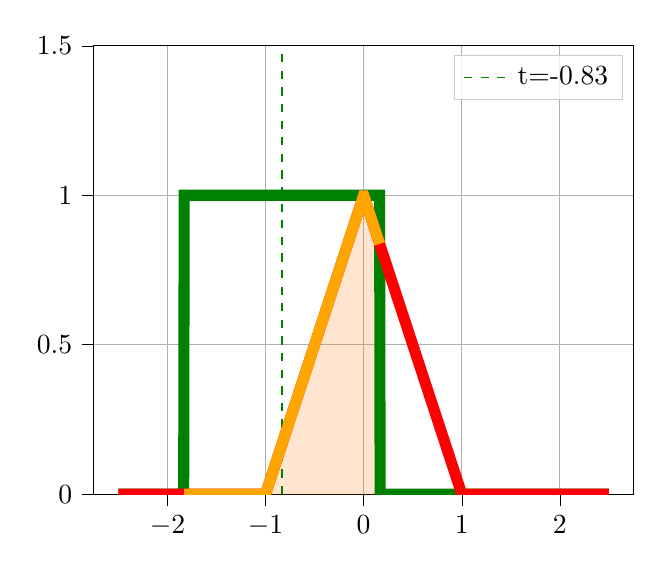
\begin{tikzpicture}

\definecolor{color0}{rgb}{1,0.498039215686275,0.0549019607843137}
\definecolor{color1}{rgb}{1,0.647058823529412,0}

\begin{axis}[
legend cell align={left},
legend style={fill opacity=0.8, draw opacity=1, text opacity=1, draw=white!80!black},
tick align=outside,
tick pos=left,
x grid style={white!69.0196078431373!black},
xmajorgrids,
xmin=-2.75, xmax=2.75,
xtick style={color=black},
y grid style={white!69.0196078431373!black},
ymajorgrids,
ymin=0, ymax=1.5,
ytick style={color=black}
]
\path [draw=color0, fill=color0, opacity=0.2]
(axis cs:-1.82932932932933,0)
--(axis cs:-1.82932932932933,0)
--(axis cs:-1.82432432432432,0)
--(axis cs:-1.81931931931932,0)
--(axis cs:-1.81431431431431,0)
--(axis cs:-1.80930930930931,0)
--(axis cs:-1.8043043043043,0)
--(axis cs:-1.7992992992993,0)
--(axis cs:-1.79429429429429,0)
--(axis cs:-1.78928928928929,0)
--(axis cs:-1.78428428428428,0)
--(axis cs:-1.77927927927928,0)
--(axis cs:-1.77427427427427,0)
--(axis cs:-1.76926926926927,0)
--(axis cs:-1.76426426426426,0)
--(axis cs:-1.75925925925926,0)
--(axis cs:-1.75425425425425,0)
--(axis cs:-1.74924924924925,0)
--(axis cs:-1.74424424424424,0)
--(axis cs:-1.73923923923924,0)
--(axis cs:-1.73423423423423,0)
--(axis cs:-1.72922922922923,0)
--(axis cs:-1.72422422422422,0)
--(axis cs:-1.71921921921922,0)
--(axis cs:-1.71421421421421,0)
--(axis cs:-1.70920920920921,0)
--(axis cs:-1.7042042042042,0)
--(axis cs:-1.6991991991992,0)
--(axis cs:-1.69419419419419,0)
--(axis cs:-1.68918918918919,0)
--(axis cs:-1.68418418418418,0)
--(axis cs:-1.67917917917918,0)
--(axis cs:-1.67417417417417,0)
--(axis cs:-1.66916916916917,0)
--(axis cs:-1.66416416416416,0)
--(axis cs:-1.65915915915916,0)
--(axis cs:-1.65415415415415,0)
--(axis cs:-1.64914914914915,0)
--(axis cs:-1.64414414414414,0)
--(axis cs:-1.63913913913914,0)
--(axis cs:-1.63413413413413,0)
--(axis cs:-1.62912912912913,0)
--(axis cs:-1.62412412412412,0)
--(axis cs:-1.61911911911912,0)
--(axis cs:-1.61411411411411,0)
--(axis cs:-1.60910910910911,0)
--(axis cs:-1.6041041041041,0)
--(axis cs:-1.5990990990991,0)
--(axis cs:-1.59409409409409,0)
--(axis cs:-1.58908908908909,0)
--(axis cs:-1.58408408408408,0)
--(axis cs:-1.57907907907908,0)
--(axis cs:-1.57407407407407,0)
--(axis cs:-1.56906906906907,0)
--(axis cs:-1.56406406406406,0)
--(axis cs:-1.55905905905906,0)
--(axis cs:-1.55405405405405,0)
--(axis cs:-1.54904904904905,0)
--(axis cs:-1.54404404404404,0)
--(axis cs:-1.53903903903904,0)
--(axis cs:-1.53403403403403,0)
--(axis cs:-1.52902902902903,0)
--(axis cs:-1.52402402402402,0)
--(axis cs:-1.51901901901902,0)
--(axis cs:-1.51401401401401,0)
--(axis cs:-1.50900900900901,0)
--(axis cs:-1.504004004004,0)
--(axis cs:-1.498998998999,0)
--(axis cs:-1.49399399399399,0)
--(axis cs:-1.48898898898899,0)
--(axis cs:-1.48398398398398,0)
--(axis cs:-1.47897897897898,0)
--(axis cs:-1.47397397397397,0)
--(axis cs:-1.46896896896897,0)
--(axis cs:-1.46396396396396,0)
--(axis cs:-1.45895895895896,0)
--(axis cs:-1.45395395395395,0)
--(axis cs:-1.44894894894895,0)
--(axis cs:-1.44394394394394,0)
--(axis cs:-1.43893893893894,0)
--(axis cs:-1.43393393393393,0)
--(axis cs:-1.42892892892893,0)
--(axis cs:-1.42392392392392,0)
--(axis cs:-1.41891891891892,0)
--(axis cs:-1.41391391391391,0)
--(axis cs:-1.40890890890891,0)
--(axis cs:-1.4039039039039,0)
--(axis cs:-1.3988988988989,0)
--(axis cs:-1.39389389389389,0)
--(axis cs:-1.38888888888889,0)
--(axis cs:-1.38388388388388,0)
--(axis cs:-1.37887887887888,0)
--(axis cs:-1.37387387387387,0)
--(axis cs:-1.36886886886887,0)
--(axis cs:-1.36386386386386,0)
--(axis cs:-1.35885885885886,0)
--(axis cs:-1.35385385385385,0)
--(axis cs:-1.34884884884885,0)
--(axis cs:-1.34384384384384,0)
--(axis cs:-1.33883883883884,0)
--(axis cs:-1.33383383383383,0)
--(axis cs:-1.32882882882883,0)
--(axis cs:-1.32382382382382,0)
--(axis cs:-1.31881881881882,0)
--(axis cs:-1.31381381381381,0)
--(axis cs:-1.30880880880881,0)
--(axis cs:-1.3038038038038,0)
--(axis cs:-1.2987987987988,0)
--(axis cs:-1.29379379379379,0)
--(axis cs:-1.28878878878879,0)
--(axis cs:-1.28378378378378,0)
--(axis cs:-1.27877877877878,0)
--(axis cs:-1.27377377377377,0)
--(axis cs:-1.26876876876877,0)
--(axis cs:-1.26376376376376,0)
--(axis cs:-1.25875875875876,0)
--(axis cs:-1.25375375375375,0)
--(axis cs:-1.24874874874875,0)
--(axis cs:-1.24374374374374,0)
--(axis cs:-1.23873873873874,0)
--(axis cs:-1.23373373373373,0)
--(axis cs:-1.22872872872873,0)
--(axis cs:-1.22372372372372,0)
--(axis cs:-1.21871871871872,0)
--(axis cs:-1.21371371371371,0)
--(axis cs:-1.20870870870871,0)
--(axis cs:-1.2037037037037,0)
--(axis cs:-1.1986986986987,0)
--(axis cs:-1.19369369369369,0)
--(axis cs:-1.18868868868869,0)
--(axis cs:-1.18368368368368,0)
--(axis cs:-1.17867867867868,0)
--(axis cs:-1.17367367367367,0)
--(axis cs:-1.16866866866867,0)
--(axis cs:-1.16366366366366,0)
--(axis cs:-1.15865865865866,0)
--(axis cs:-1.15365365365365,0)
--(axis cs:-1.14864864864865,0)
--(axis cs:-1.14364364364364,0)
--(axis cs:-1.13863863863864,0)
--(axis cs:-1.13363363363363,0)
--(axis cs:-1.12862862862863,0)
--(axis cs:-1.12362362362362,0)
--(axis cs:-1.11861861861862,0)
--(axis cs:-1.11361361361361,0)
--(axis cs:-1.10860860860861,0)
--(axis cs:-1.1036036036036,0)
--(axis cs:-1.0985985985986,0)
--(axis cs:-1.09359359359359,0)
--(axis cs:-1.08858858858859,0)
--(axis cs:-1.08358358358358,0)
--(axis cs:-1.07857857857858,0)
--(axis cs:-1.07357357357357,0)
--(axis cs:-1.06856856856857,0)
--(axis cs:-1.06356356356356,0)
--(axis cs:-1.05855855855856,0)
--(axis cs:-1.05355355355355,0)
--(axis cs:-1.04854854854855,0)
--(axis cs:-1.04354354354354,0)
--(axis cs:-1.03853853853854,0)
--(axis cs:-1.03353353353353,0)
--(axis cs:-1.02852852852853,0)
--(axis cs:-1.02352352352352,0)
--(axis cs:-1.01851851851852,0)
--(axis cs:-1.01351351351351,0)
--(axis cs:-1.00850850850851,0)
--(axis cs:-1.0035035035035,0)
--(axis cs:-0.998498498498499,0)
--(axis cs:-0.993493493493494,0)
--(axis cs:-0.988488488488489,0)
--(axis cs:-0.983483483483484,0)
--(axis cs:-0.978478478478479,0)
--(axis cs:-0.973473473473474,0)
--(axis cs:-0.968468468468469,0)
--(axis cs:-0.963463463463464,0)
--(axis cs:-0.958458458458459,0)
--(axis cs:-0.953453453453454,0)
--(axis cs:-0.948448448448449,0)
--(axis cs:-0.943443443443444,0)
--(axis cs:-0.938438438438439,0)
--(axis cs:-0.933433433433434,0)
--(axis cs:-0.928428428428429,0)
--(axis cs:-0.923423423423424,0)
--(axis cs:-0.918418418418419,0)
--(axis cs:-0.913413413413414,0)
--(axis cs:-0.908408408408409,0)
--(axis cs:-0.903403403403404,0)
--(axis cs:-0.898398398398399,0)
--(axis cs:-0.893393393393393,0)
--(axis cs:-0.888388388388388,0)
--(axis cs:-0.883383383383383,0)
--(axis cs:-0.878378378378378,0)
--(axis cs:-0.873373373373373,0)
--(axis cs:-0.868368368368368,0)
--(axis cs:-0.863363363363363,0)
--(axis cs:-0.858358358358358,0)
--(axis cs:-0.853353353353353,0)
--(axis cs:-0.848348348348348,0)
--(axis cs:-0.843343343343343,0)
--(axis cs:-0.838338338338338,0)
--(axis cs:-0.833333333333333,0)
--(axis cs:-0.828328328328328,0)
--(axis cs:-0.823323323323323,0)
--(axis cs:-0.818318318318318,0)
--(axis cs:-0.813313313313313,0)
--(axis cs:-0.808308308308308,0)
--(axis cs:-0.803303303303303,0)
--(axis cs:-0.798298298298298,0)
--(axis cs:-0.793293293293293,0)
--(axis cs:-0.788288288288288,0)
--(axis cs:-0.783283283283283,0)
--(axis cs:-0.778278278278278,0)
--(axis cs:-0.773273273273273,0)
--(axis cs:-0.768268268268268,0)
--(axis cs:-0.763263263263263,0)
--(axis cs:-0.758258258258258,0)
--(axis cs:-0.753253253253253,0)
--(axis cs:-0.748248248248248,0)
--(axis cs:-0.743243243243243,0)
--(axis cs:-0.738238238238238,0)
--(axis cs:-0.733233233233233,0)
--(axis cs:-0.728228228228228,0)
--(axis cs:-0.723223223223223,0)
--(axis cs:-0.718218218218218,0)
--(axis cs:-0.713213213213213,0)
--(axis cs:-0.708208208208208,0)
--(axis cs:-0.703203203203203,0)
--(axis cs:-0.698198198198198,0)
--(axis cs:-0.693193193193193,0)
--(axis cs:-0.688188188188188,0)
--(axis cs:-0.683183183183183,0)
--(axis cs:-0.678178178178178,0)
--(axis cs:-0.673173173173173,0)
--(axis cs:-0.668168168168168,0)
--(axis cs:-0.663163163163163,0)
--(axis cs:-0.658158158158158,0)
--(axis cs:-0.653153153153153,0)
--(axis cs:-0.648148148148148,0)
--(axis cs:-0.643143143143143,0)
--(axis cs:-0.638138138138138,0)
--(axis cs:-0.633133133133133,0)
--(axis cs:-0.628128128128128,0)
--(axis cs:-0.623123123123123,0)
--(axis cs:-0.618118118118118,0)
--(axis cs:-0.613113113113113,0)
--(axis cs:-0.608108108108108,0)
--(axis cs:-0.603103103103103,0)
--(axis cs:-0.598098098098098,0)
--(axis cs:-0.593093093093093,0)
--(axis cs:-0.588088088088088,0)
--(axis cs:-0.583083083083083,0)
--(axis cs:-0.578078078078078,0)
--(axis cs:-0.573073073073073,0)
--(axis cs:-0.568068068068068,0)
--(axis cs:-0.563063063063063,0)
--(axis cs:-0.558058058058058,0)
--(axis cs:-0.553053053053053,0)
--(axis cs:-0.548048048048048,0)
--(axis cs:-0.543043043043043,0)
--(axis cs:-0.538038038038038,0)
--(axis cs:-0.533033033033033,0)
--(axis cs:-0.528028028028028,0)
--(axis cs:-0.523023023023023,0)
--(axis cs:-0.518018018018018,0)
--(axis cs:-0.513013013013013,0)
--(axis cs:-0.508008008008008,0)
--(axis cs:-0.503003003003003,0)
--(axis cs:-0.497997997997998,0)
--(axis cs:-0.492992992992993,0)
--(axis cs:-0.487987987987988,0)
--(axis cs:-0.482982982982983,0)
--(axis cs:-0.477977977977978,0)
--(axis cs:-0.472972972972973,0)
--(axis cs:-0.467967967967968,0)
--(axis cs:-0.462962962962963,0)
--(axis cs:-0.457957957957958,0)
--(axis cs:-0.452952952952953,0)
--(axis cs:-0.447947947947948,0)
--(axis cs:-0.442942942942943,0)
--(axis cs:-0.437937937937938,0)
--(axis cs:-0.432932932932933,0)
--(axis cs:-0.427927927927928,0)
--(axis cs:-0.422922922922923,0)
--(axis cs:-0.417917917917918,0)
--(axis cs:-0.412912912912913,0)
--(axis cs:-0.407907907907908,0)
--(axis cs:-0.402902902902903,0)
--(axis cs:-0.397897897897898,0)
--(axis cs:-0.392892892892893,0)
--(axis cs:-0.387887887887888,0)
--(axis cs:-0.382882882882883,0)
--(axis cs:-0.377877877877878,0)
--(axis cs:-0.372872872872873,0)
--(axis cs:-0.367867867867868,0)
--(axis cs:-0.362862862862863,0)
--(axis cs:-0.357857857857858,0)
--(axis cs:-0.352852852852853,0)
--(axis cs:-0.347847847847848,0)
--(axis cs:-0.342842842842843,0)
--(axis cs:-0.337837837837838,0)
--(axis cs:-0.332832832832833,0)
--(axis cs:-0.327827827827828,0)
--(axis cs:-0.322822822822823,0)
--(axis cs:-0.317817817817818,0)
--(axis cs:-0.312812812812813,0)
--(axis cs:-0.307807807807808,0)
--(axis cs:-0.302802802802803,0)
--(axis cs:-0.297797797797798,0)
--(axis cs:-0.292792792792793,0)
--(axis cs:-0.287787787787788,0)
--(axis cs:-0.282782782782783,0)
--(axis cs:-0.277777777777778,0)
--(axis cs:-0.272772772772773,0)
--(axis cs:-0.267767767767768,0)
--(axis cs:-0.262762762762763,0)
--(axis cs:-0.257757757757758,0)
--(axis cs:-0.252752752752753,0)
--(axis cs:-0.247747747747748,0)
--(axis cs:-0.242742742742743,0)
--(axis cs:-0.237737737737738,0)
--(axis cs:-0.232732732732733,0)
--(axis cs:-0.227727727727728,0)
--(axis cs:-0.222722722722723,0)
--(axis cs:-0.217717717717718,0)
--(axis cs:-0.212712712712713,0)
--(axis cs:-0.207707707707708,0)
--(axis cs:-0.202702702702703,0)
--(axis cs:-0.197697697697698,0)
--(axis cs:-0.192692692692693,0)
--(axis cs:-0.187687687687688,0)
--(axis cs:-0.182682682682683,0)
--(axis cs:-0.177677677677678,0)
--(axis cs:-0.172672672672673,0)
--(axis cs:-0.167667667667668,0)
--(axis cs:-0.162662662662663,0)
--(axis cs:-0.157657657657658,0)
--(axis cs:-0.152652652652653,0)
--(axis cs:-0.147647647647648,0)
--(axis cs:-0.142642642642643,0)
--(axis cs:-0.137637637637638,0)
--(axis cs:-0.132632632632633,0)
--(axis cs:-0.127627627627628,0)
--(axis cs:-0.122622622622623,0)
--(axis cs:-0.117617617617618,0)
--(axis cs:-0.112612612612613,0)
--(axis cs:-0.107607607607608,0)
--(axis cs:-0.102602602602603,0)
--(axis cs:-0.0975975975975976,0)
--(axis cs:-0.0925925925925926,0)
--(axis cs:-0.0875875875875876,0)
--(axis cs:-0.0825825825825826,0)
--(axis cs:-0.0775775775775776,0)
--(axis cs:-0.0725725725725725,0)
--(axis cs:-0.0675675675675675,0)
--(axis cs:-0.0625625625625625,0)
--(axis cs:-0.0575575575575575,0)
--(axis cs:-0.0525525525525525,0)
--(axis cs:-0.0475475475475475,0)
--(axis cs:-0.0425425425425425,0)
--(axis cs:-0.0375375375375375,0)
--(axis cs:-0.0325325325325325,0)
--(axis cs:-0.0275275275275275,0)
--(axis cs:-0.0225225225225225,0)
--(axis cs:-0.0175175175175175,0)
--(axis cs:-0.0125125125125125,0)
--(axis cs:-0.0075075075075075,0)
--(axis cs:-0.0025025025025025,0)
--(axis cs:0.0025025025025025,0)
--(axis cs:0.0075075075075075,0)
--(axis cs:0.0125125125125125,0)
--(axis cs:0.0175175175175175,0)
--(axis cs:0.0225225225225225,0)
--(axis cs:0.0275275275275275,0)
--(axis cs:0.0325325325325325,0)
--(axis cs:0.0375375375375375,0)
--(axis cs:0.0425425425425425,0)
--(axis cs:0.0475475475475475,0)
--(axis cs:0.0525525525525525,0)
--(axis cs:0.0575575575575575,0)
--(axis cs:0.0625625625625625,0)
--(axis cs:0.0675675675675675,0)
--(axis cs:0.0725725725725725,0)
--(axis cs:0.0775775775775776,0)
--(axis cs:0.0825825825825826,0)
--(axis cs:0.0875875875875876,0)
--(axis cs:0.0925925925925926,0)
--(axis cs:0.0975975975975976,0)
--(axis cs:0.102602602602603,0)
--(axis cs:0.107607607607608,0)
--(axis cs:0.112612612612613,0)
--(axis cs:0.117617617617618,0)
--(axis cs:0.122622622622623,0)
--(axis cs:0.127627627627628,0)
--(axis cs:0.132632632632633,0)
--(axis cs:0.137637637637638,0)
--(axis cs:0.142642642642643,0)
--(axis cs:0.147647647647648,0)
--(axis cs:0.152652652652653,0)
--(axis cs:0.157657657657658,0)
--(axis cs:0.162662662662663,0)
--(axis cs:0.162662662662663,0.837337337337337)
--(axis cs:0.162662662662663,0.837337337337337)
--(axis cs:0.157657657657658,0.842342342342342)
--(axis cs:0.152652652652653,0.847347347347347)
--(axis cs:0.147647647647648,0.852352352352352)
--(axis cs:0.142642642642643,0.857357357357357)
--(axis cs:0.137637637637638,0.862362362362362)
--(axis cs:0.132632632632633,0.867367367367367)
--(axis cs:0.127627627627628,0.872372372372372)
--(axis cs:0.122622622622623,0.877377377377377)
--(axis cs:0.117617617617618,0.882382382382382)
--(axis cs:0.112612612612613,0.887387387387387)
--(axis cs:0.107607607607608,0.892392392392392)
--(axis cs:0.102602602602603,0.897397397397397)
--(axis cs:0.0975975975975976,0.902402402402402)
--(axis cs:0.0925925925925926,0.907407407407407)
--(axis cs:0.0875875875875876,0.912412412412412)
--(axis cs:0.0825825825825826,0.917417417417417)
--(axis cs:0.0775775775775776,0.922422422422422)
--(axis cs:0.0725725725725725,0.927427427427427)
--(axis cs:0.0675675675675675,0.932432432432432)
--(axis cs:0.0625625625625625,0.937437437437437)
--(axis cs:0.0575575575575575,0.942442442442442)
--(axis cs:0.0525525525525525,0.947447447447447)
--(axis cs:0.0475475475475475,0.952452452452452)
--(axis cs:0.0425425425425425,0.957457457457457)
--(axis cs:0.0375375375375375,0.962462462462462)
--(axis cs:0.0325325325325325,0.967467467467467)
--(axis cs:0.0275275275275275,0.972472472472472)
--(axis cs:0.0225225225225225,0.977477477477477)
--(axis cs:0.0175175175175175,0.982482482482482)
--(axis cs:0.0125125125125125,0.987487487487487)
--(axis cs:0.0075075075075075,0.992492492492492)
--(axis cs:0.0025025025025025,0.997497497497497)
--(axis cs:-0.0025025025025025,0.997497497497497)
--(axis cs:-0.0075075075075075,0.992492492492492)
--(axis cs:-0.0125125125125125,0.987487487487487)
--(axis cs:-0.0175175175175175,0.982482482482482)
--(axis cs:-0.0225225225225225,0.977477477477477)
--(axis cs:-0.0275275275275275,0.972472472472472)
--(axis cs:-0.0325325325325325,0.967467467467467)
--(axis cs:-0.0375375375375375,0.962462462462462)
--(axis cs:-0.0425425425425425,0.957457457457457)
--(axis cs:-0.0475475475475475,0.952452452452452)
--(axis cs:-0.0525525525525525,0.947447447447447)
--(axis cs:-0.0575575575575575,0.942442442442442)
--(axis cs:-0.0625625625625625,0.937437437437437)
--(axis cs:-0.0675675675675675,0.932432432432432)
--(axis cs:-0.0725725725725725,0.927427427427427)
--(axis cs:-0.0775775775775776,0.922422422422422)
--(axis cs:-0.0825825825825826,0.917417417417417)
--(axis cs:-0.0875875875875876,0.912412412412412)
--(axis cs:-0.0925925925925926,0.907407407407407)
--(axis cs:-0.0975975975975976,0.902402402402402)
--(axis cs:-0.102602602602603,0.897397397397397)
--(axis cs:-0.107607607607608,0.892392392392392)
--(axis cs:-0.112612612612613,0.887387387387387)
--(axis cs:-0.117617617617618,0.882382382382382)
--(axis cs:-0.122622622622623,0.877377377377377)
--(axis cs:-0.127627627627628,0.872372372372372)
--(axis cs:-0.132632632632633,0.867367367367367)
--(axis cs:-0.137637637637638,0.862362362362362)
--(axis cs:-0.142642642642643,0.857357357357357)
--(axis cs:-0.147647647647648,0.852352352352352)
--(axis cs:-0.152652652652653,0.847347347347347)
--(axis cs:-0.157657657657658,0.842342342342342)
--(axis cs:-0.162662662662663,0.837337337337337)
--(axis cs:-0.167667667667668,0.832332332332332)
--(axis cs:-0.172672672672673,0.827327327327327)
--(axis cs:-0.177677677677678,0.822322322322322)
--(axis cs:-0.182682682682683,0.817317317317317)
--(axis cs:-0.187687687687688,0.812312312312312)
--(axis cs:-0.192692692692693,0.807307307307307)
--(axis cs:-0.197697697697698,0.802302302302302)
--(axis cs:-0.202702702702703,0.797297297297297)
--(axis cs:-0.207707707707708,0.792292292292292)
--(axis cs:-0.212712712712713,0.787287287287287)
--(axis cs:-0.217717717717718,0.782282282282282)
--(axis cs:-0.222722722722723,0.777277277277277)
--(axis cs:-0.227727727727728,0.772272272272272)
--(axis cs:-0.232732732732733,0.767267267267267)
--(axis cs:-0.237737737737738,0.762262262262262)
--(axis cs:-0.242742742742743,0.757257257257257)
--(axis cs:-0.247747747747748,0.752252252252252)
--(axis cs:-0.252752752752753,0.747247247247247)
--(axis cs:-0.257757757757758,0.742242242242242)
--(axis cs:-0.262762762762763,0.737237237237237)
--(axis cs:-0.267767767767768,0.732232232232232)
--(axis cs:-0.272772772772773,0.727227227227227)
--(axis cs:-0.277777777777778,0.722222222222222)
--(axis cs:-0.282782782782783,0.717217217217217)
--(axis cs:-0.287787787787788,0.712212212212212)
--(axis cs:-0.292792792792793,0.707207207207207)
--(axis cs:-0.297797797797798,0.702202202202202)
--(axis cs:-0.302802802802803,0.697197197197197)
--(axis cs:-0.307807807807808,0.692192192192192)
--(axis cs:-0.312812812812813,0.687187187187187)
--(axis cs:-0.317817817817818,0.682182182182182)
--(axis cs:-0.322822822822823,0.677177177177177)
--(axis cs:-0.327827827827828,0.672172172172172)
--(axis cs:-0.332832832832833,0.667167167167167)
--(axis cs:-0.337837837837838,0.662162162162162)
--(axis cs:-0.342842842842843,0.657157157157157)
--(axis cs:-0.347847847847848,0.652152152152152)
--(axis cs:-0.352852852852853,0.647147147147147)
--(axis cs:-0.357857857857858,0.642142142142142)
--(axis cs:-0.362862862862863,0.637137137137137)
--(axis cs:-0.367867867867868,0.632132132132132)
--(axis cs:-0.372872872872873,0.627127127127127)
--(axis cs:-0.377877877877878,0.622122122122122)
--(axis cs:-0.382882882882883,0.617117117117117)
--(axis cs:-0.387887887887888,0.612112112112112)
--(axis cs:-0.392892892892893,0.607107107107107)
--(axis cs:-0.397897897897898,0.602102102102102)
--(axis cs:-0.402902902902903,0.597097097097097)
--(axis cs:-0.407907907907908,0.592092092092092)
--(axis cs:-0.412912912912913,0.587087087087087)
--(axis cs:-0.417917917917918,0.582082082082082)
--(axis cs:-0.422922922922923,0.577077077077077)
--(axis cs:-0.427927927927928,0.572072072072072)
--(axis cs:-0.432932932932933,0.567067067067067)
--(axis cs:-0.437937937937938,0.562062062062062)
--(axis cs:-0.442942942942943,0.557057057057057)
--(axis cs:-0.447947947947948,0.552052052052052)
--(axis cs:-0.452952952952953,0.547047047047047)
--(axis cs:-0.457957957957958,0.542042042042042)
--(axis cs:-0.462962962962963,0.537037037037037)
--(axis cs:-0.467967967967968,0.532032032032032)
--(axis cs:-0.472972972972973,0.527027027027027)
--(axis cs:-0.477977977977978,0.522022022022022)
--(axis cs:-0.482982982982983,0.517017017017017)
--(axis cs:-0.487987987987988,0.512012012012012)
--(axis cs:-0.492992992992993,0.507007007007007)
--(axis cs:-0.497997997997998,0.502002002002002)
--(axis cs:-0.503003003003003,0.496996996996997)
--(axis cs:-0.508008008008008,0.491991991991992)
--(axis cs:-0.513013013013013,0.486986986986987)
--(axis cs:-0.518018018018018,0.481981981981982)
--(axis cs:-0.523023023023023,0.476976976976977)
--(axis cs:-0.528028028028028,0.471971971971972)
--(axis cs:-0.533033033033033,0.466966966966967)
--(axis cs:-0.538038038038038,0.461961961961962)
--(axis cs:-0.543043043043043,0.456956956956957)
--(axis cs:-0.548048048048048,0.451951951951952)
--(axis cs:-0.553053053053053,0.446946946946947)
--(axis cs:-0.558058058058058,0.441941941941942)
--(axis cs:-0.563063063063063,0.436936936936937)
--(axis cs:-0.568068068068068,0.431931931931932)
--(axis cs:-0.573073073073073,0.426926926926927)
--(axis cs:-0.578078078078078,0.421921921921922)
--(axis cs:-0.583083083083083,0.416916916916917)
--(axis cs:-0.588088088088088,0.411911911911912)
--(axis cs:-0.593093093093093,0.406906906906907)
--(axis cs:-0.598098098098098,0.401901901901902)
--(axis cs:-0.603103103103103,0.396896896896897)
--(axis cs:-0.608108108108108,0.391891891891892)
--(axis cs:-0.613113113113113,0.386886886886887)
--(axis cs:-0.618118118118118,0.381881881881882)
--(axis cs:-0.623123123123123,0.376876876876877)
--(axis cs:-0.628128128128128,0.371871871871872)
--(axis cs:-0.633133133133133,0.366866866866867)
--(axis cs:-0.638138138138138,0.361861861861862)
--(axis cs:-0.643143143143143,0.356856856856857)
--(axis cs:-0.648148148148148,0.351851851851852)
--(axis cs:-0.653153153153153,0.346846846846847)
--(axis cs:-0.658158158158158,0.341841841841842)
--(axis cs:-0.663163163163163,0.336836836836837)
--(axis cs:-0.668168168168168,0.331831831831832)
--(axis cs:-0.673173173173173,0.326826826826827)
--(axis cs:-0.678178178178178,0.321821821821822)
--(axis cs:-0.683183183183183,0.316816816816817)
--(axis cs:-0.688188188188188,0.311811811811812)
--(axis cs:-0.693193193193193,0.306806806806807)
--(axis cs:-0.698198198198198,0.301801801801802)
--(axis cs:-0.703203203203203,0.296796796796797)
--(axis cs:-0.708208208208208,0.291791791791792)
--(axis cs:-0.713213213213213,0.286786786786787)
--(axis cs:-0.718218218218218,0.281781781781782)
--(axis cs:-0.723223223223223,0.276776776776777)
--(axis cs:-0.728228228228228,0.271771771771772)
--(axis cs:-0.733233233233233,0.266766766766767)
--(axis cs:-0.738238238238238,0.261761761761762)
--(axis cs:-0.743243243243243,0.256756756756757)
--(axis cs:-0.748248248248248,0.251751751751752)
--(axis cs:-0.753253253253253,0.246746746746747)
--(axis cs:-0.758258258258258,0.241741741741742)
--(axis cs:-0.763263263263263,0.236736736736737)
--(axis cs:-0.768268268268268,0.231731731731732)
--(axis cs:-0.773273273273273,0.226726726726727)
--(axis cs:-0.778278278278278,0.221721721721722)
--(axis cs:-0.783283283283283,0.216716716716717)
--(axis cs:-0.788288288288288,0.211711711711712)
--(axis cs:-0.793293293293293,0.206706706706707)
--(axis cs:-0.798298298298298,0.201701701701702)
--(axis cs:-0.803303303303303,0.196696696696697)
--(axis cs:-0.808308308308308,0.191691691691692)
--(axis cs:-0.813313313313313,0.186686686686687)
--(axis cs:-0.818318318318318,0.181681681681682)
--(axis cs:-0.823323323323323,0.176676676676677)
--(axis cs:-0.828328328328328,0.171671671671672)
--(axis cs:-0.833333333333333,0.166666666666667)
--(axis cs:-0.838338338338338,0.161661661661662)
--(axis cs:-0.843343343343343,0.156656656656657)
--(axis cs:-0.848348348348348,0.151651651651652)
--(axis cs:-0.853353353353353,0.146646646646647)
--(axis cs:-0.858358358358358,0.141641641641642)
--(axis cs:-0.863363363363363,0.136636636636637)
--(axis cs:-0.868368368368368,0.131631631631632)
--(axis cs:-0.873373373373373,0.126626626626627)
--(axis cs:-0.878378378378378,0.121621621621622)
--(axis cs:-0.883383383383383,0.116616616616617)
--(axis cs:-0.888388388388388,0.111611611611612)
--(axis cs:-0.893393393393393,0.106606606606607)
--(axis cs:-0.898398398398399,0.101601601601601)
--(axis cs:-0.903403403403404,0.0965965965965965)
--(axis cs:-0.908408408408409,0.0915915915915915)
--(axis cs:-0.913413413413414,0.0865865865865865)
--(axis cs:-0.918418418418419,0.0815815815815815)
--(axis cs:-0.923423423423424,0.0765765765765765)
--(axis cs:-0.928428428428429,0.0715715715715715)
--(axis cs:-0.933433433433434,0.0665665665665665)
--(axis cs:-0.938438438438439,0.0615615615615615)
--(axis cs:-0.943443443443444,0.0565565565565564)
--(axis cs:-0.948448448448449,0.0515515515515514)
--(axis cs:-0.953453453453454,0.0465465465465464)
--(axis cs:-0.958458458458459,0.0415415415415414)
--(axis cs:-0.963463463463464,0.0365365365365364)
--(axis cs:-0.968468468468469,0.0315315315315314)
--(axis cs:-0.973473473473474,0.0265265265265264)
--(axis cs:-0.978478478478479,0.0215215215215214)
--(axis cs:-0.983483483483484,0.0165165165165164)
--(axis cs:-0.988488488488489,0.0115115115115114)
--(axis cs:-0.993493493493494,0.00650650650650642)
--(axis cs:-0.998498498498499,0.00150150150150141)
--(axis cs:-1.0035035035035,0)
--(axis cs:-1.00850850850851,0)
--(axis cs:-1.01351351351351,0)
--(axis cs:-1.01851851851852,0)
--(axis cs:-1.02352352352352,0)
--(axis cs:-1.02852852852853,0)
--(axis cs:-1.03353353353353,0)
--(axis cs:-1.03853853853854,0)
--(axis cs:-1.04354354354354,0)
--(axis cs:-1.04854854854855,0)
--(axis cs:-1.05355355355355,0)
--(axis cs:-1.05855855855856,0)
--(axis cs:-1.06356356356356,0)
--(axis cs:-1.06856856856857,0)
--(axis cs:-1.07357357357357,0)
--(axis cs:-1.07857857857858,0)
--(axis cs:-1.08358358358358,0)
--(axis cs:-1.08858858858859,0)
--(axis cs:-1.09359359359359,0)
--(axis cs:-1.0985985985986,0)
--(axis cs:-1.1036036036036,0)
--(axis cs:-1.10860860860861,0)
--(axis cs:-1.11361361361361,0)
--(axis cs:-1.11861861861862,0)
--(axis cs:-1.12362362362362,0)
--(axis cs:-1.12862862862863,0)
--(axis cs:-1.13363363363363,0)
--(axis cs:-1.13863863863864,0)
--(axis cs:-1.14364364364364,0)
--(axis cs:-1.14864864864865,0)
--(axis cs:-1.15365365365365,0)
--(axis cs:-1.15865865865866,0)
--(axis cs:-1.16366366366366,0)
--(axis cs:-1.16866866866867,0)
--(axis cs:-1.17367367367367,0)
--(axis cs:-1.17867867867868,0)
--(axis cs:-1.18368368368368,0)
--(axis cs:-1.18868868868869,0)
--(axis cs:-1.19369369369369,0)
--(axis cs:-1.1986986986987,0)
--(axis cs:-1.2037037037037,0)
--(axis cs:-1.20870870870871,0)
--(axis cs:-1.21371371371371,0)
--(axis cs:-1.21871871871872,0)
--(axis cs:-1.22372372372372,0)
--(axis cs:-1.22872872872873,0)
--(axis cs:-1.23373373373373,0)
--(axis cs:-1.23873873873874,0)
--(axis cs:-1.24374374374374,0)
--(axis cs:-1.24874874874875,0)
--(axis cs:-1.25375375375375,0)
--(axis cs:-1.25875875875876,0)
--(axis cs:-1.26376376376376,0)
--(axis cs:-1.26876876876877,0)
--(axis cs:-1.27377377377377,0)
--(axis cs:-1.27877877877878,0)
--(axis cs:-1.28378378378378,0)
--(axis cs:-1.28878878878879,0)
--(axis cs:-1.29379379379379,0)
--(axis cs:-1.2987987987988,0)
--(axis cs:-1.3038038038038,0)
--(axis cs:-1.30880880880881,0)
--(axis cs:-1.31381381381381,0)
--(axis cs:-1.31881881881882,0)
--(axis cs:-1.32382382382382,0)
--(axis cs:-1.32882882882883,0)
--(axis cs:-1.33383383383383,0)
--(axis cs:-1.33883883883884,0)
--(axis cs:-1.34384384384384,0)
--(axis cs:-1.34884884884885,0)
--(axis cs:-1.35385385385385,0)
--(axis cs:-1.35885885885886,0)
--(axis cs:-1.36386386386386,0)
--(axis cs:-1.36886886886887,0)
--(axis cs:-1.37387387387387,0)
--(axis cs:-1.37887887887888,0)
--(axis cs:-1.38388388388388,0)
--(axis cs:-1.38888888888889,0)
--(axis cs:-1.39389389389389,0)
--(axis cs:-1.3988988988989,0)
--(axis cs:-1.4039039039039,0)
--(axis cs:-1.40890890890891,0)
--(axis cs:-1.41391391391391,0)
--(axis cs:-1.41891891891892,0)
--(axis cs:-1.42392392392392,0)
--(axis cs:-1.42892892892893,0)
--(axis cs:-1.43393393393393,0)
--(axis cs:-1.43893893893894,0)
--(axis cs:-1.44394394394394,0)
--(axis cs:-1.44894894894895,0)
--(axis cs:-1.45395395395395,0)
--(axis cs:-1.45895895895896,0)
--(axis cs:-1.46396396396396,0)
--(axis cs:-1.46896896896897,0)
--(axis cs:-1.47397397397397,0)
--(axis cs:-1.47897897897898,0)
--(axis cs:-1.48398398398398,0)
--(axis cs:-1.48898898898899,0)
--(axis cs:-1.49399399399399,0)
--(axis cs:-1.498998998999,0)
--(axis cs:-1.504004004004,0)
--(axis cs:-1.50900900900901,0)
--(axis cs:-1.51401401401401,0)
--(axis cs:-1.51901901901902,0)
--(axis cs:-1.52402402402402,0)
--(axis cs:-1.52902902902903,0)
--(axis cs:-1.53403403403403,0)
--(axis cs:-1.53903903903904,0)
--(axis cs:-1.54404404404404,0)
--(axis cs:-1.54904904904905,0)
--(axis cs:-1.55405405405405,0)
--(axis cs:-1.55905905905906,0)
--(axis cs:-1.56406406406406,0)
--(axis cs:-1.56906906906907,0)
--(axis cs:-1.57407407407407,0)
--(axis cs:-1.57907907907908,0)
--(axis cs:-1.58408408408408,0)
--(axis cs:-1.58908908908909,0)
--(axis cs:-1.59409409409409,0)
--(axis cs:-1.5990990990991,0)
--(axis cs:-1.6041041041041,0)
--(axis cs:-1.60910910910911,0)
--(axis cs:-1.61411411411411,0)
--(axis cs:-1.61911911911912,0)
--(axis cs:-1.62412412412412,0)
--(axis cs:-1.62912912912913,0)
--(axis cs:-1.63413413413413,0)
--(axis cs:-1.63913913913914,0)
--(axis cs:-1.64414414414414,0)
--(axis cs:-1.64914914914915,0)
--(axis cs:-1.65415415415415,0)
--(axis cs:-1.65915915915916,0)
--(axis cs:-1.66416416416416,0)
--(axis cs:-1.66916916916917,0)
--(axis cs:-1.67417417417417,0)
--(axis cs:-1.67917917917918,0)
--(axis cs:-1.68418418418418,0)
--(axis cs:-1.68918918918919,0)
--(axis cs:-1.69419419419419,0)
--(axis cs:-1.6991991991992,0)
--(axis cs:-1.7042042042042,0)
--(axis cs:-1.70920920920921,0)
--(axis cs:-1.71421421421421,0)
--(axis cs:-1.71921921921922,0)
--(axis cs:-1.72422422422422,0)
--(axis cs:-1.72922922922923,0)
--(axis cs:-1.73423423423423,0)
--(axis cs:-1.73923923923924,0)
--(axis cs:-1.74424424424424,0)
--(axis cs:-1.74924924924925,0)
--(axis cs:-1.75425425425425,0)
--(axis cs:-1.75925925925926,0)
--(axis cs:-1.76426426426426,0)
--(axis cs:-1.76926926926927,0)
--(axis cs:-1.77427427427427,0)
--(axis cs:-1.77927927927928,0)
--(axis cs:-1.78428428428428,0)
--(axis cs:-1.78928928928929,0)
--(axis cs:-1.79429429429429,0)
--(axis cs:-1.7992992992993,0)
--(axis cs:-1.8043043043043,0)
--(axis cs:-1.80930930930931,0)
--(axis cs:-1.81431431431431,0)
--(axis cs:-1.81931931931932,0)
--(axis cs:-1.82432432432432,0)
--(axis cs:-1.82932932932933,0)
--cycle;

\addplot [line width=4pt, green!50!black, forget plot]
table {%
-2.5 0
-2.49499499499499 0
-2.48998998998999 0
-2.48498498498498 0
-2.47997997997998 0
-2.47497497497497 0
-2.46996996996997 0
-2.46496496496496 0
-2.45995995995996 0
-2.45495495495495 0
-2.44994994994995 0
-2.44494494494494 0
-2.43993993993994 0
-2.43493493493493 0
-2.42992992992993 0
-2.42492492492492 0
-2.41991991991992 0
-2.41491491491491 0
-2.40990990990991 0
-2.4049049049049 0
-2.3998998998999 0
-2.39489489489489 0
-2.38988988988989 0
-2.38488488488488 0
-2.37987987987988 0
-2.37487487487487 0
-2.36986986986987 0
-2.36486486486486 0
-2.35985985985986 0
-2.35485485485485 0
-2.34984984984985 0
-2.34484484484484 0
-2.33983983983984 0
-2.33483483483483 0
-2.32982982982983 0
-2.32482482482482 0
-2.31981981981982 0
-2.31481481481481 0
-2.30980980980981 0
-2.3048048048048 0
-2.2997997997998 0
-2.29479479479479 0
-2.28978978978979 0
-2.28478478478478 0
-2.27977977977978 0
-2.27477477477477 0
-2.26976976976977 0
-2.26476476476476 0
-2.25975975975976 0
-2.25475475475475 0
-2.24974974974975 0
-2.24474474474474 0
-2.23973973973974 0
-2.23473473473473 0
-2.22972972972973 0
-2.22472472472472 0
-2.21971971971972 0
-2.21471471471471 0
-2.20970970970971 0
-2.2047047047047 0
-2.1996996996997 0
-2.19469469469469 0
-2.18968968968969 0
-2.18468468468468 0
-2.17967967967968 0
-2.17467467467467 0
-2.16966966966967 0
-2.16466466466466 0
-2.15965965965966 0
-2.15465465465465 0
-2.14964964964965 0
-2.14464464464464 0
-2.13963963963964 0
-2.13463463463463 0
-2.12962962962963 0
-2.12462462462462 0
-2.11961961961962 0
-2.11461461461461 0
-2.10960960960961 0
-2.1046046046046 0
-2.0995995995996 0
-2.09459459459459 0
-2.08958958958959 0
-2.08458458458458 0
-2.07957957957958 0
-2.07457457457457 0
-2.06956956956957 0
-2.06456456456456 0
-2.05955955955956 0
-2.05455455455455 0
-2.04954954954955 0
-2.04454454454454 0
-2.03953953953954 0
-2.03453453453453 0
-2.02952952952953 0
-2.02452452452452 0
-2.01951951951952 0
-2.01451451451451 0
-2.00950950950951 0
-2.0045045045045 0
-1.9994994994995 0
-1.99449449449449 0
-1.98948948948949 0
-1.98448448448448 0
-1.97947947947948 0
-1.97447447447447 0
-1.96946946946947 0
-1.96446446446446 0
-1.95945945945946 0
-1.95445445445445 0
-1.94944944944945 0
-1.94444444444444 0
-1.93943943943944 0
-1.93443443443443 0
-1.92942942942943 0
-1.92442442442442 0
-1.91941941941942 0
-1.91441441441441 0
-1.90940940940941 0
-1.9044044044044 0
-1.8993993993994 0
-1.89439439439439 0
-1.88938938938939 0
-1.88438438438438 0
-1.87937937937938 0
-1.87437437437437 0
-1.86936936936937 0
-1.86436436436436 0
-1.85935935935936 0
-1.85435435435435 0
-1.84934934934935 0
-1.84434434434434 0
-1.83933933933934 0
-1.83433433433433 0
-1.82932932932933 1
-1.82432432432432 1
-1.81931931931932 1
-1.81431431431431 1
-1.80930930930931 1
-1.8043043043043 1
-1.7992992992993 1
-1.79429429429429 1
-1.78928928928929 1
-1.78428428428428 1
-1.77927927927928 1
-1.77427427427427 1
-1.76926926926927 1
-1.76426426426426 1
-1.75925925925926 1
-1.75425425425425 1
-1.74924924924925 1
-1.74424424424424 1
-1.73923923923924 1
-1.73423423423423 1
-1.72922922922923 1
-1.72422422422422 1
-1.71921921921922 1
-1.71421421421421 1
-1.70920920920921 1
-1.7042042042042 1
-1.6991991991992 1
-1.69419419419419 1
-1.68918918918919 1
-1.68418418418418 1
-1.67917917917918 1
-1.67417417417417 1
-1.66916916916917 1
-1.66416416416416 1
-1.65915915915916 1
-1.65415415415415 1
-1.64914914914915 1
-1.64414414414414 1
-1.63913913913914 1
-1.63413413413413 1
-1.62912912912913 1
-1.62412412412412 1
-1.61911911911912 1
-1.61411411411411 1
-1.60910910910911 1
-1.6041041041041 1
-1.5990990990991 1
-1.59409409409409 1
-1.58908908908909 1
-1.58408408408408 1
-1.57907907907908 1
-1.57407407407407 1
-1.56906906906907 1
-1.56406406406406 1
-1.55905905905906 1
-1.55405405405405 1
-1.54904904904905 1
-1.54404404404404 1
-1.53903903903904 1
-1.53403403403403 1
-1.52902902902903 1
-1.52402402402402 1
-1.51901901901902 1
-1.51401401401401 1
-1.50900900900901 1
-1.504004004004 1
-1.498998998999 1
-1.49399399399399 1
-1.48898898898899 1
-1.48398398398398 1
-1.47897897897898 1
-1.47397397397397 1
-1.46896896896897 1
-1.46396396396396 1
-1.45895895895896 1
-1.45395395395395 1
-1.44894894894895 1
-1.44394394394394 1
-1.43893893893894 1
-1.43393393393393 1
-1.42892892892893 1
-1.42392392392392 1
-1.41891891891892 1
-1.41391391391391 1
-1.40890890890891 1
-1.4039039039039 1
-1.3988988988989 1
-1.39389389389389 1
-1.38888888888889 1
-1.38388388388388 1
-1.37887887887888 1
-1.37387387387387 1
-1.36886886886887 1
-1.36386386386386 1
-1.35885885885886 1
-1.35385385385385 1
-1.34884884884885 1
-1.34384384384384 1
-1.33883883883884 1
-1.33383383383383 1
-1.32882882882883 1
-1.32382382382382 1
-1.31881881881882 1
-1.31381381381381 1
-1.30880880880881 1
-1.3038038038038 1
-1.2987987987988 1
-1.29379379379379 1
-1.28878878878879 1
-1.28378378378378 1
-1.27877877877878 1
-1.27377377377377 1
-1.26876876876877 1
-1.26376376376376 1
-1.25875875875876 1
-1.25375375375375 1
-1.24874874874875 1
-1.24374374374374 1
-1.23873873873874 1
-1.23373373373373 1
-1.22872872872873 1
-1.22372372372372 1
-1.21871871871872 1
-1.21371371371371 1
-1.20870870870871 1
-1.2037037037037 1
-1.1986986986987 1
-1.19369369369369 1
-1.18868868868869 1
-1.18368368368368 1
-1.17867867867868 1
-1.17367367367367 1
-1.16866866866867 1
-1.16366366366366 1
-1.15865865865866 1
-1.15365365365365 1
-1.14864864864865 1
-1.14364364364364 1
-1.13863863863864 1
-1.13363363363363 1
-1.12862862862863 1
-1.12362362362362 1
-1.11861861861862 1
-1.11361361361361 1
-1.10860860860861 1
-1.1036036036036 1
-1.0985985985986 1
-1.09359359359359 1
-1.08858858858859 1
-1.08358358358358 1
-1.07857857857858 1
-1.07357357357357 1
-1.06856856856857 1
-1.06356356356356 1
-1.05855855855856 1
-1.05355355355355 1
-1.04854854854855 1
-1.04354354354354 1
-1.03853853853854 1
-1.03353353353353 1
-1.02852852852853 1
-1.02352352352352 1
-1.01851851851852 1
-1.01351351351351 1
-1.00850850850851 1
-1.0035035035035 1
-0.998498498498499 1
-0.993493493493494 1
-0.988488488488489 1
-0.983483483483484 1
-0.978478478478479 1
-0.973473473473474 1
-0.968468468468469 1
-0.963463463463464 1
-0.958458458458459 1
-0.953453453453454 1
-0.948448448448449 1
-0.943443443443444 1
-0.938438438438439 1
-0.933433433433434 1
-0.928428428428429 1
-0.923423423423424 1
-0.918418418418419 1
-0.913413413413414 1
-0.908408408408409 1
-0.903403403403404 1
-0.898398398398399 1
-0.893393393393393 1
-0.888388388388388 1
-0.883383383383383 1
-0.878378378378378 1
-0.873373373373373 1
-0.868368368368368 1
-0.863363363363363 1
-0.858358358358358 1
-0.853353353353353 1
-0.848348348348348 1
-0.843343343343343 1
-0.838338338338338 1
-0.833333333333333 1
-0.828328328328328 1
-0.823323323323323 1
-0.818318318318318 1
-0.813313313313313 1
-0.808308308308308 1
-0.803303303303303 1
-0.798298298298298 1
-0.793293293293293 1
-0.788288288288288 1
-0.783283283283283 1
-0.778278278278278 1
-0.773273273273273 1
-0.768268268268268 1
-0.763263263263263 1
-0.758258258258258 1
-0.753253253253253 1
-0.748248248248248 1
-0.743243243243243 1
-0.738238238238238 1
-0.733233233233233 1
-0.728228228228228 1
-0.723223223223223 1
-0.718218218218218 1
-0.713213213213213 1
-0.708208208208208 1
-0.703203203203203 1
-0.698198198198198 1
-0.693193193193193 1
-0.688188188188188 1
-0.683183183183183 1
-0.678178178178178 1
-0.673173173173173 1
-0.668168168168168 1
-0.663163163163163 1
-0.658158158158158 1
-0.653153153153153 1
-0.648148148148148 1
-0.643143143143143 1
-0.638138138138138 1
-0.633133133133133 1
-0.628128128128128 1
-0.623123123123123 1
-0.618118118118118 1
-0.613113113113113 1
-0.608108108108108 1
-0.603103103103103 1
-0.598098098098098 1
-0.593093093093093 1
-0.588088088088088 1
-0.583083083083083 1
-0.578078078078078 1
-0.573073073073073 1
-0.568068068068068 1
-0.563063063063063 1
-0.558058058058058 1
-0.553053053053053 1
-0.548048048048048 1
-0.543043043043043 1
-0.538038038038038 1
-0.533033033033033 1
-0.528028028028028 1
-0.523023023023023 1
-0.518018018018018 1
-0.513013013013013 1
-0.508008008008008 1
-0.503003003003003 1
-0.497997997997998 1
-0.492992992992993 1
-0.487987987987988 1
-0.482982982982983 1
-0.477977977977978 1
-0.472972972972973 1
-0.467967967967968 1
-0.462962962962963 1
-0.457957957957958 1
-0.452952952952953 1
-0.447947947947948 1
-0.442942942942943 1
-0.437937937937938 1
-0.432932932932933 1
-0.427927927927928 1
-0.422922922922923 1
-0.417917917917918 1
-0.412912912912913 1
-0.407907907907908 1
-0.402902902902903 1
-0.397897897897898 1
-0.392892892892893 1
-0.387887887887888 1
-0.382882882882883 1
-0.377877877877878 1
-0.372872872872873 1
-0.367867867867868 1
-0.362862862862863 1
-0.357857857857858 1
-0.352852852852853 1
-0.347847847847848 1
-0.342842842842843 1
-0.337837837837838 1
-0.332832832832833 1
-0.327827827827828 1
-0.322822822822823 1
-0.317817817817818 1
-0.312812812812813 1
-0.307807807807808 1
-0.302802802802803 1
-0.297797797797798 1
-0.292792792792793 1
-0.287787787787788 1
-0.282782782782783 1
-0.277777777777778 1
-0.272772772772773 1
-0.267767767767768 1
-0.262762762762763 1
-0.257757757757758 1
-0.252752752752753 1
-0.247747747747748 1
-0.242742742742743 1
-0.237737737737738 1
-0.232732732732733 1
-0.227727727727728 1
-0.222722722722723 1
-0.217717717717718 1
-0.212712712712713 1
-0.207707707707708 1
-0.202702702702703 1
-0.197697697697698 1
-0.192692692692693 1
-0.187687687687688 1
-0.182682682682683 1
-0.177677677677678 1
-0.172672672672673 1
-0.167667667667668 1
-0.162662662662663 1
-0.157657657657658 1
-0.152652652652653 1
-0.147647647647648 1
-0.142642642642643 1
-0.137637637637638 1
-0.132632632632633 1
-0.127627627627628 1
-0.122622622622623 1
-0.117617617617618 1
-0.112612612612613 1
-0.107607607607608 1
-0.102602602602603 1
-0.0975975975975976 1
-0.0925925925925926 1
-0.0875875875875876 1
-0.0825825825825826 1
-0.0775775775775776 1
-0.0725725725725725 1
-0.0675675675675675 1
-0.0625625625625625 1
-0.0575575575575575 1
-0.0525525525525525 1
-0.0475475475475475 1
-0.0425425425425425 1
-0.0375375375375375 1
-0.0325325325325325 1
-0.0275275275275275 1
-0.0225225225225225 1
-0.0175175175175175 1
-0.0125125125125125 1
-0.0075075075075075 1
-0.0025025025025025 1
0.0025025025025025 1
0.0075075075075075 1
0.0125125125125125 1
0.0175175175175175 1
0.0225225225225225 1
0.0275275275275275 1
0.0325325325325325 1
0.0375375375375375 1
0.0425425425425425 1
0.0475475475475475 1
0.0525525525525525 1
0.0575575575575575 1
0.0625625625625625 1
0.0675675675675675 1
0.0725725725725725 1
0.0775775775775776 1
0.0825825825825826 1
0.0875875875875876 1
0.0925925925925926 1
0.0975975975975976 1
0.102602602602603 1
0.107607607607608 1
0.112612612612613 1
0.117617617617618 1
0.122622622622623 1
0.127627627627628 1
0.132632632632633 1
0.137637637637638 1
0.142642642642643 1
0.147647647647648 1
0.152652652652653 1
0.157657657657658 1
0.162662662662663 1
0.167667667667668 0
0.172672672672673 0
0.177677677677678 0
0.182682682682683 0
0.187687687687688 0
0.192692692692693 0
0.197697697697698 0
0.202702702702703 0
0.207707707707708 0
0.212712712712713 0
0.217717717717718 0
0.222722722722723 0
0.227727727727728 0
0.232732732732733 0
0.237737737737738 0
0.242742742742743 0
0.247747747747748 0
0.252752752752753 0
0.257757757757758 0
0.262762762762763 0
0.267767767767768 0
0.272772772772773 0
0.277777777777778 0
0.282782782782783 0
0.287787787787788 0
0.292792792792793 0
0.297797797797798 0
0.302802802802803 0
0.307807807807808 0
0.312812812812813 0
0.317817817817818 0
0.322822822822823 0
0.327827827827828 0
0.332832832832833 0
0.337837837837838 0
0.342842842842843 0
0.347847847847848 0
0.352852852852853 0
0.357857857857858 0
0.362862862862863 0
0.367867867867868 0
0.372872872872873 0
0.377877877877878 0
0.382882882882883 0
0.387887887887888 0
0.392892892892893 0
0.397897897897898 0
0.402902902902903 0
0.407907907907908 0
0.412912912912913 0
0.417917917917918 0
0.422922922922923 0
0.427927927927928 0
0.432932932932933 0
0.437937937937938 0
0.442942942942943 0
0.447947947947948 0
0.452952952952953 0
0.457957957957958 0
0.462962962962963 0
0.467967967967968 0
0.472972972972973 0
0.477977977977978 0
0.482982982982983 0
0.487987987987988 0
0.492992992992993 0
0.497997997997998 0
0.503003003003003 0
0.508008008008008 0
0.513013013013013 0
0.518018018018018 0
0.523023023023023 0
0.528028028028028 0
0.533033033033033 0
0.538038038038038 0
0.543043043043043 0
0.548048048048048 0
0.553053053053053 0
0.558058058058058 0
0.563063063063063 0
0.568068068068068 0
0.573073073073073 0
0.578078078078078 0
0.583083083083083 0
0.588088088088088 0
0.593093093093093 0
0.598098098098098 0
0.603103103103103 0
0.608108108108108 0
0.613113113113113 0
0.618118118118118 0
0.623123123123123 0
0.628128128128128 0
0.633133133133133 0
0.638138138138138 0
0.643143143143143 0
0.648148148148148 0
0.653153153153153 0
0.658158158158158 0
0.663163163163163 0
0.668168168168168 0
0.673173173173173 0
0.678178178178178 0
0.683183183183183 0
0.688188188188188 0
0.693193193193193 0
0.698198198198198 0
0.703203203203203 0
0.708208208208208 0
0.713213213213213 0
0.718218218218218 0
0.723223223223223 0
0.728228228228228 0
0.733233233233233 0
0.738238238238238 0
0.743243243243243 0
0.748248248248248 0
0.753253253253253 0
0.758258258258258 0
0.763263263263263 0
0.768268268268268 0
0.773273273273273 0
0.778278278278278 0
0.783283283283283 0
0.788288288288288 0
0.793293293293293 0
0.798298298298298 0
0.803303303303303 0
0.808308308308308 0
0.813313313313313 0
0.818318318318318 0
0.823323323323323 0
0.828328328328328 0
0.833333333333333 0
0.838338338338338 0
0.843343343343343 0
0.848348348348348 0
0.853353353353353 0
0.858358358358358 0
0.863363363363364 0
0.868368368368369 0
0.873373373373374 0
0.878378378378379 0
0.883383383383384 0
0.888388388388389 0
0.893393393393394 0
0.898398398398399 0
0.903403403403404 0
0.908408408408409 0
0.913413413413414 0
0.918418418418419 0
0.923423423423424 0
0.928428428428429 0
0.933433433433434 0
0.938438438438439 0
0.943443443443444 0
0.948448448448449 0
0.953453453453454 0
0.958458458458459 0
0.963463463463464 0
0.968468468468469 0
0.973473473473474 0
0.978478478478479 0
0.983483483483484 0
0.988488488488489 0
0.993493493493494 0
0.998498498498499 0
1.0035035035035 0
1.00850850850851 0
1.01351351351351 0
1.01851851851852 0
1.02352352352352 0
1.02852852852853 0
1.03353353353353 0
1.03853853853854 0
1.04354354354354 0
1.04854854854855 0
1.05355355355355 0
1.05855855855856 0
1.06356356356356 0
1.06856856856857 0
1.07357357357357 0
1.07857857857858 0
1.08358358358358 0
1.08858858858859 0
1.09359359359359 0
1.0985985985986 0
1.1036036036036 0
1.10860860860861 0
1.11361361361361 0
1.11861861861862 0
1.12362362362362 0
1.12862862862863 0
1.13363363363363 0
1.13863863863864 0
1.14364364364364 0
1.14864864864865 0
1.15365365365365 0
1.15865865865866 0
1.16366366366366 0
1.16866866866867 0
1.17367367367367 0
1.17867867867868 0
1.18368368368368 0
1.18868868868869 0
1.19369369369369 0
1.1986986986987 0
1.2037037037037 0
1.20870870870871 0
1.21371371371371 0
1.21871871871872 0
1.22372372372372 0
1.22872872872873 0
1.23373373373373 0
1.23873873873874 0
1.24374374374374 0
1.24874874874875 0
1.25375375375375 0
1.25875875875876 0
1.26376376376376 0
1.26876876876877 0
1.27377377377377 0
1.27877877877878 0
1.28378378378378 0
1.28878878878879 0
1.29379379379379 0
1.2987987987988 0
1.3038038038038 0
1.30880880880881 0
1.31381381381381 0
1.31881881881882 0
1.32382382382382 0
1.32882882882883 0
1.33383383383383 0
1.33883883883884 0
1.34384384384384 0
1.34884884884885 0
1.35385385385385 0
1.35885885885886 0
1.36386386386386 0
1.36886886886887 0
1.37387387387387 0
1.37887887887888 0
1.38388388388388 0
1.38888888888889 0
1.39389389389389 0
1.3988988988989 0
1.4039039039039 0
1.40890890890891 0
1.41391391391391 0
1.41891891891892 0
1.42392392392392 0
1.42892892892893 0
1.43393393393393 0
1.43893893893894 0
1.44394394394394 0
1.44894894894895 0
1.45395395395395 0
1.45895895895896 0
1.46396396396396 0
1.46896896896897 0
1.47397397397397 0
1.47897897897898 0
1.48398398398398 0
1.48898898898899 0
1.49399399399399 0
1.498998998999 0
1.504004004004 0
1.50900900900901 0
1.51401401401401 0
1.51901901901902 0
1.52402402402402 0
1.52902902902903 0
1.53403403403403 0
1.53903903903904 0
1.54404404404404 0
1.54904904904905 0
1.55405405405405 0
1.55905905905906 0
1.56406406406406 0
1.56906906906907 0
1.57407407407407 0
1.57907907907908 0
1.58408408408408 0
1.58908908908909 0
1.59409409409409 0
1.5990990990991 0
1.6041041041041 0
1.60910910910911 0
1.61411411411411 0
1.61911911911912 0
1.62412412412412 0
1.62912912912913 0
1.63413413413413 0
1.63913913913914 0
1.64414414414414 0
1.64914914914915 0
1.65415415415415 0
1.65915915915916 0
1.66416416416416 0
1.66916916916917 0
1.67417417417417 0
1.67917917917918 0
1.68418418418418 0
1.68918918918919 0
1.69419419419419 0
1.6991991991992 0
1.7042042042042 0
1.70920920920921 0
1.71421421421421 0
1.71921921921922 0
1.72422422422422 0
1.72922922922923 0
1.73423423423423 0
1.73923923923924 0
1.74424424424424 0
1.74924924924925 0
1.75425425425425 0
1.75925925925926 0
1.76426426426426 0
1.76926926926927 0
1.77427427427427 0
1.77927927927928 0
1.78428428428428 0
1.78928928928929 0
1.79429429429429 0
1.7992992992993 0
1.8043043043043 0
1.80930930930931 0
1.81431431431431 0
1.81931931931932 0
1.82432432432432 0
1.82932932932933 0
1.83433433433433 0
1.83933933933934 0
1.84434434434434 0
1.84934934934935 0
1.85435435435435 0
1.85935935935936 0
1.86436436436436 0
1.86936936936937 0
1.87437437437437 0
1.87937937937938 0
1.88438438438438 0
1.88938938938939 0
1.89439439439439 0
1.8993993993994 0
1.9044044044044 0
1.90940940940941 0
1.91441441441441 0
1.91941941941942 0
1.92442442442442 0
1.92942942942943 0
1.93443443443443 0
1.93943943943944 0
1.94444444444444 0
1.94944944944945 0
1.95445445445445 0
1.95945945945946 0
1.96446446446446 0
1.96946946946947 0
1.97447447447447 0
1.97947947947948 0
1.98448448448448 0
1.98948948948949 0
1.99449449449449 0
1.9994994994995 0
2.0045045045045 0
2.00950950950951 0
2.01451451451451 0
2.01951951951952 0
2.02452452452452 0
2.02952952952953 0
2.03453453453453 0
2.03953953953954 0
2.04454454454454 0
2.04954954954955 0
2.05455455455455 0
2.05955955955956 0
2.06456456456456 0
2.06956956956957 0
2.07457457457457 0
2.07957957957958 0
2.08458458458458 0
2.08958958958959 0
2.09459459459459 0
2.0995995995996 0
2.1046046046046 0
2.10960960960961 0
2.11461461461461 0
2.11961961961962 0
2.12462462462462 0
2.12962962962963 0
2.13463463463463 0
2.13963963963964 0
2.14464464464464 0
2.14964964964965 0
2.15465465465465 0
2.15965965965966 0
2.16466466466466 0
2.16966966966967 0
2.17467467467467 0
2.17967967967968 0
2.18468468468468 0
2.18968968968969 0
2.19469469469469 0
2.1996996996997 0
2.2047047047047 0
2.20970970970971 0
2.21471471471471 0
2.21971971971972 0
2.22472472472472 0
2.22972972972973 0
2.23473473473473 0
2.23973973973974 0
2.24474474474474 0
2.24974974974975 0
2.25475475475475 0
2.25975975975976 0
2.26476476476476 0
2.26976976976977 0
2.27477477477477 0
2.27977977977978 0
2.28478478478478 0
2.28978978978979 0
2.29479479479479 0
2.2997997997998 0
2.3048048048048 0
2.30980980980981 0
2.31481481481481 0
2.31981981981982 0
2.32482482482482 0
2.32982982982983 0
2.33483483483483 0
2.33983983983984 0
2.34484484484484 0
2.34984984984985 0
2.35485485485485 0
2.35985985985986 0
2.36486486486486 0
2.36986986986987 0
2.37487487487487 0
2.37987987987988 0
2.38488488488488 0
2.38988988988989 0
2.39489489489489 0
2.3998998998999 0
2.4049049049049 0
2.40990990990991 0
2.41491491491491 0
2.41991991991992 0
2.42492492492492 0
2.42992992992993 0
2.43493493493493 0
2.43993993993994 0
2.44494494494494 0
2.44994994994995 0
2.45495495495495 0
2.45995995995996 0
2.46496496496496 0
2.46996996996997 0
2.47497497497497 0
2.47997997997998 0
2.48498498498498 0
2.48998998998999 0
2.49499499499499 0
2.5 0
};
\addplot [line width=4pt, red, forget plot]
table {%
-2.5 -0
-2.49499499499499 -0
-2.48998998998999 -0
-2.48498498498498 -0
-2.47997997997998 -0
-2.47497497497497 -0
-2.46996996996997 -0
-2.46496496496496 -0
-2.45995995995996 -0
-2.45495495495495 -0
-2.44994994994995 -0
-2.44494494494494 -0
-2.43993993993994 -0
-2.43493493493493 -0
-2.42992992992993 -0
-2.42492492492492 -0
-2.41991991991992 -0
-2.41491491491491 -0
-2.40990990990991 -0
-2.4049049049049 -0
-2.3998998998999 -0
-2.39489489489489 -0
-2.38988988988989 -0
-2.38488488488488 -0
-2.37987987987988 -0
-2.37487487487487 -0
-2.36986986986987 -0
-2.36486486486486 -0
-2.35985985985986 -0
-2.35485485485485 -0
-2.34984984984985 -0
-2.34484484484484 -0
-2.33983983983984 -0
-2.33483483483483 -0
-2.32982982982983 -0
-2.32482482482482 -0
-2.31981981981982 -0
-2.31481481481481 -0
-2.30980980980981 -0
-2.3048048048048 -0
-2.2997997997998 -0
-2.29479479479479 -0
-2.28978978978979 -0
-2.28478478478478 -0
-2.27977977977978 -0
-2.27477477477477 -0
-2.26976976976977 -0
-2.26476476476476 -0
-2.25975975975976 -0
-2.25475475475475 -0
-2.24974974974975 -0
-2.24474474474474 -0
-2.23973973973974 -0
-2.23473473473473 -0
-2.22972972972973 -0
-2.22472472472472 -0
-2.21971971971972 -0
-2.21471471471471 -0
-2.20970970970971 -0
-2.2047047047047 -0
-2.1996996996997 -0
-2.19469469469469 -0
-2.18968968968969 -0
-2.18468468468468 -0
-2.17967967967968 -0
-2.17467467467467 -0
-2.16966966966967 -0
-2.16466466466466 -0
-2.15965965965966 -0
-2.15465465465465 -0
-2.14964964964965 -0
-2.14464464464464 -0
-2.13963963963964 -0
-2.13463463463463 -0
-2.12962962962963 -0
-2.12462462462462 -0
-2.11961961961962 -0
-2.11461461461461 -0
-2.10960960960961 -0
-2.1046046046046 -0
-2.0995995995996 -0
-2.09459459459459 -0
-2.08958958958959 -0
-2.08458458458458 -0
-2.07957957957958 -0
-2.07457457457457 -0
-2.06956956956957 -0
-2.06456456456456 -0
-2.05955955955956 -0
-2.05455455455455 -0
-2.04954954954955 -0
-2.04454454454454 -0
-2.03953953953954 -0
-2.03453453453453 -0
-2.02952952952953 -0
-2.02452452452452 -0
-2.01951951951952 -0
-2.01451451451451 -0
-2.00950950950951 -0
-2.0045045045045 -0
-1.9994994994995 -0
-1.99449449449449 -0
-1.98948948948949 -0
-1.98448448448448 -0
-1.97947947947948 -0
-1.97447447447447 -0
-1.96946946946947 -0
-1.96446446446446 -0
-1.95945945945946 -0
-1.95445445445445 -0
-1.94944944944945 -0
-1.94444444444444 -0
-1.93943943943944 -0
-1.93443443443443 -0
-1.92942942942943 -0
-1.92442442442442 -0
-1.91941941941942 -0
-1.91441441441441 -0
-1.90940940940941 -0
-1.9044044044044 -0
-1.8993993993994 -0
-1.89439439439439 -0
-1.88938938938939 -0
-1.88438438438438 -0
-1.87937937937938 -0
-1.87437437437437 -0
-1.86936936936937 -0
-1.86436436436436 -0
-1.85935935935936 -0
-1.85435435435435 -0
-1.84934934934935 -0
-1.84434434434434 -0
-1.83933933933934 -0
-1.83433433433433 -0
-1.82932932932933 -0
-1.82432432432432 -0
-1.81931931931932 -0
-1.81431431431431 -0
-1.80930930930931 -0
-1.8043043043043 -0
-1.7992992992993 -0
-1.79429429429429 -0
-1.78928928928929 -0
-1.78428428428428 -0
-1.77927927927928 -0
-1.77427427427427 -0
-1.76926926926927 -0
-1.76426426426426 -0
-1.75925925925926 -0
-1.75425425425425 -0
-1.74924924924925 -0
-1.74424424424424 -0
-1.73923923923924 -0
-1.73423423423423 -0
-1.72922922922923 -0
-1.72422422422422 -0
-1.71921921921922 -0
-1.71421421421421 -0
-1.70920920920921 -0
-1.7042042042042 -0
-1.6991991991992 -0
-1.69419419419419 -0
-1.68918918918919 -0
-1.68418418418418 -0
-1.67917917917918 -0
-1.67417417417417 -0
-1.66916916916917 -0
-1.66416416416416 -0
-1.65915915915916 -0
-1.65415415415415 -0
-1.64914914914915 -0
-1.64414414414414 -0
-1.63913913913914 -0
-1.63413413413413 -0
-1.62912912912913 -0
-1.62412412412412 -0
-1.61911911911912 -0
-1.61411411411411 -0
-1.60910910910911 -0
-1.6041041041041 -0
-1.5990990990991 -0
-1.59409409409409 -0
-1.58908908908909 -0
-1.58408408408408 -0
-1.57907907907908 -0
-1.57407407407407 -0
-1.56906906906907 -0
-1.56406406406406 -0
-1.55905905905906 -0
-1.55405405405405 -0
-1.54904904904905 -0
-1.54404404404404 -0
-1.53903903903904 -0
-1.53403403403403 -0
-1.52902902902903 -0
-1.52402402402402 -0
-1.51901901901902 -0
-1.51401401401401 -0
-1.50900900900901 -0
-1.504004004004 -0
-1.498998998999 -0
-1.49399399399399 -0
-1.48898898898899 -0
-1.48398398398398 -0
-1.47897897897898 -0
-1.47397397397397 -0
-1.46896896896897 -0
-1.46396396396396 -0
-1.45895895895896 -0
-1.45395395395395 -0
-1.44894894894895 -0
-1.44394394394394 -0
-1.43893893893894 -0
-1.43393393393393 -0
-1.42892892892893 -0
-1.42392392392392 -0
-1.41891891891892 -0
-1.41391391391391 -0
-1.40890890890891 -0
-1.4039039039039 -0
-1.3988988988989 -0
-1.39389389389389 -0
-1.38888888888889 -0
-1.38388388388388 -0
-1.37887887887888 -0
-1.37387387387387 -0
-1.36886886886887 -0
-1.36386386386386 -0
-1.35885885885886 -0
-1.35385385385385 -0
-1.34884884884885 -0
-1.34384384384384 -0
-1.33883883883884 -0
-1.33383383383383 -0
-1.32882882882883 -0
-1.32382382382382 -0
-1.31881881881882 -0
-1.31381381381381 -0
-1.30880880880881 -0
-1.3038038038038 -0
-1.2987987987988 -0
-1.29379379379379 -0
-1.28878878878879 -0
-1.28378378378378 -0
-1.27877877877878 -0
-1.27377377377377 -0
-1.26876876876877 -0
-1.26376376376376 -0
-1.25875875875876 -0
-1.25375375375375 -0
-1.24874874874875 -0
-1.24374374374374 -0
-1.23873873873874 -0
-1.23373373373373 -0
-1.22872872872873 -0
-1.22372372372372 -0
-1.21871871871872 -0
-1.21371371371371 -0
-1.20870870870871 -0
-1.2037037037037 -0
-1.1986986986987 -0
-1.19369369369369 -0
-1.18868868868869 -0
-1.18368368368368 -0
-1.17867867867868 -0
-1.17367367367367 -0
-1.16866866866867 -0
-1.16366366366366 -0
-1.15865865865866 -0
-1.15365365365365 -0
-1.14864864864865 -0
-1.14364364364364 -0
-1.13863863863864 -0
-1.13363363363363 -0
-1.12862862862863 -0
-1.12362362362362 -0
-1.11861861861862 -0
-1.11361361361361 -0
-1.10860860860861 -0
-1.1036036036036 -0
-1.0985985985986 -0
-1.09359359359359 -0
-1.08858858858859 -0
-1.08358358358358 -0
-1.07857857857858 -0
-1.07357357357357 -0
-1.06856856856857 -0
-1.06356356356356 -0
-1.05855855855856 -0
-1.05355355355355 -0
-1.04854854854855 -0
-1.04354354354354 -0
-1.03853853853854 -0
-1.03353353353353 -0
-1.02852852852853 -0
-1.02352352352352 -0
-1.01851851851852 -0
-1.01351351351351 -0
-1.00850850850851 -0
-1.0035035035035 -0
-0.998498498498499 0.00150150150150141
-0.993493493493494 0.00650650650650642
-0.988488488488489 0.0115115115115114
-0.983483483483484 0.0165165165165164
-0.978478478478479 0.0215215215215214
-0.973473473473474 0.0265265265265264
-0.968468468468469 0.0315315315315314
-0.963463463463464 0.0365365365365364
-0.958458458458459 0.0415415415415414
-0.953453453453454 0.0465465465465464
-0.948448448448449 0.0515515515515514
-0.943443443443444 0.0565565565565564
-0.938438438438439 0.0615615615615615
-0.933433433433434 0.0665665665665665
-0.928428428428429 0.0715715715715715
-0.923423423423424 0.0765765765765765
-0.918418418418419 0.0815815815815815
-0.913413413413414 0.0865865865865865
-0.908408408408409 0.0915915915915915
-0.903403403403404 0.0965965965965965
-0.898398398398399 0.101601601601601
-0.893393393393393 0.106606606606607
-0.888388388388388 0.111611611611612
-0.883383383383383 0.116616616616617
-0.878378378378378 0.121621621621622
-0.873373373373373 0.126626626626627
-0.868368368368368 0.131631631631632
-0.863363363363363 0.136636636636637
-0.858358358358358 0.141641641641642
-0.853353353353353 0.146646646646647
-0.848348348348348 0.151651651651652
-0.843343343343343 0.156656656656657
-0.838338338338338 0.161661661661662
-0.833333333333333 0.166666666666667
-0.828328328328328 0.171671671671672
-0.823323323323323 0.176676676676677
-0.818318318318318 0.181681681681682
-0.813313313313313 0.186686686686687
-0.808308308308308 0.191691691691692
-0.803303303303303 0.196696696696697
-0.798298298298298 0.201701701701702
-0.793293293293293 0.206706706706707
-0.788288288288288 0.211711711711712
-0.783283283283283 0.216716716716717
-0.778278278278278 0.221721721721722
-0.773273273273273 0.226726726726727
-0.768268268268268 0.231731731731732
-0.763263263263263 0.236736736736737
-0.758258258258258 0.241741741741742
-0.753253253253253 0.246746746746747
-0.748248248248248 0.251751751751752
-0.743243243243243 0.256756756756757
-0.738238238238238 0.261761761761762
-0.733233233233233 0.266766766766767
-0.728228228228228 0.271771771771772
-0.723223223223223 0.276776776776777
-0.718218218218218 0.281781781781782
-0.713213213213213 0.286786786786787
-0.708208208208208 0.291791791791792
-0.703203203203203 0.296796796796797
-0.698198198198198 0.301801801801802
-0.693193193193193 0.306806806806807
-0.688188188188188 0.311811811811812
-0.683183183183183 0.316816816816817
-0.678178178178178 0.321821821821822
-0.673173173173173 0.326826826826827
-0.668168168168168 0.331831831831832
-0.663163163163163 0.336836836836837
-0.658158158158158 0.341841841841842
-0.653153153153153 0.346846846846847
-0.648148148148148 0.351851851851852
-0.643143143143143 0.356856856856857
-0.638138138138138 0.361861861861862
-0.633133133133133 0.366866866866867
-0.628128128128128 0.371871871871872
-0.623123123123123 0.376876876876877
-0.618118118118118 0.381881881881882
-0.613113113113113 0.386886886886887
-0.608108108108108 0.391891891891892
-0.603103103103103 0.396896896896897
-0.598098098098098 0.401901901901902
-0.593093093093093 0.406906906906907
-0.588088088088088 0.411911911911912
-0.583083083083083 0.416916916916917
-0.578078078078078 0.421921921921922
-0.573073073073073 0.426926926926927
-0.568068068068068 0.431931931931932
-0.563063063063063 0.436936936936937
-0.558058058058058 0.441941941941942
-0.553053053053053 0.446946946946947
-0.548048048048048 0.451951951951952
-0.543043043043043 0.456956956956957
-0.538038038038038 0.461961961961962
-0.533033033033033 0.466966966966967
-0.528028028028028 0.471971971971972
-0.523023023023023 0.476976976976977
-0.518018018018018 0.481981981981982
-0.513013013013013 0.486986986986987
-0.508008008008008 0.491991991991992
-0.503003003003003 0.496996996996997
-0.497997997997998 0.502002002002002
-0.492992992992993 0.507007007007007
-0.487987987987988 0.512012012012012
-0.482982982982983 0.517017017017017
-0.477977977977978 0.522022022022022
-0.472972972972973 0.527027027027027
-0.467967967967968 0.532032032032032
-0.462962962962963 0.537037037037037
-0.457957957957958 0.542042042042042
-0.452952952952953 0.547047047047047
-0.447947947947948 0.552052052052052
-0.442942942942943 0.557057057057057
-0.437937937937938 0.562062062062062
-0.432932932932933 0.567067067067067
-0.427927927927928 0.572072072072072
-0.422922922922923 0.577077077077077
-0.417917917917918 0.582082082082082
-0.412912912912913 0.587087087087087
-0.407907907907908 0.592092092092092
-0.402902902902903 0.597097097097097
-0.397897897897898 0.602102102102102
-0.392892892892893 0.607107107107107
-0.387887887887888 0.612112112112112
-0.382882882882883 0.617117117117117
-0.377877877877878 0.622122122122122
-0.372872872872873 0.627127127127127
-0.367867867867868 0.632132132132132
-0.362862862862863 0.637137137137137
-0.357857857857858 0.642142142142142
-0.352852852852853 0.647147147147147
-0.347847847847848 0.652152152152152
-0.342842842842843 0.657157157157157
-0.337837837837838 0.662162162162162
-0.332832832832833 0.667167167167167
-0.327827827827828 0.672172172172172
-0.322822822822823 0.677177177177177
-0.317817817817818 0.682182182182182
-0.312812812812813 0.687187187187187
-0.307807807807808 0.692192192192192
-0.302802802802803 0.697197197197197
-0.297797797797798 0.702202202202202
-0.292792792792793 0.707207207207207
-0.287787787787788 0.712212212212212
-0.282782782782783 0.717217217217217
-0.277777777777778 0.722222222222222
-0.272772772772773 0.727227227227227
-0.267767767767768 0.732232232232232
-0.262762762762763 0.737237237237237
-0.257757757757758 0.742242242242242
-0.252752752752753 0.747247247247247
-0.247747747747748 0.752252252252252
-0.242742742742743 0.757257257257257
-0.237737737737738 0.762262262262262
-0.232732732732733 0.767267267267267
-0.227727727727728 0.772272272272272
-0.222722722722723 0.777277277277277
-0.217717717717718 0.782282282282282
-0.212712712712713 0.787287287287287
-0.207707707707708 0.792292292292292
-0.202702702702703 0.797297297297297
-0.197697697697698 0.802302302302302
-0.192692692692693 0.807307307307307
-0.187687687687688 0.812312312312312
-0.182682682682683 0.817317317317317
-0.177677677677678 0.822322322322322
-0.172672672672673 0.827327327327327
-0.167667667667668 0.832332332332332
-0.162662662662663 0.837337337337337
-0.157657657657658 0.842342342342342
-0.152652652652653 0.847347347347347
-0.147647647647648 0.852352352352352
-0.142642642642643 0.857357357357357
-0.137637637637638 0.862362362362362
-0.132632632632633 0.867367367367367
-0.127627627627628 0.872372372372372
-0.122622622622623 0.877377377377377
-0.117617617617618 0.882382382382382
-0.112612612612613 0.887387387387387
-0.107607607607608 0.892392392392392
-0.102602602602603 0.897397397397397
-0.0975975975975976 0.902402402402402
-0.0925925925925926 0.907407407407407
-0.0875875875875876 0.912412412412412
-0.0825825825825826 0.917417417417417
-0.0775775775775776 0.922422422422422
-0.0725725725725725 0.927427427427427
-0.0675675675675675 0.932432432432432
-0.0625625625625625 0.937437437437437
-0.0575575575575575 0.942442442442442
-0.0525525525525525 0.947447447447447
-0.0475475475475475 0.952452452452452
-0.0425425425425425 0.957457457457457
-0.0375375375375375 0.962462462462462
-0.0325325325325325 0.967467467467467
-0.0275275275275275 0.972472472472472
-0.0225225225225225 0.977477477477477
-0.0175175175175175 0.982482482482482
-0.0125125125125125 0.987487487487487
-0.0075075075075075 0.992492492492492
-0.0025025025025025 0.997497497497497
0.0025025025025025 0.997497497497497
0.0075075075075075 0.992492492492492
0.0125125125125125 0.987487487487487
0.0175175175175175 0.982482482482482
0.0225225225225225 0.977477477477477
0.0275275275275275 0.972472472472472
0.0325325325325325 0.967467467467467
0.0375375375375375 0.962462462462462
0.0425425425425425 0.957457457457457
0.0475475475475475 0.952452452452452
0.0525525525525525 0.947447447447447
0.0575575575575575 0.942442442442442
0.0625625625625625 0.937437437437437
0.0675675675675675 0.932432432432432
0.0725725725725725 0.927427427427427
0.0775775775775776 0.922422422422422
0.0825825825825826 0.917417417417417
0.0875875875875876 0.912412412412412
0.0925925925925926 0.907407407407407
0.0975975975975976 0.902402402402402
0.102602602602603 0.897397397397397
0.107607607607608 0.892392392392392
0.112612612612613 0.887387387387387
0.117617617617618 0.882382382382382
0.122622622622623 0.877377377377377
0.127627627627628 0.872372372372372
0.132632632632633 0.867367367367367
0.137637637637638 0.862362362362362
0.142642642642643 0.857357357357357
0.147647647647648 0.852352352352352
0.152652652652653 0.847347347347347
0.157657657657658 0.842342342342342
0.162662662662663 0.837337337337337
0.167667667667668 0.832332332332332
0.172672672672673 0.827327327327327
0.177677677677678 0.822322322322322
0.182682682682683 0.817317317317317
0.187687687687688 0.812312312312312
0.192692692692693 0.807307307307307
0.197697697697698 0.802302302302302
0.202702702702703 0.797297297297297
0.207707707707708 0.792292292292292
0.212712712712713 0.787287287287287
0.217717717717718 0.782282282282282
0.222722722722723 0.777277277277277
0.227727727727728 0.772272272272272
0.232732732732733 0.767267267267267
0.237737737737738 0.762262262262262
0.242742742742743 0.757257257257257
0.247747747747748 0.752252252252252
0.252752752752753 0.747247247247247
0.257757757757758 0.742242242242242
0.262762762762763 0.737237237237237
0.267767767767768 0.732232232232232
0.272772772772773 0.727227227227227
0.277777777777778 0.722222222222222
0.282782782782783 0.717217217217217
0.287787787787788 0.712212212212212
0.292792792792793 0.707207207207207
0.297797797797798 0.702202202202202
0.302802802802803 0.697197197197197
0.307807807807808 0.692192192192192
0.312812812812813 0.687187187187187
0.317817817817818 0.682182182182182
0.322822822822823 0.677177177177177
0.327827827827828 0.672172172172172
0.332832832832833 0.667167167167167
0.337837837837838 0.662162162162162
0.342842842842843 0.657157157157157
0.347847847847848 0.652152152152152
0.352852852852853 0.647147147147147
0.357857857857858 0.642142142142142
0.362862862862863 0.637137137137137
0.367867867867868 0.632132132132132
0.372872872872873 0.627127127127127
0.377877877877878 0.622122122122122
0.382882882882883 0.617117117117117
0.387887887887888 0.612112112112112
0.392892892892893 0.607107107107107
0.397897897897898 0.602102102102102
0.402902902902903 0.597097097097097
0.407907907907908 0.592092092092092
0.412912912912913 0.587087087087087
0.417917917917918 0.582082082082082
0.422922922922923 0.577077077077077
0.427927927927928 0.572072072072072
0.432932932932933 0.567067067067067
0.437937937937938 0.562062062062062
0.442942942942943 0.557057057057057
0.447947947947948 0.552052052052052
0.452952952952953 0.547047047047047
0.457957957957958 0.542042042042042
0.462962962962963 0.537037037037037
0.467967967967968 0.532032032032032
0.472972972972973 0.527027027027027
0.477977977977978 0.522022022022022
0.482982982982983 0.517017017017017
0.487987987987988 0.512012012012012
0.492992992992993 0.507007007007007
0.497997997997998 0.502002002002002
0.503003003003003 0.496996996996997
0.508008008008008 0.491991991991992
0.513013013013013 0.486986986986987
0.518018018018018 0.481981981981982
0.523023023023023 0.476976976976977
0.528028028028028 0.471971971971972
0.533033033033033 0.466966966966967
0.538038038038038 0.461961961961962
0.543043043043043 0.456956956956957
0.548048048048048 0.451951951951952
0.553053053053053 0.446946946946947
0.558058058058058 0.441941941941942
0.563063063063063 0.436936936936937
0.568068068068068 0.431931931931932
0.573073073073073 0.426926926926927
0.578078078078078 0.421921921921922
0.583083083083083 0.416916916916917
0.588088088088088 0.411911911911912
0.593093093093093 0.406906906906907
0.598098098098098 0.401901901901902
0.603103103103103 0.396896896896897
0.608108108108108 0.391891891891892
0.613113113113113 0.386886886886887
0.618118118118118 0.381881881881882
0.623123123123123 0.376876876876877
0.628128128128128 0.371871871871872
0.633133133133133 0.366866866866867
0.638138138138138 0.361861861861862
0.643143143143143 0.356856856856857
0.648148148148148 0.351851851851852
0.653153153153153 0.346846846846847
0.658158158158158 0.341841841841842
0.663163163163163 0.336836836836837
0.668168168168168 0.331831831831832
0.673173173173173 0.326826826826827
0.678178178178178 0.321821821821822
0.683183183183183 0.316816816816817
0.688188188188188 0.311811811811812
0.693193193193193 0.306806806806807
0.698198198198198 0.301801801801802
0.703203203203203 0.296796796796797
0.708208208208208 0.291791791791792
0.713213213213213 0.286786786786787
0.718218218218218 0.281781781781782
0.723223223223223 0.276776776776777
0.728228228228228 0.271771771771772
0.733233233233233 0.266766766766767
0.738238238238238 0.261761761761762
0.743243243243243 0.256756756756757
0.748248248248248 0.251751751751752
0.753253253253253 0.246746746746747
0.758258258258258 0.241741741741742
0.763263263263263 0.236736736736737
0.768268268268268 0.231731731731732
0.773273273273273 0.226726726726727
0.778278278278278 0.221721721721722
0.783283283283283 0.216716716716717
0.788288288288288 0.211711711711712
0.793293293293293 0.206706706706707
0.798298298298298 0.201701701701702
0.803303303303303 0.196696696696697
0.808308308308308 0.191691691691692
0.813313313313313 0.186686686686687
0.818318318318318 0.181681681681682
0.823323323323323 0.176676676676677
0.828328328328328 0.171671671671672
0.833333333333333 0.166666666666667
0.838338338338338 0.161661661661662
0.843343343343343 0.156656656656657
0.848348348348348 0.151651651651652
0.853353353353353 0.146646646646647
0.858358358358358 0.141641641641642
0.863363363363364 0.136636636636636
0.868368368368369 0.131631631631631
0.873373373373374 0.126626626626626
0.878378378378379 0.121621621621621
0.883383383383384 0.116616616616616
0.888388388388389 0.111611611611611
0.893393393393394 0.106606606606606
0.898398398398399 0.101601601601601
0.903403403403404 0.0965965965965965
0.908408408408409 0.0915915915915915
0.913413413413414 0.0865865865865865
0.918418418418419 0.0815815815815815
0.923423423423424 0.0765765765765765
0.928428428428429 0.0715715715715715
0.933433433433434 0.0665665665665665
0.938438438438439 0.0615615615615615
0.943443443443444 0.0565565565565564
0.948448448448449 0.0515515515515514
0.953453453453454 0.0465465465465464
0.958458458458459 0.0415415415415414
0.963463463463464 0.0365365365365364
0.968468468468469 0.0315315315315314
0.973473473473474 0.0265265265265264
0.978478478478479 0.0215215215215214
0.983483483483484 0.0165165165165164
0.988488488488489 0.0115115115115114
0.993493493493494 0.00650650650650642
0.998498498498499 0.00150150150150141
1.0035035035035 -0
1.00850850850851 -0
1.01351351351351 -0
1.01851851851852 -0
1.02352352352352 -0
1.02852852852853 -0
1.03353353353353 -0
1.03853853853854 -0
1.04354354354354 -0
1.04854854854855 -0
1.05355355355355 -0
1.05855855855856 -0
1.06356356356356 -0
1.06856856856857 -0
1.07357357357357 -0
1.07857857857858 -0
1.08358358358358 -0
1.08858858858859 -0
1.09359359359359 -0
1.0985985985986 -0
1.1036036036036 -0
1.10860860860861 -0
1.11361361361361 -0
1.11861861861862 -0
1.12362362362362 -0
1.12862862862863 -0
1.13363363363363 -0
1.13863863863864 -0
1.14364364364364 -0
1.14864864864865 -0
1.15365365365365 -0
1.15865865865866 -0
1.16366366366366 -0
1.16866866866867 -0
1.17367367367367 -0
1.17867867867868 -0
1.18368368368368 -0
1.18868868868869 -0
1.19369369369369 -0
1.1986986986987 -0
1.2037037037037 -0
1.20870870870871 -0
1.21371371371371 -0
1.21871871871872 -0
1.22372372372372 -0
1.22872872872873 -0
1.23373373373373 -0
1.23873873873874 -0
1.24374374374374 -0
1.24874874874875 -0
1.25375375375375 -0
1.25875875875876 -0
1.26376376376376 -0
1.26876876876877 -0
1.27377377377377 -0
1.27877877877878 -0
1.28378378378378 -0
1.28878878878879 -0
1.29379379379379 -0
1.2987987987988 -0
1.3038038038038 -0
1.30880880880881 -0
1.31381381381381 -0
1.31881881881882 -0
1.32382382382382 -0
1.32882882882883 -0
1.33383383383383 -0
1.33883883883884 -0
1.34384384384384 -0
1.34884884884885 -0
1.35385385385385 -0
1.35885885885886 -0
1.36386386386386 -0
1.36886886886887 -0
1.37387387387387 -0
1.37887887887888 -0
1.38388388388388 -0
1.38888888888889 -0
1.39389389389389 -0
1.3988988988989 -0
1.4039039039039 -0
1.40890890890891 -0
1.41391391391391 -0
1.41891891891892 -0
1.42392392392392 -0
1.42892892892893 -0
1.43393393393393 -0
1.43893893893894 -0
1.44394394394394 -0
1.44894894894895 -0
1.45395395395395 -0
1.45895895895896 -0
1.46396396396396 -0
1.46896896896897 -0
1.47397397397397 -0
1.47897897897898 -0
1.48398398398398 -0
1.48898898898899 -0
1.49399399399399 -0
1.498998998999 -0
1.504004004004 -0
1.50900900900901 -0
1.51401401401401 -0
1.51901901901902 -0
1.52402402402402 -0
1.52902902902903 -0
1.53403403403403 -0
1.53903903903904 -0
1.54404404404404 -0
1.54904904904905 -0
1.55405405405405 -0
1.55905905905906 -0
1.56406406406406 -0
1.56906906906907 -0
1.57407407407407 -0
1.57907907907908 -0
1.58408408408408 -0
1.58908908908909 -0
1.59409409409409 -0
1.5990990990991 -0
1.6041041041041 -0
1.60910910910911 -0
1.61411411411411 -0
1.61911911911912 -0
1.62412412412412 -0
1.62912912912913 -0
1.63413413413413 -0
1.63913913913914 -0
1.64414414414414 -0
1.64914914914915 -0
1.65415415415415 -0
1.65915915915916 -0
1.66416416416416 -0
1.66916916916917 -0
1.67417417417417 -0
1.67917917917918 -0
1.68418418418418 -0
1.68918918918919 -0
1.69419419419419 -0
1.6991991991992 -0
1.7042042042042 -0
1.70920920920921 -0
1.71421421421421 -0
1.71921921921922 -0
1.72422422422422 -0
1.72922922922923 -0
1.73423423423423 -0
1.73923923923924 -0
1.74424424424424 -0
1.74924924924925 -0
1.75425425425425 -0
1.75925925925926 -0
1.76426426426426 -0
1.76926926926927 -0
1.77427427427427 -0
1.77927927927928 -0
1.78428428428428 -0
1.78928928928929 -0
1.79429429429429 -0
1.7992992992993 -0
1.8043043043043 -0
1.80930930930931 -0
1.81431431431431 -0
1.81931931931932 -0
1.82432432432432 -0
1.82932932932933 -0
1.83433433433433 -0
1.83933933933934 -0
1.84434434434434 -0
1.84934934934935 -0
1.85435435435435 -0
1.85935935935936 -0
1.86436436436436 -0
1.86936936936937 -0
1.87437437437437 -0
1.87937937937938 -0
1.88438438438438 -0
1.88938938938939 -0
1.89439439439439 -0
1.8993993993994 -0
1.9044044044044 -0
1.90940940940941 -0
1.91441441441441 -0
1.91941941941942 -0
1.92442442442442 -0
1.92942942942943 -0
1.93443443443443 -0
1.93943943943944 -0
1.94444444444444 -0
1.94944944944945 -0
1.95445445445445 -0
1.95945945945946 -0
1.96446446446446 -0
1.96946946946947 -0
1.97447447447447 -0
1.97947947947948 -0
1.98448448448448 -0
1.98948948948949 -0
1.99449449449449 -0
1.9994994994995 -0
2.0045045045045 -0
2.00950950950951 -0
2.01451451451451 -0
2.01951951951952 -0
2.02452452452452 -0
2.02952952952953 -0
2.03453453453453 -0
2.03953953953954 -0
2.04454454454454 -0
2.04954954954955 -0
2.05455455455455 -0
2.05955955955956 -0
2.06456456456456 -0
2.06956956956957 -0
2.07457457457457 -0
2.07957957957958 -0
2.08458458458458 -0
2.08958958958959 -0
2.09459459459459 -0
2.0995995995996 -0
2.1046046046046 -0
2.10960960960961 -0
2.11461461461461 -0
2.11961961961962 -0
2.12462462462462 -0
2.12962962962963 -0
2.13463463463463 -0
2.13963963963964 -0
2.14464464464464 -0
2.14964964964965 -0
2.15465465465465 -0
2.15965965965966 -0
2.16466466466466 -0
2.16966966966967 -0
2.17467467467467 -0
2.17967967967968 -0
2.18468468468468 -0
2.18968968968969 -0
2.19469469469469 -0
2.1996996996997 -0
2.2047047047047 -0
2.20970970970971 -0
2.21471471471471 -0
2.21971971971972 -0
2.22472472472472 -0
2.22972972972973 -0
2.23473473473473 -0
2.23973973973974 -0
2.24474474474474 -0
2.24974974974975 -0
2.25475475475475 -0
2.25975975975976 -0
2.26476476476476 -0
2.26976976976977 -0
2.27477477477477 -0
2.27977977977978 -0
2.28478478478478 -0
2.28978978978979 -0
2.29479479479479 -0
2.2997997997998 -0
2.3048048048048 -0
2.30980980980981 -0
2.31481481481481 -0
2.31981981981982 -0
2.32482482482482 -0
2.32982982982983 -0
2.33483483483483 -0
2.33983983983984 -0
2.34484484484484 -0
2.34984984984985 -0
2.35485485485485 -0
2.35985985985986 -0
2.36486486486486 -0
2.36986986986987 -0
2.37487487487487 -0
2.37987987987988 -0
2.38488488488488 -0
2.38988988988989 -0
2.39489489489489 -0
2.3998998998999 -0
2.4049049049049 -0
2.40990990990991 -0
2.41491491491491 -0
2.41991991991992 -0
2.42492492492492 -0
2.42992992992993 -0
2.43493493493493 -0
2.43993993993994 -0
2.44494494494494 -0
2.44994994994995 -0
2.45495495495495 -0
2.45995995995996 -0
2.46496496496496 -0
2.46996996996997 -0
2.47497497497497 -0
2.47997997997998 -0
2.48498498498498 -0
2.48998998998999 -0
2.49499499499499 -0
2.5 -0
};
\addplot [semithick, green!50!black, dashed]
table {%
-0.833333333333333 0
-0.833333333333333 1.5
};
\addlegendentry{t=-0.83}
\addplot [line width=4pt, color1, forget plot]
table {%
-1.82932932932933 -0
-1.82432432432432 -0
-1.81931931931932 -0
-1.81431431431431 -0
-1.80930930930931 -0
-1.8043043043043 -0
-1.7992992992993 -0
-1.79429429429429 -0
-1.78928928928929 -0
-1.78428428428428 -0
-1.77927927927928 -0
-1.77427427427427 -0
-1.76926926926927 -0
-1.76426426426426 -0
-1.75925925925926 -0
-1.75425425425425 -0
-1.74924924924925 -0
-1.74424424424424 -0
-1.73923923923924 -0
-1.73423423423423 -0
-1.72922922922923 -0
-1.72422422422422 -0
-1.71921921921922 -0
-1.71421421421421 -0
-1.70920920920921 -0
-1.7042042042042 -0
-1.6991991991992 -0
-1.69419419419419 -0
-1.68918918918919 -0
-1.68418418418418 -0
-1.67917917917918 -0
-1.67417417417417 -0
-1.66916916916917 -0
-1.66416416416416 -0
-1.65915915915916 -0
-1.65415415415415 -0
-1.64914914914915 -0
-1.64414414414414 -0
-1.63913913913914 -0
-1.63413413413413 -0
-1.62912912912913 -0
-1.62412412412412 -0
-1.61911911911912 -0
-1.61411411411411 -0
-1.60910910910911 -0
-1.6041041041041 -0
-1.5990990990991 -0
-1.59409409409409 -0
-1.58908908908909 -0
-1.58408408408408 -0
-1.57907907907908 -0
-1.57407407407407 -0
-1.56906906906907 -0
-1.56406406406406 -0
-1.55905905905906 -0
-1.55405405405405 -0
-1.54904904904905 -0
-1.54404404404404 -0
-1.53903903903904 -0
-1.53403403403403 -0
-1.52902902902903 -0
-1.52402402402402 -0
-1.51901901901902 -0
-1.51401401401401 -0
-1.50900900900901 -0
-1.504004004004 -0
-1.498998998999 -0
-1.49399399399399 -0
-1.48898898898899 -0
-1.48398398398398 -0
-1.47897897897898 -0
-1.47397397397397 -0
-1.46896896896897 -0
-1.46396396396396 -0
-1.45895895895896 -0
-1.45395395395395 -0
-1.44894894894895 -0
-1.44394394394394 -0
-1.43893893893894 -0
-1.43393393393393 -0
-1.42892892892893 -0
-1.42392392392392 -0
-1.41891891891892 -0
-1.41391391391391 -0
-1.40890890890891 -0
-1.4039039039039 -0
-1.3988988988989 -0
-1.39389389389389 -0
-1.38888888888889 -0
-1.38388388388388 -0
-1.37887887887888 -0
-1.37387387387387 -0
-1.36886886886887 -0
-1.36386386386386 -0
-1.35885885885886 -0
-1.35385385385385 -0
-1.34884884884885 -0
-1.34384384384384 -0
-1.33883883883884 -0
-1.33383383383383 -0
-1.32882882882883 -0
-1.32382382382382 -0
-1.31881881881882 -0
-1.31381381381381 -0
-1.30880880880881 -0
-1.3038038038038 -0
-1.2987987987988 -0
-1.29379379379379 -0
-1.28878878878879 -0
-1.28378378378378 -0
-1.27877877877878 -0
-1.27377377377377 -0
-1.26876876876877 -0
-1.26376376376376 -0
-1.25875875875876 -0
-1.25375375375375 -0
-1.24874874874875 -0
-1.24374374374374 -0
-1.23873873873874 -0
-1.23373373373373 -0
-1.22872872872873 -0
-1.22372372372372 -0
-1.21871871871872 -0
-1.21371371371371 -0
-1.20870870870871 -0
-1.2037037037037 -0
-1.1986986986987 -0
-1.19369369369369 -0
-1.18868868868869 -0
-1.18368368368368 -0
-1.17867867867868 -0
-1.17367367367367 -0
-1.16866866866867 -0
-1.16366366366366 -0
-1.15865865865866 -0
-1.15365365365365 -0
-1.14864864864865 -0
-1.14364364364364 -0
-1.13863863863864 -0
-1.13363363363363 -0
-1.12862862862863 -0
-1.12362362362362 -0
-1.11861861861862 -0
-1.11361361361361 -0
-1.10860860860861 -0
-1.1036036036036 -0
-1.0985985985986 -0
-1.09359359359359 -0
-1.08858858858859 -0
-1.08358358358358 -0
-1.07857857857858 -0
-1.07357357357357 -0
-1.06856856856857 -0
-1.06356356356356 -0
-1.05855855855856 -0
-1.05355355355355 -0
-1.04854854854855 -0
-1.04354354354354 -0
-1.03853853853854 -0
-1.03353353353353 -0
-1.02852852852853 -0
-1.02352352352352 -0
-1.01851851851852 -0
-1.01351351351351 -0
-1.00850850850851 -0
-1.0035035035035 -0
-0.998498498498499 0.00150150150150141
-0.993493493493494 0.00650650650650642
-0.988488488488489 0.0115115115115114
-0.983483483483484 0.0165165165165164
-0.978478478478479 0.0215215215215214
-0.973473473473474 0.0265265265265264
-0.968468468468469 0.0315315315315314
-0.963463463463464 0.0365365365365364
-0.958458458458459 0.0415415415415414
-0.953453453453454 0.0465465465465464
-0.948448448448449 0.0515515515515514
-0.943443443443444 0.0565565565565564
-0.938438438438439 0.0615615615615615
-0.933433433433434 0.0665665665665665
-0.928428428428429 0.0715715715715715
-0.923423423423424 0.0765765765765765
-0.918418418418419 0.0815815815815815
-0.913413413413414 0.0865865865865865
-0.908408408408409 0.0915915915915915
-0.903403403403404 0.0965965965965965
-0.898398398398399 0.101601601601601
-0.893393393393393 0.106606606606607
-0.888388388388388 0.111611611611612
-0.883383383383383 0.116616616616617
-0.878378378378378 0.121621621621622
-0.873373373373373 0.126626626626627
-0.868368368368368 0.131631631631632
-0.863363363363363 0.136636636636637
-0.858358358358358 0.141641641641642
-0.853353353353353 0.146646646646647
-0.848348348348348 0.151651651651652
-0.843343343343343 0.156656656656657
-0.838338338338338 0.161661661661662
-0.833333333333333 0.166666666666667
-0.828328328328328 0.171671671671672
-0.823323323323323 0.176676676676677
-0.818318318318318 0.181681681681682
-0.813313313313313 0.186686686686687
-0.808308308308308 0.191691691691692
-0.803303303303303 0.196696696696697
-0.798298298298298 0.201701701701702
-0.793293293293293 0.206706706706707
-0.788288288288288 0.211711711711712
-0.783283283283283 0.216716716716717
-0.778278278278278 0.221721721721722
-0.773273273273273 0.226726726726727
-0.768268268268268 0.231731731731732
-0.763263263263263 0.236736736736737
-0.758258258258258 0.241741741741742
-0.753253253253253 0.246746746746747
-0.748248248248248 0.251751751751752
-0.743243243243243 0.256756756756757
-0.738238238238238 0.261761761761762
-0.733233233233233 0.266766766766767
-0.728228228228228 0.271771771771772
-0.723223223223223 0.276776776776777
-0.718218218218218 0.281781781781782
-0.713213213213213 0.286786786786787
-0.708208208208208 0.291791791791792
-0.703203203203203 0.296796796796797
-0.698198198198198 0.301801801801802
-0.693193193193193 0.306806806806807
-0.688188188188188 0.311811811811812
-0.683183183183183 0.316816816816817
-0.678178178178178 0.321821821821822
-0.673173173173173 0.326826826826827
-0.668168168168168 0.331831831831832
-0.663163163163163 0.336836836836837
-0.658158158158158 0.341841841841842
-0.653153153153153 0.346846846846847
-0.648148148148148 0.351851851851852
-0.643143143143143 0.356856856856857
-0.638138138138138 0.361861861861862
-0.633133133133133 0.366866866866867
-0.628128128128128 0.371871871871872
-0.623123123123123 0.376876876876877
-0.618118118118118 0.381881881881882
-0.613113113113113 0.386886886886887
-0.608108108108108 0.391891891891892
-0.603103103103103 0.396896896896897
-0.598098098098098 0.401901901901902
-0.593093093093093 0.406906906906907
-0.588088088088088 0.411911911911912
-0.583083083083083 0.416916916916917
-0.578078078078078 0.421921921921922
-0.573073073073073 0.426926926926927
-0.568068068068068 0.431931931931932
-0.563063063063063 0.436936936936937
-0.558058058058058 0.441941941941942
-0.553053053053053 0.446946946946947
-0.548048048048048 0.451951951951952
-0.543043043043043 0.456956956956957
-0.538038038038038 0.461961961961962
-0.533033033033033 0.466966966966967
-0.528028028028028 0.471971971971972
-0.523023023023023 0.476976976976977
-0.518018018018018 0.481981981981982
-0.513013013013013 0.486986986986987
-0.508008008008008 0.491991991991992
-0.503003003003003 0.496996996996997
-0.497997997997998 0.502002002002002
-0.492992992992993 0.507007007007007
-0.487987987987988 0.512012012012012
-0.482982982982983 0.517017017017017
-0.477977977977978 0.522022022022022
-0.472972972972973 0.527027027027027
-0.467967967967968 0.532032032032032
-0.462962962962963 0.537037037037037
-0.457957957957958 0.542042042042042
-0.452952952952953 0.547047047047047
-0.447947947947948 0.552052052052052
-0.442942942942943 0.557057057057057
-0.437937937937938 0.562062062062062
-0.432932932932933 0.567067067067067
-0.427927927927928 0.572072072072072
-0.422922922922923 0.577077077077077
-0.417917917917918 0.582082082082082
-0.412912912912913 0.587087087087087
-0.407907907907908 0.592092092092092
-0.402902902902903 0.597097097097097
-0.397897897897898 0.602102102102102
-0.392892892892893 0.607107107107107
-0.387887887887888 0.612112112112112
-0.382882882882883 0.617117117117117
-0.377877877877878 0.622122122122122
-0.372872872872873 0.627127127127127
-0.367867867867868 0.632132132132132
-0.362862862862863 0.637137137137137
-0.357857857857858 0.642142142142142
-0.352852852852853 0.647147147147147
-0.347847847847848 0.652152152152152
-0.342842842842843 0.657157157157157
-0.337837837837838 0.662162162162162
-0.332832832832833 0.667167167167167
-0.327827827827828 0.672172172172172
-0.322822822822823 0.677177177177177
-0.317817817817818 0.682182182182182
-0.312812812812813 0.687187187187187
-0.307807807807808 0.692192192192192
-0.302802802802803 0.697197197197197
-0.297797797797798 0.702202202202202
-0.292792792792793 0.707207207207207
-0.287787787787788 0.712212212212212
-0.282782782782783 0.717217217217217
-0.277777777777778 0.722222222222222
-0.272772772772773 0.727227227227227
-0.267767767767768 0.732232232232232
-0.262762762762763 0.737237237237237
-0.257757757757758 0.742242242242242
-0.252752752752753 0.747247247247247
-0.247747747747748 0.752252252252252
-0.242742742742743 0.757257257257257
-0.237737737737738 0.762262262262262
-0.232732732732733 0.767267267267267
-0.227727727727728 0.772272272272272
-0.222722722722723 0.777277277277277
-0.217717717717718 0.782282282282282
-0.212712712712713 0.787287287287287
-0.207707707707708 0.792292292292292
-0.202702702702703 0.797297297297297
-0.197697697697698 0.802302302302302
-0.192692692692693 0.807307307307307
-0.187687687687688 0.812312312312312
-0.182682682682683 0.817317317317317
-0.177677677677678 0.822322322322322
-0.172672672672673 0.827327327327327
-0.167667667667668 0.832332332332332
-0.162662662662663 0.837337337337337
-0.157657657657658 0.842342342342342
-0.152652652652653 0.847347347347347
-0.147647647647648 0.852352352352352
-0.142642642642643 0.857357357357357
-0.137637637637638 0.862362362362362
-0.132632632632633 0.867367367367367
-0.127627627627628 0.872372372372372
-0.122622622622623 0.877377377377377
-0.117617617617618 0.882382382382382
-0.112612612612613 0.887387387387387
-0.107607607607608 0.892392392392392
-0.102602602602603 0.897397397397397
-0.0975975975975976 0.902402402402402
-0.0925925925925926 0.907407407407407
-0.0875875875875876 0.912412412412412
-0.0825825825825826 0.917417417417417
-0.0775775775775776 0.922422422422422
-0.0725725725725725 0.927427427427427
-0.0675675675675675 0.932432432432432
-0.0625625625625625 0.937437437437437
-0.0575575575575575 0.942442442442442
-0.0525525525525525 0.947447447447447
-0.0475475475475475 0.952452452452452
-0.0425425425425425 0.957457457457457
-0.0375375375375375 0.962462462462462
-0.0325325325325325 0.967467467467467
-0.0275275275275275 0.972472472472472
-0.0225225225225225 0.977477477477477
-0.0175175175175175 0.982482482482482
-0.0125125125125125 0.987487487487487
-0.0075075075075075 0.992492492492492
-0.0025025025025025 0.997497497497497
0.0025025025025025 0.997497497497497
0.0075075075075075 0.992492492492492
0.0125125125125125 0.987487487487487
0.0175175175175175 0.982482482482482
0.0225225225225225 0.977477477477477
0.0275275275275275 0.972472472472472
0.0325325325325325 0.967467467467467
0.0375375375375375 0.962462462462462
0.0425425425425425 0.957457457457457
0.0475475475475475 0.952452452452452
0.0525525525525525 0.947447447447447
0.0575575575575575 0.942442442442442
0.0625625625625625 0.937437437437437
0.0675675675675675 0.932432432432432
0.0725725725725725 0.927427427427427
0.0775775775775776 0.922422422422422
0.0825825825825826 0.917417417417417
0.0875875875875876 0.912412412412412
0.0925925925925926 0.907407407407407
0.0975975975975976 0.902402402402402
0.102602602602603 0.897397397397397
0.107607607607608 0.892392392392392
0.112612612612613 0.887387387387387
0.117617617617618 0.882382382382382
0.122622622622623 0.877377377377377
0.127627627627628 0.872372372372372
0.132632632632633 0.867367367367367
0.137637637637638 0.862362362362362
0.142642642642643 0.857357357357357
0.147647647647648 0.852352352352352
0.152652652652653 0.847347347347347
0.157657657657658 0.842342342342342
0.162662662662663 0.837337337337337
};
\end{axis}

\end{tikzpicture}
}}%
                \only<5>{\scalebox{0.5}{% This file was created by tikzplotlib v0.9.1.
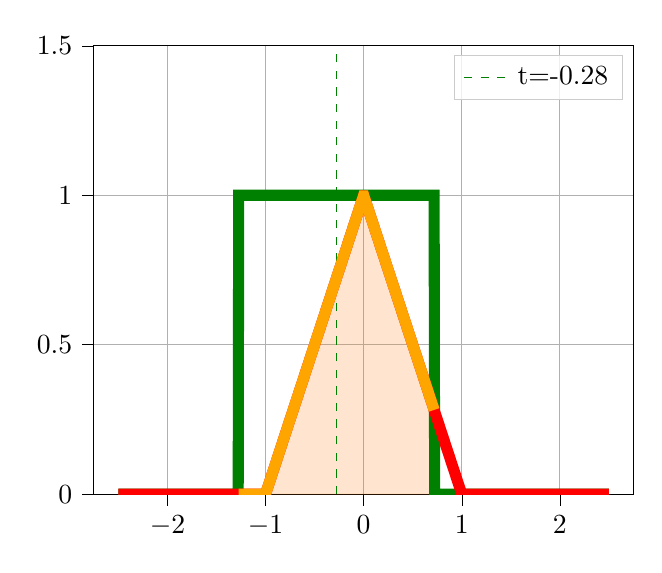
\begin{tikzpicture}

\definecolor{color0}{rgb}{1,0.498039215686275,0.0549019607843137}
\definecolor{color1}{rgb}{1,0.647058823529412,0}

\begin{axis}[
legend cell align={left},
legend style={fill opacity=0.8, draw opacity=1, text opacity=1, draw=white!80!black},
tick align=outside,
tick pos=left,
x grid style={white!69.0196078431373!black},
xmajorgrids,
xmin=-2.75, xmax=2.75,
xtick style={color=black},
y grid style={white!69.0196078431373!black},
ymajorgrids,
ymin=0, ymax=1.5,
ytick style={color=black}
]
\path [draw=color0, fill=color0, opacity=0.2]
(axis cs:-1.27377377377377,0)
--(axis cs:-1.27377377377377,0)
--(axis cs:-1.26876876876877,0)
--(axis cs:-1.26376376376376,0)
--(axis cs:-1.25875875875876,0)
--(axis cs:-1.25375375375375,0)
--(axis cs:-1.24874874874875,0)
--(axis cs:-1.24374374374374,0)
--(axis cs:-1.23873873873874,0)
--(axis cs:-1.23373373373373,0)
--(axis cs:-1.22872872872873,0)
--(axis cs:-1.22372372372372,0)
--(axis cs:-1.21871871871872,0)
--(axis cs:-1.21371371371371,0)
--(axis cs:-1.20870870870871,0)
--(axis cs:-1.2037037037037,0)
--(axis cs:-1.1986986986987,0)
--(axis cs:-1.19369369369369,0)
--(axis cs:-1.18868868868869,0)
--(axis cs:-1.18368368368368,0)
--(axis cs:-1.17867867867868,0)
--(axis cs:-1.17367367367367,0)
--(axis cs:-1.16866866866867,0)
--(axis cs:-1.16366366366366,0)
--(axis cs:-1.15865865865866,0)
--(axis cs:-1.15365365365365,0)
--(axis cs:-1.14864864864865,0)
--(axis cs:-1.14364364364364,0)
--(axis cs:-1.13863863863864,0)
--(axis cs:-1.13363363363363,0)
--(axis cs:-1.12862862862863,0)
--(axis cs:-1.12362362362362,0)
--(axis cs:-1.11861861861862,0)
--(axis cs:-1.11361361361361,0)
--(axis cs:-1.10860860860861,0)
--(axis cs:-1.1036036036036,0)
--(axis cs:-1.0985985985986,0)
--(axis cs:-1.09359359359359,0)
--(axis cs:-1.08858858858859,0)
--(axis cs:-1.08358358358358,0)
--(axis cs:-1.07857857857858,0)
--(axis cs:-1.07357357357357,0)
--(axis cs:-1.06856856856857,0)
--(axis cs:-1.06356356356356,0)
--(axis cs:-1.05855855855856,0)
--(axis cs:-1.05355355355355,0)
--(axis cs:-1.04854854854855,0)
--(axis cs:-1.04354354354354,0)
--(axis cs:-1.03853853853854,0)
--(axis cs:-1.03353353353353,0)
--(axis cs:-1.02852852852853,0)
--(axis cs:-1.02352352352352,0)
--(axis cs:-1.01851851851852,0)
--(axis cs:-1.01351351351351,0)
--(axis cs:-1.00850850850851,0)
--(axis cs:-1.0035035035035,0)
--(axis cs:-0.998498498498499,0)
--(axis cs:-0.993493493493494,0)
--(axis cs:-0.988488488488489,0)
--(axis cs:-0.983483483483484,0)
--(axis cs:-0.978478478478479,0)
--(axis cs:-0.973473473473474,0)
--(axis cs:-0.968468468468469,0)
--(axis cs:-0.963463463463464,0)
--(axis cs:-0.958458458458459,0)
--(axis cs:-0.953453453453454,0)
--(axis cs:-0.948448448448449,0)
--(axis cs:-0.943443443443444,0)
--(axis cs:-0.938438438438439,0)
--(axis cs:-0.933433433433434,0)
--(axis cs:-0.928428428428429,0)
--(axis cs:-0.923423423423424,0)
--(axis cs:-0.918418418418419,0)
--(axis cs:-0.913413413413414,0)
--(axis cs:-0.908408408408409,0)
--(axis cs:-0.903403403403404,0)
--(axis cs:-0.898398398398399,0)
--(axis cs:-0.893393393393393,0)
--(axis cs:-0.888388388388388,0)
--(axis cs:-0.883383383383383,0)
--(axis cs:-0.878378378378378,0)
--(axis cs:-0.873373373373373,0)
--(axis cs:-0.868368368368368,0)
--(axis cs:-0.863363363363363,0)
--(axis cs:-0.858358358358358,0)
--(axis cs:-0.853353353353353,0)
--(axis cs:-0.848348348348348,0)
--(axis cs:-0.843343343343343,0)
--(axis cs:-0.838338338338338,0)
--(axis cs:-0.833333333333333,0)
--(axis cs:-0.828328328328328,0)
--(axis cs:-0.823323323323323,0)
--(axis cs:-0.818318318318318,0)
--(axis cs:-0.813313313313313,0)
--(axis cs:-0.808308308308308,0)
--(axis cs:-0.803303303303303,0)
--(axis cs:-0.798298298298298,0)
--(axis cs:-0.793293293293293,0)
--(axis cs:-0.788288288288288,0)
--(axis cs:-0.783283283283283,0)
--(axis cs:-0.778278278278278,0)
--(axis cs:-0.773273273273273,0)
--(axis cs:-0.768268268268268,0)
--(axis cs:-0.763263263263263,0)
--(axis cs:-0.758258258258258,0)
--(axis cs:-0.753253253253253,0)
--(axis cs:-0.748248248248248,0)
--(axis cs:-0.743243243243243,0)
--(axis cs:-0.738238238238238,0)
--(axis cs:-0.733233233233233,0)
--(axis cs:-0.728228228228228,0)
--(axis cs:-0.723223223223223,0)
--(axis cs:-0.718218218218218,0)
--(axis cs:-0.713213213213213,0)
--(axis cs:-0.708208208208208,0)
--(axis cs:-0.703203203203203,0)
--(axis cs:-0.698198198198198,0)
--(axis cs:-0.693193193193193,0)
--(axis cs:-0.688188188188188,0)
--(axis cs:-0.683183183183183,0)
--(axis cs:-0.678178178178178,0)
--(axis cs:-0.673173173173173,0)
--(axis cs:-0.668168168168168,0)
--(axis cs:-0.663163163163163,0)
--(axis cs:-0.658158158158158,0)
--(axis cs:-0.653153153153153,0)
--(axis cs:-0.648148148148148,0)
--(axis cs:-0.643143143143143,0)
--(axis cs:-0.638138138138138,0)
--(axis cs:-0.633133133133133,0)
--(axis cs:-0.628128128128128,0)
--(axis cs:-0.623123123123123,0)
--(axis cs:-0.618118118118118,0)
--(axis cs:-0.613113113113113,0)
--(axis cs:-0.608108108108108,0)
--(axis cs:-0.603103103103103,0)
--(axis cs:-0.598098098098098,0)
--(axis cs:-0.593093093093093,0)
--(axis cs:-0.588088088088088,0)
--(axis cs:-0.583083083083083,0)
--(axis cs:-0.578078078078078,0)
--(axis cs:-0.573073073073073,0)
--(axis cs:-0.568068068068068,0)
--(axis cs:-0.563063063063063,0)
--(axis cs:-0.558058058058058,0)
--(axis cs:-0.553053053053053,0)
--(axis cs:-0.548048048048048,0)
--(axis cs:-0.543043043043043,0)
--(axis cs:-0.538038038038038,0)
--(axis cs:-0.533033033033033,0)
--(axis cs:-0.528028028028028,0)
--(axis cs:-0.523023023023023,0)
--(axis cs:-0.518018018018018,0)
--(axis cs:-0.513013013013013,0)
--(axis cs:-0.508008008008008,0)
--(axis cs:-0.503003003003003,0)
--(axis cs:-0.497997997997998,0)
--(axis cs:-0.492992992992993,0)
--(axis cs:-0.487987987987988,0)
--(axis cs:-0.482982982982983,0)
--(axis cs:-0.477977977977978,0)
--(axis cs:-0.472972972972973,0)
--(axis cs:-0.467967967967968,0)
--(axis cs:-0.462962962962963,0)
--(axis cs:-0.457957957957958,0)
--(axis cs:-0.452952952952953,0)
--(axis cs:-0.447947947947948,0)
--(axis cs:-0.442942942942943,0)
--(axis cs:-0.437937937937938,0)
--(axis cs:-0.432932932932933,0)
--(axis cs:-0.427927927927928,0)
--(axis cs:-0.422922922922923,0)
--(axis cs:-0.417917917917918,0)
--(axis cs:-0.412912912912913,0)
--(axis cs:-0.407907907907908,0)
--(axis cs:-0.402902902902903,0)
--(axis cs:-0.397897897897898,0)
--(axis cs:-0.392892892892893,0)
--(axis cs:-0.387887887887888,0)
--(axis cs:-0.382882882882883,0)
--(axis cs:-0.377877877877878,0)
--(axis cs:-0.372872872872873,0)
--(axis cs:-0.367867867867868,0)
--(axis cs:-0.362862862862863,0)
--(axis cs:-0.357857857857858,0)
--(axis cs:-0.352852852852853,0)
--(axis cs:-0.347847847847848,0)
--(axis cs:-0.342842842842843,0)
--(axis cs:-0.337837837837838,0)
--(axis cs:-0.332832832832833,0)
--(axis cs:-0.327827827827828,0)
--(axis cs:-0.322822822822823,0)
--(axis cs:-0.317817817817818,0)
--(axis cs:-0.312812812812813,0)
--(axis cs:-0.307807807807808,0)
--(axis cs:-0.302802802802803,0)
--(axis cs:-0.297797797797798,0)
--(axis cs:-0.292792792792793,0)
--(axis cs:-0.287787787787788,0)
--(axis cs:-0.282782782782783,0)
--(axis cs:-0.277777777777778,0)
--(axis cs:-0.272772772772773,0)
--(axis cs:-0.267767767767768,0)
--(axis cs:-0.262762762762763,0)
--(axis cs:-0.257757757757758,0)
--(axis cs:-0.252752752752753,0)
--(axis cs:-0.247747747747748,0)
--(axis cs:-0.242742742742743,0)
--(axis cs:-0.237737737737738,0)
--(axis cs:-0.232732732732733,0)
--(axis cs:-0.227727727727728,0)
--(axis cs:-0.222722722722723,0)
--(axis cs:-0.217717717717718,0)
--(axis cs:-0.212712712712713,0)
--(axis cs:-0.207707707707708,0)
--(axis cs:-0.202702702702703,0)
--(axis cs:-0.197697697697698,0)
--(axis cs:-0.192692692692693,0)
--(axis cs:-0.187687687687688,0)
--(axis cs:-0.182682682682683,0)
--(axis cs:-0.177677677677678,0)
--(axis cs:-0.172672672672673,0)
--(axis cs:-0.167667667667668,0)
--(axis cs:-0.162662662662663,0)
--(axis cs:-0.157657657657658,0)
--(axis cs:-0.152652652652653,0)
--(axis cs:-0.147647647647648,0)
--(axis cs:-0.142642642642643,0)
--(axis cs:-0.137637637637638,0)
--(axis cs:-0.132632632632633,0)
--(axis cs:-0.127627627627628,0)
--(axis cs:-0.122622622622623,0)
--(axis cs:-0.117617617617618,0)
--(axis cs:-0.112612612612613,0)
--(axis cs:-0.107607607607608,0)
--(axis cs:-0.102602602602603,0)
--(axis cs:-0.0975975975975976,0)
--(axis cs:-0.0925925925925926,0)
--(axis cs:-0.0875875875875876,0)
--(axis cs:-0.0825825825825826,0)
--(axis cs:-0.0775775775775776,0)
--(axis cs:-0.0725725725725725,0)
--(axis cs:-0.0675675675675675,0)
--(axis cs:-0.0625625625625625,0)
--(axis cs:-0.0575575575575575,0)
--(axis cs:-0.0525525525525525,0)
--(axis cs:-0.0475475475475475,0)
--(axis cs:-0.0425425425425425,0)
--(axis cs:-0.0375375375375375,0)
--(axis cs:-0.0325325325325325,0)
--(axis cs:-0.0275275275275275,0)
--(axis cs:-0.0225225225225225,0)
--(axis cs:-0.0175175175175175,0)
--(axis cs:-0.0125125125125125,0)
--(axis cs:-0.0075075075075075,0)
--(axis cs:-0.0025025025025025,0)
--(axis cs:0.0025025025025025,0)
--(axis cs:0.0075075075075075,0)
--(axis cs:0.0125125125125125,0)
--(axis cs:0.0175175175175175,0)
--(axis cs:0.0225225225225225,0)
--(axis cs:0.0275275275275275,0)
--(axis cs:0.0325325325325325,0)
--(axis cs:0.0375375375375375,0)
--(axis cs:0.0425425425425425,0)
--(axis cs:0.0475475475475475,0)
--(axis cs:0.0525525525525525,0)
--(axis cs:0.0575575575575575,0)
--(axis cs:0.0625625625625625,0)
--(axis cs:0.0675675675675675,0)
--(axis cs:0.0725725725725725,0)
--(axis cs:0.0775775775775776,0)
--(axis cs:0.0825825825825826,0)
--(axis cs:0.0875875875875876,0)
--(axis cs:0.0925925925925926,0)
--(axis cs:0.0975975975975976,0)
--(axis cs:0.102602602602603,0)
--(axis cs:0.107607607607608,0)
--(axis cs:0.112612612612613,0)
--(axis cs:0.117617617617618,0)
--(axis cs:0.122622622622623,0)
--(axis cs:0.127627627627628,0)
--(axis cs:0.132632632632633,0)
--(axis cs:0.137637637637638,0)
--(axis cs:0.142642642642643,0)
--(axis cs:0.147647647647648,0)
--(axis cs:0.152652652652653,0)
--(axis cs:0.157657657657658,0)
--(axis cs:0.162662662662663,0)
--(axis cs:0.167667667667668,0)
--(axis cs:0.172672672672673,0)
--(axis cs:0.177677677677678,0)
--(axis cs:0.182682682682683,0)
--(axis cs:0.187687687687688,0)
--(axis cs:0.192692692692693,0)
--(axis cs:0.197697697697698,0)
--(axis cs:0.202702702702703,0)
--(axis cs:0.207707707707708,0)
--(axis cs:0.212712712712713,0)
--(axis cs:0.217717717717718,0)
--(axis cs:0.222722722722723,0)
--(axis cs:0.227727727727728,0)
--(axis cs:0.232732732732733,0)
--(axis cs:0.237737737737738,0)
--(axis cs:0.242742742742743,0)
--(axis cs:0.247747747747748,0)
--(axis cs:0.252752752752753,0)
--(axis cs:0.257757757757758,0)
--(axis cs:0.262762762762763,0)
--(axis cs:0.267767767767768,0)
--(axis cs:0.272772772772773,0)
--(axis cs:0.277777777777778,0)
--(axis cs:0.282782782782783,0)
--(axis cs:0.287787787787788,0)
--(axis cs:0.292792792792793,0)
--(axis cs:0.297797797797798,0)
--(axis cs:0.302802802802803,0)
--(axis cs:0.307807807807808,0)
--(axis cs:0.312812812812813,0)
--(axis cs:0.317817817817818,0)
--(axis cs:0.322822822822823,0)
--(axis cs:0.327827827827828,0)
--(axis cs:0.332832832832833,0)
--(axis cs:0.337837837837838,0)
--(axis cs:0.342842842842843,0)
--(axis cs:0.347847847847848,0)
--(axis cs:0.352852852852853,0)
--(axis cs:0.357857857857858,0)
--(axis cs:0.362862862862863,0)
--(axis cs:0.367867867867868,0)
--(axis cs:0.372872872872873,0)
--(axis cs:0.377877877877878,0)
--(axis cs:0.382882882882883,0)
--(axis cs:0.387887887887888,0)
--(axis cs:0.392892892892893,0)
--(axis cs:0.397897897897898,0)
--(axis cs:0.402902902902903,0)
--(axis cs:0.407907907907908,0)
--(axis cs:0.412912912912913,0)
--(axis cs:0.417917917917918,0)
--(axis cs:0.422922922922923,0)
--(axis cs:0.427927927927928,0)
--(axis cs:0.432932932932933,0)
--(axis cs:0.437937937937938,0)
--(axis cs:0.442942942942943,0)
--(axis cs:0.447947947947948,0)
--(axis cs:0.452952952952953,0)
--(axis cs:0.457957957957958,0)
--(axis cs:0.462962962962963,0)
--(axis cs:0.467967967967968,0)
--(axis cs:0.472972972972973,0)
--(axis cs:0.477977977977978,0)
--(axis cs:0.482982982982983,0)
--(axis cs:0.487987987987988,0)
--(axis cs:0.492992992992993,0)
--(axis cs:0.497997997997998,0)
--(axis cs:0.503003003003003,0)
--(axis cs:0.508008008008008,0)
--(axis cs:0.513013013013013,0)
--(axis cs:0.518018018018018,0)
--(axis cs:0.523023023023023,0)
--(axis cs:0.528028028028028,0)
--(axis cs:0.533033033033033,0)
--(axis cs:0.538038038038038,0)
--(axis cs:0.543043043043043,0)
--(axis cs:0.548048048048048,0)
--(axis cs:0.553053053053053,0)
--(axis cs:0.558058058058058,0)
--(axis cs:0.563063063063063,0)
--(axis cs:0.568068068068068,0)
--(axis cs:0.573073073073073,0)
--(axis cs:0.578078078078078,0)
--(axis cs:0.583083083083083,0)
--(axis cs:0.588088088088088,0)
--(axis cs:0.593093093093093,0)
--(axis cs:0.598098098098098,0)
--(axis cs:0.603103103103103,0)
--(axis cs:0.608108108108108,0)
--(axis cs:0.613113113113113,0)
--(axis cs:0.618118118118118,0)
--(axis cs:0.623123123123123,0)
--(axis cs:0.628128128128128,0)
--(axis cs:0.633133133133133,0)
--(axis cs:0.638138138138138,0)
--(axis cs:0.643143143143143,0)
--(axis cs:0.648148148148148,0)
--(axis cs:0.653153153153153,0)
--(axis cs:0.658158158158158,0)
--(axis cs:0.663163163163163,0)
--(axis cs:0.668168168168168,0)
--(axis cs:0.673173173173173,0)
--(axis cs:0.678178178178178,0)
--(axis cs:0.683183183183183,0)
--(axis cs:0.688188188188188,0)
--(axis cs:0.693193193193193,0)
--(axis cs:0.698198198198198,0)
--(axis cs:0.703203203203203,0)
--(axis cs:0.708208208208208,0)
--(axis cs:0.713213213213213,0)
--(axis cs:0.718218218218218,0)
--(axis cs:0.718218218218218,0.281781781781782)
--(axis cs:0.718218218218218,0.281781781781782)
--(axis cs:0.713213213213213,0.286786786786787)
--(axis cs:0.708208208208208,0.291791791791792)
--(axis cs:0.703203203203203,0.296796796796797)
--(axis cs:0.698198198198198,0.301801801801802)
--(axis cs:0.693193193193193,0.306806806806807)
--(axis cs:0.688188188188188,0.311811811811812)
--(axis cs:0.683183183183183,0.316816816816817)
--(axis cs:0.678178178178178,0.321821821821822)
--(axis cs:0.673173173173173,0.326826826826827)
--(axis cs:0.668168168168168,0.331831831831832)
--(axis cs:0.663163163163163,0.336836836836837)
--(axis cs:0.658158158158158,0.341841841841842)
--(axis cs:0.653153153153153,0.346846846846847)
--(axis cs:0.648148148148148,0.351851851851852)
--(axis cs:0.643143143143143,0.356856856856857)
--(axis cs:0.638138138138138,0.361861861861862)
--(axis cs:0.633133133133133,0.366866866866867)
--(axis cs:0.628128128128128,0.371871871871872)
--(axis cs:0.623123123123123,0.376876876876877)
--(axis cs:0.618118118118118,0.381881881881882)
--(axis cs:0.613113113113113,0.386886886886887)
--(axis cs:0.608108108108108,0.391891891891892)
--(axis cs:0.603103103103103,0.396896896896897)
--(axis cs:0.598098098098098,0.401901901901902)
--(axis cs:0.593093093093093,0.406906906906907)
--(axis cs:0.588088088088088,0.411911911911912)
--(axis cs:0.583083083083083,0.416916916916917)
--(axis cs:0.578078078078078,0.421921921921922)
--(axis cs:0.573073073073073,0.426926926926927)
--(axis cs:0.568068068068068,0.431931931931932)
--(axis cs:0.563063063063063,0.436936936936937)
--(axis cs:0.558058058058058,0.441941941941942)
--(axis cs:0.553053053053053,0.446946946946947)
--(axis cs:0.548048048048048,0.451951951951952)
--(axis cs:0.543043043043043,0.456956956956957)
--(axis cs:0.538038038038038,0.461961961961962)
--(axis cs:0.533033033033033,0.466966966966967)
--(axis cs:0.528028028028028,0.471971971971972)
--(axis cs:0.523023023023023,0.476976976976977)
--(axis cs:0.518018018018018,0.481981981981982)
--(axis cs:0.513013013013013,0.486986986986987)
--(axis cs:0.508008008008008,0.491991991991992)
--(axis cs:0.503003003003003,0.496996996996997)
--(axis cs:0.497997997997998,0.502002002002002)
--(axis cs:0.492992992992993,0.507007007007007)
--(axis cs:0.487987987987988,0.512012012012012)
--(axis cs:0.482982982982983,0.517017017017017)
--(axis cs:0.477977977977978,0.522022022022022)
--(axis cs:0.472972972972973,0.527027027027027)
--(axis cs:0.467967967967968,0.532032032032032)
--(axis cs:0.462962962962963,0.537037037037037)
--(axis cs:0.457957957957958,0.542042042042042)
--(axis cs:0.452952952952953,0.547047047047047)
--(axis cs:0.447947947947948,0.552052052052052)
--(axis cs:0.442942942942943,0.557057057057057)
--(axis cs:0.437937937937938,0.562062062062062)
--(axis cs:0.432932932932933,0.567067067067067)
--(axis cs:0.427927927927928,0.572072072072072)
--(axis cs:0.422922922922923,0.577077077077077)
--(axis cs:0.417917917917918,0.582082082082082)
--(axis cs:0.412912912912913,0.587087087087087)
--(axis cs:0.407907907907908,0.592092092092092)
--(axis cs:0.402902902902903,0.597097097097097)
--(axis cs:0.397897897897898,0.602102102102102)
--(axis cs:0.392892892892893,0.607107107107107)
--(axis cs:0.387887887887888,0.612112112112112)
--(axis cs:0.382882882882883,0.617117117117117)
--(axis cs:0.377877877877878,0.622122122122122)
--(axis cs:0.372872872872873,0.627127127127127)
--(axis cs:0.367867867867868,0.632132132132132)
--(axis cs:0.362862862862863,0.637137137137137)
--(axis cs:0.357857857857858,0.642142142142142)
--(axis cs:0.352852852852853,0.647147147147147)
--(axis cs:0.347847847847848,0.652152152152152)
--(axis cs:0.342842842842843,0.657157157157157)
--(axis cs:0.337837837837838,0.662162162162162)
--(axis cs:0.332832832832833,0.667167167167167)
--(axis cs:0.327827827827828,0.672172172172172)
--(axis cs:0.322822822822823,0.677177177177177)
--(axis cs:0.317817817817818,0.682182182182182)
--(axis cs:0.312812812812813,0.687187187187187)
--(axis cs:0.307807807807808,0.692192192192192)
--(axis cs:0.302802802802803,0.697197197197197)
--(axis cs:0.297797797797798,0.702202202202202)
--(axis cs:0.292792792792793,0.707207207207207)
--(axis cs:0.287787787787788,0.712212212212212)
--(axis cs:0.282782782782783,0.717217217217217)
--(axis cs:0.277777777777778,0.722222222222222)
--(axis cs:0.272772772772773,0.727227227227227)
--(axis cs:0.267767767767768,0.732232232232232)
--(axis cs:0.262762762762763,0.737237237237237)
--(axis cs:0.257757757757758,0.742242242242242)
--(axis cs:0.252752752752753,0.747247247247247)
--(axis cs:0.247747747747748,0.752252252252252)
--(axis cs:0.242742742742743,0.757257257257257)
--(axis cs:0.237737737737738,0.762262262262262)
--(axis cs:0.232732732732733,0.767267267267267)
--(axis cs:0.227727727727728,0.772272272272272)
--(axis cs:0.222722722722723,0.777277277277277)
--(axis cs:0.217717717717718,0.782282282282282)
--(axis cs:0.212712712712713,0.787287287287287)
--(axis cs:0.207707707707708,0.792292292292292)
--(axis cs:0.202702702702703,0.797297297297297)
--(axis cs:0.197697697697698,0.802302302302302)
--(axis cs:0.192692692692693,0.807307307307307)
--(axis cs:0.187687687687688,0.812312312312312)
--(axis cs:0.182682682682683,0.817317317317317)
--(axis cs:0.177677677677678,0.822322322322322)
--(axis cs:0.172672672672673,0.827327327327327)
--(axis cs:0.167667667667668,0.832332332332332)
--(axis cs:0.162662662662663,0.837337337337337)
--(axis cs:0.157657657657658,0.842342342342342)
--(axis cs:0.152652652652653,0.847347347347347)
--(axis cs:0.147647647647648,0.852352352352352)
--(axis cs:0.142642642642643,0.857357357357357)
--(axis cs:0.137637637637638,0.862362362362362)
--(axis cs:0.132632632632633,0.867367367367367)
--(axis cs:0.127627627627628,0.872372372372372)
--(axis cs:0.122622622622623,0.877377377377377)
--(axis cs:0.117617617617618,0.882382382382382)
--(axis cs:0.112612612612613,0.887387387387387)
--(axis cs:0.107607607607608,0.892392392392392)
--(axis cs:0.102602602602603,0.897397397397397)
--(axis cs:0.0975975975975976,0.902402402402402)
--(axis cs:0.0925925925925926,0.907407407407407)
--(axis cs:0.0875875875875876,0.912412412412412)
--(axis cs:0.0825825825825826,0.917417417417417)
--(axis cs:0.0775775775775776,0.922422422422422)
--(axis cs:0.0725725725725725,0.927427427427427)
--(axis cs:0.0675675675675675,0.932432432432432)
--(axis cs:0.0625625625625625,0.937437437437437)
--(axis cs:0.0575575575575575,0.942442442442442)
--(axis cs:0.0525525525525525,0.947447447447447)
--(axis cs:0.0475475475475475,0.952452452452452)
--(axis cs:0.0425425425425425,0.957457457457457)
--(axis cs:0.0375375375375375,0.962462462462462)
--(axis cs:0.0325325325325325,0.967467467467467)
--(axis cs:0.0275275275275275,0.972472472472472)
--(axis cs:0.0225225225225225,0.977477477477477)
--(axis cs:0.0175175175175175,0.982482482482482)
--(axis cs:0.0125125125125125,0.987487487487487)
--(axis cs:0.0075075075075075,0.992492492492492)
--(axis cs:0.0025025025025025,0.997497497497497)
--(axis cs:-0.0025025025025025,0.997497497497497)
--(axis cs:-0.0075075075075075,0.992492492492492)
--(axis cs:-0.0125125125125125,0.987487487487487)
--(axis cs:-0.0175175175175175,0.982482482482482)
--(axis cs:-0.0225225225225225,0.977477477477477)
--(axis cs:-0.0275275275275275,0.972472472472472)
--(axis cs:-0.0325325325325325,0.967467467467467)
--(axis cs:-0.0375375375375375,0.962462462462462)
--(axis cs:-0.0425425425425425,0.957457457457457)
--(axis cs:-0.0475475475475475,0.952452452452452)
--(axis cs:-0.0525525525525525,0.947447447447447)
--(axis cs:-0.0575575575575575,0.942442442442442)
--(axis cs:-0.0625625625625625,0.937437437437437)
--(axis cs:-0.0675675675675675,0.932432432432432)
--(axis cs:-0.0725725725725725,0.927427427427427)
--(axis cs:-0.0775775775775776,0.922422422422422)
--(axis cs:-0.0825825825825826,0.917417417417417)
--(axis cs:-0.0875875875875876,0.912412412412412)
--(axis cs:-0.0925925925925926,0.907407407407407)
--(axis cs:-0.0975975975975976,0.902402402402402)
--(axis cs:-0.102602602602603,0.897397397397397)
--(axis cs:-0.107607607607608,0.892392392392392)
--(axis cs:-0.112612612612613,0.887387387387387)
--(axis cs:-0.117617617617618,0.882382382382382)
--(axis cs:-0.122622622622623,0.877377377377377)
--(axis cs:-0.127627627627628,0.872372372372372)
--(axis cs:-0.132632632632633,0.867367367367367)
--(axis cs:-0.137637637637638,0.862362362362362)
--(axis cs:-0.142642642642643,0.857357357357357)
--(axis cs:-0.147647647647648,0.852352352352352)
--(axis cs:-0.152652652652653,0.847347347347347)
--(axis cs:-0.157657657657658,0.842342342342342)
--(axis cs:-0.162662662662663,0.837337337337337)
--(axis cs:-0.167667667667668,0.832332332332332)
--(axis cs:-0.172672672672673,0.827327327327327)
--(axis cs:-0.177677677677678,0.822322322322322)
--(axis cs:-0.182682682682683,0.817317317317317)
--(axis cs:-0.187687687687688,0.812312312312312)
--(axis cs:-0.192692692692693,0.807307307307307)
--(axis cs:-0.197697697697698,0.802302302302302)
--(axis cs:-0.202702702702703,0.797297297297297)
--(axis cs:-0.207707707707708,0.792292292292292)
--(axis cs:-0.212712712712713,0.787287287287287)
--(axis cs:-0.217717717717718,0.782282282282282)
--(axis cs:-0.222722722722723,0.777277277277277)
--(axis cs:-0.227727727727728,0.772272272272272)
--(axis cs:-0.232732732732733,0.767267267267267)
--(axis cs:-0.237737737737738,0.762262262262262)
--(axis cs:-0.242742742742743,0.757257257257257)
--(axis cs:-0.247747747747748,0.752252252252252)
--(axis cs:-0.252752752752753,0.747247247247247)
--(axis cs:-0.257757757757758,0.742242242242242)
--(axis cs:-0.262762762762763,0.737237237237237)
--(axis cs:-0.267767767767768,0.732232232232232)
--(axis cs:-0.272772772772773,0.727227227227227)
--(axis cs:-0.277777777777778,0.722222222222222)
--(axis cs:-0.282782782782783,0.717217217217217)
--(axis cs:-0.287787787787788,0.712212212212212)
--(axis cs:-0.292792792792793,0.707207207207207)
--(axis cs:-0.297797797797798,0.702202202202202)
--(axis cs:-0.302802802802803,0.697197197197197)
--(axis cs:-0.307807807807808,0.692192192192192)
--(axis cs:-0.312812812812813,0.687187187187187)
--(axis cs:-0.317817817817818,0.682182182182182)
--(axis cs:-0.322822822822823,0.677177177177177)
--(axis cs:-0.327827827827828,0.672172172172172)
--(axis cs:-0.332832832832833,0.667167167167167)
--(axis cs:-0.337837837837838,0.662162162162162)
--(axis cs:-0.342842842842843,0.657157157157157)
--(axis cs:-0.347847847847848,0.652152152152152)
--(axis cs:-0.352852852852853,0.647147147147147)
--(axis cs:-0.357857857857858,0.642142142142142)
--(axis cs:-0.362862862862863,0.637137137137137)
--(axis cs:-0.367867867867868,0.632132132132132)
--(axis cs:-0.372872872872873,0.627127127127127)
--(axis cs:-0.377877877877878,0.622122122122122)
--(axis cs:-0.382882882882883,0.617117117117117)
--(axis cs:-0.387887887887888,0.612112112112112)
--(axis cs:-0.392892892892893,0.607107107107107)
--(axis cs:-0.397897897897898,0.602102102102102)
--(axis cs:-0.402902902902903,0.597097097097097)
--(axis cs:-0.407907907907908,0.592092092092092)
--(axis cs:-0.412912912912913,0.587087087087087)
--(axis cs:-0.417917917917918,0.582082082082082)
--(axis cs:-0.422922922922923,0.577077077077077)
--(axis cs:-0.427927927927928,0.572072072072072)
--(axis cs:-0.432932932932933,0.567067067067067)
--(axis cs:-0.437937937937938,0.562062062062062)
--(axis cs:-0.442942942942943,0.557057057057057)
--(axis cs:-0.447947947947948,0.552052052052052)
--(axis cs:-0.452952952952953,0.547047047047047)
--(axis cs:-0.457957957957958,0.542042042042042)
--(axis cs:-0.462962962962963,0.537037037037037)
--(axis cs:-0.467967967967968,0.532032032032032)
--(axis cs:-0.472972972972973,0.527027027027027)
--(axis cs:-0.477977977977978,0.522022022022022)
--(axis cs:-0.482982982982983,0.517017017017017)
--(axis cs:-0.487987987987988,0.512012012012012)
--(axis cs:-0.492992992992993,0.507007007007007)
--(axis cs:-0.497997997997998,0.502002002002002)
--(axis cs:-0.503003003003003,0.496996996996997)
--(axis cs:-0.508008008008008,0.491991991991992)
--(axis cs:-0.513013013013013,0.486986986986987)
--(axis cs:-0.518018018018018,0.481981981981982)
--(axis cs:-0.523023023023023,0.476976976976977)
--(axis cs:-0.528028028028028,0.471971971971972)
--(axis cs:-0.533033033033033,0.466966966966967)
--(axis cs:-0.538038038038038,0.461961961961962)
--(axis cs:-0.543043043043043,0.456956956956957)
--(axis cs:-0.548048048048048,0.451951951951952)
--(axis cs:-0.553053053053053,0.446946946946947)
--(axis cs:-0.558058058058058,0.441941941941942)
--(axis cs:-0.563063063063063,0.436936936936937)
--(axis cs:-0.568068068068068,0.431931931931932)
--(axis cs:-0.573073073073073,0.426926926926927)
--(axis cs:-0.578078078078078,0.421921921921922)
--(axis cs:-0.583083083083083,0.416916916916917)
--(axis cs:-0.588088088088088,0.411911911911912)
--(axis cs:-0.593093093093093,0.406906906906907)
--(axis cs:-0.598098098098098,0.401901901901902)
--(axis cs:-0.603103103103103,0.396896896896897)
--(axis cs:-0.608108108108108,0.391891891891892)
--(axis cs:-0.613113113113113,0.386886886886887)
--(axis cs:-0.618118118118118,0.381881881881882)
--(axis cs:-0.623123123123123,0.376876876876877)
--(axis cs:-0.628128128128128,0.371871871871872)
--(axis cs:-0.633133133133133,0.366866866866867)
--(axis cs:-0.638138138138138,0.361861861861862)
--(axis cs:-0.643143143143143,0.356856856856857)
--(axis cs:-0.648148148148148,0.351851851851852)
--(axis cs:-0.653153153153153,0.346846846846847)
--(axis cs:-0.658158158158158,0.341841841841842)
--(axis cs:-0.663163163163163,0.336836836836837)
--(axis cs:-0.668168168168168,0.331831831831832)
--(axis cs:-0.673173173173173,0.326826826826827)
--(axis cs:-0.678178178178178,0.321821821821822)
--(axis cs:-0.683183183183183,0.316816816816817)
--(axis cs:-0.688188188188188,0.311811811811812)
--(axis cs:-0.693193193193193,0.306806806806807)
--(axis cs:-0.698198198198198,0.301801801801802)
--(axis cs:-0.703203203203203,0.296796796796797)
--(axis cs:-0.708208208208208,0.291791791791792)
--(axis cs:-0.713213213213213,0.286786786786787)
--(axis cs:-0.718218218218218,0.281781781781782)
--(axis cs:-0.723223223223223,0.276776776776777)
--(axis cs:-0.728228228228228,0.271771771771772)
--(axis cs:-0.733233233233233,0.266766766766767)
--(axis cs:-0.738238238238238,0.261761761761762)
--(axis cs:-0.743243243243243,0.256756756756757)
--(axis cs:-0.748248248248248,0.251751751751752)
--(axis cs:-0.753253253253253,0.246746746746747)
--(axis cs:-0.758258258258258,0.241741741741742)
--(axis cs:-0.763263263263263,0.236736736736737)
--(axis cs:-0.768268268268268,0.231731731731732)
--(axis cs:-0.773273273273273,0.226726726726727)
--(axis cs:-0.778278278278278,0.221721721721722)
--(axis cs:-0.783283283283283,0.216716716716717)
--(axis cs:-0.788288288288288,0.211711711711712)
--(axis cs:-0.793293293293293,0.206706706706707)
--(axis cs:-0.798298298298298,0.201701701701702)
--(axis cs:-0.803303303303303,0.196696696696697)
--(axis cs:-0.808308308308308,0.191691691691692)
--(axis cs:-0.813313313313313,0.186686686686687)
--(axis cs:-0.818318318318318,0.181681681681682)
--(axis cs:-0.823323323323323,0.176676676676677)
--(axis cs:-0.828328328328328,0.171671671671672)
--(axis cs:-0.833333333333333,0.166666666666667)
--(axis cs:-0.838338338338338,0.161661661661662)
--(axis cs:-0.843343343343343,0.156656656656657)
--(axis cs:-0.848348348348348,0.151651651651652)
--(axis cs:-0.853353353353353,0.146646646646647)
--(axis cs:-0.858358358358358,0.141641641641642)
--(axis cs:-0.863363363363363,0.136636636636637)
--(axis cs:-0.868368368368368,0.131631631631632)
--(axis cs:-0.873373373373373,0.126626626626627)
--(axis cs:-0.878378378378378,0.121621621621622)
--(axis cs:-0.883383383383383,0.116616616616617)
--(axis cs:-0.888388388388388,0.111611611611612)
--(axis cs:-0.893393393393393,0.106606606606607)
--(axis cs:-0.898398398398399,0.101601601601601)
--(axis cs:-0.903403403403404,0.0965965965965965)
--(axis cs:-0.908408408408409,0.0915915915915915)
--(axis cs:-0.913413413413414,0.0865865865865865)
--(axis cs:-0.918418418418419,0.0815815815815815)
--(axis cs:-0.923423423423424,0.0765765765765765)
--(axis cs:-0.928428428428429,0.0715715715715715)
--(axis cs:-0.933433433433434,0.0665665665665665)
--(axis cs:-0.938438438438439,0.0615615615615615)
--(axis cs:-0.943443443443444,0.0565565565565564)
--(axis cs:-0.948448448448449,0.0515515515515514)
--(axis cs:-0.953453453453454,0.0465465465465464)
--(axis cs:-0.958458458458459,0.0415415415415414)
--(axis cs:-0.963463463463464,0.0365365365365364)
--(axis cs:-0.968468468468469,0.0315315315315314)
--(axis cs:-0.973473473473474,0.0265265265265264)
--(axis cs:-0.978478478478479,0.0215215215215214)
--(axis cs:-0.983483483483484,0.0165165165165164)
--(axis cs:-0.988488488488489,0.0115115115115114)
--(axis cs:-0.993493493493494,0.00650650650650642)
--(axis cs:-0.998498498498499,0.00150150150150141)
--(axis cs:-1.0035035035035,0)
--(axis cs:-1.00850850850851,0)
--(axis cs:-1.01351351351351,0)
--(axis cs:-1.01851851851852,0)
--(axis cs:-1.02352352352352,0)
--(axis cs:-1.02852852852853,0)
--(axis cs:-1.03353353353353,0)
--(axis cs:-1.03853853853854,0)
--(axis cs:-1.04354354354354,0)
--(axis cs:-1.04854854854855,0)
--(axis cs:-1.05355355355355,0)
--(axis cs:-1.05855855855856,0)
--(axis cs:-1.06356356356356,0)
--(axis cs:-1.06856856856857,0)
--(axis cs:-1.07357357357357,0)
--(axis cs:-1.07857857857858,0)
--(axis cs:-1.08358358358358,0)
--(axis cs:-1.08858858858859,0)
--(axis cs:-1.09359359359359,0)
--(axis cs:-1.0985985985986,0)
--(axis cs:-1.1036036036036,0)
--(axis cs:-1.10860860860861,0)
--(axis cs:-1.11361361361361,0)
--(axis cs:-1.11861861861862,0)
--(axis cs:-1.12362362362362,0)
--(axis cs:-1.12862862862863,0)
--(axis cs:-1.13363363363363,0)
--(axis cs:-1.13863863863864,0)
--(axis cs:-1.14364364364364,0)
--(axis cs:-1.14864864864865,0)
--(axis cs:-1.15365365365365,0)
--(axis cs:-1.15865865865866,0)
--(axis cs:-1.16366366366366,0)
--(axis cs:-1.16866866866867,0)
--(axis cs:-1.17367367367367,0)
--(axis cs:-1.17867867867868,0)
--(axis cs:-1.18368368368368,0)
--(axis cs:-1.18868868868869,0)
--(axis cs:-1.19369369369369,0)
--(axis cs:-1.1986986986987,0)
--(axis cs:-1.2037037037037,0)
--(axis cs:-1.20870870870871,0)
--(axis cs:-1.21371371371371,0)
--(axis cs:-1.21871871871872,0)
--(axis cs:-1.22372372372372,0)
--(axis cs:-1.22872872872873,0)
--(axis cs:-1.23373373373373,0)
--(axis cs:-1.23873873873874,0)
--(axis cs:-1.24374374374374,0)
--(axis cs:-1.24874874874875,0)
--(axis cs:-1.25375375375375,0)
--(axis cs:-1.25875875875876,0)
--(axis cs:-1.26376376376376,0)
--(axis cs:-1.26876876876877,0)
--(axis cs:-1.27377377377377,0)
--cycle;

\addplot [line width=4pt, green!50!black, forget plot]
table {%
-2.5 0
-2.49499499499499 0
-2.48998998998999 0
-2.48498498498498 0
-2.47997997997998 0
-2.47497497497497 0
-2.46996996996997 0
-2.46496496496496 0
-2.45995995995996 0
-2.45495495495495 0
-2.44994994994995 0
-2.44494494494494 0
-2.43993993993994 0
-2.43493493493493 0
-2.42992992992993 0
-2.42492492492492 0
-2.41991991991992 0
-2.41491491491491 0
-2.40990990990991 0
-2.4049049049049 0
-2.3998998998999 0
-2.39489489489489 0
-2.38988988988989 0
-2.38488488488488 0
-2.37987987987988 0
-2.37487487487487 0
-2.36986986986987 0
-2.36486486486486 0
-2.35985985985986 0
-2.35485485485485 0
-2.34984984984985 0
-2.34484484484484 0
-2.33983983983984 0
-2.33483483483483 0
-2.32982982982983 0
-2.32482482482482 0
-2.31981981981982 0
-2.31481481481481 0
-2.30980980980981 0
-2.3048048048048 0
-2.2997997997998 0
-2.29479479479479 0
-2.28978978978979 0
-2.28478478478478 0
-2.27977977977978 0
-2.27477477477477 0
-2.26976976976977 0
-2.26476476476476 0
-2.25975975975976 0
-2.25475475475475 0
-2.24974974974975 0
-2.24474474474474 0
-2.23973973973974 0
-2.23473473473473 0
-2.22972972972973 0
-2.22472472472472 0
-2.21971971971972 0
-2.21471471471471 0
-2.20970970970971 0
-2.2047047047047 0
-2.1996996996997 0
-2.19469469469469 0
-2.18968968968969 0
-2.18468468468468 0
-2.17967967967968 0
-2.17467467467467 0
-2.16966966966967 0
-2.16466466466466 0
-2.15965965965966 0
-2.15465465465465 0
-2.14964964964965 0
-2.14464464464464 0
-2.13963963963964 0
-2.13463463463463 0
-2.12962962962963 0
-2.12462462462462 0
-2.11961961961962 0
-2.11461461461461 0
-2.10960960960961 0
-2.1046046046046 0
-2.0995995995996 0
-2.09459459459459 0
-2.08958958958959 0
-2.08458458458458 0
-2.07957957957958 0
-2.07457457457457 0
-2.06956956956957 0
-2.06456456456456 0
-2.05955955955956 0
-2.05455455455455 0
-2.04954954954955 0
-2.04454454454454 0
-2.03953953953954 0
-2.03453453453453 0
-2.02952952952953 0
-2.02452452452452 0
-2.01951951951952 0
-2.01451451451451 0
-2.00950950950951 0
-2.0045045045045 0
-1.9994994994995 0
-1.99449449449449 0
-1.98948948948949 0
-1.98448448448448 0
-1.97947947947948 0
-1.97447447447447 0
-1.96946946946947 0
-1.96446446446446 0
-1.95945945945946 0
-1.95445445445445 0
-1.94944944944945 0
-1.94444444444444 0
-1.93943943943944 0
-1.93443443443443 0
-1.92942942942943 0
-1.92442442442442 0
-1.91941941941942 0
-1.91441441441441 0
-1.90940940940941 0
-1.9044044044044 0
-1.8993993993994 0
-1.89439439439439 0
-1.88938938938939 0
-1.88438438438438 0
-1.87937937937938 0
-1.87437437437437 0
-1.86936936936937 0
-1.86436436436436 0
-1.85935935935936 0
-1.85435435435435 0
-1.84934934934935 0
-1.84434434434434 0
-1.83933933933934 0
-1.83433433433433 0
-1.82932932932933 0
-1.82432432432432 0
-1.81931931931932 0
-1.81431431431431 0
-1.80930930930931 0
-1.8043043043043 0
-1.7992992992993 0
-1.79429429429429 0
-1.78928928928929 0
-1.78428428428428 0
-1.77927927927928 0
-1.77427427427427 0
-1.76926926926927 0
-1.76426426426426 0
-1.75925925925926 0
-1.75425425425425 0
-1.74924924924925 0
-1.74424424424424 0
-1.73923923923924 0
-1.73423423423423 0
-1.72922922922923 0
-1.72422422422422 0
-1.71921921921922 0
-1.71421421421421 0
-1.70920920920921 0
-1.7042042042042 0
-1.6991991991992 0
-1.69419419419419 0
-1.68918918918919 0
-1.68418418418418 0
-1.67917917917918 0
-1.67417417417417 0
-1.66916916916917 0
-1.66416416416416 0
-1.65915915915916 0
-1.65415415415415 0
-1.64914914914915 0
-1.64414414414414 0
-1.63913913913914 0
-1.63413413413413 0
-1.62912912912913 0
-1.62412412412412 0
-1.61911911911912 0
-1.61411411411411 0
-1.60910910910911 0
-1.6041041041041 0
-1.5990990990991 0
-1.59409409409409 0
-1.58908908908909 0
-1.58408408408408 0
-1.57907907907908 0
-1.57407407407407 0
-1.56906906906907 0
-1.56406406406406 0
-1.55905905905906 0
-1.55405405405405 0
-1.54904904904905 0
-1.54404404404404 0
-1.53903903903904 0
-1.53403403403403 0
-1.52902902902903 0
-1.52402402402402 0
-1.51901901901902 0
-1.51401401401401 0
-1.50900900900901 0
-1.504004004004 0
-1.498998998999 0
-1.49399399399399 0
-1.48898898898899 0
-1.48398398398398 0
-1.47897897897898 0
-1.47397397397397 0
-1.46896896896897 0
-1.46396396396396 0
-1.45895895895896 0
-1.45395395395395 0
-1.44894894894895 0
-1.44394394394394 0
-1.43893893893894 0
-1.43393393393393 0
-1.42892892892893 0
-1.42392392392392 0
-1.41891891891892 0
-1.41391391391391 0
-1.40890890890891 0
-1.4039039039039 0
-1.3988988988989 0
-1.39389389389389 0
-1.38888888888889 0
-1.38388388388388 0
-1.37887887887888 0
-1.37387387387387 0
-1.36886886886887 0
-1.36386386386386 0
-1.35885885885886 0
-1.35385385385385 0
-1.34884884884885 0
-1.34384384384384 0
-1.33883883883884 0
-1.33383383383383 0
-1.32882882882883 0
-1.32382382382382 0
-1.31881881881882 0
-1.31381381381381 0
-1.30880880880881 0
-1.3038038038038 0
-1.2987987987988 0
-1.29379379379379 0
-1.28878878878879 0
-1.28378378378378 0
-1.27877877877878 0
-1.27377377377377 1
-1.26876876876877 1
-1.26376376376376 1
-1.25875875875876 1
-1.25375375375375 1
-1.24874874874875 1
-1.24374374374374 1
-1.23873873873874 1
-1.23373373373373 1
-1.22872872872873 1
-1.22372372372372 1
-1.21871871871872 1
-1.21371371371371 1
-1.20870870870871 1
-1.2037037037037 1
-1.1986986986987 1
-1.19369369369369 1
-1.18868868868869 1
-1.18368368368368 1
-1.17867867867868 1
-1.17367367367367 1
-1.16866866866867 1
-1.16366366366366 1
-1.15865865865866 1
-1.15365365365365 1
-1.14864864864865 1
-1.14364364364364 1
-1.13863863863864 1
-1.13363363363363 1
-1.12862862862863 1
-1.12362362362362 1
-1.11861861861862 1
-1.11361361361361 1
-1.10860860860861 1
-1.1036036036036 1
-1.0985985985986 1
-1.09359359359359 1
-1.08858858858859 1
-1.08358358358358 1
-1.07857857857858 1
-1.07357357357357 1
-1.06856856856857 1
-1.06356356356356 1
-1.05855855855856 1
-1.05355355355355 1
-1.04854854854855 1
-1.04354354354354 1
-1.03853853853854 1
-1.03353353353353 1
-1.02852852852853 1
-1.02352352352352 1
-1.01851851851852 1
-1.01351351351351 1
-1.00850850850851 1
-1.0035035035035 1
-0.998498498498499 1
-0.993493493493494 1
-0.988488488488489 1
-0.983483483483484 1
-0.978478478478479 1
-0.973473473473474 1
-0.968468468468469 1
-0.963463463463464 1
-0.958458458458459 1
-0.953453453453454 1
-0.948448448448449 1
-0.943443443443444 1
-0.938438438438439 1
-0.933433433433434 1
-0.928428428428429 1
-0.923423423423424 1
-0.918418418418419 1
-0.913413413413414 1
-0.908408408408409 1
-0.903403403403404 1
-0.898398398398399 1
-0.893393393393393 1
-0.888388388388388 1
-0.883383383383383 1
-0.878378378378378 1
-0.873373373373373 1
-0.868368368368368 1
-0.863363363363363 1
-0.858358358358358 1
-0.853353353353353 1
-0.848348348348348 1
-0.843343343343343 1
-0.838338338338338 1
-0.833333333333333 1
-0.828328328328328 1
-0.823323323323323 1
-0.818318318318318 1
-0.813313313313313 1
-0.808308308308308 1
-0.803303303303303 1
-0.798298298298298 1
-0.793293293293293 1
-0.788288288288288 1
-0.783283283283283 1
-0.778278278278278 1
-0.773273273273273 1
-0.768268268268268 1
-0.763263263263263 1
-0.758258258258258 1
-0.753253253253253 1
-0.748248248248248 1
-0.743243243243243 1
-0.738238238238238 1
-0.733233233233233 1
-0.728228228228228 1
-0.723223223223223 1
-0.718218218218218 1
-0.713213213213213 1
-0.708208208208208 1
-0.703203203203203 1
-0.698198198198198 1
-0.693193193193193 1
-0.688188188188188 1
-0.683183183183183 1
-0.678178178178178 1
-0.673173173173173 1
-0.668168168168168 1
-0.663163163163163 1
-0.658158158158158 1
-0.653153153153153 1
-0.648148148148148 1
-0.643143143143143 1
-0.638138138138138 1
-0.633133133133133 1
-0.628128128128128 1
-0.623123123123123 1
-0.618118118118118 1
-0.613113113113113 1
-0.608108108108108 1
-0.603103103103103 1
-0.598098098098098 1
-0.593093093093093 1
-0.588088088088088 1
-0.583083083083083 1
-0.578078078078078 1
-0.573073073073073 1
-0.568068068068068 1
-0.563063063063063 1
-0.558058058058058 1
-0.553053053053053 1
-0.548048048048048 1
-0.543043043043043 1
-0.538038038038038 1
-0.533033033033033 1
-0.528028028028028 1
-0.523023023023023 1
-0.518018018018018 1
-0.513013013013013 1
-0.508008008008008 1
-0.503003003003003 1
-0.497997997997998 1
-0.492992992992993 1
-0.487987987987988 1
-0.482982982982983 1
-0.477977977977978 1
-0.472972972972973 1
-0.467967967967968 1
-0.462962962962963 1
-0.457957957957958 1
-0.452952952952953 1
-0.447947947947948 1
-0.442942942942943 1
-0.437937937937938 1
-0.432932932932933 1
-0.427927927927928 1
-0.422922922922923 1
-0.417917917917918 1
-0.412912912912913 1
-0.407907907907908 1
-0.402902902902903 1
-0.397897897897898 1
-0.392892892892893 1
-0.387887887887888 1
-0.382882882882883 1
-0.377877877877878 1
-0.372872872872873 1
-0.367867867867868 1
-0.362862862862863 1
-0.357857857857858 1
-0.352852852852853 1
-0.347847847847848 1
-0.342842842842843 1
-0.337837837837838 1
-0.332832832832833 1
-0.327827827827828 1
-0.322822822822823 1
-0.317817817817818 1
-0.312812812812813 1
-0.307807807807808 1
-0.302802802802803 1
-0.297797797797798 1
-0.292792792792793 1
-0.287787787787788 1
-0.282782782782783 1
-0.277777777777778 1
-0.272772772772773 1
-0.267767767767768 1
-0.262762762762763 1
-0.257757757757758 1
-0.252752752752753 1
-0.247747747747748 1
-0.242742742742743 1
-0.237737737737738 1
-0.232732732732733 1
-0.227727727727728 1
-0.222722722722723 1
-0.217717717717718 1
-0.212712712712713 1
-0.207707707707708 1
-0.202702702702703 1
-0.197697697697698 1
-0.192692692692693 1
-0.187687687687688 1
-0.182682682682683 1
-0.177677677677678 1
-0.172672672672673 1
-0.167667667667668 1
-0.162662662662663 1
-0.157657657657658 1
-0.152652652652653 1
-0.147647647647648 1
-0.142642642642643 1
-0.137637637637638 1
-0.132632632632633 1
-0.127627627627628 1
-0.122622622622623 1
-0.117617617617618 1
-0.112612612612613 1
-0.107607607607608 1
-0.102602602602603 1
-0.0975975975975976 1
-0.0925925925925926 1
-0.0875875875875876 1
-0.0825825825825826 1
-0.0775775775775776 1
-0.0725725725725725 1
-0.0675675675675675 1
-0.0625625625625625 1
-0.0575575575575575 1
-0.0525525525525525 1
-0.0475475475475475 1
-0.0425425425425425 1
-0.0375375375375375 1
-0.0325325325325325 1
-0.0275275275275275 1
-0.0225225225225225 1
-0.0175175175175175 1
-0.0125125125125125 1
-0.0075075075075075 1
-0.0025025025025025 1
0.0025025025025025 1
0.0075075075075075 1
0.0125125125125125 1
0.0175175175175175 1
0.0225225225225225 1
0.0275275275275275 1
0.0325325325325325 1
0.0375375375375375 1
0.0425425425425425 1
0.0475475475475475 1
0.0525525525525525 1
0.0575575575575575 1
0.0625625625625625 1
0.0675675675675675 1
0.0725725725725725 1
0.0775775775775776 1
0.0825825825825826 1
0.0875875875875876 1
0.0925925925925926 1
0.0975975975975976 1
0.102602602602603 1
0.107607607607608 1
0.112612612612613 1
0.117617617617618 1
0.122622622622623 1
0.127627627627628 1
0.132632632632633 1
0.137637637637638 1
0.142642642642643 1
0.147647647647648 1
0.152652652652653 1
0.157657657657658 1
0.162662662662663 1
0.167667667667668 1
0.172672672672673 1
0.177677677677678 1
0.182682682682683 1
0.187687687687688 1
0.192692692692693 1
0.197697697697698 1
0.202702702702703 1
0.207707707707708 1
0.212712712712713 1
0.217717717717718 1
0.222722722722723 1
0.227727727727728 1
0.232732732732733 1
0.237737737737738 1
0.242742742742743 1
0.247747747747748 1
0.252752752752753 1
0.257757757757758 1
0.262762762762763 1
0.267767767767768 1
0.272772772772773 1
0.277777777777778 1
0.282782782782783 1
0.287787787787788 1
0.292792792792793 1
0.297797797797798 1
0.302802802802803 1
0.307807807807808 1
0.312812812812813 1
0.317817817817818 1
0.322822822822823 1
0.327827827827828 1
0.332832832832833 1
0.337837837837838 1
0.342842842842843 1
0.347847847847848 1
0.352852852852853 1
0.357857857857858 1
0.362862862862863 1
0.367867867867868 1
0.372872872872873 1
0.377877877877878 1
0.382882882882883 1
0.387887887887888 1
0.392892892892893 1
0.397897897897898 1
0.402902902902903 1
0.407907907907908 1
0.412912912912913 1
0.417917917917918 1
0.422922922922923 1
0.427927927927928 1
0.432932932932933 1
0.437937937937938 1
0.442942942942943 1
0.447947947947948 1
0.452952952952953 1
0.457957957957958 1
0.462962962962963 1
0.467967967967968 1
0.472972972972973 1
0.477977977977978 1
0.482982982982983 1
0.487987987987988 1
0.492992992992993 1
0.497997997997998 1
0.503003003003003 1
0.508008008008008 1
0.513013013013013 1
0.518018018018018 1
0.523023023023023 1
0.528028028028028 1
0.533033033033033 1
0.538038038038038 1
0.543043043043043 1
0.548048048048048 1
0.553053053053053 1
0.558058058058058 1
0.563063063063063 1
0.568068068068068 1
0.573073073073073 1
0.578078078078078 1
0.583083083083083 1
0.588088088088088 1
0.593093093093093 1
0.598098098098098 1
0.603103103103103 1
0.608108108108108 1
0.613113113113113 1
0.618118118118118 1
0.623123123123123 1
0.628128128128128 1
0.633133133133133 1
0.638138138138138 1
0.643143143143143 1
0.648148148148148 1
0.653153153153153 1
0.658158158158158 1
0.663163163163163 1
0.668168168168168 1
0.673173173173173 1
0.678178178178178 1
0.683183183183183 1
0.688188188188188 1
0.693193193193193 1
0.698198198198198 1
0.703203203203203 1
0.708208208208208 1
0.713213213213213 1
0.718218218218218 1
0.723223223223223 0
0.728228228228228 0
0.733233233233233 0
0.738238238238238 0
0.743243243243243 0
0.748248248248248 0
0.753253253253253 0
0.758258258258258 0
0.763263263263263 0
0.768268268268268 0
0.773273273273273 0
0.778278278278278 0
0.783283283283283 0
0.788288288288288 0
0.793293293293293 0
0.798298298298298 0
0.803303303303303 0
0.808308308308308 0
0.813313313313313 0
0.818318318318318 0
0.823323323323323 0
0.828328328328328 0
0.833333333333333 0
0.838338338338338 0
0.843343343343343 0
0.848348348348348 0
0.853353353353353 0
0.858358358358358 0
0.863363363363364 0
0.868368368368369 0
0.873373373373374 0
0.878378378378379 0
0.883383383383384 0
0.888388388388389 0
0.893393393393394 0
0.898398398398399 0
0.903403403403404 0
0.908408408408409 0
0.913413413413414 0
0.918418418418419 0
0.923423423423424 0
0.928428428428429 0
0.933433433433434 0
0.938438438438439 0
0.943443443443444 0
0.948448448448449 0
0.953453453453454 0
0.958458458458459 0
0.963463463463464 0
0.968468468468469 0
0.973473473473474 0
0.978478478478479 0
0.983483483483484 0
0.988488488488489 0
0.993493493493494 0
0.998498498498499 0
1.0035035035035 0
1.00850850850851 0
1.01351351351351 0
1.01851851851852 0
1.02352352352352 0
1.02852852852853 0
1.03353353353353 0
1.03853853853854 0
1.04354354354354 0
1.04854854854855 0
1.05355355355355 0
1.05855855855856 0
1.06356356356356 0
1.06856856856857 0
1.07357357357357 0
1.07857857857858 0
1.08358358358358 0
1.08858858858859 0
1.09359359359359 0
1.0985985985986 0
1.1036036036036 0
1.10860860860861 0
1.11361361361361 0
1.11861861861862 0
1.12362362362362 0
1.12862862862863 0
1.13363363363363 0
1.13863863863864 0
1.14364364364364 0
1.14864864864865 0
1.15365365365365 0
1.15865865865866 0
1.16366366366366 0
1.16866866866867 0
1.17367367367367 0
1.17867867867868 0
1.18368368368368 0
1.18868868868869 0
1.19369369369369 0
1.1986986986987 0
1.2037037037037 0
1.20870870870871 0
1.21371371371371 0
1.21871871871872 0
1.22372372372372 0
1.22872872872873 0
1.23373373373373 0
1.23873873873874 0
1.24374374374374 0
1.24874874874875 0
1.25375375375375 0
1.25875875875876 0
1.26376376376376 0
1.26876876876877 0
1.27377377377377 0
1.27877877877878 0
1.28378378378378 0
1.28878878878879 0
1.29379379379379 0
1.2987987987988 0
1.3038038038038 0
1.30880880880881 0
1.31381381381381 0
1.31881881881882 0
1.32382382382382 0
1.32882882882883 0
1.33383383383383 0
1.33883883883884 0
1.34384384384384 0
1.34884884884885 0
1.35385385385385 0
1.35885885885886 0
1.36386386386386 0
1.36886886886887 0
1.37387387387387 0
1.37887887887888 0
1.38388388388388 0
1.38888888888889 0
1.39389389389389 0
1.3988988988989 0
1.4039039039039 0
1.40890890890891 0
1.41391391391391 0
1.41891891891892 0
1.42392392392392 0
1.42892892892893 0
1.43393393393393 0
1.43893893893894 0
1.44394394394394 0
1.44894894894895 0
1.45395395395395 0
1.45895895895896 0
1.46396396396396 0
1.46896896896897 0
1.47397397397397 0
1.47897897897898 0
1.48398398398398 0
1.48898898898899 0
1.49399399399399 0
1.498998998999 0
1.504004004004 0
1.50900900900901 0
1.51401401401401 0
1.51901901901902 0
1.52402402402402 0
1.52902902902903 0
1.53403403403403 0
1.53903903903904 0
1.54404404404404 0
1.54904904904905 0
1.55405405405405 0
1.55905905905906 0
1.56406406406406 0
1.56906906906907 0
1.57407407407407 0
1.57907907907908 0
1.58408408408408 0
1.58908908908909 0
1.59409409409409 0
1.5990990990991 0
1.6041041041041 0
1.60910910910911 0
1.61411411411411 0
1.61911911911912 0
1.62412412412412 0
1.62912912912913 0
1.63413413413413 0
1.63913913913914 0
1.64414414414414 0
1.64914914914915 0
1.65415415415415 0
1.65915915915916 0
1.66416416416416 0
1.66916916916917 0
1.67417417417417 0
1.67917917917918 0
1.68418418418418 0
1.68918918918919 0
1.69419419419419 0
1.6991991991992 0
1.7042042042042 0
1.70920920920921 0
1.71421421421421 0
1.71921921921922 0
1.72422422422422 0
1.72922922922923 0
1.73423423423423 0
1.73923923923924 0
1.74424424424424 0
1.74924924924925 0
1.75425425425425 0
1.75925925925926 0
1.76426426426426 0
1.76926926926927 0
1.77427427427427 0
1.77927927927928 0
1.78428428428428 0
1.78928928928929 0
1.79429429429429 0
1.7992992992993 0
1.8043043043043 0
1.80930930930931 0
1.81431431431431 0
1.81931931931932 0
1.82432432432432 0
1.82932932932933 0
1.83433433433433 0
1.83933933933934 0
1.84434434434434 0
1.84934934934935 0
1.85435435435435 0
1.85935935935936 0
1.86436436436436 0
1.86936936936937 0
1.87437437437437 0
1.87937937937938 0
1.88438438438438 0
1.88938938938939 0
1.89439439439439 0
1.8993993993994 0
1.9044044044044 0
1.90940940940941 0
1.91441441441441 0
1.91941941941942 0
1.92442442442442 0
1.92942942942943 0
1.93443443443443 0
1.93943943943944 0
1.94444444444444 0
1.94944944944945 0
1.95445445445445 0
1.95945945945946 0
1.96446446446446 0
1.96946946946947 0
1.97447447447447 0
1.97947947947948 0
1.98448448448448 0
1.98948948948949 0
1.99449449449449 0
1.9994994994995 0
2.0045045045045 0
2.00950950950951 0
2.01451451451451 0
2.01951951951952 0
2.02452452452452 0
2.02952952952953 0
2.03453453453453 0
2.03953953953954 0
2.04454454454454 0
2.04954954954955 0
2.05455455455455 0
2.05955955955956 0
2.06456456456456 0
2.06956956956957 0
2.07457457457457 0
2.07957957957958 0
2.08458458458458 0
2.08958958958959 0
2.09459459459459 0
2.0995995995996 0
2.1046046046046 0
2.10960960960961 0
2.11461461461461 0
2.11961961961962 0
2.12462462462462 0
2.12962962962963 0
2.13463463463463 0
2.13963963963964 0
2.14464464464464 0
2.14964964964965 0
2.15465465465465 0
2.15965965965966 0
2.16466466466466 0
2.16966966966967 0
2.17467467467467 0
2.17967967967968 0
2.18468468468468 0
2.18968968968969 0
2.19469469469469 0
2.1996996996997 0
2.2047047047047 0
2.20970970970971 0
2.21471471471471 0
2.21971971971972 0
2.22472472472472 0
2.22972972972973 0
2.23473473473473 0
2.23973973973974 0
2.24474474474474 0
2.24974974974975 0
2.25475475475475 0
2.25975975975976 0
2.26476476476476 0
2.26976976976977 0
2.27477477477477 0
2.27977977977978 0
2.28478478478478 0
2.28978978978979 0
2.29479479479479 0
2.2997997997998 0
2.3048048048048 0
2.30980980980981 0
2.31481481481481 0
2.31981981981982 0
2.32482482482482 0
2.32982982982983 0
2.33483483483483 0
2.33983983983984 0
2.34484484484484 0
2.34984984984985 0
2.35485485485485 0
2.35985985985986 0
2.36486486486486 0
2.36986986986987 0
2.37487487487487 0
2.37987987987988 0
2.38488488488488 0
2.38988988988989 0
2.39489489489489 0
2.3998998998999 0
2.4049049049049 0
2.40990990990991 0
2.41491491491491 0
2.41991991991992 0
2.42492492492492 0
2.42992992992993 0
2.43493493493493 0
2.43993993993994 0
2.44494494494494 0
2.44994994994995 0
2.45495495495495 0
2.45995995995996 0
2.46496496496496 0
2.46996996996997 0
2.47497497497497 0
2.47997997997998 0
2.48498498498498 0
2.48998998998999 0
2.49499499499499 0
2.5 0
};
\addplot [line width=4pt, red, forget plot]
table {%
-2.5 -0
-2.49499499499499 -0
-2.48998998998999 -0
-2.48498498498498 -0
-2.47997997997998 -0
-2.47497497497497 -0
-2.46996996996997 -0
-2.46496496496496 -0
-2.45995995995996 -0
-2.45495495495495 -0
-2.44994994994995 -0
-2.44494494494494 -0
-2.43993993993994 -0
-2.43493493493493 -0
-2.42992992992993 -0
-2.42492492492492 -0
-2.41991991991992 -0
-2.41491491491491 -0
-2.40990990990991 -0
-2.4049049049049 -0
-2.3998998998999 -0
-2.39489489489489 -0
-2.38988988988989 -0
-2.38488488488488 -0
-2.37987987987988 -0
-2.37487487487487 -0
-2.36986986986987 -0
-2.36486486486486 -0
-2.35985985985986 -0
-2.35485485485485 -0
-2.34984984984985 -0
-2.34484484484484 -0
-2.33983983983984 -0
-2.33483483483483 -0
-2.32982982982983 -0
-2.32482482482482 -0
-2.31981981981982 -0
-2.31481481481481 -0
-2.30980980980981 -0
-2.3048048048048 -0
-2.2997997997998 -0
-2.29479479479479 -0
-2.28978978978979 -0
-2.28478478478478 -0
-2.27977977977978 -0
-2.27477477477477 -0
-2.26976976976977 -0
-2.26476476476476 -0
-2.25975975975976 -0
-2.25475475475475 -0
-2.24974974974975 -0
-2.24474474474474 -0
-2.23973973973974 -0
-2.23473473473473 -0
-2.22972972972973 -0
-2.22472472472472 -0
-2.21971971971972 -0
-2.21471471471471 -0
-2.20970970970971 -0
-2.2047047047047 -0
-2.1996996996997 -0
-2.19469469469469 -0
-2.18968968968969 -0
-2.18468468468468 -0
-2.17967967967968 -0
-2.17467467467467 -0
-2.16966966966967 -0
-2.16466466466466 -0
-2.15965965965966 -0
-2.15465465465465 -0
-2.14964964964965 -0
-2.14464464464464 -0
-2.13963963963964 -0
-2.13463463463463 -0
-2.12962962962963 -0
-2.12462462462462 -0
-2.11961961961962 -0
-2.11461461461461 -0
-2.10960960960961 -0
-2.1046046046046 -0
-2.0995995995996 -0
-2.09459459459459 -0
-2.08958958958959 -0
-2.08458458458458 -0
-2.07957957957958 -0
-2.07457457457457 -0
-2.06956956956957 -0
-2.06456456456456 -0
-2.05955955955956 -0
-2.05455455455455 -0
-2.04954954954955 -0
-2.04454454454454 -0
-2.03953953953954 -0
-2.03453453453453 -0
-2.02952952952953 -0
-2.02452452452452 -0
-2.01951951951952 -0
-2.01451451451451 -0
-2.00950950950951 -0
-2.0045045045045 -0
-1.9994994994995 -0
-1.99449449449449 -0
-1.98948948948949 -0
-1.98448448448448 -0
-1.97947947947948 -0
-1.97447447447447 -0
-1.96946946946947 -0
-1.96446446446446 -0
-1.95945945945946 -0
-1.95445445445445 -0
-1.94944944944945 -0
-1.94444444444444 -0
-1.93943943943944 -0
-1.93443443443443 -0
-1.92942942942943 -0
-1.92442442442442 -0
-1.91941941941942 -0
-1.91441441441441 -0
-1.90940940940941 -0
-1.9044044044044 -0
-1.8993993993994 -0
-1.89439439439439 -0
-1.88938938938939 -0
-1.88438438438438 -0
-1.87937937937938 -0
-1.87437437437437 -0
-1.86936936936937 -0
-1.86436436436436 -0
-1.85935935935936 -0
-1.85435435435435 -0
-1.84934934934935 -0
-1.84434434434434 -0
-1.83933933933934 -0
-1.83433433433433 -0
-1.82932932932933 -0
-1.82432432432432 -0
-1.81931931931932 -0
-1.81431431431431 -0
-1.80930930930931 -0
-1.8043043043043 -0
-1.7992992992993 -0
-1.79429429429429 -0
-1.78928928928929 -0
-1.78428428428428 -0
-1.77927927927928 -0
-1.77427427427427 -0
-1.76926926926927 -0
-1.76426426426426 -0
-1.75925925925926 -0
-1.75425425425425 -0
-1.74924924924925 -0
-1.74424424424424 -0
-1.73923923923924 -0
-1.73423423423423 -0
-1.72922922922923 -0
-1.72422422422422 -0
-1.71921921921922 -0
-1.71421421421421 -0
-1.70920920920921 -0
-1.7042042042042 -0
-1.6991991991992 -0
-1.69419419419419 -0
-1.68918918918919 -0
-1.68418418418418 -0
-1.67917917917918 -0
-1.67417417417417 -0
-1.66916916916917 -0
-1.66416416416416 -0
-1.65915915915916 -0
-1.65415415415415 -0
-1.64914914914915 -0
-1.64414414414414 -0
-1.63913913913914 -0
-1.63413413413413 -0
-1.62912912912913 -0
-1.62412412412412 -0
-1.61911911911912 -0
-1.61411411411411 -0
-1.60910910910911 -0
-1.6041041041041 -0
-1.5990990990991 -0
-1.59409409409409 -0
-1.58908908908909 -0
-1.58408408408408 -0
-1.57907907907908 -0
-1.57407407407407 -0
-1.56906906906907 -0
-1.56406406406406 -0
-1.55905905905906 -0
-1.55405405405405 -0
-1.54904904904905 -0
-1.54404404404404 -0
-1.53903903903904 -0
-1.53403403403403 -0
-1.52902902902903 -0
-1.52402402402402 -0
-1.51901901901902 -0
-1.51401401401401 -0
-1.50900900900901 -0
-1.504004004004 -0
-1.498998998999 -0
-1.49399399399399 -0
-1.48898898898899 -0
-1.48398398398398 -0
-1.47897897897898 -0
-1.47397397397397 -0
-1.46896896896897 -0
-1.46396396396396 -0
-1.45895895895896 -0
-1.45395395395395 -0
-1.44894894894895 -0
-1.44394394394394 -0
-1.43893893893894 -0
-1.43393393393393 -0
-1.42892892892893 -0
-1.42392392392392 -0
-1.41891891891892 -0
-1.41391391391391 -0
-1.40890890890891 -0
-1.4039039039039 -0
-1.3988988988989 -0
-1.39389389389389 -0
-1.38888888888889 -0
-1.38388388388388 -0
-1.37887887887888 -0
-1.37387387387387 -0
-1.36886886886887 -0
-1.36386386386386 -0
-1.35885885885886 -0
-1.35385385385385 -0
-1.34884884884885 -0
-1.34384384384384 -0
-1.33883883883884 -0
-1.33383383383383 -0
-1.32882882882883 -0
-1.32382382382382 -0
-1.31881881881882 -0
-1.31381381381381 -0
-1.30880880880881 -0
-1.3038038038038 -0
-1.2987987987988 -0
-1.29379379379379 -0
-1.28878878878879 -0
-1.28378378378378 -0
-1.27877877877878 -0
-1.27377377377377 -0
-1.26876876876877 -0
-1.26376376376376 -0
-1.25875875875876 -0
-1.25375375375375 -0
-1.24874874874875 -0
-1.24374374374374 -0
-1.23873873873874 -0
-1.23373373373373 -0
-1.22872872872873 -0
-1.22372372372372 -0
-1.21871871871872 -0
-1.21371371371371 -0
-1.20870870870871 -0
-1.2037037037037 -0
-1.1986986986987 -0
-1.19369369369369 -0
-1.18868868868869 -0
-1.18368368368368 -0
-1.17867867867868 -0
-1.17367367367367 -0
-1.16866866866867 -0
-1.16366366366366 -0
-1.15865865865866 -0
-1.15365365365365 -0
-1.14864864864865 -0
-1.14364364364364 -0
-1.13863863863864 -0
-1.13363363363363 -0
-1.12862862862863 -0
-1.12362362362362 -0
-1.11861861861862 -0
-1.11361361361361 -0
-1.10860860860861 -0
-1.1036036036036 -0
-1.0985985985986 -0
-1.09359359359359 -0
-1.08858858858859 -0
-1.08358358358358 -0
-1.07857857857858 -0
-1.07357357357357 -0
-1.06856856856857 -0
-1.06356356356356 -0
-1.05855855855856 -0
-1.05355355355355 -0
-1.04854854854855 -0
-1.04354354354354 -0
-1.03853853853854 -0
-1.03353353353353 -0
-1.02852852852853 -0
-1.02352352352352 -0
-1.01851851851852 -0
-1.01351351351351 -0
-1.00850850850851 -0
-1.0035035035035 -0
-0.998498498498499 0.00150150150150141
-0.993493493493494 0.00650650650650642
-0.988488488488489 0.0115115115115114
-0.983483483483484 0.0165165165165164
-0.978478478478479 0.0215215215215214
-0.973473473473474 0.0265265265265264
-0.968468468468469 0.0315315315315314
-0.963463463463464 0.0365365365365364
-0.958458458458459 0.0415415415415414
-0.953453453453454 0.0465465465465464
-0.948448448448449 0.0515515515515514
-0.943443443443444 0.0565565565565564
-0.938438438438439 0.0615615615615615
-0.933433433433434 0.0665665665665665
-0.928428428428429 0.0715715715715715
-0.923423423423424 0.0765765765765765
-0.918418418418419 0.0815815815815815
-0.913413413413414 0.0865865865865865
-0.908408408408409 0.0915915915915915
-0.903403403403404 0.0965965965965965
-0.898398398398399 0.101601601601601
-0.893393393393393 0.106606606606607
-0.888388388388388 0.111611611611612
-0.883383383383383 0.116616616616617
-0.878378378378378 0.121621621621622
-0.873373373373373 0.126626626626627
-0.868368368368368 0.131631631631632
-0.863363363363363 0.136636636636637
-0.858358358358358 0.141641641641642
-0.853353353353353 0.146646646646647
-0.848348348348348 0.151651651651652
-0.843343343343343 0.156656656656657
-0.838338338338338 0.161661661661662
-0.833333333333333 0.166666666666667
-0.828328328328328 0.171671671671672
-0.823323323323323 0.176676676676677
-0.818318318318318 0.181681681681682
-0.813313313313313 0.186686686686687
-0.808308308308308 0.191691691691692
-0.803303303303303 0.196696696696697
-0.798298298298298 0.201701701701702
-0.793293293293293 0.206706706706707
-0.788288288288288 0.211711711711712
-0.783283283283283 0.216716716716717
-0.778278278278278 0.221721721721722
-0.773273273273273 0.226726726726727
-0.768268268268268 0.231731731731732
-0.763263263263263 0.236736736736737
-0.758258258258258 0.241741741741742
-0.753253253253253 0.246746746746747
-0.748248248248248 0.251751751751752
-0.743243243243243 0.256756756756757
-0.738238238238238 0.261761761761762
-0.733233233233233 0.266766766766767
-0.728228228228228 0.271771771771772
-0.723223223223223 0.276776776776777
-0.718218218218218 0.281781781781782
-0.713213213213213 0.286786786786787
-0.708208208208208 0.291791791791792
-0.703203203203203 0.296796796796797
-0.698198198198198 0.301801801801802
-0.693193193193193 0.306806806806807
-0.688188188188188 0.311811811811812
-0.683183183183183 0.316816816816817
-0.678178178178178 0.321821821821822
-0.673173173173173 0.326826826826827
-0.668168168168168 0.331831831831832
-0.663163163163163 0.336836836836837
-0.658158158158158 0.341841841841842
-0.653153153153153 0.346846846846847
-0.648148148148148 0.351851851851852
-0.643143143143143 0.356856856856857
-0.638138138138138 0.361861861861862
-0.633133133133133 0.366866866866867
-0.628128128128128 0.371871871871872
-0.623123123123123 0.376876876876877
-0.618118118118118 0.381881881881882
-0.613113113113113 0.386886886886887
-0.608108108108108 0.391891891891892
-0.603103103103103 0.396896896896897
-0.598098098098098 0.401901901901902
-0.593093093093093 0.406906906906907
-0.588088088088088 0.411911911911912
-0.583083083083083 0.416916916916917
-0.578078078078078 0.421921921921922
-0.573073073073073 0.426926926926927
-0.568068068068068 0.431931931931932
-0.563063063063063 0.436936936936937
-0.558058058058058 0.441941941941942
-0.553053053053053 0.446946946946947
-0.548048048048048 0.451951951951952
-0.543043043043043 0.456956956956957
-0.538038038038038 0.461961961961962
-0.533033033033033 0.466966966966967
-0.528028028028028 0.471971971971972
-0.523023023023023 0.476976976976977
-0.518018018018018 0.481981981981982
-0.513013013013013 0.486986986986987
-0.508008008008008 0.491991991991992
-0.503003003003003 0.496996996996997
-0.497997997997998 0.502002002002002
-0.492992992992993 0.507007007007007
-0.487987987987988 0.512012012012012
-0.482982982982983 0.517017017017017
-0.477977977977978 0.522022022022022
-0.472972972972973 0.527027027027027
-0.467967967967968 0.532032032032032
-0.462962962962963 0.537037037037037
-0.457957957957958 0.542042042042042
-0.452952952952953 0.547047047047047
-0.447947947947948 0.552052052052052
-0.442942942942943 0.557057057057057
-0.437937937937938 0.562062062062062
-0.432932932932933 0.567067067067067
-0.427927927927928 0.572072072072072
-0.422922922922923 0.577077077077077
-0.417917917917918 0.582082082082082
-0.412912912912913 0.587087087087087
-0.407907907907908 0.592092092092092
-0.402902902902903 0.597097097097097
-0.397897897897898 0.602102102102102
-0.392892892892893 0.607107107107107
-0.387887887887888 0.612112112112112
-0.382882882882883 0.617117117117117
-0.377877877877878 0.622122122122122
-0.372872872872873 0.627127127127127
-0.367867867867868 0.632132132132132
-0.362862862862863 0.637137137137137
-0.357857857857858 0.642142142142142
-0.352852852852853 0.647147147147147
-0.347847847847848 0.652152152152152
-0.342842842842843 0.657157157157157
-0.337837837837838 0.662162162162162
-0.332832832832833 0.667167167167167
-0.327827827827828 0.672172172172172
-0.322822822822823 0.677177177177177
-0.317817817817818 0.682182182182182
-0.312812812812813 0.687187187187187
-0.307807807807808 0.692192192192192
-0.302802802802803 0.697197197197197
-0.297797797797798 0.702202202202202
-0.292792792792793 0.707207207207207
-0.287787787787788 0.712212212212212
-0.282782782782783 0.717217217217217
-0.277777777777778 0.722222222222222
-0.272772772772773 0.727227227227227
-0.267767767767768 0.732232232232232
-0.262762762762763 0.737237237237237
-0.257757757757758 0.742242242242242
-0.252752752752753 0.747247247247247
-0.247747747747748 0.752252252252252
-0.242742742742743 0.757257257257257
-0.237737737737738 0.762262262262262
-0.232732732732733 0.767267267267267
-0.227727727727728 0.772272272272272
-0.222722722722723 0.777277277277277
-0.217717717717718 0.782282282282282
-0.212712712712713 0.787287287287287
-0.207707707707708 0.792292292292292
-0.202702702702703 0.797297297297297
-0.197697697697698 0.802302302302302
-0.192692692692693 0.807307307307307
-0.187687687687688 0.812312312312312
-0.182682682682683 0.817317317317317
-0.177677677677678 0.822322322322322
-0.172672672672673 0.827327327327327
-0.167667667667668 0.832332332332332
-0.162662662662663 0.837337337337337
-0.157657657657658 0.842342342342342
-0.152652652652653 0.847347347347347
-0.147647647647648 0.852352352352352
-0.142642642642643 0.857357357357357
-0.137637637637638 0.862362362362362
-0.132632632632633 0.867367367367367
-0.127627627627628 0.872372372372372
-0.122622622622623 0.877377377377377
-0.117617617617618 0.882382382382382
-0.112612612612613 0.887387387387387
-0.107607607607608 0.892392392392392
-0.102602602602603 0.897397397397397
-0.0975975975975976 0.902402402402402
-0.0925925925925926 0.907407407407407
-0.0875875875875876 0.912412412412412
-0.0825825825825826 0.917417417417417
-0.0775775775775776 0.922422422422422
-0.0725725725725725 0.927427427427427
-0.0675675675675675 0.932432432432432
-0.0625625625625625 0.937437437437437
-0.0575575575575575 0.942442442442442
-0.0525525525525525 0.947447447447447
-0.0475475475475475 0.952452452452452
-0.0425425425425425 0.957457457457457
-0.0375375375375375 0.962462462462462
-0.0325325325325325 0.967467467467467
-0.0275275275275275 0.972472472472472
-0.0225225225225225 0.977477477477477
-0.0175175175175175 0.982482482482482
-0.0125125125125125 0.987487487487487
-0.0075075075075075 0.992492492492492
-0.0025025025025025 0.997497497497497
0.0025025025025025 0.997497497497497
0.0075075075075075 0.992492492492492
0.0125125125125125 0.987487487487487
0.0175175175175175 0.982482482482482
0.0225225225225225 0.977477477477477
0.0275275275275275 0.972472472472472
0.0325325325325325 0.967467467467467
0.0375375375375375 0.962462462462462
0.0425425425425425 0.957457457457457
0.0475475475475475 0.952452452452452
0.0525525525525525 0.947447447447447
0.0575575575575575 0.942442442442442
0.0625625625625625 0.937437437437437
0.0675675675675675 0.932432432432432
0.0725725725725725 0.927427427427427
0.0775775775775776 0.922422422422422
0.0825825825825826 0.917417417417417
0.0875875875875876 0.912412412412412
0.0925925925925926 0.907407407407407
0.0975975975975976 0.902402402402402
0.102602602602603 0.897397397397397
0.107607607607608 0.892392392392392
0.112612612612613 0.887387387387387
0.117617617617618 0.882382382382382
0.122622622622623 0.877377377377377
0.127627627627628 0.872372372372372
0.132632632632633 0.867367367367367
0.137637637637638 0.862362362362362
0.142642642642643 0.857357357357357
0.147647647647648 0.852352352352352
0.152652652652653 0.847347347347347
0.157657657657658 0.842342342342342
0.162662662662663 0.837337337337337
0.167667667667668 0.832332332332332
0.172672672672673 0.827327327327327
0.177677677677678 0.822322322322322
0.182682682682683 0.817317317317317
0.187687687687688 0.812312312312312
0.192692692692693 0.807307307307307
0.197697697697698 0.802302302302302
0.202702702702703 0.797297297297297
0.207707707707708 0.792292292292292
0.212712712712713 0.787287287287287
0.217717717717718 0.782282282282282
0.222722722722723 0.777277277277277
0.227727727727728 0.772272272272272
0.232732732732733 0.767267267267267
0.237737737737738 0.762262262262262
0.242742742742743 0.757257257257257
0.247747747747748 0.752252252252252
0.252752752752753 0.747247247247247
0.257757757757758 0.742242242242242
0.262762762762763 0.737237237237237
0.267767767767768 0.732232232232232
0.272772772772773 0.727227227227227
0.277777777777778 0.722222222222222
0.282782782782783 0.717217217217217
0.287787787787788 0.712212212212212
0.292792792792793 0.707207207207207
0.297797797797798 0.702202202202202
0.302802802802803 0.697197197197197
0.307807807807808 0.692192192192192
0.312812812812813 0.687187187187187
0.317817817817818 0.682182182182182
0.322822822822823 0.677177177177177
0.327827827827828 0.672172172172172
0.332832832832833 0.667167167167167
0.337837837837838 0.662162162162162
0.342842842842843 0.657157157157157
0.347847847847848 0.652152152152152
0.352852852852853 0.647147147147147
0.357857857857858 0.642142142142142
0.362862862862863 0.637137137137137
0.367867867867868 0.632132132132132
0.372872872872873 0.627127127127127
0.377877877877878 0.622122122122122
0.382882882882883 0.617117117117117
0.387887887887888 0.612112112112112
0.392892892892893 0.607107107107107
0.397897897897898 0.602102102102102
0.402902902902903 0.597097097097097
0.407907907907908 0.592092092092092
0.412912912912913 0.587087087087087
0.417917917917918 0.582082082082082
0.422922922922923 0.577077077077077
0.427927927927928 0.572072072072072
0.432932932932933 0.567067067067067
0.437937937937938 0.562062062062062
0.442942942942943 0.557057057057057
0.447947947947948 0.552052052052052
0.452952952952953 0.547047047047047
0.457957957957958 0.542042042042042
0.462962962962963 0.537037037037037
0.467967967967968 0.532032032032032
0.472972972972973 0.527027027027027
0.477977977977978 0.522022022022022
0.482982982982983 0.517017017017017
0.487987987987988 0.512012012012012
0.492992992992993 0.507007007007007
0.497997997997998 0.502002002002002
0.503003003003003 0.496996996996997
0.508008008008008 0.491991991991992
0.513013013013013 0.486986986986987
0.518018018018018 0.481981981981982
0.523023023023023 0.476976976976977
0.528028028028028 0.471971971971972
0.533033033033033 0.466966966966967
0.538038038038038 0.461961961961962
0.543043043043043 0.456956956956957
0.548048048048048 0.451951951951952
0.553053053053053 0.446946946946947
0.558058058058058 0.441941941941942
0.563063063063063 0.436936936936937
0.568068068068068 0.431931931931932
0.573073073073073 0.426926926926927
0.578078078078078 0.421921921921922
0.583083083083083 0.416916916916917
0.588088088088088 0.411911911911912
0.593093093093093 0.406906906906907
0.598098098098098 0.401901901901902
0.603103103103103 0.396896896896897
0.608108108108108 0.391891891891892
0.613113113113113 0.386886886886887
0.618118118118118 0.381881881881882
0.623123123123123 0.376876876876877
0.628128128128128 0.371871871871872
0.633133133133133 0.366866866866867
0.638138138138138 0.361861861861862
0.643143143143143 0.356856856856857
0.648148148148148 0.351851851851852
0.653153153153153 0.346846846846847
0.658158158158158 0.341841841841842
0.663163163163163 0.336836836836837
0.668168168168168 0.331831831831832
0.673173173173173 0.326826826826827
0.678178178178178 0.321821821821822
0.683183183183183 0.316816816816817
0.688188188188188 0.311811811811812
0.693193193193193 0.306806806806807
0.698198198198198 0.301801801801802
0.703203203203203 0.296796796796797
0.708208208208208 0.291791791791792
0.713213213213213 0.286786786786787
0.718218218218218 0.281781781781782
0.723223223223223 0.276776776776777
0.728228228228228 0.271771771771772
0.733233233233233 0.266766766766767
0.738238238238238 0.261761761761762
0.743243243243243 0.256756756756757
0.748248248248248 0.251751751751752
0.753253253253253 0.246746746746747
0.758258258258258 0.241741741741742
0.763263263263263 0.236736736736737
0.768268268268268 0.231731731731732
0.773273273273273 0.226726726726727
0.778278278278278 0.221721721721722
0.783283283283283 0.216716716716717
0.788288288288288 0.211711711711712
0.793293293293293 0.206706706706707
0.798298298298298 0.201701701701702
0.803303303303303 0.196696696696697
0.808308308308308 0.191691691691692
0.813313313313313 0.186686686686687
0.818318318318318 0.181681681681682
0.823323323323323 0.176676676676677
0.828328328328328 0.171671671671672
0.833333333333333 0.166666666666667
0.838338338338338 0.161661661661662
0.843343343343343 0.156656656656657
0.848348348348348 0.151651651651652
0.853353353353353 0.146646646646647
0.858358358358358 0.141641641641642
0.863363363363364 0.136636636636636
0.868368368368369 0.131631631631631
0.873373373373374 0.126626626626626
0.878378378378379 0.121621621621621
0.883383383383384 0.116616616616616
0.888388388388389 0.111611611611611
0.893393393393394 0.106606606606606
0.898398398398399 0.101601601601601
0.903403403403404 0.0965965965965965
0.908408408408409 0.0915915915915915
0.913413413413414 0.0865865865865865
0.918418418418419 0.0815815815815815
0.923423423423424 0.0765765765765765
0.928428428428429 0.0715715715715715
0.933433433433434 0.0665665665665665
0.938438438438439 0.0615615615615615
0.943443443443444 0.0565565565565564
0.948448448448449 0.0515515515515514
0.953453453453454 0.0465465465465464
0.958458458458459 0.0415415415415414
0.963463463463464 0.0365365365365364
0.968468468468469 0.0315315315315314
0.973473473473474 0.0265265265265264
0.978478478478479 0.0215215215215214
0.983483483483484 0.0165165165165164
0.988488488488489 0.0115115115115114
0.993493493493494 0.00650650650650642
0.998498498498499 0.00150150150150141
1.0035035035035 -0
1.00850850850851 -0
1.01351351351351 -0
1.01851851851852 -0
1.02352352352352 -0
1.02852852852853 -0
1.03353353353353 -0
1.03853853853854 -0
1.04354354354354 -0
1.04854854854855 -0
1.05355355355355 -0
1.05855855855856 -0
1.06356356356356 -0
1.06856856856857 -0
1.07357357357357 -0
1.07857857857858 -0
1.08358358358358 -0
1.08858858858859 -0
1.09359359359359 -0
1.0985985985986 -0
1.1036036036036 -0
1.10860860860861 -0
1.11361361361361 -0
1.11861861861862 -0
1.12362362362362 -0
1.12862862862863 -0
1.13363363363363 -0
1.13863863863864 -0
1.14364364364364 -0
1.14864864864865 -0
1.15365365365365 -0
1.15865865865866 -0
1.16366366366366 -0
1.16866866866867 -0
1.17367367367367 -0
1.17867867867868 -0
1.18368368368368 -0
1.18868868868869 -0
1.19369369369369 -0
1.1986986986987 -0
1.2037037037037 -0
1.20870870870871 -0
1.21371371371371 -0
1.21871871871872 -0
1.22372372372372 -0
1.22872872872873 -0
1.23373373373373 -0
1.23873873873874 -0
1.24374374374374 -0
1.24874874874875 -0
1.25375375375375 -0
1.25875875875876 -0
1.26376376376376 -0
1.26876876876877 -0
1.27377377377377 -0
1.27877877877878 -0
1.28378378378378 -0
1.28878878878879 -0
1.29379379379379 -0
1.2987987987988 -0
1.3038038038038 -0
1.30880880880881 -0
1.31381381381381 -0
1.31881881881882 -0
1.32382382382382 -0
1.32882882882883 -0
1.33383383383383 -0
1.33883883883884 -0
1.34384384384384 -0
1.34884884884885 -0
1.35385385385385 -0
1.35885885885886 -0
1.36386386386386 -0
1.36886886886887 -0
1.37387387387387 -0
1.37887887887888 -0
1.38388388388388 -0
1.38888888888889 -0
1.39389389389389 -0
1.3988988988989 -0
1.4039039039039 -0
1.40890890890891 -0
1.41391391391391 -0
1.41891891891892 -0
1.42392392392392 -0
1.42892892892893 -0
1.43393393393393 -0
1.43893893893894 -0
1.44394394394394 -0
1.44894894894895 -0
1.45395395395395 -0
1.45895895895896 -0
1.46396396396396 -0
1.46896896896897 -0
1.47397397397397 -0
1.47897897897898 -0
1.48398398398398 -0
1.48898898898899 -0
1.49399399399399 -0
1.498998998999 -0
1.504004004004 -0
1.50900900900901 -0
1.51401401401401 -0
1.51901901901902 -0
1.52402402402402 -0
1.52902902902903 -0
1.53403403403403 -0
1.53903903903904 -0
1.54404404404404 -0
1.54904904904905 -0
1.55405405405405 -0
1.55905905905906 -0
1.56406406406406 -0
1.56906906906907 -0
1.57407407407407 -0
1.57907907907908 -0
1.58408408408408 -0
1.58908908908909 -0
1.59409409409409 -0
1.5990990990991 -0
1.6041041041041 -0
1.60910910910911 -0
1.61411411411411 -0
1.61911911911912 -0
1.62412412412412 -0
1.62912912912913 -0
1.63413413413413 -0
1.63913913913914 -0
1.64414414414414 -0
1.64914914914915 -0
1.65415415415415 -0
1.65915915915916 -0
1.66416416416416 -0
1.66916916916917 -0
1.67417417417417 -0
1.67917917917918 -0
1.68418418418418 -0
1.68918918918919 -0
1.69419419419419 -0
1.6991991991992 -0
1.7042042042042 -0
1.70920920920921 -0
1.71421421421421 -0
1.71921921921922 -0
1.72422422422422 -0
1.72922922922923 -0
1.73423423423423 -0
1.73923923923924 -0
1.74424424424424 -0
1.74924924924925 -0
1.75425425425425 -0
1.75925925925926 -0
1.76426426426426 -0
1.76926926926927 -0
1.77427427427427 -0
1.77927927927928 -0
1.78428428428428 -0
1.78928928928929 -0
1.79429429429429 -0
1.7992992992993 -0
1.8043043043043 -0
1.80930930930931 -0
1.81431431431431 -0
1.81931931931932 -0
1.82432432432432 -0
1.82932932932933 -0
1.83433433433433 -0
1.83933933933934 -0
1.84434434434434 -0
1.84934934934935 -0
1.85435435435435 -0
1.85935935935936 -0
1.86436436436436 -0
1.86936936936937 -0
1.87437437437437 -0
1.87937937937938 -0
1.88438438438438 -0
1.88938938938939 -0
1.89439439439439 -0
1.8993993993994 -0
1.9044044044044 -0
1.90940940940941 -0
1.91441441441441 -0
1.91941941941942 -0
1.92442442442442 -0
1.92942942942943 -0
1.93443443443443 -0
1.93943943943944 -0
1.94444444444444 -0
1.94944944944945 -0
1.95445445445445 -0
1.95945945945946 -0
1.96446446446446 -0
1.96946946946947 -0
1.97447447447447 -0
1.97947947947948 -0
1.98448448448448 -0
1.98948948948949 -0
1.99449449449449 -0
1.9994994994995 -0
2.0045045045045 -0
2.00950950950951 -0
2.01451451451451 -0
2.01951951951952 -0
2.02452452452452 -0
2.02952952952953 -0
2.03453453453453 -0
2.03953953953954 -0
2.04454454454454 -0
2.04954954954955 -0
2.05455455455455 -0
2.05955955955956 -0
2.06456456456456 -0
2.06956956956957 -0
2.07457457457457 -0
2.07957957957958 -0
2.08458458458458 -0
2.08958958958959 -0
2.09459459459459 -0
2.0995995995996 -0
2.1046046046046 -0
2.10960960960961 -0
2.11461461461461 -0
2.11961961961962 -0
2.12462462462462 -0
2.12962962962963 -0
2.13463463463463 -0
2.13963963963964 -0
2.14464464464464 -0
2.14964964964965 -0
2.15465465465465 -0
2.15965965965966 -0
2.16466466466466 -0
2.16966966966967 -0
2.17467467467467 -0
2.17967967967968 -0
2.18468468468468 -0
2.18968968968969 -0
2.19469469469469 -0
2.1996996996997 -0
2.2047047047047 -0
2.20970970970971 -0
2.21471471471471 -0
2.21971971971972 -0
2.22472472472472 -0
2.22972972972973 -0
2.23473473473473 -0
2.23973973973974 -0
2.24474474474474 -0
2.24974974974975 -0
2.25475475475475 -0
2.25975975975976 -0
2.26476476476476 -0
2.26976976976977 -0
2.27477477477477 -0
2.27977977977978 -0
2.28478478478478 -0
2.28978978978979 -0
2.29479479479479 -0
2.2997997997998 -0
2.3048048048048 -0
2.30980980980981 -0
2.31481481481481 -0
2.31981981981982 -0
2.32482482482482 -0
2.32982982982983 -0
2.33483483483483 -0
2.33983983983984 -0
2.34484484484484 -0
2.34984984984985 -0
2.35485485485485 -0
2.35985985985986 -0
2.36486486486486 -0
2.36986986986987 -0
2.37487487487487 -0
2.37987987987988 -0
2.38488488488488 -0
2.38988988988989 -0
2.39489489489489 -0
2.3998998998999 -0
2.4049049049049 -0
2.40990990990991 -0
2.41491491491491 -0
2.41991991991992 -0
2.42492492492492 -0
2.42992992992993 -0
2.43493493493493 -0
2.43993993993994 -0
2.44494494494494 -0
2.44994994994995 -0
2.45495495495495 -0
2.45995995995996 -0
2.46496496496496 -0
2.46996996996997 -0
2.47497497497497 -0
2.47997997997998 -0
2.48498498498498 -0
2.48998998998999 -0
2.49499499499499 -0
2.5 -0
};
\addplot [semithick, green!50!black, dashed]
table {%
-0.277777777777778 0
-0.277777777777778 1.5
};
\addlegendentry{t=-0.28}
\addplot [line width=4pt, color1, forget plot]
table {%
-1.27377377377377 -0
-1.26876876876877 -0
-1.26376376376376 -0
-1.25875875875876 -0
-1.25375375375375 -0
-1.24874874874875 -0
-1.24374374374374 -0
-1.23873873873874 -0
-1.23373373373373 -0
-1.22872872872873 -0
-1.22372372372372 -0
-1.21871871871872 -0
-1.21371371371371 -0
-1.20870870870871 -0
-1.2037037037037 -0
-1.1986986986987 -0
-1.19369369369369 -0
-1.18868868868869 -0
-1.18368368368368 -0
-1.17867867867868 -0
-1.17367367367367 -0
-1.16866866866867 -0
-1.16366366366366 -0
-1.15865865865866 -0
-1.15365365365365 -0
-1.14864864864865 -0
-1.14364364364364 -0
-1.13863863863864 -0
-1.13363363363363 -0
-1.12862862862863 -0
-1.12362362362362 -0
-1.11861861861862 -0
-1.11361361361361 -0
-1.10860860860861 -0
-1.1036036036036 -0
-1.0985985985986 -0
-1.09359359359359 -0
-1.08858858858859 -0
-1.08358358358358 -0
-1.07857857857858 -0
-1.07357357357357 -0
-1.06856856856857 -0
-1.06356356356356 -0
-1.05855855855856 -0
-1.05355355355355 -0
-1.04854854854855 -0
-1.04354354354354 -0
-1.03853853853854 -0
-1.03353353353353 -0
-1.02852852852853 -0
-1.02352352352352 -0
-1.01851851851852 -0
-1.01351351351351 -0
-1.00850850850851 -0
-1.0035035035035 -0
-0.998498498498499 0.00150150150150141
-0.993493493493494 0.00650650650650642
-0.988488488488489 0.0115115115115114
-0.983483483483484 0.0165165165165164
-0.978478478478479 0.0215215215215214
-0.973473473473474 0.0265265265265264
-0.968468468468469 0.0315315315315314
-0.963463463463464 0.0365365365365364
-0.958458458458459 0.0415415415415414
-0.953453453453454 0.0465465465465464
-0.948448448448449 0.0515515515515514
-0.943443443443444 0.0565565565565564
-0.938438438438439 0.0615615615615615
-0.933433433433434 0.0665665665665665
-0.928428428428429 0.0715715715715715
-0.923423423423424 0.0765765765765765
-0.918418418418419 0.0815815815815815
-0.913413413413414 0.0865865865865865
-0.908408408408409 0.0915915915915915
-0.903403403403404 0.0965965965965965
-0.898398398398399 0.101601601601601
-0.893393393393393 0.106606606606607
-0.888388388388388 0.111611611611612
-0.883383383383383 0.116616616616617
-0.878378378378378 0.121621621621622
-0.873373373373373 0.126626626626627
-0.868368368368368 0.131631631631632
-0.863363363363363 0.136636636636637
-0.858358358358358 0.141641641641642
-0.853353353353353 0.146646646646647
-0.848348348348348 0.151651651651652
-0.843343343343343 0.156656656656657
-0.838338338338338 0.161661661661662
-0.833333333333333 0.166666666666667
-0.828328328328328 0.171671671671672
-0.823323323323323 0.176676676676677
-0.818318318318318 0.181681681681682
-0.813313313313313 0.186686686686687
-0.808308308308308 0.191691691691692
-0.803303303303303 0.196696696696697
-0.798298298298298 0.201701701701702
-0.793293293293293 0.206706706706707
-0.788288288288288 0.211711711711712
-0.783283283283283 0.216716716716717
-0.778278278278278 0.221721721721722
-0.773273273273273 0.226726726726727
-0.768268268268268 0.231731731731732
-0.763263263263263 0.236736736736737
-0.758258258258258 0.241741741741742
-0.753253253253253 0.246746746746747
-0.748248248248248 0.251751751751752
-0.743243243243243 0.256756756756757
-0.738238238238238 0.261761761761762
-0.733233233233233 0.266766766766767
-0.728228228228228 0.271771771771772
-0.723223223223223 0.276776776776777
-0.718218218218218 0.281781781781782
-0.713213213213213 0.286786786786787
-0.708208208208208 0.291791791791792
-0.703203203203203 0.296796796796797
-0.698198198198198 0.301801801801802
-0.693193193193193 0.306806806806807
-0.688188188188188 0.311811811811812
-0.683183183183183 0.316816816816817
-0.678178178178178 0.321821821821822
-0.673173173173173 0.326826826826827
-0.668168168168168 0.331831831831832
-0.663163163163163 0.336836836836837
-0.658158158158158 0.341841841841842
-0.653153153153153 0.346846846846847
-0.648148148148148 0.351851851851852
-0.643143143143143 0.356856856856857
-0.638138138138138 0.361861861861862
-0.633133133133133 0.366866866866867
-0.628128128128128 0.371871871871872
-0.623123123123123 0.376876876876877
-0.618118118118118 0.381881881881882
-0.613113113113113 0.386886886886887
-0.608108108108108 0.391891891891892
-0.603103103103103 0.396896896896897
-0.598098098098098 0.401901901901902
-0.593093093093093 0.406906906906907
-0.588088088088088 0.411911911911912
-0.583083083083083 0.416916916916917
-0.578078078078078 0.421921921921922
-0.573073073073073 0.426926926926927
-0.568068068068068 0.431931931931932
-0.563063063063063 0.436936936936937
-0.558058058058058 0.441941941941942
-0.553053053053053 0.446946946946947
-0.548048048048048 0.451951951951952
-0.543043043043043 0.456956956956957
-0.538038038038038 0.461961961961962
-0.533033033033033 0.466966966966967
-0.528028028028028 0.471971971971972
-0.523023023023023 0.476976976976977
-0.518018018018018 0.481981981981982
-0.513013013013013 0.486986986986987
-0.508008008008008 0.491991991991992
-0.503003003003003 0.496996996996997
-0.497997997997998 0.502002002002002
-0.492992992992993 0.507007007007007
-0.487987987987988 0.512012012012012
-0.482982982982983 0.517017017017017
-0.477977977977978 0.522022022022022
-0.472972972972973 0.527027027027027
-0.467967967967968 0.532032032032032
-0.462962962962963 0.537037037037037
-0.457957957957958 0.542042042042042
-0.452952952952953 0.547047047047047
-0.447947947947948 0.552052052052052
-0.442942942942943 0.557057057057057
-0.437937937937938 0.562062062062062
-0.432932932932933 0.567067067067067
-0.427927927927928 0.572072072072072
-0.422922922922923 0.577077077077077
-0.417917917917918 0.582082082082082
-0.412912912912913 0.587087087087087
-0.407907907907908 0.592092092092092
-0.402902902902903 0.597097097097097
-0.397897897897898 0.602102102102102
-0.392892892892893 0.607107107107107
-0.387887887887888 0.612112112112112
-0.382882882882883 0.617117117117117
-0.377877877877878 0.622122122122122
-0.372872872872873 0.627127127127127
-0.367867867867868 0.632132132132132
-0.362862862862863 0.637137137137137
-0.357857857857858 0.642142142142142
-0.352852852852853 0.647147147147147
-0.347847847847848 0.652152152152152
-0.342842842842843 0.657157157157157
-0.337837837837838 0.662162162162162
-0.332832832832833 0.667167167167167
-0.327827827827828 0.672172172172172
-0.322822822822823 0.677177177177177
-0.317817817817818 0.682182182182182
-0.312812812812813 0.687187187187187
-0.307807807807808 0.692192192192192
-0.302802802802803 0.697197197197197
-0.297797797797798 0.702202202202202
-0.292792792792793 0.707207207207207
-0.287787787787788 0.712212212212212
-0.282782782782783 0.717217217217217
-0.277777777777778 0.722222222222222
-0.272772772772773 0.727227227227227
-0.267767767767768 0.732232232232232
-0.262762762762763 0.737237237237237
-0.257757757757758 0.742242242242242
-0.252752752752753 0.747247247247247
-0.247747747747748 0.752252252252252
-0.242742742742743 0.757257257257257
-0.237737737737738 0.762262262262262
-0.232732732732733 0.767267267267267
-0.227727727727728 0.772272272272272
-0.222722722722723 0.777277277277277
-0.217717717717718 0.782282282282282
-0.212712712712713 0.787287287287287
-0.207707707707708 0.792292292292292
-0.202702702702703 0.797297297297297
-0.197697697697698 0.802302302302302
-0.192692692692693 0.807307307307307
-0.187687687687688 0.812312312312312
-0.182682682682683 0.817317317317317
-0.177677677677678 0.822322322322322
-0.172672672672673 0.827327327327327
-0.167667667667668 0.832332332332332
-0.162662662662663 0.837337337337337
-0.157657657657658 0.842342342342342
-0.152652652652653 0.847347347347347
-0.147647647647648 0.852352352352352
-0.142642642642643 0.857357357357357
-0.137637637637638 0.862362362362362
-0.132632632632633 0.867367367367367
-0.127627627627628 0.872372372372372
-0.122622622622623 0.877377377377377
-0.117617617617618 0.882382382382382
-0.112612612612613 0.887387387387387
-0.107607607607608 0.892392392392392
-0.102602602602603 0.897397397397397
-0.0975975975975976 0.902402402402402
-0.0925925925925926 0.907407407407407
-0.0875875875875876 0.912412412412412
-0.0825825825825826 0.917417417417417
-0.0775775775775776 0.922422422422422
-0.0725725725725725 0.927427427427427
-0.0675675675675675 0.932432432432432
-0.0625625625625625 0.937437437437437
-0.0575575575575575 0.942442442442442
-0.0525525525525525 0.947447447447447
-0.0475475475475475 0.952452452452452
-0.0425425425425425 0.957457457457457
-0.0375375375375375 0.962462462462462
-0.0325325325325325 0.967467467467467
-0.0275275275275275 0.972472472472472
-0.0225225225225225 0.977477477477477
-0.0175175175175175 0.982482482482482
-0.0125125125125125 0.987487487487487
-0.0075075075075075 0.992492492492492
-0.0025025025025025 0.997497497497497
0.0025025025025025 0.997497497497497
0.0075075075075075 0.992492492492492
0.0125125125125125 0.987487487487487
0.0175175175175175 0.982482482482482
0.0225225225225225 0.977477477477477
0.0275275275275275 0.972472472472472
0.0325325325325325 0.967467467467467
0.0375375375375375 0.962462462462462
0.0425425425425425 0.957457457457457
0.0475475475475475 0.952452452452452
0.0525525525525525 0.947447447447447
0.0575575575575575 0.942442442442442
0.0625625625625625 0.937437437437437
0.0675675675675675 0.932432432432432
0.0725725725725725 0.927427427427427
0.0775775775775776 0.922422422422422
0.0825825825825826 0.917417417417417
0.0875875875875876 0.912412412412412
0.0925925925925926 0.907407407407407
0.0975975975975976 0.902402402402402
0.102602602602603 0.897397397397397
0.107607607607608 0.892392392392392
0.112612612612613 0.887387387387387
0.117617617617618 0.882382382382382
0.122622622622623 0.877377377377377
0.127627627627628 0.872372372372372
0.132632632632633 0.867367367367367
0.137637637637638 0.862362362362362
0.142642642642643 0.857357357357357
0.147647647647648 0.852352352352352
0.152652652652653 0.847347347347347
0.157657657657658 0.842342342342342
0.162662662662663 0.837337337337337
0.167667667667668 0.832332332332332
0.172672672672673 0.827327327327327
0.177677677677678 0.822322322322322
0.182682682682683 0.817317317317317
0.187687687687688 0.812312312312312
0.192692692692693 0.807307307307307
0.197697697697698 0.802302302302302
0.202702702702703 0.797297297297297
0.207707707707708 0.792292292292292
0.212712712712713 0.787287287287287
0.217717717717718 0.782282282282282
0.222722722722723 0.777277277277277
0.227727727727728 0.772272272272272
0.232732732732733 0.767267267267267
0.237737737737738 0.762262262262262
0.242742742742743 0.757257257257257
0.247747747747748 0.752252252252252
0.252752752752753 0.747247247247247
0.257757757757758 0.742242242242242
0.262762762762763 0.737237237237237
0.267767767767768 0.732232232232232
0.272772772772773 0.727227227227227
0.277777777777778 0.722222222222222
0.282782782782783 0.717217217217217
0.287787787787788 0.712212212212212
0.292792792792793 0.707207207207207
0.297797797797798 0.702202202202202
0.302802802802803 0.697197197197197
0.307807807807808 0.692192192192192
0.312812812812813 0.687187187187187
0.317817817817818 0.682182182182182
0.322822822822823 0.677177177177177
0.327827827827828 0.672172172172172
0.332832832832833 0.667167167167167
0.337837837837838 0.662162162162162
0.342842842842843 0.657157157157157
0.347847847847848 0.652152152152152
0.352852852852853 0.647147147147147
0.357857857857858 0.642142142142142
0.362862862862863 0.637137137137137
0.367867867867868 0.632132132132132
0.372872872872873 0.627127127127127
0.377877877877878 0.622122122122122
0.382882882882883 0.617117117117117
0.387887887887888 0.612112112112112
0.392892892892893 0.607107107107107
0.397897897897898 0.602102102102102
0.402902902902903 0.597097097097097
0.407907907907908 0.592092092092092
0.412912912912913 0.587087087087087
0.417917917917918 0.582082082082082
0.422922922922923 0.577077077077077
0.427927927927928 0.572072072072072
0.432932932932933 0.567067067067067
0.437937937937938 0.562062062062062
0.442942942942943 0.557057057057057
0.447947947947948 0.552052052052052
0.452952952952953 0.547047047047047
0.457957957957958 0.542042042042042
0.462962962962963 0.537037037037037
0.467967967967968 0.532032032032032
0.472972972972973 0.527027027027027
0.477977977977978 0.522022022022022
0.482982982982983 0.517017017017017
0.487987987987988 0.512012012012012
0.492992992992993 0.507007007007007
0.497997997997998 0.502002002002002
0.503003003003003 0.496996996996997
0.508008008008008 0.491991991991992
0.513013013013013 0.486986986986987
0.518018018018018 0.481981981981982
0.523023023023023 0.476976976976977
0.528028028028028 0.471971971971972
0.533033033033033 0.466966966966967
0.538038038038038 0.461961961961962
0.543043043043043 0.456956956956957
0.548048048048048 0.451951951951952
0.553053053053053 0.446946946946947
0.558058058058058 0.441941941941942
0.563063063063063 0.436936936936937
0.568068068068068 0.431931931931932
0.573073073073073 0.426926926926927
0.578078078078078 0.421921921921922
0.583083083083083 0.416916916916917
0.588088088088088 0.411911911911912
0.593093093093093 0.406906906906907
0.598098098098098 0.401901901901902
0.603103103103103 0.396896896896897
0.608108108108108 0.391891891891892
0.613113113113113 0.386886886886887
0.618118118118118 0.381881881881882
0.623123123123123 0.376876876876877
0.628128128128128 0.371871871871872
0.633133133133133 0.366866866866867
0.638138138138138 0.361861861861862
0.643143143143143 0.356856856856857
0.648148148148148 0.351851851851852
0.653153153153153 0.346846846846847
0.658158158158158 0.341841841841842
0.663163163163163 0.336836836836837
0.668168168168168 0.331831831831832
0.673173173173173 0.326826826826827
0.678178178178178 0.321821821821822
0.683183183183183 0.316816816816817
0.688188188188188 0.311811811811812
0.693193193193193 0.306806806806807
0.698198198198198 0.301801801801802
0.703203203203203 0.296796796796797
0.708208208208208 0.291791791791792
0.713213213213213 0.286786786786787
0.718218218218218 0.281781781781782
};
\end{axis}

\end{tikzpicture}
}}%
                \only<6>{\scalebox{0.5}{% This file was created by tikzplotlib v0.9.1.
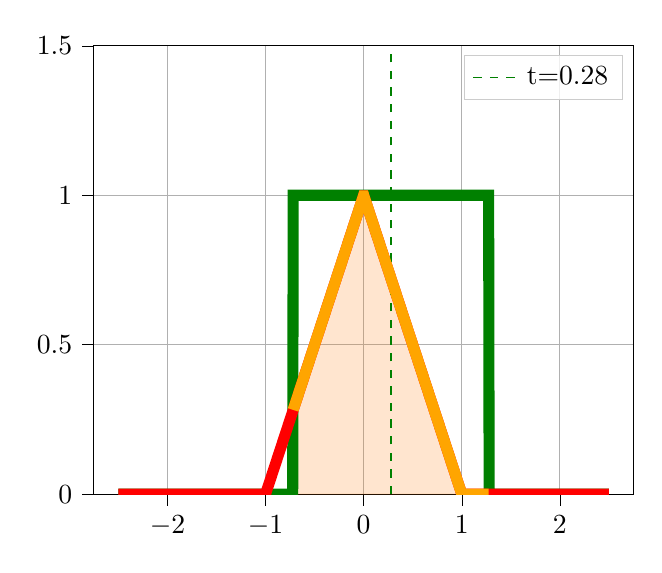
\begin{tikzpicture}

\definecolor{color0}{rgb}{1,0.498039215686275,0.0549019607843137}
\definecolor{color1}{rgb}{1,0.647058823529412,0}

\begin{axis}[
legend cell align={left},
legend style={fill opacity=0.8, draw opacity=1, text opacity=1, draw=white!80!black},
tick align=outside,
tick pos=left,
x grid style={white!69.0196078431373!black},
xmajorgrids,
xmin=-2.75, xmax=2.75,
xtick style={color=black},
y grid style={white!69.0196078431373!black},
ymajorgrids,
ymin=0, ymax=1.5,
ytick style={color=black}
]
\path [draw=color0, fill=color0, opacity=0.2]
(axis cs:-0.718218218218218,0.281781781781782)
--(axis cs:-0.718218218218218,0)
--(axis cs:-0.713213213213213,0)
--(axis cs:-0.708208208208208,0)
--(axis cs:-0.703203203203203,0)
--(axis cs:-0.698198198198198,0)
--(axis cs:-0.693193193193193,0)
--(axis cs:-0.688188188188188,0)
--(axis cs:-0.683183183183183,0)
--(axis cs:-0.678178178178178,0)
--(axis cs:-0.673173173173173,0)
--(axis cs:-0.668168168168168,0)
--(axis cs:-0.663163163163163,0)
--(axis cs:-0.658158158158158,0)
--(axis cs:-0.653153153153153,0)
--(axis cs:-0.648148148148148,0)
--(axis cs:-0.643143143143143,0)
--(axis cs:-0.638138138138138,0)
--(axis cs:-0.633133133133133,0)
--(axis cs:-0.628128128128128,0)
--(axis cs:-0.623123123123123,0)
--(axis cs:-0.618118118118118,0)
--(axis cs:-0.613113113113113,0)
--(axis cs:-0.608108108108108,0)
--(axis cs:-0.603103103103103,0)
--(axis cs:-0.598098098098098,0)
--(axis cs:-0.593093093093093,0)
--(axis cs:-0.588088088088088,0)
--(axis cs:-0.583083083083083,0)
--(axis cs:-0.578078078078078,0)
--(axis cs:-0.573073073073073,0)
--(axis cs:-0.568068068068068,0)
--(axis cs:-0.563063063063063,0)
--(axis cs:-0.558058058058058,0)
--(axis cs:-0.553053053053053,0)
--(axis cs:-0.548048048048048,0)
--(axis cs:-0.543043043043043,0)
--(axis cs:-0.538038038038038,0)
--(axis cs:-0.533033033033033,0)
--(axis cs:-0.528028028028028,0)
--(axis cs:-0.523023023023023,0)
--(axis cs:-0.518018018018018,0)
--(axis cs:-0.513013013013013,0)
--(axis cs:-0.508008008008008,0)
--(axis cs:-0.503003003003003,0)
--(axis cs:-0.497997997997998,0)
--(axis cs:-0.492992992992993,0)
--(axis cs:-0.487987987987988,0)
--(axis cs:-0.482982982982983,0)
--(axis cs:-0.477977977977978,0)
--(axis cs:-0.472972972972973,0)
--(axis cs:-0.467967967967968,0)
--(axis cs:-0.462962962962963,0)
--(axis cs:-0.457957957957958,0)
--(axis cs:-0.452952952952953,0)
--(axis cs:-0.447947947947948,0)
--(axis cs:-0.442942942942943,0)
--(axis cs:-0.437937937937938,0)
--(axis cs:-0.432932932932933,0)
--(axis cs:-0.427927927927928,0)
--(axis cs:-0.422922922922923,0)
--(axis cs:-0.417917917917918,0)
--(axis cs:-0.412912912912913,0)
--(axis cs:-0.407907907907908,0)
--(axis cs:-0.402902902902903,0)
--(axis cs:-0.397897897897898,0)
--(axis cs:-0.392892892892893,0)
--(axis cs:-0.387887887887888,0)
--(axis cs:-0.382882882882883,0)
--(axis cs:-0.377877877877878,0)
--(axis cs:-0.372872872872873,0)
--(axis cs:-0.367867867867868,0)
--(axis cs:-0.362862862862863,0)
--(axis cs:-0.357857857857858,0)
--(axis cs:-0.352852852852853,0)
--(axis cs:-0.347847847847848,0)
--(axis cs:-0.342842842842843,0)
--(axis cs:-0.337837837837838,0)
--(axis cs:-0.332832832832833,0)
--(axis cs:-0.327827827827828,0)
--(axis cs:-0.322822822822823,0)
--(axis cs:-0.317817817817818,0)
--(axis cs:-0.312812812812813,0)
--(axis cs:-0.307807807807808,0)
--(axis cs:-0.302802802802803,0)
--(axis cs:-0.297797797797798,0)
--(axis cs:-0.292792792792793,0)
--(axis cs:-0.287787787787788,0)
--(axis cs:-0.282782782782783,0)
--(axis cs:-0.277777777777778,0)
--(axis cs:-0.272772772772773,0)
--(axis cs:-0.267767767767768,0)
--(axis cs:-0.262762762762763,0)
--(axis cs:-0.257757757757758,0)
--(axis cs:-0.252752752752753,0)
--(axis cs:-0.247747747747748,0)
--(axis cs:-0.242742742742743,0)
--(axis cs:-0.237737737737738,0)
--(axis cs:-0.232732732732733,0)
--(axis cs:-0.227727727727728,0)
--(axis cs:-0.222722722722723,0)
--(axis cs:-0.217717717717718,0)
--(axis cs:-0.212712712712713,0)
--(axis cs:-0.207707707707708,0)
--(axis cs:-0.202702702702703,0)
--(axis cs:-0.197697697697698,0)
--(axis cs:-0.192692692692693,0)
--(axis cs:-0.187687687687688,0)
--(axis cs:-0.182682682682683,0)
--(axis cs:-0.177677677677678,0)
--(axis cs:-0.172672672672673,0)
--(axis cs:-0.167667667667668,0)
--(axis cs:-0.162662662662663,0)
--(axis cs:-0.157657657657658,0)
--(axis cs:-0.152652652652653,0)
--(axis cs:-0.147647647647648,0)
--(axis cs:-0.142642642642643,0)
--(axis cs:-0.137637637637638,0)
--(axis cs:-0.132632632632633,0)
--(axis cs:-0.127627627627628,0)
--(axis cs:-0.122622622622623,0)
--(axis cs:-0.117617617617618,0)
--(axis cs:-0.112612612612613,0)
--(axis cs:-0.107607607607608,0)
--(axis cs:-0.102602602602603,0)
--(axis cs:-0.0975975975975976,0)
--(axis cs:-0.0925925925925926,0)
--(axis cs:-0.0875875875875876,0)
--(axis cs:-0.0825825825825826,0)
--(axis cs:-0.0775775775775776,0)
--(axis cs:-0.0725725725725725,0)
--(axis cs:-0.0675675675675675,0)
--(axis cs:-0.0625625625625625,0)
--(axis cs:-0.0575575575575575,0)
--(axis cs:-0.0525525525525525,0)
--(axis cs:-0.0475475475475475,0)
--(axis cs:-0.0425425425425425,0)
--(axis cs:-0.0375375375375375,0)
--(axis cs:-0.0325325325325325,0)
--(axis cs:-0.0275275275275275,0)
--(axis cs:-0.0225225225225225,0)
--(axis cs:-0.0175175175175175,0)
--(axis cs:-0.0125125125125125,0)
--(axis cs:-0.0075075075075075,0)
--(axis cs:-0.0025025025025025,0)
--(axis cs:0.0025025025025025,0)
--(axis cs:0.0075075075075075,0)
--(axis cs:0.0125125125125125,0)
--(axis cs:0.0175175175175175,0)
--(axis cs:0.0225225225225225,0)
--(axis cs:0.0275275275275275,0)
--(axis cs:0.0325325325325325,0)
--(axis cs:0.0375375375375375,0)
--(axis cs:0.0425425425425425,0)
--(axis cs:0.0475475475475475,0)
--(axis cs:0.0525525525525525,0)
--(axis cs:0.0575575575575575,0)
--(axis cs:0.0625625625625625,0)
--(axis cs:0.0675675675675675,0)
--(axis cs:0.0725725725725725,0)
--(axis cs:0.0775775775775776,0)
--(axis cs:0.0825825825825826,0)
--(axis cs:0.0875875875875876,0)
--(axis cs:0.0925925925925926,0)
--(axis cs:0.0975975975975976,0)
--(axis cs:0.102602602602603,0)
--(axis cs:0.107607607607608,0)
--(axis cs:0.112612612612613,0)
--(axis cs:0.117617617617618,0)
--(axis cs:0.122622622622623,0)
--(axis cs:0.127627627627628,0)
--(axis cs:0.132632632632633,0)
--(axis cs:0.137637637637638,0)
--(axis cs:0.142642642642643,0)
--(axis cs:0.147647647647648,0)
--(axis cs:0.152652652652653,0)
--(axis cs:0.157657657657658,0)
--(axis cs:0.162662662662663,0)
--(axis cs:0.167667667667668,0)
--(axis cs:0.172672672672673,0)
--(axis cs:0.177677677677678,0)
--(axis cs:0.182682682682683,0)
--(axis cs:0.187687687687688,0)
--(axis cs:0.192692692692693,0)
--(axis cs:0.197697697697698,0)
--(axis cs:0.202702702702703,0)
--(axis cs:0.207707707707708,0)
--(axis cs:0.212712712712713,0)
--(axis cs:0.217717717717718,0)
--(axis cs:0.222722722722723,0)
--(axis cs:0.227727727727728,0)
--(axis cs:0.232732732732733,0)
--(axis cs:0.237737737737738,0)
--(axis cs:0.242742742742743,0)
--(axis cs:0.247747747747748,0)
--(axis cs:0.252752752752753,0)
--(axis cs:0.257757757757758,0)
--(axis cs:0.262762762762763,0)
--(axis cs:0.267767767767768,0)
--(axis cs:0.272772772772773,0)
--(axis cs:0.277777777777778,0)
--(axis cs:0.282782782782783,0)
--(axis cs:0.287787787787788,0)
--(axis cs:0.292792792792793,0)
--(axis cs:0.297797797797798,0)
--(axis cs:0.302802802802803,0)
--(axis cs:0.307807807807808,0)
--(axis cs:0.312812812812813,0)
--(axis cs:0.317817817817818,0)
--(axis cs:0.322822822822823,0)
--(axis cs:0.327827827827828,0)
--(axis cs:0.332832832832833,0)
--(axis cs:0.337837837837838,0)
--(axis cs:0.342842842842843,0)
--(axis cs:0.347847847847848,0)
--(axis cs:0.352852852852853,0)
--(axis cs:0.357857857857858,0)
--(axis cs:0.362862862862863,0)
--(axis cs:0.367867867867868,0)
--(axis cs:0.372872872872873,0)
--(axis cs:0.377877877877878,0)
--(axis cs:0.382882882882883,0)
--(axis cs:0.387887887887888,0)
--(axis cs:0.392892892892893,0)
--(axis cs:0.397897897897898,0)
--(axis cs:0.402902902902903,0)
--(axis cs:0.407907907907908,0)
--(axis cs:0.412912912912913,0)
--(axis cs:0.417917917917918,0)
--(axis cs:0.422922922922923,0)
--(axis cs:0.427927927927928,0)
--(axis cs:0.432932932932933,0)
--(axis cs:0.437937937937938,0)
--(axis cs:0.442942942942943,0)
--(axis cs:0.447947947947948,0)
--(axis cs:0.452952952952953,0)
--(axis cs:0.457957957957958,0)
--(axis cs:0.462962962962963,0)
--(axis cs:0.467967967967968,0)
--(axis cs:0.472972972972973,0)
--(axis cs:0.477977977977978,0)
--(axis cs:0.482982982982983,0)
--(axis cs:0.487987987987988,0)
--(axis cs:0.492992992992993,0)
--(axis cs:0.497997997997998,0)
--(axis cs:0.503003003003003,0)
--(axis cs:0.508008008008008,0)
--(axis cs:0.513013013013013,0)
--(axis cs:0.518018018018018,0)
--(axis cs:0.523023023023023,0)
--(axis cs:0.528028028028028,0)
--(axis cs:0.533033033033033,0)
--(axis cs:0.538038038038038,0)
--(axis cs:0.543043043043043,0)
--(axis cs:0.548048048048048,0)
--(axis cs:0.553053053053053,0)
--(axis cs:0.558058058058058,0)
--(axis cs:0.563063063063063,0)
--(axis cs:0.568068068068068,0)
--(axis cs:0.573073073073073,0)
--(axis cs:0.578078078078078,0)
--(axis cs:0.583083083083083,0)
--(axis cs:0.588088088088088,0)
--(axis cs:0.593093093093093,0)
--(axis cs:0.598098098098098,0)
--(axis cs:0.603103103103103,0)
--(axis cs:0.608108108108108,0)
--(axis cs:0.613113113113113,0)
--(axis cs:0.618118118118118,0)
--(axis cs:0.623123123123123,0)
--(axis cs:0.628128128128128,0)
--(axis cs:0.633133133133133,0)
--(axis cs:0.638138138138138,0)
--(axis cs:0.643143143143143,0)
--(axis cs:0.648148148148148,0)
--(axis cs:0.653153153153153,0)
--(axis cs:0.658158158158158,0)
--(axis cs:0.663163163163163,0)
--(axis cs:0.668168168168168,0)
--(axis cs:0.673173173173173,0)
--(axis cs:0.678178178178178,0)
--(axis cs:0.683183183183183,0)
--(axis cs:0.688188188188188,0)
--(axis cs:0.693193193193193,0)
--(axis cs:0.698198198198198,0)
--(axis cs:0.703203203203203,0)
--(axis cs:0.708208208208208,0)
--(axis cs:0.713213213213213,0)
--(axis cs:0.718218218218218,0)
--(axis cs:0.723223223223223,0)
--(axis cs:0.728228228228228,0)
--(axis cs:0.733233233233233,0)
--(axis cs:0.738238238238238,0)
--(axis cs:0.743243243243243,0)
--(axis cs:0.748248248248248,0)
--(axis cs:0.753253253253253,0)
--(axis cs:0.758258258258258,0)
--(axis cs:0.763263263263263,0)
--(axis cs:0.768268268268268,0)
--(axis cs:0.773273273273273,0)
--(axis cs:0.778278278278278,0)
--(axis cs:0.783283283283283,0)
--(axis cs:0.788288288288288,0)
--(axis cs:0.793293293293293,0)
--(axis cs:0.798298298298298,0)
--(axis cs:0.803303303303303,0)
--(axis cs:0.808308308308308,0)
--(axis cs:0.813313313313313,0)
--(axis cs:0.818318318318318,0)
--(axis cs:0.823323323323323,0)
--(axis cs:0.828328328328328,0)
--(axis cs:0.833333333333333,0)
--(axis cs:0.838338338338338,0)
--(axis cs:0.843343343343343,0)
--(axis cs:0.848348348348348,0)
--(axis cs:0.853353353353353,0)
--(axis cs:0.858358358358358,0)
--(axis cs:0.863363363363364,0)
--(axis cs:0.868368368368369,0)
--(axis cs:0.873373373373374,0)
--(axis cs:0.878378378378379,0)
--(axis cs:0.883383383383384,0)
--(axis cs:0.888388388388389,0)
--(axis cs:0.893393393393394,0)
--(axis cs:0.898398398398399,0)
--(axis cs:0.903403403403404,0)
--(axis cs:0.908408408408409,0)
--(axis cs:0.913413413413414,0)
--(axis cs:0.918418418418419,0)
--(axis cs:0.923423423423424,0)
--(axis cs:0.928428428428429,0)
--(axis cs:0.933433433433434,0)
--(axis cs:0.938438438438439,0)
--(axis cs:0.943443443443444,0)
--(axis cs:0.948448448448449,0)
--(axis cs:0.953453453453454,0)
--(axis cs:0.958458458458459,0)
--(axis cs:0.963463463463464,0)
--(axis cs:0.968468468468469,0)
--(axis cs:0.973473473473474,0)
--(axis cs:0.978478478478479,0)
--(axis cs:0.983483483483484,0)
--(axis cs:0.988488488488489,0)
--(axis cs:0.993493493493494,0)
--(axis cs:0.998498498498499,0)
--(axis cs:1.0035035035035,0)
--(axis cs:1.00850850850851,0)
--(axis cs:1.01351351351351,0)
--(axis cs:1.01851851851852,0)
--(axis cs:1.02352352352352,0)
--(axis cs:1.02852852852853,0)
--(axis cs:1.03353353353353,0)
--(axis cs:1.03853853853854,0)
--(axis cs:1.04354354354354,0)
--(axis cs:1.04854854854855,0)
--(axis cs:1.05355355355355,0)
--(axis cs:1.05855855855856,0)
--(axis cs:1.06356356356356,0)
--(axis cs:1.06856856856857,0)
--(axis cs:1.07357357357357,0)
--(axis cs:1.07857857857858,0)
--(axis cs:1.08358358358358,0)
--(axis cs:1.08858858858859,0)
--(axis cs:1.09359359359359,0)
--(axis cs:1.0985985985986,0)
--(axis cs:1.1036036036036,0)
--(axis cs:1.10860860860861,0)
--(axis cs:1.11361361361361,0)
--(axis cs:1.11861861861862,0)
--(axis cs:1.12362362362362,0)
--(axis cs:1.12862862862863,0)
--(axis cs:1.13363363363363,0)
--(axis cs:1.13863863863864,0)
--(axis cs:1.14364364364364,0)
--(axis cs:1.14864864864865,0)
--(axis cs:1.15365365365365,0)
--(axis cs:1.15865865865866,0)
--(axis cs:1.16366366366366,0)
--(axis cs:1.16866866866867,0)
--(axis cs:1.17367367367367,0)
--(axis cs:1.17867867867868,0)
--(axis cs:1.18368368368368,0)
--(axis cs:1.18868868868869,0)
--(axis cs:1.19369369369369,0)
--(axis cs:1.1986986986987,0)
--(axis cs:1.2037037037037,0)
--(axis cs:1.20870870870871,0)
--(axis cs:1.21371371371371,0)
--(axis cs:1.21871871871872,0)
--(axis cs:1.22372372372372,0)
--(axis cs:1.22872872872873,0)
--(axis cs:1.23373373373373,0)
--(axis cs:1.23873873873874,0)
--(axis cs:1.24374374374374,0)
--(axis cs:1.24874874874875,0)
--(axis cs:1.25375375375375,0)
--(axis cs:1.25875875875876,0)
--(axis cs:1.26376376376376,0)
--(axis cs:1.26876876876877,0)
--(axis cs:1.27377377377377,0)
--(axis cs:1.27377377377377,0)
--(axis cs:1.27377377377377,0)
--(axis cs:1.26876876876877,0)
--(axis cs:1.26376376376376,0)
--(axis cs:1.25875875875876,0)
--(axis cs:1.25375375375375,0)
--(axis cs:1.24874874874875,0)
--(axis cs:1.24374374374374,0)
--(axis cs:1.23873873873874,0)
--(axis cs:1.23373373373373,0)
--(axis cs:1.22872872872873,0)
--(axis cs:1.22372372372372,0)
--(axis cs:1.21871871871872,0)
--(axis cs:1.21371371371371,0)
--(axis cs:1.20870870870871,0)
--(axis cs:1.2037037037037,0)
--(axis cs:1.1986986986987,0)
--(axis cs:1.19369369369369,0)
--(axis cs:1.18868868868869,0)
--(axis cs:1.18368368368368,0)
--(axis cs:1.17867867867868,0)
--(axis cs:1.17367367367367,0)
--(axis cs:1.16866866866867,0)
--(axis cs:1.16366366366366,0)
--(axis cs:1.15865865865866,0)
--(axis cs:1.15365365365365,0)
--(axis cs:1.14864864864865,0)
--(axis cs:1.14364364364364,0)
--(axis cs:1.13863863863864,0)
--(axis cs:1.13363363363363,0)
--(axis cs:1.12862862862863,0)
--(axis cs:1.12362362362362,0)
--(axis cs:1.11861861861862,0)
--(axis cs:1.11361361361361,0)
--(axis cs:1.10860860860861,0)
--(axis cs:1.1036036036036,0)
--(axis cs:1.0985985985986,0)
--(axis cs:1.09359359359359,0)
--(axis cs:1.08858858858859,0)
--(axis cs:1.08358358358358,0)
--(axis cs:1.07857857857858,0)
--(axis cs:1.07357357357357,0)
--(axis cs:1.06856856856857,0)
--(axis cs:1.06356356356356,0)
--(axis cs:1.05855855855856,0)
--(axis cs:1.05355355355355,0)
--(axis cs:1.04854854854855,0)
--(axis cs:1.04354354354354,0)
--(axis cs:1.03853853853854,0)
--(axis cs:1.03353353353353,0)
--(axis cs:1.02852852852853,0)
--(axis cs:1.02352352352352,0)
--(axis cs:1.01851851851852,0)
--(axis cs:1.01351351351351,0)
--(axis cs:1.00850850850851,0)
--(axis cs:1.0035035035035,0)
--(axis cs:0.998498498498499,0.00150150150150141)
--(axis cs:0.993493493493494,0.00650650650650642)
--(axis cs:0.988488488488489,0.0115115115115114)
--(axis cs:0.983483483483484,0.0165165165165164)
--(axis cs:0.978478478478479,0.0215215215215214)
--(axis cs:0.973473473473474,0.0265265265265264)
--(axis cs:0.968468468468469,0.0315315315315314)
--(axis cs:0.963463463463464,0.0365365365365364)
--(axis cs:0.958458458458459,0.0415415415415414)
--(axis cs:0.953453453453454,0.0465465465465464)
--(axis cs:0.948448448448449,0.0515515515515514)
--(axis cs:0.943443443443444,0.0565565565565564)
--(axis cs:0.938438438438439,0.0615615615615615)
--(axis cs:0.933433433433434,0.0665665665665665)
--(axis cs:0.928428428428429,0.0715715715715715)
--(axis cs:0.923423423423424,0.0765765765765765)
--(axis cs:0.918418418418419,0.0815815815815815)
--(axis cs:0.913413413413414,0.0865865865865865)
--(axis cs:0.908408408408409,0.0915915915915915)
--(axis cs:0.903403403403404,0.0965965965965965)
--(axis cs:0.898398398398399,0.101601601601601)
--(axis cs:0.893393393393394,0.106606606606606)
--(axis cs:0.888388388388389,0.111611611611611)
--(axis cs:0.883383383383384,0.116616616616616)
--(axis cs:0.878378378378379,0.121621621621621)
--(axis cs:0.873373373373374,0.126626626626626)
--(axis cs:0.868368368368369,0.131631631631631)
--(axis cs:0.863363363363364,0.136636636636636)
--(axis cs:0.858358358358358,0.141641641641642)
--(axis cs:0.853353353353353,0.146646646646647)
--(axis cs:0.848348348348348,0.151651651651652)
--(axis cs:0.843343343343343,0.156656656656657)
--(axis cs:0.838338338338338,0.161661661661662)
--(axis cs:0.833333333333333,0.166666666666667)
--(axis cs:0.828328328328328,0.171671671671672)
--(axis cs:0.823323323323323,0.176676676676677)
--(axis cs:0.818318318318318,0.181681681681682)
--(axis cs:0.813313313313313,0.186686686686687)
--(axis cs:0.808308308308308,0.191691691691692)
--(axis cs:0.803303303303303,0.196696696696697)
--(axis cs:0.798298298298298,0.201701701701702)
--(axis cs:0.793293293293293,0.206706706706707)
--(axis cs:0.788288288288288,0.211711711711712)
--(axis cs:0.783283283283283,0.216716716716717)
--(axis cs:0.778278278278278,0.221721721721722)
--(axis cs:0.773273273273273,0.226726726726727)
--(axis cs:0.768268268268268,0.231731731731732)
--(axis cs:0.763263263263263,0.236736736736737)
--(axis cs:0.758258258258258,0.241741741741742)
--(axis cs:0.753253253253253,0.246746746746747)
--(axis cs:0.748248248248248,0.251751751751752)
--(axis cs:0.743243243243243,0.256756756756757)
--(axis cs:0.738238238238238,0.261761761761762)
--(axis cs:0.733233233233233,0.266766766766767)
--(axis cs:0.728228228228228,0.271771771771772)
--(axis cs:0.723223223223223,0.276776776776777)
--(axis cs:0.718218218218218,0.281781781781782)
--(axis cs:0.713213213213213,0.286786786786787)
--(axis cs:0.708208208208208,0.291791791791792)
--(axis cs:0.703203203203203,0.296796796796797)
--(axis cs:0.698198198198198,0.301801801801802)
--(axis cs:0.693193193193193,0.306806806806807)
--(axis cs:0.688188188188188,0.311811811811812)
--(axis cs:0.683183183183183,0.316816816816817)
--(axis cs:0.678178178178178,0.321821821821822)
--(axis cs:0.673173173173173,0.326826826826827)
--(axis cs:0.668168168168168,0.331831831831832)
--(axis cs:0.663163163163163,0.336836836836837)
--(axis cs:0.658158158158158,0.341841841841842)
--(axis cs:0.653153153153153,0.346846846846847)
--(axis cs:0.648148148148148,0.351851851851852)
--(axis cs:0.643143143143143,0.356856856856857)
--(axis cs:0.638138138138138,0.361861861861862)
--(axis cs:0.633133133133133,0.366866866866867)
--(axis cs:0.628128128128128,0.371871871871872)
--(axis cs:0.623123123123123,0.376876876876877)
--(axis cs:0.618118118118118,0.381881881881882)
--(axis cs:0.613113113113113,0.386886886886887)
--(axis cs:0.608108108108108,0.391891891891892)
--(axis cs:0.603103103103103,0.396896896896897)
--(axis cs:0.598098098098098,0.401901901901902)
--(axis cs:0.593093093093093,0.406906906906907)
--(axis cs:0.588088088088088,0.411911911911912)
--(axis cs:0.583083083083083,0.416916916916917)
--(axis cs:0.578078078078078,0.421921921921922)
--(axis cs:0.573073073073073,0.426926926926927)
--(axis cs:0.568068068068068,0.431931931931932)
--(axis cs:0.563063063063063,0.436936936936937)
--(axis cs:0.558058058058058,0.441941941941942)
--(axis cs:0.553053053053053,0.446946946946947)
--(axis cs:0.548048048048048,0.451951951951952)
--(axis cs:0.543043043043043,0.456956956956957)
--(axis cs:0.538038038038038,0.461961961961962)
--(axis cs:0.533033033033033,0.466966966966967)
--(axis cs:0.528028028028028,0.471971971971972)
--(axis cs:0.523023023023023,0.476976976976977)
--(axis cs:0.518018018018018,0.481981981981982)
--(axis cs:0.513013013013013,0.486986986986987)
--(axis cs:0.508008008008008,0.491991991991992)
--(axis cs:0.503003003003003,0.496996996996997)
--(axis cs:0.497997997997998,0.502002002002002)
--(axis cs:0.492992992992993,0.507007007007007)
--(axis cs:0.487987987987988,0.512012012012012)
--(axis cs:0.482982982982983,0.517017017017017)
--(axis cs:0.477977977977978,0.522022022022022)
--(axis cs:0.472972972972973,0.527027027027027)
--(axis cs:0.467967967967968,0.532032032032032)
--(axis cs:0.462962962962963,0.537037037037037)
--(axis cs:0.457957957957958,0.542042042042042)
--(axis cs:0.452952952952953,0.547047047047047)
--(axis cs:0.447947947947948,0.552052052052052)
--(axis cs:0.442942942942943,0.557057057057057)
--(axis cs:0.437937937937938,0.562062062062062)
--(axis cs:0.432932932932933,0.567067067067067)
--(axis cs:0.427927927927928,0.572072072072072)
--(axis cs:0.422922922922923,0.577077077077077)
--(axis cs:0.417917917917918,0.582082082082082)
--(axis cs:0.412912912912913,0.587087087087087)
--(axis cs:0.407907907907908,0.592092092092092)
--(axis cs:0.402902902902903,0.597097097097097)
--(axis cs:0.397897897897898,0.602102102102102)
--(axis cs:0.392892892892893,0.607107107107107)
--(axis cs:0.387887887887888,0.612112112112112)
--(axis cs:0.382882882882883,0.617117117117117)
--(axis cs:0.377877877877878,0.622122122122122)
--(axis cs:0.372872872872873,0.627127127127127)
--(axis cs:0.367867867867868,0.632132132132132)
--(axis cs:0.362862862862863,0.637137137137137)
--(axis cs:0.357857857857858,0.642142142142142)
--(axis cs:0.352852852852853,0.647147147147147)
--(axis cs:0.347847847847848,0.652152152152152)
--(axis cs:0.342842842842843,0.657157157157157)
--(axis cs:0.337837837837838,0.662162162162162)
--(axis cs:0.332832832832833,0.667167167167167)
--(axis cs:0.327827827827828,0.672172172172172)
--(axis cs:0.322822822822823,0.677177177177177)
--(axis cs:0.317817817817818,0.682182182182182)
--(axis cs:0.312812812812813,0.687187187187187)
--(axis cs:0.307807807807808,0.692192192192192)
--(axis cs:0.302802802802803,0.697197197197197)
--(axis cs:0.297797797797798,0.702202202202202)
--(axis cs:0.292792792792793,0.707207207207207)
--(axis cs:0.287787787787788,0.712212212212212)
--(axis cs:0.282782782782783,0.717217217217217)
--(axis cs:0.277777777777778,0.722222222222222)
--(axis cs:0.272772772772773,0.727227227227227)
--(axis cs:0.267767767767768,0.732232232232232)
--(axis cs:0.262762762762763,0.737237237237237)
--(axis cs:0.257757757757758,0.742242242242242)
--(axis cs:0.252752752752753,0.747247247247247)
--(axis cs:0.247747747747748,0.752252252252252)
--(axis cs:0.242742742742743,0.757257257257257)
--(axis cs:0.237737737737738,0.762262262262262)
--(axis cs:0.232732732732733,0.767267267267267)
--(axis cs:0.227727727727728,0.772272272272272)
--(axis cs:0.222722722722723,0.777277277277277)
--(axis cs:0.217717717717718,0.782282282282282)
--(axis cs:0.212712712712713,0.787287287287287)
--(axis cs:0.207707707707708,0.792292292292292)
--(axis cs:0.202702702702703,0.797297297297297)
--(axis cs:0.197697697697698,0.802302302302302)
--(axis cs:0.192692692692693,0.807307307307307)
--(axis cs:0.187687687687688,0.812312312312312)
--(axis cs:0.182682682682683,0.817317317317317)
--(axis cs:0.177677677677678,0.822322322322322)
--(axis cs:0.172672672672673,0.827327327327327)
--(axis cs:0.167667667667668,0.832332332332332)
--(axis cs:0.162662662662663,0.837337337337337)
--(axis cs:0.157657657657658,0.842342342342342)
--(axis cs:0.152652652652653,0.847347347347347)
--(axis cs:0.147647647647648,0.852352352352352)
--(axis cs:0.142642642642643,0.857357357357357)
--(axis cs:0.137637637637638,0.862362362362362)
--(axis cs:0.132632632632633,0.867367367367367)
--(axis cs:0.127627627627628,0.872372372372372)
--(axis cs:0.122622622622623,0.877377377377377)
--(axis cs:0.117617617617618,0.882382382382382)
--(axis cs:0.112612612612613,0.887387387387387)
--(axis cs:0.107607607607608,0.892392392392392)
--(axis cs:0.102602602602603,0.897397397397397)
--(axis cs:0.0975975975975976,0.902402402402402)
--(axis cs:0.0925925925925926,0.907407407407407)
--(axis cs:0.0875875875875876,0.912412412412412)
--(axis cs:0.0825825825825826,0.917417417417417)
--(axis cs:0.0775775775775776,0.922422422422422)
--(axis cs:0.0725725725725725,0.927427427427427)
--(axis cs:0.0675675675675675,0.932432432432432)
--(axis cs:0.0625625625625625,0.937437437437437)
--(axis cs:0.0575575575575575,0.942442442442442)
--(axis cs:0.0525525525525525,0.947447447447447)
--(axis cs:0.0475475475475475,0.952452452452452)
--(axis cs:0.0425425425425425,0.957457457457457)
--(axis cs:0.0375375375375375,0.962462462462462)
--(axis cs:0.0325325325325325,0.967467467467467)
--(axis cs:0.0275275275275275,0.972472472472472)
--(axis cs:0.0225225225225225,0.977477477477477)
--(axis cs:0.0175175175175175,0.982482482482482)
--(axis cs:0.0125125125125125,0.987487487487487)
--(axis cs:0.0075075075075075,0.992492492492492)
--(axis cs:0.0025025025025025,0.997497497497497)
--(axis cs:-0.0025025025025025,0.997497497497497)
--(axis cs:-0.0075075075075075,0.992492492492492)
--(axis cs:-0.0125125125125125,0.987487487487487)
--(axis cs:-0.0175175175175175,0.982482482482482)
--(axis cs:-0.0225225225225225,0.977477477477477)
--(axis cs:-0.0275275275275275,0.972472472472472)
--(axis cs:-0.0325325325325325,0.967467467467467)
--(axis cs:-0.0375375375375375,0.962462462462462)
--(axis cs:-0.0425425425425425,0.957457457457457)
--(axis cs:-0.0475475475475475,0.952452452452452)
--(axis cs:-0.0525525525525525,0.947447447447447)
--(axis cs:-0.0575575575575575,0.942442442442442)
--(axis cs:-0.0625625625625625,0.937437437437437)
--(axis cs:-0.0675675675675675,0.932432432432432)
--(axis cs:-0.0725725725725725,0.927427427427427)
--(axis cs:-0.0775775775775776,0.922422422422422)
--(axis cs:-0.0825825825825826,0.917417417417417)
--(axis cs:-0.0875875875875876,0.912412412412412)
--(axis cs:-0.0925925925925926,0.907407407407407)
--(axis cs:-0.0975975975975976,0.902402402402402)
--(axis cs:-0.102602602602603,0.897397397397397)
--(axis cs:-0.107607607607608,0.892392392392392)
--(axis cs:-0.112612612612613,0.887387387387387)
--(axis cs:-0.117617617617618,0.882382382382382)
--(axis cs:-0.122622622622623,0.877377377377377)
--(axis cs:-0.127627627627628,0.872372372372372)
--(axis cs:-0.132632632632633,0.867367367367367)
--(axis cs:-0.137637637637638,0.862362362362362)
--(axis cs:-0.142642642642643,0.857357357357357)
--(axis cs:-0.147647647647648,0.852352352352352)
--(axis cs:-0.152652652652653,0.847347347347347)
--(axis cs:-0.157657657657658,0.842342342342342)
--(axis cs:-0.162662662662663,0.837337337337337)
--(axis cs:-0.167667667667668,0.832332332332332)
--(axis cs:-0.172672672672673,0.827327327327327)
--(axis cs:-0.177677677677678,0.822322322322322)
--(axis cs:-0.182682682682683,0.817317317317317)
--(axis cs:-0.187687687687688,0.812312312312312)
--(axis cs:-0.192692692692693,0.807307307307307)
--(axis cs:-0.197697697697698,0.802302302302302)
--(axis cs:-0.202702702702703,0.797297297297297)
--(axis cs:-0.207707707707708,0.792292292292292)
--(axis cs:-0.212712712712713,0.787287287287287)
--(axis cs:-0.217717717717718,0.782282282282282)
--(axis cs:-0.222722722722723,0.777277277277277)
--(axis cs:-0.227727727727728,0.772272272272272)
--(axis cs:-0.232732732732733,0.767267267267267)
--(axis cs:-0.237737737737738,0.762262262262262)
--(axis cs:-0.242742742742743,0.757257257257257)
--(axis cs:-0.247747747747748,0.752252252252252)
--(axis cs:-0.252752752752753,0.747247247247247)
--(axis cs:-0.257757757757758,0.742242242242242)
--(axis cs:-0.262762762762763,0.737237237237237)
--(axis cs:-0.267767767767768,0.732232232232232)
--(axis cs:-0.272772772772773,0.727227227227227)
--(axis cs:-0.277777777777778,0.722222222222222)
--(axis cs:-0.282782782782783,0.717217217217217)
--(axis cs:-0.287787787787788,0.712212212212212)
--(axis cs:-0.292792792792793,0.707207207207207)
--(axis cs:-0.297797797797798,0.702202202202202)
--(axis cs:-0.302802802802803,0.697197197197197)
--(axis cs:-0.307807807807808,0.692192192192192)
--(axis cs:-0.312812812812813,0.687187187187187)
--(axis cs:-0.317817817817818,0.682182182182182)
--(axis cs:-0.322822822822823,0.677177177177177)
--(axis cs:-0.327827827827828,0.672172172172172)
--(axis cs:-0.332832832832833,0.667167167167167)
--(axis cs:-0.337837837837838,0.662162162162162)
--(axis cs:-0.342842842842843,0.657157157157157)
--(axis cs:-0.347847847847848,0.652152152152152)
--(axis cs:-0.352852852852853,0.647147147147147)
--(axis cs:-0.357857857857858,0.642142142142142)
--(axis cs:-0.362862862862863,0.637137137137137)
--(axis cs:-0.367867867867868,0.632132132132132)
--(axis cs:-0.372872872872873,0.627127127127127)
--(axis cs:-0.377877877877878,0.622122122122122)
--(axis cs:-0.382882882882883,0.617117117117117)
--(axis cs:-0.387887887887888,0.612112112112112)
--(axis cs:-0.392892892892893,0.607107107107107)
--(axis cs:-0.397897897897898,0.602102102102102)
--(axis cs:-0.402902902902903,0.597097097097097)
--(axis cs:-0.407907907907908,0.592092092092092)
--(axis cs:-0.412912912912913,0.587087087087087)
--(axis cs:-0.417917917917918,0.582082082082082)
--(axis cs:-0.422922922922923,0.577077077077077)
--(axis cs:-0.427927927927928,0.572072072072072)
--(axis cs:-0.432932932932933,0.567067067067067)
--(axis cs:-0.437937937937938,0.562062062062062)
--(axis cs:-0.442942942942943,0.557057057057057)
--(axis cs:-0.447947947947948,0.552052052052052)
--(axis cs:-0.452952952952953,0.547047047047047)
--(axis cs:-0.457957957957958,0.542042042042042)
--(axis cs:-0.462962962962963,0.537037037037037)
--(axis cs:-0.467967967967968,0.532032032032032)
--(axis cs:-0.472972972972973,0.527027027027027)
--(axis cs:-0.477977977977978,0.522022022022022)
--(axis cs:-0.482982982982983,0.517017017017017)
--(axis cs:-0.487987987987988,0.512012012012012)
--(axis cs:-0.492992992992993,0.507007007007007)
--(axis cs:-0.497997997997998,0.502002002002002)
--(axis cs:-0.503003003003003,0.496996996996997)
--(axis cs:-0.508008008008008,0.491991991991992)
--(axis cs:-0.513013013013013,0.486986986986987)
--(axis cs:-0.518018018018018,0.481981981981982)
--(axis cs:-0.523023023023023,0.476976976976977)
--(axis cs:-0.528028028028028,0.471971971971972)
--(axis cs:-0.533033033033033,0.466966966966967)
--(axis cs:-0.538038038038038,0.461961961961962)
--(axis cs:-0.543043043043043,0.456956956956957)
--(axis cs:-0.548048048048048,0.451951951951952)
--(axis cs:-0.553053053053053,0.446946946946947)
--(axis cs:-0.558058058058058,0.441941941941942)
--(axis cs:-0.563063063063063,0.436936936936937)
--(axis cs:-0.568068068068068,0.431931931931932)
--(axis cs:-0.573073073073073,0.426926926926927)
--(axis cs:-0.578078078078078,0.421921921921922)
--(axis cs:-0.583083083083083,0.416916916916917)
--(axis cs:-0.588088088088088,0.411911911911912)
--(axis cs:-0.593093093093093,0.406906906906907)
--(axis cs:-0.598098098098098,0.401901901901902)
--(axis cs:-0.603103103103103,0.396896896896897)
--(axis cs:-0.608108108108108,0.391891891891892)
--(axis cs:-0.613113113113113,0.386886886886887)
--(axis cs:-0.618118118118118,0.381881881881882)
--(axis cs:-0.623123123123123,0.376876876876877)
--(axis cs:-0.628128128128128,0.371871871871872)
--(axis cs:-0.633133133133133,0.366866866866867)
--(axis cs:-0.638138138138138,0.361861861861862)
--(axis cs:-0.643143143143143,0.356856856856857)
--(axis cs:-0.648148148148148,0.351851851851852)
--(axis cs:-0.653153153153153,0.346846846846847)
--(axis cs:-0.658158158158158,0.341841841841842)
--(axis cs:-0.663163163163163,0.336836836836837)
--(axis cs:-0.668168168168168,0.331831831831832)
--(axis cs:-0.673173173173173,0.326826826826827)
--(axis cs:-0.678178178178178,0.321821821821822)
--(axis cs:-0.683183183183183,0.316816816816817)
--(axis cs:-0.688188188188188,0.311811811811812)
--(axis cs:-0.693193193193193,0.306806806806807)
--(axis cs:-0.698198198198198,0.301801801801802)
--(axis cs:-0.703203203203203,0.296796796796797)
--(axis cs:-0.708208208208208,0.291791791791792)
--(axis cs:-0.713213213213213,0.286786786786787)
--(axis cs:-0.718218218218218,0.281781781781782)
--cycle;

\addplot [line width=4pt, green!50!black, forget plot]
table {%
-2.5 0
-2.49499499499499 0
-2.48998998998999 0
-2.48498498498498 0
-2.47997997997998 0
-2.47497497497497 0
-2.46996996996997 0
-2.46496496496496 0
-2.45995995995996 0
-2.45495495495495 0
-2.44994994994995 0
-2.44494494494494 0
-2.43993993993994 0
-2.43493493493493 0
-2.42992992992993 0
-2.42492492492492 0
-2.41991991991992 0
-2.41491491491491 0
-2.40990990990991 0
-2.4049049049049 0
-2.3998998998999 0
-2.39489489489489 0
-2.38988988988989 0
-2.38488488488488 0
-2.37987987987988 0
-2.37487487487487 0
-2.36986986986987 0
-2.36486486486486 0
-2.35985985985986 0
-2.35485485485485 0
-2.34984984984985 0
-2.34484484484484 0
-2.33983983983984 0
-2.33483483483483 0
-2.32982982982983 0
-2.32482482482482 0
-2.31981981981982 0
-2.31481481481481 0
-2.30980980980981 0
-2.3048048048048 0
-2.2997997997998 0
-2.29479479479479 0
-2.28978978978979 0
-2.28478478478478 0
-2.27977977977978 0
-2.27477477477477 0
-2.26976976976977 0
-2.26476476476476 0
-2.25975975975976 0
-2.25475475475475 0
-2.24974974974975 0
-2.24474474474474 0
-2.23973973973974 0
-2.23473473473473 0
-2.22972972972973 0
-2.22472472472472 0
-2.21971971971972 0
-2.21471471471471 0
-2.20970970970971 0
-2.2047047047047 0
-2.1996996996997 0
-2.19469469469469 0
-2.18968968968969 0
-2.18468468468468 0
-2.17967967967968 0
-2.17467467467467 0
-2.16966966966967 0
-2.16466466466466 0
-2.15965965965966 0
-2.15465465465465 0
-2.14964964964965 0
-2.14464464464464 0
-2.13963963963964 0
-2.13463463463463 0
-2.12962962962963 0
-2.12462462462462 0
-2.11961961961962 0
-2.11461461461461 0
-2.10960960960961 0
-2.1046046046046 0
-2.0995995995996 0
-2.09459459459459 0
-2.08958958958959 0
-2.08458458458458 0
-2.07957957957958 0
-2.07457457457457 0
-2.06956956956957 0
-2.06456456456456 0
-2.05955955955956 0
-2.05455455455455 0
-2.04954954954955 0
-2.04454454454454 0
-2.03953953953954 0
-2.03453453453453 0
-2.02952952952953 0
-2.02452452452452 0
-2.01951951951952 0
-2.01451451451451 0
-2.00950950950951 0
-2.0045045045045 0
-1.9994994994995 0
-1.99449449449449 0
-1.98948948948949 0
-1.98448448448448 0
-1.97947947947948 0
-1.97447447447447 0
-1.96946946946947 0
-1.96446446446446 0
-1.95945945945946 0
-1.95445445445445 0
-1.94944944944945 0
-1.94444444444444 0
-1.93943943943944 0
-1.93443443443443 0
-1.92942942942943 0
-1.92442442442442 0
-1.91941941941942 0
-1.91441441441441 0
-1.90940940940941 0
-1.9044044044044 0
-1.8993993993994 0
-1.89439439439439 0
-1.88938938938939 0
-1.88438438438438 0
-1.87937937937938 0
-1.87437437437437 0
-1.86936936936937 0
-1.86436436436436 0
-1.85935935935936 0
-1.85435435435435 0
-1.84934934934935 0
-1.84434434434434 0
-1.83933933933934 0
-1.83433433433433 0
-1.82932932932933 0
-1.82432432432432 0
-1.81931931931932 0
-1.81431431431431 0
-1.80930930930931 0
-1.8043043043043 0
-1.7992992992993 0
-1.79429429429429 0
-1.78928928928929 0
-1.78428428428428 0
-1.77927927927928 0
-1.77427427427427 0
-1.76926926926927 0
-1.76426426426426 0
-1.75925925925926 0
-1.75425425425425 0
-1.74924924924925 0
-1.74424424424424 0
-1.73923923923924 0
-1.73423423423423 0
-1.72922922922923 0
-1.72422422422422 0
-1.71921921921922 0
-1.71421421421421 0
-1.70920920920921 0
-1.7042042042042 0
-1.6991991991992 0
-1.69419419419419 0
-1.68918918918919 0
-1.68418418418418 0
-1.67917917917918 0
-1.67417417417417 0
-1.66916916916917 0
-1.66416416416416 0
-1.65915915915916 0
-1.65415415415415 0
-1.64914914914915 0
-1.64414414414414 0
-1.63913913913914 0
-1.63413413413413 0
-1.62912912912913 0
-1.62412412412412 0
-1.61911911911912 0
-1.61411411411411 0
-1.60910910910911 0
-1.6041041041041 0
-1.5990990990991 0
-1.59409409409409 0
-1.58908908908909 0
-1.58408408408408 0
-1.57907907907908 0
-1.57407407407407 0
-1.56906906906907 0
-1.56406406406406 0
-1.55905905905906 0
-1.55405405405405 0
-1.54904904904905 0
-1.54404404404404 0
-1.53903903903904 0
-1.53403403403403 0
-1.52902902902903 0
-1.52402402402402 0
-1.51901901901902 0
-1.51401401401401 0
-1.50900900900901 0
-1.504004004004 0
-1.498998998999 0
-1.49399399399399 0
-1.48898898898899 0
-1.48398398398398 0
-1.47897897897898 0
-1.47397397397397 0
-1.46896896896897 0
-1.46396396396396 0
-1.45895895895896 0
-1.45395395395395 0
-1.44894894894895 0
-1.44394394394394 0
-1.43893893893894 0
-1.43393393393393 0
-1.42892892892893 0
-1.42392392392392 0
-1.41891891891892 0
-1.41391391391391 0
-1.40890890890891 0
-1.4039039039039 0
-1.3988988988989 0
-1.39389389389389 0
-1.38888888888889 0
-1.38388388388388 0
-1.37887887887888 0
-1.37387387387387 0
-1.36886886886887 0
-1.36386386386386 0
-1.35885885885886 0
-1.35385385385385 0
-1.34884884884885 0
-1.34384384384384 0
-1.33883883883884 0
-1.33383383383383 0
-1.32882882882883 0
-1.32382382382382 0
-1.31881881881882 0
-1.31381381381381 0
-1.30880880880881 0
-1.3038038038038 0
-1.2987987987988 0
-1.29379379379379 0
-1.28878878878879 0
-1.28378378378378 0
-1.27877877877878 0
-1.27377377377377 0
-1.26876876876877 0
-1.26376376376376 0
-1.25875875875876 0
-1.25375375375375 0
-1.24874874874875 0
-1.24374374374374 0
-1.23873873873874 0
-1.23373373373373 0
-1.22872872872873 0
-1.22372372372372 0
-1.21871871871872 0
-1.21371371371371 0
-1.20870870870871 0
-1.2037037037037 0
-1.1986986986987 0
-1.19369369369369 0
-1.18868868868869 0
-1.18368368368368 0
-1.17867867867868 0
-1.17367367367367 0
-1.16866866866867 0
-1.16366366366366 0
-1.15865865865866 0
-1.15365365365365 0
-1.14864864864865 0
-1.14364364364364 0
-1.13863863863864 0
-1.13363363363363 0
-1.12862862862863 0
-1.12362362362362 0
-1.11861861861862 0
-1.11361361361361 0
-1.10860860860861 0
-1.1036036036036 0
-1.0985985985986 0
-1.09359359359359 0
-1.08858858858859 0
-1.08358358358358 0
-1.07857857857858 0
-1.07357357357357 0
-1.06856856856857 0
-1.06356356356356 0
-1.05855855855856 0
-1.05355355355355 0
-1.04854854854855 0
-1.04354354354354 0
-1.03853853853854 0
-1.03353353353353 0
-1.02852852852853 0
-1.02352352352352 0
-1.01851851851852 0
-1.01351351351351 0
-1.00850850850851 0
-1.0035035035035 0
-0.998498498498499 0
-0.993493493493494 0
-0.988488488488489 0
-0.983483483483484 0
-0.978478478478479 0
-0.973473473473474 0
-0.968468468468469 0
-0.963463463463464 0
-0.958458458458459 0
-0.953453453453454 0
-0.948448448448449 0
-0.943443443443444 0
-0.938438438438439 0
-0.933433433433434 0
-0.928428428428429 0
-0.923423423423424 0
-0.918418418418419 0
-0.913413413413414 0
-0.908408408408409 0
-0.903403403403404 0
-0.898398398398399 0
-0.893393393393393 0
-0.888388388388388 0
-0.883383383383383 0
-0.878378378378378 0
-0.873373373373373 0
-0.868368368368368 0
-0.863363363363363 0
-0.858358358358358 0
-0.853353353353353 0
-0.848348348348348 0
-0.843343343343343 0
-0.838338338338338 0
-0.833333333333333 0
-0.828328328328328 0
-0.823323323323323 0
-0.818318318318318 0
-0.813313313313313 0
-0.808308308308308 0
-0.803303303303303 0
-0.798298298298298 0
-0.793293293293293 0
-0.788288288288288 0
-0.783283283283283 0
-0.778278278278278 0
-0.773273273273273 0
-0.768268268268268 0
-0.763263263263263 0
-0.758258258258258 0
-0.753253253253253 0
-0.748248248248248 0
-0.743243243243243 0
-0.738238238238238 0
-0.733233233233233 0
-0.728228228228228 0
-0.723223223223223 0
-0.718218218218218 1
-0.713213213213213 1
-0.708208208208208 1
-0.703203203203203 1
-0.698198198198198 1
-0.693193193193193 1
-0.688188188188188 1
-0.683183183183183 1
-0.678178178178178 1
-0.673173173173173 1
-0.668168168168168 1
-0.663163163163163 1
-0.658158158158158 1
-0.653153153153153 1
-0.648148148148148 1
-0.643143143143143 1
-0.638138138138138 1
-0.633133133133133 1
-0.628128128128128 1
-0.623123123123123 1
-0.618118118118118 1
-0.613113113113113 1
-0.608108108108108 1
-0.603103103103103 1
-0.598098098098098 1
-0.593093093093093 1
-0.588088088088088 1
-0.583083083083083 1
-0.578078078078078 1
-0.573073073073073 1
-0.568068068068068 1
-0.563063063063063 1
-0.558058058058058 1
-0.553053053053053 1
-0.548048048048048 1
-0.543043043043043 1
-0.538038038038038 1
-0.533033033033033 1
-0.528028028028028 1
-0.523023023023023 1
-0.518018018018018 1
-0.513013013013013 1
-0.508008008008008 1
-0.503003003003003 1
-0.497997997997998 1
-0.492992992992993 1
-0.487987987987988 1
-0.482982982982983 1
-0.477977977977978 1
-0.472972972972973 1
-0.467967967967968 1
-0.462962962962963 1
-0.457957957957958 1
-0.452952952952953 1
-0.447947947947948 1
-0.442942942942943 1
-0.437937937937938 1
-0.432932932932933 1
-0.427927927927928 1
-0.422922922922923 1
-0.417917917917918 1
-0.412912912912913 1
-0.407907907907908 1
-0.402902902902903 1
-0.397897897897898 1
-0.392892892892893 1
-0.387887887887888 1
-0.382882882882883 1
-0.377877877877878 1
-0.372872872872873 1
-0.367867867867868 1
-0.362862862862863 1
-0.357857857857858 1
-0.352852852852853 1
-0.347847847847848 1
-0.342842842842843 1
-0.337837837837838 1
-0.332832832832833 1
-0.327827827827828 1
-0.322822822822823 1
-0.317817817817818 1
-0.312812812812813 1
-0.307807807807808 1
-0.302802802802803 1
-0.297797797797798 1
-0.292792792792793 1
-0.287787787787788 1
-0.282782782782783 1
-0.277777777777778 1
-0.272772772772773 1
-0.267767767767768 1
-0.262762762762763 1
-0.257757757757758 1
-0.252752752752753 1
-0.247747747747748 1
-0.242742742742743 1
-0.237737737737738 1
-0.232732732732733 1
-0.227727727727728 1
-0.222722722722723 1
-0.217717717717718 1
-0.212712712712713 1
-0.207707707707708 1
-0.202702702702703 1
-0.197697697697698 1
-0.192692692692693 1
-0.187687687687688 1
-0.182682682682683 1
-0.177677677677678 1
-0.172672672672673 1
-0.167667667667668 1
-0.162662662662663 1
-0.157657657657658 1
-0.152652652652653 1
-0.147647647647648 1
-0.142642642642643 1
-0.137637637637638 1
-0.132632632632633 1
-0.127627627627628 1
-0.122622622622623 1
-0.117617617617618 1
-0.112612612612613 1
-0.107607607607608 1
-0.102602602602603 1
-0.0975975975975976 1
-0.0925925925925926 1
-0.0875875875875876 1
-0.0825825825825826 1
-0.0775775775775776 1
-0.0725725725725725 1
-0.0675675675675675 1
-0.0625625625625625 1
-0.0575575575575575 1
-0.0525525525525525 1
-0.0475475475475475 1
-0.0425425425425425 1
-0.0375375375375375 1
-0.0325325325325325 1
-0.0275275275275275 1
-0.0225225225225225 1
-0.0175175175175175 1
-0.0125125125125125 1
-0.0075075075075075 1
-0.0025025025025025 1
0.0025025025025025 1
0.0075075075075075 1
0.0125125125125125 1
0.0175175175175175 1
0.0225225225225225 1
0.0275275275275275 1
0.0325325325325325 1
0.0375375375375375 1
0.0425425425425425 1
0.0475475475475475 1
0.0525525525525525 1
0.0575575575575575 1
0.0625625625625625 1
0.0675675675675675 1
0.0725725725725725 1
0.0775775775775776 1
0.0825825825825826 1
0.0875875875875876 1
0.0925925925925926 1
0.0975975975975976 1
0.102602602602603 1
0.107607607607608 1
0.112612612612613 1
0.117617617617618 1
0.122622622622623 1
0.127627627627628 1
0.132632632632633 1
0.137637637637638 1
0.142642642642643 1
0.147647647647648 1
0.152652652652653 1
0.157657657657658 1
0.162662662662663 1
0.167667667667668 1
0.172672672672673 1
0.177677677677678 1
0.182682682682683 1
0.187687687687688 1
0.192692692692693 1
0.197697697697698 1
0.202702702702703 1
0.207707707707708 1
0.212712712712713 1
0.217717717717718 1
0.222722722722723 1
0.227727727727728 1
0.232732732732733 1
0.237737737737738 1
0.242742742742743 1
0.247747747747748 1
0.252752752752753 1
0.257757757757758 1
0.262762762762763 1
0.267767767767768 1
0.272772772772773 1
0.277777777777778 1
0.282782782782783 1
0.287787787787788 1
0.292792792792793 1
0.297797797797798 1
0.302802802802803 1
0.307807807807808 1
0.312812812812813 1
0.317817817817818 1
0.322822822822823 1
0.327827827827828 1
0.332832832832833 1
0.337837837837838 1
0.342842842842843 1
0.347847847847848 1
0.352852852852853 1
0.357857857857858 1
0.362862862862863 1
0.367867867867868 1
0.372872872872873 1
0.377877877877878 1
0.382882882882883 1
0.387887887887888 1
0.392892892892893 1
0.397897897897898 1
0.402902902902903 1
0.407907907907908 1
0.412912912912913 1
0.417917917917918 1
0.422922922922923 1
0.427927927927928 1
0.432932932932933 1
0.437937937937938 1
0.442942942942943 1
0.447947947947948 1
0.452952952952953 1
0.457957957957958 1
0.462962962962963 1
0.467967967967968 1
0.472972972972973 1
0.477977977977978 1
0.482982982982983 1
0.487987987987988 1
0.492992992992993 1
0.497997997997998 1
0.503003003003003 1
0.508008008008008 1
0.513013013013013 1
0.518018018018018 1
0.523023023023023 1
0.528028028028028 1
0.533033033033033 1
0.538038038038038 1
0.543043043043043 1
0.548048048048048 1
0.553053053053053 1
0.558058058058058 1
0.563063063063063 1
0.568068068068068 1
0.573073073073073 1
0.578078078078078 1
0.583083083083083 1
0.588088088088088 1
0.593093093093093 1
0.598098098098098 1
0.603103103103103 1
0.608108108108108 1
0.613113113113113 1
0.618118118118118 1
0.623123123123123 1
0.628128128128128 1
0.633133133133133 1
0.638138138138138 1
0.643143143143143 1
0.648148148148148 1
0.653153153153153 1
0.658158158158158 1
0.663163163163163 1
0.668168168168168 1
0.673173173173173 1
0.678178178178178 1
0.683183183183183 1
0.688188188188188 1
0.693193193193193 1
0.698198198198198 1
0.703203203203203 1
0.708208208208208 1
0.713213213213213 1
0.718218218218218 1
0.723223223223223 1
0.728228228228228 1
0.733233233233233 1
0.738238238238238 1
0.743243243243243 1
0.748248248248248 1
0.753253253253253 1
0.758258258258258 1
0.763263263263263 1
0.768268268268268 1
0.773273273273273 1
0.778278278278278 1
0.783283283283283 1
0.788288288288288 1
0.793293293293293 1
0.798298298298298 1
0.803303303303303 1
0.808308308308308 1
0.813313313313313 1
0.818318318318318 1
0.823323323323323 1
0.828328328328328 1
0.833333333333333 1
0.838338338338338 1
0.843343343343343 1
0.848348348348348 1
0.853353353353353 1
0.858358358358358 1
0.863363363363364 1
0.868368368368369 1
0.873373373373374 1
0.878378378378379 1
0.883383383383384 1
0.888388388388389 1
0.893393393393394 1
0.898398398398399 1
0.903403403403404 1
0.908408408408409 1
0.913413413413414 1
0.918418418418419 1
0.923423423423424 1
0.928428428428429 1
0.933433433433434 1
0.938438438438439 1
0.943443443443444 1
0.948448448448449 1
0.953453453453454 1
0.958458458458459 1
0.963463463463464 1
0.968468468468469 1
0.973473473473474 1
0.978478478478479 1
0.983483483483484 1
0.988488488488489 1
0.993493493493494 1
0.998498498498499 1
1.0035035035035 1
1.00850850850851 1
1.01351351351351 1
1.01851851851852 1
1.02352352352352 1
1.02852852852853 1
1.03353353353353 1
1.03853853853854 1
1.04354354354354 1
1.04854854854855 1
1.05355355355355 1
1.05855855855856 1
1.06356356356356 1
1.06856856856857 1
1.07357357357357 1
1.07857857857858 1
1.08358358358358 1
1.08858858858859 1
1.09359359359359 1
1.0985985985986 1
1.1036036036036 1
1.10860860860861 1
1.11361361361361 1
1.11861861861862 1
1.12362362362362 1
1.12862862862863 1
1.13363363363363 1
1.13863863863864 1
1.14364364364364 1
1.14864864864865 1
1.15365365365365 1
1.15865865865866 1
1.16366366366366 1
1.16866866866867 1
1.17367367367367 1
1.17867867867868 1
1.18368368368368 1
1.18868868868869 1
1.19369369369369 1
1.1986986986987 1
1.2037037037037 1
1.20870870870871 1
1.21371371371371 1
1.21871871871872 1
1.22372372372372 1
1.22872872872873 1
1.23373373373373 1
1.23873873873874 1
1.24374374374374 1
1.24874874874875 1
1.25375375375375 1
1.25875875875876 1
1.26376376376376 1
1.26876876876877 1
1.27377377377377 1
1.27877877877878 0
1.28378378378378 0
1.28878878878879 0
1.29379379379379 0
1.2987987987988 0
1.3038038038038 0
1.30880880880881 0
1.31381381381381 0
1.31881881881882 0
1.32382382382382 0
1.32882882882883 0
1.33383383383383 0
1.33883883883884 0
1.34384384384384 0
1.34884884884885 0
1.35385385385385 0
1.35885885885886 0
1.36386386386386 0
1.36886886886887 0
1.37387387387387 0
1.37887887887888 0
1.38388388388388 0
1.38888888888889 0
1.39389389389389 0
1.3988988988989 0
1.4039039039039 0
1.40890890890891 0
1.41391391391391 0
1.41891891891892 0
1.42392392392392 0
1.42892892892893 0
1.43393393393393 0
1.43893893893894 0
1.44394394394394 0
1.44894894894895 0
1.45395395395395 0
1.45895895895896 0
1.46396396396396 0
1.46896896896897 0
1.47397397397397 0
1.47897897897898 0
1.48398398398398 0
1.48898898898899 0
1.49399399399399 0
1.498998998999 0
1.504004004004 0
1.50900900900901 0
1.51401401401401 0
1.51901901901902 0
1.52402402402402 0
1.52902902902903 0
1.53403403403403 0
1.53903903903904 0
1.54404404404404 0
1.54904904904905 0
1.55405405405405 0
1.55905905905906 0
1.56406406406406 0
1.56906906906907 0
1.57407407407407 0
1.57907907907908 0
1.58408408408408 0
1.58908908908909 0
1.59409409409409 0
1.5990990990991 0
1.6041041041041 0
1.60910910910911 0
1.61411411411411 0
1.61911911911912 0
1.62412412412412 0
1.62912912912913 0
1.63413413413413 0
1.63913913913914 0
1.64414414414414 0
1.64914914914915 0
1.65415415415415 0
1.65915915915916 0
1.66416416416416 0
1.66916916916917 0
1.67417417417417 0
1.67917917917918 0
1.68418418418418 0
1.68918918918919 0
1.69419419419419 0
1.6991991991992 0
1.7042042042042 0
1.70920920920921 0
1.71421421421421 0
1.71921921921922 0
1.72422422422422 0
1.72922922922923 0
1.73423423423423 0
1.73923923923924 0
1.74424424424424 0
1.74924924924925 0
1.75425425425425 0
1.75925925925926 0
1.76426426426426 0
1.76926926926927 0
1.77427427427427 0
1.77927927927928 0
1.78428428428428 0
1.78928928928929 0
1.79429429429429 0
1.7992992992993 0
1.8043043043043 0
1.80930930930931 0
1.81431431431431 0
1.81931931931932 0
1.82432432432432 0
1.82932932932933 0
1.83433433433433 0
1.83933933933934 0
1.84434434434434 0
1.84934934934935 0
1.85435435435435 0
1.85935935935936 0
1.86436436436436 0
1.86936936936937 0
1.87437437437437 0
1.87937937937938 0
1.88438438438438 0
1.88938938938939 0
1.89439439439439 0
1.8993993993994 0
1.9044044044044 0
1.90940940940941 0
1.91441441441441 0
1.91941941941942 0
1.92442442442442 0
1.92942942942943 0
1.93443443443443 0
1.93943943943944 0
1.94444444444444 0
1.94944944944945 0
1.95445445445445 0
1.95945945945946 0
1.96446446446446 0
1.96946946946947 0
1.97447447447447 0
1.97947947947948 0
1.98448448448448 0
1.98948948948949 0
1.99449449449449 0
1.9994994994995 0
2.0045045045045 0
2.00950950950951 0
2.01451451451451 0
2.01951951951952 0
2.02452452452452 0
2.02952952952953 0
2.03453453453453 0
2.03953953953954 0
2.04454454454454 0
2.04954954954955 0
2.05455455455455 0
2.05955955955956 0
2.06456456456456 0
2.06956956956957 0
2.07457457457457 0
2.07957957957958 0
2.08458458458458 0
2.08958958958959 0
2.09459459459459 0
2.0995995995996 0
2.1046046046046 0
2.10960960960961 0
2.11461461461461 0
2.11961961961962 0
2.12462462462462 0
2.12962962962963 0
2.13463463463463 0
2.13963963963964 0
2.14464464464464 0
2.14964964964965 0
2.15465465465465 0
2.15965965965966 0
2.16466466466466 0
2.16966966966967 0
2.17467467467467 0
2.17967967967968 0
2.18468468468468 0
2.18968968968969 0
2.19469469469469 0
2.1996996996997 0
2.2047047047047 0
2.20970970970971 0
2.21471471471471 0
2.21971971971972 0
2.22472472472472 0
2.22972972972973 0
2.23473473473473 0
2.23973973973974 0
2.24474474474474 0
2.24974974974975 0
2.25475475475475 0
2.25975975975976 0
2.26476476476476 0
2.26976976976977 0
2.27477477477477 0
2.27977977977978 0
2.28478478478478 0
2.28978978978979 0
2.29479479479479 0
2.2997997997998 0
2.3048048048048 0
2.30980980980981 0
2.31481481481481 0
2.31981981981982 0
2.32482482482482 0
2.32982982982983 0
2.33483483483483 0
2.33983983983984 0
2.34484484484484 0
2.34984984984985 0
2.35485485485485 0
2.35985985985986 0
2.36486486486486 0
2.36986986986987 0
2.37487487487487 0
2.37987987987988 0
2.38488488488488 0
2.38988988988989 0
2.39489489489489 0
2.3998998998999 0
2.4049049049049 0
2.40990990990991 0
2.41491491491491 0
2.41991991991992 0
2.42492492492492 0
2.42992992992993 0
2.43493493493493 0
2.43993993993994 0
2.44494494494494 0
2.44994994994995 0
2.45495495495495 0
2.45995995995996 0
2.46496496496496 0
2.46996996996997 0
2.47497497497497 0
2.47997997997998 0
2.48498498498498 0
2.48998998998999 0
2.49499499499499 0
2.5 0
};
\addplot [line width=4pt, red, forget plot]
table {%
-2.5 -0
-2.49499499499499 -0
-2.48998998998999 -0
-2.48498498498498 -0
-2.47997997997998 -0
-2.47497497497497 -0
-2.46996996996997 -0
-2.46496496496496 -0
-2.45995995995996 -0
-2.45495495495495 -0
-2.44994994994995 -0
-2.44494494494494 -0
-2.43993993993994 -0
-2.43493493493493 -0
-2.42992992992993 -0
-2.42492492492492 -0
-2.41991991991992 -0
-2.41491491491491 -0
-2.40990990990991 -0
-2.4049049049049 -0
-2.3998998998999 -0
-2.39489489489489 -0
-2.38988988988989 -0
-2.38488488488488 -0
-2.37987987987988 -0
-2.37487487487487 -0
-2.36986986986987 -0
-2.36486486486486 -0
-2.35985985985986 -0
-2.35485485485485 -0
-2.34984984984985 -0
-2.34484484484484 -0
-2.33983983983984 -0
-2.33483483483483 -0
-2.32982982982983 -0
-2.32482482482482 -0
-2.31981981981982 -0
-2.31481481481481 -0
-2.30980980980981 -0
-2.3048048048048 -0
-2.2997997997998 -0
-2.29479479479479 -0
-2.28978978978979 -0
-2.28478478478478 -0
-2.27977977977978 -0
-2.27477477477477 -0
-2.26976976976977 -0
-2.26476476476476 -0
-2.25975975975976 -0
-2.25475475475475 -0
-2.24974974974975 -0
-2.24474474474474 -0
-2.23973973973974 -0
-2.23473473473473 -0
-2.22972972972973 -0
-2.22472472472472 -0
-2.21971971971972 -0
-2.21471471471471 -0
-2.20970970970971 -0
-2.2047047047047 -0
-2.1996996996997 -0
-2.19469469469469 -0
-2.18968968968969 -0
-2.18468468468468 -0
-2.17967967967968 -0
-2.17467467467467 -0
-2.16966966966967 -0
-2.16466466466466 -0
-2.15965965965966 -0
-2.15465465465465 -0
-2.14964964964965 -0
-2.14464464464464 -0
-2.13963963963964 -0
-2.13463463463463 -0
-2.12962962962963 -0
-2.12462462462462 -0
-2.11961961961962 -0
-2.11461461461461 -0
-2.10960960960961 -0
-2.1046046046046 -0
-2.0995995995996 -0
-2.09459459459459 -0
-2.08958958958959 -0
-2.08458458458458 -0
-2.07957957957958 -0
-2.07457457457457 -0
-2.06956956956957 -0
-2.06456456456456 -0
-2.05955955955956 -0
-2.05455455455455 -0
-2.04954954954955 -0
-2.04454454454454 -0
-2.03953953953954 -0
-2.03453453453453 -0
-2.02952952952953 -0
-2.02452452452452 -0
-2.01951951951952 -0
-2.01451451451451 -0
-2.00950950950951 -0
-2.0045045045045 -0
-1.9994994994995 -0
-1.99449449449449 -0
-1.98948948948949 -0
-1.98448448448448 -0
-1.97947947947948 -0
-1.97447447447447 -0
-1.96946946946947 -0
-1.96446446446446 -0
-1.95945945945946 -0
-1.95445445445445 -0
-1.94944944944945 -0
-1.94444444444444 -0
-1.93943943943944 -0
-1.93443443443443 -0
-1.92942942942943 -0
-1.92442442442442 -0
-1.91941941941942 -0
-1.91441441441441 -0
-1.90940940940941 -0
-1.9044044044044 -0
-1.8993993993994 -0
-1.89439439439439 -0
-1.88938938938939 -0
-1.88438438438438 -0
-1.87937937937938 -0
-1.87437437437437 -0
-1.86936936936937 -0
-1.86436436436436 -0
-1.85935935935936 -0
-1.85435435435435 -0
-1.84934934934935 -0
-1.84434434434434 -0
-1.83933933933934 -0
-1.83433433433433 -0
-1.82932932932933 -0
-1.82432432432432 -0
-1.81931931931932 -0
-1.81431431431431 -0
-1.80930930930931 -0
-1.8043043043043 -0
-1.7992992992993 -0
-1.79429429429429 -0
-1.78928928928929 -0
-1.78428428428428 -0
-1.77927927927928 -0
-1.77427427427427 -0
-1.76926926926927 -0
-1.76426426426426 -0
-1.75925925925926 -0
-1.75425425425425 -0
-1.74924924924925 -0
-1.74424424424424 -0
-1.73923923923924 -0
-1.73423423423423 -0
-1.72922922922923 -0
-1.72422422422422 -0
-1.71921921921922 -0
-1.71421421421421 -0
-1.70920920920921 -0
-1.7042042042042 -0
-1.6991991991992 -0
-1.69419419419419 -0
-1.68918918918919 -0
-1.68418418418418 -0
-1.67917917917918 -0
-1.67417417417417 -0
-1.66916916916917 -0
-1.66416416416416 -0
-1.65915915915916 -0
-1.65415415415415 -0
-1.64914914914915 -0
-1.64414414414414 -0
-1.63913913913914 -0
-1.63413413413413 -0
-1.62912912912913 -0
-1.62412412412412 -0
-1.61911911911912 -0
-1.61411411411411 -0
-1.60910910910911 -0
-1.6041041041041 -0
-1.5990990990991 -0
-1.59409409409409 -0
-1.58908908908909 -0
-1.58408408408408 -0
-1.57907907907908 -0
-1.57407407407407 -0
-1.56906906906907 -0
-1.56406406406406 -0
-1.55905905905906 -0
-1.55405405405405 -0
-1.54904904904905 -0
-1.54404404404404 -0
-1.53903903903904 -0
-1.53403403403403 -0
-1.52902902902903 -0
-1.52402402402402 -0
-1.51901901901902 -0
-1.51401401401401 -0
-1.50900900900901 -0
-1.504004004004 -0
-1.498998998999 -0
-1.49399399399399 -0
-1.48898898898899 -0
-1.48398398398398 -0
-1.47897897897898 -0
-1.47397397397397 -0
-1.46896896896897 -0
-1.46396396396396 -0
-1.45895895895896 -0
-1.45395395395395 -0
-1.44894894894895 -0
-1.44394394394394 -0
-1.43893893893894 -0
-1.43393393393393 -0
-1.42892892892893 -0
-1.42392392392392 -0
-1.41891891891892 -0
-1.41391391391391 -0
-1.40890890890891 -0
-1.4039039039039 -0
-1.3988988988989 -0
-1.39389389389389 -0
-1.38888888888889 -0
-1.38388388388388 -0
-1.37887887887888 -0
-1.37387387387387 -0
-1.36886886886887 -0
-1.36386386386386 -0
-1.35885885885886 -0
-1.35385385385385 -0
-1.34884884884885 -0
-1.34384384384384 -0
-1.33883883883884 -0
-1.33383383383383 -0
-1.32882882882883 -0
-1.32382382382382 -0
-1.31881881881882 -0
-1.31381381381381 -0
-1.30880880880881 -0
-1.3038038038038 -0
-1.2987987987988 -0
-1.29379379379379 -0
-1.28878878878879 -0
-1.28378378378378 -0
-1.27877877877878 -0
-1.27377377377377 -0
-1.26876876876877 -0
-1.26376376376376 -0
-1.25875875875876 -0
-1.25375375375375 -0
-1.24874874874875 -0
-1.24374374374374 -0
-1.23873873873874 -0
-1.23373373373373 -0
-1.22872872872873 -0
-1.22372372372372 -0
-1.21871871871872 -0
-1.21371371371371 -0
-1.20870870870871 -0
-1.2037037037037 -0
-1.1986986986987 -0
-1.19369369369369 -0
-1.18868868868869 -0
-1.18368368368368 -0
-1.17867867867868 -0
-1.17367367367367 -0
-1.16866866866867 -0
-1.16366366366366 -0
-1.15865865865866 -0
-1.15365365365365 -0
-1.14864864864865 -0
-1.14364364364364 -0
-1.13863863863864 -0
-1.13363363363363 -0
-1.12862862862863 -0
-1.12362362362362 -0
-1.11861861861862 -0
-1.11361361361361 -0
-1.10860860860861 -0
-1.1036036036036 -0
-1.0985985985986 -0
-1.09359359359359 -0
-1.08858858858859 -0
-1.08358358358358 -0
-1.07857857857858 -0
-1.07357357357357 -0
-1.06856856856857 -0
-1.06356356356356 -0
-1.05855855855856 -0
-1.05355355355355 -0
-1.04854854854855 -0
-1.04354354354354 -0
-1.03853853853854 -0
-1.03353353353353 -0
-1.02852852852853 -0
-1.02352352352352 -0
-1.01851851851852 -0
-1.01351351351351 -0
-1.00850850850851 -0
-1.0035035035035 -0
-0.998498498498499 0.00150150150150141
-0.993493493493494 0.00650650650650642
-0.988488488488489 0.0115115115115114
-0.983483483483484 0.0165165165165164
-0.978478478478479 0.0215215215215214
-0.973473473473474 0.0265265265265264
-0.968468468468469 0.0315315315315314
-0.963463463463464 0.0365365365365364
-0.958458458458459 0.0415415415415414
-0.953453453453454 0.0465465465465464
-0.948448448448449 0.0515515515515514
-0.943443443443444 0.0565565565565564
-0.938438438438439 0.0615615615615615
-0.933433433433434 0.0665665665665665
-0.928428428428429 0.0715715715715715
-0.923423423423424 0.0765765765765765
-0.918418418418419 0.0815815815815815
-0.913413413413414 0.0865865865865865
-0.908408408408409 0.0915915915915915
-0.903403403403404 0.0965965965965965
-0.898398398398399 0.101601601601601
-0.893393393393393 0.106606606606607
-0.888388388388388 0.111611611611612
-0.883383383383383 0.116616616616617
-0.878378378378378 0.121621621621622
-0.873373373373373 0.126626626626627
-0.868368368368368 0.131631631631632
-0.863363363363363 0.136636636636637
-0.858358358358358 0.141641641641642
-0.853353353353353 0.146646646646647
-0.848348348348348 0.151651651651652
-0.843343343343343 0.156656656656657
-0.838338338338338 0.161661661661662
-0.833333333333333 0.166666666666667
-0.828328328328328 0.171671671671672
-0.823323323323323 0.176676676676677
-0.818318318318318 0.181681681681682
-0.813313313313313 0.186686686686687
-0.808308308308308 0.191691691691692
-0.803303303303303 0.196696696696697
-0.798298298298298 0.201701701701702
-0.793293293293293 0.206706706706707
-0.788288288288288 0.211711711711712
-0.783283283283283 0.216716716716717
-0.778278278278278 0.221721721721722
-0.773273273273273 0.226726726726727
-0.768268268268268 0.231731731731732
-0.763263263263263 0.236736736736737
-0.758258258258258 0.241741741741742
-0.753253253253253 0.246746746746747
-0.748248248248248 0.251751751751752
-0.743243243243243 0.256756756756757
-0.738238238238238 0.261761761761762
-0.733233233233233 0.266766766766767
-0.728228228228228 0.271771771771772
-0.723223223223223 0.276776776776777
-0.718218218218218 0.281781781781782
-0.713213213213213 0.286786786786787
-0.708208208208208 0.291791791791792
-0.703203203203203 0.296796796796797
-0.698198198198198 0.301801801801802
-0.693193193193193 0.306806806806807
-0.688188188188188 0.311811811811812
-0.683183183183183 0.316816816816817
-0.678178178178178 0.321821821821822
-0.673173173173173 0.326826826826827
-0.668168168168168 0.331831831831832
-0.663163163163163 0.336836836836837
-0.658158158158158 0.341841841841842
-0.653153153153153 0.346846846846847
-0.648148148148148 0.351851851851852
-0.643143143143143 0.356856856856857
-0.638138138138138 0.361861861861862
-0.633133133133133 0.366866866866867
-0.628128128128128 0.371871871871872
-0.623123123123123 0.376876876876877
-0.618118118118118 0.381881881881882
-0.613113113113113 0.386886886886887
-0.608108108108108 0.391891891891892
-0.603103103103103 0.396896896896897
-0.598098098098098 0.401901901901902
-0.593093093093093 0.406906906906907
-0.588088088088088 0.411911911911912
-0.583083083083083 0.416916916916917
-0.578078078078078 0.421921921921922
-0.573073073073073 0.426926926926927
-0.568068068068068 0.431931931931932
-0.563063063063063 0.436936936936937
-0.558058058058058 0.441941941941942
-0.553053053053053 0.446946946946947
-0.548048048048048 0.451951951951952
-0.543043043043043 0.456956956956957
-0.538038038038038 0.461961961961962
-0.533033033033033 0.466966966966967
-0.528028028028028 0.471971971971972
-0.523023023023023 0.476976976976977
-0.518018018018018 0.481981981981982
-0.513013013013013 0.486986986986987
-0.508008008008008 0.491991991991992
-0.503003003003003 0.496996996996997
-0.497997997997998 0.502002002002002
-0.492992992992993 0.507007007007007
-0.487987987987988 0.512012012012012
-0.482982982982983 0.517017017017017
-0.477977977977978 0.522022022022022
-0.472972972972973 0.527027027027027
-0.467967967967968 0.532032032032032
-0.462962962962963 0.537037037037037
-0.457957957957958 0.542042042042042
-0.452952952952953 0.547047047047047
-0.447947947947948 0.552052052052052
-0.442942942942943 0.557057057057057
-0.437937937937938 0.562062062062062
-0.432932932932933 0.567067067067067
-0.427927927927928 0.572072072072072
-0.422922922922923 0.577077077077077
-0.417917917917918 0.582082082082082
-0.412912912912913 0.587087087087087
-0.407907907907908 0.592092092092092
-0.402902902902903 0.597097097097097
-0.397897897897898 0.602102102102102
-0.392892892892893 0.607107107107107
-0.387887887887888 0.612112112112112
-0.382882882882883 0.617117117117117
-0.377877877877878 0.622122122122122
-0.372872872872873 0.627127127127127
-0.367867867867868 0.632132132132132
-0.362862862862863 0.637137137137137
-0.357857857857858 0.642142142142142
-0.352852852852853 0.647147147147147
-0.347847847847848 0.652152152152152
-0.342842842842843 0.657157157157157
-0.337837837837838 0.662162162162162
-0.332832832832833 0.667167167167167
-0.327827827827828 0.672172172172172
-0.322822822822823 0.677177177177177
-0.317817817817818 0.682182182182182
-0.312812812812813 0.687187187187187
-0.307807807807808 0.692192192192192
-0.302802802802803 0.697197197197197
-0.297797797797798 0.702202202202202
-0.292792792792793 0.707207207207207
-0.287787787787788 0.712212212212212
-0.282782782782783 0.717217217217217
-0.277777777777778 0.722222222222222
-0.272772772772773 0.727227227227227
-0.267767767767768 0.732232232232232
-0.262762762762763 0.737237237237237
-0.257757757757758 0.742242242242242
-0.252752752752753 0.747247247247247
-0.247747747747748 0.752252252252252
-0.242742742742743 0.757257257257257
-0.237737737737738 0.762262262262262
-0.232732732732733 0.767267267267267
-0.227727727727728 0.772272272272272
-0.222722722722723 0.777277277277277
-0.217717717717718 0.782282282282282
-0.212712712712713 0.787287287287287
-0.207707707707708 0.792292292292292
-0.202702702702703 0.797297297297297
-0.197697697697698 0.802302302302302
-0.192692692692693 0.807307307307307
-0.187687687687688 0.812312312312312
-0.182682682682683 0.817317317317317
-0.177677677677678 0.822322322322322
-0.172672672672673 0.827327327327327
-0.167667667667668 0.832332332332332
-0.162662662662663 0.837337337337337
-0.157657657657658 0.842342342342342
-0.152652652652653 0.847347347347347
-0.147647647647648 0.852352352352352
-0.142642642642643 0.857357357357357
-0.137637637637638 0.862362362362362
-0.132632632632633 0.867367367367367
-0.127627627627628 0.872372372372372
-0.122622622622623 0.877377377377377
-0.117617617617618 0.882382382382382
-0.112612612612613 0.887387387387387
-0.107607607607608 0.892392392392392
-0.102602602602603 0.897397397397397
-0.0975975975975976 0.902402402402402
-0.0925925925925926 0.907407407407407
-0.0875875875875876 0.912412412412412
-0.0825825825825826 0.917417417417417
-0.0775775775775776 0.922422422422422
-0.0725725725725725 0.927427427427427
-0.0675675675675675 0.932432432432432
-0.0625625625625625 0.937437437437437
-0.0575575575575575 0.942442442442442
-0.0525525525525525 0.947447447447447
-0.0475475475475475 0.952452452452452
-0.0425425425425425 0.957457457457457
-0.0375375375375375 0.962462462462462
-0.0325325325325325 0.967467467467467
-0.0275275275275275 0.972472472472472
-0.0225225225225225 0.977477477477477
-0.0175175175175175 0.982482482482482
-0.0125125125125125 0.987487487487487
-0.0075075075075075 0.992492492492492
-0.0025025025025025 0.997497497497497
0.0025025025025025 0.997497497497497
0.0075075075075075 0.992492492492492
0.0125125125125125 0.987487487487487
0.0175175175175175 0.982482482482482
0.0225225225225225 0.977477477477477
0.0275275275275275 0.972472472472472
0.0325325325325325 0.967467467467467
0.0375375375375375 0.962462462462462
0.0425425425425425 0.957457457457457
0.0475475475475475 0.952452452452452
0.0525525525525525 0.947447447447447
0.0575575575575575 0.942442442442442
0.0625625625625625 0.937437437437437
0.0675675675675675 0.932432432432432
0.0725725725725725 0.927427427427427
0.0775775775775776 0.922422422422422
0.0825825825825826 0.917417417417417
0.0875875875875876 0.912412412412412
0.0925925925925926 0.907407407407407
0.0975975975975976 0.902402402402402
0.102602602602603 0.897397397397397
0.107607607607608 0.892392392392392
0.112612612612613 0.887387387387387
0.117617617617618 0.882382382382382
0.122622622622623 0.877377377377377
0.127627627627628 0.872372372372372
0.132632632632633 0.867367367367367
0.137637637637638 0.862362362362362
0.142642642642643 0.857357357357357
0.147647647647648 0.852352352352352
0.152652652652653 0.847347347347347
0.157657657657658 0.842342342342342
0.162662662662663 0.837337337337337
0.167667667667668 0.832332332332332
0.172672672672673 0.827327327327327
0.177677677677678 0.822322322322322
0.182682682682683 0.817317317317317
0.187687687687688 0.812312312312312
0.192692692692693 0.807307307307307
0.197697697697698 0.802302302302302
0.202702702702703 0.797297297297297
0.207707707707708 0.792292292292292
0.212712712712713 0.787287287287287
0.217717717717718 0.782282282282282
0.222722722722723 0.777277277277277
0.227727727727728 0.772272272272272
0.232732732732733 0.767267267267267
0.237737737737738 0.762262262262262
0.242742742742743 0.757257257257257
0.247747747747748 0.752252252252252
0.252752752752753 0.747247247247247
0.257757757757758 0.742242242242242
0.262762762762763 0.737237237237237
0.267767767767768 0.732232232232232
0.272772772772773 0.727227227227227
0.277777777777778 0.722222222222222
0.282782782782783 0.717217217217217
0.287787787787788 0.712212212212212
0.292792792792793 0.707207207207207
0.297797797797798 0.702202202202202
0.302802802802803 0.697197197197197
0.307807807807808 0.692192192192192
0.312812812812813 0.687187187187187
0.317817817817818 0.682182182182182
0.322822822822823 0.677177177177177
0.327827827827828 0.672172172172172
0.332832832832833 0.667167167167167
0.337837837837838 0.662162162162162
0.342842842842843 0.657157157157157
0.347847847847848 0.652152152152152
0.352852852852853 0.647147147147147
0.357857857857858 0.642142142142142
0.362862862862863 0.637137137137137
0.367867867867868 0.632132132132132
0.372872872872873 0.627127127127127
0.377877877877878 0.622122122122122
0.382882882882883 0.617117117117117
0.387887887887888 0.612112112112112
0.392892892892893 0.607107107107107
0.397897897897898 0.602102102102102
0.402902902902903 0.597097097097097
0.407907907907908 0.592092092092092
0.412912912912913 0.587087087087087
0.417917917917918 0.582082082082082
0.422922922922923 0.577077077077077
0.427927927927928 0.572072072072072
0.432932932932933 0.567067067067067
0.437937937937938 0.562062062062062
0.442942942942943 0.557057057057057
0.447947947947948 0.552052052052052
0.452952952952953 0.547047047047047
0.457957957957958 0.542042042042042
0.462962962962963 0.537037037037037
0.467967967967968 0.532032032032032
0.472972972972973 0.527027027027027
0.477977977977978 0.522022022022022
0.482982982982983 0.517017017017017
0.487987987987988 0.512012012012012
0.492992992992993 0.507007007007007
0.497997997997998 0.502002002002002
0.503003003003003 0.496996996996997
0.508008008008008 0.491991991991992
0.513013013013013 0.486986986986987
0.518018018018018 0.481981981981982
0.523023023023023 0.476976976976977
0.528028028028028 0.471971971971972
0.533033033033033 0.466966966966967
0.538038038038038 0.461961961961962
0.543043043043043 0.456956956956957
0.548048048048048 0.451951951951952
0.553053053053053 0.446946946946947
0.558058058058058 0.441941941941942
0.563063063063063 0.436936936936937
0.568068068068068 0.431931931931932
0.573073073073073 0.426926926926927
0.578078078078078 0.421921921921922
0.583083083083083 0.416916916916917
0.588088088088088 0.411911911911912
0.593093093093093 0.406906906906907
0.598098098098098 0.401901901901902
0.603103103103103 0.396896896896897
0.608108108108108 0.391891891891892
0.613113113113113 0.386886886886887
0.618118118118118 0.381881881881882
0.623123123123123 0.376876876876877
0.628128128128128 0.371871871871872
0.633133133133133 0.366866866866867
0.638138138138138 0.361861861861862
0.643143143143143 0.356856856856857
0.648148148148148 0.351851851851852
0.653153153153153 0.346846846846847
0.658158158158158 0.341841841841842
0.663163163163163 0.336836836836837
0.668168168168168 0.331831831831832
0.673173173173173 0.326826826826827
0.678178178178178 0.321821821821822
0.683183183183183 0.316816816816817
0.688188188188188 0.311811811811812
0.693193193193193 0.306806806806807
0.698198198198198 0.301801801801802
0.703203203203203 0.296796796796797
0.708208208208208 0.291791791791792
0.713213213213213 0.286786786786787
0.718218218218218 0.281781781781782
0.723223223223223 0.276776776776777
0.728228228228228 0.271771771771772
0.733233233233233 0.266766766766767
0.738238238238238 0.261761761761762
0.743243243243243 0.256756756756757
0.748248248248248 0.251751751751752
0.753253253253253 0.246746746746747
0.758258258258258 0.241741741741742
0.763263263263263 0.236736736736737
0.768268268268268 0.231731731731732
0.773273273273273 0.226726726726727
0.778278278278278 0.221721721721722
0.783283283283283 0.216716716716717
0.788288288288288 0.211711711711712
0.793293293293293 0.206706706706707
0.798298298298298 0.201701701701702
0.803303303303303 0.196696696696697
0.808308308308308 0.191691691691692
0.813313313313313 0.186686686686687
0.818318318318318 0.181681681681682
0.823323323323323 0.176676676676677
0.828328328328328 0.171671671671672
0.833333333333333 0.166666666666667
0.838338338338338 0.161661661661662
0.843343343343343 0.156656656656657
0.848348348348348 0.151651651651652
0.853353353353353 0.146646646646647
0.858358358358358 0.141641641641642
0.863363363363364 0.136636636636636
0.868368368368369 0.131631631631631
0.873373373373374 0.126626626626626
0.878378378378379 0.121621621621621
0.883383383383384 0.116616616616616
0.888388388388389 0.111611611611611
0.893393393393394 0.106606606606606
0.898398398398399 0.101601601601601
0.903403403403404 0.0965965965965965
0.908408408408409 0.0915915915915915
0.913413413413414 0.0865865865865865
0.918418418418419 0.0815815815815815
0.923423423423424 0.0765765765765765
0.928428428428429 0.0715715715715715
0.933433433433434 0.0665665665665665
0.938438438438439 0.0615615615615615
0.943443443443444 0.0565565565565564
0.948448448448449 0.0515515515515514
0.953453453453454 0.0465465465465464
0.958458458458459 0.0415415415415414
0.963463463463464 0.0365365365365364
0.968468468468469 0.0315315315315314
0.973473473473474 0.0265265265265264
0.978478478478479 0.0215215215215214
0.983483483483484 0.0165165165165164
0.988488488488489 0.0115115115115114
0.993493493493494 0.00650650650650642
0.998498498498499 0.00150150150150141
1.0035035035035 -0
1.00850850850851 -0
1.01351351351351 -0
1.01851851851852 -0
1.02352352352352 -0
1.02852852852853 -0
1.03353353353353 -0
1.03853853853854 -0
1.04354354354354 -0
1.04854854854855 -0
1.05355355355355 -0
1.05855855855856 -0
1.06356356356356 -0
1.06856856856857 -0
1.07357357357357 -0
1.07857857857858 -0
1.08358358358358 -0
1.08858858858859 -0
1.09359359359359 -0
1.0985985985986 -0
1.1036036036036 -0
1.10860860860861 -0
1.11361361361361 -0
1.11861861861862 -0
1.12362362362362 -0
1.12862862862863 -0
1.13363363363363 -0
1.13863863863864 -0
1.14364364364364 -0
1.14864864864865 -0
1.15365365365365 -0
1.15865865865866 -0
1.16366366366366 -0
1.16866866866867 -0
1.17367367367367 -0
1.17867867867868 -0
1.18368368368368 -0
1.18868868868869 -0
1.19369369369369 -0
1.1986986986987 -0
1.2037037037037 -0
1.20870870870871 -0
1.21371371371371 -0
1.21871871871872 -0
1.22372372372372 -0
1.22872872872873 -0
1.23373373373373 -0
1.23873873873874 -0
1.24374374374374 -0
1.24874874874875 -0
1.25375375375375 -0
1.25875875875876 -0
1.26376376376376 -0
1.26876876876877 -0
1.27377377377377 -0
1.27877877877878 -0
1.28378378378378 -0
1.28878878878879 -0
1.29379379379379 -0
1.2987987987988 -0
1.3038038038038 -0
1.30880880880881 -0
1.31381381381381 -0
1.31881881881882 -0
1.32382382382382 -0
1.32882882882883 -0
1.33383383383383 -0
1.33883883883884 -0
1.34384384384384 -0
1.34884884884885 -0
1.35385385385385 -0
1.35885885885886 -0
1.36386386386386 -0
1.36886886886887 -0
1.37387387387387 -0
1.37887887887888 -0
1.38388388388388 -0
1.38888888888889 -0
1.39389389389389 -0
1.3988988988989 -0
1.4039039039039 -0
1.40890890890891 -0
1.41391391391391 -0
1.41891891891892 -0
1.42392392392392 -0
1.42892892892893 -0
1.43393393393393 -0
1.43893893893894 -0
1.44394394394394 -0
1.44894894894895 -0
1.45395395395395 -0
1.45895895895896 -0
1.46396396396396 -0
1.46896896896897 -0
1.47397397397397 -0
1.47897897897898 -0
1.48398398398398 -0
1.48898898898899 -0
1.49399399399399 -0
1.498998998999 -0
1.504004004004 -0
1.50900900900901 -0
1.51401401401401 -0
1.51901901901902 -0
1.52402402402402 -0
1.52902902902903 -0
1.53403403403403 -0
1.53903903903904 -0
1.54404404404404 -0
1.54904904904905 -0
1.55405405405405 -0
1.55905905905906 -0
1.56406406406406 -0
1.56906906906907 -0
1.57407407407407 -0
1.57907907907908 -0
1.58408408408408 -0
1.58908908908909 -0
1.59409409409409 -0
1.5990990990991 -0
1.6041041041041 -0
1.60910910910911 -0
1.61411411411411 -0
1.61911911911912 -0
1.62412412412412 -0
1.62912912912913 -0
1.63413413413413 -0
1.63913913913914 -0
1.64414414414414 -0
1.64914914914915 -0
1.65415415415415 -0
1.65915915915916 -0
1.66416416416416 -0
1.66916916916917 -0
1.67417417417417 -0
1.67917917917918 -0
1.68418418418418 -0
1.68918918918919 -0
1.69419419419419 -0
1.6991991991992 -0
1.7042042042042 -0
1.70920920920921 -0
1.71421421421421 -0
1.71921921921922 -0
1.72422422422422 -0
1.72922922922923 -0
1.73423423423423 -0
1.73923923923924 -0
1.74424424424424 -0
1.74924924924925 -0
1.75425425425425 -0
1.75925925925926 -0
1.76426426426426 -0
1.76926926926927 -0
1.77427427427427 -0
1.77927927927928 -0
1.78428428428428 -0
1.78928928928929 -0
1.79429429429429 -0
1.7992992992993 -0
1.8043043043043 -0
1.80930930930931 -0
1.81431431431431 -0
1.81931931931932 -0
1.82432432432432 -0
1.82932932932933 -0
1.83433433433433 -0
1.83933933933934 -0
1.84434434434434 -0
1.84934934934935 -0
1.85435435435435 -0
1.85935935935936 -0
1.86436436436436 -0
1.86936936936937 -0
1.87437437437437 -0
1.87937937937938 -0
1.88438438438438 -0
1.88938938938939 -0
1.89439439439439 -0
1.8993993993994 -0
1.9044044044044 -0
1.90940940940941 -0
1.91441441441441 -0
1.91941941941942 -0
1.92442442442442 -0
1.92942942942943 -0
1.93443443443443 -0
1.93943943943944 -0
1.94444444444444 -0
1.94944944944945 -0
1.95445445445445 -0
1.95945945945946 -0
1.96446446446446 -0
1.96946946946947 -0
1.97447447447447 -0
1.97947947947948 -0
1.98448448448448 -0
1.98948948948949 -0
1.99449449449449 -0
1.9994994994995 -0
2.0045045045045 -0
2.00950950950951 -0
2.01451451451451 -0
2.01951951951952 -0
2.02452452452452 -0
2.02952952952953 -0
2.03453453453453 -0
2.03953953953954 -0
2.04454454454454 -0
2.04954954954955 -0
2.05455455455455 -0
2.05955955955956 -0
2.06456456456456 -0
2.06956956956957 -0
2.07457457457457 -0
2.07957957957958 -0
2.08458458458458 -0
2.08958958958959 -0
2.09459459459459 -0
2.0995995995996 -0
2.1046046046046 -0
2.10960960960961 -0
2.11461461461461 -0
2.11961961961962 -0
2.12462462462462 -0
2.12962962962963 -0
2.13463463463463 -0
2.13963963963964 -0
2.14464464464464 -0
2.14964964964965 -0
2.15465465465465 -0
2.15965965965966 -0
2.16466466466466 -0
2.16966966966967 -0
2.17467467467467 -0
2.17967967967968 -0
2.18468468468468 -0
2.18968968968969 -0
2.19469469469469 -0
2.1996996996997 -0
2.2047047047047 -0
2.20970970970971 -0
2.21471471471471 -0
2.21971971971972 -0
2.22472472472472 -0
2.22972972972973 -0
2.23473473473473 -0
2.23973973973974 -0
2.24474474474474 -0
2.24974974974975 -0
2.25475475475475 -0
2.25975975975976 -0
2.26476476476476 -0
2.26976976976977 -0
2.27477477477477 -0
2.27977977977978 -0
2.28478478478478 -0
2.28978978978979 -0
2.29479479479479 -0
2.2997997997998 -0
2.3048048048048 -0
2.30980980980981 -0
2.31481481481481 -0
2.31981981981982 -0
2.32482482482482 -0
2.32982982982983 -0
2.33483483483483 -0
2.33983983983984 -0
2.34484484484484 -0
2.34984984984985 -0
2.35485485485485 -0
2.35985985985986 -0
2.36486486486486 -0
2.36986986986987 -0
2.37487487487487 -0
2.37987987987988 -0
2.38488488488488 -0
2.38988988988989 -0
2.39489489489489 -0
2.3998998998999 -0
2.4049049049049 -0
2.40990990990991 -0
2.41491491491491 -0
2.41991991991992 -0
2.42492492492492 -0
2.42992992992993 -0
2.43493493493493 -0
2.43993993993994 -0
2.44494494494494 -0
2.44994994994995 -0
2.45495495495495 -0
2.45995995995996 -0
2.46496496496496 -0
2.46996996996997 -0
2.47497497497497 -0
2.47997997997998 -0
2.48498498498498 -0
2.48998998998999 -0
2.49499499499499 -0
2.5 -0
};
\addplot [semithick, green!50!black, dashed]
table {%
0.277777777777778 0
0.277777777777778 1.5
};
\addlegendentry{t=0.28}
\addplot [line width=4pt, color1, forget plot]
table {%
-0.718218218218218 0.281781781781782
-0.713213213213213 0.286786786786787
-0.708208208208208 0.291791791791792
-0.703203203203203 0.296796796796797
-0.698198198198198 0.301801801801802
-0.693193193193193 0.306806806806807
-0.688188188188188 0.311811811811812
-0.683183183183183 0.316816816816817
-0.678178178178178 0.321821821821822
-0.673173173173173 0.326826826826827
-0.668168168168168 0.331831831831832
-0.663163163163163 0.336836836836837
-0.658158158158158 0.341841841841842
-0.653153153153153 0.346846846846847
-0.648148148148148 0.351851851851852
-0.643143143143143 0.356856856856857
-0.638138138138138 0.361861861861862
-0.633133133133133 0.366866866866867
-0.628128128128128 0.371871871871872
-0.623123123123123 0.376876876876877
-0.618118118118118 0.381881881881882
-0.613113113113113 0.386886886886887
-0.608108108108108 0.391891891891892
-0.603103103103103 0.396896896896897
-0.598098098098098 0.401901901901902
-0.593093093093093 0.406906906906907
-0.588088088088088 0.411911911911912
-0.583083083083083 0.416916916916917
-0.578078078078078 0.421921921921922
-0.573073073073073 0.426926926926927
-0.568068068068068 0.431931931931932
-0.563063063063063 0.436936936936937
-0.558058058058058 0.441941941941942
-0.553053053053053 0.446946946946947
-0.548048048048048 0.451951951951952
-0.543043043043043 0.456956956956957
-0.538038038038038 0.461961961961962
-0.533033033033033 0.466966966966967
-0.528028028028028 0.471971971971972
-0.523023023023023 0.476976976976977
-0.518018018018018 0.481981981981982
-0.513013013013013 0.486986986986987
-0.508008008008008 0.491991991991992
-0.503003003003003 0.496996996996997
-0.497997997997998 0.502002002002002
-0.492992992992993 0.507007007007007
-0.487987987987988 0.512012012012012
-0.482982982982983 0.517017017017017
-0.477977977977978 0.522022022022022
-0.472972972972973 0.527027027027027
-0.467967967967968 0.532032032032032
-0.462962962962963 0.537037037037037
-0.457957957957958 0.542042042042042
-0.452952952952953 0.547047047047047
-0.447947947947948 0.552052052052052
-0.442942942942943 0.557057057057057
-0.437937937937938 0.562062062062062
-0.432932932932933 0.567067067067067
-0.427927927927928 0.572072072072072
-0.422922922922923 0.577077077077077
-0.417917917917918 0.582082082082082
-0.412912912912913 0.587087087087087
-0.407907907907908 0.592092092092092
-0.402902902902903 0.597097097097097
-0.397897897897898 0.602102102102102
-0.392892892892893 0.607107107107107
-0.387887887887888 0.612112112112112
-0.382882882882883 0.617117117117117
-0.377877877877878 0.622122122122122
-0.372872872872873 0.627127127127127
-0.367867867867868 0.632132132132132
-0.362862862862863 0.637137137137137
-0.357857857857858 0.642142142142142
-0.352852852852853 0.647147147147147
-0.347847847847848 0.652152152152152
-0.342842842842843 0.657157157157157
-0.337837837837838 0.662162162162162
-0.332832832832833 0.667167167167167
-0.327827827827828 0.672172172172172
-0.322822822822823 0.677177177177177
-0.317817817817818 0.682182182182182
-0.312812812812813 0.687187187187187
-0.307807807807808 0.692192192192192
-0.302802802802803 0.697197197197197
-0.297797797797798 0.702202202202202
-0.292792792792793 0.707207207207207
-0.287787787787788 0.712212212212212
-0.282782782782783 0.717217217217217
-0.277777777777778 0.722222222222222
-0.272772772772773 0.727227227227227
-0.267767767767768 0.732232232232232
-0.262762762762763 0.737237237237237
-0.257757757757758 0.742242242242242
-0.252752752752753 0.747247247247247
-0.247747747747748 0.752252252252252
-0.242742742742743 0.757257257257257
-0.237737737737738 0.762262262262262
-0.232732732732733 0.767267267267267
-0.227727727727728 0.772272272272272
-0.222722722722723 0.777277277277277
-0.217717717717718 0.782282282282282
-0.212712712712713 0.787287287287287
-0.207707707707708 0.792292292292292
-0.202702702702703 0.797297297297297
-0.197697697697698 0.802302302302302
-0.192692692692693 0.807307307307307
-0.187687687687688 0.812312312312312
-0.182682682682683 0.817317317317317
-0.177677677677678 0.822322322322322
-0.172672672672673 0.827327327327327
-0.167667667667668 0.832332332332332
-0.162662662662663 0.837337337337337
-0.157657657657658 0.842342342342342
-0.152652652652653 0.847347347347347
-0.147647647647648 0.852352352352352
-0.142642642642643 0.857357357357357
-0.137637637637638 0.862362362362362
-0.132632632632633 0.867367367367367
-0.127627627627628 0.872372372372372
-0.122622622622623 0.877377377377377
-0.117617617617618 0.882382382382382
-0.112612612612613 0.887387387387387
-0.107607607607608 0.892392392392392
-0.102602602602603 0.897397397397397
-0.0975975975975976 0.902402402402402
-0.0925925925925926 0.907407407407407
-0.0875875875875876 0.912412412412412
-0.0825825825825826 0.917417417417417
-0.0775775775775776 0.922422422422422
-0.0725725725725725 0.927427427427427
-0.0675675675675675 0.932432432432432
-0.0625625625625625 0.937437437437437
-0.0575575575575575 0.942442442442442
-0.0525525525525525 0.947447447447447
-0.0475475475475475 0.952452452452452
-0.0425425425425425 0.957457457457457
-0.0375375375375375 0.962462462462462
-0.0325325325325325 0.967467467467467
-0.0275275275275275 0.972472472472472
-0.0225225225225225 0.977477477477477
-0.0175175175175175 0.982482482482482
-0.0125125125125125 0.987487487487487
-0.0075075075075075 0.992492492492492
-0.0025025025025025 0.997497497497497
0.0025025025025025 0.997497497497497
0.0075075075075075 0.992492492492492
0.0125125125125125 0.987487487487487
0.0175175175175175 0.982482482482482
0.0225225225225225 0.977477477477477
0.0275275275275275 0.972472472472472
0.0325325325325325 0.967467467467467
0.0375375375375375 0.962462462462462
0.0425425425425425 0.957457457457457
0.0475475475475475 0.952452452452452
0.0525525525525525 0.947447447447447
0.0575575575575575 0.942442442442442
0.0625625625625625 0.937437437437437
0.0675675675675675 0.932432432432432
0.0725725725725725 0.927427427427427
0.0775775775775776 0.922422422422422
0.0825825825825826 0.917417417417417
0.0875875875875876 0.912412412412412
0.0925925925925926 0.907407407407407
0.0975975975975976 0.902402402402402
0.102602602602603 0.897397397397397
0.107607607607608 0.892392392392392
0.112612612612613 0.887387387387387
0.117617617617618 0.882382382382382
0.122622622622623 0.877377377377377
0.127627627627628 0.872372372372372
0.132632632632633 0.867367367367367
0.137637637637638 0.862362362362362
0.142642642642643 0.857357357357357
0.147647647647648 0.852352352352352
0.152652652652653 0.847347347347347
0.157657657657658 0.842342342342342
0.162662662662663 0.837337337337337
0.167667667667668 0.832332332332332
0.172672672672673 0.827327327327327
0.177677677677678 0.822322322322322
0.182682682682683 0.817317317317317
0.187687687687688 0.812312312312312
0.192692692692693 0.807307307307307
0.197697697697698 0.802302302302302
0.202702702702703 0.797297297297297
0.207707707707708 0.792292292292292
0.212712712712713 0.787287287287287
0.217717717717718 0.782282282282282
0.222722722722723 0.777277277277277
0.227727727727728 0.772272272272272
0.232732732732733 0.767267267267267
0.237737737737738 0.762262262262262
0.242742742742743 0.757257257257257
0.247747747747748 0.752252252252252
0.252752752752753 0.747247247247247
0.257757757757758 0.742242242242242
0.262762762762763 0.737237237237237
0.267767767767768 0.732232232232232
0.272772772772773 0.727227227227227
0.277777777777778 0.722222222222222
0.282782782782783 0.717217217217217
0.287787787787788 0.712212212212212
0.292792792792793 0.707207207207207
0.297797797797798 0.702202202202202
0.302802802802803 0.697197197197197
0.307807807807808 0.692192192192192
0.312812812812813 0.687187187187187
0.317817817817818 0.682182182182182
0.322822822822823 0.677177177177177
0.327827827827828 0.672172172172172
0.332832832832833 0.667167167167167
0.337837837837838 0.662162162162162
0.342842842842843 0.657157157157157
0.347847847847848 0.652152152152152
0.352852852852853 0.647147147147147
0.357857857857858 0.642142142142142
0.362862862862863 0.637137137137137
0.367867867867868 0.632132132132132
0.372872872872873 0.627127127127127
0.377877877877878 0.622122122122122
0.382882882882883 0.617117117117117
0.387887887887888 0.612112112112112
0.392892892892893 0.607107107107107
0.397897897897898 0.602102102102102
0.402902902902903 0.597097097097097
0.407907907907908 0.592092092092092
0.412912912912913 0.587087087087087
0.417917917917918 0.582082082082082
0.422922922922923 0.577077077077077
0.427927927927928 0.572072072072072
0.432932932932933 0.567067067067067
0.437937937937938 0.562062062062062
0.442942942942943 0.557057057057057
0.447947947947948 0.552052052052052
0.452952952952953 0.547047047047047
0.457957957957958 0.542042042042042
0.462962962962963 0.537037037037037
0.467967967967968 0.532032032032032
0.472972972972973 0.527027027027027
0.477977977977978 0.522022022022022
0.482982982982983 0.517017017017017
0.487987987987988 0.512012012012012
0.492992992992993 0.507007007007007
0.497997997997998 0.502002002002002
0.503003003003003 0.496996996996997
0.508008008008008 0.491991991991992
0.513013013013013 0.486986986986987
0.518018018018018 0.481981981981982
0.523023023023023 0.476976976976977
0.528028028028028 0.471971971971972
0.533033033033033 0.466966966966967
0.538038038038038 0.461961961961962
0.543043043043043 0.456956956956957
0.548048048048048 0.451951951951952
0.553053053053053 0.446946946946947
0.558058058058058 0.441941941941942
0.563063063063063 0.436936936936937
0.568068068068068 0.431931931931932
0.573073073073073 0.426926926926927
0.578078078078078 0.421921921921922
0.583083083083083 0.416916916916917
0.588088088088088 0.411911911911912
0.593093093093093 0.406906906906907
0.598098098098098 0.401901901901902
0.603103103103103 0.396896896896897
0.608108108108108 0.391891891891892
0.613113113113113 0.386886886886887
0.618118118118118 0.381881881881882
0.623123123123123 0.376876876876877
0.628128128128128 0.371871871871872
0.633133133133133 0.366866866866867
0.638138138138138 0.361861861861862
0.643143143143143 0.356856856856857
0.648148148148148 0.351851851851852
0.653153153153153 0.346846846846847
0.658158158158158 0.341841841841842
0.663163163163163 0.336836836836837
0.668168168168168 0.331831831831832
0.673173173173173 0.326826826826827
0.678178178178178 0.321821821821822
0.683183183183183 0.316816816816817
0.688188188188188 0.311811811811812
0.693193193193193 0.306806806806807
0.698198198198198 0.301801801801802
0.703203203203203 0.296796796796797
0.708208208208208 0.291791791791792
0.713213213213213 0.286786786786787
0.718218218218218 0.281781781781782
0.723223223223223 0.276776776776777
0.728228228228228 0.271771771771772
0.733233233233233 0.266766766766767
0.738238238238238 0.261761761761762
0.743243243243243 0.256756756756757
0.748248248248248 0.251751751751752
0.753253253253253 0.246746746746747
0.758258258258258 0.241741741741742
0.763263263263263 0.236736736736737
0.768268268268268 0.231731731731732
0.773273273273273 0.226726726726727
0.778278278278278 0.221721721721722
0.783283283283283 0.216716716716717
0.788288288288288 0.211711711711712
0.793293293293293 0.206706706706707
0.798298298298298 0.201701701701702
0.803303303303303 0.196696696696697
0.808308308308308 0.191691691691692
0.813313313313313 0.186686686686687
0.818318318318318 0.181681681681682
0.823323323323323 0.176676676676677
0.828328328328328 0.171671671671672
0.833333333333333 0.166666666666667
0.838338338338338 0.161661661661662
0.843343343343343 0.156656656656657
0.848348348348348 0.151651651651652
0.853353353353353 0.146646646646647
0.858358358358358 0.141641641641642
0.863363363363364 0.136636636636636
0.868368368368369 0.131631631631631
0.873373373373374 0.126626626626626
0.878378378378379 0.121621621621621
0.883383383383384 0.116616616616616
0.888388388388389 0.111611611611611
0.893393393393394 0.106606606606606
0.898398398398399 0.101601601601601
0.903403403403404 0.0965965965965965
0.908408408408409 0.0915915915915915
0.913413413413414 0.0865865865865865
0.918418418418419 0.0815815815815815
0.923423423423424 0.0765765765765765
0.928428428428429 0.0715715715715715
0.933433433433434 0.0665665665665665
0.938438438438439 0.0615615615615615
0.943443443443444 0.0565565565565564
0.948448448448449 0.0515515515515514
0.953453453453454 0.0465465465465464
0.958458458458459 0.0415415415415414
0.963463463463464 0.0365365365365364
0.968468468468469 0.0315315315315314
0.973473473473474 0.0265265265265264
0.978478478478479 0.0215215215215214
0.983483483483484 0.0165165165165164
0.988488488488489 0.0115115115115114
0.993493493493494 0.00650650650650642
0.998498498498499 0.00150150150150141
1.0035035035035 -0
1.00850850850851 -0
1.01351351351351 -0
1.01851851851852 -0
1.02352352352352 -0
1.02852852852853 -0
1.03353353353353 -0
1.03853853853854 -0
1.04354354354354 -0
1.04854854854855 -0
1.05355355355355 -0
1.05855855855856 -0
1.06356356356356 -0
1.06856856856857 -0
1.07357357357357 -0
1.07857857857858 -0
1.08358358358358 -0
1.08858858858859 -0
1.09359359359359 -0
1.0985985985986 -0
1.1036036036036 -0
1.10860860860861 -0
1.11361361361361 -0
1.11861861861862 -0
1.12362362362362 -0
1.12862862862863 -0
1.13363363363363 -0
1.13863863863864 -0
1.14364364364364 -0
1.14864864864865 -0
1.15365365365365 -0
1.15865865865866 -0
1.16366366366366 -0
1.16866866866867 -0
1.17367367367367 -0
1.17867867867868 -0
1.18368368368368 -0
1.18868868868869 -0
1.19369369369369 -0
1.1986986986987 -0
1.2037037037037 -0
1.20870870870871 -0
1.21371371371371 -0
1.21871871871872 -0
1.22372372372372 -0
1.22872872872873 -0
1.23373373373373 -0
1.23873873873874 -0
1.24374374374374 -0
1.24874874874875 -0
1.25375375375375 -0
1.25875875875876 -0
1.26376376376376 -0
1.26876876876877 -0
1.27377377377377 -0
};
\end{axis}

\end{tikzpicture}
}}%
                \only<7>{\scalebox{0.5}{% This file was created by tikzplotlib v0.9.1.
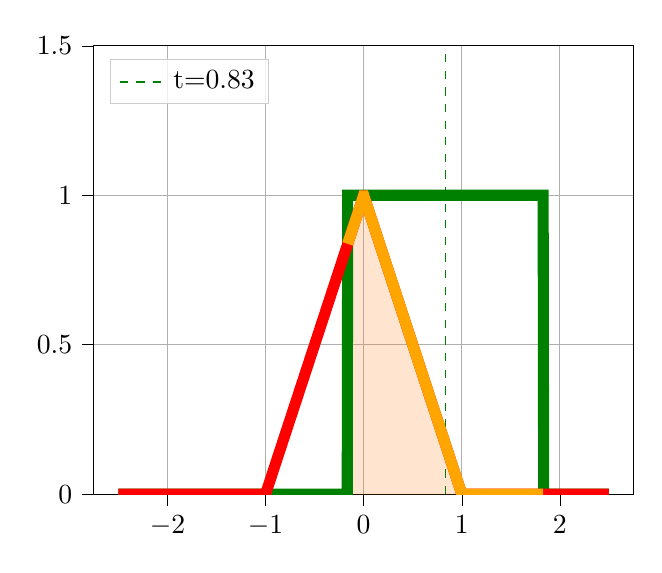
\begin{tikzpicture}

\definecolor{color0}{rgb}{1,0.498039215686275,0.0549019607843137}
\definecolor{color1}{rgb}{1,0.647058823529412,0}

\begin{axis}[
legend cell align={left},
legend style={fill opacity=0.8, draw opacity=1, text opacity=1, at={(0.03,0.97)}, anchor=north west, draw=white!80!black},
tick align=outside,
tick pos=left,
x grid style={white!69.0196078431373!black},
xmajorgrids,
xmin=-2.75, xmax=2.75,
xtick style={color=black},
y grid style={white!69.0196078431373!black},
ymajorgrids,
ymin=0, ymax=1.5,
ytick style={color=black}
]
\path [draw=color0, fill=color0, opacity=0.2]
(axis cs:-0.162662662662663,0.837337337337337)
--(axis cs:-0.162662662662663,0)
--(axis cs:-0.157657657657658,0)
--(axis cs:-0.152652652652653,0)
--(axis cs:-0.147647647647648,0)
--(axis cs:-0.142642642642643,0)
--(axis cs:-0.137637637637638,0)
--(axis cs:-0.132632632632633,0)
--(axis cs:-0.127627627627628,0)
--(axis cs:-0.122622622622623,0)
--(axis cs:-0.117617617617618,0)
--(axis cs:-0.112612612612613,0)
--(axis cs:-0.107607607607608,0)
--(axis cs:-0.102602602602603,0)
--(axis cs:-0.0975975975975976,0)
--(axis cs:-0.0925925925925926,0)
--(axis cs:-0.0875875875875876,0)
--(axis cs:-0.0825825825825826,0)
--(axis cs:-0.0775775775775776,0)
--(axis cs:-0.0725725725725725,0)
--(axis cs:-0.0675675675675675,0)
--(axis cs:-0.0625625625625625,0)
--(axis cs:-0.0575575575575575,0)
--(axis cs:-0.0525525525525525,0)
--(axis cs:-0.0475475475475475,0)
--(axis cs:-0.0425425425425425,0)
--(axis cs:-0.0375375375375375,0)
--(axis cs:-0.0325325325325325,0)
--(axis cs:-0.0275275275275275,0)
--(axis cs:-0.0225225225225225,0)
--(axis cs:-0.0175175175175175,0)
--(axis cs:-0.0125125125125125,0)
--(axis cs:-0.0075075075075075,0)
--(axis cs:-0.0025025025025025,0)
--(axis cs:0.0025025025025025,0)
--(axis cs:0.0075075075075075,0)
--(axis cs:0.0125125125125125,0)
--(axis cs:0.0175175175175175,0)
--(axis cs:0.0225225225225225,0)
--(axis cs:0.0275275275275275,0)
--(axis cs:0.0325325325325325,0)
--(axis cs:0.0375375375375375,0)
--(axis cs:0.0425425425425425,0)
--(axis cs:0.0475475475475475,0)
--(axis cs:0.0525525525525525,0)
--(axis cs:0.0575575575575575,0)
--(axis cs:0.0625625625625625,0)
--(axis cs:0.0675675675675675,0)
--(axis cs:0.0725725725725725,0)
--(axis cs:0.0775775775775776,0)
--(axis cs:0.0825825825825826,0)
--(axis cs:0.0875875875875876,0)
--(axis cs:0.0925925925925926,0)
--(axis cs:0.0975975975975976,0)
--(axis cs:0.102602602602603,0)
--(axis cs:0.107607607607608,0)
--(axis cs:0.112612612612613,0)
--(axis cs:0.117617617617618,0)
--(axis cs:0.122622622622623,0)
--(axis cs:0.127627627627628,0)
--(axis cs:0.132632632632633,0)
--(axis cs:0.137637637637638,0)
--(axis cs:0.142642642642643,0)
--(axis cs:0.147647647647648,0)
--(axis cs:0.152652652652653,0)
--(axis cs:0.157657657657658,0)
--(axis cs:0.162662662662663,0)
--(axis cs:0.167667667667668,0)
--(axis cs:0.172672672672673,0)
--(axis cs:0.177677677677678,0)
--(axis cs:0.182682682682683,0)
--(axis cs:0.187687687687688,0)
--(axis cs:0.192692692692693,0)
--(axis cs:0.197697697697698,0)
--(axis cs:0.202702702702703,0)
--(axis cs:0.207707707707708,0)
--(axis cs:0.212712712712713,0)
--(axis cs:0.217717717717718,0)
--(axis cs:0.222722722722723,0)
--(axis cs:0.227727727727728,0)
--(axis cs:0.232732732732733,0)
--(axis cs:0.237737737737738,0)
--(axis cs:0.242742742742743,0)
--(axis cs:0.247747747747748,0)
--(axis cs:0.252752752752753,0)
--(axis cs:0.257757757757758,0)
--(axis cs:0.262762762762763,0)
--(axis cs:0.267767767767768,0)
--(axis cs:0.272772772772773,0)
--(axis cs:0.277777777777778,0)
--(axis cs:0.282782782782783,0)
--(axis cs:0.287787787787788,0)
--(axis cs:0.292792792792793,0)
--(axis cs:0.297797797797798,0)
--(axis cs:0.302802802802803,0)
--(axis cs:0.307807807807808,0)
--(axis cs:0.312812812812813,0)
--(axis cs:0.317817817817818,0)
--(axis cs:0.322822822822823,0)
--(axis cs:0.327827827827828,0)
--(axis cs:0.332832832832833,0)
--(axis cs:0.337837837837838,0)
--(axis cs:0.342842842842843,0)
--(axis cs:0.347847847847848,0)
--(axis cs:0.352852852852853,0)
--(axis cs:0.357857857857858,0)
--(axis cs:0.362862862862863,0)
--(axis cs:0.367867867867868,0)
--(axis cs:0.372872872872873,0)
--(axis cs:0.377877877877878,0)
--(axis cs:0.382882882882883,0)
--(axis cs:0.387887887887888,0)
--(axis cs:0.392892892892893,0)
--(axis cs:0.397897897897898,0)
--(axis cs:0.402902902902903,0)
--(axis cs:0.407907907907908,0)
--(axis cs:0.412912912912913,0)
--(axis cs:0.417917917917918,0)
--(axis cs:0.422922922922923,0)
--(axis cs:0.427927927927928,0)
--(axis cs:0.432932932932933,0)
--(axis cs:0.437937937937938,0)
--(axis cs:0.442942942942943,0)
--(axis cs:0.447947947947948,0)
--(axis cs:0.452952952952953,0)
--(axis cs:0.457957957957958,0)
--(axis cs:0.462962962962963,0)
--(axis cs:0.467967967967968,0)
--(axis cs:0.472972972972973,0)
--(axis cs:0.477977977977978,0)
--(axis cs:0.482982982982983,0)
--(axis cs:0.487987987987988,0)
--(axis cs:0.492992992992993,0)
--(axis cs:0.497997997997998,0)
--(axis cs:0.503003003003003,0)
--(axis cs:0.508008008008008,0)
--(axis cs:0.513013013013013,0)
--(axis cs:0.518018018018018,0)
--(axis cs:0.523023023023023,0)
--(axis cs:0.528028028028028,0)
--(axis cs:0.533033033033033,0)
--(axis cs:0.538038038038038,0)
--(axis cs:0.543043043043043,0)
--(axis cs:0.548048048048048,0)
--(axis cs:0.553053053053053,0)
--(axis cs:0.558058058058058,0)
--(axis cs:0.563063063063063,0)
--(axis cs:0.568068068068068,0)
--(axis cs:0.573073073073073,0)
--(axis cs:0.578078078078078,0)
--(axis cs:0.583083083083083,0)
--(axis cs:0.588088088088088,0)
--(axis cs:0.593093093093093,0)
--(axis cs:0.598098098098098,0)
--(axis cs:0.603103103103103,0)
--(axis cs:0.608108108108108,0)
--(axis cs:0.613113113113113,0)
--(axis cs:0.618118118118118,0)
--(axis cs:0.623123123123123,0)
--(axis cs:0.628128128128128,0)
--(axis cs:0.633133133133133,0)
--(axis cs:0.638138138138138,0)
--(axis cs:0.643143143143143,0)
--(axis cs:0.648148148148148,0)
--(axis cs:0.653153153153153,0)
--(axis cs:0.658158158158158,0)
--(axis cs:0.663163163163163,0)
--(axis cs:0.668168168168168,0)
--(axis cs:0.673173173173173,0)
--(axis cs:0.678178178178178,0)
--(axis cs:0.683183183183183,0)
--(axis cs:0.688188188188188,0)
--(axis cs:0.693193193193193,0)
--(axis cs:0.698198198198198,0)
--(axis cs:0.703203203203203,0)
--(axis cs:0.708208208208208,0)
--(axis cs:0.713213213213213,0)
--(axis cs:0.718218218218218,0)
--(axis cs:0.723223223223223,0)
--(axis cs:0.728228228228228,0)
--(axis cs:0.733233233233233,0)
--(axis cs:0.738238238238238,0)
--(axis cs:0.743243243243243,0)
--(axis cs:0.748248248248248,0)
--(axis cs:0.753253253253253,0)
--(axis cs:0.758258258258258,0)
--(axis cs:0.763263263263263,0)
--(axis cs:0.768268268268268,0)
--(axis cs:0.773273273273273,0)
--(axis cs:0.778278278278278,0)
--(axis cs:0.783283283283283,0)
--(axis cs:0.788288288288288,0)
--(axis cs:0.793293293293293,0)
--(axis cs:0.798298298298298,0)
--(axis cs:0.803303303303303,0)
--(axis cs:0.808308308308308,0)
--(axis cs:0.813313313313313,0)
--(axis cs:0.818318318318318,0)
--(axis cs:0.823323323323323,0)
--(axis cs:0.828328328328328,0)
--(axis cs:0.833333333333333,0)
--(axis cs:0.838338338338338,0)
--(axis cs:0.843343343343343,0)
--(axis cs:0.848348348348348,0)
--(axis cs:0.853353353353353,0)
--(axis cs:0.858358358358358,0)
--(axis cs:0.863363363363364,0)
--(axis cs:0.868368368368369,0)
--(axis cs:0.873373373373374,0)
--(axis cs:0.878378378378379,0)
--(axis cs:0.883383383383384,0)
--(axis cs:0.888388388388389,0)
--(axis cs:0.893393393393394,0)
--(axis cs:0.898398398398399,0)
--(axis cs:0.903403403403404,0)
--(axis cs:0.908408408408409,0)
--(axis cs:0.913413413413414,0)
--(axis cs:0.918418418418419,0)
--(axis cs:0.923423423423424,0)
--(axis cs:0.928428428428429,0)
--(axis cs:0.933433433433434,0)
--(axis cs:0.938438438438439,0)
--(axis cs:0.943443443443444,0)
--(axis cs:0.948448448448449,0)
--(axis cs:0.953453453453454,0)
--(axis cs:0.958458458458459,0)
--(axis cs:0.963463463463464,0)
--(axis cs:0.968468468468469,0)
--(axis cs:0.973473473473474,0)
--(axis cs:0.978478478478479,0)
--(axis cs:0.983483483483484,0)
--(axis cs:0.988488488488489,0)
--(axis cs:0.993493493493494,0)
--(axis cs:0.998498498498499,0)
--(axis cs:1.0035035035035,0)
--(axis cs:1.00850850850851,0)
--(axis cs:1.01351351351351,0)
--(axis cs:1.01851851851852,0)
--(axis cs:1.02352352352352,0)
--(axis cs:1.02852852852853,0)
--(axis cs:1.03353353353353,0)
--(axis cs:1.03853853853854,0)
--(axis cs:1.04354354354354,0)
--(axis cs:1.04854854854855,0)
--(axis cs:1.05355355355355,0)
--(axis cs:1.05855855855856,0)
--(axis cs:1.06356356356356,0)
--(axis cs:1.06856856856857,0)
--(axis cs:1.07357357357357,0)
--(axis cs:1.07857857857858,0)
--(axis cs:1.08358358358358,0)
--(axis cs:1.08858858858859,0)
--(axis cs:1.09359359359359,0)
--(axis cs:1.0985985985986,0)
--(axis cs:1.1036036036036,0)
--(axis cs:1.10860860860861,0)
--(axis cs:1.11361361361361,0)
--(axis cs:1.11861861861862,0)
--(axis cs:1.12362362362362,0)
--(axis cs:1.12862862862863,0)
--(axis cs:1.13363363363363,0)
--(axis cs:1.13863863863864,0)
--(axis cs:1.14364364364364,0)
--(axis cs:1.14864864864865,0)
--(axis cs:1.15365365365365,0)
--(axis cs:1.15865865865866,0)
--(axis cs:1.16366366366366,0)
--(axis cs:1.16866866866867,0)
--(axis cs:1.17367367367367,0)
--(axis cs:1.17867867867868,0)
--(axis cs:1.18368368368368,0)
--(axis cs:1.18868868868869,0)
--(axis cs:1.19369369369369,0)
--(axis cs:1.1986986986987,0)
--(axis cs:1.2037037037037,0)
--(axis cs:1.20870870870871,0)
--(axis cs:1.21371371371371,0)
--(axis cs:1.21871871871872,0)
--(axis cs:1.22372372372372,0)
--(axis cs:1.22872872872873,0)
--(axis cs:1.23373373373373,0)
--(axis cs:1.23873873873874,0)
--(axis cs:1.24374374374374,0)
--(axis cs:1.24874874874875,0)
--(axis cs:1.25375375375375,0)
--(axis cs:1.25875875875876,0)
--(axis cs:1.26376376376376,0)
--(axis cs:1.26876876876877,0)
--(axis cs:1.27377377377377,0)
--(axis cs:1.27877877877878,0)
--(axis cs:1.28378378378378,0)
--(axis cs:1.28878878878879,0)
--(axis cs:1.29379379379379,0)
--(axis cs:1.2987987987988,0)
--(axis cs:1.3038038038038,0)
--(axis cs:1.30880880880881,0)
--(axis cs:1.31381381381381,0)
--(axis cs:1.31881881881882,0)
--(axis cs:1.32382382382382,0)
--(axis cs:1.32882882882883,0)
--(axis cs:1.33383383383383,0)
--(axis cs:1.33883883883884,0)
--(axis cs:1.34384384384384,0)
--(axis cs:1.34884884884885,0)
--(axis cs:1.35385385385385,0)
--(axis cs:1.35885885885886,0)
--(axis cs:1.36386386386386,0)
--(axis cs:1.36886886886887,0)
--(axis cs:1.37387387387387,0)
--(axis cs:1.37887887887888,0)
--(axis cs:1.38388388388388,0)
--(axis cs:1.38888888888889,0)
--(axis cs:1.39389389389389,0)
--(axis cs:1.3988988988989,0)
--(axis cs:1.4039039039039,0)
--(axis cs:1.40890890890891,0)
--(axis cs:1.41391391391391,0)
--(axis cs:1.41891891891892,0)
--(axis cs:1.42392392392392,0)
--(axis cs:1.42892892892893,0)
--(axis cs:1.43393393393393,0)
--(axis cs:1.43893893893894,0)
--(axis cs:1.44394394394394,0)
--(axis cs:1.44894894894895,0)
--(axis cs:1.45395395395395,0)
--(axis cs:1.45895895895896,0)
--(axis cs:1.46396396396396,0)
--(axis cs:1.46896896896897,0)
--(axis cs:1.47397397397397,0)
--(axis cs:1.47897897897898,0)
--(axis cs:1.48398398398398,0)
--(axis cs:1.48898898898899,0)
--(axis cs:1.49399399399399,0)
--(axis cs:1.498998998999,0)
--(axis cs:1.504004004004,0)
--(axis cs:1.50900900900901,0)
--(axis cs:1.51401401401401,0)
--(axis cs:1.51901901901902,0)
--(axis cs:1.52402402402402,0)
--(axis cs:1.52902902902903,0)
--(axis cs:1.53403403403403,0)
--(axis cs:1.53903903903904,0)
--(axis cs:1.54404404404404,0)
--(axis cs:1.54904904904905,0)
--(axis cs:1.55405405405405,0)
--(axis cs:1.55905905905906,0)
--(axis cs:1.56406406406406,0)
--(axis cs:1.56906906906907,0)
--(axis cs:1.57407407407407,0)
--(axis cs:1.57907907907908,0)
--(axis cs:1.58408408408408,0)
--(axis cs:1.58908908908909,0)
--(axis cs:1.59409409409409,0)
--(axis cs:1.5990990990991,0)
--(axis cs:1.6041041041041,0)
--(axis cs:1.60910910910911,0)
--(axis cs:1.61411411411411,0)
--(axis cs:1.61911911911912,0)
--(axis cs:1.62412412412412,0)
--(axis cs:1.62912912912913,0)
--(axis cs:1.63413413413413,0)
--(axis cs:1.63913913913914,0)
--(axis cs:1.64414414414414,0)
--(axis cs:1.64914914914915,0)
--(axis cs:1.65415415415415,0)
--(axis cs:1.65915915915916,0)
--(axis cs:1.66416416416416,0)
--(axis cs:1.66916916916917,0)
--(axis cs:1.67417417417417,0)
--(axis cs:1.67917917917918,0)
--(axis cs:1.68418418418418,0)
--(axis cs:1.68918918918919,0)
--(axis cs:1.69419419419419,0)
--(axis cs:1.6991991991992,0)
--(axis cs:1.7042042042042,0)
--(axis cs:1.70920920920921,0)
--(axis cs:1.71421421421421,0)
--(axis cs:1.71921921921922,0)
--(axis cs:1.72422422422422,0)
--(axis cs:1.72922922922923,0)
--(axis cs:1.73423423423423,0)
--(axis cs:1.73923923923924,0)
--(axis cs:1.74424424424424,0)
--(axis cs:1.74924924924925,0)
--(axis cs:1.75425425425425,0)
--(axis cs:1.75925925925926,0)
--(axis cs:1.76426426426426,0)
--(axis cs:1.76926926926927,0)
--(axis cs:1.77427427427427,0)
--(axis cs:1.77927927927928,0)
--(axis cs:1.78428428428428,0)
--(axis cs:1.78928928928929,0)
--(axis cs:1.79429429429429,0)
--(axis cs:1.7992992992993,0)
--(axis cs:1.8043043043043,0)
--(axis cs:1.80930930930931,0)
--(axis cs:1.81431431431431,0)
--(axis cs:1.81931931931932,0)
--(axis cs:1.82432432432432,0)
--(axis cs:1.82932932932933,0)
--(axis cs:1.82932932932933,0)
--(axis cs:1.82932932932933,0)
--(axis cs:1.82432432432432,0)
--(axis cs:1.81931931931932,0)
--(axis cs:1.81431431431431,0)
--(axis cs:1.80930930930931,0)
--(axis cs:1.8043043043043,0)
--(axis cs:1.7992992992993,0)
--(axis cs:1.79429429429429,0)
--(axis cs:1.78928928928929,0)
--(axis cs:1.78428428428428,0)
--(axis cs:1.77927927927928,0)
--(axis cs:1.77427427427427,0)
--(axis cs:1.76926926926927,0)
--(axis cs:1.76426426426426,0)
--(axis cs:1.75925925925926,0)
--(axis cs:1.75425425425425,0)
--(axis cs:1.74924924924925,0)
--(axis cs:1.74424424424424,0)
--(axis cs:1.73923923923924,0)
--(axis cs:1.73423423423423,0)
--(axis cs:1.72922922922923,0)
--(axis cs:1.72422422422422,0)
--(axis cs:1.71921921921922,0)
--(axis cs:1.71421421421421,0)
--(axis cs:1.70920920920921,0)
--(axis cs:1.7042042042042,0)
--(axis cs:1.6991991991992,0)
--(axis cs:1.69419419419419,0)
--(axis cs:1.68918918918919,0)
--(axis cs:1.68418418418418,0)
--(axis cs:1.67917917917918,0)
--(axis cs:1.67417417417417,0)
--(axis cs:1.66916916916917,0)
--(axis cs:1.66416416416416,0)
--(axis cs:1.65915915915916,0)
--(axis cs:1.65415415415415,0)
--(axis cs:1.64914914914915,0)
--(axis cs:1.64414414414414,0)
--(axis cs:1.63913913913914,0)
--(axis cs:1.63413413413413,0)
--(axis cs:1.62912912912913,0)
--(axis cs:1.62412412412412,0)
--(axis cs:1.61911911911912,0)
--(axis cs:1.61411411411411,0)
--(axis cs:1.60910910910911,0)
--(axis cs:1.6041041041041,0)
--(axis cs:1.5990990990991,0)
--(axis cs:1.59409409409409,0)
--(axis cs:1.58908908908909,0)
--(axis cs:1.58408408408408,0)
--(axis cs:1.57907907907908,0)
--(axis cs:1.57407407407407,0)
--(axis cs:1.56906906906907,0)
--(axis cs:1.56406406406406,0)
--(axis cs:1.55905905905906,0)
--(axis cs:1.55405405405405,0)
--(axis cs:1.54904904904905,0)
--(axis cs:1.54404404404404,0)
--(axis cs:1.53903903903904,0)
--(axis cs:1.53403403403403,0)
--(axis cs:1.52902902902903,0)
--(axis cs:1.52402402402402,0)
--(axis cs:1.51901901901902,0)
--(axis cs:1.51401401401401,0)
--(axis cs:1.50900900900901,0)
--(axis cs:1.504004004004,0)
--(axis cs:1.498998998999,0)
--(axis cs:1.49399399399399,0)
--(axis cs:1.48898898898899,0)
--(axis cs:1.48398398398398,0)
--(axis cs:1.47897897897898,0)
--(axis cs:1.47397397397397,0)
--(axis cs:1.46896896896897,0)
--(axis cs:1.46396396396396,0)
--(axis cs:1.45895895895896,0)
--(axis cs:1.45395395395395,0)
--(axis cs:1.44894894894895,0)
--(axis cs:1.44394394394394,0)
--(axis cs:1.43893893893894,0)
--(axis cs:1.43393393393393,0)
--(axis cs:1.42892892892893,0)
--(axis cs:1.42392392392392,0)
--(axis cs:1.41891891891892,0)
--(axis cs:1.41391391391391,0)
--(axis cs:1.40890890890891,0)
--(axis cs:1.4039039039039,0)
--(axis cs:1.3988988988989,0)
--(axis cs:1.39389389389389,0)
--(axis cs:1.38888888888889,0)
--(axis cs:1.38388388388388,0)
--(axis cs:1.37887887887888,0)
--(axis cs:1.37387387387387,0)
--(axis cs:1.36886886886887,0)
--(axis cs:1.36386386386386,0)
--(axis cs:1.35885885885886,0)
--(axis cs:1.35385385385385,0)
--(axis cs:1.34884884884885,0)
--(axis cs:1.34384384384384,0)
--(axis cs:1.33883883883884,0)
--(axis cs:1.33383383383383,0)
--(axis cs:1.32882882882883,0)
--(axis cs:1.32382382382382,0)
--(axis cs:1.31881881881882,0)
--(axis cs:1.31381381381381,0)
--(axis cs:1.30880880880881,0)
--(axis cs:1.3038038038038,0)
--(axis cs:1.2987987987988,0)
--(axis cs:1.29379379379379,0)
--(axis cs:1.28878878878879,0)
--(axis cs:1.28378378378378,0)
--(axis cs:1.27877877877878,0)
--(axis cs:1.27377377377377,0)
--(axis cs:1.26876876876877,0)
--(axis cs:1.26376376376376,0)
--(axis cs:1.25875875875876,0)
--(axis cs:1.25375375375375,0)
--(axis cs:1.24874874874875,0)
--(axis cs:1.24374374374374,0)
--(axis cs:1.23873873873874,0)
--(axis cs:1.23373373373373,0)
--(axis cs:1.22872872872873,0)
--(axis cs:1.22372372372372,0)
--(axis cs:1.21871871871872,0)
--(axis cs:1.21371371371371,0)
--(axis cs:1.20870870870871,0)
--(axis cs:1.2037037037037,0)
--(axis cs:1.1986986986987,0)
--(axis cs:1.19369369369369,0)
--(axis cs:1.18868868868869,0)
--(axis cs:1.18368368368368,0)
--(axis cs:1.17867867867868,0)
--(axis cs:1.17367367367367,0)
--(axis cs:1.16866866866867,0)
--(axis cs:1.16366366366366,0)
--(axis cs:1.15865865865866,0)
--(axis cs:1.15365365365365,0)
--(axis cs:1.14864864864865,0)
--(axis cs:1.14364364364364,0)
--(axis cs:1.13863863863864,0)
--(axis cs:1.13363363363363,0)
--(axis cs:1.12862862862863,0)
--(axis cs:1.12362362362362,0)
--(axis cs:1.11861861861862,0)
--(axis cs:1.11361361361361,0)
--(axis cs:1.10860860860861,0)
--(axis cs:1.1036036036036,0)
--(axis cs:1.0985985985986,0)
--(axis cs:1.09359359359359,0)
--(axis cs:1.08858858858859,0)
--(axis cs:1.08358358358358,0)
--(axis cs:1.07857857857858,0)
--(axis cs:1.07357357357357,0)
--(axis cs:1.06856856856857,0)
--(axis cs:1.06356356356356,0)
--(axis cs:1.05855855855856,0)
--(axis cs:1.05355355355355,0)
--(axis cs:1.04854854854855,0)
--(axis cs:1.04354354354354,0)
--(axis cs:1.03853853853854,0)
--(axis cs:1.03353353353353,0)
--(axis cs:1.02852852852853,0)
--(axis cs:1.02352352352352,0)
--(axis cs:1.01851851851852,0)
--(axis cs:1.01351351351351,0)
--(axis cs:1.00850850850851,0)
--(axis cs:1.0035035035035,0)
--(axis cs:0.998498498498499,0.00150150150150141)
--(axis cs:0.993493493493494,0.00650650650650642)
--(axis cs:0.988488488488489,0.0115115115115114)
--(axis cs:0.983483483483484,0.0165165165165164)
--(axis cs:0.978478478478479,0.0215215215215214)
--(axis cs:0.973473473473474,0.0265265265265264)
--(axis cs:0.968468468468469,0.0315315315315314)
--(axis cs:0.963463463463464,0.0365365365365364)
--(axis cs:0.958458458458459,0.0415415415415414)
--(axis cs:0.953453453453454,0.0465465465465464)
--(axis cs:0.948448448448449,0.0515515515515514)
--(axis cs:0.943443443443444,0.0565565565565564)
--(axis cs:0.938438438438439,0.0615615615615615)
--(axis cs:0.933433433433434,0.0665665665665665)
--(axis cs:0.928428428428429,0.0715715715715715)
--(axis cs:0.923423423423424,0.0765765765765765)
--(axis cs:0.918418418418419,0.0815815815815815)
--(axis cs:0.913413413413414,0.0865865865865865)
--(axis cs:0.908408408408409,0.0915915915915915)
--(axis cs:0.903403403403404,0.0965965965965965)
--(axis cs:0.898398398398399,0.101601601601601)
--(axis cs:0.893393393393394,0.106606606606606)
--(axis cs:0.888388388388389,0.111611611611611)
--(axis cs:0.883383383383384,0.116616616616616)
--(axis cs:0.878378378378379,0.121621621621621)
--(axis cs:0.873373373373374,0.126626626626626)
--(axis cs:0.868368368368369,0.131631631631631)
--(axis cs:0.863363363363364,0.136636636636636)
--(axis cs:0.858358358358358,0.141641641641642)
--(axis cs:0.853353353353353,0.146646646646647)
--(axis cs:0.848348348348348,0.151651651651652)
--(axis cs:0.843343343343343,0.156656656656657)
--(axis cs:0.838338338338338,0.161661661661662)
--(axis cs:0.833333333333333,0.166666666666667)
--(axis cs:0.828328328328328,0.171671671671672)
--(axis cs:0.823323323323323,0.176676676676677)
--(axis cs:0.818318318318318,0.181681681681682)
--(axis cs:0.813313313313313,0.186686686686687)
--(axis cs:0.808308308308308,0.191691691691692)
--(axis cs:0.803303303303303,0.196696696696697)
--(axis cs:0.798298298298298,0.201701701701702)
--(axis cs:0.793293293293293,0.206706706706707)
--(axis cs:0.788288288288288,0.211711711711712)
--(axis cs:0.783283283283283,0.216716716716717)
--(axis cs:0.778278278278278,0.221721721721722)
--(axis cs:0.773273273273273,0.226726726726727)
--(axis cs:0.768268268268268,0.231731731731732)
--(axis cs:0.763263263263263,0.236736736736737)
--(axis cs:0.758258258258258,0.241741741741742)
--(axis cs:0.753253253253253,0.246746746746747)
--(axis cs:0.748248248248248,0.251751751751752)
--(axis cs:0.743243243243243,0.256756756756757)
--(axis cs:0.738238238238238,0.261761761761762)
--(axis cs:0.733233233233233,0.266766766766767)
--(axis cs:0.728228228228228,0.271771771771772)
--(axis cs:0.723223223223223,0.276776776776777)
--(axis cs:0.718218218218218,0.281781781781782)
--(axis cs:0.713213213213213,0.286786786786787)
--(axis cs:0.708208208208208,0.291791791791792)
--(axis cs:0.703203203203203,0.296796796796797)
--(axis cs:0.698198198198198,0.301801801801802)
--(axis cs:0.693193193193193,0.306806806806807)
--(axis cs:0.688188188188188,0.311811811811812)
--(axis cs:0.683183183183183,0.316816816816817)
--(axis cs:0.678178178178178,0.321821821821822)
--(axis cs:0.673173173173173,0.326826826826827)
--(axis cs:0.668168168168168,0.331831831831832)
--(axis cs:0.663163163163163,0.336836836836837)
--(axis cs:0.658158158158158,0.341841841841842)
--(axis cs:0.653153153153153,0.346846846846847)
--(axis cs:0.648148148148148,0.351851851851852)
--(axis cs:0.643143143143143,0.356856856856857)
--(axis cs:0.638138138138138,0.361861861861862)
--(axis cs:0.633133133133133,0.366866866866867)
--(axis cs:0.628128128128128,0.371871871871872)
--(axis cs:0.623123123123123,0.376876876876877)
--(axis cs:0.618118118118118,0.381881881881882)
--(axis cs:0.613113113113113,0.386886886886887)
--(axis cs:0.608108108108108,0.391891891891892)
--(axis cs:0.603103103103103,0.396896896896897)
--(axis cs:0.598098098098098,0.401901901901902)
--(axis cs:0.593093093093093,0.406906906906907)
--(axis cs:0.588088088088088,0.411911911911912)
--(axis cs:0.583083083083083,0.416916916916917)
--(axis cs:0.578078078078078,0.421921921921922)
--(axis cs:0.573073073073073,0.426926926926927)
--(axis cs:0.568068068068068,0.431931931931932)
--(axis cs:0.563063063063063,0.436936936936937)
--(axis cs:0.558058058058058,0.441941941941942)
--(axis cs:0.553053053053053,0.446946946946947)
--(axis cs:0.548048048048048,0.451951951951952)
--(axis cs:0.543043043043043,0.456956956956957)
--(axis cs:0.538038038038038,0.461961961961962)
--(axis cs:0.533033033033033,0.466966966966967)
--(axis cs:0.528028028028028,0.471971971971972)
--(axis cs:0.523023023023023,0.476976976976977)
--(axis cs:0.518018018018018,0.481981981981982)
--(axis cs:0.513013013013013,0.486986986986987)
--(axis cs:0.508008008008008,0.491991991991992)
--(axis cs:0.503003003003003,0.496996996996997)
--(axis cs:0.497997997997998,0.502002002002002)
--(axis cs:0.492992992992993,0.507007007007007)
--(axis cs:0.487987987987988,0.512012012012012)
--(axis cs:0.482982982982983,0.517017017017017)
--(axis cs:0.477977977977978,0.522022022022022)
--(axis cs:0.472972972972973,0.527027027027027)
--(axis cs:0.467967967967968,0.532032032032032)
--(axis cs:0.462962962962963,0.537037037037037)
--(axis cs:0.457957957957958,0.542042042042042)
--(axis cs:0.452952952952953,0.547047047047047)
--(axis cs:0.447947947947948,0.552052052052052)
--(axis cs:0.442942942942943,0.557057057057057)
--(axis cs:0.437937937937938,0.562062062062062)
--(axis cs:0.432932932932933,0.567067067067067)
--(axis cs:0.427927927927928,0.572072072072072)
--(axis cs:0.422922922922923,0.577077077077077)
--(axis cs:0.417917917917918,0.582082082082082)
--(axis cs:0.412912912912913,0.587087087087087)
--(axis cs:0.407907907907908,0.592092092092092)
--(axis cs:0.402902902902903,0.597097097097097)
--(axis cs:0.397897897897898,0.602102102102102)
--(axis cs:0.392892892892893,0.607107107107107)
--(axis cs:0.387887887887888,0.612112112112112)
--(axis cs:0.382882882882883,0.617117117117117)
--(axis cs:0.377877877877878,0.622122122122122)
--(axis cs:0.372872872872873,0.627127127127127)
--(axis cs:0.367867867867868,0.632132132132132)
--(axis cs:0.362862862862863,0.637137137137137)
--(axis cs:0.357857857857858,0.642142142142142)
--(axis cs:0.352852852852853,0.647147147147147)
--(axis cs:0.347847847847848,0.652152152152152)
--(axis cs:0.342842842842843,0.657157157157157)
--(axis cs:0.337837837837838,0.662162162162162)
--(axis cs:0.332832832832833,0.667167167167167)
--(axis cs:0.327827827827828,0.672172172172172)
--(axis cs:0.322822822822823,0.677177177177177)
--(axis cs:0.317817817817818,0.682182182182182)
--(axis cs:0.312812812812813,0.687187187187187)
--(axis cs:0.307807807807808,0.692192192192192)
--(axis cs:0.302802802802803,0.697197197197197)
--(axis cs:0.297797797797798,0.702202202202202)
--(axis cs:0.292792792792793,0.707207207207207)
--(axis cs:0.287787787787788,0.712212212212212)
--(axis cs:0.282782782782783,0.717217217217217)
--(axis cs:0.277777777777778,0.722222222222222)
--(axis cs:0.272772772772773,0.727227227227227)
--(axis cs:0.267767767767768,0.732232232232232)
--(axis cs:0.262762762762763,0.737237237237237)
--(axis cs:0.257757757757758,0.742242242242242)
--(axis cs:0.252752752752753,0.747247247247247)
--(axis cs:0.247747747747748,0.752252252252252)
--(axis cs:0.242742742742743,0.757257257257257)
--(axis cs:0.237737737737738,0.762262262262262)
--(axis cs:0.232732732732733,0.767267267267267)
--(axis cs:0.227727727727728,0.772272272272272)
--(axis cs:0.222722722722723,0.777277277277277)
--(axis cs:0.217717717717718,0.782282282282282)
--(axis cs:0.212712712712713,0.787287287287287)
--(axis cs:0.207707707707708,0.792292292292292)
--(axis cs:0.202702702702703,0.797297297297297)
--(axis cs:0.197697697697698,0.802302302302302)
--(axis cs:0.192692692692693,0.807307307307307)
--(axis cs:0.187687687687688,0.812312312312312)
--(axis cs:0.182682682682683,0.817317317317317)
--(axis cs:0.177677677677678,0.822322322322322)
--(axis cs:0.172672672672673,0.827327327327327)
--(axis cs:0.167667667667668,0.832332332332332)
--(axis cs:0.162662662662663,0.837337337337337)
--(axis cs:0.157657657657658,0.842342342342342)
--(axis cs:0.152652652652653,0.847347347347347)
--(axis cs:0.147647647647648,0.852352352352352)
--(axis cs:0.142642642642643,0.857357357357357)
--(axis cs:0.137637637637638,0.862362362362362)
--(axis cs:0.132632632632633,0.867367367367367)
--(axis cs:0.127627627627628,0.872372372372372)
--(axis cs:0.122622622622623,0.877377377377377)
--(axis cs:0.117617617617618,0.882382382382382)
--(axis cs:0.112612612612613,0.887387387387387)
--(axis cs:0.107607607607608,0.892392392392392)
--(axis cs:0.102602602602603,0.897397397397397)
--(axis cs:0.0975975975975976,0.902402402402402)
--(axis cs:0.0925925925925926,0.907407407407407)
--(axis cs:0.0875875875875876,0.912412412412412)
--(axis cs:0.0825825825825826,0.917417417417417)
--(axis cs:0.0775775775775776,0.922422422422422)
--(axis cs:0.0725725725725725,0.927427427427427)
--(axis cs:0.0675675675675675,0.932432432432432)
--(axis cs:0.0625625625625625,0.937437437437437)
--(axis cs:0.0575575575575575,0.942442442442442)
--(axis cs:0.0525525525525525,0.947447447447447)
--(axis cs:0.0475475475475475,0.952452452452452)
--(axis cs:0.0425425425425425,0.957457457457457)
--(axis cs:0.0375375375375375,0.962462462462462)
--(axis cs:0.0325325325325325,0.967467467467467)
--(axis cs:0.0275275275275275,0.972472472472472)
--(axis cs:0.0225225225225225,0.977477477477477)
--(axis cs:0.0175175175175175,0.982482482482482)
--(axis cs:0.0125125125125125,0.987487487487487)
--(axis cs:0.0075075075075075,0.992492492492492)
--(axis cs:0.0025025025025025,0.997497497497497)
--(axis cs:-0.0025025025025025,0.997497497497497)
--(axis cs:-0.0075075075075075,0.992492492492492)
--(axis cs:-0.0125125125125125,0.987487487487487)
--(axis cs:-0.0175175175175175,0.982482482482482)
--(axis cs:-0.0225225225225225,0.977477477477477)
--(axis cs:-0.0275275275275275,0.972472472472472)
--(axis cs:-0.0325325325325325,0.967467467467467)
--(axis cs:-0.0375375375375375,0.962462462462462)
--(axis cs:-0.0425425425425425,0.957457457457457)
--(axis cs:-0.0475475475475475,0.952452452452452)
--(axis cs:-0.0525525525525525,0.947447447447447)
--(axis cs:-0.0575575575575575,0.942442442442442)
--(axis cs:-0.0625625625625625,0.937437437437437)
--(axis cs:-0.0675675675675675,0.932432432432432)
--(axis cs:-0.0725725725725725,0.927427427427427)
--(axis cs:-0.0775775775775776,0.922422422422422)
--(axis cs:-0.0825825825825826,0.917417417417417)
--(axis cs:-0.0875875875875876,0.912412412412412)
--(axis cs:-0.0925925925925926,0.907407407407407)
--(axis cs:-0.0975975975975976,0.902402402402402)
--(axis cs:-0.102602602602603,0.897397397397397)
--(axis cs:-0.107607607607608,0.892392392392392)
--(axis cs:-0.112612612612613,0.887387387387387)
--(axis cs:-0.117617617617618,0.882382382382382)
--(axis cs:-0.122622622622623,0.877377377377377)
--(axis cs:-0.127627627627628,0.872372372372372)
--(axis cs:-0.132632632632633,0.867367367367367)
--(axis cs:-0.137637637637638,0.862362362362362)
--(axis cs:-0.142642642642643,0.857357357357357)
--(axis cs:-0.147647647647648,0.852352352352352)
--(axis cs:-0.152652652652653,0.847347347347347)
--(axis cs:-0.157657657657658,0.842342342342342)
--(axis cs:-0.162662662662663,0.837337337337337)
--cycle;

\addplot [line width=4pt, green!50!black, forget plot]
table {%
-2.5 0
-2.49499499499499 0
-2.48998998998999 0
-2.48498498498498 0
-2.47997997997998 0
-2.47497497497497 0
-2.46996996996997 0
-2.46496496496496 0
-2.45995995995996 0
-2.45495495495495 0
-2.44994994994995 0
-2.44494494494494 0
-2.43993993993994 0
-2.43493493493493 0
-2.42992992992993 0
-2.42492492492492 0
-2.41991991991992 0
-2.41491491491491 0
-2.40990990990991 0
-2.4049049049049 0
-2.3998998998999 0
-2.39489489489489 0
-2.38988988988989 0
-2.38488488488488 0
-2.37987987987988 0
-2.37487487487487 0
-2.36986986986987 0
-2.36486486486486 0
-2.35985985985986 0
-2.35485485485485 0
-2.34984984984985 0
-2.34484484484484 0
-2.33983983983984 0
-2.33483483483483 0
-2.32982982982983 0
-2.32482482482482 0
-2.31981981981982 0
-2.31481481481481 0
-2.30980980980981 0
-2.3048048048048 0
-2.2997997997998 0
-2.29479479479479 0
-2.28978978978979 0
-2.28478478478478 0
-2.27977977977978 0
-2.27477477477477 0
-2.26976976976977 0
-2.26476476476476 0
-2.25975975975976 0
-2.25475475475475 0
-2.24974974974975 0
-2.24474474474474 0
-2.23973973973974 0
-2.23473473473473 0
-2.22972972972973 0
-2.22472472472472 0
-2.21971971971972 0
-2.21471471471471 0
-2.20970970970971 0
-2.2047047047047 0
-2.1996996996997 0
-2.19469469469469 0
-2.18968968968969 0
-2.18468468468468 0
-2.17967967967968 0
-2.17467467467467 0
-2.16966966966967 0
-2.16466466466466 0
-2.15965965965966 0
-2.15465465465465 0
-2.14964964964965 0
-2.14464464464464 0
-2.13963963963964 0
-2.13463463463463 0
-2.12962962962963 0
-2.12462462462462 0
-2.11961961961962 0
-2.11461461461461 0
-2.10960960960961 0
-2.1046046046046 0
-2.0995995995996 0
-2.09459459459459 0
-2.08958958958959 0
-2.08458458458458 0
-2.07957957957958 0
-2.07457457457457 0
-2.06956956956957 0
-2.06456456456456 0
-2.05955955955956 0
-2.05455455455455 0
-2.04954954954955 0
-2.04454454454454 0
-2.03953953953954 0
-2.03453453453453 0
-2.02952952952953 0
-2.02452452452452 0
-2.01951951951952 0
-2.01451451451451 0
-2.00950950950951 0
-2.0045045045045 0
-1.9994994994995 0
-1.99449449449449 0
-1.98948948948949 0
-1.98448448448448 0
-1.97947947947948 0
-1.97447447447447 0
-1.96946946946947 0
-1.96446446446446 0
-1.95945945945946 0
-1.95445445445445 0
-1.94944944944945 0
-1.94444444444444 0
-1.93943943943944 0
-1.93443443443443 0
-1.92942942942943 0
-1.92442442442442 0
-1.91941941941942 0
-1.91441441441441 0
-1.90940940940941 0
-1.9044044044044 0
-1.8993993993994 0
-1.89439439439439 0
-1.88938938938939 0
-1.88438438438438 0
-1.87937937937938 0
-1.87437437437437 0
-1.86936936936937 0
-1.86436436436436 0
-1.85935935935936 0
-1.85435435435435 0
-1.84934934934935 0
-1.84434434434434 0
-1.83933933933934 0
-1.83433433433433 0
-1.82932932932933 0
-1.82432432432432 0
-1.81931931931932 0
-1.81431431431431 0
-1.80930930930931 0
-1.8043043043043 0
-1.7992992992993 0
-1.79429429429429 0
-1.78928928928929 0
-1.78428428428428 0
-1.77927927927928 0
-1.77427427427427 0
-1.76926926926927 0
-1.76426426426426 0
-1.75925925925926 0
-1.75425425425425 0
-1.74924924924925 0
-1.74424424424424 0
-1.73923923923924 0
-1.73423423423423 0
-1.72922922922923 0
-1.72422422422422 0
-1.71921921921922 0
-1.71421421421421 0
-1.70920920920921 0
-1.7042042042042 0
-1.6991991991992 0
-1.69419419419419 0
-1.68918918918919 0
-1.68418418418418 0
-1.67917917917918 0
-1.67417417417417 0
-1.66916916916917 0
-1.66416416416416 0
-1.65915915915916 0
-1.65415415415415 0
-1.64914914914915 0
-1.64414414414414 0
-1.63913913913914 0
-1.63413413413413 0
-1.62912912912913 0
-1.62412412412412 0
-1.61911911911912 0
-1.61411411411411 0
-1.60910910910911 0
-1.6041041041041 0
-1.5990990990991 0
-1.59409409409409 0
-1.58908908908909 0
-1.58408408408408 0
-1.57907907907908 0
-1.57407407407407 0
-1.56906906906907 0
-1.56406406406406 0
-1.55905905905906 0
-1.55405405405405 0
-1.54904904904905 0
-1.54404404404404 0
-1.53903903903904 0
-1.53403403403403 0
-1.52902902902903 0
-1.52402402402402 0
-1.51901901901902 0
-1.51401401401401 0
-1.50900900900901 0
-1.504004004004 0
-1.498998998999 0
-1.49399399399399 0
-1.48898898898899 0
-1.48398398398398 0
-1.47897897897898 0
-1.47397397397397 0
-1.46896896896897 0
-1.46396396396396 0
-1.45895895895896 0
-1.45395395395395 0
-1.44894894894895 0
-1.44394394394394 0
-1.43893893893894 0
-1.43393393393393 0
-1.42892892892893 0
-1.42392392392392 0
-1.41891891891892 0
-1.41391391391391 0
-1.40890890890891 0
-1.4039039039039 0
-1.3988988988989 0
-1.39389389389389 0
-1.38888888888889 0
-1.38388388388388 0
-1.37887887887888 0
-1.37387387387387 0
-1.36886886886887 0
-1.36386386386386 0
-1.35885885885886 0
-1.35385385385385 0
-1.34884884884885 0
-1.34384384384384 0
-1.33883883883884 0
-1.33383383383383 0
-1.32882882882883 0
-1.32382382382382 0
-1.31881881881882 0
-1.31381381381381 0
-1.30880880880881 0
-1.3038038038038 0
-1.2987987987988 0
-1.29379379379379 0
-1.28878878878879 0
-1.28378378378378 0
-1.27877877877878 0
-1.27377377377377 0
-1.26876876876877 0
-1.26376376376376 0
-1.25875875875876 0
-1.25375375375375 0
-1.24874874874875 0
-1.24374374374374 0
-1.23873873873874 0
-1.23373373373373 0
-1.22872872872873 0
-1.22372372372372 0
-1.21871871871872 0
-1.21371371371371 0
-1.20870870870871 0
-1.2037037037037 0
-1.1986986986987 0
-1.19369369369369 0
-1.18868868868869 0
-1.18368368368368 0
-1.17867867867868 0
-1.17367367367367 0
-1.16866866866867 0
-1.16366366366366 0
-1.15865865865866 0
-1.15365365365365 0
-1.14864864864865 0
-1.14364364364364 0
-1.13863863863864 0
-1.13363363363363 0
-1.12862862862863 0
-1.12362362362362 0
-1.11861861861862 0
-1.11361361361361 0
-1.10860860860861 0
-1.1036036036036 0
-1.0985985985986 0
-1.09359359359359 0
-1.08858858858859 0
-1.08358358358358 0
-1.07857857857858 0
-1.07357357357357 0
-1.06856856856857 0
-1.06356356356356 0
-1.05855855855856 0
-1.05355355355355 0
-1.04854854854855 0
-1.04354354354354 0
-1.03853853853854 0
-1.03353353353353 0
-1.02852852852853 0
-1.02352352352352 0
-1.01851851851852 0
-1.01351351351351 0
-1.00850850850851 0
-1.0035035035035 0
-0.998498498498499 0
-0.993493493493494 0
-0.988488488488489 0
-0.983483483483484 0
-0.978478478478479 0
-0.973473473473474 0
-0.968468468468469 0
-0.963463463463464 0
-0.958458458458459 0
-0.953453453453454 0
-0.948448448448449 0
-0.943443443443444 0
-0.938438438438439 0
-0.933433433433434 0
-0.928428428428429 0
-0.923423423423424 0
-0.918418418418419 0
-0.913413413413414 0
-0.908408408408409 0
-0.903403403403404 0
-0.898398398398399 0
-0.893393393393393 0
-0.888388388388388 0
-0.883383383383383 0
-0.878378378378378 0
-0.873373373373373 0
-0.868368368368368 0
-0.863363363363363 0
-0.858358358358358 0
-0.853353353353353 0
-0.848348348348348 0
-0.843343343343343 0
-0.838338338338338 0
-0.833333333333333 0
-0.828328328328328 0
-0.823323323323323 0
-0.818318318318318 0
-0.813313313313313 0
-0.808308308308308 0
-0.803303303303303 0
-0.798298298298298 0
-0.793293293293293 0
-0.788288288288288 0
-0.783283283283283 0
-0.778278278278278 0
-0.773273273273273 0
-0.768268268268268 0
-0.763263263263263 0
-0.758258258258258 0
-0.753253253253253 0
-0.748248248248248 0
-0.743243243243243 0
-0.738238238238238 0
-0.733233233233233 0
-0.728228228228228 0
-0.723223223223223 0
-0.718218218218218 0
-0.713213213213213 0
-0.708208208208208 0
-0.703203203203203 0
-0.698198198198198 0
-0.693193193193193 0
-0.688188188188188 0
-0.683183183183183 0
-0.678178178178178 0
-0.673173173173173 0
-0.668168168168168 0
-0.663163163163163 0
-0.658158158158158 0
-0.653153153153153 0
-0.648148148148148 0
-0.643143143143143 0
-0.638138138138138 0
-0.633133133133133 0
-0.628128128128128 0
-0.623123123123123 0
-0.618118118118118 0
-0.613113113113113 0
-0.608108108108108 0
-0.603103103103103 0
-0.598098098098098 0
-0.593093093093093 0
-0.588088088088088 0
-0.583083083083083 0
-0.578078078078078 0
-0.573073073073073 0
-0.568068068068068 0
-0.563063063063063 0
-0.558058058058058 0
-0.553053053053053 0
-0.548048048048048 0
-0.543043043043043 0
-0.538038038038038 0
-0.533033033033033 0
-0.528028028028028 0
-0.523023023023023 0
-0.518018018018018 0
-0.513013013013013 0
-0.508008008008008 0
-0.503003003003003 0
-0.497997997997998 0
-0.492992992992993 0
-0.487987987987988 0
-0.482982982982983 0
-0.477977977977978 0
-0.472972972972973 0
-0.467967967967968 0
-0.462962962962963 0
-0.457957957957958 0
-0.452952952952953 0
-0.447947947947948 0
-0.442942942942943 0
-0.437937937937938 0
-0.432932932932933 0
-0.427927927927928 0
-0.422922922922923 0
-0.417917917917918 0
-0.412912912912913 0
-0.407907907907908 0
-0.402902902902903 0
-0.397897897897898 0
-0.392892892892893 0
-0.387887887887888 0
-0.382882882882883 0
-0.377877877877878 0
-0.372872872872873 0
-0.367867867867868 0
-0.362862862862863 0
-0.357857857857858 0
-0.352852852852853 0
-0.347847847847848 0
-0.342842842842843 0
-0.337837837837838 0
-0.332832832832833 0
-0.327827827827828 0
-0.322822822822823 0
-0.317817817817818 0
-0.312812812812813 0
-0.307807807807808 0
-0.302802802802803 0
-0.297797797797798 0
-0.292792792792793 0
-0.287787787787788 0
-0.282782782782783 0
-0.277777777777778 0
-0.272772772772773 0
-0.267767767767768 0
-0.262762762762763 0
-0.257757757757758 0
-0.252752752752753 0
-0.247747747747748 0
-0.242742742742743 0
-0.237737737737738 0
-0.232732732732733 0
-0.227727727727728 0
-0.222722722722723 0
-0.217717717717718 0
-0.212712712712713 0
-0.207707707707708 0
-0.202702702702703 0
-0.197697697697698 0
-0.192692692692693 0
-0.187687687687688 0
-0.182682682682683 0
-0.177677677677678 0
-0.172672672672673 0
-0.167667667667668 0
-0.162662662662663 1
-0.157657657657658 1
-0.152652652652653 1
-0.147647647647648 1
-0.142642642642643 1
-0.137637637637638 1
-0.132632632632633 1
-0.127627627627628 1
-0.122622622622623 1
-0.117617617617618 1
-0.112612612612613 1
-0.107607607607608 1
-0.102602602602603 1
-0.0975975975975976 1
-0.0925925925925926 1
-0.0875875875875876 1
-0.0825825825825826 1
-0.0775775775775776 1
-0.0725725725725725 1
-0.0675675675675675 1
-0.0625625625625625 1
-0.0575575575575575 1
-0.0525525525525525 1
-0.0475475475475475 1
-0.0425425425425425 1
-0.0375375375375375 1
-0.0325325325325325 1
-0.0275275275275275 1
-0.0225225225225225 1
-0.0175175175175175 1
-0.0125125125125125 1
-0.0075075075075075 1
-0.0025025025025025 1
0.0025025025025025 1
0.0075075075075075 1
0.0125125125125125 1
0.0175175175175175 1
0.0225225225225225 1
0.0275275275275275 1
0.0325325325325325 1
0.0375375375375375 1
0.0425425425425425 1
0.0475475475475475 1
0.0525525525525525 1
0.0575575575575575 1
0.0625625625625625 1
0.0675675675675675 1
0.0725725725725725 1
0.0775775775775776 1
0.0825825825825826 1
0.0875875875875876 1
0.0925925925925926 1
0.0975975975975976 1
0.102602602602603 1
0.107607607607608 1
0.112612612612613 1
0.117617617617618 1
0.122622622622623 1
0.127627627627628 1
0.132632632632633 1
0.137637637637638 1
0.142642642642643 1
0.147647647647648 1
0.152652652652653 1
0.157657657657658 1
0.162662662662663 1
0.167667667667668 1
0.172672672672673 1
0.177677677677678 1
0.182682682682683 1
0.187687687687688 1
0.192692692692693 1
0.197697697697698 1
0.202702702702703 1
0.207707707707708 1
0.212712712712713 1
0.217717717717718 1
0.222722722722723 1
0.227727727727728 1
0.232732732732733 1
0.237737737737738 1
0.242742742742743 1
0.247747747747748 1
0.252752752752753 1
0.257757757757758 1
0.262762762762763 1
0.267767767767768 1
0.272772772772773 1
0.277777777777778 1
0.282782782782783 1
0.287787787787788 1
0.292792792792793 1
0.297797797797798 1
0.302802802802803 1
0.307807807807808 1
0.312812812812813 1
0.317817817817818 1
0.322822822822823 1
0.327827827827828 1
0.332832832832833 1
0.337837837837838 1
0.342842842842843 1
0.347847847847848 1
0.352852852852853 1
0.357857857857858 1
0.362862862862863 1
0.367867867867868 1
0.372872872872873 1
0.377877877877878 1
0.382882882882883 1
0.387887887887888 1
0.392892892892893 1
0.397897897897898 1
0.402902902902903 1
0.407907907907908 1
0.412912912912913 1
0.417917917917918 1
0.422922922922923 1
0.427927927927928 1
0.432932932932933 1
0.437937937937938 1
0.442942942942943 1
0.447947947947948 1
0.452952952952953 1
0.457957957957958 1
0.462962962962963 1
0.467967967967968 1
0.472972972972973 1
0.477977977977978 1
0.482982982982983 1
0.487987987987988 1
0.492992992992993 1
0.497997997997998 1
0.503003003003003 1
0.508008008008008 1
0.513013013013013 1
0.518018018018018 1
0.523023023023023 1
0.528028028028028 1
0.533033033033033 1
0.538038038038038 1
0.543043043043043 1
0.548048048048048 1
0.553053053053053 1
0.558058058058058 1
0.563063063063063 1
0.568068068068068 1
0.573073073073073 1
0.578078078078078 1
0.583083083083083 1
0.588088088088088 1
0.593093093093093 1
0.598098098098098 1
0.603103103103103 1
0.608108108108108 1
0.613113113113113 1
0.618118118118118 1
0.623123123123123 1
0.628128128128128 1
0.633133133133133 1
0.638138138138138 1
0.643143143143143 1
0.648148148148148 1
0.653153153153153 1
0.658158158158158 1
0.663163163163163 1
0.668168168168168 1
0.673173173173173 1
0.678178178178178 1
0.683183183183183 1
0.688188188188188 1
0.693193193193193 1
0.698198198198198 1
0.703203203203203 1
0.708208208208208 1
0.713213213213213 1
0.718218218218218 1
0.723223223223223 1
0.728228228228228 1
0.733233233233233 1
0.738238238238238 1
0.743243243243243 1
0.748248248248248 1
0.753253253253253 1
0.758258258258258 1
0.763263263263263 1
0.768268268268268 1
0.773273273273273 1
0.778278278278278 1
0.783283283283283 1
0.788288288288288 1
0.793293293293293 1
0.798298298298298 1
0.803303303303303 1
0.808308308308308 1
0.813313313313313 1
0.818318318318318 1
0.823323323323323 1
0.828328328328328 1
0.833333333333333 1
0.838338338338338 1
0.843343343343343 1
0.848348348348348 1
0.853353353353353 1
0.858358358358358 1
0.863363363363364 1
0.868368368368369 1
0.873373373373374 1
0.878378378378379 1
0.883383383383384 1
0.888388388388389 1
0.893393393393394 1
0.898398398398399 1
0.903403403403404 1
0.908408408408409 1
0.913413413413414 1
0.918418418418419 1
0.923423423423424 1
0.928428428428429 1
0.933433433433434 1
0.938438438438439 1
0.943443443443444 1
0.948448448448449 1
0.953453453453454 1
0.958458458458459 1
0.963463463463464 1
0.968468468468469 1
0.973473473473474 1
0.978478478478479 1
0.983483483483484 1
0.988488488488489 1
0.993493493493494 1
0.998498498498499 1
1.0035035035035 1
1.00850850850851 1
1.01351351351351 1
1.01851851851852 1
1.02352352352352 1
1.02852852852853 1
1.03353353353353 1
1.03853853853854 1
1.04354354354354 1
1.04854854854855 1
1.05355355355355 1
1.05855855855856 1
1.06356356356356 1
1.06856856856857 1
1.07357357357357 1
1.07857857857858 1
1.08358358358358 1
1.08858858858859 1
1.09359359359359 1
1.0985985985986 1
1.1036036036036 1
1.10860860860861 1
1.11361361361361 1
1.11861861861862 1
1.12362362362362 1
1.12862862862863 1
1.13363363363363 1
1.13863863863864 1
1.14364364364364 1
1.14864864864865 1
1.15365365365365 1
1.15865865865866 1
1.16366366366366 1
1.16866866866867 1
1.17367367367367 1
1.17867867867868 1
1.18368368368368 1
1.18868868868869 1
1.19369369369369 1
1.1986986986987 1
1.2037037037037 1
1.20870870870871 1
1.21371371371371 1
1.21871871871872 1
1.22372372372372 1
1.22872872872873 1
1.23373373373373 1
1.23873873873874 1
1.24374374374374 1
1.24874874874875 1
1.25375375375375 1
1.25875875875876 1
1.26376376376376 1
1.26876876876877 1
1.27377377377377 1
1.27877877877878 1
1.28378378378378 1
1.28878878878879 1
1.29379379379379 1
1.2987987987988 1
1.3038038038038 1
1.30880880880881 1
1.31381381381381 1
1.31881881881882 1
1.32382382382382 1
1.32882882882883 1
1.33383383383383 1
1.33883883883884 1
1.34384384384384 1
1.34884884884885 1
1.35385385385385 1
1.35885885885886 1
1.36386386386386 1
1.36886886886887 1
1.37387387387387 1
1.37887887887888 1
1.38388388388388 1
1.38888888888889 1
1.39389389389389 1
1.3988988988989 1
1.4039039039039 1
1.40890890890891 1
1.41391391391391 1
1.41891891891892 1
1.42392392392392 1
1.42892892892893 1
1.43393393393393 1
1.43893893893894 1
1.44394394394394 1
1.44894894894895 1
1.45395395395395 1
1.45895895895896 1
1.46396396396396 1
1.46896896896897 1
1.47397397397397 1
1.47897897897898 1
1.48398398398398 1
1.48898898898899 1
1.49399399399399 1
1.498998998999 1
1.504004004004 1
1.50900900900901 1
1.51401401401401 1
1.51901901901902 1
1.52402402402402 1
1.52902902902903 1
1.53403403403403 1
1.53903903903904 1
1.54404404404404 1
1.54904904904905 1
1.55405405405405 1
1.55905905905906 1
1.56406406406406 1
1.56906906906907 1
1.57407407407407 1
1.57907907907908 1
1.58408408408408 1
1.58908908908909 1
1.59409409409409 1
1.5990990990991 1
1.6041041041041 1
1.60910910910911 1
1.61411411411411 1
1.61911911911912 1
1.62412412412412 1
1.62912912912913 1
1.63413413413413 1
1.63913913913914 1
1.64414414414414 1
1.64914914914915 1
1.65415415415415 1
1.65915915915916 1
1.66416416416416 1
1.66916916916917 1
1.67417417417417 1
1.67917917917918 1
1.68418418418418 1
1.68918918918919 1
1.69419419419419 1
1.6991991991992 1
1.7042042042042 1
1.70920920920921 1
1.71421421421421 1
1.71921921921922 1
1.72422422422422 1
1.72922922922923 1
1.73423423423423 1
1.73923923923924 1
1.74424424424424 1
1.74924924924925 1
1.75425425425425 1
1.75925925925926 1
1.76426426426426 1
1.76926926926927 1
1.77427427427427 1
1.77927927927928 1
1.78428428428428 1
1.78928928928929 1
1.79429429429429 1
1.7992992992993 1
1.8043043043043 1
1.80930930930931 1
1.81431431431431 1
1.81931931931932 1
1.82432432432432 1
1.82932932932933 1
1.83433433433433 0
1.83933933933934 0
1.84434434434434 0
1.84934934934935 0
1.85435435435435 0
1.85935935935936 0
1.86436436436436 0
1.86936936936937 0
1.87437437437437 0
1.87937937937938 0
1.88438438438438 0
1.88938938938939 0
1.89439439439439 0
1.8993993993994 0
1.9044044044044 0
1.90940940940941 0
1.91441441441441 0
1.91941941941942 0
1.92442442442442 0
1.92942942942943 0
1.93443443443443 0
1.93943943943944 0
1.94444444444444 0
1.94944944944945 0
1.95445445445445 0
1.95945945945946 0
1.96446446446446 0
1.96946946946947 0
1.97447447447447 0
1.97947947947948 0
1.98448448448448 0
1.98948948948949 0
1.99449449449449 0
1.9994994994995 0
2.0045045045045 0
2.00950950950951 0
2.01451451451451 0
2.01951951951952 0
2.02452452452452 0
2.02952952952953 0
2.03453453453453 0
2.03953953953954 0
2.04454454454454 0
2.04954954954955 0
2.05455455455455 0
2.05955955955956 0
2.06456456456456 0
2.06956956956957 0
2.07457457457457 0
2.07957957957958 0
2.08458458458458 0
2.08958958958959 0
2.09459459459459 0
2.0995995995996 0
2.1046046046046 0
2.10960960960961 0
2.11461461461461 0
2.11961961961962 0
2.12462462462462 0
2.12962962962963 0
2.13463463463463 0
2.13963963963964 0
2.14464464464464 0
2.14964964964965 0
2.15465465465465 0
2.15965965965966 0
2.16466466466466 0
2.16966966966967 0
2.17467467467467 0
2.17967967967968 0
2.18468468468468 0
2.18968968968969 0
2.19469469469469 0
2.1996996996997 0
2.2047047047047 0
2.20970970970971 0
2.21471471471471 0
2.21971971971972 0
2.22472472472472 0
2.22972972972973 0
2.23473473473473 0
2.23973973973974 0
2.24474474474474 0
2.24974974974975 0
2.25475475475475 0
2.25975975975976 0
2.26476476476476 0
2.26976976976977 0
2.27477477477477 0
2.27977977977978 0
2.28478478478478 0
2.28978978978979 0
2.29479479479479 0
2.2997997997998 0
2.3048048048048 0
2.30980980980981 0
2.31481481481481 0
2.31981981981982 0
2.32482482482482 0
2.32982982982983 0
2.33483483483483 0
2.33983983983984 0
2.34484484484484 0
2.34984984984985 0
2.35485485485485 0
2.35985985985986 0
2.36486486486486 0
2.36986986986987 0
2.37487487487487 0
2.37987987987988 0
2.38488488488488 0
2.38988988988989 0
2.39489489489489 0
2.3998998998999 0
2.4049049049049 0
2.40990990990991 0
2.41491491491491 0
2.41991991991992 0
2.42492492492492 0
2.42992992992993 0
2.43493493493493 0
2.43993993993994 0
2.44494494494494 0
2.44994994994995 0
2.45495495495495 0
2.45995995995996 0
2.46496496496496 0
2.46996996996997 0
2.47497497497497 0
2.47997997997998 0
2.48498498498498 0
2.48998998998999 0
2.49499499499499 0
2.5 0
};
\addplot [line width=4pt, red, forget plot]
table {%
-2.5 -0
-2.49499499499499 -0
-2.48998998998999 -0
-2.48498498498498 -0
-2.47997997997998 -0
-2.47497497497497 -0
-2.46996996996997 -0
-2.46496496496496 -0
-2.45995995995996 -0
-2.45495495495495 -0
-2.44994994994995 -0
-2.44494494494494 -0
-2.43993993993994 -0
-2.43493493493493 -0
-2.42992992992993 -0
-2.42492492492492 -0
-2.41991991991992 -0
-2.41491491491491 -0
-2.40990990990991 -0
-2.4049049049049 -0
-2.3998998998999 -0
-2.39489489489489 -0
-2.38988988988989 -0
-2.38488488488488 -0
-2.37987987987988 -0
-2.37487487487487 -0
-2.36986986986987 -0
-2.36486486486486 -0
-2.35985985985986 -0
-2.35485485485485 -0
-2.34984984984985 -0
-2.34484484484484 -0
-2.33983983983984 -0
-2.33483483483483 -0
-2.32982982982983 -0
-2.32482482482482 -0
-2.31981981981982 -0
-2.31481481481481 -0
-2.30980980980981 -0
-2.3048048048048 -0
-2.2997997997998 -0
-2.29479479479479 -0
-2.28978978978979 -0
-2.28478478478478 -0
-2.27977977977978 -0
-2.27477477477477 -0
-2.26976976976977 -0
-2.26476476476476 -0
-2.25975975975976 -0
-2.25475475475475 -0
-2.24974974974975 -0
-2.24474474474474 -0
-2.23973973973974 -0
-2.23473473473473 -0
-2.22972972972973 -0
-2.22472472472472 -0
-2.21971971971972 -0
-2.21471471471471 -0
-2.20970970970971 -0
-2.2047047047047 -0
-2.1996996996997 -0
-2.19469469469469 -0
-2.18968968968969 -0
-2.18468468468468 -0
-2.17967967967968 -0
-2.17467467467467 -0
-2.16966966966967 -0
-2.16466466466466 -0
-2.15965965965966 -0
-2.15465465465465 -0
-2.14964964964965 -0
-2.14464464464464 -0
-2.13963963963964 -0
-2.13463463463463 -0
-2.12962962962963 -0
-2.12462462462462 -0
-2.11961961961962 -0
-2.11461461461461 -0
-2.10960960960961 -0
-2.1046046046046 -0
-2.0995995995996 -0
-2.09459459459459 -0
-2.08958958958959 -0
-2.08458458458458 -0
-2.07957957957958 -0
-2.07457457457457 -0
-2.06956956956957 -0
-2.06456456456456 -0
-2.05955955955956 -0
-2.05455455455455 -0
-2.04954954954955 -0
-2.04454454454454 -0
-2.03953953953954 -0
-2.03453453453453 -0
-2.02952952952953 -0
-2.02452452452452 -0
-2.01951951951952 -0
-2.01451451451451 -0
-2.00950950950951 -0
-2.0045045045045 -0
-1.9994994994995 -0
-1.99449449449449 -0
-1.98948948948949 -0
-1.98448448448448 -0
-1.97947947947948 -0
-1.97447447447447 -0
-1.96946946946947 -0
-1.96446446446446 -0
-1.95945945945946 -0
-1.95445445445445 -0
-1.94944944944945 -0
-1.94444444444444 -0
-1.93943943943944 -0
-1.93443443443443 -0
-1.92942942942943 -0
-1.92442442442442 -0
-1.91941941941942 -0
-1.91441441441441 -0
-1.90940940940941 -0
-1.9044044044044 -0
-1.8993993993994 -0
-1.89439439439439 -0
-1.88938938938939 -0
-1.88438438438438 -0
-1.87937937937938 -0
-1.87437437437437 -0
-1.86936936936937 -0
-1.86436436436436 -0
-1.85935935935936 -0
-1.85435435435435 -0
-1.84934934934935 -0
-1.84434434434434 -0
-1.83933933933934 -0
-1.83433433433433 -0
-1.82932932932933 -0
-1.82432432432432 -0
-1.81931931931932 -0
-1.81431431431431 -0
-1.80930930930931 -0
-1.8043043043043 -0
-1.7992992992993 -0
-1.79429429429429 -0
-1.78928928928929 -0
-1.78428428428428 -0
-1.77927927927928 -0
-1.77427427427427 -0
-1.76926926926927 -0
-1.76426426426426 -0
-1.75925925925926 -0
-1.75425425425425 -0
-1.74924924924925 -0
-1.74424424424424 -0
-1.73923923923924 -0
-1.73423423423423 -0
-1.72922922922923 -0
-1.72422422422422 -0
-1.71921921921922 -0
-1.71421421421421 -0
-1.70920920920921 -0
-1.7042042042042 -0
-1.6991991991992 -0
-1.69419419419419 -0
-1.68918918918919 -0
-1.68418418418418 -0
-1.67917917917918 -0
-1.67417417417417 -0
-1.66916916916917 -0
-1.66416416416416 -0
-1.65915915915916 -0
-1.65415415415415 -0
-1.64914914914915 -0
-1.64414414414414 -0
-1.63913913913914 -0
-1.63413413413413 -0
-1.62912912912913 -0
-1.62412412412412 -0
-1.61911911911912 -0
-1.61411411411411 -0
-1.60910910910911 -0
-1.6041041041041 -0
-1.5990990990991 -0
-1.59409409409409 -0
-1.58908908908909 -0
-1.58408408408408 -0
-1.57907907907908 -0
-1.57407407407407 -0
-1.56906906906907 -0
-1.56406406406406 -0
-1.55905905905906 -0
-1.55405405405405 -0
-1.54904904904905 -0
-1.54404404404404 -0
-1.53903903903904 -0
-1.53403403403403 -0
-1.52902902902903 -0
-1.52402402402402 -0
-1.51901901901902 -0
-1.51401401401401 -0
-1.50900900900901 -0
-1.504004004004 -0
-1.498998998999 -0
-1.49399399399399 -0
-1.48898898898899 -0
-1.48398398398398 -0
-1.47897897897898 -0
-1.47397397397397 -0
-1.46896896896897 -0
-1.46396396396396 -0
-1.45895895895896 -0
-1.45395395395395 -0
-1.44894894894895 -0
-1.44394394394394 -0
-1.43893893893894 -0
-1.43393393393393 -0
-1.42892892892893 -0
-1.42392392392392 -0
-1.41891891891892 -0
-1.41391391391391 -0
-1.40890890890891 -0
-1.4039039039039 -0
-1.3988988988989 -0
-1.39389389389389 -0
-1.38888888888889 -0
-1.38388388388388 -0
-1.37887887887888 -0
-1.37387387387387 -0
-1.36886886886887 -0
-1.36386386386386 -0
-1.35885885885886 -0
-1.35385385385385 -0
-1.34884884884885 -0
-1.34384384384384 -0
-1.33883883883884 -0
-1.33383383383383 -0
-1.32882882882883 -0
-1.32382382382382 -0
-1.31881881881882 -0
-1.31381381381381 -0
-1.30880880880881 -0
-1.3038038038038 -0
-1.2987987987988 -0
-1.29379379379379 -0
-1.28878878878879 -0
-1.28378378378378 -0
-1.27877877877878 -0
-1.27377377377377 -0
-1.26876876876877 -0
-1.26376376376376 -0
-1.25875875875876 -0
-1.25375375375375 -0
-1.24874874874875 -0
-1.24374374374374 -0
-1.23873873873874 -0
-1.23373373373373 -0
-1.22872872872873 -0
-1.22372372372372 -0
-1.21871871871872 -0
-1.21371371371371 -0
-1.20870870870871 -0
-1.2037037037037 -0
-1.1986986986987 -0
-1.19369369369369 -0
-1.18868868868869 -0
-1.18368368368368 -0
-1.17867867867868 -0
-1.17367367367367 -0
-1.16866866866867 -0
-1.16366366366366 -0
-1.15865865865866 -0
-1.15365365365365 -0
-1.14864864864865 -0
-1.14364364364364 -0
-1.13863863863864 -0
-1.13363363363363 -0
-1.12862862862863 -0
-1.12362362362362 -0
-1.11861861861862 -0
-1.11361361361361 -0
-1.10860860860861 -0
-1.1036036036036 -0
-1.0985985985986 -0
-1.09359359359359 -0
-1.08858858858859 -0
-1.08358358358358 -0
-1.07857857857858 -0
-1.07357357357357 -0
-1.06856856856857 -0
-1.06356356356356 -0
-1.05855855855856 -0
-1.05355355355355 -0
-1.04854854854855 -0
-1.04354354354354 -0
-1.03853853853854 -0
-1.03353353353353 -0
-1.02852852852853 -0
-1.02352352352352 -0
-1.01851851851852 -0
-1.01351351351351 -0
-1.00850850850851 -0
-1.0035035035035 -0
-0.998498498498499 0.00150150150150141
-0.993493493493494 0.00650650650650642
-0.988488488488489 0.0115115115115114
-0.983483483483484 0.0165165165165164
-0.978478478478479 0.0215215215215214
-0.973473473473474 0.0265265265265264
-0.968468468468469 0.0315315315315314
-0.963463463463464 0.0365365365365364
-0.958458458458459 0.0415415415415414
-0.953453453453454 0.0465465465465464
-0.948448448448449 0.0515515515515514
-0.943443443443444 0.0565565565565564
-0.938438438438439 0.0615615615615615
-0.933433433433434 0.0665665665665665
-0.928428428428429 0.0715715715715715
-0.923423423423424 0.0765765765765765
-0.918418418418419 0.0815815815815815
-0.913413413413414 0.0865865865865865
-0.908408408408409 0.0915915915915915
-0.903403403403404 0.0965965965965965
-0.898398398398399 0.101601601601601
-0.893393393393393 0.106606606606607
-0.888388388388388 0.111611611611612
-0.883383383383383 0.116616616616617
-0.878378378378378 0.121621621621622
-0.873373373373373 0.126626626626627
-0.868368368368368 0.131631631631632
-0.863363363363363 0.136636636636637
-0.858358358358358 0.141641641641642
-0.853353353353353 0.146646646646647
-0.848348348348348 0.151651651651652
-0.843343343343343 0.156656656656657
-0.838338338338338 0.161661661661662
-0.833333333333333 0.166666666666667
-0.828328328328328 0.171671671671672
-0.823323323323323 0.176676676676677
-0.818318318318318 0.181681681681682
-0.813313313313313 0.186686686686687
-0.808308308308308 0.191691691691692
-0.803303303303303 0.196696696696697
-0.798298298298298 0.201701701701702
-0.793293293293293 0.206706706706707
-0.788288288288288 0.211711711711712
-0.783283283283283 0.216716716716717
-0.778278278278278 0.221721721721722
-0.773273273273273 0.226726726726727
-0.768268268268268 0.231731731731732
-0.763263263263263 0.236736736736737
-0.758258258258258 0.241741741741742
-0.753253253253253 0.246746746746747
-0.748248248248248 0.251751751751752
-0.743243243243243 0.256756756756757
-0.738238238238238 0.261761761761762
-0.733233233233233 0.266766766766767
-0.728228228228228 0.271771771771772
-0.723223223223223 0.276776776776777
-0.718218218218218 0.281781781781782
-0.713213213213213 0.286786786786787
-0.708208208208208 0.291791791791792
-0.703203203203203 0.296796796796797
-0.698198198198198 0.301801801801802
-0.693193193193193 0.306806806806807
-0.688188188188188 0.311811811811812
-0.683183183183183 0.316816816816817
-0.678178178178178 0.321821821821822
-0.673173173173173 0.326826826826827
-0.668168168168168 0.331831831831832
-0.663163163163163 0.336836836836837
-0.658158158158158 0.341841841841842
-0.653153153153153 0.346846846846847
-0.648148148148148 0.351851851851852
-0.643143143143143 0.356856856856857
-0.638138138138138 0.361861861861862
-0.633133133133133 0.366866866866867
-0.628128128128128 0.371871871871872
-0.623123123123123 0.376876876876877
-0.618118118118118 0.381881881881882
-0.613113113113113 0.386886886886887
-0.608108108108108 0.391891891891892
-0.603103103103103 0.396896896896897
-0.598098098098098 0.401901901901902
-0.593093093093093 0.406906906906907
-0.588088088088088 0.411911911911912
-0.583083083083083 0.416916916916917
-0.578078078078078 0.421921921921922
-0.573073073073073 0.426926926926927
-0.568068068068068 0.431931931931932
-0.563063063063063 0.436936936936937
-0.558058058058058 0.441941941941942
-0.553053053053053 0.446946946946947
-0.548048048048048 0.451951951951952
-0.543043043043043 0.456956956956957
-0.538038038038038 0.461961961961962
-0.533033033033033 0.466966966966967
-0.528028028028028 0.471971971971972
-0.523023023023023 0.476976976976977
-0.518018018018018 0.481981981981982
-0.513013013013013 0.486986986986987
-0.508008008008008 0.491991991991992
-0.503003003003003 0.496996996996997
-0.497997997997998 0.502002002002002
-0.492992992992993 0.507007007007007
-0.487987987987988 0.512012012012012
-0.482982982982983 0.517017017017017
-0.477977977977978 0.522022022022022
-0.472972972972973 0.527027027027027
-0.467967967967968 0.532032032032032
-0.462962962962963 0.537037037037037
-0.457957957957958 0.542042042042042
-0.452952952952953 0.547047047047047
-0.447947947947948 0.552052052052052
-0.442942942942943 0.557057057057057
-0.437937937937938 0.562062062062062
-0.432932932932933 0.567067067067067
-0.427927927927928 0.572072072072072
-0.422922922922923 0.577077077077077
-0.417917917917918 0.582082082082082
-0.412912912912913 0.587087087087087
-0.407907907907908 0.592092092092092
-0.402902902902903 0.597097097097097
-0.397897897897898 0.602102102102102
-0.392892892892893 0.607107107107107
-0.387887887887888 0.612112112112112
-0.382882882882883 0.617117117117117
-0.377877877877878 0.622122122122122
-0.372872872872873 0.627127127127127
-0.367867867867868 0.632132132132132
-0.362862862862863 0.637137137137137
-0.357857857857858 0.642142142142142
-0.352852852852853 0.647147147147147
-0.347847847847848 0.652152152152152
-0.342842842842843 0.657157157157157
-0.337837837837838 0.662162162162162
-0.332832832832833 0.667167167167167
-0.327827827827828 0.672172172172172
-0.322822822822823 0.677177177177177
-0.317817817817818 0.682182182182182
-0.312812812812813 0.687187187187187
-0.307807807807808 0.692192192192192
-0.302802802802803 0.697197197197197
-0.297797797797798 0.702202202202202
-0.292792792792793 0.707207207207207
-0.287787787787788 0.712212212212212
-0.282782782782783 0.717217217217217
-0.277777777777778 0.722222222222222
-0.272772772772773 0.727227227227227
-0.267767767767768 0.732232232232232
-0.262762762762763 0.737237237237237
-0.257757757757758 0.742242242242242
-0.252752752752753 0.747247247247247
-0.247747747747748 0.752252252252252
-0.242742742742743 0.757257257257257
-0.237737737737738 0.762262262262262
-0.232732732732733 0.767267267267267
-0.227727727727728 0.772272272272272
-0.222722722722723 0.777277277277277
-0.217717717717718 0.782282282282282
-0.212712712712713 0.787287287287287
-0.207707707707708 0.792292292292292
-0.202702702702703 0.797297297297297
-0.197697697697698 0.802302302302302
-0.192692692692693 0.807307307307307
-0.187687687687688 0.812312312312312
-0.182682682682683 0.817317317317317
-0.177677677677678 0.822322322322322
-0.172672672672673 0.827327327327327
-0.167667667667668 0.832332332332332
-0.162662662662663 0.837337337337337
-0.157657657657658 0.842342342342342
-0.152652652652653 0.847347347347347
-0.147647647647648 0.852352352352352
-0.142642642642643 0.857357357357357
-0.137637637637638 0.862362362362362
-0.132632632632633 0.867367367367367
-0.127627627627628 0.872372372372372
-0.122622622622623 0.877377377377377
-0.117617617617618 0.882382382382382
-0.112612612612613 0.887387387387387
-0.107607607607608 0.892392392392392
-0.102602602602603 0.897397397397397
-0.0975975975975976 0.902402402402402
-0.0925925925925926 0.907407407407407
-0.0875875875875876 0.912412412412412
-0.0825825825825826 0.917417417417417
-0.0775775775775776 0.922422422422422
-0.0725725725725725 0.927427427427427
-0.0675675675675675 0.932432432432432
-0.0625625625625625 0.937437437437437
-0.0575575575575575 0.942442442442442
-0.0525525525525525 0.947447447447447
-0.0475475475475475 0.952452452452452
-0.0425425425425425 0.957457457457457
-0.0375375375375375 0.962462462462462
-0.0325325325325325 0.967467467467467
-0.0275275275275275 0.972472472472472
-0.0225225225225225 0.977477477477477
-0.0175175175175175 0.982482482482482
-0.0125125125125125 0.987487487487487
-0.0075075075075075 0.992492492492492
-0.0025025025025025 0.997497497497497
0.0025025025025025 0.997497497497497
0.0075075075075075 0.992492492492492
0.0125125125125125 0.987487487487487
0.0175175175175175 0.982482482482482
0.0225225225225225 0.977477477477477
0.0275275275275275 0.972472472472472
0.0325325325325325 0.967467467467467
0.0375375375375375 0.962462462462462
0.0425425425425425 0.957457457457457
0.0475475475475475 0.952452452452452
0.0525525525525525 0.947447447447447
0.0575575575575575 0.942442442442442
0.0625625625625625 0.937437437437437
0.0675675675675675 0.932432432432432
0.0725725725725725 0.927427427427427
0.0775775775775776 0.922422422422422
0.0825825825825826 0.917417417417417
0.0875875875875876 0.912412412412412
0.0925925925925926 0.907407407407407
0.0975975975975976 0.902402402402402
0.102602602602603 0.897397397397397
0.107607607607608 0.892392392392392
0.112612612612613 0.887387387387387
0.117617617617618 0.882382382382382
0.122622622622623 0.877377377377377
0.127627627627628 0.872372372372372
0.132632632632633 0.867367367367367
0.137637637637638 0.862362362362362
0.142642642642643 0.857357357357357
0.147647647647648 0.852352352352352
0.152652652652653 0.847347347347347
0.157657657657658 0.842342342342342
0.162662662662663 0.837337337337337
0.167667667667668 0.832332332332332
0.172672672672673 0.827327327327327
0.177677677677678 0.822322322322322
0.182682682682683 0.817317317317317
0.187687687687688 0.812312312312312
0.192692692692693 0.807307307307307
0.197697697697698 0.802302302302302
0.202702702702703 0.797297297297297
0.207707707707708 0.792292292292292
0.212712712712713 0.787287287287287
0.217717717717718 0.782282282282282
0.222722722722723 0.777277277277277
0.227727727727728 0.772272272272272
0.232732732732733 0.767267267267267
0.237737737737738 0.762262262262262
0.242742742742743 0.757257257257257
0.247747747747748 0.752252252252252
0.252752752752753 0.747247247247247
0.257757757757758 0.742242242242242
0.262762762762763 0.737237237237237
0.267767767767768 0.732232232232232
0.272772772772773 0.727227227227227
0.277777777777778 0.722222222222222
0.282782782782783 0.717217217217217
0.287787787787788 0.712212212212212
0.292792792792793 0.707207207207207
0.297797797797798 0.702202202202202
0.302802802802803 0.697197197197197
0.307807807807808 0.692192192192192
0.312812812812813 0.687187187187187
0.317817817817818 0.682182182182182
0.322822822822823 0.677177177177177
0.327827827827828 0.672172172172172
0.332832832832833 0.667167167167167
0.337837837837838 0.662162162162162
0.342842842842843 0.657157157157157
0.347847847847848 0.652152152152152
0.352852852852853 0.647147147147147
0.357857857857858 0.642142142142142
0.362862862862863 0.637137137137137
0.367867867867868 0.632132132132132
0.372872872872873 0.627127127127127
0.377877877877878 0.622122122122122
0.382882882882883 0.617117117117117
0.387887887887888 0.612112112112112
0.392892892892893 0.607107107107107
0.397897897897898 0.602102102102102
0.402902902902903 0.597097097097097
0.407907907907908 0.592092092092092
0.412912912912913 0.587087087087087
0.417917917917918 0.582082082082082
0.422922922922923 0.577077077077077
0.427927927927928 0.572072072072072
0.432932932932933 0.567067067067067
0.437937937937938 0.562062062062062
0.442942942942943 0.557057057057057
0.447947947947948 0.552052052052052
0.452952952952953 0.547047047047047
0.457957957957958 0.542042042042042
0.462962962962963 0.537037037037037
0.467967967967968 0.532032032032032
0.472972972972973 0.527027027027027
0.477977977977978 0.522022022022022
0.482982982982983 0.517017017017017
0.487987987987988 0.512012012012012
0.492992992992993 0.507007007007007
0.497997997997998 0.502002002002002
0.503003003003003 0.496996996996997
0.508008008008008 0.491991991991992
0.513013013013013 0.486986986986987
0.518018018018018 0.481981981981982
0.523023023023023 0.476976976976977
0.528028028028028 0.471971971971972
0.533033033033033 0.466966966966967
0.538038038038038 0.461961961961962
0.543043043043043 0.456956956956957
0.548048048048048 0.451951951951952
0.553053053053053 0.446946946946947
0.558058058058058 0.441941941941942
0.563063063063063 0.436936936936937
0.568068068068068 0.431931931931932
0.573073073073073 0.426926926926927
0.578078078078078 0.421921921921922
0.583083083083083 0.416916916916917
0.588088088088088 0.411911911911912
0.593093093093093 0.406906906906907
0.598098098098098 0.401901901901902
0.603103103103103 0.396896896896897
0.608108108108108 0.391891891891892
0.613113113113113 0.386886886886887
0.618118118118118 0.381881881881882
0.623123123123123 0.376876876876877
0.628128128128128 0.371871871871872
0.633133133133133 0.366866866866867
0.638138138138138 0.361861861861862
0.643143143143143 0.356856856856857
0.648148148148148 0.351851851851852
0.653153153153153 0.346846846846847
0.658158158158158 0.341841841841842
0.663163163163163 0.336836836836837
0.668168168168168 0.331831831831832
0.673173173173173 0.326826826826827
0.678178178178178 0.321821821821822
0.683183183183183 0.316816816816817
0.688188188188188 0.311811811811812
0.693193193193193 0.306806806806807
0.698198198198198 0.301801801801802
0.703203203203203 0.296796796796797
0.708208208208208 0.291791791791792
0.713213213213213 0.286786786786787
0.718218218218218 0.281781781781782
0.723223223223223 0.276776776776777
0.728228228228228 0.271771771771772
0.733233233233233 0.266766766766767
0.738238238238238 0.261761761761762
0.743243243243243 0.256756756756757
0.748248248248248 0.251751751751752
0.753253253253253 0.246746746746747
0.758258258258258 0.241741741741742
0.763263263263263 0.236736736736737
0.768268268268268 0.231731731731732
0.773273273273273 0.226726726726727
0.778278278278278 0.221721721721722
0.783283283283283 0.216716716716717
0.788288288288288 0.211711711711712
0.793293293293293 0.206706706706707
0.798298298298298 0.201701701701702
0.803303303303303 0.196696696696697
0.808308308308308 0.191691691691692
0.813313313313313 0.186686686686687
0.818318318318318 0.181681681681682
0.823323323323323 0.176676676676677
0.828328328328328 0.171671671671672
0.833333333333333 0.166666666666667
0.838338338338338 0.161661661661662
0.843343343343343 0.156656656656657
0.848348348348348 0.151651651651652
0.853353353353353 0.146646646646647
0.858358358358358 0.141641641641642
0.863363363363364 0.136636636636636
0.868368368368369 0.131631631631631
0.873373373373374 0.126626626626626
0.878378378378379 0.121621621621621
0.883383383383384 0.116616616616616
0.888388388388389 0.111611611611611
0.893393393393394 0.106606606606606
0.898398398398399 0.101601601601601
0.903403403403404 0.0965965965965965
0.908408408408409 0.0915915915915915
0.913413413413414 0.0865865865865865
0.918418418418419 0.0815815815815815
0.923423423423424 0.0765765765765765
0.928428428428429 0.0715715715715715
0.933433433433434 0.0665665665665665
0.938438438438439 0.0615615615615615
0.943443443443444 0.0565565565565564
0.948448448448449 0.0515515515515514
0.953453453453454 0.0465465465465464
0.958458458458459 0.0415415415415414
0.963463463463464 0.0365365365365364
0.968468468468469 0.0315315315315314
0.973473473473474 0.0265265265265264
0.978478478478479 0.0215215215215214
0.983483483483484 0.0165165165165164
0.988488488488489 0.0115115115115114
0.993493493493494 0.00650650650650642
0.998498498498499 0.00150150150150141
1.0035035035035 -0
1.00850850850851 -0
1.01351351351351 -0
1.01851851851852 -0
1.02352352352352 -0
1.02852852852853 -0
1.03353353353353 -0
1.03853853853854 -0
1.04354354354354 -0
1.04854854854855 -0
1.05355355355355 -0
1.05855855855856 -0
1.06356356356356 -0
1.06856856856857 -0
1.07357357357357 -0
1.07857857857858 -0
1.08358358358358 -0
1.08858858858859 -0
1.09359359359359 -0
1.0985985985986 -0
1.1036036036036 -0
1.10860860860861 -0
1.11361361361361 -0
1.11861861861862 -0
1.12362362362362 -0
1.12862862862863 -0
1.13363363363363 -0
1.13863863863864 -0
1.14364364364364 -0
1.14864864864865 -0
1.15365365365365 -0
1.15865865865866 -0
1.16366366366366 -0
1.16866866866867 -0
1.17367367367367 -0
1.17867867867868 -0
1.18368368368368 -0
1.18868868868869 -0
1.19369369369369 -0
1.1986986986987 -0
1.2037037037037 -0
1.20870870870871 -0
1.21371371371371 -0
1.21871871871872 -0
1.22372372372372 -0
1.22872872872873 -0
1.23373373373373 -0
1.23873873873874 -0
1.24374374374374 -0
1.24874874874875 -0
1.25375375375375 -0
1.25875875875876 -0
1.26376376376376 -0
1.26876876876877 -0
1.27377377377377 -0
1.27877877877878 -0
1.28378378378378 -0
1.28878878878879 -0
1.29379379379379 -0
1.2987987987988 -0
1.3038038038038 -0
1.30880880880881 -0
1.31381381381381 -0
1.31881881881882 -0
1.32382382382382 -0
1.32882882882883 -0
1.33383383383383 -0
1.33883883883884 -0
1.34384384384384 -0
1.34884884884885 -0
1.35385385385385 -0
1.35885885885886 -0
1.36386386386386 -0
1.36886886886887 -0
1.37387387387387 -0
1.37887887887888 -0
1.38388388388388 -0
1.38888888888889 -0
1.39389389389389 -0
1.3988988988989 -0
1.4039039039039 -0
1.40890890890891 -0
1.41391391391391 -0
1.41891891891892 -0
1.42392392392392 -0
1.42892892892893 -0
1.43393393393393 -0
1.43893893893894 -0
1.44394394394394 -0
1.44894894894895 -0
1.45395395395395 -0
1.45895895895896 -0
1.46396396396396 -0
1.46896896896897 -0
1.47397397397397 -0
1.47897897897898 -0
1.48398398398398 -0
1.48898898898899 -0
1.49399399399399 -0
1.498998998999 -0
1.504004004004 -0
1.50900900900901 -0
1.51401401401401 -0
1.51901901901902 -0
1.52402402402402 -0
1.52902902902903 -0
1.53403403403403 -0
1.53903903903904 -0
1.54404404404404 -0
1.54904904904905 -0
1.55405405405405 -0
1.55905905905906 -0
1.56406406406406 -0
1.56906906906907 -0
1.57407407407407 -0
1.57907907907908 -0
1.58408408408408 -0
1.58908908908909 -0
1.59409409409409 -0
1.5990990990991 -0
1.6041041041041 -0
1.60910910910911 -0
1.61411411411411 -0
1.61911911911912 -0
1.62412412412412 -0
1.62912912912913 -0
1.63413413413413 -0
1.63913913913914 -0
1.64414414414414 -0
1.64914914914915 -0
1.65415415415415 -0
1.65915915915916 -0
1.66416416416416 -0
1.66916916916917 -0
1.67417417417417 -0
1.67917917917918 -0
1.68418418418418 -0
1.68918918918919 -0
1.69419419419419 -0
1.6991991991992 -0
1.7042042042042 -0
1.70920920920921 -0
1.71421421421421 -0
1.71921921921922 -0
1.72422422422422 -0
1.72922922922923 -0
1.73423423423423 -0
1.73923923923924 -0
1.74424424424424 -0
1.74924924924925 -0
1.75425425425425 -0
1.75925925925926 -0
1.76426426426426 -0
1.76926926926927 -0
1.77427427427427 -0
1.77927927927928 -0
1.78428428428428 -0
1.78928928928929 -0
1.79429429429429 -0
1.7992992992993 -0
1.8043043043043 -0
1.80930930930931 -0
1.81431431431431 -0
1.81931931931932 -0
1.82432432432432 -0
1.82932932932933 -0
1.83433433433433 -0
1.83933933933934 -0
1.84434434434434 -0
1.84934934934935 -0
1.85435435435435 -0
1.85935935935936 -0
1.86436436436436 -0
1.86936936936937 -0
1.87437437437437 -0
1.87937937937938 -0
1.88438438438438 -0
1.88938938938939 -0
1.89439439439439 -0
1.8993993993994 -0
1.9044044044044 -0
1.90940940940941 -0
1.91441441441441 -0
1.91941941941942 -0
1.92442442442442 -0
1.92942942942943 -0
1.93443443443443 -0
1.93943943943944 -0
1.94444444444444 -0
1.94944944944945 -0
1.95445445445445 -0
1.95945945945946 -0
1.96446446446446 -0
1.96946946946947 -0
1.97447447447447 -0
1.97947947947948 -0
1.98448448448448 -0
1.98948948948949 -0
1.99449449449449 -0
1.9994994994995 -0
2.0045045045045 -0
2.00950950950951 -0
2.01451451451451 -0
2.01951951951952 -0
2.02452452452452 -0
2.02952952952953 -0
2.03453453453453 -0
2.03953953953954 -0
2.04454454454454 -0
2.04954954954955 -0
2.05455455455455 -0
2.05955955955956 -0
2.06456456456456 -0
2.06956956956957 -0
2.07457457457457 -0
2.07957957957958 -0
2.08458458458458 -0
2.08958958958959 -0
2.09459459459459 -0
2.0995995995996 -0
2.1046046046046 -0
2.10960960960961 -0
2.11461461461461 -0
2.11961961961962 -0
2.12462462462462 -0
2.12962962962963 -0
2.13463463463463 -0
2.13963963963964 -0
2.14464464464464 -0
2.14964964964965 -0
2.15465465465465 -0
2.15965965965966 -0
2.16466466466466 -0
2.16966966966967 -0
2.17467467467467 -0
2.17967967967968 -0
2.18468468468468 -0
2.18968968968969 -0
2.19469469469469 -0
2.1996996996997 -0
2.2047047047047 -0
2.20970970970971 -0
2.21471471471471 -0
2.21971971971972 -0
2.22472472472472 -0
2.22972972972973 -0
2.23473473473473 -0
2.23973973973974 -0
2.24474474474474 -0
2.24974974974975 -0
2.25475475475475 -0
2.25975975975976 -0
2.26476476476476 -0
2.26976976976977 -0
2.27477477477477 -0
2.27977977977978 -0
2.28478478478478 -0
2.28978978978979 -0
2.29479479479479 -0
2.2997997997998 -0
2.3048048048048 -0
2.30980980980981 -0
2.31481481481481 -0
2.31981981981982 -0
2.32482482482482 -0
2.32982982982983 -0
2.33483483483483 -0
2.33983983983984 -0
2.34484484484484 -0
2.34984984984985 -0
2.35485485485485 -0
2.35985985985986 -0
2.36486486486486 -0
2.36986986986987 -0
2.37487487487487 -0
2.37987987987988 -0
2.38488488488488 -0
2.38988988988989 -0
2.39489489489489 -0
2.3998998998999 -0
2.4049049049049 -0
2.40990990990991 -0
2.41491491491491 -0
2.41991991991992 -0
2.42492492492492 -0
2.42992992992993 -0
2.43493493493493 -0
2.43993993993994 -0
2.44494494494494 -0
2.44994994994995 -0
2.45495495495495 -0
2.45995995995996 -0
2.46496496496496 -0
2.46996996996997 -0
2.47497497497497 -0
2.47997997997998 -0
2.48498498498498 -0
2.48998998998999 -0
2.49499499499499 -0
2.5 -0
};
\addplot [semithick, green!50!black, dashed]
table {%
0.833333333333333 0
0.833333333333333 1.5
};
\addlegendentry{t=0.83}
\addplot [line width=4pt, color1, forget plot]
table {%
-0.162662662662663 0.837337337337337
-0.157657657657658 0.842342342342342
-0.152652652652653 0.847347347347347
-0.147647647647648 0.852352352352352
-0.142642642642643 0.857357357357357
-0.137637637637638 0.862362362362362
-0.132632632632633 0.867367367367367
-0.127627627627628 0.872372372372372
-0.122622622622623 0.877377377377377
-0.117617617617618 0.882382382382382
-0.112612612612613 0.887387387387387
-0.107607607607608 0.892392392392392
-0.102602602602603 0.897397397397397
-0.0975975975975976 0.902402402402402
-0.0925925925925926 0.907407407407407
-0.0875875875875876 0.912412412412412
-0.0825825825825826 0.917417417417417
-0.0775775775775776 0.922422422422422
-0.0725725725725725 0.927427427427427
-0.0675675675675675 0.932432432432432
-0.0625625625625625 0.937437437437437
-0.0575575575575575 0.942442442442442
-0.0525525525525525 0.947447447447447
-0.0475475475475475 0.952452452452452
-0.0425425425425425 0.957457457457457
-0.0375375375375375 0.962462462462462
-0.0325325325325325 0.967467467467467
-0.0275275275275275 0.972472472472472
-0.0225225225225225 0.977477477477477
-0.0175175175175175 0.982482482482482
-0.0125125125125125 0.987487487487487
-0.0075075075075075 0.992492492492492
-0.0025025025025025 0.997497497497497
0.0025025025025025 0.997497497497497
0.0075075075075075 0.992492492492492
0.0125125125125125 0.987487487487487
0.0175175175175175 0.982482482482482
0.0225225225225225 0.977477477477477
0.0275275275275275 0.972472472472472
0.0325325325325325 0.967467467467467
0.0375375375375375 0.962462462462462
0.0425425425425425 0.957457457457457
0.0475475475475475 0.952452452452452
0.0525525525525525 0.947447447447447
0.0575575575575575 0.942442442442442
0.0625625625625625 0.937437437437437
0.0675675675675675 0.932432432432432
0.0725725725725725 0.927427427427427
0.0775775775775776 0.922422422422422
0.0825825825825826 0.917417417417417
0.0875875875875876 0.912412412412412
0.0925925925925926 0.907407407407407
0.0975975975975976 0.902402402402402
0.102602602602603 0.897397397397397
0.107607607607608 0.892392392392392
0.112612612612613 0.887387387387387
0.117617617617618 0.882382382382382
0.122622622622623 0.877377377377377
0.127627627627628 0.872372372372372
0.132632632632633 0.867367367367367
0.137637637637638 0.862362362362362
0.142642642642643 0.857357357357357
0.147647647647648 0.852352352352352
0.152652652652653 0.847347347347347
0.157657657657658 0.842342342342342
0.162662662662663 0.837337337337337
0.167667667667668 0.832332332332332
0.172672672672673 0.827327327327327
0.177677677677678 0.822322322322322
0.182682682682683 0.817317317317317
0.187687687687688 0.812312312312312
0.192692692692693 0.807307307307307
0.197697697697698 0.802302302302302
0.202702702702703 0.797297297297297
0.207707707707708 0.792292292292292
0.212712712712713 0.787287287287287
0.217717717717718 0.782282282282282
0.222722722722723 0.777277277277277
0.227727727727728 0.772272272272272
0.232732732732733 0.767267267267267
0.237737737737738 0.762262262262262
0.242742742742743 0.757257257257257
0.247747747747748 0.752252252252252
0.252752752752753 0.747247247247247
0.257757757757758 0.742242242242242
0.262762762762763 0.737237237237237
0.267767767767768 0.732232232232232
0.272772772772773 0.727227227227227
0.277777777777778 0.722222222222222
0.282782782782783 0.717217217217217
0.287787787787788 0.712212212212212
0.292792792792793 0.707207207207207
0.297797797797798 0.702202202202202
0.302802802802803 0.697197197197197
0.307807807807808 0.692192192192192
0.312812812812813 0.687187187187187
0.317817817817818 0.682182182182182
0.322822822822823 0.677177177177177
0.327827827827828 0.672172172172172
0.332832832832833 0.667167167167167
0.337837837837838 0.662162162162162
0.342842842842843 0.657157157157157
0.347847847847848 0.652152152152152
0.352852852852853 0.647147147147147
0.357857857857858 0.642142142142142
0.362862862862863 0.637137137137137
0.367867867867868 0.632132132132132
0.372872872872873 0.627127127127127
0.377877877877878 0.622122122122122
0.382882882882883 0.617117117117117
0.387887887887888 0.612112112112112
0.392892892892893 0.607107107107107
0.397897897897898 0.602102102102102
0.402902902902903 0.597097097097097
0.407907907907908 0.592092092092092
0.412912912912913 0.587087087087087
0.417917917917918 0.582082082082082
0.422922922922923 0.577077077077077
0.427927927927928 0.572072072072072
0.432932932932933 0.567067067067067
0.437937937937938 0.562062062062062
0.442942942942943 0.557057057057057
0.447947947947948 0.552052052052052
0.452952952952953 0.547047047047047
0.457957957957958 0.542042042042042
0.462962962962963 0.537037037037037
0.467967967967968 0.532032032032032
0.472972972972973 0.527027027027027
0.477977977977978 0.522022022022022
0.482982982982983 0.517017017017017
0.487987987987988 0.512012012012012
0.492992992992993 0.507007007007007
0.497997997997998 0.502002002002002
0.503003003003003 0.496996996996997
0.508008008008008 0.491991991991992
0.513013013013013 0.486986986986987
0.518018018018018 0.481981981981982
0.523023023023023 0.476976976976977
0.528028028028028 0.471971971971972
0.533033033033033 0.466966966966967
0.538038038038038 0.461961961961962
0.543043043043043 0.456956956956957
0.548048048048048 0.451951951951952
0.553053053053053 0.446946946946947
0.558058058058058 0.441941941941942
0.563063063063063 0.436936936936937
0.568068068068068 0.431931931931932
0.573073073073073 0.426926926926927
0.578078078078078 0.421921921921922
0.583083083083083 0.416916916916917
0.588088088088088 0.411911911911912
0.593093093093093 0.406906906906907
0.598098098098098 0.401901901901902
0.603103103103103 0.396896896896897
0.608108108108108 0.391891891891892
0.613113113113113 0.386886886886887
0.618118118118118 0.381881881881882
0.623123123123123 0.376876876876877
0.628128128128128 0.371871871871872
0.633133133133133 0.366866866866867
0.638138138138138 0.361861861861862
0.643143143143143 0.356856856856857
0.648148148148148 0.351851851851852
0.653153153153153 0.346846846846847
0.658158158158158 0.341841841841842
0.663163163163163 0.336836836836837
0.668168168168168 0.331831831831832
0.673173173173173 0.326826826826827
0.678178178178178 0.321821821821822
0.683183183183183 0.316816816816817
0.688188188188188 0.311811811811812
0.693193193193193 0.306806806806807
0.698198198198198 0.301801801801802
0.703203203203203 0.296796796796797
0.708208208208208 0.291791791791792
0.713213213213213 0.286786786786787
0.718218218218218 0.281781781781782
0.723223223223223 0.276776776776777
0.728228228228228 0.271771771771772
0.733233233233233 0.266766766766767
0.738238238238238 0.261761761761762
0.743243243243243 0.256756756756757
0.748248248248248 0.251751751751752
0.753253253253253 0.246746746746747
0.758258258258258 0.241741741741742
0.763263263263263 0.236736736736737
0.768268268268268 0.231731731731732
0.773273273273273 0.226726726726727
0.778278278278278 0.221721721721722
0.783283283283283 0.216716716716717
0.788288288288288 0.211711711711712
0.793293293293293 0.206706706706707
0.798298298298298 0.201701701701702
0.803303303303303 0.196696696696697
0.808308308308308 0.191691691691692
0.813313313313313 0.186686686686687
0.818318318318318 0.181681681681682
0.823323323323323 0.176676676676677
0.828328328328328 0.171671671671672
0.833333333333333 0.166666666666667
0.838338338338338 0.161661661661662
0.843343343343343 0.156656656656657
0.848348348348348 0.151651651651652
0.853353353353353 0.146646646646647
0.858358358358358 0.141641641641642
0.863363363363364 0.136636636636636
0.868368368368369 0.131631631631631
0.873373373373374 0.126626626626626
0.878378378378379 0.121621621621621
0.883383383383384 0.116616616616616
0.888388388388389 0.111611611611611
0.893393393393394 0.106606606606606
0.898398398398399 0.101601601601601
0.903403403403404 0.0965965965965965
0.908408408408409 0.0915915915915915
0.913413413413414 0.0865865865865865
0.918418418418419 0.0815815815815815
0.923423423423424 0.0765765765765765
0.928428428428429 0.0715715715715715
0.933433433433434 0.0665665665665665
0.938438438438439 0.0615615615615615
0.943443443443444 0.0565565565565564
0.948448448448449 0.0515515515515514
0.953453453453454 0.0465465465465464
0.958458458458459 0.0415415415415414
0.963463463463464 0.0365365365365364
0.968468468468469 0.0315315315315314
0.973473473473474 0.0265265265265264
0.978478478478479 0.0215215215215214
0.983483483483484 0.0165165165165164
0.988488488488489 0.0115115115115114
0.993493493493494 0.00650650650650642
0.998498498498499 0.00150150150150141
1.0035035035035 -0
1.00850850850851 -0
1.01351351351351 -0
1.01851851851852 -0
1.02352352352352 -0
1.02852852852853 -0
1.03353353353353 -0
1.03853853853854 -0
1.04354354354354 -0
1.04854854854855 -0
1.05355355355355 -0
1.05855855855856 -0
1.06356356356356 -0
1.06856856856857 -0
1.07357357357357 -0
1.07857857857858 -0
1.08358358358358 -0
1.08858858858859 -0
1.09359359359359 -0
1.0985985985986 -0
1.1036036036036 -0
1.10860860860861 -0
1.11361361361361 -0
1.11861861861862 -0
1.12362362362362 -0
1.12862862862863 -0
1.13363363363363 -0
1.13863863863864 -0
1.14364364364364 -0
1.14864864864865 -0
1.15365365365365 -0
1.15865865865866 -0
1.16366366366366 -0
1.16866866866867 -0
1.17367367367367 -0
1.17867867867868 -0
1.18368368368368 -0
1.18868868868869 -0
1.19369369369369 -0
1.1986986986987 -0
1.2037037037037 -0
1.20870870870871 -0
1.21371371371371 -0
1.21871871871872 -0
1.22372372372372 -0
1.22872872872873 -0
1.23373373373373 -0
1.23873873873874 -0
1.24374374374374 -0
1.24874874874875 -0
1.25375375375375 -0
1.25875875875876 -0
1.26376376376376 -0
1.26876876876877 -0
1.27377377377377 -0
1.27877877877878 -0
1.28378378378378 -0
1.28878878878879 -0
1.29379379379379 -0
1.2987987987988 -0
1.3038038038038 -0
1.30880880880881 -0
1.31381381381381 -0
1.31881881881882 -0
1.32382382382382 -0
1.32882882882883 -0
1.33383383383383 -0
1.33883883883884 -0
1.34384384384384 -0
1.34884884884885 -0
1.35385385385385 -0
1.35885885885886 -0
1.36386386386386 -0
1.36886886886887 -0
1.37387387387387 -0
1.37887887887888 -0
1.38388388388388 -0
1.38888888888889 -0
1.39389389389389 -0
1.3988988988989 -0
1.4039039039039 -0
1.40890890890891 -0
1.41391391391391 -0
1.41891891891892 -0
1.42392392392392 -0
1.42892892892893 -0
1.43393393393393 -0
1.43893893893894 -0
1.44394394394394 -0
1.44894894894895 -0
1.45395395395395 -0
1.45895895895896 -0
1.46396396396396 -0
1.46896896896897 -0
1.47397397397397 -0
1.47897897897898 -0
1.48398398398398 -0
1.48898898898899 -0
1.49399399399399 -0
1.498998998999 -0
1.504004004004 -0
1.50900900900901 -0
1.51401401401401 -0
1.51901901901902 -0
1.52402402402402 -0
1.52902902902903 -0
1.53403403403403 -0
1.53903903903904 -0
1.54404404404404 -0
1.54904904904905 -0
1.55405405405405 -0
1.55905905905906 -0
1.56406406406406 -0
1.56906906906907 -0
1.57407407407407 -0
1.57907907907908 -0
1.58408408408408 -0
1.58908908908909 -0
1.59409409409409 -0
1.5990990990991 -0
1.6041041041041 -0
1.60910910910911 -0
1.61411411411411 -0
1.61911911911912 -0
1.62412412412412 -0
1.62912912912913 -0
1.63413413413413 -0
1.63913913913914 -0
1.64414414414414 -0
1.64914914914915 -0
1.65415415415415 -0
1.65915915915916 -0
1.66416416416416 -0
1.66916916916917 -0
1.67417417417417 -0
1.67917917917918 -0
1.68418418418418 -0
1.68918918918919 -0
1.69419419419419 -0
1.6991991991992 -0
1.7042042042042 -0
1.70920920920921 -0
1.71421421421421 -0
1.71921921921922 -0
1.72422422422422 -0
1.72922922922923 -0
1.73423423423423 -0
1.73923923923924 -0
1.74424424424424 -0
1.74924924924925 -0
1.75425425425425 -0
1.75925925925926 -0
1.76426426426426 -0
1.76926926926927 -0
1.77427427427427 -0
1.77927927927928 -0
1.78428428428428 -0
1.78928928928929 -0
1.79429429429429 -0
1.7992992992993 -0
1.8043043043043 -0
1.80930930930931 -0
1.81431431431431 -0
1.81931931931932 -0
1.82432432432432 -0
1.82932932932933 -0
};
\end{axis}

\end{tikzpicture}
}}%
                \only<8>{\scalebox{0.5}{% This file was created by tikzplotlib v0.9.1.
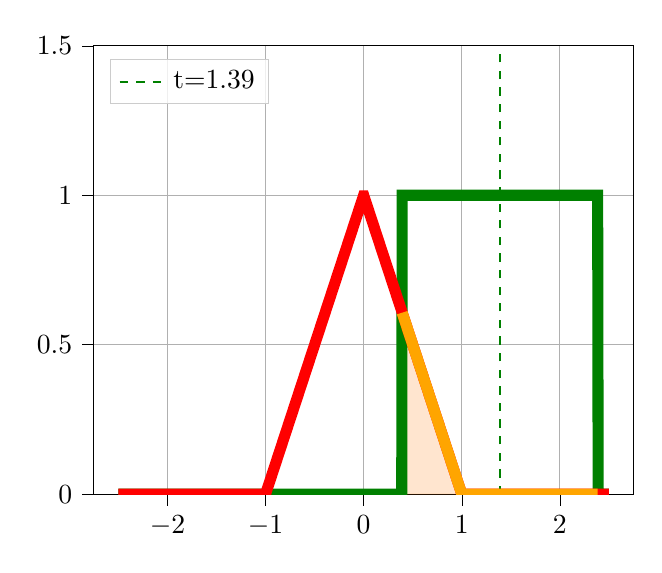
\begin{tikzpicture}

\definecolor{color0}{rgb}{1,0.498039215686275,0.0549019607843137}
\definecolor{color1}{rgb}{1,0.647058823529412,0}

\begin{axis}[
legend cell align={left},
legend style={fill opacity=0.8, draw opacity=1, text opacity=1, at={(0.03,0.97)}, anchor=north west, draw=white!80!black},
tick align=outside,
tick pos=left,
x grid style={white!69.0196078431373!black},
xmajorgrids,
xmin=-2.75, xmax=2.75,
xtick style={color=black},
y grid style={white!69.0196078431373!black},
ymajorgrids,
ymin=0, ymax=1.5,
ytick style={color=black}
]
\path [draw=color0, fill=color0, opacity=0.2]
(axis cs:0.392892892892893,0.607107107107107)
--(axis cs:0.392892892892893,0)
--(axis cs:0.397897897897898,0)
--(axis cs:0.402902902902903,0)
--(axis cs:0.407907907907908,0)
--(axis cs:0.412912912912913,0)
--(axis cs:0.417917917917918,0)
--(axis cs:0.422922922922923,0)
--(axis cs:0.427927927927928,0)
--(axis cs:0.432932932932933,0)
--(axis cs:0.437937937937938,0)
--(axis cs:0.442942942942943,0)
--(axis cs:0.447947947947948,0)
--(axis cs:0.452952952952953,0)
--(axis cs:0.457957957957958,0)
--(axis cs:0.462962962962963,0)
--(axis cs:0.467967967967968,0)
--(axis cs:0.472972972972973,0)
--(axis cs:0.477977977977978,0)
--(axis cs:0.482982982982983,0)
--(axis cs:0.487987987987988,0)
--(axis cs:0.492992992992993,0)
--(axis cs:0.497997997997998,0)
--(axis cs:0.503003003003003,0)
--(axis cs:0.508008008008008,0)
--(axis cs:0.513013013013013,0)
--(axis cs:0.518018018018018,0)
--(axis cs:0.523023023023023,0)
--(axis cs:0.528028028028028,0)
--(axis cs:0.533033033033033,0)
--(axis cs:0.538038038038038,0)
--(axis cs:0.543043043043043,0)
--(axis cs:0.548048048048048,0)
--(axis cs:0.553053053053053,0)
--(axis cs:0.558058058058058,0)
--(axis cs:0.563063063063063,0)
--(axis cs:0.568068068068068,0)
--(axis cs:0.573073073073073,0)
--(axis cs:0.578078078078078,0)
--(axis cs:0.583083083083083,0)
--(axis cs:0.588088088088088,0)
--(axis cs:0.593093093093093,0)
--(axis cs:0.598098098098098,0)
--(axis cs:0.603103103103103,0)
--(axis cs:0.608108108108108,0)
--(axis cs:0.613113113113113,0)
--(axis cs:0.618118118118118,0)
--(axis cs:0.623123123123123,0)
--(axis cs:0.628128128128128,0)
--(axis cs:0.633133133133133,0)
--(axis cs:0.638138138138138,0)
--(axis cs:0.643143143143143,0)
--(axis cs:0.648148148148148,0)
--(axis cs:0.653153153153153,0)
--(axis cs:0.658158158158158,0)
--(axis cs:0.663163163163163,0)
--(axis cs:0.668168168168168,0)
--(axis cs:0.673173173173173,0)
--(axis cs:0.678178178178178,0)
--(axis cs:0.683183183183183,0)
--(axis cs:0.688188188188188,0)
--(axis cs:0.693193193193193,0)
--(axis cs:0.698198198198198,0)
--(axis cs:0.703203203203203,0)
--(axis cs:0.708208208208208,0)
--(axis cs:0.713213213213213,0)
--(axis cs:0.718218218218218,0)
--(axis cs:0.723223223223223,0)
--(axis cs:0.728228228228228,0)
--(axis cs:0.733233233233233,0)
--(axis cs:0.738238238238238,0)
--(axis cs:0.743243243243243,0)
--(axis cs:0.748248248248248,0)
--(axis cs:0.753253253253253,0)
--(axis cs:0.758258258258258,0)
--(axis cs:0.763263263263263,0)
--(axis cs:0.768268268268268,0)
--(axis cs:0.773273273273273,0)
--(axis cs:0.778278278278278,0)
--(axis cs:0.783283283283283,0)
--(axis cs:0.788288288288288,0)
--(axis cs:0.793293293293293,0)
--(axis cs:0.798298298298298,0)
--(axis cs:0.803303303303303,0)
--(axis cs:0.808308308308308,0)
--(axis cs:0.813313313313313,0)
--(axis cs:0.818318318318318,0)
--(axis cs:0.823323323323323,0)
--(axis cs:0.828328328328328,0)
--(axis cs:0.833333333333333,0)
--(axis cs:0.838338338338338,0)
--(axis cs:0.843343343343343,0)
--(axis cs:0.848348348348348,0)
--(axis cs:0.853353353353353,0)
--(axis cs:0.858358358358358,0)
--(axis cs:0.863363363363364,0)
--(axis cs:0.868368368368369,0)
--(axis cs:0.873373373373374,0)
--(axis cs:0.878378378378379,0)
--(axis cs:0.883383383383384,0)
--(axis cs:0.888388388388389,0)
--(axis cs:0.893393393393394,0)
--(axis cs:0.898398398398399,0)
--(axis cs:0.903403403403404,0)
--(axis cs:0.908408408408409,0)
--(axis cs:0.913413413413414,0)
--(axis cs:0.918418418418419,0)
--(axis cs:0.923423423423424,0)
--(axis cs:0.928428428428429,0)
--(axis cs:0.933433433433434,0)
--(axis cs:0.938438438438439,0)
--(axis cs:0.943443443443444,0)
--(axis cs:0.948448448448449,0)
--(axis cs:0.953453453453454,0)
--(axis cs:0.958458458458459,0)
--(axis cs:0.963463463463464,0)
--(axis cs:0.968468468468469,0)
--(axis cs:0.973473473473474,0)
--(axis cs:0.978478478478479,0)
--(axis cs:0.983483483483484,0)
--(axis cs:0.988488488488489,0)
--(axis cs:0.993493493493494,0)
--(axis cs:0.998498498498499,0)
--(axis cs:1.0035035035035,0)
--(axis cs:1.00850850850851,0)
--(axis cs:1.01351351351351,0)
--(axis cs:1.01851851851852,0)
--(axis cs:1.02352352352352,0)
--(axis cs:1.02852852852853,0)
--(axis cs:1.03353353353353,0)
--(axis cs:1.03853853853854,0)
--(axis cs:1.04354354354354,0)
--(axis cs:1.04854854854855,0)
--(axis cs:1.05355355355355,0)
--(axis cs:1.05855855855856,0)
--(axis cs:1.06356356356356,0)
--(axis cs:1.06856856856857,0)
--(axis cs:1.07357357357357,0)
--(axis cs:1.07857857857858,0)
--(axis cs:1.08358358358358,0)
--(axis cs:1.08858858858859,0)
--(axis cs:1.09359359359359,0)
--(axis cs:1.0985985985986,0)
--(axis cs:1.1036036036036,0)
--(axis cs:1.10860860860861,0)
--(axis cs:1.11361361361361,0)
--(axis cs:1.11861861861862,0)
--(axis cs:1.12362362362362,0)
--(axis cs:1.12862862862863,0)
--(axis cs:1.13363363363363,0)
--(axis cs:1.13863863863864,0)
--(axis cs:1.14364364364364,0)
--(axis cs:1.14864864864865,0)
--(axis cs:1.15365365365365,0)
--(axis cs:1.15865865865866,0)
--(axis cs:1.16366366366366,0)
--(axis cs:1.16866866866867,0)
--(axis cs:1.17367367367367,0)
--(axis cs:1.17867867867868,0)
--(axis cs:1.18368368368368,0)
--(axis cs:1.18868868868869,0)
--(axis cs:1.19369369369369,0)
--(axis cs:1.1986986986987,0)
--(axis cs:1.2037037037037,0)
--(axis cs:1.20870870870871,0)
--(axis cs:1.21371371371371,0)
--(axis cs:1.21871871871872,0)
--(axis cs:1.22372372372372,0)
--(axis cs:1.22872872872873,0)
--(axis cs:1.23373373373373,0)
--(axis cs:1.23873873873874,0)
--(axis cs:1.24374374374374,0)
--(axis cs:1.24874874874875,0)
--(axis cs:1.25375375375375,0)
--(axis cs:1.25875875875876,0)
--(axis cs:1.26376376376376,0)
--(axis cs:1.26876876876877,0)
--(axis cs:1.27377377377377,0)
--(axis cs:1.27877877877878,0)
--(axis cs:1.28378378378378,0)
--(axis cs:1.28878878878879,0)
--(axis cs:1.29379379379379,0)
--(axis cs:1.2987987987988,0)
--(axis cs:1.3038038038038,0)
--(axis cs:1.30880880880881,0)
--(axis cs:1.31381381381381,0)
--(axis cs:1.31881881881882,0)
--(axis cs:1.32382382382382,0)
--(axis cs:1.32882882882883,0)
--(axis cs:1.33383383383383,0)
--(axis cs:1.33883883883884,0)
--(axis cs:1.34384384384384,0)
--(axis cs:1.34884884884885,0)
--(axis cs:1.35385385385385,0)
--(axis cs:1.35885885885886,0)
--(axis cs:1.36386386386386,0)
--(axis cs:1.36886886886887,0)
--(axis cs:1.37387387387387,0)
--(axis cs:1.37887887887888,0)
--(axis cs:1.38388388388388,0)
--(axis cs:1.38888888888889,0)
--(axis cs:1.39389389389389,0)
--(axis cs:1.3988988988989,0)
--(axis cs:1.4039039039039,0)
--(axis cs:1.40890890890891,0)
--(axis cs:1.41391391391391,0)
--(axis cs:1.41891891891892,0)
--(axis cs:1.42392392392392,0)
--(axis cs:1.42892892892893,0)
--(axis cs:1.43393393393393,0)
--(axis cs:1.43893893893894,0)
--(axis cs:1.44394394394394,0)
--(axis cs:1.44894894894895,0)
--(axis cs:1.45395395395395,0)
--(axis cs:1.45895895895896,0)
--(axis cs:1.46396396396396,0)
--(axis cs:1.46896896896897,0)
--(axis cs:1.47397397397397,0)
--(axis cs:1.47897897897898,0)
--(axis cs:1.48398398398398,0)
--(axis cs:1.48898898898899,0)
--(axis cs:1.49399399399399,0)
--(axis cs:1.498998998999,0)
--(axis cs:1.504004004004,0)
--(axis cs:1.50900900900901,0)
--(axis cs:1.51401401401401,0)
--(axis cs:1.51901901901902,0)
--(axis cs:1.52402402402402,0)
--(axis cs:1.52902902902903,0)
--(axis cs:1.53403403403403,0)
--(axis cs:1.53903903903904,0)
--(axis cs:1.54404404404404,0)
--(axis cs:1.54904904904905,0)
--(axis cs:1.55405405405405,0)
--(axis cs:1.55905905905906,0)
--(axis cs:1.56406406406406,0)
--(axis cs:1.56906906906907,0)
--(axis cs:1.57407407407407,0)
--(axis cs:1.57907907907908,0)
--(axis cs:1.58408408408408,0)
--(axis cs:1.58908908908909,0)
--(axis cs:1.59409409409409,0)
--(axis cs:1.5990990990991,0)
--(axis cs:1.6041041041041,0)
--(axis cs:1.60910910910911,0)
--(axis cs:1.61411411411411,0)
--(axis cs:1.61911911911912,0)
--(axis cs:1.62412412412412,0)
--(axis cs:1.62912912912913,0)
--(axis cs:1.63413413413413,0)
--(axis cs:1.63913913913914,0)
--(axis cs:1.64414414414414,0)
--(axis cs:1.64914914914915,0)
--(axis cs:1.65415415415415,0)
--(axis cs:1.65915915915916,0)
--(axis cs:1.66416416416416,0)
--(axis cs:1.66916916916917,0)
--(axis cs:1.67417417417417,0)
--(axis cs:1.67917917917918,0)
--(axis cs:1.68418418418418,0)
--(axis cs:1.68918918918919,0)
--(axis cs:1.69419419419419,0)
--(axis cs:1.6991991991992,0)
--(axis cs:1.7042042042042,0)
--(axis cs:1.70920920920921,0)
--(axis cs:1.71421421421421,0)
--(axis cs:1.71921921921922,0)
--(axis cs:1.72422422422422,0)
--(axis cs:1.72922922922923,0)
--(axis cs:1.73423423423423,0)
--(axis cs:1.73923923923924,0)
--(axis cs:1.74424424424424,0)
--(axis cs:1.74924924924925,0)
--(axis cs:1.75425425425425,0)
--(axis cs:1.75925925925926,0)
--(axis cs:1.76426426426426,0)
--(axis cs:1.76926926926927,0)
--(axis cs:1.77427427427427,0)
--(axis cs:1.77927927927928,0)
--(axis cs:1.78428428428428,0)
--(axis cs:1.78928928928929,0)
--(axis cs:1.79429429429429,0)
--(axis cs:1.7992992992993,0)
--(axis cs:1.8043043043043,0)
--(axis cs:1.80930930930931,0)
--(axis cs:1.81431431431431,0)
--(axis cs:1.81931931931932,0)
--(axis cs:1.82432432432432,0)
--(axis cs:1.82932932932933,0)
--(axis cs:1.83433433433433,0)
--(axis cs:1.83933933933934,0)
--(axis cs:1.84434434434434,0)
--(axis cs:1.84934934934935,0)
--(axis cs:1.85435435435435,0)
--(axis cs:1.85935935935936,0)
--(axis cs:1.86436436436436,0)
--(axis cs:1.86936936936937,0)
--(axis cs:1.87437437437437,0)
--(axis cs:1.87937937937938,0)
--(axis cs:1.88438438438438,0)
--(axis cs:1.88938938938939,0)
--(axis cs:1.89439439439439,0)
--(axis cs:1.8993993993994,0)
--(axis cs:1.9044044044044,0)
--(axis cs:1.90940940940941,0)
--(axis cs:1.91441441441441,0)
--(axis cs:1.91941941941942,0)
--(axis cs:1.92442442442442,0)
--(axis cs:1.92942942942943,0)
--(axis cs:1.93443443443443,0)
--(axis cs:1.93943943943944,0)
--(axis cs:1.94444444444444,0)
--(axis cs:1.94944944944945,0)
--(axis cs:1.95445445445445,0)
--(axis cs:1.95945945945946,0)
--(axis cs:1.96446446446446,0)
--(axis cs:1.96946946946947,0)
--(axis cs:1.97447447447447,0)
--(axis cs:1.97947947947948,0)
--(axis cs:1.98448448448448,0)
--(axis cs:1.98948948948949,0)
--(axis cs:1.99449449449449,0)
--(axis cs:1.9994994994995,0)
--(axis cs:2.0045045045045,0)
--(axis cs:2.00950950950951,0)
--(axis cs:2.01451451451451,0)
--(axis cs:2.01951951951952,0)
--(axis cs:2.02452452452452,0)
--(axis cs:2.02952952952953,0)
--(axis cs:2.03453453453453,0)
--(axis cs:2.03953953953954,0)
--(axis cs:2.04454454454454,0)
--(axis cs:2.04954954954955,0)
--(axis cs:2.05455455455455,0)
--(axis cs:2.05955955955956,0)
--(axis cs:2.06456456456456,0)
--(axis cs:2.06956956956957,0)
--(axis cs:2.07457457457457,0)
--(axis cs:2.07957957957958,0)
--(axis cs:2.08458458458458,0)
--(axis cs:2.08958958958959,0)
--(axis cs:2.09459459459459,0)
--(axis cs:2.0995995995996,0)
--(axis cs:2.1046046046046,0)
--(axis cs:2.10960960960961,0)
--(axis cs:2.11461461461461,0)
--(axis cs:2.11961961961962,0)
--(axis cs:2.12462462462462,0)
--(axis cs:2.12962962962963,0)
--(axis cs:2.13463463463463,0)
--(axis cs:2.13963963963964,0)
--(axis cs:2.14464464464464,0)
--(axis cs:2.14964964964965,0)
--(axis cs:2.15465465465465,0)
--(axis cs:2.15965965965966,0)
--(axis cs:2.16466466466466,0)
--(axis cs:2.16966966966967,0)
--(axis cs:2.17467467467467,0)
--(axis cs:2.17967967967968,0)
--(axis cs:2.18468468468468,0)
--(axis cs:2.18968968968969,0)
--(axis cs:2.19469469469469,0)
--(axis cs:2.1996996996997,0)
--(axis cs:2.2047047047047,0)
--(axis cs:2.20970970970971,0)
--(axis cs:2.21471471471471,0)
--(axis cs:2.21971971971972,0)
--(axis cs:2.22472472472472,0)
--(axis cs:2.22972972972973,0)
--(axis cs:2.23473473473473,0)
--(axis cs:2.23973973973974,0)
--(axis cs:2.24474474474474,0)
--(axis cs:2.24974974974975,0)
--(axis cs:2.25475475475475,0)
--(axis cs:2.25975975975976,0)
--(axis cs:2.26476476476476,0)
--(axis cs:2.26976976976977,0)
--(axis cs:2.27477477477477,0)
--(axis cs:2.27977977977978,0)
--(axis cs:2.28478478478478,0)
--(axis cs:2.28978978978979,0)
--(axis cs:2.29479479479479,0)
--(axis cs:2.2997997997998,0)
--(axis cs:2.3048048048048,0)
--(axis cs:2.30980980980981,0)
--(axis cs:2.31481481481481,0)
--(axis cs:2.31981981981982,0)
--(axis cs:2.32482482482482,0)
--(axis cs:2.32982982982983,0)
--(axis cs:2.33483483483483,0)
--(axis cs:2.33983983983984,0)
--(axis cs:2.34484484484484,0)
--(axis cs:2.34984984984985,0)
--(axis cs:2.35485485485485,0)
--(axis cs:2.35985985985986,0)
--(axis cs:2.36486486486486,0)
--(axis cs:2.36986986986987,0)
--(axis cs:2.37487487487487,0)
--(axis cs:2.37987987987988,0)
--(axis cs:2.38488488488488,0)
--(axis cs:2.38488488488488,0)
--(axis cs:2.38488488488488,0)
--(axis cs:2.37987987987988,0)
--(axis cs:2.37487487487487,0)
--(axis cs:2.36986986986987,0)
--(axis cs:2.36486486486486,0)
--(axis cs:2.35985985985986,0)
--(axis cs:2.35485485485485,0)
--(axis cs:2.34984984984985,0)
--(axis cs:2.34484484484484,0)
--(axis cs:2.33983983983984,0)
--(axis cs:2.33483483483483,0)
--(axis cs:2.32982982982983,0)
--(axis cs:2.32482482482482,0)
--(axis cs:2.31981981981982,0)
--(axis cs:2.31481481481481,0)
--(axis cs:2.30980980980981,0)
--(axis cs:2.3048048048048,0)
--(axis cs:2.2997997997998,0)
--(axis cs:2.29479479479479,0)
--(axis cs:2.28978978978979,0)
--(axis cs:2.28478478478478,0)
--(axis cs:2.27977977977978,0)
--(axis cs:2.27477477477477,0)
--(axis cs:2.26976976976977,0)
--(axis cs:2.26476476476476,0)
--(axis cs:2.25975975975976,0)
--(axis cs:2.25475475475475,0)
--(axis cs:2.24974974974975,0)
--(axis cs:2.24474474474474,0)
--(axis cs:2.23973973973974,0)
--(axis cs:2.23473473473473,0)
--(axis cs:2.22972972972973,0)
--(axis cs:2.22472472472472,0)
--(axis cs:2.21971971971972,0)
--(axis cs:2.21471471471471,0)
--(axis cs:2.20970970970971,0)
--(axis cs:2.2047047047047,0)
--(axis cs:2.1996996996997,0)
--(axis cs:2.19469469469469,0)
--(axis cs:2.18968968968969,0)
--(axis cs:2.18468468468468,0)
--(axis cs:2.17967967967968,0)
--(axis cs:2.17467467467467,0)
--(axis cs:2.16966966966967,0)
--(axis cs:2.16466466466466,0)
--(axis cs:2.15965965965966,0)
--(axis cs:2.15465465465465,0)
--(axis cs:2.14964964964965,0)
--(axis cs:2.14464464464464,0)
--(axis cs:2.13963963963964,0)
--(axis cs:2.13463463463463,0)
--(axis cs:2.12962962962963,0)
--(axis cs:2.12462462462462,0)
--(axis cs:2.11961961961962,0)
--(axis cs:2.11461461461461,0)
--(axis cs:2.10960960960961,0)
--(axis cs:2.1046046046046,0)
--(axis cs:2.0995995995996,0)
--(axis cs:2.09459459459459,0)
--(axis cs:2.08958958958959,0)
--(axis cs:2.08458458458458,0)
--(axis cs:2.07957957957958,0)
--(axis cs:2.07457457457457,0)
--(axis cs:2.06956956956957,0)
--(axis cs:2.06456456456456,0)
--(axis cs:2.05955955955956,0)
--(axis cs:2.05455455455455,0)
--(axis cs:2.04954954954955,0)
--(axis cs:2.04454454454454,0)
--(axis cs:2.03953953953954,0)
--(axis cs:2.03453453453453,0)
--(axis cs:2.02952952952953,0)
--(axis cs:2.02452452452452,0)
--(axis cs:2.01951951951952,0)
--(axis cs:2.01451451451451,0)
--(axis cs:2.00950950950951,0)
--(axis cs:2.0045045045045,0)
--(axis cs:1.9994994994995,0)
--(axis cs:1.99449449449449,0)
--(axis cs:1.98948948948949,0)
--(axis cs:1.98448448448448,0)
--(axis cs:1.97947947947948,0)
--(axis cs:1.97447447447447,0)
--(axis cs:1.96946946946947,0)
--(axis cs:1.96446446446446,0)
--(axis cs:1.95945945945946,0)
--(axis cs:1.95445445445445,0)
--(axis cs:1.94944944944945,0)
--(axis cs:1.94444444444444,0)
--(axis cs:1.93943943943944,0)
--(axis cs:1.93443443443443,0)
--(axis cs:1.92942942942943,0)
--(axis cs:1.92442442442442,0)
--(axis cs:1.91941941941942,0)
--(axis cs:1.91441441441441,0)
--(axis cs:1.90940940940941,0)
--(axis cs:1.9044044044044,0)
--(axis cs:1.8993993993994,0)
--(axis cs:1.89439439439439,0)
--(axis cs:1.88938938938939,0)
--(axis cs:1.88438438438438,0)
--(axis cs:1.87937937937938,0)
--(axis cs:1.87437437437437,0)
--(axis cs:1.86936936936937,0)
--(axis cs:1.86436436436436,0)
--(axis cs:1.85935935935936,0)
--(axis cs:1.85435435435435,0)
--(axis cs:1.84934934934935,0)
--(axis cs:1.84434434434434,0)
--(axis cs:1.83933933933934,0)
--(axis cs:1.83433433433433,0)
--(axis cs:1.82932932932933,0)
--(axis cs:1.82432432432432,0)
--(axis cs:1.81931931931932,0)
--(axis cs:1.81431431431431,0)
--(axis cs:1.80930930930931,0)
--(axis cs:1.8043043043043,0)
--(axis cs:1.7992992992993,0)
--(axis cs:1.79429429429429,0)
--(axis cs:1.78928928928929,0)
--(axis cs:1.78428428428428,0)
--(axis cs:1.77927927927928,0)
--(axis cs:1.77427427427427,0)
--(axis cs:1.76926926926927,0)
--(axis cs:1.76426426426426,0)
--(axis cs:1.75925925925926,0)
--(axis cs:1.75425425425425,0)
--(axis cs:1.74924924924925,0)
--(axis cs:1.74424424424424,0)
--(axis cs:1.73923923923924,0)
--(axis cs:1.73423423423423,0)
--(axis cs:1.72922922922923,0)
--(axis cs:1.72422422422422,0)
--(axis cs:1.71921921921922,0)
--(axis cs:1.71421421421421,0)
--(axis cs:1.70920920920921,0)
--(axis cs:1.7042042042042,0)
--(axis cs:1.6991991991992,0)
--(axis cs:1.69419419419419,0)
--(axis cs:1.68918918918919,0)
--(axis cs:1.68418418418418,0)
--(axis cs:1.67917917917918,0)
--(axis cs:1.67417417417417,0)
--(axis cs:1.66916916916917,0)
--(axis cs:1.66416416416416,0)
--(axis cs:1.65915915915916,0)
--(axis cs:1.65415415415415,0)
--(axis cs:1.64914914914915,0)
--(axis cs:1.64414414414414,0)
--(axis cs:1.63913913913914,0)
--(axis cs:1.63413413413413,0)
--(axis cs:1.62912912912913,0)
--(axis cs:1.62412412412412,0)
--(axis cs:1.61911911911912,0)
--(axis cs:1.61411411411411,0)
--(axis cs:1.60910910910911,0)
--(axis cs:1.6041041041041,0)
--(axis cs:1.5990990990991,0)
--(axis cs:1.59409409409409,0)
--(axis cs:1.58908908908909,0)
--(axis cs:1.58408408408408,0)
--(axis cs:1.57907907907908,0)
--(axis cs:1.57407407407407,0)
--(axis cs:1.56906906906907,0)
--(axis cs:1.56406406406406,0)
--(axis cs:1.55905905905906,0)
--(axis cs:1.55405405405405,0)
--(axis cs:1.54904904904905,0)
--(axis cs:1.54404404404404,0)
--(axis cs:1.53903903903904,0)
--(axis cs:1.53403403403403,0)
--(axis cs:1.52902902902903,0)
--(axis cs:1.52402402402402,0)
--(axis cs:1.51901901901902,0)
--(axis cs:1.51401401401401,0)
--(axis cs:1.50900900900901,0)
--(axis cs:1.504004004004,0)
--(axis cs:1.498998998999,0)
--(axis cs:1.49399399399399,0)
--(axis cs:1.48898898898899,0)
--(axis cs:1.48398398398398,0)
--(axis cs:1.47897897897898,0)
--(axis cs:1.47397397397397,0)
--(axis cs:1.46896896896897,0)
--(axis cs:1.46396396396396,0)
--(axis cs:1.45895895895896,0)
--(axis cs:1.45395395395395,0)
--(axis cs:1.44894894894895,0)
--(axis cs:1.44394394394394,0)
--(axis cs:1.43893893893894,0)
--(axis cs:1.43393393393393,0)
--(axis cs:1.42892892892893,0)
--(axis cs:1.42392392392392,0)
--(axis cs:1.41891891891892,0)
--(axis cs:1.41391391391391,0)
--(axis cs:1.40890890890891,0)
--(axis cs:1.4039039039039,0)
--(axis cs:1.3988988988989,0)
--(axis cs:1.39389389389389,0)
--(axis cs:1.38888888888889,0)
--(axis cs:1.38388388388388,0)
--(axis cs:1.37887887887888,0)
--(axis cs:1.37387387387387,0)
--(axis cs:1.36886886886887,0)
--(axis cs:1.36386386386386,0)
--(axis cs:1.35885885885886,0)
--(axis cs:1.35385385385385,0)
--(axis cs:1.34884884884885,0)
--(axis cs:1.34384384384384,0)
--(axis cs:1.33883883883884,0)
--(axis cs:1.33383383383383,0)
--(axis cs:1.32882882882883,0)
--(axis cs:1.32382382382382,0)
--(axis cs:1.31881881881882,0)
--(axis cs:1.31381381381381,0)
--(axis cs:1.30880880880881,0)
--(axis cs:1.3038038038038,0)
--(axis cs:1.2987987987988,0)
--(axis cs:1.29379379379379,0)
--(axis cs:1.28878878878879,0)
--(axis cs:1.28378378378378,0)
--(axis cs:1.27877877877878,0)
--(axis cs:1.27377377377377,0)
--(axis cs:1.26876876876877,0)
--(axis cs:1.26376376376376,0)
--(axis cs:1.25875875875876,0)
--(axis cs:1.25375375375375,0)
--(axis cs:1.24874874874875,0)
--(axis cs:1.24374374374374,0)
--(axis cs:1.23873873873874,0)
--(axis cs:1.23373373373373,0)
--(axis cs:1.22872872872873,0)
--(axis cs:1.22372372372372,0)
--(axis cs:1.21871871871872,0)
--(axis cs:1.21371371371371,0)
--(axis cs:1.20870870870871,0)
--(axis cs:1.2037037037037,0)
--(axis cs:1.1986986986987,0)
--(axis cs:1.19369369369369,0)
--(axis cs:1.18868868868869,0)
--(axis cs:1.18368368368368,0)
--(axis cs:1.17867867867868,0)
--(axis cs:1.17367367367367,0)
--(axis cs:1.16866866866867,0)
--(axis cs:1.16366366366366,0)
--(axis cs:1.15865865865866,0)
--(axis cs:1.15365365365365,0)
--(axis cs:1.14864864864865,0)
--(axis cs:1.14364364364364,0)
--(axis cs:1.13863863863864,0)
--(axis cs:1.13363363363363,0)
--(axis cs:1.12862862862863,0)
--(axis cs:1.12362362362362,0)
--(axis cs:1.11861861861862,0)
--(axis cs:1.11361361361361,0)
--(axis cs:1.10860860860861,0)
--(axis cs:1.1036036036036,0)
--(axis cs:1.0985985985986,0)
--(axis cs:1.09359359359359,0)
--(axis cs:1.08858858858859,0)
--(axis cs:1.08358358358358,0)
--(axis cs:1.07857857857858,0)
--(axis cs:1.07357357357357,0)
--(axis cs:1.06856856856857,0)
--(axis cs:1.06356356356356,0)
--(axis cs:1.05855855855856,0)
--(axis cs:1.05355355355355,0)
--(axis cs:1.04854854854855,0)
--(axis cs:1.04354354354354,0)
--(axis cs:1.03853853853854,0)
--(axis cs:1.03353353353353,0)
--(axis cs:1.02852852852853,0)
--(axis cs:1.02352352352352,0)
--(axis cs:1.01851851851852,0)
--(axis cs:1.01351351351351,0)
--(axis cs:1.00850850850851,0)
--(axis cs:1.0035035035035,0)
--(axis cs:0.998498498498499,0.00150150150150141)
--(axis cs:0.993493493493494,0.00650650650650642)
--(axis cs:0.988488488488489,0.0115115115115114)
--(axis cs:0.983483483483484,0.0165165165165164)
--(axis cs:0.978478478478479,0.0215215215215214)
--(axis cs:0.973473473473474,0.0265265265265264)
--(axis cs:0.968468468468469,0.0315315315315314)
--(axis cs:0.963463463463464,0.0365365365365364)
--(axis cs:0.958458458458459,0.0415415415415414)
--(axis cs:0.953453453453454,0.0465465465465464)
--(axis cs:0.948448448448449,0.0515515515515514)
--(axis cs:0.943443443443444,0.0565565565565564)
--(axis cs:0.938438438438439,0.0615615615615615)
--(axis cs:0.933433433433434,0.0665665665665665)
--(axis cs:0.928428428428429,0.0715715715715715)
--(axis cs:0.923423423423424,0.0765765765765765)
--(axis cs:0.918418418418419,0.0815815815815815)
--(axis cs:0.913413413413414,0.0865865865865865)
--(axis cs:0.908408408408409,0.0915915915915915)
--(axis cs:0.903403403403404,0.0965965965965965)
--(axis cs:0.898398398398399,0.101601601601601)
--(axis cs:0.893393393393394,0.106606606606606)
--(axis cs:0.888388388388389,0.111611611611611)
--(axis cs:0.883383383383384,0.116616616616616)
--(axis cs:0.878378378378379,0.121621621621621)
--(axis cs:0.873373373373374,0.126626626626626)
--(axis cs:0.868368368368369,0.131631631631631)
--(axis cs:0.863363363363364,0.136636636636636)
--(axis cs:0.858358358358358,0.141641641641642)
--(axis cs:0.853353353353353,0.146646646646647)
--(axis cs:0.848348348348348,0.151651651651652)
--(axis cs:0.843343343343343,0.156656656656657)
--(axis cs:0.838338338338338,0.161661661661662)
--(axis cs:0.833333333333333,0.166666666666667)
--(axis cs:0.828328328328328,0.171671671671672)
--(axis cs:0.823323323323323,0.176676676676677)
--(axis cs:0.818318318318318,0.181681681681682)
--(axis cs:0.813313313313313,0.186686686686687)
--(axis cs:0.808308308308308,0.191691691691692)
--(axis cs:0.803303303303303,0.196696696696697)
--(axis cs:0.798298298298298,0.201701701701702)
--(axis cs:0.793293293293293,0.206706706706707)
--(axis cs:0.788288288288288,0.211711711711712)
--(axis cs:0.783283283283283,0.216716716716717)
--(axis cs:0.778278278278278,0.221721721721722)
--(axis cs:0.773273273273273,0.226726726726727)
--(axis cs:0.768268268268268,0.231731731731732)
--(axis cs:0.763263263263263,0.236736736736737)
--(axis cs:0.758258258258258,0.241741741741742)
--(axis cs:0.753253253253253,0.246746746746747)
--(axis cs:0.748248248248248,0.251751751751752)
--(axis cs:0.743243243243243,0.256756756756757)
--(axis cs:0.738238238238238,0.261761761761762)
--(axis cs:0.733233233233233,0.266766766766767)
--(axis cs:0.728228228228228,0.271771771771772)
--(axis cs:0.723223223223223,0.276776776776777)
--(axis cs:0.718218218218218,0.281781781781782)
--(axis cs:0.713213213213213,0.286786786786787)
--(axis cs:0.708208208208208,0.291791791791792)
--(axis cs:0.703203203203203,0.296796796796797)
--(axis cs:0.698198198198198,0.301801801801802)
--(axis cs:0.693193193193193,0.306806806806807)
--(axis cs:0.688188188188188,0.311811811811812)
--(axis cs:0.683183183183183,0.316816816816817)
--(axis cs:0.678178178178178,0.321821821821822)
--(axis cs:0.673173173173173,0.326826826826827)
--(axis cs:0.668168168168168,0.331831831831832)
--(axis cs:0.663163163163163,0.336836836836837)
--(axis cs:0.658158158158158,0.341841841841842)
--(axis cs:0.653153153153153,0.346846846846847)
--(axis cs:0.648148148148148,0.351851851851852)
--(axis cs:0.643143143143143,0.356856856856857)
--(axis cs:0.638138138138138,0.361861861861862)
--(axis cs:0.633133133133133,0.366866866866867)
--(axis cs:0.628128128128128,0.371871871871872)
--(axis cs:0.623123123123123,0.376876876876877)
--(axis cs:0.618118118118118,0.381881881881882)
--(axis cs:0.613113113113113,0.386886886886887)
--(axis cs:0.608108108108108,0.391891891891892)
--(axis cs:0.603103103103103,0.396896896896897)
--(axis cs:0.598098098098098,0.401901901901902)
--(axis cs:0.593093093093093,0.406906906906907)
--(axis cs:0.588088088088088,0.411911911911912)
--(axis cs:0.583083083083083,0.416916916916917)
--(axis cs:0.578078078078078,0.421921921921922)
--(axis cs:0.573073073073073,0.426926926926927)
--(axis cs:0.568068068068068,0.431931931931932)
--(axis cs:0.563063063063063,0.436936936936937)
--(axis cs:0.558058058058058,0.441941941941942)
--(axis cs:0.553053053053053,0.446946946946947)
--(axis cs:0.548048048048048,0.451951951951952)
--(axis cs:0.543043043043043,0.456956956956957)
--(axis cs:0.538038038038038,0.461961961961962)
--(axis cs:0.533033033033033,0.466966966966967)
--(axis cs:0.528028028028028,0.471971971971972)
--(axis cs:0.523023023023023,0.476976976976977)
--(axis cs:0.518018018018018,0.481981981981982)
--(axis cs:0.513013013013013,0.486986986986987)
--(axis cs:0.508008008008008,0.491991991991992)
--(axis cs:0.503003003003003,0.496996996996997)
--(axis cs:0.497997997997998,0.502002002002002)
--(axis cs:0.492992992992993,0.507007007007007)
--(axis cs:0.487987987987988,0.512012012012012)
--(axis cs:0.482982982982983,0.517017017017017)
--(axis cs:0.477977977977978,0.522022022022022)
--(axis cs:0.472972972972973,0.527027027027027)
--(axis cs:0.467967967967968,0.532032032032032)
--(axis cs:0.462962962962963,0.537037037037037)
--(axis cs:0.457957957957958,0.542042042042042)
--(axis cs:0.452952952952953,0.547047047047047)
--(axis cs:0.447947947947948,0.552052052052052)
--(axis cs:0.442942942942943,0.557057057057057)
--(axis cs:0.437937937937938,0.562062062062062)
--(axis cs:0.432932932932933,0.567067067067067)
--(axis cs:0.427927927927928,0.572072072072072)
--(axis cs:0.422922922922923,0.577077077077077)
--(axis cs:0.417917917917918,0.582082082082082)
--(axis cs:0.412912912912913,0.587087087087087)
--(axis cs:0.407907907907908,0.592092092092092)
--(axis cs:0.402902902902903,0.597097097097097)
--(axis cs:0.397897897897898,0.602102102102102)
--(axis cs:0.392892892892893,0.607107107107107)
--cycle;

\addplot [line width=4pt, green!50!black, forget plot]
table {%
-2.5 0
-2.49499499499499 0
-2.48998998998999 0
-2.48498498498498 0
-2.47997997997998 0
-2.47497497497497 0
-2.46996996996997 0
-2.46496496496496 0
-2.45995995995996 0
-2.45495495495495 0
-2.44994994994995 0
-2.44494494494494 0
-2.43993993993994 0
-2.43493493493493 0
-2.42992992992993 0
-2.42492492492492 0
-2.41991991991992 0
-2.41491491491491 0
-2.40990990990991 0
-2.4049049049049 0
-2.3998998998999 0
-2.39489489489489 0
-2.38988988988989 0
-2.38488488488488 0
-2.37987987987988 0
-2.37487487487487 0
-2.36986986986987 0
-2.36486486486486 0
-2.35985985985986 0
-2.35485485485485 0
-2.34984984984985 0
-2.34484484484484 0
-2.33983983983984 0
-2.33483483483483 0
-2.32982982982983 0
-2.32482482482482 0
-2.31981981981982 0
-2.31481481481481 0
-2.30980980980981 0
-2.3048048048048 0
-2.2997997997998 0
-2.29479479479479 0
-2.28978978978979 0
-2.28478478478478 0
-2.27977977977978 0
-2.27477477477477 0
-2.26976976976977 0
-2.26476476476476 0
-2.25975975975976 0
-2.25475475475475 0
-2.24974974974975 0
-2.24474474474474 0
-2.23973973973974 0
-2.23473473473473 0
-2.22972972972973 0
-2.22472472472472 0
-2.21971971971972 0
-2.21471471471471 0
-2.20970970970971 0
-2.2047047047047 0
-2.1996996996997 0
-2.19469469469469 0
-2.18968968968969 0
-2.18468468468468 0
-2.17967967967968 0
-2.17467467467467 0
-2.16966966966967 0
-2.16466466466466 0
-2.15965965965966 0
-2.15465465465465 0
-2.14964964964965 0
-2.14464464464464 0
-2.13963963963964 0
-2.13463463463463 0
-2.12962962962963 0
-2.12462462462462 0
-2.11961961961962 0
-2.11461461461461 0
-2.10960960960961 0
-2.1046046046046 0
-2.0995995995996 0
-2.09459459459459 0
-2.08958958958959 0
-2.08458458458458 0
-2.07957957957958 0
-2.07457457457457 0
-2.06956956956957 0
-2.06456456456456 0
-2.05955955955956 0
-2.05455455455455 0
-2.04954954954955 0
-2.04454454454454 0
-2.03953953953954 0
-2.03453453453453 0
-2.02952952952953 0
-2.02452452452452 0
-2.01951951951952 0
-2.01451451451451 0
-2.00950950950951 0
-2.0045045045045 0
-1.9994994994995 0
-1.99449449449449 0
-1.98948948948949 0
-1.98448448448448 0
-1.97947947947948 0
-1.97447447447447 0
-1.96946946946947 0
-1.96446446446446 0
-1.95945945945946 0
-1.95445445445445 0
-1.94944944944945 0
-1.94444444444444 0
-1.93943943943944 0
-1.93443443443443 0
-1.92942942942943 0
-1.92442442442442 0
-1.91941941941942 0
-1.91441441441441 0
-1.90940940940941 0
-1.9044044044044 0
-1.8993993993994 0
-1.89439439439439 0
-1.88938938938939 0
-1.88438438438438 0
-1.87937937937938 0
-1.87437437437437 0
-1.86936936936937 0
-1.86436436436436 0
-1.85935935935936 0
-1.85435435435435 0
-1.84934934934935 0
-1.84434434434434 0
-1.83933933933934 0
-1.83433433433433 0
-1.82932932932933 0
-1.82432432432432 0
-1.81931931931932 0
-1.81431431431431 0
-1.80930930930931 0
-1.8043043043043 0
-1.7992992992993 0
-1.79429429429429 0
-1.78928928928929 0
-1.78428428428428 0
-1.77927927927928 0
-1.77427427427427 0
-1.76926926926927 0
-1.76426426426426 0
-1.75925925925926 0
-1.75425425425425 0
-1.74924924924925 0
-1.74424424424424 0
-1.73923923923924 0
-1.73423423423423 0
-1.72922922922923 0
-1.72422422422422 0
-1.71921921921922 0
-1.71421421421421 0
-1.70920920920921 0
-1.7042042042042 0
-1.6991991991992 0
-1.69419419419419 0
-1.68918918918919 0
-1.68418418418418 0
-1.67917917917918 0
-1.67417417417417 0
-1.66916916916917 0
-1.66416416416416 0
-1.65915915915916 0
-1.65415415415415 0
-1.64914914914915 0
-1.64414414414414 0
-1.63913913913914 0
-1.63413413413413 0
-1.62912912912913 0
-1.62412412412412 0
-1.61911911911912 0
-1.61411411411411 0
-1.60910910910911 0
-1.6041041041041 0
-1.5990990990991 0
-1.59409409409409 0
-1.58908908908909 0
-1.58408408408408 0
-1.57907907907908 0
-1.57407407407407 0
-1.56906906906907 0
-1.56406406406406 0
-1.55905905905906 0
-1.55405405405405 0
-1.54904904904905 0
-1.54404404404404 0
-1.53903903903904 0
-1.53403403403403 0
-1.52902902902903 0
-1.52402402402402 0
-1.51901901901902 0
-1.51401401401401 0
-1.50900900900901 0
-1.504004004004 0
-1.498998998999 0
-1.49399399399399 0
-1.48898898898899 0
-1.48398398398398 0
-1.47897897897898 0
-1.47397397397397 0
-1.46896896896897 0
-1.46396396396396 0
-1.45895895895896 0
-1.45395395395395 0
-1.44894894894895 0
-1.44394394394394 0
-1.43893893893894 0
-1.43393393393393 0
-1.42892892892893 0
-1.42392392392392 0
-1.41891891891892 0
-1.41391391391391 0
-1.40890890890891 0
-1.4039039039039 0
-1.3988988988989 0
-1.39389389389389 0
-1.38888888888889 0
-1.38388388388388 0
-1.37887887887888 0
-1.37387387387387 0
-1.36886886886887 0
-1.36386386386386 0
-1.35885885885886 0
-1.35385385385385 0
-1.34884884884885 0
-1.34384384384384 0
-1.33883883883884 0
-1.33383383383383 0
-1.32882882882883 0
-1.32382382382382 0
-1.31881881881882 0
-1.31381381381381 0
-1.30880880880881 0
-1.3038038038038 0
-1.2987987987988 0
-1.29379379379379 0
-1.28878878878879 0
-1.28378378378378 0
-1.27877877877878 0
-1.27377377377377 0
-1.26876876876877 0
-1.26376376376376 0
-1.25875875875876 0
-1.25375375375375 0
-1.24874874874875 0
-1.24374374374374 0
-1.23873873873874 0
-1.23373373373373 0
-1.22872872872873 0
-1.22372372372372 0
-1.21871871871872 0
-1.21371371371371 0
-1.20870870870871 0
-1.2037037037037 0
-1.1986986986987 0
-1.19369369369369 0
-1.18868868868869 0
-1.18368368368368 0
-1.17867867867868 0
-1.17367367367367 0
-1.16866866866867 0
-1.16366366366366 0
-1.15865865865866 0
-1.15365365365365 0
-1.14864864864865 0
-1.14364364364364 0
-1.13863863863864 0
-1.13363363363363 0
-1.12862862862863 0
-1.12362362362362 0
-1.11861861861862 0
-1.11361361361361 0
-1.10860860860861 0
-1.1036036036036 0
-1.0985985985986 0
-1.09359359359359 0
-1.08858858858859 0
-1.08358358358358 0
-1.07857857857858 0
-1.07357357357357 0
-1.06856856856857 0
-1.06356356356356 0
-1.05855855855856 0
-1.05355355355355 0
-1.04854854854855 0
-1.04354354354354 0
-1.03853853853854 0
-1.03353353353353 0
-1.02852852852853 0
-1.02352352352352 0
-1.01851851851852 0
-1.01351351351351 0
-1.00850850850851 0
-1.0035035035035 0
-0.998498498498499 0
-0.993493493493494 0
-0.988488488488489 0
-0.983483483483484 0
-0.978478478478479 0
-0.973473473473474 0
-0.968468468468469 0
-0.963463463463464 0
-0.958458458458459 0
-0.953453453453454 0
-0.948448448448449 0
-0.943443443443444 0
-0.938438438438439 0
-0.933433433433434 0
-0.928428428428429 0
-0.923423423423424 0
-0.918418418418419 0
-0.913413413413414 0
-0.908408408408409 0
-0.903403403403404 0
-0.898398398398399 0
-0.893393393393393 0
-0.888388388388388 0
-0.883383383383383 0
-0.878378378378378 0
-0.873373373373373 0
-0.868368368368368 0
-0.863363363363363 0
-0.858358358358358 0
-0.853353353353353 0
-0.848348348348348 0
-0.843343343343343 0
-0.838338338338338 0
-0.833333333333333 0
-0.828328328328328 0
-0.823323323323323 0
-0.818318318318318 0
-0.813313313313313 0
-0.808308308308308 0
-0.803303303303303 0
-0.798298298298298 0
-0.793293293293293 0
-0.788288288288288 0
-0.783283283283283 0
-0.778278278278278 0
-0.773273273273273 0
-0.768268268268268 0
-0.763263263263263 0
-0.758258258258258 0
-0.753253253253253 0
-0.748248248248248 0
-0.743243243243243 0
-0.738238238238238 0
-0.733233233233233 0
-0.728228228228228 0
-0.723223223223223 0
-0.718218218218218 0
-0.713213213213213 0
-0.708208208208208 0
-0.703203203203203 0
-0.698198198198198 0
-0.693193193193193 0
-0.688188188188188 0
-0.683183183183183 0
-0.678178178178178 0
-0.673173173173173 0
-0.668168168168168 0
-0.663163163163163 0
-0.658158158158158 0
-0.653153153153153 0
-0.648148148148148 0
-0.643143143143143 0
-0.638138138138138 0
-0.633133133133133 0
-0.628128128128128 0
-0.623123123123123 0
-0.618118118118118 0
-0.613113113113113 0
-0.608108108108108 0
-0.603103103103103 0
-0.598098098098098 0
-0.593093093093093 0
-0.588088088088088 0
-0.583083083083083 0
-0.578078078078078 0
-0.573073073073073 0
-0.568068068068068 0
-0.563063063063063 0
-0.558058058058058 0
-0.553053053053053 0
-0.548048048048048 0
-0.543043043043043 0
-0.538038038038038 0
-0.533033033033033 0
-0.528028028028028 0
-0.523023023023023 0
-0.518018018018018 0
-0.513013013013013 0
-0.508008008008008 0
-0.503003003003003 0
-0.497997997997998 0
-0.492992992992993 0
-0.487987987987988 0
-0.482982982982983 0
-0.477977977977978 0
-0.472972972972973 0
-0.467967967967968 0
-0.462962962962963 0
-0.457957957957958 0
-0.452952952952953 0
-0.447947947947948 0
-0.442942942942943 0
-0.437937937937938 0
-0.432932932932933 0
-0.427927927927928 0
-0.422922922922923 0
-0.417917917917918 0
-0.412912912912913 0
-0.407907907907908 0
-0.402902902902903 0
-0.397897897897898 0
-0.392892892892893 0
-0.387887887887888 0
-0.382882882882883 0
-0.377877877877878 0
-0.372872872872873 0
-0.367867867867868 0
-0.362862862862863 0
-0.357857857857858 0
-0.352852852852853 0
-0.347847847847848 0
-0.342842842842843 0
-0.337837837837838 0
-0.332832832832833 0
-0.327827827827828 0
-0.322822822822823 0
-0.317817817817818 0
-0.312812812812813 0
-0.307807807807808 0
-0.302802802802803 0
-0.297797797797798 0
-0.292792792792793 0
-0.287787787787788 0
-0.282782782782783 0
-0.277777777777778 0
-0.272772772772773 0
-0.267767767767768 0
-0.262762762762763 0
-0.257757757757758 0
-0.252752752752753 0
-0.247747747747748 0
-0.242742742742743 0
-0.237737737737738 0
-0.232732732732733 0
-0.227727727727728 0
-0.222722722722723 0
-0.217717717717718 0
-0.212712712712713 0
-0.207707707707708 0
-0.202702702702703 0
-0.197697697697698 0
-0.192692692692693 0
-0.187687687687688 0
-0.182682682682683 0
-0.177677677677678 0
-0.172672672672673 0
-0.167667667667668 0
-0.162662662662663 0
-0.157657657657658 0
-0.152652652652653 0
-0.147647647647648 0
-0.142642642642643 0
-0.137637637637638 0
-0.132632632632633 0
-0.127627627627628 0
-0.122622622622623 0
-0.117617617617618 0
-0.112612612612613 0
-0.107607607607608 0
-0.102602602602603 0
-0.0975975975975976 0
-0.0925925925925926 0
-0.0875875875875876 0
-0.0825825825825826 0
-0.0775775775775776 0
-0.0725725725725725 0
-0.0675675675675675 0
-0.0625625625625625 0
-0.0575575575575575 0
-0.0525525525525525 0
-0.0475475475475475 0
-0.0425425425425425 0
-0.0375375375375375 0
-0.0325325325325325 0
-0.0275275275275275 0
-0.0225225225225225 0
-0.0175175175175175 0
-0.0125125125125125 0
-0.0075075075075075 0
-0.0025025025025025 0
0.0025025025025025 0
0.0075075075075075 0
0.0125125125125125 0
0.0175175175175175 0
0.0225225225225225 0
0.0275275275275275 0
0.0325325325325325 0
0.0375375375375375 0
0.0425425425425425 0
0.0475475475475475 0
0.0525525525525525 0
0.0575575575575575 0
0.0625625625625625 0
0.0675675675675675 0
0.0725725725725725 0
0.0775775775775776 0
0.0825825825825826 0
0.0875875875875876 0
0.0925925925925926 0
0.0975975975975976 0
0.102602602602603 0
0.107607607607608 0
0.112612612612613 0
0.117617617617618 0
0.122622622622623 0
0.127627627627628 0
0.132632632632633 0
0.137637637637638 0
0.142642642642643 0
0.147647647647648 0
0.152652652652653 0
0.157657657657658 0
0.162662662662663 0
0.167667667667668 0
0.172672672672673 0
0.177677677677678 0
0.182682682682683 0
0.187687687687688 0
0.192692692692693 0
0.197697697697698 0
0.202702702702703 0
0.207707707707708 0
0.212712712712713 0
0.217717717717718 0
0.222722722722723 0
0.227727727727728 0
0.232732732732733 0
0.237737737737738 0
0.242742742742743 0
0.247747747747748 0
0.252752752752753 0
0.257757757757758 0
0.262762762762763 0
0.267767767767768 0
0.272772772772773 0
0.277777777777778 0
0.282782782782783 0
0.287787787787788 0
0.292792792792793 0
0.297797797797798 0
0.302802802802803 0
0.307807807807808 0
0.312812812812813 0
0.317817817817818 0
0.322822822822823 0
0.327827827827828 0
0.332832832832833 0
0.337837837837838 0
0.342842842842843 0
0.347847847847848 0
0.352852852852853 0
0.357857857857858 0
0.362862862862863 0
0.367867867867868 0
0.372872872872873 0
0.377877877877878 0
0.382882882882883 0
0.387887887887888 0
0.392892892892893 1
0.397897897897898 1
0.402902902902903 1
0.407907907907908 1
0.412912912912913 1
0.417917917917918 1
0.422922922922923 1
0.427927927927928 1
0.432932932932933 1
0.437937937937938 1
0.442942942942943 1
0.447947947947948 1
0.452952952952953 1
0.457957957957958 1
0.462962962962963 1
0.467967967967968 1
0.472972972972973 1
0.477977977977978 1
0.482982982982983 1
0.487987987987988 1
0.492992992992993 1
0.497997997997998 1
0.503003003003003 1
0.508008008008008 1
0.513013013013013 1
0.518018018018018 1
0.523023023023023 1
0.528028028028028 1
0.533033033033033 1
0.538038038038038 1
0.543043043043043 1
0.548048048048048 1
0.553053053053053 1
0.558058058058058 1
0.563063063063063 1
0.568068068068068 1
0.573073073073073 1
0.578078078078078 1
0.583083083083083 1
0.588088088088088 1
0.593093093093093 1
0.598098098098098 1
0.603103103103103 1
0.608108108108108 1
0.613113113113113 1
0.618118118118118 1
0.623123123123123 1
0.628128128128128 1
0.633133133133133 1
0.638138138138138 1
0.643143143143143 1
0.648148148148148 1
0.653153153153153 1
0.658158158158158 1
0.663163163163163 1
0.668168168168168 1
0.673173173173173 1
0.678178178178178 1
0.683183183183183 1
0.688188188188188 1
0.693193193193193 1
0.698198198198198 1
0.703203203203203 1
0.708208208208208 1
0.713213213213213 1
0.718218218218218 1
0.723223223223223 1
0.728228228228228 1
0.733233233233233 1
0.738238238238238 1
0.743243243243243 1
0.748248248248248 1
0.753253253253253 1
0.758258258258258 1
0.763263263263263 1
0.768268268268268 1
0.773273273273273 1
0.778278278278278 1
0.783283283283283 1
0.788288288288288 1
0.793293293293293 1
0.798298298298298 1
0.803303303303303 1
0.808308308308308 1
0.813313313313313 1
0.818318318318318 1
0.823323323323323 1
0.828328328328328 1
0.833333333333333 1
0.838338338338338 1
0.843343343343343 1
0.848348348348348 1
0.853353353353353 1
0.858358358358358 1
0.863363363363364 1
0.868368368368369 1
0.873373373373374 1
0.878378378378379 1
0.883383383383384 1
0.888388388388389 1
0.893393393393394 1
0.898398398398399 1
0.903403403403404 1
0.908408408408409 1
0.913413413413414 1
0.918418418418419 1
0.923423423423424 1
0.928428428428429 1
0.933433433433434 1
0.938438438438439 1
0.943443443443444 1
0.948448448448449 1
0.953453453453454 1
0.958458458458459 1
0.963463463463464 1
0.968468468468469 1
0.973473473473474 1
0.978478478478479 1
0.983483483483484 1
0.988488488488489 1
0.993493493493494 1
0.998498498498499 1
1.0035035035035 1
1.00850850850851 1
1.01351351351351 1
1.01851851851852 1
1.02352352352352 1
1.02852852852853 1
1.03353353353353 1
1.03853853853854 1
1.04354354354354 1
1.04854854854855 1
1.05355355355355 1
1.05855855855856 1
1.06356356356356 1
1.06856856856857 1
1.07357357357357 1
1.07857857857858 1
1.08358358358358 1
1.08858858858859 1
1.09359359359359 1
1.0985985985986 1
1.1036036036036 1
1.10860860860861 1
1.11361361361361 1
1.11861861861862 1
1.12362362362362 1
1.12862862862863 1
1.13363363363363 1
1.13863863863864 1
1.14364364364364 1
1.14864864864865 1
1.15365365365365 1
1.15865865865866 1
1.16366366366366 1
1.16866866866867 1
1.17367367367367 1
1.17867867867868 1
1.18368368368368 1
1.18868868868869 1
1.19369369369369 1
1.1986986986987 1
1.2037037037037 1
1.20870870870871 1
1.21371371371371 1
1.21871871871872 1
1.22372372372372 1
1.22872872872873 1
1.23373373373373 1
1.23873873873874 1
1.24374374374374 1
1.24874874874875 1
1.25375375375375 1
1.25875875875876 1
1.26376376376376 1
1.26876876876877 1
1.27377377377377 1
1.27877877877878 1
1.28378378378378 1
1.28878878878879 1
1.29379379379379 1
1.2987987987988 1
1.3038038038038 1
1.30880880880881 1
1.31381381381381 1
1.31881881881882 1
1.32382382382382 1
1.32882882882883 1
1.33383383383383 1
1.33883883883884 1
1.34384384384384 1
1.34884884884885 1
1.35385385385385 1
1.35885885885886 1
1.36386386386386 1
1.36886886886887 1
1.37387387387387 1
1.37887887887888 1
1.38388388388388 1
1.38888888888889 1
1.39389389389389 1
1.3988988988989 1
1.4039039039039 1
1.40890890890891 1
1.41391391391391 1
1.41891891891892 1
1.42392392392392 1
1.42892892892893 1
1.43393393393393 1
1.43893893893894 1
1.44394394394394 1
1.44894894894895 1
1.45395395395395 1
1.45895895895896 1
1.46396396396396 1
1.46896896896897 1
1.47397397397397 1
1.47897897897898 1
1.48398398398398 1
1.48898898898899 1
1.49399399399399 1
1.498998998999 1
1.504004004004 1
1.50900900900901 1
1.51401401401401 1
1.51901901901902 1
1.52402402402402 1
1.52902902902903 1
1.53403403403403 1
1.53903903903904 1
1.54404404404404 1
1.54904904904905 1
1.55405405405405 1
1.55905905905906 1
1.56406406406406 1
1.56906906906907 1
1.57407407407407 1
1.57907907907908 1
1.58408408408408 1
1.58908908908909 1
1.59409409409409 1
1.5990990990991 1
1.6041041041041 1
1.60910910910911 1
1.61411411411411 1
1.61911911911912 1
1.62412412412412 1
1.62912912912913 1
1.63413413413413 1
1.63913913913914 1
1.64414414414414 1
1.64914914914915 1
1.65415415415415 1
1.65915915915916 1
1.66416416416416 1
1.66916916916917 1
1.67417417417417 1
1.67917917917918 1
1.68418418418418 1
1.68918918918919 1
1.69419419419419 1
1.6991991991992 1
1.7042042042042 1
1.70920920920921 1
1.71421421421421 1
1.71921921921922 1
1.72422422422422 1
1.72922922922923 1
1.73423423423423 1
1.73923923923924 1
1.74424424424424 1
1.74924924924925 1
1.75425425425425 1
1.75925925925926 1
1.76426426426426 1
1.76926926926927 1
1.77427427427427 1
1.77927927927928 1
1.78428428428428 1
1.78928928928929 1
1.79429429429429 1
1.7992992992993 1
1.8043043043043 1
1.80930930930931 1
1.81431431431431 1
1.81931931931932 1
1.82432432432432 1
1.82932932932933 1
1.83433433433433 1
1.83933933933934 1
1.84434434434434 1
1.84934934934935 1
1.85435435435435 1
1.85935935935936 1
1.86436436436436 1
1.86936936936937 1
1.87437437437437 1
1.87937937937938 1
1.88438438438438 1
1.88938938938939 1
1.89439439439439 1
1.8993993993994 1
1.9044044044044 1
1.90940940940941 1
1.91441441441441 1
1.91941941941942 1
1.92442442442442 1
1.92942942942943 1
1.93443443443443 1
1.93943943943944 1
1.94444444444444 1
1.94944944944945 1
1.95445445445445 1
1.95945945945946 1
1.96446446446446 1
1.96946946946947 1
1.97447447447447 1
1.97947947947948 1
1.98448448448448 1
1.98948948948949 1
1.99449449449449 1
1.9994994994995 1
2.0045045045045 1
2.00950950950951 1
2.01451451451451 1
2.01951951951952 1
2.02452452452452 1
2.02952952952953 1
2.03453453453453 1
2.03953953953954 1
2.04454454454454 1
2.04954954954955 1
2.05455455455455 1
2.05955955955956 1
2.06456456456456 1
2.06956956956957 1
2.07457457457457 1
2.07957957957958 1
2.08458458458458 1
2.08958958958959 1
2.09459459459459 1
2.0995995995996 1
2.1046046046046 1
2.10960960960961 1
2.11461461461461 1
2.11961961961962 1
2.12462462462462 1
2.12962962962963 1
2.13463463463463 1
2.13963963963964 1
2.14464464464464 1
2.14964964964965 1
2.15465465465465 1
2.15965965965966 1
2.16466466466466 1
2.16966966966967 1
2.17467467467467 1
2.17967967967968 1
2.18468468468468 1
2.18968968968969 1
2.19469469469469 1
2.1996996996997 1
2.2047047047047 1
2.20970970970971 1
2.21471471471471 1
2.21971971971972 1
2.22472472472472 1
2.22972972972973 1
2.23473473473473 1
2.23973973973974 1
2.24474474474474 1
2.24974974974975 1
2.25475475475475 1
2.25975975975976 1
2.26476476476476 1
2.26976976976977 1
2.27477477477477 1
2.27977977977978 1
2.28478478478478 1
2.28978978978979 1
2.29479479479479 1
2.2997997997998 1
2.3048048048048 1
2.30980980980981 1
2.31481481481481 1
2.31981981981982 1
2.32482482482482 1
2.32982982982983 1
2.33483483483483 1
2.33983983983984 1
2.34484484484484 1
2.34984984984985 1
2.35485485485485 1
2.35985985985986 1
2.36486486486486 1
2.36986986986987 1
2.37487487487487 1
2.37987987987988 1
2.38488488488488 1
2.38988988988989 0
2.39489489489489 0
2.3998998998999 0
2.4049049049049 0
2.40990990990991 0
2.41491491491491 0
2.41991991991992 0
2.42492492492492 0
2.42992992992993 0
2.43493493493493 0
2.43993993993994 0
2.44494494494494 0
2.44994994994995 0
2.45495495495495 0
2.45995995995996 0
2.46496496496496 0
2.46996996996997 0
2.47497497497497 0
2.47997997997998 0
2.48498498498498 0
2.48998998998999 0
2.49499499499499 0
2.5 0
};
\addplot [line width=4pt, red, forget plot]
table {%
-2.5 -0
-2.49499499499499 -0
-2.48998998998999 -0
-2.48498498498498 -0
-2.47997997997998 -0
-2.47497497497497 -0
-2.46996996996997 -0
-2.46496496496496 -0
-2.45995995995996 -0
-2.45495495495495 -0
-2.44994994994995 -0
-2.44494494494494 -0
-2.43993993993994 -0
-2.43493493493493 -0
-2.42992992992993 -0
-2.42492492492492 -0
-2.41991991991992 -0
-2.41491491491491 -0
-2.40990990990991 -0
-2.4049049049049 -0
-2.3998998998999 -0
-2.39489489489489 -0
-2.38988988988989 -0
-2.38488488488488 -0
-2.37987987987988 -0
-2.37487487487487 -0
-2.36986986986987 -0
-2.36486486486486 -0
-2.35985985985986 -0
-2.35485485485485 -0
-2.34984984984985 -0
-2.34484484484484 -0
-2.33983983983984 -0
-2.33483483483483 -0
-2.32982982982983 -0
-2.32482482482482 -0
-2.31981981981982 -0
-2.31481481481481 -0
-2.30980980980981 -0
-2.3048048048048 -0
-2.2997997997998 -0
-2.29479479479479 -0
-2.28978978978979 -0
-2.28478478478478 -0
-2.27977977977978 -0
-2.27477477477477 -0
-2.26976976976977 -0
-2.26476476476476 -0
-2.25975975975976 -0
-2.25475475475475 -0
-2.24974974974975 -0
-2.24474474474474 -0
-2.23973973973974 -0
-2.23473473473473 -0
-2.22972972972973 -0
-2.22472472472472 -0
-2.21971971971972 -0
-2.21471471471471 -0
-2.20970970970971 -0
-2.2047047047047 -0
-2.1996996996997 -0
-2.19469469469469 -0
-2.18968968968969 -0
-2.18468468468468 -0
-2.17967967967968 -0
-2.17467467467467 -0
-2.16966966966967 -0
-2.16466466466466 -0
-2.15965965965966 -0
-2.15465465465465 -0
-2.14964964964965 -0
-2.14464464464464 -0
-2.13963963963964 -0
-2.13463463463463 -0
-2.12962962962963 -0
-2.12462462462462 -0
-2.11961961961962 -0
-2.11461461461461 -0
-2.10960960960961 -0
-2.1046046046046 -0
-2.0995995995996 -0
-2.09459459459459 -0
-2.08958958958959 -0
-2.08458458458458 -0
-2.07957957957958 -0
-2.07457457457457 -0
-2.06956956956957 -0
-2.06456456456456 -0
-2.05955955955956 -0
-2.05455455455455 -0
-2.04954954954955 -0
-2.04454454454454 -0
-2.03953953953954 -0
-2.03453453453453 -0
-2.02952952952953 -0
-2.02452452452452 -0
-2.01951951951952 -0
-2.01451451451451 -0
-2.00950950950951 -0
-2.0045045045045 -0
-1.9994994994995 -0
-1.99449449449449 -0
-1.98948948948949 -0
-1.98448448448448 -0
-1.97947947947948 -0
-1.97447447447447 -0
-1.96946946946947 -0
-1.96446446446446 -0
-1.95945945945946 -0
-1.95445445445445 -0
-1.94944944944945 -0
-1.94444444444444 -0
-1.93943943943944 -0
-1.93443443443443 -0
-1.92942942942943 -0
-1.92442442442442 -0
-1.91941941941942 -0
-1.91441441441441 -0
-1.90940940940941 -0
-1.9044044044044 -0
-1.8993993993994 -0
-1.89439439439439 -0
-1.88938938938939 -0
-1.88438438438438 -0
-1.87937937937938 -0
-1.87437437437437 -0
-1.86936936936937 -0
-1.86436436436436 -0
-1.85935935935936 -0
-1.85435435435435 -0
-1.84934934934935 -0
-1.84434434434434 -0
-1.83933933933934 -0
-1.83433433433433 -0
-1.82932932932933 -0
-1.82432432432432 -0
-1.81931931931932 -0
-1.81431431431431 -0
-1.80930930930931 -0
-1.8043043043043 -0
-1.7992992992993 -0
-1.79429429429429 -0
-1.78928928928929 -0
-1.78428428428428 -0
-1.77927927927928 -0
-1.77427427427427 -0
-1.76926926926927 -0
-1.76426426426426 -0
-1.75925925925926 -0
-1.75425425425425 -0
-1.74924924924925 -0
-1.74424424424424 -0
-1.73923923923924 -0
-1.73423423423423 -0
-1.72922922922923 -0
-1.72422422422422 -0
-1.71921921921922 -0
-1.71421421421421 -0
-1.70920920920921 -0
-1.7042042042042 -0
-1.6991991991992 -0
-1.69419419419419 -0
-1.68918918918919 -0
-1.68418418418418 -0
-1.67917917917918 -0
-1.67417417417417 -0
-1.66916916916917 -0
-1.66416416416416 -0
-1.65915915915916 -0
-1.65415415415415 -0
-1.64914914914915 -0
-1.64414414414414 -0
-1.63913913913914 -0
-1.63413413413413 -0
-1.62912912912913 -0
-1.62412412412412 -0
-1.61911911911912 -0
-1.61411411411411 -0
-1.60910910910911 -0
-1.6041041041041 -0
-1.5990990990991 -0
-1.59409409409409 -0
-1.58908908908909 -0
-1.58408408408408 -0
-1.57907907907908 -0
-1.57407407407407 -0
-1.56906906906907 -0
-1.56406406406406 -0
-1.55905905905906 -0
-1.55405405405405 -0
-1.54904904904905 -0
-1.54404404404404 -0
-1.53903903903904 -0
-1.53403403403403 -0
-1.52902902902903 -0
-1.52402402402402 -0
-1.51901901901902 -0
-1.51401401401401 -0
-1.50900900900901 -0
-1.504004004004 -0
-1.498998998999 -0
-1.49399399399399 -0
-1.48898898898899 -0
-1.48398398398398 -0
-1.47897897897898 -0
-1.47397397397397 -0
-1.46896896896897 -0
-1.46396396396396 -0
-1.45895895895896 -0
-1.45395395395395 -0
-1.44894894894895 -0
-1.44394394394394 -0
-1.43893893893894 -0
-1.43393393393393 -0
-1.42892892892893 -0
-1.42392392392392 -0
-1.41891891891892 -0
-1.41391391391391 -0
-1.40890890890891 -0
-1.4039039039039 -0
-1.3988988988989 -0
-1.39389389389389 -0
-1.38888888888889 -0
-1.38388388388388 -0
-1.37887887887888 -0
-1.37387387387387 -0
-1.36886886886887 -0
-1.36386386386386 -0
-1.35885885885886 -0
-1.35385385385385 -0
-1.34884884884885 -0
-1.34384384384384 -0
-1.33883883883884 -0
-1.33383383383383 -0
-1.32882882882883 -0
-1.32382382382382 -0
-1.31881881881882 -0
-1.31381381381381 -0
-1.30880880880881 -0
-1.3038038038038 -0
-1.2987987987988 -0
-1.29379379379379 -0
-1.28878878878879 -0
-1.28378378378378 -0
-1.27877877877878 -0
-1.27377377377377 -0
-1.26876876876877 -0
-1.26376376376376 -0
-1.25875875875876 -0
-1.25375375375375 -0
-1.24874874874875 -0
-1.24374374374374 -0
-1.23873873873874 -0
-1.23373373373373 -0
-1.22872872872873 -0
-1.22372372372372 -0
-1.21871871871872 -0
-1.21371371371371 -0
-1.20870870870871 -0
-1.2037037037037 -0
-1.1986986986987 -0
-1.19369369369369 -0
-1.18868868868869 -0
-1.18368368368368 -0
-1.17867867867868 -0
-1.17367367367367 -0
-1.16866866866867 -0
-1.16366366366366 -0
-1.15865865865866 -0
-1.15365365365365 -0
-1.14864864864865 -0
-1.14364364364364 -0
-1.13863863863864 -0
-1.13363363363363 -0
-1.12862862862863 -0
-1.12362362362362 -0
-1.11861861861862 -0
-1.11361361361361 -0
-1.10860860860861 -0
-1.1036036036036 -0
-1.0985985985986 -0
-1.09359359359359 -0
-1.08858858858859 -0
-1.08358358358358 -0
-1.07857857857858 -0
-1.07357357357357 -0
-1.06856856856857 -0
-1.06356356356356 -0
-1.05855855855856 -0
-1.05355355355355 -0
-1.04854854854855 -0
-1.04354354354354 -0
-1.03853853853854 -0
-1.03353353353353 -0
-1.02852852852853 -0
-1.02352352352352 -0
-1.01851851851852 -0
-1.01351351351351 -0
-1.00850850850851 -0
-1.0035035035035 -0
-0.998498498498499 0.00150150150150141
-0.993493493493494 0.00650650650650642
-0.988488488488489 0.0115115115115114
-0.983483483483484 0.0165165165165164
-0.978478478478479 0.0215215215215214
-0.973473473473474 0.0265265265265264
-0.968468468468469 0.0315315315315314
-0.963463463463464 0.0365365365365364
-0.958458458458459 0.0415415415415414
-0.953453453453454 0.0465465465465464
-0.948448448448449 0.0515515515515514
-0.943443443443444 0.0565565565565564
-0.938438438438439 0.0615615615615615
-0.933433433433434 0.0665665665665665
-0.928428428428429 0.0715715715715715
-0.923423423423424 0.0765765765765765
-0.918418418418419 0.0815815815815815
-0.913413413413414 0.0865865865865865
-0.908408408408409 0.0915915915915915
-0.903403403403404 0.0965965965965965
-0.898398398398399 0.101601601601601
-0.893393393393393 0.106606606606607
-0.888388388388388 0.111611611611612
-0.883383383383383 0.116616616616617
-0.878378378378378 0.121621621621622
-0.873373373373373 0.126626626626627
-0.868368368368368 0.131631631631632
-0.863363363363363 0.136636636636637
-0.858358358358358 0.141641641641642
-0.853353353353353 0.146646646646647
-0.848348348348348 0.151651651651652
-0.843343343343343 0.156656656656657
-0.838338338338338 0.161661661661662
-0.833333333333333 0.166666666666667
-0.828328328328328 0.171671671671672
-0.823323323323323 0.176676676676677
-0.818318318318318 0.181681681681682
-0.813313313313313 0.186686686686687
-0.808308308308308 0.191691691691692
-0.803303303303303 0.196696696696697
-0.798298298298298 0.201701701701702
-0.793293293293293 0.206706706706707
-0.788288288288288 0.211711711711712
-0.783283283283283 0.216716716716717
-0.778278278278278 0.221721721721722
-0.773273273273273 0.226726726726727
-0.768268268268268 0.231731731731732
-0.763263263263263 0.236736736736737
-0.758258258258258 0.241741741741742
-0.753253253253253 0.246746746746747
-0.748248248248248 0.251751751751752
-0.743243243243243 0.256756756756757
-0.738238238238238 0.261761761761762
-0.733233233233233 0.266766766766767
-0.728228228228228 0.271771771771772
-0.723223223223223 0.276776776776777
-0.718218218218218 0.281781781781782
-0.713213213213213 0.286786786786787
-0.708208208208208 0.291791791791792
-0.703203203203203 0.296796796796797
-0.698198198198198 0.301801801801802
-0.693193193193193 0.306806806806807
-0.688188188188188 0.311811811811812
-0.683183183183183 0.316816816816817
-0.678178178178178 0.321821821821822
-0.673173173173173 0.326826826826827
-0.668168168168168 0.331831831831832
-0.663163163163163 0.336836836836837
-0.658158158158158 0.341841841841842
-0.653153153153153 0.346846846846847
-0.648148148148148 0.351851851851852
-0.643143143143143 0.356856856856857
-0.638138138138138 0.361861861861862
-0.633133133133133 0.366866866866867
-0.628128128128128 0.371871871871872
-0.623123123123123 0.376876876876877
-0.618118118118118 0.381881881881882
-0.613113113113113 0.386886886886887
-0.608108108108108 0.391891891891892
-0.603103103103103 0.396896896896897
-0.598098098098098 0.401901901901902
-0.593093093093093 0.406906906906907
-0.588088088088088 0.411911911911912
-0.583083083083083 0.416916916916917
-0.578078078078078 0.421921921921922
-0.573073073073073 0.426926926926927
-0.568068068068068 0.431931931931932
-0.563063063063063 0.436936936936937
-0.558058058058058 0.441941941941942
-0.553053053053053 0.446946946946947
-0.548048048048048 0.451951951951952
-0.543043043043043 0.456956956956957
-0.538038038038038 0.461961961961962
-0.533033033033033 0.466966966966967
-0.528028028028028 0.471971971971972
-0.523023023023023 0.476976976976977
-0.518018018018018 0.481981981981982
-0.513013013013013 0.486986986986987
-0.508008008008008 0.491991991991992
-0.503003003003003 0.496996996996997
-0.497997997997998 0.502002002002002
-0.492992992992993 0.507007007007007
-0.487987987987988 0.512012012012012
-0.482982982982983 0.517017017017017
-0.477977977977978 0.522022022022022
-0.472972972972973 0.527027027027027
-0.467967967967968 0.532032032032032
-0.462962962962963 0.537037037037037
-0.457957957957958 0.542042042042042
-0.452952952952953 0.547047047047047
-0.447947947947948 0.552052052052052
-0.442942942942943 0.557057057057057
-0.437937937937938 0.562062062062062
-0.432932932932933 0.567067067067067
-0.427927927927928 0.572072072072072
-0.422922922922923 0.577077077077077
-0.417917917917918 0.582082082082082
-0.412912912912913 0.587087087087087
-0.407907907907908 0.592092092092092
-0.402902902902903 0.597097097097097
-0.397897897897898 0.602102102102102
-0.392892892892893 0.607107107107107
-0.387887887887888 0.612112112112112
-0.382882882882883 0.617117117117117
-0.377877877877878 0.622122122122122
-0.372872872872873 0.627127127127127
-0.367867867867868 0.632132132132132
-0.362862862862863 0.637137137137137
-0.357857857857858 0.642142142142142
-0.352852852852853 0.647147147147147
-0.347847847847848 0.652152152152152
-0.342842842842843 0.657157157157157
-0.337837837837838 0.662162162162162
-0.332832832832833 0.667167167167167
-0.327827827827828 0.672172172172172
-0.322822822822823 0.677177177177177
-0.317817817817818 0.682182182182182
-0.312812812812813 0.687187187187187
-0.307807807807808 0.692192192192192
-0.302802802802803 0.697197197197197
-0.297797797797798 0.702202202202202
-0.292792792792793 0.707207207207207
-0.287787787787788 0.712212212212212
-0.282782782782783 0.717217217217217
-0.277777777777778 0.722222222222222
-0.272772772772773 0.727227227227227
-0.267767767767768 0.732232232232232
-0.262762762762763 0.737237237237237
-0.257757757757758 0.742242242242242
-0.252752752752753 0.747247247247247
-0.247747747747748 0.752252252252252
-0.242742742742743 0.757257257257257
-0.237737737737738 0.762262262262262
-0.232732732732733 0.767267267267267
-0.227727727727728 0.772272272272272
-0.222722722722723 0.777277277277277
-0.217717717717718 0.782282282282282
-0.212712712712713 0.787287287287287
-0.207707707707708 0.792292292292292
-0.202702702702703 0.797297297297297
-0.197697697697698 0.802302302302302
-0.192692692692693 0.807307307307307
-0.187687687687688 0.812312312312312
-0.182682682682683 0.817317317317317
-0.177677677677678 0.822322322322322
-0.172672672672673 0.827327327327327
-0.167667667667668 0.832332332332332
-0.162662662662663 0.837337337337337
-0.157657657657658 0.842342342342342
-0.152652652652653 0.847347347347347
-0.147647647647648 0.852352352352352
-0.142642642642643 0.857357357357357
-0.137637637637638 0.862362362362362
-0.132632632632633 0.867367367367367
-0.127627627627628 0.872372372372372
-0.122622622622623 0.877377377377377
-0.117617617617618 0.882382382382382
-0.112612612612613 0.887387387387387
-0.107607607607608 0.892392392392392
-0.102602602602603 0.897397397397397
-0.0975975975975976 0.902402402402402
-0.0925925925925926 0.907407407407407
-0.0875875875875876 0.912412412412412
-0.0825825825825826 0.917417417417417
-0.0775775775775776 0.922422422422422
-0.0725725725725725 0.927427427427427
-0.0675675675675675 0.932432432432432
-0.0625625625625625 0.937437437437437
-0.0575575575575575 0.942442442442442
-0.0525525525525525 0.947447447447447
-0.0475475475475475 0.952452452452452
-0.0425425425425425 0.957457457457457
-0.0375375375375375 0.962462462462462
-0.0325325325325325 0.967467467467467
-0.0275275275275275 0.972472472472472
-0.0225225225225225 0.977477477477477
-0.0175175175175175 0.982482482482482
-0.0125125125125125 0.987487487487487
-0.0075075075075075 0.992492492492492
-0.0025025025025025 0.997497497497497
0.0025025025025025 0.997497497497497
0.0075075075075075 0.992492492492492
0.0125125125125125 0.987487487487487
0.0175175175175175 0.982482482482482
0.0225225225225225 0.977477477477477
0.0275275275275275 0.972472472472472
0.0325325325325325 0.967467467467467
0.0375375375375375 0.962462462462462
0.0425425425425425 0.957457457457457
0.0475475475475475 0.952452452452452
0.0525525525525525 0.947447447447447
0.0575575575575575 0.942442442442442
0.0625625625625625 0.937437437437437
0.0675675675675675 0.932432432432432
0.0725725725725725 0.927427427427427
0.0775775775775776 0.922422422422422
0.0825825825825826 0.917417417417417
0.0875875875875876 0.912412412412412
0.0925925925925926 0.907407407407407
0.0975975975975976 0.902402402402402
0.102602602602603 0.897397397397397
0.107607607607608 0.892392392392392
0.112612612612613 0.887387387387387
0.117617617617618 0.882382382382382
0.122622622622623 0.877377377377377
0.127627627627628 0.872372372372372
0.132632632632633 0.867367367367367
0.137637637637638 0.862362362362362
0.142642642642643 0.857357357357357
0.147647647647648 0.852352352352352
0.152652652652653 0.847347347347347
0.157657657657658 0.842342342342342
0.162662662662663 0.837337337337337
0.167667667667668 0.832332332332332
0.172672672672673 0.827327327327327
0.177677677677678 0.822322322322322
0.182682682682683 0.817317317317317
0.187687687687688 0.812312312312312
0.192692692692693 0.807307307307307
0.197697697697698 0.802302302302302
0.202702702702703 0.797297297297297
0.207707707707708 0.792292292292292
0.212712712712713 0.787287287287287
0.217717717717718 0.782282282282282
0.222722722722723 0.777277277277277
0.227727727727728 0.772272272272272
0.232732732732733 0.767267267267267
0.237737737737738 0.762262262262262
0.242742742742743 0.757257257257257
0.247747747747748 0.752252252252252
0.252752752752753 0.747247247247247
0.257757757757758 0.742242242242242
0.262762762762763 0.737237237237237
0.267767767767768 0.732232232232232
0.272772772772773 0.727227227227227
0.277777777777778 0.722222222222222
0.282782782782783 0.717217217217217
0.287787787787788 0.712212212212212
0.292792792792793 0.707207207207207
0.297797797797798 0.702202202202202
0.302802802802803 0.697197197197197
0.307807807807808 0.692192192192192
0.312812812812813 0.687187187187187
0.317817817817818 0.682182182182182
0.322822822822823 0.677177177177177
0.327827827827828 0.672172172172172
0.332832832832833 0.667167167167167
0.337837837837838 0.662162162162162
0.342842842842843 0.657157157157157
0.347847847847848 0.652152152152152
0.352852852852853 0.647147147147147
0.357857857857858 0.642142142142142
0.362862862862863 0.637137137137137
0.367867867867868 0.632132132132132
0.372872872872873 0.627127127127127
0.377877877877878 0.622122122122122
0.382882882882883 0.617117117117117
0.387887887887888 0.612112112112112
0.392892892892893 0.607107107107107
0.397897897897898 0.602102102102102
0.402902902902903 0.597097097097097
0.407907907907908 0.592092092092092
0.412912912912913 0.587087087087087
0.417917917917918 0.582082082082082
0.422922922922923 0.577077077077077
0.427927927927928 0.572072072072072
0.432932932932933 0.567067067067067
0.437937937937938 0.562062062062062
0.442942942942943 0.557057057057057
0.447947947947948 0.552052052052052
0.452952952952953 0.547047047047047
0.457957957957958 0.542042042042042
0.462962962962963 0.537037037037037
0.467967967967968 0.532032032032032
0.472972972972973 0.527027027027027
0.477977977977978 0.522022022022022
0.482982982982983 0.517017017017017
0.487987987987988 0.512012012012012
0.492992992992993 0.507007007007007
0.497997997997998 0.502002002002002
0.503003003003003 0.496996996996997
0.508008008008008 0.491991991991992
0.513013013013013 0.486986986986987
0.518018018018018 0.481981981981982
0.523023023023023 0.476976976976977
0.528028028028028 0.471971971971972
0.533033033033033 0.466966966966967
0.538038038038038 0.461961961961962
0.543043043043043 0.456956956956957
0.548048048048048 0.451951951951952
0.553053053053053 0.446946946946947
0.558058058058058 0.441941941941942
0.563063063063063 0.436936936936937
0.568068068068068 0.431931931931932
0.573073073073073 0.426926926926927
0.578078078078078 0.421921921921922
0.583083083083083 0.416916916916917
0.588088088088088 0.411911911911912
0.593093093093093 0.406906906906907
0.598098098098098 0.401901901901902
0.603103103103103 0.396896896896897
0.608108108108108 0.391891891891892
0.613113113113113 0.386886886886887
0.618118118118118 0.381881881881882
0.623123123123123 0.376876876876877
0.628128128128128 0.371871871871872
0.633133133133133 0.366866866866867
0.638138138138138 0.361861861861862
0.643143143143143 0.356856856856857
0.648148148148148 0.351851851851852
0.653153153153153 0.346846846846847
0.658158158158158 0.341841841841842
0.663163163163163 0.336836836836837
0.668168168168168 0.331831831831832
0.673173173173173 0.326826826826827
0.678178178178178 0.321821821821822
0.683183183183183 0.316816816816817
0.688188188188188 0.311811811811812
0.693193193193193 0.306806806806807
0.698198198198198 0.301801801801802
0.703203203203203 0.296796796796797
0.708208208208208 0.291791791791792
0.713213213213213 0.286786786786787
0.718218218218218 0.281781781781782
0.723223223223223 0.276776776776777
0.728228228228228 0.271771771771772
0.733233233233233 0.266766766766767
0.738238238238238 0.261761761761762
0.743243243243243 0.256756756756757
0.748248248248248 0.251751751751752
0.753253253253253 0.246746746746747
0.758258258258258 0.241741741741742
0.763263263263263 0.236736736736737
0.768268268268268 0.231731731731732
0.773273273273273 0.226726726726727
0.778278278278278 0.221721721721722
0.783283283283283 0.216716716716717
0.788288288288288 0.211711711711712
0.793293293293293 0.206706706706707
0.798298298298298 0.201701701701702
0.803303303303303 0.196696696696697
0.808308308308308 0.191691691691692
0.813313313313313 0.186686686686687
0.818318318318318 0.181681681681682
0.823323323323323 0.176676676676677
0.828328328328328 0.171671671671672
0.833333333333333 0.166666666666667
0.838338338338338 0.161661661661662
0.843343343343343 0.156656656656657
0.848348348348348 0.151651651651652
0.853353353353353 0.146646646646647
0.858358358358358 0.141641641641642
0.863363363363364 0.136636636636636
0.868368368368369 0.131631631631631
0.873373373373374 0.126626626626626
0.878378378378379 0.121621621621621
0.883383383383384 0.116616616616616
0.888388388388389 0.111611611611611
0.893393393393394 0.106606606606606
0.898398398398399 0.101601601601601
0.903403403403404 0.0965965965965965
0.908408408408409 0.0915915915915915
0.913413413413414 0.0865865865865865
0.918418418418419 0.0815815815815815
0.923423423423424 0.0765765765765765
0.928428428428429 0.0715715715715715
0.933433433433434 0.0665665665665665
0.938438438438439 0.0615615615615615
0.943443443443444 0.0565565565565564
0.948448448448449 0.0515515515515514
0.953453453453454 0.0465465465465464
0.958458458458459 0.0415415415415414
0.963463463463464 0.0365365365365364
0.968468468468469 0.0315315315315314
0.973473473473474 0.0265265265265264
0.978478478478479 0.0215215215215214
0.983483483483484 0.0165165165165164
0.988488488488489 0.0115115115115114
0.993493493493494 0.00650650650650642
0.998498498498499 0.00150150150150141
1.0035035035035 -0
1.00850850850851 -0
1.01351351351351 -0
1.01851851851852 -0
1.02352352352352 -0
1.02852852852853 -0
1.03353353353353 -0
1.03853853853854 -0
1.04354354354354 -0
1.04854854854855 -0
1.05355355355355 -0
1.05855855855856 -0
1.06356356356356 -0
1.06856856856857 -0
1.07357357357357 -0
1.07857857857858 -0
1.08358358358358 -0
1.08858858858859 -0
1.09359359359359 -0
1.0985985985986 -0
1.1036036036036 -0
1.10860860860861 -0
1.11361361361361 -0
1.11861861861862 -0
1.12362362362362 -0
1.12862862862863 -0
1.13363363363363 -0
1.13863863863864 -0
1.14364364364364 -0
1.14864864864865 -0
1.15365365365365 -0
1.15865865865866 -0
1.16366366366366 -0
1.16866866866867 -0
1.17367367367367 -0
1.17867867867868 -0
1.18368368368368 -0
1.18868868868869 -0
1.19369369369369 -0
1.1986986986987 -0
1.2037037037037 -0
1.20870870870871 -0
1.21371371371371 -0
1.21871871871872 -0
1.22372372372372 -0
1.22872872872873 -0
1.23373373373373 -0
1.23873873873874 -0
1.24374374374374 -0
1.24874874874875 -0
1.25375375375375 -0
1.25875875875876 -0
1.26376376376376 -0
1.26876876876877 -0
1.27377377377377 -0
1.27877877877878 -0
1.28378378378378 -0
1.28878878878879 -0
1.29379379379379 -0
1.2987987987988 -0
1.3038038038038 -0
1.30880880880881 -0
1.31381381381381 -0
1.31881881881882 -0
1.32382382382382 -0
1.32882882882883 -0
1.33383383383383 -0
1.33883883883884 -0
1.34384384384384 -0
1.34884884884885 -0
1.35385385385385 -0
1.35885885885886 -0
1.36386386386386 -0
1.36886886886887 -0
1.37387387387387 -0
1.37887887887888 -0
1.38388388388388 -0
1.38888888888889 -0
1.39389389389389 -0
1.3988988988989 -0
1.4039039039039 -0
1.40890890890891 -0
1.41391391391391 -0
1.41891891891892 -0
1.42392392392392 -0
1.42892892892893 -0
1.43393393393393 -0
1.43893893893894 -0
1.44394394394394 -0
1.44894894894895 -0
1.45395395395395 -0
1.45895895895896 -0
1.46396396396396 -0
1.46896896896897 -0
1.47397397397397 -0
1.47897897897898 -0
1.48398398398398 -0
1.48898898898899 -0
1.49399399399399 -0
1.498998998999 -0
1.504004004004 -0
1.50900900900901 -0
1.51401401401401 -0
1.51901901901902 -0
1.52402402402402 -0
1.52902902902903 -0
1.53403403403403 -0
1.53903903903904 -0
1.54404404404404 -0
1.54904904904905 -0
1.55405405405405 -0
1.55905905905906 -0
1.56406406406406 -0
1.56906906906907 -0
1.57407407407407 -0
1.57907907907908 -0
1.58408408408408 -0
1.58908908908909 -0
1.59409409409409 -0
1.5990990990991 -0
1.6041041041041 -0
1.60910910910911 -0
1.61411411411411 -0
1.61911911911912 -0
1.62412412412412 -0
1.62912912912913 -0
1.63413413413413 -0
1.63913913913914 -0
1.64414414414414 -0
1.64914914914915 -0
1.65415415415415 -0
1.65915915915916 -0
1.66416416416416 -0
1.66916916916917 -0
1.67417417417417 -0
1.67917917917918 -0
1.68418418418418 -0
1.68918918918919 -0
1.69419419419419 -0
1.6991991991992 -0
1.7042042042042 -0
1.70920920920921 -0
1.71421421421421 -0
1.71921921921922 -0
1.72422422422422 -0
1.72922922922923 -0
1.73423423423423 -0
1.73923923923924 -0
1.74424424424424 -0
1.74924924924925 -0
1.75425425425425 -0
1.75925925925926 -0
1.76426426426426 -0
1.76926926926927 -0
1.77427427427427 -0
1.77927927927928 -0
1.78428428428428 -0
1.78928928928929 -0
1.79429429429429 -0
1.7992992992993 -0
1.8043043043043 -0
1.80930930930931 -0
1.81431431431431 -0
1.81931931931932 -0
1.82432432432432 -0
1.82932932932933 -0
1.83433433433433 -0
1.83933933933934 -0
1.84434434434434 -0
1.84934934934935 -0
1.85435435435435 -0
1.85935935935936 -0
1.86436436436436 -0
1.86936936936937 -0
1.87437437437437 -0
1.87937937937938 -0
1.88438438438438 -0
1.88938938938939 -0
1.89439439439439 -0
1.8993993993994 -0
1.9044044044044 -0
1.90940940940941 -0
1.91441441441441 -0
1.91941941941942 -0
1.92442442442442 -0
1.92942942942943 -0
1.93443443443443 -0
1.93943943943944 -0
1.94444444444444 -0
1.94944944944945 -0
1.95445445445445 -0
1.95945945945946 -0
1.96446446446446 -0
1.96946946946947 -0
1.97447447447447 -0
1.97947947947948 -0
1.98448448448448 -0
1.98948948948949 -0
1.99449449449449 -0
1.9994994994995 -0
2.0045045045045 -0
2.00950950950951 -0
2.01451451451451 -0
2.01951951951952 -0
2.02452452452452 -0
2.02952952952953 -0
2.03453453453453 -0
2.03953953953954 -0
2.04454454454454 -0
2.04954954954955 -0
2.05455455455455 -0
2.05955955955956 -0
2.06456456456456 -0
2.06956956956957 -0
2.07457457457457 -0
2.07957957957958 -0
2.08458458458458 -0
2.08958958958959 -0
2.09459459459459 -0
2.0995995995996 -0
2.1046046046046 -0
2.10960960960961 -0
2.11461461461461 -0
2.11961961961962 -0
2.12462462462462 -0
2.12962962962963 -0
2.13463463463463 -0
2.13963963963964 -0
2.14464464464464 -0
2.14964964964965 -0
2.15465465465465 -0
2.15965965965966 -0
2.16466466466466 -0
2.16966966966967 -0
2.17467467467467 -0
2.17967967967968 -0
2.18468468468468 -0
2.18968968968969 -0
2.19469469469469 -0
2.1996996996997 -0
2.2047047047047 -0
2.20970970970971 -0
2.21471471471471 -0
2.21971971971972 -0
2.22472472472472 -0
2.22972972972973 -0
2.23473473473473 -0
2.23973973973974 -0
2.24474474474474 -0
2.24974974974975 -0
2.25475475475475 -0
2.25975975975976 -0
2.26476476476476 -0
2.26976976976977 -0
2.27477477477477 -0
2.27977977977978 -0
2.28478478478478 -0
2.28978978978979 -0
2.29479479479479 -0
2.2997997997998 -0
2.3048048048048 -0
2.30980980980981 -0
2.31481481481481 -0
2.31981981981982 -0
2.32482482482482 -0
2.32982982982983 -0
2.33483483483483 -0
2.33983983983984 -0
2.34484484484484 -0
2.34984984984985 -0
2.35485485485485 -0
2.35985985985986 -0
2.36486486486486 -0
2.36986986986987 -0
2.37487487487487 -0
2.37987987987988 -0
2.38488488488488 -0
2.38988988988989 -0
2.39489489489489 -0
2.3998998998999 -0
2.4049049049049 -0
2.40990990990991 -0
2.41491491491491 -0
2.41991991991992 -0
2.42492492492492 -0
2.42992992992993 -0
2.43493493493493 -0
2.43993993993994 -0
2.44494494494494 -0
2.44994994994995 -0
2.45495495495495 -0
2.45995995995996 -0
2.46496496496496 -0
2.46996996996997 -0
2.47497497497497 -0
2.47997997997998 -0
2.48498498498498 -0
2.48998998998999 -0
2.49499499499499 -0
2.5 -0
};
\addplot [semithick, green!50!black, dashed]
table {%
1.38888888888889 0
1.38888888888889 1.5
};
\addlegendentry{t=1.39}
\addplot [line width=4pt, color1, forget plot]
table {%
0.392892892892893 0.607107107107107
0.397897897897898 0.602102102102102
0.402902902902903 0.597097097097097
0.407907907907908 0.592092092092092
0.412912912912913 0.587087087087087
0.417917917917918 0.582082082082082
0.422922922922923 0.577077077077077
0.427927927927928 0.572072072072072
0.432932932932933 0.567067067067067
0.437937937937938 0.562062062062062
0.442942942942943 0.557057057057057
0.447947947947948 0.552052052052052
0.452952952952953 0.547047047047047
0.457957957957958 0.542042042042042
0.462962962962963 0.537037037037037
0.467967967967968 0.532032032032032
0.472972972972973 0.527027027027027
0.477977977977978 0.522022022022022
0.482982982982983 0.517017017017017
0.487987987987988 0.512012012012012
0.492992992992993 0.507007007007007
0.497997997997998 0.502002002002002
0.503003003003003 0.496996996996997
0.508008008008008 0.491991991991992
0.513013013013013 0.486986986986987
0.518018018018018 0.481981981981982
0.523023023023023 0.476976976976977
0.528028028028028 0.471971971971972
0.533033033033033 0.466966966966967
0.538038038038038 0.461961961961962
0.543043043043043 0.456956956956957
0.548048048048048 0.451951951951952
0.553053053053053 0.446946946946947
0.558058058058058 0.441941941941942
0.563063063063063 0.436936936936937
0.568068068068068 0.431931931931932
0.573073073073073 0.426926926926927
0.578078078078078 0.421921921921922
0.583083083083083 0.416916916916917
0.588088088088088 0.411911911911912
0.593093093093093 0.406906906906907
0.598098098098098 0.401901901901902
0.603103103103103 0.396896896896897
0.608108108108108 0.391891891891892
0.613113113113113 0.386886886886887
0.618118118118118 0.381881881881882
0.623123123123123 0.376876876876877
0.628128128128128 0.371871871871872
0.633133133133133 0.366866866866867
0.638138138138138 0.361861861861862
0.643143143143143 0.356856856856857
0.648148148148148 0.351851851851852
0.653153153153153 0.346846846846847
0.658158158158158 0.341841841841842
0.663163163163163 0.336836836836837
0.668168168168168 0.331831831831832
0.673173173173173 0.326826826826827
0.678178178178178 0.321821821821822
0.683183183183183 0.316816816816817
0.688188188188188 0.311811811811812
0.693193193193193 0.306806806806807
0.698198198198198 0.301801801801802
0.703203203203203 0.296796796796797
0.708208208208208 0.291791791791792
0.713213213213213 0.286786786786787
0.718218218218218 0.281781781781782
0.723223223223223 0.276776776776777
0.728228228228228 0.271771771771772
0.733233233233233 0.266766766766767
0.738238238238238 0.261761761761762
0.743243243243243 0.256756756756757
0.748248248248248 0.251751751751752
0.753253253253253 0.246746746746747
0.758258258258258 0.241741741741742
0.763263263263263 0.236736736736737
0.768268268268268 0.231731731731732
0.773273273273273 0.226726726726727
0.778278278278278 0.221721721721722
0.783283283283283 0.216716716716717
0.788288288288288 0.211711711711712
0.793293293293293 0.206706706706707
0.798298298298298 0.201701701701702
0.803303303303303 0.196696696696697
0.808308308308308 0.191691691691692
0.813313313313313 0.186686686686687
0.818318318318318 0.181681681681682
0.823323323323323 0.176676676676677
0.828328328328328 0.171671671671672
0.833333333333333 0.166666666666667
0.838338338338338 0.161661661661662
0.843343343343343 0.156656656656657
0.848348348348348 0.151651651651652
0.853353353353353 0.146646646646647
0.858358358358358 0.141641641641642
0.863363363363364 0.136636636636636
0.868368368368369 0.131631631631631
0.873373373373374 0.126626626626626
0.878378378378379 0.121621621621621
0.883383383383384 0.116616616616616
0.888388388388389 0.111611611611611
0.893393393393394 0.106606606606606
0.898398398398399 0.101601601601601
0.903403403403404 0.0965965965965965
0.908408408408409 0.0915915915915915
0.913413413413414 0.0865865865865865
0.918418418418419 0.0815815815815815
0.923423423423424 0.0765765765765765
0.928428428428429 0.0715715715715715
0.933433433433434 0.0665665665665665
0.938438438438439 0.0615615615615615
0.943443443443444 0.0565565565565564
0.948448448448449 0.0515515515515514
0.953453453453454 0.0465465465465464
0.958458458458459 0.0415415415415414
0.963463463463464 0.0365365365365364
0.968468468468469 0.0315315315315314
0.973473473473474 0.0265265265265264
0.978478478478479 0.0215215215215214
0.983483483483484 0.0165165165165164
0.988488488488489 0.0115115115115114
0.993493493493494 0.00650650650650642
0.998498498498499 0.00150150150150141
1.0035035035035 -0
1.00850850850851 -0
1.01351351351351 -0
1.01851851851852 -0
1.02352352352352 -0
1.02852852852853 -0
1.03353353353353 -0
1.03853853853854 -0
1.04354354354354 -0
1.04854854854855 -0
1.05355355355355 -0
1.05855855855856 -0
1.06356356356356 -0
1.06856856856857 -0
1.07357357357357 -0
1.07857857857858 -0
1.08358358358358 -0
1.08858858858859 -0
1.09359359359359 -0
1.0985985985986 -0
1.1036036036036 -0
1.10860860860861 -0
1.11361361361361 -0
1.11861861861862 -0
1.12362362362362 -0
1.12862862862863 -0
1.13363363363363 -0
1.13863863863864 -0
1.14364364364364 -0
1.14864864864865 -0
1.15365365365365 -0
1.15865865865866 -0
1.16366366366366 -0
1.16866866866867 -0
1.17367367367367 -0
1.17867867867868 -0
1.18368368368368 -0
1.18868868868869 -0
1.19369369369369 -0
1.1986986986987 -0
1.2037037037037 -0
1.20870870870871 -0
1.21371371371371 -0
1.21871871871872 -0
1.22372372372372 -0
1.22872872872873 -0
1.23373373373373 -0
1.23873873873874 -0
1.24374374374374 -0
1.24874874874875 -0
1.25375375375375 -0
1.25875875875876 -0
1.26376376376376 -0
1.26876876876877 -0
1.27377377377377 -0
1.27877877877878 -0
1.28378378378378 -0
1.28878878878879 -0
1.29379379379379 -0
1.2987987987988 -0
1.3038038038038 -0
1.30880880880881 -0
1.31381381381381 -0
1.31881881881882 -0
1.32382382382382 -0
1.32882882882883 -0
1.33383383383383 -0
1.33883883883884 -0
1.34384384384384 -0
1.34884884884885 -0
1.35385385385385 -0
1.35885885885886 -0
1.36386386386386 -0
1.36886886886887 -0
1.37387387387387 -0
1.37887887887888 -0
1.38388388388388 -0
1.38888888888889 -0
1.39389389389389 -0
1.3988988988989 -0
1.4039039039039 -0
1.40890890890891 -0
1.41391391391391 -0
1.41891891891892 -0
1.42392392392392 -0
1.42892892892893 -0
1.43393393393393 -0
1.43893893893894 -0
1.44394394394394 -0
1.44894894894895 -0
1.45395395395395 -0
1.45895895895896 -0
1.46396396396396 -0
1.46896896896897 -0
1.47397397397397 -0
1.47897897897898 -0
1.48398398398398 -0
1.48898898898899 -0
1.49399399399399 -0
1.498998998999 -0
1.504004004004 -0
1.50900900900901 -0
1.51401401401401 -0
1.51901901901902 -0
1.52402402402402 -0
1.52902902902903 -0
1.53403403403403 -0
1.53903903903904 -0
1.54404404404404 -0
1.54904904904905 -0
1.55405405405405 -0
1.55905905905906 -0
1.56406406406406 -0
1.56906906906907 -0
1.57407407407407 -0
1.57907907907908 -0
1.58408408408408 -0
1.58908908908909 -0
1.59409409409409 -0
1.5990990990991 -0
1.6041041041041 -0
1.60910910910911 -0
1.61411411411411 -0
1.61911911911912 -0
1.62412412412412 -0
1.62912912912913 -0
1.63413413413413 -0
1.63913913913914 -0
1.64414414414414 -0
1.64914914914915 -0
1.65415415415415 -0
1.65915915915916 -0
1.66416416416416 -0
1.66916916916917 -0
1.67417417417417 -0
1.67917917917918 -0
1.68418418418418 -0
1.68918918918919 -0
1.69419419419419 -0
1.6991991991992 -0
1.7042042042042 -0
1.70920920920921 -0
1.71421421421421 -0
1.71921921921922 -0
1.72422422422422 -0
1.72922922922923 -0
1.73423423423423 -0
1.73923923923924 -0
1.74424424424424 -0
1.74924924924925 -0
1.75425425425425 -0
1.75925925925926 -0
1.76426426426426 -0
1.76926926926927 -0
1.77427427427427 -0
1.77927927927928 -0
1.78428428428428 -0
1.78928928928929 -0
1.79429429429429 -0
1.7992992992993 -0
1.8043043043043 -0
1.80930930930931 -0
1.81431431431431 -0
1.81931931931932 -0
1.82432432432432 -0
1.82932932932933 -0
1.83433433433433 -0
1.83933933933934 -0
1.84434434434434 -0
1.84934934934935 -0
1.85435435435435 -0
1.85935935935936 -0
1.86436436436436 -0
1.86936936936937 -0
1.87437437437437 -0
1.87937937937938 -0
1.88438438438438 -0
1.88938938938939 -0
1.89439439439439 -0
1.8993993993994 -0
1.9044044044044 -0
1.90940940940941 -0
1.91441441441441 -0
1.91941941941942 -0
1.92442442442442 -0
1.92942942942943 -0
1.93443443443443 -0
1.93943943943944 -0
1.94444444444444 -0
1.94944944944945 -0
1.95445445445445 -0
1.95945945945946 -0
1.96446446446446 -0
1.96946946946947 -0
1.97447447447447 -0
1.97947947947948 -0
1.98448448448448 -0
1.98948948948949 -0
1.99449449449449 -0
1.9994994994995 -0
2.0045045045045 -0
2.00950950950951 -0
2.01451451451451 -0
2.01951951951952 -0
2.02452452452452 -0
2.02952952952953 -0
2.03453453453453 -0
2.03953953953954 -0
2.04454454454454 -0
2.04954954954955 -0
2.05455455455455 -0
2.05955955955956 -0
2.06456456456456 -0
2.06956956956957 -0
2.07457457457457 -0
2.07957957957958 -0
2.08458458458458 -0
2.08958958958959 -0
2.09459459459459 -0
2.0995995995996 -0
2.1046046046046 -0
2.10960960960961 -0
2.11461461461461 -0
2.11961961961962 -0
2.12462462462462 -0
2.12962962962963 -0
2.13463463463463 -0
2.13963963963964 -0
2.14464464464464 -0
2.14964964964965 -0
2.15465465465465 -0
2.15965965965966 -0
2.16466466466466 -0
2.16966966966967 -0
2.17467467467467 -0
2.17967967967968 -0
2.18468468468468 -0
2.18968968968969 -0
2.19469469469469 -0
2.1996996996997 -0
2.2047047047047 -0
2.20970970970971 -0
2.21471471471471 -0
2.21971971971972 -0
2.22472472472472 -0
2.22972972972973 -0
2.23473473473473 -0
2.23973973973974 -0
2.24474474474474 -0
2.24974974974975 -0
2.25475475475475 -0
2.25975975975976 -0
2.26476476476476 -0
2.26976976976977 -0
2.27477477477477 -0
2.27977977977978 -0
2.28478478478478 -0
2.28978978978979 -0
2.29479479479479 -0
2.2997997997998 -0
2.3048048048048 -0
2.30980980980981 -0
2.31481481481481 -0
2.31981981981982 -0
2.32482482482482 -0
2.32982982982983 -0
2.33483483483483 -0
2.33983983983984 -0
2.34484484484484 -0
2.34984984984985 -0
2.35485485485485 -0
2.35985985985986 -0
2.36486486486486 -0
2.36986986986987 -0
2.37487487487487 -0
2.37987987987988 -0
2.38488488488488 -0
};
\end{axis}

\end{tikzpicture}
}}%
                \only<9>{\scalebox{0.5}{% This file was created by tikzplotlib v0.9.1.
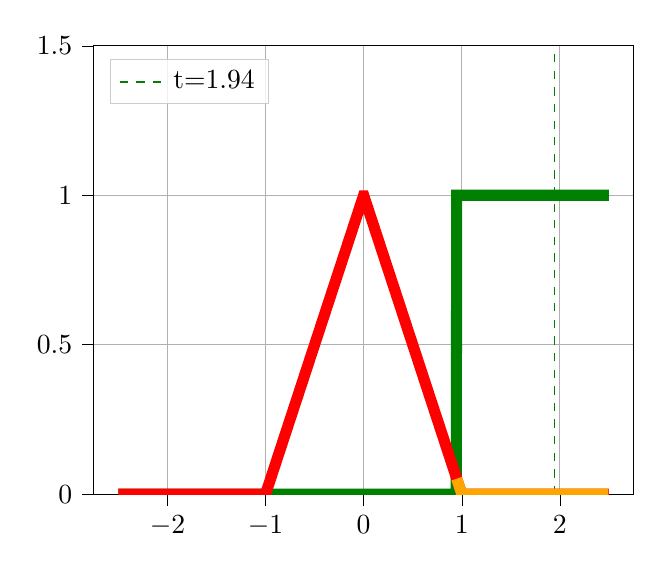
\begin{tikzpicture}

\definecolor{color0}{rgb}{1,0.498039215686275,0.0549019607843137}
\definecolor{color1}{rgb}{1,0.647058823529412,0}

\begin{axis}[
legend cell align={left},
legend style={fill opacity=0.8, draw opacity=1, text opacity=1, at={(0.03,0.97)}, anchor=north west, draw=white!80!black},
tick align=outside,
tick pos=left,
x grid style={white!69.0196078431373!black},
xmajorgrids,
xmin=-2.75, xmax=2.75,
xtick style={color=black},
y grid style={white!69.0196078431373!black},
ymajorgrids,
ymin=0, ymax=1.5,
ytick style={color=black}
]
\path [draw=color0, fill=color0, opacity=0.2]
(axis cs:0.948448448448449,0.0515515515515514)
--(axis cs:0.948448448448449,0)
--(axis cs:0.953453453453454,0)
--(axis cs:0.958458458458459,0)
--(axis cs:0.963463463463464,0)
--(axis cs:0.968468468468469,0)
--(axis cs:0.973473473473474,0)
--(axis cs:0.978478478478479,0)
--(axis cs:0.983483483483484,0)
--(axis cs:0.988488488488489,0)
--(axis cs:0.993493493493494,0)
--(axis cs:0.998498498498499,0)
--(axis cs:1.0035035035035,0)
--(axis cs:1.00850850850851,0)
--(axis cs:1.01351351351351,0)
--(axis cs:1.01851851851852,0)
--(axis cs:1.02352352352352,0)
--(axis cs:1.02852852852853,0)
--(axis cs:1.03353353353353,0)
--(axis cs:1.03853853853854,0)
--(axis cs:1.04354354354354,0)
--(axis cs:1.04854854854855,0)
--(axis cs:1.05355355355355,0)
--(axis cs:1.05855855855856,0)
--(axis cs:1.06356356356356,0)
--(axis cs:1.06856856856857,0)
--(axis cs:1.07357357357357,0)
--(axis cs:1.07857857857858,0)
--(axis cs:1.08358358358358,0)
--(axis cs:1.08858858858859,0)
--(axis cs:1.09359359359359,0)
--(axis cs:1.0985985985986,0)
--(axis cs:1.1036036036036,0)
--(axis cs:1.10860860860861,0)
--(axis cs:1.11361361361361,0)
--(axis cs:1.11861861861862,0)
--(axis cs:1.12362362362362,0)
--(axis cs:1.12862862862863,0)
--(axis cs:1.13363363363363,0)
--(axis cs:1.13863863863864,0)
--(axis cs:1.14364364364364,0)
--(axis cs:1.14864864864865,0)
--(axis cs:1.15365365365365,0)
--(axis cs:1.15865865865866,0)
--(axis cs:1.16366366366366,0)
--(axis cs:1.16866866866867,0)
--(axis cs:1.17367367367367,0)
--(axis cs:1.17867867867868,0)
--(axis cs:1.18368368368368,0)
--(axis cs:1.18868868868869,0)
--(axis cs:1.19369369369369,0)
--(axis cs:1.1986986986987,0)
--(axis cs:1.2037037037037,0)
--(axis cs:1.20870870870871,0)
--(axis cs:1.21371371371371,0)
--(axis cs:1.21871871871872,0)
--(axis cs:1.22372372372372,0)
--(axis cs:1.22872872872873,0)
--(axis cs:1.23373373373373,0)
--(axis cs:1.23873873873874,0)
--(axis cs:1.24374374374374,0)
--(axis cs:1.24874874874875,0)
--(axis cs:1.25375375375375,0)
--(axis cs:1.25875875875876,0)
--(axis cs:1.26376376376376,0)
--(axis cs:1.26876876876877,0)
--(axis cs:1.27377377377377,0)
--(axis cs:1.27877877877878,0)
--(axis cs:1.28378378378378,0)
--(axis cs:1.28878878878879,0)
--(axis cs:1.29379379379379,0)
--(axis cs:1.2987987987988,0)
--(axis cs:1.3038038038038,0)
--(axis cs:1.30880880880881,0)
--(axis cs:1.31381381381381,0)
--(axis cs:1.31881881881882,0)
--(axis cs:1.32382382382382,0)
--(axis cs:1.32882882882883,0)
--(axis cs:1.33383383383383,0)
--(axis cs:1.33883883883884,0)
--(axis cs:1.34384384384384,0)
--(axis cs:1.34884884884885,0)
--(axis cs:1.35385385385385,0)
--(axis cs:1.35885885885886,0)
--(axis cs:1.36386386386386,0)
--(axis cs:1.36886886886887,0)
--(axis cs:1.37387387387387,0)
--(axis cs:1.37887887887888,0)
--(axis cs:1.38388388388388,0)
--(axis cs:1.38888888888889,0)
--(axis cs:1.39389389389389,0)
--(axis cs:1.3988988988989,0)
--(axis cs:1.4039039039039,0)
--(axis cs:1.40890890890891,0)
--(axis cs:1.41391391391391,0)
--(axis cs:1.41891891891892,0)
--(axis cs:1.42392392392392,0)
--(axis cs:1.42892892892893,0)
--(axis cs:1.43393393393393,0)
--(axis cs:1.43893893893894,0)
--(axis cs:1.44394394394394,0)
--(axis cs:1.44894894894895,0)
--(axis cs:1.45395395395395,0)
--(axis cs:1.45895895895896,0)
--(axis cs:1.46396396396396,0)
--(axis cs:1.46896896896897,0)
--(axis cs:1.47397397397397,0)
--(axis cs:1.47897897897898,0)
--(axis cs:1.48398398398398,0)
--(axis cs:1.48898898898899,0)
--(axis cs:1.49399399399399,0)
--(axis cs:1.498998998999,0)
--(axis cs:1.504004004004,0)
--(axis cs:1.50900900900901,0)
--(axis cs:1.51401401401401,0)
--(axis cs:1.51901901901902,0)
--(axis cs:1.52402402402402,0)
--(axis cs:1.52902902902903,0)
--(axis cs:1.53403403403403,0)
--(axis cs:1.53903903903904,0)
--(axis cs:1.54404404404404,0)
--(axis cs:1.54904904904905,0)
--(axis cs:1.55405405405405,0)
--(axis cs:1.55905905905906,0)
--(axis cs:1.56406406406406,0)
--(axis cs:1.56906906906907,0)
--(axis cs:1.57407407407407,0)
--(axis cs:1.57907907907908,0)
--(axis cs:1.58408408408408,0)
--(axis cs:1.58908908908909,0)
--(axis cs:1.59409409409409,0)
--(axis cs:1.5990990990991,0)
--(axis cs:1.6041041041041,0)
--(axis cs:1.60910910910911,0)
--(axis cs:1.61411411411411,0)
--(axis cs:1.61911911911912,0)
--(axis cs:1.62412412412412,0)
--(axis cs:1.62912912912913,0)
--(axis cs:1.63413413413413,0)
--(axis cs:1.63913913913914,0)
--(axis cs:1.64414414414414,0)
--(axis cs:1.64914914914915,0)
--(axis cs:1.65415415415415,0)
--(axis cs:1.65915915915916,0)
--(axis cs:1.66416416416416,0)
--(axis cs:1.66916916916917,0)
--(axis cs:1.67417417417417,0)
--(axis cs:1.67917917917918,0)
--(axis cs:1.68418418418418,0)
--(axis cs:1.68918918918919,0)
--(axis cs:1.69419419419419,0)
--(axis cs:1.6991991991992,0)
--(axis cs:1.7042042042042,0)
--(axis cs:1.70920920920921,0)
--(axis cs:1.71421421421421,0)
--(axis cs:1.71921921921922,0)
--(axis cs:1.72422422422422,0)
--(axis cs:1.72922922922923,0)
--(axis cs:1.73423423423423,0)
--(axis cs:1.73923923923924,0)
--(axis cs:1.74424424424424,0)
--(axis cs:1.74924924924925,0)
--(axis cs:1.75425425425425,0)
--(axis cs:1.75925925925926,0)
--(axis cs:1.76426426426426,0)
--(axis cs:1.76926926926927,0)
--(axis cs:1.77427427427427,0)
--(axis cs:1.77927927927928,0)
--(axis cs:1.78428428428428,0)
--(axis cs:1.78928928928929,0)
--(axis cs:1.79429429429429,0)
--(axis cs:1.7992992992993,0)
--(axis cs:1.8043043043043,0)
--(axis cs:1.80930930930931,0)
--(axis cs:1.81431431431431,0)
--(axis cs:1.81931931931932,0)
--(axis cs:1.82432432432432,0)
--(axis cs:1.82932932932933,0)
--(axis cs:1.83433433433433,0)
--(axis cs:1.83933933933934,0)
--(axis cs:1.84434434434434,0)
--(axis cs:1.84934934934935,0)
--(axis cs:1.85435435435435,0)
--(axis cs:1.85935935935936,0)
--(axis cs:1.86436436436436,0)
--(axis cs:1.86936936936937,0)
--(axis cs:1.87437437437437,0)
--(axis cs:1.87937937937938,0)
--(axis cs:1.88438438438438,0)
--(axis cs:1.88938938938939,0)
--(axis cs:1.89439439439439,0)
--(axis cs:1.8993993993994,0)
--(axis cs:1.9044044044044,0)
--(axis cs:1.90940940940941,0)
--(axis cs:1.91441441441441,0)
--(axis cs:1.91941941941942,0)
--(axis cs:1.92442442442442,0)
--(axis cs:1.92942942942943,0)
--(axis cs:1.93443443443443,0)
--(axis cs:1.93943943943944,0)
--(axis cs:1.94444444444444,0)
--(axis cs:1.94944944944945,0)
--(axis cs:1.95445445445445,0)
--(axis cs:1.95945945945946,0)
--(axis cs:1.96446446446446,0)
--(axis cs:1.96946946946947,0)
--(axis cs:1.97447447447447,0)
--(axis cs:1.97947947947948,0)
--(axis cs:1.98448448448448,0)
--(axis cs:1.98948948948949,0)
--(axis cs:1.99449449449449,0)
--(axis cs:1.9994994994995,0)
--(axis cs:2.0045045045045,0)
--(axis cs:2.00950950950951,0)
--(axis cs:2.01451451451451,0)
--(axis cs:2.01951951951952,0)
--(axis cs:2.02452452452452,0)
--(axis cs:2.02952952952953,0)
--(axis cs:2.03453453453453,0)
--(axis cs:2.03953953953954,0)
--(axis cs:2.04454454454454,0)
--(axis cs:2.04954954954955,0)
--(axis cs:2.05455455455455,0)
--(axis cs:2.05955955955956,0)
--(axis cs:2.06456456456456,0)
--(axis cs:2.06956956956957,0)
--(axis cs:2.07457457457457,0)
--(axis cs:2.07957957957958,0)
--(axis cs:2.08458458458458,0)
--(axis cs:2.08958958958959,0)
--(axis cs:2.09459459459459,0)
--(axis cs:2.0995995995996,0)
--(axis cs:2.1046046046046,0)
--(axis cs:2.10960960960961,0)
--(axis cs:2.11461461461461,0)
--(axis cs:2.11961961961962,0)
--(axis cs:2.12462462462462,0)
--(axis cs:2.12962962962963,0)
--(axis cs:2.13463463463463,0)
--(axis cs:2.13963963963964,0)
--(axis cs:2.14464464464464,0)
--(axis cs:2.14964964964965,0)
--(axis cs:2.15465465465465,0)
--(axis cs:2.15965965965966,0)
--(axis cs:2.16466466466466,0)
--(axis cs:2.16966966966967,0)
--(axis cs:2.17467467467467,0)
--(axis cs:2.17967967967968,0)
--(axis cs:2.18468468468468,0)
--(axis cs:2.18968968968969,0)
--(axis cs:2.19469469469469,0)
--(axis cs:2.1996996996997,0)
--(axis cs:2.2047047047047,0)
--(axis cs:2.20970970970971,0)
--(axis cs:2.21471471471471,0)
--(axis cs:2.21971971971972,0)
--(axis cs:2.22472472472472,0)
--(axis cs:2.22972972972973,0)
--(axis cs:2.23473473473473,0)
--(axis cs:2.23973973973974,0)
--(axis cs:2.24474474474474,0)
--(axis cs:2.24974974974975,0)
--(axis cs:2.25475475475475,0)
--(axis cs:2.25975975975976,0)
--(axis cs:2.26476476476476,0)
--(axis cs:2.26976976976977,0)
--(axis cs:2.27477477477477,0)
--(axis cs:2.27977977977978,0)
--(axis cs:2.28478478478478,0)
--(axis cs:2.28978978978979,0)
--(axis cs:2.29479479479479,0)
--(axis cs:2.2997997997998,0)
--(axis cs:2.3048048048048,0)
--(axis cs:2.30980980980981,0)
--(axis cs:2.31481481481481,0)
--(axis cs:2.31981981981982,0)
--(axis cs:2.32482482482482,0)
--(axis cs:2.32982982982983,0)
--(axis cs:2.33483483483483,0)
--(axis cs:2.33983983983984,0)
--(axis cs:2.34484484484484,0)
--(axis cs:2.34984984984985,0)
--(axis cs:2.35485485485485,0)
--(axis cs:2.35985985985986,0)
--(axis cs:2.36486486486486,0)
--(axis cs:2.36986986986987,0)
--(axis cs:2.37487487487487,0)
--(axis cs:2.37987987987988,0)
--(axis cs:2.38488488488488,0)
--(axis cs:2.38988988988989,0)
--(axis cs:2.39489489489489,0)
--(axis cs:2.3998998998999,0)
--(axis cs:2.4049049049049,0)
--(axis cs:2.40990990990991,0)
--(axis cs:2.41491491491491,0)
--(axis cs:2.41991991991992,0)
--(axis cs:2.42492492492492,0)
--(axis cs:2.42992992992993,0)
--(axis cs:2.43493493493493,0)
--(axis cs:2.43993993993994,0)
--(axis cs:2.44494494494494,0)
--(axis cs:2.44994994994995,0)
--(axis cs:2.45495495495495,0)
--(axis cs:2.45995995995996,0)
--(axis cs:2.46496496496496,0)
--(axis cs:2.46996996996997,0)
--(axis cs:2.47497497497497,0)
--(axis cs:2.47997997997998,0)
--(axis cs:2.48498498498498,0)
--(axis cs:2.48998998998999,0)
--(axis cs:2.49499499499499,0)
--(axis cs:2.49499499499499,0)
--(axis cs:2.49499499499499,0)
--(axis cs:2.48998998998999,0)
--(axis cs:2.48498498498498,0)
--(axis cs:2.47997997997998,0)
--(axis cs:2.47497497497497,0)
--(axis cs:2.46996996996997,0)
--(axis cs:2.46496496496496,0)
--(axis cs:2.45995995995996,0)
--(axis cs:2.45495495495495,0)
--(axis cs:2.44994994994995,0)
--(axis cs:2.44494494494494,0)
--(axis cs:2.43993993993994,0)
--(axis cs:2.43493493493493,0)
--(axis cs:2.42992992992993,0)
--(axis cs:2.42492492492492,0)
--(axis cs:2.41991991991992,0)
--(axis cs:2.41491491491491,0)
--(axis cs:2.40990990990991,0)
--(axis cs:2.4049049049049,0)
--(axis cs:2.3998998998999,0)
--(axis cs:2.39489489489489,0)
--(axis cs:2.38988988988989,0)
--(axis cs:2.38488488488488,0)
--(axis cs:2.37987987987988,0)
--(axis cs:2.37487487487487,0)
--(axis cs:2.36986986986987,0)
--(axis cs:2.36486486486486,0)
--(axis cs:2.35985985985986,0)
--(axis cs:2.35485485485485,0)
--(axis cs:2.34984984984985,0)
--(axis cs:2.34484484484484,0)
--(axis cs:2.33983983983984,0)
--(axis cs:2.33483483483483,0)
--(axis cs:2.32982982982983,0)
--(axis cs:2.32482482482482,0)
--(axis cs:2.31981981981982,0)
--(axis cs:2.31481481481481,0)
--(axis cs:2.30980980980981,0)
--(axis cs:2.3048048048048,0)
--(axis cs:2.2997997997998,0)
--(axis cs:2.29479479479479,0)
--(axis cs:2.28978978978979,0)
--(axis cs:2.28478478478478,0)
--(axis cs:2.27977977977978,0)
--(axis cs:2.27477477477477,0)
--(axis cs:2.26976976976977,0)
--(axis cs:2.26476476476476,0)
--(axis cs:2.25975975975976,0)
--(axis cs:2.25475475475475,0)
--(axis cs:2.24974974974975,0)
--(axis cs:2.24474474474474,0)
--(axis cs:2.23973973973974,0)
--(axis cs:2.23473473473473,0)
--(axis cs:2.22972972972973,0)
--(axis cs:2.22472472472472,0)
--(axis cs:2.21971971971972,0)
--(axis cs:2.21471471471471,0)
--(axis cs:2.20970970970971,0)
--(axis cs:2.2047047047047,0)
--(axis cs:2.1996996996997,0)
--(axis cs:2.19469469469469,0)
--(axis cs:2.18968968968969,0)
--(axis cs:2.18468468468468,0)
--(axis cs:2.17967967967968,0)
--(axis cs:2.17467467467467,0)
--(axis cs:2.16966966966967,0)
--(axis cs:2.16466466466466,0)
--(axis cs:2.15965965965966,0)
--(axis cs:2.15465465465465,0)
--(axis cs:2.14964964964965,0)
--(axis cs:2.14464464464464,0)
--(axis cs:2.13963963963964,0)
--(axis cs:2.13463463463463,0)
--(axis cs:2.12962962962963,0)
--(axis cs:2.12462462462462,0)
--(axis cs:2.11961961961962,0)
--(axis cs:2.11461461461461,0)
--(axis cs:2.10960960960961,0)
--(axis cs:2.1046046046046,0)
--(axis cs:2.0995995995996,0)
--(axis cs:2.09459459459459,0)
--(axis cs:2.08958958958959,0)
--(axis cs:2.08458458458458,0)
--(axis cs:2.07957957957958,0)
--(axis cs:2.07457457457457,0)
--(axis cs:2.06956956956957,0)
--(axis cs:2.06456456456456,0)
--(axis cs:2.05955955955956,0)
--(axis cs:2.05455455455455,0)
--(axis cs:2.04954954954955,0)
--(axis cs:2.04454454454454,0)
--(axis cs:2.03953953953954,0)
--(axis cs:2.03453453453453,0)
--(axis cs:2.02952952952953,0)
--(axis cs:2.02452452452452,0)
--(axis cs:2.01951951951952,0)
--(axis cs:2.01451451451451,0)
--(axis cs:2.00950950950951,0)
--(axis cs:2.0045045045045,0)
--(axis cs:1.9994994994995,0)
--(axis cs:1.99449449449449,0)
--(axis cs:1.98948948948949,0)
--(axis cs:1.98448448448448,0)
--(axis cs:1.97947947947948,0)
--(axis cs:1.97447447447447,0)
--(axis cs:1.96946946946947,0)
--(axis cs:1.96446446446446,0)
--(axis cs:1.95945945945946,0)
--(axis cs:1.95445445445445,0)
--(axis cs:1.94944944944945,0)
--(axis cs:1.94444444444444,0)
--(axis cs:1.93943943943944,0)
--(axis cs:1.93443443443443,0)
--(axis cs:1.92942942942943,0)
--(axis cs:1.92442442442442,0)
--(axis cs:1.91941941941942,0)
--(axis cs:1.91441441441441,0)
--(axis cs:1.90940940940941,0)
--(axis cs:1.9044044044044,0)
--(axis cs:1.8993993993994,0)
--(axis cs:1.89439439439439,0)
--(axis cs:1.88938938938939,0)
--(axis cs:1.88438438438438,0)
--(axis cs:1.87937937937938,0)
--(axis cs:1.87437437437437,0)
--(axis cs:1.86936936936937,0)
--(axis cs:1.86436436436436,0)
--(axis cs:1.85935935935936,0)
--(axis cs:1.85435435435435,0)
--(axis cs:1.84934934934935,0)
--(axis cs:1.84434434434434,0)
--(axis cs:1.83933933933934,0)
--(axis cs:1.83433433433433,0)
--(axis cs:1.82932932932933,0)
--(axis cs:1.82432432432432,0)
--(axis cs:1.81931931931932,0)
--(axis cs:1.81431431431431,0)
--(axis cs:1.80930930930931,0)
--(axis cs:1.8043043043043,0)
--(axis cs:1.7992992992993,0)
--(axis cs:1.79429429429429,0)
--(axis cs:1.78928928928929,0)
--(axis cs:1.78428428428428,0)
--(axis cs:1.77927927927928,0)
--(axis cs:1.77427427427427,0)
--(axis cs:1.76926926926927,0)
--(axis cs:1.76426426426426,0)
--(axis cs:1.75925925925926,0)
--(axis cs:1.75425425425425,0)
--(axis cs:1.74924924924925,0)
--(axis cs:1.74424424424424,0)
--(axis cs:1.73923923923924,0)
--(axis cs:1.73423423423423,0)
--(axis cs:1.72922922922923,0)
--(axis cs:1.72422422422422,0)
--(axis cs:1.71921921921922,0)
--(axis cs:1.71421421421421,0)
--(axis cs:1.70920920920921,0)
--(axis cs:1.7042042042042,0)
--(axis cs:1.6991991991992,0)
--(axis cs:1.69419419419419,0)
--(axis cs:1.68918918918919,0)
--(axis cs:1.68418418418418,0)
--(axis cs:1.67917917917918,0)
--(axis cs:1.67417417417417,0)
--(axis cs:1.66916916916917,0)
--(axis cs:1.66416416416416,0)
--(axis cs:1.65915915915916,0)
--(axis cs:1.65415415415415,0)
--(axis cs:1.64914914914915,0)
--(axis cs:1.64414414414414,0)
--(axis cs:1.63913913913914,0)
--(axis cs:1.63413413413413,0)
--(axis cs:1.62912912912913,0)
--(axis cs:1.62412412412412,0)
--(axis cs:1.61911911911912,0)
--(axis cs:1.61411411411411,0)
--(axis cs:1.60910910910911,0)
--(axis cs:1.6041041041041,0)
--(axis cs:1.5990990990991,0)
--(axis cs:1.59409409409409,0)
--(axis cs:1.58908908908909,0)
--(axis cs:1.58408408408408,0)
--(axis cs:1.57907907907908,0)
--(axis cs:1.57407407407407,0)
--(axis cs:1.56906906906907,0)
--(axis cs:1.56406406406406,0)
--(axis cs:1.55905905905906,0)
--(axis cs:1.55405405405405,0)
--(axis cs:1.54904904904905,0)
--(axis cs:1.54404404404404,0)
--(axis cs:1.53903903903904,0)
--(axis cs:1.53403403403403,0)
--(axis cs:1.52902902902903,0)
--(axis cs:1.52402402402402,0)
--(axis cs:1.51901901901902,0)
--(axis cs:1.51401401401401,0)
--(axis cs:1.50900900900901,0)
--(axis cs:1.504004004004,0)
--(axis cs:1.498998998999,0)
--(axis cs:1.49399399399399,0)
--(axis cs:1.48898898898899,0)
--(axis cs:1.48398398398398,0)
--(axis cs:1.47897897897898,0)
--(axis cs:1.47397397397397,0)
--(axis cs:1.46896896896897,0)
--(axis cs:1.46396396396396,0)
--(axis cs:1.45895895895896,0)
--(axis cs:1.45395395395395,0)
--(axis cs:1.44894894894895,0)
--(axis cs:1.44394394394394,0)
--(axis cs:1.43893893893894,0)
--(axis cs:1.43393393393393,0)
--(axis cs:1.42892892892893,0)
--(axis cs:1.42392392392392,0)
--(axis cs:1.41891891891892,0)
--(axis cs:1.41391391391391,0)
--(axis cs:1.40890890890891,0)
--(axis cs:1.4039039039039,0)
--(axis cs:1.3988988988989,0)
--(axis cs:1.39389389389389,0)
--(axis cs:1.38888888888889,0)
--(axis cs:1.38388388388388,0)
--(axis cs:1.37887887887888,0)
--(axis cs:1.37387387387387,0)
--(axis cs:1.36886886886887,0)
--(axis cs:1.36386386386386,0)
--(axis cs:1.35885885885886,0)
--(axis cs:1.35385385385385,0)
--(axis cs:1.34884884884885,0)
--(axis cs:1.34384384384384,0)
--(axis cs:1.33883883883884,0)
--(axis cs:1.33383383383383,0)
--(axis cs:1.32882882882883,0)
--(axis cs:1.32382382382382,0)
--(axis cs:1.31881881881882,0)
--(axis cs:1.31381381381381,0)
--(axis cs:1.30880880880881,0)
--(axis cs:1.3038038038038,0)
--(axis cs:1.2987987987988,0)
--(axis cs:1.29379379379379,0)
--(axis cs:1.28878878878879,0)
--(axis cs:1.28378378378378,0)
--(axis cs:1.27877877877878,0)
--(axis cs:1.27377377377377,0)
--(axis cs:1.26876876876877,0)
--(axis cs:1.26376376376376,0)
--(axis cs:1.25875875875876,0)
--(axis cs:1.25375375375375,0)
--(axis cs:1.24874874874875,0)
--(axis cs:1.24374374374374,0)
--(axis cs:1.23873873873874,0)
--(axis cs:1.23373373373373,0)
--(axis cs:1.22872872872873,0)
--(axis cs:1.22372372372372,0)
--(axis cs:1.21871871871872,0)
--(axis cs:1.21371371371371,0)
--(axis cs:1.20870870870871,0)
--(axis cs:1.2037037037037,0)
--(axis cs:1.1986986986987,0)
--(axis cs:1.19369369369369,0)
--(axis cs:1.18868868868869,0)
--(axis cs:1.18368368368368,0)
--(axis cs:1.17867867867868,0)
--(axis cs:1.17367367367367,0)
--(axis cs:1.16866866866867,0)
--(axis cs:1.16366366366366,0)
--(axis cs:1.15865865865866,0)
--(axis cs:1.15365365365365,0)
--(axis cs:1.14864864864865,0)
--(axis cs:1.14364364364364,0)
--(axis cs:1.13863863863864,0)
--(axis cs:1.13363363363363,0)
--(axis cs:1.12862862862863,0)
--(axis cs:1.12362362362362,0)
--(axis cs:1.11861861861862,0)
--(axis cs:1.11361361361361,0)
--(axis cs:1.10860860860861,0)
--(axis cs:1.1036036036036,0)
--(axis cs:1.0985985985986,0)
--(axis cs:1.09359359359359,0)
--(axis cs:1.08858858858859,0)
--(axis cs:1.08358358358358,0)
--(axis cs:1.07857857857858,0)
--(axis cs:1.07357357357357,0)
--(axis cs:1.06856856856857,0)
--(axis cs:1.06356356356356,0)
--(axis cs:1.05855855855856,0)
--(axis cs:1.05355355355355,0)
--(axis cs:1.04854854854855,0)
--(axis cs:1.04354354354354,0)
--(axis cs:1.03853853853854,0)
--(axis cs:1.03353353353353,0)
--(axis cs:1.02852852852853,0)
--(axis cs:1.02352352352352,0)
--(axis cs:1.01851851851852,0)
--(axis cs:1.01351351351351,0)
--(axis cs:1.00850850850851,0)
--(axis cs:1.0035035035035,0)
--(axis cs:0.998498498498499,0.00150150150150141)
--(axis cs:0.993493493493494,0.00650650650650642)
--(axis cs:0.988488488488489,0.0115115115115114)
--(axis cs:0.983483483483484,0.0165165165165164)
--(axis cs:0.978478478478479,0.0215215215215214)
--(axis cs:0.973473473473474,0.0265265265265264)
--(axis cs:0.968468468468469,0.0315315315315314)
--(axis cs:0.963463463463464,0.0365365365365364)
--(axis cs:0.958458458458459,0.0415415415415414)
--(axis cs:0.953453453453454,0.0465465465465464)
--(axis cs:0.948448448448449,0.0515515515515514)
--cycle;

\addplot [line width=4pt, green!50!black, forget plot]
table {%
-2.5 0
-2.49499499499499 0
-2.48998998998999 0
-2.48498498498498 0
-2.47997997997998 0
-2.47497497497497 0
-2.46996996996997 0
-2.46496496496496 0
-2.45995995995996 0
-2.45495495495495 0
-2.44994994994995 0
-2.44494494494494 0
-2.43993993993994 0
-2.43493493493493 0
-2.42992992992993 0
-2.42492492492492 0
-2.41991991991992 0
-2.41491491491491 0
-2.40990990990991 0
-2.4049049049049 0
-2.3998998998999 0
-2.39489489489489 0
-2.38988988988989 0
-2.38488488488488 0
-2.37987987987988 0
-2.37487487487487 0
-2.36986986986987 0
-2.36486486486486 0
-2.35985985985986 0
-2.35485485485485 0
-2.34984984984985 0
-2.34484484484484 0
-2.33983983983984 0
-2.33483483483483 0
-2.32982982982983 0
-2.32482482482482 0
-2.31981981981982 0
-2.31481481481481 0
-2.30980980980981 0
-2.3048048048048 0
-2.2997997997998 0
-2.29479479479479 0
-2.28978978978979 0
-2.28478478478478 0
-2.27977977977978 0
-2.27477477477477 0
-2.26976976976977 0
-2.26476476476476 0
-2.25975975975976 0
-2.25475475475475 0
-2.24974974974975 0
-2.24474474474474 0
-2.23973973973974 0
-2.23473473473473 0
-2.22972972972973 0
-2.22472472472472 0
-2.21971971971972 0
-2.21471471471471 0
-2.20970970970971 0
-2.2047047047047 0
-2.1996996996997 0
-2.19469469469469 0
-2.18968968968969 0
-2.18468468468468 0
-2.17967967967968 0
-2.17467467467467 0
-2.16966966966967 0
-2.16466466466466 0
-2.15965965965966 0
-2.15465465465465 0
-2.14964964964965 0
-2.14464464464464 0
-2.13963963963964 0
-2.13463463463463 0
-2.12962962962963 0
-2.12462462462462 0
-2.11961961961962 0
-2.11461461461461 0
-2.10960960960961 0
-2.1046046046046 0
-2.0995995995996 0
-2.09459459459459 0
-2.08958958958959 0
-2.08458458458458 0
-2.07957957957958 0
-2.07457457457457 0
-2.06956956956957 0
-2.06456456456456 0
-2.05955955955956 0
-2.05455455455455 0
-2.04954954954955 0
-2.04454454454454 0
-2.03953953953954 0
-2.03453453453453 0
-2.02952952952953 0
-2.02452452452452 0
-2.01951951951952 0
-2.01451451451451 0
-2.00950950950951 0
-2.0045045045045 0
-1.9994994994995 0
-1.99449449449449 0
-1.98948948948949 0
-1.98448448448448 0
-1.97947947947948 0
-1.97447447447447 0
-1.96946946946947 0
-1.96446446446446 0
-1.95945945945946 0
-1.95445445445445 0
-1.94944944944945 0
-1.94444444444444 0
-1.93943943943944 0
-1.93443443443443 0
-1.92942942942943 0
-1.92442442442442 0
-1.91941941941942 0
-1.91441441441441 0
-1.90940940940941 0
-1.9044044044044 0
-1.8993993993994 0
-1.89439439439439 0
-1.88938938938939 0
-1.88438438438438 0
-1.87937937937938 0
-1.87437437437437 0
-1.86936936936937 0
-1.86436436436436 0
-1.85935935935936 0
-1.85435435435435 0
-1.84934934934935 0
-1.84434434434434 0
-1.83933933933934 0
-1.83433433433433 0
-1.82932932932933 0
-1.82432432432432 0
-1.81931931931932 0
-1.81431431431431 0
-1.80930930930931 0
-1.8043043043043 0
-1.7992992992993 0
-1.79429429429429 0
-1.78928928928929 0
-1.78428428428428 0
-1.77927927927928 0
-1.77427427427427 0
-1.76926926926927 0
-1.76426426426426 0
-1.75925925925926 0
-1.75425425425425 0
-1.74924924924925 0
-1.74424424424424 0
-1.73923923923924 0
-1.73423423423423 0
-1.72922922922923 0
-1.72422422422422 0
-1.71921921921922 0
-1.71421421421421 0
-1.70920920920921 0
-1.7042042042042 0
-1.6991991991992 0
-1.69419419419419 0
-1.68918918918919 0
-1.68418418418418 0
-1.67917917917918 0
-1.67417417417417 0
-1.66916916916917 0
-1.66416416416416 0
-1.65915915915916 0
-1.65415415415415 0
-1.64914914914915 0
-1.64414414414414 0
-1.63913913913914 0
-1.63413413413413 0
-1.62912912912913 0
-1.62412412412412 0
-1.61911911911912 0
-1.61411411411411 0
-1.60910910910911 0
-1.6041041041041 0
-1.5990990990991 0
-1.59409409409409 0
-1.58908908908909 0
-1.58408408408408 0
-1.57907907907908 0
-1.57407407407407 0
-1.56906906906907 0
-1.56406406406406 0
-1.55905905905906 0
-1.55405405405405 0
-1.54904904904905 0
-1.54404404404404 0
-1.53903903903904 0
-1.53403403403403 0
-1.52902902902903 0
-1.52402402402402 0
-1.51901901901902 0
-1.51401401401401 0
-1.50900900900901 0
-1.504004004004 0
-1.498998998999 0
-1.49399399399399 0
-1.48898898898899 0
-1.48398398398398 0
-1.47897897897898 0
-1.47397397397397 0
-1.46896896896897 0
-1.46396396396396 0
-1.45895895895896 0
-1.45395395395395 0
-1.44894894894895 0
-1.44394394394394 0
-1.43893893893894 0
-1.43393393393393 0
-1.42892892892893 0
-1.42392392392392 0
-1.41891891891892 0
-1.41391391391391 0
-1.40890890890891 0
-1.4039039039039 0
-1.3988988988989 0
-1.39389389389389 0
-1.38888888888889 0
-1.38388388388388 0
-1.37887887887888 0
-1.37387387387387 0
-1.36886886886887 0
-1.36386386386386 0
-1.35885885885886 0
-1.35385385385385 0
-1.34884884884885 0
-1.34384384384384 0
-1.33883883883884 0
-1.33383383383383 0
-1.32882882882883 0
-1.32382382382382 0
-1.31881881881882 0
-1.31381381381381 0
-1.30880880880881 0
-1.3038038038038 0
-1.2987987987988 0
-1.29379379379379 0
-1.28878878878879 0
-1.28378378378378 0
-1.27877877877878 0
-1.27377377377377 0
-1.26876876876877 0
-1.26376376376376 0
-1.25875875875876 0
-1.25375375375375 0
-1.24874874874875 0
-1.24374374374374 0
-1.23873873873874 0
-1.23373373373373 0
-1.22872872872873 0
-1.22372372372372 0
-1.21871871871872 0
-1.21371371371371 0
-1.20870870870871 0
-1.2037037037037 0
-1.1986986986987 0
-1.19369369369369 0
-1.18868868868869 0
-1.18368368368368 0
-1.17867867867868 0
-1.17367367367367 0
-1.16866866866867 0
-1.16366366366366 0
-1.15865865865866 0
-1.15365365365365 0
-1.14864864864865 0
-1.14364364364364 0
-1.13863863863864 0
-1.13363363363363 0
-1.12862862862863 0
-1.12362362362362 0
-1.11861861861862 0
-1.11361361361361 0
-1.10860860860861 0
-1.1036036036036 0
-1.0985985985986 0
-1.09359359359359 0
-1.08858858858859 0
-1.08358358358358 0
-1.07857857857858 0
-1.07357357357357 0
-1.06856856856857 0
-1.06356356356356 0
-1.05855855855856 0
-1.05355355355355 0
-1.04854854854855 0
-1.04354354354354 0
-1.03853853853854 0
-1.03353353353353 0
-1.02852852852853 0
-1.02352352352352 0
-1.01851851851852 0
-1.01351351351351 0
-1.00850850850851 0
-1.0035035035035 0
-0.998498498498499 0
-0.993493493493494 0
-0.988488488488489 0
-0.983483483483484 0
-0.978478478478479 0
-0.973473473473474 0
-0.968468468468469 0
-0.963463463463464 0
-0.958458458458459 0
-0.953453453453454 0
-0.948448448448449 0
-0.943443443443444 0
-0.938438438438439 0
-0.933433433433434 0
-0.928428428428429 0
-0.923423423423424 0
-0.918418418418419 0
-0.913413413413414 0
-0.908408408408409 0
-0.903403403403404 0
-0.898398398398399 0
-0.893393393393393 0
-0.888388388388388 0
-0.883383383383383 0
-0.878378378378378 0
-0.873373373373373 0
-0.868368368368368 0
-0.863363363363363 0
-0.858358358358358 0
-0.853353353353353 0
-0.848348348348348 0
-0.843343343343343 0
-0.838338338338338 0
-0.833333333333333 0
-0.828328328328328 0
-0.823323323323323 0
-0.818318318318318 0
-0.813313313313313 0
-0.808308308308308 0
-0.803303303303303 0
-0.798298298298298 0
-0.793293293293293 0
-0.788288288288288 0
-0.783283283283283 0
-0.778278278278278 0
-0.773273273273273 0
-0.768268268268268 0
-0.763263263263263 0
-0.758258258258258 0
-0.753253253253253 0
-0.748248248248248 0
-0.743243243243243 0
-0.738238238238238 0
-0.733233233233233 0
-0.728228228228228 0
-0.723223223223223 0
-0.718218218218218 0
-0.713213213213213 0
-0.708208208208208 0
-0.703203203203203 0
-0.698198198198198 0
-0.693193193193193 0
-0.688188188188188 0
-0.683183183183183 0
-0.678178178178178 0
-0.673173173173173 0
-0.668168168168168 0
-0.663163163163163 0
-0.658158158158158 0
-0.653153153153153 0
-0.648148148148148 0
-0.643143143143143 0
-0.638138138138138 0
-0.633133133133133 0
-0.628128128128128 0
-0.623123123123123 0
-0.618118118118118 0
-0.613113113113113 0
-0.608108108108108 0
-0.603103103103103 0
-0.598098098098098 0
-0.593093093093093 0
-0.588088088088088 0
-0.583083083083083 0
-0.578078078078078 0
-0.573073073073073 0
-0.568068068068068 0
-0.563063063063063 0
-0.558058058058058 0
-0.553053053053053 0
-0.548048048048048 0
-0.543043043043043 0
-0.538038038038038 0
-0.533033033033033 0
-0.528028028028028 0
-0.523023023023023 0
-0.518018018018018 0
-0.513013013013013 0
-0.508008008008008 0
-0.503003003003003 0
-0.497997997997998 0
-0.492992992992993 0
-0.487987987987988 0
-0.482982982982983 0
-0.477977977977978 0
-0.472972972972973 0
-0.467967967967968 0
-0.462962962962963 0
-0.457957957957958 0
-0.452952952952953 0
-0.447947947947948 0
-0.442942942942943 0
-0.437937937937938 0
-0.432932932932933 0
-0.427927927927928 0
-0.422922922922923 0
-0.417917917917918 0
-0.412912912912913 0
-0.407907907907908 0
-0.402902902902903 0
-0.397897897897898 0
-0.392892892892893 0
-0.387887887887888 0
-0.382882882882883 0
-0.377877877877878 0
-0.372872872872873 0
-0.367867867867868 0
-0.362862862862863 0
-0.357857857857858 0
-0.352852852852853 0
-0.347847847847848 0
-0.342842842842843 0
-0.337837837837838 0
-0.332832832832833 0
-0.327827827827828 0
-0.322822822822823 0
-0.317817817817818 0
-0.312812812812813 0
-0.307807807807808 0
-0.302802802802803 0
-0.297797797797798 0
-0.292792792792793 0
-0.287787787787788 0
-0.282782782782783 0
-0.277777777777778 0
-0.272772772772773 0
-0.267767767767768 0
-0.262762762762763 0
-0.257757757757758 0
-0.252752752752753 0
-0.247747747747748 0
-0.242742742742743 0
-0.237737737737738 0
-0.232732732732733 0
-0.227727727727728 0
-0.222722722722723 0
-0.217717717717718 0
-0.212712712712713 0
-0.207707707707708 0
-0.202702702702703 0
-0.197697697697698 0
-0.192692692692693 0
-0.187687687687688 0
-0.182682682682683 0
-0.177677677677678 0
-0.172672672672673 0
-0.167667667667668 0
-0.162662662662663 0
-0.157657657657658 0
-0.152652652652653 0
-0.147647647647648 0
-0.142642642642643 0
-0.137637637637638 0
-0.132632632632633 0
-0.127627627627628 0
-0.122622622622623 0
-0.117617617617618 0
-0.112612612612613 0
-0.107607607607608 0
-0.102602602602603 0
-0.0975975975975976 0
-0.0925925925925926 0
-0.0875875875875876 0
-0.0825825825825826 0
-0.0775775775775776 0
-0.0725725725725725 0
-0.0675675675675675 0
-0.0625625625625625 0
-0.0575575575575575 0
-0.0525525525525525 0
-0.0475475475475475 0
-0.0425425425425425 0
-0.0375375375375375 0
-0.0325325325325325 0
-0.0275275275275275 0
-0.0225225225225225 0
-0.0175175175175175 0
-0.0125125125125125 0
-0.0075075075075075 0
-0.0025025025025025 0
0.0025025025025025 0
0.0075075075075075 0
0.0125125125125125 0
0.0175175175175175 0
0.0225225225225225 0
0.0275275275275275 0
0.0325325325325325 0
0.0375375375375375 0
0.0425425425425425 0
0.0475475475475475 0
0.0525525525525525 0
0.0575575575575575 0
0.0625625625625625 0
0.0675675675675675 0
0.0725725725725725 0
0.0775775775775776 0
0.0825825825825826 0
0.0875875875875876 0
0.0925925925925926 0
0.0975975975975976 0
0.102602602602603 0
0.107607607607608 0
0.112612612612613 0
0.117617617617618 0
0.122622622622623 0
0.127627627627628 0
0.132632632632633 0
0.137637637637638 0
0.142642642642643 0
0.147647647647648 0
0.152652652652653 0
0.157657657657658 0
0.162662662662663 0
0.167667667667668 0
0.172672672672673 0
0.177677677677678 0
0.182682682682683 0
0.187687687687688 0
0.192692692692693 0
0.197697697697698 0
0.202702702702703 0
0.207707707707708 0
0.212712712712713 0
0.217717717717718 0
0.222722722722723 0
0.227727727727728 0
0.232732732732733 0
0.237737737737738 0
0.242742742742743 0
0.247747747747748 0
0.252752752752753 0
0.257757757757758 0
0.262762762762763 0
0.267767767767768 0
0.272772772772773 0
0.277777777777778 0
0.282782782782783 0
0.287787787787788 0
0.292792792792793 0
0.297797797797798 0
0.302802802802803 0
0.307807807807808 0
0.312812812812813 0
0.317817817817818 0
0.322822822822823 0
0.327827827827828 0
0.332832832832833 0
0.337837837837838 0
0.342842842842843 0
0.347847847847848 0
0.352852852852853 0
0.357857857857858 0
0.362862862862863 0
0.367867867867868 0
0.372872872872873 0
0.377877877877878 0
0.382882882882883 0
0.387887887887888 0
0.392892892892893 0
0.397897897897898 0
0.402902902902903 0
0.407907907907908 0
0.412912912912913 0
0.417917917917918 0
0.422922922922923 0
0.427927927927928 0
0.432932932932933 0
0.437937937937938 0
0.442942942942943 0
0.447947947947948 0
0.452952952952953 0
0.457957957957958 0
0.462962962962963 0
0.467967967967968 0
0.472972972972973 0
0.477977977977978 0
0.482982982982983 0
0.487987987987988 0
0.492992992992993 0
0.497997997997998 0
0.503003003003003 0
0.508008008008008 0
0.513013013013013 0
0.518018018018018 0
0.523023023023023 0
0.528028028028028 0
0.533033033033033 0
0.538038038038038 0
0.543043043043043 0
0.548048048048048 0
0.553053053053053 0
0.558058058058058 0
0.563063063063063 0
0.568068068068068 0
0.573073073073073 0
0.578078078078078 0
0.583083083083083 0
0.588088088088088 0
0.593093093093093 0
0.598098098098098 0
0.603103103103103 0
0.608108108108108 0
0.613113113113113 0
0.618118118118118 0
0.623123123123123 0
0.628128128128128 0
0.633133133133133 0
0.638138138138138 0
0.643143143143143 0
0.648148148148148 0
0.653153153153153 0
0.658158158158158 0
0.663163163163163 0
0.668168168168168 0
0.673173173173173 0
0.678178178178178 0
0.683183183183183 0
0.688188188188188 0
0.693193193193193 0
0.698198198198198 0
0.703203203203203 0
0.708208208208208 0
0.713213213213213 0
0.718218218218218 0
0.723223223223223 0
0.728228228228228 0
0.733233233233233 0
0.738238238238238 0
0.743243243243243 0
0.748248248248248 0
0.753253253253253 0
0.758258258258258 0
0.763263263263263 0
0.768268268268268 0
0.773273273273273 0
0.778278278278278 0
0.783283283283283 0
0.788288288288288 0
0.793293293293293 0
0.798298298298298 0
0.803303303303303 0
0.808308308308308 0
0.813313313313313 0
0.818318318318318 0
0.823323323323323 0
0.828328328328328 0
0.833333333333333 0
0.838338338338338 0
0.843343343343343 0
0.848348348348348 0
0.853353353353353 0
0.858358358358358 0
0.863363363363364 0
0.868368368368369 0
0.873373373373374 0
0.878378378378379 0
0.883383383383384 0
0.888388388388389 0
0.893393393393394 0
0.898398398398399 0
0.903403403403404 0
0.908408408408409 0
0.913413413413414 0
0.918418418418419 0
0.923423423423424 0
0.928428428428429 0
0.933433433433434 0
0.938438438438439 0
0.943443443443444 0
0.948448448448449 1
0.953453453453454 1
0.958458458458459 1
0.963463463463464 1
0.968468468468469 1
0.973473473473474 1
0.978478478478479 1
0.983483483483484 1
0.988488488488489 1
0.993493493493494 1
0.998498498498499 1
1.0035035035035 1
1.00850850850851 1
1.01351351351351 1
1.01851851851852 1
1.02352352352352 1
1.02852852852853 1
1.03353353353353 1
1.03853853853854 1
1.04354354354354 1
1.04854854854855 1
1.05355355355355 1
1.05855855855856 1
1.06356356356356 1
1.06856856856857 1
1.07357357357357 1
1.07857857857858 1
1.08358358358358 1
1.08858858858859 1
1.09359359359359 1
1.0985985985986 1
1.1036036036036 1
1.10860860860861 1
1.11361361361361 1
1.11861861861862 1
1.12362362362362 1
1.12862862862863 1
1.13363363363363 1
1.13863863863864 1
1.14364364364364 1
1.14864864864865 1
1.15365365365365 1
1.15865865865866 1
1.16366366366366 1
1.16866866866867 1
1.17367367367367 1
1.17867867867868 1
1.18368368368368 1
1.18868868868869 1
1.19369369369369 1
1.1986986986987 1
1.2037037037037 1
1.20870870870871 1
1.21371371371371 1
1.21871871871872 1
1.22372372372372 1
1.22872872872873 1
1.23373373373373 1
1.23873873873874 1
1.24374374374374 1
1.24874874874875 1
1.25375375375375 1
1.25875875875876 1
1.26376376376376 1
1.26876876876877 1
1.27377377377377 1
1.27877877877878 1
1.28378378378378 1
1.28878878878879 1
1.29379379379379 1
1.2987987987988 1
1.3038038038038 1
1.30880880880881 1
1.31381381381381 1
1.31881881881882 1
1.32382382382382 1
1.32882882882883 1
1.33383383383383 1
1.33883883883884 1
1.34384384384384 1
1.34884884884885 1
1.35385385385385 1
1.35885885885886 1
1.36386386386386 1
1.36886886886887 1
1.37387387387387 1
1.37887887887888 1
1.38388388388388 1
1.38888888888889 1
1.39389389389389 1
1.3988988988989 1
1.4039039039039 1
1.40890890890891 1
1.41391391391391 1
1.41891891891892 1
1.42392392392392 1
1.42892892892893 1
1.43393393393393 1
1.43893893893894 1
1.44394394394394 1
1.44894894894895 1
1.45395395395395 1
1.45895895895896 1
1.46396396396396 1
1.46896896896897 1
1.47397397397397 1
1.47897897897898 1
1.48398398398398 1
1.48898898898899 1
1.49399399399399 1
1.498998998999 1
1.504004004004 1
1.50900900900901 1
1.51401401401401 1
1.51901901901902 1
1.52402402402402 1
1.52902902902903 1
1.53403403403403 1
1.53903903903904 1
1.54404404404404 1
1.54904904904905 1
1.55405405405405 1
1.55905905905906 1
1.56406406406406 1
1.56906906906907 1
1.57407407407407 1
1.57907907907908 1
1.58408408408408 1
1.58908908908909 1
1.59409409409409 1
1.5990990990991 1
1.6041041041041 1
1.60910910910911 1
1.61411411411411 1
1.61911911911912 1
1.62412412412412 1
1.62912912912913 1
1.63413413413413 1
1.63913913913914 1
1.64414414414414 1
1.64914914914915 1
1.65415415415415 1
1.65915915915916 1
1.66416416416416 1
1.66916916916917 1
1.67417417417417 1
1.67917917917918 1
1.68418418418418 1
1.68918918918919 1
1.69419419419419 1
1.6991991991992 1
1.7042042042042 1
1.70920920920921 1
1.71421421421421 1
1.71921921921922 1
1.72422422422422 1
1.72922922922923 1
1.73423423423423 1
1.73923923923924 1
1.74424424424424 1
1.74924924924925 1
1.75425425425425 1
1.75925925925926 1
1.76426426426426 1
1.76926926926927 1
1.77427427427427 1
1.77927927927928 1
1.78428428428428 1
1.78928928928929 1
1.79429429429429 1
1.7992992992993 1
1.8043043043043 1
1.80930930930931 1
1.81431431431431 1
1.81931931931932 1
1.82432432432432 1
1.82932932932933 1
1.83433433433433 1
1.83933933933934 1
1.84434434434434 1
1.84934934934935 1
1.85435435435435 1
1.85935935935936 1
1.86436436436436 1
1.86936936936937 1
1.87437437437437 1
1.87937937937938 1
1.88438438438438 1
1.88938938938939 1
1.89439439439439 1
1.8993993993994 1
1.9044044044044 1
1.90940940940941 1
1.91441441441441 1
1.91941941941942 1
1.92442442442442 1
1.92942942942943 1
1.93443443443443 1
1.93943943943944 1
1.94444444444444 1
1.94944944944945 1
1.95445445445445 1
1.95945945945946 1
1.96446446446446 1
1.96946946946947 1
1.97447447447447 1
1.97947947947948 1
1.98448448448448 1
1.98948948948949 1
1.99449449449449 1
1.9994994994995 1
2.0045045045045 1
2.00950950950951 1
2.01451451451451 1
2.01951951951952 1
2.02452452452452 1
2.02952952952953 1
2.03453453453453 1
2.03953953953954 1
2.04454454454454 1
2.04954954954955 1
2.05455455455455 1
2.05955955955956 1
2.06456456456456 1
2.06956956956957 1
2.07457457457457 1
2.07957957957958 1
2.08458458458458 1
2.08958958958959 1
2.09459459459459 1
2.0995995995996 1
2.1046046046046 1
2.10960960960961 1
2.11461461461461 1
2.11961961961962 1
2.12462462462462 1
2.12962962962963 1
2.13463463463463 1
2.13963963963964 1
2.14464464464464 1
2.14964964964965 1
2.15465465465465 1
2.15965965965966 1
2.16466466466466 1
2.16966966966967 1
2.17467467467467 1
2.17967967967968 1
2.18468468468468 1
2.18968968968969 1
2.19469469469469 1
2.1996996996997 1
2.2047047047047 1
2.20970970970971 1
2.21471471471471 1
2.21971971971972 1
2.22472472472472 1
2.22972972972973 1
2.23473473473473 1
2.23973973973974 1
2.24474474474474 1
2.24974974974975 1
2.25475475475475 1
2.25975975975976 1
2.26476476476476 1
2.26976976976977 1
2.27477477477477 1
2.27977977977978 1
2.28478478478478 1
2.28978978978979 1
2.29479479479479 1
2.2997997997998 1
2.3048048048048 1
2.30980980980981 1
2.31481481481481 1
2.31981981981982 1
2.32482482482482 1
2.32982982982983 1
2.33483483483483 1
2.33983983983984 1
2.34484484484484 1
2.34984984984985 1
2.35485485485485 1
2.35985985985986 1
2.36486486486486 1
2.36986986986987 1
2.37487487487487 1
2.37987987987988 1
2.38488488488488 1
2.38988988988989 1
2.39489489489489 1
2.3998998998999 1
2.4049049049049 1
2.40990990990991 1
2.41491491491491 1
2.41991991991992 1
2.42492492492492 1
2.42992992992993 1
2.43493493493493 1
2.43993993993994 1
2.44494494494494 1
2.44994994994995 1
2.45495495495495 1
2.45995995995996 1
2.46496496496496 1
2.46996996996997 1
2.47497497497497 1
2.47997997997998 1
2.48498498498498 1
2.48998998998999 1
2.49499499499499 1
2.5 1
};
\addplot [line width=4pt, red, forget plot]
table {%
-2.5 -0
-2.49499499499499 -0
-2.48998998998999 -0
-2.48498498498498 -0
-2.47997997997998 -0
-2.47497497497497 -0
-2.46996996996997 -0
-2.46496496496496 -0
-2.45995995995996 -0
-2.45495495495495 -0
-2.44994994994995 -0
-2.44494494494494 -0
-2.43993993993994 -0
-2.43493493493493 -0
-2.42992992992993 -0
-2.42492492492492 -0
-2.41991991991992 -0
-2.41491491491491 -0
-2.40990990990991 -0
-2.4049049049049 -0
-2.3998998998999 -0
-2.39489489489489 -0
-2.38988988988989 -0
-2.38488488488488 -0
-2.37987987987988 -0
-2.37487487487487 -0
-2.36986986986987 -0
-2.36486486486486 -0
-2.35985985985986 -0
-2.35485485485485 -0
-2.34984984984985 -0
-2.34484484484484 -0
-2.33983983983984 -0
-2.33483483483483 -0
-2.32982982982983 -0
-2.32482482482482 -0
-2.31981981981982 -0
-2.31481481481481 -0
-2.30980980980981 -0
-2.3048048048048 -0
-2.2997997997998 -0
-2.29479479479479 -0
-2.28978978978979 -0
-2.28478478478478 -0
-2.27977977977978 -0
-2.27477477477477 -0
-2.26976976976977 -0
-2.26476476476476 -0
-2.25975975975976 -0
-2.25475475475475 -0
-2.24974974974975 -0
-2.24474474474474 -0
-2.23973973973974 -0
-2.23473473473473 -0
-2.22972972972973 -0
-2.22472472472472 -0
-2.21971971971972 -0
-2.21471471471471 -0
-2.20970970970971 -0
-2.2047047047047 -0
-2.1996996996997 -0
-2.19469469469469 -0
-2.18968968968969 -0
-2.18468468468468 -0
-2.17967967967968 -0
-2.17467467467467 -0
-2.16966966966967 -0
-2.16466466466466 -0
-2.15965965965966 -0
-2.15465465465465 -0
-2.14964964964965 -0
-2.14464464464464 -0
-2.13963963963964 -0
-2.13463463463463 -0
-2.12962962962963 -0
-2.12462462462462 -0
-2.11961961961962 -0
-2.11461461461461 -0
-2.10960960960961 -0
-2.1046046046046 -0
-2.0995995995996 -0
-2.09459459459459 -0
-2.08958958958959 -0
-2.08458458458458 -0
-2.07957957957958 -0
-2.07457457457457 -0
-2.06956956956957 -0
-2.06456456456456 -0
-2.05955955955956 -0
-2.05455455455455 -0
-2.04954954954955 -0
-2.04454454454454 -0
-2.03953953953954 -0
-2.03453453453453 -0
-2.02952952952953 -0
-2.02452452452452 -0
-2.01951951951952 -0
-2.01451451451451 -0
-2.00950950950951 -0
-2.0045045045045 -0
-1.9994994994995 -0
-1.99449449449449 -0
-1.98948948948949 -0
-1.98448448448448 -0
-1.97947947947948 -0
-1.97447447447447 -0
-1.96946946946947 -0
-1.96446446446446 -0
-1.95945945945946 -0
-1.95445445445445 -0
-1.94944944944945 -0
-1.94444444444444 -0
-1.93943943943944 -0
-1.93443443443443 -0
-1.92942942942943 -0
-1.92442442442442 -0
-1.91941941941942 -0
-1.91441441441441 -0
-1.90940940940941 -0
-1.9044044044044 -0
-1.8993993993994 -0
-1.89439439439439 -0
-1.88938938938939 -0
-1.88438438438438 -0
-1.87937937937938 -0
-1.87437437437437 -0
-1.86936936936937 -0
-1.86436436436436 -0
-1.85935935935936 -0
-1.85435435435435 -0
-1.84934934934935 -0
-1.84434434434434 -0
-1.83933933933934 -0
-1.83433433433433 -0
-1.82932932932933 -0
-1.82432432432432 -0
-1.81931931931932 -0
-1.81431431431431 -0
-1.80930930930931 -0
-1.8043043043043 -0
-1.7992992992993 -0
-1.79429429429429 -0
-1.78928928928929 -0
-1.78428428428428 -0
-1.77927927927928 -0
-1.77427427427427 -0
-1.76926926926927 -0
-1.76426426426426 -0
-1.75925925925926 -0
-1.75425425425425 -0
-1.74924924924925 -0
-1.74424424424424 -0
-1.73923923923924 -0
-1.73423423423423 -0
-1.72922922922923 -0
-1.72422422422422 -0
-1.71921921921922 -0
-1.71421421421421 -0
-1.70920920920921 -0
-1.7042042042042 -0
-1.6991991991992 -0
-1.69419419419419 -0
-1.68918918918919 -0
-1.68418418418418 -0
-1.67917917917918 -0
-1.67417417417417 -0
-1.66916916916917 -0
-1.66416416416416 -0
-1.65915915915916 -0
-1.65415415415415 -0
-1.64914914914915 -0
-1.64414414414414 -0
-1.63913913913914 -0
-1.63413413413413 -0
-1.62912912912913 -0
-1.62412412412412 -0
-1.61911911911912 -0
-1.61411411411411 -0
-1.60910910910911 -0
-1.6041041041041 -0
-1.5990990990991 -0
-1.59409409409409 -0
-1.58908908908909 -0
-1.58408408408408 -0
-1.57907907907908 -0
-1.57407407407407 -0
-1.56906906906907 -0
-1.56406406406406 -0
-1.55905905905906 -0
-1.55405405405405 -0
-1.54904904904905 -0
-1.54404404404404 -0
-1.53903903903904 -0
-1.53403403403403 -0
-1.52902902902903 -0
-1.52402402402402 -0
-1.51901901901902 -0
-1.51401401401401 -0
-1.50900900900901 -0
-1.504004004004 -0
-1.498998998999 -0
-1.49399399399399 -0
-1.48898898898899 -0
-1.48398398398398 -0
-1.47897897897898 -0
-1.47397397397397 -0
-1.46896896896897 -0
-1.46396396396396 -0
-1.45895895895896 -0
-1.45395395395395 -0
-1.44894894894895 -0
-1.44394394394394 -0
-1.43893893893894 -0
-1.43393393393393 -0
-1.42892892892893 -0
-1.42392392392392 -0
-1.41891891891892 -0
-1.41391391391391 -0
-1.40890890890891 -0
-1.4039039039039 -0
-1.3988988988989 -0
-1.39389389389389 -0
-1.38888888888889 -0
-1.38388388388388 -0
-1.37887887887888 -0
-1.37387387387387 -0
-1.36886886886887 -0
-1.36386386386386 -0
-1.35885885885886 -0
-1.35385385385385 -0
-1.34884884884885 -0
-1.34384384384384 -0
-1.33883883883884 -0
-1.33383383383383 -0
-1.32882882882883 -0
-1.32382382382382 -0
-1.31881881881882 -0
-1.31381381381381 -0
-1.30880880880881 -0
-1.3038038038038 -0
-1.2987987987988 -0
-1.29379379379379 -0
-1.28878878878879 -0
-1.28378378378378 -0
-1.27877877877878 -0
-1.27377377377377 -0
-1.26876876876877 -0
-1.26376376376376 -0
-1.25875875875876 -0
-1.25375375375375 -0
-1.24874874874875 -0
-1.24374374374374 -0
-1.23873873873874 -0
-1.23373373373373 -0
-1.22872872872873 -0
-1.22372372372372 -0
-1.21871871871872 -0
-1.21371371371371 -0
-1.20870870870871 -0
-1.2037037037037 -0
-1.1986986986987 -0
-1.19369369369369 -0
-1.18868868868869 -0
-1.18368368368368 -0
-1.17867867867868 -0
-1.17367367367367 -0
-1.16866866866867 -0
-1.16366366366366 -0
-1.15865865865866 -0
-1.15365365365365 -0
-1.14864864864865 -0
-1.14364364364364 -0
-1.13863863863864 -0
-1.13363363363363 -0
-1.12862862862863 -0
-1.12362362362362 -0
-1.11861861861862 -0
-1.11361361361361 -0
-1.10860860860861 -0
-1.1036036036036 -0
-1.0985985985986 -0
-1.09359359359359 -0
-1.08858858858859 -0
-1.08358358358358 -0
-1.07857857857858 -0
-1.07357357357357 -0
-1.06856856856857 -0
-1.06356356356356 -0
-1.05855855855856 -0
-1.05355355355355 -0
-1.04854854854855 -0
-1.04354354354354 -0
-1.03853853853854 -0
-1.03353353353353 -0
-1.02852852852853 -0
-1.02352352352352 -0
-1.01851851851852 -0
-1.01351351351351 -0
-1.00850850850851 -0
-1.0035035035035 -0
-0.998498498498499 0.00150150150150141
-0.993493493493494 0.00650650650650642
-0.988488488488489 0.0115115115115114
-0.983483483483484 0.0165165165165164
-0.978478478478479 0.0215215215215214
-0.973473473473474 0.0265265265265264
-0.968468468468469 0.0315315315315314
-0.963463463463464 0.0365365365365364
-0.958458458458459 0.0415415415415414
-0.953453453453454 0.0465465465465464
-0.948448448448449 0.0515515515515514
-0.943443443443444 0.0565565565565564
-0.938438438438439 0.0615615615615615
-0.933433433433434 0.0665665665665665
-0.928428428428429 0.0715715715715715
-0.923423423423424 0.0765765765765765
-0.918418418418419 0.0815815815815815
-0.913413413413414 0.0865865865865865
-0.908408408408409 0.0915915915915915
-0.903403403403404 0.0965965965965965
-0.898398398398399 0.101601601601601
-0.893393393393393 0.106606606606607
-0.888388388388388 0.111611611611612
-0.883383383383383 0.116616616616617
-0.878378378378378 0.121621621621622
-0.873373373373373 0.126626626626627
-0.868368368368368 0.131631631631632
-0.863363363363363 0.136636636636637
-0.858358358358358 0.141641641641642
-0.853353353353353 0.146646646646647
-0.848348348348348 0.151651651651652
-0.843343343343343 0.156656656656657
-0.838338338338338 0.161661661661662
-0.833333333333333 0.166666666666667
-0.828328328328328 0.171671671671672
-0.823323323323323 0.176676676676677
-0.818318318318318 0.181681681681682
-0.813313313313313 0.186686686686687
-0.808308308308308 0.191691691691692
-0.803303303303303 0.196696696696697
-0.798298298298298 0.201701701701702
-0.793293293293293 0.206706706706707
-0.788288288288288 0.211711711711712
-0.783283283283283 0.216716716716717
-0.778278278278278 0.221721721721722
-0.773273273273273 0.226726726726727
-0.768268268268268 0.231731731731732
-0.763263263263263 0.236736736736737
-0.758258258258258 0.241741741741742
-0.753253253253253 0.246746746746747
-0.748248248248248 0.251751751751752
-0.743243243243243 0.256756756756757
-0.738238238238238 0.261761761761762
-0.733233233233233 0.266766766766767
-0.728228228228228 0.271771771771772
-0.723223223223223 0.276776776776777
-0.718218218218218 0.281781781781782
-0.713213213213213 0.286786786786787
-0.708208208208208 0.291791791791792
-0.703203203203203 0.296796796796797
-0.698198198198198 0.301801801801802
-0.693193193193193 0.306806806806807
-0.688188188188188 0.311811811811812
-0.683183183183183 0.316816816816817
-0.678178178178178 0.321821821821822
-0.673173173173173 0.326826826826827
-0.668168168168168 0.331831831831832
-0.663163163163163 0.336836836836837
-0.658158158158158 0.341841841841842
-0.653153153153153 0.346846846846847
-0.648148148148148 0.351851851851852
-0.643143143143143 0.356856856856857
-0.638138138138138 0.361861861861862
-0.633133133133133 0.366866866866867
-0.628128128128128 0.371871871871872
-0.623123123123123 0.376876876876877
-0.618118118118118 0.381881881881882
-0.613113113113113 0.386886886886887
-0.608108108108108 0.391891891891892
-0.603103103103103 0.396896896896897
-0.598098098098098 0.401901901901902
-0.593093093093093 0.406906906906907
-0.588088088088088 0.411911911911912
-0.583083083083083 0.416916916916917
-0.578078078078078 0.421921921921922
-0.573073073073073 0.426926926926927
-0.568068068068068 0.431931931931932
-0.563063063063063 0.436936936936937
-0.558058058058058 0.441941941941942
-0.553053053053053 0.446946946946947
-0.548048048048048 0.451951951951952
-0.543043043043043 0.456956956956957
-0.538038038038038 0.461961961961962
-0.533033033033033 0.466966966966967
-0.528028028028028 0.471971971971972
-0.523023023023023 0.476976976976977
-0.518018018018018 0.481981981981982
-0.513013013013013 0.486986986986987
-0.508008008008008 0.491991991991992
-0.503003003003003 0.496996996996997
-0.497997997997998 0.502002002002002
-0.492992992992993 0.507007007007007
-0.487987987987988 0.512012012012012
-0.482982982982983 0.517017017017017
-0.477977977977978 0.522022022022022
-0.472972972972973 0.527027027027027
-0.467967967967968 0.532032032032032
-0.462962962962963 0.537037037037037
-0.457957957957958 0.542042042042042
-0.452952952952953 0.547047047047047
-0.447947947947948 0.552052052052052
-0.442942942942943 0.557057057057057
-0.437937937937938 0.562062062062062
-0.432932932932933 0.567067067067067
-0.427927927927928 0.572072072072072
-0.422922922922923 0.577077077077077
-0.417917917917918 0.582082082082082
-0.412912912912913 0.587087087087087
-0.407907907907908 0.592092092092092
-0.402902902902903 0.597097097097097
-0.397897897897898 0.602102102102102
-0.392892892892893 0.607107107107107
-0.387887887887888 0.612112112112112
-0.382882882882883 0.617117117117117
-0.377877877877878 0.622122122122122
-0.372872872872873 0.627127127127127
-0.367867867867868 0.632132132132132
-0.362862862862863 0.637137137137137
-0.357857857857858 0.642142142142142
-0.352852852852853 0.647147147147147
-0.347847847847848 0.652152152152152
-0.342842842842843 0.657157157157157
-0.337837837837838 0.662162162162162
-0.332832832832833 0.667167167167167
-0.327827827827828 0.672172172172172
-0.322822822822823 0.677177177177177
-0.317817817817818 0.682182182182182
-0.312812812812813 0.687187187187187
-0.307807807807808 0.692192192192192
-0.302802802802803 0.697197197197197
-0.297797797797798 0.702202202202202
-0.292792792792793 0.707207207207207
-0.287787787787788 0.712212212212212
-0.282782782782783 0.717217217217217
-0.277777777777778 0.722222222222222
-0.272772772772773 0.727227227227227
-0.267767767767768 0.732232232232232
-0.262762762762763 0.737237237237237
-0.257757757757758 0.742242242242242
-0.252752752752753 0.747247247247247
-0.247747747747748 0.752252252252252
-0.242742742742743 0.757257257257257
-0.237737737737738 0.762262262262262
-0.232732732732733 0.767267267267267
-0.227727727727728 0.772272272272272
-0.222722722722723 0.777277277277277
-0.217717717717718 0.782282282282282
-0.212712712712713 0.787287287287287
-0.207707707707708 0.792292292292292
-0.202702702702703 0.797297297297297
-0.197697697697698 0.802302302302302
-0.192692692692693 0.807307307307307
-0.187687687687688 0.812312312312312
-0.182682682682683 0.817317317317317
-0.177677677677678 0.822322322322322
-0.172672672672673 0.827327327327327
-0.167667667667668 0.832332332332332
-0.162662662662663 0.837337337337337
-0.157657657657658 0.842342342342342
-0.152652652652653 0.847347347347347
-0.147647647647648 0.852352352352352
-0.142642642642643 0.857357357357357
-0.137637637637638 0.862362362362362
-0.132632632632633 0.867367367367367
-0.127627627627628 0.872372372372372
-0.122622622622623 0.877377377377377
-0.117617617617618 0.882382382382382
-0.112612612612613 0.887387387387387
-0.107607607607608 0.892392392392392
-0.102602602602603 0.897397397397397
-0.0975975975975976 0.902402402402402
-0.0925925925925926 0.907407407407407
-0.0875875875875876 0.912412412412412
-0.0825825825825826 0.917417417417417
-0.0775775775775776 0.922422422422422
-0.0725725725725725 0.927427427427427
-0.0675675675675675 0.932432432432432
-0.0625625625625625 0.937437437437437
-0.0575575575575575 0.942442442442442
-0.0525525525525525 0.947447447447447
-0.0475475475475475 0.952452452452452
-0.0425425425425425 0.957457457457457
-0.0375375375375375 0.962462462462462
-0.0325325325325325 0.967467467467467
-0.0275275275275275 0.972472472472472
-0.0225225225225225 0.977477477477477
-0.0175175175175175 0.982482482482482
-0.0125125125125125 0.987487487487487
-0.0075075075075075 0.992492492492492
-0.0025025025025025 0.997497497497497
0.0025025025025025 0.997497497497497
0.0075075075075075 0.992492492492492
0.0125125125125125 0.987487487487487
0.0175175175175175 0.982482482482482
0.0225225225225225 0.977477477477477
0.0275275275275275 0.972472472472472
0.0325325325325325 0.967467467467467
0.0375375375375375 0.962462462462462
0.0425425425425425 0.957457457457457
0.0475475475475475 0.952452452452452
0.0525525525525525 0.947447447447447
0.0575575575575575 0.942442442442442
0.0625625625625625 0.937437437437437
0.0675675675675675 0.932432432432432
0.0725725725725725 0.927427427427427
0.0775775775775776 0.922422422422422
0.0825825825825826 0.917417417417417
0.0875875875875876 0.912412412412412
0.0925925925925926 0.907407407407407
0.0975975975975976 0.902402402402402
0.102602602602603 0.897397397397397
0.107607607607608 0.892392392392392
0.112612612612613 0.887387387387387
0.117617617617618 0.882382382382382
0.122622622622623 0.877377377377377
0.127627627627628 0.872372372372372
0.132632632632633 0.867367367367367
0.137637637637638 0.862362362362362
0.142642642642643 0.857357357357357
0.147647647647648 0.852352352352352
0.152652652652653 0.847347347347347
0.157657657657658 0.842342342342342
0.162662662662663 0.837337337337337
0.167667667667668 0.832332332332332
0.172672672672673 0.827327327327327
0.177677677677678 0.822322322322322
0.182682682682683 0.817317317317317
0.187687687687688 0.812312312312312
0.192692692692693 0.807307307307307
0.197697697697698 0.802302302302302
0.202702702702703 0.797297297297297
0.207707707707708 0.792292292292292
0.212712712712713 0.787287287287287
0.217717717717718 0.782282282282282
0.222722722722723 0.777277277277277
0.227727727727728 0.772272272272272
0.232732732732733 0.767267267267267
0.237737737737738 0.762262262262262
0.242742742742743 0.757257257257257
0.247747747747748 0.752252252252252
0.252752752752753 0.747247247247247
0.257757757757758 0.742242242242242
0.262762762762763 0.737237237237237
0.267767767767768 0.732232232232232
0.272772772772773 0.727227227227227
0.277777777777778 0.722222222222222
0.282782782782783 0.717217217217217
0.287787787787788 0.712212212212212
0.292792792792793 0.707207207207207
0.297797797797798 0.702202202202202
0.302802802802803 0.697197197197197
0.307807807807808 0.692192192192192
0.312812812812813 0.687187187187187
0.317817817817818 0.682182182182182
0.322822822822823 0.677177177177177
0.327827827827828 0.672172172172172
0.332832832832833 0.667167167167167
0.337837837837838 0.662162162162162
0.342842842842843 0.657157157157157
0.347847847847848 0.652152152152152
0.352852852852853 0.647147147147147
0.357857857857858 0.642142142142142
0.362862862862863 0.637137137137137
0.367867867867868 0.632132132132132
0.372872872872873 0.627127127127127
0.377877877877878 0.622122122122122
0.382882882882883 0.617117117117117
0.387887887887888 0.612112112112112
0.392892892892893 0.607107107107107
0.397897897897898 0.602102102102102
0.402902902902903 0.597097097097097
0.407907907907908 0.592092092092092
0.412912912912913 0.587087087087087
0.417917917917918 0.582082082082082
0.422922922922923 0.577077077077077
0.427927927927928 0.572072072072072
0.432932932932933 0.567067067067067
0.437937937937938 0.562062062062062
0.442942942942943 0.557057057057057
0.447947947947948 0.552052052052052
0.452952952952953 0.547047047047047
0.457957957957958 0.542042042042042
0.462962962962963 0.537037037037037
0.467967967967968 0.532032032032032
0.472972972972973 0.527027027027027
0.477977977977978 0.522022022022022
0.482982982982983 0.517017017017017
0.487987987987988 0.512012012012012
0.492992992992993 0.507007007007007
0.497997997997998 0.502002002002002
0.503003003003003 0.496996996996997
0.508008008008008 0.491991991991992
0.513013013013013 0.486986986986987
0.518018018018018 0.481981981981982
0.523023023023023 0.476976976976977
0.528028028028028 0.471971971971972
0.533033033033033 0.466966966966967
0.538038038038038 0.461961961961962
0.543043043043043 0.456956956956957
0.548048048048048 0.451951951951952
0.553053053053053 0.446946946946947
0.558058058058058 0.441941941941942
0.563063063063063 0.436936936936937
0.568068068068068 0.431931931931932
0.573073073073073 0.426926926926927
0.578078078078078 0.421921921921922
0.583083083083083 0.416916916916917
0.588088088088088 0.411911911911912
0.593093093093093 0.406906906906907
0.598098098098098 0.401901901901902
0.603103103103103 0.396896896896897
0.608108108108108 0.391891891891892
0.613113113113113 0.386886886886887
0.618118118118118 0.381881881881882
0.623123123123123 0.376876876876877
0.628128128128128 0.371871871871872
0.633133133133133 0.366866866866867
0.638138138138138 0.361861861861862
0.643143143143143 0.356856856856857
0.648148148148148 0.351851851851852
0.653153153153153 0.346846846846847
0.658158158158158 0.341841841841842
0.663163163163163 0.336836836836837
0.668168168168168 0.331831831831832
0.673173173173173 0.326826826826827
0.678178178178178 0.321821821821822
0.683183183183183 0.316816816816817
0.688188188188188 0.311811811811812
0.693193193193193 0.306806806806807
0.698198198198198 0.301801801801802
0.703203203203203 0.296796796796797
0.708208208208208 0.291791791791792
0.713213213213213 0.286786786786787
0.718218218218218 0.281781781781782
0.723223223223223 0.276776776776777
0.728228228228228 0.271771771771772
0.733233233233233 0.266766766766767
0.738238238238238 0.261761761761762
0.743243243243243 0.256756756756757
0.748248248248248 0.251751751751752
0.753253253253253 0.246746746746747
0.758258258258258 0.241741741741742
0.763263263263263 0.236736736736737
0.768268268268268 0.231731731731732
0.773273273273273 0.226726726726727
0.778278278278278 0.221721721721722
0.783283283283283 0.216716716716717
0.788288288288288 0.211711711711712
0.793293293293293 0.206706706706707
0.798298298298298 0.201701701701702
0.803303303303303 0.196696696696697
0.808308308308308 0.191691691691692
0.813313313313313 0.186686686686687
0.818318318318318 0.181681681681682
0.823323323323323 0.176676676676677
0.828328328328328 0.171671671671672
0.833333333333333 0.166666666666667
0.838338338338338 0.161661661661662
0.843343343343343 0.156656656656657
0.848348348348348 0.151651651651652
0.853353353353353 0.146646646646647
0.858358358358358 0.141641641641642
0.863363363363364 0.136636636636636
0.868368368368369 0.131631631631631
0.873373373373374 0.126626626626626
0.878378378378379 0.121621621621621
0.883383383383384 0.116616616616616
0.888388388388389 0.111611611611611
0.893393393393394 0.106606606606606
0.898398398398399 0.101601601601601
0.903403403403404 0.0965965965965965
0.908408408408409 0.0915915915915915
0.913413413413414 0.0865865865865865
0.918418418418419 0.0815815815815815
0.923423423423424 0.0765765765765765
0.928428428428429 0.0715715715715715
0.933433433433434 0.0665665665665665
0.938438438438439 0.0615615615615615
0.943443443443444 0.0565565565565564
0.948448448448449 0.0515515515515514
0.953453453453454 0.0465465465465464
0.958458458458459 0.0415415415415414
0.963463463463464 0.0365365365365364
0.968468468468469 0.0315315315315314
0.973473473473474 0.0265265265265264
0.978478478478479 0.0215215215215214
0.983483483483484 0.0165165165165164
0.988488488488489 0.0115115115115114
0.993493493493494 0.00650650650650642
0.998498498498499 0.00150150150150141
1.0035035035035 -0
1.00850850850851 -0
1.01351351351351 -0
1.01851851851852 -0
1.02352352352352 -0
1.02852852852853 -0
1.03353353353353 -0
1.03853853853854 -0
1.04354354354354 -0
1.04854854854855 -0
1.05355355355355 -0
1.05855855855856 -0
1.06356356356356 -0
1.06856856856857 -0
1.07357357357357 -0
1.07857857857858 -0
1.08358358358358 -0
1.08858858858859 -0
1.09359359359359 -0
1.0985985985986 -0
1.1036036036036 -0
1.10860860860861 -0
1.11361361361361 -0
1.11861861861862 -0
1.12362362362362 -0
1.12862862862863 -0
1.13363363363363 -0
1.13863863863864 -0
1.14364364364364 -0
1.14864864864865 -0
1.15365365365365 -0
1.15865865865866 -0
1.16366366366366 -0
1.16866866866867 -0
1.17367367367367 -0
1.17867867867868 -0
1.18368368368368 -0
1.18868868868869 -0
1.19369369369369 -0
1.1986986986987 -0
1.2037037037037 -0
1.20870870870871 -0
1.21371371371371 -0
1.21871871871872 -0
1.22372372372372 -0
1.22872872872873 -0
1.23373373373373 -0
1.23873873873874 -0
1.24374374374374 -0
1.24874874874875 -0
1.25375375375375 -0
1.25875875875876 -0
1.26376376376376 -0
1.26876876876877 -0
1.27377377377377 -0
1.27877877877878 -0
1.28378378378378 -0
1.28878878878879 -0
1.29379379379379 -0
1.2987987987988 -0
1.3038038038038 -0
1.30880880880881 -0
1.31381381381381 -0
1.31881881881882 -0
1.32382382382382 -0
1.32882882882883 -0
1.33383383383383 -0
1.33883883883884 -0
1.34384384384384 -0
1.34884884884885 -0
1.35385385385385 -0
1.35885885885886 -0
1.36386386386386 -0
1.36886886886887 -0
1.37387387387387 -0
1.37887887887888 -0
1.38388388388388 -0
1.38888888888889 -0
1.39389389389389 -0
1.3988988988989 -0
1.4039039039039 -0
1.40890890890891 -0
1.41391391391391 -0
1.41891891891892 -0
1.42392392392392 -0
1.42892892892893 -0
1.43393393393393 -0
1.43893893893894 -0
1.44394394394394 -0
1.44894894894895 -0
1.45395395395395 -0
1.45895895895896 -0
1.46396396396396 -0
1.46896896896897 -0
1.47397397397397 -0
1.47897897897898 -0
1.48398398398398 -0
1.48898898898899 -0
1.49399399399399 -0
1.498998998999 -0
1.504004004004 -0
1.50900900900901 -0
1.51401401401401 -0
1.51901901901902 -0
1.52402402402402 -0
1.52902902902903 -0
1.53403403403403 -0
1.53903903903904 -0
1.54404404404404 -0
1.54904904904905 -0
1.55405405405405 -0
1.55905905905906 -0
1.56406406406406 -0
1.56906906906907 -0
1.57407407407407 -0
1.57907907907908 -0
1.58408408408408 -0
1.58908908908909 -0
1.59409409409409 -0
1.5990990990991 -0
1.6041041041041 -0
1.60910910910911 -0
1.61411411411411 -0
1.61911911911912 -0
1.62412412412412 -0
1.62912912912913 -0
1.63413413413413 -0
1.63913913913914 -0
1.64414414414414 -0
1.64914914914915 -0
1.65415415415415 -0
1.65915915915916 -0
1.66416416416416 -0
1.66916916916917 -0
1.67417417417417 -0
1.67917917917918 -0
1.68418418418418 -0
1.68918918918919 -0
1.69419419419419 -0
1.6991991991992 -0
1.7042042042042 -0
1.70920920920921 -0
1.71421421421421 -0
1.71921921921922 -0
1.72422422422422 -0
1.72922922922923 -0
1.73423423423423 -0
1.73923923923924 -0
1.74424424424424 -0
1.74924924924925 -0
1.75425425425425 -0
1.75925925925926 -0
1.76426426426426 -0
1.76926926926927 -0
1.77427427427427 -0
1.77927927927928 -0
1.78428428428428 -0
1.78928928928929 -0
1.79429429429429 -0
1.7992992992993 -0
1.8043043043043 -0
1.80930930930931 -0
1.81431431431431 -0
1.81931931931932 -0
1.82432432432432 -0
1.82932932932933 -0
1.83433433433433 -0
1.83933933933934 -0
1.84434434434434 -0
1.84934934934935 -0
1.85435435435435 -0
1.85935935935936 -0
1.86436436436436 -0
1.86936936936937 -0
1.87437437437437 -0
1.87937937937938 -0
1.88438438438438 -0
1.88938938938939 -0
1.89439439439439 -0
1.8993993993994 -0
1.9044044044044 -0
1.90940940940941 -0
1.91441441441441 -0
1.91941941941942 -0
1.92442442442442 -0
1.92942942942943 -0
1.93443443443443 -0
1.93943943943944 -0
1.94444444444444 -0
1.94944944944945 -0
1.95445445445445 -0
1.95945945945946 -0
1.96446446446446 -0
1.96946946946947 -0
1.97447447447447 -0
1.97947947947948 -0
1.98448448448448 -0
1.98948948948949 -0
1.99449449449449 -0
1.9994994994995 -0
2.0045045045045 -0
2.00950950950951 -0
2.01451451451451 -0
2.01951951951952 -0
2.02452452452452 -0
2.02952952952953 -0
2.03453453453453 -0
2.03953953953954 -0
2.04454454454454 -0
2.04954954954955 -0
2.05455455455455 -0
2.05955955955956 -0
2.06456456456456 -0
2.06956956956957 -0
2.07457457457457 -0
2.07957957957958 -0
2.08458458458458 -0
2.08958958958959 -0
2.09459459459459 -0
2.0995995995996 -0
2.1046046046046 -0
2.10960960960961 -0
2.11461461461461 -0
2.11961961961962 -0
2.12462462462462 -0
2.12962962962963 -0
2.13463463463463 -0
2.13963963963964 -0
2.14464464464464 -0
2.14964964964965 -0
2.15465465465465 -0
2.15965965965966 -0
2.16466466466466 -0
2.16966966966967 -0
2.17467467467467 -0
2.17967967967968 -0
2.18468468468468 -0
2.18968968968969 -0
2.19469469469469 -0
2.1996996996997 -0
2.2047047047047 -0
2.20970970970971 -0
2.21471471471471 -0
2.21971971971972 -0
2.22472472472472 -0
2.22972972972973 -0
2.23473473473473 -0
2.23973973973974 -0
2.24474474474474 -0
2.24974974974975 -0
2.25475475475475 -0
2.25975975975976 -0
2.26476476476476 -0
2.26976976976977 -0
2.27477477477477 -0
2.27977977977978 -0
2.28478478478478 -0
2.28978978978979 -0
2.29479479479479 -0
2.2997997997998 -0
2.3048048048048 -0
2.30980980980981 -0
2.31481481481481 -0
2.31981981981982 -0
2.32482482482482 -0
2.32982982982983 -0
2.33483483483483 -0
2.33983983983984 -0
2.34484484484484 -0
2.34984984984985 -0
2.35485485485485 -0
2.35985985985986 -0
2.36486486486486 -0
2.36986986986987 -0
2.37487487487487 -0
2.37987987987988 -0
2.38488488488488 -0
2.38988988988989 -0
2.39489489489489 -0
2.3998998998999 -0
2.4049049049049 -0
2.40990990990991 -0
2.41491491491491 -0
2.41991991991992 -0
2.42492492492492 -0
2.42992992992993 -0
2.43493493493493 -0
2.43993993993994 -0
2.44494494494494 -0
2.44994994994995 -0
2.45495495495495 -0
2.45995995995996 -0
2.46496496496496 -0
2.46996996996997 -0
2.47497497497497 -0
2.47997997997998 -0
2.48498498498498 -0
2.48998998998999 -0
2.49499499499499 -0
2.5 -0
};
\addplot [semithick, green!50!black, dashed]
table {%
1.94444444444444 0
1.94444444444444 1.5
};
\addlegendentry{t=1.94}
\addplot [line width=4pt, color1, forget plot]
table {%
0.948448448448449 0.0515515515515514
0.953453453453454 0.0465465465465464
0.958458458458459 0.0415415415415414
0.963463463463464 0.0365365365365364
0.968468468468469 0.0315315315315314
0.973473473473474 0.0265265265265264
0.978478478478479 0.0215215215215214
0.983483483483484 0.0165165165165164
0.988488488488489 0.0115115115115114
0.993493493493494 0.00650650650650642
0.998498498498499 0.00150150150150141
1.0035035035035 -0
1.00850850850851 -0
1.01351351351351 -0
1.01851851851852 -0
1.02352352352352 -0
1.02852852852853 -0
1.03353353353353 -0
1.03853853853854 -0
1.04354354354354 -0
1.04854854854855 -0
1.05355355355355 -0
1.05855855855856 -0
1.06356356356356 -0
1.06856856856857 -0
1.07357357357357 -0
1.07857857857858 -0
1.08358358358358 -0
1.08858858858859 -0
1.09359359359359 -0
1.0985985985986 -0
1.1036036036036 -0
1.10860860860861 -0
1.11361361361361 -0
1.11861861861862 -0
1.12362362362362 -0
1.12862862862863 -0
1.13363363363363 -0
1.13863863863864 -0
1.14364364364364 -0
1.14864864864865 -0
1.15365365365365 -0
1.15865865865866 -0
1.16366366366366 -0
1.16866866866867 -0
1.17367367367367 -0
1.17867867867868 -0
1.18368368368368 -0
1.18868868868869 -0
1.19369369369369 -0
1.1986986986987 -0
1.2037037037037 -0
1.20870870870871 -0
1.21371371371371 -0
1.21871871871872 -0
1.22372372372372 -0
1.22872872872873 -0
1.23373373373373 -0
1.23873873873874 -0
1.24374374374374 -0
1.24874874874875 -0
1.25375375375375 -0
1.25875875875876 -0
1.26376376376376 -0
1.26876876876877 -0
1.27377377377377 -0
1.27877877877878 -0
1.28378378378378 -0
1.28878878878879 -0
1.29379379379379 -0
1.2987987987988 -0
1.3038038038038 -0
1.30880880880881 -0
1.31381381381381 -0
1.31881881881882 -0
1.32382382382382 -0
1.32882882882883 -0
1.33383383383383 -0
1.33883883883884 -0
1.34384384384384 -0
1.34884884884885 -0
1.35385385385385 -0
1.35885885885886 -0
1.36386386386386 -0
1.36886886886887 -0
1.37387387387387 -0
1.37887887887888 -0
1.38388388388388 -0
1.38888888888889 -0
1.39389389389389 -0
1.3988988988989 -0
1.4039039039039 -0
1.40890890890891 -0
1.41391391391391 -0
1.41891891891892 -0
1.42392392392392 -0
1.42892892892893 -0
1.43393393393393 -0
1.43893893893894 -0
1.44394394394394 -0
1.44894894894895 -0
1.45395395395395 -0
1.45895895895896 -0
1.46396396396396 -0
1.46896896896897 -0
1.47397397397397 -0
1.47897897897898 -0
1.48398398398398 -0
1.48898898898899 -0
1.49399399399399 -0
1.498998998999 -0
1.504004004004 -0
1.50900900900901 -0
1.51401401401401 -0
1.51901901901902 -0
1.52402402402402 -0
1.52902902902903 -0
1.53403403403403 -0
1.53903903903904 -0
1.54404404404404 -0
1.54904904904905 -0
1.55405405405405 -0
1.55905905905906 -0
1.56406406406406 -0
1.56906906906907 -0
1.57407407407407 -0
1.57907907907908 -0
1.58408408408408 -0
1.58908908908909 -0
1.59409409409409 -0
1.5990990990991 -0
1.6041041041041 -0
1.60910910910911 -0
1.61411411411411 -0
1.61911911911912 -0
1.62412412412412 -0
1.62912912912913 -0
1.63413413413413 -0
1.63913913913914 -0
1.64414414414414 -0
1.64914914914915 -0
1.65415415415415 -0
1.65915915915916 -0
1.66416416416416 -0
1.66916916916917 -0
1.67417417417417 -0
1.67917917917918 -0
1.68418418418418 -0
1.68918918918919 -0
1.69419419419419 -0
1.6991991991992 -0
1.7042042042042 -0
1.70920920920921 -0
1.71421421421421 -0
1.71921921921922 -0
1.72422422422422 -0
1.72922922922923 -0
1.73423423423423 -0
1.73923923923924 -0
1.74424424424424 -0
1.74924924924925 -0
1.75425425425425 -0
1.75925925925926 -0
1.76426426426426 -0
1.76926926926927 -0
1.77427427427427 -0
1.77927927927928 -0
1.78428428428428 -0
1.78928928928929 -0
1.79429429429429 -0
1.7992992992993 -0
1.8043043043043 -0
1.80930930930931 -0
1.81431431431431 -0
1.81931931931932 -0
1.82432432432432 -0
1.82932932932933 -0
1.83433433433433 -0
1.83933933933934 -0
1.84434434434434 -0
1.84934934934935 -0
1.85435435435435 -0
1.85935935935936 -0
1.86436436436436 -0
1.86936936936937 -0
1.87437437437437 -0
1.87937937937938 -0
1.88438438438438 -0
1.88938938938939 -0
1.89439439439439 -0
1.8993993993994 -0
1.9044044044044 -0
1.90940940940941 -0
1.91441441441441 -0
1.91941941941942 -0
1.92442442442442 -0
1.92942942942943 -0
1.93443443443443 -0
1.93943943943944 -0
1.94444444444444 -0
1.94944944944945 -0
1.95445445445445 -0
1.95945945945946 -0
1.96446446446446 -0
1.96946946946947 -0
1.97447447447447 -0
1.97947947947948 -0
1.98448448448448 -0
1.98948948948949 -0
1.99449449449449 -0
1.9994994994995 -0
2.0045045045045 -0
2.00950950950951 -0
2.01451451451451 -0
2.01951951951952 -0
2.02452452452452 -0
2.02952952952953 -0
2.03453453453453 -0
2.03953953953954 -0
2.04454454454454 -0
2.04954954954955 -0
2.05455455455455 -0
2.05955955955956 -0
2.06456456456456 -0
2.06956956956957 -0
2.07457457457457 -0
2.07957957957958 -0
2.08458458458458 -0
2.08958958958959 -0
2.09459459459459 -0
2.0995995995996 -0
2.1046046046046 -0
2.10960960960961 -0
2.11461461461461 -0
2.11961961961962 -0
2.12462462462462 -0
2.12962962962963 -0
2.13463463463463 -0
2.13963963963964 -0
2.14464464464464 -0
2.14964964964965 -0
2.15465465465465 -0
2.15965965965966 -0
2.16466466466466 -0
2.16966966966967 -0
2.17467467467467 -0
2.17967967967968 -0
2.18468468468468 -0
2.18968968968969 -0
2.19469469469469 -0
2.1996996996997 -0
2.2047047047047 -0
2.20970970970971 -0
2.21471471471471 -0
2.21971971971972 -0
2.22472472472472 -0
2.22972972972973 -0
2.23473473473473 -0
2.23973973973974 -0
2.24474474474474 -0
2.24974974974975 -0
2.25475475475475 -0
2.25975975975976 -0
2.26476476476476 -0
2.26976976976977 -0
2.27477477477477 -0
2.27977977977978 -0
2.28478478478478 -0
2.28978978978979 -0
2.29479479479479 -0
2.2997997997998 -0
2.3048048048048 -0
2.30980980980981 -0
2.31481481481481 -0
2.31981981981982 -0
2.32482482482482 -0
2.32982982982983 -0
2.33483483483483 -0
2.33983983983984 -0
2.34484484484484 -0
2.34984984984985 -0
2.35485485485485 -0
2.35985985985986 -0
2.36486486486486 -0
2.36986986986987 -0
2.37487487487487 -0
2.37987987987988 -0
2.38488488488488 -0
2.38988988988989 -0
2.39489489489489 -0
2.3998998998999 -0
2.4049049049049 -0
2.40990990990991 -0
2.41491491491491 -0
2.41991991991992 -0
2.42492492492492 -0
2.42992992992993 -0
2.43493493493493 -0
2.43993993993994 -0
2.44494494494494 -0
2.44994994994995 -0
2.45495495495495 -0
2.45995995995996 -0
2.46496496496496 -0
2.46996996996997 -0
2.47497497497497 -0
2.47997997997998 -0
2.48498498498498 -0
2.48998998998999 -0
2.49499499499499 -0
};
\end{axis}

\end{tikzpicture}
}}%
                \only<10>{\scalebox{0.5}{% This file was created by tikzplotlib v0.9.1.
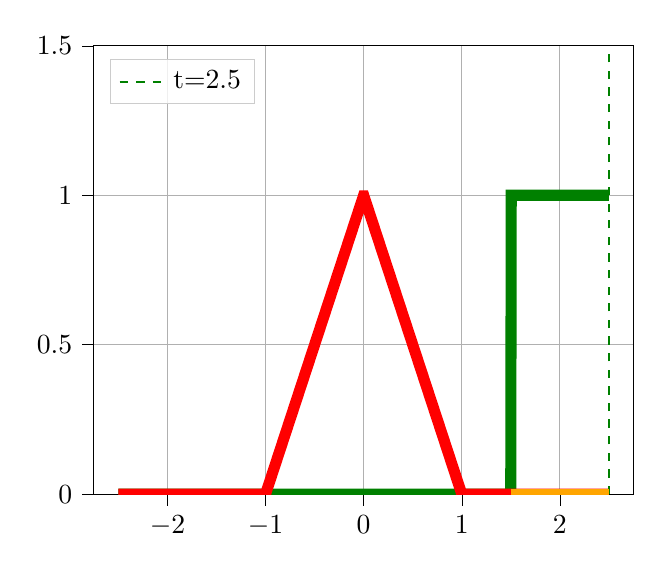
\begin{tikzpicture}

\definecolor{color0}{rgb}{1,0.498039215686275,0.0549019607843137}
\definecolor{color1}{rgb}{1,0.647058823529412,0}

\begin{axis}[
legend cell align={left},
legend style={fill opacity=0.8, draw opacity=1, text opacity=1, at={(0.03,0.97)}, anchor=north west, draw=white!80!black},
tick align=outside,
tick pos=left,
x grid style={white!69.0196078431373!black},
xmajorgrids,
xmin=-2.75, xmax=2.75,
xtick style={color=black},
y grid style={white!69.0196078431373!black},
ymajorgrids,
ymin=0, ymax=1.5,
ytick style={color=black}
]
\path [draw=color0, fill=color0, opacity=0.2]
(axis cs:1.504004004004,0)
--(axis cs:1.504004004004,0)
--(axis cs:1.50900900900901,0)
--(axis cs:1.51401401401401,0)
--(axis cs:1.51901901901902,0)
--(axis cs:1.52402402402402,0)
--(axis cs:1.52902902902903,0)
--(axis cs:1.53403403403403,0)
--(axis cs:1.53903903903904,0)
--(axis cs:1.54404404404404,0)
--(axis cs:1.54904904904905,0)
--(axis cs:1.55405405405405,0)
--(axis cs:1.55905905905906,0)
--(axis cs:1.56406406406406,0)
--(axis cs:1.56906906906907,0)
--(axis cs:1.57407407407407,0)
--(axis cs:1.57907907907908,0)
--(axis cs:1.58408408408408,0)
--(axis cs:1.58908908908909,0)
--(axis cs:1.59409409409409,0)
--(axis cs:1.5990990990991,0)
--(axis cs:1.6041041041041,0)
--(axis cs:1.60910910910911,0)
--(axis cs:1.61411411411411,0)
--(axis cs:1.61911911911912,0)
--(axis cs:1.62412412412412,0)
--(axis cs:1.62912912912913,0)
--(axis cs:1.63413413413413,0)
--(axis cs:1.63913913913914,0)
--(axis cs:1.64414414414414,0)
--(axis cs:1.64914914914915,0)
--(axis cs:1.65415415415415,0)
--(axis cs:1.65915915915916,0)
--(axis cs:1.66416416416416,0)
--(axis cs:1.66916916916917,0)
--(axis cs:1.67417417417417,0)
--(axis cs:1.67917917917918,0)
--(axis cs:1.68418418418418,0)
--(axis cs:1.68918918918919,0)
--(axis cs:1.69419419419419,0)
--(axis cs:1.6991991991992,0)
--(axis cs:1.7042042042042,0)
--(axis cs:1.70920920920921,0)
--(axis cs:1.71421421421421,0)
--(axis cs:1.71921921921922,0)
--(axis cs:1.72422422422422,0)
--(axis cs:1.72922922922923,0)
--(axis cs:1.73423423423423,0)
--(axis cs:1.73923923923924,0)
--(axis cs:1.74424424424424,0)
--(axis cs:1.74924924924925,0)
--(axis cs:1.75425425425425,0)
--(axis cs:1.75925925925926,0)
--(axis cs:1.76426426426426,0)
--(axis cs:1.76926926926927,0)
--(axis cs:1.77427427427427,0)
--(axis cs:1.77927927927928,0)
--(axis cs:1.78428428428428,0)
--(axis cs:1.78928928928929,0)
--(axis cs:1.79429429429429,0)
--(axis cs:1.7992992992993,0)
--(axis cs:1.8043043043043,0)
--(axis cs:1.80930930930931,0)
--(axis cs:1.81431431431431,0)
--(axis cs:1.81931931931932,0)
--(axis cs:1.82432432432432,0)
--(axis cs:1.82932932932933,0)
--(axis cs:1.83433433433433,0)
--(axis cs:1.83933933933934,0)
--(axis cs:1.84434434434434,0)
--(axis cs:1.84934934934935,0)
--(axis cs:1.85435435435435,0)
--(axis cs:1.85935935935936,0)
--(axis cs:1.86436436436436,0)
--(axis cs:1.86936936936937,0)
--(axis cs:1.87437437437437,0)
--(axis cs:1.87937937937938,0)
--(axis cs:1.88438438438438,0)
--(axis cs:1.88938938938939,0)
--(axis cs:1.89439439439439,0)
--(axis cs:1.8993993993994,0)
--(axis cs:1.9044044044044,0)
--(axis cs:1.90940940940941,0)
--(axis cs:1.91441441441441,0)
--(axis cs:1.91941941941942,0)
--(axis cs:1.92442442442442,0)
--(axis cs:1.92942942942943,0)
--(axis cs:1.93443443443443,0)
--(axis cs:1.93943943943944,0)
--(axis cs:1.94444444444444,0)
--(axis cs:1.94944944944945,0)
--(axis cs:1.95445445445445,0)
--(axis cs:1.95945945945946,0)
--(axis cs:1.96446446446446,0)
--(axis cs:1.96946946946947,0)
--(axis cs:1.97447447447447,0)
--(axis cs:1.97947947947948,0)
--(axis cs:1.98448448448448,0)
--(axis cs:1.98948948948949,0)
--(axis cs:1.99449449449449,0)
--(axis cs:1.9994994994995,0)
--(axis cs:2.0045045045045,0)
--(axis cs:2.00950950950951,0)
--(axis cs:2.01451451451451,0)
--(axis cs:2.01951951951952,0)
--(axis cs:2.02452452452452,0)
--(axis cs:2.02952952952953,0)
--(axis cs:2.03453453453453,0)
--(axis cs:2.03953953953954,0)
--(axis cs:2.04454454454454,0)
--(axis cs:2.04954954954955,0)
--(axis cs:2.05455455455455,0)
--(axis cs:2.05955955955956,0)
--(axis cs:2.06456456456456,0)
--(axis cs:2.06956956956957,0)
--(axis cs:2.07457457457457,0)
--(axis cs:2.07957957957958,0)
--(axis cs:2.08458458458458,0)
--(axis cs:2.08958958958959,0)
--(axis cs:2.09459459459459,0)
--(axis cs:2.0995995995996,0)
--(axis cs:2.1046046046046,0)
--(axis cs:2.10960960960961,0)
--(axis cs:2.11461461461461,0)
--(axis cs:2.11961961961962,0)
--(axis cs:2.12462462462462,0)
--(axis cs:2.12962962962963,0)
--(axis cs:2.13463463463463,0)
--(axis cs:2.13963963963964,0)
--(axis cs:2.14464464464464,0)
--(axis cs:2.14964964964965,0)
--(axis cs:2.15465465465465,0)
--(axis cs:2.15965965965966,0)
--(axis cs:2.16466466466466,0)
--(axis cs:2.16966966966967,0)
--(axis cs:2.17467467467467,0)
--(axis cs:2.17967967967968,0)
--(axis cs:2.18468468468468,0)
--(axis cs:2.18968968968969,0)
--(axis cs:2.19469469469469,0)
--(axis cs:2.1996996996997,0)
--(axis cs:2.2047047047047,0)
--(axis cs:2.20970970970971,0)
--(axis cs:2.21471471471471,0)
--(axis cs:2.21971971971972,0)
--(axis cs:2.22472472472472,0)
--(axis cs:2.22972972972973,0)
--(axis cs:2.23473473473473,0)
--(axis cs:2.23973973973974,0)
--(axis cs:2.24474474474474,0)
--(axis cs:2.24974974974975,0)
--(axis cs:2.25475475475475,0)
--(axis cs:2.25975975975976,0)
--(axis cs:2.26476476476476,0)
--(axis cs:2.26976976976977,0)
--(axis cs:2.27477477477477,0)
--(axis cs:2.27977977977978,0)
--(axis cs:2.28478478478478,0)
--(axis cs:2.28978978978979,0)
--(axis cs:2.29479479479479,0)
--(axis cs:2.2997997997998,0)
--(axis cs:2.3048048048048,0)
--(axis cs:2.30980980980981,0)
--(axis cs:2.31481481481481,0)
--(axis cs:2.31981981981982,0)
--(axis cs:2.32482482482482,0)
--(axis cs:2.32982982982983,0)
--(axis cs:2.33483483483483,0)
--(axis cs:2.33983983983984,0)
--(axis cs:2.34484484484484,0)
--(axis cs:2.34984984984985,0)
--(axis cs:2.35485485485485,0)
--(axis cs:2.35985985985986,0)
--(axis cs:2.36486486486486,0)
--(axis cs:2.36986986986987,0)
--(axis cs:2.37487487487487,0)
--(axis cs:2.37987987987988,0)
--(axis cs:2.38488488488488,0)
--(axis cs:2.38988988988989,0)
--(axis cs:2.39489489489489,0)
--(axis cs:2.3998998998999,0)
--(axis cs:2.4049049049049,0)
--(axis cs:2.40990990990991,0)
--(axis cs:2.41491491491491,0)
--(axis cs:2.41991991991992,0)
--(axis cs:2.42492492492492,0)
--(axis cs:2.42992992992993,0)
--(axis cs:2.43493493493493,0)
--(axis cs:2.43993993993994,0)
--(axis cs:2.44494494494494,0)
--(axis cs:2.44994994994995,0)
--(axis cs:2.45495495495495,0)
--(axis cs:2.45995995995996,0)
--(axis cs:2.46496496496496,0)
--(axis cs:2.46996996996997,0)
--(axis cs:2.47497497497497,0)
--(axis cs:2.47997997997998,0)
--(axis cs:2.48498498498498,0)
--(axis cs:2.48998998998999,0)
--(axis cs:2.49499499499499,0)
--(axis cs:2.49499499499499,0)
--(axis cs:2.49499499499499,0)
--(axis cs:2.48998998998999,0)
--(axis cs:2.48498498498498,0)
--(axis cs:2.47997997997998,0)
--(axis cs:2.47497497497497,0)
--(axis cs:2.46996996996997,0)
--(axis cs:2.46496496496496,0)
--(axis cs:2.45995995995996,0)
--(axis cs:2.45495495495495,0)
--(axis cs:2.44994994994995,0)
--(axis cs:2.44494494494494,0)
--(axis cs:2.43993993993994,0)
--(axis cs:2.43493493493493,0)
--(axis cs:2.42992992992993,0)
--(axis cs:2.42492492492492,0)
--(axis cs:2.41991991991992,0)
--(axis cs:2.41491491491491,0)
--(axis cs:2.40990990990991,0)
--(axis cs:2.4049049049049,0)
--(axis cs:2.3998998998999,0)
--(axis cs:2.39489489489489,0)
--(axis cs:2.38988988988989,0)
--(axis cs:2.38488488488488,0)
--(axis cs:2.37987987987988,0)
--(axis cs:2.37487487487487,0)
--(axis cs:2.36986986986987,0)
--(axis cs:2.36486486486486,0)
--(axis cs:2.35985985985986,0)
--(axis cs:2.35485485485485,0)
--(axis cs:2.34984984984985,0)
--(axis cs:2.34484484484484,0)
--(axis cs:2.33983983983984,0)
--(axis cs:2.33483483483483,0)
--(axis cs:2.32982982982983,0)
--(axis cs:2.32482482482482,0)
--(axis cs:2.31981981981982,0)
--(axis cs:2.31481481481481,0)
--(axis cs:2.30980980980981,0)
--(axis cs:2.3048048048048,0)
--(axis cs:2.2997997997998,0)
--(axis cs:2.29479479479479,0)
--(axis cs:2.28978978978979,0)
--(axis cs:2.28478478478478,0)
--(axis cs:2.27977977977978,0)
--(axis cs:2.27477477477477,0)
--(axis cs:2.26976976976977,0)
--(axis cs:2.26476476476476,0)
--(axis cs:2.25975975975976,0)
--(axis cs:2.25475475475475,0)
--(axis cs:2.24974974974975,0)
--(axis cs:2.24474474474474,0)
--(axis cs:2.23973973973974,0)
--(axis cs:2.23473473473473,0)
--(axis cs:2.22972972972973,0)
--(axis cs:2.22472472472472,0)
--(axis cs:2.21971971971972,0)
--(axis cs:2.21471471471471,0)
--(axis cs:2.20970970970971,0)
--(axis cs:2.2047047047047,0)
--(axis cs:2.1996996996997,0)
--(axis cs:2.19469469469469,0)
--(axis cs:2.18968968968969,0)
--(axis cs:2.18468468468468,0)
--(axis cs:2.17967967967968,0)
--(axis cs:2.17467467467467,0)
--(axis cs:2.16966966966967,0)
--(axis cs:2.16466466466466,0)
--(axis cs:2.15965965965966,0)
--(axis cs:2.15465465465465,0)
--(axis cs:2.14964964964965,0)
--(axis cs:2.14464464464464,0)
--(axis cs:2.13963963963964,0)
--(axis cs:2.13463463463463,0)
--(axis cs:2.12962962962963,0)
--(axis cs:2.12462462462462,0)
--(axis cs:2.11961961961962,0)
--(axis cs:2.11461461461461,0)
--(axis cs:2.10960960960961,0)
--(axis cs:2.1046046046046,0)
--(axis cs:2.0995995995996,0)
--(axis cs:2.09459459459459,0)
--(axis cs:2.08958958958959,0)
--(axis cs:2.08458458458458,0)
--(axis cs:2.07957957957958,0)
--(axis cs:2.07457457457457,0)
--(axis cs:2.06956956956957,0)
--(axis cs:2.06456456456456,0)
--(axis cs:2.05955955955956,0)
--(axis cs:2.05455455455455,0)
--(axis cs:2.04954954954955,0)
--(axis cs:2.04454454454454,0)
--(axis cs:2.03953953953954,0)
--(axis cs:2.03453453453453,0)
--(axis cs:2.02952952952953,0)
--(axis cs:2.02452452452452,0)
--(axis cs:2.01951951951952,0)
--(axis cs:2.01451451451451,0)
--(axis cs:2.00950950950951,0)
--(axis cs:2.0045045045045,0)
--(axis cs:1.9994994994995,0)
--(axis cs:1.99449449449449,0)
--(axis cs:1.98948948948949,0)
--(axis cs:1.98448448448448,0)
--(axis cs:1.97947947947948,0)
--(axis cs:1.97447447447447,0)
--(axis cs:1.96946946946947,0)
--(axis cs:1.96446446446446,0)
--(axis cs:1.95945945945946,0)
--(axis cs:1.95445445445445,0)
--(axis cs:1.94944944944945,0)
--(axis cs:1.94444444444444,0)
--(axis cs:1.93943943943944,0)
--(axis cs:1.93443443443443,0)
--(axis cs:1.92942942942943,0)
--(axis cs:1.92442442442442,0)
--(axis cs:1.91941941941942,0)
--(axis cs:1.91441441441441,0)
--(axis cs:1.90940940940941,0)
--(axis cs:1.9044044044044,0)
--(axis cs:1.8993993993994,0)
--(axis cs:1.89439439439439,0)
--(axis cs:1.88938938938939,0)
--(axis cs:1.88438438438438,0)
--(axis cs:1.87937937937938,0)
--(axis cs:1.87437437437437,0)
--(axis cs:1.86936936936937,0)
--(axis cs:1.86436436436436,0)
--(axis cs:1.85935935935936,0)
--(axis cs:1.85435435435435,0)
--(axis cs:1.84934934934935,0)
--(axis cs:1.84434434434434,0)
--(axis cs:1.83933933933934,0)
--(axis cs:1.83433433433433,0)
--(axis cs:1.82932932932933,0)
--(axis cs:1.82432432432432,0)
--(axis cs:1.81931931931932,0)
--(axis cs:1.81431431431431,0)
--(axis cs:1.80930930930931,0)
--(axis cs:1.8043043043043,0)
--(axis cs:1.7992992992993,0)
--(axis cs:1.79429429429429,0)
--(axis cs:1.78928928928929,0)
--(axis cs:1.78428428428428,0)
--(axis cs:1.77927927927928,0)
--(axis cs:1.77427427427427,0)
--(axis cs:1.76926926926927,0)
--(axis cs:1.76426426426426,0)
--(axis cs:1.75925925925926,0)
--(axis cs:1.75425425425425,0)
--(axis cs:1.74924924924925,0)
--(axis cs:1.74424424424424,0)
--(axis cs:1.73923923923924,0)
--(axis cs:1.73423423423423,0)
--(axis cs:1.72922922922923,0)
--(axis cs:1.72422422422422,0)
--(axis cs:1.71921921921922,0)
--(axis cs:1.71421421421421,0)
--(axis cs:1.70920920920921,0)
--(axis cs:1.7042042042042,0)
--(axis cs:1.6991991991992,0)
--(axis cs:1.69419419419419,0)
--(axis cs:1.68918918918919,0)
--(axis cs:1.68418418418418,0)
--(axis cs:1.67917917917918,0)
--(axis cs:1.67417417417417,0)
--(axis cs:1.66916916916917,0)
--(axis cs:1.66416416416416,0)
--(axis cs:1.65915915915916,0)
--(axis cs:1.65415415415415,0)
--(axis cs:1.64914914914915,0)
--(axis cs:1.64414414414414,0)
--(axis cs:1.63913913913914,0)
--(axis cs:1.63413413413413,0)
--(axis cs:1.62912912912913,0)
--(axis cs:1.62412412412412,0)
--(axis cs:1.61911911911912,0)
--(axis cs:1.61411411411411,0)
--(axis cs:1.60910910910911,0)
--(axis cs:1.6041041041041,0)
--(axis cs:1.5990990990991,0)
--(axis cs:1.59409409409409,0)
--(axis cs:1.58908908908909,0)
--(axis cs:1.58408408408408,0)
--(axis cs:1.57907907907908,0)
--(axis cs:1.57407407407407,0)
--(axis cs:1.56906906906907,0)
--(axis cs:1.56406406406406,0)
--(axis cs:1.55905905905906,0)
--(axis cs:1.55405405405405,0)
--(axis cs:1.54904904904905,0)
--(axis cs:1.54404404404404,0)
--(axis cs:1.53903903903904,0)
--(axis cs:1.53403403403403,0)
--(axis cs:1.52902902902903,0)
--(axis cs:1.52402402402402,0)
--(axis cs:1.51901901901902,0)
--(axis cs:1.51401401401401,0)
--(axis cs:1.50900900900901,0)
--(axis cs:1.504004004004,0)
--cycle;

\addplot [line width=4pt, green!50!black, forget plot]
table {%
-2.5 0
-2.49499499499499 0
-2.48998998998999 0
-2.48498498498498 0
-2.47997997997998 0
-2.47497497497497 0
-2.46996996996997 0
-2.46496496496496 0
-2.45995995995996 0
-2.45495495495495 0
-2.44994994994995 0
-2.44494494494494 0
-2.43993993993994 0
-2.43493493493493 0
-2.42992992992993 0
-2.42492492492492 0
-2.41991991991992 0
-2.41491491491491 0
-2.40990990990991 0
-2.4049049049049 0
-2.3998998998999 0
-2.39489489489489 0
-2.38988988988989 0
-2.38488488488488 0
-2.37987987987988 0
-2.37487487487487 0
-2.36986986986987 0
-2.36486486486486 0
-2.35985985985986 0
-2.35485485485485 0
-2.34984984984985 0
-2.34484484484484 0
-2.33983983983984 0
-2.33483483483483 0
-2.32982982982983 0
-2.32482482482482 0
-2.31981981981982 0
-2.31481481481481 0
-2.30980980980981 0
-2.3048048048048 0
-2.2997997997998 0
-2.29479479479479 0
-2.28978978978979 0
-2.28478478478478 0
-2.27977977977978 0
-2.27477477477477 0
-2.26976976976977 0
-2.26476476476476 0
-2.25975975975976 0
-2.25475475475475 0
-2.24974974974975 0
-2.24474474474474 0
-2.23973973973974 0
-2.23473473473473 0
-2.22972972972973 0
-2.22472472472472 0
-2.21971971971972 0
-2.21471471471471 0
-2.20970970970971 0
-2.2047047047047 0
-2.1996996996997 0
-2.19469469469469 0
-2.18968968968969 0
-2.18468468468468 0
-2.17967967967968 0
-2.17467467467467 0
-2.16966966966967 0
-2.16466466466466 0
-2.15965965965966 0
-2.15465465465465 0
-2.14964964964965 0
-2.14464464464464 0
-2.13963963963964 0
-2.13463463463463 0
-2.12962962962963 0
-2.12462462462462 0
-2.11961961961962 0
-2.11461461461461 0
-2.10960960960961 0
-2.1046046046046 0
-2.0995995995996 0
-2.09459459459459 0
-2.08958958958959 0
-2.08458458458458 0
-2.07957957957958 0
-2.07457457457457 0
-2.06956956956957 0
-2.06456456456456 0
-2.05955955955956 0
-2.05455455455455 0
-2.04954954954955 0
-2.04454454454454 0
-2.03953953953954 0
-2.03453453453453 0
-2.02952952952953 0
-2.02452452452452 0
-2.01951951951952 0
-2.01451451451451 0
-2.00950950950951 0
-2.0045045045045 0
-1.9994994994995 0
-1.99449449449449 0
-1.98948948948949 0
-1.98448448448448 0
-1.97947947947948 0
-1.97447447447447 0
-1.96946946946947 0
-1.96446446446446 0
-1.95945945945946 0
-1.95445445445445 0
-1.94944944944945 0
-1.94444444444444 0
-1.93943943943944 0
-1.93443443443443 0
-1.92942942942943 0
-1.92442442442442 0
-1.91941941941942 0
-1.91441441441441 0
-1.90940940940941 0
-1.9044044044044 0
-1.8993993993994 0
-1.89439439439439 0
-1.88938938938939 0
-1.88438438438438 0
-1.87937937937938 0
-1.87437437437437 0
-1.86936936936937 0
-1.86436436436436 0
-1.85935935935936 0
-1.85435435435435 0
-1.84934934934935 0
-1.84434434434434 0
-1.83933933933934 0
-1.83433433433433 0
-1.82932932932933 0
-1.82432432432432 0
-1.81931931931932 0
-1.81431431431431 0
-1.80930930930931 0
-1.8043043043043 0
-1.7992992992993 0
-1.79429429429429 0
-1.78928928928929 0
-1.78428428428428 0
-1.77927927927928 0
-1.77427427427427 0
-1.76926926926927 0
-1.76426426426426 0
-1.75925925925926 0
-1.75425425425425 0
-1.74924924924925 0
-1.74424424424424 0
-1.73923923923924 0
-1.73423423423423 0
-1.72922922922923 0
-1.72422422422422 0
-1.71921921921922 0
-1.71421421421421 0
-1.70920920920921 0
-1.7042042042042 0
-1.6991991991992 0
-1.69419419419419 0
-1.68918918918919 0
-1.68418418418418 0
-1.67917917917918 0
-1.67417417417417 0
-1.66916916916917 0
-1.66416416416416 0
-1.65915915915916 0
-1.65415415415415 0
-1.64914914914915 0
-1.64414414414414 0
-1.63913913913914 0
-1.63413413413413 0
-1.62912912912913 0
-1.62412412412412 0
-1.61911911911912 0
-1.61411411411411 0
-1.60910910910911 0
-1.6041041041041 0
-1.5990990990991 0
-1.59409409409409 0
-1.58908908908909 0
-1.58408408408408 0
-1.57907907907908 0
-1.57407407407407 0
-1.56906906906907 0
-1.56406406406406 0
-1.55905905905906 0
-1.55405405405405 0
-1.54904904904905 0
-1.54404404404404 0
-1.53903903903904 0
-1.53403403403403 0
-1.52902902902903 0
-1.52402402402402 0
-1.51901901901902 0
-1.51401401401401 0
-1.50900900900901 0
-1.504004004004 0
-1.498998998999 0
-1.49399399399399 0
-1.48898898898899 0
-1.48398398398398 0
-1.47897897897898 0
-1.47397397397397 0
-1.46896896896897 0
-1.46396396396396 0
-1.45895895895896 0
-1.45395395395395 0
-1.44894894894895 0
-1.44394394394394 0
-1.43893893893894 0
-1.43393393393393 0
-1.42892892892893 0
-1.42392392392392 0
-1.41891891891892 0
-1.41391391391391 0
-1.40890890890891 0
-1.4039039039039 0
-1.3988988988989 0
-1.39389389389389 0
-1.38888888888889 0
-1.38388388388388 0
-1.37887887887888 0
-1.37387387387387 0
-1.36886886886887 0
-1.36386386386386 0
-1.35885885885886 0
-1.35385385385385 0
-1.34884884884885 0
-1.34384384384384 0
-1.33883883883884 0
-1.33383383383383 0
-1.32882882882883 0
-1.32382382382382 0
-1.31881881881882 0
-1.31381381381381 0
-1.30880880880881 0
-1.3038038038038 0
-1.2987987987988 0
-1.29379379379379 0
-1.28878878878879 0
-1.28378378378378 0
-1.27877877877878 0
-1.27377377377377 0
-1.26876876876877 0
-1.26376376376376 0
-1.25875875875876 0
-1.25375375375375 0
-1.24874874874875 0
-1.24374374374374 0
-1.23873873873874 0
-1.23373373373373 0
-1.22872872872873 0
-1.22372372372372 0
-1.21871871871872 0
-1.21371371371371 0
-1.20870870870871 0
-1.2037037037037 0
-1.1986986986987 0
-1.19369369369369 0
-1.18868868868869 0
-1.18368368368368 0
-1.17867867867868 0
-1.17367367367367 0
-1.16866866866867 0
-1.16366366366366 0
-1.15865865865866 0
-1.15365365365365 0
-1.14864864864865 0
-1.14364364364364 0
-1.13863863863864 0
-1.13363363363363 0
-1.12862862862863 0
-1.12362362362362 0
-1.11861861861862 0
-1.11361361361361 0
-1.10860860860861 0
-1.1036036036036 0
-1.0985985985986 0
-1.09359359359359 0
-1.08858858858859 0
-1.08358358358358 0
-1.07857857857858 0
-1.07357357357357 0
-1.06856856856857 0
-1.06356356356356 0
-1.05855855855856 0
-1.05355355355355 0
-1.04854854854855 0
-1.04354354354354 0
-1.03853853853854 0
-1.03353353353353 0
-1.02852852852853 0
-1.02352352352352 0
-1.01851851851852 0
-1.01351351351351 0
-1.00850850850851 0
-1.0035035035035 0
-0.998498498498499 0
-0.993493493493494 0
-0.988488488488489 0
-0.983483483483484 0
-0.978478478478479 0
-0.973473473473474 0
-0.968468468468469 0
-0.963463463463464 0
-0.958458458458459 0
-0.953453453453454 0
-0.948448448448449 0
-0.943443443443444 0
-0.938438438438439 0
-0.933433433433434 0
-0.928428428428429 0
-0.923423423423424 0
-0.918418418418419 0
-0.913413413413414 0
-0.908408408408409 0
-0.903403403403404 0
-0.898398398398399 0
-0.893393393393393 0
-0.888388388388388 0
-0.883383383383383 0
-0.878378378378378 0
-0.873373373373373 0
-0.868368368368368 0
-0.863363363363363 0
-0.858358358358358 0
-0.853353353353353 0
-0.848348348348348 0
-0.843343343343343 0
-0.838338338338338 0
-0.833333333333333 0
-0.828328328328328 0
-0.823323323323323 0
-0.818318318318318 0
-0.813313313313313 0
-0.808308308308308 0
-0.803303303303303 0
-0.798298298298298 0
-0.793293293293293 0
-0.788288288288288 0
-0.783283283283283 0
-0.778278278278278 0
-0.773273273273273 0
-0.768268268268268 0
-0.763263263263263 0
-0.758258258258258 0
-0.753253253253253 0
-0.748248248248248 0
-0.743243243243243 0
-0.738238238238238 0
-0.733233233233233 0
-0.728228228228228 0
-0.723223223223223 0
-0.718218218218218 0
-0.713213213213213 0
-0.708208208208208 0
-0.703203203203203 0
-0.698198198198198 0
-0.693193193193193 0
-0.688188188188188 0
-0.683183183183183 0
-0.678178178178178 0
-0.673173173173173 0
-0.668168168168168 0
-0.663163163163163 0
-0.658158158158158 0
-0.653153153153153 0
-0.648148148148148 0
-0.643143143143143 0
-0.638138138138138 0
-0.633133133133133 0
-0.628128128128128 0
-0.623123123123123 0
-0.618118118118118 0
-0.613113113113113 0
-0.608108108108108 0
-0.603103103103103 0
-0.598098098098098 0
-0.593093093093093 0
-0.588088088088088 0
-0.583083083083083 0
-0.578078078078078 0
-0.573073073073073 0
-0.568068068068068 0
-0.563063063063063 0
-0.558058058058058 0
-0.553053053053053 0
-0.548048048048048 0
-0.543043043043043 0
-0.538038038038038 0
-0.533033033033033 0
-0.528028028028028 0
-0.523023023023023 0
-0.518018018018018 0
-0.513013013013013 0
-0.508008008008008 0
-0.503003003003003 0
-0.497997997997998 0
-0.492992992992993 0
-0.487987987987988 0
-0.482982982982983 0
-0.477977977977978 0
-0.472972972972973 0
-0.467967967967968 0
-0.462962962962963 0
-0.457957957957958 0
-0.452952952952953 0
-0.447947947947948 0
-0.442942942942943 0
-0.437937937937938 0
-0.432932932932933 0
-0.427927927927928 0
-0.422922922922923 0
-0.417917917917918 0
-0.412912912912913 0
-0.407907907907908 0
-0.402902902902903 0
-0.397897897897898 0
-0.392892892892893 0
-0.387887887887888 0
-0.382882882882883 0
-0.377877877877878 0
-0.372872872872873 0
-0.367867867867868 0
-0.362862862862863 0
-0.357857857857858 0
-0.352852852852853 0
-0.347847847847848 0
-0.342842842842843 0
-0.337837837837838 0
-0.332832832832833 0
-0.327827827827828 0
-0.322822822822823 0
-0.317817817817818 0
-0.312812812812813 0
-0.307807807807808 0
-0.302802802802803 0
-0.297797797797798 0
-0.292792792792793 0
-0.287787787787788 0
-0.282782782782783 0
-0.277777777777778 0
-0.272772772772773 0
-0.267767767767768 0
-0.262762762762763 0
-0.257757757757758 0
-0.252752752752753 0
-0.247747747747748 0
-0.242742742742743 0
-0.237737737737738 0
-0.232732732732733 0
-0.227727727727728 0
-0.222722722722723 0
-0.217717717717718 0
-0.212712712712713 0
-0.207707707707708 0
-0.202702702702703 0
-0.197697697697698 0
-0.192692692692693 0
-0.187687687687688 0
-0.182682682682683 0
-0.177677677677678 0
-0.172672672672673 0
-0.167667667667668 0
-0.162662662662663 0
-0.157657657657658 0
-0.152652652652653 0
-0.147647647647648 0
-0.142642642642643 0
-0.137637637637638 0
-0.132632632632633 0
-0.127627627627628 0
-0.122622622622623 0
-0.117617617617618 0
-0.112612612612613 0
-0.107607607607608 0
-0.102602602602603 0
-0.0975975975975976 0
-0.0925925925925926 0
-0.0875875875875876 0
-0.0825825825825826 0
-0.0775775775775776 0
-0.0725725725725725 0
-0.0675675675675675 0
-0.0625625625625625 0
-0.0575575575575575 0
-0.0525525525525525 0
-0.0475475475475475 0
-0.0425425425425425 0
-0.0375375375375375 0
-0.0325325325325325 0
-0.0275275275275275 0
-0.0225225225225225 0
-0.0175175175175175 0
-0.0125125125125125 0
-0.0075075075075075 0
-0.0025025025025025 0
0.0025025025025025 0
0.0075075075075075 0
0.0125125125125125 0
0.0175175175175175 0
0.0225225225225225 0
0.0275275275275275 0
0.0325325325325325 0
0.0375375375375375 0
0.0425425425425425 0
0.0475475475475475 0
0.0525525525525525 0
0.0575575575575575 0
0.0625625625625625 0
0.0675675675675675 0
0.0725725725725725 0
0.0775775775775776 0
0.0825825825825826 0
0.0875875875875876 0
0.0925925925925926 0
0.0975975975975976 0
0.102602602602603 0
0.107607607607608 0
0.112612612612613 0
0.117617617617618 0
0.122622622622623 0
0.127627627627628 0
0.132632632632633 0
0.137637637637638 0
0.142642642642643 0
0.147647647647648 0
0.152652652652653 0
0.157657657657658 0
0.162662662662663 0
0.167667667667668 0
0.172672672672673 0
0.177677677677678 0
0.182682682682683 0
0.187687687687688 0
0.192692692692693 0
0.197697697697698 0
0.202702702702703 0
0.207707707707708 0
0.212712712712713 0
0.217717717717718 0
0.222722722722723 0
0.227727727727728 0
0.232732732732733 0
0.237737737737738 0
0.242742742742743 0
0.247747747747748 0
0.252752752752753 0
0.257757757757758 0
0.262762762762763 0
0.267767767767768 0
0.272772772772773 0
0.277777777777778 0
0.282782782782783 0
0.287787787787788 0
0.292792792792793 0
0.297797797797798 0
0.302802802802803 0
0.307807807807808 0
0.312812812812813 0
0.317817817817818 0
0.322822822822823 0
0.327827827827828 0
0.332832832832833 0
0.337837837837838 0
0.342842842842843 0
0.347847847847848 0
0.352852852852853 0
0.357857857857858 0
0.362862862862863 0
0.367867867867868 0
0.372872872872873 0
0.377877877877878 0
0.382882882882883 0
0.387887887887888 0
0.392892892892893 0
0.397897897897898 0
0.402902902902903 0
0.407907907907908 0
0.412912912912913 0
0.417917917917918 0
0.422922922922923 0
0.427927927927928 0
0.432932932932933 0
0.437937937937938 0
0.442942942942943 0
0.447947947947948 0
0.452952952952953 0
0.457957957957958 0
0.462962962962963 0
0.467967967967968 0
0.472972972972973 0
0.477977977977978 0
0.482982982982983 0
0.487987987987988 0
0.492992992992993 0
0.497997997997998 0
0.503003003003003 0
0.508008008008008 0
0.513013013013013 0
0.518018018018018 0
0.523023023023023 0
0.528028028028028 0
0.533033033033033 0
0.538038038038038 0
0.543043043043043 0
0.548048048048048 0
0.553053053053053 0
0.558058058058058 0
0.563063063063063 0
0.568068068068068 0
0.573073073073073 0
0.578078078078078 0
0.583083083083083 0
0.588088088088088 0
0.593093093093093 0
0.598098098098098 0
0.603103103103103 0
0.608108108108108 0
0.613113113113113 0
0.618118118118118 0
0.623123123123123 0
0.628128128128128 0
0.633133133133133 0
0.638138138138138 0
0.643143143143143 0
0.648148148148148 0
0.653153153153153 0
0.658158158158158 0
0.663163163163163 0
0.668168168168168 0
0.673173173173173 0
0.678178178178178 0
0.683183183183183 0
0.688188188188188 0
0.693193193193193 0
0.698198198198198 0
0.703203203203203 0
0.708208208208208 0
0.713213213213213 0
0.718218218218218 0
0.723223223223223 0
0.728228228228228 0
0.733233233233233 0
0.738238238238238 0
0.743243243243243 0
0.748248248248248 0
0.753253253253253 0
0.758258258258258 0
0.763263263263263 0
0.768268268268268 0
0.773273273273273 0
0.778278278278278 0
0.783283283283283 0
0.788288288288288 0
0.793293293293293 0
0.798298298298298 0
0.803303303303303 0
0.808308308308308 0
0.813313313313313 0
0.818318318318318 0
0.823323323323323 0
0.828328328328328 0
0.833333333333333 0
0.838338338338338 0
0.843343343343343 0
0.848348348348348 0
0.853353353353353 0
0.858358358358358 0
0.863363363363364 0
0.868368368368369 0
0.873373373373374 0
0.878378378378379 0
0.883383383383384 0
0.888388388388389 0
0.893393393393394 0
0.898398398398399 0
0.903403403403404 0
0.908408408408409 0
0.913413413413414 0
0.918418418418419 0
0.923423423423424 0
0.928428428428429 0
0.933433433433434 0
0.938438438438439 0
0.943443443443444 0
0.948448448448449 0
0.953453453453454 0
0.958458458458459 0
0.963463463463464 0
0.968468468468469 0
0.973473473473474 0
0.978478478478479 0
0.983483483483484 0
0.988488488488489 0
0.993493493493494 0
0.998498498498499 0
1.0035035035035 0
1.00850850850851 0
1.01351351351351 0
1.01851851851852 0
1.02352352352352 0
1.02852852852853 0
1.03353353353353 0
1.03853853853854 0
1.04354354354354 0
1.04854854854855 0
1.05355355355355 0
1.05855855855856 0
1.06356356356356 0
1.06856856856857 0
1.07357357357357 0
1.07857857857858 0
1.08358358358358 0
1.08858858858859 0
1.09359359359359 0
1.0985985985986 0
1.1036036036036 0
1.10860860860861 0
1.11361361361361 0
1.11861861861862 0
1.12362362362362 0
1.12862862862863 0
1.13363363363363 0
1.13863863863864 0
1.14364364364364 0
1.14864864864865 0
1.15365365365365 0
1.15865865865866 0
1.16366366366366 0
1.16866866866867 0
1.17367367367367 0
1.17867867867868 0
1.18368368368368 0
1.18868868868869 0
1.19369369369369 0
1.1986986986987 0
1.2037037037037 0
1.20870870870871 0
1.21371371371371 0
1.21871871871872 0
1.22372372372372 0
1.22872872872873 0
1.23373373373373 0
1.23873873873874 0
1.24374374374374 0
1.24874874874875 0
1.25375375375375 0
1.25875875875876 0
1.26376376376376 0
1.26876876876877 0
1.27377377377377 0
1.27877877877878 0
1.28378378378378 0
1.28878878878879 0
1.29379379379379 0
1.2987987987988 0
1.3038038038038 0
1.30880880880881 0
1.31381381381381 0
1.31881881881882 0
1.32382382382382 0
1.32882882882883 0
1.33383383383383 0
1.33883883883884 0
1.34384384384384 0
1.34884884884885 0
1.35385385385385 0
1.35885885885886 0
1.36386386386386 0
1.36886886886887 0
1.37387387387387 0
1.37887887887888 0
1.38388388388388 0
1.38888888888889 0
1.39389389389389 0
1.3988988988989 0
1.4039039039039 0
1.40890890890891 0
1.41391391391391 0
1.41891891891892 0
1.42392392392392 0
1.42892892892893 0
1.43393393393393 0
1.43893893893894 0
1.44394394394394 0
1.44894894894895 0
1.45395395395395 0
1.45895895895896 0
1.46396396396396 0
1.46896896896897 0
1.47397397397397 0
1.47897897897898 0
1.48398398398398 0
1.48898898898899 0
1.49399399399399 0
1.498998998999 0
1.504004004004 1
1.50900900900901 1
1.51401401401401 1
1.51901901901902 1
1.52402402402402 1
1.52902902902903 1
1.53403403403403 1
1.53903903903904 1
1.54404404404404 1
1.54904904904905 1
1.55405405405405 1
1.55905905905906 1
1.56406406406406 1
1.56906906906907 1
1.57407407407407 1
1.57907907907908 1
1.58408408408408 1
1.58908908908909 1
1.59409409409409 1
1.5990990990991 1
1.6041041041041 1
1.60910910910911 1
1.61411411411411 1
1.61911911911912 1
1.62412412412412 1
1.62912912912913 1
1.63413413413413 1
1.63913913913914 1
1.64414414414414 1
1.64914914914915 1
1.65415415415415 1
1.65915915915916 1
1.66416416416416 1
1.66916916916917 1
1.67417417417417 1
1.67917917917918 1
1.68418418418418 1
1.68918918918919 1
1.69419419419419 1
1.6991991991992 1
1.7042042042042 1
1.70920920920921 1
1.71421421421421 1
1.71921921921922 1
1.72422422422422 1
1.72922922922923 1
1.73423423423423 1
1.73923923923924 1
1.74424424424424 1
1.74924924924925 1
1.75425425425425 1
1.75925925925926 1
1.76426426426426 1
1.76926926926927 1
1.77427427427427 1
1.77927927927928 1
1.78428428428428 1
1.78928928928929 1
1.79429429429429 1
1.7992992992993 1
1.8043043043043 1
1.80930930930931 1
1.81431431431431 1
1.81931931931932 1
1.82432432432432 1
1.82932932932933 1
1.83433433433433 1
1.83933933933934 1
1.84434434434434 1
1.84934934934935 1
1.85435435435435 1
1.85935935935936 1
1.86436436436436 1
1.86936936936937 1
1.87437437437437 1
1.87937937937938 1
1.88438438438438 1
1.88938938938939 1
1.89439439439439 1
1.8993993993994 1
1.9044044044044 1
1.90940940940941 1
1.91441441441441 1
1.91941941941942 1
1.92442442442442 1
1.92942942942943 1
1.93443443443443 1
1.93943943943944 1
1.94444444444444 1
1.94944944944945 1
1.95445445445445 1
1.95945945945946 1
1.96446446446446 1
1.96946946946947 1
1.97447447447447 1
1.97947947947948 1
1.98448448448448 1
1.98948948948949 1
1.99449449449449 1
1.9994994994995 1
2.0045045045045 1
2.00950950950951 1
2.01451451451451 1
2.01951951951952 1
2.02452452452452 1
2.02952952952953 1
2.03453453453453 1
2.03953953953954 1
2.04454454454454 1
2.04954954954955 1
2.05455455455455 1
2.05955955955956 1
2.06456456456456 1
2.06956956956957 1
2.07457457457457 1
2.07957957957958 1
2.08458458458458 1
2.08958958958959 1
2.09459459459459 1
2.0995995995996 1
2.1046046046046 1
2.10960960960961 1
2.11461461461461 1
2.11961961961962 1
2.12462462462462 1
2.12962962962963 1
2.13463463463463 1
2.13963963963964 1
2.14464464464464 1
2.14964964964965 1
2.15465465465465 1
2.15965965965966 1
2.16466466466466 1
2.16966966966967 1
2.17467467467467 1
2.17967967967968 1
2.18468468468468 1
2.18968968968969 1
2.19469469469469 1
2.1996996996997 1
2.2047047047047 1
2.20970970970971 1
2.21471471471471 1
2.21971971971972 1
2.22472472472472 1
2.22972972972973 1
2.23473473473473 1
2.23973973973974 1
2.24474474474474 1
2.24974974974975 1
2.25475475475475 1
2.25975975975976 1
2.26476476476476 1
2.26976976976977 1
2.27477477477477 1
2.27977977977978 1
2.28478478478478 1
2.28978978978979 1
2.29479479479479 1
2.2997997997998 1
2.3048048048048 1
2.30980980980981 1
2.31481481481481 1
2.31981981981982 1
2.32482482482482 1
2.32982982982983 1
2.33483483483483 1
2.33983983983984 1
2.34484484484484 1
2.34984984984985 1
2.35485485485485 1
2.35985985985986 1
2.36486486486486 1
2.36986986986987 1
2.37487487487487 1
2.37987987987988 1
2.38488488488488 1
2.38988988988989 1
2.39489489489489 1
2.3998998998999 1
2.4049049049049 1
2.40990990990991 1
2.41491491491491 1
2.41991991991992 1
2.42492492492492 1
2.42992992992993 1
2.43493493493493 1
2.43993993993994 1
2.44494494494494 1
2.44994994994995 1
2.45495495495495 1
2.45995995995996 1
2.46496496496496 1
2.46996996996997 1
2.47497497497497 1
2.47997997997998 1
2.48498498498498 1
2.48998998998999 1
2.49499499499499 1
2.5 1
};
\addplot [line width=4pt, red, forget plot]
table {%
-2.5 -0
-2.49499499499499 -0
-2.48998998998999 -0
-2.48498498498498 -0
-2.47997997997998 -0
-2.47497497497497 -0
-2.46996996996997 -0
-2.46496496496496 -0
-2.45995995995996 -0
-2.45495495495495 -0
-2.44994994994995 -0
-2.44494494494494 -0
-2.43993993993994 -0
-2.43493493493493 -0
-2.42992992992993 -0
-2.42492492492492 -0
-2.41991991991992 -0
-2.41491491491491 -0
-2.40990990990991 -0
-2.4049049049049 -0
-2.3998998998999 -0
-2.39489489489489 -0
-2.38988988988989 -0
-2.38488488488488 -0
-2.37987987987988 -0
-2.37487487487487 -0
-2.36986986986987 -0
-2.36486486486486 -0
-2.35985985985986 -0
-2.35485485485485 -0
-2.34984984984985 -0
-2.34484484484484 -0
-2.33983983983984 -0
-2.33483483483483 -0
-2.32982982982983 -0
-2.32482482482482 -0
-2.31981981981982 -0
-2.31481481481481 -0
-2.30980980980981 -0
-2.3048048048048 -0
-2.2997997997998 -0
-2.29479479479479 -0
-2.28978978978979 -0
-2.28478478478478 -0
-2.27977977977978 -0
-2.27477477477477 -0
-2.26976976976977 -0
-2.26476476476476 -0
-2.25975975975976 -0
-2.25475475475475 -0
-2.24974974974975 -0
-2.24474474474474 -0
-2.23973973973974 -0
-2.23473473473473 -0
-2.22972972972973 -0
-2.22472472472472 -0
-2.21971971971972 -0
-2.21471471471471 -0
-2.20970970970971 -0
-2.2047047047047 -0
-2.1996996996997 -0
-2.19469469469469 -0
-2.18968968968969 -0
-2.18468468468468 -0
-2.17967967967968 -0
-2.17467467467467 -0
-2.16966966966967 -0
-2.16466466466466 -0
-2.15965965965966 -0
-2.15465465465465 -0
-2.14964964964965 -0
-2.14464464464464 -0
-2.13963963963964 -0
-2.13463463463463 -0
-2.12962962962963 -0
-2.12462462462462 -0
-2.11961961961962 -0
-2.11461461461461 -0
-2.10960960960961 -0
-2.1046046046046 -0
-2.0995995995996 -0
-2.09459459459459 -0
-2.08958958958959 -0
-2.08458458458458 -0
-2.07957957957958 -0
-2.07457457457457 -0
-2.06956956956957 -0
-2.06456456456456 -0
-2.05955955955956 -0
-2.05455455455455 -0
-2.04954954954955 -0
-2.04454454454454 -0
-2.03953953953954 -0
-2.03453453453453 -0
-2.02952952952953 -0
-2.02452452452452 -0
-2.01951951951952 -0
-2.01451451451451 -0
-2.00950950950951 -0
-2.0045045045045 -0
-1.9994994994995 -0
-1.99449449449449 -0
-1.98948948948949 -0
-1.98448448448448 -0
-1.97947947947948 -0
-1.97447447447447 -0
-1.96946946946947 -0
-1.96446446446446 -0
-1.95945945945946 -0
-1.95445445445445 -0
-1.94944944944945 -0
-1.94444444444444 -0
-1.93943943943944 -0
-1.93443443443443 -0
-1.92942942942943 -0
-1.92442442442442 -0
-1.91941941941942 -0
-1.91441441441441 -0
-1.90940940940941 -0
-1.9044044044044 -0
-1.8993993993994 -0
-1.89439439439439 -0
-1.88938938938939 -0
-1.88438438438438 -0
-1.87937937937938 -0
-1.87437437437437 -0
-1.86936936936937 -0
-1.86436436436436 -0
-1.85935935935936 -0
-1.85435435435435 -0
-1.84934934934935 -0
-1.84434434434434 -0
-1.83933933933934 -0
-1.83433433433433 -0
-1.82932932932933 -0
-1.82432432432432 -0
-1.81931931931932 -0
-1.81431431431431 -0
-1.80930930930931 -0
-1.8043043043043 -0
-1.7992992992993 -0
-1.79429429429429 -0
-1.78928928928929 -0
-1.78428428428428 -0
-1.77927927927928 -0
-1.77427427427427 -0
-1.76926926926927 -0
-1.76426426426426 -0
-1.75925925925926 -0
-1.75425425425425 -0
-1.74924924924925 -0
-1.74424424424424 -0
-1.73923923923924 -0
-1.73423423423423 -0
-1.72922922922923 -0
-1.72422422422422 -0
-1.71921921921922 -0
-1.71421421421421 -0
-1.70920920920921 -0
-1.7042042042042 -0
-1.6991991991992 -0
-1.69419419419419 -0
-1.68918918918919 -0
-1.68418418418418 -0
-1.67917917917918 -0
-1.67417417417417 -0
-1.66916916916917 -0
-1.66416416416416 -0
-1.65915915915916 -0
-1.65415415415415 -0
-1.64914914914915 -0
-1.64414414414414 -0
-1.63913913913914 -0
-1.63413413413413 -0
-1.62912912912913 -0
-1.62412412412412 -0
-1.61911911911912 -0
-1.61411411411411 -0
-1.60910910910911 -0
-1.6041041041041 -0
-1.5990990990991 -0
-1.59409409409409 -0
-1.58908908908909 -0
-1.58408408408408 -0
-1.57907907907908 -0
-1.57407407407407 -0
-1.56906906906907 -0
-1.56406406406406 -0
-1.55905905905906 -0
-1.55405405405405 -0
-1.54904904904905 -0
-1.54404404404404 -0
-1.53903903903904 -0
-1.53403403403403 -0
-1.52902902902903 -0
-1.52402402402402 -0
-1.51901901901902 -0
-1.51401401401401 -0
-1.50900900900901 -0
-1.504004004004 -0
-1.498998998999 -0
-1.49399399399399 -0
-1.48898898898899 -0
-1.48398398398398 -0
-1.47897897897898 -0
-1.47397397397397 -0
-1.46896896896897 -0
-1.46396396396396 -0
-1.45895895895896 -0
-1.45395395395395 -0
-1.44894894894895 -0
-1.44394394394394 -0
-1.43893893893894 -0
-1.43393393393393 -0
-1.42892892892893 -0
-1.42392392392392 -0
-1.41891891891892 -0
-1.41391391391391 -0
-1.40890890890891 -0
-1.4039039039039 -0
-1.3988988988989 -0
-1.39389389389389 -0
-1.38888888888889 -0
-1.38388388388388 -0
-1.37887887887888 -0
-1.37387387387387 -0
-1.36886886886887 -0
-1.36386386386386 -0
-1.35885885885886 -0
-1.35385385385385 -0
-1.34884884884885 -0
-1.34384384384384 -0
-1.33883883883884 -0
-1.33383383383383 -0
-1.32882882882883 -0
-1.32382382382382 -0
-1.31881881881882 -0
-1.31381381381381 -0
-1.30880880880881 -0
-1.3038038038038 -0
-1.2987987987988 -0
-1.29379379379379 -0
-1.28878878878879 -0
-1.28378378378378 -0
-1.27877877877878 -0
-1.27377377377377 -0
-1.26876876876877 -0
-1.26376376376376 -0
-1.25875875875876 -0
-1.25375375375375 -0
-1.24874874874875 -0
-1.24374374374374 -0
-1.23873873873874 -0
-1.23373373373373 -0
-1.22872872872873 -0
-1.22372372372372 -0
-1.21871871871872 -0
-1.21371371371371 -0
-1.20870870870871 -0
-1.2037037037037 -0
-1.1986986986987 -0
-1.19369369369369 -0
-1.18868868868869 -0
-1.18368368368368 -0
-1.17867867867868 -0
-1.17367367367367 -0
-1.16866866866867 -0
-1.16366366366366 -0
-1.15865865865866 -0
-1.15365365365365 -0
-1.14864864864865 -0
-1.14364364364364 -0
-1.13863863863864 -0
-1.13363363363363 -0
-1.12862862862863 -0
-1.12362362362362 -0
-1.11861861861862 -0
-1.11361361361361 -0
-1.10860860860861 -0
-1.1036036036036 -0
-1.0985985985986 -0
-1.09359359359359 -0
-1.08858858858859 -0
-1.08358358358358 -0
-1.07857857857858 -0
-1.07357357357357 -0
-1.06856856856857 -0
-1.06356356356356 -0
-1.05855855855856 -0
-1.05355355355355 -0
-1.04854854854855 -0
-1.04354354354354 -0
-1.03853853853854 -0
-1.03353353353353 -0
-1.02852852852853 -0
-1.02352352352352 -0
-1.01851851851852 -0
-1.01351351351351 -0
-1.00850850850851 -0
-1.0035035035035 -0
-0.998498498498499 0.00150150150150141
-0.993493493493494 0.00650650650650642
-0.988488488488489 0.0115115115115114
-0.983483483483484 0.0165165165165164
-0.978478478478479 0.0215215215215214
-0.973473473473474 0.0265265265265264
-0.968468468468469 0.0315315315315314
-0.963463463463464 0.0365365365365364
-0.958458458458459 0.0415415415415414
-0.953453453453454 0.0465465465465464
-0.948448448448449 0.0515515515515514
-0.943443443443444 0.0565565565565564
-0.938438438438439 0.0615615615615615
-0.933433433433434 0.0665665665665665
-0.928428428428429 0.0715715715715715
-0.923423423423424 0.0765765765765765
-0.918418418418419 0.0815815815815815
-0.913413413413414 0.0865865865865865
-0.908408408408409 0.0915915915915915
-0.903403403403404 0.0965965965965965
-0.898398398398399 0.101601601601601
-0.893393393393393 0.106606606606607
-0.888388388388388 0.111611611611612
-0.883383383383383 0.116616616616617
-0.878378378378378 0.121621621621622
-0.873373373373373 0.126626626626627
-0.868368368368368 0.131631631631632
-0.863363363363363 0.136636636636637
-0.858358358358358 0.141641641641642
-0.853353353353353 0.146646646646647
-0.848348348348348 0.151651651651652
-0.843343343343343 0.156656656656657
-0.838338338338338 0.161661661661662
-0.833333333333333 0.166666666666667
-0.828328328328328 0.171671671671672
-0.823323323323323 0.176676676676677
-0.818318318318318 0.181681681681682
-0.813313313313313 0.186686686686687
-0.808308308308308 0.191691691691692
-0.803303303303303 0.196696696696697
-0.798298298298298 0.201701701701702
-0.793293293293293 0.206706706706707
-0.788288288288288 0.211711711711712
-0.783283283283283 0.216716716716717
-0.778278278278278 0.221721721721722
-0.773273273273273 0.226726726726727
-0.768268268268268 0.231731731731732
-0.763263263263263 0.236736736736737
-0.758258258258258 0.241741741741742
-0.753253253253253 0.246746746746747
-0.748248248248248 0.251751751751752
-0.743243243243243 0.256756756756757
-0.738238238238238 0.261761761761762
-0.733233233233233 0.266766766766767
-0.728228228228228 0.271771771771772
-0.723223223223223 0.276776776776777
-0.718218218218218 0.281781781781782
-0.713213213213213 0.286786786786787
-0.708208208208208 0.291791791791792
-0.703203203203203 0.296796796796797
-0.698198198198198 0.301801801801802
-0.693193193193193 0.306806806806807
-0.688188188188188 0.311811811811812
-0.683183183183183 0.316816816816817
-0.678178178178178 0.321821821821822
-0.673173173173173 0.326826826826827
-0.668168168168168 0.331831831831832
-0.663163163163163 0.336836836836837
-0.658158158158158 0.341841841841842
-0.653153153153153 0.346846846846847
-0.648148148148148 0.351851851851852
-0.643143143143143 0.356856856856857
-0.638138138138138 0.361861861861862
-0.633133133133133 0.366866866866867
-0.628128128128128 0.371871871871872
-0.623123123123123 0.376876876876877
-0.618118118118118 0.381881881881882
-0.613113113113113 0.386886886886887
-0.608108108108108 0.391891891891892
-0.603103103103103 0.396896896896897
-0.598098098098098 0.401901901901902
-0.593093093093093 0.406906906906907
-0.588088088088088 0.411911911911912
-0.583083083083083 0.416916916916917
-0.578078078078078 0.421921921921922
-0.573073073073073 0.426926926926927
-0.568068068068068 0.431931931931932
-0.563063063063063 0.436936936936937
-0.558058058058058 0.441941941941942
-0.553053053053053 0.446946946946947
-0.548048048048048 0.451951951951952
-0.543043043043043 0.456956956956957
-0.538038038038038 0.461961961961962
-0.533033033033033 0.466966966966967
-0.528028028028028 0.471971971971972
-0.523023023023023 0.476976976976977
-0.518018018018018 0.481981981981982
-0.513013013013013 0.486986986986987
-0.508008008008008 0.491991991991992
-0.503003003003003 0.496996996996997
-0.497997997997998 0.502002002002002
-0.492992992992993 0.507007007007007
-0.487987987987988 0.512012012012012
-0.482982982982983 0.517017017017017
-0.477977977977978 0.522022022022022
-0.472972972972973 0.527027027027027
-0.467967967967968 0.532032032032032
-0.462962962962963 0.537037037037037
-0.457957957957958 0.542042042042042
-0.452952952952953 0.547047047047047
-0.447947947947948 0.552052052052052
-0.442942942942943 0.557057057057057
-0.437937937937938 0.562062062062062
-0.432932932932933 0.567067067067067
-0.427927927927928 0.572072072072072
-0.422922922922923 0.577077077077077
-0.417917917917918 0.582082082082082
-0.412912912912913 0.587087087087087
-0.407907907907908 0.592092092092092
-0.402902902902903 0.597097097097097
-0.397897897897898 0.602102102102102
-0.392892892892893 0.607107107107107
-0.387887887887888 0.612112112112112
-0.382882882882883 0.617117117117117
-0.377877877877878 0.622122122122122
-0.372872872872873 0.627127127127127
-0.367867867867868 0.632132132132132
-0.362862862862863 0.637137137137137
-0.357857857857858 0.642142142142142
-0.352852852852853 0.647147147147147
-0.347847847847848 0.652152152152152
-0.342842842842843 0.657157157157157
-0.337837837837838 0.662162162162162
-0.332832832832833 0.667167167167167
-0.327827827827828 0.672172172172172
-0.322822822822823 0.677177177177177
-0.317817817817818 0.682182182182182
-0.312812812812813 0.687187187187187
-0.307807807807808 0.692192192192192
-0.302802802802803 0.697197197197197
-0.297797797797798 0.702202202202202
-0.292792792792793 0.707207207207207
-0.287787787787788 0.712212212212212
-0.282782782782783 0.717217217217217
-0.277777777777778 0.722222222222222
-0.272772772772773 0.727227227227227
-0.267767767767768 0.732232232232232
-0.262762762762763 0.737237237237237
-0.257757757757758 0.742242242242242
-0.252752752752753 0.747247247247247
-0.247747747747748 0.752252252252252
-0.242742742742743 0.757257257257257
-0.237737737737738 0.762262262262262
-0.232732732732733 0.767267267267267
-0.227727727727728 0.772272272272272
-0.222722722722723 0.777277277277277
-0.217717717717718 0.782282282282282
-0.212712712712713 0.787287287287287
-0.207707707707708 0.792292292292292
-0.202702702702703 0.797297297297297
-0.197697697697698 0.802302302302302
-0.192692692692693 0.807307307307307
-0.187687687687688 0.812312312312312
-0.182682682682683 0.817317317317317
-0.177677677677678 0.822322322322322
-0.172672672672673 0.827327327327327
-0.167667667667668 0.832332332332332
-0.162662662662663 0.837337337337337
-0.157657657657658 0.842342342342342
-0.152652652652653 0.847347347347347
-0.147647647647648 0.852352352352352
-0.142642642642643 0.857357357357357
-0.137637637637638 0.862362362362362
-0.132632632632633 0.867367367367367
-0.127627627627628 0.872372372372372
-0.122622622622623 0.877377377377377
-0.117617617617618 0.882382382382382
-0.112612612612613 0.887387387387387
-0.107607607607608 0.892392392392392
-0.102602602602603 0.897397397397397
-0.0975975975975976 0.902402402402402
-0.0925925925925926 0.907407407407407
-0.0875875875875876 0.912412412412412
-0.0825825825825826 0.917417417417417
-0.0775775775775776 0.922422422422422
-0.0725725725725725 0.927427427427427
-0.0675675675675675 0.932432432432432
-0.0625625625625625 0.937437437437437
-0.0575575575575575 0.942442442442442
-0.0525525525525525 0.947447447447447
-0.0475475475475475 0.952452452452452
-0.0425425425425425 0.957457457457457
-0.0375375375375375 0.962462462462462
-0.0325325325325325 0.967467467467467
-0.0275275275275275 0.972472472472472
-0.0225225225225225 0.977477477477477
-0.0175175175175175 0.982482482482482
-0.0125125125125125 0.987487487487487
-0.0075075075075075 0.992492492492492
-0.0025025025025025 0.997497497497497
0.0025025025025025 0.997497497497497
0.0075075075075075 0.992492492492492
0.0125125125125125 0.987487487487487
0.0175175175175175 0.982482482482482
0.0225225225225225 0.977477477477477
0.0275275275275275 0.972472472472472
0.0325325325325325 0.967467467467467
0.0375375375375375 0.962462462462462
0.0425425425425425 0.957457457457457
0.0475475475475475 0.952452452452452
0.0525525525525525 0.947447447447447
0.0575575575575575 0.942442442442442
0.0625625625625625 0.937437437437437
0.0675675675675675 0.932432432432432
0.0725725725725725 0.927427427427427
0.0775775775775776 0.922422422422422
0.0825825825825826 0.917417417417417
0.0875875875875876 0.912412412412412
0.0925925925925926 0.907407407407407
0.0975975975975976 0.902402402402402
0.102602602602603 0.897397397397397
0.107607607607608 0.892392392392392
0.112612612612613 0.887387387387387
0.117617617617618 0.882382382382382
0.122622622622623 0.877377377377377
0.127627627627628 0.872372372372372
0.132632632632633 0.867367367367367
0.137637637637638 0.862362362362362
0.142642642642643 0.857357357357357
0.147647647647648 0.852352352352352
0.152652652652653 0.847347347347347
0.157657657657658 0.842342342342342
0.162662662662663 0.837337337337337
0.167667667667668 0.832332332332332
0.172672672672673 0.827327327327327
0.177677677677678 0.822322322322322
0.182682682682683 0.817317317317317
0.187687687687688 0.812312312312312
0.192692692692693 0.807307307307307
0.197697697697698 0.802302302302302
0.202702702702703 0.797297297297297
0.207707707707708 0.792292292292292
0.212712712712713 0.787287287287287
0.217717717717718 0.782282282282282
0.222722722722723 0.777277277277277
0.227727727727728 0.772272272272272
0.232732732732733 0.767267267267267
0.237737737737738 0.762262262262262
0.242742742742743 0.757257257257257
0.247747747747748 0.752252252252252
0.252752752752753 0.747247247247247
0.257757757757758 0.742242242242242
0.262762762762763 0.737237237237237
0.267767767767768 0.732232232232232
0.272772772772773 0.727227227227227
0.277777777777778 0.722222222222222
0.282782782782783 0.717217217217217
0.287787787787788 0.712212212212212
0.292792792792793 0.707207207207207
0.297797797797798 0.702202202202202
0.302802802802803 0.697197197197197
0.307807807807808 0.692192192192192
0.312812812812813 0.687187187187187
0.317817817817818 0.682182182182182
0.322822822822823 0.677177177177177
0.327827827827828 0.672172172172172
0.332832832832833 0.667167167167167
0.337837837837838 0.662162162162162
0.342842842842843 0.657157157157157
0.347847847847848 0.652152152152152
0.352852852852853 0.647147147147147
0.357857857857858 0.642142142142142
0.362862862862863 0.637137137137137
0.367867867867868 0.632132132132132
0.372872872872873 0.627127127127127
0.377877877877878 0.622122122122122
0.382882882882883 0.617117117117117
0.387887887887888 0.612112112112112
0.392892892892893 0.607107107107107
0.397897897897898 0.602102102102102
0.402902902902903 0.597097097097097
0.407907907907908 0.592092092092092
0.412912912912913 0.587087087087087
0.417917917917918 0.582082082082082
0.422922922922923 0.577077077077077
0.427927927927928 0.572072072072072
0.432932932932933 0.567067067067067
0.437937937937938 0.562062062062062
0.442942942942943 0.557057057057057
0.447947947947948 0.552052052052052
0.452952952952953 0.547047047047047
0.457957957957958 0.542042042042042
0.462962962962963 0.537037037037037
0.467967967967968 0.532032032032032
0.472972972972973 0.527027027027027
0.477977977977978 0.522022022022022
0.482982982982983 0.517017017017017
0.487987987987988 0.512012012012012
0.492992992992993 0.507007007007007
0.497997997997998 0.502002002002002
0.503003003003003 0.496996996996997
0.508008008008008 0.491991991991992
0.513013013013013 0.486986986986987
0.518018018018018 0.481981981981982
0.523023023023023 0.476976976976977
0.528028028028028 0.471971971971972
0.533033033033033 0.466966966966967
0.538038038038038 0.461961961961962
0.543043043043043 0.456956956956957
0.548048048048048 0.451951951951952
0.553053053053053 0.446946946946947
0.558058058058058 0.441941941941942
0.563063063063063 0.436936936936937
0.568068068068068 0.431931931931932
0.573073073073073 0.426926926926927
0.578078078078078 0.421921921921922
0.583083083083083 0.416916916916917
0.588088088088088 0.411911911911912
0.593093093093093 0.406906906906907
0.598098098098098 0.401901901901902
0.603103103103103 0.396896896896897
0.608108108108108 0.391891891891892
0.613113113113113 0.386886886886887
0.618118118118118 0.381881881881882
0.623123123123123 0.376876876876877
0.628128128128128 0.371871871871872
0.633133133133133 0.366866866866867
0.638138138138138 0.361861861861862
0.643143143143143 0.356856856856857
0.648148148148148 0.351851851851852
0.653153153153153 0.346846846846847
0.658158158158158 0.341841841841842
0.663163163163163 0.336836836836837
0.668168168168168 0.331831831831832
0.673173173173173 0.326826826826827
0.678178178178178 0.321821821821822
0.683183183183183 0.316816816816817
0.688188188188188 0.311811811811812
0.693193193193193 0.306806806806807
0.698198198198198 0.301801801801802
0.703203203203203 0.296796796796797
0.708208208208208 0.291791791791792
0.713213213213213 0.286786786786787
0.718218218218218 0.281781781781782
0.723223223223223 0.276776776776777
0.728228228228228 0.271771771771772
0.733233233233233 0.266766766766767
0.738238238238238 0.261761761761762
0.743243243243243 0.256756756756757
0.748248248248248 0.251751751751752
0.753253253253253 0.246746746746747
0.758258258258258 0.241741741741742
0.763263263263263 0.236736736736737
0.768268268268268 0.231731731731732
0.773273273273273 0.226726726726727
0.778278278278278 0.221721721721722
0.783283283283283 0.216716716716717
0.788288288288288 0.211711711711712
0.793293293293293 0.206706706706707
0.798298298298298 0.201701701701702
0.803303303303303 0.196696696696697
0.808308308308308 0.191691691691692
0.813313313313313 0.186686686686687
0.818318318318318 0.181681681681682
0.823323323323323 0.176676676676677
0.828328328328328 0.171671671671672
0.833333333333333 0.166666666666667
0.838338338338338 0.161661661661662
0.843343343343343 0.156656656656657
0.848348348348348 0.151651651651652
0.853353353353353 0.146646646646647
0.858358358358358 0.141641641641642
0.863363363363364 0.136636636636636
0.868368368368369 0.131631631631631
0.873373373373374 0.126626626626626
0.878378378378379 0.121621621621621
0.883383383383384 0.116616616616616
0.888388388388389 0.111611611611611
0.893393393393394 0.106606606606606
0.898398398398399 0.101601601601601
0.903403403403404 0.0965965965965965
0.908408408408409 0.0915915915915915
0.913413413413414 0.0865865865865865
0.918418418418419 0.0815815815815815
0.923423423423424 0.0765765765765765
0.928428428428429 0.0715715715715715
0.933433433433434 0.0665665665665665
0.938438438438439 0.0615615615615615
0.943443443443444 0.0565565565565564
0.948448448448449 0.0515515515515514
0.953453453453454 0.0465465465465464
0.958458458458459 0.0415415415415414
0.963463463463464 0.0365365365365364
0.968468468468469 0.0315315315315314
0.973473473473474 0.0265265265265264
0.978478478478479 0.0215215215215214
0.983483483483484 0.0165165165165164
0.988488488488489 0.0115115115115114
0.993493493493494 0.00650650650650642
0.998498498498499 0.00150150150150141
1.0035035035035 -0
1.00850850850851 -0
1.01351351351351 -0
1.01851851851852 -0
1.02352352352352 -0
1.02852852852853 -0
1.03353353353353 -0
1.03853853853854 -0
1.04354354354354 -0
1.04854854854855 -0
1.05355355355355 -0
1.05855855855856 -0
1.06356356356356 -0
1.06856856856857 -0
1.07357357357357 -0
1.07857857857858 -0
1.08358358358358 -0
1.08858858858859 -0
1.09359359359359 -0
1.0985985985986 -0
1.1036036036036 -0
1.10860860860861 -0
1.11361361361361 -0
1.11861861861862 -0
1.12362362362362 -0
1.12862862862863 -0
1.13363363363363 -0
1.13863863863864 -0
1.14364364364364 -0
1.14864864864865 -0
1.15365365365365 -0
1.15865865865866 -0
1.16366366366366 -0
1.16866866866867 -0
1.17367367367367 -0
1.17867867867868 -0
1.18368368368368 -0
1.18868868868869 -0
1.19369369369369 -0
1.1986986986987 -0
1.2037037037037 -0
1.20870870870871 -0
1.21371371371371 -0
1.21871871871872 -0
1.22372372372372 -0
1.22872872872873 -0
1.23373373373373 -0
1.23873873873874 -0
1.24374374374374 -0
1.24874874874875 -0
1.25375375375375 -0
1.25875875875876 -0
1.26376376376376 -0
1.26876876876877 -0
1.27377377377377 -0
1.27877877877878 -0
1.28378378378378 -0
1.28878878878879 -0
1.29379379379379 -0
1.2987987987988 -0
1.3038038038038 -0
1.30880880880881 -0
1.31381381381381 -0
1.31881881881882 -0
1.32382382382382 -0
1.32882882882883 -0
1.33383383383383 -0
1.33883883883884 -0
1.34384384384384 -0
1.34884884884885 -0
1.35385385385385 -0
1.35885885885886 -0
1.36386386386386 -0
1.36886886886887 -0
1.37387387387387 -0
1.37887887887888 -0
1.38388388388388 -0
1.38888888888889 -0
1.39389389389389 -0
1.3988988988989 -0
1.4039039039039 -0
1.40890890890891 -0
1.41391391391391 -0
1.41891891891892 -0
1.42392392392392 -0
1.42892892892893 -0
1.43393393393393 -0
1.43893893893894 -0
1.44394394394394 -0
1.44894894894895 -0
1.45395395395395 -0
1.45895895895896 -0
1.46396396396396 -0
1.46896896896897 -0
1.47397397397397 -0
1.47897897897898 -0
1.48398398398398 -0
1.48898898898899 -0
1.49399399399399 -0
1.498998998999 -0
1.504004004004 -0
1.50900900900901 -0
1.51401401401401 -0
1.51901901901902 -0
1.52402402402402 -0
1.52902902902903 -0
1.53403403403403 -0
1.53903903903904 -0
1.54404404404404 -0
1.54904904904905 -0
1.55405405405405 -0
1.55905905905906 -0
1.56406406406406 -0
1.56906906906907 -0
1.57407407407407 -0
1.57907907907908 -0
1.58408408408408 -0
1.58908908908909 -0
1.59409409409409 -0
1.5990990990991 -0
1.6041041041041 -0
1.60910910910911 -0
1.61411411411411 -0
1.61911911911912 -0
1.62412412412412 -0
1.62912912912913 -0
1.63413413413413 -0
1.63913913913914 -0
1.64414414414414 -0
1.64914914914915 -0
1.65415415415415 -0
1.65915915915916 -0
1.66416416416416 -0
1.66916916916917 -0
1.67417417417417 -0
1.67917917917918 -0
1.68418418418418 -0
1.68918918918919 -0
1.69419419419419 -0
1.6991991991992 -0
1.7042042042042 -0
1.70920920920921 -0
1.71421421421421 -0
1.71921921921922 -0
1.72422422422422 -0
1.72922922922923 -0
1.73423423423423 -0
1.73923923923924 -0
1.74424424424424 -0
1.74924924924925 -0
1.75425425425425 -0
1.75925925925926 -0
1.76426426426426 -0
1.76926926926927 -0
1.77427427427427 -0
1.77927927927928 -0
1.78428428428428 -0
1.78928928928929 -0
1.79429429429429 -0
1.7992992992993 -0
1.8043043043043 -0
1.80930930930931 -0
1.81431431431431 -0
1.81931931931932 -0
1.82432432432432 -0
1.82932932932933 -0
1.83433433433433 -0
1.83933933933934 -0
1.84434434434434 -0
1.84934934934935 -0
1.85435435435435 -0
1.85935935935936 -0
1.86436436436436 -0
1.86936936936937 -0
1.87437437437437 -0
1.87937937937938 -0
1.88438438438438 -0
1.88938938938939 -0
1.89439439439439 -0
1.8993993993994 -0
1.9044044044044 -0
1.90940940940941 -0
1.91441441441441 -0
1.91941941941942 -0
1.92442442442442 -0
1.92942942942943 -0
1.93443443443443 -0
1.93943943943944 -0
1.94444444444444 -0
1.94944944944945 -0
1.95445445445445 -0
1.95945945945946 -0
1.96446446446446 -0
1.96946946946947 -0
1.97447447447447 -0
1.97947947947948 -0
1.98448448448448 -0
1.98948948948949 -0
1.99449449449449 -0
1.9994994994995 -0
2.0045045045045 -0
2.00950950950951 -0
2.01451451451451 -0
2.01951951951952 -0
2.02452452452452 -0
2.02952952952953 -0
2.03453453453453 -0
2.03953953953954 -0
2.04454454454454 -0
2.04954954954955 -0
2.05455455455455 -0
2.05955955955956 -0
2.06456456456456 -0
2.06956956956957 -0
2.07457457457457 -0
2.07957957957958 -0
2.08458458458458 -0
2.08958958958959 -0
2.09459459459459 -0
2.0995995995996 -0
2.1046046046046 -0
2.10960960960961 -0
2.11461461461461 -0
2.11961961961962 -0
2.12462462462462 -0
2.12962962962963 -0
2.13463463463463 -0
2.13963963963964 -0
2.14464464464464 -0
2.14964964964965 -0
2.15465465465465 -0
2.15965965965966 -0
2.16466466466466 -0
2.16966966966967 -0
2.17467467467467 -0
2.17967967967968 -0
2.18468468468468 -0
2.18968968968969 -0
2.19469469469469 -0
2.1996996996997 -0
2.2047047047047 -0
2.20970970970971 -0
2.21471471471471 -0
2.21971971971972 -0
2.22472472472472 -0
2.22972972972973 -0
2.23473473473473 -0
2.23973973973974 -0
2.24474474474474 -0
2.24974974974975 -0
2.25475475475475 -0
2.25975975975976 -0
2.26476476476476 -0
2.26976976976977 -0
2.27477477477477 -0
2.27977977977978 -0
2.28478478478478 -0
2.28978978978979 -0
2.29479479479479 -0
2.2997997997998 -0
2.3048048048048 -0
2.30980980980981 -0
2.31481481481481 -0
2.31981981981982 -0
2.32482482482482 -0
2.32982982982983 -0
2.33483483483483 -0
2.33983983983984 -0
2.34484484484484 -0
2.34984984984985 -0
2.35485485485485 -0
2.35985985985986 -0
2.36486486486486 -0
2.36986986986987 -0
2.37487487487487 -0
2.37987987987988 -0
2.38488488488488 -0
2.38988988988989 -0
2.39489489489489 -0
2.3998998998999 -0
2.4049049049049 -0
2.40990990990991 -0
2.41491491491491 -0
2.41991991991992 -0
2.42492492492492 -0
2.42992992992993 -0
2.43493493493493 -0
2.43993993993994 -0
2.44494494494494 -0
2.44994994994995 -0
2.45495495495495 -0
2.45995995995996 -0
2.46496496496496 -0
2.46996996996997 -0
2.47497497497497 -0
2.47997997997998 -0
2.48498498498498 -0
2.48998998998999 -0
2.49499499499499 -0
2.5 -0
};
\addplot [semithick, green!50!black, dashed]
table {%
2.5 0
2.5 1.5
};
\addlegendentry{t=2.5}
\addplot [line width=4pt, color1, forget plot]
table {%
1.504004004004 -0
1.50900900900901 -0
1.51401401401401 -0
1.51901901901902 -0
1.52402402402402 -0
1.52902902902903 -0
1.53403403403403 -0
1.53903903903904 -0
1.54404404404404 -0
1.54904904904905 -0
1.55405405405405 -0
1.55905905905906 -0
1.56406406406406 -0
1.56906906906907 -0
1.57407407407407 -0
1.57907907907908 -0
1.58408408408408 -0
1.58908908908909 -0
1.59409409409409 -0
1.5990990990991 -0
1.6041041041041 -0
1.60910910910911 -0
1.61411411411411 -0
1.61911911911912 -0
1.62412412412412 -0
1.62912912912913 -0
1.63413413413413 -0
1.63913913913914 -0
1.64414414414414 -0
1.64914914914915 -0
1.65415415415415 -0
1.65915915915916 -0
1.66416416416416 -0
1.66916916916917 -0
1.67417417417417 -0
1.67917917917918 -0
1.68418418418418 -0
1.68918918918919 -0
1.69419419419419 -0
1.6991991991992 -0
1.7042042042042 -0
1.70920920920921 -0
1.71421421421421 -0
1.71921921921922 -0
1.72422422422422 -0
1.72922922922923 -0
1.73423423423423 -0
1.73923923923924 -0
1.74424424424424 -0
1.74924924924925 -0
1.75425425425425 -0
1.75925925925926 -0
1.76426426426426 -0
1.76926926926927 -0
1.77427427427427 -0
1.77927927927928 -0
1.78428428428428 -0
1.78928928928929 -0
1.79429429429429 -0
1.7992992992993 -0
1.8043043043043 -0
1.80930930930931 -0
1.81431431431431 -0
1.81931931931932 -0
1.82432432432432 -0
1.82932932932933 -0
1.83433433433433 -0
1.83933933933934 -0
1.84434434434434 -0
1.84934934934935 -0
1.85435435435435 -0
1.85935935935936 -0
1.86436436436436 -0
1.86936936936937 -0
1.87437437437437 -0
1.87937937937938 -0
1.88438438438438 -0
1.88938938938939 -0
1.89439439439439 -0
1.8993993993994 -0
1.9044044044044 -0
1.90940940940941 -0
1.91441441441441 -0
1.91941941941942 -0
1.92442442442442 -0
1.92942942942943 -0
1.93443443443443 -0
1.93943943943944 -0
1.94444444444444 -0
1.94944944944945 -0
1.95445445445445 -0
1.95945945945946 -0
1.96446446446446 -0
1.96946946946947 -0
1.97447447447447 -0
1.97947947947948 -0
1.98448448448448 -0
1.98948948948949 -0
1.99449449449449 -0
1.9994994994995 -0
2.0045045045045 -0
2.00950950950951 -0
2.01451451451451 -0
2.01951951951952 -0
2.02452452452452 -0
2.02952952952953 -0
2.03453453453453 -0
2.03953953953954 -0
2.04454454454454 -0
2.04954954954955 -0
2.05455455455455 -0
2.05955955955956 -0
2.06456456456456 -0
2.06956956956957 -0
2.07457457457457 -0
2.07957957957958 -0
2.08458458458458 -0
2.08958958958959 -0
2.09459459459459 -0
2.0995995995996 -0
2.1046046046046 -0
2.10960960960961 -0
2.11461461461461 -0
2.11961961961962 -0
2.12462462462462 -0
2.12962962962963 -0
2.13463463463463 -0
2.13963963963964 -0
2.14464464464464 -0
2.14964964964965 -0
2.15465465465465 -0
2.15965965965966 -0
2.16466466466466 -0
2.16966966966967 -0
2.17467467467467 -0
2.17967967967968 -0
2.18468468468468 -0
2.18968968968969 -0
2.19469469469469 -0
2.1996996996997 -0
2.2047047047047 -0
2.20970970970971 -0
2.21471471471471 -0
2.21971971971972 -0
2.22472472472472 -0
2.22972972972973 -0
2.23473473473473 -0
2.23973973973974 -0
2.24474474474474 -0
2.24974974974975 -0
2.25475475475475 -0
2.25975975975976 -0
2.26476476476476 -0
2.26976976976977 -0
2.27477477477477 -0
2.27977977977978 -0
2.28478478478478 -0
2.28978978978979 -0
2.29479479479479 -0
2.2997997997998 -0
2.3048048048048 -0
2.30980980980981 -0
2.31481481481481 -0
2.31981981981982 -0
2.32482482482482 -0
2.32982982982983 -0
2.33483483483483 -0
2.33983983983984 -0
2.34484484484484 -0
2.34984984984985 -0
2.35485485485485 -0
2.35985985985986 -0
2.36486486486486 -0
2.36986986986987 -0
2.37487487487487 -0
2.37987987987988 -0
2.38488488488488 -0
2.38988988988989 -0
2.39489489489489 -0
2.3998998998999 -0
2.4049049049049 -0
2.40990990990991 -0
2.41491491491491 -0
2.41991991991992 -0
2.42492492492492 -0
2.42992992992993 -0
2.43493493493493 -0
2.43993993993994 -0
2.44494494494494 -0
2.44994994994995 -0
2.45495495495495 -0
2.45995995995996 -0
2.46496496496496 -0
2.46996996996997 -0
2.47497497497497 -0
2.47997997997998 -0
2.48498498498498 -0
2.48998998998999 -0
2.49499499499499 -0
};
\end{axis}

\end{tikzpicture}
}}%
                \begin{align*}
                    \textcolor{red!80!black}{f(\tau)~}     & \textcolor{red!80!black}{= \mathsf{rect}\left(0.5\cdot \tau\right) \cdot \left(1-\left| \tau \right|\right)} \\[0.2cm]
                    \textcolor{green!40!black}{h(t-\tau)~} & \textcolor{green!40!black}{= \mathsf{rect}\left(0.5\cdot \left(t-\tau\right)\right)}                         \\[0.2cm]
                                                           & \textcolor{orange!80!black}{~~~f(\tau) \cdot h(t-\tau)}                                                      \\[0.2cm]
                    %\textcolor{blue!80}{g(t)~} & \textcolor{blue!80}{= \alt<1>{f(t) + h(t)}{f(t) \ast h(t)}}
                \end{align*}

            \end{column}%
            %\begin{column}{0.33\textwidth}
            %\centering{}
            %\scalebox{0.4}{\input{multiplied_0.tex}}

            %\quad{}f(\tau)$ \cdot h(t-\tau)$
            %\end{column}
            \begin{column}{0.5\textwidth}
                \centering{}
                \only<1>{\scalebox{0.5}{% This file was created by tikzplotlib v0.9.1.
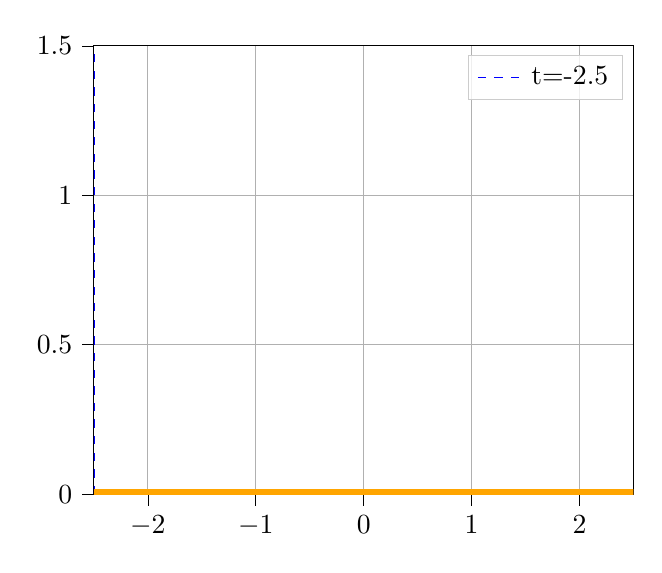
\begin{tikzpicture}

\definecolor{color0}{rgb}{1,0.498039215686275,0.0549019607843137}
\definecolor{color1}{rgb}{1,0.647058823529412,0}

\begin{axis}[
legend cell align={left},
legend style={fill opacity=0.8, draw opacity=1, text opacity=1, draw=white!80!black},
tick align=outside,
tick pos=left,
x grid style={white!69.0196078431373!black},
xmajorgrids,
xmin=-2.5, xmax=2.5,
xtick style={color=black},
y grid style={white!69.0196078431373!black},
ymajorgrids,
ymin=0, ymax=1.5,
ytick style={color=black}
]
\path [draw=color0, fill=color0, opacity=0.2]
(axis cs:-2.5,0)
--(axis cs:-2.5,0)
--(axis cs:-2.49499499499499,0)
--(axis cs:-2.48998998998999,0)
--(axis cs:-2.48498498498498,0)
--(axis cs:-2.47997997997998,0)
--(axis cs:-2.47497497497497,0)
--(axis cs:-2.46996996996997,0)
--(axis cs:-2.46496496496496,0)
--(axis cs:-2.45995995995996,0)
--(axis cs:-2.45495495495495,0)
--(axis cs:-2.44994994994995,0)
--(axis cs:-2.44494494494494,0)
--(axis cs:-2.43993993993994,0)
--(axis cs:-2.43493493493493,0)
--(axis cs:-2.42992992992993,0)
--(axis cs:-2.42492492492492,0)
--(axis cs:-2.41991991991992,0)
--(axis cs:-2.41491491491491,0)
--(axis cs:-2.40990990990991,0)
--(axis cs:-2.4049049049049,0)
--(axis cs:-2.3998998998999,0)
--(axis cs:-2.39489489489489,0)
--(axis cs:-2.38988988988989,0)
--(axis cs:-2.38488488488488,0)
--(axis cs:-2.37987987987988,0)
--(axis cs:-2.37487487487487,0)
--(axis cs:-2.36986986986987,0)
--(axis cs:-2.36486486486486,0)
--(axis cs:-2.35985985985986,0)
--(axis cs:-2.35485485485485,0)
--(axis cs:-2.34984984984985,0)
--(axis cs:-2.34484484484484,0)
--(axis cs:-2.33983983983984,0)
--(axis cs:-2.33483483483483,0)
--(axis cs:-2.32982982982983,0)
--(axis cs:-2.32482482482482,0)
--(axis cs:-2.31981981981982,0)
--(axis cs:-2.31481481481481,0)
--(axis cs:-2.30980980980981,0)
--(axis cs:-2.3048048048048,0)
--(axis cs:-2.2997997997998,0)
--(axis cs:-2.29479479479479,0)
--(axis cs:-2.28978978978979,0)
--(axis cs:-2.28478478478478,0)
--(axis cs:-2.27977977977978,0)
--(axis cs:-2.27477477477477,0)
--(axis cs:-2.26976976976977,0)
--(axis cs:-2.26476476476476,0)
--(axis cs:-2.25975975975976,0)
--(axis cs:-2.25475475475475,0)
--(axis cs:-2.24974974974975,0)
--(axis cs:-2.24474474474474,0)
--(axis cs:-2.23973973973974,0)
--(axis cs:-2.23473473473473,0)
--(axis cs:-2.22972972972973,0)
--(axis cs:-2.22472472472472,0)
--(axis cs:-2.21971971971972,0)
--(axis cs:-2.21471471471471,0)
--(axis cs:-2.20970970970971,0)
--(axis cs:-2.2047047047047,0)
--(axis cs:-2.1996996996997,0)
--(axis cs:-2.19469469469469,0)
--(axis cs:-2.18968968968969,0)
--(axis cs:-2.18468468468468,0)
--(axis cs:-2.17967967967968,0)
--(axis cs:-2.17467467467467,0)
--(axis cs:-2.16966966966967,0)
--(axis cs:-2.16466466466466,0)
--(axis cs:-2.15965965965966,0)
--(axis cs:-2.15465465465465,0)
--(axis cs:-2.14964964964965,0)
--(axis cs:-2.14464464464464,0)
--(axis cs:-2.13963963963964,0)
--(axis cs:-2.13463463463463,0)
--(axis cs:-2.12962962962963,0)
--(axis cs:-2.12462462462462,0)
--(axis cs:-2.11961961961962,0)
--(axis cs:-2.11461461461461,0)
--(axis cs:-2.10960960960961,0)
--(axis cs:-2.1046046046046,0)
--(axis cs:-2.0995995995996,0)
--(axis cs:-2.09459459459459,0)
--(axis cs:-2.08958958958959,0)
--(axis cs:-2.08458458458458,0)
--(axis cs:-2.07957957957958,0)
--(axis cs:-2.07457457457457,0)
--(axis cs:-2.06956956956957,0)
--(axis cs:-2.06456456456456,0)
--(axis cs:-2.05955955955956,0)
--(axis cs:-2.05455455455455,0)
--(axis cs:-2.04954954954955,0)
--(axis cs:-2.04454454454454,0)
--(axis cs:-2.03953953953954,0)
--(axis cs:-2.03453453453453,0)
--(axis cs:-2.02952952952953,0)
--(axis cs:-2.02452452452452,0)
--(axis cs:-2.01951951951952,0)
--(axis cs:-2.01451451451451,0)
--(axis cs:-2.00950950950951,0)
--(axis cs:-2.0045045045045,0)
--(axis cs:-1.9994994994995,0)
--(axis cs:-1.99449449449449,0)
--(axis cs:-1.98948948948949,0)
--(axis cs:-1.98448448448448,0)
--(axis cs:-1.97947947947948,0)
--(axis cs:-1.97447447447447,0)
--(axis cs:-1.96946946946947,0)
--(axis cs:-1.96446446446446,0)
--(axis cs:-1.95945945945946,0)
--(axis cs:-1.95445445445445,0)
--(axis cs:-1.94944944944945,0)
--(axis cs:-1.94444444444444,0)
--(axis cs:-1.93943943943944,0)
--(axis cs:-1.93443443443443,0)
--(axis cs:-1.92942942942943,0)
--(axis cs:-1.92442442442442,0)
--(axis cs:-1.91941941941942,0)
--(axis cs:-1.91441441441441,0)
--(axis cs:-1.90940940940941,0)
--(axis cs:-1.9044044044044,0)
--(axis cs:-1.8993993993994,0)
--(axis cs:-1.89439439439439,0)
--(axis cs:-1.88938938938939,0)
--(axis cs:-1.88438438438438,0)
--(axis cs:-1.87937937937938,0)
--(axis cs:-1.87437437437437,0)
--(axis cs:-1.86936936936937,0)
--(axis cs:-1.86436436436436,0)
--(axis cs:-1.85935935935936,0)
--(axis cs:-1.85435435435435,0)
--(axis cs:-1.84934934934935,0)
--(axis cs:-1.84434434434434,0)
--(axis cs:-1.83933933933934,0)
--(axis cs:-1.83433433433433,0)
--(axis cs:-1.82932932932933,0)
--(axis cs:-1.82432432432432,0)
--(axis cs:-1.81931931931932,0)
--(axis cs:-1.81431431431431,0)
--(axis cs:-1.80930930930931,0)
--(axis cs:-1.8043043043043,0)
--(axis cs:-1.7992992992993,0)
--(axis cs:-1.79429429429429,0)
--(axis cs:-1.78928928928929,0)
--(axis cs:-1.78428428428428,0)
--(axis cs:-1.77927927927928,0)
--(axis cs:-1.77427427427427,0)
--(axis cs:-1.76926926926927,0)
--(axis cs:-1.76426426426426,0)
--(axis cs:-1.75925925925926,0)
--(axis cs:-1.75425425425425,0)
--(axis cs:-1.74924924924925,0)
--(axis cs:-1.74424424424424,0)
--(axis cs:-1.73923923923924,0)
--(axis cs:-1.73423423423423,0)
--(axis cs:-1.72922922922923,0)
--(axis cs:-1.72422422422422,0)
--(axis cs:-1.71921921921922,0)
--(axis cs:-1.71421421421421,0)
--(axis cs:-1.70920920920921,0)
--(axis cs:-1.7042042042042,0)
--(axis cs:-1.6991991991992,0)
--(axis cs:-1.69419419419419,0)
--(axis cs:-1.68918918918919,0)
--(axis cs:-1.68418418418418,0)
--(axis cs:-1.67917917917918,0)
--(axis cs:-1.67417417417417,0)
--(axis cs:-1.66916916916917,0)
--(axis cs:-1.66416416416416,0)
--(axis cs:-1.65915915915916,0)
--(axis cs:-1.65415415415415,0)
--(axis cs:-1.64914914914915,0)
--(axis cs:-1.64414414414414,0)
--(axis cs:-1.63913913913914,0)
--(axis cs:-1.63413413413413,0)
--(axis cs:-1.62912912912913,0)
--(axis cs:-1.62412412412412,0)
--(axis cs:-1.61911911911912,0)
--(axis cs:-1.61411411411411,0)
--(axis cs:-1.60910910910911,0)
--(axis cs:-1.6041041041041,0)
--(axis cs:-1.5990990990991,0)
--(axis cs:-1.59409409409409,0)
--(axis cs:-1.58908908908909,0)
--(axis cs:-1.58408408408408,0)
--(axis cs:-1.57907907907908,0)
--(axis cs:-1.57407407407407,0)
--(axis cs:-1.56906906906907,0)
--(axis cs:-1.56406406406406,0)
--(axis cs:-1.55905905905906,0)
--(axis cs:-1.55405405405405,0)
--(axis cs:-1.54904904904905,0)
--(axis cs:-1.54404404404404,0)
--(axis cs:-1.53903903903904,0)
--(axis cs:-1.53403403403403,0)
--(axis cs:-1.52902902902903,0)
--(axis cs:-1.52402402402402,0)
--(axis cs:-1.51901901901902,0)
--(axis cs:-1.51401401401401,0)
--(axis cs:-1.50900900900901,0)
--(axis cs:-1.504004004004,0)
--(axis cs:-1.498998998999,0)
--(axis cs:-1.49399399399399,0)
--(axis cs:-1.48898898898899,0)
--(axis cs:-1.48398398398398,0)
--(axis cs:-1.47897897897898,0)
--(axis cs:-1.47397397397397,0)
--(axis cs:-1.46896896896897,0)
--(axis cs:-1.46396396396396,0)
--(axis cs:-1.45895895895896,0)
--(axis cs:-1.45395395395395,0)
--(axis cs:-1.44894894894895,0)
--(axis cs:-1.44394394394394,0)
--(axis cs:-1.43893893893894,0)
--(axis cs:-1.43393393393393,0)
--(axis cs:-1.42892892892893,0)
--(axis cs:-1.42392392392392,0)
--(axis cs:-1.41891891891892,0)
--(axis cs:-1.41391391391391,0)
--(axis cs:-1.40890890890891,0)
--(axis cs:-1.4039039039039,0)
--(axis cs:-1.3988988988989,0)
--(axis cs:-1.39389389389389,0)
--(axis cs:-1.38888888888889,0)
--(axis cs:-1.38388388388388,0)
--(axis cs:-1.37887887887888,0)
--(axis cs:-1.37387387387387,0)
--(axis cs:-1.36886886886887,0)
--(axis cs:-1.36386386386386,0)
--(axis cs:-1.35885885885886,0)
--(axis cs:-1.35385385385385,0)
--(axis cs:-1.34884884884885,0)
--(axis cs:-1.34384384384384,0)
--(axis cs:-1.33883883883884,0)
--(axis cs:-1.33383383383383,0)
--(axis cs:-1.32882882882883,0)
--(axis cs:-1.32382382382382,0)
--(axis cs:-1.31881881881882,0)
--(axis cs:-1.31381381381381,0)
--(axis cs:-1.30880880880881,0)
--(axis cs:-1.3038038038038,0)
--(axis cs:-1.2987987987988,0)
--(axis cs:-1.29379379379379,0)
--(axis cs:-1.28878878878879,0)
--(axis cs:-1.28378378378378,0)
--(axis cs:-1.27877877877878,0)
--(axis cs:-1.27377377377377,0)
--(axis cs:-1.26876876876877,0)
--(axis cs:-1.26376376376376,0)
--(axis cs:-1.25875875875876,0)
--(axis cs:-1.25375375375375,0)
--(axis cs:-1.24874874874875,0)
--(axis cs:-1.24374374374374,0)
--(axis cs:-1.23873873873874,0)
--(axis cs:-1.23373373373373,0)
--(axis cs:-1.22872872872873,0)
--(axis cs:-1.22372372372372,0)
--(axis cs:-1.21871871871872,0)
--(axis cs:-1.21371371371371,0)
--(axis cs:-1.20870870870871,0)
--(axis cs:-1.2037037037037,0)
--(axis cs:-1.1986986986987,0)
--(axis cs:-1.19369369369369,0)
--(axis cs:-1.18868868868869,0)
--(axis cs:-1.18368368368368,0)
--(axis cs:-1.17867867867868,0)
--(axis cs:-1.17367367367367,0)
--(axis cs:-1.16866866866867,0)
--(axis cs:-1.16366366366366,0)
--(axis cs:-1.15865865865866,0)
--(axis cs:-1.15365365365365,0)
--(axis cs:-1.14864864864865,0)
--(axis cs:-1.14364364364364,0)
--(axis cs:-1.13863863863864,0)
--(axis cs:-1.13363363363363,0)
--(axis cs:-1.12862862862863,0)
--(axis cs:-1.12362362362362,0)
--(axis cs:-1.11861861861862,0)
--(axis cs:-1.11361361361361,0)
--(axis cs:-1.10860860860861,0)
--(axis cs:-1.1036036036036,0)
--(axis cs:-1.0985985985986,0)
--(axis cs:-1.09359359359359,0)
--(axis cs:-1.08858858858859,0)
--(axis cs:-1.08358358358358,0)
--(axis cs:-1.07857857857858,0)
--(axis cs:-1.07357357357357,0)
--(axis cs:-1.06856856856857,0)
--(axis cs:-1.06356356356356,0)
--(axis cs:-1.05855855855856,0)
--(axis cs:-1.05355355355355,0)
--(axis cs:-1.04854854854855,0)
--(axis cs:-1.04354354354354,0)
--(axis cs:-1.03853853853854,0)
--(axis cs:-1.03353353353353,0)
--(axis cs:-1.02852852852853,0)
--(axis cs:-1.02352352352352,0)
--(axis cs:-1.01851851851852,0)
--(axis cs:-1.01351351351351,0)
--(axis cs:-1.00850850850851,0)
--(axis cs:-1.0035035035035,0)
--(axis cs:-0.998498498498499,0)
--(axis cs:-0.993493493493494,0)
--(axis cs:-0.988488488488489,0)
--(axis cs:-0.983483483483484,0)
--(axis cs:-0.978478478478479,0)
--(axis cs:-0.973473473473474,0)
--(axis cs:-0.968468468468469,0)
--(axis cs:-0.963463463463464,0)
--(axis cs:-0.958458458458459,0)
--(axis cs:-0.953453453453454,0)
--(axis cs:-0.948448448448449,0)
--(axis cs:-0.943443443443444,0)
--(axis cs:-0.938438438438439,0)
--(axis cs:-0.933433433433434,0)
--(axis cs:-0.928428428428429,0)
--(axis cs:-0.923423423423424,0)
--(axis cs:-0.918418418418419,0)
--(axis cs:-0.913413413413414,0)
--(axis cs:-0.908408408408409,0)
--(axis cs:-0.903403403403404,0)
--(axis cs:-0.898398398398399,0)
--(axis cs:-0.893393393393393,0)
--(axis cs:-0.888388388388388,0)
--(axis cs:-0.883383383383383,0)
--(axis cs:-0.878378378378378,0)
--(axis cs:-0.873373373373373,0)
--(axis cs:-0.868368368368368,0)
--(axis cs:-0.863363363363363,0)
--(axis cs:-0.858358358358358,0)
--(axis cs:-0.853353353353353,0)
--(axis cs:-0.848348348348348,0)
--(axis cs:-0.843343343343343,0)
--(axis cs:-0.838338338338338,0)
--(axis cs:-0.833333333333333,0)
--(axis cs:-0.828328328328328,0)
--(axis cs:-0.823323323323323,0)
--(axis cs:-0.818318318318318,0)
--(axis cs:-0.813313313313313,0)
--(axis cs:-0.808308308308308,0)
--(axis cs:-0.803303303303303,0)
--(axis cs:-0.798298298298298,0)
--(axis cs:-0.793293293293293,0)
--(axis cs:-0.788288288288288,0)
--(axis cs:-0.783283283283283,0)
--(axis cs:-0.778278278278278,0)
--(axis cs:-0.773273273273273,0)
--(axis cs:-0.768268268268268,0)
--(axis cs:-0.763263263263263,0)
--(axis cs:-0.758258258258258,0)
--(axis cs:-0.753253253253253,0)
--(axis cs:-0.748248248248248,0)
--(axis cs:-0.743243243243243,0)
--(axis cs:-0.738238238238238,0)
--(axis cs:-0.733233233233233,0)
--(axis cs:-0.728228228228228,0)
--(axis cs:-0.723223223223223,0)
--(axis cs:-0.718218218218218,0)
--(axis cs:-0.713213213213213,0)
--(axis cs:-0.708208208208208,0)
--(axis cs:-0.703203203203203,0)
--(axis cs:-0.698198198198198,0)
--(axis cs:-0.693193193193193,0)
--(axis cs:-0.688188188188188,0)
--(axis cs:-0.683183183183183,0)
--(axis cs:-0.678178178178178,0)
--(axis cs:-0.673173173173173,0)
--(axis cs:-0.668168168168168,0)
--(axis cs:-0.663163163163163,0)
--(axis cs:-0.658158158158158,0)
--(axis cs:-0.653153153153153,0)
--(axis cs:-0.648148148148148,0)
--(axis cs:-0.643143143143143,0)
--(axis cs:-0.638138138138138,0)
--(axis cs:-0.633133133133133,0)
--(axis cs:-0.628128128128128,0)
--(axis cs:-0.623123123123123,0)
--(axis cs:-0.618118118118118,0)
--(axis cs:-0.613113113113113,0)
--(axis cs:-0.608108108108108,0)
--(axis cs:-0.603103103103103,0)
--(axis cs:-0.598098098098098,0)
--(axis cs:-0.593093093093093,0)
--(axis cs:-0.588088088088088,0)
--(axis cs:-0.583083083083083,0)
--(axis cs:-0.578078078078078,0)
--(axis cs:-0.573073073073073,0)
--(axis cs:-0.568068068068068,0)
--(axis cs:-0.563063063063063,0)
--(axis cs:-0.558058058058058,0)
--(axis cs:-0.553053053053053,0)
--(axis cs:-0.548048048048048,0)
--(axis cs:-0.543043043043043,0)
--(axis cs:-0.538038038038038,0)
--(axis cs:-0.533033033033033,0)
--(axis cs:-0.528028028028028,0)
--(axis cs:-0.523023023023023,0)
--(axis cs:-0.518018018018018,0)
--(axis cs:-0.513013013013013,0)
--(axis cs:-0.508008008008008,0)
--(axis cs:-0.503003003003003,0)
--(axis cs:-0.497997997997998,0)
--(axis cs:-0.492992992992993,0)
--(axis cs:-0.487987987987988,0)
--(axis cs:-0.482982982982983,0)
--(axis cs:-0.477977977977978,0)
--(axis cs:-0.472972972972973,0)
--(axis cs:-0.467967967967968,0)
--(axis cs:-0.462962962962963,0)
--(axis cs:-0.457957957957958,0)
--(axis cs:-0.452952952952953,0)
--(axis cs:-0.447947947947948,0)
--(axis cs:-0.442942942942943,0)
--(axis cs:-0.437937937937938,0)
--(axis cs:-0.432932932932933,0)
--(axis cs:-0.427927927927928,0)
--(axis cs:-0.422922922922923,0)
--(axis cs:-0.417917917917918,0)
--(axis cs:-0.412912912912913,0)
--(axis cs:-0.407907907907908,0)
--(axis cs:-0.402902902902903,0)
--(axis cs:-0.397897897897898,0)
--(axis cs:-0.392892892892893,0)
--(axis cs:-0.387887887887888,0)
--(axis cs:-0.382882882882883,0)
--(axis cs:-0.377877877877878,0)
--(axis cs:-0.372872872872873,0)
--(axis cs:-0.367867867867868,0)
--(axis cs:-0.362862862862863,0)
--(axis cs:-0.357857857857858,0)
--(axis cs:-0.352852852852853,0)
--(axis cs:-0.347847847847848,0)
--(axis cs:-0.342842842842843,0)
--(axis cs:-0.337837837837838,0)
--(axis cs:-0.332832832832833,0)
--(axis cs:-0.327827827827828,0)
--(axis cs:-0.322822822822823,0)
--(axis cs:-0.317817817817818,0)
--(axis cs:-0.312812812812813,0)
--(axis cs:-0.307807807807808,0)
--(axis cs:-0.302802802802803,0)
--(axis cs:-0.297797797797798,0)
--(axis cs:-0.292792792792793,0)
--(axis cs:-0.287787787787788,0)
--(axis cs:-0.282782782782783,0)
--(axis cs:-0.277777777777778,0)
--(axis cs:-0.272772772772773,0)
--(axis cs:-0.267767767767768,0)
--(axis cs:-0.262762762762763,0)
--(axis cs:-0.257757757757758,0)
--(axis cs:-0.252752752752753,0)
--(axis cs:-0.247747747747748,0)
--(axis cs:-0.242742742742743,0)
--(axis cs:-0.237737737737738,0)
--(axis cs:-0.232732732732733,0)
--(axis cs:-0.227727727727728,0)
--(axis cs:-0.222722722722723,0)
--(axis cs:-0.217717717717718,0)
--(axis cs:-0.212712712712713,0)
--(axis cs:-0.207707707707708,0)
--(axis cs:-0.202702702702703,0)
--(axis cs:-0.197697697697698,0)
--(axis cs:-0.192692692692693,0)
--(axis cs:-0.187687687687688,0)
--(axis cs:-0.182682682682683,0)
--(axis cs:-0.177677677677678,0)
--(axis cs:-0.172672672672673,0)
--(axis cs:-0.167667667667668,0)
--(axis cs:-0.162662662662663,0)
--(axis cs:-0.157657657657658,0)
--(axis cs:-0.152652652652653,0)
--(axis cs:-0.147647647647648,0)
--(axis cs:-0.142642642642643,0)
--(axis cs:-0.137637637637638,0)
--(axis cs:-0.132632632632633,0)
--(axis cs:-0.127627627627628,0)
--(axis cs:-0.122622622622623,0)
--(axis cs:-0.117617617617618,0)
--(axis cs:-0.112612612612613,0)
--(axis cs:-0.107607607607608,0)
--(axis cs:-0.102602602602603,0)
--(axis cs:-0.0975975975975976,0)
--(axis cs:-0.0925925925925926,0)
--(axis cs:-0.0875875875875876,0)
--(axis cs:-0.0825825825825826,0)
--(axis cs:-0.0775775775775776,0)
--(axis cs:-0.0725725725725725,0)
--(axis cs:-0.0675675675675675,0)
--(axis cs:-0.0625625625625625,0)
--(axis cs:-0.0575575575575575,0)
--(axis cs:-0.0525525525525525,0)
--(axis cs:-0.0475475475475475,0)
--(axis cs:-0.0425425425425425,0)
--(axis cs:-0.0375375375375375,0)
--(axis cs:-0.0325325325325325,0)
--(axis cs:-0.0275275275275275,0)
--(axis cs:-0.0225225225225225,0)
--(axis cs:-0.0175175175175175,0)
--(axis cs:-0.0125125125125125,0)
--(axis cs:-0.0075075075075075,0)
--(axis cs:-0.0025025025025025,0)
--(axis cs:0.0025025025025025,0)
--(axis cs:0.0075075075075075,0)
--(axis cs:0.0125125125125125,0)
--(axis cs:0.0175175175175175,0)
--(axis cs:0.0225225225225225,0)
--(axis cs:0.0275275275275275,0)
--(axis cs:0.0325325325325325,0)
--(axis cs:0.0375375375375375,0)
--(axis cs:0.0425425425425425,0)
--(axis cs:0.0475475475475475,0)
--(axis cs:0.0525525525525525,0)
--(axis cs:0.0575575575575575,0)
--(axis cs:0.0625625625625625,0)
--(axis cs:0.0675675675675675,0)
--(axis cs:0.0725725725725725,0)
--(axis cs:0.0775775775775776,0)
--(axis cs:0.0825825825825826,0)
--(axis cs:0.0875875875875876,0)
--(axis cs:0.0925925925925926,0)
--(axis cs:0.0975975975975976,0)
--(axis cs:0.102602602602603,0)
--(axis cs:0.107607607607608,0)
--(axis cs:0.112612612612613,0)
--(axis cs:0.117617617617618,0)
--(axis cs:0.122622622622623,0)
--(axis cs:0.127627627627628,0)
--(axis cs:0.132632632632633,0)
--(axis cs:0.137637637637638,0)
--(axis cs:0.142642642642643,0)
--(axis cs:0.147647647647648,0)
--(axis cs:0.152652652652653,0)
--(axis cs:0.157657657657658,0)
--(axis cs:0.162662662662663,0)
--(axis cs:0.167667667667668,0)
--(axis cs:0.172672672672673,0)
--(axis cs:0.177677677677678,0)
--(axis cs:0.182682682682683,0)
--(axis cs:0.187687687687688,0)
--(axis cs:0.192692692692693,0)
--(axis cs:0.197697697697698,0)
--(axis cs:0.202702702702703,0)
--(axis cs:0.207707707707708,0)
--(axis cs:0.212712712712713,0)
--(axis cs:0.217717717717718,0)
--(axis cs:0.222722722722723,0)
--(axis cs:0.227727727727728,0)
--(axis cs:0.232732732732733,0)
--(axis cs:0.237737737737738,0)
--(axis cs:0.242742742742743,0)
--(axis cs:0.247747747747748,0)
--(axis cs:0.252752752752753,0)
--(axis cs:0.257757757757758,0)
--(axis cs:0.262762762762763,0)
--(axis cs:0.267767767767768,0)
--(axis cs:0.272772772772773,0)
--(axis cs:0.277777777777778,0)
--(axis cs:0.282782782782783,0)
--(axis cs:0.287787787787788,0)
--(axis cs:0.292792792792793,0)
--(axis cs:0.297797797797798,0)
--(axis cs:0.302802802802803,0)
--(axis cs:0.307807807807808,0)
--(axis cs:0.312812812812813,0)
--(axis cs:0.317817817817818,0)
--(axis cs:0.322822822822823,0)
--(axis cs:0.327827827827828,0)
--(axis cs:0.332832832832833,0)
--(axis cs:0.337837837837838,0)
--(axis cs:0.342842842842843,0)
--(axis cs:0.347847847847848,0)
--(axis cs:0.352852852852853,0)
--(axis cs:0.357857857857858,0)
--(axis cs:0.362862862862863,0)
--(axis cs:0.367867867867868,0)
--(axis cs:0.372872872872873,0)
--(axis cs:0.377877877877878,0)
--(axis cs:0.382882882882883,0)
--(axis cs:0.387887887887888,0)
--(axis cs:0.392892892892893,0)
--(axis cs:0.397897897897898,0)
--(axis cs:0.402902902902903,0)
--(axis cs:0.407907907907908,0)
--(axis cs:0.412912912912913,0)
--(axis cs:0.417917917917918,0)
--(axis cs:0.422922922922923,0)
--(axis cs:0.427927927927928,0)
--(axis cs:0.432932932932933,0)
--(axis cs:0.437937937937938,0)
--(axis cs:0.442942942942943,0)
--(axis cs:0.447947947947948,0)
--(axis cs:0.452952952952953,0)
--(axis cs:0.457957957957958,0)
--(axis cs:0.462962962962963,0)
--(axis cs:0.467967967967968,0)
--(axis cs:0.472972972972973,0)
--(axis cs:0.477977977977978,0)
--(axis cs:0.482982982982983,0)
--(axis cs:0.487987987987988,0)
--(axis cs:0.492992992992993,0)
--(axis cs:0.497997997997998,0)
--(axis cs:0.503003003003003,0)
--(axis cs:0.508008008008008,0)
--(axis cs:0.513013013013013,0)
--(axis cs:0.518018018018018,0)
--(axis cs:0.523023023023023,0)
--(axis cs:0.528028028028028,0)
--(axis cs:0.533033033033033,0)
--(axis cs:0.538038038038038,0)
--(axis cs:0.543043043043043,0)
--(axis cs:0.548048048048048,0)
--(axis cs:0.553053053053053,0)
--(axis cs:0.558058058058058,0)
--(axis cs:0.563063063063063,0)
--(axis cs:0.568068068068068,0)
--(axis cs:0.573073073073073,0)
--(axis cs:0.578078078078078,0)
--(axis cs:0.583083083083083,0)
--(axis cs:0.588088088088088,0)
--(axis cs:0.593093093093093,0)
--(axis cs:0.598098098098098,0)
--(axis cs:0.603103103103103,0)
--(axis cs:0.608108108108108,0)
--(axis cs:0.613113113113113,0)
--(axis cs:0.618118118118118,0)
--(axis cs:0.623123123123123,0)
--(axis cs:0.628128128128128,0)
--(axis cs:0.633133133133133,0)
--(axis cs:0.638138138138138,0)
--(axis cs:0.643143143143143,0)
--(axis cs:0.648148148148148,0)
--(axis cs:0.653153153153153,0)
--(axis cs:0.658158158158158,0)
--(axis cs:0.663163163163163,0)
--(axis cs:0.668168168168168,0)
--(axis cs:0.673173173173173,0)
--(axis cs:0.678178178178178,0)
--(axis cs:0.683183183183183,0)
--(axis cs:0.688188188188188,0)
--(axis cs:0.693193193193193,0)
--(axis cs:0.698198198198198,0)
--(axis cs:0.703203203203203,0)
--(axis cs:0.708208208208208,0)
--(axis cs:0.713213213213213,0)
--(axis cs:0.718218218218218,0)
--(axis cs:0.723223223223223,0)
--(axis cs:0.728228228228228,0)
--(axis cs:0.733233233233233,0)
--(axis cs:0.738238238238238,0)
--(axis cs:0.743243243243243,0)
--(axis cs:0.748248248248248,0)
--(axis cs:0.753253253253253,0)
--(axis cs:0.758258258258258,0)
--(axis cs:0.763263263263263,0)
--(axis cs:0.768268268268268,0)
--(axis cs:0.773273273273273,0)
--(axis cs:0.778278278278278,0)
--(axis cs:0.783283283283283,0)
--(axis cs:0.788288288288288,0)
--(axis cs:0.793293293293293,0)
--(axis cs:0.798298298298298,0)
--(axis cs:0.803303303303303,0)
--(axis cs:0.808308308308308,0)
--(axis cs:0.813313313313313,0)
--(axis cs:0.818318318318318,0)
--(axis cs:0.823323323323323,0)
--(axis cs:0.828328328328328,0)
--(axis cs:0.833333333333333,0)
--(axis cs:0.838338338338338,0)
--(axis cs:0.843343343343343,0)
--(axis cs:0.848348348348348,0)
--(axis cs:0.853353353353353,0)
--(axis cs:0.858358358358358,0)
--(axis cs:0.863363363363364,0)
--(axis cs:0.868368368368369,0)
--(axis cs:0.873373373373374,0)
--(axis cs:0.878378378378379,0)
--(axis cs:0.883383383383384,0)
--(axis cs:0.888388388388389,0)
--(axis cs:0.893393393393394,0)
--(axis cs:0.898398398398399,0)
--(axis cs:0.903403403403404,0)
--(axis cs:0.908408408408409,0)
--(axis cs:0.913413413413414,0)
--(axis cs:0.918418418418419,0)
--(axis cs:0.923423423423424,0)
--(axis cs:0.928428428428429,0)
--(axis cs:0.933433433433434,0)
--(axis cs:0.938438438438439,0)
--(axis cs:0.943443443443444,0)
--(axis cs:0.948448448448449,0)
--(axis cs:0.953453453453454,0)
--(axis cs:0.958458458458459,0)
--(axis cs:0.963463463463464,0)
--(axis cs:0.968468468468469,0)
--(axis cs:0.973473473473474,0)
--(axis cs:0.978478478478479,0)
--(axis cs:0.983483483483484,0)
--(axis cs:0.988488488488489,0)
--(axis cs:0.993493493493494,0)
--(axis cs:0.998498498498499,0)
--(axis cs:1.0035035035035,0)
--(axis cs:1.00850850850851,0)
--(axis cs:1.01351351351351,0)
--(axis cs:1.01851851851852,0)
--(axis cs:1.02352352352352,0)
--(axis cs:1.02852852852853,0)
--(axis cs:1.03353353353353,0)
--(axis cs:1.03853853853854,0)
--(axis cs:1.04354354354354,0)
--(axis cs:1.04854854854855,0)
--(axis cs:1.05355355355355,0)
--(axis cs:1.05855855855856,0)
--(axis cs:1.06356356356356,0)
--(axis cs:1.06856856856857,0)
--(axis cs:1.07357357357357,0)
--(axis cs:1.07857857857858,0)
--(axis cs:1.08358358358358,0)
--(axis cs:1.08858858858859,0)
--(axis cs:1.09359359359359,0)
--(axis cs:1.0985985985986,0)
--(axis cs:1.1036036036036,0)
--(axis cs:1.10860860860861,0)
--(axis cs:1.11361361361361,0)
--(axis cs:1.11861861861862,0)
--(axis cs:1.12362362362362,0)
--(axis cs:1.12862862862863,0)
--(axis cs:1.13363363363363,0)
--(axis cs:1.13863863863864,0)
--(axis cs:1.14364364364364,0)
--(axis cs:1.14864864864865,0)
--(axis cs:1.15365365365365,0)
--(axis cs:1.15865865865866,0)
--(axis cs:1.16366366366366,0)
--(axis cs:1.16866866866867,0)
--(axis cs:1.17367367367367,0)
--(axis cs:1.17867867867868,0)
--(axis cs:1.18368368368368,0)
--(axis cs:1.18868868868869,0)
--(axis cs:1.19369369369369,0)
--(axis cs:1.1986986986987,0)
--(axis cs:1.2037037037037,0)
--(axis cs:1.20870870870871,0)
--(axis cs:1.21371371371371,0)
--(axis cs:1.21871871871872,0)
--(axis cs:1.22372372372372,0)
--(axis cs:1.22872872872873,0)
--(axis cs:1.23373373373373,0)
--(axis cs:1.23873873873874,0)
--(axis cs:1.24374374374374,0)
--(axis cs:1.24874874874875,0)
--(axis cs:1.25375375375375,0)
--(axis cs:1.25875875875876,0)
--(axis cs:1.26376376376376,0)
--(axis cs:1.26876876876877,0)
--(axis cs:1.27377377377377,0)
--(axis cs:1.27877877877878,0)
--(axis cs:1.28378378378378,0)
--(axis cs:1.28878878878879,0)
--(axis cs:1.29379379379379,0)
--(axis cs:1.2987987987988,0)
--(axis cs:1.3038038038038,0)
--(axis cs:1.30880880880881,0)
--(axis cs:1.31381381381381,0)
--(axis cs:1.31881881881882,0)
--(axis cs:1.32382382382382,0)
--(axis cs:1.32882882882883,0)
--(axis cs:1.33383383383383,0)
--(axis cs:1.33883883883884,0)
--(axis cs:1.34384384384384,0)
--(axis cs:1.34884884884885,0)
--(axis cs:1.35385385385385,0)
--(axis cs:1.35885885885886,0)
--(axis cs:1.36386386386386,0)
--(axis cs:1.36886886886887,0)
--(axis cs:1.37387387387387,0)
--(axis cs:1.37887887887888,0)
--(axis cs:1.38388388388388,0)
--(axis cs:1.38888888888889,0)
--(axis cs:1.39389389389389,0)
--(axis cs:1.3988988988989,0)
--(axis cs:1.4039039039039,0)
--(axis cs:1.40890890890891,0)
--(axis cs:1.41391391391391,0)
--(axis cs:1.41891891891892,0)
--(axis cs:1.42392392392392,0)
--(axis cs:1.42892892892893,0)
--(axis cs:1.43393393393393,0)
--(axis cs:1.43893893893894,0)
--(axis cs:1.44394394394394,0)
--(axis cs:1.44894894894895,0)
--(axis cs:1.45395395395395,0)
--(axis cs:1.45895895895896,0)
--(axis cs:1.46396396396396,0)
--(axis cs:1.46896896896897,0)
--(axis cs:1.47397397397397,0)
--(axis cs:1.47897897897898,0)
--(axis cs:1.48398398398398,0)
--(axis cs:1.48898898898899,0)
--(axis cs:1.49399399399399,0)
--(axis cs:1.498998998999,0)
--(axis cs:1.504004004004,0)
--(axis cs:1.50900900900901,0)
--(axis cs:1.51401401401401,0)
--(axis cs:1.51901901901902,0)
--(axis cs:1.52402402402402,0)
--(axis cs:1.52902902902903,0)
--(axis cs:1.53403403403403,0)
--(axis cs:1.53903903903904,0)
--(axis cs:1.54404404404404,0)
--(axis cs:1.54904904904905,0)
--(axis cs:1.55405405405405,0)
--(axis cs:1.55905905905906,0)
--(axis cs:1.56406406406406,0)
--(axis cs:1.56906906906907,0)
--(axis cs:1.57407407407407,0)
--(axis cs:1.57907907907908,0)
--(axis cs:1.58408408408408,0)
--(axis cs:1.58908908908909,0)
--(axis cs:1.59409409409409,0)
--(axis cs:1.5990990990991,0)
--(axis cs:1.6041041041041,0)
--(axis cs:1.60910910910911,0)
--(axis cs:1.61411411411411,0)
--(axis cs:1.61911911911912,0)
--(axis cs:1.62412412412412,0)
--(axis cs:1.62912912912913,0)
--(axis cs:1.63413413413413,0)
--(axis cs:1.63913913913914,0)
--(axis cs:1.64414414414414,0)
--(axis cs:1.64914914914915,0)
--(axis cs:1.65415415415415,0)
--(axis cs:1.65915915915916,0)
--(axis cs:1.66416416416416,0)
--(axis cs:1.66916916916917,0)
--(axis cs:1.67417417417417,0)
--(axis cs:1.67917917917918,0)
--(axis cs:1.68418418418418,0)
--(axis cs:1.68918918918919,0)
--(axis cs:1.69419419419419,0)
--(axis cs:1.6991991991992,0)
--(axis cs:1.7042042042042,0)
--(axis cs:1.70920920920921,0)
--(axis cs:1.71421421421421,0)
--(axis cs:1.71921921921922,0)
--(axis cs:1.72422422422422,0)
--(axis cs:1.72922922922923,0)
--(axis cs:1.73423423423423,0)
--(axis cs:1.73923923923924,0)
--(axis cs:1.74424424424424,0)
--(axis cs:1.74924924924925,0)
--(axis cs:1.75425425425425,0)
--(axis cs:1.75925925925926,0)
--(axis cs:1.76426426426426,0)
--(axis cs:1.76926926926927,0)
--(axis cs:1.77427427427427,0)
--(axis cs:1.77927927927928,0)
--(axis cs:1.78428428428428,0)
--(axis cs:1.78928928928929,0)
--(axis cs:1.79429429429429,0)
--(axis cs:1.7992992992993,0)
--(axis cs:1.8043043043043,0)
--(axis cs:1.80930930930931,0)
--(axis cs:1.81431431431431,0)
--(axis cs:1.81931931931932,0)
--(axis cs:1.82432432432432,0)
--(axis cs:1.82932932932933,0)
--(axis cs:1.83433433433433,0)
--(axis cs:1.83933933933934,0)
--(axis cs:1.84434434434434,0)
--(axis cs:1.84934934934935,0)
--(axis cs:1.85435435435435,0)
--(axis cs:1.85935935935936,0)
--(axis cs:1.86436436436436,0)
--(axis cs:1.86936936936937,0)
--(axis cs:1.87437437437437,0)
--(axis cs:1.87937937937938,0)
--(axis cs:1.88438438438438,0)
--(axis cs:1.88938938938939,0)
--(axis cs:1.89439439439439,0)
--(axis cs:1.8993993993994,0)
--(axis cs:1.9044044044044,0)
--(axis cs:1.90940940940941,0)
--(axis cs:1.91441441441441,0)
--(axis cs:1.91941941941942,0)
--(axis cs:1.92442442442442,0)
--(axis cs:1.92942942942943,0)
--(axis cs:1.93443443443443,0)
--(axis cs:1.93943943943944,0)
--(axis cs:1.94444444444444,0)
--(axis cs:1.94944944944945,0)
--(axis cs:1.95445445445445,0)
--(axis cs:1.95945945945946,0)
--(axis cs:1.96446446446446,0)
--(axis cs:1.96946946946947,0)
--(axis cs:1.97447447447447,0)
--(axis cs:1.97947947947948,0)
--(axis cs:1.98448448448448,0)
--(axis cs:1.98948948948949,0)
--(axis cs:1.99449449449449,0)
--(axis cs:1.9994994994995,0)
--(axis cs:2.0045045045045,0)
--(axis cs:2.00950950950951,0)
--(axis cs:2.01451451451451,0)
--(axis cs:2.01951951951952,0)
--(axis cs:2.02452452452452,0)
--(axis cs:2.02952952952953,0)
--(axis cs:2.03453453453453,0)
--(axis cs:2.03953953953954,0)
--(axis cs:2.04454454454454,0)
--(axis cs:2.04954954954955,0)
--(axis cs:2.05455455455455,0)
--(axis cs:2.05955955955956,0)
--(axis cs:2.06456456456456,0)
--(axis cs:2.06956956956957,0)
--(axis cs:2.07457457457457,0)
--(axis cs:2.07957957957958,0)
--(axis cs:2.08458458458458,0)
--(axis cs:2.08958958958959,0)
--(axis cs:2.09459459459459,0)
--(axis cs:2.0995995995996,0)
--(axis cs:2.1046046046046,0)
--(axis cs:2.10960960960961,0)
--(axis cs:2.11461461461461,0)
--(axis cs:2.11961961961962,0)
--(axis cs:2.12462462462462,0)
--(axis cs:2.12962962962963,0)
--(axis cs:2.13463463463463,0)
--(axis cs:2.13963963963964,0)
--(axis cs:2.14464464464464,0)
--(axis cs:2.14964964964965,0)
--(axis cs:2.15465465465465,0)
--(axis cs:2.15965965965966,0)
--(axis cs:2.16466466466466,0)
--(axis cs:2.16966966966967,0)
--(axis cs:2.17467467467467,0)
--(axis cs:2.17967967967968,0)
--(axis cs:2.18468468468468,0)
--(axis cs:2.18968968968969,0)
--(axis cs:2.19469469469469,0)
--(axis cs:2.1996996996997,0)
--(axis cs:2.2047047047047,0)
--(axis cs:2.20970970970971,0)
--(axis cs:2.21471471471471,0)
--(axis cs:2.21971971971972,0)
--(axis cs:2.22472472472472,0)
--(axis cs:2.22972972972973,0)
--(axis cs:2.23473473473473,0)
--(axis cs:2.23973973973974,0)
--(axis cs:2.24474474474474,0)
--(axis cs:2.24974974974975,0)
--(axis cs:2.25475475475475,0)
--(axis cs:2.25975975975976,0)
--(axis cs:2.26476476476476,0)
--(axis cs:2.26976976976977,0)
--(axis cs:2.27477477477477,0)
--(axis cs:2.27977977977978,0)
--(axis cs:2.28478478478478,0)
--(axis cs:2.28978978978979,0)
--(axis cs:2.29479479479479,0)
--(axis cs:2.2997997997998,0)
--(axis cs:2.3048048048048,0)
--(axis cs:2.30980980980981,0)
--(axis cs:2.31481481481481,0)
--(axis cs:2.31981981981982,0)
--(axis cs:2.32482482482482,0)
--(axis cs:2.32982982982983,0)
--(axis cs:2.33483483483483,0)
--(axis cs:2.33983983983984,0)
--(axis cs:2.34484484484484,0)
--(axis cs:2.34984984984985,0)
--(axis cs:2.35485485485485,0)
--(axis cs:2.35985985985986,0)
--(axis cs:2.36486486486486,0)
--(axis cs:2.36986986986987,0)
--(axis cs:2.37487487487487,0)
--(axis cs:2.37987987987988,0)
--(axis cs:2.38488488488488,0)
--(axis cs:2.38988988988989,0)
--(axis cs:2.39489489489489,0)
--(axis cs:2.3998998998999,0)
--(axis cs:2.4049049049049,0)
--(axis cs:2.40990990990991,0)
--(axis cs:2.41491491491491,0)
--(axis cs:2.41991991991992,0)
--(axis cs:2.42492492492492,0)
--(axis cs:2.42992992992993,0)
--(axis cs:2.43493493493493,0)
--(axis cs:2.43993993993994,0)
--(axis cs:2.44494494494494,0)
--(axis cs:2.44994994994995,0)
--(axis cs:2.45495495495495,0)
--(axis cs:2.45995995995996,0)
--(axis cs:2.46496496496496,0)
--(axis cs:2.46996996996997,0)
--(axis cs:2.47497497497497,0)
--(axis cs:2.47997997997998,0)
--(axis cs:2.48498498498498,0)
--(axis cs:2.48998998998999,0)
--(axis cs:2.49499499499499,0)
--(axis cs:2.5,0)
--(axis cs:2.5,0)
--(axis cs:2.5,0)
--(axis cs:2.49499499499499,0)
--(axis cs:2.48998998998999,0)
--(axis cs:2.48498498498498,0)
--(axis cs:2.47997997997998,0)
--(axis cs:2.47497497497497,0)
--(axis cs:2.46996996996997,0)
--(axis cs:2.46496496496496,0)
--(axis cs:2.45995995995996,0)
--(axis cs:2.45495495495495,0)
--(axis cs:2.44994994994995,0)
--(axis cs:2.44494494494494,0)
--(axis cs:2.43993993993994,0)
--(axis cs:2.43493493493493,0)
--(axis cs:2.42992992992993,0)
--(axis cs:2.42492492492492,0)
--(axis cs:2.41991991991992,0)
--(axis cs:2.41491491491491,0)
--(axis cs:2.40990990990991,0)
--(axis cs:2.4049049049049,0)
--(axis cs:2.3998998998999,0)
--(axis cs:2.39489489489489,0)
--(axis cs:2.38988988988989,0)
--(axis cs:2.38488488488488,0)
--(axis cs:2.37987987987988,0)
--(axis cs:2.37487487487487,0)
--(axis cs:2.36986986986987,0)
--(axis cs:2.36486486486486,0)
--(axis cs:2.35985985985986,0)
--(axis cs:2.35485485485485,0)
--(axis cs:2.34984984984985,0)
--(axis cs:2.34484484484484,0)
--(axis cs:2.33983983983984,0)
--(axis cs:2.33483483483483,0)
--(axis cs:2.32982982982983,0)
--(axis cs:2.32482482482482,0)
--(axis cs:2.31981981981982,0)
--(axis cs:2.31481481481481,0)
--(axis cs:2.30980980980981,0)
--(axis cs:2.3048048048048,0)
--(axis cs:2.2997997997998,0)
--(axis cs:2.29479479479479,0)
--(axis cs:2.28978978978979,0)
--(axis cs:2.28478478478478,0)
--(axis cs:2.27977977977978,0)
--(axis cs:2.27477477477477,0)
--(axis cs:2.26976976976977,0)
--(axis cs:2.26476476476476,0)
--(axis cs:2.25975975975976,0)
--(axis cs:2.25475475475475,0)
--(axis cs:2.24974974974975,0)
--(axis cs:2.24474474474474,0)
--(axis cs:2.23973973973974,0)
--(axis cs:2.23473473473473,0)
--(axis cs:2.22972972972973,0)
--(axis cs:2.22472472472472,0)
--(axis cs:2.21971971971972,0)
--(axis cs:2.21471471471471,0)
--(axis cs:2.20970970970971,0)
--(axis cs:2.2047047047047,0)
--(axis cs:2.1996996996997,0)
--(axis cs:2.19469469469469,0)
--(axis cs:2.18968968968969,0)
--(axis cs:2.18468468468468,0)
--(axis cs:2.17967967967968,0)
--(axis cs:2.17467467467467,0)
--(axis cs:2.16966966966967,0)
--(axis cs:2.16466466466466,0)
--(axis cs:2.15965965965966,0)
--(axis cs:2.15465465465465,0)
--(axis cs:2.14964964964965,0)
--(axis cs:2.14464464464464,0)
--(axis cs:2.13963963963964,0)
--(axis cs:2.13463463463463,0)
--(axis cs:2.12962962962963,0)
--(axis cs:2.12462462462462,0)
--(axis cs:2.11961961961962,0)
--(axis cs:2.11461461461461,0)
--(axis cs:2.10960960960961,0)
--(axis cs:2.1046046046046,0)
--(axis cs:2.0995995995996,0)
--(axis cs:2.09459459459459,0)
--(axis cs:2.08958958958959,0)
--(axis cs:2.08458458458458,0)
--(axis cs:2.07957957957958,0)
--(axis cs:2.07457457457457,0)
--(axis cs:2.06956956956957,0)
--(axis cs:2.06456456456456,0)
--(axis cs:2.05955955955956,0)
--(axis cs:2.05455455455455,0)
--(axis cs:2.04954954954955,0)
--(axis cs:2.04454454454454,0)
--(axis cs:2.03953953953954,0)
--(axis cs:2.03453453453453,0)
--(axis cs:2.02952952952953,0)
--(axis cs:2.02452452452452,0)
--(axis cs:2.01951951951952,0)
--(axis cs:2.01451451451451,0)
--(axis cs:2.00950950950951,0)
--(axis cs:2.0045045045045,0)
--(axis cs:1.9994994994995,0)
--(axis cs:1.99449449449449,0)
--(axis cs:1.98948948948949,0)
--(axis cs:1.98448448448448,0)
--(axis cs:1.97947947947948,0)
--(axis cs:1.97447447447447,0)
--(axis cs:1.96946946946947,0)
--(axis cs:1.96446446446446,0)
--(axis cs:1.95945945945946,0)
--(axis cs:1.95445445445445,0)
--(axis cs:1.94944944944945,0)
--(axis cs:1.94444444444444,0)
--(axis cs:1.93943943943944,0)
--(axis cs:1.93443443443443,0)
--(axis cs:1.92942942942943,0)
--(axis cs:1.92442442442442,0)
--(axis cs:1.91941941941942,0)
--(axis cs:1.91441441441441,0)
--(axis cs:1.90940940940941,0)
--(axis cs:1.9044044044044,0)
--(axis cs:1.8993993993994,0)
--(axis cs:1.89439439439439,0)
--(axis cs:1.88938938938939,0)
--(axis cs:1.88438438438438,0)
--(axis cs:1.87937937937938,0)
--(axis cs:1.87437437437437,0)
--(axis cs:1.86936936936937,0)
--(axis cs:1.86436436436436,0)
--(axis cs:1.85935935935936,0)
--(axis cs:1.85435435435435,0)
--(axis cs:1.84934934934935,0)
--(axis cs:1.84434434434434,0)
--(axis cs:1.83933933933934,0)
--(axis cs:1.83433433433433,0)
--(axis cs:1.82932932932933,0)
--(axis cs:1.82432432432432,0)
--(axis cs:1.81931931931932,0)
--(axis cs:1.81431431431431,0)
--(axis cs:1.80930930930931,0)
--(axis cs:1.8043043043043,0)
--(axis cs:1.7992992992993,0)
--(axis cs:1.79429429429429,0)
--(axis cs:1.78928928928929,0)
--(axis cs:1.78428428428428,0)
--(axis cs:1.77927927927928,0)
--(axis cs:1.77427427427427,0)
--(axis cs:1.76926926926927,0)
--(axis cs:1.76426426426426,0)
--(axis cs:1.75925925925926,0)
--(axis cs:1.75425425425425,0)
--(axis cs:1.74924924924925,0)
--(axis cs:1.74424424424424,0)
--(axis cs:1.73923923923924,0)
--(axis cs:1.73423423423423,0)
--(axis cs:1.72922922922923,0)
--(axis cs:1.72422422422422,0)
--(axis cs:1.71921921921922,0)
--(axis cs:1.71421421421421,0)
--(axis cs:1.70920920920921,0)
--(axis cs:1.7042042042042,0)
--(axis cs:1.6991991991992,0)
--(axis cs:1.69419419419419,0)
--(axis cs:1.68918918918919,0)
--(axis cs:1.68418418418418,0)
--(axis cs:1.67917917917918,0)
--(axis cs:1.67417417417417,0)
--(axis cs:1.66916916916917,0)
--(axis cs:1.66416416416416,0)
--(axis cs:1.65915915915916,0)
--(axis cs:1.65415415415415,0)
--(axis cs:1.64914914914915,0)
--(axis cs:1.64414414414414,0)
--(axis cs:1.63913913913914,0)
--(axis cs:1.63413413413413,0)
--(axis cs:1.62912912912913,0)
--(axis cs:1.62412412412412,0)
--(axis cs:1.61911911911912,0)
--(axis cs:1.61411411411411,0)
--(axis cs:1.60910910910911,0)
--(axis cs:1.6041041041041,0)
--(axis cs:1.5990990990991,0)
--(axis cs:1.59409409409409,0)
--(axis cs:1.58908908908909,0)
--(axis cs:1.58408408408408,0)
--(axis cs:1.57907907907908,0)
--(axis cs:1.57407407407407,0)
--(axis cs:1.56906906906907,0)
--(axis cs:1.56406406406406,0)
--(axis cs:1.55905905905906,0)
--(axis cs:1.55405405405405,0)
--(axis cs:1.54904904904905,0)
--(axis cs:1.54404404404404,0)
--(axis cs:1.53903903903904,0)
--(axis cs:1.53403403403403,0)
--(axis cs:1.52902902902903,0)
--(axis cs:1.52402402402402,0)
--(axis cs:1.51901901901902,0)
--(axis cs:1.51401401401401,0)
--(axis cs:1.50900900900901,0)
--(axis cs:1.504004004004,0)
--(axis cs:1.498998998999,0)
--(axis cs:1.49399399399399,0)
--(axis cs:1.48898898898899,0)
--(axis cs:1.48398398398398,0)
--(axis cs:1.47897897897898,0)
--(axis cs:1.47397397397397,0)
--(axis cs:1.46896896896897,0)
--(axis cs:1.46396396396396,0)
--(axis cs:1.45895895895896,0)
--(axis cs:1.45395395395395,0)
--(axis cs:1.44894894894895,0)
--(axis cs:1.44394394394394,0)
--(axis cs:1.43893893893894,0)
--(axis cs:1.43393393393393,0)
--(axis cs:1.42892892892893,0)
--(axis cs:1.42392392392392,0)
--(axis cs:1.41891891891892,0)
--(axis cs:1.41391391391391,0)
--(axis cs:1.40890890890891,0)
--(axis cs:1.4039039039039,0)
--(axis cs:1.3988988988989,0)
--(axis cs:1.39389389389389,0)
--(axis cs:1.38888888888889,0)
--(axis cs:1.38388388388388,0)
--(axis cs:1.37887887887888,0)
--(axis cs:1.37387387387387,0)
--(axis cs:1.36886886886887,0)
--(axis cs:1.36386386386386,0)
--(axis cs:1.35885885885886,0)
--(axis cs:1.35385385385385,0)
--(axis cs:1.34884884884885,0)
--(axis cs:1.34384384384384,0)
--(axis cs:1.33883883883884,0)
--(axis cs:1.33383383383383,0)
--(axis cs:1.32882882882883,0)
--(axis cs:1.32382382382382,0)
--(axis cs:1.31881881881882,0)
--(axis cs:1.31381381381381,0)
--(axis cs:1.30880880880881,0)
--(axis cs:1.3038038038038,0)
--(axis cs:1.2987987987988,0)
--(axis cs:1.29379379379379,0)
--(axis cs:1.28878878878879,0)
--(axis cs:1.28378378378378,0)
--(axis cs:1.27877877877878,0)
--(axis cs:1.27377377377377,0)
--(axis cs:1.26876876876877,0)
--(axis cs:1.26376376376376,0)
--(axis cs:1.25875875875876,0)
--(axis cs:1.25375375375375,0)
--(axis cs:1.24874874874875,0)
--(axis cs:1.24374374374374,0)
--(axis cs:1.23873873873874,0)
--(axis cs:1.23373373373373,0)
--(axis cs:1.22872872872873,0)
--(axis cs:1.22372372372372,0)
--(axis cs:1.21871871871872,0)
--(axis cs:1.21371371371371,0)
--(axis cs:1.20870870870871,0)
--(axis cs:1.2037037037037,0)
--(axis cs:1.1986986986987,0)
--(axis cs:1.19369369369369,0)
--(axis cs:1.18868868868869,0)
--(axis cs:1.18368368368368,0)
--(axis cs:1.17867867867868,0)
--(axis cs:1.17367367367367,0)
--(axis cs:1.16866866866867,0)
--(axis cs:1.16366366366366,0)
--(axis cs:1.15865865865866,0)
--(axis cs:1.15365365365365,0)
--(axis cs:1.14864864864865,0)
--(axis cs:1.14364364364364,0)
--(axis cs:1.13863863863864,0)
--(axis cs:1.13363363363363,0)
--(axis cs:1.12862862862863,0)
--(axis cs:1.12362362362362,0)
--(axis cs:1.11861861861862,0)
--(axis cs:1.11361361361361,0)
--(axis cs:1.10860860860861,0)
--(axis cs:1.1036036036036,0)
--(axis cs:1.0985985985986,0)
--(axis cs:1.09359359359359,0)
--(axis cs:1.08858858858859,0)
--(axis cs:1.08358358358358,0)
--(axis cs:1.07857857857858,0)
--(axis cs:1.07357357357357,0)
--(axis cs:1.06856856856857,0)
--(axis cs:1.06356356356356,0)
--(axis cs:1.05855855855856,0)
--(axis cs:1.05355355355355,0)
--(axis cs:1.04854854854855,0)
--(axis cs:1.04354354354354,0)
--(axis cs:1.03853853853854,0)
--(axis cs:1.03353353353353,0)
--(axis cs:1.02852852852853,0)
--(axis cs:1.02352352352352,0)
--(axis cs:1.01851851851852,0)
--(axis cs:1.01351351351351,0)
--(axis cs:1.00850850850851,0)
--(axis cs:1.0035035035035,0)
--(axis cs:0.998498498498499,0)
--(axis cs:0.993493493493494,0)
--(axis cs:0.988488488488489,0)
--(axis cs:0.983483483483484,0)
--(axis cs:0.978478478478479,0)
--(axis cs:0.973473473473474,0)
--(axis cs:0.968468468468469,0)
--(axis cs:0.963463463463464,0)
--(axis cs:0.958458458458459,0)
--(axis cs:0.953453453453454,0)
--(axis cs:0.948448448448449,0)
--(axis cs:0.943443443443444,0)
--(axis cs:0.938438438438439,0)
--(axis cs:0.933433433433434,0)
--(axis cs:0.928428428428429,0)
--(axis cs:0.923423423423424,0)
--(axis cs:0.918418418418419,0)
--(axis cs:0.913413413413414,0)
--(axis cs:0.908408408408409,0)
--(axis cs:0.903403403403404,0)
--(axis cs:0.898398398398399,0)
--(axis cs:0.893393393393394,0)
--(axis cs:0.888388388388389,0)
--(axis cs:0.883383383383384,0)
--(axis cs:0.878378378378379,0)
--(axis cs:0.873373373373374,0)
--(axis cs:0.868368368368369,0)
--(axis cs:0.863363363363364,0)
--(axis cs:0.858358358358358,0)
--(axis cs:0.853353353353353,0)
--(axis cs:0.848348348348348,0)
--(axis cs:0.843343343343343,0)
--(axis cs:0.838338338338338,0)
--(axis cs:0.833333333333333,0)
--(axis cs:0.828328328328328,0)
--(axis cs:0.823323323323323,0)
--(axis cs:0.818318318318318,0)
--(axis cs:0.813313313313313,0)
--(axis cs:0.808308308308308,0)
--(axis cs:0.803303303303303,0)
--(axis cs:0.798298298298298,0)
--(axis cs:0.793293293293293,0)
--(axis cs:0.788288288288288,0)
--(axis cs:0.783283283283283,0)
--(axis cs:0.778278278278278,0)
--(axis cs:0.773273273273273,0)
--(axis cs:0.768268268268268,0)
--(axis cs:0.763263263263263,0)
--(axis cs:0.758258258258258,0)
--(axis cs:0.753253253253253,0)
--(axis cs:0.748248248248248,0)
--(axis cs:0.743243243243243,0)
--(axis cs:0.738238238238238,0)
--(axis cs:0.733233233233233,0)
--(axis cs:0.728228228228228,0)
--(axis cs:0.723223223223223,0)
--(axis cs:0.718218218218218,0)
--(axis cs:0.713213213213213,0)
--(axis cs:0.708208208208208,0)
--(axis cs:0.703203203203203,0)
--(axis cs:0.698198198198198,0)
--(axis cs:0.693193193193193,0)
--(axis cs:0.688188188188188,0)
--(axis cs:0.683183183183183,0)
--(axis cs:0.678178178178178,0)
--(axis cs:0.673173173173173,0)
--(axis cs:0.668168168168168,0)
--(axis cs:0.663163163163163,0)
--(axis cs:0.658158158158158,0)
--(axis cs:0.653153153153153,0)
--(axis cs:0.648148148148148,0)
--(axis cs:0.643143143143143,0)
--(axis cs:0.638138138138138,0)
--(axis cs:0.633133133133133,0)
--(axis cs:0.628128128128128,0)
--(axis cs:0.623123123123123,0)
--(axis cs:0.618118118118118,0)
--(axis cs:0.613113113113113,0)
--(axis cs:0.608108108108108,0)
--(axis cs:0.603103103103103,0)
--(axis cs:0.598098098098098,0)
--(axis cs:0.593093093093093,0)
--(axis cs:0.588088088088088,0)
--(axis cs:0.583083083083083,0)
--(axis cs:0.578078078078078,0)
--(axis cs:0.573073073073073,0)
--(axis cs:0.568068068068068,0)
--(axis cs:0.563063063063063,0)
--(axis cs:0.558058058058058,0)
--(axis cs:0.553053053053053,0)
--(axis cs:0.548048048048048,0)
--(axis cs:0.543043043043043,0)
--(axis cs:0.538038038038038,0)
--(axis cs:0.533033033033033,0)
--(axis cs:0.528028028028028,0)
--(axis cs:0.523023023023023,0)
--(axis cs:0.518018018018018,0)
--(axis cs:0.513013013013013,0)
--(axis cs:0.508008008008008,0)
--(axis cs:0.503003003003003,0)
--(axis cs:0.497997997997998,0)
--(axis cs:0.492992992992993,0)
--(axis cs:0.487987987987988,0)
--(axis cs:0.482982982982983,0)
--(axis cs:0.477977977977978,0)
--(axis cs:0.472972972972973,0)
--(axis cs:0.467967967967968,0)
--(axis cs:0.462962962962963,0)
--(axis cs:0.457957957957958,0)
--(axis cs:0.452952952952953,0)
--(axis cs:0.447947947947948,0)
--(axis cs:0.442942942942943,0)
--(axis cs:0.437937937937938,0)
--(axis cs:0.432932932932933,0)
--(axis cs:0.427927927927928,0)
--(axis cs:0.422922922922923,0)
--(axis cs:0.417917917917918,0)
--(axis cs:0.412912912912913,0)
--(axis cs:0.407907907907908,0)
--(axis cs:0.402902902902903,0)
--(axis cs:0.397897897897898,0)
--(axis cs:0.392892892892893,0)
--(axis cs:0.387887887887888,0)
--(axis cs:0.382882882882883,0)
--(axis cs:0.377877877877878,0)
--(axis cs:0.372872872872873,0)
--(axis cs:0.367867867867868,0)
--(axis cs:0.362862862862863,0)
--(axis cs:0.357857857857858,0)
--(axis cs:0.352852852852853,0)
--(axis cs:0.347847847847848,0)
--(axis cs:0.342842842842843,0)
--(axis cs:0.337837837837838,0)
--(axis cs:0.332832832832833,0)
--(axis cs:0.327827827827828,0)
--(axis cs:0.322822822822823,0)
--(axis cs:0.317817817817818,0)
--(axis cs:0.312812812812813,0)
--(axis cs:0.307807807807808,0)
--(axis cs:0.302802802802803,0)
--(axis cs:0.297797797797798,0)
--(axis cs:0.292792792792793,0)
--(axis cs:0.287787787787788,0)
--(axis cs:0.282782782782783,0)
--(axis cs:0.277777777777778,0)
--(axis cs:0.272772772772773,0)
--(axis cs:0.267767767767768,0)
--(axis cs:0.262762762762763,0)
--(axis cs:0.257757757757758,0)
--(axis cs:0.252752752752753,0)
--(axis cs:0.247747747747748,0)
--(axis cs:0.242742742742743,0)
--(axis cs:0.237737737737738,0)
--(axis cs:0.232732732732733,0)
--(axis cs:0.227727727727728,0)
--(axis cs:0.222722722722723,0)
--(axis cs:0.217717717717718,0)
--(axis cs:0.212712712712713,0)
--(axis cs:0.207707707707708,0)
--(axis cs:0.202702702702703,0)
--(axis cs:0.197697697697698,0)
--(axis cs:0.192692692692693,0)
--(axis cs:0.187687687687688,0)
--(axis cs:0.182682682682683,0)
--(axis cs:0.177677677677678,0)
--(axis cs:0.172672672672673,0)
--(axis cs:0.167667667667668,0)
--(axis cs:0.162662662662663,0)
--(axis cs:0.157657657657658,0)
--(axis cs:0.152652652652653,0)
--(axis cs:0.147647647647648,0)
--(axis cs:0.142642642642643,0)
--(axis cs:0.137637637637638,0)
--(axis cs:0.132632632632633,0)
--(axis cs:0.127627627627628,0)
--(axis cs:0.122622622622623,0)
--(axis cs:0.117617617617618,0)
--(axis cs:0.112612612612613,0)
--(axis cs:0.107607607607608,0)
--(axis cs:0.102602602602603,0)
--(axis cs:0.0975975975975976,0)
--(axis cs:0.0925925925925926,0)
--(axis cs:0.0875875875875876,0)
--(axis cs:0.0825825825825826,0)
--(axis cs:0.0775775775775776,0)
--(axis cs:0.0725725725725725,0)
--(axis cs:0.0675675675675675,0)
--(axis cs:0.0625625625625625,0)
--(axis cs:0.0575575575575575,0)
--(axis cs:0.0525525525525525,0)
--(axis cs:0.0475475475475475,0)
--(axis cs:0.0425425425425425,0)
--(axis cs:0.0375375375375375,0)
--(axis cs:0.0325325325325325,0)
--(axis cs:0.0275275275275275,0)
--(axis cs:0.0225225225225225,0)
--(axis cs:0.0175175175175175,0)
--(axis cs:0.0125125125125125,0)
--(axis cs:0.0075075075075075,0)
--(axis cs:0.0025025025025025,0)
--(axis cs:-0.0025025025025025,0)
--(axis cs:-0.0075075075075075,0)
--(axis cs:-0.0125125125125125,0)
--(axis cs:-0.0175175175175175,0)
--(axis cs:-0.0225225225225225,0)
--(axis cs:-0.0275275275275275,0)
--(axis cs:-0.0325325325325325,0)
--(axis cs:-0.0375375375375375,0)
--(axis cs:-0.0425425425425425,0)
--(axis cs:-0.0475475475475475,0)
--(axis cs:-0.0525525525525525,0)
--(axis cs:-0.0575575575575575,0)
--(axis cs:-0.0625625625625625,0)
--(axis cs:-0.0675675675675675,0)
--(axis cs:-0.0725725725725725,0)
--(axis cs:-0.0775775775775776,0)
--(axis cs:-0.0825825825825826,0)
--(axis cs:-0.0875875875875876,0)
--(axis cs:-0.0925925925925926,0)
--(axis cs:-0.0975975975975976,0)
--(axis cs:-0.102602602602603,0)
--(axis cs:-0.107607607607608,0)
--(axis cs:-0.112612612612613,0)
--(axis cs:-0.117617617617618,0)
--(axis cs:-0.122622622622623,0)
--(axis cs:-0.127627627627628,0)
--(axis cs:-0.132632632632633,0)
--(axis cs:-0.137637637637638,0)
--(axis cs:-0.142642642642643,0)
--(axis cs:-0.147647647647648,0)
--(axis cs:-0.152652652652653,0)
--(axis cs:-0.157657657657658,0)
--(axis cs:-0.162662662662663,0)
--(axis cs:-0.167667667667668,0)
--(axis cs:-0.172672672672673,0)
--(axis cs:-0.177677677677678,0)
--(axis cs:-0.182682682682683,0)
--(axis cs:-0.187687687687688,0)
--(axis cs:-0.192692692692693,0)
--(axis cs:-0.197697697697698,0)
--(axis cs:-0.202702702702703,0)
--(axis cs:-0.207707707707708,0)
--(axis cs:-0.212712712712713,0)
--(axis cs:-0.217717717717718,0)
--(axis cs:-0.222722722722723,0)
--(axis cs:-0.227727727727728,0)
--(axis cs:-0.232732732732733,0)
--(axis cs:-0.237737737737738,0)
--(axis cs:-0.242742742742743,0)
--(axis cs:-0.247747747747748,0)
--(axis cs:-0.252752752752753,0)
--(axis cs:-0.257757757757758,0)
--(axis cs:-0.262762762762763,0)
--(axis cs:-0.267767767767768,0)
--(axis cs:-0.272772772772773,0)
--(axis cs:-0.277777777777778,0)
--(axis cs:-0.282782782782783,0)
--(axis cs:-0.287787787787788,0)
--(axis cs:-0.292792792792793,0)
--(axis cs:-0.297797797797798,0)
--(axis cs:-0.302802802802803,0)
--(axis cs:-0.307807807807808,0)
--(axis cs:-0.312812812812813,0)
--(axis cs:-0.317817817817818,0)
--(axis cs:-0.322822822822823,0)
--(axis cs:-0.327827827827828,0)
--(axis cs:-0.332832832832833,0)
--(axis cs:-0.337837837837838,0)
--(axis cs:-0.342842842842843,0)
--(axis cs:-0.347847847847848,0)
--(axis cs:-0.352852852852853,0)
--(axis cs:-0.357857857857858,0)
--(axis cs:-0.362862862862863,0)
--(axis cs:-0.367867867867868,0)
--(axis cs:-0.372872872872873,0)
--(axis cs:-0.377877877877878,0)
--(axis cs:-0.382882882882883,0)
--(axis cs:-0.387887887887888,0)
--(axis cs:-0.392892892892893,0)
--(axis cs:-0.397897897897898,0)
--(axis cs:-0.402902902902903,0)
--(axis cs:-0.407907907907908,0)
--(axis cs:-0.412912912912913,0)
--(axis cs:-0.417917917917918,0)
--(axis cs:-0.422922922922923,0)
--(axis cs:-0.427927927927928,0)
--(axis cs:-0.432932932932933,0)
--(axis cs:-0.437937937937938,0)
--(axis cs:-0.442942942942943,0)
--(axis cs:-0.447947947947948,0)
--(axis cs:-0.452952952952953,0)
--(axis cs:-0.457957957957958,0)
--(axis cs:-0.462962962962963,0)
--(axis cs:-0.467967967967968,0)
--(axis cs:-0.472972972972973,0)
--(axis cs:-0.477977977977978,0)
--(axis cs:-0.482982982982983,0)
--(axis cs:-0.487987987987988,0)
--(axis cs:-0.492992992992993,0)
--(axis cs:-0.497997997997998,0)
--(axis cs:-0.503003003003003,0)
--(axis cs:-0.508008008008008,0)
--(axis cs:-0.513013013013013,0)
--(axis cs:-0.518018018018018,0)
--(axis cs:-0.523023023023023,0)
--(axis cs:-0.528028028028028,0)
--(axis cs:-0.533033033033033,0)
--(axis cs:-0.538038038038038,0)
--(axis cs:-0.543043043043043,0)
--(axis cs:-0.548048048048048,0)
--(axis cs:-0.553053053053053,0)
--(axis cs:-0.558058058058058,0)
--(axis cs:-0.563063063063063,0)
--(axis cs:-0.568068068068068,0)
--(axis cs:-0.573073073073073,0)
--(axis cs:-0.578078078078078,0)
--(axis cs:-0.583083083083083,0)
--(axis cs:-0.588088088088088,0)
--(axis cs:-0.593093093093093,0)
--(axis cs:-0.598098098098098,0)
--(axis cs:-0.603103103103103,0)
--(axis cs:-0.608108108108108,0)
--(axis cs:-0.613113113113113,0)
--(axis cs:-0.618118118118118,0)
--(axis cs:-0.623123123123123,0)
--(axis cs:-0.628128128128128,0)
--(axis cs:-0.633133133133133,0)
--(axis cs:-0.638138138138138,0)
--(axis cs:-0.643143143143143,0)
--(axis cs:-0.648148148148148,0)
--(axis cs:-0.653153153153153,0)
--(axis cs:-0.658158158158158,0)
--(axis cs:-0.663163163163163,0)
--(axis cs:-0.668168168168168,0)
--(axis cs:-0.673173173173173,0)
--(axis cs:-0.678178178178178,0)
--(axis cs:-0.683183183183183,0)
--(axis cs:-0.688188188188188,0)
--(axis cs:-0.693193193193193,0)
--(axis cs:-0.698198198198198,0)
--(axis cs:-0.703203203203203,0)
--(axis cs:-0.708208208208208,0)
--(axis cs:-0.713213213213213,0)
--(axis cs:-0.718218218218218,0)
--(axis cs:-0.723223223223223,0)
--(axis cs:-0.728228228228228,0)
--(axis cs:-0.733233233233233,0)
--(axis cs:-0.738238238238238,0)
--(axis cs:-0.743243243243243,0)
--(axis cs:-0.748248248248248,0)
--(axis cs:-0.753253253253253,0)
--(axis cs:-0.758258258258258,0)
--(axis cs:-0.763263263263263,0)
--(axis cs:-0.768268268268268,0)
--(axis cs:-0.773273273273273,0)
--(axis cs:-0.778278278278278,0)
--(axis cs:-0.783283283283283,0)
--(axis cs:-0.788288288288288,0)
--(axis cs:-0.793293293293293,0)
--(axis cs:-0.798298298298298,0)
--(axis cs:-0.803303303303303,0)
--(axis cs:-0.808308308308308,0)
--(axis cs:-0.813313313313313,0)
--(axis cs:-0.818318318318318,0)
--(axis cs:-0.823323323323323,0)
--(axis cs:-0.828328328328328,0)
--(axis cs:-0.833333333333333,0)
--(axis cs:-0.838338338338338,0)
--(axis cs:-0.843343343343343,0)
--(axis cs:-0.848348348348348,0)
--(axis cs:-0.853353353353353,0)
--(axis cs:-0.858358358358358,0)
--(axis cs:-0.863363363363363,0)
--(axis cs:-0.868368368368368,0)
--(axis cs:-0.873373373373373,0)
--(axis cs:-0.878378378378378,0)
--(axis cs:-0.883383383383383,0)
--(axis cs:-0.888388388388388,0)
--(axis cs:-0.893393393393393,0)
--(axis cs:-0.898398398398399,0)
--(axis cs:-0.903403403403404,0)
--(axis cs:-0.908408408408409,0)
--(axis cs:-0.913413413413414,0)
--(axis cs:-0.918418418418419,0)
--(axis cs:-0.923423423423424,0)
--(axis cs:-0.928428428428429,0)
--(axis cs:-0.933433433433434,0)
--(axis cs:-0.938438438438439,0)
--(axis cs:-0.943443443443444,0)
--(axis cs:-0.948448448448449,0)
--(axis cs:-0.953453453453454,0)
--(axis cs:-0.958458458458459,0)
--(axis cs:-0.963463463463464,0)
--(axis cs:-0.968468468468469,0)
--(axis cs:-0.973473473473474,0)
--(axis cs:-0.978478478478479,0)
--(axis cs:-0.983483483483484,0)
--(axis cs:-0.988488488488489,0)
--(axis cs:-0.993493493493494,0)
--(axis cs:-0.998498498498499,0)
--(axis cs:-1.0035035035035,0)
--(axis cs:-1.00850850850851,0)
--(axis cs:-1.01351351351351,0)
--(axis cs:-1.01851851851852,0)
--(axis cs:-1.02352352352352,0)
--(axis cs:-1.02852852852853,0)
--(axis cs:-1.03353353353353,0)
--(axis cs:-1.03853853853854,0)
--(axis cs:-1.04354354354354,0)
--(axis cs:-1.04854854854855,0)
--(axis cs:-1.05355355355355,0)
--(axis cs:-1.05855855855856,0)
--(axis cs:-1.06356356356356,0)
--(axis cs:-1.06856856856857,0)
--(axis cs:-1.07357357357357,0)
--(axis cs:-1.07857857857858,0)
--(axis cs:-1.08358358358358,0)
--(axis cs:-1.08858858858859,0)
--(axis cs:-1.09359359359359,0)
--(axis cs:-1.0985985985986,0)
--(axis cs:-1.1036036036036,0)
--(axis cs:-1.10860860860861,0)
--(axis cs:-1.11361361361361,0)
--(axis cs:-1.11861861861862,0)
--(axis cs:-1.12362362362362,0)
--(axis cs:-1.12862862862863,0)
--(axis cs:-1.13363363363363,0)
--(axis cs:-1.13863863863864,0)
--(axis cs:-1.14364364364364,0)
--(axis cs:-1.14864864864865,0)
--(axis cs:-1.15365365365365,0)
--(axis cs:-1.15865865865866,0)
--(axis cs:-1.16366366366366,0)
--(axis cs:-1.16866866866867,0)
--(axis cs:-1.17367367367367,0)
--(axis cs:-1.17867867867868,0)
--(axis cs:-1.18368368368368,0)
--(axis cs:-1.18868868868869,0)
--(axis cs:-1.19369369369369,0)
--(axis cs:-1.1986986986987,0)
--(axis cs:-1.2037037037037,0)
--(axis cs:-1.20870870870871,0)
--(axis cs:-1.21371371371371,0)
--(axis cs:-1.21871871871872,0)
--(axis cs:-1.22372372372372,0)
--(axis cs:-1.22872872872873,0)
--(axis cs:-1.23373373373373,0)
--(axis cs:-1.23873873873874,0)
--(axis cs:-1.24374374374374,0)
--(axis cs:-1.24874874874875,0)
--(axis cs:-1.25375375375375,0)
--(axis cs:-1.25875875875876,0)
--(axis cs:-1.26376376376376,0)
--(axis cs:-1.26876876876877,0)
--(axis cs:-1.27377377377377,0)
--(axis cs:-1.27877877877878,0)
--(axis cs:-1.28378378378378,0)
--(axis cs:-1.28878878878879,0)
--(axis cs:-1.29379379379379,0)
--(axis cs:-1.2987987987988,0)
--(axis cs:-1.3038038038038,0)
--(axis cs:-1.30880880880881,0)
--(axis cs:-1.31381381381381,0)
--(axis cs:-1.31881881881882,0)
--(axis cs:-1.32382382382382,0)
--(axis cs:-1.32882882882883,0)
--(axis cs:-1.33383383383383,0)
--(axis cs:-1.33883883883884,0)
--(axis cs:-1.34384384384384,0)
--(axis cs:-1.34884884884885,0)
--(axis cs:-1.35385385385385,0)
--(axis cs:-1.35885885885886,0)
--(axis cs:-1.36386386386386,0)
--(axis cs:-1.36886886886887,0)
--(axis cs:-1.37387387387387,0)
--(axis cs:-1.37887887887888,0)
--(axis cs:-1.38388388388388,0)
--(axis cs:-1.38888888888889,0)
--(axis cs:-1.39389389389389,0)
--(axis cs:-1.3988988988989,0)
--(axis cs:-1.4039039039039,0)
--(axis cs:-1.40890890890891,0)
--(axis cs:-1.41391391391391,0)
--(axis cs:-1.41891891891892,0)
--(axis cs:-1.42392392392392,0)
--(axis cs:-1.42892892892893,0)
--(axis cs:-1.43393393393393,0)
--(axis cs:-1.43893893893894,0)
--(axis cs:-1.44394394394394,0)
--(axis cs:-1.44894894894895,0)
--(axis cs:-1.45395395395395,0)
--(axis cs:-1.45895895895896,0)
--(axis cs:-1.46396396396396,0)
--(axis cs:-1.46896896896897,0)
--(axis cs:-1.47397397397397,0)
--(axis cs:-1.47897897897898,0)
--(axis cs:-1.48398398398398,0)
--(axis cs:-1.48898898898899,0)
--(axis cs:-1.49399399399399,0)
--(axis cs:-1.498998998999,0)
--(axis cs:-1.504004004004,0)
--(axis cs:-1.50900900900901,0)
--(axis cs:-1.51401401401401,0)
--(axis cs:-1.51901901901902,0)
--(axis cs:-1.52402402402402,0)
--(axis cs:-1.52902902902903,0)
--(axis cs:-1.53403403403403,0)
--(axis cs:-1.53903903903904,0)
--(axis cs:-1.54404404404404,0)
--(axis cs:-1.54904904904905,0)
--(axis cs:-1.55405405405405,0)
--(axis cs:-1.55905905905906,0)
--(axis cs:-1.56406406406406,0)
--(axis cs:-1.56906906906907,0)
--(axis cs:-1.57407407407407,0)
--(axis cs:-1.57907907907908,0)
--(axis cs:-1.58408408408408,0)
--(axis cs:-1.58908908908909,0)
--(axis cs:-1.59409409409409,0)
--(axis cs:-1.5990990990991,0)
--(axis cs:-1.6041041041041,0)
--(axis cs:-1.60910910910911,0)
--(axis cs:-1.61411411411411,0)
--(axis cs:-1.61911911911912,0)
--(axis cs:-1.62412412412412,0)
--(axis cs:-1.62912912912913,0)
--(axis cs:-1.63413413413413,0)
--(axis cs:-1.63913913913914,0)
--(axis cs:-1.64414414414414,0)
--(axis cs:-1.64914914914915,0)
--(axis cs:-1.65415415415415,0)
--(axis cs:-1.65915915915916,0)
--(axis cs:-1.66416416416416,0)
--(axis cs:-1.66916916916917,0)
--(axis cs:-1.67417417417417,0)
--(axis cs:-1.67917917917918,0)
--(axis cs:-1.68418418418418,0)
--(axis cs:-1.68918918918919,0)
--(axis cs:-1.69419419419419,0)
--(axis cs:-1.6991991991992,0)
--(axis cs:-1.7042042042042,0)
--(axis cs:-1.70920920920921,0)
--(axis cs:-1.71421421421421,0)
--(axis cs:-1.71921921921922,0)
--(axis cs:-1.72422422422422,0)
--(axis cs:-1.72922922922923,0)
--(axis cs:-1.73423423423423,0)
--(axis cs:-1.73923923923924,0)
--(axis cs:-1.74424424424424,0)
--(axis cs:-1.74924924924925,0)
--(axis cs:-1.75425425425425,0)
--(axis cs:-1.75925925925926,0)
--(axis cs:-1.76426426426426,0)
--(axis cs:-1.76926926926927,0)
--(axis cs:-1.77427427427427,0)
--(axis cs:-1.77927927927928,0)
--(axis cs:-1.78428428428428,0)
--(axis cs:-1.78928928928929,0)
--(axis cs:-1.79429429429429,0)
--(axis cs:-1.7992992992993,0)
--(axis cs:-1.8043043043043,0)
--(axis cs:-1.80930930930931,0)
--(axis cs:-1.81431431431431,0)
--(axis cs:-1.81931931931932,0)
--(axis cs:-1.82432432432432,0)
--(axis cs:-1.82932932932933,0)
--(axis cs:-1.83433433433433,0)
--(axis cs:-1.83933933933934,0)
--(axis cs:-1.84434434434434,0)
--(axis cs:-1.84934934934935,0)
--(axis cs:-1.85435435435435,0)
--(axis cs:-1.85935935935936,0)
--(axis cs:-1.86436436436436,0)
--(axis cs:-1.86936936936937,0)
--(axis cs:-1.87437437437437,0)
--(axis cs:-1.87937937937938,0)
--(axis cs:-1.88438438438438,0)
--(axis cs:-1.88938938938939,0)
--(axis cs:-1.89439439439439,0)
--(axis cs:-1.8993993993994,0)
--(axis cs:-1.9044044044044,0)
--(axis cs:-1.90940940940941,0)
--(axis cs:-1.91441441441441,0)
--(axis cs:-1.91941941941942,0)
--(axis cs:-1.92442442442442,0)
--(axis cs:-1.92942942942943,0)
--(axis cs:-1.93443443443443,0)
--(axis cs:-1.93943943943944,0)
--(axis cs:-1.94444444444444,0)
--(axis cs:-1.94944944944945,0)
--(axis cs:-1.95445445445445,0)
--(axis cs:-1.95945945945946,0)
--(axis cs:-1.96446446446446,0)
--(axis cs:-1.96946946946947,0)
--(axis cs:-1.97447447447447,0)
--(axis cs:-1.97947947947948,0)
--(axis cs:-1.98448448448448,0)
--(axis cs:-1.98948948948949,0)
--(axis cs:-1.99449449449449,0)
--(axis cs:-1.9994994994995,0)
--(axis cs:-2.0045045045045,0)
--(axis cs:-2.00950950950951,0)
--(axis cs:-2.01451451451451,0)
--(axis cs:-2.01951951951952,0)
--(axis cs:-2.02452452452452,0)
--(axis cs:-2.02952952952953,0)
--(axis cs:-2.03453453453453,0)
--(axis cs:-2.03953953953954,0)
--(axis cs:-2.04454454454454,0)
--(axis cs:-2.04954954954955,0)
--(axis cs:-2.05455455455455,0)
--(axis cs:-2.05955955955956,0)
--(axis cs:-2.06456456456456,0)
--(axis cs:-2.06956956956957,0)
--(axis cs:-2.07457457457457,0)
--(axis cs:-2.07957957957958,0)
--(axis cs:-2.08458458458458,0)
--(axis cs:-2.08958958958959,0)
--(axis cs:-2.09459459459459,0)
--(axis cs:-2.0995995995996,0)
--(axis cs:-2.1046046046046,0)
--(axis cs:-2.10960960960961,0)
--(axis cs:-2.11461461461461,0)
--(axis cs:-2.11961961961962,0)
--(axis cs:-2.12462462462462,0)
--(axis cs:-2.12962962962963,0)
--(axis cs:-2.13463463463463,0)
--(axis cs:-2.13963963963964,0)
--(axis cs:-2.14464464464464,0)
--(axis cs:-2.14964964964965,0)
--(axis cs:-2.15465465465465,0)
--(axis cs:-2.15965965965966,0)
--(axis cs:-2.16466466466466,0)
--(axis cs:-2.16966966966967,0)
--(axis cs:-2.17467467467467,0)
--(axis cs:-2.17967967967968,0)
--(axis cs:-2.18468468468468,0)
--(axis cs:-2.18968968968969,0)
--(axis cs:-2.19469469469469,0)
--(axis cs:-2.1996996996997,0)
--(axis cs:-2.2047047047047,0)
--(axis cs:-2.20970970970971,0)
--(axis cs:-2.21471471471471,0)
--(axis cs:-2.21971971971972,0)
--(axis cs:-2.22472472472472,0)
--(axis cs:-2.22972972972973,0)
--(axis cs:-2.23473473473473,0)
--(axis cs:-2.23973973973974,0)
--(axis cs:-2.24474474474474,0)
--(axis cs:-2.24974974974975,0)
--(axis cs:-2.25475475475475,0)
--(axis cs:-2.25975975975976,0)
--(axis cs:-2.26476476476476,0)
--(axis cs:-2.26976976976977,0)
--(axis cs:-2.27477477477477,0)
--(axis cs:-2.27977977977978,0)
--(axis cs:-2.28478478478478,0)
--(axis cs:-2.28978978978979,0)
--(axis cs:-2.29479479479479,0)
--(axis cs:-2.2997997997998,0)
--(axis cs:-2.3048048048048,0)
--(axis cs:-2.30980980980981,0)
--(axis cs:-2.31481481481481,0)
--(axis cs:-2.31981981981982,0)
--(axis cs:-2.32482482482482,0)
--(axis cs:-2.32982982982983,0)
--(axis cs:-2.33483483483483,0)
--(axis cs:-2.33983983983984,0)
--(axis cs:-2.34484484484484,0)
--(axis cs:-2.34984984984985,0)
--(axis cs:-2.35485485485485,0)
--(axis cs:-2.35985985985986,0)
--(axis cs:-2.36486486486486,0)
--(axis cs:-2.36986986986987,0)
--(axis cs:-2.37487487487487,0)
--(axis cs:-2.37987987987988,0)
--(axis cs:-2.38488488488488,0)
--(axis cs:-2.38988988988989,0)
--(axis cs:-2.39489489489489,0)
--(axis cs:-2.3998998998999,0)
--(axis cs:-2.4049049049049,0)
--(axis cs:-2.40990990990991,0)
--(axis cs:-2.41491491491491,0)
--(axis cs:-2.41991991991992,0)
--(axis cs:-2.42492492492492,0)
--(axis cs:-2.42992992992993,0)
--(axis cs:-2.43493493493493,0)
--(axis cs:-2.43993993993994,0)
--(axis cs:-2.44494494494494,0)
--(axis cs:-2.44994994994995,0)
--(axis cs:-2.45495495495495,0)
--(axis cs:-2.45995995995996,0)
--(axis cs:-2.46496496496496,0)
--(axis cs:-2.46996996996997,0)
--(axis cs:-2.47497497497497,0)
--(axis cs:-2.47997997997998,0)
--(axis cs:-2.48498498498498,0)
--(axis cs:-2.48998998998999,0)
--(axis cs:-2.49499499499499,0)
--(axis cs:-2.5,0)
--cycle;

\addplot [semithick, blue, dashed]
table {%
-2.5 0
-2.5 1.5
};
\addlegendentry{t=-2.5}
\addplot [line width=4pt, color1, forget plot]
table {%
-2.5 -0
-2.49499499499499 -0
-2.48998998998999 -0
-2.48498498498498 -0
-2.47997997997998 -0
-2.47497497497497 -0
-2.46996996996997 -0
-2.46496496496496 -0
-2.45995995995996 -0
-2.45495495495495 -0
-2.44994994994995 -0
-2.44494494494494 -0
-2.43993993993994 -0
-2.43493493493493 -0
-2.42992992992993 -0
-2.42492492492492 -0
-2.41991991991992 -0
-2.41491491491491 -0
-2.40990990990991 -0
-2.4049049049049 -0
-2.3998998998999 -0
-2.39489489489489 -0
-2.38988988988989 -0
-2.38488488488488 -0
-2.37987987987988 -0
-2.37487487487487 -0
-2.36986986986987 -0
-2.36486486486486 -0
-2.35985985985986 -0
-2.35485485485485 -0
-2.34984984984985 -0
-2.34484484484484 -0
-2.33983983983984 -0
-2.33483483483483 -0
-2.32982982982983 -0
-2.32482482482482 -0
-2.31981981981982 -0
-2.31481481481481 -0
-2.30980980980981 -0
-2.3048048048048 -0
-2.2997997997998 -0
-2.29479479479479 -0
-2.28978978978979 -0
-2.28478478478478 -0
-2.27977977977978 -0
-2.27477477477477 -0
-2.26976976976977 -0
-2.26476476476476 -0
-2.25975975975976 -0
-2.25475475475475 -0
-2.24974974974975 -0
-2.24474474474474 -0
-2.23973973973974 -0
-2.23473473473473 -0
-2.22972972972973 -0
-2.22472472472472 -0
-2.21971971971972 -0
-2.21471471471471 -0
-2.20970970970971 -0
-2.2047047047047 -0
-2.1996996996997 -0
-2.19469469469469 -0
-2.18968968968969 -0
-2.18468468468468 -0
-2.17967967967968 -0
-2.17467467467467 -0
-2.16966966966967 -0
-2.16466466466466 -0
-2.15965965965966 -0
-2.15465465465465 -0
-2.14964964964965 -0
-2.14464464464464 -0
-2.13963963963964 -0
-2.13463463463463 -0
-2.12962962962963 -0
-2.12462462462462 -0
-2.11961961961962 -0
-2.11461461461461 -0
-2.10960960960961 -0
-2.1046046046046 -0
-2.0995995995996 -0
-2.09459459459459 -0
-2.08958958958959 -0
-2.08458458458458 -0
-2.07957957957958 -0
-2.07457457457457 -0
-2.06956956956957 -0
-2.06456456456456 -0
-2.05955955955956 -0
-2.05455455455455 -0
-2.04954954954955 -0
-2.04454454454454 -0
-2.03953953953954 -0
-2.03453453453453 -0
-2.02952952952953 -0
-2.02452452452452 -0
-2.01951951951952 -0
-2.01451451451451 -0
-2.00950950950951 -0
-2.0045045045045 -0
-1.9994994994995 -0
-1.99449449449449 -0
-1.98948948948949 -0
-1.98448448448448 -0
-1.97947947947948 -0
-1.97447447447447 -0
-1.96946946946947 -0
-1.96446446446446 -0
-1.95945945945946 -0
-1.95445445445445 -0
-1.94944944944945 -0
-1.94444444444444 -0
-1.93943943943944 -0
-1.93443443443443 -0
-1.92942942942943 -0
-1.92442442442442 -0
-1.91941941941942 -0
-1.91441441441441 -0
-1.90940940940941 -0
-1.9044044044044 -0
-1.8993993993994 -0
-1.89439439439439 -0
-1.88938938938939 -0
-1.88438438438438 -0
-1.87937937937938 -0
-1.87437437437437 -0
-1.86936936936937 -0
-1.86436436436436 -0
-1.85935935935936 -0
-1.85435435435435 -0
-1.84934934934935 -0
-1.84434434434434 -0
-1.83933933933934 -0
-1.83433433433433 -0
-1.82932932932933 -0
-1.82432432432432 -0
-1.81931931931932 -0
-1.81431431431431 -0
-1.80930930930931 -0
-1.8043043043043 -0
-1.7992992992993 -0
-1.79429429429429 -0
-1.78928928928929 -0
-1.78428428428428 -0
-1.77927927927928 -0
-1.77427427427427 -0
-1.76926926926927 -0
-1.76426426426426 -0
-1.75925925925926 -0
-1.75425425425425 -0
-1.74924924924925 -0
-1.74424424424424 -0
-1.73923923923924 -0
-1.73423423423423 -0
-1.72922922922923 -0
-1.72422422422422 -0
-1.71921921921922 -0
-1.71421421421421 -0
-1.70920920920921 -0
-1.7042042042042 -0
-1.6991991991992 -0
-1.69419419419419 -0
-1.68918918918919 -0
-1.68418418418418 -0
-1.67917917917918 -0
-1.67417417417417 -0
-1.66916916916917 -0
-1.66416416416416 -0
-1.65915915915916 -0
-1.65415415415415 -0
-1.64914914914915 -0
-1.64414414414414 -0
-1.63913913913914 -0
-1.63413413413413 -0
-1.62912912912913 -0
-1.62412412412412 -0
-1.61911911911912 -0
-1.61411411411411 -0
-1.60910910910911 -0
-1.6041041041041 -0
-1.5990990990991 -0
-1.59409409409409 -0
-1.58908908908909 -0
-1.58408408408408 -0
-1.57907907907908 -0
-1.57407407407407 -0
-1.56906906906907 -0
-1.56406406406406 -0
-1.55905905905906 -0
-1.55405405405405 -0
-1.54904904904905 -0
-1.54404404404404 -0
-1.53903903903904 -0
-1.53403403403403 -0
-1.52902902902903 -0
-1.52402402402402 -0
-1.51901901901902 -0
-1.51401401401401 -0
-1.50900900900901 -0
-1.504004004004 -0
-1.498998998999 -0
-1.49399399399399 -0
-1.48898898898899 -0
-1.48398398398398 -0
-1.47897897897898 -0
-1.47397397397397 -0
-1.46896896896897 -0
-1.46396396396396 -0
-1.45895895895896 -0
-1.45395395395395 -0
-1.44894894894895 -0
-1.44394394394394 -0
-1.43893893893894 -0
-1.43393393393393 -0
-1.42892892892893 -0
-1.42392392392392 -0
-1.41891891891892 -0
-1.41391391391391 -0
-1.40890890890891 -0
-1.4039039039039 -0
-1.3988988988989 -0
-1.39389389389389 -0
-1.38888888888889 -0
-1.38388388388388 -0
-1.37887887887888 -0
-1.37387387387387 -0
-1.36886886886887 -0
-1.36386386386386 -0
-1.35885885885886 -0
-1.35385385385385 -0
-1.34884884884885 -0
-1.34384384384384 -0
-1.33883883883884 -0
-1.33383383383383 -0
-1.32882882882883 -0
-1.32382382382382 -0
-1.31881881881882 -0
-1.31381381381381 -0
-1.30880880880881 -0
-1.3038038038038 -0
-1.2987987987988 -0
-1.29379379379379 -0
-1.28878878878879 -0
-1.28378378378378 -0
-1.27877877877878 -0
-1.27377377377377 -0
-1.26876876876877 -0
-1.26376376376376 -0
-1.25875875875876 -0
-1.25375375375375 -0
-1.24874874874875 -0
-1.24374374374374 -0
-1.23873873873874 -0
-1.23373373373373 -0
-1.22872872872873 -0
-1.22372372372372 -0
-1.21871871871872 -0
-1.21371371371371 -0
-1.20870870870871 -0
-1.2037037037037 -0
-1.1986986986987 -0
-1.19369369369369 -0
-1.18868868868869 -0
-1.18368368368368 -0
-1.17867867867868 -0
-1.17367367367367 -0
-1.16866866866867 -0
-1.16366366366366 -0
-1.15865865865866 -0
-1.15365365365365 -0
-1.14864864864865 -0
-1.14364364364364 -0
-1.13863863863864 -0
-1.13363363363363 -0
-1.12862862862863 -0
-1.12362362362362 -0
-1.11861861861862 -0
-1.11361361361361 -0
-1.10860860860861 -0
-1.1036036036036 -0
-1.0985985985986 -0
-1.09359359359359 -0
-1.08858858858859 -0
-1.08358358358358 -0
-1.07857857857858 -0
-1.07357357357357 -0
-1.06856856856857 -0
-1.06356356356356 -0
-1.05855855855856 -0
-1.05355355355355 -0
-1.04854854854855 -0
-1.04354354354354 -0
-1.03853853853854 -0
-1.03353353353353 -0
-1.02852852852853 -0
-1.02352352352352 -0
-1.01851851851852 -0
-1.01351351351351 -0
-1.00850850850851 -0
-1.0035035035035 -0
-0.998498498498499 0
-0.993493493493494 0
-0.988488488488489 0
-0.983483483483484 0
-0.978478478478479 0
-0.973473473473474 0
-0.968468468468469 0
-0.963463463463464 0
-0.958458458458459 0
-0.953453453453454 0
-0.948448448448449 0
-0.943443443443444 0
-0.938438438438439 0
-0.933433433433434 0
-0.928428428428429 0
-0.923423423423424 0
-0.918418418418419 0
-0.913413413413414 0
-0.908408408408409 0
-0.903403403403404 0
-0.898398398398399 0
-0.893393393393393 0
-0.888388388388388 0
-0.883383383383383 0
-0.878378378378378 0
-0.873373373373373 0
-0.868368368368368 0
-0.863363363363363 0
-0.858358358358358 0
-0.853353353353353 0
-0.848348348348348 0
-0.843343343343343 0
-0.838338338338338 0
-0.833333333333333 0
-0.828328328328328 0
-0.823323323323323 0
-0.818318318318318 0
-0.813313313313313 0
-0.808308308308308 0
-0.803303303303303 0
-0.798298298298298 0
-0.793293293293293 0
-0.788288288288288 0
-0.783283283283283 0
-0.778278278278278 0
-0.773273273273273 0
-0.768268268268268 0
-0.763263263263263 0
-0.758258258258258 0
-0.753253253253253 0
-0.748248248248248 0
-0.743243243243243 0
-0.738238238238238 0
-0.733233233233233 0
-0.728228228228228 0
-0.723223223223223 0
-0.718218218218218 0
-0.713213213213213 0
-0.708208208208208 0
-0.703203203203203 0
-0.698198198198198 0
-0.693193193193193 0
-0.688188188188188 0
-0.683183183183183 0
-0.678178178178178 0
-0.673173173173173 0
-0.668168168168168 0
-0.663163163163163 0
-0.658158158158158 0
-0.653153153153153 0
-0.648148148148148 0
-0.643143143143143 0
-0.638138138138138 0
-0.633133133133133 0
-0.628128128128128 0
-0.623123123123123 0
-0.618118118118118 0
-0.613113113113113 0
-0.608108108108108 0
-0.603103103103103 0
-0.598098098098098 0
-0.593093093093093 0
-0.588088088088088 0
-0.583083083083083 0
-0.578078078078078 0
-0.573073073073073 0
-0.568068068068068 0
-0.563063063063063 0
-0.558058058058058 0
-0.553053053053053 0
-0.548048048048048 0
-0.543043043043043 0
-0.538038038038038 0
-0.533033033033033 0
-0.528028028028028 0
-0.523023023023023 0
-0.518018018018018 0
-0.513013013013013 0
-0.508008008008008 0
-0.503003003003003 0
-0.497997997997998 0
-0.492992992992993 0
-0.487987987987988 0
-0.482982982982983 0
-0.477977977977978 0
-0.472972972972973 0
-0.467967967967968 0
-0.462962962962963 0
-0.457957957957958 0
-0.452952952952953 0
-0.447947947947948 0
-0.442942942942943 0
-0.437937937937938 0
-0.432932932932933 0
-0.427927927927928 0
-0.422922922922923 0
-0.417917917917918 0
-0.412912912912913 0
-0.407907907907908 0
-0.402902902902903 0
-0.397897897897898 0
-0.392892892892893 0
-0.387887887887888 0
-0.382882882882883 0
-0.377877877877878 0
-0.372872872872873 0
-0.367867867867868 0
-0.362862862862863 0
-0.357857857857858 0
-0.352852852852853 0
-0.347847847847848 0
-0.342842842842843 0
-0.337837837837838 0
-0.332832832832833 0
-0.327827827827828 0
-0.322822822822823 0
-0.317817817817818 0
-0.312812812812813 0
-0.307807807807808 0
-0.302802802802803 0
-0.297797797797798 0
-0.292792792792793 0
-0.287787787787788 0
-0.282782782782783 0
-0.277777777777778 0
-0.272772772772773 0
-0.267767767767768 0
-0.262762762762763 0
-0.257757757757758 0
-0.252752752752753 0
-0.247747747747748 0
-0.242742742742743 0
-0.237737737737738 0
-0.232732732732733 0
-0.227727727727728 0
-0.222722722722723 0
-0.217717717717718 0
-0.212712712712713 0
-0.207707707707708 0
-0.202702702702703 0
-0.197697697697698 0
-0.192692692692693 0
-0.187687687687688 0
-0.182682682682683 0
-0.177677677677678 0
-0.172672672672673 0
-0.167667667667668 0
-0.162662662662663 0
-0.157657657657658 0
-0.152652652652653 0
-0.147647647647648 0
-0.142642642642643 0
-0.137637637637638 0
-0.132632632632633 0
-0.127627627627628 0
-0.122622622622623 0
-0.117617617617618 0
-0.112612612612613 0
-0.107607607607608 0
-0.102602602602603 0
-0.0975975975975976 0
-0.0925925925925926 0
-0.0875875875875876 0
-0.0825825825825826 0
-0.0775775775775776 0
-0.0725725725725725 0
-0.0675675675675675 0
-0.0625625625625625 0
-0.0575575575575575 0
-0.0525525525525525 0
-0.0475475475475475 0
-0.0425425425425425 0
-0.0375375375375375 0
-0.0325325325325325 0
-0.0275275275275275 0
-0.0225225225225225 0
-0.0175175175175175 0
-0.0125125125125125 0
-0.0075075075075075 0
-0.0025025025025025 0
0.0025025025025025 0
0.0075075075075075 0
0.0125125125125125 0
0.0175175175175175 0
0.0225225225225225 0
0.0275275275275275 0
0.0325325325325325 0
0.0375375375375375 0
0.0425425425425425 0
0.0475475475475475 0
0.0525525525525525 0
0.0575575575575575 0
0.0625625625625625 0
0.0675675675675675 0
0.0725725725725725 0
0.0775775775775776 0
0.0825825825825826 0
0.0875875875875876 0
0.0925925925925926 0
0.0975975975975976 0
0.102602602602603 0
0.107607607607608 0
0.112612612612613 0
0.117617617617618 0
0.122622622622623 0
0.127627627627628 0
0.132632632632633 0
0.137637637637638 0
0.142642642642643 0
0.147647647647648 0
0.152652652652653 0
0.157657657657658 0
0.162662662662663 0
0.167667667667668 0
0.172672672672673 0
0.177677677677678 0
0.182682682682683 0
0.187687687687688 0
0.192692692692693 0
0.197697697697698 0
0.202702702702703 0
0.207707707707708 0
0.212712712712713 0
0.217717717717718 0
0.222722722722723 0
0.227727727727728 0
0.232732732732733 0
0.237737737737738 0
0.242742742742743 0
0.247747747747748 0
0.252752752752753 0
0.257757757757758 0
0.262762762762763 0
0.267767767767768 0
0.272772772772773 0
0.277777777777778 0
0.282782782782783 0
0.287787787787788 0
0.292792792792793 0
0.297797797797798 0
0.302802802802803 0
0.307807807807808 0
0.312812812812813 0
0.317817817817818 0
0.322822822822823 0
0.327827827827828 0
0.332832832832833 0
0.337837837837838 0
0.342842842842843 0
0.347847847847848 0
0.352852852852853 0
0.357857857857858 0
0.362862862862863 0
0.367867867867868 0
0.372872872872873 0
0.377877877877878 0
0.382882882882883 0
0.387887887887888 0
0.392892892892893 0
0.397897897897898 0
0.402902902902903 0
0.407907907907908 0
0.412912912912913 0
0.417917917917918 0
0.422922922922923 0
0.427927927927928 0
0.432932932932933 0
0.437937937937938 0
0.442942942942943 0
0.447947947947948 0
0.452952952952953 0
0.457957957957958 0
0.462962962962963 0
0.467967967967968 0
0.472972972972973 0
0.477977977977978 0
0.482982982982983 0
0.487987987987988 0
0.492992992992993 0
0.497997997997998 0
0.503003003003003 0
0.508008008008008 0
0.513013013013013 0
0.518018018018018 0
0.523023023023023 0
0.528028028028028 0
0.533033033033033 0
0.538038038038038 0
0.543043043043043 0
0.548048048048048 0
0.553053053053053 0
0.558058058058058 0
0.563063063063063 0
0.568068068068068 0
0.573073073073073 0
0.578078078078078 0
0.583083083083083 0
0.588088088088088 0
0.593093093093093 0
0.598098098098098 0
0.603103103103103 0
0.608108108108108 0
0.613113113113113 0
0.618118118118118 0
0.623123123123123 0
0.628128128128128 0
0.633133133133133 0
0.638138138138138 0
0.643143143143143 0
0.648148148148148 0
0.653153153153153 0
0.658158158158158 0
0.663163163163163 0
0.668168168168168 0
0.673173173173173 0
0.678178178178178 0
0.683183183183183 0
0.688188188188188 0
0.693193193193193 0
0.698198198198198 0
0.703203203203203 0
0.708208208208208 0
0.713213213213213 0
0.718218218218218 0
0.723223223223223 0
0.728228228228228 0
0.733233233233233 0
0.738238238238238 0
0.743243243243243 0
0.748248248248248 0
0.753253253253253 0
0.758258258258258 0
0.763263263263263 0
0.768268268268268 0
0.773273273273273 0
0.778278278278278 0
0.783283283283283 0
0.788288288288288 0
0.793293293293293 0
0.798298298298298 0
0.803303303303303 0
0.808308308308308 0
0.813313313313313 0
0.818318318318318 0
0.823323323323323 0
0.828328328328328 0
0.833333333333333 0
0.838338338338338 0
0.843343343343343 0
0.848348348348348 0
0.853353353353353 0
0.858358358358358 0
0.863363363363364 0
0.868368368368369 0
0.873373373373374 0
0.878378378378379 0
0.883383383383384 0
0.888388388388389 0
0.893393393393394 0
0.898398398398399 0
0.903403403403404 0
0.908408408408409 0
0.913413413413414 0
0.918418418418419 0
0.923423423423424 0
0.928428428428429 0
0.933433433433434 0
0.938438438438439 0
0.943443443443444 0
0.948448448448449 0
0.953453453453454 0
0.958458458458459 0
0.963463463463464 0
0.968468468468469 0
0.973473473473474 0
0.978478478478479 0
0.983483483483484 0
0.988488488488489 0
0.993493493493494 0
0.998498498498499 0
1.0035035035035 -0
1.00850850850851 -0
1.01351351351351 -0
1.01851851851852 -0
1.02352352352352 -0
1.02852852852853 -0
1.03353353353353 -0
1.03853853853854 -0
1.04354354354354 -0
1.04854854854855 -0
1.05355355355355 -0
1.05855855855856 -0
1.06356356356356 -0
1.06856856856857 -0
1.07357357357357 -0
1.07857857857858 -0
1.08358358358358 -0
1.08858858858859 -0
1.09359359359359 -0
1.0985985985986 -0
1.1036036036036 -0
1.10860860860861 -0
1.11361361361361 -0
1.11861861861862 -0
1.12362362362362 -0
1.12862862862863 -0
1.13363363363363 -0
1.13863863863864 -0
1.14364364364364 -0
1.14864864864865 -0
1.15365365365365 -0
1.15865865865866 -0
1.16366366366366 -0
1.16866866866867 -0
1.17367367367367 -0
1.17867867867868 -0
1.18368368368368 -0
1.18868868868869 -0
1.19369369369369 -0
1.1986986986987 -0
1.2037037037037 -0
1.20870870870871 -0
1.21371371371371 -0
1.21871871871872 -0
1.22372372372372 -0
1.22872872872873 -0
1.23373373373373 -0
1.23873873873874 -0
1.24374374374374 -0
1.24874874874875 -0
1.25375375375375 -0
1.25875875875876 -0
1.26376376376376 -0
1.26876876876877 -0
1.27377377377377 -0
1.27877877877878 -0
1.28378378378378 -0
1.28878878878879 -0
1.29379379379379 -0
1.2987987987988 -0
1.3038038038038 -0
1.30880880880881 -0
1.31381381381381 -0
1.31881881881882 -0
1.32382382382382 -0
1.32882882882883 -0
1.33383383383383 -0
1.33883883883884 -0
1.34384384384384 -0
1.34884884884885 -0
1.35385385385385 -0
1.35885885885886 -0
1.36386386386386 -0
1.36886886886887 -0
1.37387387387387 -0
1.37887887887888 -0
1.38388388388388 -0
1.38888888888889 -0
1.39389389389389 -0
1.3988988988989 -0
1.4039039039039 -0
1.40890890890891 -0
1.41391391391391 -0
1.41891891891892 -0
1.42392392392392 -0
1.42892892892893 -0
1.43393393393393 -0
1.43893893893894 -0
1.44394394394394 -0
1.44894894894895 -0
1.45395395395395 -0
1.45895895895896 -0
1.46396396396396 -0
1.46896896896897 -0
1.47397397397397 -0
1.47897897897898 -0
1.48398398398398 -0
1.48898898898899 -0
1.49399399399399 -0
1.498998998999 -0
1.504004004004 -0
1.50900900900901 -0
1.51401401401401 -0
1.51901901901902 -0
1.52402402402402 -0
1.52902902902903 -0
1.53403403403403 -0
1.53903903903904 -0
1.54404404404404 -0
1.54904904904905 -0
1.55405405405405 -0
1.55905905905906 -0
1.56406406406406 -0
1.56906906906907 -0
1.57407407407407 -0
1.57907907907908 -0
1.58408408408408 -0
1.58908908908909 -0
1.59409409409409 -0
1.5990990990991 -0
1.6041041041041 -0
1.60910910910911 -0
1.61411411411411 -0
1.61911911911912 -0
1.62412412412412 -0
1.62912912912913 -0
1.63413413413413 -0
1.63913913913914 -0
1.64414414414414 -0
1.64914914914915 -0
1.65415415415415 -0
1.65915915915916 -0
1.66416416416416 -0
1.66916916916917 -0
1.67417417417417 -0
1.67917917917918 -0
1.68418418418418 -0
1.68918918918919 -0
1.69419419419419 -0
1.6991991991992 -0
1.7042042042042 -0
1.70920920920921 -0
1.71421421421421 -0
1.71921921921922 -0
1.72422422422422 -0
1.72922922922923 -0
1.73423423423423 -0
1.73923923923924 -0
1.74424424424424 -0
1.74924924924925 -0
1.75425425425425 -0
1.75925925925926 -0
1.76426426426426 -0
1.76926926926927 -0
1.77427427427427 -0
1.77927927927928 -0
1.78428428428428 -0
1.78928928928929 -0
1.79429429429429 -0
1.7992992992993 -0
1.8043043043043 -0
1.80930930930931 -0
1.81431431431431 -0
1.81931931931932 -0
1.82432432432432 -0
1.82932932932933 -0
1.83433433433433 -0
1.83933933933934 -0
1.84434434434434 -0
1.84934934934935 -0
1.85435435435435 -0
1.85935935935936 -0
1.86436436436436 -0
1.86936936936937 -0
1.87437437437437 -0
1.87937937937938 -0
1.88438438438438 -0
1.88938938938939 -0
1.89439439439439 -0
1.8993993993994 -0
1.9044044044044 -0
1.90940940940941 -0
1.91441441441441 -0
1.91941941941942 -0
1.92442442442442 -0
1.92942942942943 -0
1.93443443443443 -0
1.93943943943944 -0
1.94444444444444 -0
1.94944944944945 -0
1.95445445445445 -0
1.95945945945946 -0
1.96446446446446 -0
1.96946946946947 -0
1.97447447447447 -0
1.97947947947948 -0
1.98448448448448 -0
1.98948948948949 -0
1.99449449449449 -0
1.9994994994995 -0
2.0045045045045 -0
2.00950950950951 -0
2.01451451451451 -0
2.01951951951952 -0
2.02452452452452 -0
2.02952952952953 -0
2.03453453453453 -0
2.03953953953954 -0
2.04454454454454 -0
2.04954954954955 -0
2.05455455455455 -0
2.05955955955956 -0
2.06456456456456 -0
2.06956956956957 -0
2.07457457457457 -0
2.07957957957958 -0
2.08458458458458 -0
2.08958958958959 -0
2.09459459459459 -0
2.0995995995996 -0
2.1046046046046 -0
2.10960960960961 -0
2.11461461461461 -0
2.11961961961962 -0
2.12462462462462 -0
2.12962962962963 -0
2.13463463463463 -0
2.13963963963964 -0
2.14464464464464 -0
2.14964964964965 -0
2.15465465465465 -0
2.15965965965966 -0
2.16466466466466 -0
2.16966966966967 -0
2.17467467467467 -0
2.17967967967968 -0
2.18468468468468 -0
2.18968968968969 -0
2.19469469469469 -0
2.1996996996997 -0
2.2047047047047 -0
2.20970970970971 -0
2.21471471471471 -0
2.21971971971972 -0
2.22472472472472 -0
2.22972972972973 -0
2.23473473473473 -0
2.23973973973974 -0
2.24474474474474 -0
2.24974974974975 -0
2.25475475475475 -0
2.25975975975976 -0
2.26476476476476 -0
2.26976976976977 -0
2.27477477477477 -0
2.27977977977978 -0
2.28478478478478 -0
2.28978978978979 -0
2.29479479479479 -0
2.2997997997998 -0
2.3048048048048 -0
2.30980980980981 -0
2.31481481481481 -0
2.31981981981982 -0
2.32482482482482 -0
2.32982982982983 -0
2.33483483483483 -0
2.33983983983984 -0
2.34484484484484 -0
2.34984984984985 -0
2.35485485485485 -0
2.35985985985986 -0
2.36486486486486 -0
2.36986986986987 -0
2.37487487487487 -0
2.37987987987988 -0
2.38488488488488 -0
2.38988988988989 -0
2.39489489489489 -0
2.3998998998999 -0
2.4049049049049 -0
2.40990990990991 -0
2.41491491491491 -0
2.41991991991992 -0
2.42492492492492 -0
2.42992992992993 -0
2.43493493493493 -0
2.43993993993994 -0
2.44494494494494 -0
2.44994994994995 -0
2.45495495495495 -0
2.45995995995996 -0
2.46496496496496 -0
2.46996996996997 -0
2.47497497497497 -0
2.47997997997998 -0
2.48498498498498 -0
2.48998998998999 -0
2.49499499499499 -0
2.5 -0
};
\end{axis}

\end{tikzpicture}
}}%
                \only<2>{\scalebox{0.5}{% This file was created by tikzplotlib v0.9.1.
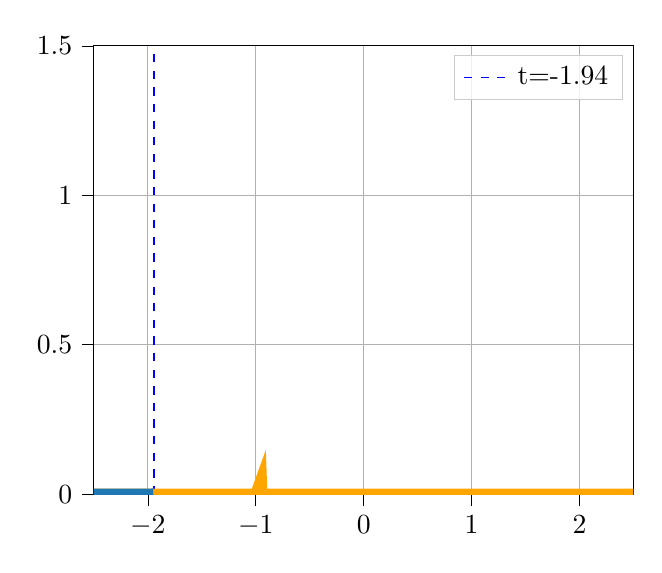
\begin{tikzpicture}

\definecolor{color0}{rgb}{1,0.498039215686275,0.0549019607843137}
\definecolor{color1}{rgb}{1,0.647058823529412,0}
\definecolor{color2}{rgb}{0.12156862745098,0.466666666666667,0.705882352941177}

\begin{axis}[
legend cell align={left},
legend style={fill opacity=0.8, draw opacity=1, text opacity=1, draw=white!80!black},
tick align=outside,
tick pos=left,
x grid style={white!69.0196078431373!black},
xmajorgrids,
xmin=-2.5, xmax=2.5,
xtick style={color=black},
y grid style={white!69.0196078431373!black},
ymajorgrids,
ymin=0, ymax=1.5,
ytick style={color=black}
]
\path [draw=color0, fill=color0, opacity=0.2]
(axis cs:-2.5,0)
--(axis cs:-2.5,0)
--(axis cs:-2.49499499499499,0)
--(axis cs:-2.48998998998999,0)
--(axis cs:-2.48498498498498,0)
--(axis cs:-2.47997997997998,0)
--(axis cs:-2.47497497497497,0)
--(axis cs:-2.46996996996997,0)
--(axis cs:-2.46496496496496,0)
--(axis cs:-2.45995995995996,0)
--(axis cs:-2.45495495495495,0)
--(axis cs:-2.44994994994995,0)
--(axis cs:-2.44494494494494,0)
--(axis cs:-2.43993993993994,0)
--(axis cs:-2.43493493493493,0)
--(axis cs:-2.42992992992993,0)
--(axis cs:-2.42492492492492,0)
--(axis cs:-2.41991991991992,0)
--(axis cs:-2.41491491491491,0)
--(axis cs:-2.40990990990991,0)
--(axis cs:-2.4049049049049,0)
--(axis cs:-2.3998998998999,0)
--(axis cs:-2.39489489489489,0)
--(axis cs:-2.38988988988989,0)
--(axis cs:-2.38488488488488,0)
--(axis cs:-2.37987987987988,0)
--(axis cs:-2.37487487487487,0)
--(axis cs:-2.36986986986987,0)
--(axis cs:-2.36486486486486,0)
--(axis cs:-2.35985985985986,0)
--(axis cs:-2.35485485485485,0)
--(axis cs:-2.34984984984985,0)
--(axis cs:-2.34484484484484,0)
--(axis cs:-2.33983983983984,0)
--(axis cs:-2.33483483483483,0)
--(axis cs:-2.32982982982983,0)
--(axis cs:-2.32482482482482,0)
--(axis cs:-2.31981981981982,0)
--(axis cs:-2.31481481481481,0)
--(axis cs:-2.30980980980981,0)
--(axis cs:-2.3048048048048,0)
--(axis cs:-2.2997997997998,0)
--(axis cs:-2.29479479479479,0)
--(axis cs:-2.28978978978979,0)
--(axis cs:-2.28478478478478,0)
--(axis cs:-2.27977977977978,0)
--(axis cs:-2.27477477477477,0)
--(axis cs:-2.26976976976977,0)
--(axis cs:-2.26476476476476,0)
--(axis cs:-2.25975975975976,0)
--(axis cs:-2.25475475475475,0)
--(axis cs:-2.24974974974975,0)
--(axis cs:-2.24474474474474,0)
--(axis cs:-2.23973973973974,0)
--(axis cs:-2.23473473473473,0)
--(axis cs:-2.22972972972973,0)
--(axis cs:-2.22472472472472,0)
--(axis cs:-2.21971971971972,0)
--(axis cs:-2.21471471471471,0)
--(axis cs:-2.20970970970971,0)
--(axis cs:-2.2047047047047,0)
--(axis cs:-2.1996996996997,0)
--(axis cs:-2.19469469469469,0)
--(axis cs:-2.18968968968969,0)
--(axis cs:-2.18468468468468,0)
--(axis cs:-2.17967967967968,0)
--(axis cs:-2.17467467467467,0)
--(axis cs:-2.16966966966967,0)
--(axis cs:-2.16466466466466,0)
--(axis cs:-2.15965965965966,0)
--(axis cs:-2.15465465465465,0)
--(axis cs:-2.14964964964965,0)
--(axis cs:-2.14464464464464,0)
--(axis cs:-2.13963963963964,0)
--(axis cs:-2.13463463463463,0)
--(axis cs:-2.12962962962963,0)
--(axis cs:-2.12462462462462,0)
--(axis cs:-2.11961961961962,0)
--(axis cs:-2.11461461461461,0)
--(axis cs:-2.10960960960961,0)
--(axis cs:-2.1046046046046,0)
--(axis cs:-2.0995995995996,0)
--(axis cs:-2.09459459459459,0)
--(axis cs:-2.08958958958959,0)
--(axis cs:-2.08458458458458,0)
--(axis cs:-2.07957957957958,0)
--(axis cs:-2.07457457457457,0)
--(axis cs:-2.06956956956957,0)
--(axis cs:-2.06456456456456,0)
--(axis cs:-2.05955955955956,0)
--(axis cs:-2.05455455455455,0)
--(axis cs:-2.04954954954955,0)
--(axis cs:-2.04454454454454,0)
--(axis cs:-2.03953953953954,0)
--(axis cs:-2.03453453453453,0)
--(axis cs:-2.02952952952953,0)
--(axis cs:-2.02452452452452,0)
--(axis cs:-2.01951951951952,0)
--(axis cs:-2.01451451451451,0)
--(axis cs:-2.00950950950951,0)
--(axis cs:-2.0045045045045,0)
--(axis cs:-1.9994994994995,0)
--(axis cs:-1.99449449449449,0)
--(axis cs:-1.98948948948949,0)
--(axis cs:-1.98448448448448,0)
--(axis cs:-1.97947947947948,0)
--(axis cs:-1.97447447447447,0)
--(axis cs:-1.96946946946947,0)
--(axis cs:-1.96446446446446,0)
--(axis cs:-1.95945945945946,0)
--(axis cs:-1.95445445445445,0)
--(axis cs:-1.94944944944945,0)
--(axis cs:-1.94444444444444,0)
--(axis cs:-1.93943943943944,0)
--(axis cs:-1.93443443443443,0)
--(axis cs:-1.92942942942943,0)
--(axis cs:-1.92442442442442,0)
--(axis cs:-1.91941941941942,0)
--(axis cs:-1.91441441441441,0)
--(axis cs:-1.90940940940941,0)
--(axis cs:-1.9044044044044,0)
--(axis cs:-1.8993993993994,0)
--(axis cs:-1.89439439439439,0)
--(axis cs:-1.88938938938939,0)
--(axis cs:-1.88438438438438,0)
--(axis cs:-1.87937937937938,0)
--(axis cs:-1.87437437437437,0)
--(axis cs:-1.86936936936937,0)
--(axis cs:-1.86436436436436,0)
--(axis cs:-1.85935935935936,0)
--(axis cs:-1.85435435435435,0)
--(axis cs:-1.84934934934935,0)
--(axis cs:-1.84434434434434,0)
--(axis cs:-1.83933933933934,0)
--(axis cs:-1.83433433433433,0)
--(axis cs:-1.82932932932933,0)
--(axis cs:-1.82432432432432,0)
--(axis cs:-1.81931931931932,0)
--(axis cs:-1.81431431431431,0)
--(axis cs:-1.80930930930931,0)
--(axis cs:-1.8043043043043,0)
--(axis cs:-1.7992992992993,0)
--(axis cs:-1.79429429429429,0)
--(axis cs:-1.78928928928929,0)
--(axis cs:-1.78428428428428,0)
--(axis cs:-1.77927927927928,0)
--(axis cs:-1.77427427427427,0)
--(axis cs:-1.76926926926927,0)
--(axis cs:-1.76426426426426,0)
--(axis cs:-1.75925925925926,0)
--(axis cs:-1.75425425425425,0)
--(axis cs:-1.74924924924925,0)
--(axis cs:-1.74424424424424,0)
--(axis cs:-1.73923923923924,0)
--(axis cs:-1.73423423423423,0)
--(axis cs:-1.72922922922923,0)
--(axis cs:-1.72422422422422,0)
--(axis cs:-1.71921921921922,0)
--(axis cs:-1.71421421421421,0)
--(axis cs:-1.70920920920921,0)
--(axis cs:-1.7042042042042,0)
--(axis cs:-1.6991991991992,0)
--(axis cs:-1.69419419419419,0)
--(axis cs:-1.68918918918919,0)
--(axis cs:-1.68418418418418,0)
--(axis cs:-1.67917917917918,0)
--(axis cs:-1.67417417417417,0)
--(axis cs:-1.66916916916917,0)
--(axis cs:-1.66416416416416,0)
--(axis cs:-1.65915915915916,0)
--(axis cs:-1.65415415415415,0)
--(axis cs:-1.64914914914915,0)
--(axis cs:-1.64414414414414,0)
--(axis cs:-1.63913913913914,0)
--(axis cs:-1.63413413413413,0)
--(axis cs:-1.62912912912913,0)
--(axis cs:-1.62412412412412,0)
--(axis cs:-1.61911911911912,0)
--(axis cs:-1.61411411411411,0)
--(axis cs:-1.60910910910911,0)
--(axis cs:-1.6041041041041,0)
--(axis cs:-1.5990990990991,0)
--(axis cs:-1.59409409409409,0)
--(axis cs:-1.58908908908909,0)
--(axis cs:-1.58408408408408,0)
--(axis cs:-1.57907907907908,0)
--(axis cs:-1.57407407407407,0)
--(axis cs:-1.56906906906907,0)
--(axis cs:-1.56406406406406,0)
--(axis cs:-1.55905905905906,0)
--(axis cs:-1.55405405405405,0)
--(axis cs:-1.54904904904905,0)
--(axis cs:-1.54404404404404,0)
--(axis cs:-1.53903903903904,0)
--(axis cs:-1.53403403403403,0)
--(axis cs:-1.52902902902903,0)
--(axis cs:-1.52402402402402,0)
--(axis cs:-1.51901901901902,0)
--(axis cs:-1.51401401401401,0)
--(axis cs:-1.50900900900901,0)
--(axis cs:-1.504004004004,0)
--(axis cs:-1.498998998999,0)
--(axis cs:-1.49399399399399,0)
--(axis cs:-1.48898898898899,0)
--(axis cs:-1.48398398398398,0)
--(axis cs:-1.47897897897898,0)
--(axis cs:-1.47397397397397,0)
--(axis cs:-1.46896896896897,0)
--(axis cs:-1.46396396396396,0)
--(axis cs:-1.45895895895896,0)
--(axis cs:-1.45395395395395,0)
--(axis cs:-1.44894894894895,0)
--(axis cs:-1.44394394394394,0)
--(axis cs:-1.43893893893894,0)
--(axis cs:-1.43393393393393,0)
--(axis cs:-1.42892892892893,0)
--(axis cs:-1.42392392392392,0)
--(axis cs:-1.41891891891892,0)
--(axis cs:-1.41391391391391,0)
--(axis cs:-1.40890890890891,0)
--(axis cs:-1.4039039039039,0)
--(axis cs:-1.3988988988989,0)
--(axis cs:-1.39389389389389,0)
--(axis cs:-1.38888888888889,0)
--(axis cs:-1.38388388388388,0)
--(axis cs:-1.37887887887888,0)
--(axis cs:-1.37387387387387,0)
--(axis cs:-1.36886886886887,0)
--(axis cs:-1.36386386386386,0)
--(axis cs:-1.35885885885886,0)
--(axis cs:-1.35385385385385,0)
--(axis cs:-1.34884884884885,0)
--(axis cs:-1.34384384384384,0)
--(axis cs:-1.33883883883884,0)
--(axis cs:-1.33383383383383,0)
--(axis cs:-1.32882882882883,0)
--(axis cs:-1.32382382382382,0)
--(axis cs:-1.31881881881882,0)
--(axis cs:-1.31381381381381,0)
--(axis cs:-1.30880880880881,0)
--(axis cs:-1.3038038038038,0)
--(axis cs:-1.2987987987988,0)
--(axis cs:-1.29379379379379,0)
--(axis cs:-1.28878878878879,0)
--(axis cs:-1.28378378378378,0)
--(axis cs:-1.27877877877878,0)
--(axis cs:-1.27377377377377,0)
--(axis cs:-1.26876876876877,0)
--(axis cs:-1.26376376376376,0)
--(axis cs:-1.25875875875876,0)
--(axis cs:-1.25375375375375,0)
--(axis cs:-1.24874874874875,0)
--(axis cs:-1.24374374374374,0)
--(axis cs:-1.23873873873874,0)
--(axis cs:-1.23373373373373,0)
--(axis cs:-1.22872872872873,0)
--(axis cs:-1.22372372372372,0)
--(axis cs:-1.21871871871872,0)
--(axis cs:-1.21371371371371,0)
--(axis cs:-1.20870870870871,0)
--(axis cs:-1.2037037037037,0)
--(axis cs:-1.1986986986987,0)
--(axis cs:-1.19369369369369,0)
--(axis cs:-1.18868868868869,0)
--(axis cs:-1.18368368368368,0)
--(axis cs:-1.17867867867868,0)
--(axis cs:-1.17367367367367,0)
--(axis cs:-1.16866866866867,0)
--(axis cs:-1.16366366366366,0)
--(axis cs:-1.15865865865866,0)
--(axis cs:-1.15365365365365,0)
--(axis cs:-1.14864864864865,0)
--(axis cs:-1.14364364364364,0)
--(axis cs:-1.13863863863864,0)
--(axis cs:-1.13363363363363,0)
--(axis cs:-1.12862862862863,0)
--(axis cs:-1.12362362362362,0)
--(axis cs:-1.11861861861862,0)
--(axis cs:-1.11361361361361,0)
--(axis cs:-1.10860860860861,0)
--(axis cs:-1.1036036036036,0)
--(axis cs:-1.0985985985986,0)
--(axis cs:-1.09359359359359,0)
--(axis cs:-1.08858858858859,0)
--(axis cs:-1.08358358358358,0)
--(axis cs:-1.07857857857858,0)
--(axis cs:-1.07357357357357,0)
--(axis cs:-1.06856856856857,0)
--(axis cs:-1.06356356356356,0)
--(axis cs:-1.05855855855856,0)
--(axis cs:-1.05355355355355,0)
--(axis cs:-1.04854854854855,0)
--(axis cs:-1.04354354354354,0)
--(axis cs:-1.03853853853854,0)
--(axis cs:-1.03353353353353,0)
--(axis cs:-1.02852852852853,0)
--(axis cs:-1.02352352352352,0)
--(axis cs:-1.01851851851852,0)
--(axis cs:-1.01351351351351,0)
--(axis cs:-1.00850850850851,0)
--(axis cs:-1.0035035035035,0)
--(axis cs:-0.998498498498499,0)
--(axis cs:-0.993493493493494,0)
--(axis cs:-0.988488488488489,0)
--(axis cs:-0.983483483483484,0)
--(axis cs:-0.978478478478479,0)
--(axis cs:-0.973473473473474,0)
--(axis cs:-0.968468468468469,0)
--(axis cs:-0.963463463463464,0)
--(axis cs:-0.958458458458459,0)
--(axis cs:-0.953453453453454,0)
--(axis cs:-0.948448448448449,0)
--(axis cs:-0.943443443443444,0)
--(axis cs:-0.938438438438439,0)
--(axis cs:-0.933433433433434,0)
--(axis cs:-0.928428428428429,0)
--(axis cs:-0.923423423423424,0)
--(axis cs:-0.918418418418419,0)
--(axis cs:-0.913413413413414,0)
--(axis cs:-0.908408408408409,0)
--(axis cs:-0.903403403403404,0)
--(axis cs:-0.898398398398399,0)
--(axis cs:-0.893393393393393,0)
--(axis cs:-0.888388388388388,0)
--(axis cs:-0.883383383383383,0)
--(axis cs:-0.878378378378378,0)
--(axis cs:-0.873373373373373,0)
--(axis cs:-0.868368368368368,0)
--(axis cs:-0.863363363363363,0)
--(axis cs:-0.858358358358358,0)
--(axis cs:-0.853353353353353,0)
--(axis cs:-0.848348348348348,0)
--(axis cs:-0.843343343343343,0)
--(axis cs:-0.838338338338338,0)
--(axis cs:-0.833333333333333,0)
--(axis cs:-0.828328328328328,0)
--(axis cs:-0.823323323323323,0)
--(axis cs:-0.818318318318318,0)
--(axis cs:-0.813313313313313,0)
--(axis cs:-0.808308308308308,0)
--(axis cs:-0.803303303303303,0)
--(axis cs:-0.798298298298298,0)
--(axis cs:-0.793293293293293,0)
--(axis cs:-0.788288288288288,0)
--(axis cs:-0.783283283283283,0)
--(axis cs:-0.778278278278278,0)
--(axis cs:-0.773273273273273,0)
--(axis cs:-0.768268268268268,0)
--(axis cs:-0.763263263263263,0)
--(axis cs:-0.758258258258258,0)
--(axis cs:-0.753253253253253,0)
--(axis cs:-0.748248248248248,0)
--(axis cs:-0.743243243243243,0)
--(axis cs:-0.738238238238238,0)
--(axis cs:-0.733233233233233,0)
--(axis cs:-0.728228228228228,0)
--(axis cs:-0.723223223223223,0)
--(axis cs:-0.718218218218218,0)
--(axis cs:-0.713213213213213,0)
--(axis cs:-0.708208208208208,0)
--(axis cs:-0.703203203203203,0)
--(axis cs:-0.698198198198198,0)
--(axis cs:-0.693193193193193,0)
--(axis cs:-0.688188188188188,0)
--(axis cs:-0.683183183183183,0)
--(axis cs:-0.678178178178178,0)
--(axis cs:-0.673173173173173,0)
--(axis cs:-0.668168168168168,0)
--(axis cs:-0.663163163163163,0)
--(axis cs:-0.658158158158158,0)
--(axis cs:-0.653153153153153,0)
--(axis cs:-0.648148148148148,0)
--(axis cs:-0.643143143143143,0)
--(axis cs:-0.638138138138138,0)
--(axis cs:-0.633133133133133,0)
--(axis cs:-0.628128128128128,0)
--(axis cs:-0.623123123123123,0)
--(axis cs:-0.618118118118118,0)
--(axis cs:-0.613113113113113,0)
--(axis cs:-0.608108108108108,0)
--(axis cs:-0.603103103103103,0)
--(axis cs:-0.598098098098098,0)
--(axis cs:-0.593093093093093,0)
--(axis cs:-0.588088088088088,0)
--(axis cs:-0.583083083083083,0)
--(axis cs:-0.578078078078078,0)
--(axis cs:-0.573073073073073,0)
--(axis cs:-0.568068068068068,0)
--(axis cs:-0.563063063063063,0)
--(axis cs:-0.558058058058058,0)
--(axis cs:-0.553053053053053,0)
--(axis cs:-0.548048048048048,0)
--(axis cs:-0.543043043043043,0)
--(axis cs:-0.538038038038038,0)
--(axis cs:-0.533033033033033,0)
--(axis cs:-0.528028028028028,0)
--(axis cs:-0.523023023023023,0)
--(axis cs:-0.518018018018018,0)
--(axis cs:-0.513013013013013,0)
--(axis cs:-0.508008008008008,0)
--(axis cs:-0.503003003003003,0)
--(axis cs:-0.497997997997998,0)
--(axis cs:-0.492992992992993,0)
--(axis cs:-0.487987987987988,0)
--(axis cs:-0.482982982982983,0)
--(axis cs:-0.477977977977978,0)
--(axis cs:-0.472972972972973,0)
--(axis cs:-0.467967967967968,0)
--(axis cs:-0.462962962962963,0)
--(axis cs:-0.457957957957958,0)
--(axis cs:-0.452952952952953,0)
--(axis cs:-0.447947947947948,0)
--(axis cs:-0.442942942942943,0)
--(axis cs:-0.437937937937938,0)
--(axis cs:-0.432932932932933,0)
--(axis cs:-0.427927927927928,0)
--(axis cs:-0.422922922922923,0)
--(axis cs:-0.417917917917918,0)
--(axis cs:-0.412912912912913,0)
--(axis cs:-0.407907907907908,0)
--(axis cs:-0.402902902902903,0)
--(axis cs:-0.397897897897898,0)
--(axis cs:-0.392892892892893,0)
--(axis cs:-0.387887887887888,0)
--(axis cs:-0.382882882882883,0)
--(axis cs:-0.377877877877878,0)
--(axis cs:-0.372872872872873,0)
--(axis cs:-0.367867867867868,0)
--(axis cs:-0.362862862862863,0)
--(axis cs:-0.357857857857858,0)
--(axis cs:-0.352852852852853,0)
--(axis cs:-0.347847847847848,0)
--(axis cs:-0.342842842842843,0)
--(axis cs:-0.337837837837838,0)
--(axis cs:-0.332832832832833,0)
--(axis cs:-0.327827827827828,0)
--(axis cs:-0.322822822822823,0)
--(axis cs:-0.317817817817818,0)
--(axis cs:-0.312812812812813,0)
--(axis cs:-0.307807807807808,0)
--(axis cs:-0.302802802802803,0)
--(axis cs:-0.297797797797798,0)
--(axis cs:-0.292792792792793,0)
--(axis cs:-0.287787787787788,0)
--(axis cs:-0.282782782782783,0)
--(axis cs:-0.277777777777778,0)
--(axis cs:-0.272772772772773,0)
--(axis cs:-0.267767767767768,0)
--(axis cs:-0.262762762762763,0)
--(axis cs:-0.257757757757758,0)
--(axis cs:-0.252752752752753,0)
--(axis cs:-0.247747747747748,0)
--(axis cs:-0.242742742742743,0)
--(axis cs:-0.237737737737738,0)
--(axis cs:-0.232732732732733,0)
--(axis cs:-0.227727727727728,0)
--(axis cs:-0.222722722722723,0)
--(axis cs:-0.217717717717718,0)
--(axis cs:-0.212712712712713,0)
--(axis cs:-0.207707707707708,0)
--(axis cs:-0.202702702702703,0)
--(axis cs:-0.197697697697698,0)
--(axis cs:-0.192692692692693,0)
--(axis cs:-0.187687687687688,0)
--(axis cs:-0.182682682682683,0)
--(axis cs:-0.177677677677678,0)
--(axis cs:-0.172672672672673,0)
--(axis cs:-0.167667667667668,0)
--(axis cs:-0.162662662662663,0)
--(axis cs:-0.157657657657658,0)
--(axis cs:-0.152652652652653,0)
--(axis cs:-0.147647647647648,0)
--(axis cs:-0.142642642642643,0)
--(axis cs:-0.137637637637638,0)
--(axis cs:-0.132632632632633,0)
--(axis cs:-0.127627627627628,0)
--(axis cs:-0.122622622622623,0)
--(axis cs:-0.117617617617618,0)
--(axis cs:-0.112612612612613,0)
--(axis cs:-0.107607607607608,0)
--(axis cs:-0.102602602602603,0)
--(axis cs:-0.0975975975975976,0)
--(axis cs:-0.0925925925925926,0)
--(axis cs:-0.0875875875875876,0)
--(axis cs:-0.0825825825825826,0)
--(axis cs:-0.0775775775775776,0)
--(axis cs:-0.0725725725725725,0)
--(axis cs:-0.0675675675675675,0)
--(axis cs:-0.0625625625625625,0)
--(axis cs:-0.0575575575575575,0)
--(axis cs:-0.0525525525525525,0)
--(axis cs:-0.0475475475475475,0)
--(axis cs:-0.0425425425425425,0)
--(axis cs:-0.0375375375375375,0)
--(axis cs:-0.0325325325325325,0)
--(axis cs:-0.0275275275275275,0)
--(axis cs:-0.0225225225225225,0)
--(axis cs:-0.0175175175175175,0)
--(axis cs:-0.0125125125125125,0)
--(axis cs:-0.0075075075075075,0)
--(axis cs:-0.0025025025025025,0)
--(axis cs:0.0025025025025025,0)
--(axis cs:0.0075075075075075,0)
--(axis cs:0.0125125125125125,0)
--(axis cs:0.0175175175175175,0)
--(axis cs:0.0225225225225225,0)
--(axis cs:0.0275275275275275,0)
--(axis cs:0.0325325325325325,0)
--(axis cs:0.0375375375375375,0)
--(axis cs:0.0425425425425425,0)
--(axis cs:0.0475475475475475,0)
--(axis cs:0.0525525525525525,0)
--(axis cs:0.0575575575575575,0)
--(axis cs:0.0625625625625625,0)
--(axis cs:0.0675675675675675,0)
--(axis cs:0.0725725725725725,0)
--(axis cs:0.0775775775775776,0)
--(axis cs:0.0825825825825826,0)
--(axis cs:0.0875875875875876,0)
--(axis cs:0.0925925925925926,0)
--(axis cs:0.0975975975975976,0)
--(axis cs:0.102602602602603,0)
--(axis cs:0.107607607607608,0)
--(axis cs:0.112612612612613,0)
--(axis cs:0.117617617617618,0)
--(axis cs:0.122622622622623,0)
--(axis cs:0.127627627627628,0)
--(axis cs:0.132632632632633,0)
--(axis cs:0.137637637637638,0)
--(axis cs:0.142642642642643,0)
--(axis cs:0.147647647647648,0)
--(axis cs:0.152652652652653,0)
--(axis cs:0.157657657657658,0)
--(axis cs:0.162662662662663,0)
--(axis cs:0.167667667667668,0)
--(axis cs:0.172672672672673,0)
--(axis cs:0.177677677677678,0)
--(axis cs:0.182682682682683,0)
--(axis cs:0.187687687687688,0)
--(axis cs:0.192692692692693,0)
--(axis cs:0.197697697697698,0)
--(axis cs:0.202702702702703,0)
--(axis cs:0.207707707707708,0)
--(axis cs:0.212712712712713,0)
--(axis cs:0.217717717717718,0)
--(axis cs:0.222722722722723,0)
--(axis cs:0.227727727727728,0)
--(axis cs:0.232732732732733,0)
--(axis cs:0.237737737737738,0)
--(axis cs:0.242742742742743,0)
--(axis cs:0.247747747747748,0)
--(axis cs:0.252752752752753,0)
--(axis cs:0.257757757757758,0)
--(axis cs:0.262762762762763,0)
--(axis cs:0.267767767767768,0)
--(axis cs:0.272772772772773,0)
--(axis cs:0.277777777777778,0)
--(axis cs:0.282782782782783,0)
--(axis cs:0.287787787787788,0)
--(axis cs:0.292792792792793,0)
--(axis cs:0.297797797797798,0)
--(axis cs:0.302802802802803,0)
--(axis cs:0.307807807807808,0)
--(axis cs:0.312812812812813,0)
--(axis cs:0.317817817817818,0)
--(axis cs:0.322822822822823,0)
--(axis cs:0.327827827827828,0)
--(axis cs:0.332832832832833,0)
--(axis cs:0.337837837837838,0)
--(axis cs:0.342842842842843,0)
--(axis cs:0.347847847847848,0)
--(axis cs:0.352852852852853,0)
--(axis cs:0.357857857857858,0)
--(axis cs:0.362862862862863,0)
--(axis cs:0.367867867867868,0)
--(axis cs:0.372872872872873,0)
--(axis cs:0.377877877877878,0)
--(axis cs:0.382882882882883,0)
--(axis cs:0.387887887887888,0)
--(axis cs:0.392892892892893,0)
--(axis cs:0.397897897897898,0)
--(axis cs:0.402902902902903,0)
--(axis cs:0.407907907907908,0)
--(axis cs:0.412912912912913,0)
--(axis cs:0.417917917917918,0)
--(axis cs:0.422922922922923,0)
--(axis cs:0.427927927927928,0)
--(axis cs:0.432932932932933,0)
--(axis cs:0.437937937937938,0)
--(axis cs:0.442942942942943,0)
--(axis cs:0.447947947947948,0)
--(axis cs:0.452952952952953,0)
--(axis cs:0.457957957957958,0)
--(axis cs:0.462962962962963,0)
--(axis cs:0.467967967967968,0)
--(axis cs:0.472972972972973,0)
--(axis cs:0.477977977977978,0)
--(axis cs:0.482982982982983,0)
--(axis cs:0.487987987987988,0)
--(axis cs:0.492992992992993,0)
--(axis cs:0.497997997997998,0)
--(axis cs:0.503003003003003,0)
--(axis cs:0.508008008008008,0)
--(axis cs:0.513013013013013,0)
--(axis cs:0.518018018018018,0)
--(axis cs:0.523023023023023,0)
--(axis cs:0.528028028028028,0)
--(axis cs:0.533033033033033,0)
--(axis cs:0.538038038038038,0)
--(axis cs:0.543043043043043,0)
--(axis cs:0.548048048048048,0)
--(axis cs:0.553053053053053,0)
--(axis cs:0.558058058058058,0)
--(axis cs:0.563063063063063,0)
--(axis cs:0.568068068068068,0)
--(axis cs:0.573073073073073,0)
--(axis cs:0.578078078078078,0)
--(axis cs:0.583083083083083,0)
--(axis cs:0.588088088088088,0)
--(axis cs:0.593093093093093,0)
--(axis cs:0.598098098098098,0)
--(axis cs:0.603103103103103,0)
--(axis cs:0.608108108108108,0)
--(axis cs:0.613113113113113,0)
--(axis cs:0.618118118118118,0)
--(axis cs:0.623123123123123,0)
--(axis cs:0.628128128128128,0)
--(axis cs:0.633133133133133,0)
--(axis cs:0.638138138138138,0)
--(axis cs:0.643143143143143,0)
--(axis cs:0.648148148148148,0)
--(axis cs:0.653153153153153,0)
--(axis cs:0.658158158158158,0)
--(axis cs:0.663163163163163,0)
--(axis cs:0.668168168168168,0)
--(axis cs:0.673173173173173,0)
--(axis cs:0.678178178178178,0)
--(axis cs:0.683183183183183,0)
--(axis cs:0.688188188188188,0)
--(axis cs:0.693193193193193,0)
--(axis cs:0.698198198198198,0)
--(axis cs:0.703203203203203,0)
--(axis cs:0.708208208208208,0)
--(axis cs:0.713213213213213,0)
--(axis cs:0.718218218218218,0)
--(axis cs:0.723223223223223,0)
--(axis cs:0.728228228228228,0)
--(axis cs:0.733233233233233,0)
--(axis cs:0.738238238238238,0)
--(axis cs:0.743243243243243,0)
--(axis cs:0.748248248248248,0)
--(axis cs:0.753253253253253,0)
--(axis cs:0.758258258258258,0)
--(axis cs:0.763263263263263,0)
--(axis cs:0.768268268268268,0)
--(axis cs:0.773273273273273,0)
--(axis cs:0.778278278278278,0)
--(axis cs:0.783283283283283,0)
--(axis cs:0.788288288288288,0)
--(axis cs:0.793293293293293,0)
--(axis cs:0.798298298298298,0)
--(axis cs:0.803303303303303,0)
--(axis cs:0.808308308308308,0)
--(axis cs:0.813313313313313,0)
--(axis cs:0.818318318318318,0)
--(axis cs:0.823323323323323,0)
--(axis cs:0.828328328328328,0)
--(axis cs:0.833333333333333,0)
--(axis cs:0.838338338338338,0)
--(axis cs:0.843343343343343,0)
--(axis cs:0.848348348348348,0)
--(axis cs:0.853353353353353,0)
--(axis cs:0.858358358358358,0)
--(axis cs:0.863363363363364,0)
--(axis cs:0.868368368368369,0)
--(axis cs:0.873373373373374,0)
--(axis cs:0.878378378378379,0)
--(axis cs:0.883383383383384,0)
--(axis cs:0.888388388388389,0)
--(axis cs:0.893393393393394,0)
--(axis cs:0.898398398398399,0)
--(axis cs:0.903403403403404,0)
--(axis cs:0.908408408408409,0)
--(axis cs:0.913413413413414,0)
--(axis cs:0.918418418418419,0)
--(axis cs:0.923423423423424,0)
--(axis cs:0.928428428428429,0)
--(axis cs:0.933433433433434,0)
--(axis cs:0.938438438438439,0)
--(axis cs:0.943443443443444,0)
--(axis cs:0.948448448448449,0)
--(axis cs:0.953453453453454,0)
--(axis cs:0.958458458458459,0)
--(axis cs:0.963463463463464,0)
--(axis cs:0.968468468468469,0)
--(axis cs:0.973473473473474,0)
--(axis cs:0.978478478478479,0)
--(axis cs:0.983483483483484,0)
--(axis cs:0.988488488488489,0)
--(axis cs:0.993493493493494,0)
--(axis cs:0.998498498498499,0)
--(axis cs:1.0035035035035,0)
--(axis cs:1.00850850850851,0)
--(axis cs:1.01351351351351,0)
--(axis cs:1.01851851851852,0)
--(axis cs:1.02352352352352,0)
--(axis cs:1.02852852852853,0)
--(axis cs:1.03353353353353,0)
--(axis cs:1.03853853853854,0)
--(axis cs:1.04354354354354,0)
--(axis cs:1.04854854854855,0)
--(axis cs:1.05355355355355,0)
--(axis cs:1.05855855855856,0)
--(axis cs:1.06356356356356,0)
--(axis cs:1.06856856856857,0)
--(axis cs:1.07357357357357,0)
--(axis cs:1.07857857857858,0)
--(axis cs:1.08358358358358,0)
--(axis cs:1.08858858858859,0)
--(axis cs:1.09359359359359,0)
--(axis cs:1.0985985985986,0)
--(axis cs:1.1036036036036,0)
--(axis cs:1.10860860860861,0)
--(axis cs:1.11361361361361,0)
--(axis cs:1.11861861861862,0)
--(axis cs:1.12362362362362,0)
--(axis cs:1.12862862862863,0)
--(axis cs:1.13363363363363,0)
--(axis cs:1.13863863863864,0)
--(axis cs:1.14364364364364,0)
--(axis cs:1.14864864864865,0)
--(axis cs:1.15365365365365,0)
--(axis cs:1.15865865865866,0)
--(axis cs:1.16366366366366,0)
--(axis cs:1.16866866866867,0)
--(axis cs:1.17367367367367,0)
--(axis cs:1.17867867867868,0)
--(axis cs:1.18368368368368,0)
--(axis cs:1.18868868868869,0)
--(axis cs:1.19369369369369,0)
--(axis cs:1.1986986986987,0)
--(axis cs:1.2037037037037,0)
--(axis cs:1.20870870870871,0)
--(axis cs:1.21371371371371,0)
--(axis cs:1.21871871871872,0)
--(axis cs:1.22372372372372,0)
--(axis cs:1.22872872872873,0)
--(axis cs:1.23373373373373,0)
--(axis cs:1.23873873873874,0)
--(axis cs:1.24374374374374,0)
--(axis cs:1.24874874874875,0)
--(axis cs:1.25375375375375,0)
--(axis cs:1.25875875875876,0)
--(axis cs:1.26376376376376,0)
--(axis cs:1.26876876876877,0)
--(axis cs:1.27377377377377,0)
--(axis cs:1.27877877877878,0)
--(axis cs:1.28378378378378,0)
--(axis cs:1.28878878878879,0)
--(axis cs:1.29379379379379,0)
--(axis cs:1.2987987987988,0)
--(axis cs:1.3038038038038,0)
--(axis cs:1.30880880880881,0)
--(axis cs:1.31381381381381,0)
--(axis cs:1.31881881881882,0)
--(axis cs:1.32382382382382,0)
--(axis cs:1.32882882882883,0)
--(axis cs:1.33383383383383,0)
--(axis cs:1.33883883883884,0)
--(axis cs:1.34384384384384,0)
--(axis cs:1.34884884884885,0)
--(axis cs:1.35385385385385,0)
--(axis cs:1.35885885885886,0)
--(axis cs:1.36386386386386,0)
--(axis cs:1.36886886886887,0)
--(axis cs:1.37387387387387,0)
--(axis cs:1.37887887887888,0)
--(axis cs:1.38388388388388,0)
--(axis cs:1.38888888888889,0)
--(axis cs:1.39389389389389,0)
--(axis cs:1.3988988988989,0)
--(axis cs:1.4039039039039,0)
--(axis cs:1.40890890890891,0)
--(axis cs:1.41391391391391,0)
--(axis cs:1.41891891891892,0)
--(axis cs:1.42392392392392,0)
--(axis cs:1.42892892892893,0)
--(axis cs:1.43393393393393,0)
--(axis cs:1.43893893893894,0)
--(axis cs:1.44394394394394,0)
--(axis cs:1.44894894894895,0)
--(axis cs:1.45395395395395,0)
--(axis cs:1.45895895895896,0)
--(axis cs:1.46396396396396,0)
--(axis cs:1.46896896896897,0)
--(axis cs:1.47397397397397,0)
--(axis cs:1.47897897897898,0)
--(axis cs:1.48398398398398,0)
--(axis cs:1.48898898898899,0)
--(axis cs:1.49399399399399,0)
--(axis cs:1.498998998999,0)
--(axis cs:1.504004004004,0)
--(axis cs:1.50900900900901,0)
--(axis cs:1.51401401401401,0)
--(axis cs:1.51901901901902,0)
--(axis cs:1.52402402402402,0)
--(axis cs:1.52902902902903,0)
--(axis cs:1.53403403403403,0)
--(axis cs:1.53903903903904,0)
--(axis cs:1.54404404404404,0)
--(axis cs:1.54904904904905,0)
--(axis cs:1.55405405405405,0)
--(axis cs:1.55905905905906,0)
--(axis cs:1.56406406406406,0)
--(axis cs:1.56906906906907,0)
--(axis cs:1.57407407407407,0)
--(axis cs:1.57907907907908,0)
--(axis cs:1.58408408408408,0)
--(axis cs:1.58908908908909,0)
--(axis cs:1.59409409409409,0)
--(axis cs:1.5990990990991,0)
--(axis cs:1.6041041041041,0)
--(axis cs:1.60910910910911,0)
--(axis cs:1.61411411411411,0)
--(axis cs:1.61911911911912,0)
--(axis cs:1.62412412412412,0)
--(axis cs:1.62912912912913,0)
--(axis cs:1.63413413413413,0)
--(axis cs:1.63913913913914,0)
--(axis cs:1.64414414414414,0)
--(axis cs:1.64914914914915,0)
--(axis cs:1.65415415415415,0)
--(axis cs:1.65915915915916,0)
--(axis cs:1.66416416416416,0)
--(axis cs:1.66916916916917,0)
--(axis cs:1.67417417417417,0)
--(axis cs:1.67917917917918,0)
--(axis cs:1.68418418418418,0)
--(axis cs:1.68918918918919,0)
--(axis cs:1.69419419419419,0)
--(axis cs:1.6991991991992,0)
--(axis cs:1.7042042042042,0)
--(axis cs:1.70920920920921,0)
--(axis cs:1.71421421421421,0)
--(axis cs:1.71921921921922,0)
--(axis cs:1.72422422422422,0)
--(axis cs:1.72922922922923,0)
--(axis cs:1.73423423423423,0)
--(axis cs:1.73923923923924,0)
--(axis cs:1.74424424424424,0)
--(axis cs:1.74924924924925,0)
--(axis cs:1.75425425425425,0)
--(axis cs:1.75925925925926,0)
--(axis cs:1.76426426426426,0)
--(axis cs:1.76926926926927,0)
--(axis cs:1.77427427427427,0)
--(axis cs:1.77927927927928,0)
--(axis cs:1.78428428428428,0)
--(axis cs:1.78928928928929,0)
--(axis cs:1.79429429429429,0)
--(axis cs:1.7992992992993,0)
--(axis cs:1.8043043043043,0)
--(axis cs:1.80930930930931,0)
--(axis cs:1.81431431431431,0)
--(axis cs:1.81931931931932,0)
--(axis cs:1.82432432432432,0)
--(axis cs:1.82932932932933,0)
--(axis cs:1.83433433433433,0)
--(axis cs:1.83933933933934,0)
--(axis cs:1.84434434434434,0)
--(axis cs:1.84934934934935,0)
--(axis cs:1.85435435435435,0)
--(axis cs:1.85935935935936,0)
--(axis cs:1.86436436436436,0)
--(axis cs:1.86936936936937,0)
--(axis cs:1.87437437437437,0)
--(axis cs:1.87937937937938,0)
--(axis cs:1.88438438438438,0)
--(axis cs:1.88938938938939,0)
--(axis cs:1.89439439439439,0)
--(axis cs:1.8993993993994,0)
--(axis cs:1.9044044044044,0)
--(axis cs:1.90940940940941,0)
--(axis cs:1.91441441441441,0)
--(axis cs:1.91941941941942,0)
--(axis cs:1.92442442442442,0)
--(axis cs:1.92942942942943,0)
--(axis cs:1.93443443443443,0)
--(axis cs:1.93943943943944,0)
--(axis cs:1.94444444444444,0)
--(axis cs:1.94944944944945,0)
--(axis cs:1.95445445445445,0)
--(axis cs:1.95945945945946,0)
--(axis cs:1.96446446446446,0)
--(axis cs:1.96946946946947,0)
--(axis cs:1.97447447447447,0)
--(axis cs:1.97947947947948,0)
--(axis cs:1.98448448448448,0)
--(axis cs:1.98948948948949,0)
--(axis cs:1.99449449449449,0)
--(axis cs:1.9994994994995,0)
--(axis cs:2.0045045045045,0)
--(axis cs:2.00950950950951,0)
--(axis cs:2.01451451451451,0)
--(axis cs:2.01951951951952,0)
--(axis cs:2.02452452452452,0)
--(axis cs:2.02952952952953,0)
--(axis cs:2.03453453453453,0)
--(axis cs:2.03953953953954,0)
--(axis cs:2.04454454454454,0)
--(axis cs:2.04954954954955,0)
--(axis cs:2.05455455455455,0)
--(axis cs:2.05955955955956,0)
--(axis cs:2.06456456456456,0)
--(axis cs:2.06956956956957,0)
--(axis cs:2.07457457457457,0)
--(axis cs:2.07957957957958,0)
--(axis cs:2.08458458458458,0)
--(axis cs:2.08958958958959,0)
--(axis cs:2.09459459459459,0)
--(axis cs:2.0995995995996,0)
--(axis cs:2.1046046046046,0)
--(axis cs:2.10960960960961,0)
--(axis cs:2.11461461461461,0)
--(axis cs:2.11961961961962,0)
--(axis cs:2.12462462462462,0)
--(axis cs:2.12962962962963,0)
--(axis cs:2.13463463463463,0)
--(axis cs:2.13963963963964,0)
--(axis cs:2.14464464464464,0)
--(axis cs:2.14964964964965,0)
--(axis cs:2.15465465465465,0)
--(axis cs:2.15965965965966,0)
--(axis cs:2.16466466466466,0)
--(axis cs:2.16966966966967,0)
--(axis cs:2.17467467467467,0)
--(axis cs:2.17967967967968,0)
--(axis cs:2.18468468468468,0)
--(axis cs:2.18968968968969,0)
--(axis cs:2.19469469469469,0)
--(axis cs:2.1996996996997,0)
--(axis cs:2.2047047047047,0)
--(axis cs:2.20970970970971,0)
--(axis cs:2.21471471471471,0)
--(axis cs:2.21971971971972,0)
--(axis cs:2.22472472472472,0)
--(axis cs:2.22972972972973,0)
--(axis cs:2.23473473473473,0)
--(axis cs:2.23973973973974,0)
--(axis cs:2.24474474474474,0)
--(axis cs:2.24974974974975,0)
--(axis cs:2.25475475475475,0)
--(axis cs:2.25975975975976,0)
--(axis cs:2.26476476476476,0)
--(axis cs:2.26976976976977,0)
--(axis cs:2.27477477477477,0)
--(axis cs:2.27977977977978,0)
--(axis cs:2.28478478478478,0)
--(axis cs:2.28978978978979,0)
--(axis cs:2.29479479479479,0)
--(axis cs:2.2997997997998,0)
--(axis cs:2.3048048048048,0)
--(axis cs:2.30980980980981,0)
--(axis cs:2.31481481481481,0)
--(axis cs:2.31981981981982,0)
--(axis cs:2.32482482482482,0)
--(axis cs:2.32982982982983,0)
--(axis cs:2.33483483483483,0)
--(axis cs:2.33983983983984,0)
--(axis cs:2.34484484484484,0)
--(axis cs:2.34984984984985,0)
--(axis cs:2.35485485485485,0)
--(axis cs:2.35985985985986,0)
--(axis cs:2.36486486486486,0)
--(axis cs:2.36986986986987,0)
--(axis cs:2.37487487487487,0)
--(axis cs:2.37987987987988,0)
--(axis cs:2.38488488488488,0)
--(axis cs:2.38988988988989,0)
--(axis cs:2.39489489489489,0)
--(axis cs:2.3998998998999,0)
--(axis cs:2.4049049049049,0)
--(axis cs:2.40990990990991,0)
--(axis cs:2.41491491491491,0)
--(axis cs:2.41991991991992,0)
--(axis cs:2.42492492492492,0)
--(axis cs:2.42992992992993,0)
--(axis cs:2.43493493493493,0)
--(axis cs:2.43993993993994,0)
--(axis cs:2.44494494494494,0)
--(axis cs:2.44994994994995,0)
--(axis cs:2.45495495495495,0)
--(axis cs:2.45995995995996,0)
--(axis cs:2.46496496496496,0)
--(axis cs:2.46996996996997,0)
--(axis cs:2.47497497497497,0)
--(axis cs:2.47997997997998,0)
--(axis cs:2.48498498498498,0)
--(axis cs:2.48998998998999,0)
--(axis cs:2.49499499499499,0)
--(axis cs:2.5,0)
--(axis cs:2.5,0)
--(axis cs:2.5,0)
--(axis cs:2.49499499499499,0)
--(axis cs:2.48998998998999,0)
--(axis cs:2.48498498498498,0)
--(axis cs:2.47997997997998,0)
--(axis cs:2.47497497497497,0)
--(axis cs:2.46996996996997,0)
--(axis cs:2.46496496496496,0)
--(axis cs:2.45995995995996,0)
--(axis cs:2.45495495495495,0)
--(axis cs:2.44994994994995,0)
--(axis cs:2.44494494494494,0)
--(axis cs:2.43993993993994,0)
--(axis cs:2.43493493493493,0)
--(axis cs:2.42992992992993,0)
--(axis cs:2.42492492492492,0)
--(axis cs:2.41991991991992,0)
--(axis cs:2.41491491491491,0)
--(axis cs:2.40990990990991,0)
--(axis cs:2.4049049049049,0)
--(axis cs:2.3998998998999,0)
--(axis cs:2.39489489489489,0)
--(axis cs:2.38988988988989,0)
--(axis cs:2.38488488488488,0)
--(axis cs:2.37987987987988,0)
--(axis cs:2.37487487487487,0)
--(axis cs:2.36986986986987,0)
--(axis cs:2.36486486486486,0)
--(axis cs:2.35985985985986,0)
--(axis cs:2.35485485485485,0)
--(axis cs:2.34984984984985,0)
--(axis cs:2.34484484484484,0)
--(axis cs:2.33983983983984,0)
--(axis cs:2.33483483483483,0)
--(axis cs:2.32982982982983,0)
--(axis cs:2.32482482482482,0)
--(axis cs:2.31981981981982,0)
--(axis cs:2.31481481481481,0)
--(axis cs:2.30980980980981,0)
--(axis cs:2.3048048048048,0)
--(axis cs:2.2997997997998,0)
--(axis cs:2.29479479479479,0)
--(axis cs:2.28978978978979,0)
--(axis cs:2.28478478478478,0)
--(axis cs:2.27977977977978,0)
--(axis cs:2.27477477477477,0)
--(axis cs:2.26976976976977,0)
--(axis cs:2.26476476476476,0)
--(axis cs:2.25975975975976,0)
--(axis cs:2.25475475475475,0)
--(axis cs:2.24974974974975,0)
--(axis cs:2.24474474474474,0)
--(axis cs:2.23973973973974,0)
--(axis cs:2.23473473473473,0)
--(axis cs:2.22972972972973,0)
--(axis cs:2.22472472472472,0)
--(axis cs:2.21971971971972,0)
--(axis cs:2.21471471471471,0)
--(axis cs:2.20970970970971,0)
--(axis cs:2.2047047047047,0)
--(axis cs:2.1996996996997,0)
--(axis cs:2.19469469469469,0)
--(axis cs:2.18968968968969,0)
--(axis cs:2.18468468468468,0)
--(axis cs:2.17967967967968,0)
--(axis cs:2.17467467467467,0)
--(axis cs:2.16966966966967,0)
--(axis cs:2.16466466466466,0)
--(axis cs:2.15965965965966,0)
--(axis cs:2.15465465465465,0)
--(axis cs:2.14964964964965,0)
--(axis cs:2.14464464464464,0)
--(axis cs:2.13963963963964,0)
--(axis cs:2.13463463463463,0)
--(axis cs:2.12962962962963,0)
--(axis cs:2.12462462462462,0)
--(axis cs:2.11961961961962,0)
--(axis cs:2.11461461461461,0)
--(axis cs:2.10960960960961,0)
--(axis cs:2.1046046046046,0)
--(axis cs:2.0995995995996,0)
--(axis cs:2.09459459459459,0)
--(axis cs:2.08958958958959,0)
--(axis cs:2.08458458458458,0)
--(axis cs:2.07957957957958,0)
--(axis cs:2.07457457457457,0)
--(axis cs:2.06956956956957,0)
--(axis cs:2.06456456456456,0)
--(axis cs:2.05955955955956,0)
--(axis cs:2.05455455455455,0)
--(axis cs:2.04954954954955,0)
--(axis cs:2.04454454454454,0)
--(axis cs:2.03953953953954,0)
--(axis cs:2.03453453453453,0)
--(axis cs:2.02952952952953,0)
--(axis cs:2.02452452452452,0)
--(axis cs:2.01951951951952,0)
--(axis cs:2.01451451451451,0)
--(axis cs:2.00950950950951,0)
--(axis cs:2.0045045045045,0)
--(axis cs:1.9994994994995,0)
--(axis cs:1.99449449449449,0)
--(axis cs:1.98948948948949,0)
--(axis cs:1.98448448448448,0)
--(axis cs:1.97947947947948,0)
--(axis cs:1.97447447447447,0)
--(axis cs:1.96946946946947,0)
--(axis cs:1.96446446446446,0)
--(axis cs:1.95945945945946,0)
--(axis cs:1.95445445445445,0)
--(axis cs:1.94944944944945,0)
--(axis cs:1.94444444444444,0)
--(axis cs:1.93943943943944,0)
--(axis cs:1.93443443443443,0)
--(axis cs:1.92942942942943,0)
--(axis cs:1.92442442442442,0)
--(axis cs:1.91941941941942,0)
--(axis cs:1.91441441441441,0)
--(axis cs:1.90940940940941,0)
--(axis cs:1.9044044044044,0)
--(axis cs:1.8993993993994,0)
--(axis cs:1.89439439439439,0)
--(axis cs:1.88938938938939,0)
--(axis cs:1.88438438438438,0)
--(axis cs:1.87937937937938,0)
--(axis cs:1.87437437437437,0)
--(axis cs:1.86936936936937,0)
--(axis cs:1.86436436436436,0)
--(axis cs:1.85935935935936,0)
--(axis cs:1.85435435435435,0)
--(axis cs:1.84934934934935,0)
--(axis cs:1.84434434434434,0)
--(axis cs:1.83933933933934,0)
--(axis cs:1.83433433433433,0)
--(axis cs:1.82932932932933,0)
--(axis cs:1.82432432432432,0)
--(axis cs:1.81931931931932,0)
--(axis cs:1.81431431431431,0)
--(axis cs:1.80930930930931,0)
--(axis cs:1.8043043043043,0)
--(axis cs:1.7992992992993,0)
--(axis cs:1.79429429429429,0)
--(axis cs:1.78928928928929,0)
--(axis cs:1.78428428428428,0)
--(axis cs:1.77927927927928,0)
--(axis cs:1.77427427427427,0)
--(axis cs:1.76926926926927,0)
--(axis cs:1.76426426426426,0)
--(axis cs:1.75925925925926,0)
--(axis cs:1.75425425425425,0)
--(axis cs:1.74924924924925,0)
--(axis cs:1.74424424424424,0)
--(axis cs:1.73923923923924,0)
--(axis cs:1.73423423423423,0)
--(axis cs:1.72922922922923,0)
--(axis cs:1.72422422422422,0)
--(axis cs:1.71921921921922,0)
--(axis cs:1.71421421421421,0)
--(axis cs:1.70920920920921,0)
--(axis cs:1.7042042042042,0)
--(axis cs:1.6991991991992,0)
--(axis cs:1.69419419419419,0)
--(axis cs:1.68918918918919,0)
--(axis cs:1.68418418418418,0)
--(axis cs:1.67917917917918,0)
--(axis cs:1.67417417417417,0)
--(axis cs:1.66916916916917,0)
--(axis cs:1.66416416416416,0)
--(axis cs:1.65915915915916,0)
--(axis cs:1.65415415415415,0)
--(axis cs:1.64914914914915,0)
--(axis cs:1.64414414414414,0)
--(axis cs:1.63913913913914,0)
--(axis cs:1.63413413413413,0)
--(axis cs:1.62912912912913,0)
--(axis cs:1.62412412412412,0)
--(axis cs:1.61911911911912,0)
--(axis cs:1.61411411411411,0)
--(axis cs:1.60910910910911,0)
--(axis cs:1.6041041041041,0)
--(axis cs:1.5990990990991,0)
--(axis cs:1.59409409409409,0)
--(axis cs:1.58908908908909,0)
--(axis cs:1.58408408408408,0)
--(axis cs:1.57907907907908,0)
--(axis cs:1.57407407407407,0)
--(axis cs:1.56906906906907,0)
--(axis cs:1.56406406406406,0)
--(axis cs:1.55905905905906,0)
--(axis cs:1.55405405405405,0)
--(axis cs:1.54904904904905,0)
--(axis cs:1.54404404404404,0)
--(axis cs:1.53903903903904,0)
--(axis cs:1.53403403403403,0)
--(axis cs:1.52902902902903,0)
--(axis cs:1.52402402402402,0)
--(axis cs:1.51901901901902,0)
--(axis cs:1.51401401401401,0)
--(axis cs:1.50900900900901,0)
--(axis cs:1.504004004004,0)
--(axis cs:1.498998998999,0)
--(axis cs:1.49399399399399,0)
--(axis cs:1.48898898898899,0)
--(axis cs:1.48398398398398,0)
--(axis cs:1.47897897897898,0)
--(axis cs:1.47397397397397,0)
--(axis cs:1.46896896896897,0)
--(axis cs:1.46396396396396,0)
--(axis cs:1.45895895895896,0)
--(axis cs:1.45395395395395,0)
--(axis cs:1.44894894894895,0)
--(axis cs:1.44394394394394,0)
--(axis cs:1.43893893893894,0)
--(axis cs:1.43393393393393,0)
--(axis cs:1.42892892892893,0)
--(axis cs:1.42392392392392,0)
--(axis cs:1.41891891891892,0)
--(axis cs:1.41391391391391,0)
--(axis cs:1.40890890890891,0)
--(axis cs:1.4039039039039,0)
--(axis cs:1.3988988988989,0)
--(axis cs:1.39389389389389,0)
--(axis cs:1.38888888888889,0)
--(axis cs:1.38388388388388,0)
--(axis cs:1.37887887887888,0)
--(axis cs:1.37387387387387,0)
--(axis cs:1.36886886886887,0)
--(axis cs:1.36386386386386,0)
--(axis cs:1.35885885885886,0)
--(axis cs:1.35385385385385,0)
--(axis cs:1.34884884884885,0)
--(axis cs:1.34384384384384,0)
--(axis cs:1.33883883883884,0)
--(axis cs:1.33383383383383,0)
--(axis cs:1.32882882882883,0)
--(axis cs:1.32382382382382,0)
--(axis cs:1.31881881881882,0)
--(axis cs:1.31381381381381,0)
--(axis cs:1.30880880880881,0)
--(axis cs:1.3038038038038,0)
--(axis cs:1.2987987987988,0)
--(axis cs:1.29379379379379,0)
--(axis cs:1.28878878878879,0)
--(axis cs:1.28378378378378,0)
--(axis cs:1.27877877877878,0)
--(axis cs:1.27377377377377,0)
--(axis cs:1.26876876876877,0)
--(axis cs:1.26376376376376,0)
--(axis cs:1.25875875875876,0)
--(axis cs:1.25375375375375,0)
--(axis cs:1.24874874874875,0)
--(axis cs:1.24374374374374,0)
--(axis cs:1.23873873873874,0)
--(axis cs:1.23373373373373,0)
--(axis cs:1.22872872872873,0)
--(axis cs:1.22372372372372,0)
--(axis cs:1.21871871871872,0)
--(axis cs:1.21371371371371,0)
--(axis cs:1.20870870870871,0)
--(axis cs:1.2037037037037,0)
--(axis cs:1.1986986986987,0)
--(axis cs:1.19369369369369,0)
--(axis cs:1.18868868868869,0)
--(axis cs:1.18368368368368,0)
--(axis cs:1.17867867867868,0)
--(axis cs:1.17367367367367,0)
--(axis cs:1.16866866866867,0)
--(axis cs:1.16366366366366,0)
--(axis cs:1.15865865865866,0)
--(axis cs:1.15365365365365,0)
--(axis cs:1.14864864864865,0)
--(axis cs:1.14364364364364,0)
--(axis cs:1.13863863863864,0)
--(axis cs:1.13363363363363,0)
--(axis cs:1.12862862862863,0)
--(axis cs:1.12362362362362,0)
--(axis cs:1.11861861861862,0)
--(axis cs:1.11361361361361,0)
--(axis cs:1.10860860860861,0)
--(axis cs:1.1036036036036,0)
--(axis cs:1.0985985985986,0)
--(axis cs:1.09359359359359,0)
--(axis cs:1.08858858858859,0)
--(axis cs:1.08358358358358,0)
--(axis cs:1.07857857857858,0)
--(axis cs:1.07357357357357,0)
--(axis cs:1.06856856856857,0)
--(axis cs:1.06356356356356,0)
--(axis cs:1.05855855855856,0)
--(axis cs:1.05355355355355,0)
--(axis cs:1.04854854854855,0)
--(axis cs:1.04354354354354,0)
--(axis cs:1.03853853853854,0)
--(axis cs:1.03353353353353,0)
--(axis cs:1.02852852852853,0)
--(axis cs:1.02352352352352,0)
--(axis cs:1.01851851851852,0)
--(axis cs:1.01351351351351,0)
--(axis cs:1.00850850850851,0)
--(axis cs:1.0035035035035,0)
--(axis cs:0.998498498498499,0)
--(axis cs:0.993493493493494,0)
--(axis cs:0.988488488488489,0)
--(axis cs:0.983483483483484,0)
--(axis cs:0.978478478478479,0)
--(axis cs:0.973473473473474,0)
--(axis cs:0.968468468468469,0)
--(axis cs:0.963463463463464,0)
--(axis cs:0.958458458458459,0)
--(axis cs:0.953453453453454,0)
--(axis cs:0.948448448448449,0)
--(axis cs:0.943443443443444,0)
--(axis cs:0.938438438438439,0)
--(axis cs:0.933433433433434,0)
--(axis cs:0.928428428428429,0)
--(axis cs:0.923423423423424,0)
--(axis cs:0.918418418418419,0)
--(axis cs:0.913413413413414,0)
--(axis cs:0.908408408408409,0)
--(axis cs:0.903403403403404,0)
--(axis cs:0.898398398398399,0)
--(axis cs:0.893393393393394,0)
--(axis cs:0.888388388388389,0)
--(axis cs:0.883383383383384,0)
--(axis cs:0.878378378378379,0)
--(axis cs:0.873373373373374,0)
--(axis cs:0.868368368368369,0)
--(axis cs:0.863363363363364,0)
--(axis cs:0.858358358358358,0)
--(axis cs:0.853353353353353,0)
--(axis cs:0.848348348348348,0)
--(axis cs:0.843343343343343,0)
--(axis cs:0.838338338338338,0)
--(axis cs:0.833333333333333,0)
--(axis cs:0.828328328328328,0)
--(axis cs:0.823323323323323,0)
--(axis cs:0.818318318318318,0)
--(axis cs:0.813313313313313,0)
--(axis cs:0.808308308308308,0)
--(axis cs:0.803303303303303,0)
--(axis cs:0.798298298298298,0)
--(axis cs:0.793293293293293,0)
--(axis cs:0.788288288288288,0)
--(axis cs:0.783283283283283,0)
--(axis cs:0.778278278278278,0)
--(axis cs:0.773273273273273,0)
--(axis cs:0.768268268268268,0)
--(axis cs:0.763263263263263,0)
--(axis cs:0.758258258258258,0)
--(axis cs:0.753253253253253,0)
--(axis cs:0.748248248248248,0)
--(axis cs:0.743243243243243,0)
--(axis cs:0.738238238238238,0)
--(axis cs:0.733233233233233,0)
--(axis cs:0.728228228228228,0)
--(axis cs:0.723223223223223,0)
--(axis cs:0.718218218218218,0)
--(axis cs:0.713213213213213,0)
--(axis cs:0.708208208208208,0)
--(axis cs:0.703203203203203,0)
--(axis cs:0.698198198198198,0)
--(axis cs:0.693193193193193,0)
--(axis cs:0.688188188188188,0)
--(axis cs:0.683183183183183,0)
--(axis cs:0.678178178178178,0)
--(axis cs:0.673173173173173,0)
--(axis cs:0.668168168168168,0)
--(axis cs:0.663163163163163,0)
--(axis cs:0.658158158158158,0)
--(axis cs:0.653153153153153,0)
--(axis cs:0.648148148148148,0)
--(axis cs:0.643143143143143,0)
--(axis cs:0.638138138138138,0)
--(axis cs:0.633133133133133,0)
--(axis cs:0.628128128128128,0)
--(axis cs:0.623123123123123,0)
--(axis cs:0.618118118118118,0)
--(axis cs:0.613113113113113,0)
--(axis cs:0.608108108108108,0)
--(axis cs:0.603103103103103,0)
--(axis cs:0.598098098098098,0)
--(axis cs:0.593093093093093,0)
--(axis cs:0.588088088088088,0)
--(axis cs:0.583083083083083,0)
--(axis cs:0.578078078078078,0)
--(axis cs:0.573073073073073,0)
--(axis cs:0.568068068068068,0)
--(axis cs:0.563063063063063,0)
--(axis cs:0.558058058058058,0)
--(axis cs:0.553053053053053,0)
--(axis cs:0.548048048048048,0)
--(axis cs:0.543043043043043,0)
--(axis cs:0.538038038038038,0)
--(axis cs:0.533033033033033,0)
--(axis cs:0.528028028028028,0)
--(axis cs:0.523023023023023,0)
--(axis cs:0.518018018018018,0)
--(axis cs:0.513013013013013,0)
--(axis cs:0.508008008008008,0)
--(axis cs:0.503003003003003,0)
--(axis cs:0.497997997997998,0)
--(axis cs:0.492992992992993,0)
--(axis cs:0.487987987987988,0)
--(axis cs:0.482982982982983,0)
--(axis cs:0.477977977977978,0)
--(axis cs:0.472972972972973,0)
--(axis cs:0.467967967967968,0)
--(axis cs:0.462962962962963,0)
--(axis cs:0.457957957957958,0)
--(axis cs:0.452952952952953,0)
--(axis cs:0.447947947947948,0)
--(axis cs:0.442942942942943,0)
--(axis cs:0.437937937937938,0)
--(axis cs:0.432932932932933,0)
--(axis cs:0.427927927927928,0)
--(axis cs:0.422922922922923,0)
--(axis cs:0.417917917917918,0)
--(axis cs:0.412912912912913,0)
--(axis cs:0.407907907907908,0)
--(axis cs:0.402902902902903,0)
--(axis cs:0.397897897897898,0)
--(axis cs:0.392892892892893,0)
--(axis cs:0.387887887887888,0)
--(axis cs:0.382882882882883,0)
--(axis cs:0.377877877877878,0)
--(axis cs:0.372872872872873,0)
--(axis cs:0.367867867867868,0)
--(axis cs:0.362862862862863,0)
--(axis cs:0.357857857857858,0)
--(axis cs:0.352852852852853,0)
--(axis cs:0.347847847847848,0)
--(axis cs:0.342842842842843,0)
--(axis cs:0.337837837837838,0)
--(axis cs:0.332832832832833,0)
--(axis cs:0.327827827827828,0)
--(axis cs:0.322822822822823,0)
--(axis cs:0.317817817817818,0)
--(axis cs:0.312812812812813,0)
--(axis cs:0.307807807807808,0)
--(axis cs:0.302802802802803,0)
--(axis cs:0.297797797797798,0)
--(axis cs:0.292792792792793,0)
--(axis cs:0.287787787787788,0)
--(axis cs:0.282782782782783,0)
--(axis cs:0.277777777777778,0)
--(axis cs:0.272772772772773,0)
--(axis cs:0.267767767767768,0)
--(axis cs:0.262762762762763,0)
--(axis cs:0.257757757757758,0)
--(axis cs:0.252752752752753,0)
--(axis cs:0.247747747747748,0)
--(axis cs:0.242742742742743,0)
--(axis cs:0.237737737737738,0)
--(axis cs:0.232732732732733,0)
--(axis cs:0.227727727727728,0)
--(axis cs:0.222722722722723,0)
--(axis cs:0.217717717717718,0)
--(axis cs:0.212712712712713,0)
--(axis cs:0.207707707707708,0)
--(axis cs:0.202702702702703,0)
--(axis cs:0.197697697697698,0)
--(axis cs:0.192692692692693,0)
--(axis cs:0.187687687687688,0)
--(axis cs:0.182682682682683,0)
--(axis cs:0.177677677677678,0)
--(axis cs:0.172672672672673,0)
--(axis cs:0.167667667667668,0)
--(axis cs:0.162662662662663,0)
--(axis cs:0.157657657657658,0)
--(axis cs:0.152652652652653,0)
--(axis cs:0.147647647647648,0)
--(axis cs:0.142642642642643,0)
--(axis cs:0.137637637637638,0)
--(axis cs:0.132632632632633,0)
--(axis cs:0.127627627627628,0)
--(axis cs:0.122622622622623,0)
--(axis cs:0.117617617617618,0)
--(axis cs:0.112612612612613,0)
--(axis cs:0.107607607607608,0)
--(axis cs:0.102602602602603,0)
--(axis cs:0.0975975975975976,0)
--(axis cs:0.0925925925925926,0)
--(axis cs:0.0875875875875876,0)
--(axis cs:0.0825825825825826,0)
--(axis cs:0.0775775775775776,0)
--(axis cs:0.0725725725725725,0)
--(axis cs:0.0675675675675675,0)
--(axis cs:0.0625625625625625,0)
--(axis cs:0.0575575575575575,0)
--(axis cs:0.0525525525525525,0)
--(axis cs:0.0475475475475475,0)
--(axis cs:0.0425425425425425,0)
--(axis cs:0.0375375375375375,0)
--(axis cs:0.0325325325325325,0)
--(axis cs:0.0275275275275275,0)
--(axis cs:0.0225225225225225,0)
--(axis cs:0.0175175175175175,0)
--(axis cs:0.0125125125125125,0)
--(axis cs:0.0075075075075075,0)
--(axis cs:0.0025025025025025,0)
--(axis cs:-0.0025025025025025,0)
--(axis cs:-0.0075075075075075,0)
--(axis cs:-0.0125125125125125,0)
--(axis cs:-0.0175175175175175,0)
--(axis cs:-0.0225225225225225,0)
--(axis cs:-0.0275275275275275,0)
--(axis cs:-0.0325325325325325,0)
--(axis cs:-0.0375375375375375,0)
--(axis cs:-0.0425425425425425,0)
--(axis cs:-0.0475475475475475,0)
--(axis cs:-0.0525525525525525,0)
--(axis cs:-0.0575575575575575,0)
--(axis cs:-0.0625625625625625,0)
--(axis cs:-0.0675675675675675,0)
--(axis cs:-0.0725725725725725,0)
--(axis cs:-0.0775775775775776,0)
--(axis cs:-0.0825825825825826,0)
--(axis cs:-0.0875875875875876,0)
--(axis cs:-0.0925925925925926,0)
--(axis cs:-0.0975975975975976,0)
--(axis cs:-0.102602602602603,0)
--(axis cs:-0.107607607607608,0)
--(axis cs:-0.112612612612613,0)
--(axis cs:-0.117617617617618,0)
--(axis cs:-0.122622622622623,0)
--(axis cs:-0.127627627627628,0)
--(axis cs:-0.132632632632633,0)
--(axis cs:-0.137637637637638,0)
--(axis cs:-0.142642642642643,0)
--(axis cs:-0.147647647647648,0)
--(axis cs:-0.152652652652653,0)
--(axis cs:-0.157657657657658,0)
--(axis cs:-0.162662662662663,0)
--(axis cs:-0.167667667667668,0)
--(axis cs:-0.172672672672673,0)
--(axis cs:-0.177677677677678,0)
--(axis cs:-0.182682682682683,0)
--(axis cs:-0.187687687687688,0)
--(axis cs:-0.192692692692693,0)
--(axis cs:-0.197697697697698,0)
--(axis cs:-0.202702702702703,0)
--(axis cs:-0.207707707707708,0)
--(axis cs:-0.212712712712713,0)
--(axis cs:-0.217717717717718,0)
--(axis cs:-0.222722722722723,0)
--(axis cs:-0.227727727727728,0)
--(axis cs:-0.232732732732733,0)
--(axis cs:-0.237737737737738,0)
--(axis cs:-0.242742742742743,0)
--(axis cs:-0.247747747747748,0)
--(axis cs:-0.252752752752753,0)
--(axis cs:-0.257757757757758,0)
--(axis cs:-0.262762762762763,0)
--(axis cs:-0.267767767767768,0)
--(axis cs:-0.272772772772773,0)
--(axis cs:-0.277777777777778,0)
--(axis cs:-0.282782782782783,0)
--(axis cs:-0.287787787787788,0)
--(axis cs:-0.292792792792793,0)
--(axis cs:-0.297797797797798,0)
--(axis cs:-0.302802802802803,0)
--(axis cs:-0.307807807807808,0)
--(axis cs:-0.312812812812813,0)
--(axis cs:-0.317817817817818,0)
--(axis cs:-0.322822822822823,0)
--(axis cs:-0.327827827827828,0)
--(axis cs:-0.332832832832833,0)
--(axis cs:-0.337837837837838,0)
--(axis cs:-0.342842842842843,0)
--(axis cs:-0.347847847847848,0)
--(axis cs:-0.352852852852853,0)
--(axis cs:-0.357857857857858,0)
--(axis cs:-0.362862862862863,0)
--(axis cs:-0.367867867867868,0)
--(axis cs:-0.372872872872873,0)
--(axis cs:-0.377877877877878,0)
--(axis cs:-0.382882882882883,0)
--(axis cs:-0.387887887887888,0)
--(axis cs:-0.392892892892893,0)
--(axis cs:-0.397897897897898,0)
--(axis cs:-0.402902902902903,0)
--(axis cs:-0.407907907907908,0)
--(axis cs:-0.412912912912913,0)
--(axis cs:-0.417917917917918,0)
--(axis cs:-0.422922922922923,0)
--(axis cs:-0.427927927927928,0)
--(axis cs:-0.432932932932933,0)
--(axis cs:-0.437937937937938,0)
--(axis cs:-0.442942942942943,0)
--(axis cs:-0.447947947947948,0)
--(axis cs:-0.452952952952953,0)
--(axis cs:-0.457957957957958,0)
--(axis cs:-0.462962962962963,0)
--(axis cs:-0.467967967967968,0)
--(axis cs:-0.472972972972973,0)
--(axis cs:-0.477977977977978,0)
--(axis cs:-0.482982982982983,0)
--(axis cs:-0.487987987987988,0)
--(axis cs:-0.492992992992993,0)
--(axis cs:-0.497997997997998,0)
--(axis cs:-0.503003003003003,0)
--(axis cs:-0.508008008008008,0)
--(axis cs:-0.513013013013013,0)
--(axis cs:-0.518018018018018,0)
--(axis cs:-0.523023023023023,0)
--(axis cs:-0.528028028028028,0)
--(axis cs:-0.533033033033033,0)
--(axis cs:-0.538038038038038,0)
--(axis cs:-0.543043043043043,0)
--(axis cs:-0.548048048048048,0)
--(axis cs:-0.553053053053053,0)
--(axis cs:-0.558058058058058,0)
--(axis cs:-0.563063063063063,0)
--(axis cs:-0.568068068068068,0)
--(axis cs:-0.573073073073073,0)
--(axis cs:-0.578078078078078,0)
--(axis cs:-0.583083083083083,0)
--(axis cs:-0.588088088088088,0)
--(axis cs:-0.593093093093093,0)
--(axis cs:-0.598098098098098,0)
--(axis cs:-0.603103103103103,0)
--(axis cs:-0.608108108108108,0)
--(axis cs:-0.613113113113113,0)
--(axis cs:-0.618118118118118,0)
--(axis cs:-0.623123123123123,0)
--(axis cs:-0.628128128128128,0)
--(axis cs:-0.633133133133133,0)
--(axis cs:-0.638138138138138,0)
--(axis cs:-0.643143143143143,0)
--(axis cs:-0.648148148148148,0)
--(axis cs:-0.653153153153153,0)
--(axis cs:-0.658158158158158,0)
--(axis cs:-0.663163163163163,0)
--(axis cs:-0.668168168168168,0)
--(axis cs:-0.673173173173173,0)
--(axis cs:-0.678178178178178,0)
--(axis cs:-0.683183183183183,0)
--(axis cs:-0.688188188188188,0)
--(axis cs:-0.693193193193193,0)
--(axis cs:-0.698198198198198,0)
--(axis cs:-0.703203203203203,0)
--(axis cs:-0.708208208208208,0)
--(axis cs:-0.713213213213213,0)
--(axis cs:-0.718218218218218,0)
--(axis cs:-0.723223223223223,0)
--(axis cs:-0.728228228228228,0)
--(axis cs:-0.733233233233233,0)
--(axis cs:-0.738238238238238,0)
--(axis cs:-0.743243243243243,0)
--(axis cs:-0.748248248248248,0)
--(axis cs:-0.753253253253253,0)
--(axis cs:-0.758258258258258,0)
--(axis cs:-0.763263263263263,0)
--(axis cs:-0.768268268268268,0)
--(axis cs:-0.773273273273273,0)
--(axis cs:-0.778278278278278,0)
--(axis cs:-0.783283283283283,0)
--(axis cs:-0.788288288288288,0)
--(axis cs:-0.793293293293293,0)
--(axis cs:-0.798298298298298,0)
--(axis cs:-0.803303303303303,0)
--(axis cs:-0.808308308308308,0)
--(axis cs:-0.813313313313313,0)
--(axis cs:-0.818318318318318,0)
--(axis cs:-0.823323323323323,0)
--(axis cs:-0.828328328328328,0)
--(axis cs:-0.833333333333333,0)
--(axis cs:-0.838338338338338,0)
--(axis cs:-0.843343343343343,0)
--(axis cs:-0.848348348348348,0)
--(axis cs:-0.853353353353353,0)
--(axis cs:-0.858358358358358,0)
--(axis cs:-0.863363363363363,0)
--(axis cs:-0.868368368368368,0)
--(axis cs:-0.873373373373373,0)
--(axis cs:-0.878378378378378,0)
--(axis cs:-0.883383383383383,0)
--(axis cs:-0.888388388388388,0)
--(axis cs:-0.893393393393393,0)
--(axis cs:-0.898398398398399,0)
--(axis cs:-0.903403403403404,0)
--(axis cs:-0.908408408408409,0)
--(axis cs:-0.913413413413414,0)
--(axis cs:-0.918418418418419,0)
--(axis cs:-0.923423423423424,0)
--(axis cs:-0.928428428428429,0)
--(axis cs:-0.933433433433434,0)
--(axis cs:-0.938438438438439,0)
--(axis cs:-0.943443443443444,0)
--(axis cs:-0.948448448448449,0.0515515515515514)
--(axis cs:-0.953453453453454,0.0465465465465464)
--(axis cs:-0.958458458458459,0.0415415415415414)
--(axis cs:-0.963463463463464,0.0365365365365364)
--(axis cs:-0.968468468468469,0.0315315315315314)
--(axis cs:-0.973473473473474,0.0265265265265264)
--(axis cs:-0.978478478478479,0.0215215215215214)
--(axis cs:-0.983483483483484,0.0165165165165164)
--(axis cs:-0.988488488488489,0.0115115115115114)
--(axis cs:-0.993493493493494,0.00650650650650642)
--(axis cs:-0.998498498498499,0.00150150150150141)
--(axis cs:-1.0035035035035,0)
--(axis cs:-1.00850850850851,0)
--(axis cs:-1.01351351351351,0)
--(axis cs:-1.01851851851852,0)
--(axis cs:-1.02352352352352,0)
--(axis cs:-1.02852852852853,0)
--(axis cs:-1.03353353353353,0)
--(axis cs:-1.03853853853854,0)
--(axis cs:-1.04354354354354,0)
--(axis cs:-1.04854854854855,0)
--(axis cs:-1.05355355355355,0)
--(axis cs:-1.05855855855856,0)
--(axis cs:-1.06356356356356,0)
--(axis cs:-1.06856856856857,0)
--(axis cs:-1.07357357357357,0)
--(axis cs:-1.07857857857858,0)
--(axis cs:-1.08358358358358,0)
--(axis cs:-1.08858858858859,0)
--(axis cs:-1.09359359359359,0)
--(axis cs:-1.0985985985986,0)
--(axis cs:-1.1036036036036,0)
--(axis cs:-1.10860860860861,0)
--(axis cs:-1.11361361361361,0)
--(axis cs:-1.11861861861862,0)
--(axis cs:-1.12362362362362,0)
--(axis cs:-1.12862862862863,0)
--(axis cs:-1.13363363363363,0)
--(axis cs:-1.13863863863864,0)
--(axis cs:-1.14364364364364,0)
--(axis cs:-1.14864864864865,0)
--(axis cs:-1.15365365365365,0)
--(axis cs:-1.15865865865866,0)
--(axis cs:-1.16366366366366,0)
--(axis cs:-1.16866866866867,0)
--(axis cs:-1.17367367367367,0)
--(axis cs:-1.17867867867868,0)
--(axis cs:-1.18368368368368,0)
--(axis cs:-1.18868868868869,0)
--(axis cs:-1.19369369369369,0)
--(axis cs:-1.1986986986987,0)
--(axis cs:-1.2037037037037,0)
--(axis cs:-1.20870870870871,0)
--(axis cs:-1.21371371371371,0)
--(axis cs:-1.21871871871872,0)
--(axis cs:-1.22372372372372,0)
--(axis cs:-1.22872872872873,0)
--(axis cs:-1.23373373373373,0)
--(axis cs:-1.23873873873874,0)
--(axis cs:-1.24374374374374,0)
--(axis cs:-1.24874874874875,0)
--(axis cs:-1.25375375375375,0)
--(axis cs:-1.25875875875876,0)
--(axis cs:-1.26376376376376,0)
--(axis cs:-1.26876876876877,0)
--(axis cs:-1.27377377377377,0)
--(axis cs:-1.27877877877878,0)
--(axis cs:-1.28378378378378,0)
--(axis cs:-1.28878878878879,0)
--(axis cs:-1.29379379379379,0)
--(axis cs:-1.2987987987988,0)
--(axis cs:-1.3038038038038,0)
--(axis cs:-1.30880880880881,0)
--(axis cs:-1.31381381381381,0)
--(axis cs:-1.31881881881882,0)
--(axis cs:-1.32382382382382,0)
--(axis cs:-1.32882882882883,0)
--(axis cs:-1.33383383383383,0)
--(axis cs:-1.33883883883884,0)
--(axis cs:-1.34384384384384,0)
--(axis cs:-1.34884884884885,0)
--(axis cs:-1.35385385385385,0)
--(axis cs:-1.35885885885886,0)
--(axis cs:-1.36386386386386,0)
--(axis cs:-1.36886886886887,0)
--(axis cs:-1.37387387387387,0)
--(axis cs:-1.37887887887888,0)
--(axis cs:-1.38388388388388,0)
--(axis cs:-1.38888888888889,0)
--(axis cs:-1.39389389389389,0)
--(axis cs:-1.3988988988989,0)
--(axis cs:-1.4039039039039,0)
--(axis cs:-1.40890890890891,0)
--(axis cs:-1.41391391391391,0)
--(axis cs:-1.41891891891892,0)
--(axis cs:-1.42392392392392,0)
--(axis cs:-1.42892892892893,0)
--(axis cs:-1.43393393393393,0)
--(axis cs:-1.43893893893894,0)
--(axis cs:-1.44394394394394,0)
--(axis cs:-1.44894894894895,0)
--(axis cs:-1.45395395395395,0)
--(axis cs:-1.45895895895896,0)
--(axis cs:-1.46396396396396,0)
--(axis cs:-1.46896896896897,0)
--(axis cs:-1.47397397397397,0)
--(axis cs:-1.47897897897898,0)
--(axis cs:-1.48398398398398,0)
--(axis cs:-1.48898898898899,0)
--(axis cs:-1.49399399399399,0)
--(axis cs:-1.498998998999,0)
--(axis cs:-1.504004004004,0)
--(axis cs:-1.50900900900901,0)
--(axis cs:-1.51401401401401,0)
--(axis cs:-1.51901901901902,0)
--(axis cs:-1.52402402402402,0)
--(axis cs:-1.52902902902903,0)
--(axis cs:-1.53403403403403,0)
--(axis cs:-1.53903903903904,0)
--(axis cs:-1.54404404404404,0)
--(axis cs:-1.54904904904905,0)
--(axis cs:-1.55405405405405,0)
--(axis cs:-1.55905905905906,0)
--(axis cs:-1.56406406406406,0)
--(axis cs:-1.56906906906907,0)
--(axis cs:-1.57407407407407,0)
--(axis cs:-1.57907907907908,0)
--(axis cs:-1.58408408408408,0)
--(axis cs:-1.58908908908909,0)
--(axis cs:-1.59409409409409,0)
--(axis cs:-1.5990990990991,0)
--(axis cs:-1.6041041041041,0)
--(axis cs:-1.60910910910911,0)
--(axis cs:-1.61411411411411,0)
--(axis cs:-1.61911911911912,0)
--(axis cs:-1.62412412412412,0)
--(axis cs:-1.62912912912913,0)
--(axis cs:-1.63413413413413,0)
--(axis cs:-1.63913913913914,0)
--(axis cs:-1.64414414414414,0)
--(axis cs:-1.64914914914915,0)
--(axis cs:-1.65415415415415,0)
--(axis cs:-1.65915915915916,0)
--(axis cs:-1.66416416416416,0)
--(axis cs:-1.66916916916917,0)
--(axis cs:-1.67417417417417,0)
--(axis cs:-1.67917917917918,0)
--(axis cs:-1.68418418418418,0)
--(axis cs:-1.68918918918919,0)
--(axis cs:-1.69419419419419,0)
--(axis cs:-1.6991991991992,0)
--(axis cs:-1.7042042042042,0)
--(axis cs:-1.70920920920921,0)
--(axis cs:-1.71421421421421,0)
--(axis cs:-1.71921921921922,0)
--(axis cs:-1.72422422422422,0)
--(axis cs:-1.72922922922923,0)
--(axis cs:-1.73423423423423,0)
--(axis cs:-1.73923923923924,0)
--(axis cs:-1.74424424424424,0)
--(axis cs:-1.74924924924925,0)
--(axis cs:-1.75425425425425,0)
--(axis cs:-1.75925925925926,0)
--(axis cs:-1.76426426426426,0)
--(axis cs:-1.76926926926927,0)
--(axis cs:-1.77427427427427,0)
--(axis cs:-1.77927927927928,0)
--(axis cs:-1.78428428428428,0)
--(axis cs:-1.78928928928929,0)
--(axis cs:-1.79429429429429,0)
--(axis cs:-1.7992992992993,0)
--(axis cs:-1.8043043043043,0)
--(axis cs:-1.80930930930931,0)
--(axis cs:-1.81431431431431,0)
--(axis cs:-1.81931931931932,0)
--(axis cs:-1.82432432432432,0)
--(axis cs:-1.82932932932933,0)
--(axis cs:-1.83433433433433,0)
--(axis cs:-1.83933933933934,0)
--(axis cs:-1.84434434434434,0)
--(axis cs:-1.84934934934935,0)
--(axis cs:-1.85435435435435,0)
--(axis cs:-1.85935935935936,0)
--(axis cs:-1.86436436436436,0)
--(axis cs:-1.86936936936937,0)
--(axis cs:-1.87437437437437,0)
--(axis cs:-1.87937937937938,0)
--(axis cs:-1.88438438438438,0)
--(axis cs:-1.88938938938939,0)
--(axis cs:-1.89439439439439,0)
--(axis cs:-1.8993993993994,0)
--(axis cs:-1.9044044044044,0)
--(axis cs:-1.90940940940941,0)
--(axis cs:-1.91441441441441,0)
--(axis cs:-1.91941941941942,0)
--(axis cs:-1.92442442442442,0)
--(axis cs:-1.92942942942943,0)
--(axis cs:-1.93443443443443,0)
--(axis cs:-1.93943943943944,0)
--(axis cs:-1.94444444444444,0)
--(axis cs:-1.94944944944945,0)
--(axis cs:-1.95445445445445,0)
--(axis cs:-1.95945945945946,0)
--(axis cs:-1.96446446446446,0)
--(axis cs:-1.96946946946947,0)
--(axis cs:-1.97447447447447,0)
--(axis cs:-1.97947947947948,0)
--(axis cs:-1.98448448448448,0)
--(axis cs:-1.98948948948949,0)
--(axis cs:-1.99449449449449,0)
--(axis cs:-1.9994994994995,0)
--(axis cs:-2.0045045045045,0)
--(axis cs:-2.00950950950951,0)
--(axis cs:-2.01451451451451,0)
--(axis cs:-2.01951951951952,0)
--(axis cs:-2.02452452452452,0)
--(axis cs:-2.02952952952953,0)
--(axis cs:-2.03453453453453,0)
--(axis cs:-2.03953953953954,0)
--(axis cs:-2.04454454454454,0)
--(axis cs:-2.04954954954955,0)
--(axis cs:-2.05455455455455,0)
--(axis cs:-2.05955955955956,0)
--(axis cs:-2.06456456456456,0)
--(axis cs:-2.06956956956957,0)
--(axis cs:-2.07457457457457,0)
--(axis cs:-2.07957957957958,0)
--(axis cs:-2.08458458458458,0)
--(axis cs:-2.08958958958959,0)
--(axis cs:-2.09459459459459,0)
--(axis cs:-2.0995995995996,0)
--(axis cs:-2.1046046046046,0)
--(axis cs:-2.10960960960961,0)
--(axis cs:-2.11461461461461,0)
--(axis cs:-2.11961961961962,0)
--(axis cs:-2.12462462462462,0)
--(axis cs:-2.12962962962963,0)
--(axis cs:-2.13463463463463,0)
--(axis cs:-2.13963963963964,0)
--(axis cs:-2.14464464464464,0)
--(axis cs:-2.14964964964965,0)
--(axis cs:-2.15465465465465,0)
--(axis cs:-2.15965965965966,0)
--(axis cs:-2.16466466466466,0)
--(axis cs:-2.16966966966967,0)
--(axis cs:-2.17467467467467,0)
--(axis cs:-2.17967967967968,0)
--(axis cs:-2.18468468468468,0)
--(axis cs:-2.18968968968969,0)
--(axis cs:-2.19469469469469,0)
--(axis cs:-2.1996996996997,0)
--(axis cs:-2.2047047047047,0)
--(axis cs:-2.20970970970971,0)
--(axis cs:-2.21471471471471,0)
--(axis cs:-2.21971971971972,0)
--(axis cs:-2.22472472472472,0)
--(axis cs:-2.22972972972973,0)
--(axis cs:-2.23473473473473,0)
--(axis cs:-2.23973973973974,0)
--(axis cs:-2.24474474474474,0)
--(axis cs:-2.24974974974975,0)
--(axis cs:-2.25475475475475,0)
--(axis cs:-2.25975975975976,0)
--(axis cs:-2.26476476476476,0)
--(axis cs:-2.26976976976977,0)
--(axis cs:-2.27477477477477,0)
--(axis cs:-2.27977977977978,0)
--(axis cs:-2.28478478478478,0)
--(axis cs:-2.28978978978979,0)
--(axis cs:-2.29479479479479,0)
--(axis cs:-2.2997997997998,0)
--(axis cs:-2.3048048048048,0)
--(axis cs:-2.30980980980981,0)
--(axis cs:-2.31481481481481,0)
--(axis cs:-2.31981981981982,0)
--(axis cs:-2.32482482482482,0)
--(axis cs:-2.32982982982983,0)
--(axis cs:-2.33483483483483,0)
--(axis cs:-2.33983983983984,0)
--(axis cs:-2.34484484484484,0)
--(axis cs:-2.34984984984985,0)
--(axis cs:-2.35485485485485,0)
--(axis cs:-2.35985985985986,0)
--(axis cs:-2.36486486486486,0)
--(axis cs:-2.36986986986987,0)
--(axis cs:-2.37487487487487,0)
--(axis cs:-2.37987987987988,0)
--(axis cs:-2.38488488488488,0)
--(axis cs:-2.38988988988989,0)
--(axis cs:-2.39489489489489,0)
--(axis cs:-2.3998998998999,0)
--(axis cs:-2.4049049049049,0)
--(axis cs:-2.40990990990991,0)
--(axis cs:-2.41491491491491,0)
--(axis cs:-2.41991991991992,0)
--(axis cs:-2.42492492492492,0)
--(axis cs:-2.42992992992993,0)
--(axis cs:-2.43493493493493,0)
--(axis cs:-2.43993993993994,0)
--(axis cs:-2.44494494494494,0)
--(axis cs:-2.44994994994995,0)
--(axis cs:-2.45495495495495,0)
--(axis cs:-2.45995995995996,0)
--(axis cs:-2.46496496496496,0)
--(axis cs:-2.46996996996997,0)
--(axis cs:-2.47497497497497,0)
--(axis cs:-2.47997997997998,0)
--(axis cs:-2.48498498498498,0)
--(axis cs:-2.48998998998999,0)
--(axis cs:-2.49499499499499,0)
--(axis cs:-2.5,0)
--cycle;

\addplot [semithick, blue, dashed]
table {%
-1.94444444444444 0
-1.94444444444444 1.5
};
\addlegendentry{t=-1.94}
\addplot [line width=4pt, color1, forget plot]
table {%
-2.5 -0
-2.49499499499499 -0
-2.48998998998999 -0
-2.48498498498498 -0
-2.47997997997998 -0
-2.47497497497497 -0
-2.46996996996997 -0
-2.46496496496496 -0
-2.45995995995996 -0
-2.45495495495495 -0
-2.44994994994995 -0
-2.44494494494494 -0
-2.43993993993994 -0
-2.43493493493493 -0
-2.42992992992993 -0
-2.42492492492492 -0
-2.41991991991992 -0
-2.41491491491491 -0
-2.40990990990991 -0
-2.4049049049049 -0
-2.3998998998999 -0
-2.39489489489489 -0
-2.38988988988989 -0
-2.38488488488488 -0
-2.37987987987988 -0
-2.37487487487487 -0
-2.36986986986987 -0
-2.36486486486486 -0
-2.35985985985986 -0
-2.35485485485485 -0
-2.34984984984985 -0
-2.34484484484484 -0
-2.33983983983984 -0
-2.33483483483483 -0
-2.32982982982983 -0
-2.32482482482482 -0
-2.31981981981982 -0
-2.31481481481481 -0
-2.30980980980981 -0
-2.3048048048048 -0
-2.2997997997998 -0
-2.29479479479479 -0
-2.28978978978979 -0
-2.28478478478478 -0
-2.27977977977978 -0
-2.27477477477477 -0
-2.26976976976977 -0
-2.26476476476476 -0
-2.25975975975976 -0
-2.25475475475475 -0
-2.24974974974975 -0
-2.24474474474474 -0
-2.23973973973974 -0
-2.23473473473473 -0
-2.22972972972973 -0
-2.22472472472472 -0
-2.21971971971972 -0
-2.21471471471471 -0
-2.20970970970971 -0
-2.2047047047047 -0
-2.1996996996997 -0
-2.19469469469469 -0
-2.18968968968969 -0
-2.18468468468468 -0
-2.17967967967968 -0
-2.17467467467467 -0
-2.16966966966967 -0
-2.16466466466466 -0
-2.15965965965966 -0
-2.15465465465465 -0
-2.14964964964965 -0
-2.14464464464464 -0
-2.13963963963964 -0
-2.13463463463463 -0
-2.12962962962963 -0
-2.12462462462462 -0
-2.11961961961962 -0
-2.11461461461461 -0
-2.10960960960961 -0
-2.1046046046046 -0
-2.0995995995996 -0
-2.09459459459459 -0
-2.08958958958959 -0
-2.08458458458458 -0
-2.07957957957958 -0
-2.07457457457457 -0
-2.06956956956957 -0
-2.06456456456456 -0
-2.05955955955956 -0
-2.05455455455455 -0
-2.04954954954955 -0
-2.04454454454454 -0
-2.03953953953954 -0
-2.03453453453453 -0
-2.02952952952953 -0
-2.02452452452452 -0
-2.01951951951952 -0
-2.01451451451451 -0
-2.00950950950951 -0
-2.0045045045045 -0
-1.9994994994995 -0
-1.99449449449449 -0
-1.98948948948949 -0
-1.98448448448448 -0
-1.97947947947948 -0
-1.97447447447447 -0
-1.96946946946947 -0
-1.96446446446446 -0
-1.95945945945946 -0
-1.95445445445445 -0
-1.94944944944945 -0
-1.94444444444444 -0
-1.93943943943944 -0
-1.93443443443443 -0
-1.92942942942943 -0
-1.92442442442442 -0
-1.91941941941942 -0
-1.91441441441441 -0
-1.90940940940941 -0
-1.9044044044044 -0
-1.8993993993994 -0
-1.89439439439439 -0
-1.88938938938939 -0
-1.88438438438438 -0
-1.87937937937938 -0
-1.87437437437437 -0
-1.86936936936937 -0
-1.86436436436436 -0
-1.85935935935936 -0
-1.85435435435435 -0
-1.84934934934935 -0
-1.84434434434434 -0
-1.83933933933934 -0
-1.83433433433433 -0
-1.82932932932933 -0
-1.82432432432432 -0
-1.81931931931932 -0
-1.81431431431431 -0
-1.80930930930931 -0
-1.8043043043043 -0
-1.7992992992993 -0
-1.79429429429429 -0
-1.78928928928929 -0
-1.78428428428428 -0
-1.77927927927928 -0
-1.77427427427427 -0
-1.76926926926927 -0
-1.76426426426426 -0
-1.75925925925926 -0
-1.75425425425425 -0
-1.74924924924925 -0
-1.74424424424424 -0
-1.73923923923924 -0
-1.73423423423423 -0
-1.72922922922923 -0
-1.72422422422422 -0
-1.71921921921922 -0
-1.71421421421421 -0
-1.70920920920921 -0
-1.7042042042042 -0
-1.6991991991992 -0
-1.69419419419419 -0
-1.68918918918919 -0
-1.68418418418418 -0
-1.67917917917918 -0
-1.67417417417417 -0
-1.66916916916917 -0
-1.66416416416416 -0
-1.65915915915916 -0
-1.65415415415415 -0
-1.64914914914915 -0
-1.64414414414414 -0
-1.63913913913914 -0
-1.63413413413413 -0
-1.62912912912913 -0
-1.62412412412412 -0
-1.61911911911912 -0
-1.61411411411411 -0
-1.60910910910911 -0
-1.6041041041041 -0
-1.5990990990991 -0
-1.59409409409409 -0
-1.58908908908909 -0
-1.58408408408408 -0
-1.57907907907908 -0
-1.57407407407407 -0
-1.56906906906907 -0
-1.56406406406406 -0
-1.55905905905906 -0
-1.55405405405405 -0
-1.54904904904905 -0
-1.54404404404404 -0
-1.53903903903904 -0
-1.53403403403403 -0
-1.52902902902903 -0
-1.52402402402402 -0
-1.51901901901902 -0
-1.51401401401401 -0
-1.50900900900901 -0
-1.504004004004 -0
-1.498998998999 -0
-1.49399399399399 -0
-1.48898898898899 -0
-1.48398398398398 -0
-1.47897897897898 -0
-1.47397397397397 -0
-1.46896896896897 -0
-1.46396396396396 -0
-1.45895895895896 -0
-1.45395395395395 -0
-1.44894894894895 -0
-1.44394394394394 -0
-1.43893893893894 -0
-1.43393393393393 -0
-1.42892892892893 -0
-1.42392392392392 -0
-1.41891891891892 -0
-1.41391391391391 -0
-1.40890890890891 -0
-1.4039039039039 -0
-1.3988988988989 -0
-1.39389389389389 -0
-1.38888888888889 -0
-1.38388388388388 -0
-1.37887887887888 -0
-1.37387387387387 -0
-1.36886886886887 -0
-1.36386386386386 -0
-1.35885885885886 -0
-1.35385385385385 -0
-1.34884884884885 -0
-1.34384384384384 -0
-1.33883883883884 -0
-1.33383383383383 -0
-1.32882882882883 -0
-1.32382382382382 -0
-1.31881881881882 -0
-1.31381381381381 -0
-1.30880880880881 -0
-1.3038038038038 -0
-1.2987987987988 -0
-1.29379379379379 -0
-1.28878878878879 -0
-1.28378378378378 -0
-1.27877877877878 -0
-1.27377377377377 -0
-1.26876876876877 -0
-1.26376376376376 -0
-1.25875875875876 -0
-1.25375375375375 -0
-1.24874874874875 -0
-1.24374374374374 -0
-1.23873873873874 -0
-1.23373373373373 -0
-1.22872872872873 -0
-1.22372372372372 -0
-1.21871871871872 -0
-1.21371371371371 -0
-1.20870870870871 -0
-1.2037037037037 -0
-1.1986986986987 -0
-1.19369369369369 -0
-1.18868868868869 -0
-1.18368368368368 -0
-1.17867867867868 -0
-1.17367367367367 -0
-1.16866866866867 -0
-1.16366366366366 -0
-1.15865865865866 -0
-1.15365365365365 -0
-1.14864864864865 -0
-1.14364364364364 -0
-1.13863863863864 -0
-1.13363363363363 -0
-1.12862862862863 -0
-1.12362362362362 -0
-1.11861861861862 -0
-1.11361361361361 -0
-1.10860860860861 -0
-1.1036036036036 -0
-1.0985985985986 -0
-1.09359359359359 -0
-1.08858858858859 -0
-1.08358358358358 -0
-1.07857857857858 -0
-1.07357357357357 -0
-1.06856856856857 -0
-1.06356356356356 -0
-1.05855855855856 -0
-1.05355355355355 -0
-1.04854854854855 -0
-1.04354354354354 -0
-1.03853853853854 -0
-1.03353353353353 -0
-1.02852852852853 -0
-1.02352352352352 -0
-1.01851851851852 -0
-1.01351351351351 -0
-1.00850850850851 -0
-1.0035035035035 -0
-0.998498498498499 0.00150150150150141
-0.993493493493494 0.00650650650650642
-0.988488488488489 0.0115115115115114
-0.983483483483484 0.0165165165165164
-0.978478478478479 0.0215215215215214
-0.973473473473474 0.0265265265265264
-0.968468468468469 0.0315315315315314
-0.963463463463464 0.0365365365365364
-0.958458458458459 0.0415415415415414
-0.953453453453454 0.0465465465465464
-0.948448448448449 0.0515515515515514
-0.943443443443444 0
-0.938438438438439 0
-0.933433433433434 0
-0.928428428428429 0
-0.923423423423424 0
-0.918418418418419 0
-0.913413413413414 0
-0.908408408408409 0
-0.903403403403404 0
-0.898398398398399 0
-0.893393393393393 0
-0.888388388388388 0
-0.883383383383383 0
-0.878378378378378 0
-0.873373373373373 0
-0.868368368368368 0
-0.863363363363363 0
-0.858358358358358 0
-0.853353353353353 0
-0.848348348348348 0
-0.843343343343343 0
-0.838338338338338 0
-0.833333333333333 0
-0.828328328328328 0
-0.823323323323323 0
-0.818318318318318 0
-0.813313313313313 0
-0.808308308308308 0
-0.803303303303303 0
-0.798298298298298 0
-0.793293293293293 0
-0.788288288288288 0
-0.783283283283283 0
-0.778278278278278 0
-0.773273273273273 0
-0.768268268268268 0
-0.763263263263263 0
-0.758258258258258 0
-0.753253253253253 0
-0.748248248248248 0
-0.743243243243243 0
-0.738238238238238 0
-0.733233233233233 0
-0.728228228228228 0
-0.723223223223223 0
-0.718218218218218 0
-0.713213213213213 0
-0.708208208208208 0
-0.703203203203203 0
-0.698198198198198 0
-0.693193193193193 0
-0.688188188188188 0
-0.683183183183183 0
-0.678178178178178 0
-0.673173173173173 0
-0.668168168168168 0
-0.663163163163163 0
-0.658158158158158 0
-0.653153153153153 0
-0.648148148148148 0
-0.643143143143143 0
-0.638138138138138 0
-0.633133133133133 0
-0.628128128128128 0
-0.623123123123123 0
-0.618118118118118 0
-0.613113113113113 0
-0.608108108108108 0
-0.603103103103103 0
-0.598098098098098 0
-0.593093093093093 0
-0.588088088088088 0
-0.583083083083083 0
-0.578078078078078 0
-0.573073073073073 0
-0.568068068068068 0
-0.563063063063063 0
-0.558058058058058 0
-0.553053053053053 0
-0.548048048048048 0
-0.543043043043043 0
-0.538038038038038 0
-0.533033033033033 0
-0.528028028028028 0
-0.523023023023023 0
-0.518018018018018 0
-0.513013013013013 0
-0.508008008008008 0
-0.503003003003003 0
-0.497997997997998 0
-0.492992992992993 0
-0.487987987987988 0
-0.482982982982983 0
-0.477977977977978 0
-0.472972972972973 0
-0.467967967967968 0
-0.462962962962963 0
-0.457957957957958 0
-0.452952952952953 0
-0.447947947947948 0
-0.442942942942943 0
-0.437937937937938 0
-0.432932932932933 0
-0.427927927927928 0
-0.422922922922923 0
-0.417917917917918 0
-0.412912912912913 0
-0.407907907907908 0
-0.402902902902903 0
-0.397897897897898 0
-0.392892892892893 0
-0.387887887887888 0
-0.382882882882883 0
-0.377877877877878 0
-0.372872872872873 0
-0.367867867867868 0
-0.362862862862863 0
-0.357857857857858 0
-0.352852852852853 0
-0.347847847847848 0
-0.342842842842843 0
-0.337837837837838 0
-0.332832832832833 0
-0.327827827827828 0
-0.322822822822823 0
-0.317817817817818 0
-0.312812812812813 0
-0.307807807807808 0
-0.302802802802803 0
-0.297797797797798 0
-0.292792792792793 0
-0.287787787787788 0
-0.282782782782783 0
-0.277777777777778 0
-0.272772772772773 0
-0.267767767767768 0
-0.262762762762763 0
-0.257757757757758 0
-0.252752752752753 0
-0.247747747747748 0
-0.242742742742743 0
-0.237737737737738 0
-0.232732732732733 0
-0.227727727727728 0
-0.222722722722723 0
-0.217717717717718 0
-0.212712712712713 0
-0.207707707707708 0
-0.202702702702703 0
-0.197697697697698 0
-0.192692692692693 0
-0.187687687687688 0
-0.182682682682683 0
-0.177677677677678 0
-0.172672672672673 0
-0.167667667667668 0
-0.162662662662663 0
-0.157657657657658 0
-0.152652652652653 0
-0.147647647647648 0
-0.142642642642643 0
-0.137637637637638 0
-0.132632632632633 0
-0.127627627627628 0
-0.122622622622623 0
-0.117617617617618 0
-0.112612612612613 0
-0.107607607607608 0
-0.102602602602603 0
-0.0975975975975976 0
-0.0925925925925926 0
-0.0875875875875876 0
-0.0825825825825826 0
-0.0775775775775776 0
-0.0725725725725725 0
-0.0675675675675675 0
-0.0625625625625625 0
-0.0575575575575575 0
-0.0525525525525525 0
-0.0475475475475475 0
-0.0425425425425425 0
-0.0375375375375375 0
-0.0325325325325325 0
-0.0275275275275275 0
-0.0225225225225225 0
-0.0175175175175175 0
-0.0125125125125125 0
-0.0075075075075075 0
-0.0025025025025025 0
0.0025025025025025 0
0.0075075075075075 0
0.0125125125125125 0
0.0175175175175175 0
0.0225225225225225 0
0.0275275275275275 0
0.0325325325325325 0
0.0375375375375375 0
0.0425425425425425 0
0.0475475475475475 0
0.0525525525525525 0
0.0575575575575575 0
0.0625625625625625 0
0.0675675675675675 0
0.0725725725725725 0
0.0775775775775776 0
0.0825825825825826 0
0.0875875875875876 0
0.0925925925925926 0
0.0975975975975976 0
0.102602602602603 0
0.107607607607608 0
0.112612612612613 0
0.117617617617618 0
0.122622622622623 0
0.127627627627628 0
0.132632632632633 0
0.137637637637638 0
0.142642642642643 0
0.147647647647648 0
0.152652652652653 0
0.157657657657658 0
0.162662662662663 0
0.167667667667668 0
0.172672672672673 0
0.177677677677678 0
0.182682682682683 0
0.187687687687688 0
0.192692692692693 0
0.197697697697698 0
0.202702702702703 0
0.207707707707708 0
0.212712712712713 0
0.217717717717718 0
0.222722722722723 0
0.227727727727728 0
0.232732732732733 0
0.237737737737738 0
0.242742742742743 0
0.247747747747748 0
0.252752752752753 0
0.257757757757758 0
0.262762762762763 0
0.267767767767768 0
0.272772772772773 0
0.277777777777778 0
0.282782782782783 0
0.287787787787788 0
0.292792792792793 0
0.297797797797798 0
0.302802802802803 0
0.307807807807808 0
0.312812812812813 0
0.317817817817818 0
0.322822822822823 0
0.327827827827828 0
0.332832832832833 0
0.337837837837838 0
0.342842842842843 0
0.347847847847848 0
0.352852852852853 0
0.357857857857858 0
0.362862862862863 0
0.367867867867868 0
0.372872872872873 0
0.377877877877878 0
0.382882882882883 0
0.387887887887888 0
0.392892892892893 0
0.397897897897898 0
0.402902902902903 0
0.407907907907908 0
0.412912912912913 0
0.417917917917918 0
0.422922922922923 0
0.427927927927928 0
0.432932932932933 0
0.437937937937938 0
0.442942942942943 0
0.447947947947948 0
0.452952952952953 0
0.457957957957958 0
0.462962962962963 0
0.467967967967968 0
0.472972972972973 0
0.477977977977978 0
0.482982982982983 0
0.487987987987988 0
0.492992992992993 0
0.497997997997998 0
0.503003003003003 0
0.508008008008008 0
0.513013013013013 0
0.518018018018018 0
0.523023023023023 0
0.528028028028028 0
0.533033033033033 0
0.538038038038038 0
0.543043043043043 0
0.548048048048048 0
0.553053053053053 0
0.558058058058058 0
0.563063063063063 0
0.568068068068068 0
0.573073073073073 0
0.578078078078078 0
0.583083083083083 0
0.588088088088088 0
0.593093093093093 0
0.598098098098098 0
0.603103103103103 0
0.608108108108108 0
0.613113113113113 0
0.618118118118118 0
0.623123123123123 0
0.628128128128128 0
0.633133133133133 0
0.638138138138138 0
0.643143143143143 0
0.648148148148148 0
0.653153153153153 0
0.658158158158158 0
0.663163163163163 0
0.668168168168168 0
0.673173173173173 0
0.678178178178178 0
0.683183183183183 0
0.688188188188188 0
0.693193193193193 0
0.698198198198198 0
0.703203203203203 0
0.708208208208208 0
0.713213213213213 0
0.718218218218218 0
0.723223223223223 0
0.728228228228228 0
0.733233233233233 0
0.738238238238238 0
0.743243243243243 0
0.748248248248248 0
0.753253253253253 0
0.758258258258258 0
0.763263263263263 0
0.768268268268268 0
0.773273273273273 0
0.778278278278278 0
0.783283283283283 0
0.788288288288288 0
0.793293293293293 0
0.798298298298298 0
0.803303303303303 0
0.808308308308308 0
0.813313313313313 0
0.818318318318318 0
0.823323323323323 0
0.828328328328328 0
0.833333333333333 0
0.838338338338338 0
0.843343343343343 0
0.848348348348348 0
0.853353353353353 0
0.858358358358358 0
0.863363363363364 0
0.868368368368369 0
0.873373373373374 0
0.878378378378379 0
0.883383383383384 0
0.888388388388389 0
0.893393393393394 0
0.898398398398399 0
0.903403403403404 0
0.908408408408409 0
0.913413413413414 0
0.918418418418419 0
0.923423423423424 0
0.928428428428429 0
0.933433433433434 0
0.938438438438439 0
0.943443443443444 0
0.948448448448449 0
0.953453453453454 0
0.958458458458459 0
0.963463463463464 0
0.968468468468469 0
0.973473473473474 0
0.978478478478479 0
0.983483483483484 0
0.988488488488489 0
0.993493493493494 0
0.998498498498499 0
1.0035035035035 -0
1.00850850850851 -0
1.01351351351351 -0
1.01851851851852 -0
1.02352352352352 -0
1.02852852852853 -0
1.03353353353353 -0
1.03853853853854 -0
1.04354354354354 -0
1.04854854854855 -0
1.05355355355355 -0
1.05855855855856 -0
1.06356356356356 -0
1.06856856856857 -0
1.07357357357357 -0
1.07857857857858 -0
1.08358358358358 -0
1.08858858858859 -0
1.09359359359359 -0
1.0985985985986 -0
1.1036036036036 -0
1.10860860860861 -0
1.11361361361361 -0
1.11861861861862 -0
1.12362362362362 -0
1.12862862862863 -0
1.13363363363363 -0
1.13863863863864 -0
1.14364364364364 -0
1.14864864864865 -0
1.15365365365365 -0
1.15865865865866 -0
1.16366366366366 -0
1.16866866866867 -0
1.17367367367367 -0
1.17867867867868 -0
1.18368368368368 -0
1.18868868868869 -0
1.19369369369369 -0
1.1986986986987 -0
1.2037037037037 -0
1.20870870870871 -0
1.21371371371371 -0
1.21871871871872 -0
1.22372372372372 -0
1.22872872872873 -0
1.23373373373373 -0
1.23873873873874 -0
1.24374374374374 -0
1.24874874874875 -0
1.25375375375375 -0
1.25875875875876 -0
1.26376376376376 -0
1.26876876876877 -0
1.27377377377377 -0
1.27877877877878 -0
1.28378378378378 -0
1.28878878878879 -0
1.29379379379379 -0
1.2987987987988 -0
1.3038038038038 -0
1.30880880880881 -0
1.31381381381381 -0
1.31881881881882 -0
1.32382382382382 -0
1.32882882882883 -0
1.33383383383383 -0
1.33883883883884 -0
1.34384384384384 -0
1.34884884884885 -0
1.35385385385385 -0
1.35885885885886 -0
1.36386386386386 -0
1.36886886886887 -0
1.37387387387387 -0
1.37887887887888 -0
1.38388388388388 -0
1.38888888888889 -0
1.39389389389389 -0
1.3988988988989 -0
1.4039039039039 -0
1.40890890890891 -0
1.41391391391391 -0
1.41891891891892 -0
1.42392392392392 -0
1.42892892892893 -0
1.43393393393393 -0
1.43893893893894 -0
1.44394394394394 -0
1.44894894894895 -0
1.45395395395395 -0
1.45895895895896 -0
1.46396396396396 -0
1.46896896896897 -0
1.47397397397397 -0
1.47897897897898 -0
1.48398398398398 -0
1.48898898898899 -0
1.49399399399399 -0
1.498998998999 -0
1.504004004004 -0
1.50900900900901 -0
1.51401401401401 -0
1.51901901901902 -0
1.52402402402402 -0
1.52902902902903 -0
1.53403403403403 -0
1.53903903903904 -0
1.54404404404404 -0
1.54904904904905 -0
1.55405405405405 -0
1.55905905905906 -0
1.56406406406406 -0
1.56906906906907 -0
1.57407407407407 -0
1.57907907907908 -0
1.58408408408408 -0
1.58908908908909 -0
1.59409409409409 -0
1.5990990990991 -0
1.6041041041041 -0
1.60910910910911 -0
1.61411411411411 -0
1.61911911911912 -0
1.62412412412412 -0
1.62912912912913 -0
1.63413413413413 -0
1.63913913913914 -0
1.64414414414414 -0
1.64914914914915 -0
1.65415415415415 -0
1.65915915915916 -0
1.66416416416416 -0
1.66916916916917 -0
1.67417417417417 -0
1.67917917917918 -0
1.68418418418418 -0
1.68918918918919 -0
1.69419419419419 -0
1.6991991991992 -0
1.7042042042042 -0
1.70920920920921 -0
1.71421421421421 -0
1.71921921921922 -0
1.72422422422422 -0
1.72922922922923 -0
1.73423423423423 -0
1.73923923923924 -0
1.74424424424424 -0
1.74924924924925 -0
1.75425425425425 -0
1.75925925925926 -0
1.76426426426426 -0
1.76926926926927 -0
1.77427427427427 -0
1.77927927927928 -0
1.78428428428428 -0
1.78928928928929 -0
1.79429429429429 -0
1.7992992992993 -0
1.8043043043043 -0
1.80930930930931 -0
1.81431431431431 -0
1.81931931931932 -0
1.82432432432432 -0
1.82932932932933 -0
1.83433433433433 -0
1.83933933933934 -0
1.84434434434434 -0
1.84934934934935 -0
1.85435435435435 -0
1.85935935935936 -0
1.86436436436436 -0
1.86936936936937 -0
1.87437437437437 -0
1.87937937937938 -0
1.88438438438438 -0
1.88938938938939 -0
1.89439439439439 -0
1.8993993993994 -0
1.9044044044044 -0
1.90940940940941 -0
1.91441441441441 -0
1.91941941941942 -0
1.92442442442442 -0
1.92942942942943 -0
1.93443443443443 -0
1.93943943943944 -0
1.94444444444444 -0
1.94944944944945 -0
1.95445445445445 -0
1.95945945945946 -0
1.96446446446446 -0
1.96946946946947 -0
1.97447447447447 -0
1.97947947947948 -0
1.98448448448448 -0
1.98948948948949 -0
1.99449449449449 -0
1.9994994994995 -0
2.0045045045045 -0
2.00950950950951 -0
2.01451451451451 -0
2.01951951951952 -0
2.02452452452452 -0
2.02952952952953 -0
2.03453453453453 -0
2.03953953953954 -0
2.04454454454454 -0
2.04954954954955 -0
2.05455455455455 -0
2.05955955955956 -0
2.06456456456456 -0
2.06956956956957 -0
2.07457457457457 -0
2.07957957957958 -0
2.08458458458458 -0
2.08958958958959 -0
2.09459459459459 -0
2.0995995995996 -0
2.1046046046046 -0
2.10960960960961 -0
2.11461461461461 -0
2.11961961961962 -0
2.12462462462462 -0
2.12962962962963 -0
2.13463463463463 -0
2.13963963963964 -0
2.14464464464464 -0
2.14964964964965 -0
2.15465465465465 -0
2.15965965965966 -0
2.16466466466466 -0
2.16966966966967 -0
2.17467467467467 -0
2.17967967967968 -0
2.18468468468468 -0
2.18968968968969 -0
2.19469469469469 -0
2.1996996996997 -0
2.2047047047047 -0
2.20970970970971 -0
2.21471471471471 -0
2.21971971971972 -0
2.22472472472472 -0
2.22972972972973 -0
2.23473473473473 -0
2.23973973973974 -0
2.24474474474474 -0
2.24974974974975 -0
2.25475475475475 -0
2.25975975975976 -0
2.26476476476476 -0
2.26976976976977 -0
2.27477477477477 -0
2.27977977977978 -0
2.28478478478478 -0
2.28978978978979 -0
2.29479479479479 -0
2.2997997997998 -0
2.3048048048048 -0
2.30980980980981 -0
2.31481481481481 -0
2.31981981981982 -0
2.32482482482482 -0
2.32982982982983 -0
2.33483483483483 -0
2.33983983983984 -0
2.34484484484484 -0
2.34984984984985 -0
2.35485485485485 -0
2.35985985985986 -0
2.36486486486486 -0
2.36986986986987 -0
2.37487487487487 -0
2.37987987987988 -0
2.38488488488488 -0
2.38988988988989 -0
2.39489489489489 -0
2.3998998998999 -0
2.4049049049049 -0
2.40990990990991 -0
2.41491491491491 -0
2.41991991991992 -0
2.42492492492492 -0
2.42992992992993 -0
2.43493493493493 -0
2.43993993993994 -0
2.44494494494494 -0
2.44994994994995 -0
2.45495495495495 -0
2.45995995995996 -0
2.46496496496496 -0
2.46996996996997 -0
2.47497497497497 -0
2.47997997997998 -0
2.48498498498498 -0
2.48998998998999 -0
2.49499499499499 -0
2.5 -0
};
\addplot [line width=4pt, color2, forget plot]
table {%
-2.5 0
-2.49499499499499 0
-2.48998998998999 0
-2.48498498498498 0
-2.47997997997998 0
-2.47497497497497 0
-2.46996996996997 0
-2.46496496496496 0
-2.45995995995996 0
-2.45495495495495 0
-2.44994994994995 0
-2.44494494494494 0
-2.43993993993994 0
-2.43493493493493 0
-2.42992992992993 0
-2.42492492492492 0
-2.41991991991992 0
-2.41491491491491 0
-2.40990990990991 0
-2.4049049049049 0
-2.3998998998999 0
-2.39489489489489 0
-2.38988988988989 0
-2.38488488488488 0
-2.37987987987988 0
-2.37487487487487 0
-2.36986986986987 0
-2.36486486486486 0
-2.35985985985986 0
-2.35485485485485 0
-2.34984984984985 0
-2.34484484484484 0
-2.33983983983984 0
-2.33483483483483 0
-2.32982982982983 0
-2.32482482482482 0
-2.31981981981982 0
-2.31481481481481 0
-2.30980980980981 0
-2.3048048048048 0
-2.2997997997998 0
-2.29479479479479 0
-2.28978978978979 0
-2.28478478478478 0
-2.27977977977978 0
-2.27477477477477 0
-2.26976976976977 0
-2.26476476476476 0
-2.25975975975976 0
-2.25475475475475 0
-2.24974974974975 0
-2.24474474474474 0
-2.23973973973974 0
-2.23473473473473 0
-2.22972972972973 0
-2.22472472472472 0
-2.21971971971972 0
-2.21471471471471 0
-2.20970970970971 0
-2.2047047047047 0
-2.1996996996997 0
-2.19469469469469 0
-2.18968968968969 0
-2.18468468468468 0
-2.17967967967968 0
-2.17467467467467 0
-2.16966966966967 0
-2.16466466466466 0
-2.15965965965966 0
-2.15465465465465 0
-2.14964964964965 0
-2.14464464464464 0
-2.13963963963964 0
-2.13463463463463 0
-2.12962962962963 0
-2.12462462462462 0
-2.11961961961962 0
-2.11461461461461 0
-2.10960960960961 0
-2.1046046046046 0
-2.0995995995996 0
-2.09459459459459 0
-2.08958958958959 0
-2.08458458458458 0
-2.07957957957958 0
-2.07457457457457 0
-2.06956956956957 0
-2.06456456456456 0
-2.05955955955956 0
-2.05455455455455 0
-2.04954954954955 0
-2.04454454454454 0
-2.03953953953954 0
-2.03453453453453 0
-2.02952952952953 0
-2.02452452452452 0
-2.01951951951952 0
-2.01451451451451 0
-2.00950950950951 0
-2.0045045045045 0
-1.9994994994995 0
-1.99449449449449 3.75375375375353e-06
-1.98948948948949 2.00200200200196e-05
-1.98448448448448 4.87987987987981e-05
-1.97947947947948 9.00900900900892e-05
-1.97447447447447 0.000143893893893893
-1.96946946946947 0.000210210210210209
-1.96446446446446 0.000289039039039037
-1.95945945945946 0.000380380380380378
-1.95445445445445 0.000484234234234232
-1.94944944944945 0.000600600600600598
};
\end{axis}

\end{tikzpicture}
}}%
                \only<3>{\scalebox{0.5}{% This file was created by tikzplotlib v0.9.1.
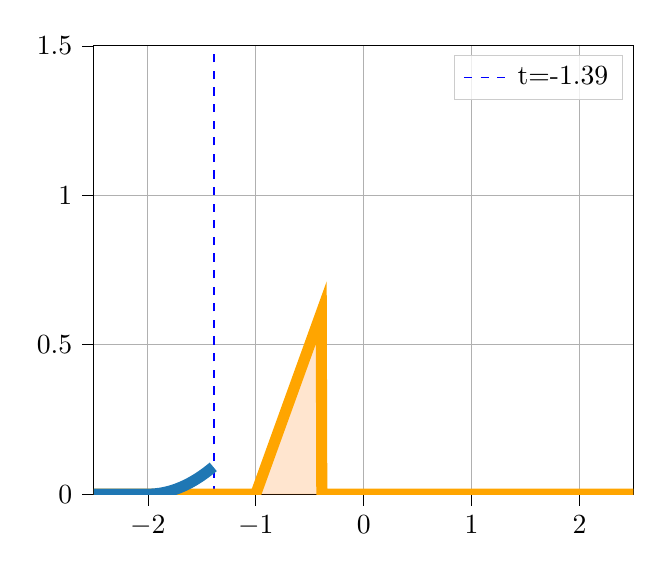
\begin{tikzpicture}

\definecolor{color0}{rgb}{1,0.498039215686275,0.0549019607843137}
\definecolor{color1}{rgb}{1,0.647058823529412,0}
\definecolor{color2}{rgb}{0.12156862745098,0.466666666666667,0.705882352941177}

\begin{axis}[
legend cell align={left},
legend style={fill opacity=0.8, draw opacity=1, text opacity=1, draw=white!80!black},
tick align=outside,
tick pos=left,
x grid style={white!69.0196078431373!black},
xmajorgrids,
xmin=-2.5, xmax=2.5,
xtick style={color=black},
y grid style={white!69.0196078431373!black},
ymajorgrids,
ymin=0, ymax=1.5,
ytick style={color=black}
]
\path [draw=color0, fill=color0, opacity=0.2]
(axis cs:-2.5,0)
--(axis cs:-2.5,0)
--(axis cs:-2.49499499499499,0)
--(axis cs:-2.48998998998999,0)
--(axis cs:-2.48498498498498,0)
--(axis cs:-2.47997997997998,0)
--(axis cs:-2.47497497497497,0)
--(axis cs:-2.46996996996997,0)
--(axis cs:-2.46496496496496,0)
--(axis cs:-2.45995995995996,0)
--(axis cs:-2.45495495495495,0)
--(axis cs:-2.44994994994995,0)
--(axis cs:-2.44494494494494,0)
--(axis cs:-2.43993993993994,0)
--(axis cs:-2.43493493493493,0)
--(axis cs:-2.42992992992993,0)
--(axis cs:-2.42492492492492,0)
--(axis cs:-2.41991991991992,0)
--(axis cs:-2.41491491491491,0)
--(axis cs:-2.40990990990991,0)
--(axis cs:-2.4049049049049,0)
--(axis cs:-2.3998998998999,0)
--(axis cs:-2.39489489489489,0)
--(axis cs:-2.38988988988989,0)
--(axis cs:-2.38488488488488,0)
--(axis cs:-2.37987987987988,0)
--(axis cs:-2.37487487487487,0)
--(axis cs:-2.36986986986987,0)
--(axis cs:-2.36486486486486,0)
--(axis cs:-2.35985985985986,0)
--(axis cs:-2.35485485485485,0)
--(axis cs:-2.34984984984985,0)
--(axis cs:-2.34484484484484,0)
--(axis cs:-2.33983983983984,0)
--(axis cs:-2.33483483483483,0)
--(axis cs:-2.32982982982983,0)
--(axis cs:-2.32482482482482,0)
--(axis cs:-2.31981981981982,0)
--(axis cs:-2.31481481481481,0)
--(axis cs:-2.30980980980981,0)
--(axis cs:-2.3048048048048,0)
--(axis cs:-2.2997997997998,0)
--(axis cs:-2.29479479479479,0)
--(axis cs:-2.28978978978979,0)
--(axis cs:-2.28478478478478,0)
--(axis cs:-2.27977977977978,0)
--(axis cs:-2.27477477477477,0)
--(axis cs:-2.26976976976977,0)
--(axis cs:-2.26476476476476,0)
--(axis cs:-2.25975975975976,0)
--(axis cs:-2.25475475475475,0)
--(axis cs:-2.24974974974975,0)
--(axis cs:-2.24474474474474,0)
--(axis cs:-2.23973973973974,0)
--(axis cs:-2.23473473473473,0)
--(axis cs:-2.22972972972973,0)
--(axis cs:-2.22472472472472,0)
--(axis cs:-2.21971971971972,0)
--(axis cs:-2.21471471471471,0)
--(axis cs:-2.20970970970971,0)
--(axis cs:-2.2047047047047,0)
--(axis cs:-2.1996996996997,0)
--(axis cs:-2.19469469469469,0)
--(axis cs:-2.18968968968969,0)
--(axis cs:-2.18468468468468,0)
--(axis cs:-2.17967967967968,0)
--(axis cs:-2.17467467467467,0)
--(axis cs:-2.16966966966967,0)
--(axis cs:-2.16466466466466,0)
--(axis cs:-2.15965965965966,0)
--(axis cs:-2.15465465465465,0)
--(axis cs:-2.14964964964965,0)
--(axis cs:-2.14464464464464,0)
--(axis cs:-2.13963963963964,0)
--(axis cs:-2.13463463463463,0)
--(axis cs:-2.12962962962963,0)
--(axis cs:-2.12462462462462,0)
--(axis cs:-2.11961961961962,0)
--(axis cs:-2.11461461461461,0)
--(axis cs:-2.10960960960961,0)
--(axis cs:-2.1046046046046,0)
--(axis cs:-2.0995995995996,0)
--(axis cs:-2.09459459459459,0)
--(axis cs:-2.08958958958959,0)
--(axis cs:-2.08458458458458,0)
--(axis cs:-2.07957957957958,0)
--(axis cs:-2.07457457457457,0)
--(axis cs:-2.06956956956957,0)
--(axis cs:-2.06456456456456,0)
--(axis cs:-2.05955955955956,0)
--(axis cs:-2.05455455455455,0)
--(axis cs:-2.04954954954955,0)
--(axis cs:-2.04454454454454,0)
--(axis cs:-2.03953953953954,0)
--(axis cs:-2.03453453453453,0)
--(axis cs:-2.02952952952953,0)
--(axis cs:-2.02452452452452,0)
--(axis cs:-2.01951951951952,0)
--(axis cs:-2.01451451451451,0)
--(axis cs:-2.00950950950951,0)
--(axis cs:-2.0045045045045,0)
--(axis cs:-1.9994994994995,0)
--(axis cs:-1.99449449449449,0)
--(axis cs:-1.98948948948949,0)
--(axis cs:-1.98448448448448,0)
--(axis cs:-1.97947947947948,0)
--(axis cs:-1.97447447447447,0)
--(axis cs:-1.96946946946947,0)
--(axis cs:-1.96446446446446,0)
--(axis cs:-1.95945945945946,0)
--(axis cs:-1.95445445445445,0)
--(axis cs:-1.94944944944945,0)
--(axis cs:-1.94444444444444,0)
--(axis cs:-1.93943943943944,0)
--(axis cs:-1.93443443443443,0)
--(axis cs:-1.92942942942943,0)
--(axis cs:-1.92442442442442,0)
--(axis cs:-1.91941941941942,0)
--(axis cs:-1.91441441441441,0)
--(axis cs:-1.90940940940941,0)
--(axis cs:-1.9044044044044,0)
--(axis cs:-1.8993993993994,0)
--(axis cs:-1.89439439439439,0)
--(axis cs:-1.88938938938939,0)
--(axis cs:-1.88438438438438,0)
--(axis cs:-1.87937937937938,0)
--(axis cs:-1.87437437437437,0)
--(axis cs:-1.86936936936937,0)
--(axis cs:-1.86436436436436,0)
--(axis cs:-1.85935935935936,0)
--(axis cs:-1.85435435435435,0)
--(axis cs:-1.84934934934935,0)
--(axis cs:-1.84434434434434,0)
--(axis cs:-1.83933933933934,0)
--(axis cs:-1.83433433433433,0)
--(axis cs:-1.82932932932933,0)
--(axis cs:-1.82432432432432,0)
--(axis cs:-1.81931931931932,0)
--(axis cs:-1.81431431431431,0)
--(axis cs:-1.80930930930931,0)
--(axis cs:-1.8043043043043,0)
--(axis cs:-1.7992992992993,0)
--(axis cs:-1.79429429429429,0)
--(axis cs:-1.78928928928929,0)
--(axis cs:-1.78428428428428,0)
--(axis cs:-1.77927927927928,0)
--(axis cs:-1.77427427427427,0)
--(axis cs:-1.76926926926927,0)
--(axis cs:-1.76426426426426,0)
--(axis cs:-1.75925925925926,0)
--(axis cs:-1.75425425425425,0)
--(axis cs:-1.74924924924925,0)
--(axis cs:-1.74424424424424,0)
--(axis cs:-1.73923923923924,0)
--(axis cs:-1.73423423423423,0)
--(axis cs:-1.72922922922923,0)
--(axis cs:-1.72422422422422,0)
--(axis cs:-1.71921921921922,0)
--(axis cs:-1.71421421421421,0)
--(axis cs:-1.70920920920921,0)
--(axis cs:-1.7042042042042,0)
--(axis cs:-1.6991991991992,0)
--(axis cs:-1.69419419419419,0)
--(axis cs:-1.68918918918919,0)
--(axis cs:-1.68418418418418,0)
--(axis cs:-1.67917917917918,0)
--(axis cs:-1.67417417417417,0)
--(axis cs:-1.66916916916917,0)
--(axis cs:-1.66416416416416,0)
--(axis cs:-1.65915915915916,0)
--(axis cs:-1.65415415415415,0)
--(axis cs:-1.64914914914915,0)
--(axis cs:-1.64414414414414,0)
--(axis cs:-1.63913913913914,0)
--(axis cs:-1.63413413413413,0)
--(axis cs:-1.62912912912913,0)
--(axis cs:-1.62412412412412,0)
--(axis cs:-1.61911911911912,0)
--(axis cs:-1.61411411411411,0)
--(axis cs:-1.60910910910911,0)
--(axis cs:-1.6041041041041,0)
--(axis cs:-1.5990990990991,0)
--(axis cs:-1.59409409409409,0)
--(axis cs:-1.58908908908909,0)
--(axis cs:-1.58408408408408,0)
--(axis cs:-1.57907907907908,0)
--(axis cs:-1.57407407407407,0)
--(axis cs:-1.56906906906907,0)
--(axis cs:-1.56406406406406,0)
--(axis cs:-1.55905905905906,0)
--(axis cs:-1.55405405405405,0)
--(axis cs:-1.54904904904905,0)
--(axis cs:-1.54404404404404,0)
--(axis cs:-1.53903903903904,0)
--(axis cs:-1.53403403403403,0)
--(axis cs:-1.52902902902903,0)
--(axis cs:-1.52402402402402,0)
--(axis cs:-1.51901901901902,0)
--(axis cs:-1.51401401401401,0)
--(axis cs:-1.50900900900901,0)
--(axis cs:-1.504004004004,0)
--(axis cs:-1.498998998999,0)
--(axis cs:-1.49399399399399,0)
--(axis cs:-1.48898898898899,0)
--(axis cs:-1.48398398398398,0)
--(axis cs:-1.47897897897898,0)
--(axis cs:-1.47397397397397,0)
--(axis cs:-1.46896896896897,0)
--(axis cs:-1.46396396396396,0)
--(axis cs:-1.45895895895896,0)
--(axis cs:-1.45395395395395,0)
--(axis cs:-1.44894894894895,0)
--(axis cs:-1.44394394394394,0)
--(axis cs:-1.43893893893894,0)
--(axis cs:-1.43393393393393,0)
--(axis cs:-1.42892892892893,0)
--(axis cs:-1.42392392392392,0)
--(axis cs:-1.41891891891892,0)
--(axis cs:-1.41391391391391,0)
--(axis cs:-1.40890890890891,0)
--(axis cs:-1.4039039039039,0)
--(axis cs:-1.3988988988989,0)
--(axis cs:-1.39389389389389,0)
--(axis cs:-1.38888888888889,0)
--(axis cs:-1.38388388388388,0)
--(axis cs:-1.37887887887888,0)
--(axis cs:-1.37387387387387,0)
--(axis cs:-1.36886886886887,0)
--(axis cs:-1.36386386386386,0)
--(axis cs:-1.35885885885886,0)
--(axis cs:-1.35385385385385,0)
--(axis cs:-1.34884884884885,0)
--(axis cs:-1.34384384384384,0)
--(axis cs:-1.33883883883884,0)
--(axis cs:-1.33383383383383,0)
--(axis cs:-1.32882882882883,0)
--(axis cs:-1.32382382382382,0)
--(axis cs:-1.31881881881882,0)
--(axis cs:-1.31381381381381,0)
--(axis cs:-1.30880880880881,0)
--(axis cs:-1.3038038038038,0)
--(axis cs:-1.2987987987988,0)
--(axis cs:-1.29379379379379,0)
--(axis cs:-1.28878878878879,0)
--(axis cs:-1.28378378378378,0)
--(axis cs:-1.27877877877878,0)
--(axis cs:-1.27377377377377,0)
--(axis cs:-1.26876876876877,0)
--(axis cs:-1.26376376376376,0)
--(axis cs:-1.25875875875876,0)
--(axis cs:-1.25375375375375,0)
--(axis cs:-1.24874874874875,0)
--(axis cs:-1.24374374374374,0)
--(axis cs:-1.23873873873874,0)
--(axis cs:-1.23373373373373,0)
--(axis cs:-1.22872872872873,0)
--(axis cs:-1.22372372372372,0)
--(axis cs:-1.21871871871872,0)
--(axis cs:-1.21371371371371,0)
--(axis cs:-1.20870870870871,0)
--(axis cs:-1.2037037037037,0)
--(axis cs:-1.1986986986987,0)
--(axis cs:-1.19369369369369,0)
--(axis cs:-1.18868868868869,0)
--(axis cs:-1.18368368368368,0)
--(axis cs:-1.17867867867868,0)
--(axis cs:-1.17367367367367,0)
--(axis cs:-1.16866866866867,0)
--(axis cs:-1.16366366366366,0)
--(axis cs:-1.15865865865866,0)
--(axis cs:-1.15365365365365,0)
--(axis cs:-1.14864864864865,0)
--(axis cs:-1.14364364364364,0)
--(axis cs:-1.13863863863864,0)
--(axis cs:-1.13363363363363,0)
--(axis cs:-1.12862862862863,0)
--(axis cs:-1.12362362362362,0)
--(axis cs:-1.11861861861862,0)
--(axis cs:-1.11361361361361,0)
--(axis cs:-1.10860860860861,0)
--(axis cs:-1.1036036036036,0)
--(axis cs:-1.0985985985986,0)
--(axis cs:-1.09359359359359,0)
--(axis cs:-1.08858858858859,0)
--(axis cs:-1.08358358358358,0)
--(axis cs:-1.07857857857858,0)
--(axis cs:-1.07357357357357,0)
--(axis cs:-1.06856856856857,0)
--(axis cs:-1.06356356356356,0)
--(axis cs:-1.05855855855856,0)
--(axis cs:-1.05355355355355,0)
--(axis cs:-1.04854854854855,0)
--(axis cs:-1.04354354354354,0)
--(axis cs:-1.03853853853854,0)
--(axis cs:-1.03353353353353,0)
--(axis cs:-1.02852852852853,0)
--(axis cs:-1.02352352352352,0)
--(axis cs:-1.01851851851852,0)
--(axis cs:-1.01351351351351,0)
--(axis cs:-1.00850850850851,0)
--(axis cs:-1.0035035035035,0)
--(axis cs:-0.998498498498499,0)
--(axis cs:-0.993493493493494,0)
--(axis cs:-0.988488488488489,0)
--(axis cs:-0.983483483483484,0)
--(axis cs:-0.978478478478479,0)
--(axis cs:-0.973473473473474,0)
--(axis cs:-0.968468468468469,0)
--(axis cs:-0.963463463463464,0)
--(axis cs:-0.958458458458459,0)
--(axis cs:-0.953453453453454,0)
--(axis cs:-0.948448448448449,0)
--(axis cs:-0.943443443443444,0)
--(axis cs:-0.938438438438439,0)
--(axis cs:-0.933433433433434,0)
--(axis cs:-0.928428428428429,0)
--(axis cs:-0.923423423423424,0)
--(axis cs:-0.918418418418419,0)
--(axis cs:-0.913413413413414,0)
--(axis cs:-0.908408408408409,0)
--(axis cs:-0.903403403403404,0)
--(axis cs:-0.898398398398399,0)
--(axis cs:-0.893393393393393,0)
--(axis cs:-0.888388388388388,0)
--(axis cs:-0.883383383383383,0)
--(axis cs:-0.878378378378378,0)
--(axis cs:-0.873373373373373,0)
--(axis cs:-0.868368368368368,0)
--(axis cs:-0.863363363363363,0)
--(axis cs:-0.858358358358358,0)
--(axis cs:-0.853353353353353,0)
--(axis cs:-0.848348348348348,0)
--(axis cs:-0.843343343343343,0)
--(axis cs:-0.838338338338338,0)
--(axis cs:-0.833333333333333,0)
--(axis cs:-0.828328328328328,0)
--(axis cs:-0.823323323323323,0)
--(axis cs:-0.818318318318318,0)
--(axis cs:-0.813313313313313,0)
--(axis cs:-0.808308308308308,0)
--(axis cs:-0.803303303303303,0)
--(axis cs:-0.798298298298298,0)
--(axis cs:-0.793293293293293,0)
--(axis cs:-0.788288288288288,0)
--(axis cs:-0.783283283283283,0)
--(axis cs:-0.778278278278278,0)
--(axis cs:-0.773273273273273,0)
--(axis cs:-0.768268268268268,0)
--(axis cs:-0.763263263263263,0)
--(axis cs:-0.758258258258258,0)
--(axis cs:-0.753253253253253,0)
--(axis cs:-0.748248248248248,0)
--(axis cs:-0.743243243243243,0)
--(axis cs:-0.738238238238238,0)
--(axis cs:-0.733233233233233,0)
--(axis cs:-0.728228228228228,0)
--(axis cs:-0.723223223223223,0)
--(axis cs:-0.718218218218218,0)
--(axis cs:-0.713213213213213,0)
--(axis cs:-0.708208208208208,0)
--(axis cs:-0.703203203203203,0)
--(axis cs:-0.698198198198198,0)
--(axis cs:-0.693193193193193,0)
--(axis cs:-0.688188188188188,0)
--(axis cs:-0.683183183183183,0)
--(axis cs:-0.678178178178178,0)
--(axis cs:-0.673173173173173,0)
--(axis cs:-0.668168168168168,0)
--(axis cs:-0.663163163163163,0)
--(axis cs:-0.658158158158158,0)
--(axis cs:-0.653153153153153,0)
--(axis cs:-0.648148148148148,0)
--(axis cs:-0.643143143143143,0)
--(axis cs:-0.638138138138138,0)
--(axis cs:-0.633133133133133,0)
--(axis cs:-0.628128128128128,0)
--(axis cs:-0.623123123123123,0)
--(axis cs:-0.618118118118118,0)
--(axis cs:-0.613113113113113,0)
--(axis cs:-0.608108108108108,0)
--(axis cs:-0.603103103103103,0)
--(axis cs:-0.598098098098098,0)
--(axis cs:-0.593093093093093,0)
--(axis cs:-0.588088088088088,0)
--(axis cs:-0.583083083083083,0)
--(axis cs:-0.578078078078078,0)
--(axis cs:-0.573073073073073,0)
--(axis cs:-0.568068068068068,0)
--(axis cs:-0.563063063063063,0)
--(axis cs:-0.558058058058058,0)
--(axis cs:-0.553053053053053,0)
--(axis cs:-0.548048048048048,0)
--(axis cs:-0.543043043043043,0)
--(axis cs:-0.538038038038038,0)
--(axis cs:-0.533033033033033,0)
--(axis cs:-0.528028028028028,0)
--(axis cs:-0.523023023023023,0)
--(axis cs:-0.518018018018018,0)
--(axis cs:-0.513013013013013,0)
--(axis cs:-0.508008008008008,0)
--(axis cs:-0.503003003003003,0)
--(axis cs:-0.497997997997998,0)
--(axis cs:-0.492992992992993,0)
--(axis cs:-0.487987987987988,0)
--(axis cs:-0.482982982982983,0)
--(axis cs:-0.477977977977978,0)
--(axis cs:-0.472972972972973,0)
--(axis cs:-0.467967967967968,0)
--(axis cs:-0.462962962962963,0)
--(axis cs:-0.457957957957958,0)
--(axis cs:-0.452952952952953,0)
--(axis cs:-0.447947947947948,0)
--(axis cs:-0.442942942942943,0)
--(axis cs:-0.437937937937938,0)
--(axis cs:-0.432932932932933,0)
--(axis cs:-0.427927927927928,0)
--(axis cs:-0.422922922922923,0)
--(axis cs:-0.417917917917918,0)
--(axis cs:-0.412912912912913,0)
--(axis cs:-0.407907907907908,0)
--(axis cs:-0.402902902902903,0)
--(axis cs:-0.397897897897898,0)
--(axis cs:-0.392892892892893,0)
--(axis cs:-0.387887887887888,0)
--(axis cs:-0.382882882882883,0)
--(axis cs:-0.377877877877878,0)
--(axis cs:-0.372872872872873,0)
--(axis cs:-0.367867867867868,0)
--(axis cs:-0.362862862862863,0)
--(axis cs:-0.357857857857858,0)
--(axis cs:-0.352852852852853,0)
--(axis cs:-0.347847847847848,0)
--(axis cs:-0.342842842842843,0)
--(axis cs:-0.337837837837838,0)
--(axis cs:-0.332832832832833,0)
--(axis cs:-0.327827827827828,0)
--(axis cs:-0.322822822822823,0)
--(axis cs:-0.317817817817818,0)
--(axis cs:-0.312812812812813,0)
--(axis cs:-0.307807807807808,0)
--(axis cs:-0.302802802802803,0)
--(axis cs:-0.297797797797798,0)
--(axis cs:-0.292792792792793,0)
--(axis cs:-0.287787787787788,0)
--(axis cs:-0.282782782782783,0)
--(axis cs:-0.277777777777778,0)
--(axis cs:-0.272772772772773,0)
--(axis cs:-0.267767767767768,0)
--(axis cs:-0.262762762762763,0)
--(axis cs:-0.257757757757758,0)
--(axis cs:-0.252752752752753,0)
--(axis cs:-0.247747747747748,0)
--(axis cs:-0.242742742742743,0)
--(axis cs:-0.237737737737738,0)
--(axis cs:-0.232732732732733,0)
--(axis cs:-0.227727727727728,0)
--(axis cs:-0.222722722722723,0)
--(axis cs:-0.217717717717718,0)
--(axis cs:-0.212712712712713,0)
--(axis cs:-0.207707707707708,0)
--(axis cs:-0.202702702702703,0)
--(axis cs:-0.197697697697698,0)
--(axis cs:-0.192692692692693,0)
--(axis cs:-0.187687687687688,0)
--(axis cs:-0.182682682682683,0)
--(axis cs:-0.177677677677678,0)
--(axis cs:-0.172672672672673,0)
--(axis cs:-0.167667667667668,0)
--(axis cs:-0.162662662662663,0)
--(axis cs:-0.157657657657658,0)
--(axis cs:-0.152652652652653,0)
--(axis cs:-0.147647647647648,0)
--(axis cs:-0.142642642642643,0)
--(axis cs:-0.137637637637638,0)
--(axis cs:-0.132632632632633,0)
--(axis cs:-0.127627627627628,0)
--(axis cs:-0.122622622622623,0)
--(axis cs:-0.117617617617618,0)
--(axis cs:-0.112612612612613,0)
--(axis cs:-0.107607607607608,0)
--(axis cs:-0.102602602602603,0)
--(axis cs:-0.0975975975975976,0)
--(axis cs:-0.0925925925925926,0)
--(axis cs:-0.0875875875875876,0)
--(axis cs:-0.0825825825825826,0)
--(axis cs:-0.0775775775775776,0)
--(axis cs:-0.0725725725725725,0)
--(axis cs:-0.0675675675675675,0)
--(axis cs:-0.0625625625625625,0)
--(axis cs:-0.0575575575575575,0)
--(axis cs:-0.0525525525525525,0)
--(axis cs:-0.0475475475475475,0)
--(axis cs:-0.0425425425425425,0)
--(axis cs:-0.0375375375375375,0)
--(axis cs:-0.0325325325325325,0)
--(axis cs:-0.0275275275275275,0)
--(axis cs:-0.0225225225225225,0)
--(axis cs:-0.0175175175175175,0)
--(axis cs:-0.0125125125125125,0)
--(axis cs:-0.0075075075075075,0)
--(axis cs:-0.0025025025025025,0)
--(axis cs:0.0025025025025025,0)
--(axis cs:0.0075075075075075,0)
--(axis cs:0.0125125125125125,0)
--(axis cs:0.0175175175175175,0)
--(axis cs:0.0225225225225225,0)
--(axis cs:0.0275275275275275,0)
--(axis cs:0.0325325325325325,0)
--(axis cs:0.0375375375375375,0)
--(axis cs:0.0425425425425425,0)
--(axis cs:0.0475475475475475,0)
--(axis cs:0.0525525525525525,0)
--(axis cs:0.0575575575575575,0)
--(axis cs:0.0625625625625625,0)
--(axis cs:0.0675675675675675,0)
--(axis cs:0.0725725725725725,0)
--(axis cs:0.0775775775775776,0)
--(axis cs:0.0825825825825826,0)
--(axis cs:0.0875875875875876,0)
--(axis cs:0.0925925925925926,0)
--(axis cs:0.0975975975975976,0)
--(axis cs:0.102602602602603,0)
--(axis cs:0.107607607607608,0)
--(axis cs:0.112612612612613,0)
--(axis cs:0.117617617617618,0)
--(axis cs:0.122622622622623,0)
--(axis cs:0.127627627627628,0)
--(axis cs:0.132632632632633,0)
--(axis cs:0.137637637637638,0)
--(axis cs:0.142642642642643,0)
--(axis cs:0.147647647647648,0)
--(axis cs:0.152652652652653,0)
--(axis cs:0.157657657657658,0)
--(axis cs:0.162662662662663,0)
--(axis cs:0.167667667667668,0)
--(axis cs:0.172672672672673,0)
--(axis cs:0.177677677677678,0)
--(axis cs:0.182682682682683,0)
--(axis cs:0.187687687687688,0)
--(axis cs:0.192692692692693,0)
--(axis cs:0.197697697697698,0)
--(axis cs:0.202702702702703,0)
--(axis cs:0.207707707707708,0)
--(axis cs:0.212712712712713,0)
--(axis cs:0.217717717717718,0)
--(axis cs:0.222722722722723,0)
--(axis cs:0.227727727727728,0)
--(axis cs:0.232732732732733,0)
--(axis cs:0.237737737737738,0)
--(axis cs:0.242742742742743,0)
--(axis cs:0.247747747747748,0)
--(axis cs:0.252752752752753,0)
--(axis cs:0.257757757757758,0)
--(axis cs:0.262762762762763,0)
--(axis cs:0.267767767767768,0)
--(axis cs:0.272772772772773,0)
--(axis cs:0.277777777777778,0)
--(axis cs:0.282782782782783,0)
--(axis cs:0.287787787787788,0)
--(axis cs:0.292792792792793,0)
--(axis cs:0.297797797797798,0)
--(axis cs:0.302802802802803,0)
--(axis cs:0.307807807807808,0)
--(axis cs:0.312812812812813,0)
--(axis cs:0.317817817817818,0)
--(axis cs:0.322822822822823,0)
--(axis cs:0.327827827827828,0)
--(axis cs:0.332832832832833,0)
--(axis cs:0.337837837837838,0)
--(axis cs:0.342842842842843,0)
--(axis cs:0.347847847847848,0)
--(axis cs:0.352852852852853,0)
--(axis cs:0.357857857857858,0)
--(axis cs:0.362862862862863,0)
--(axis cs:0.367867867867868,0)
--(axis cs:0.372872872872873,0)
--(axis cs:0.377877877877878,0)
--(axis cs:0.382882882882883,0)
--(axis cs:0.387887887887888,0)
--(axis cs:0.392892892892893,0)
--(axis cs:0.397897897897898,0)
--(axis cs:0.402902902902903,0)
--(axis cs:0.407907907907908,0)
--(axis cs:0.412912912912913,0)
--(axis cs:0.417917917917918,0)
--(axis cs:0.422922922922923,0)
--(axis cs:0.427927927927928,0)
--(axis cs:0.432932932932933,0)
--(axis cs:0.437937937937938,0)
--(axis cs:0.442942942942943,0)
--(axis cs:0.447947947947948,0)
--(axis cs:0.452952952952953,0)
--(axis cs:0.457957957957958,0)
--(axis cs:0.462962962962963,0)
--(axis cs:0.467967967967968,0)
--(axis cs:0.472972972972973,0)
--(axis cs:0.477977977977978,0)
--(axis cs:0.482982982982983,0)
--(axis cs:0.487987987987988,0)
--(axis cs:0.492992992992993,0)
--(axis cs:0.497997997997998,0)
--(axis cs:0.503003003003003,0)
--(axis cs:0.508008008008008,0)
--(axis cs:0.513013013013013,0)
--(axis cs:0.518018018018018,0)
--(axis cs:0.523023023023023,0)
--(axis cs:0.528028028028028,0)
--(axis cs:0.533033033033033,0)
--(axis cs:0.538038038038038,0)
--(axis cs:0.543043043043043,0)
--(axis cs:0.548048048048048,0)
--(axis cs:0.553053053053053,0)
--(axis cs:0.558058058058058,0)
--(axis cs:0.563063063063063,0)
--(axis cs:0.568068068068068,0)
--(axis cs:0.573073073073073,0)
--(axis cs:0.578078078078078,0)
--(axis cs:0.583083083083083,0)
--(axis cs:0.588088088088088,0)
--(axis cs:0.593093093093093,0)
--(axis cs:0.598098098098098,0)
--(axis cs:0.603103103103103,0)
--(axis cs:0.608108108108108,0)
--(axis cs:0.613113113113113,0)
--(axis cs:0.618118118118118,0)
--(axis cs:0.623123123123123,0)
--(axis cs:0.628128128128128,0)
--(axis cs:0.633133133133133,0)
--(axis cs:0.638138138138138,0)
--(axis cs:0.643143143143143,0)
--(axis cs:0.648148148148148,0)
--(axis cs:0.653153153153153,0)
--(axis cs:0.658158158158158,0)
--(axis cs:0.663163163163163,0)
--(axis cs:0.668168168168168,0)
--(axis cs:0.673173173173173,0)
--(axis cs:0.678178178178178,0)
--(axis cs:0.683183183183183,0)
--(axis cs:0.688188188188188,0)
--(axis cs:0.693193193193193,0)
--(axis cs:0.698198198198198,0)
--(axis cs:0.703203203203203,0)
--(axis cs:0.708208208208208,0)
--(axis cs:0.713213213213213,0)
--(axis cs:0.718218218218218,0)
--(axis cs:0.723223223223223,0)
--(axis cs:0.728228228228228,0)
--(axis cs:0.733233233233233,0)
--(axis cs:0.738238238238238,0)
--(axis cs:0.743243243243243,0)
--(axis cs:0.748248248248248,0)
--(axis cs:0.753253253253253,0)
--(axis cs:0.758258258258258,0)
--(axis cs:0.763263263263263,0)
--(axis cs:0.768268268268268,0)
--(axis cs:0.773273273273273,0)
--(axis cs:0.778278278278278,0)
--(axis cs:0.783283283283283,0)
--(axis cs:0.788288288288288,0)
--(axis cs:0.793293293293293,0)
--(axis cs:0.798298298298298,0)
--(axis cs:0.803303303303303,0)
--(axis cs:0.808308308308308,0)
--(axis cs:0.813313313313313,0)
--(axis cs:0.818318318318318,0)
--(axis cs:0.823323323323323,0)
--(axis cs:0.828328328328328,0)
--(axis cs:0.833333333333333,0)
--(axis cs:0.838338338338338,0)
--(axis cs:0.843343343343343,0)
--(axis cs:0.848348348348348,0)
--(axis cs:0.853353353353353,0)
--(axis cs:0.858358358358358,0)
--(axis cs:0.863363363363364,0)
--(axis cs:0.868368368368369,0)
--(axis cs:0.873373373373374,0)
--(axis cs:0.878378378378379,0)
--(axis cs:0.883383383383384,0)
--(axis cs:0.888388388388389,0)
--(axis cs:0.893393393393394,0)
--(axis cs:0.898398398398399,0)
--(axis cs:0.903403403403404,0)
--(axis cs:0.908408408408409,0)
--(axis cs:0.913413413413414,0)
--(axis cs:0.918418418418419,0)
--(axis cs:0.923423423423424,0)
--(axis cs:0.928428428428429,0)
--(axis cs:0.933433433433434,0)
--(axis cs:0.938438438438439,0)
--(axis cs:0.943443443443444,0)
--(axis cs:0.948448448448449,0)
--(axis cs:0.953453453453454,0)
--(axis cs:0.958458458458459,0)
--(axis cs:0.963463463463464,0)
--(axis cs:0.968468468468469,0)
--(axis cs:0.973473473473474,0)
--(axis cs:0.978478478478479,0)
--(axis cs:0.983483483483484,0)
--(axis cs:0.988488488488489,0)
--(axis cs:0.993493493493494,0)
--(axis cs:0.998498498498499,0)
--(axis cs:1.0035035035035,0)
--(axis cs:1.00850850850851,0)
--(axis cs:1.01351351351351,0)
--(axis cs:1.01851851851852,0)
--(axis cs:1.02352352352352,0)
--(axis cs:1.02852852852853,0)
--(axis cs:1.03353353353353,0)
--(axis cs:1.03853853853854,0)
--(axis cs:1.04354354354354,0)
--(axis cs:1.04854854854855,0)
--(axis cs:1.05355355355355,0)
--(axis cs:1.05855855855856,0)
--(axis cs:1.06356356356356,0)
--(axis cs:1.06856856856857,0)
--(axis cs:1.07357357357357,0)
--(axis cs:1.07857857857858,0)
--(axis cs:1.08358358358358,0)
--(axis cs:1.08858858858859,0)
--(axis cs:1.09359359359359,0)
--(axis cs:1.0985985985986,0)
--(axis cs:1.1036036036036,0)
--(axis cs:1.10860860860861,0)
--(axis cs:1.11361361361361,0)
--(axis cs:1.11861861861862,0)
--(axis cs:1.12362362362362,0)
--(axis cs:1.12862862862863,0)
--(axis cs:1.13363363363363,0)
--(axis cs:1.13863863863864,0)
--(axis cs:1.14364364364364,0)
--(axis cs:1.14864864864865,0)
--(axis cs:1.15365365365365,0)
--(axis cs:1.15865865865866,0)
--(axis cs:1.16366366366366,0)
--(axis cs:1.16866866866867,0)
--(axis cs:1.17367367367367,0)
--(axis cs:1.17867867867868,0)
--(axis cs:1.18368368368368,0)
--(axis cs:1.18868868868869,0)
--(axis cs:1.19369369369369,0)
--(axis cs:1.1986986986987,0)
--(axis cs:1.2037037037037,0)
--(axis cs:1.20870870870871,0)
--(axis cs:1.21371371371371,0)
--(axis cs:1.21871871871872,0)
--(axis cs:1.22372372372372,0)
--(axis cs:1.22872872872873,0)
--(axis cs:1.23373373373373,0)
--(axis cs:1.23873873873874,0)
--(axis cs:1.24374374374374,0)
--(axis cs:1.24874874874875,0)
--(axis cs:1.25375375375375,0)
--(axis cs:1.25875875875876,0)
--(axis cs:1.26376376376376,0)
--(axis cs:1.26876876876877,0)
--(axis cs:1.27377377377377,0)
--(axis cs:1.27877877877878,0)
--(axis cs:1.28378378378378,0)
--(axis cs:1.28878878878879,0)
--(axis cs:1.29379379379379,0)
--(axis cs:1.2987987987988,0)
--(axis cs:1.3038038038038,0)
--(axis cs:1.30880880880881,0)
--(axis cs:1.31381381381381,0)
--(axis cs:1.31881881881882,0)
--(axis cs:1.32382382382382,0)
--(axis cs:1.32882882882883,0)
--(axis cs:1.33383383383383,0)
--(axis cs:1.33883883883884,0)
--(axis cs:1.34384384384384,0)
--(axis cs:1.34884884884885,0)
--(axis cs:1.35385385385385,0)
--(axis cs:1.35885885885886,0)
--(axis cs:1.36386386386386,0)
--(axis cs:1.36886886886887,0)
--(axis cs:1.37387387387387,0)
--(axis cs:1.37887887887888,0)
--(axis cs:1.38388388388388,0)
--(axis cs:1.38888888888889,0)
--(axis cs:1.39389389389389,0)
--(axis cs:1.3988988988989,0)
--(axis cs:1.4039039039039,0)
--(axis cs:1.40890890890891,0)
--(axis cs:1.41391391391391,0)
--(axis cs:1.41891891891892,0)
--(axis cs:1.42392392392392,0)
--(axis cs:1.42892892892893,0)
--(axis cs:1.43393393393393,0)
--(axis cs:1.43893893893894,0)
--(axis cs:1.44394394394394,0)
--(axis cs:1.44894894894895,0)
--(axis cs:1.45395395395395,0)
--(axis cs:1.45895895895896,0)
--(axis cs:1.46396396396396,0)
--(axis cs:1.46896896896897,0)
--(axis cs:1.47397397397397,0)
--(axis cs:1.47897897897898,0)
--(axis cs:1.48398398398398,0)
--(axis cs:1.48898898898899,0)
--(axis cs:1.49399399399399,0)
--(axis cs:1.498998998999,0)
--(axis cs:1.504004004004,0)
--(axis cs:1.50900900900901,0)
--(axis cs:1.51401401401401,0)
--(axis cs:1.51901901901902,0)
--(axis cs:1.52402402402402,0)
--(axis cs:1.52902902902903,0)
--(axis cs:1.53403403403403,0)
--(axis cs:1.53903903903904,0)
--(axis cs:1.54404404404404,0)
--(axis cs:1.54904904904905,0)
--(axis cs:1.55405405405405,0)
--(axis cs:1.55905905905906,0)
--(axis cs:1.56406406406406,0)
--(axis cs:1.56906906906907,0)
--(axis cs:1.57407407407407,0)
--(axis cs:1.57907907907908,0)
--(axis cs:1.58408408408408,0)
--(axis cs:1.58908908908909,0)
--(axis cs:1.59409409409409,0)
--(axis cs:1.5990990990991,0)
--(axis cs:1.6041041041041,0)
--(axis cs:1.60910910910911,0)
--(axis cs:1.61411411411411,0)
--(axis cs:1.61911911911912,0)
--(axis cs:1.62412412412412,0)
--(axis cs:1.62912912912913,0)
--(axis cs:1.63413413413413,0)
--(axis cs:1.63913913913914,0)
--(axis cs:1.64414414414414,0)
--(axis cs:1.64914914914915,0)
--(axis cs:1.65415415415415,0)
--(axis cs:1.65915915915916,0)
--(axis cs:1.66416416416416,0)
--(axis cs:1.66916916916917,0)
--(axis cs:1.67417417417417,0)
--(axis cs:1.67917917917918,0)
--(axis cs:1.68418418418418,0)
--(axis cs:1.68918918918919,0)
--(axis cs:1.69419419419419,0)
--(axis cs:1.6991991991992,0)
--(axis cs:1.7042042042042,0)
--(axis cs:1.70920920920921,0)
--(axis cs:1.71421421421421,0)
--(axis cs:1.71921921921922,0)
--(axis cs:1.72422422422422,0)
--(axis cs:1.72922922922923,0)
--(axis cs:1.73423423423423,0)
--(axis cs:1.73923923923924,0)
--(axis cs:1.74424424424424,0)
--(axis cs:1.74924924924925,0)
--(axis cs:1.75425425425425,0)
--(axis cs:1.75925925925926,0)
--(axis cs:1.76426426426426,0)
--(axis cs:1.76926926926927,0)
--(axis cs:1.77427427427427,0)
--(axis cs:1.77927927927928,0)
--(axis cs:1.78428428428428,0)
--(axis cs:1.78928928928929,0)
--(axis cs:1.79429429429429,0)
--(axis cs:1.7992992992993,0)
--(axis cs:1.8043043043043,0)
--(axis cs:1.80930930930931,0)
--(axis cs:1.81431431431431,0)
--(axis cs:1.81931931931932,0)
--(axis cs:1.82432432432432,0)
--(axis cs:1.82932932932933,0)
--(axis cs:1.83433433433433,0)
--(axis cs:1.83933933933934,0)
--(axis cs:1.84434434434434,0)
--(axis cs:1.84934934934935,0)
--(axis cs:1.85435435435435,0)
--(axis cs:1.85935935935936,0)
--(axis cs:1.86436436436436,0)
--(axis cs:1.86936936936937,0)
--(axis cs:1.87437437437437,0)
--(axis cs:1.87937937937938,0)
--(axis cs:1.88438438438438,0)
--(axis cs:1.88938938938939,0)
--(axis cs:1.89439439439439,0)
--(axis cs:1.8993993993994,0)
--(axis cs:1.9044044044044,0)
--(axis cs:1.90940940940941,0)
--(axis cs:1.91441441441441,0)
--(axis cs:1.91941941941942,0)
--(axis cs:1.92442442442442,0)
--(axis cs:1.92942942942943,0)
--(axis cs:1.93443443443443,0)
--(axis cs:1.93943943943944,0)
--(axis cs:1.94444444444444,0)
--(axis cs:1.94944944944945,0)
--(axis cs:1.95445445445445,0)
--(axis cs:1.95945945945946,0)
--(axis cs:1.96446446446446,0)
--(axis cs:1.96946946946947,0)
--(axis cs:1.97447447447447,0)
--(axis cs:1.97947947947948,0)
--(axis cs:1.98448448448448,0)
--(axis cs:1.98948948948949,0)
--(axis cs:1.99449449449449,0)
--(axis cs:1.9994994994995,0)
--(axis cs:2.0045045045045,0)
--(axis cs:2.00950950950951,0)
--(axis cs:2.01451451451451,0)
--(axis cs:2.01951951951952,0)
--(axis cs:2.02452452452452,0)
--(axis cs:2.02952952952953,0)
--(axis cs:2.03453453453453,0)
--(axis cs:2.03953953953954,0)
--(axis cs:2.04454454454454,0)
--(axis cs:2.04954954954955,0)
--(axis cs:2.05455455455455,0)
--(axis cs:2.05955955955956,0)
--(axis cs:2.06456456456456,0)
--(axis cs:2.06956956956957,0)
--(axis cs:2.07457457457457,0)
--(axis cs:2.07957957957958,0)
--(axis cs:2.08458458458458,0)
--(axis cs:2.08958958958959,0)
--(axis cs:2.09459459459459,0)
--(axis cs:2.0995995995996,0)
--(axis cs:2.1046046046046,0)
--(axis cs:2.10960960960961,0)
--(axis cs:2.11461461461461,0)
--(axis cs:2.11961961961962,0)
--(axis cs:2.12462462462462,0)
--(axis cs:2.12962962962963,0)
--(axis cs:2.13463463463463,0)
--(axis cs:2.13963963963964,0)
--(axis cs:2.14464464464464,0)
--(axis cs:2.14964964964965,0)
--(axis cs:2.15465465465465,0)
--(axis cs:2.15965965965966,0)
--(axis cs:2.16466466466466,0)
--(axis cs:2.16966966966967,0)
--(axis cs:2.17467467467467,0)
--(axis cs:2.17967967967968,0)
--(axis cs:2.18468468468468,0)
--(axis cs:2.18968968968969,0)
--(axis cs:2.19469469469469,0)
--(axis cs:2.1996996996997,0)
--(axis cs:2.2047047047047,0)
--(axis cs:2.20970970970971,0)
--(axis cs:2.21471471471471,0)
--(axis cs:2.21971971971972,0)
--(axis cs:2.22472472472472,0)
--(axis cs:2.22972972972973,0)
--(axis cs:2.23473473473473,0)
--(axis cs:2.23973973973974,0)
--(axis cs:2.24474474474474,0)
--(axis cs:2.24974974974975,0)
--(axis cs:2.25475475475475,0)
--(axis cs:2.25975975975976,0)
--(axis cs:2.26476476476476,0)
--(axis cs:2.26976976976977,0)
--(axis cs:2.27477477477477,0)
--(axis cs:2.27977977977978,0)
--(axis cs:2.28478478478478,0)
--(axis cs:2.28978978978979,0)
--(axis cs:2.29479479479479,0)
--(axis cs:2.2997997997998,0)
--(axis cs:2.3048048048048,0)
--(axis cs:2.30980980980981,0)
--(axis cs:2.31481481481481,0)
--(axis cs:2.31981981981982,0)
--(axis cs:2.32482482482482,0)
--(axis cs:2.32982982982983,0)
--(axis cs:2.33483483483483,0)
--(axis cs:2.33983983983984,0)
--(axis cs:2.34484484484484,0)
--(axis cs:2.34984984984985,0)
--(axis cs:2.35485485485485,0)
--(axis cs:2.35985985985986,0)
--(axis cs:2.36486486486486,0)
--(axis cs:2.36986986986987,0)
--(axis cs:2.37487487487487,0)
--(axis cs:2.37987987987988,0)
--(axis cs:2.38488488488488,0)
--(axis cs:2.38988988988989,0)
--(axis cs:2.39489489489489,0)
--(axis cs:2.3998998998999,0)
--(axis cs:2.4049049049049,0)
--(axis cs:2.40990990990991,0)
--(axis cs:2.41491491491491,0)
--(axis cs:2.41991991991992,0)
--(axis cs:2.42492492492492,0)
--(axis cs:2.42992992992993,0)
--(axis cs:2.43493493493493,0)
--(axis cs:2.43993993993994,0)
--(axis cs:2.44494494494494,0)
--(axis cs:2.44994994994995,0)
--(axis cs:2.45495495495495,0)
--(axis cs:2.45995995995996,0)
--(axis cs:2.46496496496496,0)
--(axis cs:2.46996996996997,0)
--(axis cs:2.47497497497497,0)
--(axis cs:2.47997997997998,0)
--(axis cs:2.48498498498498,0)
--(axis cs:2.48998998998999,0)
--(axis cs:2.49499499499499,0)
--(axis cs:2.5,0)
--(axis cs:2.5,0)
--(axis cs:2.5,0)
--(axis cs:2.49499499499499,0)
--(axis cs:2.48998998998999,0)
--(axis cs:2.48498498498498,0)
--(axis cs:2.47997997997998,0)
--(axis cs:2.47497497497497,0)
--(axis cs:2.46996996996997,0)
--(axis cs:2.46496496496496,0)
--(axis cs:2.45995995995996,0)
--(axis cs:2.45495495495495,0)
--(axis cs:2.44994994994995,0)
--(axis cs:2.44494494494494,0)
--(axis cs:2.43993993993994,0)
--(axis cs:2.43493493493493,0)
--(axis cs:2.42992992992993,0)
--(axis cs:2.42492492492492,0)
--(axis cs:2.41991991991992,0)
--(axis cs:2.41491491491491,0)
--(axis cs:2.40990990990991,0)
--(axis cs:2.4049049049049,0)
--(axis cs:2.3998998998999,0)
--(axis cs:2.39489489489489,0)
--(axis cs:2.38988988988989,0)
--(axis cs:2.38488488488488,0)
--(axis cs:2.37987987987988,0)
--(axis cs:2.37487487487487,0)
--(axis cs:2.36986986986987,0)
--(axis cs:2.36486486486486,0)
--(axis cs:2.35985985985986,0)
--(axis cs:2.35485485485485,0)
--(axis cs:2.34984984984985,0)
--(axis cs:2.34484484484484,0)
--(axis cs:2.33983983983984,0)
--(axis cs:2.33483483483483,0)
--(axis cs:2.32982982982983,0)
--(axis cs:2.32482482482482,0)
--(axis cs:2.31981981981982,0)
--(axis cs:2.31481481481481,0)
--(axis cs:2.30980980980981,0)
--(axis cs:2.3048048048048,0)
--(axis cs:2.2997997997998,0)
--(axis cs:2.29479479479479,0)
--(axis cs:2.28978978978979,0)
--(axis cs:2.28478478478478,0)
--(axis cs:2.27977977977978,0)
--(axis cs:2.27477477477477,0)
--(axis cs:2.26976976976977,0)
--(axis cs:2.26476476476476,0)
--(axis cs:2.25975975975976,0)
--(axis cs:2.25475475475475,0)
--(axis cs:2.24974974974975,0)
--(axis cs:2.24474474474474,0)
--(axis cs:2.23973973973974,0)
--(axis cs:2.23473473473473,0)
--(axis cs:2.22972972972973,0)
--(axis cs:2.22472472472472,0)
--(axis cs:2.21971971971972,0)
--(axis cs:2.21471471471471,0)
--(axis cs:2.20970970970971,0)
--(axis cs:2.2047047047047,0)
--(axis cs:2.1996996996997,0)
--(axis cs:2.19469469469469,0)
--(axis cs:2.18968968968969,0)
--(axis cs:2.18468468468468,0)
--(axis cs:2.17967967967968,0)
--(axis cs:2.17467467467467,0)
--(axis cs:2.16966966966967,0)
--(axis cs:2.16466466466466,0)
--(axis cs:2.15965965965966,0)
--(axis cs:2.15465465465465,0)
--(axis cs:2.14964964964965,0)
--(axis cs:2.14464464464464,0)
--(axis cs:2.13963963963964,0)
--(axis cs:2.13463463463463,0)
--(axis cs:2.12962962962963,0)
--(axis cs:2.12462462462462,0)
--(axis cs:2.11961961961962,0)
--(axis cs:2.11461461461461,0)
--(axis cs:2.10960960960961,0)
--(axis cs:2.1046046046046,0)
--(axis cs:2.0995995995996,0)
--(axis cs:2.09459459459459,0)
--(axis cs:2.08958958958959,0)
--(axis cs:2.08458458458458,0)
--(axis cs:2.07957957957958,0)
--(axis cs:2.07457457457457,0)
--(axis cs:2.06956956956957,0)
--(axis cs:2.06456456456456,0)
--(axis cs:2.05955955955956,0)
--(axis cs:2.05455455455455,0)
--(axis cs:2.04954954954955,0)
--(axis cs:2.04454454454454,0)
--(axis cs:2.03953953953954,0)
--(axis cs:2.03453453453453,0)
--(axis cs:2.02952952952953,0)
--(axis cs:2.02452452452452,0)
--(axis cs:2.01951951951952,0)
--(axis cs:2.01451451451451,0)
--(axis cs:2.00950950950951,0)
--(axis cs:2.0045045045045,0)
--(axis cs:1.9994994994995,0)
--(axis cs:1.99449449449449,0)
--(axis cs:1.98948948948949,0)
--(axis cs:1.98448448448448,0)
--(axis cs:1.97947947947948,0)
--(axis cs:1.97447447447447,0)
--(axis cs:1.96946946946947,0)
--(axis cs:1.96446446446446,0)
--(axis cs:1.95945945945946,0)
--(axis cs:1.95445445445445,0)
--(axis cs:1.94944944944945,0)
--(axis cs:1.94444444444444,0)
--(axis cs:1.93943943943944,0)
--(axis cs:1.93443443443443,0)
--(axis cs:1.92942942942943,0)
--(axis cs:1.92442442442442,0)
--(axis cs:1.91941941941942,0)
--(axis cs:1.91441441441441,0)
--(axis cs:1.90940940940941,0)
--(axis cs:1.9044044044044,0)
--(axis cs:1.8993993993994,0)
--(axis cs:1.89439439439439,0)
--(axis cs:1.88938938938939,0)
--(axis cs:1.88438438438438,0)
--(axis cs:1.87937937937938,0)
--(axis cs:1.87437437437437,0)
--(axis cs:1.86936936936937,0)
--(axis cs:1.86436436436436,0)
--(axis cs:1.85935935935936,0)
--(axis cs:1.85435435435435,0)
--(axis cs:1.84934934934935,0)
--(axis cs:1.84434434434434,0)
--(axis cs:1.83933933933934,0)
--(axis cs:1.83433433433433,0)
--(axis cs:1.82932932932933,0)
--(axis cs:1.82432432432432,0)
--(axis cs:1.81931931931932,0)
--(axis cs:1.81431431431431,0)
--(axis cs:1.80930930930931,0)
--(axis cs:1.8043043043043,0)
--(axis cs:1.7992992992993,0)
--(axis cs:1.79429429429429,0)
--(axis cs:1.78928928928929,0)
--(axis cs:1.78428428428428,0)
--(axis cs:1.77927927927928,0)
--(axis cs:1.77427427427427,0)
--(axis cs:1.76926926926927,0)
--(axis cs:1.76426426426426,0)
--(axis cs:1.75925925925926,0)
--(axis cs:1.75425425425425,0)
--(axis cs:1.74924924924925,0)
--(axis cs:1.74424424424424,0)
--(axis cs:1.73923923923924,0)
--(axis cs:1.73423423423423,0)
--(axis cs:1.72922922922923,0)
--(axis cs:1.72422422422422,0)
--(axis cs:1.71921921921922,0)
--(axis cs:1.71421421421421,0)
--(axis cs:1.70920920920921,0)
--(axis cs:1.7042042042042,0)
--(axis cs:1.6991991991992,0)
--(axis cs:1.69419419419419,0)
--(axis cs:1.68918918918919,0)
--(axis cs:1.68418418418418,0)
--(axis cs:1.67917917917918,0)
--(axis cs:1.67417417417417,0)
--(axis cs:1.66916916916917,0)
--(axis cs:1.66416416416416,0)
--(axis cs:1.65915915915916,0)
--(axis cs:1.65415415415415,0)
--(axis cs:1.64914914914915,0)
--(axis cs:1.64414414414414,0)
--(axis cs:1.63913913913914,0)
--(axis cs:1.63413413413413,0)
--(axis cs:1.62912912912913,0)
--(axis cs:1.62412412412412,0)
--(axis cs:1.61911911911912,0)
--(axis cs:1.61411411411411,0)
--(axis cs:1.60910910910911,0)
--(axis cs:1.6041041041041,0)
--(axis cs:1.5990990990991,0)
--(axis cs:1.59409409409409,0)
--(axis cs:1.58908908908909,0)
--(axis cs:1.58408408408408,0)
--(axis cs:1.57907907907908,0)
--(axis cs:1.57407407407407,0)
--(axis cs:1.56906906906907,0)
--(axis cs:1.56406406406406,0)
--(axis cs:1.55905905905906,0)
--(axis cs:1.55405405405405,0)
--(axis cs:1.54904904904905,0)
--(axis cs:1.54404404404404,0)
--(axis cs:1.53903903903904,0)
--(axis cs:1.53403403403403,0)
--(axis cs:1.52902902902903,0)
--(axis cs:1.52402402402402,0)
--(axis cs:1.51901901901902,0)
--(axis cs:1.51401401401401,0)
--(axis cs:1.50900900900901,0)
--(axis cs:1.504004004004,0)
--(axis cs:1.498998998999,0)
--(axis cs:1.49399399399399,0)
--(axis cs:1.48898898898899,0)
--(axis cs:1.48398398398398,0)
--(axis cs:1.47897897897898,0)
--(axis cs:1.47397397397397,0)
--(axis cs:1.46896896896897,0)
--(axis cs:1.46396396396396,0)
--(axis cs:1.45895895895896,0)
--(axis cs:1.45395395395395,0)
--(axis cs:1.44894894894895,0)
--(axis cs:1.44394394394394,0)
--(axis cs:1.43893893893894,0)
--(axis cs:1.43393393393393,0)
--(axis cs:1.42892892892893,0)
--(axis cs:1.42392392392392,0)
--(axis cs:1.41891891891892,0)
--(axis cs:1.41391391391391,0)
--(axis cs:1.40890890890891,0)
--(axis cs:1.4039039039039,0)
--(axis cs:1.3988988988989,0)
--(axis cs:1.39389389389389,0)
--(axis cs:1.38888888888889,0)
--(axis cs:1.38388388388388,0)
--(axis cs:1.37887887887888,0)
--(axis cs:1.37387387387387,0)
--(axis cs:1.36886886886887,0)
--(axis cs:1.36386386386386,0)
--(axis cs:1.35885885885886,0)
--(axis cs:1.35385385385385,0)
--(axis cs:1.34884884884885,0)
--(axis cs:1.34384384384384,0)
--(axis cs:1.33883883883884,0)
--(axis cs:1.33383383383383,0)
--(axis cs:1.32882882882883,0)
--(axis cs:1.32382382382382,0)
--(axis cs:1.31881881881882,0)
--(axis cs:1.31381381381381,0)
--(axis cs:1.30880880880881,0)
--(axis cs:1.3038038038038,0)
--(axis cs:1.2987987987988,0)
--(axis cs:1.29379379379379,0)
--(axis cs:1.28878878878879,0)
--(axis cs:1.28378378378378,0)
--(axis cs:1.27877877877878,0)
--(axis cs:1.27377377377377,0)
--(axis cs:1.26876876876877,0)
--(axis cs:1.26376376376376,0)
--(axis cs:1.25875875875876,0)
--(axis cs:1.25375375375375,0)
--(axis cs:1.24874874874875,0)
--(axis cs:1.24374374374374,0)
--(axis cs:1.23873873873874,0)
--(axis cs:1.23373373373373,0)
--(axis cs:1.22872872872873,0)
--(axis cs:1.22372372372372,0)
--(axis cs:1.21871871871872,0)
--(axis cs:1.21371371371371,0)
--(axis cs:1.20870870870871,0)
--(axis cs:1.2037037037037,0)
--(axis cs:1.1986986986987,0)
--(axis cs:1.19369369369369,0)
--(axis cs:1.18868868868869,0)
--(axis cs:1.18368368368368,0)
--(axis cs:1.17867867867868,0)
--(axis cs:1.17367367367367,0)
--(axis cs:1.16866866866867,0)
--(axis cs:1.16366366366366,0)
--(axis cs:1.15865865865866,0)
--(axis cs:1.15365365365365,0)
--(axis cs:1.14864864864865,0)
--(axis cs:1.14364364364364,0)
--(axis cs:1.13863863863864,0)
--(axis cs:1.13363363363363,0)
--(axis cs:1.12862862862863,0)
--(axis cs:1.12362362362362,0)
--(axis cs:1.11861861861862,0)
--(axis cs:1.11361361361361,0)
--(axis cs:1.10860860860861,0)
--(axis cs:1.1036036036036,0)
--(axis cs:1.0985985985986,0)
--(axis cs:1.09359359359359,0)
--(axis cs:1.08858858858859,0)
--(axis cs:1.08358358358358,0)
--(axis cs:1.07857857857858,0)
--(axis cs:1.07357357357357,0)
--(axis cs:1.06856856856857,0)
--(axis cs:1.06356356356356,0)
--(axis cs:1.05855855855856,0)
--(axis cs:1.05355355355355,0)
--(axis cs:1.04854854854855,0)
--(axis cs:1.04354354354354,0)
--(axis cs:1.03853853853854,0)
--(axis cs:1.03353353353353,0)
--(axis cs:1.02852852852853,0)
--(axis cs:1.02352352352352,0)
--(axis cs:1.01851851851852,0)
--(axis cs:1.01351351351351,0)
--(axis cs:1.00850850850851,0)
--(axis cs:1.0035035035035,0)
--(axis cs:0.998498498498499,0)
--(axis cs:0.993493493493494,0)
--(axis cs:0.988488488488489,0)
--(axis cs:0.983483483483484,0)
--(axis cs:0.978478478478479,0)
--(axis cs:0.973473473473474,0)
--(axis cs:0.968468468468469,0)
--(axis cs:0.963463463463464,0)
--(axis cs:0.958458458458459,0)
--(axis cs:0.953453453453454,0)
--(axis cs:0.948448448448449,0)
--(axis cs:0.943443443443444,0)
--(axis cs:0.938438438438439,0)
--(axis cs:0.933433433433434,0)
--(axis cs:0.928428428428429,0)
--(axis cs:0.923423423423424,0)
--(axis cs:0.918418418418419,0)
--(axis cs:0.913413413413414,0)
--(axis cs:0.908408408408409,0)
--(axis cs:0.903403403403404,0)
--(axis cs:0.898398398398399,0)
--(axis cs:0.893393393393394,0)
--(axis cs:0.888388388388389,0)
--(axis cs:0.883383383383384,0)
--(axis cs:0.878378378378379,0)
--(axis cs:0.873373373373374,0)
--(axis cs:0.868368368368369,0)
--(axis cs:0.863363363363364,0)
--(axis cs:0.858358358358358,0)
--(axis cs:0.853353353353353,0)
--(axis cs:0.848348348348348,0)
--(axis cs:0.843343343343343,0)
--(axis cs:0.838338338338338,0)
--(axis cs:0.833333333333333,0)
--(axis cs:0.828328328328328,0)
--(axis cs:0.823323323323323,0)
--(axis cs:0.818318318318318,0)
--(axis cs:0.813313313313313,0)
--(axis cs:0.808308308308308,0)
--(axis cs:0.803303303303303,0)
--(axis cs:0.798298298298298,0)
--(axis cs:0.793293293293293,0)
--(axis cs:0.788288288288288,0)
--(axis cs:0.783283283283283,0)
--(axis cs:0.778278278278278,0)
--(axis cs:0.773273273273273,0)
--(axis cs:0.768268268268268,0)
--(axis cs:0.763263263263263,0)
--(axis cs:0.758258258258258,0)
--(axis cs:0.753253253253253,0)
--(axis cs:0.748248248248248,0)
--(axis cs:0.743243243243243,0)
--(axis cs:0.738238238238238,0)
--(axis cs:0.733233233233233,0)
--(axis cs:0.728228228228228,0)
--(axis cs:0.723223223223223,0)
--(axis cs:0.718218218218218,0)
--(axis cs:0.713213213213213,0)
--(axis cs:0.708208208208208,0)
--(axis cs:0.703203203203203,0)
--(axis cs:0.698198198198198,0)
--(axis cs:0.693193193193193,0)
--(axis cs:0.688188188188188,0)
--(axis cs:0.683183183183183,0)
--(axis cs:0.678178178178178,0)
--(axis cs:0.673173173173173,0)
--(axis cs:0.668168168168168,0)
--(axis cs:0.663163163163163,0)
--(axis cs:0.658158158158158,0)
--(axis cs:0.653153153153153,0)
--(axis cs:0.648148148148148,0)
--(axis cs:0.643143143143143,0)
--(axis cs:0.638138138138138,0)
--(axis cs:0.633133133133133,0)
--(axis cs:0.628128128128128,0)
--(axis cs:0.623123123123123,0)
--(axis cs:0.618118118118118,0)
--(axis cs:0.613113113113113,0)
--(axis cs:0.608108108108108,0)
--(axis cs:0.603103103103103,0)
--(axis cs:0.598098098098098,0)
--(axis cs:0.593093093093093,0)
--(axis cs:0.588088088088088,0)
--(axis cs:0.583083083083083,0)
--(axis cs:0.578078078078078,0)
--(axis cs:0.573073073073073,0)
--(axis cs:0.568068068068068,0)
--(axis cs:0.563063063063063,0)
--(axis cs:0.558058058058058,0)
--(axis cs:0.553053053053053,0)
--(axis cs:0.548048048048048,0)
--(axis cs:0.543043043043043,0)
--(axis cs:0.538038038038038,0)
--(axis cs:0.533033033033033,0)
--(axis cs:0.528028028028028,0)
--(axis cs:0.523023023023023,0)
--(axis cs:0.518018018018018,0)
--(axis cs:0.513013013013013,0)
--(axis cs:0.508008008008008,0)
--(axis cs:0.503003003003003,0)
--(axis cs:0.497997997997998,0)
--(axis cs:0.492992992992993,0)
--(axis cs:0.487987987987988,0)
--(axis cs:0.482982982982983,0)
--(axis cs:0.477977977977978,0)
--(axis cs:0.472972972972973,0)
--(axis cs:0.467967967967968,0)
--(axis cs:0.462962962962963,0)
--(axis cs:0.457957957957958,0)
--(axis cs:0.452952952952953,0)
--(axis cs:0.447947947947948,0)
--(axis cs:0.442942942942943,0)
--(axis cs:0.437937937937938,0)
--(axis cs:0.432932932932933,0)
--(axis cs:0.427927927927928,0)
--(axis cs:0.422922922922923,0)
--(axis cs:0.417917917917918,0)
--(axis cs:0.412912912912913,0)
--(axis cs:0.407907907907908,0)
--(axis cs:0.402902902902903,0)
--(axis cs:0.397897897897898,0)
--(axis cs:0.392892892892893,0)
--(axis cs:0.387887887887888,0)
--(axis cs:0.382882882882883,0)
--(axis cs:0.377877877877878,0)
--(axis cs:0.372872872872873,0)
--(axis cs:0.367867867867868,0)
--(axis cs:0.362862862862863,0)
--(axis cs:0.357857857857858,0)
--(axis cs:0.352852852852853,0)
--(axis cs:0.347847847847848,0)
--(axis cs:0.342842842842843,0)
--(axis cs:0.337837837837838,0)
--(axis cs:0.332832832832833,0)
--(axis cs:0.327827827827828,0)
--(axis cs:0.322822822822823,0)
--(axis cs:0.317817817817818,0)
--(axis cs:0.312812812812813,0)
--(axis cs:0.307807807807808,0)
--(axis cs:0.302802802802803,0)
--(axis cs:0.297797797797798,0)
--(axis cs:0.292792792792793,0)
--(axis cs:0.287787787787788,0)
--(axis cs:0.282782782782783,0)
--(axis cs:0.277777777777778,0)
--(axis cs:0.272772772772773,0)
--(axis cs:0.267767767767768,0)
--(axis cs:0.262762762762763,0)
--(axis cs:0.257757757757758,0)
--(axis cs:0.252752752752753,0)
--(axis cs:0.247747747747748,0)
--(axis cs:0.242742742742743,0)
--(axis cs:0.237737737737738,0)
--(axis cs:0.232732732732733,0)
--(axis cs:0.227727727727728,0)
--(axis cs:0.222722722722723,0)
--(axis cs:0.217717717717718,0)
--(axis cs:0.212712712712713,0)
--(axis cs:0.207707707707708,0)
--(axis cs:0.202702702702703,0)
--(axis cs:0.197697697697698,0)
--(axis cs:0.192692692692693,0)
--(axis cs:0.187687687687688,0)
--(axis cs:0.182682682682683,0)
--(axis cs:0.177677677677678,0)
--(axis cs:0.172672672672673,0)
--(axis cs:0.167667667667668,0)
--(axis cs:0.162662662662663,0)
--(axis cs:0.157657657657658,0)
--(axis cs:0.152652652652653,0)
--(axis cs:0.147647647647648,0)
--(axis cs:0.142642642642643,0)
--(axis cs:0.137637637637638,0)
--(axis cs:0.132632632632633,0)
--(axis cs:0.127627627627628,0)
--(axis cs:0.122622622622623,0)
--(axis cs:0.117617617617618,0)
--(axis cs:0.112612612612613,0)
--(axis cs:0.107607607607608,0)
--(axis cs:0.102602602602603,0)
--(axis cs:0.0975975975975976,0)
--(axis cs:0.0925925925925926,0)
--(axis cs:0.0875875875875876,0)
--(axis cs:0.0825825825825826,0)
--(axis cs:0.0775775775775776,0)
--(axis cs:0.0725725725725725,0)
--(axis cs:0.0675675675675675,0)
--(axis cs:0.0625625625625625,0)
--(axis cs:0.0575575575575575,0)
--(axis cs:0.0525525525525525,0)
--(axis cs:0.0475475475475475,0)
--(axis cs:0.0425425425425425,0)
--(axis cs:0.0375375375375375,0)
--(axis cs:0.0325325325325325,0)
--(axis cs:0.0275275275275275,0)
--(axis cs:0.0225225225225225,0)
--(axis cs:0.0175175175175175,0)
--(axis cs:0.0125125125125125,0)
--(axis cs:0.0075075075075075,0)
--(axis cs:0.0025025025025025,0)
--(axis cs:-0.0025025025025025,0)
--(axis cs:-0.0075075075075075,0)
--(axis cs:-0.0125125125125125,0)
--(axis cs:-0.0175175175175175,0)
--(axis cs:-0.0225225225225225,0)
--(axis cs:-0.0275275275275275,0)
--(axis cs:-0.0325325325325325,0)
--(axis cs:-0.0375375375375375,0)
--(axis cs:-0.0425425425425425,0)
--(axis cs:-0.0475475475475475,0)
--(axis cs:-0.0525525525525525,0)
--(axis cs:-0.0575575575575575,0)
--(axis cs:-0.0625625625625625,0)
--(axis cs:-0.0675675675675675,0)
--(axis cs:-0.0725725725725725,0)
--(axis cs:-0.0775775775775776,0)
--(axis cs:-0.0825825825825826,0)
--(axis cs:-0.0875875875875876,0)
--(axis cs:-0.0925925925925926,0)
--(axis cs:-0.0975975975975976,0)
--(axis cs:-0.102602602602603,0)
--(axis cs:-0.107607607607608,0)
--(axis cs:-0.112612612612613,0)
--(axis cs:-0.117617617617618,0)
--(axis cs:-0.122622622622623,0)
--(axis cs:-0.127627627627628,0)
--(axis cs:-0.132632632632633,0)
--(axis cs:-0.137637637637638,0)
--(axis cs:-0.142642642642643,0)
--(axis cs:-0.147647647647648,0)
--(axis cs:-0.152652652652653,0)
--(axis cs:-0.157657657657658,0)
--(axis cs:-0.162662662662663,0)
--(axis cs:-0.167667667667668,0)
--(axis cs:-0.172672672672673,0)
--(axis cs:-0.177677677677678,0)
--(axis cs:-0.182682682682683,0)
--(axis cs:-0.187687687687688,0)
--(axis cs:-0.192692692692693,0)
--(axis cs:-0.197697697697698,0)
--(axis cs:-0.202702702702703,0)
--(axis cs:-0.207707707707708,0)
--(axis cs:-0.212712712712713,0)
--(axis cs:-0.217717717717718,0)
--(axis cs:-0.222722722722723,0)
--(axis cs:-0.227727727727728,0)
--(axis cs:-0.232732732732733,0)
--(axis cs:-0.237737737737738,0)
--(axis cs:-0.242742742742743,0)
--(axis cs:-0.247747747747748,0)
--(axis cs:-0.252752752752753,0)
--(axis cs:-0.257757757757758,0)
--(axis cs:-0.262762762762763,0)
--(axis cs:-0.267767767767768,0)
--(axis cs:-0.272772772772773,0)
--(axis cs:-0.277777777777778,0)
--(axis cs:-0.282782782782783,0)
--(axis cs:-0.287787787787788,0)
--(axis cs:-0.292792792792793,0)
--(axis cs:-0.297797797797798,0)
--(axis cs:-0.302802802802803,0)
--(axis cs:-0.307807807807808,0)
--(axis cs:-0.312812812812813,0)
--(axis cs:-0.317817817817818,0)
--(axis cs:-0.322822822822823,0)
--(axis cs:-0.327827827827828,0)
--(axis cs:-0.332832832832833,0)
--(axis cs:-0.337837837837838,0)
--(axis cs:-0.342842842842843,0)
--(axis cs:-0.347847847847848,0)
--(axis cs:-0.352852852852853,0)
--(axis cs:-0.357857857857858,0)
--(axis cs:-0.362862862862863,0)
--(axis cs:-0.367867867867868,0)
--(axis cs:-0.372872872872873,0)
--(axis cs:-0.377877877877878,0)
--(axis cs:-0.382882882882883,0)
--(axis cs:-0.387887887887888,0)
--(axis cs:-0.392892892892893,0.607107107107107)
--(axis cs:-0.397897897897898,0.602102102102102)
--(axis cs:-0.402902902902903,0.597097097097097)
--(axis cs:-0.407907907907908,0.592092092092092)
--(axis cs:-0.412912912912913,0.587087087087087)
--(axis cs:-0.417917917917918,0.582082082082082)
--(axis cs:-0.422922922922923,0.577077077077077)
--(axis cs:-0.427927927927928,0.572072072072072)
--(axis cs:-0.432932932932933,0.567067067067067)
--(axis cs:-0.437937937937938,0.562062062062062)
--(axis cs:-0.442942942942943,0.557057057057057)
--(axis cs:-0.447947947947948,0.552052052052052)
--(axis cs:-0.452952952952953,0.547047047047047)
--(axis cs:-0.457957957957958,0.542042042042042)
--(axis cs:-0.462962962962963,0.537037037037037)
--(axis cs:-0.467967967967968,0.532032032032032)
--(axis cs:-0.472972972972973,0.527027027027027)
--(axis cs:-0.477977977977978,0.522022022022022)
--(axis cs:-0.482982982982983,0.517017017017017)
--(axis cs:-0.487987987987988,0.512012012012012)
--(axis cs:-0.492992992992993,0.507007007007007)
--(axis cs:-0.497997997997998,0.502002002002002)
--(axis cs:-0.503003003003003,0.496996996996997)
--(axis cs:-0.508008008008008,0.491991991991992)
--(axis cs:-0.513013013013013,0.486986986986987)
--(axis cs:-0.518018018018018,0.481981981981982)
--(axis cs:-0.523023023023023,0.476976976976977)
--(axis cs:-0.528028028028028,0.471971971971972)
--(axis cs:-0.533033033033033,0.466966966966967)
--(axis cs:-0.538038038038038,0.461961961961962)
--(axis cs:-0.543043043043043,0.456956956956957)
--(axis cs:-0.548048048048048,0.451951951951952)
--(axis cs:-0.553053053053053,0.446946946946947)
--(axis cs:-0.558058058058058,0.441941941941942)
--(axis cs:-0.563063063063063,0.436936936936937)
--(axis cs:-0.568068068068068,0.431931931931932)
--(axis cs:-0.573073073073073,0.426926926926927)
--(axis cs:-0.578078078078078,0.421921921921922)
--(axis cs:-0.583083083083083,0.416916916916917)
--(axis cs:-0.588088088088088,0.411911911911912)
--(axis cs:-0.593093093093093,0.406906906906907)
--(axis cs:-0.598098098098098,0.401901901901902)
--(axis cs:-0.603103103103103,0.396896896896897)
--(axis cs:-0.608108108108108,0.391891891891892)
--(axis cs:-0.613113113113113,0.386886886886887)
--(axis cs:-0.618118118118118,0.381881881881882)
--(axis cs:-0.623123123123123,0.376876876876877)
--(axis cs:-0.628128128128128,0.371871871871872)
--(axis cs:-0.633133133133133,0.366866866866867)
--(axis cs:-0.638138138138138,0.361861861861862)
--(axis cs:-0.643143143143143,0.356856856856857)
--(axis cs:-0.648148148148148,0.351851851851852)
--(axis cs:-0.653153153153153,0.346846846846847)
--(axis cs:-0.658158158158158,0.341841841841842)
--(axis cs:-0.663163163163163,0.336836836836837)
--(axis cs:-0.668168168168168,0.331831831831832)
--(axis cs:-0.673173173173173,0.326826826826827)
--(axis cs:-0.678178178178178,0.321821821821822)
--(axis cs:-0.683183183183183,0.316816816816817)
--(axis cs:-0.688188188188188,0.311811811811812)
--(axis cs:-0.693193193193193,0.306806806806807)
--(axis cs:-0.698198198198198,0.301801801801802)
--(axis cs:-0.703203203203203,0.296796796796797)
--(axis cs:-0.708208208208208,0.291791791791792)
--(axis cs:-0.713213213213213,0.286786786786787)
--(axis cs:-0.718218218218218,0.281781781781782)
--(axis cs:-0.723223223223223,0.276776776776777)
--(axis cs:-0.728228228228228,0.271771771771772)
--(axis cs:-0.733233233233233,0.266766766766767)
--(axis cs:-0.738238238238238,0.261761761761762)
--(axis cs:-0.743243243243243,0.256756756756757)
--(axis cs:-0.748248248248248,0.251751751751752)
--(axis cs:-0.753253253253253,0.246746746746747)
--(axis cs:-0.758258258258258,0.241741741741742)
--(axis cs:-0.763263263263263,0.236736736736737)
--(axis cs:-0.768268268268268,0.231731731731732)
--(axis cs:-0.773273273273273,0.226726726726727)
--(axis cs:-0.778278278278278,0.221721721721722)
--(axis cs:-0.783283283283283,0.216716716716717)
--(axis cs:-0.788288288288288,0.211711711711712)
--(axis cs:-0.793293293293293,0.206706706706707)
--(axis cs:-0.798298298298298,0.201701701701702)
--(axis cs:-0.803303303303303,0.196696696696697)
--(axis cs:-0.808308308308308,0.191691691691692)
--(axis cs:-0.813313313313313,0.186686686686687)
--(axis cs:-0.818318318318318,0.181681681681682)
--(axis cs:-0.823323323323323,0.176676676676677)
--(axis cs:-0.828328328328328,0.171671671671672)
--(axis cs:-0.833333333333333,0.166666666666667)
--(axis cs:-0.838338338338338,0.161661661661662)
--(axis cs:-0.843343343343343,0.156656656656657)
--(axis cs:-0.848348348348348,0.151651651651652)
--(axis cs:-0.853353353353353,0.146646646646647)
--(axis cs:-0.858358358358358,0.141641641641642)
--(axis cs:-0.863363363363363,0.136636636636637)
--(axis cs:-0.868368368368368,0.131631631631632)
--(axis cs:-0.873373373373373,0.126626626626627)
--(axis cs:-0.878378378378378,0.121621621621622)
--(axis cs:-0.883383383383383,0.116616616616617)
--(axis cs:-0.888388388388388,0.111611611611612)
--(axis cs:-0.893393393393393,0.106606606606607)
--(axis cs:-0.898398398398399,0.101601601601601)
--(axis cs:-0.903403403403404,0.0965965965965965)
--(axis cs:-0.908408408408409,0.0915915915915915)
--(axis cs:-0.913413413413414,0.0865865865865865)
--(axis cs:-0.918418418418419,0.0815815815815815)
--(axis cs:-0.923423423423424,0.0765765765765765)
--(axis cs:-0.928428428428429,0.0715715715715715)
--(axis cs:-0.933433433433434,0.0665665665665665)
--(axis cs:-0.938438438438439,0.0615615615615615)
--(axis cs:-0.943443443443444,0.0565565565565564)
--(axis cs:-0.948448448448449,0.0515515515515514)
--(axis cs:-0.953453453453454,0.0465465465465464)
--(axis cs:-0.958458458458459,0.0415415415415414)
--(axis cs:-0.963463463463464,0.0365365365365364)
--(axis cs:-0.968468468468469,0.0315315315315314)
--(axis cs:-0.973473473473474,0.0265265265265264)
--(axis cs:-0.978478478478479,0.0215215215215214)
--(axis cs:-0.983483483483484,0.0165165165165164)
--(axis cs:-0.988488488488489,0.0115115115115114)
--(axis cs:-0.993493493493494,0.00650650650650642)
--(axis cs:-0.998498498498499,0.00150150150150141)
--(axis cs:-1.0035035035035,0)
--(axis cs:-1.00850850850851,0)
--(axis cs:-1.01351351351351,0)
--(axis cs:-1.01851851851852,0)
--(axis cs:-1.02352352352352,0)
--(axis cs:-1.02852852852853,0)
--(axis cs:-1.03353353353353,0)
--(axis cs:-1.03853853853854,0)
--(axis cs:-1.04354354354354,0)
--(axis cs:-1.04854854854855,0)
--(axis cs:-1.05355355355355,0)
--(axis cs:-1.05855855855856,0)
--(axis cs:-1.06356356356356,0)
--(axis cs:-1.06856856856857,0)
--(axis cs:-1.07357357357357,0)
--(axis cs:-1.07857857857858,0)
--(axis cs:-1.08358358358358,0)
--(axis cs:-1.08858858858859,0)
--(axis cs:-1.09359359359359,0)
--(axis cs:-1.0985985985986,0)
--(axis cs:-1.1036036036036,0)
--(axis cs:-1.10860860860861,0)
--(axis cs:-1.11361361361361,0)
--(axis cs:-1.11861861861862,0)
--(axis cs:-1.12362362362362,0)
--(axis cs:-1.12862862862863,0)
--(axis cs:-1.13363363363363,0)
--(axis cs:-1.13863863863864,0)
--(axis cs:-1.14364364364364,0)
--(axis cs:-1.14864864864865,0)
--(axis cs:-1.15365365365365,0)
--(axis cs:-1.15865865865866,0)
--(axis cs:-1.16366366366366,0)
--(axis cs:-1.16866866866867,0)
--(axis cs:-1.17367367367367,0)
--(axis cs:-1.17867867867868,0)
--(axis cs:-1.18368368368368,0)
--(axis cs:-1.18868868868869,0)
--(axis cs:-1.19369369369369,0)
--(axis cs:-1.1986986986987,0)
--(axis cs:-1.2037037037037,0)
--(axis cs:-1.20870870870871,0)
--(axis cs:-1.21371371371371,0)
--(axis cs:-1.21871871871872,0)
--(axis cs:-1.22372372372372,0)
--(axis cs:-1.22872872872873,0)
--(axis cs:-1.23373373373373,0)
--(axis cs:-1.23873873873874,0)
--(axis cs:-1.24374374374374,0)
--(axis cs:-1.24874874874875,0)
--(axis cs:-1.25375375375375,0)
--(axis cs:-1.25875875875876,0)
--(axis cs:-1.26376376376376,0)
--(axis cs:-1.26876876876877,0)
--(axis cs:-1.27377377377377,0)
--(axis cs:-1.27877877877878,0)
--(axis cs:-1.28378378378378,0)
--(axis cs:-1.28878878878879,0)
--(axis cs:-1.29379379379379,0)
--(axis cs:-1.2987987987988,0)
--(axis cs:-1.3038038038038,0)
--(axis cs:-1.30880880880881,0)
--(axis cs:-1.31381381381381,0)
--(axis cs:-1.31881881881882,0)
--(axis cs:-1.32382382382382,0)
--(axis cs:-1.32882882882883,0)
--(axis cs:-1.33383383383383,0)
--(axis cs:-1.33883883883884,0)
--(axis cs:-1.34384384384384,0)
--(axis cs:-1.34884884884885,0)
--(axis cs:-1.35385385385385,0)
--(axis cs:-1.35885885885886,0)
--(axis cs:-1.36386386386386,0)
--(axis cs:-1.36886886886887,0)
--(axis cs:-1.37387387387387,0)
--(axis cs:-1.37887887887888,0)
--(axis cs:-1.38388388388388,0)
--(axis cs:-1.38888888888889,0)
--(axis cs:-1.39389389389389,0)
--(axis cs:-1.3988988988989,0)
--(axis cs:-1.4039039039039,0)
--(axis cs:-1.40890890890891,0)
--(axis cs:-1.41391391391391,0)
--(axis cs:-1.41891891891892,0)
--(axis cs:-1.42392392392392,0)
--(axis cs:-1.42892892892893,0)
--(axis cs:-1.43393393393393,0)
--(axis cs:-1.43893893893894,0)
--(axis cs:-1.44394394394394,0)
--(axis cs:-1.44894894894895,0)
--(axis cs:-1.45395395395395,0)
--(axis cs:-1.45895895895896,0)
--(axis cs:-1.46396396396396,0)
--(axis cs:-1.46896896896897,0)
--(axis cs:-1.47397397397397,0)
--(axis cs:-1.47897897897898,0)
--(axis cs:-1.48398398398398,0)
--(axis cs:-1.48898898898899,0)
--(axis cs:-1.49399399399399,0)
--(axis cs:-1.498998998999,0)
--(axis cs:-1.504004004004,0)
--(axis cs:-1.50900900900901,0)
--(axis cs:-1.51401401401401,0)
--(axis cs:-1.51901901901902,0)
--(axis cs:-1.52402402402402,0)
--(axis cs:-1.52902902902903,0)
--(axis cs:-1.53403403403403,0)
--(axis cs:-1.53903903903904,0)
--(axis cs:-1.54404404404404,0)
--(axis cs:-1.54904904904905,0)
--(axis cs:-1.55405405405405,0)
--(axis cs:-1.55905905905906,0)
--(axis cs:-1.56406406406406,0)
--(axis cs:-1.56906906906907,0)
--(axis cs:-1.57407407407407,0)
--(axis cs:-1.57907907907908,0)
--(axis cs:-1.58408408408408,0)
--(axis cs:-1.58908908908909,0)
--(axis cs:-1.59409409409409,0)
--(axis cs:-1.5990990990991,0)
--(axis cs:-1.6041041041041,0)
--(axis cs:-1.60910910910911,0)
--(axis cs:-1.61411411411411,0)
--(axis cs:-1.61911911911912,0)
--(axis cs:-1.62412412412412,0)
--(axis cs:-1.62912912912913,0)
--(axis cs:-1.63413413413413,0)
--(axis cs:-1.63913913913914,0)
--(axis cs:-1.64414414414414,0)
--(axis cs:-1.64914914914915,0)
--(axis cs:-1.65415415415415,0)
--(axis cs:-1.65915915915916,0)
--(axis cs:-1.66416416416416,0)
--(axis cs:-1.66916916916917,0)
--(axis cs:-1.67417417417417,0)
--(axis cs:-1.67917917917918,0)
--(axis cs:-1.68418418418418,0)
--(axis cs:-1.68918918918919,0)
--(axis cs:-1.69419419419419,0)
--(axis cs:-1.6991991991992,0)
--(axis cs:-1.7042042042042,0)
--(axis cs:-1.70920920920921,0)
--(axis cs:-1.71421421421421,0)
--(axis cs:-1.71921921921922,0)
--(axis cs:-1.72422422422422,0)
--(axis cs:-1.72922922922923,0)
--(axis cs:-1.73423423423423,0)
--(axis cs:-1.73923923923924,0)
--(axis cs:-1.74424424424424,0)
--(axis cs:-1.74924924924925,0)
--(axis cs:-1.75425425425425,0)
--(axis cs:-1.75925925925926,0)
--(axis cs:-1.76426426426426,0)
--(axis cs:-1.76926926926927,0)
--(axis cs:-1.77427427427427,0)
--(axis cs:-1.77927927927928,0)
--(axis cs:-1.78428428428428,0)
--(axis cs:-1.78928928928929,0)
--(axis cs:-1.79429429429429,0)
--(axis cs:-1.7992992992993,0)
--(axis cs:-1.8043043043043,0)
--(axis cs:-1.80930930930931,0)
--(axis cs:-1.81431431431431,0)
--(axis cs:-1.81931931931932,0)
--(axis cs:-1.82432432432432,0)
--(axis cs:-1.82932932932933,0)
--(axis cs:-1.83433433433433,0)
--(axis cs:-1.83933933933934,0)
--(axis cs:-1.84434434434434,0)
--(axis cs:-1.84934934934935,0)
--(axis cs:-1.85435435435435,0)
--(axis cs:-1.85935935935936,0)
--(axis cs:-1.86436436436436,0)
--(axis cs:-1.86936936936937,0)
--(axis cs:-1.87437437437437,0)
--(axis cs:-1.87937937937938,0)
--(axis cs:-1.88438438438438,0)
--(axis cs:-1.88938938938939,0)
--(axis cs:-1.89439439439439,0)
--(axis cs:-1.8993993993994,0)
--(axis cs:-1.9044044044044,0)
--(axis cs:-1.90940940940941,0)
--(axis cs:-1.91441441441441,0)
--(axis cs:-1.91941941941942,0)
--(axis cs:-1.92442442442442,0)
--(axis cs:-1.92942942942943,0)
--(axis cs:-1.93443443443443,0)
--(axis cs:-1.93943943943944,0)
--(axis cs:-1.94444444444444,0)
--(axis cs:-1.94944944944945,0)
--(axis cs:-1.95445445445445,0)
--(axis cs:-1.95945945945946,0)
--(axis cs:-1.96446446446446,0)
--(axis cs:-1.96946946946947,0)
--(axis cs:-1.97447447447447,0)
--(axis cs:-1.97947947947948,0)
--(axis cs:-1.98448448448448,0)
--(axis cs:-1.98948948948949,0)
--(axis cs:-1.99449449449449,0)
--(axis cs:-1.9994994994995,0)
--(axis cs:-2.0045045045045,0)
--(axis cs:-2.00950950950951,0)
--(axis cs:-2.01451451451451,0)
--(axis cs:-2.01951951951952,0)
--(axis cs:-2.02452452452452,0)
--(axis cs:-2.02952952952953,0)
--(axis cs:-2.03453453453453,0)
--(axis cs:-2.03953953953954,0)
--(axis cs:-2.04454454454454,0)
--(axis cs:-2.04954954954955,0)
--(axis cs:-2.05455455455455,0)
--(axis cs:-2.05955955955956,0)
--(axis cs:-2.06456456456456,0)
--(axis cs:-2.06956956956957,0)
--(axis cs:-2.07457457457457,0)
--(axis cs:-2.07957957957958,0)
--(axis cs:-2.08458458458458,0)
--(axis cs:-2.08958958958959,0)
--(axis cs:-2.09459459459459,0)
--(axis cs:-2.0995995995996,0)
--(axis cs:-2.1046046046046,0)
--(axis cs:-2.10960960960961,0)
--(axis cs:-2.11461461461461,0)
--(axis cs:-2.11961961961962,0)
--(axis cs:-2.12462462462462,0)
--(axis cs:-2.12962962962963,0)
--(axis cs:-2.13463463463463,0)
--(axis cs:-2.13963963963964,0)
--(axis cs:-2.14464464464464,0)
--(axis cs:-2.14964964964965,0)
--(axis cs:-2.15465465465465,0)
--(axis cs:-2.15965965965966,0)
--(axis cs:-2.16466466466466,0)
--(axis cs:-2.16966966966967,0)
--(axis cs:-2.17467467467467,0)
--(axis cs:-2.17967967967968,0)
--(axis cs:-2.18468468468468,0)
--(axis cs:-2.18968968968969,0)
--(axis cs:-2.19469469469469,0)
--(axis cs:-2.1996996996997,0)
--(axis cs:-2.2047047047047,0)
--(axis cs:-2.20970970970971,0)
--(axis cs:-2.21471471471471,0)
--(axis cs:-2.21971971971972,0)
--(axis cs:-2.22472472472472,0)
--(axis cs:-2.22972972972973,0)
--(axis cs:-2.23473473473473,0)
--(axis cs:-2.23973973973974,0)
--(axis cs:-2.24474474474474,0)
--(axis cs:-2.24974974974975,0)
--(axis cs:-2.25475475475475,0)
--(axis cs:-2.25975975975976,0)
--(axis cs:-2.26476476476476,0)
--(axis cs:-2.26976976976977,0)
--(axis cs:-2.27477477477477,0)
--(axis cs:-2.27977977977978,0)
--(axis cs:-2.28478478478478,0)
--(axis cs:-2.28978978978979,0)
--(axis cs:-2.29479479479479,0)
--(axis cs:-2.2997997997998,0)
--(axis cs:-2.3048048048048,0)
--(axis cs:-2.30980980980981,0)
--(axis cs:-2.31481481481481,0)
--(axis cs:-2.31981981981982,0)
--(axis cs:-2.32482482482482,0)
--(axis cs:-2.32982982982983,0)
--(axis cs:-2.33483483483483,0)
--(axis cs:-2.33983983983984,0)
--(axis cs:-2.34484484484484,0)
--(axis cs:-2.34984984984985,0)
--(axis cs:-2.35485485485485,0)
--(axis cs:-2.35985985985986,0)
--(axis cs:-2.36486486486486,0)
--(axis cs:-2.36986986986987,0)
--(axis cs:-2.37487487487487,0)
--(axis cs:-2.37987987987988,0)
--(axis cs:-2.38488488488488,0)
--(axis cs:-2.38988988988989,0)
--(axis cs:-2.39489489489489,0)
--(axis cs:-2.3998998998999,0)
--(axis cs:-2.4049049049049,0)
--(axis cs:-2.40990990990991,0)
--(axis cs:-2.41491491491491,0)
--(axis cs:-2.41991991991992,0)
--(axis cs:-2.42492492492492,0)
--(axis cs:-2.42992992992993,0)
--(axis cs:-2.43493493493493,0)
--(axis cs:-2.43993993993994,0)
--(axis cs:-2.44494494494494,0)
--(axis cs:-2.44994994994995,0)
--(axis cs:-2.45495495495495,0)
--(axis cs:-2.45995995995996,0)
--(axis cs:-2.46496496496496,0)
--(axis cs:-2.46996996996997,0)
--(axis cs:-2.47497497497497,0)
--(axis cs:-2.47997997997998,0)
--(axis cs:-2.48498498498498,0)
--(axis cs:-2.48998998998999,0)
--(axis cs:-2.49499499499499,0)
--(axis cs:-2.5,0)
--cycle;

\addplot [semithick, blue, dashed]
table {%
-1.38888888888889 0
-1.38888888888889 1.5
};
\addlegendentry{t=-1.39}
\addplot [line width=4pt, color1, forget plot]
table {%
-2.5 -0
-2.49499499499499 -0
-2.48998998998999 -0
-2.48498498498498 -0
-2.47997997997998 -0
-2.47497497497497 -0
-2.46996996996997 -0
-2.46496496496496 -0
-2.45995995995996 -0
-2.45495495495495 -0
-2.44994994994995 -0
-2.44494494494494 -0
-2.43993993993994 -0
-2.43493493493493 -0
-2.42992992992993 -0
-2.42492492492492 -0
-2.41991991991992 -0
-2.41491491491491 -0
-2.40990990990991 -0
-2.4049049049049 -0
-2.3998998998999 -0
-2.39489489489489 -0
-2.38988988988989 -0
-2.38488488488488 -0
-2.37987987987988 -0
-2.37487487487487 -0
-2.36986986986987 -0
-2.36486486486486 -0
-2.35985985985986 -0
-2.35485485485485 -0
-2.34984984984985 -0
-2.34484484484484 -0
-2.33983983983984 -0
-2.33483483483483 -0
-2.32982982982983 -0
-2.32482482482482 -0
-2.31981981981982 -0
-2.31481481481481 -0
-2.30980980980981 -0
-2.3048048048048 -0
-2.2997997997998 -0
-2.29479479479479 -0
-2.28978978978979 -0
-2.28478478478478 -0
-2.27977977977978 -0
-2.27477477477477 -0
-2.26976976976977 -0
-2.26476476476476 -0
-2.25975975975976 -0
-2.25475475475475 -0
-2.24974974974975 -0
-2.24474474474474 -0
-2.23973973973974 -0
-2.23473473473473 -0
-2.22972972972973 -0
-2.22472472472472 -0
-2.21971971971972 -0
-2.21471471471471 -0
-2.20970970970971 -0
-2.2047047047047 -0
-2.1996996996997 -0
-2.19469469469469 -0
-2.18968968968969 -0
-2.18468468468468 -0
-2.17967967967968 -0
-2.17467467467467 -0
-2.16966966966967 -0
-2.16466466466466 -0
-2.15965965965966 -0
-2.15465465465465 -0
-2.14964964964965 -0
-2.14464464464464 -0
-2.13963963963964 -0
-2.13463463463463 -0
-2.12962962962963 -0
-2.12462462462462 -0
-2.11961961961962 -0
-2.11461461461461 -0
-2.10960960960961 -0
-2.1046046046046 -0
-2.0995995995996 -0
-2.09459459459459 -0
-2.08958958958959 -0
-2.08458458458458 -0
-2.07957957957958 -0
-2.07457457457457 -0
-2.06956956956957 -0
-2.06456456456456 -0
-2.05955955955956 -0
-2.05455455455455 -0
-2.04954954954955 -0
-2.04454454454454 -0
-2.03953953953954 -0
-2.03453453453453 -0
-2.02952952952953 -0
-2.02452452452452 -0
-2.01951951951952 -0
-2.01451451451451 -0
-2.00950950950951 -0
-2.0045045045045 -0
-1.9994994994995 -0
-1.99449449449449 -0
-1.98948948948949 -0
-1.98448448448448 -0
-1.97947947947948 -0
-1.97447447447447 -0
-1.96946946946947 -0
-1.96446446446446 -0
-1.95945945945946 -0
-1.95445445445445 -0
-1.94944944944945 -0
-1.94444444444444 -0
-1.93943943943944 -0
-1.93443443443443 -0
-1.92942942942943 -0
-1.92442442442442 -0
-1.91941941941942 -0
-1.91441441441441 -0
-1.90940940940941 -0
-1.9044044044044 -0
-1.8993993993994 -0
-1.89439439439439 -0
-1.88938938938939 -0
-1.88438438438438 -0
-1.87937937937938 -0
-1.87437437437437 -0
-1.86936936936937 -0
-1.86436436436436 -0
-1.85935935935936 -0
-1.85435435435435 -0
-1.84934934934935 -0
-1.84434434434434 -0
-1.83933933933934 -0
-1.83433433433433 -0
-1.82932932932933 -0
-1.82432432432432 -0
-1.81931931931932 -0
-1.81431431431431 -0
-1.80930930930931 -0
-1.8043043043043 -0
-1.7992992992993 -0
-1.79429429429429 -0
-1.78928928928929 -0
-1.78428428428428 -0
-1.77927927927928 -0
-1.77427427427427 -0
-1.76926926926927 -0
-1.76426426426426 -0
-1.75925925925926 -0
-1.75425425425425 -0
-1.74924924924925 -0
-1.74424424424424 -0
-1.73923923923924 -0
-1.73423423423423 -0
-1.72922922922923 -0
-1.72422422422422 -0
-1.71921921921922 -0
-1.71421421421421 -0
-1.70920920920921 -0
-1.7042042042042 -0
-1.6991991991992 -0
-1.69419419419419 -0
-1.68918918918919 -0
-1.68418418418418 -0
-1.67917917917918 -0
-1.67417417417417 -0
-1.66916916916917 -0
-1.66416416416416 -0
-1.65915915915916 -0
-1.65415415415415 -0
-1.64914914914915 -0
-1.64414414414414 -0
-1.63913913913914 -0
-1.63413413413413 -0
-1.62912912912913 -0
-1.62412412412412 -0
-1.61911911911912 -0
-1.61411411411411 -0
-1.60910910910911 -0
-1.6041041041041 -0
-1.5990990990991 -0
-1.59409409409409 -0
-1.58908908908909 -0
-1.58408408408408 -0
-1.57907907907908 -0
-1.57407407407407 -0
-1.56906906906907 -0
-1.56406406406406 -0
-1.55905905905906 -0
-1.55405405405405 -0
-1.54904904904905 -0
-1.54404404404404 -0
-1.53903903903904 -0
-1.53403403403403 -0
-1.52902902902903 -0
-1.52402402402402 -0
-1.51901901901902 -0
-1.51401401401401 -0
-1.50900900900901 -0
-1.504004004004 -0
-1.498998998999 -0
-1.49399399399399 -0
-1.48898898898899 -0
-1.48398398398398 -0
-1.47897897897898 -0
-1.47397397397397 -0
-1.46896896896897 -0
-1.46396396396396 -0
-1.45895895895896 -0
-1.45395395395395 -0
-1.44894894894895 -0
-1.44394394394394 -0
-1.43893893893894 -0
-1.43393393393393 -0
-1.42892892892893 -0
-1.42392392392392 -0
-1.41891891891892 -0
-1.41391391391391 -0
-1.40890890890891 -0
-1.4039039039039 -0
-1.3988988988989 -0
-1.39389389389389 -0
-1.38888888888889 -0
-1.38388388388388 -0
-1.37887887887888 -0
-1.37387387387387 -0
-1.36886886886887 -0
-1.36386386386386 -0
-1.35885885885886 -0
-1.35385385385385 -0
-1.34884884884885 -0
-1.34384384384384 -0
-1.33883883883884 -0
-1.33383383383383 -0
-1.32882882882883 -0
-1.32382382382382 -0
-1.31881881881882 -0
-1.31381381381381 -0
-1.30880880880881 -0
-1.3038038038038 -0
-1.2987987987988 -0
-1.29379379379379 -0
-1.28878878878879 -0
-1.28378378378378 -0
-1.27877877877878 -0
-1.27377377377377 -0
-1.26876876876877 -0
-1.26376376376376 -0
-1.25875875875876 -0
-1.25375375375375 -0
-1.24874874874875 -0
-1.24374374374374 -0
-1.23873873873874 -0
-1.23373373373373 -0
-1.22872872872873 -0
-1.22372372372372 -0
-1.21871871871872 -0
-1.21371371371371 -0
-1.20870870870871 -0
-1.2037037037037 -0
-1.1986986986987 -0
-1.19369369369369 -0
-1.18868868868869 -0
-1.18368368368368 -0
-1.17867867867868 -0
-1.17367367367367 -0
-1.16866866866867 -0
-1.16366366366366 -0
-1.15865865865866 -0
-1.15365365365365 -0
-1.14864864864865 -0
-1.14364364364364 -0
-1.13863863863864 -0
-1.13363363363363 -0
-1.12862862862863 -0
-1.12362362362362 -0
-1.11861861861862 -0
-1.11361361361361 -0
-1.10860860860861 -0
-1.1036036036036 -0
-1.0985985985986 -0
-1.09359359359359 -0
-1.08858858858859 -0
-1.08358358358358 -0
-1.07857857857858 -0
-1.07357357357357 -0
-1.06856856856857 -0
-1.06356356356356 -0
-1.05855855855856 -0
-1.05355355355355 -0
-1.04854854854855 -0
-1.04354354354354 -0
-1.03853853853854 -0
-1.03353353353353 -0
-1.02852852852853 -0
-1.02352352352352 -0
-1.01851851851852 -0
-1.01351351351351 -0
-1.00850850850851 -0
-1.0035035035035 -0
-0.998498498498499 0.00150150150150141
-0.993493493493494 0.00650650650650642
-0.988488488488489 0.0115115115115114
-0.983483483483484 0.0165165165165164
-0.978478478478479 0.0215215215215214
-0.973473473473474 0.0265265265265264
-0.968468468468469 0.0315315315315314
-0.963463463463464 0.0365365365365364
-0.958458458458459 0.0415415415415414
-0.953453453453454 0.0465465465465464
-0.948448448448449 0.0515515515515514
-0.943443443443444 0.0565565565565564
-0.938438438438439 0.0615615615615615
-0.933433433433434 0.0665665665665665
-0.928428428428429 0.0715715715715715
-0.923423423423424 0.0765765765765765
-0.918418418418419 0.0815815815815815
-0.913413413413414 0.0865865865865865
-0.908408408408409 0.0915915915915915
-0.903403403403404 0.0965965965965965
-0.898398398398399 0.101601601601601
-0.893393393393393 0.106606606606607
-0.888388388388388 0.111611611611612
-0.883383383383383 0.116616616616617
-0.878378378378378 0.121621621621622
-0.873373373373373 0.126626626626627
-0.868368368368368 0.131631631631632
-0.863363363363363 0.136636636636637
-0.858358358358358 0.141641641641642
-0.853353353353353 0.146646646646647
-0.848348348348348 0.151651651651652
-0.843343343343343 0.156656656656657
-0.838338338338338 0.161661661661662
-0.833333333333333 0.166666666666667
-0.828328328328328 0.171671671671672
-0.823323323323323 0.176676676676677
-0.818318318318318 0.181681681681682
-0.813313313313313 0.186686686686687
-0.808308308308308 0.191691691691692
-0.803303303303303 0.196696696696697
-0.798298298298298 0.201701701701702
-0.793293293293293 0.206706706706707
-0.788288288288288 0.211711711711712
-0.783283283283283 0.216716716716717
-0.778278278278278 0.221721721721722
-0.773273273273273 0.226726726726727
-0.768268268268268 0.231731731731732
-0.763263263263263 0.236736736736737
-0.758258258258258 0.241741741741742
-0.753253253253253 0.246746746746747
-0.748248248248248 0.251751751751752
-0.743243243243243 0.256756756756757
-0.738238238238238 0.261761761761762
-0.733233233233233 0.266766766766767
-0.728228228228228 0.271771771771772
-0.723223223223223 0.276776776776777
-0.718218218218218 0.281781781781782
-0.713213213213213 0.286786786786787
-0.708208208208208 0.291791791791792
-0.703203203203203 0.296796796796797
-0.698198198198198 0.301801801801802
-0.693193193193193 0.306806806806807
-0.688188188188188 0.311811811811812
-0.683183183183183 0.316816816816817
-0.678178178178178 0.321821821821822
-0.673173173173173 0.326826826826827
-0.668168168168168 0.331831831831832
-0.663163163163163 0.336836836836837
-0.658158158158158 0.341841841841842
-0.653153153153153 0.346846846846847
-0.648148148148148 0.351851851851852
-0.643143143143143 0.356856856856857
-0.638138138138138 0.361861861861862
-0.633133133133133 0.366866866866867
-0.628128128128128 0.371871871871872
-0.623123123123123 0.376876876876877
-0.618118118118118 0.381881881881882
-0.613113113113113 0.386886886886887
-0.608108108108108 0.391891891891892
-0.603103103103103 0.396896896896897
-0.598098098098098 0.401901901901902
-0.593093093093093 0.406906906906907
-0.588088088088088 0.411911911911912
-0.583083083083083 0.416916916916917
-0.578078078078078 0.421921921921922
-0.573073073073073 0.426926926926927
-0.568068068068068 0.431931931931932
-0.563063063063063 0.436936936936937
-0.558058058058058 0.441941941941942
-0.553053053053053 0.446946946946947
-0.548048048048048 0.451951951951952
-0.543043043043043 0.456956956956957
-0.538038038038038 0.461961961961962
-0.533033033033033 0.466966966966967
-0.528028028028028 0.471971971971972
-0.523023023023023 0.476976976976977
-0.518018018018018 0.481981981981982
-0.513013013013013 0.486986986986987
-0.508008008008008 0.491991991991992
-0.503003003003003 0.496996996996997
-0.497997997997998 0.502002002002002
-0.492992992992993 0.507007007007007
-0.487987987987988 0.512012012012012
-0.482982982982983 0.517017017017017
-0.477977977977978 0.522022022022022
-0.472972972972973 0.527027027027027
-0.467967967967968 0.532032032032032
-0.462962962962963 0.537037037037037
-0.457957957957958 0.542042042042042
-0.452952952952953 0.547047047047047
-0.447947947947948 0.552052052052052
-0.442942942942943 0.557057057057057
-0.437937937937938 0.562062062062062
-0.432932932932933 0.567067067067067
-0.427927927927928 0.572072072072072
-0.422922922922923 0.577077077077077
-0.417917917917918 0.582082082082082
-0.412912912912913 0.587087087087087
-0.407907907907908 0.592092092092092
-0.402902902902903 0.597097097097097
-0.397897897897898 0.602102102102102
-0.392892892892893 0.607107107107107
-0.387887887887888 0
-0.382882882882883 0
-0.377877877877878 0
-0.372872872872873 0
-0.367867867867868 0
-0.362862862862863 0
-0.357857857857858 0
-0.352852852852853 0
-0.347847847847848 0
-0.342842842842843 0
-0.337837837837838 0
-0.332832832832833 0
-0.327827827827828 0
-0.322822822822823 0
-0.317817817817818 0
-0.312812812812813 0
-0.307807807807808 0
-0.302802802802803 0
-0.297797797797798 0
-0.292792792792793 0
-0.287787787787788 0
-0.282782782782783 0
-0.277777777777778 0
-0.272772772772773 0
-0.267767767767768 0
-0.262762762762763 0
-0.257757757757758 0
-0.252752752752753 0
-0.247747747747748 0
-0.242742742742743 0
-0.237737737737738 0
-0.232732732732733 0
-0.227727727727728 0
-0.222722722722723 0
-0.217717717717718 0
-0.212712712712713 0
-0.207707707707708 0
-0.202702702702703 0
-0.197697697697698 0
-0.192692692692693 0
-0.187687687687688 0
-0.182682682682683 0
-0.177677677677678 0
-0.172672672672673 0
-0.167667667667668 0
-0.162662662662663 0
-0.157657657657658 0
-0.152652652652653 0
-0.147647647647648 0
-0.142642642642643 0
-0.137637637637638 0
-0.132632632632633 0
-0.127627627627628 0
-0.122622622622623 0
-0.117617617617618 0
-0.112612612612613 0
-0.107607607607608 0
-0.102602602602603 0
-0.0975975975975976 0
-0.0925925925925926 0
-0.0875875875875876 0
-0.0825825825825826 0
-0.0775775775775776 0
-0.0725725725725725 0
-0.0675675675675675 0
-0.0625625625625625 0
-0.0575575575575575 0
-0.0525525525525525 0
-0.0475475475475475 0
-0.0425425425425425 0
-0.0375375375375375 0
-0.0325325325325325 0
-0.0275275275275275 0
-0.0225225225225225 0
-0.0175175175175175 0
-0.0125125125125125 0
-0.0075075075075075 0
-0.0025025025025025 0
0.0025025025025025 0
0.0075075075075075 0
0.0125125125125125 0
0.0175175175175175 0
0.0225225225225225 0
0.0275275275275275 0
0.0325325325325325 0
0.0375375375375375 0
0.0425425425425425 0
0.0475475475475475 0
0.0525525525525525 0
0.0575575575575575 0
0.0625625625625625 0
0.0675675675675675 0
0.0725725725725725 0
0.0775775775775776 0
0.0825825825825826 0
0.0875875875875876 0
0.0925925925925926 0
0.0975975975975976 0
0.102602602602603 0
0.107607607607608 0
0.112612612612613 0
0.117617617617618 0
0.122622622622623 0
0.127627627627628 0
0.132632632632633 0
0.137637637637638 0
0.142642642642643 0
0.147647647647648 0
0.152652652652653 0
0.157657657657658 0
0.162662662662663 0
0.167667667667668 0
0.172672672672673 0
0.177677677677678 0
0.182682682682683 0
0.187687687687688 0
0.192692692692693 0
0.197697697697698 0
0.202702702702703 0
0.207707707707708 0
0.212712712712713 0
0.217717717717718 0
0.222722722722723 0
0.227727727727728 0
0.232732732732733 0
0.237737737737738 0
0.242742742742743 0
0.247747747747748 0
0.252752752752753 0
0.257757757757758 0
0.262762762762763 0
0.267767767767768 0
0.272772772772773 0
0.277777777777778 0
0.282782782782783 0
0.287787787787788 0
0.292792792792793 0
0.297797797797798 0
0.302802802802803 0
0.307807807807808 0
0.312812812812813 0
0.317817817817818 0
0.322822822822823 0
0.327827827827828 0
0.332832832832833 0
0.337837837837838 0
0.342842842842843 0
0.347847847847848 0
0.352852852852853 0
0.357857857857858 0
0.362862862862863 0
0.367867867867868 0
0.372872872872873 0
0.377877877877878 0
0.382882882882883 0
0.387887887887888 0
0.392892892892893 0
0.397897897897898 0
0.402902902902903 0
0.407907907907908 0
0.412912912912913 0
0.417917917917918 0
0.422922922922923 0
0.427927927927928 0
0.432932932932933 0
0.437937937937938 0
0.442942942942943 0
0.447947947947948 0
0.452952952952953 0
0.457957957957958 0
0.462962962962963 0
0.467967967967968 0
0.472972972972973 0
0.477977977977978 0
0.482982982982983 0
0.487987987987988 0
0.492992992992993 0
0.497997997997998 0
0.503003003003003 0
0.508008008008008 0
0.513013013013013 0
0.518018018018018 0
0.523023023023023 0
0.528028028028028 0
0.533033033033033 0
0.538038038038038 0
0.543043043043043 0
0.548048048048048 0
0.553053053053053 0
0.558058058058058 0
0.563063063063063 0
0.568068068068068 0
0.573073073073073 0
0.578078078078078 0
0.583083083083083 0
0.588088088088088 0
0.593093093093093 0
0.598098098098098 0
0.603103103103103 0
0.608108108108108 0
0.613113113113113 0
0.618118118118118 0
0.623123123123123 0
0.628128128128128 0
0.633133133133133 0
0.638138138138138 0
0.643143143143143 0
0.648148148148148 0
0.653153153153153 0
0.658158158158158 0
0.663163163163163 0
0.668168168168168 0
0.673173173173173 0
0.678178178178178 0
0.683183183183183 0
0.688188188188188 0
0.693193193193193 0
0.698198198198198 0
0.703203203203203 0
0.708208208208208 0
0.713213213213213 0
0.718218218218218 0
0.723223223223223 0
0.728228228228228 0
0.733233233233233 0
0.738238238238238 0
0.743243243243243 0
0.748248248248248 0
0.753253253253253 0
0.758258258258258 0
0.763263263263263 0
0.768268268268268 0
0.773273273273273 0
0.778278278278278 0
0.783283283283283 0
0.788288288288288 0
0.793293293293293 0
0.798298298298298 0
0.803303303303303 0
0.808308308308308 0
0.813313313313313 0
0.818318318318318 0
0.823323323323323 0
0.828328328328328 0
0.833333333333333 0
0.838338338338338 0
0.843343343343343 0
0.848348348348348 0
0.853353353353353 0
0.858358358358358 0
0.863363363363364 0
0.868368368368369 0
0.873373373373374 0
0.878378378378379 0
0.883383383383384 0
0.888388388388389 0
0.893393393393394 0
0.898398398398399 0
0.903403403403404 0
0.908408408408409 0
0.913413413413414 0
0.918418418418419 0
0.923423423423424 0
0.928428428428429 0
0.933433433433434 0
0.938438438438439 0
0.943443443443444 0
0.948448448448449 0
0.953453453453454 0
0.958458458458459 0
0.963463463463464 0
0.968468468468469 0
0.973473473473474 0
0.978478478478479 0
0.983483483483484 0
0.988488488488489 0
0.993493493493494 0
0.998498498498499 0
1.0035035035035 -0
1.00850850850851 -0
1.01351351351351 -0
1.01851851851852 -0
1.02352352352352 -0
1.02852852852853 -0
1.03353353353353 -0
1.03853853853854 -0
1.04354354354354 -0
1.04854854854855 -0
1.05355355355355 -0
1.05855855855856 -0
1.06356356356356 -0
1.06856856856857 -0
1.07357357357357 -0
1.07857857857858 -0
1.08358358358358 -0
1.08858858858859 -0
1.09359359359359 -0
1.0985985985986 -0
1.1036036036036 -0
1.10860860860861 -0
1.11361361361361 -0
1.11861861861862 -0
1.12362362362362 -0
1.12862862862863 -0
1.13363363363363 -0
1.13863863863864 -0
1.14364364364364 -0
1.14864864864865 -0
1.15365365365365 -0
1.15865865865866 -0
1.16366366366366 -0
1.16866866866867 -0
1.17367367367367 -0
1.17867867867868 -0
1.18368368368368 -0
1.18868868868869 -0
1.19369369369369 -0
1.1986986986987 -0
1.2037037037037 -0
1.20870870870871 -0
1.21371371371371 -0
1.21871871871872 -0
1.22372372372372 -0
1.22872872872873 -0
1.23373373373373 -0
1.23873873873874 -0
1.24374374374374 -0
1.24874874874875 -0
1.25375375375375 -0
1.25875875875876 -0
1.26376376376376 -0
1.26876876876877 -0
1.27377377377377 -0
1.27877877877878 -0
1.28378378378378 -0
1.28878878878879 -0
1.29379379379379 -0
1.2987987987988 -0
1.3038038038038 -0
1.30880880880881 -0
1.31381381381381 -0
1.31881881881882 -0
1.32382382382382 -0
1.32882882882883 -0
1.33383383383383 -0
1.33883883883884 -0
1.34384384384384 -0
1.34884884884885 -0
1.35385385385385 -0
1.35885885885886 -0
1.36386386386386 -0
1.36886886886887 -0
1.37387387387387 -0
1.37887887887888 -0
1.38388388388388 -0
1.38888888888889 -0
1.39389389389389 -0
1.3988988988989 -0
1.4039039039039 -0
1.40890890890891 -0
1.41391391391391 -0
1.41891891891892 -0
1.42392392392392 -0
1.42892892892893 -0
1.43393393393393 -0
1.43893893893894 -0
1.44394394394394 -0
1.44894894894895 -0
1.45395395395395 -0
1.45895895895896 -0
1.46396396396396 -0
1.46896896896897 -0
1.47397397397397 -0
1.47897897897898 -0
1.48398398398398 -0
1.48898898898899 -0
1.49399399399399 -0
1.498998998999 -0
1.504004004004 -0
1.50900900900901 -0
1.51401401401401 -0
1.51901901901902 -0
1.52402402402402 -0
1.52902902902903 -0
1.53403403403403 -0
1.53903903903904 -0
1.54404404404404 -0
1.54904904904905 -0
1.55405405405405 -0
1.55905905905906 -0
1.56406406406406 -0
1.56906906906907 -0
1.57407407407407 -0
1.57907907907908 -0
1.58408408408408 -0
1.58908908908909 -0
1.59409409409409 -0
1.5990990990991 -0
1.6041041041041 -0
1.60910910910911 -0
1.61411411411411 -0
1.61911911911912 -0
1.62412412412412 -0
1.62912912912913 -0
1.63413413413413 -0
1.63913913913914 -0
1.64414414414414 -0
1.64914914914915 -0
1.65415415415415 -0
1.65915915915916 -0
1.66416416416416 -0
1.66916916916917 -0
1.67417417417417 -0
1.67917917917918 -0
1.68418418418418 -0
1.68918918918919 -0
1.69419419419419 -0
1.6991991991992 -0
1.7042042042042 -0
1.70920920920921 -0
1.71421421421421 -0
1.71921921921922 -0
1.72422422422422 -0
1.72922922922923 -0
1.73423423423423 -0
1.73923923923924 -0
1.74424424424424 -0
1.74924924924925 -0
1.75425425425425 -0
1.75925925925926 -0
1.76426426426426 -0
1.76926926926927 -0
1.77427427427427 -0
1.77927927927928 -0
1.78428428428428 -0
1.78928928928929 -0
1.79429429429429 -0
1.7992992992993 -0
1.8043043043043 -0
1.80930930930931 -0
1.81431431431431 -0
1.81931931931932 -0
1.82432432432432 -0
1.82932932932933 -0
1.83433433433433 -0
1.83933933933934 -0
1.84434434434434 -0
1.84934934934935 -0
1.85435435435435 -0
1.85935935935936 -0
1.86436436436436 -0
1.86936936936937 -0
1.87437437437437 -0
1.87937937937938 -0
1.88438438438438 -0
1.88938938938939 -0
1.89439439439439 -0
1.8993993993994 -0
1.9044044044044 -0
1.90940940940941 -0
1.91441441441441 -0
1.91941941941942 -0
1.92442442442442 -0
1.92942942942943 -0
1.93443443443443 -0
1.93943943943944 -0
1.94444444444444 -0
1.94944944944945 -0
1.95445445445445 -0
1.95945945945946 -0
1.96446446446446 -0
1.96946946946947 -0
1.97447447447447 -0
1.97947947947948 -0
1.98448448448448 -0
1.98948948948949 -0
1.99449449449449 -0
1.9994994994995 -0
2.0045045045045 -0
2.00950950950951 -0
2.01451451451451 -0
2.01951951951952 -0
2.02452452452452 -0
2.02952952952953 -0
2.03453453453453 -0
2.03953953953954 -0
2.04454454454454 -0
2.04954954954955 -0
2.05455455455455 -0
2.05955955955956 -0
2.06456456456456 -0
2.06956956956957 -0
2.07457457457457 -0
2.07957957957958 -0
2.08458458458458 -0
2.08958958958959 -0
2.09459459459459 -0
2.0995995995996 -0
2.1046046046046 -0
2.10960960960961 -0
2.11461461461461 -0
2.11961961961962 -0
2.12462462462462 -0
2.12962962962963 -0
2.13463463463463 -0
2.13963963963964 -0
2.14464464464464 -0
2.14964964964965 -0
2.15465465465465 -0
2.15965965965966 -0
2.16466466466466 -0
2.16966966966967 -0
2.17467467467467 -0
2.17967967967968 -0
2.18468468468468 -0
2.18968968968969 -0
2.19469469469469 -0
2.1996996996997 -0
2.2047047047047 -0
2.20970970970971 -0
2.21471471471471 -0
2.21971971971972 -0
2.22472472472472 -0
2.22972972972973 -0
2.23473473473473 -0
2.23973973973974 -0
2.24474474474474 -0
2.24974974974975 -0
2.25475475475475 -0
2.25975975975976 -0
2.26476476476476 -0
2.26976976976977 -0
2.27477477477477 -0
2.27977977977978 -0
2.28478478478478 -0
2.28978978978979 -0
2.29479479479479 -0
2.2997997997998 -0
2.3048048048048 -0
2.30980980980981 -0
2.31481481481481 -0
2.31981981981982 -0
2.32482482482482 -0
2.32982982982983 -0
2.33483483483483 -0
2.33983983983984 -0
2.34484484484484 -0
2.34984984984985 -0
2.35485485485485 -0
2.35985985985986 -0
2.36486486486486 -0
2.36986986986987 -0
2.37487487487487 -0
2.37987987987988 -0
2.38488488488488 -0
2.38988988988989 -0
2.39489489489489 -0
2.3998998998999 -0
2.4049049049049 -0
2.40990990990991 -0
2.41491491491491 -0
2.41991991991992 -0
2.42492492492492 -0
2.42992992992993 -0
2.43493493493493 -0
2.43993993993994 -0
2.44494494494494 -0
2.44994994994995 -0
2.45495495495495 -0
2.45995995995996 -0
2.46496496496496 -0
2.46996996996997 -0
2.47497497497497 -0
2.47997997997998 -0
2.48498498498498 -0
2.48998998998999 -0
2.49499499499499 -0
2.5 -0
};
\addplot [line width=4pt, color2, forget plot]
table {%
-2.5 0
-2.49499499499499 0
-2.48998998998999 0
-2.48498498498498 0
-2.47997997997998 0
-2.47497497497497 0
-2.46996996996997 0
-2.46496496496496 0
-2.45995995995996 0
-2.45495495495495 0
-2.44994994994995 0
-2.44494494494494 0
-2.43993993993994 0
-2.43493493493493 0
-2.42992992992993 0
-2.42492492492492 0
-2.41991991991992 0
-2.41491491491491 0
-2.40990990990991 0
-2.4049049049049 0
-2.3998998998999 0
-2.39489489489489 0
-2.38988988988989 0
-2.38488488488488 0
-2.37987987987988 0
-2.37487487487487 0
-2.36986986986987 0
-2.36486486486486 0
-2.35985985985986 0
-2.35485485485485 0
-2.34984984984985 0
-2.34484484484484 0
-2.33983983983984 0
-2.33483483483483 0
-2.32982982982983 0
-2.32482482482482 0
-2.31981981981982 0
-2.31481481481481 0
-2.30980980980981 0
-2.3048048048048 0
-2.2997997997998 0
-2.29479479479479 0
-2.28978978978979 0
-2.28478478478478 0
-2.27977977977978 0
-2.27477477477477 0
-2.26976976976977 0
-2.26476476476476 0
-2.25975975975976 0
-2.25475475475475 0
-2.24974974974975 0
-2.24474474474474 0
-2.23973973973974 0
-2.23473473473473 0
-2.22972972972973 0
-2.22472472472472 0
-2.21971971971972 0
-2.21471471471471 0
-2.20970970970971 0
-2.2047047047047 0
-2.1996996996997 0
-2.19469469469469 0
-2.18968968968969 0
-2.18468468468468 0
-2.17967967967968 0
-2.17467467467467 0
-2.16966966966967 0
-2.16466466466466 0
-2.15965965965966 0
-2.15465465465465 0
-2.14964964964965 0
-2.14464464464464 0
-2.13963963963964 0
-2.13463463463463 0
-2.12962962962963 0
-2.12462462462462 0
-2.11961961961962 0
-2.11461461461461 0
-2.10960960960961 0
-2.1046046046046 0
-2.0995995995996 0
-2.09459459459459 0
-2.08958958958959 0
-2.08458458458458 0
-2.07957957957958 0
-2.07457457457457 0
-2.06956956956957 0
-2.06456456456456 0
-2.05955955955956 0
-2.05455455455455 0
-2.04954954954955 0
-2.04454454454454 0
-2.03953953953954 0
-2.03453453453453 0
-2.02952952952953 0
-2.02452452452452 0
-2.01951951951952 0
-2.01451451451451 0
-2.00950950950951 0
-2.0045045045045 0
-1.9994994994995 0
-1.99449449449449 3.75375375375353e-06
-1.98948948948949 2.00200200200196e-05
-1.98448448448448 4.87987987987981e-05
-1.97947947947948 9.00900900900892e-05
-1.97447447447447 0.000143893893893893
-1.96946946946947 0.000210210210210209
-1.96446446446446 0.000289039039039037
-1.95945945945946 0.000380380380380378
-1.95445445445445 0.000484234234234232
-1.94944944944945 0.000600600600600598
-1.94444444444444 0.000729479479479477
-1.93943943943944 0.000870870870870868
-1.93443443443443 0.00102477477477477
-1.92942942942943 0.00119119119119119
-1.92442442442442 0.00137012012012012
-1.91941941941942 0.00156156156156156
-1.91441441441441 0.00176551551551551
-1.90940940940941 0.00198198198198198
-1.9044044044044 0.00221096096096096
-1.8993993993994 0.00245245245245245
-1.89439439439439 0.00270645645645645
-1.88938938938939 0.00297297297297297
-1.88438438438438 0.003252002002002
-1.87937937937938 0.00354354354354354
-1.87437437437437 0.00384759759759759
-1.86936936936937 0.00416416416416416
-1.86436436436436 0.00449324324324324
-1.85935935935936 0.00483483483483483
-1.85435435435435 0.00518893893893893
-1.84934934934935 0.00555555555555555
-1.84434434434434 0.00593468468468468
-1.83933933933934 0.00632632632632632
-1.83433433433433 0.00673048048048048
-1.82932932932933 0.00714714714714714
-1.82432432432432 0.00757632632632632
-1.81931931931932 0.00801801801801802
-1.81431431431431 0.00847222222222222
-1.80930930930931 0.00893893893893894
-1.8043043043043 0.00941816816816817
-1.7992992992993 0.00990990990990991
-1.79429429429429 0.0104141641641642
-1.78928928928929 0.0109309309309309
-1.78428428428428 0.0114602102102102
-1.77927927927928 0.012002002002002
-1.77427427427427 0.0125563063063063
-1.76926926926927 0.0131231231231231
-1.76426426426426 0.0137024524524525
-1.75925925925926 0.0142942942942943
-1.75425425425425 0.0148986486486486
-1.74924924924925 0.0155155155155155
-1.74424424424424 0.0161448948948949
-1.73923923923924 0.0167867867867868
-1.73423423423423 0.0174411911911912
-1.72922922922923 0.0181081081081081
-1.72422422422422 0.0187875375375375
-1.71921921921922 0.0194794794794795
-1.71421421421421 0.0201839339339339
-1.70920920920921 0.0209009009009009
-1.7042042042042 0.0216303803803804
-1.6991991991992 0.0223723723723724
-1.69419419419419 0.0231268768768769
-1.68918918918919 0.0238938938938939
-1.68418418418418 0.0246734234234234
-1.67917917917918 0.0254654654654655
-1.67417417417417 0.02627002002002
-1.66916916916917 0.0270870870870871
-1.66416416416416 0.0279166666666667
-1.65915915915916 0.0287587587587588
-1.65415415415415 0.0296133633633634
-1.64914914914915 0.0304804804804805
-1.64414414414414 0.0313601101101101
-1.63913913913914 0.0322522522522522
-1.63413413413413 0.0331569069069069
-1.62912912912913 0.0340740740740741
-1.62412412412412 0.0350037537537538
-1.61911911911912 0.0359459459459459
-1.61411411411411 0.0369006506506507
-1.60910910910911 0.0378678678678679
-1.6041041041041 0.0388475975975976
-1.5990990990991 0.0398398398398398
-1.59409409409409 0.0408445945945946
-1.58908908908909 0.0418618618618619
-1.58408408408408 0.0428916416416416
-1.57907907907908 0.0439339339339339
-1.57407407407407 0.0449887387387387
-1.56906906906907 0.0460560560560561
-1.56406406406406 0.0471358858858859
-1.55905905905906 0.0482282282282282
-1.55405405405405 0.0493330830830831
-1.54904904904905 0.0504504504504505
-1.54404404404404 0.0515803303303303
-1.53903903903904 0.0527227227227227
-1.53403403403403 0.0538776276276276
-1.52902902902903 0.055045045045045
-1.52402402402402 0.056224974974975
-1.51901901901902 0.0574174174174174
-1.51401401401401 0.0586223723723724
-1.50900900900901 0.0598398398398398
-1.504004004004 0.0610698198198198
-1.498998998999 0.0623123123123123
-1.49399399399399 0.0635673173173173
-1.48898898898899 0.0648348348348348
-1.48398398398398 0.0661148648648649
-1.47897897897898 0.0674074074074074
-1.47397397397397 0.0687124624624625
-1.46896896896897 0.07003003003003
-1.46396396396396 0.0713601101101101
-1.45895895895896 0.0727027027027027
-1.45395395395395 0.0740578078078078
-1.44894894894895 0.0754254254254254
-1.44394394394394 0.0768055555555556
-1.43893893893894 0.0781981981981982
-1.43393393393393 0.0796033533533533
-1.42892892892893 0.081021021021021
-1.42392392392392 0.0824512012012012
-1.41891891891892 0.0838938938938939
-1.41391391391391 0.0853490990990991
-1.40890890890891 0.0868168168168168
-1.4039039039039 0.0882970470470471
-1.3988988988989 0.0897897897897898
-1.39389389389389 0.0912950450450451
};
\end{axis}

\end{tikzpicture}
}}%
                \only<4>{\scalebox{0.5}{% This file was created by tikzplotlib v0.9.1.
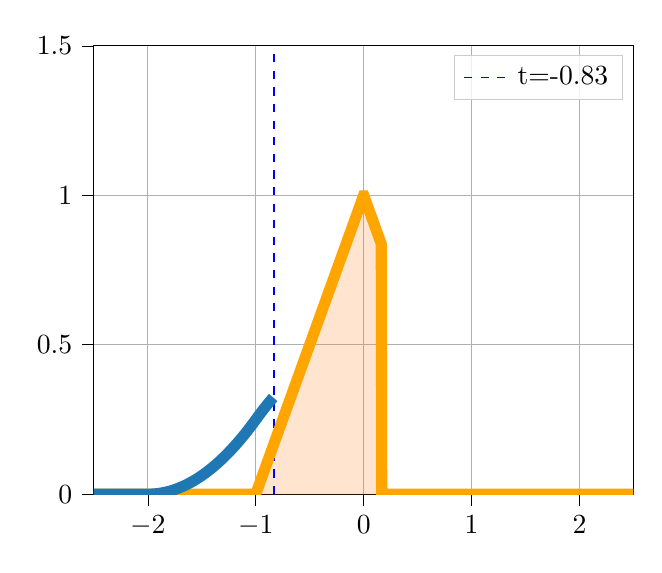
\begin{tikzpicture}

\definecolor{color0}{rgb}{1,0.498039215686275,0.0549019607843137}
\definecolor{color1}{rgb}{1,0.647058823529412,0}
\definecolor{color2}{rgb}{0.12156862745098,0.466666666666667,0.705882352941177}

\begin{axis}[
legend cell align={left},
legend style={fill opacity=0.8, draw opacity=1, text opacity=1, draw=white!80!black},
tick align=outside,
tick pos=left,
x grid style={white!69.0196078431373!black},
xmajorgrids,
xmin=-2.5, xmax=2.5,
xtick style={color=black},
y grid style={white!69.0196078431373!black},
ymajorgrids,
ymin=0, ymax=1.5,
ytick style={color=black}
]
\path [draw=color0, fill=color0, opacity=0.2]
(axis cs:-2.5,0)
--(axis cs:-2.5,0)
--(axis cs:-2.49499499499499,0)
--(axis cs:-2.48998998998999,0)
--(axis cs:-2.48498498498498,0)
--(axis cs:-2.47997997997998,0)
--(axis cs:-2.47497497497497,0)
--(axis cs:-2.46996996996997,0)
--(axis cs:-2.46496496496496,0)
--(axis cs:-2.45995995995996,0)
--(axis cs:-2.45495495495495,0)
--(axis cs:-2.44994994994995,0)
--(axis cs:-2.44494494494494,0)
--(axis cs:-2.43993993993994,0)
--(axis cs:-2.43493493493493,0)
--(axis cs:-2.42992992992993,0)
--(axis cs:-2.42492492492492,0)
--(axis cs:-2.41991991991992,0)
--(axis cs:-2.41491491491491,0)
--(axis cs:-2.40990990990991,0)
--(axis cs:-2.4049049049049,0)
--(axis cs:-2.3998998998999,0)
--(axis cs:-2.39489489489489,0)
--(axis cs:-2.38988988988989,0)
--(axis cs:-2.38488488488488,0)
--(axis cs:-2.37987987987988,0)
--(axis cs:-2.37487487487487,0)
--(axis cs:-2.36986986986987,0)
--(axis cs:-2.36486486486486,0)
--(axis cs:-2.35985985985986,0)
--(axis cs:-2.35485485485485,0)
--(axis cs:-2.34984984984985,0)
--(axis cs:-2.34484484484484,0)
--(axis cs:-2.33983983983984,0)
--(axis cs:-2.33483483483483,0)
--(axis cs:-2.32982982982983,0)
--(axis cs:-2.32482482482482,0)
--(axis cs:-2.31981981981982,0)
--(axis cs:-2.31481481481481,0)
--(axis cs:-2.30980980980981,0)
--(axis cs:-2.3048048048048,0)
--(axis cs:-2.2997997997998,0)
--(axis cs:-2.29479479479479,0)
--(axis cs:-2.28978978978979,0)
--(axis cs:-2.28478478478478,0)
--(axis cs:-2.27977977977978,0)
--(axis cs:-2.27477477477477,0)
--(axis cs:-2.26976976976977,0)
--(axis cs:-2.26476476476476,0)
--(axis cs:-2.25975975975976,0)
--(axis cs:-2.25475475475475,0)
--(axis cs:-2.24974974974975,0)
--(axis cs:-2.24474474474474,0)
--(axis cs:-2.23973973973974,0)
--(axis cs:-2.23473473473473,0)
--(axis cs:-2.22972972972973,0)
--(axis cs:-2.22472472472472,0)
--(axis cs:-2.21971971971972,0)
--(axis cs:-2.21471471471471,0)
--(axis cs:-2.20970970970971,0)
--(axis cs:-2.2047047047047,0)
--(axis cs:-2.1996996996997,0)
--(axis cs:-2.19469469469469,0)
--(axis cs:-2.18968968968969,0)
--(axis cs:-2.18468468468468,0)
--(axis cs:-2.17967967967968,0)
--(axis cs:-2.17467467467467,0)
--(axis cs:-2.16966966966967,0)
--(axis cs:-2.16466466466466,0)
--(axis cs:-2.15965965965966,0)
--(axis cs:-2.15465465465465,0)
--(axis cs:-2.14964964964965,0)
--(axis cs:-2.14464464464464,0)
--(axis cs:-2.13963963963964,0)
--(axis cs:-2.13463463463463,0)
--(axis cs:-2.12962962962963,0)
--(axis cs:-2.12462462462462,0)
--(axis cs:-2.11961961961962,0)
--(axis cs:-2.11461461461461,0)
--(axis cs:-2.10960960960961,0)
--(axis cs:-2.1046046046046,0)
--(axis cs:-2.0995995995996,0)
--(axis cs:-2.09459459459459,0)
--(axis cs:-2.08958958958959,0)
--(axis cs:-2.08458458458458,0)
--(axis cs:-2.07957957957958,0)
--(axis cs:-2.07457457457457,0)
--(axis cs:-2.06956956956957,0)
--(axis cs:-2.06456456456456,0)
--(axis cs:-2.05955955955956,0)
--(axis cs:-2.05455455455455,0)
--(axis cs:-2.04954954954955,0)
--(axis cs:-2.04454454454454,0)
--(axis cs:-2.03953953953954,0)
--(axis cs:-2.03453453453453,0)
--(axis cs:-2.02952952952953,0)
--(axis cs:-2.02452452452452,0)
--(axis cs:-2.01951951951952,0)
--(axis cs:-2.01451451451451,0)
--(axis cs:-2.00950950950951,0)
--(axis cs:-2.0045045045045,0)
--(axis cs:-1.9994994994995,0)
--(axis cs:-1.99449449449449,0)
--(axis cs:-1.98948948948949,0)
--(axis cs:-1.98448448448448,0)
--(axis cs:-1.97947947947948,0)
--(axis cs:-1.97447447447447,0)
--(axis cs:-1.96946946946947,0)
--(axis cs:-1.96446446446446,0)
--(axis cs:-1.95945945945946,0)
--(axis cs:-1.95445445445445,0)
--(axis cs:-1.94944944944945,0)
--(axis cs:-1.94444444444444,0)
--(axis cs:-1.93943943943944,0)
--(axis cs:-1.93443443443443,0)
--(axis cs:-1.92942942942943,0)
--(axis cs:-1.92442442442442,0)
--(axis cs:-1.91941941941942,0)
--(axis cs:-1.91441441441441,0)
--(axis cs:-1.90940940940941,0)
--(axis cs:-1.9044044044044,0)
--(axis cs:-1.8993993993994,0)
--(axis cs:-1.89439439439439,0)
--(axis cs:-1.88938938938939,0)
--(axis cs:-1.88438438438438,0)
--(axis cs:-1.87937937937938,0)
--(axis cs:-1.87437437437437,0)
--(axis cs:-1.86936936936937,0)
--(axis cs:-1.86436436436436,0)
--(axis cs:-1.85935935935936,0)
--(axis cs:-1.85435435435435,0)
--(axis cs:-1.84934934934935,0)
--(axis cs:-1.84434434434434,0)
--(axis cs:-1.83933933933934,0)
--(axis cs:-1.83433433433433,0)
--(axis cs:-1.82932932932933,0)
--(axis cs:-1.82432432432432,0)
--(axis cs:-1.81931931931932,0)
--(axis cs:-1.81431431431431,0)
--(axis cs:-1.80930930930931,0)
--(axis cs:-1.8043043043043,0)
--(axis cs:-1.7992992992993,0)
--(axis cs:-1.79429429429429,0)
--(axis cs:-1.78928928928929,0)
--(axis cs:-1.78428428428428,0)
--(axis cs:-1.77927927927928,0)
--(axis cs:-1.77427427427427,0)
--(axis cs:-1.76926926926927,0)
--(axis cs:-1.76426426426426,0)
--(axis cs:-1.75925925925926,0)
--(axis cs:-1.75425425425425,0)
--(axis cs:-1.74924924924925,0)
--(axis cs:-1.74424424424424,0)
--(axis cs:-1.73923923923924,0)
--(axis cs:-1.73423423423423,0)
--(axis cs:-1.72922922922923,0)
--(axis cs:-1.72422422422422,0)
--(axis cs:-1.71921921921922,0)
--(axis cs:-1.71421421421421,0)
--(axis cs:-1.70920920920921,0)
--(axis cs:-1.7042042042042,0)
--(axis cs:-1.6991991991992,0)
--(axis cs:-1.69419419419419,0)
--(axis cs:-1.68918918918919,0)
--(axis cs:-1.68418418418418,0)
--(axis cs:-1.67917917917918,0)
--(axis cs:-1.67417417417417,0)
--(axis cs:-1.66916916916917,0)
--(axis cs:-1.66416416416416,0)
--(axis cs:-1.65915915915916,0)
--(axis cs:-1.65415415415415,0)
--(axis cs:-1.64914914914915,0)
--(axis cs:-1.64414414414414,0)
--(axis cs:-1.63913913913914,0)
--(axis cs:-1.63413413413413,0)
--(axis cs:-1.62912912912913,0)
--(axis cs:-1.62412412412412,0)
--(axis cs:-1.61911911911912,0)
--(axis cs:-1.61411411411411,0)
--(axis cs:-1.60910910910911,0)
--(axis cs:-1.6041041041041,0)
--(axis cs:-1.5990990990991,0)
--(axis cs:-1.59409409409409,0)
--(axis cs:-1.58908908908909,0)
--(axis cs:-1.58408408408408,0)
--(axis cs:-1.57907907907908,0)
--(axis cs:-1.57407407407407,0)
--(axis cs:-1.56906906906907,0)
--(axis cs:-1.56406406406406,0)
--(axis cs:-1.55905905905906,0)
--(axis cs:-1.55405405405405,0)
--(axis cs:-1.54904904904905,0)
--(axis cs:-1.54404404404404,0)
--(axis cs:-1.53903903903904,0)
--(axis cs:-1.53403403403403,0)
--(axis cs:-1.52902902902903,0)
--(axis cs:-1.52402402402402,0)
--(axis cs:-1.51901901901902,0)
--(axis cs:-1.51401401401401,0)
--(axis cs:-1.50900900900901,0)
--(axis cs:-1.504004004004,0)
--(axis cs:-1.498998998999,0)
--(axis cs:-1.49399399399399,0)
--(axis cs:-1.48898898898899,0)
--(axis cs:-1.48398398398398,0)
--(axis cs:-1.47897897897898,0)
--(axis cs:-1.47397397397397,0)
--(axis cs:-1.46896896896897,0)
--(axis cs:-1.46396396396396,0)
--(axis cs:-1.45895895895896,0)
--(axis cs:-1.45395395395395,0)
--(axis cs:-1.44894894894895,0)
--(axis cs:-1.44394394394394,0)
--(axis cs:-1.43893893893894,0)
--(axis cs:-1.43393393393393,0)
--(axis cs:-1.42892892892893,0)
--(axis cs:-1.42392392392392,0)
--(axis cs:-1.41891891891892,0)
--(axis cs:-1.41391391391391,0)
--(axis cs:-1.40890890890891,0)
--(axis cs:-1.4039039039039,0)
--(axis cs:-1.3988988988989,0)
--(axis cs:-1.39389389389389,0)
--(axis cs:-1.38888888888889,0)
--(axis cs:-1.38388388388388,0)
--(axis cs:-1.37887887887888,0)
--(axis cs:-1.37387387387387,0)
--(axis cs:-1.36886886886887,0)
--(axis cs:-1.36386386386386,0)
--(axis cs:-1.35885885885886,0)
--(axis cs:-1.35385385385385,0)
--(axis cs:-1.34884884884885,0)
--(axis cs:-1.34384384384384,0)
--(axis cs:-1.33883883883884,0)
--(axis cs:-1.33383383383383,0)
--(axis cs:-1.32882882882883,0)
--(axis cs:-1.32382382382382,0)
--(axis cs:-1.31881881881882,0)
--(axis cs:-1.31381381381381,0)
--(axis cs:-1.30880880880881,0)
--(axis cs:-1.3038038038038,0)
--(axis cs:-1.2987987987988,0)
--(axis cs:-1.29379379379379,0)
--(axis cs:-1.28878878878879,0)
--(axis cs:-1.28378378378378,0)
--(axis cs:-1.27877877877878,0)
--(axis cs:-1.27377377377377,0)
--(axis cs:-1.26876876876877,0)
--(axis cs:-1.26376376376376,0)
--(axis cs:-1.25875875875876,0)
--(axis cs:-1.25375375375375,0)
--(axis cs:-1.24874874874875,0)
--(axis cs:-1.24374374374374,0)
--(axis cs:-1.23873873873874,0)
--(axis cs:-1.23373373373373,0)
--(axis cs:-1.22872872872873,0)
--(axis cs:-1.22372372372372,0)
--(axis cs:-1.21871871871872,0)
--(axis cs:-1.21371371371371,0)
--(axis cs:-1.20870870870871,0)
--(axis cs:-1.2037037037037,0)
--(axis cs:-1.1986986986987,0)
--(axis cs:-1.19369369369369,0)
--(axis cs:-1.18868868868869,0)
--(axis cs:-1.18368368368368,0)
--(axis cs:-1.17867867867868,0)
--(axis cs:-1.17367367367367,0)
--(axis cs:-1.16866866866867,0)
--(axis cs:-1.16366366366366,0)
--(axis cs:-1.15865865865866,0)
--(axis cs:-1.15365365365365,0)
--(axis cs:-1.14864864864865,0)
--(axis cs:-1.14364364364364,0)
--(axis cs:-1.13863863863864,0)
--(axis cs:-1.13363363363363,0)
--(axis cs:-1.12862862862863,0)
--(axis cs:-1.12362362362362,0)
--(axis cs:-1.11861861861862,0)
--(axis cs:-1.11361361361361,0)
--(axis cs:-1.10860860860861,0)
--(axis cs:-1.1036036036036,0)
--(axis cs:-1.0985985985986,0)
--(axis cs:-1.09359359359359,0)
--(axis cs:-1.08858858858859,0)
--(axis cs:-1.08358358358358,0)
--(axis cs:-1.07857857857858,0)
--(axis cs:-1.07357357357357,0)
--(axis cs:-1.06856856856857,0)
--(axis cs:-1.06356356356356,0)
--(axis cs:-1.05855855855856,0)
--(axis cs:-1.05355355355355,0)
--(axis cs:-1.04854854854855,0)
--(axis cs:-1.04354354354354,0)
--(axis cs:-1.03853853853854,0)
--(axis cs:-1.03353353353353,0)
--(axis cs:-1.02852852852853,0)
--(axis cs:-1.02352352352352,0)
--(axis cs:-1.01851851851852,0)
--(axis cs:-1.01351351351351,0)
--(axis cs:-1.00850850850851,0)
--(axis cs:-1.0035035035035,0)
--(axis cs:-0.998498498498499,0)
--(axis cs:-0.993493493493494,0)
--(axis cs:-0.988488488488489,0)
--(axis cs:-0.983483483483484,0)
--(axis cs:-0.978478478478479,0)
--(axis cs:-0.973473473473474,0)
--(axis cs:-0.968468468468469,0)
--(axis cs:-0.963463463463464,0)
--(axis cs:-0.958458458458459,0)
--(axis cs:-0.953453453453454,0)
--(axis cs:-0.948448448448449,0)
--(axis cs:-0.943443443443444,0)
--(axis cs:-0.938438438438439,0)
--(axis cs:-0.933433433433434,0)
--(axis cs:-0.928428428428429,0)
--(axis cs:-0.923423423423424,0)
--(axis cs:-0.918418418418419,0)
--(axis cs:-0.913413413413414,0)
--(axis cs:-0.908408408408409,0)
--(axis cs:-0.903403403403404,0)
--(axis cs:-0.898398398398399,0)
--(axis cs:-0.893393393393393,0)
--(axis cs:-0.888388388388388,0)
--(axis cs:-0.883383383383383,0)
--(axis cs:-0.878378378378378,0)
--(axis cs:-0.873373373373373,0)
--(axis cs:-0.868368368368368,0)
--(axis cs:-0.863363363363363,0)
--(axis cs:-0.858358358358358,0)
--(axis cs:-0.853353353353353,0)
--(axis cs:-0.848348348348348,0)
--(axis cs:-0.843343343343343,0)
--(axis cs:-0.838338338338338,0)
--(axis cs:-0.833333333333333,0)
--(axis cs:-0.828328328328328,0)
--(axis cs:-0.823323323323323,0)
--(axis cs:-0.818318318318318,0)
--(axis cs:-0.813313313313313,0)
--(axis cs:-0.808308308308308,0)
--(axis cs:-0.803303303303303,0)
--(axis cs:-0.798298298298298,0)
--(axis cs:-0.793293293293293,0)
--(axis cs:-0.788288288288288,0)
--(axis cs:-0.783283283283283,0)
--(axis cs:-0.778278278278278,0)
--(axis cs:-0.773273273273273,0)
--(axis cs:-0.768268268268268,0)
--(axis cs:-0.763263263263263,0)
--(axis cs:-0.758258258258258,0)
--(axis cs:-0.753253253253253,0)
--(axis cs:-0.748248248248248,0)
--(axis cs:-0.743243243243243,0)
--(axis cs:-0.738238238238238,0)
--(axis cs:-0.733233233233233,0)
--(axis cs:-0.728228228228228,0)
--(axis cs:-0.723223223223223,0)
--(axis cs:-0.718218218218218,0)
--(axis cs:-0.713213213213213,0)
--(axis cs:-0.708208208208208,0)
--(axis cs:-0.703203203203203,0)
--(axis cs:-0.698198198198198,0)
--(axis cs:-0.693193193193193,0)
--(axis cs:-0.688188188188188,0)
--(axis cs:-0.683183183183183,0)
--(axis cs:-0.678178178178178,0)
--(axis cs:-0.673173173173173,0)
--(axis cs:-0.668168168168168,0)
--(axis cs:-0.663163163163163,0)
--(axis cs:-0.658158158158158,0)
--(axis cs:-0.653153153153153,0)
--(axis cs:-0.648148148148148,0)
--(axis cs:-0.643143143143143,0)
--(axis cs:-0.638138138138138,0)
--(axis cs:-0.633133133133133,0)
--(axis cs:-0.628128128128128,0)
--(axis cs:-0.623123123123123,0)
--(axis cs:-0.618118118118118,0)
--(axis cs:-0.613113113113113,0)
--(axis cs:-0.608108108108108,0)
--(axis cs:-0.603103103103103,0)
--(axis cs:-0.598098098098098,0)
--(axis cs:-0.593093093093093,0)
--(axis cs:-0.588088088088088,0)
--(axis cs:-0.583083083083083,0)
--(axis cs:-0.578078078078078,0)
--(axis cs:-0.573073073073073,0)
--(axis cs:-0.568068068068068,0)
--(axis cs:-0.563063063063063,0)
--(axis cs:-0.558058058058058,0)
--(axis cs:-0.553053053053053,0)
--(axis cs:-0.548048048048048,0)
--(axis cs:-0.543043043043043,0)
--(axis cs:-0.538038038038038,0)
--(axis cs:-0.533033033033033,0)
--(axis cs:-0.528028028028028,0)
--(axis cs:-0.523023023023023,0)
--(axis cs:-0.518018018018018,0)
--(axis cs:-0.513013013013013,0)
--(axis cs:-0.508008008008008,0)
--(axis cs:-0.503003003003003,0)
--(axis cs:-0.497997997997998,0)
--(axis cs:-0.492992992992993,0)
--(axis cs:-0.487987987987988,0)
--(axis cs:-0.482982982982983,0)
--(axis cs:-0.477977977977978,0)
--(axis cs:-0.472972972972973,0)
--(axis cs:-0.467967967967968,0)
--(axis cs:-0.462962962962963,0)
--(axis cs:-0.457957957957958,0)
--(axis cs:-0.452952952952953,0)
--(axis cs:-0.447947947947948,0)
--(axis cs:-0.442942942942943,0)
--(axis cs:-0.437937937937938,0)
--(axis cs:-0.432932932932933,0)
--(axis cs:-0.427927927927928,0)
--(axis cs:-0.422922922922923,0)
--(axis cs:-0.417917917917918,0)
--(axis cs:-0.412912912912913,0)
--(axis cs:-0.407907907907908,0)
--(axis cs:-0.402902902902903,0)
--(axis cs:-0.397897897897898,0)
--(axis cs:-0.392892892892893,0)
--(axis cs:-0.387887887887888,0)
--(axis cs:-0.382882882882883,0)
--(axis cs:-0.377877877877878,0)
--(axis cs:-0.372872872872873,0)
--(axis cs:-0.367867867867868,0)
--(axis cs:-0.362862862862863,0)
--(axis cs:-0.357857857857858,0)
--(axis cs:-0.352852852852853,0)
--(axis cs:-0.347847847847848,0)
--(axis cs:-0.342842842842843,0)
--(axis cs:-0.337837837837838,0)
--(axis cs:-0.332832832832833,0)
--(axis cs:-0.327827827827828,0)
--(axis cs:-0.322822822822823,0)
--(axis cs:-0.317817817817818,0)
--(axis cs:-0.312812812812813,0)
--(axis cs:-0.307807807807808,0)
--(axis cs:-0.302802802802803,0)
--(axis cs:-0.297797797797798,0)
--(axis cs:-0.292792792792793,0)
--(axis cs:-0.287787787787788,0)
--(axis cs:-0.282782782782783,0)
--(axis cs:-0.277777777777778,0)
--(axis cs:-0.272772772772773,0)
--(axis cs:-0.267767767767768,0)
--(axis cs:-0.262762762762763,0)
--(axis cs:-0.257757757757758,0)
--(axis cs:-0.252752752752753,0)
--(axis cs:-0.247747747747748,0)
--(axis cs:-0.242742742742743,0)
--(axis cs:-0.237737737737738,0)
--(axis cs:-0.232732732732733,0)
--(axis cs:-0.227727727727728,0)
--(axis cs:-0.222722722722723,0)
--(axis cs:-0.217717717717718,0)
--(axis cs:-0.212712712712713,0)
--(axis cs:-0.207707707707708,0)
--(axis cs:-0.202702702702703,0)
--(axis cs:-0.197697697697698,0)
--(axis cs:-0.192692692692693,0)
--(axis cs:-0.187687687687688,0)
--(axis cs:-0.182682682682683,0)
--(axis cs:-0.177677677677678,0)
--(axis cs:-0.172672672672673,0)
--(axis cs:-0.167667667667668,0)
--(axis cs:-0.162662662662663,0)
--(axis cs:-0.157657657657658,0)
--(axis cs:-0.152652652652653,0)
--(axis cs:-0.147647647647648,0)
--(axis cs:-0.142642642642643,0)
--(axis cs:-0.137637637637638,0)
--(axis cs:-0.132632632632633,0)
--(axis cs:-0.127627627627628,0)
--(axis cs:-0.122622622622623,0)
--(axis cs:-0.117617617617618,0)
--(axis cs:-0.112612612612613,0)
--(axis cs:-0.107607607607608,0)
--(axis cs:-0.102602602602603,0)
--(axis cs:-0.0975975975975976,0)
--(axis cs:-0.0925925925925926,0)
--(axis cs:-0.0875875875875876,0)
--(axis cs:-0.0825825825825826,0)
--(axis cs:-0.0775775775775776,0)
--(axis cs:-0.0725725725725725,0)
--(axis cs:-0.0675675675675675,0)
--(axis cs:-0.0625625625625625,0)
--(axis cs:-0.0575575575575575,0)
--(axis cs:-0.0525525525525525,0)
--(axis cs:-0.0475475475475475,0)
--(axis cs:-0.0425425425425425,0)
--(axis cs:-0.0375375375375375,0)
--(axis cs:-0.0325325325325325,0)
--(axis cs:-0.0275275275275275,0)
--(axis cs:-0.0225225225225225,0)
--(axis cs:-0.0175175175175175,0)
--(axis cs:-0.0125125125125125,0)
--(axis cs:-0.0075075075075075,0)
--(axis cs:-0.0025025025025025,0)
--(axis cs:0.0025025025025025,0)
--(axis cs:0.0075075075075075,0)
--(axis cs:0.0125125125125125,0)
--(axis cs:0.0175175175175175,0)
--(axis cs:0.0225225225225225,0)
--(axis cs:0.0275275275275275,0)
--(axis cs:0.0325325325325325,0)
--(axis cs:0.0375375375375375,0)
--(axis cs:0.0425425425425425,0)
--(axis cs:0.0475475475475475,0)
--(axis cs:0.0525525525525525,0)
--(axis cs:0.0575575575575575,0)
--(axis cs:0.0625625625625625,0)
--(axis cs:0.0675675675675675,0)
--(axis cs:0.0725725725725725,0)
--(axis cs:0.0775775775775776,0)
--(axis cs:0.0825825825825826,0)
--(axis cs:0.0875875875875876,0)
--(axis cs:0.0925925925925926,0)
--(axis cs:0.0975975975975976,0)
--(axis cs:0.102602602602603,0)
--(axis cs:0.107607607607608,0)
--(axis cs:0.112612612612613,0)
--(axis cs:0.117617617617618,0)
--(axis cs:0.122622622622623,0)
--(axis cs:0.127627627627628,0)
--(axis cs:0.132632632632633,0)
--(axis cs:0.137637637637638,0)
--(axis cs:0.142642642642643,0)
--(axis cs:0.147647647647648,0)
--(axis cs:0.152652652652653,0)
--(axis cs:0.157657657657658,0)
--(axis cs:0.162662662662663,0)
--(axis cs:0.167667667667668,0)
--(axis cs:0.172672672672673,0)
--(axis cs:0.177677677677678,0)
--(axis cs:0.182682682682683,0)
--(axis cs:0.187687687687688,0)
--(axis cs:0.192692692692693,0)
--(axis cs:0.197697697697698,0)
--(axis cs:0.202702702702703,0)
--(axis cs:0.207707707707708,0)
--(axis cs:0.212712712712713,0)
--(axis cs:0.217717717717718,0)
--(axis cs:0.222722722722723,0)
--(axis cs:0.227727727727728,0)
--(axis cs:0.232732732732733,0)
--(axis cs:0.237737737737738,0)
--(axis cs:0.242742742742743,0)
--(axis cs:0.247747747747748,0)
--(axis cs:0.252752752752753,0)
--(axis cs:0.257757757757758,0)
--(axis cs:0.262762762762763,0)
--(axis cs:0.267767767767768,0)
--(axis cs:0.272772772772773,0)
--(axis cs:0.277777777777778,0)
--(axis cs:0.282782782782783,0)
--(axis cs:0.287787787787788,0)
--(axis cs:0.292792792792793,0)
--(axis cs:0.297797797797798,0)
--(axis cs:0.302802802802803,0)
--(axis cs:0.307807807807808,0)
--(axis cs:0.312812812812813,0)
--(axis cs:0.317817817817818,0)
--(axis cs:0.322822822822823,0)
--(axis cs:0.327827827827828,0)
--(axis cs:0.332832832832833,0)
--(axis cs:0.337837837837838,0)
--(axis cs:0.342842842842843,0)
--(axis cs:0.347847847847848,0)
--(axis cs:0.352852852852853,0)
--(axis cs:0.357857857857858,0)
--(axis cs:0.362862862862863,0)
--(axis cs:0.367867867867868,0)
--(axis cs:0.372872872872873,0)
--(axis cs:0.377877877877878,0)
--(axis cs:0.382882882882883,0)
--(axis cs:0.387887887887888,0)
--(axis cs:0.392892892892893,0)
--(axis cs:0.397897897897898,0)
--(axis cs:0.402902902902903,0)
--(axis cs:0.407907907907908,0)
--(axis cs:0.412912912912913,0)
--(axis cs:0.417917917917918,0)
--(axis cs:0.422922922922923,0)
--(axis cs:0.427927927927928,0)
--(axis cs:0.432932932932933,0)
--(axis cs:0.437937937937938,0)
--(axis cs:0.442942942942943,0)
--(axis cs:0.447947947947948,0)
--(axis cs:0.452952952952953,0)
--(axis cs:0.457957957957958,0)
--(axis cs:0.462962962962963,0)
--(axis cs:0.467967967967968,0)
--(axis cs:0.472972972972973,0)
--(axis cs:0.477977977977978,0)
--(axis cs:0.482982982982983,0)
--(axis cs:0.487987987987988,0)
--(axis cs:0.492992992992993,0)
--(axis cs:0.497997997997998,0)
--(axis cs:0.503003003003003,0)
--(axis cs:0.508008008008008,0)
--(axis cs:0.513013013013013,0)
--(axis cs:0.518018018018018,0)
--(axis cs:0.523023023023023,0)
--(axis cs:0.528028028028028,0)
--(axis cs:0.533033033033033,0)
--(axis cs:0.538038038038038,0)
--(axis cs:0.543043043043043,0)
--(axis cs:0.548048048048048,0)
--(axis cs:0.553053053053053,0)
--(axis cs:0.558058058058058,0)
--(axis cs:0.563063063063063,0)
--(axis cs:0.568068068068068,0)
--(axis cs:0.573073073073073,0)
--(axis cs:0.578078078078078,0)
--(axis cs:0.583083083083083,0)
--(axis cs:0.588088088088088,0)
--(axis cs:0.593093093093093,0)
--(axis cs:0.598098098098098,0)
--(axis cs:0.603103103103103,0)
--(axis cs:0.608108108108108,0)
--(axis cs:0.613113113113113,0)
--(axis cs:0.618118118118118,0)
--(axis cs:0.623123123123123,0)
--(axis cs:0.628128128128128,0)
--(axis cs:0.633133133133133,0)
--(axis cs:0.638138138138138,0)
--(axis cs:0.643143143143143,0)
--(axis cs:0.648148148148148,0)
--(axis cs:0.653153153153153,0)
--(axis cs:0.658158158158158,0)
--(axis cs:0.663163163163163,0)
--(axis cs:0.668168168168168,0)
--(axis cs:0.673173173173173,0)
--(axis cs:0.678178178178178,0)
--(axis cs:0.683183183183183,0)
--(axis cs:0.688188188188188,0)
--(axis cs:0.693193193193193,0)
--(axis cs:0.698198198198198,0)
--(axis cs:0.703203203203203,0)
--(axis cs:0.708208208208208,0)
--(axis cs:0.713213213213213,0)
--(axis cs:0.718218218218218,0)
--(axis cs:0.723223223223223,0)
--(axis cs:0.728228228228228,0)
--(axis cs:0.733233233233233,0)
--(axis cs:0.738238238238238,0)
--(axis cs:0.743243243243243,0)
--(axis cs:0.748248248248248,0)
--(axis cs:0.753253253253253,0)
--(axis cs:0.758258258258258,0)
--(axis cs:0.763263263263263,0)
--(axis cs:0.768268268268268,0)
--(axis cs:0.773273273273273,0)
--(axis cs:0.778278278278278,0)
--(axis cs:0.783283283283283,0)
--(axis cs:0.788288288288288,0)
--(axis cs:0.793293293293293,0)
--(axis cs:0.798298298298298,0)
--(axis cs:0.803303303303303,0)
--(axis cs:0.808308308308308,0)
--(axis cs:0.813313313313313,0)
--(axis cs:0.818318318318318,0)
--(axis cs:0.823323323323323,0)
--(axis cs:0.828328328328328,0)
--(axis cs:0.833333333333333,0)
--(axis cs:0.838338338338338,0)
--(axis cs:0.843343343343343,0)
--(axis cs:0.848348348348348,0)
--(axis cs:0.853353353353353,0)
--(axis cs:0.858358358358358,0)
--(axis cs:0.863363363363364,0)
--(axis cs:0.868368368368369,0)
--(axis cs:0.873373373373374,0)
--(axis cs:0.878378378378379,0)
--(axis cs:0.883383383383384,0)
--(axis cs:0.888388388388389,0)
--(axis cs:0.893393393393394,0)
--(axis cs:0.898398398398399,0)
--(axis cs:0.903403403403404,0)
--(axis cs:0.908408408408409,0)
--(axis cs:0.913413413413414,0)
--(axis cs:0.918418418418419,0)
--(axis cs:0.923423423423424,0)
--(axis cs:0.928428428428429,0)
--(axis cs:0.933433433433434,0)
--(axis cs:0.938438438438439,0)
--(axis cs:0.943443443443444,0)
--(axis cs:0.948448448448449,0)
--(axis cs:0.953453453453454,0)
--(axis cs:0.958458458458459,0)
--(axis cs:0.963463463463464,0)
--(axis cs:0.968468468468469,0)
--(axis cs:0.973473473473474,0)
--(axis cs:0.978478478478479,0)
--(axis cs:0.983483483483484,0)
--(axis cs:0.988488488488489,0)
--(axis cs:0.993493493493494,0)
--(axis cs:0.998498498498499,0)
--(axis cs:1.0035035035035,0)
--(axis cs:1.00850850850851,0)
--(axis cs:1.01351351351351,0)
--(axis cs:1.01851851851852,0)
--(axis cs:1.02352352352352,0)
--(axis cs:1.02852852852853,0)
--(axis cs:1.03353353353353,0)
--(axis cs:1.03853853853854,0)
--(axis cs:1.04354354354354,0)
--(axis cs:1.04854854854855,0)
--(axis cs:1.05355355355355,0)
--(axis cs:1.05855855855856,0)
--(axis cs:1.06356356356356,0)
--(axis cs:1.06856856856857,0)
--(axis cs:1.07357357357357,0)
--(axis cs:1.07857857857858,0)
--(axis cs:1.08358358358358,0)
--(axis cs:1.08858858858859,0)
--(axis cs:1.09359359359359,0)
--(axis cs:1.0985985985986,0)
--(axis cs:1.1036036036036,0)
--(axis cs:1.10860860860861,0)
--(axis cs:1.11361361361361,0)
--(axis cs:1.11861861861862,0)
--(axis cs:1.12362362362362,0)
--(axis cs:1.12862862862863,0)
--(axis cs:1.13363363363363,0)
--(axis cs:1.13863863863864,0)
--(axis cs:1.14364364364364,0)
--(axis cs:1.14864864864865,0)
--(axis cs:1.15365365365365,0)
--(axis cs:1.15865865865866,0)
--(axis cs:1.16366366366366,0)
--(axis cs:1.16866866866867,0)
--(axis cs:1.17367367367367,0)
--(axis cs:1.17867867867868,0)
--(axis cs:1.18368368368368,0)
--(axis cs:1.18868868868869,0)
--(axis cs:1.19369369369369,0)
--(axis cs:1.1986986986987,0)
--(axis cs:1.2037037037037,0)
--(axis cs:1.20870870870871,0)
--(axis cs:1.21371371371371,0)
--(axis cs:1.21871871871872,0)
--(axis cs:1.22372372372372,0)
--(axis cs:1.22872872872873,0)
--(axis cs:1.23373373373373,0)
--(axis cs:1.23873873873874,0)
--(axis cs:1.24374374374374,0)
--(axis cs:1.24874874874875,0)
--(axis cs:1.25375375375375,0)
--(axis cs:1.25875875875876,0)
--(axis cs:1.26376376376376,0)
--(axis cs:1.26876876876877,0)
--(axis cs:1.27377377377377,0)
--(axis cs:1.27877877877878,0)
--(axis cs:1.28378378378378,0)
--(axis cs:1.28878878878879,0)
--(axis cs:1.29379379379379,0)
--(axis cs:1.2987987987988,0)
--(axis cs:1.3038038038038,0)
--(axis cs:1.30880880880881,0)
--(axis cs:1.31381381381381,0)
--(axis cs:1.31881881881882,0)
--(axis cs:1.32382382382382,0)
--(axis cs:1.32882882882883,0)
--(axis cs:1.33383383383383,0)
--(axis cs:1.33883883883884,0)
--(axis cs:1.34384384384384,0)
--(axis cs:1.34884884884885,0)
--(axis cs:1.35385385385385,0)
--(axis cs:1.35885885885886,0)
--(axis cs:1.36386386386386,0)
--(axis cs:1.36886886886887,0)
--(axis cs:1.37387387387387,0)
--(axis cs:1.37887887887888,0)
--(axis cs:1.38388388388388,0)
--(axis cs:1.38888888888889,0)
--(axis cs:1.39389389389389,0)
--(axis cs:1.3988988988989,0)
--(axis cs:1.4039039039039,0)
--(axis cs:1.40890890890891,0)
--(axis cs:1.41391391391391,0)
--(axis cs:1.41891891891892,0)
--(axis cs:1.42392392392392,0)
--(axis cs:1.42892892892893,0)
--(axis cs:1.43393393393393,0)
--(axis cs:1.43893893893894,0)
--(axis cs:1.44394394394394,0)
--(axis cs:1.44894894894895,0)
--(axis cs:1.45395395395395,0)
--(axis cs:1.45895895895896,0)
--(axis cs:1.46396396396396,0)
--(axis cs:1.46896896896897,0)
--(axis cs:1.47397397397397,0)
--(axis cs:1.47897897897898,0)
--(axis cs:1.48398398398398,0)
--(axis cs:1.48898898898899,0)
--(axis cs:1.49399399399399,0)
--(axis cs:1.498998998999,0)
--(axis cs:1.504004004004,0)
--(axis cs:1.50900900900901,0)
--(axis cs:1.51401401401401,0)
--(axis cs:1.51901901901902,0)
--(axis cs:1.52402402402402,0)
--(axis cs:1.52902902902903,0)
--(axis cs:1.53403403403403,0)
--(axis cs:1.53903903903904,0)
--(axis cs:1.54404404404404,0)
--(axis cs:1.54904904904905,0)
--(axis cs:1.55405405405405,0)
--(axis cs:1.55905905905906,0)
--(axis cs:1.56406406406406,0)
--(axis cs:1.56906906906907,0)
--(axis cs:1.57407407407407,0)
--(axis cs:1.57907907907908,0)
--(axis cs:1.58408408408408,0)
--(axis cs:1.58908908908909,0)
--(axis cs:1.59409409409409,0)
--(axis cs:1.5990990990991,0)
--(axis cs:1.6041041041041,0)
--(axis cs:1.60910910910911,0)
--(axis cs:1.61411411411411,0)
--(axis cs:1.61911911911912,0)
--(axis cs:1.62412412412412,0)
--(axis cs:1.62912912912913,0)
--(axis cs:1.63413413413413,0)
--(axis cs:1.63913913913914,0)
--(axis cs:1.64414414414414,0)
--(axis cs:1.64914914914915,0)
--(axis cs:1.65415415415415,0)
--(axis cs:1.65915915915916,0)
--(axis cs:1.66416416416416,0)
--(axis cs:1.66916916916917,0)
--(axis cs:1.67417417417417,0)
--(axis cs:1.67917917917918,0)
--(axis cs:1.68418418418418,0)
--(axis cs:1.68918918918919,0)
--(axis cs:1.69419419419419,0)
--(axis cs:1.6991991991992,0)
--(axis cs:1.7042042042042,0)
--(axis cs:1.70920920920921,0)
--(axis cs:1.71421421421421,0)
--(axis cs:1.71921921921922,0)
--(axis cs:1.72422422422422,0)
--(axis cs:1.72922922922923,0)
--(axis cs:1.73423423423423,0)
--(axis cs:1.73923923923924,0)
--(axis cs:1.74424424424424,0)
--(axis cs:1.74924924924925,0)
--(axis cs:1.75425425425425,0)
--(axis cs:1.75925925925926,0)
--(axis cs:1.76426426426426,0)
--(axis cs:1.76926926926927,0)
--(axis cs:1.77427427427427,0)
--(axis cs:1.77927927927928,0)
--(axis cs:1.78428428428428,0)
--(axis cs:1.78928928928929,0)
--(axis cs:1.79429429429429,0)
--(axis cs:1.7992992992993,0)
--(axis cs:1.8043043043043,0)
--(axis cs:1.80930930930931,0)
--(axis cs:1.81431431431431,0)
--(axis cs:1.81931931931932,0)
--(axis cs:1.82432432432432,0)
--(axis cs:1.82932932932933,0)
--(axis cs:1.83433433433433,0)
--(axis cs:1.83933933933934,0)
--(axis cs:1.84434434434434,0)
--(axis cs:1.84934934934935,0)
--(axis cs:1.85435435435435,0)
--(axis cs:1.85935935935936,0)
--(axis cs:1.86436436436436,0)
--(axis cs:1.86936936936937,0)
--(axis cs:1.87437437437437,0)
--(axis cs:1.87937937937938,0)
--(axis cs:1.88438438438438,0)
--(axis cs:1.88938938938939,0)
--(axis cs:1.89439439439439,0)
--(axis cs:1.8993993993994,0)
--(axis cs:1.9044044044044,0)
--(axis cs:1.90940940940941,0)
--(axis cs:1.91441441441441,0)
--(axis cs:1.91941941941942,0)
--(axis cs:1.92442442442442,0)
--(axis cs:1.92942942942943,0)
--(axis cs:1.93443443443443,0)
--(axis cs:1.93943943943944,0)
--(axis cs:1.94444444444444,0)
--(axis cs:1.94944944944945,0)
--(axis cs:1.95445445445445,0)
--(axis cs:1.95945945945946,0)
--(axis cs:1.96446446446446,0)
--(axis cs:1.96946946946947,0)
--(axis cs:1.97447447447447,0)
--(axis cs:1.97947947947948,0)
--(axis cs:1.98448448448448,0)
--(axis cs:1.98948948948949,0)
--(axis cs:1.99449449449449,0)
--(axis cs:1.9994994994995,0)
--(axis cs:2.0045045045045,0)
--(axis cs:2.00950950950951,0)
--(axis cs:2.01451451451451,0)
--(axis cs:2.01951951951952,0)
--(axis cs:2.02452452452452,0)
--(axis cs:2.02952952952953,0)
--(axis cs:2.03453453453453,0)
--(axis cs:2.03953953953954,0)
--(axis cs:2.04454454454454,0)
--(axis cs:2.04954954954955,0)
--(axis cs:2.05455455455455,0)
--(axis cs:2.05955955955956,0)
--(axis cs:2.06456456456456,0)
--(axis cs:2.06956956956957,0)
--(axis cs:2.07457457457457,0)
--(axis cs:2.07957957957958,0)
--(axis cs:2.08458458458458,0)
--(axis cs:2.08958958958959,0)
--(axis cs:2.09459459459459,0)
--(axis cs:2.0995995995996,0)
--(axis cs:2.1046046046046,0)
--(axis cs:2.10960960960961,0)
--(axis cs:2.11461461461461,0)
--(axis cs:2.11961961961962,0)
--(axis cs:2.12462462462462,0)
--(axis cs:2.12962962962963,0)
--(axis cs:2.13463463463463,0)
--(axis cs:2.13963963963964,0)
--(axis cs:2.14464464464464,0)
--(axis cs:2.14964964964965,0)
--(axis cs:2.15465465465465,0)
--(axis cs:2.15965965965966,0)
--(axis cs:2.16466466466466,0)
--(axis cs:2.16966966966967,0)
--(axis cs:2.17467467467467,0)
--(axis cs:2.17967967967968,0)
--(axis cs:2.18468468468468,0)
--(axis cs:2.18968968968969,0)
--(axis cs:2.19469469469469,0)
--(axis cs:2.1996996996997,0)
--(axis cs:2.2047047047047,0)
--(axis cs:2.20970970970971,0)
--(axis cs:2.21471471471471,0)
--(axis cs:2.21971971971972,0)
--(axis cs:2.22472472472472,0)
--(axis cs:2.22972972972973,0)
--(axis cs:2.23473473473473,0)
--(axis cs:2.23973973973974,0)
--(axis cs:2.24474474474474,0)
--(axis cs:2.24974974974975,0)
--(axis cs:2.25475475475475,0)
--(axis cs:2.25975975975976,0)
--(axis cs:2.26476476476476,0)
--(axis cs:2.26976976976977,0)
--(axis cs:2.27477477477477,0)
--(axis cs:2.27977977977978,0)
--(axis cs:2.28478478478478,0)
--(axis cs:2.28978978978979,0)
--(axis cs:2.29479479479479,0)
--(axis cs:2.2997997997998,0)
--(axis cs:2.3048048048048,0)
--(axis cs:2.30980980980981,0)
--(axis cs:2.31481481481481,0)
--(axis cs:2.31981981981982,0)
--(axis cs:2.32482482482482,0)
--(axis cs:2.32982982982983,0)
--(axis cs:2.33483483483483,0)
--(axis cs:2.33983983983984,0)
--(axis cs:2.34484484484484,0)
--(axis cs:2.34984984984985,0)
--(axis cs:2.35485485485485,0)
--(axis cs:2.35985985985986,0)
--(axis cs:2.36486486486486,0)
--(axis cs:2.36986986986987,0)
--(axis cs:2.37487487487487,0)
--(axis cs:2.37987987987988,0)
--(axis cs:2.38488488488488,0)
--(axis cs:2.38988988988989,0)
--(axis cs:2.39489489489489,0)
--(axis cs:2.3998998998999,0)
--(axis cs:2.4049049049049,0)
--(axis cs:2.40990990990991,0)
--(axis cs:2.41491491491491,0)
--(axis cs:2.41991991991992,0)
--(axis cs:2.42492492492492,0)
--(axis cs:2.42992992992993,0)
--(axis cs:2.43493493493493,0)
--(axis cs:2.43993993993994,0)
--(axis cs:2.44494494494494,0)
--(axis cs:2.44994994994995,0)
--(axis cs:2.45495495495495,0)
--(axis cs:2.45995995995996,0)
--(axis cs:2.46496496496496,0)
--(axis cs:2.46996996996997,0)
--(axis cs:2.47497497497497,0)
--(axis cs:2.47997997997998,0)
--(axis cs:2.48498498498498,0)
--(axis cs:2.48998998998999,0)
--(axis cs:2.49499499499499,0)
--(axis cs:2.5,0)
--(axis cs:2.5,0)
--(axis cs:2.5,0)
--(axis cs:2.49499499499499,0)
--(axis cs:2.48998998998999,0)
--(axis cs:2.48498498498498,0)
--(axis cs:2.47997997997998,0)
--(axis cs:2.47497497497497,0)
--(axis cs:2.46996996996997,0)
--(axis cs:2.46496496496496,0)
--(axis cs:2.45995995995996,0)
--(axis cs:2.45495495495495,0)
--(axis cs:2.44994994994995,0)
--(axis cs:2.44494494494494,0)
--(axis cs:2.43993993993994,0)
--(axis cs:2.43493493493493,0)
--(axis cs:2.42992992992993,0)
--(axis cs:2.42492492492492,0)
--(axis cs:2.41991991991992,0)
--(axis cs:2.41491491491491,0)
--(axis cs:2.40990990990991,0)
--(axis cs:2.4049049049049,0)
--(axis cs:2.3998998998999,0)
--(axis cs:2.39489489489489,0)
--(axis cs:2.38988988988989,0)
--(axis cs:2.38488488488488,0)
--(axis cs:2.37987987987988,0)
--(axis cs:2.37487487487487,0)
--(axis cs:2.36986986986987,0)
--(axis cs:2.36486486486486,0)
--(axis cs:2.35985985985986,0)
--(axis cs:2.35485485485485,0)
--(axis cs:2.34984984984985,0)
--(axis cs:2.34484484484484,0)
--(axis cs:2.33983983983984,0)
--(axis cs:2.33483483483483,0)
--(axis cs:2.32982982982983,0)
--(axis cs:2.32482482482482,0)
--(axis cs:2.31981981981982,0)
--(axis cs:2.31481481481481,0)
--(axis cs:2.30980980980981,0)
--(axis cs:2.3048048048048,0)
--(axis cs:2.2997997997998,0)
--(axis cs:2.29479479479479,0)
--(axis cs:2.28978978978979,0)
--(axis cs:2.28478478478478,0)
--(axis cs:2.27977977977978,0)
--(axis cs:2.27477477477477,0)
--(axis cs:2.26976976976977,0)
--(axis cs:2.26476476476476,0)
--(axis cs:2.25975975975976,0)
--(axis cs:2.25475475475475,0)
--(axis cs:2.24974974974975,0)
--(axis cs:2.24474474474474,0)
--(axis cs:2.23973973973974,0)
--(axis cs:2.23473473473473,0)
--(axis cs:2.22972972972973,0)
--(axis cs:2.22472472472472,0)
--(axis cs:2.21971971971972,0)
--(axis cs:2.21471471471471,0)
--(axis cs:2.20970970970971,0)
--(axis cs:2.2047047047047,0)
--(axis cs:2.1996996996997,0)
--(axis cs:2.19469469469469,0)
--(axis cs:2.18968968968969,0)
--(axis cs:2.18468468468468,0)
--(axis cs:2.17967967967968,0)
--(axis cs:2.17467467467467,0)
--(axis cs:2.16966966966967,0)
--(axis cs:2.16466466466466,0)
--(axis cs:2.15965965965966,0)
--(axis cs:2.15465465465465,0)
--(axis cs:2.14964964964965,0)
--(axis cs:2.14464464464464,0)
--(axis cs:2.13963963963964,0)
--(axis cs:2.13463463463463,0)
--(axis cs:2.12962962962963,0)
--(axis cs:2.12462462462462,0)
--(axis cs:2.11961961961962,0)
--(axis cs:2.11461461461461,0)
--(axis cs:2.10960960960961,0)
--(axis cs:2.1046046046046,0)
--(axis cs:2.0995995995996,0)
--(axis cs:2.09459459459459,0)
--(axis cs:2.08958958958959,0)
--(axis cs:2.08458458458458,0)
--(axis cs:2.07957957957958,0)
--(axis cs:2.07457457457457,0)
--(axis cs:2.06956956956957,0)
--(axis cs:2.06456456456456,0)
--(axis cs:2.05955955955956,0)
--(axis cs:2.05455455455455,0)
--(axis cs:2.04954954954955,0)
--(axis cs:2.04454454454454,0)
--(axis cs:2.03953953953954,0)
--(axis cs:2.03453453453453,0)
--(axis cs:2.02952952952953,0)
--(axis cs:2.02452452452452,0)
--(axis cs:2.01951951951952,0)
--(axis cs:2.01451451451451,0)
--(axis cs:2.00950950950951,0)
--(axis cs:2.0045045045045,0)
--(axis cs:1.9994994994995,0)
--(axis cs:1.99449449449449,0)
--(axis cs:1.98948948948949,0)
--(axis cs:1.98448448448448,0)
--(axis cs:1.97947947947948,0)
--(axis cs:1.97447447447447,0)
--(axis cs:1.96946946946947,0)
--(axis cs:1.96446446446446,0)
--(axis cs:1.95945945945946,0)
--(axis cs:1.95445445445445,0)
--(axis cs:1.94944944944945,0)
--(axis cs:1.94444444444444,0)
--(axis cs:1.93943943943944,0)
--(axis cs:1.93443443443443,0)
--(axis cs:1.92942942942943,0)
--(axis cs:1.92442442442442,0)
--(axis cs:1.91941941941942,0)
--(axis cs:1.91441441441441,0)
--(axis cs:1.90940940940941,0)
--(axis cs:1.9044044044044,0)
--(axis cs:1.8993993993994,0)
--(axis cs:1.89439439439439,0)
--(axis cs:1.88938938938939,0)
--(axis cs:1.88438438438438,0)
--(axis cs:1.87937937937938,0)
--(axis cs:1.87437437437437,0)
--(axis cs:1.86936936936937,0)
--(axis cs:1.86436436436436,0)
--(axis cs:1.85935935935936,0)
--(axis cs:1.85435435435435,0)
--(axis cs:1.84934934934935,0)
--(axis cs:1.84434434434434,0)
--(axis cs:1.83933933933934,0)
--(axis cs:1.83433433433433,0)
--(axis cs:1.82932932932933,0)
--(axis cs:1.82432432432432,0)
--(axis cs:1.81931931931932,0)
--(axis cs:1.81431431431431,0)
--(axis cs:1.80930930930931,0)
--(axis cs:1.8043043043043,0)
--(axis cs:1.7992992992993,0)
--(axis cs:1.79429429429429,0)
--(axis cs:1.78928928928929,0)
--(axis cs:1.78428428428428,0)
--(axis cs:1.77927927927928,0)
--(axis cs:1.77427427427427,0)
--(axis cs:1.76926926926927,0)
--(axis cs:1.76426426426426,0)
--(axis cs:1.75925925925926,0)
--(axis cs:1.75425425425425,0)
--(axis cs:1.74924924924925,0)
--(axis cs:1.74424424424424,0)
--(axis cs:1.73923923923924,0)
--(axis cs:1.73423423423423,0)
--(axis cs:1.72922922922923,0)
--(axis cs:1.72422422422422,0)
--(axis cs:1.71921921921922,0)
--(axis cs:1.71421421421421,0)
--(axis cs:1.70920920920921,0)
--(axis cs:1.7042042042042,0)
--(axis cs:1.6991991991992,0)
--(axis cs:1.69419419419419,0)
--(axis cs:1.68918918918919,0)
--(axis cs:1.68418418418418,0)
--(axis cs:1.67917917917918,0)
--(axis cs:1.67417417417417,0)
--(axis cs:1.66916916916917,0)
--(axis cs:1.66416416416416,0)
--(axis cs:1.65915915915916,0)
--(axis cs:1.65415415415415,0)
--(axis cs:1.64914914914915,0)
--(axis cs:1.64414414414414,0)
--(axis cs:1.63913913913914,0)
--(axis cs:1.63413413413413,0)
--(axis cs:1.62912912912913,0)
--(axis cs:1.62412412412412,0)
--(axis cs:1.61911911911912,0)
--(axis cs:1.61411411411411,0)
--(axis cs:1.60910910910911,0)
--(axis cs:1.6041041041041,0)
--(axis cs:1.5990990990991,0)
--(axis cs:1.59409409409409,0)
--(axis cs:1.58908908908909,0)
--(axis cs:1.58408408408408,0)
--(axis cs:1.57907907907908,0)
--(axis cs:1.57407407407407,0)
--(axis cs:1.56906906906907,0)
--(axis cs:1.56406406406406,0)
--(axis cs:1.55905905905906,0)
--(axis cs:1.55405405405405,0)
--(axis cs:1.54904904904905,0)
--(axis cs:1.54404404404404,0)
--(axis cs:1.53903903903904,0)
--(axis cs:1.53403403403403,0)
--(axis cs:1.52902902902903,0)
--(axis cs:1.52402402402402,0)
--(axis cs:1.51901901901902,0)
--(axis cs:1.51401401401401,0)
--(axis cs:1.50900900900901,0)
--(axis cs:1.504004004004,0)
--(axis cs:1.498998998999,0)
--(axis cs:1.49399399399399,0)
--(axis cs:1.48898898898899,0)
--(axis cs:1.48398398398398,0)
--(axis cs:1.47897897897898,0)
--(axis cs:1.47397397397397,0)
--(axis cs:1.46896896896897,0)
--(axis cs:1.46396396396396,0)
--(axis cs:1.45895895895896,0)
--(axis cs:1.45395395395395,0)
--(axis cs:1.44894894894895,0)
--(axis cs:1.44394394394394,0)
--(axis cs:1.43893893893894,0)
--(axis cs:1.43393393393393,0)
--(axis cs:1.42892892892893,0)
--(axis cs:1.42392392392392,0)
--(axis cs:1.41891891891892,0)
--(axis cs:1.41391391391391,0)
--(axis cs:1.40890890890891,0)
--(axis cs:1.4039039039039,0)
--(axis cs:1.3988988988989,0)
--(axis cs:1.39389389389389,0)
--(axis cs:1.38888888888889,0)
--(axis cs:1.38388388388388,0)
--(axis cs:1.37887887887888,0)
--(axis cs:1.37387387387387,0)
--(axis cs:1.36886886886887,0)
--(axis cs:1.36386386386386,0)
--(axis cs:1.35885885885886,0)
--(axis cs:1.35385385385385,0)
--(axis cs:1.34884884884885,0)
--(axis cs:1.34384384384384,0)
--(axis cs:1.33883883883884,0)
--(axis cs:1.33383383383383,0)
--(axis cs:1.32882882882883,0)
--(axis cs:1.32382382382382,0)
--(axis cs:1.31881881881882,0)
--(axis cs:1.31381381381381,0)
--(axis cs:1.30880880880881,0)
--(axis cs:1.3038038038038,0)
--(axis cs:1.2987987987988,0)
--(axis cs:1.29379379379379,0)
--(axis cs:1.28878878878879,0)
--(axis cs:1.28378378378378,0)
--(axis cs:1.27877877877878,0)
--(axis cs:1.27377377377377,0)
--(axis cs:1.26876876876877,0)
--(axis cs:1.26376376376376,0)
--(axis cs:1.25875875875876,0)
--(axis cs:1.25375375375375,0)
--(axis cs:1.24874874874875,0)
--(axis cs:1.24374374374374,0)
--(axis cs:1.23873873873874,0)
--(axis cs:1.23373373373373,0)
--(axis cs:1.22872872872873,0)
--(axis cs:1.22372372372372,0)
--(axis cs:1.21871871871872,0)
--(axis cs:1.21371371371371,0)
--(axis cs:1.20870870870871,0)
--(axis cs:1.2037037037037,0)
--(axis cs:1.1986986986987,0)
--(axis cs:1.19369369369369,0)
--(axis cs:1.18868868868869,0)
--(axis cs:1.18368368368368,0)
--(axis cs:1.17867867867868,0)
--(axis cs:1.17367367367367,0)
--(axis cs:1.16866866866867,0)
--(axis cs:1.16366366366366,0)
--(axis cs:1.15865865865866,0)
--(axis cs:1.15365365365365,0)
--(axis cs:1.14864864864865,0)
--(axis cs:1.14364364364364,0)
--(axis cs:1.13863863863864,0)
--(axis cs:1.13363363363363,0)
--(axis cs:1.12862862862863,0)
--(axis cs:1.12362362362362,0)
--(axis cs:1.11861861861862,0)
--(axis cs:1.11361361361361,0)
--(axis cs:1.10860860860861,0)
--(axis cs:1.1036036036036,0)
--(axis cs:1.0985985985986,0)
--(axis cs:1.09359359359359,0)
--(axis cs:1.08858858858859,0)
--(axis cs:1.08358358358358,0)
--(axis cs:1.07857857857858,0)
--(axis cs:1.07357357357357,0)
--(axis cs:1.06856856856857,0)
--(axis cs:1.06356356356356,0)
--(axis cs:1.05855855855856,0)
--(axis cs:1.05355355355355,0)
--(axis cs:1.04854854854855,0)
--(axis cs:1.04354354354354,0)
--(axis cs:1.03853853853854,0)
--(axis cs:1.03353353353353,0)
--(axis cs:1.02852852852853,0)
--(axis cs:1.02352352352352,0)
--(axis cs:1.01851851851852,0)
--(axis cs:1.01351351351351,0)
--(axis cs:1.00850850850851,0)
--(axis cs:1.0035035035035,0)
--(axis cs:0.998498498498499,0)
--(axis cs:0.993493493493494,0)
--(axis cs:0.988488488488489,0)
--(axis cs:0.983483483483484,0)
--(axis cs:0.978478478478479,0)
--(axis cs:0.973473473473474,0)
--(axis cs:0.968468468468469,0)
--(axis cs:0.963463463463464,0)
--(axis cs:0.958458458458459,0)
--(axis cs:0.953453453453454,0)
--(axis cs:0.948448448448449,0)
--(axis cs:0.943443443443444,0)
--(axis cs:0.938438438438439,0)
--(axis cs:0.933433433433434,0)
--(axis cs:0.928428428428429,0)
--(axis cs:0.923423423423424,0)
--(axis cs:0.918418418418419,0)
--(axis cs:0.913413413413414,0)
--(axis cs:0.908408408408409,0)
--(axis cs:0.903403403403404,0)
--(axis cs:0.898398398398399,0)
--(axis cs:0.893393393393394,0)
--(axis cs:0.888388388388389,0)
--(axis cs:0.883383383383384,0)
--(axis cs:0.878378378378379,0)
--(axis cs:0.873373373373374,0)
--(axis cs:0.868368368368369,0)
--(axis cs:0.863363363363364,0)
--(axis cs:0.858358358358358,0)
--(axis cs:0.853353353353353,0)
--(axis cs:0.848348348348348,0)
--(axis cs:0.843343343343343,0)
--(axis cs:0.838338338338338,0)
--(axis cs:0.833333333333333,0)
--(axis cs:0.828328328328328,0)
--(axis cs:0.823323323323323,0)
--(axis cs:0.818318318318318,0)
--(axis cs:0.813313313313313,0)
--(axis cs:0.808308308308308,0)
--(axis cs:0.803303303303303,0)
--(axis cs:0.798298298298298,0)
--(axis cs:0.793293293293293,0)
--(axis cs:0.788288288288288,0)
--(axis cs:0.783283283283283,0)
--(axis cs:0.778278278278278,0)
--(axis cs:0.773273273273273,0)
--(axis cs:0.768268268268268,0)
--(axis cs:0.763263263263263,0)
--(axis cs:0.758258258258258,0)
--(axis cs:0.753253253253253,0)
--(axis cs:0.748248248248248,0)
--(axis cs:0.743243243243243,0)
--(axis cs:0.738238238238238,0)
--(axis cs:0.733233233233233,0)
--(axis cs:0.728228228228228,0)
--(axis cs:0.723223223223223,0)
--(axis cs:0.718218218218218,0)
--(axis cs:0.713213213213213,0)
--(axis cs:0.708208208208208,0)
--(axis cs:0.703203203203203,0)
--(axis cs:0.698198198198198,0)
--(axis cs:0.693193193193193,0)
--(axis cs:0.688188188188188,0)
--(axis cs:0.683183183183183,0)
--(axis cs:0.678178178178178,0)
--(axis cs:0.673173173173173,0)
--(axis cs:0.668168168168168,0)
--(axis cs:0.663163163163163,0)
--(axis cs:0.658158158158158,0)
--(axis cs:0.653153153153153,0)
--(axis cs:0.648148148148148,0)
--(axis cs:0.643143143143143,0)
--(axis cs:0.638138138138138,0)
--(axis cs:0.633133133133133,0)
--(axis cs:0.628128128128128,0)
--(axis cs:0.623123123123123,0)
--(axis cs:0.618118118118118,0)
--(axis cs:0.613113113113113,0)
--(axis cs:0.608108108108108,0)
--(axis cs:0.603103103103103,0)
--(axis cs:0.598098098098098,0)
--(axis cs:0.593093093093093,0)
--(axis cs:0.588088088088088,0)
--(axis cs:0.583083083083083,0)
--(axis cs:0.578078078078078,0)
--(axis cs:0.573073073073073,0)
--(axis cs:0.568068068068068,0)
--(axis cs:0.563063063063063,0)
--(axis cs:0.558058058058058,0)
--(axis cs:0.553053053053053,0)
--(axis cs:0.548048048048048,0)
--(axis cs:0.543043043043043,0)
--(axis cs:0.538038038038038,0)
--(axis cs:0.533033033033033,0)
--(axis cs:0.528028028028028,0)
--(axis cs:0.523023023023023,0)
--(axis cs:0.518018018018018,0)
--(axis cs:0.513013013013013,0)
--(axis cs:0.508008008008008,0)
--(axis cs:0.503003003003003,0)
--(axis cs:0.497997997997998,0)
--(axis cs:0.492992992992993,0)
--(axis cs:0.487987987987988,0)
--(axis cs:0.482982982982983,0)
--(axis cs:0.477977977977978,0)
--(axis cs:0.472972972972973,0)
--(axis cs:0.467967967967968,0)
--(axis cs:0.462962962962963,0)
--(axis cs:0.457957957957958,0)
--(axis cs:0.452952952952953,0)
--(axis cs:0.447947947947948,0)
--(axis cs:0.442942942942943,0)
--(axis cs:0.437937937937938,0)
--(axis cs:0.432932932932933,0)
--(axis cs:0.427927927927928,0)
--(axis cs:0.422922922922923,0)
--(axis cs:0.417917917917918,0)
--(axis cs:0.412912912912913,0)
--(axis cs:0.407907907907908,0)
--(axis cs:0.402902902902903,0)
--(axis cs:0.397897897897898,0)
--(axis cs:0.392892892892893,0)
--(axis cs:0.387887887887888,0)
--(axis cs:0.382882882882883,0)
--(axis cs:0.377877877877878,0)
--(axis cs:0.372872872872873,0)
--(axis cs:0.367867867867868,0)
--(axis cs:0.362862862862863,0)
--(axis cs:0.357857857857858,0)
--(axis cs:0.352852852852853,0)
--(axis cs:0.347847847847848,0)
--(axis cs:0.342842842842843,0)
--(axis cs:0.337837837837838,0)
--(axis cs:0.332832832832833,0)
--(axis cs:0.327827827827828,0)
--(axis cs:0.322822822822823,0)
--(axis cs:0.317817817817818,0)
--(axis cs:0.312812812812813,0)
--(axis cs:0.307807807807808,0)
--(axis cs:0.302802802802803,0)
--(axis cs:0.297797797797798,0)
--(axis cs:0.292792792792793,0)
--(axis cs:0.287787787787788,0)
--(axis cs:0.282782782782783,0)
--(axis cs:0.277777777777778,0)
--(axis cs:0.272772772772773,0)
--(axis cs:0.267767767767768,0)
--(axis cs:0.262762762762763,0)
--(axis cs:0.257757757757758,0)
--(axis cs:0.252752752752753,0)
--(axis cs:0.247747747747748,0)
--(axis cs:0.242742742742743,0)
--(axis cs:0.237737737737738,0)
--(axis cs:0.232732732732733,0)
--(axis cs:0.227727727727728,0)
--(axis cs:0.222722722722723,0)
--(axis cs:0.217717717717718,0)
--(axis cs:0.212712712712713,0)
--(axis cs:0.207707707707708,0)
--(axis cs:0.202702702702703,0)
--(axis cs:0.197697697697698,0)
--(axis cs:0.192692692692693,0)
--(axis cs:0.187687687687688,0)
--(axis cs:0.182682682682683,0)
--(axis cs:0.177677677677678,0)
--(axis cs:0.172672672672673,0)
--(axis cs:0.167667667667668,0)
--(axis cs:0.162662662662663,0.837337337337337)
--(axis cs:0.157657657657658,0.842342342342342)
--(axis cs:0.152652652652653,0.847347347347347)
--(axis cs:0.147647647647648,0.852352352352352)
--(axis cs:0.142642642642643,0.857357357357357)
--(axis cs:0.137637637637638,0.862362362362362)
--(axis cs:0.132632632632633,0.867367367367367)
--(axis cs:0.127627627627628,0.872372372372372)
--(axis cs:0.122622622622623,0.877377377377377)
--(axis cs:0.117617617617618,0.882382382382382)
--(axis cs:0.112612612612613,0.887387387387387)
--(axis cs:0.107607607607608,0.892392392392392)
--(axis cs:0.102602602602603,0.897397397397397)
--(axis cs:0.0975975975975976,0.902402402402402)
--(axis cs:0.0925925925925926,0.907407407407407)
--(axis cs:0.0875875875875876,0.912412412412412)
--(axis cs:0.0825825825825826,0.917417417417417)
--(axis cs:0.0775775775775776,0.922422422422422)
--(axis cs:0.0725725725725725,0.927427427427427)
--(axis cs:0.0675675675675675,0.932432432432432)
--(axis cs:0.0625625625625625,0.937437437437437)
--(axis cs:0.0575575575575575,0.942442442442442)
--(axis cs:0.0525525525525525,0.947447447447447)
--(axis cs:0.0475475475475475,0.952452452452452)
--(axis cs:0.0425425425425425,0.957457457457457)
--(axis cs:0.0375375375375375,0.962462462462462)
--(axis cs:0.0325325325325325,0.967467467467467)
--(axis cs:0.0275275275275275,0.972472472472472)
--(axis cs:0.0225225225225225,0.977477477477477)
--(axis cs:0.0175175175175175,0.982482482482482)
--(axis cs:0.0125125125125125,0.987487487487487)
--(axis cs:0.0075075075075075,0.992492492492492)
--(axis cs:0.0025025025025025,0.997497497497497)
--(axis cs:-0.0025025025025025,0.997497497497497)
--(axis cs:-0.0075075075075075,0.992492492492492)
--(axis cs:-0.0125125125125125,0.987487487487487)
--(axis cs:-0.0175175175175175,0.982482482482482)
--(axis cs:-0.0225225225225225,0.977477477477477)
--(axis cs:-0.0275275275275275,0.972472472472472)
--(axis cs:-0.0325325325325325,0.967467467467467)
--(axis cs:-0.0375375375375375,0.962462462462462)
--(axis cs:-0.0425425425425425,0.957457457457457)
--(axis cs:-0.0475475475475475,0.952452452452452)
--(axis cs:-0.0525525525525525,0.947447447447447)
--(axis cs:-0.0575575575575575,0.942442442442442)
--(axis cs:-0.0625625625625625,0.937437437437437)
--(axis cs:-0.0675675675675675,0.932432432432432)
--(axis cs:-0.0725725725725725,0.927427427427427)
--(axis cs:-0.0775775775775776,0.922422422422422)
--(axis cs:-0.0825825825825826,0.917417417417417)
--(axis cs:-0.0875875875875876,0.912412412412412)
--(axis cs:-0.0925925925925926,0.907407407407407)
--(axis cs:-0.0975975975975976,0.902402402402402)
--(axis cs:-0.102602602602603,0.897397397397397)
--(axis cs:-0.107607607607608,0.892392392392392)
--(axis cs:-0.112612612612613,0.887387387387387)
--(axis cs:-0.117617617617618,0.882382382382382)
--(axis cs:-0.122622622622623,0.877377377377377)
--(axis cs:-0.127627627627628,0.872372372372372)
--(axis cs:-0.132632632632633,0.867367367367367)
--(axis cs:-0.137637637637638,0.862362362362362)
--(axis cs:-0.142642642642643,0.857357357357357)
--(axis cs:-0.147647647647648,0.852352352352352)
--(axis cs:-0.152652652652653,0.847347347347347)
--(axis cs:-0.157657657657658,0.842342342342342)
--(axis cs:-0.162662662662663,0.837337337337337)
--(axis cs:-0.167667667667668,0.832332332332332)
--(axis cs:-0.172672672672673,0.827327327327327)
--(axis cs:-0.177677677677678,0.822322322322322)
--(axis cs:-0.182682682682683,0.817317317317317)
--(axis cs:-0.187687687687688,0.812312312312312)
--(axis cs:-0.192692692692693,0.807307307307307)
--(axis cs:-0.197697697697698,0.802302302302302)
--(axis cs:-0.202702702702703,0.797297297297297)
--(axis cs:-0.207707707707708,0.792292292292292)
--(axis cs:-0.212712712712713,0.787287287287287)
--(axis cs:-0.217717717717718,0.782282282282282)
--(axis cs:-0.222722722722723,0.777277277277277)
--(axis cs:-0.227727727727728,0.772272272272272)
--(axis cs:-0.232732732732733,0.767267267267267)
--(axis cs:-0.237737737737738,0.762262262262262)
--(axis cs:-0.242742742742743,0.757257257257257)
--(axis cs:-0.247747747747748,0.752252252252252)
--(axis cs:-0.252752752752753,0.747247247247247)
--(axis cs:-0.257757757757758,0.742242242242242)
--(axis cs:-0.262762762762763,0.737237237237237)
--(axis cs:-0.267767767767768,0.732232232232232)
--(axis cs:-0.272772772772773,0.727227227227227)
--(axis cs:-0.277777777777778,0.722222222222222)
--(axis cs:-0.282782782782783,0.717217217217217)
--(axis cs:-0.287787787787788,0.712212212212212)
--(axis cs:-0.292792792792793,0.707207207207207)
--(axis cs:-0.297797797797798,0.702202202202202)
--(axis cs:-0.302802802802803,0.697197197197197)
--(axis cs:-0.307807807807808,0.692192192192192)
--(axis cs:-0.312812812812813,0.687187187187187)
--(axis cs:-0.317817817817818,0.682182182182182)
--(axis cs:-0.322822822822823,0.677177177177177)
--(axis cs:-0.327827827827828,0.672172172172172)
--(axis cs:-0.332832832832833,0.667167167167167)
--(axis cs:-0.337837837837838,0.662162162162162)
--(axis cs:-0.342842842842843,0.657157157157157)
--(axis cs:-0.347847847847848,0.652152152152152)
--(axis cs:-0.352852852852853,0.647147147147147)
--(axis cs:-0.357857857857858,0.642142142142142)
--(axis cs:-0.362862862862863,0.637137137137137)
--(axis cs:-0.367867867867868,0.632132132132132)
--(axis cs:-0.372872872872873,0.627127127127127)
--(axis cs:-0.377877877877878,0.622122122122122)
--(axis cs:-0.382882882882883,0.617117117117117)
--(axis cs:-0.387887887887888,0.612112112112112)
--(axis cs:-0.392892892892893,0.607107107107107)
--(axis cs:-0.397897897897898,0.602102102102102)
--(axis cs:-0.402902902902903,0.597097097097097)
--(axis cs:-0.407907907907908,0.592092092092092)
--(axis cs:-0.412912912912913,0.587087087087087)
--(axis cs:-0.417917917917918,0.582082082082082)
--(axis cs:-0.422922922922923,0.577077077077077)
--(axis cs:-0.427927927927928,0.572072072072072)
--(axis cs:-0.432932932932933,0.567067067067067)
--(axis cs:-0.437937937937938,0.562062062062062)
--(axis cs:-0.442942942942943,0.557057057057057)
--(axis cs:-0.447947947947948,0.552052052052052)
--(axis cs:-0.452952952952953,0.547047047047047)
--(axis cs:-0.457957957957958,0.542042042042042)
--(axis cs:-0.462962962962963,0.537037037037037)
--(axis cs:-0.467967967967968,0.532032032032032)
--(axis cs:-0.472972972972973,0.527027027027027)
--(axis cs:-0.477977977977978,0.522022022022022)
--(axis cs:-0.482982982982983,0.517017017017017)
--(axis cs:-0.487987987987988,0.512012012012012)
--(axis cs:-0.492992992992993,0.507007007007007)
--(axis cs:-0.497997997997998,0.502002002002002)
--(axis cs:-0.503003003003003,0.496996996996997)
--(axis cs:-0.508008008008008,0.491991991991992)
--(axis cs:-0.513013013013013,0.486986986986987)
--(axis cs:-0.518018018018018,0.481981981981982)
--(axis cs:-0.523023023023023,0.476976976976977)
--(axis cs:-0.528028028028028,0.471971971971972)
--(axis cs:-0.533033033033033,0.466966966966967)
--(axis cs:-0.538038038038038,0.461961961961962)
--(axis cs:-0.543043043043043,0.456956956956957)
--(axis cs:-0.548048048048048,0.451951951951952)
--(axis cs:-0.553053053053053,0.446946946946947)
--(axis cs:-0.558058058058058,0.441941941941942)
--(axis cs:-0.563063063063063,0.436936936936937)
--(axis cs:-0.568068068068068,0.431931931931932)
--(axis cs:-0.573073073073073,0.426926926926927)
--(axis cs:-0.578078078078078,0.421921921921922)
--(axis cs:-0.583083083083083,0.416916916916917)
--(axis cs:-0.588088088088088,0.411911911911912)
--(axis cs:-0.593093093093093,0.406906906906907)
--(axis cs:-0.598098098098098,0.401901901901902)
--(axis cs:-0.603103103103103,0.396896896896897)
--(axis cs:-0.608108108108108,0.391891891891892)
--(axis cs:-0.613113113113113,0.386886886886887)
--(axis cs:-0.618118118118118,0.381881881881882)
--(axis cs:-0.623123123123123,0.376876876876877)
--(axis cs:-0.628128128128128,0.371871871871872)
--(axis cs:-0.633133133133133,0.366866866866867)
--(axis cs:-0.638138138138138,0.361861861861862)
--(axis cs:-0.643143143143143,0.356856856856857)
--(axis cs:-0.648148148148148,0.351851851851852)
--(axis cs:-0.653153153153153,0.346846846846847)
--(axis cs:-0.658158158158158,0.341841841841842)
--(axis cs:-0.663163163163163,0.336836836836837)
--(axis cs:-0.668168168168168,0.331831831831832)
--(axis cs:-0.673173173173173,0.326826826826827)
--(axis cs:-0.678178178178178,0.321821821821822)
--(axis cs:-0.683183183183183,0.316816816816817)
--(axis cs:-0.688188188188188,0.311811811811812)
--(axis cs:-0.693193193193193,0.306806806806807)
--(axis cs:-0.698198198198198,0.301801801801802)
--(axis cs:-0.703203203203203,0.296796796796797)
--(axis cs:-0.708208208208208,0.291791791791792)
--(axis cs:-0.713213213213213,0.286786786786787)
--(axis cs:-0.718218218218218,0.281781781781782)
--(axis cs:-0.723223223223223,0.276776776776777)
--(axis cs:-0.728228228228228,0.271771771771772)
--(axis cs:-0.733233233233233,0.266766766766767)
--(axis cs:-0.738238238238238,0.261761761761762)
--(axis cs:-0.743243243243243,0.256756756756757)
--(axis cs:-0.748248248248248,0.251751751751752)
--(axis cs:-0.753253253253253,0.246746746746747)
--(axis cs:-0.758258258258258,0.241741741741742)
--(axis cs:-0.763263263263263,0.236736736736737)
--(axis cs:-0.768268268268268,0.231731731731732)
--(axis cs:-0.773273273273273,0.226726726726727)
--(axis cs:-0.778278278278278,0.221721721721722)
--(axis cs:-0.783283283283283,0.216716716716717)
--(axis cs:-0.788288288288288,0.211711711711712)
--(axis cs:-0.793293293293293,0.206706706706707)
--(axis cs:-0.798298298298298,0.201701701701702)
--(axis cs:-0.803303303303303,0.196696696696697)
--(axis cs:-0.808308308308308,0.191691691691692)
--(axis cs:-0.813313313313313,0.186686686686687)
--(axis cs:-0.818318318318318,0.181681681681682)
--(axis cs:-0.823323323323323,0.176676676676677)
--(axis cs:-0.828328328328328,0.171671671671672)
--(axis cs:-0.833333333333333,0.166666666666667)
--(axis cs:-0.838338338338338,0.161661661661662)
--(axis cs:-0.843343343343343,0.156656656656657)
--(axis cs:-0.848348348348348,0.151651651651652)
--(axis cs:-0.853353353353353,0.146646646646647)
--(axis cs:-0.858358358358358,0.141641641641642)
--(axis cs:-0.863363363363363,0.136636636636637)
--(axis cs:-0.868368368368368,0.131631631631632)
--(axis cs:-0.873373373373373,0.126626626626627)
--(axis cs:-0.878378378378378,0.121621621621622)
--(axis cs:-0.883383383383383,0.116616616616617)
--(axis cs:-0.888388388388388,0.111611611611612)
--(axis cs:-0.893393393393393,0.106606606606607)
--(axis cs:-0.898398398398399,0.101601601601601)
--(axis cs:-0.903403403403404,0.0965965965965965)
--(axis cs:-0.908408408408409,0.0915915915915915)
--(axis cs:-0.913413413413414,0.0865865865865865)
--(axis cs:-0.918418418418419,0.0815815815815815)
--(axis cs:-0.923423423423424,0.0765765765765765)
--(axis cs:-0.928428428428429,0.0715715715715715)
--(axis cs:-0.933433433433434,0.0665665665665665)
--(axis cs:-0.938438438438439,0.0615615615615615)
--(axis cs:-0.943443443443444,0.0565565565565564)
--(axis cs:-0.948448448448449,0.0515515515515514)
--(axis cs:-0.953453453453454,0.0465465465465464)
--(axis cs:-0.958458458458459,0.0415415415415414)
--(axis cs:-0.963463463463464,0.0365365365365364)
--(axis cs:-0.968468468468469,0.0315315315315314)
--(axis cs:-0.973473473473474,0.0265265265265264)
--(axis cs:-0.978478478478479,0.0215215215215214)
--(axis cs:-0.983483483483484,0.0165165165165164)
--(axis cs:-0.988488488488489,0.0115115115115114)
--(axis cs:-0.993493493493494,0.00650650650650642)
--(axis cs:-0.998498498498499,0.00150150150150141)
--(axis cs:-1.0035035035035,0)
--(axis cs:-1.00850850850851,0)
--(axis cs:-1.01351351351351,0)
--(axis cs:-1.01851851851852,0)
--(axis cs:-1.02352352352352,0)
--(axis cs:-1.02852852852853,0)
--(axis cs:-1.03353353353353,0)
--(axis cs:-1.03853853853854,0)
--(axis cs:-1.04354354354354,0)
--(axis cs:-1.04854854854855,0)
--(axis cs:-1.05355355355355,0)
--(axis cs:-1.05855855855856,0)
--(axis cs:-1.06356356356356,0)
--(axis cs:-1.06856856856857,0)
--(axis cs:-1.07357357357357,0)
--(axis cs:-1.07857857857858,0)
--(axis cs:-1.08358358358358,0)
--(axis cs:-1.08858858858859,0)
--(axis cs:-1.09359359359359,0)
--(axis cs:-1.0985985985986,0)
--(axis cs:-1.1036036036036,0)
--(axis cs:-1.10860860860861,0)
--(axis cs:-1.11361361361361,0)
--(axis cs:-1.11861861861862,0)
--(axis cs:-1.12362362362362,0)
--(axis cs:-1.12862862862863,0)
--(axis cs:-1.13363363363363,0)
--(axis cs:-1.13863863863864,0)
--(axis cs:-1.14364364364364,0)
--(axis cs:-1.14864864864865,0)
--(axis cs:-1.15365365365365,0)
--(axis cs:-1.15865865865866,0)
--(axis cs:-1.16366366366366,0)
--(axis cs:-1.16866866866867,0)
--(axis cs:-1.17367367367367,0)
--(axis cs:-1.17867867867868,0)
--(axis cs:-1.18368368368368,0)
--(axis cs:-1.18868868868869,0)
--(axis cs:-1.19369369369369,0)
--(axis cs:-1.1986986986987,0)
--(axis cs:-1.2037037037037,0)
--(axis cs:-1.20870870870871,0)
--(axis cs:-1.21371371371371,0)
--(axis cs:-1.21871871871872,0)
--(axis cs:-1.22372372372372,0)
--(axis cs:-1.22872872872873,0)
--(axis cs:-1.23373373373373,0)
--(axis cs:-1.23873873873874,0)
--(axis cs:-1.24374374374374,0)
--(axis cs:-1.24874874874875,0)
--(axis cs:-1.25375375375375,0)
--(axis cs:-1.25875875875876,0)
--(axis cs:-1.26376376376376,0)
--(axis cs:-1.26876876876877,0)
--(axis cs:-1.27377377377377,0)
--(axis cs:-1.27877877877878,0)
--(axis cs:-1.28378378378378,0)
--(axis cs:-1.28878878878879,0)
--(axis cs:-1.29379379379379,0)
--(axis cs:-1.2987987987988,0)
--(axis cs:-1.3038038038038,0)
--(axis cs:-1.30880880880881,0)
--(axis cs:-1.31381381381381,0)
--(axis cs:-1.31881881881882,0)
--(axis cs:-1.32382382382382,0)
--(axis cs:-1.32882882882883,0)
--(axis cs:-1.33383383383383,0)
--(axis cs:-1.33883883883884,0)
--(axis cs:-1.34384384384384,0)
--(axis cs:-1.34884884884885,0)
--(axis cs:-1.35385385385385,0)
--(axis cs:-1.35885885885886,0)
--(axis cs:-1.36386386386386,0)
--(axis cs:-1.36886886886887,0)
--(axis cs:-1.37387387387387,0)
--(axis cs:-1.37887887887888,0)
--(axis cs:-1.38388388388388,0)
--(axis cs:-1.38888888888889,0)
--(axis cs:-1.39389389389389,0)
--(axis cs:-1.3988988988989,0)
--(axis cs:-1.4039039039039,0)
--(axis cs:-1.40890890890891,0)
--(axis cs:-1.41391391391391,0)
--(axis cs:-1.41891891891892,0)
--(axis cs:-1.42392392392392,0)
--(axis cs:-1.42892892892893,0)
--(axis cs:-1.43393393393393,0)
--(axis cs:-1.43893893893894,0)
--(axis cs:-1.44394394394394,0)
--(axis cs:-1.44894894894895,0)
--(axis cs:-1.45395395395395,0)
--(axis cs:-1.45895895895896,0)
--(axis cs:-1.46396396396396,0)
--(axis cs:-1.46896896896897,0)
--(axis cs:-1.47397397397397,0)
--(axis cs:-1.47897897897898,0)
--(axis cs:-1.48398398398398,0)
--(axis cs:-1.48898898898899,0)
--(axis cs:-1.49399399399399,0)
--(axis cs:-1.498998998999,0)
--(axis cs:-1.504004004004,0)
--(axis cs:-1.50900900900901,0)
--(axis cs:-1.51401401401401,0)
--(axis cs:-1.51901901901902,0)
--(axis cs:-1.52402402402402,0)
--(axis cs:-1.52902902902903,0)
--(axis cs:-1.53403403403403,0)
--(axis cs:-1.53903903903904,0)
--(axis cs:-1.54404404404404,0)
--(axis cs:-1.54904904904905,0)
--(axis cs:-1.55405405405405,0)
--(axis cs:-1.55905905905906,0)
--(axis cs:-1.56406406406406,0)
--(axis cs:-1.56906906906907,0)
--(axis cs:-1.57407407407407,0)
--(axis cs:-1.57907907907908,0)
--(axis cs:-1.58408408408408,0)
--(axis cs:-1.58908908908909,0)
--(axis cs:-1.59409409409409,0)
--(axis cs:-1.5990990990991,0)
--(axis cs:-1.6041041041041,0)
--(axis cs:-1.60910910910911,0)
--(axis cs:-1.61411411411411,0)
--(axis cs:-1.61911911911912,0)
--(axis cs:-1.62412412412412,0)
--(axis cs:-1.62912912912913,0)
--(axis cs:-1.63413413413413,0)
--(axis cs:-1.63913913913914,0)
--(axis cs:-1.64414414414414,0)
--(axis cs:-1.64914914914915,0)
--(axis cs:-1.65415415415415,0)
--(axis cs:-1.65915915915916,0)
--(axis cs:-1.66416416416416,0)
--(axis cs:-1.66916916916917,0)
--(axis cs:-1.67417417417417,0)
--(axis cs:-1.67917917917918,0)
--(axis cs:-1.68418418418418,0)
--(axis cs:-1.68918918918919,0)
--(axis cs:-1.69419419419419,0)
--(axis cs:-1.6991991991992,0)
--(axis cs:-1.7042042042042,0)
--(axis cs:-1.70920920920921,0)
--(axis cs:-1.71421421421421,0)
--(axis cs:-1.71921921921922,0)
--(axis cs:-1.72422422422422,0)
--(axis cs:-1.72922922922923,0)
--(axis cs:-1.73423423423423,0)
--(axis cs:-1.73923923923924,0)
--(axis cs:-1.74424424424424,0)
--(axis cs:-1.74924924924925,0)
--(axis cs:-1.75425425425425,0)
--(axis cs:-1.75925925925926,0)
--(axis cs:-1.76426426426426,0)
--(axis cs:-1.76926926926927,0)
--(axis cs:-1.77427427427427,0)
--(axis cs:-1.77927927927928,0)
--(axis cs:-1.78428428428428,0)
--(axis cs:-1.78928928928929,0)
--(axis cs:-1.79429429429429,0)
--(axis cs:-1.7992992992993,0)
--(axis cs:-1.8043043043043,0)
--(axis cs:-1.80930930930931,0)
--(axis cs:-1.81431431431431,0)
--(axis cs:-1.81931931931932,0)
--(axis cs:-1.82432432432432,0)
--(axis cs:-1.82932932932933,0)
--(axis cs:-1.83433433433433,0)
--(axis cs:-1.83933933933934,0)
--(axis cs:-1.84434434434434,0)
--(axis cs:-1.84934934934935,0)
--(axis cs:-1.85435435435435,0)
--(axis cs:-1.85935935935936,0)
--(axis cs:-1.86436436436436,0)
--(axis cs:-1.86936936936937,0)
--(axis cs:-1.87437437437437,0)
--(axis cs:-1.87937937937938,0)
--(axis cs:-1.88438438438438,0)
--(axis cs:-1.88938938938939,0)
--(axis cs:-1.89439439439439,0)
--(axis cs:-1.8993993993994,0)
--(axis cs:-1.9044044044044,0)
--(axis cs:-1.90940940940941,0)
--(axis cs:-1.91441441441441,0)
--(axis cs:-1.91941941941942,0)
--(axis cs:-1.92442442442442,0)
--(axis cs:-1.92942942942943,0)
--(axis cs:-1.93443443443443,0)
--(axis cs:-1.93943943943944,0)
--(axis cs:-1.94444444444444,0)
--(axis cs:-1.94944944944945,0)
--(axis cs:-1.95445445445445,0)
--(axis cs:-1.95945945945946,0)
--(axis cs:-1.96446446446446,0)
--(axis cs:-1.96946946946947,0)
--(axis cs:-1.97447447447447,0)
--(axis cs:-1.97947947947948,0)
--(axis cs:-1.98448448448448,0)
--(axis cs:-1.98948948948949,0)
--(axis cs:-1.99449449449449,0)
--(axis cs:-1.9994994994995,0)
--(axis cs:-2.0045045045045,0)
--(axis cs:-2.00950950950951,0)
--(axis cs:-2.01451451451451,0)
--(axis cs:-2.01951951951952,0)
--(axis cs:-2.02452452452452,0)
--(axis cs:-2.02952952952953,0)
--(axis cs:-2.03453453453453,0)
--(axis cs:-2.03953953953954,0)
--(axis cs:-2.04454454454454,0)
--(axis cs:-2.04954954954955,0)
--(axis cs:-2.05455455455455,0)
--(axis cs:-2.05955955955956,0)
--(axis cs:-2.06456456456456,0)
--(axis cs:-2.06956956956957,0)
--(axis cs:-2.07457457457457,0)
--(axis cs:-2.07957957957958,0)
--(axis cs:-2.08458458458458,0)
--(axis cs:-2.08958958958959,0)
--(axis cs:-2.09459459459459,0)
--(axis cs:-2.0995995995996,0)
--(axis cs:-2.1046046046046,0)
--(axis cs:-2.10960960960961,0)
--(axis cs:-2.11461461461461,0)
--(axis cs:-2.11961961961962,0)
--(axis cs:-2.12462462462462,0)
--(axis cs:-2.12962962962963,0)
--(axis cs:-2.13463463463463,0)
--(axis cs:-2.13963963963964,0)
--(axis cs:-2.14464464464464,0)
--(axis cs:-2.14964964964965,0)
--(axis cs:-2.15465465465465,0)
--(axis cs:-2.15965965965966,0)
--(axis cs:-2.16466466466466,0)
--(axis cs:-2.16966966966967,0)
--(axis cs:-2.17467467467467,0)
--(axis cs:-2.17967967967968,0)
--(axis cs:-2.18468468468468,0)
--(axis cs:-2.18968968968969,0)
--(axis cs:-2.19469469469469,0)
--(axis cs:-2.1996996996997,0)
--(axis cs:-2.2047047047047,0)
--(axis cs:-2.20970970970971,0)
--(axis cs:-2.21471471471471,0)
--(axis cs:-2.21971971971972,0)
--(axis cs:-2.22472472472472,0)
--(axis cs:-2.22972972972973,0)
--(axis cs:-2.23473473473473,0)
--(axis cs:-2.23973973973974,0)
--(axis cs:-2.24474474474474,0)
--(axis cs:-2.24974974974975,0)
--(axis cs:-2.25475475475475,0)
--(axis cs:-2.25975975975976,0)
--(axis cs:-2.26476476476476,0)
--(axis cs:-2.26976976976977,0)
--(axis cs:-2.27477477477477,0)
--(axis cs:-2.27977977977978,0)
--(axis cs:-2.28478478478478,0)
--(axis cs:-2.28978978978979,0)
--(axis cs:-2.29479479479479,0)
--(axis cs:-2.2997997997998,0)
--(axis cs:-2.3048048048048,0)
--(axis cs:-2.30980980980981,0)
--(axis cs:-2.31481481481481,0)
--(axis cs:-2.31981981981982,0)
--(axis cs:-2.32482482482482,0)
--(axis cs:-2.32982982982983,0)
--(axis cs:-2.33483483483483,0)
--(axis cs:-2.33983983983984,0)
--(axis cs:-2.34484484484484,0)
--(axis cs:-2.34984984984985,0)
--(axis cs:-2.35485485485485,0)
--(axis cs:-2.35985985985986,0)
--(axis cs:-2.36486486486486,0)
--(axis cs:-2.36986986986987,0)
--(axis cs:-2.37487487487487,0)
--(axis cs:-2.37987987987988,0)
--(axis cs:-2.38488488488488,0)
--(axis cs:-2.38988988988989,0)
--(axis cs:-2.39489489489489,0)
--(axis cs:-2.3998998998999,0)
--(axis cs:-2.4049049049049,0)
--(axis cs:-2.40990990990991,0)
--(axis cs:-2.41491491491491,0)
--(axis cs:-2.41991991991992,0)
--(axis cs:-2.42492492492492,0)
--(axis cs:-2.42992992992993,0)
--(axis cs:-2.43493493493493,0)
--(axis cs:-2.43993993993994,0)
--(axis cs:-2.44494494494494,0)
--(axis cs:-2.44994994994995,0)
--(axis cs:-2.45495495495495,0)
--(axis cs:-2.45995995995996,0)
--(axis cs:-2.46496496496496,0)
--(axis cs:-2.46996996996997,0)
--(axis cs:-2.47497497497497,0)
--(axis cs:-2.47997997997998,0)
--(axis cs:-2.48498498498498,0)
--(axis cs:-2.48998998998999,0)
--(axis cs:-2.49499499499499,0)
--(axis cs:-2.5,0)
--cycle;

\addplot [semithick, blue, dashed]
table {%
-0.833333333333334 0
-0.833333333333334 1.5
};
\addlegendentry{t=-0.83}
\addplot [line width=4pt, color1, forget plot]
table {%
-2.5 -0
-2.49499499499499 -0
-2.48998998998999 -0
-2.48498498498498 -0
-2.47997997997998 -0
-2.47497497497497 -0
-2.46996996996997 -0
-2.46496496496496 -0
-2.45995995995996 -0
-2.45495495495495 -0
-2.44994994994995 -0
-2.44494494494494 -0
-2.43993993993994 -0
-2.43493493493493 -0
-2.42992992992993 -0
-2.42492492492492 -0
-2.41991991991992 -0
-2.41491491491491 -0
-2.40990990990991 -0
-2.4049049049049 -0
-2.3998998998999 -0
-2.39489489489489 -0
-2.38988988988989 -0
-2.38488488488488 -0
-2.37987987987988 -0
-2.37487487487487 -0
-2.36986986986987 -0
-2.36486486486486 -0
-2.35985985985986 -0
-2.35485485485485 -0
-2.34984984984985 -0
-2.34484484484484 -0
-2.33983983983984 -0
-2.33483483483483 -0
-2.32982982982983 -0
-2.32482482482482 -0
-2.31981981981982 -0
-2.31481481481481 -0
-2.30980980980981 -0
-2.3048048048048 -0
-2.2997997997998 -0
-2.29479479479479 -0
-2.28978978978979 -0
-2.28478478478478 -0
-2.27977977977978 -0
-2.27477477477477 -0
-2.26976976976977 -0
-2.26476476476476 -0
-2.25975975975976 -0
-2.25475475475475 -0
-2.24974974974975 -0
-2.24474474474474 -0
-2.23973973973974 -0
-2.23473473473473 -0
-2.22972972972973 -0
-2.22472472472472 -0
-2.21971971971972 -0
-2.21471471471471 -0
-2.20970970970971 -0
-2.2047047047047 -0
-2.1996996996997 -0
-2.19469469469469 -0
-2.18968968968969 -0
-2.18468468468468 -0
-2.17967967967968 -0
-2.17467467467467 -0
-2.16966966966967 -0
-2.16466466466466 -0
-2.15965965965966 -0
-2.15465465465465 -0
-2.14964964964965 -0
-2.14464464464464 -0
-2.13963963963964 -0
-2.13463463463463 -0
-2.12962962962963 -0
-2.12462462462462 -0
-2.11961961961962 -0
-2.11461461461461 -0
-2.10960960960961 -0
-2.1046046046046 -0
-2.0995995995996 -0
-2.09459459459459 -0
-2.08958958958959 -0
-2.08458458458458 -0
-2.07957957957958 -0
-2.07457457457457 -0
-2.06956956956957 -0
-2.06456456456456 -0
-2.05955955955956 -0
-2.05455455455455 -0
-2.04954954954955 -0
-2.04454454454454 -0
-2.03953953953954 -0
-2.03453453453453 -0
-2.02952952952953 -0
-2.02452452452452 -0
-2.01951951951952 -0
-2.01451451451451 -0
-2.00950950950951 -0
-2.0045045045045 -0
-1.9994994994995 -0
-1.99449449449449 -0
-1.98948948948949 -0
-1.98448448448448 -0
-1.97947947947948 -0
-1.97447447447447 -0
-1.96946946946947 -0
-1.96446446446446 -0
-1.95945945945946 -0
-1.95445445445445 -0
-1.94944944944945 -0
-1.94444444444444 -0
-1.93943943943944 -0
-1.93443443443443 -0
-1.92942942942943 -0
-1.92442442442442 -0
-1.91941941941942 -0
-1.91441441441441 -0
-1.90940940940941 -0
-1.9044044044044 -0
-1.8993993993994 -0
-1.89439439439439 -0
-1.88938938938939 -0
-1.88438438438438 -0
-1.87937937937938 -0
-1.87437437437437 -0
-1.86936936936937 -0
-1.86436436436436 -0
-1.85935935935936 -0
-1.85435435435435 -0
-1.84934934934935 -0
-1.84434434434434 -0
-1.83933933933934 -0
-1.83433433433433 -0
-1.82932932932933 -0
-1.82432432432432 -0
-1.81931931931932 -0
-1.81431431431431 -0
-1.80930930930931 -0
-1.8043043043043 -0
-1.7992992992993 -0
-1.79429429429429 -0
-1.78928928928929 -0
-1.78428428428428 -0
-1.77927927927928 -0
-1.77427427427427 -0
-1.76926926926927 -0
-1.76426426426426 -0
-1.75925925925926 -0
-1.75425425425425 -0
-1.74924924924925 -0
-1.74424424424424 -0
-1.73923923923924 -0
-1.73423423423423 -0
-1.72922922922923 -0
-1.72422422422422 -0
-1.71921921921922 -0
-1.71421421421421 -0
-1.70920920920921 -0
-1.7042042042042 -0
-1.6991991991992 -0
-1.69419419419419 -0
-1.68918918918919 -0
-1.68418418418418 -0
-1.67917917917918 -0
-1.67417417417417 -0
-1.66916916916917 -0
-1.66416416416416 -0
-1.65915915915916 -0
-1.65415415415415 -0
-1.64914914914915 -0
-1.64414414414414 -0
-1.63913913913914 -0
-1.63413413413413 -0
-1.62912912912913 -0
-1.62412412412412 -0
-1.61911911911912 -0
-1.61411411411411 -0
-1.60910910910911 -0
-1.6041041041041 -0
-1.5990990990991 -0
-1.59409409409409 -0
-1.58908908908909 -0
-1.58408408408408 -0
-1.57907907907908 -0
-1.57407407407407 -0
-1.56906906906907 -0
-1.56406406406406 -0
-1.55905905905906 -0
-1.55405405405405 -0
-1.54904904904905 -0
-1.54404404404404 -0
-1.53903903903904 -0
-1.53403403403403 -0
-1.52902902902903 -0
-1.52402402402402 -0
-1.51901901901902 -0
-1.51401401401401 -0
-1.50900900900901 -0
-1.504004004004 -0
-1.498998998999 -0
-1.49399399399399 -0
-1.48898898898899 -0
-1.48398398398398 -0
-1.47897897897898 -0
-1.47397397397397 -0
-1.46896896896897 -0
-1.46396396396396 -0
-1.45895895895896 -0
-1.45395395395395 -0
-1.44894894894895 -0
-1.44394394394394 -0
-1.43893893893894 -0
-1.43393393393393 -0
-1.42892892892893 -0
-1.42392392392392 -0
-1.41891891891892 -0
-1.41391391391391 -0
-1.40890890890891 -0
-1.4039039039039 -0
-1.3988988988989 -0
-1.39389389389389 -0
-1.38888888888889 -0
-1.38388388388388 -0
-1.37887887887888 -0
-1.37387387387387 -0
-1.36886886886887 -0
-1.36386386386386 -0
-1.35885885885886 -0
-1.35385385385385 -0
-1.34884884884885 -0
-1.34384384384384 -0
-1.33883883883884 -0
-1.33383383383383 -0
-1.32882882882883 -0
-1.32382382382382 -0
-1.31881881881882 -0
-1.31381381381381 -0
-1.30880880880881 -0
-1.3038038038038 -0
-1.2987987987988 -0
-1.29379379379379 -0
-1.28878878878879 -0
-1.28378378378378 -0
-1.27877877877878 -0
-1.27377377377377 -0
-1.26876876876877 -0
-1.26376376376376 -0
-1.25875875875876 -0
-1.25375375375375 -0
-1.24874874874875 -0
-1.24374374374374 -0
-1.23873873873874 -0
-1.23373373373373 -0
-1.22872872872873 -0
-1.22372372372372 -0
-1.21871871871872 -0
-1.21371371371371 -0
-1.20870870870871 -0
-1.2037037037037 -0
-1.1986986986987 -0
-1.19369369369369 -0
-1.18868868868869 -0
-1.18368368368368 -0
-1.17867867867868 -0
-1.17367367367367 -0
-1.16866866866867 -0
-1.16366366366366 -0
-1.15865865865866 -0
-1.15365365365365 -0
-1.14864864864865 -0
-1.14364364364364 -0
-1.13863863863864 -0
-1.13363363363363 -0
-1.12862862862863 -0
-1.12362362362362 -0
-1.11861861861862 -0
-1.11361361361361 -0
-1.10860860860861 -0
-1.1036036036036 -0
-1.0985985985986 -0
-1.09359359359359 -0
-1.08858858858859 -0
-1.08358358358358 -0
-1.07857857857858 -0
-1.07357357357357 -0
-1.06856856856857 -0
-1.06356356356356 -0
-1.05855855855856 -0
-1.05355355355355 -0
-1.04854854854855 -0
-1.04354354354354 -0
-1.03853853853854 -0
-1.03353353353353 -0
-1.02852852852853 -0
-1.02352352352352 -0
-1.01851851851852 -0
-1.01351351351351 -0
-1.00850850850851 -0
-1.0035035035035 -0
-0.998498498498499 0.00150150150150141
-0.993493493493494 0.00650650650650642
-0.988488488488489 0.0115115115115114
-0.983483483483484 0.0165165165165164
-0.978478478478479 0.0215215215215214
-0.973473473473474 0.0265265265265264
-0.968468468468469 0.0315315315315314
-0.963463463463464 0.0365365365365364
-0.958458458458459 0.0415415415415414
-0.953453453453454 0.0465465465465464
-0.948448448448449 0.0515515515515514
-0.943443443443444 0.0565565565565564
-0.938438438438439 0.0615615615615615
-0.933433433433434 0.0665665665665665
-0.928428428428429 0.0715715715715715
-0.923423423423424 0.0765765765765765
-0.918418418418419 0.0815815815815815
-0.913413413413414 0.0865865865865865
-0.908408408408409 0.0915915915915915
-0.903403403403404 0.0965965965965965
-0.898398398398399 0.101601601601601
-0.893393393393393 0.106606606606607
-0.888388388388388 0.111611611611612
-0.883383383383383 0.116616616616617
-0.878378378378378 0.121621621621622
-0.873373373373373 0.126626626626627
-0.868368368368368 0.131631631631632
-0.863363363363363 0.136636636636637
-0.858358358358358 0.141641641641642
-0.853353353353353 0.146646646646647
-0.848348348348348 0.151651651651652
-0.843343343343343 0.156656656656657
-0.838338338338338 0.161661661661662
-0.833333333333333 0.166666666666667
-0.828328328328328 0.171671671671672
-0.823323323323323 0.176676676676677
-0.818318318318318 0.181681681681682
-0.813313313313313 0.186686686686687
-0.808308308308308 0.191691691691692
-0.803303303303303 0.196696696696697
-0.798298298298298 0.201701701701702
-0.793293293293293 0.206706706706707
-0.788288288288288 0.211711711711712
-0.783283283283283 0.216716716716717
-0.778278278278278 0.221721721721722
-0.773273273273273 0.226726726726727
-0.768268268268268 0.231731731731732
-0.763263263263263 0.236736736736737
-0.758258258258258 0.241741741741742
-0.753253253253253 0.246746746746747
-0.748248248248248 0.251751751751752
-0.743243243243243 0.256756756756757
-0.738238238238238 0.261761761761762
-0.733233233233233 0.266766766766767
-0.728228228228228 0.271771771771772
-0.723223223223223 0.276776776776777
-0.718218218218218 0.281781781781782
-0.713213213213213 0.286786786786787
-0.708208208208208 0.291791791791792
-0.703203203203203 0.296796796796797
-0.698198198198198 0.301801801801802
-0.693193193193193 0.306806806806807
-0.688188188188188 0.311811811811812
-0.683183183183183 0.316816816816817
-0.678178178178178 0.321821821821822
-0.673173173173173 0.326826826826827
-0.668168168168168 0.331831831831832
-0.663163163163163 0.336836836836837
-0.658158158158158 0.341841841841842
-0.653153153153153 0.346846846846847
-0.648148148148148 0.351851851851852
-0.643143143143143 0.356856856856857
-0.638138138138138 0.361861861861862
-0.633133133133133 0.366866866866867
-0.628128128128128 0.371871871871872
-0.623123123123123 0.376876876876877
-0.618118118118118 0.381881881881882
-0.613113113113113 0.386886886886887
-0.608108108108108 0.391891891891892
-0.603103103103103 0.396896896896897
-0.598098098098098 0.401901901901902
-0.593093093093093 0.406906906906907
-0.588088088088088 0.411911911911912
-0.583083083083083 0.416916916916917
-0.578078078078078 0.421921921921922
-0.573073073073073 0.426926926926927
-0.568068068068068 0.431931931931932
-0.563063063063063 0.436936936936937
-0.558058058058058 0.441941941941942
-0.553053053053053 0.446946946946947
-0.548048048048048 0.451951951951952
-0.543043043043043 0.456956956956957
-0.538038038038038 0.461961961961962
-0.533033033033033 0.466966966966967
-0.528028028028028 0.471971971971972
-0.523023023023023 0.476976976976977
-0.518018018018018 0.481981981981982
-0.513013013013013 0.486986986986987
-0.508008008008008 0.491991991991992
-0.503003003003003 0.496996996996997
-0.497997997997998 0.502002002002002
-0.492992992992993 0.507007007007007
-0.487987987987988 0.512012012012012
-0.482982982982983 0.517017017017017
-0.477977977977978 0.522022022022022
-0.472972972972973 0.527027027027027
-0.467967967967968 0.532032032032032
-0.462962962962963 0.537037037037037
-0.457957957957958 0.542042042042042
-0.452952952952953 0.547047047047047
-0.447947947947948 0.552052052052052
-0.442942942942943 0.557057057057057
-0.437937937937938 0.562062062062062
-0.432932932932933 0.567067067067067
-0.427927927927928 0.572072072072072
-0.422922922922923 0.577077077077077
-0.417917917917918 0.582082082082082
-0.412912912912913 0.587087087087087
-0.407907907907908 0.592092092092092
-0.402902902902903 0.597097097097097
-0.397897897897898 0.602102102102102
-0.392892892892893 0.607107107107107
-0.387887887887888 0.612112112112112
-0.382882882882883 0.617117117117117
-0.377877877877878 0.622122122122122
-0.372872872872873 0.627127127127127
-0.367867867867868 0.632132132132132
-0.362862862862863 0.637137137137137
-0.357857857857858 0.642142142142142
-0.352852852852853 0.647147147147147
-0.347847847847848 0.652152152152152
-0.342842842842843 0.657157157157157
-0.337837837837838 0.662162162162162
-0.332832832832833 0.667167167167167
-0.327827827827828 0.672172172172172
-0.322822822822823 0.677177177177177
-0.317817817817818 0.682182182182182
-0.312812812812813 0.687187187187187
-0.307807807807808 0.692192192192192
-0.302802802802803 0.697197197197197
-0.297797797797798 0.702202202202202
-0.292792792792793 0.707207207207207
-0.287787787787788 0.712212212212212
-0.282782782782783 0.717217217217217
-0.277777777777778 0.722222222222222
-0.272772772772773 0.727227227227227
-0.267767767767768 0.732232232232232
-0.262762762762763 0.737237237237237
-0.257757757757758 0.742242242242242
-0.252752752752753 0.747247247247247
-0.247747747747748 0.752252252252252
-0.242742742742743 0.757257257257257
-0.237737737737738 0.762262262262262
-0.232732732732733 0.767267267267267
-0.227727727727728 0.772272272272272
-0.222722722722723 0.777277277277277
-0.217717717717718 0.782282282282282
-0.212712712712713 0.787287287287287
-0.207707707707708 0.792292292292292
-0.202702702702703 0.797297297297297
-0.197697697697698 0.802302302302302
-0.192692692692693 0.807307307307307
-0.187687687687688 0.812312312312312
-0.182682682682683 0.817317317317317
-0.177677677677678 0.822322322322322
-0.172672672672673 0.827327327327327
-0.167667667667668 0.832332332332332
-0.162662662662663 0.837337337337337
-0.157657657657658 0.842342342342342
-0.152652652652653 0.847347347347347
-0.147647647647648 0.852352352352352
-0.142642642642643 0.857357357357357
-0.137637637637638 0.862362362362362
-0.132632632632633 0.867367367367367
-0.127627627627628 0.872372372372372
-0.122622622622623 0.877377377377377
-0.117617617617618 0.882382382382382
-0.112612612612613 0.887387387387387
-0.107607607607608 0.892392392392392
-0.102602602602603 0.897397397397397
-0.0975975975975976 0.902402402402402
-0.0925925925925926 0.907407407407407
-0.0875875875875876 0.912412412412412
-0.0825825825825826 0.917417417417417
-0.0775775775775776 0.922422422422422
-0.0725725725725725 0.927427427427427
-0.0675675675675675 0.932432432432432
-0.0625625625625625 0.937437437437437
-0.0575575575575575 0.942442442442442
-0.0525525525525525 0.947447447447447
-0.0475475475475475 0.952452452452452
-0.0425425425425425 0.957457457457457
-0.0375375375375375 0.962462462462462
-0.0325325325325325 0.967467467467467
-0.0275275275275275 0.972472472472472
-0.0225225225225225 0.977477477477477
-0.0175175175175175 0.982482482482482
-0.0125125125125125 0.987487487487487
-0.0075075075075075 0.992492492492492
-0.0025025025025025 0.997497497497497
0.0025025025025025 0.997497497497497
0.0075075075075075 0.992492492492492
0.0125125125125125 0.987487487487487
0.0175175175175175 0.982482482482482
0.0225225225225225 0.977477477477477
0.0275275275275275 0.972472472472472
0.0325325325325325 0.967467467467467
0.0375375375375375 0.962462462462462
0.0425425425425425 0.957457457457457
0.0475475475475475 0.952452452452452
0.0525525525525525 0.947447447447447
0.0575575575575575 0.942442442442442
0.0625625625625625 0.937437437437437
0.0675675675675675 0.932432432432432
0.0725725725725725 0.927427427427427
0.0775775775775776 0.922422422422422
0.0825825825825826 0.917417417417417
0.0875875875875876 0.912412412412412
0.0925925925925926 0.907407407407407
0.0975975975975976 0.902402402402402
0.102602602602603 0.897397397397397
0.107607607607608 0.892392392392392
0.112612612612613 0.887387387387387
0.117617617617618 0.882382382382382
0.122622622622623 0.877377377377377
0.127627627627628 0.872372372372372
0.132632632632633 0.867367367367367
0.137637637637638 0.862362362362362
0.142642642642643 0.857357357357357
0.147647647647648 0.852352352352352
0.152652652652653 0.847347347347347
0.157657657657658 0.842342342342342
0.162662662662663 0.837337337337337
0.167667667667668 0
0.172672672672673 0
0.177677677677678 0
0.182682682682683 0
0.187687687687688 0
0.192692692692693 0
0.197697697697698 0
0.202702702702703 0
0.207707707707708 0
0.212712712712713 0
0.217717717717718 0
0.222722722722723 0
0.227727727727728 0
0.232732732732733 0
0.237737737737738 0
0.242742742742743 0
0.247747747747748 0
0.252752752752753 0
0.257757757757758 0
0.262762762762763 0
0.267767767767768 0
0.272772772772773 0
0.277777777777778 0
0.282782782782783 0
0.287787787787788 0
0.292792792792793 0
0.297797797797798 0
0.302802802802803 0
0.307807807807808 0
0.312812812812813 0
0.317817817817818 0
0.322822822822823 0
0.327827827827828 0
0.332832832832833 0
0.337837837837838 0
0.342842842842843 0
0.347847847847848 0
0.352852852852853 0
0.357857857857858 0
0.362862862862863 0
0.367867867867868 0
0.372872872872873 0
0.377877877877878 0
0.382882882882883 0
0.387887887887888 0
0.392892892892893 0
0.397897897897898 0
0.402902902902903 0
0.407907907907908 0
0.412912912912913 0
0.417917917917918 0
0.422922922922923 0
0.427927927927928 0
0.432932932932933 0
0.437937937937938 0
0.442942942942943 0
0.447947947947948 0
0.452952952952953 0
0.457957957957958 0
0.462962962962963 0
0.467967967967968 0
0.472972972972973 0
0.477977977977978 0
0.482982982982983 0
0.487987987987988 0
0.492992992992993 0
0.497997997997998 0
0.503003003003003 0
0.508008008008008 0
0.513013013013013 0
0.518018018018018 0
0.523023023023023 0
0.528028028028028 0
0.533033033033033 0
0.538038038038038 0
0.543043043043043 0
0.548048048048048 0
0.553053053053053 0
0.558058058058058 0
0.563063063063063 0
0.568068068068068 0
0.573073073073073 0
0.578078078078078 0
0.583083083083083 0
0.588088088088088 0
0.593093093093093 0
0.598098098098098 0
0.603103103103103 0
0.608108108108108 0
0.613113113113113 0
0.618118118118118 0
0.623123123123123 0
0.628128128128128 0
0.633133133133133 0
0.638138138138138 0
0.643143143143143 0
0.648148148148148 0
0.653153153153153 0
0.658158158158158 0
0.663163163163163 0
0.668168168168168 0
0.673173173173173 0
0.678178178178178 0
0.683183183183183 0
0.688188188188188 0
0.693193193193193 0
0.698198198198198 0
0.703203203203203 0
0.708208208208208 0
0.713213213213213 0
0.718218218218218 0
0.723223223223223 0
0.728228228228228 0
0.733233233233233 0
0.738238238238238 0
0.743243243243243 0
0.748248248248248 0
0.753253253253253 0
0.758258258258258 0
0.763263263263263 0
0.768268268268268 0
0.773273273273273 0
0.778278278278278 0
0.783283283283283 0
0.788288288288288 0
0.793293293293293 0
0.798298298298298 0
0.803303303303303 0
0.808308308308308 0
0.813313313313313 0
0.818318318318318 0
0.823323323323323 0
0.828328328328328 0
0.833333333333333 0
0.838338338338338 0
0.843343343343343 0
0.848348348348348 0
0.853353353353353 0
0.858358358358358 0
0.863363363363364 0
0.868368368368369 0
0.873373373373374 0
0.878378378378379 0
0.883383383383384 0
0.888388388388389 0
0.893393393393394 0
0.898398398398399 0
0.903403403403404 0
0.908408408408409 0
0.913413413413414 0
0.918418418418419 0
0.923423423423424 0
0.928428428428429 0
0.933433433433434 0
0.938438438438439 0
0.943443443443444 0
0.948448448448449 0
0.953453453453454 0
0.958458458458459 0
0.963463463463464 0
0.968468468468469 0
0.973473473473474 0
0.978478478478479 0
0.983483483483484 0
0.988488488488489 0
0.993493493493494 0
0.998498498498499 0
1.0035035035035 -0
1.00850850850851 -0
1.01351351351351 -0
1.01851851851852 -0
1.02352352352352 -0
1.02852852852853 -0
1.03353353353353 -0
1.03853853853854 -0
1.04354354354354 -0
1.04854854854855 -0
1.05355355355355 -0
1.05855855855856 -0
1.06356356356356 -0
1.06856856856857 -0
1.07357357357357 -0
1.07857857857858 -0
1.08358358358358 -0
1.08858858858859 -0
1.09359359359359 -0
1.0985985985986 -0
1.1036036036036 -0
1.10860860860861 -0
1.11361361361361 -0
1.11861861861862 -0
1.12362362362362 -0
1.12862862862863 -0
1.13363363363363 -0
1.13863863863864 -0
1.14364364364364 -0
1.14864864864865 -0
1.15365365365365 -0
1.15865865865866 -0
1.16366366366366 -0
1.16866866866867 -0
1.17367367367367 -0
1.17867867867868 -0
1.18368368368368 -0
1.18868868868869 -0
1.19369369369369 -0
1.1986986986987 -0
1.2037037037037 -0
1.20870870870871 -0
1.21371371371371 -0
1.21871871871872 -0
1.22372372372372 -0
1.22872872872873 -0
1.23373373373373 -0
1.23873873873874 -0
1.24374374374374 -0
1.24874874874875 -0
1.25375375375375 -0
1.25875875875876 -0
1.26376376376376 -0
1.26876876876877 -0
1.27377377377377 -0
1.27877877877878 -0
1.28378378378378 -0
1.28878878878879 -0
1.29379379379379 -0
1.2987987987988 -0
1.3038038038038 -0
1.30880880880881 -0
1.31381381381381 -0
1.31881881881882 -0
1.32382382382382 -0
1.32882882882883 -0
1.33383383383383 -0
1.33883883883884 -0
1.34384384384384 -0
1.34884884884885 -0
1.35385385385385 -0
1.35885885885886 -0
1.36386386386386 -0
1.36886886886887 -0
1.37387387387387 -0
1.37887887887888 -0
1.38388388388388 -0
1.38888888888889 -0
1.39389389389389 -0
1.3988988988989 -0
1.4039039039039 -0
1.40890890890891 -0
1.41391391391391 -0
1.41891891891892 -0
1.42392392392392 -0
1.42892892892893 -0
1.43393393393393 -0
1.43893893893894 -0
1.44394394394394 -0
1.44894894894895 -0
1.45395395395395 -0
1.45895895895896 -0
1.46396396396396 -0
1.46896896896897 -0
1.47397397397397 -0
1.47897897897898 -0
1.48398398398398 -0
1.48898898898899 -0
1.49399399399399 -0
1.498998998999 -0
1.504004004004 -0
1.50900900900901 -0
1.51401401401401 -0
1.51901901901902 -0
1.52402402402402 -0
1.52902902902903 -0
1.53403403403403 -0
1.53903903903904 -0
1.54404404404404 -0
1.54904904904905 -0
1.55405405405405 -0
1.55905905905906 -0
1.56406406406406 -0
1.56906906906907 -0
1.57407407407407 -0
1.57907907907908 -0
1.58408408408408 -0
1.58908908908909 -0
1.59409409409409 -0
1.5990990990991 -0
1.6041041041041 -0
1.60910910910911 -0
1.61411411411411 -0
1.61911911911912 -0
1.62412412412412 -0
1.62912912912913 -0
1.63413413413413 -0
1.63913913913914 -0
1.64414414414414 -0
1.64914914914915 -0
1.65415415415415 -0
1.65915915915916 -0
1.66416416416416 -0
1.66916916916917 -0
1.67417417417417 -0
1.67917917917918 -0
1.68418418418418 -0
1.68918918918919 -0
1.69419419419419 -0
1.6991991991992 -0
1.7042042042042 -0
1.70920920920921 -0
1.71421421421421 -0
1.71921921921922 -0
1.72422422422422 -0
1.72922922922923 -0
1.73423423423423 -0
1.73923923923924 -0
1.74424424424424 -0
1.74924924924925 -0
1.75425425425425 -0
1.75925925925926 -0
1.76426426426426 -0
1.76926926926927 -0
1.77427427427427 -0
1.77927927927928 -0
1.78428428428428 -0
1.78928928928929 -0
1.79429429429429 -0
1.7992992992993 -0
1.8043043043043 -0
1.80930930930931 -0
1.81431431431431 -0
1.81931931931932 -0
1.82432432432432 -0
1.82932932932933 -0
1.83433433433433 -0
1.83933933933934 -0
1.84434434434434 -0
1.84934934934935 -0
1.85435435435435 -0
1.85935935935936 -0
1.86436436436436 -0
1.86936936936937 -0
1.87437437437437 -0
1.87937937937938 -0
1.88438438438438 -0
1.88938938938939 -0
1.89439439439439 -0
1.8993993993994 -0
1.9044044044044 -0
1.90940940940941 -0
1.91441441441441 -0
1.91941941941942 -0
1.92442442442442 -0
1.92942942942943 -0
1.93443443443443 -0
1.93943943943944 -0
1.94444444444444 -0
1.94944944944945 -0
1.95445445445445 -0
1.95945945945946 -0
1.96446446446446 -0
1.96946946946947 -0
1.97447447447447 -0
1.97947947947948 -0
1.98448448448448 -0
1.98948948948949 -0
1.99449449449449 -0
1.9994994994995 -0
2.0045045045045 -0
2.00950950950951 -0
2.01451451451451 -0
2.01951951951952 -0
2.02452452452452 -0
2.02952952952953 -0
2.03453453453453 -0
2.03953953953954 -0
2.04454454454454 -0
2.04954954954955 -0
2.05455455455455 -0
2.05955955955956 -0
2.06456456456456 -0
2.06956956956957 -0
2.07457457457457 -0
2.07957957957958 -0
2.08458458458458 -0
2.08958958958959 -0
2.09459459459459 -0
2.0995995995996 -0
2.1046046046046 -0
2.10960960960961 -0
2.11461461461461 -0
2.11961961961962 -0
2.12462462462462 -0
2.12962962962963 -0
2.13463463463463 -0
2.13963963963964 -0
2.14464464464464 -0
2.14964964964965 -0
2.15465465465465 -0
2.15965965965966 -0
2.16466466466466 -0
2.16966966966967 -0
2.17467467467467 -0
2.17967967967968 -0
2.18468468468468 -0
2.18968968968969 -0
2.19469469469469 -0
2.1996996996997 -0
2.2047047047047 -0
2.20970970970971 -0
2.21471471471471 -0
2.21971971971972 -0
2.22472472472472 -0
2.22972972972973 -0
2.23473473473473 -0
2.23973973973974 -0
2.24474474474474 -0
2.24974974974975 -0
2.25475475475475 -0
2.25975975975976 -0
2.26476476476476 -0
2.26976976976977 -0
2.27477477477477 -0
2.27977977977978 -0
2.28478478478478 -0
2.28978978978979 -0
2.29479479479479 -0
2.2997997997998 -0
2.3048048048048 -0
2.30980980980981 -0
2.31481481481481 -0
2.31981981981982 -0
2.32482482482482 -0
2.32982982982983 -0
2.33483483483483 -0
2.33983983983984 -0
2.34484484484484 -0
2.34984984984985 -0
2.35485485485485 -0
2.35985985985986 -0
2.36486486486486 -0
2.36986986986987 -0
2.37487487487487 -0
2.37987987987988 -0
2.38488488488488 -0
2.38988988988989 -0
2.39489489489489 -0
2.3998998998999 -0
2.4049049049049 -0
2.40990990990991 -0
2.41491491491491 -0
2.41991991991992 -0
2.42492492492492 -0
2.42992992992993 -0
2.43493493493493 -0
2.43993993993994 -0
2.44494494494494 -0
2.44994994994995 -0
2.45495495495495 -0
2.45995995995996 -0
2.46496496496496 -0
2.46996996996997 -0
2.47497497497497 -0
2.47997997997998 -0
2.48498498498498 -0
2.48998998998999 -0
2.49499499499499 -0
2.5 -0
};
\addplot [line width=4pt, color2, forget plot]
table {%
-2.5 0
-2.49499499499499 0
-2.48998998998999 0
-2.48498498498498 0
-2.47997997997998 0
-2.47497497497497 0
-2.46996996996997 0
-2.46496496496496 0
-2.45995995995996 0
-2.45495495495495 0
-2.44994994994995 0
-2.44494494494494 0
-2.43993993993994 0
-2.43493493493493 0
-2.42992992992993 0
-2.42492492492492 0
-2.41991991991992 0
-2.41491491491491 0
-2.40990990990991 0
-2.4049049049049 0
-2.3998998998999 0
-2.39489489489489 0
-2.38988988988989 0
-2.38488488488488 0
-2.37987987987988 0
-2.37487487487487 0
-2.36986986986987 0
-2.36486486486486 0
-2.35985985985986 0
-2.35485485485485 0
-2.34984984984985 0
-2.34484484484484 0
-2.33983983983984 0
-2.33483483483483 0
-2.32982982982983 0
-2.32482482482482 0
-2.31981981981982 0
-2.31481481481481 0
-2.30980980980981 0
-2.3048048048048 0
-2.2997997997998 0
-2.29479479479479 0
-2.28978978978979 0
-2.28478478478478 0
-2.27977977977978 0
-2.27477477477477 0
-2.26976976976977 0
-2.26476476476476 0
-2.25975975975976 0
-2.25475475475475 0
-2.24974974974975 0
-2.24474474474474 0
-2.23973973973974 0
-2.23473473473473 0
-2.22972972972973 0
-2.22472472472472 0
-2.21971971971972 0
-2.21471471471471 0
-2.20970970970971 0
-2.2047047047047 0
-2.1996996996997 0
-2.19469469469469 0
-2.18968968968969 0
-2.18468468468468 0
-2.17967967967968 0
-2.17467467467467 0
-2.16966966966967 0
-2.16466466466466 0
-2.15965965965966 0
-2.15465465465465 0
-2.14964964964965 0
-2.14464464464464 0
-2.13963963963964 0
-2.13463463463463 0
-2.12962962962963 0
-2.12462462462462 0
-2.11961961961962 0
-2.11461461461461 0
-2.10960960960961 0
-2.1046046046046 0
-2.0995995995996 0
-2.09459459459459 0
-2.08958958958959 0
-2.08458458458458 0
-2.07957957957958 0
-2.07457457457457 0
-2.06956956956957 0
-2.06456456456456 0
-2.05955955955956 0
-2.05455455455455 0
-2.04954954954955 0
-2.04454454454454 0
-2.03953953953954 0
-2.03453453453453 0
-2.02952952952953 0
-2.02452452452452 0
-2.01951951951952 0
-2.01451451451451 0
-2.00950950950951 0
-2.0045045045045 0
-1.9994994994995 0
-1.99449449449449 3.75375375375353e-06
-1.98948948948949 2.00200200200196e-05
-1.98448448448448 4.87987987987981e-05
-1.97947947947948 9.00900900900892e-05
-1.97447447447447 0.000143893893893893
-1.96946946946947 0.000210210210210209
-1.96446446446446 0.000289039039039037
-1.95945945945946 0.000380380380380378
-1.95445445445445 0.000484234234234232
-1.94944944944945 0.000600600600600598
-1.94444444444444 0.000729479479479477
-1.93943943943944 0.000870870870870868
-1.93443443443443 0.00102477477477477
-1.92942942942943 0.00119119119119119
-1.92442442442442 0.00137012012012012
-1.91941941941942 0.00156156156156156
-1.91441441441441 0.00176551551551551
-1.90940940940941 0.00198198198198198
-1.9044044044044 0.00221096096096096
-1.8993993993994 0.00245245245245245
-1.89439439439439 0.00270645645645645
-1.88938938938939 0.00297297297297297
-1.88438438438438 0.003252002002002
-1.87937937937938 0.00354354354354354
-1.87437437437437 0.00384759759759759
-1.86936936936937 0.00416416416416416
-1.86436436436436 0.00449324324324324
-1.85935935935936 0.00483483483483483
-1.85435435435435 0.00518893893893893
-1.84934934934935 0.00555555555555555
-1.84434434434434 0.00593468468468468
-1.83933933933934 0.00632632632632632
-1.83433433433433 0.00673048048048048
-1.82932932932933 0.00714714714714714
-1.82432432432432 0.00757632632632632
-1.81931931931932 0.00801801801801802
-1.81431431431431 0.00847222222222222
-1.80930930930931 0.00893893893893894
-1.8043043043043 0.00941816816816817
-1.7992992992993 0.00990990990990991
-1.79429429429429 0.0104141641641642
-1.78928928928929 0.0109309309309309
-1.78428428428428 0.0114602102102102
-1.77927927927928 0.012002002002002
-1.77427427427427 0.0125563063063063
-1.76926926926927 0.0131231231231231
-1.76426426426426 0.0137024524524525
-1.75925925925926 0.0142942942942943
-1.75425425425425 0.0148986486486486
-1.74924924924925 0.0155155155155155
-1.74424424424424 0.0161448948948949
-1.73923923923924 0.0167867867867868
-1.73423423423423 0.0174411911911912
-1.72922922922923 0.0181081081081081
-1.72422422422422 0.0187875375375375
-1.71921921921922 0.0194794794794795
-1.71421421421421 0.0201839339339339
-1.70920920920921 0.0209009009009009
-1.7042042042042 0.0216303803803804
-1.6991991991992 0.0223723723723724
-1.69419419419419 0.0231268768768769
-1.68918918918919 0.0238938938938939
-1.68418418418418 0.0246734234234234
-1.67917917917918 0.0254654654654655
-1.67417417417417 0.02627002002002
-1.66916916916917 0.0270870870870871
-1.66416416416416 0.0279166666666667
-1.65915915915916 0.0287587587587588
-1.65415415415415 0.0296133633633634
-1.64914914914915 0.0304804804804805
-1.64414414414414 0.0313601101101101
-1.63913913913914 0.0322522522522522
-1.63413413413413 0.0331569069069069
-1.62912912912913 0.0340740740740741
-1.62412412412412 0.0350037537537538
-1.61911911911912 0.0359459459459459
-1.61411411411411 0.0369006506506507
-1.60910910910911 0.0378678678678679
-1.6041041041041 0.0388475975975976
-1.5990990990991 0.0398398398398398
-1.59409409409409 0.0408445945945946
-1.58908908908909 0.0418618618618619
-1.58408408408408 0.0428916416416416
-1.57907907907908 0.0439339339339339
-1.57407407407407 0.0449887387387387
-1.56906906906907 0.0460560560560561
-1.56406406406406 0.0471358858858859
-1.55905905905906 0.0482282282282282
-1.55405405405405 0.0493330830830831
-1.54904904904905 0.0504504504504505
-1.54404404404404 0.0515803303303303
-1.53903903903904 0.0527227227227227
-1.53403403403403 0.0538776276276276
-1.52902902902903 0.055045045045045
-1.52402402402402 0.056224974974975
-1.51901901901902 0.0574174174174174
-1.51401401401401 0.0586223723723724
-1.50900900900901 0.0598398398398398
-1.504004004004 0.0610698198198198
-1.498998998999 0.0623123123123123
-1.49399399399399 0.0635673173173173
-1.48898898898899 0.0648348348348348
-1.48398398398398 0.0661148648648649
-1.47897897897898 0.0674074074074074
-1.47397397397397 0.0687124624624625
-1.46896896896897 0.07003003003003
-1.46396396396396 0.0713601101101101
-1.45895895895896 0.0727027027027027
-1.45395395395395 0.0740578078078078
-1.44894894894895 0.0754254254254254
-1.44394394394394 0.0768055555555556
-1.43893893893894 0.0781981981981982
-1.43393393393393 0.0796033533533533
-1.42892892892893 0.081021021021021
-1.42392392392392 0.0824512012012012
-1.41891891891892 0.0838938938938939
-1.41391391391391 0.0853490990990991
-1.40890890890891 0.0868168168168168
-1.4039039039039 0.0882970470470471
-1.3988988988989 0.0897897897897898
-1.39389389389389 0.0912950450450451
-1.38888888888889 0.0928128128128128
-1.38388388388388 0.0943430930930931
-1.37887887887888 0.0958858858858859
-1.37387387387387 0.0974411911911912
-1.36886886886887 0.099009009009009
-1.36386386386386 0.100589339339339
-1.35885885885886 0.102182182182182
-1.35385385385385 0.103787537537538
-1.34884884884885 0.105405405405405
-1.34384384384384 0.107035785785786
-1.33883883883884 0.108678678678679
-1.33383383383383 0.110334084084084
-1.32882882882883 0.112002002002002
-1.32382382382382 0.113682432432432
-1.31881881881882 0.115375375375375
-1.31381381381381 0.117080830830831
-1.30880880880881 0.118798798798799
-1.3038038038038 0.120529279279279
-1.2987987987988 0.122272272272272
-1.29379379379379 0.124027777777778
-1.28878878878879 0.125795795795796
-1.28378378378378 0.127576326326326
-1.27877877877878 0.129369369369369
-1.27377377377377 0.131174924924925
-1.26876876876877 0.132992992992993
-1.26376376376376 0.134823573573574
-1.25875875875876 0.136666666666667
-1.25375375375375 0.138522272272272
-1.24874874874875 0.14039039039039
-1.24374374374374 0.142271021021021
-1.23873873873874 0.144164164164164
-1.23373373373373 0.14606981981982
-1.22872872872873 0.147987987987988
-1.22372372372372 0.149918668668669
-1.21871871871872 0.151861861861862
-1.21371371371371 0.153817567567568
-1.20870870870871 0.155785785785786
-1.2037037037037 0.157766516516517
-1.1986986986987 0.15975975975976
-1.19369369369369 0.161765515515516
-1.18868868868869 0.163783783783784
-1.18368368368368 0.165814564564565
-1.17867867867868 0.167857857857858
-1.17367367367367 0.169913663663664
-1.16866866866867 0.171981981981982
-1.16366366366366 0.174062812812813
-1.15865865865866 0.176156156156156
-1.15365365365365 0.178262012012012
-1.14864864864865 0.18038038038038
-1.14364364364364 0.182511261261261
-1.13863863863864 0.184654654654655
-1.13363363363363 0.186810560560561
-1.12862862862863 0.188978978978979
-1.12362362362362 0.19115990990991
-1.11861861861862 0.193353353353353
-1.11361361361361 0.195559309309309
-1.10860860860861 0.197777777777778
-1.1036036036036 0.200008758758759
-1.0985985985986 0.202252252252252
-1.09359359359359 0.204508258258258
-1.08858858858859 0.206776776776777
-1.08358358358358 0.209057807807808
-1.07857857857858 0.211351351351351
-1.07357357357357 0.213657407407407
-1.06856856856857 0.215975975975976
-1.06356356356356 0.218307057057057
-1.05855855855856 0.220650650650651
-1.05355355355355 0.223006756756757
-1.04854854854855 0.225375375375375
-1.04354354354354 0.227756506506507
-1.03853853853854 0.23015015015015
-1.03353353353353 0.232556306306306
-1.02852852852853 0.234974974974975
-1.02352352352352 0.237406156156156
-1.01851851851852 0.23984984984985
-1.01351351351351 0.242306056056056
-1.00850850850851 0.244774774774775
-1.0035035035035 0.247256006006006
-0.998498498498499 0.24974974974975
-0.993493493493494 0.252243493493494
-0.988488488488489 0.254724724724725
-0.983483483483484 0.257193443443443
-0.978478478478479 0.25964964964965
-0.973473473473474 0.262093343343343
-0.968468468468469 0.264524524524525
-0.963463463463464 0.266943193193193
-0.958458458458459 0.269349349349349
-0.953453453453454 0.271742992992993
-0.948448448448449 0.274124124124124
-0.943443443443444 0.276492742742743
-0.938438438438439 0.278848848848849
-0.933433433433434 0.281192442442442
-0.928428428428429 0.283523523523524
-0.923423423423424 0.285842092092092
-0.918418418418419 0.288148148148148
-0.913413413413414 0.290441691691692
-0.908408408408409 0.292722722722723
-0.903403403403404 0.294991241241241
-0.898398398398399 0.297247247247247
-0.893393393393393 0.299490740740741
-0.888388388388388 0.301721721721722
-0.883383383383383 0.30394019019019
-0.878378378378378 0.306146146146146
-0.873373373373373 0.30833958958959
-0.868368368368368 0.310520520520521
-0.863363363363363 0.312688938938939
-0.858358358358358 0.314844844844845
-0.853353353353353 0.316988238238238
-0.848348348348348 0.319119119119119
-0.843343343343343 0.321237487487487
-0.838338338338338 0.323343343343343
};
\end{axis}

\end{tikzpicture}
}}%
                \only<5>{\scalebox{0.5}{% This file was created by tikzplotlib v0.9.1.
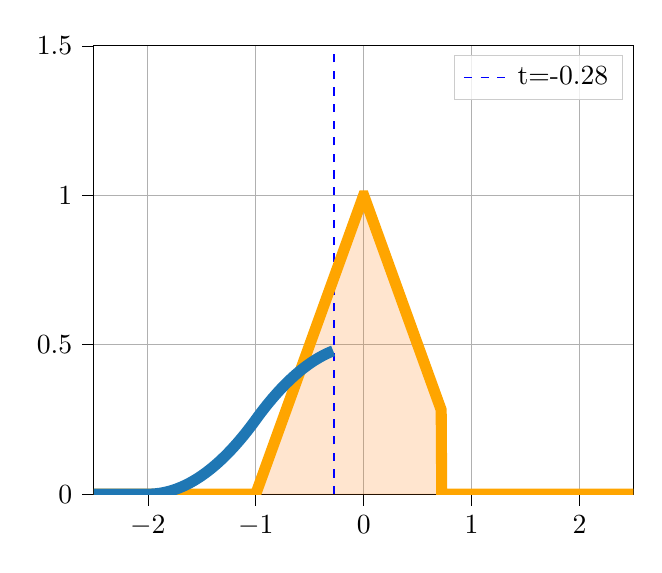
\begin{tikzpicture}

\definecolor{color0}{rgb}{1,0.498039215686275,0.0549019607843137}
\definecolor{color1}{rgb}{1,0.647058823529412,0}
\definecolor{color2}{rgb}{0.12156862745098,0.466666666666667,0.705882352941177}

\begin{axis}[
legend cell align={left},
legend style={fill opacity=0.8, draw opacity=1, text opacity=1, draw=white!80!black},
tick align=outside,
tick pos=left,
x grid style={white!69.0196078431373!black},
xmajorgrids,
xmin=-2.5, xmax=2.5,
xtick style={color=black},
y grid style={white!69.0196078431373!black},
ymajorgrids,
ymin=0, ymax=1.5,
ytick style={color=black}
]
\path [draw=color0, fill=color0, opacity=0.2]
(axis cs:-2.5,0)
--(axis cs:-2.5,0)
--(axis cs:-2.49499499499499,0)
--(axis cs:-2.48998998998999,0)
--(axis cs:-2.48498498498498,0)
--(axis cs:-2.47997997997998,0)
--(axis cs:-2.47497497497497,0)
--(axis cs:-2.46996996996997,0)
--(axis cs:-2.46496496496496,0)
--(axis cs:-2.45995995995996,0)
--(axis cs:-2.45495495495495,0)
--(axis cs:-2.44994994994995,0)
--(axis cs:-2.44494494494494,0)
--(axis cs:-2.43993993993994,0)
--(axis cs:-2.43493493493493,0)
--(axis cs:-2.42992992992993,0)
--(axis cs:-2.42492492492492,0)
--(axis cs:-2.41991991991992,0)
--(axis cs:-2.41491491491491,0)
--(axis cs:-2.40990990990991,0)
--(axis cs:-2.4049049049049,0)
--(axis cs:-2.3998998998999,0)
--(axis cs:-2.39489489489489,0)
--(axis cs:-2.38988988988989,0)
--(axis cs:-2.38488488488488,0)
--(axis cs:-2.37987987987988,0)
--(axis cs:-2.37487487487487,0)
--(axis cs:-2.36986986986987,0)
--(axis cs:-2.36486486486486,0)
--(axis cs:-2.35985985985986,0)
--(axis cs:-2.35485485485485,0)
--(axis cs:-2.34984984984985,0)
--(axis cs:-2.34484484484484,0)
--(axis cs:-2.33983983983984,0)
--(axis cs:-2.33483483483483,0)
--(axis cs:-2.32982982982983,0)
--(axis cs:-2.32482482482482,0)
--(axis cs:-2.31981981981982,0)
--(axis cs:-2.31481481481481,0)
--(axis cs:-2.30980980980981,0)
--(axis cs:-2.3048048048048,0)
--(axis cs:-2.2997997997998,0)
--(axis cs:-2.29479479479479,0)
--(axis cs:-2.28978978978979,0)
--(axis cs:-2.28478478478478,0)
--(axis cs:-2.27977977977978,0)
--(axis cs:-2.27477477477477,0)
--(axis cs:-2.26976976976977,0)
--(axis cs:-2.26476476476476,0)
--(axis cs:-2.25975975975976,0)
--(axis cs:-2.25475475475475,0)
--(axis cs:-2.24974974974975,0)
--(axis cs:-2.24474474474474,0)
--(axis cs:-2.23973973973974,0)
--(axis cs:-2.23473473473473,0)
--(axis cs:-2.22972972972973,0)
--(axis cs:-2.22472472472472,0)
--(axis cs:-2.21971971971972,0)
--(axis cs:-2.21471471471471,0)
--(axis cs:-2.20970970970971,0)
--(axis cs:-2.2047047047047,0)
--(axis cs:-2.1996996996997,0)
--(axis cs:-2.19469469469469,0)
--(axis cs:-2.18968968968969,0)
--(axis cs:-2.18468468468468,0)
--(axis cs:-2.17967967967968,0)
--(axis cs:-2.17467467467467,0)
--(axis cs:-2.16966966966967,0)
--(axis cs:-2.16466466466466,0)
--(axis cs:-2.15965965965966,0)
--(axis cs:-2.15465465465465,0)
--(axis cs:-2.14964964964965,0)
--(axis cs:-2.14464464464464,0)
--(axis cs:-2.13963963963964,0)
--(axis cs:-2.13463463463463,0)
--(axis cs:-2.12962962962963,0)
--(axis cs:-2.12462462462462,0)
--(axis cs:-2.11961961961962,0)
--(axis cs:-2.11461461461461,0)
--(axis cs:-2.10960960960961,0)
--(axis cs:-2.1046046046046,0)
--(axis cs:-2.0995995995996,0)
--(axis cs:-2.09459459459459,0)
--(axis cs:-2.08958958958959,0)
--(axis cs:-2.08458458458458,0)
--(axis cs:-2.07957957957958,0)
--(axis cs:-2.07457457457457,0)
--(axis cs:-2.06956956956957,0)
--(axis cs:-2.06456456456456,0)
--(axis cs:-2.05955955955956,0)
--(axis cs:-2.05455455455455,0)
--(axis cs:-2.04954954954955,0)
--(axis cs:-2.04454454454454,0)
--(axis cs:-2.03953953953954,0)
--(axis cs:-2.03453453453453,0)
--(axis cs:-2.02952952952953,0)
--(axis cs:-2.02452452452452,0)
--(axis cs:-2.01951951951952,0)
--(axis cs:-2.01451451451451,0)
--(axis cs:-2.00950950950951,0)
--(axis cs:-2.0045045045045,0)
--(axis cs:-1.9994994994995,0)
--(axis cs:-1.99449449449449,0)
--(axis cs:-1.98948948948949,0)
--(axis cs:-1.98448448448448,0)
--(axis cs:-1.97947947947948,0)
--(axis cs:-1.97447447447447,0)
--(axis cs:-1.96946946946947,0)
--(axis cs:-1.96446446446446,0)
--(axis cs:-1.95945945945946,0)
--(axis cs:-1.95445445445445,0)
--(axis cs:-1.94944944944945,0)
--(axis cs:-1.94444444444444,0)
--(axis cs:-1.93943943943944,0)
--(axis cs:-1.93443443443443,0)
--(axis cs:-1.92942942942943,0)
--(axis cs:-1.92442442442442,0)
--(axis cs:-1.91941941941942,0)
--(axis cs:-1.91441441441441,0)
--(axis cs:-1.90940940940941,0)
--(axis cs:-1.9044044044044,0)
--(axis cs:-1.8993993993994,0)
--(axis cs:-1.89439439439439,0)
--(axis cs:-1.88938938938939,0)
--(axis cs:-1.88438438438438,0)
--(axis cs:-1.87937937937938,0)
--(axis cs:-1.87437437437437,0)
--(axis cs:-1.86936936936937,0)
--(axis cs:-1.86436436436436,0)
--(axis cs:-1.85935935935936,0)
--(axis cs:-1.85435435435435,0)
--(axis cs:-1.84934934934935,0)
--(axis cs:-1.84434434434434,0)
--(axis cs:-1.83933933933934,0)
--(axis cs:-1.83433433433433,0)
--(axis cs:-1.82932932932933,0)
--(axis cs:-1.82432432432432,0)
--(axis cs:-1.81931931931932,0)
--(axis cs:-1.81431431431431,0)
--(axis cs:-1.80930930930931,0)
--(axis cs:-1.8043043043043,0)
--(axis cs:-1.7992992992993,0)
--(axis cs:-1.79429429429429,0)
--(axis cs:-1.78928928928929,0)
--(axis cs:-1.78428428428428,0)
--(axis cs:-1.77927927927928,0)
--(axis cs:-1.77427427427427,0)
--(axis cs:-1.76926926926927,0)
--(axis cs:-1.76426426426426,0)
--(axis cs:-1.75925925925926,0)
--(axis cs:-1.75425425425425,0)
--(axis cs:-1.74924924924925,0)
--(axis cs:-1.74424424424424,0)
--(axis cs:-1.73923923923924,0)
--(axis cs:-1.73423423423423,0)
--(axis cs:-1.72922922922923,0)
--(axis cs:-1.72422422422422,0)
--(axis cs:-1.71921921921922,0)
--(axis cs:-1.71421421421421,0)
--(axis cs:-1.70920920920921,0)
--(axis cs:-1.7042042042042,0)
--(axis cs:-1.6991991991992,0)
--(axis cs:-1.69419419419419,0)
--(axis cs:-1.68918918918919,0)
--(axis cs:-1.68418418418418,0)
--(axis cs:-1.67917917917918,0)
--(axis cs:-1.67417417417417,0)
--(axis cs:-1.66916916916917,0)
--(axis cs:-1.66416416416416,0)
--(axis cs:-1.65915915915916,0)
--(axis cs:-1.65415415415415,0)
--(axis cs:-1.64914914914915,0)
--(axis cs:-1.64414414414414,0)
--(axis cs:-1.63913913913914,0)
--(axis cs:-1.63413413413413,0)
--(axis cs:-1.62912912912913,0)
--(axis cs:-1.62412412412412,0)
--(axis cs:-1.61911911911912,0)
--(axis cs:-1.61411411411411,0)
--(axis cs:-1.60910910910911,0)
--(axis cs:-1.6041041041041,0)
--(axis cs:-1.5990990990991,0)
--(axis cs:-1.59409409409409,0)
--(axis cs:-1.58908908908909,0)
--(axis cs:-1.58408408408408,0)
--(axis cs:-1.57907907907908,0)
--(axis cs:-1.57407407407407,0)
--(axis cs:-1.56906906906907,0)
--(axis cs:-1.56406406406406,0)
--(axis cs:-1.55905905905906,0)
--(axis cs:-1.55405405405405,0)
--(axis cs:-1.54904904904905,0)
--(axis cs:-1.54404404404404,0)
--(axis cs:-1.53903903903904,0)
--(axis cs:-1.53403403403403,0)
--(axis cs:-1.52902902902903,0)
--(axis cs:-1.52402402402402,0)
--(axis cs:-1.51901901901902,0)
--(axis cs:-1.51401401401401,0)
--(axis cs:-1.50900900900901,0)
--(axis cs:-1.504004004004,0)
--(axis cs:-1.498998998999,0)
--(axis cs:-1.49399399399399,0)
--(axis cs:-1.48898898898899,0)
--(axis cs:-1.48398398398398,0)
--(axis cs:-1.47897897897898,0)
--(axis cs:-1.47397397397397,0)
--(axis cs:-1.46896896896897,0)
--(axis cs:-1.46396396396396,0)
--(axis cs:-1.45895895895896,0)
--(axis cs:-1.45395395395395,0)
--(axis cs:-1.44894894894895,0)
--(axis cs:-1.44394394394394,0)
--(axis cs:-1.43893893893894,0)
--(axis cs:-1.43393393393393,0)
--(axis cs:-1.42892892892893,0)
--(axis cs:-1.42392392392392,0)
--(axis cs:-1.41891891891892,0)
--(axis cs:-1.41391391391391,0)
--(axis cs:-1.40890890890891,0)
--(axis cs:-1.4039039039039,0)
--(axis cs:-1.3988988988989,0)
--(axis cs:-1.39389389389389,0)
--(axis cs:-1.38888888888889,0)
--(axis cs:-1.38388388388388,0)
--(axis cs:-1.37887887887888,0)
--(axis cs:-1.37387387387387,0)
--(axis cs:-1.36886886886887,0)
--(axis cs:-1.36386386386386,0)
--(axis cs:-1.35885885885886,0)
--(axis cs:-1.35385385385385,0)
--(axis cs:-1.34884884884885,0)
--(axis cs:-1.34384384384384,0)
--(axis cs:-1.33883883883884,0)
--(axis cs:-1.33383383383383,0)
--(axis cs:-1.32882882882883,0)
--(axis cs:-1.32382382382382,0)
--(axis cs:-1.31881881881882,0)
--(axis cs:-1.31381381381381,0)
--(axis cs:-1.30880880880881,0)
--(axis cs:-1.3038038038038,0)
--(axis cs:-1.2987987987988,0)
--(axis cs:-1.29379379379379,0)
--(axis cs:-1.28878878878879,0)
--(axis cs:-1.28378378378378,0)
--(axis cs:-1.27877877877878,0)
--(axis cs:-1.27377377377377,0)
--(axis cs:-1.26876876876877,0)
--(axis cs:-1.26376376376376,0)
--(axis cs:-1.25875875875876,0)
--(axis cs:-1.25375375375375,0)
--(axis cs:-1.24874874874875,0)
--(axis cs:-1.24374374374374,0)
--(axis cs:-1.23873873873874,0)
--(axis cs:-1.23373373373373,0)
--(axis cs:-1.22872872872873,0)
--(axis cs:-1.22372372372372,0)
--(axis cs:-1.21871871871872,0)
--(axis cs:-1.21371371371371,0)
--(axis cs:-1.20870870870871,0)
--(axis cs:-1.2037037037037,0)
--(axis cs:-1.1986986986987,0)
--(axis cs:-1.19369369369369,0)
--(axis cs:-1.18868868868869,0)
--(axis cs:-1.18368368368368,0)
--(axis cs:-1.17867867867868,0)
--(axis cs:-1.17367367367367,0)
--(axis cs:-1.16866866866867,0)
--(axis cs:-1.16366366366366,0)
--(axis cs:-1.15865865865866,0)
--(axis cs:-1.15365365365365,0)
--(axis cs:-1.14864864864865,0)
--(axis cs:-1.14364364364364,0)
--(axis cs:-1.13863863863864,0)
--(axis cs:-1.13363363363363,0)
--(axis cs:-1.12862862862863,0)
--(axis cs:-1.12362362362362,0)
--(axis cs:-1.11861861861862,0)
--(axis cs:-1.11361361361361,0)
--(axis cs:-1.10860860860861,0)
--(axis cs:-1.1036036036036,0)
--(axis cs:-1.0985985985986,0)
--(axis cs:-1.09359359359359,0)
--(axis cs:-1.08858858858859,0)
--(axis cs:-1.08358358358358,0)
--(axis cs:-1.07857857857858,0)
--(axis cs:-1.07357357357357,0)
--(axis cs:-1.06856856856857,0)
--(axis cs:-1.06356356356356,0)
--(axis cs:-1.05855855855856,0)
--(axis cs:-1.05355355355355,0)
--(axis cs:-1.04854854854855,0)
--(axis cs:-1.04354354354354,0)
--(axis cs:-1.03853853853854,0)
--(axis cs:-1.03353353353353,0)
--(axis cs:-1.02852852852853,0)
--(axis cs:-1.02352352352352,0)
--(axis cs:-1.01851851851852,0)
--(axis cs:-1.01351351351351,0)
--(axis cs:-1.00850850850851,0)
--(axis cs:-1.0035035035035,0)
--(axis cs:-0.998498498498499,0)
--(axis cs:-0.993493493493494,0)
--(axis cs:-0.988488488488489,0)
--(axis cs:-0.983483483483484,0)
--(axis cs:-0.978478478478479,0)
--(axis cs:-0.973473473473474,0)
--(axis cs:-0.968468468468469,0)
--(axis cs:-0.963463463463464,0)
--(axis cs:-0.958458458458459,0)
--(axis cs:-0.953453453453454,0)
--(axis cs:-0.948448448448449,0)
--(axis cs:-0.943443443443444,0)
--(axis cs:-0.938438438438439,0)
--(axis cs:-0.933433433433434,0)
--(axis cs:-0.928428428428429,0)
--(axis cs:-0.923423423423424,0)
--(axis cs:-0.918418418418419,0)
--(axis cs:-0.913413413413414,0)
--(axis cs:-0.908408408408409,0)
--(axis cs:-0.903403403403404,0)
--(axis cs:-0.898398398398399,0)
--(axis cs:-0.893393393393393,0)
--(axis cs:-0.888388388388388,0)
--(axis cs:-0.883383383383383,0)
--(axis cs:-0.878378378378378,0)
--(axis cs:-0.873373373373373,0)
--(axis cs:-0.868368368368368,0)
--(axis cs:-0.863363363363363,0)
--(axis cs:-0.858358358358358,0)
--(axis cs:-0.853353353353353,0)
--(axis cs:-0.848348348348348,0)
--(axis cs:-0.843343343343343,0)
--(axis cs:-0.838338338338338,0)
--(axis cs:-0.833333333333333,0)
--(axis cs:-0.828328328328328,0)
--(axis cs:-0.823323323323323,0)
--(axis cs:-0.818318318318318,0)
--(axis cs:-0.813313313313313,0)
--(axis cs:-0.808308308308308,0)
--(axis cs:-0.803303303303303,0)
--(axis cs:-0.798298298298298,0)
--(axis cs:-0.793293293293293,0)
--(axis cs:-0.788288288288288,0)
--(axis cs:-0.783283283283283,0)
--(axis cs:-0.778278278278278,0)
--(axis cs:-0.773273273273273,0)
--(axis cs:-0.768268268268268,0)
--(axis cs:-0.763263263263263,0)
--(axis cs:-0.758258258258258,0)
--(axis cs:-0.753253253253253,0)
--(axis cs:-0.748248248248248,0)
--(axis cs:-0.743243243243243,0)
--(axis cs:-0.738238238238238,0)
--(axis cs:-0.733233233233233,0)
--(axis cs:-0.728228228228228,0)
--(axis cs:-0.723223223223223,0)
--(axis cs:-0.718218218218218,0)
--(axis cs:-0.713213213213213,0)
--(axis cs:-0.708208208208208,0)
--(axis cs:-0.703203203203203,0)
--(axis cs:-0.698198198198198,0)
--(axis cs:-0.693193193193193,0)
--(axis cs:-0.688188188188188,0)
--(axis cs:-0.683183183183183,0)
--(axis cs:-0.678178178178178,0)
--(axis cs:-0.673173173173173,0)
--(axis cs:-0.668168168168168,0)
--(axis cs:-0.663163163163163,0)
--(axis cs:-0.658158158158158,0)
--(axis cs:-0.653153153153153,0)
--(axis cs:-0.648148148148148,0)
--(axis cs:-0.643143143143143,0)
--(axis cs:-0.638138138138138,0)
--(axis cs:-0.633133133133133,0)
--(axis cs:-0.628128128128128,0)
--(axis cs:-0.623123123123123,0)
--(axis cs:-0.618118118118118,0)
--(axis cs:-0.613113113113113,0)
--(axis cs:-0.608108108108108,0)
--(axis cs:-0.603103103103103,0)
--(axis cs:-0.598098098098098,0)
--(axis cs:-0.593093093093093,0)
--(axis cs:-0.588088088088088,0)
--(axis cs:-0.583083083083083,0)
--(axis cs:-0.578078078078078,0)
--(axis cs:-0.573073073073073,0)
--(axis cs:-0.568068068068068,0)
--(axis cs:-0.563063063063063,0)
--(axis cs:-0.558058058058058,0)
--(axis cs:-0.553053053053053,0)
--(axis cs:-0.548048048048048,0)
--(axis cs:-0.543043043043043,0)
--(axis cs:-0.538038038038038,0)
--(axis cs:-0.533033033033033,0)
--(axis cs:-0.528028028028028,0)
--(axis cs:-0.523023023023023,0)
--(axis cs:-0.518018018018018,0)
--(axis cs:-0.513013013013013,0)
--(axis cs:-0.508008008008008,0)
--(axis cs:-0.503003003003003,0)
--(axis cs:-0.497997997997998,0)
--(axis cs:-0.492992992992993,0)
--(axis cs:-0.487987987987988,0)
--(axis cs:-0.482982982982983,0)
--(axis cs:-0.477977977977978,0)
--(axis cs:-0.472972972972973,0)
--(axis cs:-0.467967967967968,0)
--(axis cs:-0.462962962962963,0)
--(axis cs:-0.457957957957958,0)
--(axis cs:-0.452952952952953,0)
--(axis cs:-0.447947947947948,0)
--(axis cs:-0.442942942942943,0)
--(axis cs:-0.437937937937938,0)
--(axis cs:-0.432932932932933,0)
--(axis cs:-0.427927927927928,0)
--(axis cs:-0.422922922922923,0)
--(axis cs:-0.417917917917918,0)
--(axis cs:-0.412912912912913,0)
--(axis cs:-0.407907907907908,0)
--(axis cs:-0.402902902902903,0)
--(axis cs:-0.397897897897898,0)
--(axis cs:-0.392892892892893,0)
--(axis cs:-0.387887887887888,0)
--(axis cs:-0.382882882882883,0)
--(axis cs:-0.377877877877878,0)
--(axis cs:-0.372872872872873,0)
--(axis cs:-0.367867867867868,0)
--(axis cs:-0.362862862862863,0)
--(axis cs:-0.357857857857858,0)
--(axis cs:-0.352852852852853,0)
--(axis cs:-0.347847847847848,0)
--(axis cs:-0.342842842842843,0)
--(axis cs:-0.337837837837838,0)
--(axis cs:-0.332832832832833,0)
--(axis cs:-0.327827827827828,0)
--(axis cs:-0.322822822822823,0)
--(axis cs:-0.317817817817818,0)
--(axis cs:-0.312812812812813,0)
--(axis cs:-0.307807807807808,0)
--(axis cs:-0.302802802802803,0)
--(axis cs:-0.297797797797798,0)
--(axis cs:-0.292792792792793,0)
--(axis cs:-0.287787787787788,0)
--(axis cs:-0.282782782782783,0)
--(axis cs:-0.277777777777778,0)
--(axis cs:-0.272772772772773,0)
--(axis cs:-0.267767767767768,0)
--(axis cs:-0.262762762762763,0)
--(axis cs:-0.257757757757758,0)
--(axis cs:-0.252752752752753,0)
--(axis cs:-0.247747747747748,0)
--(axis cs:-0.242742742742743,0)
--(axis cs:-0.237737737737738,0)
--(axis cs:-0.232732732732733,0)
--(axis cs:-0.227727727727728,0)
--(axis cs:-0.222722722722723,0)
--(axis cs:-0.217717717717718,0)
--(axis cs:-0.212712712712713,0)
--(axis cs:-0.207707707707708,0)
--(axis cs:-0.202702702702703,0)
--(axis cs:-0.197697697697698,0)
--(axis cs:-0.192692692692693,0)
--(axis cs:-0.187687687687688,0)
--(axis cs:-0.182682682682683,0)
--(axis cs:-0.177677677677678,0)
--(axis cs:-0.172672672672673,0)
--(axis cs:-0.167667667667668,0)
--(axis cs:-0.162662662662663,0)
--(axis cs:-0.157657657657658,0)
--(axis cs:-0.152652652652653,0)
--(axis cs:-0.147647647647648,0)
--(axis cs:-0.142642642642643,0)
--(axis cs:-0.137637637637638,0)
--(axis cs:-0.132632632632633,0)
--(axis cs:-0.127627627627628,0)
--(axis cs:-0.122622622622623,0)
--(axis cs:-0.117617617617618,0)
--(axis cs:-0.112612612612613,0)
--(axis cs:-0.107607607607608,0)
--(axis cs:-0.102602602602603,0)
--(axis cs:-0.0975975975975976,0)
--(axis cs:-0.0925925925925926,0)
--(axis cs:-0.0875875875875876,0)
--(axis cs:-0.0825825825825826,0)
--(axis cs:-0.0775775775775776,0)
--(axis cs:-0.0725725725725725,0)
--(axis cs:-0.0675675675675675,0)
--(axis cs:-0.0625625625625625,0)
--(axis cs:-0.0575575575575575,0)
--(axis cs:-0.0525525525525525,0)
--(axis cs:-0.0475475475475475,0)
--(axis cs:-0.0425425425425425,0)
--(axis cs:-0.0375375375375375,0)
--(axis cs:-0.0325325325325325,0)
--(axis cs:-0.0275275275275275,0)
--(axis cs:-0.0225225225225225,0)
--(axis cs:-0.0175175175175175,0)
--(axis cs:-0.0125125125125125,0)
--(axis cs:-0.0075075075075075,0)
--(axis cs:-0.0025025025025025,0)
--(axis cs:0.0025025025025025,0)
--(axis cs:0.0075075075075075,0)
--(axis cs:0.0125125125125125,0)
--(axis cs:0.0175175175175175,0)
--(axis cs:0.0225225225225225,0)
--(axis cs:0.0275275275275275,0)
--(axis cs:0.0325325325325325,0)
--(axis cs:0.0375375375375375,0)
--(axis cs:0.0425425425425425,0)
--(axis cs:0.0475475475475475,0)
--(axis cs:0.0525525525525525,0)
--(axis cs:0.0575575575575575,0)
--(axis cs:0.0625625625625625,0)
--(axis cs:0.0675675675675675,0)
--(axis cs:0.0725725725725725,0)
--(axis cs:0.0775775775775776,0)
--(axis cs:0.0825825825825826,0)
--(axis cs:0.0875875875875876,0)
--(axis cs:0.0925925925925926,0)
--(axis cs:0.0975975975975976,0)
--(axis cs:0.102602602602603,0)
--(axis cs:0.107607607607608,0)
--(axis cs:0.112612612612613,0)
--(axis cs:0.117617617617618,0)
--(axis cs:0.122622622622623,0)
--(axis cs:0.127627627627628,0)
--(axis cs:0.132632632632633,0)
--(axis cs:0.137637637637638,0)
--(axis cs:0.142642642642643,0)
--(axis cs:0.147647647647648,0)
--(axis cs:0.152652652652653,0)
--(axis cs:0.157657657657658,0)
--(axis cs:0.162662662662663,0)
--(axis cs:0.167667667667668,0)
--(axis cs:0.172672672672673,0)
--(axis cs:0.177677677677678,0)
--(axis cs:0.182682682682683,0)
--(axis cs:0.187687687687688,0)
--(axis cs:0.192692692692693,0)
--(axis cs:0.197697697697698,0)
--(axis cs:0.202702702702703,0)
--(axis cs:0.207707707707708,0)
--(axis cs:0.212712712712713,0)
--(axis cs:0.217717717717718,0)
--(axis cs:0.222722722722723,0)
--(axis cs:0.227727727727728,0)
--(axis cs:0.232732732732733,0)
--(axis cs:0.237737737737738,0)
--(axis cs:0.242742742742743,0)
--(axis cs:0.247747747747748,0)
--(axis cs:0.252752752752753,0)
--(axis cs:0.257757757757758,0)
--(axis cs:0.262762762762763,0)
--(axis cs:0.267767767767768,0)
--(axis cs:0.272772772772773,0)
--(axis cs:0.277777777777778,0)
--(axis cs:0.282782782782783,0)
--(axis cs:0.287787787787788,0)
--(axis cs:0.292792792792793,0)
--(axis cs:0.297797797797798,0)
--(axis cs:0.302802802802803,0)
--(axis cs:0.307807807807808,0)
--(axis cs:0.312812812812813,0)
--(axis cs:0.317817817817818,0)
--(axis cs:0.322822822822823,0)
--(axis cs:0.327827827827828,0)
--(axis cs:0.332832832832833,0)
--(axis cs:0.337837837837838,0)
--(axis cs:0.342842842842843,0)
--(axis cs:0.347847847847848,0)
--(axis cs:0.352852852852853,0)
--(axis cs:0.357857857857858,0)
--(axis cs:0.362862862862863,0)
--(axis cs:0.367867867867868,0)
--(axis cs:0.372872872872873,0)
--(axis cs:0.377877877877878,0)
--(axis cs:0.382882882882883,0)
--(axis cs:0.387887887887888,0)
--(axis cs:0.392892892892893,0)
--(axis cs:0.397897897897898,0)
--(axis cs:0.402902902902903,0)
--(axis cs:0.407907907907908,0)
--(axis cs:0.412912912912913,0)
--(axis cs:0.417917917917918,0)
--(axis cs:0.422922922922923,0)
--(axis cs:0.427927927927928,0)
--(axis cs:0.432932932932933,0)
--(axis cs:0.437937937937938,0)
--(axis cs:0.442942942942943,0)
--(axis cs:0.447947947947948,0)
--(axis cs:0.452952952952953,0)
--(axis cs:0.457957957957958,0)
--(axis cs:0.462962962962963,0)
--(axis cs:0.467967967967968,0)
--(axis cs:0.472972972972973,0)
--(axis cs:0.477977977977978,0)
--(axis cs:0.482982982982983,0)
--(axis cs:0.487987987987988,0)
--(axis cs:0.492992992992993,0)
--(axis cs:0.497997997997998,0)
--(axis cs:0.503003003003003,0)
--(axis cs:0.508008008008008,0)
--(axis cs:0.513013013013013,0)
--(axis cs:0.518018018018018,0)
--(axis cs:0.523023023023023,0)
--(axis cs:0.528028028028028,0)
--(axis cs:0.533033033033033,0)
--(axis cs:0.538038038038038,0)
--(axis cs:0.543043043043043,0)
--(axis cs:0.548048048048048,0)
--(axis cs:0.553053053053053,0)
--(axis cs:0.558058058058058,0)
--(axis cs:0.563063063063063,0)
--(axis cs:0.568068068068068,0)
--(axis cs:0.573073073073073,0)
--(axis cs:0.578078078078078,0)
--(axis cs:0.583083083083083,0)
--(axis cs:0.588088088088088,0)
--(axis cs:0.593093093093093,0)
--(axis cs:0.598098098098098,0)
--(axis cs:0.603103103103103,0)
--(axis cs:0.608108108108108,0)
--(axis cs:0.613113113113113,0)
--(axis cs:0.618118118118118,0)
--(axis cs:0.623123123123123,0)
--(axis cs:0.628128128128128,0)
--(axis cs:0.633133133133133,0)
--(axis cs:0.638138138138138,0)
--(axis cs:0.643143143143143,0)
--(axis cs:0.648148148148148,0)
--(axis cs:0.653153153153153,0)
--(axis cs:0.658158158158158,0)
--(axis cs:0.663163163163163,0)
--(axis cs:0.668168168168168,0)
--(axis cs:0.673173173173173,0)
--(axis cs:0.678178178178178,0)
--(axis cs:0.683183183183183,0)
--(axis cs:0.688188188188188,0)
--(axis cs:0.693193193193193,0)
--(axis cs:0.698198198198198,0)
--(axis cs:0.703203203203203,0)
--(axis cs:0.708208208208208,0)
--(axis cs:0.713213213213213,0)
--(axis cs:0.718218218218218,0)
--(axis cs:0.723223223223223,0)
--(axis cs:0.728228228228228,0)
--(axis cs:0.733233233233233,0)
--(axis cs:0.738238238238238,0)
--(axis cs:0.743243243243243,0)
--(axis cs:0.748248248248248,0)
--(axis cs:0.753253253253253,0)
--(axis cs:0.758258258258258,0)
--(axis cs:0.763263263263263,0)
--(axis cs:0.768268268268268,0)
--(axis cs:0.773273273273273,0)
--(axis cs:0.778278278278278,0)
--(axis cs:0.783283283283283,0)
--(axis cs:0.788288288288288,0)
--(axis cs:0.793293293293293,0)
--(axis cs:0.798298298298298,0)
--(axis cs:0.803303303303303,0)
--(axis cs:0.808308308308308,0)
--(axis cs:0.813313313313313,0)
--(axis cs:0.818318318318318,0)
--(axis cs:0.823323323323323,0)
--(axis cs:0.828328328328328,0)
--(axis cs:0.833333333333333,0)
--(axis cs:0.838338338338338,0)
--(axis cs:0.843343343343343,0)
--(axis cs:0.848348348348348,0)
--(axis cs:0.853353353353353,0)
--(axis cs:0.858358358358358,0)
--(axis cs:0.863363363363364,0)
--(axis cs:0.868368368368369,0)
--(axis cs:0.873373373373374,0)
--(axis cs:0.878378378378379,0)
--(axis cs:0.883383383383384,0)
--(axis cs:0.888388388388389,0)
--(axis cs:0.893393393393394,0)
--(axis cs:0.898398398398399,0)
--(axis cs:0.903403403403404,0)
--(axis cs:0.908408408408409,0)
--(axis cs:0.913413413413414,0)
--(axis cs:0.918418418418419,0)
--(axis cs:0.923423423423424,0)
--(axis cs:0.928428428428429,0)
--(axis cs:0.933433433433434,0)
--(axis cs:0.938438438438439,0)
--(axis cs:0.943443443443444,0)
--(axis cs:0.948448448448449,0)
--(axis cs:0.953453453453454,0)
--(axis cs:0.958458458458459,0)
--(axis cs:0.963463463463464,0)
--(axis cs:0.968468468468469,0)
--(axis cs:0.973473473473474,0)
--(axis cs:0.978478478478479,0)
--(axis cs:0.983483483483484,0)
--(axis cs:0.988488488488489,0)
--(axis cs:0.993493493493494,0)
--(axis cs:0.998498498498499,0)
--(axis cs:1.0035035035035,0)
--(axis cs:1.00850850850851,0)
--(axis cs:1.01351351351351,0)
--(axis cs:1.01851851851852,0)
--(axis cs:1.02352352352352,0)
--(axis cs:1.02852852852853,0)
--(axis cs:1.03353353353353,0)
--(axis cs:1.03853853853854,0)
--(axis cs:1.04354354354354,0)
--(axis cs:1.04854854854855,0)
--(axis cs:1.05355355355355,0)
--(axis cs:1.05855855855856,0)
--(axis cs:1.06356356356356,0)
--(axis cs:1.06856856856857,0)
--(axis cs:1.07357357357357,0)
--(axis cs:1.07857857857858,0)
--(axis cs:1.08358358358358,0)
--(axis cs:1.08858858858859,0)
--(axis cs:1.09359359359359,0)
--(axis cs:1.0985985985986,0)
--(axis cs:1.1036036036036,0)
--(axis cs:1.10860860860861,0)
--(axis cs:1.11361361361361,0)
--(axis cs:1.11861861861862,0)
--(axis cs:1.12362362362362,0)
--(axis cs:1.12862862862863,0)
--(axis cs:1.13363363363363,0)
--(axis cs:1.13863863863864,0)
--(axis cs:1.14364364364364,0)
--(axis cs:1.14864864864865,0)
--(axis cs:1.15365365365365,0)
--(axis cs:1.15865865865866,0)
--(axis cs:1.16366366366366,0)
--(axis cs:1.16866866866867,0)
--(axis cs:1.17367367367367,0)
--(axis cs:1.17867867867868,0)
--(axis cs:1.18368368368368,0)
--(axis cs:1.18868868868869,0)
--(axis cs:1.19369369369369,0)
--(axis cs:1.1986986986987,0)
--(axis cs:1.2037037037037,0)
--(axis cs:1.20870870870871,0)
--(axis cs:1.21371371371371,0)
--(axis cs:1.21871871871872,0)
--(axis cs:1.22372372372372,0)
--(axis cs:1.22872872872873,0)
--(axis cs:1.23373373373373,0)
--(axis cs:1.23873873873874,0)
--(axis cs:1.24374374374374,0)
--(axis cs:1.24874874874875,0)
--(axis cs:1.25375375375375,0)
--(axis cs:1.25875875875876,0)
--(axis cs:1.26376376376376,0)
--(axis cs:1.26876876876877,0)
--(axis cs:1.27377377377377,0)
--(axis cs:1.27877877877878,0)
--(axis cs:1.28378378378378,0)
--(axis cs:1.28878878878879,0)
--(axis cs:1.29379379379379,0)
--(axis cs:1.2987987987988,0)
--(axis cs:1.3038038038038,0)
--(axis cs:1.30880880880881,0)
--(axis cs:1.31381381381381,0)
--(axis cs:1.31881881881882,0)
--(axis cs:1.32382382382382,0)
--(axis cs:1.32882882882883,0)
--(axis cs:1.33383383383383,0)
--(axis cs:1.33883883883884,0)
--(axis cs:1.34384384384384,0)
--(axis cs:1.34884884884885,0)
--(axis cs:1.35385385385385,0)
--(axis cs:1.35885885885886,0)
--(axis cs:1.36386386386386,0)
--(axis cs:1.36886886886887,0)
--(axis cs:1.37387387387387,0)
--(axis cs:1.37887887887888,0)
--(axis cs:1.38388388388388,0)
--(axis cs:1.38888888888889,0)
--(axis cs:1.39389389389389,0)
--(axis cs:1.3988988988989,0)
--(axis cs:1.4039039039039,0)
--(axis cs:1.40890890890891,0)
--(axis cs:1.41391391391391,0)
--(axis cs:1.41891891891892,0)
--(axis cs:1.42392392392392,0)
--(axis cs:1.42892892892893,0)
--(axis cs:1.43393393393393,0)
--(axis cs:1.43893893893894,0)
--(axis cs:1.44394394394394,0)
--(axis cs:1.44894894894895,0)
--(axis cs:1.45395395395395,0)
--(axis cs:1.45895895895896,0)
--(axis cs:1.46396396396396,0)
--(axis cs:1.46896896896897,0)
--(axis cs:1.47397397397397,0)
--(axis cs:1.47897897897898,0)
--(axis cs:1.48398398398398,0)
--(axis cs:1.48898898898899,0)
--(axis cs:1.49399399399399,0)
--(axis cs:1.498998998999,0)
--(axis cs:1.504004004004,0)
--(axis cs:1.50900900900901,0)
--(axis cs:1.51401401401401,0)
--(axis cs:1.51901901901902,0)
--(axis cs:1.52402402402402,0)
--(axis cs:1.52902902902903,0)
--(axis cs:1.53403403403403,0)
--(axis cs:1.53903903903904,0)
--(axis cs:1.54404404404404,0)
--(axis cs:1.54904904904905,0)
--(axis cs:1.55405405405405,0)
--(axis cs:1.55905905905906,0)
--(axis cs:1.56406406406406,0)
--(axis cs:1.56906906906907,0)
--(axis cs:1.57407407407407,0)
--(axis cs:1.57907907907908,0)
--(axis cs:1.58408408408408,0)
--(axis cs:1.58908908908909,0)
--(axis cs:1.59409409409409,0)
--(axis cs:1.5990990990991,0)
--(axis cs:1.6041041041041,0)
--(axis cs:1.60910910910911,0)
--(axis cs:1.61411411411411,0)
--(axis cs:1.61911911911912,0)
--(axis cs:1.62412412412412,0)
--(axis cs:1.62912912912913,0)
--(axis cs:1.63413413413413,0)
--(axis cs:1.63913913913914,0)
--(axis cs:1.64414414414414,0)
--(axis cs:1.64914914914915,0)
--(axis cs:1.65415415415415,0)
--(axis cs:1.65915915915916,0)
--(axis cs:1.66416416416416,0)
--(axis cs:1.66916916916917,0)
--(axis cs:1.67417417417417,0)
--(axis cs:1.67917917917918,0)
--(axis cs:1.68418418418418,0)
--(axis cs:1.68918918918919,0)
--(axis cs:1.69419419419419,0)
--(axis cs:1.6991991991992,0)
--(axis cs:1.7042042042042,0)
--(axis cs:1.70920920920921,0)
--(axis cs:1.71421421421421,0)
--(axis cs:1.71921921921922,0)
--(axis cs:1.72422422422422,0)
--(axis cs:1.72922922922923,0)
--(axis cs:1.73423423423423,0)
--(axis cs:1.73923923923924,0)
--(axis cs:1.74424424424424,0)
--(axis cs:1.74924924924925,0)
--(axis cs:1.75425425425425,0)
--(axis cs:1.75925925925926,0)
--(axis cs:1.76426426426426,0)
--(axis cs:1.76926926926927,0)
--(axis cs:1.77427427427427,0)
--(axis cs:1.77927927927928,0)
--(axis cs:1.78428428428428,0)
--(axis cs:1.78928928928929,0)
--(axis cs:1.79429429429429,0)
--(axis cs:1.7992992992993,0)
--(axis cs:1.8043043043043,0)
--(axis cs:1.80930930930931,0)
--(axis cs:1.81431431431431,0)
--(axis cs:1.81931931931932,0)
--(axis cs:1.82432432432432,0)
--(axis cs:1.82932932932933,0)
--(axis cs:1.83433433433433,0)
--(axis cs:1.83933933933934,0)
--(axis cs:1.84434434434434,0)
--(axis cs:1.84934934934935,0)
--(axis cs:1.85435435435435,0)
--(axis cs:1.85935935935936,0)
--(axis cs:1.86436436436436,0)
--(axis cs:1.86936936936937,0)
--(axis cs:1.87437437437437,0)
--(axis cs:1.87937937937938,0)
--(axis cs:1.88438438438438,0)
--(axis cs:1.88938938938939,0)
--(axis cs:1.89439439439439,0)
--(axis cs:1.8993993993994,0)
--(axis cs:1.9044044044044,0)
--(axis cs:1.90940940940941,0)
--(axis cs:1.91441441441441,0)
--(axis cs:1.91941941941942,0)
--(axis cs:1.92442442442442,0)
--(axis cs:1.92942942942943,0)
--(axis cs:1.93443443443443,0)
--(axis cs:1.93943943943944,0)
--(axis cs:1.94444444444444,0)
--(axis cs:1.94944944944945,0)
--(axis cs:1.95445445445445,0)
--(axis cs:1.95945945945946,0)
--(axis cs:1.96446446446446,0)
--(axis cs:1.96946946946947,0)
--(axis cs:1.97447447447447,0)
--(axis cs:1.97947947947948,0)
--(axis cs:1.98448448448448,0)
--(axis cs:1.98948948948949,0)
--(axis cs:1.99449449449449,0)
--(axis cs:1.9994994994995,0)
--(axis cs:2.0045045045045,0)
--(axis cs:2.00950950950951,0)
--(axis cs:2.01451451451451,0)
--(axis cs:2.01951951951952,0)
--(axis cs:2.02452452452452,0)
--(axis cs:2.02952952952953,0)
--(axis cs:2.03453453453453,0)
--(axis cs:2.03953953953954,0)
--(axis cs:2.04454454454454,0)
--(axis cs:2.04954954954955,0)
--(axis cs:2.05455455455455,0)
--(axis cs:2.05955955955956,0)
--(axis cs:2.06456456456456,0)
--(axis cs:2.06956956956957,0)
--(axis cs:2.07457457457457,0)
--(axis cs:2.07957957957958,0)
--(axis cs:2.08458458458458,0)
--(axis cs:2.08958958958959,0)
--(axis cs:2.09459459459459,0)
--(axis cs:2.0995995995996,0)
--(axis cs:2.1046046046046,0)
--(axis cs:2.10960960960961,0)
--(axis cs:2.11461461461461,0)
--(axis cs:2.11961961961962,0)
--(axis cs:2.12462462462462,0)
--(axis cs:2.12962962962963,0)
--(axis cs:2.13463463463463,0)
--(axis cs:2.13963963963964,0)
--(axis cs:2.14464464464464,0)
--(axis cs:2.14964964964965,0)
--(axis cs:2.15465465465465,0)
--(axis cs:2.15965965965966,0)
--(axis cs:2.16466466466466,0)
--(axis cs:2.16966966966967,0)
--(axis cs:2.17467467467467,0)
--(axis cs:2.17967967967968,0)
--(axis cs:2.18468468468468,0)
--(axis cs:2.18968968968969,0)
--(axis cs:2.19469469469469,0)
--(axis cs:2.1996996996997,0)
--(axis cs:2.2047047047047,0)
--(axis cs:2.20970970970971,0)
--(axis cs:2.21471471471471,0)
--(axis cs:2.21971971971972,0)
--(axis cs:2.22472472472472,0)
--(axis cs:2.22972972972973,0)
--(axis cs:2.23473473473473,0)
--(axis cs:2.23973973973974,0)
--(axis cs:2.24474474474474,0)
--(axis cs:2.24974974974975,0)
--(axis cs:2.25475475475475,0)
--(axis cs:2.25975975975976,0)
--(axis cs:2.26476476476476,0)
--(axis cs:2.26976976976977,0)
--(axis cs:2.27477477477477,0)
--(axis cs:2.27977977977978,0)
--(axis cs:2.28478478478478,0)
--(axis cs:2.28978978978979,0)
--(axis cs:2.29479479479479,0)
--(axis cs:2.2997997997998,0)
--(axis cs:2.3048048048048,0)
--(axis cs:2.30980980980981,0)
--(axis cs:2.31481481481481,0)
--(axis cs:2.31981981981982,0)
--(axis cs:2.32482482482482,0)
--(axis cs:2.32982982982983,0)
--(axis cs:2.33483483483483,0)
--(axis cs:2.33983983983984,0)
--(axis cs:2.34484484484484,0)
--(axis cs:2.34984984984985,0)
--(axis cs:2.35485485485485,0)
--(axis cs:2.35985985985986,0)
--(axis cs:2.36486486486486,0)
--(axis cs:2.36986986986987,0)
--(axis cs:2.37487487487487,0)
--(axis cs:2.37987987987988,0)
--(axis cs:2.38488488488488,0)
--(axis cs:2.38988988988989,0)
--(axis cs:2.39489489489489,0)
--(axis cs:2.3998998998999,0)
--(axis cs:2.4049049049049,0)
--(axis cs:2.40990990990991,0)
--(axis cs:2.41491491491491,0)
--(axis cs:2.41991991991992,0)
--(axis cs:2.42492492492492,0)
--(axis cs:2.42992992992993,0)
--(axis cs:2.43493493493493,0)
--(axis cs:2.43993993993994,0)
--(axis cs:2.44494494494494,0)
--(axis cs:2.44994994994995,0)
--(axis cs:2.45495495495495,0)
--(axis cs:2.45995995995996,0)
--(axis cs:2.46496496496496,0)
--(axis cs:2.46996996996997,0)
--(axis cs:2.47497497497497,0)
--(axis cs:2.47997997997998,0)
--(axis cs:2.48498498498498,0)
--(axis cs:2.48998998998999,0)
--(axis cs:2.49499499499499,0)
--(axis cs:2.5,0)
--(axis cs:2.5,0)
--(axis cs:2.5,0)
--(axis cs:2.49499499499499,0)
--(axis cs:2.48998998998999,0)
--(axis cs:2.48498498498498,0)
--(axis cs:2.47997997997998,0)
--(axis cs:2.47497497497497,0)
--(axis cs:2.46996996996997,0)
--(axis cs:2.46496496496496,0)
--(axis cs:2.45995995995996,0)
--(axis cs:2.45495495495495,0)
--(axis cs:2.44994994994995,0)
--(axis cs:2.44494494494494,0)
--(axis cs:2.43993993993994,0)
--(axis cs:2.43493493493493,0)
--(axis cs:2.42992992992993,0)
--(axis cs:2.42492492492492,0)
--(axis cs:2.41991991991992,0)
--(axis cs:2.41491491491491,0)
--(axis cs:2.40990990990991,0)
--(axis cs:2.4049049049049,0)
--(axis cs:2.3998998998999,0)
--(axis cs:2.39489489489489,0)
--(axis cs:2.38988988988989,0)
--(axis cs:2.38488488488488,0)
--(axis cs:2.37987987987988,0)
--(axis cs:2.37487487487487,0)
--(axis cs:2.36986986986987,0)
--(axis cs:2.36486486486486,0)
--(axis cs:2.35985985985986,0)
--(axis cs:2.35485485485485,0)
--(axis cs:2.34984984984985,0)
--(axis cs:2.34484484484484,0)
--(axis cs:2.33983983983984,0)
--(axis cs:2.33483483483483,0)
--(axis cs:2.32982982982983,0)
--(axis cs:2.32482482482482,0)
--(axis cs:2.31981981981982,0)
--(axis cs:2.31481481481481,0)
--(axis cs:2.30980980980981,0)
--(axis cs:2.3048048048048,0)
--(axis cs:2.2997997997998,0)
--(axis cs:2.29479479479479,0)
--(axis cs:2.28978978978979,0)
--(axis cs:2.28478478478478,0)
--(axis cs:2.27977977977978,0)
--(axis cs:2.27477477477477,0)
--(axis cs:2.26976976976977,0)
--(axis cs:2.26476476476476,0)
--(axis cs:2.25975975975976,0)
--(axis cs:2.25475475475475,0)
--(axis cs:2.24974974974975,0)
--(axis cs:2.24474474474474,0)
--(axis cs:2.23973973973974,0)
--(axis cs:2.23473473473473,0)
--(axis cs:2.22972972972973,0)
--(axis cs:2.22472472472472,0)
--(axis cs:2.21971971971972,0)
--(axis cs:2.21471471471471,0)
--(axis cs:2.20970970970971,0)
--(axis cs:2.2047047047047,0)
--(axis cs:2.1996996996997,0)
--(axis cs:2.19469469469469,0)
--(axis cs:2.18968968968969,0)
--(axis cs:2.18468468468468,0)
--(axis cs:2.17967967967968,0)
--(axis cs:2.17467467467467,0)
--(axis cs:2.16966966966967,0)
--(axis cs:2.16466466466466,0)
--(axis cs:2.15965965965966,0)
--(axis cs:2.15465465465465,0)
--(axis cs:2.14964964964965,0)
--(axis cs:2.14464464464464,0)
--(axis cs:2.13963963963964,0)
--(axis cs:2.13463463463463,0)
--(axis cs:2.12962962962963,0)
--(axis cs:2.12462462462462,0)
--(axis cs:2.11961961961962,0)
--(axis cs:2.11461461461461,0)
--(axis cs:2.10960960960961,0)
--(axis cs:2.1046046046046,0)
--(axis cs:2.0995995995996,0)
--(axis cs:2.09459459459459,0)
--(axis cs:2.08958958958959,0)
--(axis cs:2.08458458458458,0)
--(axis cs:2.07957957957958,0)
--(axis cs:2.07457457457457,0)
--(axis cs:2.06956956956957,0)
--(axis cs:2.06456456456456,0)
--(axis cs:2.05955955955956,0)
--(axis cs:2.05455455455455,0)
--(axis cs:2.04954954954955,0)
--(axis cs:2.04454454454454,0)
--(axis cs:2.03953953953954,0)
--(axis cs:2.03453453453453,0)
--(axis cs:2.02952952952953,0)
--(axis cs:2.02452452452452,0)
--(axis cs:2.01951951951952,0)
--(axis cs:2.01451451451451,0)
--(axis cs:2.00950950950951,0)
--(axis cs:2.0045045045045,0)
--(axis cs:1.9994994994995,0)
--(axis cs:1.99449449449449,0)
--(axis cs:1.98948948948949,0)
--(axis cs:1.98448448448448,0)
--(axis cs:1.97947947947948,0)
--(axis cs:1.97447447447447,0)
--(axis cs:1.96946946946947,0)
--(axis cs:1.96446446446446,0)
--(axis cs:1.95945945945946,0)
--(axis cs:1.95445445445445,0)
--(axis cs:1.94944944944945,0)
--(axis cs:1.94444444444444,0)
--(axis cs:1.93943943943944,0)
--(axis cs:1.93443443443443,0)
--(axis cs:1.92942942942943,0)
--(axis cs:1.92442442442442,0)
--(axis cs:1.91941941941942,0)
--(axis cs:1.91441441441441,0)
--(axis cs:1.90940940940941,0)
--(axis cs:1.9044044044044,0)
--(axis cs:1.8993993993994,0)
--(axis cs:1.89439439439439,0)
--(axis cs:1.88938938938939,0)
--(axis cs:1.88438438438438,0)
--(axis cs:1.87937937937938,0)
--(axis cs:1.87437437437437,0)
--(axis cs:1.86936936936937,0)
--(axis cs:1.86436436436436,0)
--(axis cs:1.85935935935936,0)
--(axis cs:1.85435435435435,0)
--(axis cs:1.84934934934935,0)
--(axis cs:1.84434434434434,0)
--(axis cs:1.83933933933934,0)
--(axis cs:1.83433433433433,0)
--(axis cs:1.82932932932933,0)
--(axis cs:1.82432432432432,0)
--(axis cs:1.81931931931932,0)
--(axis cs:1.81431431431431,0)
--(axis cs:1.80930930930931,0)
--(axis cs:1.8043043043043,0)
--(axis cs:1.7992992992993,0)
--(axis cs:1.79429429429429,0)
--(axis cs:1.78928928928929,0)
--(axis cs:1.78428428428428,0)
--(axis cs:1.77927927927928,0)
--(axis cs:1.77427427427427,0)
--(axis cs:1.76926926926927,0)
--(axis cs:1.76426426426426,0)
--(axis cs:1.75925925925926,0)
--(axis cs:1.75425425425425,0)
--(axis cs:1.74924924924925,0)
--(axis cs:1.74424424424424,0)
--(axis cs:1.73923923923924,0)
--(axis cs:1.73423423423423,0)
--(axis cs:1.72922922922923,0)
--(axis cs:1.72422422422422,0)
--(axis cs:1.71921921921922,0)
--(axis cs:1.71421421421421,0)
--(axis cs:1.70920920920921,0)
--(axis cs:1.7042042042042,0)
--(axis cs:1.6991991991992,0)
--(axis cs:1.69419419419419,0)
--(axis cs:1.68918918918919,0)
--(axis cs:1.68418418418418,0)
--(axis cs:1.67917917917918,0)
--(axis cs:1.67417417417417,0)
--(axis cs:1.66916916916917,0)
--(axis cs:1.66416416416416,0)
--(axis cs:1.65915915915916,0)
--(axis cs:1.65415415415415,0)
--(axis cs:1.64914914914915,0)
--(axis cs:1.64414414414414,0)
--(axis cs:1.63913913913914,0)
--(axis cs:1.63413413413413,0)
--(axis cs:1.62912912912913,0)
--(axis cs:1.62412412412412,0)
--(axis cs:1.61911911911912,0)
--(axis cs:1.61411411411411,0)
--(axis cs:1.60910910910911,0)
--(axis cs:1.6041041041041,0)
--(axis cs:1.5990990990991,0)
--(axis cs:1.59409409409409,0)
--(axis cs:1.58908908908909,0)
--(axis cs:1.58408408408408,0)
--(axis cs:1.57907907907908,0)
--(axis cs:1.57407407407407,0)
--(axis cs:1.56906906906907,0)
--(axis cs:1.56406406406406,0)
--(axis cs:1.55905905905906,0)
--(axis cs:1.55405405405405,0)
--(axis cs:1.54904904904905,0)
--(axis cs:1.54404404404404,0)
--(axis cs:1.53903903903904,0)
--(axis cs:1.53403403403403,0)
--(axis cs:1.52902902902903,0)
--(axis cs:1.52402402402402,0)
--(axis cs:1.51901901901902,0)
--(axis cs:1.51401401401401,0)
--(axis cs:1.50900900900901,0)
--(axis cs:1.504004004004,0)
--(axis cs:1.498998998999,0)
--(axis cs:1.49399399399399,0)
--(axis cs:1.48898898898899,0)
--(axis cs:1.48398398398398,0)
--(axis cs:1.47897897897898,0)
--(axis cs:1.47397397397397,0)
--(axis cs:1.46896896896897,0)
--(axis cs:1.46396396396396,0)
--(axis cs:1.45895895895896,0)
--(axis cs:1.45395395395395,0)
--(axis cs:1.44894894894895,0)
--(axis cs:1.44394394394394,0)
--(axis cs:1.43893893893894,0)
--(axis cs:1.43393393393393,0)
--(axis cs:1.42892892892893,0)
--(axis cs:1.42392392392392,0)
--(axis cs:1.41891891891892,0)
--(axis cs:1.41391391391391,0)
--(axis cs:1.40890890890891,0)
--(axis cs:1.4039039039039,0)
--(axis cs:1.3988988988989,0)
--(axis cs:1.39389389389389,0)
--(axis cs:1.38888888888889,0)
--(axis cs:1.38388388388388,0)
--(axis cs:1.37887887887888,0)
--(axis cs:1.37387387387387,0)
--(axis cs:1.36886886886887,0)
--(axis cs:1.36386386386386,0)
--(axis cs:1.35885885885886,0)
--(axis cs:1.35385385385385,0)
--(axis cs:1.34884884884885,0)
--(axis cs:1.34384384384384,0)
--(axis cs:1.33883883883884,0)
--(axis cs:1.33383383383383,0)
--(axis cs:1.32882882882883,0)
--(axis cs:1.32382382382382,0)
--(axis cs:1.31881881881882,0)
--(axis cs:1.31381381381381,0)
--(axis cs:1.30880880880881,0)
--(axis cs:1.3038038038038,0)
--(axis cs:1.2987987987988,0)
--(axis cs:1.29379379379379,0)
--(axis cs:1.28878878878879,0)
--(axis cs:1.28378378378378,0)
--(axis cs:1.27877877877878,0)
--(axis cs:1.27377377377377,0)
--(axis cs:1.26876876876877,0)
--(axis cs:1.26376376376376,0)
--(axis cs:1.25875875875876,0)
--(axis cs:1.25375375375375,0)
--(axis cs:1.24874874874875,0)
--(axis cs:1.24374374374374,0)
--(axis cs:1.23873873873874,0)
--(axis cs:1.23373373373373,0)
--(axis cs:1.22872872872873,0)
--(axis cs:1.22372372372372,0)
--(axis cs:1.21871871871872,0)
--(axis cs:1.21371371371371,0)
--(axis cs:1.20870870870871,0)
--(axis cs:1.2037037037037,0)
--(axis cs:1.1986986986987,0)
--(axis cs:1.19369369369369,0)
--(axis cs:1.18868868868869,0)
--(axis cs:1.18368368368368,0)
--(axis cs:1.17867867867868,0)
--(axis cs:1.17367367367367,0)
--(axis cs:1.16866866866867,0)
--(axis cs:1.16366366366366,0)
--(axis cs:1.15865865865866,0)
--(axis cs:1.15365365365365,0)
--(axis cs:1.14864864864865,0)
--(axis cs:1.14364364364364,0)
--(axis cs:1.13863863863864,0)
--(axis cs:1.13363363363363,0)
--(axis cs:1.12862862862863,0)
--(axis cs:1.12362362362362,0)
--(axis cs:1.11861861861862,0)
--(axis cs:1.11361361361361,0)
--(axis cs:1.10860860860861,0)
--(axis cs:1.1036036036036,0)
--(axis cs:1.0985985985986,0)
--(axis cs:1.09359359359359,0)
--(axis cs:1.08858858858859,0)
--(axis cs:1.08358358358358,0)
--(axis cs:1.07857857857858,0)
--(axis cs:1.07357357357357,0)
--(axis cs:1.06856856856857,0)
--(axis cs:1.06356356356356,0)
--(axis cs:1.05855855855856,0)
--(axis cs:1.05355355355355,0)
--(axis cs:1.04854854854855,0)
--(axis cs:1.04354354354354,0)
--(axis cs:1.03853853853854,0)
--(axis cs:1.03353353353353,0)
--(axis cs:1.02852852852853,0)
--(axis cs:1.02352352352352,0)
--(axis cs:1.01851851851852,0)
--(axis cs:1.01351351351351,0)
--(axis cs:1.00850850850851,0)
--(axis cs:1.0035035035035,0)
--(axis cs:0.998498498498499,0)
--(axis cs:0.993493493493494,0)
--(axis cs:0.988488488488489,0)
--(axis cs:0.983483483483484,0)
--(axis cs:0.978478478478479,0)
--(axis cs:0.973473473473474,0)
--(axis cs:0.968468468468469,0)
--(axis cs:0.963463463463464,0)
--(axis cs:0.958458458458459,0)
--(axis cs:0.953453453453454,0)
--(axis cs:0.948448448448449,0)
--(axis cs:0.943443443443444,0)
--(axis cs:0.938438438438439,0)
--(axis cs:0.933433433433434,0)
--(axis cs:0.928428428428429,0)
--(axis cs:0.923423423423424,0)
--(axis cs:0.918418418418419,0)
--(axis cs:0.913413413413414,0)
--(axis cs:0.908408408408409,0)
--(axis cs:0.903403403403404,0)
--(axis cs:0.898398398398399,0)
--(axis cs:0.893393393393394,0)
--(axis cs:0.888388388388389,0)
--(axis cs:0.883383383383384,0)
--(axis cs:0.878378378378379,0)
--(axis cs:0.873373373373374,0)
--(axis cs:0.868368368368369,0)
--(axis cs:0.863363363363364,0)
--(axis cs:0.858358358358358,0)
--(axis cs:0.853353353353353,0)
--(axis cs:0.848348348348348,0)
--(axis cs:0.843343343343343,0)
--(axis cs:0.838338338338338,0)
--(axis cs:0.833333333333333,0)
--(axis cs:0.828328328328328,0)
--(axis cs:0.823323323323323,0)
--(axis cs:0.818318318318318,0)
--(axis cs:0.813313313313313,0)
--(axis cs:0.808308308308308,0)
--(axis cs:0.803303303303303,0)
--(axis cs:0.798298298298298,0)
--(axis cs:0.793293293293293,0)
--(axis cs:0.788288288288288,0)
--(axis cs:0.783283283283283,0)
--(axis cs:0.778278278278278,0)
--(axis cs:0.773273273273273,0)
--(axis cs:0.768268268268268,0)
--(axis cs:0.763263263263263,0)
--(axis cs:0.758258258258258,0)
--(axis cs:0.753253253253253,0)
--(axis cs:0.748248248248248,0)
--(axis cs:0.743243243243243,0)
--(axis cs:0.738238238238238,0)
--(axis cs:0.733233233233233,0)
--(axis cs:0.728228228228228,0)
--(axis cs:0.723223223223223,0)
--(axis cs:0.718218218218218,0.281781781781782)
--(axis cs:0.713213213213213,0.286786786786787)
--(axis cs:0.708208208208208,0.291791791791792)
--(axis cs:0.703203203203203,0.296796796796797)
--(axis cs:0.698198198198198,0.301801801801802)
--(axis cs:0.693193193193193,0.306806806806807)
--(axis cs:0.688188188188188,0.311811811811812)
--(axis cs:0.683183183183183,0.316816816816817)
--(axis cs:0.678178178178178,0.321821821821822)
--(axis cs:0.673173173173173,0.326826826826827)
--(axis cs:0.668168168168168,0.331831831831832)
--(axis cs:0.663163163163163,0.336836836836837)
--(axis cs:0.658158158158158,0.341841841841842)
--(axis cs:0.653153153153153,0.346846846846847)
--(axis cs:0.648148148148148,0.351851851851852)
--(axis cs:0.643143143143143,0.356856856856857)
--(axis cs:0.638138138138138,0.361861861861862)
--(axis cs:0.633133133133133,0.366866866866867)
--(axis cs:0.628128128128128,0.371871871871872)
--(axis cs:0.623123123123123,0.376876876876877)
--(axis cs:0.618118118118118,0.381881881881882)
--(axis cs:0.613113113113113,0.386886886886887)
--(axis cs:0.608108108108108,0.391891891891892)
--(axis cs:0.603103103103103,0.396896896896897)
--(axis cs:0.598098098098098,0.401901901901902)
--(axis cs:0.593093093093093,0.406906906906907)
--(axis cs:0.588088088088088,0.411911911911912)
--(axis cs:0.583083083083083,0.416916916916917)
--(axis cs:0.578078078078078,0.421921921921922)
--(axis cs:0.573073073073073,0.426926926926927)
--(axis cs:0.568068068068068,0.431931931931932)
--(axis cs:0.563063063063063,0.436936936936937)
--(axis cs:0.558058058058058,0.441941941941942)
--(axis cs:0.553053053053053,0.446946946946947)
--(axis cs:0.548048048048048,0.451951951951952)
--(axis cs:0.543043043043043,0.456956956956957)
--(axis cs:0.538038038038038,0.461961961961962)
--(axis cs:0.533033033033033,0.466966966966967)
--(axis cs:0.528028028028028,0.471971971971972)
--(axis cs:0.523023023023023,0.476976976976977)
--(axis cs:0.518018018018018,0.481981981981982)
--(axis cs:0.513013013013013,0.486986986986987)
--(axis cs:0.508008008008008,0.491991991991992)
--(axis cs:0.503003003003003,0.496996996996997)
--(axis cs:0.497997997997998,0.502002002002002)
--(axis cs:0.492992992992993,0.507007007007007)
--(axis cs:0.487987987987988,0.512012012012012)
--(axis cs:0.482982982982983,0.517017017017017)
--(axis cs:0.477977977977978,0.522022022022022)
--(axis cs:0.472972972972973,0.527027027027027)
--(axis cs:0.467967967967968,0.532032032032032)
--(axis cs:0.462962962962963,0.537037037037037)
--(axis cs:0.457957957957958,0.542042042042042)
--(axis cs:0.452952952952953,0.547047047047047)
--(axis cs:0.447947947947948,0.552052052052052)
--(axis cs:0.442942942942943,0.557057057057057)
--(axis cs:0.437937937937938,0.562062062062062)
--(axis cs:0.432932932932933,0.567067067067067)
--(axis cs:0.427927927927928,0.572072072072072)
--(axis cs:0.422922922922923,0.577077077077077)
--(axis cs:0.417917917917918,0.582082082082082)
--(axis cs:0.412912912912913,0.587087087087087)
--(axis cs:0.407907907907908,0.592092092092092)
--(axis cs:0.402902902902903,0.597097097097097)
--(axis cs:0.397897897897898,0.602102102102102)
--(axis cs:0.392892892892893,0.607107107107107)
--(axis cs:0.387887887887888,0.612112112112112)
--(axis cs:0.382882882882883,0.617117117117117)
--(axis cs:0.377877877877878,0.622122122122122)
--(axis cs:0.372872872872873,0.627127127127127)
--(axis cs:0.367867867867868,0.632132132132132)
--(axis cs:0.362862862862863,0.637137137137137)
--(axis cs:0.357857857857858,0.642142142142142)
--(axis cs:0.352852852852853,0.647147147147147)
--(axis cs:0.347847847847848,0.652152152152152)
--(axis cs:0.342842842842843,0.657157157157157)
--(axis cs:0.337837837837838,0.662162162162162)
--(axis cs:0.332832832832833,0.667167167167167)
--(axis cs:0.327827827827828,0.672172172172172)
--(axis cs:0.322822822822823,0.677177177177177)
--(axis cs:0.317817817817818,0.682182182182182)
--(axis cs:0.312812812812813,0.687187187187187)
--(axis cs:0.307807807807808,0.692192192192192)
--(axis cs:0.302802802802803,0.697197197197197)
--(axis cs:0.297797797797798,0.702202202202202)
--(axis cs:0.292792792792793,0.707207207207207)
--(axis cs:0.287787787787788,0.712212212212212)
--(axis cs:0.282782782782783,0.717217217217217)
--(axis cs:0.277777777777778,0.722222222222222)
--(axis cs:0.272772772772773,0.727227227227227)
--(axis cs:0.267767767767768,0.732232232232232)
--(axis cs:0.262762762762763,0.737237237237237)
--(axis cs:0.257757757757758,0.742242242242242)
--(axis cs:0.252752752752753,0.747247247247247)
--(axis cs:0.247747747747748,0.752252252252252)
--(axis cs:0.242742742742743,0.757257257257257)
--(axis cs:0.237737737737738,0.762262262262262)
--(axis cs:0.232732732732733,0.767267267267267)
--(axis cs:0.227727727727728,0.772272272272272)
--(axis cs:0.222722722722723,0.777277277277277)
--(axis cs:0.217717717717718,0.782282282282282)
--(axis cs:0.212712712712713,0.787287287287287)
--(axis cs:0.207707707707708,0.792292292292292)
--(axis cs:0.202702702702703,0.797297297297297)
--(axis cs:0.197697697697698,0.802302302302302)
--(axis cs:0.192692692692693,0.807307307307307)
--(axis cs:0.187687687687688,0.812312312312312)
--(axis cs:0.182682682682683,0.817317317317317)
--(axis cs:0.177677677677678,0.822322322322322)
--(axis cs:0.172672672672673,0.827327327327327)
--(axis cs:0.167667667667668,0.832332332332332)
--(axis cs:0.162662662662663,0.837337337337337)
--(axis cs:0.157657657657658,0.842342342342342)
--(axis cs:0.152652652652653,0.847347347347347)
--(axis cs:0.147647647647648,0.852352352352352)
--(axis cs:0.142642642642643,0.857357357357357)
--(axis cs:0.137637637637638,0.862362362362362)
--(axis cs:0.132632632632633,0.867367367367367)
--(axis cs:0.127627627627628,0.872372372372372)
--(axis cs:0.122622622622623,0.877377377377377)
--(axis cs:0.117617617617618,0.882382382382382)
--(axis cs:0.112612612612613,0.887387387387387)
--(axis cs:0.107607607607608,0.892392392392392)
--(axis cs:0.102602602602603,0.897397397397397)
--(axis cs:0.0975975975975976,0.902402402402402)
--(axis cs:0.0925925925925926,0.907407407407407)
--(axis cs:0.0875875875875876,0.912412412412412)
--(axis cs:0.0825825825825826,0.917417417417417)
--(axis cs:0.0775775775775776,0.922422422422422)
--(axis cs:0.0725725725725725,0.927427427427427)
--(axis cs:0.0675675675675675,0.932432432432432)
--(axis cs:0.0625625625625625,0.937437437437437)
--(axis cs:0.0575575575575575,0.942442442442442)
--(axis cs:0.0525525525525525,0.947447447447447)
--(axis cs:0.0475475475475475,0.952452452452452)
--(axis cs:0.0425425425425425,0.957457457457457)
--(axis cs:0.0375375375375375,0.962462462462462)
--(axis cs:0.0325325325325325,0.967467467467467)
--(axis cs:0.0275275275275275,0.972472472472472)
--(axis cs:0.0225225225225225,0.977477477477477)
--(axis cs:0.0175175175175175,0.982482482482482)
--(axis cs:0.0125125125125125,0.987487487487487)
--(axis cs:0.0075075075075075,0.992492492492492)
--(axis cs:0.0025025025025025,0.997497497497497)
--(axis cs:-0.0025025025025025,0.997497497497497)
--(axis cs:-0.0075075075075075,0.992492492492492)
--(axis cs:-0.0125125125125125,0.987487487487487)
--(axis cs:-0.0175175175175175,0.982482482482482)
--(axis cs:-0.0225225225225225,0.977477477477477)
--(axis cs:-0.0275275275275275,0.972472472472472)
--(axis cs:-0.0325325325325325,0.967467467467467)
--(axis cs:-0.0375375375375375,0.962462462462462)
--(axis cs:-0.0425425425425425,0.957457457457457)
--(axis cs:-0.0475475475475475,0.952452452452452)
--(axis cs:-0.0525525525525525,0.947447447447447)
--(axis cs:-0.0575575575575575,0.942442442442442)
--(axis cs:-0.0625625625625625,0.937437437437437)
--(axis cs:-0.0675675675675675,0.932432432432432)
--(axis cs:-0.0725725725725725,0.927427427427427)
--(axis cs:-0.0775775775775776,0.922422422422422)
--(axis cs:-0.0825825825825826,0.917417417417417)
--(axis cs:-0.0875875875875876,0.912412412412412)
--(axis cs:-0.0925925925925926,0.907407407407407)
--(axis cs:-0.0975975975975976,0.902402402402402)
--(axis cs:-0.102602602602603,0.897397397397397)
--(axis cs:-0.107607607607608,0.892392392392392)
--(axis cs:-0.112612612612613,0.887387387387387)
--(axis cs:-0.117617617617618,0.882382382382382)
--(axis cs:-0.122622622622623,0.877377377377377)
--(axis cs:-0.127627627627628,0.872372372372372)
--(axis cs:-0.132632632632633,0.867367367367367)
--(axis cs:-0.137637637637638,0.862362362362362)
--(axis cs:-0.142642642642643,0.857357357357357)
--(axis cs:-0.147647647647648,0.852352352352352)
--(axis cs:-0.152652652652653,0.847347347347347)
--(axis cs:-0.157657657657658,0.842342342342342)
--(axis cs:-0.162662662662663,0.837337337337337)
--(axis cs:-0.167667667667668,0.832332332332332)
--(axis cs:-0.172672672672673,0.827327327327327)
--(axis cs:-0.177677677677678,0.822322322322322)
--(axis cs:-0.182682682682683,0.817317317317317)
--(axis cs:-0.187687687687688,0.812312312312312)
--(axis cs:-0.192692692692693,0.807307307307307)
--(axis cs:-0.197697697697698,0.802302302302302)
--(axis cs:-0.202702702702703,0.797297297297297)
--(axis cs:-0.207707707707708,0.792292292292292)
--(axis cs:-0.212712712712713,0.787287287287287)
--(axis cs:-0.217717717717718,0.782282282282282)
--(axis cs:-0.222722722722723,0.777277277277277)
--(axis cs:-0.227727727727728,0.772272272272272)
--(axis cs:-0.232732732732733,0.767267267267267)
--(axis cs:-0.237737737737738,0.762262262262262)
--(axis cs:-0.242742742742743,0.757257257257257)
--(axis cs:-0.247747747747748,0.752252252252252)
--(axis cs:-0.252752752752753,0.747247247247247)
--(axis cs:-0.257757757757758,0.742242242242242)
--(axis cs:-0.262762762762763,0.737237237237237)
--(axis cs:-0.267767767767768,0.732232232232232)
--(axis cs:-0.272772772772773,0.727227227227227)
--(axis cs:-0.277777777777778,0.722222222222222)
--(axis cs:-0.282782782782783,0.717217217217217)
--(axis cs:-0.287787787787788,0.712212212212212)
--(axis cs:-0.292792792792793,0.707207207207207)
--(axis cs:-0.297797797797798,0.702202202202202)
--(axis cs:-0.302802802802803,0.697197197197197)
--(axis cs:-0.307807807807808,0.692192192192192)
--(axis cs:-0.312812812812813,0.687187187187187)
--(axis cs:-0.317817817817818,0.682182182182182)
--(axis cs:-0.322822822822823,0.677177177177177)
--(axis cs:-0.327827827827828,0.672172172172172)
--(axis cs:-0.332832832832833,0.667167167167167)
--(axis cs:-0.337837837837838,0.662162162162162)
--(axis cs:-0.342842842842843,0.657157157157157)
--(axis cs:-0.347847847847848,0.652152152152152)
--(axis cs:-0.352852852852853,0.647147147147147)
--(axis cs:-0.357857857857858,0.642142142142142)
--(axis cs:-0.362862862862863,0.637137137137137)
--(axis cs:-0.367867867867868,0.632132132132132)
--(axis cs:-0.372872872872873,0.627127127127127)
--(axis cs:-0.377877877877878,0.622122122122122)
--(axis cs:-0.382882882882883,0.617117117117117)
--(axis cs:-0.387887887887888,0.612112112112112)
--(axis cs:-0.392892892892893,0.607107107107107)
--(axis cs:-0.397897897897898,0.602102102102102)
--(axis cs:-0.402902902902903,0.597097097097097)
--(axis cs:-0.407907907907908,0.592092092092092)
--(axis cs:-0.412912912912913,0.587087087087087)
--(axis cs:-0.417917917917918,0.582082082082082)
--(axis cs:-0.422922922922923,0.577077077077077)
--(axis cs:-0.427927927927928,0.572072072072072)
--(axis cs:-0.432932932932933,0.567067067067067)
--(axis cs:-0.437937937937938,0.562062062062062)
--(axis cs:-0.442942942942943,0.557057057057057)
--(axis cs:-0.447947947947948,0.552052052052052)
--(axis cs:-0.452952952952953,0.547047047047047)
--(axis cs:-0.457957957957958,0.542042042042042)
--(axis cs:-0.462962962962963,0.537037037037037)
--(axis cs:-0.467967967967968,0.532032032032032)
--(axis cs:-0.472972972972973,0.527027027027027)
--(axis cs:-0.477977977977978,0.522022022022022)
--(axis cs:-0.482982982982983,0.517017017017017)
--(axis cs:-0.487987987987988,0.512012012012012)
--(axis cs:-0.492992992992993,0.507007007007007)
--(axis cs:-0.497997997997998,0.502002002002002)
--(axis cs:-0.503003003003003,0.496996996996997)
--(axis cs:-0.508008008008008,0.491991991991992)
--(axis cs:-0.513013013013013,0.486986986986987)
--(axis cs:-0.518018018018018,0.481981981981982)
--(axis cs:-0.523023023023023,0.476976976976977)
--(axis cs:-0.528028028028028,0.471971971971972)
--(axis cs:-0.533033033033033,0.466966966966967)
--(axis cs:-0.538038038038038,0.461961961961962)
--(axis cs:-0.543043043043043,0.456956956956957)
--(axis cs:-0.548048048048048,0.451951951951952)
--(axis cs:-0.553053053053053,0.446946946946947)
--(axis cs:-0.558058058058058,0.441941941941942)
--(axis cs:-0.563063063063063,0.436936936936937)
--(axis cs:-0.568068068068068,0.431931931931932)
--(axis cs:-0.573073073073073,0.426926926926927)
--(axis cs:-0.578078078078078,0.421921921921922)
--(axis cs:-0.583083083083083,0.416916916916917)
--(axis cs:-0.588088088088088,0.411911911911912)
--(axis cs:-0.593093093093093,0.406906906906907)
--(axis cs:-0.598098098098098,0.401901901901902)
--(axis cs:-0.603103103103103,0.396896896896897)
--(axis cs:-0.608108108108108,0.391891891891892)
--(axis cs:-0.613113113113113,0.386886886886887)
--(axis cs:-0.618118118118118,0.381881881881882)
--(axis cs:-0.623123123123123,0.376876876876877)
--(axis cs:-0.628128128128128,0.371871871871872)
--(axis cs:-0.633133133133133,0.366866866866867)
--(axis cs:-0.638138138138138,0.361861861861862)
--(axis cs:-0.643143143143143,0.356856856856857)
--(axis cs:-0.648148148148148,0.351851851851852)
--(axis cs:-0.653153153153153,0.346846846846847)
--(axis cs:-0.658158158158158,0.341841841841842)
--(axis cs:-0.663163163163163,0.336836836836837)
--(axis cs:-0.668168168168168,0.331831831831832)
--(axis cs:-0.673173173173173,0.326826826826827)
--(axis cs:-0.678178178178178,0.321821821821822)
--(axis cs:-0.683183183183183,0.316816816816817)
--(axis cs:-0.688188188188188,0.311811811811812)
--(axis cs:-0.693193193193193,0.306806806806807)
--(axis cs:-0.698198198198198,0.301801801801802)
--(axis cs:-0.703203203203203,0.296796796796797)
--(axis cs:-0.708208208208208,0.291791791791792)
--(axis cs:-0.713213213213213,0.286786786786787)
--(axis cs:-0.718218218218218,0.281781781781782)
--(axis cs:-0.723223223223223,0.276776776776777)
--(axis cs:-0.728228228228228,0.271771771771772)
--(axis cs:-0.733233233233233,0.266766766766767)
--(axis cs:-0.738238238238238,0.261761761761762)
--(axis cs:-0.743243243243243,0.256756756756757)
--(axis cs:-0.748248248248248,0.251751751751752)
--(axis cs:-0.753253253253253,0.246746746746747)
--(axis cs:-0.758258258258258,0.241741741741742)
--(axis cs:-0.763263263263263,0.236736736736737)
--(axis cs:-0.768268268268268,0.231731731731732)
--(axis cs:-0.773273273273273,0.226726726726727)
--(axis cs:-0.778278278278278,0.221721721721722)
--(axis cs:-0.783283283283283,0.216716716716717)
--(axis cs:-0.788288288288288,0.211711711711712)
--(axis cs:-0.793293293293293,0.206706706706707)
--(axis cs:-0.798298298298298,0.201701701701702)
--(axis cs:-0.803303303303303,0.196696696696697)
--(axis cs:-0.808308308308308,0.191691691691692)
--(axis cs:-0.813313313313313,0.186686686686687)
--(axis cs:-0.818318318318318,0.181681681681682)
--(axis cs:-0.823323323323323,0.176676676676677)
--(axis cs:-0.828328328328328,0.171671671671672)
--(axis cs:-0.833333333333333,0.166666666666667)
--(axis cs:-0.838338338338338,0.161661661661662)
--(axis cs:-0.843343343343343,0.156656656656657)
--(axis cs:-0.848348348348348,0.151651651651652)
--(axis cs:-0.853353353353353,0.146646646646647)
--(axis cs:-0.858358358358358,0.141641641641642)
--(axis cs:-0.863363363363363,0.136636636636637)
--(axis cs:-0.868368368368368,0.131631631631632)
--(axis cs:-0.873373373373373,0.126626626626627)
--(axis cs:-0.878378378378378,0.121621621621622)
--(axis cs:-0.883383383383383,0.116616616616617)
--(axis cs:-0.888388388388388,0.111611611611612)
--(axis cs:-0.893393393393393,0.106606606606607)
--(axis cs:-0.898398398398399,0.101601601601601)
--(axis cs:-0.903403403403404,0.0965965965965965)
--(axis cs:-0.908408408408409,0.0915915915915915)
--(axis cs:-0.913413413413414,0.0865865865865865)
--(axis cs:-0.918418418418419,0.0815815815815815)
--(axis cs:-0.923423423423424,0.0765765765765765)
--(axis cs:-0.928428428428429,0.0715715715715715)
--(axis cs:-0.933433433433434,0.0665665665665665)
--(axis cs:-0.938438438438439,0.0615615615615615)
--(axis cs:-0.943443443443444,0.0565565565565564)
--(axis cs:-0.948448448448449,0.0515515515515514)
--(axis cs:-0.953453453453454,0.0465465465465464)
--(axis cs:-0.958458458458459,0.0415415415415414)
--(axis cs:-0.963463463463464,0.0365365365365364)
--(axis cs:-0.968468468468469,0.0315315315315314)
--(axis cs:-0.973473473473474,0.0265265265265264)
--(axis cs:-0.978478478478479,0.0215215215215214)
--(axis cs:-0.983483483483484,0.0165165165165164)
--(axis cs:-0.988488488488489,0.0115115115115114)
--(axis cs:-0.993493493493494,0.00650650650650642)
--(axis cs:-0.998498498498499,0.00150150150150141)
--(axis cs:-1.0035035035035,0)
--(axis cs:-1.00850850850851,0)
--(axis cs:-1.01351351351351,0)
--(axis cs:-1.01851851851852,0)
--(axis cs:-1.02352352352352,0)
--(axis cs:-1.02852852852853,0)
--(axis cs:-1.03353353353353,0)
--(axis cs:-1.03853853853854,0)
--(axis cs:-1.04354354354354,0)
--(axis cs:-1.04854854854855,0)
--(axis cs:-1.05355355355355,0)
--(axis cs:-1.05855855855856,0)
--(axis cs:-1.06356356356356,0)
--(axis cs:-1.06856856856857,0)
--(axis cs:-1.07357357357357,0)
--(axis cs:-1.07857857857858,0)
--(axis cs:-1.08358358358358,0)
--(axis cs:-1.08858858858859,0)
--(axis cs:-1.09359359359359,0)
--(axis cs:-1.0985985985986,0)
--(axis cs:-1.1036036036036,0)
--(axis cs:-1.10860860860861,0)
--(axis cs:-1.11361361361361,0)
--(axis cs:-1.11861861861862,0)
--(axis cs:-1.12362362362362,0)
--(axis cs:-1.12862862862863,0)
--(axis cs:-1.13363363363363,0)
--(axis cs:-1.13863863863864,0)
--(axis cs:-1.14364364364364,0)
--(axis cs:-1.14864864864865,0)
--(axis cs:-1.15365365365365,0)
--(axis cs:-1.15865865865866,0)
--(axis cs:-1.16366366366366,0)
--(axis cs:-1.16866866866867,0)
--(axis cs:-1.17367367367367,0)
--(axis cs:-1.17867867867868,0)
--(axis cs:-1.18368368368368,0)
--(axis cs:-1.18868868868869,0)
--(axis cs:-1.19369369369369,0)
--(axis cs:-1.1986986986987,0)
--(axis cs:-1.2037037037037,0)
--(axis cs:-1.20870870870871,0)
--(axis cs:-1.21371371371371,0)
--(axis cs:-1.21871871871872,0)
--(axis cs:-1.22372372372372,0)
--(axis cs:-1.22872872872873,0)
--(axis cs:-1.23373373373373,0)
--(axis cs:-1.23873873873874,0)
--(axis cs:-1.24374374374374,0)
--(axis cs:-1.24874874874875,0)
--(axis cs:-1.25375375375375,0)
--(axis cs:-1.25875875875876,0)
--(axis cs:-1.26376376376376,0)
--(axis cs:-1.26876876876877,0)
--(axis cs:-1.27377377377377,0)
--(axis cs:-1.27877877877878,0)
--(axis cs:-1.28378378378378,0)
--(axis cs:-1.28878878878879,0)
--(axis cs:-1.29379379379379,0)
--(axis cs:-1.2987987987988,0)
--(axis cs:-1.3038038038038,0)
--(axis cs:-1.30880880880881,0)
--(axis cs:-1.31381381381381,0)
--(axis cs:-1.31881881881882,0)
--(axis cs:-1.32382382382382,0)
--(axis cs:-1.32882882882883,0)
--(axis cs:-1.33383383383383,0)
--(axis cs:-1.33883883883884,0)
--(axis cs:-1.34384384384384,0)
--(axis cs:-1.34884884884885,0)
--(axis cs:-1.35385385385385,0)
--(axis cs:-1.35885885885886,0)
--(axis cs:-1.36386386386386,0)
--(axis cs:-1.36886886886887,0)
--(axis cs:-1.37387387387387,0)
--(axis cs:-1.37887887887888,0)
--(axis cs:-1.38388388388388,0)
--(axis cs:-1.38888888888889,0)
--(axis cs:-1.39389389389389,0)
--(axis cs:-1.3988988988989,0)
--(axis cs:-1.4039039039039,0)
--(axis cs:-1.40890890890891,0)
--(axis cs:-1.41391391391391,0)
--(axis cs:-1.41891891891892,0)
--(axis cs:-1.42392392392392,0)
--(axis cs:-1.42892892892893,0)
--(axis cs:-1.43393393393393,0)
--(axis cs:-1.43893893893894,0)
--(axis cs:-1.44394394394394,0)
--(axis cs:-1.44894894894895,0)
--(axis cs:-1.45395395395395,0)
--(axis cs:-1.45895895895896,0)
--(axis cs:-1.46396396396396,0)
--(axis cs:-1.46896896896897,0)
--(axis cs:-1.47397397397397,0)
--(axis cs:-1.47897897897898,0)
--(axis cs:-1.48398398398398,0)
--(axis cs:-1.48898898898899,0)
--(axis cs:-1.49399399399399,0)
--(axis cs:-1.498998998999,0)
--(axis cs:-1.504004004004,0)
--(axis cs:-1.50900900900901,0)
--(axis cs:-1.51401401401401,0)
--(axis cs:-1.51901901901902,0)
--(axis cs:-1.52402402402402,0)
--(axis cs:-1.52902902902903,0)
--(axis cs:-1.53403403403403,0)
--(axis cs:-1.53903903903904,0)
--(axis cs:-1.54404404404404,0)
--(axis cs:-1.54904904904905,0)
--(axis cs:-1.55405405405405,0)
--(axis cs:-1.55905905905906,0)
--(axis cs:-1.56406406406406,0)
--(axis cs:-1.56906906906907,0)
--(axis cs:-1.57407407407407,0)
--(axis cs:-1.57907907907908,0)
--(axis cs:-1.58408408408408,0)
--(axis cs:-1.58908908908909,0)
--(axis cs:-1.59409409409409,0)
--(axis cs:-1.5990990990991,0)
--(axis cs:-1.6041041041041,0)
--(axis cs:-1.60910910910911,0)
--(axis cs:-1.61411411411411,0)
--(axis cs:-1.61911911911912,0)
--(axis cs:-1.62412412412412,0)
--(axis cs:-1.62912912912913,0)
--(axis cs:-1.63413413413413,0)
--(axis cs:-1.63913913913914,0)
--(axis cs:-1.64414414414414,0)
--(axis cs:-1.64914914914915,0)
--(axis cs:-1.65415415415415,0)
--(axis cs:-1.65915915915916,0)
--(axis cs:-1.66416416416416,0)
--(axis cs:-1.66916916916917,0)
--(axis cs:-1.67417417417417,0)
--(axis cs:-1.67917917917918,0)
--(axis cs:-1.68418418418418,0)
--(axis cs:-1.68918918918919,0)
--(axis cs:-1.69419419419419,0)
--(axis cs:-1.6991991991992,0)
--(axis cs:-1.7042042042042,0)
--(axis cs:-1.70920920920921,0)
--(axis cs:-1.71421421421421,0)
--(axis cs:-1.71921921921922,0)
--(axis cs:-1.72422422422422,0)
--(axis cs:-1.72922922922923,0)
--(axis cs:-1.73423423423423,0)
--(axis cs:-1.73923923923924,0)
--(axis cs:-1.74424424424424,0)
--(axis cs:-1.74924924924925,0)
--(axis cs:-1.75425425425425,0)
--(axis cs:-1.75925925925926,0)
--(axis cs:-1.76426426426426,0)
--(axis cs:-1.76926926926927,0)
--(axis cs:-1.77427427427427,0)
--(axis cs:-1.77927927927928,0)
--(axis cs:-1.78428428428428,0)
--(axis cs:-1.78928928928929,0)
--(axis cs:-1.79429429429429,0)
--(axis cs:-1.7992992992993,0)
--(axis cs:-1.8043043043043,0)
--(axis cs:-1.80930930930931,0)
--(axis cs:-1.81431431431431,0)
--(axis cs:-1.81931931931932,0)
--(axis cs:-1.82432432432432,0)
--(axis cs:-1.82932932932933,0)
--(axis cs:-1.83433433433433,0)
--(axis cs:-1.83933933933934,0)
--(axis cs:-1.84434434434434,0)
--(axis cs:-1.84934934934935,0)
--(axis cs:-1.85435435435435,0)
--(axis cs:-1.85935935935936,0)
--(axis cs:-1.86436436436436,0)
--(axis cs:-1.86936936936937,0)
--(axis cs:-1.87437437437437,0)
--(axis cs:-1.87937937937938,0)
--(axis cs:-1.88438438438438,0)
--(axis cs:-1.88938938938939,0)
--(axis cs:-1.89439439439439,0)
--(axis cs:-1.8993993993994,0)
--(axis cs:-1.9044044044044,0)
--(axis cs:-1.90940940940941,0)
--(axis cs:-1.91441441441441,0)
--(axis cs:-1.91941941941942,0)
--(axis cs:-1.92442442442442,0)
--(axis cs:-1.92942942942943,0)
--(axis cs:-1.93443443443443,0)
--(axis cs:-1.93943943943944,0)
--(axis cs:-1.94444444444444,0)
--(axis cs:-1.94944944944945,0)
--(axis cs:-1.95445445445445,0)
--(axis cs:-1.95945945945946,0)
--(axis cs:-1.96446446446446,0)
--(axis cs:-1.96946946946947,0)
--(axis cs:-1.97447447447447,0)
--(axis cs:-1.97947947947948,0)
--(axis cs:-1.98448448448448,0)
--(axis cs:-1.98948948948949,0)
--(axis cs:-1.99449449449449,0)
--(axis cs:-1.9994994994995,0)
--(axis cs:-2.0045045045045,0)
--(axis cs:-2.00950950950951,0)
--(axis cs:-2.01451451451451,0)
--(axis cs:-2.01951951951952,0)
--(axis cs:-2.02452452452452,0)
--(axis cs:-2.02952952952953,0)
--(axis cs:-2.03453453453453,0)
--(axis cs:-2.03953953953954,0)
--(axis cs:-2.04454454454454,0)
--(axis cs:-2.04954954954955,0)
--(axis cs:-2.05455455455455,0)
--(axis cs:-2.05955955955956,0)
--(axis cs:-2.06456456456456,0)
--(axis cs:-2.06956956956957,0)
--(axis cs:-2.07457457457457,0)
--(axis cs:-2.07957957957958,0)
--(axis cs:-2.08458458458458,0)
--(axis cs:-2.08958958958959,0)
--(axis cs:-2.09459459459459,0)
--(axis cs:-2.0995995995996,0)
--(axis cs:-2.1046046046046,0)
--(axis cs:-2.10960960960961,0)
--(axis cs:-2.11461461461461,0)
--(axis cs:-2.11961961961962,0)
--(axis cs:-2.12462462462462,0)
--(axis cs:-2.12962962962963,0)
--(axis cs:-2.13463463463463,0)
--(axis cs:-2.13963963963964,0)
--(axis cs:-2.14464464464464,0)
--(axis cs:-2.14964964964965,0)
--(axis cs:-2.15465465465465,0)
--(axis cs:-2.15965965965966,0)
--(axis cs:-2.16466466466466,0)
--(axis cs:-2.16966966966967,0)
--(axis cs:-2.17467467467467,0)
--(axis cs:-2.17967967967968,0)
--(axis cs:-2.18468468468468,0)
--(axis cs:-2.18968968968969,0)
--(axis cs:-2.19469469469469,0)
--(axis cs:-2.1996996996997,0)
--(axis cs:-2.2047047047047,0)
--(axis cs:-2.20970970970971,0)
--(axis cs:-2.21471471471471,0)
--(axis cs:-2.21971971971972,0)
--(axis cs:-2.22472472472472,0)
--(axis cs:-2.22972972972973,0)
--(axis cs:-2.23473473473473,0)
--(axis cs:-2.23973973973974,0)
--(axis cs:-2.24474474474474,0)
--(axis cs:-2.24974974974975,0)
--(axis cs:-2.25475475475475,0)
--(axis cs:-2.25975975975976,0)
--(axis cs:-2.26476476476476,0)
--(axis cs:-2.26976976976977,0)
--(axis cs:-2.27477477477477,0)
--(axis cs:-2.27977977977978,0)
--(axis cs:-2.28478478478478,0)
--(axis cs:-2.28978978978979,0)
--(axis cs:-2.29479479479479,0)
--(axis cs:-2.2997997997998,0)
--(axis cs:-2.3048048048048,0)
--(axis cs:-2.30980980980981,0)
--(axis cs:-2.31481481481481,0)
--(axis cs:-2.31981981981982,0)
--(axis cs:-2.32482482482482,0)
--(axis cs:-2.32982982982983,0)
--(axis cs:-2.33483483483483,0)
--(axis cs:-2.33983983983984,0)
--(axis cs:-2.34484484484484,0)
--(axis cs:-2.34984984984985,0)
--(axis cs:-2.35485485485485,0)
--(axis cs:-2.35985985985986,0)
--(axis cs:-2.36486486486486,0)
--(axis cs:-2.36986986986987,0)
--(axis cs:-2.37487487487487,0)
--(axis cs:-2.37987987987988,0)
--(axis cs:-2.38488488488488,0)
--(axis cs:-2.38988988988989,0)
--(axis cs:-2.39489489489489,0)
--(axis cs:-2.3998998998999,0)
--(axis cs:-2.4049049049049,0)
--(axis cs:-2.40990990990991,0)
--(axis cs:-2.41491491491491,0)
--(axis cs:-2.41991991991992,0)
--(axis cs:-2.42492492492492,0)
--(axis cs:-2.42992992992993,0)
--(axis cs:-2.43493493493493,0)
--(axis cs:-2.43993993993994,0)
--(axis cs:-2.44494494494494,0)
--(axis cs:-2.44994994994995,0)
--(axis cs:-2.45495495495495,0)
--(axis cs:-2.45995995995996,0)
--(axis cs:-2.46496496496496,0)
--(axis cs:-2.46996996996997,0)
--(axis cs:-2.47497497497497,0)
--(axis cs:-2.47997997997998,0)
--(axis cs:-2.48498498498498,0)
--(axis cs:-2.48998998998999,0)
--(axis cs:-2.49499499499499,0)
--(axis cs:-2.5,0)
--cycle;

\addplot [semithick, blue, dashed]
table {%
-0.277777777777778 0
-0.277777777777778 1.5
};
\addlegendentry{t=-0.28}
\addplot [line width=4pt, color1, forget plot]
table {%
-2.5 -0
-2.49499499499499 -0
-2.48998998998999 -0
-2.48498498498498 -0
-2.47997997997998 -0
-2.47497497497497 -0
-2.46996996996997 -0
-2.46496496496496 -0
-2.45995995995996 -0
-2.45495495495495 -0
-2.44994994994995 -0
-2.44494494494494 -0
-2.43993993993994 -0
-2.43493493493493 -0
-2.42992992992993 -0
-2.42492492492492 -0
-2.41991991991992 -0
-2.41491491491491 -0
-2.40990990990991 -0
-2.4049049049049 -0
-2.3998998998999 -0
-2.39489489489489 -0
-2.38988988988989 -0
-2.38488488488488 -0
-2.37987987987988 -0
-2.37487487487487 -0
-2.36986986986987 -0
-2.36486486486486 -0
-2.35985985985986 -0
-2.35485485485485 -0
-2.34984984984985 -0
-2.34484484484484 -0
-2.33983983983984 -0
-2.33483483483483 -0
-2.32982982982983 -0
-2.32482482482482 -0
-2.31981981981982 -0
-2.31481481481481 -0
-2.30980980980981 -0
-2.3048048048048 -0
-2.2997997997998 -0
-2.29479479479479 -0
-2.28978978978979 -0
-2.28478478478478 -0
-2.27977977977978 -0
-2.27477477477477 -0
-2.26976976976977 -0
-2.26476476476476 -0
-2.25975975975976 -0
-2.25475475475475 -0
-2.24974974974975 -0
-2.24474474474474 -0
-2.23973973973974 -0
-2.23473473473473 -0
-2.22972972972973 -0
-2.22472472472472 -0
-2.21971971971972 -0
-2.21471471471471 -0
-2.20970970970971 -0
-2.2047047047047 -0
-2.1996996996997 -0
-2.19469469469469 -0
-2.18968968968969 -0
-2.18468468468468 -0
-2.17967967967968 -0
-2.17467467467467 -0
-2.16966966966967 -0
-2.16466466466466 -0
-2.15965965965966 -0
-2.15465465465465 -0
-2.14964964964965 -0
-2.14464464464464 -0
-2.13963963963964 -0
-2.13463463463463 -0
-2.12962962962963 -0
-2.12462462462462 -0
-2.11961961961962 -0
-2.11461461461461 -0
-2.10960960960961 -0
-2.1046046046046 -0
-2.0995995995996 -0
-2.09459459459459 -0
-2.08958958958959 -0
-2.08458458458458 -0
-2.07957957957958 -0
-2.07457457457457 -0
-2.06956956956957 -0
-2.06456456456456 -0
-2.05955955955956 -0
-2.05455455455455 -0
-2.04954954954955 -0
-2.04454454454454 -0
-2.03953953953954 -0
-2.03453453453453 -0
-2.02952952952953 -0
-2.02452452452452 -0
-2.01951951951952 -0
-2.01451451451451 -0
-2.00950950950951 -0
-2.0045045045045 -0
-1.9994994994995 -0
-1.99449449449449 -0
-1.98948948948949 -0
-1.98448448448448 -0
-1.97947947947948 -0
-1.97447447447447 -0
-1.96946946946947 -0
-1.96446446446446 -0
-1.95945945945946 -0
-1.95445445445445 -0
-1.94944944944945 -0
-1.94444444444444 -0
-1.93943943943944 -0
-1.93443443443443 -0
-1.92942942942943 -0
-1.92442442442442 -0
-1.91941941941942 -0
-1.91441441441441 -0
-1.90940940940941 -0
-1.9044044044044 -0
-1.8993993993994 -0
-1.89439439439439 -0
-1.88938938938939 -0
-1.88438438438438 -0
-1.87937937937938 -0
-1.87437437437437 -0
-1.86936936936937 -0
-1.86436436436436 -0
-1.85935935935936 -0
-1.85435435435435 -0
-1.84934934934935 -0
-1.84434434434434 -0
-1.83933933933934 -0
-1.83433433433433 -0
-1.82932932932933 -0
-1.82432432432432 -0
-1.81931931931932 -0
-1.81431431431431 -0
-1.80930930930931 -0
-1.8043043043043 -0
-1.7992992992993 -0
-1.79429429429429 -0
-1.78928928928929 -0
-1.78428428428428 -0
-1.77927927927928 -0
-1.77427427427427 -0
-1.76926926926927 -0
-1.76426426426426 -0
-1.75925925925926 -0
-1.75425425425425 -0
-1.74924924924925 -0
-1.74424424424424 -0
-1.73923923923924 -0
-1.73423423423423 -0
-1.72922922922923 -0
-1.72422422422422 -0
-1.71921921921922 -0
-1.71421421421421 -0
-1.70920920920921 -0
-1.7042042042042 -0
-1.6991991991992 -0
-1.69419419419419 -0
-1.68918918918919 -0
-1.68418418418418 -0
-1.67917917917918 -0
-1.67417417417417 -0
-1.66916916916917 -0
-1.66416416416416 -0
-1.65915915915916 -0
-1.65415415415415 -0
-1.64914914914915 -0
-1.64414414414414 -0
-1.63913913913914 -0
-1.63413413413413 -0
-1.62912912912913 -0
-1.62412412412412 -0
-1.61911911911912 -0
-1.61411411411411 -0
-1.60910910910911 -0
-1.6041041041041 -0
-1.5990990990991 -0
-1.59409409409409 -0
-1.58908908908909 -0
-1.58408408408408 -0
-1.57907907907908 -0
-1.57407407407407 -0
-1.56906906906907 -0
-1.56406406406406 -0
-1.55905905905906 -0
-1.55405405405405 -0
-1.54904904904905 -0
-1.54404404404404 -0
-1.53903903903904 -0
-1.53403403403403 -0
-1.52902902902903 -0
-1.52402402402402 -0
-1.51901901901902 -0
-1.51401401401401 -0
-1.50900900900901 -0
-1.504004004004 -0
-1.498998998999 -0
-1.49399399399399 -0
-1.48898898898899 -0
-1.48398398398398 -0
-1.47897897897898 -0
-1.47397397397397 -0
-1.46896896896897 -0
-1.46396396396396 -0
-1.45895895895896 -0
-1.45395395395395 -0
-1.44894894894895 -0
-1.44394394394394 -0
-1.43893893893894 -0
-1.43393393393393 -0
-1.42892892892893 -0
-1.42392392392392 -0
-1.41891891891892 -0
-1.41391391391391 -0
-1.40890890890891 -0
-1.4039039039039 -0
-1.3988988988989 -0
-1.39389389389389 -0
-1.38888888888889 -0
-1.38388388388388 -0
-1.37887887887888 -0
-1.37387387387387 -0
-1.36886886886887 -0
-1.36386386386386 -0
-1.35885885885886 -0
-1.35385385385385 -0
-1.34884884884885 -0
-1.34384384384384 -0
-1.33883883883884 -0
-1.33383383383383 -0
-1.32882882882883 -0
-1.32382382382382 -0
-1.31881881881882 -0
-1.31381381381381 -0
-1.30880880880881 -0
-1.3038038038038 -0
-1.2987987987988 -0
-1.29379379379379 -0
-1.28878878878879 -0
-1.28378378378378 -0
-1.27877877877878 -0
-1.27377377377377 -0
-1.26876876876877 -0
-1.26376376376376 -0
-1.25875875875876 -0
-1.25375375375375 -0
-1.24874874874875 -0
-1.24374374374374 -0
-1.23873873873874 -0
-1.23373373373373 -0
-1.22872872872873 -0
-1.22372372372372 -0
-1.21871871871872 -0
-1.21371371371371 -0
-1.20870870870871 -0
-1.2037037037037 -0
-1.1986986986987 -0
-1.19369369369369 -0
-1.18868868868869 -0
-1.18368368368368 -0
-1.17867867867868 -0
-1.17367367367367 -0
-1.16866866866867 -0
-1.16366366366366 -0
-1.15865865865866 -0
-1.15365365365365 -0
-1.14864864864865 -0
-1.14364364364364 -0
-1.13863863863864 -0
-1.13363363363363 -0
-1.12862862862863 -0
-1.12362362362362 -0
-1.11861861861862 -0
-1.11361361361361 -0
-1.10860860860861 -0
-1.1036036036036 -0
-1.0985985985986 -0
-1.09359359359359 -0
-1.08858858858859 -0
-1.08358358358358 -0
-1.07857857857858 -0
-1.07357357357357 -0
-1.06856856856857 -0
-1.06356356356356 -0
-1.05855855855856 -0
-1.05355355355355 -0
-1.04854854854855 -0
-1.04354354354354 -0
-1.03853853853854 -0
-1.03353353353353 -0
-1.02852852852853 -0
-1.02352352352352 -0
-1.01851851851852 -0
-1.01351351351351 -0
-1.00850850850851 -0
-1.0035035035035 -0
-0.998498498498499 0.00150150150150141
-0.993493493493494 0.00650650650650642
-0.988488488488489 0.0115115115115114
-0.983483483483484 0.0165165165165164
-0.978478478478479 0.0215215215215214
-0.973473473473474 0.0265265265265264
-0.968468468468469 0.0315315315315314
-0.963463463463464 0.0365365365365364
-0.958458458458459 0.0415415415415414
-0.953453453453454 0.0465465465465464
-0.948448448448449 0.0515515515515514
-0.943443443443444 0.0565565565565564
-0.938438438438439 0.0615615615615615
-0.933433433433434 0.0665665665665665
-0.928428428428429 0.0715715715715715
-0.923423423423424 0.0765765765765765
-0.918418418418419 0.0815815815815815
-0.913413413413414 0.0865865865865865
-0.908408408408409 0.0915915915915915
-0.903403403403404 0.0965965965965965
-0.898398398398399 0.101601601601601
-0.893393393393393 0.106606606606607
-0.888388388388388 0.111611611611612
-0.883383383383383 0.116616616616617
-0.878378378378378 0.121621621621622
-0.873373373373373 0.126626626626627
-0.868368368368368 0.131631631631632
-0.863363363363363 0.136636636636637
-0.858358358358358 0.141641641641642
-0.853353353353353 0.146646646646647
-0.848348348348348 0.151651651651652
-0.843343343343343 0.156656656656657
-0.838338338338338 0.161661661661662
-0.833333333333333 0.166666666666667
-0.828328328328328 0.171671671671672
-0.823323323323323 0.176676676676677
-0.818318318318318 0.181681681681682
-0.813313313313313 0.186686686686687
-0.808308308308308 0.191691691691692
-0.803303303303303 0.196696696696697
-0.798298298298298 0.201701701701702
-0.793293293293293 0.206706706706707
-0.788288288288288 0.211711711711712
-0.783283283283283 0.216716716716717
-0.778278278278278 0.221721721721722
-0.773273273273273 0.226726726726727
-0.768268268268268 0.231731731731732
-0.763263263263263 0.236736736736737
-0.758258258258258 0.241741741741742
-0.753253253253253 0.246746746746747
-0.748248248248248 0.251751751751752
-0.743243243243243 0.256756756756757
-0.738238238238238 0.261761761761762
-0.733233233233233 0.266766766766767
-0.728228228228228 0.271771771771772
-0.723223223223223 0.276776776776777
-0.718218218218218 0.281781781781782
-0.713213213213213 0.286786786786787
-0.708208208208208 0.291791791791792
-0.703203203203203 0.296796796796797
-0.698198198198198 0.301801801801802
-0.693193193193193 0.306806806806807
-0.688188188188188 0.311811811811812
-0.683183183183183 0.316816816816817
-0.678178178178178 0.321821821821822
-0.673173173173173 0.326826826826827
-0.668168168168168 0.331831831831832
-0.663163163163163 0.336836836836837
-0.658158158158158 0.341841841841842
-0.653153153153153 0.346846846846847
-0.648148148148148 0.351851851851852
-0.643143143143143 0.356856856856857
-0.638138138138138 0.361861861861862
-0.633133133133133 0.366866866866867
-0.628128128128128 0.371871871871872
-0.623123123123123 0.376876876876877
-0.618118118118118 0.381881881881882
-0.613113113113113 0.386886886886887
-0.608108108108108 0.391891891891892
-0.603103103103103 0.396896896896897
-0.598098098098098 0.401901901901902
-0.593093093093093 0.406906906906907
-0.588088088088088 0.411911911911912
-0.583083083083083 0.416916916916917
-0.578078078078078 0.421921921921922
-0.573073073073073 0.426926926926927
-0.568068068068068 0.431931931931932
-0.563063063063063 0.436936936936937
-0.558058058058058 0.441941941941942
-0.553053053053053 0.446946946946947
-0.548048048048048 0.451951951951952
-0.543043043043043 0.456956956956957
-0.538038038038038 0.461961961961962
-0.533033033033033 0.466966966966967
-0.528028028028028 0.471971971971972
-0.523023023023023 0.476976976976977
-0.518018018018018 0.481981981981982
-0.513013013013013 0.486986986986987
-0.508008008008008 0.491991991991992
-0.503003003003003 0.496996996996997
-0.497997997997998 0.502002002002002
-0.492992992992993 0.507007007007007
-0.487987987987988 0.512012012012012
-0.482982982982983 0.517017017017017
-0.477977977977978 0.522022022022022
-0.472972972972973 0.527027027027027
-0.467967967967968 0.532032032032032
-0.462962962962963 0.537037037037037
-0.457957957957958 0.542042042042042
-0.452952952952953 0.547047047047047
-0.447947947947948 0.552052052052052
-0.442942942942943 0.557057057057057
-0.437937937937938 0.562062062062062
-0.432932932932933 0.567067067067067
-0.427927927927928 0.572072072072072
-0.422922922922923 0.577077077077077
-0.417917917917918 0.582082082082082
-0.412912912912913 0.587087087087087
-0.407907907907908 0.592092092092092
-0.402902902902903 0.597097097097097
-0.397897897897898 0.602102102102102
-0.392892892892893 0.607107107107107
-0.387887887887888 0.612112112112112
-0.382882882882883 0.617117117117117
-0.377877877877878 0.622122122122122
-0.372872872872873 0.627127127127127
-0.367867867867868 0.632132132132132
-0.362862862862863 0.637137137137137
-0.357857857857858 0.642142142142142
-0.352852852852853 0.647147147147147
-0.347847847847848 0.652152152152152
-0.342842842842843 0.657157157157157
-0.337837837837838 0.662162162162162
-0.332832832832833 0.667167167167167
-0.327827827827828 0.672172172172172
-0.322822822822823 0.677177177177177
-0.317817817817818 0.682182182182182
-0.312812812812813 0.687187187187187
-0.307807807807808 0.692192192192192
-0.302802802802803 0.697197197197197
-0.297797797797798 0.702202202202202
-0.292792792792793 0.707207207207207
-0.287787787787788 0.712212212212212
-0.282782782782783 0.717217217217217
-0.277777777777778 0.722222222222222
-0.272772772772773 0.727227227227227
-0.267767767767768 0.732232232232232
-0.262762762762763 0.737237237237237
-0.257757757757758 0.742242242242242
-0.252752752752753 0.747247247247247
-0.247747747747748 0.752252252252252
-0.242742742742743 0.757257257257257
-0.237737737737738 0.762262262262262
-0.232732732732733 0.767267267267267
-0.227727727727728 0.772272272272272
-0.222722722722723 0.777277277277277
-0.217717717717718 0.782282282282282
-0.212712712712713 0.787287287287287
-0.207707707707708 0.792292292292292
-0.202702702702703 0.797297297297297
-0.197697697697698 0.802302302302302
-0.192692692692693 0.807307307307307
-0.187687687687688 0.812312312312312
-0.182682682682683 0.817317317317317
-0.177677677677678 0.822322322322322
-0.172672672672673 0.827327327327327
-0.167667667667668 0.832332332332332
-0.162662662662663 0.837337337337337
-0.157657657657658 0.842342342342342
-0.152652652652653 0.847347347347347
-0.147647647647648 0.852352352352352
-0.142642642642643 0.857357357357357
-0.137637637637638 0.862362362362362
-0.132632632632633 0.867367367367367
-0.127627627627628 0.872372372372372
-0.122622622622623 0.877377377377377
-0.117617617617618 0.882382382382382
-0.112612612612613 0.887387387387387
-0.107607607607608 0.892392392392392
-0.102602602602603 0.897397397397397
-0.0975975975975976 0.902402402402402
-0.0925925925925926 0.907407407407407
-0.0875875875875876 0.912412412412412
-0.0825825825825826 0.917417417417417
-0.0775775775775776 0.922422422422422
-0.0725725725725725 0.927427427427427
-0.0675675675675675 0.932432432432432
-0.0625625625625625 0.937437437437437
-0.0575575575575575 0.942442442442442
-0.0525525525525525 0.947447447447447
-0.0475475475475475 0.952452452452452
-0.0425425425425425 0.957457457457457
-0.0375375375375375 0.962462462462462
-0.0325325325325325 0.967467467467467
-0.0275275275275275 0.972472472472472
-0.0225225225225225 0.977477477477477
-0.0175175175175175 0.982482482482482
-0.0125125125125125 0.987487487487487
-0.0075075075075075 0.992492492492492
-0.0025025025025025 0.997497497497497
0.0025025025025025 0.997497497497497
0.0075075075075075 0.992492492492492
0.0125125125125125 0.987487487487487
0.0175175175175175 0.982482482482482
0.0225225225225225 0.977477477477477
0.0275275275275275 0.972472472472472
0.0325325325325325 0.967467467467467
0.0375375375375375 0.962462462462462
0.0425425425425425 0.957457457457457
0.0475475475475475 0.952452452452452
0.0525525525525525 0.947447447447447
0.0575575575575575 0.942442442442442
0.0625625625625625 0.937437437437437
0.0675675675675675 0.932432432432432
0.0725725725725725 0.927427427427427
0.0775775775775776 0.922422422422422
0.0825825825825826 0.917417417417417
0.0875875875875876 0.912412412412412
0.0925925925925926 0.907407407407407
0.0975975975975976 0.902402402402402
0.102602602602603 0.897397397397397
0.107607607607608 0.892392392392392
0.112612612612613 0.887387387387387
0.117617617617618 0.882382382382382
0.122622622622623 0.877377377377377
0.127627627627628 0.872372372372372
0.132632632632633 0.867367367367367
0.137637637637638 0.862362362362362
0.142642642642643 0.857357357357357
0.147647647647648 0.852352352352352
0.152652652652653 0.847347347347347
0.157657657657658 0.842342342342342
0.162662662662663 0.837337337337337
0.167667667667668 0.832332332332332
0.172672672672673 0.827327327327327
0.177677677677678 0.822322322322322
0.182682682682683 0.817317317317317
0.187687687687688 0.812312312312312
0.192692692692693 0.807307307307307
0.197697697697698 0.802302302302302
0.202702702702703 0.797297297297297
0.207707707707708 0.792292292292292
0.212712712712713 0.787287287287287
0.217717717717718 0.782282282282282
0.222722722722723 0.777277277277277
0.227727727727728 0.772272272272272
0.232732732732733 0.767267267267267
0.237737737737738 0.762262262262262
0.242742742742743 0.757257257257257
0.247747747747748 0.752252252252252
0.252752752752753 0.747247247247247
0.257757757757758 0.742242242242242
0.262762762762763 0.737237237237237
0.267767767767768 0.732232232232232
0.272772772772773 0.727227227227227
0.277777777777778 0.722222222222222
0.282782782782783 0.717217217217217
0.287787787787788 0.712212212212212
0.292792792792793 0.707207207207207
0.297797797797798 0.702202202202202
0.302802802802803 0.697197197197197
0.307807807807808 0.692192192192192
0.312812812812813 0.687187187187187
0.317817817817818 0.682182182182182
0.322822822822823 0.677177177177177
0.327827827827828 0.672172172172172
0.332832832832833 0.667167167167167
0.337837837837838 0.662162162162162
0.342842842842843 0.657157157157157
0.347847847847848 0.652152152152152
0.352852852852853 0.647147147147147
0.357857857857858 0.642142142142142
0.362862862862863 0.637137137137137
0.367867867867868 0.632132132132132
0.372872872872873 0.627127127127127
0.377877877877878 0.622122122122122
0.382882882882883 0.617117117117117
0.387887887887888 0.612112112112112
0.392892892892893 0.607107107107107
0.397897897897898 0.602102102102102
0.402902902902903 0.597097097097097
0.407907907907908 0.592092092092092
0.412912912912913 0.587087087087087
0.417917917917918 0.582082082082082
0.422922922922923 0.577077077077077
0.427927927927928 0.572072072072072
0.432932932932933 0.567067067067067
0.437937937937938 0.562062062062062
0.442942942942943 0.557057057057057
0.447947947947948 0.552052052052052
0.452952952952953 0.547047047047047
0.457957957957958 0.542042042042042
0.462962962962963 0.537037037037037
0.467967967967968 0.532032032032032
0.472972972972973 0.527027027027027
0.477977977977978 0.522022022022022
0.482982982982983 0.517017017017017
0.487987987987988 0.512012012012012
0.492992992992993 0.507007007007007
0.497997997997998 0.502002002002002
0.503003003003003 0.496996996996997
0.508008008008008 0.491991991991992
0.513013013013013 0.486986986986987
0.518018018018018 0.481981981981982
0.523023023023023 0.476976976976977
0.528028028028028 0.471971971971972
0.533033033033033 0.466966966966967
0.538038038038038 0.461961961961962
0.543043043043043 0.456956956956957
0.548048048048048 0.451951951951952
0.553053053053053 0.446946946946947
0.558058058058058 0.441941941941942
0.563063063063063 0.436936936936937
0.568068068068068 0.431931931931932
0.573073073073073 0.426926926926927
0.578078078078078 0.421921921921922
0.583083083083083 0.416916916916917
0.588088088088088 0.411911911911912
0.593093093093093 0.406906906906907
0.598098098098098 0.401901901901902
0.603103103103103 0.396896896896897
0.608108108108108 0.391891891891892
0.613113113113113 0.386886886886887
0.618118118118118 0.381881881881882
0.623123123123123 0.376876876876877
0.628128128128128 0.371871871871872
0.633133133133133 0.366866866866867
0.638138138138138 0.361861861861862
0.643143143143143 0.356856856856857
0.648148148148148 0.351851851851852
0.653153153153153 0.346846846846847
0.658158158158158 0.341841841841842
0.663163163163163 0.336836836836837
0.668168168168168 0.331831831831832
0.673173173173173 0.326826826826827
0.678178178178178 0.321821821821822
0.683183183183183 0.316816816816817
0.688188188188188 0.311811811811812
0.693193193193193 0.306806806806807
0.698198198198198 0.301801801801802
0.703203203203203 0.296796796796797
0.708208208208208 0.291791791791792
0.713213213213213 0.286786786786787
0.718218218218218 0.281781781781782
0.723223223223223 0
0.728228228228228 0
0.733233233233233 0
0.738238238238238 0
0.743243243243243 0
0.748248248248248 0
0.753253253253253 0
0.758258258258258 0
0.763263263263263 0
0.768268268268268 0
0.773273273273273 0
0.778278278278278 0
0.783283283283283 0
0.788288288288288 0
0.793293293293293 0
0.798298298298298 0
0.803303303303303 0
0.808308308308308 0
0.813313313313313 0
0.818318318318318 0
0.823323323323323 0
0.828328328328328 0
0.833333333333333 0
0.838338338338338 0
0.843343343343343 0
0.848348348348348 0
0.853353353353353 0
0.858358358358358 0
0.863363363363364 0
0.868368368368369 0
0.873373373373374 0
0.878378378378379 0
0.883383383383384 0
0.888388388388389 0
0.893393393393394 0
0.898398398398399 0
0.903403403403404 0
0.908408408408409 0
0.913413413413414 0
0.918418418418419 0
0.923423423423424 0
0.928428428428429 0
0.933433433433434 0
0.938438438438439 0
0.943443443443444 0
0.948448448448449 0
0.953453453453454 0
0.958458458458459 0
0.963463463463464 0
0.968468468468469 0
0.973473473473474 0
0.978478478478479 0
0.983483483483484 0
0.988488488488489 0
0.993493493493494 0
0.998498498498499 0
1.0035035035035 -0
1.00850850850851 -0
1.01351351351351 -0
1.01851851851852 -0
1.02352352352352 -0
1.02852852852853 -0
1.03353353353353 -0
1.03853853853854 -0
1.04354354354354 -0
1.04854854854855 -0
1.05355355355355 -0
1.05855855855856 -0
1.06356356356356 -0
1.06856856856857 -0
1.07357357357357 -0
1.07857857857858 -0
1.08358358358358 -0
1.08858858858859 -0
1.09359359359359 -0
1.0985985985986 -0
1.1036036036036 -0
1.10860860860861 -0
1.11361361361361 -0
1.11861861861862 -0
1.12362362362362 -0
1.12862862862863 -0
1.13363363363363 -0
1.13863863863864 -0
1.14364364364364 -0
1.14864864864865 -0
1.15365365365365 -0
1.15865865865866 -0
1.16366366366366 -0
1.16866866866867 -0
1.17367367367367 -0
1.17867867867868 -0
1.18368368368368 -0
1.18868868868869 -0
1.19369369369369 -0
1.1986986986987 -0
1.2037037037037 -0
1.20870870870871 -0
1.21371371371371 -0
1.21871871871872 -0
1.22372372372372 -0
1.22872872872873 -0
1.23373373373373 -0
1.23873873873874 -0
1.24374374374374 -0
1.24874874874875 -0
1.25375375375375 -0
1.25875875875876 -0
1.26376376376376 -0
1.26876876876877 -0
1.27377377377377 -0
1.27877877877878 -0
1.28378378378378 -0
1.28878878878879 -0
1.29379379379379 -0
1.2987987987988 -0
1.3038038038038 -0
1.30880880880881 -0
1.31381381381381 -0
1.31881881881882 -0
1.32382382382382 -0
1.32882882882883 -0
1.33383383383383 -0
1.33883883883884 -0
1.34384384384384 -0
1.34884884884885 -0
1.35385385385385 -0
1.35885885885886 -0
1.36386386386386 -0
1.36886886886887 -0
1.37387387387387 -0
1.37887887887888 -0
1.38388388388388 -0
1.38888888888889 -0
1.39389389389389 -0
1.3988988988989 -0
1.4039039039039 -0
1.40890890890891 -0
1.41391391391391 -0
1.41891891891892 -0
1.42392392392392 -0
1.42892892892893 -0
1.43393393393393 -0
1.43893893893894 -0
1.44394394394394 -0
1.44894894894895 -0
1.45395395395395 -0
1.45895895895896 -0
1.46396396396396 -0
1.46896896896897 -0
1.47397397397397 -0
1.47897897897898 -0
1.48398398398398 -0
1.48898898898899 -0
1.49399399399399 -0
1.498998998999 -0
1.504004004004 -0
1.50900900900901 -0
1.51401401401401 -0
1.51901901901902 -0
1.52402402402402 -0
1.52902902902903 -0
1.53403403403403 -0
1.53903903903904 -0
1.54404404404404 -0
1.54904904904905 -0
1.55405405405405 -0
1.55905905905906 -0
1.56406406406406 -0
1.56906906906907 -0
1.57407407407407 -0
1.57907907907908 -0
1.58408408408408 -0
1.58908908908909 -0
1.59409409409409 -0
1.5990990990991 -0
1.6041041041041 -0
1.60910910910911 -0
1.61411411411411 -0
1.61911911911912 -0
1.62412412412412 -0
1.62912912912913 -0
1.63413413413413 -0
1.63913913913914 -0
1.64414414414414 -0
1.64914914914915 -0
1.65415415415415 -0
1.65915915915916 -0
1.66416416416416 -0
1.66916916916917 -0
1.67417417417417 -0
1.67917917917918 -0
1.68418418418418 -0
1.68918918918919 -0
1.69419419419419 -0
1.6991991991992 -0
1.7042042042042 -0
1.70920920920921 -0
1.71421421421421 -0
1.71921921921922 -0
1.72422422422422 -0
1.72922922922923 -0
1.73423423423423 -0
1.73923923923924 -0
1.74424424424424 -0
1.74924924924925 -0
1.75425425425425 -0
1.75925925925926 -0
1.76426426426426 -0
1.76926926926927 -0
1.77427427427427 -0
1.77927927927928 -0
1.78428428428428 -0
1.78928928928929 -0
1.79429429429429 -0
1.7992992992993 -0
1.8043043043043 -0
1.80930930930931 -0
1.81431431431431 -0
1.81931931931932 -0
1.82432432432432 -0
1.82932932932933 -0
1.83433433433433 -0
1.83933933933934 -0
1.84434434434434 -0
1.84934934934935 -0
1.85435435435435 -0
1.85935935935936 -0
1.86436436436436 -0
1.86936936936937 -0
1.87437437437437 -0
1.87937937937938 -0
1.88438438438438 -0
1.88938938938939 -0
1.89439439439439 -0
1.8993993993994 -0
1.9044044044044 -0
1.90940940940941 -0
1.91441441441441 -0
1.91941941941942 -0
1.92442442442442 -0
1.92942942942943 -0
1.93443443443443 -0
1.93943943943944 -0
1.94444444444444 -0
1.94944944944945 -0
1.95445445445445 -0
1.95945945945946 -0
1.96446446446446 -0
1.96946946946947 -0
1.97447447447447 -0
1.97947947947948 -0
1.98448448448448 -0
1.98948948948949 -0
1.99449449449449 -0
1.9994994994995 -0
2.0045045045045 -0
2.00950950950951 -0
2.01451451451451 -0
2.01951951951952 -0
2.02452452452452 -0
2.02952952952953 -0
2.03453453453453 -0
2.03953953953954 -0
2.04454454454454 -0
2.04954954954955 -0
2.05455455455455 -0
2.05955955955956 -0
2.06456456456456 -0
2.06956956956957 -0
2.07457457457457 -0
2.07957957957958 -0
2.08458458458458 -0
2.08958958958959 -0
2.09459459459459 -0
2.0995995995996 -0
2.1046046046046 -0
2.10960960960961 -0
2.11461461461461 -0
2.11961961961962 -0
2.12462462462462 -0
2.12962962962963 -0
2.13463463463463 -0
2.13963963963964 -0
2.14464464464464 -0
2.14964964964965 -0
2.15465465465465 -0
2.15965965965966 -0
2.16466466466466 -0
2.16966966966967 -0
2.17467467467467 -0
2.17967967967968 -0
2.18468468468468 -0
2.18968968968969 -0
2.19469469469469 -0
2.1996996996997 -0
2.2047047047047 -0
2.20970970970971 -0
2.21471471471471 -0
2.21971971971972 -0
2.22472472472472 -0
2.22972972972973 -0
2.23473473473473 -0
2.23973973973974 -0
2.24474474474474 -0
2.24974974974975 -0
2.25475475475475 -0
2.25975975975976 -0
2.26476476476476 -0
2.26976976976977 -0
2.27477477477477 -0
2.27977977977978 -0
2.28478478478478 -0
2.28978978978979 -0
2.29479479479479 -0
2.2997997997998 -0
2.3048048048048 -0
2.30980980980981 -0
2.31481481481481 -0
2.31981981981982 -0
2.32482482482482 -0
2.32982982982983 -0
2.33483483483483 -0
2.33983983983984 -0
2.34484484484484 -0
2.34984984984985 -0
2.35485485485485 -0
2.35985985985986 -0
2.36486486486486 -0
2.36986986986987 -0
2.37487487487487 -0
2.37987987987988 -0
2.38488488488488 -0
2.38988988988989 -0
2.39489489489489 -0
2.3998998998999 -0
2.4049049049049 -0
2.40990990990991 -0
2.41491491491491 -0
2.41991991991992 -0
2.42492492492492 -0
2.42992992992993 -0
2.43493493493493 -0
2.43993993993994 -0
2.44494494494494 -0
2.44994994994995 -0
2.45495495495495 -0
2.45995995995996 -0
2.46496496496496 -0
2.46996996996997 -0
2.47497497497497 -0
2.47997997997998 -0
2.48498498498498 -0
2.48998998998999 -0
2.49499499499499 -0
2.5 -0
};
\addplot [line width=4pt, color2, forget plot]
table {%
-2.5 0
-2.49499499499499 0
-2.48998998998999 0
-2.48498498498498 0
-2.47997997997998 0
-2.47497497497497 0
-2.46996996996997 0
-2.46496496496496 0
-2.45995995995996 0
-2.45495495495495 0
-2.44994994994995 0
-2.44494494494494 0
-2.43993993993994 0
-2.43493493493493 0
-2.42992992992993 0
-2.42492492492492 0
-2.41991991991992 0
-2.41491491491491 0
-2.40990990990991 0
-2.4049049049049 0
-2.3998998998999 0
-2.39489489489489 0
-2.38988988988989 0
-2.38488488488488 0
-2.37987987987988 0
-2.37487487487487 0
-2.36986986986987 0
-2.36486486486486 0
-2.35985985985986 0
-2.35485485485485 0
-2.34984984984985 0
-2.34484484484484 0
-2.33983983983984 0
-2.33483483483483 0
-2.32982982982983 0
-2.32482482482482 0
-2.31981981981982 0
-2.31481481481481 0
-2.30980980980981 0
-2.3048048048048 0
-2.2997997997998 0
-2.29479479479479 0
-2.28978978978979 0
-2.28478478478478 0
-2.27977977977978 0
-2.27477477477477 0
-2.26976976976977 0
-2.26476476476476 0
-2.25975975975976 0
-2.25475475475475 0
-2.24974974974975 0
-2.24474474474474 0
-2.23973973973974 0
-2.23473473473473 0
-2.22972972972973 0
-2.22472472472472 0
-2.21971971971972 0
-2.21471471471471 0
-2.20970970970971 0
-2.2047047047047 0
-2.1996996996997 0
-2.19469469469469 0
-2.18968968968969 0
-2.18468468468468 0
-2.17967967967968 0
-2.17467467467467 0
-2.16966966966967 0
-2.16466466466466 0
-2.15965965965966 0
-2.15465465465465 0
-2.14964964964965 0
-2.14464464464464 0
-2.13963963963964 0
-2.13463463463463 0
-2.12962962962963 0
-2.12462462462462 0
-2.11961961961962 0
-2.11461461461461 0
-2.10960960960961 0
-2.1046046046046 0
-2.0995995995996 0
-2.09459459459459 0
-2.08958958958959 0
-2.08458458458458 0
-2.07957957957958 0
-2.07457457457457 0
-2.06956956956957 0
-2.06456456456456 0
-2.05955955955956 0
-2.05455455455455 0
-2.04954954954955 0
-2.04454454454454 0
-2.03953953953954 0
-2.03453453453453 0
-2.02952952952953 0
-2.02452452452452 0
-2.01951951951952 0
-2.01451451451451 0
-2.00950950950951 0
-2.0045045045045 0
-1.9994994994995 0
-1.99449449449449 3.75375375375353e-06
-1.98948948948949 2.00200200200196e-05
-1.98448448448448 4.87987987987981e-05
-1.97947947947948 9.00900900900892e-05
-1.97447447447447 0.000143893893893893
-1.96946946946947 0.000210210210210209
-1.96446446446446 0.000289039039039037
-1.95945945945946 0.000380380380380378
-1.95445445445445 0.000484234234234232
-1.94944944944945 0.000600600600600598
-1.94444444444444 0.000729479479479477
-1.93943943943944 0.000870870870870868
-1.93443443443443 0.00102477477477477
-1.92942942942943 0.00119119119119119
-1.92442442442442 0.00137012012012012
-1.91941941941942 0.00156156156156156
-1.91441441441441 0.00176551551551551
-1.90940940940941 0.00198198198198198
-1.9044044044044 0.00221096096096096
-1.8993993993994 0.00245245245245245
-1.89439439439439 0.00270645645645645
-1.88938938938939 0.00297297297297297
-1.88438438438438 0.003252002002002
-1.87937937937938 0.00354354354354354
-1.87437437437437 0.00384759759759759
-1.86936936936937 0.00416416416416416
-1.86436436436436 0.00449324324324324
-1.85935935935936 0.00483483483483483
-1.85435435435435 0.00518893893893893
-1.84934934934935 0.00555555555555555
-1.84434434434434 0.00593468468468468
-1.83933933933934 0.00632632632632632
-1.83433433433433 0.00673048048048048
-1.82932932932933 0.00714714714714714
-1.82432432432432 0.00757632632632632
-1.81931931931932 0.00801801801801802
-1.81431431431431 0.00847222222222222
-1.80930930930931 0.00893893893893894
-1.8043043043043 0.00941816816816817
-1.7992992992993 0.00990990990990991
-1.79429429429429 0.0104141641641642
-1.78928928928929 0.0109309309309309
-1.78428428428428 0.0114602102102102
-1.77927927927928 0.012002002002002
-1.77427427427427 0.0125563063063063
-1.76926926926927 0.0131231231231231
-1.76426426426426 0.0137024524524525
-1.75925925925926 0.0142942942942943
-1.75425425425425 0.0148986486486486
-1.74924924924925 0.0155155155155155
-1.74424424424424 0.0161448948948949
-1.73923923923924 0.0167867867867868
-1.73423423423423 0.0174411911911912
-1.72922922922923 0.0181081081081081
-1.72422422422422 0.0187875375375375
-1.71921921921922 0.0194794794794795
-1.71421421421421 0.0201839339339339
-1.70920920920921 0.0209009009009009
-1.7042042042042 0.0216303803803804
-1.6991991991992 0.0223723723723724
-1.69419419419419 0.0231268768768769
-1.68918918918919 0.0238938938938939
-1.68418418418418 0.0246734234234234
-1.67917917917918 0.0254654654654655
-1.67417417417417 0.02627002002002
-1.66916916916917 0.0270870870870871
-1.66416416416416 0.0279166666666667
-1.65915915915916 0.0287587587587588
-1.65415415415415 0.0296133633633634
-1.64914914914915 0.0304804804804805
-1.64414414414414 0.0313601101101101
-1.63913913913914 0.0322522522522522
-1.63413413413413 0.0331569069069069
-1.62912912912913 0.0340740740740741
-1.62412412412412 0.0350037537537538
-1.61911911911912 0.0359459459459459
-1.61411411411411 0.0369006506506507
-1.60910910910911 0.0378678678678679
-1.6041041041041 0.0388475975975976
-1.5990990990991 0.0398398398398398
-1.59409409409409 0.0408445945945946
-1.58908908908909 0.0418618618618619
-1.58408408408408 0.0428916416416416
-1.57907907907908 0.0439339339339339
-1.57407407407407 0.0449887387387387
-1.56906906906907 0.0460560560560561
-1.56406406406406 0.0471358858858859
-1.55905905905906 0.0482282282282282
-1.55405405405405 0.0493330830830831
-1.54904904904905 0.0504504504504505
-1.54404404404404 0.0515803303303303
-1.53903903903904 0.0527227227227227
-1.53403403403403 0.0538776276276276
-1.52902902902903 0.055045045045045
-1.52402402402402 0.056224974974975
-1.51901901901902 0.0574174174174174
-1.51401401401401 0.0586223723723724
-1.50900900900901 0.0598398398398398
-1.504004004004 0.0610698198198198
-1.498998998999 0.0623123123123123
-1.49399399399399 0.0635673173173173
-1.48898898898899 0.0648348348348348
-1.48398398398398 0.0661148648648649
-1.47897897897898 0.0674074074074074
-1.47397397397397 0.0687124624624625
-1.46896896896897 0.07003003003003
-1.46396396396396 0.0713601101101101
-1.45895895895896 0.0727027027027027
-1.45395395395395 0.0740578078078078
-1.44894894894895 0.0754254254254254
-1.44394394394394 0.0768055555555556
-1.43893893893894 0.0781981981981982
-1.43393393393393 0.0796033533533533
-1.42892892892893 0.081021021021021
-1.42392392392392 0.0824512012012012
-1.41891891891892 0.0838938938938939
-1.41391391391391 0.0853490990990991
-1.40890890890891 0.0868168168168168
-1.4039039039039 0.0882970470470471
-1.3988988988989 0.0897897897897898
-1.39389389389389 0.0912950450450451
-1.38888888888889 0.0928128128128128
-1.38388388388388 0.0943430930930931
-1.37887887887888 0.0958858858858859
-1.37387387387387 0.0974411911911912
-1.36886886886887 0.099009009009009
-1.36386386386386 0.100589339339339
-1.35885885885886 0.102182182182182
-1.35385385385385 0.103787537537538
-1.34884884884885 0.105405405405405
-1.34384384384384 0.107035785785786
-1.33883883883884 0.108678678678679
-1.33383383383383 0.110334084084084
-1.32882882882883 0.112002002002002
-1.32382382382382 0.113682432432432
-1.31881881881882 0.115375375375375
-1.31381381381381 0.117080830830831
-1.30880880880881 0.118798798798799
-1.3038038038038 0.120529279279279
-1.2987987987988 0.122272272272272
-1.29379379379379 0.124027777777778
-1.28878878878879 0.125795795795796
-1.28378378378378 0.127576326326326
-1.27877877877878 0.129369369369369
-1.27377377377377 0.131174924924925
-1.26876876876877 0.132992992992993
-1.26376376376376 0.134823573573574
-1.25875875875876 0.136666666666667
-1.25375375375375 0.138522272272272
-1.24874874874875 0.14039039039039
-1.24374374374374 0.142271021021021
-1.23873873873874 0.144164164164164
-1.23373373373373 0.14606981981982
-1.22872872872873 0.147987987987988
-1.22372372372372 0.149918668668669
-1.21871871871872 0.151861861861862
-1.21371371371371 0.153817567567568
-1.20870870870871 0.155785785785786
-1.2037037037037 0.157766516516517
-1.1986986986987 0.15975975975976
-1.19369369369369 0.161765515515516
-1.18868868868869 0.163783783783784
-1.18368368368368 0.165814564564565
-1.17867867867868 0.167857857857858
-1.17367367367367 0.169913663663664
-1.16866866866867 0.171981981981982
-1.16366366366366 0.174062812812813
-1.15865865865866 0.176156156156156
-1.15365365365365 0.178262012012012
-1.14864864864865 0.18038038038038
-1.14364364364364 0.182511261261261
-1.13863863863864 0.184654654654655
-1.13363363363363 0.186810560560561
-1.12862862862863 0.188978978978979
-1.12362362362362 0.19115990990991
-1.11861861861862 0.193353353353353
-1.11361361361361 0.195559309309309
-1.10860860860861 0.197777777777778
-1.1036036036036 0.200008758758759
-1.0985985985986 0.202252252252252
-1.09359359359359 0.204508258258258
-1.08858858858859 0.206776776776777
-1.08358358358358 0.209057807807808
-1.07857857857858 0.211351351351351
-1.07357357357357 0.213657407407407
-1.06856856856857 0.215975975975976
-1.06356356356356 0.218307057057057
-1.05855855855856 0.220650650650651
-1.05355355355355 0.223006756756757
-1.04854854854855 0.225375375375375
-1.04354354354354 0.227756506506507
-1.03853853853854 0.23015015015015
-1.03353353353353 0.232556306306306
-1.02852852852853 0.234974974974975
-1.02352352352352 0.237406156156156
-1.01851851851852 0.23984984984985
-1.01351351351351 0.242306056056056
-1.00850850850851 0.244774774774775
-1.0035035035035 0.247256006006006
-0.998498498498499 0.24974974974975
-0.993493493493494 0.252243493493494
-0.988488488488489 0.254724724724725
-0.983483483483484 0.257193443443443
-0.978478478478479 0.25964964964965
-0.973473473473474 0.262093343343343
-0.968468468468469 0.264524524524525
-0.963463463463464 0.266943193193193
-0.958458458458459 0.269349349349349
-0.953453453453454 0.271742992992993
-0.948448448448449 0.274124124124124
-0.943443443443444 0.276492742742743
-0.938438438438439 0.278848848848849
-0.933433433433434 0.281192442442442
-0.928428428428429 0.283523523523524
-0.923423423423424 0.285842092092092
-0.918418418418419 0.288148148148148
-0.913413413413414 0.290441691691692
-0.908408408408409 0.292722722722723
-0.903403403403404 0.294991241241241
-0.898398398398399 0.297247247247247
-0.893393393393393 0.299490740740741
-0.888388388388388 0.301721721721722
-0.883383383383383 0.30394019019019
-0.878378378378378 0.306146146146146
-0.873373373373373 0.30833958958959
-0.868368368368368 0.310520520520521
-0.863363363363363 0.312688938938939
-0.858358358358358 0.314844844844845
-0.853353353353353 0.316988238238238
-0.848348348348348 0.319119119119119
-0.843343343343343 0.321237487487487
-0.838338338338338 0.323343343343343
-0.833333333333333 0.325436686686687
-0.828328328328328 0.327517517517518
-0.823323323323323 0.329585835835836
-0.818318318318318 0.331641641641642
-0.813313313313313 0.333684934934935
-0.808308308308308 0.335715715715716
-0.803303303303303 0.337733983983984
-0.798298298298298 0.33973973973974
-0.793293293293293 0.341732982982983
-0.788288288288288 0.343713713713714
-0.783283283283283 0.345681931931932
-0.778278278278278 0.347637637637638
-0.773273273273273 0.349580830830831
-0.768268268268268 0.351511511511512
-0.763263263263263 0.35342967967968
-0.758258258258258 0.355335335335335
-0.753253253253253 0.357228478478479
-0.748248248248248 0.359109109109109
-0.743243243243243 0.360977227227227
-0.738238238238238 0.362832832832833
-0.733233233233233 0.364675925925926
-0.728228228228228 0.366506506506507
-0.723223223223223 0.368324574574575
-0.718218218218218 0.37013013013013
-0.713213213213213 0.371923173173173
-0.708208208208208 0.373703703703704
-0.703203203203203 0.375471721721722
-0.698198198198198 0.377227227227227
-0.693193193193193 0.37897022022022
-0.688188188188188 0.380700700700701
-0.683183183183183 0.382418668668669
-0.678178178178178 0.384124124124124
-0.673173173173173 0.385817067067067
-0.668168168168168 0.387497497497498
-0.663163163163163 0.389165415415415
-0.658158158158158 0.390820820820821
-0.653153153153153 0.392463713713714
-0.648148148148148 0.394094094094094
-0.643143143143143 0.395711961961962
-0.638138138138138 0.397317317317317
-0.633133133133133 0.39891016016016
-0.628128128128128 0.400490490490491
-0.623123123123123 0.402058308308308
-0.618118118118118 0.403613613613614
-0.613113113113113 0.405156406406406
-0.608108108108108 0.406686686686687
-0.603103103103103 0.408204454454455
-0.598098098098098 0.40970970970971
-0.593093093093093 0.411202452452452
-0.588088088088088 0.412682682682683
-0.583083083083083 0.4141504004004
-0.578078078078078 0.415605605605606
-0.573073073073073 0.417048298298298
-0.568068068068068 0.418478478478479
-0.563063063063063 0.419896146146146
-0.558058058058058 0.421301301301301
-0.553053053053053 0.422693943943944
-0.548048048048048 0.424074074074074
-0.543043043043043 0.425441691691692
-0.538038038038038 0.426796796796797
-0.533033033033033 0.428139389389389
-0.528028028028028 0.42946946946947
-0.523023023023023 0.430787037037037
-0.518018018018018 0.432092092092092
-0.513013013013013 0.433384634634635
-0.508008008008008 0.434664664664665
-0.503003003003003 0.435932182182182
-0.497997997997998 0.437187187187187
-0.492992992992993 0.43842967967968
-0.487987987987988 0.43965965965966
-0.482982982982983 0.440877127127127
-0.477977977977978 0.442082082082082
-0.472972972972973 0.443274524524525
-0.467967967967968 0.444454454454455
-0.462962962962963 0.445621871871872
-0.457957957957958 0.446776776776777
-0.452952952952953 0.447919169169169
-0.447947947947948 0.449049049049049
-0.442942942942943 0.450166416416416
-0.437937937937938 0.451271271271271
-0.432932932932933 0.452363613613614
-0.427927927927928 0.453443443443444
-0.422922922922923 0.454510760760761
-0.417917917917918 0.455565565565566
-0.412912912912913 0.456607857857858
-0.407907907907908 0.457637637637638
-0.402902902902903 0.458654904904905
-0.397897897897898 0.45965965965966
-0.392892892892893 0.460651901901902
-0.387887887887888 0.461631631631632
-0.382882882882883 0.462598848848849
-0.377877877877878 0.463553553553554
-0.372872872872873 0.464495745745746
-0.367867867867868 0.465425425425426
-0.362862862862863 0.466342592592593
-0.357857857857858 0.467247247247247
-0.352852852852853 0.468139389389389
-0.347847847847848 0.469019019019019
-0.342842842842843 0.469886136136136
-0.337837837837838 0.470740740740741
-0.332832832832833 0.471582832832833
-0.327827827827828 0.472412412412412
-0.322822822822823 0.47322947947948
-0.317817817817818 0.474034034034034
-0.312812812812813 0.474826076076076
-0.307807807807808 0.475605605605606
-0.302802802802803 0.476372622622623
-0.297797797797798 0.477127127127127
-0.292792792792793 0.477869119119119
-0.287787787787788 0.478598598598599
-0.282782782782783 0.479315565565566
};
\end{axis}

\end{tikzpicture}
}}%
                \only<6>{\scalebox{0.5}{% This file was created by tikzplotlib v0.9.1.
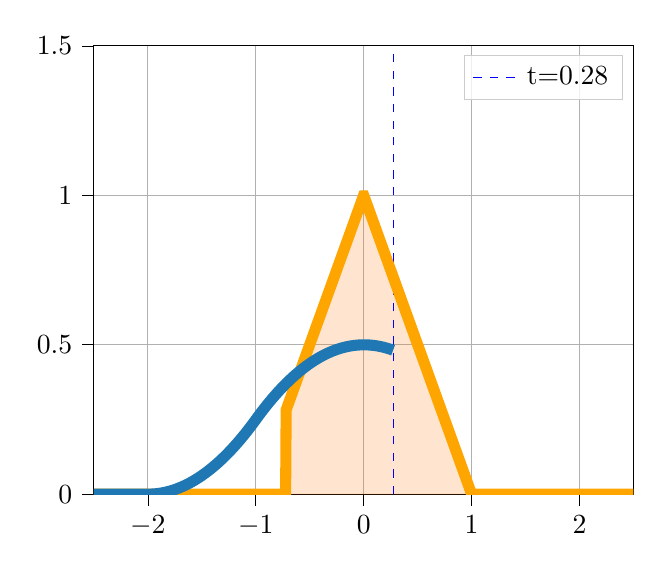
\begin{tikzpicture}

\definecolor{color0}{rgb}{1,0.498039215686275,0.0549019607843137}
\definecolor{color1}{rgb}{1,0.647058823529412,0}
\definecolor{color2}{rgb}{0.12156862745098,0.466666666666667,0.705882352941177}

\begin{axis}[
legend cell align={left},
legend style={fill opacity=0.8, draw opacity=1, text opacity=1, draw=white!80!black},
tick align=outside,
tick pos=left,
x grid style={white!69.0196078431373!black},
xmajorgrids,
xmin=-2.5, xmax=2.5,
xtick style={color=black},
y grid style={white!69.0196078431373!black},
ymajorgrids,
ymin=0, ymax=1.5,
ytick style={color=black}
]
\path [draw=color0, fill=color0, opacity=0.2]
(axis cs:-2.5,0)
--(axis cs:-2.5,0)
--(axis cs:-2.49499499499499,0)
--(axis cs:-2.48998998998999,0)
--(axis cs:-2.48498498498498,0)
--(axis cs:-2.47997997997998,0)
--(axis cs:-2.47497497497497,0)
--(axis cs:-2.46996996996997,0)
--(axis cs:-2.46496496496496,0)
--(axis cs:-2.45995995995996,0)
--(axis cs:-2.45495495495495,0)
--(axis cs:-2.44994994994995,0)
--(axis cs:-2.44494494494494,0)
--(axis cs:-2.43993993993994,0)
--(axis cs:-2.43493493493493,0)
--(axis cs:-2.42992992992993,0)
--(axis cs:-2.42492492492492,0)
--(axis cs:-2.41991991991992,0)
--(axis cs:-2.41491491491491,0)
--(axis cs:-2.40990990990991,0)
--(axis cs:-2.4049049049049,0)
--(axis cs:-2.3998998998999,0)
--(axis cs:-2.39489489489489,0)
--(axis cs:-2.38988988988989,0)
--(axis cs:-2.38488488488488,0)
--(axis cs:-2.37987987987988,0)
--(axis cs:-2.37487487487487,0)
--(axis cs:-2.36986986986987,0)
--(axis cs:-2.36486486486486,0)
--(axis cs:-2.35985985985986,0)
--(axis cs:-2.35485485485485,0)
--(axis cs:-2.34984984984985,0)
--(axis cs:-2.34484484484484,0)
--(axis cs:-2.33983983983984,0)
--(axis cs:-2.33483483483483,0)
--(axis cs:-2.32982982982983,0)
--(axis cs:-2.32482482482482,0)
--(axis cs:-2.31981981981982,0)
--(axis cs:-2.31481481481481,0)
--(axis cs:-2.30980980980981,0)
--(axis cs:-2.3048048048048,0)
--(axis cs:-2.2997997997998,0)
--(axis cs:-2.29479479479479,0)
--(axis cs:-2.28978978978979,0)
--(axis cs:-2.28478478478478,0)
--(axis cs:-2.27977977977978,0)
--(axis cs:-2.27477477477477,0)
--(axis cs:-2.26976976976977,0)
--(axis cs:-2.26476476476476,0)
--(axis cs:-2.25975975975976,0)
--(axis cs:-2.25475475475475,0)
--(axis cs:-2.24974974974975,0)
--(axis cs:-2.24474474474474,0)
--(axis cs:-2.23973973973974,0)
--(axis cs:-2.23473473473473,0)
--(axis cs:-2.22972972972973,0)
--(axis cs:-2.22472472472472,0)
--(axis cs:-2.21971971971972,0)
--(axis cs:-2.21471471471471,0)
--(axis cs:-2.20970970970971,0)
--(axis cs:-2.2047047047047,0)
--(axis cs:-2.1996996996997,0)
--(axis cs:-2.19469469469469,0)
--(axis cs:-2.18968968968969,0)
--(axis cs:-2.18468468468468,0)
--(axis cs:-2.17967967967968,0)
--(axis cs:-2.17467467467467,0)
--(axis cs:-2.16966966966967,0)
--(axis cs:-2.16466466466466,0)
--(axis cs:-2.15965965965966,0)
--(axis cs:-2.15465465465465,0)
--(axis cs:-2.14964964964965,0)
--(axis cs:-2.14464464464464,0)
--(axis cs:-2.13963963963964,0)
--(axis cs:-2.13463463463463,0)
--(axis cs:-2.12962962962963,0)
--(axis cs:-2.12462462462462,0)
--(axis cs:-2.11961961961962,0)
--(axis cs:-2.11461461461461,0)
--(axis cs:-2.10960960960961,0)
--(axis cs:-2.1046046046046,0)
--(axis cs:-2.0995995995996,0)
--(axis cs:-2.09459459459459,0)
--(axis cs:-2.08958958958959,0)
--(axis cs:-2.08458458458458,0)
--(axis cs:-2.07957957957958,0)
--(axis cs:-2.07457457457457,0)
--(axis cs:-2.06956956956957,0)
--(axis cs:-2.06456456456456,0)
--(axis cs:-2.05955955955956,0)
--(axis cs:-2.05455455455455,0)
--(axis cs:-2.04954954954955,0)
--(axis cs:-2.04454454454454,0)
--(axis cs:-2.03953953953954,0)
--(axis cs:-2.03453453453453,0)
--(axis cs:-2.02952952952953,0)
--(axis cs:-2.02452452452452,0)
--(axis cs:-2.01951951951952,0)
--(axis cs:-2.01451451451451,0)
--(axis cs:-2.00950950950951,0)
--(axis cs:-2.0045045045045,0)
--(axis cs:-1.9994994994995,0)
--(axis cs:-1.99449449449449,0)
--(axis cs:-1.98948948948949,0)
--(axis cs:-1.98448448448448,0)
--(axis cs:-1.97947947947948,0)
--(axis cs:-1.97447447447447,0)
--(axis cs:-1.96946946946947,0)
--(axis cs:-1.96446446446446,0)
--(axis cs:-1.95945945945946,0)
--(axis cs:-1.95445445445445,0)
--(axis cs:-1.94944944944945,0)
--(axis cs:-1.94444444444444,0)
--(axis cs:-1.93943943943944,0)
--(axis cs:-1.93443443443443,0)
--(axis cs:-1.92942942942943,0)
--(axis cs:-1.92442442442442,0)
--(axis cs:-1.91941941941942,0)
--(axis cs:-1.91441441441441,0)
--(axis cs:-1.90940940940941,0)
--(axis cs:-1.9044044044044,0)
--(axis cs:-1.8993993993994,0)
--(axis cs:-1.89439439439439,0)
--(axis cs:-1.88938938938939,0)
--(axis cs:-1.88438438438438,0)
--(axis cs:-1.87937937937938,0)
--(axis cs:-1.87437437437437,0)
--(axis cs:-1.86936936936937,0)
--(axis cs:-1.86436436436436,0)
--(axis cs:-1.85935935935936,0)
--(axis cs:-1.85435435435435,0)
--(axis cs:-1.84934934934935,0)
--(axis cs:-1.84434434434434,0)
--(axis cs:-1.83933933933934,0)
--(axis cs:-1.83433433433433,0)
--(axis cs:-1.82932932932933,0)
--(axis cs:-1.82432432432432,0)
--(axis cs:-1.81931931931932,0)
--(axis cs:-1.81431431431431,0)
--(axis cs:-1.80930930930931,0)
--(axis cs:-1.8043043043043,0)
--(axis cs:-1.7992992992993,0)
--(axis cs:-1.79429429429429,0)
--(axis cs:-1.78928928928929,0)
--(axis cs:-1.78428428428428,0)
--(axis cs:-1.77927927927928,0)
--(axis cs:-1.77427427427427,0)
--(axis cs:-1.76926926926927,0)
--(axis cs:-1.76426426426426,0)
--(axis cs:-1.75925925925926,0)
--(axis cs:-1.75425425425425,0)
--(axis cs:-1.74924924924925,0)
--(axis cs:-1.74424424424424,0)
--(axis cs:-1.73923923923924,0)
--(axis cs:-1.73423423423423,0)
--(axis cs:-1.72922922922923,0)
--(axis cs:-1.72422422422422,0)
--(axis cs:-1.71921921921922,0)
--(axis cs:-1.71421421421421,0)
--(axis cs:-1.70920920920921,0)
--(axis cs:-1.7042042042042,0)
--(axis cs:-1.6991991991992,0)
--(axis cs:-1.69419419419419,0)
--(axis cs:-1.68918918918919,0)
--(axis cs:-1.68418418418418,0)
--(axis cs:-1.67917917917918,0)
--(axis cs:-1.67417417417417,0)
--(axis cs:-1.66916916916917,0)
--(axis cs:-1.66416416416416,0)
--(axis cs:-1.65915915915916,0)
--(axis cs:-1.65415415415415,0)
--(axis cs:-1.64914914914915,0)
--(axis cs:-1.64414414414414,0)
--(axis cs:-1.63913913913914,0)
--(axis cs:-1.63413413413413,0)
--(axis cs:-1.62912912912913,0)
--(axis cs:-1.62412412412412,0)
--(axis cs:-1.61911911911912,0)
--(axis cs:-1.61411411411411,0)
--(axis cs:-1.60910910910911,0)
--(axis cs:-1.6041041041041,0)
--(axis cs:-1.5990990990991,0)
--(axis cs:-1.59409409409409,0)
--(axis cs:-1.58908908908909,0)
--(axis cs:-1.58408408408408,0)
--(axis cs:-1.57907907907908,0)
--(axis cs:-1.57407407407407,0)
--(axis cs:-1.56906906906907,0)
--(axis cs:-1.56406406406406,0)
--(axis cs:-1.55905905905906,0)
--(axis cs:-1.55405405405405,0)
--(axis cs:-1.54904904904905,0)
--(axis cs:-1.54404404404404,0)
--(axis cs:-1.53903903903904,0)
--(axis cs:-1.53403403403403,0)
--(axis cs:-1.52902902902903,0)
--(axis cs:-1.52402402402402,0)
--(axis cs:-1.51901901901902,0)
--(axis cs:-1.51401401401401,0)
--(axis cs:-1.50900900900901,0)
--(axis cs:-1.504004004004,0)
--(axis cs:-1.498998998999,0)
--(axis cs:-1.49399399399399,0)
--(axis cs:-1.48898898898899,0)
--(axis cs:-1.48398398398398,0)
--(axis cs:-1.47897897897898,0)
--(axis cs:-1.47397397397397,0)
--(axis cs:-1.46896896896897,0)
--(axis cs:-1.46396396396396,0)
--(axis cs:-1.45895895895896,0)
--(axis cs:-1.45395395395395,0)
--(axis cs:-1.44894894894895,0)
--(axis cs:-1.44394394394394,0)
--(axis cs:-1.43893893893894,0)
--(axis cs:-1.43393393393393,0)
--(axis cs:-1.42892892892893,0)
--(axis cs:-1.42392392392392,0)
--(axis cs:-1.41891891891892,0)
--(axis cs:-1.41391391391391,0)
--(axis cs:-1.40890890890891,0)
--(axis cs:-1.4039039039039,0)
--(axis cs:-1.3988988988989,0)
--(axis cs:-1.39389389389389,0)
--(axis cs:-1.38888888888889,0)
--(axis cs:-1.38388388388388,0)
--(axis cs:-1.37887887887888,0)
--(axis cs:-1.37387387387387,0)
--(axis cs:-1.36886886886887,0)
--(axis cs:-1.36386386386386,0)
--(axis cs:-1.35885885885886,0)
--(axis cs:-1.35385385385385,0)
--(axis cs:-1.34884884884885,0)
--(axis cs:-1.34384384384384,0)
--(axis cs:-1.33883883883884,0)
--(axis cs:-1.33383383383383,0)
--(axis cs:-1.32882882882883,0)
--(axis cs:-1.32382382382382,0)
--(axis cs:-1.31881881881882,0)
--(axis cs:-1.31381381381381,0)
--(axis cs:-1.30880880880881,0)
--(axis cs:-1.3038038038038,0)
--(axis cs:-1.2987987987988,0)
--(axis cs:-1.29379379379379,0)
--(axis cs:-1.28878878878879,0)
--(axis cs:-1.28378378378378,0)
--(axis cs:-1.27877877877878,0)
--(axis cs:-1.27377377377377,0)
--(axis cs:-1.26876876876877,0)
--(axis cs:-1.26376376376376,0)
--(axis cs:-1.25875875875876,0)
--(axis cs:-1.25375375375375,0)
--(axis cs:-1.24874874874875,0)
--(axis cs:-1.24374374374374,0)
--(axis cs:-1.23873873873874,0)
--(axis cs:-1.23373373373373,0)
--(axis cs:-1.22872872872873,0)
--(axis cs:-1.22372372372372,0)
--(axis cs:-1.21871871871872,0)
--(axis cs:-1.21371371371371,0)
--(axis cs:-1.20870870870871,0)
--(axis cs:-1.2037037037037,0)
--(axis cs:-1.1986986986987,0)
--(axis cs:-1.19369369369369,0)
--(axis cs:-1.18868868868869,0)
--(axis cs:-1.18368368368368,0)
--(axis cs:-1.17867867867868,0)
--(axis cs:-1.17367367367367,0)
--(axis cs:-1.16866866866867,0)
--(axis cs:-1.16366366366366,0)
--(axis cs:-1.15865865865866,0)
--(axis cs:-1.15365365365365,0)
--(axis cs:-1.14864864864865,0)
--(axis cs:-1.14364364364364,0)
--(axis cs:-1.13863863863864,0)
--(axis cs:-1.13363363363363,0)
--(axis cs:-1.12862862862863,0)
--(axis cs:-1.12362362362362,0)
--(axis cs:-1.11861861861862,0)
--(axis cs:-1.11361361361361,0)
--(axis cs:-1.10860860860861,0)
--(axis cs:-1.1036036036036,0)
--(axis cs:-1.0985985985986,0)
--(axis cs:-1.09359359359359,0)
--(axis cs:-1.08858858858859,0)
--(axis cs:-1.08358358358358,0)
--(axis cs:-1.07857857857858,0)
--(axis cs:-1.07357357357357,0)
--(axis cs:-1.06856856856857,0)
--(axis cs:-1.06356356356356,0)
--(axis cs:-1.05855855855856,0)
--(axis cs:-1.05355355355355,0)
--(axis cs:-1.04854854854855,0)
--(axis cs:-1.04354354354354,0)
--(axis cs:-1.03853853853854,0)
--(axis cs:-1.03353353353353,0)
--(axis cs:-1.02852852852853,0)
--(axis cs:-1.02352352352352,0)
--(axis cs:-1.01851851851852,0)
--(axis cs:-1.01351351351351,0)
--(axis cs:-1.00850850850851,0)
--(axis cs:-1.0035035035035,0)
--(axis cs:-0.998498498498499,0)
--(axis cs:-0.993493493493494,0)
--(axis cs:-0.988488488488489,0)
--(axis cs:-0.983483483483484,0)
--(axis cs:-0.978478478478479,0)
--(axis cs:-0.973473473473474,0)
--(axis cs:-0.968468468468469,0)
--(axis cs:-0.963463463463464,0)
--(axis cs:-0.958458458458459,0)
--(axis cs:-0.953453453453454,0)
--(axis cs:-0.948448448448449,0)
--(axis cs:-0.943443443443444,0)
--(axis cs:-0.938438438438439,0)
--(axis cs:-0.933433433433434,0)
--(axis cs:-0.928428428428429,0)
--(axis cs:-0.923423423423424,0)
--(axis cs:-0.918418418418419,0)
--(axis cs:-0.913413413413414,0)
--(axis cs:-0.908408408408409,0)
--(axis cs:-0.903403403403404,0)
--(axis cs:-0.898398398398399,0)
--(axis cs:-0.893393393393393,0)
--(axis cs:-0.888388388388388,0)
--(axis cs:-0.883383383383383,0)
--(axis cs:-0.878378378378378,0)
--(axis cs:-0.873373373373373,0)
--(axis cs:-0.868368368368368,0)
--(axis cs:-0.863363363363363,0)
--(axis cs:-0.858358358358358,0)
--(axis cs:-0.853353353353353,0)
--(axis cs:-0.848348348348348,0)
--(axis cs:-0.843343343343343,0)
--(axis cs:-0.838338338338338,0)
--(axis cs:-0.833333333333333,0)
--(axis cs:-0.828328328328328,0)
--(axis cs:-0.823323323323323,0)
--(axis cs:-0.818318318318318,0)
--(axis cs:-0.813313313313313,0)
--(axis cs:-0.808308308308308,0)
--(axis cs:-0.803303303303303,0)
--(axis cs:-0.798298298298298,0)
--(axis cs:-0.793293293293293,0)
--(axis cs:-0.788288288288288,0)
--(axis cs:-0.783283283283283,0)
--(axis cs:-0.778278278278278,0)
--(axis cs:-0.773273273273273,0)
--(axis cs:-0.768268268268268,0)
--(axis cs:-0.763263263263263,0)
--(axis cs:-0.758258258258258,0)
--(axis cs:-0.753253253253253,0)
--(axis cs:-0.748248248248248,0)
--(axis cs:-0.743243243243243,0)
--(axis cs:-0.738238238238238,0)
--(axis cs:-0.733233233233233,0)
--(axis cs:-0.728228228228228,0)
--(axis cs:-0.723223223223223,0)
--(axis cs:-0.718218218218218,0)
--(axis cs:-0.713213213213213,0)
--(axis cs:-0.708208208208208,0)
--(axis cs:-0.703203203203203,0)
--(axis cs:-0.698198198198198,0)
--(axis cs:-0.693193193193193,0)
--(axis cs:-0.688188188188188,0)
--(axis cs:-0.683183183183183,0)
--(axis cs:-0.678178178178178,0)
--(axis cs:-0.673173173173173,0)
--(axis cs:-0.668168168168168,0)
--(axis cs:-0.663163163163163,0)
--(axis cs:-0.658158158158158,0)
--(axis cs:-0.653153153153153,0)
--(axis cs:-0.648148148148148,0)
--(axis cs:-0.643143143143143,0)
--(axis cs:-0.638138138138138,0)
--(axis cs:-0.633133133133133,0)
--(axis cs:-0.628128128128128,0)
--(axis cs:-0.623123123123123,0)
--(axis cs:-0.618118118118118,0)
--(axis cs:-0.613113113113113,0)
--(axis cs:-0.608108108108108,0)
--(axis cs:-0.603103103103103,0)
--(axis cs:-0.598098098098098,0)
--(axis cs:-0.593093093093093,0)
--(axis cs:-0.588088088088088,0)
--(axis cs:-0.583083083083083,0)
--(axis cs:-0.578078078078078,0)
--(axis cs:-0.573073073073073,0)
--(axis cs:-0.568068068068068,0)
--(axis cs:-0.563063063063063,0)
--(axis cs:-0.558058058058058,0)
--(axis cs:-0.553053053053053,0)
--(axis cs:-0.548048048048048,0)
--(axis cs:-0.543043043043043,0)
--(axis cs:-0.538038038038038,0)
--(axis cs:-0.533033033033033,0)
--(axis cs:-0.528028028028028,0)
--(axis cs:-0.523023023023023,0)
--(axis cs:-0.518018018018018,0)
--(axis cs:-0.513013013013013,0)
--(axis cs:-0.508008008008008,0)
--(axis cs:-0.503003003003003,0)
--(axis cs:-0.497997997997998,0)
--(axis cs:-0.492992992992993,0)
--(axis cs:-0.487987987987988,0)
--(axis cs:-0.482982982982983,0)
--(axis cs:-0.477977977977978,0)
--(axis cs:-0.472972972972973,0)
--(axis cs:-0.467967967967968,0)
--(axis cs:-0.462962962962963,0)
--(axis cs:-0.457957957957958,0)
--(axis cs:-0.452952952952953,0)
--(axis cs:-0.447947947947948,0)
--(axis cs:-0.442942942942943,0)
--(axis cs:-0.437937937937938,0)
--(axis cs:-0.432932932932933,0)
--(axis cs:-0.427927927927928,0)
--(axis cs:-0.422922922922923,0)
--(axis cs:-0.417917917917918,0)
--(axis cs:-0.412912912912913,0)
--(axis cs:-0.407907907907908,0)
--(axis cs:-0.402902902902903,0)
--(axis cs:-0.397897897897898,0)
--(axis cs:-0.392892892892893,0)
--(axis cs:-0.387887887887888,0)
--(axis cs:-0.382882882882883,0)
--(axis cs:-0.377877877877878,0)
--(axis cs:-0.372872872872873,0)
--(axis cs:-0.367867867867868,0)
--(axis cs:-0.362862862862863,0)
--(axis cs:-0.357857857857858,0)
--(axis cs:-0.352852852852853,0)
--(axis cs:-0.347847847847848,0)
--(axis cs:-0.342842842842843,0)
--(axis cs:-0.337837837837838,0)
--(axis cs:-0.332832832832833,0)
--(axis cs:-0.327827827827828,0)
--(axis cs:-0.322822822822823,0)
--(axis cs:-0.317817817817818,0)
--(axis cs:-0.312812812812813,0)
--(axis cs:-0.307807807807808,0)
--(axis cs:-0.302802802802803,0)
--(axis cs:-0.297797797797798,0)
--(axis cs:-0.292792792792793,0)
--(axis cs:-0.287787787787788,0)
--(axis cs:-0.282782782782783,0)
--(axis cs:-0.277777777777778,0)
--(axis cs:-0.272772772772773,0)
--(axis cs:-0.267767767767768,0)
--(axis cs:-0.262762762762763,0)
--(axis cs:-0.257757757757758,0)
--(axis cs:-0.252752752752753,0)
--(axis cs:-0.247747747747748,0)
--(axis cs:-0.242742742742743,0)
--(axis cs:-0.237737737737738,0)
--(axis cs:-0.232732732732733,0)
--(axis cs:-0.227727727727728,0)
--(axis cs:-0.222722722722723,0)
--(axis cs:-0.217717717717718,0)
--(axis cs:-0.212712712712713,0)
--(axis cs:-0.207707707707708,0)
--(axis cs:-0.202702702702703,0)
--(axis cs:-0.197697697697698,0)
--(axis cs:-0.192692692692693,0)
--(axis cs:-0.187687687687688,0)
--(axis cs:-0.182682682682683,0)
--(axis cs:-0.177677677677678,0)
--(axis cs:-0.172672672672673,0)
--(axis cs:-0.167667667667668,0)
--(axis cs:-0.162662662662663,0)
--(axis cs:-0.157657657657658,0)
--(axis cs:-0.152652652652653,0)
--(axis cs:-0.147647647647648,0)
--(axis cs:-0.142642642642643,0)
--(axis cs:-0.137637637637638,0)
--(axis cs:-0.132632632632633,0)
--(axis cs:-0.127627627627628,0)
--(axis cs:-0.122622622622623,0)
--(axis cs:-0.117617617617618,0)
--(axis cs:-0.112612612612613,0)
--(axis cs:-0.107607607607608,0)
--(axis cs:-0.102602602602603,0)
--(axis cs:-0.0975975975975976,0)
--(axis cs:-0.0925925925925926,0)
--(axis cs:-0.0875875875875876,0)
--(axis cs:-0.0825825825825826,0)
--(axis cs:-0.0775775775775776,0)
--(axis cs:-0.0725725725725725,0)
--(axis cs:-0.0675675675675675,0)
--(axis cs:-0.0625625625625625,0)
--(axis cs:-0.0575575575575575,0)
--(axis cs:-0.0525525525525525,0)
--(axis cs:-0.0475475475475475,0)
--(axis cs:-0.0425425425425425,0)
--(axis cs:-0.0375375375375375,0)
--(axis cs:-0.0325325325325325,0)
--(axis cs:-0.0275275275275275,0)
--(axis cs:-0.0225225225225225,0)
--(axis cs:-0.0175175175175175,0)
--(axis cs:-0.0125125125125125,0)
--(axis cs:-0.0075075075075075,0)
--(axis cs:-0.0025025025025025,0)
--(axis cs:0.0025025025025025,0)
--(axis cs:0.0075075075075075,0)
--(axis cs:0.0125125125125125,0)
--(axis cs:0.0175175175175175,0)
--(axis cs:0.0225225225225225,0)
--(axis cs:0.0275275275275275,0)
--(axis cs:0.0325325325325325,0)
--(axis cs:0.0375375375375375,0)
--(axis cs:0.0425425425425425,0)
--(axis cs:0.0475475475475475,0)
--(axis cs:0.0525525525525525,0)
--(axis cs:0.0575575575575575,0)
--(axis cs:0.0625625625625625,0)
--(axis cs:0.0675675675675675,0)
--(axis cs:0.0725725725725725,0)
--(axis cs:0.0775775775775776,0)
--(axis cs:0.0825825825825826,0)
--(axis cs:0.0875875875875876,0)
--(axis cs:0.0925925925925926,0)
--(axis cs:0.0975975975975976,0)
--(axis cs:0.102602602602603,0)
--(axis cs:0.107607607607608,0)
--(axis cs:0.112612612612613,0)
--(axis cs:0.117617617617618,0)
--(axis cs:0.122622622622623,0)
--(axis cs:0.127627627627628,0)
--(axis cs:0.132632632632633,0)
--(axis cs:0.137637637637638,0)
--(axis cs:0.142642642642643,0)
--(axis cs:0.147647647647648,0)
--(axis cs:0.152652652652653,0)
--(axis cs:0.157657657657658,0)
--(axis cs:0.162662662662663,0)
--(axis cs:0.167667667667668,0)
--(axis cs:0.172672672672673,0)
--(axis cs:0.177677677677678,0)
--(axis cs:0.182682682682683,0)
--(axis cs:0.187687687687688,0)
--(axis cs:0.192692692692693,0)
--(axis cs:0.197697697697698,0)
--(axis cs:0.202702702702703,0)
--(axis cs:0.207707707707708,0)
--(axis cs:0.212712712712713,0)
--(axis cs:0.217717717717718,0)
--(axis cs:0.222722722722723,0)
--(axis cs:0.227727727727728,0)
--(axis cs:0.232732732732733,0)
--(axis cs:0.237737737737738,0)
--(axis cs:0.242742742742743,0)
--(axis cs:0.247747747747748,0)
--(axis cs:0.252752752752753,0)
--(axis cs:0.257757757757758,0)
--(axis cs:0.262762762762763,0)
--(axis cs:0.267767767767768,0)
--(axis cs:0.272772772772773,0)
--(axis cs:0.277777777777778,0)
--(axis cs:0.282782782782783,0)
--(axis cs:0.287787787787788,0)
--(axis cs:0.292792792792793,0)
--(axis cs:0.297797797797798,0)
--(axis cs:0.302802802802803,0)
--(axis cs:0.307807807807808,0)
--(axis cs:0.312812812812813,0)
--(axis cs:0.317817817817818,0)
--(axis cs:0.322822822822823,0)
--(axis cs:0.327827827827828,0)
--(axis cs:0.332832832832833,0)
--(axis cs:0.337837837837838,0)
--(axis cs:0.342842842842843,0)
--(axis cs:0.347847847847848,0)
--(axis cs:0.352852852852853,0)
--(axis cs:0.357857857857858,0)
--(axis cs:0.362862862862863,0)
--(axis cs:0.367867867867868,0)
--(axis cs:0.372872872872873,0)
--(axis cs:0.377877877877878,0)
--(axis cs:0.382882882882883,0)
--(axis cs:0.387887887887888,0)
--(axis cs:0.392892892892893,0)
--(axis cs:0.397897897897898,0)
--(axis cs:0.402902902902903,0)
--(axis cs:0.407907907907908,0)
--(axis cs:0.412912912912913,0)
--(axis cs:0.417917917917918,0)
--(axis cs:0.422922922922923,0)
--(axis cs:0.427927927927928,0)
--(axis cs:0.432932932932933,0)
--(axis cs:0.437937937937938,0)
--(axis cs:0.442942942942943,0)
--(axis cs:0.447947947947948,0)
--(axis cs:0.452952952952953,0)
--(axis cs:0.457957957957958,0)
--(axis cs:0.462962962962963,0)
--(axis cs:0.467967967967968,0)
--(axis cs:0.472972972972973,0)
--(axis cs:0.477977977977978,0)
--(axis cs:0.482982982982983,0)
--(axis cs:0.487987987987988,0)
--(axis cs:0.492992992992993,0)
--(axis cs:0.497997997997998,0)
--(axis cs:0.503003003003003,0)
--(axis cs:0.508008008008008,0)
--(axis cs:0.513013013013013,0)
--(axis cs:0.518018018018018,0)
--(axis cs:0.523023023023023,0)
--(axis cs:0.528028028028028,0)
--(axis cs:0.533033033033033,0)
--(axis cs:0.538038038038038,0)
--(axis cs:0.543043043043043,0)
--(axis cs:0.548048048048048,0)
--(axis cs:0.553053053053053,0)
--(axis cs:0.558058058058058,0)
--(axis cs:0.563063063063063,0)
--(axis cs:0.568068068068068,0)
--(axis cs:0.573073073073073,0)
--(axis cs:0.578078078078078,0)
--(axis cs:0.583083083083083,0)
--(axis cs:0.588088088088088,0)
--(axis cs:0.593093093093093,0)
--(axis cs:0.598098098098098,0)
--(axis cs:0.603103103103103,0)
--(axis cs:0.608108108108108,0)
--(axis cs:0.613113113113113,0)
--(axis cs:0.618118118118118,0)
--(axis cs:0.623123123123123,0)
--(axis cs:0.628128128128128,0)
--(axis cs:0.633133133133133,0)
--(axis cs:0.638138138138138,0)
--(axis cs:0.643143143143143,0)
--(axis cs:0.648148148148148,0)
--(axis cs:0.653153153153153,0)
--(axis cs:0.658158158158158,0)
--(axis cs:0.663163163163163,0)
--(axis cs:0.668168168168168,0)
--(axis cs:0.673173173173173,0)
--(axis cs:0.678178178178178,0)
--(axis cs:0.683183183183183,0)
--(axis cs:0.688188188188188,0)
--(axis cs:0.693193193193193,0)
--(axis cs:0.698198198198198,0)
--(axis cs:0.703203203203203,0)
--(axis cs:0.708208208208208,0)
--(axis cs:0.713213213213213,0)
--(axis cs:0.718218218218218,0)
--(axis cs:0.723223223223223,0)
--(axis cs:0.728228228228228,0)
--(axis cs:0.733233233233233,0)
--(axis cs:0.738238238238238,0)
--(axis cs:0.743243243243243,0)
--(axis cs:0.748248248248248,0)
--(axis cs:0.753253253253253,0)
--(axis cs:0.758258258258258,0)
--(axis cs:0.763263263263263,0)
--(axis cs:0.768268268268268,0)
--(axis cs:0.773273273273273,0)
--(axis cs:0.778278278278278,0)
--(axis cs:0.783283283283283,0)
--(axis cs:0.788288288288288,0)
--(axis cs:0.793293293293293,0)
--(axis cs:0.798298298298298,0)
--(axis cs:0.803303303303303,0)
--(axis cs:0.808308308308308,0)
--(axis cs:0.813313313313313,0)
--(axis cs:0.818318318318318,0)
--(axis cs:0.823323323323323,0)
--(axis cs:0.828328328328328,0)
--(axis cs:0.833333333333333,0)
--(axis cs:0.838338338338338,0)
--(axis cs:0.843343343343343,0)
--(axis cs:0.848348348348348,0)
--(axis cs:0.853353353353353,0)
--(axis cs:0.858358358358358,0)
--(axis cs:0.863363363363364,0)
--(axis cs:0.868368368368369,0)
--(axis cs:0.873373373373374,0)
--(axis cs:0.878378378378379,0)
--(axis cs:0.883383383383384,0)
--(axis cs:0.888388388388389,0)
--(axis cs:0.893393393393394,0)
--(axis cs:0.898398398398399,0)
--(axis cs:0.903403403403404,0)
--(axis cs:0.908408408408409,0)
--(axis cs:0.913413413413414,0)
--(axis cs:0.918418418418419,0)
--(axis cs:0.923423423423424,0)
--(axis cs:0.928428428428429,0)
--(axis cs:0.933433433433434,0)
--(axis cs:0.938438438438439,0)
--(axis cs:0.943443443443444,0)
--(axis cs:0.948448448448449,0)
--(axis cs:0.953453453453454,0)
--(axis cs:0.958458458458459,0)
--(axis cs:0.963463463463464,0)
--(axis cs:0.968468468468469,0)
--(axis cs:0.973473473473474,0)
--(axis cs:0.978478478478479,0)
--(axis cs:0.983483483483484,0)
--(axis cs:0.988488488488489,0)
--(axis cs:0.993493493493494,0)
--(axis cs:0.998498498498499,0)
--(axis cs:1.0035035035035,0)
--(axis cs:1.00850850850851,0)
--(axis cs:1.01351351351351,0)
--(axis cs:1.01851851851852,0)
--(axis cs:1.02352352352352,0)
--(axis cs:1.02852852852853,0)
--(axis cs:1.03353353353353,0)
--(axis cs:1.03853853853854,0)
--(axis cs:1.04354354354354,0)
--(axis cs:1.04854854854855,0)
--(axis cs:1.05355355355355,0)
--(axis cs:1.05855855855856,0)
--(axis cs:1.06356356356356,0)
--(axis cs:1.06856856856857,0)
--(axis cs:1.07357357357357,0)
--(axis cs:1.07857857857858,0)
--(axis cs:1.08358358358358,0)
--(axis cs:1.08858858858859,0)
--(axis cs:1.09359359359359,0)
--(axis cs:1.0985985985986,0)
--(axis cs:1.1036036036036,0)
--(axis cs:1.10860860860861,0)
--(axis cs:1.11361361361361,0)
--(axis cs:1.11861861861862,0)
--(axis cs:1.12362362362362,0)
--(axis cs:1.12862862862863,0)
--(axis cs:1.13363363363363,0)
--(axis cs:1.13863863863864,0)
--(axis cs:1.14364364364364,0)
--(axis cs:1.14864864864865,0)
--(axis cs:1.15365365365365,0)
--(axis cs:1.15865865865866,0)
--(axis cs:1.16366366366366,0)
--(axis cs:1.16866866866867,0)
--(axis cs:1.17367367367367,0)
--(axis cs:1.17867867867868,0)
--(axis cs:1.18368368368368,0)
--(axis cs:1.18868868868869,0)
--(axis cs:1.19369369369369,0)
--(axis cs:1.1986986986987,0)
--(axis cs:1.2037037037037,0)
--(axis cs:1.20870870870871,0)
--(axis cs:1.21371371371371,0)
--(axis cs:1.21871871871872,0)
--(axis cs:1.22372372372372,0)
--(axis cs:1.22872872872873,0)
--(axis cs:1.23373373373373,0)
--(axis cs:1.23873873873874,0)
--(axis cs:1.24374374374374,0)
--(axis cs:1.24874874874875,0)
--(axis cs:1.25375375375375,0)
--(axis cs:1.25875875875876,0)
--(axis cs:1.26376376376376,0)
--(axis cs:1.26876876876877,0)
--(axis cs:1.27377377377377,0)
--(axis cs:1.27877877877878,0)
--(axis cs:1.28378378378378,0)
--(axis cs:1.28878878878879,0)
--(axis cs:1.29379379379379,0)
--(axis cs:1.2987987987988,0)
--(axis cs:1.3038038038038,0)
--(axis cs:1.30880880880881,0)
--(axis cs:1.31381381381381,0)
--(axis cs:1.31881881881882,0)
--(axis cs:1.32382382382382,0)
--(axis cs:1.32882882882883,0)
--(axis cs:1.33383383383383,0)
--(axis cs:1.33883883883884,0)
--(axis cs:1.34384384384384,0)
--(axis cs:1.34884884884885,0)
--(axis cs:1.35385385385385,0)
--(axis cs:1.35885885885886,0)
--(axis cs:1.36386386386386,0)
--(axis cs:1.36886886886887,0)
--(axis cs:1.37387387387387,0)
--(axis cs:1.37887887887888,0)
--(axis cs:1.38388388388388,0)
--(axis cs:1.38888888888889,0)
--(axis cs:1.39389389389389,0)
--(axis cs:1.3988988988989,0)
--(axis cs:1.4039039039039,0)
--(axis cs:1.40890890890891,0)
--(axis cs:1.41391391391391,0)
--(axis cs:1.41891891891892,0)
--(axis cs:1.42392392392392,0)
--(axis cs:1.42892892892893,0)
--(axis cs:1.43393393393393,0)
--(axis cs:1.43893893893894,0)
--(axis cs:1.44394394394394,0)
--(axis cs:1.44894894894895,0)
--(axis cs:1.45395395395395,0)
--(axis cs:1.45895895895896,0)
--(axis cs:1.46396396396396,0)
--(axis cs:1.46896896896897,0)
--(axis cs:1.47397397397397,0)
--(axis cs:1.47897897897898,0)
--(axis cs:1.48398398398398,0)
--(axis cs:1.48898898898899,0)
--(axis cs:1.49399399399399,0)
--(axis cs:1.498998998999,0)
--(axis cs:1.504004004004,0)
--(axis cs:1.50900900900901,0)
--(axis cs:1.51401401401401,0)
--(axis cs:1.51901901901902,0)
--(axis cs:1.52402402402402,0)
--(axis cs:1.52902902902903,0)
--(axis cs:1.53403403403403,0)
--(axis cs:1.53903903903904,0)
--(axis cs:1.54404404404404,0)
--(axis cs:1.54904904904905,0)
--(axis cs:1.55405405405405,0)
--(axis cs:1.55905905905906,0)
--(axis cs:1.56406406406406,0)
--(axis cs:1.56906906906907,0)
--(axis cs:1.57407407407407,0)
--(axis cs:1.57907907907908,0)
--(axis cs:1.58408408408408,0)
--(axis cs:1.58908908908909,0)
--(axis cs:1.59409409409409,0)
--(axis cs:1.5990990990991,0)
--(axis cs:1.6041041041041,0)
--(axis cs:1.60910910910911,0)
--(axis cs:1.61411411411411,0)
--(axis cs:1.61911911911912,0)
--(axis cs:1.62412412412412,0)
--(axis cs:1.62912912912913,0)
--(axis cs:1.63413413413413,0)
--(axis cs:1.63913913913914,0)
--(axis cs:1.64414414414414,0)
--(axis cs:1.64914914914915,0)
--(axis cs:1.65415415415415,0)
--(axis cs:1.65915915915916,0)
--(axis cs:1.66416416416416,0)
--(axis cs:1.66916916916917,0)
--(axis cs:1.67417417417417,0)
--(axis cs:1.67917917917918,0)
--(axis cs:1.68418418418418,0)
--(axis cs:1.68918918918919,0)
--(axis cs:1.69419419419419,0)
--(axis cs:1.6991991991992,0)
--(axis cs:1.7042042042042,0)
--(axis cs:1.70920920920921,0)
--(axis cs:1.71421421421421,0)
--(axis cs:1.71921921921922,0)
--(axis cs:1.72422422422422,0)
--(axis cs:1.72922922922923,0)
--(axis cs:1.73423423423423,0)
--(axis cs:1.73923923923924,0)
--(axis cs:1.74424424424424,0)
--(axis cs:1.74924924924925,0)
--(axis cs:1.75425425425425,0)
--(axis cs:1.75925925925926,0)
--(axis cs:1.76426426426426,0)
--(axis cs:1.76926926926927,0)
--(axis cs:1.77427427427427,0)
--(axis cs:1.77927927927928,0)
--(axis cs:1.78428428428428,0)
--(axis cs:1.78928928928929,0)
--(axis cs:1.79429429429429,0)
--(axis cs:1.7992992992993,0)
--(axis cs:1.8043043043043,0)
--(axis cs:1.80930930930931,0)
--(axis cs:1.81431431431431,0)
--(axis cs:1.81931931931932,0)
--(axis cs:1.82432432432432,0)
--(axis cs:1.82932932932933,0)
--(axis cs:1.83433433433433,0)
--(axis cs:1.83933933933934,0)
--(axis cs:1.84434434434434,0)
--(axis cs:1.84934934934935,0)
--(axis cs:1.85435435435435,0)
--(axis cs:1.85935935935936,0)
--(axis cs:1.86436436436436,0)
--(axis cs:1.86936936936937,0)
--(axis cs:1.87437437437437,0)
--(axis cs:1.87937937937938,0)
--(axis cs:1.88438438438438,0)
--(axis cs:1.88938938938939,0)
--(axis cs:1.89439439439439,0)
--(axis cs:1.8993993993994,0)
--(axis cs:1.9044044044044,0)
--(axis cs:1.90940940940941,0)
--(axis cs:1.91441441441441,0)
--(axis cs:1.91941941941942,0)
--(axis cs:1.92442442442442,0)
--(axis cs:1.92942942942943,0)
--(axis cs:1.93443443443443,0)
--(axis cs:1.93943943943944,0)
--(axis cs:1.94444444444444,0)
--(axis cs:1.94944944944945,0)
--(axis cs:1.95445445445445,0)
--(axis cs:1.95945945945946,0)
--(axis cs:1.96446446446446,0)
--(axis cs:1.96946946946947,0)
--(axis cs:1.97447447447447,0)
--(axis cs:1.97947947947948,0)
--(axis cs:1.98448448448448,0)
--(axis cs:1.98948948948949,0)
--(axis cs:1.99449449449449,0)
--(axis cs:1.9994994994995,0)
--(axis cs:2.0045045045045,0)
--(axis cs:2.00950950950951,0)
--(axis cs:2.01451451451451,0)
--(axis cs:2.01951951951952,0)
--(axis cs:2.02452452452452,0)
--(axis cs:2.02952952952953,0)
--(axis cs:2.03453453453453,0)
--(axis cs:2.03953953953954,0)
--(axis cs:2.04454454454454,0)
--(axis cs:2.04954954954955,0)
--(axis cs:2.05455455455455,0)
--(axis cs:2.05955955955956,0)
--(axis cs:2.06456456456456,0)
--(axis cs:2.06956956956957,0)
--(axis cs:2.07457457457457,0)
--(axis cs:2.07957957957958,0)
--(axis cs:2.08458458458458,0)
--(axis cs:2.08958958958959,0)
--(axis cs:2.09459459459459,0)
--(axis cs:2.0995995995996,0)
--(axis cs:2.1046046046046,0)
--(axis cs:2.10960960960961,0)
--(axis cs:2.11461461461461,0)
--(axis cs:2.11961961961962,0)
--(axis cs:2.12462462462462,0)
--(axis cs:2.12962962962963,0)
--(axis cs:2.13463463463463,0)
--(axis cs:2.13963963963964,0)
--(axis cs:2.14464464464464,0)
--(axis cs:2.14964964964965,0)
--(axis cs:2.15465465465465,0)
--(axis cs:2.15965965965966,0)
--(axis cs:2.16466466466466,0)
--(axis cs:2.16966966966967,0)
--(axis cs:2.17467467467467,0)
--(axis cs:2.17967967967968,0)
--(axis cs:2.18468468468468,0)
--(axis cs:2.18968968968969,0)
--(axis cs:2.19469469469469,0)
--(axis cs:2.1996996996997,0)
--(axis cs:2.2047047047047,0)
--(axis cs:2.20970970970971,0)
--(axis cs:2.21471471471471,0)
--(axis cs:2.21971971971972,0)
--(axis cs:2.22472472472472,0)
--(axis cs:2.22972972972973,0)
--(axis cs:2.23473473473473,0)
--(axis cs:2.23973973973974,0)
--(axis cs:2.24474474474474,0)
--(axis cs:2.24974974974975,0)
--(axis cs:2.25475475475475,0)
--(axis cs:2.25975975975976,0)
--(axis cs:2.26476476476476,0)
--(axis cs:2.26976976976977,0)
--(axis cs:2.27477477477477,0)
--(axis cs:2.27977977977978,0)
--(axis cs:2.28478478478478,0)
--(axis cs:2.28978978978979,0)
--(axis cs:2.29479479479479,0)
--(axis cs:2.2997997997998,0)
--(axis cs:2.3048048048048,0)
--(axis cs:2.30980980980981,0)
--(axis cs:2.31481481481481,0)
--(axis cs:2.31981981981982,0)
--(axis cs:2.32482482482482,0)
--(axis cs:2.32982982982983,0)
--(axis cs:2.33483483483483,0)
--(axis cs:2.33983983983984,0)
--(axis cs:2.34484484484484,0)
--(axis cs:2.34984984984985,0)
--(axis cs:2.35485485485485,0)
--(axis cs:2.35985985985986,0)
--(axis cs:2.36486486486486,0)
--(axis cs:2.36986986986987,0)
--(axis cs:2.37487487487487,0)
--(axis cs:2.37987987987988,0)
--(axis cs:2.38488488488488,0)
--(axis cs:2.38988988988989,0)
--(axis cs:2.39489489489489,0)
--(axis cs:2.3998998998999,0)
--(axis cs:2.4049049049049,0)
--(axis cs:2.40990990990991,0)
--(axis cs:2.41491491491491,0)
--(axis cs:2.41991991991992,0)
--(axis cs:2.42492492492492,0)
--(axis cs:2.42992992992993,0)
--(axis cs:2.43493493493493,0)
--(axis cs:2.43993993993994,0)
--(axis cs:2.44494494494494,0)
--(axis cs:2.44994994994995,0)
--(axis cs:2.45495495495495,0)
--(axis cs:2.45995995995996,0)
--(axis cs:2.46496496496496,0)
--(axis cs:2.46996996996997,0)
--(axis cs:2.47497497497497,0)
--(axis cs:2.47997997997998,0)
--(axis cs:2.48498498498498,0)
--(axis cs:2.48998998998999,0)
--(axis cs:2.49499499499499,0)
--(axis cs:2.5,0)
--(axis cs:2.5,0)
--(axis cs:2.5,0)
--(axis cs:2.49499499499499,0)
--(axis cs:2.48998998998999,0)
--(axis cs:2.48498498498498,0)
--(axis cs:2.47997997997998,0)
--(axis cs:2.47497497497497,0)
--(axis cs:2.46996996996997,0)
--(axis cs:2.46496496496496,0)
--(axis cs:2.45995995995996,0)
--(axis cs:2.45495495495495,0)
--(axis cs:2.44994994994995,0)
--(axis cs:2.44494494494494,0)
--(axis cs:2.43993993993994,0)
--(axis cs:2.43493493493493,0)
--(axis cs:2.42992992992993,0)
--(axis cs:2.42492492492492,0)
--(axis cs:2.41991991991992,0)
--(axis cs:2.41491491491491,0)
--(axis cs:2.40990990990991,0)
--(axis cs:2.4049049049049,0)
--(axis cs:2.3998998998999,0)
--(axis cs:2.39489489489489,0)
--(axis cs:2.38988988988989,0)
--(axis cs:2.38488488488488,0)
--(axis cs:2.37987987987988,0)
--(axis cs:2.37487487487487,0)
--(axis cs:2.36986986986987,0)
--(axis cs:2.36486486486486,0)
--(axis cs:2.35985985985986,0)
--(axis cs:2.35485485485485,0)
--(axis cs:2.34984984984985,0)
--(axis cs:2.34484484484484,0)
--(axis cs:2.33983983983984,0)
--(axis cs:2.33483483483483,0)
--(axis cs:2.32982982982983,0)
--(axis cs:2.32482482482482,0)
--(axis cs:2.31981981981982,0)
--(axis cs:2.31481481481481,0)
--(axis cs:2.30980980980981,0)
--(axis cs:2.3048048048048,0)
--(axis cs:2.2997997997998,0)
--(axis cs:2.29479479479479,0)
--(axis cs:2.28978978978979,0)
--(axis cs:2.28478478478478,0)
--(axis cs:2.27977977977978,0)
--(axis cs:2.27477477477477,0)
--(axis cs:2.26976976976977,0)
--(axis cs:2.26476476476476,0)
--(axis cs:2.25975975975976,0)
--(axis cs:2.25475475475475,0)
--(axis cs:2.24974974974975,0)
--(axis cs:2.24474474474474,0)
--(axis cs:2.23973973973974,0)
--(axis cs:2.23473473473473,0)
--(axis cs:2.22972972972973,0)
--(axis cs:2.22472472472472,0)
--(axis cs:2.21971971971972,0)
--(axis cs:2.21471471471471,0)
--(axis cs:2.20970970970971,0)
--(axis cs:2.2047047047047,0)
--(axis cs:2.1996996996997,0)
--(axis cs:2.19469469469469,0)
--(axis cs:2.18968968968969,0)
--(axis cs:2.18468468468468,0)
--(axis cs:2.17967967967968,0)
--(axis cs:2.17467467467467,0)
--(axis cs:2.16966966966967,0)
--(axis cs:2.16466466466466,0)
--(axis cs:2.15965965965966,0)
--(axis cs:2.15465465465465,0)
--(axis cs:2.14964964964965,0)
--(axis cs:2.14464464464464,0)
--(axis cs:2.13963963963964,0)
--(axis cs:2.13463463463463,0)
--(axis cs:2.12962962962963,0)
--(axis cs:2.12462462462462,0)
--(axis cs:2.11961961961962,0)
--(axis cs:2.11461461461461,0)
--(axis cs:2.10960960960961,0)
--(axis cs:2.1046046046046,0)
--(axis cs:2.0995995995996,0)
--(axis cs:2.09459459459459,0)
--(axis cs:2.08958958958959,0)
--(axis cs:2.08458458458458,0)
--(axis cs:2.07957957957958,0)
--(axis cs:2.07457457457457,0)
--(axis cs:2.06956956956957,0)
--(axis cs:2.06456456456456,0)
--(axis cs:2.05955955955956,0)
--(axis cs:2.05455455455455,0)
--(axis cs:2.04954954954955,0)
--(axis cs:2.04454454454454,0)
--(axis cs:2.03953953953954,0)
--(axis cs:2.03453453453453,0)
--(axis cs:2.02952952952953,0)
--(axis cs:2.02452452452452,0)
--(axis cs:2.01951951951952,0)
--(axis cs:2.01451451451451,0)
--(axis cs:2.00950950950951,0)
--(axis cs:2.0045045045045,0)
--(axis cs:1.9994994994995,0)
--(axis cs:1.99449449449449,0)
--(axis cs:1.98948948948949,0)
--(axis cs:1.98448448448448,0)
--(axis cs:1.97947947947948,0)
--(axis cs:1.97447447447447,0)
--(axis cs:1.96946946946947,0)
--(axis cs:1.96446446446446,0)
--(axis cs:1.95945945945946,0)
--(axis cs:1.95445445445445,0)
--(axis cs:1.94944944944945,0)
--(axis cs:1.94444444444444,0)
--(axis cs:1.93943943943944,0)
--(axis cs:1.93443443443443,0)
--(axis cs:1.92942942942943,0)
--(axis cs:1.92442442442442,0)
--(axis cs:1.91941941941942,0)
--(axis cs:1.91441441441441,0)
--(axis cs:1.90940940940941,0)
--(axis cs:1.9044044044044,0)
--(axis cs:1.8993993993994,0)
--(axis cs:1.89439439439439,0)
--(axis cs:1.88938938938939,0)
--(axis cs:1.88438438438438,0)
--(axis cs:1.87937937937938,0)
--(axis cs:1.87437437437437,0)
--(axis cs:1.86936936936937,0)
--(axis cs:1.86436436436436,0)
--(axis cs:1.85935935935936,0)
--(axis cs:1.85435435435435,0)
--(axis cs:1.84934934934935,0)
--(axis cs:1.84434434434434,0)
--(axis cs:1.83933933933934,0)
--(axis cs:1.83433433433433,0)
--(axis cs:1.82932932932933,0)
--(axis cs:1.82432432432432,0)
--(axis cs:1.81931931931932,0)
--(axis cs:1.81431431431431,0)
--(axis cs:1.80930930930931,0)
--(axis cs:1.8043043043043,0)
--(axis cs:1.7992992992993,0)
--(axis cs:1.79429429429429,0)
--(axis cs:1.78928928928929,0)
--(axis cs:1.78428428428428,0)
--(axis cs:1.77927927927928,0)
--(axis cs:1.77427427427427,0)
--(axis cs:1.76926926926927,0)
--(axis cs:1.76426426426426,0)
--(axis cs:1.75925925925926,0)
--(axis cs:1.75425425425425,0)
--(axis cs:1.74924924924925,0)
--(axis cs:1.74424424424424,0)
--(axis cs:1.73923923923924,0)
--(axis cs:1.73423423423423,0)
--(axis cs:1.72922922922923,0)
--(axis cs:1.72422422422422,0)
--(axis cs:1.71921921921922,0)
--(axis cs:1.71421421421421,0)
--(axis cs:1.70920920920921,0)
--(axis cs:1.7042042042042,0)
--(axis cs:1.6991991991992,0)
--(axis cs:1.69419419419419,0)
--(axis cs:1.68918918918919,0)
--(axis cs:1.68418418418418,0)
--(axis cs:1.67917917917918,0)
--(axis cs:1.67417417417417,0)
--(axis cs:1.66916916916917,0)
--(axis cs:1.66416416416416,0)
--(axis cs:1.65915915915916,0)
--(axis cs:1.65415415415415,0)
--(axis cs:1.64914914914915,0)
--(axis cs:1.64414414414414,0)
--(axis cs:1.63913913913914,0)
--(axis cs:1.63413413413413,0)
--(axis cs:1.62912912912913,0)
--(axis cs:1.62412412412412,0)
--(axis cs:1.61911911911912,0)
--(axis cs:1.61411411411411,0)
--(axis cs:1.60910910910911,0)
--(axis cs:1.6041041041041,0)
--(axis cs:1.5990990990991,0)
--(axis cs:1.59409409409409,0)
--(axis cs:1.58908908908909,0)
--(axis cs:1.58408408408408,0)
--(axis cs:1.57907907907908,0)
--(axis cs:1.57407407407407,0)
--(axis cs:1.56906906906907,0)
--(axis cs:1.56406406406406,0)
--(axis cs:1.55905905905906,0)
--(axis cs:1.55405405405405,0)
--(axis cs:1.54904904904905,0)
--(axis cs:1.54404404404404,0)
--(axis cs:1.53903903903904,0)
--(axis cs:1.53403403403403,0)
--(axis cs:1.52902902902903,0)
--(axis cs:1.52402402402402,0)
--(axis cs:1.51901901901902,0)
--(axis cs:1.51401401401401,0)
--(axis cs:1.50900900900901,0)
--(axis cs:1.504004004004,0)
--(axis cs:1.498998998999,0)
--(axis cs:1.49399399399399,0)
--(axis cs:1.48898898898899,0)
--(axis cs:1.48398398398398,0)
--(axis cs:1.47897897897898,0)
--(axis cs:1.47397397397397,0)
--(axis cs:1.46896896896897,0)
--(axis cs:1.46396396396396,0)
--(axis cs:1.45895895895896,0)
--(axis cs:1.45395395395395,0)
--(axis cs:1.44894894894895,0)
--(axis cs:1.44394394394394,0)
--(axis cs:1.43893893893894,0)
--(axis cs:1.43393393393393,0)
--(axis cs:1.42892892892893,0)
--(axis cs:1.42392392392392,0)
--(axis cs:1.41891891891892,0)
--(axis cs:1.41391391391391,0)
--(axis cs:1.40890890890891,0)
--(axis cs:1.4039039039039,0)
--(axis cs:1.3988988988989,0)
--(axis cs:1.39389389389389,0)
--(axis cs:1.38888888888889,0)
--(axis cs:1.38388388388388,0)
--(axis cs:1.37887887887888,0)
--(axis cs:1.37387387387387,0)
--(axis cs:1.36886886886887,0)
--(axis cs:1.36386386386386,0)
--(axis cs:1.35885885885886,0)
--(axis cs:1.35385385385385,0)
--(axis cs:1.34884884884885,0)
--(axis cs:1.34384384384384,0)
--(axis cs:1.33883883883884,0)
--(axis cs:1.33383383383383,0)
--(axis cs:1.32882882882883,0)
--(axis cs:1.32382382382382,0)
--(axis cs:1.31881881881882,0)
--(axis cs:1.31381381381381,0)
--(axis cs:1.30880880880881,0)
--(axis cs:1.3038038038038,0)
--(axis cs:1.2987987987988,0)
--(axis cs:1.29379379379379,0)
--(axis cs:1.28878878878879,0)
--(axis cs:1.28378378378378,0)
--(axis cs:1.27877877877878,0)
--(axis cs:1.27377377377377,0)
--(axis cs:1.26876876876877,0)
--(axis cs:1.26376376376376,0)
--(axis cs:1.25875875875876,0)
--(axis cs:1.25375375375375,0)
--(axis cs:1.24874874874875,0)
--(axis cs:1.24374374374374,0)
--(axis cs:1.23873873873874,0)
--(axis cs:1.23373373373373,0)
--(axis cs:1.22872872872873,0)
--(axis cs:1.22372372372372,0)
--(axis cs:1.21871871871872,0)
--(axis cs:1.21371371371371,0)
--(axis cs:1.20870870870871,0)
--(axis cs:1.2037037037037,0)
--(axis cs:1.1986986986987,0)
--(axis cs:1.19369369369369,0)
--(axis cs:1.18868868868869,0)
--(axis cs:1.18368368368368,0)
--(axis cs:1.17867867867868,0)
--(axis cs:1.17367367367367,0)
--(axis cs:1.16866866866867,0)
--(axis cs:1.16366366366366,0)
--(axis cs:1.15865865865866,0)
--(axis cs:1.15365365365365,0)
--(axis cs:1.14864864864865,0)
--(axis cs:1.14364364364364,0)
--(axis cs:1.13863863863864,0)
--(axis cs:1.13363363363363,0)
--(axis cs:1.12862862862863,0)
--(axis cs:1.12362362362362,0)
--(axis cs:1.11861861861862,0)
--(axis cs:1.11361361361361,0)
--(axis cs:1.10860860860861,0)
--(axis cs:1.1036036036036,0)
--(axis cs:1.0985985985986,0)
--(axis cs:1.09359359359359,0)
--(axis cs:1.08858858858859,0)
--(axis cs:1.08358358358358,0)
--(axis cs:1.07857857857858,0)
--(axis cs:1.07357357357357,0)
--(axis cs:1.06856856856857,0)
--(axis cs:1.06356356356356,0)
--(axis cs:1.05855855855856,0)
--(axis cs:1.05355355355355,0)
--(axis cs:1.04854854854855,0)
--(axis cs:1.04354354354354,0)
--(axis cs:1.03853853853854,0)
--(axis cs:1.03353353353353,0)
--(axis cs:1.02852852852853,0)
--(axis cs:1.02352352352352,0)
--(axis cs:1.01851851851852,0)
--(axis cs:1.01351351351351,0)
--(axis cs:1.00850850850851,0)
--(axis cs:1.0035035035035,0)
--(axis cs:0.998498498498499,0.00150150150150141)
--(axis cs:0.993493493493494,0.00650650650650642)
--(axis cs:0.988488488488489,0.0115115115115114)
--(axis cs:0.983483483483484,0.0165165165165164)
--(axis cs:0.978478478478479,0.0215215215215214)
--(axis cs:0.973473473473474,0.0265265265265264)
--(axis cs:0.968468468468469,0.0315315315315314)
--(axis cs:0.963463463463464,0.0365365365365364)
--(axis cs:0.958458458458459,0.0415415415415414)
--(axis cs:0.953453453453454,0.0465465465465464)
--(axis cs:0.948448448448449,0.0515515515515514)
--(axis cs:0.943443443443444,0.0565565565565564)
--(axis cs:0.938438438438439,0.0615615615615615)
--(axis cs:0.933433433433434,0.0665665665665665)
--(axis cs:0.928428428428429,0.0715715715715715)
--(axis cs:0.923423423423424,0.0765765765765765)
--(axis cs:0.918418418418419,0.0815815815815815)
--(axis cs:0.913413413413414,0.0865865865865865)
--(axis cs:0.908408408408409,0.0915915915915915)
--(axis cs:0.903403403403404,0.0965965965965965)
--(axis cs:0.898398398398399,0.101601601601601)
--(axis cs:0.893393393393394,0.106606606606606)
--(axis cs:0.888388388388389,0.111611611611611)
--(axis cs:0.883383383383384,0.116616616616616)
--(axis cs:0.878378378378379,0.121621621621621)
--(axis cs:0.873373373373374,0.126626626626626)
--(axis cs:0.868368368368369,0.131631631631631)
--(axis cs:0.863363363363364,0.136636636636636)
--(axis cs:0.858358358358358,0.141641641641642)
--(axis cs:0.853353353353353,0.146646646646647)
--(axis cs:0.848348348348348,0.151651651651652)
--(axis cs:0.843343343343343,0.156656656656657)
--(axis cs:0.838338338338338,0.161661661661662)
--(axis cs:0.833333333333333,0.166666666666667)
--(axis cs:0.828328328328328,0.171671671671672)
--(axis cs:0.823323323323323,0.176676676676677)
--(axis cs:0.818318318318318,0.181681681681682)
--(axis cs:0.813313313313313,0.186686686686687)
--(axis cs:0.808308308308308,0.191691691691692)
--(axis cs:0.803303303303303,0.196696696696697)
--(axis cs:0.798298298298298,0.201701701701702)
--(axis cs:0.793293293293293,0.206706706706707)
--(axis cs:0.788288288288288,0.211711711711712)
--(axis cs:0.783283283283283,0.216716716716717)
--(axis cs:0.778278278278278,0.221721721721722)
--(axis cs:0.773273273273273,0.226726726726727)
--(axis cs:0.768268268268268,0.231731731731732)
--(axis cs:0.763263263263263,0.236736736736737)
--(axis cs:0.758258258258258,0.241741741741742)
--(axis cs:0.753253253253253,0.246746746746747)
--(axis cs:0.748248248248248,0.251751751751752)
--(axis cs:0.743243243243243,0.256756756756757)
--(axis cs:0.738238238238238,0.261761761761762)
--(axis cs:0.733233233233233,0.266766766766767)
--(axis cs:0.728228228228228,0.271771771771772)
--(axis cs:0.723223223223223,0.276776776776777)
--(axis cs:0.718218218218218,0.281781781781782)
--(axis cs:0.713213213213213,0.286786786786787)
--(axis cs:0.708208208208208,0.291791791791792)
--(axis cs:0.703203203203203,0.296796796796797)
--(axis cs:0.698198198198198,0.301801801801802)
--(axis cs:0.693193193193193,0.306806806806807)
--(axis cs:0.688188188188188,0.311811811811812)
--(axis cs:0.683183183183183,0.316816816816817)
--(axis cs:0.678178178178178,0.321821821821822)
--(axis cs:0.673173173173173,0.326826826826827)
--(axis cs:0.668168168168168,0.331831831831832)
--(axis cs:0.663163163163163,0.336836836836837)
--(axis cs:0.658158158158158,0.341841841841842)
--(axis cs:0.653153153153153,0.346846846846847)
--(axis cs:0.648148148148148,0.351851851851852)
--(axis cs:0.643143143143143,0.356856856856857)
--(axis cs:0.638138138138138,0.361861861861862)
--(axis cs:0.633133133133133,0.366866866866867)
--(axis cs:0.628128128128128,0.371871871871872)
--(axis cs:0.623123123123123,0.376876876876877)
--(axis cs:0.618118118118118,0.381881881881882)
--(axis cs:0.613113113113113,0.386886886886887)
--(axis cs:0.608108108108108,0.391891891891892)
--(axis cs:0.603103103103103,0.396896896896897)
--(axis cs:0.598098098098098,0.401901901901902)
--(axis cs:0.593093093093093,0.406906906906907)
--(axis cs:0.588088088088088,0.411911911911912)
--(axis cs:0.583083083083083,0.416916916916917)
--(axis cs:0.578078078078078,0.421921921921922)
--(axis cs:0.573073073073073,0.426926926926927)
--(axis cs:0.568068068068068,0.431931931931932)
--(axis cs:0.563063063063063,0.436936936936937)
--(axis cs:0.558058058058058,0.441941941941942)
--(axis cs:0.553053053053053,0.446946946946947)
--(axis cs:0.548048048048048,0.451951951951952)
--(axis cs:0.543043043043043,0.456956956956957)
--(axis cs:0.538038038038038,0.461961961961962)
--(axis cs:0.533033033033033,0.466966966966967)
--(axis cs:0.528028028028028,0.471971971971972)
--(axis cs:0.523023023023023,0.476976976976977)
--(axis cs:0.518018018018018,0.481981981981982)
--(axis cs:0.513013013013013,0.486986986986987)
--(axis cs:0.508008008008008,0.491991991991992)
--(axis cs:0.503003003003003,0.496996996996997)
--(axis cs:0.497997997997998,0.502002002002002)
--(axis cs:0.492992992992993,0.507007007007007)
--(axis cs:0.487987987987988,0.512012012012012)
--(axis cs:0.482982982982983,0.517017017017017)
--(axis cs:0.477977977977978,0.522022022022022)
--(axis cs:0.472972972972973,0.527027027027027)
--(axis cs:0.467967967967968,0.532032032032032)
--(axis cs:0.462962962962963,0.537037037037037)
--(axis cs:0.457957957957958,0.542042042042042)
--(axis cs:0.452952952952953,0.547047047047047)
--(axis cs:0.447947947947948,0.552052052052052)
--(axis cs:0.442942942942943,0.557057057057057)
--(axis cs:0.437937937937938,0.562062062062062)
--(axis cs:0.432932932932933,0.567067067067067)
--(axis cs:0.427927927927928,0.572072072072072)
--(axis cs:0.422922922922923,0.577077077077077)
--(axis cs:0.417917917917918,0.582082082082082)
--(axis cs:0.412912912912913,0.587087087087087)
--(axis cs:0.407907907907908,0.592092092092092)
--(axis cs:0.402902902902903,0.597097097097097)
--(axis cs:0.397897897897898,0.602102102102102)
--(axis cs:0.392892892892893,0.607107107107107)
--(axis cs:0.387887887887888,0.612112112112112)
--(axis cs:0.382882882882883,0.617117117117117)
--(axis cs:0.377877877877878,0.622122122122122)
--(axis cs:0.372872872872873,0.627127127127127)
--(axis cs:0.367867867867868,0.632132132132132)
--(axis cs:0.362862862862863,0.637137137137137)
--(axis cs:0.357857857857858,0.642142142142142)
--(axis cs:0.352852852852853,0.647147147147147)
--(axis cs:0.347847847847848,0.652152152152152)
--(axis cs:0.342842842842843,0.657157157157157)
--(axis cs:0.337837837837838,0.662162162162162)
--(axis cs:0.332832832832833,0.667167167167167)
--(axis cs:0.327827827827828,0.672172172172172)
--(axis cs:0.322822822822823,0.677177177177177)
--(axis cs:0.317817817817818,0.682182182182182)
--(axis cs:0.312812812812813,0.687187187187187)
--(axis cs:0.307807807807808,0.692192192192192)
--(axis cs:0.302802802802803,0.697197197197197)
--(axis cs:0.297797797797798,0.702202202202202)
--(axis cs:0.292792792792793,0.707207207207207)
--(axis cs:0.287787787787788,0.712212212212212)
--(axis cs:0.282782782782783,0.717217217217217)
--(axis cs:0.277777777777778,0.722222222222222)
--(axis cs:0.272772772772773,0.727227227227227)
--(axis cs:0.267767767767768,0.732232232232232)
--(axis cs:0.262762762762763,0.737237237237237)
--(axis cs:0.257757757757758,0.742242242242242)
--(axis cs:0.252752752752753,0.747247247247247)
--(axis cs:0.247747747747748,0.752252252252252)
--(axis cs:0.242742742742743,0.757257257257257)
--(axis cs:0.237737737737738,0.762262262262262)
--(axis cs:0.232732732732733,0.767267267267267)
--(axis cs:0.227727727727728,0.772272272272272)
--(axis cs:0.222722722722723,0.777277277277277)
--(axis cs:0.217717717717718,0.782282282282282)
--(axis cs:0.212712712712713,0.787287287287287)
--(axis cs:0.207707707707708,0.792292292292292)
--(axis cs:0.202702702702703,0.797297297297297)
--(axis cs:0.197697697697698,0.802302302302302)
--(axis cs:0.192692692692693,0.807307307307307)
--(axis cs:0.187687687687688,0.812312312312312)
--(axis cs:0.182682682682683,0.817317317317317)
--(axis cs:0.177677677677678,0.822322322322322)
--(axis cs:0.172672672672673,0.827327327327327)
--(axis cs:0.167667667667668,0.832332332332332)
--(axis cs:0.162662662662663,0.837337337337337)
--(axis cs:0.157657657657658,0.842342342342342)
--(axis cs:0.152652652652653,0.847347347347347)
--(axis cs:0.147647647647648,0.852352352352352)
--(axis cs:0.142642642642643,0.857357357357357)
--(axis cs:0.137637637637638,0.862362362362362)
--(axis cs:0.132632632632633,0.867367367367367)
--(axis cs:0.127627627627628,0.872372372372372)
--(axis cs:0.122622622622623,0.877377377377377)
--(axis cs:0.117617617617618,0.882382382382382)
--(axis cs:0.112612612612613,0.887387387387387)
--(axis cs:0.107607607607608,0.892392392392392)
--(axis cs:0.102602602602603,0.897397397397397)
--(axis cs:0.0975975975975976,0.902402402402402)
--(axis cs:0.0925925925925926,0.907407407407407)
--(axis cs:0.0875875875875876,0.912412412412412)
--(axis cs:0.0825825825825826,0.917417417417417)
--(axis cs:0.0775775775775776,0.922422422422422)
--(axis cs:0.0725725725725725,0.927427427427427)
--(axis cs:0.0675675675675675,0.932432432432432)
--(axis cs:0.0625625625625625,0.937437437437437)
--(axis cs:0.0575575575575575,0.942442442442442)
--(axis cs:0.0525525525525525,0.947447447447447)
--(axis cs:0.0475475475475475,0.952452452452452)
--(axis cs:0.0425425425425425,0.957457457457457)
--(axis cs:0.0375375375375375,0.962462462462462)
--(axis cs:0.0325325325325325,0.967467467467467)
--(axis cs:0.0275275275275275,0.972472472472472)
--(axis cs:0.0225225225225225,0.977477477477477)
--(axis cs:0.0175175175175175,0.982482482482482)
--(axis cs:0.0125125125125125,0.987487487487487)
--(axis cs:0.0075075075075075,0.992492492492492)
--(axis cs:0.0025025025025025,0.997497497497497)
--(axis cs:-0.0025025025025025,0.997497497497497)
--(axis cs:-0.0075075075075075,0.992492492492492)
--(axis cs:-0.0125125125125125,0.987487487487487)
--(axis cs:-0.0175175175175175,0.982482482482482)
--(axis cs:-0.0225225225225225,0.977477477477477)
--(axis cs:-0.0275275275275275,0.972472472472472)
--(axis cs:-0.0325325325325325,0.967467467467467)
--(axis cs:-0.0375375375375375,0.962462462462462)
--(axis cs:-0.0425425425425425,0.957457457457457)
--(axis cs:-0.0475475475475475,0.952452452452452)
--(axis cs:-0.0525525525525525,0.947447447447447)
--(axis cs:-0.0575575575575575,0.942442442442442)
--(axis cs:-0.0625625625625625,0.937437437437437)
--(axis cs:-0.0675675675675675,0.932432432432432)
--(axis cs:-0.0725725725725725,0.927427427427427)
--(axis cs:-0.0775775775775776,0.922422422422422)
--(axis cs:-0.0825825825825826,0.917417417417417)
--(axis cs:-0.0875875875875876,0.912412412412412)
--(axis cs:-0.0925925925925926,0.907407407407407)
--(axis cs:-0.0975975975975976,0.902402402402402)
--(axis cs:-0.102602602602603,0.897397397397397)
--(axis cs:-0.107607607607608,0.892392392392392)
--(axis cs:-0.112612612612613,0.887387387387387)
--(axis cs:-0.117617617617618,0.882382382382382)
--(axis cs:-0.122622622622623,0.877377377377377)
--(axis cs:-0.127627627627628,0.872372372372372)
--(axis cs:-0.132632632632633,0.867367367367367)
--(axis cs:-0.137637637637638,0.862362362362362)
--(axis cs:-0.142642642642643,0.857357357357357)
--(axis cs:-0.147647647647648,0.852352352352352)
--(axis cs:-0.152652652652653,0.847347347347347)
--(axis cs:-0.157657657657658,0.842342342342342)
--(axis cs:-0.162662662662663,0.837337337337337)
--(axis cs:-0.167667667667668,0.832332332332332)
--(axis cs:-0.172672672672673,0.827327327327327)
--(axis cs:-0.177677677677678,0.822322322322322)
--(axis cs:-0.182682682682683,0.817317317317317)
--(axis cs:-0.187687687687688,0.812312312312312)
--(axis cs:-0.192692692692693,0.807307307307307)
--(axis cs:-0.197697697697698,0.802302302302302)
--(axis cs:-0.202702702702703,0.797297297297297)
--(axis cs:-0.207707707707708,0.792292292292292)
--(axis cs:-0.212712712712713,0.787287287287287)
--(axis cs:-0.217717717717718,0.782282282282282)
--(axis cs:-0.222722722722723,0.777277277277277)
--(axis cs:-0.227727727727728,0.772272272272272)
--(axis cs:-0.232732732732733,0.767267267267267)
--(axis cs:-0.237737737737738,0.762262262262262)
--(axis cs:-0.242742742742743,0.757257257257257)
--(axis cs:-0.247747747747748,0.752252252252252)
--(axis cs:-0.252752752752753,0.747247247247247)
--(axis cs:-0.257757757757758,0.742242242242242)
--(axis cs:-0.262762762762763,0.737237237237237)
--(axis cs:-0.267767767767768,0.732232232232232)
--(axis cs:-0.272772772772773,0.727227227227227)
--(axis cs:-0.277777777777778,0.722222222222222)
--(axis cs:-0.282782782782783,0.717217217217217)
--(axis cs:-0.287787787787788,0.712212212212212)
--(axis cs:-0.292792792792793,0.707207207207207)
--(axis cs:-0.297797797797798,0.702202202202202)
--(axis cs:-0.302802802802803,0.697197197197197)
--(axis cs:-0.307807807807808,0.692192192192192)
--(axis cs:-0.312812812812813,0.687187187187187)
--(axis cs:-0.317817817817818,0.682182182182182)
--(axis cs:-0.322822822822823,0.677177177177177)
--(axis cs:-0.327827827827828,0.672172172172172)
--(axis cs:-0.332832832832833,0.667167167167167)
--(axis cs:-0.337837837837838,0.662162162162162)
--(axis cs:-0.342842842842843,0.657157157157157)
--(axis cs:-0.347847847847848,0.652152152152152)
--(axis cs:-0.352852852852853,0.647147147147147)
--(axis cs:-0.357857857857858,0.642142142142142)
--(axis cs:-0.362862862862863,0.637137137137137)
--(axis cs:-0.367867867867868,0.632132132132132)
--(axis cs:-0.372872872872873,0.627127127127127)
--(axis cs:-0.377877877877878,0.622122122122122)
--(axis cs:-0.382882882882883,0.617117117117117)
--(axis cs:-0.387887887887888,0.612112112112112)
--(axis cs:-0.392892892892893,0.607107107107107)
--(axis cs:-0.397897897897898,0.602102102102102)
--(axis cs:-0.402902902902903,0.597097097097097)
--(axis cs:-0.407907907907908,0.592092092092092)
--(axis cs:-0.412912912912913,0.587087087087087)
--(axis cs:-0.417917917917918,0.582082082082082)
--(axis cs:-0.422922922922923,0.577077077077077)
--(axis cs:-0.427927927927928,0.572072072072072)
--(axis cs:-0.432932932932933,0.567067067067067)
--(axis cs:-0.437937937937938,0.562062062062062)
--(axis cs:-0.442942942942943,0.557057057057057)
--(axis cs:-0.447947947947948,0.552052052052052)
--(axis cs:-0.452952952952953,0.547047047047047)
--(axis cs:-0.457957957957958,0.542042042042042)
--(axis cs:-0.462962962962963,0.537037037037037)
--(axis cs:-0.467967967967968,0.532032032032032)
--(axis cs:-0.472972972972973,0.527027027027027)
--(axis cs:-0.477977977977978,0.522022022022022)
--(axis cs:-0.482982982982983,0.517017017017017)
--(axis cs:-0.487987987987988,0.512012012012012)
--(axis cs:-0.492992992992993,0.507007007007007)
--(axis cs:-0.497997997997998,0.502002002002002)
--(axis cs:-0.503003003003003,0.496996996996997)
--(axis cs:-0.508008008008008,0.491991991991992)
--(axis cs:-0.513013013013013,0.486986986986987)
--(axis cs:-0.518018018018018,0.481981981981982)
--(axis cs:-0.523023023023023,0.476976976976977)
--(axis cs:-0.528028028028028,0.471971971971972)
--(axis cs:-0.533033033033033,0.466966966966967)
--(axis cs:-0.538038038038038,0.461961961961962)
--(axis cs:-0.543043043043043,0.456956956956957)
--(axis cs:-0.548048048048048,0.451951951951952)
--(axis cs:-0.553053053053053,0.446946946946947)
--(axis cs:-0.558058058058058,0.441941941941942)
--(axis cs:-0.563063063063063,0.436936936936937)
--(axis cs:-0.568068068068068,0.431931931931932)
--(axis cs:-0.573073073073073,0.426926926926927)
--(axis cs:-0.578078078078078,0.421921921921922)
--(axis cs:-0.583083083083083,0.416916916916917)
--(axis cs:-0.588088088088088,0.411911911911912)
--(axis cs:-0.593093093093093,0.406906906906907)
--(axis cs:-0.598098098098098,0.401901901901902)
--(axis cs:-0.603103103103103,0.396896896896897)
--(axis cs:-0.608108108108108,0.391891891891892)
--(axis cs:-0.613113113113113,0.386886886886887)
--(axis cs:-0.618118118118118,0.381881881881882)
--(axis cs:-0.623123123123123,0.376876876876877)
--(axis cs:-0.628128128128128,0.371871871871872)
--(axis cs:-0.633133133133133,0.366866866866867)
--(axis cs:-0.638138138138138,0.361861861861862)
--(axis cs:-0.643143143143143,0.356856856856857)
--(axis cs:-0.648148148148148,0.351851851851852)
--(axis cs:-0.653153153153153,0.346846846846847)
--(axis cs:-0.658158158158158,0.341841841841842)
--(axis cs:-0.663163163163163,0.336836836836837)
--(axis cs:-0.668168168168168,0.331831831831832)
--(axis cs:-0.673173173173173,0.326826826826827)
--(axis cs:-0.678178178178178,0.321821821821822)
--(axis cs:-0.683183183183183,0.316816816816817)
--(axis cs:-0.688188188188188,0.311811811811812)
--(axis cs:-0.693193193193193,0.306806806806807)
--(axis cs:-0.698198198198198,0.301801801801802)
--(axis cs:-0.703203203203203,0.296796796796797)
--(axis cs:-0.708208208208208,0.291791791791792)
--(axis cs:-0.713213213213213,0.286786786786787)
--(axis cs:-0.718218218218218,0.281781781781782)
--(axis cs:-0.723223223223223,0)
--(axis cs:-0.728228228228228,0)
--(axis cs:-0.733233233233233,0)
--(axis cs:-0.738238238238238,0)
--(axis cs:-0.743243243243243,0)
--(axis cs:-0.748248248248248,0)
--(axis cs:-0.753253253253253,0)
--(axis cs:-0.758258258258258,0)
--(axis cs:-0.763263263263263,0)
--(axis cs:-0.768268268268268,0)
--(axis cs:-0.773273273273273,0)
--(axis cs:-0.778278278278278,0)
--(axis cs:-0.783283283283283,0)
--(axis cs:-0.788288288288288,0)
--(axis cs:-0.793293293293293,0)
--(axis cs:-0.798298298298298,0)
--(axis cs:-0.803303303303303,0)
--(axis cs:-0.808308308308308,0)
--(axis cs:-0.813313313313313,0)
--(axis cs:-0.818318318318318,0)
--(axis cs:-0.823323323323323,0)
--(axis cs:-0.828328328328328,0)
--(axis cs:-0.833333333333333,0)
--(axis cs:-0.838338338338338,0)
--(axis cs:-0.843343343343343,0)
--(axis cs:-0.848348348348348,0)
--(axis cs:-0.853353353353353,0)
--(axis cs:-0.858358358358358,0)
--(axis cs:-0.863363363363363,0)
--(axis cs:-0.868368368368368,0)
--(axis cs:-0.873373373373373,0)
--(axis cs:-0.878378378378378,0)
--(axis cs:-0.883383383383383,0)
--(axis cs:-0.888388388388388,0)
--(axis cs:-0.893393393393393,0)
--(axis cs:-0.898398398398399,0)
--(axis cs:-0.903403403403404,0)
--(axis cs:-0.908408408408409,0)
--(axis cs:-0.913413413413414,0)
--(axis cs:-0.918418418418419,0)
--(axis cs:-0.923423423423424,0)
--(axis cs:-0.928428428428429,0)
--(axis cs:-0.933433433433434,0)
--(axis cs:-0.938438438438439,0)
--(axis cs:-0.943443443443444,0)
--(axis cs:-0.948448448448449,0)
--(axis cs:-0.953453453453454,0)
--(axis cs:-0.958458458458459,0)
--(axis cs:-0.963463463463464,0)
--(axis cs:-0.968468468468469,0)
--(axis cs:-0.973473473473474,0)
--(axis cs:-0.978478478478479,0)
--(axis cs:-0.983483483483484,0)
--(axis cs:-0.988488488488489,0)
--(axis cs:-0.993493493493494,0)
--(axis cs:-0.998498498498499,0)
--(axis cs:-1.0035035035035,0)
--(axis cs:-1.00850850850851,0)
--(axis cs:-1.01351351351351,0)
--(axis cs:-1.01851851851852,0)
--(axis cs:-1.02352352352352,0)
--(axis cs:-1.02852852852853,0)
--(axis cs:-1.03353353353353,0)
--(axis cs:-1.03853853853854,0)
--(axis cs:-1.04354354354354,0)
--(axis cs:-1.04854854854855,0)
--(axis cs:-1.05355355355355,0)
--(axis cs:-1.05855855855856,0)
--(axis cs:-1.06356356356356,0)
--(axis cs:-1.06856856856857,0)
--(axis cs:-1.07357357357357,0)
--(axis cs:-1.07857857857858,0)
--(axis cs:-1.08358358358358,0)
--(axis cs:-1.08858858858859,0)
--(axis cs:-1.09359359359359,0)
--(axis cs:-1.0985985985986,0)
--(axis cs:-1.1036036036036,0)
--(axis cs:-1.10860860860861,0)
--(axis cs:-1.11361361361361,0)
--(axis cs:-1.11861861861862,0)
--(axis cs:-1.12362362362362,0)
--(axis cs:-1.12862862862863,0)
--(axis cs:-1.13363363363363,0)
--(axis cs:-1.13863863863864,0)
--(axis cs:-1.14364364364364,0)
--(axis cs:-1.14864864864865,0)
--(axis cs:-1.15365365365365,0)
--(axis cs:-1.15865865865866,0)
--(axis cs:-1.16366366366366,0)
--(axis cs:-1.16866866866867,0)
--(axis cs:-1.17367367367367,0)
--(axis cs:-1.17867867867868,0)
--(axis cs:-1.18368368368368,0)
--(axis cs:-1.18868868868869,0)
--(axis cs:-1.19369369369369,0)
--(axis cs:-1.1986986986987,0)
--(axis cs:-1.2037037037037,0)
--(axis cs:-1.20870870870871,0)
--(axis cs:-1.21371371371371,0)
--(axis cs:-1.21871871871872,0)
--(axis cs:-1.22372372372372,0)
--(axis cs:-1.22872872872873,0)
--(axis cs:-1.23373373373373,0)
--(axis cs:-1.23873873873874,0)
--(axis cs:-1.24374374374374,0)
--(axis cs:-1.24874874874875,0)
--(axis cs:-1.25375375375375,0)
--(axis cs:-1.25875875875876,0)
--(axis cs:-1.26376376376376,0)
--(axis cs:-1.26876876876877,0)
--(axis cs:-1.27377377377377,0)
--(axis cs:-1.27877877877878,0)
--(axis cs:-1.28378378378378,0)
--(axis cs:-1.28878878878879,0)
--(axis cs:-1.29379379379379,0)
--(axis cs:-1.2987987987988,0)
--(axis cs:-1.3038038038038,0)
--(axis cs:-1.30880880880881,0)
--(axis cs:-1.31381381381381,0)
--(axis cs:-1.31881881881882,0)
--(axis cs:-1.32382382382382,0)
--(axis cs:-1.32882882882883,0)
--(axis cs:-1.33383383383383,0)
--(axis cs:-1.33883883883884,0)
--(axis cs:-1.34384384384384,0)
--(axis cs:-1.34884884884885,0)
--(axis cs:-1.35385385385385,0)
--(axis cs:-1.35885885885886,0)
--(axis cs:-1.36386386386386,0)
--(axis cs:-1.36886886886887,0)
--(axis cs:-1.37387387387387,0)
--(axis cs:-1.37887887887888,0)
--(axis cs:-1.38388388388388,0)
--(axis cs:-1.38888888888889,0)
--(axis cs:-1.39389389389389,0)
--(axis cs:-1.3988988988989,0)
--(axis cs:-1.4039039039039,0)
--(axis cs:-1.40890890890891,0)
--(axis cs:-1.41391391391391,0)
--(axis cs:-1.41891891891892,0)
--(axis cs:-1.42392392392392,0)
--(axis cs:-1.42892892892893,0)
--(axis cs:-1.43393393393393,0)
--(axis cs:-1.43893893893894,0)
--(axis cs:-1.44394394394394,0)
--(axis cs:-1.44894894894895,0)
--(axis cs:-1.45395395395395,0)
--(axis cs:-1.45895895895896,0)
--(axis cs:-1.46396396396396,0)
--(axis cs:-1.46896896896897,0)
--(axis cs:-1.47397397397397,0)
--(axis cs:-1.47897897897898,0)
--(axis cs:-1.48398398398398,0)
--(axis cs:-1.48898898898899,0)
--(axis cs:-1.49399399399399,0)
--(axis cs:-1.498998998999,0)
--(axis cs:-1.504004004004,0)
--(axis cs:-1.50900900900901,0)
--(axis cs:-1.51401401401401,0)
--(axis cs:-1.51901901901902,0)
--(axis cs:-1.52402402402402,0)
--(axis cs:-1.52902902902903,0)
--(axis cs:-1.53403403403403,0)
--(axis cs:-1.53903903903904,0)
--(axis cs:-1.54404404404404,0)
--(axis cs:-1.54904904904905,0)
--(axis cs:-1.55405405405405,0)
--(axis cs:-1.55905905905906,0)
--(axis cs:-1.56406406406406,0)
--(axis cs:-1.56906906906907,0)
--(axis cs:-1.57407407407407,0)
--(axis cs:-1.57907907907908,0)
--(axis cs:-1.58408408408408,0)
--(axis cs:-1.58908908908909,0)
--(axis cs:-1.59409409409409,0)
--(axis cs:-1.5990990990991,0)
--(axis cs:-1.6041041041041,0)
--(axis cs:-1.60910910910911,0)
--(axis cs:-1.61411411411411,0)
--(axis cs:-1.61911911911912,0)
--(axis cs:-1.62412412412412,0)
--(axis cs:-1.62912912912913,0)
--(axis cs:-1.63413413413413,0)
--(axis cs:-1.63913913913914,0)
--(axis cs:-1.64414414414414,0)
--(axis cs:-1.64914914914915,0)
--(axis cs:-1.65415415415415,0)
--(axis cs:-1.65915915915916,0)
--(axis cs:-1.66416416416416,0)
--(axis cs:-1.66916916916917,0)
--(axis cs:-1.67417417417417,0)
--(axis cs:-1.67917917917918,0)
--(axis cs:-1.68418418418418,0)
--(axis cs:-1.68918918918919,0)
--(axis cs:-1.69419419419419,0)
--(axis cs:-1.6991991991992,0)
--(axis cs:-1.7042042042042,0)
--(axis cs:-1.70920920920921,0)
--(axis cs:-1.71421421421421,0)
--(axis cs:-1.71921921921922,0)
--(axis cs:-1.72422422422422,0)
--(axis cs:-1.72922922922923,0)
--(axis cs:-1.73423423423423,0)
--(axis cs:-1.73923923923924,0)
--(axis cs:-1.74424424424424,0)
--(axis cs:-1.74924924924925,0)
--(axis cs:-1.75425425425425,0)
--(axis cs:-1.75925925925926,0)
--(axis cs:-1.76426426426426,0)
--(axis cs:-1.76926926926927,0)
--(axis cs:-1.77427427427427,0)
--(axis cs:-1.77927927927928,0)
--(axis cs:-1.78428428428428,0)
--(axis cs:-1.78928928928929,0)
--(axis cs:-1.79429429429429,0)
--(axis cs:-1.7992992992993,0)
--(axis cs:-1.8043043043043,0)
--(axis cs:-1.80930930930931,0)
--(axis cs:-1.81431431431431,0)
--(axis cs:-1.81931931931932,0)
--(axis cs:-1.82432432432432,0)
--(axis cs:-1.82932932932933,0)
--(axis cs:-1.83433433433433,0)
--(axis cs:-1.83933933933934,0)
--(axis cs:-1.84434434434434,0)
--(axis cs:-1.84934934934935,0)
--(axis cs:-1.85435435435435,0)
--(axis cs:-1.85935935935936,0)
--(axis cs:-1.86436436436436,0)
--(axis cs:-1.86936936936937,0)
--(axis cs:-1.87437437437437,0)
--(axis cs:-1.87937937937938,0)
--(axis cs:-1.88438438438438,0)
--(axis cs:-1.88938938938939,0)
--(axis cs:-1.89439439439439,0)
--(axis cs:-1.8993993993994,0)
--(axis cs:-1.9044044044044,0)
--(axis cs:-1.90940940940941,0)
--(axis cs:-1.91441441441441,0)
--(axis cs:-1.91941941941942,0)
--(axis cs:-1.92442442442442,0)
--(axis cs:-1.92942942942943,0)
--(axis cs:-1.93443443443443,0)
--(axis cs:-1.93943943943944,0)
--(axis cs:-1.94444444444444,0)
--(axis cs:-1.94944944944945,0)
--(axis cs:-1.95445445445445,0)
--(axis cs:-1.95945945945946,0)
--(axis cs:-1.96446446446446,0)
--(axis cs:-1.96946946946947,0)
--(axis cs:-1.97447447447447,0)
--(axis cs:-1.97947947947948,0)
--(axis cs:-1.98448448448448,0)
--(axis cs:-1.98948948948949,0)
--(axis cs:-1.99449449449449,0)
--(axis cs:-1.9994994994995,0)
--(axis cs:-2.0045045045045,0)
--(axis cs:-2.00950950950951,0)
--(axis cs:-2.01451451451451,0)
--(axis cs:-2.01951951951952,0)
--(axis cs:-2.02452452452452,0)
--(axis cs:-2.02952952952953,0)
--(axis cs:-2.03453453453453,0)
--(axis cs:-2.03953953953954,0)
--(axis cs:-2.04454454454454,0)
--(axis cs:-2.04954954954955,0)
--(axis cs:-2.05455455455455,0)
--(axis cs:-2.05955955955956,0)
--(axis cs:-2.06456456456456,0)
--(axis cs:-2.06956956956957,0)
--(axis cs:-2.07457457457457,0)
--(axis cs:-2.07957957957958,0)
--(axis cs:-2.08458458458458,0)
--(axis cs:-2.08958958958959,0)
--(axis cs:-2.09459459459459,0)
--(axis cs:-2.0995995995996,0)
--(axis cs:-2.1046046046046,0)
--(axis cs:-2.10960960960961,0)
--(axis cs:-2.11461461461461,0)
--(axis cs:-2.11961961961962,0)
--(axis cs:-2.12462462462462,0)
--(axis cs:-2.12962962962963,0)
--(axis cs:-2.13463463463463,0)
--(axis cs:-2.13963963963964,0)
--(axis cs:-2.14464464464464,0)
--(axis cs:-2.14964964964965,0)
--(axis cs:-2.15465465465465,0)
--(axis cs:-2.15965965965966,0)
--(axis cs:-2.16466466466466,0)
--(axis cs:-2.16966966966967,0)
--(axis cs:-2.17467467467467,0)
--(axis cs:-2.17967967967968,0)
--(axis cs:-2.18468468468468,0)
--(axis cs:-2.18968968968969,0)
--(axis cs:-2.19469469469469,0)
--(axis cs:-2.1996996996997,0)
--(axis cs:-2.2047047047047,0)
--(axis cs:-2.20970970970971,0)
--(axis cs:-2.21471471471471,0)
--(axis cs:-2.21971971971972,0)
--(axis cs:-2.22472472472472,0)
--(axis cs:-2.22972972972973,0)
--(axis cs:-2.23473473473473,0)
--(axis cs:-2.23973973973974,0)
--(axis cs:-2.24474474474474,0)
--(axis cs:-2.24974974974975,0)
--(axis cs:-2.25475475475475,0)
--(axis cs:-2.25975975975976,0)
--(axis cs:-2.26476476476476,0)
--(axis cs:-2.26976976976977,0)
--(axis cs:-2.27477477477477,0)
--(axis cs:-2.27977977977978,0)
--(axis cs:-2.28478478478478,0)
--(axis cs:-2.28978978978979,0)
--(axis cs:-2.29479479479479,0)
--(axis cs:-2.2997997997998,0)
--(axis cs:-2.3048048048048,0)
--(axis cs:-2.30980980980981,0)
--(axis cs:-2.31481481481481,0)
--(axis cs:-2.31981981981982,0)
--(axis cs:-2.32482482482482,0)
--(axis cs:-2.32982982982983,0)
--(axis cs:-2.33483483483483,0)
--(axis cs:-2.33983983983984,0)
--(axis cs:-2.34484484484484,0)
--(axis cs:-2.34984984984985,0)
--(axis cs:-2.35485485485485,0)
--(axis cs:-2.35985985985986,0)
--(axis cs:-2.36486486486486,0)
--(axis cs:-2.36986986986987,0)
--(axis cs:-2.37487487487487,0)
--(axis cs:-2.37987987987988,0)
--(axis cs:-2.38488488488488,0)
--(axis cs:-2.38988988988989,0)
--(axis cs:-2.39489489489489,0)
--(axis cs:-2.3998998998999,0)
--(axis cs:-2.4049049049049,0)
--(axis cs:-2.40990990990991,0)
--(axis cs:-2.41491491491491,0)
--(axis cs:-2.41991991991992,0)
--(axis cs:-2.42492492492492,0)
--(axis cs:-2.42992992992993,0)
--(axis cs:-2.43493493493493,0)
--(axis cs:-2.43993993993994,0)
--(axis cs:-2.44494494494494,0)
--(axis cs:-2.44994994994995,0)
--(axis cs:-2.45495495495495,0)
--(axis cs:-2.45995995995996,0)
--(axis cs:-2.46496496496496,0)
--(axis cs:-2.46996996996997,0)
--(axis cs:-2.47497497497497,0)
--(axis cs:-2.47997997997998,0)
--(axis cs:-2.48498498498498,0)
--(axis cs:-2.48998998998999,0)
--(axis cs:-2.49499499499499,0)
--(axis cs:-2.5,0)
--cycle;

\addplot [semithick, blue, dashed]
table {%
0.277777777777777 0
0.277777777777777 1.5
};
\addlegendentry{t=0.28}
\addplot [line width=4pt, color1, forget plot]
table {%
-2.5 -0
-2.49499499499499 -0
-2.48998998998999 -0
-2.48498498498498 -0
-2.47997997997998 -0
-2.47497497497497 -0
-2.46996996996997 -0
-2.46496496496496 -0
-2.45995995995996 -0
-2.45495495495495 -0
-2.44994994994995 -0
-2.44494494494494 -0
-2.43993993993994 -0
-2.43493493493493 -0
-2.42992992992993 -0
-2.42492492492492 -0
-2.41991991991992 -0
-2.41491491491491 -0
-2.40990990990991 -0
-2.4049049049049 -0
-2.3998998998999 -0
-2.39489489489489 -0
-2.38988988988989 -0
-2.38488488488488 -0
-2.37987987987988 -0
-2.37487487487487 -0
-2.36986986986987 -0
-2.36486486486486 -0
-2.35985985985986 -0
-2.35485485485485 -0
-2.34984984984985 -0
-2.34484484484484 -0
-2.33983983983984 -0
-2.33483483483483 -0
-2.32982982982983 -0
-2.32482482482482 -0
-2.31981981981982 -0
-2.31481481481481 -0
-2.30980980980981 -0
-2.3048048048048 -0
-2.2997997997998 -0
-2.29479479479479 -0
-2.28978978978979 -0
-2.28478478478478 -0
-2.27977977977978 -0
-2.27477477477477 -0
-2.26976976976977 -0
-2.26476476476476 -0
-2.25975975975976 -0
-2.25475475475475 -0
-2.24974974974975 -0
-2.24474474474474 -0
-2.23973973973974 -0
-2.23473473473473 -0
-2.22972972972973 -0
-2.22472472472472 -0
-2.21971971971972 -0
-2.21471471471471 -0
-2.20970970970971 -0
-2.2047047047047 -0
-2.1996996996997 -0
-2.19469469469469 -0
-2.18968968968969 -0
-2.18468468468468 -0
-2.17967967967968 -0
-2.17467467467467 -0
-2.16966966966967 -0
-2.16466466466466 -0
-2.15965965965966 -0
-2.15465465465465 -0
-2.14964964964965 -0
-2.14464464464464 -0
-2.13963963963964 -0
-2.13463463463463 -0
-2.12962962962963 -0
-2.12462462462462 -0
-2.11961961961962 -0
-2.11461461461461 -0
-2.10960960960961 -0
-2.1046046046046 -0
-2.0995995995996 -0
-2.09459459459459 -0
-2.08958958958959 -0
-2.08458458458458 -0
-2.07957957957958 -0
-2.07457457457457 -0
-2.06956956956957 -0
-2.06456456456456 -0
-2.05955955955956 -0
-2.05455455455455 -0
-2.04954954954955 -0
-2.04454454454454 -0
-2.03953953953954 -0
-2.03453453453453 -0
-2.02952952952953 -0
-2.02452452452452 -0
-2.01951951951952 -0
-2.01451451451451 -0
-2.00950950950951 -0
-2.0045045045045 -0
-1.9994994994995 -0
-1.99449449449449 -0
-1.98948948948949 -0
-1.98448448448448 -0
-1.97947947947948 -0
-1.97447447447447 -0
-1.96946946946947 -0
-1.96446446446446 -0
-1.95945945945946 -0
-1.95445445445445 -0
-1.94944944944945 -0
-1.94444444444444 -0
-1.93943943943944 -0
-1.93443443443443 -0
-1.92942942942943 -0
-1.92442442442442 -0
-1.91941941941942 -0
-1.91441441441441 -0
-1.90940940940941 -0
-1.9044044044044 -0
-1.8993993993994 -0
-1.89439439439439 -0
-1.88938938938939 -0
-1.88438438438438 -0
-1.87937937937938 -0
-1.87437437437437 -0
-1.86936936936937 -0
-1.86436436436436 -0
-1.85935935935936 -0
-1.85435435435435 -0
-1.84934934934935 -0
-1.84434434434434 -0
-1.83933933933934 -0
-1.83433433433433 -0
-1.82932932932933 -0
-1.82432432432432 -0
-1.81931931931932 -0
-1.81431431431431 -0
-1.80930930930931 -0
-1.8043043043043 -0
-1.7992992992993 -0
-1.79429429429429 -0
-1.78928928928929 -0
-1.78428428428428 -0
-1.77927927927928 -0
-1.77427427427427 -0
-1.76926926926927 -0
-1.76426426426426 -0
-1.75925925925926 -0
-1.75425425425425 -0
-1.74924924924925 -0
-1.74424424424424 -0
-1.73923923923924 -0
-1.73423423423423 -0
-1.72922922922923 -0
-1.72422422422422 -0
-1.71921921921922 -0
-1.71421421421421 -0
-1.70920920920921 -0
-1.7042042042042 -0
-1.6991991991992 -0
-1.69419419419419 -0
-1.68918918918919 -0
-1.68418418418418 -0
-1.67917917917918 -0
-1.67417417417417 -0
-1.66916916916917 -0
-1.66416416416416 -0
-1.65915915915916 -0
-1.65415415415415 -0
-1.64914914914915 -0
-1.64414414414414 -0
-1.63913913913914 -0
-1.63413413413413 -0
-1.62912912912913 -0
-1.62412412412412 -0
-1.61911911911912 -0
-1.61411411411411 -0
-1.60910910910911 -0
-1.6041041041041 -0
-1.5990990990991 -0
-1.59409409409409 -0
-1.58908908908909 -0
-1.58408408408408 -0
-1.57907907907908 -0
-1.57407407407407 -0
-1.56906906906907 -0
-1.56406406406406 -0
-1.55905905905906 -0
-1.55405405405405 -0
-1.54904904904905 -0
-1.54404404404404 -0
-1.53903903903904 -0
-1.53403403403403 -0
-1.52902902902903 -0
-1.52402402402402 -0
-1.51901901901902 -0
-1.51401401401401 -0
-1.50900900900901 -0
-1.504004004004 -0
-1.498998998999 -0
-1.49399399399399 -0
-1.48898898898899 -0
-1.48398398398398 -0
-1.47897897897898 -0
-1.47397397397397 -0
-1.46896896896897 -0
-1.46396396396396 -0
-1.45895895895896 -0
-1.45395395395395 -0
-1.44894894894895 -0
-1.44394394394394 -0
-1.43893893893894 -0
-1.43393393393393 -0
-1.42892892892893 -0
-1.42392392392392 -0
-1.41891891891892 -0
-1.41391391391391 -0
-1.40890890890891 -0
-1.4039039039039 -0
-1.3988988988989 -0
-1.39389389389389 -0
-1.38888888888889 -0
-1.38388388388388 -0
-1.37887887887888 -0
-1.37387387387387 -0
-1.36886886886887 -0
-1.36386386386386 -0
-1.35885885885886 -0
-1.35385385385385 -0
-1.34884884884885 -0
-1.34384384384384 -0
-1.33883883883884 -0
-1.33383383383383 -0
-1.32882882882883 -0
-1.32382382382382 -0
-1.31881881881882 -0
-1.31381381381381 -0
-1.30880880880881 -0
-1.3038038038038 -0
-1.2987987987988 -0
-1.29379379379379 -0
-1.28878878878879 -0
-1.28378378378378 -0
-1.27877877877878 -0
-1.27377377377377 -0
-1.26876876876877 -0
-1.26376376376376 -0
-1.25875875875876 -0
-1.25375375375375 -0
-1.24874874874875 -0
-1.24374374374374 -0
-1.23873873873874 -0
-1.23373373373373 -0
-1.22872872872873 -0
-1.22372372372372 -0
-1.21871871871872 -0
-1.21371371371371 -0
-1.20870870870871 -0
-1.2037037037037 -0
-1.1986986986987 -0
-1.19369369369369 -0
-1.18868868868869 -0
-1.18368368368368 -0
-1.17867867867868 -0
-1.17367367367367 -0
-1.16866866866867 -0
-1.16366366366366 -0
-1.15865865865866 -0
-1.15365365365365 -0
-1.14864864864865 -0
-1.14364364364364 -0
-1.13863863863864 -0
-1.13363363363363 -0
-1.12862862862863 -0
-1.12362362362362 -0
-1.11861861861862 -0
-1.11361361361361 -0
-1.10860860860861 -0
-1.1036036036036 -0
-1.0985985985986 -0
-1.09359359359359 -0
-1.08858858858859 -0
-1.08358358358358 -0
-1.07857857857858 -0
-1.07357357357357 -0
-1.06856856856857 -0
-1.06356356356356 -0
-1.05855855855856 -0
-1.05355355355355 -0
-1.04854854854855 -0
-1.04354354354354 -0
-1.03853853853854 -0
-1.03353353353353 -0
-1.02852852852853 -0
-1.02352352352352 -0
-1.01851851851852 -0
-1.01351351351351 -0
-1.00850850850851 -0
-1.0035035035035 -0
-0.998498498498499 0
-0.993493493493494 0
-0.988488488488489 0
-0.983483483483484 0
-0.978478478478479 0
-0.973473473473474 0
-0.968468468468469 0
-0.963463463463464 0
-0.958458458458459 0
-0.953453453453454 0
-0.948448448448449 0
-0.943443443443444 0
-0.938438438438439 0
-0.933433433433434 0
-0.928428428428429 0
-0.923423423423424 0
-0.918418418418419 0
-0.913413413413414 0
-0.908408408408409 0
-0.903403403403404 0
-0.898398398398399 0
-0.893393393393393 0
-0.888388388388388 0
-0.883383383383383 0
-0.878378378378378 0
-0.873373373373373 0
-0.868368368368368 0
-0.863363363363363 0
-0.858358358358358 0
-0.853353353353353 0
-0.848348348348348 0
-0.843343343343343 0
-0.838338338338338 0
-0.833333333333333 0
-0.828328328328328 0
-0.823323323323323 0
-0.818318318318318 0
-0.813313313313313 0
-0.808308308308308 0
-0.803303303303303 0
-0.798298298298298 0
-0.793293293293293 0
-0.788288288288288 0
-0.783283283283283 0
-0.778278278278278 0
-0.773273273273273 0
-0.768268268268268 0
-0.763263263263263 0
-0.758258258258258 0
-0.753253253253253 0
-0.748248248248248 0
-0.743243243243243 0
-0.738238238238238 0
-0.733233233233233 0
-0.728228228228228 0
-0.723223223223223 0
-0.718218218218218 0.281781781781782
-0.713213213213213 0.286786786786787
-0.708208208208208 0.291791791791792
-0.703203203203203 0.296796796796797
-0.698198198198198 0.301801801801802
-0.693193193193193 0.306806806806807
-0.688188188188188 0.311811811811812
-0.683183183183183 0.316816816816817
-0.678178178178178 0.321821821821822
-0.673173173173173 0.326826826826827
-0.668168168168168 0.331831831831832
-0.663163163163163 0.336836836836837
-0.658158158158158 0.341841841841842
-0.653153153153153 0.346846846846847
-0.648148148148148 0.351851851851852
-0.643143143143143 0.356856856856857
-0.638138138138138 0.361861861861862
-0.633133133133133 0.366866866866867
-0.628128128128128 0.371871871871872
-0.623123123123123 0.376876876876877
-0.618118118118118 0.381881881881882
-0.613113113113113 0.386886886886887
-0.608108108108108 0.391891891891892
-0.603103103103103 0.396896896896897
-0.598098098098098 0.401901901901902
-0.593093093093093 0.406906906906907
-0.588088088088088 0.411911911911912
-0.583083083083083 0.416916916916917
-0.578078078078078 0.421921921921922
-0.573073073073073 0.426926926926927
-0.568068068068068 0.431931931931932
-0.563063063063063 0.436936936936937
-0.558058058058058 0.441941941941942
-0.553053053053053 0.446946946946947
-0.548048048048048 0.451951951951952
-0.543043043043043 0.456956956956957
-0.538038038038038 0.461961961961962
-0.533033033033033 0.466966966966967
-0.528028028028028 0.471971971971972
-0.523023023023023 0.476976976976977
-0.518018018018018 0.481981981981982
-0.513013013013013 0.486986986986987
-0.508008008008008 0.491991991991992
-0.503003003003003 0.496996996996997
-0.497997997997998 0.502002002002002
-0.492992992992993 0.507007007007007
-0.487987987987988 0.512012012012012
-0.482982982982983 0.517017017017017
-0.477977977977978 0.522022022022022
-0.472972972972973 0.527027027027027
-0.467967967967968 0.532032032032032
-0.462962962962963 0.537037037037037
-0.457957957957958 0.542042042042042
-0.452952952952953 0.547047047047047
-0.447947947947948 0.552052052052052
-0.442942942942943 0.557057057057057
-0.437937937937938 0.562062062062062
-0.432932932932933 0.567067067067067
-0.427927927927928 0.572072072072072
-0.422922922922923 0.577077077077077
-0.417917917917918 0.582082082082082
-0.412912912912913 0.587087087087087
-0.407907907907908 0.592092092092092
-0.402902902902903 0.597097097097097
-0.397897897897898 0.602102102102102
-0.392892892892893 0.607107107107107
-0.387887887887888 0.612112112112112
-0.382882882882883 0.617117117117117
-0.377877877877878 0.622122122122122
-0.372872872872873 0.627127127127127
-0.367867867867868 0.632132132132132
-0.362862862862863 0.637137137137137
-0.357857857857858 0.642142142142142
-0.352852852852853 0.647147147147147
-0.347847847847848 0.652152152152152
-0.342842842842843 0.657157157157157
-0.337837837837838 0.662162162162162
-0.332832832832833 0.667167167167167
-0.327827827827828 0.672172172172172
-0.322822822822823 0.677177177177177
-0.317817817817818 0.682182182182182
-0.312812812812813 0.687187187187187
-0.307807807807808 0.692192192192192
-0.302802802802803 0.697197197197197
-0.297797797797798 0.702202202202202
-0.292792792792793 0.707207207207207
-0.287787787787788 0.712212212212212
-0.282782782782783 0.717217217217217
-0.277777777777778 0.722222222222222
-0.272772772772773 0.727227227227227
-0.267767767767768 0.732232232232232
-0.262762762762763 0.737237237237237
-0.257757757757758 0.742242242242242
-0.252752752752753 0.747247247247247
-0.247747747747748 0.752252252252252
-0.242742742742743 0.757257257257257
-0.237737737737738 0.762262262262262
-0.232732732732733 0.767267267267267
-0.227727727727728 0.772272272272272
-0.222722722722723 0.777277277277277
-0.217717717717718 0.782282282282282
-0.212712712712713 0.787287287287287
-0.207707707707708 0.792292292292292
-0.202702702702703 0.797297297297297
-0.197697697697698 0.802302302302302
-0.192692692692693 0.807307307307307
-0.187687687687688 0.812312312312312
-0.182682682682683 0.817317317317317
-0.177677677677678 0.822322322322322
-0.172672672672673 0.827327327327327
-0.167667667667668 0.832332332332332
-0.162662662662663 0.837337337337337
-0.157657657657658 0.842342342342342
-0.152652652652653 0.847347347347347
-0.147647647647648 0.852352352352352
-0.142642642642643 0.857357357357357
-0.137637637637638 0.862362362362362
-0.132632632632633 0.867367367367367
-0.127627627627628 0.872372372372372
-0.122622622622623 0.877377377377377
-0.117617617617618 0.882382382382382
-0.112612612612613 0.887387387387387
-0.107607607607608 0.892392392392392
-0.102602602602603 0.897397397397397
-0.0975975975975976 0.902402402402402
-0.0925925925925926 0.907407407407407
-0.0875875875875876 0.912412412412412
-0.0825825825825826 0.917417417417417
-0.0775775775775776 0.922422422422422
-0.0725725725725725 0.927427427427427
-0.0675675675675675 0.932432432432432
-0.0625625625625625 0.937437437437437
-0.0575575575575575 0.942442442442442
-0.0525525525525525 0.947447447447447
-0.0475475475475475 0.952452452452452
-0.0425425425425425 0.957457457457457
-0.0375375375375375 0.962462462462462
-0.0325325325325325 0.967467467467467
-0.0275275275275275 0.972472472472472
-0.0225225225225225 0.977477477477477
-0.0175175175175175 0.982482482482482
-0.0125125125125125 0.987487487487487
-0.0075075075075075 0.992492492492492
-0.0025025025025025 0.997497497497497
0.0025025025025025 0.997497497497497
0.0075075075075075 0.992492492492492
0.0125125125125125 0.987487487487487
0.0175175175175175 0.982482482482482
0.0225225225225225 0.977477477477477
0.0275275275275275 0.972472472472472
0.0325325325325325 0.967467467467467
0.0375375375375375 0.962462462462462
0.0425425425425425 0.957457457457457
0.0475475475475475 0.952452452452452
0.0525525525525525 0.947447447447447
0.0575575575575575 0.942442442442442
0.0625625625625625 0.937437437437437
0.0675675675675675 0.932432432432432
0.0725725725725725 0.927427427427427
0.0775775775775776 0.922422422422422
0.0825825825825826 0.917417417417417
0.0875875875875876 0.912412412412412
0.0925925925925926 0.907407407407407
0.0975975975975976 0.902402402402402
0.102602602602603 0.897397397397397
0.107607607607608 0.892392392392392
0.112612612612613 0.887387387387387
0.117617617617618 0.882382382382382
0.122622622622623 0.877377377377377
0.127627627627628 0.872372372372372
0.132632632632633 0.867367367367367
0.137637637637638 0.862362362362362
0.142642642642643 0.857357357357357
0.147647647647648 0.852352352352352
0.152652652652653 0.847347347347347
0.157657657657658 0.842342342342342
0.162662662662663 0.837337337337337
0.167667667667668 0.832332332332332
0.172672672672673 0.827327327327327
0.177677677677678 0.822322322322322
0.182682682682683 0.817317317317317
0.187687687687688 0.812312312312312
0.192692692692693 0.807307307307307
0.197697697697698 0.802302302302302
0.202702702702703 0.797297297297297
0.207707707707708 0.792292292292292
0.212712712712713 0.787287287287287
0.217717717717718 0.782282282282282
0.222722722722723 0.777277277277277
0.227727727727728 0.772272272272272
0.232732732732733 0.767267267267267
0.237737737737738 0.762262262262262
0.242742742742743 0.757257257257257
0.247747747747748 0.752252252252252
0.252752752752753 0.747247247247247
0.257757757757758 0.742242242242242
0.262762762762763 0.737237237237237
0.267767767767768 0.732232232232232
0.272772772772773 0.727227227227227
0.277777777777778 0.722222222222222
0.282782782782783 0.717217217217217
0.287787787787788 0.712212212212212
0.292792792792793 0.707207207207207
0.297797797797798 0.702202202202202
0.302802802802803 0.697197197197197
0.307807807807808 0.692192192192192
0.312812812812813 0.687187187187187
0.317817817817818 0.682182182182182
0.322822822822823 0.677177177177177
0.327827827827828 0.672172172172172
0.332832832832833 0.667167167167167
0.337837837837838 0.662162162162162
0.342842842842843 0.657157157157157
0.347847847847848 0.652152152152152
0.352852852852853 0.647147147147147
0.357857857857858 0.642142142142142
0.362862862862863 0.637137137137137
0.367867867867868 0.632132132132132
0.372872872872873 0.627127127127127
0.377877877877878 0.622122122122122
0.382882882882883 0.617117117117117
0.387887887887888 0.612112112112112
0.392892892892893 0.607107107107107
0.397897897897898 0.602102102102102
0.402902902902903 0.597097097097097
0.407907907907908 0.592092092092092
0.412912912912913 0.587087087087087
0.417917917917918 0.582082082082082
0.422922922922923 0.577077077077077
0.427927927927928 0.572072072072072
0.432932932932933 0.567067067067067
0.437937937937938 0.562062062062062
0.442942942942943 0.557057057057057
0.447947947947948 0.552052052052052
0.452952952952953 0.547047047047047
0.457957957957958 0.542042042042042
0.462962962962963 0.537037037037037
0.467967967967968 0.532032032032032
0.472972972972973 0.527027027027027
0.477977977977978 0.522022022022022
0.482982982982983 0.517017017017017
0.487987987987988 0.512012012012012
0.492992992992993 0.507007007007007
0.497997997997998 0.502002002002002
0.503003003003003 0.496996996996997
0.508008008008008 0.491991991991992
0.513013013013013 0.486986986986987
0.518018018018018 0.481981981981982
0.523023023023023 0.476976976976977
0.528028028028028 0.471971971971972
0.533033033033033 0.466966966966967
0.538038038038038 0.461961961961962
0.543043043043043 0.456956956956957
0.548048048048048 0.451951951951952
0.553053053053053 0.446946946946947
0.558058058058058 0.441941941941942
0.563063063063063 0.436936936936937
0.568068068068068 0.431931931931932
0.573073073073073 0.426926926926927
0.578078078078078 0.421921921921922
0.583083083083083 0.416916916916917
0.588088088088088 0.411911911911912
0.593093093093093 0.406906906906907
0.598098098098098 0.401901901901902
0.603103103103103 0.396896896896897
0.608108108108108 0.391891891891892
0.613113113113113 0.386886886886887
0.618118118118118 0.381881881881882
0.623123123123123 0.376876876876877
0.628128128128128 0.371871871871872
0.633133133133133 0.366866866866867
0.638138138138138 0.361861861861862
0.643143143143143 0.356856856856857
0.648148148148148 0.351851851851852
0.653153153153153 0.346846846846847
0.658158158158158 0.341841841841842
0.663163163163163 0.336836836836837
0.668168168168168 0.331831831831832
0.673173173173173 0.326826826826827
0.678178178178178 0.321821821821822
0.683183183183183 0.316816816816817
0.688188188188188 0.311811811811812
0.693193193193193 0.306806806806807
0.698198198198198 0.301801801801802
0.703203203203203 0.296796796796797
0.708208208208208 0.291791791791792
0.713213213213213 0.286786786786787
0.718218218218218 0.281781781781782
0.723223223223223 0.276776776776777
0.728228228228228 0.271771771771772
0.733233233233233 0.266766766766767
0.738238238238238 0.261761761761762
0.743243243243243 0.256756756756757
0.748248248248248 0.251751751751752
0.753253253253253 0.246746746746747
0.758258258258258 0.241741741741742
0.763263263263263 0.236736736736737
0.768268268268268 0.231731731731732
0.773273273273273 0.226726726726727
0.778278278278278 0.221721721721722
0.783283283283283 0.216716716716717
0.788288288288288 0.211711711711712
0.793293293293293 0.206706706706707
0.798298298298298 0.201701701701702
0.803303303303303 0.196696696696697
0.808308308308308 0.191691691691692
0.813313313313313 0.186686686686687
0.818318318318318 0.181681681681682
0.823323323323323 0.176676676676677
0.828328328328328 0.171671671671672
0.833333333333333 0.166666666666667
0.838338338338338 0.161661661661662
0.843343343343343 0.156656656656657
0.848348348348348 0.151651651651652
0.853353353353353 0.146646646646647
0.858358358358358 0.141641641641642
0.863363363363364 0.136636636636636
0.868368368368369 0.131631631631631
0.873373373373374 0.126626626626626
0.878378378378379 0.121621621621621
0.883383383383384 0.116616616616616
0.888388388388389 0.111611611611611
0.893393393393394 0.106606606606606
0.898398398398399 0.101601601601601
0.903403403403404 0.0965965965965965
0.908408408408409 0.0915915915915915
0.913413413413414 0.0865865865865865
0.918418418418419 0.0815815815815815
0.923423423423424 0.0765765765765765
0.928428428428429 0.0715715715715715
0.933433433433434 0.0665665665665665
0.938438438438439 0.0615615615615615
0.943443443443444 0.0565565565565564
0.948448448448449 0.0515515515515514
0.953453453453454 0.0465465465465464
0.958458458458459 0.0415415415415414
0.963463463463464 0.0365365365365364
0.968468468468469 0.0315315315315314
0.973473473473474 0.0265265265265264
0.978478478478479 0.0215215215215214
0.983483483483484 0.0165165165165164
0.988488488488489 0.0115115115115114
0.993493493493494 0.00650650650650642
0.998498498498499 0.00150150150150141
1.0035035035035 -0
1.00850850850851 -0
1.01351351351351 -0
1.01851851851852 -0
1.02352352352352 -0
1.02852852852853 -0
1.03353353353353 -0
1.03853853853854 -0
1.04354354354354 -0
1.04854854854855 -0
1.05355355355355 -0
1.05855855855856 -0
1.06356356356356 -0
1.06856856856857 -0
1.07357357357357 -0
1.07857857857858 -0
1.08358358358358 -0
1.08858858858859 -0
1.09359359359359 -0
1.0985985985986 -0
1.1036036036036 -0
1.10860860860861 -0
1.11361361361361 -0
1.11861861861862 -0
1.12362362362362 -0
1.12862862862863 -0
1.13363363363363 -0
1.13863863863864 -0
1.14364364364364 -0
1.14864864864865 -0
1.15365365365365 -0
1.15865865865866 -0
1.16366366366366 -0
1.16866866866867 -0
1.17367367367367 -0
1.17867867867868 -0
1.18368368368368 -0
1.18868868868869 -0
1.19369369369369 -0
1.1986986986987 -0
1.2037037037037 -0
1.20870870870871 -0
1.21371371371371 -0
1.21871871871872 -0
1.22372372372372 -0
1.22872872872873 -0
1.23373373373373 -0
1.23873873873874 -0
1.24374374374374 -0
1.24874874874875 -0
1.25375375375375 -0
1.25875875875876 -0
1.26376376376376 -0
1.26876876876877 -0
1.27377377377377 -0
1.27877877877878 -0
1.28378378378378 -0
1.28878878878879 -0
1.29379379379379 -0
1.2987987987988 -0
1.3038038038038 -0
1.30880880880881 -0
1.31381381381381 -0
1.31881881881882 -0
1.32382382382382 -0
1.32882882882883 -0
1.33383383383383 -0
1.33883883883884 -0
1.34384384384384 -0
1.34884884884885 -0
1.35385385385385 -0
1.35885885885886 -0
1.36386386386386 -0
1.36886886886887 -0
1.37387387387387 -0
1.37887887887888 -0
1.38388388388388 -0
1.38888888888889 -0
1.39389389389389 -0
1.3988988988989 -0
1.4039039039039 -0
1.40890890890891 -0
1.41391391391391 -0
1.41891891891892 -0
1.42392392392392 -0
1.42892892892893 -0
1.43393393393393 -0
1.43893893893894 -0
1.44394394394394 -0
1.44894894894895 -0
1.45395395395395 -0
1.45895895895896 -0
1.46396396396396 -0
1.46896896896897 -0
1.47397397397397 -0
1.47897897897898 -0
1.48398398398398 -0
1.48898898898899 -0
1.49399399399399 -0
1.498998998999 -0
1.504004004004 -0
1.50900900900901 -0
1.51401401401401 -0
1.51901901901902 -0
1.52402402402402 -0
1.52902902902903 -0
1.53403403403403 -0
1.53903903903904 -0
1.54404404404404 -0
1.54904904904905 -0
1.55405405405405 -0
1.55905905905906 -0
1.56406406406406 -0
1.56906906906907 -0
1.57407407407407 -0
1.57907907907908 -0
1.58408408408408 -0
1.58908908908909 -0
1.59409409409409 -0
1.5990990990991 -0
1.6041041041041 -0
1.60910910910911 -0
1.61411411411411 -0
1.61911911911912 -0
1.62412412412412 -0
1.62912912912913 -0
1.63413413413413 -0
1.63913913913914 -0
1.64414414414414 -0
1.64914914914915 -0
1.65415415415415 -0
1.65915915915916 -0
1.66416416416416 -0
1.66916916916917 -0
1.67417417417417 -0
1.67917917917918 -0
1.68418418418418 -0
1.68918918918919 -0
1.69419419419419 -0
1.6991991991992 -0
1.7042042042042 -0
1.70920920920921 -0
1.71421421421421 -0
1.71921921921922 -0
1.72422422422422 -0
1.72922922922923 -0
1.73423423423423 -0
1.73923923923924 -0
1.74424424424424 -0
1.74924924924925 -0
1.75425425425425 -0
1.75925925925926 -0
1.76426426426426 -0
1.76926926926927 -0
1.77427427427427 -0
1.77927927927928 -0
1.78428428428428 -0
1.78928928928929 -0
1.79429429429429 -0
1.7992992992993 -0
1.8043043043043 -0
1.80930930930931 -0
1.81431431431431 -0
1.81931931931932 -0
1.82432432432432 -0
1.82932932932933 -0
1.83433433433433 -0
1.83933933933934 -0
1.84434434434434 -0
1.84934934934935 -0
1.85435435435435 -0
1.85935935935936 -0
1.86436436436436 -0
1.86936936936937 -0
1.87437437437437 -0
1.87937937937938 -0
1.88438438438438 -0
1.88938938938939 -0
1.89439439439439 -0
1.8993993993994 -0
1.9044044044044 -0
1.90940940940941 -0
1.91441441441441 -0
1.91941941941942 -0
1.92442442442442 -0
1.92942942942943 -0
1.93443443443443 -0
1.93943943943944 -0
1.94444444444444 -0
1.94944944944945 -0
1.95445445445445 -0
1.95945945945946 -0
1.96446446446446 -0
1.96946946946947 -0
1.97447447447447 -0
1.97947947947948 -0
1.98448448448448 -0
1.98948948948949 -0
1.99449449449449 -0
1.9994994994995 -0
2.0045045045045 -0
2.00950950950951 -0
2.01451451451451 -0
2.01951951951952 -0
2.02452452452452 -0
2.02952952952953 -0
2.03453453453453 -0
2.03953953953954 -0
2.04454454454454 -0
2.04954954954955 -0
2.05455455455455 -0
2.05955955955956 -0
2.06456456456456 -0
2.06956956956957 -0
2.07457457457457 -0
2.07957957957958 -0
2.08458458458458 -0
2.08958958958959 -0
2.09459459459459 -0
2.0995995995996 -0
2.1046046046046 -0
2.10960960960961 -0
2.11461461461461 -0
2.11961961961962 -0
2.12462462462462 -0
2.12962962962963 -0
2.13463463463463 -0
2.13963963963964 -0
2.14464464464464 -0
2.14964964964965 -0
2.15465465465465 -0
2.15965965965966 -0
2.16466466466466 -0
2.16966966966967 -0
2.17467467467467 -0
2.17967967967968 -0
2.18468468468468 -0
2.18968968968969 -0
2.19469469469469 -0
2.1996996996997 -0
2.2047047047047 -0
2.20970970970971 -0
2.21471471471471 -0
2.21971971971972 -0
2.22472472472472 -0
2.22972972972973 -0
2.23473473473473 -0
2.23973973973974 -0
2.24474474474474 -0
2.24974974974975 -0
2.25475475475475 -0
2.25975975975976 -0
2.26476476476476 -0
2.26976976976977 -0
2.27477477477477 -0
2.27977977977978 -0
2.28478478478478 -0
2.28978978978979 -0
2.29479479479479 -0
2.2997997997998 -0
2.3048048048048 -0
2.30980980980981 -0
2.31481481481481 -0
2.31981981981982 -0
2.32482482482482 -0
2.32982982982983 -0
2.33483483483483 -0
2.33983983983984 -0
2.34484484484484 -0
2.34984984984985 -0
2.35485485485485 -0
2.35985985985986 -0
2.36486486486486 -0
2.36986986986987 -0
2.37487487487487 -0
2.37987987987988 -0
2.38488488488488 -0
2.38988988988989 -0
2.39489489489489 -0
2.3998998998999 -0
2.4049049049049 -0
2.40990990990991 -0
2.41491491491491 -0
2.41991991991992 -0
2.42492492492492 -0
2.42992992992993 -0
2.43493493493493 -0
2.43993993993994 -0
2.44494494494494 -0
2.44994994994995 -0
2.45495495495495 -0
2.45995995995996 -0
2.46496496496496 -0
2.46996996996997 -0
2.47497497497497 -0
2.47997997997998 -0
2.48498498498498 -0
2.48998998998999 -0
2.49499499499499 -0
2.5 -0
};
\addplot [line width=4pt, color2, forget plot]
table {%
-2.5 0
-2.49499499499499 0
-2.48998998998999 0
-2.48498498498498 0
-2.47997997997998 0
-2.47497497497497 0
-2.46996996996997 0
-2.46496496496496 0
-2.45995995995996 0
-2.45495495495495 0
-2.44994994994995 0
-2.44494494494494 0
-2.43993993993994 0
-2.43493493493493 0
-2.42992992992993 0
-2.42492492492492 0
-2.41991991991992 0
-2.41491491491491 0
-2.40990990990991 0
-2.4049049049049 0
-2.3998998998999 0
-2.39489489489489 0
-2.38988988988989 0
-2.38488488488488 0
-2.37987987987988 0
-2.37487487487487 0
-2.36986986986987 0
-2.36486486486486 0
-2.35985985985986 0
-2.35485485485485 0
-2.34984984984985 0
-2.34484484484484 0
-2.33983983983984 0
-2.33483483483483 0
-2.32982982982983 0
-2.32482482482482 0
-2.31981981981982 0
-2.31481481481481 0
-2.30980980980981 0
-2.3048048048048 0
-2.2997997997998 0
-2.29479479479479 0
-2.28978978978979 0
-2.28478478478478 0
-2.27977977977978 0
-2.27477477477477 0
-2.26976976976977 0
-2.26476476476476 0
-2.25975975975976 0
-2.25475475475475 0
-2.24974974974975 0
-2.24474474474474 0
-2.23973973973974 0
-2.23473473473473 0
-2.22972972972973 0
-2.22472472472472 0
-2.21971971971972 0
-2.21471471471471 0
-2.20970970970971 0
-2.2047047047047 0
-2.1996996996997 0
-2.19469469469469 0
-2.18968968968969 0
-2.18468468468468 0
-2.17967967967968 0
-2.17467467467467 0
-2.16966966966967 0
-2.16466466466466 0
-2.15965965965966 0
-2.15465465465465 0
-2.14964964964965 0
-2.14464464464464 0
-2.13963963963964 0
-2.13463463463463 0
-2.12962962962963 0
-2.12462462462462 0
-2.11961961961962 0
-2.11461461461461 0
-2.10960960960961 0
-2.1046046046046 0
-2.0995995995996 0
-2.09459459459459 0
-2.08958958958959 0
-2.08458458458458 0
-2.07957957957958 0
-2.07457457457457 0
-2.06956956956957 0
-2.06456456456456 0
-2.05955955955956 0
-2.05455455455455 0
-2.04954954954955 0
-2.04454454454454 0
-2.03953953953954 0
-2.03453453453453 0
-2.02952952952953 0
-2.02452452452452 0
-2.01951951951952 0
-2.01451451451451 0
-2.00950950950951 0
-2.0045045045045 0
-1.9994994994995 0
-1.99449449449449 3.75375375375353e-06
-1.98948948948949 2.00200200200196e-05
-1.98448448448448 4.87987987987981e-05
-1.97947947947948 9.00900900900892e-05
-1.97447447447447 0.000143893893893893
-1.96946946946947 0.000210210210210209
-1.96446446446446 0.000289039039039037
-1.95945945945946 0.000380380380380378
-1.95445445445445 0.000484234234234232
-1.94944944944945 0.000600600600600598
-1.94444444444444 0.000729479479479477
-1.93943943943944 0.000870870870870868
-1.93443443443443 0.00102477477477477
-1.92942942942943 0.00119119119119119
-1.92442442442442 0.00137012012012012
-1.91941941941942 0.00156156156156156
-1.91441441441441 0.00176551551551551
-1.90940940940941 0.00198198198198198
-1.9044044044044 0.00221096096096096
-1.8993993993994 0.00245245245245245
-1.89439439439439 0.00270645645645645
-1.88938938938939 0.00297297297297297
-1.88438438438438 0.003252002002002
-1.87937937937938 0.00354354354354354
-1.87437437437437 0.00384759759759759
-1.86936936936937 0.00416416416416416
-1.86436436436436 0.00449324324324324
-1.85935935935936 0.00483483483483483
-1.85435435435435 0.00518893893893893
-1.84934934934935 0.00555555555555555
-1.84434434434434 0.00593468468468468
-1.83933933933934 0.00632632632632632
-1.83433433433433 0.00673048048048048
-1.82932932932933 0.00714714714714714
-1.82432432432432 0.00757632632632632
-1.81931931931932 0.00801801801801802
-1.81431431431431 0.00847222222222222
-1.80930930930931 0.00893893893893894
-1.8043043043043 0.00941816816816817
-1.7992992992993 0.00990990990990991
-1.79429429429429 0.0104141641641642
-1.78928928928929 0.0109309309309309
-1.78428428428428 0.0114602102102102
-1.77927927927928 0.012002002002002
-1.77427427427427 0.0125563063063063
-1.76926926926927 0.0131231231231231
-1.76426426426426 0.0137024524524525
-1.75925925925926 0.0142942942942943
-1.75425425425425 0.0148986486486486
-1.74924924924925 0.0155155155155155
-1.74424424424424 0.0161448948948949
-1.73923923923924 0.0167867867867868
-1.73423423423423 0.0174411911911912
-1.72922922922923 0.0181081081081081
-1.72422422422422 0.0187875375375375
-1.71921921921922 0.0194794794794795
-1.71421421421421 0.0201839339339339
-1.70920920920921 0.0209009009009009
-1.7042042042042 0.0216303803803804
-1.6991991991992 0.0223723723723724
-1.69419419419419 0.0231268768768769
-1.68918918918919 0.0238938938938939
-1.68418418418418 0.0246734234234234
-1.67917917917918 0.0254654654654655
-1.67417417417417 0.02627002002002
-1.66916916916917 0.0270870870870871
-1.66416416416416 0.0279166666666667
-1.65915915915916 0.0287587587587588
-1.65415415415415 0.0296133633633634
-1.64914914914915 0.0304804804804805
-1.64414414414414 0.0313601101101101
-1.63913913913914 0.0322522522522522
-1.63413413413413 0.0331569069069069
-1.62912912912913 0.0340740740740741
-1.62412412412412 0.0350037537537538
-1.61911911911912 0.0359459459459459
-1.61411411411411 0.0369006506506507
-1.60910910910911 0.0378678678678679
-1.6041041041041 0.0388475975975976
-1.5990990990991 0.0398398398398398
-1.59409409409409 0.0408445945945946
-1.58908908908909 0.0418618618618619
-1.58408408408408 0.0428916416416416
-1.57907907907908 0.0439339339339339
-1.57407407407407 0.0449887387387387
-1.56906906906907 0.0460560560560561
-1.56406406406406 0.0471358858858859
-1.55905905905906 0.0482282282282282
-1.55405405405405 0.0493330830830831
-1.54904904904905 0.0504504504504505
-1.54404404404404 0.0515803303303303
-1.53903903903904 0.0527227227227227
-1.53403403403403 0.0538776276276276
-1.52902902902903 0.055045045045045
-1.52402402402402 0.056224974974975
-1.51901901901902 0.0574174174174174
-1.51401401401401 0.0586223723723724
-1.50900900900901 0.0598398398398398
-1.504004004004 0.0610698198198198
-1.498998998999 0.0623123123123123
-1.49399399399399 0.0635673173173173
-1.48898898898899 0.0648348348348348
-1.48398398398398 0.0661148648648649
-1.47897897897898 0.0674074074074074
-1.47397397397397 0.0687124624624625
-1.46896896896897 0.07003003003003
-1.46396396396396 0.0713601101101101
-1.45895895895896 0.0727027027027027
-1.45395395395395 0.0740578078078078
-1.44894894894895 0.0754254254254254
-1.44394394394394 0.0768055555555556
-1.43893893893894 0.0781981981981982
-1.43393393393393 0.0796033533533533
-1.42892892892893 0.081021021021021
-1.42392392392392 0.0824512012012012
-1.41891891891892 0.0838938938938939
-1.41391391391391 0.0853490990990991
-1.40890890890891 0.0868168168168168
-1.4039039039039 0.0882970470470471
-1.3988988988989 0.0897897897897898
-1.39389389389389 0.0912950450450451
-1.38888888888889 0.0928128128128128
-1.38388388388388 0.0943430930930931
-1.37887887887888 0.0958858858858859
-1.37387387387387 0.0974411911911912
-1.36886886886887 0.099009009009009
-1.36386386386386 0.100589339339339
-1.35885885885886 0.102182182182182
-1.35385385385385 0.103787537537538
-1.34884884884885 0.105405405405405
-1.34384384384384 0.107035785785786
-1.33883883883884 0.108678678678679
-1.33383383383383 0.110334084084084
-1.32882882882883 0.112002002002002
-1.32382382382382 0.113682432432432
-1.31881881881882 0.115375375375375
-1.31381381381381 0.117080830830831
-1.30880880880881 0.118798798798799
-1.3038038038038 0.120529279279279
-1.2987987987988 0.122272272272272
-1.29379379379379 0.124027777777778
-1.28878878878879 0.125795795795796
-1.28378378378378 0.127576326326326
-1.27877877877878 0.129369369369369
-1.27377377377377 0.131174924924925
-1.26876876876877 0.132992992992993
-1.26376376376376 0.134823573573574
-1.25875875875876 0.136666666666667
-1.25375375375375 0.138522272272272
-1.24874874874875 0.14039039039039
-1.24374374374374 0.142271021021021
-1.23873873873874 0.144164164164164
-1.23373373373373 0.14606981981982
-1.22872872872873 0.147987987987988
-1.22372372372372 0.149918668668669
-1.21871871871872 0.151861861861862
-1.21371371371371 0.153817567567568
-1.20870870870871 0.155785785785786
-1.2037037037037 0.157766516516517
-1.1986986986987 0.15975975975976
-1.19369369369369 0.161765515515516
-1.18868868868869 0.163783783783784
-1.18368368368368 0.165814564564565
-1.17867867867868 0.167857857857858
-1.17367367367367 0.169913663663664
-1.16866866866867 0.171981981981982
-1.16366366366366 0.174062812812813
-1.15865865865866 0.176156156156156
-1.15365365365365 0.178262012012012
-1.14864864864865 0.18038038038038
-1.14364364364364 0.182511261261261
-1.13863863863864 0.184654654654655
-1.13363363363363 0.186810560560561
-1.12862862862863 0.188978978978979
-1.12362362362362 0.19115990990991
-1.11861861861862 0.193353353353353
-1.11361361361361 0.195559309309309
-1.10860860860861 0.197777777777778
-1.1036036036036 0.200008758758759
-1.0985985985986 0.202252252252252
-1.09359359359359 0.204508258258258
-1.08858858858859 0.206776776776777
-1.08358358358358 0.209057807807808
-1.07857857857858 0.211351351351351
-1.07357357357357 0.213657407407407
-1.06856856856857 0.215975975975976
-1.06356356356356 0.218307057057057
-1.05855855855856 0.220650650650651
-1.05355355355355 0.223006756756757
-1.04854854854855 0.225375375375375
-1.04354354354354 0.227756506506507
-1.03853853853854 0.23015015015015
-1.03353353353353 0.232556306306306
-1.02852852852853 0.234974974974975
-1.02352352352352 0.237406156156156
-1.01851851851852 0.23984984984985
-1.01351351351351 0.242306056056056
-1.00850850850851 0.244774774774775
-1.0035035035035 0.247256006006006
-0.998498498498499 0.24974974974975
-0.993493493493494 0.252243493493494
-0.988488488488489 0.254724724724725
-0.983483483483484 0.257193443443443
-0.978478478478479 0.25964964964965
-0.973473473473474 0.262093343343343
-0.968468468468469 0.264524524524525
-0.963463463463464 0.266943193193193
-0.958458458458459 0.269349349349349
-0.953453453453454 0.271742992992993
-0.948448448448449 0.274124124124124
-0.943443443443444 0.276492742742743
-0.938438438438439 0.278848848848849
-0.933433433433434 0.281192442442442
-0.928428428428429 0.283523523523524
-0.923423423423424 0.285842092092092
-0.918418418418419 0.288148148148148
-0.913413413413414 0.290441691691692
-0.908408408408409 0.292722722722723
-0.903403403403404 0.294991241241241
-0.898398398398399 0.297247247247247
-0.893393393393393 0.299490740740741
-0.888388388388388 0.301721721721722
-0.883383383383383 0.30394019019019
-0.878378378378378 0.306146146146146
-0.873373373373373 0.30833958958959
-0.868368368368368 0.310520520520521
-0.863363363363363 0.312688938938939
-0.858358358358358 0.314844844844845
-0.853353353353353 0.316988238238238
-0.848348348348348 0.319119119119119
-0.843343343343343 0.321237487487487
-0.838338338338338 0.323343343343343
-0.833333333333333 0.325436686686687
-0.828328328328328 0.327517517517518
-0.823323323323323 0.329585835835836
-0.818318318318318 0.331641641641642
-0.813313313313313 0.333684934934935
-0.808308308308308 0.335715715715716
-0.803303303303303 0.337733983983984
-0.798298298298298 0.33973973973974
-0.793293293293293 0.341732982982983
-0.788288288288288 0.343713713713714
-0.783283283283283 0.345681931931932
-0.778278278278278 0.347637637637638
-0.773273273273273 0.349580830830831
-0.768268268268268 0.351511511511512
-0.763263263263263 0.35342967967968
-0.758258258258258 0.355335335335335
-0.753253253253253 0.357228478478479
-0.748248248248248 0.359109109109109
-0.743243243243243 0.360977227227227
-0.738238238238238 0.362832832832833
-0.733233233233233 0.364675925925926
-0.728228228228228 0.366506506506507
-0.723223223223223 0.368324574574575
-0.718218218218218 0.37013013013013
-0.713213213213213 0.371923173173173
-0.708208208208208 0.373703703703704
-0.703203203203203 0.375471721721722
-0.698198198198198 0.377227227227227
-0.693193193193193 0.37897022022022
-0.688188188188188 0.380700700700701
-0.683183183183183 0.382418668668669
-0.678178178178178 0.384124124124124
-0.673173173173173 0.385817067067067
-0.668168168168168 0.387497497497498
-0.663163163163163 0.389165415415415
-0.658158158158158 0.390820820820821
-0.653153153153153 0.392463713713714
-0.648148148148148 0.394094094094094
-0.643143143143143 0.395711961961962
-0.638138138138138 0.397317317317317
-0.633133133133133 0.39891016016016
-0.628128128128128 0.400490490490491
-0.623123123123123 0.402058308308308
-0.618118118118118 0.403613613613614
-0.613113113113113 0.405156406406406
-0.608108108108108 0.406686686686687
-0.603103103103103 0.408204454454455
-0.598098098098098 0.40970970970971
-0.593093093093093 0.411202452452452
-0.588088088088088 0.412682682682683
-0.583083083083083 0.4141504004004
-0.578078078078078 0.415605605605606
-0.573073073073073 0.417048298298298
-0.568068068068068 0.418478478478479
-0.563063063063063 0.419896146146146
-0.558058058058058 0.421301301301301
-0.553053053053053 0.422693943943944
-0.548048048048048 0.424074074074074
-0.543043043043043 0.425441691691692
-0.538038038038038 0.426796796796797
-0.533033033033033 0.428139389389389
-0.528028028028028 0.42946946946947
-0.523023023023023 0.430787037037037
-0.518018018018018 0.432092092092092
-0.513013013013013 0.433384634634635
-0.508008008008008 0.434664664664665
-0.503003003003003 0.435932182182182
-0.497997997997998 0.437187187187187
-0.492992992992993 0.43842967967968
-0.487987987987988 0.43965965965966
-0.482982982982983 0.440877127127127
-0.477977977977978 0.442082082082082
-0.472972972972973 0.443274524524525
-0.467967967967968 0.444454454454455
-0.462962962962963 0.445621871871872
-0.457957957957958 0.446776776776777
-0.452952952952953 0.447919169169169
-0.447947947947948 0.449049049049049
-0.442942942942943 0.450166416416416
-0.437937937937938 0.451271271271271
-0.432932932932933 0.452363613613614
-0.427927927927928 0.453443443443444
-0.422922922922923 0.454510760760761
-0.417917917917918 0.455565565565566
-0.412912912912913 0.456607857857858
-0.407907907907908 0.457637637637638
-0.402902902902903 0.458654904904905
-0.397897897897898 0.45965965965966
-0.392892892892893 0.460651901901902
-0.387887887887888 0.461631631631632
-0.382882882882883 0.462598848848849
-0.377877877877878 0.463553553553554
-0.372872872872873 0.464495745745746
-0.367867867867868 0.465425425425426
-0.362862862862863 0.466342592592593
-0.357857857857858 0.467247247247247
-0.352852852852853 0.468139389389389
-0.347847847847848 0.469019019019019
-0.342842842842843 0.469886136136136
-0.337837837837838 0.470740740740741
-0.332832832832833 0.471582832832833
-0.327827827827828 0.472412412412412
-0.322822822822823 0.47322947947948
-0.317817817817818 0.474034034034034
-0.312812812812813 0.474826076076076
-0.307807807807808 0.475605605605606
-0.302802802802803 0.476372622622623
-0.297797797797798 0.477127127127127
-0.292792792792793 0.477869119119119
-0.287787787787788 0.478598598598599
-0.282782782782783 0.479315565565566
-0.277777777777778 0.48002002002002
-0.272772772772773 0.480711961961962
-0.267767767767768 0.481391391391391
-0.262762762762763 0.482058308308308
-0.257757757757758 0.482712712712713
-0.252752752752753 0.483354604604605
-0.247747747747748 0.483983983983984
-0.242742742742743 0.484600850850851
-0.237737737737738 0.485205205205205
-0.232732732732733 0.485797047047047
-0.227727727727728 0.486376376376376
-0.222722722722723 0.486943193193193
-0.217717717717718 0.487497497497498
-0.212712712712713 0.488039289289289
-0.207707707707708 0.488568568568569
-0.202702702702703 0.489085335335335
-0.197697697697698 0.48958958958959
-0.192692692692693 0.490081331331331
-0.187687687687688 0.490560560560561
-0.182682682682683 0.491027277277277
-0.177677677677678 0.491481481481482
-0.172672672672673 0.491923173173173
-0.167667667667668 0.492352352352352
-0.162662662662663 0.492769019019019
-0.157657657657658 0.493173173173173
-0.152652652652653 0.493564814814815
-0.147647647647648 0.493943943943944
-0.142642642642643 0.494310560560561
-0.137637637637638 0.494664664664665
-0.132632632632633 0.495006256256256
-0.127627627627628 0.495335335335335
-0.122622622622623 0.495651901901902
-0.117617617617618 0.495955955955956
-0.112612612612613 0.496247497497498
-0.107607607607608 0.496526526526527
-0.102602602602603 0.496793043043043
-0.0975975975975976 0.497047047047047
-0.0925925925925926 0.497288538538539
-0.0875875875875876 0.497517517517518
-0.0825825825825826 0.497733983983984
-0.0775775775775776 0.497937937937938
-0.0725725725725725 0.498129379379379
-0.0675675675675675 0.498308308308308
-0.0625625625625625 0.498474724724725
-0.0575575575575575 0.498628628628629
-0.0525525525525525 0.49877002002002
-0.0475475475475475 0.498898898898899
-0.0425425425425425 0.499015265265265
-0.0375375375375375 0.499119119119119
-0.0325325325325325 0.49921046046046
-0.0275275275275275 0.499289289289289
-0.0225225225225225 0.499355605605606
-0.0175175175175175 0.499409409409409
-0.0125125125125125 0.499450700700701
-0.0075075075075075 0.49947947947948
-0.0025025025025025 0.499495745745746
0.0025025025025025 0.4994994994995
0.0075075075075075 0.499495745745746
0.0125125125125125 0.49947947947948
0.0175175175175175 0.499450700700701
0.0225225225225225 0.499409409409409
0.0275275275275275 0.499355605605606
0.0325325325325325 0.499289289289289
0.0375375375375375 0.499210460460461
0.0425425425425425 0.499119119119119
0.0475475475475475 0.499015265265265
0.0525525525525525 0.498898898898899
0.0575575575575575 0.49877002002002
0.0625625625625625 0.498628628628629
0.0675675675675675 0.498474724724725
0.0725725725725725 0.498308308308308
0.0775775775775776 0.498129379379379
0.0825825825825826 0.497937937937938
0.0875875875875876 0.497733983983984
0.0925925925925926 0.497517517517518
0.0975975975975976 0.497288538538539
0.102602602602603 0.497047047047047
0.107607607607608 0.496793043043043
0.112612612612613 0.496526526526527
0.117617617617618 0.496247497497498
0.122622622622623 0.495955955955956
0.127627627627628 0.495651901901902
0.132632632632633 0.495335335335335
0.137637637637638 0.495006256256256
0.142642642642643 0.494664664664665
0.147647647647648 0.494310560560561
0.152652652652653 0.493943943943944
0.157657657657658 0.493564814814815
0.162662662662663 0.493173173173173
0.167667667667668 0.492769019019019
0.172672672672673 0.492352352352352
0.177677677677678 0.491923173173173
0.182682682682683 0.491481481481482
0.187687687687688 0.491027277277277
0.192692692692693 0.490560560560561
0.197697697697698 0.490081331331331
0.202702702702703 0.48958958958959
0.207707707707708 0.489085335335335
0.212712712712713 0.488568568568569
0.217717717717718 0.488039289289289
0.222722722722723 0.487497497497498
0.227727727727728 0.486943193193193
0.232732732732733 0.486376376376376
0.237737737737738 0.485797047047047
0.242742742742743 0.485205205205205
0.247747747747748 0.484600850850851
0.252752752752753 0.483983983983984
0.257757757757758 0.483354604604605
0.262762762762763 0.482712712712713
0.267767767767768 0.482058308308308
0.272772772772773 0.481391391391391
};
\end{axis}

\end{tikzpicture}
}}%
                \only<7>{\scalebox{0.5}{% This file was created by tikzplotlib v0.9.1.
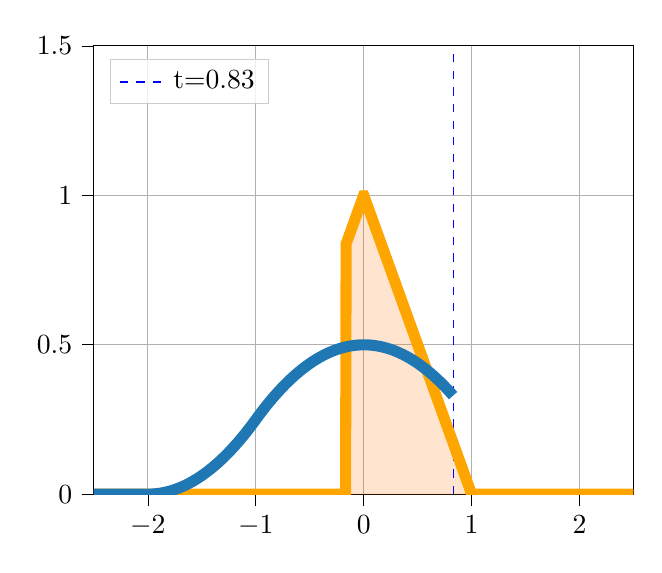
\begin{tikzpicture}

\definecolor{color0}{rgb}{1,0.498039215686275,0.0549019607843137}
\definecolor{color1}{rgb}{1,0.647058823529412,0}
\definecolor{color2}{rgb}{0.12156862745098,0.466666666666667,0.705882352941177}

\begin{axis}[
legend cell align={left},
legend style={fill opacity=0.8, draw opacity=1, text opacity=1, at={(0.03,0.97)}, anchor=north west, draw=white!80!black},
tick align=outside,
tick pos=left,
x grid style={white!69.0196078431373!black},
xmajorgrids,
xmin=-2.5, xmax=2.5,
xtick style={color=black},
y grid style={white!69.0196078431373!black},
ymajorgrids,
ymin=0, ymax=1.5,
ytick style={color=black}
]
\path [draw=color0, fill=color0, opacity=0.2]
(axis cs:-2.5,0)
--(axis cs:-2.5,0)
--(axis cs:-2.49499499499499,0)
--(axis cs:-2.48998998998999,0)
--(axis cs:-2.48498498498498,0)
--(axis cs:-2.47997997997998,0)
--(axis cs:-2.47497497497497,0)
--(axis cs:-2.46996996996997,0)
--(axis cs:-2.46496496496496,0)
--(axis cs:-2.45995995995996,0)
--(axis cs:-2.45495495495495,0)
--(axis cs:-2.44994994994995,0)
--(axis cs:-2.44494494494494,0)
--(axis cs:-2.43993993993994,0)
--(axis cs:-2.43493493493493,0)
--(axis cs:-2.42992992992993,0)
--(axis cs:-2.42492492492492,0)
--(axis cs:-2.41991991991992,0)
--(axis cs:-2.41491491491491,0)
--(axis cs:-2.40990990990991,0)
--(axis cs:-2.4049049049049,0)
--(axis cs:-2.3998998998999,0)
--(axis cs:-2.39489489489489,0)
--(axis cs:-2.38988988988989,0)
--(axis cs:-2.38488488488488,0)
--(axis cs:-2.37987987987988,0)
--(axis cs:-2.37487487487487,0)
--(axis cs:-2.36986986986987,0)
--(axis cs:-2.36486486486486,0)
--(axis cs:-2.35985985985986,0)
--(axis cs:-2.35485485485485,0)
--(axis cs:-2.34984984984985,0)
--(axis cs:-2.34484484484484,0)
--(axis cs:-2.33983983983984,0)
--(axis cs:-2.33483483483483,0)
--(axis cs:-2.32982982982983,0)
--(axis cs:-2.32482482482482,0)
--(axis cs:-2.31981981981982,0)
--(axis cs:-2.31481481481481,0)
--(axis cs:-2.30980980980981,0)
--(axis cs:-2.3048048048048,0)
--(axis cs:-2.2997997997998,0)
--(axis cs:-2.29479479479479,0)
--(axis cs:-2.28978978978979,0)
--(axis cs:-2.28478478478478,0)
--(axis cs:-2.27977977977978,0)
--(axis cs:-2.27477477477477,0)
--(axis cs:-2.26976976976977,0)
--(axis cs:-2.26476476476476,0)
--(axis cs:-2.25975975975976,0)
--(axis cs:-2.25475475475475,0)
--(axis cs:-2.24974974974975,0)
--(axis cs:-2.24474474474474,0)
--(axis cs:-2.23973973973974,0)
--(axis cs:-2.23473473473473,0)
--(axis cs:-2.22972972972973,0)
--(axis cs:-2.22472472472472,0)
--(axis cs:-2.21971971971972,0)
--(axis cs:-2.21471471471471,0)
--(axis cs:-2.20970970970971,0)
--(axis cs:-2.2047047047047,0)
--(axis cs:-2.1996996996997,0)
--(axis cs:-2.19469469469469,0)
--(axis cs:-2.18968968968969,0)
--(axis cs:-2.18468468468468,0)
--(axis cs:-2.17967967967968,0)
--(axis cs:-2.17467467467467,0)
--(axis cs:-2.16966966966967,0)
--(axis cs:-2.16466466466466,0)
--(axis cs:-2.15965965965966,0)
--(axis cs:-2.15465465465465,0)
--(axis cs:-2.14964964964965,0)
--(axis cs:-2.14464464464464,0)
--(axis cs:-2.13963963963964,0)
--(axis cs:-2.13463463463463,0)
--(axis cs:-2.12962962962963,0)
--(axis cs:-2.12462462462462,0)
--(axis cs:-2.11961961961962,0)
--(axis cs:-2.11461461461461,0)
--(axis cs:-2.10960960960961,0)
--(axis cs:-2.1046046046046,0)
--(axis cs:-2.0995995995996,0)
--(axis cs:-2.09459459459459,0)
--(axis cs:-2.08958958958959,0)
--(axis cs:-2.08458458458458,0)
--(axis cs:-2.07957957957958,0)
--(axis cs:-2.07457457457457,0)
--(axis cs:-2.06956956956957,0)
--(axis cs:-2.06456456456456,0)
--(axis cs:-2.05955955955956,0)
--(axis cs:-2.05455455455455,0)
--(axis cs:-2.04954954954955,0)
--(axis cs:-2.04454454454454,0)
--(axis cs:-2.03953953953954,0)
--(axis cs:-2.03453453453453,0)
--(axis cs:-2.02952952952953,0)
--(axis cs:-2.02452452452452,0)
--(axis cs:-2.01951951951952,0)
--(axis cs:-2.01451451451451,0)
--(axis cs:-2.00950950950951,0)
--(axis cs:-2.0045045045045,0)
--(axis cs:-1.9994994994995,0)
--(axis cs:-1.99449449449449,0)
--(axis cs:-1.98948948948949,0)
--(axis cs:-1.98448448448448,0)
--(axis cs:-1.97947947947948,0)
--(axis cs:-1.97447447447447,0)
--(axis cs:-1.96946946946947,0)
--(axis cs:-1.96446446446446,0)
--(axis cs:-1.95945945945946,0)
--(axis cs:-1.95445445445445,0)
--(axis cs:-1.94944944944945,0)
--(axis cs:-1.94444444444444,0)
--(axis cs:-1.93943943943944,0)
--(axis cs:-1.93443443443443,0)
--(axis cs:-1.92942942942943,0)
--(axis cs:-1.92442442442442,0)
--(axis cs:-1.91941941941942,0)
--(axis cs:-1.91441441441441,0)
--(axis cs:-1.90940940940941,0)
--(axis cs:-1.9044044044044,0)
--(axis cs:-1.8993993993994,0)
--(axis cs:-1.89439439439439,0)
--(axis cs:-1.88938938938939,0)
--(axis cs:-1.88438438438438,0)
--(axis cs:-1.87937937937938,0)
--(axis cs:-1.87437437437437,0)
--(axis cs:-1.86936936936937,0)
--(axis cs:-1.86436436436436,0)
--(axis cs:-1.85935935935936,0)
--(axis cs:-1.85435435435435,0)
--(axis cs:-1.84934934934935,0)
--(axis cs:-1.84434434434434,0)
--(axis cs:-1.83933933933934,0)
--(axis cs:-1.83433433433433,0)
--(axis cs:-1.82932932932933,0)
--(axis cs:-1.82432432432432,0)
--(axis cs:-1.81931931931932,0)
--(axis cs:-1.81431431431431,0)
--(axis cs:-1.80930930930931,0)
--(axis cs:-1.8043043043043,0)
--(axis cs:-1.7992992992993,0)
--(axis cs:-1.79429429429429,0)
--(axis cs:-1.78928928928929,0)
--(axis cs:-1.78428428428428,0)
--(axis cs:-1.77927927927928,0)
--(axis cs:-1.77427427427427,0)
--(axis cs:-1.76926926926927,0)
--(axis cs:-1.76426426426426,0)
--(axis cs:-1.75925925925926,0)
--(axis cs:-1.75425425425425,0)
--(axis cs:-1.74924924924925,0)
--(axis cs:-1.74424424424424,0)
--(axis cs:-1.73923923923924,0)
--(axis cs:-1.73423423423423,0)
--(axis cs:-1.72922922922923,0)
--(axis cs:-1.72422422422422,0)
--(axis cs:-1.71921921921922,0)
--(axis cs:-1.71421421421421,0)
--(axis cs:-1.70920920920921,0)
--(axis cs:-1.7042042042042,0)
--(axis cs:-1.6991991991992,0)
--(axis cs:-1.69419419419419,0)
--(axis cs:-1.68918918918919,0)
--(axis cs:-1.68418418418418,0)
--(axis cs:-1.67917917917918,0)
--(axis cs:-1.67417417417417,0)
--(axis cs:-1.66916916916917,0)
--(axis cs:-1.66416416416416,0)
--(axis cs:-1.65915915915916,0)
--(axis cs:-1.65415415415415,0)
--(axis cs:-1.64914914914915,0)
--(axis cs:-1.64414414414414,0)
--(axis cs:-1.63913913913914,0)
--(axis cs:-1.63413413413413,0)
--(axis cs:-1.62912912912913,0)
--(axis cs:-1.62412412412412,0)
--(axis cs:-1.61911911911912,0)
--(axis cs:-1.61411411411411,0)
--(axis cs:-1.60910910910911,0)
--(axis cs:-1.6041041041041,0)
--(axis cs:-1.5990990990991,0)
--(axis cs:-1.59409409409409,0)
--(axis cs:-1.58908908908909,0)
--(axis cs:-1.58408408408408,0)
--(axis cs:-1.57907907907908,0)
--(axis cs:-1.57407407407407,0)
--(axis cs:-1.56906906906907,0)
--(axis cs:-1.56406406406406,0)
--(axis cs:-1.55905905905906,0)
--(axis cs:-1.55405405405405,0)
--(axis cs:-1.54904904904905,0)
--(axis cs:-1.54404404404404,0)
--(axis cs:-1.53903903903904,0)
--(axis cs:-1.53403403403403,0)
--(axis cs:-1.52902902902903,0)
--(axis cs:-1.52402402402402,0)
--(axis cs:-1.51901901901902,0)
--(axis cs:-1.51401401401401,0)
--(axis cs:-1.50900900900901,0)
--(axis cs:-1.504004004004,0)
--(axis cs:-1.498998998999,0)
--(axis cs:-1.49399399399399,0)
--(axis cs:-1.48898898898899,0)
--(axis cs:-1.48398398398398,0)
--(axis cs:-1.47897897897898,0)
--(axis cs:-1.47397397397397,0)
--(axis cs:-1.46896896896897,0)
--(axis cs:-1.46396396396396,0)
--(axis cs:-1.45895895895896,0)
--(axis cs:-1.45395395395395,0)
--(axis cs:-1.44894894894895,0)
--(axis cs:-1.44394394394394,0)
--(axis cs:-1.43893893893894,0)
--(axis cs:-1.43393393393393,0)
--(axis cs:-1.42892892892893,0)
--(axis cs:-1.42392392392392,0)
--(axis cs:-1.41891891891892,0)
--(axis cs:-1.41391391391391,0)
--(axis cs:-1.40890890890891,0)
--(axis cs:-1.4039039039039,0)
--(axis cs:-1.3988988988989,0)
--(axis cs:-1.39389389389389,0)
--(axis cs:-1.38888888888889,0)
--(axis cs:-1.38388388388388,0)
--(axis cs:-1.37887887887888,0)
--(axis cs:-1.37387387387387,0)
--(axis cs:-1.36886886886887,0)
--(axis cs:-1.36386386386386,0)
--(axis cs:-1.35885885885886,0)
--(axis cs:-1.35385385385385,0)
--(axis cs:-1.34884884884885,0)
--(axis cs:-1.34384384384384,0)
--(axis cs:-1.33883883883884,0)
--(axis cs:-1.33383383383383,0)
--(axis cs:-1.32882882882883,0)
--(axis cs:-1.32382382382382,0)
--(axis cs:-1.31881881881882,0)
--(axis cs:-1.31381381381381,0)
--(axis cs:-1.30880880880881,0)
--(axis cs:-1.3038038038038,0)
--(axis cs:-1.2987987987988,0)
--(axis cs:-1.29379379379379,0)
--(axis cs:-1.28878878878879,0)
--(axis cs:-1.28378378378378,0)
--(axis cs:-1.27877877877878,0)
--(axis cs:-1.27377377377377,0)
--(axis cs:-1.26876876876877,0)
--(axis cs:-1.26376376376376,0)
--(axis cs:-1.25875875875876,0)
--(axis cs:-1.25375375375375,0)
--(axis cs:-1.24874874874875,0)
--(axis cs:-1.24374374374374,0)
--(axis cs:-1.23873873873874,0)
--(axis cs:-1.23373373373373,0)
--(axis cs:-1.22872872872873,0)
--(axis cs:-1.22372372372372,0)
--(axis cs:-1.21871871871872,0)
--(axis cs:-1.21371371371371,0)
--(axis cs:-1.20870870870871,0)
--(axis cs:-1.2037037037037,0)
--(axis cs:-1.1986986986987,0)
--(axis cs:-1.19369369369369,0)
--(axis cs:-1.18868868868869,0)
--(axis cs:-1.18368368368368,0)
--(axis cs:-1.17867867867868,0)
--(axis cs:-1.17367367367367,0)
--(axis cs:-1.16866866866867,0)
--(axis cs:-1.16366366366366,0)
--(axis cs:-1.15865865865866,0)
--(axis cs:-1.15365365365365,0)
--(axis cs:-1.14864864864865,0)
--(axis cs:-1.14364364364364,0)
--(axis cs:-1.13863863863864,0)
--(axis cs:-1.13363363363363,0)
--(axis cs:-1.12862862862863,0)
--(axis cs:-1.12362362362362,0)
--(axis cs:-1.11861861861862,0)
--(axis cs:-1.11361361361361,0)
--(axis cs:-1.10860860860861,0)
--(axis cs:-1.1036036036036,0)
--(axis cs:-1.0985985985986,0)
--(axis cs:-1.09359359359359,0)
--(axis cs:-1.08858858858859,0)
--(axis cs:-1.08358358358358,0)
--(axis cs:-1.07857857857858,0)
--(axis cs:-1.07357357357357,0)
--(axis cs:-1.06856856856857,0)
--(axis cs:-1.06356356356356,0)
--(axis cs:-1.05855855855856,0)
--(axis cs:-1.05355355355355,0)
--(axis cs:-1.04854854854855,0)
--(axis cs:-1.04354354354354,0)
--(axis cs:-1.03853853853854,0)
--(axis cs:-1.03353353353353,0)
--(axis cs:-1.02852852852853,0)
--(axis cs:-1.02352352352352,0)
--(axis cs:-1.01851851851852,0)
--(axis cs:-1.01351351351351,0)
--(axis cs:-1.00850850850851,0)
--(axis cs:-1.0035035035035,0)
--(axis cs:-0.998498498498499,0)
--(axis cs:-0.993493493493494,0)
--(axis cs:-0.988488488488489,0)
--(axis cs:-0.983483483483484,0)
--(axis cs:-0.978478478478479,0)
--(axis cs:-0.973473473473474,0)
--(axis cs:-0.968468468468469,0)
--(axis cs:-0.963463463463464,0)
--(axis cs:-0.958458458458459,0)
--(axis cs:-0.953453453453454,0)
--(axis cs:-0.948448448448449,0)
--(axis cs:-0.943443443443444,0)
--(axis cs:-0.938438438438439,0)
--(axis cs:-0.933433433433434,0)
--(axis cs:-0.928428428428429,0)
--(axis cs:-0.923423423423424,0)
--(axis cs:-0.918418418418419,0)
--(axis cs:-0.913413413413414,0)
--(axis cs:-0.908408408408409,0)
--(axis cs:-0.903403403403404,0)
--(axis cs:-0.898398398398399,0)
--(axis cs:-0.893393393393393,0)
--(axis cs:-0.888388388388388,0)
--(axis cs:-0.883383383383383,0)
--(axis cs:-0.878378378378378,0)
--(axis cs:-0.873373373373373,0)
--(axis cs:-0.868368368368368,0)
--(axis cs:-0.863363363363363,0)
--(axis cs:-0.858358358358358,0)
--(axis cs:-0.853353353353353,0)
--(axis cs:-0.848348348348348,0)
--(axis cs:-0.843343343343343,0)
--(axis cs:-0.838338338338338,0)
--(axis cs:-0.833333333333333,0)
--(axis cs:-0.828328328328328,0)
--(axis cs:-0.823323323323323,0)
--(axis cs:-0.818318318318318,0)
--(axis cs:-0.813313313313313,0)
--(axis cs:-0.808308308308308,0)
--(axis cs:-0.803303303303303,0)
--(axis cs:-0.798298298298298,0)
--(axis cs:-0.793293293293293,0)
--(axis cs:-0.788288288288288,0)
--(axis cs:-0.783283283283283,0)
--(axis cs:-0.778278278278278,0)
--(axis cs:-0.773273273273273,0)
--(axis cs:-0.768268268268268,0)
--(axis cs:-0.763263263263263,0)
--(axis cs:-0.758258258258258,0)
--(axis cs:-0.753253253253253,0)
--(axis cs:-0.748248248248248,0)
--(axis cs:-0.743243243243243,0)
--(axis cs:-0.738238238238238,0)
--(axis cs:-0.733233233233233,0)
--(axis cs:-0.728228228228228,0)
--(axis cs:-0.723223223223223,0)
--(axis cs:-0.718218218218218,0)
--(axis cs:-0.713213213213213,0)
--(axis cs:-0.708208208208208,0)
--(axis cs:-0.703203203203203,0)
--(axis cs:-0.698198198198198,0)
--(axis cs:-0.693193193193193,0)
--(axis cs:-0.688188188188188,0)
--(axis cs:-0.683183183183183,0)
--(axis cs:-0.678178178178178,0)
--(axis cs:-0.673173173173173,0)
--(axis cs:-0.668168168168168,0)
--(axis cs:-0.663163163163163,0)
--(axis cs:-0.658158158158158,0)
--(axis cs:-0.653153153153153,0)
--(axis cs:-0.648148148148148,0)
--(axis cs:-0.643143143143143,0)
--(axis cs:-0.638138138138138,0)
--(axis cs:-0.633133133133133,0)
--(axis cs:-0.628128128128128,0)
--(axis cs:-0.623123123123123,0)
--(axis cs:-0.618118118118118,0)
--(axis cs:-0.613113113113113,0)
--(axis cs:-0.608108108108108,0)
--(axis cs:-0.603103103103103,0)
--(axis cs:-0.598098098098098,0)
--(axis cs:-0.593093093093093,0)
--(axis cs:-0.588088088088088,0)
--(axis cs:-0.583083083083083,0)
--(axis cs:-0.578078078078078,0)
--(axis cs:-0.573073073073073,0)
--(axis cs:-0.568068068068068,0)
--(axis cs:-0.563063063063063,0)
--(axis cs:-0.558058058058058,0)
--(axis cs:-0.553053053053053,0)
--(axis cs:-0.548048048048048,0)
--(axis cs:-0.543043043043043,0)
--(axis cs:-0.538038038038038,0)
--(axis cs:-0.533033033033033,0)
--(axis cs:-0.528028028028028,0)
--(axis cs:-0.523023023023023,0)
--(axis cs:-0.518018018018018,0)
--(axis cs:-0.513013013013013,0)
--(axis cs:-0.508008008008008,0)
--(axis cs:-0.503003003003003,0)
--(axis cs:-0.497997997997998,0)
--(axis cs:-0.492992992992993,0)
--(axis cs:-0.487987987987988,0)
--(axis cs:-0.482982982982983,0)
--(axis cs:-0.477977977977978,0)
--(axis cs:-0.472972972972973,0)
--(axis cs:-0.467967967967968,0)
--(axis cs:-0.462962962962963,0)
--(axis cs:-0.457957957957958,0)
--(axis cs:-0.452952952952953,0)
--(axis cs:-0.447947947947948,0)
--(axis cs:-0.442942942942943,0)
--(axis cs:-0.437937937937938,0)
--(axis cs:-0.432932932932933,0)
--(axis cs:-0.427927927927928,0)
--(axis cs:-0.422922922922923,0)
--(axis cs:-0.417917917917918,0)
--(axis cs:-0.412912912912913,0)
--(axis cs:-0.407907907907908,0)
--(axis cs:-0.402902902902903,0)
--(axis cs:-0.397897897897898,0)
--(axis cs:-0.392892892892893,0)
--(axis cs:-0.387887887887888,0)
--(axis cs:-0.382882882882883,0)
--(axis cs:-0.377877877877878,0)
--(axis cs:-0.372872872872873,0)
--(axis cs:-0.367867867867868,0)
--(axis cs:-0.362862862862863,0)
--(axis cs:-0.357857857857858,0)
--(axis cs:-0.352852852852853,0)
--(axis cs:-0.347847847847848,0)
--(axis cs:-0.342842842842843,0)
--(axis cs:-0.337837837837838,0)
--(axis cs:-0.332832832832833,0)
--(axis cs:-0.327827827827828,0)
--(axis cs:-0.322822822822823,0)
--(axis cs:-0.317817817817818,0)
--(axis cs:-0.312812812812813,0)
--(axis cs:-0.307807807807808,0)
--(axis cs:-0.302802802802803,0)
--(axis cs:-0.297797797797798,0)
--(axis cs:-0.292792792792793,0)
--(axis cs:-0.287787787787788,0)
--(axis cs:-0.282782782782783,0)
--(axis cs:-0.277777777777778,0)
--(axis cs:-0.272772772772773,0)
--(axis cs:-0.267767767767768,0)
--(axis cs:-0.262762762762763,0)
--(axis cs:-0.257757757757758,0)
--(axis cs:-0.252752752752753,0)
--(axis cs:-0.247747747747748,0)
--(axis cs:-0.242742742742743,0)
--(axis cs:-0.237737737737738,0)
--(axis cs:-0.232732732732733,0)
--(axis cs:-0.227727727727728,0)
--(axis cs:-0.222722722722723,0)
--(axis cs:-0.217717717717718,0)
--(axis cs:-0.212712712712713,0)
--(axis cs:-0.207707707707708,0)
--(axis cs:-0.202702702702703,0)
--(axis cs:-0.197697697697698,0)
--(axis cs:-0.192692692692693,0)
--(axis cs:-0.187687687687688,0)
--(axis cs:-0.182682682682683,0)
--(axis cs:-0.177677677677678,0)
--(axis cs:-0.172672672672673,0)
--(axis cs:-0.167667667667668,0)
--(axis cs:-0.162662662662663,0)
--(axis cs:-0.157657657657658,0)
--(axis cs:-0.152652652652653,0)
--(axis cs:-0.147647647647648,0)
--(axis cs:-0.142642642642643,0)
--(axis cs:-0.137637637637638,0)
--(axis cs:-0.132632632632633,0)
--(axis cs:-0.127627627627628,0)
--(axis cs:-0.122622622622623,0)
--(axis cs:-0.117617617617618,0)
--(axis cs:-0.112612612612613,0)
--(axis cs:-0.107607607607608,0)
--(axis cs:-0.102602602602603,0)
--(axis cs:-0.0975975975975976,0)
--(axis cs:-0.0925925925925926,0)
--(axis cs:-0.0875875875875876,0)
--(axis cs:-0.0825825825825826,0)
--(axis cs:-0.0775775775775776,0)
--(axis cs:-0.0725725725725725,0)
--(axis cs:-0.0675675675675675,0)
--(axis cs:-0.0625625625625625,0)
--(axis cs:-0.0575575575575575,0)
--(axis cs:-0.0525525525525525,0)
--(axis cs:-0.0475475475475475,0)
--(axis cs:-0.0425425425425425,0)
--(axis cs:-0.0375375375375375,0)
--(axis cs:-0.0325325325325325,0)
--(axis cs:-0.0275275275275275,0)
--(axis cs:-0.0225225225225225,0)
--(axis cs:-0.0175175175175175,0)
--(axis cs:-0.0125125125125125,0)
--(axis cs:-0.0075075075075075,0)
--(axis cs:-0.0025025025025025,0)
--(axis cs:0.0025025025025025,0)
--(axis cs:0.0075075075075075,0)
--(axis cs:0.0125125125125125,0)
--(axis cs:0.0175175175175175,0)
--(axis cs:0.0225225225225225,0)
--(axis cs:0.0275275275275275,0)
--(axis cs:0.0325325325325325,0)
--(axis cs:0.0375375375375375,0)
--(axis cs:0.0425425425425425,0)
--(axis cs:0.0475475475475475,0)
--(axis cs:0.0525525525525525,0)
--(axis cs:0.0575575575575575,0)
--(axis cs:0.0625625625625625,0)
--(axis cs:0.0675675675675675,0)
--(axis cs:0.0725725725725725,0)
--(axis cs:0.0775775775775776,0)
--(axis cs:0.0825825825825826,0)
--(axis cs:0.0875875875875876,0)
--(axis cs:0.0925925925925926,0)
--(axis cs:0.0975975975975976,0)
--(axis cs:0.102602602602603,0)
--(axis cs:0.107607607607608,0)
--(axis cs:0.112612612612613,0)
--(axis cs:0.117617617617618,0)
--(axis cs:0.122622622622623,0)
--(axis cs:0.127627627627628,0)
--(axis cs:0.132632632632633,0)
--(axis cs:0.137637637637638,0)
--(axis cs:0.142642642642643,0)
--(axis cs:0.147647647647648,0)
--(axis cs:0.152652652652653,0)
--(axis cs:0.157657657657658,0)
--(axis cs:0.162662662662663,0)
--(axis cs:0.167667667667668,0)
--(axis cs:0.172672672672673,0)
--(axis cs:0.177677677677678,0)
--(axis cs:0.182682682682683,0)
--(axis cs:0.187687687687688,0)
--(axis cs:0.192692692692693,0)
--(axis cs:0.197697697697698,0)
--(axis cs:0.202702702702703,0)
--(axis cs:0.207707707707708,0)
--(axis cs:0.212712712712713,0)
--(axis cs:0.217717717717718,0)
--(axis cs:0.222722722722723,0)
--(axis cs:0.227727727727728,0)
--(axis cs:0.232732732732733,0)
--(axis cs:0.237737737737738,0)
--(axis cs:0.242742742742743,0)
--(axis cs:0.247747747747748,0)
--(axis cs:0.252752752752753,0)
--(axis cs:0.257757757757758,0)
--(axis cs:0.262762762762763,0)
--(axis cs:0.267767767767768,0)
--(axis cs:0.272772772772773,0)
--(axis cs:0.277777777777778,0)
--(axis cs:0.282782782782783,0)
--(axis cs:0.287787787787788,0)
--(axis cs:0.292792792792793,0)
--(axis cs:0.297797797797798,0)
--(axis cs:0.302802802802803,0)
--(axis cs:0.307807807807808,0)
--(axis cs:0.312812812812813,0)
--(axis cs:0.317817817817818,0)
--(axis cs:0.322822822822823,0)
--(axis cs:0.327827827827828,0)
--(axis cs:0.332832832832833,0)
--(axis cs:0.337837837837838,0)
--(axis cs:0.342842842842843,0)
--(axis cs:0.347847847847848,0)
--(axis cs:0.352852852852853,0)
--(axis cs:0.357857857857858,0)
--(axis cs:0.362862862862863,0)
--(axis cs:0.367867867867868,0)
--(axis cs:0.372872872872873,0)
--(axis cs:0.377877877877878,0)
--(axis cs:0.382882882882883,0)
--(axis cs:0.387887887887888,0)
--(axis cs:0.392892892892893,0)
--(axis cs:0.397897897897898,0)
--(axis cs:0.402902902902903,0)
--(axis cs:0.407907907907908,0)
--(axis cs:0.412912912912913,0)
--(axis cs:0.417917917917918,0)
--(axis cs:0.422922922922923,0)
--(axis cs:0.427927927927928,0)
--(axis cs:0.432932932932933,0)
--(axis cs:0.437937937937938,0)
--(axis cs:0.442942942942943,0)
--(axis cs:0.447947947947948,0)
--(axis cs:0.452952952952953,0)
--(axis cs:0.457957957957958,0)
--(axis cs:0.462962962962963,0)
--(axis cs:0.467967967967968,0)
--(axis cs:0.472972972972973,0)
--(axis cs:0.477977977977978,0)
--(axis cs:0.482982982982983,0)
--(axis cs:0.487987987987988,0)
--(axis cs:0.492992992992993,0)
--(axis cs:0.497997997997998,0)
--(axis cs:0.503003003003003,0)
--(axis cs:0.508008008008008,0)
--(axis cs:0.513013013013013,0)
--(axis cs:0.518018018018018,0)
--(axis cs:0.523023023023023,0)
--(axis cs:0.528028028028028,0)
--(axis cs:0.533033033033033,0)
--(axis cs:0.538038038038038,0)
--(axis cs:0.543043043043043,0)
--(axis cs:0.548048048048048,0)
--(axis cs:0.553053053053053,0)
--(axis cs:0.558058058058058,0)
--(axis cs:0.563063063063063,0)
--(axis cs:0.568068068068068,0)
--(axis cs:0.573073073073073,0)
--(axis cs:0.578078078078078,0)
--(axis cs:0.583083083083083,0)
--(axis cs:0.588088088088088,0)
--(axis cs:0.593093093093093,0)
--(axis cs:0.598098098098098,0)
--(axis cs:0.603103103103103,0)
--(axis cs:0.608108108108108,0)
--(axis cs:0.613113113113113,0)
--(axis cs:0.618118118118118,0)
--(axis cs:0.623123123123123,0)
--(axis cs:0.628128128128128,0)
--(axis cs:0.633133133133133,0)
--(axis cs:0.638138138138138,0)
--(axis cs:0.643143143143143,0)
--(axis cs:0.648148148148148,0)
--(axis cs:0.653153153153153,0)
--(axis cs:0.658158158158158,0)
--(axis cs:0.663163163163163,0)
--(axis cs:0.668168168168168,0)
--(axis cs:0.673173173173173,0)
--(axis cs:0.678178178178178,0)
--(axis cs:0.683183183183183,0)
--(axis cs:0.688188188188188,0)
--(axis cs:0.693193193193193,0)
--(axis cs:0.698198198198198,0)
--(axis cs:0.703203203203203,0)
--(axis cs:0.708208208208208,0)
--(axis cs:0.713213213213213,0)
--(axis cs:0.718218218218218,0)
--(axis cs:0.723223223223223,0)
--(axis cs:0.728228228228228,0)
--(axis cs:0.733233233233233,0)
--(axis cs:0.738238238238238,0)
--(axis cs:0.743243243243243,0)
--(axis cs:0.748248248248248,0)
--(axis cs:0.753253253253253,0)
--(axis cs:0.758258258258258,0)
--(axis cs:0.763263263263263,0)
--(axis cs:0.768268268268268,0)
--(axis cs:0.773273273273273,0)
--(axis cs:0.778278278278278,0)
--(axis cs:0.783283283283283,0)
--(axis cs:0.788288288288288,0)
--(axis cs:0.793293293293293,0)
--(axis cs:0.798298298298298,0)
--(axis cs:0.803303303303303,0)
--(axis cs:0.808308308308308,0)
--(axis cs:0.813313313313313,0)
--(axis cs:0.818318318318318,0)
--(axis cs:0.823323323323323,0)
--(axis cs:0.828328328328328,0)
--(axis cs:0.833333333333333,0)
--(axis cs:0.838338338338338,0)
--(axis cs:0.843343343343343,0)
--(axis cs:0.848348348348348,0)
--(axis cs:0.853353353353353,0)
--(axis cs:0.858358358358358,0)
--(axis cs:0.863363363363364,0)
--(axis cs:0.868368368368369,0)
--(axis cs:0.873373373373374,0)
--(axis cs:0.878378378378379,0)
--(axis cs:0.883383383383384,0)
--(axis cs:0.888388388388389,0)
--(axis cs:0.893393393393394,0)
--(axis cs:0.898398398398399,0)
--(axis cs:0.903403403403404,0)
--(axis cs:0.908408408408409,0)
--(axis cs:0.913413413413414,0)
--(axis cs:0.918418418418419,0)
--(axis cs:0.923423423423424,0)
--(axis cs:0.928428428428429,0)
--(axis cs:0.933433433433434,0)
--(axis cs:0.938438438438439,0)
--(axis cs:0.943443443443444,0)
--(axis cs:0.948448448448449,0)
--(axis cs:0.953453453453454,0)
--(axis cs:0.958458458458459,0)
--(axis cs:0.963463463463464,0)
--(axis cs:0.968468468468469,0)
--(axis cs:0.973473473473474,0)
--(axis cs:0.978478478478479,0)
--(axis cs:0.983483483483484,0)
--(axis cs:0.988488488488489,0)
--(axis cs:0.993493493493494,0)
--(axis cs:0.998498498498499,0)
--(axis cs:1.0035035035035,0)
--(axis cs:1.00850850850851,0)
--(axis cs:1.01351351351351,0)
--(axis cs:1.01851851851852,0)
--(axis cs:1.02352352352352,0)
--(axis cs:1.02852852852853,0)
--(axis cs:1.03353353353353,0)
--(axis cs:1.03853853853854,0)
--(axis cs:1.04354354354354,0)
--(axis cs:1.04854854854855,0)
--(axis cs:1.05355355355355,0)
--(axis cs:1.05855855855856,0)
--(axis cs:1.06356356356356,0)
--(axis cs:1.06856856856857,0)
--(axis cs:1.07357357357357,0)
--(axis cs:1.07857857857858,0)
--(axis cs:1.08358358358358,0)
--(axis cs:1.08858858858859,0)
--(axis cs:1.09359359359359,0)
--(axis cs:1.0985985985986,0)
--(axis cs:1.1036036036036,0)
--(axis cs:1.10860860860861,0)
--(axis cs:1.11361361361361,0)
--(axis cs:1.11861861861862,0)
--(axis cs:1.12362362362362,0)
--(axis cs:1.12862862862863,0)
--(axis cs:1.13363363363363,0)
--(axis cs:1.13863863863864,0)
--(axis cs:1.14364364364364,0)
--(axis cs:1.14864864864865,0)
--(axis cs:1.15365365365365,0)
--(axis cs:1.15865865865866,0)
--(axis cs:1.16366366366366,0)
--(axis cs:1.16866866866867,0)
--(axis cs:1.17367367367367,0)
--(axis cs:1.17867867867868,0)
--(axis cs:1.18368368368368,0)
--(axis cs:1.18868868868869,0)
--(axis cs:1.19369369369369,0)
--(axis cs:1.1986986986987,0)
--(axis cs:1.2037037037037,0)
--(axis cs:1.20870870870871,0)
--(axis cs:1.21371371371371,0)
--(axis cs:1.21871871871872,0)
--(axis cs:1.22372372372372,0)
--(axis cs:1.22872872872873,0)
--(axis cs:1.23373373373373,0)
--(axis cs:1.23873873873874,0)
--(axis cs:1.24374374374374,0)
--(axis cs:1.24874874874875,0)
--(axis cs:1.25375375375375,0)
--(axis cs:1.25875875875876,0)
--(axis cs:1.26376376376376,0)
--(axis cs:1.26876876876877,0)
--(axis cs:1.27377377377377,0)
--(axis cs:1.27877877877878,0)
--(axis cs:1.28378378378378,0)
--(axis cs:1.28878878878879,0)
--(axis cs:1.29379379379379,0)
--(axis cs:1.2987987987988,0)
--(axis cs:1.3038038038038,0)
--(axis cs:1.30880880880881,0)
--(axis cs:1.31381381381381,0)
--(axis cs:1.31881881881882,0)
--(axis cs:1.32382382382382,0)
--(axis cs:1.32882882882883,0)
--(axis cs:1.33383383383383,0)
--(axis cs:1.33883883883884,0)
--(axis cs:1.34384384384384,0)
--(axis cs:1.34884884884885,0)
--(axis cs:1.35385385385385,0)
--(axis cs:1.35885885885886,0)
--(axis cs:1.36386386386386,0)
--(axis cs:1.36886886886887,0)
--(axis cs:1.37387387387387,0)
--(axis cs:1.37887887887888,0)
--(axis cs:1.38388388388388,0)
--(axis cs:1.38888888888889,0)
--(axis cs:1.39389389389389,0)
--(axis cs:1.3988988988989,0)
--(axis cs:1.4039039039039,0)
--(axis cs:1.40890890890891,0)
--(axis cs:1.41391391391391,0)
--(axis cs:1.41891891891892,0)
--(axis cs:1.42392392392392,0)
--(axis cs:1.42892892892893,0)
--(axis cs:1.43393393393393,0)
--(axis cs:1.43893893893894,0)
--(axis cs:1.44394394394394,0)
--(axis cs:1.44894894894895,0)
--(axis cs:1.45395395395395,0)
--(axis cs:1.45895895895896,0)
--(axis cs:1.46396396396396,0)
--(axis cs:1.46896896896897,0)
--(axis cs:1.47397397397397,0)
--(axis cs:1.47897897897898,0)
--(axis cs:1.48398398398398,0)
--(axis cs:1.48898898898899,0)
--(axis cs:1.49399399399399,0)
--(axis cs:1.498998998999,0)
--(axis cs:1.504004004004,0)
--(axis cs:1.50900900900901,0)
--(axis cs:1.51401401401401,0)
--(axis cs:1.51901901901902,0)
--(axis cs:1.52402402402402,0)
--(axis cs:1.52902902902903,0)
--(axis cs:1.53403403403403,0)
--(axis cs:1.53903903903904,0)
--(axis cs:1.54404404404404,0)
--(axis cs:1.54904904904905,0)
--(axis cs:1.55405405405405,0)
--(axis cs:1.55905905905906,0)
--(axis cs:1.56406406406406,0)
--(axis cs:1.56906906906907,0)
--(axis cs:1.57407407407407,0)
--(axis cs:1.57907907907908,0)
--(axis cs:1.58408408408408,0)
--(axis cs:1.58908908908909,0)
--(axis cs:1.59409409409409,0)
--(axis cs:1.5990990990991,0)
--(axis cs:1.6041041041041,0)
--(axis cs:1.60910910910911,0)
--(axis cs:1.61411411411411,0)
--(axis cs:1.61911911911912,0)
--(axis cs:1.62412412412412,0)
--(axis cs:1.62912912912913,0)
--(axis cs:1.63413413413413,0)
--(axis cs:1.63913913913914,0)
--(axis cs:1.64414414414414,0)
--(axis cs:1.64914914914915,0)
--(axis cs:1.65415415415415,0)
--(axis cs:1.65915915915916,0)
--(axis cs:1.66416416416416,0)
--(axis cs:1.66916916916917,0)
--(axis cs:1.67417417417417,0)
--(axis cs:1.67917917917918,0)
--(axis cs:1.68418418418418,0)
--(axis cs:1.68918918918919,0)
--(axis cs:1.69419419419419,0)
--(axis cs:1.6991991991992,0)
--(axis cs:1.7042042042042,0)
--(axis cs:1.70920920920921,0)
--(axis cs:1.71421421421421,0)
--(axis cs:1.71921921921922,0)
--(axis cs:1.72422422422422,0)
--(axis cs:1.72922922922923,0)
--(axis cs:1.73423423423423,0)
--(axis cs:1.73923923923924,0)
--(axis cs:1.74424424424424,0)
--(axis cs:1.74924924924925,0)
--(axis cs:1.75425425425425,0)
--(axis cs:1.75925925925926,0)
--(axis cs:1.76426426426426,0)
--(axis cs:1.76926926926927,0)
--(axis cs:1.77427427427427,0)
--(axis cs:1.77927927927928,0)
--(axis cs:1.78428428428428,0)
--(axis cs:1.78928928928929,0)
--(axis cs:1.79429429429429,0)
--(axis cs:1.7992992992993,0)
--(axis cs:1.8043043043043,0)
--(axis cs:1.80930930930931,0)
--(axis cs:1.81431431431431,0)
--(axis cs:1.81931931931932,0)
--(axis cs:1.82432432432432,0)
--(axis cs:1.82932932932933,0)
--(axis cs:1.83433433433433,0)
--(axis cs:1.83933933933934,0)
--(axis cs:1.84434434434434,0)
--(axis cs:1.84934934934935,0)
--(axis cs:1.85435435435435,0)
--(axis cs:1.85935935935936,0)
--(axis cs:1.86436436436436,0)
--(axis cs:1.86936936936937,0)
--(axis cs:1.87437437437437,0)
--(axis cs:1.87937937937938,0)
--(axis cs:1.88438438438438,0)
--(axis cs:1.88938938938939,0)
--(axis cs:1.89439439439439,0)
--(axis cs:1.8993993993994,0)
--(axis cs:1.9044044044044,0)
--(axis cs:1.90940940940941,0)
--(axis cs:1.91441441441441,0)
--(axis cs:1.91941941941942,0)
--(axis cs:1.92442442442442,0)
--(axis cs:1.92942942942943,0)
--(axis cs:1.93443443443443,0)
--(axis cs:1.93943943943944,0)
--(axis cs:1.94444444444444,0)
--(axis cs:1.94944944944945,0)
--(axis cs:1.95445445445445,0)
--(axis cs:1.95945945945946,0)
--(axis cs:1.96446446446446,0)
--(axis cs:1.96946946946947,0)
--(axis cs:1.97447447447447,0)
--(axis cs:1.97947947947948,0)
--(axis cs:1.98448448448448,0)
--(axis cs:1.98948948948949,0)
--(axis cs:1.99449449449449,0)
--(axis cs:1.9994994994995,0)
--(axis cs:2.0045045045045,0)
--(axis cs:2.00950950950951,0)
--(axis cs:2.01451451451451,0)
--(axis cs:2.01951951951952,0)
--(axis cs:2.02452452452452,0)
--(axis cs:2.02952952952953,0)
--(axis cs:2.03453453453453,0)
--(axis cs:2.03953953953954,0)
--(axis cs:2.04454454454454,0)
--(axis cs:2.04954954954955,0)
--(axis cs:2.05455455455455,0)
--(axis cs:2.05955955955956,0)
--(axis cs:2.06456456456456,0)
--(axis cs:2.06956956956957,0)
--(axis cs:2.07457457457457,0)
--(axis cs:2.07957957957958,0)
--(axis cs:2.08458458458458,0)
--(axis cs:2.08958958958959,0)
--(axis cs:2.09459459459459,0)
--(axis cs:2.0995995995996,0)
--(axis cs:2.1046046046046,0)
--(axis cs:2.10960960960961,0)
--(axis cs:2.11461461461461,0)
--(axis cs:2.11961961961962,0)
--(axis cs:2.12462462462462,0)
--(axis cs:2.12962962962963,0)
--(axis cs:2.13463463463463,0)
--(axis cs:2.13963963963964,0)
--(axis cs:2.14464464464464,0)
--(axis cs:2.14964964964965,0)
--(axis cs:2.15465465465465,0)
--(axis cs:2.15965965965966,0)
--(axis cs:2.16466466466466,0)
--(axis cs:2.16966966966967,0)
--(axis cs:2.17467467467467,0)
--(axis cs:2.17967967967968,0)
--(axis cs:2.18468468468468,0)
--(axis cs:2.18968968968969,0)
--(axis cs:2.19469469469469,0)
--(axis cs:2.1996996996997,0)
--(axis cs:2.2047047047047,0)
--(axis cs:2.20970970970971,0)
--(axis cs:2.21471471471471,0)
--(axis cs:2.21971971971972,0)
--(axis cs:2.22472472472472,0)
--(axis cs:2.22972972972973,0)
--(axis cs:2.23473473473473,0)
--(axis cs:2.23973973973974,0)
--(axis cs:2.24474474474474,0)
--(axis cs:2.24974974974975,0)
--(axis cs:2.25475475475475,0)
--(axis cs:2.25975975975976,0)
--(axis cs:2.26476476476476,0)
--(axis cs:2.26976976976977,0)
--(axis cs:2.27477477477477,0)
--(axis cs:2.27977977977978,0)
--(axis cs:2.28478478478478,0)
--(axis cs:2.28978978978979,0)
--(axis cs:2.29479479479479,0)
--(axis cs:2.2997997997998,0)
--(axis cs:2.3048048048048,0)
--(axis cs:2.30980980980981,0)
--(axis cs:2.31481481481481,0)
--(axis cs:2.31981981981982,0)
--(axis cs:2.32482482482482,0)
--(axis cs:2.32982982982983,0)
--(axis cs:2.33483483483483,0)
--(axis cs:2.33983983983984,0)
--(axis cs:2.34484484484484,0)
--(axis cs:2.34984984984985,0)
--(axis cs:2.35485485485485,0)
--(axis cs:2.35985985985986,0)
--(axis cs:2.36486486486486,0)
--(axis cs:2.36986986986987,0)
--(axis cs:2.37487487487487,0)
--(axis cs:2.37987987987988,0)
--(axis cs:2.38488488488488,0)
--(axis cs:2.38988988988989,0)
--(axis cs:2.39489489489489,0)
--(axis cs:2.3998998998999,0)
--(axis cs:2.4049049049049,0)
--(axis cs:2.40990990990991,0)
--(axis cs:2.41491491491491,0)
--(axis cs:2.41991991991992,0)
--(axis cs:2.42492492492492,0)
--(axis cs:2.42992992992993,0)
--(axis cs:2.43493493493493,0)
--(axis cs:2.43993993993994,0)
--(axis cs:2.44494494494494,0)
--(axis cs:2.44994994994995,0)
--(axis cs:2.45495495495495,0)
--(axis cs:2.45995995995996,0)
--(axis cs:2.46496496496496,0)
--(axis cs:2.46996996996997,0)
--(axis cs:2.47497497497497,0)
--(axis cs:2.47997997997998,0)
--(axis cs:2.48498498498498,0)
--(axis cs:2.48998998998999,0)
--(axis cs:2.49499499499499,0)
--(axis cs:2.5,0)
--(axis cs:2.5,0)
--(axis cs:2.5,0)
--(axis cs:2.49499499499499,0)
--(axis cs:2.48998998998999,0)
--(axis cs:2.48498498498498,0)
--(axis cs:2.47997997997998,0)
--(axis cs:2.47497497497497,0)
--(axis cs:2.46996996996997,0)
--(axis cs:2.46496496496496,0)
--(axis cs:2.45995995995996,0)
--(axis cs:2.45495495495495,0)
--(axis cs:2.44994994994995,0)
--(axis cs:2.44494494494494,0)
--(axis cs:2.43993993993994,0)
--(axis cs:2.43493493493493,0)
--(axis cs:2.42992992992993,0)
--(axis cs:2.42492492492492,0)
--(axis cs:2.41991991991992,0)
--(axis cs:2.41491491491491,0)
--(axis cs:2.40990990990991,0)
--(axis cs:2.4049049049049,0)
--(axis cs:2.3998998998999,0)
--(axis cs:2.39489489489489,0)
--(axis cs:2.38988988988989,0)
--(axis cs:2.38488488488488,0)
--(axis cs:2.37987987987988,0)
--(axis cs:2.37487487487487,0)
--(axis cs:2.36986986986987,0)
--(axis cs:2.36486486486486,0)
--(axis cs:2.35985985985986,0)
--(axis cs:2.35485485485485,0)
--(axis cs:2.34984984984985,0)
--(axis cs:2.34484484484484,0)
--(axis cs:2.33983983983984,0)
--(axis cs:2.33483483483483,0)
--(axis cs:2.32982982982983,0)
--(axis cs:2.32482482482482,0)
--(axis cs:2.31981981981982,0)
--(axis cs:2.31481481481481,0)
--(axis cs:2.30980980980981,0)
--(axis cs:2.3048048048048,0)
--(axis cs:2.2997997997998,0)
--(axis cs:2.29479479479479,0)
--(axis cs:2.28978978978979,0)
--(axis cs:2.28478478478478,0)
--(axis cs:2.27977977977978,0)
--(axis cs:2.27477477477477,0)
--(axis cs:2.26976976976977,0)
--(axis cs:2.26476476476476,0)
--(axis cs:2.25975975975976,0)
--(axis cs:2.25475475475475,0)
--(axis cs:2.24974974974975,0)
--(axis cs:2.24474474474474,0)
--(axis cs:2.23973973973974,0)
--(axis cs:2.23473473473473,0)
--(axis cs:2.22972972972973,0)
--(axis cs:2.22472472472472,0)
--(axis cs:2.21971971971972,0)
--(axis cs:2.21471471471471,0)
--(axis cs:2.20970970970971,0)
--(axis cs:2.2047047047047,0)
--(axis cs:2.1996996996997,0)
--(axis cs:2.19469469469469,0)
--(axis cs:2.18968968968969,0)
--(axis cs:2.18468468468468,0)
--(axis cs:2.17967967967968,0)
--(axis cs:2.17467467467467,0)
--(axis cs:2.16966966966967,0)
--(axis cs:2.16466466466466,0)
--(axis cs:2.15965965965966,0)
--(axis cs:2.15465465465465,0)
--(axis cs:2.14964964964965,0)
--(axis cs:2.14464464464464,0)
--(axis cs:2.13963963963964,0)
--(axis cs:2.13463463463463,0)
--(axis cs:2.12962962962963,0)
--(axis cs:2.12462462462462,0)
--(axis cs:2.11961961961962,0)
--(axis cs:2.11461461461461,0)
--(axis cs:2.10960960960961,0)
--(axis cs:2.1046046046046,0)
--(axis cs:2.0995995995996,0)
--(axis cs:2.09459459459459,0)
--(axis cs:2.08958958958959,0)
--(axis cs:2.08458458458458,0)
--(axis cs:2.07957957957958,0)
--(axis cs:2.07457457457457,0)
--(axis cs:2.06956956956957,0)
--(axis cs:2.06456456456456,0)
--(axis cs:2.05955955955956,0)
--(axis cs:2.05455455455455,0)
--(axis cs:2.04954954954955,0)
--(axis cs:2.04454454454454,0)
--(axis cs:2.03953953953954,0)
--(axis cs:2.03453453453453,0)
--(axis cs:2.02952952952953,0)
--(axis cs:2.02452452452452,0)
--(axis cs:2.01951951951952,0)
--(axis cs:2.01451451451451,0)
--(axis cs:2.00950950950951,0)
--(axis cs:2.0045045045045,0)
--(axis cs:1.9994994994995,0)
--(axis cs:1.99449449449449,0)
--(axis cs:1.98948948948949,0)
--(axis cs:1.98448448448448,0)
--(axis cs:1.97947947947948,0)
--(axis cs:1.97447447447447,0)
--(axis cs:1.96946946946947,0)
--(axis cs:1.96446446446446,0)
--(axis cs:1.95945945945946,0)
--(axis cs:1.95445445445445,0)
--(axis cs:1.94944944944945,0)
--(axis cs:1.94444444444444,0)
--(axis cs:1.93943943943944,0)
--(axis cs:1.93443443443443,0)
--(axis cs:1.92942942942943,0)
--(axis cs:1.92442442442442,0)
--(axis cs:1.91941941941942,0)
--(axis cs:1.91441441441441,0)
--(axis cs:1.90940940940941,0)
--(axis cs:1.9044044044044,0)
--(axis cs:1.8993993993994,0)
--(axis cs:1.89439439439439,0)
--(axis cs:1.88938938938939,0)
--(axis cs:1.88438438438438,0)
--(axis cs:1.87937937937938,0)
--(axis cs:1.87437437437437,0)
--(axis cs:1.86936936936937,0)
--(axis cs:1.86436436436436,0)
--(axis cs:1.85935935935936,0)
--(axis cs:1.85435435435435,0)
--(axis cs:1.84934934934935,0)
--(axis cs:1.84434434434434,0)
--(axis cs:1.83933933933934,0)
--(axis cs:1.83433433433433,0)
--(axis cs:1.82932932932933,0)
--(axis cs:1.82432432432432,0)
--(axis cs:1.81931931931932,0)
--(axis cs:1.81431431431431,0)
--(axis cs:1.80930930930931,0)
--(axis cs:1.8043043043043,0)
--(axis cs:1.7992992992993,0)
--(axis cs:1.79429429429429,0)
--(axis cs:1.78928928928929,0)
--(axis cs:1.78428428428428,0)
--(axis cs:1.77927927927928,0)
--(axis cs:1.77427427427427,0)
--(axis cs:1.76926926926927,0)
--(axis cs:1.76426426426426,0)
--(axis cs:1.75925925925926,0)
--(axis cs:1.75425425425425,0)
--(axis cs:1.74924924924925,0)
--(axis cs:1.74424424424424,0)
--(axis cs:1.73923923923924,0)
--(axis cs:1.73423423423423,0)
--(axis cs:1.72922922922923,0)
--(axis cs:1.72422422422422,0)
--(axis cs:1.71921921921922,0)
--(axis cs:1.71421421421421,0)
--(axis cs:1.70920920920921,0)
--(axis cs:1.7042042042042,0)
--(axis cs:1.6991991991992,0)
--(axis cs:1.69419419419419,0)
--(axis cs:1.68918918918919,0)
--(axis cs:1.68418418418418,0)
--(axis cs:1.67917917917918,0)
--(axis cs:1.67417417417417,0)
--(axis cs:1.66916916916917,0)
--(axis cs:1.66416416416416,0)
--(axis cs:1.65915915915916,0)
--(axis cs:1.65415415415415,0)
--(axis cs:1.64914914914915,0)
--(axis cs:1.64414414414414,0)
--(axis cs:1.63913913913914,0)
--(axis cs:1.63413413413413,0)
--(axis cs:1.62912912912913,0)
--(axis cs:1.62412412412412,0)
--(axis cs:1.61911911911912,0)
--(axis cs:1.61411411411411,0)
--(axis cs:1.60910910910911,0)
--(axis cs:1.6041041041041,0)
--(axis cs:1.5990990990991,0)
--(axis cs:1.59409409409409,0)
--(axis cs:1.58908908908909,0)
--(axis cs:1.58408408408408,0)
--(axis cs:1.57907907907908,0)
--(axis cs:1.57407407407407,0)
--(axis cs:1.56906906906907,0)
--(axis cs:1.56406406406406,0)
--(axis cs:1.55905905905906,0)
--(axis cs:1.55405405405405,0)
--(axis cs:1.54904904904905,0)
--(axis cs:1.54404404404404,0)
--(axis cs:1.53903903903904,0)
--(axis cs:1.53403403403403,0)
--(axis cs:1.52902902902903,0)
--(axis cs:1.52402402402402,0)
--(axis cs:1.51901901901902,0)
--(axis cs:1.51401401401401,0)
--(axis cs:1.50900900900901,0)
--(axis cs:1.504004004004,0)
--(axis cs:1.498998998999,0)
--(axis cs:1.49399399399399,0)
--(axis cs:1.48898898898899,0)
--(axis cs:1.48398398398398,0)
--(axis cs:1.47897897897898,0)
--(axis cs:1.47397397397397,0)
--(axis cs:1.46896896896897,0)
--(axis cs:1.46396396396396,0)
--(axis cs:1.45895895895896,0)
--(axis cs:1.45395395395395,0)
--(axis cs:1.44894894894895,0)
--(axis cs:1.44394394394394,0)
--(axis cs:1.43893893893894,0)
--(axis cs:1.43393393393393,0)
--(axis cs:1.42892892892893,0)
--(axis cs:1.42392392392392,0)
--(axis cs:1.41891891891892,0)
--(axis cs:1.41391391391391,0)
--(axis cs:1.40890890890891,0)
--(axis cs:1.4039039039039,0)
--(axis cs:1.3988988988989,0)
--(axis cs:1.39389389389389,0)
--(axis cs:1.38888888888889,0)
--(axis cs:1.38388388388388,0)
--(axis cs:1.37887887887888,0)
--(axis cs:1.37387387387387,0)
--(axis cs:1.36886886886887,0)
--(axis cs:1.36386386386386,0)
--(axis cs:1.35885885885886,0)
--(axis cs:1.35385385385385,0)
--(axis cs:1.34884884884885,0)
--(axis cs:1.34384384384384,0)
--(axis cs:1.33883883883884,0)
--(axis cs:1.33383383383383,0)
--(axis cs:1.32882882882883,0)
--(axis cs:1.32382382382382,0)
--(axis cs:1.31881881881882,0)
--(axis cs:1.31381381381381,0)
--(axis cs:1.30880880880881,0)
--(axis cs:1.3038038038038,0)
--(axis cs:1.2987987987988,0)
--(axis cs:1.29379379379379,0)
--(axis cs:1.28878878878879,0)
--(axis cs:1.28378378378378,0)
--(axis cs:1.27877877877878,0)
--(axis cs:1.27377377377377,0)
--(axis cs:1.26876876876877,0)
--(axis cs:1.26376376376376,0)
--(axis cs:1.25875875875876,0)
--(axis cs:1.25375375375375,0)
--(axis cs:1.24874874874875,0)
--(axis cs:1.24374374374374,0)
--(axis cs:1.23873873873874,0)
--(axis cs:1.23373373373373,0)
--(axis cs:1.22872872872873,0)
--(axis cs:1.22372372372372,0)
--(axis cs:1.21871871871872,0)
--(axis cs:1.21371371371371,0)
--(axis cs:1.20870870870871,0)
--(axis cs:1.2037037037037,0)
--(axis cs:1.1986986986987,0)
--(axis cs:1.19369369369369,0)
--(axis cs:1.18868868868869,0)
--(axis cs:1.18368368368368,0)
--(axis cs:1.17867867867868,0)
--(axis cs:1.17367367367367,0)
--(axis cs:1.16866866866867,0)
--(axis cs:1.16366366366366,0)
--(axis cs:1.15865865865866,0)
--(axis cs:1.15365365365365,0)
--(axis cs:1.14864864864865,0)
--(axis cs:1.14364364364364,0)
--(axis cs:1.13863863863864,0)
--(axis cs:1.13363363363363,0)
--(axis cs:1.12862862862863,0)
--(axis cs:1.12362362362362,0)
--(axis cs:1.11861861861862,0)
--(axis cs:1.11361361361361,0)
--(axis cs:1.10860860860861,0)
--(axis cs:1.1036036036036,0)
--(axis cs:1.0985985985986,0)
--(axis cs:1.09359359359359,0)
--(axis cs:1.08858858858859,0)
--(axis cs:1.08358358358358,0)
--(axis cs:1.07857857857858,0)
--(axis cs:1.07357357357357,0)
--(axis cs:1.06856856856857,0)
--(axis cs:1.06356356356356,0)
--(axis cs:1.05855855855856,0)
--(axis cs:1.05355355355355,0)
--(axis cs:1.04854854854855,0)
--(axis cs:1.04354354354354,0)
--(axis cs:1.03853853853854,0)
--(axis cs:1.03353353353353,0)
--(axis cs:1.02852852852853,0)
--(axis cs:1.02352352352352,0)
--(axis cs:1.01851851851852,0)
--(axis cs:1.01351351351351,0)
--(axis cs:1.00850850850851,0)
--(axis cs:1.0035035035035,0)
--(axis cs:0.998498498498499,0.00150150150150141)
--(axis cs:0.993493493493494,0.00650650650650642)
--(axis cs:0.988488488488489,0.0115115115115114)
--(axis cs:0.983483483483484,0.0165165165165164)
--(axis cs:0.978478478478479,0.0215215215215214)
--(axis cs:0.973473473473474,0.0265265265265264)
--(axis cs:0.968468468468469,0.0315315315315314)
--(axis cs:0.963463463463464,0.0365365365365364)
--(axis cs:0.958458458458459,0.0415415415415414)
--(axis cs:0.953453453453454,0.0465465465465464)
--(axis cs:0.948448448448449,0.0515515515515514)
--(axis cs:0.943443443443444,0.0565565565565564)
--(axis cs:0.938438438438439,0.0615615615615615)
--(axis cs:0.933433433433434,0.0665665665665665)
--(axis cs:0.928428428428429,0.0715715715715715)
--(axis cs:0.923423423423424,0.0765765765765765)
--(axis cs:0.918418418418419,0.0815815815815815)
--(axis cs:0.913413413413414,0.0865865865865865)
--(axis cs:0.908408408408409,0.0915915915915915)
--(axis cs:0.903403403403404,0.0965965965965965)
--(axis cs:0.898398398398399,0.101601601601601)
--(axis cs:0.893393393393394,0.106606606606606)
--(axis cs:0.888388388388389,0.111611611611611)
--(axis cs:0.883383383383384,0.116616616616616)
--(axis cs:0.878378378378379,0.121621621621621)
--(axis cs:0.873373373373374,0.126626626626626)
--(axis cs:0.868368368368369,0.131631631631631)
--(axis cs:0.863363363363364,0.136636636636636)
--(axis cs:0.858358358358358,0.141641641641642)
--(axis cs:0.853353353353353,0.146646646646647)
--(axis cs:0.848348348348348,0.151651651651652)
--(axis cs:0.843343343343343,0.156656656656657)
--(axis cs:0.838338338338338,0.161661661661662)
--(axis cs:0.833333333333333,0.166666666666667)
--(axis cs:0.828328328328328,0.171671671671672)
--(axis cs:0.823323323323323,0.176676676676677)
--(axis cs:0.818318318318318,0.181681681681682)
--(axis cs:0.813313313313313,0.186686686686687)
--(axis cs:0.808308308308308,0.191691691691692)
--(axis cs:0.803303303303303,0.196696696696697)
--(axis cs:0.798298298298298,0.201701701701702)
--(axis cs:0.793293293293293,0.206706706706707)
--(axis cs:0.788288288288288,0.211711711711712)
--(axis cs:0.783283283283283,0.216716716716717)
--(axis cs:0.778278278278278,0.221721721721722)
--(axis cs:0.773273273273273,0.226726726726727)
--(axis cs:0.768268268268268,0.231731731731732)
--(axis cs:0.763263263263263,0.236736736736737)
--(axis cs:0.758258258258258,0.241741741741742)
--(axis cs:0.753253253253253,0.246746746746747)
--(axis cs:0.748248248248248,0.251751751751752)
--(axis cs:0.743243243243243,0.256756756756757)
--(axis cs:0.738238238238238,0.261761761761762)
--(axis cs:0.733233233233233,0.266766766766767)
--(axis cs:0.728228228228228,0.271771771771772)
--(axis cs:0.723223223223223,0.276776776776777)
--(axis cs:0.718218218218218,0.281781781781782)
--(axis cs:0.713213213213213,0.286786786786787)
--(axis cs:0.708208208208208,0.291791791791792)
--(axis cs:0.703203203203203,0.296796796796797)
--(axis cs:0.698198198198198,0.301801801801802)
--(axis cs:0.693193193193193,0.306806806806807)
--(axis cs:0.688188188188188,0.311811811811812)
--(axis cs:0.683183183183183,0.316816816816817)
--(axis cs:0.678178178178178,0.321821821821822)
--(axis cs:0.673173173173173,0.326826826826827)
--(axis cs:0.668168168168168,0.331831831831832)
--(axis cs:0.663163163163163,0.336836836836837)
--(axis cs:0.658158158158158,0.341841841841842)
--(axis cs:0.653153153153153,0.346846846846847)
--(axis cs:0.648148148148148,0.351851851851852)
--(axis cs:0.643143143143143,0.356856856856857)
--(axis cs:0.638138138138138,0.361861861861862)
--(axis cs:0.633133133133133,0.366866866866867)
--(axis cs:0.628128128128128,0.371871871871872)
--(axis cs:0.623123123123123,0.376876876876877)
--(axis cs:0.618118118118118,0.381881881881882)
--(axis cs:0.613113113113113,0.386886886886887)
--(axis cs:0.608108108108108,0.391891891891892)
--(axis cs:0.603103103103103,0.396896896896897)
--(axis cs:0.598098098098098,0.401901901901902)
--(axis cs:0.593093093093093,0.406906906906907)
--(axis cs:0.588088088088088,0.411911911911912)
--(axis cs:0.583083083083083,0.416916916916917)
--(axis cs:0.578078078078078,0.421921921921922)
--(axis cs:0.573073073073073,0.426926926926927)
--(axis cs:0.568068068068068,0.431931931931932)
--(axis cs:0.563063063063063,0.436936936936937)
--(axis cs:0.558058058058058,0.441941941941942)
--(axis cs:0.553053053053053,0.446946946946947)
--(axis cs:0.548048048048048,0.451951951951952)
--(axis cs:0.543043043043043,0.456956956956957)
--(axis cs:0.538038038038038,0.461961961961962)
--(axis cs:0.533033033033033,0.466966966966967)
--(axis cs:0.528028028028028,0.471971971971972)
--(axis cs:0.523023023023023,0.476976976976977)
--(axis cs:0.518018018018018,0.481981981981982)
--(axis cs:0.513013013013013,0.486986986986987)
--(axis cs:0.508008008008008,0.491991991991992)
--(axis cs:0.503003003003003,0.496996996996997)
--(axis cs:0.497997997997998,0.502002002002002)
--(axis cs:0.492992992992993,0.507007007007007)
--(axis cs:0.487987987987988,0.512012012012012)
--(axis cs:0.482982982982983,0.517017017017017)
--(axis cs:0.477977977977978,0.522022022022022)
--(axis cs:0.472972972972973,0.527027027027027)
--(axis cs:0.467967967967968,0.532032032032032)
--(axis cs:0.462962962962963,0.537037037037037)
--(axis cs:0.457957957957958,0.542042042042042)
--(axis cs:0.452952952952953,0.547047047047047)
--(axis cs:0.447947947947948,0.552052052052052)
--(axis cs:0.442942942942943,0.557057057057057)
--(axis cs:0.437937937937938,0.562062062062062)
--(axis cs:0.432932932932933,0.567067067067067)
--(axis cs:0.427927927927928,0.572072072072072)
--(axis cs:0.422922922922923,0.577077077077077)
--(axis cs:0.417917917917918,0.582082082082082)
--(axis cs:0.412912912912913,0.587087087087087)
--(axis cs:0.407907907907908,0.592092092092092)
--(axis cs:0.402902902902903,0.597097097097097)
--(axis cs:0.397897897897898,0.602102102102102)
--(axis cs:0.392892892892893,0.607107107107107)
--(axis cs:0.387887887887888,0.612112112112112)
--(axis cs:0.382882882882883,0.617117117117117)
--(axis cs:0.377877877877878,0.622122122122122)
--(axis cs:0.372872872872873,0.627127127127127)
--(axis cs:0.367867867867868,0.632132132132132)
--(axis cs:0.362862862862863,0.637137137137137)
--(axis cs:0.357857857857858,0.642142142142142)
--(axis cs:0.352852852852853,0.647147147147147)
--(axis cs:0.347847847847848,0.652152152152152)
--(axis cs:0.342842842842843,0.657157157157157)
--(axis cs:0.337837837837838,0.662162162162162)
--(axis cs:0.332832832832833,0.667167167167167)
--(axis cs:0.327827827827828,0.672172172172172)
--(axis cs:0.322822822822823,0.677177177177177)
--(axis cs:0.317817817817818,0.682182182182182)
--(axis cs:0.312812812812813,0.687187187187187)
--(axis cs:0.307807807807808,0.692192192192192)
--(axis cs:0.302802802802803,0.697197197197197)
--(axis cs:0.297797797797798,0.702202202202202)
--(axis cs:0.292792792792793,0.707207207207207)
--(axis cs:0.287787787787788,0.712212212212212)
--(axis cs:0.282782782782783,0.717217217217217)
--(axis cs:0.277777777777778,0.722222222222222)
--(axis cs:0.272772772772773,0.727227227227227)
--(axis cs:0.267767767767768,0.732232232232232)
--(axis cs:0.262762762762763,0.737237237237237)
--(axis cs:0.257757757757758,0.742242242242242)
--(axis cs:0.252752752752753,0.747247247247247)
--(axis cs:0.247747747747748,0.752252252252252)
--(axis cs:0.242742742742743,0.757257257257257)
--(axis cs:0.237737737737738,0.762262262262262)
--(axis cs:0.232732732732733,0.767267267267267)
--(axis cs:0.227727727727728,0.772272272272272)
--(axis cs:0.222722722722723,0.777277277277277)
--(axis cs:0.217717717717718,0.782282282282282)
--(axis cs:0.212712712712713,0.787287287287287)
--(axis cs:0.207707707707708,0.792292292292292)
--(axis cs:0.202702702702703,0.797297297297297)
--(axis cs:0.197697697697698,0.802302302302302)
--(axis cs:0.192692692692693,0.807307307307307)
--(axis cs:0.187687687687688,0.812312312312312)
--(axis cs:0.182682682682683,0.817317317317317)
--(axis cs:0.177677677677678,0.822322322322322)
--(axis cs:0.172672672672673,0.827327327327327)
--(axis cs:0.167667667667668,0.832332332332332)
--(axis cs:0.162662662662663,0.837337337337337)
--(axis cs:0.157657657657658,0.842342342342342)
--(axis cs:0.152652652652653,0.847347347347347)
--(axis cs:0.147647647647648,0.852352352352352)
--(axis cs:0.142642642642643,0.857357357357357)
--(axis cs:0.137637637637638,0.862362362362362)
--(axis cs:0.132632632632633,0.867367367367367)
--(axis cs:0.127627627627628,0.872372372372372)
--(axis cs:0.122622622622623,0.877377377377377)
--(axis cs:0.117617617617618,0.882382382382382)
--(axis cs:0.112612612612613,0.887387387387387)
--(axis cs:0.107607607607608,0.892392392392392)
--(axis cs:0.102602602602603,0.897397397397397)
--(axis cs:0.0975975975975976,0.902402402402402)
--(axis cs:0.0925925925925926,0.907407407407407)
--(axis cs:0.0875875875875876,0.912412412412412)
--(axis cs:0.0825825825825826,0.917417417417417)
--(axis cs:0.0775775775775776,0.922422422422422)
--(axis cs:0.0725725725725725,0.927427427427427)
--(axis cs:0.0675675675675675,0.932432432432432)
--(axis cs:0.0625625625625625,0.937437437437437)
--(axis cs:0.0575575575575575,0.942442442442442)
--(axis cs:0.0525525525525525,0.947447447447447)
--(axis cs:0.0475475475475475,0.952452452452452)
--(axis cs:0.0425425425425425,0.957457457457457)
--(axis cs:0.0375375375375375,0.962462462462462)
--(axis cs:0.0325325325325325,0.967467467467467)
--(axis cs:0.0275275275275275,0.972472472472472)
--(axis cs:0.0225225225225225,0.977477477477477)
--(axis cs:0.0175175175175175,0.982482482482482)
--(axis cs:0.0125125125125125,0.987487487487487)
--(axis cs:0.0075075075075075,0.992492492492492)
--(axis cs:0.0025025025025025,0.997497497497497)
--(axis cs:-0.0025025025025025,0.997497497497497)
--(axis cs:-0.0075075075075075,0.992492492492492)
--(axis cs:-0.0125125125125125,0.987487487487487)
--(axis cs:-0.0175175175175175,0.982482482482482)
--(axis cs:-0.0225225225225225,0.977477477477477)
--(axis cs:-0.0275275275275275,0.972472472472472)
--(axis cs:-0.0325325325325325,0.967467467467467)
--(axis cs:-0.0375375375375375,0.962462462462462)
--(axis cs:-0.0425425425425425,0.957457457457457)
--(axis cs:-0.0475475475475475,0.952452452452452)
--(axis cs:-0.0525525525525525,0.947447447447447)
--(axis cs:-0.0575575575575575,0.942442442442442)
--(axis cs:-0.0625625625625625,0.937437437437437)
--(axis cs:-0.0675675675675675,0.932432432432432)
--(axis cs:-0.0725725725725725,0.927427427427427)
--(axis cs:-0.0775775775775776,0.922422422422422)
--(axis cs:-0.0825825825825826,0.917417417417417)
--(axis cs:-0.0875875875875876,0.912412412412412)
--(axis cs:-0.0925925925925926,0.907407407407407)
--(axis cs:-0.0975975975975976,0.902402402402402)
--(axis cs:-0.102602602602603,0.897397397397397)
--(axis cs:-0.107607607607608,0.892392392392392)
--(axis cs:-0.112612612612613,0.887387387387387)
--(axis cs:-0.117617617617618,0.882382382382382)
--(axis cs:-0.122622622622623,0.877377377377377)
--(axis cs:-0.127627627627628,0.872372372372372)
--(axis cs:-0.132632632632633,0.867367367367367)
--(axis cs:-0.137637637637638,0.862362362362362)
--(axis cs:-0.142642642642643,0.857357357357357)
--(axis cs:-0.147647647647648,0.852352352352352)
--(axis cs:-0.152652652652653,0.847347347347347)
--(axis cs:-0.157657657657658,0.842342342342342)
--(axis cs:-0.162662662662663,0.837337337337337)
--(axis cs:-0.167667667667668,0)
--(axis cs:-0.172672672672673,0)
--(axis cs:-0.177677677677678,0)
--(axis cs:-0.182682682682683,0)
--(axis cs:-0.187687687687688,0)
--(axis cs:-0.192692692692693,0)
--(axis cs:-0.197697697697698,0)
--(axis cs:-0.202702702702703,0)
--(axis cs:-0.207707707707708,0)
--(axis cs:-0.212712712712713,0)
--(axis cs:-0.217717717717718,0)
--(axis cs:-0.222722722722723,0)
--(axis cs:-0.227727727727728,0)
--(axis cs:-0.232732732732733,0)
--(axis cs:-0.237737737737738,0)
--(axis cs:-0.242742742742743,0)
--(axis cs:-0.247747747747748,0)
--(axis cs:-0.252752752752753,0)
--(axis cs:-0.257757757757758,0)
--(axis cs:-0.262762762762763,0)
--(axis cs:-0.267767767767768,0)
--(axis cs:-0.272772772772773,0)
--(axis cs:-0.277777777777778,0)
--(axis cs:-0.282782782782783,0)
--(axis cs:-0.287787787787788,0)
--(axis cs:-0.292792792792793,0)
--(axis cs:-0.297797797797798,0)
--(axis cs:-0.302802802802803,0)
--(axis cs:-0.307807807807808,0)
--(axis cs:-0.312812812812813,0)
--(axis cs:-0.317817817817818,0)
--(axis cs:-0.322822822822823,0)
--(axis cs:-0.327827827827828,0)
--(axis cs:-0.332832832832833,0)
--(axis cs:-0.337837837837838,0)
--(axis cs:-0.342842842842843,0)
--(axis cs:-0.347847847847848,0)
--(axis cs:-0.352852852852853,0)
--(axis cs:-0.357857857857858,0)
--(axis cs:-0.362862862862863,0)
--(axis cs:-0.367867867867868,0)
--(axis cs:-0.372872872872873,0)
--(axis cs:-0.377877877877878,0)
--(axis cs:-0.382882882882883,0)
--(axis cs:-0.387887887887888,0)
--(axis cs:-0.392892892892893,0)
--(axis cs:-0.397897897897898,0)
--(axis cs:-0.402902902902903,0)
--(axis cs:-0.407907907907908,0)
--(axis cs:-0.412912912912913,0)
--(axis cs:-0.417917917917918,0)
--(axis cs:-0.422922922922923,0)
--(axis cs:-0.427927927927928,0)
--(axis cs:-0.432932932932933,0)
--(axis cs:-0.437937937937938,0)
--(axis cs:-0.442942942942943,0)
--(axis cs:-0.447947947947948,0)
--(axis cs:-0.452952952952953,0)
--(axis cs:-0.457957957957958,0)
--(axis cs:-0.462962962962963,0)
--(axis cs:-0.467967967967968,0)
--(axis cs:-0.472972972972973,0)
--(axis cs:-0.477977977977978,0)
--(axis cs:-0.482982982982983,0)
--(axis cs:-0.487987987987988,0)
--(axis cs:-0.492992992992993,0)
--(axis cs:-0.497997997997998,0)
--(axis cs:-0.503003003003003,0)
--(axis cs:-0.508008008008008,0)
--(axis cs:-0.513013013013013,0)
--(axis cs:-0.518018018018018,0)
--(axis cs:-0.523023023023023,0)
--(axis cs:-0.528028028028028,0)
--(axis cs:-0.533033033033033,0)
--(axis cs:-0.538038038038038,0)
--(axis cs:-0.543043043043043,0)
--(axis cs:-0.548048048048048,0)
--(axis cs:-0.553053053053053,0)
--(axis cs:-0.558058058058058,0)
--(axis cs:-0.563063063063063,0)
--(axis cs:-0.568068068068068,0)
--(axis cs:-0.573073073073073,0)
--(axis cs:-0.578078078078078,0)
--(axis cs:-0.583083083083083,0)
--(axis cs:-0.588088088088088,0)
--(axis cs:-0.593093093093093,0)
--(axis cs:-0.598098098098098,0)
--(axis cs:-0.603103103103103,0)
--(axis cs:-0.608108108108108,0)
--(axis cs:-0.613113113113113,0)
--(axis cs:-0.618118118118118,0)
--(axis cs:-0.623123123123123,0)
--(axis cs:-0.628128128128128,0)
--(axis cs:-0.633133133133133,0)
--(axis cs:-0.638138138138138,0)
--(axis cs:-0.643143143143143,0)
--(axis cs:-0.648148148148148,0)
--(axis cs:-0.653153153153153,0)
--(axis cs:-0.658158158158158,0)
--(axis cs:-0.663163163163163,0)
--(axis cs:-0.668168168168168,0)
--(axis cs:-0.673173173173173,0)
--(axis cs:-0.678178178178178,0)
--(axis cs:-0.683183183183183,0)
--(axis cs:-0.688188188188188,0)
--(axis cs:-0.693193193193193,0)
--(axis cs:-0.698198198198198,0)
--(axis cs:-0.703203203203203,0)
--(axis cs:-0.708208208208208,0)
--(axis cs:-0.713213213213213,0)
--(axis cs:-0.718218218218218,0)
--(axis cs:-0.723223223223223,0)
--(axis cs:-0.728228228228228,0)
--(axis cs:-0.733233233233233,0)
--(axis cs:-0.738238238238238,0)
--(axis cs:-0.743243243243243,0)
--(axis cs:-0.748248248248248,0)
--(axis cs:-0.753253253253253,0)
--(axis cs:-0.758258258258258,0)
--(axis cs:-0.763263263263263,0)
--(axis cs:-0.768268268268268,0)
--(axis cs:-0.773273273273273,0)
--(axis cs:-0.778278278278278,0)
--(axis cs:-0.783283283283283,0)
--(axis cs:-0.788288288288288,0)
--(axis cs:-0.793293293293293,0)
--(axis cs:-0.798298298298298,0)
--(axis cs:-0.803303303303303,0)
--(axis cs:-0.808308308308308,0)
--(axis cs:-0.813313313313313,0)
--(axis cs:-0.818318318318318,0)
--(axis cs:-0.823323323323323,0)
--(axis cs:-0.828328328328328,0)
--(axis cs:-0.833333333333333,0)
--(axis cs:-0.838338338338338,0)
--(axis cs:-0.843343343343343,0)
--(axis cs:-0.848348348348348,0)
--(axis cs:-0.853353353353353,0)
--(axis cs:-0.858358358358358,0)
--(axis cs:-0.863363363363363,0)
--(axis cs:-0.868368368368368,0)
--(axis cs:-0.873373373373373,0)
--(axis cs:-0.878378378378378,0)
--(axis cs:-0.883383383383383,0)
--(axis cs:-0.888388388388388,0)
--(axis cs:-0.893393393393393,0)
--(axis cs:-0.898398398398399,0)
--(axis cs:-0.903403403403404,0)
--(axis cs:-0.908408408408409,0)
--(axis cs:-0.913413413413414,0)
--(axis cs:-0.918418418418419,0)
--(axis cs:-0.923423423423424,0)
--(axis cs:-0.928428428428429,0)
--(axis cs:-0.933433433433434,0)
--(axis cs:-0.938438438438439,0)
--(axis cs:-0.943443443443444,0)
--(axis cs:-0.948448448448449,0)
--(axis cs:-0.953453453453454,0)
--(axis cs:-0.958458458458459,0)
--(axis cs:-0.963463463463464,0)
--(axis cs:-0.968468468468469,0)
--(axis cs:-0.973473473473474,0)
--(axis cs:-0.978478478478479,0)
--(axis cs:-0.983483483483484,0)
--(axis cs:-0.988488488488489,0)
--(axis cs:-0.993493493493494,0)
--(axis cs:-0.998498498498499,0)
--(axis cs:-1.0035035035035,0)
--(axis cs:-1.00850850850851,0)
--(axis cs:-1.01351351351351,0)
--(axis cs:-1.01851851851852,0)
--(axis cs:-1.02352352352352,0)
--(axis cs:-1.02852852852853,0)
--(axis cs:-1.03353353353353,0)
--(axis cs:-1.03853853853854,0)
--(axis cs:-1.04354354354354,0)
--(axis cs:-1.04854854854855,0)
--(axis cs:-1.05355355355355,0)
--(axis cs:-1.05855855855856,0)
--(axis cs:-1.06356356356356,0)
--(axis cs:-1.06856856856857,0)
--(axis cs:-1.07357357357357,0)
--(axis cs:-1.07857857857858,0)
--(axis cs:-1.08358358358358,0)
--(axis cs:-1.08858858858859,0)
--(axis cs:-1.09359359359359,0)
--(axis cs:-1.0985985985986,0)
--(axis cs:-1.1036036036036,0)
--(axis cs:-1.10860860860861,0)
--(axis cs:-1.11361361361361,0)
--(axis cs:-1.11861861861862,0)
--(axis cs:-1.12362362362362,0)
--(axis cs:-1.12862862862863,0)
--(axis cs:-1.13363363363363,0)
--(axis cs:-1.13863863863864,0)
--(axis cs:-1.14364364364364,0)
--(axis cs:-1.14864864864865,0)
--(axis cs:-1.15365365365365,0)
--(axis cs:-1.15865865865866,0)
--(axis cs:-1.16366366366366,0)
--(axis cs:-1.16866866866867,0)
--(axis cs:-1.17367367367367,0)
--(axis cs:-1.17867867867868,0)
--(axis cs:-1.18368368368368,0)
--(axis cs:-1.18868868868869,0)
--(axis cs:-1.19369369369369,0)
--(axis cs:-1.1986986986987,0)
--(axis cs:-1.2037037037037,0)
--(axis cs:-1.20870870870871,0)
--(axis cs:-1.21371371371371,0)
--(axis cs:-1.21871871871872,0)
--(axis cs:-1.22372372372372,0)
--(axis cs:-1.22872872872873,0)
--(axis cs:-1.23373373373373,0)
--(axis cs:-1.23873873873874,0)
--(axis cs:-1.24374374374374,0)
--(axis cs:-1.24874874874875,0)
--(axis cs:-1.25375375375375,0)
--(axis cs:-1.25875875875876,0)
--(axis cs:-1.26376376376376,0)
--(axis cs:-1.26876876876877,0)
--(axis cs:-1.27377377377377,0)
--(axis cs:-1.27877877877878,0)
--(axis cs:-1.28378378378378,0)
--(axis cs:-1.28878878878879,0)
--(axis cs:-1.29379379379379,0)
--(axis cs:-1.2987987987988,0)
--(axis cs:-1.3038038038038,0)
--(axis cs:-1.30880880880881,0)
--(axis cs:-1.31381381381381,0)
--(axis cs:-1.31881881881882,0)
--(axis cs:-1.32382382382382,0)
--(axis cs:-1.32882882882883,0)
--(axis cs:-1.33383383383383,0)
--(axis cs:-1.33883883883884,0)
--(axis cs:-1.34384384384384,0)
--(axis cs:-1.34884884884885,0)
--(axis cs:-1.35385385385385,0)
--(axis cs:-1.35885885885886,0)
--(axis cs:-1.36386386386386,0)
--(axis cs:-1.36886886886887,0)
--(axis cs:-1.37387387387387,0)
--(axis cs:-1.37887887887888,0)
--(axis cs:-1.38388388388388,0)
--(axis cs:-1.38888888888889,0)
--(axis cs:-1.39389389389389,0)
--(axis cs:-1.3988988988989,0)
--(axis cs:-1.4039039039039,0)
--(axis cs:-1.40890890890891,0)
--(axis cs:-1.41391391391391,0)
--(axis cs:-1.41891891891892,0)
--(axis cs:-1.42392392392392,0)
--(axis cs:-1.42892892892893,0)
--(axis cs:-1.43393393393393,0)
--(axis cs:-1.43893893893894,0)
--(axis cs:-1.44394394394394,0)
--(axis cs:-1.44894894894895,0)
--(axis cs:-1.45395395395395,0)
--(axis cs:-1.45895895895896,0)
--(axis cs:-1.46396396396396,0)
--(axis cs:-1.46896896896897,0)
--(axis cs:-1.47397397397397,0)
--(axis cs:-1.47897897897898,0)
--(axis cs:-1.48398398398398,0)
--(axis cs:-1.48898898898899,0)
--(axis cs:-1.49399399399399,0)
--(axis cs:-1.498998998999,0)
--(axis cs:-1.504004004004,0)
--(axis cs:-1.50900900900901,0)
--(axis cs:-1.51401401401401,0)
--(axis cs:-1.51901901901902,0)
--(axis cs:-1.52402402402402,0)
--(axis cs:-1.52902902902903,0)
--(axis cs:-1.53403403403403,0)
--(axis cs:-1.53903903903904,0)
--(axis cs:-1.54404404404404,0)
--(axis cs:-1.54904904904905,0)
--(axis cs:-1.55405405405405,0)
--(axis cs:-1.55905905905906,0)
--(axis cs:-1.56406406406406,0)
--(axis cs:-1.56906906906907,0)
--(axis cs:-1.57407407407407,0)
--(axis cs:-1.57907907907908,0)
--(axis cs:-1.58408408408408,0)
--(axis cs:-1.58908908908909,0)
--(axis cs:-1.59409409409409,0)
--(axis cs:-1.5990990990991,0)
--(axis cs:-1.6041041041041,0)
--(axis cs:-1.60910910910911,0)
--(axis cs:-1.61411411411411,0)
--(axis cs:-1.61911911911912,0)
--(axis cs:-1.62412412412412,0)
--(axis cs:-1.62912912912913,0)
--(axis cs:-1.63413413413413,0)
--(axis cs:-1.63913913913914,0)
--(axis cs:-1.64414414414414,0)
--(axis cs:-1.64914914914915,0)
--(axis cs:-1.65415415415415,0)
--(axis cs:-1.65915915915916,0)
--(axis cs:-1.66416416416416,0)
--(axis cs:-1.66916916916917,0)
--(axis cs:-1.67417417417417,0)
--(axis cs:-1.67917917917918,0)
--(axis cs:-1.68418418418418,0)
--(axis cs:-1.68918918918919,0)
--(axis cs:-1.69419419419419,0)
--(axis cs:-1.6991991991992,0)
--(axis cs:-1.7042042042042,0)
--(axis cs:-1.70920920920921,0)
--(axis cs:-1.71421421421421,0)
--(axis cs:-1.71921921921922,0)
--(axis cs:-1.72422422422422,0)
--(axis cs:-1.72922922922923,0)
--(axis cs:-1.73423423423423,0)
--(axis cs:-1.73923923923924,0)
--(axis cs:-1.74424424424424,0)
--(axis cs:-1.74924924924925,0)
--(axis cs:-1.75425425425425,0)
--(axis cs:-1.75925925925926,0)
--(axis cs:-1.76426426426426,0)
--(axis cs:-1.76926926926927,0)
--(axis cs:-1.77427427427427,0)
--(axis cs:-1.77927927927928,0)
--(axis cs:-1.78428428428428,0)
--(axis cs:-1.78928928928929,0)
--(axis cs:-1.79429429429429,0)
--(axis cs:-1.7992992992993,0)
--(axis cs:-1.8043043043043,0)
--(axis cs:-1.80930930930931,0)
--(axis cs:-1.81431431431431,0)
--(axis cs:-1.81931931931932,0)
--(axis cs:-1.82432432432432,0)
--(axis cs:-1.82932932932933,0)
--(axis cs:-1.83433433433433,0)
--(axis cs:-1.83933933933934,0)
--(axis cs:-1.84434434434434,0)
--(axis cs:-1.84934934934935,0)
--(axis cs:-1.85435435435435,0)
--(axis cs:-1.85935935935936,0)
--(axis cs:-1.86436436436436,0)
--(axis cs:-1.86936936936937,0)
--(axis cs:-1.87437437437437,0)
--(axis cs:-1.87937937937938,0)
--(axis cs:-1.88438438438438,0)
--(axis cs:-1.88938938938939,0)
--(axis cs:-1.89439439439439,0)
--(axis cs:-1.8993993993994,0)
--(axis cs:-1.9044044044044,0)
--(axis cs:-1.90940940940941,0)
--(axis cs:-1.91441441441441,0)
--(axis cs:-1.91941941941942,0)
--(axis cs:-1.92442442442442,0)
--(axis cs:-1.92942942942943,0)
--(axis cs:-1.93443443443443,0)
--(axis cs:-1.93943943943944,0)
--(axis cs:-1.94444444444444,0)
--(axis cs:-1.94944944944945,0)
--(axis cs:-1.95445445445445,0)
--(axis cs:-1.95945945945946,0)
--(axis cs:-1.96446446446446,0)
--(axis cs:-1.96946946946947,0)
--(axis cs:-1.97447447447447,0)
--(axis cs:-1.97947947947948,0)
--(axis cs:-1.98448448448448,0)
--(axis cs:-1.98948948948949,0)
--(axis cs:-1.99449449449449,0)
--(axis cs:-1.9994994994995,0)
--(axis cs:-2.0045045045045,0)
--(axis cs:-2.00950950950951,0)
--(axis cs:-2.01451451451451,0)
--(axis cs:-2.01951951951952,0)
--(axis cs:-2.02452452452452,0)
--(axis cs:-2.02952952952953,0)
--(axis cs:-2.03453453453453,0)
--(axis cs:-2.03953953953954,0)
--(axis cs:-2.04454454454454,0)
--(axis cs:-2.04954954954955,0)
--(axis cs:-2.05455455455455,0)
--(axis cs:-2.05955955955956,0)
--(axis cs:-2.06456456456456,0)
--(axis cs:-2.06956956956957,0)
--(axis cs:-2.07457457457457,0)
--(axis cs:-2.07957957957958,0)
--(axis cs:-2.08458458458458,0)
--(axis cs:-2.08958958958959,0)
--(axis cs:-2.09459459459459,0)
--(axis cs:-2.0995995995996,0)
--(axis cs:-2.1046046046046,0)
--(axis cs:-2.10960960960961,0)
--(axis cs:-2.11461461461461,0)
--(axis cs:-2.11961961961962,0)
--(axis cs:-2.12462462462462,0)
--(axis cs:-2.12962962962963,0)
--(axis cs:-2.13463463463463,0)
--(axis cs:-2.13963963963964,0)
--(axis cs:-2.14464464464464,0)
--(axis cs:-2.14964964964965,0)
--(axis cs:-2.15465465465465,0)
--(axis cs:-2.15965965965966,0)
--(axis cs:-2.16466466466466,0)
--(axis cs:-2.16966966966967,0)
--(axis cs:-2.17467467467467,0)
--(axis cs:-2.17967967967968,0)
--(axis cs:-2.18468468468468,0)
--(axis cs:-2.18968968968969,0)
--(axis cs:-2.19469469469469,0)
--(axis cs:-2.1996996996997,0)
--(axis cs:-2.2047047047047,0)
--(axis cs:-2.20970970970971,0)
--(axis cs:-2.21471471471471,0)
--(axis cs:-2.21971971971972,0)
--(axis cs:-2.22472472472472,0)
--(axis cs:-2.22972972972973,0)
--(axis cs:-2.23473473473473,0)
--(axis cs:-2.23973973973974,0)
--(axis cs:-2.24474474474474,0)
--(axis cs:-2.24974974974975,0)
--(axis cs:-2.25475475475475,0)
--(axis cs:-2.25975975975976,0)
--(axis cs:-2.26476476476476,0)
--(axis cs:-2.26976976976977,0)
--(axis cs:-2.27477477477477,0)
--(axis cs:-2.27977977977978,0)
--(axis cs:-2.28478478478478,0)
--(axis cs:-2.28978978978979,0)
--(axis cs:-2.29479479479479,0)
--(axis cs:-2.2997997997998,0)
--(axis cs:-2.3048048048048,0)
--(axis cs:-2.30980980980981,0)
--(axis cs:-2.31481481481481,0)
--(axis cs:-2.31981981981982,0)
--(axis cs:-2.32482482482482,0)
--(axis cs:-2.32982982982983,0)
--(axis cs:-2.33483483483483,0)
--(axis cs:-2.33983983983984,0)
--(axis cs:-2.34484484484484,0)
--(axis cs:-2.34984984984985,0)
--(axis cs:-2.35485485485485,0)
--(axis cs:-2.35985985985986,0)
--(axis cs:-2.36486486486486,0)
--(axis cs:-2.36986986986987,0)
--(axis cs:-2.37487487487487,0)
--(axis cs:-2.37987987987988,0)
--(axis cs:-2.38488488488488,0)
--(axis cs:-2.38988988988989,0)
--(axis cs:-2.39489489489489,0)
--(axis cs:-2.3998998998999,0)
--(axis cs:-2.4049049049049,0)
--(axis cs:-2.40990990990991,0)
--(axis cs:-2.41491491491491,0)
--(axis cs:-2.41991991991992,0)
--(axis cs:-2.42492492492492,0)
--(axis cs:-2.42992992992993,0)
--(axis cs:-2.43493493493493,0)
--(axis cs:-2.43993993993994,0)
--(axis cs:-2.44494494494494,0)
--(axis cs:-2.44994994994995,0)
--(axis cs:-2.45495495495495,0)
--(axis cs:-2.45995995995996,0)
--(axis cs:-2.46496496496496,0)
--(axis cs:-2.46996996996997,0)
--(axis cs:-2.47497497497497,0)
--(axis cs:-2.47997997997998,0)
--(axis cs:-2.48498498498498,0)
--(axis cs:-2.48998998998999,0)
--(axis cs:-2.49499499499499,0)
--(axis cs:-2.5,0)
--cycle;

\addplot [semithick, blue, dashed]
table {%
0.833333333333333 0
0.833333333333333 1.5
};
\addlegendentry{t=0.83}
\addplot [line width=4pt, color1, forget plot]
table {%
-2.5 -0
-2.49499499499499 -0
-2.48998998998999 -0
-2.48498498498498 -0
-2.47997997997998 -0
-2.47497497497497 -0
-2.46996996996997 -0
-2.46496496496496 -0
-2.45995995995996 -0
-2.45495495495495 -0
-2.44994994994995 -0
-2.44494494494494 -0
-2.43993993993994 -0
-2.43493493493493 -0
-2.42992992992993 -0
-2.42492492492492 -0
-2.41991991991992 -0
-2.41491491491491 -0
-2.40990990990991 -0
-2.4049049049049 -0
-2.3998998998999 -0
-2.39489489489489 -0
-2.38988988988989 -0
-2.38488488488488 -0
-2.37987987987988 -0
-2.37487487487487 -0
-2.36986986986987 -0
-2.36486486486486 -0
-2.35985985985986 -0
-2.35485485485485 -0
-2.34984984984985 -0
-2.34484484484484 -0
-2.33983983983984 -0
-2.33483483483483 -0
-2.32982982982983 -0
-2.32482482482482 -0
-2.31981981981982 -0
-2.31481481481481 -0
-2.30980980980981 -0
-2.3048048048048 -0
-2.2997997997998 -0
-2.29479479479479 -0
-2.28978978978979 -0
-2.28478478478478 -0
-2.27977977977978 -0
-2.27477477477477 -0
-2.26976976976977 -0
-2.26476476476476 -0
-2.25975975975976 -0
-2.25475475475475 -0
-2.24974974974975 -0
-2.24474474474474 -0
-2.23973973973974 -0
-2.23473473473473 -0
-2.22972972972973 -0
-2.22472472472472 -0
-2.21971971971972 -0
-2.21471471471471 -0
-2.20970970970971 -0
-2.2047047047047 -0
-2.1996996996997 -0
-2.19469469469469 -0
-2.18968968968969 -0
-2.18468468468468 -0
-2.17967967967968 -0
-2.17467467467467 -0
-2.16966966966967 -0
-2.16466466466466 -0
-2.15965965965966 -0
-2.15465465465465 -0
-2.14964964964965 -0
-2.14464464464464 -0
-2.13963963963964 -0
-2.13463463463463 -0
-2.12962962962963 -0
-2.12462462462462 -0
-2.11961961961962 -0
-2.11461461461461 -0
-2.10960960960961 -0
-2.1046046046046 -0
-2.0995995995996 -0
-2.09459459459459 -0
-2.08958958958959 -0
-2.08458458458458 -0
-2.07957957957958 -0
-2.07457457457457 -0
-2.06956956956957 -0
-2.06456456456456 -0
-2.05955955955956 -0
-2.05455455455455 -0
-2.04954954954955 -0
-2.04454454454454 -0
-2.03953953953954 -0
-2.03453453453453 -0
-2.02952952952953 -0
-2.02452452452452 -0
-2.01951951951952 -0
-2.01451451451451 -0
-2.00950950950951 -0
-2.0045045045045 -0
-1.9994994994995 -0
-1.99449449449449 -0
-1.98948948948949 -0
-1.98448448448448 -0
-1.97947947947948 -0
-1.97447447447447 -0
-1.96946946946947 -0
-1.96446446446446 -0
-1.95945945945946 -0
-1.95445445445445 -0
-1.94944944944945 -0
-1.94444444444444 -0
-1.93943943943944 -0
-1.93443443443443 -0
-1.92942942942943 -0
-1.92442442442442 -0
-1.91941941941942 -0
-1.91441441441441 -0
-1.90940940940941 -0
-1.9044044044044 -0
-1.8993993993994 -0
-1.89439439439439 -0
-1.88938938938939 -0
-1.88438438438438 -0
-1.87937937937938 -0
-1.87437437437437 -0
-1.86936936936937 -0
-1.86436436436436 -0
-1.85935935935936 -0
-1.85435435435435 -0
-1.84934934934935 -0
-1.84434434434434 -0
-1.83933933933934 -0
-1.83433433433433 -0
-1.82932932932933 -0
-1.82432432432432 -0
-1.81931931931932 -0
-1.81431431431431 -0
-1.80930930930931 -0
-1.8043043043043 -0
-1.7992992992993 -0
-1.79429429429429 -0
-1.78928928928929 -0
-1.78428428428428 -0
-1.77927927927928 -0
-1.77427427427427 -0
-1.76926926926927 -0
-1.76426426426426 -0
-1.75925925925926 -0
-1.75425425425425 -0
-1.74924924924925 -0
-1.74424424424424 -0
-1.73923923923924 -0
-1.73423423423423 -0
-1.72922922922923 -0
-1.72422422422422 -0
-1.71921921921922 -0
-1.71421421421421 -0
-1.70920920920921 -0
-1.7042042042042 -0
-1.6991991991992 -0
-1.69419419419419 -0
-1.68918918918919 -0
-1.68418418418418 -0
-1.67917917917918 -0
-1.67417417417417 -0
-1.66916916916917 -0
-1.66416416416416 -0
-1.65915915915916 -0
-1.65415415415415 -0
-1.64914914914915 -0
-1.64414414414414 -0
-1.63913913913914 -0
-1.63413413413413 -0
-1.62912912912913 -0
-1.62412412412412 -0
-1.61911911911912 -0
-1.61411411411411 -0
-1.60910910910911 -0
-1.6041041041041 -0
-1.5990990990991 -0
-1.59409409409409 -0
-1.58908908908909 -0
-1.58408408408408 -0
-1.57907907907908 -0
-1.57407407407407 -0
-1.56906906906907 -0
-1.56406406406406 -0
-1.55905905905906 -0
-1.55405405405405 -0
-1.54904904904905 -0
-1.54404404404404 -0
-1.53903903903904 -0
-1.53403403403403 -0
-1.52902902902903 -0
-1.52402402402402 -0
-1.51901901901902 -0
-1.51401401401401 -0
-1.50900900900901 -0
-1.504004004004 -0
-1.498998998999 -0
-1.49399399399399 -0
-1.48898898898899 -0
-1.48398398398398 -0
-1.47897897897898 -0
-1.47397397397397 -0
-1.46896896896897 -0
-1.46396396396396 -0
-1.45895895895896 -0
-1.45395395395395 -0
-1.44894894894895 -0
-1.44394394394394 -0
-1.43893893893894 -0
-1.43393393393393 -0
-1.42892892892893 -0
-1.42392392392392 -0
-1.41891891891892 -0
-1.41391391391391 -0
-1.40890890890891 -0
-1.4039039039039 -0
-1.3988988988989 -0
-1.39389389389389 -0
-1.38888888888889 -0
-1.38388388388388 -0
-1.37887887887888 -0
-1.37387387387387 -0
-1.36886886886887 -0
-1.36386386386386 -0
-1.35885885885886 -0
-1.35385385385385 -0
-1.34884884884885 -0
-1.34384384384384 -0
-1.33883883883884 -0
-1.33383383383383 -0
-1.32882882882883 -0
-1.32382382382382 -0
-1.31881881881882 -0
-1.31381381381381 -0
-1.30880880880881 -0
-1.3038038038038 -0
-1.2987987987988 -0
-1.29379379379379 -0
-1.28878878878879 -0
-1.28378378378378 -0
-1.27877877877878 -0
-1.27377377377377 -0
-1.26876876876877 -0
-1.26376376376376 -0
-1.25875875875876 -0
-1.25375375375375 -0
-1.24874874874875 -0
-1.24374374374374 -0
-1.23873873873874 -0
-1.23373373373373 -0
-1.22872872872873 -0
-1.22372372372372 -0
-1.21871871871872 -0
-1.21371371371371 -0
-1.20870870870871 -0
-1.2037037037037 -0
-1.1986986986987 -0
-1.19369369369369 -0
-1.18868868868869 -0
-1.18368368368368 -0
-1.17867867867868 -0
-1.17367367367367 -0
-1.16866866866867 -0
-1.16366366366366 -0
-1.15865865865866 -0
-1.15365365365365 -0
-1.14864864864865 -0
-1.14364364364364 -0
-1.13863863863864 -0
-1.13363363363363 -0
-1.12862862862863 -0
-1.12362362362362 -0
-1.11861861861862 -0
-1.11361361361361 -0
-1.10860860860861 -0
-1.1036036036036 -0
-1.0985985985986 -0
-1.09359359359359 -0
-1.08858858858859 -0
-1.08358358358358 -0
-1.07857857857858 -0
-1.07357357357357 -0
-1.06856856856857 -0
-1.06356356356356 -0
-1.05855855855856 -0
-1.05355355355355 -0
-1.04854854854855 -0
-1.04354354354354 -0
-1.03853853853854 -0
-1.03353353353353 -0
-1.02852852852853 -0
-1.02352352352352 -0
-1.01851851851852 -0
-1.01351351351351 -0
-1.00850850850851 -0
-1.0035035035035 -0
-0.998498498498499 0
-0.993493493493494 0
-0.988488488488489 0
-0.983483483483484 0
-0.978478478478479 0
-0.973473473473474 0
-0.968468468468469 0
-0.963463463463464 0
-0.958458458458459 0
-0.953453453453454 0
-0.948448448448449 0
-0.943443443443444 0
-0.938438438438439 0
-0.933433433433434 0
-0.928428428428429 0
-0.923423423423424 0
-0.918418418418419 0
-0.913413413413414 0
-0.908408408408409 0
-0.903403403403404 0
-0.898398398398399 0
-0.893393393393393 0
-0.888388388388388 0
-0.883383383383383 0
-0.878378378378378 0
-0.873373373373373 0
-0.868368368368368 0
-0.863363363363363 0
-0.858358358358358 0
-0.853353353353353 0
-0.848348348348348 0
-0.843343343343343 0
-0.838338338338338 0
-0.833333333333333 0
-0.828328328328328 0
-0.823323323323323 0
-0.818318318318318 0
-0.813313313313313 0
-0.808308308308308 0
-0.803303303303303 0
-0.798298298298298 0
-0.793293293293293 0
-0.788288288288288 0
-0.783283283283283 0
-0.778278278278278 0
-0.773273273273273 0
-0.768268268268268 0
-0.763263263263263 0
-0.758258258258258 0
-0.753253253253253 0
-0.748248248248248 0
-0.743243243243243 0
-0.738238238238238 0
-0.733233233233233 0
-0.728228228228228 0
-0.723223223223223 0
-0.718218218218218 0
-0.713213213213213 0
-0.708208208208208 0
-0.703203203203203 0
-0.698198198198198 0
-0.693193193193193 0
-0.688188188188188 0
-0.683183183183183 0
-0.678178178178178 0
-0.673173173173173 0
-0.668168168168168 0
-0.663163163163163 0
-0.658158158158158 0
-0.653153153153153 0
-0.648148148148148 0
-0.643143143143143 0
-0.638138138138138 0
-0.633133133133133 0
-0.628128128128128 0
-0.623123123123123 0
-0.618118118118118 0
-0.613113113113113 0
-0.608108108108108 0
-0.603103103103103 0
-0.598098098098098 0
-0.593093093093093 0
-0.588088088088088 0
-0.583083083083083 0
-0.578078078078078 0
-0.573073073073073 0
-0.568068068068068 0
-0.563063063063063 0
-0.558058058058058 0
-0.553053053053053 0
-0.548048048048048 0
-0.543043043043043 0
-0.538038038038038 0
-0.533033033033033 0
-0.528028028028028 0
-0.523023023023023 0
-0.518018018018018 0
-0.513013013013013 0
-0.508008008008008 0
-0.503003003003003 0
-0.497997997997998 0
-0.492992992992993 0
-0.487987987987988 0
-0.482982982982983 0
-0.477977977977978 0
-0.472972972972973 0
-0.467967967967968 0
-0.462962962962963 0
-0.457957957957958 0
-0.452952952952953 0
-0.447947947947948 0
-0.442942942942943 0
-0.437937937937938 0
-0.432932932932933 0
-0.427927927927928 0
-0.422922922922923 0
-0.417917917917918 0
-0.412912912912913 0
-0.407907907907908 0
-0.402902902902903 0
-0.397897897897898 0
-0.392892892892893 0
-0.387887887887888 0
-0.382882882882883 0
-0.377877877877878 0
-0.372872872872873 0
-0.367867867867868 0
-0.362862862862863 0
-0.357857857857858 0
-0.352852852852853 0
-0.347847847847848 0
-0.342842842842843 0
-0.337837837837838 0
-0.332832832832833 0
-0.327827827827828 0
-0.322822822822823 0
-0.317817817817818 0
-0.312812812812813 0
-0.307807807807808 0
-0.302802802802803 0
-0.297797797797798 0
-0.292792792792793 0
-0.287787787787788 0
-0.282782782782783 0
-0.277777777777778 0
-0.272772772772773 0
-0.267767767767768 0
-0.262762762762763 0
-0.257757757757758 0
-0.252752752752753 0
-0.247747747747748 0
-0.242742742742743 0
-0.237737737737738 0
-0.232732732732733 0
-0.227727727727728 0
-0.222722722722723 0
-0.217717717717718 0
-0.212712712712713 0
-0.207707707707708 0
-0.202702702702703 0
-0.197697697697698 0
-0.192692692692693 0
-0.187687687687688 0
-0.182682682682683 0
-0.177677677677678 0
-0.172672672672673 0
-0.167667667667668 0
-0.162662662662663 0.837337337337337
-0.157657657657658 0.842342342342342
-0.152652652652653 0.847347347347347
-0.147647647647648 0.852352352352352
-0.142642642642643 0.857357357357357
-0.137637637637638 0.862362362362362
-0.132632632632633 0.867367367367367
-0.127627627627628 0.872372372372372
-0.122622622622623 0.877377377377377
-0.117617617617618 0.882382382382382
-0.112612612612613 0.887387387387387
-0.107607607607608 0.892392392392392
-0.102602602602603 0.897397397397397
-0.0975975975975976 0.902402402402402
-0.0925925925925926 0.907407407407407
-0.0875875875875876 0.912412412412412
-0.0825825825825826 0.917417417417417
-0.0775775775775776 0.922422422422422
-0.0725725725725725 0.927427427427427
-0.0675675675675675 0.932432432432432
-0.0625625625625625 0.937437437437437
-0.0575575575575575 0.942442442442442
-0.0525525525525525 0.947447447447447
-0.0475475475475475 0.952452452452452
-0.0425425425425425 0.957457457457457
-0.0375375375375375 0.962462462462462
-0.0325325325325325 0.967467467467467
-0.0275275275275275 0.972472472472472
-0.0225225225225225 0.977477477477477
-0.0175175175175175 0.982482482482482
-0.0125125125125125 0.987487487487487
-0.0075075075075075 0.992492492492492
-0.0025025025025025 0.997497497497497
0.0025025025025025 0.997497497497497
0.0075075075075075 0.992492492492492
0.0125125125125125 0.987487487487487
0.0175175175175175 0.982482482482482
0.0225225225225225 0.977477477477477
0.0275275275275275 0.972472472472472
0.0325325325325325 0.967467467467467
0.0375375375375375 0.962462462462462
0.0425425425425425 0.957457457457457
0.0475475475475475 0.952452452452452
0.0525525525525525 0.947447447447447
0.0575575575575575 0.942442442442442
0.0625625625625625 0.937437437437437
0.0675675675675675 0.932432432432432
0.0725725725725725 0.927427427427427
0.0775775775775776 0.922422422422422
0.0825825825825826 0.917417417417417
0.0875875875875876 0.912412412412412
0.0925925925925926 0.907407407407407
0.0975975975975976 0.902402402402402
0.102602602602603 0.897397397397397
0.107607607607608 0.892392392392392
0.112612612612613 0.887387387387387
0.117617617617618 0.882382382382382
0.122622622622623 0.877377377377377
0.127627627627628 0.872372372372372
0.132632632632633 0.867367367367367
0.137637637637638 0.862362362362362
0.142642642642643 0.857357357357357
0.147647647647648 0.852352352352352
0.152652652652653 0.847347347347347
0.157657657657658 0.842342342342342
0.162662662662663 0.837337337337337
0.167667667667668 0.832332332332332
0.172672672672673 0.827327327327327
0.177677677677678 0.822322322322322
0.182682682682683 0.817317317317317
0.187687687687688 0.812312312312312
0.192692692692693 0.807307307307307
0.197697697697698 0.802302302302302
0.202702702702703 0.797297297297297
0.207707707707708 0.792292292292292
0.212712712712713 0.787287287287287
0.217717717717718 0.782282282282282
0.222722722722723 0.777277277277277
0.227727727727728 0.772272272272272
0.232732732732733 0.767267267267267
0.237737737737738 0.762262262262262
0.242742742742743 0.757257257257257
0.247747747747748 0.752252252252252
0.252752752752753 0.747247247247247
0.257757757757758 0.742242242242242
0.262762762762763 0.737237237237237
0.267767767767768 0.732232232232232
0.272772772772773 0.727227227227227
0.277777777777778 0.722222222222222
0.282782782782783 0.717217217217217
0.287787787787788 0.712212212212212
0.292792792792793 0.707207207207207
0.297797797797798 0.702202202202202
0.302802802802803 0.697197197197197
0.307807807807808 0.692192192192192
0.312812812812813 0.687187187187187
0.317817817817818 0.682182182182182
0.322822822822823 0.677177177177177
0.327827827827828 0.672172172172172
0.332832832832833 0.667167167167167
0.337837837837838 0.662162162162162
0.342842842842843 0.657157157157157
0.347847847847848 0.652152152152152
0.352852852852853 0.647147147147147
0.357857857857858 0.642142142142142
0.362862862862863 0.637137137137137
0.367867867867868 0.632132132132132
0.372872872872873 0.627127127127127
0.377877877877878 0.622122122122122
0.382882882882883 0.617117117117117
0.387887887887888 0.612112112112112
0.392892892892893 0.607107107107107
0.397897897897898 0.602102102102102
0.402902902902903 0.597097097097097
0.407907907907908 0.592092092092092
0.412912912912913 0.587087087087087
0.417917917917918 0.582082082082082
0.422922922922923 0.577077077077077
0.427927927927928 0.572072072072072
0.432932932932933 0.567067067067067
0.437937937937938 0.562062062062062
0.442942942942943 0.557057057057057
0.447947947947948 0.552052052052052
0.452952952952953 0.547047047047047
0.457957957957958 0.542042042042042
0.462962962962963 0.537037037037037
0.467967967967968 0.532032032032032
0.472972972972973 0.527027027027027
0.477977977977978 0.522022022022022
0.482982982982983 0.517017017017017
0.487987987987988 0.512012012012012
0.492992992992993 0.507007007007007
0.497997997997998 0.502002002002002
0.503003003003003 0.496996996996997
0.508008008008008 0.491991991991992
0.513013013013013 0.486986986986987
0.518018018018018 0.481981981981982
0.523023023023023 0.476976976976977
0.528028028028028 0.471971971971972
0.533033033033033 0.466966966966967
0.538038038038038 0.461961961961962
0.543043043043043 0.456956956956957
0.548048048048048 0.451951951951952
0.553053053053053 0.446946946946947
0.558058058058058 0.441941941941942
0.563063063063063 0.436936936936937
0.568068068068068 0.431931931931932
0.573073073073073 0.426926926926927
0.578078078078078 0.421921921921922
0.583083083083083 0.416916916916917
0.588088088088088 0.411911911911912
0.593093093093093 0.406906906906907
0.598098098098098 0.401901901901902
0.603103103103103 0.396896896896897
0.608108108108108 0.391891891891892
0.613113113113113 0.386886886886887
0.618118118118118 0.381881881881882
0.623123123123123 0.376876876876877
0.628128128128128 0.371871871871872
0.633133133133133 0.366866866866867
0.638138138138138 0.361861861861862
0.643143143143143 0.356856856856857
0.648148148148148 0.351851851851852
0.653153153153153 0.346846846846847
0.658158158158158 0.341841841841842
0.663163163163163 0.336836836836837
0.668168168168168 0.331831831831832
0.673173173173173 0.326826826826827
0.678178178178178 0.321821821821822
0.683183183183183 0.316816816816817
0.688188188188188 0.311811811811812
0.693193193193193 0.306806806806807
0.698198198198198 0.301801801801802
0.703203203203203 0.296796796796797
0.708208208208208 0.291791791791792
0.713213213213213 0.286786786786787
0.718218218218218 0.281781781781782
0.723223223223223 0.276776776776777
0.728228228228228 0.271771771771772
0.733233233233233 0.266766766766767
0.738238238238238 0.261761761761762
0.743243243243243 0.256756756756757
0.748248248248248 0.251751751751752
0.753253253253253 0.246746746746747
0.758258258258258 0.241741741741742
0.763263263263263 0.236736736736737
0.768268268268268 0.231731731731732
0.773273273273273 0.226726726726727
0.778278278278278 0.221721721721722
0.783283283283283 0.216716716716717
0.788288288288288 0.211711711711712
0.793293293293293 0.206706706706707
0.798298298298298 0.201701701701702
0.803303303303303 0.196696696696697
0.808308308308308 0.191691691691692
0.813313313313313 0.186686686686687
0.818318318318318 0.181681681681682
0.823323323323323 0.176676676676677
0.828328328328328 0.171671671671672
0.833333333333333 0.166666666666667
0.838338338338338 0.161661661661662
0.843343343343343 0.156656656656657
0.848348348348348 0.151651651651652
0.853353353353353 0.146646646646647
0.858358358358358 0.141641641641642
0.863363363363364 0.136636636636636
0.868368368368369 0.131631631631631
0.873373373373374 0.126626626626626
0.878378378378379 0.121621621621621
0.883383383383384 0.116616616616616
0.888388388388389 0.111611611611611
0.893393393393394 0.106606606606606
0.898398398398399 0.101601601601601
0.903403403403404 0.0965965965965965
0.908408408408409 0.0915915915915915
0.913413413413414 0.0865865865865865
0.918418418418419 0.0815815815815815
0.923423423423424 0.0765765765765765
0.928428428428429 0.0715715715715715
0.933433433433434 0.0665665665665665
0.938438438438439 0.0615615615615615
0.943443443443444 0.0565565565565564
0.948448448448449 0.0515515515515514
0.953453453453454 0.0465465465465464
0.958458458458459 0.0415415415415414
0.963463463463464 0.0365365365365364
0.968468468468469 0.0315315315315314
0.973473473473474 0.0265265265265264
0.978478478478479 0.0215215215215214
0.983483483483484 0.0165165165165164
0.988488488488489 0.0115115115115114
0.993493493493494 0.00650650650650642
0.998498498498499 0.00150150150150141
1.0035035035035 -0
1.00850850850851 -0
1.01351351351351 -0
1.01851851851852 -0
1.02352352352352 -0
1.02852852852853 -0
1.03353353353353 -0
1.03853853853854 -0
1.04354354354354 -0
1.04854854854855 -0
1.05355355355355 -0
1.05855855855856 -0
1.06356356356356 -0
1.06856856856857 -0
1.07357357357357 -0
1.07857857857858 -0
1.08358358358358 -0
1.08858858858859 -0
1.09359359359359 -0
1.0985985985986 -0
1.1036036036036 -0
1.10860860860861 -0
1.11361361361361 -0
1.11861861861862 -0
1.12362362362362 -0
1.12862862862863 -0
1.13363363363363 -0
1.13863863863864 -0
1.14364364364364 -0
1.14864864864865 -0
1.15365365365365 -0
1.15865865865866 -0
1.16366366366366 -0
1.16866866866867 -0
1.17367367367367 -0
1.17867867867868 -0
1.18368368368368 -0
1.18868868868869 -0
1.19369369369369 -0
1.1986986986987 -0
1.2037037037037 -0
1.20870870870871 -0
1.21371371371371 -0
1.21871871871872 -0
1.22372372372372 -0
1.22872872872873 -0
1.23373373373373 -0
1.23873873873874 -0
1.24374374374374 -0
1.24874874874875 -0
1.25375375375375 -0
1.25875875875876 -0
1.26376376376376 -0
1.26876876876877 -0
1.27377377377377 -0
1.27877877877878 -0
1.28378378378378 -0
1.28878878878879 -0
1.29379379379379 -0
1.2987987987988 -0
1.3038038038038 -0
1.30880880880881 -0
1.31381381381381 -0
1.31881881881882 -0
1.32382382382382 -0
1.32882882882883 -0
1.33383383383383 -0
1.33883883883884 -0
1.34384384384384 -0
1.34884884884885 -0
1.35385385385385 -0
1.35885885885886 -0
1.36386386386386 -0
1.36886886886887 -0
1.37387387387387 -0
1.37887887887888 -0
1.38388388388388 -0
1.38888888888889 -0
1.39389389389389 -0
1.3988988988989 -0
1.4039039039039 -0
1.40890890890891 -0
1.41391391391391 -0
1.41891891891892 -0
1.42392392392392 -0
1.42892892892893 -0
1.43393393393393 -0
1.43893893893894 -0
1.44394394394394 -0
1.44894894894895 -0
1.45395395395395 -0
1.45895895895896 -0
1.46396396396396 -0
1.46896896896897 -0
1.47397397397397 -0
1.47897897897898 -0
1.48398398398398 -0
1.48898898898899 -0
1.49399399399399 -0
1.498998998999 -0
1.504004004004 -0
1.50900900900901 -0
1.51401401401401 -0
1.51901901901902 -0
1.52402402402402 -0
1.52902902902903 -0
1.53403403403403 -0
1.53903903903904 -0
1.54404404404404 -0
1.54904904904905 -0
1.55405405405405 -0
1.55905905905906 -0
1.56406406406406 -0
1.56906906906907 -0
1.57407407407407 -0
1.57907907907908 -0
1.58408408408408 -0
1.58908908908909 -0
1.59409409409409 -0
1.5990990990991 -0
1.6041041041041 -0
1.60910910910911 -0
1.61411411411411 -0
1.61911911911912 -0
1.62412412412412 -0
1.62912912912913 -0
1.63413413413413 -0
1.63913913913914 -0
1.64414414414414 -0
1.64914914914915 -0
1.65415415415415 -0
1.65915915915916 -0
1.66416416416416 -0
1.66916916916917 -0
1.67417417417417 -0
1.67917917917918 -0
1.68418418418418 -0
1.68918918918919 -0
1.69419419419419 -0
1.6991991991992 -0
1.7042042042042 -0
1.70920920920921 -0
1.71421421421421 -0
1.71921921921922 -0
1.72422422422422 -0
1.72922922922923 -0
1.73423423423423 -0
1.73923923923924 -0
1.74424424424424 -0
1.74924924924925 -0
1.75425425425425 -0
1.75925925925926 -0
1.76426426426426 -0
1.76926926926927 -0
1.77427427427427 -0
1.77927927927928 -0
1.78428428428428 -0
1.78928928928929 -0
1.79429429429429 -0
1.7992992992993 -0
1.8043043043043 -0
1.80930930930931 -0
1.81431431431431 -0
1.81931931931932 -0
1.82432432432432 -0
1.82932932932933 -0
1.83433433433433 -0
1.83933933933934 -0
1.84434434434434 -0
1.84934934934935 -0
1.85435435435435 -0
1.85935935935936 -0
1.86436436436436 -0
1.86936936936937 -0
1.87437437437437 -0
1.87937937937938 -0
1.88438438438438 -0
1.88938938938939 -0
1.89439439439439 -0
1.8993993993994 -0
1.9044044044044 -0
1.90940940940941 -0
1.91441441441441 -0
1.91941941941942 -0
1.92442442442442 -0
1.92942942942943 -0
1.93443443443443 -0
1.93943943943944 -0
1.94444444444444 -0
1.94944944944945 -0
1.95445445445445 -0
1.95945945945946 -0
1.96446446446446 -0
1.96946946946947 -0
1.97447447447447 -0
1.97947947947948 -0
1.98448448448448 -0
1.98948948948949 -0
1.99449449449449 -0
1.9994994994995 -0
2.0045045045045 -0
2.00950950950951 -0
2.01451451451451 -0
2.01951951951952 -0
2.02452452452452 -0
2.02952952952953 -0
2.03453453453453 -0
2.03953953953954 -0
2.04454454454454 -0
2.04954954954955 -0
2.05455455455455 -0
2.05955955955956 -0
2.06456456456456 -0
2.06956956956957 -0
2.07457457457457 -0
2.07957957957958 -0
2.08458458458458 -0
2.08958958958959 -0
2.09459459459459 -0
2.0995995995996 -0
2.1046046046046 -0
2.10960960960961 -0
2.11461461461461 -0
2.11961961961962 -0
2.12462462462462 -0
2.12962962962963 -0
2.13463463463463 -0
2.13963963963964 -0
2.14464464464464 -0
2.14964964964965 -0
2.15465465465465 -0
2.15965965965966 -0
2.16466466466466 -0
2.16966966966967 -0
2.17467467467467 -0
2.17967967967968 -0
2.18468468468468 -0
2.18968968968969 -0
2.19469469469469 -0
2.1996996996997 -0
2.2047047047047 -0
2.20970970970971 -0
2.21471471471471 -0
2.21971971971972 -0
2.22472472472472 -0
2.22972972972973 -0
2.23473473473473 -0
2.23973973973974 -0
2.24474474474474 -0
2.24974974974975 -0
2.25475475475475 -0
2.25975975975976 -0
2.26476476476476 -0
2.26976976976977 -0
2.27477477477477 -0
2.27977977977978 -0
2.28478478478478 -0
2.28978978978979 -0
2.29479479479479 -0
2.2997997997998 -0
2.3048048048048 -0
2.30980980980981 -0
2.31481481481481 -0
2.31981981981982 -0
2.32482482482482 -0
2.32982982982983 -0
2.33483483483483 -0
2.33983983983984 -0
2.34484484484484 -0
2.34984984984985 -0
2.35485485485485 -0
2.35985985985986 -0
2.36486486486486 -0
2.36986986986987 -0
2.37487487487487 -0
2.37987987987988 -0
2.38488488488488 -0
2.38988988988989 -0
2.39489489489489 -0
2.3998998998999 -0
2.4049049049049 -0
2.40990990990991 -0
2.41491491491491 -0
2.41991991991992 -0
2.42492492492492 -0
2.42992992992993 -0
2.43493493493493 -0
2.43993993993994 -0
2.44494494494494 -0
2.44994994994995 -0
2.45495495495495 -0
2.45995995995996 -0
2.46496496496496 -0
2.46996996996997 -0
2.47497497497497 -0
2.47997997997998 -0
2.48498498498498 -0
2.48998998998999 -0
2.49499499499499 -0
2.5 -0
};
\addplot [line width=4pt, color2, forget plot]
table {%
-2.5 0
-2.49499499499499 0
-2.48998998998999 0
-2.48498498498498 0
-2.47997997997998 0
-2.47497497497497 0
-2.46996996996997 0
-2.46496496496496 0
-2.45995995995996 0
-2.45495495495495 0
-2.44994994994995 0
-2.44494494494494 0
-2.43993993993994 0
-2.43493493493493 0
-2.42992992992993 0
-2.42492492492492 0
-2.41991991991992 0
-2.41491491491491 0
-2.40990990990991 0
-2.4049049049049 0
-2.3998998998999 0
-2.39489489489489 0
-2.38988988988989 0
-2.38488488488488 0
-2.37987987987988 0
-2.37487487487487 0
-2.36986986986987 0
-2.36486486486486 0
-2.35985985985986 0
-2.35485485485485 0
-2.34984984984985 0
-2.34484484484484 0
-2.33983983983984 0
-2.33483483483483 0
-2.32982982982983 0
-2.32482482482482 0
-2.31981981981982 0
-2.31481481481481 0
-2.30980980980981 0
-2.3048048048048 0
-2.2997997997998 0
-2.29479479479479 0
-2.28978978978979 0
-2.28478478478478 0
-2.27977977977978 0
-2.27477477477477 0
-2.26976976976977 0
-2.26476476476476 0
-2.25975975975976 0
-2.25475475475475 0
-2.24974974974975 0
-2.24474474474474 0
-2.23973973973974 0
-2.23473473473473 0
-2.22972972972973 0
-2.22472472472472 0
-2.21971971971972 0
-2.21471471471471 0
-2.20970970970971 0
-2.2047047047047 0
-2.1996996996997 0
-2.19469469469469 0
-2.18968968968969 0
-2.18468468468468 0
-2.17967967967968 0
-2.17467467467467 0
-2.16966966966967 0
-2.16466466466466 0
-2.15965965965966 0
-2.15465465465465 0
-2.14964964964965 0
-2.14464464464464 0
-2.13963963963964 0
-2.13463463463463 0
-2.12962962962963 0
-2.12462462462462 0
-2.11961961961962 0
-2.11461461461461 0
-2.10960960960961 0
-2.1046046046046 0
-2.0995995995996 0
-2.09459459459459 0
-2.08958958958959 0
-2.08458458458458 0
-2.07957957957958 0
-2.07457457457457 0
-2.06956956956957 0
-2.06456456456456 0
-2.05955955955956 0
-2.05455455455455 0
-2.04954954954955 0
-2.04454454454454 0
-2.03953953953954 0
-2.03453453453453 0
-2.02952952952953 0
-2.02452452452452 0
-2.01951951951952 0
-2.01451451451451 0
-2.00950950950951 0
-2.0045045045045 0
-1.9994994994995 0
-1.99449449449449 3.75375375375353e-06
-1.98948948948949 2.00200200200196e-05
-1.98448448448448 4.87987987987981e-05
-1.97947947947948 9.00900900900892e-05
-1.97447447447447 0.000143893893893893
-1.96946946946947 0.000210210210210209
-1.96446446446446 0.000289039039039037
-1.95945945945946 0.000380380380380378
-1.95445445445445 0.000484234234234232
-1.94944944944945 0.000600600600600598
-1.94444444444444 0.000729479479479477
-1.93943943943944 0.000870870870870868
-1.93443443443443 0.00102477477477477
-1.92942942942943 0.00119119119119119
-1.92442442442442 0.00137012012012012
-1.91941941941942 0.00156156156156156
-1.91441441441441 0.00176551551551551
-1.90940940940941 0.00198198198198198
-1.9044044044044 0.00221096096096096
-1.8993993993994 0.00245245245245245
-1.89439439439439 0.00270645645645645
-1.88938938938939 0.00297297297297297
-1.88438438438438 0.003252002002002
-1.87937937937938 0.00354354354354354
-1.87437437437437 0.00384759759759759
-1.86936936936937 0.00416416416416416
-1.86436436436436 0.00449324324324324
-1.85935935935936 0.00483483483483483
-1.85435435435435 0.00518893893893893
-1.84934934934935 0.00555555555555555
-1.84434434434434 0.00593468468468468
-1.83933933933934 0.00632632632632632
-1.83433433433433 0.00673048048048048
-1.82932932932933 0.00714714714714714
-1.82432432432432 0.00757632632632632
-1.81931931931932 0.00801801801801802
-1.81431431431431 0.00847222222222222
-1.80930930930931 0.00893893893893894
-1.8043043043043 0.00941816816816817
-1.7992992992993 0.00990990990990991
-1.79429429429429 0.0104141641641642
-1.78928928928929 0.0109309309309309
-1.78428428428428 0.0114602102102102
-1.77927927927928 0.012002002002002
-1.77427427427427 0.0125563063063063
-1.76926926926927 0.0131231231231231
-1.76426426426426 0.0137024524524525
-1.75925925925926 0.0142942942942943
-1.75425425425425 0.0148986486486486
-1.74924924924925 0.0155155155155155
-1.74424424424424 0.0161448948948949
-1.73923923923924 0.0167867867867868
-1.73423423423423 0.0174411911911912
-1.72922922922923 0.0181081081081081
-1.72422422422422 0.0187875375375375
-1.71921921921922 0.0194794794794795
-1.71421421421421 0.0201839339339339
-1.70920920920921 0.0209009009009009
-1.7042042042042 0.0216303803803804
-1.6991991991992 0.0223723723723724
-1.69419419419419 0.0231268768768769
-1.68918918918919 0.0238938938938939
-1.68418418418418 0.0246734234234234
-1.67917917917918 0.0254654654654655
-1.67417417417417 0.02627002002002
-1.66916916916917 0.0270870870870871
-1.66416416416416 0.0279166666666667
-1.65915915915916 0.0287587587587588
-1.65415415415415 0.0296133633633634
-1.64914914914915 0.0304804804804805
-1.64414414414414 0.0313601101101101
-1.63913913913914 0.0322522522522522
-1.63413413413413 0.0331569069069069
-1.62912912912913 0.0340740740740741
-1.62412412412412 0.0350037537537538
-1.61911911911912 0.0359459459459459
-1.61411411411411 0.0369006506506507
-1.60910910910911 0.0378678678678679
-1.6041041041041 0.0388475975975976
-1.5990990990991 0.0398398398398398
-1.59409409409409 0.0408445945945946
-1.58908908908909 0.0418618618618619
-1.58408408408408 0.0428916416416416
-1.57907907907908 0.0439339339339339
-1.57407407407407 0.0449887387387387
-1.56906906906907 0.0460560560560561
-1.56406406406406 0.0471358858858859
-1.55905905905906 0.0482282282282282
-1.55405405405405 0.0493330830830831
-1.54904904904905 0.0504504504504505
-1.54404404404404 0.0515803303303303
-1.53903903903904 0.0527227227227227
-1.53403403403403 0.0538776276276276
-1.52902902902903 0.055045045045045
-1.52402402402402 0.056224974974975
-1.51901901901902 0.0574174174174174
-1.51401401401401 0.0586223723723724
-1.50900900900901 0.0598398398398398
-1.504004004004 0.0610698198198198
-1.498998998999 0.0623123123123123
-1.49399399399399 0.0635673173173173
-1.48898898898899 0.0648348348348348
-1.48398398398398 0.0661148648648649
-1.47897897897898 0.0674074074074074
-1.47397397397397 0.0687124624624625
-1.46896896896897 0.07003003003003
-1.46396396396396 0.0713601101101101
-1.45895895895896 0.0727027027027027
-1.45395395395395 0.0740578078078078
-1.44894894894895 0.0754254254254254
-1.44394394394394 0.0768055555555556
-1.43893893893894 0.0781981981981982
-1.43393393393393 0.0796033533533533
-1.42892892892893 0.081021021021021
-1.42392392392392 0.0824512012012012
-1.41891891891892 0.0838938938938939
-1.41391391391391 0.0853490990990991
-1.40890890890891 0.0868168168168168
-1.4039039039039 0.0882970470470471
-1.3988988988989 0.0897897897897898
-1.39389389389389 0.0912950450450451
-1.38888888888889 0.0928128128128128
-1.38388388388388 0.0943430930930931
-1.37887887887888 0.0958858858858859
-1.37387387387387 0.0974411911911912
-1.36886886886887 0.099009009009009
-1.36386386386386 0.100589339339339
-1.35885885885886 0.102182182182182
-1.35385385385385 0.103787537537538
-1.34884884884885 0.105405405405405
-1.34384384384384 0.107035785785786
-1.33883883883884 0.108678678678679
-1.33383383383383 0.110334084084084
-1.32882882882883 0.112002002002002
-1.32382382382382 0.113682432432432
-1.31881881881882 0.115375375375375
-1.31381381381381 0.117080830830831
-1.30880880880881 0.118798798798799
-1.3038038038038 0.120529279279279
-1.2987987987988 0.122272272272272
-1.29379379379379 0.124027777777778
-1.28878878878879 0.125795795795796
-1.28378378378378 0.127576326326326
-1.27877877877878 0.129369369369369
-1.27377377377377 0.131174924924925
-1.26876876876877 0.132992992992993
-1.26376376376376 0.134823573573574
-1.25875875875876 0.136666666666667
-1.25375375375375 0.138522272272272
-1.24874874874875 0.14039039039039
-1.24374374374374 0.142271021021021
-1.23873873873874 0.144164164164164
-1.23373373373373 0.14606981981982
-1.22872872872873 0.147987987987988
-1.22372372372372 0.149918668668669
-1.21871871871872 0.151861861861862
-1.21371371371371 0.153817567567568
-1.20870870870871 0.155785785785786
-1.2037037037037 0.157766516516517
-1.1986986986987 0.15975975975976
-1.19369369369369 0.161765515515516
-1.18868868868869 0.163783783783784
-1.18368368368368 0.165814564564565
-1.17867867867868 0.167857857857858
-1.17367367367367 0.169913663663664
-1.16866866866867 0.171981981981982
-1.16366366366366 0.174062812812813
-1.15865865865866 0.176156156156156
-1.15365365365365 0.178262012012012
-1.14864864864865 0.18038038038038
-1.14364364364364 0.182511261261261
-1.13863863863864 0.184654654654655
-1.13363363363363 0.186810560560561
-1.12862862862863 0.188978978978979
-1.12362362362362 0.19115990990991
-1.11861861861862 0.193353353353353
-1.11361361361361 0.195559309309309
-1.10860860860861 0.197777777777778
-1.1036036036036 0.200008758758759
-1.0985985985986 0.202252252252252
-1.09359359359359 0.204508258258258
-1.08858858858859 0.206776776776777
-1.08358358358358 0.209057807807808
-1.07857857857858 0.211351351351351
-1.07357357357357 0.213657407407407
-1.06856856856857 0.215975975975976
-1.06356356356356 0.218307057057057
-1.05855855855856 0.220650650650651
-1.05355355355355 0.223006756756757
-1.04854854854855 0.225375375375375
-1.04354354354354 0.227756506506507
-1.03853853853854 0.23015015015015
-1.03353353353353 0.232556306306306
-1.02852852852853 0.234974974974975
-1.02352352352352 0.237406156156156
-1.01851851851852 0.23984984984985
-1.01351351351351 0.242306056056056
-1.00850850850851 0.244774774774775
-1.0035035035035 0.247256006006006
-0.998498498498499 0.24974974974975
-0.993493493493494 0.252243493493494
-0.988488488488489 0.254724724724725
-0.983483483483484 0.257193443443443
-0.978478478478479 0.25964964964965
-0.973473473473474 0.262093343343343
-0.968468468468469 0.264524524524525
-0.963463463463464 0.266943193193193
-0.958458458458459 0.269349349349349
-0.953453453453454 0.271742992992993
-0.948448448448449 0.274124124124124
-0.943443443443444 0.276492742742743
-0.938438438438439 0.278848848848849
-0.933433433433434 0.281192442442442
-0.928428428428429 0.283523523523524
-0.923423423423424 0.285842092092092
-0.918418418418419 0.288148148148148
-0.913413413413414 0.290441691691692
-0.908408408408409 0.292722722722723
-0.903403403403404 0.294991241241241
-0.898398398398399 0.297247247247247
-0.893393393393393 0.299490740740741
-0.888388388388388 0.301721721721722
-0.883383383383383 0.30394019019019
-0.878378378378378 0.306146146146146
-0.873373373373373 0.30833958958959
-0.868368368368368 0.310520520520521
-0.863363363363363 0.312688938938939
-0.858358358358358 0.314844844844845
-0.853353353353353 0.316988238238238
-0.848348348348348 0.319119119119119
-0.843343343343343 0.321237487487487
-0.838338338338338 0.323343343343343
-0.833333333333333 0.325436686686687
-0.828328328328328 0.327517517517518
-0.823323323323323 0.329585835835836
-0.818318318318318 0.331641641641642
-0.813313313313313 0.333684934934935
-0.808308308308308 0.335715715715716
-0.803303303303303 0.337733983983984
-0.798298298298298 0.33973973973974
-0.793293293293293 0.341732982982983
-0.788288288288288 0.343713713713714
-0.783283283283283 0.345681931931932
-0.778278278278278 0.347637637637638
-0.773273273273273 0.349580830830831
-0.768268268268268 0.351511511511512
-0.763263263263263 0.35342967967968
-0.758258258258258 0.355335335335335
-0.753253253253253 0.357228478478479
-0.748248248248248 0.359109109109109
-0.743243243243243 0.360977227227227
-0.738238238238238 0.362832832832833
-0.733233233233233 0.364675925925926
-0.728228228228228 0.366506506506507
-0.723223223223223 0.368324574574575
-0.718218218218218 0.37013013013013
-0.713213213213213 0.371923173173173
-0.708208208208208 0.373703703703704
-0.703203203203203 0.375471721721722
-0.698198198198198 0.377227227227227
-0.693193193193193 0.37897022022022
-0.688188188188188 0.380700700700701
-0.683183183183183 0.382418668668669
-0.678178178178178 0.384124124124124
-0.673173173173173 0.385817067067067
-0.668168168168168 0.387497497497498
-0.663163163163163 0.389165415415415
-0.658158158158158 0.390820820820821
-0.653153153153153 0.392463713713714
-0.648148148148148 0.394094094094094
-0.643143143143143 0.395711961961962
-0.638138138138138 0.397317317317317
-0.633133133133133 0.39891016016016
-0.628128128128128 0.400490490490491
-0.623123123123123 0.402058308308308
-0.618118118118118 0.403613613613614
-0.613113113113113 0.405156406406406
-0.608108108108108 0.406686686686687
-0.603103103103103 0.408204454454455
-0.598098098098098 0.40970970970971
-0.593093093093093 0.411202452452452
-0.588088088088088 0.412682682682683
-0.583083083083083 0.4141504004004
-0.578078078078078 0.415605605605606
-0.573073073073073 0.417048298298298
-0.568068068068068 0.418478478478479
-0.563063063063063 0.419896146146146
-0.558058058058058 0.421301301301301
-0.553053053053053 0.422693943943944
-0.548048048048048 0.424074074074074
-0.543043043043043 0.425441691691692
-0.538038038038038 0.426796796796797
-0.533033033033033 0.428139389389389
-0.528028028028028 0.42946946946947
-0.523023023023023 0.430787037037037
-0.518018018018018 0.432092092092092
-0.513013013013013 0.433384634634635
-0.508008008008008 0.434664664664665
-0.503003003003003 0.435932182182182
-0.497997997997998 0.437187187187187
-0.492992992992993 0.43842967967968
-0.487987987987988 0.43965965965966
-0.482982982982983 0.440877127127127
-0.477977977977978 0.442082082082082
-0.472972972972973 0.443274524524525
-0.467967967967968 0.444454454454455
-0.462962962962963 0.445621871871872
-0.457957957957958 0.446776776776777
-0.452952952952953 0.447919169169169
-0.447947947947948 0.449049049049049
-0.442942942942943 0.450166416416416
-0.437937937937938 0.451271271271271
-0.432932932932933 0.452363613613614
-0.427927927927928 0.453443443443444
-0.422922922922923 0.454510760760761
-0.417917917917918 0.455565565565566
-0.412912912912913 0.456607857857858
-0.407907907907908 0.457637637637638
-0.402902902902903 0.458654904904905
-0.397897897897898 0.45965965965966
-0.392892892892893 0.460651901901902
-0.387887887887888 0.461631631631632
-0.382882882882883 0.462598848848849
-0.377877877877878 0.463553553553554
-0.372872872872873 0.464495745745746
-0.367867867867868 0.465425425425426
-0.362862862862863 0.466342592592593
-0.357857857857858 0.467247247247247
-0.352852852852853 0.468139389389389
-0.347847847847848 0.469019019019019
-0.342842842842843 0.469886136136136
-0.337837837837838 0.470740740740741
-0.332832832832833 0.471582832832833
-0.327827827827828 0.472412412412412
-0.322822822822823 0.47322947947948
-0.317817817817818 0.474034034034034
-0.312812812812813 0.474826076076076
-0.307807807807808 0.475605605605606
-0.302802802802803 0.476372622622623
-0.297797797797798 0.477127127127127
-0.292792792792793 0.477869119119119
-0.287787787787788 0.478598598598599
-0.282782782782783 0.479315565565566
-0.277777777777778 0.48002002002002
-0.272772772772773 0.480711961961962
-0.267767767767768 0.481391391391391
-0.262762762762763 0.482058308308308
-0.257757757757758 0.482712712712713
-0.252752752752753 0.483354604604605
-0.247747747747748 0.483983983983984
-0.242742742742743 0.484600850850851
-0.237737737737738 0.485205205205205
-0.232732732732733 0.485797047047047
-0.227727727727728 0.486376376376376
-0.222722722722723 0.486943193193193
-0.217717717717718 0.487497497497498
-0.212712712712713 0.488039289289289
-0.207707707707708 0.488568568568569
-0.202702702702703 0.489085335335335
-0.197697697697698 0.48958958958959
-0.192692692692693 0.490081331331331
-0.187687687687688 0.490560560560561
-0.182682682682683 0.491027277277277
-0.177677677677678 0.491481481481482
-0.172672672672673 0.491923173173173
-0.167667667667668 0.492352352352352
-0.162662662662663 0.492769019019019
-0.157657657657658 0.493173173173173
-0.152652652652653 0.493564814814815
-0.147647647647648 0.493943943943944
-0.142642642642643 0.494310560560561
-0.137637637637638 0.494664664664665
-0.132632632632633 0.495006256256256
-0.127627627627628 0.495335335335335
-0.122622622622623 0.495651901901902
-0.117617617617618 0.495955955955956
-0.112612612612613 0.496247497497498
-0.107607607607608 0.496526526526527
-0.102602602602603 0.496793043043043
-0.0975975975975976 0.497047047047047
-0.0925925925925926 0.497288538538539
-0.0875875875875876 0.497517517517518
-0.0825825825825826 0.497733983983984
-0.0775775775775776 0.497937937937938
-0.0725725725725725 0.498129379379379
-0.0675675675675675 0.498308308308308
-0.0625625625625625 0.498474724724725
-0.0575575575575575 0.498628628628629
-0.0525525525525525 0.49877002002002
-0.0475475475475475 0.498898898898899
-0.0425425425425425 0.499015265265265
-0.0375375375375375 0.499119119119119
-0.0325325325325325 0.49921046046046
-0.0275275275275275 0.499289289289289
-0.0225225225225225 0.499355605605606
-0.0175175175175175 0.499409409409409
-0.0125125125125125 0.499450700700701
-0.0075075075075075 0.49947947947948
-0.0025025025025025 0.499495745745746
0.0025025025025025 0.4994994994995
0.0075075075075075 0.499495745745746
0.0125125125125125 0.49947947947948
0.0175175175175175 0.499450700700701
0.0225225225225225 0.499409409409409
0.0275275275275275 0.499355605605606
0.0325325325325325 0.499289289289289
0.0375375375375375 0.499210460460461
0.0425425425425425 0.499119119119119
0.0475475475475475 0.499015265265265
0.0525525525525525 0.498898898898899
0.0575575575575575 0.49877002002002
0.0625625625625625 0.498628628628629
0.0675675675675675 0.498474724724725
0.0725725725725725 0.498308308308308
0.0775775775775776 0.498129379379379
0.0825825825825826 0.497937937937938
0.0875875875875876 0.497733983983984
0.0925925925925926 0.497517517517518
0.0975975975975976 0.497288538538539
0.102602602602603 0.497047047047047
0.107607607607608 0.496793043043043
0.112612612612613 0.496526526526527
0.117617617617618 0.496247497497498
0.122622622622623 0.495955955955956
0.127627627627628 0.495651901901902
0.132632632632633 0.495335335335335
0.137637637637638 0.495006256256256
0.142642642642643 0.494664664664665
0.147647647647648 0.494310560560561
0.152652652652653 0.493943943943944
0.157657657657658 0.493564814814815
0.162662662662663 0.493173173173173
0.167667667667668 0.492769019019019
0.172672672672673 0.492352352352352
0.177677677677678 0.491923173173173
0.182682682682683 0.491481481481482
0.187687687687688 0.491027277277277
0.192692692692693 0.490560560560561
0.197697697697698 0.490081331331331
0.202702702702703 0.48958958958959
0.207707707707708 0.489085335335335
0.212712712712713 0.488568568568569
0.217717717717718 0.488039289289289
0.222722722722723 0.487497497497498
0.227727727727728 0.486943193193193
0.232732732732733 0.486376376376376
0.237737737737738 0.485797047047047
0.242742742742743 0.485205205205205
0.247747747747748 0.484600850850851
0.252752752752753 0.483983983983984
0.257757757757758 0.483354604604605
0.262762762762763 0.482712712712713
0.267767767767768 0.482058308308308
0.272772772772773 0.481391391391391
0.277777777777778 0.480711961961962
0.282782782782783 0.48002002002002
0.287787787787788 0.479315565565566
0.292792792792793 0.478598598598599
0.297797797797798 0.477869119119119
0.302802802802803 0.477127127127127
0.307807807807808 0.476372622622623
0.312812812812813 0.475605605605606
0.317817817817818 0.474826076076076
0.322822822822823 0.474034034034034
0.327827827827828 0.47322947947948
0.332832832832833 0.472412412412412
0.337837837837838 0.471582832832833
0.342842842842843 0.470740740740741
0.347847847847848 0.469886136136136
0.352852852852853 0.469019019019019
0.357857857857858 0.468139389389389
0.362862862862863 0.467247247247247
0.367867867867868 0.466342592592593
0.372872872872873 0.465425425425425
0.377877877877878 0.464495745745746
0.382882882882883 0.463553553553554
0.387887887887888 0.462598848848849
0.392892892892893 0.461631631631632
0.397897897897898 0.460651901901902
0.402902902902903 0.45965965965966
0.407907907907908 0.458654904904905
0.412912912912913 0.457637637637638
0.417917917917918 0.456607857857858
0.422922922922923 0.455565565565566
0.427927927927928 0.454510760760761
0.432932932932933 0.453443443443443
0.437937937937938 0.452363613613614
0.442942942942943 0.451271271271271
0.447947947947948 0.450166416416416
0.452952952952953 0.449049049049049
0.457957957957958 0.447919169169169
0.462962962962963 0.446776776776777
0.467967967967968 0.445621871871872
0.472972972972973 0.444454454454455
0.477977977977978 0.443274524524525
0.482982982982983 0.442082082082082
0.487987987987988 0.440877127127127
0.492992992992993 0.43965965965966
0.497997997997998 0.43842967967968
0.503003003003003 0.437187187187187
0.508008008008008 0.435932182182182
0.513013013013013 0.434664664664665
0.518018018018018 0.433384634634635
0.523023023023023 0.432092092092092
0.528028028028028 0.430787037037037
0.533033033033033 0.42946946946947
0.538038038038038 0.428139389389389
0.543043043043043 0.426796796796797
0.548048048048048 0.425441691691692
0.553053053053053 0.424074074074074
0.558058058058058 0.422693943943944
0.563063063063063 0.421301301301301
0.568068068068068 0.419896146146146
0.573073073073073 0.418478478478479
0.578078078078078 0.417048298298298
0.583083083083083 0.415605605605606
0.588088088088088 0.4141504004004
0.593093093093093 0.412682682682683
0.598098098098098 0.411202452452452
0.603103103103103 0.40970970970971
0.608108108108108 0.408204454454455
0.613113113113113 0.406686686686687
0.618118118118118 0.405156406406406
0.623123123123123 0.403613613613614
0.628128128128128 0.402058308308308
0.633133133133133 0.400490490490491
0.638138138138138 0.39891016016016
0.643143143143143 0.397317317317317
0.648148148148148 0.395711961961962
0.653153153153153 0.394094094094094
0.658158158158158 0.392463713713714
0.663163163163163 0.390820820820821
0.668168168168168 0.389165415415415
0.673173173173173 0.387497497497498
0.678178178178178 0.385817067067067
0.683183183183183 0.384124124124124
0.688188188188188 0.382418668668669
0.693193193193193 0.380700700700701
0.698198198198198 0.37897022022022
0.703203203203203 0.377227227227227
0.708208208208208 0.375471721721722
0.713213213213213 0.373703703703704
0.718218218218218 0.371923173173173
0.723223223223223 0.37013013013013
0.728228228228228 0.368324574574575
0.733233233233233 0.366506506506507
0.738238238238238 0.364675925925926
0.743243243243243 0.362832832832833
0.748248248248248 0.360977227227227
0.753253253253253 0.359109109109109
0.758258258258258 0.357228478478478
0.763263263263263 0.355335335335335
0.768268268268268 0.35342967967968
0.773273273273273 0.351511511511512
0.778278278278278 0.349580830830831
0.783283283283283 0.347637637637638
0.788288288288288 0.345681931931932
0.793293293293293 0.343713713713714
0.798298298298298 0.341732982982983
0.803303303303303 0.33973973973974
0.808308308308308 0.337733983983984
0.813313313313313 0.335715715715716
0.818318318318318 0.333684934934935
0.823323323323323 0.331641641641642
0.828328328328328 0.329585835835836
};
\end{axis}

\end{tikzpicture}
}}%
                \only<8>{\scalebox{0.5}{% This file was created by tikzplotlib v0.9.1.
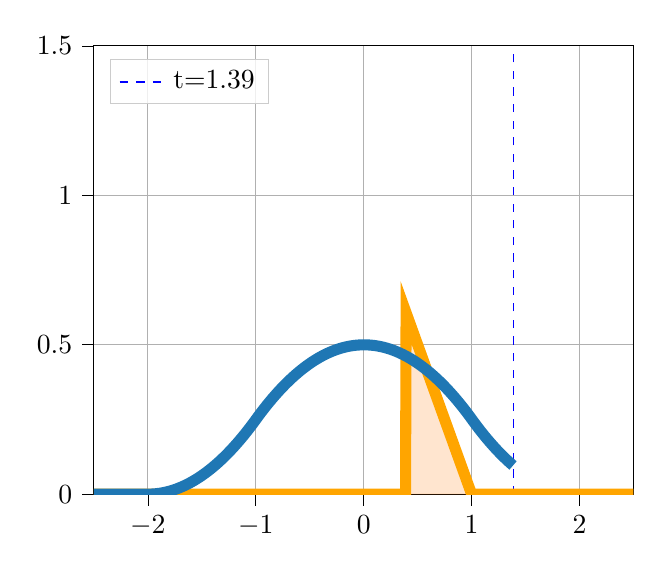
\begin{tikzpicture}

\definecolor{color0}{rgb}{1,0.498039215686275,0.0549019607843137}
\definecolor{color1}{rgb}{1,0.647058823529412,0}
\definecolor{color2}{rgb}{0.12156862745098,0.466666666666667,0.705882352941177}

\begin{axis}[
legend cell align={left},
legend style={fill opacity=0.8, draw opacity=1, text opacity=1, at={(0.03,0.97)}, anchor=north west, draw=white!80!black},
tick align=outside,
tick pos=left,
x grid style={white!69.0196078431373!black},
xmajorgrids,
xmin=-2.5, xmax=2.5,
xtick style={color=black},
y grid style={white!69.0196078431373!black},
ymajorgrids,
ymin=0, ymax=1.5,
ytick style={color=black}
]
\path [draw=color0, fill=color0, opacity=0.2]
(axis cs:-2.5,0)
--(axis cs:-2.5,0)
--(axis cs:-2.49499499499499,0)
--(axis cs:-2.48998998998999,0)
--(axis cs:-2.48498498498498,0)
--(axis cs:-2.47997997997998,0)
--(axis cs:-2.47497497497497,0)
--(axis cs:-2.46996996996997,0)
--(axis cs:-2.46496496496496,0)
--(axis cs:-2.45995995995996,0)
--(axis cs:-2.45495495495495,0)
--(axis cs:-2.44994994994995,0)
--(axis cs:-2.44494494494494,0)
--(axis cs:-2.43993993993994,0)
--(axis cs:-2.43493493493493,0)
--(axis cs:-2.42992992992993,0)
--(axis cs:-2.42492492492492,0)
--(axis cs:-2.41991991991992,0)
--(axis cs:-2.41491491491491,0)
--(axis cs:-2.40990990990991,0)
--(axis cs:-2.4049049049049,0)
--(axis cs:-2.3998998998999,0)
--(axis cs:-2.39489489489489,0)
--(axis cs:-2.38988988988989,0)
--(axis cs:-2.38488488488488,0)
--(axis cs:-2.37987987987988,0)
--(axis cs:-2.37487487487487,0)
--(axis cs:-2.36986986986987,0)
--(axis cs:-2.36486486486486,0)
--(axis cs:-2.35985985985986,0)
--(axis cs:-2.35485485485485,0)
--(axis cs:-2.34984984984985,0)
--(axis cs:-2.34484484484484,0)
--(axis cs:-2.33983983983984,0)
--(axis cs:-2.33483483483483,0)
--(axis cs:-2.32982982982983,0)
--(axis cs:-2.32482482482482,0)
--(axis cs:-2.31981981981982,0)
--(axis cs:-2.31481481481481,0)
--(axis cs:-2.30980980980981,0)
--(axis cs:-2.3048048048048,0)
--(axis cs:-2.2997997997998,0)
--(axis cs:-2.29479479479479,0)
--(axis cs:-2.28978978978979,0)
--(axis cs:-2.28478478478478,0)
--(axis cs:-2.27977977977978,0)
--(axis cs:-2.27477477477477,0)
--(axis cs:-2.26976976976977,0)
--(axis cs:-2.26476476476476,0)
--(axis cs:-2.25975975975976,0)
--(axis cs:-2.25475475475475,0)
--(axis cs:-2.24974974974975,0)
--(axis cs:-2.24474474474474,0)
--(axis cs:-2.23973973973974,0)
--(axis cs:-2.23473473473473,0)
--(axis cs:-2.22972972972973,0)
--(axis cs:-2.22472472472472,0)
--(axis cs:-2.21971971971972,0)
--(axis cs:-2.21471471471471,0)
--(axis cs:-2.20970970970971,0)
--(axis cs:-2.2047047047047,0)
--(axis cs:-2.1996996996997,0)
--(axis cs:-2.19469469469469,0)
--(axis cs:-2.18968968968969,0)
--(axis cs:-2.18468468468468,0)
--(axis cs:-2.17967967967968,0)
--(axis cs:-2.17467467467467,0)
--(axis cs:-2.16966966966967,0)
--(axis cs:-2.16466466466466,0)
--(axis cs:-2.15965965965966,0)
--(axis cs:-2.15465465465465,0)
--(axis cs:-2.14964964964965,0)
--(axis cs:-2.14464464464464,0)
--(axis cs:-2.13963963963964,0)
--(axis cs:-2.13463463463463,0)
--(axis cs:-2.12962962962963,0)
--(axis cs:-2.12462462462462,0)
--(axis cs:-2.11961961961962,0)
--(axis cs:-2.11461461461461,0)
--(axis cs:-2.10960960960961,0)
--(axis cs:-2.1046046046046,0)
--(axis cs:-2.0995995995996,0)
--(axis cs:-2.09459459459459,0)
--(axis cs:-2.08958958958959,0)
--(axis cs:-2.08458458458458,0)
--(axis cs:-2.07957957957958,0)
--(axis cs:-2.07457457457457,0)
--(axis cs:-2.06956956956957,0)
--(axis cs:-2.06456456456456,0)
--(axis cs:-2.05955955955956,0)
--(axis cs:-2.05455455455455,0)
--(axis cs:-2.04954954954955,0)
--(axis cs:-2.04454454454454,0)
--(axis cs:-2.03953953953954,0)
--(axis cs:-2.03453453453453,0)
--(axis cs:-2.02952952952953,0)
--(axis cs:-2.02452452452452,0)
--(axis cs:-2.01951951951952,0)
--(axis cs:-2.01451451451451,0)
--(axis cs:-2.00950950950951,0)
--(axis cs:-2.0045045045045,0)
--(axis cs:-1.9994994994995,0)
--(axis cs:-1.99449449449449,0)
--(axis cs:-1.98948948948949,0)
--(axis cs:-1.98448448448448,0)
--(axis cs:-1.97947947947948,0)
--(axis cs:-1.97447447447447,0)
--(axis cs:-1.96946946946947,0)
--(axis cs:-1.96446446446446,0)
--(axis cs:-1.95945945945946,0)
--(axis cs:-1.95445445445445,0)
--(axis cs:-1.94944944944945,0)
--(axis cs:-1.94444444444444,0)
--(axis cs:-1.93943943943944,0)
--(axis cs:-1.93443443443443,0)
--(axis cs:-1.92942942942943,0)
--(axis cs:-1.92442442442442,0)
--(axis cs:-1.91941941941942,0)
--(axis cs:-1.91441441441441,0)
--(axis cs:-1.90940940940941,0)
--(axis cs:-1.9044044044044,0)
--(axis cs:-1.8993993993994,0)
--(axis cs:-1.89439439439439,0)
--(axis cs:-1.88938938938939,0)
--(axis cs:-1.88438438438438,0)
--(axis cs:-1.87937937937938,0)
--(axis cs:-1.87437437437437,0)
--(axis cs:-1.86936936936937,0)
--(axis cs:-1.86436436436436,0)
--(axis cs:-1.85935935935936,0)
--(axis cs:-1.85435435435435,0)
--(axis cs:-1.84934934934935,0)
--(axis cs:-1.84434434434434,0)
--(axis cs:-1.83933933933934,0)
--(axis cs:-1.83433433433433,0)
--(axis cs:-1.82932932932933,0)
--(axis cs:-1.82432432432432,0)
--(axis cs:-1.81931931931932,0)
--(axis cs:-1.81431431431431,0)
--(axis cs:-1.80930930930931,0)
--(axis cs:-1.8043043043043,0)
--(axis cs:-1.7992992992993,0)
--(axis cs:-1.79429429429429,0)
--(axis cs:-1.78928928928929,0)
--(axis cs:-1.78428428428428,0)
--(axis cs:-1.77927927927928,0)
--(axis cs:-1.77427427427427,0)
--(axis cs:-1.76926926926927,0)
--(axis cs:-1.76426426426426,0)
--(axis cs:-1.75925925925926,0)
--(axis cs:-1.75425425425425,0)
--(axis cs:-1.74924924924925,0)
--(axis cs:-1.74424424424424,0)
--(axis cs:-1.73923923923924,0)
--(axis cs:-1.73423423423423,0)
--(axis cs:-1.72922922922923,0)
--(axis cs:-1.72422422422422,0)
--(axis cs:-1.71921921921922,0)
--(axis cs:-1.71421421421421,0)
--(axis cs:-1.70920920920921,0)
--(axis cs:-1.7042042042042,0)
--(axis cs:-1.6991991991992,0)
--(axis cs:-1.69419419419419,0)
--(axis cs:-1.68918918918919,0)
--(axis cs:-1.68418418418418,0)
--(axis cs:-1.67917917917918,0)
--(axis cs:-1.67417417417417,0)
--(axis cs:-1.66916916916917,0)
--(axis cs:-1.66416416416416,0)
--(axis cs:-1.65915915915916,0)
--(axis cs:-1.65415415415415,0)
--(axis cs:-1.64914914914915,0)
--(axis cs:-1.64414414414414,0)
--(axis cs:-1.63913913913914,0)
--(axis cs:-1.63413413413413,0)
--(axis cs:-1.62912912912913,0)
--(axis cs:-1.62412412412412,0)
--(axis cs:-1.61911911911912,0)
--(axis cs:-1.61411411411411,0)
--(axis cs:-1.60910910910911,0)
--(axis cs:-1.6041041041041,0)
--(axis cs:-1.5990990990991,0)
--(axis cs:-1.59409409409409,0)
--(axis cs:-1.58908908908909,0)
--(axis cs:-1.58408408408408,0)
--(axis cs:-1.57907907907908,0)
--(axis cs:-1.57407407407407,0)
--(axis cs:-1.56906906906907,0)
--(axis cs:-1.56406406406406,0)
--(axis cs:-1.55905905905906,0)
--(axis cs:-1.55405405405405,0)
--(axis cs:-1.54904904904905,0)
--(axis cs:-1.54404404404404,0)
--(axis cs:-1.53903903903904,0)
--(axis cs:-1.53403403403403,0)
--(axis cs:-1.52902902902903,0)
--(axis cs:-1.52402402402402,0)
--(axis cs:-1.51901901901902,0)
--(axis cs:-1.51401401401401,0)
--(axis cs:-1.50900900900901,0)
--(axis cs:-1.504004004004,0)
--(axis cs:-1.498998998999,0)
--(axis cs:-1.49399399399399,0)
--(axis cs:-1.48898898898899,0)
--(axis cs:-1.48398398398398,0)
--(axis cs:-1.47897897897898,0)
--(axis cs:-1.47397397397397,0)
--(axis cs:-1.46896896896897,0)
--(axis cs:-1.46396396396396,0)
--(axis cs:-1.45895895895896,0)
--(axis cs:-1.45395395395395,0)
--(axis cs:-1.44894894894895,0)
--(axis cs:-1.44394394394394,0)
--(axis cs:-1.43893893893894,0)
--(axis cs:-1.43393393393393,0)
--(axis cs:-1.42892892892893,0)
--(axis cs:-1.42392392392392,0)
--(axis cs:-1.41891891891892,0)
--(axis cs:-1.41391391391391,0)
--(axis cs:-1.40890890890891,0)
--(axis cs:-1.4039039039039,0)
--(axis cs:-1.3988988988989,0)
--(axis cs:-1.39389389389389,0)
--(axis cs:-1.38888888888889,0)
--(axis cs:-1.38388388388388,0)
--(axis cs:-1.37887887887888,0)
--(axis cs:-1.37387387387387,0)
--(axis cs:-1.36886886886887,0)
--(axis cs:-1.36386386386386,0)
--(axis cs:-1.35885885885886,0)
--(axis cs:-1.35385385385385,0)
--(axis cs:-1.34884884884885,0)
--(axis cs:-1.34384384384384,0)
--(axis cs:-1.33883883883884,0)
--(axis cs:-1.33383383383383,0)
--(axis cs:-1.32882882882883,0)
--(axis cs:-1.32382382382382,0)
--(axis cs:-1.31881881881882,0)
--(axis cs:-1.31381381381381,0)
--(axis cs:-1.30880880880881,0)
--(axis cs:-1.3038038038038,0)
--(axis cs:-1.2987987987988,0)
--(axis cs:-1.29379379379379,0)
--(axis cs:-1.28878878878879,0)
--(axis cs:-1.28378378378378,0)
--(axis cs:-1.27877877877878,0)
--(axis cs:-1.27377377377377,0)
--(axis cs:-1.26876876876877,0)
--(axis cs:-1.26376376376376,0)
--(axis cs:-1.25875875875876,0)
--(axis cs:-1.25375375375375,0)
--(axis cs:-1.24874874874875,0)
--(axis cs:-1.24374374374374,0)
--(axis cs:-1.23873873873874,0)
--(axis cs:-1.23373373373373,0)
--(axis cs:-1.22872872872873,0)
--(axis cs:-1.22372372372372,0)
--(axis cs:-1.21871871871872,0)
--(axis cs:-1.21371371371371,0)
--(axis cs:-1.20870870870871,0)
--(axis cs:-1.2037037037037,0)
--(axis cs:-1.1986986986987,0)
--(axis cs:-1.19369369369369,0)
--(axis cs:-1.18868868868869,0)
--(axis cs:-1.18368368368368,0)
--(axis cs:-1.17867867867868,0)
--(axis cs:-1.17367367367367,0)
--(axis cs:-1.16866866866867,0)
--(axis cs:-1.16366366366366,0)
--(axis cs:-1.15865865865866,0)
--(axis cs:-1.15365365365365,0)
--(axis cs:-1.14864864864865,0)
--(axis cs:-1.14364364364364,0)
--(axis cs:-1.13863863863864,0)
--(axis cs:-1.13363363363363,0)
--(axis cs:-1.12862862862863,0)
--(axis cs:-1.12362362362362,0)
--(axis cs:-1.11861861861862,0)
--(axis cs:-1.11361361361361,0)
--(axis cs:-1.10860860860861,0)
--(axis cs:-1.1036036036036,0)
--(axis cs:-1.0985985985986,0)
--(axis cs:-1.09359359359359,0)
--(axis cs:-1.08858858858859,0)
--(axis cs:-1.08358358358358,0)
--(axis cs:-1.07857857857858,0)
--(axis cs:-1.07357357357357,0)
--(axis cs:-1.06856856856857,0)
--(axis cs:-1.06356356356356,0)
--(axis cs:-1.05855855855856,0)
--(axis cs:-1.05355355355355,0)
--(axis cs:-1.04854854854855,0)
--(axis cs:-1.04354354354354,0)
--(axis cs:-1.03853853853854,0)
--(axis cs:-1.03353353353353,0)
--(axis cs:-1.02852852852853,0)
--(axis cs:-1.02352352352352,0)
--(axis cs:-1.01851851851852,0)
--(axis cs:-1.01351351351351,0)
--(axis cs:-1.00850850850851,0)
--(axis cs:-1.0035035035035,0)
--(axis cs:-0.998498498498499,0)
--(axis cs:-0.993493493493494,0)
--(axis cs:-0.988488488488489,0)
--(axis cs:-0.983483483483484,0)
--(axis cs:-0.978478478478479,0)
--(axis cs:-0.973473473473474,0)
--(axis cs:-0.968468468468469,0)
--(axis cs:-0.963463463463464,0)
--(axis cs:-0.958458458458459,0)
--(axis cs:-0.953453453453454,0)
--(axis cs:-0.948448448448449,0)
--(axis cs:-0.943443443443444,0)
--(axis cs:-0.938438438438439,0)
--(axis cs:-0.933433433433434,0)
--(axis cs:-0.928428428428429,0)
--(axis cs:-0.923423423423424,0)
--(axis cs:-0.918418418418419,0)
--(axis cs:-0.913413413413414,0)
--(axis cs:-0.908408408408409,0)
--(axis cs:-0.903403403403404,0)
--(axis cs:-0.898398398398399,0)
--(axis cs:-0.893393393393393,0)
--(axis cs:-0.888388388388388,0)
--(axis cs:-0.883383383383383,0)
--(axis cs:-0.878378378378378,0)
--(axis cs:-0.873373373373373,0)
--(axis cs:-0.868368368368368,0)
--(axis cs:-0.863363363363363,0)
--(axis cs:-0.858358358358358,0)
--(axis cs:-0.853353353353353,0)
--(axis cs:-0.848348348348348,0)
--(axis cs:-0.843343343343343,0)
--(axis cs:-0.838338338338338,0)
--(axis cs:-0.833333333333333,0)
--(axis cs:-0.828328328328328,0)
--(axis cs:-0.823323323323323,0)
--(axis cs:-0.818318318318318,0)
--(axis cs:-0.813313313313313,0)
--(axis cs:-0.808308308308308,0)
--(axis cs:-0.803303303303303,0)
--(axis cs:-0.798298298298298,0)
--(axis cs:-0.793293293293293,0)
--(axis cs:-0.788288288288288,0)
--(axis cs:-0.783283283283283,0)
--(axis cs:-0.778278278278278,0)
--(axis cs:-0.773273273273273,0)
--(axis cs:-0.768268268268268,0)
--(axis cs:-0.763263263263263,0)
--(axis cs:-0.758258258258258,0)
--(axis cs:-0.753253253253253,0)
--(axis cs:-0.748248248248248,0)
--(axis cs:-0.743243243243243,0)
--(axis cs:-0.738238238238238,0)
--(axis cs:-0.733233233233233,0)
--(axis cs:-0.728228228228228,0)
--(axis cs:-0.723223223223223,0)
--(axis cs:-0.718218218218218,0)
--(axis cs:-0.713213213213213,0)
--(axis cs:-0.708208208208208,0)
--(axis cs:-0.703203203203203,0)
--(axis cs:-0.698198198198198,0)
--(axis cs:-0.693193193193193,0)
--(axis cs:-0.688188188188188,0)
--(axis cs:-0.683183183183183,0)
--(axis cs:-0.678178178178178,0)
--(axis cs:-0.673173173173173,0)
--(axis cs:-0.668168168168168,0)
--(axis cs:-0.663163163163163,0)
--(axis cs:-0.658158158158158,0)
--(axis cs:-0.653153153153153,0)
--(axis cs:-0.648148148148148,0)
--(axis cs:-0.643143143143143,0)
--(axis cs:-0.638138138138138,0)
--(axis cs:-0.633133133133133,0)
--(axis cs:-0.628128128128128,0)
--(axis cs:-0.623123123123123,0)
--(axis cs:-0.618118118118118,0)
--(axis cs:-0.613113113113113,0)
--(axis cs:-0.608108108108108,0)
--(axis cs:-0.603103103103103,0)
--(axis cs:-0.598098098098098,0)
--(axis cs:-0.593093093093093,0)
--(axis cs:-0.588088088088088,0)
--(axis cs:-0.583083083083083,0)
--(axis cs:-0.578078078078078,0)
--(axis cs:-0.573073073073073,0)
--(axis cs:-0.568068068068068,0)
--(axis cs:-0.563063063063063,0)
--(axis cs:-0.558058058058058,0)
--(axis cs:-0.553053053053053,0)
--(axis cs:-0.548048048048048,0)
--(axis cs:-0.543043043043043,0)
--(axis cs:-0.538038038038038,0)
--(axis cs:-0.533033033033033,0)
--(axis cs:-0.528028028028028,0)
--(axis cs:-0.523023023023023,0)
--(axis cs:-0.518018018018018,0)
--(axis cs:-0.513013013013013,0)
--(axis cs:-0.508008008008008,0)
--(axis cs:-0.503003003003003,0)
--(axis cs:-0.497997997997998,0)
--(axis cs:-0.492992992992993,0)
--(axis cs:-0.487987987987988,0)
--(axis cs:-0.482982982982983,0)
--(axis cs:-0.477977977977978,0)
--(axis cs:-0.472972972972973,0)
--(axis cs:-0.467967967967968,0)
--(axis cs:-0.462962962962963,0)
--(axis cs:-0.457957957957958,0)
--(axis cs:-0.452952952952953,0)
--(axis cs:-0.447947947947948,0)
--(axis cs:-0.442942942942943,0)
--(axis cs:-0.437937937937938,0)
--(axis cs:-0.432932932932933,0)
--(axis cs:-0.427927927927928,0)
--(axis cs:-0.422922922922923,0)
--(axis cs:-0.417917917917918,0)
--(axis cs:-0.412912912912913,0)
--(axis cs:-0.407907907907908,0)
--(axis cs:-0.402902902902903,0)
--(axis cs:-0.397897897897898,0)
--(axis cs:-0.392892892892893,0)
--(axis cs:-0.387887887887888,0)
--(axis cs:-0.382882882882883,0)
--(axis cs:-0.377877877877878,0)
--(axis cs:-0.372872872872873,0)
--(axis cs:-0.367867867867868,0)
--(axis cs:-0.362862862862863,0)
--(axis cs:-0.357857857857858,0)
--(axis cs:-0.352852852852853,0)
--(axis cs:-0.347847847847848,0)
--(axis cs:-0.342842842842843,0)
--(axis cs:-0.337837837837838,0)
--(axis cs:-0.332832832832833,0)
--(axis cs:-0.327827827827828,0)
--(axis cs:-0.322822822822823,0)
--(axis cs:-0.317817817817818,0)
--(axis cs:-0.312812812812813,0)
--(axis cs:-0.307807807807808,0)
--(axis cs:-0.302802802802803,0)
--(axis cs:-0.297797797797798,0)
--(axis cs:-0.292792792792793,0)
--(axis cs:-0.287787787787788,0)
--(axis cs:-0.282782782782783,0)
--(axis cs:-0.277777777777778,0)
--(axis cs:-0.272772772772773,0)
--(axis cs:-0.267767767767768,0)
--(axis cs:-0.262762762762763,0)
--(axis cs:-0.257757757757758,0)
--(axis cs:-0.252752752752753,0)
--(axis cs:-0.247747747747748,0)
--(axis cs:-0.242742742742743,0)
--(axis cs:-0.237737737737738,0)
--(axis cs:-0.232732732732733,0)
--(axis cs:-0.227727727727728,0)
--(axis cs:-0.222722722722723,0)
--(axis cs:-0.217717717717718,0)
--(axis cs:-0.212712712712713,0)
--(axis cs:-0.207707707707708,0)
--(axis cs:-0.202702702702703,0)
--(axis cs:-0.197697697697698,0)
--(axis cs:-0.192692692692693,0)
--(axis cs:-0.187687687687688,0)
--(axis cs:-0.182682682682683,0)
--(axis cs:-0.177677677677678,0)
--(axis cs:-0.172672672672673,0)
--(axis cs:-0.167667667667668,0)
--(axis cs:-0.162662662662663,0)
--(axis cs:-0.157657657657658,0)
--(axis cs:-0.152652652652653,0)
--(axis cs:-0.147647647647648,0)
--(axis cs:-0.142642642642643,0)
--(axis cs:-0.137637637637638,0)
--(axis cs:-0.132632632632633,0)
--(axis cs:-0.127627627627628,0)
--(axis cs:-0.122622622622623,0)
--(axis cs:-0.117617617617618,0)
--(axis cs:-0.112612612612613,0)
--(axis cs:-0.107607607607608,0)
--(axis cs:-0.102602602602603,0)
--(axis cs:-0.0975975975975976,0)
--(axis cs:-0.0925925925925926,0)
--(axis cs:-0.0875875875875876,0)
--(axis cs:-0.0825825825825826,0)
--(axis cs:-0.0775775775775776,0)
--(axis cs:-0.0725725725725725,0)
--(axis cs:-0.0675675675675675,0)
--(axis cs:-0.0625625625625625,0)
--(axis cs:-0.0575575575575575,0)
--(axis cs:-0.0525525525525525,0)
--(axis cs:-0.0475475475475475,0)
--(axis cs:-0.0425425425425425,0)
--(axis cs:-0.0375375375375375,0)
--(axis cs:-0.0325325325325325,0)
--(axis cs:-0.0275275275275275,0)
--(axis cs:-0.0225225225225225,0)
--(axis cs:-0.0175175175175175,0)
--(axis cs:-0.0125125125125125,0)
--(axis cs:-0.0075075075075075,0)
--(axis cs:-0.0025025025025025,0)
--(axis cs:0.0025025025025025,0)
--(axis cs:0.0075075075075075,0)
--(axis cs:0.0125125125125125,0)
--(axis cs:0.0175175175175175,0)
--(axis cs:0.0225225225225225,0)
--(axis cs:0.0275275275275275,0)
--(axis cs:0.0325325325325325,0)
--(axis cs:0.0375375375375375,0)
--(axis cs:0.0425425425425425,0)
--(axis cs:0.0475475475475475,0)
--(axis cs:0.0525525525525525,0)
--(axis cs:0.0575575575575575,0)
--(axis cs:0.0625625625625625,0)
--(axis cs:0.0675675675675675,0)
--(axis cs:0.0725725725725725,0)
--(axis cs:0.0775775775775776,0)
--(axis cs:0.0825825825825826,0)
--(axis cs:0.0875875875875876,0)
--(axis cs:0.0925925925925926,0)
--(axis cs:0.0975975975975976,0)
--(axis cs:0.102602602602603,0)
--(axis cs:0.107607607607608,0)
--(axis cs:0.112612612612613,0)
--(axis cs:0.117617617617618,0)
--(axis cs:0.122622622622623,0)
--(axis cs:0.127627627627628,0)
--(axis cs:0.132632632632633,0)
--(axis cs:0.137637637637638,0)
--(axis cs:0.142642642642643,0)
--(axis cs:0.147647647647648,0)
--(axis cs:0.152652652652653,0)
--(axis cs:0.157657657657658,0)
--(axis cs:0.162662662662663,0)
--(axis cs:0.167667667667668,0)
--(axis cs:0.172672672672673,0)
--(axis cs:0.177677677677678,0)
--(axis cs:0.182682682682683,0)
--(axis cs:0.187687687687688,0)
--(axis cs:0.192692692692693,0)
--(axis cs:0.197697697697698,0)
--(axis cs:0.202702702702703,0)
--(axis cs:0.207707707707708,0)
--(axis cs:0.212712712712713,0)
--(axis cs:0.217717717717718,0)
--(axis cs:0.222722722722723,0)
--(axis cs:0.227727727727728,0)
--(axis cs:0.232732732732733,0)
--(axis cs:0.237737737737738,0)
--(axis cs:0.242742742742743,0)
--(axis cs:0.247747747747748,0)
--(axis cs:0.252752752752753,0)
--(axis cs:0.257757757757758,0)
--(axis cs:0.262762762762763,0)
--(axis cs:0.267767767767768,0)
--(axis cs:0.272772772772773,0)
--(axis cs:0.277777777777778,0)
--(axis cs:0.282782782782783,0)
--(axis cs:0.287787787787788,0)
--(axis cs:0.292792792792793,0)
--(axis cs:0.297797797797798,0)
--(axis cs:0.302802802802803,0)
--(axis cs:0.307807807807808,0)
--(axis cs:0.312812812812813,0)
--(axis cs:0.317817817817818,0)
--(axis cs:0.322822822822823,0)
--(axis cs:0.327827827827828,0)
--(axis cs:0.332832832832833,0)
--(axis cs:0.337837837837838,0)
--(axis cs:0.342842842842843,0)
--(axis cs:0.347847847847848,0)
--(axis cs:0.352852852852853,0)
--(axis cs:0.357857857857858,0)
--(axis cs:0.362862862862863,0)
--(axis cs:0.367867867867868,0)
--(axis cs:0.372872872872873,0)
--(axis cs:0.377877877877878,0)
--(axis cs:0.382882882882883,0)
--(axis cs:0.387887887887888,0)
--(axis cs:0.392892892892893,0)
--(axis cs:0.397897897897898,0)
--(axis cs:0.402902902902903,0)
--(axis cs:0.407907907907908,0)
--(axis cs:0.412912912912913,0)
--(axis cs:0.417917917917918,0)
--(axis cs:0.422922922922923,0)
--(axis cs:0.427927927927928,0)
--(axis cs:0.432932932932933,0)
--(axis cs:0.437937937937938,0)
--(axis cs:0.442942942942943,0)
--(axis cs:0.447947947947948,0)
--(axis cs:0.452952952952953,0)
--(axis cs:0.457957957957958,0)
--(axis cs:0.462962962962963,0)
--(axis cs:0.467967967967968,0)
--(axis cs:0.472972972972973,0)
--(axis cs:0.477977977977978,0)
--(axis cs:0.482982982982983,0)
--(axis cs:0.487987987987988,0)
--(axis cs:0.492992992992993,0)
--(axis cs:0.497997997997998,0)
--(axis cs:0.503003003003003,0)
--(axis cs:0.508008008008008,0)
--(axis cs:0.513013013013013,0)
--(axis cs:0.518018018018018,0)
--(axis cs:0.523023023023023,0)
--(axis cs:0.528028028028028,0)
--(axis cs:0.533033033033033,0)
--(axis cs:0.538038038038038,0)
--(axis cs:0.543043043043043,0)
--(axis cs:0.548048048048048,0)
--(axis cs:0.553053053053053,0)
--(axis cs:0.558058058058058,0)
--(axis cs:0.563063063063063,0)
--(axis cs:0.568068068068068,0)
--(axis cs:0.573073073073073,0)
--(axis cs:0.578078078078078,0)
--(axis cs:0.583083083083083,0)
--(axis cs:0.588088088088088,0)
--(axis cs:0.593093093093093,0)
--(axis cs:0.598098098098098,0)
--(axis cs:0.603103103103103,0)
--(axis cs:0.608108108108108,0)
--(axis cs:0.613113113113113,0)
--(axis cs:0.618118118118118,0)
--(axis cs:0.623123123123123,0)
--(axis cs:0.628128128128128,0)
--(axis cs:0.633133133133133,0)
--(axis cs:0.638138138138138,0)
--(axis cs:0.643143143143143,0)
--(axis cs:0.648148148148148,0)
--(axis cs:0.653153153153153,0)
--(axis cs:0.658158158158158,0)
--(axis cs:0.663163163163163,0)
--(axis cs:0.668168168168168,0)
--(axis cs:0.673173173173173,0)
--(axis cs:0.678178178178178,0)
--(axis cs:0.683183183183183,0)
--(axis cs:0.688188188188188,0)
--(axis cs:0.693193193193193,0)
--(axis cs:0.698198198198198,0)
--(axis cs:0.703203203203203,0)
--(axis cs:0.708208208208208,0)
--(axis cs:0.713213213213213,0)
--(axis cs:0.718218218218218,0)
--(axis cs:0.723223223223223,0)
--(axis cs:0.728228228228228,0)
--(axis cs:0.733233233233233,0)
--(axis cs:0.738238238238238,0)
--(axis cs:0.743243243243243,0)
--(axis cs:0.748248248248248,0)
--(axis cs:0.753253253253253,0)
--(axis cs:0.758258258258258,0)
--(axis cs:0.763263263263263,0)
--(axis cs:0.768268268268268,0)
--(axis cs:0.773273273273273,0)
--(axis cs:0.778278278278278,0)
--(axis cs:0.783283283283283,0)
--(axis cs:0.788288288288288,0)
--(axis cs:0.793293293293293,0)
--(axis cs:0.798298298298298,0)
--(axis cs:0.803303303303303,0)
--(axis cs:0.808308308308308,0)
--(axis cs:0.813313313313313,0)
--(axis cs:0.818318318318318,0)
--(axis cs:0.823323323323323,0)
--(axis cs:0.828328328328328,0)
--(axis cs:0.833333333333333,0)
--(axis cs:0.838338338338338,0)
--(axis cs:0.843343343343343,0)
--(axis cs:0.848348348348348,0)
--(axis cs:0.853353353353353,0)
--(axis cs:0.858358358358358,0)
--(axis cs:0.863363363363364,0)
--(axis cs:0.868368368368369,0)
--(axis cs:0.873373373373374,0)
--(axis cs:0.878378378378379,0)
--(axis cs:0.883383383383384,0)
--(axis cs:0.888388388388389,0)
--(axis cs:0.893393393393394,0)
--(axis cs:0.898398398398399,0)
--(axis cs:0.903403403403404,0)
--(axis cs:0.908408408408409,0)
--(axis cs:0.913413413413414,0)
--(axis cs:0.918418418418419,0)
--(axis cs:0.923423423423424,0)
--(axis cs:0.928428428428429,0)
--(axis cs:0.933433433433434,0)
--(axis cs:0.938438438438439,0)
--(axis cs:0.943443443443444,0)
--(axis cs:0.948448448448449,0)
--(axis cs:0.953453453453454,0)
--(axis cs:0.958458458458459,0)
--(axis cs:0.963463463463464,0)
--(axis cs:0.968468468468469,0)
--(axis cs:0.973473473473474,0)
--(axis cs:0.978478478478479,0)
--(axis cs:0.983483483483484,0)
--(axis cs:0.988488488488489,0)
--(axis cs:0.993493493493494,0)
--(axis cs:0.998498498498499,0)
--(axis cs:1.0035035035035,0)
--(axis cs:1.00850850850851,0)
--(axis cs:1.01351351351351,0)
--(axis cs:1.01851851851852,0)
--(axis cs:1.02352352352352,0)
--(axis cs:1.02852852852853,0)
--(axis cs:1.03353353353353,0)
--(axis cs:1.03853853853854,0)
--(axis cs:1.04354354354354,0)
--(axis cs:1.04854854854855,0)
--(axis cs:1.05355355355355,0)
--(axis cs:1.05855855855856,0)
--(axis cs:1.06356356356356,0)
--(axis cs:1.06856856856857,0)
--(axis cs:1.07357357357357,0)
--(axis cs:1.07857857857858,0)
--(axis cs:1.08358358358358,0)
--(axis cs:1.08858858858859,0)
--(axis cs:1.09359359359359,0)
--(axis cs:1.0985985985986,0)
--(axis cs:1.1036036036036,0)
--(axis cs:1.10860860860861,0)
--(axis cs:1.11361361361361,0)
--(axis cs:1.11861861861862,0)
--(axis cs:1.12362362362362,0)
--(axis cs:1.12862862862863,0)
--(axis cs:1.13363363363363,0)
--(axis cs:1.13863863863864,0)
--(axis cs:1.14364364364364,0)
--(axis cs:1.14864864864865,0)
--(axis cs:1.15365365365365,0)
--(axis cs:1.15865865865866,0)
--(axis cs:1.16366366366366,0)
--(axis cs:1.16866866866867,0)
--(axis cs:1.17367367367367,0)
--(axis cs:1.17867867867868,0)
--(axis cs:1.18368368368368,0)
--(axis cs:1.18868868868869,0)
--(axis cs:1.19369369369369,0)
--(axis cs:1.1986986986987,0)
--(axis cs:1.2037037037037,0)
--(axis cs:1.20870870870871,0)
--(axis cs:1.21371371371371,0)
--(axis cs:1.21871871871872,0)
--(axis cs:1.22372372372372,0)
--(axis cs:1.22872872872873,0)
--(axis cs:1.23373373373373,0)
--(axis cs:1.23873873873874,0)
--(axis cs:1.24374374374374,0)
--(axis cs:1.24874874874875,0)
--(axis cs:1.25375375375375,0)
--(axis cs:1.25875875875876,0)
--(axis cs:1.26376376376376,0)
--(axis cs:1.26876876876877,0)
--(axis cs:1.27377377377377,0)
--(axis cs:1.27877877877878,0)
--(axis cs:1.28378378378378,0)
--(axis cs:1.28878878878879,0)
--(axis cs:1.29379379379379,0)
--(axis cs:1.2987987987988,0)
--(axis cs:1.3038038038038,0)
--(axis cs:1.30880880880881,0)
--(axis cs:1.31381381381381,0)
--(axis cs:1.31881881881882,0)
--(axis cs:1.32382382382382,0)
--(axis cs:1.32882882882883,0)
--(axis cs:1.33383383383383,0)
--(axis cs:1.33883883883884,0)
--(axis cs:1.34384384384384,0)
--(axis cs:1.34884884884885,0)
--(axis cs:1.35385385385385,0)
--(axis cs:1.35885885885886,0)
--(axis cs:1.36386386386386,0)
--(axis cs:1.36886886886887,0)
--(axis cs:1.37387387387387,0)
--(axis cs:1.37887887887888,0)
--(axis cs:1.38388388388388,0)
--(axis cs:1.38888888888889,0)
--(axis cs:1.39389389389389,0)
--(axis cs:1.3988988988989,0)
--(axis cs:1.4039039039039,0)
--(axis cs:1.40890890890891,0)
--(axis cs:1.41391391391391,0)
--(axis cs:1.41891891891892,0)
--(axis cs:1.42392392392392,0)
--(axis cs:1.42892892892893,0)
--(axis cs:1.43393393393393,0)
--(axis cs:1.43893893893894,0)
--(axis cs:1.44394394394394,0)
--(axis cs:1.44894894894895,0)
--(axis cs:1.45395395395395,0)
--(axis cs:1.45895895895896,0)
--(axis cs:1.46396396396396,0)
--(axis cs:1.46896896896897,0)
--(axis cs:1.47397397397397,0)
--(axis cs:1.47897897897898,0)
--(axis cs:1.48398398398398,0)
--(axis cs:1.48898898898899,0)
--(axis cs:1.49399399399399,0)
--(axis cs:1.498998998999,0)
--(axis cs:1.504004004004,0)
--(axis cs:1.50900900900901,0)
--(axis cs:1.51401401401401,0)
--(axis cs:1.51901901901902,0)
--(axis cs:1.52402402402402,0)
--(axis cs:1.52902902902903,0)
--(axis cs:1.53403403403403,0)
--(axis cs:1.53903903903904,0)
--(axis cs:1.54404404404404,0)
--(axis cs:1.54904904904905,0)
--(axis cs:1.55405405405405,0)
--(axis cs:1.55905905905906,0)
--(axis cs:1.56406406406406,0)
--(axis cs:1.56906906906907,0)
--(axis cs:1.57407407407407,0)
--(axis cs:1.57907907907908,0)
--(axis cs:1.58408408408408,0)
--(axis cs:1.58908908908909,0)
--(axis cs:1.59409409409409,0)
--(axis cs:1.5990990990991,0)
--(axis cs:1.6041041041041,0)
--(axis cs:1.60910910910911,0)
--(axis cs:1.61411411411411,0)
--(axis cs:1.61911911911912,0)
--(axis cs:1.62412412412412,0)
--(axis cs:1.62912912912913,0)
--(axis cs:1.63413413413413,0)
--(axis cs:1.63913913913914,0)
--(axis cs:1.64414414414414,0)
--(axis cs:1.64914914914915,0)
--(axis cs:1.65415415415415,0)
--(axis cs:1.65915915915916,0)
--(axis cs:1.66416416416416,0)
--(axis cs:1.66916916916917,0)
--(axis cs:1.67417417417417,0)
--(axis cs:1.67917917917918,0)
--(axis cs:1.68418418418418,0)
--(axis cs:1.68918918918919,0)
--(axis cs:1.69419419419419,0)
--(axis cs:1.6991991991992,0)
--(axis cs:1.7042042042042,0)
--(axis cs:1.70920920920921,0)
--(axis cs:1.71421421421421,0)
--(axis cs:1.71921921921922,0)
--(axis cs:1.72422422422422,0)
--(axis cs:1.72922922922923,0)
--(axis cs:1.73423423423423,0)
--(axis cs:1.73923923923924,0)
--(axis cs:1.74424424424424,0)
--(axis cs:1.74924924924925,0)
--(axis cs:1.75425425425425,0)
--(axis cs:1.75925925925926,0)
--(axis cs:1.76426426426426,0)
--(axis cs:1.76926926926927,0)
--(axis cs:1.77427427427427,0)
--(axis cs:1.77927927927928,0)
--(axis cs:1.78428428428428,0)
--(axis cs:1.78928928928929,0)
--(axis cs:1.79429429429429,0)
--(axis cs:1.7992992992993,0)
--(axis cs:1.8043043043043,0)
--(axis cs:1.80930930930931,0)
--(axis cs:1.81431431431431,0)
--(axis cs:1.81931931931932,0)
--(axis cs:1.82432432432432,0)
--(axis cs:1.82932932932933,0)
--(axis cs:1.83433433433433,0)
--(axis cs:1.83933933933934,0)
--(axis cs:1.84434434434434,0)
--(axis cs:1.84934934934935,0)
--(axis cs:1.85435435435435,0)
--(axis cs:1.85935935935936,0)
--(axis cs:1.86436436436436,0)
--(axis cs:1.86936936936937,0)
--(axis cs:1.87437437437437,0)
--(axis cs:1.87937937937938,0)
--(axis cs:1.88438438438438,0)
--(axis cs:1.88938938938939,0)
--(axis cs:1.89439439439439,0)
--(axis cs:1.8993993993994,0)
--(axis cs:1.9044044044044,0)
--(axis cs:1.90940940940941,0)
--(axis cs:1.91441441441441,0)
--(axis cs:1.91941941941942,0)
--(axis cs:1.92442442442442,0)
--(axis cs:1.92942942942943,0)
--(axis cs:1.93443443443443,0)
--(axis cs:1.93943943943944,0)
--(axis cs:1.94444444444444,0)
--(axis cs:1.94944944944945,0)
--(axis cs:1.95445445445445,0)
--(axis cs:1.95945945945946,0)
--(axis cs:1.96446446446446,0)
--(axis cs:1.96946946946947,0)
--(axis cs:1.97447447447447,0)
--(axis cs:1.97947947947948,0)
--(axis cs:1.98448448448448,0)
--(axis cs:1.98948948948949,0)
--(axis cs:1.99449449449449,0)
--(axis cs:1.9994994994995,0)
--(axis cs:2.0045045045045,0)
--(axis cs:2.00950950950951,0)
--(axis cs:2.01451451451451,0)
--(axis cs:2.01951951951952,0)
--(axis cs:2.02452452452452,0)
--(axis cs:2.02952952952953,0)
--(axis cs:2.03453453453453,0)
--(axis cs:2.03953953953954,0)
--(axis cs:2.04454454454454,0)
--(axis cs:2.04954954954955,0)
--(axis cs:2.05455455455455,0)
--(axis cs:2.05955955955956,0)
--(axis cs:2.06456456456456,0)
--(axis cs:2.06956956956957,0)
--(axis cs:2.07457457457457,0)
--(axis cs:2.07957957957958,0)
--(axis cs:2.08458458458458,0)
--(axis cs:2.08958958958959,0)
--(axis cs:2.09459459459459,0)
--(axis cs:2.0995995995996,0)
--(axis cs:2.1046046046046,0)
--(axis cs:2.10960960960961,0)
--(axis cs:2.11461461461461,0)
--(axis cs:2.11961961961962,0)
--(axis cs:2.12462462462462,0)
--(axis cs:2.12962962962963,0)
--(axis cs:2.13463463463463,0)
--(axis cs:2.13963963963964,0)
--(axis cs:2.14464464464464,0)
--(axis cs:2.14964964964965,0)
--(axis cs:2.15465465465465,0)
--(axis cs:2.15965965965966,0)
--(axis cs:2.16466466466466,0)
--(axis cs:2.16966966966967,0)
--(axis cs:2.17467467467467,0)
--(axis cs:2.17967967967968,0)
--(axis cs:2.18468468468468,0)
--(axis cs:2.18968968968969,0)
--(axis cs:2.19469469469469,0)
--(axis cs:2.1996996996997,0)
--(axis cs:2.2047047047047,0)
--(axis cs:2.20970970970971,0)
--(axis cs:2.21471471471471,0)
--(axis cs:2.21971971971972,0)
--(axis cs:2.22472472472472,0)
--(axis cs:2.22972972972973,0)
--(axis cs:2.23473473473473,0)
--(axis cs:2.23973973973974,0)
--(axis cs:2.24474474474474,0)
--(axis cs:2.24974974974975,0)
--(axis cs:2.25475475475475,0)
--(axis cs:2.25975975975976,0)
--(axis cs:2.26476476476476,0)
--(axis cs:2.26976976976977,0)
--(axis cs:2.27477477477477,0)
--(axis cs:2.27977977977978,0)
--(axis cs:2.28478478478478,0)
--(axis cs:2.28978978978979,0)
--(axis cs:2.29479479479479,0)
--(axis cs:2.2997997997998,0)
--(axis cs:2.3048048048048,0)
--(axis cs:2.30980980980981,0)
--(axis cs:2.31481481481481,0)
--(axis cs:2.31981981981982,0)
--(axis cs:2.32482482482482,0)
--(axis cs:2.32982982982983,0)
--(axis cs:2.33483483483483,0)
--(axis cs:2.33983983983984,0)
--(axis cs:2.34484484484484,0)
--(axis cs:2.34984984984985,0)
--(axis cs:2.35485485485485,0)
--(axis cs:2.35985985985986,0)
--(axis cs:2.36486486486486,0)
--(axis cs:2.36986986986987,0)
--(axis cs:2.37487487487487,0)
--(axis cs:2.37987987987988,0)
--(axis cs:2.38488488488488,0)
--(axis cs:2.38988988988989,0)
--(axis cs:2.39489489489489,0)
--(axis cs:2.3998998998999,0)
--(axis cs:2.4049049049049,0)
--(axis cs:2.40990990990991,0)
--(axis cs:2.41491491491491,0)
--(axis cs:2.41991991991992,0)
--(axis cs:2.42492492492492,0)
--(axis cs:2.42992992992993,0)
--(axis cs:2.43493493493493,0)
--(axis cs:2.43993993993994,0)
--(axis cs:2.44494494494494,0)
--(axis cs:2.44994994994995,0)
--(axis cs:2.45495495495495,0)
--(axis cs:2.45995995995996,0)
--(axis cs:2.46496496496496,0)
--(axis cs:2.46996996996997,0)
--(axis cs:2.47497497497497,0)
--(axis cs:2.47997997997998,0)
--(axis cs:2.48498498498498,0)
--(axis cs:2.48998998998999,0)
--(axis cs:2.49499499499499,0)
--(axis cs:2.5,0)
--(axis cs:2.5,0)
--(axis cs:2.5,0)
--(axis cs:2.49499499499499,0)
--(axis cs:2.48998998998999,0)
--(axis cs:2.48498498498498,0)
--(axis cs:2.47997997997998,0)
--(axis cs:2.47497497497497,0)
--(axis cs:2.46996996996997,0)
--(axis cs:2.46496496496496,0)
--(axis cs:2.45995995995996,0)
--(axis cs:2.45495495495495,0)
--(axis cs:2.44994994994995,0)
--(axis cs:2.44494494494494,0)
--(axis cs:2.43993993993994,0)
--(axis cs:2.43493493493493,0)
--(axis cs:2.42992992992993,0)
--(axis cs:2.42492492492492,0)
--(axis cs:2.41991991991992,0)
--(axis cs:2.41491491491491,0)
--(axis cs:2.40990990990991,0)
--(axis cs:2.4049049049049,0)
--(axis cs:2.3998998998999,0)
--(axis cs:2.39489489489489,0)
--(axis cs:2.38988988988989,0)
--(axis cs:2.38488488488488,0)
--(axis cs:2.37987987987988,0)
--(axis cs:2.37487487487487,0)
--(axis cs:2.36986986986987,0)
--(axis cs:2.36486486486486,0)
--(axis cs:2.35985985985986,0)
--(axis cs:2.35485485485485,0)
--(axis cs:2.34984984984985,0)
--(axis cs:2.34484484484484,0)
--(axis cs:2.33983983983984,0)
--(axis cs:2.33483483483483,0)
--(axis cs:2.32982982982983,0)
--(axis cs:2.32482482482482,0)
--(axis cs:2.31981981981982,0)
--(axis cs:2.31481481481481,0)
--(axis cs:2.30980980980981,0)
--(axis cs:2.3048048048048,0)
--(axis cs:2.2997997997998,0)
--(axis cs:2.29479479479479,0)
--(axis cs:2.28978978978979,0)
--(axis cs:2.28478478478478,0)
--(axis cs:2.27977977977978,0)
--(axis cs:2.27477477477477,0)
--(axis cs:2.26976976976977,0)
--(axis cs:2.26476476476476,0)
--(axis cs:2.25975975975976,0)
--(axis cs:2.25475475475475,0)
--(axis cs:2.24974974974975,0)
--(axis cs:2.24474474474474,0)
--(axis cs:2.23973973973974,0)
--(axis cs:2.23473473473473,0)
--(axis cs:2.22972972972973,0)
--(axis cs:2.22472472472472,0)
--(axis cs:2.21971971971972,0)
--(axis cs:2.21471471471471,0)
--(axis cs:2.20970970970971,0)
--(axis cs:2.2047047047047,0)
--(axis cs:2.1996996996997,0)
--(axis cs:2.19469469469469,0)
--(axis cs:2.18968968968969,0)
--(axis cs:2.18468468468468,0)
--(axis cs:2.17967967967968,0)
--(axis cs:2.17467467467467,0)
--(axis cs:2.16966966966967,0)
--(axis cs:2.16466466466466,0)
--(axis cs:2.15965965965966,0)
--(axis cs:2.15465465465465,0)
--(axis cs:2.14964964964965,0)
--(axis cs:2.14464464464464,0)
--(axis cs:2.13963963963964,0)
--(axis cs:2.13463463463463,0)
--(axis cs:2.12962962962963,0)
--(axis cs:2.12462462462462,0)
--(axis cs:2.11961961961962,0)
--(axis cs:2.11461461461461,0)
--(axis cs:2.10960960960961,0)
--(axis cs:2.1046046046046,0)
--(axis cs:2.0995995995996,0)
--(axis cs:2.09459459459459,0)
--(axis cs:2.08958958958959,0)
--(axis cs:2.08458458458458,0)
--(axis cs:2.07957957957958,0)
--(axis cs:2.07457457457457,0)
--(axis cs:2.06956956956957,0)
--(axis cs:2.06456456456456,0)
--(axis cs:2.05955955955956,0)
--(axis cs:2.05455455455455,0)
--(axis cs:2.04954954954955,0)
--(axis cs:2.04454454454454,0)
--(axis cs:2.03953953953954,0)
--(axis cs:2.03453453453453,0)
--(axis cs:2.02952952952953,0)
--(axis cs:2.02452452452452,0)
--(axis cs:2.01951951951952,0)
--(axis cs:2.01451451451451,0)
--(axis cs:2.00950950950951,0)
--(axis cs:2.0045045045045,0)
--(axis cs:1.9994994994995,0)
--(axis cs:1.99449449449449,0)
--(axis cs:1.98948948948949,0)
--(axis cs:1.98448448448448,0)
--(axis cs:1.97947947947948,0)
--(axis cs:1.97447447447447,0)
--(axis cs:1.96946946946947,0)
--(axis cs:1.96446446446446,0)
--(axis cs:1.95945945945946,0)
--(axis cs:1.95445445445445,0)
--(axis cs:1.94944944944945,0)
--(axis cs:1.94444444444444,0)
--(axis cs:1.93943943943944,0)
--(axis cs:1.93443443443443,0)
--(axis cs:1.92942942942943,0)
--(axis cs:1.92442442442442,0)
--(axis cs:1.91941941941942,0)
--(axis cs:1.91441441441441,0)
--(axis cs:1.90940940940941,0)
--(axis cs:1.9044044044044,0)
--(axis cs:1.8993993993994,0)
--(axis cs:1.89439439439439,0)
--(axis cs:1.88938938938939,0)
--(axis cs:1.88438438438438,0)
--(axis cs:1.87937937937938,0)
--(axis cs:1.87437437437437,0)
--(axis cs:1.86936936936937,0)
--(axis cs:1.86436436436436,0)
--(axis cs:1.85935935935936,0)
--(axis cs:1.85435435435435,0)
--(axis cs:1.84934934934935,0)
--(axis cs:1.84434434434434,0)
--(axis cs:1.83933933933934,0)
--(axis cs:1.83433433433433,0)
--(axis cs:1.82932932932933,0)
--(axis cs:1.82432432432432,0)
--(axis cs:1.81931931931932,0)
--(axis cs:1.81431431431431,0)
--(axis cs:1.80930930930931,0)
--(axis cs:1.8043043043043,0)
--(axis cs:1.7992992992993,0)
--(axis cs:1.79429429429429,0)
--(axis cs:1.78928928928929,0)
--(axis cs:1.78428428428428,0)
--(axis cs:1.77927927927928,0)
--(axis cs:1.77427427427427,0)
--(axis cs:1.76926926926927,0)
--(axis cs:1.76426426426426,0)
--(axis cs:1.75925925925926,0)
--(axis cs:1.75425425425425,0)
--(axis cs:1.74924924924925,0)
--(axis cs:1.74424424424424,0)
--(axis cs:1.73923923923924,0)
--(axis cs:1.73423423423423,0)
--(axis cs:1.72922922922923,0)
--(axis cs:1.72422422422422,0)
--(axis cs:1.71921921921922,0)
--(axis cs:1.71421421421421,0)
--(axis cs:1.70920920920921,0)
--(axis cs:1.7042042042042,0)
--(axis cs:1.6991991991992,0)
--(axis cs:1.69419419419419,0)
--(axis cs:1.68918918918919,0)
--(axis cs:1.68418418418418,0)
--(axis cs:1.67917917917918,0)
--(axis cs:1.67417417417417,0)
--(axis cs:1.66916916916917,0)
--(axis cs:1.66416416416416,0)
--(axis cs:1.65915915915916,0)
--(axis cs:1.65415415415415,0)
--(axis cs:1.64914914914915,0)
--(axis cs:1.64414414414414,0)
--(axis cs:1.63913913913914,0)
--(axis cs:1.63413413413413,0)
--(axis cs:1.62912912912913,0)
--(axis cs:1.62412412412412,0)
--(axis cs:1.61911911911912,0)
--(axis cs:1.61411411411411,0)
--(axis cs:1.60910910910911,0)
--(axis cs:1.6041041041041,0)
--(axis cs:1.5990990990991,0)
--(axis cs:1.59409409409409,0)
--(axis cs:1.58908908908909,0)
--(axis cs:1.58408408408408,0)
--(axis cs:1.57907907907908,0)
--(axis cs:1.57407407407407,0)
--(axis cs:1.56906906906907,0)
--(axis cs:1.56406406406406,0)
--(axis cs:1.55905905905906,0)
--(axis cs:1.55405405405405,0)
--(axis cs:1.54904904904905,0)
--(axis cs:1.54404404404404,0)
--(axis cs:1.53903903903904,0)
--(axis cs:1.53403403403403,0)
--(axis cs:1.52902902902903,0)
--(axis cs:1.52402402402402,0)
--(axis cs:1.51901901901902,0)
--(axis cs:1.51401401401401,0)
--(axis cs:1.50900900900901,0)
--(axis cs:1.504004004004,0)
--(axis cs:1.498998998999,0)
--(axis cs:1.49399399399399,0)
--(axis cs:1.48898898898899,0)
--(axis cs:1.48398398398398,0)
--(axis cs:1.47897897897898,0)
--(axis cs:1.47397397397397,0)
--(axis cs:1.46896896896897,0)
--(axis cs:1.46396396396396,0)
--(axis cs:1.45895895895896,0)
--(axis cs:1.45395395395395,0)
--(axis cs:1.44894894894895,0)
--(axis cs:1.44394394394394,0)
--(axis cs:1.43893893893894,0)
--(axis cs:1.43393393393393,0)
--(axis cs:1.42892892892893,0)
--(axis cs:1.42392392392392,0)
--(axis cs:1.41891891891892,0)
--(axis cs:1.41391391391391,0)
--(axis cs:1.40890890890891,0)
--(axis cs:1.4039039039039,0)
--(axis cs:1.3988988988989,0)
--(axis cs:1.39389389389389,0)
--(axis cs:1.38888888888889,0)
--(axis cs:1.38388388388388,0)
--(axis cs:1.37887887887888,0)
--(axis cs:1.37387387387387,0)
--(axis cs:1.36886886886887,0)
--(axis cs:1.36386386386386,0)
--(axis cs:1.35885885885886,0)
--(axis cs:1.35385385385385,0)
--(axis cs:1.34884884884885,0)
--(axis cs:1.34384384384384,0)
--(axis cs:1.33883883883884,0)
--(axis cs:1.33383383383383,0)
--(axis cs:1.32882882882883,0)
--(axis cs:1.32382382382382,0)
--(axis cs:1.31881881881882,0)
--(axis cs:1.31381381381381,0)
--(axis cs:1.30880880880881,0)
--(axis cs:1.3038038038038,0)
--(axis cs:1.2987987987988,0)
--(axis cs:1.29379379379379,0)
--(axis cs:1.28878878878879,0)
--(axis cs:1.28378378378378,0)
--(axis cs:1.27877877877878,0)
--(axis cs:1.27377377377377,0)
--(axis cs:1.26876876876877,0)
--(axis cs:1.26376376376376,0)
--(axis cs:1.25875875875876,0)
--(axis cs:1.25375375375375,0)
--(axis cs:1.24874874874875,0)
--(axis cs:1.24374374374374,0)
--(axis cs:1.23873873873874,0)
--(axis cs:1.23373373373373,0)
--(axis cs:1.22872872872873,0)
--(axis cs:1.22372372372372,0)
--(axis cs:1.21871871871872,0)
--(axis cs:1.21371371371371,0)
--(axis cs:1.20870870870871,0)
--(axis cs:1.2037037037037,0)
--(axis cs:1.1986986986987,0)
--(axis cs:1.19369369369369,0)
--(axis cs:1.18868868868869,0)
--(axis cs:1.18368368368368,0)
--(axis cs:1.17867867867868,0)
--(axis cs:1.17367367367367,0)
--(axis cs:1.16866866866867,0)
--(axis cs:1.16366366366366,0)
--(axis cs:1.15865865865866,0)
--(axis cs:1.15365365365365,0)
--(axis cs:1.14864864864865,0)
--(axis cs:1.14364364364364,0)
--(axis cs:1.13863863863864,0)
--(axis cs:1.13363363363363,0)
--(axis cs:1.12862862862863,0)
--(axis cs:1.12362362362362,0)
--(axis cs:1.11861861861862,0)
--(axis cs:1.11361361361361,0)
--(axis cs:1.10860860860861,0)
--(axis cs:1.1036036036036,0)
--(axis cs:1.0985985985986,0)
--(axis cs:1.09359359359359,0)
--(axis cs:1.08858858858859,0)
--(axis cs:1.08358358358358,0)
--(axis cs:1.07857857857858,0)
--(axis cs:1.07357357357357,0)
--(axis cs:1.06856856856857,0)
--(axis cs:1.06356356356356,0)
--(axis cs:1.05855855855856,0)
--(axis cs:1.05355355355355,0)
--(axis cs:1.04854854854855,0)
--(axis cs:1.04354354354354,0)
--(axis cs:1.03853853853854,0)
--(axis cs:1.03353353353353,0)
--(axis cs:1.02852852852853,0)
--(axis cs:1.02352352352352,0)
--(axis cs:1.01851851851852,0)
--(axis cs:1.01351351351351,0)
--(axis cs:1.00850850850851,0)
--(axis cs:1.0035035035035,0)
--(axis cs:0.998498498498499,0.00150150150150141)
--(axis cs:0.993493493493494,0.00650650650650642)
--(axis cs:0.988488488488489,0.0115115115115114)
--(axis cs:0.983483483483484,0.0165165165165164)
--(axis cs:0.978478478478479,0.0215215215215214)
--(axis cs:0.973473473473474,0.0265265265265264)
--(axis cs:0.968468468468469,0.0315315315315314)
--(axis cs:0.963463463463464,0.0365365365365364)
--(axis cs:0.958458458458459,0.0415415415415414)
--(axis cs:0.953453453453454,0.0465465465465464)
--(axis cs:0.948448448448449,0.0515515515515514)
--(axis cs:0.943443443443444,0.0565565565565564)
--(axis cs:0.938438438438439,0.0615615615615615)
--(axis cs:0.933433433433434,0.0665665665665665)
--(axis cs:0.928428428428429,0.0715715715715715)
--(axis cs:0.923423423423424,0.0765765765765765)
--(axis cs:0.918418418418419,0.0815815815815815)
--(axis cs:0.913413413413414,0.0865865865865865)
--(axis cs:0.908408408408409,0.0915915915915915)
--(axis cs:0.903403403403404,0.0965965965965965)
--(axis cs:0.898398398398399,0.101601601601601)
--(axis cs:0.893393393393394,0.106606606606606)
--(axis cs:0.888388388388389,0.111611611611611)
--(axis cs:0.883383383383384,0.116616616616616)
--(axis cs:0.878378378378379,0.121621621621621)
--(axis cs:0.873373373373374,0.126626626626626)
--(axis cs:0.868368368368369,0.131631631631631)
--(axis cs:0.863363363363364,0.136636636636636)
--(axis cs:0.858358358358358,0.141641641641642)
--(axis cs:0.853353353353353,0.146646646646647)
--(axis cs:0.848348348348348,0.151651651651652)
--(axis cs:0.843343343343343,0.156656656656657)
--(axis cs:0.838338338338338,0.161661661661662)
--(axis cs:0.833333333333333,0.166666666666667)
--(axis cs:0.828328328328328,0.171671671671672)
--(axis cs:0.823323323323323,0.176676676676677)
--(axis cs:0.818318318318318,0.181681681681682)
--(axis cs:0.813313313313313,0.186686686686687)
--(axis cs:0.808308308308308,0.191691691691692)
--(axis cs:0.803303303303303,0.196696696696697)
--(axis cs:0.798298298298298,0.201701701701702)
--(axis cs:0.793293293293293,0.206706706706707)
--(axis cs:0.788288288288288,0.211711711711712)
--(axis cs:0.783283283283283,0.216716716716717)
--(axis cs:0.778278278278278,0.221721721721722)
--(axis cs:0.773273273273273,0.226726726726727)
--(axis cs:0.768268268268268,0.231731731731732)
--(axis cs:0.763263263263263,0.236736736736737)
--(axis cs:0.758258258258258,0.241741741741742)
--(axis cs:0.753253253253253,0.246746746746747)
--(axis cs:0.748248248248248,0.251751751751752)
--(axis cs:0.743243243243243,0.256756756756757)
--(axis cs:0.738238238238238,0.261761761761762)
--(axis cs:0.733233233233233,0.266766766766767)
--(axis cs:0.728228228228228,0.271771771771772)
--(axis cs:0.723223223223223,0.276776776776777)
--(axis cs:0.718218218218218,0.281781781781782)
--(axis cs:0.713213213213213,0.286786786786787)
--(axis cs:0.708208208208208,0.291791791791792)
--(axis cs:0.703203203203203,0.296796796796797)
--(axis cs:0.698198198198198,0.301801801801802)
--(axis cs:0.693193193193193,0.306806806806807)
--(axis cs:0.688188188188188,0.311811811811812)
--(axis cs:0.683183183183183,0.316816816816817)
--(axis cs:0.678178178178178,0.321821821821822)
--(axis cs:0.673173173173173,0.326826826826827)
--(axis cs:0.668168168168168,0.331831831831832)
--(axis cs:0.663163163163163,0.336836836836837)
--(axis cs:0.658158158158158,0.341841841841842)
--(axis cs:0.653153153153153,0.346846846846847)
--(axis cs:0.648148148148148,0.351851851851852)
--(axis cs:0.643143143143143,0.356856856856857)
--(axis cs:0.638138138138138,0.361861861861862)
--(axis cs:0.633133133133133,0.366866866866867)
--(axis cs:0.628128128128128,0.371871871871872)
--(axis cs:0.623123123123123,0.376876876876877)
--(axis cs:0.618118118118118,0.381881881881882)
--(axis cs:0.613113113113113,0.386886886886887)
--(axis cs:0.608108108108108,0.391891891891892)
--(axis cs:0.603103103103103,0.396896896896897)
--(axis cs:0.598098098098098,0.401901901901902)
--(axis cs:0.593093093093093,0.406906906906907)
--(axis cs:0.588088088088088,0.411911911911912)
--(axis cs:0.583083083083083,0.416916916916917)
--(axis cs:0.578078078078078,0.421921921921922)
--(axis cs:0.573073073073073,0.426926926926927)
--(axis cs:0.568068068068068,0.431931931931932)
--(axis cs:0.563063063063063,0.436936936936937)
--(axis cs:0.558058058058058,0.441941941941942)
--(axis cs:0.553053053053053,0.446946946946947)
--(axis cs:0.548048048048048,0.451951951951952)
--(axis cs:0.543043043043043,0.456956956956957)
--(axis cs:0.538038038038038,0.461961961961962)
--(axis cs:0.533033033033033,0.466966966966967)
--(axis cs:0.528028028028028,0.471971971971972)
--(axis cs:0.523023023023023,0.476976976976977)
--(axis cs:0.518018018018018,0.481981981981982)
--(axis cs:0.513013013013013,0.486986986986987)
--(axis cs:0.508008008008008,0.491991991991992)
--(axis cs:0.503003003003003,0.496996996996997)
--(axis cs:0.497997997997998,0.502002002002002)
--(axis cs:0.492992992992993,0.507007007007007)
--(axis cs:0.487987987987988,0.512012012012012)
--(axis cs:0.482982982982983,0.517017017017017)
--(axis cs:0.477977977977978,0.522022022022022)
--(axis cs:0.472972972972973,0.527027027027027)
--(axis cs:0.467967967967968,0.532032032032032)
--(axis cs:0.462962962962963,0.537037037037037)
--(axis cs:0.457957957957958,0.542042042042042)
--(axis cs:0.452952952952953,0.547047047047047)
--(axis cs:0.447947947947948,0.552052052052052)
--(axis cs:0.442942942942943,0.557057057057057)
--(axis cs:0.437937937937938,0.562062062062062)
--(axis cs:0.432932932932933,0.567067067067067)
--(axis cs:0.427927927927928,0.572072072072072)
--(axis cs:0.422922922922923,0.577077077077077)
--(axis cs:0.417917917917918,0.582082082082082)
--(axis cs:0.412912912912913,0.587087087087087)
--(axis cs:0.407907907907908,0.592092092092092)
--(axis cs:0.402902902902903,0.597097097097097)
--(axis cs:0.397897897897898,0.602102102102102)
--(axis cs:0.392892892892893,0.607107107107107)
--(axis cs:0.387887887887888,0)
--(axis cs:0.382882882882883,0)
--(axis cs:0.377877877877878,0)
--(axis cs:0.372872872872873,0)
--(axis cs:0.367867867867868,0)
--(axis cs:0.362862862862863,0)
--(axis cs:0.357857857857858,0)
--(axis cs:0.352852852852853,0)
--(axis cs:0.347847847847848,0)
--(axis cs:0.342842842842843,0)
--(axis cs:0.337837837837838,0)
--(axis cs:0.332832832832833,0)
--(axis cs:0.327827827827828,0)
--(axis cs:0.322822822822823,0)
--(axis cs:0.317817817817818,0)
--(axis cs:0.312812812812813,0)
--(axis cs:0.307807807807808,0)
--(axis cs:0.302802802802803,0)
--(axis cs:0.297797797797798,0)
--(axis cs:0.292792792792793,0)
--(axis cs:0.287787787787788,0)
--(axis cs:0.282782782782783,0)
--(axis cs:0.277777777777778,0)
--(axis cs:0.272772772772773,0)
--(axis cs:0.267767767767768,0)
--(axis cs:0.262762762762763,0)
--(axis cs:0.257757757757758,0)
--(axis cs:0.252752752752753,0)
--(axis cs:0.247747747747748,0)
--(axis cs:0.242742742742743,0)
--(axis cs:0.237737737737738,0)
--(axis cs:0.232732732732733,0)
--(axis cs:0.227727727727728,0)
--(axis cs:0.222722722722723,0)
--(axis cs:0.217717717717718,0)
--(axis cs:0.212712712712713,0)
--(axis cs:0.207707707707708,0)
--(axis cs:0.202702702702703,0)
--(axis cs:0.197697697697698,0)
--(axis cs:0.192692692692693,0)
--(axis cs:0.187687687687688,0)
--(axis cs:0.182682682682683,0)
--(axis cs:0.177677677677678,0)
--(axis cs:0.172672672672673,0)
--(axis cs:0.167667667667668,0)
--(axis cs:0.162662662662663,0)
--(axis cs:0.157657657657658,0)
--(axis cs:0.152652652652653,0)
--(axis cs:0.147647647647648,0)
--(axis cs:0.142642642642643,0)
--(axis cs:0.137637637637638,0)
--(axis cs:0.132632632632633,0)
--(axis cs:0.127627627627628,0)
--(axis cs:0.122622622622623,0)
--(axis cs:0.117617617617618,0)
--(axis cs:0.112612612612613,0)
--(axis cs:0.107607607607608,0)
--(axis cs:0.102602602602603,0)
--(axis cs:0.0975975975975976,0)
--(axis cs:0.0925925925925926,0)
--(axis cs:0.0875875875875876,0)
--(axis cs:0.0825825825825826,0)
--(axis cs:0.0775775775775776,0)
--(axis cs:0.0725725725725725,0)
--(axis cs:0.0675675675675675,0)
--(axis cs:0.0625625625625625,0)
--(axis cs:0.0575575575575575,0)
--(axis cs:0.0525525525525525,0)
--(axis cs:0.0475475475475475,0)
--(axis cs:0.0425425425425425,0)
--(axis cs:0.0375375375375375,0)
--(axis cs:0.0325325325325325,0)
--(axis cs:0.0275275275275275,0)
--(axis cs:0.0225225225225225,0)
--(axis cs:0.0175175175175175,0)
--(axis cs:0.0125125125125125,0)
--(axis cs:0.0075075075075075,0)
--(axis cs:0.0025025025025025,0)
--(axis cs:-0.0025025025025025,0)
--(axis cs:-0.0075075075075075,0)
--(axis cs:-0.0125125125125125,0)
--(axis cs:-0.0175175175175175,0)
--(axis cs:-0.0225225225225225,0)
--(axis cs:-0.0275275275275275,0)
--(axis cs:-0.0325325325325325,0)
--(axis cs:-0.0375375375375375,0)
--(axis cs:-0.0425425425425425,0)
--(axis cs:-0.0475475475475475,0)
--(axis cs:-0.0525525525525525,0)
--(axis cs:-0.0575575575575575,0)
--(axis cs:-0.0625625625625625,0)
--(axis cs:-0.0675675675675675,0)
--(axis cs:-0.0725725725725725,0)
--(axis cs:-0.0775775775775776,0)
--(axis cs:-0.0825825825825826,0)
--(axis cs:-0.0875875875875876,0)
--(axis cs:-0.0925925925925926,0)
--(axis cs:-0.0975975975975976,0)
--(axis cs:-0.102602602602603,0)
--(axis cs:-0.107607607607608,0)
--(axis cs:-0.112612612612613,0)
--(axis cs:-0.117617617617618,0)
--(axis cs:-0.122622622622623,0)
--(axis cs:-0.127627627627628,0)
--(axis cs:-0.132632632632633,0)
--(axis cs:-0.137637637637638,0)
--(axis cs:-0.142642642642643,0)
--(axis cs:-0.147647647647648,0)
--(axis cs:-0.152652652652653,0)
--(axis cs:-0.157657657657658,0)
--(axis cs:-0.162662662662663,0)
--(axis cs:-0.167667667667668,0)
--(axis cs:-0.172672672672673,0)
--(axis cs:-0.177677677677678,0)
--(axis cs:-0.182682682682683,0)
--(axis cs:-0.187687687687688,0)
--(axis cs:-0.192692692692693,0)
--(axis cs:-0.197697697697698,0)
--(axis cs:-0.202702702702703,0)
--(axis cs:-0.207707707707708,0)
--(axis cs:-0.212712712712713,0)
--(axis cs:-0.217717717717718,0)
--(axis cs:-0.222722722722723,0)
--(axis cs:-0.227727727727728,0)
--(axis cs:-0.232732732732733,0)
--(axis cs:-0.237737737737738,0)
--(axis cs:-0.242742742742743,0)
--(axis cs:-0.247747747747748,0)
--(axis cs:-0.252752752752753,0)
--(axis cs:-0.257757757757758,0)
--(axis cs:-0.262762762762763,0)
--(axis cs:-0.267767767767768,0)
--(axis cs:-0.272772772772773,0)
--(axis cs:-0.277777777777778,0)
--(axis cs:-0.282782782782783,0)
--(axis cs:-0.287787787787788,0)
--(axis cs:-0.292792792792793,0)
--(axis cs:-0.297797797797798,0)
--(axis cs:-0.302802802802803,0)
--(axis cs:-0.307807807807808,0)
--(axis cs:-0.312812812812813,0)
--(axis cs:-0.317817817817818,0)
--(axis cs:-0.322822822822823,0)
--(axis cs:-0.327827827827828,0)
--(axis cs:-0.332832832832833,0)
--(axis cs:-0.337837837837838,0)
--(axis cs:-0.342842842842843,0)
--(axis cs:-0.347847847847848,0)
--(axis cs:-0.352852852852853,0)
--(axis cs:-0.357857857857858,0)
--(axis cs:-0.362862862862863,0)
--(axis cs:-0.367867867867868,0)
--(axis cs:-0.372872872872873,0)
--(axis cs:-0.377877877877878,0)
--(axis cs:-0.382882882882883,0)
--(axis cs:-0.387887887887888,0)
--(axis cs:-0.392892892892893,0)
--(axis cs:-0.397897897897898,0)
--(axis cs:-0.402902902902903,0)
--(axis cs:-0.407907907907908,0)
--(axis cs:-0.412912912912913,0)
--(axis cs:-0.417917917917918,0)
--(axis cs:-0.422922922922923,0)
--(axis cs:-0.427927927927928,0)
--(axis cs:-0.432932932932933,0)
--(axis cs:-0.437937937937938,0)
--(axis cs:-0.442942942942943,0)
--(axis cs:-0.447947947947948,0)
--(axis cs:-0.452952952952953,0)
--(axis cs:-0.457957957957958,0)
--(axis cs:-0.462962962962963,0)
--(axis cs:-0.467967967967968,0)
--(axis cs:-0.472972972972973,0)
--(axis cs:-0.477977977977978,0)
--(axis cs:-0.482982982982983,0)
--(axis cs:-0.487987987987988,0)
--(axis cs:-0.492992992992993,0)
--(axis cs:-0.497997997997998,0)
--(axis cs:-0.503003003003003,0)
--(axis cs:-0.508008008008008,0)
--(axis cs:-0.513013013013013,0)
--(axis cs:-0.518018018018018,0)
--(axis cs:-0.523023023023023,0)
--(axis cs:-0.528028028028028,0)
--(axis cs:-0.533033033033033,0)
--(axis cs:-0.538038038038038,0)
--(axis cs:-0.543043043043043,0)
--(axis cs:-0.548048048048048,0)
--(axis cs:-0.553053053053053,0)
--(axis cs:-0.558058058058058,0)
--(axis cs:-0.563063063063063,0)
--(axis cs:-0.568068068068068,0)
--(axis cs:-0.573073073073073,0)
--(axis cs:-0.578078078078078,0)
--(axis cs:-0.583083083083083,0)
--(axis cs:-0.588088088088088,0)
--(axis cs:-0.593093093093093,0)
--(axis cs:-0.598098098098098,0)
--(axis cs:-0.603103103103103,0)
--(axis cs:-0.608108108108108,0)
--(axis cs:-0.613113113113113,0)
--(axis cs:-0.618118118118118,0)
--(axis cs:-0.623123123123123,0)
--(axis cs:-0.628128128128128,0)
--(axis cs:-0.633133133133133,0)
--(axis cs:-0.638138138138138,0)
--(axis cs:-0.643143143143143,0)
--(axis cs:-0.648148148148148,0)
--(axis cs:-0.653153153153153,0)
--(axis cs:-0.658158158158158,0)
--(axis cs:-0.663163163163163,0)
--(axis cs:-0.668168168168168,0)
--(axis cs:-0.673173173173173,0)
--(axis cs:-0.678178178178178,0)
--(axis cs:-0.683183183183183,0)
--(axis cs:-0.688188188188188,0)
--(axis cs:-0.693193193193193,0)
--(axis cs:-0.698198198198198,0)
--(axis cs:-0.703203203203203,0)
--(axis cs:-0.708208208208208,0)
--(axis cs:-0.713213213213213,0)
--(axis cs:-0.718218218218218,0)
--(axis cs:-0.723223223223223,0)
--(axis cs:-0.728228228228228,0)
--(axis cs:-0.733233233233233,0)
--(axis cs:-0.738238238238238,0)
--(axis cs:-0.743243243243243,0)
--(axis cs:-0.748248248248248,0)
--(axis cs:-0.753253253253253,0)
--(axis cs:-0.758258258258258,0)
--(axis cs:-0.763263263263263,0)
--(axis cs:-0.768268268268268,0)
--(axis cs:-0.773273273273273,0)
--(axis cs:-0.778278278278278,0)
--(axis cs:-0.783283283283283,0)
--(axis cs:-0.788288288288288,0)
--(axis cs:-0.793293293293293,0)
--(axis cs:-0.798298298298298,0)
--(axis cs:-0.803303303303303,0)
--(axis cs:-0.808308308308308,0)
--(axis cs:-0.813313313313313,0)
--(axis cs:-0.818318318318318,0)
--(axis cs:-0.823323323323323,0)
--(axis cs:-0.828328328328328,0)
--(axis cs:-0.833333333333333,0)
--(axis cs:-0.838338338338338,0)
--(axis cs:-0.843343343343343,0)
--(axis cs:-0.848348348348348,0)
--(axis cs:-0.853353353353353,0)
--(axis cs:-0.858358358358358,0)
--(axis cs:-0.863363363363363,0)
--(axis cs:-0.868368368368368,0)
--(axis cs:-0.873373373373373,0)
--(axis cs:-0.878378378378378,0)
--(axis cs:-0.883383383383383,0)
--(axis cs:-0.888388388388388,0)
--(axis cs:-0.893393393393393,0)
--(axis cs:-0.898398398398399,0)
--(axis cs:-0.903403403403404,0)
--(axis cs:-0.908408408408409,0)
--(axis cs:-0.913413413413414,0)
--(axis cs:-0.918418418418419,0)
--(axis cs:-0.923423423423424,0)
--(axis cs:-0.928428428428429,0)
--(axis cs:-0.933433433433434,0)
--(axis cs:-0.938438438438439,0)
--(axis cs:-0.943443443443444,0)
--(axis cs:-0.948448448448449,0)
--(axis cs:-0.953453453453454,0)
--(axis cs:-0.958458458458459,0)
--(axis cs:-0.963463463463464,0)
--(axis cs:-0.968468468468469,0)
--(axis cs:-0.973473473473474,0)
--(axis cs:-0.978478478478479,0)
--(axis cs:-0.983483483483484,0)
--(axis cs:-0.988488488488489,0)
--(axis cs:-0.993493493493494,0)
--(axis cs:-0.998498498498499,0)
--(axis cs:-1.0035035035035,0)
--(axis cs:-1.00850850850851,0)
--(axis cs:-1.01351351351351,0)
--(axis cs:-1.01851851851852,0)
--(axis cs:-1.02352352352352,0)
--(axis cs:-1.02852852852853,0)
--(axis cs:-1.03353353353353,0)
--(axis cs:-1.03853853853854,0)
--(axis cs:-1.04354354354354,0)
--(axis cs:-1.04854854854855,0)
--(axis cs:-1.05355355355355,0)
--(axis cs:-1.05855855855856,0)
--(axis cs:-1.06356356356356,0)
--(axis cs:-1.06856856856857,0)
--(axis cs:-1.07357357357357,0)
--(axis cs:-1.07857857857858,0)
--(axis cs:-1.08358358358358,0)
--(axis cs:-1.08858858858859,0)
--(axis cs:-1.09359359359359,0)
--(axis cs:-1.0985985985986,0)
--(axis cs:-1.1036036036036,0)
--(axis cs:-1.10860860860861,0)
--(axis cs:-1.11361361361361,0)
--(axis cs:-1.11861861861862,0)
--(axis cs:-1.12362362362362,0)
--(axis cs:-1.12862862862863,0)
--(axis cs:-1.13363363363363,0)
--(axis cs:-1.13863863863864,0)
--(axis cs:-1.14364364364364,0)
--(axis cs:-1.14864864864865,0)
--(axis cs:-1.15365365365365,0)
--(axis cs:-1.15865865865866,0)
--(axis cs:-1.16366366366366,0)
--(axis cs:-1.16866866866867,0)
--(axis cs:-1.17367367367367,0)
--(axis cs:-1.17867867867868,0)
--(axis cs:-1.18368368368368,0)
--(axis cs:-1.18868868868869,0)
--(axis cs:-1.19369369369369,0)
--(axis cs:-1.1986986986987,0)
--(axis cs:-1.2037037037037,0)
--(axis cs:-1.20870870870871,0)
--(axis cs:-1.21371371371371,0)
--(axis cs:-1.21871871871872,0)
--(axis cs:-1.22372372372372,0)
--(axis cs:-1.22872872872873,0)
--(axis cs:-1.23373373373373,0)
--(axis cs:-1.23873873873874,0)
--(axis cs:-1.24374374374374,0)
--(axis cs:-1.24874874874875,0)
--(axis cs:-1.25375375375375,0)
--(axis cs:-1.25875875875876,0)
--(axis cs:-1.26376376376376,0)
--(axis cs:-1.26876876876877,0)
--(axis cs:-1.27377377377377,0)
--(axis cs:-1.27877877877878,0)
--(axis cs:-1.28378378378378,0)
--(axis cs:-1.28878878878879,0)
--(axis cs:-1.29379379379379,0)
--(axis cs:-1.2987987987988,0)
--(axis cs:-1.3038038038038,0)
--(axis cs:-1.30880880880881,0)
--(axis cs:-1.31381381381381,0)
--(axis cs:-1.31881881881882,0)
--(axis cs:-1.32382382382382,0)
--(axis cs:-1.32882882882883,0)
--(axis cs:-1.33383383383383,0)
--(axis cs:-1.33883883883884,0)
--(axis cs:-1.34384384384384,0)
--(axis cs:-1.34884884884885,0)
--(axis cs:-1.35385385385385,0)
--(axis cs:-1.35885885885886,0)
--(axis cs:-1.36386386386386,0)
--(axis cs:-1.36886886886887,0)
--(axis cs:-1.37387387387387,0)
--(axis cs:-1.37887887887888,0)
--(axis cs:-1.38388388388388,0)
--(axis cs:-1.38888888888889,0)
--(axis cs:-1.39389389389389,0)
--(axis cs:-1.3988988988989,0)
--(axis cs:-1.4039039039039,0)
--(axis cs:-1.40890890890891,0)
--(axis cs:-1.41391391391391,0)
--(axis cs:-1.41891891891892,0)
--(axis cs:-1.42392392392392,0)
--(axis cs:-1.42892892892893,0)
--(axis cs:-1.43393393393393,0)
--(axis cs:-1.43893893893894,0)
--(axis cs:-1.44394394394394,0)
--(axis cs:-1.44894894894895,0)
--(axis cs:-1.45395395395395,0)
--(axis cs:-1.45895895895896,0)
--(axis cs:-1.46396396396396,0)
--(axis cs:-1.46896896896897,0)
--(axis cs:-1.47397397397397,0)
--(axis cs:-1.47897897897898,0)
--(axis cs:-1.48398398398398,0)
--(axis cs:-1.48898898898899,0)
--(axis cs:-1.49399399399399,0)
--(axis cs:-1.498998998999,0)
--(axis cs:-1.504004004004,0)
--(axis cs:-1.50900900900901,0)
--(axis cs:-1.51401401401401,0)
--(axis cs:-1.51901901901902,0)
--(axis cs:-1.52402402402402,0)
--(axis cs:-1.52902902902903,0)
--(axis cs:-1.53403403403403,0)
--(axis cs:-1.53903903903904,0)
--(axis cs:-1.54404404404404,0)
--(axis cs:-1.54904904904905,0)
--(axis cs:-1.55405405405405,0)
--(axis cs:-1.55905905905906,0)
--(axis cs:-1.56406406406406,0)
--(axis cs:-1.56906906906907,0)
--(axis cs:-1.57407407407407,0)
--(axis cs:-1.57907907907908,0)
--(axis cs:-1.58408408408408,0)
--(axis cs:-1.58908908908909,0)
--(axis cs:-1.59409409409409,0)
--(axis cs:-1.5990990990991,0)
--(axis cs:-1.6041041041041,0)
--(axis cs:-1.60910910910911,0)
--(axis cs:-1.61411411411411,0)
--(axis cs:-1.61911911911912,0)
--(axis cs:-1.62412412412412,0)
--(axis cs:-1.62912912912913,0)
--(axis cs:-1.63413413413413,0)
--(axis cs:-1.63913913913914,0)
--(axis cs:-1.64414414414414,0)
--(axis cs:-1.64914914914915,0)
--(axis cs:-1.65415415415415,0)
--(axis cs:-1.65915915915916,0)
--(axis cs:-1.66416416416416,0)
--(axis cs:-1.66916916916917,0)
--(axis cs:-1.67417417417417,0)
--(axis cs:-1.67917917917918,0)
--(axis cs:-1.68418418418418,0)
--(axis cs:-1.68918918918919,0)
--(axis cs:-1.69419419419419,0)
--(axis cs:-1.6991991991992,0)
--(axis cs:-1.7042042042042,0)
--(axis cs:-1.70920920920921,0)
--(axis cs:-1.71421421421421,0)
--(axis cs:-1.71921921921922,0)
--(axis cs:-1.72422422422422,0)
--(axis cs:-1.72922922922923,0)
--(axis cs:-1.73423423423423,0)
--(axis cs:-1.73923923923924,0)
--(axis cs:-1.74424424424424,0)
--(axis cs:-1.74924924924925,0)
--(axis cs:-1.75425425425425,0)
--(axis cs:-1.75925925925926,0)
--(axis cs:-1.76426426426426,0)
--(axis cs:-1.76926926926927,0)
--(axis cs:-1.77427427427427,0)
--(axis cs:-1.77927927927928,0)
--(axis cs:-1.78428428428428,0)
--(axis cs:-1.78928928928929,0)
--(axis cs:-1.79429429429429,0)
--(axis cs:-1.7992992992993,0)
--(axis cs:-1.8043043043043,0)
--(axis cs:-1.80930930930931,0)
--(axis cs:-1.81431431431431,0)
--(axis cs:-1.81931931931932,0)
--(axis cs:-1.82432432432432,0)
--(axis cs:-1.82932932932933,0)
--(axis cs:-1.83433433433433,0)
--(axis cs:-1.83933933933934,0)
--(axis cs:-1.84434434434434,0)
--(axis cs:-1.84934934934935,0)
--(axis cs:-1.85435435435435,0)
--(axis cs:-1.85935935935936,0)
--(axis cs:-1.86436436436436,0)
--(axis cs:-1.86936936936937,0)
--(axis cs:-1.87437437437437,0)
--(axis cs:-1.87937937937938,0)
--(axis cs:-1.88438438438438,0)
--(axis cs:-1.88938938938939,0)
--(axis cs:-1.89439439439439,0)
--(axis cs:-1.8993993993994,0)
--(axis cs:-1.9044044044044,0)
--(axis cs:-1.90940940940941,0)
--(axis cs:-1.91441441441441,0)
--(axis cs:-1.91941941941942,0)
--(axis cs:-1.92442442442442,0)
--(axis cs:-1.92942942942943,0)
--(axis cs:-1.93443443443443,0)
--(axis cs:-1.93943943943944,0)
--(axis cs:-1.94444444444444,0)
--(axis cs:-1.94944944944945,0)
--(axis cs:-1.95445445445445,0)
--(axis cs:-1.95945945945946,0)
--(axis cs:-1.96446446446446,0)
--(axis cs:-1.96946946946947,0)
--(axis cs:-1.97447447447447,0)
--(axis cs:-1.97947947947948,0)
--(axis cs:-1.98448448448448,0)
--(axis cs:-1.98948948948949,0)
--(axis cs:-1.99449449449449,0)
--(axis cs:-1.9994994994995,0)
--(axis cs:-2.0045045045045,0)
--(axis cs:-2.00950950950951,0)
--(axis cs:-2.01451451451451,0)
--(axis cs:-2.01951951951952,0)
--(axis cs:-2.02452452452452,0)
--(axis cs:-2.02952952952953,0)
--(axis cs:-2.03453453453453,0)
--(axis cs:-2.03953953953954,0)
--(axis cs:-2.04454454454454,0)
--(axis cs:-2.04954954954955,0)
--(axis cs:-2.05455455455455,0)
--(axis cs:-2.05955955955956,0)
--(axis cs:-2.06456456456456,0)
--(axis cs:-2.06956956956957,0)
--(axis cs:-2.07457457457457,0)
--(axis cs:-2.07957957957958,0)
--(axis cs:-2.08458458458458,0)
--(axis cs:-2.08958958958959,0)
--(axis cs:-2.09459459459459,0)
--(axis cs:-2.0995995995996,0)
--(axis cs:-2.1046046046046,0)
--(axis cs:-2.10960960960961,0)
--(axis cs:-2.11461461461461,0)
--(axis cs:-2.11961961961962,0)
--(axis cs:-2.12462462462462,0)
--(axis cs:-2.12962962962963,0)
--(axis cs:-2.13463463463463,0)
--(axis cs:-2.13963963963964,0)
--(axis cs:-2.14464464464464,0)
--(axis cs:-2.14964964964965,0)
--(axis cs:-2.15465465465465,0)
--(axis cs:-2.15965965965966,0)
--(axis cs:-2.16466466466466,0)
--(axis cs:-2.16966966966967,0)
--(axis cs:-2.17467467467467,0)
--(axis cs:-2.17967967967968,0)
--(axis cs:-2.18468468468468,0)
--(axis cs:-2.18968968968969,0)
--(axis cs:-2.19469469469469,0)
--(axis cs:-2.1996996996997,0)
--(axis cs:-2.2047047047047,0)
--(axis cs:-2.20970970970971,0)
--(axis cs:-2.21471471471471,0)
--(axis cs:-2.21971971971972,0)
--(axis cs:-2.22472472472472,0)
--(axis cs:-2.22972972972973,0)
--(axis cs:-2.23473473473473,0)
--(axis cs:-2.23973973973974,0)
--(axis cs:-2.24474474474474,0)
--(axis cs:-2.24974974974975,0)
--(axis cs:-2.25475475475475,0)
--(axis cs:-2.25975975975976,0)
--(axis cs:-2.26476476476476,0)
--(axis cs:-2.26976976976977,0)
--(axis cs:-2.27477477477477,0)
--(axis cs:-2.27977977977978,0)
--(axis cs:-2.28478478478478,0)
--(axis cs:-2.28978978978979,0)
--(axis cs:-2.29479479479479,0)
--(axis cs:-2.2997997997998,0)
--(axis cs:-2.3048048048048,0)
--(axis cs:-2.30980980980981,0)
--(axis cs:-2.31481481481481,0)
--(axis cs:-2.31981981981982,0)
--(axis cs:-2.32482482482482,0)
--(axis cs:-2.32982982982983,0)
--(axis cs:-2.33483483483483,0)
--(axis cs:-2.33983983983984,0)
--(axis cs:-2.34484484484484,0)
--(axis cs:-2.34984984984985,0)
--(axis cs:-2.35485485485485,0)
--(axis cs:-2.35985985985986,0)
--(axis cs:-2.36486486486486,0)
--(axis cs:-2.36986986986987,0)
--(axis cs:-2.37487487487487,0)
--(axis cs:-2.37987987987988,0)
--(axis cs:-2.38488488488488,0)
--(axis cs:-2.38988988988989,0)
--(axis cs:-2.39489489489489,0)
--(axis cs:-2.3998998998999,0)
--(axis cs:-2.4049049049049,0)
--(axis cs:-2.40990990990991,0)
--(axis cs:-2.41491491491491,0)
--(axis cs:-2.41991991991992,0)
--(axis cs:-2.42492492492492,0)
--(axis cs:-2.42992992992993,0)
--(axis cs:-2.43493493493493,0)
--(axis cs:-2.43993993993994,0)
--(axis cs:-2.44494494494494,0)
--(axis cs:-2.44994994994995,0)
--(axis cs:-2.45495495495495,0)
--(axis cs:-2.45995995995996,0)
--(axis cs:-2.46496496496496,0)
--(axis cs:-2.46996996996997,0)
--(axis cs:-2.47497497497497,0)
--(axis cs:-2.47997997997998,0)
--(axis cs:-2.48498498498498,0)
--(axis cs:-2.48998998998999,0)
--(axis cs:-2.49499499499499,0)
--(axis cs:-2.5,0)
--cycle;

\addplot [semithick, blue, dashed]
table {%
1.38888888888889 0
1.38888888888889 1.5
};
\addlegendentry{t=1.39}
\addplot [line width=4pt, color1, forget plot]
table {%
-2.5 -0
-2.49499499499499 -0
-2.48998998998999 -0
-2.48498498498498 -0
-2.47997997997998 -0
-2.47497497497497 -0
-2.46996996996997 -0
-2.46496496496496 -0
-2.45995995995996 -0
-2.45495495495495 -0
-2.44994994994995 -0
-2.44494494494494 -0
-2.43993993993994 -0
-2.43493493493493 -0
-2.42992992992993 -0
-2.42492492492492 -0
-2.41991991991992 -0
-2.41491491491491 -0
-2.40990990990991 -0
-2.4049049049049 -0
-2.3998998998999 -0
-2.39489489489489 -0
-2.38988988988989 -0
-2.38488488488488 -0
-2.37987987987988 -0
-2.37487487487487 -0
-2.36986986986987 -0
-2.36486486486486 -0
-2.35985985985986 -0
-2.35485485485485 -0
-2.34984984984985 -0
-2.34484484484484 -0
-2.33983983983984 -0
-2.33483483483483 -0
-2.32982982982983 -0
-2.32482482482482 -0
-2.31981981981982 -0
-2.31481481481481 -0
-2.30980980980981 -0
-2.3048048048048 -0
-2.2997997997998 -0
-2.29479479479479 -0
-2.28978978978979 -0
-2.28478478478478 -0
-2.27977977977978 -0
-2.27477477477477 -0
-2.26976976976977 -0
-2.26476476476476 -0
-2.25975975975976 -0
-2.25475475475475 -0
-2.24974974974975 -0
-2.24474474474474 -0
-2.23973973973974 -0
-2.23473473473473 -0
-2.22972972972973 -0
-2.22472472472472 -0
-2.21971971971972 -0
-2.21471471471471 -0
-2.20970970970971 -0
-2.2047047047047 -0
-2.1996996996997 -0
-2.19469469469469 -0
-2.18968968968969 -0
-2.18468468468468 -0
-2.17967967967968 -0
-2.17467467467467 -0
-2.16966966966967 -0
-2.16466466466466 -0
-2.15965965965966 -0
-2.15465465465465 -0
-2.14964964964965 -0
-2.14464464464464 -0
-2.13963963963964 -0
-2.13463463463463 -0
-2.12962962962963 -0
-2.12462462462462 -0
-2.11961961961962 -0
-2.11461461461461 -0
-2.10960960960961 -0
-2.1046046046046 -0
-2.0995995995996 -0
-2.09459459459459 -0
-2.08958958958959 -0
-2.08458458458458 -0
-2.07957957957958 -0
-2.07457457457457 -0
-2.06956956956957 -0
-2.06456456456456 -0
-2.05955955955956 -0
-2.05455455455455 -0
-2.04954954954955 -0
-2.04454454454454 -0
-2.03953953953954 -0
-2.03453453453453 -0
-2.02952952952953 -0
-2.02452452452452 -0
-2.01951951951952 -0
-2.01451451451451 -0
-2.00950950950951 -0
-2.0045045045045 -0
-1.9994994994995 -0
-1.99449449449449 -0
-1.98948948948949 -0
-1.98448448448448 -0
-1.97947947947948 -0
-1.97447447447447 -0
-1.96946946946947 -0
-1.96446446446446 -0
-1.95945945945946 -0
-1.95445445445445 -0
-1.94944944944945 -0
-1.94444444444444 -0
-1.93943943943944 -0
-1.93443443443443 -0
-1.92942942942943 -0
-1.92442442442442 -0
-1.91941941941942 -0
-1.91441441441441 -0
-1.90940940940941 -0
-1.9044044044044 -0
-1.8993993993994 -0
-1.89439439439439 -0
-1.88938938938939 -0
-1.88438438438438 -0
-1.87937937937938 -0
-1.87437437437437 -0
-1.86936936936937 -0
-1.86436436436436 -0
-1.85935935935936 -0
-1.85435435435435 -0
-1.84934934934935 -0
-1.84434434434434 -0
-1.83933933933934 -0
-1.83433433433433 -0
-1.82932932932933 -0
-1.82432432432432 -0
-1.81931931931932 -0
-1.81431431431431 -0
-1.80930930930931 -0
-1.8043043043043 -0
-1.7992992992993 -0
-1.79429429429429 -0
-1.78928928928929 -0
-1.78428428428428 -0
-1.77927927927928 -0
-1.77427427427427 -0
-1.76926926926927 -0
-1.76426426426426 -0
-1.75925925925926 -0
-1.75425425425425 -0
-1.74924924924925 -0
-1.74424424424424 -0
-1.73923923923924 -0
-1.73423423423423 -0
-1.72922922922923 -0
-1.72422422422422 -0
-1.71921921921922 -0
-1.71421421421421 -0
-1.70920920920921 -0
-1.7042042042042 -0
-1.6991991991992 -0
-1.69419419419419 -0
-1.68918918918919 -0
-1.68418418418418 -0
-1.67917917917918 -0
-1.67417417417417 -0
-1.66916916916917 -0
-1.66416416416416 -0
-1.65915915915916 -0
-1.65415415415415 -0
-1.64914914914915 -0
-1.64414414414414 -0
-1.63913913913914 -0
-1.63413413413413 -0
-1.62912912912913 -0
-1.62412412412412 -0
-1.61911911911912 -0
-1.61411411411411 -0
-1.60910910910911 -0
-1.6041041041041 -0
-1.5990990990991 -0
-1.59409409409409 -0
-1.58908908908909 -0
-1.58408408408408 -0
-1.57907907907908 -0
-1.57407407407407 -0
-1.56906906906907 -0
-1.56406406406406 -0
-1.55905905905906 -0
-1.55405405405405 -0
-1.54904904904905 -0
-1.54404404404404 -0
-1.53903903903904 -0
-1.53403403403403 -0
-1.52902902902903 -0
-1.52402402402402 -0
-1.51901901901902 -0
-1.51401401401401 -0
-1.50900900900901 -0
-1.504004004004 -0
-1.498998998999 -0
-1.49399399399399 -0
-1.48898898898899 -0
-1.48398398398398 -0
-1.47897897897898 -0
-1.47397397397397 -0
-1.46896896896897 -0
-1.46396396396396 -0
-1.45895895895896 -0
-1.45395395395395 -0
-1.44894894894895 -0
-1.44394394394394 -0
-1.43893893893894 -0
-1.43393393393393 -0
-1.42892892892893 -0
-1.42392392392392 -0
-1.41891891891892 -0
-1.41391391391391 -0
-1.40890890890891 -0
-1.4039039039039 -0
-1.3988988988989 -0
-1.39389389389389 -0
-1.38888888888889 -0
-1.38388388388388 -0
-1.37887887887888 -0
-1.37387387387387 -0
-1.36886886886887 -0
-1.36386386386386 -0
-1.35885885885886 -0
-1.35385385385385 -0
-1.34884884884885 -0
-1.34384384384384 -0
-1.33883883883884 -0
-1.33383383383383 -0
-1.32882882882883 -0
-1.32382382382382 -0
-1.31881881881882 -0
-1.31381381381381 -0
-1.30880880880881 -0
-1.3038038038038 -0
-1.2987987987988 -0
-1.29379379379379 -0
-1.28878878878879 -0
-1.28378378378378 -0
-1.27877877877878 -0
-1.27377377377377 -0
-1.26876876876877 -0
-1.26376376376376 -0
-1.25875875875876 -0
-1.25375375375375 -0
-1.24874874874875 -0
-1.24374374374374 -0
-1.23873873873874 -0
-1.23373373373373 -0
-1.22872872872873 -0
-1.22372372372372 -0
-1.21871871871872 -0
-1.21371371371371 -0
-1.20870870870871 -0
-1.2037037037037 -0
-1.1986986986987 -0
-1.19369369369369 -0
-1.18868868868869 -0
-1.18368368368368 -0
-1.17867867867868 -0
-1.17367367367367 -0
-1.16866866866867 -0
-1.16366366366366 -0
-1.15865865865866 -0
-1.15365365365365 -0
-1.14864864864865 -0
-1.14364364364364 -0
-1.13863863863864 -0
-1.13363363363363 -0
-1.12862862862863 -0
-1.12362362362362 -0
-1.11861861861862 -0
-1.11361361361361 -0
-1.10860860860861 -0
-1.1036036036036 -0
-1.0985985985986 -0
-1.09359359359359 -0
-1.08858858858859 -0
-1.08358358358358 -0
-1.07857857857858 -0
-1.07357357357357 -0
-1.06856856856857 -0
-1.06356356356356 -0
-1.05855855855856 -0
-1.05355355355355 -0
-1.04854854854855 -0
-1.04354354354354 -0
-1.03853853853854 -0
-1.03353353353353 -0
-1.02852852852853 -0
-1.02352352352352 -0
-1.01851851851852 -0
-1.01351351351351 -0
-1.00850850850851 -0
-1.0035035035035 -0
-0.998498498498499 0
-0.993493493493494 0
-0.988488488488489 0
-0.983483483483484 0
-0.978478478478479 0
-0.973473473473474 0
-0.968468468468469 0
-0.963463463463464 0
-0.958458458458459 0
-0.953453453453454 0
-0.948448448448449 0
-0.943443443443444 0
-0.938438438438439 0
-0.933433433433434 0
-0.928428428428429 0
-0.923423423423424 0
-0.918418418418419 0
-0.913413413413414 0
-0.908408408408409 0
-0.903403403403404 0
-0.898398398398399 0
-0.893393393393393 0
-0.888388388388388 0
-0.883383383383383 0
-0.878378378378378 0
-0.873373373373373 0
-0.868368368368368 0
-0.863363363363363 0
-0.858358358358358 0
-0.853353353353353 0
-0.848348348348348 0
-0.843343343343343 0
-0.838338338338338 0
-0.833333333333333 0
-0.828328328328328 0
-0.823323323323323 0
-0.818318318318318 0
-0.813313313313313 0
-0.808308308308308 0
-0.803303303303303 0
-0.798298298298298 0
-0.793293293293293 0
-0.788288288288288 0
-0.783283283283283 0
-0.778278278278278 0
-0.773273273273273 0
-0.768268268268268 0
-0.763263263263263 0
-0.758258258258258 0
-0.753253253253253 0
-0.748248248248248 0
-0.743243243243243 0
-0.738238238238238 0
-0.733233233233233 0
-0.728228228228228 0
-0.723223223223223 0
-0.718218218218218 0
-0.713213213213213 0
-0.708208208208208 0
-0.703203203203203 0
-0.698198198198198 0
-0.693193193193193 0
-0.688188188188188 0
-0.683183183183183 0
-0.678178178178178 0
-0.673173173173173 0
-0.668168168168168 0
-0.663163163163163 0
-0.658158158158158 0
-0.653153153153153 0
-0.648148148148148 0
-0.643143143143143 0
-0.638138138138138 0
-0.633133133133133 0
-0.628128128128128 0
-0.623123123123123 0
-0.618118118118118 0
-0.613113113113113 0
-0.608108108108108 0
-0.603103103103103 0
-0.598098098098098 0
-0.593093093093093 0
-0.588088088088088 0
-0.583083083083083 0
-0.578078078078078 0
-0.573073073073073 0
-0.568068068068068 0
-0.563063063063063 0
-0.558058058058058 0
-0.553053053053053 0
-0.548048048048048 0
-0.543043043043043 0
-0.538038038038038 0
-0.533033033033033 0
-0.528028028028028 0
-0.523023023023023 0
-0.518018018018018 0
-0.513013013013013 0
-0.508008008008008 0
-0.503003003003003 0
-0.497997997997998 0
-0.492992992992993 0
-0.487987987987988 0
-0.482982982982983 0
-0.477977977977978 0
-0.472972972972973 0
-0.467967967967968 0
-0.462962962962963 0
-0.457957957957958 0
-0.452952952952953 0
-0.447947947947948 0
-0.442942942942943 0
-0.437937937937938 0
-0.432932932932933 0
-0.427927927927928 0
-0.422922922922923 0
-0.417917917917918 0
-0.412912912912913 0
-0.407907907907908 0
-0.402902902902903 0
-0.397897897897898 0
-0.392892892892893 0
-0.387887887887888 0
-0.382882882882883 0
-0.377877877877878 0
-0.372872872872873 0
-0.367867867867868 0
-0.362862862862863 0
-0.357857857857858 0
-0.352852852852853 0
-0.347847847847848 0
-0.342842842842843 0
-0.337837837837838 0
-0.332832832832833 0
-0.327827827827828 0
-0.322822822822823 0
-0.317817817817818 0
-0.312812812812813 0
-0.307807807807808 0
-0.302802802802803 0
-0.297797797797798 0
-0.292792792792793 0
-0.287787787787788 0
-0.282782782782783 0
-0.277777777777778 0
-0.272772772772773 0
-0.267767767767768 0
-0.262762762762763 0
-0.257757757757758 0
-0.252752752752753 0
-0.247747747747748 0
-0.242742742742743 0
-0.237737737737738 0
-0.232732732732733 0
-0.227727727727728 0
-0.222722722722723 0
-0.217717717717718 0
-0.212712712712713 0
-0.207707707707708 0
-0.202702702702703 0
-0.197697697697698 0
-0.192692692692693 0
-0.187687687687688 0
-0.182682682682683 0
-0.177677677677678 0
-0.172672672672673 0
-0.167667667667668 0
-0.162662662662663 0
-0.157657657657658 0
-0.152652652652653 0
-0.147647647647648 0
-0.142642642642643 0
-0.137637637637638 0
-0.132632632632633 0
-0.127627627627628 0
-0.122622622622623 0
-0.117617617617618 0
-0.112612612612613 0
-0.107607607607608 0
-0.102602602602603 0
-0.0975975975975976 0
-0.0925925925925926 0
-0.0875875875875876 0
-0.0825825825825826 0
-0.0775775775775776 0
-0.0725725725725725 0
-0.0675675675675675 0
-0.0625625625625625 0
-0.0575575575575575 0
-0.0525525525525525 0
-0.0475475475475475 0
-0.0425425425425425 0
-0.0375375375375375 0
-0.0325325325325325 0
-0.0275275275275275 0
-0.0225225225225225 0
-0.0175175175175175 0
-0.0125125125125125 0
-0.0075075075075075 0
-0.0025025025025025 0
0.0025025025025025 0
0.0075075075075075 0
0.0125125125125125 0
0.0175175175175175 0
0.0225225225225225 0
0.0275275275275275 0
0.0325325325325325 0
0.0375375375375375 0
0.0425425425425425 0
0.0475475475475475 0
0.0525525525525525 0
0.0575575575575575 0
0.0625625625625625 0
0.0675675675675675 0
0.0725725725725725 0
0.0775775775775776 0
0.0825825825825826 0
0.0875875875875876 0
0.0925925925925926 0
0.0975975975975976 0
0.102602602602603 0
0.107607607607608 0
0.112612612612613 0
0.117617617617618 0
0.122622622622623 0
0.127627627627628 0
0.132632632632633 0
0.137637637637638 0
0.142642642642643 0
0.147647647647648 0
0.152652652652653 0
0.157657657657658 0
0.162662662662663 0
0.167667667667668 0
0.172672672672673 0
0.177677677677678 0
0.182682682682683 0
0.187687687687688 0
0.192692692692693 0
0.197697697697698 0
0.202702702702703 0
0.207707707707708 0
0.212712712712713 0
0.217717717717718 0
0.222722722722723 0
0.227727727727728 0
0.232732732732733 0
0.237737737737738 0
0.242742742742743 0
0.247747747747748 0
0.252752752752753 0
0.257757757757758 0
0.262762762762763 0
0.267767767767768 0
0.272772772772773 0
0.277777777777778 0
0.282782782782783 0
0.287787787787788 0
0.292792792792793 0
0.297797797797798 0
0.302802802802803 0
0.307807807807808 0
0.312812812812813 0
0.317817817817818 0
0.322822822822823 0
0.327827827827828 0
0.332832832832833 0
0.337837837837838 0
0.342842842842843 0
0.347847847847848 0
0.352852852852853 0
0.357857857857858 0
0.362862862862863 0
0.367867867867868 0
0.372872872872873 0
0.377877877877878 0
0.382882882882883 0
0.387887887887888 0
0.392892892892893 0.607107107107107
0.397897897897898 0.602102102102102
0.402902902902903 0.597097097097097
0.407907907907908 0.592092092092092
0.412912912912913 0.587087087087087
0.417917917917918 0.582082082082082
0.422922922922923 0.577077077077077
0.427927927927928 0.572072072072072
0.432932932932933 0.567067067067067
0.437937937937938 0.562062062062062
0.442942942942943 0.557057057057057
0.447947947947948 0.552052052052052
0.452952952952953 0.547047047047047
0.457957957957958 0.542042042042042
0.462962962962963 0.537037037037037
0.467967967967968 0.532032032032032
0.472972972972973 0.527027027027027
0.477977977977978 0.522022022022022
0.482982982982983 0.517017017017017
0.487987987987988 0.512012012012012
0.492992992992993 0.507007007007007
0.497997997997998 0.502002002002002
0.503003003003003 0.496996996996997
0.508008008008008 0.491991991991992
0.513013013013013 0.486986986986987
0.518018018018018 0.481981981981982
0.523023023023023 0.476976976976977
0.528028028028028 0.471971971971972
0.533033033033033 0.466966966966967
0.538038038038038 0.461961961961962
0.543043043043043 0.456956956956957
0.548048048048048 0.451951951951952
0.553053053053053 0.446946946946947
0.558058058058058 0.441941941941942
0.563063063063063 0.436936936936937
0.568068068068068 0.431931931931932
0.573073073073073 0.426926926926927
0.578078078078078 0.421921921921922
0.583083083083083 0.416916916916917
0.588088088088088 0.411911911911912
0.593093093093093 0.406906906906907
0.598098098098098 0.401901901901902
0.603103103103103 0.396896896896897
0.608108108108108 0.391891891891892
0.613113113113113 0.386886886886887
0.618118118118118 0.381881881881882
0.623123123123123 0.376876876876877
0.628128128128128 0.371871871871872
0.633133133133133 0.366866866866867
0.638138138138138 0.361861861861862
0.643143143143143 0.356856856856857
0.648148148148148 0.351851851851852
0.653153153153153 0.346846846846847
0.658158158158158 0.341841841841842
0.663163163163163 0.336836836836837
0.668168168168168 0.331831831831832
0.673173173173173 0.326826826826827
0.678178178178178 0.321821821821822
0.683183183183183 0.316816816816817
0.688188188188188 0.311811811811812
0.693193193193193 0.306806806806807
0.698198198198198 0.301801801801802
0.703203203203203 0.296796796796797
0.708208208208208 0.291791791791792
0.713213213213213 0.286786786786787
0.718218218218218 0.281781781781782
0.723223223223223 0.276776776776777
0.728228228228228 0.271771771771772
0.733233233233233 0.266766766766767
0.738238238238238 0.261761761761762
0.743243243243243 0.256756756756757
0.748248248248248 0.251751751751752
0.753253253253253 0.246746746746747
0.758258258258258 0.241741741741742
0.763263263263263 0.236736736736737
0.768268268268268 0.231731731731732
0.773273273273273 0.226726726726727
0.778278278278278 0.221721721721722
0.783283283283283 0.216716716716717
0.788288288288288 0.211711711711712
0.793293293293293 0.206706706706707
0.798298298298298 0.201701701701702
0.803303303303303 0.196696696696697
0.808308308308308 0.191691691691692
0.813313313313313 0.186686686686687
0.818318318318318 0.181681681681682
0.823323323323323 0.176676676676677
0.828328328328328 0.171671671671672
0.833333333333333 0.166666666666667
0.838338338338338 0.161661661661662
0.843343343343343 0.156656656656657
0.848348348348348 0.151651651651652
0.853353353353353 0.146646646646647
0.858358358358358 0.141641641641642
0.863363363363364 0.136636636636636
0.868368368368369 0.131631631631631
0.873373373373374 0.126626626626626
0.878378378378379 0.121621621621621
0.883383383383384 0.116616616616616
0.888388388388389 0.111611611611611
0.893393393393394 0.106606606606606
0.898398398398399 0.101601601601601
0.903403403403404 0.0965965965965965
0.908408408408409 0.0915915915915915
0.913413413413414 0.0865865865865865
0.918418418418419 0.0815815815815815
0.923423423423424 0.0765765765765765
0.928428428428429 0.0715715715715715
0.933433433433434 0.0665665665665665
0.938438438438439 0.0615615615615615
0.943443443443444 0.0565565565565564
0.948448448448449 0.0515515515515514
0.953453453453454 0.0465465465465464
0.958458458458459 0.0415415415415414
0.963463463463464 0.0365365365365364
0.968468468468469 0.0315315315315314
0.973473473473474 0.0265265265265264
0.978478478478479 0.0215215215215214
0.983483483483484 0.0165165165165164
0.988488488488489 0.0115115115115114
0.993493493493494 0.00650650650650642
0.998498498498499 0.00150150150150141
1.0035035035035 -0
1.00850850850851 -0
1.01351351351351 -0
1.01851851851852 -0
1.02352352352352 -0
1.02852852852853 -0
1.03353353353353 -0
1.03853853853854 -0
1.04354354354354 -0
1.04854854854855 -0
1.05355355355355 -0
1.05855855855856 -0
1.06356356356356 -0
1.06856856856857 -0
1.07357357357357 -0
1.07857857857858 -0
1.08358358358358 -0
1.08858858858859 -0
1.09359359359359 -0
1.0985985985986 -0
1.1036036036036 -0
1.10860860860861 -0
1.11361361361361 -0
1.11861861861862 -0
1.12362362362362 -0
1.12862862862863 -0
1.13363363363363 -0
1.13863863863864 -0
1.14364364364364 -0
1.14864864864865 -0
1.15365365365365 -0
1.15865865865866 -0
1.16366366366366 -0
1.16866866866867 -0
1.17367367367367 -0
1.17867867867868 -0
1.18368368368368 -0
1.18868868868869 -0
1.19369369369369 -0
1.1986986986987 -0
1.2037037037037 -0
1.20870870870871 -0
1.21371371371371 -0
1.21871871871872 -0
1.22372372372372 -0
1.22872872872873 -0
1.23373373373373 -0
1.23873873873874 -0
1.24374374374374 -0
1.24874874874875 -0
1.25375375375375 -0
1.25875875875876 -0
1.26376376376376 -0
1.26876876876877 -0
1.27377377377377 -0
1.27877877877878 -0
1.28378378378378 -0
1.28878878878879 -0
1.29379379379379 -0
1.2987987987988 -0
1.3038038038038 -0
1.30880880880881 -0
1.31381381381381 -0
1.31881881881882 -0
1.32382382382382 -0
1.32882882882883 -0
1.33383383383383 -0
1.33883883883884 -0
1.34384384384384 -0
1.34884884884885 -0
1.35385385385385 -0
1.35885885885886 -0
1.36386386386386 -0
1.36886886886887 -0
1.37387387387387 -0
1.37887887887888 -0
1.38388388388388 -0
1.38888888888889 -0
1.39389389389389 -0
1.3988988988989 -0
1.4039039039039 -0
1.40890890890891 -0
1.41391391391391 -0
1.41891891891892 -0
1.42392392392392 -0
1.42892892892893 -0
1.43393393393393 -0
1.43893893893894 -0
1.44394394394394 -0
1.44894894894895 -0
1.45395395395395 -0
1.45895895895896 -0
1.46396396396396 -0
1.46896896896897 -0
1.47397397397397 -0
1.47897897897898 -0
1.48398398398398 -0
1.48898898898899 -0
1.49399399399399 -0
1.498998998999 -0
1.504004004004 -0
1.50900900900901 -0
1.51401401401401 -0
1.51901901901902 -0
1.52402402402402 -0
1.52902902902903 -0
1.53403403403403 -0
1.53903903903904 -0
1.54404404404404 -0
1.54904904904905 -0
1.55405405405405 -0
1.55905905905906 -0
1.56406406406406 -0
1.56906906906907 -0
1.57407407407407 -0
1.57907907907908 -0
1.58408408408408 -0
1.58908908908909 -0
1.59409409409409 -0
1.5990990990991 -0
1.6041041041041 -0
1.60910910910911 -0
1.61411411411411 -0
1.61911911911912 -0
1.62412412412412 -0
1.62912912912913 -0
1.63413413413413 -0
1.63913913913914 -0
1.64414414414414 -0
1.64914914914915 -0
1.65415415415415 -0
1.65915915915916 -0
1.66416416416416 -0
1.66916916916917 -0
1.67417417417417 -0
1.67917917917918 -0
1.68418418418418 -0
1.68918918918919 -0
1.69419419419419 -0
1.6991991991992 -0
1.7042042042042 -0
1.70920920920921 -0
1.71421421421421 -0
1.71921921921922 -0
1.72422422422422 -0
1.72922922922923 -0
1.73423423423423 -0
1.73923923923924 -0
1.74424424424424 -0
1.74924924924925 -0
1.75425425425425 -0
1.75925925925926 -0
1.76426426426426 -0
1.76926926926927 -0
1.77427427427427 -0
1.77927927927928 -0
1.78428428428428 -0
1.78928928928929 -0
1.79429429429429 -0
1.7992992992993 -0
1.8043043043043 -0
1.80930930930931 -0
1.81431431431431 -0
1.81931931931932 -0
1.82432432432432 -0
1.82932932932933 -0
1.83433433433433 -0
1.83933933933934 -0
1.84434434434434 -0
1.84934934934935 -0
1.85435435435435 -0
1.85935935935936 -0
1.86436436436436 -0
1.86936936936937 -0
1.87437437437437 -0
1.87937937937938 -0
1.88438438438438 -0
1.88938938938939 -0
1.89439439439439 -0
1.8993993993994 -0
1.9044044044044 -0
1.90940940940941 -0
1.91441441441441 -0
1.91941941941942 -0
1.92442442442442 -0
1.92942942942943 -0
1.93443443443443 -0
1.93943943943944 -0
1.94444444444444 -0
1.94944944944945 -0
1.95445445445445 -0
1.95945945945946 -0
1.96446446446446 -0
1.96946946946947 -0
1.97447447447447 -0
1.97947947947948 -0
1.98448448448448 -0
1.98948948948949 -0
1.99449449449449 -0
1.9994994994995 -0
2.0045045045045 -0
2.00950950950951 -0
2.01451451451451 -0
2.01951951951952 -0
2.02452452452452 -0
2.02952952952953 -0
2.03453453453453 -0
2.03953953953954 -0
2.04454454454454 -0
2.04954954954955 -0
2.05455455455455 -0
2.05955955955956 -0
2.06456456456456 -0
2.06956956956957 -0
2.07457457457457 -0
2.07957957957958 -0
2.08458458458458 -0
2.08958958958959 -0
2.09459459459459 -0
2.0995995995996 -0
2.1046046046046 -0
2.10960960960961 -0
2.11461461461461 -0
2.11961961961962 -0
2.12462462462462 -0
2.12962962962963 -0
2.13463463463463 -0
2.13963963963964 -0
2.14464464464464 -0
2.14964964964965 -0
2.15465465465465 -0
2.15965965965966 -0
2.16466466466466 -0
2.16966966966967 -0
2.17467467467467 -0
2.17967967967968 -0
2.18468468468468 -0
2.18968968968969 -0
2.19469469469469 -0
2.1996996996997 -0
2.2047047047047 -0
2.20970970970971 -0
2.21471471471471 -0
2.21971971971972 -0
2.22472472472472 -0
2.22972972972973 -0
2.23473473473473 -0
2.23973973973974 -0
2.24474474474474 -0
2.24974974974975 -0
2.25475475475475 -0
2.25975975975976 -0
2.26476476476476 -0
2.26976976976977 -0
2.27477477477477 -0
2.27977977977978 -0
2.28478478478478 -0
2.28978978978979 -0
2.29479479479479 -0
2.2997997997998 -0
2.3048048048048 -0
2.30980980980981 -0
2.31481481481481 -0
2.31981981981982 -0
2.32482482482482 -0
2.32982982982983 -0
2.33483483483483 -0
2.33983983983984 -0
2.34484484484484 -0
2.34984984984985 -0
2.35485485485485 -0
2.35985985985986 -0
2.36486486486486 -0
2.36986986986987 -0
2.37487487487487 -0
2.37987987987988 -0
2.38488488488488 -0
2.38988988988989 -0
2.39489489489489 -0
2.3998998998999 -0
2.4049049049049 -0
2.40990990990991 -0
2.41491491491491 -0
2.41991991991992 -0
2.42492492492492 -0
2.42992992992993 -0
2.43493493493493 -0
2.43993993993994 -0
2.44494494494494 -0
2.44994994994995 -0
2.45495495495495 -0
2.45995995995996 -0
2.46496496496496 -0
2.46996996996997 -0
2.47497497497497 -0
2.47997997997998 -0
2.48498498498498 -0
2.48998998998999 -0
2.49499499499499 -0
2.5 -0
};
\addplot [line width=4pt, color2, forget plot]
table {%
-2.5 0
-2.49499499499499 0
-2.48998998998999 0
-2.48498498498498 0
-2.47997997997998 0
-2.47497497497497 0
-2.46996996996997 0
-2.46496496496496 0
-2.45995995995996 0
-2.45495495495495 0
-2.44994994994995 0
-2.44494494494494 0
-2.43993993993994 0
-2.43493493493493 0
-2.42992992992993 0
-2.42492492492492 0
-2.41991991991992 0
-2.41491491491491 0
-2.40990990990991 0
-2.4049049049049 0
-2.3998998998999 0
-2.39489489489489 0
-2.38988988988989 0
-2.38488488488488 0
-2.37987987987988 0
-2.37487487487487 0
-2.36986986986987 0
-2.36486486486486 0
-2.35985985985986 0
-2.35485485485485 0
-2.34984984984985 0
-2.34484484484484 0
-2.33983983983984 0
-2.33483483483483 0
-2.32982982982983 0
-2.32482482482482 0
-2.31981981981982 0
-2.31481481481481 0
-2.30980980980981 0
-2.3048048048048 0
-2.2997997997998 0
-2.29479479479479 0
-2.28978978978979 0
-2.28478478478478 0
-2.27977977977978 0
-2.27477477477477 0
-2.26976976976977 0
-2.26476476476476 0
-2.25975975975976 0
-2.25475475475475 0
-2.24974974974975 0
-2.24474474474474 0
-2.23973973973974 0
-2.23473473473473 0
-2.22972972972973 0
-2.22472472472472 0
-2.21971971971972 0
-2.21471471471471 0
-2.20970970970971 0
-2.2047047047047 0
-2.1996996996997 0
-2.19469469469469 0
-2.18968968968969 0
-2.18468468468468 0
-2.17967967967968 0
-2.17467467467467 0
-2.16966966966967 0
-2.16466466466466 0
-2.15965965965966 0
-2.15465465465465 0
-2.14964964964965 0
-2.14464464464464 0
-2.13963963963964 0
-2.13463463463463 0
-2.12962962962963 0
-2.12462462462462 0
-2.11961961961962 0
-2.11461461461461 0
-2.10960960960961 0
-2.1046046046046 0
-2.0995995995996 0
-2.09459459459459 0
-2.08958958958959 0
-2.08458458458458 0
-2.07957957957958 0
-2.07457457457457 0
-2.06956956956957 0
-2.06456456456456 0
-2.05955955955956 0
-2.05455455455455 0
-2.04954954954955 0
-2.04454454454454 0
-2.03953953953954 0
-2.03453453453453 0
-2.02952952952953 0
-2.02452452452452 0
-2.01951951951952 0
-2.01451451451451 0
-2.00950950950951 0
-2.0045045045045 0
-1.9994994994995 0
-1.99449449449449 3.75375375375353e-06
-1.98948948948949 2.00200200200196e-05
-1.98448448448448 4.87987987987981e-05
-1.97947947947948 9.00900900900892e-05
-1.97447447447447 0.000143893893893893
-1.96946946946947 0.000210210210210209
-1.96446446446446 0.000289039039039037
-1.95945945945946 0.000380380380380378
-1.95445445445445 0.000484234234234232
-1.94944944944945 0.000600600600600598
-1.94444444444444 0.000729479479479477
-1.93943943943944 0.000870870870870868
-1.93443443443443 0.00102477477477477
-1.92942942942943 0.00119119119119119
-1.92442442442442 0.00137012012012012
-1.91941941941942 0.00156156156156156
-1.91441441441441 0.00176551551551551
-1.90940940940941 0.00198198198198198
-1.9044044044044 0.00221096096096096
-1.8993993993994 0.00245245245245245
-1.89439439439439 0.00270645645645645
-1.88938938938939 0.00297297297297297
-1.88438438438438 0.003252002002002
-1.87937937937938 0.00354354354354354
-1.87437437437437 0.00384759759759759
-1.86936936936937 0.00416416416416416
-1.86436436436436 0.00449324324324324
-1.85935935935936 0.00483483483483483
-1.85435435435435 0.00518893893893893
-1.84934934934935 0.00555555555555555
-1.84434434434434 0.00593468468468468
-1.83933933933934 0.00632632632632632
-1.83433433433433 0.00673048048048048
-1.82932932932933 0.00714714714714714
-1.82432432432432 0.00757632632632632
-1.81931931931932 0.00801801801801802
-1.81431431431431 0.00847222222222222
-1.80930930930931 0.00893893893893894
-1.8043043043043 0.00941816816816817
-1.7992992992993 0.00990990990990991
-1.79429429429429 0.0104141641641642
-1.78928928928929 0.0109309309309309
-1.78428428428428 0.0114602102102102
-1.77927927927928 0.012002002002002
-1.77427427427427 0.0125563063063063
-1.76926926926927 0.0131231231231231
-1.76426426426426 0.0137024524524525
-1.75925925925926 0.0142942942942943
-1.75425425425425 0.0148986486486486
-1.74924924924925 0.0155155155155155
-1.74424424424424 0.0161448948948949
-1.73923923923924 0.0167867867867868
-1.73423423423423 0.0174411911911912
-1.72922922922923 0.0181081081081081
-1.72422422422422 0.0187875375375375
-1.71921921921922 0.0194794794794795
-1.71421421421421 0.0201839339339339
-1.70920920920921 0.0209009009009009
-1.7042042042042 0.0216303803803804
-1.6991991991992 0.0223723723723724
-1.69419419419419 0.0231268768768769
-1.68918918918919 0.0238938938938939
-1.68418418418418 0.0246734234234234
-1.67917917917918 0.0254654654654655
-1.67417417417417 0.02627002002002
-1.66916916916917 0.0270870870870871
-1.66416416416416 0.0279166666666667
-1.65915915915916 0.0287587587587588
-1.65415415415415 0.0296133633633634
-1.64914914914915 0.0304804804804805
-1.64414414414414 0.0313601101101101
-1.63913913913914 0.0322522522522522
-1.63413413413413 0.0331569069069069
-1.62912912912913 0.0340740740740741
-1.62412412412412 0.0350037537537538
-1.61911911911912 0.0359459459459459
-1.61411411411411 0.0369006506506507
-1.60910910910911 0.0378678678678679
-1.6041041041041 0.0388475975975976
-1.5990990990991 0.0398398398398398
-1.59409409409409 0.0408445945945946
-1.58908908908909 0.0418618618618619
-1.58408408408408 0.0428916416416416
-1.57907907907908 0.0439339339339339
-1.57407407407407 0.0449887387387387
-1.56906906906907 0.0460560560560561
-1.56406406406406 0.0471358858858859
-1.55905905905906 0.0482282282282282
-1.55405405405405 0.0493330830830831
-1.54904904904905 0.0504504504504505
-1.54404404404404 0.0515803303303303
-1.53903903903904 0.0527227227227227
-1.53403403403403 0.0538776276276276
-1.52902902902903 0.055045045045045
-1.52402402402402 0.056224974974975
-1.51901901901902 0.0574174174174174
-1.51401401401401 0.0586223723723724
-1.50900900900901 0.0598398398398398
-1.504004004004 0.0610698198198198
-1.498998998999 0.0623123123123123
-1.49399399399399 0.0635673173173173
-1.48898898898899 0.0648348348348348
-1.48398398398398 0.0661148648648649
-1.47897897897898 0.0674074074074074
-1.47397397397397 0.0687124624624625
-1.46896896896897 0.07003003003003
-1.46396396396396 0.0713601101101101
-1.45895895895896 0.0727027027027027
-1.45395395395395 0.0740578078078078
-1.44894894894895 0.0754254254254254
-1.44394394394394 0.0768055555555556
-1.43893893893894 0.0781981981981982
-1.43393393393393 0.0796033533533533
-1.42892892892893 0.081021021021021
-1.42392392392392 0.0824512012012012
-1.41891891891892 0.0838938938938939
-1.41391391391391 0.0853490990990991
-1.40890890890891 0.0868168168168168
-1.4039039039039 0.0882970470470471
-1.3988988988989 0.0897897897897898
-1.39389389389389 0.0912950450450451
-1.38888888888889 0.0928128128128128
-1.38388388388388 0.0943430930930931
-1.37887887887888 0.0958858858858859
-1.37387387387387 0.0974411911911912
-1.36886886886887 0.099009009009009
-1.36386386386386 0.100589339339339
-1.35885885885886 0.102182182182182
-1.35385385385385 0.103787537537538
-1.34884884884885 0.105405405405405
-1.34384384384384 0.107035785785786
-1.33883883883884 0.108678678678679
-1.33383383383383 0.110334084084084
-1.32882882882883 0.112002002002002
-1.32382382382382 0.113682432432432
-1.31881881881882 0.115375375375375
-1.31381381381381 0.117080830830831
-1.30880880880881 0.118798798798799
-1.3038038038038 0.120529279279279
-1.2987987987988 0.122272272272272
-1.29379379379379 0.124027777777778
-1.28878878878879 0.125795795795796
-1.28378378378378 0.127576326326326
-1.27877877877878 0.129369369369369
-1.27377377377377 0.131174924924925
-1.26876876876877 0.132992992992993
-1.26376376376376 0.134823573573574
-1.25875875875876 0.136666666666667
-1.25375375375375 0.138522272272272
-1.24874874874875 0.14039039039039
-1.24374374374374 0.142271021021021
-1.23873873873874 0.144164164164164
-1.23373373373373 0.14606981981982
-1.22872872872873 0.147987987987988
-1.22372372372372 0.149918668668669
-1.21871871871872 0.151861861861862
-1.21371371371371 0.153817567567568
-1.20870870870871 0.155785785785786
-1.2037037037037 0.157766516516517
-1.1986986986987 0.15975975975976
-1.19369369369369 0.161765515515516
-1.18868868868869 0.163783783783784
-1.18368368368368 0.165814564564565
-1.17867867867868 0.167857857857858
-1.17367367367367 0.169913663663664
-1.16866866866867 0.171981981981982
-1.16366366366366 0.174062812812813
-1.15865865865866 0.176156156156156
-1.15365365365365 0.178262012012012
-1.14864864864865 0.18038038038038
-1.14364364364364 0.182511261261261
-1.13863863863864 0.184654654654655
-1.13363363363363 0.186810560560561
-1.12862862862863 0.188978978978979
-1.12362362362362 0.19115990990991
-1.11861861861862 0.193353353353353
-1.11361361361361 0.195559309309309
-1.10860860860861 0.197777777777778
-1.1036036036036 0.200008758758759
-1.0985985985986 0.202252252252252
-1.09359359359359 0.204508258258258
-1.08858858858859 0.206776776776777
-1.08358358358358 0.209057807807808
-1.07857857857858 0.211351351351351
-1.07357357357357 0.213657407407407
-1.06856856856857 0.215975975975976
-1.06356356356356 0.218307057057057
-1.05855855855856 0.220650650650651
-1.05355355355355 0.223006756756757
-1.04854854854855 0.225375375375375
-1.04354354354354 0.227756506506507
-1.03853853853854 0.23015015015015
-1.03353353353353 0.232556306306306
-1.02852852852853 0.234974974974975
-1.02352352352352 0.237406156156156
-1.01851851851852 0.23984984984985
-1.01351351351351 0.242306056056056
-1.00850850850851 0.244774774774775
-1.0035035035035 0.247256006006006
-0.998498498498499 0.24974974974975
-0.993493493493494 0.252243493493494
-0.988488488488489 0.254724724724725
-0.983483483483484 0.257193443443443
-0.978478478478479 0.25964964964965
-0.973473473473474 0.262093343343343
-0.968468468468469 0.264524524524525
-0.963463463463464 0.266943193193193
-0.958458458458459 0.269349349349349
-0.953453453453454 0.271742992992993
-0.948448448448449 0.274124124124124
-0.943443443443444 0.276492742742743
-0.938438438438439 0.278848848848849
-0.933433433433434 0.281192442442442
-0.928428428428429 0.283523523523524
-0.923423423423424 0.285842092092092
-0.918418418418419 0.288148148148148
-0.913413413413414 0.290441691691692
-0.908408408408409 0.292722722722723
-0.903403403403404 0.294991241241241
-0.898398398398399 0.297247247247247
-0.893393393393393 0.299490740740741
-0.888388388388388 0.301721721721722
-0.883383383383383 0.30394019019019
-0.878378378378378 0.306146146146146
-0.873373373373373 0.30833958958959
-0.868368368368368 0.310520520520521
-0.863363363363363 0.312688938938939
-0.858358358358358 0.314844844844845
-0.853353353353353 0.316988238238238
-0.848348348348348 0.319119119119119
-0.843343343343343 0.321237487487487
-0.838338338338338 0.323343343343343
-0.833333333333333 0.325436686686687
-0.828328328328328 0.327517517517518
-0.823323323323323 0.329585835835836
-0.818318318318318 0.331641641641642
-0.813313313313313 0.333684934934935
-0.808308308308308 0.335715715715716
-0.803303303303303 0.337733983983984
-0.798298298298298 0.33973973973974
-0.793293293293293 0.341732982982983
-0.788288288288288 0.343713713713714
-0.783283283283283 0.345681931931932
-0.778278278278278 0.347637637637638
-0.773273273273273 0.349580830830831
-0.768268268268268 0.351511511511512
-0.763263263263263 0.35342967967968
-0.758258258258258 0.355335335335335
-0.753253253253253 0.357228478478479
-0.748248248248248 0.359109109109109
-0.743243243243243 0.360977227227227
-0.738238238238238 0.362832832832833
-0.733233233233233 0.364675925925926
-0.728228228228228 0.366506506506507
-0.723223223223223 0.368324574574575
-0.718218218218218 0.37013013013013
-0.713213213213213 0.371923173173173
-0.708208208208208 0.373703703703704
-0.703203203203203 0.375471721721722
-0.698198198198198 0.377227227227227
-0.693193193193193 0.37897022022022
-0.688188188188188 0.380700700700701
-0.683183183183183 0.382418668668669
-0.678178178178178 0.384124124124124
-0.673173173173173 0.385817067067067
-0.668168168168168 0.387497497497498
-0.663163163163163 0.389165415415415
-0.658158158158158 0.390820820820821
-0.653153153153153 0.392463713713714
-0.648148148148148 0.394094094094094
-0.643143143143143 0.395711961961962
-0.638138138138138 0.397317317317317
-0.633133133133133 0.39891016016016
-0.628128128128128 0.400490490490491
-0.623123123123123 0.402058308308308
-0.618118118118118 0.403613613613614
-0.613113113113113 0.405156406406406
-0.608108108108108 0.406686686686687
-0.603103103103103 0.408204454454455
-0.598098098098098 0.40970970970971
-0.593093093093093 0.411202452452452
-0.588088088088088 0.412682682682683
-0.583083083083083 0.4141504004004
-0.578078078078078 0.415605605605606
-0.573073073073073 0.417048298298298
-0.568068068068068 0.418478478478479
-0.563063063063063 0.419896146146146
-0.558058058058058 0.421301301301301
-0.553053053053053 0.422693943943944
-0.548048048048048 0.424074074074074
-0.543043043043043 0.425441691691692
-0.538038038038038 0.426796796796797
-0.533033033033033 0.428139389389389
-0.528028028028028 0.42946946946947
-0.523023023023023 0.430787037037037
-0.518018018018018 0.432092092092092
-0.513013013013013 0.433384634634635
-0.508008008008008 0.434664664664665
-0.503003003003003 0.435932182182182
-0.497997997997998 0.437187187187187
-0.492992992992993 0.43842967967968
-0.487987987987988 0.43965965965966
-0.482982982982983 0.440877127127127
-0.477977977977978 0.442082082082082
-0.472972972972973 0.443274524524525
-0.467967967967968 0.444454454454455
-0.462962962962963 0.445621871871872
-0.457957957957958 0.446776776776777
-0.452952952952953 0.447919169169169
-0.447947947947948 0.449049049049049
-0.442942942942943 0.450166416416416
-0.437937937937938 0.451271271271271
-0.432932932932933 0.452363613613614
-0.427927927927928 0.453443443443444
-0.422922922922923 0.454510760760761
-0.417917917917918 0.455565565565566
-0.412912912912913 0.456607857857858
-0.407907907907908 0.457637637637638
-0.402902902902903 0.458654904904905
-0.397897897897898 0.45965965965966
-0.392892892892893 0.460651901901902
-0.387887887887888 0.461631631631632
-0.382882882882883 0.462598848848849
-0.377877877877878 0.463553553553554
-0.372872872872873 0.464495745745746
-0.367867867867868 0.465425425425426
-0.362862862862863 0.466342592592593
-0.357857857857858 0.467247247247247
-0.352852852852853 0.468139389389389
-0.347847847847848 0.469019019019019
-0.342842842842843 0.469886136136136
-0.337837837837838 0.470740740740741
-0.332832832832833 0.471582832832833
-0.327827827827828 0.472412412412412
-0.322822822822823 0.47322947947948
-0.317817817817818 0.474034034034034
-0.312812812812813 0.474826076076076
-0.307807807807808 0.475605605605606
-0.302802802802803 0.476372622622623
-0.297797797797798 0.477127127127127
-0.292792792792793 0.477869119119119
-0.287787787787788 0.478598598598599
-0.282782782782783 0.479315565565566
-0.277777777777778 0.48002002002002
-0.272772772772773 0.480711961961962
-0.267767767767768 0.481391391391391
-0.262762762762763 0.482058308308308
-0.257757757757758 0.482712712712713
-0.252752752752753 0.483354604604605
-0.247747747747748 0.483983983983984
-0.242742742742743 0.484600850850851
-0.237737737737738 0.485205205205205
-0.232732732732733 0.485797047047047
-0.227727727727728 0.486376376376376
-0.222722722722723 0.486943193193193
-0.217717717717718 0.487497497497498
-0.212712712712713 0.488039289289289
-0.207707707707708 0.488568568568569
-0.202702702702703 0.489085335335335
-0.197697697697698 0.48958958958959
-0.192692692692693 0.490081331331331
-0.187687687687688 0.490560560560561
-0.182682682682683 0.491027277277277
-0.177677677677678 0.491481481481482
-0.172672672672673 0.491923173173173
-0.167667667667668 0.492352352352352
-0.162662662662663 0.492769019019019
-0.157657657657658 0.493173173173173
-0.152652652652653 0.493564814814815
-0.147647647647648 0.493943943943944
-0.142642642642643 0.494310560560561
-0.137637637637638 0.494664664664665
-0.132632632632633 0.495006256256256
-0.127627627627628 0.495335335335335
-0.122622622622623 0.495651901901902
-0.117617617617618 0.495955955955956
-0.112612612612613 0.496247497497498
-0.107607607607608 0.496526526526527
-0.102602602602603 0.496793043043043
-0.0975975975975976 0.497047047047047
-0.0925925925925926 0.497288538538539
-0.0875875875875876 0.497517517517518
-0.0825825825825826 0.497733983983984
-0.0775775775775776 0.497937937937938
-0.0725725725725725 0.498129379379379
-0.0675675675675675 0.498308308308308
-0.0625625625625625 0.498474724724725
-0.0575575575575575 0.498628628628629
-0.0525525525525525 0.49877002002002
-0.0475475475475475 0.498898898898899
-0.0425425425425425 0.499015265265265
-0.0375375375375375 0.499119119119119
-0.0325325325325325 0.49921046046046
-0.0275275275275275 0.499289289289289
-0.0225225225225225 0.499355605605606
-0.0175175175175175 0.499409409409409
-0.0125125125125125 0.499450700700701
-0.0075075075075075 0.49947947947948
-0.0025025025025025 0.499495745745746
0.0025025025025025 0.4994994994995
0.0075075075075075 0.499495745745746
0.0125125125125125 0.49947947947948
0.0175175175175175 0.499450700700701
0.0225225225225225 0.499409409409409
0.0275275275275275 0.499355605605606
0.0325325325325325 0.499289289289289
0.0375375375375375 0.499210460460461
0.0425425425425425 0.499119119119119
0.0475475475475475 0.499015265265265
0.0525525525525525 0.498898898898899
0.0575575575575575 0.49877002002002
0.0625625625625625 0.498628628628629
0.0675675675675675 0.498474724724725
0.0725725725725725 0.498308308308308
0.0775775775775776 0.498129379379379
0.0825825825825826 0.497937937937938
0.0875875875875876 0.497733983983984
0.0925925925925926 0.497517517517518
0.0975975975975976 0.497288538538539
0.102602602602603 0.497047047047047
0.107607607607608 0.496793043043043
0.112612612612613 0.496526526526527
0.117617617617618 0.496247497497498
0.122622622622623 0.495955955955956
0.127627627627628 0.495651901901902
0.132632632632633 0.495335335335335
0.137637637637638 0.495006256256256
0.142642642642643 0.494664664664665
0.147647647647648 0.494310560560561
0.152652652652653 0.493943943943944
0.157657657657658 0.493564814814815
0.162662662662663 0.493173173173173
0.167667667667668 0.492769019019019
0.172672672672673 0.492352352352352
0.177677677677678 0.491923173173173
0.182682682682683 0.491481481481482
0.187687687687688 0.491027277277277
0.192692692692693 0.490560560560561
0.197697697697698 0.490081331331331
0.202702702702703 0.48958958958959
0.207707707707708 0.489085335335335
0.212712712712713 0.488568568568569
0.217717717717718 0.488039289289289
0.222722722722723 0.487497497497498
0.227727727727728 0.486943193193193
0.232732732732733 0.486376376376376
0.237737737737738 0.485797047047047
0.242742742742743 0.485205205205205
0.247747747747748 0.484600850850851
0.252752752752753 0.483983983983984
0.257757757757758 0.483354604604605
0.262762762762763 0.482712712712713
0.267767767767768 0.482058308308308
0.272772772772773 0.481391391391391
0.277777777777778 0.480711961961962
0.282782782782783 0.48002002002002
0.287787787787788 0.479315565565566
0.292792792792793 0.478598598598599
0.297797797797798 0.477869119119119
0.302802802802803 0.477127127127127
0.307807807807808 0.476372622622623
0.312812812812813 0.475605605605606
0.317817817817818 0.474826076076076
0.322822822822823 0.474034034034034
0.327827827827828 0.47322947947948
0.332832832832833 0.472412412412412
0.337837837837838 0.471582832832833
0.342842842842843 0.470740740740741
0.347847847847848 0.469886136136136
0.352852852852853 0.469019019019019
0.357857857857858 0.468139389389389
0.362862862862863 0.467247247247247
0.367867867867868 0.466342592592593
0.372872872872873 0.465425425425425
0.377877877877878 0.464495745745746
0.382882882882883 0.463553553553554
0.387887887887888 0.462598848848849
0.392892892892893 0.461631631631632
0.397897897897898 0.460651901901902
0.402902902902903 0.45965965965966
0.407907907907908 0.458654904904905
0.412912912912913 0.457637637637638
0.417917917917918 0.456607857857858
0.422922922922923 0.455565565565566
0.427927927927928 0.454510760760761
0.432932932932933 0.453443443443443
0.437937937937938 0.452363613613614
0.442942942942943 0.451271271271271
0.447947947947948 0.450166416416416
0.452952952952953 0.449049049049049
0.457957957957958 0.447919169169169
0.462962962962963 0.446776776776777
0.467967967967968 0.445621871871872
0.472972972972973 0.444454454454455
0.477977977977978 0.443274524524525
0.482982982982983 0.442082082082082
0.487987987987988 0.440877127127127
0.492992992992993 0.43965965965966
0.497997997997998 0.43842967967968
0.503003003003003 0.437187187187187
0.508008008008008 0.435932182182182
0.513013013013013 0.434664664664665
0.518018018018018 0.433384634634635
0.523023023023023 0.432092092092092
0.528028028028028 0.430787037037037
0.533033033033033 0.42946946946947
0.538038038038038 0.428139389389389
0.543043043043043 0.426796796796797
0.548048048048048 0.425441691691692
0.553053053053053 0.424074074074074
0.558058058058058 0.422693943943944
0.563063063063063 0.421301301301301
0.568068068068068 0.419896146146146
0.573073073073073 0.418478478478479
0.578078078078078 0.417048298298298
0.583083083083083 0.415605605605606
0.588088088088088 0.4141504004004
0.593093093093093 0.412682682682683
0.598098098098098 0.411202452452452
0.603103103103103 0.40970970970971
0.608108108108108 0.408204454454455
0.613113113113113 0.406686686686687
0.618118118118118 0.405156406406406
0.623123123123123 0.403613613613614
0.628128128128128 0.402058308308308
0.633133133133133 0.400490490490491
0.638138138138138 0.39891016016016
0.643143143143143 0.397317317317317
0.648148148148148 0.395711961961962
0.653153153153153 0.394094094094094
0.658158158158158 0.392463713713714
0.663163163163163 0.390820820820821
0.668168168168168 0.389165415415415
0.673173173173173 0.387497497497498
0.678178178178178 0.385817067067067
0.683183183183183 0.384124124124124
0.688188188188188 0.382418668668669
0.693193193193193 0.380700700700701
0.698198198198198 0.37897022022022
0.703203203203203 0.377227227227227
0.708208208208208 0.375471721721722
0.713213213213213 0.373703703703704
0.718218218218218 0.371923173173173
0.723223223223223 0.37013013013013
0.728228228228228 0.368324574574575
0.733233233233233 0.366506506506507
0.738238238238238 0.364675925925926
0.743243243243243 0.362832832832833
0.748248248248248 0.360977227227227
0.753253253253253 0.359109109109109
0.758258258258258 0.357228478478478
0.763263263263263 0.355335335335335
0.768268268268268 0.35342967967968
0.773273273273273 0.351511511511512
0.778278278278278 0.349580830830831
0.783283283283283 0.347637637637638
0.788288288288288 0.345681931931932
0.793293293293293 0.343713713713714
0.798298298298298 0.341732982982983
0.803303303303303 0.33973973973974
0.808308308308308 0.337733983983984
0.813313313313313 0.335715715715716
0.818318318318318 0.333684934934935
0.823323323323323 0.331641641641642
0.828328328328328 0.329585835835836
0.833333333333333 0.327517517517518
0.838338338338338 0.325436686686687
0.843343343343343 0.323343343343343
0.848348348348348 0.321237487487487
0.853353353353353 0.319119119119119
0.858358358358358 0.316988238238238
0.863363363363364 0.314844844844845
0.868368368368369 0.312688938938939
0.873373373373374 0.310520520520521
0.878378378378379 0.30833958958959
0.883383383383384 0.306146146146146
0.888388388388389 0.30394019019019
0.893393393393394 0.301721721721722
0.898398398398399 0.299490740740741
0.903403403403404 0.297247247247247
0.908408408408409 0.294991241241241
0.913413413413414 0.292722722722723
0.918418418418419 0.290441691691692
0.923423423423424 0.288148148148148
0.928428428428429 0.285842092092092
0.933433433433434 0.283523523523524
0.938438438438439 0.281192442442442
0.943443443443444 0.278848848848849
0.948448448448449 0.276492742742743
0.953453453453454 0.274124124124124
0.958458458458459 0.271742992992993
0.963463463463464 0.269349349349349
0.968468468468469 0.266943193193193
0.973473473473474 0.264524524524525
0.978478478478479 0.262093343343343
0.983483483483484 0.25964964964965
0.988488488488489 0.257193443443443
0.993493493493494 0.254724724724725
0.998498498498499 0.252243493493494
1.0035035035035 0.24974974974975
1.00850850850851 0.247256006006006
1.01351351351351 0.244774774774775
1.01851851851852 0.242306056056056
1.02352352352352 0.23984984984985
1.02852852852853 0.237406156156156
1.03353353353353 0.234974974974975
1.03853853853854 0.232556306306306
1.04354354354354 0.23015015015015
1.04854854854855 0.227756506506507
1.05355355355355 0.225375375375375
1.05855855855856 0.223006756756757
1.06356356356356 0.220650650650651
1.06856856856857 0.218307057057057
1.07357357357357 0.215975975975976
1.07857857857858 0.213657407407407
1.08358358358358 0.211351351351351
1.08858858858859 0.209057807807808
1.09359359359359 0.206776776776777
1.0985985985986 0.204508258258258
1.1036036036036 0.202252252252252
1.10860860860861 0.200008758758759
1.11361361361361 0.197777777777778
1.11861861861862 0.195559309309309
1.12362362362362 0.193353353353353
1.12862862862863 0.19115990990991
1.13363363363363 0.188978978978979
1.13863863863864 0.186810560560561
1.14364364364364 0.184654654654655
1.14864864864865 0.182511261261261
1.15365365365365 0.18038038038038
1.15865865865866 0.178262012012012
1.16366366366366 0.176156156156156
1.16866866866867 0.174062812812813
1.17367367367367 0.171981981981982
1.17867867867868 0.169913663663664
1.18368368368368 0.167857857857858
1.18868868868869 0.165814564564565
1.19369369369369 0.163783783783784
1.1986986986987 0.161765515515516
1.2037037037037 0.15975975975976
1.20870870870871 0.157766516516517
1.21371371371371 0.155785785785786
1.21871871871872 0.153817567567568
1.22372372372372 0.151861861861862
1.22872872872873 0.149918668668669
1.23373373373373 0.147987987987988
1.23873873873874 0.14606981981982
1.24374374374374 0.144164164164164
1.24874874874875 0.142271021021021
1.25375375375375 0.14039039039039
1.25875875875876 0.138522272272272
1.26376376376376 0.136666666666667
1.26876876876877 0.134823573573574
1.27377377377377 0.132992992992993
1.27877877877878 0.131174924924925
1.28378378378378 0.129369369369369
1.28878878878879 0.127576326326326
1.29379379379379 0.125795795795796
1.2987987987988 0.124027777777778
1.3038038038038 0.122272272272272
1.30880880880881 0.120529279279279
1.31381381381381 0.118798798798799
1.31881881881882 0.117080830830831
1.32382382382382 0.115375375375375
1.32882882882883 0.113682432432432
1.33383383383383 0.112002002002002
1.33883883883884 0.110334084084084
1.34384384384384 0.108678678678679
1.34884884884885 0.107035785785786
1.35385385385385 0.105405405405405
1.35885885885886 0.103787537537538
1.36386386386386 0.102182182182182
1.36886886886887 0.100589339339339
1.37387387387387 0.099009009009009
1.37887887887888 0.0974411911911912
1.38388388388388 0.0958858858858859
};
\end{axis}

\end{tikzpicture}
}}%
                \only<9>{\scalebox{0.5}{% This file was created by tikzplotlib v0.9.1.
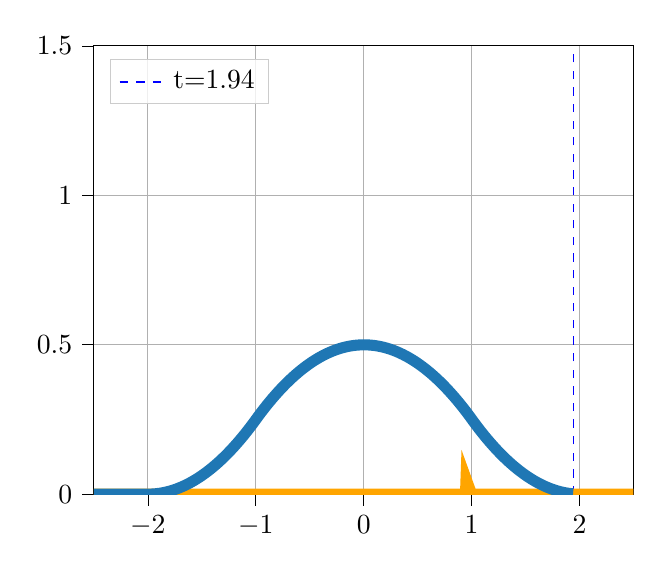
\begin{tikzpicture}

\definecolor{color0}{rgb}{1,0.498039215686275,0.0549019607843137}
\definecolor{color1}{rgb}{1,0.647058823529412,0}
\definecolor{color2}{rgb}{0.12156862745098,0.466666666666667,0.705882352941177}

\begin{axis}[
legend cell align={left},
legend style={fill opacity=0.8, draw opacity=1, text opacity=1, at={(0.03,0.97)}, anchor=north west, draw=white!80!black},
tick align=outside,
tick pos=left,
x grid style={white!69.0196078431373!black},
xmajorgrids,
xmin=-2.5, xmax=2.5,
xtick style={color=black},
y grid style={white!69.0196078431373!black},
ymajorgrids,
ymin=0, ymax=1.5,
ytick style={color=black}
]
\path [draw=color0, fill=color0, opacity=0.2]
(axis cs:-2.5,0)
--(axis cs:-2.5,0)
--(axis cs:-2.49499499499499,0)
--(axis cs:-2.48998998998999,0)
--(axis cs:-2.48498498498498,0)
--(axis cs:-2.47997997997998,0)
--(axis cs:-2.47497497497497,0)
--(axis cs:-2.46996996996997,0)
--(axis cs:-2.46496496496496,0)
--(axis cs:-2.45995995995996,0)
--(axis cs:-2.45495495495495,0)
--(axis cs:-2.44994994994995,0)
--(axis cs:-2.44494494494494,0)
--(axis cs:-2.43993993993994,0)
--(axis cs:-2.43493493493493,0)
--(axis cs:-2.42992992992993,0)
--(axis cs:-2.42492492492492,0)
--(axis cs:-2.41991991991992,0)
--(axis cs:-2.41491491491491,0)
--(axis cs:-2.40990990990991,0)
--(axis cs:-2.4049049049049,0)
--(axis cs:-2.3998998998999,0)
--(axis cs:-2.39489489489489,0)
--(axis cs:-2.38988988988989,0)
--(axis cs:-2.38488488488488,0)
--(axis cs:-2.37987987987988,0)
--(axis cs:-2.37487487487487,0)
--(axis cs:-2.36986986986987,0)
--(axis cs:-2.36486486486486,0)
--(axis cs:-2.35985985985986,0)
--(axis cs:-2.35485485485485,0)
--(axis cs:-2.34984984984985,0)
--(axis cs:-2.34484484484484,0)
--(axis cs:-2.33983983983984,0)
--(axis cs:-2.33483483483483,0)
--(axis cs:-2.32982982982983,0)
--(axis cs:-2.32482482482482,0)
--(axis cs:-2.31981981981982,0)
--(axis cs:-2.31481481481481,0)
--(axis cs:-2.30980980980981,0)
--(axis cs:-2.3048048048048,0)
--(axis cs:-2.2997997997998,0)
--(axis cs:-2.29479479479479,0)
--(axis cs:-2.28978978978979,0)
--(axis cs:-2.28478478478478,0)
--(axis cs:-2.27977977977978,0)
--(axis cs:-2.27477477477477,0)
--(axis cs:-2.26976976976977,0)
--(axis cs:-2.26476476476476,0)
--(axis cs:-2.25975975975976,0)
--(axis cs:-2.25475475475475,0)
--(axis cs:-2.24974974974975,0)
--(axis cs:-2.24474474474474,0)
--(axis cs:-2.23973973973974,0)
--(axis cs:-2.23473473473473,0)
--(axis cs:-2.22972972972973,0)
--(axis cs:-2.22472472472472,0)
--(axis cs:-2.21971971971972,0)
--(axis cs:-2.21471471471471,0)
--(axis cs:-2.20970970970971,0)
--(axis cs:-2.2047047047047,0)
--(axis cs:-2.1996996996997,0)
--(axis cs:-2.19469469469469,0)
--(axis cs:-2.18968968968969,0)
--(axis cs:-2.18468468468468,0)
--(axis cs:-2.17967967967968,0)
--(axis cs:-2.17467467467467,0)
--(axis cs:-2.16966966966967,0)
--(axis cs:-2.16466466466466,0)
--(axis cs:-2.15965965965966,0)
--(axis cs:-2.15465465465465,0)
--(axis cs:-2.14964964964965,0)
--(axis cs:-2.14464464464464,0)
--(axis cs:-2.13963963963964,0)
--(axis cs:-2.13463463463463,0)
--(axis cs:-2.12962962962963,0)
--(axis cs:-2.12462462462462,0)
--(axis cs:-2.11961961961962,0)
--(axis cs:-2.11461461461461,0)
--(axis cs:-2.10960960960961,0)
--(axis cs:-2.1046046046046,0)
--(axis cs:-2.0995995995996,0)
--(axis cs:-2.09459459459459,0)
--(axis cs:-2.08958958958959,0)
--(axis cs:-2.08458458458458,0)
--(axis cs:-2.07957957957958,0)
--(axis cs:-2.07457457457457,0)
--(axis cs:-2.06956956956957,0)
--(axis cs:-2.06456456456456,0)
--(axis cs:-2.05955955955956,0)
--(axis cs:-2.05455455455455,0)
--(axis cs:-2.04954954954955,0)
--(axis cs:-2.04454454454454,0)
--(axis cs:-2.03953953953954,0)
--(axis cs:-2.03453453453453,0)
--(axis cs:-2.02952952952953,0)
--(axis cs:-2.02452452452452,0)
--(axis cs:-2.01951951951952,0)
--(axis cs:-2.01451451451451,0)
--(axis cs:-2.00950950950951,0)
--(axis cs:-2.0045045045045,0)
--(axis cs:-1.9994994994995,0)
--(axis cs:-1.99449449449449,0)
--(axis cs:-1.98948948948949,0)
--(axis cs:-1.98448448448448,0)
--(axis cs:-1.97947947947948,0)
--(axis cs:-1.97447447447447,0)
--(axis cs:-1.96946946946947,0)
--(axis cs:-1.96446446446446,0)
--(axis cs:-1.95945945945946,0)
--(axis cs:-1.95445445445445,0)
--(axis cs:-1.94944944944945,0)
--(axis cs:-1.94444444444444,0)
--(axis cs:-1.93943943943944,0)
--(axis cs:-1.93443443443443,0)
--(axis cs:-1.92942942942943,0)
--(axis cs:-1.92442442442442,0)
--(axis cs:-1.91941941941942,0)
--(axis cs:-1.91441441441441,0)
--(axis cs:-1.90940940940941,0)
--(axis cs:-1.9044044044044,0)
--(axis cs:-1.8993993993994,0)
--(axis cs:-1.89439439439439,0)
--(axis cs:-1.88938938938939,0)
--(axis cs:-1.88438438438438,0)
--(axis cs:-1.87937937937938,0)
--(axis cs:-1.87437437437437,0)
--(axis cs:-1.86936936936937,0)
--(axis cs:-1.86436436436436,0)
--(axis cs:-1.85935935935936,0)
--(axis cs:-1.85435435435435,0)
--(axis cs:-1.84934934934935,0)
--(axis cs:-1.84434434434434,0)
--(axis cs:-1.83933933933934,0)
--(axis cs:-1.83433433433433,0)
--(axis cs:-1.82932932932933,0)
--(axis cs:-1.82432432432432,0)
--(axis cs:-1.81931931931932,0)
--(axis cs:-1.81431431431431,0)
--(axis cs:-1.80930930930931,0)
--(axis cs:-1.8043043043043,0)
--(axis cs:-1.7992992992993,0)
--(axis cs:-1.79429429429429,0)
--(axis cs:-1.78928928928929,0)
--(axis cs:-1.78428428428428,0)
--(axis cs:-1.77927927927928,0)
--(axis cs:-1.77427427427427,0)
--(axis cs:-1.76926926926927,0)
--(axis cs:-1.76426426426426,0)
--(axis cs:-1.75925925925926,0)
--(axis cs:-1.75425425425425,0)
--(axis cs:-1.74924924924925,0)
--(axis cs:-1.74424424424424,0)
--(axis cs:-1.73923923923924,0)
--(axis cs:-1.73423423423423,0)
--(axis cs:-1.72922922922923,0)
--(axis cs:-1.72422422422422,0)
--(axis cs:-1.71921921921922,0)
--(axis cs:-1.71421421421421,0)
--(axis cs:-1.70920920920921,0)
--(axis cs:-1.7042042042042,0)
--(axis cs:-1.6991991991992,0)
--(axis cs:-1.69419419419419,0)
--(axis cs:-1.68918918918919,0)
--(axis cs:-1.68418418418418,0)
--(axis cs:-1.67917917917918,0)
--(axis cs:-1.67417417417417,0)
--(axis cs:-1.66916916916917,0)
--(axis cs:-1.66416416416416,0)
--(axis cs:-1.65915915915916,0)
--(axis cs:-1.65415415415415,0)
--(axis cs:-1.64914914914915,0)
--(axis cs:-1.64414414414414,0)
--(axis cs:-1.63913913913914,0)
--(axis cs:-1.63413413413413,0)
--(axis cs:-1.62912912912913,0)
--(axis cs:-1.62412412412412,0)
--(axis cs:-1.61911911911912,0)
--(axis cs:-1.61411411411411,0)
--(axis cs:-1.60910910910911,0)
--(axis cs:-1.6041041041041,0)
--(axis cs:-1.5990990990991,0)
--(axis cs:-1.59409409409409,0)
--(axis cs:-1.58908908908909,0)
--(axis cs:-1.58408408408408,0)
--(axis cs:-1.57907907907908,0)
--(axis cs:-1.57407407407407,0)
--(axis cs:-1.56906906906907,0)
--(axis cs:-1.56406406406406,0)
--(axis cs:-1.55905905905906,0)
--(axis cs:-1.55405405405405,0)
--(axis cs:-1.54904904904905,0)
--(axis cs:-1.54404404404404,0)
--(axis cs:-1.53903903903904,0)
--(axis cs:-1.53403403403403,0)
--(axis cs:-1.52902902902903,0)
--(axis cs:-1.52402402402402,0)
--(axis cs:-1.51901901901902,0)
--(axis cs:-1.51401401401401,0)
--(axis cs:-1.50900900900901,0)
--(axis cs:-1.504004004004,0)
--(axis cs:-1.498998998999,0)
--(axis cs:-1.49399399399399,0)
--(axis cs:-1.48898898898899,0)
--(axis cs:-1.48398398398398,0)
--(axis cs:-1.47897897897898,0)
--(axis cs:-1.47397397397397,0)
--(axis cs:-1.46896896896897,0)
--(axis cs:-1.46396396396396,0)
--(axis cs:-1.45895895895896,0)
--(axis cs:-1.45395395395395,0)
--(axis cs:-1.44894894894895,0)
--(axis cs:-1.44394394394394,0)
--(axis cs:-1.43893893893894,0)
--(axis cs:-1.43393393393393,0)
--(axis cs:-1.42892892892893,0)
--(axis cs:-1.42392392392392,0)
--(axis cs:-1.41891891891892,0)
--(axis cs:-1.41391391391391,0)
--(axis cs:-1.40890890890891,0)
--(axis cs:-1.4039039039039,0)
--(axis cs:-1.3988988988989,0)
--(axis cs:-1.39389389389389,0)
--(axis cs:-1.38888888888889,0)
--(axis cs:-1.38388388388388,0)
--(axis cs:-1.37887887887888,0)
--(axis cs:-1.37387387387387,0)
--(axis cs:-1.36886886886887,0)
--(axis cs:-1.36386386386386,0)
--(axis cs:-1.35885885885886,0)
--(axis cs:-1.35385385385385,0)
--(axis cs:-1.34884884884885,0)
--(axis cs:-1.34384384384384,0)
--(axis cs:-1.33883883883884,0)
--(axis cs:-1.33383383383383,0)
--(axis cs:-1.32882882882883,0)
--(axis cs:-1.32382382382382,0)
--(axis cs:-1.31881881881882,0)
--(axis cs:-1.31381381381381,0)
--(axis cs:-1.30880880880881,0)
--(axis cs:-1.3038038038038,0)
--(axis cs:-1.2987987987988,0)
--(axis cs:-1.29379379379379,0)
--(axis cs:-1.28878878878879,0)
--(axis cs:-1.28378378378378,0)
--(axis cs:-1.27877877877878,0)
--(axis cs:-1.27377377377377,0)
--(axis cs:-1.26876876876877,0)
--(axis cs:-1.26376376376376,0)
--(axis cs:-1.25875875875876,0)
--(axis cs:-1.25375375375375,0)
--(axis cs:-1.24874874874875,0)
--(axis cs:-1.24374374374374,0)
--(axis cs:-1.23873873873874,0)
--(axis cs:-1.23373373373373,0)
--(axis cs:-1.22872872872873,0)
--(axis cs:-1.22372372372372,0)
--(axis cs:-1.21871871871872,0)
--(axis cs:-1.21371371371371,0)
--(axis cs:-1.20870870870871,0)
--(axis cs:-1.2037037037037,0)
--(axis cs:-1.1986986986987,0)
--(axis cs:-1.19369369369369,0)
--(axis cs:-1.18868868868869,0)
--(axis cs:-1.18368368368368,0)
--(axis cs:-1.17867867867868,0)
--(axis cs:-1.17367367367367,0)
--(axis cs:-1.16866866866867,0)
--(axis cs:-1.16366366366366,0)
--(axis cs:-1.15865865865866,0)
--(axis cs:-1.15365365365365,0)
--(axis cs:-1.14864864864865,0)
--(axis cs:-1.14364364364364,0)
--(axis cs:-1.13863863863864,0)
--(axis cs:-1.13363363363363,0)
--(axis cs:-1.12862862862863,0)
--(axis cs:-1.12362362362362,0)
--(axis cs:-1.11861861861862,0)
--(axis cs:-1.11361361361361,0)
--(axis cs:-1.10860860860861,0)
--(axis cs:-1.1036036036036,0)
--(axis cs:-1.0985985985986,0)
--(axis cs:-1.09359359359359,0)
--(axis cs:-1.08858858858859,0)
--(axis cs:-1.08358358358358,0)
--(axis cs:-1.07857857857858,0)
--(axis cs:-1.07357357357357,0)
--(axis cs:-1.06856856856857,0)
--(axis cs:-1.06356356356356,0)
--(axis cs:-1.05855855855856,0)
--(axis cs:-1.05355355355355,0)
--(axis cs:-1.04854854854855,0)
--(axis cs:-1.04354354354354,0)
--(axis cs:-1.03853853853854,0)
--(axis cs:-1.03353353353353,0)
--(axis cs:-1.02852852852853,0)
--(axis cs:-1.02352352352352,0)
--(axis cs:-1.01851851851852,0)
--(axis cs:-1.01351351351351,0)
--(axis cs:-1.00850850850851,0)
--(axis cs:-1.0035035035035,0)
--(axis cs:-0.998498498498499,0)
--(axis cs:-0.993493493493494,0)
--(axis cs:-0.988488488488489,0)
--(axis cs:-0.983483483483484,0)
--(axis cs:-0.978478478478479,0)
--(axis cs:-0.973473473473474,0)
--(axis cs:-0.968468468468469,0)
--(axis cs:-0.963463463463464,0)
--(axis cs:-0.958458458458459,0)
--(axis cs:-0.953453453453454,0)
--(axis cs:-0.948448448448449,0)
--(axis cs:-0.943443443443444,0)
--(axis cs:-0.938438438438439,0)
--(axis cs:-0.933433433433434,0)
--(axis cs:-0.928428428428429,0)
--(axis cs:-0.923423423423424,0)
--(axis cs:-0.918418418418419,0)
--(axis cs:-0.913413413413414,0)
--(axis cs:-0.908408408408409,0)
--(axis cs:-0.903403403403404,0)
--(axis cs:-0.898398398398399,0)
--(axis cs:-0.893393393393393,0)
--(axis cs:-0.888388388388388,0)
--(axis cs:-0.883383383383383,0)
--(axis cs:-0.878378378378378,0)
--(axis cs:-0.873373373373373,0)
--(axis cs:-0.868368368368368,0)
--(axis cs:-0.863363363363363,0)
--(axis cs:-0.858358358358358,0)
--(axis cs:-0.853353353353353,0)
--(axis cs:-0.848348348348348,0)
--(axis cs:-0.843343343343343,0)
--(axis cs:-0.838338338338338,0)
--(axis cs:-0.833333333333333,0)
--(axis cs:-0.828328328328328,0)
--(axis cs:-0.823323323323323,0)
--(axis cs:-0.818318318318318,0)
--(axis cs:-0.813313313313313,0)
--(axis cs:-0.808308308308308,0)
--(axis cs:-0.803303303303303,0)
--(axis cs:-0.798298298298298,0)
--(axis cs:-0.793293293293293,0)
--(axis cs:-0.788288288288288,0)
--(axis cs:-0.783283283283283,0)
--(axis cs:-0.778278278278278,0)
--(axis cs:-0.773273273273273,0)
--(axis cs:-0.768268268268268,0)
--(axis cs:-0.763263263263263,0)
--(axis cs:-0.758258258258258,0)
--(axis cs:-0.753253253253253,0)
--(axis cs:-0.748248248248248,0)
--(axis cs:-0.743243243243243,0)
--(axis cs:-0.738238238238238,0)
--(axis cs:-0.733233233233233,0)
--(axis cs:-0.728228228228228,0)
--(axis cs:-0.723223223223223,0)
--(axis cs:-0.718218218218218,0)
--(axis cs:-0.713213213213213,0)
--(axis cs:-0.708208208208208,0)
--(axis cs:-0.703203203203203,0)
--(axis cs:-0.698198198198198,0)
--(axis cs:-0.693193193193193,0)
--(axis cs:-0.688188188188188,0)
--(axis cs:-0.683183183183183,0)
--(axis cs:-0.678178178178178,0)
--(axis cs:-0.673173173173173,0)
--(axis cs:-0.668168168168168,0)
--(axis cs:-0.663163163163163,0)
--(axis cs:-0.658158158158158,0)
--(axis cs:-0.653153153153153,0)
--(axis cs:-0.648148148148148,0)
--(axis cs:-0.643143143143143,0)
--(axis cs:-0.638138138138138,0)
--(axis cs:-0.633133133133133,0)
--(axis cs:-0.628128128128128,0)
--(axis cs:-0.623123123123123,0)
--(axis cs:-0.618118118118118,0)
--(axis cs:-0.613113113113113,0)
--(axis cs:-0.608108108108108,0)
--(axis cs:-0.603103103103103,0)
--(axis cs:-0.598098098098098,0)
--(axis cs:-0.593093093093093,0)
--(axis cs:-0.588088088088088,0)
--(axis cs:-0.583083083083083,0)
--(axis cs:-0.578078078078078,0)
--(axis cs:-0.573073073073073,0)
--(axis cs:-0.568068068068068,0)
--(axis cs:-0.563063063063063,0)
--(axis cs:-0.558058058058058,0)
--(axis cs:-0.553053053053053,0)
--(axis cs:-0.548048048048048,0)
--(axis cs:-0.543043043043043,0)
--(axis cs:-0.538038038038038,0)
--(axis cs:-0.533033033033033,0)
--(axis cs:-0.528028028028028,0)
--(axis cs:-0.523023023023023,0)
--(axis cs:-0.518018018018018,0)
--(axis cs:-0.513013013013013,0)
--(axis cs:-0.508008008008008,0)
--(axis cs:-0.503003003003003,0)
--(axis cs:-0.497997997997998,0)
--(axis cs:-0.492992992992993,0)
--(axis cs:-0.487987987987988,0)
--(axis cs:-0.482982982982983,0)
--(axis cs:-0.477977977977978,0)
--(axis cs:-0.472972972972973,0)
--(axis cs:-0.467967967967968,0)
--(axis cs:-0.462962962962963,0)
--(axis cs:-0.457957957957958,0)
--(axis cs:-0.452952952952953,0)
--(axis cs:-0.447947947947948,0)
--(axis cs:-0.442942942942943,0)
--(axis cs:-0.437937937937938,0)
--(axis cs:-0.432932932932933,0)
--(axis cs:-0.427927927927928,0)
--(axis cs:-0.422922922922923,0)
--(axis cs:-0.417917917917918,0)
--(axis cs:-0.412912912912913,0)
--(axis cs:-0.407907907907908,0)
--(axis cs:-0.402902902902903,0)
--(axis cs:-0.397897897897898,0)
--(axis cs:-0.392892892892893,0)
--(axis cs:-0.387887887887888,0)
--(axis cs:-0.382882882882883,0)
--(axis cs:-0.377877877877878,0)
--(axis cs:-0.372872872872873,0)
--(axis cs:-0.367867867867868,0)
--(axis cs:-0.362862862862863,0)
--(axis cs:-0.357857857857858,0)
--(axis cs:-0.352852852852853,0)
--(axis cs:-0.347847847847848,0)
--(axis cs:-0.342842842842843,0)
--(axis cs:-0.337837837837838,0)
--(axis cs:-0.332832832832833,0)
--(axis cs:-0.327827827827828,0)
--(axis cs:-0.322822822822823,0)
--(axis cs:-0.317817817817818,0)
--(axis cs:-0.312812812812813,0)
--(axis cs:-0.307807807807808,0)
--(axis cs:-0.302802802802803,0)
--(axis cs:-0.297797797797798,0)
--(axis cs:-0.292792792792793,0)
--(axis cs:-0.287787787787788,0)
--(axis cs:-0.282782782782783,0)
--(axis cs:-0.277777777777778,0)
--(axis cs:-0.272772772772773,0)
--(axis cs:-0.267767767767768,0)
--(axis cs:-0.262762762762763,0)
--(axis cs:-0.257757757757758,0)
--(axis cs:-0.252752752752753,0)
--(axis cs:-0.247747747747748,0)
--(axis cs:-0.242742742742743,0)
--(axis cs:-0.237737737737738,0)
--(axis cs:-0.232732732732733,0)
--(axis cs:-0.227727727727728,0)
--(axis cs:-0.222722722722723,0)
--(axis cs:-0.217717717717718,0)
--(axis cs:-0.212712712712713,0)
--(axis cs:-0.207707707707708,0)
--(axis cs:-0.202702702702703,0)
--(axis cs:-0.197697697697698,0)
--(axis cs:-0.192692692692693,0)
--(axis cs:-0.187687687687688,0)
--(axis cs:-0.182682682682683,0)
--(axis cs:-0.177677677677678,0)
--(axis cs:-0.172672672672673,0)
--(axis cs:-0.167667667667668,0)
--(axis cs:-0.162662662662663,0)
--(axis cs:-0.157657657657658,0)
--(axis cs:-0.152652652652653,0)
--(axis cs:-0.147647647647648,0)
--(axis cs:-0.142642642642643,0)
--(axis cs:-0.137637637637638,0)
--(axis cs:-0.132632632632633,0)
--(axis cs:-0.127627627627628,0)
--(axis cs:-0.122622622622623,0)
--(axis cs:-0.117617617617618,0)
--(axis cs:-0.112612612612613,0)
--(axis cs:-0.107607607607608,0)
--(axis cs:-0.102602602602603,0)
--(axis cs:-0.0975975975975976,0)
--(axis cs:-0.0925925925925926,0)
--(axis cs:-0.0875875875875876,0)
--(axis cs:-0.0825825825825826,0)
--(axis cs:-0.0775775775775776,0)
--(axis cs:-0.0725725725725725,0)
--(axis cs:-0.0675675675675675,0)
--(axis cs:-0.0625625625625625,0)
--(axis cs:-0.0575575575575575,0)
--(axis cs:-0.0525525525525525,0)
--(axis cs:-0.0475475475475475,0)
--(axis cs:-0.0425425425425425,0)
--(axis cs:-0.0375375375375375,0)
--(axis cs:-0.0325325325325325,0)
--(axis cs:-0.0275275275275275,0)
--(axis cs:-0.0225225225225225,0)
--(axis cs:-0.0175175175175175,0)
--(axis cs:-0.0125125125125125,0)
--(axis cs:-0.0075075075075075,0)
--(axis cs:-0.0025025025025025,0)
--(axis cs:0.0025025025025025,0)
--(axis cs:0.0075075075075075,0)
--(axis cs:0.0125125125125125,0)
--(axis cs:0.0175175175175175,0)
--(axis cs:0.0225225225225225,0)
--(axis cs:0.0275275275275275,0)
--(axis cs:0.0325325325325325,0)
--(axis cs:0.0375375375375375,0)
--(axis cs:0.0425425425425425,0)
--(axis cs:0.0475475475475475,0)
--(axis cs:0.0525525525525525,0)
--(axis cs:0.0575575575575575,0)
--(axis cs:0.0625625625625625,0)
--(axis cs:0.0675675675675675,0)
--(axis cs:0.0725725725725725,0)
--(axis cs:0.0775775775775776,0)
--(axis cs:0.0825825825825826,0)
--(axis cs:0.0875875875875876,0)
--(axis cs:0.0925925925925926,0)
--(axis cs:0.0975975975975976,0)
--(axis cs:0.102602602602603,0)
--(axis cs:0.107607607607608,0)
--(axis cs:0.112612612612613,0)
--(axis cs:0.117617617617618,0)
--(axis cs:0.122622622622623,0)
--(axis cs:0.127627627627628,0)
--(axis cs:0.132632632632633,0)
--(axis cs:0.137637637637638,0)
--(axis cs:0.142642642642643,0)
--(axis cs:0.147647647647648,0)
--(axis cs:0.152652652652653,0)
--(axis cs:0.157657657657658,0)
--(axis cs:0.162662662662663,0)
--(axis cs:0.167667667667668,0)
--(axis cs:0.172672672672673,0)
--(axis cs:0.177677677677678,0)
--(axis cs:0.182682682682683,0)
--(axis cs:0.187687687687688,0)
--(axis cs:0.192692692692693,0)
--(axis cs:0.197697697697698,0)
--(axis cs:0.202702702702703,0)
--(axis cs:0.207707707707708,0)
--(axis cs:0.212712712712713,0)
--(axis cs:0.217717717717718,0)
--(axis cs:0.222722722722723,0)
--(axis cs:0.227727727727728,0)
--(axis cs:0.232732732732733,0)
--(axis cs:0.237737737737738,0)
--(axis cs:0.242742742742743,0)
--(axis cs:0.247747747747748,0)
--(axis cs:0.252752752752753,0)
--(axis cs:0.257757757757758,0)
--(axis cs:0.262762762762763,0)
--(axis cs:0.267767767767768,0)
--(axis cs:0.272772772772773,0)
--(axis cs:0.277777777777778,0)
--(axis cs:0.282782782782783,0)
--(axis cs:0.287787787787788,0)
--(axis cs:0.292792792792793,0)
--(axis cs:0.297797797797798,0)
--(axis cs:0.302802802802803,0)
--(axis cs:0.307807807807808,0)
--(axis cs:0.312812812812813,0)
--(axis cs:0.317817817817818,0)
--(axis cs:0.322822822822823,0)
--(axis cs:0.327827827827828,0)
--(axis cs:0.332832832832833,0)
--(axis cs:0.337837837837838,0)
--(axis cs:0.342842842842843,0)
--(axis cs:0.347847847847848,0)
--(axis cs:0.352852852852853,0)
--(axis cs:0.357857857857858,0)
--(axis cs:0.362862862862863,0)
--(axis cs:0.367867867867868,0)
--(axis cs:0.372872872872873,0)
--(axis cs:0.377877877877878,0)
--(axis cs:0.382882882882883,0)
--(axis cs:0.387887887887888,0)
--(axis cs:0.392892892892893,0)
--(axis cs:0.397897897897898,0)
--(axis cs:0.402902902902903,0)
--(axis cs:0.407907907907908,0)
--(axis cs:0.412912912912913,0)
--(axis cs:0.417917917917918,0)
--(axis cs:0.422922922922923,0)
--(axis cs:0.427927927927928,0)
--(axis cs:0.432932932932933,0)
--(axis cs:0.437937937937938,0)
--(axis cs:0.442942942942943,0)
--(axis cs:0.447947947947948,0)
--(axis cs:0.452952952952953,0)
--(axis cs:0.457957957957958,0)
--(axis cs:0.462962962962963,0)
--(axis cs:0.467967967967968,0)
--(axis cs:0.472972972972973,0)
--(axis cs:0.477977977977978,0)
--(axis cs:0.482982982982983,0)
--(axis cs:0.487987987987988,0)
--(axis cs:0.492992992992993,0)
--(axis cs:0.497997997997998,0)
--(axis cs:0.503003003003003,0)
--(axis cs:0.508008008008008,0)
--(axis cs:0.513013013013013,0)
--(axis cs:0.518018018018018,0)
--(axis cs:0.523023023023023,0)
--(axis cs:0.528028028028028,0)
--(axis cs:0.533033033033033,0)
--(axis cs:0.538038038038038,0)
--(axis cs:0.543043043043043,0)
--(axis cs:0.548048048048048,0)
--(axis cs:0.553053053053053,0)
--(axis cs:0.558058058058058,0)
--(axis cs:0.563063063063063,0)
--(axis cs:0.568068068068068,0)
--(axis cs:0.573073073073073,0)
--(axis cs:0.578078078078078,0)
--(axis cs:0.583083083083083,0)
--(axis cs:0.588088088088088,0)
--(axis cs:0.593093093093093,0)
--(axis cs:0.598098098098098,0)
--(axis cs:0.603103103103103,0)
--(axis cs:0.608108108108108,0)
--(axis cs:0.613113113113113,0)
--(axis cs:0.618118118118118,0)
--(axis cs:0.623123123123123,0)
--(axis cs:0.628128128128128,0)
--(axis cs:0.633133133133133,0)
--(axis cs:0.638138138138138,0)
--(axis cs:0.643143143143143,0)
--(axis cs:0.648148148148148,0)
--(axis cs:0.653153153153153,0)
--(axis cs:0.658158158158158,0)
--(axis cs:0.663163163163163,0)
--(axis cs:0.668168168168168,0)
--(axis cs:0.673173173173173,0)
--(axis cs:0.678178178178178,0)
--(axis cs:0.683183183183183,0)
--(axis cs:0.688188188188188,0)
--(axis cs:0.693193193193193,0)
--(axis cs:0.698198198198198,0)
--(axis cs:0.703203203203203,0)
--(axis cs:0.708208208208208,0)
--(axis cs:0.713213213213213,0)
--(axis cs:0.718218218218218,0)
--(axis cs:0.723223223223223,0)
--(axis cs:0.728228228228228,0)
--(axis cs:0.733233233233233,0)
--(axis cs:0.738238238238238,0)
--(axis cs:0.743243243243243,0)
--(axis cs:0.748248248248248,0)
--(axis cs:0.753253253253253,0)
--(axis cs:0.758258258258258,0)
--(axis cs:0.763263263263263,0)
--(axis cs:0.768268268268268,0)
--(axis cs:0.773273273273273,0)
--(axis cs:0.778278278278278,0)
--(axis cs:0.783283283283283,0)
--(axis cs:0.788288288288288,0)
--(axis cs:0.793293293293293,0)
--(axis cs:0.798298298298298,0)
--(axis cs:0.803303303303303,0)
--(axis cs:0.808308308308308,0)
--(axis cs:0.813313313313313,0)
--(axis cs:0.818318318318318,0)
--(axis cs:0.823323323323323,0)
--(axis cs:0.828328328328328,0)
--(axis cs:0.833333333333333,0)
--(axis cs:0.838338338338338,0)
--(axis cs:0.843343343343343,0)
--(axis cs:0.848348348348348,0)
--(axis cs:0.853353353353353,0)
--(axis cs:0.858358358358358,0)
--(axis cs:0.863363363363364,0)
--(axis cs:0.868368368368369,0)
--(axis cs:0.873373373373374,0)
--(axis cs:0.878378378378379,0)
--(axis cs:0.883383383383384,0)
--(axis cs:0.888388388388389,0)
--(axis cs:0.893393393393394,0)
--(axis cs:0.898398398398399,0)
--(axis cs:0.903403403403404,0)
--(axis cs:0.908408408408409,0)
--(axis cs:0.913413413413414,0)
--(axis cs:0.918418418418419,0)
--(axis cs:0.923423423423424,0)
--(axis cs:0.928428428428429,0)
--(axis cs:0.933433433433434,0)
--(axis cs:0.938438438438439,0)
--(axis cs:0.943443443443444,0)
--(axis cs:0.948448448448449,0)
--(axis cs:0.953453453453454,0)
--(axis cs:0.958458458458459,0)
--(axis cs:0.963463463463464,0)
--(axis cs:0.968468468468469,0)
--(axis cs:0.973473473473474,0)
--(axis cs:0.978478478478479,0)
--(axis cs:0.983483483483484,0)
--(axis cs:0.988488488488489,0)
--(axis cs:0.993493493493494,0)
--(axis cs:0.998498498498499,0)
--(axis cs:1.0035035035035,0)
--(axis cs:1.00850850850851,0)
--(axis cs:1.01351351351351,0)
--(axis cs:1.01851851851852,0)
--(axis cs:1.02352352352352,0)
--(axis cs:1.02852852852853,0)
--(axis cs:1.03353353353353,0)
--(axis cs:1.03853853853854,0)
--(axis cs:1.04354354354354,0)
--(axis cs:1.04854854854855,0)
--(axis cs:1.05355355355355,0)
--(axis cs:1.05855855855856,0)
--(axis cs:1.06356356356356,0)
--(axis cs:1.06856856856857,0)
--(axis cs:1.07357357357357,0)
--(axis cs:1.07857857857858,0)
--(axis cs:1.08358358358358,0)
--(axis cs:1.08858858858859,0)
--(axis cs:1.09359359359359,0)
--(axis cs:1.0985985985986,0)
--(axis cs:1.1036036036036,0)
--(axis cs:1.10860860860861,0)
--(axis cs:1.11361361361361,0)
--(axis cs:1.11861861861862,0)
--(axis cs:1.12362362362362,0)
--(axis cs:1.12862862862863,0)
--(axis cs:1.13363363363363,0)
--(axis cs:1.13863863863864,0)
--(axis cs:1.14364364364364,0)
--(axis cs:1.14864864864865,0)
--(axis cs:1.15365365365365,0)
--(axis cs:1.15865865865866,0)
--(axis cs:1.16366366366366,0)
--(axis cs:1.16866866866867,0)
--(axis cs:1.17367367367367,0)
--(axis cs:1.17867867867868,0)
--(axis cs:1.18368368368368,0)
--(axis cs:1.18868868868869,0)
--(axis cs:1.19369369369369,0)
--(axis cs:1.1986986986987,0)
--(axis cs:1.2037037037037,0)
--(axis cs:1.20870870870871,0)
--(axis cs:1.21371371371371,0)
--(axis cs:1.21871871871872,0)
--(axis cs:1.22372372372372,0)
--(axis cs:1.22872872872873,0)
--(axis cs:1.23373373373373,0)
--(axis cs:1.23873873873874,0)
--(axis cs:1.24374374374374,0)
--(axis cs:1.24874874874875,0)
--(axis cs:1.25375375375375,0)
--(axis cs:1.25875875875876,0)
--(axis cs:1.26376376376376,0)
--(axis cs:1.26876876876877,0)
--(axis cs:1.27377377377377,0)
--(axis cs:1.27877877877878,0)
--(axis cs:1.28378378378378,0)
--(axis cs:1.28878878878879,0)
--(axis cs:1.29379379379379,0)
--(axis cs:1.2987987987988,0)
--(axis cs:1.3038038038038,0)
--(axis cs:1.30880880880881,0)
--(axis cs:1.31381381381381,0)
--(axis cs:1.31881881881882,0)
--(axis cs:1.32382382382382,0)
--(axis cs:1.32882882882883,0)
--(axis cs:1.33383383383383,0)
--(axis cs:1.33883883883884,0)
--(axis cs:1.34384384384384,0)
--(axis cs:1.34884884884885,0)
--(axis cs:1.35385385385385,0)
--(axis cs:1.35885885885886,0)
--(axis cs:1.36386386386386,0)
--(axis cs:1.36886886886887,0)
--(axis cs:1.37387387387387,0)
--(axis cs:1.37887887887888,0)
--(axis cs:1.38388388388388,0)
--(axis cs:1.38888888888889,0)
--(axis cs:1.39389389389389,0)
--(axis cs:1.3988988988989,0)
--(axis cs:1.4039039039039,0)
--(axis cs:1.40890890890891,0)
--(axis cs:1.41391391391391,0)
--(axis cs:1.41891891891892,0)
--(axis cs:1.42392392392392,0)
--(axis cs:1.42892892892893,0)
--(axis cs:1.43393393393393,0)
--(axis cs:1.43893893893894,0)
--(axis cs:1.44394394394394,0)
--(axis cs:1.44894894894895,0)
--(axis cs:1.45395395395395,0)
--(axis cs:1.45895895895896,0)
--(axis cs:1.46396396396396,0)
--(axis cs:1.46896896896897,0)
--(axis cs:1.47397397397397,0)
--(axis cs:1.47897897897898,0)
--(axis cs:1.48398398398398,0)
--(axis cs:1.48898898898899,0)
--(axis cs:1.49399399399399,0)
--(axis cs:1.498998998999,0)
--(axis cs:1.504004004004,0)
--(axis cs:1.50900900900901,0)
--(axis cs:1.51401401401401,0)
--(axis cs:1.51901901901902,0)
--(axis cs:1.52402402402402,0)
--(axis cs:1.52902902902903,0)
--(axis cs:1.53403403403403,0)
--(axis cs:1.53903903903904,0)
--(axis cs:1.54404404404404,0)
--(axis cs:1.54904904904905,0)
--(axis cs:1.55405405405405,0)
--(axis cs:1.55905905905906,0)
--(axis cs:1.56406406406406,0)
--(axis cs:1.56906906906907,0)
--(axis cs:1.57407407407407,0)
--(axis cs:1.57907907907908,0)
--(axis cs:1.58408408408408,0)
--(axis cs:1.58908908908909,0)
--(axis cs:1.59409409409409,0)
--(axis cs:1.5990990990991,0)
--(axis cs:1.6041041041041,0)
--(axis cs:1.60910910910911,0)
--(axis cs:1.61411411411411,0)
--(axis cs:1.61911911911912,0)
--(axis cs:1.62412412412412,0)
--(axis cs:1.62912912912913,0)
--(axis cs:1.63413413413413,0)
--(axis cs:1.63913913913914,0)
--(axis cs:1.64414414414414,0)
--(axis cs:1.64914914914915,0)
--(axis cs:1.65415415415415,0)
--(axis cs:1.65915915915916,0)
--(axis cs:1.66416416416416,0)
--(axis cs:1.66916916916917,0)
--(axis cs:1.67417417417417,0)
--(axis cs:1.67917917917918,0)
--(axis cs:1.68418418418418,0)
--(axis cs:1.68918918918919,0)
--(axis cs:1.69419419419419,0)
--(axis cs:1.6991991991992,0)
--(axis cs:1.7042042042042,0)
--(axis cs:1.70920920920921,0)
--(axis cs:1.71421421421421,0)
--(axis cs:1.71921921921922,0)
--(axis cs:1.72422422422422,0)
--(axis cs:1.72922922922923,0)
--(axis cs:1.73423423423423,0)
--(axis cs:1.73923923923924,0)
--(axis cs:1.74424424424424,0)
--(axis cs:1.74924924924925,0)
--(axis cs:1.75425425425425,0)
--(axis cs:1.75925925925926,0)
--(axis cs:1.76426426426426,0)
--(axis cs:1.76926926926927,0)
--(axis cs:1.77427427427427,0)
--(axis cs:1.77927927927928,0)
--(axis cs:1.78428428428428,0)
--(axis cs:1.78928928928929,0)
--(axis cs:1.79429429429429,0)
--(axis cs:1.7992992992993,0)
--(axis cs:1.8043043043043,0)
--(axis cs:1.80930930930931,0)
--(axis cs:1.81431431431431,0)
--(axis cs:1.81931931931932,0)
--(axis cs:1.82432432432432,0)
--(axis cs:1.82932932932933,0)
--(axis cs:1.83433433433433,0)
--(axis cs:1.83933933933934,0)
--(axis cs:1.84434434434434,0)
--(axis cs:1.84934934934935,0)
--(axis cs:1.85435435435435,0)
--(axis cs:1.85935935935936,0)
--(axis cs:1.86436436436436,0)
--(axis cs:1.86936936936937,0)
--(axis cs:1.87437437437437,0)
--(axis cs:1.87937937937938,0)
--(axis cs:1.88438438438438,0)
--(axis cs:1.88938938938939,0)
--(axis cs:1.89439439439439,0)
--(axis cs:1.8993993993994,0)
--(axis cs:1.9044044044044,0)
--(axis cs:1.90940940940941,0)
--(axis cs:1.91441441441441,0)
--(axis cs:1.91941941941942,0)
--(axis cs:1.92442442442442,0)
--(axis cs:1.92942942942943,0)
--(axis cs:1.93443443443443,0)
--(axis cs:1.93943943943944,0)
--(axis cs:1.94444444444444,0)
--(axis cs:1.94944944944945,0)
--(axis cs:1.95445445445445,0)
--(axis cs:1.95945945945946,0)
--(axis cs:1.96446446446446,0)
--(axis cs:1.96946946946947,0)
--(axis cs:1.97447447447447,0)
--(axis cs:1.97947947947948,0)
--(axis cs:1.98448448448448,0)
--(axis cs:1.98948948948949,0)
--(axis cs:1.99449449449449,0)
--(axis cs:1.9994994994995,0)
--(axis cs:2.0045045045045,0)
--(axis cs:2.00950950950951,0)
--(axis cs:2.01451451451451,0)
--(axis cs:2.01951951951952,0)
--(axis cs:2.02452452452452,0)
--(axis cs:2.02952952952953,0)
--(axis cs:2.03453453453453,0)
--(axis cs:2.03953953953954,0)
--(axis cs:2.04454454454454,0)
--(axis cs:2.04954954954955,0)
--(axis cs:2.05455455455455,0)
--(axis cs:2.05955955955956,0)
--(axis cs:2.06456456456456,0)
--(axis cs:2.06956956956957,0)
--(axis cs:2.07457457457457,0)
--(axis cs:2.07957957957958,0)
--(axis cs:2.08458458458458,0)
--(axis cs:2.08958958958959,0)
--(axis cs:2.09459459459459,0)
--(axis cs:2.0995995995996,0)
--(axis cs:2.1046046046046,0)
--(axis cs:2.10960960960961,0)
--(axis cs:2.11461461461461,0)
--(axis cs:2.11961961961962,0)
--(axis cs:2.12462462462462,0)
--(axis cs:2.12962962962963,0)
--(axis cs:2.13463463463463,0)
--(axis cs:2.13963963963964,0)
--(axis cs:2.14464464464464,0)
--(axis cs:2.14964964964965,0)
--(axis cs:2.15465465465465,0)
--(axis cs:2.15965965965966,0)
--(axis cs:2.16466466466466,0)
--(axis cs:2.16966966966967,0)
--(axis cs:2.17467467467467,0)
--(axis cs:2.17967967967968,0)
--(axis cs:2.18468468468468,0)
--(axis cs:2.18968968968969,0)
--(axis cs:2.19469469469469,0)
--(axis cs:2.1996996996997,0)
--(axis cs:2.2047047047047,0)
--(axis cs:2.20970970970971,0)
--(axis cs:2.21471471471471,0)
--(axis cs:2.21971971971972,0)
--(axis cs:2.22472472472472,0)
--(axis cs:2.22972972972973,0)
--(axis cs:2.23473473473473,0)
--(axis cs:2.23973973973974,0)
--(axis cs:2.24474474474474,0)
--(axis cs:2.24974974974975,0)
--(axis cs:2.25475475475475,0)
--(axis cs:2.25975975975976,0)
--(axis cs:2.26476476476476,0)
--(axis cs:2.26976976976977,0)
--(axis cs:2.27477477477477,0)
--(axis cs:2.27977977977978,0)
--(axis cs:2.28478478478478,0)
--(axis cs:2.28978978978979,0)
--(axis cs:2.29479479479479,0)
--(axis cs:2.2997997997998,0)
--(axis cs:2.3048048048048,0)
--(axis cs:2.30980980980981,0)
--(axis cs:2.31481481481481,0)
--(axis cs:2.31981981981982,0)
--(axis cs:2.32482482482482,0)
--(axis cs:2.32982982982983,0)
--(axis cs:2.33483483483483,0)
--(axis cs:2.33983983983984,0)
--(axis cs:2.34484484484484,0)
--(axis cs:2.34984984984985,0)
--(axis cs:2.35485485485485,0)
--(axis cs:2.35985985985986,0)
--(axis cs:2.36486486486486,0)
--(axis cs:2.36986986986987,0)
--(axis cs:2.37487487487487,0)
--(axis cs:2.37987987987988,0)
--(axis cs:2.38488488488488,0)
--(axis cs:2.38988988988989,0)
--(axis cs:2.39489489489489,0)
--(axis cs:2.3998998998999,0)
--(axis cs:2.4049049049049,0)
--(axis cs:2.40990990990991,0)
--(axis cs:2.41491491491491,0)
--(axis cs:2.41991991991992,0)
--(axis cs:2.42492492492492,0)
--(axis cs:2.42992992992993,0)
--(axis cs:2.43493493493493,0)
--(axis cs:2.43993993993994,0)
--(axis cs:2.44494494494494,0)
--(axis cs:2.44994994994995,0)
--(axis cs:2.45495495495495,0)
--(axis cs:2.45995995995996,0)
--(axis cs:2.46496496496496,0)
--(axis cs:2.46996996996997,0)
--(axis cs:2.47497497497497,0)
--(axis cs:2.47997997997998,0)
--(axis cs:2.48498498498498,0)
--(axis cs:2.48998998998999,0)
--(axis cs:2.49499499499499,0)
--(axis cs:2.5,0)
--(axis cs:2.5,0)
--(axis cs:2.5,0)
--(axis cs:2.49499499499499,0)
--(axis cs:2.48998998998999,0)
--(axis cs:2.48498498498498,0)
--(axis cs:2.47997997997998,0)
--(axis cs:2.47497497497497,0)
--(axis cs:2.46996996996997,0)
--(axis cs:2.46496496496496,0)
--(axis cs:2.45995995995996,0)
--(axis cs:2.45495495495495,0)
--(axis cs:2.44994994994995,0)
--(axis cs:2.44494494494494,0)
--(axis cs:2.43993993993994,0)
--(axis cs:2.43493493493493,0)
--(axis cs:2.42992992992993,0)
--(axis cs:2.42492492492492,0)
--(axis cs:2.41991991991992,0)
--(axis cs:2.41491491491491,0)
--(axis cs:2.40990990990991,0)
--(axis cs:2.4049049049049,0)
--(axis cs:2.3998998998999,0)
--(axis cs:2.39489489489489,0)
--(axis cs:2.38988988988989,0)
--(axis cs:2.38488488488488,0)
--(axis cs:2.37987987987988,0)
--(axis cs:2.37487487487487,0)
--(axis cs:2.36986986986987,0)
--(axis cs:2.36486486486486,0)
--(axis cs:2.35985985985986,0)
--(axis cs:2.35485485485485,0)
--(axis cs:2.34984984984985,0)
--(axis cs:2.34484484484484,0)
--(axis cs:2.33983983983984,0)
--(axis cs:2.33483483483483,0)
--(axis cs:2.32982982982983,0)
--(axis cs:2.32482482482482,0)
--(axis cs:2.31981981981982,0)
--(axis cs:2.31481481481481,0)
--(axis cs:2.30980980980981,0)
--(axis cs:2.3048048048048,0)
--(axis cs:2.2997997997998,0)
--(axis cs:2.29479479479479,0)
--(axis cs:2.28978978978979,0)
--(axis cs:2.28478478478478,0)
--(axis cs:2.27977977977978,0)
--(axis cs:2.27477477477477,0)
--(axis cs:2.26976976976977,0)
--(axis cs:2.26476476476476,0)
--(axis cs:2.25975975975976,0)
--(axis cs:2.25475475475475,0)
--(axis cs:2.24974974974975,0)
--(axis cs:2.24474474474474,0)
--(axis cs:2.23973973973974,0)
--(axis cs:2.23473473473473,0)
--(axis cs:2.22972972972973,0)
--(axis cs:2.22472472472472,0)
--(axis cs:2.21971971971972,0)
--(axis cs:2.21471471471471,0)
--(axis cs:2.20970970970971,0)
--(axis cs:2.2047047047047,0)
--(axis cs:2.1996996996997,0)
--(axis cs:2.19469469469469,0)
--(axis cs:2.18968968968969,0)
--(axis cs:2.18468468468468,0)
--(axis cs:2.17967967967968,0)
--(axis cs:2.17467467467467,0)
--(axis cs:2.16966966966967,0)
--(axis cs:2.16466466466466,0)
--(axis cs:2.15965965965966,0)
--(axis cs:2.15465465465465,0)
--(axis cs:2.14964964964965,0)
--(axis cs:2.14464464464464,0)
--(axis cs:2.13963963963964,0)
--(axis cs:2.13463463463463,0)
--(axis cs:2.12962962962963,0)
--(axis cs:2.12462462462462,0)
--(axis cs:2.11961961961962,0)
--(axis cs:2.11461461461461,0)
--(axis cs:2.10960960960961,0)
--(axis cs:2.1046046046046,0)
--(axis cs:2.0995995995996,0)
--(axis cs:2.09459459459459,0)
--(axis cs:2.08958958958959,0)
--(axis cs:2.08458458458458,0)
--(axis cs:2.07957957957958,0)
--(axis cs:2.07457457457457,0)
--(axis cs:2.06956956956957,0)
--(axis cs:2.06456456456456,0)
--(axis cs:2.05955955955956,0)
--(axis cs:2.05455455455455,0)
--(axis cs:2.04954954954955,0)
--(axis cs:2.04454454454454,0)
--(axis cs:2.03953953953954,0)
--(axis cs:2.03453453453453,0)
--(axis cs:2.02952952952953,0)
--(axis cs:2.02452452452452,0)
--(axis cs:2.01951951951952,0)
--(axis cs:2.01451451451451,0)
--(axis cs:2.00950950950951,0)
--(axis cs:2.0045045045045,0)
--(axis cs:1.9994994994995,0)
--(axis cs:1.99449449449449,0)
--(axis cs:1.98948948948949,0)
--(axis cs:1.98448448448448,0)
--(axis cs:1.97947947947948,0)
--(axis cs:1.97447447447447,0)
--(axis cs:1.96946946946947,0)
--(axis cs:1.96446446446446,0)
--(axis cs:1.95945945945946,0)
--(axis cs:1.95445445445445,0)
--(axis cs:1.94944944944945,0)
--(axis cs:1.94444444444444,0)
--(axis cs:1.93943943943944,0)
--(axis cs:1.93443443443443,0)
--(axis cs:1.92942942942943,0)
--(axis cs:1.92442442442442,0)
--(axis cs:1.91941941941942,0)
--(axis cs:1.91441441441441,0)
--(axis cs:1.90940940940941,0)
--(axis cs:1.9044044044044,0)
--(axis cs:1.8993993993994,0)
--(axis cs:1.89439439439439,0)
--(axis cs:1.88938938938939,0)
--(axis cs:1.88438438438438,0)
--(axis cs:1.87937937937938,0)
--(axis cs:1.87437437437437,0)
--(axis cs:1.86936936936937,0)
--(axis cs:1.86436436436436,0)
--(axis cs:1.85935935935936,0)
--(axis cs:1.85435435435435,0)
--(axis cs:1.84934934934935,0)
--(axis cs:1.84434434434434,0)
--(axis cs:1.83933933933934,0)
--(axis cs:1.83433433433433,0)
--(axis cs:1.82932932932933,0)
--(axis cs:1.82432432432432,0)
--(axis cs:1.81931931931932,0)
--(axis cs:1.81431431431431,0)
--(axis cs:1.80930930930931,0)
--(axis cs:1.8043043043043,0)
--(axis cs:1.7992992992993,0)
--(axis cs:1.79429429429429,0)
--(axis cs:1.78928928928929,0)
--(axis cs:1.78428428428428,0)
--(axis cs:1.77927927927928,0)
--(axis cs:1.77427427427427,0)
--(axis cs:1.76926926926927,0)
--(axis cs:1.76426426426426,0)
--(axis cs:1.75925925925926,0)
--(axis cs:1.75425425425425,0)
--(axis cs:1.74924924924925,0)
--(axis cs:1.74424424424424,0)
--(axis cs:1.73923923923924,0)
--(axis cs:1.73423423423423,0)
--(axis cs:1.72922922922923,0)
--(axis cs:1.72422422422422,0)
--(axis cs:1.71921921921922,0)
--(axis cs:1.71421421421421,0)
--(axis cs:1.70920920920921,0)
--(axis cs:1.7042042042042,0)
--(axis cs:1.6991991991992,0)
--(axis cs:1.69419419419419,0)
--(axis cs:1.68918918918919,0)
--(axis cs:1.68418418418418,0)
--(axis cs:1.67917917917918,0)
--(axis cs:1.67417417417417,0)
--(axis cs:1.66916916916917,0)
--(axis cs:1.66416416416416,0)
--(axis cs:1.65915915915916,0)
--(axis cs:1.65415415415415,0)
--(axis cs:1.64914914914915,0)
--(axis cs:1.64414414414414,0)
--(axis cs:1.63913913913914,0)
--(axis cs:1.63413413413413,0)
--(axis cs:1.62912912912913,0)
--(axis cs:1.62412412412412,0)
--(axis cs:1.61911911911912,0)
--(axis cs:1.61411411411411,0)
--(axis cs:1.60910910910911,0)
--(axis cs:1.6041041041041,0)
--(axis cs:1.5990990990991,0)
--(axis cs:1.59409409409409,0)
--(axis cs:1.58908908908909,0)
--(axis cs:1.58408408408408,0)
--(axis cs:1.57907907907908,0)
--(axis cs:1.57407407407407,0)
--(axis cs:1.56906906906907,0)
--(axis cs:1.56406406406406,0)
--(axis cs:1.55905905905906,0)
--(axis cs:1.55405405405405,0)
--(axis cs:1.54904904904905,0)
--(axis cs:1.54404404404404,0)
--(axis cs:1.53903903903904,0)
--(axis cs:1.53403403403403,0)
--(axis cs:1.52902902902903,0)
--(axis cs:1.52402402402402,0)
--(axis cs:1.51901901901902,0)
--(axis cs:1.51401401401401,0)
--(axis cs:1.50900900900901,0)
--(axis cs:1.504004004004,0)
--(axis cs:1.498998998999,0)
--(axis cs:1.49399399399399,0)
--(axis cs:1.48898898898899,0)
--(axis cs:1.48398398398398,0)
--(axis cs:1.47897897897898,0)
--(axis cs:1.47397397397397,0)
--(axis cs:1.46896896896897,0)
--(axis cs:1.46396396396396,0)
--(axis cs:1.45895895895896,0)
--(axis cs:1.45395395395395,0)
--(axis cs:1.44894894894895,0)
--(axis cs:1.44394394394394,0)
--(axis cs:1.43893893893894,0)
--(axis cs:1.43393393393393,0)
--(axis cs:1.42892892892893,0)
--(axis cs:1.42392392392392,0)
--(axis cs:1.41891891891892,0)
--(axis cs:1.41391391391391,0)
--(axis cs:1.40890890890891,0)
--(axis cs:1.4039039039039,0)
--(axis cs:1.3988988988989,0)
--(axis cs:1.39389389389389,0)
--(axis cs:1.38888888888889,0)
--(axis cs:1.38388388388388,0)
--(axis cs:1.37887887887888,0)
--(axis cs:1.37387387387387,0)
--(axis cs:1.36886886886887,0)
--(axis cs:1.36386386386386,0)
--(axis cs:1.35885885885886,0)
--(axis cs:1.35385385385385,0)
--(axis cs:1.34884884884885,0)
--(axis cs:1.34384384384384,0)
--(axis cs:1.33883883883884,0)
--(axis cs:1.33383383383383,0)
--(axis cs:1.32882882882883,0)
--(axis cs:1.32382382382382,0)
--(axis cs:1.31881881881882,0)
--(axis cs:1.31381381381381,0)
--(axis cs:1.30880880880881,0)
--(axis cs:1.3038038038038,0)
--(axis cs:1.2987987987988,0)
--(axis cs:1.29379379379379,0)
--(axis cs:1.28878878878879,0)
--(axis cs:1.28378378378378,0)
--(axis cs:1.27877877877878,0)
--(axis cs:1.27377377377377,0)
--(axis cs:1.26876876876877,0)
--(axis cs:1.26376376376376,0)
--(axis cs:1.25875875875876,0)
--(axis cs:1.25375375375375,0)
--(axis cs:1.24874874874875,0)
--(axis cs:1.24374374374374,0)
--(axis cs:1.23873873873874,0)
--(axis cs:1.23373373373373,0)
--(axis cs:1.22872872872873,0)
--(axis cs:1.22372372372372,0)
--(axis cs:1.21871871871872,0)
--(axis cs:1.21371371371371,0)
--(axis cs:1.20870870870871,0)
--(axis cs:1.2037037037037,0)
--(axis cs:1.1986986986987,0)
--(axis cs:1.19369369369369,0)
--(axis cs:1.18868868868869,0)
--(axis cs:1.18368368368368,0)
--(axis cs:1.17867867867868,0)
--(axis cs:1.17367367367367,0)
--(axis cs:1.16866866866867,0)
--(axis cs:1.16366366366366,0)
--(axis cs:1.15865865865866,0)
--(axis cs:1.15365365365365,0)
--(axis cs:1.14864864864865,0)
--(axis cs:1.14364364364364,0)
--(axis cs:1.13863863863864,0)
--(axis cs:1.13363363363363,0)
--(axis cs:1.12862862862863,0)
--(axis cs:1.12362362362362,0)
--(axis cs:1.11861861861862,0)
--(axis cs:1.11361361361361,0)
--(axis cs:1.10860860860861,0)
--(axis cs:1.1036036036036,0)
--(axis cs:1.0985985985986,0)
--(axis cs:1.09359359359359,0)
--(axis cs:1.08858858858859,0)
--(axis cs:1.08358358358358,0)
--(axis cs:1.07857857857858,0)
--(axis cs:1.07357357357357,0)
--(axis cs:1.06856856856857,0)
--(axis cs:1.06356356356356,0)
--(axis cs:1.05855855855856,0)
--(axis cs:1.05355355355355,0)
--(axis cs:1.04854854854855,0)
--(axis cs:1.04354354354354,0)
--(axis cs:1.03853853853854,0)
--(axis cs:1.03353353353353,0)
--(axis cs:1.02852852852853,0)
--(axis cs:1.02352352352352,0)
--(axis cs:1.01851851851852,0)
--(axis cs:1.01351351351351,0)
--(axis cs:1.00850850850851,0)
--(axis cs:1.0035035035035,0)
--(axis cs:0.998498498498499,0.00150150150150141)
--(axis cs:0.993493493493494,0.00650650650650642)
--(axis cs:0.988488488488489,0.0115115115115114)
--(axis cs:0.983483483483484,0.0165165165165164)
--(axis cs:0.978478478478479,0.0215215215215214)
--(axis cs:0.973473473473474,0.0265265265265264)
--(axis cs:0.968468468468469,0.0315315315315314)
--(axis cs:0.963463463463464,0.0365365365365364)
--(axis cs:0.958458458458459,0.0415415415415414)
--(axis cs:0.953453453453454,0.0465465465465464)
--(axis cs:0.948448448448449,0.0515515515515514)
--(axis cs:0.943443443443444,0)
--(axis cs:0.938438438438439,0)
--(axis cs:0.933433433433434,0)
--(axis cs:0.928428428428429,0)
--(axis cs:0.923423423423424,0)
--(axis cs:0.918418418418419,0)
--(axis cs:0.913413413413414,0)
--(axis cs:0.908408408408409,0)
--(axis cs:0.903403403403404,0)
--(axis cs:0.898398398398399,0)
--(axis cs:0.893393393393394,0)
--(axis cs:0.888388388388389,0)
--(axis cs:0.883383383383384,0)
--(axis cs:0.878378378378379,0)
--(axis cs:0.873373373373374,0)
--(axis cs:0.868368368368369,0)
--(axis cs:0.863363363363364,0)
--(axis cs:0.858358358358358,0)
--(axis cs:0.853353353353353,0)
--(axis cs:0.848348348348348,0)
--(axis cs:0.843343343343343,0)
--(axis cs:0.838338338338338,0)
--(axis cs:0.833333333333333,0)
--(axis cs:0.828328328328328,0)
--(axis cs:0.823323323323323,0)
--(axis cs:0.818318318318318,0)
--(axis cs:0.813313313313313,0)
--(axis cs:0.808308308308308,0)
--(axis cs:0.803303303303303,0)
--(axis cs:0.798298298298298,0)
--(axis cs:0.793293293293293,0)
--(axis cs:0.788288288288288,0)
--(axis cs:0.783283283283283,0)
--(axis cs:0.778278278278278,0)
--(axis cs:0.773273273273273,0)
--(axis cs:0.768268268268268,0)
--(axis cs:0.763263263263263,0)
--(axis cs:0.758258258258258,0)
--(axis cs:0.753253253253253,0)
--(axis cs:0.748248248248248,0)
--(axis cs:0.743243243243243,0)
--(axis cs:0.738238238238238,0)
--(axis cs:0.733233233233233,0)
--(axis cs:0.728228228228228,0)
--(axis cs:0.723223223223223,0)
--(axis cs:0.718218218218218,0)
--(axis cs:0.713213213213213,0)
--(axis cs:0.708208208208208,0)
--(axis cs:0.703203203203203,0)
--(axis cs:0.698198198198198,0)
--(axis cs:0.693193193193193,0)
--(axis cs:0.688188188188188,0)
--(axis cs:0.683183183183183,0)
--(axis cs:0.678178178178178,0)
--(axis cs:0.673173173173173,0)
--(axis cs:0.668168168168168,0)
--(axis cs:0.663163163163163,0)
--(axis cs:0.658158158158158,0)
--(axis cs:0.653153153153153,0)
--(axis cs:0.648148148148148,0)
--(axis cs:0.643143143143143,0)
--(axis cs:0.638138138138138,0)
--(axis cs:0.633133133133133,0)
--(axis cs:0.628128128128128,0)
--(axis cs:0.623123123123123,0)
--(axis cs:0.618118118118118,0)
--(axis cs:0.613113113113113,0)
--(axis cs:0.608108108108108,0)
--(axis cs:0.603103103103103,0)
--(axis cs:0.598098098098098,0)
--(axis cs:0.593093093093093,0)
--(axis cs:0.588088088088088,0)
--(axis cs:0.583083083083083,0)
--(axis cs:0.578078078078078,0)
--(axis cs:0.573073073073073,0)
--(axis cs:0.568068068068068,0)
--(axis cs:0.563063063063063,0)
--(axis cs:0.558058058058058,0)
--(axis cs:0.553053053053053,0)
--(axis cs:0.548048048048048,0)
--(axis cs:0.543043043043043,0)
--(axis cs:0.538038038038038,0)
--(axis cs:0.533033033033033,0)
--(axis cs:0.528028028028028,0)
--(axis cs:0.523023023023023,0)
--(axis cs:0.518018018018018,0)
--(axis cs:0.513013013013013,0)
--(axis cs:0.508008008008008,0)
--(axis cs:0.503003003003003,0)
--(axis cs:0.497997997997998,0)
--(axis cs:0.492992992992993,0)
--(axis cs:0.487987987987988,0)
--(axis cs:0.482982982982983,0)
--(axis cs:0.477977977977978,0)
--(axis cs:0.472972972972973,0)
--(axis cs:0.467967967967968,0)
--(axis cs:0.462962962962963,0)
--(axis cs:0.457957957957958,0)
--(axis cs:0.452952952952953,0)
--(axis cs:0.447947947947948,0)
--(axis cs:0.442942942942943,0)
--(axis cs:0.437937937937938,0)
--(axis cs:0.432932932932933,0)
--(axis cs:0.427927927927928,0)
--(axis cs:0.422922922922923,0)
--(axis cs:0.417917917917918,0)
--(axis cs:0.412912912912913,0)
--(axis cs:0.407907907907908,0)
--(axis cs:0.402902902902903,0)
--(axis cs:0.397897897897898,0)
--(axis cs:0.392892892892893,0)
--(axis cs:0.387887887887888,0)
--(axis cs:0.382882882882883,0)
--(axis cs:0.377877877877878,0)
--(axis cs:0.372872872872873,0)
--(axis cs:0.367867867867868,0)
--(axis cs:0.362862862862863,0)
--(axis cs:0.357857857857858,0)
--(axis cs:0.352852852852853,0)
--(axis cs:0.347847847847848,0)
--(axis cs:0.342842842842843,0)
--(axis cs:0.337837837837838,0)
--(axis cs:0.332832832832833,0)
--(axis cs:0.327827827827828,0)
--(axis cs:0.322822822822823,0)
--(axis cs:0.317817817817818,0)
--(axis cs:0.312812812812813,0)
--(axis cs:0.307807807807808,0)
--(axis cs:0.302802802802803,0)
--(axis cs:0.297797797797798,0)
--(axis cs:0.292792792792793,0)
--(axis cs:0.287787787787788,0)
--(axis cs:0.282782782782783,0)
--(axis cs:0.277777777777778,0)
--(axis cs:0.272772772772773,0)
--(axis cs:0.267767767767768,0)
--(axis cs:0.262762762762763,0)
--(axis cs:0.257757757757758,0)
--(axis cs:0.252752752752753,0)
--(axis cs:0.247747747747748,0)
--(axis cs:0.242742742742743,0)
--(axis cs:0.237737737737738,0)
--(axis cs:0.232732732732733,0)
--(axis cs:0.227727727727728,0)
--(axis cs:0.222722722722723,0)
--(axis cs:0.217717717717718,0)
--(axis cs:0.212712712712713,0)
--(axis cs:0.207707707707708,0)
--(axis cs:0.202702702702703,0)
--(axis cs:0.197697697697698,0)
--(axis cs:0.192692692692693,0)
--(axis cs:0.187687687687688,0)
--(axis cs:0.182682682682683,0)
--(axis cs:0.177677677677678,0)
--(axis cs:0.172672672672673,0)
--(axis cs:0.167667667667668,0)
--(axis cs:0.162662662662663,0)
--(axis cs:0.157657657657658,0)
--(axis cs:0.152652652652653,0)
--(axis cs:0.147647647647648,0)
--(axis cs:0.142642642642643,0)
--(axis cs:0.137637637637638,0)
--(axis cs:0.132632632632633,0)
--(axis cs:0.127627627627628,0)
--(axis cs:0.122622622622623,0)
--(axis cs:0.117617617617618,0)
--(axis cs:0.112612612612613,0)
--(axis cs:0.107607607607608,0)
--(axis cs:0.102602602602603,0)
--(axis cs:0.0975975975975976,0)
--(axis cs:0.0925925925925926,0)
--(axis cs:0.0875875875875876,0)
--(axis cs:0.0825825825825826,0)
--(axis cs:0.0775775775775776,0)
--(axis cs:0.0725725725725725,0)
--(axis cs:0.0675675675675675,0)
--(axis cs:0.0625625625625625,0)
--(axis cs:0.0575575575575575,0)
--(axis cs:0.0525525525525525,0)
--(axis cs:0.0475475475475475,0)
--(axis cs:0.0425425425425425,0)
--(axis cs:0.0375375375375375,0)
--(axis cs:0.0325325325325325,0)
--(axis cs:0.0275275275275275,0)
--(axis cs:0.0225225225225225,0)
--(axis cs:0.0175175175175175,0)
--(axis cs:0.0125125125125125,0)
--(axis cs:0.0075075075075075,0)
--(axis cs:0.0025025025025025,0)
--(axis cs:-0.0025025025025025,0)
--(axis cs:-0.0075075075075075,0)
--(axis cs:-0.0125125125125125,0)
--(axis cs:-0.0175175175175175,0)
--(axis cs:-0.0225225225225225,0)
--(axis cs:-0.0275275275275275,0)
--(axis cs:-0.0325325325325325,0)
--(axis cs:-0.0375375375375375,0)
--(axis cs:-0.0425425425425425,0)
--(axis cs:-0.0475475475475475,0)
--(axis cs:-0.0525525525525525,0)
--(axis cs:-0.0575575575575575,0)
--(axis cs:-0.0625625625625625,0)
--(axis cs:-0.0675675675675675,0)
--(axis cs:-0.0725725725725725,0)
--(axis cs:-0.0775775775775776,0)
--(axis cs:-0.0825825825825826,0)
--(axis cs:-0.0875875875875876,0)
--(axis cs:-0.0925925925925926,0)
--(axis cs:-0.0975975975975976,0)
--(axis cs:-0.102602602602603,0)
--(axis cs:-0.107607607607608,0)
--(axis cs:-0.112612612612613,0)
--(axis cs:-0.117617617617618,0)
--(axis cs:-0.122622622622623,0)
--(axis cs:-0.127627627627628,0)
--(axis cs:-0.132632632632633,0)
--(axis cs:-0.137637637637638,0)
--(axis cs:-0.142642642642643,0)
--(axis cs:-0.147647647647648,0)
--(axis cs:-0.152652652652653,0)
--(axis cs:-0.157657657657658,0)
--(axis cs:-0.162662662662663,0)
--(axis cs:-0.167667667667668,0)
--(axis cs:-0.172672672672673,0)
--(axis cs:-0.177677677677678,0)
--(axis cs:-0.182682682682683,0)
--(axis cs:-0.187687687687688,0)
--(axis cs:-0.192692692692693,0)
--(axis cs:-0.197697697697698,0)
--(axis cs:-0.202702702702703,0)
--(axis cs:-0.207707707707708,0)
--(axis cs:-0.212712712712713,0)
--(axis cs:-0.217717717717718,0)
--(axis cs:-0.222722722722723,0)
--(axis cs:-0.227727727727728,0)
--(axis cs:-0.232732732732733,0)
--(axis cs:-0.237737737737738,0)
--(axis cs:-0.242742742742743,0)
--(axis cs:-0.247747747747748,0)
--(axis cs:-0.252752752752753,0)
--(axis cs:-0.257757757757758,0)
--(axis cs:-0.262762762762763,0)
--(axis cs:-0.267767767767768,0)
--(axis cs:-0.272772772772773,0)
--(axis cs:-0.277777777777778,0)
--(axis cs:-0.282782782782783,0)
--(axis cs:-0.287787787787788,0)
--(axis cs:-0.292792792792793,0)
--(axis cs:-0.297797797797798,0)
--(axis cs:-0.302802802802803,0)
--(axis cs:-0.307807807807808,0)
--(axis cs:-0.312812812812813,0)
--(axis cs:-0.317817817817818,0)
--(axis cs:-0.322822822822823,0)
--(axis cs:-0.327827827827828,0)
--(axis cs:-0.332832832832833,0)
--(axis cs:-0.337837837837838,0)
--(axis cs:-0.342842842842843,0)
--(axis cs:-0.347847847847848,0)
--(axis cs:-0.352852852852853,0)
--(axis cs:-0.357857857857858,0)
--(axis cs:-0.362862862862863,0)
--(axis cs:-0.367867867867868,0)
--(axis cs:-0.372872872872873,0)
--(axis cs:-0.377877877877878,0)
--(axis cs:-0.382882882882883,0)
--(axis cs:-0.387887887887888,0)
--(axis cs:-0.392892892892893,0)
--(axis cs:-0.397897897897898,0)
--(axis cs:-0.402902902902903,0)
--(axis cs:-0.407907907907908,0)
--(axis cs:-0.412912912912913,0)
--(axis cs:-0.417917917917918,0)
--(axis cs:-0.422922922922923,0)
--(axis cs:-0.427927927927928,0)
--(axis cs:-0.432932932932933,0)
--(axis cs:-0.437937937937938,0)
--(axis cs:-0.442942942942943,0)
--(axis cs:-0.447947947947948,0)
--(axis cs:-0.452952952952953,0)
--(axis cs:-0.457957957957958,0)
--(axis cs:-0.462962962962963,0)
--(axis cs:-0.467967967967968,0)
--(axis cs:-0.472972972972973,0)
--(axis cs:-0.477977977977978,0)
--(axis cs:-0.482982982982983,0)
--(axis cs:-0.487987987987988,0)
--(axis cs:-0.492992992992993,0)
--(axis cs:-0.497997997997998,0)
--(axis cs:-0.503003003003003,0)
--(axis cs:-0.508008008008008,0)
--(axis cs:-0.513013013013013,0)
--(axis cs:-0.518018018018018,0)
--(axis cs:-0.523023023023023,0)
--(axis cs:-0.528028028028028,0)
--(axis cs:-0.533033033033033,0)
--(axis cs:-0.538038038038038,0)
--(axis cs:-0.543043043043043,0)
--(axis cs:-0.548048048048048,0)
--(axis cs:-0.553053053053053,0)
--(axis cs:-0.558058058058058,0)
--(axis cs:-0.563063063063063,0)
--(axis cs:-0.568068068068068,0)
--(axis cs:-0.573073073073073,0)
--(axis cs:-0.578078078078078,0)
--(axis cs:-0.583083083083083,0)
--(axis cs:-0.588088088088088,0)
--(axis cs:-0.593093093093093,0)
--(axis cs:-0.598098098098098,0)
--(axis cs:-0.603103103103103,0)
--(axis cs:-0.608108108108108,0)
--(axis cs:-0.613113113113113,0)
--(axis cs:-0.618118118118118,0)
--(axis cs:-0.623123123123123,0)
--(axis cs:-0.628128128128128,0)
--(axis cs:-0.633133133133133,0)
--(axis cs:-0.638138138138138,0)
--(axis cs:-0.643143143143143,0)
--(axis cs:-0.648148148148148,0)
--(axis cs:-0.653153153153153,0)
--(axis cs:-0.658158158158158,0)
--(axis cs:-0.663163163163163,0)
--(axis cs:-0.668168168168168,0)
--(axis cs:-0.673173173173173,0)
--(axis cs:-0.678178178178178,0)
--(axis cs:-0.683183183183183,0)
--(axis cs:-0.688188188188188,0)
--(axis cs:-0.693193193193193,0)
--(axis cs:-0.698198198198198,0)
--(axis cs:-0.703203203203203,0)
--(axis cs:-0.708208208208208,0)
--(axis cs:-0.713213213213213,0)
--(axis cs:-0.718218218218218,0)
--(axis cs:-0.723223223223223,0)
--(axis cs:-0.728228228228228,0)
--(axis cs:-0.733233233233233,0)
--(axis cs:-0.738238238238238,0)
--(axis cs:-0.743243243243243,0)
--(axis cs:-0.748248248248248,0)
--(axis cs:-0.753253253253253,0)
--(axis cs:-0.758258258258258,0)
--(axis cs:-0.763263263263263,0)
--(axis cs:-0.768268268268268,0)
--(axis cs:-0.773273273273273,0)
--(axis cs:-0.778278278278278,0)
--(axis cs:-0.783283283283283,0)
--(axis cs:-0.788288288288288,0)
--(axis cs:-0.793293293293293,0)
--(axis cs:-0.798298298298298,0)
--(axis cs:-0.803303303303303,0)
--(axis cs:-0.808308308308308,0)
--(axis cs:-0.813313313313313,0)
--(axis cs:-0.818318318318318,0)
--(axis cs:-0.823323323323323,0)
--(axis cs:-0.828328328328328,0)
--(axis cs:-0.833333333333333,0)
--(axis cs:-0.838338338338338,0)
--(axis cs:-0.843343343343343,0)
--(axis cs:-0.848348348348348,0)
--(axis cs:-0.853353353353353,0)
--(axis cs:-0.858358358358358,0)
--(axis cs:-0.863363363363363,0)
--(axis cs:-0.868368368368368,0)
--(axis cs:-0.873373373373373,0)
--(axis cs:-0.878378378378378,0)
--(axis cs:-0.883383383383383,0)
--(axis cs:-0.888388388388388,0)
--(axis cs:-0.893393393393393,0)
--(axis cs:-0.898398398398399,0)
--(axis cs:-0.903403403403404,0)
--(axis cs:-0.908408408408409,0)
--(axis cs:-0.913413413413414,0)
--(axis cs:-0.918418418418419,0)
--(axis cs:-0.923423423423424,0)
--(axis cs:-0.928428428428429,0)
--(axis cs:-0.933433433433434,0)
--(axis cs:-0.938438438438439,0)
--(axis cs:-0.943443443443444,0)
--(axis cs:-0.948448448448449,0)
--(axis cs:-0.953453453453454,0)
--(axis cs:-0.958458458458459,0)
--(axis cs:-0.963463463463464,0)
--(axis cs:-0.968468468468469,0)
--(axis cs:-0.973473473473474,0)
--(axis cs:-0.978478478478479,0)
--(axis cs:-0.983483483483484,0)
--(axis cs:-0.988488488488489,0)
--(axis cs:-0.993493493493494,0)
--(axis cs:-0.998498498498499,0)
--(axis cs:-1.0035035035035,0)
--(axis cs:-1.00850850850851,0)
--(axis cs:-1.01351351351351,0)
--(axis cs:-1.01851851851852,0)
--(axis cs:-1.02352352352352,0)
--(axis cs:-1.02852852852853,0)
--(axis cs:-1.03353353353353,0)
--(axis cs:-1.03853853853854,0)
--(axis cs:-1.04354354354354,0)
--(axis cs:-1.04854854854855,0)
--(axis cs:-1.05355355355355,0)
--(axis cs:-1.05855855855856,0)
--(axis cs:-1.06356356356356,0)
--(axis cs:-1.06856856856857,0)
--(axis cs:-1.07357357357357,0)
--(axis cs:-1.07857857857858,0)
--(axis cs:-1.08358358358358,0)
--(axis cs:-1.08858858858859,0)
--(axis cs:-1.09359359359359,0)
--(axis cs:-1.0985985985986,0)
--(axis cs:-1.1036036036036,0)
--(axis cs:-1.10860860860861,0)
--(axis cs:-1.11361361361361,0)
--(axis cs:-1.11861861861862,0)
--(axis cs:-1.12362362362362,0)
--(axis cs:-1.12862862862863,0)
--(axis cs:-1.13363363363363,0)
--(axis cs:-1.13863863863864,0)
--(axis cs:-1.14364364364364,0)
--(axis cs:-1.14864864864865,0)
--(axis cs:-1.15365365365365,0)
--(axis cs:-1.15865865865866,0)
--(axis cs:-1.16366366366366,0)
--(axis cs:-1.16866866866867,0)
--(axis cs:-1.17367367367367,0)
--(axis cs:-1.17867867867868,0)
--(axis cs:-1.18368368368368,0)
--(axis cs:-1.18868868868869,0)
--(axis cs:-1.19369369369369,0)
--(axis cs:-1.1986986986987,0)
--(axis cs:-1.2037037037037,0)
--(axis cs:-1.20870870870871,0)
--(axis cs:-1.21371371371371,0)
--(axis cs:-1.21871871871872,0)
--(axis cs:-1.22372372372372,0)
--(axis cs:-1.22872872872873,0)
--(axis cs:-1.23373373373373,0)
--(axis cs:-1.23873873873874,0)
--(axis cs:-1.24374374374374,0)
--(axis cs:-1.24874874874875,0)
--(axis cs:-1.25375375375375,0)
--(axis cs:-1.25875875875876,0)
--(axis cs:-1.26376376376376,0)
--(axis cs:-1.26876876876877,0)
--(axis cs:-1.27377377377377,0)
--(axis cs:-1.27877877877878,0)
--(axis cs:-1.28378378378378,0)
--(axis cs:-1.28878878878879,0)
--(axis cs:-1.29379379379379,0)
--(axis cs:-1.2987987987988,0)
--(axis cs:-1.3038038038038,0)
--(axis cs:-1.30880880880881,0)
--(axis cs:-1.31381381381381,0)
--(axis cs:-1.31881881881882,0)
--(axis cs:-1.32382382382382,0)
--(axis cs:-1.32882882882883,0)
--(axis cs:-1.33383383383383,0)
--(axis cs:-1.33883883883884,0)
--(axis cs:-1.34384384384384,0)
--(axis cs:-1.34884884884885,0)
--(axis cs:-1.35385385385385,0)
--(axis cs:-1.35885885885886,0)
--(axis cs:-1.36386386386386,0)
--(axis cs:-1.36886886886887,0)
--(axis cs:-1.37387387387387,0)
--(axis cs:-1.37887887887888,0)
--(axis cs:-1.38388388388388,0)
--(axis cs:-1.38888888888889,0)
--(axis cs:-1.39389389389389,0)
--(axis cs:-1.3988988988989,0)
--(axis cs:-1.4039039039039,0)
--(axis cs:-1.40890890890891,0)
--(axis cs:-1.41391391391391,0)
--(axis cs:-1.41891891891892,0)
--(axis cs:-1.42392392392392,0)
--(axis cs:-1.42892892892893,0)
--(axis cs:-1.43393393393393,0)
--(axis cs:-1.43893893893894,0)
--(axis cs:-1.44394394394394,0)
--(axis cs:-1.44894894894895,0)
--(axis cs:-1.45395395395395,0)
--(axis cs:-1.45895895895896,0)
--(axis cs:-1.46396396396396,0)
--(axis cs:-1.46896896896897,0)
--(axis cs:-1.47397397397397,0)
--(axis cs:-1.47897897897898,0)
--(axis cs:-1.48398398398398,0)
--(axis cs:-1.48898898898899,0)
--(axis cs:-1.49399399399399,0)
--(axis cs:-1.498998998999,0)
--(axis cs:-1.504004004004,0)
--(axis cs:-1.50900900900901,0)
--(axis cs:-1.51401401401401,0)
--(axis cs:-1.51901901901902,0)
--(axis cs:-1.52402402402402,0)
--(axis cs:-1.52902902902903,0)
--(axis cs:-1.53403403403403,0)
--(axis cs:-1.53903903903904,0)
--(axis cs:-1.54404404404404,0)
--(axis cs:-1.54904904904905,0)
--(axis cs:-1.55405405405405,0)
--(axis cs:-1.55905905905906,0)
--(axis cs:-1.56406406406406,0)
--(axis cs:-1.56906906906907,0)
--(axis cs:-1.57407407407407,0)
--(axis cs:-1.57907907907908,0)
--(axis cs:-1.58408408408408,0)
--(axis cs:-1.58908908908909,0)
--(axis cs:-1.59409409409409,0)
--(axis cs:-1.5990990990991,0)
--(axis cs:-1.6041041041041,0)
--(axis cs:-1.60910910910911,0)
--(axis cs:-1.61411411411411,0)
--(axis cs:-1.61911911911912,0)
--(axis cs:-1.62412412412412,0)
--(axis cs:-1.62912912912913,0)
--(axis cs:-1.63413413413413,0)
--(axis cs:-1.63913913913914,0)
--(axis cs:-1.64414414414414,0)
--(axis cs:-1.64914914914915,0)
--(axis cs:-1.65415415415415,0)
--(axis cs:-1.65915915915916,0)
--(axis cs:-1.66416416416416,0)
--(axis cs:-1.66916916916917,0)
--(axis cs:-1.67417417417417,0)
--(axis cs:-1.67917917917918,0)
--(axis cs:-1.68418418418418,0)
--(axis cs:-1.68918918918919,0)
--(axis cs:-1.69419419419419,0)
--(axis cs:-1.6991991991992,0)
--(axis cs:-1.7042042042042,0)
--(axis cs:-1.70920920920921,0)
--(axis cs:-1.71421421421421,0)
--(axis cs:-1.71921921921922,0)
--(axis cs:-1.72422422422422,0)
--(axis cs:-1.72922922922923,0)
--(axis cs:-1.73423423423423,0)
--(axis cs:-1.73923923923924,0)
--(axis cs:-1.74424424424424,0)
--(axis cs:-1.74924924924925,0)
--(axis cs:-1.75425425425425,0)
--(axis cs:-1.75925925925926,0)
--(axis cs:-1.76426426426426,0)
--(axis cs:-1.76926926926927,0)
--(axis cs:-1.77427427427427,0)
--(axis cs:-1.77927927927928,0)
--(axis cs:-1.78428428428428,0)
--(axis cs:-1.78928928928929,0)
--(axis cs:-1.79429429429429,0)
--(axis cs:-1.7992992992993,0)
--(axis cs:-1.8043043043043,0)
--(axis cs:-1.80930930930931,0)
--(axis cs:-1.81431431431431,0)
--(axis cs:-1.81931931931932,0)
--(axis cs:-1.82432432432432,0)
--(axis cs:-1.82932932932933,0)
--(axis cs:-1.83433433433433,0)
--(axis cs:-1.83933933933934,0)
--(axis cs:-1.84434434434434,0)
--(axis cs:-1.84934934934935,0)
--(axis cs:-1.85435435435435,0)
--(axis cs:-1.85935935935936,0)
--(axis cs:-1.86436436436436,0)
--(axis cs:-1.86936936936937,0)
--(axis cs:-1.87437437437437,0)
--(axis cs:-1.87937937937938,0)
--(axis cs:-1.88438438438438,0)
--(axis cs:-1.88938938938939,0)
--(axis cs:-1.89439439439439,0)
--(axis cs:-1.8993993993994,0)
--(axis cs:-1.9044044044044,0)
--(axis cs:-1.90940940940941,0)
--(axis cs:-1.91441441441441,0)
--(axis cs:-1.91941941941942,0)
--(axis cs:-1.92442442442442,0)
--(axis cs:-1.92942942942943,0)
--(axis cs:-1.93443443443443,0)
--(axis cs:-1.93943943943944,0)
--(axis cs:-1.94444444444444,0)
--(axis cs:-1.94944944944945,0)
--(axis cs:-1.95445445445445,0)
--(axis cs:-1.95945945945946,0)
--(axis cs:-1.96446446446446,0)
--(axis cs:-1.96946946946947,0)
--(axis cs:-1.97447447447447,0)
--(axis cs:-1.97947947947948,0)
--(axis cs:-1.98448448448448,0)
--(axis cs:-1.98948948948949,0)
--(axis cs:-1.99449449449449,0)
--(axis cs:-1.9994994994995,0)
--(axis cs:-2.0045045045045,0)
--(axis cs:-2.00950950950951,0)
--(axis cs:-2.01451451451451,0)
--(axis cs:-2.01951951951952,0)
--(axis cs:-2.02452452452452,0)
--(axis cs:-2.02952952952953,0)
--(axis cs:-2.03453453453453,0)
--(axis cs:-2.03953953953954,0)
--(axis cs:-2.04454454454454,0)
--(axis cs:-2.04954954954955,0)
--(axis cs:-2.05455455455455,0)
--(axis cs:-2.05955955955956,0)
--(axis cs:-2.06456456456456,0)
--(axis cs:-2.06956956956957,0)
--(axis cs:-2.07457457457457,0)
--(axis cs:-2.07957957957958,0)
--(axis cs:-2.08458458458458,0)
--(axis cs:-2.08958958958959,0)
--(axis cs:-2.09459459459459,0)
--(axis cs:-2.0995995995996,0)
--(axis cs:-2.1046046046046,0)
--(axis cs:-2.10960960960961,0)
--(axis cs:-2.11461461461461,0)
--(axis cs:-2.11961961961962,0)
--(axis cs:-2.12462462462462,0)
--(axis cs:-2.12962962962963,0)
--(axis cs:-2.13463463463463,0)
--(axis cs:-2.13963963963964,0)
--(axis cs:-2.14464464464464,0)
--(axis cs:-2.14964964964965,0)
--(axis cs:-2.15465465465465,0)
--(axis cs:-2.15965965965966,0)
--(axis cs:-2.16466466466466,0)
--(axis cs:-2.16966966966967,0)
--(axis cs:-2.17467467467467,0)
--(axis cs:-2.17967967967968,0)
--(axis cs:-2.18468468468468,0)
--(axis cs:-2.18968968968969,0)
--(axis cs:-2.19469469469469,0)
--(axis cs:-2.1996996996997,0)
--(axis cs:-2.2047047047047,0)
--(axis cs:-2.20970970970971,0)
--(axis cs:-2.21471471471471,0)
--(axis cs:-2.21971971971972,0)
--(axis cs:-2.22472472472472,0)
--(axis cs:-2.22972972972973,0)
--(axis cs:-2.23473473473473,0)
--(axis cs:-2.23973973973974,0)
--(axis cs:-2.24474474474474,0)
--(axis cs:-2.24974974974975,0)
--(axis cs:-2.25475475475475,0)
--(axis cs:-2.25975975975976,0)
--(axis cs:-2.26476476476476,0)
--(axis cs:-2.26976976976977,0)
--(axis cs:-2.27477477477477,0)
--(axis cs:-2.27977977977978,0)
--(axis cs:-2.28478478478478,0)
--(axis cs:-2.28978978978979,0)
--(axis cs:-2.29479479479479,0)
--(axis cs:-2.2997997997998,0)
--(axis cs:-2.3048048048048,0)
--(axis cs:-2.30980980980981,0)
--(axis cs:-2.31481481481481,0)
--(axis cs:-2.31981981981982,0)
--(axis cs:-2.32482482482482,0)
--(axis cs:-2.32982982982983,0)
--(axis cs:-2.33483483483483,0)
--(axis cs:-2.33983983983984,0)
--(axis cs:-2.34484484484484,0)
--(axis cs:-2.34984984984985,0)
--(axis cs:-2.35485485485485,0)
--(axis cs:-2.35985985985986,0)
--(axis cs:-2.36486486486486,0)
--(axis cs:-2.36986986986987,0)
--(axis cs:-2.37487487487487,0)
--(axis cs:-2.37987987987988,0)
--(axis cs:-2.38488488488488,0)
--(axis cs:-2.38988988988989,0)
--(axis cs:-2.39489489489489,0)
--(axis cs:-2.3998998998999,0)
--(axis cs:-2.4049049049049,0)
--(axis cs:-2.40990990990991,0)
--(axis cs:-2.41491491491491,0)
--(axis cs:-2.41991991991992,0)
--(axis cs:-2.42492492492492,0)
--(axis cs:-2.42992992992993,0)
--(axis cs:-2.43493493493493,0)
--(axis cs:-2.43993993993994,0)
--(axis cs:-2.44494494494494,0)
--(axis cs:-2.44994994994995,0)
--(axis cs:-2.45495495495495,0)
--(axis cs:-2.45995995995996,0)
--(axis cs:-2.46496496496496,0)
--(axis cs:-2.46996996996997,0)
--(axis cs:-2.47497497497497,0)
--(axis cs:-2.47997997997998,0)
--(axis cs:-2.48498498498498,0)
--(axis cs:-2.48998998998999,0)
--(axis cs:-2.49499499499499,0)
--(axis cs:-2.5,0)
--cycle;

\addplot [semithick, blue, dashed]
table {%
1.94444444444444 0
1.94444444444444 1.5
};
\addlegendentry{t=1.94}
\addplot [line width=4pt, color1, forget plot]
table {%
-2.5 -0
-2.49499499499499 -0
-2.48998998998999 -0
-2.48498498498498 -0
-2.47997997997998 -0
-2.47497497497497 -0
-2.46996996996997 -0
-2.46496496496496 -0
-2.45995995995996 -0
-2.45495495495495 -0
-2.44994994994995 -0
-2.44494494494494 -0
-2.43993993993994 -0
-2.43493493493493 -0
-2.42992992992993 -0
-2.42492492492492 -0
-2.41991991991992 -0
-2.41491491491491 -0
-2.40990990990991 -0
-2.4049049049049 -0
-2.3998998998999 -0
-2.39489489489489 -0
-2.38988988988989 -0
-2.38488488488488 -0
-2.37987987987988 -0
-2.37487487487487 -0
-2.36986986986987 -0
-2.36486486486486 -0
-2.35985985985986 -0
-2.35485485485485 -0
-2.34984984984985 -0
-2.34484484484484 -0
-2.33983983983984 -0
-2.33483483483483 -0
-2.32982982982983 -0
-2.32482482482482 -0
-2.31981981981982 -0
-2.31481481481481 -0
-2.30980980980981 -0
-2.3048048048048 -0
-2.2997997997998 -0
-2.29479479479479 -0
-2.28978978978979 -0
-2.28478478478478 -0
-2.27977977977978 -0
-2.27477477477477 -0
-2.26976976976977 -0
-2.26476476476476 -0
-2.25975975975976 -0
-2.25475475475475 -0
-2.24974974974975 -0
-2.24474474474474 -0
-2.23973973973974 -0
-2.23473473473473 -0
-2.22972972972973 -0
-2.22472472472472 -0
-2.21971971971972 -0
-2.21471471471471 -0
-2.20970970970971 -0
-2.2047047047047 -0
-2.1996996996997 -0
-2.19469469469469 -0
-2.18968968968969 -0
-2.18468468468468 -0
-2.17967967967968 -0
-2.17467467467467 -0
-2.16966966966967 -0
-2.16466466466466 -0
-2.15965965965966 -0
-2.15465465465465 -0
-2.14964964964965 -0
-2.14464464464464 -0
-2.13963963963964 -0
-2.13463463463463 -0
-2.12962962962963 -0
-2.12462462462462 -0
-2.11961961961962 -0
-2.11461461461461 -0
-2.10960960960961 -0
-2.1046046046046 -0
-2.0995995995996 -0
-2.09459459459459 -0
-2.08958958958959 -0
-2.08458458458458 -0
-2.07957957957958 -0
-2.07457457457457 -0
-2.06956956956957 -0
-2.06456456456456 -0
-2.05955955955956 -0
-2.05455455455455 -0
-2.04954954954955 -0
-2.04454454454454 -0
-2.03953953953954 -0
-2.03453453453453 -0
-2.02952952952953 -0
-2.02452452452452 -0
-2.01951951951952 -0
-2.01451451451451 -0
-2.00950950950951 -0
-2.0045045045045 -0
-1.9994994994995 -0
-1.99449449449449 -0
-1.98948948948949 -0
-1.98448448448448 -0
-1.97947947947948 -0
-1.97447447447447 -0
-1.96946946946947 -0
-1.96446446446446 -0
-1.95945945945946 -0
-1.95445445445445 -0
-1.94944944944945 -0
-1.94444444444444 -0
-1.93943943943944 -0
-1.93443443443443 -0
-1.92942942942943 -0
-1.92442442442442 -0
-1.91941941941942 -0
-1.91441441441441 -0
-1.90940940940941 -0
-1.9044044044044 -0
-1.8993993993994 -0
-1.89439439439439 -0
-1.88938938938939 -0
-1.88438438438438 -0
-1.87937937937938 -0
-1.87437437437437 -0
-1.86936936936937 -0
-1.86436436436436 -0
-1.85935935935936 -0
-1.85435435435435 -0
-1.84934934934935 -0
-1.84434434434434 -0
-1.83933933933934 -0
-1.83433433433433 -0
-1.82932932932933 -0
-1.82432432432432 -0
-1.81931931931932 -0
-1.81431431431431 -0
-1.80930930930931 -0
-1.8043043043043 -0
-1.7992992992993 -0
-1.79429429429429 -0
-1.78928928928929 -0
-1.78428428428428 -0
-1.77927927927928 -0
-1.77427427427427 -0
-1.76926926926927 -0
-1.76426426426426 -0
-1.75925925925926 -0
-1.75425425425425 -0
-1.74924924924925 -0
-1.74424424424424 -0
-1.73923923923924 -0
-1.73423423423423 -0
-1.72922922922923 -0
-1.72422422422422 -0
-1.71921921921922 -0
-1.71421421421421 -0
-1.70920920920921 -0
-1.7042042042042 -0
-1.6991991991992 -0
-1.69419419419419 -0
-1.68918918918919 -0
-1.68418418418418 -0
-1.67917917917918 -0
-1.67417417417417 -0
-1.66916916916917 -0
-1.66416416416416 -0
-1.65915915915916 -0
-1.65415415415415 -0
-1.64914914914915 -0
-1.64414414414414 -0
-1.63913913913914 -0
-1.63413413413413 -0
-1.62912912912913 -0
-1.62412412412412 -0
-1.61911911911912 -0
-1.61411411411411 -0
-1.60910910910911 -0
-1.6041041041041 -0
-1.5990990990991 -0
-1.59409409409409 -0
-1.58908908908909 -0
-1.58408408408408 -0
-1.57907907907908 -0
-1.57407407407407 -0
-1.56906906906907 -0
-1.56406406406406 -0
-1.55905905905906 -0
-1.55405405405405 -0
-1.54904904904905 -0
-1.54404404404404 -0
-1.53903903903904 -0
-1.53403403403403 -0
-1.52902902902903 -0
-1.52402402402402 -0
-1.51901901901902 -0
-1.51401401401401 -0
-1.50900900900901 -0
-1.504004004004 -0
-1.498998998999 -0
-1.49399399399399 -0
-1.48898898898899 -0
-1.48398398398398 -0
-1.47897897897898 -0
-1.47397397397397 -0
-1.46896896896897 -0
-1.46396396396396 -0
-1.45895895895896 -0
-1.45395395395395 -0
-1.44894894894895 -0
-1.44394394394394 -0
-1.43893893893894 -0
-1.43393393393393 -0
-1.42892892892893 -0
-1.42392392392392 -0
-1.41891891891892 -0
-1.41391391391391 -0
-1.40890890890891 -0
-1.4039039039039 -0
-1.3988988988989 -0
-1.39389389389389 -0
-1.38888888888889 -0
-1.38388388388388 -0
-1.37887887887888 -0
-1.37387387387387 -0
-1.36886886886887 -0
-1.36386386386386 -0
-1.35885885885886 -0
-1.35385385385385 -0
-1.34884884884885 -0
-1.34384384384384 -0
-1.33883883883884 -0
-1.33383383383383 -0
-1.32882882882883 -0
-1.32382382382382 -0
-1.31881881881882 -0
-1.31381381381381 -0
-1.30880880880881 -0
-1.3038038038038 -0
-1.2987987987988 -0
-1.29379379379379 -0
-1.28878878878879 -0
-1.28378378378378 -0
-1.27877877877878 -0
-1.27377377377377 -0
-1.26876876876877 -0
-1.26376376376376 -0
-1.25875875875876 -0
-1.25375375375375 -0
-1.24874874874875 -0
-1.24374374374374 -0
-1.23873873873874 -0
-1.23373373373373 -0
-1.22872872872873 -0
-1.22372372372372 -0
-1.21871871871872 -0
-1.21371371371371 -0
-1.20870870870871 -0
-1.2037037037037 -0
-1.1986986986987 -0
-1.19369369369369 -0
-1.18868868868869 -0
-1.18368368368368 -0
-1.17867867867868 -0
-1.17367367367367 -0
-1.16866866866867 -0
-1.16366366366366 -0
-1.15865865865866 -0
-1.15365365365365 -0
-1.14864864864865 -0
-1.14364364364364 -0
-1.13863863863864 -0
-1.13363363363363 -0
-1.12862862862863 -0
-1.12362362362362 -0
-1.11861861861862 -0
-1.11361361361361 -0
-1.10860860860861 -0
-1.1036036036036 -0
-1.0985985985986 -0
-1.09359359359359 -0
-1.08858858858859 -0
-1.08358358358358 -0
-1.07857857857858 -0
-1.07357357357357 -0
-1.06856856856857 -0
-1.06356356356356 -0
-1.05855855855856 -0
-1.05355355355355 -0
-1.04854854854855 -0
-1.04354354354354 -0
-1.03853853853854 -0
-1.03353353353353 -0
-1.02852852852853 -0
-1.02352352352352 -0
-1.01851851851852 -0
-1.01351351351351 -0
-1.00850850850851 -0
-1.0035035035035 -0
-0.998498498498499 0
-0.993493493493494 0
-0.988488488488489 0
-0.983483483483484 0
-0.978478478478479 0
-0.973473473473474 0
-0.968468468468469 0
-0.963463463463464 0
-0.958458458458459 0
-0.953453453453454 0
-0.948448448448449 0
-0.943443443443444 0
-0.938438438438439 0
-0.933433433433434 0
-0.928428428428429 0
-0.923423423423424 0
-0.918418418418419 0
-0.913413413413414 0
-0.908408408408409 0
-0.903403403403404 0
-0.898398398398399 0
-0.893393393393393 0
-0.888388388388388 0
-0.883383383383383 0
-0.878378378378378 0
-0.873373373373373 0
-0.868368368368368 0
-0.863363363363363 0
-0.858358358358358 0
-0.853353353353353 0
-0.848348348348348 0
-0.843343343343343 0
-0.838338338338338 0
-0.833333333333333 0
-0.828328328328328 0
-0.823323323323323 0
-0.818318318318318 0
-0.813313313313313 0
-0.808308308308308 0
-0.803303303303303 0
-0.798298298298298 0
-0.793293293293293 0
-0.788288288288288 0
-0.783283283283283 0
-0.778278278278278 0
-0.773273273273273 0
-0.768268268268268 0
-0.763263263263263 0
-0.758258258258258 0
-0.753253253253253 0
-0.748248248248248 0
-0.743243243243243 0
-0.738238238238238 0
-0.733233233233233 0
-0.728228228228228 0
-0.723223223223223 0
-0.718218218218218 0
-0.713213213213213 0
-0.708208208208208 0
-0.703203203203203 0
-0.698198198198198 0
-0.693193193193193 0
-0.688188188188188 0
-0.683183183183183 0
-0.678178178178178 0
-0.673173173173173 0
-0.668168168168168 0
-0.663163163163163 0
-0.658158158158158 0
-0.653153153153153 0
-0.648148148148148 0
-0.643143143143143 0
-0.638138138138138 0
-0.633133133133133 0
-0.628128128128128 0
-0.623123123123123 0
-0.618118118118118 0
-0.613113113113113 0
-0.608108108108108 0
-0.603103103103103 0
-0.598098098098098 0
-0.593093093093093 0
-0.588088088088088 0
-0.583083083083083 0
-0.578078078078078 0
-0.573073073073073 0
-0.568068068068068 0
-0.563063063063063 0
-0.558058058058058 0
-0.553053053053053 0
-0.548048048048048 0
-0.543043043043043 0
-0.538038038038038 0
-0.533033033033033 0
-0.528028028028028 0
-0.523023023023023 0
-0.518018018018018 0
-0.513013013013013 0
-0.508008008008008 0
-0.503003003003003 0
-0.497997997997998 0
-0.492992992992993 0
-0.487987987987988 0
-0.482982982982983 0
-0.477977977977978 0
-0.472972972972973 0
-0.467967967967968 0
-0.462962962962963 0
-0.457957957957958 0
-0.452952952952953 0
-0.447947947947948 0
-0.442942942942943 0
-0.437937937937938 0
-0.432932932932933 0
-0.427927927927928 0
-0.422922922922923 0
-0.417917917917918 0
-0.412912912912913 0
-0.407907907907908 0
-0.402902902902903 0
-0.397897897897898 0
-0.392892892892893 0
-0.387887887887888 0
-0.382882882882883 0
-0.377877877877878 0
-0.372872872872873 0
-0.367867867867868 0
-0.362862862862863 0
-0.357857857857858 0
-0.352852852852853 0
-0.347847847847848 0
-0.342842842842843 0
-0.337837837837838 0
-0.332832832832833 0
-0.327827827827828 0
-0.322822822822823 0
-0.317817817817818 0
-0.312812812812813 0
-0.307807807807808 0
-0.302802802802803 0
-0.297797797797798 0
-0.292792792792793 0
-0.287787787787788 0
-0.282782782782783 0
-0.277777777777778 0
-0.272772772772773 0
-0.267767767767768 0
-0.262762762762763 0
-0.257757757757758 0
-0.252752752752753 0
-0.247747747747748 0
-0.242742742742743 0
-0.237737737737738 0
-0.232732732732733 0
-0.227727727727728 0
-0.222722722722723 0
-0.217717717717718 0
-0.212712712712713 0
-0.207707707707708 0
-0.202702702702703 0
-0.197697697697698 0
-0.192692692692693 0
-0.187687687687688 0
-0.182682682682683 0
-0.177677677677678 0
-0.172672672672673 0
-0.167667667667668 0
-0.162662662662663 0
-0.157657657657658 0
-0.152652652652653 0
-0.147647647647648 0
-0.142642642642643 0
-0.137637637637638 0
-0.132632632632633 0
-0.127627627627628 0
-0.122622622622623 0
-0.117617617617618 0
-0.112612612612613 0
-0.107607607607608 0
-0.102602602602603 0
-0.0975975975975976 0
-0.0925925925925926 0
-0.0875875875875876 0
-0.0825825825825826 0
-0.0775775775775776 0
-0.0725725725725725 0
-0.0675675675675675 0
-0.0625625625625625 0
-0.0575575575575575 0
-0.0525525525525525 0
-0.0475475475475475 0
-0.0425425425425425 0
-0.0375375375375375 0
-0.0325325325325325 0
-0.0275275275275275 0
-0.0225225225225225 0
-0.0175175175175175 0
-0.0125125125125125 0
-0.0075075075075075 0
-0.0025025025025025 0
0.0025025025025025 0
0.0075075075075075 0
0.0125125125125125 0
0.0175175175175175 0
0.0225225225225225 0
0.0275275275275275 0
0.0325325325325325 0
0.0375375375375375 0
0.0425425425425425 0
0.0475475475475475 0
0.0525525525525525 0
0.0575575575575575 0
0.0625625625625625 0
0.0675675675675675 0
0.0725725725725725 0
0.0775775775775776 0
0.0825825825825826 0
0.0875875875875876 0
0.0925925925925926 0
0.0975975975975976 0
0.102602602602603 0
0.107607607607608 0
0.112612612612613 0
0.117617617617618 0
0.122622622622623 0
0.127627627627628 0
0.132632632632633 0
0.137637637637638 0
0.142642642642643 0
0.147647647647648 0
0.152652652652653 0
0.157657657657658 0
0.162662662662663 0
0.167667667667668 0
0.172672672672673 0
0.177677677677678 0
0.182682682682683 0
0.187687687687688 0
0.192692692692693 0
0.197697697697698 0
0.202702702702703 0
0.207707707707708 0
0.212712712712713 0
0.217717717717718 0
0.222722722722723 0
0.227727727727728 0
0.232732732732733 0
0.237737737737738 0
0.242742742742743 0
0.247747747747748 0
0.252752752752753 0
0.257757757757758 0
0.262762762762763 0
0.267767767767768 0
0.272772772772773 0
0.277777777777778 0
0.282782782782783 0
0.287787787787788 0
0.292792792792793 0
0.297797797797798 0
0.302802802802803 0
0.307807807807808 0
0.312812812812813 0
0.317817817817818 0
0.322822822822823 0
0.327827827827828 0
0.332832832832833 0
0.337837837837838 0
0.342842842842843 0
0.347847847847848 0
0.352852852852853 0
0.357857857857858 0
0.362862862862863 0
0.367867867867868 0
0.372872872872873 0
0.377877877877878 0
0.382882882882883 0
0.387887887887888 0
0.392892892892893 0
0.397897897897898 0
0.402902902902903 0
0.407907907907908 0
0.412912912912913 0
0.417917917917918 0
0.422922922922923 0
0.427927927927928 0
0.432932932932933 0
0.437937937937938 0
0.442942942942943 0
0.447947947947948 0
0.452952952952953 0
0.457957957957958 0
0.462962962962963 0
0.467967967967968 0
0.472972972972973 0
0.477977977977978 0
0.482982982982983 0
0.487987987987988 0
0.492992992992993 0
0.497997997997998 0
0.503003003003003 0
0.508008008008008 0
0.513013013013013 0
0.518018018018018 0
0.523023023023023 0
0.528028028028028 0
0.533033033033033 0
0.538038038038038 0
0.543043043043043 0
0.548048048048048 0
0.553053053053053 0
0.558058058058058 0
0.563063063063063 0
0.568068068068068 0
0.573073073073073 0
0.578078078078078 0
0.583083083083083 0
0.588088088088088 0
0.593093093093093 0
0.598098098098098 0
0.603103103103103 0
0.608108108108108 0
0.613113113113113 0
0.618118118118118 0
0.623123123123123 0
0.628128128128128 0
0.633133133133133 0
0.638138138138138 0
0.643143143143143 0
0.648148148148148 0
0.653153153153153 0
0.658158158158158 0
0.663163163163163 0
0.668168168168168 0
0.673173173173173 0
0.678178178178178 0
0.683183183183183 0
0.688188188188188 0
0.693193193193193 0
0.698198198198198 0
0.703203203203203 0
0.708208208208208 0
0.713213213213213 0
0.718218218218218 0
0.723223223223223 0
0.728228228228228 0
0.733233233233233 0
0.738238238238238 0
0.743243243243243 0
0.748248248248248 0
0.753253253253253 0
0.758258258258258 0
0.763263263263263 0
0.768268268268268 0
0.773273273273273 0
0.778278278278278 0
0.783283283283283 0
0.788288288288288 0
0.793293293293293 0
0.798298298298298 0
0.803303303303303 0
0.808308308308308 0
0.813313313313313 0
0.818318318318318 0
0.823323323323323 0
0.828328328328328 0
0.833333333333333 0
0.838338338338338 0
0.843343343343343 0
0.848348348348348 0
0.853353353353353 0
0.858358358358358 0
0.863363363363364 0
0.868368368368369 0
0.873373373373374 0
0.878378378378379 0
0.883383383383384 0
0.888388388388389 0
0.893393393393394 0
0.898398398398399 0
0.903403403403404 0
0.908408408408409 0
0.913413413413414 0
0.918418418418419 0
0.923423423423424 0
0.928428428428429 0
0.933433433433434 0
0.938438438438439 0
0.943443443443444 0
0.948448448448449 0.0515515515515514
0.953453453453454 0.0465465465465464
0.958458458458459 0.0415415415415414
0.963463463463464 0.0365365365365364
0.968468468468469 0.0315315315315314
0.973473473473474 0.0265265265265264
0.978478478478479 0.0215215215215214
0.983483483483484 0.0165165165165164
0.988488488488489 0.0115115115115114
0.993493493493494 0.00650650650650642
0.998498498498499 0.00150150150150141
1.0035035035035 -0
1.00850850850851 -0
1.01351351351351 -0
1.01851851851852 -0
1.02352352352352 -0
1.02852852852853 -0
1.03353353353353 -0
1.03853853853854 -0
1.04354354354354 -0
1.04854854854855 -0
1.05355355355355 -0
1.05855855855856 -0
1.06356356356356 -0
1.06856856856857 -0
1.07357357357357 -0
1.07857857857858 -0
1.08358358358358 -0
1.08858858858859 -0
1.09359359359359 -0
1.0985985985986 -0
1.1036036036036 -0
1.10860860860861 -0
1.11361361361361 -0
1.11861861861862 -0
1.12362362362362 -0
1.12862862862863 -0
1.13363363363363 -0
1.13863863863864 -0
1.14364364364364 -0
1.14864864864865 -0
1.15365365365365 -0
1.15865865865866 -0
1.16366366366366 -0
1.16866866866867 -0
1.17367367367367 -0
1.17867867867868 -0
1.18368368368368 -0
1.18868868868869 -0
1.19369369369369 -0
1.1986986986987 -0
1.2037037037037 -0
1.20870870870871 -0
1.21371371371371 -0
1.21871871871872 -0
1.22372372372372 -0
1.22872872872873 -0
1.23373373373373 -0
1.23873873873874 -0
1.24374374374374 -0
1.24874874874875 -0
1.25375375375375 -0
1.25875875875876 -0
1.26376376376376 -0
1.26876876876877 -0
1.27377377377377 -0
1.27877877877878 -0
1.28378378378378 -0
1.28878878878879 -0
1.29379379379379 -0
1.2987987987988 -0
1.3038038038038 -0
1.30880880880881 -0
1.31381381381381 -0
1.31881881881882 -0
1.32382382382382 -0
1.32882882882883 -0
1.33383383383383 -0
1.33883883883884 -0
1.34384384384384 -0
1.34884884884885 -0
1.35385385385385 -0
1.35885885885886 -0
1.36386386386386 -0
1.36886886886887 -0
1.37387387387387 -0
1.37887887887888 -0
1.38388388388388 -0
1.38888888888889 -0
1.39389389389389 -0
1.3988988988989 -0
1.4039039039039 -0
1.40890890890891 -0
1.41391391391391 -0
1.41891891891892 -0
1.42392392392392 -0
1.42892892892893 -0
1.43393393393393 -0
1.43893893893894 -0
1.44394394394394 -0
1.44894894894895 -0
1.45395395395395 -0
1.45895895895896 -0
1.46396396396396 -0
1.46896896896897 -0
1.47397397397397 -0
1.47897897897898 -0
1.48398398398398 -0
1.48898898898899 -0
1.49399399399399 -0
1.498998998999 -0
1.504004004004 -0
1.50900900900901 -0
1.51401401401401 -0
1.51901901901902 -0
1.52402402402402 -0
1.52902902902903 -0
1.53403403403403 -0
1.53903903903904 -0
1.54404404404404 -0
1.54904904904905 -0
1.55405405405405 -0
1.55905905905906 -0
1.56406406406406 -0
1.56906906906907 -0
1.57407407407407 -0
1.57907907907908 -0
1.58408408408408 -0
1.58908908908909 -0
1.59409409409409 -0
1.5990990990991 -0
1.6041041041041 -0
1.60910910910911 -0
1.61411411411411 -0
1.61911911911912 -0
1.62412412412412 -0
1.62912912912913 -0
1.63413413413413 -0
1.63913913913914 -0
1.64414414414414 -0
1.64914914914915 -0
1.65415415415415 -0
1.65915915915916 -0
1.66416416416416 -0
1.66916916916917 -0
1.67417417417417 -0
1.67917917917918 -0
1.68418418418418 -0
1.68918918918919 -0
1.69419419419419 -0
1.6991991991992 -0
1.7042042042042 -0
1.70920920920921 -0
1.71421421421421 -0
1.71921921921922 -0
1.72422422422422 -0
1.72922922922923 -0
1.73423423423423 -0
1.73923923923924 -0
1.74424424424424 -0
1.74924924924925 -0
1.75425425425425 -0
1.75925925925926 -0
1.76426426426426 -0
1.76926926926927 -0
1.77427427427427 -0
1.77927927927928 -0
1.78428428428428 -0
1.78928928928929 -0
1.79429429429429 -0
1.7992992992993 -0
1.8043043043043 -0
1.80930930930931 -0
1.81431431431431 -0
1.81931931931932 -0
1.82432432432432 -0
1.82932932932933 -0
1.83433433433433 -0
1.83933933933934 -0
1.84434434434434 -0
1.84934934934935 -0
1.85435435435435 -0
1.85935935935936 -0
1.86436436436436 -0
1.86936936936937 -0
1.87437437437437 -0
1.87937937937938 -0
1.88438438438438 -0
1.88938938938939 -0
1.89439439439439 -0
1.8993993993994 -0
1.9044044044044 -0
1.90940940940941 -0
1.91441441441441 -0
1.91941941941942 -0
1.92442442442442 -0
1.92942942942943 -0
1.93443443443443 -0
1.93943943943944 -0
1.94444444444444 -0
1.94944944944945 -0
1.95445445445445 -0
1.95945945945946 -0
1.96446446446446 -0
1.96946946946947 -0
1.97447447447447 -0
1.97947947947948 -0
1.98448448448448 -0
1.98948948948949 -0
1.99449449449449 -0
1.9994994994995 -0
2.0045045045045 -0
2.00950950950951 -0
2.01451451451451 -0
2.01951951951952 -0
2.02452452452452 -0
2.02952952952953 -0
2.03453453453453 -0
2.03953953953954 -0
2.04454454454454 -0
2.04954954954955 -0
2.05455455455455 -0
2.05955955955956 -0
2.06456456456456 -0
2.06956956956957 -0
2.07457457457457 -0
2.07957957957958 -0
2.08458458458458 -0
2.08958958958959 -0
2.09459459459459 -0
2.0995995995996 -0
2.1046046046046 -0
2.10960960960961 -0
2.11461461461461 -0
2.11961961961962 -0
2.12462462462462 -0
2.12962962962963 -0
2.13463463463463 -0
2.13963963963964 -0
2.14464464464464 -0
2.14964964964965 -0
2.15465465465465 -0
2.15965965965966 -0
2.16466466466466 -0
2.16966966966967 -0
2.17467467467467 -0
2.17967967967968 -0
2.18468468468468 -0
2.18968968968969 -0
2.19469469469469 -0
2.1996996996997 -0
2.2047047047047 -0
2.20970970970971 -0
2.21471471471471 -0
2.21971971971972 -0
2.22472472472472 -0
2.22972972972973 -0
2.23473473473473 -0
2.23973973973974 -0
2.24474474474474 -0
2.24974974974975 -0
2.25475475475475 -0
2.25975975975976 -0
2.26476476476476 -0
2.26976976976977 -0
2.27477477477477 -0
2.27977977977978 -0
2.28478478478478 -0
2.28978978978979 -0
2.29479479479479 -0
2.2997997997998 -0
2.3048048048048 -0
2.30980980980981 -0
2.31481481481481 -0
2.31981981981982 -0
2.32482482482482 -0
2.32982982982983 -0
2.33483483483483 -0
2.33983983983984 -0
2.34484484484484 -0
2.34984984984985 -0
2.35485485485485 -0
2.35985985985986 -0
2.36486486486486 -0
2.36986986986987 -0
2.37487487487487 -0
2.37987987987988 -0
2.38488488488488 -0
2.38988988988989 -0
2.39489489489489 -0
2.3998998998999 -0
2.4049049049049 -0
2.40990990990991 -0
2.41491491491491 -0
2.41991991991992 -0
2.42492492492492 -0
2.42992992992993 -0
2.43493493493493 -0
2.43993993993994 -0
2.44494494494494 -0
2.44994994994995 -0
2.45495495495495 -0
2.45995995995996 -0
2.46496496496496 -0
2.46996996996997 -0
2.47497497497497 -0
2.47997997997998 -0
2.48498498498498 -0
2.48998998998999 -0
2.49499499499499 -0
2.5 -0
};
\addplot [line width=4pt, color2, forget plot]
table {%
-2.5 0
-2.49499499499499 0
-2.48998998998999 0
-2.48498498498498 0
-2.47997997997998 0
-2.47497497497497 0
-2.46996996996997 0
-2.46496496496496 0
-2.45995995995996 0
-2.45495495495495 0
-2.44994994994995 0
-2.44494494494494 0
-2.43993993993994 0
-2.43493493493493 0
-2.42992992992993 0
-2.42492492492492 0
-2.41991991991992 0
-2.41491491491491 0
-2.40990990990991 0
-2.4049049049049 0
-2.3998998998999 0
-2.39489489489489 0
-2.38988988988989 0
-2.38488488488488 0
-2.37987987987988 0
-2.37487487487487 0
-2.36986986986987 0
-2.36486486486486 0
-2.35985985985986 0
-2.35485485485485 0
-2.34984984984985 0
-2.34484484484484 0
-2.33983983983984 0
-2.33483483483483 0
-2.32982982982983 0
-2.32482482482482 0
-2.31981981981982 0
-2.31481481481481 0
-2.30980980980981 0
-2.3048048048048 0
-2.2997997997998 0
-2.29479479479479 0
-2.28978978978979 0
-2.28478478478478 0
-2.27977977977978 0
-2.27477477477477 0
-2.26976976976977 0
-2.26476476476476 0
-2.25975975975976 0
-2.25475475475475 0
-2.24974974974975 0
-2.24474474474474 0
-2.23973973973974 0
-2.23473473473473 0
-2.22972972972973 0
-2.22472472472472 0
-2.21971971971972 0
-2.21471471471471 0
-2.20970970970971 0
-2.2047047047047 0
-2.1996996996997 0
-2.19469469469469 0
-2.18968968968969 0
-2.18468468468468 0
-2.17967967967968 0
-2.17467467467467 0
-2.16966966966967 0
-2.16466466466466 0
-2.15965965965966 0
-2.15465465465465 0
-2.14964964964965 0
-2.14464464464464 0
-2.13963963963964 0
-2.13463463463463 0
-2.12962962962963 0
-2.12462462462462 0
-2.11961961961962 0
-2.11461461461461 0
-2.10960960960961 0
-2.1046046046046 0
-2.0995995995996 0
-2.09459459459459 0
-2.08958958958959 0
-2.08458458458458 0
-2.07957957957958 0
-2.07457457457457 0
-2.06956956956957 0
-2.06456456456456 0
-2.05955955955956 0
-2.05455455455455 0
-2.04954954954955 0
-2.04454454454454 0
-2.03953953953954 0
-2.03453453453453 0
-2.02952952952953 0
-2.02452452452452 0
-2.01951951951952 0
-2.01451451451451 0
-2.00950950950951 0
-2.0045045045045 0
-1.9994994994995 0
-1.99449449449449 3.75375375375353e-06
-1.98948948948949 2.00200200200196e-05
-1.98448448448448 4.87987987987981e-05
-1.97947947947948 9.00900900900892e-05
-1.97447447447447 0.000143893893893893
-1.96946946946947 0.000210210210210209
-1.96446446446446 0.000289039039039037
-1.95945945945946 0.000380380380380378
-1.95445445445445 0.000484234234234232
-1.94944944944945 0.000600600600600598
-1.94444444444444 0.000729479479479477
-1.93943943943944 0.000870870870870868
-1.93443443443443 0.00102477477477477
-1.92942942942943 0.00119119119119119
-1.92442442442442 0.00137012012012012
-1.91941941941942 0.00156156156156156
-1.91441441441441 0.00176551551551551
-1.90940940940941 0.00198198198198198
-1.9044044044044 0.00221096096096096
-1.8993993993994 0.00245245245245245
-1.89439439439439 0.00270645645645645
-1.88938938938939 0.00297297297297297
-1.88438438438438 0.003252002002002
-1.87937937937938 0.00354354354354354
-1.87437437437437 0.00384759759759759
-1.86936936936937 0.00416416416416416
-1.86436436436436 0.00449324324324324
-1.85935935935936 0.00483483483483483
-1.85435435435435 0.00518893893893893
-1.84934934934935 0.00555555555555555
-1.84434434434434 0.00593468468468468
-1.83933933933934 0.00632632632632632
-1.83433433433433 0.00673048048048048
-1.82932932932933 0.00714714714714714
-1.82432432432432 0.00757632632632632
-1.81931931931932 0.00801801801801802
-1.81431431431431 0.00847222222222222
-1.80930930930931 0.00893893893893894
-1.8043043043043 0.00941816816816817
-1.7992992992993 0.00990990990990991
-1.79429429429429 0.0104141641641642
-1.78928928928929 0.0109309309309309
-1.78428428428428 0.0114602102102102
-1.77927927927928 0.012002002002002
-1.77427427427427 0.0125563063063063
-1.76926926926927 0.0131231231231231
-1.76426426426426 0.0137024524524525
-1.75925925925926 0.0142942942942943
-1.75425425425425 0.0148986486486486
-1.74924924924925 0.0155155155155155
-1.74424424424424 0.0161448948948949
-1.73923923923924 0.0167867867867868
-1.73423423423423 0.0174411911911912
-1.72922922922923 0.0181081081081081
-1.72422422422422 0.0187875375375375
-1.71921921921922 0.0194794794794795
-1.71421421421421 0.0201839339339339
-1.70920920920921 0.0209009009009009
-1.7042042042042 0.0216303803803804
-1.6991991991992 0.0223723723723724
-1.69419419419419 0.0231268768768769
-1.68918918918919 0.0238938938938939
-1.68418418418418 0.0246734234234234
-1.67917917917918 0.0254654654654655
-1.67417417417417 0.02627002002002
-1.66916916916917 0.0270870870870871
-1.66416416416416 0.0279166666666667
-1.65915915915916 0.0287587587587588
-1.65415415415415 0.0296133633633634
-1.64914914914915 0.0304804804804805
-1.64414414414414 0.0313601101101101
-1.63913913913914 0.0322522522522522
-1.63413413413413 0.0331569069069069
-1.62912912912913 0.0340740740740741
-1.62412412412412 0.0350037537537538
-1.61911911911912 0.0359459459459459
-1.61411411411411 0.0369006506506507
-1.60910910910911 0.0378678678678679
-1.6041041041041 0.0388475975975976
-1.5990990990991 0.0398398398398398
-1.59409409409409 0.0408445945945946
-1.58908908908909 0.0418618618618619
-1.58408408408408 0.0428916416416416
-1.57907907907908 0.0439339339339339
-1.57407407407407 0.0449887387387387
-1.56906906906907 0.0460560560560561
-1.56406406406406 0.0471358858858859
-1.55905905905906 0.0482282282282282
-1.55405405405405 0.0493330830830831
-1.54904904904905 0.0504504504504505
-1.54404404404404 0.0515803303303303
-1.53903903903904 0.0527227227227227
-1.53403403403403 0.0538776276276276
-1.52902902902903 0.055045045045045
-1.52402402402402 0.056224974974975
-1.51901901901902 0.0574174174174174
-1.51401401401401 0.0586223723723724
-1.50900900900901 0.0598398398398398
-1.504004004004 0.0610698198198198
-1.498998998999 0.0623123123123123
-1.49399399399399 0.0635673173173173
-1.48898898898899 0.0648348348348348
-1.48398398398398 0.0661148648648649
-1.47897897897898 0.0674074074074074
-1.47397397397397 0.0687124624624625
-1.46896896896897 0.07003003003003
-1.46396396396396 0.0713601101101101
-1.45895895895896 0.0727027027027027
-1.45395395395395 0.0740578078078078
-1.44894894894895 0.0754254254254254
-1.44394394394394 0.0768055555555556
-1.43893893893894 0.0781981981981982
-1.43393393393393 0.0796033533533533
-1.42892892892893 0.081021021021021
-1.42392392392392 0.0824512012012012
-1.41891891891892 0.0838938938938939
-1.41391391391391 0.0853490990990991
-1.40890890890891 0.0868168168168168
-1.4039039039039 0.0882970470470471
-1.3988988988989 0.0897897897897898
-1.39389389389389 0.0912950450450451
-1.38888888888889 0.0928128128128128
-1.38388388388388 0.0943430930930931
-1.37887887887888 0.0958858858858859
-1.37387387387387 0.0974411911911912
-1.36886886886887 0.099009009009009
-1.36386386386386 0.100589339339339
-1.35885885885886 0.102182182182182
-1.35385385385385 0.103787537537538
-1.34884884884885 0.105405405405405
-1.34384384384384 0.107035785785786
-1.33883883883884 0.108678678678679
-1.33383383383383 0.110334084084084
-1.32882882882883 0.112002002002002
-1.32382382382382 0.113682432432432
-1.31881881881882 0.115375375375375
-1.31381381381381 0.117080830830831
-1.30880880880881 0.118798798798799
-1.3038038038038 0.120529279279279
-1.2987987987988 0.122272272272272
-1.29379379379379 0.124027777777778
-1.28878878878879 0.125795795795796
-1.28378378378378 0.127576326326326
-1.27877877877878 0.129369369369369
-1.27377377377377 0.131174924924925
-1.26876876876877 0.132992992992993
-1.26376376376376 0.134823573573574
-1.25875875875876 0.136666666666667
-1.25375375375375 0.138522272272272
-1.24874874874875 0.14039039039039
-1.24374374374374 0.142271021021021
-1.23873873873874 0.144164164164164
-1.23373373373373 0.14606981981982
-1.22872872872873 0.147987987987988
-1.22372372372372 0.149918668668669
-1.21871871871872 0.151861861861862
-1.21371371371371 0.153817567567568
-1.20870870870871 0.155785785785786
-1.2037037037037 0.157766516516517
-1.1986986986987 0.15975975975976
-1.19369369369369 0.161765515515516
-1.18868868868869 0.163783783783784
-1.18368368368368 0.165814564564565
-1.17867867867868 0.167857857857858
-1.17367367367367 0.169913663663664
-1.16866866866867 0.171981981981982
-1.16366366366366 0.174062812812813
-1.15865865865866 0.176156156156156
-1.15365365365365 0.178262012012012
-1.14864864864865 0.18038038038038
-1.14364364364364 0.182511261261261
-1.13863863863864 0.184654654654655
-1.13363363363363 0.186810560560561
-1.12862862862863 0.188978978978979
-1.12362362362362 0.19115990990991
-1.11861861861862 0.193353353353353
-1.11361361361361 0.195559309309309
-1.10860860860861 0.197777777777778
-1.1036036036036 0.200008758758759
-1.0985985985986 0.202252252252252
-1.09359359359359 0.204508258258258
-1.08858858858859 0.206776776776777
-1.08358358358358 0.209057807807808
-1.07857857857858 0.211351351351351
-1.07357357357357 0.213657407407407
-1.06856856856857 0.215975975975976
-1.06356356356356 0.218307057057057
-1.05855855855856 0.220650650650651
-1.05355355355355 0.223006756756757
-1.04854854854855 0.225375375375375
-1.04354354354354 0.227756506506507
-1.03853853853854 0.23015015015015
-1.03353353353353 0.232556306306306
-1.02852852852853 0.234974974974975
-1.02352352352352 0.237406156156156
-1.01851851851852 0.23984984984985
-1.01351351351351 0.242306056056056
-1.00850850850851 0.244774774774775
-1.0035035035035 0.247256006006006
-0.998498498498499 0.24974974974975
-0.993493493493494 0.252243493493494
-0.988488488488489 0.254724724724725
-0.983483483483484 0.257193443443443
-0.978478478478479 0.25964964964965
-0.973473473473474 0.262093343343343
-0.968468468468469 0.264524524524525
-0.963463463463464 0.266943193193193
-0.958458458458459 0.269349349349349
-0.953453453453454 0.271742992992993
-0.948448448448449 0.274124124124124
-0.943443443443444 0.276492742742743
-0.938438438438439 0.278848848848849
-0.933433433433434 0.281192442442442
-0.928428428428429 0.283523523523524
-0.923423423423424 0.285842092092092
-0.918418418418419 0.288148148148148
-0.913413413413414 0.290441691691692
-0.908408408408409 0.292722722722723
-0.903403403403404 0.294991241241241
-0.898398398398399 0.297247247247247
-0.893393393393393 0.299490740740741
-0.888388388388388 0.301721721721722
-0.883383383383383 0.30394019019019
-0.878378378378378 0.306146146146146
-0.873373373373373 0.30833958958959
-0.868368368368368 0.310520520520521
-0.863363363363363 0.312688938938939
-0.858358358358358 0.314844844844845
-0.853353353353353 0.316988238238238
-0.848348348348348 0.319119119119119
-0.843343343343343 0.321237487487487
-0.838338338338338 0.323343343343343
-0.833333333333333 0.325436686686687
-0.828328328328328 0.327517517517518
-0.823323323323323 0.329585835835836
-0.818318318318318 0.331641641641642
-0.813313313313313 0.333684934934935
-0.808308308308308 0.335715715715716
-0.803303303303303 0.337733983983984
-0.798298298298298 0.33973973973974
-0.793293293293293 0.341732982982983
-0.788288288288288 0.343713713713714
-0.783283283283283 0.345681931931932
-0.778278278278278 0.347637637637638
-0.773273273273273 0.349580830830831
-0.768268268268268 0.351511511511512
-0.763263263263263 0.35342967967968
-0.758258258258258 0.355335335335335
-0.753253253253253 0.357228478478479
-0.748248248248248 0.359109109109109
-0.743243243243243 0.360977227227227
-0.738238238238238 0.362832832832833
-0.733233233233233 0.364675925925926
-0.728228228228228 0.366506506506507
-0.723223223223223 0.368324574574575
-0.718218218218218 0.37013013013013
-0.713213213213213 0.371923173173173
-0.708208208208208 0.373703703703704
-0.703203203203203 0.375471721721722
-0.698198198198198 0.377227227227227
-0.693193193193193 0.37897022022022
-0.688188188188188 0.380700700700701
-0.683183183183183 0.382418668668669
-0.678178178178178 0.384124124124124
-0.673173173173173 0.385817067067067
-0.668168168168168 0.387497497497498
-0.663163163163163 0.389165415415415
-0.658158158158158 0.390820820820821
-0.653153153153153 0.392463713713714
-0.648148148148148 0.394094094094094
-0.643143143143143 0.395711961961962
-0.638138138138138 0.397317317317317
-0.633133133133133 0.39891016016016
-0.628128128128128 0.400490490490491
-0.623123123123123 0.402058308308308
-0.618118118118118 0.403613613613614
-0.613113113113113 0.405156406406406
-0.608108108108108 0.406686686686687
-0.603103103103103 0.408204454454455
-0.598098098098098 0.40970970970971
-0.593093093093093 0.411202452452452
-0.588088088088088 0.412682682682683
-0.583083083083083 0.4141504004004
-0.578078078078078 0.415605605605606
-0.573073073073073 0.417048298298298
-0.568068068068068 0.418478478478479
-0.563063063063063 0.419896146146146
-0.558058058058058 0.421301301301301
-0.553053053053053 0.422693943943944
-0.548048048048048 0.424074074074074
-0.543043043043043 0.425441691691692
-0.538038038038038 0.426796796796797
-0.533033033033033 0.428139389389389
-0.528028028028028 0.42946946946947
-0.523023023023023 0.430787037037037
-0.518018018018018 0.432092092092092
-0.513013013013013 0.433384634634635
-0.508008008008008 0.434664664664665
-0.503003003003003 0.435932182182182
-0.497997997997998 0.437187187187187
-0.492992992992993 0.43842967967968
-0.487987987987988 0.43965965965966
-0.482982982982983 0.440877127127127
-0.477977977977978 0.442082082082082
-0.472972972972973 0.443274524524525
-0.467967967967968 0.444454454454455
-0.462962962962963 0.445621871871872
-0.457957957957958 0.446776776776777
-0.452952952952953 0.447919169169169
-0.447947947947948 0.449049049049049
-0.442942942942943 0.450166416416416
-0.437937937937938 0.451271271271271
-0.432932932932933 0.452363613613614
-0.427927927927928 0.453443443443444
-0.422922922922923 0.454510760760761
-0.417917917917918 0.455565565565566
-0.412912912912913 0.456607857857858
-0.407907907907908 0.457637637637638
-0.402902902902903 0.458654904904905
-0.397897897897898 0.45965965965966
-0.392892892892893 0.460651901901902
-0.387887887887888 0.461631631631632
-0.382882882882883 0.462598848848849
-0.377877877877878 0.463553553553554
-0.372872872872873 0.464495745745746
-0.367867867867868 0.465425425425426
-0.362862862862863 0.466342592592593
-0.357857857857858 0.467247247247247
-0.352852852852853 0.468139389389389
-0.347847847847848 0.469019019019019
-0.342842842842843 0.469886136136136
-0.337837837837838 0.470740740740741
-0.332832832832833 0.471582832832833
-0.327827827827828 0.472412412412412
-0.322822822822823 0.47322947947948
-0.317817817817818 0.474034034034034
-0.312812812812813 0.474826076076076
-0.307807807807808 0.475605605605606
-0.302802802802803 0.476372622622623
-0.297797797797798 0.477127127127127
-0.292792792792793 0.477869119119119
-0.287787787787788 0.478598598598599
-0.282782782782783 0.479315565565566
-0.277777777777778 0.48002002002002
-0.272772772772773 0.480711961961962
-0.267767767767768 0.481391391391391
-0.262762762762763 0.482058308308308
-0.257757757757758 0.482712712712713
-0.252752752752753 0.483354604604605
-0.247747747747748 0.483983983983984
-0.242742742742743 0.484600850850851
-0.237737737737738 0.485205205205205
-0.232732732732733 0.485797047047047
-0.227727727727728 0.486376376376376
-0.222722722722723 0.486943193193193
-0.217717717717718 0.487497497497498
-0.212712712712713 0.488039289289289
-0.207707707707708 0.488568568568569
-0.202702702702703 0.489085335335335
-0.197697697697698 0.48958958958959
-0.192692692692693 0.490081331331331
-0.187687687687688 0.490560560560561
-0.182682682682683 0.491027277277277
-0.177677677677678 0.491481481481482
-0.172672672672673 0.491923173173173
-0.167667667667668 0.492352352352352
-0.162662662662663 0.492769019019019
-0.157657657657658 0.493173173173173
-0.152652652652653 0.493564814814815
-0.147647647647648 0.493943943943944
-0.142642642642643 0.494310560560561
-0.137637637637638 0.494664664664665
-0.132632632632633 0.495006256256256
-0.127627627627628 0.495335335335335
-0.122622622622623 0.495651901901902
-0.117617617617618 0.495955955955956
-0.112612612612613 0.496247497497498
-0.107607607607608 0.496526526526527
-0.102602602602603 0.496793043043043
-0.0975975975975976 0.497047047047047
-0.0925925925925926 0.497288538538539
-0.0875875875875876 0.497517517517518
-0.0825825825825826 0.497733983983984
-0.0775775775775776 0.497937937937938
-0.0725725725725725 0.498129379379379
-0.0675675675675675 0.498308308308308
-0.0625625625625625 0.498474724724725
-0.0575575575575575 0.498628628628629
-0.0525525525525525 0.49877002002002
-0.0475475475475475 0.498898898898899
-0.0425425425425425 0.499015265265265
-0.0375375375375375 0.499119119119119
-0.0325325325325325 0.49921046046046
-0.0275275275275275 0.499289289289289
-0.0225225225225225 0.499355605605606
-0.0175175175175175 0.499409409409409
-0.0125125125125125 0.499450700700701
-0.0075075075075075 0.49947947947948
-0.0025025025025025 0.499495745745746
0.0025025025025025 0.4994994994995
0.0075075075075075 0.499495745745746
0.0125125125125125 0.49947947947948
0.0175175175175175 0.499450700700701
0.0225225225225225 0.499409409409409
0.0275275275275275 0.499355605605606
0.0325325325325325 0.499289289289289
0.0375375375375375 0.499210460460461
0.0425425425425425 0.499119119119119
0.0475475475475475 0.499015265265265
0.0525525525525525 0.498898898898899
0.0575575575575575 0.49877002002002
0.0625625625625625 0.498628628628629
0.0675675675675675 0.498474724724725
0.0725725725725725 0.498308308308308
0.0775775775775776 0.498129379379379
0.0825825825825826 0.497937937937938
0.0875875875875876 0.497733983983984
0.0925925925925926 0.497517517517518
0.0975975975975976 0.497288538538539
0.102602602602603 0.497047047047047
0.107607607607608 0.496793043043043
0.112612612612613 0.496526526526527
0.117617617617618 0.496247497497498
0.122622622622623 0.495955955955956
0.127627627627628 0.495651901901902
0.132632632632633 0.495335335335335
0.137637637637638 0.495006256256256
0.142642642642643 0.494664664664665
0.147647647647648 0.494310560560561
0.152652652652653 0.493943943943944
0.157657657657658 0.493564814814815
0.162662662662663 0.493173173173173
0.167667667667668 0.492769019019019
0.172672672672673 0.492352352352352
0.177677677677678 0.491923173173173
0.182682682682683 0.491481481481482
0.187687687687688 0.491027277277277
0.192692692692693 0.490560560560561
0.197697697697698 0.490081331331331
0.202702702702703 0.48958958958959
0.207707707707708 0.489085335335335
0.212712712712713 0.488568568568569
0.217717717717718 0.488039289289289
0.222722722722723 0.487497497497498
0.227727727727728 0.486943193193193
0.232732732732733 0.486376376376376
0.237737737737738 0.485797047047047
0.242742742742743 0.485205205205205
0.247747747747748 0.484600850850851
0.252752752752753 0.483983983983984
0.257757757757758 0.483354604604605
0.262762762762763 0.482712712712713
0.267767767767768 0.482058308308308
0.272772772772773 0.481391391391391
0.277777777777778 0.480711961961962
0.282782782782783 0.48002002002002
0.287787787787788 0.479315565565566
0.292792792792793 0.478598598598599
0.297797797797798 0.477869119119119
0.302802802802803 0.477127127127127
0.307807807807808 0.476372622622623
0.312812812812813 0.475605605605606
0.317817817817818 0.474826076076076
0.322822822822823 0.474034034034034
0.327827827827828 0.47322947947948
0.332832832832833 0.472412412412412
0.337837837837838 0.471582832832833
0.342842842842843 0.470740740740741
0.347847847847848 0.469886136136136
0.352852852852853 0.469019019019019
0.357857857857858 0.468139389389389
0.362862862862863 0.467247247247247
0.367867867867868 0.466342592592593
0.372872872872873 0.465425425425425
0.377877877877878 0.464495745745746
0.382882882882883 0.463553553553554
0.387887887887888 0.462598848848849
0.392892892892893 0.461631631631632
0.397897897897898 0.460651901901902
0.402902902902903 0.45965965965966
0.407907907907908 0.458654904904905
0.412912912912913 0.457637637637638
0.417917917917918 0.456607857857858
0.422922922922923 0.455565565565566
0.427927927927928 0.454510760760761
0.432932932932933 0.453443443443443
0.437937937937938 0.452363613613614
0.442942942942943 0.451271271271271
0.447947947947948 0.450166416416416
0.452952952952953 0.449049049049049
0.457957957957958 0.447919169169169
0.462962962962963 0.446776776776777
0.467967967967968 0.445621871871872
0.472972972972973 0.444454454454455
0.477977977977978 0.443274524524525
0.482982982982983 0.442082082082082
0.487987987987988 0.440877127127127
0.492992992992993 0.43965965965966
0.497997997997998 0.43842967967968
0.503003003003003 0.437187187187187
0.508008008008008 0.435932182182182
0.513013013013013 0.434664664664665
0.518018018018018 0.433384634634635
0.523023023023023 0.432092092092092
0.528028028028028 0.430787037037037
0.533033033033033 0.42946946946947
0.538038038038038 0.428139389389389
0.543043043043043 0.426796796796797
0.548048048048048 0.425441691691692
0.553053053053053 0.424074074074074
0.558058058058058 0.422693943943944
0.563063063063063 0.421301301301301
0.568068068068068 0.419896146146146
0.573073073073073 0.418478478478479
0.578078078078078 0.417048298298298
0.583083083083083 0.415605605605606
0.588088088088088 0.4141504004004
0.593093093093093 0.412682682682683
0.598098098098098 0.411202452452452
0.603103103103103 0.40970970970971
0.608108108108108 0.408204454454455
0.613113113113113 0.406686686686687
0.618118118118118 0.405156406406406
0.623123123123123 0.403613613613614
0.628128128128128 0.402058308308308
0.633133133133133 0.400490490490491
0.638138138138138 0.39891016016016
0.643143143143143 0.397317317317317
0.648148148148148 0.395711961961962
0.653153153153153 0.394094094094094
0.658158158158158 0.392463713713714
0.663163163163163 0.390820820820821
0.668168168168168 0.389165415415415
0.673173173173173 0.387497497497498
0.678178178178178 0.385817067067067
0.683183183183183 0.384124124124124
0.688188188188188 0.382418668668669
0.693193193193193 0.380700700700701
0.698198198198198 0.37897022022022
0.703203203203203 0.377227227227227
0.708208208208208 0.375471721721722
0.713213213213213 0.373703703703704
0.718218218218218 0.371923173173173
0.723223223223223 0.37013013013013
0.728228228228228 0.368324574574575
0.733233233233233 0.366506506506507
0.738238238238238 0.364675925925926
0.743243243243243 0.362832832832833
0.748248248248248 0.360977227227227
0.753253253253253 0.359109109109109
0.758258258258258 0.357228478478478
0.763263263263263 0.355335335335335
0.768268268268268 0.35342967967968
0.773273273273273 0.351511511511512
0.778278278278278 0.349580830830831
0.783283283283283 0.347637637637638
0.788288288288288 0.345681931931932
0.793293293293293 0.343713713713714
0.798298298298298 0.341732982982983
0.803303303303303 0.33973973973974
0.808308308308308 0.337733983983984
0.813313313313313 0.335715715715716
0.818318318318318 0.333684934934935
0.823323323323323 0.331641641641642
0.828328328328328 0.329585835835836
0.833333333333333 0.327517517517518
0.838338338338338 0.325436686686687
0.843343343343343 0.323343343343343
0.848348348348348 0.321237487487487
0.853353353353353 0.319119119119119
0.858358358358358 0.316988238238238
0.863363363363364 0.314844844844845
0.868368368368369 0.312688938938939
0.873373373373374 0.310520520520521
0.878378378378379 0.30833958958959
0.883383383383384 0.306146146146146
0.888388388388389 0.30394019019019
0.893393393393394 0.301721721721722
0.898398398398399 0.299490740740741
0.903403403403404 0.297247247247247
0.908408408408409 0.294991241241241
0.913413413413414 0.292722722722723
0.918418418418419 0.290441691691692
0.923423423423424 0.288148148148148
0.928428428428429 0.285842092092092
0.933433433433434 0.283523523523524
0.938438438438439 0.281192442442442
0.943443443443444 0.278848848848849
0.948448448448449 0.276492742742743
0.953453453453454 0.274124124124124
0.958458458458459 0.271742992992993
0.963463463463464 0.269349349349349
0.968468468468469 0.266943193193193
0.973473473473474 0.264524524524525
0.978478478478479 0.262093343343343
0.983483483483484 0.25964964964965
0.988488488488489 0.257193443443443
0.993493493493494 0.254724724724725
0.998498498498499 0.252243493493494
1.0035035035035 0.24974974974975
1.00850850850851 0.247256006006006
1.01351351351351 0.244774774774775
1.01851851851852 0.242306056056056
1.02352352352352 0.23984984984985
1.02852852852853 0.237406156156156
1.03353353353353 0.234974974974975
1.03853853853854 0.232556306306306
1.04354354354354 0.23015015015015
1.04854854854855 0.227756506506507
1.05355355355355 0.225375375375375
1.05855855855856 0.223006756756757
1.06356356356356 0.220650650650651
1.06856856856857 0.218307057057057
1.07357357357357 0.215975975975976
1.07857857857858 0.213657407407407
1.08358358358358 0.211351351351351
1.08858858858859 0.209057807807808
1.09359359359359 0.206776776776777
1.0985985985986 0.204508258258258
1.1036036036036 0.202252252252252
1.10860860860861 0.200008758758759
1.11361361361361 0.197777777777778
1.11861861861862 0.195559309309309
1.12362362362362 0.193353353353353
1.12862862862863 0.19115990990991
1.13363363363363 0.188978978978979
1.13863863863864 0.186810560560561
1.14364364364364 0.184654654654655
1.14864864864865 0.182511261261261
1.15365365365365 0.18038038038038
1.15865865865866 0.178262012012012
1.16366366366366 0.176156156156156
1.16866866866867 0.174062812812813
1.17367367367367 0.171981981981982
1.17867867867868 0.169913663663664
1.18368368368368 0.167857857857858
1.18868868868869 0.165814564564565
1.19369369369369 0.163783783783784
1.1986986986987 0.161765515515516
1.2037037037037 0.15975975975976
1.20870870870871 0.157766516516517
1.21371371371371 0.155785785785786
1.21871871871872 0.153817567567568
1.22372372372372 0.151861861861862
1.22872872872873 0.149918668668669
1.23373373373373 0.147987987987988
1.23873873873874 0.14606981981982
1.24374374374374 0.144164164164164
1.24874874874875 0.142271021021021
1.25375375375375 0.14039039039039
1.25875875875876 0.138522272272272
1.26376376376376 0.136666666666667
1.26876876876877 0.134823573573574
1.27377377377377 0.132992992992993
1.27877877877878 0.131174924924925
1.28378378378378 0.129369369369369
1.28878878878879 0.127576326326326
1.29379379379379 0.125795795795796
1.2987987987988 0.124027777777778
1.3038038038038 0.122272272272272
1.30880880880881 0.120529279279279
1.31381381381381 0.118798798798799
1.31881881881882 0.117080830830831
1.32382382382382 0.115375375375375
1.32882882882883 0.113682432432432
1.33383383383383 0.112002002002002
1.33883883883884 0.110334084084084
1.34384384384384 0.108678678678679
1.34884884884885 0.107035785785786
1.35385385385385 0.105405405405405
1.35885885885886 0.103787537537538
1.36386386386386 0.102182182182182
1.36886886886887 0.100589339339339
1.37387387387387 0.099009009009009
1.37887887887888 0.0974411911911912
1.38388388388388 0.0958858858858859
1.38888888888889 0.0943430930930931
1.39389389389389 0.0928128128128128
1.3988988988989 0.0912950450450451
1.4039039039039 0.0897897897897898
1.40890890890891 0.0882970470470471
1.41391391391391 0.0868168168168168
1.41891891891892 0.0853490990990991
1.42392392392392 0.0838938938938939
1.42892892892893 0.0824512012012012
1.43393393393393 0.081021021021021
1.43893893893894 0.0796033533533534
1.44394394394394 0.0781981981981982
1.44894894894895 0.0768055555555556
1.45395395395395 0.0754254254254254
1.45895895895896 0.0740578078078078
1.46396396396396 0.0727027027027027
1.46896896896897 0.0713601101101101
1.47397397397397 0.07003003003003
1.47897897897898 0.0687124624624625
1.48398398398398 0.0674074074074074
1.48898898898899 0.0661148648648649
1.49399399399399 0.0648348348348348
1.498998998999 0.0635673173173173
1.504004004004 0.0623123123123123
1.50900900900901 0.0610698198198198
1.51401401401401 0.0598398398398398
1.51901901901902 0.0586223723723724
1.52402402402402 0.0574174174174174
1.52902902902903 0.056224974974975
1.53403403403403 0.055045045045045
1.53903903903904 0.0538776276276276
1.54404404404404 0.0527227227227227
1.54904904904905 0.0515803303303303
1.55405405405405 0.0504504504504504
1.55905905905906 0.0493330830830831
1.56406406406406 0.0482282282282282
1.56906906906907 0.0471358858858859
1.57407407407407 0.0460560560560561
1.57907907907908 0.0449887387387387
1.58408408408408 0.0439339339339339
1.58908908908909 0.0428916416416416
1.59409409409409 0.0418618618618619
1.5990990990991 0.0408445945945946
1.6041041041041 0.0398398398398398
1.60910910910911 0.0388475975975976
1.61411411411411 0.0378678678678679
1.61911911911912 0.0369006506506506
1.62412412412412 0.0359459459459459
1.62912912912913 0.0350037537537537
1.63413413413413 0.0340740740740741
1.63913913913914 0.0331569069069069
1.64414414414414 0.0322522522522522
1.64914914914915 0.0313601101101101
1.65415415415415 0.0304804804804805
1.65915915915916 0.0296133633633634
1.66416416416416 0.0287587587587587
1.66916916916917 0.0279166666666667
1.67417417417417 0.0270870870870871
1.67917917917918 0.02627002002002
1.68418418418418 0.0254654654654655
1.68918918918919 0.0246734234234234
1.69419419419419 0.0238938938938939
1.6991991991992 0.0231268768768769
1.7042042042042 0.0223723723723724
1.70920920920921 0.0216303803803804
1.71421421421421 0.0209009009009009
1.71921921921922 0.0201839339339339
1.72422422422422 0.0194794794794795
1.72922922922923 0.0187875375375375
1.73423423423423 0.0181081081081081
1.73923923923924 0.0174411911911912
1.74424424424424 0.0167867867867868
1.74924924924925 0.0161448948948949
1.75425425425425 0.0155155155155155
1.75925925925926 0.0148986486486486
1.76426426426426 0.0142942942942943
1.76926926926927 0.0137024524524524
1.77427427427427 0.0131231231231231
1.77927927927928 0.0125563063063063
1.78428428428428 0.012002002002002
1.78928928928929 0.0114602102102102
1.79429429429429 0.0109309309309309
1.7992992992993 0.0104141641641642
1.8043043043043 0.0099099099099099
1.80930930930931 0.00941816816816816
1.81431431431431 0.00893893893893893
1.81931931931932 0.00847222222222221
1.82432432432432 0.00801801801801801
1.82932932932933 0.00757632632632632
1.83433433433433 0.00714714714714714
1.83933933933934 0.00673048048048047
1.84434434434434 0.00632632632632632
1.84934934934935 0.00593468468468468
1.85435435435435 0.00555555555555555
1.85935935935936 0.00518893893893893
1.86436436436436 0.00483483483483483
1.86936936936937 0.00449324324324324
1.87437437437437 0.00416416416416416
1.87937937937938 0.00384759759759759
1.88438438438438 0.00354354354354354
1.88938938938939 0.003252002002002
1.89439439439439 0.00297297297297297
1.8993993993994 0.00270645645645645
1.9044044044044 0.00245245245245245
1.90940940940941 0.00221096096096096
1.91441441441441 0.00198198198198198
1.91941941941942 0.00176551551551551
1.92442442442442 0.00156156156156156
1.92942942942943 0.00137012012012012
1.93443443443443 0.00119119119119119
1.93943943943944 0.00102477477477477
};
\end{axis}

\end{tikzpicture}
}}%
                \only<10>{\scalebox{0.5}{% This file was created by tikzplotlib v0.9.1.
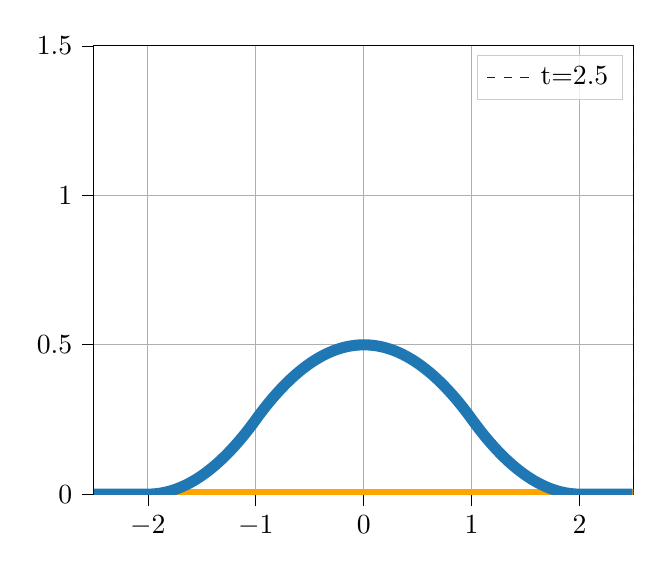
\begin{tikzpicture}

\definecolor{color0}{rgb}{1,0.498039215686275,0.0549019607843137}
\definecolor{color1}{rgb}{1,0.647058823529412,0}
\definecolor{color2}{rgb}{0.12156862745098,0.466666666666667,0.705882352941177}

\begin{axis}[
legend cell align={left},
legend style={fill opacity=0.8, draw opacity=1, text opacity=1, draw=white!80!black},
tick align=outside,
tick pos=left,
x grid style={white!69.0196078431373!black},
xmajorgrids,
xmin=-2.5, xmax=2.5,
xtick style={color=black},
y grid style={white!69.0196078431373!black},
ymajorgrids,
ymin=0, ymax=1.5,
ytick style={color=black}
]
\path [draw=color0, fill=color0, opacity=0.2]
(axis cs:-2.5,0)
--(axis cs:-2.5,0)
--(axis cs:-2.49499499499499,0)
--(axis cs:-2.48998998998999,0)
--(axis cs:-2.48498498498498,0)
--(axis cs:-2.47997997997998,0)
--(axis cs:-2.47497497497497,0)
--(axis cs:-2.46996996996997,0)
--(axis cs:-2.46496496496496,0)
--(axis cs:-2.45995995995996,0)
--(axis cs:-2.45495495495495,0)
--(axis cs:-2.44994994994995,0)
--(axis cs:-2.44494494494494,0)
--(axis cs:-2.43993993993994,0)
--(axis cs:-2.43493493493493,0)
--(axis cs:-2.42992992992993,0)
--(axis cs:-2.42492492492492,0)
--(axis cs:-2.41991991991992,0)
--(axis cs:-2.41491491491491,0)
--(axis cs:-2.40990990990991,0)
--(axis cs:-2.4049049049049,0)
--(axis cs:-2.3998998998999,0)
--(axis cs:-2.39489489489489,0)
--(axis cs:-2.38988988988989,0)
--(axis cs:-2.38488488488488,0)
--(axis cs:-2.37987987987988,0)
--(axis cs:-2.37487487487487,0)
--(axis cs:-2.36986986986987,0)
--(axis cs:-2.36486486486486,0)
--(axis cs:-2.35985985985986,0)
--(axis cs:-2.35485485485485,0)
--(axis cs:-2.34984984984985,0)
--(axis cs:-2.34484484484484,0)
--(axis cs:-2.33983983983984,0)
--(axis cs:-2.33483483483483,0)
--(axis cs:-2.32982982982983,0)
--(axis cs:-2.32482482482482,0)
--(axis cs:-2.31981981981982,0)
--(axis cs:-2.31481481481481,0)
--(axis cs:-2.30980980980981,0)
--(axis cs:-2.3048048048048,0)
--(axis cs:-2.2997997997998,0)
--(axis cs:-2.29479479479479,0)
--(axis cs:-2.28978978978979,0)
--(axis cs:-2.28478478478478,0)
--(axis cs:-2.27977977977978,0)
--(axis cs:-2.27477477477477,0)
--(axis cs:-2.26976976976977,0)
--(axis cs:-2.26476476476476,0)
--(axis cs:-2.25975975975976,0)
--(axis cs:-2.25475475475475,0)
--(axis cs:-2.24974974974975,0)
--(axis cs:-2.24474474474474,0)
--(axis cs:-2.23973973973974,0)
--(axis cs:-2.23473473473473,0)
--(axis cs:-2.22972972972973,0)
--(axis cs:-2.22472472472472,0)
--(axis cs:-2.21971971971972,0)
--(axis cs:-2.21471471471471,0)
--(axis cs:-2.20970970970971,0)
--(axis cs:-2.2047047047047,0)
--(axis cs:-2.1996996996997,0)
--(axis cs:-2.19469469469469,0)
--(axis cs:-2.18968968968969,0)
--(axis cs:-2.18468468468468,0)
--(axis cs:-2.17967967967968,0)
--(axis cs:-2.17467467467467,0)
--(axis cs:-2.16966966966967,0)
--(axis cs:-2.16466466466466,0)
--(axis cs:-2.15965965965966,0)
--(axis cs:-2.15465465465465,0)
--(axis cs:-2.14964964964965,0)
--(axis cs:-2.14464464464464,0)
--(axis cs:-2.13963963963964,0)
--(axis cs:-2.13463463463463,0)
--(axis cs:-2.12962962962963,0)
--(axis cs:-2.12462462462462,0)
--(axis cs:-2.11961961961962,0)
--(axis cs:-2.11461461461461,0)
--(axis cs:-2.10960960960961,0)
--(axis cs:-2.1046046046046,0)
--(axis cs:-2.0995995995996,0)
--(axis cs:-2.09459459459459,0)
--(axis cs:-2.08958958958959,0)
--(axis cs:-2.08458458458458,0)
--(axis cs:-2.07957957957958,0)
--(axis cs:-2.07457457457457,0)
--(axis cs:-2.06956956956957,0)
--(axis cs:-2.06456456456456,0)
--(axis cs:-2.05955955955956,0)
--(axis cs:-2.05455455455455,0)
--(axis cs:-2.04954954954955,0)
--(axis cs:-2.04454454454454,0)
--(axis cs:-2.03953953953954,0)
--(axis cs:-2.03453453453453,0)
--(axis cs:-2.02952952952953,0)
--(axis cs:-2.02452452452452,0)
--(axis cs:-2.01951951951952,0)
--(axis cs:-2.01451451451451,0)
--(axis cs:-2.00950950950951,0)
--(axis cs:-2.0045045045045,0)
--(axis cs:-1.9994994994995,0)
--(axis cs:-1.99449449449449,0)
--(axis cs:-1.98948948948949,0)
--(axis cs:-1.98448448448448,0)
--(axis cs:-1.97947947947948,0)
--(axis cs:-1.97447447447447,0)
--(axis cs:-1.96946946946947,0)
--(axis cs:-1.96446446446446,0)
--(axis cs:-1.95945945945946,0)
--(axis cs:-1.95445445445445,0)
--(axis cs:-1.94944944944945,0)
--(axis cs:-1.94444444444444,0)
--(axis cs:-1.93943943943944,0)
--(axis cs:-1.93443443443443,0)
--(axis cs:-1.92942942942943,0)
--(axis cs:-1.92442442442442,0)
--(axis cs:-1.91941941941942,0)
--(axis cs:-1.91441441441441,0)
--(axis cs:-1.90940940940941,0)
--(axis cs:-1.9044044044044,0)
--(axis cs:-1.8993993993994,0)
--(axis cs:-1.89439439439439,0)
--(axis cs:-1.88938938938939,0)
--(axis cs:-1.88438438438438,0)
--(axis cs:-1.87937937937938,0)
--(axis cs:-1.87437437437437,0)
--(axis cs:-1.86936936936937,0)
--(axis cs:-1.86436436436436,0)
--(axis cs:-1.85935935935936,0)
--(axis cs:-1.85435435435435,0)
--(axis cs:-1.84934934934935,0)
--(axis cs:-1.84434434434434,0)
--(axis cs:-1.83933933933934,0)
--(axis cs:-1.83433433433433,0)
--(axis cs:-1.82932932932933,0)
--(axis cs:-1.82432432432432,0)
--(axis cs:-1.81931931931932,0)
--(axis cs:-1.81431431431431,0)
--(axis cs:-1.80930930930931,0)
--(axis cs:-1.8043043043043,0)
--(axis cs:-1.7992992992993,0)
--(axis cs:-1.79429429429429,0)
--(axis cs:-1.78928928928929,0)
--(axis cs:-1.78428428428428,0)
--(axis cs:-1.77927927927928,0)
--(axis cs:-1.77427427427427,0)
--(axis cs:-1.76926926926927,0)
--(axis cs:-1.76426426426426,0)
--(axis cs:-1.75925925925926,0)
--(axis cs:-1.75425425425425,0)
--(axis cs:-1.74924924924925,0)
--(axis cs:-1.74424424424424,0)
--(axis cs:-1.73923923923924,0)
--(axis cs:-1.73423423423423,0)
--(axis cs:-1.72922922922923,0)
--(axis cs:-1.72422422422422,0)
--(axis cs:-1.71921921921922,0)
--(axis cs:-1.71421421421421,0)
--(axis cs:-1.70920920920921,0)
--(axis cs:-1.7042042042042,0)
--(axis cs:-1.6991991991992,0)
--(axis cs:-1.69419419419419,0)
--(axis cs:-1.68918918918919,0)
--(axis cs:-1.68418418418418,0)
--(axis cs:-1.67917917917918,0)
--(axis cs:-1.67417417417417,0)
--(axis cs:-1.66916916916917,0)
--(axis cs:-1.66416416416416,0)
--(axis cs:-1.65915915915916,0)
--(axis cs:-1.65415415415415,0)
--(axis cs:-1.64914914914915,0)
--(axis cs:-1.64414414414414,0)
--(axis cs:-1.63913913913914,0)
--(axis cs:-1.63413413413413,0)
--(axis cs:-1.62912912912913,0)
--(axis cs:-1.62412412412412,0)
--(axis cs:-1.61911911911912,0)
--(axis cs:-1.61411411411411,0)
--(axis cs:-1.60910910910911,0)
--(axis cs:-1.6041041041041,0)
--(axis cs:-1.5990990990991,0)
--(axis cs:-1.59409409409409,0)
--(axis cs:-1.58908908908909,0)
--(axis cs:-1.58408408408408,0)
--(axis cs:-1.57907907907908,0)
--(axis cs:-1.57407407407407,0)
--(axis cs:-1.56906906906907,0)
--(axis cs:-1.56406406406406,0)
--(axis cs:-1.55905905905906,0)
--(axis cs:-1.55405405405405,0)
--(axis cs:-1.54904904904905,0)
--(axis cs:-1.54404404404404,0)
--(axis cs:-1.53903903903904,0)
--(axis cs:-1.53403403403403,0)
--(axis cs:-1.52902902902903,0)
--(axis cs:-1.52402402402402,0)
--(axis cs:-1.51901901901902,0)
--(axis cs:-1.51401401401401,0)
--(axis cs:-1.50900900900901,0)
--(axis cs:-1.504004004004,0)
--(axis cs:-1.498998998999,0)
--(axis cs:-1.49399399399399,0)
--(axis cs:-1.48898898898899,0)
--(axis cs:-1.48398398398398,0)
--(axis cs:-1.47897897897898,0)
--(axis cs:-1.47397397397397,0)
--(axis cs:-1.46896896896897,0)
--(axis cs:-1.46396396396396,0)
--(axis cs:-1.45895895895896,0)
--(axis cs:-1.45395395395395,0)
--(axis cs:-1.44894894894895,0)
--(axis cs:-1.44394394394394,0)
--(axis cs:-1.43893893893894,0)
--(axis cs:-1.43393393393393,0)
--(axis cs:-1.42892892892893,0)
--(axis cs:-1.42392392392392,0)
--(axis cs:-1.41891891891892,0)
--(axis cs:-1.41391391391391,0)
--(axis cs:-1.40890890890891,0)
--(axis cs:-1.4039039039039,0)
--(axis cs:-1.3988988988989,0)
--(axis cs:-1.39389389389389,0)
--(axis cs:-1.38888888888889,0)
--(axis cs:-1.38388388388388,0)
--(axis cs:-1.37887887887888,0)
--(axis cs:-1.37387387387387,0)
--(axis cs:-1.36886886886887,0)
--(axis cs:-1.36386386386386,0)
--(axis cs:-1.35885885885886,0)
--(axis cs:-1.35385385385385,0)
--(axis cs:-1.34884884884885,0)
--(axis cs:-1.34384384384384,0)
--(axis cs:-1.33883883883884,0)
--(axis cs:-1.33383383383383,0)
--(axis cs:-1.32882882882883,0)
--(axis cs:-1.32382382382382,0)
--(axis cs:-1.31881881881882,0)
--(axis cs:-1.31381381381381,0)
--(axis cs:-1.30880880880881,0)
--(axis cs:-1.3038038038038,0)
--(axis cs:-1.2987987987988,0)
--(axis cs:-1.29379379379379,0)
--(axis cs:-1.28878878878879,0)
--(axis cs:-1.28378378378378,0)
--(axis cs:-1.27877877877878,0)
--(axis cs:-1.27377377377377,0)
--(axis cs:-1.26876876876877,0)
--(axis cs:-1.26376376376376,0)
--(axis cs:-1.25875875875876,0)
--(axis cs:-1.25375375375375,0)
--(axis cs:-1.24874874874875,0)
--(axis cs:-1.24374374374374,0)
--(axis cs:-1.23873873873874,0)
--(axis cs:-1.23373373373373,0)
--(axis cs:-1.22872872872873,0)
--(axis cs:-1.22372372372372,0)
--(axis cs:-1.21871871871872,0)
--(axis cs:-1.21371371371371,0)
--(axis cs:-1.20870870870871,0)
--(axis cs:-1.2037037037037,0)
--(axis cs:-1.1986986986987,0)
--(axis cs:-1.19369369369369,0)
--(axis cs:-1.18868868868869,0)
--(axis cs:-1.18368368368368,0)
--(axis cs:-1.17867867867868,0)
--(axis cs:-1.17367367367367,0)
--(axis cs:-1.16866866866867,0)
--(axis cs:-1.16366366366366,0)
--(axis cs:-1.15865865865866,0)
--(axis cs:-1.15365365365365,0)
--(axis cs:-1.14864864864865,0)
--(axis cs:-1.14364364364364,0)
--(axis cs:-1.13863863863864,0)
--(axis cs:-1.13363363363363,0)
--(axis cs:-1.12862862862863,0)
--(axis cs:-1.12362362362362,0)
--(axis cs:-1.11861861861862,0)
--(axis cs:-1.11361361361361,0)
--(axis cs:-1.10860860860861,0)
--(axis cs:-1.1036036036036,0)
--(axis cs:-1.0985985985986,0)
--(axis cs:-1.09359359359359,0)
--(axis cs:-1.08858858858859,0)
--(axis cs:-1.08358358358358,0)
--(axis cs:-1.07857857857858,0)
--(axis cs:-1.07357357357357,0)
--(axis cs:-1.06856856856857,0)
--(axis cs:-1.06356356356356,0)
--(axis cs:-1.05855855855856,0)
--(axis cs:-1.05355355355355,0)
--(axis cs:-1.04854854854855,0)
--(axis cs:-1.04354354354354,0)
--(axis cs:-1.03853853853854,0)
--(axis cs:-1.03353353353353,0)
--(axis cs:-1.02852852852853,0)
--(axis cs:-1.02352352352352,0)
--(axis cs:-1.01851851851852,0)
--(axis cs:-1.01351351351351,0)
--(axis cs:-1.00850850850851,0)
--(axis cs:-1.0035035035035,0)
--(axis cs:-0.998498498498499,0)
--(axis cs:-0.993493493493494,0)
--(axis cs:-0.988488488488489,0)
--(axis cs:-0.983483483483484,0)
--(axis cs:-0.978478478478479,0)
--(axis cs:-0.973473473473474,0)
--(axis cs:-0.968468468468469,0)
--(axis cs:-0.963463463463464,0)
--(axis cs:-0.958458458458459,0)
--(axis cs:-0.953453453453454,0)
--(axis cs:-0.948448448448449,0)
--(axis cs:-0.943443443443444,0)
--(axis cs:-0.938438438438439,0)
--(axis cs:-0.933433433433434,0)
--(axis cs:-0.928428428428429,0)
--(axis cs:-0.923423423423424,0)
--(axis cs:-0.918418418418419,0)
--(axis cs:-0.913413413413414,0)
--(axis cs:-0.908408408408409,0)
--(axis cs:-0.903403403403404,0)
--(axis cs:-0.898398398398399,0)
--(axis cs:-0.893393393393393,0)
--(axis cs:-0.888388388388388,0)
--(axis cs:-0.883383383383383,0)
--(axis cs:-0.878378378378378,0)
--(axis cs:-0.873373373373373,0)
--(axis cs:-0.868368368368368,0)
--(axis cs:-0.863363363363363,0)
--(axis cs:-0.858358358358358,0)
--(axis cs:-0.853353353353353,0)
--(axis cs:-0.848348348348348,0)
--(axis cs:-0.843343343343343,0)
--(axis cs:-0.838338338338338,0)
--(axis cs:-0.833333333333333,0)
--(axis cs:-0.828328328328328,0)
--(axis cs:-0.823323323323323,0)
--(axis cs:-0.818318318318318,0)
--(axis cs:-0.813313313313313,0)
--(axis cs:-0.808308308308308,0)
--(axis cs:-0.803303303303303,0)
--(axis cs:-0.798298298298298,0)
--(axis cs:-0.793293293293293,0)
--(axis cs:-0.788288288288288,0)
--(axis cs:-0.783283283283283,0)
--(axis cs:-0.778278278278278,0)
--(axis cs:-0.773273273273273,0)
--(axis cs:-0.768268268268268,0)
--(axis cs:-0.763263263263263,0)
--(axis cs:-0.758258258258258,0)
--(axis cs:-0.753253253253253,0)
--(axis cs:-0.748248248248248,0)
--(axis cs:-0.743243243243243,0)
--(axis cs:-0.738238238238238,0)
--(axis cs:-0.733233233233233,0)
--(axis cs:-0.728228228228228,0)
--(axis cs:-0.723223223223223,0)
--(axis cs:-0.718218218218218,0)
--(axis cs:-0.713213213213213,0)
--(axis cs:-0.708208208208208,0)
--(axis cs:-0.703203203203203,0)
--(axis cs:-0.698198198198198,0)
--(axis cs:-0.693193193193193,0)
--(axis cs:-0.688188188188188,0)
--(axis cs:-0.683183183183183,0)
--(axis cs:-0.678178178178178,0)
--(axis cs:-0.673173173173173,0)
--(axis cs:-0.668168168168168,0)
--(axis cs:-0.663163163163163,0)
--(axis cs:-0.658158158158158,0)
--(axis cs:-0.653153153153153,0)
--(axis cs:-0.648148148148148,0)
--(axis cs:-0.643143143143143,0)
--(axis cs:-0.638138138138138,0)
--(axis cs:-0.633133133133133,0)
--(axis cs:-0.628128128128128,0)
--(axis cs:-0.623123123123123,0)
--(axis cs:-0.618118118118118,0)
--(axis cs:-0.613113113113113,0)
--(axis cs:-0.608108108108108,0)
--(axis cs:-0.603103103103103,0)
--(axis cs:-0.598098098098098,0)
--(axis cs:-0.593093093093093,0)
--(axis cs:-0.588088088088088,0)
--(axis cs:-0.583083083083083,0)
--(axis cs:-0.578078078078078,0)
--(axis cs:-0.573073073073073,0)
--(axis cs:-0.568068068068068,0)
--(axis cs:-0.563063063063063,0)
--(axis cs:-0.558058058058058,0)
--(axis cs:-0.553053053053053,0)
--(axis cs:-0.548048048048048,0)
--(axis cs:-0.543043043043043,0)
--(axis cs:-0.538038038038038,0)
--(axis cs:-0.533033033033033,0)
--(axis cs:-0.528028028028028,0)
--(axis cs:-0.523023023023023,0)
--(axis cs:-0.518018018018018,0)
--(axis cs:-0.513013013013013,0)
--(axis cs:-0.508008008008008,0)
--(axis cs:-0.503003003003003,0)
--(axis cs:-0.497997997997998,0)
--(axis cs:-0.492992992992993,0)
--(axis cs:-0.487987987987988,0)
--(axis cs:-0.482982982982983,0)
--(axis cs:-0.477977977977978,0)
--(axis cs:-0.472972972972973,0)
--(axis cs:-0.467967967967968,0)
--(axis cs:-0.462962962962963,0)
--(axis cs:-0.457957957957958,0)
--(axis cs:-0.452952952952953,0)
--(axis cs:-0.447947947947948,0)
--(axis cs:-0.442942942942943,0)
--(axis cs:-0.437937937937938,0)
--(axis cs:-0.432932932932933,0)
--(axis cs:-0.427927927927928,0)
--(axis cs:-0.422922922922923,0)
--(axis cs:-0.417917917917918,0)
--(axis cs:-0.412912912912913,0)
--(axis cs:-0.407907907907908,0)
--(axis cs:-0.402902902902903,0)
--(axis cs:-0.397897897897898,0)
--(axis cs:-0.392892892892893,0)
--(axis cs:-0.387887887887888,0)
--(axis cs:-0.382882882882883,0)
--(axis cs:-0.377877877877878,0)
--(axis cs:-0.372872872872873,0)
--(axis cs:-0.367867867867868,0)
--(axis cs:-0.362862862862863,0)
--(axis cs:-0.357857857857858,0)
--(axis cs:-0.352852852852853,0)
--(axis cs:-0.347847847847848,0)
--(axis cs:-0.342842842842843,0)
--(axis cs:-0.337837837837838,0)
--(axis cs:-0.332832832832833,0)
--(axis cs:-0.327827827827828,0)
--(axis cs:-0.322822822822823,0)
--(axis cs:-0.317817817817818,0)
--(axis cs:-0.312812812812813,0)
--(axis cs:-0.307807807807808,0)
--(axis cs:-0.302802802802803,0)
--(axis cs:-0.297797797797798,0)
--(axis cs:-0.292792792792793,0)
--(axis cs:-0.287787787787788,0)
--(axis cs:-0.282782782782783,0)
--(axis cs:-0.277777777777778,0)
--(axis cs:-0.272772772772773,0)
--(axis cs:-0.267767767767768,0)
--(axis cs:-0.262762762762763,0)
--(axis cs:-0.257757757757758,0)
--(axis cs:-0.252752752752753,0)
--(axis cs:-0.247747747747748,0)
--(axis cs:-0.242742742742743,0)
--(axis cs:-0.237737737737738,0)
--(axis cs:-0.232732732732733,0)
--(axis cs:-0.227727727727728,0)
--(axis cs:-0.222722722722723,0)
--(axis cs:-0.217717717717718,0)
--(axis cs:-0.212712712712713,0)
--(axis cs:-0.207707707707708,0)
--(axis cs:-0.202702702702703,0)
--(axis cs:-0.197697697697698,0)
--(axis cs:-0.192692692692693,0)
--(axis cs:-0.187687687687688,0)
--(axis cs:-0.182682682682683,0)
--(axis cs:-0.177677677677678,0)
--(axis cs:-0.172672672672673,0)
--(axis cs:-0.167667667667668,0)
--(axis cs:-0.162662662662663,0)
--(axis cs:-0.157657657657658,0)
--(axis cs:-0.152652652652653,0)
--(axis cs:-0.147647647647648,0)
--(axis cs:-0.142642642642643,0)
--(axis cs:-0.137637637637638,0)
--(axis cs:-0.132632632632633,0)
--(axis cs:-0.127627627627628,0)
--(axis cs:-0.122622622622623,0)
--(axis cs:-0.117617617617618,0)
--(axis cs:-0.112612612612613,0)
--(axis cs:-0.107607607607608,0)
--(axis cs:-0.102602602602603,0)
--(axis cs:-0.0975975975975976,0)
--(axis cs:-0.0925925925925926,0)
--(axis cs:-0.0875875875875876,0)
--(axis cs:-0.0825825825825826,0)
--(axis cs:-0.0775775775775776,0)
--(axis cs:-0.0725725725725725,0)
--(axis cs:-0.0675675675675675,0)
--(axis cs:-0.0625625625625625,0)
--(axis cs:-0.0575575575575575,0)
--(axis cs:-0.0525525525525525,0)
--(axis cs:-0.0475475475475475,0)
--(axis cs:-0.0425425425425425,0)
--(axis cs:-0.0375375375375375,0)
--(axis cs:-0.0325325325325325,0)
--(axis cs:-0.0275275275275275,0)
--(axis cs:-0.0225225225225225,0)
--(axis cs:-0.0175175175175175,0)
--(axis cs:-0.0125125125125125,0)
--(axis cs:-0.0075075075075075,0)
--(axis cs:-0.0025025025025025,0)
--(axis cs:0.0025025025025025,0)
--(axis cs:0.0075075075075075,0)
--(axis cs:0.0125125125125125,0)
--(axis cs:0.0175175175175175,0)
--(axis cs:0.0225225225225225,0)
--(axis cs:0.0275275275275275,0)
--(axis cs:0.0325325325325325,0)
--(axis cs:0.0375375375375375,0)
--(axis cs:0.0425425425425425,0)
--(axis cs:0.0475475475475475,0)
--(axis cs:0.0525525525525525,0)
--(axis cs:0.0575575575575575,0)
--(axis cs:0.0625625625625625,0)
--(axis cs:0.0675675675675675,0)
--(axis cs:0.0725725725725725,0)
--(axis cs:0.0775775775775776,0)
--(axis cs:0.0825825825825826,0)
--(axis cs:0.0875875875875876,0)
--(axis cs:0.0925925925925926,0)
--(axis cs:0.0975975975975976,0)
--(axis cs:0.102602602602603,0)
--(axis cs:0.107607607607608,0)
--(axis cs:0.112612612612613,0)
--(axis cs:0.117617617617618,0)
--(axis cs:0.122622622622623,0)
--(axis cs:0.127627627627628,0)
--(axis cs:0.132632632632633,0)
--(axis cs:0.137637637637638,0)
--(axis cs:0.142642642642643,0)
--(axis cs:0.147647647647648,0)
--(axis cs:0.152652652652653,0)
--(axis cs:0.157657657657658,0)
--(axis cs:0.162662662662663,0)
--(axis cs:0.167667667667668,0)
--(axis cs:0.172672672672673,0)
--(axis cs:0.177677677677678,0)
--(axis cs:0.182682682682683,0)
--(axis cs:0.187687687687688,0)
--(axis cs:0.192692692692693,0)
--(axis cs:0.197697697697698,0)
--(axis cs:0.202702702702703,0)
--(axis cs:0.207707707707708,0)
--(axis cs:0.212712712712713,0)
--(axis cs:0.217717717717718,0)
--(axis cs:0.222722722722723,0)
--(axis cs:0.227727727727728,0)
--(axis cs:0.232732732732733,0)
--(axis cs:0.237737737737738,0)
--(axis cs:0.242742742742743,0)
--(axis cs:0.247747747747748,0)
--(axis cs:0.252752752752753,0)
--(axis cs:0.257757757757758,0)
--(axis cs:0.262762762762763,0)
--(axis cs:0.267767767767768,0)
--(axis cs:0.272772772772773,0)
--(axis cs:0.277777777777778,0)
--(axis cs:0.282782782782783,0)
--(axis cs:0.287787787787788,0)
--(axis cs:0.292792792792793,0)
--(axis cs:0.297797797797798,0)
--(axis cs:0.302802802802803,0)
--(axis cs:0.307807807807808,0)
--(axis cs:0.312812812812813,0)
--(axis cs:0.317817817817818,0)
--(axis cs:0.322822822822823,0)
--(axis cs:0.327827827827828,0)
--(axis cs:0.332832832832833,0)
--(axis cs:0.337837837837838,0)
--(axis cs:0.342842842842843,0)
--(axis cs:0.347847847847848,0)
--(axis cs:0.352852852852853,0)
--(axis cs:0.357857857857858,0)
--(axis cs:0.362862862862863,0)
--(axis cs:0.367867867867868,0)
--(axis cs:0.372872872872873,0)
--(axis cs:0.377877877877878,0)
--(axis cs:0.382882882882883,0)
--(axis cs:0.387887887887888,0)
--(axis cs:0.392892892892893,0)
--(axis cs:0.397897897897898,0)
--(axis cs:0.402902902902903,0)
--(axis cs:0.407907907907908,0)
--(axis cs:0.412912912912913,0)
--(axis cs:0.417917917917918,0)
--(axis cs:0.422922922922923,0)
--(axis cs:0.427927927927928,0)
--(axis cs:0.432932932932933,0)
--(axis cs:0.437937937937938,0)
--(axis cs:0.442942942942943,0)
--(axis cs:0.447947947947948,0)
--(axis cs:0.452952952952953,0)
--(axis cs:0.457957957957958,0)
--(axis cs:0.462962962962963,0)
--(axis cs:0.467967967967968,0)
--(axis cs:0.472972972972973,0)
--(axis cs:0.477977977977978,0)
--(axis cs:0.482982982982983,0)
--(axis cs:0.487987987987988,0)
--(axis cs:0.492992992992993,0)
--(axis cs:0.497997997997998,0)
--(axis cs:0.503003003003003,0)
--(axis cs:0.508008008008008,0)
--(axis cs:0.513013013013013,0)
--(axis cs:0.518018018018018,0)
--(axis cs:0.523023023023023,0)
--(axis cs:0.528028028028028,0)
--(axis cs:0.533033033033033,0)
--(axis cs:0.538038038038038,0)
--(axis cs:0.543043043043043,0)
--(axis cs:0.548048048048048,0)
--(axis cs:0.553053053053053,0)
--(axis cs:0.558058058058058,0)
--(axis cs:0.563063063063063,0)
--(axis cs:0.568068068068068,0)
--(axis cs:0.573073073073073,0)
--(axis cs:0.578078078078078,0)
--(axis cs:0.583083083083083,0)
--(axis cs:0.588088088088088,0)
--(axis cs:0.593093093093093,0)
--(axis cs:0.598098098098098,0)
--(axis cs:0.603103103103103,0)
--(axis cs:0.608108108108108,0)
--(axis cs:0.613113113113113,0)
--(axis cs:0.618118118118118,0)
--(axis cs:0.623123123123123,0)
--(axis cs:0.628128128128128,0)
--(axis cs:0.633133133133133,0)
--(axis cs:0.638138138138138,0)
--(axis cs:0.643143143143143,0)
--(axis cs:0.648148148148148,0)
--(axis cs:0.653153153153153,0)
--(axis cs:0.658158158158158,0)
--(axis cs:0.663163163163163,0)
--(axis cs:0.668168168168168,0)
--(axis cs:0.673173173173173,0)
--(axis cs:0.678178178178178,0)
--(axis cs:0.683183183183183,0)
--(axis cs:0.688188188188188,0)
--(axis cs:0.693193193193193,0)
--(axis cs:0.698198198198198,0)
--(axis cs:0.703203203203203,0)
--(axis cs:0.708208208208208,0)
--(axis cs:0.713213213213213,0)
--(axis cs:0.718218218218218,0)
--(axis cs:0.723223223223223,0)
--(axis cs:0.728228228228228,0)
--(axis cs:0.733233233233233,0)
--(axis cs:0.738238238238238,0)
--(axis cs:0.743243243243243,0)
--(axis cs:0.748248248248248,0)
--(axis cs:0.753253253253253,0)
--(axis cs:0.758258258258258,0)
--(axis cs:0.763263263263263,0)
--(axis cs:0.768268268268268,0)
--(axis cs:0.773273273273273,0)
--(axis cs:0.778278278278278,0)
--(axis cs:0.783283283283283,0)
--(axis cs:0.788288288288288,0)
--(axis cs:0.793293293293293,0)
--(axis cs:0.798298298298298,0)
--(axis cs:0.803303303303303,0)
--(axis cs:0.808308308308308,0)
--(axis cs:0.813313313313313,0)
--(axis cs:0.818318318318318,0)
--(axis cs:0.823323323323323,0)
--(axis cs:0.828328328328328,0)
--(axis cs:0.833333333333333,0)
--(axis cs:0.838338338338338,0)
--(axis cs:0.843343343343343,0)
--(axis cs:0.848348348348348,0)
--(axis cs:0.853353353353353,0)
--(axis cs:0.858358358358358,0)
--(axis cs:0.863363363363364,0)
--(axis cs:0.868368368368369,0)
--(axis cs:0.873373373373374,0)
--(axis cs:0.878378378378379,0)
--(axis cs:0.883383383383384,0)
--(axis cs:0.888388388388389,0)
--(axis cs:0.893393393393394,0)
--(axis cs:0.898398398398399,0)
--(axis cs:0.903403403403404,0)
--(axis cs:0.908408408408409,0)
--(axis cs:0.913413413413414,0)
--(axis cs:0.918418418418419,0)
--(axis cs:0.923423423423424,0)
--(axis cs:0.928428428428429,0)
--(axis cs:0.933433433433434,0)
--(axis cs:0.938438438438439,0)
--(axis cs:0.943443443443444,0)
--(axis cs:0.948448448448449,0)
--(axis cs:0.953453453453454,0)
--(axis cs:0.958458458458459,0)
--(axis cs:0.963463463463464,0)
--(axis cs:0.968468468468469,0)
--(axis cs:0.973473473473474,0)
--(axis cs:0.978478478478479,0)
--(axis cs:0.983483483483484,0)
--(axis cs:0.988488488488489,0)
--(axis cs:0.993493493493494,0)
--(axis cs:0.998498498498499,0)
--(axis cs:1.0035035035035,0)
--(axis cs:1.00850850850851,0)
--(axis cs:1.01351351351351,0)
--(axis cs:1.01851851851852,0)
--(axis cs:1.02352352352352,0)
--(axis cs:1.02852852852853,0)
--(axis cs:1.03353353353353,0)
--(axis cs:1.03853853853854,0)
--(axis cs:1.04354354354354,0)
--(axis cs:1.04854854854855,0)
--(axis cs:1.05355355355355,0)
--(axis cs:1.05855855855856,0)
--(axis cs:1.06356356356356,0)
--(axis cs:1.06856856856857,0)
--(axis cs:1.07357357357357,0)
--(axis cs:1.07857857857858,0)
--(axis cs:1.08358358358358,0)
--(axis cs:1.08858858858859,0)
--(axis cs:1.09359359359359,0)
--(axis cs:1.0985985985986,0)
--(axis cs:1.1036036036036,0)
--(axis cs:1.10860860860861,0)
--(axis cs:1.11361361361361,0)
--(axis cs:1.11861861861862,0)
--(axis cs:1.12362362362362,0)
--(axis cs:1.12862862862863,0)
--(axis cs:1.13363363363363,0)
--(axis cs:1.13863863863864,0)
--(axis cs:1.14364364364364,0)
--(axis cs:1.14864864864865,0)
--(axis cs:1.15365365365365,0)
--(axis cs:1.15865865865866,0)
--(axis cs:1.16366366366366,0)
--(axis cs:1.16866866866867,0)
--(axis cs:1.17367367367367,0)
--(axis cs:1.17867867867868,0)
--(axis cs:1.18368368368368,0)
--(axis cs:1.18868868868869,0)
--(axis cs:1.19369369369369,0)
--(axis cs:1.1986986986987,0)
--(axis cs:1.2037037037037,0)
--(axis cs:1.20870870870871,0)
--(axis cs:1.21371371371371,0)
--(axis cs:1.21871871871872,0)
--(axis cs:1.22372372372372,0)
--(axis cs:1.22872872872873,0)
--(axis cs:1.23373373373373,0)
--(axis cs:1.23873873873874,0)
--(axis cs:1.24374374374374,0)
--(axis cs:1.24874874874875,0)
--(axis cs:1.25375375375375,0)
--(axis cs:1.25875875875876,0)
--(axis cs:1.26376376376376,0)
--(axis cs:1.26876876876877,0)
--(axis cs:1.27377377377377,0)
--(axis cs:1.27877877877878,0)
--(axis cs:1.28378378378378,0)
--(axis cs:1.28878878878879,0)
--(axis cs:1.29379379379379,0)
--(axis cs:1.2987987987988,0)
--(axis cs:1.3038038038038,0)
--(axis cs:1.30880880880881,0)
--(axis cs:1.31381381381381,0)
--(axis cs:1.31881881881882,0)
--(axis cs:1.32382382382382,0)
--(axis cs:1.32882882882883,0)
--(axis cs:1.33383383383383,0)
--(axis cs:1.33883883883884,0)
--(axis cs:1.34384384384384,0)
--(axis cs:1.34884884884885,0)
--(axis cs:1.35385385385385,0)
--(axis cs:1.35885885885886,0)
--(axis cs:1.36386386386386,0)
--(axis cs:1.36886886886887,0)
--(axis cs:1.37387387387387,0)
--(axis cs:1.37887887887888,0)
--(axis cs:1.38388388388388,0)
--(axis cs:1.38888888888889,0)
--(axis cs:1.39389389389389,0)
--(axis cs:1.3988988988989,0)
--(axis cs:1.4039039039039,0)
--(axis cs:1.40890890890891,0)
--(axis cs:1.41391391391391,0)
--(axis cs:1.41891891891892,0)
--(axis cs:1.42392392392392,0)
--(axis cs:1.42892892892893,0)
--(axis cs:1.43393393393393,0)
--(axis cs:1.43893893893894,0)
--(axis cs:1.44394394394394,0)
--(axis cs:1.44894894894895,0)
--(axis cs:1.45395395395395,0)
--(axis cs:1.45895895895896,0)
--(axis cs:1.46396396396396,0)
--(axis cs:1.46896896896897,0)
--(axis cs:1.47397397397397,0)
--(axis cs:1.47897897897898,0)
--(axis cs:1.48398398398398,0)
--(axis cs:1.48898898898899,0)
--(axis cs:1.49399399399399,0)
--(axis cs:1.498998998999,0)
--(axis cs:1.504004004004,0)
--(axis cs:1.50900900900901,0)
--(axis cs:1.51401401401401,0)
--(axis cs:1.51901901901902,0)
--(axis cs:1.52402402402402,0)
--(axis cs:1.52902902902903,0)
--(axis cs:1.53403403403403,0)
--(axis cs:1.53903903903904,0)
--(axis cs:1.54404404404404,0)
--(axis cs:1.54904904904905,0)
--(axis cs:1.55405405405405,0)
--(axis cs:1.55905905905906,0)
--(axis cs:1.56406406406406,0)
--(axis cs:1.56906906906907,0)
--(axis cs:1.57407407407407,0)
--(axis cs:1.57907907907908,0)
--(axis cs:1.58408408408408,0)
--(axis cs:1.58908908908909,0)
--(axis cs:1.59409409409409,0)
--(axis cs:1.5990990990991,0)
--(axis cs:1.6041041041041,0)
--(axis cs:1.60910910910911,0)
--(axis cs:1.61411411411411,0)
--(axis cs:1.61911911911912,0)
--(axis cs:1.62412412412412,0)
--(axis cs:1.62912912912913,0)
--(axis cs:1.63413413413413,0)
--(axis cs:1.63913913913914,0)
--(axis cs:1.64414414414414,0)
--(axis cs:1.64914914914915,0)
--(axis cs:1.65415415415415,0)
--(axis cs:1.65915915915916,0)
--(axis cs:1.66416416416416,0)
--(axis cs:1.66916916916917,0)
--(axis cs:1.67417417417417,0)
--(axis cs:1.67917917917918,0)
--(axis cs:1.68418418418418,0)
--(axis cs:1.68918918918919,0)
--(axis cs:1.69419419419419,0)
--(axis cs:1.6991991991992,0)
--(axis cs:1.7042042042042,0)
--(axis cs:1.70920920920921,0)
--(axis cs:1.71421421421421,0)
--(axis cs:1.71921921921922,0)
--(axis cs:1.72422422422422,0)
--(axis cs:1.72922922922923,0)
--(axis cs:1.73423423423423,0)
--(axis cs:1.73923923923924,0)
--(axis cs:1.74424424424424,0)
--(axis cs:1.74924924924925,0)
--(axis cs:1.75425425425425,0)
--(axis cs:1.75925925925926,0)
--(axis cs:1.76426426426426,0)
--(axis cs:1.76926926926927,0)
--(axis cs:1.77427427427427,0)
--(axis cs:1.77927927927928,0)
--(axis cs:1.78428428428428,0)
--(axis cs:1.78928928928929,0)
--(axis cs:1.79429429429429,0)
--(axis cs:1.7992992992993,0)
--(axis cs:1.8043043043043,0)
--(axis cs:1.80930930930931,0)
--(axis cs:1.81431431431431,0)
--(axis cs:1.81931931931932,0)
--(axis cs:1.82432432432432,0)
--(axis cs:1.82932932932933,0)
--(axis cs:1.83433433433433,0)
--(axis cs:1.83933933933934,0)
--(axis cs:1.84434434434434,0)
--(axis cs:1.84934934934935,0)
--(axis cs:1.85435435435435,0)
--(axis cs:1.85935935935936,0)
--(axis cs:1.86436436436436,0)
--(axis cs:1.86936936936937,0)
--(axis cs:1.87437437437437,0)
--(axis cs:1.87937937937938,0)
--(axis cs:1.88438438438438,0)
--(axis cs:1.88938938938939,0)
--(axis cs:1.89439439439439,0)
--(axis cs:1.8993993993994,0)
--(axis cs:1.9044044044044,0)
--(axis cs:1.90940940940941,0)
--(axis cs:1.91441441441441,0)
--(axis cs:1.91941941941942,0)
--(axis cs:1.92442442442442,0)
--(axis cs:1.92942942942943,0)
--(axis cs:1.93443443443443,0)
--(axis cs:1.93943943943944,0)
--(axis cs:1.94444444444444,0)
--(axis cs:1.94944944944945,0)
--(axis cs:1.95445445445445,0)
--(axis cs:1.95945945945946,0)
--(axis cs:1.96446446446446,0)
--(axis cs:1.96946946946947,0)
--(axis cs:1.97447447447447,0)
--(axis cs:1.97947947947948,0)
--(axis cs:1.98448448448448,0)
--(axis cs:1.98948948948949,0)
--(axis cs:1.99449449449449,0)
--(axis cs:1.9994994994995,0)
--(axis cs:2.0045045045045,0)
--(axis cs:2.00950950950951,0)
--(axis cs:2.01451451451451,0)
--(axis cs:2.01951951951952,0)
--(axis cs:2.02452452452452,0)
--(axis cs:2.02952952952953,0)
--(axis cs:2.03453453453453,0)
--(axis cs:2.03953953953954,0)
--(axis cs:2.04454454454454,0)
--(axis cs:2.04954954954955,0)
--(axis cs:2.05455455455455,0)
--(axis cs:2.05955955955956,0)
--(axis cs:2.06456456456456,0)
--(axis cs:2.06956956956957,0)
--(axis cs:2.07457457457457,0)
--(axis cs:2.07957957957958,0)
--(axis cs:2.08458458458458,0)
--(axis cs:2.08958958958959,0)
--(axis cs:2.09459459459459,0)
--(axis cs:2.0995995995996,0)
--(axis cs:2.1046046046046,0)
--(axis cs:2.10960960960961,0)
--(axis cs:2.11461461461461,0)
--(axis cs:2.11961961961962,0)
--(axis cs:2.12462462462462,0)
--(axis cs:2.12962962962963,0)
--(axis cs:2.13463463463463,0)
--(axis cs:2.13963963963964,0)
--(axis cs:2.14464464464464,0)
--(axis cs:2.14964964964965,0)
--(axis cs:2.15465465465465,0)
--(axis cs:2.15965965965966,0)
--(axis cs:2.16466466466466,0)
--(axis cs:2.16966966966967,0)
--(axis cs:2.17467467467467,0)
--(axis cs:2.17967967967968,0)
--(axis cs:2.18468468468468,0)
--(axis cs:2.18968968968969,0)
--(axis cs:2.19469469469469,0)
--(axis cs:2.1996996996997,0)
--(axis cs:2.2047047047047,0)
--(axis cs:2.20970970970971,0)
--(axis cs:2.21471471471471,0)
--(axis cs:2.21971971971972,0)
--(axis cs:2.22472472472472,0)
--(axis cs:2.22972972972973,0)
--(axis cs:2.23473473473473,0)
--(axis cs:2.23973973973974,0)
--(axis cs:2.24474474474474,0)
--(axis cs:2.24974974974975,0)
--(axis cs:2.25475475475475,0)
--(axis cs:2.25975975975976,0)
--(axis cs:2.26476476476476,0)
--(axis cs:2.26976976976977,0)
--(axis cs:2.27477477477477,0)
--(axis cs:2.27977977977978,0)
--(axis cs:2.28478478478478,0)
--(axis cs:2.28978978978979,0)
--(axis cs:2.29479479479479,0)
--(axis cs:2.2997997997998,0)
--(axis cs:2.3048048048048,0)
--(axis cs:2.30980980980981,0)
--(axis cs:2.31481481481481,0)
--(axis cs:2.31981981981982,0)
--(axis cs:2.32482482482482,0)
--(axis cs:2.32982982982983,0)
--(axis cs:2.33483483483483,0)
--(axis cs:2.33983983983984,0)
--(axis cs:2.34484484484484,0)
--(axis cs:2.34984984984985,0)
--(axis cs:2.35485485485485,0)
--(axis cs:2.35985985985986,0)
--(axis cs:2.36486486486486,0)
--(axis cs:2.36986986986987,0)
--(axis cs:2.37487487487487,0)
--(axis cs:2.37987987987988,0)
--(axis cs:2.38488488488488,0)
--(axis cs:2.38988988988989,0)
--(axis cs:2.39489489489489,0)
--(axis cs:2.3998998998999,0)
--(axis cs:2.4049049049049,0)
--(axis cs:2.40990990990991,0)
--(axis cs:2.41491491491491,0)
--(axis cs:2.41991991991992,0)
--(axis cs:2.42492492492492,0)
--(axis cs:2.42992992992993,0)
--(axis cs:2.43493493493493,0)
--(axis cs:2.43993993993994,0)
--(axis cs:2.44494494494494,0)
--(axis cs:2.44994994994995,0)
--(axis cs:2.45495495495495,0)
--(axis cs:2.45995995995996,0)
--(axis cs:2.46496496496496,0)
--(axis cs:2.46996996996997,0)
--(axis cs:2.47497497497497,0)
--(axis cs:2.47997997997998,0)
--(axis cs:2.48498498498498,0)
--(axis cs:2.48998998998999,0)
--(axis cs:2.49499499499499,0)
--(axis cs:2.5,0)
--(axis cs:2.5,0)
--(axis cs:2.5,0)
--(axis cs:2.49499499499499,0)
--(axis cs:2.48998998998999,0)
--(axis cs:2.48498498498498,0)
--(axis cs:2.47997997997998,0)
--(axis cs:2.47497497497497,0)
--(axis cs:2.46996996996997,0)
--(axis cs:2.46496496496496,0)
--(axis cs:2.45995995995996,0)
--(axis cs:2.45495495495495,0)
--(axis cs:2.44994994994995,0)
--(axis cs:2.44494494494494,0)
--(axis cs:2.43993993993994,0)
--(axis cs:2.43493493493493,0)
--(axis cs:2.42992992992993,0)
--(axis cs:2.42492492492492,0)
--(axis cs:2.41991991991992,0)
--(axis cs:2.41491491491491,0)
--(axis cs:2.40990990990991,0)
--(axis cs:2.4049049049049,0)
--(axis cs:2.3998998998999,0)
--(axis cs:2.39489489489489,0)
--(axis cs:2.38988988988989,0)
--(axis cs:2.38488488488488,0)
--(axis cs:2.37987987987988,0)
--(axis cs:2.37487487487487,0)
--(axis cs:2.36986986986987,0)
--(axis cs:2.36486486486486,0)
--(axis cs:2.35985985985986,0)
--(axis cs:2.35485485485485,0)
--(axis cs:2.34984984984985,0)
--(axis cs:2.34484484484484,0)
--(axis cs:2.33983983983984,0)
--(axis cs:2.33483483483483,0)
--(axis cs:2.32982982982983,0)
--(axis cs:2.32482482482482,0)
--(axis cs:2.31981981981982,0)
--(axis cs:2.31481481481481,0)
--(axis cs:2.30980980980981,0)
--(axis cs:2.3048048048048,0)
--(axis cs:2.2997997997998,0)
--(axis cs:2.29479479479479,0)
--(axis cs:2.28978978978979,0)
--(axis cs:2.28478478478478,0)
--(axis cs:2.27977977977978,0)
--(axis cs:2.27477477477477,0)
--(axis cs:2.26976976976977,0)
--(axis cs:2.26476476476476,0)
--(axis cs:2.25975975975976,0)
--(axis cs:2.25475475475475,0)
--(axis cs:2.24974974974975,0)
--(axis cs:2.24474474474474,0)
--(axis cs:2.23973973973974,0)
--(axis cs:2.23473473473473,0)
--(axis cs:2.22972972972973,0)
--(axis cs:2.22472472472472,0)
--(axis cs:2.21971971971972,0)
--(axis cs:2.21471471471471,0)
--(axis cs:2.20970970970971,0)
--(axis cs:2.2047047047047,0)
--(axis cs:2.1996996996997,0)
--(axis cs:2.19469469469469,0)
--(axis cs:2.18968968968969,0)
--(axis cs:2.18468468468468,0)
--(axis cs:2.17967967967968,0)
--(axis cs:2.17467467467467,0)
--(axis cs:2.16966966966967,0)
--(axis cs:2.16466466466466,0)
--(axis cs:2.15965965965966,0)
--(axis cs:2.15465465465465,0)
--(axis cs:2.14964964964965,0)
--(axis cs:2.14464464464464,0)
--(axis cs:2.13963963963964,0)
--(axis cs:2.13463463463463,0)
--(axis cs:2.12962962962963,0)
--(axis cs:2.12462462462462,0)
--(axis cs:2.11961961961962,0)
--(axis cs:2.11461461461461,0)
--(axis cs:2.10960960960961,0)
--(axis cs:2.1046046046046,0)
--(axis cs:2.0995995995996,0)
--(axis cs:2.09459459459459,0)
--(axis cs:2.08958958958959,0)
--(axis cs:2.08458458458458,0)
--(axis cs:2.07957957957958,0)
--(axis cs:2.07457457457457,0)
--(axis cs:2.06956956956957,0)
--(axis cs:2.06456456456456,0)
--(axis cs:2.05955955955956,0)
--(axis cs:2.05455455455455,0)
--(axis cs:2.04954954954955,0)
--(axis cs:2.04454454454454,0)
--(axis cs:2.03953953953954,0)
--(axis cs:2.03453453453453,0)
--(axis cs:2.02952952952953,0)
--(axis cs:2.02452452452452,0)
--(axis cs:2.01951951951952,0)
--(axis cs:2.01451451451451,0)
--(axis cs:2.00950950950951,0)
--(axis cs:2.0045045045045,0)
--(axis cs:1.9994994994995,0)
--(axis cs:1.99449449449449,0)
--(axis cs:1.98948948948949,0)
--(axis cs:1.98448448448448,0)
--(axis cs:1.97947947947948,0)
--(axis cs:1.97447447447447,0)
--(axis cs:1.96946946946947,0)
--(axis cs:1.96446446446446,0)
--(axis cs:1.95945945945946,0)
--(axis cs:1.95445445445445,0)
--(axis cs:1.94944944944945,0)
--(axis cs:1.94444444444444,0)
--(axis cs:1.93943943943944,0)
--(axis cs:1.93443443443443,0)
--(axis cs:1.92942942942943,0)
--(axis cs:1.92442442442442,0)
--(axis cs:1.91941941941942,0)
--(axis cs:1.91441441441441,0)
--(axis cs:1.90940940940941,0)
--(axis cs:1.9044044044044,0)
--(axis cs:1.8993993993994,0)
--(axis cs:1.89439439439439,0)
--(axis cs:1.88938938938939,0)
--(axis cs:1.88438438438438,0)
--(axis cs:1.87937937937938,0)
--(axis cs:1.87437437437437,0)
--(axis cs:1.86936936936937,0)
--(axis cs:1.86436436436436,0)
--(axis cs:1.85935935935936,0)
--(axis cs:1.85435435435435,0)
--(axis cs:1.84934934934935,0)
--(axis cs:1.84434434434434,0)
--(axis cs:1.83933933933934,0)
--(axis cs:1.83433433433433,0)
--(axis cs:1.82932932932933,0)
--(axis cs:1.82432432432432,0)
--(axis cs:1.81931931931932,0)
--(axis cs:1.81431431431431,0)
--(axis cs:1.80930930930931,0)
--(axis cs:1.8043043043043,0)
--(axis cs:1.7992992992993,0)
--(axis cs:1.79429429429429,0)
--(axis cs:1.78928928928929,0)
--(axis cs:1.78428428428428,0)
--(axis cs:1.77927927927928,0)
--(axis cs:1.77427427427427,0)
--(axis cs:1.76926926926927,0)
--(axis cs:1.76426426426426,0)
--(axis cs:1.75925925925926,0)
--(axis cs:1.75425425425425,0)
--(axis cs:1.74924924924925,0)
--(axis cs:1.74424424424424,0)
--(axis cs:1.73923923923924,0)
--(axis cs:1.73423423423423,0)
--(axis cs:1.72922922922923,0)
--(axis cs:1.72422422422422,0)
--(axis cs:1.71921921921922,0)
--(axis cs:1.71421421421421,0)
--(axis cs:1.70920920920921,0)
--(axis cs:1.7042042042042,0)
--(axis cs:1.6991991991992,0)
--(axis cs:1.69419419419419,0)
--(axis cs:1.68918918918919,0)
--(axis cs:1.68418418418418,0)
--(axis cs:1.67917917917918,0)
--(axis cs:1.67417417417417,0)
--(axis cs:1.66916916916917,0)
--(axis cs:1.66416416416416,0)
--(axis cs:1.65915915915916,0)
--(axis cs:1.65415415415415,0)
--(axis cs:1.64914914914915,0)
--(axis cs:1.64414414414414,0)
--(axis cs:1.63913913913914,0)
--(axis cs:1.63413413413413,0)
--(axis cs:1.62912912912913,0)
--(axis cs:1.62412412412412,0)
--(axis cs:1.61911911911912,0)
--(axis cs:1.61411411411411,0)
--(axis cs:1.60910910910911,0)
--(axis cs:1.6041041041041,0)
--(axis cs:1.5990990990991,0)
--(axis cs:1.59409409409409,0)
--(axis cs:1.58908908908909,0)
--(axis cs:1.58408408408408,0)
--(axis cs:1.57907907907908,0)
--(axis cs:1.57407407407407,0)
--(axis cs:1.56906906906907,0)
--(axis cs:1.56406406406406,0)
--(axis cs:1.55905905905906,0)
--(axis cs:1.55405405405405,0)
--(axis cs:1.54904904904905,0)
--(axis cs:1.54404404404404,0)
--(axis cs:1.53903903903904,0)
--(axis cs:1.53403403403403,0)
--(axis cs:1.52902902902903,0)
--(axis cs:1.52402402402402,0)
--(axis cs:1.51901901901902,0)
--(axis cs:1.51401401401401,0)
--(axis cs:1.50900900900901,0)
--(axis cs:1.504004004004,0)
--(axis cs:1.498998998999,0)
--(axis cs:1.49399399399399,0)
--(axis cs:1.48898898898899,0)
--(axis cs:1.48398398398398,0)
--(axis cs:1.47897897897898,0)
--(axis cs:1.47397397397397,0)
--(axis cs:1.46896896896897,0)
--(axis cs:1.46396396396396,0)
--(axis cs:1.45895895895896,0)
--(axis cs:1.45395395395395,0)
--(axis cs:1.44894894894895,0)
--(axis cs:1.44394394394394,0)
--(axis cs:1.43893893893894,0)
--(axis cs:1.43393393393393,0)
--(axis cs:1.42892892892893,0)
--(axis cs:1.42392392392392,0)
--(axis cs:1.41891891891892,0)
--(axis cs:1.41391391391391,0)
--(axis cs:1.40890890890891,0)
--(axis cs:1.4039039039039,0)
--(axis cs:1.3988988988989,0)
--(axis cs:1.39389389389389,0)
--(axis cs:1.38888888888889,0)
--(axis cs:1.38388388388388,0)
--(axis cs:1.37887887887888,0)
--(axis cs:1.37387387387387,0)
--(axis cs:1.36886886886887,0)
--(axis cs:1.36386386386386,0)
--(axis cs:1.35885885885886,0)
--(axis cs:1.35385385385385,0)
--(axis cs:1.34884884884885,0)
--(axis cs:1.34384384384384,0)
--(axis cs:1.33883883883884,0)
--(axis cs:1.33383383383383,0)
--(axis cs:1.32882882882883,0)
--(axis cs:1.32382382382382,0)
--(axis cs:1.31881881881882,0)
--(axis cs:1.31381381381381,0)
--(axis cs:1.30880880880881,0)
--(axis cs:1.3038038038038,0)
--(axis cs:1.2987987987988,0)
--(axis cs:1.29379379379379,0)
--(axis cs:1.28878878878879,0)
--(axis cs:1.28378378378378,0)
--(axis cs:1.27877877877878,0)
--(axis cs:1.27377377377377,0)
--(axis cs:1.26876876876877,0)
--(axis cs:1.26376376376376,0)
--(axis cs:1.25875875875876,0)
--(axis cs:1.25375375375375,0)
--(axis cs:1.24874874874875,0)
--(axis cs:1.24374374374374,0)
--(axis cs:1.23873873873874,0)
--(axis cs:1.23373373373373,0)
--(axis cs:1.22872872872873,0)
--(axis cs:1.22372372372372,0)
--(axis cs:1.21871871871872,0)
--(axis cs:1.21371371371371,0)
--(axis cs:1.20870870870871,0)
--(axis cs:1.2037037037037,0)
--(axis cs:1.1986986986987,0)
--(axis cs:1.19369369369369,0)
--(axis cs:1.18868868868869,0)
--(axis cs:1.18368368368368,0)
--(axis cs:1.17867867867868,0)
--(axis cs:1.17367367367367,0)
--(axis cs:1.16866866866867,0)
--(axis cs:1.16366366366366,0)
--(axis cs:1.15865865865866,0)
--(axis cs:1.15365365365365,0)
--(axis cs:1.14864864864865,0)
--(axis cs:1.14364364364364,0)
--(axis cs:1.13863863863864,0)
--(axis cs:1.13363363363363,0)
--(axis cs:1.12862862862863,0)
--(axis cs:1.12362362362362,0)
--(axis cs:1.11861861861862,0)
--(axis cs:1.11361361361361,0)
--(axis cs:1.10860860860861,0)
--(axis cs:1.1036036036036,0)
--(axis cs:1.0985985985986,0)
--(axis cs:1.09359359359359,0)
--(axis cs:1.08858858858859,0)
--(axis cs:1.08358358358358,0)
--(axis cs:1.07857857857858,0)
--(axis cs:1.07357357357357,0)
--(axis cs:1.06856856856857,0)
--(axis cs:1.06356356356356,0)
--(axis cs:1.05855855855856,0)
--(axis cs:1.05355355355355,0)
--(axis cs:1.04854854854855,0)
--(axis cs:1.04354354354354,0)
--(axis cs:1.03853853853854,0)
--(axis cs:1.03353353353353,0)
--(axis cs:1.02852852852853,0)
--(axis cs:1.02352352352352,0)
--(axis cs:1.01851851851852,0)
--(axis cs:1.01351351351351,0)
--(axis cs:1.00850850850851,0)
--(axis cs:1.0035035035035,0)
--(axis cs:0.998498498498499,0)
--(axis cs:0.993493493493494,0)
--(axis cs:0.988488488488489,0)
--(axis cs:0.983483483483484,0)
--(axis cs:0.978478478478479,0)
--(axis cs:0.973473473473474,0)
--(axis cs:0.968468468468469,0)
--(axis cs:0.963463463463464,0)
--(axis cs:0.958458458458459,0)
--(axis cs:0.953453453453454,0)
--(axis cs:0.948448448448449,0)
--(axis cs:0.943443443443444,0)
--(axis cs:0.938438438438439,0)
--(axis cs:0.933433433433434,0)
--(axis cs:0.928428428428429,0)
--(axis cs:0.923423423423424,0)
--(axis cs:0.918418418418419,0)
--(axis cs:0.913413413413414,0)
--(axis cs:0.908408408408409,0)
--(axis cs:0.903403403403404,0)
--(axis cs:0.898398398398399,0)
--(axis cs:0.893393393393394,0)
--(axis cs:0.888388388388389,0)
--(axis cs:0.883383383383384,0)
--(axis cs:0.878378378378379,0)
--(axis cs:0.873373373373374,0)
--(axis cs:0.868368368368369,0)
--(axis cs:0.863363363363364,0)
--(axis cs:0.858358358358358,0)
--(axis cs:0.853353353353353,0)
--(axis cs:0.848348348348348,0)
--(axis cs:0.843343343343343,0)
--(axis cs:0.838338338338338,0)
--(axis cs:0.833333333333333,0)
--(axis cs:0.828328328328328,0)
--(axis cs:0.823323323323323,0)
--(axis cs:0.818318318318318,0)
--(axis cs:0.813313313313313,0)
--(axis cs:0.808308308308308,0)
--(axis cs:0.803303303303303,0)
--(axis cs:0.798298298298298,0)
--(axis cs:0.793293293293293,0)
--(axis cs:0.788288288288288,0)
--(axis cs:0.783283283283283,0)
--(axis cs:0.778278278278278,0)
--(axis cs:0.773273273273273,0)
--(axis cs:0.768268268268268,0)
--(axis cs:0.763263263263263,0)
--(axis cs:0.758258258258258,0)
--(axis cs:0.753253253253253,0)
--(axis cs:0.748248248248248,0)
--(axis cs:0.743243243243243,0)
--(axis cs:0.738238238238238,0)
--(axis cs:0.733233233233233,0)
--(axis cs:0.728228228228228,0)
--(axis cs:0.723223223223223,0)
--(axis cs:0.718218218218218,0)
--(axis cs:0.713213213213213,0)
--(axis cs:0.708208208208208,0)
--(axis cs:0.703203203203203,0)
--(axis cs:0.698198198198198,0)
--(axis cs:0.693193193193193,0)
--(axis cs:0.688188188188188,0)
--(axis cs:0.683183183183183,0)
--(axis cs:0.678178178178178,0)
--(axis cs:0.673173173173173,0)
--(axis cs:0.668168168168168,0)
--(axis cs:0.663163163163163,0)
--(axis cs:0.658158158158158,0)
--(axis cs:0.653153153153153,0)
--(axis cs:0.648148148148148,0)
--(axis cs:0.643143143143143,0)
--(axis cs:0.638138138138138,0)
--(axis cs:0.633133133133133,0)
--(axis cs:0.628128128128128,0)
--(axis cs:0.623123123123123,0)
--(axis cs:0.618118118118118,0)
--(axis cs:0.613113113113113,0)
--(axis cs:0.608108108108108,0)
--(axis cs:0.603103103103103,0)
--(axis cs:0.598098098098098,0)
--(axis cs:0.593093093093093,0)
--(axis cs:0.588088088088088,0)
--(axis cs:0.583083083083083,0)
--(axis cs:0.578078078078078,0)
--(axis cs:0.573073073073073,0)
--(axis cs:0.568068068068068,0)
--(axis cs:0.563063063063063,0)
--(axis cs:0.558058058058058,0)
--(axis cs:0.553053053053053,0)
--(axis cs:0.548048048048048,0)
--(axis cs:0.543043043043043,0)
--(axis cs:0.538038038038038,0)
--(axis cs:0.533033033033033,0)
--(axis cs:0.528028028028028,0)
--(axis cs:0.523023023023023,0)
--(axis cs:0.518018018018018,0)
--(axis cs:0.513013013013013,0)
--(axis cs:0.508008008008008,0)
--(axis cs:0.503003003003003,0)
--(axis cs:0.497997997997998,0)
--(axis cs:0.492992992992993,0)
--(axis cs:0.487987987987988,0)
--(axis cs:0.482982982982983,0)
--(axis cs:0.477977977977978,0)
--(axis cs:0.472972972972973,0)
--(axis cs:0.467967967967968,0)
--(axis cs:0.462962962962963,0)
--(axis cs:0.457957957957958,0)
--(axis cs:0.452952952952953,0)
--(axis cs:0.447947947947948,0)
--(axis cs:0.442942942942943,0)
--(axis cs:0.437937937937938,0)
--(axis cs:0.432932932932933,0)
--(axis cs:0.427927927927928,0)
--(axis cs:0.422922922922923,0)
--(axis cs:0.417917917917918,0)
--(axis cs:0.412912912912913,0)
--(axis cs:0.407907907907908,0)
--(axis cs:0.402902902902903,0)
--(axis cs:0.397897897897898,0)
--(axis cs:0.392892892892893,0)
--(axis cs:0.387887887887888,0)
--(axis cs:0.382882882882883,0)
--(axis cs:0.377877877877878,0)
--(axis cs:0.372872872872873,0)
--(axis cs:0.367867867867868,0)
--(axis cs:0.362862862862863,0)
--(axis cs:0.357857857857858,0)
--(axis cs:0.352852852852853,0)
--(axis cs:0.347847847847848,0)
--(axis cs:0.342842842842843,0)
--(axis cs:0.337837837837838,0)
--(axis cs:0.332832832832833,0)
--(axis cs:0.327827827827828,0)
--(axis cs:0.322822822822823,0)
--(axis cs:0.317817817817818,0)
--(axis cs:0.312812812812813,0)
--(axis cs:0.307807807807808,0)
--(axis cs:0.302802802802803,0)
--(axis cs:0.297797797797798,0)
--(axis cs:0.292792792792793,0)
--(axis cs:0.287787787787788,0)
--(axis cs:0.282782782782783,0)
--(axis cs:0.277777777777778,0)
--(axis cs:0.272772772772773,0)
--(axis cs:0.267767767767768,0)
--(axis cs:0.262762762762763,0)
--(axis cs:0.257757757757758,0)
--(axis cs:0.252752752752753,0)
--(axis cs:0.247747747747748,0)
--(axis cs:0.242742742742743,0)
--(axis cs:0.237737737737738,0)
--(axis cs:0.232732732732733,0)
--(axis cs:0.227727727727728,0)
--(axis cs:0.222722722722723,0)
--(axis cs:0.217717717717718,0)
--(axis cs:0.212712712712713,0)
--(axis cs:0.207707707707708,0)
--(axis cs:0.202702702702703,0)
--(axis cs:0.197697697697698,0)
--(axis cs:0.192692692692693,0)
--(axis cs:0.187687687687688,0)
--(axis cs:0.182682682682683,0)
--(axis cs:0.177677677677678,0)
--(axis cs:0.172672672672673,0)
--(axis cs:0.167667667667668,0)
--(axis cs:0.162662662662663,0)
--(axis cs:0.157657657657658,0)
--(axis cs:0.152652652652653,0)
--(axis cs:0.147647647647648,0)
--(axis cs:0.142642642642643,0)
--(axis cs:0.137637637637638,0)
--(axis cs:0.132632632632633,0)
--(axis cs:0.127627627627628,0)
--(axis cs:0.122622622622623,0)
--(axis cs:0.117617617617618,0)
--(axis cs:0.112612612612613,0)
--(axis cs:0.107607607607608,0)
--(axis cs:0.102602602602603,0)
--(axis cs:0.0975975975975976,0)
--(axis cs:0.0925925925925926,0)
--(axis cs:0.0875875875875876,0)
--(axis cs:0.0825825825825826,0)
--(axis cs:0.0775775775775776,0)
--(axis cs:0.0725725725725725,0)
--(axis cs:0.0675675675675675,0)
--(axis cs:0.0625625625625625,0)
--(axis cs:0.0575575575575575,0)
--(axis cs:0.0525525525525525,0)
--(axis cs:0.0475475475475475,0)
--(axis cs:0.0425425425425425,0)
--(axis cs:0.0375375375375375,0)
--(axis cs:0.0325325325325325,0)
--(axis cs:0.0275275275275275,0)
--(axis cs:0.0225225225225225,0)
--(axis cs:0.0175175175175175,0)
--(axis cs:0.0125125125125125,0)
--(axis cs:0.0075075075075075,0)
--(axis cs:0.0025025025025025,0)
--(axis cs:-0.0025025025025025,0)
--(axis cs:-0.0075075075075075,0)
--(axis cs:-0.0125125125125125,0)
--(axis cs:-0.0175175175175175,0)
--(axis cs:-0.0225225225225225,0)
--(axis cs:-0.0275275275275275,0)
--(axis cs:-0.0325325325325325,0)
--(axis cs:-0.0375375375375375,0)
--(axis cs:-0.0425425425425425,0)
--(axis cs:-0.0475475475475475,0)
--(axis cs:-0.0525525525525525,0)
--(axis cs:-0.0575575575575575,0)
--(axis cs:-0.0625625625625625,0)
--(axis cs:-0.0675675675675675,0)
--(axis cs:-0.0725725725725725,0)
--(axis cs:-0.0775775775775776,0)
--(axis cs:-0.0825825825825826,0)
--(axis cs:-0.0875875875875876,0)
--(axis cs:-0.0925925925925926,0)
--(axis cs:-0.0975975975975976,0)
--(axis cs:-0.102602602602603,0)
--(axis cs:-0.107607607607608,0)
--(axis cs:-0.112612612612613,0)
--(axis cs:-0.117617617617618,0)
--(axis cs:-0.122622622622623,0)
--(axis cs:-0.127627627627628,0)
--(axis cs:-0.132632632632633,0)
--(axis cs:-0.137637637637638,0)
--(axis cs:-0.142642642642643,0)
--(axis cs:-0.147647647647648,0)
--(axis cs:-0.152652652652653,0)
--(axis cs:-0.157657657657658,0)
--(axis cs:-0.162662662662663,0)
--(axis cs:-0.167667667667668,0)
--(axis cs:-0.172672672672673,0)
--(axis cs:-0.177677677677678,0)
--(axis cs:-0.182682682682683,0)
--(axis cs:-0.187687687687688,0)
--(axis cs:-0.192692692692693,0)
--(axis cs:-0.197697697697698,0)
--(axis cs:-0.202702702702703,0)
--(axis cs:-0.207707707707708,0)
--(axis cs:-0.212712712712713,0)
--(axis cs:-0.217717717717718,0)
--(axis cs:-0.222722722722723,0)
--(axis cs:-0.227727727727728,0)
--(axis cs:-0.232732732732733,0)
--(axis cs:-0.237737737737738,0)
--(axis cs:-0.242742742742743,0)
--(axis cs:-0.247747747747748,0)
--(axis cs:-0.252752752752753,0)
--(axis cs:-0.257757757757758,0)
--(axis cs:-0.262762762762763,0)
--(axis cs:-0.267767767767768,0)
--(axis cs:-0.272772772772773,0)
--(axis cs:-0.277777777777778,0)
--(axis cs:-0.282782782782783,0)
--(axis cs:-0.287787787787788,0)
--(axis cs:-0.292792792792793,0)
--(axis cs:-0.297797797797798,0)
--(axis cs:-0.302802802802803,0)
--(axis cs:-0.307807807807808,0)
--(axis cs:-0.312812812812813,0)
--(axis cs:-0.317817817817818,0)
--(axis cs:-0.322822822822823,0)
--(axis cs:-0.327827827827828,0)
--(axis cs:-0.332832832832833,0)
--(axis cs:-0.337837837837838,0)
--(axis cs:-0.342842842842843,0)
--(axis cs:-0.347847847847848,0)
--(axis cs:-0.352852852852853,0)
--(axis cs:-0.357857857857858,0)
--(axis cs:-0.362862862862863,0)
--(axis cs:-0.367867867867868,0)
--(axis cs:-0.372872872872873,0)
--(axis cs:-0.377877877877878,0)
--(axis cs:-0.382882882882883,0)
--(axis cs:-0.387887887887888,0)
--(axis cs:-0.392892892892893,0)
--(axis cs:-0.397897897897898,0)
--(axis cs:-0.402902902902903,0)
--(axis cs:-0.407907907907908,0)
--(axis cs:-0.412912912912913,0)
--(axis cs:-0.417917917917918,0)
--(axis cs:-0.422922922922923,0)
--(axis cs:-0.427927927927928,0)
--(axis cs:-0.432932932932933,0)
--(axis cs:-0.437937937937938,0)
--(axis cs:-0.442942942942943,0)
--(axis cs:-0.447947947947948,0)
--(axis cs:-0.452952952952953,0)
--(axis cs:-0.457957957957958,0)
--(axis cs:-0.462962962962963,0)
--(axis cs:-0.467967967967968,0)
--(axis cs:-0.472972972972973,0)
--(axis cs:-0.477977977977978,0)
--(axis cs:-0.482982982982983,0)
--(axis cs:-0.487987987987988,0)
--(axis cs:-0.492992992992993,0)
--(axis cs:-0.497997997997998,0)
--(axis cs:-0.503003003003003,0)
--(axis cs:-0.508008008008008,0)
--(axis cs:-0.513013013013013,0)
--(axis cs:-0.518018018018018,0)
--(axis cs:-0.523023023023023,0)
--(axis cs:-0.528028028028028,0)
--(axis cs:-0.533033033033033,0)
--(axis cs:-0.538038038038038,0)
--(axis cs:-0.543043043043043,0)
--(axis cs:-0.548048048048048,0)
--(axis cs:-0.553053053053053,0)
--(axis cs:-0.558058058058058,0)
--(axis cs:-0.563063063063063,0)
--(axis cs:-0.568068068068068,0)
--(axis cs:-0.573073073073073,0)
--(axis cs:-0.578078078078078,0)
--(axis cs:-0.583083083083083,0)
--(axis cs:-0.588088088088088,0)
--(axis cs:-0.593093093093093,0)
--(axis cs:-0.598098098098098,0)
--(axis cs:-0.603103103103103,0)
--(axis cs:-0.608108108108108,0)
--(axis cs:-0.613113113113113,0)
--(axis cs:-0.618118118118118,0)
--(axis cs:-0.623123123123123,0)
--(axis cs:-0.628128128128128,0)
--(axis cs:-0.633133133133133,0)
--(axis cs:-0.638138138138138,0)
--(axis cs:-0.643143143143143,0)
--(axis cs:-0.648148148148148,0)
--(axis cs:-0.653153153153153,0)
--(axis cs:-0.658158158158158,0)
--(axis cs:-0.663163163163163,0)
--(axis cs:-0.668168168168168,0)
--(axis cs:-0.673173173173173,0)
--(axis cs:-0.678178178178178,0)
--(axis cs:-0.683183183183183,0)
--(axis cs:-0.688188188188188,0)
--(axis cs:-0.693193193193193,0)
--(axis cs:-0.698198198198198,0)
--(axis cs:-0.703203203203203,0)
--(axis cs:-0.708208208208208,0)
--(axis cs:-0.713213213213213,0)
--(axis cs:-0.718218218218218,0)
--(axis cs:-0.723223223223223,0)
--(axis cs:-0.728228228228228,0)
--(axis cs:-0.733233233233233,0)
--(axis cs:-0.738238238238238,0)
--(axis cs:-0.743243243243243,0)
--(axis cs:-0.748248248248248,0)
--(axis cs:-0.753253253253253,0)
--(axis cs:-0.758258258258258,0)
--(axis cs:-0.763263263263263,0)
--(axis cs:-0.768268268268268,0)
--(axis cs:-0.773273273273273,0)
--(axis cs:-0.778278278278278,0)
--(axis cs:-0.783283283283283,0)
--(axis cs:-0.788288288288288,0)
--(axis cs:-0.793293293293293,0)
--(axis cs:-0.798298298298298,0)
--(axis cs:-0.803303303303303,0)
--(axis cs:-0.808308308308308,0)
--(axis cs:-0.813313313313313,0)
--(axis cs:-0.818318318318318,0)
--(axis cs:-0.823323323323323,0)
--(axis cs:-0.828328328328328,0)
--(axis cs:-0.833333333333333,0)
--(axis cs:-0.838338338338338,0)
--(axis cs:-0.843343343343343,0)
--(axis cs:-0.848348348348348,0)
--(axis cs:-0.853353353353353,0)
--(axis cs:-0.858358358358358,0)
--(axis cs:-0.863363363363363,0)
--(axis cs:-0.868368368368368,0)
--(axis cs:-0.873373373373373,0)
--(axis cs:-0.878378378378378,0)
--(axis cs:-0.883383383383383,0)
--(axis cs:-0.888388388388388,0)
--(axis cs:-0.893393393393393,0)
--(axis cs:-0.898398398398399,0)
--(axis cs:-0.903403403403404,0)
--(axis cs:-0.908408408408409,0)
--(axis cs:-0.913413413413414,0)
--(axis cs:-0.918418418418419,0)
--(axis cs:-0.923423423423424,0)
--(axis cs:-0.928428428428429,0)
--(axis cs:-0.933433433433434,0)
--(axis cs:-0.938438438438439,0)
--(axis cs:-0.943443443443444,0)
--(axis cs:-0.948448448448449,0)
--(axis cs:-0.953453453453454,0)
--(axis cs:-0.958458458458459,0)
--(axis cs:-0.963463463463464,0)
--(axis cs:-0.968468468468469,0)
--(axis cs:-0.973473473473474,0)
--(axis cs:-0.978478478478479,0)
--(axis cs:-0.983483483483484,0)
--(axis cs:-0.988488488488489,0)
--(axis cs:-0.993493493493494,0)
--(axis cs:-0.998498498498499,0)
--(axis cs:-1.0035035035035,0)
--(axis cs:-1.00850850850851,0)
--(axis cs:-1.01351351351351,0)
--(axis cs:-1.01851851851852,0)
--(axis cs:-1.02352352352352,0)
--(axis cs:-1.02852852852853,0)
--(axis cs:-1.03353353353353,0)
--(axis cs:-1.03853853853854,0)
--(axis cs:-1.04354354354354,0)
--(axis cs:-1.04854854854855,0)
--(axis cs:-1.05355355355355,0)
--(axis cs:-1.05855855855856,0)
--(axis cs:-1.06356356356356,0)
--(axis cs:-1.06856856856857,0)
--(axis cs:-1.07357357357357,0)
--(axis cs:-1.07857857857858,0)
--(axis cs:-1.08358358358358,0)
--(axis cs:-1.08858858858859,0)
--(axis cs:-1.09359359359359,0)
--(axis cs:-1.0985985985986,0)
--(axis cs:-1.1036036036036,0)
--(axis cs:-1.10860860860861,0)
--(axis cs:-1.11361361361361,0)
--(axis cs:-1.11861861861862,0)
--(axis cs:-1.12362362362362,0)
--(axis cs:-1.12862862862863,0)
--(axis cs:-1.13363363363363,0)
--(axis cs:-1.13863863863864,0)
--(axis cs:-1.14364364364364,0)
--(axis cs:-1.14864864864865,0)
--(axis cs:-1.15365365365365,0)
--(axis cs:-1.15865865865866,0)
--(axis cs:-1.16366366366366,0)
--(axis cs:-1.16866866866867,0)
--(axis cs:-1.17367367367367,0)
--(axis cs:-1.17867867867868,0)
--(axis cs:-1.18368368368368,0)
--(axis cs:-1.18868868868869,0)
--(axis cs:-1.19369369369369,0)
--(axis cs:-1.1986986986987,0)
--(axis cs:-1.2037037037037,0)
--(axis cs:-1.20870870870871,0)
--(axis cs:-1.21371371371371,0)
--(axis cs:-1.21871871871872,0)
--(axis cs:-1.22372372372372,0)
--(axis cs:-1.22872872872873,0)
--(axis cs:-1.23373373373373,0)
--(axis cs:-1.23873873873874,0)
--(axis cs:-1.24374374374374,0)
--(axis cs:-1.24874874874875,0)
--(axis cs:-1.25375375375375,0)
--(axis cs:-1.25875875875876,0)
--(axis cs:-1.26376376376376,0)
--(axis cs:-1.26876876876877,0)
--(axis cs:-1.27377377377377,0)
--(axis cs:-1.27877877877878,0)
--(axis cs:-1.28378378378378,0)
--(axis cs:-1.28878878878879,0)
--(axis cs:-1.29379379379379,0)
--(axis cs:-1.2987987987988,0)
--(axis cs:-1.3038038038038,0)
--(axis cs:-1.30880880880881,0)
--(axis cs:-1.31381381381381,0)
--(axis cs:-1.31881881881882,0)
--(axis cs:-1.32382382382382,0)
--(axis cs:-1.32882882882883,0)
--(axis cs:-1.33383383383383,0)
--(axis cs:-1.33883883883884,0)
--(axis cs:-1.34384384384384,0)
--(axis cs:-1.34884884884885,0)
--(axis cs:-1.35385385385385,0)
--(axis cs:-1.35885885885886,0)
--(axis cs:-1.36386386386386,0)
--(axis cs:-1.36886886886887,0)
--(axis cs:-1.37387387387387,0)
--(axis cs:-1.37887887887888,0)
--(axis cs:-1.38388388388388,0)
--(axis cs:-1.38888888888889,0)
--(axis cs:-1.39389389389389,0)
--(axis cs:-1.3988988988989,0)
--(axis cs:-1.4039039039039,0)
--(axis cs:-1.40890890890891,0)
--(axis cs:-1.41391391391391,0)
--(axis cs:-1.41891891891892,0)
--(axis cs:-1.42392392392392,0)
--(axis cs:-1.42892892892893,0)
--(axis cs:-1.43393393393393,0)
--(axis cs:-1.43893893893894,0)
--(axis cs:-1.44394394394394,0)
--(axis cs:-1.44894894894895,0)
--(axis cs:-1.45395395395395,0)
--(axis cs:-1.45895895895896,0)
--(axis cs:-1.46396396396396,0)
--(axis cs:-1.46896896896897,0)
--(axis cs:-1.47397397397397,0)
--(axis cs:-1.47897897897898,0)
--(axis cs:-1.48398398398398,0)
--(axis cs:-1.48898898898899,0)
--(axis cs:-1.49399399399399,0)
--(axis cs:-1.498998998999,0)
--(axis cs:-1.504004004004,0)
--(axis cs:-1.50900900900901,0)
--(axis cs:-1.51401401401401,0)
--(axis cs:-1.51901901901902,0)
--(axis cs:-1.52402402402402,0)
--(axis cs:-1.52902902902903,0)
--(axis cs:-1.53403403403403,0)
--(axis cs:-1.53903903903904,0)
--(axis cs:-1.54404404404404,0)
--(axis cs:-1.54904904904905,0)
--(axis cs:-1.55405405405405,0)
--(axis cs:-1.55905905905906,0)
--(axis cs:-1.56406406406406,0)
--(axis cs:-1.56906906906907,0)
--(axis cs:-1.57407407407407,0)
--(axis cs:-1.57907907907908,0)
--(axis cs:-1.58408408408408,0)
--(axis cs:-1.58908908908909,0)
--(axis cs:-1.59409409409409,0)
--(axis cs:-1.5990990990991,0)
--(axis cs:-1.6041041041041,0)
--(axis cs:-1.60910910910911,0)
--(axis cs:-1.61411411411411,0)
--(axis cs:-1.61911911911912,0)
--(axis cs:-1.62412412412412,0)
--(axis cs:-1.62912912912913,0)
--(axis cs:-1.63413413413413,0)
--(axis cs:-1.63913913913914,0)
--(axis cs:-1.64414414414414,0)
--(axis cs:-1.64914914914915,0)
--(axis cs:-1.65415415415415,0)
--(axis cs:-1.65915915915916,0)
--(axis cs:-1.66416416416416,0)
--(axis cs:-1.66916916916917,0)
--(axis cs:-1.67417417417417,0)
--(axis cs:-1.67917917917918,0)
--(axis cs:-1.68418418418418,0)
--(axis cs:-1.68918918918919,0)
--(axis cs:-1.69419419419419,0)
--(axis cs:-1.6991991991992,0)
--(axis cs:-1.7042042042042,0)
--(axis cs:-1.70920920920921,0)
--(axis cs:-1.71421421421421,0)
--(axis cs:-1.71921921921922,0)
--(axis cs:-1.72422422422422,0)
--(axis cs:-1.72922922922923,0)
--(axis cs:-1.73423423423423,0)
--(axis cs:-1.73923923923924,0)
--(axis cs:-1.74424424424424,0)
--(axis cs:-1.74924924924925,0)
--(axis cs:-1.75425425425425,0)
--(axis cs:-1.75925925925926,0)
--(axis cs:-1.76426426426426,0)
--(axis cs:-1.76926926926927,0)
--(axis cs:-1.77427427427427,0)
--(axis cs:-1.77927927927928,0)
--(axis cs:-1.78428428428428,0)
--(axis cs:-1.78928928928929,0)
--(axis cs:-1.79429429429429,0)
--(axis cs:-1.7992992992993,0)
--(axis cs:-1.8043043043043,0)
--(axis cs:-1.80930930930931,0)
--(axis cs:-1.81431431431431,0)
--(axis cs:-1.81931931931932,0)
--(axis cs:-1.82432432432432,0)
--(axis cs:-1.82932932932933,0)
--(axis cs:-1.83433433433433,0)
--(axis cs:-1.83933933933934,0)
--(axis cs:-1.84434434434434,0)
--(axis cs:-1.84934934934935,0)
--(axis cs:-1.85435435435435,0)
--(axis cs:-1.85935935935936,0)
--(axis cs:-1.86436436436436,0)
--(axis cs:-1.86936936936937,0)
--(axis cs:-1.87437437437437,0)
--(axis cs:-1.87937937937938,0)
--(axis cs:-1.88438438438438,0)
--(axis cs:-1.88938938938939,0)
--(axis cs:-1.89439439439439,0)
--(axis cs:-1.8993993993994,0)
--(axis cs:-1.9044044044044,0)
--(axis cs:-1.90940940940941,0)
--(axis cs:-1.91441441441441,0)
--(axis cs:-1.91941941941942,0)
--(axis cs:-1.92442442442442,0)
--(axis cs:-1.92942942942943,0)
--(axis cs:-1.93443443443443,0)
--(axis cs:-1.93943943943944,0)
--(axis cs:-1.94444444444444,0)
--(axis cs:-1.94944944944945,0)
--(axis cs:-1.95445445445445,0)
--(axis cs:-1.95945945945946,0)
--(axis cs:-1.96446446446446,0)
--(axis cs:-1.96946946946947,0)
--(axis cs:-1.97447447447447,0)
--(axis cs:-1.97947947947948,0)
--(axis cs:-1.98448448448448,0)
--(axis cs:-1.98948948948949,0)
--(axis cs:-1.99449449449449,0)
--(axis cs:-1.9994994994995,0)
--(axis cs:-2.0045045045045,0)
--(axis cs:-2.00950950950951,0)
--(axis cs:-2.01451451451451,0)
--(axis cs:-2.01951951951952,0)
--(axis cs:-2.02452452452452,0)
--(axis cs:-2.02952952952953,0)
--(axis cs:-2.03453453453453,0)
--(axis cs:-2.03953953953954,0)
--(axis cs:-2.04454454454454,0)
--(axis cs:-2.04954954954955,0)
--(axis cs:-2.05455455455455,0)
--(axis cs:-2.05955955955956,0)
--(axis cs:-2.06456456456456,0)
--(axis cs:-2.06956956956957,0)
--(axis cs:-2.07457457457457,0)
--(axis cs:-2.07957957957958,0)
--(axis cs:-2.08458458458458,0)
--(axis cs:-2.08958958958959,0)
--(axis cs:-2.09459459459459,0)
--(axis cs:-2.0995995995996,0)
--(axis cs:-2.1046046046046,0)
--(axis cs:-2.10960960960961,0)
--(axis cs:-2.11461461461461,0)
--(axis cs:-2.11961961961962,0)
--(axis cs:-2.12462462462462,0)
--(axis cs:-2.12962962962963,0)
--(axis cs:-2.13463463463463,0)
--(axis cs:-2.13963963963964,0)
--(axis cs:-2.14464464464464,0)
--(axis cs:-2.14964964964965,0)
--(axis cs:-2.15465465465465,0)
--(axis cs:-2.15965965965966,0)
--(axis cs:-2.16466466466466,0)
--(axis cs:-2.16966966966967,0)
--(axis cs:-2.17467467467467,0)
--(axis cs:-2.17967967967968,0)
--(axis cs:-2.18468468468468,0)
--(axis cs:-2.18968968968969,0)
--(axis cs:-2.19469469469469,0)
--(axis cs:-2.1996996996997,0)
--(axis cs:-2.2047047047047,0)
--(axis cs:-2.20970970970971,0)
--(axis cs:-2.21471471471471,0)
--(axis cs:-2.21971971971972,0)
--(axis cs:-2.22472472472472,0)
--(axis cs:-2.22972972972973,0)
--(axis cs:-2.23473473473473,0)
--(axis cs:-2.23973973973974,0)
--(axis cs:-2.24474474474474,0)
--(axis cs:-2.24974974974975,0)
--(axis cs:-2.25475475475475,0)
--(axis cs:-2.25975975975976,0)
--(axis cs:-2.26476476476476,0)
--(axis cs:-2.26976976976977,0)
--(axis cs:-2.27477477477477,0)
--(axis cs:-2.27977977977978,0)
--(axis cs:-2.28478478478478,0)
--(axis cs:-2.28978978978979,0)
--(axis cs:-2.29479479479479,0)
--(axis cs:-2.2997997997998,0)
--(axis cs:-2.3048048048048,0)
--(axis cs:-2.30980980980981,0)
--(axis cs:-2.31481481481481,0)
--(axis cs:-2.31981981981982,0)
--(axis cs:-2.32482482482482,0)
--(axis cs:-2.32982982982983,0)
--(axis cs:-2.33483483483483,0)
--(axis cs:-2.33983983983984,0)
--(axis cs:-2.34484484484484,0)
--(axis cs:-2.34984984984985,0)
--(axis cs:-2.35485485485485,0)
--(axis cs:-2.35985985985986,0)
--(axis cs:-2.36486486486486,0)
--(axis cs:-2.36986986986987,0)
--(axis cs:-2.37487487487487,0)
--(axis cs:-2.37987987987988,0)
--(axis cs:-2.38488488488488,0)
--(axis cs:-2.38988988988989,0)
--(axis cs:-2.39489489489489,0)
--(axis cs:-2.3998998998999,0)
--(axis cs:-2.4049049049049,0)
--(axis cs:-2.40990990990991,0)
--(axis cs:-2.41491491491491,0)
--(axis cs:-2.41991991991992,0)
--(axis cs:-2.42492492492492,0)
--(axis cs:-2.42992992992993,0)
--(axis cs:-2.43493493493493,0)
--(axis cs:-2.43993993993994,0)
--(axis cs:-2.44494494494494,0)
--(axis cs:-2.44994994994995,0)
--(axis cs:-2.45495495495495,0)
--(axis cs:-2.45995995995996,0)
--(axis cs:-2.46496496496496,0)
--(axis cs:-2.46996996996997,0)
--(axis cs:-2.47497497497497,0)
--(axis cs:-2.47997997997998,0)
--(axis cs:-2.48498498498498,0)
--(axis cs:-2.48998998998999,0)
--(axis cs:-2.49499499499499,0)
--(axis cs:-2.5,0)
--cycle;

\addplot [semithick, blue, dashed]
table {%
2.5 0
2.5 1.5
};
\addlegendentry{t=2.5}
\addplot [line width=4pt, color1, forget plot]
table {%
-2.5 -0
-2.49499499499499 -0
-2.48998998998999 -0
-2.48498498498498 -0
-2.47997997997998 -0
-2.47497497497497 -0
-2.46996996996997 -0
-2.46496496496496 -0
-2.45995995995996 -0
-2.45495495495495 -0
-2.44994994994995 -0
-2.44494494494494 -0
-2.43993993993994 -0
-2.43493493493493 -0
-2.42992992992993 -0
-2.42492492492492 -0
-2.41991991991992 -0
-2.41491491491491 -0
-2.40990990990991 -0
-2.4049049049049 -0
-2.3998998998999 -0
-2.39489489489489 -0
-2.38988988988989 -0
-2.38488488488488 -0
-2.37987987987988 -0
-2.37487487487487 -0
-2.36986986986987 -0
-2.36486486486486 -0
-2.35985985985986 -0
-2.35485485485485 -0
-2.34984984984985 -0
-2.34484484484484 -0
-2.33983983983984 -0
-2.33483483483483 -0
-2.32982982982983 -0
-2.32482482482482 -0
-2.31981981981982 -0
-2.31481481481481 -0
-2.30980980980981 -0
-2.3048048048048 -0
-2.2997997997998 -0
-2.29479479479479 -0
-2.28978978978979 -0
-2.28478478478478 -0
-2.27977977977978 -0
-2.27477477477477 -0
-2.26976976976977 -0
-2.26476476476476 -0
-2.25975975975976 -0
-2.25475475475475 -0
-2.24974974974975 -0
-2.24474474474474 -0
-2.23973973973974 -0
-2.23473473473473 -0
-2.22972972972973 -0
-2.22472472472472 -0
-2.21971971971972 -0
-2.21471471471471 -0
-2.20970970970971 -0
-2.2047047047047 -0
-2.1996996996997 -0
-2.19469469469469 -0
-2.18968968968969 -0
-2.18468468468468 -0
-2.17967967967968 -0
-2.17467467467467 -0
-2.16966966966967 -0
-2.16466466466466 -0
-2.15965965965966 -0
-2.15465465465465 -0
-2.14964964964965 -0
-2.14464464464464 -0
-2.13963963963964 -0
-2.13463463463463 -0
-2.12962962962963 -0
-2.12462462462462 -0
-2.11961961961962 -0
-2.11461461461461 -0
-2.10960960960961 -0
-2.1046046046046 -0
-2.0995995995996 -0
-2.09459459459459 -0
-2.08958958958959 -0
-2.08458458458458 -0
-2.07957957957958 -0
-2.07457457457457 -0
-2.06956956956957 -0
-2.06456456456456 -0
-2.05955955955956 -0
-2.05455455455455 -0
-2.04954954954955 -0
-2.04454454454454 -0
-2.03953953953954 -0
-2.03453453453453 -0
-2.02952952952953 -0
-2.02452452452452 -0
-2.01951951951952 -0
-2.01451451451451 -0
-2.00950950950951 -0
-2.0045045045045 -0
-1.9994994994995 -0
-1.99449449449449 -0
-1.98948948948949 -0
-1.98448448448448 -0
-1.97947947947948 -0
-1.97447447447447 -0
-1.96946946946947 -0
-1.96446446446446 -0
-1.95945945945946 -0
-1.95445445445445 -0
-1.94944944944945 -0
-1.94444444444444 -0
-1.93943943943944 -0
-1.93443443443443 -0
-1.92942942942943 -0
-1.92442442442442 -0
-1.91941941941942 -0
-1.91441441441441 -0
-1.90940940940941 -0
-1.9044044044044 -0
-1.8993993993994 -0
-1.89439439439439 -0
-1.88938938938939 -0
-1.88438438438438 -0
-1.87937937937938 -0
-1.87437437437437 -0
-1.86936936936937 -0
-1.86436436436436 -0
-1.85935935935936 -0
-1.85435435435435 -0
-1.84934934934935 -0
-1.84434434434434 -0
-1.83933933933934 -0
-1.83433433433433 -0
-1.82932932932933 -0
-1.82432432432432 -0
-1.81931931931932 -0
-1.81431431431431 -0
-1.80930930930931 -0
-1.8043043043043 -0
-1.7992992992993 -0
-1.79429429429429 -0
-1.78928928928929 -0
-1.78428428428428 -0
-1.77927927927928 -0
-1.77427427427427 -0
-1.76926926926927 -0
-1.76426426426426 -0
-1.75925925925926 -0
-1.75425425425425 -0
-1.74924924924925 -0
-1.74424424424424 -0
-1.73923923923924 -0
-1.73423423423423 -0
-1.72922922922923 -0
-1.72422422422422 -0
-1.71921921921922 -0
-1.71421421421421 -0
-1.70920920920921 -0
-1.7042042042042 -0
-1.6991991991992 -0
-1.69419419419419 -0
-1.68918918918919 -0
-1.68418418418418 -0
-1.67917917917918 -0
-1.67417417417417 -0
-1.66916916916917 -0
-1.66416416416416 -0
-1.65915915915916 -0
-1.65415415415415 -0
-1.64914914914915 -0
-1.64414414414414 -0
-1.63913913913914 -0
-1.63413413413413 -0
-1.62912912912913 -0
-1.62412412412412 -0
-1.61911911911912 -0
-1.61411411411411 -0
-1.60910910910911 -0
-1.6041041041041 -0
-1.5990990990991 -0
-1.59409409409409 -0
-1.58908908908909 -0
-1.58408408408408 -0
-1.57907907907908 -0
-1.57407407407407 -0
-1.56906906906907 -0
-1.56406406406406 -0
-1.55905905905906 -0
-1.55405405405405 -0
-1.54904904904905 -0
-1.54404404404404 -0
-1.53903903903904 -0
-1.53403403403403 -0
-1.52902902902903 -0
-1.52402402402402 -0
-1.51901901901902 -0
-1.51401401401401 -0
-1.50900900900901 -0
-1.504004004004 -0
-1.498998998999 -0
-1.49399399399399 -0
-1.48898898898899 -0
-1.48398398398398 -0
-1.47897897897898 -0
-1.47397397397397 -0
-1.46896896896897 -0
-1.46396396396396 -0
-1.45895895895896 -0
-1.45395395395395 -0
-1.44894894894895 -0
-1.44394394394394 -0
-1.43893893893894 -0
-1.43393393393393 -0
-1.42892892892893 -0
-1.42392392392392 -0
-1.41891891891892 -0
-1.41391391391391 -0
-1.40890890890891 -0
-1.4039039039039 -0
-1.3988988988989 -0
-1.39389389389389 -0
-1.38888888888889 -0
-1.38388388388388 -0
-1.37887887887888 -0
-1.37387387387387 -0
-1.36886886886887 -0
-1.36386386386386 -0
-1.35885885885886 -0
-1.35385385385385 -0
-1.34884884884885 -0
-1.34384384384384 -0
-1.33883883883884 -0
-1.33383383383383 -0
-1.32882882882883 -0
-1.32382382382382 -0
-1.31881881881882 -0
-1.31381381381381 -0
-1.30880880880881 -0
-1.3038038038038 -0
-1.2987987987988 -0
-1.29379379379379 -0
-1.28878878878879 -0
-1.28378378378378 -0
-1.27877877877878 -0
-1.27377377377377 -0
-1.26876876876877 -0
-1.26376376376376 -0
-1.25875875875876 -0
-1.25375375375375 -0
-1.24874874874875 -0
-1.24374374374374 -0
-1.23873873873874 -0
-1.23373373373373 -0
-1.22872872872873 -0
-1.22372372372372 -0
-1.21871871871872 -0
-1.21371371371371 -0
-1.20870870870871 -0
-1.2037037037037 -0
-1.1986986986987 -0
-1.19369369369369 -0
-1.18868868868869 -0
-1.18368368368368 -0
-1.17867867867868 -0
-1.17367367367367 -0
-1.16866866866867 -0
-1.16366366366366 -0
-1.15865865865866 -0
-1.15365365365365 -0
-1.14864864864865 -0
-1.14364364364364 -0
-1.13863863863864 -0
-1.13363363363363 -0
-1.12862862862863 -0
-1.12362362362362 -0
-1.11861861861862 -0
-1.11361361361361 -0
-1.10860860860861 -0
-1.1036036036036 -0
-1.0985985985986 -0
-1.09359359359359 -0
-1.08858858858859 -0
-1.08358358358358 -0
-1.07857857857858 -0
-1.07357357357357 -0
-1.06856856856857 -0
-1.06356356356356 -0
-1.05855855855856 -0
-1.05355355355355 -0
-1.04854854854855 -0
-1.04354354354354 -0
-1.03853853853854 -0
-1.03353353353353 -0
-1.02852852852853 -0
-1.02352352352352 -0
-1.01851851851852 -0
-1.01351351351351 -0
-1.00850850850851 -0
-1.0035035035035 -0
-0.998498498498499 0
-0.993493493493494 0
-0.988488488488489 0
-0.983483483483484 0
-0.978478478478479 0
-0.973473473473474 0
-0.968468468468469 0
-0.963463463463464 0
-0.958458458458459 0
-0.953453453453454 0
-0.948448448448449 0
-0.943443443443444 0
-0.938438438438439 0
-0.933433433433434 0
-0.928428428428429 0
-0.923423423423424 0
-0.918418418418419 0
-0.913413413413414 0
-0.908408408408409 0
-0.903403403403404 0
-0.898398398398399 0
-0.893393393393393 0
-0.888388388388388 0
-0.883383383383383 0
-0.878378378378378 0
-0.873373373373373 0
-0.868368368368368 0
-0.863363363363363 0
-0.858358358358358 0
-0.853353353353353 0
-0.848348348348348 0
-0.843343343343343 0
-0.838338338338338 0
-0.833333333333333 0
-0.828328328328328 0
-0.823323323323323 0
-0.818318318318318 0
-0.813313313313313 0
-0.808308308308308 0
-0.803303303303303 0
-0.798298298298298 0
-0.793293293293293 0
-0.788288288288288 0
-0.783283283283283 0
-0.778278278278278 0
-0.773273273273273 0
-0.768268268268268 0
-0.763263263263263 0
-0.758258258258258 0
-0.753253253253253 0
-0.748248248248248 0
-0.743243243243243 0
-0.738238238238238 0
-0.733233233233233 0
-0.728228228228228 0
-0.723223223223223 0
-0.718218218218218 0
-0.713213213213213 0
-0.708208208208208 0
-0.703203203203203 0
-0.698198198198198 0
-0.693193193193193 0
-0.688188188188188 0
-0.683183183183183 0
-0.678178178178178 0
-0.673173173173173 0
-0.668168168168168 0
-0.663163163163163 0
-0.658158158158158 0
-0.653153153153153 0
-0.648148148148148 0
-0.643143143143143 0
-0.638138138138138 0
-0.633133133133133 0
-0.628128128128128 0
-0.623123123123123 0
-0.618118118118118 0
-0.613113113113113 0
-0.608108108108108 0
-0.603103103103103 0
-0.598098098098098 0
-0.593093093093093 0
-0.588088088088088 0
-0.583083083083083 0
-0.578078078078078 0
-0.573073073073073 0
-0.568068068068068 0
-0.563063063063063 0
-0.558058058058058 0
-0.553053053053053 0
-0.548048048048048 0
-0.543043043043043 0
-0.538038038038038 0
-0.533033033033033 0
-0.528028028028028 0
-0.523023023023023 0
-0.518018018018018 0
-0.513013013013013 0
-0.508008008008008 0
-0.503003003003003 0
-0.497997997997998 0
-0.492992992992993 0
-0.487987987987988 0
-0.482982982982983 0
-0.477977977977978 0
-0.472972972972973 0
-0.467967967967968 0
-0.462962962962963 0
-0.457957957957958 0
-0.452952952952953 0
-0.447947947947948 0
-0.442942942942943 0
-0.437937937937938 0
-0.432932932932933 0
-0.427927927927928 0
-0.422922922922923 0
-0.417917917917918 0
-0.412912912912913 0
-0.407907907907908 0
-0.402902902902903 0
-0.397897897897898 0
-0.392892892892893 0
-0.387887887887888 0
-0.382882882882883 0
-0.377877877877878 0
-0.372872872872873 0
-0.367867867867868 0
-0.362862862862863 0
-0.357857857857858 0
-0.352852852852853 0
-0.347847847847848 0
-0.342842842842843 0
-0.337837837837838 0
-0.332832832832833 0
-0.327827827827828 0
-0.322822822822823 0
-0.317817817817818 0
-0.312812812812813 0
-0.307807807807808 0
-0.302802802802803 0
-0.297797797797798 0
-0.292792792792793 0
-0.287787787787788 0
-0.282782782782783 0
-0.277777777777778 0
-0.272772772772773 0
-0.267767767767768 0
-0.262762762762763 0
-0.257757757757758 0
-0.252752752752753 0
-0.247747747747748 0
-0.242742742742743 0
-0.237737737737738 0
-0.232732732732733 0
-0.227727727727728 0
-0.222722722722723 0
-0.217717717717718 0
-0.212712712712713 0
-0.207707707707708 0
-0.202702702702703 0
-0.197697697697698 0
-0.192692692692693 0
-0.187687687687688 0
-0.182682682682683 0
-0.177677677677678 0
-0.172672672672673 0
-0.167667667667668 0
-0.162662662662663 0
-0.157657657657658 0
-0.152652652652653 0
-0.147647647647648 0
-0.142642642642643 0
-0.137637637637638 0
-0.132632632632633 0
-0.127627627627628 0
-0.122622622622623 0
-0.117617617617618 0
-0.112612612612613 0
-0.107607607607608 0
-0.102602602602603 0
-0.0975975975975976 0
-0.0925925925925926 0
-0.0875875875875876 0
-0.0825825825825826 0
-0.0775775775775776 0
-0.0725725725725725 0
-0.0675675675675675 0
-0.0625625625625625 0
-0.0575575575575575 0
-0.0525525525525525 0
-0.0475475475475475 0
-0.0425425425425425 0
-0.0375375375375375 0
-0.0325325325325325 0
-0.0275275275275275 0
-0.0225225225225225 0
-0.0175175175175175 0
-0.0125125125125125 0
-0.0075075075075075 0
-0.0025025025025025 0
0.0025025025025025 0
0.0075075075075075 0
0.0125125125125125 0
0.0175175175175175 0
0.0225225225225225 0
0.0275275275275275 0
0.0325325325325325 0
0.0375375375375375 0
0.0425425425425425 0
0.0475475475475475 0
0.0525525525525525 0
0.0575575575575575 0
0.0625625625625625 0
0.0675675675675675 0
0.0725725725725725 0
0.0775775775775776 0
0.0825825825825826 0
0.0875875875875876 0
0.0925925925925926 0
0.0975975975975976 0
0.102602602602603 0
0.107607607607608 0
0.112612612612613 0
0.117617617617618 0
0.122622622622623 0
0.127627627627628 0
0.132632632632633 0
0.137637637637638 0
0.142642642642643 0
0.147647647647648 0
0.152652652652653 0
0.157657657657658 0
0.162662662662663 0
0.167667667667668 0
0.172672672672673 0
0.177677677677678 0
0.182682682682683 0
0.187687687687688 0
0.192692692692693 0
0.197697697697698 0
0.202702702702703 0
0.207707707707708 0
0.212712712712713 0
0.217717717717718 0
0.222722722722723 0
0.227727727727728 0
0.232732732732733 0
0.237737737737738 0
0.242742742742743 0
0.247747747747748 0
0.252752752752753 0
0.257757757757758 0
0.262762762762763 0
0.267767767767768 0
0.272772772772773 0
0.277777777777778 0
0.282782782782783 0
0.287787787787788 0
0.292792792792793 0
0.297797797797798 0
0.302802802802803 0
0.307807807807808 0
0.312812812812813 0
0.317817817817818 0
0.322822822822823 0
0.327827827827828 0
0.332832832832833 0
0.337837837837838 0
0.342842842842843 0
0.347847847847848 0
0.352852852852853 0
0.357857857857858 0
0.362862862862863 0
0.367867867867868 0
0.372872872872873 0
0.377877877877878 0
0.382882882882883 0
0.387887887887888 0
0.392892892892893 0
0.397897897897898 0
0.402902902902903 0
0.407907907907908 0
0.412912912912913 0
0.417917917917918 0
0.422922922922923 0
0.427927927927928 0
0.432932932932933 0
0.437937937937938 0
0.442942942942943 0
0.447947947947948 0
0.452952952952953 0
0.457957957957958 0
0.462962962962963 0
0.467967967967968 0
0.472972972972973 0
0.477977977977978 0
0.482982982982983 0
0.487987987987988 0
0.492992992992993 0
0.497997997997998 0
0.503003003003003 0
0.508008008008008 0
0.513013013013013 0
0.518018018018018 0
0.523023023023023 0
0.528028028028028 0
0.533033033033033 0
0.538038038038038 0
0.543043043043043 0
0.548048048048048 0
0.553053053053053 0
0.558058058058058 0
0.563063063063063 0
0.568068068068068 0
0.573073073073073 0
0.578078078078078 0
0.583083083083083 0
0.588088088088088 0
0.593093093093093 0
0.598098098098098 0
0.603103103103103 0
0.608108108108108 0
0.613113113113113 0
0.618118118118118 0
0.623123123123123 0
0.628128128128128 0
0.633133133133133 0
0.638138138138138 0
0.643143143143143 0
0.648148148148148 0
0.653153153153153 0
0.658158158158158 0
0.663163163163163 0
0.668168168168168 0
0.673173173173173 0
0.678178178178178 0
0.683183183183183 0
0.688188188188188 0
0.693193193193193 0
0.698198198198198 0
0.703203203203203 0
0.708208208208208 0
0.713213213213213 0
0.718218218218218 0
0.723223223223223 0
0.728228228228228 0
0.733233233233233 0
0.738238238238238 0
0.743243243243243 0
0.748248248248248 0
0.753253253253253 0
0.758258258258258 0
0.763263263263263 0
0.768268268268268 0
0.773273273273273 0
0.778278278278278 0
0.783283283283283 0
0.788288288288288 0
0.793293293293293 0
0.798298298298298 0
0.803303303303303 0
0.808308308308308 0
0.813313313313313 0
0.818318318318318 0
0.823323323323323 0
0.828328328328328 0
0.833333333333333 0
0.838338338338338 0
0.843343343343343 0
0.848348348348348 0
0.853353353353353 0
0.858358358358358 0
0.863363363363364 0
0.868368368368369 0
0.873373373373374 0
0.878378378378379 0
0.883383383383384 0
0.888388388388389 0
0.893393393393394 0
0.898398398398399 0
0.903403403403404 0
0.908408408408409 0
0.913413413413414 0
0.918418418418419 0
0.923423423423424 0
0.928428428428429 0
0.933433433433434 0
0.938438438438439 0
0.943443443443444 0
0.948448448448449 0
0.953453453453454 0
0.958458458458459 0
0.963463463463464 0
0.968468468468469 0
0.973473473473474 0
0.978478478478479 0
0.983483483483484 0
0.988488488488489 0
0.993493493493494 0
0.998498498498499 0
1.0035035035035 -0
1.00850850850851 -0
1.01351351351351 -0
1.01851851851852 -0
1.02352352352352 -0
1.02852852852853 -0
1.03353353353353 -0
1.03853853853854 -0
1.04354354354354 -0
1.04854854854855 -0
1.05355355355355 -0
1.05855855855856 -0
1.06356356356356 -0
1.06856856856857 -0
1.07357357357357 -0
1.07857857857858 -0
1.08358358358358 -0
1.08858858858859 -0
1.09359359359359 -0
1.0985985985986 -0
1.1036036036036 -0
1.10860860860861 -0
1.11361361361361 -0
1.11861861861862 -0
1.12362362362362 -0
1.12862862862863 -0
1.13363363363363 -0
1.13863863863864 -0
1.14364364364364 -0
1.14864864864865 -0
1.15365365365365 -0
1.15865865865866 -0
1.16366366366366 -0
1.16866866866867 -0
1.17367367367367 -0
1.17867867867868 -0
1.18368368368368 -0
1.18868868868869 -0
1.19369369369369 -0
1.1986986986987 -0
1.2037037037037 -0
1.20870870870871 -0
1.21371371371371 -0
1.21871871871872 -0
1.22372372372372 -0
1.22872872872873 -0
1.23373373373373 -0
1.23873873873874 -0
1.24374374374374 -0
1.24874874874875 -0
1.25375375375375 -0
1.25875875875876 -0
1.26376376376376 -0
1.26876876876877 -0
1.27377377377377 -0
1.27877877877878 -0
1.28378378378378 -0
1.28878878878879 -0
1.29379379379379 -0
1.2987987987988 -0
1.3038038038038 -0
1.30880880880881 -0
1.31381381381381 -0
1.31881881881882 -0
1.32382382382382 -0
1.32882882882883 -0
1.33383383383383 -0
1.33883883883884 -0
1.34384384384384 -0
1.34884884884885 -0
1.35385385385385 -0
1.35885885885886 -0
1.36386386386386 -0
1.36886886886887 -0
1.37387387387387 -0
1.37887887887888 -0
1.38388388388388 -0
1.38888888888889 -0
1.39389389389389 -0
1.3988988988989 -0
1.4039039039039 -0
1.40890890890891 -0
1.41391391391391 -0
1.41891891891892 -0
1.42392392392392 -0
1.42892892892893 -0
1.43393393393393 -0
1.43893893893894 -0
1.44394394394394 -0
1.44894894894895 -0
1.45395395395395 -0
1.45895895895896 -0
1.46396396396396 -0
1.46896896896897 -0
1.47397397397397 -0
1.47897897897898 -0
1.48398398398398 -0
1.48898898898899 -0
1.49399399399399 -0
1.498998998999 -0
1.504004004004 -0
1.50900900900901 -0
1.51401401401401 -0
1.51901901901902 -0
1.52402402402402 -0
1.52902902902903 -0
1.53403403403403 -0
1.53903903903904 -0
1.54404404404404 -0
1.54904904904905 -0
1.55405405405405 -0
1.55905905905906 -0
1.56406406406406 -0
1.56906906906907 -0
1.57407407407407 -0
1.57907907907908 -0
1.58408408408408 -0
1.58908908908909 -0
1.59409409409409 -0
1.5990990990991 -0
1.6041041041041 -0
1.60910910910911 -0
1.61411411411411 -0
1.61911911911912 -0
1.62412412412412 -0
1.62912912912913 -0
1.63413413413413 -0
1.63913913913914 -0
1.64414414414414 -0
1.64914914914915 -0
1.65415415415415 -0
1.65915915915916 -0
1.66416416416416 -0
1.66916916916917 -0
1.67417417417417 -0
1.67917917917918 -0
1.68418418418418 -0
1.68918918918919 -0
1.69419419419419 -0
1.6991991991992 -0
1.7042042042042 -0
1.70920920920921 -0
1.71421421421421 -0
1.71921921921922 -0
1.72422422422422 -0
1.72922922922923 -0
1.73423423423423 -0
1.73923923923924 -0
1.74424424424424 -0
1.74924924924925 -0
1.75425425425425 -0
1.75925925925926 -0
1.76426426426426 -0
1.76926926926927 -0
1.77427427427427 -0
1.77927927927928 -0
1.78428428428428 -0
1.78928928928929 -0
1.79429429429429 -0
1.7992992992993 -0
1.8043043043043 -0
1.80930930930931 -0
1.81431431431431 -0
1.81931931931932 -0
1.82432432432432 -0
1.82932932932933 -0
1.83433433433433 -0
1.83933933933934 -0
1.84434434434434 -0
1.84934934934935 -0
1.85435435435435 -0
1.85935935935936 -0
1.86436436436436 -0
1.86936936936937 -0
1.87437437437437 -0
1.87937937937938 -0
1.88438438438438 -0
1.88938938938939 -0
1.89439439439439 -0
1.8993993993994 -0
1.9044044044044 -0
1.90940940940941 -0
1.91441441441441 -0
1.91941941941942 -0
1.92442442442442 -0
1.92942942942943 -0
1.93443443443443 -0
1.93943943943944 -0
1.94444444444444 -0
1.94944944944945 -0
1.95445445445445 -0
1.95945945945946 -0
1.96446446446446 -0
1.96946946946947 -0
1.97447447447447 -0
1.97947947947948 -0
1.98448448448448 -0
1.98948948948949 -0
1.99449449449449 -0
1.9994994994995 -0
2.0045045045045 -0
2.00950950950951 -0
2.01451451451451 -0
2.01951951951952 -0
2.02452452452452 -0
2.02952952952953 -0
2.03453453453453 -0
2.03953953953954 -0
2.04454454454454 -0
2.04954954954955 -0
2.05455455455455 -0
2.05955955955956 -0
2.06456456456456 -0
2.06956956956957 -0
2.07457457457457 -0
2.07957957957958 -0
2.08458458458458 -0
2.08958958958959 -0
2.09459459459459 -0
2.0995995995996 -0
2.1046046046046 -0
2.10960960960961 -0
2.11461461461461 -0
2.11961961961962 -0
2.12462462462462 -0
2.12962962962963 -0
2.13463463463463 -0
2.13963963963964 -0
2.14464464464464 -0
2.14964964964965 -0
2.15465465465465 -0
2.15965965965966 -0
2.16466466466466 -0
2.16966966966967 -0
2.17467467467467 -0
2.17967967967968 -0
2.18468468468468 -0
2.18968968968969 -0
2.19469469469469 -0
2.1996996996997 -0
2.2047047047047 -0
2.20970970970971 -0
2.21471471471471 -0
2.21971971971972 -0
2.22472472472472 -0
2.22972972972973 -0
2.23473473473473 -0
2.23973973973974 -0
2.24474474474474 -0
2.24974974974975 -0
2.25475475475475 -0
2.25975975975976 -0
2.26476476476476 -0
2.26976976976977 -0
2.27477477477477 -0
2.27977977977978 -0
2.28478478478478 -0
2.28978978978979 -0
2.29479479479479 -0
2.2997997997998 -0
2.3048048048048 -0
2.30980980980981 -0
2.31481481481481 -0
2.31981981981982 -0
2.32482482482482 -0
2.32982982982983 -0
2.33483483483483 -0
2.33983983983984 -0
2.34484484484484 -0
2.34984984984985 -0
2.35485485485485 -0
2.35985985985986 -0
2.36486486486486 -0
2.36986986986987 -0
2.37487487487487 -0
2.37987987987988 -0
2.38488488488488 -0
2.38988988988989 -0
2.39489489489489 -0
2.3998998998999 -0
2.4049049049049 -0
2.40990990990991 -0
2.41491491491491 -0
2.41991991991992 -0
2.42492492492492 -0
2.42992992992993 -0
2.43493493493493 -0
2.43993993993994 -0
2.44494494494494 -0
2.44994994994995 -0
2.45495495495495 -0
2.45995995995996 -0
2.46496496496496 -0
2.46996996996997 -0
2.47497497497497 -0
2.47997997997998 -0
2.48498498498498 -0
2.48998998998999 -0
2.49499499499499 -0
2.5 -0
};
\addplot [line width=4pt, color2, forget plot]
table {%
-2.5 0
-2.49499499499499 0
-2.48998998998999 0
-2.48498498498498 0
-2.47997997997998 0
-2.47497497497497 0
-2.46996996996997 0
-2.46496496496496 0
-2.45995995995996 0
-2.45495495495495 0
-2.44994994994995 0
-2.44494494494494 0
-2.43993993993994 0
-2.43493493493493 0
-2.42992992992993 0
-2.42492492492492 0
-2.41991991991992 0
-2.41491491491491 0
-2.40990990990991 0
-2.4049049049049 0
-2.3998998998999 0
-2.39489489489489 0
-2.38988988988989 0
-2.38488488488488 0
-2.37987987987988 0
-2.37487487487487 0
-2.36986986986987 0
-2.36486486486486 0
-2.35985985985986 0
-2.35485485485485 0
-2.34984984984985 0
-2.34484484484484 0
-2.33983983983984 0
-2.33483483483483 0
-2.32982982982983 0
-2.32482482482482 0
-2.31981981981982 0
-2.31481481481481 0
-2.30980980980981 0
-2.3048048048048 0
-2.2997997997998 0
-2.29479479479479 0
-2.28978978978979 0
-2.28478478478478 0
-2.27977977977978 0
-2.27477477477477 0
-2.26976976976977 0
-2.26476476476476 0
-2.25975975975976 0
-2.25475475475475 0
-2.24974974974975 0
-2.24474474474474 0
-2.23973973973974 0
-2.23473473473473 0
-2.22972972972973 0
-2.22472472472472 0
-2.21971971971972 0
-2.21471471471471 0
-2.20970970970971 0
-2.2047047047047 0
-2.1996996996997 0
-2.19469469469469 0
-2.18968968968969 0
-2.18468468468468 0
-2.17967967967968 0
-2.17467467467467 0
-2.16966966966967 0
-2.16466466466466 0
-2.15965965965966 0
-2.15465465465465 0
-2.14964964964965 0
-2.14464464464464 0
-2.13963963963964 0
-2.13463463463463 0
-2.12962962962963 0
-2.12462462462462 0
-2.11961961961962 0
-2.11461461461461 0
-2.10960960960961 0
-2.1046046046046 0
-2.0995995995996 0
-2.09459459459459 0
-2.08958958958959 0
-2.08458458458458 0
-2.07957957957958 0
-2.07457457457457 0
-2.06956956956957 0
-2.06456456456456 0
-2.05955955955956 0
-2.05455455455455 0
-2.04954954954955 0
-2.04454454454454 0
-2.03953953953954 0
-2.03453453453453 0
-2.02952952952953 0
-2.02452452452452 0
-2.01951951951952 0
-2.01451451451451 0
-2.00950950950951 0
-2.0045045045045 0
-1.9994994994995 0
-1.99449449449449 3.75375375375353e-06
-1.98948948948949 2.00200200200196e-05
-1.98448448448448 4.87987987987981e-05
-1.97947947947948 9.00900900900892e-05
-1.97447447447447 0.000143893893893893
-1.96946946946947 0.000210210210210209
-1.96446446446446 0.000289039039039037
-1.95945945945946 0.000380380380380378
-1.95445445445445 0.000484234234234232
-1.94944944944945 0.000600600600600598
-1.94444444444444 0.000729479479479477
-1.93943943943944 0.000870870870870868
-1.93443443443443 0.00102477477477477
-1.92942942942943 0.00119119119119119
-1.92442442442442 0.00137012012012012
-1.91941941941942 0.00156156156156156
-1.91441441441441 0.00176551551551551
-1.90940940940941 0.00198198198198198
-1.9044044044044 0.00221096096096096
-1.8993993993994 0.00245245245245245
-1.89439439439439 0.00270645645645645
-1.88938938938939 0.00297297297297297
-1.88438438438438 0.003252002002002
-1.87937937937938 0.00354354354354354
-1.87437437437437 0.00384759759759759
-1.86936936936937 0.00416416416416416
-1.86436436436436 0.00449324324324324
-1.85935935935936 0.00483483483483483
-1.85435435435435 0.00518893893893893
-1.84934934934935 0.00555555555555555
-1.84434434434434 0.00593468468468468
-1.83933933933934 0.00632632632632632
-1.83433433433433 0.00673048048048048
-1.82932932932933 0.00714714714714714
-1.82432432432432 0.00757632632632632
-1.81931931931932 0.00801801801801802
-1.81431431431431 0.00847222222222222
-1.80930930930931 0.00893893893893894
-1.8043043043043 0.00941816816816817
-1.7992992992993 0.00990990990990991
-1.79429429429429 0.0104141641641642
-1.78928928928929 0.0109309309309309
-1.78428428428428 0.0114602102102102
-1.77927927927928 0.012002002002002
-1.77427427427427 0.0125563063063063
-1.76926926926927 0.0131231231231231
-1.76426426426426 0.0137024524524525
-1.75925925925926 0.0142942942942943
-1.75425425425425 0.0148986486486486
-1.74924924924925 0.0155155155155155
-1.74424424424424 0.0161448948948949
-1.73923923923924 0.0167867867867868
-1.73423423423423 0.0174411911911912
-1.72922922922923 0.0181081081081081
-1.72422422422422 0.0187875375375375
-1.71921921921922 0.0194794794794795
-1.71421421421421 0.0201839339339339
-1.70920920920921 0.0209009009009009
-1.7042042042042 0.0216303803803804
-1.6991991991992 0.0223723723723724
-1.69419419419419 0.0231268768768769
-1.68918918918919 0.0238938938938939
-1.68418418418418 0.0246734234234234
-1.67917917917918 0.0254654654654655
-1.67417417417417 0.02627002002002
-1.66916916916917 0.0270870870870871
-1.66416416416416 0.0279166666666667
-1.65915915915916 0.0287587587587588
-1.65415415415415 0.0296133633633634
-1.64914914914915 0.0304804804804805
-1.64414414414414 0.0313601101101101
-1.63913913913914 0.0322522522522522
-1.63413413413413 0.0331569069069069
-1.62912912912913 0.0340740740740741
-1.62412412412412 0.0350037537537538
-1.61911911911912 0.0359459459459459
-1.61411411411411 0.0369006506506507
-1.60910910910911 0.0378678678678679
-1.6041041041041 0.0388475975975976
-1.5990990990991 0.0398398398398398
-1.59409409409409 0.0408445945945946
-1.58908908908909 0.0418618618618619
-1.58408408408408 0.0428916416416416
-1.57907907907908 0.0439339339339339
-1.57407407407407 0.0449887387387387
-1.56906906906907 0.0460560560560561
-1.56406406406406 0.0471358858858859
-1.55905905905906 0.0482282282282282
-1.55405405405405 0.0493330830830831
-1.54904904904905 0.0504504504504505
-1.54404404404404 0.0515803303303303
-1.53903903903904 0.0527227227227227
-1.53403403403403 0.0538776276276276
-1.52902902902903 0.055045045045045
-1.52402402402402 0.056224974974975
-1.51901901901902 0.0574174174174174
-1.51401401401401 0.0586223723723724
-1.50900900900901 0.0598398398398398
-1.504004004004 0.0610698198198198
-1.498998998999 0.0623123123123123
-1.49399399399399 0.0635673173173173
-1.48898898898899 0.0648348348348348
-1.48398398398398 0.0661148648648649
-1.47897897897898 0.0674074074074074
-1.47397397397397 0.0687124624624625
-1.46896896896897 0.07003003003003
-1.46396396396396 0.0713601101101101
-1.45895895895896 0.0727027027027027
-1.45395395395395 0.0740578078078078
-1.44894894894895 0.0754254254254254
-1.44394394394394 0.0768055555555556
-1.43893893893894 0.0781981981981982
-1.43393393393393 0.0796033533533533
-1.42892892892893 0.081021021021021
-1.42392392392392 0.0824512012012012
-1.41891891891892 0.0838938938938939
-1.41391391391391 0.0853490990990991
-1.40890890890891 0.0868168168168168
-1.4039039039039 0.0882970470470471
-1.3988988988989 0.0897897897897898
-1.39389389389389 0.0912950450450451
-1.38888888888889 0.0928128128128128
-1.38388388388388 0.0943430930930931
-1.37887887887888 0.0958858858858859
-1.37387387387387 0.0974411911911912
-1.36886886886887 0.099009009009009
-1.36386386386386 0.100589339339339
-1.35885885885886 0.102182182182182
-1.35385385385385 0.103787537537538
-1.34884884884885 0.105405405405405
-1.34384384384384 0.107035785785786
-1.33883883883884 0.108678678678679
-1.33383383383383 0.110334084084084
-1.32882882882883 0.112002002002002
-1.32382382382382 0.113682432432432
-1.31881881881882 0.115375375375375
-1.31381381381381 0.117080830830831
-1.30880880880881 0.118798798798799
-1.3038038038038 0.120529279279279
-1.2987987987988 0.122272272272272
-1.29379379379379 0.124027777777778
-1.28878878878879 0.125795795795796
-1.28378378378378 0.127576326326326
-1.27877877877878 0.129369369369369
-1.27377377377377 0.131174924924925
-1.26876876876877 0.132992992992993
-1.26376376376376 0.134823573573574
-1.25875875875876 0.136666666666667
-1.25375375375375 0.138522272272272
-1.24874874874875 0.14039039039039
-1.24374374374374 0.142271021021021
-1.23873873873874 0.144164164164164
-1.23373373373373 0.14606981981982
-1.22872872872873 0.147987987987988
-1.22372372372372 0.149918668668669
-1.21871871871872 0.151861861861862
-1.21371371371371 0.153817567567568
-1.20870870870871 0.155785785785786
-1.2037037037037 0.157766516516517
-1.1986986986987 0.15975975975976
-1.19369369369369 0.161765515515516
-1.18868868868869 0.163783783783784
-1.18368368368368 0.165814564564565
-1.17867867867868 0.167857857857858
-1.17367367367367 0.169913663663664
-1.16866866866867 0.171981981981982
-1.16366366366366 0.174062812812813
-1.15865865865866 0.176156156156156
-1.15365365365365 0.178262012012012
-1.14864864864865 0.18038038038038
-1.14364364364364 0.182511261261261
-1.13863863863864 0.184654654654655
-1.13363363363363 0.186810560560561
-1.12862862862863 0.188978978978979
-1.12362362362362 0.19115990990991
-1.11861861861862 0.193353353353353
-1.11361361361361 0.195559309309309
-1.10860860860861 0.197777777777778
-1.1036036036036 0.200008758758759
-1.0985985985986 0.202252252252252
-1.09359359359359 0.204508258258258
-1.08858858858859 0.206776776776777
-1.08358358358358 0.209057807807808
-1.07857857857858 0.211351351351351
-1.07357357357357 0.213657407407407
-1.06856856856857 0.215975975975976
-1.06356356356356 0.218307057057057
-1.05855855855856 0.220650650650651
-1.05355355355355 0.223006756756757
-1.04854854854855 0.225375375375375
-1.04354354354354 0.227756506506507
-1.03853853853854 0.23015015015015
-1.03353353353353 0.232556306306306
-1.02852852852853 0.234974974974975
-1.02352352352352 0.237406156156156
-1.01851851851852 0.23984984984985
-1.01351351351351 0.242306056056056
-1.00850850850851 0.244774774774775
-1.0035035035035 0.247256006006006
-0.998498498498499 0.24974974974975
-0.993493493493494 0.252243493493494
-0.988488488488489 0.254724724724725
-0.983483483483484 0.257193443443443
-0.978478478478479 0.25964964964965
-0.973473473473474 0.262093343343343
-0.968468468468469 0.264524524524525
-0.963463463463464 0.266943193193193
-0.958458458458459 0.269349349349349
-0.953453453453454 0.271742992992993
-0.948448448448449 0.274124124124124
-0.943443443443444 0.276492742742743
-0.938438438438439 0.278848848848849
-0.933433433433434 0.281192442442442
-0.928428428428429 0.283523523523524
-0.923423423423424 0.285842092092092
-0.918418418418419 0.288148148148148
-0.913413413413414 0.290441691691692
-0.908408408408409 0.292722722722723
-0.903403403403404 0.294991241241241
-0.898398398398399 0.297247247247247
-0.893393393393393 0.299490740740741
-0.888388388388388 0.301721721721722
-0.883383383383383 0.30394019019019
-0.878378378378378 0.306146146146146
-0.873373373373373 0.30833958958959
-0.868368368368368 0.310520520520521
-0.863363363363363 0.312688938938939
-0.858358358358358 0.314844844844845
-0.853353353353353 0.316988238238238
-0.848348348348348 0.319119119119119
-0.843343343343343 0.321237487487487
-0.838338338338338 0.323343343343343
-0.833333333333333 0.325436686686687
-0.828328328328328 0.327517517517518
-0.823323323323323 0.329585835835836
-0.818318318318318 0.331641641641642
-0.813313313313313 0.333684934934935
-0.808308308308308 0.335715715715716
-0.803303303303303 0.337733983983984
-0.798298298298298 0.33973973973974
-0.793293293293293 0.341732982982983
-0.788288288288288 0.343713713713714
-0.783283283283283 0.345681931931932
-0.778278278278278 0.347637637637638
-0.773273273273273 0.349580830830831
-0.768268268268268 0.351511511511512
-0.763263263263263 0.35342967967968
-0.758258258258258 0.355335335335335
-0.753253253253253 0.357228478478479
-0.748248248248248 0.359109109109109
-0.743243243243243 0.360977227227227
-0.738238238238238 0.362832832832833
-0.733233233233233 0.364675925925926
-0.728228228228228 0.366506506506507
-0.723223223223223 0.368324574574575
-0.718218218218218 0.37013013013013
-0.713213213213213 0.371923173173173
-0.708208208208208 0.373703703703704
-0.703203203203203 0.375471721721722
-0.698198198198198 0.377227227227227
-0.693193193193193 0.37897022022022
-0.688188188188188 0.380700700700701
-0.683183183183183 0.382418668668669
-0.678178178178178 0.384124124124124
-0.673173173173173 0.385817067067067
-0.668168168168168 0.387497497497498
-0.663163163163163 0.389165415415415
-0.658158158158158 0.390820820820821
-0.653153153153153 0.392463713713714
-0.648148148148148 0.394094094094094
-0.643143143143143 0.395711961961962
-0.638138138138138 0.397317317317317
-0.633133133133133 0.39891016016016
-0.628128128128128 0.400490490490491
-0.623123123123123 0.402058308308308
-0.618118118118118 0.403613613613614
-0.613113113113113 0.405156406406406
-0.608108108108108 0.406686686686687
-0.603103103103103 0.408204454454455
-0.598098098098098 0.40970970970971
-0.593093093093093 0.411202452452452
-0.588088088088088 0.412682682682683
-0.583083083083083 0.4141504004004
-0.578078078078078 0.415605605605606
-0.573073073073073 0.417048298298298
-0.568068068068068 0.418478478478479
-0.563063063063063 0.419896146146146
-0.558058058058058 0.421301301301301
-0.553053053053053 0.422693943943944
-0.548048048048048 0.424074074074074
-0.543043043043043 0.425441691691692
-0.538038038038038 0.426796796796797
-0.533033033033033 0.428139389389389
-0.528028028028028 0.42946946946947
-0.523023023023023 0.430787037037037
-0.518018018018018 0.432092092092092
-0.513013013013013 0.433384634634635
-0.508008008008008 0.434664664664665
-0.503003003003003 0.435932182182182
-0.497997997997998 0.437187187187187
-0.492992992992993 0.43842967967968
-0.487987987987988 0.43965965965966
-0.482982982982983 0.440877127127127
-0.477977977977978 0.442082082082082
-0.472972972972973 0.443274524524525
-0.467967967967968 0.444454454454455
-0.462962962962963 0.445621871871872
-0.457957957957958 0.446776776776777
-0.452952952952953 0.447919169169169
-0.447947947947948 0.449049049049049
-0.442942942942943 0.450166416416416
-0.437937937937938 0.451271271271271
-0.432932932932933 0.452363613613614
-0.427927927927928 0.453443443443444
-0.422922922922923 0.454510760760761
-0.417917917917918 0.455565565565566
-0.412912912912913 0.456607857857858
-0.407907907907908 0.457637637637638
-0.402902902902903 0.458654904904905
-0.397897897897898 0.45965965965966
-0.392892892892893 0.460651901901902
-0.387887887887888 0.461631631631632
-0.382882882882883 0.462598848848849
-0.377877877877878 0.463553553553554
-0.372872872872873 0.464495745745746
-0.367867867867868 0.465425425425426
-0.362862862862863 0.466342592592593
-0.357857857857858 0.467247247247247
-0.352852852852853 0.468139389389389
-0.347847847847848 0.469019019019019
-0.342842842842843 0.469886136136136
-0.337837837837838 0.470740740740741
-0.332832832832833 0.471582832832833
-0.327827827827828 0.472412412412412
-0.322822822822823 0.47322947947948
-0.317817817817818 0.474034034034034
-0.312812812812813 0.474826076076076
-0.307807807807808 0.475605605605606
-0.302802802802803 0.476372622622623
-0.297797797797798 0.477127127127127
-0.292792792792793 0.477869119119119
-0.287787787787788 0.478598598598599
-0.282782782782783 0.479315565565566
-0.277777777777778 0.48002002002002
-0.272772772772773 0.480711961961962
-0.267767767767768 0.481391391391391
-0.262762762762763 0.482058308308308
-0.257757757757758 0.482712712712713
-0.252752752752753 0.483354604604605
-0.247747747747748 0.483983983983984
-0.242742742742743 0.484600850850851
-0.237737737737738 0.485205205205205
-0.232732732732733 0.485797047047047
-0.227727727727728 0.486376376376376
-0.222722722722723 0.486943193193193
-0.217717717717718 0.487497497497498
-0.212712712712713 0.488039289289289
-0.207707707707708 0.488568568568569
-0.202702702702703 0.489085335335335
-0.197697697697698 0.48958958958959
-0.192692692692693 0.490081331331331
-0.187687687687688 0.490560560560561
-0.182682682682683 0.491027277277277
-0.177677677677678 0.491481481481482
-0.172672672672673 0.491923173173173
-0.167667667667668 0.492352352352352
-0.162662662662663 0.492769019019019
-0.157657657657658 0.493173173173173
-0.152652652652653 0.493564814814815
-0.147647647647648 0.493943943943944
-0.142642642642643 0.494310560560561
-0.137637637637638 0.494664664664665
-0.132632632632633 0.495006256256256
-0.127627627627628 0.495335335335335
-0.122622622622623 0.495651901901902
-0.117617617617618 0.495955955955956
-0.112612612612613 0.496247497497498
-0.107607607607608 0.496526526526527
-0.102602602602603 0.496793043043043
-0.0975975975975976 0.497047047047047
-0.0925925925925926 0.497288538538539
-0.0875875875875876 0.497517517517518
-0.0825825825825826 0.497733983983984
-0.0775775775775776 0.497937937937938
-0.0725725725725725 0.498129379379379
-0.0675675675675675 0.498308308308308
-0.0625625625625625 0.498474724724725
-0.0575575575575575 0.498628628628629
-0.0525525525525525 0.49877002002002
-0.0475475475475475 0.498898898898899
-0.0425425425425425 0.499015265265265
-0.0375375375375375 0.499119119119119
-0.0325325325325325 0.49921046046046
-0.0275275275275275 0.499289289289289
-0.0225225225225225 0.499355605605606
-0.0175175175175175 0.499409409409409
-0.0125125125125125 0.499450700700701
-0.0075075075075075 0.49947947947948
-0.0025025025025025 0.499495745745746
0.0025025025025025 0.4994994994995
0.0075075075075075 0.499495745745746
0.0125125125125125 0.49947947947948
0.0175175175175175 0.499450700700701
0.0225225225225225 0.499409409409409
0.0275275275275275 0.499355605605606
0.0325325325325325 0.499289289289289
0.0375375375375375 0.499210460460461
0.0425425425425425 0.499119119119119
0.0475475475475475 0.499015265265265
0.0525525525525525 0.498898898898899
0.0575575575575575 0.49877002002002
0.0625625625625625 0.498628628628629
0.0675675675675675 0.498474724724725
0.0725725725725725 0.498308308308308
0.0775775775775776 0.498129379379379
0.0825825825825826 0.497937937937938
0.0875875875875876 0.497733983983984
0.0925925925925926 0.497517517517518
0.0975975975975976 0.497288538538539
0.102602602602603 0.497047047047047
0.107607607607608 0.496793043043043
0.112612612612613 0.496526526526527
0.117617617617618 0.496247497497498
0.122622622622623 0.495955955955956
0.127627627627628 0.495651901901902
0.132632632632633 0.495335335335335
0.137637637637638 0.495006256256256
0.142642642642643 0.494664664664665
0.147647647647648 0.494310560560561
0.152652652652653 0.493943943943944
0.157657657657658 0.493564814814815
0.162662662662663 0.493173173173173
0.167667667667668 0.492769019019019
0.172672672672673 0.492352352352352
0.177677677677678 0.491923173173173
0.182682682682683 0.491481481481482
0.187687687687688 0.491027277277277
0.192692692692693 0.490560560560561
0.197697697697698 0.490081331331331
0.202702702702703 0.48958958958959
0.207707707707708 0.489085335335335
0.212712712712713 0.488568568568569
0.217717717717718 0.488039289289289
0.222722722722723 0.487497497497498
0.227727727727728 0.486943193193193
0.232732732732733 0.486376376376376
0.237737737737738 0.485797047047047
0.242742742742743 0.485205205205205
0.247747747747748 0.484600850850851
0.252752752752753 0.483983983983984
0.257757757757758 0.483354604604605
0.262762762762763 0.482712712712713
0.267767767767768 0.482058308308308
0.272772772772773 0.481391391391391
0.277777777777778 0.480711961961962
0.282782782782783 0.48002002002002
0.287787787787788 0.479315565565566
0.292792792792793 0.478598598598599
0.297797797797798 0.477869119119119
0.302802802802803 0.477127127127127
0.307807807807808 0.476372622622623
0.312812812812813 0.475605605605606
0.317817817817818 0.474826076076076
0.322822822822823 0.474034034034034
0.327827827827828 0.47322947947948
0.332832832832833 0.472412412412412
0.337837837837838 0.471582832832833
0.342842842842843 0.470740740740741
0.347847847847848 0.469886136136136
0.352852852852853 0.469019019019019
0.357857857857858 0.468139389389389
0.362862862862863 0.467247247247247
0.367867867867868 0.466342592592593
0.372872872872873 0.465425425425425
0.377877877877878 0.464495745745746
0.382882882882883 0.463553553553554
0.387887887887888 0.462598848848849
0.392892892892893 0.461631631631632
0.397897897897898 0.460651901901902
0.402902902902903 0.45965965965966
0.407907907907908 0.458654904904905
0.412912912912913 0.457637637637638
0.417917917917918 0.456607857857858
0.422922922922923 0.455565565565566
0.427927927927928 0.454510760760761
0.432932932932933 0.453443443443443
0.437937937937938 0.452363613613614
0.442942942942943 0.451271271271271
0.447947947947948 0.450166416416416
0.452952952952953 0.449049049049049
0.457957957957958 0.447919169169169
0.462962962962963 0.446776776776777
0.467967967967968 0.445621871871872
0.472972972972973 0.444454454454455
0.477977977977978 0.443274524524525
0.482982982982983 0.442082082082082
0.487987987987988 0.440877127127127
0.492992992992993 0.43965965965966
0.497997997997998 0.43842967967968
0.503003003003003 0.437187187187187
0.508008008008008 0.435932182182182
0.513013013013013 0.434664664664665
0.518018018018018 0.433384634634635
0.523023023023023 0.432092092092092
0.528028028028028 0.430787037037037
0.533033033033033 0.42946946946947
0.538038038038038 0.428139389389389
0.543043043043043 0.426796796796797
0.548048048048048 0.425441691691692
0.553053053053053 0.424074074074074
0.558058058058058 0.422693943943944
0.563063063063063 0.421301301301301
0.568068068068068 0.419896146146146
0.573073073073073 0.418478478478479
0.578078078078078 0.417048298298298
0.583083083083083 0.415605605605606
0.588088088088088 0.4141504004004
0.593093093093093 0.412682682682683
0.598098098098098 0.411202452452452
0.603103103103103 0.40970970970971
0.608108108108108 0.408204454454455
0.613113113113113 0.406686686686687
0.618118118118118 0.405156406406406
0.623123123123123 0.403613613613614
0.628128128128128 0.402058308308308
0.633133133133133 0.400490490490491
0.638138138138138 0.39891016016016
0.643143143143143 0.397317317317317
0.648148148148148 0.395711961961962
0.653153153153153 0.394094094094094
0.658158158158158 0.392463713713714
0.663163163163163 0.390820820820821
0.668168168168168 0.389165415415415
0.673173173173173 0.387497497497498
0.678178178178178 0.385817067067067
0.683183183183183 0.384124124124124
0.688188188188188 0.382418668668669
0.693193193193193 0.380700700700701
0.698198198198198 0.37897022022022
0.703203203203203 0.377227227227227
0.708208208208208 0.375471721721722
0.713213213213213 0.373703703703704
0.718218218218218 0.371923173173173
0.723223223223223 0.37013013013013
0.728228228228228 0.368324574574575
0.733233233233233 0.366506506506507
0.738238238238238 0.364675925925926
0.743243243243243 0.362832832832833
0.748248248248248 0.360977227227227
0.753253253253253 0.359109109109109
0.758258258258258 0.357228478478478
0.763263263263263 0.355335335335335
0.768268268268268 0.35342967967968
0.773273273273273 0.351511511511512
0.778278278278278 0.349580830830831
0.783283283283283 0.347637637637638
0.788288288288288 0.345681931931932
0.793293293293293 0.343713713713714
0.798298298298298 0.341732982982983
0.803303303303303 0.33973973973974
0.808308308308308 0.337733983983984
0.813313313313313 0.335715715715716
0.818318318318318 0.333684934934935
0.823323323323323 0.331641641641642
0.828328328328328 0.329585835835836
0.833333333333333 0.327517517517518
0.838338338338338 0.325436686686687
0.843343343343343 0.323343343343343
0.848348348348348 0.321237487487487
0.853353353353353 0.319119119119119
0.858358358358358 0.316988238238238
0.863363363363364 0.314844844844845
0.868368368368369 0.312688938938939
0.873373373373374 0.310520520520521
0.878378378378379 0.30833958958959
0.883383383383384 0.306146146146146
0.888388388388389 0.30394019019019
0.893393393393394 0.301721721721722
0.898398398398399 0.299490740740741
0.903403403403404 0.297247247247247
0.908408408408409 0.294991241241241
0.913413413413414 0.292722722722723
0.918418418418419 0.290441691691692
0.923423423423424 0.288148148148148
0.928428428428429 0.285842092092092
0.933433433433434 0.283523523523524
0.938438438438439 0.281192442442442
0.943443443443444 0.278848848848849
0.948448448448449 0.276492742742743
0.953453453453454 0.274124124124124
0.958458458458459 0.271742992992993
0.963463463463464 0.269349349349349
0.968468468468469 0.266943193193193
0.973473473473474 0.264524524524525
0.978478478478479 0.262093343343343
0.983483483483484 0.25964964964965
0.988488488488489 0.257193443443443
0.993493493493494 0.254724724724725
0.998498498498499 0.252243493493494
1.0035035035035 0.24974974974975
1.00850850850851 0.247256006006006
1.01351351351351 0.244774774774775
1.01851851851852 0.242306056056056
1.02352352352352 0.23984984984985
1.02852852852853 0.237406156156156
1.03353353353353 0.234974974974975
1.03853853853854 0.232556306306306
1.04354354354354 0.23015015015015
1.04854854854855 0.227756506506507
1.05355355355355 0.225375375375375
1.05855855855856 0.223006756756757
1.06356356356356 0.220650650650651
1.06856856856857 0.218307057057057
1.07357357357357 0.215975975975976
1.07857857857858 0.213657407407407
1.08358358358358 0.211351351351351
1.08858858858859 0.209057807807808
1.09359359359359 0.206776776776777
1.0985985985986 0.204508258258258
1.1036036036036 0.202252252252252
1.10860860860861 0.200008758758759
1.11361361361361 0.197777777777778
1.11861861861862 0.195559309309309
1.12362362362362 0.193353353353353
1.12862862862863 0.19115990990991
1.13363363363363 0.188978978978979
1.13863863863864 0.186810560560561
1.14364364364364 0.184654654654655
1.14864864864865 0.182511261261261
1.15365365365365 0.18038038038038
1.15865865865866 0.178262012012012
1.16366366366366 0.176156156156156
1.16866866866867 0.174062812812813
1.17367367367367 0.171981981981982
1.17867867867868 0.169913663663664
1.18368368368368 0.167857857857858
1.18868868868869 0.165814564564565
1.19369369369369 0.163783783783784
1.1986986986987 0.161765515515516
1.2037037037037 0.15975975975976
1.20870870870871 0.157766516516517
1.21371371371371 0.155785785785786
1.21871871871872 0.153817567567568
1.22372372372372 0.151861861861862
1.22872872872873 0.149918668668669
1.23373373373373 0.147987987987988
1.23873873873874 0.14606981981982
1.24374374374374 0.144164164164164
1.24874874874875 0.142271021021021
1.25375375375375 0.14039039039039
1.25875875875876 0.138522272272272
1.26376376376376 0.136666666666667
1.26876876876877 0.134823573573574
1.27377377377377 0.132992992992993
1.27877877877878 0.131174924924925
1.28378378378378 0.129369369369369
1.28878878878879 0.127576326326326
1.29379379379379 0.125795795795796
1.2987987987988 0.124027777777778
1.3038038038038 0.122272272272272
1.30880880880881 0.120529279279279
1.31381381381381 0.118798798798799
1.31881881881882 0.117080830830831
1.32382382382382 0.115375375375375
1.32882882882883 0.113682432432432
1.33383383383383 0.112002002002002
1.33883883883884 0.110334084084084
1.34384384384384 0.108678678678679
1.34884884884885 0.107035785785786
1.35385385385385 0.105405405405405
1.35885885885886 0.103787537537538
1.36386386386386 0.102182182182182
1.36886886886887 0.100589339339339
1.37387387387387 0.099009009009009
1.37887887887888 0.0974411911911912
1.38388388388388 0.0958858858858859
1.38888888888889 0.0943430930930931
1.39389389389389 0.0928128128128128
1.3988988988989 0.0912950450450451
1.4039039039039 0.0897897897897898
1.40890890890891 0.0882970470470471
1.41391391391391 0.0868168168168168
1.41891891891892 0.0853490990990991
1.42392392392392 0.0838938938938939
1.42892892892893 0.0824512012012012
1.43393393393393 0.081021021021021
1.43893893893894 0.0796033533533534
1.44394394394394 0.0781981981981982
1.44894894894895 0.0768055555555556
1.45395395395395 0.0754254254254254
1.45895895895896 0.0740578078078078
1.46396396396396 0.0727027027027027
1.46896896896897 0.0713601101101101
1.47397397397397 0.07003003003003
1.47897897897898 0.0687124624624625
1.48398398398398 0.0674074074074074
1.48898898898899 0.0661148648648649
1.49399399399399 0.0648348348348348
1.498998998999 0.0635673173173173
1.504004004004 0.0623123123123123
1.50900900900901 0.0610698198198198
1.51401401401401 0.0598398398398398
1.51901901901902 0.0586223723723724
1.52402402402402 0.0574174174174174
1.52902902902903 0.056224974974975
1.53403403403403 0.055045045045045
1.53903903903904 0.0538776276276276
1.54404404404404 0.0527227227227227
1.54904904904905 0.0515803303303303
1.55405405405405 0.0504504504504504
1.55905905905906 0.0493330830830831
1.56406406406406 0.0482282282282282
1.56906906906907 0.0471358858858859
1.57407407407407 0.0460560560560561
1.57907907907908 0.0449887387387387
1.58408408408408 0.0439339339339339
1.58908908908909 0.0428916416416416
1.59409409409409 0.0418618618618619
1.5990990990991 0.0408445945945946
1.6041041041041 0.0398398398398398
1.60910910910911 0.0388475975975976
1.61411411411411 0.0378678678678679
1.61911911911912 0.0369006506506506
1.62412412412412 0.0359459459459459
1.62912912912913 0.0350037537537537
1.63413413413413 0.0340740740740741
1.63913913913914 0.0331569069069069
1.64414414414414 0.0322522522522522
1.64914914914915 0.0313601101101101
1.65415415415415 0.0304804804804805
1.65915915915916 0.0296133633633634
1.66416416416416 0.0287587587587587
1.66916916916917 0.0279166666666667
1.67417417417417 0.0270870870870871
1.67917917917918 0.02627002002002
1.68418418418418 0.0254654654654655
1.68918918918919 0.0246734234234234
1.69419419419419 0.0238938938938939
1.6991991991992 0.0231268768768769
1.7042042042042 0.0223723723723724
1.70920920920921 0.0216303803803804
1.71421421421421 0.0209009009009009
1.71921921921922 0.0201839339339339
1.72422422422422 0.0194794794794795
1.72922922922923 0.0187875375375375
1.73423423423423 0.0181081081081081
1.73923923923924 0.0174411911911912
1.74424424424424 0.0167867867867868
1.74924924924925 0.0161448948948949
1.75425425425425 0.0155155155155155
1.75925925925926 0.0148986486486486
1.76426426426426 0.0142942942942943
1.76926926926927 0.0137024524524524
1.77427427427427 0.0131231231231231
1.77927927927928 0.0125563063063063
1.78428428428428 0.012002002002002
1.78928928928929 0.0114602102102102
1.79429429429429 0.0109309309309309
1.7992992992993 0.0104141641641642
1.8043043043043 0.0099099099099099
1.80930930930931 0.00941816816816816
1.81431431431431 0.00893893893893893
1.81931931931932 0.00847222222222221
1.82432432432432 0.00801801801801801
1.82932932932933 0.00757632632632632
1.83433433433433 0.00714714714714714
1.83933933933934 0.00673048048048047
1.84434434434434 0.00632632632632632
1.84934934934935 0.00593468468468468
1.85435435435435 0.00555555555555555
1.85935935935936 0.00518893893893893
1.86436436436436 0.00483483483483483
1.86936936936937 0.00449324324324324
1.87437437437437 0.00416416416416416
1.87937937937938 0.00384759759759759
1.88438438438438 0.00354354354354354
1.88938938938939 0.003252002002002
1.89439439439439 0.00297297297297297
1.8993993993994 0.00270645645645645
1.9044044044044 0.00245245245245245
1.90940940940941 0.00221096096096096
1.91441441441441 0.00198198198198198
1.91941941941942 0.00176551551551551
1.92442442442442 0.00156156156156156
1.92942942942943 0.00137012012012012
1.93443443443443 0.00119119119119119
1.93943943943944 0.00102477477477477
1.94444444444444 0.000870870870870868
1.94944944944945 0.000729479479479477
1.95445445445445 0.000600600600600598
1.95945945945946 0.000484234234234232
1.96446446446446 0.000380380380380378
1.96946946946947 0.000289039039039037
1.97447447447447 0.000210210210210209
1.97947947947948 0.000143893893893893
1.98448448448448 9.00900900900892e-05
1.98948948948949 4.87987987987981e-05
1.99449449449449 2.00200200200196e-05
1.9994994994995 3.75375375375353e-06
2.0045045045045 0
2.00950950950951 0
2.01451451451451 0
2.01951951951952 0
2.02452452452452 0
2.02952952952953 0
2.03453453453453 0
2.03953953953954 0
2.04454454454454 0
2.04954954954955 0
2.05455455455455 0
2.05955955955956 0
2.06456456456456 0
2.06956956956957 0
2.07457457457457 0
2.07957957957958 0
2.08458458458458 0
2.08958958958959 0
2.09459459459459 0
2.0995995995996 0
2.1046046046046 0
2.10960960960961 0
2.11461461461461 0
2.11961961961962 0
2.12462462462462 0
2.12962962962963 0
2.13463463463463 0
2.13963963963964 0
2.14464464464464 0
2.14964964964965 0
2.15465465465465 0
2.15965965965966 0
2.16466466466466 0
2.16966966966967 0
2.17467467467467 0
2.17967967967968 0
2.18468468468468 0
2.18968968968969 0
2.19469469469469 0
2.1996996996997 0
2.2047047047047 0
2.20970970970971 0
2.21471471471471 0
2.21971971971972 0
2.22472472472472 0
2.22972972972973 0
2.23473473473473 0
2.23973973973974 0
2.24474474474474 0
2.24974974974975 0
2.25475475475475 0
2.25975975975976 0
2.26476476476476 0
2.26976976976977 0
2.27477477477477 0
2.27977977977978 0
2.28478478478478 0
2.28978978978979 0
2.29479479479479 0
2.2997997997998 0
2.3048048048048 0
2.30980980980981 0
2.31481481481481 0
2.31981981981982 0
2.32482482482482 0
2.32982982982983 0
2.33483483483483 0
2.33983983983984 0
2.34484484484484 0
2.34984984984985 0
2.35485485485485 0
2.35985985985986 0
2.36486486486486 0
2.36986986986987 0
2.37487487487487 0
2.37987987987988 0
2.38488488488488 0
2.38988988988989 0
2.39489489489489 0
2.3998998998999 0
2.4049049049049 0
2.40990990990991 0
2.41491491491491 0
2.41991991991992 0
2.42492492492492 0
2.42992992992993 0
2.43493493493493 0
2.43993993993994 0
2.44494494494494 0
2.44994994994995 0
2.45495495495495 0
2.45995995995996 0
2.46496496496496 0
2.46996996996997 0
2.47497497497497 0
2.47997997997998 0
2.48498498498498 0
2.48998998998999 0
};
\end{axis}

\end{tikzpicture}
}}%
                \begin{align*}
                    \textcolor{blue!80}{g(t)~} & \textcolor{blue!80}{= f(t) \ast h(t)}                                                                                   \\[0.2cm]
                                               & \textcolor{blue!80}{= \int_{-\infty}^{+\infty} \textcolor{orange!80!black}{f(\tau) \cdot h(t-\tau)}\, \mathsf{d}\,\tau}
                \end{align*}

            \end{column}
        \end{columns}
    \end{center}
\end{frame}

\begin{frame}[t]{Convolution}

    %\begin{align*}
    %\textcolor{red!80!black}{f(\tau)~} & \textcolor{red!80!black}{= \mathsf{rect}\left(0.5\cdot \tau\right) \cdot \left(1-\left| \tau \right|\right)} \\[0.2cm]
    %\textcolor{green!40!black}{h(t-\tau)~} & \textcolor{green!40!black}{= \mathsf{rect}\left(0.5\cdot t-\tau\right)}\\[0.2cm]
    %& \textcolor{orange!80!black}{f(\tau) \cdot h(t-\tau)}\\[0.2cm]
    %\textcolor{blue!80}{g(t)~} & \textcolor{blue!80}{= \alt<1>{f(t) + h(t)}{f(t) \ast h(t)}}
    %\end{align*}
    Another example:
    \vspace{0.2cm}

    %\vspace{0.3cm}
    \begin{center}
        \begin{columns}[t, onlytextwidth]
            \begin{column}{0.5\textwidth}
                \centering{}
                \only<1>{\scalebox{0.5}{% This file was created by tikzplotlib v0.9.1.
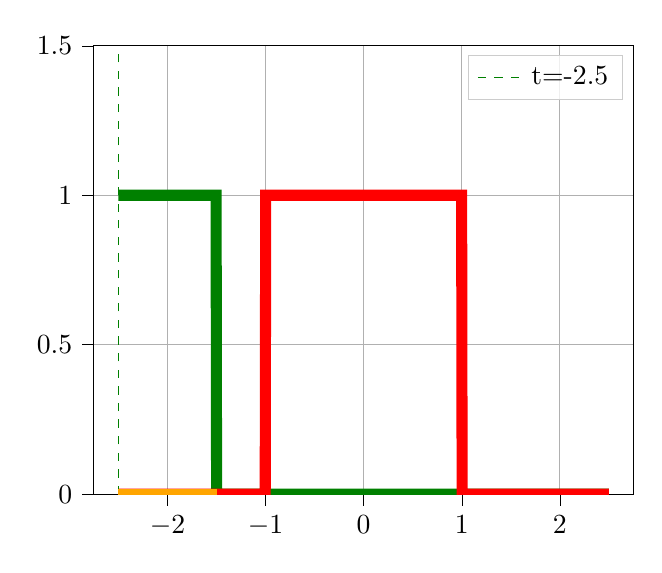
\begin{tikzpicture}

\definecolor{color0}{rgb}{1,0.498039215686275,0.0549019607843137}
\definecolor{color1}{rgb}{1,0.647058823529412,0}

\begin{axis}[
legend cell align={left},
legend style={fill opacity=0.8, draw opacity=1, text opacity=1, draw=white!80!black},
tick align=outside,
tick pos=left,
x grid style={white!69.0196078431373!black},
xmajorgrids,
xmin=-2.75, xmax=2.75,
xtick style={color=black},
y grid style={white!69.0196078431373!black},
ymajorgrids,
ymin=0, ymax=1.5,
ytick style={color=black}
]
\path [draw=color0, fill=color0, opacity=0.2]
(axis cs:-2.5,0)
--(axis cs:-2.5,0)
--(axis cs:-2.49499499499499,0)
--(axis cs:-2.48998998998999,0)
--(axis cs:-2.48498498498498,0)
--(axis cs:-2.47997997997998,0)
--(axis cs:-2.47497497497497,0)
--(axis cs:-2.46996996996997,0)
--(axis cs:-2.46496496496496,0)
--(axis cs:-2.45995995995996,0)
--(axis cs:-2.45495495495495,0)
--(axis cs:-2.44994994994995,0)
--(axis cs:-2.44494494494494,0)
--(axis cs:-2.43993993993994,0)
--(axis cs:-2.43493493493493,0)
--(axis cs:-2.42992992992993,0)
--(axis cs:-2.42492492492492,0)
--(axis cs:-2.41991991991992,0)
--(axis cs:-2.41491491491491,0)
--(axis cs:-2.40990990990991,0)
--(axis cs:-2.4049049049049,0)
--(axis cs:-2.3998998998999,0)
--(axis cs:-2.39489489489489,0)
--(axis cs:-2.38988988988989,0)
--(axis cs:-2.38488488488488,0)
--(axis cs:-2.37987987987988,0)
--(axis cs:-2.37487487487487,0)
--(axis cs:-2.36986986986987,0)
--(axis cs:-2.36486486486486,0)
--(axis cs:-2.35985985985986,0)
--(axis cs:-2.35485485485485,0)
--(axis cs:-2.34984984984985,0)
--(axis cs:-2.34484484484484,0)
--(axis cs:-2.33983983983984,0)
--(axis cs:-2.33483483483483,0)
--(axis cs:-2.32982982982983,0)
--(axis cs:-2.32482482482482,0)
--(axis cs:-2.31981981981982,0)
--(axis cs:-2.31481481481481,0)
--(axis cs:-2.30980980980981,0)
--(axis cs:-2.3048048048048,0)
--(axis cs:-2.2997997997998,0)
--(axis cs:-2.29479479479479,0)
--(axis cs:-2.28978978978979,0)
--(axis cs:-2.28478478478478,0)
--(axis cs:-2.27977977977978,0)
--(axis cs:-2.27477477477477,0)
--(axis cs:-2.26976976976977,0)
--(axis cs:-2.26476476476476,0)
--(axis cs:-2.25975975975976,0)
--(axis cs:-2.25475475475475,0)
--(axis cs:-2.24974974974975,0)
--(axis cs:-2.24474474474474,0)
--(axis cs:-2.23973973973974,0)
--(axis cs:-2.23473473473473,0)
--(axis cs:-2.22972972972973,0)
--(axis cs:-2.22472472472472,0)
--(axis cs:-2.21971971971972,0)
--(axis cs:-2.21471471471471,0)
--(axis cs:-2.20970970970971,0)
--(axis cs:-2.2047047047047,0)
--(axis cs:-2.1996996996997,0)
--(axis cs:-2.19469469469469,0)
--(axis cs:-2.18968968968969,0)
--(axis cs:-2.18468468468468,0)
--(axis cs:-2.17967967967968,0)
--(axis cs:-2.17467467467467,0)
--(axis cs:-2.16966966966967,0)
--(axis cs:-2.16466466466466,0)
--(axis cs:-2.15965965965966,0)
--(axis cs:-2.15465465465465,0)
--(axis cs:-2.14964964964965,0)
--(axis cs:-2.14464464464464,0)
--(axis cs:-2.13963963963964,0)
--(axis cs:-2.13463463463463,0)
--(axis cs:-2.12962962962963,0)
--(axis cs:-2.12462462462462,0)
--(axis cs:-2.11961961961962,0)
--(axis cs:-2.11461461461461,0)
--(axis cs:-2.10960960960961,0)
--(axis cs:-2.1046046046046,0)
--(axis cs:-2.0995995995996,0)
--(axis cs:-2.09459459459459,0)
--(axis cs:-2.08958958958959,0)
--(axis cs:-2.08458458458458,0)
--(axis cs:-2.07957957957958,0)
--(axis cs:-2.07457457457457,0)
--(axis cs:-2.06956956956957,0)
--(axis cs:-2.06456456456456,0)
--(axis cs:-2.05955955955956,0)
--(axis cs:-2.05455455455455,0)
--(axis cs:-2.04954954954955,0)
--(axis cs:-2.04454454454454,0)
--(axis cs:-2.03953953953954,0)
--(axis cs:-2.03453453453453,0)
--(axis cs:-2.02952952952953,0)
--(axis cs:-2.02452452452452,0)
--(axis cs:-2.01951951951952,0)
--(axis cs:-2.01451451451451,0)
--(axis cs:-2.00950950950951,0)
--(axis cs:-2.0045045045045,0)
--(axis cs:-1.9994994994995,0)
--(axis cs:-1.99449449449449,0)
--(axis cs:-1.98948948948949,0)
--(axis cs:-1.98448448448448,0)
--(axis cs:-1.97947947947948,0)
--(axis cs:-1.97447447447447,0)
--(axis cs:-1.96946946946947,0)
--(axis cs:-1.96446446446446,0)
--(axis cs:-1.95945945945946,0)
--(axis cs:-1.95445445445445,0)
--(axis cs:-1.94944944944945,0)
--(axis cs:-1.94444444444444,0)
--(axis cs:-1.93943943943944,0)
--(axis cs:-1.93443443443443,0)
--(axis cs:-1.92942942942943,0)
--(axis cs:-1.92442442442442,0)
--(axis cs:-1.91941941941942,0)
--(axis cs:-1.91441441441441,0)
--(axis cs:-1.90940940940941,0)
--(axis cs:-1.9044044044044,0)
--(axis cs:-1.8993993993994,0)
--(axis cs:-1.89439439439439,0)
--(axis cs:-1.88938938938939,0)
--(axis cs:-1.88438438438438,0)
--(axis cs:-1.87937937937938,0)
--(axis cs:-1.87437437437437,0)
--(axis cs:-1.86936936936937,0)
--(axis cs:-1.86436436436436,0)
--(axis cs:-1.85935935935936,0)
--(axis cs:-1.85435435435435,0)
--(axis cs:-1.84934934934935,0)
--(axis cs:-1.84434434434434,0)
--(axis cs:-1.83933933933934,0)
--(axis cs:-1.83433433433433,0)
--(axis cs:-1.82932932932933,0)
--(axis cs:-1.82432432432432,0)
--(axis cs:-1.81931931931932,0)
--(axis cs:-1.81431431431431,0)
--(axis cs:-1.80930930930931,0)
--(axis cs:-1.8043043043043,0)
--(axis cs:-1.7992992992993,0)
--(axis cs:-1.79429429429429,0)
--(axis cs:-1.78928928928929,0)
--(axis cs:-1.78428428428428,0)
--(axis cs:-1.77927927927928,0)
--(axis cs:-1.77427427427427,0)
--(axis cs:-1.76926926926927,0)
--(axis cs:-1.76426426426426,0)
--(axis cs:-1.75925925925926,0)
--(axis cs:-1.75425425425425,0)
--(axis cs:-1.74924924924925,0)
--(axis cs:-1.74424424424424,0)
--(axis cs:-1.73923923923924,0)
--(axis cs:-1.73423423423423,0)
--(axis cs:-1.72922922922923,0)
--(axis cs:-1.72422422422422,0)
--(axis cs:-1.71921921921922,0)
--(axis cs:-1.71421421421421,0)
--(axis cs:-1.70920920920921,0)
--(axis cs:-1.7042042042042,0)
--(axis cs:-1.6991991991992,0)
--(axis cs:-1.69419419419419,0)
--(axis cs:-1.68918918918919,0)
--(axis cs:-1.68418418418418,0)
--(axis cs:-1.67917917917918,0)
--(axis cs:-1.67417417417417,0)
--(axis cs:-1.66916916916917,0)
--(axis cs:-1.66416416416416,0)
--(axis cs:-1.65915915915916,0)
--(axis cs:-1.65415415415415,0)
--(axis cs:-1.64914914914915,0)
--(axis cs:-1.64414414414414,0)
--(axis cs:-1.63913913913914,0)
--(axis cs:-1.63413413413413,0)
--(axis cs:-1.62912912912913,0)
--(axis cs:-1.62412412412412,0)
--(axis cs:-1.61911911911912,0)
--(axis cs:-1.61411411411411,0)
--(axis cs:-1.60910910910911,0)
--(axis cs:-1.6041041041041,0)
--(axis cs:-1.5990990990991,0)
--(axis cs:-1.59409409409409,0)
--(axis cs:-1.58908908908909,0)
--(axis cs:-1.58408408408408,0)
--(axis cs:-1.57907907907908,0)
--(axis cs:-1.57407407407407,0)
--(axis cs:-1.56906906906907,0)
--(axis cs:-1.56406406406406,0)
--(axis cs:-1.55905905905906,0)
--(axis cs:-1.55405405405405,0)
--(axis cs:-1.54904904904905,0)
--(axis cs:-1.54404404404404,0)
--(axis cs:-1.53903903903904,0)
--(axis cs:-1.53403403403403,0)
--(axis cs:-1.52902902902903,0)
--(axis cs:-1.52402402402402,0)
--(axis cs:-1.51901901901902,0)
--(axis cs:-1.51401401401401,0)
--(axis cs:-1.50900900900901,0)
--(axis cs:-1.504004004004,0)
--(axis cs:-1.504004004004,0)
--(axis cs:-1.504004004004,0)
--(axis cs:-1.50900900900901,0)
--(axis cs:-1.51401401401401,0)
--(axis cs:-1.51901901901902,0)
--(axis cs:-1.52402402402402,0)
--(axis cs:-1.52902902902903,0)
--(axis cs:-1.53403403403403,0)
--(axis cs:-1.53903903903904,0)
--(axis cs:-1.54404404404404,0)
--(axis cs:-1.54904904904905,0)
--(axis cs:-1.55405405405405,0)
--(axis cs:-1.55905905905906,0)
--(axis cs:-1.56406406406406,0)
--(axis cs:-1.56906906906907,0)
--(axis cs:-1.57407407407407,0)
--(axis cs:-1.57907907907908,0)
--(axis cs:-1.58408408408408,0)
--(axis cs:-1.58908908908909,0)
--(axis cs:-1.59409409409409,0)
--(axis cs:-1.5990990990991,0)
--(axis cs:-1.6041041041041,0)
--(axis cs:-1.60910910910911,0)
--(axis cs:-1.61411411411411,0)
--(axis cs:-1.61911911911912,0)
--(axis cs:-1.62412412412412,0)
--(axis cs:-1.62912912912913,0)
--(axis cs:-1.63413413413413,0)
--(axis cs:-1.63913913913914,0)
--(axis cs:-1.64414414414414,0)
--(axis cs:-1.64914914914915,0)
--(axis cs:-1.65415415415415,0)
--(axis cs:-1.65915915915916,0)
--(axis cs:-1.66416416416416,0)
--(axis cs:-1.66916916916917,0)
--(axis cs:-1.67417417417417,0)
--(axis cs:-1.67917917917918,0)
--(axis cs:-1.68418418418418,0)
--(axis cs:-1.68918918918919,0)
--(axis cs:-1.69419419419419,0)
--(axis cs:-1.6991991991992,0)
--(axis cs:-1.7042042042042,0)
--(axis cs:-1.70920920920921,0)
--(axis cs:-1.71421421421421,0)
--(axis cs:-1.71921921921922,0)
--(axis cs:-1.72422422422422,0)
--(axis cs:-1.72922922922923,0)
--(axis cs:-1.73423423423423,0)
--(axis cs:-1.73923923923924,0)
--(axis cs:-1.74424424424424,0)
--(axis cs:-1.74924924924925,0)
--(axis cs:-1.75425425425425,0)
--(axis cs:-1.75925925925926,0)
--(axis cs:-1.76426426426426,0)
--(axis cs:-1.76926926926927,0)
--(axis cs:-1.77427427427427,0)
--(axis cs:-1.77927927927928,0)
--(axis cs:-1.78428428428428,0)
--(axis cs:-1.78928928928929,0)
--(axis cs:-1.79429429429429,0)
--(axis cs:-1.7992992992993,0)
--(axis cs:-1.8043043043043,0)
--(axis cs:-1.80930930930931,0)
--(axis cs:-1.81431431431431,0)
--(axis cs:-1.81931931931932,0)
--(axis cs:-1.82432432432432,0)
--(axis cs:-1.82932932932933,0)
--(axis cs:-1.83433433433433,0)
--(axis cs:-1.83933933933934,0)
--(axis cs:-1.84434434434434,0)
--(axis cs:-1.84934934934935,0)
--(axis cs:-1.85435435435435,0)
--(axis cs:-1.85935935935936,0)
--(axis cs:-1.86436436436436,0)
--(axis cs:-1.86936936936937,0)
--(axis cs:-1.87437437437437,0)
--(axis cs:-1.87937937937938,0)
--(axis cs:-1.88438438438438,0)
--(axis cs:-1.88938938938939,0)
--(axis cs:-1.89439439439439,0)
--(axis cs:-1.8993993993994,0)
--(axis cs:-1.9044044044044,0)
--(axis cs:-1.90940940940941,0)
--(axis cs:-1.91441441441441,0)
--(axis cs:-1.91941941941942,0)
--(axis cs:-1.92442442442442,0)
--(axis cs:-1.92942942942943,0)
--(axis cs:-1.93443443443443,0)
--(axis cs:-1.93943943943944,0)
--(axis cs:-1.94444444444444,0)
--(axis cs:-1.94944944944945,0)
--(axis cs:-1.95445445445445,0)
--(axis cs:-1.95945945945946,0)
--(axis cs:-1.96446446446446,0)
--(axis cs:-1.96946946946947,0)
--(axis cs:-1.97447447447447,0)
--(axis cs:-1.97947947947948,0)
--(axis cs:-1.98448448448448,0)
--(axis cs:-1.98948948948949,0)
--(axis cs:-1.99449449449449,0)
--(axis cs:-1.9994994994995,0)
--(axis cs:-2.0045045045045,0)
--(axis cs:-2.00950950950951,0)
--(axis cs:-2.01451451451451,0)
--(axis cs:-2.01951951951952,0)
--(axis cs:-2.02452452452452,0)
--(axis cs:-2.02952952952953,0)
--(axis cs:-2.03453453453453,0)
--(axis cs:-2.03953953953954,0)
--(axis cs:-2.04454454454454,0)
--(axis cs:-2.04954954954955,0)
--(axis cs:-2.05455455455455,0)
--(axis cs:-2.05955955955956,0)
--(axis cs:-2.06456456456456,0)
--(axis cs:-2.06956956956957,0)
--(axis cs:-2.07457457457457,0)
--(axis cs:-2.07957957957958,0)
--(axis cs:-2.08458458458458,0)
--(axis cs:-2.08958958958959,0)
--(axis cs:-2.09459459459459,0)
--(axis cs:-2.0995995995996,0)
--(axis cs:-2.1046046046046,0)
--(axis cs:-2.10960960960961,0)
--(axis cs:-2.11461461461461,0)
--(axis cs:-2.11961961961962,0)
--(axis cs:-2.12462462462462,0)
--(axis cs:-2.12962962962963,0)
--(axis cs:-2.13463463463463,0)
--(axis cs:-2.13963963963964,0)
--(axis cs:-2.14464464464464,0)
--(axis cs:-2.14964964964965,0)
--(axis cs:-2.15465465465465,0)
--(axis cs:-2.15965965965966,0)
--(axis cs:-2.16466466466466,0)
--(axis cs:-2.16966966966967,0)
--(axis cs:-2.17467467467467,0)
--(axis cs:-2.17967967967968,0)
--(axis cs:-2.18468468468468,0)
--(axis cs:-2.18968968968969,0)
--(axis cs:-2.19469469469469,0)
--(axis cs:-2.1996996996997,0)
--(axis cs:-2.2047047047047,0)
--(axis cs:-2.20970970970971,0)
--(axis cs:-2.21471471471471,0)
--(axis cs:-2.21971971971972,0)
--(axis cs:-2.22472472472472,0)
--(axis cs:-2.22972972972973,0)
--(axis cs:-2.23473473473473,0)
--(axis cs:-2.23973973973974,0)
--(axis cs:-2.24474474474474,0)
--(axis cs:-2.24974974974975,0)
--(axis cs:-2.25475475475475,0)
--(axis cs:-2.25975975975976,0)
--(axis cs:-2.26476476476476,0)
--(axis cs:-2.26976976976977,0)
--(axis cs:-2.27477477477477,0)
--(axis cs:-2.27977977977978,0)
--(axis cs:-2.28478478478478,0)
--(axis cs:-2.28978978978979,0)
--(axis cs:-2.29479479479479,0)
--(axis cs:-2.2997997997998,0)
--(axis cs:-2.3048048048048,0)
--(axis cs:-2.30980980980981,0)
--(axis cs:-2.31481481481481,0)
--(axis cs:-2.31981981981982,0)
--(axis cs:-2.32482482482482,0)
--(axis cs:-2.32982982982983,0)
--(axis cs:-2.33483483483483,0)
--(axis cs:-2.33983983983984,0)
--(axis cs:-2.34484484484484,0)
--(axis cs:-2.34984984984985,0)
--(axis cs:-2.35485485485485,0)
--(axis cs:-2.35985985985986,0)
--(axis cs:-2.36486486486486,0)
--(axis cs:-2.36986986986987,0)
--(axis cs:-2.37487487487487,0)
--(axis cs:-2.37987987987988,0)
--(axis cs:-2.38488488488488,0)
--(axis cs:-2.38988988988989,0)
--(axis cs:-2.39489489489489,0)
--(axis cs:-2.3998998998999,0)
--(axis cs:-2.4049049049049,0)
--(axis cs:-2.40990990990991,0)
--(axis cs:-2.41491491491491,0)
--(axis cs:-2.41991991991992,0)
--(axis cs:-2.42492492492492,0)
--(axis cs:-2.42992992992993,0)
--(axis cs:-2.43493493493493,0)
--(axis cs:-2.43993993993994,0)
--(axis cs:-2.44494494494494,0)
--(axis cs:-2.44994994994995,0)
--(axis cs:-2.45495495495495,0)
--(axis cs:-2.45995995995996,0)
--(axis cs:-2.46496496496496,0)
--(axis cs:-2.46996996996997,0)
--(axis cs:-2.47497497497497,0)
--(axis cs:-2.47997997997998,0)
--(axis cs:-2.48498498498498,0)
--(axis cs:-2.48998998998999,0)
--(axis cs:-2.49499499499499,0)
--(axis cs:-2.5,0)
--cycle;

\addplot [line width=4pt, green!50!black, forget plot]
table {%
-2.5 1
-2.49499499499499 1
-2.48998998998999 1
-2.48498498498498 1
-2.47997997997998 1
-2.47497497497497 1
-2.46996996996997 1
-2.46496496496496 1
-2.45995995995996 1
-2.45495495495495 1
-2.44994994994995 1
-2.44494494494494 1
-2.43993993993994 1
-2.43493493493493 1
-2.42992992992993 1
-2.42492492492492 1
-2.41991991991992 1
-2.41491491491491 1
-2.40990990990991 1
-2.4049049049049 1
-2.3998998998999 1
-2.39489489489489 1
-2.38988988988989 1
-2.38488488488488 1
-2.37987987987988 1
-2.37487487487487 1
-2.36986986986987 1
-2.36486486486486 1
-2.35985985985986 1
-2.35485485485485 1
-2.34984984984985 1
-2.34484484484484 1
-2.33983983983984 1
-2.33483483483483 1
-2.32982982982983 1
-2.32482482482482 1
-2.31981981981982 1
-2.31481481481481 1
-2.30980980980981 1
-2.3048048048048 1
-2.2997997997998 1
-2.29479479479479 1
-2.28978978978979 1
-2.28478478478478 1
-2.27977977977978 1
-2.27477477477477 1
-2.26976976976977 1
-2.26476476476476 1
-2.25975975975976 1
-2.25475475475475 1
-2.24974974974975 1
-2.24474474474474 1
-2.23973973973974 1
-2.23473473473473 1
-2.22972972972973 1
-2.22472472472472 1
-2.21971971971972 1
-2.21471471471471 1
-2.20970970970971 1
-2.2047047047047 1
-2.1996996996997 1
-2.19469469469469 1
-2.18968968968969 1
-2.18468468468468 1
-2.17967967967968 1
-2.17467467467467 1
-2.16966966966967 1
-2.16466466466466 1
-2.15965965965966 1
-2.15465465465465 1
-2.14964964964965 1
-2.14464464464464 1
-2.13963963963964 1
-2.13463463463463 1
-2.12962962962963 1
-2.12462462462462 1
-2.11961961961962 1
-2.11461461461461 1
-2.10960960960961 1
-2.1046046046046 1
-2.0995995995996 1
-2.09459459459459 1
-2.08958958958959 1
-2.08458458458458 1
-2.07957957957958 1
-2.07457457457457 1
-2.06956956956957 1
-2.06456456456456 1
-2.05955955955956 1
-2.05455455455455 1
-2.04954954954955 1
-2.04454454454454 1
-2.03953953953954 1
-2.03453453453453 1
-2.02952952952953 1
-2.02452452452452 1
-2.01951951951952 1
-2.01451451451451 1
-2.00950950950951 1
-2.0045045045045 1
-1.9994994994995 1
-1.99449449449449 1
-1.98948948948949 1
-1.98448448448448 1
-1.97947947947948 1
-1.97447447447447 1
-1.96946946946947 1
-1.96446446446446 1
-1.95945945945946 1
-1.95445445445445 1
-1.94944944944945 1
-1.94444444444444 1
-1.93943943943944 1
-1.93443443443443 1
-1.92942942942943 1
-1.92442442442442 1
-1.91941941941942 1
-1.91441441441441 1
-1.90940940940941 1
-1.9044044044044 1
-1.8993993993994 1
-1.89439439439439 1
-1.88938938938939 1
-1.88438438438438 1
-1.87937937937938 1
-1.87437437437437 1
-1.86936936936937 1
-1.86436436436436 1
-1.85935935935936 1
-1.85435435435435 1
-1.84934934934935 1
-1.84434434434434 1
-1.83933933933934 1
-1.83433433433433 1
-1.82932932932933 1
-1.82432432432432 1
-1.81931931931932 1
-1.81431431431431 1
-1.80930930930931 1
-1.8043043043043 1
-1.7992992992993 1
-1.79429429429429 1
-1.78928928928929 1
-1.78428428428428 1
-1.77927927927928 1
-1.77427427427427 1
-1.76926926926927 1
-1.76426426426426 1
-1.75925925925926 1
-1.75425425425425 1
-1.74924924924925 1
-1.74424424424424 1
-1.73923923923924 1
-1.73423423423423 1
-1.72922922922923 1
-1.72422422422422 1
-1.71921921921922 1
-1.71421421421421 1
-1.70920920920921 1
-1.7042042042042 1
-1.6991991991992 1
-1.69419419419419 1
-1.68918918918919 1
-1.68418418418418 1
-1.67917917917918 1
-1.67417417417417 1
-1.66916916916917 1
-1.66416416416416 1
-1.65915915915916 1
-1.65415415415415 1
-1.64914914914915 1
-1.64414414414414 1
-1.63913913913914 1
-1.63413413413413 1
-1.62912912912913 1
-1.62412412412412 1
-1.61911911911912 1
-1.61411411411411 1
-1.60910910910911 1
-1.6041041041041 1
-1.5990990990991 1
-1.59409409409409 1
-1.58908908908909 1
-1.58408408408408 1
-1.57907907907908 1
-1.57407407407407 1
-1.56906906906907 1
-1.56406406406406 1
-1.55905905905906 1
-1.55405405405405 1
-1.54904904904905 1
-1.54404404404404 1
-1.53903903903904 1
-1.53403403403403 1
-1.52902902902903 1
-1.52402402402402 1
-1.51901901901902 1
-1.51401401401401 1
-1.50900900900901 1
-1.504004004004 1
-1.498998998999 0
-1.49399399399399 0
-1.48898898898899 0
-1.48398398398398 0
-1.47897897897898 0
-1.47397397397397 0
-1.46896896896897 0
-1.46396396396396 0
-1.45895895895896 0
-1.45395395395395 0
-1.44894894894895 0
-1.44394394394394 0
-1.43893893893894 0
-1.43393393393393 0
-1.42892892892893 0
-1.42392392392392 0
-1.41891891891892 0
-1.41391391391391 0
-1.40890890890891 0
-1.4039039039039 0
-1.3988988988989 0
-1.39389389389389 0
-1.38888888888889 0
-1.38388388388388 0
-1.37887887887888 0
-1.37387387387387 0
-1.36886886886887 0
-1.36386386386386 0
-1.35885885885886 0
-1.35385385385385 0
-1.34884884884885 0
-1.34384384384384 0
-1.33883883883884 0
-1.33383383383383 0
-1.32882882882883 0
-1.32382382382382 0
-1.31881881881882 0
-1.31381381381381 0
-1.30880880880881 0
-1.3038038038038 0
-1.2987987987988 0
-1.29379379379379 0
-1.28878878878879 0
-1.28378378378378 0
-1.27877877877878 0
-1.27377377377377 0
-1.26876876876877 0
-1.26376376376376 0
-1.25875875875876 0
-1.25375375375375 0
-1.24874874874875 0
-1.24374374374374 0
-1.23873873873874 0
-1.23373373373373 0
-1.22872872872873 0
-1.22372372372372 0
-1.21871871871872 0
-1.21371371371371 0
-1.20870870870871 0
-1.2037037037037 0
-1.1986986986987 0
-1.19369369369369 0
-1.18868868868869 0
-1.18368368368368 0
-1.17867867867868 0
-1.17367367367367 0
-1.16866866866867 0
-1.16366366366366 0
-1.15865865865866 0
-1.15365365365365 0
-1.14864864864865 0
-1.14364364364364 0
-1.13863863863864 0
-1.13363363363363 0
-1.12862862862863 0
-1.12362362362362 0
-1.11861861861862 0
-1.11361361361361 0
-1.10860860860861 0
-1.1036036036036 0
-1.0985985985986 0
-1.09359359359359 0
-1.08858858858859 0
-1.08358358358358 0
-1.07857857857858 0
-1.07357357357357 0
-1.06856856856857 0
-1.06356356356356 0
-1.05855855855856 0
-1.05355355355355 0
-1.04854854854855 0
-1.04354354354354 0
-1.03853853853854 0
-1.03353353353353 0
-1.02852852852853 0
-1.02352352352352 0
-1.01851851851852 0
-1.01351351351351 0
-1.00850850850851 0
-1.0035035035035 0
-0.998498498498499 0
-0.993493493493494 0
-0.988488488488489 0
-0.983483483483484 0
-0.978478478478479 0
-0.973473473473474 0
-0.968468468468469 0
-0.963463463463464 0
-0.958458458458459 0
-0.953453453453454 0
-0.948448448448449 0
-0.943443443443444 0
-0.938438438438439 0
-0.933433433433434 0
-0.928428428428429 0
-0.923423423423424 0
-0.918418418418419 0
-0.913413413413414 0
-0.908408408408409 0
-0.903403403403404 0
-0.898398398398399 0
-0.893393393393393 0
-0.888388388388388 0
-0.883383383383383 0
-0.878378378378378 0
-0.873373373373373 0
-0.868368368368368 0
-0.863363363363363 0
-0.858358358358358 0
-0.853353353353353 0
-0.848348348348348 0
-0.843343343343343 0
-0.838338338338338 0
-0.833333333333333 0
-0.828328328328328 0
-0.823323323323323 0
-0.818318318318318 0
-0.813313313313313 0
-0.808308308308308 0
-0.803303303303303 0
-0.798298298298298 0
-0.793293293293293 0
-0.788288288288288 0
-0.783283283283283 0
-0.778278278278278 0
-0.773273273273273 0
-0.768268268268268 0
-0.763263263263263 0
-0.758258258258258 0
-0.753253253253253 0
-0.748248248248248 0
-0.743243243243243 0
-0.738238238238238 0
-0.733233233233233 0
-0.728228228228228 0
-0.723223223223223 0
-0.718218218218218 0
-0.713213213213213 0
-0.708208208208208 0
-0.703203203203203 0
-0.698198198198198 0
-0.693193193193193 0
-0.688188188188188 0
-0.683183183183183 0
-0.678178178178178 0
-0.673173173173173 0
-0.668168168168168 0
-0.663163163163163 0
-0.658158158158158 0
-0.653153153153153 0
-0.648148148148148 0
-0.643143143143143 0
-0.638138138138138 0
-0.633133133133133 0
-0.628128128128128 0
-0.623123123123123 0
-0.618118118118118 0
-0.613113113113113 0
-0.608108108108108 0
-0.603103103103103 0
-0.598098098098098 0
-0.593093093093093 0
-0.588088088088088 0
-0.583083083083083 0
-0.578078078078078 0
-0.573073073073073 0
-0.568068068068068 0
-0.563063063063063 0
-0.558058058058058 0
-0.553053053053053 0
-0.548048048048048 0
-0.543043043043043 0
-0.538038038038038 0
-0.533033033033033 0
-0.528028028028028 0
-0.523023023023023 0
-0.518018018018018 0
-0.513013013013013 0
-0.508008008008008 0
-0.503003003003003 0
-0.497997997997998 0
-0.492992992992993 0
-0.487987987987988 0
-0.482982982982983 0
-0.477977977977978 0
-0.472972972972973 0
-0.467967967967968 0
-0.462962962962963 0
-0.457957957957958 0
-0.452952952952953 0
-0.447947947947948 0
-0.442942942942943 0
-0.437937937937938 0
-0.432932932932933 0
-0.427927927927928 0
-0.422922922922923 0
-0.417917917917918 0
-0.412912912912913 0
-0.407907907907908 0
-0.402902902902903 0
-0.397897897897898 0
-0.392892892892893 0
-0.387887887887888 0
-0.382882882882883 0
-0.377877877877878 0
-0.372872872872873 0
-0.367867867867868 0
-0.362862862862863 0
-0.357857857857858 0
-0.352852852852853 0
-0.347847847847848 0
-0.342842842842843 0
-0.337837837837838 0
-0.332832832832833 0
-0.327827827827828 0
-0.322822822822823 0
-0.317817817817818 0
-0.312812812812813 0
-0.307807807807808 0
-0.302802802802803 0
-0.297797797797798 0
-0.292792792792793 0
-0.287787787787788 0
-0.282782782782783 0
-0.277777777777778 0
-0.272772772772773 0
-0.267767767767768 0
-0.262762762762763 0
-0.257757757757758 0
-0.252752752752753 0
-0.247747747747748 0
-0.242742742742743 0
-0.237737737737738 0
-0.232732732732733 0
-0.227727727727728 0
-0.222722722722723 0
-0.217717717717718 0
-0.212712712712713 0
-0.207707707707708 0
-0.202702702702703 0
-0.197697697697698 0
-0.192692692692693 0
-0.187687687687688 0
-0.182682682682683 0
-0.177677677677678 0
-0.172672672672673 0
-0.167667667667668 0
-0.162662662662663 0
-0.157657657657658 0
-0.152652652652653 0
-0.147647647647648 0
-0.142642642642643 0
-0.137637637637638 0
-0.132632632632633 0
-0.127627627627628 0
-0.122622622622623 0
-0.117617617617618 0
-0.112612612612613 0
-0.107607607607608 0
-0.102602602602603 0
-0.0975975975975976 0
-0.0925925925925926 0
-0.0875875875875876 0
-0.0825825825825826 0
-0.0775775775775776 0
-0.0725725725725725 0
-0.0675675675675675 0
-0.0625625625625625 0
-0.0575575575575575 0
-0.0525525525525525 0
-0.0475475475475475 0
-0.0425425425425425 0
-0.0375375375375375 0
-0.0325325325325325 0
-0.0275275275275275 0
-0.0225225225225225 0
-0.0175175175175175 0
-0.0125125125125125 0
-0.0075075075075075 0
-0.0025025025025025 0
0.0025025025025025 0
0.0075075075075075 0
0.0125125125125125 0
0.0175175175175175 0
0.0225225225225225 0
0.0275275275275275 0
0.0325325325325325 0
0.0375375375375375 0
0.0425425425425425 0
0.0475475475475475 0
0.0525525525525525 0
0.0575575575575575 0
0.0625625625625625 0
0.0675675675675675 0
0.0725725725725725 0
0.0775775775775776 0
0.0825825825825826 0
0.0875875875875876 0
0.0925925925925926 0
0.0975975975975976 0
0.102602602602603 0
0.107607607607608 0
0.112612612612613 0
0.117617617617618 0
0.122622622622623 0
0.127627627627628 0
0.132632632632633 0
0.137637637637638 0
0.142642642642643 0
0.147647647647648 0
0.152652652652653 0
0.157657657657658 0
0.162662662662663 0
0.167667667667668 0
0.172672672672673 0
0.177677677677678 0
0.182682682682683 0
0.187687687687688 0
0.192692692692693 0
0.197697697697698 0
0.202702702702703 0
0.207707707707708 0
0.212712712712713 0
0.217717717717718 0
0.222722722722723 0
0.227727727727728 0
0.232732732732733 0
0.237737737737738 0
0.242742742742743 0
0.247747747747748 0
0.252752752752753 0
0.257757757757758 0
0.262762762762763 0
0.267767767767768 0
0.272772772772773 0
0.277777777777778 0
0.282782782782783 0
0.287787787787788 0
0.292792792792793 0
0.297797797797798 0
0.302802802802803 0
0.307807807807808 0
0.312812812812813 0
0.317817817817818 0
0.322822822822823 0
0.327827827827828 0
0.332832832832833 0
0.337837837837838 0
0.342842842842843 0
0.347847847847848 0
0.352852852852853 0
0.357857857857858 0
0.362862862862863 0
0.367867867867868 0
0.372872872872873 0
0.377877877877878 0
0.382882882882883 0
0.387887887887888 0
0.392892892892893 0
0.397897897897898 0
0.402902902902903 0
0.407907907907908 0
0.412912912912913 0
0.417917917917918 0
0.422922922922923 0
0.427927927927928 0
0.432932932932933 0
0.437937937937938 0
0.442942942942943 0
0.447947947947948 0
0.452952952952953 0
0.457957957957958 0
0.462962962962963 0
0.467967967967968 0
0.472972972972973 0
0.477977977977978 0
0.482982982982983 0
0.487987987987988 0
0.492992992992993 0
0.497997997997998 0
0.503003003003003 0
0.508008008008008 0
0.513013013013013 0
0.518018018018018 0
0.523023023023023 0
0.528028028028028 0
0.533033033033033 0
0.538038038038038 0
0.543043043043043 0
0.548048048048048 0
0.553053053053053 0
0.558058058058058 0
0.563063063063063 0
0.568068068068068 0
0.573073073073073 0
0.578078078078078 0
0.583083083083083 0
0.588088088088088 0
0.593093093093093 0
0.598098098098098 0
0.603103103103103 0
0.608108108108108 0
0.613113113113113 0
0.618118118118118 0
0.623123123123123 0
0.628128128128128 0
0.633133133133133 0
0.638138138138138 0
0.643143143143143 0
0.648148148148148 0
0.653153153153153 0
0.658158158158158 0
0.663163163163163 0
0.668168168168168 0
0.673173173173173 0
0.678178178178178 0
0.683183183183183 0
0.688188188188188 0
0.693193193193193 0
0.698198198198198 0
0.703203203203203 0
0.708208208208208 0
0.713213213213213 0
0.718218218218218 0
0.723223223223223 0
0.728228228228228 0
0.733233233233233 0
0.738238238238238 0
0.743243243243243 0
0.748248248248248 0
0.753253253253253 0
0.758258258258258 0
0.763263263263263 0
0.768268268268268 0
0.773273273273273 0
0.778278278278278 0
0.783283283283283 0
0.788288288288288 0
0.793293293293293 0
0.798298298298298 0
0.803303303303303 0
0.808308308308308 0
0.813313313313313 0
0.818318318318318 0
0.823323323323323 0
0.828328328328328 0
0.833333333333333 0
0.838338338338338 0
0.843343343343343 0
0.848348348348348 0
0.853353353353353 0
0.858358358358358 0
0.863363363363364 0
0.868368368368369 0
0.873373373373374 0
0.878378378378379 0
0.883383383383384 0
0.888388388388389 0
0.893393393393394 0
0.898398398398399 0
0.903403403403404 0
0.908408408408409 0
0.913413413413414 0
0.918418418418419 0
0.923423423423424 0
0.928428428428429 0
0.933433433433434 0
0.938438438438439 0
0.943443443443444 0
0.948448448448449 0
0.953453453453454 0
0.958458458458459 0
0.963463463463464 0
0.968468468468469 0
0.973473473473474 0
0.978478478478479 0
0.983483483483484 0
0.988488488488489 0
0.993493493493494 0
0.998498498498499 0
1.0035035035035 0
1.00850850850851 0
1.01351351351351 0
1.01851851851852 0
1.02352352352352 0
1.02852852852853 0
1.03353353353353 0
1.03853853853854 0
1.04354354354354 0
1.04854854854855 0
1.05355355355355 0
1.05855855855856 0
1.06356356356356 0
1.06856856856857 0
1.07357357357357 0
1.07857857857858 0
1.08358358358358 0
1.08858858858859 0
1.09359359359359 0
1.0985985985986 0
1.1036036036036 0
1.10860860860861 0
1.11361361361361 0
1.11861861861862 0
1.12362362362362 0
1.12862862862863 0
1.13363363363363 0
1.13863863863864 0
1.14364364364364 0
1.14864864864865 0
1.15365365365365 0
1.15865865865866 0
1.16366366366366 0
1.16866866866867 0
1.17367367367367 0
1.17867867867868 0
1.18368368368368 0
1.18868868868869 0
1.19369369369369 0
1.1986986986987 0
1.2037037037037 0
1.20870870870871 0
1.21371371371371 0
1.21871871871872 0
1.22372372372372 0
1.22872872872873 0
1.23373373373373 0
1.23873873873874 0
1.24374374374374 0
1.24874874874875 0
1.25375375375375 0
1.25875875875876 0
1.26376376376376 0
1.26876876876877 0
1.27377377377377 0
1.27877877877878 0
1.28378378378378 0
1.28878878878879 0
1.29379379379379 0
1.2987987987988 0
1.3038038038038 0
1.30880880880881 0
1.31381381381381 0
1.31881881881882 0
1.32382382382382 0
1.32882882882883 0
1.33383383383383 0
1.33883883883884 0
1.34384384384384 0
1.34884884884885 0
1.35385385385385 0
1.35885885885886 0
1.36386386386386 0
1.36886886886887 0
1.37387387387387 0
1.37887887887888 0
1.38388388388388 0
1.38888888888889 0
1.39389389389389 0
1.3988988988989 0
1.4039039039039 0
1.40890890890891 0
1.41391391391391 0
1.41891891891892 0
1.42392392392392 0
1.42892892892893 0
1.43393393393393 0
1.43893893893894 0
1.44394394394394 0
1.44894894894895 0
1.45395395395395 0
1.45895895895896 0
1.46396396396396 0
1.46896896896897 0
1.47397397397397 0
1.47897897897898 0
1.48398398398398 0
1.48898898898899 0
1.49399399399399 0
1.498998998999 0
1.504004004004 0
1.50900900900901 0
1.51401401401401 0
1.51901901901902 0
1.52402402402402 0
1.52902902902903 0
1.53403403403403 0
1.53903903903904 0
1.54404404404404 0
1.54904904904905 0
1.55405405405405 0
1.55905905905906 0
1.56406406406406 0
1.56906906906907 0
1.57407407407407 0
1.57907907907908 0
1.58408408408408 0
1.58908908908909 0
1.59409409409409 0
1.5990990990991 0
1.6041041041041 0
1.60910910910911 0
1.61411411411411 0
1.61911911911912 0
1.62412412412412 0
1.62912912912913 0
1.63413413413413 0
1.63913913913914 0
1.64414414414414 0
1.64914914914915 0
1.65415415415415 0
1.65915915915916 0
1.66416416416416 0
1.66916916916917 0
1.67417417417417 0
1.67917917917918 0
1.68418418418418 0
1.68918918918919 0
1.69419419419419 0
1.6991991991992 0
1.7042042042042 0
1.70920920920921 0
1.71421421421421 0
1.71921921921922 0
1.72422422422422 0
1.72922922922923 0
1.73423423423423 0
1.73923923923924 0
1.74424424424424 0
1.74924924924925 0
1.75425425425425 0
1.75925925925926 0
1.76426426426426 0
1.76926926926927 0
1.77427427427427 0
1.77927927927928 0
1.78428428428428 0
1.78928928928929 0
1.79429429429429 0
1.7992992992993 0
1.8043043043043 0
1.80930930930931 0
1.81431431431431 0
1.81931931931932 0
1.82432432432432 0
1.82932932932933 0
1.83433433433433 0
1.83933933933934 0
1.84434434434434 0
1.84934934934935 0
1.85435435435435 0
1.85935935935936 0
1.86436436436436 0
1.86936936936937 0
1.87437437437437 0
1.87937937937938 0
1.88438438438438 0
1.88938938938939 0
1.89439439439439 0
1.8993993993994 0
1.9044044044044 0
1.90940940940941 0
1.91441441441441 0
1.91941941941942 0
1.92442442442442 0
1.92942942942943 0
1.93443443443443 0
1.93943943943944 0
1.94444444444444 0
1.94944944944945 0
1.95445445445445 0
1.95945945945946 0
1.96446446446446 0
1.96946946946947 0
1.97447447447447 0
1.97947947947948 0
1.98448448448448 0
1.98948948948949 0
1.99449449449449 0
1.9994994994995 0
2.0045045045045 0
2.00950950950951 0
2.01451451451451 0
2.01951951951952 0
2.02452452452452 0
2.02952952952953 0
2.03453453453453 0
2.03953953953954 0
2.04454454454454 0
2.04954954954955 0
2.05455455455455 0
2.05955955955956 0
2.06456456456456 0
2.06956956956957 0
2.07457457457457 0
2.07957957957958 0
2.08458458458458 0
2.08958958958959 0
2.09459459459459 0
2.0995995995996 0
2.1046046046046 0
2.10960960960961 0
2.11461461461461 0
2.11961961961962 0
2.12462462462462 0
2.12962962962963 0
2.13463463463463 0
2.13963963963964 0
2.14464464464464 0
2.14964964964965 0
2.15465465465465 0
2.15965965965966 0
2.16466466466466 0
2.16966966966967 0
2.17467467467467 0
2.17967967967968 0
2.18468468468468 0
2.18968968968969 0
2.19469469469469 0
2.1996996996997 0
2.2047047047047 0
2.20970970970971 0
2.21471471471471 0
2.21971971971972 0
2.22472472472472 0
2.22972972972973 0
2.23473473473473 0
2.23973973973974 0
2.24474474474474 0
2.24974974974975 0
2.25475475475475 0
2.25975975975976 0
2.26476476476476 0
2.26976976976977 0
2.27477477477477 0
2.27977977977978 0
2.28478478478478 0
2.28978978978979 0
2.29479479479479 0
2.2997997997998 0
2.3048048048048 0
2.30980980980981 0
2.31481481481481 0
2.31981981981982 0
2.32482482482482 0
2.32982982982983 0
2.33483483483483 0
2.33983983983984 0
2.34484484484484 0
2.34984984984985 0
2.35485485485485 0
2.35985985985986 0
2.36486486486486 0
2.36986986986987 0
2.37487487487487 0
2.37987987987988 0
2.38488488488488 0
2.38988988988989 0
2.39489489489489 0
2.3998998998999 0
2.4049049049049 0
2.40990990990991 0
2.41491491491491 0
2.41991991991992 0
2.42492492492492 0
2.42992992992993 0
2.43493493493493 0
2.43993993993994 0
2.44494494494494 0
2.44994994994995 0
2.45495495495495 0
2.45995995995996 0
2.46496496496496 0
2.46996996996997 0
2.47497497497497 0
2.47997997997998 0
2.48498498498498 0
2.48998998998999 0
2.49499499499499 0
2.5 0
};
\addplot [line width=4pt, red, forget plot]
table {%
-2.5 0
-2.49499499499499 0
-2.48998998998999 0
-2.48498498498498 0
-2.47997997997998 0
-2.47497497497497 0
-2.46996996996997 0
-2.46496496496496 0
-2.45995995995996 0
-2.45495495495495 0
-2.44994994994995 0
-2.44494494494494 0
-2.43993993993994 0
-2.43493493493493 0
-2.42992992992993 0
-2.42492492492492 0
-2.41991991991992 0
-2.41491491491491 0
-2.40990990990991 0
-2.4049049049049 0
-2.3998998998999 0
-2.39489489489489 0
-2.38988988988989 0
-2.38488488488488 0
-2.37987987987988 0
-2.37487487487487 0
-2.36986986986987 0
-2.36486486486486 0
-2.35985985985986 0
-2.35485485485485 0
-2.34984984984985 0
-2.34484484484484 0
-2.33983983983984 0
-2.33483483483483 0
-2.32982982982983 0
-2.32482482482482 0
-2.31981981981982 0
-2.31481481481481 0
-2.30980980980981 0
-2.3048048048048 0
-2.2997997997998 0
-2.29479479479479 0
-2.28978978978979 0
-2.28478478478478 0
-2.27977977977978 0
-2.27477477477477 0
-2.26976976976977 0
-2.26476476476476 0
-2.25975975975976 0
-2.25475475475475 0
-2.24974974974975 0
-2.24474474474474 0
-2.23973973973974 0
-2.23473473473473 0
-2.22972972972973 0
-2.22472472472472 0
-2.21971971971972 0
-2.21471471471471 0
-2.20970970970971 0
-2.2047047047047 0
-2.1996996996997 0
-2.19469469469469 0
-2.18968968968969 0
-2.18468468468468 0
-2.17967967967968 0
-2.17467467467467 0
-2.16966966966967 0
-2.16466466466466 0
-2.15965965965966 0
-2.15465465465465 0
-2.14964964964965 0
-2.14464464464464 0
-2.13963963963964 0
-2.13463463463463 0
-2.12962962962963 0
-2.12462462462462 0
-2.11961961961962 0
-2.11461461461461 0
-2.10960960960961 0
-2.1046046046046 0
-2.0995995995996 0
-2.09459459459459 0
-2.08958958958959 0
-2.08458458458458 0
-2.07957957957958 0
-2.07457457457457 0
-2.06956956956957 0
-2.06456456456456 0
-2.05955955955956 0
-2.05455455455455 0
-2.04954954954955 0
-2.04454454454454 0
-2.03953953953954 0
-2.03453453453453 0
-2.02952952952953 0
-2.02452452452452 0
-2.01951951951952 0
-2.01451451451451 0
-2.00950950950951 0
-2.0045045045045 0
-1.9994994994995 0
-1.99449449449449 0
-1.98948948948949 0
-1.98448448448448 0
-1.97947947947948 0
-1.97447447447447 0
-1.96946946946947 0
-1.96446446446446 0
-1.95945945945946 0
-1.95445445445445 0
-1.94944944944945 0
-1.94444444444444 0
-1.93943943943944 0
-1.93443443443443 0
-1.92942942942943 0
-1.92442442442442 0
-1.91941941941942 0
-1.91441441441441 0
-1.90940940940941 0
-1.9044044044044 0
-1.8993993993994 0
-1.89439439439439 0
-1.88938938938939 0
-1.88438438438438 0
-1.87937937937938 0
-1.87437437437437 0
-1.86936936936937 0
-1.86436436436436 0
-1.85935935935936 0
-1.85435435435435 0
-1.84934934934935 0
-1.84434434434434 0
-1.83933933933934 0
-1.83433433433433 0
-1.82932932932933 0
-1.82432432432432 0
-1.81931931931932 0
-1.81431431431431 0
-1.80930930930931 0
-1.8043043043043 0
-1.7992992992993 0
-1.79429429429429 0
-1.78928928928929 0
-1.78428428428428 0
-1.77927927927928 0
-1.77427427427427 0
-1.76926926926927 0
-1.76426426426426 0
-1.75925925925926 0
-1.75425425425425 0
-1.74924924924925 0
-1.74424424424424 0
-1.73923923923924 0
-1.73423423423423 0
-1.72922922922923 0
-1.72422422422422 0
-1.71921921921922 0
-1.71421421421421 0
-1.70920920920921 0
-1.7042042042042 0
-1.6991991991992 0
-1.69419419419419 0
-1.68918918918919 0
-1.68418418418418 0
-1.67917917917918 0
-1.67417417417417 0
-1.66916916916917 0
-1.66416416416416 0
-1.65915915915916 0
-1.65415415415415 0
-1.64914914914915 0
-1.64414414414414 0
-1.63913913913914 0
-1.63413413413413 0
-1.62912912912913 0
-1.62412412412412 0
-1.61911911911912 0
-1.61411411411411 0
-1.60910910910911 0
-1.6041041041041 0
-1.5990990990991 0
-1.59409409409409 0
-1.58908908908909 0
-1.58408408408408 0
-1.57907907907908 0
-1.57407407407407 0
-1.56906906906907 0
-1.56406406406406 0
-1.55905905905906 0
-1.55405405405405 0
-1.54904904904905 0
-1.54404404404404 0
-1.53903903903904 0
-1.53403403403403 0
-1.52902902902903 0
-1.52402402402402 0
-1.51901901901902 0
-1.51401401401401 0
-1.50900900900901 0
-1.504004004004 0
-1.498998998999 0
-1.49399399399399 0
-1.48898898898899 0
-1.48398398398398 0
-1.47897897897898 0
-1.47397397397397 0
-1.46896896896897 0
-1.46396396396396 0
-1.45895895895896 0
-1.45395395395395 0
-1.44894894894895 0
-1.44394394394394 0
-1.43893893893894 0
-1.43393393393393 0
-1.42892892892893 0
-1.42392392392392 0
-1.41891891891892 0
-1.41391391391391 0
-1.40890890890891 0
-1.4039039039039 0
-1.3988988988989 0
-1.39389389389389 0
-1.38888888888889 0
-1.38388388388388 0
-1.37887887887888 0
-1.37387387387387 0
-1.36886886886887 0
-1.36386386386386 0
-1.35885885885886 0
-1.35385385385385 0
-1.34884884884885 0
-1.34384384384384 0
-1.33883883883884 0
-1.33383383383383 0
-1.32882882882883 0
-1.32382382382382 0
-1.31881881881882 0
-1.31381381381381 0
-1.30880880880881 0
-1.3038038038038 0
-1.2987987987988 0
-1.29379379379379 0
-1.28878878878879 0
-1.28378378378378 0
-1.27877877877878 0
-1.27377377377377 0
-1.26876876876877 0
-1.26376376376376 0
-1.25875875875876 0
-1.25375375375375 0
-1.24874874874875 0
-1.24374374374374 0
-1.23873873873874 0
-1.23373373373373 0
-1.22872872872873 0
-1.22372372372372 0
-1.21871871871872 0
-1.21371371371371 0
-1.20870870870871 0
-1.2037037037037 0
-1.1986986986987 0
-1.19369369369369 0
-1.18868868868869 0
-1.18368368368368 0
-1.17867867867868 0
-1.17367367367367 0
-1.16866866866867 0
-1.16366366366366 0
-1.15865865865866 0
-1.15365365365365 0
-1.14864864864865 0
-1.14364364364364 0
-1.13863863863864 0
-1.13363363363363 0
-1.12862862862863 0
-1.12362362362362 0
-1.11861861861862 0
-1.11361361361361 0
-1.10860860860861 0
-1.1036036036036 0
-1.0985985985986 0
-1.09359359359359 0
-1.08858858858859 0
-1.08358358358358 0
-1.07857857857858 0
-1.07357357357357 0
-1.06856856856857 0
-1.06356356356356 0
-1.05855855855856 0
-1.05355355355355 0
-1.04854854854855 0
-1.04354354354354 0
-1.03853853853854 0
-1.03353353353353 0
-1.02852852852853 0
-1.02352352352352 0
-1.01851851851852 0
-1.01351351351351 0
-1.00850850850851 0
-1.0035035035035 0
-0.998498498498499 1
-0.993493493493494 1
-0.988488488488489 1
-0.983483483483484 1
-0.978478478478479 1
-0.973473473473474 1
-0.968468468468469 1
-0.963463463463464 1
-0.958458458458459 1
-0.953453453453454 1
-0.948448448448449 1
-0.943443443443444 1
-0.938438438438439 1
-0.933433433433434 1
-0.928428428428429 1
-0.923423423423424 1
-0.918418418418419 1
-0.913413413413414 1
-0.908408408408409 1
-0.903403403403404 1
-0.898398398398399 1
-0.893393393393393 1
-0.888388388388388 1
-0.883383383383383 1
-0.878378378378378 1
-0.873373373373373 1
-0.868368368368368 1
-0.863363363363363 1
-0.858358358358358 1
-0.853353353353353 1
-0.848348348348348 1
-0.843343343343343 1
-0.838338338338338 1
-0.833333333333333 1
-0.828328328328328 1
-0.823323323323323 1
-0.818318318318318 1
-0.813313313313313 1
-0.808308308308308 1
-0.803303303303303 1
-0.798298298298298 1
-0.793293293293293 1
-0.788288288288288 1
-0.783283283283283 1
-0.778278278278278 1
-0.773273273273273 1
-0.768268268268268 1
-0.763263263263263 1
-0.758258258258258 1
-0.753253253253253 1
-0.748248248248248 1
-0.743243243243243 1
-0.738238238238238 1
-0.733233233233233 1
-0.728228228228228 1
-0.723223223223223 1
-0.718218218218218 1
-0.713213213213213 1
-0.708208208208208 1
-0.703203203203203 1
-0.698198198198198 1
-0.693193193193193 1
-0.688188188188188 1
-0.683183183183183 1
-0.678178178178178 1
-0.673173173173173 1
-0.668168168168168 1
-0.663163163163163 1
-0.658158158158158 1
-0.653153153153153 1
-0.648148148148148 1
-0.643143143143143 1
-0.638138138138138 1
-0.633133133133133 1
-0.628128128128128 1
-0.623123123123123 1
-0.618118118118118 1
-0.613113113113113 1
-0.608108108108108 1
-0.603103103103103 1
-0.598098098098098 1
-0.593093093093093 1
-0.588088088088088 1
-0.583083083083083 1
-0.578078078078078 1
-0.573073073073073 1
-0.568068068068068 1
-0.563063063063063 1
-0.558058058058058 1
-0.553053053053053 1
-0.548048048048048 1
-0.543043043043043 1
-0.538038038038038 1
-0.533033033033033 1
-0.528028028028028 1
-0.523023023023023 1
-0.518018018018018 1
-0.513013013013013 1
-0.508008008008008 1
-0.503003003003003 1
-0.497997997997998 1
-0.492992992992993 1
-0.487987987987988 1
-0.482982982982983 1
-0.477977977977978 1
-0.472972972972973 1
-0.467967967967968 1
-0.462962962962963 1
-0.457957957957958 1
-0.452952952952953 1
-0.447947947947948 1
-0.442942942942943 1
-0.437937937937938 1
-0.432932932932933 1
-0.427927927927928 1
-0.422922922922923 1
-0.417917917917918 1
-0.412912912912913 1
-0.407907907907908 1
-0.402902902902903 1
-0.397897897897898 1
-0.392892892892893 1
-0.387887887887888 1
-0.382882882882883 1
-0.377877877877878 1
-0.372872872872873 1
-0.367867867867868 1
-0.362862862862863 1
-0.357857857857858 1
-0.352852852852853 1
-0.347847847847848 1
-0.342842842842843 1
-0.337837837837838 1
-0.332832832832833 1
-0.327827827827828 1
-0.322822822822823 1
-0.317817817817818 1
-0.312812812812813 1
-0.307807807807808 1
-0.302802802802803 1
-0.297797797797798 1
-0.292792792792793 1
-0.287787787787788 1
-0.282782782782783 1
-0.277777777777778 1
-0.272772772772773 1
-0.267767767767768 1
-0.262762762762763 1
-0.257757757757758 1
-0.252752752752753 1
-0.247747747747748 1
-0.242742742742743 1
-0.237737737737738 1
-0.232732732732733 1
-0.227727727727728 1
-0.222722722722723 1
-0.217717717717718 1
-0.212712712712713 1
-0.207707707707708 1
-0.202702702702703 1
-0.197697697697698 1
-0.192692692692693 1
-0.187687687687688 1
-0.182682682682683 1
-0.177677677677678 1
-0.172672672672673 1
-0.167667667667668 1
-0.162662662662663 1
-0.157657657657658 1
-0.152652652652653 1
-0.147647647647648 1
-0.142642642642643 1
-0.137637637637638 1
-0.132632632632633 1
-0.127627627627628 1
-0.122622622622623 1
-0.117617617617618 1
-0.112612612612613 1
-0.107607607607608 1
-0.102602602602603 1
-0.0975975975975976 1
-0.0925925925925926 1
-0.0875875875875876 1
-0.0825825825825826 1
-0.0775775775775776 1
-0.0725725725725725 1
-0.0675675675675675 1
-0.0625625625625625 1
-0.0575575575575575 1
-0.0525525525525525 1
-0.0475475475475475 1
-0.0425425425425425 1
-0.0375375375375375 1
-0.0325325325325325 1
-0.0275275275275275 1
-0.0225225225225225 1
-0.0175175175175175 1
-0.0125125125125125 1
-0.0075075075075075 1
-0.0025025025025025 1
0.0025025025025025 1
0.0075075075075075 1
0.0125125125125125 1
0.0175175175175175 1
0.0225225225225225 1
0.0275275275275275 1
0.0325325325325325 1
0.0375375375375375 1
0.0425425425425425 1
0.0475475475475475 1
0.0525525525525525 1
0.0575575575575575 1
0.0625625625625625 1
0.0675675675675675 1
0.0725725725725725 1
0.0775775775775776 1
0.0825825825825826 1
0.0875875875875876 1
0.0925925925925926 1
0.0975975975975976 1
0.102602602602603 1
0.107607607607608 1
0.112612612612613 1
0.117617617617618 1
0.122622622622623 1
0.127627627627628 1
0.132632632632633 1
0.137637637637638 1
0.142642642642643 1
0.147647647647648 1
0.152652652652653 1
0.157657657657658 1
0.162662662662663 1
0.167667667667668 1
0.172672672672673 1
0.177677677677678 1
0.182682682682683 1
0.187687687687688 1
0.192692692692693 1
0.197697697697698 1
0.202702702702703 1
0.207707707707708 1
0.212712712712713 1
0.217717717717718 1
0.222722722722723 1
0.227727727727728 1
0.232732732732733 1
0.237737737737738 1
0.242742742742743 1
0.247747747747748 1
0.252752752752753 1
0.257757757757758 1
0.262762762762763 1
0.267767767767768 1
0.272772772772773 1
0.277777777777778 1
0.282782782782783 1
0.287787787787788 1
0.292792792792793 1
0.297797797797798 1
0.302802802802803 1
0.307807807807808 1
0.312812812812813 1
0.317817817817818 1
0.322822822822823 1
0.327827827827828 1
0.332832832832833 1
0.337837837837838 1
0.342842842842843 1
0.347847847847848 1
0.352852852852853 1
0.357857857857858 1
0.362862862862863 1
0.367867867867868 1
0.372872872872873 1
0.377877877877878 1
0.382882882882883 1
0.387887887887888 1
0.392892892892893 1
0.397897897897898 1
0.402902902902903 1
0.407907907907908 1
0.412912912912913 1
0.417917917917918 1
0.422922922922923 1
0.427927927927928 1
0.432932932932933 1
0.437937937937938 1
0.442942942942943 1
0.447947947947948 1
0.452952952952953 1
0.457957957957958 1
0.462962962962963 1
0.467967967967968 1
0.472972972972973 1
0.477977977977978 1
0.482982982982983 1
0.487987987987988 1
0.492992992992993 1
0.497997997997998 1
0.503003003003003 1
0.508008008008008 1
0.513013013013013 1
0.518018018018018 1
0.523023023023023 1
0.528028028028028 1
0.533033033033033 1
0.538038038038038 1
0.543043043043043 1
0.548048048048048 1
0.553053053053053 1
0.558058058058058 1
0.563063063063063 1
0.568068068068068 1
0.573073073073073 1
0.578078078078078 1
0.583083083083083 1
0.588088088088088 1
0.593093093093093 1
0.598098098098098 1
0.603103103103103 1
0.608108108108108 1
0.613113113113113 1
0.618118118118118 1
0.623123123123123 1
0.628128128128128 1
0.633133133133133 1
0.638138138138138 1
0.643143143143143 1
0.648148148148148 1
0.653153153153153 1
0.658158158158158 1
0.663163163163163 1
0.668168168168168 1
0.673173173173173 1
0.678178178178178 1
0.683183183183183 1
0.688188188188188 1
0.693193193193193 1
0.698198198198198 1
0.703203203203203 1
0.708208208208208 1
0.713213213213213 1
0.718218218218218 1
0.723223223223223 1
0.728228228228228 1
0.733233233233233 1
0.738238238238238 1
0.743243243243243 1
0.748248248248248 1
0.753253253253253 1
0.758258258258258 1
0.763263263263263 1
0.768268268268268 1
0.773273273273273 1
0.778278278278278 1
0.783283283283283 1
0.788288288288288 1
0.793293293293293 1
0.798298298298298 1
0.803303303303303 1
0.808308308308308 1
0.813313313313313 1
0.818318318318318 1
0.823323323323323 1
0.828328328328328 1
0.833333333333333 1
0.838338338338338 1
0.843343343343343 1
0.848348348348348 1
0.853353353353353 1
0.858358358358358 1
0.863363363363364 1
0.868368368368369 1
0.873373373373374 1
0.878378378378379 1
0.883383383383384 1
0.888388388388389 1
0.893393393393394 1
0.898398398398399 1
0.903403403403404 1
0.908408408408409 1
0.913413413413414 1
0.918418418418419 1
0.923423423423424 1
0.928428428428429 1
0.933433433433434 1
0.938438438438439 1
0.943443443443444 1
0.948448448448449 1
0.953453453453454 1
0.958458458458459 1
0.963463463463464 1
0.968468468468469 1
0.973473473473474 1
0.978478478478479 1
0.983483483483484 1
0.988488488488489 1
0.993493493493494 1
0.998498498498499 1
1.0035035035035 0
1.00850850850851 0
1.01351351351351 0
1.01851851851852 0
1.02352352352352 0
1.02852852852853 0
1.03353353353353 0
1.03853853853854 0
1.04354354354354 0
1.04854854854855 0
1.05355355355355 0
1.05855855855856 0
1.06356356356356 0
1.06856856856857 0
1.07357357357357 0
1.07857857857858 0
1.08358358358358 0
1.08858858858859 0
1.09359359359359 0
1.0985985985986 0
1.1036036036036 0
1.10860860860861 0
1.11361361361361 0
1.11861861861862 0
1.12362362362362 0
1.12862862862863 0
1.13363363363363 0
1.13863863863864 0
1.14364364364364 0
1.14864864864865 0
1.15365365365365 0
1.15865865865866 0
1.16366366366366 0
1.16866866866867 0
1.17367367367367 0
1.17867867867868 0
1.18368368368368 0
1.18868868868869 0
1.19369369369369 0
1.1986986986987 0
1.2037037037037 0
1.20870870870871 0
1.21371371371371 0
1.21871871871872 0
1.22372372372372 0
1.22872872872873 0
1.23373373373373 0
1.23873873873874 0
1.24374374374374 0
1.24874874874875 0
1.25375375375375 0
1.25875875875876 0
1.26376376376376 0
1.26876876876877 0
1.27377377377377 0
1.27877877877878 0
1.28378378378378 0
1.28878878878879 0
1.29379379379379 0
1.2987987987988 0
1.3038038038038 0
1.30880880880881 0
1.31381381381381 0
1.31881881881882 0
1.32382382382382 0
1.32882882882883 0
1.33383383383383 0
1.33883883883884 0
1.34384384384384 0
1.34884884884885 0
1.35385385385385 0
1.35885885885886 0
1.36386386386386 0
1.36886886886887 0
1.37387387387387 0
1.37887887887888 0
1.38388388388388 0
1.38888888888889 0
1.39389389389389 0
1.3988988988989 0
1.4039039039039 0
1.40890890890891 0
1.41391391391391 0
1.41891891891892 0
1.42392392392392 0
1.42892892892893 0
1.43393393393393 0
1.43893893893894 0
1.44394394394394 0
1.44894894894895 0
1.45395395395395 0
1.45895895895896 0
1.46396396396396 0
1.46896896896897 0
1.47397397397397 0
1.47897897897898 0
1.48398398398398 0
1.48898898898899 0
1.49399399399399 0
1.498998998999 0
1.504004004004 0
1.50900900900901 0
1.51401401401401 0
1.51901901901902 0
1.52402402402402 0
1.52902902902903 0
1.53403403403403 0
1.53903903903904 0
1.54404404404404 0
1.54904904904905 0
1.55405405405405 0
1.55905905905906 0
1.56406406406406 0
1.56906906906907 0
1.57407407407407 0
1.57907907907908 0
1.58408408408408 0
1.58908908908909 0
1.59409409409409 0
1.5990990990991 0
1.6041041041041 0
1.60910910910911 0
1.61411411411411 0
1.61911911911912 0
1.62412412412412 0
1.62912912912913 0
1.63413413413413 0
1.63913913913914 0
1.64414414414414 0
1.64914914914915 0
1.65415415415415 0
1.65915915915916 0
1.66416416416416 0
1.66916916916917 0
1.67417417417417 0
1.67917917917918 0
1.68418418418418 0
1.68918918918919 0
1.69419419419419 0
1.6991991991992 0
1.7042042042042 0
1.70920920920921 0
1.71421421421421 0
1.71921921921922 0
1.72422422422422 0
1.72922922922923 0
1.73423423423423 0
1.73923923923924 0
1.74424424424424 0
1.74924924924925 0
1.75425425425425 0
1.75925925925926 0
1.76426426426426 0
1.76926926926927 0
1.77427427427427 0
1.77927927927928 0
1.78428428428428 0
1.78928928928929 0
1.79429429429429 0
1.7992992992993 0
1.8043043043043 0
1.80930930930931 0
1.81431431431431 0
1.81931931931932 0
1.82432432432432 0
1.82932932932933 0
1.83433433433433 0
1.83933933933934 0
1.84434434434434 0
1.84934934934935 0
1.85435435435435 0
1.85935935935936 0
1.86436436436436 0
1.86936936936937 0
1.87437437437437 0
1.87937937937938 0
1.88438438438438 0
1.88938938938939 0
1.89439439439439 0
1.8993993993994 0
1.9044044044044 0
1.90940940940941 0
1.91441441441441 0
1.91941941941942 0
1.92442442442442 0
1.92942942942943 0
1.93443443443443 0
1.93943943943944 0
1.94444444444444 0
1.94944944944945 0
1.95445445445445 0
1.95945945945946 0
1.96446446446446 0
1.96946946946947 0
1.97447447447447 0
1.97947947947948 0
1.98448448448448 0
1.98948948948949 0
1.99449449449449 0
1.9994994994995 0
2.0045045045045 0
2.00950950950951 0
2.01451451451451 0
2.01951951951952 0
2.02452452452452 0
2.02952952952953 0
2.03453453453453 0
2.03953953953954 0
2.04454454454454 0
2.04954954954955 0
2.05455455455455 0
2.05955955955956 0
2.06456456456456 0
2.06956956956957 0
2.07457457457457 0
2.07957957957958 0
2.08458458458458 0
2.08958958958959 0
2.09459459459459 0
2.0995995995996 0
2.1046046046046 0
2.10960960960961 0
2.11461461461461 0
2.11961961961962 0
2.12462462462462 0
2.12962962962963 0
2.13463463463463 0
2.13963963963964 0
2.14464464464464 0
2.14964964964965 0
2.15465465465465 0
2.15965965965966 0
2.16466466466466 0
2.16966966966967 0
2.17467467467467 0
2.17967967967968 0
2.18468468468468 0
2.18968968968969 0
2.19469469469469 0
2.1996996996997 0
2.2047047047047 0
2.20970970970971 0
2.21471471471471 0
2.21971971971972 0
2.22472472472472 0
2.22972972972973 0
2.23473473473473 0
2.23973973973974 0
2.24474474474474 0
2.24974974974975 0
2.25475475475475 0
2.25975975975976 0
2.26476476476476 0
2.26976976976977 0
2.27477477477477 0
2.27977977977978 0
2.28478478478478 0
2.28978978978979 0
2.29479479479479 0
2.2997997997998 0
2.3048048048048 0
2.30980980980981 0
2.31481481481481 0
2.31981981981982 0
2.32482482482482 0
2.32982982982983 0
2.33483483483483 0
2.33983983983984 0
2.34484484484484 0
2.34984984984985 0
2.35485485485485 0
2.35985985985986 0
2.36486486486486 0
2.36986986986987 0
2.37487487487487 0
2.37987987987988 0
2.38488488488488 0
2.38988988988989 0
2.39489489489489 0
2.3998998998999 0
2.4049049049049 0
2.40990990990991 0
2.41491491491491 0
2.41991991991992 0
2.42492492492492 0
2.42992992992993 0
2.43493493493493 0
2.43993993993994 0
2.44494494494494 0
2.44994994994995 0
2.45495495495495 0
2.45995995995996 0
2.46496496496496 0
2.46996996996997 0
2.47497497497497 0
2.47997997997998 0
2.48498498498498 0
2.48998998998999 0
2.49499499499499 0
2.5 0
};
\addplot [semithick, green!50!black, dashed]
table {%
-2.5 0
-2.5 1.5
};
\addlegendentry{t=-2.5}
\addplot [line width=4pt, color1, forget plot]
table {%
-2.5 0
-2.49499499499499 0
-2.48998998998999 0
-2.48498498498498 0
-2.47997997997998 0
-2.47497497497497 0
-2.46996996996997 0
-2.46496496496496 0
-2.45995995995996 0
-2.45495495495495 0
-2.44994994994995 0
-2.44494494494494 0
-2.43993993993994 0
-2.43493493493493 0
-2.42992992992993 0
-2.42492492492492 0
-2.41991991991992 0
-2.41491491491491 0
-2.40990990990991 0
-2.4049049049049 0
-2.3998998998999 0
-2.39489489489489 0
-2.38988988988989 0
-2.38488488488488 0
-2.37987987987988 0
-2.37487487487487 0
-2.36986986986987 0
-2.36486486486486 0
-2.35985985985986 0
-2.35485485485485 0
-2.34984984984985 0
-2.34484484484484 0
-2.33983983983984 0
-2.33483483483483 0
-2.32982982982983 0
-2.32482482482482 0
-2.31981981981982 0
-2.31481481481481 0
-2.30980980980981 0
-2.3048048048048 0
-2.2997997997998 0
-2.29479479479479 0
-2.28978978978979 0
-2.28478478478478 0
-2.27977977977978 0
-2.27477477477477 0
-2.26976976976977 0
-2.26476476476476 0
-2.25975975975976 0
-2.25475475475475 0
-2.24974974974975 0
-2.24474474474474 0
-2.23973973973974 0
-2.23473473473473 0
-2.22972972972973 0
-2.22472472472472 0
-2.21971971971972 0
-2.21471471471471 0
-2.20970970970971 0
-2.2047047047047 0
-2.1996996996997 0
-2.19469469469469 0
-2.18968968968969 0
-2.18468468468468 0
-2.17967967967968 0
-2.17467467467467 0
-2.16966966966967 0
-2.16466466466466 0
-2.15965965965966 0
-2.15465465465465 0
-2.14964964964965 0
-2.14464464464464 0
-2.13963963963964 0
-2.13463463463463 0
-2.12962962962963 0
-2.12462462462462 0
-2.11961961961962 0
-2.11461461461461 0
-2.10960960960961 0
-2.1046046046046 0
-2.0995995995996 0
-2.09459459459459 0
-2.08958958958959 0
-2.08458458458458 0
-2.07957957957958 0
-2.07457457457457 0
-2.06956956956957 0
-2.06456456456456 0
-2.05955955955956 0
-2.05455455455455 0
-2.04954954954955 0
-2.04454454454454 0
-2.03953953953954 0
-2.03453453453453 0
-2.02952952952953 0
-2.02452452452452 0
-2.01951951951952 0
-2.01451451451451 0
-2.00950950950951 0
-2.0045045045045 0
-1.9994994994995 0
-1.99449449449449 0
-1.98948948948949 0
-1.98448448448448 0
-1.97947947947948 0
-1.97447447447447 0
-1.96946946946947 0
-1.96446446446446 0
-1.95945945945946 0
-1.95445445445445 0
-1.94944944944945 0
-1.94444444444444 0
-1.93943943943944 0
-1.93443443443443 0
-1.92942942942943 0
-1.92442442442442 0
-1.91941941941942 0
-1.91441441441441 0
-1.90940940940941 0
-1.9044044044044 0
-1.8993993993994 0
-1.89439439439439 0
-1.88938938938939 0
-1.88438438438438 0
-1.87937937937938 0
-1.87437437437437 0
-1.86936936936937 0
-1.86436436436436 0
-1.85935935935936 0
-1.85435435435435 0
-1.84934934934935 0
-1.84434434434434 0
-1.83933933933934 0
-1.83433433433433 0
-1.82932932932933 0
-1.82432432432432 0
-1.81931931931932 0
-1.81431431431431 0
-1.80930930930931 0
-1.8043043043043 0
-1.7992992992993 0
-1.79429429429429 0
-1.78928928928929 0
-1.78428428428428 0
-1.77927927927928 0
-1.77427427427427 0
-1.76926926926927 0
-1.76426426426426 0
-1.75925925925926 0
-1.75425425425425 0
-1.74924924924925 0
-1.74424424424424 0
-1.73923923923924 0
-1.73423423423423 0
-1.72922922922923 0
-1.72422422422422 0
-1.71921921921922 0
-1.71421421421421 0
-1.70920920920921 0
-1.7042042042042 0
-1.6991991991992 0
-1.69419419419419 0
-1.68918918918919 0
-1.68418418418418 0
-1.67917917917918 0
-1.67417417417417 0
-1.66916916916917 0
-1.66416416416416 0
-1.65915915915916 0
-1.65415415415415 0
-1.64914914914915 0
-1.64414414414414 0
-1.63913913913914 0
-1.63413413413413 0
-1.62912912912913 0
-1.62412412412412 0
-1.61911911911912 0
-1.61411411411411 0
-1.60910910910911 0
-1.6041041041041 0
-1.5990990990991 0
-1.59409409409409 0
-1.58908908908909 0
-1.58408408408408 0
-1.57907907907908 0
-1.57407407407407 0
-1.56906906906907 0
-1.56406406406406 0
-1.55905905905906 0
-1.55405405405405 0
-1.54904904904905 0
-1.54404404404404 0
-1.53903903903904 0
-1.53403403403403 0
-1.52902902902903 0
-1.52402402402402 0
-1.51901901901902 0
-1.51401401401401 0
-1.50900900900901 0
-1.504004004004 0
};
\end{axis}

\end{tikzpicture}
}}%
                \only<2>{\scalebox{0.5}{% This file was created by tikzplotlib v0.9.1.
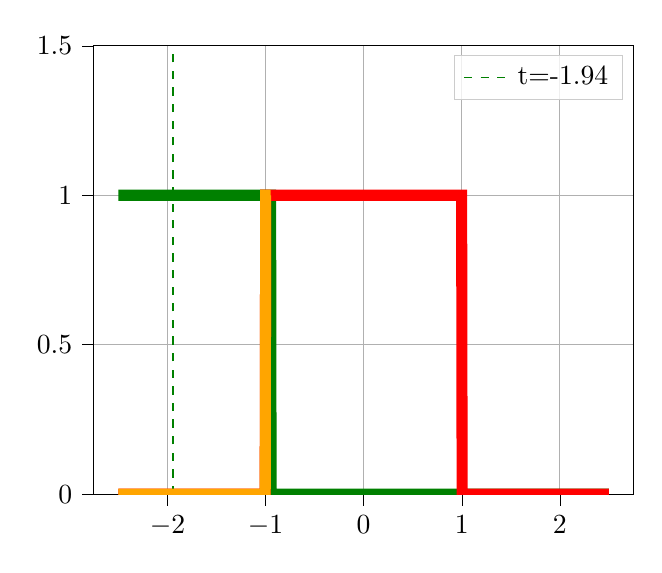
\begin{tikzpicture}

\definecolor{color0}{rgb}{1,0.498039215686275,0.0549019607843137}
\definecolor{color1}{rgb}{1,0.647058823529412,0}

\begin{axis}[
legend cell align={left},
legend style={fill opacity=0.8, draw opacity=1, text opacity=1, draw=white!80!black},
tick align=outside,
tick pos=left,
x grid style={white!69.0196078431373!black},
xmajorgrids,
xmin=-2.75, xmax=2.75,
xtick style={color=black},
y grid style={white!69.0196078431373!black},
ymajorgrids,
ymin=0, ymax=1.5,
ytick style={color=black}
]
\path [draw=color0, fill=color0, opacity=0.2]
(axis cs:-2.5,0)
--(axis cs:-2.5,0)
--(axis cs:-2.49499499499499,0)
--(axis cs:-2.48998998998999,0)
--(axis cs:-2.48498498498498,0)
--(axis cs:-2.47997997997998,0)
--(axis cs:-2.47497497497497,0)
--(axis cs:-2.46996996996997,0)
--(axis cs:-2.46496496496496,0)
--(axis cs:-2.45995995995996,0)
--(axis cs:-2.45495495495495,0)
--(axis cs:-2.44994994994995,0)
--(axis cs:-2.44494494494494,0)
--(axis cs:-2.43993993993994,0)
--(axis cs:-2.43493493493493,0)
--(axis cs:-2.42992992992993,0)
--(axis cs:-2.42492492492492,0)
--(axis cs:-2.41991991991992,0)
--(axis cs:-2.41491491491491,0)
--(axis cs:-2.40990990990991,0)
--(axis cs:-2.4049049049049,0)
--(axis cs:-2.3998998998999,0)
--(axis cs:-2.39489489489489,0)
--(axis cs:-2.38988988988989,0)
--(axis cs:-2.38488488488488,0)
--(axis cs:-2.37987987987988,0)
--(axis cs:-2.37487487487487,0)
--(axis cs:-2.36986986986987,0)
--(axis cs:-2.36486486486486,0)
--(axis cs:-2.35985985985986,0)
--(axis cs:-2.35485485485485,0)
--(axis cs:-2.34984984984985,0)
--(axis cs:-2.34484484484484,0)
--(axis cs:-2.33983983983984,0)
--(axis cs:-2.33483483483483,0)
--(axis cs:-2.32982982982983,0)
--(axis cs:-2.32482482482482,0)
--(axis cs:-2.31981981981982,0)
--(axis cs:-2.31481481481481,0)
--(axis cs:-2.30980980980981,0)
--(axis cs:-2.3048048048048,0)
--(axis cs:-2.2997997997998,0)
--(axis cs:-2.29479479479479,0)
--(axis cs:-2.28978978978979,0)
--(axis cs:-2.28478478478478,0)
--(axis cs:-2.27977977977978,0)
--(axis cs:-2.27477477477477,0)
--(axis cs:-2.26976976976977,0)
--(axis cs:-2.26476476476476,0)
--(axis cs:-2.25975975975976,0)
--(axis cs:-2.25475475475475,0)
--(axis cs:-2.24974974974975,0)
--(axis cs:-2.24474474474474,0)
--(axis cs:-2.23973973973974,0)
--(axis cs:-2.23473473473473,0)
--(axis cs:-2.22972972972973,0)
--(axis cs:-2.22472472472472,0)
--(axis cs:-2.21971971971972,0)
--(axis cs:-2.21471471471471,0)
--(axis cs:-2.20970970970971,0)
--(axis cs:-2.2047047047047,0)
--(axis cs:-2.1996996996997,0)
--(axis cs:-2.19469469469469,0)
--(axis cs:-2.18968968968969,0)
--(axis cs:-2.18468468468468,0)
--(axis cs:-2.17967967967968,0)
--(axis cs:-2.17467467467467,0)
--(axis cs:-2.16966966966967,0)
--(axis cs:-2.16466466466466,0)
--(axis cs:-2.15965965965966,0)
--(axis cs:-2.15465465465465,0)
--(axis cs:-2.14964964964965,0)
--(axis cs:-2.14464464464464,0)
--(axis cs:-2.13963963963964,0)
--(axis cs:-2.13463463463463,0)
--(axis cs:-2.12962962962963,0)
--(axis cs:-2.12462462462462,0)
--(axis cs:-2.11961961961962,0)
--(axis cs:-2.11461461461461,0)
--(axis cs:-2.10960960960961,0)
--(axis cs:-2.1046046046046,0)
--(axis cs:-2.0995995995996,0)
--(axis cs:-2.09459459459459,0)
--(axis cs:-2.08958958958959,0)
--(axis cs:-2.08458458458458,0)
--(axis cs:-2.07957957957958,0)
--(axis cs:-2.07457457457457,0)
--(axis cs:-2.06956956956957,0)
--(axis cs:-2.06456456456456,0)
--(axis cs:-2.05955955955956,0)
--(axis cs:-2.05455455455455,0)
--(axis cs:-2.04954954954955,0)
--(axis cs:-2.04454454454454,0)
--(axis cs:-2.03953953953954,0)
--(axis cs:-2.03453453453453,0)
--(axis cs:-2.02952952952953,0)
--(axis cs:-2.02452452452452,0)
--(axis cs:-2.01951951951952,0)
--(axis cs:-2.01451451451451,0)
--(axis cs:-2.00950950950951,0)
--(axis cs:-2.0045045045045,0)
--(axis cs:-1.9994994994995,0)
--(axis cs:-1.99449449449449,0)
--(axis cs:-1.98948948948949,0)
--(axis cs:-1.98448448448448,0)
--(axis cs:-1.97947947947948,0)
--(axis cs:-1.97447447447447,0)
--(axis cs:-1.96946946946947,0)
--(axis cs:-1.96446446446446,0)
--(axis cs:-1.95945945945946,0)
--(axis cs:-1.95445445445445,0)
--(axis cs:-1.94944944944945,0)
--(axis cs:-1.94444444444444,0)
--(axis cs:-1.93943943943944,0)
--(axis cs:-1.93443443443443,0)
--(axis cs:-1.92942942942943,0)
--(axis cs:-1.92442442442442,0)
--(axis cs:-1.91941941941942,0)
--(axis cs:-1.91441441441441,0)
--(axis cs:-1.90940940940941,0)
--(axis cs:-1.9044044044044,0)
--(axis cs:-1.8993993993994,0)
--(axis cs:-1.89439439439439,0)
--(axis cs:-1.88938938938939,0)
--(axis cs:-1.88438438438438,0)
--(axis cs:-1.87937937937938,0)
--(axis cs:-1.87437437437437,0)
--(axis cs:-1.86936936936937,0)
--(axis cs:-1.86436436436436,0)
--(axis cs:-1.85935935935936,0)
--(axis cs:-1.85435435435435,0)
--(axis cs:-1.84934934934935,0)
--(axis cs:-1.84434434434434,0)
--(axis cs:-1.83933933933934,0)
--(axis cs:-1.83433433433433,0)
--(axis cs:-1.82932932932933,0)
--(axis cs:-1.82432432432432,0)
--(axis cs:-1.81931931931932,0)
--(axis cs:-1.81431431431431,0)
--(axis cs:-1.80930930930931,0)
--(axis cs:-1.8043043043043,0)
--(axis cs:-1.7992992992993,0)
--(axis cs:-1.79429429429429,0)
--(axis cs:-1.78928928928929,0)
--(axis cs:-1.78428428428428,0)
--(axis cs:-1.77927927927928,0)
--(axis cs:-1.77427427427427,0)
--(axis cs:-1.76926926926927,0)
--(axis cs:-1.76426426426426,0)
--(axis cs:-1.75925925925926,0)
--(axis cs:-1.75425425425425,0)
--(axis cs:-1.74924924924925,0)
--(axis cs:-1.74424424424424,0)
--(axis cs:-1.73923923923924,0)
--(axis cs:-1.73423423423423,0)
--(axis cs:-1.72922922922923,0)
--(axis cs:-1.72422422422422,0)
--(axis cs:-1.71921921921922,0)
--(axis cs:-1.71421421421421,0)
--(axis cs:-1.70920920920921,0)
--(axis cs:-1.7042042042042,0)
--(axis cs:-1.6991991991992,0)
--(axis cs:-1.69419419419419,0)
--(axis cs:-1.68918918918919,0)
--(axis cs:-1.68418418418418,0)
--(axis cs:-1.67917917917918,0)
--(axis cs:-1.67417417417417,0)
--(axis cs:-1.66916916916917,0)
--(axis cs:-1.66416416416416,0)
--(axis cs:-1.65915915915916,0)
--(axis cs:-1.65415415415415,0)
--(axis cs:-1.64914914914915,0)
--(axis cs:-1.64414414414414,0)
--(axis cs:-1.63913913913914,0)
--(axis cs:-1.63413413413413,0)
--(axis cs:-1.62912912912913,0)
--(axis cs:-1.62412412412412,0)
--(axis cs:-1.61911911911912,0)
--(axis cs:-1.61411411411411,0)
--(axis cs:-1.60910910910911,0)
--(axis cs:-1.6041041041041,0)
--(axis cs:-1.5990990990991,0)
--(axis cs:-1.59409409409409,0)
--(axis cs:-1.58908908908909,0)
--(axis cs:-1.58408408408408,0)
--(axis cs:-1.57907907907908,0)
--(axis cs:-1.57407407407407,0)
--(axis cs:-1.56906906906907,0)
--(axis cs:-1.56406406406406,0)
--(axis cs:-1.55905905905906,0)
--(axis cs:-1.55405405405405,0)
--(axis cs:-1.54904904904905,0)
--(axis cs:-1.54404404404404,0)
--(axis cs:-1.53903903903904,0)
--(axis cs:-1.53403403403403,0)
--(axis cs:-1.52902902902903,0)
--(axis cs:-1.52402402402402,0)
--(axis cs:-1.51901901901902,0)
--(axis cs:-1.51401401401401,0)
--(axis cs:-1.50900900900901,0)
--(axis cs:-1.504004004004,0)
--(axis cs:-1.498998998999,0)
--(axis cs:-1.49399399399399,0)
--(axis cs:-1.48898898898899,0)
--(axis cs:-1.48398398398398,0)
--(axis cs:-1.47897897897898,0)
--(axis cs:-1.47397397397397,0)
--(axis cs:-1.46896896896897,0)
--(axis cs:-1.46396396396396,0)
--(axis cs:-1.45895895895896,0)
--(axis cs:-1.45395395395395,0)
--(axis cs:-1.44894894894895,0)
--(axis cs:-1.44394394394394,0)
--(axis cs:-1.43893893893894,0)
--(axis cs:-1.43393393393393,0)
--(axis cs:-1.42892892892893,0)
--(axis cs:-1.42392392392392,0)
--(axis cs:-1.41891891891892,0)
--(axis cs:-1.41391391391391,0)
--(axis cs:-1.40890890890891,0)
--(axis cs:-1.4039039039039,0)
--(axis cs:-1.3988988988989,0)
--(axis cs:-1.39389389389389,0)
--(axis cs:-1.38888888888889,0)
--(axis cs:-1.38388388388388,0)
--(axis cs:-1.37887887887888,0)
--(axis cs:-1.37387387387387,0)
--(axis cs:-1.36886886886887,0)
--(axis cs:-1.36386386386386,0)
--(axis cs:-1.35885885885886,0)
--(axis cs:-1.35385385385385,0)
--(axis cs:-1.34884884884885,0)
--(axis cs:-1.34384384384384,0)
--(axis cs:-1.33883883883884,0)
--(axis cs:-1.33383383383383,0)
--(axis cs:-1.32882882882883,0)
--(axis cs:-1.32382382382382,0)
--(axis cs:-1.31881881881882,0)
--(axis cs:-1.31381381381381,0)
--(axis cs:-1.30880880880881,0)
--(axis cs:-1.3038038038038,0)
--(axis cs:-1.2987987987988,0)
--(axis cs:-1.29379379379379,0)
--(axis cs:-1.28878878878879,0)
--(axis cs:-1.28378378378378,0)
--(axis cs:-1.27877877877878,0)
--(axis cs:-1.27377377377377,0)
--(axis cs:-1.26876876876877,0)
--(axis cs:-1.26376376376376,0)
--(axis cs:-1.25875875875876,0)
--(axis cs:-1.25375375375375,0)
--(axis cs:-1.24874874874875,0)
--(axis cs:-1.24374374374374,0)
--(axis cs:-1.23873873873874,0)
--(axis cs:-1.23373373373373,0)
--(axis cs:-1.22872872872873,0)
--(axis cs:-1.22372372372372,0)
--(axis cs:-1.21871871871872,0)
--(axis cs:-1.21371371371371,0)
--(axis cs:-1.20870870870871,0)
--(axis cs:-1.2037037037037,0)
--(axis cs:-1.1986986986987,0)
--(axis cs:-1.19369369369369,0)
--(axis cs:-1.18868868868869,0)
--(axis cs:-1.18368368368368,0)
--(axis cs:-1.17867867867868,0)
--(axis cs:-1.17367367367367,0)
--(axis cs:-1.16866866866867,0)
--(axis cs:-1.16366366366366,0)
--(axis cs:-1.15865865865866,0)
--(axis cs:-1.15365365365365,0)
--(axis cs:-1.14864864864865,0)
--(axis cs:-1.14364364364364,0)
--(axis cs:-1.13863863863864,0)
--(axis cs:-1.13363363363363,0)
--(axis cs:-1.12862862862863,0)
--(axis cs:-1.12362362362362,0)
--(axis cs:-1.11861861861862,0)
--(axis cs:-1.11361361361361,0)
--(axis cs:-1.10860860860861,0)
--(axis cs:-1.1036036036036,0)
--(axis cs:-1.0985985985986,0)
--(axis cs:-1.09359359359359,0)
--(axis cs:-1.08858858858859,0)
--(axis cs:-1.08358358358358,0)
--(axis cs:-1.07857857857858,0)
--(axis cs:-1.07357357357357,0)
--(axis cs:-1.06856856856857,0)
--(axis cs:-1.06356356356356,0)
--(axis cs:-1.05855855855856,0)
--(axis cs:-1.05355355355355,0)
--(axis cs:-1.04854854854855,0)
--(axis cs:-1.04354354354354,0)
--(axis cs:-1.03853853853854,0)
--(axis cs:-1.03353353353353,0)
--(axis cs:-1.02852852852853,0)
--(axis cs:-1.02352352352352,0)
--(axis cs:-1.01851851851852,0)
--(axis cs:-1.01351351351351,0)
--(axis cs:-1.00850850850851,0)
--(axis cs:-1.0035035035035,0)
--(axis cs:-0.998498498498499,0)
--(axis cs:-0.993493493493494,0)
--(axis cs:-0.988488488488489,0)
--(axis cs:-0.983483483483484,0)
--(axis cs:-0.978478478478479,0)
--(axis cs:-0.973473473473474,0)
--(axis cs:-0.968468468468469,0)
--(axis cs:-0.963463463463464,0)
--(axis cs:-0.958458458458459,0)
--(axis cs:-0.953453453453454,0)
--(axis cs:-0.948448448448449,0)
--(axis cs:-0.948448448448449,1)
--(axis cs:-0.948448448448449,1)
--(axis cs:-0.953453453453454,1)
--(axis cs:-0.958458458458459,1)
--(axis cs:-0.963463463463464,1)
--(axis cs:-0.968468468468469,1)
--(axis cs:-0.973473473473474,1)
--(axis cs:-0.978478478478479,1)
--(axis cs:-0.983483483483484,1)
--(axis cs:-0.988488488488489,1)
--(axis cs:-0.993493493493494,1)
--(axis cs:-0.998498498498499,1)
--(axis cs:-1.0035035035035,0)
--(axis cs:-1.00850850850851,0)
--(axis cs:-1.01351351351351,0)
--(axis cs:-1.01851851851852,0)
--(axis cs:-1.02352352352352,0)
--(axis cs:-1.02852852852853,0)
--(axis cs:-1.03353353353353,0)
--(axis cs:-1.03853853853854,0)
--(axis cs:-1.04354354354354,0)
--(axis cs:-1.04854854854855,0)
--(axis cs:-1.05355355355355,0)
--(axis cs:-1.05855855855856,0)
--(axis cs:-1.06356356356356,0)
--(axis cs:-1.06856856856857,0)
--(axis cs:-1.07357357357357,0)
--(axis cs:-1.07857857857858,0)
--(axis cs:-1.08358358358358,0)
--(axis cs:-1.08858858858859,0)
--(axis cs:-1.09359359359359,0)
--(axis cs:-1.0985985985986,0)
--(axis cs:-1.1036036036036,0)
--(axis cs:-1.10860860860861,0)
--(axis cs:-1.11361361361361,0)
--(axis cs:-1.11861861861862,0)
--(axis cs:-1.12362362362362,0)
--(axis cs:-1.12862862862863,0)
--(axis cs:-1.13363363363363,0)
--(axis cs:-1.13863863863864,0)
--(axis cs:-1.14364364364364,0)
--(axis cs:-1.14864864864865,0)
--(axis cs:-1.15365365365365,0)
--(axis cs:-1.15865865865866,0)
--(axis cs:-1.16366366366366,0)
--(axis cs:-1.16866866866867,0)
--(axis cs:-1.17367367367367,0)
--(axis cs:-1.17867867867868,0)
--(axis cs:-1.18368368368368,0)
--(axis cs:-1.18868868868869,0)
--(axis cs:-1.19369369369369,0)
--(axis cs:-1.1986986986987,0)
--(axis cs:-1.2037037037037,0)
--(axis cs:-1.20870870870871,0)
--(axis cs:-1.21371371371371,0)
--(axis cs:-1.21871871871872,0)
--(axis cs:-1.22372372372372,0)
--(axis cs:-1.22872872872873,0)
--(axis cs:-1.23373373373373,0)
--(axis cs:-1.23873873873874,0)
--(axis cs:-1.24374374374374,0)
--(axis cs:-1.24874874874875,0)
--(axis cs:-1.25375375375375,0)
--(axis cs:-1.25875875875876,0)
--(axis cs:-1.26376376376376,0)
--(axis cs:-1.26876876876877,0)
--(axis cs:-1.27377377377377,0)
--(axis cs:-1.27877877877878,0)
--(axis cs:-1.28378378378378,0)
--(axis cs:-1.28878878878879,0)
--(axis cs:-1.29379379379379,0)
--(axis cs:-1.2987987987988,0)
--(axis cs:-1.3038038038038,0)
--(axis cs:-1.30880880880881,0)
--(axis cs:-1.31381381381381,0)
--(axis cs:-1.31881881881882,0)
--(axis cs:-1.32382382382382,0)
--(axis cs:-1.32882882882883,0)
--(axis cs:-1.33383383383383,0)
--(axis cs:-1.33883883883884,0)
--(axis cs:-1.34384384384384,0)
--(axis cs:-1.34884884884885,0)
--(axis cs:-1.35385385385385,0)
--(axis cs:-1.35885885885886,0)
--(axis cs:-1.36386386386386,0)
--(axis cs:-1.36886886886887,0)
--(axis cs:-1.37387387387387,0)
--(axis cs:-1.37887887887888,0)
--(axis cs:-1.38388388388388,0)
--(axis cs:-1.38888888888889,0)
--(axis cs:-1.39389389389389,0)
--(axis cs:-1.3988988988989,0)
--(axis cs:-1.4039039039039,0)
--(axis cs:-1.40890890890891,0)
--(axis cs:-1.41391391391391,0)
--(axis cs:-1.41891891891892,0)
--(axis cs:-1.42392392392392,0)
--(axis cs:-1.42892892892893,0)
--(axis cs:-1.43393393393393,0)
--(axis cs:-1.43893893893894,0)
--(axis cs:-1.44394394394394,0)
--(axis cs:-1.44894894894895,0)
--(axis cs:-1.45395395395395,0)
--(axis cs:-1.45895895895896,0)
--(axis cs:-1.46396396396396,0)
--(axis cs:-1.46896896896897,0)
--(axis cs:-1.47397397397397,0)
--(axis cs:-1.47897897897898,0)
--(axis cs:-1.48398398398398,0)
--(axis cs:-1.48898898898899,0)
--(axis cs:-1.49399399399399,0)
--(axis cs:-1.498998998999,0)
--(axis cs:-1.504004004004,0)
--(axis cs:-1.50900900900901,0)
--(axis cs:-1.51401401401401,0)
--(axis cs:-1.51901901901902,0)
--(axis cs:-1.52402402402402,0)
--(axis cs:-1.52902902902903,0)
--(axis cs:-1.53403403403403,0)
--(axis cs:-1.53903903903904,0)
--(axis cs:-1.54404404404404,0)
--(axis cs:-1.54904904904905,0)
--(axis cs:-1.55405405405405,0)
--(axis cs:-1.55905905905906,0)
--(axis cs:-1.56406406406406,0)
--(axis cs:-1.56906906906907,0)
--(axis cs:-1.57407407407407,0)
--(axis cs:-1.57907907907908,0)
--(axis cs:-1.58408408408408,0)
--(axis cs:-1.58908908908909,0)
--(axis cs:-1.59409409409409,0)
--(axis cs:-1.5990990990991,0)
--(axis cs:-1.6041041041041,0)
--(axis cs:-1.60910910910911,0)
--(axis cs:-1.61411411411411,0)
--(axis cs:-1.61911911911912,0)
--(axis cs:-1.62412412412412,0)
--(axis cs:-1.62912912912913,0)
--(axis cs:-1.63413413413413,0)
--(axis cs:-1.63913913913914,0)
--(axis cs:-1.64414414414414,0)
--(axis cs:-1.64914914914915,0)
--(axis cs:-1.65415415415415,0)
--(axis cs:-1.65915915915916,0)
--(axis cs:-1.66416416416416,0)
--(axis cs:-1.66916916916917,0)
--(axis cs:-1.67417417417417,0)
--(axis cs:-1.67917917917918,0)
--(axis cs:-1.68418418418418,0)
--(axis cs:-1.68918918918919,0)
--(axis cs:-1.69419419419419,0)
--(axis cs:-1.6991991991992,0)
--(axis cs:-1.7042042042042,0)
--(axis cs:-1.70920920920921,0)
--(axis cs:-1.71421421421421,0)
--(axis cs:-1.71921921921922,0)
--(axis cs:-1.72422422422422,0)
--(axis cs:-1.72922922922923,0)
--(axis cs:-1.73423423423423,0)
--(axis cs:-1.73923923923924,0)
--(axis cs:-1.74424424424424,0)
--(axis cs:-1.74924924924925,0)
--(axis cs:-1.75425425425425,0)
--(axis cs:-1.75925925925926,0)
--(axis cs:-1.76426426426426,0)
--(axis cs:-1.76926926926927,0)
--(axis cs:-1.77427427427427,0)
--(axis cs:-1.77927927927928,0)
--(axis cs:-1.78428428428428,0)
--(axis cs:-1.78928928928929,0)
--(axis cs:-1.79429429429429,0)
--(axis cs:-1.7992992992993,0)
--(axis cs:-1.8043043043043,0)
--(axis cs:-1.80930930930931,0)
--(axis cs:-1.81431431431431,0)
--(axis cs:-1.81931931931932,0)
--(axis cs:-1.82432432432432,0)
--(axis cs:-1.82932932932933,0)
--(axis cs:-1.83433433433433,0)
--(axis cs:-1.83933933933934,0)
--(axis cs:-1.84434434434434,0)
--(axis cs:-1.84934934934935,0)
--(axis cs:-1.85435435435435,0)
--(axis cs:-1.85935935935936,0)
--(axis cs:-1.86436436436436,0)
--(axis cs:-1.86936936936937,0)
--(axis cs:-1.87437437437437,0)
--(axis cs:-1.87937937937938,0)
--(axis cs:-1.88438438438438,0)
--(axis cs:-1.88938938938939,0)
--(axis cs:-1.89439439439439,0)
--(axis cs:-1.8993993993994,0)
--(axis cs:-1.9044044044044,0)
--(axis cs:-1.90940940940941,0)
--(axis cs:-1.91441441441441,0)
--(axis cs:-1.91941941941942,0)
--(axis cs:-1.92442442442442,0)
--(axis cs:-1.92942942942943,0)
--(axis cs:-1.93443443443443,0)
--(axis cs:-1.93943943943944,0)
--(axis cs:-1.94444444444444,0)
--(axis cs:-1.94944944944945,0)
--(axis cs:-1.95445445445445,0)
--(axis cs:-1.95945945945946,0)
--(axis cs:-1.96446446446446,0)
--(axis cs:-1.96946946946947,0)
--(axis cs:-1.97447447447447,0)
--(axis cs:-1.97947947947948,0)
--(axis cs:-1.98448448448448,0)
--(axis cs:-1.98948948948949,0)
--(axis cs:-1.99449449449449,0)
--(axis cs:-1.9994994994995,0)
--(axis cs:-2.0045045045045,0)
--(axis cs:-2.00950950950951,0)
--(axis cs:-2.01451451451451,0)
--(axis cs:-2.01951951951952,0)
--(axis cs:-2.02452452452452,0)
--(axis cs:-2.02952952952953,0)
--(axis cs:-2.03453453453453,0)
--(axis cs:-2.03953953953954,0)
--(axis cs:-2.04454454454454,0)
--(axis cs:-2.04954954954955,0)
--(axis cs:-2.05455455455455,0)
--(axis cs:-2.05955955955956,0)
--(axis cs:-2.06456456456456,0)
--(axis cs:-2.06956956956957,0)
--(axis cs:-2.07457457457457,0)
--(axis cs:-2.07957957957958,0)
--(axis cs:-2.08458458458458,0)
--(axis cs:-2.08958958958959,0)
--(axis cs:-2.09459459459459,0)
--(axis cs:-2.0995995995996,0)
--(axis cs:-2.1046046046046,0)
--(axis cs:-2.10960960960961,0)
--(axis cs:-2.11461461461461,0)
--(axis cs:-2.11961961961962,0)
--(axis cs:-2.12462462462462,0)
--(axis cs:-2.12962962962963,0)
--(axis cs:-2.13463463463463,0)
--(axis cs:-2.13963963963964,0)
--(axis cs:-2.14464464464464,0)
--(axis cs:-2.14964964964965,0)
--(axis cs:-2.15465465465465,0)
--(axis cs:-2.15965965965966,0)
--(axis cs:-2.16466466466466,0)
--(axis cs:-2.16966966966967,0)
--(axis cs:-2.17467467467467,0)
--(axis cs:-2.17967967967968,0)
--(axis cs:-2.18468468468468,0)
--(axis cs:-2.18968968968969,0)
--(axis cs:-2.19469469469469,0)
--(axis cs:-2.1996996996997,0)
--(axis cs:-2.2047047047047,0)
--(axis cs:-2.20970970970971,0)
--(axis cs:-2.21471471471471,0)
--(axis cs:-2.21971971971972,0)
--(axis cs:-2.22472472472472,0)
--(axis cs:-2.22972972972973,0)
--(axis cs:-2.23473473473473,0)
--(axis cs:-2.23973973973974,0)
--(axis cs:-2.24474474474474,0)
--(axis cs:-2.24974974974975,0)
--(axis cs:-2.25475475475475,0)
--(axis cs:-2.25975975975976,0)
--(axis cs:-2.26476476476476,0)
--(axis cs:-2.26976976976977,0)
--(axis cs:-2.27477477477477,0)
--(axis cs:-2.27977977977978,0)
--(axis cs:-2.28478478478478,0)
--(axis cs:-2.28978978978979,0)
--(axis cs:-2.29479479479479,0)
--(axis cs:-2.2997997997998,0)
--(axis cs:-2.3048048048048,0)
--(axis cs:-2.30980980980981,0)
--(axis cs:-2.31481481481481,0)
--(axis cs:-2.31981981981982,0)
--(axis cs:-2.32482482482482,0)
--(axis cs:-2.32982982982983,0)
--(axis cs:-2.33483483483483,0)
--(axis cs:-2.33983983983984,0)
--(axis cs:-2.34484484484484,0)
--(axis cs:-2.34984984984985,0)
--(axis cs:-2.35485485485485,0)
--(axis cs:-2.35985985985986,0)
--(axis cs:-2.36486486486486,0)
--(axis cs:-2.36986986986987,0)
--(axis cs:-2.37487487487487,0)
--(axis cs:-2.37987987987988,0)
--(axis cs:-2.38488488488488,0)
--(axis cs:-2.38988988988989,0)
--(axis cs:-2.39489489489489,0)
--(axis cs:-2.3998998998999,0)
--(axis cs:-2.4049049049049,0)
--(axis cs:-2.40990990990991,0)
--(axis cs:-2.41491491491491,0)
--(axis cs:-2.41991991991992,0)
--(axis cs:-2.42492492492492,0)
--(axis cs:-2.42992992992993,0)
--(axis cs:-2.43493493493493,0)
--(axis cs:-2.43993993993994,0)
--(axis cs:-2.44494494494494,0)
--(axis cs:-2.44994994994995,0)
--(axis cs:-2.45495495495495,0)
--(axis cs:-2.45995995995996,0)
--(axis cs:-2.46496496496496,0)
--(axis cs:-2.46996996996997,0)
--(axis cs:-2.47497497497497,0)
--(axis cs:-2.47997997997998,0)
--(axis cs:-2.48498498498498,0)
--(axis cs:-2.48998998998999,0)
--(axis cs:-2.49499499499499,0)
--(axis cs:-2.5,0)
--cycle;

\addplot [line width=4pt, green!50!black, forget plot]
table {%
-2.5 1
-2.49499499499499 1
-2.48998998998999 1
-2.48498498498498 1
-2.47997997997998 1
-2.47497497497497 1
-2.46996996996997 1
-2.46496496496496 1
-2.45995995995996 1
-2.45495495495495 1
-2.44994994994995 1
-2.44494494494494 1
-2.43993993993994 1
-2.43493493493493 1
-2.42992992992993 1
-2.42492492492492 1
-2.41991991991992 1
-2.41491491491491 1
-2.40990990990991 1
-2.4049049049049 1
-2.3998998998999 1
-2.39489489489489 1
-2.38988988988989 1
-2.38488488488488 1
-2.37987987987988 1
-2.37487487487487 1
-2.36986986986987 1
-2.36486486486486 1
-2.35985985985986 1
-2.35485485485485 1
-2.34984984984985 1
-2.34484484484484 1
-2.33983983983984 1
-2.33483483483483 1
-2.32982982982983 1
-2.32482482482482 1
-2.31981981981982 1
-2.31481481481481 1
-2.30980980980981 1
-2.3048048048048 1
-2.2997997997998 1
-2.29479479479479 1
-2.28978978978979 1
-2.28478478478478 1
-2.27977977977978 1
-2.27477477477477 1
-2.26976976976977 1
-2.26476476476476 1
-2.25975975975976 1
-2.25475475475475 1
-2.24974974974975 1
-2.24474474474474 1
-2.23973973973974 1
-2.23473473473473 1
-2.22972972972973 1
-2.22472472472472 1
-2.21971971971972 1
-2.21471471471471 1
-2.20970970970971 1
-2.2047047047047 1
-2.1996996996997 1
-2.19469469469469 1
-2.18968968968969 1
-2.18468468468468 1
-2.17967967967968 1
-2.17467467467467 1
-2.16966966966967 1
-2.16466466466466 1
-2.15965965965966 1
-2.15465465465465 1
-2.14964964964965 1
-2.14464464464464 1
-2.13963963963964 1
-2.13463463463463 1
-2.12962962962963 1
-2.12462462462462 1
-2.11961961961962 1
-2.11461461461461 1
-2.10960960960961 1
-2.1046046046046 1
-2.0995995995996 1
-2.09459459459459 1
-2.08958958958959 1
-2.08458458458458 1
-2.07957957957958 1
-2.07457457457457 1
-2.06956956956957 1
-2.06456456456456 1
-2.05955955955956 1
-2.05455455455455 1
-2.04954954954955 1
-2.04454454454454 1
-2.03953953953954 1
-2.03453453453453 1
-2.02952952952953 1
-2.02452452452452 1
-2.01951951951952 1
-2.01451451451451 1
-2.00950950950951 1
-2.0045045045045 1
-1.9994994994995 1
-1.99449449449449 1
-1.98948948948949 1
-1.98448448448448 1
-1.97947947947948 1
-1.97447447447447 1
-1.96946946946947 1
-1.96446446446446 1
-1.95945945945946 1
-1.95445445445445 1
-1.94944944944945 1
-1.94444444444444 1
-1.93943943943944 1
-1.93443443443443 1
-1.92942942942943 1
-1.92442442442442 1
-1.91941941941942 1
-1.91441441441441 1
-1.90940940940941 1
-1.9044044044044 1
-1.8993993993994 1
-1.89439439439439 1
-1.88938938938939 1
-1.88438438438438 1
-1.87937937937938 1
-1.87437437437437 1
-1.86936936936937 1
-1.86436436436436 1
-1.85935935935936 1
-1.85435435435435 1
-1.84934934934935 1
-1.84434434434434 1
-1.83933933933934 1
-1.83433433433433 1
-1.82932932932933 1
-1.82432432432432 1
-1.81931931931932 1
-1.81431431431431 1
-1.80930930930931 1
-1.8043043043043 1
-1.7992992992993 1
-1.79429429429429 1
-1.78928928928929 1
-1.78428428428428 1
-1.77927927927928 1
-1.77427427427427 1
-1.76926926926927 1
-1.76426426426426 1
-1.75925925925926 1
-1.75425425425425 1
-1.74924924924925 1
-1.74424424424424 1
-1.73923923923924 1
-1.73423423423423 1
-1.72922922922923 1
-1.72422422422422 1
-1.71921921921922 1
-1.71421421421421 1
-1.70920920920921 1
-1.7042042042042 1
-1.6991991991992 1
-1.69419419419419 1
-1.68918918918919 1
-1.68418418418418 1
-1.67917917917918 1
-1.67417417417417 1
-1.66916916916917 1
-1.66416416416416 1
-1.65915915915916 1
-1.65415415415415 1
-1.64914914914915 1
-1.64414414414414 1
-1.63913913913914 1
-1.63413413413413 1
-1.62912912912913 1
-1.62412412412412 1
-1.61911911911912 1
-1.61411411411411 1
-1.60910910910911 1
-1.6041041041041 1
-1.5990990990991 1
-1.59409409409409 1
-1.58908908908909 1
-1.58408408408408 1
-1.57907907907908 1
-1.57407407407407 1
-1.56906906906907 1
-1.56406406406406 1
-1.55905905905906 1
-1.55405405405405 1
-1.54904904904905 1
-1.54404404404404 1
-1.53903903903904 1
-1.53403403403403 1
-1.52902902902903 1
-1.52402402402402 1
-1.51901901901902 1
-1.51401401401401 1
-1.50900900900901 1
-1.504004004004 1
-1.498998998999 1
-1.49399399399399 1
-1.48898898898899 1
-1.48398398398398 1
-1.47897897897898 1
-1.47397397397397 1
-1.46896896896897 1
-1.46396396396396 1
-1.45895895895896 1
-1.45395395395395 1
-1.44894894894895 1
-1.44394394394394 1
-1.43893893893894 1
-1.43393393393393 1
-1.42892892892893 1
-1.42392392392392 1
-1.41891891891892 1
-1.41391391391391 1
-1.40890890890891 1
-1.4039039039039 1
-1.3988988988989 1
-1.39389389389389 1
-1.38888888888889 1
-1.38388388388388 1
-1.37887887887888 1
-1.37387387387387 1
-1.36886886886887 1
-1.36386386386386 1
-1.35885885885886 1
-1.35385385385385 1
-1.34884884884885 1
-1.34384384384384 1
-1.33883883883884 1
-1.33383383383383 1
-1.32882882882883 1
-1.32382382382382 1
-1.31881881881882 1
-1.31381381381381 1
-1.30880880880881 1
-1.3038038038038 1
-1.2987987987988 1
-1.29379379379379 1
-1.28878878878879 1
-1.28378378378378 1
-1.27877877877878 1
-1.27377377377377 1
-1.26876876876877 1
-1.26376376376376 1
-1.25875875875876 1
-1.25375375375375 1
-1.24874874874875 1
-1.24374374374374 1
-1.23873873873874 1
-1.23373373373373 1
-1.22872872872873 1
-1.22372372372372 1
-1.21871871871872 1
-1.21371371371371 1
-1.20870870870871 1
-1.2037037037037 1
-1.1986986986987 1
-1.19369369369369 1
-1.18868868868869 1
-1.18368368368368 1
-1.17867867867868 1
-1.17367367367367 1
-1.16866866866867 1
-1.16366366366366 1
-1.15865865865866 1
-1.15365365365365 1
-1.14864864864865 1
-1.14364364364364 1
-1.13863863863864 1
-1.13363363363363 1
-1.12862862862863 1
-1.12362362362362 1
-1.11861861861862 1
-1.11361361361361 1
-1.10860860860861 1
-1.1036036036036 1
-1.0985985985986 1
-1.09359359359359 1
-1.08858858858859 1
-1.08358358358358 1
-1.07857857857858 1
-1.07357357357357 1
-1.06856856856857 1
-1.06356356356356 1
-1.05855855855856 1
-1.05355355355355 1
-1.04854854854855 1
-1.04354354354354 1
-1.03853853853854 1
-1.03353353353353 1
-1.02852852852853 1
-1.02352352352352 1
-1.01851851851852 1
-1.01351351351351 1
-1.00850850850851 1
-1.0035035035035 1
-0.998498498498499 1
-0.993493493493494 1
-0.988488488488489 1
-0.983483483483484 1
-0.978478478478479 1
-0.973473473473474 1
-0.968468468468469 1
-0.963463463463464 1
-0.958458458458459 1
-0.953453453453454 1
-0.948448448448449 1
-0.943443443443444 0
-0.938438438438439 0
-0.933433433433434 0
-0.928428428428429 0
-0.923423423423424 0
-0.918418418418419 0
-0.913413413413414 0
-0.908408408408409 0
-0.903403403403404 0
-0.898398398398399 0
-0.893393393393393 0
-0.888388388388388 0
-0.883383383383383 0
-0.878378378378378 0
-0.873373373373373 0
-0.868368368368368 0
-0.863363363363363 0
-0.858358358358358 0
-0.853353353353353 0
-0.848348348348348 0
-0.843343343343343 0
-0.838338338338338 0
-0.833333333333333 0
-0.828328328328328 0
-0.823323323323323 0
-0.818318318318318 0
-0.813313313313313 0
-0.808308308308308 0
-0.803303303303303 0
-0.798298298298298 0
-0.793293293293293 0
-0.788288288288288 0
-0.783283283283283 0
-0.778278278278278 0
-0.773273273273273 0
-0.768268268268268 0
-0.763263263263263 0
-0.758258258258258 0
-0.753253253253253 0
-0.748248248248248 0
-0.743243243243243 0
-0.738238238238238 0
-0.733233233233233 0
-0.728228228228228 0
-0.723223223223223 0
-0.718218218218218 0
-0.713213213213213 0
-0.708208208208208 0
-0.703203203203203 0
-0.698198198198198 0
-0.693193193193193 0
-0.688188188188188 0
-0.683183183183183 0
-0.678178178178178 0
-0.673173173173173 0
-0.668168168168168 0
-0.663163163163163 0
-0.658158158158158 0
-0.653153153153153 0
-0.648148148148148 0
-0.643143143143143 0
-0.638138138138138 0
-0.633133133133133 0
-0.628128128128128 0
-0.623123123123123 0
-0.618118118118118 0
-0.613113113113113 0
-0.608108108108108 0
-0.603103103103103 0
-0.598098098098098 0
-0.593093093093093 0
-0.588088088088088 0
-0.583083083083083 0
-0.578078078078078 0
-0.573073073073073 0
-0.568068068068068 0
-0.563063063063063 0
-0.558058058058058 0
-0.553053053053053 0
-0.548048048048048 0
-0.543043043043043 0
-0.538038038038038 0
-0.533033033033033 0
-0.528028028028028 0
-0.523023023023023 0
-0.518018018018018 0
-0.513013013013013 0
-0.508008008008008 0
-0.503003003003003 0
-0.497997997997998 0
-0.492992992992993 0
-0.487987987987988 0
-0.482982982982983 0
-0.477977977977978 0
-0.472972972972973 0
-0.467967967967968 0
-0.462962962962963 0
-0.457957957957958 0
-0.452952952952953 0
-0.447947947947948 0
-0.442942942942943 0
-0.437937937937938 0
-0.432932932932933 0
-0.427927927927928 0
-0.422922922922923 0
-0.417917917917918 0
-0.412912912912913 0
-0.407907907907908 0
-0.402902902902903 0
-0.397897897897898 0
-0.392892892892893 0
-0.387887887887888 0
-0.382882882882883 0
-0.377877877877878 0
-0.372872872872873 0
-0.367867867867868 0
-0.362862862862863 0
-0.357857857857858 0
-0.352852852852853 0
-0.347847847847848 0
-0.342842842842843 0
-0.337837837837838 0
-0.332832832832833 0
-0.327827827827828 0
-0.322822822822823 0
-0.317817817817818 0
-0.312812812812813 0
-0.307807807807808 0
-0.302802802802803 0
-0.297797797797798 0
-0.292792792792793 0
-0.287787787787788 0
-0.282782782782783 0
-0.277777777777778 0
-0.272772772772773 0
-0.267767767767768 0
-0.262762762762763 0
-0.257757757757758 0
-0.252752752752753 0
-0.247747747747748 0
-0.242742742742743 0
-0.237737737737738 0
-0.232732732732733 0
-0.227727727727728 0
-0.222722722722723 0
-0.217717717717718 0
-0.212712712712713 0
-0.207707707707708 0
-0.202702702702703 0
-0.197697697697698 0
-0.192692692692693 0
-0.187687687687688 0
-0.182682682682683 0
-0.177677677677678 0
-0.172672672672673 0
-0.167667667667668 0
-0.162662662662663 0
-0.157657657657658 0
-0.152652652652653 0
-0.147647647647648 0
-0.142642642642643 0
-0.137637637637638 0
-0.132632632632633 0
-0.127627627627628 0
-0.122622622622623 0
-0.117617617617618 0
-0.112612612612613 0
-0.107607607607608 0
-0.102602602602603 0
-0.0975975975975976 0
-0.0925925925925926 0
-0.0875875875875876 0
-0.0825825825825826 0
-0.0775775775775776 0
-0.0725725725725725 0
-0.0675675675675675 0
-0.0625625625625625 0
-0.0575575575575575 0
-0.0525525525525525 0
-0.0475475475475475 0
-0.0425425425425425 0
-0.0375375375375375 0
-0.0325325325325325 0
-0.0275275275275275 0
-0.0225225225225225 0
-0.0175175175175175 0
-0.0125125125125125 0
-0.0075075075075075 0
-0.0025025025025025 0
0.0025025025025025 0
0.0075075075075075 0
0.0125125125125125 0
0.0175175175175175 0
0.0225225225225225 0
0.0275275275275275 0
0.0325325325325325 0
0.0375375375375375 0
0.0425425425425425 0
0.0475475475475475 0
0.0525525525525525 0
0.0575575575575575 0
0.0625625625625625 0
0.0675675675675675 0
0.0725725725725725 0
0.0775775775775776 0
0.0825825825825826 0
0.0875875875875876 0
0.0925925925925926 0
0.0975975975975976 0
0.102602602602603 0
0.107607607607608 0
0.112612612612613 0
0.117617617617618 0
0.122622622622623 0
0.127627627627628 0
0.132632632632633 0
0.137637637637638 0
0.142642642642643 0
0.147647647647648 0
0.152652652652653 0
0.157657657657658 0
0.162662662662663 0
0.167667667667668 0
0.172672672672673 0
0.177677677677678 0
0.182682682682683 0
0.187687687687688 0
0.192692692692693 0
0.197697697697698 0
0.202702702702703 0
0.207707707707708 0
0.212712712712713 0
0.217717717717718 0
0.222722722722723 0
0.227727727727728 0
0.232732732732733 0
0.237737737737738 0
0.242742742742743 0
0.247747747747748 0
0.252752752752753 0
0.257757757757758 0
0.262762762762763 0
0.267767767767768 0
0.272772772772773 0
0.277777777777778 0
0.282782782782783 0
0.287787787787788 0
0.292792792792793 0
0.297797797797798 0
0.302802802802803 0
0.307807807807808 0
0.312812812812813 0
0.317817817817818 0
0.322822822822823 0
0.327827827827828 0
0.332832832832833 0
0.337837837837838 0
0.342842842842843 0
0.347847847847848 0
0.352852852852853 0
0.357857857857858 0
0.362862862862863 0
0.367867867867868 0
0.372872872872873 0
0.377877877877878 0
0.382882882882883 0
0.387887887887888 0
0.392892892892893 0
0.397897897897898 0
0.402902902902903 0
0.407907907907908 0
0.412912912912913 0
0.417917917917918 0
0.422922922922923 0
0.427927927927928 0
0.432932932932933 0
0.437937937937938 0
0.442942942942943 0
0.447947947947948 0
0.452952952952953 0
0.457957957957958 0
0.462962962962963 0
0.467967967967968 0
0.472972972972973 0
0.477977977977978 0
0.482982982982983 0
0.487987987987988 0
0.492992992992993 0
0.497997997997998 0
0.503003003003003 0
0.508008008008008 0
0.513013013013013 0
0.518018018018018 0
0.523023023023023 0
0.528028028028028 0
0.533033033033033 0
0.538038038038038 0
0.543043043043043 0
0.548048048048048 0
0.553053053053053 0
0.558058058058058 0
0.563063063063063 0
0.568068068068068 0
0.573073073073073 0
0.578078078078078 0
0.583083083083083 0
0.588088088088088 0
0.593093093093093 0
0.598098098098098 0
0.603103103103103 0
0.608108108108108 0
0.613113113113113 0
0.618118118118118 0
0.623123123123123 0
0.628128128128128 0
0.633133133133133 0
0.638138138138138 0
0.643143143143143 0
0.648148148148148 0
0.653153153153153 0
0.658158158158158 0
0.663163163163163 0
0.668168168168168 0
0.673173173173173 0
0.678178178178178 0
0.683183183183183 0
0.688188188188188 0
0.693193193193193 0
0.698198198198198 0
0.703203203203203 0
0.708208208208208 0
0.713213213213213 0
0.718218218218218 0
0.723223223223223 0
0.728228228228228 0
0.733233233233233 0
0.738238238238238 0
0.743243243243243 0
0.748248248248248 0
0.753253253253253 0
0.758258258258258 0
0.763263263263263 0
0.768268268268268 0
0.773273273273273 0
0.778278278278278 0
0.783283283283283 0
0.788288288288288 0
0.793293293293293 0
0.798298298298298 0
0.803303303303303 0
0.808308308308308 0
0.813313313313313 0
0.818318318318318 0
0.823323323323323 0
0.828328328328328 0
0.833333333333333 0
0.838338338338338 0
0.843343343343343 0
0.848348348348348 0
0.853353353353353 0
0.858358358358358 0
0.863363363363364 0
0.868368368368369 0
0.873373373373374 0
0.878378378378379 0
0.883383383383384 0
0.888388388388389 0
0.893393393393394 0
0.898398398398399 0
0.903403403403404 0
0.908408408408409 0
0.913413413413414 0
0.918418418418419 0
0.923423423423424 0
0.928428428428429 0
0.933433433433434 0
0.938438438438439 0
0.943443443443444 0
0.948448448448449 0
0.953453453453454 0
0.958458458458459 0
0.963463463463464 0
0.968468468468469 0
0.973473473473474 0
0.978478478478479 0
0.983483483483484 0
0.988488488488489 0
0.993493493493494 0
0.998498498498499 0
1.0035035035035 0
1.00850850850851 0
1.01351351351351 0
1.01851851851852 0
1.02352352352352 0
1.02852852852853 0
1.03353353353353 0
1.03853853853854 0
1.04354354354354 0
1.04854854854855 0
1.05355355355355 0
1.05855855855856 0
1.06356356356356 0
1.06856856856857 0
1.07357357357357 0
1.07857857857858 0
1.08358358358358 0
1.08858858858859 0
1.09359359359359 0
1.0985985985986 0
1.1036036036036 0
1.10860860860861 0
1.11361361361361 0
1.11861861861862 0
1.12362362362362 0
1.12862862862863 0
1.13363363363363 0
1.13863863863864 0
1.14364364364364 0
1.14864864864865 0
1.15365365365365 0
1.15865865865866 0
1.16366366366366 0
1.16866866866867 0
1.17367367367367 0
1.17867867867868 0
1.18368368368368 0
1.18868868868869 0
1.19369369369369 0
1.1986986986987 0
1.2037037037037 0
1.20870870870871 0
1.21371371371371 0
1.21871871871872 0
1.22372372372372 0
1.22872872872873 0
1.23373373373373 0
1.23873873873874 0
1.24374374374374 0
1.24874874874875 0
1.25375375375375 0
1.25875875875876 0
1.26376376376376 0
1.26876876876877 0
1.27377377377377 0
1.27877877877878 0
1.28378378378378 0
1.28878878878879 0
1.29379379379379 0
1.2987987987988 0
1.3038038038038 0
1.30880880880881 0
1.31381381381381 0
1.31881881881882 0
1.32382382382382 0
1.32882882882883 0
1.33383383383383 0
1.33883883883884 0
1.34384384384384 0
1.34884884884885 0
1.35385385385385 0
1.35885885885886 0
1.36386386386386 0
1.36886886886887 0
1.37387387387387 0
1.37887887887888 0
1.38388388388388 0
1.38888888888889 0
1.39389389389389 0
1.3988988988989 0
1.4039039039039 0
1.40890890890891 0
1.41391391391391 0
1.41891891891892 0
1.42392392392392 0
1.42892892892893 0
1.43393393393393 0
1.43893893893894 0
1.44394394394394 0
1.44894894894895 0
1.45395395395395 0
1.45895895895896 0
1.46396396396396 0
1.46896896896897 0
1.47397397397397 0
1.47897897897898 0
1.48398398398398 0
1.48898898898899 0
1.49399399399399 0
1.498998998999 0
1.504004004004 0
1.50900900900901 0
1.51401401401401 0
1.51901901901902 0
1.52402402402402 0
1.52902902902903 0
1.53403403403403 0
1.53903903903904 0
1.54404404404404 0
1.54904904904905 0
1.55405405405405 0
1.55905905905906 0
1.56406406406406 0
1.56906906906907 0
1.57407407407407 0
1.57907907907908 0
1.58408408408408 0
1.58908908908909 0
1.59409409409409 0
1.5990990990991 0
1.6041041041041 0
1.60910910910911 0
1.61411411411411 0
1.61911911911912 0
1.62412412412412 0
1.62912912912913 0
1.63413413413413 0
1.63913913913914 0
1.64414414414414 0
1.64914914914915 0
1.65415415415415 0
1.65915915915916 0
1.66416416416416 0
1.66916916916917 0
1.67417417417417 0
1.67917917917918 0
1.68418418418418 0
1.68918918918919 0
1.69419419419419 0
1.6991991991992 0
1.7042042042042 0
1.70920920920921 0
1.71421421421421 0
1.71921921921922 0
1.72422422422422 0
1.72922922922923 0
1.73423423423423 0
1.73923923923924 0
1.74424424424424 0
1.74924924924925 0
1.75425425425425 0
1.75925925925926 0
1.76426426426426 0
1.76926926926927 0
1.77427427427427 0
1.77927927927928 0
1.78428428428428 0
1.78928928928929 0
1.79429429429429 0
1.7992992992993 0
1.8043043043043 0
1.80930930930931 0
1.81431431431431 0
1.81931931931932 0
1.82432432432432 0
1.82932932932933 0
1.83433433433433 0
1.83933933933934 0
1.84434434434434 0
1.84934934934935 0
1.85435435435435 0
1.85935935935936 0
1.86436436436436 0
1.86936936936937 0
1.87437437437437 0
1.87937937937938 0
1.88438438438438 0
1.88938938938939 0
1.89439439439439 0
1.8993993993994 0
1.9044044044044 0
1.90940940940941 0
1.91441441441441 0
1.91941941941942 0
1.92442442442442 0
1.92942942942943 0
1.93443443443443 0
1.93943943943944 0
1.94444444444444 0
1.94944944944945 0
1.95445445445445 0
1.95945945945946 0
1.96446446446446 0
1.96946946946947 0
1.97447447447447 0
1.97947947947948 0
1.98448448448448 0
1.98948948948949 0
1.99449449449449 0
1.9994994994995 0
2.0045045045045 0
2.00950950950951 0
2.01451451451451 0
2.01951951951952 0
2.02452452452452 0
2.02952952952953 0
2.03453453453453 0
2.03953953953954 0
2.04454454454454 0
2.04954954954955 0
2.05455455455455 0
2.05955955955956 0
2.06456456456456 0
2.06956956956957 0
2.07457457457457 0
2.07957957957958 0
2.08458458458458 0
2.08958958958959 0
2.09459459459459 0
2.0995995995996 0
2.1046046046046 0
2.10960960960961 0
2.11461461461461 0
2.11961961961962 0
2.12462462462462 0
2.12962962962963 0
2.13463463463463 0
2.13963963963964 0
2.14464464464464 0
2.14964964964965 0
2.15465465465465 0
2.15965965965966 0
2.16466466466466 0
2.16966966966967 0
2.17467467467467 0
2.17967967967968 0
2.18468468468468 0
2.18968968968969 0
2.19469469469469 0
2.1996996996997 0
2.2047047047047 0
2.20970970970971 0
2.21471471471471 0
2.21971971971972 0
2.22472472472472 0
2.22972972972973 0
2.23473473473473 0
2.23973973973974 0
2.24474474474474 0
2.24974974974975 0
2.25475475475475 0
2.25975975975976 0
2.26476476476476 0
2.26976976976977 0
2.27477477477477 0
2.27977977977978 0
2.28478478478478 0
2.28978978978979 0
2.29479479479479 0
2.2997997997998 0
2.3048048048048 0
2.30980980980981 0
2.31481481481481 0
2.31981981981982 0
2.32482482482482 0
2.32982982982983 0
2.33483483483483 0
2.33983983983984 0
2.34484484484484 0
2.34984984984985 0
2.35485485485485 0
2.35985985985986 0
2.36486486486486 0
2.36986986986987 0
2.37487487487487 0
2.37987987987988 0
2.38488488488488 0
2.38988988988989 0
2.39489489489489 0
2.3998998998999 0
2.4049049049049 0
2.40990990990991 0
2.41491491491491 0
2.41991991991992 0
2.42492492492492 0
2.42992992992993 0
2.43493493493493 0
2.43993993993994 0
2.44494494494494 0
2.44994994994995 0
2.45495495495495 0
2.45995995995996 0
2.46496496496496 0
2.46996996996997 0
2.47497497497497 0
2.47997997997998 0
2.48498498498498 0
2.48998998998999 0
2.49499499499499 0
2.5 0
};
\addplot [line width=4pt, red, forget plot]
table {%
-2.5 0
-2.49499499499499 0
-2.48998998998999 0
-2.48498498498498 0
-2.47997997997998 0
-2.47497497497497 0
-2.46996996996997 0
-2.46496496496496 0
-2.45995995995996 0
-2.45495495495495 0
-2.44994994994995 0
-2.44494494494494 0
-2.43993993993994 0
-2.43493493493493 0
-2.42992992992993 0
-2.42492492492492 0
-2.41991991991992 0
-2.41491491491491 0
-2.40990990990991 0
-2.4049049049049 0
-2.3998998998999 0
-2.39489489489489 0
-2.38988988988989 0
-2.38488488488488 0
-2.37987987987988 0
-2.37487487487487 0
-2.36986986986987 0
-2.36486486486486 0
-2.35985985985986 0
-2.35485485485485 0
-2.34984984984985 0
-2.34484484484484 0
-2.33983983983984 0
-2.33483483483483 0
-2.32982982982983 0
-2.32482482482482 0
-2.31981981981982 0
-2.31481481481481 0
-2.30980980980981 0
-2.3048048048048 0
-2.2997997997998 0
-2.29479479479479 0
-2.28978978978979 0
-2.28478478478478 0
-2.27977977977978 0
-2.27477477477477 0
-2.26976976976977 0
-2.26476476476476 0
-2.25975975975976 0
-2.25475475475475 0
-2.24974974974975 0
-2.24474474474474 0
-2.23973973973974 0
-2.23473473473473 0
-2.22972972972973 0
-2.22472472472472 0
-2.21971971971972 0
-2.21471471471471 0
-2.20970970970971 0
-2.2047047047047 0
-2.1996996996997 0
-2.19469469469469 0
-2.18968968968969 0
-2.18468468468468 0
-2.17967967967968 0
-2.17467467467467 0
-2.16966966966967 0
-2.16466466466466 0
-2.15965965965966 0
-2.15465465465465 0
-2.14964964964965 0
-2.14464464464464 0
-2.13963963963964 0
-2.13463463463463 0
-2.12962962962963 0
-2.12462462462462 0
-2.11961961961962 0
-2.11461461461461 0
-2.10960960960961 0
-2.1046046046046 0
-2.0995995995996 0
-2.09459459459459 0
-2.08958958958959 0
-2.08458458458458 0
-2.07957957957958 0
-2.07457457457457 0
-2.06956956956957 0
-2.06456456456456 0
-2.05955955955956 0
-2.05455455455455 0
-2.04954954954955 0
-2.04454454454454 0
-2.03953953953954 0
-2.03453453453453 0
-2.02952952952953 0
-2.02452452452452 0
-2.01951951951952 0
-2.01451451451451 0
-2.00950950950951 0
-2.0045045045045 0
-1.9994994994995 0
-1.99449449449449 0
-1.98948948948949 0
-1.98448448448448 0
-1.97947947947948 0
-1.97447447447447 0
-1.96946946946947 0
-1.96446446446446 0
-1.95945945945946 0
-1.95445445445445 0
-1.94944944944945 0
-1.94444444444444 0
-1.93943943943944 0
-1.93443443443443 0
-1.92942942942943 0
-1.92442442442442 0
-1.91941941941942 0
-1.91441441441441 0
-1.90940940940941 0
-1.9044044044044 0
-1.8993993993994 0
-1.89439439439439 0
-1.88938938938939 0
-1.88438438438438 0
-1.87937937937938 0
-1.87437437437437 0
-1.86936936936937 0
-1.86436436436436 0
-1.85935935935936 0
-1.85435435435435 0
-1.84934934934935 0
-1.84434434434434 0
-1.83933933933934 0
-1.83433433433433 0
-1.82932932932933 0
-1.82432432432432 0
-1.81931931931932 0
-1.81431431431431 0
-1.80930930930931 0
-1.8043043043043 0
-1.7992992992993 0
-1.79429429429429 0
-1.78928928928929 0
-1.78428428428428 0
-1.77927927927928 0
-1.77427427427427 0
-1.76926926926927 0
-1.76426426426426 0
-1.75925925925926 0
-1.75425425425425 0
-1.74924924924925 0
-1.74424424424424 0
-1.73923923923924 0
-1.73423423423423 0
-1.72922922922923 0
-1.72422422422422 0
-1.71921921921922 0
-1.71421421421421 0
-1.70920920920921 0
-1.7042042042042 0
-1.6991991991992 0
-1.69419419419419 0
-1.68918918918919 0
-1.68418418418418 0
-1.67917917917918 0
-1.67417417417417 0
-1.66916916916917 0
-1.66416416416416 0
-1.65915915915916 0
-1.65415415415415 0
-1.64914914914915 0
-1.64414414414414 0
-1.63913913913914 0
-1.63413413413413 0
-1.62912912912913 0
-1.62412412412412 0
-1.61911911911912 0
-1.61411411411411 0
-1.60910910910911 0
-1.6041041041041 0
-1.5990990990991 0
-1.59409409409409 0
-1.58908908908909 0
-1.58408408408408 0
-1.57907907907908 0
-1.57407407407407 0
-1.56906906906907 0
-1.56406406406406 0
-1.55905905905906 0
-1.55405405405405 0
-1.54904904904905 0
-1.54404404404404 0
-1.53903903903904 0
-1.53403403403403 0
-1.52902902902903 0
-1.52402402402402 0
-1.51901901901902 0
-1.51401401401401 0
-1.50900900900901 0
-1.504004004004 0
-1.498998998999 0
-1.49399399399399 0
-1.48898898898899 0
-1.48398398398398 0
-1.47897897897898 0
-1.47397397397397 0
-1.46896896896897 0
-1.46396396396396 0
-1.45895895895896 0
-1.45395395395395 0
-1.44894894894895 0
-1.44394394394394 0
-1.43893893893894 0
-1.43393393393393 0
-1.42892892892893 0
-1.42392392392392 0
-1.41891891891892 0
-1.41391391391391 0
-1.40890890890891 0
-1.4039039039039 0
-1.3988988988989 0
-1.39389389389389 0
-1.38888888888889 0
-1.38388388388388 0
-1.37887887887888 0
-1.37387387387387 0
-1.36886886886887 0
-1.36386386386386 0
-1.35885885885886 0
-1.35385385385385 0
-1.34884884884885 0
-1.34384384384384 0
-1.33883883883884 0
-1.33383383383383 0
-1.32882882882883 0
-1.32382382382382 0
-1.31881881881882 0
-1.31381381381381 0
-1.30880880880881 0
-1.3038038038038 0
-1.2987987987988 0
-1.29379379379379 0
-1.28878878878879 0
-1.28378378378378 0
-1.27877877877878 0
-1.27377377377377 0
-1.26876876876877 0
-1.26376376376376 0
-1.25875875875876 0
-1.25375375375375 0
-1.24874874874875 0
-1.24374374374374 0
-1.23873873873874 0
-1.23373373373373 0
-1.22872872872873 0
-1.22372372372372 0
-1.21871871871872 0
-1.21371371371371 0
-1.20870870870871 0
-1.2037037037037 0
-1.1986986986987 0
-1.19369369369369 0
-1.18868868868869 0
-1.18368368368368 0
-1.17867867867868 0
-1.17367367367367 0
-1.16866866866867 0
-1.16366366366366 0
-1.15865865865866 0
-1.15365365365365 0
-1.14864864864865 0
-1.14364364364364 0
-1.13863863863864 0
-1.13363363363363 0
-1.12862862862863 0
-1.12362362362362 0
-1.11861861861862 0
-1.11361361361361 0
-1.10860860860861 0
-1.1036036036036 0
-1.0985985985986 0
-1.09359359359359 0
-1.08858858858859 0
-1.08358358358358 0
-1.07857857857858 0
-1.07357357357357 0
-1.06856856856857 0
-1.06356356356356 0
-1.05855855855856 0
-1.05355355355355 0
-1.04854854854855 0
-1.04354354354354 0
-1.03853853853854 0
-1.03353353353353 0
-1.02852852852853 0
-1.02352352352352 0
-1.01851851851852 0
-1.01351351351351 0
-1.00850850850851 0
-1.0035035035035 0
-0.998498498498499 1
-0.993493493493494 1
-0.988488488488489 1
-0.983483483483484 1
-0.978478478478479 1
-0.973473473473474 1
-0.968468468468469 1
-0.963463463463464 1
-0.958458458458459 1
-0.953453453453454 1
-0.948448448448449 1
-0.943443443443444 1
-0.938438438438439 1
-0.933433433433434 1
-0.928428428428429 1
-0.923423423423424 1
-0.918418418418419 1
-0.913413413413414 1
-0.908408408408409 1
-0.903403403403404 1
-0.898398398398399 1
-0.893393393393393 1
-0.888388388388388 1
-0.883383383383383 1
-0.878378378378378 1
-0.873373373373373 1
-0.868368368368368 1
-0.863363363363363 1
-0.858358358358358 1
-0.853353353353353 1
-0.848348348348348 1
-0.843343343343343 1
-0.838338338338338 1
-0.833333333333333 1
-0.828328328328328 1
-0.823323323323323 1
-0.818318318318318 1
-0.813313313313313 1
-0.808308308308308 1
-0.803303303303303 1
-0.798298298298298 1
-0.793293293293293 1
-0.788288288288288 1
-0.783283283283283 1
-0.778278278278278 1
-0.773273273273273 1
-0.768268268268268 1
-0.763263263263263 1
-0.758258258258258 1
-0.753253253253253 1
-0.748248248248248 1
-0.743243243243243 1
-0.738238238238238 1
-0.733233233233233 1
-0.728228228228228 1
-0.723223223223223 1
-0.718218218218218 1
-0.713213213213213 1
-0.708208208208208 1
-0.703203203203203 1
-0.698198198198198 1
-0.693193193193193 1
-0.688188188188188 1
-0.683183183183183 1
-0.678178178178178 1
-0.673173173173173 1
-0.668168168168168 1
-0.663163163163163 1
-0.658158158158158 1
-0.653153153153153 1
-0.648148148148148 1
-0.643143143143143 1
-0.638138138138138 1
-0.633133133133133 1
-0.628128128128128 1
-0.623123123123123 1
-0.618118118118118 1
-0.613113113113113 1
-0.608108108108108 1
-0.603103103103103 1
-0.598098098098098 1
-0.593093093093093 1
-0.588088088088088 1
-0.583083083083083 1
-0.578078078078078 1
-0.573073073073073 1
-0.568068068068068 1
-0.563063063063063 1
-0.558058058058058 1
-0.553053053053053 1
-0.548048048048048 1
-0.543043043043043 1
-0.538038038038038 1
-0.533033033033033 1
-0.528028028028028 1
-0.523023023023023 1
-0.518018018018018 1
-0.513013013013013 1
-0.508008008008008 1
-0.503003003003003 1
-0.497997997997998 1
-0.492992992992993 1
-0.487987987987988 1
-0.482982982982983 1
-0.477977977977978 1
-0.472972972972973 1
-0.467967967967968 1
-0.462962962962963 1
-0.457957957957958 1
-0.452952952952953 1
-0.447947947947948 1
-0.442942942942943 1
-0.437937937937938 1
-0.432932932932933 1
-0.427927927927928 1
-0.422922922922923 1
-0.417917917917918 1
-0.412912912912913 1
-0.407907907907908 1
-0.402902902902903 1
-0.397897897897898 1
-0.392892892892893 1
-0.387887887887888 1
-0.382882882882883 1
-0.377877877877878 1
-0.372872872872873 1
-0.367867867867868 1
-0.362862862862863 1
-0.357857857857858 1
-0.352852852852853 1
-0.347847847847848 1
-0.342842842842843 1
-0.337837837837838 1
-0.332832832832833 1
-0.327827827827828 1
-0.322822822822823 1
-0.317817817817818 1
-0.312812812812813 1
-0.307807807807808 1
-0.302802802802803 1
-0.297797797797798 1
-0.292792792792793 1
-0.287787787787788 1
-0.282782782782783 1
-0.277777777777778 1
-0.272772772772773 1
-0.267767767767768 1
-0.262762762762763 1
-0.257757757757758 1
-0.252752752752753 1
-0.247747747747748 1
-0.242742742742743 1
-0.237737737737738 1
-0.232732732732733 1
-0.227727727727728 1
-0.222722722722723 1
-0.217717717717718 1
-0.212712712712713 1
-0.207707707707708 1
-0.202702702702703 1
-0.197697697697698 1
-0.192692692692693 1
-0.187687687687688 1
-0.182682682682683 1
-0.177677677677678 1
-0.172672672672673 1
-0.167667667667668 1
-0.162662662662663 1
-0.157657657657658 1
-0.152652652652653 1
-0.147647647647648 1
-0.142642642642643 1
-0.137637637637638 1
-0.132632632632633 1
-0.127627627627628 1
-0.122622622622623 1
-0.117617617617618 1
-0.112612612612613 1
-0.107607607607608 1
-0.102602602602603 1
-0.0975975975975976 1
-0.0925925925925926 1
-0.0875875875875876 1
-0.0825825825825826 1
-0.0775775775775776 1
-0.0725725725725725 1
-0.0675675675675675 1
-0.0625625625625625 1
-0.0575575575575575 1
-0.0525525525525525 1
-0.0475475475475475 1
-0.0425425425425425 1
-0.0375375375375375 1
-0.0325325325325325 1
-0.0275275275275275 1
-0.0225225225225225 1
-0.0175175175175175 1
-0.0125125125125125 1
-0.0075075075075075 1
-0.0025025025025025 1
0.0025025025025025 1
0.0075075075075075 1
0.0125125125125125 1
0.0175175175175175 1
0.0225225225225225 1
0.0275275275275275 1
0.0325325325325325 1
0.0375375375375375 1
0.0425425425425425 1
0.0475475475475475 1
0.0525525525525525 1
0.0575575575575575 1
0.0625625625625625 1
0.0675675675675675 1
0.0725725725725725 1
0.0775775775775776 1
0.0825825825825826 1
0.0875875875875876 1
0.0925925925925926 1
0.0975975975975976 1
0.102602602602603 1
0.107607607607608 1
0.112612612612613 1
0.117617617617618 1
0.122622622622623 1
0.127627627627628 1
0.132632632632633 1
0.137637637637638 1
0.142642642642643 1
0.147647647647648 1
0.152652652652653 1
0.157657657657658 1
0.162662662662663 1
0.167667667667668 1
0.172672672672673 1
0.177677677677678 1
0.182682682682683 1
0.187687687687688 1
0.192692692692693 1
0.197697697697698 1
0.202702702702703 1
0.207707707707708 1
0.212712712712713 1
0.217717717717718 1
0.222722722722723 1
0.227727727727728 1
0.232732732732733 1
0.237737737737738 1
0.242742742742743 1
0.247747747747748 1
0.252752752752753 1
0.257757757757758 1
0.262762762762763 1
0.267767767767768 1
0.272772772772773 1
0.277777777777778 1
0.282782782782783 1
0.287787787787788 1
0.292792792792793 1
0.297797797797798 1
0.302802802802803 1
0.307807807807808 1
0.312812812812813 1
0.317817817817818 1
0.322822822822823 1
0.327827827827828 1
0.332832832832833 1
0.337837837837838 1
0.342842842842843 1
0.347847847847848 1
0.352852852852853 1
0.357857857857858 1
0.362862862862863 1
0.367867867867868 1
0.372872872872873 1
0.377877877877878 1
0.382882882882883 1
0.387887887887888 1
0.392892892892893 1
0.397897897897898 1
0.402902902902903 1
0.407907907907908 1
0.412912912912913 1
0.417917917917918 1
0.422922922922923 1
0.427927927927928 1
0.432932932932933 1
0.437937937937938 1
0.442942942942943 1
0.447947947947948 1
0.452952952952953 1
0.457957957957958 1
0.462962962962963 1
0.467967967967968 1
0.472972972972973 1
0.477977977977978 1
0.482982982982983 1
0.487987987987988 1
0.492992992992993 1
0.497997997997998 1
0.503003003003003 1
0.508008008008008 1
0.513013013013013 1
0.518018018018018 1
0.523023023023023 1
0.528028028028028 1
0.533033033033033 1
0.538038038038038 1
0.543043043043043 1
0.548048048048048 1
0.553053053053053 1
0.558058058058058 1
0.563063063063063 1
0.568068068068068 1
0.573073073073073 1
0.578078078078078 1
0.583083083083083 1
0.588088088088088 1
0.593093093093093 1
0.598098098098098 1
0.603103103103103 1
0.608108108108108 1
0.613113113113113 1
0.618118118118118 1
0.623123123123123 1
0.628128128128128 1
0.633133133133133 1
0.638138138138138 1
0.643143143143143 1
0.648148148148148 1
0.653153153153153 1
0.658158158158158 1
0.663163163163163 1
0.668168168168168 1
0.673173173173173 1
0.678178178178178 1
0.683183183183183 1
0.688188188188188 1
0.693193193193193 1
0.698198198198198 1
0.703203203203203 1
0.708208208208208 1
0.713213213213213 1
0.718218218218218 1
0.723223223223223 1
0.728228228228228 1
0.733233233233233 1
0.738238238238238 1
0.743243243243243 1
0.748248248248248 1
0.753253253253253 1
0.758258258258258 1
0.763263263263263 1
0.768268268268268 1
0.773273273273273 1
0.778278278278278 1
0.783283283283283 1
0.788288288288288 1
0.793293293293293 1
0.798298298298298 1
0.803303303303303 1
0.808308308308308 1
0.813313313313313 1
0.818318318318318 1
0.823323323323323 1
0.828328328328328 1
0.833333333333333 1
0.838338338338338 1
0.843343343343343 1
0.848348348348348 1
0.853353353353353 1
0.858358358358358 1
0.863363363363364 1
0.868368368368369 1
0.873373373373374 1
0.878378378378379 1
0.883383383383384 1
0.888388388388389 1
0.893393393393394 1
0.898398398398399 1
0.903403403403404 1
0.908408408408409 1
0.913413413413414 1
0.918418418418419 1
0.923423423423424 1
0.928428428428429 1
0.933433433433434 1
0.938438438438439 1
0.943443443443444 1
0.948448448448449 1
0.953453453453454 1
0.958458458458459 1
0.963463463463464 1
0.968468468468469 1
0.973473473473474 1
0.978478478478479 1
0.983483483483484 1
0.988488488488489 1
0.993493493493494 1
0.998498498498499 1
1.0035035035035 0
1.00850850850851 0
1.01351351351351 0
1.01851851851852 0
1.02352352352352 0
1.02852852852853 0
1.03353353353353 0
1.03853853853854 0
1.04354354354354 0
1.04854854854855 0
1.05355355355355 0
1.05855855855856 0
1.06356356356356 0
1.06856856856857 0
1.07357357357357 0
1.07857857857858 0
1.08358358358358 0
1.08858858858859 0
1.09359359359359 0
1.0985985985986 0
1.1036036036036 0
1.10860860860861 0
1.11361361361361 0
1.11861861861862 0
1.12362362362362 0
1.12862862862863 0
1.13363363363363 0
1.13863863863864 0
1.14364364364364 0
1.14864864864865 0
1.15365365365365 0
1.15865865865866 0
1.16366366366366 0
1.16866866866867 0
1.17367367367367 0
1.17867867867868 0
1.18368368368368 0
1.18868868868869 0
1.19369369369369 0
1.1986986986987 0
1.2037037037037 0
1.20870870870871 0
1.21371371371371 0
1.21871871871872 0
1.22372372372372 0
1.22872872872873 0
1.23373373373373 0
1.23873873873874 0
1.24374374374374 0
1.24874874874875 0
1.25375375375375 0
1.25875875875876 0
1.26376376376376 0
1.26876876876877 0
1.27377377377377 0
1.27877877877878 0
1.28378378378378 0
1.28878878878879 0
1.29379379379379 0
1.2987987987988 0
1.3038038038038 0
1.30880880880881 0
1.31381381381381 0
1.31881881881882 0
1.32382382382382 0
1.32882882882883 0
1.33383383383383 0
1.33883883883884 0
1.34384384384384 0
1.34884884884885 0
1.35385385385385 0
1.35885885885886 0
1.36386386386386 0
1.36886886886887 0
1.37387387387387 0
1.37887887887888 0
1.38388388388388 0
1.38888888888889 0
1.39389389389389 0
1.3988988988989 0
1.4039039039039 0
1.40890890890891 0
1.41391391391391 0
1.41891891891892 0
1.42392392392392 0
1.42892892892893 0
1.43393393393393 0
1.43893893893894 0
1.44394394394394 0
1.44894894894895 0
1.45395395395395 0
1.45895895895896 0
1.46396396396396 0
1.46896896896897 0
1.47397397397397 0
1.47897897897898 0
1.48398398398398 0
1.48898898898899 0
1.49399399399399 0
1.498998998999 0
1.504004004004 0
1.50900900900901 0
1.51401401401401 0
1.51901901901902 0
1.52402402402402 0
1.52902902902903 0
1.53403403403403 0
1.53903903903904 0
1.54404404404404 0
1.54904904904905 0
1.55405405405405 0
1.55905905905906 0
1.56406406406406 0
1.56906906906907 0
1.57407407407407 0
1.57907907907908 0
1.58408408408408 0
1.58908908908909 0
1.59409409409409 0
1.5990990990991 0
1.6041041041041 0
1.60910910910911 0
1.61411411411411 0
1.61911911911912 0
1.62412412412412 0
1.62912912912913 0
1.63413413413413 0
1.63913913913914 0
1.64414414414414 0
1.64914914914915 0
1.65415415415415 0
1.65915915915916 0
1.66416416416416 0
1.66916916916917 0
1.67417417417417 0
1.67917917917918 0
1.68418418418418 0
1.68918918918919 0
1.69419419419419 0
1.6991991991992 0
1.7042042042042 0
1.70920920920921 0
1.71421421421421 0
1.71921921921922 0
1.72422422422422 0
1.72922922922923 0
1.73423423423423 0
1.73923923923924 0
1.74424424424424 0
1.74924924924925 0
1.75425425425425 0
1.75925925925926 0
1.76426426426426 0
1.76926926926927 0
1.77427427427427 0
1.77927927927928 0
1.78428428428428 0
1.78928928928929 0
1.79429429429429 0
1.7992992992993 0
1.8043043043043 0
1.80930930930931 0
1.81431431431431 0
1.81931931931932 0
1.82432432432432 0
1.82932932932933 0
1.83433433433433 0
1.83933933933934 0
1.84434434434434 0
1.84934934934935 0
1.85435435435435 0
1.85935935935936 0
1.86436436436436 0
1.86936936936937 0
1.87437437437437 0
1.87937937937938 0
1.88438438438438 0
1.88938938938939 0
1.89439439439439 0
1.8993993993994 0
1.9044044044044 0
1.90940940940941 0
1.91441441441441 0
1.91941941941942 0
1.92442442442442 0
1.92942942942943 0
1.93443443443443 0
1.93943943943944 0
1.94444444444444 0
1.94944944944945 0
1.95445445445445 0
1.95945945945946 0
1.96446446446446 0
1.96946946946947 0
1.97447447447447 0
1.97947947947948 0
1.98448448448448 0
1.98948948948949 0
1.99449449449449 0
1.9994994994995 0
2.0045045045045 0
2.00950950950951 0
2.01451451451451 0
2.01951951951952 0
2.02452452452452 0
2.02952952952953 0
2.03453453453453 0
2.03953953953954 0
2.04454454454454 0
2.04954954954955 0
2.05455455455455 0
2.05955955955956 0
2.06456456456456 0
2.06956956956957 0
2.07457457457457 0
2.07957957957958 0
2.08458458458458 0
2.08958958958959 0
2.09459459459459 0
2.0995995995996 0
2.1046046046046 0
2.10960960960961 0
2.11461461461461 0
2.11961961961962 0
2.12462462462462 0
2.12962962962963 0
2.13463463463463 0
2.13963963963964 0
2.14464464464464 0
2.14964964964965 0
2.15465465465465 0
2.15965965965966 0
2.16466466466466 0
2.16966966966967 0
2.17467467467467 0
2.17967967967968 0
2.18468468468468 0
2.18968968968969 0
2.19469469469469 0
2.1996996996997 0
2.2047047047047 0
2.20970970970971 0
2.21471471471471 0
2.21971971971972 0
2.22472472472472 0
2.22972972972973 0
2.23473473473473 0
2.23973973973974 0
2.24474474474474 0
2.24974974974975 0
2.25475475475475 0
2.25975975975976 0
2.26476476476476 0
2.26976976976977 0
2.27477477477477 0
2.27977977977978 0
2.28478478478478 0
2.28978978978979 0
2.29479479479479 0
2.2997997997998 0
2.3048048048048 0
2.30980980980981 0
2.31481481481481 0
2.31981981981982 0
2.32482482482482 0
2.32982982982983 0
2.33483483483483 0
2.33983983983984 0
2.34484484484484 0
2.34984984984985 0
2.35485485485485 0
2.35985985985986 0
2.36486486486486 0
2.36986986986987 0
2.37487487487487 0
2.37987987987988 0
2.38488488488488 0
2.38988988988989 0
2.39489489489489 0
2.3998998998999 0
2.4049049049049 0
2.40990990990991 0
2.41491491491491 0
2.41991991991992 0
2.42492492492492 0
2.42992992992993 0
2.43493493493493 0
2.43993993993994 0
2.44494494494494 0
2.44994994994995 0
2.45495495495495 0
2.45995995995996 0
2.46496496496496 0
2.46996996996997 0
2.47497497497497 0
2.47997997997998 0
2.48498498498498 0
2.48998998998999 0
2.49499499499499 0
2.5 0
};
\addplot [semithick, green!50!black, dashed]
table {%
-1.94444444444444 0
-1.94444444444444 1.5
};
\addlegendentry{t=-1.94}
\addplot [line width=4pt, color1, forget plot]
table {%
-2.5 0
-2.49499499499499 0
-2.48998998998999 0
-2.48498498498498 0
-2.47997997997998 0
-2.47497497497497 0
-2.46996996996997 0
-2.46496496496496 0
-2.45995995995996 0
-2.45495495495495 0
-2.44994994994995 0
-2.44494494494494 0
-2.43993993993994 0
-2.43493493493493 0
-2.42992992992993 0
-2.42492492492492 0
-2.41991991991992 0
-2.41491491491491 0
-2.40990990990991 0
-2.4049049049049 0
-2.3998998998999 0
-2.39489489489489 0
-2.38988988988989 0
-2.38488488488488 0
-2.37987987987988 0
-2.37487487487487 0
-2.36986986986987 0
-2.36486486486486 0
-2.35985985985986 0
-2.35485485485485 0
-2.34984984984985 0
-2.34484484484484 0
-2.33983983983984 0
-2.33483483483483 0
-2.32982982982983 0
-2.32482482482482 0
-2.31981981981982 0
-2.31481481481481 0
-2.30980980980981 0
-2.3048048048048 0
-2.2997997997998 0
-2.29479479479479 0
-2.28978978978979 0
-2.28478478478478 0
-2.27977977977978 0
-2.27477477477477 0
-2.26976976976977 0
-2.26476476476476 0
-2.25975975975976 0
-2.25475475475475 0
-2.24974974974975 0
-2.24474474474474 0
-2.23973973973974 0
-2.23473473473473 0
-2.22972972972973 0
-2.22472472472472 0
-2.21971971971972 0
-2.21471471471471 0
-2.20970970970971 0
-2.2047047047047 0
-2.1996996996997 0
-2.19469469469469 0
-2.18968968968969 0
-2.18468468468468 0
-2.17967967967968 0
-2.17467467467467 0
-2.16966966966967 0
-2.16466466466466 0
-2.15965965965966 0
-2.15465465465465 0
-2.14964964964965 0
-2.14464464464464 0
-2.13963963963964 0
-2.13463463463463 0
-2.12962962962963 0
-2.12462462462462 0
-2.11961961961962 0
-2.11461461461461 0
-2.10960960960961 0
-2.1046046046046 0
-2.0995995995996 0
-2.09459459459459 0
-2.08958958958959 0
-2.08458458458458 0
-2.07957957957958 0
-2.07457457457457 0
-2.06956956956957 0
-2.06456456456456 0
-2.05955955955956 0
-2.05455455455455 0
-2.04954954954955 0
-2.04454454454454 0
-2.03953953953954 0
-2.03453453453453 0
-2.02952952952953 0
-2.02452452452452 0
-2.01951951951952 0
-2.01451451451451 0
-2.00950950950951 0
-2.0045045045045 0
-1.9994994994995 0
-1.99449449449449 0
-1.98948948948949 0
-1.98448448448448 0
-1.97947947947948 0
-1.97447447447447 0
-1.96946946946947 0
-1.96446446446446 0
-1.95945945945946 0
-1.95445445445445 0
-1.94944944944945 0
-1.94444444444444 0
-1.93943943943944 0
-1.93443443443443 0
-1.92942942942943 0
-1.92442442442442 0
-1.91941941941942 0
-1.91441441441441 0
-1.90940940940941 0
-1.9044044044044 0
-1.8993993993994 0
-1.89439439439439 0
-1.88938938938939 0
-1.88438438438438 0
-1.87937937937938 0
-1.87437437437437 0
-1.86936936936937 0
-1.86436436436436 0
-1.85935935935936 0
-1.85435435435435 0
-1.84934934934935 0
-1.84434434434434 0
-1.83933933933934 0
-1.83433433433433 0
-1.82932932932933 0
-1.82432432432432 0
-1.81931931931932 0
-1.81431431431431 0
-1.80930930930931 0
-1.8043043043043 0
-1.7992992992993 0
-1.79429429429429 0
-1.78928928928929 0
-1.78428428428428 0
-1.77927927927928 0
-1.77427427427427 0
-1.76926926926927 0
-1.76426426426426 0
-1.75925925925926 0
-1.75425425425425 0
-1.74924924924925 0
-1.74424424424424 0
-1.73923923923924 0
-1.73423423423423 0
-1.72922922922923 0
-1.72422422422422 0
-1.71921921921922 0
-1.71421421421421 0
-1.70920920920921 0
-1.7042042042042 0
-1.6991991991992 0
-1.69419419419419 0
-1.68918918918919 0
-1.68418418418418 0
-1.67917917917918 0
-1.67417417417417 0
-1.66916916916917 0
-1.66416416416416 0
-1.65915915915916 0
-1.65415415415415 0
-1.64914914914915 0
-1.64414414414414 0
-1.63913913913914 0
-1.63413413413413 0
-1.62912912912913 0
-1.62412412412412 0
-1.61911911911912 0
-1.61411411411411 0
-1.60910910910911 0
-1.6041041041041 0
-1.5990990990991 0
-1.59409409409409 0
-1.58908908908909 0
-1.58408408408408 0
-1.57907907907908 0
-1.57407407407407 0
-1.56906906906907 0
-1.56406406406406 0
-1.55905905905906 0
-1.55405405405405 0
-1.54904904904905 0
-1.54404404404404 0
-1.53903903903904 0
-1.53403403403403 0
-1.52902902902903 0
-1.52402402402402 0
-1.51901901901902 0
-1.51401401401401 0
-1.50900900900901 0
-1.504004004004 0
-1.498998998999 0
-1.49399399399399 0
-1.48898898898899 0
-1.48398398398398 0
-1.47897897897898 0
-1.47397397397397 0
-1.46896896896897 0
-1.46396396396396 0
-1.45895895895896 0
-1.45395395395395 0
-1.44894894894895 0
-1.44394394394394 0
-1.43893893893894 0
-1.43393393393393 0
-1.42892892892893 0
-1.42392392392392 0
-1.41891891891892 0
-1.41391391391391 0
-1.40890890890891 0
-1.4039039039039 0
-1.3988988988989 0
-1.39389389389389 0
-1.38888888888889 0
-1.38388388388388 0
-1.37887887887888 0
-1.37387387387387 0
-1.36886886886887 0
-1.36386386386386 0
-1.35885885885886 0
-1.35385385385385 0
-1.34884884884885 0
-1.34384384384384 0
-1.33883883883884 0
-1.33383383383383 0
-1.32882882882883 0
-1.32382382382382 0
-1.31881881881882 0
-1.31381381381381 0
-1.30880880880881 0
-1.3038038038038 0
-1.2987987987988 0
-1.29379379379379 0
-1.28878878878879 0
-1.28378378378378 0
-1.27877877877878 0
-1.27377377377377 0
-1.26876876876877 0
-1.26376376376376 0
-1.25875875875876 0
-1.25375375375375 0
-1.24874874874875 0
-1.24374374374374 0
-1.23873873873874 0
-1.23373373373373 0
-1.22872872872873 0
-1.22372372372372 0
-1.21871871871872 0
-1.21371371371371 0
-1.20870870870871 0
-1.2037037037037 0
-1.1986986986987 0
-1.19369369369369 0
-1.18868868868869 0
-1.18368368368368 0
-1.17867867867868 0
-1.17367367367367 0
-1.16866866866867 0
-1.16366366366366 0
-1.15865865865866 0
-1.15365365365365 0
-1.14864864864865 0
-1.14364364364364 0
-1.13863863863864 0
-1.13363363363363 0
-1.12862862862863 0
-1.12362362362362 0
-1.11861861861862 0
-1.11361361361361 0
-1.10860860860861 0
-1.1036036036036 0
-1.0985985985986 0
-1.09359359359359 0
-1.08858858858859 0
-1.08358358358358 0
-1.07857857857858 0
-1.07357357357357 0
-1.06856856856857 0
-1.06356356356356 0
-1.05855855855856 0
-1.05355355355355 0
-1.04854854854855 0
-1.04354354354354 0
-1.03853853853854 0
-1.03353353353353 0
-1.02852852852853 0
-1.02352352352352 0
-1.01851851851852 0
-1.01351351351351 0
-1.00850850850851 0
-1.0035035035035 0
-0.998498498498499 1
-0.993493493493494 1
-0.988488488488489 1
-0.983483483483484 1
-0.978478478478479 1
-0.973473473473474 1
-0.968468468468469 1
-0.963463463463464 1
-0.958458458458459 1
-0.953453453453454 1
-0.948448448448449 1
};
\end{axis}

\end{tikzpicture}
}}%
                \only<3>{\scalebox{0.5}{% This file was created by tikzplotlib v0.9.1.
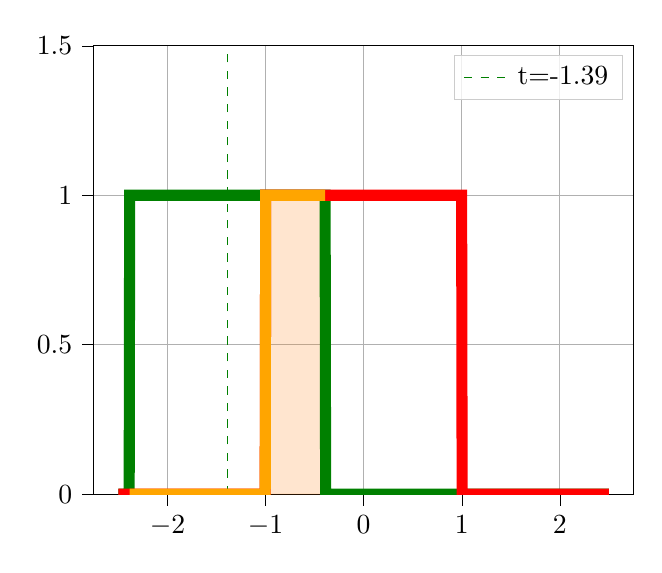
\begin{tikzpicture}

\definecolor{color0}{rgb}{1,0.498039215686275,0.0549019607843137}
\definecolor{color1}{rgb}{1,0.647058823529412,0}

\begin{axis}[
legend cell align={left},
legend style={fill opacity=0.8, draw opacity=1, text opacity=1, draw=white!80!black},
tick align=outside,
tick pos=left,
x grid style={white!69.0196078431373!black},
xmajorgrids,
xmin=-2.75, xmax=2.75,
xtick style={color=black},
y grid style={white!69.0196078431373!black},
ymajorgrids,
ymin=0, ymax=1.5,
ytick style={color=black}
]
\path [draw=color0, fill=color0, opacity=0.2]
(axis cs:-2.38488488488488,0)
--(axis cs:-2.38488488488488,0)
--(axis cs:-2.37987987987988,0)
--(axis cs:-2.37487487487487,0)
--(axis cs:-2.36986986986987,0)
--(axis cs:-2.36486486486486,0)
--(axis cs:-2.35985985985986,0)
--(axis cs:-2.35485485485485,0)
--(axis cs:-2.34984984984985,0)
--(axis cs:-2.34484484484484,0)
--(axis cs:-2.33983983983984,0)
--(axis cs:-2.33483483483483,0)
--(axis cs:-2.32982982982983,0)
--(axis cs:-2.32482482482482,0)
--(axis cs:-2.31981981981982,0)
--(axis cs:-2.31481481481481,0)
--(axis cs:-2.30980980980981,0)
--(axis cs:-2.3048048048048,0)
--(axis cs:-2.2997997997998,0)
--(axis cs:-2.29479479479479,0)
--(axis cs:-2.28978978978979,0)
--(axis cs:-2.28478478478478,0)
--(axis cs:-2.27977977977978,0)
--(axis cs:-2.27477477477477,0)
--(axis cs:-2.26976976976977,0)
--(axis cs:-2.26476476476476,0)
--(axis cs:-2.25975975975976,0)
--(axis cs:-2.25475475475475,0)
--(axis cs:-2.24974974974975,0)
--(axis cs:-2.24474474474474,0)
--(axis cs:-2.23973973973974,0)
--(axis cs:-2.23473473473473,0)
--(axis cs:-2.22972972972973,0)
--(axis cs:-2.22472472472472,0)
--(axis cs:-2.21971971971972,0)
--(axis cs:-2.21471471471471,0)
--(axis cs:-2.20970970970971,0)
--(axis cs:-2.2047047047047,0)
--(axis cs:-2.1996996996997,0)
--(axis cs:-2.19469469469469,0)
--(axis cs:-2.18968968968969,0)
--(axis cs:-2.18468468468468,0)
--(axis cs:-2.17967967967968,0)
--(axis cs:-2.17467467467467,0)
--(axis cs:-2.16966966966967,0)
--(axis cs:-2.16466466466466,0)
--(axis cs:-2.15965965965966,0)
--(axis cs:-2.15465465465465,0)
--(axis cs:-2.14964964964965,0)
--(axis cs:-2.14464464464464,0)
--(axis cs:-2.13963963963964,0)
--(axis cs:-2.13463463463463,0)
--(axis cs:-2.12962962962963,0)
--(axis cs:-2.12462462462462,0)
--(axis cs:-2.11961961961962,0)
--(axis cs:-2.11461461461461,0)
--(axis cs:-2.10960960960961,0)
--(axis cs:-2.1046046046046,0)
--(axis cs:-2.0995995995996,0)
--(axis cs:-2.09459459459459,0)
--(axis cs:-2.08958958958959,0)
--(axis cs:-2.08458458458458,0)
--(axis cs:-2.07957957957958,0)
--(axis cs:-2.07457457457457,0)
--(axis cs:-2.06956956956957,0)
--(axis cs:-2.06456456456456,0)
--(axis cs:-2.05955955955956,0)
--(axis cs:-2.05455455455455,0)
--(axis cs:-2.04954954954955,0)
--(axis cs:-2.04454454454454,0)
--(axis cs:-2.03953953953954,0)
--(axis cs:-2.03453453453453,0)
--(axis cs:-2.02952952952953,0)
--(axis cs:-2.02452452452452,0)
--(axis cs:-2.01951951951952,0)
--(axis cs:-2.01451451451451,0)
--(axis cs:-2.00950950950951,0)
--(axis cs:-2.0045045045045,0)
--(axis cs:-1.9994994994995,0)
--(axis cs:-1.99449449449449,0)
--(axis cs:-1.98948948948949,0)
--(axis cs:-1.98448448448448,0)
--(axis cs:-1.97947947947948,0)
--(axis cs:-1.97447447447447,0)
--(axis cs:-1.96946946946947,0)
--(axis cs:-1.96446446446446,0)
--(axis cs:-1.95945945945946,0)
--(axis cs:-1.95445445445445,0)
--(axis cs:-1.94944944944945,0)
--(axis cs:-1.94444444444444,0)
--(axis cs:-1.93943943943944,0)
--(axis cs:-1.93443443443443,0)
--(axis cs:-1.92942942942943,0)
--(axis cs:-1.92442442442442,0)
--(axis cs:-1.91941941941942,0)
--(axis cs:-1.91441441441441,0)
--(axis cs:-1.90940940940941,0)
--(axis cs:-1.9044044044044,0)
--(axis cs:-1.8993993993994,0)
--(axis cs:-1.89439439439439,0)
--(axis cs:-1.88938938938939,0)
--(axis cs:-1.88438438438438,0)
--(axis cs:-1.87937937937938,0)
--(axis cs:-1.87437437437437,0)
--(axis cs:-1.86936936936937,0)
--(axis cs:-1.86436436436436,0)
--(axis cs:-1.85935935935936,0)
--(axis cs:-1.85435435435435,0)
--(axis cs:-1.84934934934935,0)
--(axis cs:-1.84434434434434,0)
--(axis cs:-1.83933933933934,0)
--(axis cs:-1.83433433433433,0)
--(axis cs:-1.82932932932933,0)
--(axis cs:-1.82432432432432,0)
--(axis cs:-1.81931931931932,0)
--(axis cs:-1.81431431431431,0)
--(axis cs:-1.80930930930931,0)
--(axis cs:-1.8043043043043,0)
--(axis cs:-1.7992992992993,0)
--(axis cs:-1.79429429429429,0)
--(axis cs:-1.78928928928929,0)
--(axis cs:-1.78428428428428,0)
--(axis cs:-1.77927927927928,0)
--(axis cs:-1.77427427427427,0)
--(axis cs:-1.76926926926927,0)
--(axis cs:-1.76426426426426,0)
--(axis cs:-1.75925925925926,0)
--(axis cs:-1.75425425425425,0)
--(axis cs:-1.74924924924925,0)
--(axis cs:-1.74424424424424,0)
--(axis cs:-1.73923923923924,0)
--(axis cs:-1.73423423423423,0)
--(axis cs:-1.72922922922923,0)
--(axis cs:-1.72422422422422,0)
--(axis cs:-1.71921921921922,0)
--(axis cs:-1.71421421421421,0)
--(axis cs:-1.70920920920921,0)
--(axis cs:-1.7042042042042,0)
--(axis cs:-1.6991991991992,0)
--(axis cs:-1.69419419419419,0)
--(axis cs:-1.68918918918919,0)
--(axis cs:-1.68418418418418,0)
--(axis cs:-1.67917917917918,0)
--(axis cs:-1.67417417417417,0)
--(axis cs:-1.66916916916917,0)
--(axis cs:-1.66416416416416,0)
--(axis cs:-1.65915915915916,0)
--(axis cs:-1.65415415415415,0)
--(axis cs:-1.64914914914915,0)
--(axis cs:-1.64414414414414,0)
--(axis cs:-1.63913913913914,0)
--(axis cs:-1.63413413413413,0)
--(axis cs:-1.62912912912913,0)
--(axis cs:-1.62412412412412,0)
--(axis cs:-1.61911911911912,0)
--(axis cs:-1.61411411411411,0)
--(axis cs:-1.60910910910911,0)
--(axis cs:-1.6041041041041,0)
--(axis cs:-1.5990990990991,0)
--(axis cs:-1.59409409409409,0)
--(axis cs:-1.58908908908909,0)
--(axis cs:-1.58408408408408,0)
--(axis cs:-1.57907907907908,0)
--(axis cs:-1.57407407407407,0)
--(axis cs:-1.56906906906907,0)
--(axis cs:-1.56406406406406,0)
--(axis cs:-1.55905905905906,0)
--(axis cs:-1.55405405405405,0)
--(axis cs:-1.54904904904905,0)
--(axis cs:-1.54404404404404,0)
--(axis cs:-1.53903903903904,0)
--(axis cs:-1.53403403403403,0)
--(axis cs:-1.52902902902903,0)
--(axis cs:-1.52402402402402,0)
--(axis cs:-1.51901901901902,0)
--(axis cs:-1.51401401401401,0)
--(axis cs:-1.50900900900901,0)
--(axis cs:-1.504004004004,0)
--(axis cs:-1.498998998999,0)
--(axis cs:-1.49399399399399,0)
--(axis cs:-1.48898898898899,0)
--(axis cs:-1.48398398398398,0)
--(axis cs:-1.47897897897898,0)
--(axis cs:-1.47397397397397,0)
--(axis cs:-1.46896896896897,0)
--(axis cs:-1.46396396396396,0)
--(axis cs:-1.45895895895896,0)
--(axis cs:-1.45395395395395,0)
--(axis cs:-1.44894894894895,0)
--(axis cs:-1.44394394394394,0)
--(axis cs:-1.43893893893894,0)
--(axis cs:-1.43393393393393,0)
--(axis cs:-1.42892892892893,0)
--(axis cs:-1.42392392392392,0)
--(axis cs:-1.41891891891892,0)
--(axis cs:-1.41391391391391,0)
--(axis cs:-1.40890890890891,0)
--(axis cs:-1.4039039039039,0)
--(axis cs:-1.3988988988989,0)
--(axis cs:-1.39389389389389,0)
--(axis cs:-1.38888888888889,0)
--(axis cs:-1.38388388388388,0)
--(axis cs:-1.37887887887888,0)
--(axis cs:-1.37387387387387,0)
--(axis cs:-1.36886886886887,0)
--(axis cs:-1.36386386386386,0)
--(axis cs:-1.35885885885886,0)
--(axis cs:-1.35385385385385,0)
--(axis cs:-1.34884884884885,0)
--(axis cs:-1.34384384384384,0)
--(axis cs:-1.33883883883884,0)
--(axis cs:-1.33383383383383,0)
--(axis cs:-1.32882882882883,0)
--(axis cs:-1.32382382382382,0)
--(axis cs:-1.31881881881882,0)
--(axis cs:-1.31381381381381,0)
--(axis cs:-1.30880880880881,0)
--(axis cs:-1.3038038038038,0)
--(axis cs:-1.2987987987988,0)
--(axis cs:-1.29379379379379,0)
--(axis cs:-1.28878878878879,0)
--(axis cs:-1.28378378378378,0)
--(axis cs:-1.27877877877878,0)
--(axis cs:-1.27377377377377,0)
--(axis cs:-1.26876876876877,0)
--(axis cs:-1.26376376376376,0)
--(axis cs:-1.25875875875876,0)
--(axis cs:-1.25375375375375,0)
--(axis cs:-1.24874874874875,0)
--(axis cs:-1.24374374374374,0)
--(axis cs:-1.23873873873874,0)
--(axis cs:-1.23373373373373,0)
--(axis cs:-1.22872872872873,0)
--(axis cs:-1.22372372372372,0)
--(axis cs:-1.21871871871872,0)
--(axis cs:-1.21371371371371,0)
--(axis cs:-1.20870870870871,0)
--(axis cs:-1.2037037037037,0)
--(axis cs:-1.1986986986987,0)
--(axis cs:-1.19369369369369,0)
--(axis cs:-1.18868868868869,0)
--(axis cs:-1.18368368368368,0)
--(axis cs:-1.17867867867868,0)
--(axis cs:-1.17367367367367,0)
--(axis cs:-1.16866866866867,0)
--(axis cs:-1.16366366366366,0)
--(axis cs:-1.15865865865866,0)
--(axis cs:-1.15365365365365,0)
--(axis cs:-1.14864864864865,0)
--(axis cs:-1.14364364364364,0)
--(axis cs:-1.13863863863864,0)
--(axis cs:-1.13363363363363,0)
--(axis cs:-1.12862862862863,0)
--(axis cs:-1.12362362362362,0)
--(axis cs:-1.11861861861862,0)
--(axis cs:-1.11361361361361,0)
--(axis cs:-1.10860860860861,0)
--(axis cs:-1.1036036036036,0)
--(axis cs:-1.0985985985986,0)
--(axis cs:-1.09359359359359,0)
--(axis cs:-1.08858858858859,0)
--(axis cs:-1.08358358358358,0)
--(axis cs:-1.07857857857858,0)
--(axis cs:-1.07357357357357,0)
--(axis cs:-1.06856856856857,0)
--(axis cs:-1.06356356356356,0)
--(axis cs:-1.05855855855856,0)
--(axis cs:-1.05355355355355,0)
--(axis cs:-1.04854854854855,0)
--(axis cs:-1.04354354354354,0)
--(axis cs:-1.03853853853854,0)
--(axis cs:-1.03353353353353,0)
--(axis cs:-1.02852852852853,0)
--(axis cs:-1.02352352352352,0)
--(axis cs:-1.01851851851852,0)
--(axis cs:-1.01351351351351,0)
--(axis cs:-1.00850850850851,0)
--(axis cs:-1.0035035035035,0)
--(axis cs:-0.998498498498499,0)
--(axis cs:-0.993493493493494,0)
--(axis cs:-0.988488488488489,0)
--(axis cs:-0.983483483483484,0)
--(axis cs:-0.978478478478479,0)
--(axis cs:-0.973473473473474,0)
--(axis cs:-0.968468468468469,0)
--(axis cs:-0.963463463463464,0)
--(axis cs:-0.958458458458459,0)
--(axis cs:-0.953453453453454,0)
--(axis cs:-0.948448448448449,0)
--(axis cs:-0.943443443443444,0)
--(axis cs:-0.938438438438439,0)
--(axis cs:-0.933433433433434,0)
--(axis cs:-0.928428428428429,0)
--(axis cs:-0.923423423423424,0)
--(axis cs:-0.918418418418419,0)
--(axis cs:-0.913413413413414,0)
--(axis cs:-0.908408408408409,0)
--(axis cs:-0.903403403403404,0)
--(axis cs:-0.898398398398399,0)
--(axis cs:-0.893393393393393,0)
--(axis cs:-0.888388388388388,0)
--(axis cs:-0.883383383383383,0)
--(axis cs:-0.878378378378378,0)
--(axis cs:-0.873373373373373,0)
--(axis cs:-0.868368368368368,0)
--(axis cs:-0.863363363363363,0)
--(axis cs:-0.858358358358358,0)
--(axis cs:-0.853353353353353,0)
--(axis cs:-0.848348348348348,0)
--(axis cs:-0.843343343343343,0)
--(axis cs:-0.838338338338338,0)
--(axis cs:-0.833333333333333,0)
--(axis cs:-0.828328328328328,0)
--(axis cs:-0.823323323323323,0)
--(axis cs:-0.818318318318318,0)
--(axis cs:-0.813313313313313,0)
--(axis cs:-0.808308308308308,0)
--(axis cs:-0.803303303303303,0)
--(axis cs:-0.798298298298298,0)
--(axis cs:-0.793293293293293,0)
--(axis cs:-0.788288288288288,0)
--(axis cs:-0.783283283283283,0)
--(axis cs:-0.778278278278278,0)
--(axis cs:-0.773273273273273,0)
--(axis cs:-0.768268268268268,0)
--(axis cs:-0.763263263263263,0)
--(axis cs:-0.758258258258258,0)
--(axis cs:-0.753253253253253,0)
--(axis cs:-0.748248248248248,0)
--(axis cs:-0.743243243243243,0)
--(axis cs:-0.738238238238238,0)
--(axis cs:-0.733233233233233,0)
--(axis cs:-0.728228228228228,0)
--(axis cs:-0.723223223223223,0)
--(axis cs:-0.718218218218218,0)
--(axis cs:-0.713213213213213,0)
--(axis cs:-0.708208208208208,0)
--(axis cs:-0.703203203203203,0)
--(axis cs:-0.698198198198198,0)
--(axis cs:-0.693193193193193,0)
--(axis cs:-0.688188188188188,0)
--(axis cs:-0.683183183183183,0)
--(axis cs:-0.678178178178178,0)
--(axis cs:-0.673173173173173,0)
--(axis cs:-0.668168168168168,0)
--(axis cs:-0.663163163163163,0)
--(axis cs:-0.658158158158158,0)
--(axis cs:-0.653153153153153,0)
--(axis cs:-0.648148148148148,0)
--(axis cs:-0.643143143143143,0)
--(axis cs:-0.638138138138138,0)
--(axis cs:-0.633133133133133,0)
--(axis cs:-0.628128128128128,0)
--(axis cs:-0.623123123123123,0)
--(axis cs:-0.618118118118118,0)
--(axis cs:-0.613113113113113,0)
--(axis cs:-0.608108108108108,0)
--(axis cs:-0.603103103103103,0)
--(axis cs:-0.598098098098098,0)
--(axis cs:-0.593093093093093,0)
--(axis cs:-0.588088088088088,0)
--(axis cs:-0.583083083083083,0)
--(axis cs:-0.578078078078078,0)
--(axis cs:-0.573073073073073,0)
--(axis cs:-0.568068068068068,0)
--(axis cs:-0.563063063063063,0)
--(axis cs:-0.558058058058058,0)
--(axis cs:-0.553053053053053,0)
--(axis cs:-0.548048048048048,0)
--(axis cs:-0.543043043043043,0)
--(axis cs:-0.538038038038038,0)
--(axis cs:-0.533033033033033,0)
--(axis cs:-0.528028028028028,0)
--(axis cs:-0.523023023023023,0)
--(axis cs:-0.518018018018018,0)
--(axis cs:-0.513013013013013,0)
--(axis cs:-0.508008008008008,0)
--(axis cs:-0.503003003003003,0)
--(axis cs:-0.497997997997998,0)
--(axis cs:-0.492992992992993,0)
--(axis cs:-0.487987987987988,0)
--(axis cs:-0.482982982982983,0)
--(axis cs:-0.477977977977978,0)
--(axis cs:-0.472972972972973,0)
--(axis cs:-0.467967967967968,0)
--(axis cs:-0.462962962962963,0)
--(axis cs:-0.457957957957958,0)
--(axis cs:-0.452952952952953,0)
--(axis cs:-0.447947947947948,0)
--(axis cs:-0.442942942942943,0)
--(axis cs:-0.437937937937938,0)
--(axis cs:-0.432932932932933,0)
--(axis cs:-0.427927927927928,0)
--(axis cs:-0.422922922922923,0)
--(axis cs:-0.417917917917918,0)
--(axis cs:-0.412912912912913,0)
--(axis cs:-0.407907907907908,0)
--(axis cs:-0.402902902902903,0)
--(axis cs:-0.397897897897898,0)
--(axis cs:-0.392892892892893,0)
--(axis cs:-0.392892892892893,1)
--(axis cs:-0.392892892892893,1)
--(axis cs:-0.397897897897898,1)
--(axis cs:-0.402902902902903,1)
--(axis cs:-0.407907907907908,1)
--(axis cs:-0.412912912912913,1)
--(axis cs:-0.417917917917918,1)
--(axis cs:-0.422922922922923,1)
--(axis cs:-0.427927927927928,1)
--(axis cs:-0.432932932932933,1)
--(axis cs:-0.437937937937938,1)
--(axis cs:-0.442942942942943,1)
--(axis cs:-0.447947947947948,1)
--(axis cs:-0.452952952952953,1)
--(axis cs:-0.457957957957958,1)
--(axis cs:-0.462962962962963,1)
--(axis cs:-0.467967967967968,1)
--(axis cs:-0.472972972972973,1)
--(axis cs:-0.477977977977978,1)
--(axis cs:-0.482982982982983,1)
--(axis cs:-0.487987987987988,1)
--(axis cs:-0.492992992992993,1)
--(axis cs:-0.497997997997998,1)
--(axis cs:-0.503003003003003,1)
--(axis cs:-0.508008008008008,1)
--(axis cs:-0.513013013013013,1)
--(axis cs:-0.518018018018018,1)
--(axis cs:-0.523023023023023,1)
--(axis cs:-0.528028028028028,1)
--(axis cs:-0.533033033033033,1)
--(axis cs:-0.538038038038038,1)
--(axis cs:-0.543043043043043,1)
--(axis cs:-0.548048048048048,1)
--(axis cs:-0.553053053053053,1)
--(axis cs:-0.558058058058058,1)
--(axis cs:-0.563063063063063,1)
--(axis cs:-0.568068068068068,1)
--(axis cs:-0.573073073073073,1)
--(axis cs:-0.578078078078078,1)
--(axis cs:-0.583083083083083,1)
--(axis cs:-0.588088088088088,1)
--(axis cs:-0.593093093093093,1)
--(axis cs:-0.598098098098098,1)
--(axis cs:-0.603103103103103,1)
--(axis cs:-0.608108108108108,1)
--(axis cs:-0.613113113113113,1)
--(axis cs:-0.618118118118118,1)
--(axis cs:-0.623123123123123,1)
--(axis cs:-0.628128128128128,1)
--(axis cs:-0.633133133133133,1)
--(axis cs:-0.638138138138138,1)
--(axis cs:-0.643143143143143,1)
--(axis cs:-0.648148148148148,1)
--(axis cs:-0.653153153153153,1)
--(axis cs:-0.658158158158158,1)
--(axis cs:-0.663163163163163,1)
--(axis cs:-0.668168168168168,1)
--(axis cs:-0.673173173173173,1)
--(axis cs:-0.678178178178178,1)
--(axis cs:-0.683183183183183,1)
--(axis cs:-0.688188188188188,1)
--(axis cs:-0.693193193193193,1)
--(axis cs:-0.698198198198198,1)
--(axis cs:-0.703203203203203,1)
--(axis cs:-0.708208208208208,1)
--(axis cs:-0.713213213213213,1)
--(axis cs:-0.718218218218218,1)
--(axis cs:-0.723223223223223,1)
--(axis cs:-0.728228228228228,1)
--(axis cs:-0.733233233233233,1)
--(axis cs:-0.738238238238238,1)
--(axis cs:-0.743243243243243,1)
--(axis cs:-0.748248248248248,1)
--(axis cs:-0.753253253253253,1)
--(axis cs:-0.758258258258258,1)
--(axis cs:-0.763263263263263,1)
--(axis cs:-0.768268268268268,1)
--(axis cs:-0.773273273273273,1)
--(axis cs:-0.778278278278278,1)
--(axis cs:-0.783283283283283,1)
--(axis cs:-0.788288288288288,1)
--(axis cs:-0.793293293293293,1)
--(axis cs:-0.798298298298298,1)
--(axis cs:-0.803303303303303,1)
--(axis cs:-0.808308308308308,1)
--(axis cs:-0.813313313313313,1)
--(axis cs:-0.818318318318318,1)
--(axis cs:-0.823323323323323,1)
--(axis cs:-0.828328328328328,1)
--(axis cs:-0.833333333333333,1)
--(axis cs:-0.838338338338338,1)
--(axis cs:-0.843343343343343,1)
--(axis cs:-0.848348348348348,1)
--(axis cs:-0.853353353353353,1)
--(axis cs:-0.858358358358358,1)
--(axis cs:-0.863363363363363,1)
--(axis cs:-0.868368368368368,1)
--(axis cs:-0.873373373373373,1)
--(axis cs:-0.878378378378378,1)
--(axis cs:-0.883383383383383,1)
--(axis cs:-0.888388388388388,1)
--(axis cs:-0.893393393393393,1)
--(axis cs:-0.898398398398399,1)
--(axis cs:-0.903403403403404,1)
--(axis cs:-0.908408408408409,1)
--(axis cs:-0.913413413413414,1)
--(axis cs:-0.918418418418419,1)
--(axis cs:-0.923423423423424,1)
--(axis cs:-0.928428428428429,1)
--(axis cs:-0.933433433433434,1)
--(axis cs:-0.938438438438439,1)
--(axis cs:-0.943443443443444,1)
--(axis cs:-0.948448448448449,1)
--(axis cs:-0.953453453453454,1)
--(axis cs:-0.958458458458459,1)
--(axis cs:-0.963463463463464,1)
--(axis cs:-0.968468468468469,1)
--(axis cs:-0.973473473473474,1)
--(axis cs:-0.978478478478479,1)
--(axis cs:-0.983483483483484,1)
--(axis cs:-0.988488488488489,1)
--(axis cs:-0.993493493493494,1)
--(axis cs:-0.998498498498499,1)
--(axis cs:-1.0035035035035,0)
--(axis cs:-1.00850850850851,0)
--(axis cs:-1.01351351351351,0)
--(axis cs:-1.01851851851852,0)
--(axis cs:-1.02352352352352,0)
--(axis cs:-1.02852852852853,0)
--(axis cs:-1.03353353353353,0)
--(axis cs:-1.03853853853854,0)
--(axis cs:-1.04354354354354,0)
--(axis cs:-1.04854854854855,0)
--(axis cs:-1.05355355355355,0)
--(axis cs:-1.05855855855856,0)
--(axis cs:-1.06356356356356,0)
--(axis cs:-1.06856856856857,0)
--(axis cs:-1.07357357357357,0)
--(axis cs:-1.07857857857858,0)
--(axis cs:-1.08358358358358,0)
--(axis cs:-1.08858858858859,0)
--(axis cs:-1.09359359359359,0)
--(axis cs:-1.0985985985986,0)
--(axis cs:-1.1036036036036,0)
--(axis cs:-1.10860860860861,0)
--(axis cs:-1.11361361361361,0)
--(axis cs:-1.11861861861862,0)
--(axis cs:-1.12362362362362,0)
--(axis cs:-1.12862862862863,0)
--(axis cs:-1.13363363363363,0)
--(axis cs:-1.13863863863864,0)
--(axis cs:-1.14364364364364,0)
--(axis cs:-1.14864864864865,0)
--(axis cs:-1.15365365365365,0)
--(axis cs:-1.15865865865866,0)
--(axis cs:-1.16366366366366,0)
--(axis cs:-1.16866866866867,0)
--(axis cs:-1.17367367367367,0)
--(axis cs:-1.17867867867868,0)
--(axis cs:-1.18368368368368,0)
--(axis cs:-1.18868868868869,0)
--(axis cs:-1.19369369369369,0)
--(axis cs:-1.1986986986987,0)
--(axis cs:-1.2037037037037,0)
--(axis cs:-1.20870870870871,0)
--(axis cs:-1.21371371371371,0)
--(axis cs:-1.21871871871872,0)
--(axis cs:-1.22372372372372,0)
--(axis cs:-1.22872872872873,0)
--(axis cs:-1.23373373373373,0)
--(axis cs:-1.23873873873874,0)
--(axis cs:-1.24374374374374,0)
--(axis cs:-1.24874874874875,0)
--(axis cs:-1.25375375375375,0)
--(axis cs:-1.25875875875876,0)
--(axis cs:-1.26376376376376,0)
--(axis cs:-1.26876876876877,0)
--(axis cs:-1.27377377377377,0)
--(axis cs:-1.27877877877878,0)
--(axis cs:-1.28378378378378,0)
--(axis cs:-1.28878878878879,0)
--(axis cs:-1.29379379379379,0)
--(axis cs:-1.2987987987988,0)
--(axis cs:-1.3038038038038,0)
--(axis cs:-1.30880880880881,0)
--(axis cs:-1.31381381381381,0)
--(axis cs:-1.31881881881882,0)
--(axis cs:-1.32382382382382,0)
--(axis cs:-1.32882882882883,0)
--(axis cs:-1.33383383383383,0)
--(axis cs:-1.33883883883884,0)
--(axis cs:-1.34384384384384,0)
--(axis cs:-1.34884884884885,0)
--(axis cs:-1.35385385385385,0)
--(axis cs:-1.35885885885886,0)
--(axis cs:-1.36386386386386,0)
--(axis cs:-1.36886886886887,0)
--(axis cs:-1.37387387387387,0)
--(axis cs:-1.37887887887888,0)
--(axis cs:-1.38388388388388,0)
--(axis cs:-1.38888888888889,0)
--(axis cs:-1.39389389389389,0)
--(axis cs:-1.3988988988989,0)
--(axis cs:-1.4039039039039,0)
--(axis cs:-1.40890890890891,0)
--(axis cs:-1.41391391391391,0)
--(axis cs:-1.41891891891892,0)
--(axis cs:-1.42392392392392,0)
--(axis cs:-1.42892892892893,0)
--(axis cs:-1.43393393393393,0)
--(axis cs:-1.43893893893894,0)
--(axis cs:-1.44394394394394,0)
--(axis cs:-1.44894894894895,0)
--(axis cs:-1.45395395395395,0)
--(axis cs:-1.45895895895896,0)
--(axis cs:-1.46396396396396,0)
--(axis cs:-1.46896896896897,0)
--(axis cs:-1.47397397397397,0)
--(axis cs:-1.47897897897898,0)
--(axis cs:-1.48398398398398,0)
--(axis cs:-1.48898898898899,0)
--(axis cs:-1.49399399399399,0)
--(axis cs:-1.498998998999,0)
--(axis cs:-1.504004004004,0)
--(axis cs:-1.50900900900901,0)
--(axis cs:-1.51401401401401,0)
--(axis cs:-1.51901901901902,0)
--(axis cs:-1.52402402402402,0)
--(axis cs:-1.52902902902903,0)
--(axis cs:-1.53403403403403,0)
--(axis cs:-1.53903903903904,0)
--(axis cs:-1.54404404404404,0)
--(axis cs:-1.54904904904905,0)
--(axis cs:-1.55405405405405,0)
--(axis cs:-1.55905905905906,0)
--(axis cs:-1.56406406406406,0)
--(axis cs:-1.56906906906907,0)
--(axis cs:-1.57407407407407,0)
--(axis cs:-1.57907907907908,0)
--(axis cs:-1.58408408408408,0)
--(axis cs:-1.58908908908909,0)
--(axis cs:-1.59409409409409,0)
--(axis cs:-1.5990990990991,0)
--(axis cs:-1.6041041041041,0)
--(axis cs:-1.60910910910911,0)
--(axis cs:-1.61411411411411,0)
--(axis cs:-1.61911911911912,0)
--(axis cs:-1.62412412412412,0)
--(axis cs:-1.62912912912913,0)
--(axis cs:-1.63413413413413,0)
--(axis cs:-1.63913913913914,0)
--(axis cs:-1.64414414414414,0)
--(axis cs:-1.64914914914915,0)
--(axis cs:-1.65415415415415,0)
--(axis cs:-1.65915915915916,0)
--(axis cs:-1.66416416416416,0)
--(axis cs:-1.66916916916917,0)
--(axis cs:-1.67417417417417,0)
--(axis cs:-1.67917917917918,0)
--(axis cs:-1.68418418418418,0)
--(axis cs:-1.68918918918919,0)
--(axis cs:-1.69419419419419,0)
--(axis cs:-1.6991991991992,0)
--(axis cs:-1.7042042042042,0)
--(axis cs:-1.70920920920921,0)
--(axis cs:-1.71421421421421,0)
--(axis cs:-1.71921921921922,0)
--(axis cs:-1.72422422422422,0)
--(axis cs:-1.72922922922923,0)
--(axis cs:-1.73423423423423,0)
--(axis cs:-1.73923923923924,0)
--(axis cs:-1.74424424424424,0)
--(axis cs:-1.74924924924925,0)
--(axis cs:-1.75425425425425,0)
--(axis cs:-1.75925925925926,0)
--(axis cs:-1.76426426426426,0)
--(axis cs:-1.76926926926927,0)
--(axis cs:-1.77427427427427,0)
--(axis cs:-1.77927927927928,0)
--(axis cs:-1.78428428428428,0)
--(axis cs:-1.78928928928929,0)
--(axis cs:-1.79429429429429,0)
--(axis cs:-1.7992992992993,0)
--(axis cs:-1.8043043043043,0)
--(axis cs:-1.80930930930931,0)
--(axis cs:-1.81431431431431,0)
--(axis cs:-1.81931931931932,0)
--(axis cs:-1.82432432432432,0)
--(axis cs:-1.82932932932933,0)
--(axis cs:-1.83433433433433,0)
--(axis cs:-1.83933933933934,0)
--(axis cs:-1.84434434434434,0)
--(axis cs:-1.84934934934935,0)
--(axis cs:-1.85435435435435,0)
--(axis cs:-1.85935935935936,0)
--(axis cs:-1.86436436436436,0)
--(axis cs:-1.86936936936937,0)
--(axis cs:-1.87437437437437,0)
--(axis cs:-1.87937937937938,0)
--(axis cs:-1.88438438438438,0)
--(axis cs:-1.88938938938939,0)
--(axis cs:-1.89439439439439,0)
--(axis cs:-1.8993993993994,0)
--(axis cs:-1.9044044044044,0)
--(axis cs:-1.90940940940941,0)
--(axis cs:-1.91441441441441,0)
--(axis cs:-1.91941941941942,0)
--(axis cs:-1.92442442442442,0)
--(axis cs:-1.92942942942943,0)
--(axis cs:-1.93443443443443,0)
--(axis cs:-1.93943943943944,0)
--(axis cs:-1.94444444444444,0)
--(axis cs:-1.94944944944945,0)
--(axis cs:-1.95445445445445,0)
--(axis cs:-1.95945945945946,0)
--(axis cs:-1.96446446446446,0)
--(axis cs:-1.96946946946947,0)
--(axis cs:-1.97447447447447,0)
--(axis cs:-1.97947947947948,0)
--(axis cs:-1.98448448448448,0)
--(axis cs:-1.98948948948949,0)
--(axis cs:-1.99449449449449,0)
--(axis cs:-1.9994994994995,0)
--(axis cs:-2.0045045045045,0)
--(axis cs:-2.00950950950951,0)
--(axis cs:-2.01451451451451,0)
--(axis cs:-2.01951951951952,0)
--(axis cs:-2.02452452452452,0)
--(axis cs:-2.02952952952953,0)
--(axis cs:-2.03453453453453,0)
--(axis cs:-2.03953953953954,0)
--(axis cs:-2.04454454454454,0)
--(axis cs:-2.04954954954955,0)
--(axis cs:-2.05455455455455,0)
--(axis cs:-2.05955955955956,0)
--(axis cs:-2.06456456456456,0)
--(axis cs:-2.06956956956957,0)
--(axis cs:-2.07457457457457,0)
--(axis cs:-2.07957957957958,0)
--(axis cs:-2.08458458458458,0)
--(axis cs:-2.08958958958959,0)
--(axis cs:-2.09459459459459,0)
--(axis cs:-2.0995995995996,0)
--(axis cs:-2.1046046046046,0)
--(axis cs:-2.10960960960961,0)
--(axis cs:-2.11461461461461,0)
--(axis cs:-2.11961961961962,0)
--(axis cs:-2.12462462462462,0)
--(axis cs:-2.12962962962963,0)
--(axis cs:-2.13463463463463,0)
--(axis cs:-2.13963963963964,0)
--(axis cs:-2.14464464464464,0)
--(axis cs:-2.14964964964965,0)
--(axis cs:-2.15465465465465,0)
--(axis cs:-2.15965965965966,0)
--(axis cs:-2.16466466466466,0)
--(axis cs:-2.16966966966967,0)
--(axis cs:-2.17467467467467,0)
--(axis cs:-2.17967967967968,0)
--(axis cs:-2.18468468468468,0)
--(axis cs:-2.18968968968969,0)
--(axis cs:-2.19469469469469,0)
--(axis cs:-2.1996996996997,0)
--(axis cs:-2.2047047047047,0)
--(axis cs:-2.20970970970971,0)
--(axis cs:-2.21471471471471,0)
--(axis cs:-2.21971971971972,0)
--(axis cs:-2.22472472472472,0)
--(axis cs:-2.22972972972973,0)
--(axis cs:-2.23473473473473,0)
--(axis cs:-2.23973973973974,0)
--(axis cs:-2.24474474474474,0)
--(axis cs:-2.24974974974975,0)
--(axis cs:-2.25475475475475,0)
--(axis cs:-2.25975975975976,0)
--(axis cs:-2.26476476476476,0)
--(axis cs:-2.26976976976977,0)
--(axis cs:-2.27477477477477,0)
--(axis cs:-2.27977977977978,0)
--(axis cs:-2.28478478478478,0)
--(axis cs:-2.28978978978979,0)
--(axis cs:-2.29479479479479,0)
--(axis cs:-2.2997997997998,0)
--(axis cs:-2.3048048048048,0)
--(axis cs:-2.30980980980981,0)
--(axis cs:-2.31481481481481,0)
--(axis cs:-2.31981981981982,0)
--(axis cs:-2.32482482482482,0)
--(axis cs:-2.32982982982983,0)
--(axis cs:-2.33483483483483,0)
--(axis cs:-2.33983983983984,0)
--(axis cs:-2.34484484484484,0)
--(axis cs:-2.34984984984985,0)
--(axis cs:-2.35485485485485,0)
--(axis cs:-2.35985985985986,0)
--(axis cs:-2.36486486486486,0)
--(axis cs:-2.36986986986987,0)
--(axis cs:-2.37487487487487,0)
--(axis cs:-2.37987987987988,0)
--(axis cs:-2.38488488488488,0)
--cycle;

\addplot [line width=4pt, green!50!black, forget plot]
table {%
-2.5 0
-2.49499499499499 0
-2.48998998998999 0
-2.48498498498498 0
-2.47997997997998 0
-2.47497497497497 0
-2.46996996996997 0
-2.46496496496496 0
-2.45995995995996 0
-2.45495495495495 0
-2.44994994994995 0
-2.44494494494494 0
-2.43993993993994 0
-2.43493493493493 0
-2.42992992992993 0
-2.42492492492492 0
-2.41991991991992 0
-2.41491491491491 0
-2.40990990990991 0
-2.4049049049049 0
-2.3998998998999 0
-2.39489489489489 0
-2.38988988988989 0
-2.38488488488488 1
-2.37987987987988 1
-2.37487487487487 1
-2.36986986986987 1
-2.36486486486486 1
-2.35985985985986 1
-2.35485485485485 1
-2.34984984984985 1
-2.34484484484484 1
-2.33983983983984 1
-2.33483483483483 1
-2.32982982982983 1
-2.32482482482482 1
-2.31981981981982 1
-2.31481481481481 1
-2.30980980980981 1
-2.3048048048048 1
-2.2997997997998 1
-2.29479479479479 1
-2.28978978978979 1
-2.28478478478478 1
-2.27977977977978 1
-2.27477477477477 1
-2.26976976976977 1
-2.26476476476476 1
-2.25975975975976 1
-2.25475475475475 1
-2.24974974974975 1
-2.24474474474474 1
-2.23973973973974 1
-2.23473473473473 1
-2.22972972972973 1
-2.22472472472472 1
-2.21971971971972 1
-2.21471471471471 1
-2.20970970970971 1
-2.2047047047047 1
-2.1996996996997 1
-2.19469469469469 1
-2.18968968968969 1
-2.18468468468468 1
-2.17967967967968 1
-2.17467467467467 1
-2.16966966966967 1
-2.16466466466466 1
-2.15965965965966 1
-2.15465465465465 1
-2.14964964964965 1
-2.14464464464464 1
-2.13963963963964 1
-2.13463463463463 1
-2.12962962962963 1
-2.12462462462462 1
-2.11961961961962 1
-2.11461461461461 1
-2.10960960960961 1
-2.1046046046046 1
-2.0995995995996 1
-2.09459459459459 1
-2.08958958958959 1
-2.08458458458458 1
-2.07957957957958 1
-2.07457457457457 1
-2.06956956956957 1
-2.06456456456456 1
-2.05955955955956 1
-2.05455455455455 1
-2.04954954954955 1
-2.04454454454454 1
-2.03953953953954 1
-2.03453453453453 1
-2.02952952952953 1
-2.02452452452452 1
-2.01951951951952 1
-2.01451451451451 1
-2.00950950950951 1
-2.0045045045045 1
-1.9994994994995 1
-1.99449449449449 1
-1.98948948948949 1
-1.98448448448448 1
-1.97947947947948 1
-1.97447447447447 1
-1.96946946946947 1
-1.96446446446446 1
-1.95945945945946 1
-1.95445445445445 1
-1.94944944944945 1
-1.94444444444444 1
-1.93943943943944 1
-1.93443443443443 1
-1.92942942942943 1
-1.92442442442442 1
-1.91941941941942 1
-1.91441441441441 1
-1.90940940940941 1
-1.9044044044044 1
-1.8993993993994 1
-1.89439439439439 1
-1.88938938938939 1
-1.88438438438438 1
-1.87937937937938 1
-1.87437437437437 1
-1.86936936936937 1
-1.86436436436436 1
-1.85935935935936 1
-1.85435435435435 1
-1.84934934934935 1
-1.84434434434434 1
-1.83933933933934 1
-1.83433433433433 1
-1.82932932932933 1
-1.82432432432432 1
-1.81931931931932 1
-1.81431431431431 1
-1.80930930930931 1
-1.8043043043043 1
-1.7992992992993 1
-1.79429429429429 1
-1.78928928928929 1
-1.78428428428428 1
-1.77927927927928 1
-1.77427427427427 1
-1.76926926926927 1
-1.76426426426426 1
-1.75925925925926 1
-1.75425425425425 1
-1.74924924924925 1
-1.74424424424424 1
-1.73923923923924 1
-1.73423423423423 1
-1.72922922922923 1
-1.72422422422422 1
-1.71921921921922 1
-1.71421421421421 1
-1.70920920920921 1
-1.7042042042042 1
-1.6991991991992 1
-1.69419419419419 1
-1.68918918918919 1
-1.68418418418418 1
-1.67917917917918 1
-1.67417417417417 1
-1.66916916916917 1
-1.66416416416416 1
-1.65915915915916 1
-1.65415415415415 1
-1.64914914914915 1
-1.64414414414414 1
-1.63913913913914 1
-1.63413413413413 1
-1.62912912912913 1
-1.62412412412412 1
-1.61911911911912 1
-1.61411411411411 1
-1.60910910910911 1
-1.6041041041041 1
-1.5990990990991 1
-1.59409409409409 1
-1.58908908908909 1
-1.58408408408408 1
-1.57907907907908 1
-1.57407407407407 1
-1.56906906906907 1
-1.56406406406406 1
-1.55905905905906 1
-1.55405405405405 1
-1.54904904904905 1
-1.54404404404404 1
-1.53903903903904 1
-1.53403403403403 1
-1.52902902902903 1
-1.52402402402402 1
-1.51901901901902 1
-1.51401401401401 1
-1.50900900900901 1
-1.504004004004 1
-1.498998998999 1
-1.49399399399399 1
-1.48898898898899 1
-1.48398398398398 1
-1.47897897897898 1
-1.47397397397397 1
-1.46896896896897 1
-1.46396396396396 1
-1.45895895895896 1
-1.45395395395395 1
-1.44894894894895 1
-1.44394394394394 1
-1.43893893893894 1
-1.43393393393393 1
-1.42892892892893 1
-1.42392392392392 1
-1.41891891891892 1
-1.41391391391391 1
-1.40890890890891 1
-1.4039039039039 1
-1.3988988988989 1
-1.39389389389389 1
-1.38888888888889 1
-1.38388388388388 1
-1.37887887887888 1
-1.37387387387387 1
-1.36886886886887 1
-1.36386386386386 1
-1.35885885885886 1
-1.35385385385385 1
-1.34884884884885 1
-1.34384384384384 1
-1.33883883883884 1
-1.33383383383383 1
-1.32882882882883 1
-1.32382382382382 1
-1.31881881881882 1
-1.31381381381381 1
-1.30880880880881 1
-1.3038038038038 1
-1.2987987987988 1
-1.29379379379379 1
-1.28878878878879 1
-1.28378378378378 1
-1.27877877877878 1
-1.27377377377377 1
-1.26876876876877 1
-1.26376376376376 1
-1.25875875875876 1
-1.25375375375375 1
-1.24874874874875 1
-1.24374374374374 1
-1.23873873873874 1
-1.23373373373373 1
-1.22872872872873 1
-1.22372372372372 1
-1.21871871871872 1
-1.21371371371371 1
-1.20870870870871 1
-1.2037037037037 1
-1.1986986986987 1
-1.19369369369369 1
-1.18868868868869 1
-1.18368368368368 1
-1.17867867867868 1
-1.17367367367367 1
-1.16866866866867 1
-1.16366366366366 1
-1.15865865865866 1
-1.15365365365365 1
-1.14864864864865 1
-1.14364364364364 1
-1.13863863863864 1
-1.13363363363363 1
-1.12862862862863 1
-1.12362362362362 1
-1.11861861861862 1
-1.11361361361361 1
-1.10860860860861 1
-1.1036036036036 1
-1.0985985985986 1
-1.09359359359359 1
-1.08858858858859 1
-1.08358358358358 1
-1.07857857857858 1
-1.07357357357357 1
-1.06856856856857 1
-1.06356356356356 1
-1.05855855855856 1
-1.05355355355355 1
-1.04854854854855 1
-1.04354354354354 1
-1.03853853853854 1
-1.03353353353353 1
-1.02852852852853 1
-1.02352352352352 1
-1.01851851851852 1
-1.01351351351351 1
-1.00850850850851 1
-1.0035035035035 1
-0.998498498498499 1
-0.993493493493494 1
-0.988488488488489 1
-0.983483483483484 1
-0.978478478478479 1
-0.973473473473474 1
-0.968468468468469 1
-0.963463463463464 1
-0.958458458458459 1
-0.953453453453454 1
-0.948448448448449 1
-0.943443443443444 1
-0.938438438438439 1
-0.933433433433434 1
-0.928428428428429 1
-0.923423423423424 1
-0.918418418418419 1
-0.913413413413414 1
-0.908408408408409 1
-0.903403403403404 1
-0.898398398398399 1
-0.893393393393393 1
-0.888388388388388 1
-0.883383383383383 1
-0.878378378378378 1
-0.873373373373373 1
-0.868368368368368 1
-0.863363363363363 1
-0.858358358358358 1
-0.853353353353353 1
-0.848348348348348 1
-0.843343343343343 1
-0.838338338338338 1
-0.833333333333333 1
-0.828328328328328 1
-0.823323323323323 1
-0.818318318318318 1
-0.813313313313313 1
-0.808308308308308 1
-0.803303303303303 1
-0.798298298298298 1
-0.793293293293293 1
-0.788288288288288 1
-0.783283283283283 1
-0.778278278278278 1
-0.773273273273273 1
-0.768268268268268 1
-0.763263263263263 1
-0.758258258258258 1
-0.753253253253253 1
-0.748248248248248 1
-0.743243243243243 1
-0.738238238238238 1
-0.733233233233233 1
-0.728228228228228 1
-0.723223223223223 1
-0.718218218218218 1
-0.713213213213213 1
-0.708208208208208 1
-0.703203203203203 1
-0.698198198198198 1
-0.693193193193193 1
-0.688188188188188 1
-0.683183183183183 1
-0.678178178178178 1
-0.673173173173173 1
-0.668168168168168 1
-0.663163163163163 1
-0.658158158158158 1
-0.653153153153153 1
-0.648148148148148 1
-0.643143143143143 1
-0.638138138138138 1
-0.633133133133133 1
-0.628128128128128 1
-0.623123123123123 1
-0.618118118118118 1
-0.613113113113113 1
-0.608108108108108 1
-0.603103103103103 1
-0.598098098098098 1
-0.593093093093093 1
-0.588088088088088 1
-0.583083083083083 1
-0.578078078078078 1
-0.573073073073073 1
-0.568068068068068 1
-0.563063063063063 1
-0.558058058058058 1
-0.553053053053053 1
-0.548048048048048 1
-0.543043043043043 1
-0.538038038038038 1
-0.533033033033033 1
-0.528028028028028 1
-0.523023023023023 1
-0.518018018018018 1
-0.513013013013013 1
-0.508008008008008 1
-0.503003003003003 1
-0.497997997997998 1
-0.492992992992993 1
-0.487987987987988 1
-0.482982982982983 1
-0.477977977977978 1
-0.472972972972973 1
-0.467967967967968 1
-0.462962962962963 1
-0.457957957957958 1
-0.452952952952953 1
-0.447947947947948 1
-0.442942942942943 1
-0.437937937937938 1
-0.432932932932933 1
-0.427927927927928 1
-0.422922922922923 1
-0.417917917917918 1
-0.412912912912913 1
-0.407907907907908 1
-0.402902902902903 1
-0.397897897897898 1
-0.392892892892893 1
-0.387887887887888 0
-0.382882882882883 0
-0.377877877877878 0
-0.372872872872873 0
-0.367867867867868 0
-0.362862862862863 0
-0.357857857857858 0
-0.352852852852853 0
-0.347847847847848 0
-0.342842842842843 0
-0.337837837837838 0
-0.332832832832833 0
-0.327827827827828 0
-0.322822822822823 0
-0.317817817817818 0
-0.312812812812813 0
-0.307807807807808 0
-0.302802802802803 0
-0.297797797797798 0
-0.292792792792793 0
-0.287787787787788 0
-0.282782782782783 0
-0.277777777777778 0
-0.272772772772773 0
-0.267767767767768 0
-0.262762762762763 0
-0.257757757757758 0
-0.252752752752753 0
-0.247747747747748 0
-0.242742742742743 0
-0.237737737737738 0
-0.232732732732733 0
-0.227727727727728 0
-0.222722722722723 0
-0.217717717717718 0
-0.212712712712713 0
-0.207707707707708 0
-0.202702702702703 0
-0.197697697697698 0
-0.192692692692693 0
-0.187687687687688 0
-0.182682682682683 0
-0.177677677677678 0
-0.172672672672673 0
-0.167667667667668 0
-0.162662662662663 0
-0.157657657657658 0
-0.152652652652653 0
-0.147647647647648 0
-0.142642642642643 0
-0.137637637637638 0
-0.132632632632633 0
-0.127627627627628 0
-0.122622622622623 0
-0.117617617617618 0
-0.112612612612613 0
-0.107607607607608 0
-0.102602602602603 0
-0.0975975975975976 0
-0.0925925925925926 0
-0.0875875875875876 0
-0.0825825825825826 0
-0.0775775775775776 0
-0.0725725725725725 0
-0.0675675675675675 0
-0.0625625625625625 0
-0.0575575575575575 0
-0.0525525525525525 0
-0.0475475475475475 0
-0.0425425425425425 0
-0.0375375375375375 0
-0.0325325325325325 0
-0.0275275275275275 0
-0.0225225225225225 0
-0.0175175175175175 0
-0.0125125125125125 0
-0.0075075075075075 0
-0.0025025025025025 0
0.0025025025025025 0
0.0075075075075075 0
0.0125125125125125 0
0.0175175175175175 0
0.0225225225225225 0
0.0275275275275275 0
0.0325325325325325 0
0.0375375375375375 0
0.0425425425425425 0
0.0475475475475475 0
0.0525525525525525 0
0.0575575575575575 0
0.0625625625625625 0
0.0675675675675675 0
0.0725725725725725 0
0.0775775775775776 0
0.0825825825825826 0
0.0875875875875876 0
0.0925925925925926 0
0.0975975975975976 0
0.102602602602603 0
0.107607607607608 0
0.112612612612613 0
0.117617617617618 0
0.122622622622623 0
0.127627627627628 0
0.132632632632633 0
0.137637637637638 0
0.142642642642643 0
0.147647647647648 0
0.152652652652653 0
0.157657657657658 0
0.162662662662663 0
0.167667667667668 0
0.172672672672673 0
0.177677677677678 0
0.182682682682683 0
0.187687687687688 0
0.192692692692693 0
0.197697697697698 0
0.202702702702703 0
0.207707707707708 0
0.212712712712713 0
0.217717717717718 0
0.222722722722723 0
0.227727727727728 0
0.232732732732733 0
0.237737737737738 0
0.242742742742743 0
0.247747747747748 0
0.252752752752753 0
0.257757757757758 0
0.262762762762763 0
0.267767767767768 0
0.272772772772773 0
0.277777777777778 0
0.282782782782783 0
0.287787787787788 0
0.292792792792793 0
0.297797797797798 0
0.302802802802803 0
0.307807807807808 0
0.312812812812813 0
0.317817817817818 0
0.322822822822823 0
0.327827827827828 0
0.332832832832833 0
0.337837837837838 0
0.342842842842843 0
0.347847847847848 0
0.352852852852853 0
0.357857857857858 0
0.362862862862863 0
0.367867867867868 0
0.372872872872873 0
0.377877877877878 0
0.382882882882883 0
0.387887887887888 0
0.392892892892893 0
0.397897897897898 0
0.402902902902903 0
0.407907907907908 0
0.412912912912913 0
0.417917917917918 0
0.422922922922923 0
0.427927927927928 0
0.432932932932933 0
0.437937937937938 0
0.442942942942943 0
0.447947947947948 0
0.452952952952953 0
0.457957957957958 0
0.462962962962963 0
0.467967967967968 0
0.472972972972973 0
0.477977977977978 0
0.482982982982983 0
0.487987987987988 0
0.492992992992993 0
0.497997997997998 0
0.503003003003003 0
0.508008008008008 0
0.513013013013013 0
0.518018018018018 0
0.523023023023023 0
0.528028028028028 0
0.533033033033033 0
0.538038038038038 0
0.543043043043043 0
0.548048048048048 0
0.553053053053053 0
0.558058058058058 0
0.563063063063063 0
0.568068068068068 0
0.573073073073073 0
0.578078078078078 0
0.583083083083083 0
0.588088088088088 0
0.593093093093093 0
0.598098098098098 0
0.603103103103103 0
0.608108108108108 0
0.613113113113113 0
0.618118118118118 0
0.623123123123123 0
0.628128128128128 0
0.633133133133133 0
0.638138138138138 0
0.643143143143143 0
0.648148148148148 0
0.653153153153153 0
0.658158158158158 0
0.663163163163163 0
0.668168168168168 0
0.673173173173173 0
0.678178178178178 0
0.683183183183183 0
0.688188188188188 0
0.693193193193193 0
0.698198198198198 0
0.703203203203203 0
0.708208208208208 0
0.713213213213213 0
0.718218218218218 0
0.723223223223223 0
0.728228228228228 0
0.733233233233233 0
0.738238238238238 0
0.743243243243243 0
0.748248248248248 0
0.753253253253253 0
0.758258258258258 0
0.763263263263263 0
0.768268268268268 0
0.773273273273273 0
0.778278278278278 0
0.783283283283283 0
0.788288288288288 0
0.793293293293293 0
0.798298298298298 0
0.803303303303303 0
0.808308308308308 0
0.813313313313313 0
0.818318318318318 0
0.823323323323323 0
0.828328328328328 0
0.833333333333333 0
0.838338338338338 0
0.843343343343343 0
0.848348348348348 0
0.853353353353353 0
0.858358358358358 0
0.863363363363364 0
0.868368368368369 0
0.873373373373374 0
0.878378378378379 0
0.883383383383384 0
0.888388388388389 0
0.893393393393394 0
0.898398398398399 0
0.903403403403404 0
0.908408408408409 0
0.913413413413414 0
0.918418418418419 0
0.923423423423424 0
0.928428428428429 0
0.933433433433434 0
0.938438438438439 0
0.943443443443444 0
0.948448448448449 0
0.953453453453454 0
0.958458458458459 0
0.963463463463464 0
0.968468468468469 0
0.973473473473474 0
0.978478478478479 0
0.983483483483484 0
0.988488488488489 0
0.993493493493494 0
0.998498498498499 0
1.0035035035035 0
1.00850850850851 0
1.01351351351351 0
1.01851851851852 0
1.02352352352352 0
1.02852852852853 0
1.03353353353353 0
1.03853853853854 0
1.04354354354354 0
1.04854854854855 0
1.05355355355355 0
1.05855855855856 0
1.06356356356356 0
1.06856856856857 0
1.07357357357357 0
1.07857857857858 0
1.08358358358358 0
1.08858858858859 0
1.09359359359359 0
1.0985985985986 0
1.1036036036036 0
1.10860860860861 0
1.11361361361361 0
1.11861861861862 0
1.12362362362362 0
1.12862862862863 0
1.13363363363363 0
1.13863863863864 0
1.14364364364364 0
1.14864864864865 0
1.15365365365365 0
1.15865865865866 0
1.16366366366366 0
1.16866866866867 0
1.17367367367367 0
1.17867867867868 0
1.18368368368368 0
1.18868868868869 0
1.19369369369369 0
1.1986986986987 0
1.2037037037037 0
1.20870870870871 0
1.21371371371371 0
1.21871871871872 0
1.22372372372372 0
1.22872872872873 0
1.23373373373373 0
1.23873873873874 0
1.24374374374374 0
1.24874874874875 0
1.25375375375375 0
1.25875875875876 0
1.26376376376376 0
1.26876876876877 0
1.27377377377377 0
1.27877877877878 0
1.28378378378378 0
1.28878878878879 0
1.29379379379379 0
1.2987987987988 0
1.3038038038038 0
1.30880880880881 0
1.31381381381381 0
1.31881881881882 0
1.32382382382382 0
1.32882882882883 0
1.33383383383383 0
1.33883883883884 0
1.34384384384384 0
1.34884884884885 0
1.35385385385385 0
1.35885885885886 0
1.36386386386386 0
1.36886886886887 0
1.37387387387387 0
1.37887887887888 0
1.38388388388388 0
1.38888888888889 0
1.39389389389389 0
1.3988988988989 0
1.4039039039039 0
1.40890890890891 0
1.41391391391391 0
1.41891891891892 0
1.42392392392392 0
1.42892892892893 0
1.43393393393393 0
1.43893893893894 0
1.44394394394394 0
1.44894894894895 0
1.45395395395395 0
1.45895895895896 0
1.46396396396396 0
1.46896896896897 0
1.47397397397397 0
1.47897897897898 0
1.48398398398398 0
1.48898898898899 0
1.49399399399399 0
1.498998998999 0
1.504004004004 0
1.50900900900901 0
1.51401401401401 0
1.51901901901902 0
1.52402402402402 0
1.52902902902903 0
1.53403403403403 0
1.53903903903904 0
1.54404404404404 0
1.54904904904905 0
1.55405405405405 0
1.55905905905906 0
1.56406406406406 0
1.56906906906907 0
1.57407407407407 0
1.57907907907908 0
1.58408408408408 0
1.58908908908909 0
1.59409409409409 0
1.5990990990991 0
1.6041041041041 0
1.60910910910911 0
1.61411411411411 0
1.61911911911912 0
1.62412412412412 0
1.62912912912913 0
1.63413413413413 0
1.63913913913914 0
1.64414414414414 0
1.64914914914915 0
1.65415415415415 0
1.65915915915916 0
1.66416416416416 0
1.66916916916917 0
1.67417417417417 0
1.67917917917918 0
1.68418418418418 0
1.68918918918919 0
1.69419419419419 0
1.6991991991992 0
1.7042042042042 0
1.70920920920921 0
1.71421421421421 0
1.71921921921922 0
1.72422422422422 0
1.72922922922923 0
1.73423423423423 0
1.73923923923924 0
1.74424424424424 0
1.74924924924925 0
1.75425425425425 0
1.75925925925926 0
1.76426426426426 0
1.76926926926927 0
1.77427427427427 0
1.77927927927928 0
1.78428428428428 0
1.78928928928929 0
1.79429429429429 0
1.7992992992993 0
1.8043043043043 0
1.80930930930931 0
1.81431431431431 0
1.81931931931932 0
1.82432432432432 0
1.82932932932933 0
1.83433433433433 0
1.83933933933934 0
1.84434434434434 0
1.84934934934935 0
1.85435435435435 0
1.85935935935936 0
1.86436436436436 0
1.86936936936937 0
1.87437437437437 0
1.87937937937938 0
1.88438438438438 0
1.88938938938939 0
1.89439439439439 0
1.8993993993994 0
1.9044044044044 0
1.90940940940941 0
1.91441441441441 0
1.91941941941942 0
1.92442442442442 0
1.92942942942943 0
1.93443443443443 0
1.93943943943944 0
1.94444444444444 0
1.94944944944945 0
1.95445445445445 0
1.95945945945946 0
1.96446446446446 0
1.96946946946947 0
1.97447447447447 0
1.97947947947948 0
1.98448448448448 0
1.98948948948949 0
1.99449449449449 0
1.9994994994995 0
2.0045045045045 0
2.00950950950951 0
2.01451451451451 0
2.01951951951952 0
2.02452452452452 0
2.02952952952953 0
2.03453453453453 0
2.03953953953954 0
2.04454454454454 0
2.04954954954955 0
2.05455455455455 0
2.05955955955956 0
2.06456456456456 0
2.06956956956957 0
2.07457457457457 0
2.07957957957958 0
2.08458458458458 0
2.08958958958959 0
2.09459459459459 0
2.0995995995996 0
2.1046046046046 0
2.10960960960961 0
2.11461461461461 0
2.11961961961962 0
2.12462462462462 0
2.12962962962963 0
2.13463463463463 0
2.13963963963964 0
2.14464464464464 0
2.14964964964965 0
2.15465465465465 0
2.15965965965966 0
2.16466466466466 0
2.16966966966967 0
2.17467467467467 0
2.17967967967968 0
2.18468468468468 0
2.18968968968969 0
2.19469469469469 0
2.1996996996997 0
2.2047047047047 0
2.20970970970971 0
2.21471471471471 0
2.21971971971972 0
2.22472472472472 0
2.22972972972973 0
2.23473473473473 0
2.23973973973974 0
2.24474474474474 0
2.24974974974975 0
2.25475475475475 0
2.25975975975976 0
2.26476476476476 0
2.26976976976977 0
2.27477477477477 0
2.27977977977978 0
2.28478478478478 0
2.28978978978979 0
2.29479479479479 0
2.2997997997998 0
2.3048048048048 0
2.30980980980981 0
2.31481481481481 0
2.31981981981982 0
2.32482482482482 0
2.32982982982983 0
2.33483483483483 0
2.33983983983984 0
2.34484484484484 0
2.34984984984985 0
2.35485485485485 0
2.35985985985986 0
2.36486486486486 0
2.36986986986987 0
2.37487487487487 0
2.37987987987988 0
2.38488488488488 0
2.38988988988989 0
2.39489489489489 0
2.3998998998999 0
2.4049049049049 0
2.40990990990991 0
2.41491491491491 0
2.41991991991992 0
2.42492492492492 0
2.42992992992993 0
2.43493493493493 0
2.43993993993994 0
2.44494494494494 0
2.44994994994995 0
2.45495495495495 0
2.45995995995996 0
2.46496496496496 0
2.46996996996997 0
2.47497497497497 0
2.47997997997998 0
2.48498498498498 0
2.48998998998999 0
2.49499499499499 0
2.5 0
};
\addplot [line width=4pt, red, forget plot]
table {%
-2.5 0
-2.49499499499499 0
-2.48998998998999 0
-2.48498498498498 0
-2.47997997997998 0
-2.47497497497497 0
-2.46996996996997 0
-2.46496496496496 0
-2.45995995995996 0
-2.45495495495495 0
-2.44994994994995 0
-2.44494494494494 0
-2.43993993993994 0
-2.43493493493493 0
-2.42992992992993 0
-2.42492492492492 0
-2.41991991991992 0
-2.41491491491491 0
-2.40990990990991 0
-2.4049049049049 0
-2.3998998998999 0
-2.39489489489489 0
-2.38988988988989 0
-2.38488488488488 0
-2.37987987987988 0
-2.37487487487487 0
-2.36986986986987 0
-2.36486486486486 0
-2.35985985985986 0
-2.35485485485485 0
-2.34984984984985 0
-2.34484484484484 0
-2.33983983983984 0
-2.33483483483483 0
-2.32982982982983 0
-2.32482482482482 0
-2.31981981981982 0
-2.31481481481481 0
-2.30980980980981 0
-2.3048048048048 0
-2.2997997997998 0
-2.29479479479479 0
-2.28978978978979 0
-2.28478478478478 0
-2.27977977977978 0
-2.27477477477477 0
-2.26976976976977 0
-2.26476476476476 0
-2.25975975975976 0
-2.25475475475475 0
-2.24974974974975 0
-2.24474474474474 0
-2.23973973973974 0
-2.23473473473473 0
-2.22972972972973 0
-2.22472472472472 0
-2.21971971971972 0
-2.21471471471471 0
-2.20970970970971 0
-2.2047047047047 0
-2.1996996996997 0
-2.19469469469469 0
-2.18968968968969 0
-2.18468468468468 0
-2.17967967967968 0
-2.17467467467467 0
-2.16966966966967 0
-2.16466466466466 0
-2.15965965965966 0
-2.15465465465465 0
-2.14964964964965 0
-2.14464464464464 0
-2.13963963963964 0
-2.13463463463463 0
-2.12962962962963 0
-2.12462462462462 0
-2.11961961961962 0
-2.11461461461461 0
-2.10960960960961 0
-2.1046046046046 0
-2.0995995995996 0
-2.09459459459459 0
-2.08958958958959 0
-2.08458458458458 0
-2.07957957957958 0
-2.07457457457457 0
-2.06956956956957 0
-2.06456456456456 0
-2.05955955955956 0
-2.05455455455455 0
-2.04954954954955 0
-2.04454454454454 0
-2.03953953953954 0
-2.03453453453453 0
-2.02952952952953 0
-2.02452452452452 0
-2.01951951951952 0
-2.01451451451451 0
-2.00950950950951 0
-2.0045045045045 0
-1.9994994994995 0
-1.99449449449449 0
-1.98948948948949 0
-1.98448448448448 0
-1.97947947947948 0
-1.97447447447447 0
-1.96946946946947 0
-1.96446446446446 0
-1.95945945945946 0
-1.95445445445445 0
-1.94944944944945 0
-1.94444444444444 0
-1.93943943943944 0
-1.93443443443443 0
-1.92942942942943 0
-1.92442442442442 0
-1.91941941941942 0
-1.91441441441441 0
-1.90940940940941 0
-1.9044044044044 0
-1.8993993993994 0
-1.89439439439439 0
-1.88938938938939 0
-1.88438438438438 0
-1.87937937937938 0
-1.87437437437437 0
-1.86936936936937 0
-1.86436436436436 0
-1.85935935935936 0
-1.85435435435435 0
-1.84934934934935 0
-1.84434434434434 0
-1.83933933933934 0
-1.83433433433433 0
-1.82932932932933 0
-1.82432432432432 0
-1.81931931931932 0
-1.81431431431431 0
-1.80930930930931 0
-1.8043043043043 0
-1.7992992992993 0
-1.79429429429429 0
-1.78928928928929 0
-1.78428428428428 0
-1.77927927927928 0
-1.77427427427427 0
-1.76926926926927 0
-1.76426426426426 0
-1.75925925925926 0
-1.75425425425425 0
-1.74924924924925 0
-1.74424424424424 0
-1.73923923923924 0
-1.73423423423423 0
-1.72922922922923 0
-1.72422422422422 0
-1.71921921921922 0
-1.71421421421421 0
-1.70920920920921 0
-1.7042042042042 0
-1.6991991991992 0
-1.69419419419419 0
-1.68918918918919 0
-1.68418418418418 0
-1.67917917917918 0
-1.67417417417417 0
-1.66916916916917 0
-1.66416416416416 0
-1.65915915915916 0
-1.65415415415415 0
-1.64914914914915 0
-1.64414414414414 0
-1.63913913913914 0
-1.63413413413413 0
-1.62912912912913 0
-1.62412412412412 0
-1.61911911911912 0
-1.61411411411411 0
-1.60910910910911 0
-1.6041041041041 0
-1.5990990990991 0
-1.59409409409409 0
-1.58908908908909 0
-1.58408408408408 0
-1.57907907907908 0
-1.57407407407407 0
-1.56906906906907 0
-1.56406406406406 0
-1.55905905905906 0
-1.55405405405405 0
-1.54904904904905 0
-1.54404404404404 0
-1.53903903903904 0
-1.53403403403403 0
-1.52902902902903 0
-1.52402402402402 0
-1.51901901901902 0
-1.51401401401401 0
-1.50900900900901 0
-1.504004004004 0
-1.498998998999 0
-1.49399399399399 0
-1.48898898898899 0
-1.48398398398398 0
-1.47897897897898 0
-1.47397397397397 0
-1.46896896896897 0
-1.46396396396396 0
-1.45895895895896 0
-1.45395395395395 0
-1.44894894894895 0
-1.44394394394394 0
-1.43893893893894 0
-1.43393393393393 0
-1.42892892892893 0
-1.42392392392392 0
-1.41891891891892 0
-1.41391391391391 0
-1.40890890890891 0
-1.4039039039039 0
-1.3988988988989 0
-1.39389389389389 0
-1.38888888888889 0
-1.38388388388388 0
-1.37887887887888 0
-1.37387387387387 0
-1.36886886886887 0
-1.36386386386386 0
-1.35885885885886 0
-1.35385385385385 0
-1.34884884884885 0
-1.34384384384384 0
-1.33883883883884 0
-1.33383383383383 0
-1.32882882882883 0
-1.32382382382382 0
-1.31881881881882 0
-1.31381381381381 0
-1.30880880880881 0
-1.3038038038038 0
-1.2987987987988 0
-1.29379379379379 0
-1.28878878878879 0
-1.28378378378378 0
-1.27877877877878 0
-1.27377377377377 0
-1.26876876876877 0
-1.26376376376376 0
-1.25875875875876 0
-1.25375375375375 0
-1.24874874874875 0
-1.24374374374374 0
-1.23873873873874 0
-1.23373373373373 0
-1.22872872872873 0
-1.22372372372372 0
-1.21871871871872 0
-1.21371371371371 0
-1.20870870870871 0
-1.2037037037037 0
-1.1986986986987 0
-1.19369369369369 0
-1.18868868868869 0
-1.18368368368368 0
-1.17867867867868 0
-1.17367367367367 0
-1.16866866866867 0
-1.16366366366366 0
-1.15865865865866 0
-1.15365365365365 0
-1.14864864864865 0
-1.14364364364364 0
-1.13863863863864 0
-1.13363363363363 0
-1.12862862862863 0
-1.12362362362362 0
-1.11861861861862 0
-1.11361361361361 0
-1.10860860860861 0
-1.1036036036036 0
-1.0985985985986 0
-1.09359359359359 0
-1.08858858858859 0
-1.08358358358358 0
-1.07857857857858 0
-1.07357357357357 0
-1.06856856856857 0
-1.06356356356356 0
-1.05855855855856 0
-1.05355355355355 0
-1.04854854854855 0
-1.04354354354354 0
-1.03853853853854 0
-1.03353353353353 0
-1.02852852852853 0
-1.02352352352352 0
-1.01851851851852 0
-1.01351351351351 0
-1.00850850850851 0
-1.0035035035035 0
-0.998498498498499 1
-0.993493493493494 1
-0.988488488488489 1
-0.983483483483484 1
-0.978478478478479 1
-0.973473473473474 1
-0.968468468468469 1
-0.963463463463464 1
-0.958458458458459 1
-0.953453453453454 1
-0.948448448448449 1
-0.943443443443444 1
-0.938438438438439 1
-0.933433433433434 1
-0.928428428428429 1
-0.923423423423424 1
-0.918418418418419 1
-0.913413413413414 1
-0.908408408408409 1
-0.903403403403404 1
-0.898398398398399 1
-0.893393393393393 1
-0.888388388388388 1
-0.883383383383383 1
-0.878378378378378 1
-0.873373373373373 1
-0.868368368368368 1
-0.863363363363363 1
-0.858358358358358 1
-0.853353353353353 1
-0.848348348348348 1
-0.843343343343343 1
-0.838338338338338 1
-0.833333333333333 1
-0.828328328328328 1
-0.823323323323323 1
-0.818318318318318 1
-0.813313313313313 1
-0.808308308308308 1
-0.803303303303303 1
-0.798298298298298 1
-0.793293293293293 1
-0.788288288288288 1
-0.783283283283283 1
-0.778278278278278 1
-0.773273273273273 1
-0.768268268268268 1
-0.763263263263263 1
-0.758258258258258 1
-0.753253253253253 1
-0.748248248248248 1
-0.743243243243243 1
-0.738238238238238 1
-0.733233233233233 1
-0.728228228228228 1
-0.723223223223223 1
-0.718218218218218 1
-0.713213213213213 1
-0.708208208208208 1
-0.703203203203203 1
-0.698198198198198 1
-0.693193193193193 1
-0.688188188188188 1
-0.683183183183183 1
-0.678178178178178 1
-0.673173173173173 1
-0.668168168168168 1
-0.663163163163163 1
-0.658158158158158 1
-0.653153153153153 1
-0.648148148148148 1
-0.643143143143143 1
-0.638138138138138 1
-0.633133133133133 1
-0.628128128128128 1
-0.623123123123123 1
-0.618118118118118 1
-0.613113113113113 1
-0.608108108108108 1
-0.603103103103103 1
-0.598098098098098 1
-0.593093093093093 1
-0.588088088088088 1
-0.583083083083083 1
-0.578078078078078 1
-0.573073073073073 1
-0.568068068068068 1
-0.563063063063063 1
-0.558058058058058 1
-0.553053053053053 1
-0.548048048048048 1
-0.543043043043043 1
-0.538038038038038 1
-0.533033033033033 1
-0.528028028028028 1
-0.523023023023023 1
-0.518018018018018 1
-0.513013013013013 1
-0.508008008008008 1
-0.503003003003003 1
-0.497997997997998 1
-0.492992992992993 1
-0.487987987987988 1
-0.482982982982983 1
-0.477977977977978 1
-0.472972972972973 1
-0.467967967967968 1
-0.462962962962963 1
-0.457957957957958 1
-0.452952952952953 1
-0.447947947947948 1
-0.442942942942943 1
-0.437937937937938 1
-0.432932932932933 1
-0.427927927927928 1
-0.422922922922923 1
-0.417917917917918 1
-0.412912912912913 1
-0.407907907907908 1
-0.402902902902903 1
-0.397897897897898 1
-0.392892892892893 1
-0.387887887887888 1
-0.382882882882883 1
-0.377877877877878 1
-0.372872872872873 1
-0.367867867867868 1
-0.362862862862863 1
-0.357857857857858 1
-0.352852852852853 1
-0.347847847847848 1
-0.342842842842843 1
-0.337837837837838 1
-0.332832832832833 1
-0.327827827827828 1
-0.322822822822823 1
-0.317817817817818 1
-0.312812812812813 1
-0.307807807807808 1
-0.302802802802803 1
-0.297797797797798 1
-0.292792792792793 1
-0.287787787787788 1
-0.282782782782783 1
-0.277777777777778 1
-0.272772772772773 1
-0.267767767767768 1
-0.262762762762763 1
-0.257757757757758 1
-0.252752752752753 1
-0.247747747747748 1
-0.242742742742743 1
-0.237737737737738 1
-0.232732732732733 1
-0.227727727727728 1
-0.222722722722723 1
-0.217717717717718 1
-0.212712712712713 1
-0.207707707707708 1
-0.202702702702703 1
-0.197697697697698 1
-0.192692692692693 1
-0.187687687687688 1
-0.182682682682683 1
-0.177677677677678 1
-0.172672672672673 1
-0.167667667667668 1
-0.162662662662663 1
-0.157657657657658 1
-0.152652652652653 1
-0.147647647647648 1
-0.142642642642643 1
-0.137637637637638 1
-0.132632632632633 1
-0.127627627627628 1
-0.122622622622623 1
-0.117617617617618 1
-0.112612612612613 1
-0.107607607607608 1
-0.102602602602603 1
-0.0975975975975976 1
-0.0925925925925926 1
-0.0875875875875876 1
-0.0825825825825826 1
-0.0775775775775776 1
-0.0725725725725725 1
-0.0675675675675675 1
-0.0625625625625625 1
-0.0575575575575575 1
-0.0525525525525525 1
-0.0475475475475475 1
-0.0425425425425425 1
-0.0375375375375375 1
-0.0325325325325325 1
-0.0275275275275275 1
-0.0225225225225225 1
-0.0175175175175175 1
-0.0125125125125125 1
-0.0075075075075075 1
-0.0025025025025025 1
0.0025025025025025 1
0.0075075075075075 1
0.0125125125125125 1
0.0175175175175175 1
0.0225225225225225 1
0.0275275275275275 1
0.0325325325325325 1
0.0375375375375375 1
0.0425425425425425 1
0.0475475475475475 1
0.0525525525525525 1
0.0575575575575575 1
0.0625625625625625 1
0.0675675675675675 1
0.0725725725725725 1
0.0775775775775776 1
0.0825825825825826 1
0.0875875875875876 1
0.0925925925925926 1
0.0975975975975976 1
0.102602602602603 1
0.107607607607608 1
0.112612612612613 1
0.117617617617618 1
0.122622622622623 1
0.127627627627628 1
0.132632632632633 1
0.137637637637638 1
0.142642642642643 1
0.147647647647648 1
0.152652652652653 1
0.157657657657658 1
0.162662662662663 1
0.167667667667668 1
0.172672672672673 1
0.177677677677678 1
0.182682682682683 1
0.187687687687688 1
0.192692692692693 1
0.197697697697698 1
0.202702702702703 1
0.207707707707708 1
0.212712712712713 1
0.217717717717718 1
0.222722722722723 1
0.227727727727728 1
0.232732732732733 1
0.237737737737738 1
0.242742742742743 1
0.247747747747748 1
0.252752752752753 1
0.257757757757758 1
0.262762762762763 1
0.267767767767768 1
0.272772772772773 1
0.277777777777778 1
0.282782782782783 1
0.287787787787788 1
0.292792792792793 1
0.297797797797798 1
0.302802802802803 1
0.307807807807808 1
0.312812812812813 1
0.317817817817818 1
0.322822822822823 1
0.327827827827828 1
0.332832832832833 1
0.337837837837838 1
0.342842842842843 1
0.347847847847848 1
0.352852852852853 1
0.357857857857858 1
0.362862862862863 1
0.367867867867868 1
0.372872872872873 1
0.377877877877878 1
0.382882882882883 1
0.387887887887888 1
0.392892892892893 1
0.397897897897898 1
0.402902902902903 1
0.407907907907908 1
0.412912912912913 1
0.417917917917918 1
0.422922922922923 1
0.427927927927928 1
0.432932932932933 1
0.437937937937938 1
0.442942942942943 1
0.447947947947948 1
0.452952952952953 1
0.457957957957958 1
0.462962962962963 1
0.467967967967968 1
0.472972972972973 1
0.477977977977978 1
0.482982982982983 1
0.487987987987988 1
0.492992992992993 1
0.497997997997998 1
0.503003003003003 1
0.508008008008008 1
0.513013013013013 1
0.518018018018018 1
0.523023023023023 1
0.528028028028028 1
0.533033033033033 1
0.538038038038038 1
0.543043043043043 1
0.548048048048048 1
0.553053053053053 1
0.558058058058058 1
0.563063063063063 1
0.568068068068068 1
0.573073073073073 1
0.578078078078078 1
0.583083083083083 1
0.588088088088088 1
0.593093093093093 1
0.598098098098098 1
0.603103103103103 1
0.608108108108108 1
0.613113113113113 1
0.618118118118118 1
0.623123123123123 1
0.628128128128128 1
0.633133133133133 1
0.638138138138138 1
0.643143143143143 1
0.648148148148148 1
0.653153153153153 1
0.658158158158158 1
0.663163163163163 1
0.668168168168168 1
0.673173173173173 1
0.678178178178178 1
0.683183183183183 1
0.688188188188188 1
0.693193193193193 1
0.698198198198198 1
0.703203203203203 1
0.708208208208208 1
0.713213213213213 1
0.718218218218218 1
0.723223223223223 1
0.728228228228228 1
0.733233233233233 1
0.738238238238238 1
0.743243243243243 1
0.748248248248248 1
0.753253253253253 1
0.758258258258258 1
0.763263263263263 1
0.768268268268268 1
0.773273273273273 1
0.778278278278278 1
0.783283283283283 1
0.788288288288288 1
0.793293293293293 1
0.798298298298298 1
0.803303303303303 1
0.808308308308308 1
0.813313313313313 1
0.818318318318318 1
0.823323323323323 1
0.828328328328328 1
0.833333333333333 1
0.838338338338338 1
0.843343343343343 1
0.848348348348348 1
0.853353353353353 1
0.858358358358358 1
0.863363363363364 1
0.868368368368369 1
0.873373373373374 1
0.878378378378379 1
0.883383383383384 1
0.888388388388389 1
0.893393393393394 1
0.898398398398399 1
0.903403403403404 1
0.908408408408409 1
0.913413413413414 1
0.918418418418419 1
0.923423423423424 1
0.928428428428429 1
0.933433433433434 1
0.938438438438439 1
0.943443443443444 1
0.948448448448449 1
0.953453453453454 1
0.958458458458459 1
0.963463463463464 1
0.968468468468469 1
0.973473473473474 1
0.978478478478479 1
0.983483483483484 1
0.988488488488489 1
0.993493493493494 1
0.998498498498499 1
1.0035035035035 0
1.00850850850851 0
1.01351351351351 0
1.01851851851852 0
1.02352352352352 0
1.02852852852853 0
1.03353353353353 0
1.03853853853854 0
1.04354354354354 0
1.04854854854855 0
1.05355355355355 0
1.05855855855856 0
1.06356356356356 0
1.06856856856857 0
1.07357357357357 0
1.07857857857858 0
1.08358358358358 0
1.08858858858859 0
1.09359359359359 0
1.0985985985986 0
1.1036036036036 0
1.10860860860861 0
1.11361361361361 0
1.11861861861862 0
1.12362362362362 0
1.12862862862863 0
1.13363363363363 0
1.13863863863864 0
1.14364364364364 0
1.14864864864865 0
1.15365365365365 0
1.15865865865866 0
1.16366366366366 0
1.16866866866867 0
1.17367367367367 0
1.17867867867868 0
1.18368368368368 0
1.18868868868869 0
1.19369369369369 0
1.1986986986987 0
1.2037037037037 0
1.20870870870871 0
1.21371371371371 0
1.21871871871872 0
1.22372372372372 0
1.22872872872873 0
1.23373373373373 0
1.23873873873874 0
1.24374374374374 0
1.24874874874875 0
1.25375375375375 0
1.25875875875876 0
1.26376376376376 0
1.26876876876877 0
1.27377377377377 0
1.27877877877878 0
1.28378378378378 0
1.28878878878879 0
1.29379379379379 0
1.2987987987988 0
1.3038038038038 0
1.30880880880881 0
1.31381381381381 0
1.31881881881882 0
1.32382382382382 0
1.32882882882883 0
1.33383383383383 0
1.33883883883884 0
1.34384384384384 0
1.34884884884885 0
1.35385385385385 0
1.35885885885886 0
1.36386386386386 0
1.36886886886887 0
1.37387387387387 0
1.37887887887888 0
1.38388388388388 0
1.38888888888889 0
1.39389389389389 0
1.3988988988989 0
1.4039039039039 0
1.40890890890891 0
1.41391391391391 0
1.41891891891892 0
1.42392392392392 0
1.42892892892893 0
1.43393393393393 0
1.43893893893894 0
1.44394394394394 0
1.44894894894895 0
1.45395395395395 0
1.45895895895896 0
1.46396396396396 0
1.46896896896897 0
1.47397397397397 0
1.47897897897898 0
1.48398398398398 0
1.48898898898899 0
1.49399399399399 0
1.498998998999 0
1.504004004004 0
1.50900900900901 0
1.51401401401401 0
1.51901901901902 0
1.52402402402402 0
1.52902902902903 0
1.53403403403403 0
1.53903903903904 0
1.54404404404404 0
1.54904904904905 0
1.55405405405405 0
1.55905905905906 0
1.56406406406406 0
1.56906906906907 0
1.57407407407407 0
1.57907907907908 0
1.58408408408408 0
1.58908908908909 0
1.59409409409409 0
1.5990990990991 0
1.6041041041041 0
1.60910910910911 0
1.61411411411411 0
1.61911911911912 0
1.62412412412412 0
1.62912912912913 0
1.63413413413413 0
1.63913913913914 0
1.64414414414414 0
1.64914914914915 0
1.65415415415415 0
1.65915915915916 0
1.66416416416416 0
1.66916916916917 0
1.67417417417417 0
1.67917917917918 0
1.68418418418418 0
1.68918918918919 0
1.69419419419419 0
1.6991991991992 0
1.7042042042042 0
1.70920920920921 0
1.71421421421421 0
1.71921921921922 0
1.72422422422422 0
1.72922922922923 0
1.73423423423423 0
1.73923923923924 0
1.74424424424424 0
1.74924924924925 0
1.75425425425425 0
1.75925925925926 0
1.76426426426426 0
1.76926926926927 0
1.77427427427427 0
1.77927927927928 0
1.78428428428428 0
1.78928928928929 0
1.79429429429429 0
1.7992992992993 0
1.8043043043043 0
1.80930930930931 0
1.81431431431431 0
1.81931931931932 0
1.82432432432432 0
1.82932932932933 0
1.83433433433433 0
1.83933933933934 0
1.84434434434434 0
1.84934934934935 0
1.85435435435435 0
1.85935935935936 0
1.86436436436436 0
1.86936936936937 0
1.87437437437437 0
1.87937937937938 0
1.88438438438438 0
1.88938938938939 0
1.89439439439439 0
1.8993993993994 0
1.9044044044044 0
1.90940940940941 0
1.91441441441441 0
1.91941941941942 0
1.92442442442442 0
1.92942942942943 0
1.93443443443443 0
1.93943943943944 0
1.94444444444444 0
1.94944944944945 0
1.95445445445445 0
1.95945945945946 0
1.96446446446446 0
1.96946946946947 0
1.97447447447447 0
1.97947947947948 0
1.98448448448448 0
1.98948948948949 0
1.99449449449449 0
1.9994994994995 0
2.0045045045045 0
2.00950950950951 0
2.01451451451451 0
2.01951951951952 0
2.02452452452452 0
2.02952952952953 0
2.03453453453453 0
2.03953953953954 0
2.04454454454454 0
2.04954954954955 0
2.05455455455455 0
2.05955955955956 0
2.06456456456456 0
2.06956956956957 0
2.07457457457457 0
2.07957957957958 0
2.08458458458458 0
2.08958958958959 0
2.09459459459459 0
2.0995995995996 0
2.1046046046046 0
2.10960960960961 0
2.11461461461461 0
2.11961961961962 0
2.12462462462462 0
2.12962962962963 0
2.13463463463463 0
2.13963963963964 0
2.14464464464464 0
2.14964964964965 0
2.15465465465465 0
2.15965965965966 0
2.16466466466466 0
2.16966966966967 0
2.17467467467467 0
2.17967967967968 0
2.18468468468468 0
2.18968968968969 0
2.19469469469469 0
2.1996996996997 0
2.2047047047047 0
2.20970970970971 0
2.21471471471471 0
2.21971971971972 0
2.22472472472472 0
2.22972972972973 0
2.23473473473473 0
2.23973973973974 0
2.24474474474474 0
2.24974974974975 0
2.25475475475475 0
2.25975975975976 0
2.26476476476476 0
2.26976976976977 0
2.27477477477477 0
2.27977977977978 0
2.28478478478478 0
2.28978978978979 0
2.29479479479479 0
2.2997997997998 0
2.3048048048048 0
2.30980980980981 0
2.31481481481481 0
2.31981981981982 0
2.32482482482482 0
2.32982982982983 0
2.33483483483483 0
2.33983983983984 0
2.34484484484484 0
2.34984984984985 0
2.35485485485485 0
2.35985985985986 0
2.36486486486486 0
2.36986986986987 0
2.37487487487487 0
2.37987987987988 0
2.38488488488488 0
2.38988988988989 0
2.39489489489489 0
2.3998998998999 0
2.4049049049049 0
2.40990990990991 0
2.41491491491491 0
2.41991991991992 0
2.42492492492492 0
2.42992992992993 0
2.43493493493493 0
2.43993993993994 0
2.44494494494494 0
2.44994994994995 0
2.45495495495495 0
2.45995995995996 0
2.46496496496496 0
2.46996996996997 0
2.47497497497497 0
2.47997997997998 0
2.48498498498498 0
2.48998998998999 0
2.49499499499499 0
2.5 0
};
\addplot [semithick, green!50!black, dashed]
table {%
-1.38888888888889 0
-1.38888888888889 1.5
};
\addlegendentry{t=-1.39}
\addplot [line width=4pt, color1, forget plot]
table {%
-2.38488488488488 0
-2.37987987987988 0
-2.37487487487487 0
-2.36986986986987 0
-2.36486486486486 0
-2.35985985985986 0
-2.35485485485485 0
-2.34984984984985 0
-2.34484484484484 0
-2.33983983983984 0
-2.33483483483483 0
-2.32982982982983 0
-2.32482482482482 0
-2.31981981981982 0
-2.31481481481481 0
-2.30980980980981 0
-2.3048048048048 0
-2.2997997997998 0
-2.29479479479479 0
-2.28978978978979 0
-2.28478478478478 0
-2.27977977977978 0
-2.27477477477477 0
-2.26976976976977 0
-2.26476476476476 0
-2.25975975975976 0
-2.25475475475475 0
-2.24974974974975 0
-2.24474474474474 0
-2.23973973973974 0
-2.23473473473473 0
-2.22972972972973 0
-2.22472472472472 0
-2.21971971971972 0
-2.21471471471471 0
-2.20970970970971 0
-2.2047047047047 0
-2.1996996996997 0
-2.19469469469469 0
-2.18968968968969 0
-2.18468468468468 0
-2.17967967967968 0
-2.17467467467467 0
-2.16966966966967 0
-2.16466466466466 0
-2.15965965965966 0
-2.15465465465465 0
-2.14964964964965 0
-2.14464464464464 0
-2.13963963963964 0
-2.13463463463463 0
-2.12962962962963 0
-2.12462462462462 0
-2.11961961961962 0
-2.11461461461461 0
-2.10960960960961 0
-2.1046046046046 0
-2.0995995995996 0
-2.09459459459459 0
-2.08958958958959 0
-2.08458458458458 0
-2.07957957957958 0
-2.07457457457457 0
-2.06956956956957 0
-2.06456456456456 0
-2.05955955955956 0
-2.05455455455455 0
-2.04954954954955 0
-2.04454454454454 0
-2.03953953953954 0
-2.03453453453453 0
-2.02952952952953 0
-2.02452452452452 0
-2.01951951951952 0
-2.01451451451451 0
-2.00950950950951 0
-2.0045045045045 0
-1.9994994994995 0
-1.99449449449449 0
-1.98948948948949 0
-1.98448448448448 0
-1.97947947947948 0
-1.97447447447447 0
-1.96946946946947 0
-1.96446446446446 0
-1.95945945945946 0
-1.95445445445445 0
-1.94944944944945 0
-1.94444444444444 0
-1.93943943943944 0
-1.93443443443443 0
-1.92942942942943 0
-1.92442442442442 0
-1.91941941941942 0
-1.91441441441441 0
-1.90940940940941 0
-1.9044044044044 0
-1.8993993993994 0
-1.89439439439439 0
-1.88938938938939 0
-1.88438438438438 0
-1.87937937937938 0
-1.87437437437437 0
-1.86936936936937 0
-1.86436436436436 0
-1.85935935935936 0
-1.85435435435435 0
-1.84934934934935 0
-1.84434434434434 0
-1.83933933933934 0
-1.83433433433433 0
-1.82932932932933 0
-1.82432432432432 0
-1.81931931931932 0
-1.81431431431431 0
-1.80930930930931 0
-1.8043043043043 0
-1.7992992992993 0
-1.79429429429429 0
-1.78928928928929 0
-1.78428428428428 0
-1.77927927927928 0
-1.77427427427427 0
-1.76926926926927 0
-1.76426426426426 0
-1.75925925925926 0
-1.75425425425425 0
-1.74924924924925 0
-1.74424424424424 0
-1.73923923923924 0
-1.73423423423423 0
-1.72922922922923 0
-1.72422422422422 0
-1.71921921921922 0
-1.71421421421421 0
-1.70920920920921 0
-1.7042042042042 0
-1.6991991991992 0
-1.69419419419419 0
-1.68918918918919 0
-1.68418418418418 0
-1.67917917917918 0
-1.67417417417417 0
-1.66916916916917 0
-1.66416416416416 0
-1.65915915915916 0
-1.65415415415415 0
-1.64914914914915 0
-1.64414414414414 0
-1.63913913913914 0
-1.63413413413413 0
-1.62912912912913 0
-1.62412412412412 0
-1.61911911911912 0
-1.61411411411411 0
-1.60910910910911 0
-1.6041041041041 0
-1.5990990990991 0
-1.59409409409409 0
-1.58908908908909 0
-1.58408408408408 0
-1.57907907907908 0
-1.57407407407407 0
-1.56906906906907 0
-1.56406406406406 0
-1.55905905905906 0
-1.55405405405405 0
-1.54904904904905 0
-1.54404404404404 0
-1.53903903903904 0
-1.53403403403403 0
-1.52902902902903 0
-1.52402402402402 0
-1.51901901901902 0
-1.51401401401401 0
-1.50900900900901 0
-1.504004004004 0
-1.498998998999 0
-1.49399399399399 0
-1.48898898898899 0
-1.48398398398398 0
-1.47897897897898 0
-1.47397397397397 0
-1.46896896896897 0
-1.46396396396396 0
-1.45895895895896 0
-1.45395395395395 0
-1.44894894894895 0
-1.44394394394394 0
-1.43893893893894 0
-1.43393393393393 0
-1.42892892892893 0
-1.42392392392392 0
-1.41891891891892 0
-1.41391391391391 0
-1.40890890890891 0
-1.4039039039039 0
-1.3988988988989 0
-1.39389389389389 0
-1.38888888888889 0
-1.38388388388388 0
-1.37887887887888 0
-1.37387387387387 0
-1.36886886886887 0
-1.36386386386386 0
-1.35885885885886 0
-1.35385385385385 0
-1.34884884884885 0
-1.34384384384384 0
-1.33883883883884 0
-1.33383383383383 0
-1.32882882882883 0
-1.32382382382382 0
-1.31881881881882 0
-1.31381381381381 0
-1.30880880880881 0
-1.3038038038038 0
-1.2987987987988 0
-1.29379379379379 0
-1.28878878878879 0
-1.28378378378378 0
-1.27877877877878 0
-1.27377377377377 0
-1.26876876876877 0
-1.26376376376376 0
-1.25875875875876 0
-1.25375375375375 0
-1.24874874874875 0
-1.24374374374374 0
-1.23873873873874 0
-1.23373373373373 0
-1.22872872872873 0
-1.22372372372372 0
-1.21871871871872 0
-1.21371371371371 0
-1.20870870870871 0
-1.2037037037037 0
-1.1986986986987 0
-1.19369369369369 0
-1.18868868868869 0
-1.18368368368368 0
-1.17867867867868 0
-1.17367367367367 0
-1.16866866866867 0
-1.16366366366366 0
-1.15865865865866 0
-1.15365365365365 0
-1.14864864864865 0
-1.14364364364364 0
-1.13863863863864 0
-1.13363363363363 0
-1.12862862862863 0
-1.12362362362362 0
-1.11861861861862 0
-1.11361361361361 0
-1.10860860860861 0
-1.1036036036036 0
-1.0985985985986 0
-1.09359359359359 0
-1.08858858858859 0
-1.08358358358358 0
-1.07857857857858 0
-1.07357357357357 0
-1.06856856856857 0
-1.06356356356356 0
-1.05855855855856 0
-1.05355355355355 0
-1.04854854854855 0
-1.04354354354354 0
-1.03853853853854 0
-1.03353353353353 0
-1.02852852852853 0
-1.02352352352352 0
-1.01851851851852 0
-1.01351351351351 0
-1.00850850850851 0
-1.0035035035035 0
-0.998498498498499 1
-0.993493493493494 1
-0.988488488488489 1
-0.983483483483484 1
-0.978478478478479 1
-0.973473473473474 1
-0.968468468468469 1
-0.963463463463464 1
-0.958458458458459 1
-0.953453453453454 1
-0.948448448448449 1
-0.943443443443444 1
-0.938438438438439 1
-0.933433433433434 1
-0.928428428428429 1
-0.923423423423424 1
-0.918418418418419 1
-0.913413413413414 1
-0.908408408408409 1
-0.903403403403404 1
-0.898398398398399 1
-0.893393393393393 1
-0.888388388388388 1
-0.883383383383383 1
-0.878378378378378 1
-0.873373373373373 1
-0.868368368368368 1
-0.863363363363363 1
-0.858358358358358 1
-0.853353353353353 1
-0.848348348348348 1
-0.843343343343343 1
-0.838338338338338 1
-0.833333333333333 1
-0.828328328328328 1
-0.823323323323323 1
-0.818318318318318 1
-0.813313313313313 1
-0.808308308308308 1
-0.803303303303303 1
-0.798298298298298 1
-0.793293293293293 1
-0.788288288288288 1
-0.783283283283283 1
-0.778278278278278 1
-0.773273273273273 1
-0.768268268268268 1
-0.763263263263263 1
-0.758258258258258 1
-0.753253253253253 1
-0.748248248248248 1
-0.743243243243243 1
-0.738238238238238 1
-0.733233233233233 1
-0.728228228228228 1
-0.723223223223223 1
-0.718218218218218 1
-0.713213213213213 1
-0.708208208208208 1
-0.703203203203203 1
-0.698198198198198 1
-0.693193193193193 1
-0.688188188188188 1
-0.683183183183183 1
-0.678178178178178 1
-0.673173173173173 1
-0.668168168168168 1
-0.663163163163163 1
-0.658158158158158 1
-0.653153153153153 1
-0.648148148148148 1
-0.643143143143143 1
-0.638138138138138 1
-0.633133133133133 1
-0.628128128128128 1
-0.623123123123123 1
-0.618118118118118 1
-0.613113113113113 1
-0.608108108108108 1
-0.603103103103103 1
-0.598098098098098 1
-0.593093093093093 1
-0.588088088088088 1
-0.583083083083083 1
-0.578078078078078 1
-0.573073073073073 1
-0.568068068068068 1
-0.563063063063063 1
-0.558058058058058 1
-0.553053053053053 1
-0.548048048048048 1
-0.543043043043043 1
-0.538038038038038 1
-0.533033033033033 1
-0.528028028028028 1
-0.523023023023023 1
-0.518018018018018 1
-0.513013013013013 1
-0.508008008008008 1
-0.503003003003003 1
-0.497997997997998 1
-0.492992992992993 1
-0.487987987987988 1
-0.482982982982983 1
-0.477977977977978 1
-0.472972972972973 1
-0.467967967967968 1
-0.462962962962963 1
-0.457957957957958 1
-0.452952952952953 1
-0.447947947947948 1
-0.442942942942943 1
-0.437937937937938 1
-0.432932932932933 1
-0.427927927927928 1
-0.422922922922923 1
-0.417917917917918 1
-0.412912912912913 1
-0.407907907907908 1
-0.402902902902903 1
-0.397897897897898 1
-0.392892892892893 1
};
\end{axis}

\end{tikzpicture}
}}%
                \only<4>{\scalebox{0.5}{% This file was created by tikzplotlib v0.9.1.
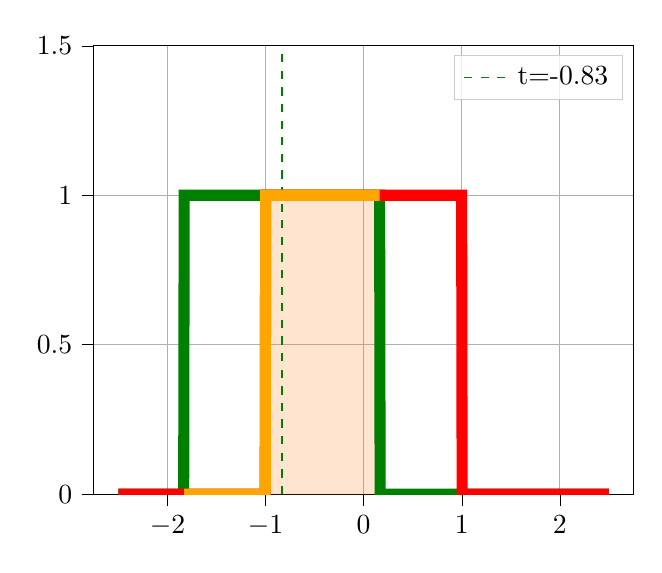
\begin{tikzpicture}

\definecolor{color0}{rgb}{1,0.498039215686275,0.0549019607843137}
\definecolor{color1}{rgb}{1,0.647058823529412,0}

\begin{axis}[
legend cell align={left},
legend style={fill opacity=0.8, draw opacity=1, text opacity=1, draw=white!80!black},
tick align=outside,
tick pos=left,
x grid style={white!69.0196078431373!black},
xmajorgrids,
xmin=-2.75, xmax=2.75,
xtick style={color=black},
y grid style={white!69.0196078431373!black},
ymajorgrids,
ymin=0, ymax=1.5,
ytick style={color=black}
]
\path [draw=color0, fill=color0, opacity=0.2]
(axis cs:-1.82932932932933,0)
--(axis cs:-1.82932932932933,0)
--(axis cs:-1.82432432432432,0)
--(axis cs:-1.81931931931932,0)
--(axis cs:-1.81431431431431,0)
--(axis cs:-1.80930930930931,0)
--(axis cs:-1.8043043043043,0)
--(axis cs:-1.7992992992993,0)
--(axis cs:-1.79429429429429,0)
--(axis cs:-1.78928928928929,0)
--(axis cs:-1.78428428428428,0)
--(axis cs:-1.77927927927928,0)
--(axis cs:-1.77427427427427,0)
--(axis cs:-1.76926926926927,0)
--(axis cs:-1.76426426426426,0)
--(axis cs:-1.75925925925926,0)
--(axis cs:-1.75425425425425,0)
--(axis cs:-1.74924924924925,0)
--(axis cs:-1.74424424424424,0)
--(axis cs:-1.73923923923924,0)
--(axis cs:-1.73423423423423,0)
--(axis cs:-1.72922922922923,0)
--(axis cs:-1.72422422422422,0)
--(axis cs:-1.71921921921922,0)
--(axis cs:-1.71421421421421,0)
--(axis cs:-1.70920920920921,0)
--(axis cs:-1.7042042042042,0)
--(axis cs:-1.6991991991992,0)
--(axis cs:-1.69419419419419,0)
--(axis cs:-1.68918918918919,0)
--(axis cs:-1.68418418418418,0)
--(axis cs:-1.67917917917918,0)
--(axis cs:-1.67417417417417,0)
--(axis cs:-1.66916916916917,0)
--(axis cs:-1.66416416416416,0)
--(axis cs:-1.65915915915916,0)
--(axis cs:-1.65415415415415,0)
--(axis cs:-1.64914914914915,0)
--(axis cs:-1.64414414414414,0)
--(axis cs:-1.63913913913914,0)
--(axis cs:-1.63413413413413,0)
--(axis cs:-1.62912912912913,0)
--(axis cs:-1.62412412412412,0)
--(axis cs:-1.61911911911912,0)
--(axis cs:-1.61411411411411,0)
--(axis cs:-1.60910910910911,0)
--(axis cs:-1.6041041041041,0)
--(axis cs:-1.5990990990991,0)
--(axis cs:-1.59409409409409,0)
--(axis cs:-1.58908908908909,0)
--(axis cs:-1.58408408408408,0)
--(axis cs:-1.57907907907908,0)
--(axis cs:-1.57407407407407,0)
--(axis cs:-1.56906906906907,0)
--(axis cs:-1.56406406406406,0)
--(axis cs:-1.55905905905906,0)
--(axis cs:-1.55405405405405,0)
--(axis cs:-1.54904904904905,0)
--(axis cs:-1.54404404404404,0)
--(axis cs:-1.53903903903904,0)
--(axis cs:-1.53403403403403,0)
--(axis cs:-1.52902902902903,0)
--(axis cs:-1.52402402402402,0)
--(axis cs:-1.51901901901902,0)
--(axis cs:-1.51401401401401,0)
--(axis cs:-1.50900900900901,0)
--(axis cs:-1.504004004004,0)
--(axis cs:-1.498998998999,0)
--(axis cs:-1.49399399399399,0)
--(axis cs:-1.48898898898899,0)
--(axis cs:-1.48398398398398,0)
--(axis cs:-1.47897897897898,0)
--(axis cs:-1.47397397397397,0)
--(axis cs:-1.46896896896897,0)
--(axis cs:-1.46396396396396,0)
--(axis cs:-1.45895895895896,0)
--(axis cs:-1.45395395395395,0)
--(axis cs:-1.44894894894895,0)
--(axis cs:-1.44394394394394,0)
--(axis cs:-1.43893893893894,0)
--(axis cs:-1.43393393393393,0)
--(axis cs:-1.42892892892893,0)
--(axis cs:-1.42392392392392,0)
--(axis cs:-1.41891891891892,0)
--(axis cs:-1.41391391391391,0)
--(axis cs:-1.40890890890891,0)
--(axis cs:-1.4039039039039,0)
--(axis cs:-1.3988988988989,0)
--(axis cs:-1.39389389389389,0)
--(axis cs:-1.38888888888889,0)
--(axis cs:-1.38388388388388,0)
--(axis cs:-1.37887887887888,0)
--(axis cs:-1.37387387387387,0)
--(axis cs:-1.36886886886887,0)
--(axis cs:-1.36386386386386,0)
--(axis cs:-1.35885885885886,0)
--(axis cs:-1.35385385385385,0)
--(axis cs:-1.34884884884885,0)
--(axis cs:-1.34384384384384,0)
--(axis cs:-1.33883883883884,0)
--(axis cs:-1.33383383383383,0)
--(axis cs:-1.32882882882883,0)
--(axis cs:-1.32382382382382,0)
--(axis cs:-1.31881881881882,0)
--(axis cs:-1.31381381381381,0)
--(axis cs:-1.30880880880881,0)
--(axis cs:-1.3038038038038,0)
--(axis cs:-1.2987987987988,0)
--(axis cs:-1.29379379379379,0)
--(axis cs:-1.28878878878879,0)
--(axis cs:-1.28378378378378,0)
--(axis cs:-1.27877877877878,0)
--(axis cs:-1.27377377377377,0)
--(axis cs:-1.26876876876877,0)
--(axis cs:-1.26376376376376,0)
--(axis cs:-1.25875875875876,0)
--(axis cs:-1.25375375375375,0)
--(axis cs:-1.24874874874875,0)
--(axis cs:-1.24374374374374,0)
--(axis cs:-1.23873873873874,0)
--(axis cs:-1.23373373373373,0)
--(axis cs:-1.22872872872873,0)
--(axis cs:-1.22372372372372,0)
--(axis cs:-1.21871871871872,0)
--(axis cs:-1.21371371371371,0)
--(axis cs:-1.20870870870871,0)
--(axis cs:-1.2037037037037,0)
--(axis cs:-1.1986986986987,0)
--(axis cs:-1.19369369369369,0)
--(axis cs:-1.18868868868869,0)
--(axis cs:-1.18368368368368,0)
--(axis cs:-1.17867867867868,0)
--(axis cs:-1.17367367367367,0)
--(axis cs:-1.16866866866867,0)
--(axis cs:-1.16366366366366,0)
--(axis cs:-1.15865865865866,0)
--(axis cs:-1.15365365365365,0)
--(axis cs:-1.14864864864865,0)
--(axis cs:-1.14364364364364,0)
--(axis cs:-1.13863863863864,0)
--(axis cs:-1.13363363363363,0)
--(axis cs:-1.12862862862863,0)
--(axis cs:-1.12362362362362,0)
--(axis cs:-1.11861861861862,0)
--(axis cs:-1.11361361361361,0)
--(axis cs:-1.10860860860861,0)
--(axis cs:-1.1036036036036,0)
--(axis cs:-1.0985985985986,0)
--(axis cs:-1.09359359359359,0)
--(axis cs:-1.08858858858859,0)
--(axis cs:-1.08358358358358,0)
--(axis cs:-1.07857857857858,0)
--(axis cs:-1.07357357357357,0)
--(axis cs:-1.06856856856857,0)
--(axis cs:-1.06356356356356,0)
--(axis cs:-1.05855855855856,0)
--(axis cs:-1.05355355355355,0)
--(axis cs:-1.04854854854855,0)
--(axis cs:-1.04354354354354,0)
--(axis cs:-1.03853853853854,0)
--(axis cs:-1.03353353353353,0)
--(axis cs:-1.02852852852853,0)
--(axis cs:-1.02352352352352,0)
--(axis cs:-1.01851851851852,0)
--(axis cs:-1.01351351351351,0)
--(axis cs:-1.00850850850851,0)
--(axis cs:-1.0035035035035,0)
--(axis cs:-0.998498498498499,0)
--(axis cs:-0.993493493493494,0)
--(axis cs:-0.988488488488489,0)
--(axis cs:-0.983483483483484,0)
--(axis cs:-0.978478478478479,0)
--(axis cs:-0.973473473473474,0)
--(axis cs:-0.968468468468469,0)
--(axis cs:-0.963463463463464,0)
--(axis cs:-0.958458458458459,0)
--(axis cs:-0.953453453453454,0)
--(axis cs:-0.948448448448449,0)
--(axis cs:-0.943443443443444,0)
--(axis cs:-0.938438438438439,0)
--(axis cs:-0.933433433433434,0)
--(axis cs:-0.928428428428429,0)
--(axis cs:-0.923423423423424,0)
--(axis cs:-0.918418418418419,0)
--(axis cs:-0.913413413413414,0)
--(axis cs:-0.908408408408409,0)
--(axis cs:-0.903403403403404,0)
--(axis cs:-0.898398398398399,0)
--(axis cs:-0.893393393393393,0)
--(axis cs:-0.888388388388388,0)
--(axis cs:-0.883383383383383,0)
--(axis cs:-0.878378378378378,0)
--(axis cs:-0.873373373373373,0)
--(axis cs:-0.868368368368368,0)
--(axis cs:-0.863363363363363,0)
--(axis cs:-0.858358358358358,0)
--(axis cs:-0.853353353353353,0)
--(axis cs:-0.848348348348348,0)
--(axis cs:-0.843343343343343,0)
--(axis cs:-0.838338338338338,0)
--(axis cs:-0.833333333333333,0)
--(axis cs:-0.828328328328328,0)
--(axis cs:-0.823323323323323,0)
--(axis cs:-0.818318318318318,0)
--(axis cs:-0.813313313313313,0)
--(axis cs:-0.808308308308308,0)
--(axis cs:-0.803303303303303,0)
--(axis cs:-0.798298298298298,0)
--(axis cs:-0.793293293293293,0)
--(axis cs:-0.788288288288288,0)
--(axis cs:-0.783283283283283,0)
--(axis cs:-0.778278278278278,0)
--(axis cs:-0.773273273273273,0)
--(axis cs:-0.768268268268268,0)
--(axis cs:-0.763263263263263,0)
--(axis cs:-0.758258258258258,0)
--(axis cs:-0.753253253253253,0)
--(axis cs:-0.748248248248248,0)
--(axis cs:-0.743243243243243,0)
--(axis cs:-0.738238238238238,0)
--(axis cs:-0.733233233233233,0)
--(axis cs:-0.728228228228228,0)
--(axis cs:-0.723223223223223,0)
--(axis cs:-0.718218218218218,0)
--(axis cs:-0.713213213213213,0)
--(axis cs:-0.708208208208208,0)
--(axis cs:-0.703203203203203,0)
--(axis cs:-0.698198198198198,0)
--(axis cs:-0.693193193193193,0)
--(axis cs:-0.688188188188188,0)
--(axis cs:-0.683183183183183,0)
--(axis cs:-0.678178178178178,0)
--(axis cs:-0.673173173173173,0)
--(axis cs:-0.668168168168168,0)
--(axis cs:-0.663163163163163,0)
--(axis cs:-0.658158158158158,0)
--(axis cs:-0.653153153153153,0)
--(axis cs:-0.648148148148148,0)
--(axis cs:-0.643143143143143,0)
--(axis cs:-0.638138138138138,0)
--(axis cs:-0.633133133133133,0)
--(axis cs:-0.628128128128128,0)
--(axis cs:-0.623123123123123,0)
--(axis cs:-0.618118118118118,0)
--(axis cs:-0.613113113113113,0)
--(axis cs:-0.608108108108108,0)
--(axis cs:-0.603103103103103,0)
--(axis cs:-0.598098098098098,0)
--(axis cs:-0.593093093093093,0)
--(axis cs:-0.588088088088088,0)
--(axis cs:-0.583083083083083,0)
--(axis cs:-0.578078078078078,0)
--(axis cs:-0.573073073073073,0)
--(axis cs:-0.568068068068068,0)
--(axis cs:-0.563063063063063,0)
--(axis cs:-0.558058058058058,0)
--(axis cs:-0.553053053053053,0)
--(axis cs:-0.548048048048048,0)
--(axis cs:-0.543043043043043,0)
--(axis cs:-0.538038038038038,0)
--(axis cs:-0.533033033033033,0)
--(axis cs:-0.528028028028028,0)
--(axis cs:-0.523023023023023,0)
--(axis cs:-0.518018018018018,0)
--(axis cs:-0.513013013013013,0)
--(axis cs:-0.508008008008008,0)
--(axis cs:-0.503003003003003,0)
--(axis cs:-0.497997997997998,0)
--(axis cs:-0.492992992992993,0)
--(axis cs:-0.487987987987988,0)
--(axis cs:-0.482982982982983,0)
--(axis cs:-0.477977977977978,0)
--(axis cs:-0.472972972972973,0)
--(axis cs:-0.467967967967968,0)
--(axis cs:-0.462962962962963,0)
--(axis cs:-0.457957957957958,0)
--(axis cs:-0.452952952952953,0)
--(axis cs:-0.447947947947948,0)
--(axis cs:-0.442942942942943,0)
--(axis cs:-0.437937937937938,0)
--(axis cs:-0.432932932932933,0)
--(axis cs:-0.427927927927928,0)
--(axis cs:-0.422922922922923,0)
--(axis cs:-0.417917917917918,0)
--(axis cs:-0.412912912912913,0)
--(axis cs:-0.407907907907908,0)
--(axis cs:-0.402902902902903,0)
--(axis cs:-0.397897897897898,0)
--(axis cs:-0.392892892892893,0)
--(axis cs:-0.387887887887888,0)
--(axis cs:-0.382882882882883,0)
--(axis cs:-0.377877877877878,0)
--(axis cs:-0.372872872872873,0)
--(axis cs:-0.367867867867868,0)
--(axis cs:-0.362862862862863,0)
--(axis cs:-0.357857857857858,0)
--(axis cs:-0.352852852852853,0)
--(axis cs:-0.347847847847848,0)
--(axis cs:-0.342842842842843,0)
--(axis cs:-0.337837837837838,0)
--(axis cs:-0.332832832832833,0)
--(axis cs:-0.327827827827828,0)
--(axis cs:-0.322822822822823,0)
--(axis cs:-0.317817817817818,0)
--(axis cs:-0.312812812812813,0)
--(axis cs:-0.307807807807808,0)
--(axis cs:-0.302802802802803,0)
--(axis cs:-0.297797797797798,0)
--(axis cs:-0.292792792792793,0)
--(axis cs:-0.287787787787788,0)
--(axis cs:-0.282782782782783,0)
--(axis cs:-0.277777777777778,0)
--(axis cs:-0.272772772772773,0)
--(axis cs:-0.267767767767768,0)
--(axis cs:-0.262762762762763,0)
--(axis cs:-0.257757757757758,0)
--(axis cs:-0.252752752752753,0)
--(axis cs:-0.247747747747748,0)
--(axis cs:-0.242742742742743,0)
--(axis cs:-0.237737737737738,0)
--(axis cs:-0.232732732732733,0)
--(axis cs:-0.227727727727728,0)
--(axis cs:-0.222722722722723,0)
--(axis cs:-0.217717717717718,0)
--(axis cs:-0.212712712712713,0)
--(axis cs:-0.207707707707708,0)
--(axis cs:-0.202702702702703,0)
--(axis cs:-0.197697697697698,0)
--(axis cs:-0.192692692692693,0)
--(axis cs:-0.187687687687688,0)
--(axis cs:-0.182682682682683,0)
--(axis cs:-0.177677677677678,0)
--(axis cs:-0.172672672672673,0)
--(axis cs:-0.167667667667668,0)
--(axis cs:-0.162662662662663,0)
--(axis cs:-0.157657657657658,0)
--(axis cs:-0.152652652652653,0)
--(axis cs:-0.147647647647648,0)
--(axis cs:-0.142642642642643,0)
--(axis cs:-0.137637637637638,0)
--(axis cs:-0.132632632632633,0)
--(axis cs:-0.127627627627628,0)
--(axis cs:-0.122622622622623,0)
--(axis cs:-0.117617617617618,0)
--(axis cs:-0.112612612612613,0)
--(axis cs:-0.107607607607608,0)
--(axis cs:-0.102602602602603,0)
--(axis cs:-0.0975975975975976,0)
--(axis cs:-0.0925925925925926,0)
--(axis cs:-0.0875875875875876,0)
--(axis cs:-0.0825825825825826,0)
--(axis cs:-0.0775775775775776,0)
--(axis cs:-0.0725725725725725,0)
--(axis cs:-0.0675675675675675,0)
--(axis cs:-0.0625625625625625,0)
--(axis cs:-0.0575575575575575,0)
--(axis cs:-0.0525525525525525,0)
--(axis cs:-0.0475475475475475,0)
--(axis cs:-0.0425425425425425,0)
--(axis cs:-0.0375375375375375,0)
--(axis cs:-0.0325325325325325,0)
--(axis cs:-0.0275275275275275,0)
--(axis cs:-0.0225225225225225,0)
--(axis cs:-0.0175175175175175,0)
--(axis cs:-0.0125125125125125,0)
--(axis cs:-0.0075075075075075,0)
--(axis cs:-0.0025025025025025,0)
--(axis cs:0.0025025025025025,0)
--(axis cs:0.0075075075075075,0)
--(axis cs:0.0125125125125125,0)
--(axis cs:0.0175175175175175,0)
--(axis cs:0.0225225225225225,0)
--(axis cs:0.0275275275275275,0)
--(axis cs:0.0325325325325325,0)
--(axis cs:0.0375375375375375,0)
--(axis cs:0.0425425425425425,0)
--(axis cs:0.0475475475475475,0)
--(axis cs:0.0525525525525525,0)
--(axis cs:0.0575575575575575,0)
--(axis cs:0.0625625625625625,0)
--(axis cs:0.0675675675675675,0)
--(axis cs:0.0725725725725725,0)
--(axis cs:0.0775775775775776,0)
--(axis cs:0.0825825825825826,0)
--(axis cs:0.0875875875875876,0)
--(axis cs:0.0925925925925926,0)
--(axis cs:0.0975975975975976,0)
--(axis cs:0.102602602602603,0)
--(axis cs:0.107607607607608,0)
--(axis cs:0.112612612612613,0)
--(axis cs:0.117617617617618,0)
--(axis cs:0.122622622622623,0)
--(axis cs:0.127627627627628,0)
--(axis cs:0.132632632632633,0)
--(axis cs:0.137637637637638,0)
--(axis cs:0.142642642642643,0)
--(axis cs:0.147647647647648,0)
--(axis cs:0.152652652652653,0)
--(axis cs:0.157657657657658,0)
--(axis cs:0.162662662662663,0)
--(axis cs:0.162662662662663,1)
--(axis cs:0.162662662662663,1)
--(axis cs:0.157657657657658,1)
--(axis cs:0.152652652652653,1)
--(axis cs:0.147647647647648,1)
--(axis cs:0.142642642642643,1)
--(axis cs:0.137637637637638,1)
--(axis cs:0.132632632632633,1)
--(axis cs:0.127627627627628,1)
--(axis cs:0.122622622622623,1)
--(axis cs:0.117617617617618,1)
--(axis cs:0.112612612612613,1)
--(axis cs:0.107607607607608,1)
--(axis cs:0.102602602602603,1)
--(axis cs:0.0975975975975976,1)
--(axis cs:0.0925925925925926,1)
--(axis cs:0.0875875875875876,1)
--(axis cs:0.0825825825825826,1)
--(axis cs:0.0775775775775776,1)
--(axis cs:0.0725725725725725,1)
--(axis cs:0.0675675675675675,1)
--(axis cs:0.0625625625625625,1)
--(axis cs:0.0575575575575575,1)
--(axis cs:0.0525525525525525,1)
--(axis cs:0.0475475475475475,1)
--(axis cs:0.0425425425425425,1)
--(axis cs:0.0375375375375375,1)
--(axis cs:0.0325325325325325,1)
--(axis cs:0.0275275275275275,1)
--(axis cs:0.0225225225225225,1)
--(axis cs:0.0175175175175175,1)
--(axis cs:0.0125125125125125,1)
--(axis cs:0.0075075075075075,1)
--(axis cs:0.0025025025025025,1)
--(axis cs:-0.0025025025025025,1)
--(axis cs:-0.0075075075075075,1)
--(axis cs:-0.0125125125125125,1)
--(axis cs:-0.0175175175175175,1)
--(axis cs:-0.0225225225225225,1)
--(axis cs:-0.0275275275275275,1)
--(axis cs:-0.0325325325325325,1)
--(axis cs:-0.0375375375375375,1)
--(axis cs:-0.0425425425425425,1)
--(axis cs:-0.0475475475475475,1)
--(axis cs:-0.0525525525525525,1)
--(axis cs:-0.0575575575575575,1)
--(axis cs:-0.0625625625625625,1)
--(axis cs:-0.0675675675675675,1)
--(axis cs:-0.0725725725725725,1)
--(axis cs:-0.0775775775775776,1)
--(axis cs:-0.0825825825825826,1)
--(axis cs:-0.0875875875875876,1)
--(axis cs:-0.0925925925925926,1)
--(axis cs:-0.0975975975975976,1)
--(axis cs:-0.102602602602603,1)
--(axis cs:-0.107607607607608,1)
--(axis cs:-0.112612612612613,1)
--(axis cs:-0.117617617617618,1)
--(axis cs:-0.122622622622623,1)
--(axis cs:-0.127627627627628,1)
--(axis cs:-0.132632632632633,1)
--(axis cs:-0.137637637637638,1)
--(axis cs:-0.142642642642643,1)
--(axis cs:-0.147647647647648,1)
--(axis cs:-0.152652652652653,1)
--(axis cs:-0.157657657657658,1)
--(axis cs:-0.162662662662663,1)
--(axis cs:-0.167667667667668,1)
--(axis cs:-0.172672672672673,1)
--(axis cs:-0.177677677677678,1)
--(axis cs:-0.182682682682683,1)
--(axis cs:-0.187687687687688,1)
--(axis cs:-0.192692692692693,1)
--(axis cs:-0.197697697697698,1)
--(axis cs:-0.202702702702703,1)
--(axis cs:-0.207707707707708,1)
--(axis cs:-0.212712712712713,1)
--(axis cs:-0.217717717717718,1)
--(axis cs:-0.222722722722723,1)
--(axis cs:-0.227727727727728,1)
--(axis cs:-0.232732732732733,1)
--(axis cs:-0.237737737737738,1)
--(axis cs:-0.242742742742743,1)
--(axis cs:-0.247747747747748,1)
--(axis cs:-0.252752752752753,1)
--(axis cs:-0.257757757757758,1)
--(axis cs:-0.262762762762763,1)
--(axis cs:-0.267767767767768,1)
--(axis cs:-0.272772772772773,1)
--(axis cs:-0.277777777777778,1)
--(axis cs:-0.282782782782783,1)
--(axis cs:-0.287787787787788,1)
--(axis cs:-0.292792792792793,1)
--(axis cs:-0.297797797797798,1)
--(axis cs:-0.302802802802803,1)
--(axis cs:-0.307807807807808,1)
--(axis cs:-0.312812812812813,1)
--(axis cs:-0.317817817817818,1)
--(axis cs:-0.322822822822823,1)
--(axis cs:-0.327827827827828,1)
--(axis cs:-0.332832832832833,1)
--(axis cs:-0.337837837837838,1)
--(axis cs:-0.342842842842843,1)
--(axis cs:-0.347847847847848,1)
--(axis cs:-0.352852852852853,1)
--(axis cs:-0.357857857857858,1)
--(axis cs:-0.362862862862863,1)
--(axis cs:-0.367867867867868,1)
--(axis cs:-0.372872872872873,1)
--(axis cs:-0.377877877877878,1)
--(axis cs:-0.382882882882883,1)
--(axis cs:-0.387887887887888,1)
--(axis cs:-0.392892892892893,1)
--(axis cs:-0.397897897897898,1)
--(axis cs:-0.402902902902903,1)
--(axis cs:-0.407907907907908,1)
--(axis cs:-0.412912912912913,1)
--(axis cs:-0.417917917917918,1)
--(axis cs:-0.422922922922923,1)
--(axis cs:-0.427927927927928,1)
--(axis cs:-0.432932932932933,1)
--(axis cs:-0.437937937937938,1)
--(axis cs:-0.442942942942943,1)
--(axis cs:-0.447947947947948,1)
--(axis cs:-0.452952952952953,1)
--(axis cs:-0.457957957957958,1)
--(axis cs:-0.462962962962963,1)
--(axis cs:-0.467967967967968,1)
--(axis cs:-0.472972972972973,1)
--(axis cs:-0.477977977977978,1)
--(axis cs:-0.482982982982983,1)
--(axis cs:-0.487987987987988,1)
--(axis cs:-0.492992992992993,1)
--(axis cs:-0.497997997997998,1)
--(axis cs:-0.503003003003003,1)
--(axis cs:-0.508008008008008,1)
--(axis cs:-0.513013013013013,1)
--(axis cs:-0.518018018018018,1)
--(axis cs:-0.523023023023023,1)
--(axis cs:-0.528028028028028,1)
--(axis cs:-0.533033033033033,1)
--(axis cs:-0.538038038038038,1)
--(axis cs:-0.543043043043043,1)
--(axis cs:-0.548048048048048,1)
--(axis cs:-0.553053053053053,1)
--(axis cs:-0.558058058058058,1)
--(axis cs:-0.563063063063063,1)
--(axis cs:-0.568068068068068,1)
--(axis cs:-0.573073073073073,1)
--(axis cs:-0.578078078078078,1)
--(axis cs:-0.583083083083083,1)
--(axis cs:-0.588088088088088,1)
--(axis cs:-0.593093093093093,1)
--(axis cs:-0.598098098098098,1)
--(axis cs:-0.603103103103103,1)
--(axis cs:-0.608108108108108,1)
--(axis cs:-0.613113113113113,1)
--(axis cs:-0.618118118118118,1)
--(axis cs:-0.623123123123123,1)
--(axis cs:-0.628128128128128,1)
--(axis cs:-0.633133133133133,1)
--(axis cs:-0.638138138138138,1)
--(axis cs:-0.643143143143143,1)
--(axis cs:-0.648148148148148,1)
--(axis cs:-0.653153153153153,1)
--(axis cs:-0.658158158158158,1)
--(axis cs:-0.663163163163163,1)
--(axis cs:-0.668168168168168,1)
--(axis cs:-0.673173173173173,1)
--(axis cs:-0.678178178178178,1)
--(axis cs:-0.683183183183183,1)
--(axis cs:-0.688188188188188,1)
--(axis cs:-0.693193193193193,1)
--(axis cs:-0.698198198198198,1)
--(axis cs:-0.703203203203203,1)
--(axis cs:-0.708208208208208,1)
--(axis cs:-0.713213213213213,1)
--(axis cs:-0.718218218218218,1)
--(axis cs:-0.723223223223223,1)
--(axis cs:-0.728228228228228,1)
--(axis cs:-0.733233233233233,1)
--(axis cs:-0.738238238238238,1)
--(axis cs:-0.743243243243243,1)
--(axis cs:-0.748248248248248,1)
--(axis cs:-0.753253253253253,1)
--(axis cs:-0.758258258258258,1)
--(axis cs:-0.763263263263263,1)
--(axis cs:-0.768268268268268,1)
--(axis cs:-0.773273273273273,1)
--(axis cs:-0.778278278278278,1)
--(axis cs:-0.783283283283283,1)
--(axis cs:-0.788288288288288,1)
--(axis cs:-0.793293293293293,1)
--(axis cs:-0.798298298298298,1)
--(axis cs:-0.803303303303303,1)
--(axis cs:-0.808308308308308,1)
--(axis cs:-0.813313313313313,1)
--(axis cs:-0.818318318318318,1)
--(axis cs:-0.823323323323323,1)
--(axis cs:-0.828328328328328,1)
--(axis cs:-0.833333333333333,1)
--(axis cs:-0.838338338338338,1)
--(axis cs:-0.843343343343343,1)
--(axis cs:-0.848348348348348,1)
--(axis cs:-0.853353353353353,1)
--(axis cs:-0.858358358358358,1)
--(axis cs:-0.863363363363363,1)
--(axis cs:-0.868368368368368,1)
--(axis cs:-0.873373373373373,1)
--(axis cs:-0.878378378378378,1)
--(axis cs:-0.883383383383383,1)
--(axis cs:-0.888388388388388,1)
--(axis cs:-0.893393393393393,1)
--(axis cs:-0.898398398398399,1)
--(axis cs:-0.903403403403404,1)
--(axis cs:-0.908408408408409,1)
--(axis cs:-0.913413413413414,1)
--(axis cs:-0.918418418418419,1)
--(axis cs:-0.923423423423424,1)
--(axis cs:-0.928428428428429,1)
--(axis cs:-0.933433433433434,1)
--(axis cs:-0.938438438438439,1)
--(axis cs:-0.943443443443444,1)
--(axis cs:-0.948448448448449,1)
--(axis cs:-0.953453453453454,1)
--(axis cs:-0.958458458458459,1)
--(axis cs:-0.963463463463464,1)
--(axis cs:-0.968468468468469,1)
--(axis cs:-0.973473473473474,1)
--(axis cs:-0.978478478478479,1)
--(axis cs:-0.983483483483484,1)
--(axis cs:-0.988488488488489,1)
--(axis cs:-0.993493493493494,1)
--(axis cs:-0.998498498498499,1)
--(axis cs:-1.0035035035035,0)
--(axis cs:-1.00850850850851,0)
--(axis cs:-1.01351351351351,0)
--(axis cs:-1.01851851851852,0)
--(axis cs:-1.02352352352352,0)
--(axis cs:-1.02852852852853,0)
--(axis cs:-1.03353353353353,0)
--(axis cs:-1.03853853853854,0)
--(axis cs:-1.04354354354354,0)
--(axis cs:-1.04854854854855,0)
--(axis cs:-1.05355355355355,0)
--(axis cs:-1.05855855855856,0)
--(axis cs:-1.06356356356356,0)
--(axis cs:-1.06856856856857,0)
--(axis cs:-1.07357357357357,0)
--(axis cs:-1.07857857857858,0)
--(axis cs:-1.08358358358358,0)
--(axis cs:-1.08858858858859,0)
--(axis cs:-1.09359359359359,0)
--(axis cs:-1.0985985985986,0)
--(axis cs:-1.1036036036036,0)
--(axis cs:-1.10860860860861,0)
--(axis cs:-1.11361361361361,0)
--(axis cs:-1.11861861861862,0)
--(axis cs:-1.12362362362362,0)
--(axis cs:-1.12862862862863,0)
--(axis cs:-1.13363363363363,0)
--(axis cs:-1.13863863863864,0)
--(axis cs:-1.14364364364364,0)
--(axis cs:-1.14864864864865,0)
--(axis cs:-1.15365365365365,0)
--(axis cs:-1.15865865865866,0)
--(axis cs:-1.16366366366366,0)
--(axis cs:-1.16866866866867,0)
--(axis cs:-1.17367367367367,0)
--(axis cs:-1.17867867867868,0)
--(axis cs:-1.18368368368368,0)
--(axis cs:-1.18868868868869,0)
--(axis cs:-1.19369369369369,0)
--(axis cs:-1.1986986986987,0)
--(axis cs:-1.2037037037037,0)
--(axis cs:-1.20870870870871,0)
--(axis cs:-1.21371371371371,0)
--(axis cs:-1.21871871871872,0)
--(axis cs:-1.22372372372372,0)
--(axis cs:-1.22872872872873,0)
--(axis cs:-1.23373373373373,0)
--(axis cs:-1.23873873873874,0)
--(axis cs:-1.24374374374374,0)
--(axis cs:-1.24874874874875,0)
--(axis cs:-1.25375375375375,0)
--(axis cs:-1.25875875875876,0)
--(axis cs:-1.26376376376376,0)
--(axis cs:-1.26876876876877,0)
--(axis cs:-1.27377377377377,0)
--(axis cs:-1.27877877877878,0)
--(axis cs:-1.28378378378378,0)
--(axis cs:-1.28878878878879,0)
--(axis cs:-1.29379379379379,0)
--(axis cs:-1.2987987987988,0)
--(axis cs:-1.3038038038038,0)
--(axis cs:-1.30880880880881,0)
--(axis cs:-1.31381381381381,0)
--(axis cs:-1.31881881881882,0)
--(axis cs:-1.32382382382382,0)
--(axis cs:-1.32882882882883,0)
--(axis cs:-1.33383383383383,0)
--(axis cs:-1.33883883883884,0)
--(axis cs:-1.34384384384384,0)
--(axis cs:-1.34884884884885,0)
--(axis cs:-1.35385385385385,0)
--(axis cs:-1.35885885885886,0)
--(axis cs:-1.36386386386386,0)
--(axis cs:-1.36886886886887,0)
--(axis cs:-1.37387387387387,0)
--(axis cs:-1.37887887887888,0)
--(axis cs:-1.38388388388388,0)
--(axis cs:-1.38888888888889,0)
--(axis cs:-1.39389389389389,0)
--(axis cs:-1.3988988988989,0)
--(axis cs:-1.4039039039039,0)
--(axis cs:-1.40890890890891,0)
--(axis cs:-1.41391391391391,0)
--(axis cs:-1.41891891891892,0)
--(axis cs:-1.42392392392392,0)
--(axis cs:-1.42892892892893,0)
--(axis cs:-1.43393393393393,0)
--(axis cs:-1.43893893893894,0)
--(axis cs:-1.44394394394394,0)
--(axis cs:-1.44894894894895,0)
--(axis cs:-1.45395395395395,0)
--(axis cs:-1.45895895895896,0)
--(axis cs:-1.46396396396396,0)
--(axis cs:-1.46896896896897,0)
--(axis cs:-1.47397397397397,0)
--(axis cs:-1.47897897897898,0)
--(axis cs:-1.48398398398398,0)
--(axis cs:-1.48898898898899,0)
--(axis cs:-1.49399399399399,0)
--(axis cs:-1.498998998999,0)
--(axis cs:-1.504004004004,0)
--(axis cs:-1.50900900900901,0)
--(axis cs:-1.51401401401401,0)
--(axis cs:-1.51901901901902,0)
--(axis cs:-1.52402402402402,0)
--(axis cs:-1.52902902902903,0)
--(axis cs:-1.53403403403403,0)
--(axis cs:-1.53903903903904,0)
--(axis cs:-1.54404404404404,0)
--(axis cs:-1.54904904904905,0)
--(axis cs:-1.55405405405405,0)
--(axis cs:-1.55905905905906,0)
--(axis cs:-1.56406406406406,0)
--(axis cs:-1.56906906906907,0)
--(axis cs:-1.57407407407407,0)
--(axis cs:-1.57907907907908,0)
--(axis cs:-1.58408408408408,0)
--(axis cs:-1.58908908908909,0)
--(axis cs:-1.59409409409409,0)
--(axis cs:-1.5990990990991,0)
--(axis cs:-1.6041041041041,0)
--(axis cs:-1.60910910910911,0)
--(axis cs:-1.61411411411411,0)
--(axis cs:-1.61911911911912,0)
--(axis cs:-1.62412412412412,0)
--(axis cs:-1.62912912912913,0)
--(axis cs:-1.63413413413413,0)
--(axis cs:-1.63913913913914,0)
--(axis cs:-1.64414414414414,0)
--(axis cs:-1.64914914914915,0)
--(axis cs:-1.65415415415415,0)
--(axis cs:-1.65915915915916,0)
--(axis cs:-1.66416416416416,0)
--(axis cs:-1.66916916916917,0)
--(axis cs:-1.67417417417417,0)
--(axis cs:-1.67917917917918,0)
--(axis cs:-1.68418418418418,0)
--(axis cs:-1.68918918918919,0)
--(axis cs:-1.69419419419419,0)
--(axis cs:-1.6991991991992,0)
--(axis cs:-1.7042042042042,0)
--(axis cs:-1.70920920920921,0)
--(axis cs:-1.71421421421421,0)
--(axis cs:-1.71921921921922,0)
--(axis cs:-1.72422422422422,0)
--(axis cs:-1.72922922922923,0)
--(axis cs:-1.73423423423423,0)
--(axis cs:-1.73923923923924,0)
--(axis cs:-1.74424424424424,0)
--(axis cs:-1.74924924924925,0)
--(axis cs:-1.75425425425425,0)
--(axis cs:-1.75925925925926,0)
--(axis cs:-1.76426426426426,0)
--(axis cs:-1.76926926926927,0)
--(axis cs:-1.77427427427427,0)
--(axis cs:-1.77927927927928,0)
--(axis cs:-1.78428428428428,0)
--(axis cs:-1.78928928928929,0)
--(axis cs:-1.79429429429429,0)
--(axis cs:-1.7992992992993,0)
--(axis cs:-1.8043043043043,0)
--(axis cs:-1.80930930930931,0)
--(axis cs:-1.81431431431431,0)
--(axis cs:-1.81931931931932,0)
--(axis cs:-1.82432432432432,0)
--(axis cs:-1.82932932932933,0)
--cycle;

\addplot [line width=4pt, green!50!black, forget plot]
table {%
-2.5 0
-2.49499499499499 0
-2.48998998998999 0
-2.48498498498498 0
-2.47997997997998 0
-2.47497497497497 0
-2.46996996996997 0
-2.46496496496496 0
-2.45995995995996 0
-2.45495495495495 0
-2.44994994994995 0
-2.44494494494494 0
-2.43993993993994 0
-2.43493493493493 0
-2.42992992992993 0
-2.42492492492492 0
-2.41991991991992 0
-2.41491491491491 0
-2.40990990990991 0
-2.4049049049049 0
-2.3998998998999 0
-2.39489489489489 0
-2.38988988988989 0
-2.38488488488488 0
-2.37987987987988 0
-2.37487487487487 0
-2.36986986986987 0
-2.36486486486486 0
-2.35985985985986 0
-2.35485485485485 0
-2.34984984984985 0
-2.34484484484484 0
-2.33983983983984 0
-2.33483483483483 0
-2.32982982982983 0
-2.32482482482482 0
-2.31981981981982 0
-2.31481481481481 0
-2.30980980980981 0
-2.3048048048048 0
-2.2997997997998 0
-2.29479479479479 0
-2.28978978978979 0
-2.28478478478478 0
-2.27977977977978 0
-2.27477477477477 0
-2.26976976976977 0
-2.26476476476476 0
-2.25975975975976 0
-2.25475475475475 0
-2.24974974974975 0
-2.24474474474474 0
-2.23973973973974 0
-2.23473473473473 0
-2.22972972972973 0
-2.22472472472472 0
-2.21971971971972 0
-2.21471471471471 0
-2.20970970970971 0
-2.2047047047047 0
-2.1996996996997 0
-2.19469469469469 0
-2.18968968968969 0
-2.18468468468468 0
-2.17967967967968 0
-2.17467467467467 0
-2.16966966966967 0
-2.16466466466466 0
-2.15965965965966 0
-2.15465465465465 0
-2.14964964964965 0
-2.14464464464464 0
-2.13963963963964 0
-2.13463463463463 0
-2.12962962962963 0
-2.12462462462462 0
-2.11961961961962 0
-2.11461461461461 0
-2.10960960960961 0
-2.1046046046046 0
-2.0995995995996 0
-2.09459459459459 0
-2.08958958958959 0
-2.08458458458458 0
-2.07957957957958 0
-2.07457457457457 0
-2.06956956956957 0
-2.06456456456456 0
-2.05955955955956 0
-2.05455455455455 0
-2.04954954954955 0
-2.04454454454454 0
-2.03953953953954 0
-2.03453453453453 0
-2.02952952952953 0
-2.02452452452452 0
-2.01951951951952 0
-2.01451451451451 0
-2.00950950950951 0
-2.0045045045045 0
-1.9994994994995 0
-1.99449449449449 0
-1.98948948948949 0
-1.98448448448448 0
-1.97947947947948 0
-1.97447447447447 0
-1.96946946946947 0
-1.96446446446446 0
-1.95945945945946 0
-1.95445445445445 0
-1.94944944944945 0
-1.94444444444444 0
-1.93943943943944 0
-1.93443443443443 0
-1.92942942942943 0
-1.92442442442442 0
-1.91941941941942 0
-1.91441441441441 0
-1.90940940940941 0
-1.9044044044044 0
-1.8993993993994 0
-1.89439439439439 0
-1.88938938938939 0
-1.88438438438438 0
-1.87937937937938 0
-1.87437437437437 0
-1.86936936936937 0
-1.86436436436436 0
-1.85935935935936 0
-1.85435435435435 0
-1.84934934934935 0
-1.84434434434434 0
-1.83933933933934 0
-1.83433433433433 0
-1.82932932932933 1
-1.82432432432432 1
-1.81931931931932 1
-1.81431431431431 1
-1.80930930930931 1
-1.8043043043043 1
-1.7992992992993 1
-1.79429429429429 1
-1.78928928928929 1
-1.78428428428428 1
-1.77927927927928 1
-1.77427427427427 1
-1.76926926926927 1
-1.76426426426426 1
-1.75925925925926 1
-1.75425425425425 1
-1.74924924924925 1
-1.74424424424424 1
-1.73923923923924 1
-1.73423423423423 1
-1.72922922922923 1
-1.72422422422422 1
-1.71921921921922 1
-1.71421421421421 1
-1.70920920920921 1
-1.7042042042042 1
-1.6991991991992 1
-1.69419419419419 1
-1.68918918918919 1
-1.68418418418418 1
-1.67917917917918 1
-1.67417417417417 1
-1.66916916916917 1
-1.66416416416416 1
-1.65915915915916 1
-1.65415415415415 1
-1.64914914914915 1
-1.64414414414414 1
-1.63913913913914 1
-1.63413413413413 1
-1.62912912912913 1
-1.62412412412412 1
-1.61911911911912 1
-1.61411411411411 1
-1.60910910910911 1
-1.6041041041041 1
-1.5990990990991 1
-1.59409409409409 1
-1.58908908908909 1
-1.58408408408408 1
-1.57907907907908 1
-1.57407407407407 1
-1.56906906906907 1
-1.56406406406406 1
-1.55905905905906 1
-1.55405405405405 1
-1.54904904904905 1
-1.54404404404404 1
-1.53903903903904 1
-1.53403403403403 1
-1.52902902902903 1
-1.52402402402402 1
-1.51901901901902 1
-1.51401401401401 1
-1.50900900900901 1
-1.504004004004 1
-1.498998998999 1
-1.49399399399399 1
-1.48898898898899 1
-1.48398398398398 1
-1.47897897897898 1
-1.47397397397397 1
-1.46896896896897 1
-1.46396396396396 1
-1.45895895895896 1
-1.45395395395395 1
-1.44894894894895 1
-1.44394394394394 1
-1.43893893893894 1
-1.43393393393393 1
-1.42892892892893 1
-1.42392392392392 1
-1.41891891891892 1
-1.41391391391391 1
-1.40890890890891 1
-1.4039039039039 1
-1.3988988988989 1
-1.39389389389389 1
-1.38888888888889 1
-1.38388388388388 1
-1.37887887887888 1
-1.37387387387387 1
-1.36886886886887 1
-1.36386386386386 1
-1.35885885885886 1
-1.35385385385385 1
-1.34884884884885 1
-1.34384384384384 1
-1.33883883883884 1
-1.33383383383383 1
-1.32882882882883 1
-1.32382382382382 1
-1.31881881881882 1
-1.31381381381381 1
-1.30880880880881 1
-1.3038038038038 1
-1.2987987987988 1
-1.29379379379379 1
-1.28878878878879 1
-1.28378378378378 1
-1.27877877877878 1
-1.27377377377377 1
-1.26876876876877 1
-1.26376376376376 1
-1.25875875875876 1
-1.25375375375375 1
-1.24874874874875 1
-1.24374374374374 1
-1.23873873873874 1
-1.23373373373373 1
-1.22872872872873 1
-1.22372372372372 1
-1.21871871871872 1
-1.21371371371371 1
-1.20870870870871 1
-1.2037037037037 1
-1.1986986986987 1
-1.19369369369369 1
-1.18868868868869 1
-1.18368368368368 1
-1.17867867867868 1
-1.17367367367367 1
-1.16866866866867 1
-1.16366366366366 1
-1.15865865865866 1
-1.15365365365365 1
-1.14864864864865 1
-1.14364364364364 1
-1.13863863863864 1
-1.13363363363363 1
-1.12862862862863 1
-1.12362362362362 1
-1.11861861861862 1
-1.11361361361361 1
-1.10860860860861 1
-1.1036036036036 1
-1.0985985985986 1
-1.09359359359359 1
-1.08858858858859 1
-1.08358358358358 1
-1.07857857857858 1
-1.07357357357357 1
-1.06856856856857 1
-1.06356356356356 1
-1.05855855855856 1
-1.05355355355355 1
-1.04854854854855 1
-1.04354354354354 1
-1.03853853853854 1
-1.03353353353353 1
-1.02852852852853 1
-1.02352352352352 1
-1.01851851851852 1
-1.01351351351351 1
-1.00850850850851 1
-1.0035035035035 1
-0.998498498498499 1
-0.993493493493494 1
-0.988488488488489 1
-0.983483483483484 1
-0.978478478478479 1
-0.973473473473474 1
-0.968468468468469 1
-0.963463463463464 1
-0.958458458458459 1
-0.953453453453454 1
-0.948448448448449 1
-0.943443443443444 1
-0.938438438438439 1
-0.933433433433434 1
-0.928428428428429 1
-0.923423423423424 1
-0.918418418418419 1
-0.913413413413414 1
-0.908408408408409 1
-0.903403403403404 1
-0.898398398398399 1
-0.893393393393393 1
-0.888388388388388 1
-0.883383383383383 1
-0.878378378378378 1
-0.873373373373373 1
-0.868368368368368 1
-0.863363363363363 1
-0.858358358358358 1
-0.853353353353353 1
-0.848348348348348 1
-0.843343343343343 1
-0.838338338338338 1
-0.833333333333333 1
-0.828328328328328 1
-0.823323323323323 1
-0.818318318318318 1
-0.813313313313313 1
-0.808308308308308 1
-0.803303303303303 1
-0.798298298298298 1
-0.793293293293293 1
-0.788288288288288 1
-0.783283283283283 1
-0.778278278278278 1
-0.773273273273273 1
-0.768268268268268 1
-0.763263263263263 1
-0.758258258258258 1
-0.753253253253253 1
-0.748248248248248 1
-0.743243243243243 1
-0.738238238238238 1
-0.733233233233233 1
-0.728228228228228 1
-0.723223223223223 1
-0.718218218218218 1
-0.713213213213213 1
-0.708208208208208 1
-0.703203203203203 1
-0.698198198198198 1
-0.693193193193193 1
-0.688188188188188 1
-0.683183183183183 1
-0.678178178178178 1
-0.673173173173173 1
-0.668168168168168 1
-0.663163163163163 1
-0.658158158158158 1
-0.653153153153153 1
-0.648148148148148 1
-0.643143143143143 1
-0.638138138138138 1
-0.633133133133133 1
-0.628128128128128 1
-0.623123123123123 1
-0.618118118118118 1
-0.613113113113113 1
-0.608108108108108 1
-0.603103103103103 1
-0.598098098098098 1
-0.593093093093093 1
-0.588088088088088 1
-0.583083083083083 1
-0.578078078078078 1
-0.573073073073073 1
-0.568068068068068 1
-0.563063063063063 1
-0.558058058058058 1
-0.553053053053053 1
-0.548048048048048 1
-0.543043043043043 1
-0.538038038038038 1
-0.533033033033033 1
-0.528028028028028 1
-0.523023023023023 1
-0.518018018018018 1
-0.513013013013013 1
-0.508008008008008 1
-0.503003003003003 1
-0.497997997997998 1
-0.492992992992993 1
-0.487987987987988 1
-0.482982982982983 1
-0.477977977977978 1
-0.472972972972973 1
-0.467967967967968 1
-0.462962962962963 1
-0.457957957957958 1
-0.452952952952953 1
-0.447947947947948 1
-0.442942942942943 1
-0.437937937937938 1
-0.432932932932933 1
-0.427927927927928 1
-0.422922922922923 1
-0.417917917917918 1
-0.412912912912913 1
-0.407907907907908 1
-0.402902902902903 1
-0.397897897897898 1
-0.392892892892893 1
-0.387887887887888 1
-0.382882882882883 1
-0.377877877877878 1
-0.372872872872873 1
-0.367867867867868 1
-0.362862862862863 1
-0.357857857857858 1
-0.352852852852853 1
-0.347847847847848 1
-0.342842842842843 1
-0.337837837837838 1
-0.332832832832833 1
-0.327827827827828 1
-0.322822822822823 1
-0.317817817817818 1
-0.312812812812813 1
-0.307807807807808 1
-0.302802802802803 1
-0.297797797797798 1
-0.292792792792793 1
-0.287787787787788 1
-0.282782782782783 1
-0.277777777777778 1
-0.272772772772773 1
-0.267767767767768 1
-0.262762762762763 1
-0.257757757757758 1
-0.252752752752753 1
-0.247747747747748 1
-0.242742742742743 1
-0.237737737737738 1
-0.232732732732733 1
-0.227727727727728 1
-0.222722722722723 1
-0.217717717717718 1
-0.212712712712713 1
-0.207707707707708 1
-0.202702702702703 1
-0.197697697697698 1
-0.192692692692693 1
-0.187687687687688 1
-0.182682682682683 1
-0.177677677677678 1
-0.172672672672673 1
-0.167667667667668 1
-0.162662662662663 1
-0.157657657657658 1
-0.152652652652653 1
-0.147647647647648 1
-0.142642642642643 1
-0.137637637637638 1
-0.132632632632633 1
-0.127627627627628 1
-0.122622622622623 1
-0.117617617617618 1
-0.112612612612613 1
-0.107607607607608 1
-0.102602602602603 1
-0.0975975975975976 1
-0.0925925925925926 1
-0.0875875875875876 1
-0.0825825825825826 1
-0.0775775775775776 1
-0.0725725725725725 1
-0.0675675675675675 1
-0.0625625625625625 1
-0.0575575575575575 1
-0.0525525525525525 1
-0.0475475475475475 1
-0.0425425425425425 1
-0.0375375375375375 1
-0.0325325325325325 1
-0.0275275275275275 1
-0.0225225225225225 1
-0.0175175175175175 1
-0.0125125125125125 1
-0.0075075075075075 1
-0.0025025025025025 1
0.0025025025025025 1
0.0075075075075075 1
0.0125125125125125 1
0.0175175175175175 1
0.0225225225225225 1
0.0275275275275275 1
0.0325325325325325 1
0.0375375375375375 1
0.0425425425425425 1
0.0475475475475475 1
0.0525525525525525 1
0.0575575575575575 1
0.0625625625625625 1
0.0675675675675675 1
0.0725725725725725 1
0.0775775775775776 1
0.0825825825825826 1
0.0875875875875876 1
0.0925925925925926 1
0.0975975975975976 1
0.102602602602603 1
0.107607607607608 1
0.112612612612613 1
0.117617617617618 1
0.122622622622623 1
0.127627627627628 1
0.132632632632633 1
0.137637637637638 1
0.142642642642643 1
0.147647647647648 1
0.152652652652653 1
0.157657657657658 1
0.162662662662663 1
0.167667667667668 0
0.172672672672673 0
0.177677677677678 0
0.182682682682683 0
0.187687687687688 0
0.192692692692693 0
0.197697697697698 0
0.202702702702703 0
0.207707707707708 0
0.212712712712713 0
0.217717717717718 0
0.222722722722723 0
0.227727727727728 0
0.232732732732733 0
0.237737737737738 0
0.242742742742743 0
0.247747747747748 0
0.252752752752753 0
0.257757757757758 0
0.262762762762763 0
0.267767767767768 0
0.272772772772773 0
0.277777777777778 0
0.282782782782783 0
0.287787787787788 0
0.292792792792793 0
0.297797797797798 0
0.302802802802803 0
0.307807807807808 0
0.312812812812813 0
0.317817817817818 0
0.322822822822823 0
0.327827827827828 0
0.332832832832833 0
0.337837837837838 0
0.342842842842843 0
0.347847847847848 0
0.352852852852853 0
0.357857857857858 0
0.362862862862863 0
0.367867867867868 0
0.372872872872873 0
0.377877877877878 0
0.382882882882883 0
0.387887887887888 0
0.392892892892893 0
0.397897897897898 0
0.402902902902903 0
0.407907907907908 0
0.412912912912913 0
0.417917917917918 0
0.422922922922923 0
0.427927927927928 0
0.432932932932933 0
0.437937937937938 0
0.442942942942943 0
0.447947947947948 0
0.452952952952953 0
0.457957957957958 0
0.462962962962963 0
0.467967967967968 0
0.472972972972973 0
0.477977977977978 0
0.482982982982983 0
0.487987987987988 0
0.492992992992993 0
0.497997997997998 0
0.503003003003003 0
0.508008008008008 0
0.513013013013013 0
0.518018018018018 0
0.523023023023023 0
0.528028028028028 0
0.533033033033033 0
0.538038038038038 0
0.543043043043043 0
0.548048048048048 0
0.553053053053053 0
0.558058058058058 0
0.563063063063063 0
0.568068068068068 0
0.573073073073073 0
0.578078078078078 0
0.583083083083083 0
0.588088088088088 0
0.593093093093093 0
0.598098098098098 0
0.603103103103103 0
0.608108108108108 0
0.613113113113113 0
0.618118118118118 0
0.623123123123123 0
0.628128128128128 0
0.633133133133133 0
0.638138138138138 0
0.643143143143143 0
0.648148148148148 0
0.653153153153153 0
0.658158158158158 0
0.663163163163163 0
0.668168168168168 0
0.673173173173173 0
0.678178178178178 0
0.683183183183183 0
0.688188188188188 0
0.693193193193193 0
0.698198198198198 0
0.703203203203203 0
0.708208208208208 0
0.713213213213213 0
0.718218218218218 0
0.723223223223223 0
0.728228228228228 0
0.733233233233233 0
0.738238238238238 0
0.743243243243243 0
0.748248248248248 0
0.753253253253253 0
0.758258258258258 0
0.763263263263263 0
0.768268268268268 0
0.773273273273273 0
0.778278278278278 0
0.783283283283283 0
0.788288288288288 0
0.793293293293293 0
0.798298298298298 0
0.803303303303303 0
0.808308308308308 0
0.813313313313313 0
0.818318318318318 0
0.823323323323323 0
0.828328328328328 0
0.833333333333333 0
0.838338338338338 0
0.843343343343343 0
0.848348348348348 0
0.853353353353353 0
0.858358358358358 0
0.863363363363364 0
0.868368368368369 0
0.873373373373374 0
0.878378378378379 0
0.883383383383384 0
0.888388388388389 0
0.893393393393394 0
0.898398398398399 0
0.903403403403404 0
0.908408408408409 0
0.913413413413414 0
0.918418418418419 0
0.923423423423424 0
0.928428428428429 0
0.933433433433434 0
0.938438438438439 0
0.943443443443444 0
0.948448448448449 0
0.953453453453454 0
0.958458458458459 0
0.963463463463464 0
0.968468468468469 0
0.973473473473474 0
0.978478478478479 0
0.983483483483484 0
0.988488488488489 0
0.993493493493494 0
0.998498498498499 0
1.0035035035035 0
1.00850850850851 0
1.01351351351351 0
1.01851851851852 0
1.02352352352352 0
1.02852852852853 0
1.03353353353353 0
1.03853853853854 0
1.04354354354354 0
1.04854854854855 0
1.05355355355355 0
1.05855855855856 0
1.06356356356356 0
1.06856856856857 0
1.07357357357357 0
1.07857857857858 0
1.08358358358358 0
1.08858858858859 0
1.09359359359359 0
1.0985985985986 0
1.1036036036036 0
1.10860860860861 0
1.11361361361361 0
1.11861861861862 0
1.12362362362362 0
1.12862862862863 0
1.13363363363363 0
1.13863863863864 0
1.14364364364364 0
1.14864864864865 0
1.15365365365365 0
1.15865865865866 0
1.16366366366366 0
1.16866866866867 0
1.17367367367367 0
1.17867867867868 0
1.18368368368368 0
1.18868868868869 0
1.19369369369369 0
1.1986986986987 0
1.2037037037037 0
1.20870870870871 0
1.21371371371371 0
1.21871871871872 0
1.22372372372372 0
1.22872872872873 0
1.23373373373373 0
1.23873873873874 0
1.24374374374374 0
1.24874874874875 0
1.25375375375375 0
1.25875875875876 0
1.26376376376376 0
1.26876876876877 0
1.27377377377377 0
1.27877877877878 0
1.28378378378378 0
1.28878878878879 0
1.29379379379379 0
1.2987987987988 0
1.3038038038038 0
1.30880880880881 0
1.31381381381381 0
1.31881881881882 0
1.32382382382382 0
1.32882882882883 0
1.33383383383383 0
1.33883883883884 0
1.34384384384384 0
1.34884884884885 0
1.35385385385385 0
1.35885885885886 0
1.36386386386386 0
1.36886886886887 0
1.37387387387387 0
1.37887887887888 0
1.38388388388388 0
1.38888888888889 0
1.39389389389389 0
1.3988988988989 0
1.4039039039039 0
1.40890890890891 0
1.41391391391391 0
1.41891891891892 0
1.42392392392392 0
1.42892892892893 0
1.43393393393393 0
1.43893893893894 0
1.44394394394394 0
1.44894894894895 0
1.45395395395395 0
1.45895895895896 0
1.46396396396396 0
1.46896896896897 0
1.47397397397397 0
1.47897897897898 0
1.48398398398398 0
1.48898898898899 0
1.49399399399399 0
1.498998998999 0
1.504004004004 0
1.50900900900901 0
1.51401401401401 0
1.51901901901902 0
1.52402402402402 0
1.52902902902903 0
1.53403403403403 0
1.53903903903904 0
1.54404404404404 0
1.54904904904905 0
1.55405405405405 0
1.55905905905906 0
1.56406406406406 0
1.56906906906907 0
1.57407407407407 0
1.57907907907908 0
1.58408408408408 0
1.58908908908909 0
1.59409409409409 0
1.5990990990991 0
1.6041041041041 0
1.60910910910911 0
1.61411411411411 0
1.61911911911912 0
1.62412412412412 0
1.62912912912913 0
1.63413413413413 0
1.63913913913914 0
1.64414414414414 0
1.64914914914915 0
1.65415415415415 0
1.65915915915916 0
1.66416416416416 0
1.66916916916917 0
1.67417417417417 0
1.67917917917918 0
1.68418418418418 0
1.68918918918919 0
1.69419419419419 0
1.6991991991992 0
1.7042042042042 0
1.70920920920921 0
1.71421421421421 0
1.71921921921922 0
1.72422422422422 0
1.72922922922923 0
1.73423423423423 0
1.73923923923924 0
1.74424424424424 0
1.74924924924925 0
1.75425425425425 0
1.75925925925926 0
1.76426426426426 0
1.76926926926927 0
1.77427427427427 0
1.77927927927928 0
1.78428428428428 0
1.78928928928929 0
1.79429429429429 0
1.7992992992993 0
1.8043043043043 0
1.80930930930931 0
1.81431431431431 0
1.81931931931932 0
1.82432432432432 0
1.82932932932933 0
1.83433433433433 0
1.83933933933934 0
1.84434434434434 0
1.84934934934935 0
1.85435435435435 0
1.85935935935936 0
1.86436436436436 0
1.86936936936937 0
1.87437437437437 0
1.87937937937938 0
1.88438438438438 0
1.88938938938939 0
1.89439439439439 0
1.8993993993994 0
1.9044044044044 0
1.90940940940941 0
1.91441441441441 0
1.91941941941942 0
1.92442442442442 0
1.92942942942943 0
1.93443443443443 0
1.93943943943944 0
1.94444444444444 0
1.94944944944945 0
1.95445445445445 0
1.95945945945946 0
1.96446446446446 0
1.96946946946947 0
1.97447447447447 0
1.97947947947948 0
1.98448448448448 0
1.98948948948949 0
1.99449449449449 0
1.9994994994995 0
2.0045045045045 0
2.00950950950951 0
2.01451451451451 0
2.01951951951952 0
2.02452452452452 0
2.02952952952953 0
2.03453453453453 0
2.03953953953954 0
2.04454454454454 0
2.04954954954955 0
2.05455455455455 0
2.05955955955956 0
2.06456456456456 0
2.06956956956957 0
2.07457457457457 0
2.07957957957958 0
2.08458458458458 0
2.08958958958959 0
2.09459459459459 0
2.0995995995996 0
2.1046046046046 0
2.10960960960961 0
2.11461461461461 0
2.11961961961962 0
2.12462462462462 0
2.12962962962963 0
2.13463463463463 0
2.13963963963964 0
2.14464464464464 0
2.14964964964965 0
2.15465465465465 0
2.15965965965966 0
2.16466466466466 0
2.16966966966967 0
2.17467467467467 0
2.17967967967968 0
2.18468468468468 0
2.18968968968969 0
2.19469469469469 0
2.1996996996997 0
2.2047047047047 0
2.20970970970971 0
2.21471471471471 0
2.21971971971972 0
2.22472472472472 0
2.22972972972973 0
2.23473473473473 0
2.23973973973974 0
2.24474474474474 0
2.24974974974975 0
2.25475475475475 0
2.25975975975976 0
2.26476476476476 0
2.26976976976977 0
2.27477477477477 0
2.27977977977978 0
2.28478478478478 0
2.28978978978979 0
2.29479479479479 0
2.2997997997998 0
2.3048048048048 0
2.30980980980981 0
2.31481481481481 0
2.31981981981982 0
2.32482482482482 0
2.32982982982983 0
2.33483483483483 0
2.33983983983984 0
2.34484484484484 0
2.34984984984985 0
2.35485485485485 0
2.35985985985986 0
2.36486486486486 0
2.36986986986987 0
2.37487487487487 0
2.37987987987988 0
2.38488488488488 0
2.38988988988989 0
2.39489489489489 0
2.3998998998999 0
2.4049049049049 0
2.40990990990991 0
2.41491491491491 0
2.41991991991992 0
2.42492492492492 0
2.42992992992993 0
2.43493493493493 0
2.43993993993994 0
2.44494494494494 0
2.44994994994995 0
2.45495495495495 0
2.45995995995996 0
2.46496496496496 0
2.46996996996997 0
2.47497497497497 0
2.47997997997998 0
2.48498498498498 0
2.48998998998999 0
2.49499499499499 0
2.5 0
};
\addplot [line width=4pt, red, forget plot]
table {%
-2.5 0
-2.49499499499499 0
-2.48998998998999 0
-2.48498498498498 0
-2.47997997997998 0
-2.47497497497497 0
-2.46996996996997 0
-2.46496496496496 0
-2.45995995995996 0
-2.45495495495495 0
-2.44994994994995 0
-2.44494494494494 0
-2.43993993993994 0
-2.43493493493493 0
-2.42992992992993 0
-2.42492492492492 0
-2.41991991991992 0
-2.41491491491491 0
-2.40990990990991 0
-2.4049049049049 0
-2.3998998998999 0
-2.39489489489489 0
-2.38988988988989 0
-2.38488488488488 0
-2.37987987987988 0
-2.37487487487487 0
-2.36986986986987 0
-2.36486486486486 0
-2.35985985985986 0
-2.35485485485485 0
-2.34984984984985 0
-2.34484484484484 0
-2.33983983983984 0
-2.33483483483483 0
-2.32982982982983 0
-2.32482482482482 0
-2.31981981981982 0
-2.31481481481481 0
-2.30980980980981 0
-2.3048048048048 0
-2.2997997997998 0
-2.29479479479479 0
-2.28978978978979 0
-2.28478478478478 0
-2.27977977977978 0
-2.27477477477477 0
-2.26976976976977 0
-2.26476476476476 0
-2.25975975975976 0
-2.25475475475475 0
-2.24974974974975 0
-2.24474474474474 0
-2.23973973973974 0
-2.23473473473473 0
-2.22972972972973 0
-2.22472472472472 0
-2.21971971971972 0
-2.21471471471471 0
-2.20970970970971 0
-2.2047047047047 0
-2.1996996996997 0
-2.19469469469469 0
-2.18968968968969 0
-2.18468468468468 0
-2.17967967967968 0
-2.17467467467467 0
-2.16966966966967 0
-2.16466466466466 0
-2.15965965965966 0
-2.15465465465465 0
-2.14964964964965 0
-2.14464464464464 0
-2.13963963963964 0
-2.13463463463463 0
-2.12962962962963 0
-2.12462462462462 0
-2.11961961961962 0
-2.11461461461461 0
-2.10960960960961 0
-2.1046046046046 0
-2.0995995995996 0
-2.09459459459459 0
-2.08958958958959 0
-2.08458458458458 0
-2.07957957957958 0
-2.07457457457457 0
-2.06956956956957 0
-2.06456456456456 0
-2.05955955955956 0
-2.05455455455455 0
-2.04954954954955 0
-2.04454454454454 0
-2.03953953953954 0
-2.03453453453453 0
-2.02952952952953 0
-2.02452452452452 0
-2.01951951951952 0
-2.01451451451451 0
-2.00950950950951 0
-2.0045045045045 0
-1.9994994994995 0
-1.99449449449449 0
-1.98948948948949 0
-1.98448448448448 0
-1.97947947947948 0
-1.97447447447447 0
-1.96946946946947 0
-1.96446446446446 0
-1.95945945945946 0
-1.95445445445445 0
-1.94944944944945 0
-1.94444444444444 0
-1.93943943943944 0
-1.93443443443443 0
-1.92942942942943 0
-1.92442442442442 0
-1.91941941941942 0
-1.91441441441441 0
-1.90940940940941 0
-1.9044044044044 0
-1.8993993993994 0
-1.89439439439439 0
-1.88938938938939 0
-1.88438438438438 0
-1.87937937937938 0
-1.87437437437437 0
-1.86936936936937 0
-1.86436436436436 0
-1.85935935935936 0
-1.85435435435435 0
-1.84934934934935 0
-1.84434434434434 0
-1.83933933933934 0
-1.83433433433433 0
-1.82932932932933 0
-1.82432432432432 0
-1.81931931931932 0
-1.81431431431431 0
-1.80930930930931 0
-1.8043043043043 0
-1.7992992992993 0
-1.79429429429429 0
-1.78928928928929 0
-1.78428428428428 0
-1.77927927927928 0
-1.77427427427427 0
-1.76926926926927 0
-1.76426426426426 0
-1.75925925925926 0
-1.75425425425425 0
-1.74924924924925 0
-1.74424424424424 0
-1.73923923923924 0
-1.73423423423423 0
-1.72922922922923 0
-1.72422422422422 0
-1.71921921921922 0
-1.71421421421421 0
-1.70920920920921 0
-1.7042042042042 0
-1.6991991991992 0
-1.69419419419419 0
-1.68918918918919 0
-1.68418418418418 0
-1.67917917917918 0
-1.67417417417417 0
-1.66916916916917 0
-1.66416416416416 0
-1.65915915915916 0
-1.65415415415415 0
-1.64914914914915 0
-1.64414414414414 0
-1.63913913913914 0
-1.63413413413413 0
-1.62912912912913 0
-1.62412412412412 0
-1.61911911911912 0
-1.61411411411411 0
-1.60910910910911 0
-1.6041041041041 0
-1.5990990990991 0
-1.59409409409409 0
-1.58908908908909 0
-1.58408408408408 0
-1.57907907907908 0
-1.57407407407407 0
-1.56906906906907 0
-1.56406406406406 0
-1.55905905905906 0
-1.55405405405405 0
-1.54904904904905 0
-1.54404404404404 0
-1.53903903903904 0
-1.53403403403403 0
-1.52902902902903 0
-1.52402402402402 0
-1.51901901901902 0
-1.51401401401401 0
-1.50900900900901 0
-1.504004004004 0
-1.498998998999 0
-1.49399399399399 0
-1.48898898898899 0
-1.48398398398398 0
-1.47897897897898 0
-1.47397397397397 0
-1.46896896896897 0
-1.46396396396396 0
-1.45895895895896 0
-1.45395395395395 0
-1.44894894894895 0
-1.44394394394394 0
-1.43893893893894 0
-1.43393393393393 0
-1.42892892892893 0
-1.42392392392392 0
-1.41891891891892 0
-1.41391391391391 0
-1.40890890890891 0
-1.4039039039039 0
-1.3988988988989 0
-1.39389389389389 0
-1.38888888888889 0
-1.38388388388388 0
-1.37887887887888 0
-1.37387387387387 0
-1.36886886886887 0
-1.36386386386386 0
-1.35885885885886 0
-1.35385385385385 0
-1.34884884884885 0
-1.34384384384384 0
-1.33883883883884 0
-1.33383383383383 0
-1.32882882882883 0
-1.32382382382382 0
-1.31881881881882 0
-1.31381381381381 0
-1.30880880880881 0
-1.3038038038038 0
-1.2987987987988 0
-1.29379379379379 0
-1.28878878878879 0
-1.28378378378378 0
-1.27877877877878 0
-1.27377377377377 0
-1.26876876876877 0
-1.26376376376376 0
-1.25875875875876 0
-1.25375375375375 0
-1.24874874874875 0
-1.24374374374374 0
-1.23873873873874 0
-1.23373373373373 0
-1.22872872872873 0
-1.22372372372372 0
-1.21871871871872 0
-1.21371371371371 0
-1.20870870870871 0
-1.2037037037037 0
-1.1986986986987 0
-1.19369369369369 0
-1.18868868868869 0
-1.18368368368368 0
-1.17867867867868 0
-1.17367367367367 0
-1.16866866866867 0
-1.16366366366366 0
-1.15865865865866 0
-1.15365365365365 0
-1.14864864864865 0
-1.14364364364364 0
-1.13863863863864 0
-1.13363363363363 0
-1.12862862862863 0
-1.12362362362362 0
-1.11861861861862 0
-1.11361361361361 0
-1.10860860860861 0
-1.1036036036036 0
-1.0985985985986 0
-1.09359359359359 0
-1.08858858858859 0
-1.08358358358358 0
-1.07857857857858 0
-1.07357357357357 0
-1.06856856856857 0
-1.06356356356356 0
-1.05855855855856 0
-1.05355355355355 0
-1.04854854854855 0
-1.04354354354354 0
-1.03853853853854 0
-1.03353353353353 0
-1.02852852852853 0
-1.02352352352352 0
-1.01851851851852 0
-1.01351351351351 0
-1.00850850850851 0
-1.0035035035035 0
-0.998498498498499 1
-0.993493493493494 1
-0.988488488488489 1
-0.983483483483484 1
-0.978478478478479 1
-0.973473473473474 1
-0.968468468468469 1
-0.963463463463464 1
-0.958458458458459 1
-0.953453453453454 1
-0.948448448448449 1
-0.943443443443444 1
-0.938438438438439 1
-0.933433433433434 1
-0.928428428428429 1
-0.923423423423424 1
-0.918418418418419 1
-0.913413413413414 1
-0.908408408408409 1
-0.903403403403404 1
-0.898398398398399 1
-0.893393393393393 1
-0.888388388388388 1
-0.883383383383383 1
-0.878378378378378 1
-0.873373373373373 1
-0.868368368368368 1
-0.863363363363363 1
-0.858358358358358 1
-0.853353353353353 1
-0.848348348348348 1
-0.843343343343343 1
-0.838338338338338 1
-0.833333333333333 1
-0.828328328328328 1
-0.823323323323323 1
-0.818318318318318 1
-0.813313313313313 1
-0.808308308308308 1
-0.803303303303303 1
-0.798298298298298 1
-0.793293293293293 1
-0.788288288288288 1
-0.783283283283283 1
-0.778278278278278 1
-0.773273273273273 1
-0.768268268268268 1
-0.763263263263263 1
-0.758258258258258 1
-0.753253253253253 1
-0.748248248248248 1
-0.743243243243243 1
-0.738238238238238 1
-0.733233233233233 1
-0.728228228228228 1
-0.723223223223223 1
-0.718218218218218 1
-0.713213213213213 1
-0.708208208208208 1
-0.703203203203203 1
-0.698198198198198 1
-0.693193193193193 1
-0.688188188188188 1
-0.683183183183183 1
-0.678178178178178 1
-0.673173173173173 1
-0.668168168168168 1
-0.663163163163163 1
-0.658158158158158 1
-0.653153153153153 1
-0.648148148148148 1
-0.643143143143143 1
-0.638138138138138 1
-0.633133133133133 1
-0.628128128128128 1
-0.623123123123123 1
-0.618118118118118 1
-0.613113113113113 1
-0.608108108108108 1
-0.603103103103103 1
-0.598098098098098 1
-0.593093093093093 1
-0.588088088088088 1
-0.583083083083083 1
-0.578078078078078 1
-0.573073073073073 1
-0.568068068068068 1
-0.563063063063063 1
-0.558058058058058 1
-0.553053053053053 1
-0.548048048048048 1
-0.543043043043043 1
-0.538038038038038 1
-0.533033033033033 1
-0.528028028028028 1
-0.523023023023023 1
-0.518018018018018 1
-0.513013013013013 1
-0.508008008008008 1
-0.503003003003003 1
-0.497997997997998 1
-0.492992992992993 1
-0.487987987987988 1
-0.482982982982983 1
-0.477977977977978 1
-0.472972972972973 1
-0.467967967967968 1
-0.462962962962963 1
-0.457957957957958 1
-0.452952952952953 1
-0.447947947947948 1
-0.442942942942943 1
-0.437937937937938 1
-0.432932932932933 1
-0.427927927927928 1
-0.422922922922923 1
-0.417917917917918 1
-0.412912912912913 1
-0.407907907907908 1
-0.402902902902903 1
-0.397897897897898 1
-0.392892892892893 1
-0.387887887887888 1
-0.382882882882883 1
-0.377877877877878 1
-0.372872872872873 1
-0.367867867867868 1
-0.362862862862863 1
-0.357857857857858 1
-0.352852852852853 1
-0.347847847847848 1
-0.342842842842843 1
-0.337837837837838 1
-0.332832832832833 1
-0.327827827827828 1
-0.322822822822823 1
-0.317817817817818 1
-0.312812812812813 1
-0.307807807807808 1
-0.302802802802803 1
-0.297797797797798 1
-0.292792792792793 1
-0.287787787787788 1
-0.282782782782783 1
-0.277777777777778 1
-0.272772772772773 1
-0.267767767767768 1
-0.262762762762763 1
-0.257757757757758 1
-0.252752752752753 1
-0.247747747747748 1
-0.242742742742743 1
-0.237737737737738 1
-0.232732732732733 1
-0.227727727727728 1
-0.222722722722723 1
-0.217717717717718 1
-0.212712712712713 1
-0.207707707707708 1
-0.202702702702703 1
-0.197697697697698 1
-0.192692692692693 1
-0.187687687687688 1
-0.182682682682683 1
-0.177677677677678 1
-0.172672672672673 1
-0.167667667667668 1
-0.162662662662663 1
-0.157657657657658 1
-0.152652652652653 1
-0.147647647647648 1
-0.142642642642643 1
-0.137637637637638 1
-0.132632632632633 1
-0.127627627627628 1
-0.122622622622623 1
-0.117617617617618 1
-0.112612612612613 1
-0.107607607607608 1
-0.102602602602603 1
-0.0975975975975976 1
-0.0925925925925926 1
-0.0875875875875876 1
-0.0825825825825826 1
-0.0775775775775776 1
-0.0725725725725725 1
-0.0675675675675675 1
-0.0625625625625625 1
-0.0575575575575575 1
-0.0525525525525525 1
-0.0475475475475475 1
-0.0425425425425425 1
-0.0375375375375375 1
-0.0325325325325325 1
-0.0275275275275275 1
-0.0225225225225225 1
-0.0175175175175175 1
-0.0125125125125125 1
-0.0075075075075075 1
-0.0025025025025025 1
0.0025025025025025 1
0.0075075075075075 1
0.0125125125125125 1
0.0175175175175175 1
0.0225225225225225 1
0.0275275275275275 1
0.0325325325325325 1
0.0375375375375375 1
0.0425425425425425 1
0.0475475475475475 1
0.0525525525525525 1
0.0575575575575575 1
0.0625625625625625 1
0.0675675675675675 1
0.0725725725725725 1
0.0775775775775776 1
0.0825825825825826 1
0.0875875875875876 1
0.0925925925925926 1
0.0975975975975976 1
0.102602602602603 1
0.107607607607608 1
0.112612612612613 1
0.117617617617618 1
0.122622622622623 1
0.127627627627628 1
0.132632632632633 1
0.137637637637638 1
0.142642642642643 1
0.147647647647648 1
0.152652652652653 1
0.157657657657658 1
0.162662662662663 1
0.167667667667668 1
0.172672672672673 1
0.177677677677678 1
0.182682682682683 1
0.187687687687688 1
0.192692692692693 1
0.197697697697698 1
0.202702702702703 1
0.207707707707708 1
0.212712712712713 1
0.217717717717718 1
0.222722722722723 1
0.227727727727728 1
0.232732732732733 1
0.237737737737738 1
0.242742742742743 1
0.247747747747748 1
0.252752752752753 1
0.257757757757758 1
0.262762762762763 1
0.267767767767768 1
0.272772772772773 1
0.277777777777778 1
0.282782782782783 1
0.287787787787788 1
0.292792792792793 1
0.297797797797798 1
0.302802802802803 1
0.307807807807808 1
0.312812812812813 1
0.317817817817818 1
0.322822822822823 1
0.327827827827828 1
0.332832832832833 1
0.337837837837838 1
0.342842842842843 1
0.347847847847848 1
0.352852852852853 1
0.357857857857858 1
0.362862862862863 1
0.367867867867868 1
0.372872872872873 1
0.377877877877878 1
0.382882882882883 1
0.387887887887888 1
0.392892892892893 1
0.397897897897898 1
0.402902902902903 1
0.407907907907908 1
0.412912912912913 1
0.417917917917918 1
0.422922922922923 1
0.427927927927928 1
0.432932932932933 1
0.437937937937938 1
0.442942942942943 1
0.447947947947948 1
0.452952952952953 1
0.457957957957958 1
0.462962962962963 1
0.467967967967968 1
0.472972972972973 1
0.477977977977978 1
0.482982982982983 1
0.487987987987988 1
0.492992992992993 1
0.497997997997998 1
0.503003003003003 1
0.508008008008008 1
0.513013013013013 1
0.518018018018018 1
0.523023023023023 1
0.528028028028028 1
0.533033033033033 1
0.538038038038038 1
0.543043043043043 1
0.548048048048048 1
0.553053053053053 1
0.558058058058058 1
0.563063063063063 1
0.568068068068068 1
0.573073073073073 1
0.578078078078078 1
0.583083083083083 1
0.588088088088088 1
0.593093093093093 1
0.598098098098098 1
0.603103103103103 1
0.608108108108108 1
0.613113113113113 1
0.618118118118118 1
0.623123123123123 1
0.628128128128128 1
0.633133133133133 1
0.638138138138138 1
0.643143143143143 1
0.648148148148148 1
0.653153153153153 1
0.658158158158158 1
0.663163163163163 1
0.668168168168168 1
0.673173173173173 1
0.678178178178178 1
0.683183183183183 1
0.688188188188188 1
0.693193193193193 1
0.698198198198198 1
0.703203203203203 1
0.708208208208208 1
0.713213213213213 1
0.718218218218218 1
0.723223223223223 1
0.728228228228228 1
0.733233233233233 1
0.738238238238238 1
0.743243243243243 1
0.748248248248248 1
0.753253253253253 1
0.758258258258258 1
0.763263263263263 1
0.768268268268268 1
0.773273273273273 1
0.778278278278278 1
0.783283283283283 1
0.788288288288288 1
0.793293293293293 1
0.798298298298298 1
0.803303303303303 1
0.808308308308308 1
0.813313313313313 1
0.818318318318318 1
0.823323323323323 1
0.828328328328328 1
0.833333333333333 1
0.838338338338338 1
0.843343343343343 1
0.848348348348348 1
0.853353353353353 1
0.858358358358358 1
0.863363363363364 1
0.868368368368369 1
0.873373373373374 1
0.878378378378379 1
0.883383383383384 1
0.888388388388389 1
0.893393393393394 1
0.898398398398399 1
0.903403403403404 1
0.908408408408409 1
0.913413413413414 1
0.918418418418419 1
0.923423423423424 1
0.928428428428429 1
0.933433433433434 1
0.938438438438439 1
0.943443443443444 1
0.948448448448449 1
0.953453453453454 1
0.958458458458459 1
0.963463463463464 1
0.968468468468469 1
0.973473473473474 1
0.978478478478479 1
0.983483483483484 1
0.988488488488489 1
0.993493493493494 1
0.998498498498499 1
1.0035035035035 0
1.00850850850851 0
1.01351351351351 0
1.01851851851852 0
1.02352352352352 0
1.02852852852853 0
1.03353353353353 0
1.03853853853854 0
1.04354354354354 0
1.04854854854855 0
1.05355355355355 0
1.05855855855856 0
1.06356356356356 0
1.06856856856857 0
1.07357357357357 0
1.07857857857858 0
1.08358358358358 0
1.08858858858859 0
1.09359359359359 0
1.0985985985986 0
1.1036036036036 0
1.10860860860861 0
1.11361361361361 0
1.11861861861862 0
1.12362362362362 0
1.12862862862863 0
1.13363363363363 0
1.13863863863864 0
1.14364364364364 0
1.14864864864865 0
1.15365365365365 0
1.15865865865866 0
1.16366366366366 0
1.16866866866867 0
1.17367367367367 0
1.17867867867868 0
1.18368368368368 0
1.18868868868869 0
1.19369369369369 0
1.1986986986987 0
1.2037037037037 0
1.20870870870871 0
1.21371371371371 0
1.21871871871872 0
1.22372372372372 0
1.22872872872873 0
1.23373373373373 0
1.23873873873874 0
1.24374374374374 0
1.24874874874875 0
1.25375375375375 0
1.25875875875876 0
1.26376376376376 0
1.26876876876877 0
1.27377377377377 0
1.27877877877878 0
1.28378378378378 0
1.28878878878879 0
1.29379379379379 0
1.2987987987988 0
1.3038038038038 0
1.30880880880881 0
1.31381381381381 0
1.31881881881882 0
1.32382382382382 0
1.32882882882883 0
1.33383383383383 0
1.33883883883884 0
1.34384384384384 0
1.34884884884885 0
1.35385385385385 0
1.35885885885886 0
1.36386386386386 0
1.36886886886887 0
1.37387387387387 0
1.37887887887888 0
1.38388388388388 0
1.38888888888889 0
1.39389389389389 0
1.3988988988989 0
1.4039039039039 0
1.40890890890891 0
1.41391391391391 0
1.41891891891892 0
1.42392392392392 0
1.42892892892893 0
1.43393393393393 0
1.43893893893894 0
1.44394394394394 0
1.44894894894895 0
1.45395395395395 0
1.45895895895896 0
1.46396396396396 0
1.46896896896897 0
1.47397397397397 0
1.47897897897898 0
1.48398398398398 0
1.48898898898899 0
1.49399399399399 0
1.498998998999 0
1.504004004004 0
1.50900900900901 0
1.51401401401401 0
1.51901901901902 0
1.52402402402402 0
1.52902902902903 0
1.53403403403403 0
1.53903903903904 0
1.54404404404404 0
1.54904904904905 0
1.55405405405405 0
1.55905905905906 0
1.56406406406406 0
1.56906906906907 0
1.57407407407407 0
1.57907907907908 0
1.58408408408408 0
1.58908908908909 0
1.59409409409409 0
1.5990990990991 0
1.6041041041041 0
1.60910910910911 0
1.61411411411411 0
1.61911911911912 0
1.62412412412412 0
1.62912912912913 0
1.63413413413413 0
1.63913913913914 0
1.64414414414414 0
1.64914914914915 0
1.65415415415415 0
1.65915915915916 0
1.66416416416416 0
1.66916916916917 0
1.67417417417417 0
1.67917917917918 0
1.68418418418418 0
1.68918918918919 0
1.69419419419419 0
1.6991991991992 0
1.7042042042042 0
1.70920920920921 0
1.71421421421421 0
1.71921921921922 0
1.72422422422422 0
1.72922922922923 0
1.73423423423423 0
1.73923923923924 0
1.74424424424424 0
1.74924924924925 0
1.75425425425425 0
1.75925925925926 0
1.76426426426426 0
1.76926926926927 0
1.77427427427427 0
1.77927927927928 0
1.78428428428428 0
1.78928928928929 0
1.79429429429429 0
1.7992992992993 0
1.8043043043043 0
1.80930930930931 0
1.81431431431431 0
1.81931931931932 0
1.82432432432432 0
1.82932932932933 0
1.83433433433433 0
1.83933933933934 0
1.84434434434434 0
1.84934934934935 0
1.85435435435435 0
1.85935935935936 0
1.86436436436436 0
1.86936936936937 0
1.87437437437437 0
1.87937937937938 0
1.88438438438438 0
1.88938938938939 0
1.89439439439439 0
1.8993993993994 0
1.9044044044044 0
1.90940940940941 0
1.91441441441441 0
1.91941941941942 0
1.92442442442442 0
1.92942942942943 0
1.93443443443443 0
1.93943943943944 0
1.94444444444444 0
1.94944944944945 0
1.95445445445445 0
1.95945945945946 0
1.96446446446446 0
1.96946946946947 0
1.97447447447447 0
1.97947947947948 0
1.98448448448448 0
1.98948948948949 0
1.99449449449449 0
1.9994994994995 0
2.0045045045045 0
2.00950950950951 0
2.01451451451451 0
2.01951951951952 0
2.02452452452452 0
2.02952952952953 0
2.03453453453453 0
2.03953953953954 0
2.04454454454454 0
2.04954954954955 0
2.05455455455455 0
2.05955955955956 0
2.06456456456456 0
2.06956956956957 0
2.07457457457457 0
2.07957957957958 0
2.08458458458458 0
2.08958958958959 0
2.09459459459459 0
2.0995995995996 0
2.1046046046046 0
2.10960960960961 0
2.11461461461461 0
2.11961961961962 0
2.12462462462462 0
2.12962962962963 0
2.13463463463463 0
2.13963963963964 0
2.14464464464464 0
2.14964964964965 0
2.15465465465465 0
2.15965965965966 0
2.16466466466466 0
2.16966966966967 0
2.17467467467467 0
2.17967967967968 0
2.18468468468468 0
2.18968968968969 0
2.19469469469469 0
2.1996996996997 0
2.2047047047047 0
2.20970970970971 0
2.21471471471471 0
2.21971971971972 0
2.22472472472472 0
2.22972972972973 0
2.23473473473473 0
2.23973973973974 0
2.24474474474474 0
2.24974974974975 0
2.25475475475475 0
2.25975975975976 0
2.26476476476476 0
2.26976976976977 0
2.27477477477477 0
2.27977977977978 0
2.28478478478478 0
2.28978978978979 0
2.29479479479479 0
2.2997997997998 0
2.3048048048048 0
2.30980980980981 0
2.31481481481481 0
2.31981981981982 0
2.32482482482482 0
2.32982982982983 0
2.33483483483483 0
2.33983983983984 0
2.34484484484484 0
2.34984984984985 0
2.35485485485485 0
2.35985985985986 0
2.36486486486486 0
2.36986986986987 0
2.37487487487487 0
2.37987987987988 0
2.38488488488488 0
2.38988988988989 0
2.39489489489489 0
2.3998998998999 0
2.4049049049049 0
2.40990990990991 0
2.41491491491491 0
2.41991991991992 0
2.42492492492492 0
2.42992992992993 0
2.43493493493493 0
2.43993993993994 0
2.44494494494494 0
2.44994994994995 0
2.45495495495495 0
2.45995995995996 0
2.46496496496496 0
2.46996996996997 0
2.47497497497497 0
2.47997997997998 0
2.48498498498498 0
2.48998998998999 0
2.49499499499499 0
2.5 0
};
\addplot [semithick, green!50!black, dashed]
table {%
-0.833333333333333 0
-0.833333333333333 1.5
};
\addlegendentry{t=-0.83}
\addplot [line width=4pt, color1, forget plot]
table {%
-1.82932932932933 0
-1.82432432432432 0
-1.81931931931932 0
-1.81431431431431 0
-1.80930930930931 0
-1.8043043043043 0
-1.7992992992993 0
-1.79429429429429 0
-1.78928928928929 0
-1.78428428428428 0
-1.77927927927928 0
-1.77427427427427 0
-1.76926926926927 0
-1.76426426426426 0
-1.75925925925926 0
-1.75425425425425 0
-1.74924924924925 0
-1.74424424424424 0
-1.73923923923924 0
-1.73423423423423 0
-1.72922922922923 0
-1.72422422422422 0
-1.71921921921922 0
-1.71421421421421 0
-1.70920920920921 0
-1.7042042042042 0
-1.6991991991992 0
-1.69419419419419 0
-1.68918918918919 0
-1.68418418418418 0
-1.67917917917918 0
-1.67417417417417 0
-1.66916916916917 0
-1.66416416416416 0
-1.65915915915916 0
-1.65415415415415 0
-1.64914914914915 0
-1.64414414414414 0
-1.63913913913914 0
-1.63413413413413 0
-1.62912912912913 0
-1.62412412412412 0
-1.61911911911912 0
-1.61411411411411 0
-1.60910910910911 0
-1.6041041041041 0
-1.5990990990991 0
-1.59409409409409 0
-1.58908908908909 0
-1.58408408408408 0
-1.57907907907908 0
-1.57407407407407 0
-1.56906906906907 0
-1.56406406406406 0
-1.55905905905906 0
-1.55405405405405 0
-1.54904904904905 0
-1.54404404404404 0
-1.53903903903904 0
-1.53403403403403 0
-1.52902902902903 0
-1.52402402402402 0
-1.51901901901902 0
-1.51401401401401 0
-1.50900900900901 0
-1.504004004004 0
-1.498998998999 0
-1.49399399399399 0
-1.48898898898899 0
-1.48398398398398 0
-1.47897897897898 0
-1.47397397397397 0
-1.46896896896897 0
-1.46396396396396 0
-1.45895895895896 0
-1.45395395395395 0
-1.44894894894895 0
-1.44394394394394 0
-1.43893893893894 0
-1.43393393393393 0
-1.42892892892893 0
-1.42392392392392 0
-1.41891891891892 0
-1.41391391391391 0
-1.40890890890891 0
-1.4039039039039 0
-1.3988988988989 0
-1.39389389389389 0
-1.38888888888889 0
-1.38388388388388 0
-1.37887887887888 0
-1.37387387387387 0
-1.36886886886887 0
-1.36386386386386 0
-1.35885885885886 0
-1.35385385385385 0
-1.34884884884885 0
-1.34384384384384 0
-1.33883883883884 0
-1.33383383383383 0
-1.32882882882883 0
-1.32382382382382 0
-1.31881881881882 0
-1.31381381381381 0
-1.30880880880881 0
-1.3038038038038 0
-1.2987987987988 0
-1.29379379379379 0
-1.28878878878879 0
-1.28378378378378 0
-1.27877877877878 0
-1.27377377377377 0
-1.26876876876877 0
-1.26376376376376 0
-1.25875875875876 0
-1.25375375375375 0
-1.24874874874875 0
-1.24374374374374 0
-1.23873873873874 0
-1.23373373373373 0
-1.22872872872873 0
-1.22372372372372 0
-1.21871871871872 0
-1.21371371371371 0
-1.20870870870871 0
-1.2037037037037 0
-1.1986986986987 0
-1.19369369369369 0
-1.18868868868869 0
-1.18368368368368 0
-1.17867867867868 0
-1.17367367367367 0
-1.16866866866867 0
-1.16366366366366 0
-1.15865865865866 0
-1.15365365365365 0
-1.14864864864865 0
-1.14364364364364 0
-1.13863863863864 0
-1.13363363363363 0
-1.12862862862863 0
-1.12362362362362 0
-1.11861861861862 0
-1.11361361361361 0
-1.10860860860861 0
-1.1036036036036 0
-1.0985985985986 0
-1.09359359359359 0
-1.08858858858859 0
-1.08358358358358 0
-1.07857857857858 0
-1.07357357357357 0
-1.06856856856857 0
-1.06356356356356 0
-1.05855855855856 0
-1.05355355355355 0
-1.04854854854855 0
-1.04354354354354 0
-1.03853853853854 0
-1.03353353353353 0
-1.02852852852853 0
-1.02352352352352 0
-1.01851851851852 0
-1.01351351351351 0
-1.00850850850851 0
-1.0035035035035 0
-0.998498498498499 1
-0.993493493493494 1
-0.988488488488489 1
-0.983483483483484 1
-0.978478478478479 1
-0.973473473473474 1
-0.968468468468469 1
-0.963463463463464 1
-0.958458458458459 1
-0.953453453453454 1
-0.948448448448449 1
-0.943443443443444 1
-0.938438438438439 1
-0.933433433433434 1
-0.928428428428429 1
-0.923423423423424 1
-0.918418418418419 1
-0.913413413413414 1
-0.908408408408409 1
-0.903403403403404 1
-0.898398398398399 1
-0.893393393393393 1
-0.888388388388388 1
-0.883383383383383 1
-0.878378378378378 1
-0.873373373373373 1
-0.868368368368368 1
-0.863363363363363 1
-0.858358358358358 1
-0.853353353353353 1
-0.848348348348348 1
-0.843343343343343 1
-0.838338338338338 1
-0.833333333333333 1
-0.828328328328328 1
-0.823323323323323 1
-0.818318318318318 1
-0.813313313313313 1
-0.808308308308308 1
-0.803303303303303 1
-0.798298298298298 1
-0.793293293293293 1
-0.788288288288288 1
-0.783283283283283 1
-0.778278278278278 1
-0.773273273273273 1
-0.768268268268268 1
-0.763263263263263 1
-0.758258258258258 1
-0.753253253253253 1
-0.748248248248248 1
-0.743243243243243 1
-0.738238238238238 1
-0.733233233233233 1
-0.728228228228228 1
-0.723223223223223 1
-0.718218218218218 1
-0.713213213213213 1
-0.708208208208208 1
-0.703203203203203 1
-0.698198198198198 1
-0.693193193193193 1
-0.688188188188188 1
-0.683183183183183 1
-0.678178178178178 1
-0.673173173173173 1
-0.668168168168168 1
-0.663163163163163 1
-0.658158158158158 1
-0.653153153153153 1
-0.648148148148148 1
-0.643143143143143 1
-0.638138138138138 1
-0.633133133133133 1
-0.628128128128128 1
-0.623123123123123 1
-0.618118118118118 1
-0.613113113113113 1
-0.608108108108108 1
-0.603103103103103 1
-0.598098098098098 1
-0.593093093093093 1
-0.588088088088088 1
-0.583083083083083 1
-0.578078078078078 1
-0.573073073073073 1
-0.568068068068068 1
-0.563063063063063 1
-0.558058058058058 1
-0.553053053053053 1
-0.548048048048048 1
-0.543043043043043 1
-0.538038038038038 1
-0.533033033033033 1
-0.528028028028028 1
-0.523023023023023 1
-0.518018018018018 1
-0.513013013013013 1
-0.508008008008008 1
-0.503003003003003 1
-0.497997997997998 1
-0.492992992992993 1
-0.487987987987988 1
-0.482982982982983 1
-0.477977977977978 1
-0.472972972972973 1
-0.467967967967968 1
-0.462962962962963 1
-0.457957957957958 1
-0.452952952952953 1
-0.447947947947948 1
-0.442942942942943 1
-0.437937937937938 1
-0.432932932932933 1
-0.427927927927928 1
-0.422922922922923 1
-0.417917917917918 1
-0.412912912912913 1
-0.407907907907908 1
-0.402902902902903 1
-0.397897897897898 1
-0.392892892892893 1
-0.387887887887888 1
-0.382882882882883 1
-0.377877877877878 1
-0.372872872872873 1
-0.367867867867868 1
-0.362862862862863 1
-0.357857857857858 1
-0.352852852852853 1
-0.347847847847848 1
-0.342842842842843 1
-0.337837837837838 1
-0.332832832832833 1
-0.327827827827828 1
-0.322822822822823 1
-0.317817817817818 1
-0.312812812812813 1
-0.307807807807808 1
-0.302802802802803 1
-0.297797797797798 1
-0.292792792792793 1
-0.287787787787788 1
-0.282782782782783 1
-0.277777777777778 1
-0.272772772772773 1
-0.267767767767768 1
-0.262762762762763 1
-0.257757757757758 1
-0.252752752752753 1
-0.247747747747748 1
-0.242742742742743 1
-0.237737737737738 1
-0.232732732732733 1
-0.227727727727728 1
-0.222722722722723 1
-0.217717717717718 1
-0.212712712712713 1
-0.207707707707708 1
-0.202702702702703 1
-0.197697697697698 1
-0.192692692692693 1
-0.187687687687688 1
-0.182682682682683 1
-0.177677677677678 1
-0.172672672672673 1
-0.167667667667668 1
-0.162662662662663 1
-0.157657657657658 1
-0.152652652652653 1
-0.147647647647648 1
-0.142642642642643 1
-0.137637637637638 1
-0.132632632632633 1
-0.127627627627628 1
-0.122622622622623 1
-0.117617617617618 1
-0.112612612612613 1
-0.107607607607608 1
-0.102602602602603 1
-0.0975975975975976 1
-0.0925925925925926 1
-0.0875875875875876 1
-0.0825825825825826 1
-0.0775775775775776 1
-0.0725725725725725 1
-0.0675675675675675 1
-0.0625625625625625 1
-0.0575575575575575 1
-0.0525525525525525 1
-0.0475475475475475 1
-0.0425425425425425 1
-0.0375375375375375 1
-0.0325325325325325 1
-0.0275275275275275 1
-0.0225225225225225 1
-0.0175175175175175 1
-0.0125125125125125 1
-0.0075075075075075 1
-0.0025025025025025 1
0.0025025025025025 1
0.0075075075075075 1
0.0125125125125125 1
0.0175175175175175 1
0.0225225225225225 1
0.0275275275275275 1
0.0325325325325325 1
0.0375375375375375 1
0.0425425425425425 1
0.0475475475475475 1
0.0525525525525525 1
0.0575575575575575 1
0.0625625625625625 1
0.0675675675675675 1
0.0725725725725725 1
0.0775775775775776 1
0.0825825825825826 1
0.0875875875875876 1
0.0925925925925926 1
0.0975975975975976 1
0.102602602602603 1
0.107607607607608 1
0.112612612612613 1
0.117617617617618 1
0.122622622622623 1
0.127627627627628 1
0.132632632632633 1
0.137637637637638 1
0.142642642642643 1
0.147647647647648 1
0.152652652652653 1
0.157657657657658 1
0.162662662662663 1
};
\end{axis}

\end{tikzpicture}
}}%
                \only<5>{\scalebox{0.5}{% This file was created by tikzplotlib v0.9.1.
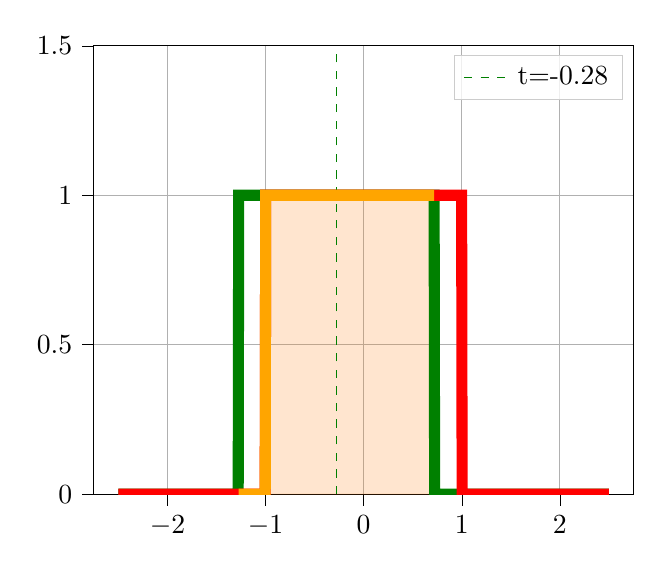
\begin{tikzpicture}

\definecolor{color0}{rgb}{1,0.498039215686275,0.0549019607843137}
\definecolor{color1}{rgb}{1,0.647058823529412,0}

\begin{axis}[
legend cell align={left},
legend style={fill opacity=0.8, draw opacity=1, text opacity=1, draw=white!80!black},
tick align=outside,
tick pos=left,
x grid style={white!69.0196078431373!black},
xmajorgrids,
xmin=-2.75, xmax=2.75,
xtick style={color=black},
y grid style={white!69.0196078431373!black},
ymajorgrids,
ymin=0, ymax=1.5,
ytick style={color=black}
]
\path [draw=color0, fill=color0, opacity=0.2]
(axis cs:-1.27377377377377,0)
--(axis cs:-1.27377377377377,0)
--(axis cs:-1.26876876876877,0)
--(axis cs:-1.26376376376376,0)
--(axis cs:-1.25875875875876,0)
--(axis cs:-1.25375375375375,0)
--(axis cs:-1.24874874874875,0)
--(axis cs:-1.24374374374374,0)
--(axis cs:-1.23873873873874,0)
--(axis cs:-1.23373373373373,0)
--(axis cs:-1.22872872872873,0)
--(axis cs:-1.22372372372372,0)
--(axis cs:-1.21871871871872,0)
--(axis cs:-1.21371371371371,0)
--(axis cs:-1.20870870870871,0)
--(axis cs:-1.2037037037037,0)
--(axis cs:-1.1986986986987,0)
--(axis cs:-1.19369369369369,0)
--(axis cs:-1.18868868868869,0)
--(axis cs:-1.18368368368368,0)
--(axis cs:-1.17867867867868,0)
--(axis cs:-1.17367367367367,0)
--(axis cs:-1.16866866866867,0)
--(axis cs:-1.16366366366366,0)
--(axis cs:-1.15865865865866,0)
--(axis cs:-1.15365365365365,0)
--(axis cs:-1.14864864864865,0)
--(axis cs:-1.14364364364364,0)
--(axis cs:-1.13863863863864,0)
--(axis cs:-1.13363363363363,0)
--(axis cs:-1.12862862862863,0)
--(axis cs:-1.12362362362362,0)
--(axis cs:-1.11861861861862,0)
--(axis cs:-1.11361361361361,0)
--(axis cs:-1.10860860860861,0)
--(axis cs:-1.1036036036036,0)
--(axis cs:-1.0985985985986,0)
--(axis cs:-1.09359359359359,0)
--(axis cs:-1.08858858858859,0)
--(axis cs:-1.08358358358358,0)
--(axis cs:-1.07857857857858,0)
--(axis cs:-1.07357357357357,0)
--(axis cs:-1.06856856856857,0)
--(axis cs:-1.06356356356356,0)
--(axis cs:-1.05855855855856,0)
--(axis cs:-1.05355355355355,0)
--(axis cs:-1.04854854854855,0)
--(axis cs:-1.04354354354354,0)
--(axis cs:-1.03853853853854,0)
--(axis cs:-1.03353353353353,0)
--(axis cs:-1.02852852852853,0)
--(axis cs:-1.02352352352352,0)
--(axis cs:-1.01851851851852,0)
--(axis cs:-1.01351351351351,0)
--(axis cs:-1.00850850850851,0)
--(axis cs:-1.0035035035035,0)
--(axis cs:-0.998498498498499,0)
--(axis cs:-0.993493493493494,0)
--(axis cs:-0.988488488488489,0)
--(axis cs:-0.983483483483484,0)
--(axis cs:-0.978478478478479,0)
--(axis cs:-0.973473473473474,0)
--(axis cs:-0.968468468468469,0)
--(axis cs:-0.963463463463464,0)
--(axis cs:-0.958458458458459,0)
--(axis cs:-0.953453453453454,0)
--(axis cs:-0.948448448448449,0)
--(axis cs:-0.943443443443444,0)
--(axis cs:-0.938438438438439,0)
--(axis cs:-0.933433433433434,0)
--(axis cs:-0.928428428428429,0)
--(axis cs:-0.923423423423424,0)
--(axis cs:-0.918418418418419,0)
--(axis cs:-0.913413413413414,0)
--(axis cs:-0.908408408408409,0)
--(axis cs:-0.903403403403404,0)
--(axis cs:-0.898398398398399,0)
--(axis cs:-0.893393393393393,0)
--(axis cs:-0.888388388388388,0)
--(axis cs:-0.883383383383383,0)
--(axis cs:-0.878378378378378,0)
--(axis cs:-0.873373373373373,0)
--(axis cs:-0.868368368368368,0)
--(axis cs:-0.863363363363363,0)
--(axis cs:-0.858358358358358,0)
--(axis cs:-0.853353353353353,0)
--(axis cs:-0.848348348348348,0)
--(axis cs:-0.843343343343343,0)
--(axis cs:-0.838338338338338,0)
--(axis cs:-0.833333333333333,0)
--(axis cs:-0.828328328328328,0)
--(axis cs:-0.823323323323323,0)
--(axis cs:-0.818318318318318,0)
--(axis cs:-0.813313313313313,0)
--(axis cs:-0.808308308308308,0)
--(axis cs:-0.803303303303303,0)
--(axis cs:-0.798298298298298,0)
--(axis cs:-0.793293293293293,0)
--(axis cs:-0.788288288288288,0)
--(axis cs:-0.783283283283283,0)
--(axis cs:-0.778278278278278,0)
--(axis cs:-0.773273273273273,0)
--(axis cs:-0.768268268268268,0)
--(axis cs:-0.763263263263263,0)
--(axis cs:-0.758258258258258,0)
--(axis cs:-0.753253253253253,0)
--(axis cs:-0.748248248248248,0)
--(axis cs:-0.743243243243243,0)
--(axis cs:-0.738238238238238,0)
--(axis cs:-0.733233233233233,0)
--(axis cs:-0.728228228228228,0)
--(axis cs:-0.723223223223223,0)
--(axis cs:-0.718218218218218,0)
--(axis cs:-0.713213213213213,0)
--(axis cs:-0.708208208208208,0)
--(axis cs:-0.703203203203203,0)
--(axis cs:-0.698198198198198,0)
--(axis cs:-0.693193193193193,0)
--(axis cs:-0.688188188188188,0)
--(axis cs:-0.683183183183183,0)
--(axis cs:-0.678178178178178,0)
--(axis cs:-0.673173173173173,0)
--(axis cs:-0.668168168168168,0)
--(axis cs:-0.663163163163163,0)
--(axis cs:-0.658158158158158,0)
--(axis cs:-0.653153153153153,0)
--(axis cs:-0.648148148148148,0)
--(axis cs:-0.643143143143143,0)
--(axis cs:-0.638138138138138,0)
--(axis cs:-0.633133133133133,0)
--(axis cs:-0.628128128128128,0)
--(axis cs:-0.623123123123123,0)
--(axis cs:-0.618118118118118,0)
--(axis cs:-0.613113113113113,0)
--(axis cs:-0.608108108108108,0)
--(axis cs:-0.603103103103103,0)
--(axis cs:-0.598098098098098,0)
--(axis cs:-0.593093093093093,0)
--(axis cs:-0.588088088088088,0)
--(axis cs:-0.583083083083083,0)
--(axis cs:-0.578078078078078,0)
--(axis cs:-0.573073073073073,0)
--(axis cs:-0.568068068068068,0)
--(axis cs:-0.563063063063063,0)
--(axis cs:-0.558058058058058,0)
--(axis cs:-0.553053053053053,0)
--(axis cs:-0.548048048048048,0)
--(axis cs:-0.543043043043043,0)
--(axis cs:-0.538038038038038,0)
--(axis cs:-0.533033033033033,0)
--(axis cs:-0.528028028028028,0)
--(axis cs:-0.523023023023023,0)
--(axis cs:-0.518018018018018,0)
--(axis cs:-0.513013013013013,0)
--(axis cs:-0.508008008008008,0)
--(axis cs:-0.503003003003003,0)
--(axis cs:-0.497997997997998,0)
--(axis cs:-0.492992992992993,0)
--(axis cs:-0.487987987987988,0)
--(axis cs:-0.482982982982983,0)
--(axis cs:-0.477977977977978,0)
--(axis cs:-0.472972972972973,0)
--(axis cs:-0.467967967967968,0)
--(axis cs:-0.462962962962963,0)
--(axis cs:-0.457957957957958,0)
--(axis cs:-0.452952952952953,0)
--(axis cs:-0.447947947947948,0)
--(axis cs:-0.442942942942943,0)
--(axis cs:-0.437937937937938,0)
--(axis cs:-0.432932932932933,0)
--(axis cs:-0.427927927927928,0)
--(axis cs:-0.422922922922923,0)
--(axis cs:-0.417917917917918,0)
--(axis cs:-0.412912912912913,0)
--(axis cs:-0.407907907907908,0)
--(axis cs:-0.402902902902903,0)
--(axis cs:-0.397897897897898,0)
--(axis cs:-0.392892892892893,0)
--(axis cs:-0.387887887887888,0)
--(axis cs:-0.382882882882883,0)
--(axis cs:-0.377877877877878,0)
--(axis cs:-0.372872872872873,0)
--(axis cs:-0.367867867867868,0)
--(axis cs:-0.362862862862863,0)
--(axis cs:-0.357857857857858,0)
--(axis cs:-0.352852852852853,0)
--(axis cs:-0.347847847847848,0)
--(axis cs:-0.342842842842843,0)
--(axis cs:-0.337837837837838,0)
--(axis cs:-0.332832832832833,0)
--(axis cs:-0.327827827827828,0)
--(axis cs:-0.322822822822823,0)
--(axis cs:-0.317817817817818,0)
--(axis cs:-0.312812812812813,0)
--(axis cs:-0.307807807807808,0)
--(axis cs:-0.302802802802803,0)
--(axis cs:-0.297797797797798,0)
--(axis cs:-0.292792792792793,0)
--(axis cs:-0.287787787787788,0)
--(axis cs:-0.282782782782783,0)
--(axis cs:-0.277777777777778,0)
--(axis cs:-0.272772772772773,0)
--(axis cs:-0.267767767767768,0)
--(axis cs:-0.262762762762763,0)
--(axis cs:-0.257757757757758,0)
--(axis cs:-0.252752752752753,0)
--(axis cs:-0.247747747747748,0)
--(axis cs:-0.242742742742743,0)
--(axis cs:-0.237737737737738,0)
--(axis cs:-0.232732732732733,0)
--(axis cs:-0.227727727727728,0)
--(axis cs:-0.222722722722723,0)
--(axis cs:-0.217717717717718,0)
--(axis cs:-0.212712712712713,0)
--(axis cs:-0.207707707707708,0)
--(axis cs:-0.202702702702703,0)
--(axis cs:-0.197697697697698,0)
--(axis cs:-0.192692692692693,0)
--(axis cs:-0.187687687687688,0)
--(axis cs:-0.182682682682683,0)
--(axis cs:-0.177677677677678,0)
--(axis cs:-0.172672672672673,0)
--(axis cs:-0.167667667667668,0)
--(axis cs:-0.162662662662663,0)
--(axis cs:-0.157657657657658,0)
--(axis cs:-0.152652652652653,0)
--(axis cs:-0.147647647647648,0)
--(axis cs:-0.142642642642643,0)
--(axis cs:-0.137637637637638,0)
--(axis cs:-0.132632632632633,0)
--(axis cs:-0.127627627627628,0)
--(axis cs:-0.122622622622623,0)
--(axis cs:-0.117617617617618,0)
--(axis cs:-0.112612612612613,0)
--(axis cs:-0.107607607607608,0)
--(axis cs:-0.102602602602603,0)
--(axis cs:-0.0975975975975976,0)
--(axis cs:-0.0925925925925926,0)
--(axis cs:-0.0875875875875876,0)
--(axis cs:-0.0825825825825826,0)
--(axis cs:-0.0775775775775776,0)
--(axis cs:-0.0725725725725725,0)
--(axis cs:-0.0675675675675675,0)
--(axis cs:-0.0625625625625625,0)
--(axis cs:-0.0575575575575575,0)
--(axis cs:-0.0525525525525525,0)
--(axis cs:-0.0475475475475475,0)
--(axis cs:-0.0425425425425425,0)
--(axis cs:-0.0375375375375375,0)
--(axis cs:-0.0325325325325325,0)
--(axis cs:-0.0275275275275275,0)
--(axis cs:-0.0225225225225225,0)
--(axis cs:-0.0175175175175175,0)
--(axis cs:-0.0125125125125125,0)
--(axis cs:-0.0075075075075075,0)
--(axis cs:-0.0025025025025025,0)
--(axis cs:0.0025025025025025,0)
--(axis cs:0.0075075075075075,0)
--(axis cs:0.0125125125125125,0)
--(axis cs:0.0175175175175175,0)
--(axis cs:0.0225225225225225,0)
--(axis cs:0.0275275275275275,0)
--(axis cs:0.0325325325325325,0)
--(axis cs:0.0375375375375375,0)
--(axis cs:0.0425425425425425,0)
--(axis cs:0.0475475475475475,0)
--(axis cs:0.0525525525525525,0)
--(axis cs:0.0575575575575575,0)
--(axis cs:0.0625625625625625,0)
--(axis cs:0.0675675675675675,0)
--(axis cs:0.0725725725725725,0)
--(axis cs:0.0775775775775776,0)
--(axis cs:0.0825825825825826,0)
--(axis cs:0.0875875875875876,0)
--(axis cs:0.0925925925925926,0)
--(axis cs:0.0975975975975976,0)
--(axis cs:0.102602602602603,0)
--(axis cs:0.107607607607608,0)
--(axis cs:0.112612612612613,0)
--(axis cs:0.117617617617618,0)
--(axis cs:0.122622622622623,0)
--(axis cs:0.127627627627628,0)
--(axis cs:0.132632632632633,0)
--(axis cs:0.137637637637638,0)
--(axis cs:0.142642642642643,0)
--(axis cs:0.147647647647648,0)
--(axis cs:0.152652652652653,0)
--(axis cs:0.157657657657658,0)
--(axis cs:0.162662662662663,0)
--(axis cs:0.167667667667668,0)
--(axis cs:0.172672672672673,0)
--(axis cs:0.177677677677678,0)
--(axis cs:0.182682682682683,0)
--(axis cs:0.187687687687688,0)
--(axis cs:0.192692692692693,0)
--(axis cs:0.197697697697698,0)
--(axis cs:0.202702702702703,0)
--(axis cs:0.207707707707708,0)
--(axis cs:0.212712712712713,0)
--(axis cs:0.217717717717718,0)
--(axis cs:0.222722722722723,0)
--(axis cs:0.227727727727728,0)
--(axis cs:0.232732732732733,0)
--(axis cs:0.237737737737738,0)
--(axis cs:0.242742742742743,0)
--(axis cs:0.247747747747748,0)
--(axis cs:0.252752752752753,0)
--(axis cs:0.257757757757758,0)
--(axis cs:0.262762762762763,0)
--(axis cs:0.267767767767768,0)
--(axis cs:0.272772772772773,0)
--(axis cs:0.277777777777778,0)
--(axis cs:0.282782782782783,0)
--(axis cs:0.287787787787788,0)
--(axis cs:0.292792792792793,0)
--(axis cs:0.297797797797798,0)
--(axis cs:0.302802802802803,0)
--(axis cs:0.307807807807808,0)
--(axis cs:0.312812812812813,0)
--(axis cs:0.317817817817818,0)
--(axis cs:0.322822822822823,0)
--(axis cs:0.327827827827828,0)
--(axis cs:0.332832832832833,0)
--(axis cs:0.337837837837838,0)
--(axis cs:0.342842842842843,0)
--(axis cs:0.347847847847848,0)
--(axis cs:0.352852852852853,0)
--(axis cs:0.357857857857858,0)
--(axis cs:0.362862862862863,0)
--(axis cs:0.367867867867868,0)
--(axis cs:0.372872872872873,0)
--(axis cs:0.377877877877878,0)
--(axis cs:0.382882882882883,0)
--(axis cs:0.387887887887888,0)
--(axis cs:0.392892892892893,0)
--(axis cs:0.397897897897898,0)
--(axis cs:0.402902902902903,0)
--(axis cs:0.407907907907908,0)
--(axis cs:0.412912912912913,0)
--(axis cs:0.417917917917918,0)
--(axis cs:0.422922922922923,0)
--(axis cs:0.427927927927928,0)
--(axis cs:0.432932932932933,0)
--(axis cs:0.437937937937938,0)
--(axis cs:0.442942942942943,0)
--(axis cs:0.447947947947948,0)
--(axis cs:0.452952952952953,0)
--(axis cs:0.457957957957958,0)
--(axis cs:0.462962962962963,0)
--(axis cs:0.467967967967968,0)
--(axis cs:0.472972972972973,0)
--(axis cs:0.477977977977978,0)
--(axis cs:0.482982982982983,0)
--(axis cs:0.487987987987988,0)
--(axis cs:0.492992992992993,0)
--(axis cs:0.497997997997998,0)
--(axis cs:0.503003003003003,0)
--(axis cs:0.508008008008008,0)
--(axis cs:0.513013013013013,0)
--(axis cs:0.518018018018018,0)
--(axis cs:0.523023023023023,0)
--(axis cs:0.528028028028028,0)
--(axis cs:0.533033033033033,0)
--(axis cs:0.538038038038038,0)
--(axis cs:0.543043043043043,0)
--(axis cs:0.548048048048048,0)
--(axis cs:0.553053053053053,0)
--(axis cs:0.558058058058058,0)
--(axis cs:0.563063063063063,0)
--(axis cs:0.568068068068068,0)
--(axis cs:0.573073073073073,0)
--(axis cs:0.578078078078078,0)
--(axis cs:0.583083083083083,0)
--(axis cs:0.588088088088088,0)
--(axis cs:0.593093093093093,0)
--(axis cs:0.598098098098098,0)
--(axis cs:0.603103103103103,0)
--(axis cs:0.608108108108108,0)
--(axis cs:0.613113113113113,0)
--(axis cs:0.618118118118118,0)
--(axis cs:0.623123123123123,0)
--(axis cs:0.628128128128128,0)
--(axis cs:0.633133133133133,0)
--(axis cs:0.638138138138138,0)
--(axis cs:0.643143143143143,0)
--(axis cs:0.648148148148148,0)
--(axis cs:0.653153153153153,0)
--(axis cs:0.658158158158158,0)
--(axis cs:0.663163163163163,0)
--(axis cs:0.668168168168168,0)
--(axis cs:0.673173173173173,0)
--(axis cs:0.678178178178178,0)
--(axis cs:0.683183183183183,0)
--(axis cs:0.688188188188188,0)
--(axis cs:0.693193193193193,0)
--(axis cs:0.698198198198198,0)
--(axis cs:0.703203203203203,0)
--(axis cs:0.708208208208208,0)
--(axis cs:0.713213213213213,0)
--(axis cs:0.718218218218218,0)
--(axis cs:0.718218218218218,1)
--(axis cs:0.718218218218218,1)
--(axis cs:0.713213213213213,1)
--(axis cs:0.708208208208208,1)
--(axis cs:0.703203203203203,1)
--(axis cs:0.698198198198198,1)
--(axis cs:0.693193193193193,1)
--(axis cs:0.688188188188188,1)
--(axis cs:0.683183183183183,1)
--(axis cs:0.678178178178178,1)
--(axis cs:0.673173173173173,1)
--(axis cs:0.668168168168168,1)
--(axis cs:0.663163163163163,1)
--(axis cs:0.658158158158158,1)
--(axis cs:0.653153153153153,1)
--(axis cs:0.648148148148148,1)
--(axis cs:0.643143143143143,1)
--(axis cs:0.638138138138138,1)
--(axis cs:0.633133133133133,1)
--(axis cs:0.628128128128128,1)
--(axis cs:0.623123123123123,1)
--(axis cs:0.618118118118118,1)
--(axis cs:0.613113113113113,1)
--(axis cs:0.608108108108108,1)
--(axis cs:0.603103103103103,1)
--(axis cs:0.598098098098098,1)
--(axis cs:0.593093093093093,1)
--(axis cs:0.588088088088088,1)
--(axis cs:0.583083083083083,1)
--(axis cs:0.578078078078078,1)
--(axis cs:0.573073073073073,1)
--(axis cs:0.568068068068068,1)
--(axis cs:0.563063063063063,1)
--(axis cs:0.558058058058058,1)
--(axis cs:0.553053053053053,1)
--(axis cs:0.548048048048048,1)
--(axis cs:0.543043043043043,1)
--(axis cs:0.538038038038038,1)
--(axis cs:0.533033033033033,1)
--(axis cs:0.528028028028028,1)
--(axis cs:0.523023023023023,1)
--(axis cs:0.518018018018018,1)
--(axis cs:0.513013013013013,1)
--(axis cs:0.508008008008008,1)
--(axis cs:0.503003003003003,1)
--(axis cs:0.497997997997998,1)
--(axis cs:0.492992992992993,1)
--(axis cs:0.487987987987988,1)
--(axis cs:0.482982982982983,1)
--(axis cs:0.477977977977978,1)
--(axis cs:0.472972972972973,1)
--(axis cs:0.467967967967968,1)
--(axis cs:0.462962962962963,1)
--(axis cs:0.457957957957958,1)
--(axis cs:0.452952952952953,1)
--(axis cs:0.447947947947948,1)
--(axis cs:0.442942942942943,1)
--(axis cs:0.437937937937938,1)
--(axis cs:0.432932932932933,1)
--(axis cs:0.427927927927928,1)
--(axis cs:0.422922922922923,1)
--(axis cs:0.417917917917918,1)
--(axis cs:0.412912912912913,1)
--(axis cs:0.407907907907908,1)
--(axis cs:0.402902902902903,1)
--(axis cs:0.397897897897898,1)
--(axis cs:0.392892892892893,1)
--(axis cs:0.387887887887888,1)
--(axis cs:0.382882882882883,1)
--(axis cs:0.377877877877878,1)
--(axis cs:0.372872872872873,1)
--(axis cs:0.367867867867868,1)
--(axis cs:0.362862862862863,1)
--(axis cs:0.357857857857858,1)
--(axis cs:0.352852852852853,1)
--(axis cs:0.347847847847848,1)
--(axis cs:0.342842842842843,1)
--(axis cs:0.337837837837838,1)
--(axis cs:0.332832832832833,1)
--(axis cs:0.327827827827828,1)
--(axis cs:0.322822822822823,1)
--(axis cs:0.317817817817818,1)
--(axis cs:0.312812812812813,1)
--(axis cs:0.307807807807808,1)
--(axis cs:0.302802802802803,1)
--(axis cs:0.297797797797798,1)
--(axis cs:0.292792792792793,1)
--(axis cs:0.287787787787788,1)
--(axis cs:0.282782782782783,1)
--(axis cs:0.277777777777778,1)
--(axis cs:0.272772772772773,1)
--(axis cs:0.267767767767768,1)
--(axis cs:0.262762762762763,1)
--(axis cs:0.257757757757758,1)
--(axis cs:0.252752752752753,1)
--(axis cs:0.247747747747748,1)
--(axis cs:0.242742742742743,1)
--(axis cs:0.237737737737738,1)
--(axis cs:0.232732732732733,1)
--(axis cs:0.227727727727728,1)
--(axis cs:0.222722722722723,1)
--(axis cs:0.217717717717718,1)
--(axis cs:0.212712712712713,1)
--(axis cs:0.207707707707708,1)
--(axis cs:0.202702702702703,1)
--(axis cs:0.197697697697698,1)
--(axis cs:0.192692692692693,1)
--(axis cs:0.187687687687688,1)
--(axis cs:0.182682682682683,1)
--(axis cs:0.177677677677678,1)
--(axis cs:0.172672672672673,1)
--(axis cs:0.167667667667668,1)
--(axis cs:0.162662662662663,1)
--(axis cs:0.157657657657658,1)
--(axis cs:0.152652652652653,1)
--(axis cs:0.147647647647648,1)
--(axis cs:0.142642642642643,1)
--(axis cs:0.137637637637638,1)
--(axis cs:0.132632632632633,1)
--(axis cs:0.127627627627628,1)
--(axis cs:0.122622622622623,1)
--(axis cs:0.117617617617618,1)
--(axis cs:0.112612612612613,1)
--(axis cs:0.107607607607608,1)
--(axis cs:0.102602602602603,1)
--(axis cs:0.0975975975975976,1)
--(axis cs:0.0925925925925926,1)
--(axis cs:0.0875875875875876,1)
--(axis cs:0.0825825825825826,1)
--(axis cs:0.0775775775775776,1)
--(axis cs:0.0725725725725725,1)
--(axis cs:0.0675675675675675,1)
--(axis cs:0.0625625625625625,1)
--(axis cs:0.0575575575575575,1)
--(axis cs:0.0525525525525525,1)
--(axis cs:0.0475475475475475,1)
--(axis cs:0.0425425425425425,1)
--(axis cs:0.0375375375375375,1)
--(axis cs:0.0325325325325325,1)
--(axis cs:0.0275275275275275,1)
--(axis cs:0.0225225225225225,1)
--(axis cs:0.0175175175175175,1)
--(axis cs:0.0125125125125125,1)
--(axis cs:0.0075075075075075,1)
--(axis cs:0.0025025025025025,1)
--(axis cs:-0.0025025025025025,1)
--(axis cs:-0.0075075075075075,1)
--(axis cs:-0.0125125125125125,1)
--(axis cs:-0.0175175175175175,1)
--(axis cs:-0.0225225225225225,1)
--(axis cs:-0.0275275275275275,1)
--(axis cs:-0.0325325325325325,1)
--(axis cs:-0.0375375375375375,1)
--(axis cs:-0.0425425425425425,1)
--(axis cs:-0.0475475475475475,1)
--(axis cs:-0.0525525525525525,1)
--(axis cs:-0.0575575575575575,1)
--(axis cs:-0.0625625625625625,1)
--(axis cs:-0.0675675675675675,1)
--(axis cs:-0.0725725725725725,1)
--(axis cs:-0.0775775775775776,1)
--(axis cs:-0.0825825825825826,1)
--(axis cs:-0.0875875875875876,1)
--(axis cs:-0.0925925925925926,1)
--(axis cs:-0.0975975975975976,1)
--(axis cs:-0.102602602602603,1)
--(axis cs:-0.107607607607608,1)
--(axis cs:-0.112612612612613,1)
--(axis cs:-0.117617617617618,1)
--(axis cs:-0.122622622622623,1)
--(axis cs:-0.127627627627628,1)
--(axis cs:-0.132632632632633,1)
--(axis cs:-0.137637637637638,1)
--(axis cs:-0.142642642642643,1)
--(axis cs:-0.147647647647648,1)
--(axis cs:-0.152652652652653,1)
--(axis cs:-0.157657657657658,1)
--(axis cs:-0.162662662662663,1)
--(axis cs:-0.167667667667668,1)
--(axis cs:-0.172672672672673,1)
--(axis cs:-0.177677677677678,1)
--(axis cs:-0.182682682682683,1)
--(axis cs:-0.187687687687688,1)
--(axis cs:-0.192692692692693,1)
--(axis cs:-0.197697697697698,1)
--(axis cs:-0.202702702702703,1)
--(axis cs:-0.207707707707708,1)
--(axis cs:-0.212712712712713,1)
--(axis cs:-0.217717717717718,1)
--(axis cs:-0.222722722722723,1)
--(axis cs:-0.227727727727728,1)
--(axis cs:-0.232732732732733,1)
--(axis cs:-0.237737737737738,1)
--(axis cs:-0.242742742742743,1)
--(axis cs:-0.247747747747748,1)
--(axis cs:-0.252752752752753,1)
--(axis cs:-0.257757757757758,1)
--(axis cs:-0.262762762762763,1)
--(axis cs:-0.267767767767768,1)
--(axis cs:-0.272772772772773,1)
--(axis cs:-0.277777777777778,1)
--(axis cs:-0.282782782782783,1)
--(axis cs:-0.287787787787788,1)
--(axis cs:-0.292792792792793,1)
--(axis cs:-0.297797797797798,1)
--(axis cs:-0.302802802802803,1)
--(axis cs:-0.307807807807808,1)
--(axis cs:-0.312812812812813,1)
--(axis cs:-0.317817817817818,1)
--(axis cs:-0.322822822822823,1)
--(axis cs:-0.327827827827828,1)
--(axis cs:-0.332832832832833,1)
--(axis cs:-0.337837837837838,1)
--(axis cs:-0.342842842842843,1)
--(axis cs:-0.347847847847848,1)
--(axis cs:-0.352852852852853,1)
--(axis cs:-0.357857857857858,1)
--(axis cs:-0.362862862862863,1)
--(axis cs:-0.367867867867868,1)
--(axis cs:-0.372872872872873,1)
--(axis cs:-0.377877877877878,1)
--(axis cs:-0.382882882882883,1)
--(axis cs:-0.387887887887888,1)
--(axis cs:-0.392892892892893,1)
--(axis cs:-0.397897897897898,1)
--(axis cs:-0.402902902902903,1)
--(axis cs:-0.407907907907908,1)
--(axis cs:-0.412912912912913,1)
--(axis cs:-0.417917917917918,1)
--(axis cs:-0.422922922922923,1)
--(axis cs:-0.427927927927928,1)
--(axis cs:-0.432932932932933,1)
--(axis cs:-0.437937937937938,1)
--(axis cs:-0.442942942942943,1)
--(axis cs:-0.447947947947948,1)
--(axis cs:-0.452952952952953,1)
--(axis cs:-0.457957957957958,1)
--(axis cs:-0.462962962962963,1)
--(axis cs:-0.467967967967968,1)
--(axis cs:-0.472972972972973,1)
--(axis cs:-0.477977977977978,1)
--(axis cs:-0.482982982982983,1)
--(axis cs:-0.487987987987988,1)
--(axis cs:-0.492992992992993,1)
--(axis cs:-0.497997997997998,1)
--(axis cs:-0.503003003003003,1)
--(axis cs:-0.508008008008008,1)
--(axis cs:-0.513013013013013,1)
--(axis cs:-0.518018018018018,1)
--(axis cs:-0.523023023023023,1)
--(axis cs:-0.528028028028028,1)
--(axis cs:-0.533033033033033,1)
--(axis cs:-0.538038038038038,1)
--(axis cs:-0.543043043043043,1)
--(axis cs:-0.548048048048048,1)
--(axis cs:-0.553053053053053,1)
--(axis cs:-0.558058058058058,1)
--(axis cs:-0.563063063063063,1)
--(axis cs:-0.568068068068068,1)
--(axis cs:-0.573073073073073,1)
--(axis cs:-0.578078078078078,1)
--(axis cs:-0.583083083083083,1)
--(axis cs:-0.588088088088088,1)
--(axis cs:-0.593093093093093,1)
--(axis cs:-0.598098098098098,1)
--(axis cs:-0.603103103103103,1)
--(axis cs:-0.608108108108108,1)
--(axis cs:-0.613113113113113,1)
--(axis cs:-0.618118118118118,1)
--(axis cs:-0.623123123123123,1)
--(axis cs:-0.628128128128128,1)
--(axis cs:-0.633133133133133,1)
--(axis cs:-0.638138138138138,1)
--(axis cs:-0.643143143143143,1)
--(axis cs:-0.648148148148148,1)
--(axis cs:-0.653153153153153,1)
--(axis cs:-0.658158158158158,1)
--(axis cs:-0.663163163163163,1)
--(axis cs:-0.668168168168168,1)
--(axis cs:-0.673173173173173,1)
--(axis cs:-0.678178178178178,1)
--(axis cs:-0.683183183183183,1)
--(axis cs:-0.688188188188188,1)
--(axis cs:-0.693193193193193,1)
--(axis cs:-0.698198198198198,1)
--(axis cs:-0.703203203203203,1)
--(axis cs:-0.708208208208208,1)
--(axis cs:-0.713213213213213,1)
--(axis cs:-0.718218218218218,1)
--(axis cs:-0.723223223223223,1)
--(axis cs:-0.728228228228228,1)
--(axis cs:-0.733233233233233,1)
--(axis cs:-0.738238238238238,1)
--(axis cs:-0.743243243243243,1)
--(axis cs:-0.748248248248248,1)
--(axis cs:-0.753253253253253,1)
--(axis cs:-0.758258258258258,1)
--(axis cs:-0.763263263263263,1)
--(axis cs:-0.768268268268268,1)
--(axis cs:-0.773273273273273,1)
--(axis cs:-0.778278278278278,1)
--(axis cs:-0.783283283283283,1)
--(axis cs:-0.788288288288288,1)
--(axis cs:-0.793293293293293,1)
--(axis cs:-0.798298298298298,1)
--(axis cs:-0.803303303303303,1)
--(axis cs:-0.808308308308308,1)
--(axis cs:-0.813313313313313,1)
--(axis cs:-0.818318318318318,1)
--(axis cs:-0.823323323323323,1)
--(axis cs:-0.828328328328328,1)
--(axis cs:-0.833333333333333,1)
--(axis cs:-0.838338338338338,1)
--(axis cs:-0.843343343343343,1)
--(axis cs:-0.848348348348348,1)
--(axis cs:-0.853353353353353,1)
--(axis cs:-0.858358358358358,1)
--(axis cs:-0.863363363363363,1)
--(axis cs:-0.868368368368368,1)
--(axis cs:-0.873373373373373,1)
--(axis cs:-0.878378378378378,1)
--(axis cs:-0.883383383383383,1)
--(axis cs:-0.888388388388388,1)
--(axis cs:-0.893393393393393,1)
--(axis cs:-0.898398398398399,1)
--(axis cs:-0.903403403403404,1)
--(axis cs:-0.908408408408409,1)
--(axis cs:-0.913413413413414,1)
--(axis cs:-0.918418418418419,1)
--(axis cs:-0.923423423423424,1)
--(axis cs:-0.928428428428429,1)
--(axis cs:-0.933433433433434,1)
--(axis cs:-0.938438438438439,1)
--(axis cs:-0.943443443443444,1)
--(axis cs:-0.948448448448449,1)
--(axis cs:-0.953453453453454,1)
--(axis cs:-0.958458458458459,1)
--(axis cs:-0.963463463463464,1)
--(axis cs:-0.968468468468469,1)
--(axis cs:-0.973473473473474,1)
--(axis cs:-0.978478478478479,1)
--(axis cs:-0.983483483483484,1)
--(axis cs:-0.988488488488489,1)
--(axis cs:-0.993493493493494,1)
--(axis cs:-0.998498498498499,1)
--(axis cs:-1.0035035035035,0)
--(axis cs:-1.00850850850851,0)
--(axis cs:-1.01351351351351,0)
--(axis cs:-1.01851851851852,0)
--(axis cs:-1.02352352352352,0)
--(axis cs:-1.02852852852853,0)
--(axis cs:-1.03353353353353,0)
--(axis cs:-1.03853853853854,0)
--(axis cs:-1.04354354354354,0)
--(axis cs:-1.04854854854855,0)
--(axis cs:-1.05355355355355,0)
--(axis cs:-1.05855855855856,0)
--(axis cs:-1.06356356356356,0)
--(axis cs:-1.06856856856857,0)
--(axis cs:-1.07357357357357,0)
--(axis cs:-1.07857857857858,0)
--(axis cs:-1.08358358358358,0)
--(axis cs:-1.08858858858859,0)
--(axis cs:-1.09359359359359,0)
--(axis cs:-1.0985985985986,0)
--(axis cs:-1.1036036036036,0)
--(axis cs:-1.10860860860861,0)
--(axis cs:-1.11361361361361,0)
--(axis cs:-1.11861861861862,0)
--(axis cs:-1.12362362362362,0)
--(axis cs:-1.12862862862863,0)
--(axis cs:-1.13363363363363,0)
--(axis cs:-1.13863863863864,0)
--(axis cs:-1.14364364364364,0)
--(axis cs:-1.14864864864865,0)
--(axis cs:-1.15365365365365,0)
--(axis cs:-1.15865865865866,0)
--(axis cs:-1.16366366366366,0)
--(axis cs:-1.16866866866867,0)
--(axis cs:-1.17367367367367,0)
--(axis cs:-1.17867867867868,0)
--(axis cs:-1.18368368368368,0)
--(axis cs:-1.18868868868869,0)
--(axis cs:-1.19369369369369,0)
--(axis cs:-1.1986986986987,0)
--(axis cs:-1.2037037037037,0)
--(axis cs:-1.20870870870871,0)
--(axis cs:-1.21371371371371,0)
--(axis cs:-1.21871871871872,0)
--(axis cs:-1.22372372372372,0)
--(axis cs:-1.22872872872873,0)
--(axis cs:-1.23373373373373,0)
--(axis cs:-1.23873873873874,0)
--(axis cs:-1.24374374374374,0)
--(axis cs:-1.24874874874875,0)
--(axis cs:-1.25375375375375,0)
--(axis cs:-1.25875875875876,0)
--(axis cs:-1.26376376376376,0)
--(axis cs:-1.26876876876877,0)
--(axis cs:-1.27377377377377,0)
--cycle;

\addplot [line width=4pt, green!50!black, forget plot]
table {%
-2.5 0
-2.49499499499499 0
-2.48998998998999 0
-2.48498498498498 0
-2.47997997997998 0
-2.47497497497497 0
-2.46996996996997 0
-2.46496496496496 0
-2.45995995995996 0
-2.45495495495495 0
-2.44994994994995 0
-2.44494494494494 0
-2.43993993993994 0
-2.43493493493493 0
-2.42992992992993 0
-2.42492492492492 0
-2.41991991991992 0
-2.41491491491491 0
-2.40990990990991 0
-2.4049049049049 0
-2.3998998998999 0
-2.39489489489489 0
-2.38988988988989 0
-2.38488488488488 0
-2.37987987987988 0
-2.37487487487487 0
-2.36986986986987 0
-2.36486486486486 0
-2.35985985985986 0
-2.35485485485485 0
-2.34984984984985 0
-2.34484484484484 0
-2.33983983983984 0
-2.33483483483483 0
-2.32982982982983 0
-2.32482482482482 0
-2.31981981981982 0
-2.31481481481481 0
-2.30980980980981 0
-2.3048048048048 0
-2.2997997997998 0
-2.29479479479479 0
-2.28978978978979 0
-2.28478478478478 0
-2.27977977977978 0
-2.27477477477477 0
-2.26976976976977 0
-2.26476476476476 0
-2.25975975975976 0
-2.25475475475475 0
-2.24974974974975 0
-2.24474474474474 0
-2.23973973973974 0
-2.23473473473473 0
-2.22972972972973 0
-2.22472472472472 0
-2.21971971971972 0
-2.21471471471471 0
-2.20970970970971 0
-2.2047047047047 0
-2.1996996996997 0
-2.19469469469469 0
-2.18968968968969 0
-2.18468468468468 0
-2.17967967967968 0
-2.17467467467467 0
-2.16966966966967 0
-2.16466466466466 0
-2.15965965965966 0
-2.15465465465465 0
-2.14964964964965 0
-2.14464464464464 0
-2.13963963963964 0
-2.13463463463463 0
-2.12962962962963 0
-2.12462462462462 0
-2.11961961961962 0
-2.11461461461461 0
-2.10960960960961 0
-2.1046046046046 0
-2.0995995995996 0
-2.09459459459459 0
-2.08958958958959 0
-2.08458458458458 0
-2.07957957957958 0
-2.07457457457457 0
-2.06956956956957 0
-2.06456456456456 0
-2.05955955955956 0
-2.05455455455455 0
-2.04954954954955 0
-2.04454454454454 0
-2.03953953953954 0
-2.03453453453453 0
-2.02952952952953 0
-2.02452452452452 0
-2.01951951951952 0
-2.01451451451451 0
-2.00950950950951 0
-2.0045045045045 0
-1.9994994994995 0
-1.99449449449449 0
-1.98948948948949 0
-1.98448448448448 0
-1.97947947947948 0
-1.97447447447447 0
-1.96946946946947 0
-1.96446446446446 0
-1.95945945945946 0
-1.95445445445445 0
-1.94944944944945 0
-1.94444444444444 0
-1.93943943943944 0
-1.93443443443443 0
-1.92942942942943 0
-1.92442442442442 0
-1.91941941941942 0
-1.91441441441441 0
-1.90940940940941 0
-1.9044044044044 0
-1.8993993993994 0
-1.89439439439439 0
-1.88938938938939 0
-1.88438438438438 0
-1.87937937937938 0
-1.87437437437437 0
-1.86936936936937 0
-1.86436436436436 0
-1.85935935935936 0
-1.85435435435435 0
-1.84934934934935 0
-1.84434434434434 0
-1.83933933933934 0
-1.83433433433433 0
-1.82932932932933 0
-1.82432432432432 0
-1.81931931931932 0
-1.81431431431431 0
-1.80930930930931 0
-1.8043043043043 0
-1.7992992992993 0
-1.79429429429429 0
-1.78928928928929 0
-1.78428428428428 0
-1.77927927927928 0
-1.77427427427427 0
-1.76926926926927 0
-1.76426426426426 0
-1.75925925925926 0
-1.75425425425425 0
-1.74924924924925 0
-1.74424424424424 0
-1.73923923923924 0
-1.73423423423423 0
-1.72922922922923 0
-1.72422422422422 0
-1.71921921921922 0
-1.71421421421421 0
-1.70920920920921 0
-1.7042042042042 0
-1.6991991991992 0
-1.69419419419419 0
-1.68918918918919 0
-1.68418418418418 0
-1.67917917917918 0
-1.67417417417417 0
-1.66916916916917 0
-1.66416416416416 0
-1.65915915915916 0
-1.65415415415415 0
-1.64914914914915 0
-1.64414414414414 0
-1.63913913913914 0
-1.63413413413413 0
-1.62912912912913 0
-1.62412412412412 0
-1.61911911911912 0
-1.61411411411411 0
-1.60910910910911 0
-1.6041041041041 0
-1.5990990990991 0
-1.59409409409409 0
-1.58908908908909 0
-1.58408408408408 0
-1.57907907907908 0
-1.57407407407407 0
-1.56906906906907 0
-1.56406406406406 0
-1.55905905905906 0
-1.55405405405405 0
-1.54904904904905 0
-1.54404404404404 0
-1.53903903903904 0
-1.53403403403403 0
-1.52902902902903 0
-1.52402402402402 0
-1.51901901901902 0
-1.51401401401401 0
-1.50900900900901 0
-1.504004004004 0
-1.498998998999 0
-1.49399399399399 0
-1.48898898898899 0
-1.48398398398398 0
-1.47897897897898 0
-1.47397397397397 0
-1.46896896896897 0
-1.46396396396396 0
-1.45895895895896 0
-1.45395395395395 0
-1.44894894894895 0
-1.44394394394394 0
-1.43893893893894 0
-1.43393393393393 0
-1.42892892892893 0
-1.42392392392392 0
-1.41891891891892 0
-1.41391391391391 0
-1.40890890890891 0
-1.4039039039039 0
-1.3988988988989 0
-1.39389389389389 0
-1.38888888888889 0
-1.38388388388388 0
-1.37887887887888 0
-1.37387387387387 0
-1.36886886886887 0
-1.36386386386386 0
-1.35885885885886 0
-1.35385385385385 0
-1.34884884884885 0
-1.34384384384384 0
-1.33883883883884 0
-1.33383383383383 0
-1.32882882882883 0
-1.32382382382382 0
-1.31881881881882 0
-1.31381381381381 0
-1.30880880880881 0
-1.3038038038038 0
-1.2987987987988 0
-1.29379379379379 0
-1.28878878878879 0
-1.28378378378378 0
-1.27877877877878 0
-1.27377377377377 1
-1.26876876876877 1
-1.26376376376376 1
-1.25875875875876 1
-1.25375375375375 1
-1.24874874874875 1
-1.24374374374374 1
-1.23873873873874 1
-1.23373373373373 1
-1.22872872872873 1
-1.22372372372372 1
-1.21871871871872 1
-1.21371371371371 1
-1.20870870870871 1
-1.2037037037037 1
-1.1986986986987 1
-1.19369369369369 1
-1.18868868868869 1
-1.18368368368368 1
-1.17867867867868 1
-1.17367367367367 1
-1.16866866866867 1
-1.16366366366366 1
-1.15865865865866 1
-1.15365365365365 1
-1.14864864864865 1
-1.14364364364364 1
-1.13863863863864 1
-1.13363363363363 1
-1.12862862862863 1
-1.12362362362362 1
-1.11861861861862 1
-1.11361361361361 1
-1.10860860860861 1
-1.1036036036036 1
-1.0985985985986 1
-1.09359359359359 1
-1.08858858858859 1
-1.08358358358358 1
-1.07857857857858 1
-1.07357357357357 1
-1.06856856856857 1
-1.06356356356356 1
-1.05855855855856 1
-1.05355355355355 1
-1.04854854854855 1
-1.04354354354354 1
-1.03853853853854 1
-1.03353353353353 1
-1.02852852852853 1
-1.02352352352352 1
-1.01851851851852 1
-1.01351351351351 1
-1.00850850850851 1
-1.0035035035035 1
-0.998498498498499 1
-0.993493493493494 1
-0.988488488488489 1
-0.983483483483484 1
-0.978478478478479 1
-0.973473473473474 1
-0.968468468468469 1
-0.963463463463464 1
-0.958458458458459 1
-0.953453453453454 1
-0.948448448448449 1
-0.943443443443444 1
-0.938438438438439 1
-0.933433433433434 1
-0.928428428428429 1
-0.923423423423424 1
-0.918418418418419 1
-0.913413413413414 1
-0.908408408408409 1
-0.903403403403404 1
-0.898398398398399 1
-0.893393393393393 1
-0.888388388388388 1
-0.883383383383383 1
-0.878378378378378 1
-0.873373373373373 1
-0.868368368368368 1
-0.863363363363363 1
-0.858358358358358 1
-0.853353353353353 1
-0.848348348348348 1
-0.843343343343343 1
-0.838338338338338 1
-0.833333333333333 1
-0.828328328328328 1
-0.823323323323323 1
-0.818318318318318 1
-0.813313313313313 1
-0.808308308308308 1
-0.803303303303303 1
-0.798298298298298 1
-0.793293293293293 1
-0.788288288288288 1
-0.783283283283283 1
-0.778278278278278 1
-0.773273273273273 1
-0.768268268268268 1
-0.763263263263263 1
-0.758258258258258 1
-0.753253253253253 1
-0.748248248248248 1
-0.743243243243243 1
-0.738238238238238 1
-0.733233233233233 1
-0.728228228228228 1
-0.723223223223223 1
-0.718218218218218 1
-0.713213213213213 1
-0.708208208208208 1
-0.703203203203203 1
-0.698198198198198 1
-0.693193193193193 1
-0.688188188188188 1
-0.683183183183183 1
-0.678178178178178 1
-0.673173173173173 1
-0.668168168168168 1
-0.663163163163163 1
-0.658158158158158 1
-0.653153153153153 1
-0.648148148148148 1
-0.643143143143143 1
-0.638138138138138 1
-0.633133133133133 1
-0.628128128128128 1
-0.623123123123123 1
-0.618118118118118 1
-0.613113113113113 1
-0.608108108108108 1
-0.603103103103103 1
-0.598098098098098 1
-0.593093093093093 1
-0.588088088088088 1
-0.583083083083083 1
-0.578078078078078 1
-0.573073073073073 1
-0.568068068068068 1
-0.563063063063063 1
-0.558058058058058 1
-0.553053053053053 1
-0.548048048048048 1
-0.543043043043043 1
-0.538038038038038 1
-0.533033033033033 1
-0.528028028028028 1
-0.523023023023023 1
-0.518018018018018 1
-0.513013013013013 1
-0.508008008008008 1
-0.503003003003003 1
-0.497997997997998 1
-0.492992992992993 1
-0.487987987987988 1
-0.482982982982983 1
-0.477977977977978 1
-0.472972972972973 1
-0.467967967967968 1
-0.462962962962963 1
-0.457957957957958 1
-0.452952952952953 1
-0.447947947947948 1
-0.442942942942943 1
-0.437937937937938 1
-0.432932932932933 1
-0.427927927927928 1
-0.422922922922923 1
-0.417917917917918 1
-0.412912912912913 1
-0.407907907907908 1
-0.402902902902903 1
-0.397897897897898 1
-0.392892892892893 1
-0.387887887887888 1
-0.382882882882883 1
-0.377877877877878 1
-0.372872872872873 1
-0.367867867867868 1
-0.362862862862863 1
-0.357857857857858 1
-0.352852852852853 1
-0.347847847847848 1
-0.342842842842843 1
-0.337837837837838 1
-0.332832832832833 1
-0.327827827827828 1
-0.322822822822823 1
-0.317817817817818 1
-0.312812812812813 1
-0.307807807807808 1
-0.302802802802803 1
-0.297797797797798 1
-0.292792792792793 1
-0.287787787787788 1
-0.282782782782783 1
-0.277777777777778 1
-0.272772772772773 1
-0.267767767767768 1
-0.262762762762763 1
-0.257757757757758 1
-0.252752752752753 1
-0.247747747747748 1
-0.242742742742743 1
-0.237737737737738 1
-0.232732732732733 1
-0.227727727727728 1
-0.222722722722723 1
-0.217717717717718 1
-0.212712712712713 1
-0.207707707707708 1
-0.202702702702703 1
-0.197697697697698 1
-0.192692692692693 1
-0.187687687687688 1
-0.182682682682683 1
-0.177677677677678 1
-0.172672672672673 1
-0.167667667667668 1
-0.162662662662663 1
-0.157657657657658 1
-0.152652652652653 1
-0.147647647647648 1
-0.142642642642643 1
-0.137637637637638 1
-0.132632632632633 1
-0.127627627627628 1
-0.122622622622623 1
-0.117617617617618 1
-0.112612612612613 1
-0.107607607607608 1
-0.102602602602603 1
-0.0975975975975976 1
-0.0925925925925926 1
-0.0875875875875876 1
-0.0825825825825826 1
-0.0775775775775776 1
-0.0725725725725725 1
-0.0675675675675675 1
-0.0625625625625625 1
-0.0575575575575575 1
-0.0525525525525525 1
-0.0475475475475475 1
-0.0425425425425425 1
-0.0375375375375375 1
-0.0325325325325325 1
-0.0275275275275275 1
-0.0225225225225225 1
-0.0175175175175175 1
-0.0125125125125125 1
-0.0075075075075075 1
-0.0025025025025025 1
0.0025025025025025 1
0.0075075075075075 1
0.0125125125125125 1
0.0175175175175175 1
0.0225225225225225 1
0.0275275275275275 1
0.0325325325325325 1
0.0375375375375375 1
0.0425425425425425 1
0.0475475475475475 1
0.0525525525525525 1
0.0575575575575575 1
0.0625625625625625 1
0.0675675675675675 1
0.0725725725725725 1
0.0775775775775776 1
0.0825825825825826 1
0.0875875875875876 1
0.0925925925925926 1
0.0975975975975976 1
0.102602602602603 1
0.107607607607608 1
0.112612612612613 1
0.117617617617618 1
0.122622622622623 1
0.127627627627628 1
0.132632632632633 1
0.137637637637638 1
0.142642642642643 1
0.147647647647648 1
0.152652652652653 1
0.157657657657658 1
0.162662662662663 1
0.167667667667668 1
0.172672672672673 1
0.177677677677678 1
0.182682682682683 1
0.187687687687688 1
0.192692692692693 1
0.197697697697698 1
0.202702702702703 1
0.207707707707708 1
0.212712712712713 1
0.217717717717718 1
0.222722722722723 1
0.227727727727728 1
0.232732732732733 1
0.237737737737738 1
0.242742742742743 1
0.247747747747748 1
0.252752752752753 1
0.257757757757758 1
0.262762762762763 1
0.267767767767768 1
0.272772772772773 1
0.277777777777778 1
0.282782782782783 1
0.287787787787788 1
0.292792792792793 1
0.297797797797798 1
0.302802802802803 1
0.307807807807808 1
0.312812812812813 1
0.317817817817818 1
0.322822822822823 1
0.327827827827828 1
0.332832832832833 1
0.337837837837838 1
0.342842842842843 1
0.347847847847848 1
0.352852852852853 1
0.357857857857858 1
0.362862862862863 1
0.367867867867868 1
0.372872872872873 1
0.377877877877878 1
0.382882882882883 1
0.387887887887888 1
0.392892892892893 1
0.397897897897898 1
0.402902902902903 1
0.407907907907908 1
0.412912912912913 1
0.417917917917918 1
0.422922922922923 1
0.427927927927928 1
0.432932932932933 1
0.437937937937938 1
0.442942942942943 1
0.447947947947948 1
0.452952952952953 1
0.457957957957958 1
0.462962962962963 1
0.467967967967968 1
0.472972972972973 1
0.477977977977978 1
0.482982982982983 1
0.487987987987988 1
0.492992992992993 1
0.497997997997998 1
0.503003003003003 1
0.508008008008008 1
0.513013013013013 1
0.518018018018018 1
0.523023023023023 1
0.528028028028028 1
0.533033033033033 1
0.538038038038038 1
0.543043043043043 1
0.548048048048048 1
0.553053053053053 1
0.558058058058058 1
0.563063063063063 1
0.568068068068068 1
0.573073073073073 1
0.578078078078078 1
0.583083083083083 1
0.588088088088088 1
0.593093093093093 1
0.598098098098098 1
0.603103103103103 1
0.608108108108108 1
0.613113113113113 1
0.618118118118118 1
0.623123123123123 1
0.628128128128128 1
0.633133133133133 1
0.638138138138138 1
0.643143143143143 1
0.648148148148148 1
0.653153153153153 1
0.658158158158158 1
0.663163163163163 1
0.668168168168168 1
0.673173173173173 1
0.678178178178178 1
0.683183183183183 1
0.688188188188188 1
0.693193193193193 1
0.698198198198198 1
0.703203203203203 1
0.708208208208208 1
0.713213213213213 1
0.718218218218218 1
0.723223223223223 0
0.728228228228228 0
0.733233233233233 0
0.738238238238238 0
0.743243243243243 0
0.748248248248248 0
0.753253253253253 0
0.758258258258258 0
0.763263263263263 0
0.768268268268268 0
0.773273273273273 0
0.778278278278278 0
0.783283283283283 0
0.788288288288288 0
0.793293293293293 0
0.798298298298298 0
0.803303303303303 0
0.808308308308308 0
0.813313313313313 0
0.818318318318318 0
0.823323323323323 0
0.828328328328328 0
0.833333333333333 0
0.838338338338338 0
0.843343343343343 0
0.848348348348348 0
0.853353353353353 0
0.858358358358358 0
0.863363363363364 0
0.868368368368369 0
0.873373373373374 0
0.878378378378379 0
0.883383383383384 0
0.888388388388389 0
0.893393393393394 0
0.898398398398399 0
0.903403403403404 0
0.908408408408409 0
0.913413413413414 0
0.918418418418419 0
0.923423423423424 0
0.928428428428429 0
0.933433433433434 0
0.938438438438439 0
0.943443443443444 0
0.948448448448449 0
0.953453453453454 0
0.958458458458459 0
0.963463463463464 0
0.968468468468469 0
0.973473473473474 0
0.978478478478479 0
0.983483483483484 0
0.988488488488489 0
0.993493493493494 0
0.998498498498499 0
1.0035035035035 0
1.00850850850851 0
1.01351351351351 0
1.01851851851852 0
1.02352352352352 0
1.02852852852853 0
1.03353353353353 0
1.03853853853854 0
1.04354354354354 0
1.04854854854855 0
1.05355355355355 0
1.05855855855856 0
1.06356356356356 0
1.06856856856857 0
1.07357357357357 0
1.07857857857858 0
1.08358358358358 0
1.08858858858859 0
1.09359359359359 0
1.0985985985986 0
1.1036036036036 0
1.10860860860861 0
1.11361361361361 0
1.11861861861862 0
1.12362362362362 0
1.12862862862863 0
1.13363363363363 0
1.13863863863864 0
1.14364364364364 0
1.14864864864865 0
1.15365365365365 0
1.15865865865866 0
1.16366366366366 0
1.16866866866867 0
1.17367367367367 0
1.17867867867868 0
1.18368368368368 0
1.18868868868869 0
1.19369369369369 0
1.1986986986987 0
1.2037037037037 0
1.20870870870871 0
1.21371371371371 0
1.21871871871872 0
1.22372372372372 0
1.22872872872873 0
1.23373373373373 0
1.23873873873874 0
1.24374374374374 0
1.24874874874875 0
1.25375375375375 0
1.25875875875876 0
1.26376376376376 0
1.26876876876877 0
1.27377377377377 0
1.27877877877878 0
1.28378378378378 0
1.28878878878879 0
1.29379379379379 0
1.2987987987988 0
1.3038038038038 0
1.30880880880881 0
1.31381381381381 0
1.31881881881882 0
1.32382382382382 0
1.32882882882883 0
1.33383383383383 0
1.33883883883884 0
1.34384384384384 0
1.34884884884885 0
1.35385385385385 0
1.35885885885886 0
1.36386386386386 0
1.36886886886887 0
1.37387387387387 0
1.37887887887888 0
1.38388388388388 0
1.38888888888889 0
1.39389389389389 0
1.3988988988989 0
1.4039039039039 0
1.40890890890891 0
1.41391391391391 0
1.41891891891892 0
1.42392392392392 0
1.42892892892893 0
1.43393393393393 0
1.43893893893894 0
1.44394394394394 0
1.44894894894895 0
1.45395395395395 0
1.45895895895896 0
1.46396396396396 0
1.46896896896897 0
1.47397397397397 0
1.47897897897898 0
1.48398398398398 0
1.48898898898899 0
1.49399399399399 0
1.498998998999 0
1.504004004004 0
1.50900900900901 0
1.51401401401401 0
1.51901901901902 0
1.52402402402402 0
1.52902902902903 0
1.53403403403403 0
1.53903903903904 0
1.54404404404404 0
1.54904904904905 0
1.55405405405405 0
1.55905905905906 0
1.56406406406406 0
1.56906906906907 0
1.57407407407407 0
1.57907907907908 0
1.58408408408408 0
1.58908908908909 0
1.59409409409409 0
1.5990990990991 0
1.6041041041041 0
1.60910910910911 0
1.61411411411411 0
1.61911911911912 0
1.62412412412412 0
1.62912912912913 0
1.63413413413413 0
1.63913913913914 0
1.64414414414414 0
1.64914914914915 0
1.65415415415415 0
1.65915915915916 0
1.66416416416416 0
1.66916916916917 0
1.67417417417417 0
1.67917917917918 0
1.68418418418418 0
1.68918918918919 0
1.69419419419419 0
1.6991991991992 0
1.7042042042042 0
1.70920920920921 0
1.71421421421421 0
1.71921921921922 0
1.72422422422422 0
1.72922922922923 0
1.73423423423423 0
1.73923923923924 0
1.74424424424424 0
1.74924924924925 0
1.75425425425425 0
1.75925925925926 0
1.76426426426426 0
1.76926926926927 0
1.77427427427427 0
1.77927927927928 0
1.78428428428428 0
1.78928928928929 0
1.79429429429429 0
1.7992992992993 0
1.8043043043043 0
1.80930930930931 0
1.81431431431431 0
1.81931931931932 0
1.82432432432432 0
1.82932932932933 0
1.83433433433433 0
1.83933933933934 0
1.84434434434434 0
1.84934934934935 0
1.85435435435435 0
1.85935935935936 0
1.86436436436436 0
1.86936936936937 0
1.87437437437437 0
1.87937937937938 0
1.88438438438438 0
1.88938938938939 0
1.89439439439439 0
1.8993993993994 0
1.9044044044044 0
1.90940940940941 0
1.91441441441441 0
1.91941941941942 0
1.92442442442442 0
1.92942942942943 0
1.93443443443443 0
1.93943943943944 0
1.94444444444444 0
1.94944944944945 0
1.95445445445445 0
1.95945945945946 0
1.96446446446446 0
1.96946946946947 0
1.97447447447447 0
1.97947947947948 0
1.98448448448448 0
1.98948948948949 0
1.99449449449449 0
1.9994994994995 0
2.0045045045045 0
2.00950950950951 0
2.01451451451451 0
2.01951951951952 0
2.02452452452452 0
2.02952952952953 0
2.03453453453453 0
2.03953953953954 0
2.04454454454454 0
2.04954954954955 0
2.05455455455455 0
2.05955955955956 0
2.06456456456456 0
2.06956956956957 0
2.07457457457457 0
2.07957957957958 0
2.08458458458458 0
2.08958958958959 0
2.09459459459459 0
2.0995995995996 0
2.1046046046046 0
2.10960960960961 0
2.11461461461461 0
2.11961961961962 0
2.12462462462462 0
2.12962962962963 0
2.13463463463463 0
2.13963963963964 0
2.14464464464464 0
2.14964964964965 0
2.15465465465465 0
2.15965965965966 0
2.16466466466466 0
2.16966966966967 0
2.17467467467467 0
2.17967967967968 0
2.18468468468468 0
2.18968968968969 0
2.19469469469469 0
2.1996996996997 0
2.2047047047047 0
2.20970970970971 0
2.21471471471471 0
2.21971971971972 0
2.22472472472472 0
2.22972972972973 0
2.23473473473473 0
2.23973973973974 0
2.24474474474474 0
2.24974974974975 0
2.25475475475475 0
2.25975975975976 0
2.26476476476476 0
2.26976976976977 0
2.27477477477477 0
2.27977977977978 0
2.28478478478478 0
2.28978978978979 0
2.29479479479479 0
2.2997997997998 0
2.3048048048048 0
2.30980980980981 0
2.31481481481481 0
2.31981981981982 0
2.32482482482482 0
2.32982982982983 0
2.33483483483483 0
2.33983983983984 0
2.34484484484484 0
2.34984984984985 0
2.35485485485485 0
2.35985985985986 0
2.36486486486486 0
2.36986986986987 0
2.37487487487487 0
2.37987987987988 0
2.38488488488488 0
2.38988988988989 0
2.39489489489489 0
2.3998998998999 0
2.4049049049049 0
2.40990990990991 0
2.41491491491491 0
2.41991991991992 0
2.42492492492492 0
2.42992992992993 0
2.43493493493493 0
2.43993993993994 0
2.44494494494494 0
2.44994994994995 0
2.45495495495495 0
2.45995995995996 0
2.46496496496496 0
2.46996996996997 0
2.47497497497497 0
2.47997997997998 0
2.48498498498498 0
2.48998998998999 0
2.49499499499499 0
2.5 0
};
\addplot [line width=4pt, red, forget plot]
table {%
-2.5 0
-2.49499499499499 0
-2.48998998998999 0
-2.48498498498498 0
-2.47997997997998 0
-2.47497497497497 0
-2.46996996996997 0
-2.46496496496496 0
-2.45995995995996 0
-2.45495495495495 0
-2.44994994994995 0
-2.44494494494494 0
-2.43993993993994 0
-2.43493493493493 0
-2.42992992992993 0
-2.42492492492492 0
-2.41991991991992 0
-2.41491491491491 0
-2.40990990990991 0
-2.4049049049049 0
-2.3998998998999 0
-2.39489489489489 0
-2.38988988988989 0
-2.38488488488488 0
-2.37987987987988 0
-2.37487487487487 0
-2.36986986986987 0
-2.36486486486486 0
-2.35985985985986 0
-2.35485485485485 0
-2.34984984984985 0
-2.34484484484484 0
-2.33983983983984 0
-2.33483483483483 0
-2.32982982982983 0
-2.32482482482482 0
-2.31981981981982 0
-2.31481481481481 0
-2.30980980980981 0
-2.3048048048048 0
-2.2997997997998 0
-2.29479479479479 0
-2.28978978978979 0
-2.28478478478478 0
-2.27977977977978 0
-2.27477477477477 0
-2.26976976976977 0
-2.26476476476476 0
-2.25975975975976 0
-2.25475475475475 0
-2.24974974974975 0
-2.24474474474474 0
-2.23973973973974 0
-2.23473473473473 0
-2.22972972972973 0
-2.22472472472472 0
-2.21971971971972 0
-2.21471471471471 0
-2.20970970970971 0
-2.2047047047047 0
-2.1996996996997 0
-2.19469469469469 0
-2.18968968968969 0
-2.18468468468468 0
-2.17967967967968 0
-2.17467467467467 0
-2.16966966966967 0
-2.16466466466466 0
-2.15965965965966 0
-2.15465465465465 0
-2.14964964964965 0
-2.14464464464464 0
-2.13963963963964 0
-2.13463463463463 0
-2.12962962962963 0
-2.12462462462462 0
-2.11961961961962 0
-2.11461461461461 0
-2.10960960960961 0
-2.1046046046046 0
-2.0995995995996 0
-2.09459459459459 0
-2.08958958958959 0
-2.08458458458458 0
-2.07957957957958 0
-2.07457457457457 0
-2.06956956956957 0
-2.06456456456456 0
-2.05955955955956 0
-2.05455455455455 0
-2.04954954954955 0
-2.04454454454454 0
-2.03953953953954 0
-2.03453453453453 0
-2.02952952952953 0
-2.02452452452452 0
-2.01951951951952 0
-2.01451451451451 0
-2.00950950950951 0
-2.0045045045045 0
-1.9994994994995 0
-1.99449449449449 0
-1.98948948948949 0
-1.98448448448448 0
-1.97947947947948 0
-1.97447447447447 0
-1.96946946946947 0
-1.96446446446446 0
-1.95945945945946 0
-1.95445445445445 0
-1.94944944944945 0
-1.94444444444444 0
-1.93943943943944 0
-1.93443443443443 0
-1.92942942942943 0
-1.92442442442442 0
-1.91941941941942 0
-1.91441441441441 0
-1.90940940940941 0
-1.9044044044044 0
-1.8993993993994 0
-1.89439439439439 0
-1.88938938938939 0
-1.88438438438438 0
-1.87937937937938 0
-1.87437437437437 0
-1.86936936936937 0
-1.86436436436436 0
-1.85935935935936 0
-1.85435435435435 0
-1.84934934934935 0
-1.84434434434434 0
-1.83933933933934 0
-1.83433433433433 0
-1.82932932932933 0
-1.82432432432432 0
-1.81931931931932 0
-1.81431431431431 0
-1.80930930930931 0
-1.8043043043043 0
-1.7992992992993 0
-1.79429429429429 0
-1.78928928928929 0
-1.78428428428428 0
-1.77927927927928 0
-1.77427427427427 0
-1.76926926926927 0
-1.76426426426426 0
-1.75925925925926 0
-1.75425425425425 0
-1.74924924924925 0
-1.74424424424424 0
-1.73923923923924 0
-1.73423423423423 0
-1.72922922922923 0
-1.72422422422422 0
-1.71921921921922 0
-1.71421421421421 0
-1.70920920920921 0
-1.7042042042042 0
-1.6991991991992 0
-1.69419419419419 0
-1.68918918918919 0
-1.68418418418418 0
-1.67917917917918 0
-1.67417417417417 0
-1.66916916916917 0
-1.66416416416416 0
-1.65915915915916 0
-1.65415415415415 0
-1.64914914914915 0
-1.64414414414414 0
-1.63913913913914 0
-1.63413413413413 0
-1.62912912912913 0
-1.62412412412412 0
-1.61911911911912 0
-1.61411411411411 0
-1.60910910910911 0
-1.6041041041041 0
-1.5990990990991 0
-1.59409409409409 0
-1.58908908908909 0
-1.58408408408408 0
-1.57907907907908 0
-1.57407407407407 0
-1.56906906906907 0
-1.56406406406406 0
-1.55905905905906 0
-1.55405405405405 0
-1.54904904904905 0
-1.54404404404404 0
-1.53903903903904 0
-1.53403403403403 0
-1.52902902902903 0
-1.52402402402402 0
-1.51901901901902 0
-1.51401401401401 0
-1.50900900900901 0
-1.504004004004 0
-1.498998998999 0
-1.49399399399399 0
-1.48898898898899 0
-1.48398398398398 0
-1.47897897897898 0
-1.47397397397397 0
-1.46896896896897 0
-1.46396396396396 0
-1.45895895895896 0
-1.45395395395395 0
-1.44894894894895 0
-1.44394394394394 0
-1.43893893893894 0
-1.43393393393393 0
-1.42892892892893 0
-1.42392392392392 0
-1.41891891891892 0
-1.41391391391391 0
-1.40890890890891 0
-1.4039039039039 0
-1.3988988988989 0
-1.39389389389389 0
-1.38888888888889 0
-1.38388388388388 0
-1.37887887887888 0
-1.37387387387387 0
-1.36886886886887 0
-1.36386386386386 0
-1.35885885885886 0
-1.35385385385385 0
-1.34884884884885 0
-1.34384384384384 0
-1.33883883883884 0
-1.33383383383383 0
-1.32882882882883 0
-1.32382382382382 0
-1.31881881881882 0
-1.31381381381381 0
-1.30880880880881 0
-1.3038038038038 0
-1.2987987987988 0
-1.29379379379379 0
-1.28878878878879 0
-1.28378378378378 0
-1.27877877877878 0
-1.27377377377377 0
-1.26876876876877 0
-1.26376376376376 0
-1.25875875875876 0
-1.25375375375375 0
-1.24874874874875 0
-1.24374374374374 0
-1.23873873873874 0
-1.23373373373373 0
-1.22872872872873 0
-1.22372372372372 0
-1.21871871871872 0
-1.21371371371371 0
-1.20870870870871 0
-1.2037037037037 0
-1.1986986986987 0
-1.19369369369369 0
-1.18868868868869 0
-1.18368368368368 0
-1.17867867867868 0
-1.17367367367367 0
-1.16866866866867 0
-1.16366366366366 0
-1.15865865865866 0
-1.15365365365365 0
-1.14864864864865 0
-1.14364364364364 0
-1.13863863863864 0
-1.13363363363363 0
-1.12862862862863 0
-1.12362362362362 0
-1.11861861861862 0
-1.11361361361361 0
-1.10860860860861 0
-1.1036036036036 0
-1.0985985985986 0
-1.09359359359359 0
-1.08858858858859 0
-1.08358358358358 0
-1.07857857857858 0
-1.07357357357357 0
-1.06856856856857 0
-1.06356356356356 0
-1.05855855855856 0
-1.05355355355355 0
-1.04854854854855 0
-1.04354354354354 0
-1.03853853853854 0
-1.03353353353353 0
-1.02852852852853 0
-1.02352352352352 0
-1.01851851851852 0
-1.01351351351351 0
-1.00850850850851 0
-1.0035035035035 0
-0.998498498498499 1
-0.993493493493494 1
-0.988488488488489 1
-0.983483483483484 1
-0.978478478478479 1
-0.973473473473474 1
-0.968468468468469 1
-0.963463463463464 1
-0.958458458458459 1
-0.953453453453454 1
-0.948448448448449 1
-0.943443443443444 1
-0.938438438438439 1
-0.933433433433434 1
-0.928428428428429 1
-0.923423423423424 1
-0.918418418418419 1
-0.913413413413414 1
-0.908408408408409 1
-0.903403403403404 1
-0.898398398398399 1
-0.893393393393393 1
-0.888388388388388 1
-0.883383383383383 1
-0.878378378378378 1
-0.873373373373373 1
-0.868368368368368 1
-0.863363363363363 1
-0.858358358358358 1
-0.853353353353353 1
-0.848348348348348 1
-0.843343343343343 1
-0.838338338338338 1
-0.833333333333333 1
-0.828328328328328 1
-0.823323323323323 1
-0.818318318318318 1
-0.813313313313313 1
-0.808308308308308 1
-0.803303303303303 1
-0.798298298298298 1
-0.793293293293293 1
-0.788288288288288 1
-0.783283283283283 1
-0.778278278278278 1
-0.773273273273273 1
-0.768268268268268 1
-0.763263263263263 1
-0.758258258258258 1
-0.753253253253253 1
-0.748248248248248 1
-0.743243243243243 1
-0.738238238238238 1
-0.733233233233233 1
-0.728228228228228 1
-0.723223223223223 1
-0.718218218218218 1
-0.713213213213213 1
-0.708208208208208 1
-0.703203203203203 1
-0.698198198198198 1
-0.693193193193193 1
-0.688188188188188 1
-0.683183183183183 1
-0.678178178178178 1
-0.673173173173173 1
-0.668168168168168 1
-0.663163163163163 1
-0.658158158158158 1
-0.653153153153153 1
-0.648148148148148 1
-0.643143143143143 1
-0.638138138138138 1
-0.633133133133133 1
-0.628128128128128 1
-0.623123123123123 1
-0.618118118118118 1
-0.613113113113113 1
-0.608108108108108 1
-0.603103103103103 1
-0.598098098098098 1
-0.593093093093093 1
-0.588088088088088 1
-0.583083083083083 1
-0.578078078078078 1
-0.573073073073073 1
-0.568068068068068 1
-0.563063063063063 1
-0.558058058058058 1
-0.553053053053053 1
-0.548048048048048 1
-0.543043043043043 1
-0.538038038038038 1
-0.533033033033033 1
-0.528028028028028 1
-0.523023023023023 1
-0.518018018018018 1
-0.513013013013013 1
-0.508008008008008 1
-0.503003003003003 1
-0.497997997997998 1
-0.492992992992993 1
-0.487987987987988 1
-0.482982982982983 1
-0.477977977977978 1
-0.472972972972973 1
-0.467967967967968 1
-0.462962962962963 1
-0.457957957957958 1
-0.452952952952953 1
-0.447947947947948 1
-0.442942942942943 1
-0.437937937937938 1
-0.432932932932933 1
-0.427927927927928 1
-0.422922922922923 1
-0.417917917917918 1
-0.412912912912913 1
-0.407907907907908 1
-0.402902902902903 1
-0.397897897897898 1
-0.392892892892893 1
-0.387887887887888 1
-0.382882882882883 1
-0.377877877877878 1
-0.372872872872873 1
-0.367867867867868 1
-0.362862862862863 1
-0.357857857857858 1
-0.352852852852853 1
-0.347847847847848 1
-0.342842842842843 1
-0.337837837837838 1
-0.332832832832833 1
-0.327827827827828 1
-0.322822822822823 1
-0.317817817817818 1
-0.312812812812813 1
-0.307807807807808 1
-0.302802802802803 1
-0.297797797797798 1
-0.292792792792793 1
-0.287787787787788 1
-0.282782782782783 1
-0.277777777777778 1
-0.272772772772773 1
-0.267767767767768 1
-0.262762762762763 1
-0.257757757757758 1
-0.252752752752753 1
-0.247747747747748 1
-0.242742742742743 1
-0.237737737737738 1
-0.232732732732733 1
-0.227727727727728 1
-0.222722722722723 1
-0.217717717717718 1
-0.212712712712713 1
-0.207707707707708 1
-0.202702702702703 1
-0.197697697697698 1
-0.192692692692693 1
-0.187687687687688 1
-0.182682682682683 1
-0.177677677677678 1
-0.172672672672673 1
-0.167667667667668 1
-0.162662662662663 1
-0.157657657657658 1
-0.152652652652653 1
-0.147647647647648 1
-0.142642642642643 1
-0.137637637637638 1
-0.132632632632633 1
-0.127627627627628 1
-0.122622622622623 1
-0.117617617617618 1
-0.112612612612613 1
-0.107607607607608 1
-0.102602602602603 1
-0.0975975975975976 1
-0.0925925925925926 1
-0.0875875875875876 1
-0.0825825825825826 1
-0.0775775775775776 1
-0.0725725725725725 1
-0.0675675675675675 1
-0.0625625625625625 1
-0.0575575575575575 1
-0.0525525525525525 1
-0.0475475475475475 1
-0.0425425425425425 1
-0.0375375375375375 1
-0.0325325325325325 1
-0.0275275275275275 1
-0.0225225225225225 1
-0.0175175175175175 1
-0.0125125125125125 1
-0.0075075075075075 1
-0.0025025025025025 1
0.0025025025025025 1
0.0075075075075075 1
0.0125125125125125 1
0.0175175175175175 1
0.0225225225225225 1
0.0275275275275275 1
0.0325325325325325 1
0.0375375375375375 1
0.0425425425425425 1
0.0475475475475475 1
0.0525525525525525 1
0.0575575575575575 1
0.0625625625625625 1
0.0675675675675675 1
0.0725725725725725 1
0.0775775775775776 1
0.0825825825825826 1
0.0875875875875876 1
0.0925925925925926 1
0.0975975975975976 1
0.102602602602603 1
0.107607607607608 1
0.112612612612613 1
0.117617617617618 1
0.122622622622623 1
0.127627627627628 1
0.132632632632633 1
0.137637637637638 1
0.142642642642643 1
0.147647647647648 1
0.152652652652653 1
0.157657657657658 1
0.162662662662663 1
0.167667667667668 1
0.172672672672673 1
0.177677677677678 1
0.182682682682683 1
0.187687687687688 1
0.192692692692693 1
0.197697697697698 1
0.202702702702703 1
0.207707707707708 1
0.212712712712713 1
0.217717717717718 1
0.222722722722723 1
0.227727727727728 1
0.232732732732733 1
0.237737737737738 1
0.242742742742743 1
0.247747747747748 1
0.252752752752753 1
0.257757757757758 1
0.262762762762763 1
0.267767767767768 1
0.272772772772773 1
0.277777777777778 1
0.282782782782783 1
0.287787787787788 1
0.292792792792793 1
0.297797797797798 1
0.302802802802803 1
0.307807807807808 1
0.312812812812813 1
0.317817817817818 1
0.322822822822823 1
0.327827827827828 1
0.332832832832833 1
0.337837837837838 1
0.342842842842843 1
0.347847847847848 1
0.352852852852853 1
0.357857857857858 1
0.362862862862863 1
0.367867867867868 1
0.372872872872873 1
0.377877877877878 1
0.382882882882883 1
0.387887887887888 1
0.392892892892893 1
0.397897897897898 1
0.402902902902903 1
0.407907907907908 1
0.412912912912913 1
0.417917917917918 1
0.422922922922923 1
0.427927927927928 1
0.432932932932933 1
0.437937937937938 1
0.442942942942943 1
0.447947947947948 1
0.452952952952953 1
0.457957957957958 1
0.462962962962963 1
0.467967967967968 1
0.472972972972973 1
0.477977977977978 1
0.482982982982983 1
0.487987987987988 1
0.492992992992993 1
0.497997997997998 1
0.503003003003003 1
0.508008008008008 1
0.513013013013013 1
0.518018018018018 1
0.523023023023023 1
0.528028028028028 1
0.533033033033033 1
0.538038038038038 1
0.543043043043043 1
0.548048048048048 1
0.553053053053053 1
0.558058058058058 1
0.563063063063063 1
0.568068068068068 1
0.573073073073073 1
0.578078078078078 1
0.583083083083083 1
0.588088088088088 1
0.593093093093093 1
0.598098098098098 1
0.603103103103103 1
0.608108108108108 1
0.613113113113113 1
0.618118118118118 1
0.623123123123123 1
0.628128128128128 1
0.633133133133133 1
0.638138138138138 1
0.643143143143143 1
0.648148148148148 1
0.653153153153153 1
0.658158158158158 1
0.663163163163163 1
0.668168168168168 1
0.673173173173173 1
0.678178178178178 1
0.683183183183183 1
0.688188188188188 1
0.693193193193193 1
0.698198198198198 1
0.703203203203203 1
0.708208208208208 1
0.713213213213213 1
0.718218218218218 1
0.723223223223223 1
0.728228228228228 1
0.733233233233233 1
0.738238238238238 1
0.743243243243243 1
0.748248248248248 1
0.753253253253253 1
0.758258258258258 1
0.763263263263263 1
0.768268268268268 1
0.773273273273273 1
0.778278278278278 1
0.783283283283283 1
0.788288288288288 1
0.793293293293293 1
0.798298298298298 1
0.803303303303303 1
0.808308308308308 1
0.813313313313313 1
0.818318318318318 1
0.823323323323323 1
0.828328328328328 1
0.833333333333333 1
0.838338338338338 1
0.843343343343343 1
0.848348348348348 1
0.853353353353353 1
0.858358358358358 1
0.863363363363364 1
0.868368368368369 1
0.873373373373374 1
0.878378378378379 1
0.883383383383384 1
0.888388388388389 1
0.893393393393394 1
0.898398398398399 1
0.903403403403404 1
0.908408408408409 1
0.913413413413414 1
0.918418418418419 1
0.923423423423424 1
0.928428428428429 1
0.933433433433434 1
0.938438438438439 1
0.943443443443444 1
0.948448448448449 1
0.953453453453454 1
0.958458458458459 1
0.963463463463464 1
0.968468468468469 1
0.973473473473474 1
0.978478478478479 1
0.983483483483484 1
0.988488488488489 1
0.993493493493494 1
0.998498498498499 1
1.0035035035035 0
1.00850850850851 0
1.01351351351351 0
1.01851851851852 0
1.02352352352352 0
1.02852852852853 0
1.03353353353353 0
1.03853853853854 0
1.04354354354354 0
1.04854854854855 0
1.05355355355355 0
1.05855855855856 0
1.06356356356356 0
1.06856856856857 0
1.07357357357357 0
1.07857857857858 0
1.08358358358358 0
1.08858858858859 0
1.09359359359359 0
1.0985985985986 0
1.1036036036036 0
1.10860860860861 0
1.11361361361361 0
1.11861861861862 0
1.12362362362362 0
1.12862862862863 0
1.13363363363363 0
1.13863863863864 0
1.14364364364364 0
1.14864864864865 0
1.15365365365365 0
1.15865865865866 0
1.16366366366366 0
1.16866866866867 0
1.17367367367367 0
1.17867867867868 0
1.18368368368368 0
1.18868868868869 0
1.19369369369369 0
1.1986986986987 0
1.2037037037037 0
1.20870870870871 0
1.21371371371371 0
1.21871871871872 0
1.22372372372372 0
1.22872872872873 0
1.23373373373373 0
1.23873873873874 0
1.24374374374374 0
1.24874874874875 0
1.25375375375375 0
1.25875875875876 0
1.26376376376376 0
1.26876876876877 0
1.27377377377377 0
1.27877877877878 0
1.28378378378378 0
1.28878878878879 0
1.29379379379379 0
1.2987987987988 0
1.3038038038038 0
1.30880880880881 0
1.31381381381381 0
1.31881881881882 0
1.32382382382382 0
1.32882882882883 0
1.33383383383383 0
1.33883883883884 0
1.34384384384384 0
1.34884884884885 0
1.35385385385385 0
1.35885885885886 0
1.36386386386386 0
1.36886886886887 0
1.37387387387387 0
1.37887887887888 0
1.38388388388388 0
1.38888888888889 0
1.39389389389389 0
1.3988988988989 0
1.4039039039039 0
1.40890890890891 0
1.41391391391391 0
1.41891891891892 0
1.42392392392392 0
1.42892892892893 0
1.43393393393393 0
1.43893893893894 0
1.44394394394394 0
1.44894894894895 0
1.45395395395395 0
1.45895895895896 0
1.46396396396396 0
1.46896896896897 0
1.47397397397397 0
1.47897897897898 0
1.48398398398398 0
1.48898898898899 0
1.49399399399399 0
1.498998998999 0
1.504004004004 0
1.50900900900901 0
1.51401401401401 0
1.51901901901902 0
1.52402402402402 0
1.52902902902903 0
1.53403403403403 0
1.53903903903904 0
1.54404404404404 0
1.54904904904905 0
1.55405405405405 0
1.55905905905906 0
1.56406406406406 0
1.56906906906907 0
1.57407407407407 0
1.57907907907908 0
1.58408408408408 0
1.58908908908909 0
1.59409409409409 0
1.5990990990991 0
1.6041041041041 0
1.60910910910911 0
1.61411411411411 0
1.61911911911912 0
1.62412412412412 0
1.62912912912913 0
1.63413413413413 0
1.63913913913914 0
1.64414414414414 0
1.64914914914915 0
1.65415415415415 0
1.65915915915916 0
1.66416416416416 0
1.66916916916917 0
1.67417417417417 0
1.67917917917918 0
1.68418418418418 0
1.68918918918919 0
1.69419419419419 0
1.6991991991992 0
1.7042042042042 0
1.70920920920921 0
1.71421421421421 0
1.71921921921922 0
1.72422422422422 0
1.72922922922923 0
1.73423423423423 0
1.73923923923924 0
1.74424424424424 0
1.74924924924925 0
1.75425425425425 0
1.75925925925926 0
1.76426426426426 0
1.76926926926927 0
1.77427427427427 0
1.77927927927928 0
1.78428428428428 0
1.78928928928929 0
1.79429429429429 0
1.7992992992993 0
1.8043043043043 0
1.80930930930931 0
1.81431431431431 0
1.81931931931932 0
1.82432432432432 0
1.82932932932933 0
1.83433433433433 0
1.83933933933934 0
1.84434434434434 0
1.84934934934935 0
1.85435435435435 0
1.85935935935936 0
1.86436436436436 0
1.86936936936937 0
1.87437437437437 0
1.87937937937938 0
1.88438438438438 0
1.88938938938939 0
1.89439439439439 0
1.8993993993994 0
1.9044044044044 0
1.90940940940941 0
1.91441441441441 0
1.91941941941942 0
1.92442442442442 0
1.92942942942943 0
1.93443443443443 0
1.93943943943944 0
1.94444444444444 0
1.94944944944945 0
1.95445445445445 0
1.95945945945946 0
1.96446446446446 0
1.96946946946947 0
1.97447447447447 0
1.97947947947948 0
1.98448448448448 0
1.98948948948949 0
1.99449449449449 0
1.9994994994995 0
2.0045045045045 0
2.00950950950951 0
2.01451451451451 0
2.01951951951952 0
2.02452452452452 0
2.02952952952953 0
2.03453453453453 0
2.03953953953954 0
2.04454454454454 0
2.04954954954955 0
2.05455455455455 0
2.05955955955956 0
2.06456456456456 0
2.06956956956957 0
2.07457457457457 0
2.07957957957958 0
2.08458458458458 0
2.08958958958959 0
2.09459459459459 0
2.0995995995996 0
2.1046046046046 0
2.10960960960961 0
2.11461461461461 0
2.11961961961962 0
2.12462462462462 0
2.12962962962963 0
2.13463463463463 0
2.13963963963964 0
2.14464464464464 0
2.14964964964965 0
2.15465465465465 0
2.15965965965966 0
2.16466466466466 0
2.16966966966967 0
2.17467467467467 0
2.17967967967968 0
2.18468468468468 0
2.18968968968969 0
2.19469469469469 0
2.1996996996997 0
2.2047047047047 0
2.20970970970971 0
2.21471471471471 0
2.21971971971972 0
2.22472472472472 0
2.22972972972973 0
2.23473473473473 0
2.23973973973974 0
2.24474474474474 0
2.24974974974975 0
2.25475475475475 0
2.25975975975976 0
2.26476476476476 0
2.26976976976977 0
2.27477477477477 0
2.27977977977978 0
2.28478478478478 0
2.28978978978979 0
2.29479479479479 0
2.2997997997998 0
2.3048048048048 0
2.30980980980981 0
2.31481481481481 0
2.31981981981982 0
2.32482482482482 0
2.32982982982983 0
2.33483483483483 0
2.33983983983984 0
2.34484484484484 0
2.34984984984985 0
2.35485485485485 0
2.35985985985986 0
2.36486486486486 0
2.36986986986987 0
2.37487487487487 0
2.37987987987988 0
2.38488488488488 0
2.38988988988989 0
2.39489489489489 0
2.3998998998999 0
2.4049049049049 0
2.40990990990991 0
2.41491491491491 0
2.41991991991992 0
2.42492492492492 0
2.42992992992993 0
2.43493493493493 0
2.43993993993994 0
2.44494494494494 0
2.44994994994995 0
2.45495495495495 0
2.45995995995996 0
2.46496496496496 0
2.46996996996997 0
2.47497497497497 0
2.47997997997998 0
2.48498498498498 0
2.48998998998999 0
2.49499499499499 0
2.5 0
};
\addplot [semithick, green!50!black, dashed]
table {%
-0.277777777777778 0
-0.277777777777778 1.5
};
\addlegendentry{t=-0.28}
\addplot [line width=4pt, color1, forget plot]
table {%
-1.27377377377377 0
-1.26876876876877 0
-1.26376376376376 0
-1.25875875875876 0
-1.25375375375375 0
-1.24874874874875 0
-1.24374374374374 0
-1.23873873873874 0
-1.23373373373373 0
-1.22872872872873 0
-1.22372372372372 0
-1.21871871871872 0
-1.21371371371371 0
-1.20870870870871 0
-1.2037037037037 0
-1.1986986986987 0
-1.19369369369369 0
-1.18868868868869 0
-1.18368368368368 0
-1.17867867867868 0
-1.17367367367367 0
-1.16866866866867 0
-1.16366366366366 0
-1.15865865865866 0
-1.15365365365365 0
-1.14864864864865 0
-1.14364364364364 0
-1.13863863863864 0
-1.13363363363363 0
-1.12862862862863 0
-1.12362362362362 0
-1.11861861861862 0
-1.11361361361361 0
-1.10860860860861 0
-1.1036036036036 0
-1.0985985985986 0
-1.09359359359359 0
-1.08858858858859 0
-1.08358358358358 0
-1.07857857857858 0
-1.07357357357357 0
-1.06856856856857 0
-1.06356356356356 0
-1.05855855855856 0
-1.05355355355355 0
-1.04854854854855 0
-1.04354354354354 0
-1.03853853853854 0
-1.03353353353353 0
-1.02852852852853 0
-1.02352352352352 0
-1.01851851851852 0
-1.01351351351351 0
-1.00850850850851 0
-1.0035035035035 0
-0.998498498498499 1
-0.993493493493494 1
-0.988488488488489 1
-0.983483483483484 1
-0.978478478478479 1
-0.973473473473474 1
-0.968468468468469 1
-0.963463463463464 1
-0.958458458458459 1
-0.953453453453454 1
-0.948448448448449 1
-0.943443443443444 1
-0.938438438438439 1
-0.933433433433434 1
-0.928428428428429 1
-0.923423423423424 1
-0.918418418418419 1
-0.913413413413414 1
-0.908408408408409 1
-0.903403403403404 1
-0.898398398398399 1
-0.893393393393393 1
-0.888388388388388 1
-0.883383383383383 1
-0.878378378378378 1
-0.873373373373373 1
-0.868368368368368 1
-0.863363363363363 1
-0.858358358358358 1
-0.853353353353353 1
-0.848348348348348 1
-0.843343343343343 1
-0.838338338338338 1
-0.833333333333333 1
-0.828328328328328 1
-0.823323323323323 1
-0.818318318318318 1
-0.813313313313313 1
-0.808308308308308 1
-0.803303303303303 1
-0.798298298298298 1
-0.793293293293293 1
-0.788288288288288 1
-0.783283283283283 1
-0.778278278278278 1
-0.773273273273273 1
-0.768268268268268 1
-0.763263263263263 1
-0.758258258258258 1
-0.753253253253253 1
-0.748248248248248 1
-0.743243243243243 1
-0.738238238238238 1
-0.733233233233233 1
-0.728228228228228 1
-0.723223223223223 1
-0.718218218218218 1
-0.713213213213213 1
-0.708208208208208 1
-0.703203203203203 1
-0.698198198198198 1
-0.693193193193193 1
-0.688188188188188 1
-0.683183183183183 1
-0.678178178178178 1
-0.673173173173173 1
-0.668168168168168 1
-0.663163163163163 1
-0.658158158158158 1
-0.653153153153153 1
-0.648148148148148 1
-0.643143143143143 1
-0.638138138138138 1
-0.633133133133133 1
-0.628128128128128 1
-0.623123123123123 1
-0.618118118118118 1
-0.613113113113113 1
-0.608108108108108 1
-0.603103103103103 1
-0.598098098098098 1
-0.593093093093093 1
-0.588088088088088 1
-0.583083083083083 1
-0.578078078078078 1
-0.573073073073073 1
-0.568068068068068 1
-0.563063063063063 1
-0.558058058058058 1
-0.553053053053053 1
-0.548048048048048 1
-0.543043043043043 1
-0.538038038038038 1
-0.533033033033033 1
-0.528028028028028 1
-0.523023023023023 1
-0.518018018018018 1
-0.513013013013013 1
-0.508008008008008 1
-0.503003003003003 1
-0.497997997997998 1
-0.492992992992993 1
-0.487987987987988 1
-0.482982982982983 1
-0.477977977977978 1
-0.472972972972973 1
-0.467967967967968 1
-0.462962962962963 1
-0.457957957957958 1
-0.452952952952953 1
-0.447947947947948 1
-0.442942942942943 1
-0.437937937937938 1
-0.432932932932933 1
-0.427927927927928 1
-0.422922922922923 1
-0.417917917917918 1
-0.412912912912913 1
-0.407907907907908 1
-0.402902902902903 1
-0.397897897897898 1
-0.392892892892893 1
-0.387887887887888 1
-0.382882882882883 1
-0.377877877877878 1
-0.372872872872873 1
-0.367867867867868 1
-0.362862862862863 1
-0.357857857857858 1
-0.352852852852853 1
-0.347847847847848 1
-0.342842842842843 1
-0.337837837837838 1
-0.332832832832833 1
-0.327827827827828 1
-0.322822822822823 1
-0.317817817817818 1
-0.312812812812813 1
-0.307807807807808 1
-0.302802802802803 1
-0.297797797797798 1
-0.292792792792793 1
-0.287787787787788 1
-0.282782782782783 1
-0.277777777777778 1
-0.272772772772773 1
-0.267767767767768 1
-0.262762762762763 1
-0.257757757757758 1
-0.252752752752753 1
-0.247747747747748 1
-0.242742742742743 1
-0.237737737737738 1
-0.232732732732733 1
-0.227727727727728 1
-0.222722722722723 1
-0.217717717717718 1
-0.212712712712713 1
-0.207707707707708 1
-0.202702702702703 1
-0.197697697697698 1
-0.192692692692693 1
-0.187687687687688 1
-0.182682682682683 1
-0.177677677677678 1
-0.172672672672673 1
-0.167667667667668 1
-0.162662662662663 1
-0.157657657657658 1
-0.152652652652653 1
-0.147647647647648 1
-0.142642642642643 1
-0.137637637637638 1
-0.132632632632633 1
-0.127627627627628 1
-0.122622622622623 1
-0.117617617617618 1
-0.112612612612613 1
-0.107607607607608 1
-0.102602602602603 1
-0.0975975975975976 1
-0.0925925925925926 1
-0.0875875875875876 1
-0.0825825825825826 1
-0.0775775775775776 1
-0.0725725725725725 1
-0.0675675675675675 1
-0.0625625625625625 1
-0.0575575575575575 1
-0.0525525525525525 1
-0.0475475475475475 1
-0.0425425425425425 1
-0.0375375375375375 1
-0.0325325325325325 1
-0.0275275275275275 1
-0.0225225225225225 1
-0.0175175175175175 1
-0.0125125125125125 1
-0.0075075075075075 1
-0.0025025025025025 1
0.0025025025025025 1
0.0075075075075075 1
0.0125125125125125 1
0.0175175175175175 1
0.0225225225225225 1
0.0275275275275275 1
0.0325325325325325 1
0.0375375375375375 1
0.0425425425425425 1
0.0475475475475475 1
0.0525525525525525 1
0.0575575575575575 1
0.0625625625625625 1
0.0675675675675675 1
0.0725725725725725 1
0.0775775775775776 1
0.0825825825825826 1
0.0875875875875876 1
0.0925925925925926 1
0.0975975975975976 1
0.102602602602603 1
0.107607607607608 1
0.112612612612613 1
0.117617617617618 1
0.122622622622623 1
0.127627627627628 1
0.132632632632633 1
0.137637637637638 1
0.142642642642643 1
0.147647647647648 1
0.152652652652653 1
0.157657657657658 1
0.162662662662663 1
0.167667667667668 1
0.172672672672673 1
0.177677677677678 1
0.182682682682683 1
0.187687687687688 1
0.192692692692693 1
0.197697697697698 1
0.202702702702703 1
0.207707707707708 1
0.212712712712713 1
0.217717717717718 1
0.222722722722723 1
0.227727727727728 1
0.232732732732733 1
0.237737737737738 1
0.242742742742743 1
0.247747747747748 1
0.252752752752753 1
0.257757757757758 1
0.262762762762763 1
0.267767767767768 1
0.272772772772773 1
0.277777777777778 1
0.282782782782783 1
0.287787787787788 1
0.292792792792793 1
0.297797797797798 1
0.302802802802803 1
0.307807807807808 1
0.312812812812813 1
0.317817817817818 1
0.322822822822823 1
0.327827827827828 1
0.332832832832833 1
0.337837837837838 1
0.342842842842843 1
0.347847847847848 1
0.352852852852853 1
0.357857857857858 1
0.362862862862863 1
0.367867867867868 1
0.372872872872873 1
0.377877877877878 1
0.382882882882883 1
0.387887887887888 1
0.392892892892893 1
0.397897897897898 1
0.402902902902903 1
0.407907907907908 1
0.412912912912913 1
0.417917917917918 1
0.422922922922923 1
0.427927927927928 1
0.432932932932933 1
0.437937937937938 1
0.442942942942943 1
0.447947947947948 1
0.452952952952953 1
0.457957957957958 1
0.462962962962963 1
0.467967967967968 1
0.472972972972973 1
0.477977977977978 1
0.482982982982983 1
0.487987987987988 1
0.492992992992993 1
0.497997997997998 1
0.503003003003003 1
0.508008008008008 1
0.513013013013013 1
0.518018018018018 1
0.523023023023023 1
0.528028028028028 1
0.533033033033033 1
0.538038038038038 1
0.543043043043043 1
0.548048048048048 1
0.553053053053053 1
0.558058058058058 1
0.563063063063063 1
0.568068068068068 1
0.573073073073073 1
0.578078078078078 1
0.583083083083083 1
0.588088088088088 1
0.593093093093093 1
0.598098098098098 1
0.603103103103103 1
0.608108108108108 1
0.613113113113113 1
0.618118118118118 1
0.623123123123123 1
0.628128128128128 1
0.633133133133133 1
0.638138138138138 1
0.643143143143143 1
0.648148148148148 1
0.653153153153153 1
0.658158158158158 1
0.663163163163163 1
0.668168168168168 1
0.673173173173173 1
0.678178178178178 1
0.683183183183183 1
0.688188188188188 1
0.693193193193193 1
0.698198198198198 1
0.703203203203203 1
0.708208208208208 1
0.713213213213213 1
0.718218218218218 1
};
\end{axis}

\end{tikzpicture}
}}%
                \only<6>{\scalebox{0.5}{% This file was created by tikzplotlib v0.9.1.
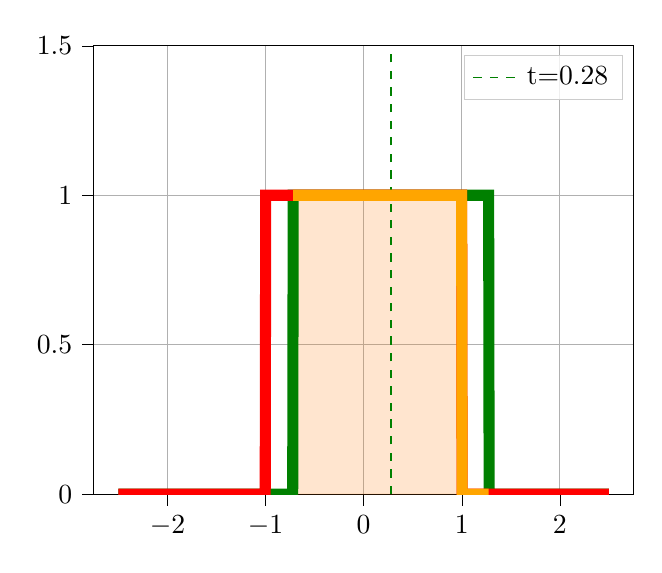
\begin{tikzpicture}

\definecolor{color0}{rgb}{1,0.498039215686275,0.0549019607843137}
\definecolor{color1}{rgb}{1,0.647058823529412,0}

\begin{axis}[
legend cell align={left},
legend style={fill opacity=0.8, draw opacity=1, text opacity=1, draw=white!80!black},
tick align=outside,
tick pos=left,
x grid style={white!69.0196078431373!black},
xmajorgrids,
xmin=-2.75, xmax=2.75,
xtick style={color=black},
y grid style={white!69.0196078431373!black},
ymajorgrids,
ymin=0, ymax=1.5,
ytick style={color=black}
]
\path [draw=color0, fill=color0, opacity=0.2]
(axis cs:-0.718218218218218,1)
--(axis cs:-0.718218218218218,0)
--(axis cs:-0.713213213213213,0)
--(axis cs:-0.708208208208208,0)
--(axis cs:-0.703203203203203,0)
--(axis cs:-0.698198198198198,0)
--(axis cs:-0.693193193193193,0)
--(axis cs:-0.688188188188188,0)
--(axis cs:-0.683183183183183,0)
--(axis cs:-0.678178178178178,0)
--(axis cs:-0.673173173173173,0)
--(axis cs:-0.668168168168168,0)
--(axis cs:-0.663163163163163,0)
--(axis cs:-0.658158158158158,0)
--(axis cs:-0.653153153153153,0)
--(axis cs:-0.648148148148148,0)
--(axis cs:-0.643143143143143,0)
--(axis cs:-0.638138138138138,0)
--(axis cs:-0.633133133133133,0)
--(axis cs:-0.628128128128128,0)
--(axis cs:-0.623123123123123,0)
--(axis cs:-0.618118118118118,0)
--(axis cs:-0.613113113113113,0)
--(axis cs:-0.608108108108108,0)
--(axis cs:-0.603103103103103,0)
--(axis cs:-0.598098098098098,0)
--(axis cs:-0.593093093093093,0)
--(axis cs:-0.588088088088088,0)
--(axis cs:-0.583083083083083,0)
--(axis cs:-0.578078078078078,0)
--(axis cs:-0.573073073073073,0)
--(axis cs:-0.568068068068068,0)
--(axis cs:-0.563063063063063,0)
--(axis cs:-0.558058058058058,0)
--(axis cs:-0.553053053053053,0)
--(axis cs:-0.548048048048048,0)
--(axis cs:-0.543043043043043,0)
--(axis cs:-0.538038038038038,0)
--(axis cs:-0.533033033033033,0)
--(axis cs:-0.528028028028028,0)
--(axis cs:-0.523023023023023,0)
--(axis cs:-0.518018018018018,0)
--(axis cs:-0.513013013013013,0)
--(axis cs:-0.508008008008008,0)
--(axis cs:-0.503003003003003,0)
--(axis cs:-0.497997997997998,0)
--(axis cs:-0.492992992992993,0)
--(axis cs:-0.487987987987988,0)
--(axis cs:-0.482982982982983,0)
--(axis cs:-0.477977977977978,0)
--(axis cs:-0.472972972972973,0)
--(axis cs:-0.467967967967968,0)
--(axis cs:-0.462962962962963,0)
--(axis cs:-0.457957957957958,0)
--(axis cs:-0.452952952952953,0)
--(axis cs:-0.447947947947948,0)
--(axis cs:-0.442942942942943,0)
--(axis cs:-0.437937937937938,0)
--(axis cs:-0.432932932932933,0)
--(axis cs:-0.427927927927928,0)
--(axis cs:-0.422922922922923,0)
--(axis cs:-0.417917917917918,0)
--(axis cs:-0.412912912912913,0)
--(axis cs:-0.407907907907908,0)
--(axis cs:-0.402902902902903,0)
--(axis cs:-0.397897897897898,0)
--(axis cs:-0.392892892892893,0)
--(axis cs:-0.387887887887888,0)
--(axis cs:-0.382882882882883,0)
--(axis cs:-0.377877877877878,0)
--(axis cs:-0.372872872872873,0)
--(axis cs:-0.367867867867868,0)
--(axis cs:-0.362862862862863,0)
--(axis cs:-0.357857857857858,0)
--(axis cs:-0.352852852852853,0)
--(axis cs:-0.347847847847848,0)
--(axis cs:-0.342842842842843,0)
--(axis cs:-0.337837837837838,0)
--(axis cs:-0.332832832832833,0)
--(axis cs:-0.327827827827828,0)
--(axis cs:-0.322822822822823,0)
--(axis cs:-0.317817817817818,0)
--(axis cs:-0.312812812812813,0)
--(axis cs:-0.307807807807808,0)
--(axis cs:-0.302802802802803,0)
--(axis cs:-0.297797797797798,0)
--(axis cs:-0.292792792792793,0)
--(axis cs:-0.287787787787788,0)
--(axis cs:-0.282782782782783,0)
--(axis cs:-0.277777777777778,0)
--(axis cs:-0.272772772772773,0)
--(axis cs:-0.267767767767768,0)
--(axis cs:-0.262762762762763,0)
--(axis cs:-0.257757757757758,0)
--(axis cs:-0.252752752752753,0)
--(axis cs:-0.247747747747748,0)
--(axis cs:-0.242742742742743,0)
--(axis cs:-0.237737737737738,0)
--(axis cs:-0.232732732732733,0)
--(axis cs:-0.227727727727728,0)
--(axis cs:-0.222722722722723,0)
--(axis cs:-0.217717717717718,0)
--(axis cs:-0.212712712712713,0)
--(axis cs:-0.207707707707708,0)
--(axis cs:-0.202702702702703,0)
--(axis cs:-0.197697697697698,0)
--(axis cs:-0.192692692692693,0)
--(axis cs:-0.187687687687688,0)
--(axis cs:-0.182682682682683,0)
--(axis cs:-0.177677677677678,0)
--(axis cs:-0.172672672672673,0)
--(axis cs:-0.167667667667668,0)
--(axis cs:-0.162662662662663,0)
--(axis cs:-0.157657657657658,0)
--(axis cs:-0.152652652652653,0)
--(axis cs:-0.147647647647648,0)
--(axis cs:-0.142642642642643,0)
--(axis cs:-0.137637637637638,0)
--(axis cs:-0.132632632632633,0)
--(axis cs:-0.127627627627628,0)
--(axis cs:-0.122622622622623,0)
--(axis cs:-0.117617617617618,0)
--(axis cs:-0.112612612612613,0)
--(axis cs:-0.107607607607608,0)
--(axis cs:-0.102602602602603,0)
--(axis cs:-0.0975975975975976,0)
--(axis cs:-0.0925925925925926,0)
--(axis cs:-0.0875875875875876,0)
--(axis cs:-0.0825825825825826,0)
--(axis cs:-0.0775775775775776,0)
--(axis cs:-0.0725725725725725,0)
--(axis cs:-0.0675675675675675,0)
--(axis cs:-0.0625625625625625,0)
--(axis cs:-0.0575575575575575,0)
--(axis cs:-0.0525525525525525,0)
--(axis cs:-0.0475475475475475,0)
--(axis cs:-0.0425425425425425,0)
--(axis cs:-0.0375375375375375,0)
--(axis cs:-0.0325325325325325,0)
--(axis cs:-0.0275275275275275,0)
--(axis cs:-0.0225225225225225,0)
--(axis cs:-0.0175175175175175,0)
--(axis cs:-0.0125125125125125,0)
--(axis cs:-0.0075075075075075,0)
--(axis cs:-0.0025025025025025,0)
--(axis cs:0.0025025025025025,0)
--(axis cs:0.0075075075075075,0)
--(axis cs:0.0125125125125125,0)
--(axis cs:0.0175175175175175,0)
--(axis cs:0.0225225225225225,0)
--(axis cs:0.0275275275275275,0)
--(axis cs:0.0325325325325325,0)
--(axis cs:0.0375375375375375,0)
--(axis cs:0.0425425425425425,0)
--(axis cs:0.0475475475475475,0)
--(axis cs:0.0525525525525525,0)
--(axis cs:0.0575575575575575,0)
--(axis cs:0.0625625625625625,0)
--(axis cs:0.0675675675675675,0)
--(axis cs:0.0725725725725725,0)
--(axis cs:0.0775775775775776,0)
--(axis cs:0.0825825825825826,0)
--(axis cs:0.0875875875875876,0)
--(axis cs:0.0925925925925926,0)
--(axis cs:0.0975975975975976,0)
--(axis cs:0.102602602602603,0)
--(axis cs:0.107607607607608,0)
--(axis cs:0.112612612612613,0)
--(axis cs:0.117617617617618,0)
--(axis cs:0.122622622622623,0)
--(axis cs:0.127627627627628,0)
--(axis cs:0.132632632632633,0)
--(axis cs:0.137637637637638,0)
--(axis cs:0.142642642642643,0)
--(axis cs:0.147647647647648,0)
--(axis cs:0.152652652652653,0)
--(axis cs:0.157657657657658,0)
--(axis cs:0.162662662662663,0)
--(axis cs:0.167667667667668,0)
--(axis cs:0.172672672672673,0)
--(axis cs:0.177677677677678,0)
--(axis cs:0.182682682682683,0)
--(axis cs:0.187687687687688,0)
--(axis cs:0.192692692692693,0)
--(axis cs:0.197697697697698,0)
--(axis cs:0.202702702702703,0)
--(axis cs:0.207707707707708,0)
--(axis cs:0.212712712712713,0)
--(axis cs:0.217717717717718,0)
--(axis cs:0.222722722722723,0)
--(axis cs:0.227727727727728,0)
--(axis cs:0.232732732732733,0)
--(axis cs:0.237737737737738,0)
--(axis cs:0.242742742742743,0)
--(axis cs:0.247747747747748,0)
--(axis cs:0.252752752752753,0)
--(axis cs:0.257757757757758,0)
--(axis cs:0.262762762762763,0)
--(axis cs:0.267767767767768,0)
--(axis cs:0.272772772772773,0)
--(axis cs:0.277777777777778,0)
--(axis cs:0.282782782782783,0)
--(axis cs:0.287787787787788,0)
--(axis cs:0.292792792792793,0)
--(axis cs:0.297797797797798,0)
--(axis cs:0.302802802802803,0)
--(axis cs:0.307807807807808,0)
--(axis cs:0.312812812812813,0)
--(axis cs:0.317817817817818,0)
--(axis cs:0.322822822822823,0)
--(axis cs:0.327827827827828,0)
--(axis cs:0.332832832832833,0)
--(axis cs:0.337837837837838,0)
--(axis cs:0.342842842842843,0)
--(axis cs:0.347847847847848,0)
--(axis cs:0.352852852852853,0)
--(axis cs:0.357857857857858,0)
--(axis cs:0.362862862862863,0)
--(axis cs:0.367867867867868,0)
--(axis cs:0.372872872872873,0)
--(axis cs:0.377877877877878,0)
--(axis cs:0.382882882882883,0)
--(axis cs:0.387887887887888,0)
--(axis cs:0.392892892892893,0)
--(axis cs:0.397897897897898,0)
--(axis cs:0.402902902902903,0)
--(axis cs:0.407907907907908,0)
--(axis cs:0.412912912912913,0)
--(axis cs:0.417917917917918,0)
--(axis cs:0.422922922922923,0)
--(axis cs:0.427927927927928,0)
--(axis cs:0.432932932932933,0)
--(axis cs:0.437937937937938,0)
--(axis cs:0.442942942942943,0)
--(axis cs:0.447947947947948,0)
--(axis cs:0.452952952952953,0)
--(axis cs:0.457957957957958,0)
--(axis cs:0.462962962962963,0)
--(axis cs:0.467967967967968,0)
--(axis cs:0.472972972972973,0)
--(axis cs:0.477977977977978,0)
--(axis cs:0.482982982982983,0)
--(axis cs:0.487987987987988,0)
--(axis cs:0.492992992992993,0)
--(axis cs:0.497997997997998,0)
--(axis cs:0.503003003003003,0)
--(axis cs:0.508008008008008,0)
--(axis cs:0.513013013013013,0)
--(axis cs:0.518018018018018,0)
--(axis cs:0.523023023023023,0)
--(axis cs:0.528028028028028,0)
--(axis cs:0.533033033033033,0)
--(axis cs:0.538038038038038,0)
--(axis cs:0.543043043043043,0)
--(axis cs:0.548048048048048,0)
--(axis cs:0.553053053053053,0)
--(axis cs:0.558058058058058,0)
--(axis cs:0.563063063063063,0)
--(axis cs:0.568068068068068,0)
--(axis cs:0.573073073073073,0)
--(axis cs:0.578078078078078,0)
--(axis cs:0.583083083083083,0)
--(axis cs:0.588088088088088,0)
--(axis cs:0.593093093093093,0)
--(axis cs:0.598098098098098,0)
--(axis cs:0.603103103103103,0)
--(axis cs:0.608108108108108,0)
--(axis cs:0.613113113113113,0)
--(axis cs:0.618118118118118,0)
--(axis cs:0.623123123123123,0)
--(axis cs:0.628128128128128,0)
--(axis cs:0.633133133133133,0)
--(axis cs:0.638138138138138,0)
--(axis cs:0.643143143143143,0)
--(axis cs:0.648148148148148,0)
--(axis cs:0.653153153153153,0)
--(axis cs:0.658158158158158,0)
--(axis cs:0.663163163163163,0)
--(axis cs:0.668168168168168,0)
--(axis cs:0.673173173173173,0)
--(axis cs:0.678178178178178,0)
--(axis cs:0.683183183183183,0)
--(axis cs:0.688188188188188,0)
--(axis cs:0.693193193193193,0)
--(axis cs:0.698198198198198,0)
--(axis cs:0.703203203203203,0)
--(axis cs:0.708208208208208,0)
--(axis cs:0.713213213213213,0)
--(axis cs:0.718218218218218,0)
--(axis cs:0.723223223223223,0)
--(axis cs:0.728228228228228,0)
--(axis cs:0.733233233233233,0)
--(axis cs:0.738238238238238,0)
--(axis cs:0.743243243243243,0)
--(axis cs:0.748248248248248,0)
--(axis cs:0.753253253253253,0)
--(axis cs:0.758258258258258,0)
--(axis cs:0.763263263263263,0)
--(axis cs:0.768268268268268,0)
--(axis cs:0.773273273273273,0)
--(axis cs:0.778278278278278,0)
--(axis cs:0.783283283283283,0)
--(axis cs:0.788288288288288,0)
--(axis cs:0.793293293293293,0)
--(axis cs:0.798298298298298,0)
--(axis cs:0.803303303303303,0)
--(axis cs:0.808308308308308,0)
--(axis cs:0.813313313313313,0)
--(axis cs:0.818318318318318,0)
--(axis cs:0.823323323323323,0)
--(axis cs:0.828328328328328,0)
--(axis cs:0.833333333333333,0)
--(axis cs:0.838338338338338,0)
--(axis cs:0.843343343343343,0)
--(axis cs:0.848348348348348,0)
--(axis cs:0.853353353353353,0)
--(axis cs:0.858358358358358,0)
--(axis cs:0.863363363363364,0)
--(axis cs:0.868368368368369,0)
--(axis cs:0.873373373373374,0)
--(axis cs:0.878378378378379,0)
--(axis cs:0.883383383383384,0)
--(axis cs:0.888388388388389,0)
--(axis cs:0.893393393393394,0)
--(axis cs:0.898398398398399,0)
--(axis cs:0.903403403403404,0)
--(axis cs:0.908408408408409,0)
--(axis cs:0.913413413413414,0)
--(axis cs:0.918418418418419,0)
--(axis cs:0.923423423423424,0)
--(axis cs:0.928428428428429,0)
--(axis cs:0.933433433433434,0)
--(axis cs:0.938438438438439,0)
--(axis cs:0.943443443443444,0)
--(axis cs:0.948448448448449,0)
--(axis cs:0.953453453453454,0)
--(axis cs:0.958458458458459,0)
--(axis cs:0.963463463463464,0)
--(axis cs:0.968468468468469,0)
--(axis cs:0.973473473473474,0)
--(axis cs:0.978478478478479,0)
--(axis cs:0.983483483483484,0)
--(axis cs:0.988488488488489,0)
--(axis cs:0.993493493493494,0)
--(axis cs:0.998498498498499,0)
--(axis cs:1.0035035035035,0)
--(axis cs:1.00850850850851,0)
--(axis cs:1.01351351351351,0)
--(axis cs:1.01851851851852,0)
--(axis cs:1.02352352352352,0)
--(axis cs:1.02852852852853,0)
--(axis cs:1.03353353353353,0)
--(axis cs:1.03853853853854,0)
--(axis cs:1.04354354354354,0)
--(axis cs:1.04854854854855,0)
--(axis cs:1.05355355355355,0)
--(axis cs:1.05855855855856,0)
--(axis cs:1.06356356356356,0)
--(axis cs:1.06856856856857,0)
--(axis cs:1.07357357357357,0)
--(axis cs:1.07857857857858,0)
--(axis cs:1.08358358358358,0)
--(axis cs:1.08858858858859,0)
--(axis cs:1.09359359359359,0)
--(axis cs:1.0985985985986,0)
--(axis cs:1.1036036036036,0)
--(axis cs:1.10860860860861,0)
--(axis cs:1.11361361361361,0)
--(axis cs:1.11861861861862,0)
--(axis cs:1.12362362362362,0)
--(axis cs:1.12862862862863,0)
--(axis cs:1.13363363363363,0)
--(axis cs:1.13863863863864,0)
--(axis cs:1.14364364364364,0)
--(axis cs:1.14864864864865,0)
--(axis cs:1.15365365365365,0)
--(axis cs:1.15865865865866,0)
--(axis cs:1.16366366366366,0)
--(axis cs:1.16866866866867,0)
--(axis cs:1.17367367367367,0)
--(axis cs:1.17867867867868,0)
--(axis cs:1.18368368368368,0)
--(axis cs:1.18868868868869,0)
--(axis cs:1.19369369369369,0)
--(axis cs:1.1986986986987,0)
--(axis cs:1.2037037037037,0)
--(axis cs:1.20870870870871,0)
--(axis cs:1.21371371371371,0)
--(axis cs:1.21871871871872,0)
--(axis cs:1.22372372372372,0)
--(axis cs:1.22872872872873,0)
--(axis cs:1.23373373373373,0)
--(axis cs:1.23873873873874,0)
--(axis cs:1.24374374374374,0)
--(axis cs:1.24874874874875,0)
--(axis cs:1.25375375375375,0)
--(axis cs:1.25875875875876,0)
--(axis cs:1.26376376376376,0)
--(axis cs:1.26876876876877,0)
--(axis cs:1.27377377377377,0)
--(axis cs:1.27377377377377,0)
--(axis cs:1.27377377377377,0)
--(axis cs:1.26876876876877,0)
--(axis cs:1.26376376376376,0)
--(axis cs:1.25875875875876,0)
--(axis cs:1.25375375375375,0)
--(axis cs:1.24874874874875,0)
--(axis cs:1.24374374374374,0)
--(axis cs:1.23873873873874,0)
--(axis cs:1.23373373373373,0)
--(axis cs:1.22872872872873,0)
--(axis cs:1.22372372372372,0)
--(axis cs:1.21871871871872,0)
--(axis cs:1.21371371371371,0)
--(axis cs:1.20870870870871,0)
--(axis cs:1.2037037037037,0)
--(axis cs:1.1986986986987,0)
--(axis cs:1.19369369369369,0)
--(axis cs:1.18868868868869,0)
--(axis cs:1.18368368368368,0)
--(axis cs:1.17867867867868,0)
--(axis cs:1.17367367367367,0)
--(axis cs:1.16866866866867,0)
--(axis cs:1.16366366366366,0)
--(axis cs:1.15865865865866,0)
--(axis cs:1.15365365365365,0)
--(axis cs:1.14864864864865,0)
--(axis cs:1.14364364364364,0)
--(axis cs:1.13863863863864,0)
--(axis cs:1.13363363363363,0)
--(axis cs:1.12862862862863,0)
--(axis cs:1.12362362362362,0)
--(axis cs:1.11861861861862,0)
--(axis cs:1.11361361361361,0)
--(axis cs:1.10860860860861,0)
--(axis cs:1.1036036036036,0)
--(axis cs:1.0985985985986,0)
--(axis cs:1.09359359359359,0)
--(axis cs:1.08858858858859,0)
--(axis cs:1.08358358358358,0)
--(axis cs:1.07857857857858,0)
--(axis cs:1.07357357357357,0)
--(axis cs:1.06856856856857,0)
--(axis cs:1.06356356356356,0)
--(axis cs:1.05855855855856,0)
--(axis cs:1.05355355355355,0)
--(axis cs:1.04854854854855,0)
--(axis cs:1.04354354354354,0)
--(axis cs:1.03853853853854,0)
--(axis cs:1.03353353353353,0)
--(axis cs:1.02852852852853,0)
--(axis cs:1.02352352352352,0)
--(axis cs:1.01851851851852,0)
--(axis cs:1.01351351351351,0)
--(axis cs:1.00850850850851,0)
--(axis cs:1.0035035035035,0)
--(axis cs:0.998498498498499,1)
--(axis cs:0.993493493493494,1)
--(axis cs:0.988488488488489,1)
--(axis cs:0.983483483483484,1)
--(axis cs:0.978478478478479,1)
--(axis cs:0.973473473473474,1)
--(axis cs:0.968468468468469,1)
--(axis cs:0.963463463463464,1)
--(axis cs:0.958458458458459,1)
--(axis cs:0.953453453453454,1)
--(axis cs:0.948448448448449,1)
--(axis cs:0.943443443443444,1)
--(axis cs:0.938438438438439,1)
--(axis cs:0.933433433433434,1)
--(axis cs:0.928428428428429,1)
--(axis cs:0.923423423423424,1)
--(axis cs:0.918418418418419,1)
--(axis cs:0.913413413413414,1)
--(axis cs:0.908408408408409,1)
--(axis cs:0.903403403403404,1)
--(axis cs:0.898398398398399,1)
--(axis cs:0.893393393393394,1)
--(axis cs:0.888388388388389,1)
--(axis cs:0.883383383383384,1)
--(axis cs:0.878378378378379,1)
--(axis cs:0.873373373373374,1)
--(axis cs:0.868368368368369,1)
--(axis cs:0.863363363363364,1)
--(axis cs:0.858358358358358,1)
--(axis cs:0.853353353353353,1)
--(axis cs:0.848348348348348,1)
--(axis cs:0.843343343343343,1)
--(axis cs:0.838338338338338,1)
--(axis cs:0.833333333333333,1)
--(axis cs:0.828328328328328,1)
--(axis cs:0.823323323323323,1)
--(axis cs:0.818318318318318,1)
--(axis cs:0.813313313313313,1)
--(axis cs:0.808308308308308,1)
--(axis cs:0.803303303303303,1)
--(axis cs:0.798298298298298,1)
--(axis cs:0.793293293293293,1)
--(axis cs:0.788288288288288,1)
--(axis cs:0.783283283283283,1)
--(axis cs:0.778278278278278,1)
--(axis cs:0.773273273273273,1)
--(axis cs:0.768268268268268,1)
--(axis cs:0.763263263263263,1)
--(axis cs:0.758258258258258,1)
--(axis cs:0.753253253253253,1)
--(axis cs:0.748248248248248,1)
--(axis cs:0.743243243243243,1)
--(axis cs:0.738238238238238,1)
--(axis cs:0.733233233233233,1)
--(axis cs:0.728228228228228,1)
--(axis cs:0.723223223223223,1)
--(axis cs:0.718218218218218,1)
--(axis cs:0.713213213213213,1)
--(axis cs:0.708208208208208,1)
--(axis cs:0.703203203203203,1)
--(axis cs:0.698198198198198,1)
--(axis cs:0.693193193193193,1)
--(axis cs:0.688188188188188,1)
--(axis cs:0.683183183183183,1)
--(axis cs:0.678178178178178,1)
--(axis cs:0.673173173173173,1)
--(axis cs:0.668168168168168,1)
--(axis cs:0.663163163163163,1)
--(axis cs:0.658158158158158,1)
--(axis cs:0.653153153153153,1)
--(axis cs:0.648148148148148,1)
--(axis cs:0.643143143143143,1)
--(axis cs:0.638138138138138,1)
--(axis cs:0.633133133133133,1)
--(axis cs:0.628128128128128,1)
--(axis cs:0.623123123123123,1)
--(axis cs:0.618118118118118,1)
--(axis cs:0.613113113113113,1)
--(axis cs:0.608108108108108,1)
--(axis cs:0.603103103103103,1)
--(axis cs:0.598098098098098,1)
--(axis cs:0.593093093093093,1)
--(axis cs:0.588088088088088,1)
--(axis cs:0.583083083083083,1)
--(axis cs:0.578078078078078,1)
--(axis cs:0.573073073073073,1)
--(axis cs:0.568068068068068,1)
--(axis cs:0.563063063063063,1)
--(axis cs:0.558058058058058,1)
--(axis cs:0.553053053053053,1)
--(axis cs:0.548048048048048,1)
--(axis cs:0.543043043043043,1)
--(axis cs:0.538038038038038,1)
--(axis cs:0.533033033033033,1)
--(axis cs:0.528028028028028,1)
--(axis cs:0.523023023023023,1)
--(axis cs:0.518018018018018,1)
--(axis cs:0.513013013013013,1)
--(axis cs:0.508008008008008,1)
--(axis cs:0.503003003003003,1)
--(axis cs:0.497997997997998,1)
--(axis cs:0.492992992992993,1)
--(axis cs:0.487987987987988,1)
--(axis cs:0.482982982982983,1)
--(axis cs:0.477977977977978,1)
--(axis cs:0.472972972972973,1)
--(axis cs:0.467967967967968,1)
--(axis cs:0.462962962962963,1)
--(axis cs:0.457957957957958,1)
--(axis cs:0.452952952952953,1)
--(axis cs:0.447947947947948,1)
--(axis cs:0.442942942942943,1)
--(axis cs:0.437937937937938,1)
--(axis cs:0.432932932932933,1)
--(axis cs:0.427927927927928,1)
--(axis cs:0.422922922922923,1)
--(axis cs:0.417917917917918,1)
--(axis cs:0.412912912912913,1)
--(axis cs:0.407907907907908,1)
--(axis cs:0.402902902902903,1)
--(axis cs:0.397897897897898,1)
--(axis cs:0.392892892892893,1)
--(axis cs:0.387887887887888,1)
--(axis cs:0.382882882882883,1)
--(axis cs:0.377877877877878,1)
--(axis cs:0.372872872872873,1)
--(axis cs:0.367867867867868,1)
--(axis cs:0.362862862862863,1)
--(axis cs:0.357857857857858,1)
--(axis cs:0.352852852852853,1)
--(axis cs:0.347847847847848,1)
--(axis cs:0.342842842842843,1)
--(axis cs:0.337837837837838,1)
--(axis cs:0.332832832832833,1)
--(axis cs:0.327827827827828,1)
--(axis cs:0.322822822822823,1)
--(axis cs:0.317817817817818,1)
--(axis cs:0.312812812812813,1)
--(axis cs:0.307807807807808,1)
--(axis cs:0.302802802802803,1)
--(axis cs:0.297797797797798,1)
--(axis cs:0.292792792792793,1)
--(axis cs:0.287787787787788,1)
--(axis cs:0.282782782782783,1)
--(axis cs:0.277777777777778,1)
--(axis cs:0.272772772772773,1)
--(axis cs:0.267767767767768,1)
--(axis cs:0.262762762762763,1)
--(axis cs:0.257757757757758,1)
--(axis cs:0.252752752752753,1)
--(axis cs:0.247747747747748,1)
--(axis cs:0.242742742742743,1)
--(axis cs:0.237737737737738,1)
--(axis cs:0.232732732732733,1)
--(axis cs:0.227727727727728,1)
--(axis cs:0.222722722722723,1)
--(axis cs:0.217717717717718,1)
--(axis cs:0.212712712712713,1)
--(axis cs:0.207707707707708,1)
--(axis cs:0.202702702702703,1)
--(axis cs:0.197697697697698,1)
--(axis cs:0.192692692692693,1)
--(axis cs:0.187687687687688,1)
--(axis cs:0.182682682682683,1)
--(axis cs:0.177677677677678,1)
--(axis cs:0.172672672672673,1)
--(axis cs:0.167667667667668,1)
--(axis cs:0.162662662662663,1)
--(axis cs:0.157657657657658,1)
--(axis cs:0.152652652652653,1)
--(axis cs:0.147647647647648,1)
--(axis cs:0.142642642642643,1)
--(axis cs:0.137637637637638,1)
--(axis cs:0.132632632632633,1)
--(axis cs:0.127627627627628,1)
--(axis cs:0.122622622622623,1)
--(axis cs:0.117617617617618,1)
--(axis cs:0.112612612612613,1)
--(axis cs:0.107607607607608,1)
--(axis cs:0.102602602602603,1)
--(axis cs:0.0975975975975976,1)
--(axis cs:0.0925925925925926,1)
--(axis cs:0.0875875875875876,1)
--(axis cs:0.0825825825825826,1)
--(axis cs:0.0775775775775776,1)
--(axis cs:0.0725725725725725,1)
--(axis cs:0.0675675675675675,1)
--(axis cs:0.0625625625625625,1)
--(axis cs:0.0575575575575575,1)
--(axis cs:0.0525525525525525,1)
--(axis cs:0.0475475475475475,1)
--(axis cs:0.0425425425425425,1)
--(axis cs:0.0375375375375375,1)
--(axis cs:0.0325325325325325,1)
--(axis cs:0.0275275275275275,1)
--(axis cs:0.0225225225225225,1)
--(axis cs:0.0175175175175175,1)
--(axis cs:0.0125125125125125,1)
--(axis cs:0.0075075075075075,1)
--(axis cs:0.0025025025025025,1)
--(axis cs:-0.0025025025025025,1)
--(axis cs:-0.0075075075075075,1)
--(axis cs:-0.0125125125125125,1)
--(axis cs:-0.0175175175175175,1)
--(axis cs:-0.0225225225225225,1)
--(axis cs:-0.0275275275275275,1)
--(axis cs:-0.0325325325325325,1)
--(axis cs:-0.0375375375375375,1)
--(axis cs:-0.0425425425425425,1)
--(axis cs:-0.0475475475475475,1)
--(axis cs:-0.0525525525525525,1)
--(axis cs:-0.0575575575575575,1)
--(axis cs:-0.0625625625625625,1)
--(axis cs:-0.0675675675675675,1)
--(axis cs:-0.0725725725725725,1)
--(axis cs:-0.0775775775775776,1)
--(axis cs:-0.0825825825825826,1)
--(axis cs:-0.0875875875875876,1)
--(axis cs:-0.0925925925925926,1)
--(axis cs:-0.0975975975975976,1)
--(axis cs:-0.102602602602603,1)
--(axis cs:-0.107607607607608,1)
--(axis cs:-0.112612612612613,1)
--(axis cs:-0.117617617617618,1)
--(axis cs:-0.122622622622623,1)
--(axis cs:-0.127627627627628,1)
--(axis cs:-0.132632632632633,1)
--(axis cs:-0.137637637637638,1)
--(axis cs:-0.142642642642643,1)
--(axis cs:-0.147647647647648,1)
--(axis cs:-0.152652652652653,1)
--(axis cs:-0.157657657657658,1)
--(axis cs:-0.162662662662663,1)
--(axis cs:-0.167667667667668,1)
--(axis cs:-0.172672672672673,1)
--(axis cs:-0.177677677677678,1)
--(axis cs:-0.182682682682683,1)
--(axis cs:-0.187687687687688,1)
--(axis cs:-0.192692692692693,1)
--(axis cs:-0.197697697697698,1)
--(axis cs:-0.202702702702703,1)
--(axis cs:-0.207707707707708,1)
--(axis cs:-0.212712712712713,1)
--(axis cs:-0.217717717717718,1)
--(axis cs:-0.222722722722723,1)
--(axis cs:-0.227727727727728,1)
--(axis cs:-0.232732732732733,1)
--(axis cs:-0.237737737737738,1)
--(axis cs:-0.242742742742743,1)
--(axis cs:-0.247747747747748,1)
--(axis cs:-0.252752752752753,1)
--(axis cs:-0.257757757757758,1)
--(axis cs:-0.262762762762763,1)
--(axis cs:-0.267767767767768,1)
--(axis cs:-0.272772772772773,1)
--(axis cs:-0.277777777777778,1)
--(axis cs:-0.282782782782783,1)
--(axis cs:-0.287787787787788,1)
--(axis cs:-0.292792792792793,1)
--(axis cs:-0.297797797797798,1)
--(axis cs:-0.302802802802803,1)
--(axis cs:-0.307807807807808,1)
--(axis cs:-0.312812812812813,1)
--(axis cs:-0.317817817817818,1)
--(axis cs:-0.322822822822823,1)
--(axis cs:-0.327827827827828,1)
--(axis cs:-0.332832832832833,1)
--(axis cs:-0.337837837837838,1)
--(axis cs:-0.342842842842843,1)
--(axis cs:-0.347847847847848,1)
--(axis cs:-0.352852852852853,1)
--(axis cs:-0.357857857857858,1)
--(axis cs:-0.362862862862863,1)
--(axis cs:-0.367867867867868,1)
--(axis cs:-0.372872872872873,1)
--(axis cs:-0.377877877877878,1)
--(axis cs:-0.382882882882883,1)
--(axis cs:-0.387887887887888,1)
--(axis cs:-0.392892892892893,1)
--(axis cs:-0.397897897897898,1)
--(axis cs:-0.402902902902903,1)
--(axis cs:-0.407907907907908,1)
--(axis cs:-0.412912912912913,1)
--(axis cs:-0.417917917917918,1)
--(axis cs:-0.422922922922923,1)
--(axis cs:-0.427927927927928,1)
--(axis cs:-0.432932932932933,1)
--(axis cs:-0.437937937937938,1)
--(axis cs:-0.442942942942943,1)
--(axis cs:-0.447947947947948,1)
--(axis cs:-0.452952952952953,1)
--(axis cs:-0.457957957957958,1)
--(axis cs:-0.462962962962963,1)
--(axis cs:-0.467967967967968,1)
--(axis cs:-0.472972972972973,1)
--(axis cs:-0.477977977977978,1)
--(axis cs:-0.482982982982983,1)
--(axis cs:-0.487987987987988,1)
--(axis cs:-0.492992992992993,1)
--(axis cs:-0.497997997997998,1)
--(axis cs:-0.503003003003003,1)
--(axis cs:-0.508008008008008,1)
--(axis cs:-0.513013013013013,1)
--(axis cs:-0.518018018018018,1)
--(axis cs:-0.523023023023023,1)
--(axis cs:-0.528028028028028,1)
--(axis cs:-0.533033033033033,1)
--(axis cs:-0.538038038038038,1)
--(axis cs:-0.543043043043043,1)
--(axis cs:-0.548048048048048,1)
--(axis cs:-0.553053053053053,1)
--(axis cs:-0.558058058058058,1)
--(axis cs:-0.563063063063063,1)
--(axis cs:-0.568068068068068,1)
--(axis cs:-0.573073073073073,1)
--(axis cs:-0.578078078078078,1)
--(axis cs:-0.583083083083083,1)
--(axis cs:-0.588088088088088,1)
--(axis cs:-0.593093093093093,1)
--(axis cs:-0.598098098098098,1)
--(axis cs:-0.603103103103103,1)
--(axis cs:-0.608108108108108,1)
--(axis cs:-0.613113113113113,1)
--(axis cs:-0.618118118118118,1)
--(axis cs:-0.623123123123123,1)
--(axis cs:-0.628128128128128,1)
--(axis cs:-0.633133133133133,1)
--(axis cs:-0.638138138138138,1)
--(axis cs:-0.643143143143143,1)
--(axis cs:-0.648148148148148,1)
--(axis cs:-0.653153153153153,1)
--(axis cs:-0.658158158158158,1)
--(axis cs:-0.663163163163163,1)
--(axis cs:-0.668168168168168,1)
--(axis cs:-0.673173173173173,1)
--(axis cs:-0.678178178178178,1)
--(axis cs:-0.683183183183183,1)
--(axis cs:-0.688188188188188,1)
--(axis cs:-0.693193193193193,1)
--(axis cs:-0.698198198198198,1)
--(axis cs:-0.703203203203203,1)
--(axis cs:-0.708208208208208,1)
--(axis cs:-0.713213213213213,1)
--(axis cs:-0.718218218218218,1)
--cycle;

\addplot [line width=4pt, green!50!black, forget plot]
table {%
-2.5 0
-2.49499499499499 0
-2.48998998998999 0
-2.48498498498498 0
-2.47997997997998 0
-2.47497497497497 0
-2.46996996996997 0
-2.46496496496496 0
-2.45995995995996 0
-2.45495495495495 0
-2.44994994994995 0
-2.44494494494494 0
-2.43993993993994 0
-2.43493493493493 0
-2.42992992992993 0
-2.42492492492492 0
-2.41991991991992 0
-2.41491491491491 0
-2.40990990990991 0
-2.4049049049049 0
-2.3998998998999 0
-2.39489489489489 0
-2.38988988988989 0
-2.38488488488488 0
-2.37987987987988 0
-2.37487487487487 0
-2.36986986986987 0
-2.36486486486486 0
-2.35985985985986 0
-2.35485485485485 0
-2.34984984984985 0
-2.34484484484484 0
-2.33983983983984 0
-2.33483483483483 0
-2.32982982982983 0
-2.32482482482482 0
-2.31981981981982 0
-2.31481481481481 0
-2.30980980980981 0
-2.3048048048048 0
-2.2997997997998 0
-2.29479479479479 0
-2.28978978978979 0
-2.28478478478478 0
-2.27977977977978 0
-2.27477477477477 0
-2.26976976976977 0
-2.26476476476476 0
-2.25975975975976 0
-2.25475475475475 0
-2.24974974974975 0
-2.24474474474474 0
-2.23973973973974 0
-2.23473473473473 0
-2.22972972972973 0
-2.22472472472472 0
-2.21971971971972 0
-2.21471471471471 0
-2.20970970970971 0
-2.2047047047047 0
-2.1996996996997 0
-2.19469469469469 0
-2.18968968968969 0
-2.18468468468468 0
-2.17967967967968 0
-2.17467467467467 0
-2.16966966966967 0
-2.16466466466466 0
-2.15965965965966 0
-2.15465465465465 0
-2.14964964964965 0
-2.14464464464464 0
-2.13963963963964 0
-2.13463463463463 0
-2.12962962962963 0
-2.12462462462462 0
-2.11961961961962 0
-2.11461461461461 0
-2.10960960960961 0
-2.1046046046046 0
-2.0995995995996 0
-2.09459459459459 0
-2.08958958958959 0
-2.08458458458458 0
-2.07957957957958 0
-2.07457457457457 0
-2.06956956956957 0
-2.06456456456456 0
-2.05955955955956 0
-2.05455455455455 0
-2.04954954954955 0
-2.04454454454454 0
-2.03953953953954 0
-2.03453453453453 0
-2.02952952952953 0
-2.02452452452452 0
-2.01951951951952 0
-2.01451451451451 0
-2.00950950950951 0
-2.0045045045045 0
-1.9994994994995 0
-1.99449449449449 0
-1.98948948948949 0
-1.98448448448448 0
-1.97947947947948 0
-1.97447447447447 0
-1.96946946946947 0
-1.96446446446446 0
-1.95945945945946 0
-1.95445445445445 0
-1.94944944944945 0
-1.94444444444444 0
-1.93943943943944 0
-1.93443443443443 0
-1.92942942942943 0
-1.92442442442442 0
-1.91941941941942 0
-1.91441441441441 0
-1.90940940940941 0
-1.9044044044044 0
-1.8993993993994 0
-1.89439439439439 0
-1.88938938938939 0
-1.88438438438438 0
-1.87937937937938 0
-1.87437437437437 0
-1.86936936936937 0
-1.86436436436436 0
-1.85935935935936 0
-1.85435435435435 0
-1.84934934934935 0
-1.84434434434434 0
-1.83933933933934 0
-1.83433433433433 0
-1.82932932932933 0
-1.82432432432432 0
-1.81931931931932 0
-1.81431431431431 0
-1.80930930930931 0
-1.8043043043043 0
-1.7992992992993 0
-1.79429429429429 0
-1.78928928928929 0
-1.78428428428428 0
-1.77927927927928 0
-1.77427427427427 0
-1.76926926926927 0
-1.76426426426426 0
-1.75925925925926 0
-1.75425425425425 0
-1.74924924924925 0
-1.74424424424424 0
-1.73923923923924 0
-1.73423423423423 0
-1.72922922922923 0
-1.72422422422422 0
-1.71921921921922 0
-1.71421421421421 0
-1.70920920920921 0
-1.7042042042042 0
-1.6991991991992 0
-1.69419419419419 0
-1.68918918918919 0
-1.68418418418418 0
-1.67917917917918 0
-1.67417417417417 0
-1.66916916916917 0
-1.66416416416416 0
-1.65915915915916 0
-1.65415415415415 0
-1.64914914914915 0
-1.64414414414414 0
-1.63913913913914 0
-1.63413413413413 0
-1.62912912912913 0
-1.62412412412412 0
-1.61911911911912 0
-1.61411411411411 0
-1.60910910910911 0
-1.6041041041041 0
-1.5990990990991 0
-1.59409409409409 0
-1.58908908908909 0
-1.58408408408408 0
-1.57907907907908 0
-1.57407407407407 0
-1.56906906906907 0
-1.56406406406406 0
-1.55905905905906 0
-1.55405405405405 0
-1.54904904904905 0
-1.54404404404404 0
-1.53903903903904 0
-1.53403403403403 0
-1.52902902902903 0
-1.52402402402402 0
-1.51901901901902 0
-1.51401401401401 0
-1.50900900900901 0
-1.504004004004 0
-1.498998998999 0
-1.49399399399399 0
-1.48898898898899 0
-1.48398398398398 0
-1.47897897897898 0
-1.47397397397397 0
-1.46896896896897 0
-1.46396396396396 0
-1.45895895895896 0
-1.45395395395395 0
-1.44894894894895 0
-1.44394394394394 0
-1.43893893893894 0
-1.43393393393393 0
-1.42892892892893 0
-1.42392392392392 0
-1.41891891891892 0
-1.41391391391391 0
-1.40890890890891 0
-1.4039039039039 0
-1.3988988988989 0
-1.39389389389389 0
-1.38888888888889 0
-1.38388388388388 0
-1.37887887887888 0
-1.37387387387387 0
-1.36886886886887 0
-1.36386386386386 0
-1.35885885885886 0
-1.35385385385385 0
-1.34884884884885 0
-1.34384384384384 0
-1.33883883883884 0
-1.33383383383383 0
-1.32882882882883 0
-1.32382382382382 0
-1.31881881881882 0
-1.31381381381381 0
-1.30880880880881 0
-1.3038038038038 0
-1.2987987987988 0
-1.29379379379379 0
-1.28878878878879 0
-1.28378378378378 0
-1.27877877877878 0
-1.27377377377377 0
-1.26876876876877 0
-1.26376376376376 0
-1.25875875875876 0
-1.25375375375375 0
-1.24874874874875 0
-1.24374374374374 0
-1.23873873873874 0
-1.23373373373373 0
-1.22872872872873 0
-1.22372372372372 0
-1.21871871871872 0
-1.21371371371371 0
-1.20870870870871 0
-1.2037037037037 0
-1.1986986986987 0
-1.19369369369369 0
-1.18868868868869 0
-1.18368368368368 0
-1.17867867867868 0
-1.17367367367367 0
-1.16866866866867 0
-1.16366366366366 0
-1.15865865865866 0
-1.15365365365365 0
-1.14864864864865 0
-1.14364364364364 0
-1.13863863863864 0
-1.13363363363363 0
-1.12862862862863 0
-1.12362362362362 0
-1.11861861861862 0
-1.11361361361361 0
-1.10860860860861 0
-1.1036036036036 0
-1.0985985985986 0
-1.09359359359359 0
-1.08858858858859 0
-1.08358358358358 0
-1.07857857857858 0
-1.07357357357357 0
-1.06856856856857 0
-1.06356356356356 0
-1.05855855855856 0
-1.05355355355355 0
-1.04854854854855 0
-1.04354354354354 0
-1.03853853853854 0
-1.03353353353353 0
-1.02852852852853 0
-1.02352352352352 0
-1.01851851851852 0
-1.01351351351351 0
-1.00850850850851 0
-1.0035035035035 0
-0.998498498498499 0
-0.993493493493494 0
-0.988488488488489 0
-0.983483483483484 0
-0.978478478478479 0
-0.973473473473474 0
-0.968468468468469 0
-0.963463463463464 0
-0.958458458458459 0
-0.953453453453454 0
-0.948448448448449 0
-0.943443443443444 0
-0.938438438438439 0
-0.933433433433434 0
-0.928428428428429 0
-0.923423423423424 0
-0.918418418418419 0
-0.913413413413414 0
-0.908408408408409 0
-0.903403403403404 0
-0.898398398398399 0
-0.893393393393393 0
-0.888388388388388 0
-0.883383383383383 0
-0.878378378378378 0
-0.873373373373373 0
-0.868368368368368 0
-0.863363363363363 0
-0.858358358358358 0
-0.853353353353353 0
-0.848348348348348 0
-0.843343343343343 0
-0.838338338338338 0
-0.833333333333333 0
-0.828328328328328 0
-0.823323323323323 0
-0.818318318318318 0
-0.813313313313313 0
-0.808308308308308 0
-0.803303303303303 0
-0.798298298298298 0
-0.793293293293293 0
-0.788288288288288 0
-0.783283283283283 0
-0.778278278278278 0
-0.773273273273273 0
-0.768268268268268 0
-0.763263263263263 0
-0.758258258258258 0
-0.753253253253253 0
-0.748248248248248 0
-0.743243243243243 0
-0.738238238238238 0
-0.733233233233233 0
-0.728228228228228 0
-0.723223223223223 0
-0.718218218218218 1
-0.713213213213213 1
-0.708208208208208 1
-0.703203203203203 1
-0.698198198198198 1
-0.693193193193193 1
-0.688188188188188 1
-0.683183183183183 1
-0.678178178178178 1
-0.673173173173173 1
-0.668168168168168 1
-0.663163163163163 1
-0.658158158158158 1
-0.653153153153153 1
-0.648148148148148 1
-0.643143143143143 1
-0.638138138138138 1
-0.633133133133133 1
-0.628128128128128 1
-0.623123123123123 1
-0.618118118118118 1
-0.613113113113113 1
-0.608108108108108 1
-0.603103103103103 1
-0.598098098098098 1
-0.593093093093093 1
-0.588088088088088 1
-0.583083083083083 1
-0.578078078078078 1
-0.573073073073073 1
-0.568068068068068 1
-0.563063063063063 1
-0.558058058058058 1
-0.553053053053053 1
-0.548048048048048 1
-0.543043043043043 1
-0.538038038038038 1
-0.533033033033033 1
-0.528028028028028 1
-0.523023023023023 1
-0.518018018018018 1
-0.513013013013013 1
-0.508008008008008 1
-0.503003003003003 1
-0.497997997997998 1
-0.492992992992993 1
-0.487987987987988 1
-0.482982982982983 1
-0.477977977977978 1
-0.472972972972973 1
-0.467967967967968 1
-0.462962962962963 1
-0.457957957957958 1
-0.452952952952953 1
-0.447947947947948 1
-0.442942942942943 1
-0.437937937937938 1
-0.432932932932933 1
-0.427927927927928 1
-0.422922922922923 1
-0.417917917917918 1
-0.412912912912913 1
-0.407907907907908 1
-0.402902902902903 1
-0.397897897897898 1
-0.392892892892893 1
-0.387887887887888 1
-0.382882882882883 1
-0.377877877877878 1
-0.372872872872873 1
-0.367867867867868 1
-0.362862862862863 1
-0.357857857857858 1
-0.352852852852853 1
-0.347847847847848 1
-0.342842842842843 1
-0.337837837837838 1
-0.332832832832833 1
-0.327827827827828 1
-0.322822822822823 1
-0.317817817817818 1
-0.312812812812813 1
-0.307807807807808 1
-0.302802802802803 1
-0.297797797797798 1
-0.292792792792793 1
-0.287787787787788 1
-0.282782782782783 1
-0.277777777777778 1
-0.272772772772773 1
-0.267767767767768 1
-0.262762762762763 1
-0.257757757757758 1
-0.252752752752753 1
-0.247747747747748 1
-0.242742742742743 1
-0.237737737737738 1
-0.232732732732733 1
-0.227727727727728 1
-0.222722722722723 1
-0.217717717717718 1
-0.212712712712713 1
-0.207707707707708 1
-0.202702702702703 1
-0.197697697697698 1
-0.192692692692693 1
-0.187687687687688 1
-0.182682682682683 1
-0.177677677677678 1
-0.172672672672673 1
-0.167667667667668 1
-0.162662662662663 1
-0.157657657657658 1
-0.152652652652653 1
-0.147647647647648 1
-0.142642642642643 1
-0.137637637637638 1
-0.132632632632633 1
-0.127627627627628 1
-0.122622622622623 1
-0.117617617617618 1
-0.112612612612613 1
-0.107607607607608 1
-0.102602602602603 1
-0.0975975975975976 1
-0.0925925925925926 1
-0.0875875875875876 1
-0.0825825825825826 1
-0.0775775775775776 1
-0.0725725725725725 1
-0.0675675675675675 1
-0.0625625625625625 1
-0.0575575575575575 1
-0.0525525525525525 1
-0.0475475475475475 1
-0.0425425425425425 1
-0.0375375375375375 1
-0.0325325325325325 1
-0.0275275275275275 1
-0.0225225225225225 1
-0.0175175175175175 1
-0.0125125125125125 1
-0.0075075075075075 1
-0.0025025025025025 1
0.0025025025025025 1
0.0075075075075075 1
0.0125125125125125 1
0.0175175175175175 1
0.0225225225225225 1
0.0275275275275275 1
0.0325325325325325 1
0.0375375375375375 1
0.0425425425425425 1
0.0475475475475475 1
0.0525525525525525 1
0.0575575575575575 1
0.0625625625625625 1
0.0675675675675675 1
0.0725725725725725 1
0.0775775775775776 1
0.0825825825825826 1
0.0875875875875876 1
0.0925925925925926 1
0.0975975975975976 1
0.102602602602603 1
0.107607607607608 1
0.112612612612613 1
0.117617617617618 1
0.122622622622623 1
0.127627627627628 1
0.132632632632633 1
0.137637637637638 1
0.142642642642643 1
0.147647647647648 1
0.152652652652653 1
0.157657657657658 1
0.162662662662663 1
0.167667667667668 1
0.172672672672673 1
0.177677677677678 1
0.182682682682683 1
0.187687687687688 1
0.192692692692693 1
0.197697697697698 1
0.202702702702703 1
0.207707707707708 1
0.212712712712713 1
0.217717717717718 1
0.222722722722723 1
0.227727727727728 1
0.232732732732733 1
0.237737737737738 1
0.242742742742743 1
0.247747747747748 1
0.252752752752753 1
0.257757757757758 1
0.262762762762763 1
0.267767767767768 1
0.272772772772773 1
0.277777777777778 1
0.282782782782783 1
0.287787787787788 1
0.292792792792793 1
0.297797797797798 1
0.302802802802803 1
0.307807807807808 1
0.312812812812813 1
0.317817817817818 1
0.322822822822823 1
0.327827827827828 1
0.332832832832833 1
0.337837837837838 1
0.342842842842843 1
0.347847847847848 1
0.352852852852853 1
0.357857857857858 1
0.362862862862863 1
0.367867867867868 1
0.372872872872873 1
0.377877877877878 1
0.382882882882883 1
0.387887887887888 1
0.392892892892893 1
0.397897897897898 1
0.402902902902903 1
0.407907907907908 1
0.412912912912913 1
0.417917917917918 1
0.422922922922923 1
0.427927927927928 1
0.432932932932933 1
0.437937937937938 1
0.442942942942943 1
0.447947947947948 1
0.452952952952953 1
0.457957957957958 1
0.462962962962963 1
0.467967967967968 1
0.472972972972973 1
0.477977977977978 1
0.482982982982983 1
0.487987987987988 1
0.492992992992993 1
0.497997997997998 1
0.503003003003003 1
0.508008008008008 1
0.513013013013013 1
0.518018018018018 1
0.523023023023023 1
0.528028028028028 1
0.533033033033033 1
0.538038038038038 1
0.543043043043043 1
0.548048048048048 1
0.553053053053053 1
0.558058058058058 1
0.563063063063063 1
0.568068068068068 1
0.573073073073073 1
0.578078078078078 1
0.583083083083083 1
0.588088088088088 1
0.593093093093093 1
0.598098098098098 1
0.603103103103103 1
0.608108108108108 1
0.613113113113113 1
0.618118118118118 1
0.623123123123123 1
0.628128128128128 1
0.633133133133133 1
0.638138138138138 1
0.643143143143143 1
0.648148148148148 1
0.653153153153153 1
0.658158158158158 1
0.663163163163163 1
0.668168168168168 1
0.673173173173173 1
0.678178178178178 1
0.683183183183183 1
0.688188188188188 1
0.693193193193193 1
0.698198198198198 1
0.703203203203203 1
0.708208208208208 1
0.713213213213213 1
0.718218218218218 1
0.723223223223223 1
0.728228228228228 1
0.733233233233233 1
0.738238238238238 1
0.743243243243243 1
0.748248248248248 1
0.753253253253253 1
0.758258258258258 1
0.763263263263263 1
0.768268268268268 1
0.773273273273273 1
0.778278278278278 1
0.783283283283283 1
0.788288288288288 1
0.793293293293293 1
0.798298298298298 1
0.803303303303303 1
0.808308308308308 1
0.813313313313313 1
0.818318318318318 1
0.823323323323323 1
0.828328328328328 1
0.833333333333333 1
0.838338338338338 1
0.843343343343343 1
0.848348348348348 1
0.853353353353353 1
0.858358358358358 1
0.863363363363364 1
0.868368368368369 1
0.873373373373374 1
0.878378378378379 1
0.883383383383384 1
0.888388388388389 1
0.893393393393394 1
0.898398398398399 1
0.903403403403404 1
0.908408408408409 1
0.913413413413414 1
0.918418418418419 1
0.923423423423424 1
0.928428428428429 1
0.933433433433434 1
0.938438438438439 1
0.943443443443444 1
0.948448448448449 1
0.953453453453454 1
0.958458458458459 1
0.963463463463464 1
0.968468468468469 1
0.973473473473474 1
0.978478478478479 1
0.983483483483484 1
0.988488488488489 1
0.993493493493494 1
0.998498498498499 1
1.0035035035035 1
1.00850850850851 1
1.01351351351351 1
1.01851851851852 1
1.02352352352352 1
1.02852852852853 1
1.03353353353353 1
1.03853853853854 1
1.04354354354354 1
1.04854854854855 1
1.05355355355355 1
1.05855855855856 1
1.06356356356356 1
1.06856856856857 1
1.07357357357357 1
1.07857857857858 1
1.08358358358358 1
1.08858858858859 1
1.09359359359359 1
1.0985985985986 1
1.1036036036036 1
1.10860860860861 1
1.11361361361361 1
1.11861861861862 1
1.12362362362362 1
1.12862862862863 1
1.13363363363363 1
1.13863863863864 1
1.14364364364364 1
1.14864864864865 1
1.15365365365365 1
1.15865865865866 1
1.16366366366366 1
1.16866866866867 1
1.17367367367367 1
1.17867867867868 1
1.18368368368368 1
1.18868868868869 1
1.19369369369369 1
1.1986986986987 1
1.2037037037037 1
1.20870870870871 1
1.21371371371371 1
1.21871871871872 1
1.22372372372372 1
1.22872872872873 1
1.23373373373373 1
1.23873873873874 1
1.24374374374374 1
1.24874874874875 1
1.25375375375375 1
1.25875875875876 1
1.26376376376376 1
1.26876876876877 1
1.27377377377377 1
1.27877877877878 0
1.28378378378378 0
1.28878878878879 0
1.29379379379379 0
1.2987987987988 0
1.3038038038038 0
1.30880880880881 0
1.31381381381381 0
1.31881881881882 0
1.32382382382382 0
1.32882882882883 0
1.33383383383383 0
1.33883883883884 0
1.34384384384384 0
1.34884884884885 0
1.35385385385385 0
1.35885885885886 0
1.36386386386386 0
1.36886886886887 0
1.37387387387387 0
1.37887887887888 0
1.38388388388388 0
1.38888888888889 0
1.39389389389389 0
1.3988988988989 0
1.4039039039039 0
1.40890890890891 0
1.41391391391391 0
1.41891891891892 0
1.42392392392392 0
1.42892892892893 0
1.43393393393393 0
1.43893893893894 0
1.44394394394394 0
1.44894894894895 0
1.45395395395395 0
1.45895895895896 0
1.46396396396396 0
1.46896896896897 0
1.47397397397397 0
1.47897897897898 0
1.48398398398398 0
1.48898898898899 0
1.49399399399399 0
1.498998998999 0
1.504004004004 0
1.50900900900901 0
1.51401401401401 0
1.51901901901902 0
1.52402402402402 0
1.52902902902903 0
1.53403403403403 0
1.53903903903904 0
1.54404404404404 0
1.54904904904905 0
1.55405405405405 0
1.55905905905906 0
1.56406406406406 0
1.56906906906907 0
1.57407407407407 0
1.57907907907908 0
1.58408408408408 0
1.58908908908909 0
1.59409409409409 0
1.5990990990991 0
1.6041041041041 0
1.60910910910911 0
1.61411411411411 0
1.61911911911912 0
1.62412412412412 0
1.62912912912913 0
1.63413413413413 0
1.63913913913914 0
1.64414414414414 0
1.64914914914915 0
1.65415415415415 0
1.65915915915916 0
1.66416416416416 0
1.66916916916917 0
1.67417417417417 0
1.67917917917918 0
1.68418418418418 0
1.68918918918919 0
1.69419419419419 0
1.6991991991992 0
1.7042042042042 0
1.70920920920921 0
1.71421421421421 0
1.71921921921922 0
1.72422422422422 0
1.72922922922923 0
1.73423423423423 0
1.73923923923924 0
1.74424424424424 0
1.74924924924925 0
1.75425425425425 0
1.75925925925926 0
1.76426426426426 0
1.76926926926927 0
1.77427427427427 0
1.77927927927928 0
1.78428428428428 0
1.78928928928929 0
1.79429429429429 0
1.7992992992993 0
1.8043043043043 0
1.80930930930931 0
1.81431431431431 0
1.81931931931932 0
1.82432432432432 0
1.82932932932933 0
1.83433433433433 0
1.83933933933934 0
1.84434434434434 0
1.84934934934935 0
1.85435435435435 0
1.85935935935936 0
1.86436436436436 0
1.86936936936937 0
1.87437437437437 0
1.87937937937938 0
1.88438438438438 0
1.88938938938939 0
1.89439439439439 0
1.8993993993994 0
1.9044044044044 0
1.90940940940941 0
1.91441441441441 0
1.91941941941942 0
1.92442442442442 0
1.92942942942943 0
1.93443443443443 0
1.93943943943944 0
1.94444444444444 0
1.94944944944945 0
1.95445445445445 0
1.95945945945946 0
1.96446446446446 0
1.96946946946947 0
1.97447447447447 0
1.97947947947948 0
1.98448448448448 0
1.98948948948949 0
1.99449449449449 0
1.9994994994995 0
2.0045045045045 0
2.00950950950951 0
2.01451451451451 0
2.01951951951952 0
2.02452452452452 0
2.02952952952953 0
2.03453453453453 0
2.03953953953954 0
2.04454454454454 0
2.04954954954955 0
2.05455455455455 0
2.05955955955956 0
2.06456456456456 0
2.06956956956957 0
2.07457457457457 0
2.07957957957958 0
2.08458458458458 0
2.08958958958959 0
2.09459459459459 0
2.0995995995996 0
2.1046046046046 0
2.10960960960961 0
2.11461461461461 0
2.11961961961962 0
2.12462462462462 0
2.12962962962963 0
2.13463463463463 0
2.13963963963964 0
2.14464464464464 0
2.14964964964965 0
2.15465465465465 0
2.15965965965966 0
2.16466466466466 0
2.16966966966967 0
2.17467467467467 0
2.17967967967968 0
2.18468468468468 0
2.18968968968969 0
2.19469469469469 0
2.1996996996997 0
2.2047047047047 0
2.20970970970971 0
2.21471471471471 0
2.21971971971972 0
2.22472472472472 0
2.22972972972973 0
2.23473473473473 0
2.23973973973974 0
2.24474474474474 0
2.24974974974975 0
2.25475475475475 0
2.25975975975976 0
2.26476476476476 0
2.26976976976977 0
2.27477477477477 0
2.27977977977978 0
2.28478478478478 0
2.28978978978979 0
2.29479479479479 0
2.2997997997998 0
2.3048048048048 0
2.30980980980981 0
2.31481481481481 0
2.31981981981982 0
2.32482482482482 0
2.32982982982983 0
2.33483483483483 0
2.33983983983984 0
2.34484484484484 0
2.34984984984985 0
2.35485485485485 0
2.35985985985986 0
2.36486486486486 0
2.36986986986987 0
2.37487487487487 0
2.37987987987988 0
2.38488488488488 0
2.38988988988989 0
2.39489489489489 0
2.3998998998999 0
2.4049049049049 0
2.40990990990991 0
2.41491491491491 0
2.41991991991992 0
2.42492492492492 0
2.42992992992993 0
2.43493493493493 0
2.43993993993994 0
2.44494494494494 0
2.44994994994995 0
2.45495495495495 0
2.45995995995996 0
2.46496496496496 0
2.46996996996997 0
2.47497497497497 0
2.47997997997998 0
2.48498498498498 0
2.48998998998999 0
2.49499499499499 0
2.5 0
};
\addplot [line width=4pt, red, forget plot]
table {%
-2.5 0
-2.49499499499499 0
-2.48998998998999 0
-2.48498498498498 0
-2.47997997997998 0
-2.47497497497497 0
-2.46996996996997 0
-2.46496496496496 0
-2.45995995995996 0
-2.45495495495495 0
-2.44994994994995 0
-2.44494494494494 0
-2.43993993993994 0
-2.43493493493493 0
-2.42992992992993 0
-2.42492492492492 0
-2.41991991991992 0
-2.41491491491491 0
-2.40990990990991 0
-2.4049049049049 0
-2.3998998998999 0
-2.39489489489489 0
-2.38988988988989 0
-2.38488488488488 0
-2.37987987987988 0
-2.37487487487487 0
-2.36986986986987 0
-2.36486486486486 0
-2.35985985985986 0
-2.35485485485485 0
-2.34984984984985 0
-2.34484484484484 0
-2.33983983983984 0
-2.33483483483483 0
-2.32982982982983 0
-2.32482482482482 0
-2.31981981981982 0
-2.31481481481481 0
-2.30980980980981 0
-2.3048048048048 0
-2.2997997997998 0
-2.29479479479479 0
-2.28978978978979 0
-2.28478478478478 0
-2.27977977977978 0
-2.27477477477477 0
-2.26976976976977 0
-2.26476476476476 0
-2.25975975975976 0
-2.25475475475475 0
-2.24974974974975 0
-2.24474474474474 0
-2.23973973973974 0
-2.23473473473473 0
-2.22972972972973 0
-2.22472472472472 0
-2.21971971971972 0
-2.21471471471471 0
-2.20970970970971 0
-2.2047047047047 0
-2.1996996996997 0
-2.19469469469469 0
-2.18968968968969 0
-2.18468468468468 0
-2.17967967967968 0
-2.17467467467467 0
-2.16966966966967 0
-2.16466466466466 0
-2.15965965965966 0
-2.15465465465465 0
-2.14964964964965 0
-2.14464464464464 0
-2.13963963963964 0
-2.13463463463463 0
-2.12962962962963 0
-2.12462462462462 0
-2.11961961961962 0
-2.11461461461461 0
-2.10960960960961 0
-2.1046046046046 0
-2.0995995995996 0
-2.09459459459459 0
-2.08958958958959 0
-2.08458458458458 0
-2.07957957957958 0
-2.07457457457457 0
-2.06956956956957 0
-2.06456456456456 0
-2.05955955955956 0
-2.05455455455455 0
-2.04954954954955 0
-2.04454454454454 0
-2.03953953953954 0
-2.03453453453453 0
-2.02952952952953 0
-2.02452452452452 0
-2.01951951951952 0
-2.01451451451451 0
-2.00950950950951 0
-2.0045045045045 0
-1.9994994994995 0
-1.99449449449449 0
-1.98948948948949 0
-1.98448448448448 0
-1.97947947947948 0
-1.97447447447447 0
-1.96946946946947 0
-1.96446446446446 0
-1.95945945945946 0
-1.95445445445445 0
-1.94944944944945 0
-1.94444444444444 0
-1.93943943943944 0
-1.93443443443443 0
-1.92942942942943 0
-1.92442442442442 0
-1.91941941941942 0
-1.91441441441441 0
-1.90940940940941 0
-1.9044044044044 0
-1.8993993993994 0
-1.89439439439439 0
-1.88938938938939 0
-1.88438438438438 0
-1.87937937937938 0
-1.87437437437437 0
-1.86936936936937 0
-1.86436436436436 0
-1.85935935935936 0
-1.85435435435435 0
-1.84934934934935 0
-1.84434434434434 0
-1.83933933933934 0
-1.83433433433433 0
-1.82932932932933 0
-1.82432432432432 0
-1.81931931931932 0
-1.81431431431431 0
-1.80930930930931 0
-1.8043043043043 0
-1.7992992992993 0
-1.79429429429429 0
-1.78928928928929 0
-1.78428428428428 0
-1.77927927927928 0
-1.77427427427427 0
-1.76926926926927 0
-1.76426426426426 0
-1.75925925925926 0
-1.75425425425425 0
-1.74924924924925 0
-1.74424424424424 0
-1.73923923923924 0
-1.73423423423423 0
-1.72922922922923 0
-1.72422422422422 0
-1.71921921921922 0
-1.71421421421421 0
-1.70920920920921 0
-1.7042042042042 0
-1.6991991991992 0
-1.69419419419419 0
-1.68918918918919 0
-1.68418418418418 0
-1.67917917917918 0
-1.67417417417417 0
-1.66916916916917 0
-1.66416416416416 0
-1.65915915915916 0
-1.65415415415415 0
-1.64914914914915 0
-1.64414414414414 0
-1.63913913913914 0
-1.63413413413413 0
-1.62912912912913 0
-1.62412412412412 0
-1.61911911911912 0
-1.61411411411411 0
-1.60910910910911 0
-1.6041041041041 0
-1.5990990990991 0
-1.59409409409409 0
-1.58908908908909 0
-1.58408408408408 0
-1.57907907907908 0
-1.57407407407407 0
-1.56906906906907 0
-1.56406406406406 0
-1.55905905905906 0
-1.55405405405405 0
-1.54904904904905 0
-1.54404404404404 0
-1.53903903903904 0
-1.53403403403403 0
-1.52902902902903 0
-1.52402402402402 0
-1.51901901901902 0
-1.51401401401401 0
-1.50900900900901 0
-1.504004004004 0
-1.498998998999 0
-1.49399399399399 0
-1.48898898898899 0
-1.48398398398398 0
-1.47897897897898 0
-1.47397397397397 0
-1.46896896896897 0
-1.46396396396396 0
-1.45895895895896 0
-1.45395395395395 0
-1.44894894894895 0
-1.44394394394394 0
-1.43893893893894 0
-1.43393393393393 0
-1.42892892892893 0
-1.42392392392392 0
-1.41891891891892 0
-1.41391391391391 0
-1.40890890890891 0
-1.4039039039039 0
-1.3988988988989 0
-1.39389389389389 0
-1.38888888888889 0
-1.38388388388388 0
-1.37887887887888 0
-1.37387387387387 0
-1.36886886886887 0
-1.36386386386386 0
-1.35885885885886 0
-1.35385385385385 0
-1.34884884884885 0
-1.34384384384384 0
-1.33883883883884 0
-1.33383383383383 0
-1.32882882882883 0
-1.32382382382382 0
-1.31881881881882 0
-1.31381381381381 0
-1.30880880880881 0
-1.3038038038038 0
-1.2987987987988 0
-1.29379379379379 0
-1.28878878878879 0
-1.28378378378378 0
-1.27877877877878 0
-1.27377377377377 0
-1.26876876876877 0
-1.26376376376376 0
-1.25875875875876 0
-1.25375375375375 0
-1.24874874874875 0
-1.24374374374374 0
-1.23873873873874 0
-1.23373373373373 0
-1.22872872872873 0
-1.22372372372372 0
-1.21871871871872 0
-1.21371371371371 0
-1.20870870870871 0
-1.2037037037037 0
-1.1986986986987 0
-1.19369369369369 0
-1.18868868868869 0
-1.18368368368368 0
-1.17867867867868 0
-1.17367367367367 0
-1.16866866866867 0
-1.16366366366366 0
-1.15865865865866 0
-1.15365365365365 0
-1.14864864864865 0
-1.14364364364364 0
-1.13863863863864 0
-1.13363363363363 0
-1.12862862862863 0
-1.12362362362362 0
-1.11861861861862 0
-1.11361361361361 0
-1.10860860860861 0
-1.1036036036036 0
-1.0985985985986 0
-1.09359359359359 0
-1.08858858858859 0
-1.08358358358358 0
-1.07857857857858 0
-1.07357357357357 0
-1.06856856856857 0
-1.06356356356356 0
-1.05855855855856 0
-1.05355355355355 0
-1.04854854854855 0
-1.04354354354354 0
-1.03853853853854 0
-1.03353353353353 0
-1.02852852852853 0
-1.02352352352352 0
-1.01851851851852 0
-1.01351351351351 0
-1.00850850850851 0
-1.0035035035035 0
-0.998498498498499 1
-0.993493493493494 1
-0.988488488488489 1
-0.983483483483484 1
-0.978478478478479 1
-0.973473473473474 1
-0.968468468468469 1
-0.963463463463464 1
-0.958458458458459 1
-0.953453453453454 1
-0.948448448448449 1
-0.943443443443444 1
-0.938438438438439 1
-0.933433433433434 1
-0.928428428428429 1
-0.923423423423424 1
-0.918418418418419 1
-0.913413413413414 1
-0.908408408408409 1
-0.903403403403404 1
-0.898398398398399 1
-0.893393393393393 1
-0.888388388388388 1
-0.883383383383383 1
-0.878378378378378 1
-0.873373373373373 1
-0.868368368368368 1
-0.863363363363363 1
-0.858358358358358 1
-0.853353353353353 1
-0.848348348348348 1
-0.843343343343343 1
-0.838338338338338 1
-0.833333333333333 1
-0.828328328328328 1
-0.823323323323323 1
-0.818318318318318 1
-0.813313313313313 1
-0.808308308308308 1
-0.803303303303303 1
-0.798298298298298 1
-0.793293293293293 1
-0.788288288288288 1
-0.783283283283283 1
-0.778278278278278 1
-0.773273273273273 1
-0.768268268268268 1
-0.763263263263263 1
-0.758258258258258 1
-0.753253253253253 1
-0.748248248248248 1
-0.743243243243243 1
-0.738238238238238 1
-0.733233233233233 1
-0.728228228228228 1
-0.723223223223223 1
-0.718218218218218 1
-0.713213213213213 1
-0.708208208208208 1
-0.703203203203203 1
-0.698198198198198 1
-0.693193193193193 1
-0.688188188188188 1
-0.683183183183183 1
-0.678178178178178 1
-0.673173173173173 1
-0.668168168168168 1
-0.663163163163163 1
-0.658158158158158 1
-0.653153153153153 1
-0.648148148148148 1
-0.643143143143143 1
-0.638138138138138 1
-0.633133133133133 1
-0.628128128128128 1
-0.623123123123123 1
-0.618118118118118 1
-0.613113113113113 1
-0.608108108108108 1
-0.603103103103103 1
-0.598098098098098 1
-0.593093093093093 1
-0.588088088088088 1
-0.583083083083083 1
-0.578078078078078 1
-0.573073073073073 1
-0.568068068068068 1
-0.563063063063063 1
-0.558058058058058 1
-0.553053053053053 1
-0.548048048048048 1
-0.543043043043043 1
-0.538038038038038 1
-0.533033033033033 1
-0.528028028028028 1
-0.523023023023023 1
-0.518018018018018 1
-0.513013013013013 1
-0.508008008008008 1
-0.503003003003003 1
-0.497997997997998 1
-0.492992992992993 1
-0.487987987987988 1
-0.482982982982983 1
-0.477977977977978 1
-0.472972972972973 1
-0.467967967967968 1
-0.462962962962963 1
-0.457957957957958 1
-0.452952952952953 1
-0.447947947947948 1
-0.442942942942943 1
-0.437937937937938 1
-0.432932932932933 1
-0.427927927927928 1
-0.422922922922923 1
-0.417917917917918 1
-0.412912912912913 1
-0.407907907907908 1
-0.402902902902903 1
-0.397897897897898 1
-0.392892892892893 1
-0.387887887887888 1
-0.382882882882883 1
-0.377877877877878 1
-0.372872872872873 1
-0.367867867867868 1
-0.362862862862863 1
-0.357857857857858 1
-0.352852852852853 1
-0.347847847847848 1
-0.342842842842843 1
-0.337837837837838 1
-0.332832832832833 1
-0.327827827827828 1
-0.322822822822823 1
-0.317817817817818 1
-0.312812812812813 1
-0.307807807807808 1
-0.302802802802803 1
-0.297797797797798 1
-0.292792792792793 1
-0.287787787787788 1
-0.282782782782783 1
-0.277777777777778 1
-0.272772772772773 1
-0.267767767767768 1
-0.262762762762763 1
-0.257757757757758 1
-0.252752752752753 1
-0.247747747747748 1
-0.242742742742743 1
-0.237737737737738 1
-0.232732732732733 1
-0.227727727727728 1
-0.222722722722723 1
-0.217717717717718 1
-0.212712712712713 1
-0.207707707707708 1
-0.202702702702703 1
-0.197697697697698 1
-0.192692692692693 1
-0.187687687687688 1
-0.182682682682683 1
-0.177677677677678 1
-0.172672672672673 1
-0.167667667667668 1
-0.162662662662663 1
-0.157657657657658 1
-0.152652652652653 1
-0.147647647647648 1
-0.142642642642643 1
-0.137637637637638 1
-0.132632632632633 1
-0.127627627627628 1
-0.122622622622623 1
-0.117617617617618 1
-0.112612612612613 1
-0.107607607607608 1
-0.102602602602603 1
-0.0975975975975976 1
-0.0925925925925926 1
-0.0875875875875876 1
-0.0825825825825826 1
-0.0775775775775776 1
-0.0725725725725725 1
-0.0675675675675675 1
-0.0625625625625625 1
-0.0575575575575575 1
-0.0525525525525525 1
-0.0475475475475475 1
-0.0425425425425425 1
-0.0375375375375375 1
-0.0325325325325325 1
-0.0275275275275275 1
-0.0225225225225225 1
-0.0175175175175175 1
-0.0125125125125125 1
-0.0075075075075075 1
-0.0025025025025025 1
0.0025025025025025 1
0.0075075075075075 1
0.0125125125125125 1
0.0175175175175175 1
0.0225225225225225 1
0.0275275275275275 1
0.0325325325325325 1
0.0375375375375375 1
0.0425425425425425 1
0.0475475475475475 1
0.0525525525525525 1
0.0575575575575575 1
0.0625625625625625 1
0.0675675675675675 1
0.0725725725725725 1
0.0775775775775776 1
0.0825825825825826 1
0.0875875875875876 1
0.0925925925925926 1
0.0975975975975976 1
0.102602602602603 1
0.107607607607608 1
0.112612612612613 1
0.117617617617618 1
0.122622622622623 1
0.127627627627628 1
0.132632632632633 1
0.137637637637638 1
0.142642642642643 1
0.147647647647648 1
0.152652652652653 1
0.157657657657658 1
0.162662662662663 1
0.167667667667668 1
0.172672672672673 1
0.177677677677678 1
0.182682682682683 1
0.187687687687688 1
0.192692692692693 1
0.197697697697698 1
0.202702702702703 1
0.207707707707708 1
0.212712712712713 1
0.217717717717718 1
0.222722722722723 1
0.227727727727728 1
0.232732732732733 1
0.237737737737738 1
0.242742742742743 1
0.247747747747748 1
0.252752752752753 1
0.257757757757758 1
0.262762762762763 1
0.267767767767768 1
0.272772772772773 1
0.277777777777778 1
0.282782782782783 1
0.287787787787788 1
0.292792792792793 1
0.297797797797798 1
0.302802802802803 1
0.307807807807808 1
0.312812812812813 1
0.317817817817818 1
0.322822822822823 1
0.327827827827828 1
0.332832832832833 1
0.337837837837838 1
0.342842842842843 1
0.347847847847848 1
0.352852852852853 1
0.357857857857858 1
0.362862862862863 1
0.367867867867868 1
0.372872872872873 1
0.377877877877878 1
0.382882882882883 1
0.387887887887888 1
0.392892892892893 1
0.397897897897898 1
0.402902902902903 1
0.407907907907908 1
0.412912912912913 1
0.417917917917918 1
0.422922922922923 1
0.427927927927928 1
0.432932932932933 1
0.437937937937938 1
0.442942942942943 1
0.447947947947948 1
0.452952952952953 1
0.457957957957958 1
0.462962962962963 1
0.467967967967968 1
0.472972972972973 1
0.477977977977978 1
0.482982982982983 1
0.487987987987988 1
0.492992992992993 1
0.497997997997998 1
0.503003003003003 1
0.508008008008008 1
0.513013013013013 1
0.518018018018018 1
0.523023023023023 1
0.528028028028028 1
0.533033033033033 1
0.538038038038038 1
0.543043043043043 1
0.548048048048048 1
0.553053053053053 1
0.558058058058058 1
0.563063063063063 1
0.568068068068068 1
0.573073073073073 1
0.578078078078078 1
0.583083083083083 1
0.588088088088088 1
0.593093093093093 1
0.598098098098098 1
0.603103103103103 1
0.608108108108108 1
0.613113113113113 1
0.618118118118118 1
0.623123123123123 1
0.628128128128128 1
0.633133133133133 1
0.638138138138138 1
0.643143143143143 1
0.648148148148148 1
0.653153153153153 1
0.658158158158158 1
0.663163163163163 1
0.668168168168168 1
0.673173173173173 1
0.678178178178178 1
0.683183183183183 1
0.688188188188188 1
0.693193193193193 1
0.698198198198198 1
0.703203203203203 1
0.708208208208208 1
0.713213213213213 1
0.718218218218218 1
0.723223223223223 1
0.728228228228228 1
0.733233233233233 1
0.738238238238238 1
0.743243243243243 1
0.748248248248248 1
0.753253253253253 1
0.758258258258258 1
0.763263263263263 1
0.768268268268268 1
0.773273273273273 1
0.778278278278278 1
0.783283283283283 1
0.788288288288288 1
0.793293293293293 1
0.798298298298298 1
0.803303303303303 1
0.808308308308308 1
0.813313313313313 1
0.818318318318318 1
0.823323323323323 1
0.828328328328328 1
0.833333333333333 1
0.838338338338338 1
0.843343343343343 1
0.848348348348348 1
0.853353353353353 1
0.858358358358358 1
0.863363363363364 1
0.868368368368369 1
0.873373373373374 1
0.878378378378379 1
0.883383383383384 1
0.888388388388389 1
0.893393393393394 1
0.898398398398399 1
0.903403403403404 1
0.908408408408409 1
0.913413413413414 1
0.918418418418419 1
0.923423423423424 1
0.928428428428429 1
0.933433433433434 1
0.938438438438439 1
0.943443443443444 1
0.948448448448449 1
0.953453453453454 1
0.958458458458459 1
0.963463463463464 1
0.968468468468469 1
0.973473473473474 1
0.978478478478479 1
0.983483483483484 1
0.988488488488489 1
0.993493493493494 1
0.998498498498499 1
1.0035035035035 0
1.00850850850851 0
1.01351351351351 0
1.01851851851852 0
1.02352352352352 0
1.02852852852853 0
1.03353353353353 0
1.03853853853854 0
1.04354354354354 0
1.04854854854855 0
1.05355355355355 0
1.05855855855856 0
1.06356356356356 0
1.06856856856857 0
1.07357357357357 0
1.07857857857858 0
1.08358358358358 0
1.08858858858859 0
1.09359359359359 0
1.0985985985986 0
1.1036036036036 0
1.10860860860861 0
1.11361361361361 0
1.11861861861862 0
1.12362362362362 0
1.12862862862863 0
1.13363363363363 0
1.13863863863864 0
1.14364364364364 0
1.14864864864865 0
1.15365365365365 0
1.15865865865866 0
1.16366366366366 0
1.16866866866867 0
1.17367367367367 0
1.17867867867868 0
1.18368368368368 0
1.18868868868869 0
1.19369369369369 0
1.1986986986987 0
1.2037037037037 0
1.20870870870871 0
1.21371371371371 0
1.21871871871872 0
1.22372372372372 0
1.22872872872873 0
1.23373373373373 0
1.23873873873874 0
1.24374374374374 0
1.24874874874875 0
1.25375375375375 0
1.25875875875876 0
1.26376376376376 0
1.26876876876877 0
1.27377377377377 0
1.27877877877878 0
1.28378378378378 0
1.28878878878879 0
1.29379379379379 0
1.2987987987988 0
1.3038038038038 0
1.30880880880881 0
1.31381381381381 0
1.31881881881882 0
1.32382382382382 0
1.32882882882883 0
1.33383383383383 0
1.33883883883884 0
1.34384384384384 0
1.34884884884885 0
1.35385385385385 0
1.35885885885886 0
1.36386386386386 0
1.36886886886887 0
1.37387387387387 0
1.37887887887888 0
1.38388388388388 0
1.38888888888889 0
1.39389389389389 0
1.3988988988989 0
1.4039039039039 0
1.40890890890891 0
1.41391391391391 0
1.41891891891892 0
1.42392392392392 0
1.42892892892893 0
1.43393393393393 0
1.43893893893894 0
1.44394394394394 0
1.44894894894895 0
1.45395395395395 0
1.45895895895896 0
1.46396396396396 0
1.46896896896897 0
1.47397397397397 0
1.47897897897898 0
1.48398398398398 0
1.48898898898899 0
1.49399399399399 0
1.498998998999 0
1.504004004004 0
1.50900900900901 0
1.51401401401401 0
1.51901901901902 0
1.52402402402402 0
1.52902902902903 0
1.53403403403403 0
1.53903903903904 0
1.54404404404404 0
1.54904904904905 0
1.55405405405405 0
1.55905905905906 0
1.56406406406406 0
1.56906906906907 0
1.57407407407407 0
1.57907907907908 0
1.58408408408408 0
1.58908908908909 0
1.59409409409409 0
1.5990990990991 0
1.6041041041041 0
1.60910910910911 0
1.61411411411411 0
1.61911911911912 0
1.62412412412412 0
1.62912912912913 0
1.63413413413413 0
1.63913913913914 0
1.64414414414414 0
1.64914914914915 0
1.65415415415415 0
1.65915915915916 0
1.66416416416416 0
1.66916916916917 0
1.67417417417417 0
1.67917917917918 0
1.68418418418418 0
1.68918918918919 0
1.69419419419419 0
1.6991991991992 0
1.7042042042042 0
1.70920920920921 0
1.71421421421421 0
1.71921921921922 0
1.72422422422422 0
1.72922922922923 0
1.73423423423423 0
1.73923923923924 0
1.74424424424424 0
1.74924924924925 0
1.75425425425425 0
1.75925925925926 0
1.76426426426426 0
1.76926926926927 0
1.77427427427427 0
1.77927927927928 0
1.78428428428428 0
1.78928928928929 0
1.79429429429429 0
1.7992992992993 0
1.8043043043043 0
1.80930930930931 0
1.81431431431431 0
1.81931931931932 0
1.82432432432432 0
1.82932932932933 0
1.83433433433433 0
1.83933933933934 0
1.84434434434434 0
1.84934934934935 0
1.85435435435435 0
1.85935935935936 0
1.86436436436436 0
1.86936936936937 0
1.87437437437437 0
1.87937937937938 0
1.88438438438438 0
1.88938938938939 0
1.89439439439439 0
1.8993993993994 0
1.9044044044044 0
1.90940940940941 0
1.91441441441441 0
1.91941941941942 0
1.92442442442442 0
1.92942942942943 0
1.93443443443443 0
1.93943943943944 0
1.94444444444444 0
1.94944944944945 0
1.95445445445445 0
1.95945945945946 0
1.96446446446446 0
1.96946946946947 0
1.97447447447447 0
1.97947947947948 0
1.98448448448448 0
1.98948948948949 0
1.99449449449449 0
1.9994994994995 0
2.0045045045045 0
2.00950950950951 0
2.01451451451451 0
2.01951951951952 0
2.02452452452452 0
2.02952952952953 0
2.03453453453453 0
2.03953953953954 0
2.04454454454454 0
2.04954954954955 0
2.05455455455455 0
2.05955955955956 0
2.06456456456456 0
2.06956956956957 0
2.07457457457457 0
2.07957957957958 0
2.08458458458458 0
2.08958958958959 0
2.09459459459459 0
2.0995995995996 0
2.1046046046046 0
2.10960960960961 0
2.11461461461461 0
2.11961961961962 0
2.12462462462462 0
2.12962962962963 0
2.13463463463463 0
2.13963963963964 0
2.14464464464464 0
2.14964964964965 0
2.15465465465465 0
2.15965965965966 0
2.16466466466466 0
2.16966966966967 0
2.17467467467467 0
2.17967967967968 0
2.18468468468468 0
2.18968968968969 0
2.19469469469469 0
2.1996996996997 0
2.2047047047047 0
2.20970970970971 0
2.21471471471471 0
2.21971971971972 0
2.22472472472472 0
2.22972972972973 0
2.23473473473473 0
2.23973973973974 0
2.24474474474474 0
2.24974974974975 0
2.25475475475475 0
2.25975975975976 0
2.26476476476476 0
2.26976976976977 0
2.27477477477477 0
2.27977977977978 0
2.28478478478478 0
2.28978978978979 0
2.29479479479479 0
2.2997997997998 0
2.3048048048048 0
2.30980980980981 0
2.31481481481481 0
2.31981981981982 0
2.32482482482482 0
2.32982982982983 0
2.33483483483483 0
2.33983983983984 0
2.34484484484484 0
2.34984984984985 0
2.35485485485485 0
2.35985985985986 0
2.36486486486486 0
2.36986986986987 0
2.37487487487487 0
2.37987987987988 0
2.38488488488488 0
2.38988988988989 0
2.39489489489489 0
2.3998998998999 0
2.4049049049049 0
2.40990990990991 0
2.41491491491491 0
2.41991991991992 0
2.42492492492492 0
2.42992992992993 0
2.43493493493493 0
2.43993993993994 0
2.44494494494494 0
2.44994994994995 0
2.45495495495495 0
2.45995995995996 0
2.46496496496496 0
2.46996996996997 0
2.47497497497497 0
2.47997997997998 0
2.48498498498498 0
2.48998998998999 0
2.49499499499499 0
2.5 0
};
\addplot [semithick, green!50!black, dashed]
table {%
0.277777777777778 0
0.277777777777778 1.5
};
\addlegendentry{t=0.28}
\addplot [line width=4pt, color1, forget plot]
table {%
-0.718218218218218 1
-0.713213213213213 1
-0.708208208208208 1
-0.703203203203203 1
-0.698198198198198 1
-0.693193193193193 1
-0.688188188188188 1
-0.683183183183183 1
-0.678178178178178 1
-0.673173173173173 1
-0.668168168168168 1
-0.663163163163163 1
-0.658158158158158 1
-0.653153153153153 1
-0.648148148148148 1
-0.643143143143143 1
-0.638138138138138 1
-0.633133133133133 1
-0.628128128128128 1
-0.623123123123123 1
-0.618118118118118 1
-0.613113113113113 1
-0.608108108108108 1
-0.603103103103103 1
-0.598098098098098 1
-0.593093093093093 1
-0.588088088088088 1
-0.583083083083083 1
-0.578078078078078 1
-0.573073073073073 1
-0.568068068068068 1
-0.563063063063063 1
-0.558058058058058 1
-0.553053053053053 1
-0.548048048048048 1
-0.543043043043043 1
-0.538038038038038 1
-0.533033033033033 1
-0.528028028028028 1
-0.523023023023023 1
-0.518018018018018 1
-0.513013013013013 1
-0.508008008008008 1
-0.503003003003003 1
-0.497997997997998 1
-0.492992992992993 1
-0.487987987987988 1
-0.482982982982983 1
-0.477977977977978 1
-0.472972972972973 1
-0.467967967967968 1
-0.462962962962963 1
-0.457957957957958 1
-0.452952952952953 1
-0.447947947947948 1
-0.442942942942943 1
-0.437937937937938 1
-0.432932932932933 1
-0.427927927927928 1
-0.422922922922923 1
-0.417917917917918 1
-0.412912912912913 1
-0.407907907907908 1
-0.402902902902903 1
-0.397897897897898 1
-0.392892892892893 1
-0.387887887887888 1
-0.382882882882883 1
-0.377877877877878 1
-0.372872872872873 1
-0.367867867867868 1
-0.362862862862863 1
-0.357857857857858 1
-0.352852852852853 1
-0.347847847847848 1
-0.342842842842843 1
-0.337837837837838 1
-0.332832832832833 1
-0.327827827827828 1
-0.322822822822823 1
-0.317817817817818 1
-0.312812812812813 1
-0.307807807807808 1
-0.302802802802803 1
-0.297797797797798 1
-0.292792792792793 1
-0.287787787787788 1
-0.282782782782783 1
-0.277777777777778 1
-0.272772772772773 1
-0.267767767767768 1
-0.262762762762763 1
-0.257757757757758 1
-0.252752752752753 1
-0.247747747747748 1
-0.242742742742743 1
-0.237737737737738 1
-0.232732732732733 1
-0.227727727727728 1
-0.222722722722723 1
-0.217717717717718 1
-0.212712712712713 1
-0.207707707707708 1
-0.202702702702703 1
-0.197697697697698 1
-0.192692692692693 1
-0.187687687687688 1
-0.182682682682683 1
-0.177677677677678 1
-0.172672672672673 1
-0.167667667667668 1
-0.162662662662663 1
-0.157657657657658 1
-0.152652652652653 1
-0.147647647647648 1
-0.142642642642643 1
-0.137637637637638 1
-0.132632632632633 1
-0.127627627627628 1
-0.122622622622623 1
-0.117617617617618 1
-0.112612612612613 1
-0.107607607607608 1
-0.102602602602603 1
-0.0975975975975976 1
-0.0925925925925926 1
-0.0875875875875876 1
-0.0825825825825826 1
-0.0775775775775776 1
-0.0725725725725725 1
-0.0675675675675675 1
-0.0625625625625625 1
-0.0575575575575575 1
-0.0525525525525525 1
-0.0475475475475475 1
-0.0425425425425425 1
-0.0375375375375375 1
-0.0325325325325325 1
-0.0275275275275275 1
-0.0225225225225225 1
-0.0175175175175175 1
-0.0125125125125125 1
-0.0075075075075075 1
-0.0025025025025025 1
0.0025025025025025 1
0.0075075075075075 1
0.0125125125125125 1
0.0175175175175175 1
0.0225225225225225 1
0.0275275275275275 1
0.0325325325325325 1
0.0375375375375375 1
0.0425425425425425 1
0.0475475475475475 1
0.0525525525525525 1
0.0575575575575575 1
0.0625625625625625 1
0.0675675675675675 1
0.0725725725725725 1
0.0775775775775776 1
0.0825825825825826 1
0.0875875875875876 1
0.0925925925925926 1
0.0975975975975976 1
0.102602602602603 1
0.107607607607608 1
0.112612612612613 1
0.117617617617618 1
0.122622622622623 1
0.127627627627628 1
0.132632632632633 1
0.137637637637638 1
0.142642642642643 1
0.147647647647648 1
0.152652652652653 1
0.157657657657658 1
0.162662662662663 1
0.167667667667668 1
0.172672672672673 1
0.177677677677678 1
0.182682682682683 1
0.187687687687688 1
0.192692692692693 1
0.197697697697698 1
0.202702702702703 1
0.207707707707708 1
0.212712712712713 1
0.217717717717718 1
0.222722722722723 1
0.227727727727728 1
0.232732732732733 1
0.237737737737738 1
0.242742742742743 1
0.247747747747748 1
0.252752752752753 1
0.257757757757758 1
0.262762762762763 1
0.267767767767768 1
0.272772772772773 1
0.277777777777778 1
0.282782782782783 1
0.287787787787788 1
0.292792792792793 1
0.297797797797798 1
0.302802802802803 1
0.307807807807808 1
0.312812812812813 1
0.317817817817818 1
0.322822822822823 1
0.327827827827828 1
0.332832832832833 1
0.337837837837838 1
0.342842842842843 1
0.347847847847848 1
0.352852852852853 1
0.357857857857858 1
0.362862862862863 1
0.367867867867868 1
0.372872872872873 1
0.377877877877878 1
0.382882882882883 1
0.387887887887888 1
0.392892892892893 1
0.397897897897898 1
0.402902902902903 1
0.407907907907908 1
0.412912912912913 1
0.417917917917918 1
0.422922922922923 1
0.427927927927928 1
0.432932932932933 1
0.437937937937938 1
0.442942942942943 1
0.447947947947948 1
0.452952952952953 1
0.457957957957958 1
0.462962962962963 1
0.467967967967968 1
0.472972972972973 1
0.477977977977978 1
0.482982982982983 1
0.487987987987988 1
0.492992992992993 1
0.497997997997998 1
0.503003003003003 1
0.508008008008008 1
0.513013013013013 1
0.518018018018018 1
0.523023023023023 1
0.528028028028028 1
0.533033033033033 1
0.538038038038038 1
0.543043043043043 1
0.548048048048048 1
0.553053053053053 1
0.558058058058058 1
0.563063063063063 1
0.568068068068068 1
0.573073073073073 1
0.578078078078078 1
0.583083083083083 1
0.588088088088088 1
0.593093093093093 1
0.598098098098098 1
0.603103103103103 1
0.608108108108108 1
0.613113113113113 1
0.618118118118118 1
0.623123123123123 1
0.628128128128128 1
0.633133133133133 1
0.638138138138138 1
0.643143143143143 1
0.648148148148148 1
0.653153153153153 1
0.658158158158158 1
0.663163163163163 1
0.668168168168168 1
0.673173173173173 1
0.678178178178178 1
0.683183183183183 1
0.688188188188188 1
0.693193193193193 1
0.698198198198198 1
0.703203203203203 1
0.708208208208208 1
0.713213213213213 1
0.718218218218218 1
0.723223223223223 1
0.728228228228228 1
0.733233233233233 1
0.738238238238238 1
0.743243243243243 1
0.748248248248248 1
0.753253253253253 1
0.758258258258258 1
0.763263263263263 1
0.768268268268268 1
0.773273273273273 1
0.778278278278278 1
0.783283283283283 1
0.788288288288288 1
0.793293293293293 1
0.798298298298298 1
0.803303303303303 1
0.808308308308308 1
0.813313313313313 1
0.818318318318318 1
0.823323323323323 1
0.828328328328328 1
0.833333333333333 1
0.838338338338338 1
0.843343343343343 1
0.848348348348348 1
0.853353353353353 1
0.858358358358358 1
0.863363363363364 1
0.868368368368369 1
0.873373373373374 1
0.878378378378379 1
0.883383383383384 1
0.888388388388389 1
0.893393393393394 1
0.898398398398399 1
0.903403403403404 1
0.908408408408409 1
0.913413413413414 1
0.918418418418419 1
0.923423423423424 1
0.928428428428429 1
0.933433433433434 1
0.938438438438439 1
0.943443443443444 1
0.948448448448449 1
0.953453453453454 1
0.958458458458459 1
0.963463463463464 1
0.968468468468469 1
0.973473473473474 1
0.978478478478479 1
0.983483483483484 1
0.988488488488489 1
0.993493493493494 1
0.998498498498499 1
1.0035035035035 0
1.00850850850851 0
1.01351351351351 0
1.01851851851852 0
1.02352352352352 0
1.02852852852853 0
1.03353353353353 0
1.03853853853854 0
1.04354354354354 0
1.04854854854855 0
1.05355355355355 0
1.05855855855856 0
1.06356356356356 0
1.06856856856857 0
1.07357357357357 0
1.07857857857858 0
1.08358358358358 0
1.08858858858859 0
1.09359359359359 0
1.0985985985986 0
1.1036036036036 0
1.10860860860861 0
1.11361361361361 0
1.11861861861862 0
1.12362362362362 0
1.12862862862863 0
1.13363363363363 0
1.13863863863864 0
1.14364364364364 0
1.14864864864865 0
1.15365365365365 0
1.15865865865866 0
1.16366366366366 0
1.16866866866867 0
1.17367367367367 0
1.17867867867868 0
1.18368368368368 0
1.18868868868869 0
1.19369369369369 0
1.1986986986987 0
1.2037037037037 0
1.20870870870871 0
1.21371371371371 0
1.21871871871872 0
1.22372372372372 0
1.22872872872873 0
1.23373373373373 0
1.23873873873874 0
1.24374374374374 0
1.24874874874875 0
1.25375375375375 0
1.25875875875876 0
1.26376376376376 0
1.26876876876877 0
1.27377377377377 0
};
\end{axis}

\end{tikzpicture}
}}%
                \only<7>{\scalebox{0.5}{% This file was created by tikzplotlib v0.9.1.
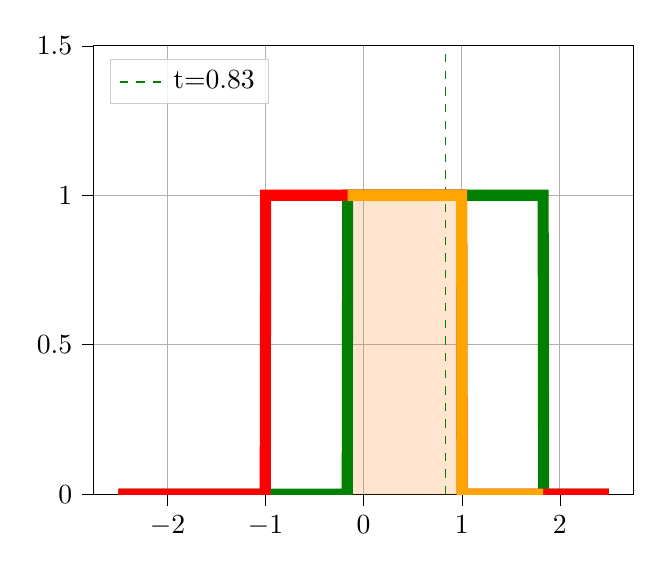
\begin{tikzpicture}

\definecolor{color0}{rgb}{1,0.498039215686275,0.0549019607843137}
\definecolor{color1}{rgb}{1,0.647058823529412,0}

\begin{axis}[
legend cell align={left},
legend style={fill opacity=0.8, draw opacity=1, text opacity=1, at={(0.03,0.97)}, anchor=north west, draw=white!80!black},
tick align=outside,
tick pos=left,
x grid style={white!69.0196078431373!black},
xmajorgrids,
xmin=-2.75, xmax=2.75,
xtick style={color=black},
y grid style={white!69.0196078431373!black},
ymajorgrids,
ymin=0, ymax=1.5,
ytick style={color=black}
]
\path [draw=color0, fill=color0, opacity=0.2]
(axis cs:-0.162662662662663,1)
--(axis cs:-0.162662662662663,0)
--(axis cs:-0.157657657657658,0)
--(axis cs:-0.152652652652653,0)
--(axis cs:-0.147647647647648,0)
--(axis cs:-0.142642642642643,0)
--(axis cs:-0.137637637637638,0)
--(axis cs:-0.132632632632633,0)
--(axis cs:-0.127627627627628,0)
--(axis cs:-0.122622622622623,0)
--(axis cs:-0.117617617617618,0)
--(axis cs:-0.112612612612613,0)
--(axis cs:-0.107607607607608,0)
--(axis cs:-0.102602602602603,0)
--(axis cs:-0.0975975975975976,0)
--(axis cs:-0.0925925925925926,0)
--(axis cs:-0.0875875875875876,0)
--(axis cs:-0.0825825825825826,0)
--(axis cs:-0.0775775775775776,0)
--(axis cs:-0.0725725725725725,0)
--(axis cs:-0.0675675675675675,0)
--(axis cs:-0.0625625625625625,0)
--(axis cs:-0.0575575575575575,0)
--(axis cs:-0.0525525525525525,0)
--(axis cs:-0.0475475475475475,0)
--(axis cs:-0.0425425425425425,0)
--(axis cs:-0.0375375375375375,0)
--(axis cs:-0.0325325325325325,0)
--(axis cs:-0.0275275275275275,0)
--(axis cs:-0.0225225225225225,0)
--(axis cs:-0.0175175175175175,0)
--(axis cs:-0.0125125125125125,0)
--(axis cs:-0.0075075075075075,0)
--(axis cs:-0.0025025025025025,0)
--(axis cs:0.0025025025025025,0)
--(axis cs:0.0075075075075075,0)
--(axis cs:0.0125125125125125,0)
--(axis cs:0.0175175175175175,0)
--(axis cs:0.0225225225225225,0)
--(axis cs:0.0275275275275275,0)
--(axis cs:0.0325325325325325,0)
--(axis cs:0.0375375375375375,0)
--(axis cs:0.0425425425425425,0)
--(axis cs:0.0475475475475475,0)
--(axis cs:0.0525525525525525,0)
--(axis cs:0.0575575575575575,0)
--(axis cs:0.0625625625625625,0)
--(axis cs:0.0675675675675675,0)
--(axis cs:0.0725725725725725,0)
--(axis cs:0.0775775775775776,0)
--(axis cs:0.0825825825825826,0)
--(axis cs:0.0875875875875876,0)
--(axis cs:0.0925925925925926,0)
--(axis cs:0.0975975975975976,0)
--(axis cs:0.102602602602603,0)
--(axis cs:0.107607607607608,0)
--(axis cs:0.112612612612613,0)
--(axis cs:0.117617617617618,0)
--(axis cs:0.122622622622623,0)
--(axis cs:0.127627627627628,0)
--(axis cs:0.132632632632633,0)
--(axis cs:0.137637637637638,0)
--(axis cs:0.142642642642643,0)
--(axis cs:0.147647647647648,0)
--(axis cs:0.152652652652653,0)
--(axis cs:0.157657657657658,0)
--(axis cs:0.162662662662663,0)
--(axis cs:0.167667667667668,0)
--(axis cs:0.172672672672673,0)
--(axis cs:0.177677677677678,0)
--(axis cs:0.182682682682683,0)
--(axis cs:0.187687687687688,0)
--(axis cs:0.192692692692693,0)
--(axis cs:0.197697697697698,0)
--(axis cs:0.202702702702703,0)
--(axis cs:0.207707707707708,0)
--(axis cs:0.212712712712713,0)
--(axis cs:0.217717717717718,0)
--(axis cs:0.222722722722723,0)
--(axis cs:0.227727727727728,0)
--(axis cs:0.232732732732733,0)
--(axis cs:0.237737737737738,0)
--(axis cs:0.242742742742743,0)
--(axis cs:0.247747747747748,0)
--(axis cs:0.252752752752753,0)
--(axis cs:0.257757757757758,0)
--(axis cs:0.262762762762763,0)
--(axis cs:0.267767767767768,0)
--(axis cs:0.272772772772773,0)
--(axis cs:0.277777777777778,0)
--(axis cs:0.282782782782783,0)
--(axis cs:0.287787787787788,0)
--(axis cs:0.292792792792793,0)
--(axis cs:0.297797797797798,0)
--(axis cs:0.302802802802803,0)
--(axis cs:0.307807807807808,0)
--(axis cs:0.312812812812813,0)
--(axis cs:0.317817817817818,0)
--(axis cs:0.322822822822823,0)
--(axis cs:0.327827827827828,0)
--(axis cs:0.332832832832833,0)
--(axis cs:0.337837837837838,0)
--(axis cs:0.342842842842843,0)
--(axis cs:0.347847847847848,0)
--(axis cs:0.352852852852853,0)
--(axis cs:0.357857857857858,0)
--(axis cs:0.362862862862863,0)
--(axis cs:0.367867867867868,0)
--(axis cs:0.372872872872873,0)
--(axis cs:0.377877877877878,0)
--(axis cs:0.382882882882883,0)
--(axis cs:0.387887887887888,0)
--(axis cs:0.392892892892893,0)
--(axis cs:0.397897897897898,0)
--(axis cs:0.402902902902903,0)
--(axis cs:0.407907907907908,0)
--(axis cs:0.412912912912913,0)
--(axis cs:0.417917917917918,0)
--(axis cs:0.422922922922923,0)
--(axis cs:0.427927927927928,0)
--(axis cs:0.432932932932933,0)
--(axis cs:0.437937937937938,0)
--(axis cs:0.442942942942943,0)
--(axis cs:0.447947947947948,0)
--(axis cs:0.452952952952953,0)
--(axis cs:0.457957957957958,0)
--(axis cs:0.462962962962963,0)
--(axis cs:0.467967967967968,0)
--(axis cs:0.472972972972973,0)
--(axis cs:0.477977977977978,0)
--(axis cs:0.482982982982983,0)
--(axis cs:0.487987987987988,0)
--(axis cs:0.492992992992993,0)
--(axis cs:0.497997997997998,0)
--(axis cs:0.503003003003003,0)
--(axis cs:0.508008008008008,0)
--(axis cs:0.513013013013013,0)
--(axis cs:0.518018018018018,0)
--(axis cs:0.523023023023023,0)
--(axis cs:0.528028028028028,0)
--(axis cs:0.533033033033033,0)
--(axis cs:0.538038038038038,0)
--(axis cs:0.543043043043043,0)
--(axis cs:0.548048048048048,0)
--(axis cs:0.553053053053053,0)
--(axis cs:0.558058058058058,0)
--(axis cs:0.563063063063063,0)
--(axis cs:0.568068068068068,0)
--(axis cs:0.573073073073073,0)
--(axis cs:0.578078078078078,0)
--(axis cs:0.583083083083083,0)
--(axis cs:0.588088088088088,0)
--(axis cs:0.593093093093093,0)
--(axis cs:0.598098098098098,0)
--(axis cs:0.603103103103103,0)
--(axis cs:0.608108108108108,0)
--(axis cs:0.613113113113113,0)
--(axis cs:0.618118118118118,0)
--(axis cs:0.623123123123123,0)
--(axis cs:0.628128128128128,0)
--(axis cs:0.633133133133133,0)
--(axis cs:0.638138138138138,0)
--(axis cs:0.643143143143143,0)
--(axis cs:0.648148148148148,0)
--(axis cs:0.653153153153153,0)
--(axis cs:0.658158158158158,0)
--(axis cs:0.663163163163163,0)
--(axis cs:0.668168168168168,0)
--(axis cs:0.673173173173173,0)
--(axis cs:0.678178178178178,0)
--(axis cs:0.683183183183183,0)
--(axis cs:0.688188188188188,0)
--(axis cs:0.693193193193193,0)
--(axis cs:0.698198198198198,0)
--(axis cs:0.703203203203203,0)
--(axis cs:0.708208208208208,0)
--(axis cs:0.713213213213213,0)
--(axis cs:0.718218218218218,0)
--(axis cs:0.723223223223223,0)
--(axis cs:0.728228228228228,0)
--(axis cs:0.733233233233233,0)
--(axis cs:0.738238238238238,0)
--(axis cs:0.743243243243243,0)
--(axis cs:0.748248248248248,0)
--(axis cs:0.753253253253253,0)
--(axis cs:0.758258258258258,0)
--(axis cs:0.763263263263263,0)
--(axis cs:0.768268268268268,0)
--(axis cs:0.773273273273273,0)
--(axis cs:0.778278278278278,0)
--(axis cs:0.783283283283283,0)
--(axis cs:0.788288288288288,0)
--(axis cs:0.793293293293293,0)
--(axis cs:0.798298298298298,0)
--(axis cs:0.803303303303303,0)
--(axis cs:0.808308308308308,0)
--(axis cs:0.813313313313313,0)
--(axis cs:0.818318318318318,0)
--(axis cs:0.823323323323323,0)
--(axis cs:0.828328328328328,0)
--(axis cs:0.833333333333333,0)
--(axis cs:0.838338338338338,0)
--(axis cs:0.843343343343343,0)
--(axis cs:0.848348348348348,0)
--(axis cs:0.853353353353353,0)
--(axis cs:0.858358358358358,0)
--(axis cs:0.863363363363364,0)
--(axis cs:0.868368368368369,0)
--(axis cs:0.873373373373374,0)
--(axis cs:0.878378378378379,0)
--(axis cs:0.883383383383384,0)
--(axis cs:0.888388388388389,0)
--(axis cs:0.893393393393394,0)
--(axis cs:0.898398398398399,0)
--(axis cs:0.903403403403404,0)
--(axis cs:0.908408408408409,0)
--(axis cs:0.913413413413414,0)
--(axis cs:0.918418418418419,0)
--(axis cs:0.923423423423424,0)
--(axis cs:0.928428428428429,0)
--(axis cs:0.933433433433434,0)
--(axis cs:0.938438438438439,0)
--(axis cs:0.943443443443444,0)
--(axis cs:0.948448448448449,0)
--(axis cs:0.953453453453454,0)
--(axis cs:0.958458458458459,0)
--(axis cs:0.963463463463464,0)
--(axis cs:0.968468468468469,0)
--(axis cs:0.973473473473474,0)
--(axis cs:0.978478478478479,0)
--(axis cs:0.983483483483484,0)
--(axis cs:0.988488488488489,0)
--(axis cs:0.993493493493494,0)
--(axis cs:0.998498498498499,0)
--(axis cs:1.0035035035035,0)
--(axis cs:1.00850850850851,0)
--(axis cs:1.01351351351351,0)
--(axis cs:1.01851851851852,0)
--(axis cs:1.02352352352352,0)
--(axis cs:1.02852852852853,0)
--(axis cs:1.03353353353353,0)
--(axis cs:1.03853853853854,0)
--(axis cs:1.04354354354354,0)
--(axis cs:1.04854854854855,0)
--(axis cs:1.05355355355355,0)
--(axis cs:1.05855855855856,0)
--(axis cs:1.06356356356356,0)
--(axis cs:1.06856856856857,0)
--(axis cs:1.07357357357357,0)
--(axis cs:1.07857857857858,0)
--(axis cs:1.08358358358358,0)
--(axis cs:1.08858858858859,0)
--(axis cs:1.09359359359359,0)
--(axis cs:1.0985985985986,0)
--(axis cs:1.1036036036036,0)
--(axis cs:1.10860860860861,0)
--(axis cs:1.11361361361361,0)
--(axis cs:1.11861861861862,0)
--(axis cs:1.12362362362362,0)
--(axis cs:1.12862862862863,0)
--(axis cs:1.13363363363363,0)
--(axis cs:1.13863863863864,0)
--(axis cs:1.14364364364364,0)
--(axis cs:1.14864864864865,0)
--(axis cs:1.15365365365365,0)
--(axis cs:1.15865865865866,0)
--(axis cs:1.16366366366366,0)
--(axis cs:1.16866866866867,0)
--(axis cs:1.17367367367367,0)
--(axis cs:1.17867867867868,0)
--(axis cs:1.18368368368368,0)
--(axis cs:1.18868868868869,0)
--(axis cs:1.19369369369369,0)
--(axis cs:1.1986986986987,0)
--(axis cs:1.2037037037037,0)
--(axis cs:1.20870870870871,0)
--(axis cs:1.21371371371371,0)
--(axis cs:1.21871871871872,0)
--(axis cs:1.22372372372372,0)
--(axis cs:1.22872872872873,0)
--(axis cs:1.23373373373373,0)
--(axis cs:1.23873873873874,0)
--(axis cs:1.24374374374374,0)
--(axis cs:1.24874874874875,0)
--(axis cs:1.25375375375375,0)
--(axis cs:1.25875875875876,0)
--(axis cs:1.26376376376376,0)
--(axis cs:1.26876876876877,0)
--(axis cs:1.27377377377377,0)
--(axis cs:1.27877877877878,0)
--(axis cs:1.28378378378378,0)
--(axis cs:1.28878878878879,0)
--(axis cs:1.29379379379379,0)
--(axis cs:1.2987987987988,0)
--(axis cs:1.3038038038038,0)
--(axis cs:1.30880880880881,0)
--(axis cs:1.31381381381381,0)
--(axis cs:1.31881881881882,0)
--(axis cs:1.32382382382382,0)
--(axis cs:1.32882882882883,0)
--(axis cs:1.33383383383383,0)
--(axis cs:1.33883883883884,0)
--(axis cs:1.34384384384384,0)
--(axis cs:1.34884884884885,0)
--(axis cs:1.35385385385385,0)
--(axis cs:1.35885885885886,0)
--(axis cs:1.36386386386386,0)
--(axis cs:1.36886886886887,0)
--(axis cs:1.37387387387387,0)
--(axis cs:1.37887887887888,0)
--(axis cs:1.38388388388388,0)
--(axis cs:1.38888888888889,0)
--(axis cs:1.39389389389389,0)
--(axis cs:1.3988988988989,0)
--(axis cs:1.4039039039039,0)
--(axis cs:1.40890890890891,0)
--(axis cs:1.41391391391391,0)
--(axis cs:1.41891891891892,0)
--(axis cs:1.42392392392392,0)
--(axis cs:1.42892892892893,0)
--(axis cs:1.43393393393393,0)
--(axis cs:1.43893893893894,0)
--(axis cs:1.44394394394394,0)
--(axis cs:1.44894894894895,0)
--(axis cs:1.45395395395395,0)
--(axis cs:1.45895895895896,0)
--(axis cs:1.46396396396396,0)
--(axis cs:1.46896896896897,0)
--(axis cs:1.47397397397397,0)
--(axis cs:1.47897897897898,0)
--(axis cs:1.48398398398398,0)
--(axis cs:1.48898898898899,0)
--(axis cs:1.49399399399399,0)
--(axis cs:1.498998998999,0)
--(axis cs:1.504004004004,0)
--(axis cs:1.50900900900901,0)
--(axis cs:1.51401401401401,0)
--(axis cs:1.51901901901902,0)
--(axis cs:1.52402402402402,0)
--(axis cs:1.52902902902903,0)
--(axis cs:1.53403403403403,0)
--(axis cs:1.53903903903904,0)
--(axis cs:1.54404404404404,0)
--(axis cs:1.54904904904905,0)
--(axis cs:1.55405405405405,0)
--(axis cs:1.55905905905906,0)
--(axis cs:1.56406406406406,0)
--(axis cs:1.56906906906907,0)
--(axis cs:1.57407407407407,0)
--(axis cs:1.57907907907908,0)
--(axis cs:1.58408408408408,0)
--(axis cs:1.58908908908909,0)
--(axis cs:1.59409409409409,0)
--(axis cs:1.5990990990991,0)
--(axis cs:1.6041041041041,0)
--(axis cs:1.60910910910911,0)
--(axis cs:1.61411411411411,0)
--(axis cs:1.61911911911912,0)
--(axis cs:1.62412412412412,0)
--(axis cs:1.62912912912913,0)
--(axis cs:1.63413413413413,0)
--(axis cs:1.63913913913914,0)
--(axis cs:1.64414414414414,0)
--(axis cs:1.64914914914915,0)
--(axis cs:1.65415415415415,0)
--(axis cs:1.65915915915916,0)
--(axis cs:1.66416416416416,0)
--(axis cs:1.66916916916917,0)
--(axis cs:1.67417417417417,0)
--(axis cs:1.67917917917918,0)
--(axis cs:1.68418418418418,0)
--(axis cs:1.68918918918919,0)
--(axis cs:1.69419419419419,0)
--(axis cs:1.6991991991992,0)
--(axis cs:1.7042042042042,0)
--(axis cs:1.70920920920921,0)
--(axis cs:1.71421421421421,0)
--(axis cs:1.71921921921922,0)
--(axis cs:1.72422422422422,0)
--(axis cs:1.72922922922923,0)
--(axis cs:1.73423423423423,0)
--(axis cs:1.73923923923924,0)
--(axis cs:1.74424424424424,0)
--(axis cs:1.74924924924925,0)
--(axis cs:1.75425425425425,0)
--(axis cs:1.75925925925926,0)
--(axis cs:1.76426426426426,0)
--(axis cs:1.76926926926927,0)
--(axis cs:1.77427427427427,0)
--(axis cs:1.77927927927928,0)
--(axis cs:1.78428428428428,0)
--(axis cs:1.78928928928929,0)
--(axis cs:1.79429429429429,0)
--(axis cs:1.7992992992993,0)
--(axis cs:1.8043043043043,0)
--(axis cs:1.80930930930931,0)
--(axis cs:1.81431431431431,0)
--(axis cs:1.81931931931932,0)
--(axis cs:1.82432432432432,0)
--(axis cs:1.82932932932933,0)
--(axis cs:1.82932932932933,0)
--(axis cs:1.82932932932933,0)
--(axis cs:1.82432432432432,0)
--(axis cs:1.81931931931932,0)
--(axis cs:1.81431431431431,0)
--(axis cs:1.80930930930931,0)
--(axis cs:1.8043043043043,0)
--(axis cs:1.7992992992993,0)
--(axis cs:1.79429429429429,0)
--(axis cs:1.78928928928929,0)
--(axis cs:1.78428428428428,0)
--(axis cs:1.77927927927928,0)
--(axis cs:1.77427427427427,0)
--(axis cs:1.76926926926927,0)
--(axis cs:1.76426426426426,0)
--(axis cs:1.75925925925926,0)
--(axis cs:1.75425425425425,0)
--(axis cs:1.74924924924925,0)
--(axis cs:1.74424424424424,0)
--(axis cs:1.73923923923924,0)
--(axis cs:1.73423423423423,0)
--(axis cs:1.72922922922923,0)
--(axis cs:1.72422422422422,0)
--(axis cs:1.71921921921922,0)
--(axis cs:1.71421421421421,0)
--(axis cs:1.70920920920921,0)
--(axis cs:1.7042042042042,0)
--(axis cs:1.6991991991992,0)
--(axis cs:1.69419419419419,0)
--(axis cs:1.68918918918919,0)
--(axis cs:1.68418418418418,0)
--(axis cs:1.67917917917918,0)
--(axis cs:1.67417417417417,0)
--(axis cs:1.66916916916917,0)
--(axis cs:1.66416416416416,0)
--(axis cs:1.65915915915916,0)
--(axis cs:1.65415415415415,0)
--(axis cs:1.64914914914915,0)
--(axis cs:1.64414414414414,0)
--(axis cs:1.63913913913914,0)
--(axis cs:1.63413413413413,0)
--(axis cs:1.62912912912913,0)
--(axis cs:1.62412412412412,0)
--(axis cs:1.61911911911912,0)
--(axis cs:1.61411411411411,0)
--(axis cs:1.60910910910911,0)
--(axis cs:1.6041041041041,0)
--(axis cs:1.5990990990991,0)
--(axis cs:1.59409409409409,0)
--(axis cs:1.58908908908909,0)
--(axis cs:1.58408408408408,0)
--(axis cs:1.57907907907908,0)
--(axis cs:1.57407407407407,0)
--(axis cs:1.56906906906907,0)
--(axis cs:1.56406406406406,0)
--(axis cs:1.55905905905906,0)
--(axis cs:1.55405405405405,0)
--(axis cs:1.54904904904905,0)
--(axis cs:1.54404404404404,0)
--(axis cs:1.53903903903904,0)
--(axis cs:1.53403403403403,0)
--(axis cs:1.52902902902903,0)
--(axis cs:1.52402402402402,0)
--(axis cs:1.51901901901902,0)
--(axis cs:1.51401401401401,0)
--(axis cs:1.50900900900901,0)
--(axis cs:1.504004004004,0)
--(axis cs:1.498998998999,0)
--(axis cs:1.49399399399399,0)
--(axis cs:1.48898898898899,0)
--(axis cs:1.48398398398398,0)
--(axis cs:1.47897897897898,0)
--(axis cs:1.47397397397397,0)
--(axis cs:1.46896896896897,0)
--(axis cs:1.46396396396396,0)
--(axis cs:1.45895895895896,0)
--(axis cs:1.45395395395395,0)
--(axis cs:1.44894894894895,0)
--(axis cs:1.44394394394394,0)
--(axis cs:1.43893893893894,0)
--(axis cs:1.43393393393393,0)
--(axis cs:1.42892892892893,0)
--(axis cs:1.42392392392392,0)
--(axis cs:1.41891891891892,0)
--(axis cs:1.41391391391391,0)
--(axis cs:1.40890890890891,0)
--(axis cs:1.4039039039039,0)
--(axis cs:1.3988988988989,0)
--(axis cs:1.39389389389389,0)
--(axis cs:1.38888888888889,0)
--(axis cs:1.38388388388388,0)
--(axis cs:1.37887887887888,0)
--(axis cs:1.37387387387387,0)
--(axis cs:1.36886886886887,0)
--(axis cs:1.36386386386386,0)
--(axis cs:1.35885885885886,0)
--(axis cs:1.35385385385385,0)
--(axis cs:1.34884884884885,0)
--(axis cs:1.34384384384384,0)
--(axis cs:1.33883883883884,0)
--(axis cs:1.33383383383383,0)
--(axis cs:1.32882882882883,0)
--(axis cs:1.32382382382382,0)
--(axis cs:1.31881881881882,0)
--(axis cs:1.31381381381381,0)
--(axis cs:1.30880880880881,0)
--(axis cs:1.3038038038038,0)
--(axis cs:1.2987987987988,0)
--(axis cs:1.29379379379379,0)
--(axis cs:1.28878878878879,0)
--(axis cs:1.28378378378378,0)
--(axis cs:1.27877877877878,0)
--(axis cs:1.27377377377377,0)
--(axis cs:1.26876876876877,0)
--(axis cs:1.26376376376376,0)
--(axis cs:1.25875875875876,0)
--(axis cs:1.25375375375375,0)
--(axis cs:1.24874874874875,0)
--(axis cs:1.24374374374374,0)
--(axis cs:1.23873873873874,0)
--(axis cs:1.23373373373373,0)
--(axis cs:1.22872872872873,0)
--(axis cs:1.22372372372372,0)
--(axis cs:1.21871871871872,0)
--(axis cs:1.21371371371371,0)
--(axis cs:1.20870870870871,0)
--(axis cs:1.2037037037037,0)
--(axis cs:1.1986986986987,0)
--(axis cs:1.19369369369369,0)
--(axis cs:1.18868868868869,0)
--(axis cs:1.18368368368368,0)
--(axis cs:1.17867867867868,0)
--(axis cs:1.17367367367367,0)
--(axis cs:1.16866866866867,0)
--(axis cs:1.16366366366366,0)
--(axis cs:1.15865865865866,0)
--(axis cs:1.15365365365365,0)
--(axis cs:1.14864864864865,0)
--(axis cs:1.14364364364364,0)
--(axis cs:1.13863863863864,0)
--(axis cs:1.13363363363363,0)
--(axis cs:1.12862862862863,0)
--(axis cs:1.12362362362362,0)
--(axis cs:1.11861861861862,0)
--(axis cs:1.11361361361361,0)
--(axis cs:1.10860860860861,0)
--(axis cs:1.1036036036036,0)
--(axis cs:1.0985985985986,0)
--(axis cs:1.09359359359359,0)
--(axis cs:1.08858858858859,0)
--(axis cs:1.08358358358358,0)
--(axis cs:1.07857857857858,0)
--(axis cs:1.07357357357357,0)
--(axis cs:1.06856856856857,0)
--(axis cs:1.06356356356356,0)
--(axis cs:1.05855855855856,0)
--(axis cs:1.05355355355355,0)
--(axis cs:1.04854854854855,0)
--(axis cs:1.04354354354354,0)
--(axis cs:1.03853853853854,0)
--(axis cs:1.03353353353353,0)
--(axis cs:1.02852852852853,0)
--(axis cs:1.02352352352352,0)
--(axis cs:1.01851851851852,0)
--(axis cs:1.01351351351351,0)
--(axis cs:1.00850850850851,0)
--(axis cs:1.0035035035035,0)
--(axis cs:0.998498498498499,1)
--(axis cs:0.993493493493494,1)
--(axis cs:0.988488488488489,1)
--(axis cs:0.983483483483484,1)
--(axis cs:0.978478478478479,1)
--(axis cs:0.973473473473474,1)
--(axis cs:0.968468468468469,1)
--(axis cs:0.963463463463464,1)
--(axis cs:0.958458458458459,1)
--(axis cs:0.953453453453454,1)
--(axis cs:0.948448448448449,1)
--(axis cs:0.943443443443444,1)
--(axis cs:0.938438438438439,1)
--(axis cs:0.933433433433434,1)
--(axis cs:0.928428428428429,1)
--(axis cs:0.923423423423424,1)
--(axis cs:0.918418418418419,1)
--(axis cs:0.913413413413414,1)
--(axis cs:0.908408408408409,1)
--(axis cs:0.903403403403404,1)
--(axis cs:0.898398398398399,1)
--(axis cs:0.893393393393394,1)
--(axis cs:0.888388388388389,1)
--(axis cs:0.883383383383384,1)
--(axis cs:0.878378378378379,1)
--(axis cs:0.873373373373374,1)
--(axis cs:0.868368368368369,1)
--(axis cs:0.863363363363364,1)
--(axis cs:0.858358358358358,1)
--(axis cs:0.853353353353353,1)
--(axis cs:0.848348348348348,1)
--(axis cs:0.843343343343343,1)
--(axis cs:0.838338338338338,1)
--(axis cs:0.833333333333333,1)
--(axis cs:0.828328328328328,1)
--(axis cs:0.823323323323323,1)
--(axis cs:0.818318318318318,1)
--(axis cs:0.813313313313313,1)
--(axis cs:0.808308308308308,1)
--(axis cs:0.803303303303303,1)
--(axis cs:0.798298298298298,1)
--(axis cs:0.793293293293293,1)
--(axis cs:0.788288288288288,1)
--(axis cs:0.783283283283283,1)
--(axis cs:0.778278278278278,1)
--(axis cs:0.773273273273273,1)
--(axis cs:0.768268268268268,1)
--(axis cs:0.763263263263263,1)
--(axis cs:0.758258258258258,1)
--(axis cs:0.753253253253253,1)
--(axis cs:0.748248248248248,1)
--(axis cs:0.743243243243243,1)
--(axis cs:0.738238238238238,1)
--(axis cs:0.733233233233233,1)
--(axis cs:0.728228228228228,1)
--(axis cs:0.723223223223223,1)
--(axis cs:0.718218218218218,1)
--(axis cs:0.713213213213213,1)
--(axis cs:0.708208208208208,1)
--(axis cs:0.703203203203203,1)
--(axis cs:0.698198198198198,1)
--(axis cs:0.693193193193193,1)
--(axis cs:0.688188188188188,1)
--(axis cs:0.683183183183183,1)
--(axis cs:0.678178178178178,1)
--(axis cs:0.673173173173173,1)
--(axis cs:0.668168168168168,1)
--(axis cs:0.663163163163163,1)
--(axis cs:0.658158158158158,1)
--(axis cs:0.653153153153153,1)
--(axis cs:0.648148148148148,1)
--(axis cs:0.643143143143143,1)
--(axis cs:0.638138138138138,1)
--(axis cs:0.633133133133133,1)
--(axis cs:0.628128128128128,1)
--(axis cs:0.623123123123123,1)
--(axis cs:0.618118118118118,1)
--(axis cs:0.613113113113113,1)
--(axis cs:0.608108108108108,1)
--(axis cs:0.603103103103103,1)
--(axis cs:0.598098098098098,1)
--(axis cs:0.593093093093093,1)
--(axis cs:0.588088088088088,1)
--(axis cs:0.583083083083083,1)
--(axis cs:0.578078078078078,1)
--(axis cs:0.573073073073073,1)
--(axis cs:0.568068068068068,1)
--(axis cs:0.563063063063063,1)
--(axis cs:0.558058058058058,1)
--(axis cs:0.553053053053053,1)
--(axis cs:0.548048048048048,1)
--(axis cs:0.543043043043043,1)
--(axis cs:0.538038038038038,1)
--(axis cs:0.533033033033033,1)
--(axis cs:0.528028028028028,1)
--(axis cs:0.523023023023023,1)
--(axis cs:0.518018018018018,1)
--(axis cs:0.513013013013013,1)
--(axis cs:0.508008008008008,1)
--(axis cs:0.503003003003003,1)
--(axis cs:0.497997997997998,1)
--(axis cs:0.492992992992993,1)
--(axis cs:0.487987987987988,1)
--(axis cs:0.482982982982983,1)
--(axis cs:0.477977977977978,1)
--(axis cs:0.472972972972973,1)
--(axis cs:0.467967967967968,1)
--(axis cs:0.462962962962963,1)
--(axis cs:0.457957957957958,1)
--(axis cs:0.452952952952953,1)
--(axis cs:0.447947947947948,1)
--(axis cs:0.442942942942943,1)
--(axis cs:0.437937937937938,1)
--(axis cs:0.432932932932933,1)
--(axis cs:0.427927927927928,1)
--(axis cs:0.422922922922923,1)
--(axis cs:0.417917917917918,1)
--(axis cs:0.412912912912913,1)
--(axis cs:0.407907907907908,1)
--(axis cs:0.402902902902903,1)
--(axis cs:0.397897897897898,1)
--(axis cs:0.392892892892893,1)
--(axis cs:0.387887887887888,1)
--(axis cs:0.382882882882883,1)
--(axis cs:0.377877877877878,1)
--(axis cs:0.372872872872873,1)
--(axis cs:0.367867867867868,1)
--(axis cs:0.362862862862863,1)
--(axis cs:0.357857857857858,1)
--(axis cs:0.352852852852853,1)
--(axis cs:0.347847847847848,1)
--(axis cs:0.342842842842843,1)
--(axis cs:0.337837837837838,1)
--(axis cs:0.332832832832833,1)
--(axis cs:0.327827827827828,1)
--(axis cs:0.322822822822823,1)
--(axis cs:0.317817817817818,1)
--(axis cs:0.312812812812813,1)
--(axis cs:0.307807807807808,1)
--(axis cs:0.302802802802803,1)
--(axis cs:0.297797797797798,1)
--(axis cs:0.292792792792793,1)
--(axis cs:0.287787787787788,1)
--(axis cs:0.282782782782783,1)
--(axis cs:0.277777777777778,1)
--(axis cs:0.272772772772773,1)
--(axis cs:0.267767767767768,1)
--(axis cs:0.262762762762763,1)
--(axis cs:0.257757757757758,1)
--(axis cs:0.252752752752753,1)
--(axis cs:0.247747747747748,1)
--(axis cs:0.242742742742743,1)
--(axis cs:0.237737737737738,1)
--(axis cs:0.232732732732733,1)
--(axis cs:0.227727727727728,1)
--(axis cs:0.222722722722723,1)
--(axis cs:0.217717717717718,1)
--(axis cs:0.212712712712713,1)
--(axis cs:0.207707707707708,1)
--(axis cs:0.202702702702703,1)
--(axis cs:0.197697697697698,1)
--(axis cs:0.192692692692693,1)
--(axis cs:0.187687687687688,1)
--(axis cs:0.182682682682683,1)
--(axis cs:0.177677677677678,1)
--(axis cs:0.172672672672673,1)
--(axis cs:0.167667667667668,1)
--(axis cs:0.162662662662663,1)
--(axis cs:0.157657657657658,1)
--(axis cs:0.152652652652653,1)
--(axis cs:0.147647647647648,1)
--(axis cs:0.142642642642643,1)
--(axis cs:0.137637637637638,1)
--(axis cs:0.132632632632633,1)
--(axis cs:0.127627627627628,1)
--(axis cs:0.122622622622623,1)
--(axis cs:0.117617617617618,1)
--(axis cs:0.112612612612613,1)
--(axis cs:0.107607607607608,1)
--(axis cs:0.102602602602603,1)
--(axis cs:0.0975975975975976,1)
--(axis cs:0.0925925925925926,1)
--(axis cs:0.0875875875875876,1)
--(axis cs:0.0825825825825826,1)
--(axis cs:0.0775775775775776,1)
--(axis cs:0.0725725725725725,1)
--(axis cs:0.0675675675675675,1)
--(axis cs:0.0625625625625625,1)
--(axis cs:0.0575575575575575,1)
--(axis cs:0.0525525525525525,1)
--(axis cs:0.0475475475475475,1)
--(axis cs:0.0425425425425425,1)
--(axis cs:0.0375375375375375,1)
--(axis cs:0.0325325325325325,1)
--(axis cs:0.0275275275275275,1)
--(axis cs:0.0225225225225225,1)
--(axis cs:0.0175175175175175,1)
--(axis cs:0.0125125125125125,1)
--(axis cs:0.0075075075075075,1)
--(axis cs:0.0025025025025025,1)
--(axis cs:-0.0025025025025025,1)
--(axis cs:-0.0075075075075075,1)
--(axis cs:-0.0125125125125125,1)
--(axis cs:-0.0175175175175175,1)
--(axis cs:-0.0225225225225225,1)
--(axis cs:-0.0275275275275275,1)
--(axis cs:-0.0325325325325325,1)
--(axis cs:-0.0375375375375375,1)
--(axis cs:-0.0425425425425425,1)
--(axis cs:-0.0475475475475475,1)
--(axis cs:-0.0525525525525525,1)
--(axis cs:-0.0575575575575575,1)
--(axis cs:-0.0625625625625625,1)
--(axis cs:-0.0675675675675675,1)
--(axis cs:-0.0725725725725725,1)
--(axis cs:-0.0775775775775776,1)
--(axis cs:-0.0825825825825826,1)
--(axis cs:-0.0875875875875876,1)
--(axis cs:-0.0925925925925926,1)
--(axis cs:-0.0975975975975976,1)
--(axis cs:-0.102602602602603,1)
--(axis cs:-0.107607607607608,1)
--(axis cs:-0.112612612612613,1)
--(axis cs:-0.117617617617618,1)
--(axis cs:-0.122622622622623,1)
--(axis cs:-0.127627627627628,1)
--(axis cs:-0.132632632632633,1)
--(axis cs:-0.137637637637638,1)
--(axis cs:-0.142642642642643,1)
--(axis cs:-0.147647647647648,1)
--(axis cs:-0.152652652652653,1)
--(axis cs:-0.157657657657658,1)
--(axis cs:-0.162662662662663,1)
--cycle;

\addplot [line width=4pt, green!50!black, forget plot]
table {%
-2.5 0
-2.49499499499499 0
-2.48998998998999 0
-2.48498498498498 0
-2.47997997997998 0
-2.47497497497497 0
-2.46996996996997 0
-2.46496496496496 0
-2.45995995995996 0
-2.45495495495495 0
-2.44994994994995 0
-2.44494494494494 0
-2.43993993993994 0
-2.43493493493493 0
-2.42992992992993 0
-2.42492492492492 0
-2.41991991991992 0
-2.41491491491491 0
-2.40990990990991 0
-2.4049049049049 0
-2.3998998998999 0
-2.39489489489489 0
-2.38988988988989 0
-2.38488488488488 0
-2.37987987987988 0
-2.37487487487487 0
-2.36986986986987 0
-2.36486486486486 0
-2.35985985985986 0
-2.35485485485485 0
-2.34984984984985 0
-2.34484484484484 0
-2.33983983983984 0
-2.33483483483483 0
-2.32982982982983 0
-2.32482482482482 0
-2.31981981981982 0
-2.31481481481481 0
-2.30980980980981 0
-2.3048048048048 0
-2.2997997997998 0
-2.29479479479479 0
-2.28978978978979 0
-2.28478478478478 0
-2.27977977977978 0
-2.27477477477477 0
-2.26976976976977 0
-2.26476476476476 0
-2.25975975975976 0
-2.25475475475475 0
-2.24974974974975 0
-2.24474474474474 0
-2.23973973973974 0
-2.23473473473473 0
-2.22972972972973 0
-2.22472472472472 0
-2.21971971971972 0
-2.21471471471471 0
-2.20970970970971 0
-2.2047047047047 0
-2.1996996996997 0
-2.19469469469469 0
-2.18968968968969 0
-2.18468468468468 0
-2.17967967967968 0
-2.17467467467467 0
-2.16966966966967 0
-2.16466466466466 0
-2.15965965965966 0
-2.15465465465465 0
-2.14964964964965 0
-2.14464464464464 0
-2.13963963963964 0
-2.13463463463463 0
-2.12962962962963 0
-2.12462462462462 0
-2.11961961961962 0
-2.11461461461461 0
-2.10960960960961 0
-2.1046046046046 0
-2.0995995995996 0
-2.09459459459459 0
-2.08958958958959 0
-2.08458458458458 0
-2.07957957957958 0
-2.07457457457457 0
-2.06956956956957 0
-2.06456456456456 0
-2.05955955955956 0
-2.05455455455455 0
-2.04954954954955 0
-2.04454454454454 0
-2.03953953953954 0
-2.03453453453453 0
-2.02952952952953 0
-2.02452452452452 0
-2.01951951951952 0
-2.01451451451451 0
-2.00950950950951 0
-2.0045045045045 0
-1.9994994994995 0
-1.99449449449449 0
-1.98948948948949 0
-1.98448448448448 0
-1.97947947947948 0
-1.97447447447447 0
-1.96946946946947 0
-1.96446446446446 0
-1.95945945945946 0
-1.95445445445445 0
-1.94944944944945 0
-1.94444444444444 0
-1.93943943943944 0
-1.93443443443443 0
-1.92942942942943 0
-1.92442442442442 0
-1.91941941941942 0
-1.91441441441441 0
-1.90940940940941 0
-1.9044044044044 0
-1.8993993993994 0
-1.89439439439439 0
-1.88938938938939 0
-1.88438438438438 0
-1.87937937937938 0
-1.87437437437437 0
-1.86936936936937 0
-1.86436436436436 0
-1.85935935935936 0
-1.85435435435435 0
-1.84934934934935 0
-1.84434434434434 0
-1.83933933933934 0
-1.83433433433433 0
-1.82932932932933 0
-1.82432432432432 0
-1.81931931931932 0
-1.81431431431431 0
-1.80930930930931 0
-1.8043043043043 0
-1.7992992992993 0
-1.79429429429429 0
-1.78928928928929 0
-1.78428428428428 0
-1.77927927927928 0
-1.77427427427427 0
-1.76926926926927 0
-1.76426426426426 0
-1.75925925925926 0
-1.75425425425425 0
-1.74924924924925 0
-1.74424424424424 0
-1.73923923923924 0
-1.73423423423423 0
-1.72922922922923 0
-1.72422422422422 0
-1.71921921921922 0
-1.71421421421421 0
-1.70920920920921 0
-1.7042042042042 0
-1.6991991991992 0
-1.69419419419419 0
-1.68918918918919 0
-1.68418418418418 0
-1.67917917917918 0
-1.67417417417417 0
-1.66916916916917 0
-1.66416416416416 0
-1.65915915915916 0
-1.65415415415415 0
-1.64914914914915 0
-1.64414414414414 0
-1.63913913913914 0
-1.63413413413413 0
-1.62912912912913 0
-1.62412412412412 0
-1.61911911911912 0
-1.61411411411411 0
-1.60910910910911 0
-1.6041041041041 0
-1.5990990990991 0
-1.59409409409409 0
-1.58908908908909 0
-1.58408408408408 0
-1.57907907907908 0
-1.57407407407407 0
-1.56906906906907 0
-1.56406406406406 0
-1.55905905905906 0
-1.55405405405405 0
-1.54904904904905 0
-1.54404404404404 0
-1.53903903903904 0
-1.53403403403403 0
-1.52902902902903 0
-1.52402402402402 0
-1.51901901901902 0
-1.51401401401401 0
-1.50900900900901 0
-1.504004004004 0
-1.498998998999 0
-1.49399399399399 0
-1.48898898898899 0
-1.48398398398398 0
-1.47897897897898 0
-1.47397397397397 0
-1.46896896896897 0
-1.46396396396396 0
-1.45895895895896 0
-1.45395395395395 0
-1.44894894894895 0
-1.44394394394394 0
-1.43893893893894 0
-1.43393393393393 0
-1.42892892892893 0
-1.42392392392392 0
-1.41891891891892 0
-1.41391391391391 0
-1.40890890890891 0
-1.4039039039039 0
-1.3988988988989 0
-1.39389389389389 0
-1.38888888888889 0
-1.38388388388388 0
-1.37887887887888 0
-1.37387387387387 0
-1.36886886886887 0
-1.36386386386386 0
-1.35885885885886 0
-1.35385385385385 0
-1.34884884884885 0
-1.34384384384384 0
-1.33883883883884 0
-1.33383383383383 0
-1.32882882882883 0
-1.32382382382382 0
-1.31881881881882 0
-1.31381381381381 0
-1.30880880880881 0
-1.3038038038038 0
-1.2987987987988 0
-1.29379379379379 0
-1.28878878878879 0
-1.28378378378378 0
-1.27877877877878 0
-1.27377377377377 0
-1.26876876876877 0
-1.26376376376376 0
-1.25875875875876 0
-1.25375375375375 0
-1.24874874874875 0
-1.24374374374374 0
-1.23873873873874 0
-1.23373373373373 0
-1.22872872872873 0
-1.22372372372372 0
-1.21871871871872 0
-1.21371371371371 0
-1.20870870870871 0
-1.2037037037037 0
-1.1986986986987 0
-1.19369369369369 0
-1.18868868868869 0
-1.18368368368368 0
-1.17867867867868 0
-1.17367367367367 0
-1.16866866866867 0
-1.16366366366366 0
-1.15865865865866 0
-1.15365365365365 0
-1.14864864864865 0
-1.14364364364364 0
-1.13863863863864 0
-1.13363363363363 0
-1.12862862862863 0
-1.12362362362362 0
-1.11861861861862 0
-1.11361361361361 0
-1.10860860860861 0
-1.1036036036036 0
-1.0985985985986 0
-1.09359359359359 0
-1.08858858858859 0
-1.08358358358358 0
-1.07857857857858 0
-1.07357357357357 0
-1.06856856856857 0
-1.06356356356356 0
-1.05855855855856 0
-1.05355355355355 0
-1.04854854854855 0
-1.04354354354354 0
-1.03853853853854 0
-1.03353353353353 0
-1.02852852852853 0
-1.02352352352352 0
-1.01851851851852 0
-1.01351351351351 0
-1.00850850850851 0
-1.0035035035035 0
-0.998498498498499 0
-0.993493493493494 0
-0.988488488488489 0
-0.983483483483484 0
-0.978478478478479 0
-0.973473473473474 0
-0.968468468468469 0
-0.963463463463464 0
-0.958458458458459 0
-0.953453453453454 0
-0.948448448448449 0
-0.943443443443444 0
-0.938438438438439 0
-0.933433433433434 0
-0.928428428428429 0
-0.923423423423424 0
-0.918418418418419 0
-0.913413413413414 0
-0.908408408408409 0
-0.903403403403404 0
-0.898398398398399 0
-0.893393393393393 0
-0.888388388388388 0
-0.883383383383383 0
-0.878378378378378 0
-0.873373373373373 0
-0.868368368368368 0
-0.863363363363363 0
-0.858358358358358 0
-0.853353353353353 0
-0.848348348348348 0
-0.843343343343343 0
-0.838338338338338 0
-0.833333333333333 0
-0.828328328328328 0
-0.823323323323323 0
-0.818318318318318 0
-0.813313313313313 0
-0.808308308308308 0
-0.803303303303303 0
-0.798298298298298 0
-0.793293293293293 0
-0.788288288288288 0
-0.783283283283283 0
-0.778278278278278 0
-0.773273273273273 0
-0.768268268268268 0
-0.763263263263263 0
-0.758258258258258 0
-0.753253253253253 0
-0.748248248248248 0
-0.743243243243243 0
-0.738238238238238 0
-0.733233233233233 0
-0.728228228228228 0
-0.723223223223223 0
-0.718218218218218 0
-0.713213213213213 0
-0.708208208208208 0
-0.703203203203203 0
-0.698198198198198 0
-0.693193193193193 0
-0.688188188188188 0
-0.683183183183183 0
-0.678178178178178 0
-0.673173173173173 0
-0.668168168168168 0
-0.663163163163163 0
-0.658158158158158 0
-0.653153153153153 0
-0.648148148148148 0
-0.643143143143143 0
-0.638138138138138 0
-0.633133133133133 0
-0.628128128128128 0
-0.623123123123123 0
-0.618118118118118 0
-0.613113113113113 0
-0.608108108108108 0
-0.603103103103103 0
-0.598098098098098 0
-0.593093093093093 0
-0.588088088088088 0
-0.583083083083083 0
-0.578078078078078 0
-0.573073073073073 0
-0.568068068068068 0
-0.563063063063063 0
-0.558058058058058 0
-0.553053053053053 0
-0.548048048048048 0
-0.543043043043043 0
-0.538038038038038 0
-0.533033033033033 0
-0.528028028028028 0
-0.523023023023023 0
-0.518018018018018 0
-0.513013013013013 0
-0.508008008008008 0
-0.503003003003003 0
-0.497997997997998 0
-0.492992992992993 0
-0.487987987987988 0
-0.482982982982983 0
-0.477977977977978 0
-0.472972972972973 0
-0.467967967967968 0
-0.462962962962963 0
-0.457957957957958 0
-0.452952952952953 0
-0.447947947947948 0
-0.442942942942943 0
-0.437937937937938 0
-0.432932932932933 0
-0.427927927927928 0
-0.422922922922923 0
-0.417917917917918 0
-0.412912912912913 0
-0.407907907907908 0
-0.402902902902903 0
-0.397897897897898 0
-0.392892892892893 0
-0.387887887887888 0
-0.382882882882883 0
-0.377877877877878 0
-0.372872872872873 0
-0.367867867867868 0
-0.362862862862863 0
-0.357857857857858 0
-0.352852852852853 0
-0.347847847847848 0
-0.342842842842843 0
-0.337837837837838 0
-0.332832832832833 0
-0.327827827827828 0
-0.322822822822823 0
-0.317817817817818 0
-0.312812812812813 0
-0.307807807807808 0
-0.302802802802803 0
-0.297797797797798 0
-0.292792792792793 0
-0.287787787787788 0
-0.282782782782783 0
-0.277777777777778 0
-0.272772772772773 0
-0.267767767767768 0
-0.262762762762763 0
-0.257757757757758 0
-0.252752752752753 0
-0.247747747747748 0
-0.242742742742743 0
-0.237737737737738 0
-0.232732732732733 0
-0.227727727727728 0
-0.222722722722723 0
-0.217717717717718 0
-0.212712712712713 0
-0.207707707707708 0
-0.202702702702703 0
-0.197697697697698 0
-0.192692692692693 0
-0.187687687687688 0
-0.182682682682683 0
-0.177677677677678 0
-0.172672672672673 0
-0.167667667667668 0
-0.162662662662663 1
-0.157657657657658 1
-0.152652652652653 1
-0.147647647647648 1
-0.142642642642643 1
-0.137637637637638 1
-0.132632632632633 1
-0.127627627627628 1
-0.122622622622623 1
-0.117617617617618 1
-0.112612612612613 1
-0.107607607607608 1
-0.102602602602603 1
-0.0975975975975976 1
-0.0925925925925926 1
-0.0875875875875876 1
-0.0825825825825826 1
-0.0775775775775776 1
-0.0725725725725725 1
-0.0675675675675675 1
-0.0625625625625625 1
-0.0575575575575575 1
-0.0525525525525525 1
-0.0475475475475475 1
-0.0425425425425425 1
-0.0375375375375375 1
-0.0325325325325325 1
-0.0275275275275275 1
-0.0225225225225225 1
-0.0175175175175175 1
-0.0125125125125125 1
-0.0075075075075075 1
-0.0025025025025025 1
0.0025025025025025 1
0.0075075075075075 1
0.0125125125125125 1
0.0175175175175175 1
0.0225225225225225 1
0.0275275275275275 1
0.0325325325325325 1
0.0375375375375375 1
0.0425425425425425 1
0.0475475475475475 1
0.0525525525525525 1
0.0575575575575575 1
0.0625625625625625 1
0.0675675675675675 1
0.0725725725725725 1
0.0775775775775776 1
0.0825825825825826 1
0.0875875875875876 1
0.0925925925925926 1
0.0975975975975976 1
0.102602602602603 1
0.107607607607608 1
0.112612612612613 1
0.117617617617618 1
0.122622622622623 1
0.127627627627628 1
0.132632632632633 1
0.137637637637638 1
0.142642642642643 1
0.147647647647648 1
0.152652652652653 1
0.157657657657658 1
0.162662662662663 1
0.167667667667668 1
0.172672672672673 1
0.177677677677678 1
0.182682682682683 1
0.187687687687688 1
0.192692692692693 1
0.197697697697698 1
0.202702702702703 1
0.207707707707708 1
0.212712712712713 1
0.217717717717718 1
0.222722722722723 1
0.227727727727728 1
0.232732732732733 1
0.237737737737738 1
0.242742742742743 1
0.247747747747748 1
0.252752752752753 1
0.257757757757758 1
0.262762762762763 1
0.267767767767768 1
0.272772772772773 1
0.277777777777778 1
0.282782782782783 1
0.287787787787788 1
0.292792792792793 1
0.297797797797798 1
0.302802802802803 1
0.307807807807808 1
0.312812812812813 1
0.317817817817818 1
0.322822822822823 1
0.327827827827828 1
0.332832832832833 1
0.337837837837838 1
0.342842842842843 1
0.347847847847848 1
0.352852852852853 1
0.357857857857858 1
0.362862862862863 1
0.367867867867868 1
0.372872872872873 1
0.377877877877878 1
0.382882882882883 1
0.387887887887888 1
0.392892892892893 1
0.397897897897898 1
0.402902902902903 1
0.407907907907908 1
0.412912912912913 1
0.417917917917918 1
0.422922922922923 1
0.427927927927928 1
0.432932932932933 1
0.437937937937938 1
0.442942942942943 1
0.447947947947948 1
0.452952952952953 1
0.457957957957958 1
0.462962962962963 1
0.467967967967968 1
0.472972972972973 1
0.477977977977978 1
0.482982982982983 1
0.487987987987988 1
0.492992992992993 1
0.497997997997998 1
0.503003003003003 1
0.508008008008008 1
0.513013013013013 1
0.518018018018018 1
0.523023023023023 1
0.528028028028028 1
0.533033033033033 1
0.538038038038038 1
0.543043043043043 1
0.548048048048048 1
0.553053053053053 1
0.558058058058058 1
0.563063063063063 1
0.568068068068068 1
0.573073073073073 1
0.578078078078078 1
0.583083083083083 1
0.588088088088088 1
0.593093093093093 1
0.598098098098098 1
0.603103103103103 1
0.608108108108108 1
0.613113113113113 1
0.618118118118118 1
0.623123123123123 1
0.628128128128128 1
0.633133133133133 1
0.638138138138138 1
0.643143143143143 1
0.648148148148148 1
0.653153153153153 1
0.658158158158158 1
0.663163163163163 1
0.668168168168168 1
0.673173173173173 1
0.678178178178178 1
0.683183183183183 1
0.688188188188188 1
0.693193193193193 1
0.698198198198198 1
0.703203203203203 1
0.708208208208208 1
0.713213213213213 1
0.718218218218218 1
0.723223223223223 1
0.728228228228228 1
0.733233233233233 1
0.738238238238238 1
0.743243243243243 1
0.748248248248248 1
0.753253253253253 1
0.758258258258258 1
0.763263263263263 1
0.768268268268268 1
0.773273273273273 1
0.778278278278278 1
0.783283283283283 1
0.788288288288288 1
0.793293293293293 1
0.798298298298298 1
0.803303303303303 1
0.808308308308308 1
0.813313313313313 1
0.818318318318318 1
0.823323323323323 1
0.828328328328328 1
0.833333333333333 1
0.838338338338338 1
0.843343343343343 1
0.848348348348348 1
0.853353353353353 1
0.858358358358358 1
0.863363363363364 1
0.868368368368369 1
0.873373373373374 1
0.878378378378379 1
0.883383383383384 1
0.888388388388389 1
0.893393393393394 1
0.898398398398399 1
0.903403403403404 1
0.908408408408409 1
0.913413413413414 1
0.918418418418419 1
0.923423423423424 1
0.928428428428429 1
0.933433433433434 1
0.938438438438439 1
0.943443443443444 1
0.948448448448449 1
0.953453453453454 1
0.958458458458459 1
0.963463463463464 1
0.968468468468469 1
0.973473473473474 1
0.978478478478479 1
0.983483483483484 1
0.988488488488489 1
0.993493493493494 1
0.998498498498499 1
1.0035035035035 1
1.00850850850851 1
1.01351351351351 1
1.01851851851852 1
1.02352352352352 1
1.02852852852853 1
1.03353353353353 1
1.03853853853854 1
1.04354354354354 1
1.04854854854855 1
1.05355355355355 1
1.05855855855856 1
1.06356356356356 1
1.06856856856857 1
1.07357357357357 1
1.07857857857858 1
1.08358358358358 1
1.08858858858859 1
1.09359359359359 1
1.0985985985986 1
1.1036036036036 1
1.10860860860861 1
1.11361361361361 1
1.11861861861862 1
1.12362362362362 1
1.12862862862863 1
1.13363363363363 1
1.13863863863864 1
1.14364364364364 1
1.14864864864865 1
1.15365365365365 1
1.15865865865866 1
1.16366366366366 1
1.16866866866867 1
1.17367367367367 1
1.17867867867868 1
1.18368368368368 1
1.18868868868869 1
1.19369369369369 1
1.1986986986987 1
1.2037037037037 1
1.20870870870871 1
1.21371371371371 1
1.21871871871872 1
1.22372372372372 1
1.22872872872873 1
1.23373373373373 1
1.23873873873874 1
1.24374374374374 1
1.24874874874875 1
1.25375375375375 1
1.25875875875876 1
1.26376376376376 1
1.26876876876877 1
1.27377377377377 1
1.27877877877878 1
1.28378378378378 1
1.28878878878879 1
1.29379379379379 1
1.2987987987988 1
1.3038038038038 1
1.30880880880881 1
1.31381381381381 1
1.31881881881882 1
1.32382382382382 1
1.32882882882883 1
1.33383383383383 1
1.33883883883884 1
1.34384384384384 1
1.34884884884885 1
1.35385385385385 1
1.35885885885886 1
1.36386386386386 1
1.36886886886887 1
1.37387387387387 1
1.37887887887888 1
1.38388388388388 1
1.38888888888889 1
1.39389389389389 1
1.3988988988989 1
1.4039039039039 1
1.40890890890891 1
1.41391391391391 1
1.41891891891892 1
1.42392392392392 1
1.42892892892893 1
1.43393393393393 1
1.43893893893894 1
1.44394394394394 1
1.44894894894895 1
1.45395395395395 1
1.45895895895896 1
1.46396396396396 1
1.46896896896897 1
1.47397397397397 1
1.47897897897898 1
1.48398398398398 1
1.48898898898899 1
1.49399399399399 1
1.498998998999 1
1.504004004004 1
1.50900900900901 1
1.51401401401401 1
1.51901901901902 1
1.52402402402402 1
1.52902902902903 1
1.53403403403403 1
1.53903903903904 1
1.54404404404404 1
1.54904904904905 1
1.55405405405405 1
1.55905905905906 1
1.56406406406406 1
1.56906906906907 1
1.57407407407407 1
1.57907907907908 1
1.58408408408408 1
1.58908908908909 1
1.59409409409409 1
1.5990990990991 1
1.6041041041041 1
1.60910910910911 1
1.61411411411411 1
1.61911911911912 1
1.62412412412412 1
1.62912912912913 1
1.63413413413413 1
1.63913913913914 1
1.64414414414414 1
1.64914914914915 1
1.65415415415415 1
1.65915915915916 1
1.66416416416416 1
1.66916916916917 1
1.67417417417417 1
1.67917917917918 1
1.68418418418418 1
1.68918918918919 1
1.69419419419419 1
1.6991991991992 1
1.7042042042042 1
1.70920920920921 1
1.71421421421421 1
1.71921921921922 1
1.72422422422422 1
1.72922922922923 1
1.73423423423423 1
1.73923923923924 1
1.74424424424424 1
1.74924924924925 1
1.75425425425425 1
1.75925925925926 1
1.76426426426426 1
1.76926926926927 1
1.77427427427427 1
1.77927927927928 1
1.78428428428428 1
1.78928928928929 1
1.79429429429429 1
1.7992992992993 1
1.8043043043043 1
1.80930930930931 1
1.81431431431431 1
1.81931931931932 1
1.82432432432432 1
1.82932932932933 1
1.83433433433433 0
1.83933933933934 0
1.84434434434434 0
1.84934934934935 0
1.85435435435435 0
1.85935935935936 0
1.86436436436436 0
1.86936936936937 0
1.87437437437437 0
1.87937937937938 0
1.88438438438438 0
1.88938938938939 0
1.89439439439439 0
1.8993993993994 0
1.9044044044044 0
1.90940940940941 0
1.91441441441441 0
1.91941941941942 0
1.92442442442442 0
1.92942942942943 0
1.93443443443443 0
1.93943943943944 0
1.94444444444444 0
1.94944944944945 0
1.95445445445445 0
1.95945945945946 0
1.96446446446446 0
1.96946946946947 0
1.97447447447447 0
1.97947947947948 0
1.98448448448448 0
1.98948948948949 0
1.99449449449449 0
1.9994994994995 0
2.0045045045045 0
2.00950950950951 0
2.01451451451451 0
2.01951951951952 0
2.02452452452452 0
2.02952952952953 0
2.03453453453453 0
2.03953953953954 0
2.04454454454454 0
2.04954954954955 0
2.05455455455455 0
2.05955955955956 0
2.06456456456456 0
2.06956956956957 0
2.07457457457457 0
2.07957957957958 0
2.08458458458458 0
2.08958958958959 0
2.09459459459459 0
2.0995995995996 0
2.1046046046046 0
2.10960960960961 0
2.11461461461461 0
2.11961961961962 0
2.12462462462462 0
2.12962962962963 0
2.13463463463463 0
2.13963963963964 0
2.14464464464464 0
2.14964964964965 0
2.15465465465465 0
2.15965965965966 0
2.16466466466466 0
2.16966966966967 0
2.17467467467467 0
2.17967967967968 0
2.18468468468468 0
2.18968968968969 0
2.19469469469469 0
2.1996996996997 0
2.2047047047047 0
2.20970970970971 0
2.21471471471471 0
2.21971971971972 0
2.22472472472472 0
2.22972972972973 0
2.23473473473473 0
2.23973973973974 0
2.24474474474474 0
2.24974974974975 0
2.25475475475475 0
2.25975975975976 0
2.26476476476476 0
2.26976976976977 0
2.27477477477477 0
2.27977977977978 0
2.28478478478478 0
2.28978978978979 0
2.29479479479479 0
2.2997997997998 0
2.3048048048048 0
2.30980980980981 0
2.31481481481481 0
2.31981981981982 0
2.32482482482482 0
2.32982982982983 0
2.33483483483483 0
2.33983983983984 0
2.34484484484484 0
2.34984984984985 0
2.35485485485485 0
2.35985985985986 0
2.36486486486486 0
2.36986986986987 0
2.37487487487487 0
2.37987987987988 0
2.38488488488488 0
2.38988988988989 0
2.39489489489489 0
2.3998998998999 0
2.4049049049049 0
2.40990990990991 0
2.41491491491491 0
2.41991991991992 0
2.42492492492492 0
2.42992992992993 0
2.43493493493493 0
2.43993993993994 0
2.44494494494494 0
2.44994994994995 0
2.45495495495495 0
2.45995995995996 0
2.46496496496496 0
2.46996996996997 0
2.47497497497497 0
2.47997997997998 0
2.48498498498498 0
2.48998998998999 0
2.49499499499499 0
2.5 0
};
\addplot [line width=4pt, red, forget plot]
table {%
-2.5 0
-2.49499499499499 0
-2.48998998998999 0
-2.48498498498498 0
-2.47997997997998 0
-2.47497497497497 0
-2.46996996996997 0
-2.46496496496496 0
-2.45995995995996 0
-2.45495495495495 0
-2.44994994994995 0
-2.44494494494494 0
-2.43993993993994 0
-2.43493493493493 0
-2.42992992992993 0
-2.42492492492492 0
-2.41991991991992 0
-2.41491491491491 0
-2.40990990990991 0
-2.4049049049049 0
-2.3998998998999 0
-2.39489489489489 0
-2.38988988988989 0
-2.38488488488488 0
-2.37987987987988 0
-2.37487487487487 0
-2.36986986986987 0
-2.36486486486486 0
-2.35985985985986 0
-2.35485485485485 0
-2.34984984984985 0
-2.34484484484484 0
-2.33983983983984 0
-2.33483483483483 0
-2.32982982982983 0
-2.32482482482482 0
-2.31981981981982 0
-2.31481481481481 0
-2.30980980980981 0
-2.3048048048048 0
-2.2997997997998 0
-2.29479479479479 0
-2.28978978978979 0
-2.28478478478478 0
-2.27977977977978 0
-2.27477477477477 0
-2.26976976976977 0
-2.26476476476476 0
-2.25975975975976 0
-2.25475475475475 0
-2.24974974974975 0
-2.24474474474474 0
-2.23973973973974 0
-2.23473473473473 0
-2.22972972972973 0
-2.22472472472472 0
-2.21971971971972 0
-2.21471471471471 0
-2.20970970970971 0
-2.2047047047047 0
-2.1996996996997 0
-2.19469469469469 0
-2.18968968968969 0
-2.18468468468468 0
-2.17967967967968 0
-2.17467467467467 0
-2.16966966966967 0
-2.16466466466466 0
-2.15965965965966 0
-2.15465465465465 0
-2.14964964964965 0
-2.14464464464464 0
-2.13963963963964 0
-2.13463463463463 0
-2.12962962962963 0
-2.12462462462462 0
-2.11961961961962 0
-2.11461461461461 0
-2.10960960960961 0
-2.1046046046046 0
-2.0995995995996 0
-2.09459459459459 0
-2.08958958958959 0
-2.08458458458458 0
-2.07957957957958 0
-2.07457457457457 0
-2.06956956956957 0
-2.06456456456456 0
-2.05955955955956 0
-2.05455455455455 0
-2.04954954954955 0
-2.04454454454454 0
-2.03953953953954 0
-2.03453453453453 0
-2.02952952952953 0
-2.02452452452452 0
-2.01951951951952 0
-2.01451451451451 0
-2.00950950950951 0
-2.0045045045045 0
-1.9994994994995 0
-1.99449449449449 0
-1.98948948948949 0
-1.98448448448448 0
-1.97947947947948 0
-1.97447447447447 0
-1.96946946946947 0
-1.96446446446446 0
-1.95945945945946 0
-1.95445445445445 0
-1.94944944944945 0
-1.94444444444444 0
-1.93943943943944 0
-1.93443443443443 0
-1.92942942942943 0
-1.92442442442442 0
-1.91941941941942 0
-1.91441441441441 0
-1.90940940940941 0
-1.9044044044044 0
-1.8993993993994 0
-1.89439439439439 0
-1.88938938938939 0
-1.88438438438438 0
-1.87937937937938 0
-1.87437437437437 0
-1.86936936936937 0
-1.86436436436436 0
-1.85935935935936 0
-1.85435435435435 0
-1.84934934934935 0
-1.84434434434434 0
-1.83933933933934 0
-1.83433433433433 0
-1.82932932932933 0
-1.82432432432432 0
-1.81931931931932 0
-1.81431431431431 0
-1.80930930930931 0
-1.8043043043043 0
-1.7992992992993 0
-1.79429429429429 0
-1.78928928928929 0
-1.78428428428428 0
-1.77927927927928 0
-1.77427427427427 0
-1.76926926926927 0
-1.76426426426426 0
-1.75925925925926 0
-1.75425425425425 0
-1.74924924924925 0
-1.74424424424424 0
-1.73923923923924 0
-1.73423423423423 0
-1.72922922922923 0
-1.72422422422422 0
-1.71921921921922 0
-1.71421421421421 0
-1.70920920920921 0
-1.7042042042042 0
-1.6991991991992 0
-1.69419419419419 0
-1.68918918918919 0
-1.68418418418418 0
-1.67917917917918 0
-1.67417417417417 0
-1.66916916916917 0
-1.66416416416416 0
-1.65915915915916 0
-1.65415415415415 0
-1.64914914914915 0
-1.64414414414414 0
-1.63913913913914 0
-1.63413413413413 0
-1.62912912912913 0
-1.62412412412412 0
-1.61911911911912 0
-1.61411411411411 0
-1.60910910910911 0
-1.6041041041041 0
-1.5990990990991 0
-1.59409409409409 0
-1.58908908908909 0
-1.58408408408408 0
-1.57907907907908 0
-1.57407407407407 0
-1.56906906906907 0
-1.56406406406406 0
-1.55905905905906 0
-1.55405405405405 0
-1.54904904904905 0
-1.54404404404404 0
-1.53903903903904 0
-1.53403403403403 0
-1.52902902902903 0
-1.52402402402402 0
-1.51901901901902 0
-1.51401401401401 0
-1.50900900900901 0
-1.504004004004 0
-1.498998998999 0
-1.49399399399399 0
-1.48898898898899 0
-1.48398398398398 0
-1.47897897897898 0
-1.47397397397397 0
-1.46896896896897 0
-1.46396396396396 0
-1.45895895895896 0
-1.45395395395395 0
-1.44894894894895 0
-1.44394394394394 0
-1.43893893893894 0
-1.43393393393393 0
-1.42892892892893 0
-1.42392392392392 0
-1.41891891891892 0
-1.41391391391391 0
-1.40890890890891 0
-1.4039039039039 0
-1.3988988988989 0
-1.39389389389389 0
-1.38888888888889 0
-1.38388388388388 0
-1.37887887887888 0
-1.37387387387387 0
-1.36886886886887 0
-1.36386386386386 0
-1.35885885885886 0
-1.35385385385385 0
-1.34884884884885 0
-1.34384384384384 0
-1.33883883883884 0
-1.33383383383383 0
-1.32882882882883 0
-1.32382382382382 0
-1.31881881881882 0
-1.31381381381381 0
-1.30880880880881 0
-1.3038038038038 0
-1.2987987987988 0
-1.29379379379379 0
-1.28878878878879 0
-1.28378378378378 0
-1.27877877877878 0
-1.27377377377377 0
-1.26876876876877 0
-1.26376376376376 0
-1.25875875875876 0
-1.25375375375375 0
-1.24874874874875 0
-1.24374374374374 0
-1.23873873873874 0
-1.23373373373373 0
-1.22872872872873 0
-1.22372372372372 0
-1.21871871871872 0
-1.21371371371371 0
-1.20870870870871 0
-1.2037037037037 0
-1.1986986986987 0
-1.19369369369369 0
-1.18868868868869 0
-1.18368368368368 0
-1.17867867867868 0
-1.17367367367367 0
-1.16866866866867 0
-1.16366366366366 0
-1.15865865865866 0
-1.15365365365365 0
-1.14864864864865 0
-1.14364364364364 0
-1.13863863863864 0
-1.13363363363363 0
-1.12862862862863 0
-1.12362362362362 0
-1.11861861861862 0
-1.11361361361361 0
-1.10860860860861 0
-1.1036036036036 0
-1.0985985985986 0
-1.09359359359359 0
-1.08858858858859 0
-1.08358358358358 0
-1.07857857857858 0
-1.07357357357357 0
-1.06856856856857 0
-1.06356356356356 0
-1.05855855855856 0
-1.05355355355355 0
-1.04854854854855 0
-1.04354354354354 0
-1.03853853853854 0
-1.03353353353353 0
-1.02852852852853 0
-1.02352352352352 0
-1.01851851851852 0
-1.01351351351351 0
-1.00850850850851 0
-1.0035035035035 0
-0.998498498498499 1
-0.993493493493494 1
-0.988488488488489 1
-0.983483483483484 1
-0.978478478478479 1
-0.973473473473474 1
-0.968468468468469 1
-0.963463463463464 1
-0.958458458458459 1
-0.953453453453454 1
-0.948448448448449 1
-0.943443443443444 1
-0.938438438438439 1
-0.933433433433434 1
-0.928428428428429 1
-0.923423423423424 1
-0.918418418418419 1
-0.913413413413414 1
-0.908408408408409 1
-0.903403403403404 1
-0.898398398398399 1
-0.893393393393393 1
-0.888388388388388 1
-0.883383383383383 1
-0.878378378378378 1
-0.873373373373373 1
-0.868368368368368 1
-0.863363363363363 1
-0.858358358358358 1
-0.853353353353353 1
-0.848348348348348 1
-0.843343343343343 1
-0.838338338338338 1
-0.833333333333333 1
-0.828328328328328 1
-0.823323323323323 1
-0.818318318318318 1
-0.813313313313313 1
-0.808308308308308 1
-0.803303303303303 1
-0.798298298298298 1
-0.793293293293293 1
-0.788288288288288 1
-0.783283283283283 1
-0.778278278278278 1
-0.773273273273273 1
-0.768268268268268 1
-0.763263263263263 1
-0.758258258258258 1
-0.753253253253253 1
-0.748248248248248 1
-0.743243243243243 1
-0.738238238238238 1
-0.733233233233233 1
-0.728228228228228 1
-0.723223223223223 1
-0.718218218218218 1
-0.713213213213213 1
-0.708208208208208 1
-0.703203203203203 1
-0.698198198198198 1
-0.693193193193193 1
-0.688188188188188 1
-0.683183183183183 1
-0.678178178178178 1
-0.673173173173173 1
-0.668168168168168 1
-0.663163163163163 1
-0.658158158158158 1
-0.653153153153153 1
-0.648148148148148 1
-0.643143143143143 1
-0.638138138138138 1
-0.633133133133133 1
-0.628128128128128 1
-0.623123123123123 1
-0.618118118118118 1
-0.613113113113113 1
-0.608108108108108 1
-0.603103103103103 1
-0.598098098098098 1
-0.593093093093093 1
-0.588088088088088 1
-0.583083083083083 1
-0.578078078078078 1
-0.573073073073073 1
-0.568068068068068 1
-0.563063063063063 1
-0.558058058058058 1
-0.553053053053053 1
-0.548048048048048 1
-0.543043043043043 1
-0.538038038038038 1
-0.533033033033033 1
-0.528028028028028 1
-0.523023023023023 1
-0.518018018018018 1
-0.513013013013013 1
-0.508008008008008 1
-0.503003003003003 1
-0.497997997997998 1
-0.492992992992993 1
-0.487987987987988 1
-0.482982982982983 1
-0.477977977977978 1
-0.472972972972973 1
-0.467967967967968 1
-0.462962962962963 1
-0.457957957957958 1
-0.452952952952953 1
-0.447947947947948 1
-0.442942942942943 1
-0.437937937937938 1
-0.432932932932933 1
-0.427927927927928 1
-0.422922922922923 1
-0.417917917917918 1
-0.412912912912913 1
-0.407907907907908 1
-0.402902902902903 1
-0.397897897897898 1
-0.392892892892893 1
-0.387887887887888 1
-0.382882882882883 1
-0.377877877877878 1
-0.372872872872873 1
-0.367867867867868 1
-0.362862862862863 1
-0.357857857857858 1
-0.352852852852853 1
-0.347847847847848 1
-0.342842842842843 1
-0.337837837837838 1
-0.332832832832833 1
-0.327827827827828 1
-0.322822822822823 1
-0.317817817817818 1
-0.312812812812813 1
-0.307807807807808 1
-0.302802802802803 1
-0.297797797797798 1
-0.292792792792793 1
-0.287787787787788 1
-0.282782782782783 1
-0.277777777777778 1
-0.272772772772773 1
-0.267767767767768 1
-0.262762762762763 1
-0.257757757757758 1
-0.252752752752753 1
-0.247747747747748 1
-0.242742742742743 1
-0.237737737737738 1
-0.232732732732733 1
-0.227727727727728 1
-0.222722722722723 1
-0.217717717717718 1
-0.212712712712713 1
-0.207707707707708 1
-0.202702702702703 1
-0.197697697697698 1
-0.192692692692693 1
-0.187687687687688 1
-0.182682682682683 1
-0.177677677677678 1
-0.172672672672673 1
-0.167667667667668 1
-0.162662662662663 1
-0.157657657657658 1
-0.152652652652653 1
-0.147647647647648 1
-0.142642642642643 1
-0.137637637637638 1
-0.132632632632633 1
-0.127627627627628 1
-0.122622622622623 1
-0.117617617617618 1
-0.112612612612613 1
-0.107607607607608 1
-0.102602602602603 1
-0.0975975975975976 1
-0.0925925925925926 1
-0.0875875875875876 1
-0.0825825825825826 1
-0.0775775775775776 1
-0.0725725725725725 1
-0.0675675675675675 1
-0.0625625625625625 1
-0.0575575575575575 1
-0.0525525525525525 1
-0.0475475475475475 1
-0.0425425425425425 1
-0.0375375375375375 1
-0.0325325325325325 1
-0.0275275275275275 1
-0.0225225225225225 1
-0.0175175175175175 1
-0.0125125125125125 1
-0.0075075075075075 1
-0.0025025025025025 1
0.0025025025025025 1
0.0075075075075075 1
0.0125125125125125 1
0.0175175175175175 1
0.0225225225225225 1
0.0275275275275275 1
0.0325325325325325 1
0.0375375375375375 1
0.0425425425425425 1
0.0475475475475475 1
0.0525525525525525 1
0.0575575575575575 1
0.0625625625625625 1
0.0675675675675675 1
0.0725725725725725 1
0.0775775775775776 1
0.0825825825825826 1
0.0875875875875876 1
0.0925925925925926 1
0.0975975975975976 1
0.102602602602603 1
0.107607607607608 1
0.112612612612613 1
0.117617617617618 1
0.122622622622623 1
0.127627627627628 1
0.132632632632633 1
0.137637637637638 1
0.142642642642643 1
0.147647647647648 1
0.152652652652653 1
0.157657657657658 1
0.162662662662663 1
0.167667667667668 1
0.172672672672673 1
0.177677677677678 1
0.182682682682683 1
0.187687687687688 1
0.192692692692693 1
0.197697697697698 1
0.202702702702703 1
0.207707707707708 1
0.212712712712713 1
0.217717717717718 1
0.222722722722723 1
0.227727727727728 1
0.232732732732733 1
0.237737737737738 1
0.242742742742743 1
0.247747747747748 1
0.252752752752753 1
0.257757757757758 1
0.262762762762763 1
0.267767767767768 1
0.272772772772773 1
0.277777777777778 1
0.282782782782783 1
0.287787787787788 1
0.292792792792793 1
0.297797797797798 1
0.302802802802803 1
0.307807807807808 1
0.312812812812813 1
0.317817817817818 1
0.322822822822823 1
0.327827827827828 1
0.332832832832833 1
0.337837837837838 1
0.342842842842843 1
0.347847847847848 1
0.352852852852853 1
0.357857857857858 1
0.362862862862863 1
0.367867867867868 1
0.372872872872873 1
0.377877877877878 1
0.382882882882883 1
0.387887887887888 1
0.392892892892893 1
0.397897897897898 1
0.402902902902903 1
0.407907907907908 1
0.412912912912913 1
0.417917917917918 1
0.422922922922923 1
0.427927927927928 1
0.432932932932933 1
0.437937937937938 1
0.442942942942943 1
0.447947947947948 1
0.452952952952953 1
0.457957957957958 1
0.462962962962963 1
0.467967967967968 1
0.472972972972973 1
0.477977977977978 1
0.482982982982983 1
0.487987987987988 1
0.492992992992993 1
0.497997997997998 1
0.503003003003003 1
0.508008008008008 1
0.513013013013013 1
0.518018018018018 1
0.523023023023023 1
0.528028028028028 1
0.533033033033033 1
0.538038038038038 1
0.543043043043043 1
0.548048048048048 1
0.553053053053053 1
0.558058058058058 1
0.563063063063063 1
0.568068068068068 1
0.573073073073073 1
0.578078078078078 1
0.583083083083083 1
0.588088088088088 1
0.593093093093093 1
0.598098098098098 1
0.603103103103103 1
0.608108108108108 1
0.613113113113113 1
0.618118118118118 1
0.623123123123123 1
0.628128128128128 1
0.633133133133133 1
0.638138138138138 1
0.643143143143143 1
0.648148148148148 1
0.653153153153153 1
0.658158158158158 1
0.663163163163163 1
0.668168168168168 1
0.673173173173173 1
0.678178178178178 1
0.683183183183183 1
0.688188188188188 1
0.693193193193193 1
0.698198198198198 1
0.703203203203203 1
0.708208208208208 1
0.713213213213213 1
0.718218218218218 1
0.723223223223223 1
0.728228228228228 1
0.733233233233233 1
0.738238238238238 1
0.743243243243243 1
0.748248248248248 1
0.753253253253253 1
0.758258258258258 1
0.763263263263263 1
0.768268268268268 1
0.773273273273273 1
0.778278278278278 1
0.783283283283283 1
0.788288288288288 1
0.793293293293293 1
0.798298298298298 1
0.803303303303303 1
0.808308308308308 1
0.813313313313313 1
0.818318318318318 1
0.823323323323323 1
0.828328328328328 1
0.833333333333333 1
0.838338338338338 1
0.843343343343343 1
0.848348348348348 1
0.853353353353353 1
0.858358358358358 1
0.863363363363364 1
0.868368368368369 1
0.873373373373374 1
0.878378378378379 1
0.883383383383384 1
0.888388388388389 1
0.893393393393394 1
0.898398398398399 1
0.903403403403404 1
0.908408408408409 1
0.913413413413414 1
0.918418418418419 1
0.923423423423424 1
0.928428428428429 1
0.933433433433434 1
0.938438438438439 1
0.943443443443444 1
0.948448448448449 1
0.953453453453454 1
0.958458458458459 1
0.963463463463464 1
0.968468468468469 1
0.973473473473474 1
0.978478478478479 1
0.983483483483484 1
0.988488488488489 1
0.993493493493494 1
0.998498498498499 1
1.0035035035035 0
1.00850850850851 0
1.01351351351351 0
1.01851851851852 0
1.02352352352352 0
1.02852852852853 0
1.03353353353353 0
1.03853853853854 0
1.04354354354354 0
1.04854854854855 0
1.05355355355355 0
1.05855855855856 0
1.06356356356356 0
1.06856856856857 0
1.07357357357357 0
1.07857857857858 0
1.08358358358358 0
1.08858858858859 0
1.09359359359359 0
1.0985985985986 0
1.1036036036036 0
1.10860860860861 0
1.11361361361361 0
1.11861861861862 0
1.12362362362362 0
1.12862862862863 0
1.13363363363363 0
1.13863863863864 0
1.14364364364364 0
1.14864864864865 0
1.15365365365365 0
1.15865865865866 0
1.16366366366366 0
1.16866866866867 0
1.17367367367367 0
1.17867867867868 0
1.18368368368368 0
1.18868868868869 0
1.19369369369369 0
1.1986986986987 0
1.2037037037037 0
1.20870870870871 0
1.21371371371371 0
1.21871871871872 0
1.22372372372372 0
1.22872872872873 0
1.23373373373373 0
1.23873873873874 0
1.24374374374374 0
1.24874874874875 0
1.25375375375375 0
1.25875875875876 0
1.26376376376376 0
1.26876876876877 0
1.27377377377377 0
1.27877877877878 0
1.28378378378378 0
1.28878878878879 0
1.29379379379379 0
1.2987987987988 0
1.3038038038038 0
1.30880880880881 0
1.31381381381381 0
1.31881881881882 0
1.32382382382382 0
1.32882882882883 0
1.33383383383383 0
1.33883883883884 0
1.34384384384384 0
1.34884884884885 0
1.35385385385385 0
1.35885885885886 0
1.36386386386386 0
1.36886886886887 0
1.37387387387387 0
1.37887887887888 0
1.38388388388388 0
1.38888888888889 0
1.39389389389389 0
1.3988988988989 0
1.4039039039039 0
1.40890890890891 0
1.41391391391391 0
1.41891891891892 0
1.42392392392392 0
1.42892892892893 0
1.43393393393393 0
1.43893893893894 0
1.44394394394394 0
1.44894894894895 0
1.45395395395395 0
1.45895895895896 0
1.46396396396396 0
1.46896896896897 0
1.47397397397397 0
1.47897897897898 0
1.48398398398398 0
1.48898898898899 0
1.49399399399399 0
1.498998998999 0
1.504004004004 0
1.50900900900901 0
1.51401401401401 0
1.51901901901902 0
1.52402402402402 0
1.52902902902903 0
1.53403403403403 0
1.53903903903904 0
1.54404404404404 0
1.54904904904905 0
1.55405405405405 0
1.55905905905906 0
1.56406406406406 0
1.56906906906907 0
1.57407407407407 0
1.57907907907908 0
1.58408408408408 0
1.58908908908909 0
1.59409409409409 0
1.5990990990991 0
1.6041041041041 0
1.60910910910911 0
1.61411411411411 0
1.61911911911912 0
1.62412412412412 0
1.62912912912913 0
1.63413413413413 0
1.63913913913914 0
1.64414414414414 0
1.64914914914915 0
1.65415415415415 0
1.65915915915916 0
1.66416416416416 0
1.66916916916917 0
1.67417417417417 0
1.67917917917918 0
1.68418418418418 0
1.68918918918919 0
1.69419419419419 0
1.6991991991992 0
1.7042042042042 0
1.70920920920921 0
1.71421421421421 0
1.71921921921922 0
1.72422422422422 0
1.72922922922923 0
1.73423423423423 0
1.73923923923924 0
1.74424424424424 0
1.74924924924925 0
1.75425425425425 0
1.75925925925926 0
1.76426426426426 0
1.76926926926927 0
1.77427427427427 0
1.77927927927928 0
1.78428428428428 0
1.78928928928929 0
1.79429429429429 0
1.7992992992993 0
1.8043043043043 0
1.80930930930931 0
1.81431431431431 0
1.81931931931932 0
1.82432432432432 0
1.82932932932933 0
1.83433433433433 0
1.83933933933934 0
1.84434434434434 0
1.84934934934935 0
1.85435435435435 0
1.85935935935936 0
1.86436436436436 0
1.86936936936937 0
1.87437437437437 0
1.87937937937938 0
1.88438438438438 0
1.88938938938939 0
1.89439439439439 0
1.8993993993994 0
1.9044044044044 0
1.90940940940941 0
1.91441441441441 0
1.91941941941942 0
1.92442442442442 0
1.92942942942943 0
1.93443443443443 0
1.93943943943944 0
1.94444444444444 0
1.94944944944945 0
1.95445445445445 0
1.95945945945946 0
1.96446446446446 0
1.96946946946947 0
1.97447447447447 0
1.97947947947948 0
1.98448448448448 0
1.98948948948949 0
1.99449449449449 0
1.9994994994995 0
2.0045045045045 0
2.00950950950951 0
2.01451451451451 0
2.01951951951952 0
2.02452452452452 0
2.02952952952953 0
2.03453453453453 0
2.03953953953954 0
2.04454454454454 0
2.04954954954955 0
2.05455455455455 0
2.05955955955956 0
2.06456456456456 0
2.06956956956957 0
2.07457457457457 0
2.07957957957958 0
2.08458458458458 0
2.08958958958959 0
2.09459459459459 0
2.0995995995996 0
2.1046046046046 0
2.10960960960961 0
2.11461461461461 0
2.11961961961962 0
2.12462462462462 0
2.12962962962963 0
2.13463463463463 0
2.13963963963964 0
2.14464464464464 0
2.14964964964965 0
2.15465465465465 0
2.15965965965966 0
2.16466466466466 0
2.16966966966967 0
2.17467467467467 0
2.17967967967968 0
2.18468468468468 0
2.18968968968969 0
2.19469469469469 0
2.1996996996997 0
2.2047047047047 0
2.20970970970971 0
2.21471471471471 0
2.21971971971972 0
2.22472472472472 0
2.22972972972973 0
2.23473473473473 0
2.23973973973974 0
2.24474474474474 0
2.24974974974975 0
2.25475475475475 0
2.25975975975976 0
2.26476476476476 0
2.26976976976977 0
2.27477477477477 0
2.27977977977978 0
2.28478478478478 0
2.28978978978979 0
2.29479479479479 0
2.2997997997998 0
2.3048048048048 0
2.30980980980981 0
2.31481481481481 0
2.31981981981982 0
2.32482482482482 0
2.32982982982983 0
2.33483483483483 0
2.33983983983984 0
2.34484484484484 0
2.34984984984985 0
2.35485485485485 0
2.35985985985986 0
2.36486486486486 0
2.36986986986987 0
2.37487487487487 0
2.37987987987988 0
2.38488488488488 0
2.38988988988989 0
2.39489489489489 0
2.3998998998999 0
2.4049049049049 0
2.40990990990991 0
2.41491491491491 0
2.41991991991992 0
2.42492492492492 0
2.42992992992993 0
2.43493493493493 0
2.43993993993994 0
2.44494494494494 0
2.44994994994995 0
2.45495495495495 0
2.45995995995996 0
2.46496496496496 0
2.46996996996997 0
2.47497497497497 0
2.47997997997998 0
2.48498498498498 0
2.48998998998999 0
2.49499499499499 0
2.5 0
};
\addplot [semithick, green!50!black, dashed]
table {%
0.833333333333333 0
0.833333333333333 1.5
};
\addlegendentry{t=0.83}
\addplot [line width=4pt, color1, forget plot]
table {%
-0.162662662662663 1
-0.157657657657658 1
-0.152652652652653 1
-0.147647647647648 1
-0.142642642642643 1
-0.137637637637638 1
-0.132632632632633 1
-0.127627627627628 1
-0.122622622622623 1
-0.117617617617618 1
-0.112612612612613 1
-0.107607607607608 1
-0.102602602602603 1
-0.0975975975975976 1
-0.0925925925925926 1
-0.0875875875875876 1
-0.0825825825825826 1
-0.0775775775775776 1
-0.0725725725725725 1
-0.0675675675675675 1
-0.0625625625625625 1
-0.0575575575575575 1
-0.0525525525525525 1
-0.0475475475475475 1
-0.0425425425425425 1
-0.0375375375375375 1
-0.0325325325325325 1
-0.0275275275275275 1
-0.0225225225225225 1
-0.0175175175175175 1
-0.0125125125125125 1
-0.0075075075075075 1
-0.0025025025025025 1
0.0025025025025025 1
0.0075075075075075 1
0.0125125125125125 1
0.0175175175175175 1
0.0225225225225225 1
0.0275275275275275 1
0.0325325325325325 1
0.0375375375375375 1
0.0425425425425425 1
0.0475475475475475 1
0.0525525525525525 1
0.0575575575575575 1
0.0625625625625625 1
0.0675675675675675 1
0.0725725725725725 1
0.0775775775775776 1
0.0825825825825826 1
0.0875875875875876 1
0.0925925925925926 1
0.0975975975975976 1
0.102602602602603 1
0.107607607607608 1
0.112612612612613 1
0.117617617617618 1
0.122622622622623 1
0.127627627627628 1
0.132632632632633 1
0.137637637637638 1
0.142642642642643 1
0.147647647647648 1
0.152652652652653 1
0.157657657657658 1
0.162662662662663 1
0.167667667667668 1
0.172672672672673 1
0.177677677677678 1
0.182682682682683 1
0.187687687687688 1
0.192692692692693 1
0.197697697697698 1
0.202702702702703 1
0.207707707707708 1
0.212712712712713 1
0.217717717717718 1
0.222722722722723 1
0.227727727727728 1
0.232732732732733 1
0.237737737737738 1
0.242742742742743 1
0.247747747747748 1
0.252752752752753 1
0.257757757757758 1
0.262762762762763 1
0.267767767767768 1
0.272772772772773 1
0.277777777777778 1
0.282782782782783 1
0.287787787787788 1
0.292792792792793 1
0.297797797797798 1
0.302802802802803 1
0.307807807807808 1
0.312812812812813 1
0.317817817817818 1
0.322822822822823 1
0.327827827827828 1
0.332832832832833 1
0.337837837837838 1
0.342842842842843 1
0.347847847847848 1
0.352852852852853 1
0.357857857857858 1
0.362862862862863 1
0.367867867867868 1
0.372872872872873 1
0.377877877877878 1
0.382882882882883 1
0.387887887887888 1
0.392892892892893 1
0.397897897897898 1
0.402902902902903 1
0.407907907907908 1
0.412912912912913 1
0.417917917917918 1
0.422922922922923 1
0.427927927927928 1
0.432932932932933 1
0.437937937937938 1
0.442942942942943 1
0.447947947947948 1
0.452952952952953 1
0.457957957957958 1
0.462962962962963 1
0.467967967967968 1
0.472972972972973 1
0.477977977977978 1
0.482982982982983 1
0.487987987987988 1
0.492992992992993 1
0.497997997997998 1
0.503003003003003 1
0.508008008008008 1
0.513013013013013 1
0.518018018018018 1
0.523023023023023 1
0.528028028028028 1
0.533033033033033 1
0.538038038038038 1
0.543043043043043 1
0.548048048048048 1
0.553053053053053 1
0.558058058058058 1
0.563063063063063 1
0.568068068068068 1
0.573073073073073 1
0.578078078078078 1
0.583083083083083 1
0.588088088088088 1
0.593093093093093 1
0.598098098098098 1
0.603103103103103 1
0.608108108108108 1
0.613113113113113 1
0.618118118118118 1
0.623123123123123 1
0.628128128128128 1
0.633133133133133 1
0.638138138138138 1
0.643143143143143 1
0.648148148148148 1
0.653153153153153 1
0.658158158158158 1
0.663163163163163 1
0.668168168168168 1
0.673173173173173 1
0.678178178178178 1
0.683183183183183 1
0.688188188188188 1
0.693193193193193 1
0.698198198198198 1
0.703203203203203 1
0.708208208208208 1
0.713213213213213 1
0.718218218218218 1
0.723223223223223 1
0.728228228228228 1
0.733233233233233 1
0.738238238238238 1
0.743243243243243 1
0.748248248248248 1
0.753253253253253 1
0.758258258258258 1
0.763263263263263 1
0.768268268268268 1
0.773273273273273 1
0.778278278278278 1
0.783283283283283 1
0.788288288288288 1
0.793293293293293 1
0.798298298298298 1
0.803303303303303 1
0.808308308308308 1
0.813313313313313 1
0.818318318318318 1
0.823323323323323 1
0.828328328328328 1
0.833333333333333 1
0.838338338338338 1
0.843343343343343 1
0.848348348348348 1
0.853353353353353 1
0.858358358358358 1
0.863363363363364 1
0.868368368368369 1
0.873373373373374 1
0.878378378378379 1
0.883383383383384 1
0.888388388388389 1
0.893393393393394 1
0.898398398398399 1
0.903403403403404 1
0.908408408408409 1
0.913413413413414 1
0.918418418418419 1
0.923423423423424 1
0.928428428428429 1
0.933433433433434 1
0.938438438438439 1
0.943443443443444 1
0.948448448448449 1
0.953453453453454 1
0.958458458458459 1
0.963463463463464 1
0.968468468468469 1
0.973473473473474 1
0.978478478478479 1
0.983483483483484 1
0.988488488488489 1
0.993493493493494 1
0.998498498498499 1
1.0035035035035 0
1.00850850850851 0
1.01351351351351 0
1.01851851851852 0
1.02352352352352 0
1.02852852852853 0
1.03353353353353 0
1.03853853853854 0
1.04354354354354 0
1.04854854854855 0
1.05355355355355 0
1.05855855855856 0
1.06356356356356 0
1.06856856856857 0
1.07357357357357 0
1.07857857857858 0
1.08358358358358 0
1.08858858858859 0
1.09359359359359 0
1.0985985985986 0
1.1036036036036 0
1.10860860860861 0
1.11361361361361 0
1.11861861861862 0
1.12362362362362 0
1.12862862862863 0
1.13363363363363 0
1.13863863863864 0
1.14364364364364 0
1.14864864864865 0
1.15365365365365 0
1.15865865865866 0
1.16366366366366 0
1.16866866866867 0
1.17367367367367 0
1.17867867867868 0
1.18368368368368 0
1.18868868868869 0
1.19369369369369 0
1.1986986986987 0
1.2037037037037 0
1.20870870870871 0
1.21371371371371 0
1.21871871871872 0
1.22372372372372 0
1.22872872872873 0
1.23373373373373 0
1.23873873873874 0
1.24374374374374 0
1.24874874874875 0
1.25375375375375 0
1.25875875875876 0
1.26376376376376 0
1.26876876876877 0
1.27377377377377 0
1.27877877877878 0
1.28378378378378 0
1.28878878878879 0
1.29379379379379 0
1.2987987987988 0
1.3038038038038 0
1.30880880880881 0
1.31381381381381 0
1.31881881881882 0
1.32382382382382 0
1.32882882882883 0
1.33383383383383 0
1.33883883883884 0
1.34384384384384 0
1.34884884884885 0
1.35385385385385 0
1.35885885885886 0
1.36386386386386 0
1.36886886886887 0
1.37387387387387 0
1.37887887887888 0
1.38388388388388 0
1.38888888888889 0
1.39389389389389 0
1.3988988988989 0
1.4039039039039 0
1.40890890890891 0
1.41391391391391 0
1.41891891891892 0
1.42392392392392 0
1.42892892892893 0
1.43393393393393 0
1.43893893893894 0
1.44394394394394 0
1.44894894894895 0
1.45395395395395 0
1.45895895895896 0
1.46396396396396 0
1.46896896896897 0
1.47397397397397 0
1.47897897897898 0
1.48398398398398 0
1.48898898898899 0
1.49399399399399 0
1.498998998999 0
1.504004004004 0
1.50900900900901 0
1.51401401401401 0
1.51901901901902 0
1.52402402402402 0
1.52902902902903 0
1.53403403403403 0
1.53903903903904 0
1.54404404404404 0
1.54904904904905 0
1.55405405405405 0
1.55905905905906 0
1.56406406406406 0
1.56906906906907 0
1.57407407407407 0
1.57907907907908 0
1.58408408408408 0
1.58908908908909 0
1.59409409409409 0
1.5990990990991 0
1.6041041041041 0
1.60910910910911 0
1.61411411411411 0
1.61911911911912 0
1.62412412412412 0
1.62912912912913 0
1.63413413413413 0
1.63913913913914 0
1.64414414414414 0
1.64914914914915 0
1.65415415415415 0
1.65915915915916 0
1.66416416416416 0
1.66916916916917 0
1.67417417417417 0
1.67917917917918 0
1.68418418418418 0
1.68918918918919 0
1.69419419419419 0
1.6991991991992 0
1.7042042042042 0
1.70920920920921 0
1.71421421421421 0
1.71921921921922 0
1.72422422422422 0
1.72922922922923 0
1.73423423423423 0
1.73923923923924 0
1.74424424424424 0
1.74924924924925 0
1.75425425425425 0
1.75925925925926 0
1.76426426426426 0
1.76926926926927 0
1.77427427427427 0
1.77927927927928 0
1.78428428428428 0
1.78928928928929 0
1.79429429429429 0
1.7992992992993 0
1.8043043043043 0
1.80930930930931 0
1.81431431431431 0
1.81931931931932 0
1.82432432432432 0
1.82932932932933 0
};
\end{axis}

\end{tikzpicture}
}}%
                \only<8>{\scalebox{0.5}{% This file was created by tikzplotlib v0.9.1.
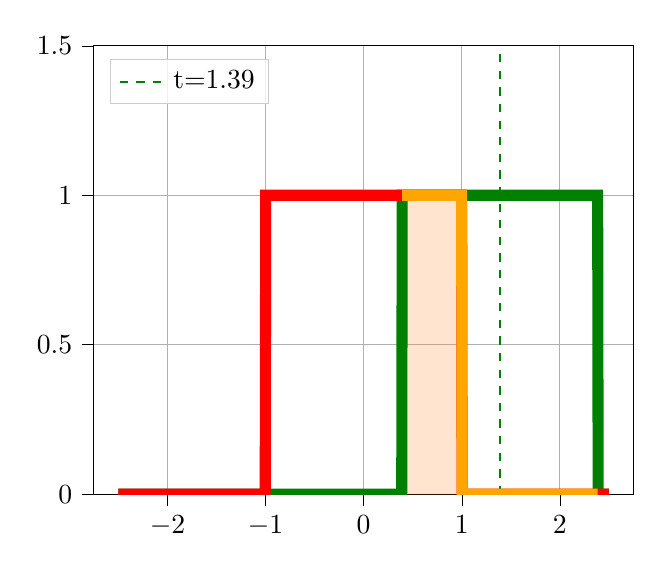
\begin{tikzpicture}

\definecolor{color0}{rgb}{1,0.498039215686275,0.0549019607843137}
\definecolor{color1}{rgb}{1,0.647058823529412,0}

\begin{axis}[
legend cell align={left},
legend style={fill opacity=0.8, draw opacity=1, text opacity=1, at={(0.03,0.97)}, anchor=north west, draw=white!80!black},
tick align=outside,
tick pos=left,
x grid style={white!69.0196078431373!black},
xmajorgrids,
xmin=-2.75, xmax=2.75,
xtick style={color=black},
y grid style={white!69.0196078431373!black},
ymajorgrids,
ymin=0, ymax=1.5,
ytick style={color=black}
]
\path [draw=color0, fill=color0, opacity=0.2]
(axis cs:0.392892892892893,1)
--(axis cs:0.392892892892893,0)
--(axis cs:0.397897897897898,0)
--(axis cs:0.402902902902903,0)
--(axis cs:0.407907907907908,0)
--(axis cs:0.412912912912913,0)
--(axis cs:0.417917917917918,0)
--(axis cs:0.422922922922923,0)
--(axis cs:0.427927927927928,0)
--(axis cs:0.432932932932933,0)
--(axis cs:0.437937937937938,0)
--(axis cs:0.442942942942943,0)
--(axis cs:0.447947947947948,0)
--(axis cs:0.452952952952953,0)
--(axis cs:0.457957957957958,0)
--(axis cs:0.462962962962963,0)
--(axis cs:0.467967967967968,0)
--(axis cs:0.472972972972973,0)
--(axis cs:0.477977977977978,0)
--(axis cs:0.482982982982983,0)
--(axis cs:0.487987987987988,0)
--(axis cs:0.492992992992993,0)
--(axis cs:0.497997997997998,0)
--(axis cs:0.503003003003003,0)
--(axis cs:0.508008008008008,0)
--(axis cs:0.513013013013013,0)
--(axis cs:0.518018018018018,0)
--(axis cs:0.523023023023023,0)
--(axis cs:0.528028028028028,0)
--(axis cs:0.533033033033033,0)
--(axis cs:0.538038038038038,0)
--(axis cs:0.543043043043043,0)
--(axis cs:0.548048048048048,0)
--(axis cs:0.553053053053053,0)
--(axis cs:0.558058058058058,0)
--(axis cs:0.563063063063063,0)
--(axis cs:0.568068068068068,0)
--(axis cs:0.573073073073073,0)
--(axis cs:0.578078078078078,0)
--(axis cs:0.583083083083083,0)
--(axis cs:0.588088088088088,0)
--(axis cs:0.593093093093093,0)
--(axis cs:0.598098098098098,0)
--(axis cs:0.603103103103103,0)
--(axis cs:0.608108108108108,0)
--(axis cs:0.613113113113113,0)
--(axis cs:0.618118118118118,0)
--(axis cs:0.623123123123123,0)
--(axis cs:0.628128128128128,0)
--(axis cs:0.633133133133133,0)
--(axis cs:0.638138138138138,0)
--(axis cs:0.643143143143143,0)
--(axis cs:0.648148148148148,0)
--(axis cs:0.653153153153153,0)
--(axis cs:0.658158158158158,0)
--(axis cs:0.663163163163163,0)
--(axis cs:0.668168168168168,0)
--(axis cs:0.673173173173173,0)
--(axis cs:0.678178178178178,0)
--(axis cs:0.683183183183183,0)
--(axis cs:0.688188188188188,0)
--(axis cs:0.693193193193193,0)
--(axis cs:0.698198198198198,0)
--(axis cs:0.703203203203203,0)
--(axis cs:0.708208208208208,0)
--(axis cs:0.713213213213213,0)
--(axis cs:0.718218218218218,0)
--(axis cs:0.723223223223223,0)
--(axis cs:0.728228228228228,0)
--(axis cs:0.733233233233233,0)
--(axis cs:0.738238238238238,0)
--(axis cs:0.743243243243243,0)
--(axis cs:0.748248248248248,0)
--(axis cs:0.753253253253253,0)
--(axis cs:0.758258258258258,0)
--(axis cs:0.763263263263263,0)
--(axis cs:0.768268268268268,0)
--(axis cs:0.773273273273273,0)
--(axis cs:0.778278278278278,0)
--(axis cs:0.783283283283283,0)
--(axis cs:0.788288288288288,0)
--(axis cs:0.793293293293293,0)
--(axis cs:0.798298298298298,0)
--(axis cs:0.803303303303303,0)
--(axis cs:0.808308308308308,0)
--(axis cs:0.813313313313313,0)
--(axis cs:0.818318318318318,0)
--(axis cs:0.823323323323323,0)
--(axis cs:0.828328328328328,0)
--(axis cs:0.833333333333333,0)
--(axis cs:0.838338338338338,0)
--(axis cs:0.843343343343343,0)
--(axis cs:0.848348348348348,0)
--(axis cs:0.853353353353353,0)
--(axis cs:0.858358358358358,0)
--(axis cs:0.863363363363364,0)
--(axis cs:0.868368368368369,0)
--(axis cs:0.873373373373374,0)
--(axis cs:0.878378378378379,0)
--(axis cs:0.883383383383384,0)
--(axis cs:0.888388388388389,0)
--(axis cs:0.893393393393394,0)
--(axis cs:0.898398398398399,0)
--(axis cs:0.903403403403404,0)
--(axis cs:0.908408408408409,0)
--(axis cs:0.913413413413414,0)
--(axis cs:0.918418418418419,0)
--(axis cs:0.923423423423424,0)
--(axis cs:0.928428428428429,0)
--(axis cs:0.933433433433434,0)
--(axis cs:0.938438438438439,0)
--(axis cs:0.943443443443444,0)
--(axis cs:0.948448448448449,0)
--(axis cs:0.953453453453454,0)
--(axis cs:0.958458458458459,0)
--(axis cs:0.963463463463464,0)
--(axis cs:0.968468468468469,0)
--(axis cs:0.973473473473474,0)
--(axis cs:0.978478478478479,0)
--(axis cs:0.983483483483484,0)
--(axis cs:0.988488488488489,0)
--(axis cs:0.993493493493494,0)
--(axis cs:0.998498498498499,0)
--(axis cs:1.0035035035035,0)
--(axis cs:1.00850850850851,0)
--(axis cs:1.01351351351351,0)
--(axis cs:1.01851851851852,0)
--(axis cs:1.02352352352352,0)
--(axis cs:1.02852852852853,0)
--(axis cs:1.03353353353353,0)
--(axis cs:1.03853853853854,0)
--(axis cs:1.04354354354354,0)
--(axis cs:1.04854854854855,0)
--(axis cs:1.05355355355355,0)
--(axis cs:1.05855855855856,0)
--(axis cs:1.06356356356356,0)
--(axis cs:1.06856856856857,0)
--(axis cs:1.07357357357357,0)
--(axis cs:1.07857857857858,0)
--(axis cs:1.08358358358358,0)
--(axis cs:1.08858858858859,0)
--(axis cs:1.09359359359359,0)
--(axis cs:1.0985985985986,0)
--(axis cs:1.1036036036036,0)
--(axis cs:1.10860860860861,0)
--(axis cs:1.11361361361361,0)
--(axis cs:1.11861861861862,0)
--(axis cs:1.12362362362362,0)
--(axis cs:1.12862862862863,0)
--(axis cs:1.13363363363363,0)
--(axis cs:1.13863863863864,0)
--(axis cs:1.14364364364364,0)
--(axis cs:1.14864864864865,0)
--(axis cs:1.15365365365365,0)
--(axis cs:1.15865865865866,0)
--(axis cs:1.16366366366366,0)
--(axis cs:1.16866866866867,0)
--(axis cs:1.17367367367367,0)
--(axis cs:1.17867867867868,0)
--(axis cs:1.18368368368368,0)
--(axis cs:1.18868868868869,0)
--(axis cs:1.19369369369369,0)
--(axis cs:1.1986986986987,0)
--(axis cs:1.2037037037037,0)
--(axis cs:1.20870870870871,0)
--(axis cs:1.21371371371371,0)
--(axis cs:1.21871871871872,0)
--(axis cs:1.22372372372372,0)
--(axis cs:1.22872872872873,0)
--(axis cs:1.23373373373373,0)
--(axis cs:1.23873873873874,0)
--(axis cs:1.24374374374374,0)
--(axis cs:1.24874874874875,0)
--(axis cs:1.25375375375375,0)
--(axis cs:1.25875875875876,0)
--(axis cs:1.26376376376376,0)
--(axis cs:1.26876876876877,0)
--(axis cs:1.27377377377377,0)
--(axis cs:1.27877877877878,0)
--(axis cs:1.28378378378378,0)
--(axis cs:1.28878878878879,0)
--(axis cs:1.29379379379379,0)
--(axis cs:1.2987987987988,0)
--(axis cs:1.3038038038038,0)
--(axis cs:1.30880880880881,0)
--(axis cs:1.31381381381381,0)
--(axis cs:1.31881881881882,0)
--(axis cs:1.32382382382382,0)
--(axis cs:1.32882882882883,0)
--(axis cs:1.33383383383383,0)
--(axis cs:1.33883883883884,0)
--(axis cs:1.34384384384384,0)
--(axis cs:1.34884884884885,0)
--(axis cs:1.35385385385385,0)
--(axis cs:1.35885885885886,0)
--(axis cs:1.36386386386386,0)
--(axis cs:1.36886886886887,0)
--(axis cs:1.37387387387387,0)
--(axis cs:1.37887887887888,0)
--(axis cs:1.38388388388388,0)
--(axis cs:1.38888888888889,0)
--(axis cs:1.39389389389389,0)
--(axis cs:1.3988988988989,0)
--(axis cs:1.4039039039039,0)
--(axis cs:1.40890890890891,0)
--(axis cs:1.41391391391391,0)
--(axis cs:1.41891891891892,0)
--(axis cs:1.42392392392392,0)
--(axis cs:1.42892892892893,0)
--(axis cs:1.43393393393393,0)
--(axis cs:1.43893893893894,0)
--(axis cs:1.44394394394394,0)
--(axis cs:1.44894894894895,0)
--(axis cs:1.45395395395395,0)
--(axis cs:1.45895895895896,0)
--(axis cs:1.46396396396396,0)
--(axis cs:1.46896896896897,0)
--(axis cs:1.47397397397397,0)
--(axis cs:1.47897897897898,0)
--(axis cs:1.48398398398398,0)
--(axis cs:1.48898898898899,0)
--(axis cs:1.49399399399399,0)
--(axis cs:1.498998998999,0)
--(axis cs:1.504004004004,0)
--(axis cs:1.50900900900901,0)
--(axis cs:1.51401401401401,0)
--(axis cs:1.51901901901902,0)
--(axis cs:1.52402402402402,0)
--(axis cs:1.52902902902903,0)
--(axis cs:1.53403403403403,0)
--(axis cs:1.53903903903904,0)
--(axis cs:1.54404404404404,0)
--(axis cs:1.54904904904905,0)
--(axis cs:1.55405405405405,0)
--(axis cs:1.55905905905906,0)
--(axis cs:1.56406406406406,0)
--(axis cs:1.56906906906907,0)
--(axis cs:1.57407407407407,0)
--(axis cs:1.57907907907908,0)
--(axis cs:1.58408408408408,0)
--(axis cs:1.58908908908909,0)
--(axis cs:1.59409409409409,0)
--(axis cs:1.5990990990991,0)
--(axis cs:1.6041041041041,0)
--(axis cs:1.60910910910911,0)
--(axis cs:1.61411411411411,0)
--(axis cs:1.61911911911912,0)
--(axis cs:1.62412412412412,0)
--(axis cs:1.62912912912913,0)
--(axis cs:1.63413413413413,0)
--(axis cs:1.63913913913914,0)
--(axis cs:1.64414414414414,0)
--(axis cs:1.64914914914915,0)
--(axis cs:1.65415415415415,0)
--(axis cs:1.65915915915916,0)
--(axis cs:1.66416416416416,0)
--(axis cs:1.66916916916917,0)
--(axis cs:1.67417417417417,0)
--(axis cs:1.67917917917918,0)
--(axis cs:1.68418418418418,0)
--(axis cs:1.68918918918919,0)
--(axis cs:1.69419419419419,0)
--(axis cs:1.6991991991992,0)
--(axis cs:1.7042042042042,0)
--(axis cs:1.70920920920921,0)
--(axis cs:1.71421421421421,0)
--(axis cs:1.71921921921922,0)
--(axis cs:1.72422422422422,0)
--(axis cs:1.72922922922923,0)
--(axis cs:1.73423423423423,0)
--(axis cs:1.73923923923924,0)
--(axis cs:1.74424424424424,0)
--(axis cs:1.74924924924925,0)
--(axis cs:1.75425425425425,0)
--(axis cs:1.75925925925926,0)
--(axis cs:1.76426426426426,0)
--(axis cs:1.76926926926927,0)
--(axis cs:1.77427427427427,0)
--(axis cs:1.77927927927928,0)
--(axis cs:1.78428428428428,0)
--(axis cs:1.78928928928929,0)
--(axis cs:1.79429429429429,0)
--(axis cs:1.7992992992993,0)
--(axis cs:1.8043043043043,0)
--(axis cs:1.80930930930931,0)
--(axis cs:1.81431431431431,0)
--(axis cs:1.81931931931932,0)
--(axis cs:1.82432432432432,0)
--(axis cs:1.82932932932933,0)
--(axis cs:1.83433433433433,0)
--(axis cs:1.83933933933934,0)
--(axis cs:1.84434434434434,0)
--(axis cs:1.84934934934935,0)
--(axis cs:1.85435435435435,0)
--(axis cs:1.85935935935936,0)
--(axis cs:1.86436436436436,0)
--(axis cs:1.86936936936937,0)
--(axis cs:1.87437437437437,0)
--(axis cs:1.87937937937938,0)
--(axis cs:1.88438438438438,0)
--(axis cs:1.88938938938939,0)
--(axis cs:1.89439439439439,0)
--(axis cs:1.8993993993994,0)
--(axis cs:1.9044044044044,0)
--(axis cs:1.90940940940941,0)
--(axis cs:1.91441441441441,0)
--(axis cs:1.91941941941942,0)
--(axis cs:1.92442442442442,0)
--(axis cs:1.92942942942943,0)
--(axis cs:1.93443443443443,0)
--(axis cs:1.93943943943944,0)
--(axis cs:1.94444444444444,0)
--(axis cs:1.94944944944945,0)
--(axis cs:1.95445445445445,0)
--(axis cs:1.95945945945946,0)
--(axis cs:1.96446446446446,0)
--(axis cs:1.96946946946947,0)
--(axis cs:1.97447447447447,0)
--(axis cs:1.97947947947948,0)
--(axis cs:1.98448448448448,0)
--(axis cs:1.98948948948949,0)
--(axis cs:1.99449449449449,0)
--(axis cs:1.9994994994995,0)
--(axis cs:2.0045045045045,0)
--(axis cs:2.00950950950951,0)
--(axis cs:2.01451451451451,0)
--(axis cs:2.01951951951952,0)
--(axis cs:2.02452452452452,0)
--(axis cs:2.02952952952953,0)
--(axis cs:2.03453453453453,0)
--(axis cs:2.03953953953954,0)
--(axis cs:2.04454454454454,0)
--(axis cs:2.04954954954955,0)
--(axis cs:2.05455455455455,0)
--(axis cs:2.05955955955956,0)
--(axis cs:2.06456456456456,0)
--(axis cs:2.06956956956957,0)
--(axis cs:2.07457457457457,0)
--(axis cs:2.07957957957958,0)
--(axis cs:2.08458458458458,0)
--(axis cs:2.08958958958959,0)
--(axis cs:2.09459459459459,0)
--(axis cs:2.0995995995996,0)
--(axis cs:2.1046046046046,0)
--(axis cs:2.10960960960961,0)
--(axis cs:2.11461461461461,0)
--(axis cs:2.11961961961962,0)
--(axis cs:2.12462462462462,0)
--(axis cs:2.12962962962963,0)
--(axis cs:2.13463463463463,0)
--(axis cs:2.13963963963964,0)
--(axis cs:2.14464464464464,0)
--(axis cs:2.14964964964965,0)
--(axis cs:2.15465465465465,0)
--(axis cs:2.15965965965966,0)
--(axis cs:2.16466466466466,0)
--(axis cs:2.16966966966967,0)
--(axis cs:2.17467467467467,0)
--(axis cs:2.17967967967968,0)
--(axis cs:2.18468468468468,0)
--(axis cs:2.18968968968969,0)
--(axis cs:2.19469469469469,0)
--(axis cs:2.1996996996997,0)
--(axis cs:2.2047047047047,0)
--(axis cs:2.20970970970971,0)
--(axis cs:2.21471471471471,0)
--(axis cs:2.21971971971972,0)
--(axis cs:2.22472472472472,0)
--(axis cs:2.22972972972973,0)
--(axis cs:2.23473473473473,0)
--(axis cs:2.23973973973974,0)
--(axis cs:2.24474474474474,0)
--(axis cs:2.24974974974975,0)
--(axis cs:2.25475475475475,0)
--(axis cs:2.25975975975976,0)
--(axis cs:2.26476476476476,0)
--(axis cs:2.26976976976977,0)
--(axis cs:2.27477477477477,0)
--(axis cs:2.27977977977978,0)
--(axis cs:2.28478478478478,0)
--(axis cs:2.28978978978979,0)
--(axis cs:2.29479479479479,0)
--(axis cs:2.2997997997998,0)
--(axis cs:2.3048048048048,0)
--(axis cs:2.30980980980981,0)
--(axis cs:2.31481481481481,0)
--(axis cs:2.31981981981982,0)
--(axis cs:2.32482482482482,0)
--(axis cs:2.32982982982983,0)
--(axis cs:2.33483483483483,0)
--(axis cs:2.33983983983984,0)
--(axis cs:2.34484484484484,0)
--(axis cs:2.34984984984985,0)
--(axis cs:2.35485485485485,0)
--(axis cs:2.35985985985986,0)
--(axis cs:2.36486486486486,0)
--(axis cs:2.36986986986987,0)
--(axis cs:2.37487487487487,0)
--(axis cs:2.37987987987988,0)
--(axis cs:2.38488488488488,0)
--(axis cs:2.38488488488488,0)
--(axis cs:2.38488488488488,0)
--(axis cs:2.37987987987988,0)
--(axis cs:2.37487487487487,0)
--(axis cs:2.36986986986987,0)
--(axis cs:2.36486486486486,0)
--(axis cs:2.35985985985986,0)
--(axis cs:2.35485485485485,0)
--(axis cs:2.34984984984985,0)
--(axis cs:2.34484484484484,0)
--(axis cs:2.33983983983984,0)
--(axis cs:2.33483483483483,0)
--(axis cs:2.32982982982983,0)
--(axis cs:2.32482482482482,0)
--(axis cs:2.31981981981982,0)
--(axis cs:2.31481481481481,0)
--(axis cs:2.30980980980981,0)
--(axis cs:2.3048048048048,0)
--(axis cs:2.2997997997998,0)
--(axis cs:2.29479479479479,0)
--(axis cs:2.28978978978979,0)
--(axis cs:2.28478478478478,0)
--(axis cs:2.27977977977978,0)
--(axis cs:2.27477477477477,0)
--(axis cs:2.26976976976977,0)
--(axis cs:2.26476476476476,0)
--(axis cs:2.25975975975976,0)
--(axis cs:2.25475475475475,0)
--(axis cs:2.24974974974975,0)
--(axis cs:2.24474474474474,0)
--(axis cs:2.23973973973974,0)
--(axis cs:2.23473473473473,0)
--(axis cs:2.22972972972973,0)
--(axis cs:2.22472472472472,0)
--(axis cs:2.21971971971972,0)
--(axis cs:2.21471471471471,0)
--(axis cs:2.20970970970971,0)
--(axis cs:2.2047047047047,0)
--(axis cs:2.1996996996997,0)
--(axis cs:2.19469469469469,0)
--(axis cs:2.18968968968969,0)
--(axis cs:2.18468468468468,0)
--(axis cs:2.17967967967968,0)
--(axis cs:2.17467467467467,0)
--(axis cs:2.16966966966967,0)
--(axis cs:2.16466466466466,0)
--(axis cs:2.15965965965966,0)
--(axis cs:2.15465465465465,0)
--(axis cs:2.14964964964965,0)
--(axis cs:2.14464464464464,0)
--(axis cs:2.13963963963964,0)
--(axis cs:2.13463463463463,0)
--(axis cs:2.12962962962963,0)
--(axis cs:2.12462462462462,0)
--(axis cs:2.11961961961962,0)
--(axis cs:2.11461461461461,0)
--(axis cs:2.10960960960961,0)
--(axis cs:2.1046046046046,0)
--(axis cs:2.0995995995996,0)
--(axis cs:2.09459459459459,0)
--(axis cs:2.08958958958959,0)
--(axis cs:2.08458458458458,0)
--(axis cs:2.07957957957958,0)
--(axis cs:2.07457457457457,0)
--(axis cs:2.06956956956957,0)
--(axis cs:2.06456456456456,0)
--(axis cs:2.05955955955956,0)
--(axis cs:2.05455455455455,0)
--(axis cs:2.04954954954955,0)
--(axis cs:2.04454454454454,0)
--(axis cs:2.03953953953954,0)
--(axis cs:2.03453453453453,0)
--(axis cs:2.02952952952953,0)
--(axis cs:2.02452452452452,0)
--(axis cs:2.01951951951952,0)
--(axis cs:2.01451451451451,0)
--(axis cs:2.00950950950951,0)
--(axis cs:2.0045045045045,0)
--(axis cs:1.9994994994995,0)
--(axis cs:1.99449449449449,0)
--(axis cs:1.98948948948949,0)
--(axis cs:1.98448448448448,0)
--(axis cs:1.97947947947948,0)
--(axis cs:1.97447447447447,0)
--(axis cs:1.96946946946947,0)
--(axis cs:1.96446446446446,0)
--(axis cs:1.95945945945946,0)
--(axis cs:1.95445445445445,0)
--(axis cs:1.94944944944945,0)
--(axis cs:1.94444444444444,0)
--(axis cs:1.93943943943944,0)
--(axis cs:1.93443443443443,0)
--(axis cs:1.92942942942943,0)
--(axis cs:1.92442442442442,0)
--(axis cs:1.91941941941942,0)
--(axis cs:1.91441441441441,0)
--(axis cs:1.90940940940941,0)
--(axis cs:1.9044044044044,0)
--(axis cs:1.8993993993994,0)
--(axis cs:1.89439439439439,0)
--(axis cs:1.88938938938939,0)
--(axis cs:1.88438438438438,0)
--(axis cs:1.87937937937938,0)
--(axis cs:1.87437437437437,0)
--(axis cs:1.86936936936937,0)
--(axis cs:1.86436436436436,0)
--(axis cs:1.85935935935936,0)
--(axis cs:1.85435435435435,0)
--(axis cs:1.84934934934935,0)
--(axis cs:1.84434434434434,0)
--(axis cs:1.83933933933934,0)
--(axis cs:1.83433433433433,0)
--(axis cs:1.82932932932933,0)
--(axis cs:1.82432432432432,0)
--(axis cs:1.81931931931932,0)
--(axis cs:1.81431431431431,0)
--(axis cs:1.80930930930931,0)
--(axis cs:1.8043043043043,0)
--(axis cs:1.7992992992993,0)
--(axis cs:1.79429429429429,0)
--(axis cs:1.78928928928929,0)
--(axis cs:1.78428428428428,0)
--(axis cs:1.77927927927928,0)
--(axis cs:1.77427427427427,0)
--(axis cs:1.76926926926927,0)
--(axis cs:1.76426426426426,0)
--(axis cs:1.75925925925926,0)
--(axis cs:1.75425425425425,0)
--(axis cs:1.74924924924925,0)
--(axis cs:1.74424424424424,0)
--(axis cs:1.73923923923924,0)
--(axis cs:1.73423423423423,0)
--(axis cs:1.72922922922923,0)
--(axis cs:1.72422422422422,0)
--(axis cs:1.71921921921922,0)
--(axis cs:1.71421421421421,0)
--(axis cs:1.70920920920921,0)
--(axis cs:1.7042042042042,0)
--(axis cs:1.6991991991992,0)
--(axis cs:1.69419419419419,0)
--(axis cs:1.68918918918919,0)
--(axis cs:1.68418418418418,0)
--(axis cs:1.67917917917918,0)
--(axis cs:1.67417417417417,0)
--(axis cs:1.66916916916917,0)
--(axis cs:1.66416416416416,0)
--(axis cs:1.65915915915916,0)
--(axis cs:1.65415415415415,0)
--(axis cs:1.64914914914915,0)
--(axis cs:1.64414414414414,0)
--(axis cs:1.63913913913914,0)
--(axis cs:1.63413413413413,0)
--(axis cs:1.62912912912913,0)
--(axis cs:1.62412412412412,0)
--(axis cs:1.61911911911912,0)
--(axis cs:1.61411411411411,0)
--(axis cs:1.60910910910911,0)
--(axis cs:1.6041041041041,0)
--(axis cs:1.5990990990991,0)
--(axis cs:1.59409409409409,0)
--(axis cs:1.58908908908909,0)
--(axis cs:1.58408408408408,0)
--(axis cs:1.57907907907908,0)
--(axis cs:1.57407407407407,0)
--(axis cs:1.56906906906907,0)
--(axis cs:1.56406406406406,0)
--(axis cs:1.55905905905906,0)
--(axis cs:1.55405405405405,0)
--(axis cs:1.54904904904905,0)
--(axis cs:1.54404404404404,0)
--(axis cs:1.53903903903904,0)
--(axis cs:1.53403403403403,0)
--(axis cs:1.52902902902903,0)
--(axis cs:1.52402402402402,0)
--(axis cs:1.51901901901902,0)
--(axis cs:1.51401401401401,0)
--(axis cs:1.50900900900901,0)
--(axis cs:1.504004004004,0)
--(axis cs:1.498998998999,0)
--(axis cs:1.49399399399399,0)
--(axis cs:1.48898898898899,0)
--(axis cs:1.48398398398398,0)
--(axis cs:1.47897897897898,0)
--(axis cs:1.47397397397397,0)
--(axis cs:1.46896896896897,0)
--(axis cs:1.46396396396396,0)
--(axis cs:1.45895895895896,0)
--(axis cs:1.45395395395395,0)
--(axis cs:1.44894894894895,0)
--(axis cs:1.44394394394394,0)
--(axis cs:1.43893893893894,0)
--(axis cs:1.43393393393393,0)
--(axis cs:1.42892892892893,0)
--(axis cs:1.42392392392392,0)
--(axis cs:1.41891891891892,0)
--(axis cs:1.41391391391391,0)
--(axis cs:1.40890890890891,0)
--(axis cs:1.4039039039039,0)
--(axis cs:1.3988988988989,0)
--(axis cs:1.39389389389389,0)
--(axis cs:1.38888888888889,0)
--(axis cs:1.38388388388388,0)
--(axis cs:1.37887887887888,0)
--(axis cs:1.37387387387387,0)
--(axis cs:1.36886886886887,0)
--(axis cs:1.36386386386386,0)
--(axis cs:1.35885885885886,0)
--(axis cs:1.35385385385385,0)
--(axis cs:1.34884884884885,0)
--(axis cs:1.34384384384384,0)
--(axis cs:1.33883883883884,0)
--(axis cs:1.33383383383383,0)
--(axis cs:1.32882882882883,0)
--(axis cs:1.32382382382382,0)
--(axis cs:1.31881881881882,0)
--(axis cs:1.31381381381381,0)
--(axis cs:1.30880880880881,0)
--(axis cs:1.3038038038038,0)
--(axis cs:1.2987987987988,0)
--(axis cs:1.29379379379379,0)
--(axis cs:1.28878878878879,0)
--(axis cs:1.28378378378378,0)
--(axis cs:1.27877877877878,0)
--(axis cs:1.27377377377377,0)
--(axis cs:1.26876876876877,0)
--(axis cs:1.26376376376376,0)
--(axis cs:1.25875875875876,0)
--(axis cs:1.25375375375375,0)
--(axis cs:1.24874874874875,0)
--(axis cs:1.24374374374374,0)
--(axis cs:1.23873873873874,0)
--(axis cs:1.23373373373373,0)
--(axis cs:1.22872872872873,0)
--(axis cs:1.22372372372372,0)
--(axis cs:1.21871871871872,0)
--(axis cs:1.21371371371371,0)
--(axis cs:1.20870870870871,0)
--(axis cs:1.2037037037037,0)
--(axis cs:1.1986986986987,0)
--(axis cs:1.19369369369369,0)
--(axis cs:1.18868868868869,0)
--(axis cs:1.18368368368368,0)
--(axis cs:1.17867867867868,0)
--(axis cs:1.17367367367367,0)
--(axis cs:1.16866866866867,0)
--(axis cs:1.16366366366366,0)
--(axis cs:1.15865865865866,0)
--(axis cs:1.15365365365365,0)
--(axis cs:1.14864864864865,0)
--(axis cs:1.14364364364364,0)
--(axis cs:1.13863863863864,0)
--(axis cs:1.13363363363363,0)
--(axis cs:1.12862862862863,0)
--(axis cs:1.12362362362362,0)
--(axis cs:1.11861861861862,0)
--(axis cs:1.11361361361361,0)
--(axis cs:1.10860860860861,0)
--(axis cs:1.1036036036036,0)
--(axis cs:1.0985985985986,0)
--(axis cs:1.09359359359359,0)
--(axis cs:1.08858858858859,0)
--(axis cs:1.08358358358358,0)
--(axis cs:1.07857857857858,0)
--(axis cs:1.07357357357357,0)
--(axis cs:1.06856856856857,0)
--(axis cs:1.06356356356356,0)
--(axis cs:1.05855855855856,0)
--(axis cs:1.05355355355355,0)
--(axis cs:1.04854854854855,0)
--(axis cs:1.04354354354354,0)
--(axis cs:1.03853853853854,0)
--(axis cs:1.03353353353353,0)
--(axis cs:1.02852852852853,0)
--(axis cs:1.02352352352352,0)
--(axis cs:1.01851851851852,0)
--(axis cs:1.01351351351351,0)
--(axis cs:1.00850850850851,0)
--(axis cs:1.0035035035035,0)
--(axis cs:0.998498498498499,1)
--(axis cs:0.993493493493494,1)
--(axis cs:0.988488488488489,1)
--(axis cs:0.983483483483484,1)
--(axis cs:0.978478478478479,1)
--(axis cs:0.973473473473474,1)
--(axis cs:0.968468468468469,1)
--(axis cs:0.963463463463464,1)
--(axis cs:0.958458458458459,1)
--(axis cs:0.953453453453454,1)
--(axis cs:0.948448448448449,1)
--(axis cs:0.943443443443444,1)
--(axis cs:0.938438438438439,1)
--(axis cs:0.933433433433434,1)
--(axis cs:0.928428428428429,1)
--(axis cs:0.923423423423424,1)
--(axis cs:0.918418418418419,1)
--(axis cs:0.913413413413414,1)
--(axis cs:0.908408408408409,1)
--(axis cs:0.903403403403404,1)
--(axis cs:0.898398398398399,1)
--(axis cs:0.893393393393394,1)
--(axis cs:0.888388388388389,1)
--(axis cs:0.883383383383384,1)
--(axis cs:0.878378378378379,1)
--(axis cs:0.873373373373374,1)
--(axis cs:0.868368368368369,1)
--(axis cs:0.863363363363364,1)
--(axis cs:0.858358358358358,1)
--(axis cs:0.853353353353353,1)
--(axis cs:0.848348348348348,1)
--(axis cs:0.843343343343343,1)
--(axis cs:0.838338338338338,1)
--(axis cs:0.833333333333333,1)
--(axis cs:0.828328328328328,1)
--(axis cs:0.823323323323323,1)
--(axis cs:0.818318318318318,1)
--(axis cs:0.813313313313313,1)
--(axis cs:0.808308308308308,1)
--(axis cs:0.803303303303303,1)
--(axis cs:0.798298298298298,1)
--(axis cs:0.793293293293293,1)
--(axis cs:0.788288288288288,1)
--(axis cs:0.783283283283283,1)
--(axis cs:0.778278278278278,1)
--(axis cs:0.773273273273273,1)
--(axis cs:0.768268268268268,1)
--(axis cs:0.763263263263263,1)
--(axis cs:0.758258258258258,1)
--(axis cs:0.753253253253253,1)
--(axis cs:0.748248248248248,1)
--(axis cs:0.743243243243243,1)
--(axis cs:0.738238238238238,1)
--(axis cs:0.733233233233233,1)
--(axis cs:0.728228228228228,1)
--(axis cs:0.723223223223223,1)
--(axis cs:0.718218218218218,1)
--(axis cs:0.713213213213213,1)
--(axis cs:0.708208208208208,1)
--(axis cs:0.703203203203203,1)
--(axis cs:0.698198198198198,1)
--(axis cs:0.693193193193193,1)
--(axis cs:0.688188188188188,1)
--(axis cs:0.683183183183183,1)
--(axis cs:0.678178178178178,1)
--(axis cs:0.673173173173173,1)
--(axis cs:0.668168168168168,1)
--(axis cs:0.663163163163163,1)
--(axis cs:0.658158158158158,1)
--(axis cs:0.653153153153153,1)
--(axis cs:0.648148148148148,1)
--(axis cs:0.643143143143143,1)
--(axis cs:0.638138138138138,1)
--(axis cs:0.633133133133133,1)
--(axis cs:0.628128128128128,1)
--(axis cs:0.623123123123123,1)
--(axis cs:0.618118118118118,1)
--(axis cs:0.613113113113113,1)
--(axis cs:0.608108108108108,1)
--(axis cs:0.603103103103103,1)
--(axis cs:0.598098098098098,1)
--(axis cs:0.593093093093093,1)
--(axis cs:0.588088088088088,1)
--(axis cs:0.583083083083083,1)
--(axis cs:0.578078078078078,1)
--(axis cs:0.573073073073073,1)
--(axis cs:0.568068068068068,1)
--(axis cs:0.563063063063063,1)
--(axis cs:0.558058058058058,1)
--(axis cs:0.553053053053053,1)
--(axis cs:0.548048048048048,1)
--(axis cs:0.543043043043043,1)
--(axis cs:0.538038038038038,1)
--(axis cs:0.533033033033033,1)
--(axis cs:0.528028028028028,1)
--(axis cs:0.523023023023023,1)
--(axis cs:0.518018018018018,1)
--(axis cs:0.513013013013013,1)
--(axis cs:0.508008008008008,1)
--(axis cs:0.503003003003003,1)
--(axis cs:0.497997997997998,1)
--(axis cs:0.492992992992993,1)
--(axis cs:0.487987987987988,1)
--(axis cs:0.482982982982983,1)
--(axis cs:0.477977977977978,1)
--(axis cs:0.472972972972973,1)
--(axis cs:0.467967967967968,1)
--(axis cs:0.462962962962963,1)
--(axis cs:0.457957957957958,1)
--(axis cs:0.452952952952953,1)
--(axis cs:0.447947947947948,1)
--(axis cs:0.442942942942943,1)
--(axis cs:0.437937937937938,1)
--(axis cs:0.432932932932933,1)
--(axis cs:0.427927927927928,1)
--(axis cs:0.422922922922923,1)
--(axis cs:0.417917917917918,1)
--(axis cs:0.412912912912913,1)
--(axis cs:0.407907907907908,1)
--(axis cs:0.402902902902903,1)
--(axis cs:0.397897897897898,1)
--(axis cs:0.392892892892893,1)
--cycle;

\addplot [line width=4pt, green!50!black, forget plot]
table {%
-2.5 0
-2.49499499499499 0
-2.48998998998999 0
-2.48498498498498 0
-2.47997997997998 0
-2.47497497497497 0
-2.46996996996997 0
-2.46496496496496 0
-2.45995995995996 0
-2.45495495495495 0
-2.44994994994995 0
-2.44494494494494 0
-2.43993993993994 0
-2.43493493493493 0
-2.42992992992993 0
-2.42492492492492 0
-2.41991991991992 0
-2.41491491491491 0
-2.40990990990991 0
-2.4049049049049 0
-2.3998998998999 0
-2.39489489489489 0
-2.38988988988989 0
-2.38488488488488 0
-2.37987987987988 0
-2.37487487487487 0
-2.36986986986987 0
-2.36486486486486 0
-2.35985985985986 0
-2.35485485485485 0
-2.34984984984985 0
-2.34484484484484 0
-2.33983983983984 0
-2.33483483483483 0
-2.32982982982983 0
-2.32482482482482 0
-2.31981981981982 0
-2.31481481481481 0
-2.30980980980981 0
-2.3048048048048 0
-2.2997997997998 0
-2.29479479479479 0
-2.28978978978979 0
-2.28478478478478 0
-2.27977977977978 0
-2.27477477477477 0
-2.26976976976977 0
-2.26476476476476 0
-2.25975975975976 0
-2.25475475475475 0
-2.24974974974975 0
-2.24474474474474 0
-2.23973973973974 0
-2.23473473473473 0
-2.22972972972973 0
-2.22472472472472 0
-2.21971971971972 0
-2.21471471471471 0
-2.20970970970971 0
-2.2047047047047 0
-2.1996996996997 0
-2.19469469469469 0
-2.18968968968969 0
-2.18468468468468 0
-2.17967967967968 0
-2.17467467467467 0
-2.16966966966967 0
-2.16466466466466 0
-2.15965965965966 0
-2.15465465465465 0
-2.14964964964965 0
-2.14464464464464 0
-2.13963963963964 0
-2.13463463463463 0
-2.12962962962963 0
-2.12462462462462 0
-2.11961961961962 0
-2.11461461461461 0
-2.10960960960961 0
-2.1046046046046 0
-2.0995995995996 0
-2.09459459459459 0
-2.08958958958959 0
-2.08458458458458 0
-2.07957957957958 0
-2.07457457457457 0
-2.06956956956957 0
-2.06456456456456 0
-2.05955955955956 0
-2.05455455455455 0
-2.04954954954955 0
-2.04454454454454 0
-2.03953953953954 0
-2.03453453453453 0
-2.02952952952953 0
-2.02452452452452 0
-2.01951951951952 0
-2.01451451451451 0
-2.00950950950951 0
-2.0045045045045 0
-1.9994994994995 0
-1.99449449449449 0
-1.98948948948949 0
-1.98448448448448 0
-1.97947947947948 0
-1.97447447447447 0
-1.96946946946947 0
-1.96446446446446 0
-1.95945945945946 0
-1.95445445445445 0
-1.94944944944945 0
-1.94444444444444 0
-1.93943943943944 0
-1.93443443443443 0
-1.92942942942943 0
-1.92442442442442 0
-1.91941941941942 0
-1.91441441441441 0
-1.90940940940941 0
-1.9044044044044 0
-1.8993993993994 0
-1.89439439439439 0
-1.88938938938939 0
-1.88438438438438 0
-1.87937937937938 0
-1.87437437437437 0
-1.86936936936937 0
-1.86436436436436 0
-1.85935935935936 0
-1.85435435435435 0
-1.84934934934935 0
-1.84434434434434 0
-1.83933933933934 0
-1.83433433433433 0
-1.82932932932933 0
-1.82432432432432 0
-1.81931931931932 0
-1.81431431431431 0
-1.80930930930931 0
-1.8043043043043 0
-1.7992992992993 0
-1.79429429429429 0
-1.78928928928929 0
-1.78428428428428 0
-1.77927927927928 0
-1.77427427427427 0
-1.76926926926927 0
-1.76426426426426 0
-1.75925925925926 0
-1.75425425425425 0
-1.74924924924925 0
-1.74424424424424 0
-1.73923923923924 0
-1.73423423423423 0
-1.72922922922923 0
-1.72422422422422 0
-1.71921921921922 0
-1.71421421421421 0
-1.70920920920921 0
-1.7042042042042 0
-1.6991991991992 0
-1.69419419419419 0
-1.68918918918919 0
-1.68418418418418 0
-1.67917917917918 0
-1.67417417417417 0
-1.66916916916917 0
-1.66416416416416 0
-1.65915915915916 0
-1.65415415415415 0
-1.64914914914915 0
-1.64414414414414 0
-1.63913913913914 0
-1.63413413413413 0
-1.62912912912913 0
-1.62412412412412 0
-1.61911911911912 0
-1.61411411411411 0
-1.60910910910911 0
-1.6041041041041 0
-1.5990990990991 0
-1.59409409409409 0
-1.58908908908909 0
-1.58408408408408 0
-1.57907907907908 0
-1.57407407407407 0
-1.56906906906907 0
-1.56406406406406 0
-1.55905905905906 0
-1.55405405405405 0
-1.54904904904905 0
-1.54404404404404 0
-1.53903903903904 0
-1.53403403403403 0
-1.52902902902903 0
-1.52402402402402 0
-1.51901901901902 0
-1.51401401401401 0
-1.50900900900901 0
-1.504004004004 0
-1.498998998999 0
-1.49399399399399 0
-1.48898898898899 0
-1.48398398398398 0
-1.47897897897898 0
-1.47397397397397 0
-1.46896896896897 0
-1.46396396396396 0
-1.45895895895896 0
-1.45395395395395 0
-1.44894894894895 0
-1.44394394394394 0
-1.43893893893894 0
-1.43393393393393 0
-1.42892892892893 0
-1.42392392392392 0
-1.41891891891892 0
-1.41391391391391 0
-1.40890890890891 0
-1.4039039039039 0
-1.3988988988989 0
-1.39389389389389 0
-1.38888888888889 0
-1.38388388388388 0
-1.37887887887888 0
-1.37387387387387 0
-1.36886886886887 0
-1.36386386386386 0
-1.35885885885886 0
-1.35385385385385 0
-1.34884884884885 0
-1.34384384384384 0
-1.33883883883884 0
-1.33383383383383 0
-1.32882882882883 0
-1.32382382382382 0
-1.31881881881882 0
-1.31381381381381 0
-1.30880880880881 0
-1.3038038038038 0
-1.2987987987988 0
-1.29379379379379 0
-1.28878878878879 0
-1.28378378378378 0
-1.27877877877878 0
-1.27377377377377 0
-1.26876876876877 0
-1.26376376376376 0
-1.25875875875876 0
-1.25375375375375 0
-1.24874874874875 0
-1.24374374374374 0
-1.23873873873874 0
-1.23373373373373 0
-1.22872872872873 0
-1.22372372372372 0
-1.21871871871872 0
-1.21371371371371 0
-1.20870870870871 0
-1.2037037037037 0
-1.1986986986987 0
-1.19369369369369 0
-1.18868868868869 0
-1.18368368368368 0
-1.17867867867868 0
-1.17367367367367 0
-1.16866866866867 0
-1.16366366366366 0
-1.15865865865866 0
-1.15365365365365 0
-1.14864864864865 0
-1.14364364364364 0
-1.13863863863864 0
-1.13363363363363 0
-1.12862862862863 0
-1.12362362362362 0
-1.11861861861862 0
-1.11361361361361 0
-1.10860860860861 0
-1.1036036036036 0
-1.0985985985986 0
-1.09359359359359 0
-1.08858858858859 0
-1.08358358358358 0
-1.07857857857858 0
-1.07357357357357 0
-1.06856856856857 0
-1.06356356356356 0
-1.05855855855856 0
-1.05355355355355 0
-1.04854854854855 0
-1.04354354354354 0
-1.03853853853854 0
-1.03353353353353 0
-1.02852852852853 0
-1.02352352352352 0
-1.01851851851852 0
-1.01351351351351 0
-1.00850850850851 0
-1.0035035035035 0
-0.998498498498499 0
-0.993493493493494 0
-0.988488488488489 0
-0.983483483483484 0
-0.978478478478479 0
-0.973473473473474 0
-0.968468468468469 0
-0.963463463463464 0
-0.958458458458459 0
-0.953453453453454 0
-0.948448448448449 0
-0.943443443443444 0
-0.938438438438439 0
-0.933433433433434 0
-0.928428428428429 0
-0.923423423423424 0
-0.918418418418419 0
-0.913413413413414 0
-0.908408408408409 0
-0.903403403403404 0
-0.898398398398399 0
-0.893393393393393 0
-0.888388388388388 0
-0.883383383383383 0
-0.878378378378378 0
-0.873373373373373 0
-0.868368368368368 0
-0.863363363363363 0
-0.858358358358358 0
-0.853353353353353 0
-0.848348348348348 0
-0.843343343343343 0
-0.838338338338338 0
-0.833333333333333 0
-0.828328328328328 0
-0.823323323323323 0
-0.818318318318318 0
-0.813313313313313 0
-0.808308308308308 0
-0.803303303303303 0
-0.798298298298298 0
-0.793293293293293 0
-0.788288288288288 0
-0.783283283283283 0
-0.778278278278278 0
-0.773273273273273 0
-0.768268268268268 0
-0.763263263263263 0
-0.758258258258258 0
-0.753253253253253 0
-0.748248248248248 0
-0.743243243243243 0
-0.738238238238238 0
-0.733233233233233 0
-0.728228228228228 0
-0.723223223223223 0
-0.718218218218218 0
-0.713213213213213 0
-0.708208208208208 0
-0.703203203203203 0
-0.698198198198198 0
-0.693193193193193 0
-0.688188188188188 0
-0.683183183183183 0
-0.678178178178178 0
-0.673173173173173 0
-0.668168168168168 0
-0.663163163163163 0
-0.658158158158158 0
-0.653153153153153 0
-0.648148148148148 0
-0.643143143143143 0
-0.638138138138138 0
-0.633133133133133 0
-0.628128128128128 0
-0.623123123123123 0
-0.618118118118118 0
-0.613113113113113 0
-0.608108108108108 0
-0.603103103103103 0
-0.598098098098098 0
-0.593093093093093 0
-0.588088088088088 0
-0.583083083083083 0
-0.578078078078078 0
-0.573073073073073 0
-0.568068068068068 0
-0.563063063063063 0
-0.558058058058058 0
-0.553053053053053 0
-0.548048048048048 0
-0.543043043043043 0
-0.538038038038038 0
-0.533033033033033 0
-0.528028028028028 0
-0.523023023023023 0
-0.518018018018018 0
-0.513013013013013 0
-0.508008008008008 0
-0.503003003003003 0
-0.497997997997998 0
-0.492992992992993 0
-0.487987987987988 0
-0.482982982982983 0
-0.477977977977978 0
-0.472972972972973 0
-0.467967967967968 0
-0.462962962962963 0
-0.457957957957958 0
-0.452952952952953 0
-0.447947947947948 0
-0.442942942942943 0
-0.437937937937938 0
-0.432932932932933 0
-0.427927927927928 0
-0.422922922922923 0
-0.417917917917918 0
-0.412912912912913 0
-0.407907907907908 0
-0.402902902902903 0
-0.397897897897898 0
-0.392892892892893 0
-0.387887887887888 0
-0.382882882882883 0
-0.377877877877878 0
-0.372872872872873 0
-0.367867867867868 0
-0.362862862862863 0
-0.357857857857858 0
-0.352852852852853 0
-0.347847847847848 0
-0.342842842842843 0
-0.337837837837838 0
-0.332832832832833 0
-0.327827827827828 0
-0.322822822822823 0
-0.317817817817818 0
-0.312812812812813 0
-0.307807807807808 0
-0.302802802802803 0
-0.297797797797798 0
-0.292792792792793 0
-0.287787787787788 0
-0.282782782782783 0
-0.277777777777778 0
-0.272772772772773 0
-0.267767767767768 0
-0.262762762762763 0
-0.257757757757758 0
-0.252752752752753 0
-0.247747747747748 0
-0.242742742742743 0
-0.237737737737738 0
-0.232732732732733 0
-0.227727727727728 0
-0.222722722722723 0
-0.217717717717718 0
-0.212712712712713 0
-0.207707707707708 0
-0.202702702702703 0
-0.197697697697698 0
-0.192692692692693 0
-0.187687687687688 0
-0.182682682682683 0
-0.177677677677678 0
-0.172672672672673 0
-0.167667667667668 0
-0.162662662662663 0
-0.157657657657658 0
-0.152652652652653 0
-0.147647647647648 0
-0.142642642642643 0
-0.137637637637638 0
-0.132632632632633 0
-0.127627627627628 0
-0.122622622622623 0
-0.117617617617618 0
-0.112612612612613 0
-0.107607607607608 0
-0.102602602602603 0
-0.0975975975975976 0
-0.0925925925925926 0
-0.0875875875875876 0
-0.0825825825825826 0
-0.0775775775775776 0
-0.0725725725725725 0
-0.0675675675675675 0
-0.0625625625625625 0
-0.0575575575575575 0
-0.0525525525525525 0
-0.0475475475475475 0
-0.0425425425425425 0
-0.0375375375375375 0
-0.0325325325325325 0
-0.0275275275275275 0
-0.0225225225225225 0
-0.0175175175175175 0
-0.0125125125125125 0
-0.0075075075075075 0
-0.0025025025025025 0
0.0025025025025025 0
0.0075075075075075 0
0.0125125125125125 0
0.0175175175175175 0
0.0225225225225225 0
0.0275275275275275 0
0.0325325325325325 0
0.0375375375375375 0
0.0425425425425425 0
0.0475475475475475 0
0.0525525525525525 0
0.0575575575575575 0
0.0625625625625625 0
0.0675675675675675 0
0.0725725725725725 0
0.0775775775775776 0
0.0825825825825826 0
0.0875875875875876 0
0.0925925925925926 0
0.0975975975975976 0
0.102602602602603 0
0.107607607607608 0
0.112612612612613 0
0.117617617617618 0
0.122622622622623 0
0.127627627627628 0
0.132632632632633 0
0.137637637637638 0
0.142642642642643 0
0.147647647647648 0
0.152652652652653 0
0.157657657657658 0
0.162662662662663 0
0.167667667667668 0
0.172672672672673 0
0.177677677677678 0
0.182682682682683 0
0.187687687687688 0
0.192692692692693 0
0.197697697697698 0
0.202702702702703 0
0.207707707707708 0
0.212712712712713 0
0.217717717717718 0
0.222722722722723 0
0.227727727727728 0
0.232732732732733 0
0.237737737737738 0
0.242742742742743 0
0.247747747747748 0
0.252752752752753 0
0.257757757757758 0
0.262762762762763 0
0.267767767767768 0
0.272772772772773 0
0.277777777777778 0
0.282782782782783 0
0.287787787787788 0
0.292792792792793 0
0.297797797797798 0
0.302802802802803 0
0.307807807807808 0
0.312812812812813 0
0.317817817817818 0
0.322822822822823 0
0.327827827827828 0
0.332832832832833 0
0.337837837837838 0
0.342842842842843 0
0.347847847847848 0
0.352852852852853 0
0.357857857857858 0
0.362862862862863 0
0.367867867867868 0
0.372872872872873 0
0.377877877877878 0
0.382882882882883 0
0.387887887887888 0
0.392892892892893 1
0.397897897897898 1
0.402902902902903 1
0.407907907907908 1
0.412912912912913 1
0.417917917917918 1
0.422922922922923 1
0.427927927927928 1
0.432932932932933 1
0.437937937937938 1
0.442942942942943 1
0.447947947947948 1
0.452952952952953 1
0.457957957957958 1
0.462962962962963 1
0.467967967967968 1
0.472972972972973 1
0.477977977977978 1
0.482982982982983 1
0.487987987987988 1
0.492992992992993 1
0.497997997997998 1
0.503003003003003 1
0.508008008008008 1
0.513013013013013 1
0.518018018018018 1
0.523023023023023 1
0.528028028028028 1
0.533033033033033 1
0.538038038038038 1
0.543043043043043 1
0.548048048048048 1
0.553053053053053 1
0.558058058058058 1
0.563063063063063 1
0.568068068068068 1
0.573073073073073 1
0.578078078078078 1
0.583083083083083 1
0.588088088088088 1
0.593093093093093 1
0.598098098098098 1
0.603103103103103 1
0.608108108108108 1
0.613113113113113 1
0.618118118118118 1
0.623123123123123 1
0.628128128128128 1
0.633133133133133 1
0.638138138138138 1
0.643143143143143 1
0.648148148148148 1
0.653153153153153 1
0.658158158158158 1
0.663163163163163 1
0.668168168168168 1
0.673173173173173 1
0.678178178178178 1
0.683183183183183 1
0.688188188188188 1
0.693193193193193 1
0.698198198198198 1
0.703203203203203 1
0.708208208208208 1
0.713213213213213 1
0.718218218218218 1
0.723223223223223 1
0.728228228228228 1
0.733233233233233 1
0.738238238238238 1
0.743243243243243 1
0.748248248248248 1
0.753253253253253 1
0.758258258258258 1
0.763263263263263 1
0.768268268268268 1
0.773273273273273 1
0.778278278278278 1
0.783283283283283 1
0.788288288288288 1
0.793293293293293 1
0.798298298298298 1
0.803303303303303 1
0.808308308308308 1
0.813313313313313 1
0.818318318318318 1
0.823323323323323 1
0.828328328328328 1
0.833333333333333 1
0.838338338338338 1
0.843343343343343 1
0.848348348348348 1
0.853353353353353 1
0.858358358358358 1
0.863363363363364 1
0.868368368368369 1
0.873373373373374 1
0.878378378378379 1
0.883383383383384 1
0.888388388388389 1
0.893393393393394 1
0.898398398398399 1
0.903403403403404 1
0.908408408408409 1
0.913413413413414 1
0.918418418418419 1
0.923423423423424 1
0.928428428428429 1
0.933433433433434 1
0.938438438438439 1
0.943443443443444 1
0.948448448448449 1
0.953453453453454 1
0.958458458458459 1
0.963463463463464 1
0.968468468468469 1
0.973473473473474 1
0.978478478478479 1
0.983483483483484 1
0.988488488488489 1
0.993493493493494 1
0.998498498498499 1
1.0035035035035 1
1.00850850850851 1
1.01351351351351 1
1.01851851851852 1
1.02352352352352 1
1.02852852852853 1
1.03353353353353 1
1.03853853853854 1
1.04354354354354 1
1.04854854854855 1
1.05355355355355 1
1.05855855855856 1
1.06356356356356 1
1.06856856856857 1
1.07357357357357 1
1.07857857857858 1
1.08358358358358 1
1.08858858858859 1
1.09359359359359 1
1.0985985985986 1
1.1036036036036 1
1.10860860860861 1
1.11361361361361 1
1.11861861861862 1
1.12362362362362 1
1.12862862862863 1
1.13363363363363 1
1.13863863863864 1
1.14364364364364 1
1.14864864864865 1
1.15365365365365 1
1.15865865865866 1
1.16366366366366 1
1.16866866866867 1
1.17367367367367 1
1.17867867867868 1
1.18368368368368 1
1.18868868868869 1
1.19369369369369 1
1.1986986986987 1
1.2037037037037 1
1.20870870870871 1
1.21371371371371 1
1.21871871871872 1
1.22372372372372 1
1.22872872872873 1
1.23373373373373 1
1.23873873873874 1
1.24374374374374 1
1.24874874874875 1
1.25375375375375 1
1.25875875875876 1
1.26376376376376 1
1.26876876876877 1
1.27377377377377 1
1.27877877877878 1
1.28378378378378 1
1.28878878878879 1
1.29379379379379 1
1.2987987987988 1
1.3038038038038 1
1.30880880880881 1
1.31381381381381 1
1.31881881881882 1
1.32382382382382 1
1.32882882882883 1
1.33383383383383 1
1.33883883883884 1
1.34384384384384 1
1.34884884884885 1
1.35385385385385 1
1.35885885885886 1
1.36386386386386 1
1.36886886886887 1
1.37387387387387 1
1.37887887887888 1
1.38388388388388 1
1.38888888888889 1
1.39389389389389 1
1.3988988988989 1
1.4039039039039 1
1.40890890890891 1
1.41391391391391 1
1.41891891891892 1
1.42392392392392 1
1.42892892892893 1
1.43393393393393 1
1.43893893893894 1
1.44394394394394 1
1.44894894894895 1
1.45395395395395 1
1.45895895895896 1
1.46396396396396 1
1.46896896896897 1
1.47397397397397 1
1.47897897897898 1
1.48398398398398 1
1.48898898898899 1
1.49399399399399 1
1.498998998999 1
1.504004004004 1
1.50900900900901 1
1.51401401401401 1
1.51901901901902 1
1.52402402402402 1
1.52902902902903 1
1.53403403403403 1
1.53903903903904 1
1.54404404404404 1
1.54904904904905 1
1.55405405405405 1
1.55905905905906 1
1.56406406406406 1
1.56906906906907 1
1.57407407407407 1
1.57907907907908 1
1.58408408408408 1
1.58908908908909 1
1.59409409409409 1
1.5990990990991 1
1.6041041041041 1
1.60910910910911 1
1.61411411411411 1
1.61911911911912 1
1.62412412412412 1
1.62912912912913 1
1.63413413413413 1
1.63913913913914 1
1.64414414414414 1
1.64914914914915 1
1.65415415415415 1
1.65915915915916 1
1.66416416416416 1
1.66916916916917 1
1.67417417417417 1
1.67917917917918 1
1.68418418418418 1
1.68918918918919 1
1.69419419419419 1
1.6991991991992 1
1.7042042042042 1
1.70920920920921 1
1.71421421421421 1
1.71921921921922 1
1.72422422422422 1
1.72922922922923 1
1.73423423423423 1
1.73923923923924 1
1.74424424424424 1
1.74924924924925 1
1.75425425425425 1
1.75925925925926 1
1.76426426426426 1
1.76926926926927 1
1.77427427427427 1
1.77927927927928 1
1.78428428428428 1
1.78928928928929 1
1.79429429429429 1
1.7992992992993 1
1.8043043043043 1
1.80930930930931 1
1.81431431431431 1
1.81931931931932 1
1.82432432432432 1
1.82932932932933 1
1.83433433433433 1
1.83933933933934 1
1.84434434434434 1
1.84934934934935 1
1.85435435435435 1
1.85935935935936 1
1.86436436436436 1
1.86936936936937 1
1.87437437437437 1
1.87937937937938 1
1.88438438438438 1
1.88938938938939 1
1.89439439439439 1
1.8993993993994 1
1.9044044044044 1
1.90940940940941 1
1.91441441441441 1
1.91941941941942 1
1.92442442442442 1
1.92942942942943 1
1.93443443443443 1
1.93943943943944 1
1.94444444444444 1
1.94944944944945 1
1.95445445445445 1
1.95945945945946 1
1.96446446446446 1
1.96946946946947 1
1.97447447447447 1
1.97947947947948 1
1.98448448448448 1
1.98948948948949 1
1.99449449449449 1
1.9994994994995 1
2.0045045045045 1
2.00950950950951 1
2.01451451451451 1
2.01951951951952 1
2.02452452452452 1
2.02952952952953 1
2.03453453453453 1
2.03953953953954 1
2.04454454454454 1
2.04954954954955 1
2.05455455455455 1
2.05955955955956 1
2.06456456456456 1
2.06956956956957 1
2.07457457457457 1
2.07957957957958 1
2.08458458458458 1
2.08958958958959 1
2.09459459459459 1
2.0995995995996 1
2.1046046046046 1
2.10960960960961 1
2.11461461461461 1
2.11961961961962 1
2.12462462462462 1
2.12962962962963 1
2.13463463463463 1
2.13963963963964 1
2.14464464464464 1
2.14964964964965 1
2.15465465465465 1
2.15965965965966 1
2.16466466466466 1
2.16966966966967 1
2.17467467467467 1
2.17967967967968 1
2.18468468468468 1
2.18968968968969 1
2.19469469469469 1
2.1996996996997 1
2.2047047047047 1
2.20970970970971 1
2.21471471471471 1
2.21971971971972 1
2.22472472472472 1
2.22972972972973 1
2.23473473473473 1
2.23973973973974 1
2.24474474474474 1
2.24974974974975 1
2.25475475475475 1
2.25975975975976 1
2.26476476476476 1
2.26976976976977 1
2.27477477477477 1
2.27977977977978 1
2.28478478478478 1
2.28978978978979 1
2.29479479479479 1
2.2997997997998 1
2.3048048048048 1
2.30980980980981 1
2.31481481481481 1
2.31981981981982 1
2.32482482482482 1
2.32982982982983 1
2.33483483483483 1
2.33983983983984 1
2.34484484484484 1
2.34984984984985 1
2.35485485485485 1
2.35985985985986 1
2.36486486486486 1
2.36986986986987 1
2.37487487487487 1
2.37987987987988 1
2.38488488488488 1
2.38988988988989 0
2.39489489489489 0
2.3998998998999 0
2.4049049049049 0
2.40990990990991 0
2.41491491491491 0
2.41991991991992 0
2.42492492492492 0
2.42992992992993 0
2.43493493493493 0
2.43993993993994 0
2.44494494494494 0
2.44994994994995 0
2.45495495495495 0
2.45995995995996 0
2.46496496496496 0
2.46996996996997 0
2.47497497497497 0
2.47997997997998 0
2.48498498498498 0
2.48998998998999 0
2.49499499499499 0
2.5 0
};
\addplot [line width=4pt, red, forget plot]
table {%
-2.5 0
-2.49499499499499 0
-2.48998998998999 0
-2.48498498498498 0
-2.47997997997998 0
-2.47497497497497 0
-2.46996996996997 0
-2.46496496496496 0
-2.45995995995996 0
-2.45495495495495 0
-2.44994994994995 0
-2.44494494494494 0
-2.43993993993994 0
-2.43493493493493 0
-2.42992992992993 0
-2.42492492492492 0
-2.41991991991992 0
-2.41491491491491 0
-2.40990990990991 0
-2.4049049049049 0
-2.3998998998999 0
-2.39489489489489 0
-2.38988988988989 0
-2.38488488488488 0
-2.37987987987988 0
-2.37487487487487 0
-2.36986986986987 0
-2.36486486486486 0
-2.35985985985986 0
-2.35485485485485 0
-2.34984984984985 0
-2.34484484484484 0
-2.33983983983984 0
-2.33483483483483 0
-2.32982982982983 0
-2.32482482482482 0
-2.31981981981982 0
-2.31481481481481 0
-2.30980980980981 0
-2.3048048048048 0
-2.2997997997998 0
-2.29479479479479 0
-2.28978978978979 0
-2.28478478478478 0
-2.27977977977978 0
-2.27477477477477 0
-2.26976976976977 0
-2.26476476476476 0
-2.25975975975976 0
-2.25475475475475 0
-2.24974974974975 0
-2.24474474474474 0
-2.23973973973974 0
-2.23473473473473 0
-2.22972972972973 0
-2.22472472472472 0
-2.21971971971972 0
-2.21471471471471 0
-2.20970970970971 0
-2.2047047047047 0
-2.1996996996997 0
-2.19469469469469 0
-2.18968968968969 0
-2.18468468468468 0
-2.17967967967968 0
-2.17467467467467 0
-2.16966966966967 0
-2.16466466466466 0
-2.15965965965966 0
-2.15465465465465 0
-2.14964964964965 0
-2.14464464464464 0
-2.13963963963964 0
-2.13463463463463 0
-2.12962962962963 0
-2.12462462462462 0
-2.11961961961962 0
-2.11461461461461 0
-2.10960960960961 0
-2.1046046046046 0
-2.0995995995996 0
-2.09459459459459 0
-2.08958958958959 0
-2.08458458458458 0
-2.07957957957958 0
-2.07457457457457 0
-2.06956956956957 0
-2.06456456456456 0
-2.05955955955956 0
-2.05455455455455 0
-2.04954954954955 0
-2.04454454454454 0
-2.03953953953954 0
-2.03453453453453 0
-2.02952952952953 0
-2.02452452452452 0
-2.01951951951952 0
-2.01451451451451 0
-2.00950950950951 0
-2.0045045045045 0
-1.9994994994995 0
-1.99449449449449 0
-1.98948948948949 0
-1.98448448448448 0
-1.97947947947948 0
-1.97447447447447 0
-1.96946946946947 0
-1.96446446446446 0
-1.95945945945946 0
-1.95445445445445 0
-1.94944944944945 0
-1.94444444444444 0
-1.93943943943944 0
-1.93443443443443 0
-1.92942942942943 0
-1.92442442442442 0
-1.91941941941942 0
-1.91441441441441 0
-1.90940940940941 0
-1.9044044044044 0
-1.8993993993994 0
-1.89439439439439 0
-1.88938938938939 0
-1.88438438438438 0
-1.87937937937938 0
-1.87437437437437 0
-1.86936936936937 0
-1.86436436436436 0
-1.85935935935936 0
-1.85435435435435 0
-1.84934934934935 0
-1.84434434434434 0
-1.83933933933934 0
-1.83433433433433 0
-1.82932932932933 0
-1.82432432432432 0
-1.81931931931932 0
-1.81431431431431 0
-1.80930930930931 0
-1.8043043043043 0
-1.7992992992993 0
-1.79429429429429 0
-1.78928928928929 0
-1.78428428428428 0
-1.77927927927928 0
-1.77427427427427 0
-1.76926926926927 0
-1.76426426426426 0
-1.75925925925926 0
-1.75425425425425 0
-1.74924924924925 0
-1.74424424424424 0
-1.73923923923924 0
-1.73423423423423 0
-1.72922922922923 0
-1.72422422422422 0
-1.71921921921922 0
-1.71421421421421 0
-1.70920920920921 0
-1.7042042042042 0
-1.6991991991992 0
-1.69419419419419 0
-1.68918918918919 0
-1.68418418418418 0
-1.67917917917918 0
-1.67417417417417 0
-1.66916916916917 0
-1.66416416416416 0
-1.65915915915916 0
-1.65415415415415 0
-1.64914914914915 0
-1.64414414414414 0
-1.63913913913914 0
-1.63413413413413 0
-1.62912912912913 0
-1.62412412412412 0
-1.61911911911912 0
-1.61411411411411 0
-1.60910910910911 0
-1.6041041041041 0
-1.5990990990991 0
-1.59409409409409 0
-1.58908908908909 0
-1.58408408408408 0
-1.57907907907908 0
-1.57407407407407 0
-1.56906906906907 0
-1.56406406406406 0
-1.55905905905906 0
-1.55405405405405 0
-1.54904904904905 0
-1.54404404404404 0
-1.53903903903904 0
-1.53403403403403 0
-1.52902902902903 0
-1.52402402402402 0
-1.51901901901902 0
-1.51401401401401 0
-1.50900900900901 0
-1.504004004004 0
-1.498998998999 0
-1.49399399399399 0
-1.48898898898899 0
-1.48398398398398 0
-1.47897897897898 0
-1.47397397397397 0
-1.46896896896897 0
-1.46396396396396 0
-1.45895895895896 0
-1.45395395395395 0
-1.44894894894895 0
-1.44394394394394 0
-1.43893893893894 0
-1.43393393393393 0
-1.42892892892893 0
-1.42392392392392 0
-1.41891891891892 0
-1.41391391391391 0
-1.40890890890891 0
-1.4039039039039 0
-1.3988988988989 0
-1.39389389389389 0
-1.38888888888889 0
-1.38388388388388 0
-1.37887887887888 0
-1.37387387387387 0
-1.36886886886887 0
-1.36386386386386 0
-1.35885885885886 0
-1.35385385385385 0
-1.34884884884885 0
-1.34384384384384 0
-1.33883883883884 0
-1.33383383383383 0
-1.32882882882883 0
-1.32382382382382 0
-1.31881881881882 0
-1.31381381381381 0
-1.30880880880881 0
-1.3038038038038 0
-1.2987987987988 0
-1.29379379379379 0
-1.28878878878879 0
-1.28378378378378 0
-1.27877877877878 0
-1.27377377377377 0
-1.26876876876877 0
-1.26376376376376 0
-1.25875875875876 0
-1.25375375375375 0
-1.24874874874875 0
-1.24374374374374 0
-1.23873873873874 0
-1.23373373373373 0
-1.22872872872873 0
-1.22372372372372 0
-1.21871871871872 0
-1.21371371371371 0
-1.20870870870871 0
-1.2037037037037 0
-1.1986986986987 0
-1.19369369369369 0
-1.18868868868869 0
-1.18368368368368 0
-1.17867867867868 0
-1.17367367367367 0
-1.16866866866867 0
-1.16366366366366 0
-1.15865865865866 0
-1.15365365365365 0
-1.14864864864865 0
-1.14364364364364 0
-1.13863863863864 0
-1.13363363363363 0
-1.12862862862863 0
-1.12362362362362 0
-1.11861861861862 0
-1.11361361361361 0
-1.10860860860861 0
-1.1036036036036 0
-1.0985985985986 0
-1.09359359359359 0
-1.08858858858859 0
-1.08358358358358 0
-1.07857857857858 0
-1.07357357357357 0
-1.06856856856857 0
-1.06356356356356 0
-1.05855855855856 0
-1.05355355355355 0
-1.04854854854855 0
-1.04354354354354 0
-1.03853853853854 0
-1.03353353353353 0
-1.02852852852853 0
-1.02352352352352 0
-1.01851851851852 0
-1.01351351351351 0
-1.00850850850851 0
-1.0035035035035 0
-0.998498498498499 1
-0.993493493493494 1
-0.988488488488489 1
-0.983483483483484 1
-0.978478478478479 1
-0.973473473473474 1
-0.968468468468469 1
-0.963463463463464 1
-0.958458458458459 1
-0.953453453453454 1
-0.948448448448449 1
-0.943443443443444 1
-0.938438438438439 1
-0.933433433433434 1
-0.928428428428429 1
-0.923423423423424 1
-0.918418418418419 1
-0.913413413413414 1
-0.908408408408409 1
-0.903403403403404 1
-0.898398398398399 1
-0.893393393393393 1
-0.888388388388388 1
-0.883383383383383 1
-0.878378378378378 1
-0.873373373373373 1
-0.868368368368368 1
-0.863363363363363 1
-0.858358358358358 1
-0.853353353353353 1
-0.848348348348348 1
-0.843343343343343 1
-0.838338338338338 1
-0.833333333333333 1
-0.828328328328328 1
-0.823323323323323 1
-0.818318318318318 1
-0.813313313313313 1
-0.808308308308308 1
-0.803303303303303 1
-0.798298298298298 1
-0.793293293293293 1
-0.788288288288288 1
-0.783283283283283 1
-0.778278278278278 1
-0.773273273273273 1
-0.768268268268268 1
-0.763263263263263 1
-0.758258258258258 1
-0.753253253253253 1
-0.748248248248248 1
-0.743243243243243 1
-0.738238238238238 1
-0.733233233233233 1
-0.728228228228228 1
-0.723223223223223 1
-0.718218218218218 1
-0.713213213213213 1
-0.708208208208208 1
-0.703203203203203 1
-0.698198198198198 1
-0.693193193193193 1
-0.688188188188188 1
-0.683183183183183 1
-0.678178178178178 1
-0.673173173173173 1
-0.668168168168168 1
-0.663163163163163 1
-0.658158158158158 1
-0.653153153153153 1
-0.648148148148148 1
-0.643143143143143 1
-0.638138138138138 1
-0.633133133133133 1
-0.628128128128128 1
-0.623123123123123 1
-0.618118118118118 1
-0.613113113113113 1
-0.608108108108108 1
-0.603103103103103 1
-0.598098098098098 1
-0.593093093093093 1
-0.588088088088088 1
-0.583083083083083 1
-0.578078078078078 1
-0.573073073073073 1
-0.568068068068068 1
-0.563063063063063 1
-0.558058058058058 1
-0.553053053053053 1
-0.548048048048048 1
-0.543043043043043 1
-0.538038038038038 1
-0.533033033033033 1
-0.528028028028028 1
-0.523023023023023 1
-0.518018018018018 1
-0.513013013013013 1
-0.508008008008008 1
-0.503003003003003 1
-0.497997997997998 1
-0.492992992992993 1
-0.487987987987988 1
-0.482982982982983 1
-0.477977977977978 1
-0.472972972972973 1
-0.467967967967968 1
-0.462962962962963 1
-0.457957957957958 1
-0.452952952952953 1
-0.447947947947948 1
-0.442942942942943 1
-0.437937937937938 1
-0.432932932932933 1
-0.427927927927928 1
-0.422922922922923 1
-0.417917917917918 1
-0.412912912912913 1
-0.407907907907908 1
-0.402902902902903 1
-0.397897897897898 1
-0.392892892892893 1
-0.387887887887888 1
-0.382882882882883 1
-0.377877877877878 1
-0.372872872872873 1
-0.367867867867868 1
-0.362862862862863 1
-0.357857857857858 1
-0.352852852852853 1
-0.347847847847848 1
-0.342842842842843 1
-0.337837837837838 1
-0.332832832832833 1
-0.327827827827828 1
-0.322822822822823 1
-0.317817817817818 1
-0.312812812812813 1
-0.307807807807808 1
-0.302802802802803 1
-0.297797797797798 1
-0.292792792792793 1
-0.287787787787788 1
-0.282782782782783 1
-0.277777777777778 1
-0.272772772772773 1
-0.267767767767768 1
-0.262762762762763 1
-0.257757757757758 1
-0.252752752752753 1
-0.247747747747748 1
-0.242742742742743 1
-0.237737737737738 1
-0.232732732732733 1
-0.227727727727728 1
-0.222722722722723 1
-0.217717717717718 1
-0.212712712712713 1
-0.207707707707708 1
-0.202702702702703 1
-0.197697697697698 1
-0.192692692692693 1
-0.187687687687688 1
-0.182682682682683 1
-0.177677677677678 1
-0.172672672672673 1
-0.167667667667668 1
-0.162662662662663 1
-0.157657657657658 1
-0.152652652652653 1
-0.147647647647648 1
-0.142642642642643 1
-0.137637637637638 1
-0.132632632632633 1
-0.127627627627628 1
-0.122622622622623 1
-0.117617617617618 1
-0.112612612612613 1
-0.107607607607608 1
-0.102602602602603 1
-0.0975975975975976 1
-0.0925925925925926 1
-0.0875875875875876 1
-0.0825825825825826 1
-0.0775775775775776 1
-0.0725725725725725 1
-0.0675675675675675 1
-0.0625625625625625 1
-0.0575575575575575 1
-0.0525525525525525 1
-0.0475475475475475 1
-0.0425425425425425 1
-0.0375375375375375 1
-0.0325325325325325 1
-0.0275275275275275 1
-0.0225225225225225 1
-0.0175175175175175 1
-0.0125125125125125 1
-0.0075075075075075 1
-0.0025025025025025 1
0.0025025025025025 1
0.0075075075075075 1
0.0125125125125125 1
0.0175175175175175 1
0.0225225225225225 1
0.0275275275275275 1
0.0325325325325325 1
0.0375375375375375 1
0.0425425425425425 1
0.0475475475475475 1
0.0525525525525525 1
0.0575575575575575 1
0.0625625625625625 1
0.0675675675675675 1
0.0725725725725725 1
0.0775775775775776 1
0.0825825825825826 1
0.0875875875875876 1
0.0925925925925926 1
0.0975975975975976 1
0.102602602602603 1
0.107607607607608 1
0.112612612612613 1
0.117617617617618 1
0.122622622622623 1
0.127627627627628 1
0.132632632632633 1
0.137637637637638 1
0.142642642642643 1
0.147647647647648 1
0.152652652652653 1
0.157657657657658 1
0.162662662662663 1
0.167667667667668 1
0.172672672672673 1
0.177677677677678 1
0.182682682682683 1
0.187687687687688 1
0.192692692692693 1
0.197697697697698 1
0.202702702702703 1
0.207707707707708 1
0.212712712712713 1
0.217717717717718 1
0.222722722722723 1
0.227727727727728 1
0.232732732732733 1
0.237737737737738 1
0.242742742742743 1
0.247747747747748 1
0.252752752752753 1
0.257757757757758 1
0.262762762762763 1
0.267767767767768 1
0.272772772772773 1
0.277777777777778 1
0.282782782782783 1
0.287787787787788 1
0.292792792792793 1
0.297797797797798 1
0.302802802802803 1
0.307807807807808 1
0.312812812812813 1
0.317817817817818 1
0.322822822822823 1
0.327827827827828 1
0.332832832832833 1
0.337837837837838 1
0.342842842842843 1
0.347847847847848 1
0.352852852852853 1
0.357857857857858 1
0.362862862862863 1
0.367867867867868 1
0.372872872872873 1
0.377877877877878 1
0.382882882882883 1
0.387887887887888 1
0.392892892892893 1
0.397897897897898 1
0.402902902902903 1
0.407907907907908 1
0.412912912912913 1
0.417917917917918 1
0.422922922922923 1
0.427927927927928 1
0.432932932932933 1
0.437937937937938 1
0.442942942942943 1
0.447947947947948 1
0.452952952952953 1
0.457957957957958 1
0.462962962962963 1
0.467967967967968 1
0.472972972972973 1
0.477977977977978 1
0.482982982982983 1
0.487987987987988 1
0.492992992992993 1
0.497997997997998 1
0.503003003003003 1
0.508008008008008 1
0.513013013013013 1
0.518018018018018 1
0.523023023023023 1
0.528028028028028 1
0.533033033033033 1
0.538038038038038 1
0.543043043043043 1
0.548048048048048 1
0.553053053053053 1
0.558058058058058 1
0.563063063063063 1
0.568068068068068 1
0.573073073073073 1
0.578078078078078 1
0.583083083083083 1
0.588088088088088 1
0.593093093093093 1
0.598098098098098 1
0.603103103103103 1
0.608108108108108 1
0.613113113113113 1
0.618118118118118 1
0.623123123123123 1
0.628128128128128 1
0.633133133133133 1
0.638138138138138 1
0.643143143143143 1
0.648148148148148 1
0.653153153153153 1
0.658158158158158 1
0.663163163163163 1
0.668168168168168 1
0.673173173173173 1
0.678178178178178 1
0.683183183183183 1
0.688188188188188 1
0.693193193193193 1
0.698198198198198 1
0.703203203203203 1
0.708208208208208 1
0.713213213213213 1
0.718218218218218 1
0.723223223223223 1
0.728228228228228 1
0.733233233233233 1
0.738238238238238 1
0.743243243243243 1
0.748248248248248 1
0.753253253253253 1
0.758258258258258 1
0.763263263263263 1
0.768268268268268 1
0.773273273273273 1
0.778278278278278 1
0.783283283283283 1
0.788288288288288 1
0.793293293293293 1
0.798298298298298 1
0.803303303303303 1
0.808308308308308 1
0.813313313313313 1
0.818318318318318 1
0.823323323323323 1
0.828328328328328 1
0.833333333333333 1
0.838338338338338 1
0.843343343343343 1
0.848348348348348 1
0.853353353353353 1
0.858358358358358 1
0.863363363363364 1
0.868368368368369 1
0.873373373373374 1
0.878378378378379 1
0.883383383383384 1
0.888388388388389 1
0.893393393393394 1
0.898398398398399 1
0.903403403403404 1
0.908408408408409 1
0.913413413413414 1
0.918418418418419 1
0.923423423423424 1
0.928428428428429 1
0.933433433433434 1
0.938438438438439 1
0.943443443443444 1
0.948448448448449 1
0.953453453453454 1
0.958458458458459 1
0.963463463463464 1
0.968468468468469 1
0.973473473473474 1
0.978478478478479 1
0.983483483483484 1
0.988488488488489 1
0.993493493493494 1
0.998498498498499 1
1.0035035035035 0
1.00850850850851 0
1.01351351351351 0
1.01851851851852 0
1.02352352352352 0
1.02852852852853 0
1.03353353353353 0
1.03853853853854 0
1.04354354354354 0
1.04854854854855 0
1.05355355355355 0
1.05855855855856 0
1.06356356356356 0
1.06856856856857 0
1.07357357357357 0
1.07857857857858 0
1.08358358358358 0
1.08858858858859 0
1.09359359359359 0
1.0985985985986 0
1.1036036036036 0
1.10860860860861 0
1.11361361361361 0
1.11861861861862 0
1.12362362362362 0
1.12862862862863 0
1.13363363363363 0
1.13863863863864 0
1.14364364364364 0
1.14864864864865 0
1.15365365365365 0
1.15865865865866 0
1.16366366366366 0
1.16866866866867 0
1.17367367367367 0
1.17867867867868 0
1.18368368368368 0
1.18868868868869 0
1.19369369369369 0
1.1986986986987 0
1.2037037037037 0
1.20870870870871 0
1.21371371371371 0
1.21871871871872 0
1.22372372372372 0
1.22872872872873 0
1.23373373373373 0
1.23873873873874 0
1.24374374374374 0
1.24874874874875 0
1.25375375375375 0
1.25875875875876 0
1.26376376376376 0
1.26876876876877 0
1.27377377377377 0
1.27877877877878 0
1.28378378378378 0
1.28878878878879 0
1.29379379379379 0
1.2987987987988 0
1.3038038038038 0
1.30880880880881 0
1.31381381381381 0
1.31881881881882 0
1.32382382382382 0
1.32882882882883 0
1.33383383383383 0
1.33883883883884 0
1.34384384384384 0
1.34884884884885 0
1.35385385385385 0
1.35885885885886 0
1.36386386386386 0
1.36886886886887 0
1.37387387387387 0
1.37887887887888 0
1.38388388388388 0
1.38888888888889 0
1.39389389389389 0
1.3988988988989 0
1.4039039039039 0
1.40890890890891 0
1.41391391391391 0
1.41891891891892 0
1.42392392392392 0
1.42892892892893 0
1.43393393393393 0
1.43893893893894 0
1.44394394394394 0
1.44894894894895 0
1.45395395395395 0
1.45895895895896 0
1.46396396396396 0
1.46896896896897 0
1.47397397397397 0
1.47897897897898 0
1.48398398398398 0
1.48898898898899 0
1.49399399399399 0
1.498998998999 0
1.504004004004 0
1.50900900900901 0
1.51401401401401 0
1.51901901901902 0
1.52402402402402 0
1.52902902902903 0
1.53403403403403 0
1.53903903903904 0
1.54404404404404 0
1.54904904904905 0
1.55405405405405 0
1.55905905905906 0
1.56406406406406 0
1.56906906906907 0
1.57407407407407 0
1.57907907907908 0
1.58408408408408 0
1.58908908908909 0
1.59409409409409 0
1.5990990990991 0
1.6041041041041 0
1.60910910910911 0
1.61411411411411 0
1.61911911911912 0
1.62412412412412 0
1.62912912912913 0
1.63413413413413 0
1.63913913913914 0
1.64414414414414 0
1.64914914914915 0
1.65415415415415 0
1.65915915915916 0
1.66416416416416 0
1.66916916916917 0
1.67417417417417 0
1.67917917917918 0
1.68418418418418 0
1.68918918918919 0
1.69419419419419 0
1.6991991991992 0
1.7042042042042 0
1.70920920920921 0
1.71421421421421 0
1.71921921921922 0
1.72422422422422 0
1.72922922922923 0
1.73423423423423 0
1.73923923923924 0
1.74424424424424 0
1.74924924924925 0
1.75425425425425 0
1.75925925925926 0
1.76426426426426 0
1.76926926926927 0
1.77427427427427 0
1.77927927927928 0
1.78428428428428 0
1.78928928928929 0
1.79429429429429 0
1.7992992992993 0
1.8043043043043 0
1.80930930930931 0
1.81431431431431 0
1.81931931931932 0
1.82432432432432 0
1.82932932932933 0
1.83433433433433 0
1.83933933933934 0
1.84434434434434 0
1.84934934934935 0
1.85435435435435 0
1.85935935935936 0
1.86436436436436 0
1.86936936936937 0
1.87437437437437 0
1.87937937937938 0
1.88438438438438 0
1.88938938938939 0
1.89439439439439 0
1.8993993993994 0
1.9044044044044 0
1.90940940940941 0
1.91441441441441 0
1.91941941941942 0
1.92442442442442 0
1.92942942942943 0
1.93443443443443 0
1.93943943943944 0
1.94444444444444 0
1.94944944944945 0
1.95445445445445 0
1.95945945945946 0
1.96446446446446 0
1.96946946946947 0
1.97447447447447 0
1.97947947947948 0
1.98448448448448 0
1.98948948948949 0
1.99449449449449 0
1.9994994994995 0
2.0045045045045 0
2.00950950950951 0
2.01451451451451 0
2.01951951951952 0
2.02452452452452 0
2.02952952952953 0
2.03453453453453 0
2.03953953953954 0
2.04454454454454 0
2.04954954954955 0
2.05455455455455 0
2.05955955955956 0
2.06456456456456 0
2.06956956956957 0
2.07457457457457 0
2.07957957957958 0
2.08458458458458 0
2.08958958958959 0
2.09459459459459 0
2.0995995995996 0
2.1046046046046 0
2.10960960960961 0
2.11461461461461 0
2.11961961961962 0
2.12462462462462 0
2.12962962962963 0
2.13463463463463 0
2.13963963963964 0
2.14464464464464 0
2.14964964964965 0
2.15465465465465 0
2.15965965965966 0
2.16466466466466 0
2.16966966966967 0
2.17467467467467 0
2.17967967967968 0
2.18468468468468 0
2.18968968968969 0
2.19469469469469 0
2.1996996996997 0
2.2047047047047 0
2.20970970970971 0
2.21471471471471 0
2.21971971971972 0
2.22472472472472 0
2.22972972972973 0
2.23473473473473 0
2.23973973973974 0
2.24474474474474 0
2.24974974974975 0
2.25475475475475 0
2.25975975975976 0
2.26476476476476 0
2.26976976976977 0
2.27477477477477 0
2.27977977977978 0
2.28478478478478 0
2.28978978978979 0
2.29479479479479 0
2.2997997997998 0
2.3048048048048 0
2.30980980980981 0
2.31481481481481 0
2.31981981981982 0
2.32482482482482 0
2.32982982982983 0
2.33483483483483 0
2.33983983983984 0
2.34484484484484 0
2.34984984984985 0
2.35485485485485 0
2.35985985985986 0
2.36486486486486 0
2.36986986986987 0
2.37487487487487 0
2.37987987987988 0
2.38488488488488 0
2.38988988988989 0
2.39489489489489 0
2.3998998998999 0
2.4049049049049 0
2.40990990990991 0
2.41491491491491 0
2.41991991991992 0
2.42492492492492 0
2.42992992992993 0
2.43493493493493 0
2.43993993993994 0
2.44494494494494 0
2.44994994994995 0
2.45495495495495 0
2.45995995995996 0
2.46496496496496 0
2.46996996996997 0
2.47497497497497 0
2.47997997997998 0
2.48498498498498 0
2.48998998998999 0
2.49499499499499 0
2.5 0
};
\addplot [semithick, green!50!black, dashed]
table {%
1.38888888888889 0
1.38888888888889 1.5
};
\addlegendentry{t=1.39}
\addplot [line width=4pt, color1, forget plot]
table {%
0.392892892892893 1
0.397897897897898 1
0.402902902902903 1
0.407907907907908 1
0.412912912912913 1
0.417917917917918 1
0.422922922922923 1
0.427927927927928 1
0.432932932932933 1
0.437937937937938 1
0.442942942942943 1
0.447947947947948 1
0.452952952952953 1
0.457957957957958 1
0.462962962962963 1
0.467967967967968 1
0.472972972972973 1
0.477977977977978 1
0.482982982982983 1
0.487987987987988 1
0.492992992992993 1
0.497997997997998 1
0.503003003003003 1
0.508008008008008 1
0.513013013013013 1
0.518018018018018 1
0.523023023023023 1
0.528028028028028 1
0.533033033033033 1
0.538038038038038 1
0.543043043043043 1
0.548048048048048 1
0.553053053053053 1
0.558058058058058 1
0.563063063063063 1
0.568068068068068 1
0.573073073073073 1
0.578078078078078 1
0.583083083083083 1
0.588088088088088 1
0.593093093093093 1
0.598098098098098 1
0.603103103103103 1
0.608108108108108 1
0.613113113113113 1
0.618118118118118 1
0.623123123123123 1
0.628128128128128 1
0.633133133133133 1
0.638138138138138 1
0.643143143143143 1
0.648148148148148 1
0.653153153153153 1
0.658158158158158 1
0.663163163163163 1
0.668168168168168 1
0.673173173173173 1
0.678178178178178 1
0.683183183183183 1
0.688188188188188 1
0.693193193193193 1
0.698198198198198 1
0.703203203203203 1
0.708208208208208 1
0.713213213213213 1
0.718218218218218 1
0.723223223223223 1
0.728228228228228 1
0.733233233233233 1
0.738238238238238 1
0.743243243243243 1
0.748248248248248 1
0.753253253253253 1
0.758258258258258 1
0.763263263263263 1
0.768268268268268 1
0.773273273273273 1
0.778278278278278 1
0.783283283283283 1
0.788288288288288 1
0.793293293293293 1
0.798298298298298 1
0.803303303303303 1
0.808308308308308 1
0.813313313313313 1
0.818318318318318 1
0.823323323323323 1
0.828328328328328 1
0.833333333333333 1
0.838338338338338 1
0.843343343343343 1
0.848348348348348 1
0.853353353353353 1
0.858358358358358 1
0.863363363363364 1
0.868368368368369 1
0.873373373373374 1
0.878378378378379 1
0.883383383383384 1
0.888388388388389 1
0.893393393393394 1
0.898398398398399 1
0.903403403403404 1
0.908408408408409 1
0.913413413413414 1
0.918418418418419 1
0.923423423423424 1
0.928428428428429 1
0.933433433433434 1
0.938438438438439 1
0.943443443443444 1
0.948448448448449 1
0.953453453453454 1
0.958458458458459 1
0.963463463463464 1
0.968468468468469 1
0.973473473473474 1
0.978478478478479 1
0.983483483483484 1
0.988488488488489 1
0.993493493493494 1
0.998498498498499 1
1.0035035035035 0
1.00850850850851 0
1.01351351351351 0
1.01851851851852 0
1.02352352352352 0
1.02852852852853 0
1.03353353353353 0
1.03853853853854 0
1.04354354354354 0
1.04854854854855 0
1.05355355355355 0
1.05855855855856 0
1.06356356356356 0
1.06856856856857 0
1.07357357357357 0
1.07857857857858 0
1.08358358358358 0
1.08858858858859 0
1.09359359359359 0
1.0985985985986 0
1.1036036036036 0
1.10860860860861 0
1.11361361361361 0
1.11861861861862 0
1.12362362362362 0
1.12862862862863 0
1.13363363363363 0
1.13863863863864 0
1.14364364364364 0
1.14864864864865 0
1.15365365365365 0
1.15865865865866 0
1.16366366366366 0
1.16866866866867 0
1.17367367367367 0
1.17867867867868 0
1.18368368368368 0
1.18868868868869 0
1.19369369369369 0
1.1986986986987 0
1.2037037037037 0
1.20870870870871 0
1.21371371371371 0
1.21871871871872 0
1.22372372372372 0
1.22872872872873 0
1.23373373373373 0
1.23873873873874 0
1.24374374374374 0
1.24874874874875 0
1.25375375375375 0
1.25875875875876 0
1.26376376376376 0
1.26876876876877 0
1.27377377377377 0
1.27877877877878 0
1.28378378378378 0
1.28878878878879 0
1.29379379379379 0
1.2987987987988 0
1.3038038038038 0
1.30880880880881 0
1.31381381381381 0
1.31881881881882 0
1.32382382382382 0
1.32882882882883 0
1.33383383383383 0
1.33883883883884 0
1.34384384384384 0
1.34884884884885 0
1.35385385385385 0
1.35885885885886 0
1.36386386386386 0
1.36886886886887 0
1.37387387387387 0
1.37887887887888 0
1.38388388388388 0
1.38888888888889 0
1.39389389389389 0
1.3988988988989 0
1.4039039039039 0
1.40890890890891 0
1.41391391391391 0
1.41891891891892 0
1.42392392392392 0
1.42892892892893 0
1.43393393393393 0
1.43893893893894 0
1.44394394394394 0
1.44894894894895 0
1.45395395395395 0
1.45895895895896 0
1.46396396396396 0
1.46896896896897 0
1.47397397397397 0
1.47897897897898 0
1.48398398398398 0
1.48898898898899 0
1.49399399399399 0
1.498998998999 0
1.504004004004 0
1.50900900900901 0
1.51401401401401 0
1.51901901901902 0
1.52402402402402 0
1.52902902902903 0
1.53403403403403 0
1.53903903903904 0
1.54404404404404 0
1.54904904904905 0
1.55405405405405 0
1.55905905905906 0
1.56406406406406 0
1.56906906906907 0
1.57407407407407 0
1.57907907907908 0
1.58408408408408 0
1.58908908908909 0
1.59409409409409 0
1.5990990990991 0
1.6041041041041 0
1.60910910910911 0
1.61411411411411 0
1.61911911911912 0
1.62412412412412 0
1.62912912912913 0
1.63413413413413 0
1.63913913913914 0
1.64414414414414 0
1.64914914914915 0
1.65415415415415 0
1.65915915915916 0
1.66416416416416 0
1.66916916916917 0
1.67417417417417 0
1.67917917917918 0
1.68418418418418 0
1.68918918918919 0
1.69419419419419 0
1.6991991991992 0
1.7042042042042 0
1.70920920920921 0
1.71421421421421 0
1.71921921921922 0
1.72422422422422 0
1.72922922922923 0
1.73423423423423 0
1.73923923923924 0
1.74424424424424 0
1.74924924924925 0
1.75425425425425 0
1.75925925925926 0
1.76426426426426 0
1.76926926926927 0
1.77427427427427 0
1.77927927927928 0
1.78428428428428 0
1.78928928928929 0
1.79429429429429 0
1.7992992992993 0
1.8043043043043 0
1.80930930930931 0
1.81431431431431 0
1.81931931931932 0
1.82432432432432 0
1.82932932932933 0
1.83433433433433 0
1.83933933933934 0
1.84434434434434 0
1.84934934934935 0
1.85435435435435 0
1.85935935935936 0
1.86436436436436 0
1.86936936936937 0
1.87437437437437 0
1.87937937937938 0
1.88438438438438 0
1.88938938938939 0
1.89439439439439 0
1.8993993993994 0
1.9044044044044 0
1.90940940940941 0
1.91441441441441 0
1.91941941941942 0
1.92442442442442 0
1.92942942942943 0
1.93443443443443 0
1.93943943943944 0
1.94444444444444 0
1.94944944944945 0
1.95445445445445 0
1.95945945945946 0
1.96446446446446 0
1.96946946946947 0
1.97447447447447 0
1.97947947947948 0
1.98448448448448 0
1.98948948948949 0
1.99449449449449 0
1.9994994994995 0
2.0045045045045 0
2.00950950950951 0
2.01451451451451 0
2.01951951951952 0
2.02452452452452 0
2.02952952952953 0
2.03453453453453 0
2.03953953953954 0
2.04454454454454 0
2.04954954954955 0
2.05455455455455 0
2.05955955955956 0
2.06456456456456 0
2.06956956956957 0
2.07457457457457 0
2.07957957957958 0
2.08458458458458 0
2.08958958958959 0
2.09459459459459 0
2.0995995995996 0
2.1046046046046 0
2.10960960960961 0
2.11461461461461 0
2.11961961961962 0
2.12462462462462 0
2.12962962962963 0
2.13463463463463 0
2.13963963963964 0
2.14464464464464 0
2.14964964964965 0
2.15465465465465 0
2.15965965965966 0
2.16466466466466 0
2.16966966966967 0
2.17467467467467 0
2.17967967967968 0
2.18468468468468 0
2.18968968968969 0
2.19469469469469 0
2.1996996996997 0
2.2047047047047 0
2.20970970970971 0
2.21471471471471 0
2.21971971971972 0
2.22472472472472 0
2.22972972972973 0
2.23473473473473 0
2.23973973973974 0
2.24474474474474 0
2.24974974974975 0
2.25475475475475 0
2.25975975975976 0
2.26476476476476 0
2.26976976976977 0
2.27477477477477 0
2.27977977977978 0
2.28478478478478 0
2.28978978978979 0
2.29479479479479 0
2.2997997997998 0
2.3048048048048 0
2.30980980980981 0
2.31481481481481 0
2.31981981981982 0
2.32482482482482 0
2.32982982982983 0
2.33483483483483 0
2.33983983983984 0
2.34484484484484 0
2.34984984984985 0
2.35485485485485 0
2.35985985985986 0
2.36486486486486 0
2.36986986986987 0
2.37487487487487 0
2.37987987987988 0
2.38488488488488 0
};
\end{axis}

\end{tikzpicture}
}}%
                \only<9>{\scalebox{0.5}{% This file was created by tikzplotlib v0.9.1.
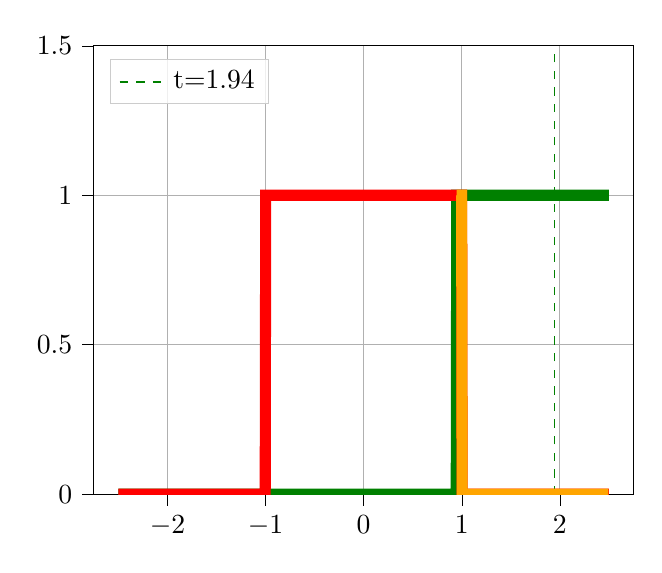
\begin{tikzpicture}

\definecolor{color0}{rgb}{1,0.498039215686275,0.0549019607843137}
\definecolor{color1}{rgb}{1,0.647058823529412,0}

\begin{axis}[
legend cell align={left},
legend style={fill opacity=0.8, draw opacity=1, text opacity=1, at={(0.03,0.97)}, anchor=north west, draw=white!80!black},
tick align=outside,
tick pos=left,
x grid style={white!69.0196078431373!black},
xmajorgrids,
xmin=-2.75, xmax=2.75,
xtick style={color=black},
y grid style={white!69.0196078431373!black},
ymajorgrids,
ymin=0, ymax=1.5,
ytick style={color=black}
]
\path [draw=color0, fill=color0, opacity=0.2]
(axis cs:0.948448448448449,1)
--(axis cs:0.948448448448449,0)
--(axis cs:0.953453453453454,0)
--(axis cs:0.958458458458459,0)
--(axis cs:0.963463463463464,0)
--(axis cs:0.968468468468469,0)
--(axis cs:0.973473473473474,0)
--(axis cs:0.978478478478479,0)
--(axis cs:0.983483483483484,0)
--(axis cs:0.988488488488489,0)
--(axis cs:0.993493493493494,0)
--(axis cs:0.998498498498499,0)
--(axis cs:1.0035035035035,0)
--(axis cs:1.00850850850851,0)
--(axis cs:1.01351351351351,0)
--(axis cs:1.01851851851852,0)
--(axis cs:1.02352352352352,0)
--(axis cs:1.02852852852853,0)
--(axis cs:1.03353353353353,0)
--(axis cs:1.03853853853854,0)
--(axis cs:1.04354354354354,0)
--(axis cs:1.04854854854855,0)
--(axis cs:1.05355355355355,0)
--(axis cs:1.05855855855856,0)
--(axis cs:1.06356356356356,0)
--(axis cs:1.06856856856857,0)
--(axis cs:1.07357357357357,0)
--(axis cs:1.07857857857858,0)
--(axis cs:1.08358358358358,0)
--(axis cs:1.08858858858859,0)
--(axis cs:1.09359359359359,0)
--(axis cs:1.0985985985986,0)
--(axis cs:1.1036036036036,0)
--(axis cs:1.10860860860861,0)
--(axis cs:1.11361361361361,0)
--(axis cs:1.11861861861862,0)
--(axis cs:1.12362362362362,0)
--(axis cs:1.12862862862863,0)
--(axis cs:1.13363363363363,0)
--(axis cs:1.13863863863864,0)
--(axis cs:1.14364364364364,0)
--(axis cs:1.14864864864865,0)
--(axis cs:1.15365365365365,0)
--(axis cs:1.15865865865866,0)
--(axis cs:1.16366366366366,0)
--(axis cs:1.16866866866867,0)
--(axis cs:1.17367367367367,0)
--(axis cs:1.17867867867868,0)
--(axis cs:1.18368368368368,0)
--(axis cs:1.18868868868869,0)
--(axis cs:1.19369369369369,0)
--(axis cs:1.1986986986987,0)
--(axis cs:1.2037037037037,0)
--(axis cs:1.20870870870871,0)
--(axis cs:1.21371371371371,0)
--(axis cs:1.21871871871872,0)
--(axis cs:1.22372372372372,0)
--(axis cs:1.22872872872873,0)
--(axis cs:1.23373373373373,0)
--(axis cs:1.23873873873874,0)
--(axis cs:1.24374374374374,0)
--(axis cs:1.24874874874875,0)
--(axis cs:1.25375375375375,0)
--(axis cs:1.25875875875876,0)
--(axis cs:1.26376376376376,0)
--(axis cs:1.26876876876877,0)
--(axis cs:1.27377377377377,0)
--(axis cs:1.27877877877878,0)
--(axis cs:1.28378378378378,0)
--(axis cs:1.28878878878879,0)
--(axis cs:1.29379379379379,0)
--(axis cs:1.2987987987988,0)
--(axis cs:1.3038038038038,0)
--(axis cs:1.30880880880881,0)
--(axis cs:1.31381381381381,0)
--(axis cs:1.31881881881882,0)
--(axis cs:1.32382382382382,0)
--(axis cs:1.32882882882883,0)
--(axis cs:1.33383383383383,0)
--(axis cs:1.33883883883884,0)
--(axis cs:1.34384384384384,0)
--(axis cs:1.34884884884885,0)
--(axis cs:1.35385385385385,0)
--(axis cs:1.35885885885886,0)
--(axis cs:1.36386386386386,0)
--(axis cs:1.36886886886887,0)
--(axis cs:1.37387387387387,0)
--(axis cs:1.37887887887888,0)
--(axis cs:1.38388388388388,0)
--(axis cs:1.38888888888889,0)
--(axis cs:1.39389389389389,0)
--(axis cs:1.3988988988989,0)
--(axis cs:1.4039039039039,0)
--(axis cs:1.40890890890891,0)
--(axis cs:1.41391391391391,0)
--(axis cs:1.41891891891892,0)
--(axis cs:1.42392392392392,0)
--(axis cs:1.42892892892893,0)
--(axis cs:1.43393393393393,0)
--(axis cs:1.43893893893894,0)
--(axis cs:1.44394394394394,0)
--(axis cs:1.44894894894895,0)
--(axis cs:1.45395395395395,0)
--(axis cs:1.45895895895896,0)
--(axis cs:1.46396396396396,0)
--(axis cs:1.46896896896897,0)
--(axis cs:1.47397397397397,0)
--(axis cs:1.47897897897898,0)
--(axis cs:1.48398398398398,0)
--(axis cs:1.48898898898899,0)
--(axis cs:1.49399399399399,0)
--(axis cs:1.498998998999,0)
--(axis cs:1.504004004004,0)
--(axis cs:1.50900900900901,0)
--(axis cs:1.51401401401401,0)
--(axis cs:1.51901901901902,0)
--(axis cs:1.52402402402402,0)
--(axis cs:1.52902902902903,0)
--(axis cs:1.53403403403403,0)
--(axis cs:1.53903903903904,0)
--(axis cs:1.54404404404404,0)
--(axis cs:1.54904904904905,0)
--(axis cs:1.55405405405405,0)
--(axis cs:1.55905905905906,0)
--(axis cs:1.56406406406406,0)
--(axis cs:1.56906906906907,0)
--(axis cs:1.57407407407407,0)
--(axis cs:1.57907907907908,0)
--(axis cs:1.58408408408408,0)
--(axis cs:1.58908908908909,0)
--(axis cs:1.59409409409409,0)
--(axis cs:1.5990990990991,0)
--(axis cs:1.6041041041041,0)
--(axis cs:1.60910910910911,0)
--(axis cs:1.61411411411411,0)
--(axis cs:1.61911911911912,0)
--(axis cs:1.62412412412412,0)
--(axis cs:1.62912912912913,0)
--(axis cs:1.63413413413413,0)
--(axis cs:1.63913913913914,0)
--(axis cs:1.64414414414414,0)
--(axis cs:1.64914914914915,0)
--(axis cs:1.65415415415415,0)
--(axis cs:1.65915915915916,0)
--(axis cs:1.66416416416416,0)
--(axis cs:1.66916916916917,0)
--(axis cs:1.67417417417417,0)
--(axis cs:1.67917917917918,0)
--(axis cs:1.68418418418418,0)
--(axis cs:1.68918918918919,0)
--(axis cs:1.69419419419419,0)
--(axis cs:1.6991991991992,0)
--(axis cs:1.7042042042042,0)
--(axis cs:1.70920920920921,0)
--(axis cs:1.71421421421421,0)
--(axis cs:1.71921921921922,0)
--(axis cs:1.72422422422422,0)
--(axis cs:1.72922922922923,0)
--(axis cs:1.73423423423423,0)
--(axis cs:1.73923923923924,0)
--(axis cs:1.74424424424424,0)
--(axis cs:1.74924924924925,0)
--(axis cs:1.75425425425425,0)
--(axis cs:1.75925925925926,0)
--(axis cs:1.76426426426426,0)
--(axis cs:1.76926926926927,0)
--(axis cs:1.77427427427427,0)
--(axis cs:1.77927927927928,0)
--(axis cs:1.78428428428428,0)
--(axis cs:1.78928928928929,0)
--(axis cs:1.79429429429429,0)
--(axis cs:1.7992992992993,0)
--(axis cs:1.8043043043043,0)
--(axis cs:1.80930930930931,0)
--(axis cs:1.81431431431431,0)
--(axis cs:1.81931931931932,0)
--(axis cs:1.82432432432432,0)
--(axis cs:1.82932932932933,0)
--(axis cs:1.83433433433433,0)
--(axis cs:1.83933933933934,0)
--(axis cs:1.84434434434434,0)
--(axis cs:1.84934934934935,0)
--(axis cs:1.85435435435435,0)
--(axis cs:1.85935935935936,0)
--(axis cs:1.86436436436436,0)
--(axis cs:1.86936936936937,0)
--(axis cs:1.87437437437437,0)
--(axis cs:1.87937937937938,0)
--(axis cs:1.88438438438438,0)
--(axis cs:1.88938938938939,0)
--(axis cs:1.89439439439439,0)
--(axis cs:1.8993993993994,0)
--(axis cs:1.9044044044044,0)
--(axis cs:1.90940940940941,0)
--(axis cs:1.91441441441441,0)
--(axis cs:1.91941941941942,0)
--(axis cs:1.92442442442442,0)
--(axis cs:1.92942942942943,0)
--(axis cs:1.93443443443443,0)
--(axis cs:1.93943943943944,0)
--(axis cs:1.94444444444444,0)
--(axis cs:1.94944944944945,0)
--(axis cs:1.95445445445445,0)
--(axis cs:1.95945945945946,0)
--(axis cs:1.96446446446446,0)
--(axis cs:1.96946946946947,0)
--(axis cs:1.97447447447447,0)
--(axis cs:1.97947947947948,0)
--(axis cs:1.98448448448448,0)
--(axis cs:1.98948948948949,0)
--(axis cs:1.99449449449449,0)
--(axis cs:1.9994994994995,0)
--(axis cs:2.0045045045045,0)
--(axis cs:2.00950950950951,0)
--(axis cs:2.01451451451451,0)
--(axis cs:2.01951951951952,0)
--(axis cs:2.02452452452452,0)
--(axis cs:2.02952952952953,0)
--(axis cs:2.03453453453453,0)
--(axis cs:2.03953953953954,0)
--(axis cs:2.04454454454454,0)
--(axis cs:2.04954954954955,0)
--(axis cs:2.05455455455455,0)
--(axis cs:2.05955955955956,0)
--(axis cs:2.06456456456456,0)
--(axis cs:2.06956956956957,0)
--(axis cs:2.07457457457457,0)
--(axis cs:2.07957957957958,0)
--(axis cs:2.08458458458458,0)
--(axis cs:2.08958958958959,0)
--(axis cs:2.09459459459459,0)
--(axis cs:2.0995995995996,0)
--(axis cs:2.1046046046046,0)
--(axis cs:2.10960960960961,0)
--(axis cs:2.11461461461461,0)
--(axis cs:2.11961961961962,0)
--(axis cs:2.12462462462462,0)
--(axis cs:2.12962962962963,0)
--(axis cs:2.13463463463463,0)
--(axis cs:2.13963963963964,0)
--(axis cs:2.14464464464464,0)
--(axis cs:2.14964964964965,0)
--(axis cs:2.15465465465465,0)
--(axis cs:2.15965965965966,0)
--(axis cs:2.16466466466466,0)
--(axis cs:2.16966966966967,0)
--(axis cs:2.17467467467467,0)
--(axis cs:2.17967967967968,0)
--(axis cs:2.18468468468468,0)
--(axis cs:2.18968968968969,0)
--(axis cs:2.19469469469469,0)
--(axis cs:2.1996996996997,0)
--(axis cs:2.2047047047047,0)
--(axis cs:2.20970970970971,0)
--(axis cs:2.21471471471471,0)
--(axis cs:2.21971971971972,0)
--(axis cs:2.22472472472472,0)
--(axis cs:2.22972972972973,0)
--(axis cs:2.23473473473473,0)
--(axis cs:2.23973973973974,0)
--(axis cs:2.24474474474474,0)
--(axis cs:2.24974974974975,0)
--(axis cs:2.25475475475475,0)
--(axis cs:2.25975975975976,0)
--(axis cs:2.26476476476476,0)
--(axis cs:2.26976976976977,0)
--(axis cs:2.27477477477477,0)
--(axis cs:2.27977977977978,0)
--(axis cs:2.28478478478478,0)
--(axis cs:2.28978978978979,0)
--(axis cs:2.29479479479479,0)
--(axis cs:2.2997997997998,0)
--(axis cs:2.3048048048048,0)
--(axis cs:2.30980980980981,0)
--(axis cs:2.31481481481481,0)
--(axis cs:2.31981981981982,0)
--(axis cs:2.32482482482482,0)
--(axis cs:2.32982982982983,0)
--(axis cs:2.33483483483483,0)
--(axis cs:2.33983983983984,0)
--(axis cs:2.34484484484484,0)
--(axis cs:2.34984984984985,0)
--(axis cs:2.35485485485485,0)
--(axis cs:2.35985985985986,0)
--(axis cs:2.36486486486486,0)
--(axis cs:2.36986986986987,0)
--(axis cs:2.37487487487487,0)
--(axis cs:2.37987987987988,0)
--(axis cs:2.38488488488488,0)
--(axis cs:2.38988988988989,0)
--(axis cs:2.39489489489489,0)
--(axis cs:2.3998998998999,0)
--(axis cs:2.4049049049049,0)
--(axis cs:2.40990990990991,0)
--(axis cs:2.41491491491491,0)
--(axis cs:2.41991991991992,0)
--(axis cs:2.42492492492492,0)
--(axis cs:2.42992992992993,0)
--(axis cs:2.43493493493493,0)
--(axis cs:2.43993993993994,0)
--(axis cs:2.44494494494494,0)
--(axis cs:2.44994994994995,0)
--(axis cs:2.45495495495495,0)
--(axis cs:2.45995995995996,0)
--(axis cs:2.46496496496496,0)
--(axis cs:2.46996996996997,0)
--(axis cs:2.47497497497497,0)
--(axis cs:2.47997997997998,0)
--(axis cs:2.48498498498498,0)
--(axis cs:2.48998998998999,0)
--(axis cs:2.49499499499499,0)
--(axis cs:2.49499499499499,0)
--(axis cs:2.49499499499499,0)
--(axis cs:2.48998998998999,0)
--(axis cs:2.48498498498498,0)
--(axis cs:2.47997997997998,0)
--(axis cs:2.47497497497497,0)
--(axis cs:2.46996996996997,0)
--(axis cs:2.46496496496496,0)
--(axis cs:2.45995995995996,0)
--(axis cs:2.45495495495495,0)
--(axis cs:2.44994994994995,0)
--(axis cs:2.44494494494494,0)
--(axis cs:2.43993993993994,0)
--(axis cs:2.43493493493493,0)
--(axis cs:2.42992992992993,0)
--(axis cs:2.42492492492492,0)
--(axis cs:2.41991991991992,0)
--(axis cs:2.41491491491491,0)
--(axis cs:2.40990990990991,0)
--(axis cs:2.4049049049049,0)
--(axis cs:2.3998998998999,0)
--(axis cs:2.39489489489489,0)
--(axis cs:2.38988988988989,0)
--(axis cs:2.38488488488488,0)
--(axis cs:2.37987987987988,0)
--(axis cs:2.37487487487487,0)
--(axis cs:2.36986986986987,0)
--(axis cs:2.36486486486486,0)
--(axis cs:2.35985985985986,0)
--(axis cs:2.35485485485485,0)
--(axis cs:2.34984984984985,0)
--(axis cs:2.34484484484484,0)
--(axis cs:2.33983983983984,0)
--(axis cs:2.33483483483483,0)
--(axis cs:2.32982982982983,0)
--(axis cs:2.32482482482482,0)
--(axis cs:2.31981981981982,0)
--(axis cs:2.31481481481481,0)
--(axis cs:2.30980980980981,0)
--(axis cs:2.3048048048048,0)
--(axis cs:2.2997997997998,0)
--(axis cs:2.29479479479479,0)
--(axis cs:2.28978978978979,0)
--(axis cs:2.28478478478478,0)
--(axis cs:2.27977977977978,0)
--(axis cs:2.27477477477477,0)
--(axis cs:2.26976976976977,0)
--(axis cs:2.26476476476476,0)
--(axis cs:2.25975975975976,0)
--(axis cs:2.25475475475475,0)
--(axis cs:2.24974974974975,0)
--(axis cs:2.24474474474474,0)
--(axis cs:2.23973973973974,0)
--(axis cs:2.23473473473473,0)
--(axis cs:2.22972972972973,0)
--(axis cs:2.22472472472472,0)
--(axis cs:2.21971971971972,0)
--(axis cs:2.21471471471471,0)
--(axis cs:2.20970970970971,0)
--(axis cs:2.2047047047047,0)
--(axis cs:2.1996996996997,0)
--(axis cs:2.19469469469469,0)
--(axis cs:2.18968968968969,0)
--(axis cs:2.18468468468468,0)
--(axis cs:2.17967967967968,0)
--(axis cs:2.17467467467467,0)
--(axis cs:2.16966966966967,0)
--(axis cs:2.16466466466466,0)
--(axis cs:2.15965965965966,0)
--(axis cs:2.15465465465465,0)
--(axis cs:2.14964964964965,0)
--(axis cs:2.14464464464464,0)
--(axis cs:2.13963963963964,0)
--(axis cs:2.13463463463463,0)
--(axis cs:2.12962962962963,0)
--(axis cs:2.12462462462462,0)
--(axis cs:2.11961961961962,0)
--(axis cs:2.11461461461461,0)
--(axis cs:2.10960960960961,0)
--(axis cs:2.1046046046046,0)
--(axis cs:2.0995995995996,0)
--(axis cs:2.09459459459459,0)
--(axis cs:2.08958958958959,0)
--(axis cs:2.08458458458458,0)
--(axis cs:2.07957957957958,0)
--(axis cs:2.07457457457457,0)
--(axis cs:2.06956956956957,0)
--(axis cs:2.06456456456456,0)
--(axis cs:2.05955955955956,0)
--(axis cs:2.05455455455455,0)
--(axis cs:2.04954954954955,0)
--(axis cs:2.04454454454454,0)
--(axis cs:2.03953953953954,0)
--(axis cs:2.03453453453453,0)
--(axis cs:2.02952952952953,0)
--(axis cs:2.02452452452452,0)
--(axis cs:2.01951951951952,0)
--(axis cs:2.01451451451451,0)
--(axis cs:2.00950950950951,0)
--(axis cs:2.0045045045045,0)
--(axis cs:1.9994994994995,0)
--(axis cs:1.99449449449449,0)
--(axis cs:1.98948948948949,0)
--(axis cs:1.98448448448448,0)
--(axis cs:1.97947947947948,0)
--(axis cs:1.97447447447447,0)
--(axis cs:1.96946946946947,0)
--(axis cs:1.96446446446446,0)
--(axis cs:1.95945945945946,0)
--(axis cs:1.95445445445445,0)
--(axis cs:1.94944944944945,0)
--(axis cs:1.94444444444444,0)
--(axis cs:1.93943943943944,0)
--(axis cs:1.93443443443443,0)
--(axis cs:1.92942942942943,0)
--(axis cs:1.92442442442442,0)
--(axis cs:1.91941941941942,0)
--(axis cs:1.91441441441441,0)
--(axis cs:1.90940940940941,0)
--(axis cs:1.9044044044044,0)
--(axis cs:1.8993993993994,0)
--(axis cs:1.89439439439439,0)
--(axis cs:1.88938938938939,0)
--(axis cs:1.88438438438438,0)
--(axis cs:1.87937937937938,0)
--(axis cs:1.87437437437437,0)
--(axis cs:1.86936936936937,0)
--(axis cs:1.86436436436436,0)
--(axis cs:1.85935935935936,0)
--(axis cs:1.85435435435435,0)
--(axis cs:1.84934934934935,0)
--(axis cs:1.84434434434434,0)
--(axis cs:1.83933933933934,0)
--(axis cs:1.83433433433433,0)
--(axis cs:1.82932932932933,0)
--(axis cs:1.82432432432432,0)
--(axis cs:1.81931931931932,0)
--(axis cs:1.81431431431431,0)
--(axis cs:1.80930930930931,0)
--(axis cs:1.8043043043043,0)
--(axis cs:1.7992992992993,0)
--(axis cs:1.79429429429429,0)
--(axis cs:1.78928928928929,0)
--(axis cs:1.78428428428428,0)
--(axis cs:1.77927927927928,0)
--(axis cs:1.77427427427427,0)
--(axis cs:1.76926926926927,0)
--(axis cs:1.76426426426426,0)
--(axis cs:1.75925925925926,0)
--(axis cs:1.75425425425425,0)
--(axis cs:1.74924924924925,0)
--(axis cs:1.74424424424424,0)
--(axis cs:1.73923923923924,0)
--(axis cs:1.73423423423423,0)
--(axis cs:1.72922922922923,0)
--(axis cs:1.72422422422422,0)
--(axis cs:1.71921921921922,0)
--(axis cs:1.71421421421421,0)
--(axis cs:1.70920920920921,0)
--(axis cs:1.7042042042042,0)
--(axis cs:1.6991991991992,0)
--(axis cs:1.69419419419419,0)
--(axis cs:1.68918918918919,0)
--(axis cs:1.68418418418418,0)
--(axis cs:1.67917917917918,0)
--(axis cs:1.67417417417417,0)
--(axis cs:1.66916916916917,0)
--(axis cs:1.66416416416416,0)
--(axis cs:1.65915915915916,0)
--(axis cs:1.65415415415415,0)
--(axis cs:1.64914914914915,0)
--(axis cs:1.64414414414414,0)
--(axis cs:1.63913913913914,0)
--(axis cs:1.63413413413413,0)
--(axis cs:1.62912912912913,0)
--(axis cs:1.62412412412412,0)
--(axis cs:1.61911911911912,0)
--(axis cs:1.61411411411411,0)
--(axis cs:1.60910910910911,0)
--(axis cs:1.6041041041041,0)
--(axis cs:1.5990990990991,0)
--(axis cs:1.59409409409409,0)
--(axis cs:1.58908908908909,0)
--(axis cs:1.58408408408408,0)
--(axis cs:1.57907907907908,0)
--(axis cs:1.57407407407407,0)
--(axis cs:1.56906906906907,0)
--(axis cs:1.56406406406406,0)
--(axis cs:1.55905905905906,0)
--(axis cs:1.55405405405405,0)
--(axis cs:1.54904904904905,0)
--(axis cs:1.54404404404404,0)
--(axis cs:1.53903903903904,0)
--(axis cs:1.53403403403403,0)
--(axis cs:1.52902902902903,0)
--(axis cs:1.52402402402402,0)
--(axis cs:1.51901901901902,0)
--(axis cs:1.51401401401401,0)
--(axis cs:1.50900900900901,0)
--(axis cs:1.504004004004,0)
--(axis cs:1.498998998999,0)
--(axis cs:1.49399399399399,0)
--(axis cs:1.48898898898899,0)
--(axis cs:1.48398398398398,0)
--(axis cs:1.47897897897898,0)
--(axis cs:1.47397397397397,0)
--(axis cs:1.46896896896897,0)
--(axis cs:1.46396396396396,0)
--(axis cs:1.45895895895896,0)
--(axis cs:1.45395395395395,0)
--(axis cs:1.44894894894895,0)
--(axis cs:1.44394394394394,0)
--(axis cs:1.43893893893894,0)
--(axis cs:1.43393393393393,0)
--(axis cs:1.42892892892893,0)
--(axis cs:1.42392392392392,0)
--(axis cs:1.41891891891892,0)
--(axis cs:1.41391391391391,0)
--(axis cs:1.40890890890891,0)
--(axis cs:1.4039039039039,0)
--(axis cs:1.3988988988989,0)
--(axis cs:1.39389389389389,0)
--(axis cs:1.38888888888889,0)
--(axis cs:1.38388388388388,0)
--(axis cs:1.37887887887888,0)
--(axis cs:1.37387387387387,0)
--(axis cs:1.36886886886887,0)
--(axis cs:1.36386386386386,0)
--(axis cs:1.35885885885886,0)
--(axis cs:1.35385385385385,0)
--(axis cs:1.34884884884885,0)
--(axis cs:1.34384384384384,0)
--(axis cs:1.33883883883884,0)
--(axis cs:1.33383383383383,0)
--(axis cs:1.32882882882883,0)
--(axis cs:1.32382382382382,0)
--(axis cs:1.31881881881882,0)
--(axis cs:1.31381381381381,0)
--(axis cs:1.30880880880881,0)
--(axis cs:1.3038038038038,0)
--(axis cs:1.2987987987988,0)
--(axis cs:1.29379379379379,0)
--(axis cs:1.28878878878879,0)
--(axis cs:1.28378378378378,0)
--(axis cs:1.27877877877878,0)
--(axis cs:1.27377377377377,0)
--(axis cs:1.26876876876877,0)
--(axis cs:1.26376376376376,0)
--(axis cs:1.25875875875876,0)
--(axis cs:1.25375375375375,0)
--(axis cs:1.24874874874875,0)
--(axis cs:1.24374374374374,0)
--(axis cs:1.23873873873874,0)
--(axis cs:1.23373373373373,0)
--(axis cs:1.22872872872873,0)
--(axis cs:1.22372372372372,0)
--(axis cs:1.21871871871872,0)
--(axis cs:1.21371371371371,0)
--(axis cs:1.20870870870871,0)
--(axis cs:1.2037037037037,0)
--(axis cs:1.1986986986987,0)
--(axis cs:1.19369369369369,0)
--(axis cs:1.18868868868869,0)
--(axis cs:1.18368368368368,0)
--(axis cs:1.17867867867868,0)
--(axis cs:1.17367367367367,0)
--(axis cs:1.16866866866867,0)
--(axis cs:1.16366366366366,0)
--(axis cs:1.15865865865866,0)
--(axis cs:1.15365365365365,0)
--(axis cs:1.14864864864865,0)
--(axis cs:1.14364364364364,0)
--(axis cs:1.13863863863864,0)
--(axis cs:1.13363363363363,0)
--(axis cs:1.12862862862863,0)
--(axis cs:1.12362362362362,0)
--(axis cs:1.11861861861862,0)
--(axis cs:1.11361361361361,0)
--(axis cs:1.10860860860861,0)
--(axis cs:1.1036036036036,0)
--(axis cs:1.0985985985986,0)
--(axis cs:1.09359359359359,0)
--(axis cs:1.08858858858859,0)
--(axis cs:1.08358358358358,0)
--(axis cs:1.07857857857858,0)
--(axis cs:1.07357357357357,0)
--(axis cs:1.06856856856857,0)
--(axis cs:1.06356356356356,0)
--(axis cs:1.05855855855856,0)
--(axis cs:1.05355355355355,0)
--(axis cs:1.04854854854855,0)
--(axis cs:1.04354354354354,0)
--(axis cs:1.03853853853854,0)
--(axis cs:1.03353353353353,0)
--(axis cs:1.02852852852853,0)
--(axis cs:1.02352352352352,0)
--(axis cs:1.01851851851852,0)
--(axis cs:1.01351351351351,0)
--(axis cs:1.00850850850851,0)
--(axis cs:1.0035035035035,0)
--(axis cs:0.998498498498499,1)
--(axis cs:0.993493493493494,1)
--(axis cs:0.988488488488489,1)
--(axis cs:0.983483483483484,1)
--(axis cs:0.978478478478479,1)
--(axis cs:0.973473473473474,1)
--(axis cs:0.968468468468469,1)
--(axis cs:0.963463463463464,1)
--(axis cs:0.958458458458459,1)
--(axis cs:0.953453453453454,1)
--(axis cs:0.948448448448449,1)
--cycle;

\addplot [line width=4pt, green!50!black, forget plot]
table {%
-2.5 0
-2.49499499499499 0
-2.48998998998999 0
-2.48498498498498 0
-2.47997997997998 0
-2.47497497497497 0
-2.46996996996997 0
-2.46496496496496 0
-2.45995995995996 0
-2.45495495495495 0
-2.44994994994995 0
-2.44494494494494 0
-2.43993993993994 0
-2.43493493493493 0
-2.42992992992993 0
-2.42492492492492 0
-2.41991991991992 0
-2.41491491491491 0
-2.40990990990991 0
-2.4049049049049 0
-2.3998998998999 0
-2.39489489489489 0
-2.38988988988989 0
-2.38488488488488 0
-2.37987987987988 0
-2.37487487487487 0
-2.36986986986987 0
-2.36486486486486 0
-2.35985985985986 0
-2.35485485485485 0
-2.34984984984985 0
-2.34484484484484 0
-2.33983983983984 0
-2.33483483483483 0
-2.32982982982983 0
-2.32482482482482 0
-2.31981981981982 0
-2.31481481481481 0
-2.30980980980981 0
-2.3048048048048 0
-2.2997997997998 0
-2.29479479479479 0
-2.28978978978979 0
-2.28478478478478 0
-2.27977977977978 0
-2.27477477477477 0
-2.26976976976977 0
-2.26476476476476 0
-2.25975975975976 0
-2.25475475475475 0
-2.24974974974975 0
-2.24474474474474 0
-2.23973973973974 0
-2.23473473473473 0
-2.22972972972973 0
-2.22472472472472 0
-2.21971971971972 0
-2.21471471471471 0
-2.20970970970971 0
-2.2047047047047 0
-2.1996996996997 0
-2.19469469469469 0
-2.18968968968969 0
-2.18468468468468 0
-2.17967967967968 0
-2.17467467467467 0
-2.16966966966967 0
-2.16466466466466 0
-2.15965965965966 0
-2.15465465465465 0
-2.14964964964965 0
-2.14464464464464 0
-2.13963963963964 0
-2.13463463463463 0
-2.12962962962963 0
-2.12462462462462 0
-2.11961961961962 0
-2.11461461461461 0
-2.10960960960961 0
-2.1046046046046 0
-2.0995995995996 0
-2.09459459459459 0
-2.08958958958959 0
-2.08458458458458 0
-2.07957957957958 0
-2.07457457457457 0
-2.06956956956957 0
-2.06456456456456 0
-2.05955955955956 0
-2.05455455455455 0
-2.04954954954955 0
-2.04454454454454 0
-2.03953953953954 0
-2.03453453453453 0
-2.02952952952953 0
-2.02452452452452 0
-2.01951951951952 0
-2.01451451451451 0
-2.00950950950951 0
-2.0045045045045 0
-1.9994994994995 0
-1.99449449449449 0
-1.98948948948949 0
-1.98448448448448 0
-1.97947947947948 0
-1.97447447447447 0
-1.96946946946947 0
-1.96446446446446 0
-1.95945945945946 0
-1.95445445445445 0
-1.94944944944945 0
-1.94444444444444 0
-1.93943943943944 0
-1.93443443443443 0
-1.92942942942943 0
-1.92442442442442 0
-1.91941941941942 0
-1.91441441441441 0
-1.90940940940941 0
-1.9044044044044 0
-1.8993993993994 0
-1.89439439439439 0
-1.88938938938939 0
-1.88438438438438 0
-1.87937937937938 0
-1.87437437437437 0
-1.86936936936937 0
-1.86436436436436 0
-1.85935935935936 0
-1.85435435435435 0
-1.84934934934935 0
-1.84434434434434 0
-1.83933933933934 0
-1.83433433433433 0
-1.82932932932933 0
-1.82432432432432 0
-1.81931931931932 0
-1.81431431431431 0
-1.80930930930931 0
-1.8043043043043 0
-1.7992992992993 0
-1.79429429429429 0
-1.78928928928929 0
-1.78428428428428 0
-1.77927927927928 0
-1.77427427427427 0
-1.76926926926927 0
-1.76426426426426 0
-1.75925925925926 0
-1.75425425425425 0
-1.74924924924925 0
-1.74424424424424 0
-1.73923923923924 0
-1.73423423423423 0
-1.72922922922923 0
-1.72422422422422 0
-1.71921921921922 0
-1.71421421421421 0
-1.70920920920921 0
-1.7042042042042 0
-1.6991991991992 0
-1.69419419419419 0
-1.68918918918919 0
-1.68418418418418 0
-1.67917917917918 0
-1.67417417417417 0
-1.66916916916917 0
-1.66416416416416 0
-1.65915915915916 0
-1.65415415415415 0
-1.64914914914915 0
-1.64414414414414 0
-1.63913913913914 0
-1.63413413413413 0
-1.62912912912913 0
-1.62412412412412 0
-1.61911911911912 0
-1.61411411411411 0
-1.60910910910911 0
-1.6041041041041 0
-1.5990990990991 0
-1.59409409409409 0
-1.58908908908909 0
-1.58408408408408 0
-1.57907907907908 0
-1.57407407407407 0
-1.56906906906907 0
-1.56406406406406 0
-1.55905905905906 0
-1.55405405405405 0
-1.54904904904905 0
-1.54404404404404 0
-1.53903903903904 0
-1.53403403403403 0
-1.52902902902903 0
-1.52402402402402 0
-1.51901901901902 0
-1.51401401401401 0
-1.50900900900901 0
-1.504004004004 0
-1.498998998999 0
-1.49399399399399 0
-1.48898898898899 0
-1.48398398398398 0
-1.47897897897898 0
-1.47397397397397 0
-1.46896896896897 0
-1.46396396396396 0
-1.45895895895896 0
-1.45395395395395 0
-1.44894894894895 0
-1.44394394394394 0
-1.43893893893894 0
-1.43393393393393 0
-1.42892892892893 0
-1.42392392392392 0
-1.41891891891892 0
-1.41391391391391 0
-1.40890890890891 0
-1.4039039039039 0
-1.3988988988989 0
-1.39389389389389 0
-1.38888888888889 0
-1.38388388388388 0
-1.37887887887888 0
-1.37387387387387 0
-1.36886886886887 0
-1.36386386386386 0
-1.35885885885886 0
-1.35385385385385 0
-1.34884884884885 0
-1.34384384384384 0
-1.33883883883884 0
-1.33383383383383 0
-1.32882882882883 0
-1.32382382382382 0
-1.31881881881882 0
-1.31381381381381 0
-1.30880880880881 0
-1.3038038038038 0
-1.2987987987988 0
-1.29379379379379 0
-1.28878878878879 0
-1.28378378378378 0
-1.27877877877878 0
-1.27377377377377 0
-1.26876876876877 0
-1.26376376376376 0
-1.25875875875876 0
-1.25375375375375 0
-1.24874874874875 0
-1.24374374374374 0
-1.23873873873874 0
-1.23373373373373 0
-1.22872872872873 0
-1.22372372372372 0
-1.21871871871872 0
-1.21371371371371 0
-1.20870870870871 0
-1.2037037037037 0
-1.1986986986987 0
-1.19369369369369 0
-1.18868868868869 0
-1.18368368368368 0
-1.17867867867868 0
-1.17367367367367 0
-1.16866866866867 0
-1.16366366366366 0
-1.15865865865866 0
-1.15365365365365 0
-1.14864864864865 0
-1.14364364364364 0
-1.13863863863864 0
-1.13363363363363 0
-1.12862862862863 0
-1.12362362362362 0
-1.11861861861862 0
-1.11361361361361 0
-1.10860860860861 0
-1.1036036036036 0
-1.0985985985986 0
-1.09359359359359 0
-1.08858858858859 0
-1.08358358358358 0
-1.07857857857858 0
-1.07357357357357 0
-1.06856856856857 0
-1.06356356356356 0
-1.05855855855856 0
-1.05355355355355 0
-1.04854854854855 0
-1.04354354354354 0
-1.03853853853854 0
-1.03353353353353 0
-1.02852852852853 0
-1.02352352352352 0
-1.01851851851852 0
-1.01351351351351 0
-1.00850850850851 0
-1.0035035035035 0
-0.998498498498499 0
-0.993493493493494 0
-0.988488488488489 0
-0.983483483483484 0
-0.978478478478479 0
-0.973473473473474 0
-0.968468468468469 0
-0.963463463463464 0
-0.958458458458459 0
-0.953453453453454 0
-0.948448448448449 0
-0.943443443443444 0
-0.938438438438439 0
-0.933433433433434 0
-0.928428428428429 0
-0.923423423423424 0
-0.918418418418419 0
-0.913413413413414 0
-0.908408408408409 0
-0.903403403403404 0
-0.898398398398399 0
-0.893393393393393 0
-0.888388388388388 0
-0.883383383383383 0
-0.878378378378378 0
-0.873373373373373 0
-0.868368368368368 0
-0.863363363363363 0
-0.858358358358358 0
-0.853353353353353 0
-0.848348348348348 0
-0.843343343343343 0
-0.838338338338338 0
-0.833333333333333 0
-0.828328328328328 0
-0.823323323323323 0
-0.818318318318318 0
-0.813313313313313 0
-0.808308308308308 0
-0.803303303303303 0
-0.798298298298298 0
-0.793293293293293 0
-0.788288288288288 0
-0.783283283283283 0
-0.778278278278278 0
-0.773273273273273 0
-0.768268268268268 0
-0.763263263263263 0
-0.758258258258258 0
-0.753253253253253 0
-0.748248248248248 0
-0.743243243243243 0
-0.738238238238238 0
-0.733233233233233 0
-0.728228228228228 0
-0.723223223223223 0
-0.718218218218218 0
-0.713213213213213 0
-0.708208208208208 0
-0.703203203203203 0
-0.698198198198198 0
-0.693193193193193 0
-0.688188188188188 0
-0.683183183183183 0
-0.678178178178178 0
-0.673173173173173 0
-0.668168168168168 0
-0.663163163163163 0
-0.658158158158158 0
-0.653153153153153 0
-0.648148148148148 0
-0.643143143143143 0
-0.638138138138138 0
-0.633133133133133 0
-0.628128128128128 0
-0.623123123123123 0
-0.618118118118118 0
-0.613113113113113 0
-0.608108108108108 0
-0.603103103103103 0
-0.598098098098098 0
-0.593093093093093 0
-0.588088088088088 0
-0.583083083083083 0
-0.578078078078078 0
-0.573073073073073 0
-0.568068068068068 0
-0.563063063063063 0
-0.558058058058058 0
-0.553053053053053 0
-0.548048048048048 0
-0.543043043043043 0
-0.538038038038038 0
-0.533033033033033 0
-0.528028028028028 0
-0.523023023023023 0
-0.518018018018018 0
-0.513013013013013 0
-0.508008008008008 0
-0.503003003003003 0
-0.497997997997998 0
-0.492992992992993 0
-0.487987987987988 0
-0.482982982982983 0
-0.477977977977978 0
-0.472972972972973 0
-0.467967967967968 0
-0.462962962962963 0
-0.457957957957958 0
-0.452952952952953 0
-0.447947947947948 0
-0.442942942942943 0
-0.437937937937938 0
-0.432932932932933 0
-0.427927927927928 0
-0.422922922922923 0
-0.417917917917918 0
-0.412912912912913 0
-0.407907907907908 0
-0.402902902902903 0
-0.397897897897898 0
-0.392892892892893 0
-0.387887887887888 0
-0.382882882882883 0
-0.377877877877878 0
-0.372872872872873 0
-0.367867867867868 0
-0.362862862862863 0
-0.357857857857858 0
-0.352852852852853 0
-0.347847847847848 0
-0.342842842842843 0
-0.337837837837838 0
-0.332832832832833 0
-0.327827827827828 0
-0.322822822822823 0
-0.317817817817818 0
-0.312812812812813 0
-0.307807807807808 0
-0.302802802802803 0
-0.297797797797798 0
-0.292792792792793 0
-0.287787787787788 0
-0.282782782782783 0
-0.277777777777778 0
-0.272772772772773 0
-0.267767767767768 0
-0.262762762762763 0
-0.257757757757758 0
-0.252752752752753 0
-0.247747747747748 0
-0.242742742742743 0
-0.237737737737738 0
-0.232732732732733 0
-0.227727727727728 0
-0.222722722722723 0
-0.217717717717718 0
-0.212712712712713 0
-0.207707707707708 0
-0.202702702702703 0
-0.197697697697698 0
-0.192692692692693 0
-0.187687687687688 0
-0.182682682682683 0
-0.177677677677678 0
-0.172672672672673 0
-0.167667667667668 0
-0.162662662662663 0
-0.157657657657658 0
-0.152652652652653 0
-0.147647647647648 0
-0.142642642642643 0
-0.137637637637638 0
-0.132632632632633 0
-0.127627627627628 0
-0.122622622622623 0
-0.117617617617618 0
-0.112612612612613 0
-0.107607607607608 0
-0.102602602602603 0
-0.0975975975975976 0
-0.0925925925925926 0
-0.0875875875875876 0
-0.0825825825825826 0
-0.0775775775775776 0
-0.0725725725725725 0
-0.0675675675675675 0
-0.0625625625625625 0
-0.0575575575575575 0
-0.0525525525525525 0
-0.0475475475475475 0
-0.0425425425425425 0
-0.0375375375375375 0
-0.0325325325325325 0
-0.0275275275275275 0
-0.0225225225225225 0
-0.0175175175175175 0
-0.0125125125125125 0
-0.0075075075075075 0
-0.0025025025025025 0
0.0025025025025025 0
0.0075075075075075 0
0.0125125125125125 0
0.0175175175175175 0
0.0225225225225225 0
0.0275275275275275 0
0.0325325325325325 0
0.0375375375375375 0
0.0425425425425425 0
0.0475475475475475 0
0.0525525525525525 0
0.0575575575575575 0
0.0625625625625625 0
0.0675675675675675 0
0.0725725725725725 0
0.0775775775775776 0
0.0825825825825826 0
0.0875875875875876 0
0.0925925925925926 0
0.0975975975975976 0
0.102602602602603 0
0.107607607607608 0
0.112612612612613 0
0.117617617617618 0
0.122622622622623 0
0.127627627627628 0
0.132632632632633 0
0.137637637637638 0
0.142642642642643 0
0.147647647647648 0
0.152652652652653 0
0.157657657657658 0
0.162662662662663 0
0.167667667667668 0
0.172672672672673 0
0.177677677677678 0
0.182682682682683 0
0.187687687687688 0
0.192692692692693 0
0.197697697697698 0
0.202702702702703 0
0.207707707707708 0
0.212712712712713 0
0.217717717717718 0
0.222722722722723 0
0.227727727727728 0
0.232732732732733 0
0.237737737737738 0
0.242742742742743 0
0.247747747747748 0
0.252752752752753 0
0.257757757757758 0
0.262762762762763 0
0.267767767767768 0
0.272772772772773 0
0.277777777777778 0
0.282782782782783 0
0.287787787787788 0
0.292792792792793 0
0.297797797797798 0
0.302802802802803 0
0.307807807807808 0
0.312812812812813 0
0.317817817817818 0
0.322822822822823 0
0.327827827827828 0
0.332832832832833 0
0.337837837837838 0
0.342842842842843 0
0.347847847847848 0
0.352852852852853 0
0.357857857857858 0
0.362862862862863 0
0.367867867867868 0
0.372872872872873 0
0.377877877877878 0
0.382882882882883 0
0.387887887887888 0
0.392892892892893 0
0.397897897897898 0
0.402902902902903 0
0.407907907907908 0
0.412912912912913 0
0.417917917917918 0
0.422922922922923 0
0.427927927927928 0
0.432932932932933 0
0.437937937937938 0
0.442942942942943 0
0.447947947947948 0
0.452952952952953 0
0.457957957957958 0
0.462962962962963 0
0.467967967967968 0
0.472972972972973 0
0.477977977977978 0
0.482982982982983 0
0.487987987987988 0
0.492992992992993 0
0.497997997997998 0
0.503003003003003 0
0.508008008008008 0
0.513013013013013 0
0.518018018018018 0
0.523023023023023 0
0.528028028028028 0
0.533033033033033 0
0.538038038038038 0
0.543043043043043 0
0.548048048048048 0
0.553053053053053 0
0.558058058058058 0
0.563063063063063 0
0.568068068068068 0
0.573073073073073 0
0.578078078078078 0
0.583083083083083 0
0.588088088088088 0
0.593093093093093 0
0.598098098098098 0
0.603103103103103 0
0.608108108108108 0
0.613113113113113 0
0.618118118118118 0
0.623123123123123 0
0.628128128128128 0
0.633133133133133 0
0.638138138138138 0
0.643143143143143 0
0.648148148148148 0
0.653153153153153 0
0.658158158158158 0
0.663163163163163 0
0.668168168168168 0
0.673173173173173 0
0.678178178178178 0
0.683183183183183 0
0.688188188188188 0
0.693193193193193 0
0.698198198198198 0
0.703203203203203 0
0.708208208208208 0
0.713213213213213 0
0.718218218218218 0
0.723223223223223 0
0.728228228228228 0
0.733233233233233 0
0.738238238238238 0
0.743243243243243 0
0.748248248248248 0
0.753253253253253 0
0.758258258258258 0
0.763263263263263 0
0.768268268268268 0
0.773273273273273 0
0.778278278278278 0
0.783283283283283 0
0.788288288288288 0
0.793293293293293 0
0.798298298298298 0
0.803303303303303 0
0.808308308308308 0
0.813313313313313 0
0.818318318318318 0
0.823323323323323 0
0.828328328328328 0
0.833333333333333 0
0.838338338338338 0
0.843343343343343 0
0.848348348348348 0
0.853353353353353 0
0.858358358358358 0
0.863363363363364 0
0.868368368368369 0
0.873373373373374 0
0.878378378378379 0
0.883383383383384 0
0.888388388388389 0
0.893393393393394 0
0.898398398398399 0
0.903403403403404 0
0.908408408408409 0
0.913413413413414 0
0.918418418418419 0
0.923423423423424 0
0.928428428428429 0
0.933433433433434 0
0.938438438438439 0
0.943443443443444 0
0.948448448448449 1
0.953453453453454 1
0.958458458458459 1
0.963463463463464 1
0.968468468468469 1
0.973473473473474 1
0.978478478478479 1
0.983483483483484 1
0.988488488488489 1
0.993493493493494 1
0.998498498498499 1
1.0035035035035 1
1.00850850850851 1
1.01351351351351 1
1.01851851851852 1
1.02352352352352 1
1.02852852852853 1
1.03353353353353 1
1.03853853853854 1
1.04354354354354 1
1.04854854854855 1
1.05355355355355 1
1.05855855855856 1
1.06356356356356 1
1.06856856856857 1
1.07357357357357 1
1.07857857857858 1
1.08358358358358 1
1.08858858858859 1
1.09359359359359 1
1.0985985985986 1
1.1036036036036 1
1.10860860860861 1
1.11361361361361 1
1.11861861861862 1
1.12362362362362 1
1.12862862862863 1
1.13363363363363 1
1.13863863863864 1
1.14364364364364 1
1.14864864864865 1
1.15365365365365 1
1.15865865865866 1
1.16366366366366 1
1.16866866866867 1
1.17367367367367 1
1.17867867867868 1
1.18368368368368 1
1.18868868868869 1
1.19369369369369 1
1.1986986986987 1
1.2037037037037 1
1.20870870870871 1
1.21371371371371 1
1.21871871871872 1
1.22372372372372 1
1.22872872872873 1
1.23373373373373 1
1.23873873873874 1
1.24374374374374 1
1.24874874874875 1
1.25375375375375 1
1.25875875875876 1
1.26376376376376 1
1.26876876876877 1
1.27377377377377 1
1.27877877877878 1
1.28378378378378 1
1.28878878878879 1
1.29379379379379 1
1.2987987987988 1
1.3038038038038 1
1.30880880880881 1
1.31381381381381 1
1.31881881881882 1
1.32382382382382 1
1.32882882882883 1
1.33383383383383 1
1.33883883883884 1
1.34384384384384 1
1.34884884884885 1
1.35385385385385 1
1.35885885885886 1
1.36386386386386 1
1.36886886886887 1
1.37387387387387 1
1.37887887887888 1
1.38388388388388 1
1.38888888888889 1
1.39389389389389 1
1.3988988988989 1
1.4039039039039 1
1.40890890890891 1
1.41391391391391 1
1.41891891891892 1
1.42392392392392 1
1.42892892892893 1
1.43393393393393 1
1.43893893893894 1
1.44394394394394 1
1.44894894894895 1
1.45395395395395 1
1.45895895895896 1
1.46396396396396 1
1.46896896896897 1
1.47397397397397 1
1.47897897897898 1
1.48398398398398 1
1.48898898898899 1
1.49399399399399 1
1.498998998999 1
1.504004004004 1
1.50900900900901 1
1.51401401401401 1
1.51901901901902 1
1.52402402402402 1
1.52902902902903 1
1.53403403403403 1
1.53903903903904 1
1.54404404404404 1
1.54904904904905 1
1.55405405405405 1
1.55905905905906 1
1.56406406406406 1
1.56906906906907 1
1.57407407407407 1
1.57907907907908 1
1.58408408408408 1
1.58908908908909 1
1.59409409409409 1
1.5990990990991 1
1.6041041041041 1
1.60910910910911 1
1.61411411411411 1
1.61911911911912 1
1.62412412412412 1
1.62912912912913 1
1.63413413413413 1
1.63913913913914 1
1.64414414414414 1
1.64914914914915 1
1.65415415415415 1
1.65915915915916 1
1.66416416416416 1
1.66916916916917 1
1.67417417417417 1
1.67917917917918 1
1.68418418418418 1
1.68918918918919 1
1.69419419419419 1
1.6991991991992 1
1.7042042042042 1
1.70920920920921 1
1.71421421421421 1
1.71921921921922 1
1.72422422422422 1
1.72922922922923 1
1.73423423423423 1
1.73923923923924 1
1.74424424424424 1
1.74924924924925 1
1.75425425425425 1
1.75925925925926 1
1.76426426426426 1
1.76926926926927 1
1.77427427427427 1
1.77927927927928 1
1.78428428428428 1
1.78928928928929 1
1.79429429429429 1
1.7992992992993 1
1.8043043043043 1
1.80930930930931 1
1.81431431431431 1
1.81931931931932 1
1.82432432432432 1
1.82932932932933 1
1.83433433433433 1
1.83933933933934 1
1.84434434434434 1
1.84934934934935 1
1.85435435435435 1
1.85935935935936 1
1.86436436436436 1
1.86936936936937 1
1.87437437437437 1
1.87937937937938 1
1.88438438438438 1
1.88938938938939 1
1.89439439439439 1
1.8993993993994 1
1.9044044044044 1
1.90940940940941 1
1.91441441441441 1
1.91941941941942 1
1.92442442442442 1
1.92942942942943 1
1.93443443443443 1
1.93943943943944 1
1.94444444444444 1
1.94944944944945 1
1.95445445445445 1
1.95945945945946 1
1.96446446446446 1
1.96946946946947 1
1.97447447447447 1
1.97947947947948 1
1.98448448448448 1
1.98948948948949 1
1.99449449449449 1
1.9994994994995 1
2.0045045045045 1
2.00950950950951 1
2.01451451451451 1
2.01951951951952 1
2.02452452452452 1
2.02952952952953 1
2.03453453453453 1
2.03953953953954 1
2.04454454454454 1
2.04954954954955 1
2.05455455455455 1
2.05955955955956 1
2.06456456456456 1
2.06956956956957 1
2.07457457457457 1
2.07957957957958 1
2.08458458458458 1
2.08958958958959 1
2.09459459459459 1
2.0995995995996 1
2.1046046046046 1
2.10960960960961 1
2.11461461461461 1
2.11961961961962 1
2.12462462462462 1
2.12962962962963 1
2.13463463463463 1
2.13963963963964 1
2.14464464464464 1
2.14964964964965 1
2.15465465465465 1
2.15965965965966 1
2.16466466466466 1
2.16966966966967 1
2.17467467467467 1
2.17967967967968 1
2.18468468468468 1
2.18968968968969 1
2.19469469469469 1
2.1996996996997 1
2.2047047047047 1
2.20970970970971 1
2.21471471471471 1
2.21971971971972 1
2.22472472472472 1
2.22972972972973 1
2.23473473473473 1
2.23973973973974 1
2.24474474474474 1
2.24974974974975 1
2.25475475475475 1
2.25975975975976 1
2.26476476476476 1
2.26976976976977 1
2.27477477477477 1
2.27977977977978 1
2.28478478478478 1
2.28978978978979 1
2.29479479479479 1
2.2997997997998 1
2.3048048048048 1
2.30980980980981 1
2.31481481481481 1
2.31981981981982 1
2.32482482482482 1
2.32982982982983 1
2.33483483483483 1
2.33983983983984 1
2.34484484484484 1
2.34984984984985 1
2.35485485485485 1
2.35985985985986 1
2.36486486486486 1
2.36986986986987 1
2.37487487487487 1
2.37987987987988 1
2.38488488488488 1
2.38988988988989 1
2.39489489489489 1
2.3998998998999 1
2.4049049049049 1
2.40990990990991 1
2.41491491491491 1
2.41991991991992 1
2.42492492492492 1
2.42992992992993 1
2.43493493493493 1
2.43993993993994 1
2.44494494494494 1
2.44994994994995 1
2.45495495495495 1
2.45995995995996 1
2.46496496496496 1
2.46996996996997 1
2.47497497497497 1
2.47997997997998 1
2.48498498498498 1
2.48998998998999 1
2.49499499499499 1
2.5 1
};
\addplot [line width=4pt, red, forget plot]
table {%
-2.5 0
-2.49499499499499 0
-2.48998998998999 0
-2.48498498498498 0
-2.47997997997998 0
-2.47497497497497 0
-2.46996996996997 0
-2.46496496496496 0
-2.45995995995996 0
-2.45495495495495 0
-2.44994994994995 0
-2.44494494494494 0
-2.43993993993994 0
-2.43493493493493 0
-2.42992992992993 0
-2.42492492492492 0
-2.41991991991992 0
-2.41491491491491 0
-2.40990990990991 0
-2.4049049049049 0
-2.3998998998999 0
-2.39489489489489 0
-2.38988988988989 0
-2.38488488488488 0
-2.37987987987988 0
-2.37487487487487 0
-2.36986986986987 0
-2.36486486486486 0
-2.35985985985986 0
-2.35485485485485 0
-2.34984984984985 0
-2.34484484484484 0
-2.33983983983984 0
-2.33483483483483 0
-2.32982982982983 0
-2.32482482482482 0
-2.31981981981982 0
-2.31481481481481 0
-2.30980980980981 0
-2.3048048048048 0
-2.2997997997998 0
-2.29479479479479 0
-2.28978978978979 0
-2.28478478478478 0
-2.27977977977978 0
-2.27477477477477 0
-2.26976976976977 0
-2.26476476476476 0
-2.25975975975976 0
-2.25475475475475 0
-2.24974974974975 0
-2.24474474474474 0
-2.23973973973974 0
-2.23473473473473 0
-2.22972972972973 0
-2.22472472472472 0
-2.21971971971972 0
-2.21471471471471 0
-2.20970970970971 0
-2.2047047047047 0
-2.1996996996997 0
-2.19469469469469 0
-2.18968968968969 0
-2.18468468468468 0
-2.17967967967968 0
-2.17467467467467 0
-2.16966966966967 0
-2.16466466466466 0
-2.15965965965966 0
-2.15465465465465 0
-2.14964964964965 0
-2.14464464464464 0
-2.13963963963964 0
-2.13463463463463 0
-2.12962962962963 0
-2.12462462462462 0
-2.11961961961962 0
-2.11461461461461 0
-2.10960960960961 0
-2.1046046046046 0
-2.0995995995996 0
-2.09459459459459 0
-2.08958958958959 0
-2.08458458458458 0
-2.07957957957958 0
-2.07457457457457 0
-2.06956956956957 0
-2.06456456456456 0
-2.05955955955956 0
-2.05455455455455 0
-2.04954954954955 0
-2.04454454454454 0
-2.03953953953954 0
-2.03453453453453 0
-2.02952952952953 0
-2.02452452452452 0
-2.01951951951952 0
-2.01451451451451 0
-2.00950950950951 0
-2.0045045045045 0
-1.9994994994995 0
-1.99449449449449 0
-1.98948948948949 0
-1.98448448448448 0
-1.97947947947948 0
-1.97447447447447 0
-1.96946946946947 0
-1.96446446446446 0
-1.95945945945946 0
-1.95445445445445 0
-1.94944944944945 0
-1.94444444444444 0
-1.93943943943944 0
-1.93443443443443 0
-1.92942942942943 0
-1.92442442442442 0
-1.91941941941942 0
-1.91441441441441 0
-1.90940940940941 0
-1.9044044044044 0
-1.8993993993994 0
-1.89439439439439 0
-1.88938938938939 0
-1.88438438438438 0
-1.87937937937938 0
-1.87437437437437 0
-1.86936936936937 0
-1.86436436436436 0
-1.85935935935936 0
-1.85435435435435 0
-1.84934934934935 0
-1.84434434434434 0
-1.83933933933934 0
-1.83433433433433 0
-1.82932932932933 0
-1.82432432432432 0
-1.81931931931932 0
-1.81431431431431 0
-1.80930930930931 0
-1.8043043043043 0
-1.7992992992993 0
-1.79429429429429 0
-1.78928928928929 0
-1.78428428428428 0
-1.77927927927928 0
-1.77427427427427 0
-1.76926926926927 0
-1.76426426426426 0
-1.75925925925926 0
-1.75425425425425 0
-1.74924924924925 0
-1.74424424424424 0
-1.73923923923924 0
-1.73423423423423 0
-1.72922922922923 0
-1.72422422422422 0
-1.71921921921922 0
-1.71421421421421 0
-1.70920920920921 0
-1.7042042042042 0
-1.6991991991992 0
-1.69419419419419 0
-1.68918918918919 0
-1.68418418418418 0
-1.67917917917918 0
-1.67417417417417 0
-1.66916916916917 0
-1.66416416416416 0
-1.65915915915916 0
-1.65415415415415 0
-1.64914914914915 0
-1.64414414414414 0
-1.63913913913914 0
-1.63413413413413 0
-1.62912912912913 0
-1.62412412412412 0
-1.61911911911912 0
-1.61411411411411 0
-1.60910910910911 0
-1.6041041041041 0
-1.5990990990991 0
-1.59409409409409 0
-1.58908908908909 0
-1.58408408408408 0
-1.57907907907908 0
-1.57407407407407 0
-1.56906906906907 0
-1.56406406406406 0
-1.55905905905906 0
-1.55405405405405 0
-1.54904904904905 0
-1.54404404404404 0
-1.53903903903904 0
-1.53403403403403 0
-1.52902902902903 0
-1.52402402402402 0
-1.51901901901902 0
-1.51401401401401 0
-1.50900900900901 0
-1.504004004004 0
-1.498998998999 0
-1.49399399399399 0
-1.48898898898899 0
-1.48398398398398 0
-1.47897897897898 0
-1.47397397397397 0
-1.46896896896897 0
-1.46396396396396 0
-1.45895895895896 0
-1.45395395395395 0
-1.44894894894895 0
-1.44394394394394 0
-1.43893893893894 0
-1.43393393393393 0
-1.42892892892893 0
-1.42392392392392 0
-1.41891891891892 0
-1.41391391391391 0
-1.40890890890891 0
-1.4039039039039 0
-1.3988988988989 0
-1.39389389389389 0
-1.38888888888889 0
-1.38388388388388 0
-1.37887887887888 0
-1.37387387387387 0
-1.36886886886887 0
-1.36386386386386 0
-1.35885885885886 0
-1.35385385385385 0
-1.34884884884885 0
-1.34384384384384 0
-1.33883883883884 0
-1.33383383383383 0
-1.32882882882883 0
-1.32382382382382 0
-1.31881881881882 0
-1.31381381381381 0
-1.30880880880881 0
-1.3038038038038 0
-1.2987987987988 0
-1.29379379379379 0
-1.28878878878879 0
-1.28378378378378 0
-1.27877877877878 0
-1.27377377377377 0
-1.26876876876877 0
-1.26376376376376 0
-1.25875875875876 0
-1.25375375375375 0
-1.24874874874875 0
-1.24374374374374 0
-1.23873873873874 0
-1.23373373373373 0
-1.22872872872873 0
-1.22372372372372 0
-1.21871871871872 0
-1.21371371371371 0
-1.20870870870871 0
-1.2037037037037 0
-1.1986986986987 0
-1.19369369369369 0
-1.18868868868869 0
-1.18368368368368 0
-1.17867867867868 0
-1.17367367367367 0
-1.16866866866867 0
-1.16366366366366 0
-1.15865865865866 0
-1.15365365365365 0
-1.14864864864865 0
-1.14364364364364 0
-1.13863863863864 0
-1.13363363363363 0
-1.12862862862863 0
-1.12362362362362 0
-1.11861861861862 0
-1.11361361361361 0
-1.10860860860861 0
-1.1036036036036 0
-1.0985985985986 0
-1.09359359359359 0
-1.08858858858859 0
-1.08358358358358 0
-1.07857857857858 0
-1.07357357357357 0
-1.06856856856857 0
-1.06356356356356 0
-1.05855855855856 0
-1.05355355355355 0
-1.04854854854855 0
-1.04354354354354 0
-1.03853853853854 0
-1.03353353353353 0
-1.02852852852853 0
-1.02352352352352 0
-1.01851851851852 0
-1.01351351351351 0
-1.00850850850851 0
-1.0035035035035 0
-0.998498498498499 1
-0.993493493493494 1
-0.988488488488489 1
-0.983483483483484 1
-0.978478478478479 1
-0.973473473473474 1
-0.968468468468469 1
-0.963463463463464 1
-0.958458458458459 1
-0.953453453453454 1
-0.948448448448449 1
-0.943443443443444 1
-0.938438438438439 1
-0.933433433433434 1
-0.928428428428429 1
-0.923423423423424 1
-0.918418418418419 1
-0.913413413413414 1
-0.908408408408409 1
-0.903403403403404 1
-0.898398398398399 1
-0.893393393393393 1
-0.888388388388388 1
-0.883383383383383 1
-0.878378378378378 1
-0.873373373373373 1
-0.868368368368368 1
-0.863363363363363 1
-0.858358358358358 1
-0.853353353353353 1
-0.848348348348348 1
-0.843343343343343 1
-0.838338338338338 1
-0.833333333333333 1
-0.828328328328328 1
-0.823323323323323 1
-0.818318318318318 1
-0.813313313313313 1
-0.808308308308308 1
-0.803303303303303 1
-0.798298298298298 1
-0.793293293293293 1
-0.788288288288288 1
-0.783283283283283 1
-0.778278278278278 1
-0.773273273273273 1
-0.768268268268268 1
-0.763263263263263 1
-0.758258258258258 1
-0.753253253253253 1
-0.748248248248248 1
-0.743243243243243 1
-0.738238238238238 1
-0.733233233233233 1
-0.728228228228228 1
-0.723223223223223 1
-0.718218218218218 1
-0.713213213213213 1
-0.708208208208208 1
-0.703203203203203 1
-0.698198198198198 1
-0.693193193193193 1
-0.688188188188188 1
-0.683183183183183 1
-0.678178178178178 1
-0.673173173173173 1
-0.668168168168168 1
-0.663163163163163 1
-0.658158158158158 1
-0.653153153153153 1
-0.648148148148148 1
-0.643143143143143 1
-0.638138138138138 1
-0.633133133133133 1
-0.628128128128128 1
-0.623123123123123 1
-0.618118118118118 1
-0.613113113113113 1
-0.608108108108108 1
-0.603103103103103 1
-0.598098098098098 1
-0.593093093093093 1
-0.588088088088088 1
-0.583083083083083 1
-0.578078078078078 1
-0.573073073073073 1
-0.568068068068068 1
-0.563063063063063 1
-0.558058058058058 1
-0.553053053053053 1
-0.548048048048048 1
-0.543043043043043 1
-0.538038038038038 1
-0.533033033033033 1
-0.528028028028028 1
-0.523023023023023 1
-0.518018018018018 1
-0.513013013013013 1
-0.508008008008008 1
-0.503003003003003 1
-0.497997997997998 1
-0.492992992992993 1
-0.487987987987988 1
-0.482982982982983 1
-0.477977977977978 1
-0.472972972972973 1
-0.467967967967968 1
-0.462962962962963 1
-0.457957957957958 1
-0.452952952952953 1
-0.447947947947948 1
-0.442942942942943 1
-0.437937937937938 1
-0.432932932932933 1
-0.427927927927928 1
-0.422922922922923 1
-0.417917917917918 1
-0.412912912912913 1
-0.407907907907908 1
-0.402902902902903 1
-0.397897897897898 1
-0.392892892892893 1
-0.387887887887888 1
-0.382882882882883 1
-0.377877877877878 1
-0.372872872872873 1
-0.367867867867868 1
-0.362862862862863 1
-0.357857857857858 1
-0.352852852852853 1
-0.347847847847848 1
-0.342842842842843 1
-0.337837837837838 1
-0.332832832832833 1
-0.327827827827828 1
-0.322822822822823 1
-0.317817817817818 1
-0.312812812812813 1
-0.307807807807808 1
-0.302802802802803 1
-0.297797797797798 1
-0.292792792792793 1
-0.287787787787788 1
-0.282782782782783 1
-0.277777777777778 1
-0.272772772772773 1
-0.267767767767768 1
-0.262762762762763 1
-0.257757757757758 1
-0.252752752752753 1
-0.247747747747748 1
-0.242742742742743 1
-0.237737737737738 1
-0.232732732732733 1
-0.227727727727728 1
-0.222722722722723 1
-0.217717717717718 1
-0.212712712712713 1
-0.207707707707708 1
-0.202702702702703 1
-0.197697697697698 1
-0.192692692692693 1
-0.187687687687688 1
-0.182682682682683 1
-0.177677677677678 1
-0.172672672672673 1
-0.167667667667668 1
-0.162662662662663 1
-0.157657657657658 1
-0.152652652652653 1
-0.147647647647648 1
-0.142642642642643 1
-0.137637637637638 1
-0.132632632632633 1
-0.127627627627628 1
-0.122622622622623 1
-0.117617617617618 1
-0.112612612612613 1
-0.107607607607608 1
-0.102602602602603 1
-0.0975975975975976 1
-0.0925925925925926 1
-0.0875875875875876 1
-0.0825825825825826 1
-0.0775775775775776 1
-0.0725725725725725 1
-0.0675675675675675 1
-0.0625625625625625 1
-0.0575575575575575 1
-0.0525525525525525 1
-0.0475475475475475 1
-0.0425425425425425 1
-0.0375375375375375 1
-0.0325325325325325 1
-0.0275275275275275 1
-0.0225225225225225 1
-0.0175175175175175 1
-0.0125125125125125 1
-0.0075075075075075 1
-0.0025025025025025 1
0.0025025025025025 1
0.0075075075075075 1
0.0125125125125125 1
0.0175175175175175 1
0.0225225225225225 1
0.0275275275275275 1
0.0325325325325325 1
0.0375375375375375 1
0.0425425425425425 1
0.0475475475475475 1
0.0525525525525525 1
0.0575575575575575 1
0.0625625625625625 1
0.0675675675675675 1
0.0725725725725725 1
0.0775775775775776 1
0.0825825825825826 1
0.0875875875875876 1
0.0925925925925926 1
0.0975975975975976 1
0.102602602602603 1
0.107607607607608 1
0.112612612612613 1
0.117617617617618 1
0.122622622622623 1
0.127627627627628 1
0.132632632632633 1
0.137637637637638 1
0.142642642642643 1
0.147647647647648 1
0.152652652652653 1
0.157657657657658 1
0.162662662662663 1
0.167667667667668 1
0.172672672672673 1
0.177677677677678 1
0.182682682682683 1
0.187687687687688 1
0.192692692692693 1
0.197697697697698 1
0.202702702702703 1
0.207707707707708 1
0.212712712712713 1
0.217717717717718 1
0.222722722722723 1
0.227727727727728 1
0.232732732732733 1
0.237737737737738 1
0.242742742742743 1
0.247747747747748 1
0.252752752752753 1
0.257757757757758 1
0.262762762762763 1
0.267767767767768 1
0.272772772772773 1
0.277777777777778 1
0.282782782782783 1
0.287787787787788 1
0.292792792792793 1
0.297797797797798 1
0.302802802802803 1
0.307807807807808 1
0.312812812812813 1
0.317817817817818 1
0.322822822822823 1
0.327827827827828 1
0.332832832832833 1
0.337837837837838 1
0.342842842842843 1
0.347847847847848 1
0.352852852852853 1
0.357857857857858 1
0.362862862862863 1
0.367867867867868 1
0.372872872872873 1
0.377877877877878 1
0.382882882882883 1
0.387887887887888 1
0.392892892892893 1
0.397897897897898 1
0.402902902902903 1
0.407907907907908 1
0.412912912912913 1
0.417917917917918 1
0.422922922922923 1
0.427927927927928 1
0.432932932932933 1
0.437937937937938 1
0.442942942942943 1
0.447947947947948 1
0.452952952952953 1
0.457957957957958 1
0.462962962962963 1
0.467967967967968 1
0.472972972972973 1
0.477977977977978 1
0.482982982982983 1
0.487987987987988 1
0.492992992992993 1
0.497997997997998 1
0.503003003003003 1
0.508008008008008 1
0.513013013013013 1
0.518018018018018 1
0.523023023023023 1
0.528028028028028 1
0.533033033033033 1
0.538038038038038 1
0.543043043043043 1
0.548048048048048 1
0.553053053053053 1
0.558058058058058 1
0.563063063063063 1
0.568068068068068 1
0.573073073073073 1
0.578078078078078 1
0.583083083083083 1
0.588088088088088 1
0.593093093093093 1
0.598098098098098 1
0.603103103103103 1
0.608108108108108 1
0.613113113113113 1
0.618118118118118 1
0.623123123123123 1
0.628128128128128 1
0.633133133133133 1
0.638138138138138 1
0.643143143143143 1
0.648148148148148 1
0.653153153153153 1
0.658158158158158 1
0.663163163163163 1
0.668168168168168 1
0.673173173173173 1
0.678178178178178 1
0.683183183183183 1
0.688188188188188 1
0.693193193193193 1
0.698198198198198 1
0.703203203203203 1
0.708208208208208 1
0.713213213213213 1
0.718218218218218 1
0.723223223223223 1
0.728228228228228 1
0.733233233233233 1
0.738238238238238 1
0.743243243243243 1
0.748248248248248 1
0.753253253253253 1
0.758258258258258 1
0.763263263263263 1
0.768268268268268 1
0.773273273273273 1
0.778278278278278 1
0.783283283283283 1
0.788288288288288 1
0.793293293293293 1
0.798298298298298 1
0.803303303303303 1
0.808308308308308 1
0.813313313313313 1
0.818318318318318 1
0.823323323323323 1
0.828328328328328 1
0.833333333333333 1
0.838338338338338 1
0.843343343343343 1
0.848348348348348 1
0.853353353353353 1
0.858358358358358 1
0.863363363363364 1
0.868368368368369 1
0.873373373373374 1
0.878378378378379 1
0.883383383383384 1
0.888388388388389 1
0.893393393393394 1
0.898398398398399 1
0.903403403403404 1
0.908408408408409 1
0.913413413413414 1
0.918418418418419 1
0.923423423423424 1
0.928428428428429 1
0.933433433433434 1
0.938438438438439 1
0.943443443443444 1
0.948448448448449 1
0.953453453453454 1
0.958458458458459 1
0.963463463463464 1
0.968468468468469 1
0.973473473473474 1
0.978478478478479 1
0.983483483483484 1
0.988488488488489 1
0.993493493493494 1
0.998498498498499 1
1.0035035035035 0
1.00850850850851 0
1.01351351351351 0
1.01851851851852 0
1.02352352352352 0
1.02852852852853 0
1.03353353353353 0
1.03853853853854 0
1.04354354354354 0
1.04854854854855 0
1.05355355355355 0
1.05855855855856 0
1.06356356356356 0
1.06856856856857 0
1.07357357357357 0
1.07857857857858 0
1.08358358358358 0
1.08858858858859 0
1.09359359359359 0
1.0985985985986 0
1.1036036036036 0
1.10860860860861 0
1.11361361361361 0
1.11861861861862 0
1.12362362362362 0
1.12862862862863 0
1.13363363363363 0
1.13863863863864 0
1.14364364364364 0
1.14864864864865 0
1.15365365365365 0
1.15865865865866 0
1.16366366366366 0
1.16866866866867 0
1.17367367367367 0
1.17867867867868 0
1.18368368368368 0
1.18868868868869 0
1.19369369369369 0
1.1986986986987 0
1.2037037037037 0
1.20870870870871 0
1.21371371371371 0
1.21871871871872 0
1.22372372372372 0
1.22872872872873 0
1.23373373373373 0
1.23873873873874 0
1.24374374374374 0
1.24874874874875 0
1.25375375375375 0
1.25875875875876 0
1.26376376376376 0
1.26876876876877 0
1.27377377377377 0
1.27877877877878 0
1.28378378378378 0
1.28878878878879 0
1.29379379379379 0
1.2987987987988 0
1.3038038038038 0
1.30880880880881 0
1.31381381381381 0
1.31881881881882 0
1.32382382382382 0
1.32882882882883 0
1.33383383383383 0
1.33883883883884 0
1.34384384384384 0
1.34884884884885 0
1.35385385385385 0
1.35885885885886 0
1.36386386386386 0
1.36886886886887 0
1.37387387387387 0
1.37887887887888 0
1.38388388388388 0
1.38888888888889 0
1.39389389389389 0
1.3988988988989 0
1.4039039039039 0
1.40890890890891 0
1.41391391391391 0
1.41891891891892 0
1.42392392392392 0
1.42892892892893 0
1.43393393393393 0
1.43893893893894 0
1.44394394394394 0
1.44894894894895 0
1.45395395395395 0
1.45895895895896 0
1.46396396396396 0
1.46896896896897 0
1.47397397397397 0
1.47897897897898 0
1.48398398398398 0
1.48898898898899 0
1.49399399399399 0
1.498998998999 0
1.504004004004 0
1.50900900900901 0
1.51401401401401 0
1.51901901901902 0
1.52402402402402 0
1.52902902902903 0
1.53403403403403 0
1.53903903903904 0
1.54404404404404 0
1.54904904904905 0
1.55405405405405 0
1.55905905905906 0
1.56406406406406 0
1.56906906906907 0
1.57407407407407 0
1.57907907907908 0
1.58408408408408 0
1.58908908908909 0
1.59409409409409 0
1.5990990990991 0
1.6041041041041 0
1.60910910910911 0
1.61411411411411 0
1.61911911911912 0
1.62412412412412 0
1.62912912912913 0
1.63413413413413 0
1.63913913913914 0
1.64414414414414 0
1.64914914914915 0
1.65415415415415 0
1.65915915915916 0
1.66416416416416 0
1.66916916916917 0
1.67417417417417 0
1.67917917917918 0
1.68418418418418 0
1.68918918918919 0
1.69419419419419 0
1.6991991991992 0
1.7042042042042 0
1.70920920920921 0
1.71421421421421 0
1.71921921921922 0
1.72422422422422 0
1.72922922922923 0
1.73423423423423 0
1.73923923923924 0
1.74424424424424 0
1.74924924924925 0
1.75425425425425 0
1.75925925925926 0
1.76426426426426 0
1.76926926926927 0
1.77427427427427 0
1.77927927927928 0
1.78428428428428 0
1.78928928928929 0
1.79429429429429 0
1.7992992992993 0
1.8043043043043 0
1.80930930930931 0
1.81431431431431 0
1.81931931931932 0
1.82432432432432 0
1.82932932932933 0
1.83433433433433 0
1.83933933933934 0
1.84434434434434 0
1.84934934934935 0
1.85435435435435 0
1.85935935935936 0
1.86436436436436 0
1.86936936936937 0
1.87437437437437 0
1.87937937937938 0
1.88438438438438 0
1.88938938938939 0
1.89439439439439 0
1.8993993993994 0
1.9044044044044 0
1.90940940940941 0
1.91441441441441 0
1.91941941941942 0
1.92442442442442 0
1.92942942942943 0
1.93443443443443 0
1.93943943943944 0
1.94444444444444 0
1.94944944944945 0
1.95445445445445 0
1.95945945945946 0
1.96446446446446 0
1.96946946946947 0
1.97447447447447 0
1.97947947947948 0
1.98448448448448 0
1.98948948948949 0
1.99449449449449 0
1.9994994994995 0
2.0045045045045 0
2.00950950950951 0
2.01451451451451 0
2.01951951951952 0
2.02452452452452 0
2.02952952952953 0
2.03453453453453 0
2.03953953953954 0
2.04454454454454 0
2.04954954954955 0
2.05455455455455 0
2.05955955955956 0
2.06456456456456 0
2.06956956956957 0
2.07457457457457 0
2.07957957957958 0
2.08458458458458 0
2.08958958958959 0
2.09459459459459 0
2.0995995995996 0
2.1046046046046 0
2.10960960960961 0
2.11461461461461 0
2.11961961961962 0
2.12462462462462 0
2.12962962962963 0
2.13463463463463 0
2.13963963963964 0
2.14464464464464 0
2.14964964964965 0
2.15465465465465 0
2.15965965965966 0
2.16466466466466 0
2.16966966966967 0
2.17467467467467 0
2.17967967967968 0
2.18468468468468 0
2.18968968968969 0
2.19469469469469 0
2.1996996996997 0
2.2047047047047 0
2.20970970970971 0
2.21471471471471 0
2.21971971971972 0
2.22472472472472 0
2.22972972972973 0
2.23473473473473 0
2.23973973973974 0
2.24474474474474 0
2.24974974974975 0
2.25475475475475 0
2.25975975975976 0
2.26476476476476 0
2.26976976976977 0
2.27477477477477 0
2.27977977977978 0
2.28478478478478 0
2.28978978978979 0
2.29479479479479 0
2.2997997997998 0
2.3048048048048 0
2.30980980980981 0
2.31481481481481 0
2.31981981981982 0
2.32482482482482 0
2.32982982982983 0
2.33483483483483 0
2.33983983983984 0
2.34484484484484 0
2.34984984984985 0
2.35485485485485 0
2.35985985985986 0
2.36486486486486 0
2.36986986986987 0
2.37487487487487 0
2.37987987987988 0
2.38488488488488 0
2.38988988988989 0
2.39489489489489 0
2.3998998998999 0
2.4049049049049 0
2.40990990990991 0
2.41491491491491 0
2.41991991991992 0
2.42492492492492 0
2.42992992992993 0
2.43493493493493 0
2.43993993993994 0
2.44494494494494 0
2.44994994994995 0
2.45495495495495 0
2.45995995995996 0
2.46496496496496 0
2.46996996996997 0
2.47497497497497 0
2.47997997997998 0
2.48498498498498 0
2.48998998998999 0
2.49499499499499 0
2.5 0
};
\addplot [semithick, green!50!black, dashed]
table {%
1.94444444444444 0
1.94444444444444 1.5
};
\addlegendentry{t=1.94}
\addplot [line width=4pt, color1, forget plot]
table {%
0.948448448448449 1
0.953453453453454 1
0.958458458458459 1
0.963463463463464 1
0.968468468468469 1
0.973473473473474 1
0.978478478478479 1
0.983483483483484 1
0.988488488488489 1
0.993493493493494 1
0.998498498498499 1
1.0035035035035 0
1.00850850850851 0
1.01351351351351 0
1.01851851851852 0
1.02352352352352 0
1.02852852852853 0
1.03353353353353 0
1.03853853853854 0
1.04354354354354 0
1.04854854854855 0
1.05355355355355 0
1.05855855855856 0
1.06356356356356 0
1.06856856856857 0
1.07357357357357 0
1.07857857857858 0
1.08358358358358 0
1.08858858858859 0
1.09359359359359 0
1.0985985985986 0
1.1036036036036 0
1.10860860860861 0
1.11361361361361 0
1.11861861861862 0
1.12362362362362 0
1.12862862862863 0
1.13363363363363 0
1.13863863863864 0
1.14364364364364 0
1.14864864864865 0
1.15365365365365 0
1.15865865865866 0
1.16366366366366 0
1.16866866866867 0
1.17367367367367 0
1.17867867867868 0
1.18368368368368 0
1.18868868868869 0
1.19369369369369 0
1.1986986986987 0
1.2037037037037 0
1.20870870870871 0
1.21371371371371 0
1.21871871871872 0
1.22372372372372 0
1.22872872872873 0
1.23373373373373 0
1.23873873873874 0
1.24374374374374 0
1.24874874874875 0
1.25375375375375 0
1.25875875875876 0
1.26376376376376 0
1.26876876876877 0
1.27377377377377 0
1.27877877877878 0
1.28378378378378 0
1.28878878878879 0
1.29379379379379 0
1.2987987987988 0
1.3038038038038 0
1.30880880880881 0
1.31381381381381 0
1.31881881881882 0
1.32382382382382 0
1.32882882882883 0
1.33383383383383 0
1.33883883883884 0
1.34384384384384 0
1.34884884884885 0
1.35385385385385 0
1.35885885885886 0
1.36386386386386 0
1.36886886886887 0
1.37387387387387 0
1.37887887887888 0
1.38388388388388 0
1.38888888888889 0
1.39389389389389 0
1.3988988988989 0
1.4039039039039 0
1.40890890890891 0
1.41391391391391 0
1.41891891891892 0
1.42392392392392 0
1.42892892892893 0
1.43393393393393 0
1.43893893893894 0
1.44394394394394 0
1.44894894894895 0
1.45395395395395 0
1.45895895895896 0
1.46396396396396 0
1.46896896896897 0
1.47397397397397 0
1.47897897897898 0
1.48398398398398 0
1.48898898898899 0
1.49399399399399 0
1.498998998999 0
1.504004004004 0
1.50900900900901 0
1.51401401401401 0
1.51901901901902 0
1.52402402402402 0
1.52902902902903 0
1.53403403403403 0
1.53903903903904 0
1.54404404404404 0
1.54904904904905 0
1.55405405405405 0
1.55905905905906 0
1.56406406406406 0
1.56906906906907 0
1.57407407407407 0
1.57907907907908 0
1.58408408408408 0
1.58908908908909 0
1.59409409409409 0
1.5990990990991 0
1.6041041041041 0
1.60910910910911 0
1.61411411411411 0
1.61911911911912 0
1.62412412412412 0
1.62912912912913 0
1.63413413413413 0
1.63913913913914 0
1.64414414414414 0
1.64914914914915 0
1.65415415415415 0
1.65915915915916 0
1.66416416416416 0
1.66916916916917 0
1.67417417417417 0
1.67917917917918 0
1.68418418418418 0
1.68918918918919 0
1.69419419419419 0
1.6991991991992 0
1.7042042042042 0
1.70920920920921 0
1.71421421421421 0
1.71921921921922 0
1.72422422422422 0
1.72922922922923 0
1.73423423423423 0
1.73923923923924 0
1.74424424424424 0
1.74924924924925 0
1.75425425425425 0
1.75925925925926 0
1.76426426426426 0
1.76926926926927 0
1.77427427427427 0
1.77927927927928 0
1.78428428428428 0
1.78928928928929 0
1.79429429429429 0
1.7992992992993 0
1.8043043043043 0
1.80930930930931 0
1.81431431431431 0
1.81931931931932 0
1.82432432432432 0
1.82932932932933 0
1.83433433433433 0
1.83933933933934 0
1.84434434434434 0
1.84934934934935 0
1.85435435435435 0
1.85935935935936 0
1.86436436436436 0
1.86936936936937 0
1.87437437437437 0
1.87937937937938 0
1.88438438438438 0
1.88938938938939 0
1.89439439439439 0
1.8993993993994 0
1.9044044044044 0
1.90940940940941 0
1.91441441441441 0
1.91941941941942 0
1.92442442442442 0
1.92942942942943 0
1.93443443443443 0
1.93943943943944 0
1.94444444444444 0
1.94944944944945 0
1.95445445445445 0
1.95945945945946 0
1.96446446446446 0
1.96946946946947 0
1.97447447447447 0
1.97947947947948 0
1.98448448448448 0
1.98948948948949 0
1.99449449449449 0
1.9994994994995 0
2.0045045045045 0
2.00950950950951 0
2.01451451451451 0
2.01951951951952 0
2.02452452452452 0
2.02952952952953 0
2.03453453453453 0
2.03953953953954 0
2.04454454454454 0
2.04954954954955 0
2.05455455455455 0
2.05955955955956 0
2.06456456456456 0
2.06956956956957 0
2.07457457457457 0
2.07957957957958 0
2.08458458458458 0
2.08958958958959 0
2.09459459459459 0
2.0995995995996 0
2.1046046046046 0
2.10960960960961 0
2.11461461461461 0
2.11961961961962 0
2.12462462462462 0
2.12962962962963 0
2.13463463463463 0
2.13963963963964 0
2.14464464464464 0
2.14964964964965 0
2.15465465465465 0
2.15965965965966 0
2.16466466466466 0
2.16966966966967 0
2.17467467467467 0
2.17967967967968 0
2.18468468468468 0
2.18968968968969 0
2.19469469469469 0
2.1996996996997 0
2.2047047047047 0
2.20970970970971 0
2.21471471471471 0
2.21971971971972 0
2.22472472472472 0
2.22972972972973 0
2.23473473473473 0
2.23973973973974 0
2.24474474474474 0
2.24974974974975 0
2.25475475475475 0
2.25975975975976 0
2.26476476476476 0
2.26976976976977 0
2.27477477477477 0
2.27977977977978 0
2.28478478478478 0
2.28978978978979 0
2.29479479479479 0
2.2997997997998 0
2.3048048048048 0
2.30980980980981 0
2.31481481481481 0
2.31981981981982 0
2.32482482482482 0
2.32982982982983 0
2.33483483483483 0
2.33983983983984 0
2.34484484484484 0
2.34984984984985 0
2.35485485485485 0
2.35985985985986 0
2.36486486486486 0
2.36986986986987 0
2.37487487487487 0
2.37987987987988 0
2.38488488488488 0
2.38988988988989 0
2.39489489489489 0
2.3998998998999 0
2.4049049049049 0
2.40990990990991 0
2.41491491491491 0
2.41991991991992 0
2.42492492492492 0
2.42992992992993 0
2.43493493493493 0
2.43993993993994 0
2.44494494494494 0
2.44994994994995 0
2.45495495495495 0
2.45995995995996 0
2.46496496496496 0
2.46996996996997 0
2.47497497497497 0
2.47997997997998 0
2.48498498498498 0
2.48998998998999 0
2.49499499499499 0
};
\end{axis}

\end{tikzpicture}
}}%
                \only<10>{\scalebox{0.5}{% This file was created by tikzplotlib v0.9.1.
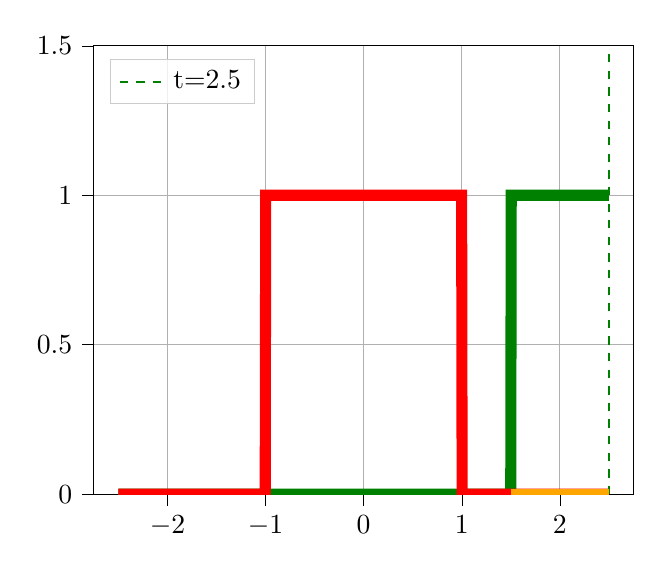
\begin{tikzpicture}

\definecolor{color0}{rgb}{1,0.498039215686275,0.0549019607843137}
\definecolor{color1}{rgb}{1,0.647058823529412,0}

\begin{axis}[
legend cell align={left},
legend style={fill opacity=0.8, draw opacity=1, text opacity=1, at={(0.03,0.97)}, anchor=north west, draw=white!80!black},
tick align=outside,
tick pos=left,
x grid style={white!69.0196078431373!black},
xmajorgrids,
xmin=-2.75, xmax=2.75,
xtick style={color=black},
y grid style={white!69.0196078431373!black},
ymajorgrids,
ymin=0, ymax=1.5,
ytick style={color=black}
]
\path [draw=color0, fill=color0, opacity=0.2]
(axis cs:1.504004004004,0)
--(axis cs:1.504004004004,0)
--(axis cs:1.50900900900901,0)
--(axis cs:1.51401401401401,0)
--(axis cs:1.51901901901902,0)
--(axis cs:1.52402402402402,0)
--(axis cs:1.52902902902903,0)
--(axis cs:1.53403403403403,0)
--(axis cs:1.53903903903904,0)
--(axis cs:1.54404404404404,0)
--(axis cs:1.54904904904905,0)
--(axis cs:1.55405405405405,0)
--(axis cs:1.55905905905906,0)
--(axis cs:1.56406406406406,0)
--(axis cs:1.56906906906907,0)
--(axis cs:1.57407407407407,0)
--(axis cs:1.57907907907908,0)
--(axis cs:1.58408408408408,0)
--(axis cs:1.58908908908909,0)
--(axis cs:1.59409409409409,0)
--(axis cs:1.5990990990991,0)
--(axis cs:1.6041041041041,0)
--(axis cs:1.60910910910911,0)
--(axis cs:1.61411411411411,0)
--(axis cs:1.61911911911912,0)
--(axis cs:1.62412412412412,0)
--(axis cs:1.62912912912913,0)
--(axis cs:1.63413413413413,0)
--(axis cs:1.63913913913914,0)
--(axis cs:1.64414414414414,0)
--(axis cs:1.64914914914915,0)
--(axis cs:1.65415415415415,0)
--(axis cs:1.65915915915916,0)
--(axis cs:1.66416416416416,0)
--(axis cs:1.66916916916917,0)
--(axis cs:1.67417417417417,0)
--(axis cs:1.67917917917918,0)
--(axis cs:1.68418418418418,0)
--(axis cs:1.68918918918919,0)
--(axis cs:1.69419419419419,0)
--(axis cs:1.6991991991992,0)
--(axis cs:1.7042042042042,0)
--(axis cs:1.70920920920921,0)
--(axis cs:1.71421421421421,0)
--(axis cs:1.71921921921922,0)
--(axis cs:1.72422422422422,0)
--(axis cs:1.72922922922923,0)
--(axis cs:1.73423423423423,0)
--(axis cs:1.73923923923924,0)
--(axis cs:1.74424424424424,0)
--(axis cs:1.74924924924925,0)
--(axis cs:1.75425425425425,0)
--(axis cs:1.75925925925926,0)
--(axis cs:1.76426426426426,0)
--(axis cs:1.76926926926927,0)
--(axis cs:1.77427427427427,0)
--(axis cs:1.77927927927928,0)
--(axis cs:1.78428428428428,0)
--(axis cs:1.78928928928929,0)
--(axis cs:1.79429429429429,0)
--(axis cs:1.7992992992993,0)
--(axis cs:1.8043043043043,0)
--(axis cs:1.80930930930931,0)
--(axis cs:1.81431431431431,0)
--(axis cs:1.81931931931932,0)
--(axis cs:1.82432432432432,0)
--(axis cs:1.82932932932933,0)
--(axis cs:1.83433433433433,0)
--(axis cs:1.83933933933934,0)
--(axis cs:1.84434434434434,0)
--(axis cs:1.84934934934935,0)
--(axis cs:1.85435435435435,0)
--(axis cs:1.85935935935936,0)
--(axis cs:1.86436436436436,0)
--(axis cs:1.86936936936937,0)
--(axis cs:1.87437437437437,0)
--(axis cs:1.87937937937938,0)
--(axis cs:1.88438438438438,0)
--(axis cs:1.88938938938939,0)
--(axis cs:1.89439439439439,0)
--(axis cs:1.8993993993994,0)
--(axis cs:1.9044044044044,0)
--(axis cs:1.90940940940941,0)
--(axis cs:1.91441441441441,0)
--(axis cs:1.91941941941942,0)
--(axis cs:1.92442442442442,0)
--(axis cs:1.92942942942943,0)
--(axis cs:1.93443443443443,0)
--(axis cs:1.93943943943944,0)
--(axis cs:1.94444444444444,0)
--(axis cs:1.94944944944945,0)
--(axis cs:1.95445445445445,0)
--(axis cs:1.95945945945946,0)
--(axis cs:1.96446446446446,0)
--(axis cs:1.96946946946947,0)
--(axis cs:1.97447447447447,0)
--(axis cs:1.97947947947948,0)
--(axis cs:1.98448448448448,0)
--(axis cs:1.98948948948949,0)
--(axis cs:1.99449449449449,0)
--(axis cs:1.9994994994995,0)
--(axis cs:2.0045045045045,0)
--(axis cs:2.00950950950951,0)
--(axis cs:2.01451451451451,0)
--(axis cs:2.01951951951952,0)
--(axis cs:2.02452452452452,0)
--(axis cs:2.02952952952953,0)
--(axis cs:2.03453453453453,0)
--(axis cs:2.03953953953954,0)
--(axis cs:2.04454454454454,0)
--(axis cs:2.04954954954955,0)
--(axis cs:2.05455455455455,0)
--(axis cs:2.05955955955956,0)
--(axis cs:2.06456456456456,0)
--(axis cs:2.06956956956957,0)
--(axis cs:2.07457457457457,0)
--(axis cs:2.07957957957958,0)
--(axis cs:2.08458458458458,0)
--(axis cs:2.08958958958959,0)
--(axis cs:2.09459459459459,0)
--(axis cs:2.0995995995996,0)
--(axis cs:2.1046046046046,0)
--(axis cs:2.10960960960961,0)
--(axis cs:2.11461461461461,0)
--(axis cs:2.11961961961962,0)
--(axis cs:2.12462462462462,0)
--(axis cs:2.12962962962963,0)
--(axis cs:2.13463463463463,0)
--(axis cs:2.13963963963964,0)
--(axis cs:2.14464464464464,0)
--(axis cs:2.14964964964965,0)
--(axis cs:2.15465465465465,0)
--(axis cs:2.15965965965966,0)
--(axis cs:2.16466466466466,0)
--(axis cs:2.16966966966967,0)
--(axis cs:2.17467467467467,0)
--(axis cs:2.17967967967968,0)
--(axis cs:2.18468468468468,0)
--(axis cs:2.18968968968969,0)
--(axis cs:2.19469469469469,0)
--(axis cs:2.1996996996997,0)
--(axis cs:2.2047047047047,0)
--(axis cs:2.20970970970971,0)
--(axis cs:2.21471471471471,0)
--(axis cs:2.21971971971972,0)
--(axis cs:2.22472472472472,0)
--(axis cs:2.22972972972973,0)
--(axis cs:2.23473473473473,0)
--(axis cs:2.23973973973974,0)
--(axis cs:2.24474474474474,0)
--(axis cs:2.24974974974975,0)
--(axis cs:2.25475475475475,0)
--(axis cs:2.25975975975976,0)
--(axis cs:2.26476476476476,0)
--(axis cs:2.26976976976977,0)
--(axis cs:2.27477477477477,0)
--(axis cs:2.27977977977978,0)
--(axis cs:2.28478478478478,0)
--(axis cs:2.28978978978979,0)
--(axis cs:2.29479479479479,0)
--(axis cs:2.2997997997998,0)
--(axis cs:2.3048048048048,0)
--(axis cs:2.30980980980981,0)
--(axis cs:2.31481481481481,0)
--(axis cs:2.31981981981982,0)
--(axis cs:2.32482482482482,0)
--(axis cs:2.32982982982983,0)
--(axis cs:2.33483483483483,0)
--(axis cs:2.33983983983984,0)
--(axis cs:2.34484484484484,0)
--(axis cs:2.34984984984985,0)
--(axis cs:2.35485485485485,0)
--(axis cs:2.35985985985986,0)
--(axis cs:2.36486486486486,0)
--(axis cs:2.36986986986987,0)
--(axis cs:2.37487487487487,0)
--(axis cs:2.37987987987988,0)
--(axis cs:2.38488488488488,0)
--(axis cs:2.38988988988989,0)
--(axis cs:2.39489489489489,0)
--(axis cs:2.3998998998999,0)
--(axis cs:2.4049049049049,0)
--(axis cs:2.40990990990991,0)
--(axis cs:2.41491491491491,0)
--(axis cs:2.41991991991992,0)
--(axis cs:2.42492492492492,0)
--(axis cs:2.42992992992993,0)
--(axis cs:2.43493493493493,0)
--(axis cs:2.43993993993994,0)
--(axis cs:2.44494494494494,0)
--(axis cs:2.44994994994995,0)
--(axis cs:2.45495495495495,0)
--(axis cs:2.45995995995996,0)
--(axis cs:2.46496496496496,0)
--(axis cs:2.46996996996997,0)
--(axis cs:2.47497497497497,0)
--(axis cs:2.47997997997998,0)
--(axis cs:2.48498498498498,0)
--(axis cs:2.48998998998999,0)
--(axis cs:2.49499499499499,0)
--(axis cs:2.49499499499499,0)
--(axis cs:2.49499499499499,0)
--(axis cs:2.48998998998999,0)
--(axis cs:2.48498498498498,0)
--(axis cs:2.47997997997998,0)
--(axis cs:2.47497497497497,0)
--(axis cs:2.46996996996997,0)
--(axis cs:2.46496496496496,0)
--(axis cs:2.45995995995996,0)
--(axis cs:2.45495495495495,0)
--(axis cs:2.44994994994995,0)
--(axis cs:2.44494494494494,0)
--(axis cs:2.43993993993994,0)
--(axis cs:2.43493493493493,0)
--(axis cs:2.42992992992993,0)
--(axis cs:2.42492492492492,0)
--(axis cs:2.41991991991992,0)
--(axis cs:2.41491491491491,0)
--(axis cs:2.40990990990991,0)
--(axis cs:2.4049049049049,0)
--(axis cs:2.3998998998999,0)
--(axis cs:2.39489489489489,0)
--(axis cs:2.38988988988989,0)
--(axis cs:2.38488488488488,0)
--(axis cs:2.37987987987988,0)
--(axis cs:2.37487487487487,0)
--(axis cs:2.36986986986987,0)
--(axis cs:2.36486486486486,0)
--(axis cs:2.35985985985986,0)
--(axis cs:2.35485485485485,0)
--(axis cs:2.34984984984985,0)
--(axis cs:2.34484484484484,0)
--(axis cs:2.33983983983984,0)
--(axis cs:2.33483483483483,0)
--(axis cs:2.32982982982983,0)
--(axis cs:2.32482482482482,0)
--(axis cs:2.31981981981982,0)
--(axis cs:2.31481481481481,0)
--(axis cs:2.30980980980981,0)
--(axis cs:2.3048048048048,0)
--(axis cs:2.2997997997998,0)
--(axis cs:2.29479479479479,0)
--(axis cs:2.28978978978979,0)
--(axis cs:2.28478478478478,0)
--(axis cs:2.27977977977978,0)
--(axis cs:2.27477477477477,0)
--(axis cs:2.26976976976977,0)
--(axis cs:2.26476476476476,0)
--(axis cs:2.25975975975976,0)
--(axis cs:2.25475475475475,0)
--(axis cs:2.24974974974975,0)
--(axis cs:2.24474474474474,0)
--(axis cs:2.23973973973974,0)
--(axis cs:2.23473473473473,0)
--(axis cs:2.22972972972973,0)
--(axis cs:2.22472472472472,0)
--(axis cs:2.21971971971972,0)
--(axis cs:2.21471471471471,0)
--(axis cs:2.20970970970971,0)
--(axis cs:2.2047047047047,0)
--(axis cs:2.1996996996997,0)
--(axis cs:2.19469469469469,0)
--(axis cs:2.18968968968969,0)
--(axis cs:2.18468468468468,0)
--(axis cs:2.17967967967968,0)
--(axis cs:2.17467467467467,0)
--(axis cs:2.16966966966967,0)
--(axis cs:2.16466466466466,0)
--(axis cs:2.15965965965966,0)
--(axis cs:2.15465465465465,0)
--(axis cs:2.14964964964965,0)
--(axis cs:2.14464464464464,0)
--(axis cs:2.13963963963964,0)
--(axis cs:2.13463463463463,0)
--(axis cs:2.12962962962963,0)
--(axis cs:2.12462462462462,0)
--(axis cs:2.11961961961962,0)
--(axis cs:2.11461461461461,0)
--(axis cs:2.10960960960961,0)
--(axis cs:2.1046046046046,0)
--(axis cs:2.0995995995996,0)
--(axis cs:2.09459459459459,0)
--(axis cs:2.08958958958959,0)
--(axis cs:2.08458458458458,0)
--(axis cs:2.07957957957958,0)
--(axis cs:2.07457457457457,0)
--(axis cs:2.06956956956957,0)
--(axis cs:2.06456456456456,0)
--(axis cs:2.05955955955956,0)
--(axis cs:2.05455455455455,0)
--(axis cs:2.04954954954955,0)
--(axis cs:2.04454454454454,0)
--(axis cs:2.03953953953954,0)
--(axis cs:2.03453453453453,0)
--(axis cs:2.02952952952953,0)
--(axis cs:2.02452452452452,0)
--(axis cs:2.01951951951952,0)
--(axis cs:2.01451451451451,0)
--(axis cs:2.00950950950951,0)
--(axis cs:2.0045045045045,0)
--(axis cs:1.9994994994995,0)
--(axis cs:1.99449449449449,0)
--(axis cs:1.98948948948949,0)
--(axis cs:1.98448448448448,0)
--(axis cs:1.97947947947948,0)
--(axis cs:1.97447447447447,0)
--(axis cs:1.96946946946947,0)
--(axis cs:1.96446446446446,0)
--(axis cs:1.95945945945946,0)
--(axis cs:1.95445445445445,0)
--(axis cs:1.94944944944945,0)
--(axis cs:1.94444444444444,0)
--(axis cs:1.93943943943944,0)
--(axis cs:1.93443443443443,0)
--(axis cs:1.92942942942943,0)
--(axis cs:1.92442442442442,0)
--(axis cs:1.91941941941942,0)
--(axis cs:1.91441441441441,0)
--(axis cs:1.90940940940941,0)
--(axis cs:1.9044044044044,0)
--(axis cs:1.8993993993994,0)
--(axis cs:1.89439439439439,0)
--(axis cs:1.88938938938939,0)
--(axis cs:1.88438438438438,0)
--(axis cs:1.87937937937938,0)
--(axis cs:1.87437437437437,0)
--(axis cs:1.86936936936937,0)
--(axis cs:1.86436436436436,0)
--(axis cs:1.85935935935936,0)
--(axis cs:1.85435435435435,0)
--(axis cs:1.84934934934935,0)
--(axis cs:1.84434434434434,0)
--(axis cs:1.83933933933934,0)
--(axis cs:1.83433433433433,0)
--(axis cs:1.82932932932933,0)
--(axis cs:1.82432432432432,0)
--(axis cs:1.81931931931932,0)
--(axis cs:1.81431431431431,0)
--(axis cs:1.80930930930931,0)
--(axis cs:1.8043043043043,0)
--(axis cs:1.7992992992993,0)
--(axis cs:1.79429429429429,0)
--(axis cs:1.78928928928929,0)
--(axis cs:1.78428428428428,0)
--(axis cs:1.77927927927928,0)
--(axis cs:1.77427427427427,0)
--(axis cs:1.76926926926927,0)
--(axis cs:1.76426426426426,0)
--(axis cs:1.75925925925926,0)
--(axis cs:1.75425425425425,0)
--(axis cs:1.74924924924925,0)
--(axis cs:1.74424424424424,0)
--(axis cs:1.73923923923924,0)
--(axis cs:1.73423423423423,0)
--(axis cs:1.72922922922923,0)
--(axis cs:1.72422422422422,0)
--(axis cs:1.71921921921922,0)
--(axis cs:1.71421421421421,0)
--(axis cs:1.70920920920921,0)
--(axis cs:1.7042042042042,0)
--(axis cs:1.6991991991992,0)
--(axis cs:1.69419419419419,0)
--(axis cs:1.68918918918919,0)
--(axis cs:1.68418418418418,0)
--(axis cs:1.67917917917918,0)
--(axis cs:1.67417417417417,0)
--(axis cs:1.66916916916917,0)
--(axis cs:1.66416416416416,0)
--(axis cs:1.65915915915916,0)
--(axis cs:1.65415415415415,0)
--(axis cs:1.64914914914915,0)
--(axis cs:1.64414414414414,0)
--(axis cs:1.63913913913914,0)
--(axis cs:1.63413413413413,0)
--(axis cs:1.62912912912913,0)
--(axis cs:1.62412412412412,0)
--(axis cs:1.61911911911912,0)
--(axis cs:1.61411411411411,0)
--(axis cs:1.60910910910911,0)
--(axis cs:1.6041041041041,0)
--(axis cs:1.5990990990991,0)
--(axis cs:1.59409409409409,0)
--(axis cs:1.58908908908909,0)
--(axis cs:1.58408408408408,0)
--(axis cs:1.57907907907908,0)
--(axis cs:1.57407407407407,0)
--(axis cs:1.56906906906907,0)
--(axis cs:1.56406406406406,0)
--(axis cs:1.55905905905906,0)
--(axis cs:1.55405405405405,0)
--(axis cs:1.54904904904905,0)
--(axis cs:1.54404404404404,0)
--(axis cs:1.53903903903904,0)
--(axis cs:1.53403403403403,0)
--(axis cs:1.52902902902903,0)
--(axis cs:1.52402402402402,0)
--(axis cs:1.51901901901902,0)
--(axis cs:1.51401401401401,0)
--(axis cs:1.50900900900901,0)
--(axis cs:1.504004004004,0)
--cycle;

\addplot [line width=4pt, green!50!black, forget plot]
table {%
-2.5 0
-2.49499499499499 0
-2.48998998998999 0
-2.48498498498498 0
-2.47997997997998 0
-2.47497497497497 0
-2.46996996996997 0
-2.46496496496496 0
-2.45995995995996 0
-2.45495495495495 0
-2.44994994994995 0
-2.44494494494494 0
-2.43993993993994 0
-2.43493493493493 0
-2.42992992992993 0
-2.42492492492492 0
-2.41991991991992 0
-2.41491491491491 0
-2.40990990990991 0
-2.4049049049049 0
-2.3998998998999 0
-2.39489489489489 0
-2.38988988988989 0
-2.38488488488488 0
-2.37987987987988 0
-2.37487487487487 0
-2.36986986986987 0
-2.36486486486486 0
-2.35985985985986 0
-2.35485485485485 0
-2.34984984984985 0
-2.34484484484484 0
-2.33983983983984 0
-2.33483483483483 0
-2.32982982982983 0
-2.32482482482482 0
-2.31981981981982 0
-2.31481481481481 0
-2.30980980980981 0
-2.3048048048048 0
-2.2997997997998 0
-2.29479479479479 0
-2.28978978978979 0
-2.28478478478478 0
-2.27977977977978 0
-2.27477477477477 0
-2.26976976976977 0
-2.26476476476476 0
-2.25975975975976 0
-2.25475475475475 0
-2.24974974974975 0
-2.24474474474474 0
-2.23973973973974 0
-2.23473473473473 0
-2.22972972972973 0
-2.22472472472472 0
-2.21971971971972 0
-2.21471471471471 0
-2.20970970970971 0
-2.2047047047047 0
-2.1996996996997 0
-2.19469469469469 0
-2.18968968968969 0
-2.18468468468468 0
-2.17967967967968 0
-2.17467467467467 0
-2.16966966966967 0
-2.16466466466466 0
-2.15965965965966 0
-2.15465465465465 0
-2.14964964964965 0
-2.14464464464464 0
-2.13963963963964 0
-2.13463463463463 0
-2.12962962962963 0
-2.12462462462462 0
-2.11961961961962 0
-2.11461461461461 0
-2.10960960960961 0
-2.1046046046046 0
-2.0995995995996 0
-2.09459459459459 0
-2.08958958958959 0
-2.08458458458458 0
-2.07957957957958 0
-2.07457457457457 0
-2.06956956956957 0
-2.06456456456456 0
-2.05955955955956 0
-2.05455455455455 0
-2.04954954954955 0
-2.04454454454454 0
-2.03953953953954 0
-2.03453453453453 0
-2.02952952952953 0
-2.02452452452452 0
-2.01951951951952 0
-2.01451451451451 0
-2.00950950950951 0
-2.0045045045045 0
-1.9994994994995 0
-1.99449449449449 0
-1.98948948948949 0
-1.98448448448448 0
-1.97947947947948 0
-1.97447447447447 0
-1.96946946946947 0
-1.96446446446446 0
-1.95945945945946 0
-1.95445445445445 0
-1.94944944944945 0
-1.94444444444444 0
-1.93943943943944 0
-1.93443443443443 0
-1.92942942942943 0
-1.92442442442442 0
-1.91941941941942 0
-1.91441441441441 0
-1.90940940940941 0
-1.9044044044044 0
-1.8993993993994 0
-1.89439439439439 0
-1.88938938938939 0
-1.88438438438438 0
-1.87937937937938 0
-1.87437437437437 0
-1.86936936936937 0
-1.86436436436436 0
-1.85935935935936 0
-1.85435435435435 0
-1.84934934934935 0
-1.84434434434434 0
-1.83933933933934 0
-1.83433433433433 0
-1.82932932932933 0
-1.82432432432432 0
-1.81931931931932 0
-1.81431431431431 0
-1.80930930930931 0
-1.8043043043043 0
-1.7992992992993 0
-1.79429429429429 0
-1.78928928928929 0
-1.78428428428428 0
-1.77927927927928 0
-1.77427427427427 0
-1.76926926926927 0
-1.76426426426426 0
-1.75925925925926 0
-1.75425425425425 0
-1.74924924924925 0
-1.74424424424424 0
-1.73923923923924 0
-1.73423423423423 0
-1.72922922922923 0
-1.72422422422422 0
-1.71921921921922 0
-1.71421421421421 0
-1.70920920920921 0
-1.7042042042042 0
-1.6991991991992 0
-1.69419419419419 0
-1.68918918918919 0
-1.68418418418418 0
-1.67917917917918 0
-1.67417417417417 0
-1.66916916916917 0
-1.66416416416416 0
-1.65915915915916 0
-1.65415415415415 0
-1.64914914914915 0
-1.64414414414414 0
-1.63913913913914 0
-1.63413413413413 0
-1.62912912912913 0
-1.62412412412412 0
-1.61911911911912 0
-1.61411411411411 0
-1.60910910910911 0
-1.6041041041041 0
-1.5990990990991 0
-1.59409409409409 0
-1.58908908908909 0
-1.58408408408408 0
-1.57907907907908 0
-1.57407407407407 0
-1.56906906906907 0
-1.56406406406406 0
-1.55905905905906 0
-1.55405405405405 0
-1.54904904904905 0
-1.54404404404404 0
-1.53903903903904 0
-1.53403403403403 0
-1.52902902902903 0
-1.52402402402402 0
-1.51901901901902 0
-1.51401401401401 0
-1.50900900900901 0
-1.504004004004 0
-1.498998998999 0
-1.49399399399399 0
-1.48898898898899 0
-1.48398398398398 0
-1.47897897897898 0
-1.47397397397397 0
-1.46896896896897 0
-1.46396396396396 0
-1.45895895895896 0
-1.45395395395395 0
-1.44894894894895 0
-1.44394394394394 0
-1.43893893893894 0
-1.43393393393393 0
-1.42892892892893 0
-1.42392392392392 0
-1.41891891891892 0
-1.41391391391391 0
-1.40890890890891 0
-1.4039039039039 0
-1.3988988988989 0
-1.39389389389389 0
-1.38888888888889 0
-1.38388388388388 0
-1.37887887887888 0
-1.37387387387387 0
-1.36886886886887 0
-1.36386386386386 0
-1.35885885885886 0
-1.35385385385385 0
-1.34884884884885 0
-1.34384384384384 0
-1.33883883883884 0
-1.33383383383383 0
-1.32882882882883 0
-1.32382382382382 0
-1.31881881881882 0
-1.31381381381381 0
-1.30880880880881 0
-1.3038038038038 0
-1.2987987987988 0
-1.29379379379379 0
-1.28878878878879 0
-1.28378378378378 0
-1.27877877877878 0
-1.27377377377377 0
-1.26876876876877 0
-1.26376376376376 0
-1.25875875875876 0
-1.25375375375375 0
-1.24874874874875 0
-1.24374374374374 0
-1.23873873873874 0
-1.23373373373373 0
-1.22872872872873 0
-1.22372372372372 0
-1.21871871871872 0
-1.21371371371371 0
-1.20870870870871 0
-1.2037037037037 0
-1.1986986986987 0
-1.19369369369369 0
-1.18868868868869 0
-1.18368368368368 0
-1.17867867867868 0
-1.17367367367367 0
-1.16866866866867 0
-1.16366366366366 0
-1.15865865865866 0
-1.15365365365365 0
-1.14864864864865 0
-1.14364364364364 0
-1.13863863863864 0
-1.13363363363363 0
-1.12862862862863 0
-1.12362362362362 0
-1.11861861861862 0
-1.11361361361361 0
-1.10860860860861 0
-1.1036036036036 0
-1.0985985985986 0
-1.09359359359359 0
-1.08858858858859 0
-1.08358358358358 0
-1.07857857857858 0
-1.07357357357357 0
-1.06856856856857 0
-1.06356356356356 0
-1.05855855855856 0
-1.05355355355355 0
-1.04854854854855 0
-1.04354354354354 0
-1.03853853853854 0
-1.03353353353353 0
-1.02852852852853 0
-1.02352352352352 0
-1.01851851851852 0
-1.01351351351351 0
-1.00850850850851 0
-1.0035035035035 0
-0.998498498498499 0
-0.993493493493494 0
-0.988488488488489 0
-0.983483483483484 0
-0.978478478478479 0
-0.973473473473474 0
-0.968468468468469 0
-0.963463463463464 0
-0.958458458458459 0
-0.953453453453454 0
-0.948448448448449 0
-0.943443443443444 0
-0.938438438438439 0
-0.933433433433434 0
-0.928428428428429 0
-0.923423423423424 0
-0.918418418418419 0
-0.913413413413414 0
-0.908408408408409 0
-0.903403403403404 0
-0.898398398398399 0
-0.893393393393393 0
-0.888388388388388 0
-0.883383383383383 0
-0.878378378378378 0
-0.873373373373373 0
-0.868368368368368 0
-0.863363363363363 0
-0.858358358358358 0
-0.853353353353353 0
-0.848348348348348 0
-0.843343343343343 0
-0.838338338338338 0
-0.833333333333333 0
-0.828328328328328 0
-0.823323323323323 0
-0.818318318318318 0
-0.813313313313313 0
-0.808308308308308 0
-0.803303303303303 0
-0.798298298298298 0
-0.793293293293293 0
-0.788288288288288 0
-0.783283283283283 0
-0.778278278278278 0
-0.773273273273273 0
-0.768268268268268 0
-0.763263263263263 0
-0.758258258258258 0
-0.753253253253253 0
-0.748248248248248 0
-0.743243243243243 0
-0.738238238238238 0
-0.733233233233233 0
-0.728228228228228 0
-0.723223223223223 0
-0.718218218218218 0
-0.713213213213213 0
-0.708208208208208 0
-0.703203203203203 0
-0.698198198198198 0
-0.693193193193193 0
-0.688188188188188 0
-0.683183183183183 0
-0.678178178178178 0
-0.673173173173173 0
-0.668168168168168 0
-0.663163163163163 0
-0.658158158158158 0
-0.653153153153153 0
-0.648148148148148 0
-0.643143143143143 0
-0.638138138138138 0
-0.633133133133133 0
-0.628128128128128 0
-0.623123123123123 0
-0.618118118118118 0
-0.613113113113113 0
-0.608108108108108 0
-0.603103103103103 0
-0.598098098098098 0
-0.593093093093093 0
-0.588088088088088 0
-0.583083083083083 0
-0.578078078078078 0
-0.573073073073073 0
-0.568068068068068 0
-0.563063063063063 0
-0.558058058058058 0
-0.553053053053053 0
-0.548048048048048 0
-0.543043043043043 0
-0.538038038038038 0
-0.533033033033033 0
-0.528028028028028 0
-0.523023023023023 0
-0.518018018018018 0
-0.513013013013013 0
-0.508008008008008 0
-0.503003003003003 0
-0.497997997997998 0
-0.492992992992993 0
-0.487987987987988 0
-0.482982982982983 0
-0.477977977977978 0
-0.472972972972973 0
-0.467967967967968 0
-0.462962962962963 0
-0.457957957957958 0
-0.452952952952953 0
-0.447947947947948 0
-0.442942942942943 0
-0.437937937937938 0
-0.432932932932933 0
-0.427927927927928 0
-0.422922922922923 0
-0.417917917917918 0
-0.412912912912913 0
-0.407907907907908 0
-0.402902902902903 0
-0.397897897897898 0
-0.392892892892893 0
-0.387887887887888 0
-0.382882882882883 0
-0.377877877877878 0
-0.372872872872873 0
-0.367867867867868 0
-0.362862862862863 0
-0.357857857857858 0
-0.352852852852853 0
-0.347847847847848 0
-0.342842842842843 0
-0.337837837837838 0
-0.332832832832833 0
-0.327827827827828 0
-0.322822822822823 0
-0.317817817817818 0
-0.312812812812813 0
-0.307807807807808 0
-0.302802802802803 0
-0.297797797797798 0
-0.292792792792793 0
-0.287787787787788 0
-0.282782782782783 0
-0.277777777777778 0
-0.272772772772773 0
-0.267767767767768 0
-0.262762762762763 0
-0.257757757757758 0
-0.252752752752753 0
-0.247747747747748 0
-0.242742742742743 0
-0.237737737737738 0
-0.232732732732733 0
-0.227727727727728 0
-0.222722722722723 0
-0.217717717717718 0
-0.212712712712713 0
-0.207707707707708 0
-0.202702702702703 0
-0.197697697697698 0
-0.192692692692693 0
-0.187687687687688 0
-0.182682682682683 0
-0.177677677677678 0
-0.172672672672673 0
-0.167667667667668 0
-0.162662662662663 0
-0.157657657657658 0
-0.152652652652653 0
-0.147647647647648 0
-0.142642642642643 0
-0.137637637637638 0
-0.132632632632633 0
-0.127627627627628 0
-0.122622622622623 0
-0.117617617617618 0
-0.112612612612613 0
-0.107607607607608 0
-0.102602602602603 0
-0.0975975975975976 0
-0.0925925925925926 0
-0.0875875875875876 0
-0.0825825825825826 0
-0.0775775775775776 0
-0.0725725725725725 0
-0.0675675675675675 0
-0.0625625625625625 0
-0.0575575575575575 0
-0.0525525525525525 0
-0.0475475475475475 0
-0.0425425425425425 0
-0.0375375375375375 0
-0.0325325325325325 0
-0.0275275275275275 0
-0.0225225225225225 0
-0.0175175175175175 0
-0.0125125125125125 0
-0.0075075075075075 0
-0.0025025025025025 0
0.0025025025025025 0
0.0075075075075075 0
0.0125125125125125 0
0.0175175175175175 0
0.0225225225225225 0
0.0275275275275275 0
0.0325325325325325 0
0.0375375375375375 0
0.0425425425425425 0
0.0475475475475475 0
0.0525525525525525 0
0.0575575575575575 0
0.0625625625625625 0
0.0675675675675675 0
0.0725725725725725 0
0.0775775775775776 0
0.0825825825825826 0
0.0875875875875876 0
0.0925925925925926 0
0.0975975975975976 0
0.102602602602603 0
0.107607607607608 0
0.112612612612613 0
0.117617617617618 0
0.122622622622623 0
0.127627627627628 0
0.132632632632633 0
0.137637637637638 0
0.142642642642643 0
0.147647647647648 0
0.152652652652653 0
0.157657657657658 0
0.162662662662663 0
0.167667667667668 0
0.172672672672673 0
0.177677677677678 0
0.182682682682683 0
0.187687687687688 0
0.192692692692693 0
0.197697697697698 0
0.202702702702703 0
0.207707707707708 0
0.212712712712713 0
0.217717717717718 0
0.222722722722723 0
0.227727727727728 0
0.232732732732733 0
0.237737737737738 0
0.242742742742743 0
0.247747747747748 0
0.252752752752753 0
0.257757757757758 0
0.262762762762763 0
0.267767767767768 0
0.272772772772773 0
0.277777777777778 0
0.282782782782783 0
0.287787787787788 0
0.292792792792793 0
0.297797797797798 0
0.302802802802803 0
0.307807807807808 0
0.312812812812813 0
0.317817817817818 0
0.322822822822823 0
0.327827827827828 0
0.332832832832833 0
0.337837837837838 0
0.342842842842843 0
0.347847847847848 0
0.352852852852853 0
0.357857857857858 0
0.362862862862863 0
0.367867867867868 0
0.372872872872873 0
0.377877877877878 0
0.382882882882883 0
0.387887887887888 0
0.392892892892893 0
0.397897897897898 0
0.402902902902903 0
0.407907907907908 0
0.412912912912913 0
0.417917917917918 0
0.422922922922923 0
0.427927927927928 0
0.432932932932933 0
0.437937937937938 0
0.442942942942943 0
0.447947947947948 0
0.452952952952953 0
0.457957957957958 0
0.462962962962963 0
0.467967967967968 0
0.472972972972973 0
0.477977977977978 0
0.482982982982983 0
0.487987987987988 0
0.492992992992993 0
0.497997997997998 0
0.503003003003003 0
0.508008008008008 0
0.513013013013013 0
0.518018018018018 0
0.523023023023023 0
0.528028028028028 0
0.533033033033033 0
0.538038038038038 0
0.543043043043043 0
0.548048048048048 0
0.553053053053053 0
0.558058058058058 0
0.563063063063063 0
0.568068068068068 0
0.573073073073073 0
0.578078078078078 0
0.583083083083083 0
0.588088088088088 0
0.593093093093093 0
0.598098098098098 0
0.603103103103103 0
0.608108108108108 0
0.613113113113113 0
0.618118118118118 0
0.623123123123123 0
0.628128128128128 0
0.633133133133133 0
0.638138138138138 0
0.643143143143143 0
0.648148148148148 0
0.653153153153153 0
0.658158158158158 0
0.663163163163163 0
0.668168168168168 0
0.673173173173173 0
0.678178178178178 0
0.683183183183183 0
0.688188188188188 0
0.693193193193193 0
0.698198198198198 0
0.703203203203203 0
0.708208208208208 0
0.713213213213213 0
0.718218218218218 0
0.723223223223223 0
0.728228228228228 0
0.733233233233233 0
0.738238238238238 0
0.743243243243243 0
0.748248248248248 0
0.753253253253253 0
0.758258258258258 0
0.763263263263263 0
0.768268268268268 0
0.773273273273273 0
0.778278278278278 0
0.783283283283283 0
0.788288288288288 0
0.793293293293293 0
0.798298298298298 0
0.803303303303303 0
0.808308308308308 0
0.813313313313313 0
0.818318318318318 0
0.823323323323323 0
0.828328328328328 0
0.833333333333333 0
0.838338338338338 0
0.843343343343343 0
0.848348348348348 0
0.853353353353353 0
0.858358358358358 0
0.863363363363364 0
0.868368368368369 0
0.873373373373374 0
0.878378378378379 0
0.883383383383384 0
0.888388388388389 0
0.893393393393394 0
0.898398398398399 0
0.903403403403404 0
0.908408408408409 0
0.913413413413414 0
0.918418418418419 0
0.923423423423424 0
0.928428428428429 0
0.933433433433434 0
0.938438438438439 0
0.943443443443444 0
0.948448448448449 0
0.953453453453454 0
0.958458458458459 0
0.963463463463464 0
0.968468468468469 0
0.973473473473474 0
0.978478478478479 0
0.983483483483484 0
0.988488488488489 0
0.993493493493494 0
0.998498498498499 0
1.0035035035035 0
1.00850850850851 0
1.01351351351351 0
1.01851851851852 0
1.02352352352352 0
1.02852852852853 0
1.03353353353353 0
1.03853853853854 0
1.04354354354354 0
1.04854854854855 0
1.05355355355355 0
1.05855855855856 0
1.06356356356356 0
1.06856856856857 0
1.07357357357357 0
1.07857857857858 0
1.08358358358358 0
1.08858858858859 0
1.09359359359359 0
1.0985985985986 0
1.1036036036036 0
1.10860860860861 0
1.11361361361361 0
1.11861861861862 0
1.12362362362362 0
1.12862862862863 0
1.13363363363363 0
1.13863863863864 0
1.14364364364364 0
1.14864864864865 0
1.15365365365365 0
1.15865865865866 0
1.16366366366366 0
1.16866866866867 0
1.17367367367367 0
1.17867867867868 0
1.18368368368368 0
1.18868868868869 0
1.19369369369369 0
1.1986986986987 0
1.2037037037037 0
1.20870870870871 0
1.21371371371371 0
1.21871871871872 0
1.22372372372372 0
1.22872872872873 0
1.23373373373373 0
1.23873873873874 0
1.24374374374374 0
1.24874874874875 0
1.25375375375375 0
1.25875875875876 0
1.26376376376376 0
1.26876876876877 0
1.27377377377377 0
1.27877877877878 0
1.28378378378378 0
1.28878878878879 0
1.29379379379379 0
1.2987987987988 0
1.3038038038038 0
1.30880880880881 0
1.31381381381381 0
1.31881881881882 0
1.32382382382382 0
1.32882882882883 0
1.33383383383383 0
1.33883883883884 0
1.34384384384384 0
1.34884884884885 0
1.35385385385385 0
1.35885885885886 0
1.36386386386386 0
1.36886886886887 0
1.37387387387387 0
1.37887887887888 0
1.38388388388388 0
1.38888888888889 0
1.39389389389389 0
1.3988988988989 0
1.4039039039039 0
1.40890890890891 0
1.41391391391391 0
1.41891891891892 0
1.42392392392392 0
1.42892892892893 0
1.43393393393393 0
1.43893893893894 0
1.44394394394394 0
1.44894894894895 0
1.45395395395395 0
1.45895895895896 0
1.46396396396396 0
1.46896896896897 0
1.47397397397397 0
1.47897897897898 0
1.48398398398398 0
1.48898898898899 0
1.49399399399399 0
1.498998998999 0
1.504004004004 1
1.50900900900901 1
1.51401401401401 1
1.51901901901902 1
1.52402402402402 1
1.52902902902903 1
1.53403403403403 1
1.53903903903904 1
1.54404404404404 1
1.54904904904905 1
1.55405405405405 1
1.55905905905906 1
1.56406406406406 1
1.56906906906907 1
1.57407407407407 1
1.57907907907908 1
1.58408408408408 1
1.58908908908909 1
1.59409409409409 1
1.5990990990991 1
1.6041041041041 1
1.60910910910911 1
1.61411411411411 1
1.61911911911912 1
1.62412412412412 1
1.62912912912913 1
1.63413413413413 1
1.63913913913914 1
1.64414414414414 1
1.64914914914915 1
1.65415415415415 1
1.65915915915916 1
1.66416416416416 1
1.66916916916917 1
1.67417417417417 1
1.67917917917918 1
1.68418418418418 1
1.68918918918919 1
1.69419419419419 1
1.6991991991992 1
1.7042042042042 1
1.70920920920921 1
1.71421421421421 1
1.71921921921922 1
1.72422422422422 1
1.72922922922923 1
1.73423423423423 1
1.73923923923924 1
1.74424424424424 1
1.74924924924925 1
1.75425425425425 1
1.75925925925926 1
1.76426426426426 1
1.76926926926927 1
1.77427427427427 1
1.77927927927928 1
1.78428428428428 1
1.78928928928929 1
1.79429429429429 1
1.7992992992993 1
1.8043043043043 1
1.80930930930931 1
1.81431431431431 1
1.81931931931932 1
1.82432432432432 1
1.82932932932933 1
1.83433433433433 1
1.83933933933934 1
1.84434434434434 1
1.84934934934935 1
1.85435435435435 1
1.85935935935936 1
1.86436436436436 1
1.86936936936937 1
1.87437437437437 1
1.87937937937938 1
1.88438438438438 1
1.88938938938939 1
1.89439439439439 1
1.8993993993994 1
1.9044044044044 1
1.90940940940941 1
1.91441441441441 1
1.91941941941942 1
1.92442442442442 1
1.92942942942943 1
1.93443443443443 1
1.93943943943944 1
1.94444444444444 1
1.94944944944945 1
1.95445445445445 1
1.95945945945946 1
1.96446446446446 1
1.96946946946947 1
1.97447447447447 1
1.97947947947948 1
1.98448448448448 1
1.98948948948949 1
1.99449449449449 1
1.9994994994995 1
2.0045045045045 1
2.00950950950951 1
2.01451451451451 1
2.01951951951952 1
2.02452452452452 1
2.02952952952953 1
2.03453453453453 1
2.03953953953954 1
2.04454454454454 1
2.04954954954955 1
2.05455455455455 1
2.05955955955956 1
2.06456456456456 1
2.06956956956957 1
2.07457457457457 1
2.07957957957958 1
2.08458458458458 1
2.08958958958959 1
2.09459459459459 1
2.0995995995996 1
2.1046046046046 1
2.10960960960961 1
2.11461461461461 1
2.11961961961962 1
2.12462462462462 1
2.12962962962963 1
2.13463463463463 1
2.13963963963964 1
2.14464464464464 1
2.14964964964965 1
2.15465465465465 1
2.15965965965966 1
2.16466466466466 1
2.16966966966967 1
2.17467467467467 1
2.17967967967968 1
2.18468468468468 1
2.18968968968969 1
2.19469469469469 1
2.1996996996997 1
2.2047047047047 1
2.20970970970971 1
2.21471471471471 1
2.21971971971972 1
2.22472472472472 1
2.22972972972973 1
2.23473473473473 1
2.23973973973974 1
2.24474474474474 1
2.24974974974975 1
2.25475475475475 1
2.25975975975976 1
2.26476476476476 1
2.26976976976977 1
2.27477477477477 1
2.27977977977978 1
2.28478478478478 1
2.28978978978979 1
2.29479479479479 1
2.2997997997998 1
2.3048048048048 1
2.30980980980981 1
2.31481481481481 1
2.31981981981982 1
2.32482482482482 1
2.32982982982983 1
2.33483483483483 1
2.33983983983984 1
2.34484484484484 1
2.34984984984985 1
2.35485485485485 1
2.35985985985986 1
2.36486486486486 1
2.36986986986987 1
2.37487487487487 1
2.37987987987988 1
2.38488488488488 1
2.38988988988989 1
2.39489489489489 1
2.3998998998999 1
2.4049049049049 1
2.40990990990991 1
2.41491491491491 1
2.41991991991992 1
2.42492492492492 1
2.42992992992993 1
2.43493493493493 1
2.43993993993994 1
2.44494494494494 1
2.44994994994995 1
2.45495495495495 1
2.45995995995996 1
2.46496496496496 1
2.46996996996997 1
2.47497497497497 1
2.47997997997998 1
2.48498498498498 1
2.48998998998999 1
2.49499499499499 1
2.5 1
};
\addplot [line width=4pt, red, forget plot]
table {%
-2.5 0
-2.49499499499499 0
-2.48998998998999 0
-2.48498498498498 0
-2.47997997997998 0
-2.47497497497497 0
-2.46996996996997 0
-2.46496496496496 0
-2.45995995995996 0
-2.45495495495495 0
-2.44994994994995 0
-2.44494494494494 0
-2.43993993993994 0
-2.43493493493493 0
-2.42992992992993 0
-2.42492492492492 0
-2.41991991991992 0
-2.41491491491491 0
-2.40990990990991 0
-2.4049049049049 0
-2.3998998998999 0
-2.39489489489489 0
-2.38988988988989 0
-2.38488488488488 0
-2.37987987987988 0
-2.37487487487487 0
-2.36986986986987 0
-2.36486486486486 0
-2.35985985985986 0
-2.35485485485485 0
-2.34984984984985 0
-2.34484484484484 0
-2.33983983983984 0
-2.33483483483483 0
-2.32982982982983 0
-2.32482482482482 0
-2.31981981981982 0
-2.31481481481481 0
-2.30980980980981 0
-2.3048048048048 0
-2.2997997997998 0
-2.29479479479479 0
-2.28978978978979 0
-2.28478478478478 0
-2.27977977977978 0
-2.27477477477477 0
-2.26976976976977 0
-2.26476476476476 0
-2.25975975975976 0
-2.25475475475475 0
-2.24974974974975 0
-2.24474474474474 0
-2.23973973973974 0
-2.23473473473473 0
-2.22972972972973 0
-2.22472472472472 0
-2.21971971971972 0
-2.21471471471471 0
-2.20970970970971 0
-2.2047047047047 0
-2.1996996996997 0
-2.19469469469469 0
-2.18968968968969 0
-2.18468468468468 0
-2.17967967967968 0
-2.17467467467467 0
-2.16966966966967 0
-2.16466466466466 0
-2.15965965965966 0
-2.15465465465465 0
-2.14964964964965 0
-2.14464464464464 0
-2.13963963963964 0
-2.13463463463463 0
-2.12962962962963 0
-2.12462462462462 0
-2.11961961961962 0
-2.11461461461461 0
-2.10960960960961 0
-2.1046046046046 0
-2.0995995995996 0
-2.09459459459459 0
-2.08958958958959 0
-2.08458458458458 0
-2.07957957957958 0
-2.07457457457457 0
-2.06956956956957 0
-2.06456456456456 0
-2.05955955955956 0
-2.05455455455455 0
-2.04954954954955 0
-2.04454454454454 0
-2.03953953953954 0
-2.03453453453453 0
-2.02952952952953 0
-2.02452452452452 0
-2.01951951951952 0
-2.01451451451451 0
-2.00950950950951 0
-2.0045045045045 0
-1.9994994994995 0
-1.99449449449449 0
-1.98948948948949 0
-1.98448448448448 0
-1.97947947947948 0
-1.97447447447447 0
-1.96946946946947 0
-1.96446446446446 0
-1.95945945945946 0
-1.95445445445445 0
-1.94944944944945 0
-1.94444444444444 0
-1.93943943943944 0
-1.93443443443443 0
-1.92942942942943 0
-1.92442442442442 0
-1.91941941941942 0
-1.91441441441441 0
-1.90940940940941 0
-1.9044044044044 0
-1.8993993993994 0
-1.89439439439439 0
-1.88938938938939 0
-1.88438438438438 0
-1.87937937937938 0
-1.87437437437437 0
-1.86936936936937 0
-1.86436436436436 0
-1.85935935935936 0
-1.85435435435435 0
-1.84934934934935 0
-1.84434434434434 0
-1.83933933933934 0
-1.83433433433433 0
-1.82932932932933 0
-1.82432432432432 0
-1.81931931931932 0
-1.81431431431431 0
-1.80930930930931 0
-1.8043043043043 0
-1.7992992992993 0
-1.79429429429429 0
-1.78928928928929 0
-1.78428428428428 0
-1.77927927927928 0
-1.77427427427427 0
-1.76926926926927 0
-1.76426426426426 0
-1.75925925925926 0
-1.75425425425425 0
-1.74924924924925 0
-1.74424424424424 0
-1.73923923923924 0
-1.73423423423423 0
-1.72922922922923 0
-1.72422422422422 0
-1.71921921921922 0
-1.71421421421421 0
-1.70920920920921 0
-1.7042042042042 0
-1.6991991991992 0
-1.69419419419419 0
-1.68918918918919 0
-1.68418418418418 0
-1.67917917917918 0
-1.67417417417417 0
-1.66916916916917 0
-1.66416416416416 0
-1.65915915915916 0
-1.65415415415415 0
-1.64914914914915 0
-1.64414414414414 0
-1.63913913913914 0
-1.63413413413413 0
-1.62912912912913 0
-1.62412412412412 0
-1.61911911911912 0
-1.61411411411411 0
-1.60910910910911 0
-1.6041041041041 0
-1.5990990990991 0
-1.59409409409409 0
-1.58908908908909 0
-1.58408408408408 0
-1.57907907907908 0
-1.57407407407407 0
-1.56906906906907 0
-1.56406406406406 0
-1.55905905905906 0
-1.55405405405405 0
-1.54904904904905 0
-1.54404404404404 0
-1.53903903903904 0
-1.53403403403403 0
-1.52902902902903 0
-1.52402402402402 0
-1.51901901901902 0
-1.51401401401401 0
-1.50900900900901 0
-1.504004004004 0
-1.498998998999 0
-1.49399399399399 0
-1.48898898898899 0
-1.48398398398398 0
-1.47897897897898 0
-1.47397397397397 0
-1.46896896896897 0
-1.46396396396396 0
-1.45895895895896 0
-1.45395395395395 0
-1.44894894894895 0
-1.44394394394394 0
-1.43893893893894 0
-1.43393393393393 0
-1.42892892892893 0
-1.42392392392392 0
-1.41891891891892 0
-1.41391391391391 0
-1.40890890890891 0
-1.4039039039039 0
-1.3988988988989 0
-1.39389389389389 0
-1.38888888888889 0
-1.38388388388388 0
-1.37887887887888 0
-1.37387387387387 0
-1.36886886886887 0
-1.36386386386386 0
-1.35885885885886 0
-1.35385385385385 0
-1.34884884884885 0
-1.34384384384384 0
-1.33883883883884 0
-1.33383383383383 0
-1.32882882882883 0
-1.32382382382382 0
-1.31881881881882 0
-1.31381381381381 0
-1.30880880880881 0
-1.3038038038038 0
-1.2987987987988 0
-1.29379379379379 0
-1.28878878878879 0
-1.28378378378378 0
-1.27877877877878 0
-1.27377377377377 0
-1.26876876876877 0
-1.26376376376376 0
-1.25875875875876 0
-1.25375375375375 0
-1.24874874874875 0
-1.24374374374374 0
-1.23873873873874 0
-1.23373373373373 0
-1.22872872872873 0
-1.22372372372372 0
-1.21871871871872 0
-1.21371371371371 0
-1.20870870870871 0
-1.2037037037037 0
-1.1986986986987 0
-1.19369369369369 0
-1.18868868868869 0
-1.18368368368368 0
-1.17867867867868 0
-1.17367367367367 0
-1.16866866866867 0
-1.16366366366366 0
-1.15865865865866 0
-1.15365365365365 0
-1.14864864864865 0
-1.14364364364364 0
-1.13863863863864 0
-1.13363363363363 0
-1.12862862862863 0
-1.12362362362362 0
-1.11861861861862 0
-1.11361361361361 0
-1.10860860860861 0
-1.1036036036036 0
-1.0985985985986 0
-1.09359359359359 0
-1.08858858858859 0
-1.08358358358358 0
-1.07857857857858 0
-1.07357357357357 0
-1.06856856856857 0
-1.06356356356356 0
-1.05855855855856 0
-1.05355355355355 0
-1.04854854854855 0
-1.04354354354354 0
-1.03853853853854 0
-1.03353353353353 0
-1.02852852852853 0
-1.02352352352352 0
-1.01851851851852 0
-1.01351351351351 0
-1.00850850850851 0
-1.0035035035035 0
-0.998498498498499 1
-0.993493493493494 1
-0.988488488488489 1
-0.983483483483484 1
-0.978478478478479 1
-0.973473473473474 1
-0.968468468468469 1
-0.963463463463464 1
-0.958458458458459 1
-0.953453453453454 1
-0.948448448448449 1
-0.943443443443444 1
-0.938438438438439 1
-0.933433433433434 1
-0.928428428428429 1
-0.923423423423424 1
-0.918418418418419 1
-0.913413413413414 1
-0.908408408408409 1
-0.903403403403404 1
-0.898398398398399 1
-0.893393393393393 1
-0.888388388388388 1
-0.883383383383383 1
-0.878378378378378 1
-0.873373373373373 1
-0.868368368368368 1
-0.863363363363363 1
-0.858358358358358 1
-0.853353353353353 1
-0.848348348348348 1
-0.843343343343343 1
-0.838338338338338 1
-0.833333333333333 1
-0.828328328328328 1
-0.823323323323323 1
-0.818318318318318 1
-0.813313313313313 1
-0.808308308308308 1
-0.803303303303303 1
-0.798298298298298 1
-0.793293293293293 1
-0.788288288288288 1
-0.783283283283283 1
-0.778278278278278 1
-0.773273273273273 1
-0.768268268268268 1
-0.763263263263263 1
-0.758258258258258 1
-0.753253253253253 1
-0.748248248248248 1
-0.743243243243243 1
-0.738238238238238 1
-0.733233233233233 1
-0.728228228228228 1
-0.723223223223223 1
-0.718218218218218 1
-0.713213213213213 1
-0.708208208208208 1
-0.703203203203203 1
-0.698198198198198 1
-0.693193193193193 1
-0.688188188188188 1
-0.683183183183183 1
-0.678178178178178 1
-0.673173173173173 1
-0.668168168168168 1
-0.663163163163163 1
-0.658158158158158 1
-0.653153153153153 1
-0.648148148148148 1
-0.643143143143143 1
-0.638138138138138 1
-0.633133133133133 1
-0.628128128128128 1
-0.623123123123123 1
-0.618118118118118 1
-0.613113113113113 1
-0.608108108108108 1
-0.603103103103103 1
-0.598098098098098 1
-0.593093093093093 1
-0.588088088088088 1
-0.583083083083083 1
-0.578078078078078 1
-0.573073073073073 1
-0.568068068068068 1
-0.563063063063063 1
-0.558058058058058 1
-0.553053053053053 1
-0.548048048048048 1
-0.543043043043043 1
-0.538038038038038 1
-0.533033033033033 1
-0.528028028028028 1
-0.523023023023023 1
-0.518018018018018 1
-0.513013013013013 1
-0.508008008008008 1
-0.503003003003003 1
-0.497997997997998 1
-0.492992992992993 1
-0.487987987987988 1
-0.482982982982983 1
-0.477977977977978 1
-0.472972972972973 1
-0.467967967967968 1
-0.462962962962963 1
-0.457957957957958 1
-0.452952952952953 1
-0.447947947947948 1
-0.442942942942943 1
-0.437937937937938 1
-0.432932932932933 1
-0.427927927927928 1
-0.422922922922923 1
-0.417917917917918 1
-0.412912912912913 1
-0.407907907907908 1
-0.402902902902903 1
-0.397897897897898 1
-0.392892892892893 1
-0.387887887887888 1
-0.382882882882883 1
-0.377877877877878 1
-0.372872872872873 1
-0.367867867867868 1
-0.362862862862863 1
-0.357857857857858 1
-0.352852852852853 1
-0.347847847847848 1
-0.342842842842843 1
-0.337837837837838 1
-0.332832832832833 1
-0.327827827827828 1
-0.322822822822823 1
-0.317817817817818 1
-0.312812812812813 1
-0.307807807807808 1
-0.302802802802803 1
-0.297797797797798 1
-0.292792792792793 1
-0.287787787787788 1
-0.282782782782783 1
-0.277777777777778 1
-0.272772772772773 1
-0.267767767767768 1
-0.262762762762763 1
-0.257757757757758 1
-0.252752752752753 1
-0.247747747747748 1
-0.242742742742743 1
-0.237737737737738 1
-0.232732732732733 1
-0.227727727727728 1
-0.222722722722723 1
-0.217717717717718 1
-0.212712712712713 1
-0.207707707707708 1
-0.202702702702703 1
-0.197697697697698 1
-0.192692692692693 1
-0.187687687687688 1
-0.182682682682683 1
-0.177677677677678 1
-0.172672672672673 1
-0.167667667667668 1
-0.162662662662663 1
-0.157657657657658 1
-0.152652652652653 1
-0.147647647647648 1
-0.142642642642643 1
-0.137637637637638 1
-0.132632632632633 1
-0.127627627627628 1
-0.122622622622623 1
-0.117617617617618 1
-0.112612612612613 1
-0.107607607607608 1
-0.102602602602603 1
-0.0975975975975976 1
-0.0925925925925926 1
-0.0875875875875876 1
-0.0825825825825826 1
-0.0775775775775776 1
-0.0725725725725725 1
-0.0675675675675675 1
-0.0625625625625625 1
-0.0575575575575575 1
-0.0525525525525525 1
-0.0475475475475475 1
-0.0425425425425425 1
-0.0375375375375375 1
-0.0325325325325325 1
-0.0275275275275275 1
-0.0225225225225225 1
-0.0175175175175175 1
-0.0125125125125125 1
-0.0075075075075075 1
-0.0025025025025025 1
0.0025025025025025 1
0.0075075075075075 1
0.0125125125125125 1
0.0175175175175175 1
0.0225225225225225 1
0.0275275275275275 1
0.0325325325325325 1
0.0375375375375375 1
0.0425425425425425 1
0.0475475475475475 1
0.0525525525525525 1
0.0575575575575575 1
0.0625625625625625 1
0.0675675675675675 1
0.0725725725725725 1
0.0775775775775776 1
0.0825825825825826 1
0.0875875875875876 1
0.0925925925925926 1
0.0975975975975976 1
0.102602602602603 1
0.107607607607608 1
0.112612612612613 1
0.117617617617618 1
0.122622622622623 1
0.127627627627628 1
0.132632632632633 1
0.137637637637638 1
0.142642642642643 1
0.147647647647648 1
0.152652652652653 1
0.157657657657658 1
0.162662662662663 1
0.167667667667668 1
0.172672672672673 1
0.177677677677678 1
0.182682682682683 1
0.187687687687688 1
0.192692692692693 1
0.197697697697698 1
0.202702702702703 1
0.207707707707708 1
0.212712712712713 1
0.217717717717718 1
0.222722722722723 1
0.227727727727728 1
0.232732732732733 1
0.237737737737738 1
0.242742742742743 1
0.247747747747748 1
0.252752752752753 1
0.257757757757758 1
0.262762762762763 1
0.267767767767768 1
0.272772772772773 1
0.277777777777778 1
0.282782782782783 1
0.287787787787788 1
0.292792792792793 1
0.297797797797798 1
0.302802802802803 1
0.307807807807808 1
0.312812812812813 1
0.317817817817818 1
0.322822822822823 1
0.327827827827828 1
0.332832832832833 1
0.337837837837838 1
0.342842842842843 1
0.347847847847848 1
0.352852852852853 1
0.357857857857858 1
0.362862862862863 1
0.367867867867868 1
0.372872872872873 1
0.377877877877878 1
0.382882882882883 1
0.387887887887888 1
0.392892892892893 1
0.397897897897898 1
0.402902902902903 1
0.407907907907908 1
0.412912912912913 1
0.417917917917918 1
0.422922922922923 1
0.427927927927928 1
0.432932932932933 1
0.437937937937938 1
0.442942942942943 1
0.447947947947948 1
0.452952952952953 1
0.457957957957958 1
0.462962962962963 1
0.467967967967968 1
0.472972972972973 1
0.477977977977978 1
0.482982982982983 1
0.487987987987988 1
0.492992992992993 1
0.497997997997998 1
0.503003003003003 1
0.508008008008008 1
0.513013013013013 1
0.518018018018018 1
0.523023023023023 1
0.528028028028028 1
0.533033033033033 1
0.538038038038038 1
0.543043043043043 1
0.548048048048048 1
0.553053053053053 1
0.558058058058058 1
0.563063063063063 1
0.568068068068068 1
0.573073073073073 1
0.578078078078078 1
0.583083083083083 1
0.588088088088088 1
0.593093093093093 1
0.598098098098098 1
0.603103103103103 1
0.608108108108108 1
0.613113113113113 1
0.618118118118118 1
0.623123123123123 1
0.628128128128128 1
0.633133133133133 1
0.638138138138138 1
0.643143143143143 1
0.648148148148148 1
0.653153153153153 1
0.658158158158158 1
0.663163163163163 1
0.668168168168168 1
0.673173173173173 1
0.678178178178178 1
0.683183183183183 1
0.688188188188188 1
0.693193193193193 1
0.698198198198198 1
0.703203203203203 1
0.708208208208208 1
0.713213213213213 1
0.718218218218218 1
0.723223223223223 1
0.728228228228228 1
0.733233233233233 1
0.738238238238238 1
0.743243243243243 1
0.748248248248248 1
0.753253253253253 1
0.758258258258258 1
0.763263263263263 1
0.768268268268268 1
0.773273273273273 1
0.778278278278278 1
0.783283283283283 1
0.788288288288288 1
0.793293293293293 1
0.798298298298298 1
0.803303303303303 1
0.808308308308308 1
0.813313313313313 1
0.818318318318318 1
0.823323323323323 1
0.828328328328328 1
0.833333333333333 1
0.838338338338338 1
0.843343343343343 1
0.848348348348348 1
0.853353353353353 1
0.858358358358358 1
0.863363363363364 1
0.868368368368369 1
0.873373373373374 1
0.878378378378379 1
0.883383383383384 1
0.888388388388389 1
0.893393393393394 1
0.898398398398399 1
0.903403403403404 1
0.908408408408409 1
0.913413413413414 1
0.918418418418419 1
0.923423423423424 1
0.928428428428429 1
0.933433433433434 1
0.938438438438439 1
0.943443443443444 1
0.948448448448449 1
0.953453453453454 1
0.958458458458459 1
0.963463463463464 1
0.968468468468469 1
0.973473473473474 1
0.978478478478479 1
0.983483483483484 1
0.988488488488489 1
0.993493493493494 1
0.998498498498499 1
1.0035035035035 0
1.00850850850851 0
1.01351351351351 0
1.01851851851852 0
1.02352352352352 0
1.02852852852853 0
1.03353353353353 0
1.03853853853854 0
1.04354354354354 0
1.04854854854855 0
1.05355355355355 0
1.05855855855856 0
1.06356356356356 0
1.06856856856857 0
1.07357357357357 0
1.07857857857858 0
1.08358358358358 0
1.08858858858859 0
1.09359359359359 0
1.0985985985986 0
1.1036036036036 0
1.10860860860861 0
1.11361361361361 0
1.11861861861862 0
1.12362362362362 0
1.12862862862863 0
1.13363363363363 0
1.13863863863864 0
1.14364364364364 0
1.14864864864865 0
1.15365365365365 0
1.15865865865866 0
1.16366366366366 0
1.16866866866867 0
1.17367367367367 0
1.17867867867868 0
1.18368368368368 0
1.18868868868869 0
1.19369369369369 0
1.1986986986987 0
1.2037037037037 0
1.20870870870871 0
1.21371371371371 0
1.21871871871872 0
1.22372372372372 0
1.22872872872873 0
1.23373373373373 0
1.23873873873874 0
1.24374374374374 0
1.24874874874875 0
1.25375375375375 0
1.25875875875876 0
1.26376376376376 0
1.26876876876877 0
1.27377377377377 0
1.27877877877878 0
1.28378378378378 0
1.28878878878879 0
1.29379379379379 0
1.2987987987988 0
1.3038038038038 0
1.30880880880881 0
1.31381381381381 0
1.31881881881882 0
1.32382382382382 0
1.32882882882883 0
1.33383383383383 0
1.33883883883884 0
1.34384384384384 0
1.34884884884885 0
1.35385385385385 0
1.35885885885886 0
1.36386386386386 0
1.36886886886887 0
1.37387387387387 0
1.37887887887888 0
1.38388388388388 0
1.38888888888889 0
1.39389389389389 0
1.3988988988989 0
1.4039039039039 0
1.40890890890891 0
1.41391391391391 0
1.41891891891892 0
1.42392392392392 0
1.42892892892893 0
1.43393393393393 0
1.43893893893894 0
1.44394394394394 0
1.44894894894895 0
1.45395395395395 0
1.45895895895896 0
1.46396396396396 0
1.46896896896897 0
1.47397397397397 0
1.47897897897898 0
1.48398398398398 0
1.48898898898899 0
1.49399399399399 0
1.498998998999 0
1.504004004004 0
1.50900900900901 0
1.51401401401401 0
1.51901901901902 0
1.52402402402402 0
1.52902902902903 0
1.53403403403403 0
1.53903903903904 0
1.54404404404404 0
1.54904904904905 0
1.55405405405405 0
1.55905905905906 0
1.56406406406406 0
1.56906906906907 0
1.57407407407407 0
1.57907907907908 0
1.58408408408408 0
1.58908908908909 0
1.59409409409409 0
1.5990990990991 0
1.6041041041041 0
1.60910910910911 0
1.61411411411411 0
1.61911911911912 0
1.62412412412412 0
1.62912912912913 0
1.63413413413413 0
1.63913913913914 0
1.64414414414414 0
1.64914914914915 0
1.65415415415415 0
1.65915915915916 0
1.66416416416416 0
1.66916916916917 0
1.67417417417417 0
1.67917917917918 0
1.68418418418418 0
1.68918918918919 0
1.69419419419419 0
1.6991991991992 0
1.7042042042042 0
1.70920920920921 0
1.71421421421421 0
1.71921921921922 0
1.72422422422422 0
1.72922922922923 0
1.73423423423423 0
1.73923923923924 0
1.74424424424424 0
1.74924924924925 0
1.75425425425425 0
1.75925925925926 0
1.76426426426426 0
1.76926926926927 0
1.77427427427427 0
1.77927927927928 0
1.78428428428428 0
1.78928928928929 0
1.79429429429429 0
1.7992992992993 0
1.8043043043043 0
1.80930930930931 0
1.81431431431431 0
1.81931931931932 0
1.82432432432432 0
1.82932932932933 0
1.83433433433433 0
1.83933933933934 0
1.84434434434434 0
1.84934934934935 0
1.85435435435435 0
1.85935935935936 0
1.86436436436436 0
1.86936936936937 0
1.87437437437437 0
1.87937937937938 0
1.88438438438438 0
1.88938938938939 0
1.89439439439439 0
1.8993993993994 0
1.9044044044044 0
1.90940940940941 0
1.91441441441441 0
1.91941941941942 0
1.92442442442442 0
1.92942942942943 0
1.93443443443443 0
1.93943943943944 0
1.94444444444444 0
1.94944944944945 0
1.95445445445445 0
1.95945945945946 0
1.96446446446446 0
1.96946946946947 0
1.97447447447447 0
1.97947947947948 0
1.98448448448448 0
1.98948948948949 0
1.99449449449449 0
1.9994994994995 0
2.0045045045045 0
2.00950950950951 0
2.01451451451451 0
2.01951951951952 0
2.02452452452452 0
2.02952952952953 0
2.03453453453453 0
2.03953953953954 0
2.04454454454454 0
2.04954954954955 0
2.05455455455455 0
2.05955955955956 0
2.06456456456456 0
2.06956956956957 0
2.07457457457457 0
2.07957957957958 0
2.08458458458458 0
2.08958958958959 0
2.09459459459459 0
2.0995995995996 0
2.1046046046046 0
2.10960960960961 0
2.11461461461461 0
2.11961961961962 0
2.12462462462462 0
2.12962962962963 0
2.13463463463463 0
2.13963963963964 0
2.14464464464464 0
2.14964964964965 0
2.15465465465465 0
2.15965965965966 0
2.16466466466466 0
2.16966966966967 0
2.17467467467467 0
2.17967967967968 0
2.18468468468468 0
2.18968968968969 0
2.19469469469469 0
2.1996996996997 0
2.2047047047047 0
2.20970970970971 0
2.21471471471471 0
2.21971971971972 0
2.22472472472472 0
2.22972972972973 0
2.23473473473473 0
2.23973973973974 0
2.24474474474474 0
2.24974974974975 0
2.25475475475475 0
2.25975975975976 0
2.26476476476476 0
2.26976976976977 0
2.27477477477477 0
2.27977977977978 0
2.28478478478478 0
2.28978978978979 0
2.29479479479479 0
2.2997997997998 0
2.3048048048048 0
2.30980980980981 0
2.31481481481481 0
2.31981981981982 0
2.32482482482482 0
2.32982982982983 0
2.33483483483483 0
2.33983983983984 0
2.34484484484484 0
2.34984984984985 0
2.35485485485485 0
2.35985985985986 0
2.36486486486486 0
2.36986986986987 0
2.37487487487487 0
2.37987987987988 0
2.38488488488488 0
2.38988988988989 0
2.39489489489489 0
2.3998998998999 0
2.4049049049049 0
2.40990990990991 0
2.41491491491491 0
2.41991991991992 0
2.42492492492492 0
2.42992992992993 0
2.43493493493493 0
2.43993993993994 0
2.44494494494494 0
2.44994994994995 0
2.45495495495495 0
2.45995995995996 0
2.46496496496496 0
2.46996996996997 0
2.47497497497497 0
2.47997997997998 0
2.48498498498498 0
2.48998998998999 0
2.49499499499499 0
2.5 0
};
\addplot [semithick, green!50!black, dashed]
table {%
2.5 0
2.5 1.5
};
\addlegendentry{t=2.5}
\addplot [line width=4pt, color1, forget plot]
table {%
1.504004004004 0
1.50900900900901 0
1.51401401401401 0
1.51901901901902 0
1.52402402402402 0
1.52902902902903 0
1.53403403403403 0
1.53903903903904 0
1.54404404404404 0
1.54904904904905 0
1.55405405405405 0
1.55905905905906 0
1.56406406406406 0
1.56906906906907 0
1.57407407407407 0
1.57907907907908 0
1.58408408408408 0
1.58908908908909 0
1.59409409409409 0
1.5990990990991 0
1.6041041041041 0
1.60910910910911 0
1.61411411411411 0
1.61911911911912 0
1.62412412412412 0
1.62912912912913 0
1.63413413413413 0
1.63913913913914 0
1.64414414414414 0
1.64914914914915 0
1.65415415415415 0
1.65915915915916 0
1.66416416416416 0
1.66916916916917 0
1.67417417417417 0
1.67917917917918 0
1.68418418418418 0
1.68918918918919 0
1.69419419419419 0
1.6991991991992 0
1.7042042042042 0
1.70920920920921 0
1.71421421421421 0
1.71921921921922 0
1.72422422422422 0
1.72922922922923 0
1.73423423423423 0
1.73923923923924 0
1.74424424424424 0
1.74924924924925 0
1.75425425425425 0
1.75925925925926 0
1.76426426426426 0
1.76926926926927 0
1.77427427427427 0
1.77927927927928 0
1.78428428428428 0
1.78928928928929 0
1.79429429429429 0
1.7992992992993 0
1.8043043043043 0
1.80930930930931 0
1.81431431431431 0
1.81931931931932 0
1.82432432432432 0
1.82932932932933 0
1.83433433433433 0
1.83933933933934 0
1.84434434434434 0
1.84934934934935 0
1.85435435435435 0
1.85935935935936 0
1.86436436436436 0
1.86936936936937 0
1.87437437437437 0
1.87937937937938 0
1.88438438438438 0
1.88938938938939 0
1.89439439439439 0
1.8993993993994 0
1.9044044044044 0
1.90940940940941 0
1.91441441441441 0
1.91941941941942 0
1.92442442442442 0
1.92942942942943 0
1.93443443443443 0
1.93943943943944 0
1.94444444444444 0
1.94944944944945 0
1.95445445445445 0
1.95945945945946 0
1.96446446446446 0
1.96946946946947 0
1.97447447447447 0
1.97947947947948 0
1.98448448448448 0
1.98948948948949 0
1.99449449449449 0
1.9994994994995 0
2.0045045045045 0
2.00950950950951 0
2.01451451451451 0
2.01951951951952 0
2.02452452452452 0
2.02952952952953 0
2.03453453453453 0
2.03953953953954 0
2.04454454454454 0
2.04954954954955 0
2.05455455455455 0
2.05955955955956 0
2.06456456456456 0
2.06956956956957 0
2.07457457457457 0
2.07957957957958 0
2.08458458458458 0
2.08958958958959 0
2.09459459459459 0
2.0995995995996 0
2.1046046046046 0
2.10960960960961 0
2.11461461461461 0
2.11961961961962 0
2.12462462462462 0
2.12962962962963 0
2.13463463463463 0
2.13963963963964 0
2.14464464464464 0
2.14964964964965 0
2.15465465465465 0
2.15965965965966 0
2.16466466466466 0
2.16966966966967 0
2.17467467467467 0
2.17967967967968 0
2.18468468468468 0
2.18968968968969 0
2.19469469469469 0
2.1996996996997 0
2.2047047047047 0
2.20970970970971 0
2.21471471471471 0
2.21971971971972 0
2.22472472472472 0
2.22972972972973 0
2.23473473473473 0
2.23973973973974 0
2.24474474474474 0
2.24974974974975 0
2.25475475475475 0
2.25975975975976 0
2.26476476476476 0
2.26976976976977 0
2.27477477477477 0
2.27977977977978 0
2.28478478478478 0
2.28978978978979 0
2.29479479479479 0
2.2997997997998 0
2.3048048048048 0
2.30980980980981 0
2.31481481481481 0
2.31981981981982 0
2.32482482482482 0
2.32982982982983 0
2.33483483483483 0
2.33983983983984 0
2.34484484484484 0
2.34984984984985 0
2.35485485485485 0
2.35985985985986 0
2.36486486486486 0
2.36986986986987 0
2.37487487487487 0
2.37987987987988 0
2.38488488488488 0
2.38988988988989 0
2.39489489489489 0
2.3998998998999 0
2.4049049049049 0
2.40990990990991 0
2.41491491491491 0
2.41991991991992 0
2.42492492492492 0
2.42992992992993 0
2.43493493493493 0
2.43993993993994 0
2.44494494494494 0
2.44994994994995 0
2.45495495495495 0
2.45995995995996 0
2.46496496496496 0
2.46996996996997 0
2.47497497497497 0
2.47997997997998 0
2.48498498498498 0
2.48998998998999 0
2.49499499499499 0
};
\end{axis}

\end{tikzpicture}
}}%
                \begin{align*}
                    \textcolor{red!80!black}{f(\tau)~}     & \textcolor{red!80!black}{= \mathsf{rect}\left(0.5\cdot \tau \right)}                 \\[0.2cm]
                    \textcolor{green!40!black}{h(t-\tau)~} & \textcolor{green!40!black}{= \mathsf{rect}\left(0.5\cdot \left(t-\tau\right)\right)} \\[0.2cm]
                                                           & \textcolor{orange!80!black}{~~~f(\tau) \cdot h(t-\tau)}                              \\[0.2cm]
                    %\textcolor{blue!80}{g(t)~} & \textcolor{blue!80}{= \alt<1>{f(t) + h(t)}{f(t) \ast h(t)}}
                \end{align*}


            \end{column}%
            %\begin{column}{0.33\textwidth}
            %\centering{}
            %\scalebox{0.4}{\input{multiplied_0.tex}}

            %\quad{}f(\tau)$ \cdot h(t-\tau)$
            %\end{column}
            \begin{column}{0.5\textwidth}
                \centering{}
                \only<1>{\scalebox{0.5}{% This file was created by tikzplotlib v0.9.1.
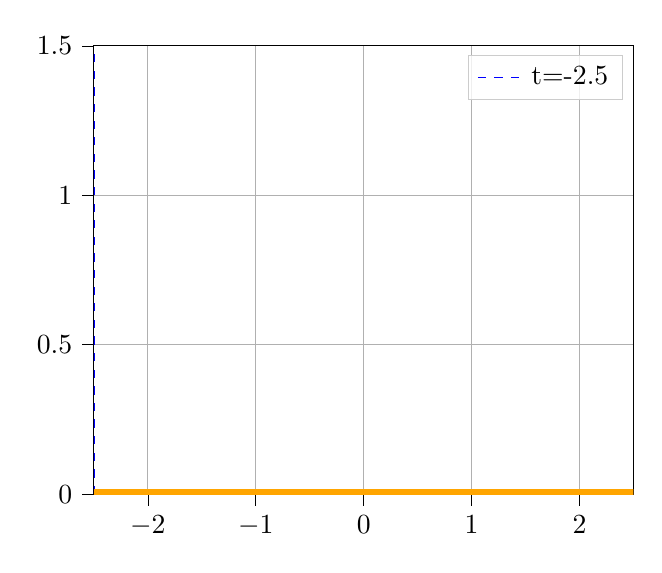
\begin{tikzpicture}

\definecolor{color0}{rgb}{1,0.498039215686275,0.0549019607843137}
\definecolor{color1}{rgb}{1,0.647058823529412,0}

\begin{axis}[
legend cell align={left},
legend style={fill opacity=0.8, draw opacity=1, text opacity=1, draw=white!80!black},
tick align=outside,
tick pos=left,
x grid style={white!69.0196078431373!black},
xmajorgrids,
xmin=-2.5, xmax=2.5,
xtick style={color=black},
y grid style={white!69.0196078431373!black},
ymajorgrids,
ymin=0, ymax=1.5,
ytick style={color=black}
]
\path [draw=color0, fill=color0, opacity=0.2]
(axis cs:-2.5,0)
--(axis cs:-2.5,0)
--(axis cs:-2.49499499499499,0)
--(axis cs:-2.48998998998999,0)
--(axis cs:-2.48498498498498,0)
--(axis cs:-2.47997997997998,0)
--(axis cs:-2.47497497497497,0)
--(axis cs:-2.46996996996997,0)
--(axis cs:-2.46496496496496,0)
--(axis cs:-2.45995995995996,0)
--(axis cs:-2.45495495495495,0)
--(axis cs:-2.44994994994995,0)
--(axis cs:-2.44494494494494,0)
--(axis cs:-2.43993993993994,0)
--(axis cs:-2.43493493493493,0)
--(axis cs:-2.42992992992993,0)
--(axis cs:-2.42492492492492,0)
--(axis cs:-2.41991991991992,0)
--(axis cs:-2.41491491491491,0)
--(axis cs:-2.40990990990991,0)
--(axis cs:-2.4049049049049,0)
--(axis cs:-2.3998998998999,0)
--(axis cs:-2.39489489489489,0)
--(axis cs:-2.38988988988989,0)
--(axis cs:-2.38488488488488,0)
--(axis cs:-2.37987987987988,0)
--(axis cs:-2.37487487487487,0)
--(axis cs:-2.36986986986987,0)
--(axis cs:-2.36486486486486,0)
--(axis cs:-2.35985985985986,0)
--(axis cs:-2.35485485485485,0)
--(axis cs:-2.34984984984985,0)
--(axis cs:-2.34484484484484,0)
--(axis cs:-2.33983983983984,0)
--(axis cs:-2.33483483483483,0)
--(axis cs:-2.32982982982983,0)
--(axis cs:-2.32482482482482,0)
--(axis cs:-2.31981981981982,0)
--(axis cs:-2.31481481481481,0)
--(axis cs:-2.30980980980981,0)
--(axis cs:-2.3048048048048,0)
--(axis cs:-2.2997997997998,0)
--(axis cs:-2.29479479479479,0)
--(axis cs:-2.28978978978979,0)
--(axis cs:-2.28478478478478,0)
--(axis cs:-2.27977977977978,0)
--(axis cs:-2.27477477477477,0)
--(axis cs:-2.26976976976977,0)
--(axis cs:-2.26476476476476,0)
--(axis cs:-2.25975975975976,0)
--(axis cs:-2.25475475475475,0)
--(axis cs:-2.24974974974975,0)
--(axis cs:-2.24474474474474,0)
--(axis cs:-2.23973973973974,0)
--(axis cs:-2.23473473473473,0)
--(axis cs:-2.22972972972973,0)
--(axis cs:-2.22472472472472,0)
--(axis cs:-2.21971971971972,0)
--(axis cs:-2.21471471471471,0)
--(axis cs:-2.20970970970971,0)
--(axis cs:-2.2047047047047,0)
--(axis cs:-2.1996996996997,0)
--(axis cs:-2.19469469469469,0)
--(axis cs:-2.18968968968969,0)
--(axis cs:-2.18468468468468,0)
--(axis cs:-2.17967967967968,0)
--(axis cs:-2.17467467467467,0)
--(axis cs:-2.16966966966967,0)
--(axis cs:-2.16466466466466,0)
--(axis cs:-2.15965965965966,0)
--(axis cs:-2.15465465465465,0)
--(axis cs:-2.14964964964965,0)
--(axis cs:-2.14464464464464,0)
--(axis cs:-2.13963963963964,0)
--(axis cs:-2.13463463463463,0)
--(axis cs:-2.12962962962963,0)
--(axis cs:-2.12462462462462,0)
--(axis cs:-2.11961961961962,0)
--(axis cs:-2.11461461461461,0)
--(axis cs:-2.10960960960961,0)
--(axis cs:-2.1046046046046,0)
--(axis cs:-2.0995995995996,0)
--(axis cs:-2.09459459459459,0)
--(axis cs:-2.08958958958959,0)
--(axis cs:-2.08458458458458,0)
--(axis cs:-2.07957957957958,0)
--(axis cs:-2.07457457457457,0)
--(axis cs:-2.06956956956957,0)
--(axis cs:-2.06456456456456,0)
--(axis cs:-2.05955955955956,0)
--(axis cs:-2.05455455455455,0)
--(axis cs:-2.04954954954955,0)
--(axis cs:-2.04454454454454,0)
--(axis cs:-2.03953953953954,0)
--(axis cs:-2.03453453453453,0)
--(axis cs:-2.02952952952953,0)
--(axis cs:-2.02452452452452,0)
--(axis cs:-2.01951951951952,0)
--(axis cs:-2.01451451451451,0)
--(axis cs:-2.00950950950951,0)
--(axis cs:-2.0045045045045,0)
--(axis cs:-1.9994994994995,0)
--(axis cs:-1.99449449449449,0)
--(axis cs:-1.98948948948949,0)
--(axis cs:-1.98448448448448,0)
--(axis cs:-1.97947947947948,0)
--(axis cs:-1.97447447447447,0)
--(axis cs:-1.96946946946947,0)
--(axis cs:-1.96446446446446,0)
--(axis cs:-1.95945945945946,0)
--(axis cs:-1.95445445445445,0)
--(axis cs:-1.94944944944945,0)
--(axis cs:-1.94444444444444,0)
--(axis cs:-1.93943943943944,0)
--(axis cs:-1.93443443443443,0)
--(axis cs:-1.92942942942943,0)
--(axis cs:-1.92442442442442,0)
--(axis cs:-1.91941941941942,0)
--(axis cs:-1.91441441441441,0)
--(axis cs:-1.90940940940941,0)
--(axis cs:-1.9044044044044,0)
--(axis cs:-1.8993993993994,0)
--(axis cs:-1.89439439439439,0)
--(axis cs:-1.88938938938939,0)
--(axis cs:-1.88438438438438,0)
--(axis cs:-1.87937937937938,0)
--(axis cs:-1.87437437437437,0)
--(axis cs:-1.86936936936937,0)
--(axis cs:-1.86436436436436,0)
--(axis cs:-1.85935935935936,0)
--(axis cs:-1.85435435435435,0)
--(axis cs:-1.84934934934935,0)
--(axis cs:-1.84434434434434,0)
--(axis cs:-1.83933933933934,0)
--(axis cs:-1.83433433433433,0)
--(axis cs:-1.82932932932933,0)
--(axis cs:-1.82432432432432,0)
--(axis cs:-1.81931931931932,0)
--(axis cs:-1.81431431431431,0)
--(axis cs:-1.80930930930931,0)
--(axis cs:-1.8043043043043,0)
--(axis cs:-1.7992992992993,0)
--(axis cs:-1.79429429429429,0)
--(axis cs:-1.78928928928929,0)
--(axis cs:-1.78428428428428,0)
--(axis cs:-1.77927927927928,0)
--(axis cs:-1.77427427427427,0)
--(axis cs:-1.76926926926927,0)
--(axis cs:-1.76426426426426,0)
--(axis cs:-1.75925925925926,0)
--(axis cs:-1.75425425425425,0)
--(axis cs:-1.74924924924925,0)
--(axis cs:-1.74424424424424,0)
--(axis cs:-1.73923923923924,0)
--(axis cs:-1.73423423423423,0)
--(axis cs:-1.72922922922923,0)
--(axis cs:-1.72422422422422,0)
--(axis cs:-1.71921921921922,0)
--(axis cs:-1.71421421421421,0)
--(axis cs:-1.70920920920921,0)
--(axis cs:-1.7042042042042,0)
--(axis cs:-1.6991991991992,0)
--(axis cs:-1.69419419419419,0)
--(axis cs:-1.68918918918919,0)
--(axis cs:-1.68418418418418,0)
--(axis cs:-1.67917917917918,0)
--(axis cs:-1.67417417417417,0)
--(axis cs:-1.66916916916917,0)
--(axis cs:-1.66416416416416,0)
--(axis cs:-1.65915915915916,0)
--(axis cs:-1.65415415415415,0)
--(axis cs:-1.64914914914915,0)
--(axis cs:-1.64414414414414,0)
--(axis cs:-1.63913913913914,0)
--(axis cs:-1.63413413413413,0)
--(axis cs:-1.62912912912913,0)
--(axis cs:-1.62412412412412,0)
--(axis cs:-1.61911911911912,0)
--(axis cs:-1.61411411411411,0)
--(axis cs:-1.60910910910911,0)
--(axis cs:-1.6041041041041,0)
--(axis cs:-1.5990990990991,0)
--(axis cs:-1.59409409409409,0)
--(axis cs:-1.58908908908909,0)
--(axis cs:-1.58408408408408,0)
--(axis cs:-1.57907907907908,0)
--(axis cs:-1.57407407407407,0)
--(axis cs:-1.56906906906907,0)
--(axis cs:-1.56406406406406,0)
--(axis cs:-1.55905905905906,0)
--(axis cs:-1.55405405405405,0)
--(axis cs:-1.54904904904905,0)
--(axis cs:-1.54404404404404,0)
--(axis cs:-1.53903903903904,0)
--(axis cs:-1.53403403403403,0)
--(axis cs:-1.52902902902903,0)
--(axis cs:-1.52402402402402,0)
--(axis cs:-1.51901901901902,0)
--(axis cs:-1.51401401401401,0)
--(axis cs:-1.50900900900901,0)
--(axis cs:-1.504004004004,0)
--(axis cs:-1.498998998999,0)
--(axis cs:-1.49399399399399,0)
--(axis cs:-1.48898898898899,0)
--(axis cs:-1.48398398398398,0)
--(axis cs:-1.47897897897898,0)
--(axis cs:-1.47397397397397,0)
--(axis cs:-1.46896896896897,0)
--(axis cs:-1.46396396396396,0)
--(axis cs:-1.45895895895896,0)
--(axis cs:-1.45395395395395,0)
--(axis cs:-1.44894894894895,0)
--(axis cs:-1.44394394394394,0)
--(axis cs:-1.43893893893894,0)
--(axis cs:-1.43393393393393,0)
--(axis cs:-1.42892892892893,0)
--(axis cs:-1.42392392392392,0)
--(axis cs:-1.41891891891892,0)
--(axis cs:-1.41391391391391,0)
--(axis cs:-1.40890890890891,0)
--(axis cs:-1.4039039039039,0)
--(axis cs:-1.3988988988989,0)
--(axis cs:-1.39389389389389,0)
--(axis cs:-1.38888888888889,0)
--(axis cs:-1.38388388388388,0)
--(axis cs:-1.37887887887888,0)
--(axis cs:-1.37387387387387,0)
--(axis cs:-1.36886886886887,0)
--(axis cs:-1.36386386386386,0)
--(axis cs:-1.35885885885886,0)
--(axis cs:-1.35385385385385,0)
--(axis cs:-1.34884884884885,0)
--(axis cs:-1.34384384384384,0)
--(axis cs:-1.33883883883884,0)
--(axis cs:-1.33383383383383,0)
--(axis cs:-1.32882882882883,0)
--(axis cs:-1.32382382382382,0)
--(axis cs:-1.31881881881882,0)
--(axis cs:-1.31381381381381,0)
--(axis cs:-1.30880880880881,0)
--(axis cs:-1.3038038038038,0)
--(axis cs:-1.2987987987988,0)
--(axis cs:-1.29379379379379,0)
--(axis cs:-1.28878878878879,0)
--(axis cs:-1.28378378378378,0)
--(axis cs:-1.27877877877878,0)
--(axis cs:-1.27377377377377,0)
--(axis cs:-1.26876876876877,0)
--(axis cs:-1.26376376376376,0)
--(axis cs:-1.25875875875876,0)
--(axis cs:-1.25375375375375,0)
--(axis cs:-1.24874874874875,0)
--(axis cs:-1.24374374374374,0)
--(axis cs:-1.23873873873874,0)
--(axis cs:-1.23373373373373,0)
--(axis cs:-1.22872872872873,0)
--(axis cs:-1.22372372372372,0)
--(axis cs:-1.21871871871872,0)
--(axis cs:-1.21371371371371,0)
--(axis cs:-1.20870870870871,0)
--(axis cs:-1.2037037037037,0)
--(axis cs:-1.1986986986987,0)
--(axis cs:-1.19369369369369,0)
--(axis cs:-1.18868868868869,0)
--(axis cs:-1.18368368368368,0)
--(axis cs:-1.17867867867868,0)
--(axis cs:-1.17367367367367,0)
--(axis cs:-1.16866866866867,0)
--(axis cs:-1.16366366366366,0)
--(axis cs:-1.15865865865866,0)
--(axis cs:-1.15365365365365,0)
--(axis cs:-1.14864864864865,0)
--(axis cs:-1.14364364364364,0)
--(axis cs:-1.13863863863864,0)
--(axis cs:-1.13363363363363,0)
--(axis cs:-1.12862862862863,0)
--(axis cs:-1.12362362362362,0)
--(axis cs:-1.11861861861862,0)
--(axis cs:-1.11361361361361,0)
--(axis cs:-1.10860860860861,0)
--(axis cs:-1.1036036036036,0)
--(axis cs:-1.0985985985986,0)
--(axis cs:-1.09359359359359,0)
--(axis cs:-1.08858858858859,0)
--(axis cs:-1.08358358358358,0)
--(axis cs:-1.07857857857858,0)
--(axis cs:-1.07357357357357,0)
--(axis cs:-1.06856856856857,0)
--(axis cs:-1.06356356356356,0)
--(axis cs:-1.05855855855856,0)
--(axis cs:-1.05355355355355,0)
--(axis cs:-1.04854854854855,0)
--(axis cs:-1.04354354354354,0)
--(axis cs:-1.03853853853854,0)
--(axis cs:-1.03353353353353,0)
--(axis cs:-1.02852852852853,0)
--(axis cs:-1.02352352352352,0)
--(axis cs:-1.01851851851852,0)
--(axis cs:-1.01351351351351,0)
--(axis cs:-1.00850850850851,0)
--(axis cs:-1.0035035035035,0)
--(axis cs:-0.998498498498499,0)
--(axis cs:-0.993493493493494,0)
--(axis cs:-0.988488488488489,0)
--(axis cs:-0.983483483483484,0)
--(axis cs:-0.978478478478479,0)
--(axis cs:-0.973473473473474,0)
--(axis cs:-0.968468468468469,0)
--(axis cs:-0.963463463463464,0)
--(axis cs:-0.958458458458459,0)
--(axis cs:-0.953453453453454,0)
--(axis cs:-0.948448448448449,0)
--(axis cs:-0.943443443443444,0)
--(axis cs:-0.938438438438439,0)
--(axis cs:-0.933433433433434,0)
--(axis cs:-0.928428428428429,0)
--(axis cs:-0.923423423423424,0)
--(axis cs:-0.918418418418419,0)
--(axis cs:-0.913413413413414,0)
--(axis cs:-0.908408408408409,0)
--(axis cs:-0.903403403403404,0)
--(axis cs:-0.898398398398399,0)
--(axis cs:-0.893393393393393,0)
--(axis cs:-0.888388388388388,0)
--(axis cs:-0.883383383383383,0)
--(axis cs:-0.878378378378378,0)
--(axis cs:-0.873373373373373,0)
--(axis cs:-0.868368368368368,0)
--(axis cs:-0.863363363363363,0)
--(axis cs:-0.858358358358358,0)
--(axis cs:-0.853353353353353,0)
--(axis cs:-0.848348348348348,0)
--(axis cs:-0.843343343343343,0)
--(axis cs:-0.838338338338338,0)
--(axis cs:-0.833333333333333,0)
--(axis cs:-0.828328328328328,0)
--(axis cs:-0.823323323323323,0)
--(axis cs:-0.818318318318318,0)
--(axis cs:-0.813313313313313,0)
--(axis cs:-0.808308308308308,0)
--(axis cs:-0.803303303303303,0)
--(axis cs:-0.798298298298298,0)
--(axis cs:-0.793293293293293,0)
--(axis cs:-0.788288288288288,0)
--(axis cs:-0.783283283283283,0)
--(axis cs:-0.778278278278278,0)
--(axis cs:-0.773273273273273,0)
--(axis cs:-0.768268268268268,0)
--(axis cs:-0.763263263263263,0)
--(axis cs:-0.758258258258258,0)
--(axis cs:-0.753253253253253,0)
--(axis cs:-0.748248248248248,0)
--(axis cs:-0.743243243243243,0)
--(axis cs:-0.738238238238238,0)
--(axis cs:-0.733233233233233,0)
--(axis cs:-0.728228228228228,0)
--(axis cs:-0.723223223223223,0)
--(axis cs:-0.718218218218218,0)
--(axis cs:-0.713213213213213,0)
--(axis cs:-0.708208208208208,0)
--(axis cs:-0.703203203203203,0)
--(axis cs:-0.698198198198198,0)
--(axis cs:-0.693193193193193,0)
--(axis cs:-0.688188188188188,0)
--(axis cs:-0.683183183183183,0)
--(axis cs:-0.678178178178178,0)
--(axis cs:-0.673173173173173,0)
--(axis cs:-0.668168168168168,0)
--(axis cs:-0.663163163163163,0)
--(axis cs:-0.658158158158158,0)
--(axis cs:-0.653153153153153,0)
--(axis cs:-0.648148148148148,0)
--(axis cs:-0.643143143143143,0)
--(axis cs:-0.638138138138138,0)
--(axis cs:-0.633133133133133,0)
--(axis cs:-0.628128128128128,0)
--(axis cs:-0.623123123123123,0)
--(axis cs:-0.618118118118118,0)
--(axis cs:-0.613113113113113,0)
--(axis cs:-0.608108108108108,0)
--(axis cs:-0.603103103103103,0)
--(axis cs:-0.598098098098098,0)
--(axis cs:-0.593093093093093,0)
--(axis cs:-0.588088088088088,0)
--(axis cs:-0.583083083083083,0)
--(axis cs:-0.578078078078078,0)
--(axis cs:-0.573073073073073,0)
--(axis cs:-0.568068068068068,0)
--(axis cs:-0.563063063063063,0)
--(axis cs:-0.558058058058058,0)
--(axis cs:-0.553053053053053,0)
--(axis cs:-0.548048048048048,0)
--(axis cs:-0.543043043043043,0)
--(axis cs:-0.538038038038038,0)
--(axis cs:-0.533033033033033,0)
--(axis cs:-0.528028028028028,0)
--(axis cs:-0.523023023023023,0)
--(axis cs:-0.518018018018018,0)
--(axis cs:-0.513013013013013,0)
--(axis cs:-0.508008008008008,0)
--(axis cs:-0.503003003003003,0)
--(axis cs:-0.497997997997998,0)
--(axis cs:-0.492992992992993,0)
--(axis cs:-0.487987987987988,0)
--(axis cs:-0.482982982982983,0)
--(axis cs:-0.477977977977978,0)
--(axis cs:-0.472972972972973,0)
--(axis cs:-0.467967967967968,0)
--(axis cs:-0.462962962962963,0)
--(axis cs:-0.457957957957958,0)
--(axis cs:-0.452952952952953,0)
--(axis cs:-0.447947947947948,0)
--(axis cs:-0.442942942942943,0)
--(axis cs:-0.437937937937938,0)
--(axis cs:-0.432932932932933,0)
--(axis cs:-0.427927927927928,0)
--(axis cs:-0.422922922922923,0)
--(axis cs:-0.417917917917918,0)
--(axis cs:-0.412912912912913,0)
--(axis cs:-0.407907907907908,0)
--(axis cs:-0.402902902902903,0)
--(axis cs:-0.397897897897898,0)
--(axis cs:-0.392892892892893,0)
--(axis cs:-0.387887887887888,0)
--(axis cs:-0.382882882882883,0)
--(axis cs:-0.377877877877878,0)
--(axis cs:-0.372872872872873,0)
--(axis cs:-0.367867867867868,0)
--(axis cs:-0.362862862862863,0)
--(axis cs:-0.357857857857858,0)
--(axis cs:-0.352852852852853,0)
--(axis cs:-0.347847847847848,0)
--(axis cs:-0.342842842842843,0)
--(axis cs:-0.337837837837838,0)
--(axis cs:-0.332832832832833,0)
--(axis cs:-0.327827827827828,0)
--(axis cs:-0.322822822822823,0)
--(axis cs:-0.317817817817818,0)
--(axis cs:-0.312812812812813,0)
--(axis cs:-0.307807807807808,0)
--(axis cs:-0.302802802802803,0)
--(axis cs:-0.297797797797798,0)
--(axis cs:-0.292792792792793,0)
--(axis cs:-0.287787787787788,0)
--(axis cs:-0.282782782782783,0)
--(axis cs:-0.277777777777778,0)
--(axis cs:-0.272772772772773,0)
--(axis cs:-0.267767767767768,0)
--(axis cs:-0.262762762762763,0)
--(axis cs:-0.257757757757758,0)
--(axis cs:-0.252752752752753,0)
--(axis cs:-0.247747747747748,0)
--(axis cs:-0.242742742742743,0)
--(axis cs:-0.237737737737738,0)
--(axis cs:-0.232732732732733,0)
--(axis cs:-0.227727727727728,0)
--(axis cs:-0.222722722722723,0)
--(axis cs:-0.217717717717718,0)
--(axis cs:-0.212712712712713,0)
--(axis cs:-0.207707707707708,0)
--(axis cs:-0.202702702702703,0)
--(axis cs:-0.197697697697698,0)
--(axis cs:-0.192692692692693,0)
--(axis cs:-0.187687687687688,0)
--(axis cs:-0.182682682682683,0)
--(axis cs:-0.177677677677678,0)
--(axis cs:-0.172672672672673,0)
--(axis cs:-0.167667667667668,0)
--(axis cs:-0.162662662662663,0)
--(axis cs:-0.157657657657658,0)
--(axis cs:-0.152652652652653,0)
--(axis cs:-0.147647647647648,0)
--(axis cs:-0.142642642642643,0)
--(axis cs:-0.137637637637638,0)
--(axis cs:-0.132632632632633,0)
--(axis cs:-0.127627627627628,0)
--(axis cs:-0.122622622622623,0)
--(axis cs:-0.117617617617618,0)
--(axis cs:-0.112612612612613,0)
--(axis cs:-0.107607607607608,0)
--(axis cs:-0.102602602602603,0)
--(axis cs:-0.0975975975975976,0)
--(axis cs:-0.0925925925925926,0)
--(axis cs:-0.0875875875875876,0)
--(axis cs:-0.0825825825825826,0)
--(axis cs:-0.0775775775775776,0)
--(axis cs:-0.0725725725725725,0)
--(axis cs:-0.0675675675675675,0)
--(axis cs:-0.0625625625625625,0)
--(axis cs:-0.0575575575575575,0)
--(axis cs:-0.0525525525525525,0)
--(axis cs:-0.0475475475475475,0)
--(axis cs:-0.0425425425425425,0)
--(axis cs:-0.0375375375375375,0)
--(axis cs:-0.0325325325325325,0)
--(axis cs:-0.0275275275275275,0)
--(axis cs:-0.0225225225225225,0)
--(axis cs:-0.0175175175175175,0)
--(axis cs:-0.0125125125125125,0)
--(axis cs:-0.0075075075075075,0)
--(axis cs:-0.0025025025025025,0)
--(axis cs:0.0025025025025025,0)
--(axis cs:0.0075075075075075,0)
--(axis cs:0.0125125125125125,0)
--(axis cs:0.0175175175175175,0)
--(axis cs:0.0225225225225225,0)
--(axis cs:0.0275275275275275,0)
--(axis cs:0.0325325325325325,0)
--(axis cs:0.0375375375375375,0)
--(axis cs:0.0425425425425425,0)
--(axis cs:0.0475475475475475,0)
--(axis cs:0.0525525525525525,0)
--(axis cs:0.0575575575575575,0)
--(axis cs:0.0625625625625625,0)
--(axis cs:0.0675675675675675,0)
--(axis cs:0.0725725725725725,0)
--(axis cs:0.0775775775775776,0)
--(axis cs:0.0825825825825826,0)
--(axis cs:0.0875875875875876,0)
--(axis cs:0.0925925925925926,0)
--(axis cs:0.0975975975975976,0)
--(axis cs:0.102602602602603,0)
--(axis cs:0.107607607607608,0)
--(axis cs:0.112612612612613,0)
--(axis cs:0.117617617617618,0)
--(axis cs:0.122622622622623,0)
--(axis cs:0.127627627627628,0)
--(axis cs:0.132632632632633,0)
--(axis cs:0.137637637637638,0)
--(axis cs:0.142642642642643,0)
--(axis cs:0.147647647647648,0)
--(axis cs:0.152652652652653,0)
--(axis cs:0.157657657657658,0)
--(axis cs:0.162662662662663,0)
--(axis cs:0.167667667667668,0)
--(axis cs:0.172672672672673,0)
--(axis cs:0.177677677677678,0)
--(axis cs:0.182682682682683,0)
--(axis cs:0.187687687687688,0)
--(axis cs:0.192692692692693,0)
--(axis cs:0.197697697697698,0)
--(axis cs:0.202702702702703,0)
--(axis cs:0.207707707707708,0)
--(axis cs:0.212712712712713,0)
--(axis cs:0.217717717717718,0)
--(axis cs:0.222722722722723,0)
--(axis cs:0.227727727727728,0)
--(axis cs:0.232732732732733,0)
--(axis cs:0.237737737737738,0)
--(axis cs:0.242742742742743,0)
--(axis cs:0.247747747747748,0)
--(axis cs:0.252752752752753,0)
--(axis cs:0.257757757757758,0)
--(axis cs:0.262762762762763,0)
--(axis cs:0.267767767767768,0)
--(axis cs:0.272772772772773,0)
--(axis cs:0.277777777777778,0)
--(axis cs:0.282782782782783,0)
--(axis cs:0.287787787787788,0)
--(axis cs:0.292792792792793,0)
--(axis cs:0.297797797797798,0)
--(axis cs:0.302802802802803,0)
--(axis cs:0.307807807807808,0)
--(axis cs:0.312812812812813,0)
--(axis cs:0.317817817817818,0)
--(axis cs:0.322822822822823,0)
--(axis cs:0.327827827827828,0)
--(axis cs:0.332832832832833,0)
--(axis cs:0.337837837837838,0)
--(axis cs:0.342842842842843,0)
--(axis cs:0.347847847847848,0)
--(axis cs:0.352852852852853,0)
--(axis cs:0.357857857857858,0)
--(axis cs:0.362862862862863,0)
--(axis cs:0.367867867867868,0)
--(axis cs:0.372872872872873,0)
--(axis cs:0.377877877877878,0)
--(axis cs:0.382882882882883,0)
--(axis cs:0.387887887887888,0)
--(axis cs:0.392892892892893,0)
--(axis cs:0.397897897897898,0)
--(axis cs:0.402902902902903,0)
--(axis cs:0.407907907907908,0)
--(axis cs:0.412912912912913,0)
--(axis cs:0.417917917917918,0)
--(axis cs:0.422922922922923,0)
--(axis cs:0.427927927927928,0)
--(axis cs:0.432932932932933,0)
--(axis cs:0.437937937937938,0)
--(axis cs:0.442942942942943,0)
--(axis cs:0.447947947947948,0)
--(axis cs:0.452952952952953,0)
--(axis cs:0.457957957957958,0)
--(axis cs:0.462962962962963,0)
--(axis cs:0.467967967967968,0)
--(axis cs:0.472972972972973,0)
--(axis cs:0.477977977977978,0)
--(axis cs:0.482982982982983,0)
--(axis cs:0.487987987987988,0)
--(axis cs:0.492992992992993,0)
--(axis cs:0.497997997997998,0)
--(axis cs:0.503003003003003,0)
--(axis cs:0.508008008008008,0)
--(axis cs:0.513013013013013,0)
--(axis cs:0.518018018018018,0)
--(axis cs:0.523023023023023,0)
--(axis cs:0.528028028028028,0)
--(axis cs:0.533033033033033,0)
--(axis cs:0.538038038038038,0)
--(axis cs:0.543043043043043,0)
--(axis cs:0.548048048048048,0)
--(axis cs:0.553053053053053,0)
--(axis cs:0.558058058058058,0)
--(axis cs:0.563063063063063,0)
--(axis cs:0.568068068068068,0)
--(axis cs:0.573073073073073,0)
--(axis cs:0.578078078078078,0)
--(axis cs:0.583083083083083,0)
--(axis cs:0.588088088088088,0)
--(axis cs:0.593093093093093,0)
--(axis cs:0.598098098098098,0)
--(axis cs:0.603103103103103,0)
--(axis cs:0.608108108108108,0)
--(axis cs:0.613113113113113,0)
--(axis cs:0.618118118118118,0)
--(axis cs:0.623123123123123,0)
--(axis cs:0.628128128128128,0)
--(axis cs:0.633133133133133,0)
--(axis cs:0.638138138138138,0)
--(axis cs:0.643143143143143,0)
--(axis cs:0.648148148148148,0)
--(axis cs:0.653153153153153,0)
--(axis cs:0.658158158158158,0)
--(axis cs:0.663163163163163,0)
--(axis cs:0.668168168168168,0)
--(axis cs:0.673173173173173,0)
--(axis cs:0.678178178178178,0)
--(axis cs:0.683183183183183,0)
--(axis cs:0.688188188188188,0)
--(axis cs:0.693193193193193,0)
--(axis cs:0.698198198198198,0)
--(axis cs:0.703203203203203,0)
--(axis cs:0.708208208208208,0)
--(axis cs:0.713213213213213,0)
--(axis cs:0.718218218218218,0)
--(axis cs:0.723223223223223,0)
--(axis cs:0.728228228228228,0)
--(axis cs:0.733233233233233,0)
--(axis cs:0.738238238238238,0)
--(axis cs:0.743243243243243,0)
--(axis cs:0.748248248248248,0)
--(axis cs:0.753253253253253,0)
--(axis cs:0.758258258258258,0)
--(axis cs:0.763263263263263,0)
--(axis cs:0.768268268268268,0)
--(axis cs:0.773273273273273,0)
--(axis cs:0.778278278278278,0)
--(axis cs:0.783283283283283,0)
--(axis cs:0.788288288288288,0)
--(axis cs:0.793293293293293,0)
--(axis cs:0.798298298298298,0)
--(axis cs:0.803303303303303,0)
--(axis cs:0.808308308308308,0)
--(axis cs:0.813313313313313,0)
--(axis cs:0.818318318318318,0)
--(axis cs:0.823323323323323,0)
--(axis cs:0.828328328328328,0)
--(axis cs:0.833333333333333,0)
--(axis cs:0.838338338338338,0)
--(axis cs:0.843343343343343,0)
--(axis cs:0.848348348348348,0)
--(axis cs:0.853353353353353,0)
--(axis cs:0.858358358358358,0)
--(axis cs:0.863363363363364,0)
--(axis cs:0.868368368368369,0)
--(axis cs:0.873373373373374,0)
--(axis cs:0.878378378378379,0)
--(axis cs:0.883383383383384,0)
--(axis cs:0.888388388388389,0)
--(axis cs:0.893393393393394,0)
--(axis cs:0.898398398398399,0)
--(axis cs:0.903403403403404,0)
--(axis cs:0.908408408408409,0)
--(axis cs:0.913413413413414,0)
--(axis cs:0.918418418418419,0)
--(axis cs:0.923423423423424,0)
--(axis cs:0.928428428428429,0)
--(axis cs:0.933433433433434,0)
--(axis cs:0.938438438438439,0)
--(axis cs:0.943443443443444,0)
--(axis cs:0.948448448448449,0)
--(axis cs:0.953453453453454,0)
--(axis cs:0.958458458458459,0)
--(axis cs:0.963463463463464,0)
--(axis cs:0.968468468468469,0)
--(axis cs:0.973473473473474,0)
--(axis cs:0.978478478478479,0)
--(axis cs:0.983483483483484,0)
--(axis cs:0.988488488488489,0)
--(axis cs:0.993493493493494,0)
--(axis cs:0.998498498498499,0)
--(axis cs:1.0035035035035,0)
--(axis cs:1.00850850850851,0)
--(axis cs:1.01351351351351,0)
--(axis cs:1.01851851851852,0)
--(axis cs:1.02352352352352,0)
--(axis cs:1.02852852852853,0)
--(axis cs:1.03353353353353,0)
--(axis cs:1.03853853853854,0)
--(axis cs:1.04354354354354,0)
--(axis cs:1.04854854854855,0)
--(axis cs:1.05355355355355,0)
--(axis cs:1.05855855855856,0)
--(axis cs:1.06356356356356,0)
--(axis cs:1.06856856856857,0)
--(axis cs:1.07357357357357,0)
--(axis cs:1.07857857857858,0)
--(axis cs:1.08358358358358,0)
--(axis cs:1.08858858858859,0)
--(axis cs:1.09359359359359,0)
--(axis cs:1.0985985985986,0)
--(axis cs:1.1036036036036,0)
--(axis cs:1.10860860860861,0)
--(axis cs:1.11361361361361,0)
--(axis cs:1.11861861861862,0)
--(axis cs:1.12362362362362,0)
--(axis cs:1.12862862862863,0)
--(axis cs:1.13363363363363,0)
--(axis cs:1.13863863863864,0)
--(axis cs:1.14364364364364,0)
--(axis cs:1.14864864864865,0)
--(axis cs:1.15365365365365,0)
--(axis cs:1.15865865865866,0)
--(axis cs:1.16366366366366,0)
--(axis cs:1.16866866866867,0)
--(axis cs:1.17367367367367,0)
--(axis cs:1.17867867867868,0)
--(axis cs:1.18368368368368,0)
--(axis cs:1.18868868868869,0)
--(axis cs:1.19369369369369,0)
--(axis cs:1.1986986986987,0)
--(axis cs:1.2037037037037,0)
--(axis cs:1.20870870870871,0)
--(axis cs:1.21371371371371,0)
--(axis cs:1.21871871871872,0)
--(axis cs:1.22372372372372,0)
--(axis cs:1.22872872872873,0)
--(axis cs:1.23373373373373,0)
--(axis cs:1.23873873873874,0)
--(axis cs:1.24374374374374,0)
--(axis cs:1.24874874874875,0)
--(axis cs:1.25375375375375,0)
--(axis cs:1.25875875875876,0)
--(axis cs:1.26376376376376,0)
--(axis cs:1.26876876876877,0)
--(axis cs:1.27377377377377,0)
--(axis cs:1.27877877877878,0)
--(axis cs:1.28378378378378,0)
--(axis cs:1.28878878878879,0)
--(axis cs:1.29379379379379,0)
--(axis cs:1.2987987987988,0)
--(axis cs:1.3038038038038,0)
--(axis cs:1.30880880880881,0)
--(axis cs:1.31381381381381,0)
--(axis cs:1.31881881881882,0)
--(axis cs:1.32382382382382,0)
--(axis cs:1.32882882882883,0)
--(axis cs:1.33383383383383,0)
--(axis cs:1.33883883883884,0)
--(axis cs:1.34384384384384,0)
--(axis cs:1.34884884884885,0)
--(axis cs:1.35385385385385,0)
--(axis cs:1.35885885885886,0)
--(axis cs:1.36386386386386,0)
--(axis cs:1.36886886886887,0)
--(axis cs:1.37387387387387,0)
--(axis cs:1.37887887887888,0)
--(axis cs:1.38388388388388,0)
--(axis cs:1.38888888888889,0)
--(axis cs:1.39389389389389,0)
--(axis cs:1.3988988988989,0)
--(axis cs:1.4039039039039,0)
--(axis cs:1.40890890890891,0)
--(axis cs:1.41391391391391,0)
--(axis cs:1.41891891891892,0)
--(axis cs:1.42392392392392,0)
--(axis cs:1.42892892892893,0)
--(axis cs:1.43393393393393,0)
--(axis cs:1.43893893893894,0)
--(axis cs:1.44394394394394,0)
--(axis cs:1.44894894894895,0)
--(axis cs:1.45395395395395,0)
--(axis cs:1.45895895895896,0)
--(axis cs:1.46396396396396,0)
--(axis cs:1.46896896896897,0)
--(axis cs:1.47397397397397,0)
--(axis cs:1.47897897897898,0)
--(axis cs:1.48398398398398,0)
--(axis cs:1.48898898898899,0)
--(axis cs:1.49399399399399,0)
--(axis cs:1.498998998999,0)
--(axis cs:1.504004004004,0)
--(axis cs:1.50900900900901,0)
--(axis cs:1.51401401401401,0)
--(axis cs:1.51901901901902,0)
--(axis cs:1.52402402402402,0)
--(axis cs:1.52902902902903,0)
--(axis cs:1.53403403403403,0)
--(axis cs:1.53903903903904,0)
--(axis cs:1.54404404404404,0)
--(axis cs:1.54904904904905,0)
--(axis cs:1.55405405405405,0)
--(axis cs:1.55905905905906,0)
--(axis cs:1.56406406406406,0)
--(axis cs:1.56906906906907,0)
--(axis cs:1.57407407407407,0)
--(axis cs:1.57907907907908,0)
--(axis cs:1.58408408408408,0)
--(axis cs:1.58908908908909,0)
--(axis cs:1.59409409409409,0)
--(axis cs:1.5990990990991,0)
--(axis cs:1.6041041041041,0)
--(axis cs:1.60910910910911,0)
--(axis cs:1.61411411411411,0)
--(axis cs:1.61911911911912,0)
--(axis cs:1.62412412412412,0)
--(axis cs:1.62912912912913,0)
--(axis cs:1.63413413413413,0)
--(axis cs:1.63913913913914,0)
--(axis cs:1.64414414414414,0)
--(axis cs:1.64914914914915,0)
--(axis cs:1.65415415415415,0)
--(axis cs:1.65915915915916,0)
--(axis cs:1.66416416416416,0)
--(axis cs:1.66916916916917,0)
--(axis cs:1.67417417417417,0)
--(axis cs:1.67917917917918,0)
--(axis cs:1.68418418418418,0)
--(axis cs:1.68918918918919,0)
--(axis cs:1.69419419419419,0)
--(axis cs:1.6991991991992,0)
--(axis cs:1.7042042042042,0)
--(axis cs:1.70920920920921,0)
--(axis cs:1.71421421421421,0)
--(axis cs:1.71921921921922,0)
--(axis cs:1.72422422422422,0)
--(axis cs:1.72922922922923,0)
--(axis cs:1.73423423423423,0)
--(axis cs:1.73923923923924,0)
--(axis cs:1.74424424424424,0)
--(axis cs:1.74924924924925,0)
--(axis cs:1.75425425425425,0)
--(axis cs:1.75925925925926,0)
--(axis cs:1.76426426426426,0)
--(axis cs:1.76926926926927,0)
--(axis cs:1.77427427427427,0)
--(axis cs:1.77927927927928,0)
--(axis cs:1.78428428428428,0)
--(axis cs:1.78928928928929,0)
--(axis cs:1.79429429429429,0)
--(axis cs:1.7992992992993,0)
--(axis cs:1.8043043043043,0)
--(axis cs:1.80930930930931,0)
--(axis cs:1.81431431431431,0)
--(axis cs:1.81931931931932,0)
--(axis cs:1.82432432432432,0)
--(axis cs:1.82932932932933,0)
--(axis cs:1.83433433433433,0)
--(axis cs:1.83933933933934,0)
--(axis cs:1.84434434434434,0)
--(axis cs:1.84934934934935,0)
--(axis cs:1.85435435435435,0)
--(axis cs:1.85935935935936,0)
--(axis cs:1.86436436436436,0)
--(axis cs:1.86936936936937,0)
--(axis cs:1.87437437437437,0)
--(axis cs:1.87937937937938,0)
--(axis cs:1.88438438438438,0)
--(axis cs:1.88938938938939,0)
--(axis cs:1.89439439439439,0)
--(axis cs:1.8993993993994,0)
--(axis cs:1.9044044044044,0)
--(axis cs:1.90940940940941,0)
--(axis cs:1.91441441441441,0)
--(axis cs:1.91941941941942,0)
--(axis cs:1.92442442442442,0)
--(axis cs:1.92942942942943,0)
--(axis cs:1.93443443443443,0)
--(axis cs:1.93943943943944,0)
--(axis cs:1.94444444444444,0)
--(axis cs:1.94944944944945,0)
--(axis cs:1.95445445445445,0)
--(axis cs:1.95945945945946,0)
--(axis cs:1.96446446446446,0)
--(axis cs:1.96946946946947,0)
--(axis cs:1.97447447447447,0)
--(axis cs:1.97947947947948,0)
--(axis cs:1.98448448448448,0)
--(axis cs:1.98948948948949,0)
--(axis cs:1.99449449449449,0)
--(axis cs:1.9994994994995,0)
--(axis cs:2.0045045045045,0)
--(axis cs:2.00950950950951,0)
--(axis cs:2.01451451451451,0)
--(axis cs:2.01951951951952,0)
--(axis cs:2.02452452452452,0)
--(axis cs:2.02952952952953,0)
--(axis cs:2.03453453453453,0)
--(axis cs:2.03953953953954,0)
--(axis cs:2.04454454454454,0)
--(axis cs:2.04954954954955,0)
--(axis cs:2.05455455455455,0)
--(axis cs:2.05955955955956,0)
--(axis cs:2.06456456456456,0)
--(axis cs:2.06956956956957,0)
--(axis cs:2.07457457457457,0)
--(axis cs:2.07957957957958,0)
--(axis cs:2.08458458458458,0)
--(axis cs:2.08958958958959,0)
--(axis cs:2.09459459459459,0)
--(axis cs:2.0995995995996,0)
--(axis cs:2.1046046046046,0)
--(axis cs:2.10960960960961,0)
--(axis cs:2.11461461461461,0)
--(axis cs:2.11961961961962,0)
--(axis cs:2.12462462462462,0)
--(axis cs:2.12962962962963,0)
--(axis cs:2.13463463463463,0)
--(axis cs:2.13963963963964,0)
--(axis cs:2.14464464464464,0)
--(axis cs:2.14964964964965,0)
--(axis cs:2.15465465465465,0)
--(axis cs:2.15965965965966,0)
--(axis cs:2.16466466466466,0)
--(axis cs:2.16966966966967,0)
--(axis cs:2.17467467467467,0)
--(axis cs:2.17967967967968,0)
--(axis cs:2.18468468468468,0)
--(axis cs:2.18968968968969,0)
--(axis cs:2.19469469469469,0)
--(axis cs:2.1996996996997,0)
--(axis cs:2.2047047047047,0)
--(axis cs:2.20970970970971,0)
--(axis cs:2.21471471471471,0)
--(axis cs:2.21971971971972,0)
--(axis cs:2.22472472472472,0)
--(axis cs:2.22972972972973,0)
--(axis cs:2.23473473473473,0)
--(axis cs:2.23973973973974,0)
--(axis cs:2.24474474474474,0)
--(axis cs:2.24974974974975,0)
--(axis cs:2.25475475475475,0)
--(axis cs:2.25975975975976,0)
--(axis cs:2.26476476476476,0)
--(axis cs:2.26976976976977,0)
--(axis cs:2.27477477477477,0)
--(axis cs:2.27977977977978,0)
--(axis cs:2.28478478478478,0)
--(axis cs:2.28978978978979,0)
--(axis cs:2.29479479479479,0)
--(axis cs:2.2997997997998,0)
--(axis cs:2.3048048048048,0)
--(axis cs:2.30980980980981,0)
--(axis cs:2.31481481481481,0)
--(axis cs:2.31981981981982,0)
--(axis cs:2.32482482482482,0)
--(axis cs:2.32982982982983,0)
--(axis cs:2.33483483483483,0)
--(axis cs:2.33983983983984,0)
--(axis cs:2.34484484484484,0)
--(axis cs:2.34984984984985,0)
--(axis cs:2.35485485485485,0)
--(axis cs:2.35985985985986,0)
--(axis cs:2.36486486486486,0)
--(axis cs:2.36986986986987,0)
--(axis cs:2.37487487487487,0)
--(axis cs:2.37987987987988,0)
--(axis cs:2.38488488488488,0)
--(axis cs:2.38988988988989,0)
--(axis cs:2.39489489489489,0)
--(axis cs:2.3998998998999,0)
--(axis cs:2.4049049049049,0)
--(axis cs:2.40990990990991,0)
--(axis cs:2.41491491491491,0)
--(axis cs:2.41991991991992,0)
--(axis cs:2.42492492492492,0)
--(axis cs:2.42992992992993,0)
--(axis cs:2.43493493493493,0)
--(axis cs:2.43993993993994,0)
--(axis cs:2.44494494494494,0)
--(axis cs:2.44994994994995,0)
--(axis cs:2.45495495495495,0)
--(axis cs:2.45995995995996,0)
--(axis cs:2.46496496496496,0)
--(axis cs:2.46996996996997,0)
--(axis cs:2.47497497497497,0)
--(axis cs:2.47997997997998,0)
--(axis cs:2.48498498498498,0)
--(axis cs:2.48998998998999,0)
--(axis cs:2.49499499499499,0)
--(axis cs:2.5,0)
--(axis cs:2.5,0)
--(axis cs:2.5,0)
--(axis cs:2.49499499499499,0)
--(axis cs:2.48998998998999,0)
--(axis cs:2.48498498498498,0)
--(axis cs:2.47997997997998,0)
--(axis cs:2.47497497497497,0)
--(axis cs:2.46996996996997,0)
--(axis cs:2.46496496496496,0)
--(axis cs:2.45995995995996,0)
--(axis cs:2.45495495495495,0)
--(axis cs:2.44994994994995,0)
--(axis cs:2.44494494494494,0)
--(axis cs:2.43993993993994,0)
--(axis cs:2.43493493493493,0)
--(axis cs:2.42992992992993,0)
--(axis cs:2.42492492492492,0)
--(axis cs:2.41991991991992,0)
--(axis cs:2.41491491491491,0)
--(axis cs:2.40990990990991,0)
--(axis cs:2.4049049049049,0)
--(axis cs:2.3998998998999,0)
--(axis cs:2.39489489489489,0)
--(axis cs:2.38988988988989,0)
--(axis cs:2.38488488488488,0)
--(axis cs:2.37987987987988,0)
--(axis cs:2.37487487487487,0)
--(axis cs:2.36986986986987,0)
--(axis cs:2.36486486486486,0)
--(axis cs:2.35985985985986,0)
--(axis cs:2.35485485485485,0)
--(axis cs:2.34984984984985,0)
--(axis cs:2.34484484484484,0)
--(axis cs:2.33983983983984,0)
--(axis cs:2.33483483483483,0)
--(axis cs:2.32982982982983,0)
--(axis cs:2.32482482482482,0)
--(axis cs:2.31981981981982,0)
--(axis cs:2.31481481481481,0)
--(axis cs:2.30980980980981,0)
--(axis cs:2.3048048048048,0)
--(axis cs:2.2997997997998,0)
--(axis cs:2.29479479479479,0)
--(axis cs:2.28978978978979,0)
--(axis cs:2.28478478478478,0)
--(axis cs:2.27977977977978,0)
--(axis cs:2.27477477477477,0)
--(axis cs:2.26976976976977,0)
--(axis cs:2.26476476476476,0)
--(axis cs:2.25975975975976,0)
--(axis cs:2.25475475475475,0)
--(axis cs:2.24974974974975,0)
--(axis cs:2.24474474474474,0)
--(axis cs:2.23973973973974,0)
--(axis cs:2.23473473473473,0)
--(axis cs:2.22972972972973,0)
--(axis cs:2.22472472472472,0)
--(axis cs:2.21971971971972,0)
--(axis cs:2.21471471471471,0)
--(axis cs:2.20970970970971,0)
--(axis cs:2.2047047047047,0)
--(axis cs:2.1996996996997,0)
--(axis cs:2.19469469469469,0)
--(axis cs:2.18968968968969,0)
--(axis cs:2.18468468468468,0)
--(axis cs:2.17967967967968,0)
--(axis cs:2.17467467467467,0)
--(axis cs:2.16966966966967,0)
--(axis cs:2.16466466466466,0)
--(axis cs:2.15965965965966,0)
--(axis cs:2.15465465465465,0)
--(axis cs:2.14964964964965,0)
--(axis cs:2.14464464464464,0)
--(axis cs:2.13963963963964,0)
--(axis cs:2.13463463463463,0)
--(axis cs:2.12962962962963,0)
--(axis cs:2.12462462462462,0)
--(axis cs:2.11961961961962,0)
--(axis cs:2.11461461461461,0)
--(axis cs:2.10960960960961,0)
--(axis cs:2.1046046046046,0)
--(axis cs:2.0995995995996,0)
--(axis cs:2.09459459459459,0)
--(axis cs:2.08958958958959,0)
--(axis cs:2.08458458458458,0)
--(axis cs:2.07957957957958,0)
--(axis cs:2.07457457457457,0)
--(axis cs:2.06956956956957,0)
--(axis cs:2.06456456456456,0)
--(axis cs:2.05955955955956,0)
--(axis cs:2.05455455455455,0)
--(axis cs:2.04954954954955,0)
--(axis cs:2.04454454454454,0)
--(axis cs:2.03953953953954,0)
--(axis cs:2.03453453453453,0)
--(axis cs:2.02952952952953,0)
--(axis cs:2.02452452452452,0)
--(axis cs:2.01951951951952,0)
--(axis cs:2.01451451451451,0)
--(axis cs:2.00950950950951,0)
--(axis cs:2.0045045045045,0)
--(axis cs:1.9994994994995,0)
--(axis cs:1.99449449449449,0)
--(axis cs:1.98948948948949,0)
--(axis cs:1.98448448448448,0)
--(axis cs:1.97947947947948,0)
--(axis cs:1.97447447447447,0)
--(axis cs:1.96946946946947,0)
--(axis cs:1.96446446446446,0)
--(axis cs:1.95945945945946,0)
--(axis cs:1.95445445445445,0)
--(axis cs:1.94944944944945,0)
--(axis cs:1.94444444444444,0)
--(axis cs:1.93943943943944,0)
--(axis cs:1.93443443443443,0)
--(axis cs:1.92942942942943,0)
--(axis cs:1.92442442442442,0)
--(axis cs:1.91941941941942,0)
--(axis cs:1.91441441441441,0)
--(axis cs:1.90940940940941,0)
--(axis cs:1.9044044044044,0)
--(axis cs:1.8993993993994,0)
--(axis cs:1.89439439439439,0)
--(axis cs:1.88938938938939,0)
--(axis cs:1.88438438438438,0)
--(axis cs:1.87937937937938,0)
--(axis cs:1.87437437437437,0)
--(axis cs:1.86936936936937,0)
--(axis cs:1.86436436436436,0)
--(axis cs:1.85935935935936,0)
--(axis cs:1.85435435435435,0)
--(axis cs:1.84934934934935,0)
--(axis cs:1.84434434434434,0)
--(axis cs:1.83933933933934,0)
--(axis cs:1.83433433433433,0)
--(axis cs:1.82932932932933,0)
--(axis cs:1.82432432432432,0)
--(axis cs:1.81931931931932,0)
--(axis cs:1.81431431431431,0)
--(axis cs:1.80930930930931,0)
--(axis cs:1.8043043043043,0)
--(axis cs:1.7992992992993,0)
--(axis cs:1.79429429429429,0)
--(axis cs:1.78928928928929,0)
--(axis cs:1.78428428428428,0)
--(axis cs:1.77927927927928,0)
--(axis cs:1.77427427427427,0)
--(axis cs:1.76926926926927,0)
--(axis cs:1.76426426426426,0)
--(axis cs:1.75925925925926,0)
--(axis cs:1.75425425425425,0)
--(axis cs:1.74924924924925,0)
--(axis cs:1.74424424424424,0)
--(axis cs:1.73923923923924,0)
--(axis cs:1.73423423423423,0)
--(axis cs:1.72922922922923,0)
--(axis cs:1.72422422422422,0)
--(axis cs:1.71921921921922,0)
--(axis cs:1.71421421421421,0)
--(axis cs:1.70920920920921,0)
--(axis cs:1.7042042042042,0)
--(axis cs:1.6991991991992,0)
--(axis cs:1.69419419419419,0)
--(axis cs:1.68918918918919,0)
--(axis cs:1.68418418418418,0)
--(axis cs:1.67917917917918,0)
--(axis cs:1.67417417417417,0)
--(axis cs:1.66916916916917,0)
--(axis cs:1.66416416416416,0)
--(axis cs:1.65915915915916,0)
--(axis cs:1.65415415415415,0)
--(axis cs:1.64914914914915,0)
--(axis cs:1.64414414414414,0)
--(axis cs:1.63913913913914,0)
--(axis cs:1.63413413413413,0)
--(axis cs:1.62912912912913,0)
--(axis cs:1.62412412412412,0)
--(axis cs:1.61911911911912,0)
--(axis cs:1.61411411411411,0)
--(axis cs:1.60910910910911,0)
--(axis cs:1.6041041041041,0)
--(axis cs:1.5990990990991,0)
--(axis cs:1.59409409409409,0)
--(axis cs:1.58908908908909,0)
--(axis cs:1.58408408408408,0)
--(axis cs:1.57907907907908,0)
--(axis cs:1.57407407407407,0)
--(axis cs:1.56906906906907,0)
--(axis cs:1.56406406406406,0)
--(axis cs:1.55905905905906,0)
--(axis cs:1.55405405405405,0)
--(axis cs:1.54904904904905,0)
--(axis cs:1.54404404404404,0)
--(axis cs:1.53903903903904,0)
--(axis cs:1.53403403403403,0)
--(axis cs:1.52902902902903,0)
--(axis cs:1.52402402402402,0)
--(axis cs:1.51901901901902,0)
--(axis cs:1.51401401401401,0)
--(axis cs:1.50900900900901,0)
--(axis cs:1.504004004004,0)
--(axis cs:1.498998998999,0)
--(axis cs:1.49399399399399,0)
--(axis cs:1.48898898898899,0)
--(axis cs:1.48398398398398,0)
--(axis cs:1.47897897897898,0)
--(axis cs:1.47397397397397,0)
--(axis cs:1.46896896896897,0)
--(axis cs:1.46396396396396,0)
--(axis cs:1.45895895895896,0)
--(axis cs:1.45395395395395,0)
--(axis cs:1.44894894894895,0)
--(axis cs:1.44394394394394,0)
--(axis cs:1.43893893893894,0)
--(axis cs:1.43393393393393,0)
--(axis cs:1.42892892892893,0)
--(axis cs:1.42392392392392,0)
--(axis cs:1.41891891891892,0)
--(axis cs:1.41391391391391,0)
--(axis cs:1.40890890890891,0)
--(axis cs:1.4039039039039,0)
--(axis cs:1.3988988988989,0)
--(axis cs:1.39389389389389,0)
--(axis cs:1.38888888888889,0)
--(axis cs:1.38388388388388,0)
--(axis cs:1.37887887887888,0)
--(axis cs:1.37387387387387,0)
--(axis cs:1.36886886886887,0)
--(axis cs:1.36386386386386,0)
--(axis cs:1.35885885885886,0)
--(axis cs:1.35385385385385,0)
--(axis cs:1.34884884884885,0)
--(axis cs:1.34384384384384,0)
--(axis cs:1.33883883883884,0)
--(axis cs:1.33383383383383,0)
--(axis cs:1.32882882882883,0)
--(axis cs:1.32382382382382,0)
--(axis cs:1.31881881881882,0)
--(axis cs:1.31381381381381,0)
--(axis cs:1.30880880880881,0)
--(axis cs:1.3038038038038,0)
--(axis cs:1.2987987987988,0)
--(axis cs:1.29379379379379,0)
--(axis cs:1.28878878878879,0)
--(axis cs:1.28378378378378,0)
--(axis cs:1.27877877877878,0)
--(axis cs:1.27377377377377,0)
--(axis cs:1.26876876876877,0)
--(axis cs:1.26376376376376,0)
--(axis cs:1.25875875875876,0)
--(axis cs:1.25375375375375,0)
--(axis cs:1.24874874874875,0)
--(axis cs:1.24374374374374,0)
--(axis cs:1.23873873873874,0)
--(axis cs:1.23373373373373,0)
--(axis cs:1.22872872872873,0)
--(axis cs:1.22372372372372,0)
--(axis cs:1.21871871871872,0)
--(axis cs:1.21371371371371,0)
--(axis cs:1.20870870870871,0)
--(axis cs:1.2037037037037,0)
--(axis cs:1.1986986986987,0)
--(axis cs:1.19369369369369,0)
--(axis cs:1.18868868868869,0)
--(axis cs:1.18368368368368,0)
--(axis cs:1.17867867867868,0)
--(axis cs:1.17367367367367,0)
--(axis cs:1.16866866866867,0)
--(axis cs:1.16366366366366,0)
--(axis cs:1.15865865865866,0)
--(axis cs:1.15365365365365,0)
--(axis cs:1.14864864864865,0)
--(axis cs:1.14364364364364,0)
--(axis cs:1.13863863863864,0)
--(axis cs:1.13363363363363,0)
--(axis cs:1.12862862862863,0)
--(axis cs:1.12362362362362,0)
--(axis cs:1.11861861861862,0)
--(axis cs:1.11361361361361,0)
--(axis cs:1.10860860860861,0)
--(axis cs:1.1036036036036,0)
--(axis cs:1.0985985985986,0)
--(axis cs:1.09359359359359,0)
--(axis cs:1.08858858858859,0)
--(axis cs:1.08358358358358,0)
--(axis cs:1.07857857857858,0)
--(axis cs:1.07357357357357,0)
--(axis cs:1.06856856856857,0)
--(axis cs:1.06356356356356,0)
--(axis cs:1.05855855855856,0)
--(axis cs:1.05355355355355,0)
--(axis cs:1.04854854854855,0)
--(axis cs:1.04354354354354,0)
--(axis cs:1.03853853853854,0)
--(axis cs:1.03353353353353,0)
--(axis cs:1.02852852852853,0)
--(axis cs:1.02352352352352,0)
--(axis cs:1.01851851851852,0)
--(axis cs:1.01351351351351,0)
--(axis cs:1.00850850850851,0)
--(axis cs:1.0035035035035,0)
--(axis cs:0.998498498498499,0)
--(axis cs:0.993493493493494,0)
--(axis cs:0.988488488488489,0)
--(axis cs:0.983483483483484,0)
--(axis cs:0.978478478478479,0)
--(axis cs:0.973473473473474,0)
--(axis cs:0.968468468468469,0)
--(axis cs:0.963463463463464,0)
--(axis cs:0.958458458458459,0)
--(axis cs:0.953453453453454,0)
--(axis cs:0.948448448448449,0)
--(axis cs:0.943443443443444,0)
--(axis cs:0.938438438438439,0)
--(axis cs:0.933433433433434,0)
--(axis cs:0.928428428428429,0)
--(axis cs:0.923423423423424,0)
--(axis cs:0.918418418418419,0)
--(axis cs:0.913413413413414,0)
--(axis cs:0.908408408408409,0)
--(axis cs:0.903403403403404,0)
--(axis cs:0.898398398398399,0)
--(axis cs:0.893393393393394,0)
--(axis cs:0.888388388388389,0)
--(axis cs:0.883383383383384,0)
--(axis cs:0.878378378378379,0)
--(axis cs:0.873373373373374,0)
--(axis cs:0.868368368368369,0)
--(axis cs:0.863363363363364,0)
--(axis cs:0.858358358358358,0)
--(axis cs:0.853353353353353,0)
--(axis cs:0.848348348348348,0)
--(axis cs:0.843343343343343,0)
--(axis cs:0.838338338338338,0)
--(axis cs:0.833333333333333,0)
--(axis cs:0.828328328328328,0)
--(axis cs:0.823323323323323,0)
--(axis cs:0.818318318318318,0)
--(axis cs:0.813313313313313,0)
--(axis cs:0.808308308308308,0)
--(axis cs:0.803303303303303,0)
--(axis cs:0.798298298298298,0)
--(axis cs:0.793293293293293,0)
--(axis cs:0.788288288288288,0)
--(axis cs:0.783283283283283,0)
--(axis cs:0.778278278278278,0)
--(axis cs:0.773273273273273,0)
--(axis cs:0.768268268268268,0)
--(axis cs:0.763263263263263,0)
--(axis cs:0.758258258258258,0)
--(axis cs:0.753253253253253,0)
--(axis cs:0.748248248248248,0)
--(axis cs:0.743243243243243,0)
--(axis cs:0.738238238238238,0)
--(axis cs:0.733233233233233,0)
--(axis cs:0.728228228228228,0)
--(axis cs:0.723223223223223,0)
--(axis cs:0.718218218218218,0)
--(axis cs:0.713213213213213,0)
--(axis cs:0.708208208208208,0)
--(axis cs:0.703203203203203,0)
--(axis cs:0.698198198198198,0)
--(axis cs:0.693193193193193,0)
--(axis cs:0.688188188188188,0)
--(axis cs:0.683183183183183,0)
--(axis cs:0.678178178178178,0)
--(axis cs:0.673173173173173,0)
--(axis cs:0.668168168168168,0)
--(axis cs:0.663163163163163,0)
--(axis cs:0.658158158158158,0)
--(axis cs:0.653153153153153,0)
--(axis cs:0.648148148148148,0)
--(axis cs:0.643143143143143,0)
--(axis cs:0.638138138138138,0)
--(axis cs:0.633133133133133,0)
--(axis cs:0.628128128128128,0)
--(axis cs:0.623123123123123,0)
--(axis cs:0.618118118118118,0)
--(axis cs:0.613113113113113,0)
--(axis cs:0.608108108108108,0)
--(axis cs:0.603103103103103,0)
--(axis cs:0.598098098098098,0)
--(axis cs:0.593093093093093,0)
--(axis cs:0.588088088088088,0)
--(axis cs:0.583083083083083,0)
--(axis cs:0.578078078078078,0)
--(axis cs:0.573073073073073,0)
--(axis cs:0.568068068068068,0)
--(axis cs:0.563063063063063,0)
--(axis cs:0.558058058058058,0)
--(axis cs:0.553053053053053,0)
--(axis cs:0.548048048048048,0)
--(axis cs:0.543043043043043,0)
--(axis cs:0.538038038038038,0)
--(axis cs:0.533033033033033,0)
--(axis cs:0.528028028028028,0)
--(axis cs:0.523023023023023,0)
--(axis cs:0.518018018018018,0)
--(axis cs:0.513013013013013,0)
--(axis cs:0.508008008008008,0)
--(axis cs:0.503003003003003,0)
--(axis cs:0.497997997997998,0)
--(axis cs:0.492992992992993,0)
--(axis cs:0.487987987987988,0)
--(axis cs:0.482982982982983,0)
--(axis cs:0.477977977977978,0)
--(axis cs:0.472972972972973,0)
--(axis cs:0.467967967967968,0)
--(axis cs:0.462962962962963,0)
--(axis cs:0.457957957957958,0)
--(axis cs:0.452952952952953,0)
--(axis cs:0.447947947947948,0)
--(axis cs:0.442942942942943,0)
--(axis cs:0.437937937937938,0)
--(axis cs:0.432932932932933,0)
--(axis cs:0.427927927927928,0)
--(axis cs:0.422922922922923,0)
--(axis cs:0.417917917917918,0)
--(axis cs:0.412912912912913,0)
--(axis cs:0.407907907907908,0)
--(axis cs:0.402902902902903,0)
--(axis cs:0.397897897897898,0)
--(axis cs:0.392892892892893,0)
--(axis cs:0.387887887887888,0)
--(axis cs:0.382882882882883,0)
--(axis cs:0.377877877877878,0)
--(axis cs:0.372872872872873,0)
--(axis cs:0.367867867867868,0)
--(axis cs:0.362862862862863,0)
--(axis cs:0.357857857857858,0)
--(axis cs:0.352852852852853,0)
--(axis cs:0.347847847847848,0)
--(axis cs:0.342842842842843,0)
--(axis cs:0.337837837837838,0)
--(axis cs:0.332832832832833,0)
--(axis cs:0.327827827827828,0)
--(axis cs:0.322822822822823,0)
--(axis cs:0.317817817817818,0)
--(axis cs:0.312812812812813,0)
--(axis cs:0.307807807807808,0)
--(axis cs:0.302802802802803,0)
--(axis cs:0.297797797797798,0)
--(axis cs:0.292792792792793,0)
--(axis cs:0.287787787787788,0)
--(axis cs:0.282782782782783,0)
--(axis cs:0.277777777777778,0)
--(axis cs:0.272772772772773,0)
--(axis cs:0.267767767767768,0)
--(axis cs:0.262762762762763,0)
--(axis cs:0.257757757757758,0)
--(axis cs:0.252752752752753,0)
--(axis cs:0.247747747747748,0)
--(axis cs:0.242742742742743,0)
--(axis cs:0.237737737737738,0)
--(axis cs:0.232732732732733,0)
--(axis cs:0.227727727727728,0)
--(axis cs:0.222722722722723,0)
--(axis cs:0.217717717717718,0)
--(axis cs:0.212712712712713,0)
--(axis cs:0.207707707707708,0)
--(axis cs:0.202702702702703,0)
--(axis cs:0.197697697697698,0)
--(axis cs:0.192692692692693,0)
--(axis cs:0.187687687687688,0)
--(axis cs:0.182682682682683,0)
--(axis cs:0.177677677677678,0)
--(axis cs:0.172672672672673,0)
--(axis cs:0.167667667667668,0)
--(axis cs:0.162662662662663,0)
--(axis cs:0.157657657657658,0)
--(axis cs:0.152652652652653,0)
--(axis cs:0.147647647647648,0)
--(axis cs:0.142642642642643,0)
--(axis cs:0.137637637637638,0)
--(axis cs:0.132632632632633,0)
--(axis cs:0.127627627627628,0)
--(axis cs:0.122622622622623,0)
--(axis cs:0.117617617617618,0)
--(axis cs:0.112612612612613,0)
--(axis cs:0.107607607607608,0)
--(axis cs:0.102602602602603,0)
--(axis cs:0.0975975975975976,0)
--(axis cs:0.0925925925925926,0)
--(axis cs:0.0875875875875876,0)
--(axis cs:0.0825825825825826,0)
--(axis cs:0.0775775775775776,0)
--(axis cs:0.0725725725725725,0)
--(axis cs:0.0675675675675675,0)
--(axis cs:0.0625625625625625,0)
--(axis cs:0.0575575575575575,0)
--(axis cs:0.0525525525525525,0)
--(axis cs:0.0475475475475475,0)
--(axis cs:0.0425425425425425,0)
--(axis cs:0.0375375375375375,0)
--(axis cs:0.0325325325325325,0)
--(axis cs:0.0275275275275275,0)
--(axis cs:0.0225225225225225,0)
--(axis cs:0.0175175175175175,0)
--(axis cs:0.0125125125125125,0)
--(axis cs:0.0075075075075075,0)
--(axis cs:0.0025025025025025,0)
--(axis cs:-0.0025025025025025,0)
--(axis cs:-0.0075075075075075,0)
--(axis cs:-0.0125125125125125,0)
--(axis cs:-0.0175175175175175,0)
--(axis cs:-0.0225225225225225,0)
--(axis cs:-0.0275275275275275,0)
--(axis cs:-0.0325325325325325,0)
--(axis cs:-0.0375375375375375,0)
--(axis cs:-0.0425425425425425,0)
--(axis cs:-0.0475475475475475,0)
--(axis cs:-0.0525525525525525,0)
--(axis cs:-0.0575575575575575,0)
--(axis cs:-0.0625625625625625,0)
--(axis cs:-0.0675675675675675,0)
--(axis cs:-0.0725725725725725,0)
--(axis cs:-0.0775775775775776,0)
--(axis cs:-0.0825825825825826,0)
--(axis cs:-0.0875875875875876,0)
--(axis cs:-0.0925925925925926,0)
--(axis cs:-0.0975975975975976,0)
--(axis cs:-0.102602602602603,0)
--(axis cs:-0.107607607607608,0)
--(axis cs:-0.112612612612613,0)
--(axis cs:-0.117617617617618,0)
--(axis cs:-0.122622622622623,0)
--(axis cs:-0.127627627627628,0)
--(axis cs:-0.132632632632633,0)
--(axis cs:-0.137637637637638,0)
--(axis cs:-0.142642642642643,0)
--(axis cs:-0.147647647647648,0)
--(axis cs:-0.152652652652653,0)
--(axis cs:-0.157657657657658,0)
--(axis cs:-0.162662662662663,0)
--(axis cs:-0.167667667667668,0)
--(axis cs:-0.172672672672673,0)
--(axis cs:-0.177677677677678,0)
--(axis cs:-0.182682682682683,0)
--(axis cs:-0.187687687687688,0)
--(axis cs:-0.192692692692693,0)
--(axis cs:-0.197697697697698,0)
--(axis cs:-0.202702702702703,0)
--(axis cs:-0.207707707707708,0)
--(axis cs:-0.212712712712713,0)
--(axis cs:-0.217717717717718,0)
--(axis cs:-0.222722722722723,0)
--(axis cs:-0.227727727727728,0)
--(axis cs:-0.232732732732733,0)
--(axis cs:-0.237737737737738,0)
--(axis cs:-0.242742742742743,0)
--(axis cs:-0.247747747747748,0)
--(axis cs:-0.252752752752753,0)
--(axis cs:-0.257757757757758,0)
--(axis cs:-0.262762762762763,0)
--(axis cs:-0.267767767767768,0)
--(axis cs:-0.272772772772773,0)
--(axis cs:-0.277777777777778,0)
--(axis cs:-0.282782782782783,0)
--(axis cs:-0.287787787787788,0)
--(axis cs:-0.292792792792793,0)
--(axis cs:-0.297797797797798,0)
--(axis cs:-0.302802802802803,0)
--(axis cs:-0.307807807807808,0)
--(axis cs:-0.312812812812813,0)
--(axis cs:-0.317817817817818,0)
--(axis cs:-0.322822822822823,0)
--(axis cs:-0.327827827827828,0)
--(axis cs:-0.332832832832833,0)
--(axis cs:-0.337837837837838,0)
--(axis cs:-0.342842842842843,0)
--(axis cs:-0.347847847847848,0)
--(axis cs:-0.352852852852853,0)
--(axis cs:-0.357857857857858,0)
--(axis cs:-0.362862862862863,0)
--(axis cs:-0.367867867867868,0)
--(axis cs:-0.372872872872873,0)
--(axis cs:-0.377877877877878,0)
--(axis cs:-0.382882882882883,0)
--(axis cs:-0.387887887887888,0)
--(axis cs:-0.392892892892893,0)
--(axis cs:-0.397897897897898,0)
--(axis cs:-0.402902902902903,0)
--(axis cs:-0.407907907907908,0)
--(axis cs:-0.412912912912913,0)
--(axis cs:-0.417917917917918,0)
--(axis cs:-0.422922922922923,0)
--(axis cs:-0.427927927927928,0)
--(axis cs:-0.432932932932933,0)
--(axis cs:-0.437937937937938,0)
--(axis cs:-0.442942942942943,0)
--(axis cs:-0.447947947947948,0)
--(axis cs:-0.452952952952953,0)
--(axis cs:-0.457957957957958,0)
--(axis cs:-0.462962962962963,0)
--(axis cs:-0.467967967967968,0)
--(axis cs:-0.472972972972973,0)
--(axis cs:-0.477977977977978,0)
--(axis cs:-0.482982982982983,0)
--(axis cs:-0.487987987987988,0)
--(axis cs:-0.492992992992993,0)
--(axis cs:-0.497997997997998,0)
--(axis cs:-0.503003003003003,0)
--(axis cs:-0.508008008008008,0)
--(axis cs:-0.513013013013013,0)
--(axis cs:-0.518018018018018,0)
--(axis cs:-0.523023023023023,0)
--(axis cs:-0.528028028028028,0)
--(axis cs:-0.533033033033033,0)
--(axis cs:-0.538038038038038,0)
--(axis cs:-0.543043043043043,0)
--(axis cs:-0.548048048048048,0)
--(axis cs:-0.553053053053053,0)
--(axis cs:-0.558058058058058,0)
--(axis cs:-0.563063063063063,0)
--(axis cs:-0.568068068068068,0)
--(axis cs:-0.573073073073073,0)
--(axis cs:-0.578078078078078,0)
--(axis cs:-0.583083083083083,0)
--(axis cs:-0.588088088088088,0)
--(axis cs:-0.593093093093093,0)
--(axis cs:-0.598098098098098,0)
--(axis cs:-0.603103103103103,0)
--(axis cs:-0.608108108108108,0)
--(axis cs:-0.613113113113113,0)
--(axis cs:-0.618118118118118,0)
--(axis cs:-0.623123123123123,0)
--(axis cs:-0.628128128128128,0)
--(axis cs:-0.633133133133133,0)
--(axis cs:-0.638138138138138,0)
--(axis cs:-0.643143143143143,0)
--(axis cs:-0.648148148148148,0)
--(axis cs:-0.653153153153153,0)
--(axis cs:-0.658158158158158,0)
--(axis cs:-0.663163163163163,0)
--(axis cs:-0.668168168168168,0)
--(axis cs:-0.673173173173173,0)
--(axis cs:-0.678178178178178,0)
--(axis cs:-0.683183183183183,0)
--(axis cs:-0.688188188188188,0)
--(axis cs:-0.693193193193193,0)
--(axis cs:-0.698198198198198,0)
--(axis cs:-0.703203203203203,0)
--(axis cs:-0.708208208208208,0)
--(axis cs:-0.713213213213213,0)
--(axis cs:-0.718218218218218,0)
--(axis cs:-0.723223223223223,0)
--(axis cs:-0.728228228228228,0)
--(axis cs:-0.733233233233233,0)
--(axis cs:-0.738238238238238,0)
--(axis cs:-0.743243243243243,0)
--(axis cs:-0.748248248248248,0)
--(axis cs:-0.753253253253253,0)
--(axis cs:-0.758258258258258,0)
--(axis cs:-0.763263263263263,0)
--(axis cs:-0.768268268268268,0)
--(axis cs:-0.773273273273273,0)
--(axis cs:-0.778278278278278,0)
--(axis cs:-0.783283283283283,0)
--(axis cs:-0.788288288288288,0)
--(axis cs:-0.793293293293293,0)
--(axis cs:-0.798298298298298,0)
--(axis cs:-0.803303303303303,0)
--(axis cs:-0.808308308308308,0)
--(axis cs:-0.813313313313313,0)
--(axis cs:-0.818318318318318,0)
--(axis cs:-0.823323323323323,0)
--(axis cs:-0.828328328328328,0)
--(axis cs:-0.833333333333333,0)
--(axis cs:-0.838338338338338,0)
--(axis cs:-0.843343343343343,0)
--(axis cs:-0.848348348348348,0)
--(axis cs:-0.853353353353353,0)
--(axis cs:-0.858358358358358,0)
--(axis cs:-0.863363363363363,0)
--(axis cs:-0.868368368368368,0)
--(axis cs:-0.873373373373373,0)
--(axis cs:-0.878378378378378,0)
--(axis cs:-0.883383383383383,0)
--(axis cs:-0.888388388388388,0)
--(axis cs:-0.893393393393393,0)
--(axis cs:-0.898398398398399,0)
--(axis cs:-0.903403403403404,0)
--(axis cs:-0.908408408408409,0)
--(axis cs:-0.913413413413414,0)
--(axis cs:-0.918418418418419,0)
--(axis cs:-0.923423423423424,0)
--(axis cs:-0.928428428428429,0)
--(axis cs:-0.933433433433434,0)
--(axis cs:-0.938438438438439,0)
--(axis cs:-0.943443443443444,0)
--(axis cs:-0.948448448448449,0)
--(axis cs:-0.953453453453454,0)
--(axis cs:-0.958458458458459,0)
--(axis cs:-0.963463463463464,0)
--(axis cs:-0.968468468468469,0)
--(axis cs:-0.973473473473474,0)
--(axis cs:-0.978478478478479,0)
--(axis cs:-0.983483483483484,0)
--(axis cs:-0.988488488488489,0)
--(axis cs:-0.993493493493494,0)
--(axis cs:-0.998498498498499,0)
--(axis cs:-1.0035035035035,0)
--(axis cs:-1.00850850850851,0)
--(axis cs:-1.01351351351351,0)
--(axis cs:-1.01851851851852,0)
--(axis cs:-1.02352352352352,0)
--(axis cs:-1.02852852852853,0)
--(axis cs:-1.03353353353353,0)
--(axis cs:-1.03853853853854,0)
--(axis cs:-1.04354354354354,0)
--(axis cs:-1.04854854854855,0)
--(axis cs:-1.05355355355355,0)
--(axis cs:-1.05855855855856,0)
--(axis cs:-1.06356356356356,0)
--(axis cs:-1.06856856856857,0)
--(axis cs:-1.07357357357357,0)
--(axis cs:-1.07857857857858,0)
--(axis cs:-1.08358358358358,0)
--(axis cs:-1.08858858858859,0)
--(axis cs:-1.09359359359359,0)
--(axis cs:-1.0985985985986,0)
--(axis cs:-1.1036036036036,0)
--(axis cs:-1.10860860860861,0)
--(axis cs:-1.11361361361361,0)
--(axis cs:-1.11861861861862,0)
--(axis cs:-1.12362362362362,0)
--(axis cs:-1.12862862862863,0)
--(axis cs:-1.13363363363363,0)
--(axis cs:-1.13863863863864,0)
--(axis cs:-1.14364364364364,0)
--(axis cs:-1.14864864864865,0)
--(axis cs:-1.15365365365365,0)
--(axis cs:-1.15865865865866,0)
--(axis cs:-1.16366366366366,0)
--(axis cs:-1.16866866866867,0)
--(axis cs:-1.17367367367367,0)
--(axis cs:-1.17867867867868,0)
--(axis cs:-1.18368368368368,0)
--(axis cs:-1.18868868868869,0)
--(axis cs:-1.19369369369369,0)
--(axis cs:-1.1986986986987,0)
--(axis cs:-1.2037037037037,0)
--(axis cs:-1.20870870870871,0)
--(axis cs:-1.21371371371371,0)
--(axis cs:-1.21871871871872,0)
--(axis cs:-1.22372372372372,0)
--(axis cs:-1.22872872872873,0)
--(axis cs:-1.23373373373373,0)
--(axis cs:-1.23873873873874,0)
--(axis cs:-1.24374374374374,0)
--(axis cs:-1.24874874874875,0)
--(axis cs:-1.25375375375375,0)
--(axis cs:-1.25875875875876,0)
--(axis cs:-1.26376376376376,0)
--(axis cs:-1.26876876876877,0)
--(axis cs:-1.27377377377377,0)
--(axis cs:-1.27877877877878,0)
--(axis cs:-1.28378378378378,0)
--(axis cs:-1.28878878878879,0)
--(axis cs:-1.29379379379379,0)
--(axis cs:-1.2987987987988,0)
--(axis cs:-1.3038038038038,0)
--(axis cs:-1.30880880880881,0)
--(axis cs:-1.31381381381381,0)
--(axis cs:-1.31881881881882,0)
--(axis cs:-1.32382382382382,0)
--(axis cs:-1.32882882882883,0)
--(axis cs:-1.33383383383383,0)
--(axis cs:-1.33883883883884,0)
--(axis cs:-1.34384384384384,0)
--(axis cs:-1.34884884884885,0)
--(axis cs:-1.35385385385385,0)
--(axis cs:-1.35885885885886,0)
--(axis cs:-1.36386386386386,0)
--(axis cs:-1.36886886886887,0)
--(axis cs:-1.37387387387387,0)
--(axis cs:-1.37887887887888,0)
--(axis cs:-1.38388388388388,0)
--(axis cs:-1.38888888888889,0)
--(axis cs:-1.39389389389389,0)
--(axis cs:-1.3988988988989,0)
--(axis cs:-1.4039039039039,0)
--(axis cs:-1.40890890890891,0)
--(axis cs:-1.41391391391391,0)
--(axis cs:-1.41891891891892,0)
--(axis cs:-1.42392392392392,0)
--(axis cs:-1.42892892892893,0)
--(axis cs:-1.43393393393393,0)
--(axis cs:-1.43893893893894,0)
--(axis cs:-1.44394394394394,0)
--(axis cs:-1.44894894894895,0)
--(axis cs:-1.45395395395395,0)
--(axis cs:-1.45895895895896,0)
--(axis cs:-1.46396396396396,0)
--(axis cs:-1.46896896896897,0)
--(axis cs:-1.47397397397397,0)
--(axis cs:-1.47897897897898,0)
--(axis cs:-1.48398398398398,0)
--(axis cs:-1.48898898898899,0)
--(axis cs:-1.49399399399399,0)
--(axis cs:-1.498998998999,0)
--(axis cs:-1.504004004004,0)
--(axis cs:-1.50900900900901,0)
--(axis cs:-1.51401401401401,0)
--(axis cs:-1.51901901901902,0)
--(axis cs:-1.52402402402402,0)
--(axis cs:-1.52902902902903,0)
--(axis cs:-1.53403403403403,0)
--(axis cs:-1.53903903903904,0)
--(axis cs:-1.54404404404404,0)
--(axis cs:-1.54904904904905,0)
--(axis cs:-1.55405405405405,0)
--(axis cs:-1.55905905905906,0)
--(axis cs:-1.56406406406406,0)
--(axis cs:-1.56906906906907,0)
--(axis cs:-1.57407407407407,0)
--(axis cs:-1.57907907907908,0)
--(axis cs:-1.58408408408408,0)
--(axis cs:-1.58908908908909,0)
--(axis cs:-1.59409409409409,0)
--(axis cs:-1.5990990990991,0)
--(axis cs:-1.6041041041041,0)
--(axis cs:-1.60910910910911,0)
--(axis cs:-1.61411411411411,0)
--(axis cs:-1.61911911911912,0)
--(axis cs:-1.62412412412412,0)
--(axis cs:-1.62912912912913,0)
--(axis cs:-1.63413413413413,0)
--(axis cs:-1.63913913913914,0)
--(axis cs:-1.64414414414414,0)
--(axis cs:-1.64914914914915,0)
--(axis cs:-1.65415415415415,0)
--(axis cs:-1.65915915915916,0)
--(axis cs:-1.66416416416416,0)
--(axis cs:-1.66916916916917,0)
--(axis cs:-1.67417417417417,0)
--(axis cs:-1.67917917917918,0)
--(axis cs:-1.68418418418418,0)
--(axis cs:-1.68918918918919,0)
--(axis cs:-1.69419419419419,0)
--(axis cs:-1.6991991991992,0)
--(axis cs:-1.7042042042042,0)
--(axis cs:-1.70920920920921,0)
--(axis cs:-1.71421421421421,0)
--(axis cs:-1.71921921921922,0)
--(axis cs:-1.72422422422422,0)
--(axis cs:-1.72922922922923,0)
--(axis cs:-1.73423423423423,0)
--(axis cs:-1.73923923923924,0)
--(axis cs:-1.74424424424424,0)
--(axis cs:-1.74924924924925,0)
--(axis cs:-1.75425425425425,0)
--(axis cs:-1.75925925925926,0)
--(axis cs:-1.76426426426426,0)
--(axis cs:-1.76926926926927,0)
--(axis cs:-1.77427427427427,0)
--(axis cs:-1.77927927927928,0)
--(axis cs:-1.78428428428428,0)
--(axis cs:-1.78928928928929,0)
--(axis cs:-1.79429429429429,0)
--(axis cs:-1.7992992992993,0)
--(axis cs:-1.8043043043043,0)
--(axis cs:-1.80930930930931,0)
--(axis cs:-1.81431431431431,0)
--(axis cs:-1.81931931931932,0)
--(axis cs:-1.82432432432432,0)
--(axis cs:-1.82932932932933,0)
--(axis cs:-1.83433433433433,0)
--(axis cs:-1.83933933933934,0)
--(axis cs:-1.84434434434434,0)
--(axis cs:-1.84934934934935,0)
--(axis cs:-1.85435435435435,0)
--(axis cs:-1.85935935935936,0)
--(axis cs:-1.86436436436436,0)
--(axis cs:-1.86936936936937,0)
--(axis cs:-1.87437437437437,0)
--(axis cs:-1.87937937937938,0)
--(axis cs:-1.88438438438438,0)
--(axis cs:-1.88938938938939,0)
--(axis cs:-1.89439439439439,0)
--(axis cs:-1.8993993993994,0)
--(axis cs:-1.9044044044044,0)
--(axis cs:-1.90940940940941,0)
--(axis cs:-1.91441441441441,0)
--(axis cs:-1.91941941941942,0)
--(axis cs:-1.92442442442442,0)
--(axis cs:-1.92942942942943,0)
--(axis cs:-1.93443443443443,0)
--(axis cs:-1.93943943943944,0)
--(axis cs:-1.94444444444444,0)
--(axis cs:-1.94944944944945,0)
--(axis cs:-1.95445445445445,0)
--(axis cs:-1.95945945945946,0)
--(axis cs:-1.96446446446446,0)
--(axis cs:-1.96946946946947,0)
--(axis cs:-1.97447447447447,0)
--(axis cs:-1.97947947947948,0)
--(axis cs:-1.98448448448448,0)
--(axis cs:-1.98948948948949,0)
--(axis cs:-1.99449449449449,0)
--(axis cs:-1.9994994994995,0)
--(axis cs:-2.0045045045045,0)
--(axis cs:-2.00950950950951,0)
--(axis cs:-2.01451451451451,0)
--(axis cs:-2.01951951951952,0)
--(axis cs:-2.02452452452452,0)
--(axis cs:-2.02952952952953,0)
--(axis cs:-2.03453453453453,0)
--(axis cs:-2.03953953953954,0)
--(axis cs:-2.04454454454454,0)
--(axis cs:-2.04954954954955,0)
--(axis cs:-2.05455455455455,0)
--(axis cs:-2.05955955955956,0)
--(axis cs:-2.06456456456456,0)
--(axis cs:-2.06956956956957,0)
--(axis cs:-2.07457457457457,0)
--(axis cs:-2.07957957957958,0)
--(axis cs:-2.08458458458458,0)
--(axis cs:-2.08958958958959,0)
--(axis cs:-2.09459459459459,0)
--(axis cs:-2.0995995995996,0)
--(axis cs:-2.1046046046046,0)
--(axis cs:-2.10960960960961,0)
--(axis cs:-2.11461461461461,0)
--(axis cs:-2.11961961961962,0)
--(axis cs:-2.12462462462462,0)
--(axis cs:-2.12962962962963,0)
--(axis cs:-2.13463463463463,0)
--(axis cs:-2.13963963963964,0)
--(axis cs:-2.14464464464464,0)
--(axis cs:-2.14964964964965,0)
--(axis cs:-2.15465465465465,0)
--(axis cs:-2.15965965965966,0)
--(axis cs:-2.16466466466466,0)
--(axis cs:-2.16966966966967,0)
--(axis cs:-2.17467467467467,0)
--(axis cs:-2.17967967967968,0)
--(axis cs:-2.18468468468468,0)
--(axis cs:-2.18968968968969,0)
--(axis cs:-2.19469469469469,0)
--(axis cs:-2.1996996996997,0)
--(axis cs:-2.2047047047047,0)
--(axis cs:-2.20970970970971,0)
--(axis cs:-2.21471471471471,0)
--(axis cs:-2.21971971971972,0)
--(axis cs:-2.22472472472472,0)
--(axis cs:-2.22972972972973,0)
--(axis cs:-2.23473473473473,0)
--(axis cs:-2.23973973973974,0)
--(axis cs:-2.24474474474474,0)
--(axis cs:-2.24974974974975,0)
--(axis cs:-2.25475475475475,0)
--(axis cs:-2.25975975975976,0)
--(axis cs:-2.26476476476476,0)
--(axis cs:-2.26976976976977,0)
--(axis cs:-2.27477477477477,0)
--(axis cs:-2.27977977977978,0)
--(axis cs:-2.28478478478478,0)
--(axis cs:-2.28978978978979,0)
--(axis cs:-2.29479479479479,0)
--(axis cs:-2.2997997997998,0)
--(axis cs:-2.3048048048048,0)
--(axis cs:-2.30980980980981,0)
--(axis cs:-2.31481481481481,0)
--(axis cs:-2.31981981981982,0)
--(axis cs:-2.32482482482482,0)
--(axis cs:-2.32982982982983,0)
--(axis cs:-2.33483483483483,0)
--(axis cs:-2.33983983983984,0)
--(axis cs:-2.34484484484484,0)
--(axis cs:-2.34984984984985,0)
--(axis cs:-2.35485485485485,0)
--(axis cs:-2.35985985985986,0)
--(axis cs:-2.36486486486486,0)
--(axis cs:-2.36986986986987,0)
--(axis cs:-2.37487487487487,0)
--(axis cs:-2.37987987987988,0)
--(axis cs:-2.38488488488488,0)
--(axis cs:-2.38988988988989,0)
--(axis cs:-2.39489489489489,0)
--(axis cs:-2.3998998998999,0)
--(axis cs:-2.4049049049049,0)
--(axis cs:-2.40990990990991,0)
--(axis cs:-2.41491491491491,0)
--(axis cs:-2.41991991991992,0)
--(axis cs:-2.42492492492492,0)
--(axis cs:-2.42992992992993,0)
--(axis cs:-2.43493493493493,0)
--(axis cs:-2.43993993993994,0)
--(axis cs:-2.44494494494494,0)
--(axis cs:-2.44994994994995,0)
--(axis cs:-2.45495495495495,0)
--(axis cs:-2.45995995995996,0)
--(axis cs:-2.46496496496496,0)
--(axis cs:-2.46996996996997,0)
--(axis cs:-2.47497497497497,0)
--(axis cs:-2.47997997997998,0)
--(axis cs:-2.48498498498498,0)
--(axis cs:-2.48998998998999,0)
--(axis cs:-2.49499499499499,0)
--(axis cs:-2.5,0)
--cycle;

\addplot [semithick, blue, dashed]
table {%
-2.5 0
-2.5 1.5
};
\addlegendentry{t=-2.5}
\addplot [line width=4pt, color1, forget plot]
table {%
-2.5 0
-2.49499499499499 0
-2.48998998998999 0
-2.48498498498498 0
-2.47997997997998 0
-2.47497497497497 0
-2.46996996996997 0
-2.46496496496496 0
-2.45995995995996 0
-2.45495495495495 0
-2.44994994994995 0
-2.44494494494494 0
-2.43993993993994 0
-2.43493493493493 0
-2.42992992992993 0
-2.42492492492492 0
-2.41991991991992 0
-2.41491491491491 0
-2.40990990990991 0
-2.4049049049049 0
-2.3998998998999 0
-2.39489489489489 0
-2.38988988988989 0
-2.38488488488488 0
-2.37987987987988 0
-2.37487487487487 0
-2.36986986986987 0
-2.36486486486486 0
-2.35985985985986 0
-2.35485485485485 0
-2.34984984984985 0
-2.34484484484484 0
-2.33983983983984 0
-2.33483483483483 0
-2.32982982982983 0
-2.32482482482482 0
-2.31981981981982 0
-2.31481481481481 0
-2.30980980980981 0
-2.3048048048048 0
-2.2997997997998 0
-2.29479479479479 0
-2.28978978978979 0
-2.28478478478478 0
-2.27977977977978 0
-2.27477477477477 0
-2.26976976976977 0
-2.26476476476476 0
-2.25975975975976 0
-2.25475475475475 0
-2.24974974974975 0
-2.24474474474474 0
-2.23973973973974 0
-2.23473473473473 0
-2.22972972972973 0
-2.22472472472472 0
-2.21971971971972 0
-2.21471471471471 0
-2.20970970970971 0
-2.2047047047047 0
-2.1996996996997 0
-2.19469469469469 0
-2.18968968968969 0
-2.18468468468468 0
-2.17967967967968 0
-2.17467467467467 0
-2.16966966966967 0
-2.16466466466466 0
-2.15965965965966 0
-2.15465465465465 0
-2.14964964964965 0
-2.14464464464464 0
-2.13963963963964 0
-2.13463463463463 0
-2.12962962962963 0
-2.12462462462462 0
-2.11961961961962 0
-2.11461461461461 0
-2.10960960960961 0
-2.1046046046046 0
-2.0995995995996 0
-2.09459459459459 0
-2.08958958958959 0
-2.08458458458458 0
-2.07957957957958 0
-2.07457457457457 0
-2.06956956956957 0
-2.06456456456456 0
-2.05955955955956 0
-2.05455455455455 0
-2.04954954954955 0
-2.04454454454454 0
-2.03953953953954 0
-2.03453453453453 0
-2.02952952952953 0
-2.02452452452452 0
-2.01951951951952 0
-2.01451451451451 0
-2.00950950950951 0
-2.0045045045045 0
-1.9994994994995 0
-1.99449449449449 0
-1.98948948948949 0
-1.98448448448448 0
-1.97947947947948 0
-1.97447447447447 0
-1.96946946946947 0
-1.96446446446446 0
-1.95945945945946 0
-1.95445445445445 0
-1.94944944944945 0
-1.94444444444444 0
-1.93943943943944 0
-1.93443443443443 0
-1.92942942942943 0
-1.92442442442442 0
-1.91941941941942 0
-1.91441441441441 0
-1.90940940940941 0
-1.9044044044044 0
-1.8993993993994 0
-1.89439439439439 0
-1.88938938938939 0
-1.88438438438438 0
-1.87937937937938 0
-1.87437437437437 0
-1.86936936936937 0
-1.86436436436436 0
-1.85935935935936 0
-1.85435435435435 0
-1.84934934934935 0
-1.84434434434434 0
-1.83933933933934 0
-1.83433433433433 0
-1.82932932932933 0
-1.82432432432432 0
-1.81931931931932 0
-1.81431431431431 0
-1.80930930930931 0
-1.8043043043043 0
-1.7992992992993 0
-1.79429429429429 0
-1.78928928928929 0
-1.78428428428428 0
-1.77927927927928 0
-1.77427427427427 0
-1.76926926926927 0
-1.76426426426426 0
-1.75925925925926 0
-1.75425425425425 0
-1.74924924924925 0
-1.74424424424424 0
-1.73923923923924 0
-1.73423423423423 0
-1.72922922922923 0
-1.72422422422422 0
-1.71921921921922 0
-1.71421421421421 0
-1.70920920920921 0
-1.7042042042042 0
-1.6991991991992 0
-1.69419419419419 0
-1.68918918918919 0
-1.68418418418418 0
-1.67917917917918 0
-1.67417417417417 0
-1.66916916916917 0
-1.66416416416416 0
-1.65915915915916 0
-1.65415415415415 0
-1.64914914914915 0
-1.64414414414414 0
-1.63913913913914 0
-1.63413413413413 0
-1.62912912912913 0
-1.62412412412412 0
-1.61911911911912 0
-1.61411411411411 0
-1.60910910910911 0
-1.6041041041041 0
-1.5990990990991 0
-1.59409409409409 0
-1.58908908908909 0
-1.58408408408408 0
-1.57907907907908 0
-1.57407407407407 0
-1.56906906906907 0
-1.56406406406406 0
-1.55905905905906 0
-1.55405405405405 0
-1.54904904904905 0
-1.54404404404404 0
-1.53903903903904 0
-1.53403403403403 0
-1.52902902902903 0
-1.52402402402402 0
-1.51901901901902 0
-1.51401401401401 0
-1.50900900900901 0
-1.504004004004 0
-1.498998998999 0
-1.49399399399399 0
-1.48898898898899 0
-1.48398398398398 0
-1.47897897897898 0
-1.47397397397397 0
-1.46896896896897 0
-1.46396396396396 0
-1.45895895895896 0
-1.45395395395395 0
-1.44894894894895 0
-1.44394394394394 0
-1.43893893893894 0
-1.43393393393393 0
-1.42892892892893 0
-1.42392392392392 0
-1.41891891891892 0
-1.41391391391391 0
-1.40890890890891 0
-1.4039039039039 0
-1.3988988988989 0
-1.39389389389389 0
-1.38888888888889 0
-1.38388388388388 0
-1.37887887887888 0
-1.37387387387387 0
-1.36886886886887 0
-1.36386386386386 0
-1.35885885885886 0
-1.35385385385385 0
-1.34884884884885 0
-1.34384384384384 0
-1.33883883883884 0
-1.33383383383383 0
-1.32882882882883 0
-1.32382382382382 0
-1.31881881881882 0
-1.31381381381381 0
-1.30880880880881 0
-1.3038038038038 0
-1.2987987987988 0
-1.29379379379379 0
-1.28878878878879 0
-1.28378378378378 0
-1.27877877877878 0
-1.27377377377377 0
-1.26876876876877 0
-1.26376376376376 0
-1.25875875875876 0
-1.25375375375375 0
-1.24874874874875 0
-1.24374374374374 0
-1.23873873873874 0
-1.23373373373373 0
-1.22872872872873 0
-1.22372372372372 0
-1.21871871871872 0
-1.21371371371371 0
-1.20870870870871 0
-1.2037037037037 0
-1.1986986986987 0
-1.19369369369369 0
-1.18868868868869 0
-1.18368368368368 0
-1.17867867867868 0
-1.17367367367367 0
-1.16866866866867 0
-1.16366366366366 0
-1.15865865865866 0
-1.15365365365365 0
-1.14864864864865 0
-1.14364364364364 0
-1.13863863863864 0
-1.13363363363363 0
-1.12862862862863 0
-1.12362362362362 0
-1.11861861861862 0
-1.11361361361361 0
-1.10860860860861 0
-1.1036036036036 0
-1.0985985985986 0
-1.09359359359359 0
-1.08858858858859 0
-1.08358358358358 0
-1.07857857857858 0
-1.07357357357357 0
-1.06856856856857 0
-1.06356356356356 0
-1.05855855855856 0
-1.05355355355355 0
-1.04854854854855 0
-1.04354354354354 0
-1.03853853853854 0
-1.03353353353353 0
-1.02852852852853 0
-1.02352352352352 0
-1.01851851851852 0
-1.01351351351351 0
-1.00850850850851 0
-1.0035035035035 0
-0.998498498498499 0
-0.993493493493494 0
-0.988488488488489 0
-0.983483483483484 0
-0.978478478478479 0
-0.973473473473474 0
-0.968468468468469 0
-0.963463463463464 0
-0.958458458458459 0
-0.953453453453454 0
-0.948448448448449 0
-0.943443443443444 0
-0.938438438438439 0
-0.933433433433434 0
-0.928428428428429 0
-0.923423423423424 0
-0.918418418418419 0
-0.913413413413414 0
-0.908408408408409 0
-0.903403403403404 0
-0.898398398398399 0
-0.893393393393393 0
-0.888388388388388 0
-0.883383383383383 0
-0.878378378378378 0
-0.873373373373373 0
-0.868368368368368 0
-0.863363363363363 0
-0.858358358358358 0
-0.853353353353353 0
-0.848348348348348 0
-0.843343343343343 0
-0.838338338338338 0
-0.833333333333333 0
-0.828328328328328 0
-0.823323323323323 0
-0.818318318318318 0
-0.813313313313313 0
-0.808308308308308 0
-0.803303303303303 0
-0.798298298298298 0
-0.793293293293293 0
-0.788288288288288 0
-0.783283283283283 0
-0.778278278278278 0
-0.773273273273273 0
-0.768268268268268 0
-0.763263263263263 0
-0.758258258258258 0
-0.753253253253253 0
-0.748248248248248 0
-0.743243243243243 0
-0.738238238238238 0
-0.733233233233233 0
-0.728228228228228 0
-0.723223223223223 0
-0.718218218218218 0
-0.713213213213213 0
-0.708208208208208 0
-0.703203203203203 0
-0.698198198198198 0
-0.693193193193193 0
-0.688188188188188 0
-0.683183183183183 0
-0.678178178178178 0
-0.673173173173173 0
-0.668168168168168 0
-0.663163163163163 0
-0.658158158158158 0
-0.653153153153153 0
-0.648148148148148 0
-0.643143143143143 0
-0.638138138138138 0
-0.633133133133133 0
-0.628128128128128 0
-0.623123123123123 0
-0.618118118118118 0
-0.613113113113113 0
-0.608108108108108 0
-0.603103103103103 0
-0.598098098098098 0
-0.593093093093093 0
-0.588088088088088 0
-0.583083083083083 0
-0.578078078078078 0
-0.573073073073073 0
-0.568068068068068 0
-0.563063063063063 0
-0.558058058058058 0
-0.553053053053053 0
-0.548048048048048 0
-0.543043043043043 0
-0.538038038038038 0
-0.533033033033033 0
-0.528028028028028 0
-0.523023023023023 0
-0.518018018018018 0
-0.513013013013013 0
-0.508008008008008 0
-0.503003003003003 0
-0.497997997997998 0
-0.492992992992993 0
-0.487987987987988 0
-0.482982982982983 0
-0.477977977977978 0
-0.472972972972973 0
-0.467967967967968 0
-0.462962962962963 0
-0.457957957957958 0
-0.452952952952953 0
-0.447947947947948 0
-0.442942942942943 0
-0.437937937937938 0
-0.432932932932933 0
-0.427927927927928 0
-0.422922922922923 0
-0.417917917917918 0
-0.412912912912913 0
-0.407907907907908 0
-0.402902902902903 0
-0.397897897897898 0
-0.392892892892893 0
-0.387887887887888 0
-0.382882882882883 0
-0.377877877877878 0
-0.372872872872873 0
-0.367867867867868 0
-0.362862862862863 0
-0.357857857857858 0
-0.352852852852853 0
-0.347847847847848 0
-0.342842842842843 0
-0.337837837837838 0
-0.332832832832833 0
-0.327827827827828 0
-0.322822822822823 0
-0.317817817817818 0
-0.312812812812813 0
-0.307807807807808 0
-0.302802802802803 0
-0.297797797797798 0
-0.292792792792793 0
-0.287787787787788 0
-0.282782782782783 0
-0.277777777777778 0
-0.272772772772773 0
-0.267767767767768 0
-0.262762762762763 0
-0.257757757757758 0
-0.252752752752753 0
-0.247747747747748 0
-0.242742742742743 0
-0.237737737737738 0
-0.232732732732733 0
-0.227727727727728 0
-0.222722722722723 0
-0.217717717717718 0
-0.212712712712713 0
-0.207707707707708 0
-0.202702702702703 0
-0.197697697697698 0
-0.192692692692693 0
-0.187687687687688 0
-0.182682682682683 0
-0.177677677677678 0
-0.172672672672673 0
-0.167667667667668 0
-0.162662662662663 0
-0.157657657657658 0
-0.152652652652653 0
-0.147647647647648 0
-0.142642642642643 0
-0.137637637637638 0
-0.132632632632633 0
-0.127627627627628 0
-0.122622622622623 0
-0.117617617617618 0
-0.112612612612613 0
-0.107607607607608 0
-0.102602602602603 0
-0.0975975975975976 0
-0.0925925925925926 0
-0.0875875875875876 0
-0.0825825825825826 0
-0.0775775775775776 0
-0.0725725725725725 0
-0.0675675675675675 0
-0.0625625625625625 0
-0.0575575575575575 0
-0.0525525525525525 0
-0.0475475475475475 0
-0.0425425425425425 0
-0.0375375375375375 0
-0.0325325325325325 0
-0.0275275275275275 0
-0.0225225225225225 0
-0.0175175175175175 0
-0.0125125125125125 0
-0.0075075075075075 0
-0.0025025025025025 0
0.0025025025025025 0
0.0075075075075075 0
0.0125125125125125 0
0.0175175175175175 0
0.0225225225225225 0
0.0275275275275275 0
0.0325325325325325 0
0.0375375375375375 0
0.0425425425425425 0
0.0475475475475475 0
0.0525525525525525 0
0.0575575575575575 0
0.0625625625625625 0
0.0675675675675675 0
0.0725725725725725 0
0.0775775775775776 0
0.0825825825825826 0
0.0875875875875876 0
0.0925925925925926 0
0.0975975975975976 0
0.102602602602603 0
0.107607607607608 0
0.112612612612613 0
0.117617617617618 0
0.122622622622623 0
0.127627627627628 0
0.132632632632633 0
0.137637637637638 0
0.142642642642643 0
0.147647647647648 0
0.152652652652653 0
0.157657657657658 0
0.162662662662663 0
0.167667667667668 0
0.172672672672673 0
0.177677677677678 0
0.182682682682683 0
0.187687687687688 0
0.192692692692693 0
0.197697697697698 0
0.202702702702703 0
0.207707707707708 0
0.212712712712713 0
0.217717717717718 0
0.222722722722723 0
0.227727727727728 0
0.232732732732733 0
0.237737737737738 0
0.242742742742743 0
0.247747747747748 0
0.252752752752753 0
0.257757757757758 0
0.262762762762763 0
0.267767767767768 0
0.272772772772773 0
0.277777777777778 0
0.282782782782783 0
0.287787787787788 0
0.292792792792793 0
0.297797797797798 0
0.302802802802803 0
0.307807807807808 0
0.312812812812813 0
0.317817817817818 0
0.322822822822823 0
0.327827827827828 0
0.332832832832833 0
0.337837837837838 0
0.342842842842843 0
0.347847847847848 0
0.352852852852853 0
0.357857857857858 0
0.362862862862863 0
0.367867867867868 0
0.372872872872873 0
0.377877877877878 0
0.382882882882883 0
0.387887887887888 0
0.392892892892893 0
0.397897897897898 0
0.402902902902903 0
0.407907907907908 0
0.412912912912913 0
0.417917917917918 0
0.422922922922923 0
0.427927927927928 0
0.432932932932933 0
0.437937937937938 0
0.442942942942943 0
0.447947947947948 0
0.452952952952953 0
0.457957957957958 0
0.462962962962963 0
0.467967967967968 0
0.472972972972973 0
0.477977977977978 0
0.482982982982983 0
0.487987987987988 0
0.492992992992993 0
0.497997997997998 0
0.503003003003003 0
0.508008008008008 0
0.513013013013013 0
0.518018018018018 0
0.523023023023023 0
0.528028028028028 0
0.533033033033033 0
0.538038038038038 0
0.543043043043043 0
0.548048048048048 0
0.553053053053053 0
0.558058058058058 0
0.563063063063063 0
0.568068068068068 0
0.573073073073073 0
0.578078078078078 0
0.583083083083083 0
0.588088088088088 0
0.593093093093093 0
0.598098098098098 0
0.603103103103103 0
0.608108108108108 0
0.613113113113113 0
0.618118118118118 0
0.623123123123123 0
0.628128128128128 0
0.633133133133133 0
0.638138138138138 0
0.643143143143143 0
0.648148148148148 0
0.653153153153153 0
0.658158158158158 0
0.663163163163163 0
0.668168168168168 0
0.673173173173173 0
0.678178178178178 0
0.683183183183183 0
0.688188188188188 0
0.693193193193193 0
0.698198198198198 0
0.703203203203203 0
0.708208208208208 0
0.713213213213213 0
0.718218218218218 0
0.723223223223223 0
0.728228228228228 0
0.733233233233233 0
0.738238238238238 0
0.743243243243243 0
0.748248248248248 0
0.753253253253253 0
0.758258258258258 0
0.763263263263263 0
0.768268268268268 0
0.773273273273273 0
0.778278278278278 0
0.783283283283283 0
0.788288288288288 0
0.793293293293293 0
0.798298298298298 0
0.803303303303303 0
0.808308308308308 0
0.813313313313313 0
0.818318318318318 0
0.823323323323323 0
0.828328328328328 0
0.833333333333333 0
0.838338338338338 0
0.843343343343343 0
0.848348348348348 0
0.853353353353353 0
0.858358358358358 0
0.863363363363364 0
0.868368368368369 0
0.873373373373374 0
0.878378378378379 0
0.883383383383384 0
0.888388388388389 0
0.893393393393394 0
0.898398398398399 0
0.903403403403404 0
0.908408408408409 0
0.913413413413414 0
0.918418418418419 0
0.923423423423424 0
0.928428428428429 0
0.933433433433434 0
0.938438438438439 0
0.943443443443444 0
0.948448448448449 0
0.953453453453454 0
0.958458458458459 0
0.963463463463464 0
0.968468468468469 0
0.973473473473474 0
0.978478478478479 0
0.983483483483484 0
0.988488488488489 0
0.993493493493494 0
0.998498498498499 0
1.0035035035035 0
1.00850850850851 0
1.01351351351351 0
1.01851851851852 0
1.02352352352352 0
1.02852852852853 0
1.03353353353353 0
1.03853853853854 0
1.04354354354354 0
1.04854854854855 0
1.05355355355355 0
1.05855855855856 0
1.06356356356356 0
1.06856856856857 0
1.07357357357357 0
1.07857857857858 0
1.08358358358358 0
1.08858858858859 0
1.09359359359359 0
1.0985985985986 0
1.1036036036036 0
1.10860860860861 0
1.11361361361361 0
1.11861861861862 0
1.12362362362362 0
1.12862862862863 0
1.13363363363363 0
1.13863863863864 0
1.14364364364364 0
1.14864864864865 0
1.15365365365365 0
1.15865865865866 0
1.16366366366366 0
1.16866866866867 0
1.17367367367367 0
1.17867867867868 0
1.18368368368368 0
1.18868868868869 0
1.19369369369369 0
1.1986986986987 0
1.2037037037037 0
1.20870870870871 0
1.21371371371371 0
1.21871871871872 0
1.22372372372372 0
1.22872872872873 0
1.23373373373373 0
1.23873873873874 0
1.24374374374374 0
1.24874874874875 0
1.25375375375375 0
1.25875875875876 0
1.26376376376376 0
1.26876876876877 0
1.27377377377377 0
1.27877877877878 0
1.28378378378378 0
1.28878878878879 0
1.29379379379379 0
1.2987987987988 0
1.3038038038038 0
1.30880880880881 0
1.31381381381381 0
1.31881881881882 0
1.32382382382382 0
1.32882882882883 0
1.33383383383383 0
1.33883883883884 0
1.34384384384384 0
1.34884884884885 0
1.35385385385385 0
1.35885885885886 0
1.36386386386386 0
1.36886886886887 0
1.37387387387387 0
1.37887887887888 0
1.38388388388388 0
1.38888888888889 0
1.39389389389389 0
1.3988988988989 0
1.4039039039039 0
1.40890890890891 0
1.41391391391391 0
1.41891891891892 0
1.42392392392392 0
1.42892892892893 0
1.43393393393393 0
1.43893893893894 0
1.44394394394394 0
1.44894894894895 0
1.45395395395395 0
1.45895895895896 0
1.46396396396396 0
1.46896896896897 0
1.47397397397397 0
1.47897897897898 0
1.48398398398398 0
1.48898898898899 0
1.49399399399399 0
1.498998998999 0
1.504004004004 0
1.50900900900901 0
1.51401401401401 0
1.51901901901902 0
1.52402402402402 0
1.52902902902903 0
1.53403403403403 0
1.53903903903904 0
1.54404404404404 0
1.54904904904905 0
1.55405405405405 0
1.55905905905906 0
1.56406406406406 0
1.56906906906907 0
1.57407407407407 0
1.57907907907908 0
1.58408408408408 0
1.58908908908909 0
1.59409409409409 0
1.5990990990991 0
1.6041041041041 0
1.60910910910911 0
1.61411411411411 0
1.61911911911912 0
1.62412412412412 0
1.62912912912913 0
1.63413413413413 0
1.63913913913914 0
1.64414414414414 0
1.64914914914915 0
1.65415415415415 0
1.65915915915916 0
1.66416416416416 0
1.66916916916917 0
1.67417417417417 0
1.67917917917918 0
1.68418418418418 0
1.68918918918919 0
1.69419419419419 0
1.6991991991992 0
1.7042042042042 0
1.70920920920921 0
1.71421421421421 0
1.71921921921922 0
1.72422422422422 0
1.72922922922923 0
1.73423423423423 0
1.73923923923924 0
1.74424424424424 0
1.74924924924925 0
1.75425425425425 0
1.75925925925926 0
1.76426426426426 0
1.76926926926927 0
1.77427427427427 0
1.77927927927928 0
1.78428428428428 0
1.78928928928929 0
1.79429429429429 0
1.7992992992993 0
1.8043043043043 0
1.80930930930931 0
1.81431431431431 0
1.81931931931932 0
1.82432432432432 0
1.82932932932933 0
1.83433433433433 0
1.83933933933934 0
1.84434434434434 0
1.84934934934935 0
1.85435435435435 0
1.85935935935936 0
1.86436436436436 0
1.86936936936937 0
1.87437437437437 0
1.87937937937938 0
1.88438438438438 0
1.88938938938939 0
1.89439439439439 0
1.8993993993994 0
1.9044044044044 0
1.90940940940941 0
1.91441441441441 0
1.91941941941942 0
1.92442442442442 0
1.92942942942943 0
1.93443443443443 0
1.93943943943944 0
1.94444444444444 0
1.94944944944945 0
1.95445445445445 0
1.95945945945946 0
1.96446446446446 0
1.96946946946947 0
1.97447447447447 0
1.97947947947948 0
1.98448448448448 0
1.98948948948949 0
1.99449449449449 0
1.9994994994995 0
2.0045045045045 0
2.00950950950951 0
2.01451451451451 0
2.01951951951952 0
2.02452452452452 0
2.02952952952953 0
2.03453453453453 0
2.03953953953954 0
2.04454454454454 0
2.04954954954955 0
2.05455455455455 0
2.05955955955956 0
2.06456456456456 0
2.06956956956957 0
2.07457457457457 0
2.07957957957958 0
2.08458458458458 0
2.08958958958959 0
2.09459459459459 0
2.0995995995996 0
2.1046046046046 0
2.10960960960961 0
2.11461461461461 0
2.11961961961962 0
2.12462462462462 0
2.12962962962963 0
2.13463463463463 0
2.13963963963964 0
2.14464464464464 0
2.14964964964965 0
2.15465465465465 0
2.15965965965966 0
2.16466466466466 0
2.16966966966967 0
2.17467467467467 0
2.17967967967968 0
2.18468468468468 0
2.18968968968969 0
2.19469469469469 0
2.1996996996997 0
2.2047047047047 0
2.20970970970971 0
2.21471471471471 0
2.21971971971972 0
2.22472472472472 0
2.22972972972973 0
2.23473473473473 0
2.23973973973974 0
2.24474474474474 0
2.24974974974975 0
2.25475475475475 0
2.25975975975976 0
2.26476476476476 0
2.26976976976977 0
2.27477477477477 0
2.27977977977978 0
2.28478478478478 0
2.28978978978979 0
2.29479479479479 0
2.2997997997998 0
2.3048048048048 0
2.30980980980981 0
2.31481481481481 0
2.31981981981982 0
2.32482482482482 0
2.32982982982983 0
2.33483483483483 0
2.33983983983984 0
2.34484484484484 0
2.34984984984985 0
2.35485485485485 0
2.35985985985986 0
2.36486486486486 0
2.36986986986987 0
2.37487487487487 0
2.37987987987988 0
2.38488488488488 0
2.38988988988989 0
2.39489489489489 0
2.3998998998999 0
2.4049049049049 0
2.40990990990991 0
2.41491491491491 0
2.41991991991992 0
2.42492492492492 0
2.42992992992993 0
2.43493493493493 0
2.43993993993994 0
2.44494494494494 0
2.44994994994995 0
2.45495495495495 0
2.45995995995996 0
2.46496496496496 0
2.46996996996997 0
2.47497497497497 0
2.47997997997998 0
2.48498498498498 0
2.48998998998999 0
2.49499499499499 0
2.5 0
};
\end{axis}

\end{tikzpicture}
}}%
                \only<2>{\scalebox{0.5}{% This file was created by tikzplotlib v0.9.1.
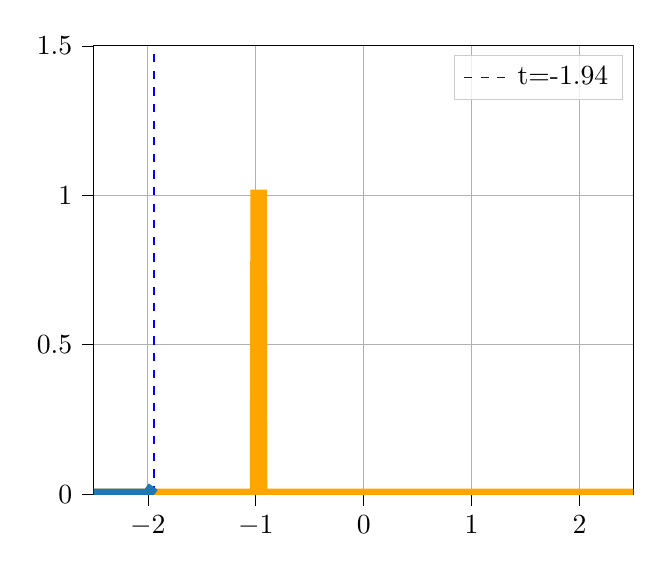
\begin{tikzpicture}

\definecolor{color0}{rgb}{1,0.498039215686275,0.0549019607843137}
\definecolor{color1}{rgb}{1,0.647058823529412,0}
\definecolor{color2}{rgb}{0.12156862745098,0.466666666666667,0.705882352941177}

\begin{axis}[
legend cell align={left},
legend style={fill opacity=0.8, draw opacity=1, text opacity=1, draw=white!80!black},
tick align=outside,
tick pos=left,
x grid style={white!69.0196078431373!black},
xmajorgrids,
xmin=-2.5, xmax=2.5,
xtick style={color=black},
y grid style={white!69.0196078431373!black},
ymajorgrids,
ymin=0, ymax=1.5,
ytick style={color=black}
]
\path [draw=color0, fill=color0, opacity=0.2]
(axis cs:-2.5,0)
--(axis cs:-2.5,0)
--(axis cs:-2.49499499499499,0)
--(axis cs:-2.48998998998999,0)
--(axis cs:-2.48498498498498,0)
--(axis cs:-2.47997997997998,0)
--(axis cs:-2.47497497497497,0)
--(axis cs:-2.46996996996997,0)
--(axis cs:-2.46496496496496,0)
--(axis cs:-2.45995995995996,0)
--(axis cs:-2.45495495495495,0)
--(axis cs:-2.44994994994995,0)
--(axis cs:-2.44494494494494,0)
--(axis cs:-2.43993993993994,0)
--(axis cs:-2.43493493493493,0)
--(axis cs:-2.42992992992993,0)
--(axis cs:-2.42492492492492,0)
--(axis cs:-2.41991991991992,0)
--(axis cs:-2.41491491491491,0)
--(axis cs:-2.40990990990991,0)
--(axis cs:-2.4049049049049,0)
--(axis cs:-2.3998998998999,0)
--(axis cs:-2.39489489489489,0)
--(axis cs:-2.38988988988989,0)
--(axis cs:-2.38488488488488,0)
--(axis cs:-2.37987987987988,0)
--(axis cs:-2.37487487487487,0)
--(axis cs:-2.36986986986987,0)
--(axis cs:-2.36486486486486,0)
--(axis cs:-2.35985985985986,0)
--(axis cs:-2.35485485485485,0)
--(axis cs:-2.34984984984985,0)
--(axis cs:-2.34484484484484,0)
--(axis cs:-2.33983983983984,0)
--(axis cs:-2.33483483483483,0)
--(axis cs:-2.32982982982983,0)
--(axis cs:-2.32482482482482,0)
--(axis cs:-2.31981981981982,0)
--(axis cs:-2.31481481481481,0)
--(axis cs:-2.30980980980981,0)
--(axis cs:-2.3048048048048,0)
--(axis cs:-2.2997997997998,0)
--(axis cs:-2.29479479479479,0)
--(axis cs:-2.28978978978979,0)
--(axis cs:-2.28478478478478,0)
--(axis cs:-2.27977977977978,0)
--(axis cs:-2.27477477477477,0)
--(axis cs:-2.26976976976977,0)
--(axis cs:-2.26476476476476,0)
--(axis cs:-2.25975975975976,0)
--(axis cs:-2.25475475475475,0)
--(axis cs:-2.24974974974975,0)
--(axis cs:-2.24474474474474,0)
--(axis cs:-2.23973973973974,0)
--(axis cs:-2.23473473473473,0)
--(axis cs:-2.22972972972973,0)
--(axis cs:-2.22472472472472,0)
--(axis cs:-2.21971971971972,0)
--(axis cs:-2.21471471471471,0)
--(axis cs:-2.20970970970971,0)
--(axis cs:-2.2047047047047,0)
--(axis cs:-2.1996996996997,0)
--(axis cs:-2.19469469469469,0)
--(axis cs:-2.18968968968969,0)
--(axis cs:-2.18468468468468,0)
--(axis cs:-2.17967967967968,0)
--(axis cs:-2.17467467467467,0)
--(axis cs:-2.16966966966967,0)
--(axis cs:-2.16466466466466,0)
--(axis cs:-2.15965965965966,0)
--(axis cs:-2.15465465465465,0)
--(axis cs:-2.14964964964965,0)
--(axis cs:-2.14464464464464,0)
--(axis cs:-2.13963963963964,0)
--(axis cs:-2.13463463463463,0)
--(axis cs:-2.12962962962963,0)
--(axis cs:-2.12462462462462,0)
--(axis cs:-2.11961961961962,0)
--(axis cs:-2.11461461461461,0)
--(axis cs:-2.10960960960961,0)
--(axis cs:-2.1046046046046,0)
--(axis cs:-2.0995995995996,0)
--(axis cs:-2.09459459459459,0)
--(axis cs:-2.08958958958959,0)
--(axis cs:-2.08458458458458,0)
--(axis cs:-2.07957957957958,0)
--(axis cs:-2.07457457457457,0)
--(axis cs:-2.06956956956957,0)
--(axis cs:-2.06456456456456,0)
--(axis cs:-2.05955955955956,0)
--(axis cs:-2.05455455455455,0)
--(axis cs:-2.04954954954955,0)
--(axis cs:-2.04454454454454,0)
--(axis cs:-2.03953953953954,0)
--(axis cs:-2.03453453453453,0)
--(axis cs:-2.02952952952953,0)
--(axis cs:-2.02452452452452,0)
--(axis cs:-2.01951951951952,0)
--(axis cs:-2.01451451451451,0)
--(axis cs:-2.00950950950951,0)
--(axis cs:-2.0045045045045,0)
--(axis cs:-1.9994994994995,0)
--(axis cs:-1.99449449449449,0)
--(axis cs:-1.98948948948949,0)
--(axis cs:-1.98448448448448,0)
--(axis cs:-1.97947947947948,0)
--(axis cs:-1.97447447447447,0)
--(axis cs:-1.96946946946947,0)
--(axis cs:-1.96446446446446,0)
--(axis cs:-1.95945945945946,0)
--(axis cs:-1.95445445445445,0)
--(axis cs:-1.94944944944945,0)
--(axis cs:-1.94444444444444,0)
--(axis cs:-1.93943943943944,0)
--(axis cs:-1.93443443443443,0)
--(axis cs:-1.92942942942943,0)
--(axis cs:-1.92442442442442,0)
--(axis cs:-1.91941941941942,0)
--(axis cs:-1.91441441441441,0)
--(axis cs:-1.90940940940941,0)
--(axis cs:-1.9044044044044,0)
--(axis cs:-1.8993993993994,0)
--(axis cs:-1.89439439439439,0)
--(axis cs:-1.88938938938939,0)
--(axis cs:-1.88438438438438,0)
--(axis cs:-1.87937937937938,0)
--(axis cs:-1.87437437437437,0)
--(axis cs:-1.86936936936937,0)
--(axis cs:-1.86436436436436,0)
--(axis cs:-1.85935935935936,0)
--(axis cs:-1.85435435435435,0)
--(axis cs:-1.84934934934935,0)
--(axis cs:-1.84434434434434,0)
--(axis cs:-1.83933933933934,0)
--(axis cs:-1.83433433433433,0)
--(axis cs:-1.82932932932933,0)
--(axis cs:-1.82432432432432,0)
--(axis cs:-1.81931931931932,0)
--(axis cs:-1.81431431431431,0)
--(axis cs:-1.80930930930931,0)
--(axis cs:-1.8043043043043,0)
--(axis cs:-1.7992992992993,0)
--(axis cs:-1.79429429429429,0)
--(axis cs:-1.78928928928929,0)
--(axis cs:-1.78428428428428,0)
--(axis cs:-1.77927927927928,0)
--(axis cs:-1.77427427427427,0)
--(axis cs:-1.76926926926927,0)
--(axis cs:-1.76426426426426,0)
--(axis cs:-1.75925925925926,0)
--(axis cs:-1.75425425425425,0)
--(axis cs:-1.74924924924925,0)
--(axis cs:-1.74424424424424,0)
--(axis cs:-1.73923923923924,0)
--(axis cs:-1.73423423423423,0)
--(axis cs:-1.72922922922923,0)
--(axis cs:-1.72422422422422,0)
--(axis cs:-1.71921921921922,0)
--(axis cs:-1.71421421421421,0)
--(axis cs:-1.70920920920921,0)
--(axis cs:-1.7042042042042,0)
--(axis cs:-1.6991991991992,0)
--(axis cs:-1.69419419419419,0)
--(axis cs:-1.68918918918919,0)
--(axis cs:-1.68418418418418,0)
--(axis cs:-1.67917917917918,0)
--(axis cs:-1.67417417417417,0)
--(axis cs:-1.66916916916917,0)
--(axis cs:-1.66416416416416,0)
--(axis cs:-1.65915915915916,0)
--(axis cs:-1.65415415415415,0)
--(axis cs:-1.64914914914915,0)
--(axis cs:-1.64414414414414,0)
--(axis cs:-1.63913913913914,0)
--(axis cs:-1.63413413413413,0)
--(axis cs:-1.62912912912913,0)
--(axis cs:-1.62412412412412,0)
--(axis cs:-1.61911911911912,0)
--(axis cs:-1.61411411411411,0)
--(axis cs:-1.60910910910911,0)
--(axis cs:-1.6041041041041,0)
--(axis cs:-1.5990990990991,0)
--(axis cs:-1.59409409409409,0)
--(axis cs:-1.58908908908909,0)
--(axis cs:-1.58408408408408,0)
--(axis cs:-1.57907907907908,0)
--(axis cs:-1.57407407407407,0)
--(axis cs:-1.56906906906907,0)
--(axis cs:-1.56406406406406,0)
--(axis cs:-1.55905905905906,0)
--(axis cs:-1.55405405405405,0)
--(axis cs:-1.54904904904905,0)
--(axis cs:-1.54404404404404,0)
--(axis cs:-1.53903903903904,0)
--(axis cs:-1.53403403403403,0)
--(axis cs:-1.52902902902903,0)
--(axis cs:-1.52402402402402,0)
--(axis cs:-1.51901901901902,0)
--(axis cs:-1.51401401401401,0)
--(axis cs:-1.50900900900901,0)
--(axis cs:-1.504004004004,0)
--(axis cs:-1.498998998999,0)
--(axis cs:-1.49399399399399,0)
--(axis cs:-1.48898898898899,0)
--(axis cs:-1.48398398398398,0)
--(axis cs:-1.47897897897898,0)
--(axis cs:-1.47397397397397,0)
--(axis cs:-1.46896896896897,0)
--(axis cs:-1.46396396396396,0)
--(axis cs:-1.45895895895896,0)
--(axis cs:-1.45395395395395,0)
--(axis cs:-1.44894894894895,0)
--(axis cs:-1.44394394394394,0)
--(axis cs:-1.43893893893894,0)
--(axis cs:-1.43393393393393,0)
--(axis cs:-1.42892892892893,0)
--(axis cs:-1.42392392392392,0)
--(axis cs:-1.41891891891892,0)
--(axis cs:-1.41391391391391,0)
--(axis cs:-1.40890890890891,0)
--(axis cs:-1.4039039039039,0)
--(axis cs:-1.3988988988989,0)
--(axis cs:-1.39389389389389,0)
--(axis cs:-1.38888888888889,0)
--(axis cs:-1.38388388388388,0)
--(axis cs:-1.37887887887888,0)
--(axis cs:-1.37387387387387,0)
--(axis cs:-1.36886886886887,0)
--(axis cs:-1.36386386386386,0)
--(axis cs:-1.35885885885886,0)
--(axis cs:-1.35385385385385,0)
--(axis cs:-1.34884884884885,0)
--(axis cs:-1.34384384384384,0)
--(axis cs:-1.33883883883884,0)
--(axis cs:-1.33383383383383,0)
--(axis cs:-1.32882882882883,0)
--(axis cs:-1.32382382382382,0)
--(axis cs:-1.31881881881882,0)
--(axis cs:-1.31381381381381,0)
--(axis cs:-1.30880880880881,0)
--(axis cs:-1.3038038038038,0)
--(axis cs:-1.2987987987988,0)
--(axis cs:-1.29379379379379,0)
--(axis cs:-1.28878878878879,0)
--(axis cs:-1.28378378378378,0)
--(axis cs:-1.27877877877878,0)
--(axis cs:-1.27377377377377,0)
--(axis cs:-1.26876876876877,0)
--(axis cs:-1.26376376376376,0)
--(axis cs:-1.25875875875876,0)
--(axis cs:-1.25375375375375,0)
--(axis cs:-1.24874874874875,0)
--(axis cs:-1.24374374374374,0)
--(axis cs:-1.23873873873874,0)
--(axis cs:-1.23373373373373,0)
--(axis cs:-1.22872872872873,0)
--(axis cs:-1.22372372372372,0)
--(axis cs:-1.21871871871872,0)
--(axis cs:-1.21371371371371,0)
--(axis cs:-1.20870870870871,0)
--(axis cs:-1.2037037037037,0)
--(axis cs:-1.1986986986987,0)
--(axis cs:-1.19369369369369,0)
--(axis cs:-1.18868868868869,0)
--(axis cs:-1.18368368368368,0)
--(axis cs:-1.17867867867868,0)
--(axis cs:-1.17367367367367,0)
--(axis cs:-1.16866866866867,0)
--(axis cs:-1.16366366366366,0)
--(axis cs:-1.15865865865866,0)
--(axis cs:-1.15365365365365,0)
--(axis cs:-1.14864864864865,0)
--(axis cs:-1.14364364364364,0)
--(axis cs:-1.13863863863864,0)
--(axis cs:-1.13363363363363,0)
--(axis cs:-1.12862862862863,0)
--(axis cs:-1.12362362362362,0)
--(axis cs:-1.11861861861862,0)
--(axis cs:-1.11361361361361,0)
--(axis cs:-1.10860860860861,0)
--(axis cs:-1.1036036036036,0)
--(axis cs:-1.0985985985986,0)
--(axis cs:-1.09359359359359,0)
--(axis cs:-1.08858858858859,0)
--(axis cs:-1.08358358358358,0)
--(axis cs:-1.07857857857858,0)
--(axis cs:-1.07357357357357,0)
--(axis cs:-1.06856856856857,0)
--(axis cs:-1.06356356356356,0)
--(axis cs:-1.05855855855856,0)
--(axis cs:-1.05355355355355,0)
--(axis cs:-1.04854854854855,0)
--(axis cs:-1.04354354354354,0)
--(axis cs:-1.03853853853854,0)
--(axis cs:-1.03353353353353,0)
--(axis cs:-1.02852852852853,0)
--(axis cs:-1.02352352352352,0)
--(axis cs:-1.01851851851852,0)
--(axis cs:-1.01351351351351,0)
--(axis cs:-1.00850850850851,0)
--(axis cs:-1.0035035035035,0)
--(axis cs:-0.998498498498499,0)
--(axis cs:-0.993493493493494,0)
--(axis cs:-0.988488488488489,0)
--(axis cs:-0.983483483483484,0)
--(axis cs:-0.978478478478479,0)
--(axis cs:-0.973473473473474,0)
--(axis cs:-0.968468468468469,0)
--(axis cs:-0.963463463463464,0)
--(axis cs:-0.958458458458459,0)
--(axis cs:-0.953453453453454,0)
--(axis cs:-0.948448448448449,0)
--(axis cs:-0.943443443443444,0)
--(axis cs:-0.938438438438439,0)
--(axis cs:-0.933433433433434,0)
--(axis cs:-0.928428428428429,0)
--(axis cs:-0.923423423423424,0)
--(axis cs:-0.918418418418419,0)
--(axis cs:-0.913413413413414,0)
--(axis cs:-0.908408408408409,0)
--(axis cs:-0.903403403403404,0)
--(axis cs:-0.898398398398399,0)
--(axis cs:-0.893393393393393,0)
--(axis cs:-0.888388388388388,0)
--(axis cs:-0.883383383383383,0)
--(axis cs:-0.878378378378378,0)
--(axis cs:-0.873373373373373,0)
--(axis cs:-0.868368368368368,0)
--(axis cs:-0.863363363363363,0)
--(axis cs:-0.858358358358358,0)
--(axis cs:-0.853353353353353,0)
--(axis cs:-0.848348348348348,0)
--(axis cs:-0.843343343343343,0)
--(axis cs:-0.838338338338338,0)
--(axis cs:-0.833333333333333,0)
--(axis cs:-0.828328328328328,0)
--(axis cs:-0.823323323323323,0)
--(axis cs:-0.818318318318318,0)
--(axis cs:-0.813313313313313,0)
--(axis cs:-0.808308308308308,0)
--(axis cs:-0.803303303303303,0)
--(axis cs:-0.798298298298298,0)
--(axis cs:-0.793293293293293,0)
--(axis cs:-0.788288288288288,0)
--(axis cs:-0.783283283283283,0)
--(axis cs:-0.778278278278278,0)
--(axis cs:-0.773273273273273,0)
--(axis cs:-0.768268268268268,0)
--(axis cs:-0.763263263263263,0)
--(axis cs:-0.758258258258258,0)
--(axis cs:-0.753253253253253,0)
--(axis cs:-0.748248248248248,0)
--(axis cs:-0.743243243243243,0)
--(axis cs:-0.738238238238238,0)
--(axis cs:-0.733233233233233,0)
--(axis cs:-0.728228228228228,0)
--(axis cs:-0.723223223223223,0)
--(axis cs:-0.718218218218218,0)
--(axis cs:-0.713213213213213,0)
--(axis cs:-0.708208208208208,0)
--(axis cs:-0.703203203203203,0)
--(axis cs:-0.698198198198198,0)
--(axis cs:-0.693193193193193,0)
--(axis cs:-0.688188188188188,0)
--(axis cs:-0.683183183183183,0)
--(axis cs:-0.678178178178178,0)
--(axis cs:-0.673173173173173,0)
--(axis cs:-0.668168168168168,0)
--(axis cs:-0.663163163163163,0)
--(axis cs:-0.658158158158158,0)
--(axis cs:-0.653153153153153,0)
--(axis cs:-0.648148148148148,0)
--(axis cs:-0.643143143143143,0)
--(axis cs:-0.638138138138138,0)
--(axis cs:-0.633133133133133,0)
--(axis cs:-0.628128128128128,0)
--(axis cs:-0.623123123123123,0)
--(axis cs:-0.618118118118118,0)
--(axis cs:-0.613113113113113,0)
--(axis cs:-0.608108108108108,0)
--(axis cs:-0.603103103103103,0)
--(axis cs:-0.598098098098098,0)
--(axis cs:-0.593093093093093,0)
--(axis cs:-0.588088088088088,0)
--(axis cs:-0.583083083083083,0)
--(axis cs:-0.578078078078078,0)
--(axis cs:-0.573073073073073,0)
--(axis cs:-0.568068068068068,0)
--(axis cs:-0.563063063063063,0)
--(axis cs:-0.558058058058058,0)
--(axis cs:-0.553053053053053,0)
--(axis cs:-0.548048048048048,0)
--(axis cs:-0.543043043043043,0)
--(axis cs:-0.538038038038038,0)
--(axis cs:-0.533033033033033,0)
--(axis cs:-0.528028028028028,0)
--(axis cs:-0.523023023023023,0)
--(axis cs:-0.518018018018018,0)
--(axis cs:-0.513013013013013,0)
--(axis cs:-0.508008008008008,0)
--(axis cs:-0.503003003003003,0)
--(axis cs:-0.497997997997998,0)
--(axis cs:-0.492992992992993,0)
--(axis cs:-0.487987987987988,0)
--(axis cs:-0.482982982982983,0)
--(axis cs:-0.477977977977978,0)
--(axis cs:-0.472972972972973,0)
--(axis cs:-0.467967967967968,0)
--(axis cs:-0.462962962962963,0)
--(axis cs:-0.457957957957958,0)
--(axis cs:-0.452952952952953,0)
--(axis cs:-0.447947947947948,0)
--(axis cs:-0.442942942942943,0)
--(axis cs:-0.437937937937938,0)
--(axis cs:-0.432932932932933,0)
--(axis cs:-0.427927927927928,0)
--(axis cs:-0.422922922922923,0)
--(axis cs:-0.417917917917918,0)
--(axis cs:-0.412912912912913,0)
--(axis cs:-0.407907907907908,0)
--(axis cs:-0.402902902902903,0)
--(axis cs:-0.397897897897898,0)
--(axis cs:-0.392892892892893,0)
--(axis cs:-0.387887887887888,0)
--(axis cs:-0.382882882882883,0)
--(axis cs:-0.377877877877878,0)
--(axis cs:-0.372872872872873,0)
--(axis cs:-0.367867867867868,0)
--(axis cs:-0.362862862862863,0)
--(axis cs:-0.357857857857858,0)
--(axis cs:-0.352852852852853,0)
--(axis cs:-0.347847847847848,0)
--(axis cs:-0.342842842842843,0)
--(axis cs:-0.337837837837838,0)
--(axis cs:-0.332832832832833,0)
--(axis cs:-0.327827827827828,0)
--(axis cs:-0.322822822822823,0)
--(axis cs:-0.317817817817818,0)
--(axis cs:-0.312812812812813,0)
--(axis cs:-0.307807807807808,0)
--(axis cs:-0.302802802802803,0)
--(axis cs:-0.297797797797798,0)
--(axis cs:-0.292792792792793,0)
--(axis cs:-0.287787787787788,0)
--(axis cs:-0.282782782782783,0)
--(axis cs:-0.277777777777778,0)
--(axis cs:-0.272772772772773,0)
--(axis cs:-0.267767767767768,0)
--(axis cs:-0.262762762762763,0)
--(axis cs:-0.257757757757758,0)
--(axis cs:-0.252752752752753,0)
--(axis cs:-0.247747747747748,0)
--(axis cs:-0.242742742742743,0)
--(axis cs:-0.237737737737738,0)
--(axis cs:-0.232732732732733,0)
--(axis cs:-0.227727727727728,0)
--(axis cs:-0.222722722722723,0)
--(axis cs:-0.217717717717718,0)
--(axis cs:-0.212712712712713,0)
--(axis cs:-0.207707707707708,0)
--(axis cs:-0.202702702702703,0)
--(axis cs:-0.197697697697698,0)
--(axis cs:-0.192692692692693,0)
--(axis cs:-0.187687687687688,0)
--(axis cs:-0.182682682682683,0)
--(axis cs:-0.177677677677678,0)
--(axis cs:-0.172672672672673,0)
--(axis cs:-0.167667667667668,0)
--(axis cs:-0.162662662662663,0)
--(axis cs:-0.157657657657658,0)
--(axis cs:-0.152652652652653,0)
--(axis cs:-0.147647647647648,0)
--(axis cs:-0.142642642642643,0)
--(axis cs:-0.137637637637638,0)
--(axis cs:-0.132632632632633,0)
--(axis cs:-0.127627627627628,0)
--(axis cs:-0.122622622622623,0)
--(axis cs:-0.117617617617618,0)
--(axis cs:-0.112612612612613,0)
--(axis cs:-0.107607607607608,0)
--(axis cs:-0.102602602602603,0)
--(axis cs:-0.0975975975975976,0)
--(axis cs:-0.0925925925925926,0)
--(axis cs:-0.0875875875875876,0)
--(axis cs:-0.0825825825825826,0)
--(axis cs:-0.0775775775775776,0)
--(axis cs:-0.0725725725725725,0)
--(axis cs:-0.0675675675675675,0)
--(axis cs:-0.0625625625625625,0)
--(axis cs:-0.0575575575575575,0)
--(axis cs:-0.0525525525525525,0)
--(axis cs:-0.0475475475475475,0)
--(axis cs:-0.0425425425425425,0)
--(axis cs:-0.0375375375375375,0)
--(axis cs:-0.0325325325325325,0)
--(axis cs:-0.0275275275275275,0)
--(axis cs:-0.0225225225225225,0)
--(axis cs:-0.0175175175175175,0)
--(axis cs:-0.0125125125125125,0)
--(axis cs:-0.0075075075075075,0)
--(axis cs:-0.0025025025025025,0)
--(axis cs:0.0025025025025025,0)
--(axis cs:0.0075075075075075,0)
--(axis cs:0.0125125125125125,0)
--(axis cs:0.0175175175175175,0)
--(axis cs:0.0225225225225225,0)
--(axis cs:0.0275275275275275,0)
--(axis cs:0.0325325325325325,0)
--(axis cs:0.0375375375375375,0)
--(axis cs:0.0425425425425425,0)
--(axis cs:0.0475475475475475,0)
--(axis cs:0.0525525525525525,0)
--(axis cs:0.0575575575575575,0)
--(axis cs:0.0625625625625625,0)
--(axis cs:0.0675675675675675,0)
--(axis cs:0.0725725725725725,0)
--(axis cs:0.0775775775775776,0)
--(axis cs:0.0825825825825826,0)
--(axis cs:0.0875875875875876,0)
--(axis cs:0.0925925925925926,0)
--(axis cs:0.0975975975975976,0)
--(axis cs:0.102602602602603,0)
--(axis cs:0.107607607607608,0)
--(axis cs:0.112612612612613,0)
--(axis cs:0.117617617617618,0)
--(axis cs:0.122622622622623,0)
--(axis cs:0.127627627627628,0)
--(axis cs:0.132632632632633,0)
--(axis cs:0.137637637637638,0)
--(axis cs:0.142642642642643,0)
--(axis cs:0.147647647647648,0)
--(axis cs:0.152652652652653,0)
--(axis cs:0.157657657657658,0)
--(axis cs:0.162662662662663,0)
--(axis cs:0.167667667667668,0)
--(axis cs:0.172672672672673,0)
--(axis cs:0.177677677677678,0)
--(axis cs:0.182682682682683,0)
--(axis cs:0.187687687687688,0)
--(axis cs:0.192692692692693,0)
--(axis cs:0.197697697697698,0)
--(axis cs:0.202702702702703,0)
--(axis cs:0.207707707707708,0)
--(axis cs:0.212712712712713,0)
--(axis cs:0.217717717717718,0)
--(axis cs:0.222722722722723,0)
--(axis cs:0.227727727727728,0)
--(axis cs:0.232732732732733,0)
--(axis cs:0.237737737737738,0)
--(axis cs:0.242742742742743,0)
--(axis cs:0.247747747747748,0)
--(axis cs:0.252752752752753,0)
--(axis cs:0.257757757757758,0)
--(axis cs:0.262762762762763,0)
--(axis cs:0.267767767767768,0)
--(axis cs:0.272772772772773,0)
--(axis cs:0.277777777777778,0)
--(axis cs:0.282782782782783,0)
--(axis cs:0.287787787787788,0)
--(axis cs:0.292792792792793,0)
--(axis cs:0.297797797797798,0)
--(axis cs:0.302802802802803,0)
--(axis cs:0.307807807807808,0)
--(axis cs:0.312812812812813,0)
--(axis cs:0.317817817817818,0)
--(axis cs:0.322822822822823,0)
--(axis cs:0.327827827827828,0)
--(axis cs:0.332832832832833,0)
--(axis cs:0.337837837837838,0)
--(axis cs:0.342842842842843,0)
--(axis cs:0.347847847847848,0)
--(axis cs:0.352852852852853,0)
--(axis cs:0.357857857857858,0)
--(axis cs:0.362862862862863,0)
--(axis cs:0.367867867867868,0)
--(axis cs:0.372872872872873,0)
--(axis cs:0.377877877877878,0)
--(axis cs:0.382882882882883,0)
--(axis cs:0.387887887887888,0)
--(axis cs:0.392892892892893,0)
--(axis cs:0.397897897897898,0)
--(axis cs:0.402902902902903,0)
--(axis cs:0.407907907907908,0)
--(axis cs:0.412912912912913,0)
--(axis cs:0.417917917917918,0)
--(axis cs:0.422922922922923,0)
--(axis cs:0.427927927927928,0)
--(axis cs:0.432932932932933,0)
--(axis cs:0.437937937937938,0)
--(axis cs:0.442942942942943,0)
--(axis cs:0.447947947947948,0)
--(axis cs:0.452952952952953,0)
--(axis cs:0.457957957957958,0)
--(axis cs:0.462962962962963,0)
--(axis cs:0.467967967967968,0)
--(axis cs:0.472972972972973,0)
--(axis cs:0.477977977977978,0)
--(axis cs:0.482982982982983,0)
--(axis cs:0.487987987987988,0)
--(axis cs:0.492992992992993,0)
--(axis cs:0.497997997997998,0)
--(axis cs:0.503003003003003,0)
--(axis cs:0.508008008008008,0)
--(axis cs:0.513013013013013,0)
--(axis cs:0.518018018018018,0)
--(axis cs:0.523023023023023,0)
--(axis cs:0.528028028028028,0)
--(axis cs:0.533033033033033,0)
--(axis cs:0.538038038038038,0)
--(axis cs:0.543043043043043,0)
--(axis cs:0.548048048048048,0)
--(axis cs:0.553053053053053,0)
--(axis cs:0.558058058058058,0)
--(axis cs:0.563063063063063,0)
--(axis cs:0.568068068068068,0)
--(axis cs:0.573073073073073,0)
--(axis cs:0.578078078078078,0)
--(axis cs:0.583083083083083,0)
--(axis cs:0.588088088088088,0)
--(axis cs:0.593093093093093,0)
--(axis cs:0.598098098098098,0)
--(axis cs:0.603103103103103,0)
--(axis cs:0.608108108108108,0)
--(axis cs:0.613113113113113,0)
--(axis cs:0.618118118118118,0)
--(axis cs:0.623123123123123,0)
--(axis cs:0.628128128128128,0)
--(axis cs:0.633133133133133,0)
--(axis cs:0.638138138138138,0)
--(axis cs:0.643143143143143,0)
--(axis cs:0.648148148148148,0)
--(axis cs:0.653153153153153,0)
--(axis cs:0.658158158158158,0)
--(axis cs:0.663163163163163,0)
--(axis cs:0.668168168168168,0)
--(axis cs:0.673173173173173,0)
--(axis cs:0.678178178178178,0)
--(axis cs:0.683183183183183,0)
--(axis cs:0.688188188188188,0)
--(axis cs:0.693193193193193,0)
--(axis cs:0.698198198198198,0)
--(axis cs:0.703203203203203,0)
--(axis cs:0.708208208208208,0)
--(axis cs:0.713213213213213,0)
--(axis cs:0.718218218218218,0)
--(axis cs:0.723223223223223,0)
--(axis cs:0.728228228228228,0)
--(axis cs:0.733233233233233,0)
--(axis cs:0.738238238238238,0)
--(axis cs:0.743243243243243,0)
--(axis cs:0.748248248248248,0)
--(axis cs:0.753253253253253,0)
--(axis cs:0.758258258258258,0)
--(axis cs:0.763263263263263,0)
--(axis cs:0.768268268268268,0)
--(axis cs:0.773273273273273,0)
--(axis cs:0.778278278278278,0)
--(axis cs:0.783283283283283,0)
--(axis cs:0.788288288288288,0)
--(axis cs:0.793293293293293,0)
--(axis cs:0.798298298298298,0)
--(axis cs:0.803303303303303,0)
--(axis cs:0.808308308308308,0)
--(axis cs:0.813313313313313,0)
--(axis cs:0.818318318318318,0)
--(axis cs:0.823323323323323,0)
--(axis cs:0.828328328328328,0)
--(axis cs:0.833333333333333,0)
--(axis cs:0.838338338338338,0)
--(axis cs:0.843343343343343,0)
--(axis cs:0.848348348348348,0)
--(axis cs:0.853353353353353,0)
--(axis cs:0.858358358358358,0)
--(axis cs:0.863363363363364,0)
--(axis cs:0.868368368368369,0)
--(axis cs:0.873373373373374,0)
--(axis cs:0.878378378378379,0)
--(axis cs:0.883383383383384,0)
--(axis cs:0.888388388388389,0)
--(axis cs:0.893393393393394,0)
--(axis cs:0.898398398398399,0)
--(axis cs:0.903403403403404,0)
--(axis cs:0.908408408408409,0)
--(axis cs:0.913413413413414,0)
--(axis cs:0.918418418418419,0)
--(axis cs:0.923423423423424,0)
--(axis cs:0.928428428428429,0)
--(axis cs:0.933433433433434,0)
--(axis cs:0.938438438438439,0)
--(axis cs:0.943443443443444,0)
--(axis cs:0.948448448448449,0)
--(axis cs:0.953453453453454,0)
--(axis cs:0.958458458458459,0)
--(axis cs:0.963463463463464,0)
--(axis cs:0.968468468468469,0)
--(axis cs:0.973473473473474,0)
--(axis cs:0.978478478478479,0)
--(axis cs:0.983483483483484,0)
--(axis cs:0.988488488488489,0)
--(axis cs:0.993493493493494,0)
--(axis cs:0.998498498498499,0)
--(axis cs:1.0035035035035,0)
--(axis cs:1.00850850850851,0)
--(axis cs:1.01351351351351,0)
--(axis cs:1.01851851851852,0)
--(axis cs:1.02352352352352,0)
--(axis cs:1.02852852852853,0)
--(axis cs:1.03353353353353,0)
--(axis cs:1.03853853853854,0)
--(axis cs:1.04354354354354,0)
--(axis cs:1.04854854854855,0)
--(axis cs:1.05355355355355,0)
--(axis cs:1.05855855855856,0)
--(axis cs:1.06356356356356,0)
--(axis cs:1.06856856856857,0)
--(axis cs:1.07357357357357,0)
--(axis cs:1.07857857857858,0)
--(axis cs:1.08358358358358,0)
--(axis cs:1.08858858858859,0)
--(axis cs:1.09359359359359,0)
--(axis cs:1.0985985985986,0)
--(axis cs:1.1036036036036,0)
--(axis cs:1.10860860860861,0)
--(axis cs:1.11361361361361,0)
--(axis cs:1.11861861861862,0)
--(axis cs:1.12362362362362,0)
--(axis cs:1.12862862862863,0)
--(axis cs:1.13363363363363,0)
--(axis cs:1.13863863863864,0)
--(axis cs:1.14364364364364,0)
--(axis cs:1.14864864864865,0)
--(axis cs:1.15365365365365,0)
--(axis cs:1.15865865865866,0)
--(axis cs:1.16366366366366,0)
--(axis cs:1.16866866866867,0)
--(axis cs:1.17367367367367,0)
--(axis cs:1.17867867867868,0)
--(axis cs:1.18368368368368,0)
--(axis cs:1.18868868868869,0)
--(axis cs:1.19369369369369,0)
--(axis cs:1.1986986986987,0)
--(axis cs:1.2037037037037,0)
--(axis cs:1.20870870870871,0)
--(axis cs:1.21371371371371,0)
--(axis cs:1.21871871871872,0)
--(axis cs:1.22372372372372,0)
--(axis cs:1.22872872872873,0)
--(axis cs:1.23373373373373,0)
--(axis cs:1.23873873873874,0)
--(axis cs:1.24374374374374,0)
--(axis cs:1.24874874874875,0)
--(axis cs:1.25375375375375,0)
--(axis cs:1.25875875875876,0)
--(axis cs:1.26376376376376,0)
--(axis cs:1.26876876876877,0)
--(axis cs:1.27377377377377,0)
--(axis cs:1.27877877877878,0)
--(axis cs:1.28378378378378,0)
--(axis cs:1.28878878878879,0)
--(axis cs:1.29379379379379,0)
--(axis cs:1.2987987987988,0)
--(axis cs:1.3038038038038,0)
--(axis cs:1.30880880880881,0)
--(axis cs:1.31381381381381,0)
--(axis cs:1.31881881881882,0)
--(axis cs:1.32382382382382,0)
--(axis cs:1.32882882882883,0)
--(axis cs:1.33383383383383,0)
--(axis cs:1.33883883883884,0)
--(axis cs:1.34384384384384,0)
--(axis cs:1.34884884884885,0)
--(axis cs:1.35385385385385,0)
--(axis cs:1.35885885885886,0)
--(axis cs:1.36386386386386,0)
--(axis cs:1.36886886886887,0)
--(axis cs:1.37387387387387,0)
--(axis cs:1.37887887887888,0)
--(axis cs:1.38388388388388,0)
--(axis cs:1.38888888888889,0)
--(axis cs:1.39389389389389,0)
--(axis cs:1.3988988988989,0)
--(axis cs:1.4039039039039,0)
--(axis cs:1.40890890890891,0)
--(axis cs:1.41391391391391,0)
--(axis cs:1.41891891891892,0)
--(axis cs:1.42392392392392,0)
--(axis cs:1.42892892892893,0)
--(axis cs:1.43393393393393,0)
--(axis cs:1.43893893893894,0)
--(axis cs:1.44394394394394,0)
--(axis cs:1.44894894894895,0)
--(axis cs:1.45395395395395,0)
--(axis cs:1.45895895895896,0)
--(axis cs:1.46396396396396,0)
--(axis cs:1.46896896896897,0)
--(axis cs:1.47397397397397,0)
--(axis cs:1.47897897897898,0)
--(axis cs:1.48398398398398,0)
--(axis cs:1.48898898898899,0)
--(axis cs:1.49399399399399,0)
--(axis cs:1.498998998999,0)
--(axis cs:1.504004004004,0)
--(axis cs:1.50900900900901,0)
--(axis cs:1.51401401401401,0)
--(axis cs:1.51901901901902,0)
--(axis cs:1.52402402402402,0)
--(axis cs:1.52902902902903,0)
--(axis cs:1.53403403403403,0)
--(axis cs:1.53903903903904,0)
--(axis cs:1.54404404404404,0)
--(axis cs:1.54904904904905,0)
--(axis cs:1.55405405405405,0)
--(axis cs:1.55905905905906,0)
--(axis cs:1.56406406406406,0)
--(axis cs:1.56906906906907,0)
--(axis cs:1.57407407407407,0)
--(axis cs:1.57907907907908,0)
--(axis cs:1.58408408408408,0)
--(axis cs:1.58908908908909,0)
--(axis cs:1.59409409409409,0)
--(axis cs:1.5990990990991,0)
--(axis cs:1.6041041041041,0)
--(axis cs:1.60910910910911,0)
--(axis cs:1.61411411411411,0)
--(axis cs:1.61911911911912,0)
--(axis cs:1.62412412412412,0)
--(axis cs:1.62912912912913,0)
--(axis cs:1.63413413413413,0)
--(axis cs:1.63913913913914,0)
--(axis cs:1.64414414414414,0)
--(axis cs:1.64914914914915,0)
--(axis cs:1.65415415415415,0)
--(axis cs:1.65915915915916,0)
--(axis cs:1.66416416416416,0)
--(axis cs:1.66916916916917,0)
--(axis cs:1.67417417417417,0)
--(axis cs:1.67917917917918,0)
--(axis cs:1.68418418418418,0)
--(axis cs:1.68918918918919,0)
--(axis cs:1.69419419419419,0)
--(axis cs:1.6991991991992,0)
--(axis cs:1.7042042042042,0)
--(axis cs:1.70920920920921,0)
--(axis cs:1.71421421421421,0)
--(axis cs:1.71921921921922,0)
--(axis cs:1.72422422422422,0)
--(axis cs:1.72922922922923,0)
--(axis cs:1.73423423423423,0)
--(axis cs:1.73923923923924,0)
--(axis cs:1.74424424424424,0)
--(axis cs:1.74924924924925,0)
--(axis cs:1.75425425425425,0)
--(axis cs:1.75925925925926,0)
--(axis cs:1.76426426426426,0)
--(axis cs:1.76926926926927,0)
--(axis cs:1.77427427427427,0)
--(axis cs:1.77927927927928,0)
--(axis cs:1.78428428428428,0)
--(axis cs:1.78928928928929,0)
--(axis cs:1.79429429429429,0)
--(axis cs:1.7992992992993,0)
--(axis cs:1.8043043043043,0)
--(axis cs:1.80930930930931,0)
--(axis cs:1.81431431431431,0)
--(axis cs:1.81931931931932,0)
--(axis cs:1.82432432432432,0)
--(axis cs:1.82932932932933,0)
--(axis cs:1.83433433433433,0)
--(axis cs:1.83933933933934,0)
--(axis cs:1.84434434434434,0)
--(axis cs:1.84934934934935,0)
--(axis cs:1.85435435435435,0)
--(axis cs:1.85935935935936,0)
--(axis cs:1.86436436436436,0)
--(axis cs:1.86936936936937,0)
--(axis cs:1.87437437437437,0)
--(axis cs:1.87937937937938,0)
--(axis cs:1.88438438438438,0)
--(axis cs:1.88938938938939,0)
--(axis cs:1.89439439439439,0)
--(axis cs:1.8993993993994,0)
--(axis cs:1.9044044044044,0)
--(axis cs:1.90940940940941,0)
--(axis cs:1.91441441441441,0)
--(axis cs:1.91941941941942,0)
--(axis cs:1.92442442442442,0)
--(axis cs:1.92942942942943,0)
--(axis cs:1.93443443443443,0)
--(axis cs:1.93943943943944,0)
--(axis cs:1.94444444444444,0)
--(axis cs:1.94944944944945,0)
--(axis cs:1.95445445445445,0)
--(axis cs:1.95945945945946,0)
--(axis cs:1.96446446446446,0)
--(axis cs:1.96946946946947,0)
--(axis cs:1.97447447447447,0)
--(axis cs:1.97947947947948,0)
--(axis cs:1.98448448448448,0)
--(axis cs:1.98948948948949,0)
--(axis cs:1.99449449449449,0)
--(axis cs:1.9994994994995,0)
--(axis cs:2.0045045045045,0)
--(axis cs:2.00950950950951,0)
--(axis cs:2.01451451451451,0)
--(axis cs:2.01951951951952,0)
--(axis cs:2.02452452452452,0)
--(axis cs:2.02952952952953,0)
--(axis cs:2.03453453453453,0)
--(axis cs:2.03953953953954,0)
--(axis cs:2.04454454454454,0)
--(axis cs:2.04954954954955,0)
--(axis cs:2.05455455455455,0)
--(axis cs:2.05955955955956,0)
--(axis cs:2.06456456456456,0)
--(axis cs:2.06956956956957,0)
--(axis cs:2.07457457457457,0)
--(axis cs:2.07957957957958,0)
--(axis cs:2.08458458458458,0)
--(axis cs:2.08958958958959,0)
--(axis cs:2.09459459459459,0)
--(axis cs:2.0995995995996,0)
--(axis cs:2.1046046046046,0)
--(axis cs:2.10960960960961,0)
--(axis cs:2.11461461461461,0)
--(axis cs:2.11961961961962,0)
--(axis cs:2.12462462462462,0)
--(axis cs:2.12962962962963,0)
--(axis cs:2.13463463463463,0)
--(axis cs:2.13963963963964,0)
--(axis cs:2.14464464464464,0)
--(axis cs:2.14964964964965,0)
--(axis cs:2.15465465465465,0)
--(axis cs:2.15965965965966,0)
--(axis cs:2.16466466466466,0)
--(axis cs:2.16966966966967,0)
--(axis cs:2.17467467467467,0)
--(axis cs:2.17967967967968,0)
--(axis cs:2.18468468468468,0)
--(axis cs:2.18968968968969,0)
--(axis cs:2.19469469469469,0)
--(axis cs:2.1996996996997,0)
--(axis cs:2.2047047047047,0)
--(axis cs:2.20970970970971,0)
--(axis cs:2.21471471471471,0)
--(axis cs:2.21971971971972,0)
--(axis cs:2.22472472472472,0)
--(axis cs:2.22972972972973,0)
--(axis cs:2.23473473473473,0)
--(axis cs:2.23973973973974,0)
--(axis cs:2.24474474474474,0)
--(axis cs:2.24974974974975,0)
--(axis cs:2.25475475475475,0)
--(axis cs:2.25975975975976,0)
--(axis cs:2.26476476476476,0)
--(axis cs:2.26976976976977,0)
--(axis cs:2.27477477477477,0)
--(axis cs:2.27977977977978,0)
--(axis cs:2.28478478478478,0)
--(axis cs:2.28978978978979,0)
--(axis cs:2.29479479479479,0)
--(axis cs:2.2997997997998,0)
--(axis cs:2.3048048048048,0)
--(axis cs:2.30980980980981,0)
--(axis cs:2.31481481481481,0)
--(axis cs:2.31981981981982,0)
--(axis cs:2.32482482482482,0)
--(axis cs:2.32982982982983,0)
--(axis cs:2.33483483483483,0)
--(axis cs:2.33983983983984,0)
--(axis cs:2.34484484484484,0)
--(axis cs:2.34984984984985,0)
--(axis cs:2.35485485485485,0)
--(axis cs:2.35985985985986,0)
--(axis cs:2.36486486486486,0)
--(axis cs:2.36986986986987,0)
--(axis cs:2.37487487487487,0)
--(axis cs:2.37987987987988,0)
--(axis cs:2.38488488488488,0)
--(axis cs:2.38988988988989,0)
--(axis cs:2.39489489489489,0)
--(axis cs:2.3998998998999,0)
--(axis cs:2.4049049049049,0)
--(axis cs:2.40990990990991,0)
--(axis cs:2.41491491491491,0)
--(axis cs:2.41991991991992,0)
--(axis cs:2.42492492492492,0)
--(axis cs:2.42992992992993,0)
--(axis cs:2.43493493493493,0)
--(axis cs:2.43993993993994,0)
--(axis cs:2.44494494494494,0)
--(axis cs:2.44994994994995,0)
--(axis cs:2.45495495495495,0)
--(axis cs:2.45995995995996,0)
--(axis cs:2.46496496496496,0)
--(axis cs:2.46996996996997,0)
--(axis cs:2.47497497497497,0)
--(axis cs:2.47997997997998,0)
--(axis cs:2.48498498498498,0)
--(axis cs:2.48998998998999,0)
--(axis cs:2.49499499499499,0)
--(axis cs:2.5,0)
--(axis cs:2.5,0)
--(axis cs:2.5,0)
--(axis cs:2.49499499499499,0)
--(axis cs:2.48998998998999,0)
--(axis cs:2.48498498498498,0)
--(axis cs:2.47997997997998,0)
--(axis cs:2.47497497497497,0)
--(axis cs:2.46996996996997,0)
--(axis cs:2.46496496496496,0)
--(axis cs:2.45995995995996,0)
--(axis cs:2.45495495495495,0)
--(axis cs:2.44994994994995,0)
--(axis cs:2.44494494494494,0)
--(axis cs:2.43993993993994,0)
--(axis cs:2.43493493493493,0)
--(axis cs:2.42992992992993,0)
--(axis cs:2.42492492492492,0)
--(axis cs:2.41991991991992,0)
--(axis cs:2.41491491491491,0)
--(axis cs:2.40990990990991,0)
--(axis cs:2.4049049049049,0)
--(axis cs:2.3998998998999,0)
--(axis cs:2.39489489489489,0)
--(axis cs:2.38988988988989,0)
--(axis cs:2.38488488488488,0)
--(axis cs:2.37987987987988,0)
--(axis cs:2.37487487487487,0)
--(axis cs:2.36986986986987,0)
--(axis cs:2.36486486486486,0)
--(axis cs:2.35985985985986,0)
--(axis cs:2.35485485485485,0)
--(axis cs:2.34984984984985,0)
--(axis cs:2.34484484484484,0)
--(axis cs:2.33983983983984,0)
--(axis cs:2.33483483483483,0)
--(axis cs:2.32982982982983,0)
--(axis cs:2.32482482482482,0)
--(axis cs:2.31981981981982,0)
--(axis cs:2.31481481481481,0)
--(axis cs:2.30980980980981,0)
--(axis cs:2.3048048048048,0)
--(axis cs:2.2997997997998,0)
--(axis cs:2.29479479479479,0)
--(axis cs:2.28978978978979,0)
--(axis cs:2.28478478478478,0)
--(axis cs:2.27977977977978,0)
--(axis cs:2.27477477477477,0)
--(axis cs:2.26976976976977,0)
--(axis cs:2.26476476476476,0)
--(axis cs:2.25975975975976,0)
--(axis cs:2.25475475475475,0)
--(axis cs:2.24974974974975,0)
--(axis cs:2.24474474474474,0)
--(axis cs:2.23973973973974,0)
--(axis cs:2.23473473473473,0)
--(axis cs:2.22972972972973,0)
--(axis cs:2.22472472472472,0)
--(axis cs:2.21971971971972,0)
--(axis cs:2.21471471471471,0)
--(axis cs:2.20970970970971,0)
--(axis cs:2.2047047047047,0)
--(axis cs:2.1996996996997,0)
--(axis cs:2.19469469469469,0)
--(axis cs:2.18968968968969,0)
--(axis cs:2.18468468468468,0)
--(axis cs:2.17967967967968,0)
--(axis cs:2.17467467467467,0)
--(axis cs:2.16966966966967,0)
--(axis cs:2.16466466466466,0)
--(axis cs:2.15965965965966,0)
--(axis cs:2.15465465465465,0)
--(axis cs:2.14964964964965,0)
--(axis cs:2.14464464464464,0)
--(axis cs:2.13963963963964,0)
--(axis cs:2.13463463463463,0)
--(axis cs:2.12962962962963,0)
--(axis cs:2.12462462462462,0)
--(axis cs:2.11961961961962,0)
--(axis cs:2.11461461461461,0)
--(axis cs:2.10960960960961,0)
--(axis cs:2.1046046046046,0)
--(axis cs:2.0995995995996,0)
--(axis cs:2.09459459459459,0)
--(axis cs:2.08958958958959,0)
--(axis cs:2.08458458458458,0)
--(axis cs:2.07957957957958,0)
--(axis cs:2.07457457457457,0)
--(axis cs:2.06956956956957,0)
--(axis cs:2.06456456456456,0)
--(axis cs:2.05955955955956,0)
--(axis cs:2.05455455455455,0)
--(axis cs:2.04954954954955,0)
--(axis cs:2.04454454454454,0)
--(axis cs:2.03953953953954,0)
--(axis cs:2.03453453453453,0)
--(axis cs:2.02952952952953,0)
--(axis cs:2.02452452452452,0)
--(axis cs:2.01951951951952,0)
--(axis cs:2.01451451451451,0)
--(axis cs:2.00950950950951,0)
--(axis cs:2.0045045045045,0)
--(axis cs:1.9994994994995,0)
--(axis cs:1.99449449449449,0)
--(axis cs:1.98948948948949,0)
--(axis cs:1.98448448448448,0)
--(axis cs:1.97947947947948,0)
--(axis cs:1.97447447447447,0)
--(axis cs:1.96946946946947,0)
--(axis cs:1.96446446446446,0)
--(axis cs:1.95945945945946,0)
--(axis cs:1.95445445445445,0)
--(axis cs:1.94944944944945,0)
--(axis cs:1.94444444444444,0)
--(axis cs:1.93943943943944,0)
--(axis cs:1.93443443443443,0)
--(axis cs:1.92942942942943,0)
--(axis cs:1.92442442442442,0)
--(axis cs:1.91941941941942,0)
--(axis cs:1.91441441441441,0)
--(axis cs:1.90940940940941,0)
--(axis cs:1.9044044044044,0)
--(axis cs:1.8993993993994,0)
--(axis cs:1.89439439439439,0)
--(axis cs:1.88938938938939,0)
--(axis cs:1.88438438438438,0)
--(axis cs:1.87937937937938,0)
--(axis cs:1.87437437437437,0)
--(axis cs:1.86936936936937,0)
--(axis cs:1.86436436436436,0)
--(axis cs:1.85935935935936,0)
--(axis cs:1.85435435435435,0)
--(axis cs:1.84934934934935,0)
--(axis cs:1.84434434434434,0)
--(axis cs:1.83933933933934,0)
--(axis cs:1.83433433433433,0)
--(axis cs:1.82932932932933,0)
--(axis cs:1.82432432432432,0)
--(axis cs:1.81931931931932,0)
--(axis cs:1.81431431431431,0)
--(axis cs:1.80930930930931,0)
--(axis cs:1.8043043043043,0)
--(axis cs:1.7992992992993,0)
--(axis cs:1.79429429429429,0)
--(axis cs:1.78928928928929,0)
--(axis cs:1.78428428428428,0)
--(axis cs:1.77927927927928,0)
--(axis cs:1.77427427427427,0)
--(axis cs:1.76926926926927,0)
--(axis cs:1.76426426426426,0)
--(axis cs:1.75925925925926,0)
--(axis cs:1.75425425425425,0)
--(axis cs:1.74924924924925,0)
--(axis cs:1.74424424424424,0)
--(axis cs:1.73923923923924,0)
--(axis cs:1.73423423423423,0)
--(axis cs:1.72922922922923,0)
--(axis cs:1.72422422422422,0)
--(axis cs:1.71921921921922,0)
--(axis cs:1.71421421421421,0)
--(axis cs:1.70920920920921,0)
--(axis cs:1.7042042042042,0)
--(axis cs:1.6991991991992,0)
--(axis cs:1.69419419419419,0)
--(axis cs:1.68918918918919,0)
--(axis cs:1.68418418418418,0)
--(axis cs:1.67917917917918,0)
--(axis cs:1.67417417417417,0)
--(axis cs:1.66916916916917,0)
--(axis cs:1.66416416416416,0)
--(axis cs:1.65915915915916,0)
--(axis cs:1.65415415415415,0)
--(axis cs:1.64914914914915,0)
--(axis cs:1.64414414414414,0)
--(axis cs:1.63913913913914,0)
--(axis cs:1.63413413413413,0)
--(axis cs:1.62912912912913,0)
--(axis cs:1.62412412412412,0)
--(axis cs:1.61911911911912,0)
--(axis cs:1.61411411411411,0)
--(axis cs:1.60910910910911,0)
--(axis cs:1.6041041041041,0)
--(axis cs:1.5990990990991,0)
--(axis cs:1.59409409409409,0)
--(axis cs:1.58908908908909,0)
--(axis cs:1.58408408408408,0)
--(axis cs:1.57907907907908,0)
--(axis cs:1.57407407407407,0)
--(axis cs:1.56906906906907,0)
--(axis cs:1.56406406406406,0)
--(axis cs:1.55905905905906,0)
--(axis cs:1.55405405405405,0)
--(axis cs:1.54904904904905,0)
--(axis cs:1.54404404404404,0)
--(axis cs:1.53903903903904,0)
--(axis cs:1.53403403403403,0)
--(axis cs:1.52902902902903,0)
--(axis cs:1.52402402402402,0)
--(axis cs:1.51901901901902,0)
--(axis cs:1.51401401401401,0)
--(axis cs:1.50900900900901,0)
--(axis cs:1.504004004004,0)
--(axis cs:1.498998998999,0)
--(axis cs:1.49399399399399,0)
--(axis cs:1.48898898898899,0)
--(axis cs:1.48398398398398,0)
--(axis cs:1.47897897897898,0)
--(axis cs:1.47397397397397,0)
--(axis cs:1.46896896896897,0)
--(axis cs:1.46396396396396,0)
--(axis cs:1.45895895895896,0)
--(axis cs:1.45395395395395,0)
--(axis cs:1.44894894894895,0)
--(axis cs:1.44394394394394,0)
--(axis cs:1.43893893893894,0)
--(axis cs:1.43393393393393,0)
--(axis cs:1.42892892892893,0)
--(axis cs:1.42392392392392,0)
--(axis cs:1.41891891891892,0)
--(axis cs:1.41391391391391,0)
--(axis cs:1.40890890890891,0)
--(axis cs:1.4039039039039,0)
--(axis cs:1.3988988988989,0)
--(axis cs:1.39389389389389,0)
--(axis cs:1.38888888888889,0)
--(axis cs:1.38388388388388,0)
--(axis cs:1.37887887887888,0)
--(axis cs:1.37387387387387,0)
--(axis cs:1.36886886886887,0)
--(axis cs:1.36386386386386,0)
--(axis cs:1.35885885885886,0)
--(axis cs:1.35385385385385,0)
--(axis cs:1.34884884884885,0)
--(axis cs:1.34384384384384,0)
--(axis cs:1.33883883883884,0)
--(axis cs:1.33383383383383,0)
--(axis cs:1.32882882882883,0)
--(axis cs:1.32382382382382,0)
--(axis cs:1.31881881881882,0)
--(axis cs:1.31381381381381,0)
--(axis cs:1.30880880880881,0)
--(axis cs:1.3038038038038,0)
--(axis cs:1.2987987987988,0)
--(axis cs:1.29379379379379,0)
--(axis cs:1.28878878878879,0)
--(axis cs:1.28378378378378,0)
--(axis cs:1.27877877877878,0)
--(axis cs:1.27377377377377,0)
--(axis cs:1.26876876876877,0)
--(axis cs:1.26376376376376,0)
--(axis cs:1.25875875875876,0)
--(axis cs:1.25375375375375,0)
--(axis cs:1.24874874874875,0)
--(axis cs:1.24374374374374,0)
--(axis cs:1.23873873873874,0)
--(axis cs:1.23373373373373,0)
--(axis cs:1.22872872872873,0)
--(axis cs:1.22372372372372,0)
--(axis cs:1.21871871871872,0)
--(axis cs:1.21371371371371,0)
--(axis cs:1.20870870870871,0)
--(axis cs:1.2037037037037,0)
--(axis cs:1.1986986986987,0)
--(axis cs:1.19369369369369,0)
--(axis cs:1.18868868868869,0)
--(axis cs:1.18368368368368,0)
--(axis cs:1.17867867867868,0)
--(axis cs:1.17367367367367,0)
--(axis cs:1.16866866866867,0)
--(axis cs:1.16366366366366,0)
--(axis cs:1.15865865865866,0)
--(axis cs:1.15365365365365,0)
--(axis cs:1.14864864864865,0)
--(axis cs:1.14364364364364,0)
--(axis cs:1.13863863863864,0)
--(axis cs:1.13363363363363,0)
--(axis cs:1.12862862862863,0)
--(axis cs:1.12362362362362,0)
--(axis cs:1.11861861861862,0)
--(axis cs:1.11361361361361,0)
--(axis cs:1.10860860860861,0)
--(axis cs:1.1036036036036,0)
--(axis cs:1.0985985985986,0)
--(axis cs:1.09359359359359,0)
--(axis cs:1.08858858858859,0)
--(axis cs:1.08358358358358,0)
--(axis cs:1.07857857857858,0)
--(axis cs:1.07357357357357,0)
--(axis cs:1.06856856856857,0)
--(axis cs:1.06356356356356,0)
--(axis cs:1.05855855855856,0)
--(axis cs:1.05355355355355,0)
--(axis cs:1.04854854854855,0)
--(axis cs:1.04354354354354,0)
--(axis cs:1.03853853853854,0)
--(axis cs:1.03353353353353,0)
--(axis cs:1.02852852852853,0)
--(axis cs:1.02352352352352,0)
--(axis cs:1.01851851851852,0)
--(axis cs:1.01351351351351,0)
--(axis cs:1.00850850850851,0)
--(axis cs:1.0035035035035,0)
--(axis cs:0.998498498498499,0)
--(axis cs:0.993493493493494,0)
--(axis cs:0.988488488488489,0)
--(axis cs:0.983483483483484,0)
--(axis cs:0.978478478478479,0)
--(axis cs:0.973473473473474,0)
--(axis cs:0.968468468468469,0)
--(axis cs:0.963463463463464,0)
--(axis cs:0.958458458458459,0)
--(axis cs:0.953453453453454,0)
--(axis cs:0.948448448448449,0)
--(axis cs:0.943443443443444,0)
--(axis cs:0.938438438438439,0)
--(axis cs:0.933433433433434,0)
--(axis cs:0.928428428428429,0)
--(axis cs:0.923423423423424,0)
--(axis cs:0.918418418418419,0)
--(axis cs:0.913413413413414,0)
--(axis cs:0.908408408408409,0)
--(axis cs:0.903403403403404,0)
--(axis cs:0.898398398398399,0)
--(axis cs:0.893393393393394,0)
--(axis cs:0.888388388388389,0)
--(axis cs:0.883383383383384,0)
--(axis cs:0.878378378378379,0)
--(axis cs:0.873373373373374,0)
--(axis cs:0.868368368368369,0)
--(axis cs:0.863363363363364,0)
--(axis cs:0.858358358358358,0)
--(axis cs:0.853353353353353,0)
--(axis cs:0.848348348348348,0)
--(axis cs:0.843343343343343,0)
--(axis cs:0.838338338338338,0)
--(axis cs:0.833333333333333,0)
--(axis cs:0.828328328328328,0)
--(axis cs:0.823323323323323,0)
--(axis cs:0.818318318318318,0)
--(axis cs:0.813313313313313,0)
--(axis cs:0.808308308308308,0)
--(axis cs:0.803303303303303,0)
--(axis cs:0.798298298298298,0)
--(axis cs:0.793293293293293,0)
--(axis cs:0.788288288288288,0)
--(axis cs:0.783283283283283,0)
--(axis cs:0.778278278278278,0)
--(axis cs:0.773273273273273,0)
--(axis cs:0.768268268268268,0)
--(axis cs:0.763263263263263,0)
--(axis cs:0.758258258258258,0)
--(axis cs:0.753253253253253,0)
--(axis cs:0.748248248248248,0)
--(axis cs:0.743243243243243,0)
--(axis cs:0.738238238238238,0)
--(axis cs:0.733233233233233,0)
--(axis cs:0.728228228228228,0)
--(axis cs:0.723223223223223,0)
--(axis cs:0.718218218218218,0)
--(axis cs:0.713213213213213,0)
--(axis cs:0.708208208208208,0)
--(axis cs:0.703203203203203,0)
--(axis cs:0.698198198198198,0)
--(axis cs:0.693193193193193,0)
--(axis cs:0.688188188188188,0)
--(axis cs:0.683183183183183,0)
--(axis cs:0.678178178178178,0)
--(axis cs:0.673173173173173,0)
--(axis cs:0.668168168168168,0)
--(axis cs:0.663163163163163,0)
--(axis cs:0.658158158158158,0)
--(axis cs:0.653153153153153,0)
--(axis cs:0.648148148148148,0)
--(axis cs:0.643143143143143,0)
--(axis cs:0.638138138138138,0)
--(axis cs:0.633133133133133,0)
--(axis cs:0.628128128128128,0)
--(axis cs:0.623123123123123,0)
--(axis cs:0.618118118118118,0)
--(axis cs:0.613113113113113,0)
--(axis cs:0.608108108108108,0)
--(axis cs:0.603103103103103,0)
--(axis cs:0.598098098098098,0)
--(axis cs:0.593093093093093,0)
--(axis cs:0.588088088088088,0)
--(axis cs:0.583083083083083,0)
--(axis cs:0.578078078078078,0)
--(axis cs:0.573073073073073,0)
--(axis cs:0.568068068068068,0)
--(axis cs:0.563063063063063,0)
--(axis cs:0.558058058058058,0)
--(axis cs:0.553053053053053,0)
--(axis cs:0.548048048048048,0)
--(axis cs:0.543043043043043,0)
--(axis cs:0.538038038038038,0)
--(axis cs:0.533033033033033,0)
--(axis cs:0.528028028028028,0)
--(axis cs:0.523023023023023,0)
--(axis cs:0.518018018018018,0)
--(axis cs:0.513013013013013,0)
--(axis cs:0.508008008008008,0)
--(axis cs:0.503003003003003,0)
--(axis cs:0.497997997997998,0)
--(axis cs:0.492992992992993,0)
--(axis cs:0.487987987987988,0)
--(axis cs:0.482982982982983,0)
--(axis cs:0.477977977977978,0)
--(axis cs:0.472972972972973,0)
--(axis cs:0.467967967967968,0)
--(axis cs:0.462962962962963,0)
--(axis cs:0.457957957957958,0)
--(axis cs:0.452952952952953,0)
--(axis cs:0.447947947947948,0)
--(axis cs:0.442942942942943,0)
--(axis cs:0.437937937937938,0)
--(axis cs:0.432932932932933,0)
--(axis cs:0.427927927927928,0)
--(axis cs:0.422922922922923,0)
--(axis cs:0.417917917917918,0)
--(axis cs:0.412912912912913,0)
--(axis cs:0.407907907907908,0)
--(axis cs:0.402902902902903,0)
--(axis cs:0.397897897897898,0)
--(axis cs:0.392892892892893,0)
--(axis cs:0.387887887887888,0)
--(axis cs:0.382882882882883,0)
--(axis cs:0.377877877877878,0)
--(axis cs:0.372872872872873,0)
--(axis cs:0.367867867867868,0)
--(axis cs:0.362862862862863,0)
--(axis cs:0.357857857857858,0)
--(axis cs:0.352852852852853,0)
--(axis cs:0.347847847847848,0)
--(axis cs:0.342842842842843,0)
--(axis cs:0.337837837837838,0)
--(axis cs:0.332832832832833,0)
--(axis cs:0.327827827827828,0)
--(axis cs:0.322822822822823,0)
--(axis cs:0.317817817817818,0)
--(axis cs:0.312812812812813,0)
--(axis cs:0.307807807807808,0)
--(axis cs:0.302802802802803,0)
--(axis cs:0.297797797797798,0)
--(axis cs:0.292792792792793,0)
--(axis cs:0.287787787787788,0)
--(axis cs:0.282782782782783,0)
--(axis cs:0.277777777777778,0)
--(axis cs:0.272772772772773,0)
--(axis cs:0.267767767767768,0)
--(axis cs:0.262762762762763,0)
--(axis cs:0.257757757757758,0)
--(axis cs:0.252752752752753,0)
--(axis cs:0.247747747747748,0)
--(axis cs:0.242742742742743,0)
--(axis cs:0.237737737737738,0)
--(axis cs:0.232732732732733,0)
--(axis cs:0.227727727727728,0)
--(axis cs:0.222722722722723,0)
--(axis cs:0.217717717717718,0)
--(axis cs:0.212712712712713,0)
--(axis cs:0.207707707707708,0)
--(axis cs:0.202702702702703,0)
--(axis cs:0.197697697697698,0)
--(axis cs:0.192692692692693,0)
--(axis cs:0.187687687687688,0)
--(axis cs:0.182682682682683,0)
--(axis cs:0.177677677677678,0)
--(axis cs:0.172672672672673,0)
--(axis cs:0.167667667667668,0)
--(axis cs:0.162662662662663,0)
--(axis cs:0.157657657657658,0)
--(axis cs:0.152652652652653,0)
--(axis cs:0.147647647647648,0)
--(axis cs:0.142642642642643,0)
--(axis cs:0.137637637637638,0)
--(axis cs:0.132632632632633,0)
--(axis cs:0.127627627627628,0)
--(axis cs:0.122622622622623,0)
--(axis cs:0.117617617617618,0)
--(axis cs:0.112612612612613,0)
--(axis cs:0.107607607607608,0)
--(axis cs:0.102602602602603,0)
--(axis cs:0.0975975975975976,0)
--(axis cs:0.0925925925925926,0)
--(axis cs:0.0875875875875876,0)
--(axis cs:0.0825825825825826,0)
--(axis cs:0.0775775775775776,0)
--(axis cs:0.0725725725725725,0)
--(axis cs:0.0675675675675675,0)
--(axis cs:0.0625625625625625,0)
--(axis cs:0.0575575575575575,0)
--(axis cs:0.0525525525525525,0)
--(axis cs:0.0475475475475475,0)
--(axis cs:0.0425425425425425,0)
--(axis cs:0.0375375375375375,0)
--(axis cs:0.0325325325325325,0)
--(axis cs:0.0275275275275275,0)
--(axis cs:0.0225225225225225,0)
--(axis cs:0.0175175175175175,0)
--(axis cs:0.0125125125125125,0)
--(axis cs:0.0075075075075075,0)
--(axis cs:0.0025025025025025,0)
--(axis cs:-0.0025025025025025,0)
--(axis cs:-0.0075075075075075,0)
--(axis cs:-0.0125125125125125,0)
--(axis cs:-0.0175175175175175,0)
--(axis cs:-0.0225225225225225,0)
--(axis cs:-0.0275275275275275,0)
--(axis cs:-0.0325325325325325,0)
--(axis cs:-0.0375375375375375,0)
--(axis cs:-0.0425425425425425,0)
--(axis cs:-0.0475475475475475,0)
--(axis cs:-0.0525525525525525,0)
--(axis cs:-0.0575575575575575,0)
--(axis cs:-0.0625625625625625,0)
--(axis cs:-0.0675675675675675,0)
--(axis cs:-0.0725725725725725,0)
--(axis cs:-0.0775775775775776,0)
--(axis cs:-0.0825825825825826,0)
--(axis cs:-0.0875875875875876,0)
--(axis cs:-0.0925925925925926,0)
--(axis cs:-0.0975975975975976,0)
--(axis cs:-0.102602602602603,0)
--(axis cs:-0.107607607607608,0)
--(axis cs:-0.112612612612613,0)
--(axis cs:-0.117617617617618,0)
--(axis cs:-0.122622622622623,0)
--(axis cs:-0.127627627627628,0)
--(axis cs:-0.132632632632633,0)
--(axis cs:-0.137637637637638,0)
--(axis cs:-0.142642642642643,0)
--(axis cs:-0.147647647647648,0)
--(axis cs:-0.152652652652653,0)
--(axis cs:-0.157657657657658,0)
--(axis cs:-0.162662662662663,0)
--(axis cs:-0.167667667667668,0)
--(axis cs:-0.172672672672673,0)
--(axis cs:-0.177677677677678,0)
--(axis cs:-0.182682682682683,0)
--(axis cs:-0.187687687687688,0)
--(axis cs:-0.192692692692693,0)
--(axis cs:-0.197697697697698,0)
--(axis cs:-0.202702702702703,0)
--(axis cs:-0.207707707707708,0)
--(axis cs:-0.212712712712713,0)
--(axis cs:-0.217717717717718,0)
--(axis cs:-0.222722722722723,0)
--(axis cs:-0.227727727727728,0)
--(axis cs:-0.232732732732733,0)
--(axis cs:-0.237737737737738,0)
--(axis cs:-0.242742742742743,0)
--(axis cs:-0.247747747747748,0)
--(axis cs:-0.252752752752753,0)
--(axis cs:-0.257757757757758,0)
--(axis cs:-0.262762762762763,0)
--(axis cs:-0.267767767767768,0)
--(axis cs:-0.272772772772773,0)
--(axis cs:-0.277777777777778,0)
--(axis cs:-0.282782782782783,0)
--(axis cs:-0.287787787787788,0)
--(axis cs:-0.292792792792793,0)
--(axis cs:-0.297797797797798,0)
--(axis cs:-0.302802802802803,0)
--(axis cs:-0.307807807807808,0)
--(axis cs:-0.312812812812813,0)
--(axis cs:-0.317817817817818,0)
--(axis cs:-0.322822822822823,0)
--(axis cs:-0.327827827827828,0)
--(axis cs:-0.332832832832833,0)
--(axis cs:-0.337837837837838,0)
--(axis cs:-0.342842842842843,0)
--(axis cs:-0.347847847847848,0)
--(axis cs:-0.352852852852853,0)
--(axis cs:-0.357857857857858,0)
--(axis cs:-0.362862862862863,0)
--(axis cs:-0.367867867867868,0)
--(axis cs:-0.372872872872873,0)
--(axis cs:-0.377877877877878,0)
--(axis cs:-0.382882882882883,0)
--(axis cs:-0.387887887887888,0)
--(axis cs:-0.392892892892893,0)
--(axis cs:-0.397897897897898,0)
--(axis cs:-0.402902902902903,0)
--(axis cs:-0.407907907907908,0)
--(axis cs:-0.412912912912913,0)
--(axis cs:-0.417917917917918,0)
--(axis cs:-0.422922922922923,0)
--(axis cs:-0.427927927927928,0)
--(axis cs:-0.432932932932933,0)
--(axis cs:-0.437937937937938,0)
--(axis cs:-0.442942942942943,0)
--(axis cs:-0.447947947947948,0)
--(axis cs:-0.452952952952953,0)
--(axis cs:-0.457957957957958,0)
--(axis cs:-0.462962962962963,0)
--(axis cs:-0.467967967967968,0)
--(axis cs:-0.472972972972973,0)
--(axis cs:-0.477977977977978,0)
--(axis cs:-0.482982982982983,0)
--(axis cs:-0.487987987987988,0)
--(axis cs:-0.492992992992993,0)
--(axis cs:-0.497997997997998,0)
--(axis cs:-0.503003003003003,0)
--(axis cs:-0.508008008008008,0)
--(axis cs:-0.513013013013013,0)
--(axis cs:-0.518018018018018,0)
--(axis cs:-0.523023023023023,0)
--(axis cs:-0.528028028028028,0)
--(axis cs:-0.533033033033033,0)
--(axis cs:-0.538038038038038,0)
--(axis cs:-0.543043043043043,0)
--(axis cs:-0.548048048048048,0)
--(axis cs:-0.553053053053053,0)
--(axis cs:-0.558058058058058,0)
--(axis cs:-0.563063063063063,0)
--(axis cs:-0.568068068068068,0)
--(axis cs:-0.573073073073073,0)
--(axis cs:-0.578078078078078,0)
--(axis cs:-0.583083083083083,0)
--(axis cs:-0.588088088088088,0)
--(axis cs:-0.593093093093093,0)
--(axis cs:-0.598098098098098,0)
--(axis cs:-0.603103103103103,0)
--(axis cs:-0.608108108108108,0)
--(axis cs:-0.613113113113113,0)
--(axis cs:-0.618118118118118,0)
--(axis cs:-0.623123123123123,0)
--(axis cs:-0.628128128128128,0)
--(axis cs:-0.633133133133133,0)
--(axis cs:-0.638138138138138,0)
--(axis cs:-0.643143143143143,0)
--(axis cs:-0.648148148148148,0)
--(axis cs:-0.653153153153153,0)
--(axis cs:-0.658158158158158,0)
--(axis cs:-0.663163163163163,0)
--(axis cs:-0.668168168168168,0)
--(axis cs:-0.673173173173173,0)
--(axis cs:-0.678178178178178,0)
--(axis cs:-0.683183183183183,0)
--(axis cs:-0.688188188188188,0)
--(axis cs:-0.693193193193193,0)
--(axis cs:-0.698198198198198,0)
--(axis cs:-0.703203203203203,0)
--(axis cs:-0.708208208208208,0)
--(axis cs:-0.713213213213213,0)
--(axis cs:-0.718218218218218,0)
--(axis cs:-0.723223223223223,0)
--(axis cs:-0.728228228228228,0)
--(axis cs:-0.733233233233233,0)
--(axis cs:-0.738238238238238,0)
--(axis cs:-0.743243243243243,0)
--(axis cs:-0.748248248248248,0)
--(axis cs:-0.753253253253253,0)
--(axis cs:-0.758258258258258,0)
--(axis cs:-0.763263263263263,0)
--(axis cs:-0.768268268268268,0)
--(axis cs:-0.773273273273273,0)
--(axis cs:-0.778278278278278,0)
--(axis cs:-0.783283283283283,0)
--(axis cs:-0.788288288288288,0)
--(axis cs:-0.793293293293293,0)
--(axis cs:-0.798298298298298,0)
--(axis cs:-0.803303303303303,0)
--(axis cs:-0.808308308308308,0)
--(axis cs:-0.813313313313313,0)
--(axis cs:-0.818318318318318,0)
--(axis cs:-0.823323323323323,0)
--(axis cs:-0.828328328328328,0)
--(axis cs:-0.833333333333333,0)
--(axis cs:-0.838338338338338,0)
--(axis cs:-0.843343343343343,0)
--(axis cs:-0.848348348348348,0)
--(axis cs:-0.853353353353353,0)
--(axis cs:-0.858358358358358,0)
--(axis cs:-0.863363363363363,0)
--(axis cs:-0.868368368368368,0)
--(axis cs:-0.873373373373373,0)
--(axis cs:-0.878378378378378,0)
--(axis cs:-0.883383383383383,0)
--(axis cs:-0.888388388388388,0)
--(axis cs:-0.893393393393393,0)
--(axis cs:-0.898398398398399,0)
--(axis cs:-0.903403403403404,0)
--(axis cs:-0.908408408408409,0)
--(axis cs:-0.913413413413414,0)
--(axis cs:-0.918418418418419,0)
--(axis cs:-0.923423423423424,0)
--(axis cs:-0.928428428428429,0)
--(axis cs:-0.933433433433434,0)
--(axis cs:-0.938438438438439,0)
--(axis cs:-0.943443443443444,0)
--(axis cs:-0.948448448448449,1)
--(axis cs:-0.953453453453454,1)
--(axis cs:-0.958458458458459,1)
--(axis cs:-0.963463463463464,1)
--(axis cs:-0.968468468468469,1)
--(axis cs:-0.973473473473474,1)
--(axis cs:-0.978478478478479,1)
--(axis cs:-0.983483483483484,1)
--(axis cs:-0.988488488488489,1)
--(axis cs:-0.993493493493494,1)
--(axis cs:-0.998498498498499,1)
--(axis cs:-1.0035035035035,0)
--(axis cs:-1.00850850850851,0)
--(axis cs:-1.01351351351351,0)
--(axis cs:-1.01851851851852,0)
--(axis cs:-1.02352352352352,0)
--(axis cs:-1.02852852852853,0)
--(axis cs:-1.03353353353353,0)
--(axis cs:-1.03853853853854,0)
--(axis cs:-1.04354354354354,0)
--(axis cs:-1.04854854854855,0)
--(axis cs:-1.05355355355355,0)
--(axis cs:-1.05855855855856,0)
--(axis cs:-1.06356356356356,0)
--(axis cs:-1.06856856856857,0)
--(axis cs:-1.07357357357357,0)
--(axis cs:-1.07857857857858,0)
--(axis cs:-1.08358358358358,0)
--(axis cs:-1.08858858858859,0)
--(axis cs:-1.09359359359359,0)
--(axis cs:-1.0985985985986,0)
--(axis cs:-1.1036036036036,0)
--(axis cs:-1.10860860860861,0)
--(axis cs:-1.11361361361361,0)
--(axis cs:-1.11861861861862,0)
--(axis cs:-1.12362362362362,0)
--(axis cs:-1.12862862862863,0)
--(axis cs:-1.13363363363363,0)
--(axis cs:-1.13863863863864,0)
--(axis cs:-1.14364364364364,0)
--(axis cs:-1.14864864864865,0)
--(axis cs:-1.15365365365365,0)
--(axis cs:-1.15865865865866,0)
--(axis cs:-1.16366366366366,0)
--(axis cs:-1.16866866866867,0)
--(axis cs:-1.17367367367367,0)
--(axis cs:-1.17867867867868,0)
--(axis cs:-1.18368368368368,0)
--(axis cs:-1.18868868868869,0)
--(axis cs:-1.19369369369369,0)
--(axis cs:-1.1986986986987,0)
--(axis cs:-1.2037037037037,0)
--(axis cs:-1.20870870870871,0)
--(axis cs:-1.21371371371371,0)
--(axis cs:-1.21871871871872,0)
--(axis cs:-1.22372372372372,0)
--(axis cs:-1.22872872872873,0)
--(axis cs:-1.23373373373373,0)
--(axis cs:-1.23873873873874,0)
--(axis cs:-1.24374374374374,0)
--(axis cs:-1.24874874874875,0)
--(axis cs:-1.25375375375375,0)
--(axis cs:-1.25875875875876,0)
--(axis cs:-1.26376376376376,0)
--(axis cs:-1.26876876876877,0)
--(axis cs:-1.27377377377377,0)
--(axis cs:-1.27877877877878,0)
--(axis cs:-1.28378378378378,0)
--(axis cs:-1.28878878878879,0)
--(axis cs:-1.29379379379379,0)
--(axis cs:-1.2987987987988,0)
--(axis cs:-1.3038038038038,0)
--(axis cs:-1.30880880880881,0)
--(axis cs:-1.31381381381381,0)
--(axis cs:-1.31881881881882,0)
--(axis cs:-1.32382382382382,0)
--(axis cs:-1.32882882882883,0)
--(axis cs:-1.33383383383383,0)
--(axis cs:-1.33883883883884,0)
--(axis cs:-1.34384384384384,0)
--(axis cs:-1.34884884884885,0)
--(axis cs:-1.35385385385385,0)
--(axis cs:-1.35885885885886,0)
--(axis cs:-1.36386386386386,0)
--(axis cs:-1.36886886886887,0)
--(axis cs:-1.37387387387387,0)
--(axis cs:-1.37887887887888,0)
--(axis cs:-1.38388388388388,0)
--(axis cs:-1.38888888888889,0)
--(axis cs:-1.39389389389389,0)
--(axis cs:-1.3988988988989,0)
--(axis cs:-1.4039039039039,0)
--(axis cs:-1.40890890890891,0)
--(axis cs:-1.41391391391391,0)
--(axis cs:-1.41891891891892,0)
--(axis cs:-1.42392392392392,0)
--(axis cs:-1.42892892892893,0)
--(axis cs:-1.43393393393393,0)
--(axis cs:-1.43893893893894,0)
--(axis cs:-1.44394394394394,0)
--(axis cs:-1.44894894894895,0)
--(axis cs:-1.45395395395395,0)
--(axis cs:-1.45895895895896,0)
--(axis cs:-1.46396396396396,0)
--(axis cs:-1.46896896896897,0)
--(axis cs:-1.47397397397397,0)
--(axis cs:-1.47897897897898,0)
--(axis cs:-1.48398398398398,0)
--(axis cs:-1.48898898898899,0)
--(axis cs:-1.49399399399399,0)
--(axis cs:-1.498998998999,0)
--(axis cs:-1.504004004004,0)
--(axis cs:-1.50900900900901,0)
--(axis cs:-1.51401401401401,0)
--(axis cs:-1.51901901901902,0)
--(axis cs:-1.52402402402402,0)
--(axis cs:-1.52902902902903,0)
--(axis cs:-1.53403403403403,0)
--(axis cs:-1.53903903903904,0)
--(axis cs:-1.54404404404404,0)
--(axis cs:-1.54904904904905,0)
--(axis cs:-1.55405405405405,0)
--(axis cs:-1.55905905905906,0)
--(axis cs:-1.56406406406406,0)
--(axis cs:-1.56906906906907,0)
--(axis cs:-1.57407407407407,0)
--(axis cs:-1.57907907907908,0)
--(axis cs:-1.58408408408408,0)
--(axis cs:-1.58908908908909,0)
--(axis cs:-1.59409409409409,0)
--(axis cs:-1.5990990990991,0)
--(axis cs:-1.6041041041041,0)
--(axis cs:-1.60910910910911,0)
--(axis cs:-1.61411411411411,0)
--(axis cs:-1.61911911911912,0)
--(axis cs:-1.62412412412412,0)
--(axis cs:-1.62912912912913,0)
--(axis cs:-1.63413413413413,0)
--(axis cs:-1.63913913913914,0)
--(axis cs:-1.64414414414414,0)
--(axis cs:-1.64914914914915,0)
--(axis cs:-1.65415415415415,0)
--(axis cs:-1.65915915915916,0)
--(axis cs:-1.66416416416416,0)
--(axis cs:-1.66916916916917,0)
--(axis cs:-1.67417417417417,0)
--(axis cs:-1.67917917917918,0)
--(axis cs:-1.68418418418418,0)
--(axis cs:-1.68918918918919,0)
--(axis cs:-1.69419419419419,0)
--(axis cs:-1.6991991991992,0)
--(axis cs:-1.7042042042042,0)
--(axis cs:-1.70920920920921,0)
--(axis cs:-1.71421421421421,0)
--(axis cs:-1.71921921921922,0)
--(axis cs:-1.72422422422422,0)
--(axis cs:-1.72922922922923,0)
--(axis cs:-1.73423423423423,0)
--(axis cs:-1.73923923923924,0)
--(axis cs:-1.74424424424424,0)
--(axis cs:-1.74924924924925,0)
--(axis cs:-1.75425425425425,0)
--(axis cs:-1.75925925925926,0)
--(axis cs:-1.76426426426426,0)
--(axis cs:-1.76926926926927,0)
--(axis cs:-1.77427427427427,0)
--(axis cs:-1.77927927927928,0)
--(axis cs:-1.78428428428428,0)
--(axis cs:-1.78928928928929,0)
--(axis cs:-1.79429429429429,0)
--(axis cs:-1.7992992992993,0)
--(axis cs:-1.8043043043043,0)
--(axis cs:-1.80930930930931,0)
--(axis cs:-1.81431431431431,0)
--(axis cs:-1.81931931931932,0)
--(axis cs:-1.82432432432432,0)
--(axis cs:-1.82932932932933,0)
--(axis cs:-1.83433433433433,0)
--(axis cs:-1.83933933933934,0)
--(axis cs:-1.84434434434434,0)
--(axis cs:-1.84934934934935,0)
--(axis cs:-1.85435435435435,0)
--(axis cs:-1.85935935935936,0)
--(axis cs:-1.86436436436436,0)
--(axis cs:-1.86936936936937,0)
--(axis cs:-1.87437437437437,0)
--(axis cs:-1.87937937937938,0)
--(axis cs:-1.88438438438438,0)
--(axis cs:-1.88938938938939,0)
--(axis cs:-1.89439439439439,0)
--(axis cs:-1.8993993993994,0)
--(axis cs:-1.9044044044044,0)
--(axis cs:-1.90940940940941,0)
--(axis cs:-1.91441441441441,0)
--(axis cs:-1.91941941941942,0)
--(axis cs:-1.92442442442442,0)
--(axis cs:-1.92942942942943,0)
--(axis cs:-1.93443443443443,0)
--(axis cs:-1.93943943943944,0)
--(axis cs:-1.94444444444444,0)
--(axis cs:-1.94944944944945,0)
--(axis cs:-1.95445445445445,0)
--(axis cs:-1.95945945945946,0)
--(axis cs:-1.96446446446446,0)
--(axis cs:-1.96946946946947,0)
--(axis cs:-1.97447447447447,0)
--(axis cs:-1.97947947947948,0)
--(axis cs:-1.98448448448448,0)
--(axis cs:-1.98948948948949,0)
--(axis cs:-1.99449449449449,0)
--(axis cs:-1.9994994994995,0)
--(axis cs:-2.0045045045045,0)
--(axis cs:-2.00950950950951,0)
--(axis cs:-2.01451451451451,0)
--(axis cs:-2.01951951951952,0)
--(axis cs:-2.02452452452452,0)
--(axis cs:-2.02952952952953,0)
--(axis cs:-2.03453453453453,0)
--(axis cs:-2.03953953953954,0)
--(axis cs:-2.04454454454454,0)
--(axis cs:-2.04954954954955,0)
--(axis cs:-2.05455455455455,0)
--(axis cs:-2.05955955955956,0)
--(axis cs:-2.06456456456456,0)
--(axis cs:-2.06956956956957,0)
--(axis cs:-2.07457457457457,0)
--(axis cs:-2.07957957957958,0)
--(axis cs:-2.08458458458458,0)
--(axis cs:-2.08958958958959,0)
--(axis cs:-2.09459459459459,0)
--(axis cs:-2.0995995995996,0)
--(axis cs:-2.1046046046046,0)
--(axis cs:-2.10960960960961,0)
--(axis cs:-2.11461461461461,0)
--(axis cs:-2.11961961961962,0)
--(axis cs:-2.12462462462462,0)
--(axis cs:-2.12962962962963,0)
--(axis cs:-2.13463463463463,0)
--(axis cs:-2.13963963963964,0)
--(axis cs:-2.14464464464464,0)
--(axis cs:-2.14964964964965,0)
--(axis cs:-2.15465465465465,0)
--(axis cs:-2.15965965965966,0)
--(axis cs:-2.16466466466466,0)
--(axis cs:-2.16966966966967,0)
--(axis cs:-2.17467467467467,0)
--(axis cs:-2.17967967967968,0)
--(axis cs:-2.18468468468468,0)
--(axis cs:-2.18968968968969,0)
--(axis cs:-2.19469469469469,0)
--(axis cs:-2.1996996996997,0)
--(axis cs:-2.2047047047047,0)
--(axis cs:-2.20970970970971,0)
--(axis cs:-2.21471471471471,0)
--(axis cs:-2.21971971971972,0)
--(axis cs:-2.22472472472472,0)
--(axis cs:-2.22972972972973,0)
--(axis cs:-2.23473473473473,0)
--(axis cs:-2.23973973973974,0)
--(axis cs:-2.24474474474474,0)
--(axis cs:-2.24974974974975,0)
--(axis cs:-2.25475475475475,0)
--(axis cs:-2.25975975975976,0)
--(axis cs:-2.26476476476476,0)
--(axis cs:-2.26976976976977,0)
--(axis cs:-2.27477477477477,0)
--(axis cs:-2.27977977977978,0)
--(axis cs:-2.28478478478478,0)
--(axis cs:-2.28978978978979,0)
--(axis cs:-2.29479479479479,0)
--(axis cs:-2.2997997997998,0)
--(axis cs:-2.3048048048048,0)
--(axis cs:-2.30980980980981,0)
--(axis cs:-2.31481481481481,0)
--(axis cs:-2.31981981981982,0)
--(axis cs:-2.32482482482482,0)
--(axis cs:-2.32982982982983,0)
--(axis cs:-2.33483483483483,0)
--(axis cs:-2.33983983983984,0)
--(axis cs:-2.34484484484484,0)
--(axis cs:-2.34984984984985,0)
--(axis cs:-2.35485485485485,0)
--(axis cs:-2.35985985985986,0)
--(axis cs:-2.36486486486486,0)
--(axis cs:-2.36986986986987,0)
--(axis cs:-2.37487487487487,0)
--(axis cs:-2.37987987987988,0)
--(axis cs:-2.38488488488488,0)
--(axis cs:-2.38988988988989,0)
--(axis cs:-2.39489489489489,0)
--(axis cs:-2.3998998998999,0)
--(axis cs:-2.4049049049049,0)
--(axis cs:-2.40990990990991,0)
--(axis cs:-2.41491491491491,0)
--(axis cs:-2.41991991991992,0)
--(axis cs:-2.42492492492492,0)
--(axis cs:-2.42992992992993,0)
--(axis cs:-2.43493493493493,0)
--(axis cs:-2.43993993993994,0)
--(axis cs:-2.44494494494494,0)
--(axis cs:-2.44994994994995,0)
--(axis cs:-2.45495495495495,0)
--(axis cs:-2.45995995995996,0)
--(axis cs:-2.46496496496496,0)
--(axis cs:-2.46996996996997,0)
--(axis cs:-2.47497497497497,0)
--(axis cs:-2.47997997997998,0)
--(axis cs:-2.48498498498498,0)
--(axis cs:-2.48998998998999,0)
--(axis cs:-2.49499499499499,0)
--(axis cs:-2.5,0)
--cycle;

\addplot [semithick, blue, dashed]
table {%
-1.94444444444444 0
-1.94444444444444 1.5
};
\addlegendentry{t=-1.94}
\addplot [line width=4pt, color1, forget plot]
table {%
-2.5 0
-2.49499499499499 0
-2.48998998998999 0
-2.48498498498498 0
-2.47997997997998 0
-2.47497497497497 0
-2.46996996996997 0
-2.46496496496496 0
-2.45995995995996 0
-2.45495495495495 0
-2.44994994994995 0
-2.44494494494494 0
-2.43993993993994 0
-2.43493493493493 0
-2.42992992992993 0
-2.42492492492492 0
-2.41991991991992 0
-2.41491491491491 0
-2.40990990990991 0
-2.4049049049049 0
-2.3998998998999 0
-2.39489489489489 0
-2.38988988988989 0
-2.38488488488488 0
-2.37987987987988 0
-2.37487487487487 0
-2.36986986986987 0
-2.36486486486486 0
-2.35985985985986 0
-2.35485485485485 0
-2.34984984984985 0
-2.34484484484484 0
-2.33983983983984 0
-2.33483483483483 0
-2.32982982982983 0
-2.32482482482482 0
-2.31981981981982 0
-2.31481481481481 0
-2.30980980980981 0
-2.3048048048048 0
-2.2997997997998 0
-2.29479479479479 0
-2.28978978978979 0
-2.28478478478478 0
-2.27977977977978 0
-2.27477477477477 0
-2.26976976976977 0
-2.26476476476476 0
-2.25975975975976 0
-2.25475475475475 0
-2.24974974974975 0
-2.24474474474474 0
-2.23973973973974 0
-2.23473473473473 0
-2.22972972972973 0
-2.22472472472472 0
-2.21971971971972 0
-2.21471471471471 0
-2.20970970970971 0
-2.2047047047047 0
-2.1996996996997 0
-2.19469469469469 0
-2.18968968968969 0
-2.18468468468468 0
-2.17967967967968 0
-2.17467467467467 0
-2.16966966966967 0
-2.16466466466466 0
-2.15965965965966 0
-2.15465465465465 0
-2.14964964964965 0
-2.14464464464464 0
-2.13963963963964 0
-2.13463463463463 0
-2.12962962962963 0
-2.12462462462462 0
-2.11961961961962 0
-2.11461461461461 0
-2.10960960960961 0
-2.1046046046046 0
-2.0995995995996 0
-2.09459459459459 0
-2.08958958958959 0
-2.08458458458458 0
-2.07957957957958 0
-2.07457457457457 0
-2.06956956956957 0
-2.06456456456456 0
-2.05955955955956 0
-2.05455455455455 0
-2.04954954954955 0
-2.04454454454454 0
-2.03953953953954 0
-2.03453453453453 0
-2.02952952952953 0
-2.02452452452452 0
-2.01951951951952 0
-2.01451451451451 0
-2.00950950950951 0
-2.0045045045045 0
-1.9994994994995 0
-1.99449449449449 0
-1.98948948948949 0
-1.98448448448448 0
-1.97947947947948 0
-1.97447447447447 0
-1.96946946946947 0
-1.96446446446446 0
-1.95945945945946 0
-1.95445445445445 0
-1.94944944944945 0
-1.94444444444444 0
-1.93943943943944 0
-1.93443443443443 0
-1.92942942942943 0
-1.92442442442442 0
-1.91941941941942 0
-1.91441441441441 0
-1.90940940940941 0
-1.9044044044044 0
-1.8993993993994 0
-1.89439439439439 0
-1.88938938938939 0
-1.88438438438438 0
-1.87937937937938 0
-1.87437437437437 0
-1.86936936936937 0
-1.86436436436436 0
-1.85935935935936 0
-1.85435435435435 0
-1.84934934934935 0
-1.84434434434434 0
-1.83933933933934 0
-1.83433433433433 0
-1.82932932932933 0
-1.82432432432432 0
-1.81931931931932 0
-1.81431431431431 0
-1.80930930930931 0
-1.8043043043043 0
-1.7992992992993 0
-1.79429429429429 0
-1.78928928928929 0
-1.78428428428428 0
-1.77927927927928 0
-1.77427427427427 0
-1.76926926926927 0
-1.76426426426426 0
-1.75925925925926 0
-1.75425425425425 0
-1.74924924924925 0
-1.74424424424424 0
-1.73923923923924 0
-1.73423423423423 0
-1.72922922922923 0
-1.72422422422422 0
-1.71921921921922 0
-1.71421421421421 0
-1.70920920920921 0
-1.7042042042042 0
-1.6991991991992 0
-1.69419419419419 0
-1.68918918918919 0
-1.68418418418418 0
-1.67917917917918 0
-1.67417417417417 0
-1.66916916916917 0
-1.66416416416416 0
-1.65915915915916 0
-1.65415415415415 0
-1.64914914914915 0
-1.64414414414414 0
-1.63913913913914 0
-1.63413413413413 0
-1.62912912912913 0
-1.62412412412412 0
-1.61911911911912 0
-1.61411411411411 0
-1.60910910910911 0
-1.6041041041041 0
-1.5990990990991 0
-1.59409409409409 0
-1.58908908908909 0
-1.58408408408408 0
-1.57907907907908 0
-1.57407407407407 0
-1.56906906906907 0
-1.56406406406406 0
-1.55905905905906 0
-1.55405405405405 0
-1.54904904904905 0
-1.54404404404404 0
-1.53903903903904 0
-1.53403403403403 0
-1.52902902902903 0
-1.52402402402402 0
-1.51901901901902 0
-1.51401401401401 0
-1.50900900900901 0
-1.504004004004 0
-1.498998998999 0
-1.49399399399399 0
-1.48898898898899 0
-1.48398398398398 0
-1.47897897897898 0
-1.47397397397397 0
-1.46896896896897 0
-1.46396396396396 0
-1.45895895895896 0
-1.45395395395395 0
-1.44894894894895 0
-1.44394394394394 0
-1.43893893893894 0
-1.43393393393393 0
-1.42892892892893 0
-1.42392392392392 0
-1.41891891891892 0
-1.41391391391391 0
-1.40890890890891 0
-1.4039039039039 0
-1.3988988988989 0
-1.39389389389389 0
-1.38888888888889 0
-1.38388388388388 0
-1.37887887887888 0
-1.37387387387387 0
-1.36886886886887 0
-1.36386386386386 0
-1.35885885885886 0
-1.35385385385385 0
-1.34884884884885 0
-1.34384384384384 0
-1.33883883883884 0
-1.33383383383383 0
-1.32882882882883 0
-1.32382382382382 0
-1.31881881881882 0
-1.31381381381381 0
-1.30880880880881 0
-1.3038038038038 0
-1.2987987987988 0
-1.29379379379379 0
-1.28878878878879 0
-1.28378378378378 0
-1.27877877877878 0
-1.27377377377377 0
-1.26876876876877 0
-1.26376376376376 0
-1.25875875875876 0
-1.25375375375375 0
-1.24874874874875 0
-1.24374374374374 0
-1.23873873873874 0
-1.23373373373373 0
-1.22872872872873 0
-1.22372372372372 0
-1.21871871871872 0
-1.21371371371371 0
-1.20870870870871 0
-1.2037037037037 0
-1.1986986986987 0
-1.19369369369369 0
-1.18868868868869 0
-1.18368368368368 0
-1.17867867867868 0
-1.17367367367367 0
-1.16866866866867 0
-1.16366366366366 0
-1.15865865865866 0
-1.15365365365365 0
-1.14864864864865 0
-1.14364364364364 0
-1.13863863863864 0
-1.13363363363363 0
-1.12862862862863 0
-1.12362362362362 0
-1.11861861861862 0
-1.11361361361361 0
-1.10860860860861 0
-1.1036036036036 0
-1.0985985985986 0
-1.09359359359359 0
-1.08858858858859 0
-1.08358358358358 0
-1.07857857857858 0
-1.07357357357357 0
-1.06856856856857 0
-1.06356356356356 0
-1.05855855855856 0
-1.05355355355355 0
-1.04854854854855 0
-1.04354354354354 0
-1.03853853853854 0
-1.03353353353353 0
-1.02852852852853 0
-1.02352352352352 0
-1.01851851851852 0
-1.01351351351351 0
-1.00850850850851 0
-1.0035035035035 0
-0.998498498498499 1
-0.993493493493494 1
-0.988488488488489 1
-0.983483483483484 1
-0.978478478478479 1
-0.973473473473474 1
-0.968468468468469 1
-0.963463463463464 1
-0.958458458458459 1
-0.953453453453454 1
-0.948448448448449 1
-0.943443443443444 0
-0.938438438438439 0
-0.933433433433434 0
-0.928428428428429 0
-0.923423423423424 0
-0.918418418418419 0
-0.913413413413414 0
-0.908408408408409 0
-0.903403403403404 0
-0.898398398398399 0
-0.893393393393393 0
-0.888388388388388 0
-0.883383383383383 0
-0.878378378378378 0
-0.873373373373373 0
-0.868368368368368 0
-0.863363363363363 0
-0.858358358358358 0
-0.853353353353353 0
-0.848348348348348 0
-0.843343343343343 0
-0.838338338338338 0
-0.833333333333333 0
-0.828328328328328 0
-0.823323323323323 0
-0.818318318318318 0
-0.813313313313313 0
-0.808308308308308 0
-0.803303303303303 0
-0.798298298298298 0
-0.793293293293293 0
-0.788288288288288 0
-0.783283283283283 0
-0.778278278278278 0
-0.773273273273273 0
-0.768268268268268 0
-0.763263263263263 0
-0.758258258258258 0
-0.753253253253253 0
-0.748248248248248 0
-0.743243243243243 0
-0.738238238238238 0
-0.733233233233233 0
-0.728228228228228 0
-0.723223223223223 0
-0.718218218218218 0
-0.713213213213213 0
-0.708208208208208 0
-0.703203203203203 0
-0.698198198198198 0
-0.693193193193193 0
-0.688188188188188 0
-0.683183183183183 0
-0.678178178178178 0
-0.673173173173173 0
-0.668168168168168 0
-0.663163163163163 0
-0.658158158158158 0
-0.653153153153153 0
-0.648148148148148 0
-0.643143143143143 0
-0.638138138138138 0
-0.633133133133133 0
-0.628128128128128 0
-0.623123123123123 0
-0.618118118118118 0
-0.613113113113113 0
-0.608108108108108 0
-0.603103103103103 0
-0.598098098098098 0
-0.593093093093093 0
-0.588088088088088 0
-0.583083083083083 0
-0.578078078078078 0
-0.573073073073073 0
-0.568068068068068 0
-0.563063063063063 0
-0.558058058058058 0
-0.553053053053053 0
-0.548048048048048 0
-0.543043043043043 0
-0.538038038038038 0
-0.533033033033033 0
-0.528028028028028 0
-0.523023023023023 0
-0.518018018018018 0
-0.513013013013013 0
-0.508008008008008 0
-0.503003003003003 0
-0.497997997997998 0
-0.492992992992993 0
-0.487987987987988 0
-0.482982982982983 0
-0.477977977977978 0
-0.472972972972973 0
-0.467967967967968 0
-0.462962962962963 0
-0.457957957957958 0
-0.452952952952953 0
-0.447947947947948 0
-0.442942942942943 0
-0.437937937937938 0
-0.432932932932933 0
-0.427927927927928 0
-0.422922922922923 0
-0.417917917917918 0
-0.412912912912913 0
-0.407907907907908 0
-0.402902902902903 0
-0.397897897897898 0
-0.392892892892893 0
-0.387887887887888 0
-0.382882882882883 0
-0.377877877877878 0
-0.372872872872873 0
-0.367867867867868 0
-0.362862862862863 0
-0.357857857857858 0
-0.352852852852853 0
-0.347847847847848 0
-0.342842842842843 0
-0.337837837837838 0
-0.332832832832833 0
-0.327827827827828 0
-0.322822822822823 0
-0.317817817817818 0
-0.312812812812813 0
-0.307807807807808 0
-0.302802802802803 0
-0.297797797797798 0
-0.292792792792793 0
-0.287787787787788 0
-0.282782782782783 0
-0.277777777777778 0
-0.272772772772773 0
-0.267767767767768 0
-0.262762762762763 0
-0.257757757757758 0
-0.252752752752753 0
-0.247747747747748 0
-0.242742742742743 0
-0.237737737737738 0
-0.232732732732733 0
-0.227727727727728 0
-0.222722722722723 0
-0.217717717717718 0
-0.212712712712713 0
-0.207707707707708 0
-0.202702702702703 0
-0.197697697697698 0
-0.192692692692693 0
-0.187687687687688 0
-0.182682682682683 0
-0.177677677677678 0
-0.172672672672673 0
-0.167667667667668 0
-0.162662662662663 0
-0.157657657657658 0
-0.152652652652653 0
-0.147647647647648 0
-0.142642642642643 0
-0.137637637637638 0
-0.132632632632633 0
-0.127627627627628 0
-0.122622622622623 0
-0.117617617617618 0
-0.112612612612613 0
-0.107607607607608 0
-0.102602602602603 0
-0.0975975975975976 0
-0.0925925925925926 0
-0.0875875875875876 0
-0.0825825825825826 0
-0.0775775775775776 0
-0.0725725725725725 0
-0.0675675675675675 0
-0.0625625625625625 0
-0.0575575575575575 0
-0.0525525525525525 0
-0.0475475475475475 0
-0.0425425425425425 0
-0.0375375375375375 0
-0.0325325325325325 0
-0.0275275275275275 0
-0.0225225225225225 0
-0.0175175175175175 0
-0.0125125125125125 0
-0.0075075075075075 0
-0.0025025025025025 0
0.0025025025025025 0
0.0075075075075075 0
0.0125125125125125 0
0.0175175175175175 0
0.0225225225225225 0
0.0275275275275275 0
0.0325325325325325 0
0.0375375375375375 0
0.0425425425425425 0
0.0475475475475475 0
0.0525525525525525 0
0.0575575575575575 0
0.0625625625625625 0
0.0675675675675675 0
0.0725725725725725 0
0.0775775775775776 0
0.0825825825825826 0
0.0875875875875876 0
0.0925925925925926 0
0.0975975975975976 0
0.102602602602603 0
0.107607607607608 0
0.112612612612613 0
0.117617617617618 0
0.122622622622623 0
0.127627627627628 0
0.132632632632633 0
0.137637637637638 0
0.142642642642643 0
0.147647647647648 0
0.152652652652653 0
0.157657657657658 0
0.162662662662663 0
0.167667667667668 0
0.172672672672673 0
0.177677677677678 0
0.182682682682683 0
0.187687687687688 0
0.192692692692693 0
0.197697697697698 0
0.202702702702703 0
0.207707707707708 0
0.212712712712713 0
0.217717717717718 0
0.222722722722723 0
0.227727727727728 0
0.232732732732733 0
0.237737737737738 0
0.242742742742743 0
0.247747747747748 0
0.252752752752753 0
0.257757757757758 0
0.262762762762763 0
0.267767767767768 0
0.272772772772773 0
0.277777777777778 0
0.282782782782783 0
0.287787787787788 0
0.292792792792793 0
0.297797797797798 0
0.302802802802803 0
0.307807807807808 0
0.312812812812813 0
0.317817817817818 0
0.322822822822823 0
0.327827827827828 0
0.332832832832833 0
0.337837837837838 0
0.342842842842843 0
0.347847847847848 0
0.352852852852853 0
0.357857857857858 0
0.362862862862863 0
0.367867867867868 0
0.372872872872873 0
0.377877877877878 0
0.382882882882883 0
0.387887887887888 0
0.392892892892893 0
0.397897897897898 0
0.402902902902903 0
0.407907907907908 0
0.412912912912913 0
0.417917917917918 0
0.422922922922923 0
0.427927927927928 0
0.432932932932933 0
0.437937937937938 0
0.442942942942943 0
0.447947947947948 0
0.452952952952953 0
0.457957957957958 0
0.462962962962963 0
0.467967967967968 0
0.472972972972973 0
0.477977977977978 0
0.482982982982983 0
0.487987987987988 0
0.492992992992993 0
0.497997997997998 0
0.503003003003003 0
0.508008008008008 0
0.513013013013013 0
0.518018018018018 0
0.523023023023023 0
0.528028028028028 0
0.533033033033033 0
0.538038038038038 0
0.543043043043043 0
0.548048048048048 0
0.553053053053053 0
0.558058058058058 0
0.563063063063063 0
0.568068068068068 0
0.573073073073073 0
0.578078078078078 0
0.583083083083083 0
0.588088088088088 0
0.593093093093093 0
0.598098098098098 0
0.603103103103103 0
0.608108108108108 0
0.613113113113113 0
0.618118118118118 0
0.623123123123123 0
0.628128128128128 0
0.633133133133133 0
0.638138138138138 0
0.643143143143143 0
0.648148148148148 0
0.653153153153153 0
0.658158158158158 0
0.663163163163163 0
0.668168168168168 0
0.673173173173173 0
0.678178178178178 0
0.683183183183183 0
0.688188188188188 0
0.693193193193193 0
0.698198198198198 0
0.703203203203203 0
0.708208208208208 0
0.713213213213213 0
0.718218218218218 0
0.723223223223223 0
0.728228228228228 0
0.733233233233233 0
0.738238238238238 0
0.743243243243243 0
0.748248248248248 0
0.753253253253253 0
0.758258258258258 0
0.763263263263263 0
0.768268268268268 0
0.773273273273273 0
0.778278278278278 0
0.783283283283283 0
0.788288288288288 0
0.793293293293293 0
0.798298298298298 0
0.803303303303303 0
0.808308308308308 0
0.813313313313313 0
0.818318318318318 0
0.823323323323323 0
0.828328328328328 0
0.833333333333333 0
0.838338338338338 0
0.843343343343343 0
0.848348348348348 0
0.853353353353353 0
0.858358358358358 0
0.863363363363364 0
0.868368368368369 0
0.873373373373374 0
0.878378378378379 0
0.883383383383384 0
0.888388388388389 0
0.893393393393394 0
0.898398398398399 0
0.903403403403404 0
0.908408408408409 0
0.913413413413414 0
0.918418418418419 0
0.923423423423424 0
0.928428428428429 0
0.933433433433434 0
0.938438438438439 0
0.943443443443444 0
0.948448448448449 0
0.953453453453454 0
0.958458458458459 0
0.963463463463464 0
0.968468468468469 0
0.973473473473474 0
0.978478478478479 0
0.983483483483484 0
0.988488488488489 0
0.993493493493494 0
0.998498498498499 0
1.0035035035035 0
1.00850850850851 0
1.01351351351351 0
1.01851851851852 0
1.02352352352352 0
1.02852852852853 0
1.03353353353353 0
1.03853853853854 0
1.04354354354354 0
1.04854854854855 0
1.05355355355355 0
1.05855855855856 0
1.06356356356356 0
1.06856856856857 0
1.07357357357357 0
1.07857857857858 0
1.08358358358358 0
1.08858858858859 0
1.09359359359359 0
1.0985985985986 0
1.1036036036036 0
1.10860860860861 0
1.11361361361361 0
1.11861861861862 0
1.12362362362362 0
1.12862862862863 0
1.13363363363363 0
1.13863863863864 0
1.14364364364364 0
1.14864864864865 0
1.15365365365365 0
1.15865865865866 0
1.16366366366366 0
1.16866866866867 0
1.17367367367367 0
1.17867867867868 0
1.18368368368368 0
1.18868868868869 0
1.19369369369369 0
1.1986986986987 0
1.2037037037037 0
1.20870870870871 0
1.21371371371371 0
1.21871871871872 0
1.22372372372372 0
1.22872872872873 0
1.23373373373373 0
1.23873873873874 0
1.24374374374374 0
1.24874874874875 0
1.25375375375375 0
1.25875875875876 0
1.26376376376376 0
1.26876876876877 0
1.27377377377377 0
1.27877877877878 0
1.28378378378378 0
1.28878878878879 0
1.29379379379379 0
1.2987987987988 0
1.3038038038038 0
1.30880880880881 0
1.31381381381381 0
1.31881881881882 0
1.32382382382382 0
1.32882882882883 0
1.33383383383383 0
1.33883883883884 0
1.34384384384384 0
1.34884884884885 0
1.35385385385385 0
1.35885885885886 0
1.36386386386386 0
1.36886886886887 0
1.37387387387387 0
1.37887887887888 0
1.38388388388388 0
1.38888888888889 0
1.39389389389389 0
1.3988988988989 0
1.4039039039039 0
1.40890890890891 0
1.41391391391391 0
1.41891891891892 0
1.42392392392392 0
1.42892892892893 0
1.43393393393393 0
1.43893893893894 0
1.44394394394394 0
1.44894894894895 0
1.45395395395395 0
1.45895895895896 0
1.46396396396396 0
1.46896896896897 0
1.47397397397397 0
1.47897897897898 0
1.48398398398398 0
1.48898898898899 0
1.49399399399399 0
1.498998998999 0
1.504004004004 0
1.50900900900901 0
1.51401401401401 0
1.51901901901902 0
1.52402402402402 0
1.52902902902903 0
1.53403403403403 0
1.53903903903904 0
1.54404404404404 0
1.54904904904905 0
1.55405405405405 0
1.55905905905906 0
1.56406406406406 0
1.56906906906907 0
1.57407407407407 0
1.57907907907908 0
1.58408408408408 0
1.58908908908909 0
1.59409409409409 0
1.5990990990991 0
1.6041041041041 0
1.60910910910911 0
1.61411411411411 0
1.61911911911912 0
1.62412412412412 0
1.62912912912913 0
1.63413413413413 0
1.63913913913914 0
1.64414414414414 0
1.64914914914915 0
1.65415415415415 0
1.65915915915916 0
1.66416416416416 0
1.66916916916917 0
1.67417417417417 0
1.67917917917918 0
1.68418418418418 0
1.68918918918919 0
1.69419419419419 0
1.6991991991992 0
1.7042042042042 0
1.70920920920921 0
1.71421421421421 0
1.71921921921922 0
1.72422422422422 0
1.72922922922923 0
1.73423423423423 0
1.73923923923924 0
1.74424424424424 0
1.74924924924925 0
1.75425425425425 0
1.75925925925926 0
1.76426426426426 0
1.76926926926927 0
1.77427427427427 0
1.77927927927928 0
1.78428428428428 0
1.78928928928929 0
1.79429429429429 0
1.7992992992993 0
1.8043043043043 0
1.80930930930931 0
1.81431431431431 0
1.81931931931932 0
1.82432432432432 0
1.82932932932933 0
1.83433433433433 0
1.83933933933934 0
1.84434434434434 0
1.84934934934935 0
1.85435435435435 0
1.85935935935936 0
1.86436436436436 0
1.86936936936937 0
1.87437437437437 0
1.87937937937938 0
1.88438438438438 0
1.88938938938939 0
1.89439439439439 0
1.8993993993994 0
1.9044044044044 0
1.90940940940941 0
1.91441441441441 0
1.91941941941942 0
1.92442442442442 0
1.92942942942943 0
1.93443443443443 0
1.93943943943944 0
1.94444444444444 0
1.94944944944945 0
1.95445445445445 0
1.95945945945946 0
1.96446446446446 0
1.96946946946947 0
1.97447447447447 0
1.97947947947948 0
1.98448448448448 0
1.98948948948949 0
1.99449449449449 0
1.9994994994995 0
2.0045045045045 0
2.00950950950951 0
2.01451451451451 0
2.01951951951952 0
2.02452452452452 0
2.02952952952953 0
2.03453453453453 0
2.03953953953954 0
2.04454454454454 0
2.04954954954955 0
2.05455455455455 0
2.05955955955956 0
2.06456456456456 0
2.06956956956957 0
2.07457457457457 0
2.07957957957958 0
2.08458458458458 0
2.08958958958959 0
2.09459459459459 0
2.0995995995996 0
2.1046046046046 0
2.10960960960961 0
2.11461461461461 0
2.11961961961962 0
2.12462462462462 0
2.12962962962963 0
2.13463463463463 0
2.13963963963964 0
2.14464464464464 0
2.14964964964965 0
2.15465465465465 0
2.15965965965966 0
2.16466466466466 0
2.16966966966967 0
2.17467467467467 0
2.17967967967968 0
2.18468468468468 0
2.18968968968969 0
2.19469469469469 0
2.1996996996997 0
2.2047047047047 0
2.20970970970971 0
2.21471471471471 0
2.21971971971972 0
2.22472472472472 0
2.22972972972973 0
2.23473473473473 0
2.23973973973974 0
2.24474474474474 0
2.24974974974975 0
2.25475475475475 0
2.25975975975976 0
2.26476476476476 0
2.26976976976977 0
2.27477477477477 0
2.27977977977978 0
2.28478478478478 0
2.28978978978979 0
2.29479479479479 0
2.2997997997998 0
2.3048048048048 0
2.30980980980981 0
2.31481481481481 0
2.31981981981982 0
2.32482482482482 0
2.32982982982983 0
2.33483483483483 0
2.33983983983984 0
2.34484484484484 0
2.34984984984985 0
2.35485485485485 0
2.35985985985986 0
2.36486486486486 0
2.36986986986987 0
2.37487487487487 0
2.37987987987988 0
2.38488488488488 0
2.38988988988989 0
2.39489489489489 0
2.3998998998999 0
2.4049049049049 0
2.40990990990991 0
2.41491491491491 0
2.41991991991992 0
2.42492492492492 0
2.42992992992993 0
2.43493493493493 0
2.43993993993994 0
2.44494494494494 0
2.44994994994995 0
2.45495495495495 0
2.45995995995996 0
2.46496496496496 0
2.46996996996997 0
2.47497497497497 0
2.47997997997998 0
2.48498498498498 0
2.48998998998999 0
2.49499499499499 0
2.5 0
};
\addplot [line width=4pt, color2, forget plot]
table {%
-2.5 0
-2.49499499499499 0
-2.48998998998999 0
-2.48498498498498 0
-2.47997997997998 0
-2.47497497497497 0
-2.46996996996997 0
-2.46496496496496 0
-2.45995995995996 0
-2.45495495495495 0
-2.44994994994995 0
-2.44494494494494 0
-2.43993993993994 0
-2.43493493493493 0
-2.42992992992993 0
-2.42492492492492 0
-2.41991991991992 0
-2.41491491491491 0
-2.40990990990991 0
-2.4049049049049 0
-2.3998998998999 0
-2.39489489489489 0
-2.38988988988989 0
-2.38488488488488 0
-2.37987987987988 0
-2.37487487487487 0
-2.36986986986987 0
-2.36486486486486 0
-2.35985985985986 0
-2.35485485485485 0
-2.34984984984985 0
-2.34484484484484 0
-2.33983983983984 0
-2.33483483483483 0
-2.32982982982983 0
-2.32482482482482 0
-2.31981981981982 0
-2.31481481481481 0
-2.30980980980981 0
-2.3048048048048 0
-2.2997997997998 0
-2.29479479479479 0
-2.28978978978979 0
-2.28478478478478 0
-2.27977977977978 0
-2.27477477477477 0
-2.26976976976977 0
-2.26476476476476 0
-2.25975975975976 0
-2.25475475475475 0
-2.24974974974975 0
-2.24474474474474 0
-2.23973973973974 0
-2.23473473473473 0
-2.22972972972973 0
-2.22472472472472 0
-2.21971971971972 0
-2.21471471471471 0
-2.20970970970971 0
-2.2047047047047 0
-2.1996996996997 0
-2.19469469469469 0
-2.18968968968969 0
-2.18468468468468 0
-2.17967967967968 0
-2.17467467467467 0
-2.16966966966967 0
-2.16466466466466 0
-2.15965965965966 0
-2.15465465465465 0
-2.14964964964965 0
-2.14464464464464 0
-2.13963963963964 0
-2.13463463463463 0
-2.12962962962963 0
-2.12462462462462 0
-2.11961961961962 0
-2.11461461461461 0
-2.10960960960961 0
-2.1046046046046 0
-2.0995995995996 0
-2.09459459459459 0
-2.08958958958959 0
-2.08458458458458 0
-2.07957957957958 0
-2.07457457457457 0
-2.06956956956957 0
-2.06456456456456 0
-2.05955955955956 0
-2.05455455455455 0
-2.04954954954955 0
-2.04454454454454 0
-2.03953953953954 0
-2.03453453453453 0
-2.02952952952953 0
-2.02452452452452 0
-2.01951951951952 0
-2.01451451451451 0
-2.00950950950951 0
-2.0045045045045 0
-1.9994994994995 0
-1.99449449449449 0.0025
-1.98948948948949 0.005
-1.98448448448448 0.0075
-1.97947947947948 0.01
-1.97447447447447 0.0125
-1.96946946946947 0.015
-1.96446446446446 0.0175
-1.95945945945946 0.02
-1.95445445445445 0.0225
-1.94944944944945 0.025
};
\end{axis}

\end{tikzpicture}
}}%
                \only<3>{\scalebox{0.5}{% This file was created by tikzplotlib v0.9.1.
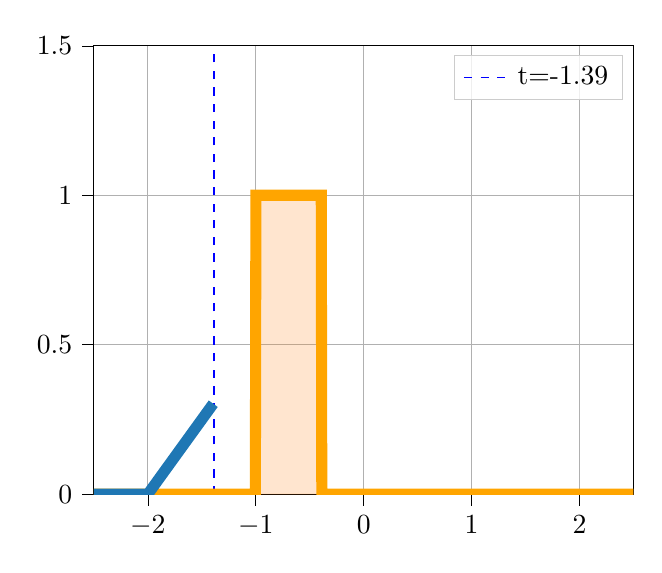
\begin{tikzpicture}

\definecolor{color0}{rgb}{1,0.498039215686275,0.0549019607843137}
\definecolor{color1}{rgb}{1,0.647058823529412,0}
\definecolor{color2}{rgb}{0.12156862745098,0.466666666666667,0.705882352941177}

\begin{axis}[
legend cell align={left},
legend style={fill opacity=0.8, draw opacity=1, text opacity=1, draw=white!80!black},
tick align=outside,
tick pos=left,
x grid style={white!69.0196078431373!black},
xmajorgrids,
xmin=-2.5, xmax=2.5,
xtick style={color=black},
y grid style={white!69.0196078431373!black},
ymajorgrids,
ymin=0, ymax=1.5,
ytick style={color=black}
]
\path [draw=color0, fill=color0, opacity=0.2]
(axis cs:-2.5,0)
--(axis cs:-2.5,0)
--(axis cs:-2.49499499499499,0)
--(axis cs:-2.48998998998999,0)
--(axis cs:-2.48498498498498,0)
--(axis cs:-2.47997997997998,0)
--(axis cs:-2.47497497497497,0)
--(axis cs:-2.46996996996997,0)
--(axis cs:-2.46496496496496,0)
--(axis cs:-2.45995995995996,0)
--(axis cs:-2.45495495495495,0)
--(axis cs:-2.44994994994995,0)
--(axis cs:-2.44494494494494,0)
--(axis cs:-2.43993993993994,0)
--(axis cs:-2.43493493493493,0)
--(axis cs:-2.42992992992993,0)
--(axis cs:-2.42492492492492,0)
--(axis cs:-2.41991991991992,0)
--(axis cs:-2.41491491491491,0)
--(axis cs:-2.40990990990991,0)
--(axis cs:-2.4049049049049,0)
--(axis cs:-2.3998998998999,0)
--(axis cs:-2.39489489489489,0)
--(axis cs:-2.38988988988989,0)
--(axis cs:-2.38488488488488,0)
--(axis cs:-2.37987987987988,0)
--(axis cs:-2.37487487487487,0)
--(axis cs:-2.36986986986987,0)
--(axis cs:-2.36486486486486,0)
--(axis cs:-2.35985985985986,0)
--(axis cs:-2.35485485485485,0)
--(axis cs:-2.34984984984985,0)
--(axis cs:-2.34484484484484,0)
--(axis cs:-2.33983983983984,0)
--(axis cs:-2.33483483483483,0)
--(axis cs:-2.32982982982983,0)
--(axis cs:-2.32482482482482,0)
--(axis cs:-2.31981981981982,0)
--(axis cs:-2.31481481481481,0)
--(axis cs:-2.30980980980981,0)
--(axis cs:-2.3048048048048,0)
--(axis cs:-2.2997997997998,0)
--(axis cs:-2.29479479479479,0)
--(axis cs:-2.28978978978979,0)
--(axis cs:-2.28478478478478,0)
--(axis cs:-2.27977977977978,0)
--(axis cs:-2.27477477477477,0)
--(axis cs:-2.26976976976977,0)
--(axis cs:-2.26476476476476,0)
--(axis cs:-2.25975975975976,0)
--(axis cs:-2.25475475475475,0)
--(axis cs:-2.24974974974975,0)
--(axis cs:-2.24474474474474,0)
--(axis cs:-2.23973973973974,0)
--(axis cs:-2.23473473473473,0)
--(axis cs:-2.22972972972973,0)
--(axis cs:-2.22472472472472,0)
--(axis cs:-2.21971971971972,0)
--(axis cs:-2.21471471471471,0)
--(axis cs:-2.20970970970971,0)
--(axis cs:-2.2047047047047,0)
--(axis cs:-2.1996996996997,0)
--(axis cs:-2.19469469469469,0)
--(axis cs:-2.18968968968969,0)
--(axis cs:-2.18468468468468,0)
--(axis cs:-2.17967967967968,0)
--(axis cs:-2.17467467467467,0)
--(axis cs:-2.16966966966967,0)
--(axis cs:-2.16466466466466,0)
--(axis cs:-2.15965965965966,0)
--(axis cs:-2.15465465465465,0)
--(axis cs:-2.14964964964965,0)
--(axis cs:-2.14464464464464,0)
--(axis cs:-2.13963963963964,0)
--(axis cs:-2.13463463463463,0)
--(axis cs:-2.12962962962963,0)
--(axis cs:-2.12462462462462,0)
--(axis cs:-2.11961961961962,0)
--(axis cs:-2.11461461461461,0)
--(axis cs:-2.10960960960961,0)
--(axis cs:-2.1046046046046,0)
--(axis cs:-2.0995995995996,0)
--(axis cs:-2.09459459459459,0)
--(axis cs:-2.08958958958959,0)
--(axis cs:-2.08458458458458,0)
--(axis cs:-2.07957957957958,0)
--(axis cs:-2.07457457457457,0)
--(axis cs:-2.06956956956957,0)
--(axis cs:-2.06456456456456,0)
--(axis cs:-2.05955955955956,0)
--(axis cs:-2.05455455455455,0)
--(axis cs:-2.04954954954955,0)
--(axis cs:-2.04454454454454,0)
--(axis cs:-2.03953953953954,0)
--(axis cs:-2.03453453453453,0)
--(axis cs:-2.02952952952953,0)
--(axis cs:-2.02452452452452,0)
--(axis cs:-2.01951951951952,0)
--(axis cs:-2.01451451451451,0)
--(axis cs:-2.00950950950951,0)
--(axis cs:-2.0045045045045,0)
--(axis cs:-1.9994994994995,0)
--(axis cs:-1.99449449449449,0)
--(axis cs:-1.98948948948949,0)
--(axis cs:-1.98448448448448,0)
--(axis cs:-1.97947947947948,0)
--(axis cs:-1.97447447447447,0)
--(axis cs:-1.96946946946947,0)
--(axis cs:-1.96446446446446,0)
--(axis cs:-1.95945945945946,0)
--(axis cs:-1.95445445445445,0)
--(axis cs:-1.94944944944945,0)
--(axis cs:-1.94444444444444,0)
--(axis cs:-1.93943943943944,0)
--(axis cs:-1.93443443443443,0)
--(axis cs:-1.92942942942943,0)
--(axis cs:-1.92442442442442,0)
--(axis cs:-1.91941941941942,0)
--(axis cs:-1.91441441441441,0)
--(axis cs:-1.90940940940941,0)
--(axis cs:-1.9044044044044,0)
--(axis cs:-1.8993993993994,0)
--(axis cs:-1.89439439439439,0)
--(axis cs:-1.88938938938939,0)
--(axis cs:-1.88438438438438,0)
--(axis cs:-1.87937937937938,0)
--(axis cs:-1.87437437437437,0)
--(axis cs:-1.86936936936937,0)
--(axis cs:-1.86436436436436,0)
--(axis cs:-1.85935935935936,0)
--(axis cs:-1.85435435435435,0)
--(axis cs:-1.84934934934935,0)
--(axis cs:-1.84434434434434,0)
--(axis cs:-1.83933933933934,0)
--(axis cs:-1.83433433433433,0)
--(axis cs:-1.82932932932933,0)
--(axis cs:-1.82432432432432,0)
--(axis cs:-1.81931931931932,0)
--(axis cs:-1.81431431431431,0)
--(axis cs:-1.80930930930931,0)
--(axis cs:-1.8043043043043,0)
--(axis cs:-1.7992992992993,0)
--(axis cs:-1.79429429429429,0)
--(axis cs:-1.78928928928929,0)
--(axis cs:-1.78428428428428,0)
--(axis cs:-1.77927927927928,0)
--(axis cs:-1.77427427427427,0)
--(axis cs:-1.76926926926927,0)
--(axis cs:-1.76426426426426,0)
--(axis cs:-1.75925925925926,0)
--(axis cs:-1.75425425425425,0)
--(axis cs:-1.74924924924925,0)
--(axis cs:-1.74424424424424,0)
--(axis cs:-1.73923923923924,0)
--(axis cs:-1.73423423423423,0)
--(axis cs:-1.72922922922923,0)
--(axis cs:-1.72422422422422,0)
--(axis cs:-1.71921921921922,0)
--(axis cs:-1.71421421421421,0)
--(axis cs:-1.70920920920921,0)
--(axis cs:-1.7042042042042,0)
--(axis cs:-1.6991991991992,0)
--(axis cs:-1.69419419419419,0)
--(axis cs:-1.68918918918919,0)
--(axis cs:-1.68418418418418,0)
--(axis cs:-1.67917917917918,0)
--(axis cs:-1.67417417417417,0)
--(axis cs:-1.66916916916917,0)
--(axis cs:-1.66416416416416,0)
--(axis cs:-1.65915915915916,0)
--(axis cs:-1.65415415415415,0)
--(axis cs:-1.64914914914915,0)
--(axis cs:-1.64414414414414,0)
--(axis cs:-1.63913913913914,0)
--(axis cs:-1.63413413413413,0)
--(axis cs:-1.62912912912913,0)
--(axis cs:-1.62412412412412,0)
--(axis cs:-1.61911911911912,0)
--(axis cs:-1.61411411411411,0)
--(axis cs:-1.60910910910911,0)
--(axis cs:-1.6041041041041,0)
--(axis cs:-1.5990990990991,0)
--(axis cs:-1.59409409409409,0)
--(axis cs:-1.58908908908909,0)
--(axis cs:-1.58408408408408,0)
--(axis cs:-1.57907907907908,0)
--(axis cs:-1.57407407407407,0)
--(axis cs:-1.56906906906907,0)
--(axis cs:-1.56406406406406,0)
--(axis cs:-1.55905905905906,0)
--(axis cs:-1.55405405405405,0)
--(axis cs:-1.54904904904905,0)
--(axis cs:-1.54404404404404,0)
--(axis cs:-1.53903903903904,0)
--(axis cs:-1.53403403403403,0)
--(axis cs:-1.52902902902903,0)
--(axis cs:-1.52402402402402,0)
--(axis cs:-1.51901901901902,0)
--(axis cs:-1.51401401401401,0)
--(axis cs:-1.50900900900901,0)
--(axis cs:-1.504004004004,0)
--(axis cs:-1.498998998999,0)
--(axis cs:-1.49399399399399,0)
--(axis cs:-1.48898898898899,0)
--(axis cs:-1.48398398398398,0)
--(axis cs:-1.47897897897898,0)
--(axis cs:-1.47397397397397,0)
--(axis cs:-1.46896896896897,0)
--(axis cs:-1.46396396396396,0)
--(axis cs:-1.45895895895896,0)
--(axis cs:-1.45395395395395,0)
--(axis cs:-1.44894894894895,0)
--(axis cs:-1.44394394394394,0)
--(axis cs:-1.43893893893894,0)
--(axis cs:-1.43393393393393,0)
--(axis cs:-1.42892892892893,0)
--(axis cs:-1.42392392392392,0)
--(axis cs:-1.41891891891892,0)
--(axis cs:-1.41391391391391,0)
--(axis cs:-1.40890890890891,0)
--(axis cs:-1.4039039039039,0)
--(axis cs:-1.3988988988989,0)
--(axis cs:-1.39389389389389,0)
--(axis cs:-1.38888888888889,0)
--(axis cs:-1.38388388388388,0)
--(axis cs:-1.37887887887888,0)
--(axis cs:-1.37387387387387,0)
--(axis cs:-1.36886886886887,0)
--(axis cs:-1.36386386386386,0)
--(axis cs:-1.35885885885886,0)
--(axis cs:-1.35385385385385,0)
--(axis cs:-1.34884884884885,0)
--(axis cs:-1.34384384384384,0)
--(axis cs:-1.33883883883884,0)
--(axis cs:-1.33383383383383,0)
--(axis cs:-1.32882882882883,0)
--(axis cs:-1.32382382382382,0)
--(axis cs:-1.31881881881882,0)
--(axis cs:-1.31381381381381,0)
--(axis cs:-1.30880880880881,0)
--(axis cs:-1.3038038038038,0)
--(axis cs:-1.2987987987988,0)
--(axis cs:-1.29379379379379,0)
--(axis cs:-1.28878878878879,0)
--(axis cs:-1.28378378378378,0)
--(axis cs:-1.27877877877878,0)
--(axis cs:-1.27377377377377,0)
--(axis cs:-1.26876876876877,0)
--(axis cs:-1.26376376376376,0)
--(axis cs:-1.25875875875876,0)
--(axis cs:-1.25375375375375,0)
--(axis cs:-1.24874874874875,0)
--(axis cs:-1.24374374374374,0)
--(axis cs:-1.23873873873874,0)
--(axis cs:-1.23373373373373,0)
--(axis cs:-1.22872872872873,0)
--(axis cs:-1.22372372372372,0)
--(axis cs:-1.21871871871872,0)
--(axis cs:-1.21371371371371,0)
--(axis cs:-1.20870870870871,0)
--(axis cs:-1.2037037037037,0)
--(axis cs:-1.1986986986987,0)
--(axis cs:-1.19369369369369,0)
--(axis cs:-1.18868868868869,0)
--(axis cs:-1.18368368368368,0)
--(axis cs:-1.17867867867868,0)
--(axis cs:-1.17367367367367,0)
--(axis cs:-1.16866866866867,0)
--(axis cs:-1.16366366366366,0)
--(axis cs:-1.15865865865866,0)
--(axis cs:-1.15365365365365,0)
--(axis cs:-1.14864864864865,0)
--(axis cs:-1.14364364364364,0)
--(axis cs:-1.13863863863864,0)
--(axis cs:-1.13363363363363,0)
--(axis cs:-1.12862862862863,0)
--(axis cs:-1.12362362362362,0)
--(axis cs:-1.11861861861862,0)
--(axis cs:-1.11361361361361,0)
--(axis cs:-1.10860860860861,0)
--(axis cs:-1.1036036036036,0)
--(axis cs:-1.0985985985986,0)
--(axis cs:-1.09359359359359,0)
--(axis cs:-1.08858858858859,0)
--(axis cs:-1.08358358358358,0)
--(axis cs:-1.07857857857858,0)
--(axis cs:-1.07357357357357,0)
--(axis cs:-1.06856856856857,0)
--(axis cs:-1.06356356356356,0)
--(axis cs:-1.05855855855856,0)
--(axis cs:-1.05355355355355,0)
--(axis cs:-1.04854854854855,0)
--(axis cs:-1.04354354354354,0)
--(axis cs:-1.03853853853854,0)
--(axis cs:-1.03353353353353,0)
--(axis cs:-1.02852852852853,0)
--(axis cs:-1.02352352352352,0)
--(axis cs:-1.01851851851852,0)
--(axis cs:-1.01351351351351,0)
--(axis cs:-1.00850850850851,0)
--(axis cs:-1.0035035035035,0)
--(axis cs:-0.998498498498499,0)
--(axis cs:-0.993493493493494,0)
--(axis cs:-0.988488488488489,0)
--(axis cs:-0.983483483483484,0)
--(axis cs:-0.978478478478479,0)
--(axis cs:-0.973473473473474,0)
--(axis cs:-0.968468468468469,0)
--(axis cs:-0.963463463463464,0)
--(axis cs:-0.958458458458459,0)
--(axis cs:-0.953453453453454,0)
--(axis cs:-0.948448448448449,0)
--(axis cs:-0.943443443443444,0)
--(axis cs:-0.938438438438439,0)
--(axis cs:-0.933433433433434,0)
--(axis cs:-0.928428428428429,0)
--(axis cs:-0.923423423423424,0)
--(axis cs:-0.918418418418419,0)
--(axis cs:-0.913413413413414,0)
--(axis cs:-0.908408408408409,0)
--(axis cs:-0.903403403403404,0)
--(axis cs:-0.898398398398399,0)
--(axis cs:-0.893393393393393,0)
--(axis cs:-0.888388388388388,0)
--(axis cs:-0.883383383383383,0)
--(axis cs:-0.878378378378378,0)
--(axis cs:-0.873373373373373,0)
--(axis cs:-0.868368368368368,0)
--(axis cs:-0.863363363363363,0)
--(axis cs:-0.858358358358358,0)
--(axis cs:-0.853353353353353,0)
--(axis cs:-0.848348348348348,0)
--(axis cs:-0.843343343343343,0)
--(axis cs:-0.838338338338338,0)
--(axis cs:-0.833333333333333,0)
--(axis cs:-0.828328328328328,0)
--(axis cs:-0.823323323323323,0)
--(axis cs:-0.818318318318318,0)
--(axis cs:-0.813313313313313,0)
--(axis cs:-0.808308308308308,0)
--(axis cs:-0.803303303303303,0)
--(axis cs:-0.798298298298298,0)
--(axis cs:-0.793293293293293,0)
--(axis cs:-0.788288288288288,0)
--(axis cs:-0.783283283283283,0)
--(axis cs:-0.778278278278278,0)
--(axis cs:-0.773273273273273,0)
--(axis cs:-0.768268268268268,0)
--(axis cs:-0.763263263263263,0)
--(axis cs:-0.758258258258258,0)
--(axis cs:-0.753253253253253,0)
--(axis cs:-0.748248248248248,0)
--(axis cs:-0.743243243243243,0)
--(axis cs:-0.738238238238238,0)
--(axis cs:-0.733233233233233,0)
--(axis cs:-0.728228228228228,0)
--(axis cs:-0.723223223223223,0)
--(axis cs:-0.718218218218218,0)
--(axis cs:-0.713213213213213,0)
--(axis cs:-0.708208208208208,0)
--(axis cs:-0.703203203203203,0)
--(axis cs:-0.698198198198198,0)
--(axis cs:-0.693193193193193,0)
--(axis cs:-0.688188188188188,0)
--(axis cs:-0.683183183183183,0)
--(axis cs:-0.678178178178178,0)
--(axis cs:-0.673173173173173,0)
--(axis cs:-0.668168168168168,0)
--(axis cs:-0.663163163163163,0)
--(axis cs:-0.658158158158158,0)
--(axis cs:-0.653153153153153,0)
--(axis cs:-0.648148148148148,0)
--(axis cs:-0.643143143143143,0)
--(axis cs:-0.638138138138138,0)
--(axis cs:-0.633133133133133,0)
--(axis cs:-0.628128128128128,0)
--(axis cs:-0.623123123123123,0)
--(axis cs:-0.618118118118118,0)
--(axis cs:-0.613113113113113,0)
--(axis cs:-0.608108108108108,0)
--(axis cs:-0.603103103103103,0)
--(axis cs:-0.598098098098098,0)
--(axis cs:-0.593093093093093,0)
--(axis cs:-0.588088088088088,0)
--(axis cs:-0.583083083083083,0)
--(axis cs:-0.578078078078078,0)
--(axis cs:-0.573073073073073,0)
--(axis cs:-0.568068068068068,0)
--(axis cs:-0.563063063063063,0)
--(axis cs:-0.558058058058058,0)
--(axis cs:-0.553053053053053,0)
--(axis cs:-0.548048048048048,0)
--(axis cs:-0.543043043043043,0)
--(axis cs:-0.538038038038038,0)
--(axis cs:-0.533033033033033,0)
--(axis cs:-0.528028028028028,0)
--(axis cs:-0.523023023023023,0)
--(axis cs:-0.518018018018018,0)
--(axis cs:-0.513013013013013,0)
--(axis cs:-0.508008008008008,0)
--(axis cs:-0.503003003003003,0)
--(axis cs:-0.497997997997998,0)
--(axis cs:-0.492992992992993,0)
--(axis cs:-0.487987987987988,0)
--(axis cs:-0.482982982982983,0)
--(axis cs:-0.477977977977978,0)
--(axis cs:-0.472972972972973,0)
--(axis cs:-0.467967967967968,0)
--(axis cs:-0.462962962962963,0)
--(axis cs:-0.457957957957958,0)
--(axis cs:-0.452952952952953,0)
--(axis cs:-0.447947947947948,0)
--(axis cs:-0.442942942942943,0)
--(axis cs:-0.437937937937938,0)
--(axis cs:-0.432932932932933,0)
--(axis cs:-0.427927927927928,0)
--(axis cs:-0.422922922922923,0)
--(axis cs:-0.417917917917918,0)
--(axis cs:-0.412912912912913,0)
--(axis cs:-0.407907907907908,0)
--(axis cs:-0.402902902902903,0)
--(axis cs:-0.397897897897898,0)
--(axis cs:-0.392892892892893,0)
--(axis cs:-0.387887887887888,0)
--(axis cs:-0.382882882882883,0)
--(axis cs:-0.377877877877878,0)
--(axis cs:-0.372872872872873,0)
--(axis cs:-0.367867867867868,0)
--(axis cs:-0.362862862862863,0)
--(axis cs:-0.357857857857858,0)
--(axis cs:-0.352852852852853,0)
--(axis cs:-0.347847847847848,0)
--(axis cs:-0.342842842842843,0)
--(axis cs:-0.337837837837838,0)
--(axis cs:-0.332832832832833,0)
--(axis cs:-0.327827827827828,0)
--(axis cs:-0.322822822822823,0)
--(axis cs:-0.317817817817818,0)
--(axis cs:-0.312812812812813,0)
--(axis cs:-0.307807807807808,0)
--(axis cs:-0.302802802802803,0)
--(axis cs:-0.297797797797798,0)
--(axis cs:-0.292792792792793,0)
--(axis cs:-0.287787787787788,0)
--(axis cs:-0.282782782782783,0)
--(axis cs:-0.277777777777778,0)
--(axis cs:-0.272772772772773,0)
--(axis cs:-0.267767767767768,0)
--(axis cs:-0.262762762762763,0)
--(axis cs:-0.257757757757758,0)
--(axis cs:-0.252752752752753,0)
--(axis cs:-0.247747747747748,0)
--(axis cs:-0.242742742742743,0)
--(axis cs:-0.237737737737738,0)
--(axis cs:-0.232732732732733,0)
--(axis cs:-0.227727727727728,0)
--(axis cs:-0.222722722722723,0)
--(axis cs:-0.217717717717718,0)
--(axis cs:-0.212712712712713,0)
--(axis cs:-0.207707707707708,0)
--(axis cs:-0.202702702702703,0)
--(axis cs:-0.197697697697698,0)
--(axis cs:-0.192692692692693,0)
--(axis cs:-0.187687687687688,0)
--(axis cs:-0.182682682682683,0)
--(axis cs:-0.177677677677678,0)
--(axis cs:-0.172672672672673,0)
--(axis cs:-0.167667667667668,0)
--(axis cs:-0.162662662662663,0)
--(axis cs:-0.157657657657658,0)
--(axis cs:-0.152652652652653,0)
--(axis cs:-0.147647647647648,0)
--(axis cs:-0.142642642642643,0)
--(axis cs:-0.137637637637638,0)
--(axis cs:-0.132632632632633,0)
--(axis cs:-0.127627627627628,0)
--(axis cs:-0.122622622622623,0)
--(axis cs:-0.117617617617618,0)
--(axis cs:-0.112612612612613,0)
--(axis cs:-0.107607607607608,0)
--(axis cs:-0.102602602602603,0)
--(axis cs:-0.0975975975975976,0)
--(axis cs:-0.0925925925925926,0)
--(axis cs:-0.0875875875875876,0)
--(axis cs:-0.0825825825825826,0)
--(axis cs:-0.0775775775775776,0)
--(axis cs:-0.0725725725725725,0)
--(axis cs:-0.0675675675675675,0)
--(axis cs:-0.0625625625625625,0)
--(axis cs:-0.0575575575575575,0)
--(axis cs:-0.0525525525525525,0)
--(axis cs:-0.0475475475475475,0)
--(axis cs:-0.0425425425425425,0)
--(axis cs:-0.0375375375375375,0)
--(axis cs:-0.0325325325325325,0)
--(axis cs:-0.0275275275275275,0)
--(axis cs:-0.0225225225225225,0)
--(axis cs:-0.0175175175175175,0)
--(axis cs:-0.0125125125125125,0)
--(axis cs:-0.0075075075075075,0)
--(axis cs:-0.0025025025025025,0)
--(axis cs:0.0025025025025025,0)
--(axis cs:0.0075075075075075,0)
--(axis cs:0.0125125125125125,0)
--(axis cs:0.0175175175175175,0)
--(axis cs:0.0225225225225225,0)
--(axis cs:0.0275275275275275,0)
--(axis cs:0.0325325325325325,0)
--(axis cs:0.0375375375375375,0)
--(axis cs:0.0425425425425425,0)
--(axis cs:0.0475475475475475,0)
--(axis cs:0.0525525525525525,0)
--(axis cs:0.0575575575575575,0)
--(axis cs:0.0625625625625625,0)
--(axis cs:0.0675675675675675,0)
--(axis cs:0.0725725725725725,0)
--(axis cs:0.0775775775775776,0)
--(axis cs:0.0825825825825826,0)
--(axis cs:0.0875875875875876,0)
--(axis cs:0.0925925925925926,0)
--(axis cs:0.0975975975975976,0)
--(axis cs:0.102602602602603,0)
--(axis cs:0.107607607607608,0)
--(axis cs:0.112612612612613,0)
--(axis cs:0.117617617617618,0)
--(axis cs:0.122622622622623,0)
--(axis cs:0.127627627627628,0)
--(axis cs:0.132632632632633,0)
--(axis cs:0.137637637637638,0)
--(axis cs:0.142642642642643,0)
--(axis cs:0.147647647647648,0)
--(axis cs:0.152652652652653,0)
--(axis cs:0.157657657657658,0)
--(axis cs:0.162662662662663,0)
--(axis cs:0.167667667667668,0)
--(axis cs:0.172672672672673,0)
--(axis cs:0.177677677677678,0)
--(axis cs:0.182682682682683,0)
--(axis cs:0.187687687687688,0)
--(axis cs:0.192692692692693,0)
--(axis cs:0.197697697697698,0)
--(axis cs:0.202702702702703,0)
--(axis cs:0.207707707707708,0)
--(axis cs:0.212712712712713,0)
--(axis cs:0.217717717717718,0)
--(axis cs:0.222722722722723,0)
--(axis cs:0.227727727727728,0)
--(axis cs:0.232732732732733,0)
--(axis cs:0.237737737737738,0)
--(axis cs:0.242742742742743,0)
--(axis cs:0.247747747747748,0)
--(axis cs:0.252752752752753,0)
--(axis cs:0.257757757757758,0)
--(axis cs:0.262762762762763,0)
--(axis cs:0.267767767767768,0)
--(axis cs:0.272772772772773,0)
--(axis cs:0.277777777777778,0)
--(axis cs:0.282782782782783,0)
--(axis cs:0.287787787787788,0)
--(axis cs:0.292792792792793,0)
--(axis cs:0.297797797797798,0)
--(axis cs:0.302802802802803,0)
--(axis cs:0.307807807807808,0)
--(axis cs:0.312812812812813,0)
--(axis cs:0.317817817817818,0)
--(axis cs:0.322822822822823,0)
--(axis cs:0.327827827827828,0)
--(axis cs:0.332832832832833,0)
--(axis cs:0.337837837837838,0)
--(axis cs:0.342842842842843,0)
--(axis cs:0.347847847847848,0)
--(axis cs:0.352852852852853,0)
--(axis cs:0.357857857857858,0)
--(axis cs:0.362862862862863,0)
--(axis cs:0.367867867867868,0)
--(axis cs:0.372872872872873,0)
--(axis cs:0.377877877877878,0)
--(axis cs:0.382882882882883,0)
--(axis cs:0.387887887887888,0)
--(axis cs:0.392892892892893,0)
--(axis cs:0.397897897897898,0)
--(axis cs:0.402902902902903,0)
--(axis cs:0.407907907907908,0)
--(axis cs:0.412912912912913,0)
--(axis cs:0.417917917917918,0)
--(axis cs:0.422922922922923,0)
--(axis cs:0.427927927927928,0)
--(axis cs:0.432932932932933,0)
--(axis cs:0.437937937937938,0)
--(axis cs:0.442942942942943,0)
--(axis cs:0.447947947947948,0)
--(axis cs:0.452952952952953,0)
--(axis cs:0.457957957957958,0)
--(axis cs:0.462962962962963,0)
--(axis cs:0.467967967967968,0)
--(axis cs:0.472972972972973,0)
--(axis cs:0.477977977977978,0)
--(axis cs:0.482982982982983,0)
--(axis cs:0.487987987987988,0)
--(axis cs:0.492992992992993,0)
--(axis cs:0.497997997997998,0)
--(axis cs:0.503003003003003,0)
--(axis cs:0.508008008008008,0)
--(axis cs:0.513013013013013,0)
--(axis cs:0.518018018018018,0)
--(axis cs:0.523023023023023,0)
--(axis cs:0.528028028028028,0)
--(axis cs:0.533033033033033,0)
--(axis cs:0.538038038038038,0)
--(axis cs:0.543043043043043,0)
--(axis cs:0.548048048048048,0)
--(axis cs:0.553053053053053,0)
--(axis cs:0.558058058058058,0)
--(axis cs:0.563063063063063,0)
--(axis cs:0.568068068068068,0)
--(axis cs:0.573073073073073,0)
--(axis cs:0.578078078078078,0)
--(axis cs:0.583083083083083,0)
--(axis cs:0.588088088088088,0)
--(axis cs:0.593093093093093,0)
--(axis cs:0.598098098098098,0)
--(axis cs:0.603103103103103,0)
--(axis cs:0.608108108108108,0)
--(axis cs:0.613113113113113,0)
--(axis cs:0.618118118118118,0)
--(axis cs:0.623123123123123,0)
--(axis cs:0.628128128128128,0)
--(axis cs:0.633133133133133,0)
--(axis cs:0.638138138138138,0)
--(axis cs:0.643143143143143,0)
--(axis cs:0.648148148148148,0)
--(axis cs:0.653153153153153,0)
--(axis cs:0.658158158158158,0)
--(axis cs:0.663163163163163,0)
--(axis cs:0.668168168168168,0)
--(axis cs:0.673173173173173,0)
--(axis cs:0.678178178178178,0)
--(axis cs:0.683183183183183,0)
--(axis cs:0.688188188188188,0)
--(axis cs:0.693193193193193,0)
--(axis cs:0.698198198198198,0)
--(axis cs:0.703203203203203,0)
--(axis cs:0.708208208208208,0)
--(axis cs:0.713213213213213,0)
--(axis cs:0.718218218218218,0)
--(axis cs:0.723223223223223,0)
--(axis cs:0.728228228228228,0)
--(axis cs:0.733233233233233,0)
--(axis cs:0.738238238238238,0)
--(axis cs:0.743243243243243,0)
--(axis cs:0.748248248248248,0)
--(axis cs:0.753253253253253,0)
--(axis cs:0.758258258258258,0)
--(axis cs:0.763263263263263,0)
--(axis cs:0.768268268268268,0)
--(axis cs:0.773273273273273,0)
--(axis cs:0.778278278278278,0)
--(axis cs:0.783283283283283,0)
--(axis cs:0.788288288288288,0)
--(axis cs:0.793293293293293,0)
--(axis cs:0.798298298298298,0)
--(axis cs:0.803303303303303,0)
--(axis cs:0.808308308308308,0)
--(axis cs:0.813313313313313,0)
--(axis cs:0.818318318318318,0)
--(axis cs:0.823323323323323,0)
--(axis cs:0.828328328328328,0)
--(axis cs:0.833333333333333,0)
--(axis cs:0.838338338338338,0)
--(axis cs:0.843343343343343,0)
--(axis cs:0.848348348348348,0)
--(axis cs:0.853353353353353,0)
--(axis cs:0.858358358358358,0)
--(axis cs:0.863363363363364,0)
--(axis cs:0.868368368368369,0)
--(axis cs:0.873373373373374,0)
--(axis cs:0.878378378378379,0)
--(axis cs:0.883383383383384,0)
--(axis cs:0.888388388388389,0)
--(axis cs:0.893393393393394,0)
--(axis cs:0.898398398398399,0)
--(axis cs:0.903403403403404,0)
--(axis cs:0.908408408408409,0)
--(axis cs:0.913413413413414,0)
--(axis cs:0.918418418418419,0)
--(axis cs:0.923423423423424,0)
--(axis cs:0.928428428428429,0)
--(axis cs:0.933433433433434,0)
--(axis cs:0.938438438438439,0)
--(axis cs:0.943443443443444,0)
--(axis cs:0.948448448448449,0)
--(axis cs:0.953453453453454,0)
--(axis cs:0.958458458458459,0)
--(axis cs:0.963463463463464,0)
--(axis cs:0.968468468468469,0)
--(axis cs:0.973473473473474,0)
--(axis cs:0.978478478478479,0)
--(axis cs:0.983483483483484,0)
--(axis cs:0.988488488488489,0)
--(axis cs:0.993493493493494,0)
--(axis cs:0.998498498498499,0)
--(axis cs:1.0035035035035,0)
--(axis cs:1.00850850850851,0)
--(axis cs:1.01351351351351,0)
--(axis cs:1.01851851851852,0)
--(axis cs:1.02352352352352,0)
--(axis cs:1.02852852852853,0)
--(axis cs:1.03353353353353,0)
--(axis cs:1.03853853853854,0)
--(axis cs:1.04354354354354,0)
--(axis cs:1.04854854854855,0)
--(axis cs:1.05355355355355,0)
--(axis cs:1.05855855855856,0)
--(axis cs:1.06356356356356,0)
--(axis cs:1.06856856856857,0)
--(axis cs:1.07357357357357,0)
--(axis cs:1.07857857857858,0)
--(axis cs:1.08358358358358,0)
--(axis cs:1.08858858858859,0)
--(axis cs:1.09359359359359,0)
--(axis cs:1.0985985985986,0)
--(axis cs:1.1036036036036,0)
--(axis cs:1.10860860860861,0)
--(axis cs:1.11361361361361,0)
--(axis cs:1.11861861861862,0)
--(axis cs:1.12362362362362,0)
--(axis cs:1.12862862862863,0)
--(axis cs:1.13363363363363,0)
--(axis cs:1.13863863863864,0)
--(axis cs:1.14364364364364,0)
--(axis cs:1.14864864864865,0)
--(axis cs:1.15365365365365,0)
--(axis cs:1.15865865865866,0)
--(axis cs:1.16366366366366,0)
--(axis cs:1.16866866866867,0)
--(axis cs:1.17367367367367,0)
--(axis cs:1.17867867867868,0)
--(axis cs:1.18368368368368,0)
--(axis cs:1.18868868868869,0)
--(axis cs:1.19369369369369,0)
--(axis cs:1.1986986986987,0)
--(axis cs:1.2037037037037,0)
--(axis cs:1.20870870870871,0)
--(axis cs:1.21371371371371,0)
--(axis cs:1.21871871871872,0)
--(axis cs:1.22372372372372,0)
--(axis cs:1.22872872872873,0)
--(axis cs:1.23373373373373,0)
--(axis cs:1.23873873873874,0)
--(axis cs:1.24374374374374,0)
--(axis cs:1.24874874874875,0)
--(axis cs:1.25375375375375,0)
--(axis cs:1.25875875875876,0)
--(axis cs:1.26376376376376,0)
--(axis cs:1.26876876876877,0)
--(axis cs:1.27377377377377,0)
--(axis cs:1.27877877877878,0)
--(axis cs:1.28378378378378,0)
--(axis cs:1.28878878878879,0)
--(axis cs:1.29379379379379,0)
--(axis cs:1.2987987987988,0)
--(axis cs:1.3038038038038,0)
--(axis cs:1.30880880880881,0)
--(axis cs:1.31381381381381,0)
--(axis cs:1.31881881881882,0)
--(axis cs:1.32382382382382,0)
--(axis cs:1.32882882882883,0)
--(axis cs:1.33383383383383,0)
--(axis cs:1.33883883883884,0)
--(axis cs:1.34384384384384,0)
--(axis cs:1.34884884884885,0)
--(axis cs:1.35385385385385,0)
--(axis cs:1.35885885885886,0)
--(axis cs:1.36386386386386,0)
--(axis cs:1.36886886886887,0)
--(axis cs:1.37387387387387,0)
--(axis cs:1.37887887887888,0)
--(axis cs:1.38388388388388,0)
--(axis cs:1.38888888888889,0)
--(axis cs:1.39389389389389,0)
--(axis cs:1.3988988988989,0)
--(axis cs:1.4039039039039,0)
--(axis cs:1.40890890890891,0)
--(axis cs:1.41391391391391,0)
--(axis cs:1.41891891891892,0)
--(axis cs:1.42392392392392,0)
--(axis cs:1.42892892892893,0)
--(axis cs:1.43393393393393,0)
--(axis cs:1.43893893893894,0)
--(axis cs:1.44394394394394,0)
--(axis cs:1.44894894894895,0)
--(axis cs:1.45395395395395,0)
--(axis cs:1.45895895895896,0)
--(axis cs:1.46396396396396,0)
--(axis cs:1.46896896896897,0)
--(axis cs:1.47397397397397,0)
--(axis cs:1.47897897897898,0)
--(axis cs:1.48398398398398,0)
--(axis cs:1.48898898898899,0)
--(axis cs:1.49399399399399,0)
--(axis cs:1.498998998999,0)
--(axis cs:1.504004004004,0)
--(axis cs:1.50900900900901,0)
--(axis cs:1.51401401401401,0)
--(axis cs:1.51901901901902,0)
--(axis cs:1.52402402402402,0)
--(axis cs:1.52902902902903,0)
--(axis cs:1.53403403403403,0)
--(axis cs:1.53903903903904,0)
--(axis cs:1.54404404404404,0)
--(axis cs:1.54904904904905,0)
--(axis cs:1.55405405405405,0)
--(axis cs:1.55905905905906,0)
--(axis cs:1.56406406406406,0)
--(axis cs:1.56906906906907,0)
--(axis cs:1.57407407407407,0)
--(axis cs:1.57907907907908,0)
--(axis cs:1.58408408408408,0)
--(axis cs:1.58908908908909,0)
--(axis cs:1.59409409409409,0)
--(axis cs:1.5990990990991,0)
--(axis cs:1.6041041041041,0)
--(axis cs:1.60910910910911,0)
--(axis cs:1.61411411411411,0)
--(axis cs:1.61911911911912,0)
--(axis cs:1.62412412412412,0)
--(axis cs:1.62912912912913,0)
--(axis cs:1.63413413413413,0)
--(axis cs:1.63913913913914,0)
--(axis cs:1.64414414414414,0)
--(axis cs:1.64914914914915,0)
--(axis cs:1.65415415415415,0)
--(axis cs:1.65915915915916,0)
--(axis cs:1.66416416416416,0)
--(axis cs:1.66916916916917,0)
--(axis cs:1.67417417417417,0)
--(axis cs:1.67917917917918,0)
--(axis cs:1.68418418418418,0)
--(axis cs:1.68918918918919,0)
--(axis cs:1.69419419419419,0)
--(axis cs:1.6991991991992,0)
--(axis cs:1.7042042042042,0)
--(axis cs:1.70920920920921,0)
--(axis cs:1.71421421421421,0)
--(axis cs:1.71921921921922,0)
--(axis cs:1.72422422422422,0)
--(axis cs:1.72922922922923,0)
--(axis cs:1.73423423423423,0)
--(axis cs:1.73923923923924,0)
--(axis cs:1.74424424424424,0)
--(axis cs:1.74924924924925,0)
--(axis cs:1.75425425425425,0)
--(axis cs:1.75925925925926,0)
--(axis cs:1.76426426426426,0)
--(axis cs:1.76926926926927,0)
--(axis cs:1.77427427427427,0)
--(axis cs:1.77927927927928,0)
--(axis cs:1.78428428428428,0)
--(axis cs:1.78928928928929,0)
--(axis cs:1.79429429429429,0)
--(axis cs:1.7992992992993,0)
--(axis cs:1.8043043043043,0)
--(axis cs:1.80930930930931,0)
--(axis cs:1.81431431431431,0)
--(axis cs:1.81931931931932,0)
--(axis cs:1.82432432432432,0)
--(axis cs:1.82932932932933,0)
--(axis cs:1.83433433433433,0)
--(axis cs:1.83933933933934,0)
--(axis cs:1.84434434434434,0)
--(axis cs:1.84934934934935,0)
--(axis cs:1.85435435435435,0)
--(axis cs:1.85935935935936,0)
--(axis cs:1.86436436436436,0)
--(axis cs:1.86936936936937,0)
--(axis cs:1.87437437437437,0)
--(axis cs:1.87937937937938,0)
--(axis cs:1.88438438438438,0)
--(axis cs:1.88938938938939,0)
--(axis cs:1.89439439439439,0)
--(axis cs:1.8993993993994,0)
--(axis cs:1.9044044044044,0)
--(axis cs:1.90940940940941,0)
--(axis cs:1.91441441441441,0)
--(axis cs:1.91941941941942,0)
--(axis cs:1.92442442442442,0)
--(axis cs:1.92942942942943,0)
--(axis cs:1.93443443443443,0)
--(axis cs:1.93943943943944,0)
--(axis cs:1.94444444444444,0)
--(axis cs:1.94944944944945,0)
--(axis cs:1.95445445445445,0)
--(axis cs:1.95945945945946,0)
--(axis cs:1.96446446446446,0)
--(axis cs:1.96946946946947,0)
--(axis cs:1.97447447447447,0)
--(axis cs:1.97947947947948,0)
--(axis cs:1.98448448448448,0)
--(axis cs:1.98948948948949,0)
--(axis cs:1.99449449449449,0)
--(axis cs:1.9994994994995,0)
--(axis cs:2.0045045045045,0)
--(axis cs:2.00950950950951,0)
--(axis cs:2.01451451451451,0)
--(axis cs:2.01951951951952,0)
--(axis cs:2.02452452452452,0)
--(axis cs:2.02952952952953,0)
--(axis cs:2.03453453453453,0)
--(axis cs:2.03953953953954,0)
--(axis cs:2.04454454454454,0)
--(axis cs:2.04954954954955,0)
--(axis cs:2.05455455455455,0)
--(axis cs:2.05955955955956,0)
--(axis cs:2.06456456456456,0)
--(axis cs:2.06956956956957,0)
--(axis cs:2.07457457457457,0)
--(axis cs:2.07957957957958,0)
--(axis cs:2.08458458458458,0)
--(axis cs:2.08958958958959,0)
--(axis cs:2.09459459459459,0)
--(axis cs:2.0995995995996,0)
--(axis cs:2.1046046046046,0)
--(axis cs:2.10960960960961,0)
--(axis cs:2.11461461461461,0)
--(axis cs:2.11961961961962,0)
--(axis cs:2.12462462462462,0)
--(axis cs:2.12962962962963,0)
--(axis cs:2.13463463463463,0)
--(axis cs:2.13963963963964,0)
--(axis cs:2.14464464464464,0)
--(axis cs:2.14964964964965,0)
--(axis cs:2.15465465465465,0)
--(axis cs:2.15965965965966,0)
--(axis cs:2.16466466466466,0)
--(axis cs:2.16966966966967,0)
--(axis cs:2.17467467467467,0)
--(axis cs:2.17967967967968,0)
--(axis cs:2.18468468468468,0)
--(axis cs:2.18968968968969,0)
--(axis cs:2.19469469469469,0)
--(axis cs:2.1996996996997,0)
--(axis cs:2.2047047047047,0)
--(axis cs:2.20970970970971,0)
--(axis cs:2.21471471471471,0)
--(axis cs:2.21971971971972,0)
--(axis cs:2.22472472472472,0)
--(axis cs:2.22972972972973,0)
--(axis cs:2.23473473473473,0)
--(axis cs:2.23973973973974,0)
--(axis cs:2.24474474474474,0)
--(axis cs:2.24974974974975,0)
--(axis cs:2.25475475475475,0)
--(axis cs:2.25975975975976,0)
--(axis cs:2.26476476476476,0)
--(axis cs:2.26976976976977,0)
--(axis cs:2.27477477477477,0)
--(axis cs:2.27977977977978,0)
--(axis cs:2.28478478478478,0)
--(axis cs:2.28978978978979,0)
--(axis cs:2.29479479479479,0)
--(axis cs:2.2997997997998,0)
--(axis cs:2.3048048048048,0)
--(axis cs:2.30980980980981,0)
--(axis cs:2.31481481481481,0)
--(axis cs:2.31981981981982,0)
--(axis cs:2.32482482482482,0)
--(axis cs:2.32982982982983,0)
--(axis cs:2.33483483483483,0)
--(axis cs:2.33983983983984,0)
--(axis cs:2.34484484484484,0)
--(axis cs:2.34984984984985,0)
--(axis cs:2.35485485485485,0)
--(axis cs:2.35985985985986,0)
--(axis cs:2.36486486486486,0)
--(axis cs:2.36986986986987,0)
--(axis cs:2.37487487487487,0)
--(axis cs:2.37987987987988,0)
--(axis cs:2.38488488488488,0)
--(axis cs:2.38988988988989,0)
--(axis cs:2.39489489489489,0)
--(axis cs:2.3998998998999,0)
--(axis cs:2.4049049049049,0)
--(axis cs:2.40990990990991,0)
--(axis cs:2.41491491491491,0)
--(axis cs:2.41991991991992,0)
--(axis cs:2.42492492492492,0)
--(axis cs:2.42992992992993,0)
--(axis cs:2.43493493493493,0)
--(axis cs:2.43993993993994,0)
--(axis cs:2.44494494494494,0)
--(axis cs:2.44994994994995,0)
--(axis cs:2.45495495495495,0)
--(axis cs:2.45995995995996,0)
--(axis cs:2.46496496496496,0)
--(axis cs:2.46996996996997,0)
--(axis cs:2.47497497497497,0)
--(axis cs:2.47997997997998,0)
--(axis cs:2.48498498498498,0)
--(axis cs:2.48998998998999,0)
--(axis cs:2.49499499499499,0)
--(axis cs:2.5,0)
--(axis cs:2.5,0)
--(axis cs:2.5,0)
--(axis cs:2.49499499499499,0)
--(axis cs:2.48998998998999,0)
--(axis cs:2.48498498498498,0)
--(axis cs:2.47997997997998,0)
--(axis cs:2.47497497497497,0)
--(axis cs:2.46996996996997,0)
--(axis cs:2.46496496496496,0)
--(axis cs:2.45995995995996,0)
--(axis cs:2.45495495495495,0)
--(axis cs:2.44994994994995,0)
--(axis cs:2.44494494494494,0)
--(axis cs:2.43993993993994,0)
--(axis cs:2.43493493493493,0)
--(axis cs:2.42992992992993,0)
--(axis cs:2.42492492492492,0)
--(axis cs:2.41991991991992,0)
--(axis cs:2.41491491491491,0)
--(axis cs:2.40990990990991,0)
--(axis cs:2.4049049049049,0)
--(axis cs:2.3998998998999,0)
--(axis cs:2.39489489489489,0)
--(axis cs:2.38988988988989,0)
--(axis cs:2.38488488488488,0)
--(axis cs:2.37987987987988,0)
--(axis cs:2.37487487487487,0)
--(axis cs:2.36986986986987,0)
--(axis cs:2.36486486486486,0)
--(axis cs:2.35985985985986,0)
--(axis cs:2.35485485485485,0)
--(axis cs:2.34984984984985,0)
--(axis cs:2.34484484484484,0)
--(axis cs:2.33983983983984,0)
--(axis cs:2.33483483483483,0)
--(axis cs:2.32982982982983,0)
--(axis cs:2.32482482482482,0)
--(axis cs:2.31981981981982,0)
--(axis cs:2.31481481481481,0)
--(axis cs:2.30980980980981,0)
--(axis cs:2.3048048048048,0)
--(axis cs:2.2997997997998,0)
--(axis cs:2.29479479479479,0)
--(axis cs:2.28978978978979,0)
--(axis cs:2.28478478478478,0)
--(axis cs:2.27977977977978,0)
--(axis cs:2.27477477477477,0)
--(axis cs:2.26976976976977,0)
--(axis cs:2.26476476476476,0)
--(axis cs:2.25975975975976,0)
--(axis cs:2.25475475475475,0)
--(axis cs:2.24974974974975,0)
--(axis cs:2.24474474474474,0)
--(axis cs:2.23973973973974,0)
--(axis cs:2.23473473473473,0)
--(axis cs:2.22972972972973,0)
--(axis cs:2.22472472472472,0)
--(axis cs:2.21971971971972,0)
--(axis cs:2.21471471471471,0)
--(axis cs:2.20970970970971,0)
--(axis cs:2.2047047047047,0)
--(axis cs:2.1996996996997,0)
--(axis cs:2.19469469469469,0)
--(axis cs:2.18968968968969,0)
--(axis cs:2.18468468468468,0)
--(axis cs:2.17967967967968,0)
--(axis cs:2.17467467467467,0)
--(axis cs:2.16966966966967,0)
--(axis cs:2.16466466466466,0)
--(axis cs:2.15965965965966,0)
--(axis cs:2.15465465465465,0)
--(axis cs:2.14964964964965,0)
--(axis cs:2.14464464464464,0)
--(axis cs:2.13963963963964,0)
--(axis cs:2.13463463463463,0)
--(axis cs:2.12962962962963,0)
--(axis cs:2.12462462462462,0)
--(axis cs:2.11961961961962,0)
--(axis cs:2.11461461461461,0)
--(axis cs:2.10960960960961,0)
--(axis cs:2.1046046046046,0)
--(axis cs:2.0995995995996,0)
--(axis cs:2.09459459459459,0)
--(axis cs:2.08958958958959,0)
--(axis cs:2.08458458458458,0)
--(axis cs:2.07957957957958,0)
--(axis cs:2.07457457457457,0)
--(axis cs:2.06956956956957,0)
--(axis cs:2.06456456456456,0)
--(axis cs:2.05955955955956,0)
--(axis cs:2.05455455455455,0)
--(axis cs:2.04954954954955,0)
--(axis cs:2.04454454454454,0)
--(axis cs:2.03953953953954,0)
--(axis cs:2.03453453453453,0)
--(axis cs:2.02952952952953,0)
--(axis cs:2.02452452452452,0)
--(axis cs:2.01951951951952,0)
--(axis cs:2.01451451451451,0)
--(axis cs:2.00950950950951,0)
--(axis cs:2.0045045045045,0)
--(axis cs:1.9994994994995,0)
--(axis cs:1.99449449449449,0)
--(axis cs:1.98948948948949,0)
--(axis cs:1.98448448448448,0)
--(axis cs:1.97947947947948,0)
--(axis cs:1.97447447447447,0)
--(axis cs:1.96946946946947,0)
--(axis cs:1.96446446446446,0)
--(axis cs:1.95945945945946,0)
--(axis cs:1.95445445445445,0)
--(axis cs:1.94944944944945,0)
--(axis cs:1.94444444444444,0)
--(axis cs:1.93943943943944,0)
--(axis cs:1.93443443443443,0)
--(axis cs:1.92942942942943,0)
--(axis cs:1.92442442442442,0)
--(axis cs:1.91941941941942,0)
--(axis cs:1.91441441441441,0)
--(axis cs:1.90940940940941,0)
--(axis cs:1.9044044044044,0)
--(axis cs:1.8993993993994,0)
--(axis cs:1.89439439439439,0)
--(axis cs:1.88938938938939,0)
--(axis cs:1.88438438438438,0)
--(axis cs:1.87937937937938,0)
--(axis cs:1.87437437437437,0)
--(axis cs:1.86936936936937,0)
--(axis cs:1.86436436436436,0)
--(axis cs:1.85935935935936,0)
--(axis cs:1.85435435435435,0)
--(axis cs:1.84934934934935,0)
--(axis cs:1.84434434434434,0)
--(axis cs:1.83933933933934,0)
--(axis cs:1.83433433433433,0)
--(axis cs:1.82932932932933,0)
--(axis cs:1.82432432432432,0)
--(axis cs:1.81931931931932,0)
--(axis cs:1.81431431431431,0)
--(axis cs:1.80930930930931,0)
--(axis cs:1.8043043043043,0)
--(axis cs:1.7992992992993,0)
--(axis cs:1.79429429429429,0)
--(axis cs:1.78928928928929,0)
--(axis cs:1.78428428428428,0)
--(axis cs:1.77927927927928,0)
--(axis cs:1.77427427427427,0)
--(axis cs:1.76926926926927,0)
--(axis cs:1.76426426426426,0)
--(axis cs:1.75925925925926,0)
--(axis cs:1.75425425425425,0)
--(axis cs:1.74924924924925,0)
--(axis cs:1.74424424424424,0)
--(axis cs:1.73923923923924,0)
--(axis cs:1.73423423423423,0)
--(axis cs:1.72922922922923,0)
--(axis cs:1.72422422422422,0)
--(axis cs:1.71921921921922,0)
--(axis cs:1.71421421421421,0)
--(axis cs:1.70920920920921,0)
--(axis cs:1.7042042042042,0)
--(axis cs:1.6991991991992,0)
--(axis cs:1.69419419419419,0)
--(axis cs:1.68918918918919,0)
--(axis cs:1.68418418418418,0)
--(axis cs:1.67917917917918,0)
--(axis cs:1.67417417417417,0)
--(axis cs:1.66916916916917,0)
--(axis cs:1.66416416416416,0)
--(axis cs:1.65915915915916,0)
--(axis cs:1.65415415415415,0)
--(axis cs:1.64914914914915,0)
--(axis cs:1.64414414414414,0)
--(axis cs:1.63913913913914,0)
--(axis cs:1.63413413413413,0)
--(axis cs:1.62912912912913,0)
--(axis cs:1.62412412412412,0)
--(axis cs:1.61911911911912,0)
--(axis cs:1.61411411411411,0)
--(axis cs:1.60910910910911,0)
--(axis cs:1.6041041041041,0)
--(axis cs:1.5990990990991,0)
--(axis cs:1.59409409409409,0)
--(axis cs:1.58908908908909,0)
--(axis cs:1.58408408408408,0)
--(axis cs:1.57907907907908,0)
--(axis cs:1.57407407407407,0)
--(axis cs:1.56906906906907,0)
--(axis cs:1.56406406406406,0)
--(axis cs:1.55905905905906,0)
--(axis cs:1.55405405405405,0)
--(axis cs:1.54904904904905,0)
--(axis cs:1.54404404404404,0)
--(axis cs:1.53903903903904,0)
--(axis cs:1.53403403403403,0)
--(axis cs:1.52902902902903,0)
--(axis cs:1.52402402402402,0)
--(axis cs:1.51901901901902,0)
--(axis cs:1.51401401401401,0)
--(axis cs:1.50900900900901,0)
--(axis cs:1.504004004004,0)
--(axis cs:1.498998998999,0)
--(axis cs:1.49399399399399,0)
--(axis cs:1.48898898898899,0)
--(axis cs:1.48398398398398,0)
--(axis cs:1.47897897897898,0)
--(axis cs:1.47397397397397,0)
--(axis cs:1.46896896896897,0)
--(axis cs:1.46396396396396,0)
--(axis cs:1.45895895895896,0)
--(axis cs:1.45395395395395,0)
--(axis cs:1.44894894894895,0)
--(axis cs:1.44394394394394,0)
--(axis cs:1.43893893893894,0)
--(axis cs:1.43393393393393,0)
--(axis cs:1.42892892892893,0)
--(axis cs:1.42392392392392,0)
--(axis cs:1.41891891891892,0)
--(axis cs:1.41391391391391,0)
--(axis cs:1.40890890890891,0)
--(axis cs:1.4039039039039,0)
--(axis cs:1.3988988988989,0)
--(axis cs:1.39389389389389,0)
--(axis cs:1.38888888888889,0)
--(axis cs:1.38388388388388,0)
--(axis cs:1.37887887887888,0)
--(axis cs:1.37387387387387,0)
--(axis cs:1.36886886886887,0)
--(axis cs:1.36386386386386,0)
--(axis cs:1.35885885885886,0)
--(axis cs:1.35385385385385,0)
--(axis cs:1.34884884884885,0)
--(axis cs:1.34384384384384,0)
--(axis cs:1.33883883883884,0)
--(axis cs:1.33383383383383,0)
--(axis cs:1.32882882882883,0)
--(axis cs:1.32382382382382,0)
--(axis cs:1.31881881881882,0)
--(axis cs:1.31381381381381,0)
--(axis cs:1.30880880880881,0)
--(axis cs:1.3038038038038,0)
--(axis cs:1.2987987987988,0)
--(axis cs:1.29379379379379,0)
--(axis cs:1.28878878878879,0)
--(axis cs:1.28378378378378,0)
--(axis cs:1.27877877877878,0)
--(axis cs:1.27377377377377,0)
--(axis cs:1.26876876876877,0)
--(axis cs:1.26376376376376,0)
--(axis cs:1.25875875875876,0)
--(axis cs:1.25375375375375,0)
--(axis cs:1.24874874874875,0)
--(axis cs:1.24374374374374,0)
--(axis cs:1.23873873873874,0)
--(axis cs:1.23373373373373,0)
--(axis cs:1.22872872872873,0)
--(axis cs:1.22372372372372,0)
--(axis cs:1.21871871871872,0)
--(axis cs:1.21371371371371,0)
--(axis cs:1.20870870870871,0)
--(axis cs:1.2037037037037,0)
--(axis cs:1.1986986986987,0)
--(axis cs:1.19369369369369,0)
--(axis cs:1.18868868868869,0)
--(axis cs:1.18368368368368,0)
--(axis cs:1.17867867867868,0)
--(axis cs:1.17367367367367,0)
--(axis cs:1.16866866866867,0)
--(axis cs:1.16366366366366,0)
--(axis cs:1.15865865865866,0)
--(axis cs:1.15365365365365,0)
--(axis cs:1.14864864864865,0)
--(axis cs:1.14364364364364,0)
--(axis cs:1.13863863863864,0)
--(axis cs:1.13363363363363,0)
--(axis cs:1.12862862862863,0)
--(axis cs:1.12362362362362,0)
--(axis cs:1.11861861861862,0)
--(axis cs:1.11361361361361,0)
--(axis cs:1.10860860860861,0)
--(axis cs:1.1036036036036,0)
--(axis cs:1.0985985985986,0)
--(axis cs:1.09359359359359,0)
--(axis cs:1.08858858858859,0)
--(axis cs:1.08358358358358,0)
--(axis cs:1.07857857857858,0)
--(axis cs:1.07357357357357,0)
--(axis cs:1.06856856856857,0)
--(axis cs:1.06356356356356,0)
--(axis cs:1.05855855855856,0)
--(axis cs:1.05355355355355,0)
--(axis cs:1.04854854854855,0)
--(axis cs:1.04354354354354,0)
--(axis cs:1.03853853853854,0)
--(axis cs:1.03353353353353,0)
--(axis cs:1.02852852852853,0)
--(axis cs:1.02352352352352,0)
--(axis cs:1.01851851851852,0)
--(axis cs:1.01351351351351,0)
--(axis cs:1.00850850850851,0)
--(axis cs:1.0035035035035,0)
--(axis cs:0.998498498498499,0)
--(axis cs:0.993493493493494,0)
--(axis cs:0.988488488488489,0)
--(axis cs:0.983483483483484,0)
--(axis cs:0.978478478478479,0)
--(axis cs:0.973473473473474,0)
--(axis cs:0.968468468468469,0)
--(axis cs:0.963463463463464,0)
--(axis cs:0.958458458458459,0)
--(axis cs:0.953453453453454,0)
--(axis cs:0.948448448448449,0)
--(axis cs:0.943443443443444,0)
--(axis cs:0.938438438438439,0)
--(axis cs:0.933433433433434,0)
--(axis cs:0.928428428428429,0)
--(axis cs:0.923423423423424,0)
--(axis cs:0.918418418418419,0)
--(axis cs:0.913413413413414,0)
--(axis cs:0.908408408408409,0)
--(axis cs:0.903403403403404,0)
--(axis cs:0.898398398398399,0)
--(axis cs:0.893393393393394,0)
--(axis cs:0.888388388388389,0)
--(axis cs:0.883383383383384,0)
--(axis cs:0.878378378378379,0)
--(axis cs:0.873373373373374,0)
--(axis cs:0.868368368368369,0)
--(axis cs:0.863363363363364,0)
--(axis cs:0.858358358358358,0)
--(axis cs:0.853353353353353,0)
--(axis cs:0.848348348348348,0)
--(axis cs:0.843343343343343,0)
--(axis cs:0.838338338338338,0)
--(axis cs:0.833333333333333,0)
--(axis cs:0.828328328328328,0)
--(axis cs:0.823323323323323,0)
--(axis cs:0.818318318318318,0)
--(axis cs:0.813313313313313,0)
--(axis cs:0.808308308308308,0)
--(axis cs:0.803303303303303,0)
--(axis cs:0.798298298298298,0)
--(axis cs:0.793293293293293,0)
--(axis cs:0.788288288288288,0)
--(axis cs:0.783283283283283,0)
--(axis cs:0.778278278278278,0)
--(axis cs:0.773273273273273,0)
--(axis cs:0.768268268268268,0)
--(axis cs:0.763263263263263,0)
--(axis cs:0.758258258258258,0)
--(axis cs:0.753253253253253,0)
--(axis cs:0.748248248248248,0)
--(axis cs:0.743243243243243,0)
--(axis cs:0.738238238238238,0)
--(axis cs:0.733233233233233,0)
--(axis cs:0.728228228228228,0)
--(axis cs:0.723223223223223,0)
--(axis cs:0.718218218218218,0)
--(axis cs:0.713213213213213,0)
--(axis cs:0.708208208208208,0)
--(axis cs:0.703203203203203,0)
--(axis cs:0.698198198198198,0)
--(axis cs:0.693193193193193,0)
--(axis cs:0.688188188188188,0)
--(axis cs:0.683183183183183,0)
--(axis cs:0.678178178178178,0)
--(axis cs:0.673173173173173,0)
--(axis cs:0.668168168168168,0)
--(axis cs:0.663163163163163,0)
--(axis cs:0.658158158158158,0)
--(axis cs:0.653153153153153,0)
--(axis cs:0.648148148148148,0)
--(axis cs:0.643143143143143,0)
--(axis cs:0.638138138138138,0)
--(axis cs:0.633133133133133,0)
--(axis cs:0.628128128128128,0)
--(axis cs:0.623123123123123,0)
--(axis cs:0.618118118118118,0)
--(axis cs:0.613113113113113,0)
--(axis cs:0.608108108108108,0)
--(axis cs:0.603103103103103,0)
--(axis cs:0.598098098098098,0)
--(axis cs:0.593093093093093,0)
--(axis cs:0.588088088088088,0)
--(axis cs:0.583083083083083,0)
--(axis cs:0.578078078078078,0)
--(axis cs:0.573073073073073,0)
--(axis cs:0.568068068068068,0)
--(axis cs:0.563063063063063,0)
--(axis cs:0.558058058058058,0)
--(axis cs:0.553053053053053,0)
--(axis cs:0.548048048048048,0)
--(axis cs:0.543043043043043,0)
--(axis cs:0.538038038038038,0)
--(axis cs:0.533033033033033,0)
--(axis cs:0.528028028028028,0)
--(axis cs:0.523023023023023,0)
--(axis cs:0.518018018018018,0)
--(axis cs:0.513013013013013,0)
--(axis cs:0.508008008008008,0)
--(axis cs:0.503003003003003,0)
--(axis cs:0.497997997997998,0)
--(axis cs:0.492992992992993,0)
--(axis cs:0.487987987987988,0)
--(axis cs:0.482982982982983,0)
--(axis cs:0.477977977977978,0)
--(axis cs:0.472972972972973,0)
--(axis cs:0.467967967967968,0)
--(axis cs:0.462962962962963,0)
--(axis cs:0.457957957957958,0)
--(axis cs:0.452952952952953,0)
--(axis cs:0.447947947947948,0)
--(axis cs:0.442942942942943,0)
--(axis cs:0.437937937937938,0)
--(axis cs:0.432932932932933,0)
--(axis cs:0.427927927927928,0)
--(axis cs:0.422922922922923,0)
--(axis cs:0.417917917917918,0)
--(axis cs:0.412912912912913,0)
--(axis cs:0.407907907907908,0)
--(axis cs:0.402902902902903,0)
--(axis cs:0.397897897897898,0)
--(axis cs:0.392892892892893,0)
--(axis cs:0.387887887887888,0)
--(axis cs:0.382882882882883,0)
--(axis cs:0.377877877877878,0)
--(axis cs:0.372872872872873,0)
--(axis cs:0.367867867867868,0)
--(axis cs:0.362862862862863,0)
--(axis cs:0.357857857857858,0)
--(axis cs:0.352852852852853,0)
--(axis cs:0.347847847847848,0)
--(axis cs:0.342842842842843,0)
--(axis cs:0.337837837837838,0)
--(axis cs:0.332832832832833,0)
--(axis cs:0.327827827827828,0)
--(axis cs:0.322822822822823,0)
--(axis cs:0.317817817817818,0)
--(axis cs:0.312812812812813,0)
--(axis cs:0.307807807807808,0)
--(axis cs:0.302802802802803,0)
--(axis cs:0.297797797797798,0)
--(axis cs:0.292792792792793,0)
--(axis cs:0.287787787787788,0)
--(axis cs:0.282782782782783,0)
--(axis cs:0.277777777777778,0)
--(axis cs:0.272772772772773,0)
--(axis cs:0.267767767767768,0)
--(axis cs:0.262762762762763,0)
--(axis cs:0.257757757757758,0)
--(axis cs:0.252752752752753,0)
--(axis cs:0.247747747747748,0)
--(axis cs:0.242742742742743,0)
--(axis cs:0.237737737737738,0)
--(axis cs:0.232732732732733,0)
--(axis cs:0.227727727727728,0)
--(axis cs:0.222722722722723,0)
--(axis cs:0.217717717717718,0)
--(axis cs:0.212712712712713,0)
--(axis cs:0.207707707707708,0)
--(axis cs:0.202702702702703,0)
--(axis cs:0.197697697697698,0)
--(axis cs:0.192692692692693,0)
--(axis cs:0.187687687687688,0)
--(axis cs:0.182682682682683,0)
--(axis cs:0.177677677677678,0)
--(axis cs:0.172672672672673,0)
--(axis cs:0.167667667667668,0)
--(axis cs:0.162662662662663,0)
--(axis cs:0.157657657657658,0)
--(axis cs:0.152652652652653,0)
--(axis cs:0.147647647647648,0)
--(axis cs:0.142642642642643,0)
--(axis cs:0.137637637637638,0)
--(axis cs:0.132632632632633,0)
--(axis cs:0.127627627627628,0)
--(axis cs:0.122622622622623,0)
--(axis cs:0.117617617617618,0)
--(axis cs:0.112612612612613,0)
--(axis cs:0.107607607607608,0)
--(axis cs:0.102602602602603,0)
--(axis cs:0.0975975975975976,0)
--(axis cs:0.0925925925925926,0)
--(axis cs:0.0875875875875876,0)
--(axis cs:0.0825825825825826,0)
--(axis cs:0.0775775775775776,0)
--(axis cs:0.0725725725725725,0)
--(axis cs:0.0675675675675675,0)
--(axis cs:0.0625625625625625,0)
--(axis cs:0.0575575575575575,0)
--(axis cs:0.0525525525525525,0)
--(axis cs:0.0475475475475475,0)
--(axis cs:0.0425425425425425,0)
--(axis cs:0.0375375375375375,0)
--(axis cs:0.0325325325325325,0)
--(axis cs:0.0275275275275275,0)
--(axis cs:0.0225225225225225,0)
--(axis cs:0.0175175175175175,0)
--(axis cs:0.0125125125125125,0)
--(axis cs:0.0075075075075075,0)
--(axis cs:0.0025025025025025,0)
--(axis cs:-0.0025025025025025,0)
--(axis cs:-0.0075075075075075,0)
--(axis cs:-0.0125125125125125,0)
--(axis cs:-0.0175175175175175,0)
--(axis cs:-0.0225225225225225,0)
--(axis cs:-0.0275275275275275,0)
--(axis cs:-0.0325325325325325,0)
--(axis cs:-0.0375375375375375,0)
--(axis cs:-0.0425425425425425,0)
--(axis cs:-0.0475475475475475,0)
--(axis cs:-0.0525525525525525,0)
--(axis cs:-0.0575575575575575,0)
--(axis cs:-0.0625625625625625,0)
--(axis cs:-0.0675675675675675,0)
--(axis cs:-0.0725725725725725,0)
--(axis cs:-0.0775775775775776,0)
--(axis cs:-0.0825825825825826,0)
--(axis cs:-0.0875875875875876,0)
--(axis cs:-0.0925925925925926,0)
--(axis cs:-0.0975975975975976,0)
--(axis cs:-0.102602602602603,0)
--(axis cs:-0.107607607607608,0)
--(axis cs:-0.112612612612613,0)
--(axis cs:-0.117617617617618,0)
--(axis cs:-0.122622622622623,0)
--(axis cs:-0.127627627627628,0)
--(axis cs:-0.132632632632633,0)
--(axis cs:-0.137637637637638,0)
--(axis cs:-0.142642642642643,0)
--(axis cs:-0.147647647647648,0)
--(axis cs:-0.152652652652653,0)
--(axis cs:-0.157657657657658,0)
--(axis cs:-0.162662662662663,0)
--(axis cs:-0.167667667667668,0)
--(axis cs:-0.172672672672673,0)
--(axis cs:-0.177677677677678,0)
--(axis cs:-0.182682682682683,0)
--(axis cs:-0.187687687687688,0)
--(axis cs:-0.192692692692693,0)
--(axis cs:-0.197697697697698,0)
--(axis cs:-0.202702702702703,0)
--(axis cs:-0.207707707707708,0)
--(axis cs:-0.212712712712713,0)
--(axis cs:-0.217717717717718,0)
--(axis cs:-0.222722722722723,0)
--(axis cs:-0.227727727727728,0)
--(axis cs:-0.232732732732733,0)
--(axis cs:-0.237737737737738,0)
--(axis cs:-0.242742742742743,0)
--(axis cs:-0.247747747747748,0)
--(axis cs:-0.252752752752753,0)
--(axis cs:-0.257757757757758,0)
--(axis cs:-0.262762762762763,0)
--(axis cs:-0.267767767767768,0)
--(axis cs:-0.272772772772773,0)
--(axis cs:-0.277777777777778,0)
--(axis cs:-0.282782782782783,0)
--(axis cs:-0.287787787787788,0)
--(axis cs:-0.292792792792793,0)
--(axis cs:-0.297797797797798,0)
--(axis cs:-0.302802802802803,0)
--(axis cs:-0.307807807807808,0)
--(axis cs:-0.312812812812813,0)
--(axis cs:-0.317817817817818,0)
--(axis cs:-0.322822822822823,0)
--(axis cs:-0.327827827827828,0)
--(axis cs:-0.332832832832833,0)
--(axis cs:-0.337837837837838,0)
--(axis cs:-0.342842842842843,0)
--(axis cs:-0.347847847847848,0)
--(axis cs:-0.352852852852853,0)
--(axis cs:-0.357857857857858,0)
--(axis cs:-0.362862862862863,0)
--(axis cs:-0.367867867867868,0)
--(axis cs:-0.372872872872873,0)
--(axis cs:-0.377877877877878,0)
--(axis cs:-0.382882882882883,0)
--(axis cs:-0.387887887887888,0)
--(axis cs:-0.392892892892893,1)
--(axis cs:-0.397897897897898,1)
--(axis cs:-0.402902902902903,1)
--(axis cs:-0.407907907907908,1)
--(axis cs:-0.412912912912913,1)
--(axis cs:-0.417917917917918,1)
--(axis cs:-0.422922922922923,1)
--(axis cs:-0.427927927927928,1)
--(axis cs:-0.432932932932933,1)
--(axis cs:-0.437937937937938,1)
--(axis cs:-0.442942942942943,1)
--(axis cs:-0.447947947947948,1)
--(axis cs:-0.452952952952953,1)
--(axis cs:-0.457957957957958,1)
--(axis cs:-0.462962962962963,1)
--(axis cs:-0.467967967967968,1)
--(axis cs:-0.472972972972973,1)
--(axis cs:-0.477977977977978,1)
--(axis cs:-0.482982982982983,1)
--(axis cs:-0.487987987987988,1)
--(axis cs:-0.492992992992993,1)
--(axis cs:-0.497997997997998,1)
--(axis cs:-0.503003003003003,1)
--(axis cs:-0.508008008008008,1)
--(axis cs:-0.513013013013013,1)
--(axis cs:-0.518018018018018,1)
--(axis cs:-0.523023023023023,1)
--(axis cs:-0.528028028028028,1)
--(axis cs:-0.533033033033033,1)
--(axis cs:-0.538038038038038,1)
--(axis cs:-0.543043043043043,1)
--(axis cs:-0.548048048048048,1)
--(axis cs:-0.553053053053053,1)
--(axis cs:-0.558058058058058,1)
--(axis cs:-0.563063063063063,1)
--(axis cs:-0.568068068068068,1)
--(axis cs:-0.573073073073073,1)
--(axis cs:-0.578078078078078,1)
--(axis cs:-0.583083083083083,1)
--(axis cs:-0.588088088088088,1)
--(axis cs:-0.593093093093093,1)
--(axis cs:-0.598098098098098,1)
--(axis cs:-0.603103103103103,1)
--(axis cs:-0.608108108108108,1)
--(axis cs:-0.613113113113113,1)
--(axis cs:-0.618118118118118,1)
--(axis cs:-0.623123123123123,1)
--(axis cs:-0.628128128128128,1)
--(axis cs:-0.633133133133133,1)
--(axis cs:-0.638138138138138,1)
--(axis cs:-0.643143143143143,1)
--(axis cs:-0.648148148148148,1)
--(axis cs:-0.653153153153153,1)
--(axis cs:-0.658158158158158,1)
--(axis cs:-0.663163163163163,1)
--(axis cs:-0.668168168168168,1)
--(axis cs:-0.673173173173173,1)
--(axis cs:-0.678178178178178,1)
--(axis cs:-0.683183183183183,1)
--(axis cs:-0.688188188188188,1)
--(axis cs:-0.693193193193193,1)
--(axis cs:-0.698198198198198,1)
--(axis cs:-0.703203203203203,1)
--(axis cs:-0.708208208208208,1)
--(axis cs:-0.713213213213213,1)
--(axis cs:-0.718218218218218,1)
--(axis cs:-0.723223223223223,1)
--(axis cs:-0.728228228228228,1)
--(axis cs:-0.733233233233233,1)
--(axis cs:-0.738238238238238,1)
--(axis cs:-0.743243243243243,1)
--(axis cs:-0.748248248248248,1)
--(axis cs:-0.753253253253253,1)
--(axis cs:-0.758258258258258,1)
--(axis cs:-0.763263263263263,1)
--(axis cs:-0.768268268268268,1)
--(axis cs:-0.773273273273273,1)
--(axis cs:-0.778278278278278,1)
--(axis cs:-0.783283283283283,1)
--(axis cs:-0.788288288288288,1)
--(axis cs:-0.793293293293293,1)
--(axis cs:-0.798298298298298,1)
--(axis cs:-0.803303303303303,1)
--(axis cs:-0.808308308308308,1)
--(axis cs:-0.813313313313313,1)
--(axis cs:-0.818318318318318,1)
--(axis cs:-0.823323323323323,1)
--(axis cs:-0.828328328328328,1)
--(axis cs:-0.833333333333333,1)
--(axis cs:-0.838338338338338,1)
--(axis cs:-0.843343343343343,1)
--(axis cs:-0.848348348348348,1)
--(axis cs:-0.853353353353353,1)
--(axis cs:-0.858358358358358,1)
--(axis cs:-0.863363363363363,1)
--(axis cs:-0.868368368368368,1)
--(axis cs:-0.873373373373373,1)
--(axis cs:-0.878378378378378,1)
--(axis cs:-0.883383383383383,1)
--(axis cs:-0.888388388388388,1)
--(axis cs:-0.893393393393393,1)
--(axis cs:-0.898398398398399,1)
--(axis cs:-0.903403403403404,1)
--(axis cs:-0.908408408408409,1)
--(axis cs:-0.913413413413414,1)
--(axis cs:-0.918418418418419,1)
--(axis cs:-0.923423423423424,1)
--(axis cs:-0.928428428428429,1)
--(axis cs:-0.933433433433434,1)
--(axis cs:-0.938438438438439,1)
--(axis cs:-0.943443443443444,1)
--(axis cs:-0.948448448448449,1)
--(axis cs:-0.953453453453454,1)
--(axis cs:-0.958458458458459,1)
--(axis cs:-0.963463463463464,1)
--(axis cs:-0.968468468468469,1)
--(axis cs:-0.973473473473474,1)
--(axis cs:-0.978478478478479,1)
--(axis cs:-0.983483483483484,1)
--(axis cs:-0.988488488488489,1)
--(axis cs:-0.993493493493494,1)
--(axis cs:-0.998498498498499,1)
--(axis cs:-1.0035035035035,0)
--(axis cs:-1.00850850850851,0)
--(axis cs:-1.01351351351351,0)
--(axis cs:-1.01851851851852,0)
--(axis cs:-1.02352352352352,0)
--(axis cs:-1.02852852852853,0)
--(axis cs:-1.03353353353353,0)
--(axis cs:-1.03853853853854,0)
--(axis cs:-1.04354354354354,0)
--(axis cs:-1.04854854854855,0)
--(axis cs:-1.05355355355355,0)
--(axis cs:-1.05855855855856,0)
--(axis cs:-1.06356356356356,0)
--(axis cs:-1.06856856856857,0)
--(axis cs:-1.07357357357357,0)
--(axis cs:-1.07857857857858,0)
--(axis cs:-1.08358358358358,0)
--(axis cs:-1.08858858858859,0)
--(axis cs:-1.09359359359359,0)
--(axis cs:-1.0985985985986,0)
--(axis cs:-1.1036036036036,0)
--(axis cs:-1.10860860860861,0)
--(axis cs:-1.11361361361361,0)
--(axis cs:-1.11861861861862,0)
--(axis cs:-1.12362362362362,0)
--(axis cs:-1.12862862862863,0)
--(axis cs:-1.13363363363363,0)
--(axis cs:-1.13863863863864,0)
--(axis cs:-1.14364364364364,0)
--(axis cs:-1.14864864864865,0)
--(axis cs:-1.15365365365365,0)
--(axis cs:-1.15865865865866,0)
--(axis cs:-1.16366366366366,0)
--(axis cs:-1.16866866866867,0)
--(axis cs:-1.17367367367367,0)
--(axis cs:-1.17867867867868,0)
--(axis cs:-1.18368368368368,0)
--(axis cs:-1.18868868868869,0)
--(axis cs:-1.19369369369369,0)
--(axis cs:-1.1986986986987,0)
--(axis cs:-1.2037037037037,0)
--(axis cs:-1.20870870870871,0)
--(axis cs:-1.21371371371371,0)
--(axis cs:-1.21871871871872,0)
--(axis cs:-1.22372372372372,0)
--(axis cs:-1.22872872872873,0)
--(axis cs:-1.23373373373373,0)
--(axis cs:-1.23873873873874,0)
--(axis cs:-1.24374374374374,0)
--(axis cs:-1.24874874874875,0)
--(axis cs:-1.25375375375375,0)
--(axis cs:-1.25875875875876,0)
--(axis cs:-1.26376376376376,0)
--(axis cs:-1.26876876876877,0)
--(axis cs:-1.27377377377377,0)
--(axis cs:-1.27877877877878,0)
--(axis cs:-1.28378378378378,0)
--(axis cs:-1.28878878878879,0)
--(axis cs:-1.29379379379379,0)
--(axis cs:-1.2987987987988,0)
--(axis cs:-1.3038038038038,0)
--(axis cs:-1.30880880880881,0)
--(axis cs:-1.31381381381381,0)
--(axis cs:-1.31881881881882,0)
--(axis cs:-1.32382382382382,0)
--(axis cs:-1.32882882882883,0)
--(axis cs:-1.33383383383383,0)
--(axis cs:-1.33883883883884,0)
--(axis cs:-1.34384384384384,0)
--(axis cs:-1.34884884884885,0)
--(axis cs:-1.35385385385385,0)
--(axis cs:-1.35885885885886,0)
--(axis cs:-1.36386386386386,0)
--(axis cs:-1.36886886886887,0)
--(axis cs:-1.37387387387387,0)
--(axis cs:-1.37887887887888,0)
--(axis cs:-1.38388388388388,0)
--(axis cs:-1.38888888888889,0)
--(axis cs:-1.39389389389389,0)
--(axis cs:-1.3988988988989,0)
--(axis cs:-1.4039039039039,0)
--(axis cs:-1.40890890890891,0)
--(axis cs:-1.41391391391391,0)
--(axis cs:-1.41891891891892,0)
--(axis cs:-1.42392392392392,0)
--(axis cs:-1.42892892892893,0)
--(axis cs:-1.43393393393393,0)
--(axis cs:-1.43893893893894,0)
--(axis cs:-1.44394394394394,0)
--(axis cs:-1.44894894894895,0)
--(axis cs:-1.45395395395395,0)
--(axis cs:-1.45895895895896,0)
--(axis cs:-1.46396396396396,0)
--(axis cs:-1.46896896896897,0)
--(axis cs:-1.47397397397397,0)
--(axis cs:-1.47897897897898,0)
--(axis cs:-1.48398398398398,0)
--(axis cs:-1.48898898898899,0)
--(axis cs:-1.49399399399399,0)
--(axis cs:-1.498998998999,0)
--(axis cs:-1.504004004004,0)
--(axis cs:-1.50900900900901,0)
--(axis cs:-1.51401401401401,0)
--(axis cs:-1.51901901901902,0)
--(axis cs:-1.52402402402402,0)
--(axis cs:-1.52902902902903,0)
--(axis cs:-1.53403403403403,0)
--(axis cs:-1.53903903903904,0)
--(axis cs:-1.54404404404404,0)
--(axis cs:-1.54904904904905,0)
--(axis cs:-1.55405405405405,0)
--(axis cs:-1.55905905905906,0)
--(axis cs:-1.56406406406406,0)
--(axis cs:-1.56906906906907,0)
--(axis cs:-1.57407407407407,0)
--(axis cs:-1.57907907907908,0)
--(axis cs:-1.58408408408408,0)
--(axis cs:-1.58908908908909,0)
--(axis cs:-1.59409409409409,0)
--(axis cs:-1.5990990990991,0)
--(axis cs:-1.6041041041041,0)
--(axis cs:-1.60910910910911,0)
--(axis cs:-1.61411411411411,0)
--(axis cs:-1.61911911911912,0)
--(axis cs:-1.62412412412412,0)
--(axis cs:-1.62912912912913,0)
--(axis cs:-1.63413413413413,0)
--(axis cs:-1.63913913913914,0)
--(axis cs:-1.64414414414414,0)
--(axis cs:-1.64914914914915,0)
--(axis cs:-1.65415415415415,0)
--(axis cs:-1.65915915915916,0)
--(axis cs:-1.66416416416416,0)
--(axis cs:-1.66916916916917,0)
--(axis cs:-1.67417417417417,0)
--(axis cs:-1.67917917917918,0)
--(axis cs:-1.68418418418418,0)
--(axis cs:-1.68918918918919,0)
--(axis cs:-1.69419419419419,0)
--(axis cs:-1.6991991991992,0)
--(axis cs:-1.7042042042042,0)
--(axis cs:-1.70920920920921,0)
--(axis cs:-1.71421421421421,0)
--(axis cs:-1.71921921921922,0)
--(axis cs:-1.72422422422422,0)
--(axis cs:-1.72922922922923,0)
--(axis cs:-1.73423423423423,0)
--(axis cs:-1.73923923923924,0)
--(axis cs:-1.74424424424424,0)
--(axis cs:-1.74924924924925,0)
--(axis cs:-1.75425425425425,0)
--(axis cs:-1.75925925925926,0)
--(axis cs:-1.76426426426426,0)
--(axis cs:-1.76926926926927,0)
--(axis cs:-1.77427427427427,0)
--(axis cs:-1.77927927927928,0)
--(axis cs:-1.78428428428428,0)
--(axis cs:-1.78928928928929,0)
--(axis cs:-1.79429429429429,0)
--(axis cs:-1.7992992992993,0)
--(axis cs:-1.8043043043043,0)
--(axis cs:-1.80930930930931,0)
--(axis cs:-1.81431431431431,0)
--(axis cs:-1.81931931931932,0)
--(axis cs:-1.82432432432432,0)
--(axis cs:-1.82932932932933,0)
--(axis cs:-1.83433433433433,0)
--(axis cs:-1.83933933933934,0)
--(axis cs:-1.84434434434434,0)
--(axis cs:-1.84934934934935,0)
--(axis cs:-1.85435435435435,0)
--(axis cs:-1.85935935935936,0)
--(axis cs:-1.86436436436436,0)
--(axis cs:-1.86936936936937,0)
--(axis cs:-1.87437437437437,0)
--(axis cs:-1.87937937937938,0)
--(axis cs:-1.88438438438438,0)
--(axis cs:-1.88938938938939,0)
--(axis cs:-1.89439439439439,0)
--(axis cs:-1.8993993993994,0)
--(axis cs:-1.9044044044044,0)
--(axis cs:-1.90940940940941,0)
--(axis cs:-1.91441441441441,0)
--(axis cs:-1.91941941941942,0)
--(axis cs:-1.92442442442442,0)
--(axis cs:-1.92942942942943,0)
--(axis cs:-1.93443443443443,0)
--(axis cs:-1.93943943943944,0)
--(axis cs:-1.94444444444444,0)
--(axis cs:-1.94944944944945,0)
--(axis cs:-1.95445445445445,0)
--(axis cs:-1.95945945945946,0)
--(axis cs:-1.96446446446446,0)
--(axis cs:-1.96946946946947,0)
--(axis cs:-1.97447447447447,0)
--(axis cs:-1.97947947947948,0)
--(axis cs:-1.98448448448448,0)
--(axis cs:-1.98948948948949,0)
--(axis cs:-1.99449449449449,0)
--(axis cs:-1.9994994994995,0)
--(axis cs:-2.0045045045045,0)
--(axis cs:-2.00950950950951,0)
--(axis cs:-2.01451451451451,0)
--(axis cs:-2.01951951951952,0)
--(axis cs:-2.02452452452452,0)
--(axis cs:-2.02952952952953,0)
--(axis cs:-2.03453453453453,0)
--(axis cs:-2.03953953953954,0)
--(axis cs:-2.04454454454454,0)
--(axis cs:-2.04954954954955,0)
--(axis cs:-2.05455455455455,0)
--(axis cs:-2.05955955955956,0)
--(axis cs:-2.06456456456456,0)
--(axis cs:-2.06956956956957,0)
--(axis cs:-2.07457457457457,0)
--(axis cs:-2.07957957957958,0)
--(axis cs:-2.08458458458458,0)
--(axis cs:-2.08958958958959,0)
--(axis cs:-2.09459459459459,0)
--(axis cs:-2.0995995995996,0)
--(axis cs:-2.1046046046046,0)
--(axis cs:-2.10960960960961,0)
--(axis cs:-2.11461461461461,0)
--(axis cs:-2.11961961961962,0)
--(axis cs:-2.12462462462462,0)
--(axis cs:-2.12962962962963,0)
--(axis cs:-2.13463463463463,0)
--(axis cs:-2.13963963963964,0)
--(axis cs:-2.14464464464464,0)
--(axis cs:-2.14964964964965,0)
--(axis cs:-2.15465465465465,0)
--(axis cs:-2.15965965965966,0)
--(axis cs:-2.16466466466466,0)
--(axis cs:-2.16966966966967,0)
--(axis cs:-2.17467467467467,0)
--(axis cs:-2.17967967967968,0)
--(axis cs:-2.18468468468468,0)
--(axis cs:-2.18968968968969,0)
--(axis cs:-2.19469469469469,0)
--(axis cs:-2.1996996996997,0)
--(axis cs:-2.2047047047047,0)
--(axis cs:-2.20970970970971,0)
--(axis cs:-2.21471471471471,0)
--(axis cs:-2.21971971971972,0)
--(axis cs:-2.22472472472472,0)
--(axis cs:-2.22972972972973,0)
--(axis cs:-2.23473473473473,0)
--(axis cs:-2.23973973973974,0)
--(axis cs:-2.24474474474474,0)
--(axis cs:-2.24974974974975,0)
--(axis cs:-2.25475475475475,0)
--(axis cs:-2.25975975975976,0)
--(axis cs:-2.26476476476476,0)
--(axis cs:-2.26976976976977,0)
--(axis cs:-2.27477477477477,0)
--(axis cs:-2.27977977977978,0)
--(axis cs:-2.28478478478478,0)
--(axis cs:-2.28978978978979,0)
--(axis cs:-2.29479479479479,0)
--(axis cs:-2.2997997997998,0)
--(axis cs:-2.3048048048048,0)
--(axis cs:-2.30980980980981,0)
--(axis cs:-2.31481481481481,0)
--(axis cs:-2.31981981981982,0)
--(axis cs:-2.32482482482482,0)
--(axis cs:-2.32982982982983,0)
--(axis cs:-2.33483483483483,0)
--(axis cs:-2.33983983983984,0)
--(axis cs:-2.34484484484484,0)
--(axis cs:-2.34984984984985,0)
--(axis cs:-2.35485485485485,0)
--(axis cs:-2.35985985985986,0)
--(axis cs:-2.36486486486486,0)
--(axis cs:-2.36986986986987,0)
--(axis cs:-2.37487487487487,0)
--(axis cs:-2.37987987987988,0)
--(axis cs:-2.38488488488488,0)
--(axis cs:-2.38988988988989,0)
--(axis cs:-2.39489489489489,0)
--(axis cs:-2.3998998998999,0)
--(axis cs:-2.4049049049049,0)
--(axis cs:-2.40990990990991,0)
--(axis cs:-2.41491491491491,0)
--(axis cs:-2.41991991991992,0)
--(axis cs:-2.42492492492492,0)
--(axis cs:-2.42992992992993,0)
--(axis cs:-2.43493493493493,0)
--(axis cs:-2.43993993993994,0)
--(axis cs:-2.44494494494494,0)
--(axis cs:-2.44994994994995,0)
--(axis cs:-2.45495495495495,0)
--(axis cs:-2.45995995995996,0)
--(axis cs:-2.46496496496496,0)
--(axis cs:-2.46996996996997,0)
--(axis cs:-2.47497497497497,0)
--(axis cs:-2.47997997997998,0)
--(axis cs:-2.48498498498498,0)
--(axis cs:-2.48998998998999,0)
--(axis cs:-2.49499499499499,0)
--(axis cs:-2.5,0)
--cycle;

\addplot [semithick, blue, dashed]
table {%
-1.38888888888889 0
-1.38888888888889 1.5
};
\addlegendentry{t=-1.39}
\addplot [line width=4pt, color1, forget plot]
table {%
-2.5 0
-2.49499499499499 0
-2.48998998998999 0
-2.48498498498498 0
-2.47997997997998 0
-2.47497497497497 0
-2.46996996996997 0
-2.46496496496496 0
-2.45995995995996 0
-2.45495495495495 0
-2.44994994994995 0
-2.44494494494494 0
-2.43993993993994 0
-2.43493493493493 0
-2.42992992992993 0
-2.42492492492492 0
-2.41991991991992 0
-2.41491491491491 0
-2.40990990990991 0
-2.4049049049049 0
-2.3998998998999 0
-2.39489489489489 0
-2.38988988988989 0
-2.38488488488488 0
-2.37987987987988 0
-2.37487487487487 0
-2.36986986986987 0
-2.36486486486486 0
-2.35985985985986 0
-2.35485485485485 0
-2.34984984984985 0
-2.34484484484484 0
-2.33983983983984 0
-2.33483483483483 0
-2.32982982982983 0
-2.32482482482482 0
-2.31981981981982 0
-2.31481481481481 0
-2.30980980980981 0
-2.3048048048048 0
-2.2997997997998 0
-2.29479479479479 0
-2.28978978978979 0
-2.28478478478478 0
-2.27977977977978 0
-2.27477477477477 0
-2.26976976976977 0
-2.26476476476476 0
-2.25975975975976 0
-2.25475475475475 0
-2.24974974974975 0
-2.24474474474474 0
-2.23973973973974 0
-2.23473473473473 0
-2.22972972972973 0
-2.22472472472472 0
-2.21971971971972 0
-2.21471471471471 0
-2.20970970970971 0
-2.2047047047047 0
-2.1996996996997 0
-2.19469469469469 0
-2.18968968968969 0
-2.18468468468468 0
-2.17967967967968 0
-2.17467467467467 0
-2.16966966966967 0
-2.16466466466466 0
-2.15965965965966 0
-2.15465465465465 0
-2.14964964964965 0
-2.14464464464464 0
-2.13963963963964 0
-2.13463463463463 0
-2.12962962962963 0
-2.12462462462462 0
-2.11961961961962 0
-2.11461461461461 0
-2.10960960960961 0
-2.1046046046046 0
-2.0995995995996 0
-2.09459459459459 0
-2.08958958958959 0
-2.08458458458458 0
-2.07957957957958 0
-2.07457457457457 0
-2.06956956956957 0
-2.06456456456456 0
-2.05955955955956 0
-2.05455455455455 0
-2.04954954954955 0
-2.04454454454454 0
-2.03953953953954 0
-2.03453453453453 0
-2.02952952952953 0
-2.02452452452452 0
-2.01951951951952 0
-2.01451451451451 0
-2.00950950950951 0
-2.0045045045045 0
-1.9994994994995 0
-1.99449449449449 0
-1.98948948948949 0
-1.98448448448448 0
-1.97947947947948 0
-1.97447447447447 0
-1.96946946946947 0
-1.96446446446446 0
-1.95945945945946 0
-1.95445445445445 0
-1.94944944944945 0
-1.94444444444444 0
-1.93943943943944 0
-1.93443443443443 0
-1.92942942942943 0
-1.92442442442442 0
-1.91941941941942 0
-1.91441441441441 0
-1.90940940940941 0
-1.9044044044044 0
-1.8993993993994 0
-1.89439439439439 0
-1.88938938938939 0
-1.88438438438438 0
-1.87937937937938 0
-1.87437437437437 0
-1.86936936936937 0
-1.86436436436436 0
-1.85935935935936 0
-1.85435435435435 0
-1.84934934934935 0
-1.84434434434434 0
-1.83933933933934 0
-1.83433433433433 0
-1.82932932932933 0
-1.82432432432432 0
-1.81931931931932 0
-1.81431431431431 0
-1.80930930930931 0
-1.8043043043043 0
-1.7992992992993 0
-1.79429429429429 0
-1.78928928928929 0
-1.78428428428428 0
-1.77927927927928 0
-1.77427427427427 0
-1.76926926926927 0
-1.76426426426426 0
-1.75925925925926 0
-1.75425425425425 0
-1.74924924924925 0
-1.74424424424424 0
-1.73923923923924 0
-1.73423423423423 0
-1.72922922922923 0
-1.72422422422422 0
-1.71921921921922 0
-1.71421421421421 0
-1.70920920920921 0
-1.7042042042042 0
-1.6991991991992 0
-1.69419419419419 0
-1.68918918918919 0
-1.68418418418418 0
-1.67917917917918 0
-1.67417417417417 0
-1.66916916916917 0
-1.66416416416416 0
-1.65915915915916 0
-1.65415415415415 0
-1.64914914914915 0
-1.64414414414414 0
-1.63913913913914 0
-1.63413413413413 0
-1.62912912912913 0
-1.62412412412412 0
-1.61911911911912 0
-1.61411411411411 0
-1.60910910910911 0
-1.6041041041041 0
-1.5990990990991 0
-1.59409409409409 0
-1.58908908908909 0
-1.58408408408408 0
-1.57907907907908 0
-1.57407407407407 0
-1.56906906906907 0
-1.56406406406406 0
-1.55905905905906 0
-1.55405405405405 0
-1.54904904904905 0
-1.54404404404404 0
-1.53903903903904 0
-1.53403403403403 0
-1.52902902902903 0
-1.52402402402402 0
-1.51901901901902 0
-1.51401401401401 0
-1.50900900900901 0
-1.504004004004 0
-1.498998998999 0
-1.49399399399399 0
-1.48898898898899 0
-1.48398398398398 0
-1.47897897897898 0
-1.47397397397397 0
-1.46896896896897 0
-1.46396396396396 0
-1.45895895895896 0
-1.45395395395395 0
-1.44894894894895 0
-1.44394394394394 0
-1.43893893893894 0
-1.43393393393393 0
-1.42892892892893 0
-1.42392392392392 0
-1.41891891891892 0
-1.41391391391391 0
-1.40890890890891 0
-1.4039039039039 0
-1.3988988988989 0
-1.39389389389389 0
-1.38888888888889 0
-1.38388388388388 0
-1.37887887887888 0
-1.37387387387387 0
-1.36886886886887 0
-1.36386386386386 0
-1.35885885885886 0
-1.35385385385385 0
-1.34884884884885 0
-1.34384384384384 0
-1.33883883883884 0
-1.33383383383383 0
-1.32882882882883 0
-1.32382382382382 0
-1.31881881881882 0
-1.31381381381381 0
-1.30880880880881 0
-1.3038038038038 0
-1.2987987987988 0
-1.29379379379379 0
-1.28878878878879 0
-1.28378378378378 0
-1.27877877877878 0
-1.27377377377377 0
-1.26876876876877 0
-1.26376376376376 0
-1.25875875875876 0
-1.25375375375375 0
-1.24874874874875 0
-1.24374374374374 0
-1.23873873873874 0
-1.23373373373373 0
-1.22872872872873 0
-1.22372372372372 0
-1.21871871871872 0
-1.21371371371371 0
-1.20870870870871 0
-1.2037037037037 0
-1.1986986986987 0
-1.19369369369369 0
-1.18868868868869 0
-1.18368368368368 0
-1.17867867867868 0
-1.17367367367367 0
-1.16866866866867 0
-1.16366366366366 0
-1.15865865865866 0
-1.15365365365365 0
-1.14864864864865 0
-1.14364364364364 0
-1.13863863863864 0
-1.13363363363363 0
-1.12862862862863 0
-1.12362362362362 0
-1.11861861861862 0
-1.11361361361361 0
-1.10860860860861 0
-1.1036036036036 0
-1.0985985985986 0
-1.09359359359359 0
-1.08858858858859 0
-1.08358358358358 0
-1.07857857857858 0
-1.07357357357357 0
-1.06856856856857 0
-1.06356356356356 0
-1.05855855855856 0
-1.05355355355355 0
-1.04854854854855 0
-1.04354354354354 0
-1.03853853853854 0
-1.03353353353353 0
-1.02852852852853 0
-1.02352352352352 0
-1.01851851851852 0
-1.01351351351351 0
-1.00850850850851 0
-1.0035035035035 0
-0.998498498498499 1
-0.993493493493494 1
-0.988488488488489 1
-0.983483483483484 1
-0.978478478478479 1
-0.973473473473474 1
-0.968468468468469 1
-0.963463463463464 1
-0.958458458458459 1
-0.953453453453454 1
-0.948448448448449 1
-0.943443443443444 1
-0.938438438438439 1
-0.933433433433434 1
-0.928428428428429 1
-0.923423423423424 1
-0.918418418418419 1
-0.913413413413414 1
-0.908408408408409 1
-0.903403403403404 1
-0.898398398398399 1
-0.893393393393393 1
-0.888388388388388 1
-0.883383383383383 1
-0.878378378378378 1
-0.873373373373373 1
-0.868368368368368 1
-0.863363363363363 1
-0.858358358358358 1
-0.853353353353353 1
-0.848348348348348 1
-0.843343343343343 1
-0.838338338338338 1
-0.833333333333333 1
-0.828328328328328 1
-0.823323323323323 1
-0.818318318318318 1
-0.813313313313313 1
-0.808308308308308 1
-0.803303303303303 1
-0.798298298298298 1
-0.793293293293293 1
-0.788288288288288 1
-0.783283283283283 1
-0.778278278278278 1
-0.773273273273273 1
-0.768268268268268 1
-0.763263263263263 1
-0.758258258258258 1
-0.753253253253253 1
-0.748248248248248 1
-0.743243243243243 1
-0.738238238238238 1
-0.733233233233233 1
-0.728228228228228 1
-0.723223223223223 1
-0.718218218218218 1
-0.713213213213213 1
-0.708208208208208 1
-0.703203203203203 1
-0.698198198198198 1
-0.693193193193193 1
-0.688188188188188 1
-0.683183183183183 1
-0.678178178178178 1
-0.673173173173173 1
-0.668168168168168 1
-0.663163163163163 1
-0.658158158158158 1
-0.653153153153153 1
-0.648148148148148 1
-0.643143143143143 1
-0.638138138138138 1
-0.633133133133133 1
-0.628128128128128 1
-0.623123123123123 1
-0.618118118118118 1
-0.613113113113113 1
-0.608108108108108 1
-0.603103103103103 1
-0.598098098098098 1
-0.593093093093093 1
-0.588088088088088 1
-0.583083083083083 1
-0.578078078078078 1
-0.573073073073073 1
-0.568068068068068 1
-0.563063063063063 1
-0.558058058058058 1
-0.553053053053053 1
-0.548048048048048 1
-0.543043043043043 1
-0.538038038038038 1
-0.533033033033033 1
-0.528028028028028 1
-0.523023023023023 1
-0.518018018018018 1
-0.513013013013013 1
-0.508008008008008 1
-0.503003003003003 1
-0.497997997997998 1
-0.492992992992993 1
-0.487987987987988 1
-0.482982982982983 1
-0.477977977977978 1
-0.472972972972973 1
-0.467967967967968 1
-0.462962962962963 1
-0.457957957957958 1
-0.452952952952953 1
-0.447947947947948 1
-0.442942942942943 1
-0.437937937937938 1
-0.432932932932933 1
-0.427927927927928 1
-0.422922922922923 1
-0.417917917917918 1
-0.412912912912913 1
-0.407907907907908 1
-0.402902902902903 1
-0.397897897897898 1
-0.392892892892893 1
-0.387887887887888 0
-0.382882882882883 0
-0.377877877877878 0
-0.372872872872873 0
-0.367867867867868 0
-0.362862862862863 0
-0.357857857857858 0
-0.352852852852853 0
-0.347847847847848 0
-0.342842842842843 0
-0.337837837837838 0
-0.332832832832833 0
-0.327827827827828 0
-0.322822822822823 0
-0.317817817817818 0
-0.312812812812813 0
-0.307807807807808 0
-0.302802802802803 0
-0.297797797797798 0
-0.292792792792793 0
-0.287787787787788 0
-0.282782782782783 0
-0.277777777777778 0
-0.272772772772773 0
-0.267767767767768 0
-0.262762762762763 0
-0.257757757757758 0
-0.252752752752753 0
-0.247747747747748 0
-0.242742742742743 0
-0.237737737737738 0
-0.232732732732733 0
-0.227727727727728 0
-0.222722722722723 0
-0.217717717717718 0
-0.212712712712713 0
-0.207707707707708 0
-0.202702702702703 0
-0.197697697697698 0
-0.192692692692693 0
-0.187687687687688 0
-0.182682682682683 0
-0.177677677677678 0
-0.172672672672673 0
-0.167667667667668 0
-0.162662662662663 0
-0.157657657657658 0
-0.152652652652653 0
-0.147647647647648 0
-0.142642642642643 0
-0.137637637637638 0
-0.132632632632633 0
-0.127627627627628 0
-0.122622622622623 0
-0.117617617617618 0
-0.112612612612613 0
-0.107607607607608 0
-0.102602602602603 0
-0.0975975975975976 0
-0.0925925925925926 0
-0.0875875875875876 0
-0.0825825825825826 0
-0.0775775775775776 0
-0.0725725725725725 0
-0.0675675675675675 0
-0.0625625625625625 0
-0.0575575575575575 0
-0.0525525525525525 0
-0.0475475475475475 0
-0.0425425425425425 0
-0.0375375375375375 0
-0.0325325325325325 0
-0.0275275275275275 0
-0.0225225225225225 0
-0.0175175175175175 0
-0.0125125125125125 0
-0.0075075075075075 0
-0.0025025025025025 0
0.0025025025025025 0
0.0075075075075075 0
0.0125125125125125 0
0.0175175175175175 0
0.0225225225225225 0
0.0275275275275275 0
0.0325325325325325 0
0.0375375375375375 0
0.0425425425425425 0
0.0475475475475475 0
0.0525525525525525 0
0.0575575575575575 0
0.0625625625625625 0
0.0675675675675675 0
0.0725725725725725 0
0.0775775775775776 0
0.0825825825825826 0
0.0875875875875876 0
0.0925925925925926 0
0.0975975975975976 0
0.102602602602603 0
0.107607607607608 0
0.112612612612613 0
0.117617617617618 0
0.122622622622623 0
0.127627627627628 0
0.132632632632633 0
0.137637637637638 0
0.142642642642643 0
0.147647647647648 0
0.152652652652653 0
0.157657657657658 0
0.162662662662663 0
0.167667667667668 0
0.172672672672673 0
0.177677677677678 0
0.182682682682683 0
0.187687687687688 0
0.192692692692693 0
0.197697697697698 0
0.202702702702703 0
0.207707707707708 0
0.212712712712713 0
0.217717717717718 0
0.222722722722723 0
0.227727727727728 0
0.232732732732733 0
0.237737737737738 0
0.242742742742743 0
0.247747747747748 0
0.252752752752753 0
0.257757757757758 0
0.262762762762763 0
0.267767767767768 0
0.272772772772773 0
0.277777777777778 0
0.282782782782783 0
0.287787787787788 0
0.292792792792793 0
0.297797797797798 0
0.302802802802803 0
0.307807807807808 0
0.312812812812813 0
0.317817817817818 0
0.322822822822823 0
0.327827827827828 0
0.332832832832833 0
0.337837837837838 0
0.342842842842843 0
0.347847847847848 0
0.352852852852853 0
0.357857857857858 0
0.362862862862863 0
0.367867867867868 0
0.372872872872873 0
0.377877877877878 0
0.382882882882883 0
0.387887887887888 0
0.392892892892893 0
0.397897897897898 0
0.402902902902903 0
0.407907907907908 0
0.412912912912913 0
0.417917917917918 0
0.422922922922923 0
0.427927927927928 0
0.432932932932933 0
0.437937937937938 0
0.442942942942943 0
0.447947947947948 0
0.452952952952953 0
0.457957957957958 0
0.462962962962963 0
0.467967967967968 0
0.472972972972973 0
0.477977977977978 0
0.482982982982983 0
0.487987987987988 0
0.492992992992993 0
0.497997997997998 0
0.503003003003003 0
0.508008008008008 0
0.513013013013013 0
0.518018018018018 0
0.523023023023023 0
0.528028028028028 0
0.533033033033033 0
0.538038038038038 0
0.543043043043043 0
0.548048048048048 0
0.553053053053053 0
0.558058058058058 0
0.563063063063063 0
0.568068068068068 0
0.573073073073073 0
0.578078078078078 0
0.583083083083083 0
0.588088088088088 0
0.593093093093093 0
0.598098098098098 0
0.603103103103103 0
0.608108108108108 0
0.613113113113113 0
0.618118118118118 0
0.623123123123123 0
0.628128128128128 0
0.633133133133133 0
0.638138138138138 0
0.643143143143143 0
0.648148148148148 0
0.653153153153153 0
0.658158158158158 0
0.663163163163163 0
0.668168168168168 0
0.673173173173173 0
0.678178178178178 0
0.683183183183183 0
0.688188188188188 0
0.693193193193193 0
0.698198198198198 0
0.703203203203203 0
0.708208208208208 0
0.713213213213213 0
0.718218218218218 0
0.723223223223223 0
0.728228228228228 0
0.733233233233233 0
0.738238238238238 0
0.743243243243243 0
0.748248248248248 0
0.753253253253253 0
0.758258258258258 0
0.763263263263263 0
0.768268268268268 0
0.773273273273273 0
0.778278278278278 0
0.783283283283283 0
0.788288288288288 0
0.793293293293293 0
0.798298298298298 0
0.803303303303303 0
0.808308308308308 0
0.813313313313313 0
0.818318318318318 0
0.823323323323323 0
0.828328328328328 0
0.833333333333333 0
0.838338338338338 0
0.843343343343343 0
0.848348348348348 0
0.853353353353353 0
0.858358358358358 0
0.863363363363364 0
0.868368368368369 0
0.873373373373374 0
0.878378378378379 0
0.883383383383384 0
0.888388388388389 0
0.893393393393394 0
0.898398398398399 0
0.903403403403404 0
0.908408408408409 0
0.913413413413414 0
0.918418418418419 0
0.923423423423424 0
0.928428428428429 0
0.933433433433434 0
0.938438438438439 0
0.943443443443444 0
0.948448448448449 0
0.953453453453454 0
0.958458458458459 0
0.963463463463464 0
0.968468468468469 0
0.973473473473474 0
0.978478478478479 0
0.983483483483484 0
0.988488488488489 0
0.993493493493494 0
0.998498498498499 0
1.0035035035035 0
1.00850850850851 0
1.01351351351351 0
1.01851851851852 0
1.02352352352352 0
1.02852852852853 0
1.03353353353353 0
1.03853853853854 0
1.04354354354354 0
1.04854854854855 0
1.05355355355355 0
1.05855855855856 0
1.06356356356356 0
1.06856856856857 0
1.07357357357357 0
1.07857857857858 0
1.08358358358358 0
1.08858858858859 0
1.09359359359359 0
1.0985985985986 0
1.1036036036036 0
1.10860860860861 0
1.11361361361361 0
1.11861861861862 0
1.12362362362362 0
1.12862862862863 0
1.13363363363363 0
1.13863863863864 0
1.14364364364364 0
1.14864864864865 0
1.15365365365365 0
1.15865865865866 0
1.16366366366366 0
1.16866866866867 0
1.17367367367367 0
1.17867867867868 0
1.18368368368368 0
1.18868868868869 0
1.19369369369369 0
1.1986986986987 0
1.2037037037037 0
1.20870870870871 0
1.21371371371371 0
1.21871871871872 0
1.22372372372372 0
1.22872872872873 0
1.23373373373373 0
1.23873873873874 0
1.24374374374374 0
1.24874874874875 0
1.25375375375375 0
1.25875875875876 0
1.26376376376376 0
1.26876876876877 0
1.27377377377377 0
1.27877877877878 0
1.28378378378378 0
1.28878878878879 0
1.29379379379379 0
1.2987987987988 0
1.3038038038038 0
1.30880880880881 0
1.31381381381381 0
1.31881881881882 0
1.32382382382382 0
1.32882882882883 0
1.33383383383383 0
1.33883883883884 0
1.34384384384384 0
1.34884884884885 0
1.35385385385385 0
1.35885885885886 0
1.36386386386386 0
1.36886886886887 0
1.37387387387387 0
1.37887887887888 0
1.38388388388388 0
1.38888888888889 0
1.39389389389389 0
1.3988988988989 0
1.4039039039039 0
1.40890890890891 0
1.41391391391391 0
1.41891891891892 0
1.42392392392392 0
1.42892892892893 0
1.43393393393393 0
1.43893893893894 0
1.44394394394394 0
1.44894894894895 0
1.45395395395395 0
1.45895895895896 0
1.46396396396396 0
1.46896896896897 0
1.47397397397397 0
1.47897897897898 0
1.48398398398398 0
1.48898898898899 0
1.49399399399399 0
1.498998998999 0
1.504004004004 0
1.50900900900901 0
1.51401401401401 0
1.51901901901902 0
1.52402402402402 0
1.52902902902903 0
1.53403403403403 0
1.53903903903904 0
1.54404404404404 0
1.54904904904905 0
1.55405405405405 0
1.55905905905906 0
1.56406406406406 0
1.56906906906907 0
1.57407407407407 0
1.57907907907908 0
1.58408408408408 0
1.58908908908909 0
1.59409409409409 0
1.5990990990991 0
1.6041041041041 0
1.60910910910911 0
1.61411411411411 0
1.61911911911912 0
1.62412412412412 0
1.62912912912913 0
1.63413413413413 0
1.63913913913914 0
1.64414414414414 0
1.64914914914915 0
1.65415415415415 0
1.65915915915916 0
1.66416416416416 0
1.66916916916917 0
1.67417417417417 0
1.67917917917918 0
1.68418418418418 0
1.68918918918919 0
1.69419419419419 0
1.6991991991992 0
1.7042042042042 0
1.70920920920921 0
1.71421421421421 0
1.71921921921922 0
1.72422422422422 0
1.72922922922923 0
1.73423423423423 0
1.73923923923924 0
1.74424424424424 0
1.74924924924925 0
1.75425425425425 0
1.75925925925926 0
1.76426426426426 0
1.76926926926927 0
1.77427427427427 0
1.77927927927928 0
1.78428428428428 0
1.78928928928929 0
1.79429429429429 0
1.7992992992993 0
1.8043043043043 0
1.80930930930931 0
1.81431431431431 0
1.81931931931932 0
1.82432432432432 0
1.82932932932933 0
1.83433433433433 0
1.83933933933934 0
1.84434434434434 0
1.84934934934935 0
1.85435435435435 0
1.85935935935936 0
1.86436436436436 0
1.86936936936937 0
1.87437437437437 0
1.87937937937938 0
1.88438438438438 0
1.88938938938939 0
1.89439439439439 0
1.8993993993994 0
1.9044044044044 0
1.90940940940941 0
1.91441441441441 0
1.91941941941942 0
1.92442442442442 0
1.92942942942943 0
1.93443443443443 0
1.93943943943944 0
1.94444444444444 0
1.94944944944945 0
1.95445445445445 0
1.95945945945946 0
1.96446446446446 0
1.96946946946947 0
1.97447447447447 0
1.97947947947948 0
1.98448448448448 0
1.98948948948949 0
1.99449449449449 0
1.9994994994995 0
2.0045045045045 0
2.00950950950951 0
2.01451451451451 0
2.01951951951952 0
2.02452452452452 0
2.02952952952953 0
2.03453453453453 0
2.03953953953954 0
2.04454454454454 0
2.04954954954955 0
2.05455455455455 0
2.05955955955956 0
2.06456456456456 0
2.06956956956957 0
2.07457457457457 0
2.07957957957958 0
2.08458458458458 0
2.08958958958959 0
2.09459459459459 0
2.0995995995996 0
2.1046046046046 0
2.10960960960961 0
2.11461461461461 0
2.11961961961962 0
2.12462462462462 0
2.12962962962963 0
2.13463463463463 0
2.13963963963964 0
2.14464464464464 0
2.14964964964965 0
2.15465465465465 0
2.15965965965966 0
2.16466466466466 0
2.16966966966967 0
2.17467467467467 0
2.17967967967968 0
2.18468468468468 0
2.18968968968969 0
2.19469469469469 0
2.1996996996997 0
2.2047047047047 0
2.20970970970971 0
2.21471471471471 0
2.21971971971972 0
2.22472472472472 0
2.22972972972973 0
2.23473473473473 0
2.23973973973974 0
2.24474474474474 0
2.24974974974975 0
2.25475475475475 0
2.25975975975976 0
2.26476476476476 0
2.26976976976977 0
2.27477477477477 0
2.27977977977978 0
2.28478478478478 0
2.28978978978979 0
2.29479479479479 0
2.2997997997998 0
2.3048048048048 0
2.30980980980981 0
2.31481481481481 0
2.31981981981982 0
2.32482482482482 0
2.32982982982983 0
2.33483483483483 0
2.33983983983984 0
2.34484484484484 0
2.34984984984985 0
2.35485485485485 0
2.35985985985986 0
2.36486486486486 0
2.36986986986987 0
2.37487487487487 0
2.37987987987988 0
2.38488488488488 0
2.38988988988989 0
2.39489489489489 0
2.3998998998999 0
2.4049049049049 0
2.40990990990991 0
2.41491491491491 0
2.41991991991992 0
2.42492492492492 0
2.42992992992993 0
2.43493493493493 0
2.43993993993994 0
2.44494494494494 0
2.44994994994995 0
2.45495495495495 0
2.45995995995996 0
2.46496496496496 0
2.46996996996997 0
2.47497497497497 0
2.47997997997998 0
2.48498498498498 0
2.48998998998999 0
2.49499499499499 0
2.5 0
};
\addplot [line width=4pt, color2, forget plot]
table {%
-2.5 0
-2.49499499499499 0
-2.48998998998999 0
-2.48498498498498 0
-2.47997997997998 0
-2.47497497497497 0
-2.46996996996997 0
-2.46496496496496 0
-2.45995995995996 0
-2.45495495495495 0
-2.44994994994995 0
-2.44494494494494 0
-2.43993993993994 0
-2.43493493493493 0
-2.42992992992993 0
-2.42492492492492 0
-2.41991991991992 0
-2.41491491491491 0
-2.40990990990991 0
-2.4049049049049 0
-2.3998998998999 0
-2.39489489489489 0
-2.38988988988989 0
-2.38488488488488 0
-2.37987987987988 0
-2.37487487487487 0
-2.36986986986987 0
-2.36486486486486 0
-2.35985985985986 0
-2.35485485485485 0
-2.34984984984985 0
-2.34484484484484 0
-2.33983983983984 0
-2.33483483483483 0
-2.32982982982983 0
-2.32482482482482 0
-2.31981981981982 0
-2.31481481481481 0
-2.30980980980981 0
-2.3048048048048 0
-2.2997997997998 0
-2.29479479479479 0
-2.28978978978979 0
-2.28478478478478 0
-2.27977977977978 0
-2.27477477477477 0
-2.26976976976977 0
-2.26476476476476 0
-2.25975975975976 0
-2.25475475475475 0
-2.24974974974975 0
-2.24474474474474 0
-2.23973973973974 0
-2.23473473473473 0
-2.22972972972973 0
-2.22472472472472 0
-2.21971971971972 0
-2.21471471471471 0
-2.20970970970971 0
-2.2047047047047 0
-2.1996996996997 0
-2.19469469469469 0
-2.18968968968969 0
-2.18468468468468 0
-2.17967967967968 0
-2.17467467467467 0
-2.16966966966967 0
-2.16466466466466 0
-2.15965965965966 0
-2.15465465465465 0
-2.14964964964965 0
-2.14464464464464 0
-2.13963963963964 0
-2.13463463463463 0
-2.12962962962963 0
-2.12462462462462 0
-2.11961961961962 0
-2.11461461461461 0
-2.10960960960961 0
-2.1046046046046 0
-2.0995995995996 0
-2.09459459459459 0
-2.08958958958959 0
-2.08458458458458 0
-2.07957957957958 0
-2.07457457457457 0
-2.06956956956957 0
-2.06456456456456 0
-2.05955955955956 0
-2.05455455455455 0
-2.04954954954955 0
-2.04454454454454 0
-2.03953953953954 0
-2.03453453453453 0
-2.02952952952953 0
-2.02452452452452 0
-2.01951951951952 0
-2.01451451451451 0
-2.00950950950951 0
-2.0045045045045 0
-1.9994994994995 0
-1.99449449449449 0.0025
-1.98948948948949 0.005
-1.98448448448448 0.0075
-1.97947947947948 0.01
-1.97447447447447 0.0125
-1.96946946946947 0.015
-1.96446446446446 0.0175
-1.95945945945946 0.02
-1.95445445445445 0.0225
-1.94944944944945 0.025
-1.94444444444444 0.0275
-1.93943943943944 0.03
-1.93443443443443 0.0325
-1.92942942942943 0.035
-1.92442442442442 0.0375
-1.91941941941942 0.04
-1.91441441441441 0.0425
-1.90940940940941 0.045
-1.9044044044044 0.0475
-1.8993993993994 0.05
-1.89439439439439 0.0525
-1.88938938938939 0.055
-1.88438438438438 0.0575
-1.87937937937938 0.06
-1.87437437437437 0.0625
-1.86936936936937 0.065
-1.86436436436436 0.0675
-1.85935935935936 0.07
-1.85435435435435 0.0725
-1.84934934934935 0.075
-1.84434434434434 0.0775
-1.83933933933934 0.08
-1.83433433433433 0.0825
-1.82932932932933 0.085
-1.82432432432432 0.0875
-1.81931931931932 0.09
-1.81431431431431 0.0925
-1.80930930930931 0.095
-1.8043043043043 0.0975
-1.7992992992993 0.1
-1.79429429429429 0.1025
-1.78928928928929 0.105
-1.78428428428428 0.1075
-1.77927927927928 0.11
-1.77427427427427 0.1125
-1.76926926926927 0.115
-1.76426426426426 0.1175
-1.75925925925926 0.12
-1.75425425425425 0.1225
-1.74924924924925 0.125
-1.74424424424424 0.1275
-1.73923923923924 0.13
-1.73423423423423 0.1325
-1.72922922922923 0.135
-1.72422422422422 0.1375
-1.71921921921922 0.14
-1.71421421421421 0.1425
-1.70920920920921 0.145
-1.7042042042042 0.1475
-1.6991991991992 0.15
-1.69419419419419 0.1525
-1.68918918918919 0.155
-1.68418418418418 0.1575
-1.67917917917918 0.16
-1.67417417417417 0.1625
-1.66916916916917 0.165
-1.66416416416416 0.1675
-1.65915915915916 0.17
-1.65415415415415 0.1725
-1.64914914914915 0.175
-1.64414414414414 0.1775
-1.63913913913914 0.18
-1.63413413413413 0.1825
-1.62912912912913 0.185
-1.62412412412412 0.1875
-1.61911911911912 0.19
-1.61411411411411 0.1925
-1.60910910910911 0.195
-1.6041041041041 0.1975
-1.5990990990991 0.2
-1.59409409409409 0.2025
-1.58908908908909 0.205
-1.58408408408408 0.2075
-1.57907907907908 0.21
-1.57407407407407 0.2125
-1.56906906906907 0.215
-1.56406406406406 0.2175
-1.55905905905906 0.22
-1.55405405405405 0.2225
-1.54904904904905 0.225
-1.54404404404404 0.2275
-1.53903903903904 0.23
-1.53403403403403 0.2325
-1.52902902902903 0.235
-1.52402402402402 0.2375
-1.51901901901902 0.24
-1.51401401401401 0.2425
-1.50900900900901 0.245
-1.504004004004 0.2475
-1.498998998999 0.25
-1.49399399399399 0.2525
-1.48898898898899 0.255
-1.48398398398398 0.2575
-1.47897897897898 0.26
-1.47397397397397 0.2625
-1.46896896896897 0.265
-1.46396396396396 0.2675
-1.45895895895896 0.27
-1.45395395395395 0.2725
-1.44894894894895 0.275
-1.44394394394394 0.2775
-1.43893893893894 0.28
-1.43393393393393 0.2825
-1.42892892892893 0.285
-1.42392392392392 0.2875
-1.41891891891892 0.29
-1.41391391391391 0.2925
-1.40890890890891 0.295
-1.4039039039039 0.2975
-1.3988988988989 0.3
-1.39389389389389 0.3025
};
\end{axis}

\end{tikzpicture}
}}%
                \only<4>{\scalebox{0.5}{% This file was created by tikzplotlib v0.9.1.
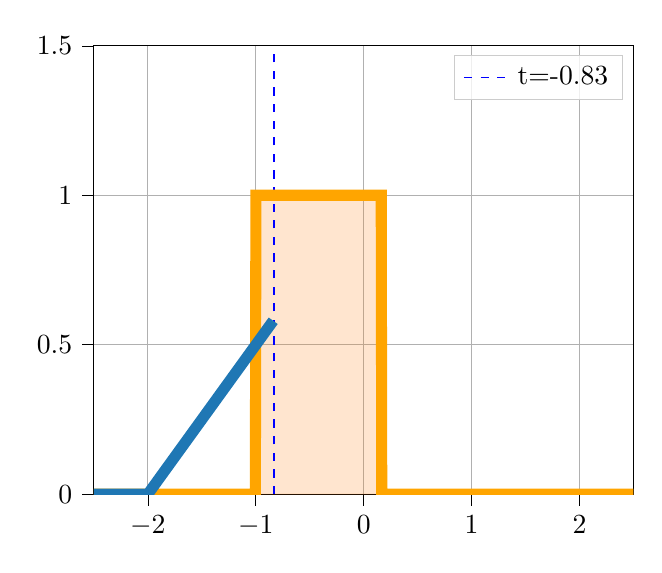
\begin{tikzpicture}

\definecolor{color0}{rgb}{1,0.498039215686275,0.0549019607843137}
\definecolor{color1}{rgb}{1,0.647058823529412,0}
\definecolor{color2}{rgb}{0.12156862745098,0.466666666666667,0.705882352941177}

\begin{axis}[
legend cell align={left},
legend style={fill opacity=0.8, draw opacity=1, text opacity=1, draw=white!80!black},
tick align=outside,
tick pos=left,
x grid style={white!69.0196078431373!black},
xmajorgrids,
xmin=-2.5, xmax=2.5,
xtick style={color=black},
y grid style={white!69.0196078431373!black},
ymajorgrids,
ymin=0, ymax=1.5,
ytick style={color=black}
]
\path [draw=color0, fill=color0, opacity=0.2]
(axis cs:-2.5,0)
--(axis cs:-2.5,0)
--(axis cs:-2.49499499499499,0)
--(axis cs:-2.48998998998999,0)
--(axis cs:-2.48498498498498,0)
--(axis cs:-2.47997997997998,0)
--(axis cs:-2.47497497497497,0)
--(axis cs:-2.46996996996997,0)
--(axis cs:-2.46496496496496,0)
--(axis cs:-2.45995995995996,0)
--(axis cs:-2.45495495495495,0)
--(axis cs:-2.44994994994995,0)
--(axis cs:-2.44494494494494,0)
--(axis cs:-2.43993993993994,0)
--(axis cs:-2.43493493493493,0)
--(axis cs:-2.42992992992993,0)
--(axis cs:-2.42492492492492,0)
--(axis cs:-2.41991991991992,0)
--(axis cs:-2.41491491491491,0)
--(axis cs:-2.40990990990991,0)
--(axis cs:-2.4049049049049,0)
--(axis cs:-2.3998998998999,0)
--(axis cs:-2.39489489489489,0)
--(axis cs:-2.38988988988989,0)
--(axis cs:-2.38488488488488,0)
--(axis cs:-2.37987987987988,0)
--(axis cs:-2.37487487487487,0)
--(axis cs:-2.36986986986987,0)
--(axis cs:-2.36486486486486,0)
--(axis cs:-2.35985985985986,0)
--(axis cs:-2.35485485485485,0)
--(axis cs:-2.34984984984985,0)
--(axis cs:-2.34484484484484,0)
--(axis cs:-2.33983983983984,0)
--(axis cs:-2.33483483483483,0)
--(axis cs:-2.32982982982983,0)
--(axis cs:-2.32482482482482,0)
--(axis cs:-2.31981981981982,0)
--(axis cs:-2.31481481481481,0)
--(axis cs:-2.30980980980981,0)
--(axis cs:-2.3048048048048,0)
--(axis cs:-2.2997997997998,0)
--(axis cs:-2.29479479479479,0)
--(axis cs:-2.28978978978979,0)
--(axis cs:-2.28478478478478,0)
--(axis cs:-2.27977977977978,0)
--(axis cs:-2.27477477477477,0)
--(axis cs:-2.26976976976977,0)
--(axis cs:-2.26476476476476,0)
--(axis cs:-2.25975975975976,0)
--(axis cs:-2.25475475475475,0)
--(axis cs:-2.24974974974975,0)
--(axis cs:-2.24474474474474,0)
--(axis cs:-2.23973973973974,0)
--(axis cs:-2.23473473473473,0)
--(axis cs:-2.22972972972973,0)
--(axis cs:-2.22472472472472,0)
--(axis cs:-2.21971971971972,0)
--(axis cs:-2.21471471471471,0)
--(axis cs:-2.20970970970971,0)
--(axis cs:-2.2047047047047,0)
--(axis cs:-2.1996996996997,0)
--(axis cs:-2.19469469469469,0)
--(axis cs:-2.18968968968969,0)
--(axis cs:-2.18468468468468,0)
--(axis cs:-2.17967967967968,0)
--(axis cs:-2.17467467467467,0)
--(axis cs:-2.16966966966967,0)
--(axis cs:-2.16466466466466,0)
--(axis cs:-2.15965965965966,0)
--(axis cs:-2.15465465465465,0)
--(axis cs:-2.14964964964965,0)
--(axis cs:-2.14464464464464,0)
--(axis cs:-2.13963963963964,0)
--(axis cs:-2.13463463463463,0)
--(axis cs:-2.12962962962963,0)
--(axis cs:-2.12462462462462,0)
--(axis cs:-2.11961961961962,0)
--(axis cs:-2.11461461461461,0)
--(axis cs:-2.10960960960961,0)
--(axis cs:-2.1046046046046,0)
--(axis cs:-2.0995995995996,0)
--(axis cs:-2.09459459459459,0)
--(axis cs:-2.08958958958959,0)
--(axis cs:-2.08458458458458,0)
--(axis cs:-2.07957957957958,0)
--(axis cs:-2.07457457457457,0)
--(axis cs:-2.06956956956957,0)
--(axis cs:-2.06456456456456,0)
--(axis cs:-2.05955955955956,0)
--(axis cs:-2.05455455455455,0)
--(axis cs:-2.04954954954955,0)
--(axis cs:-2.04454454454454,0)
--(axis cs:-2.03953953953954,0)
--(axis cs:-2.03453453453453,0)
--(axis cs:-2.02952952952953,0)
--(axis cs:-2.02452452452452,0)
--(axis cs:-2.01951951951952,0)
--(axis cs:-2.01451451451451,0)
--(axis cs:-2.00950950950951,0)
--(axis cs:-2.0045045045045,0)
--(axis cs:-1.9994994994995,0)
--(axis cs:-1.99449449449449,0)
--(axis cs:-1.98948948948949,0)
--(axis cs:-1.98448448448448,0)
--(axis cs:-1.97947947947948,0)
--(axis cs:-1.97447447447447,0)
--(axis cs:-1.96946946946947,0)
--(axis cs:-1.96446446446446,0)
--(axis cs:-1.95945945945946,0)
--(axis cs:-1.95445445445445,0)
--(axis cs:-1.94944944944945,0)
--(axis cs:-1.94444444444444,0)
--(axis cs:-1.93943943943944,0)
--(axis cs:-1.93443443443443,0)
--(axis cs:-1.92942942942943,0)
--(axis cs:-1.92442442442442,0)
--(axis cs:-1.91941941941942,0)
--(axis cs:-1.91441441441441,0)
--(axis cs:-1.90940940940941,0)
--(axis cs:-1.9044044044044,0)
--(axis cs:-1.8993993993994,0)
--(axis cs:-1.89439439439439,0)
--(axis cs:-1.88938938938939,0)
--(axis cs:-1.88438438438438,0)
--(axis cs:-1.87937937937938,0)
--(axis cs:-1.87437437437437,0)
--(axis cs:-1.86936936936937,0)
--(axis cs:-1.86436436436436,0)
--(axis cs:-1.85935935935936,0)
--(axis cs:-1.85435435435435,0)
--(axis cs:-1.84934934934935,0)
--(axis cs:-1.84434434434434,0)
--(axis cs:-1.83933933933934,0)
--(axis cs:-1.83433433433433,0)
--(axis cs:-1.82932932932933,0)
--(axis cs:-1.82432432432432,0)
--(axis cs:-1.81931931931932,0)
--(axis cs:-1.81431431431431,0)
--(axis cs:-1.80930930930931,0)
--(axis cs:-1.8043043043043,0)
--(axis cs:-1.7992992992993,0)
--(axis cs:-1.79429429429429,0)
--(axis cs:-1.78928928928929,0)
--(axis cs:-1.78428428428428,0)
--(axis cs:-1.77927927927928,0)
--(axis cs:-1.77427427427427,0)
--(axis cs:-1.76926926926927,0)
--(axis cs:-1.76426426426426,0)
--(axis cs:-1.75925925925926,0)
--(axis cs:-1.75425425425425,0)
--(axis cs:-1.74924924924925,0)
--(axis cs:-1.74424424424424,0)
--(axis cs:-1.73923923923924,0)
--(axis cs:-1.73423423423423,0)
--(axis cs:-1.72922922922923,0)
--(axis cs:-1.72422422422422,0)
--(axis cs:-1.71921921921922,0)
--(axis cs:-1.71421421421421,0)
--(axis cs:-1.70920920920921,0)
--(axis cs:-1.7042042042042,0)
--(axis cs:-1.6991991991992,0)
--(axis cs:-1.69419419419419,0)
--(axis cs:-1.68918918918919,0)
--(axis cs:-1.68418418418418,0)
--(axis cs:-1.67917917917918,0)
--(axis cs:-1.67417417417417,0)
--(axis cs:-1.66916916916917,0)
--(axis cs:-1.66416416416416,0)
--(axis cs:-1.65915915915916,0)
--(axis cs:-1.65415415415415,0)
--(axis cs:-1.64914914914915,0)
--(axis cs:-1.64414414414414,0)
--(axis cs:-1.63913913913914,0)
--(axis cs:-1.63413413413413,0)
--(axis cs:-1.62912912912913,0)
--(axis cs:-1.62412412412412,0)
--(axis cs:-1.61911911911912,0)
--(axis cs:-1.61411411411411,0)
--(axis cs:-1.60910910910911,0)
--(axis cs:-1.6041041041041,0)
--(axis cs:-1.5990990990991,0)
--(axis cs:-1.59409409409409,0)
--(axis cs:-1.58908908908909,0)
--(axis cs:-1.58408408408408,0)
--(axis cs:-1.57907907907908,0)
--(axis cs:-1.57407407407407,0)
--(axis cs:-1.56906906906907,0)
--(axis cs:-1.56406406406406,0)
--(axis cs:-1.55905905905906,0)
--(axis cs:-1.55405405405405,0)
--(axis cs:-1.54904904904905,0)
--(axis cs:-1.54404404404404,0)
--(axis cs:-1.53903903903904,0)
--(axis cs:-1.53403403403403,0)
--(axis cs:-1.52902902902903,0)
--(axis cs:-1.52402402402402,0)
--(axis cs:-1.51901901901902,0)
--(axis cs:-1.51401401401401,0)
--(axis cs:-1.50900900900901,0)
--(axis cs:-1.504004004004,0)
--(axis cs:-1.498998998999,0)
--(axis cs:-1.49399399399399,0)
--(axis cs:-1.48898898898899,0)
--(axis cs:-1.48398398398398,0)
--(axis cs:-1.47897897897898,0)
--(axis cs:-1.47397397397397,0)
--(axis cs:-1.46896896896897,0)
--(axis cs:-1.46396396396396,0)
--(axis cs:-1.45895895895896,0)
--(axis cs:-1.45395395395395,0)
--(axis cs:-1.44894894894895,0)
--(axis cs:-1.44394394394394,0)
--(axis cs:-1.43893893893894,0)
--(axis cs:-1.43393393393393,0)
--(axis cs:-1.42892892892893,0)
--(axis cs:-1.42392392392392,0)
--(axis cs:-1.41891891891892,0)
--(axis cs:-1.41391391391391,0)
--(axis cs:-1.40890890890891,0)
--(axis cs:-1.4039039039039,0)
--(axis cs:-1.3988988988989,0)
--(axis cs:-1.39389389389389,0)
--(axis cs:-1.38888888888889,0)
--(axis cs:-1.38388388388388,0)
--(axis cs:-1.37887887887888,0)
--(axis cs:-1.37387387387387,0)
--(axis cs:-1.36886886886887,0)
--(axis cs:-1.36386386386386,0)
--(axis cs:-1.35885885885886,0)
--(axis cs:-1.35385385385385,0)
--(axis cs:-1.34884884884885,0)
--(axis cs:-1.34384384384384,0)
--(axis cs:-1.33883883883884,0)
--(axis cs:-1.33383383383383,0)
--(axis cs:-1.32882882882883,0)
--(axis cs:-1.32382382382382,0)
--(axis cs:-1.31881881881882,0)
--(axis cs:-1.31381381381381,0)
--(axis cs:-1.30880880880881,0)
--(axis cs:-1.3038038038038,0)
--(axis cs:-1.2987987987988,0)
--(axis cs:-1.29379379379379,0)
--(axis cs:-1.28878878878879,0)
--(axis cs:-1.28378378378378,0)
--(axis cs:-1.27877877877878,0)
--(axis cs:-1.27377377377377,0)
--(axis cs:-1.26876876876877,0)
--(axis cs:-1.26376376376376,0)
--(axis cs:-1.25875875875876,0)
--(axis cs:-1.25375375375375,0)
--(axis cs:-1.24874874874875,0)
--(axis cs:-1.24374374374374,0)
--(axis cs:-1.23873873873874,0)
--(axis cs:-1.23373373373373,0)
--(axis cs:-1.22872872872873,0)
--(axis cs:-1.22372372372372,0)
--(axis cs:-1.21871871871872,0)
--(axis cs:-1.21371371371371,0)
--(axis cs:-1.20870870870871,0)
--(axis cs:-1.2037037037037,0)
--(axis cs:-1.1986986986987,0)
--(axis cs:-1.19369369369369,0)
--(axis cs:-1.18868868868869,0)
--(axis cs:-1.18368368368368,0)
--(axis cs:-1.17867867867868,0)
--(axis cs:-1.17367367367367,0)
--(axis cs:-1.16866866866867,0)
--(axis cs:-1.16366366366366,0)
--(axis cs:-1.15865865865866,0)
--(axis cs:-1.15365365365365,0)
--(axis cs:-1.14864864864865,0)
--(axis cs:-1.14364364364364,0)
--(axis cs:-1.13863863863864,0)
--(axis cs:-1.13363363363363,0)
--(axis cs:-1.12862862862863,0)
--(axis cs:-1.12362362362362,0)
--(axis cs:-1.11861861861862,0)
--(axis cs:-1.11361361361361,0)
--(axis cs:-1.10860860860861,0)
--(axis cs:-1.1036036036036,0)
--(axis cs:-1.0985985985986,0)
--(axis cs:-1.09359359359359,0)
--(axis cs:-1.08858858858859,0)
--(axis cs:-1.08358358358358,0)
--(axis cs:-1.07857857857858,0)
--(axis cs:-1.07357357357357,0)
--(axis cs:-1.06856856856857,0)
--(axis cs:-1.06356356356356,0)
--(axis cs:-1.05855855855856,0)
--(axis cs:-1.05355355355355,0)
--(axis cs:-1.04854854854855,0)
--(axis cs:-1.04354354354354,0)
--(axis cs:-1.03853853853854,0)
--(axis cs:-1.03353353353353,0)
--(axis cs:-1.02852852852853,0)
--(axis cs:-1.02352352352352,0)
--(axis cs:-1.01851851851852,0)
--(axis cs:-1.01351351351351,0)
--(axis cs:-1.00850850850851,0)
--(axis cs:-1.0035035035035,0)
--(axis cs:-0.998498498498499,0)
--(axis cs:-0.993493493493494,0)
--(axis cs:-0.988488488488489,0)
--(axis cs:-0.983483483483484,0)
--(axis cs:-0.978478478478479,0)
--(axis cs:-0.973473473473474,0)
--(axis cs:-0.968468468468469,0)
--(axis cs:-0.963463463463464,0)
--(axis cs:-0.958458458458459,0)
--(axis cs:-0.953453453453454,0)
--(axis cs:-0.948448448448449,0)
--(axis cs:-0.943443443443444,0)
--(axis cs:-0.938438438438439,0)
--(axis cs:-0.933433433433434,0)
--(axis cs:-0.928428428428429,0)
--(axis cs:-0.923423423423424,0)
--(axis cs:-0.918418418418419,0)
--(axis cs:-0.913413413413414,0)
--(axis cs:-0.908408408408409,0)
--(axis cs:-0.903403403403404,0)
--(axis cs:-0.898398398398399,0)
--(axis cs:-0.893393393393393,0)
--(axis cs:-0.888388388388388,0)
--(axis cs:-0.883383383383383,0)
--(axis cs:-0.878378378378378,0)
--(axis cs:-0.873373373373373,0)
--(axis cs:-0.868368368368368,0)
--(axis cs:-0.863363363363363,0)
--(axis cs:-0.858358358358358,0)
--(axis cs:-0.853353353353353,0)
--(axis cs:-0.848348348348348,0)
--(axis cs:-0.843343343343343,0)
--(axis cs:-0.838338338338338,0)
--(axis cs:-0.833333333333333,0)
--(axis cs:-0.828328328328328,0)
--(axis cs:-0.823323323323323,0)
--(axis cs:-0.818318318318318,0)
--(axis cs:-0.813313313313313,0)
--(axis cs:-0.808308308308308,0)
--(axis cs:-0.803303303303303,0)
--(axis cs:-0.798298298298298,0)
--(axis cs:-0.793293293293293,0)
--(axis cs:-0.788288288288288,0)
--(axis cs:-0.783283283283283,0)
--(axis cs:-0.778278278278278,0)
--(axis cs:-0.773273273273273,0)
--(axis cs:-0.768268268268268,0)
--(axis cs:-0.763263263263263,0)
--(axis cs:-0.758258258258258,0)
--(axis cs:-0.753253253253253,0)
--(axis cs:-0.748248248248248,0)
--(axis cs:-0.743243243243243,0)
--(axis cs:-0.738238238238238,0)
--(axis cs:-0.733233233233233,0)
--(axis cs:-0.728228228228228,0)
--(axis cs:-0.723223223223223,0)
--(axis cs:-0.718218218218218,0)
--(axis cs:-0.713213213213213,0)
--(axis cs:-0.708208208208208,0)
--(axis cs:-0.703203203203203,0)
--(axis cs:-0.698198198198198,0)
--(axis cs:-0.693193193193193,0)
--(axis cs:-0.688188188188188,0)
--(axis cs:-0.683183183183183,0)
--(axis cs:-0.678178178178178,0)
--(axis cs:-0.673173173173173,0)
--(axis cs:-0.668168168168168,0)
--(axis cs:-0.663163163163163,0)
--(axis cs:-0.658158158158158,0)
--(axis cs:-0.653153153153153,0)
--(axis cs:-0.648148148148148,0)
--(axis cs:-0.643143143143143,0)
--(axis cs:-0.638138138138138,0)
--(axis cs:-0.633133133133133,0)
--(axis cs:-0.628128128128128,0)
--(axis cs:-0.623123123123123,0)
--(axis cs:-0.618118118118118,0)
--(axis cs:-0.613113113113113,0)
--(axis cs:-0.608108108108108,0)
--(axis cs:-0.603103103103103,0)
--(axis cs:-0.598098098098098,0)
--(axis cs:-0.593093093093093,0)
--(axis cs:-0.588088088088088,0)
--(axis cs:-0.583083083083083,0)
--(axis cs:-0.578078078078078,0)
--(axis cs:-0.573073073073073,0)
--(axis cs:-0.568068068068068,0)
--(axis cs:-0.563063063063063,0)
--(axis cs:-0.558058058058058,0)
--(axis cs:-0.553053053053053,0)
--(axis cs:-0.548048048048048,0)
--(axis cs:-0.543043043043043,0)
--(axis cs:-0.538038038038038,0)
--(axis cs:-0.533033033033033,0)
--(axis cs:-0.528028028028028,0)
--(axis cs:-0.523023023023023,0)
--(axis cs:-0.518018018018018,0)
--(axis cs:-0.513013013013013,0)
--(axis cs:-0.508008008008008,0)
--(axis cs:-0.503003003003003,0)
--(axis cs:-0.497997997997998,0)
--(axis cs:-0.492992992992993,0)
--(axis cs:-0.487987987987988,0)
--(axis cs:-0.482982982982983,0)
--(axis cs:-0.477977977977978,0)
--(axis cs:-0.472972972972973,0)
--(axis cs:-0.467967967967968,0)
--(axis cs:-0.462962962962963,0)
--(axis cs:-0.457957957957958,0)
--(axis cs:-0.452952952952953,0)
--(axis cs:-0.447947947947948,0)
--(axis cs:-0.442942942942943,0)
--(axis cs:-0.437937937937938,0)
--(axis cs:-0.432932932932933,0)
--(axis cs:-0.427927927927928,0)
--(axis cs:-0.422922922922923,0)
--(axis cs:-0.417917917917918,0)
--(axis cs:-0.412912912912913,0)
--(axis cs:-0.407907907907908,0)
--(axis cs:-0.402902902902903,0)
--(axis cs:-0.397897897897898,0)
--(axis cs:-0.392892892892893,0)
--(axis cs:-0.387887887887888,0)
--(axis cs:-0.382882882882883,0)
--(axis cs:-0.377877877877878,0)
--(axis cs:-0.372872872872873,0)
--(axis cs:-0.367867867867868,0)
--(axis cs:-0.362862862862863,0)
--(axis cs:-0.357857857857858,0)
--(axis cs:-0.352852852852853,0)
--(axis cs:-0.347847847847848,0)
--(axis cs:-0.342842842842843,0)
--(axis cs:-0.337837837837838,0)
--(axis cs:-0.332832832832833,0)
--(axis cs:-0.327827827827828,0)
--(axis cs:-0.322822822822823,0)
--(axis cs:-0.317817817817818,0)
--(axis cs:-0.312812812812813,0)
--(axis cs:-0.307807807807808,0)
--(axis cs:-0.302802802802803,0)
--(axis cs:-0.297797797797798,0)
--(axis cs:-0.292792792792793,0)
--(axis cs:-0.287787787787788,0)
--(axis cs:-0.282782782782783,0)
--(axis cs:-0.277777777777778,0)
--(axis cs:-0.272772772772773,0)
--(axis cs:-0.267767767767768,0)
--(axis cs:-0.262762762762763,0)
--(axis cs:-0.257757757757758,0)
--(axis cs:-0.252752752752753,0)
--(axis cs:-0.247747747747748,0)
--(axis cs:-0.242742742742743,0)
--(axis cs:-0.237737737737738,0)
--(axis cs:-0.232732732732733,0)
--(axis cs:-0.227727727727728,0)
--(axis cs:-0.222722722722723,0)
--(axis cs:-0.217717717717718,0)
--(axis cs:-0.212712712712713,0)
--(axis cs:-0.207707707707708,0)
--(axis cs:-0.202702702702703,0)
--(axis cs:-0.197697697697698,0)
--(axis cs:-0.192692692692693,0)
--(axis cs:-0.187687687687688,0)
--(axis cs:-0.182682682682683,0)
--(axis cs:-0.177677677677678,0)
--(axis cs:-0.172672672672673,0)
--(axis cs:-0.167667667667668,0)
--(axis cs:-0.162662662662663,0)
--(axis cs:-0.157657657657658,0)
--(axis cs:-0.152652652652653,0)
--(axis cs:-0.147647647647648,0)
--(axis cs:-0.142642642642643,0)
--(axis cs:-0.137637637637638,0)
--(axis cs:-0.132632632632633,0)
--(axis cs:-0.127627627627628,0)
--(axis cs:-0.122622622622623,0)
--(axis cs:-0.117617617617618,0)
--(axis cs:-0.112612612612613,0)
--(axis cs:-0.107607607607608,0)
--(axis cs:-0.102602602602603,0)
--(axis cs:-0.0975975975975976,0)
--(axis cs:-0.0925925925925926,0)
--(axis cs:-0.0875875875875876,0)
--(axis cs:-0.0825825825825826,0)
--(axis cs:-0.0775775775775776,0)
--(axis cs:-0.0725725725725725,0)
--(axis cs:-0.0675675675675675,0)
--(axis cs:-0.0625625625625625,0)
--(axis cs:-0.0575575575575575,0)
--(axis cs:-0.0525525525525525,0)
--(axis cs:-0.0475475475475475,0)
--(axis cs:-0.0425425425425425,0)
--(axis cs:-0.0375375375375375,0)
--(axis cs:-0.0325325325325325,0)
--(axis cs:-0.0275275275275275,0)
--(axis cs:-0.0225225225225225,0)
--(axis cs:-0.0175175175175175,0)
--(axis cs:-0.0125125125125125,0)
--(axis cs:-0.0075075075075075,0)
--(axis cs:-0.0025025025025025,0)
--(axis cs:0.0025025025025025,0)
--(axis cs:0.0075075075075075,0)
--(axis cs:0.0125125125125125,0)
--(axis cs:0.0175175175175175,0)
--(axis cs:0.0225225225225225,0)
--(axis cs:0.0275275275275275,0)
--(axis cs:0.0325325325325325,0)
--(axis cs:0.0375375375375375,0)
--(axis cs:0.0425425425425425,0)
--(axis cs:0.0475475475475475,0)
--(axis cs:0.0525525525525525,0)
--(axis cs:0.0575575575575575,0)
--(axis cs:0.0625625625625625,0)
--(axis cs:0.0675675675675675,0)
--(axis cs:0.0725725725725725,0)
--(axis cs:0.0775775775775776,0)
--(axis cs:0.0825825825825826,0)
--(axis cs:0.0875875875875876,0)
--(axis cs:0.0925925925925926,0)
--(axis cs:0.0975975975975976,0)
--(axis cs:0.102602602602603,0)
--(axis cs:0.107607607607608,0)
--(axis cs:0.112612612612613,0)
--(axis cs:0.117617617617618,0)
--(axis cs:0.122622622622623,0)
--(axis cs:0.127627627627628,0)
--(axis cs:0.132632632632633,0)
--(axis cs:0.137637637637638,0)
--(axis cs:0.142642642642643,0)
--(axis cs:0.147647647647648,0)
--(axis cs:0.152652652652653,0)
--(axis cs:0.157657657657658,0)
--(axis cs:0.162662662662663,0)
--(axis cs:0.167667667667668,0)
--(axis cs:0.172672672672673,0)
--(axis cs:0.177677677677678,0)
--(axis cs:0.182682682682683,0)
--(axis cs:0.187687687687688,0)
--(axis cs:0.192692692692693,0)
--(axis cs:0.197697697697698,0)
--(axis cs:0.202702702702703,0)
--(axis cs:0.207707707707708,0)
--(axis cs:0.212712712712713,0)
--(axis cs:0.217717717717718,0)
--(axis cs:0.222722722722723,0)
--(axis cs:0.227727727727728,0)
--(axis cs:0.232732732732733,0)
--(axis cs:0.237737737737738,0)
--(axis cs:0.242742742742743,0)
--(axis cs:0.247747747747748,0)
--(axis cs:0.252752752752753,0)
--(axis cs:0.257757757757758,0)
--(axis cs:0.262762762762763,0)
--(axis cs:0.267767767767768,0)
--(axis cs:0.272772772772773,0)
--(axis cs:0.277777777777778,0)
--(axis cs:0.282782782782783,0)
--(axis cs:0.287787787787788,0)
--(axis cs:0.292792792792793,0)
--(axis cs:0.297797797797798,0)
--(axis cs:0.302802802802803,0)
--(axis cs:0.307807807807808,0)
--(axis cs:0.312812812812813,0)
--(axis cs:0.317817817817818,0)
--(axis cs:0.322822822822823,0)
--(axis cs:0.327827827827828,0)
--(axis cs:0.332832832832833,0)
--(axis cs:0.337837837837838,0)
--(axis cs:0.342842842842843,0)
--(axis cs:0.347847847847848,0)
--(axis cs:0.352852852852853,0)
--(axis cs:0.357857857857858,0)
--(axis cs:0.362862862862863,0)
--(axis cs:0.367867867867868,0)
--(axis cs:0.372872872872873,0)
--(axis cs:0.377877877877878,0)
--(axis cs:0.382882882882883,0)
--(axis cs:0.387887887887888,0)
--(axis cs:0.392892892892893,0)
--(axis cs:0.397897897897898,0)
--(axis cs:0.402902902902903,0)
--(axis cs:0.407907907907908,0)
--(axis cs:0.412912912912913,0)
--(axis cs:0.417917917917918,0)
--(axis cs:0.422922922922923,0)
--(axis cs:0.427927927927928,0)
--(axis cs:0.432932932932933,0)
--(axis cs:0.437937937937938,0)
--(axis cs:0.442942942942943,0)
--(axis cs:0.447947947947948,0)
--(axis cs:0.452952952952953,0)
--(axis cs:0.457957957957958,0)
--(axis cs:0.462962962962963,0)
--(axis cs:0.467967967967968,0)
--(axis cs:0.472972972972973,0)
--(axis cs:0.477977977977978,0)
--(axis cs:0.482982982982983,0)
--(axis cs:0.487987987987988,0)
--(axis cs:0.492992992992993,0)
--(axis cs:0.497997997997998,0)
--(axis cs:0.503003003003003,0)
--(axis cs:0.508008008008008,0)
--(axis cs:0.513013013013013,0)
--(axis cs:0.518018018018018,0)
--(axis cs:0.523023023023023,0)
--(axis cs:0.528028028028028,0)
--(axis cs:0.533033033033033,0)
--(axis cs:0.538038038038038,0)
--(axis cs:0.543043043043043,0)
--(axis cs:0.548048048048048,0)
--(axis cs:0.553053053053053,0)
--(axis cs:0.558058058058058,0)
--(axis cs:0.563063063063063,0)
--(axis cs:0.568068068068068,0)
--(axis cs:0.573073073073073,0)
--(axis cs:0.578078078078078,0)
--(axis cs:0.583083083083083,0)
--(axis cs:0.588088088088088,0)
--(axis cs:0.593093093093093,0)
--(axis cs:0.598098098098098,0)
--(axis cs:0.603103103103103,0)
--(axis cs:0.608108108108108,0)
--(axis cs:0.613113113113113,0)
--(axis cs:0.618118118118118,0)
--(axis cs:0.623123123123123,0)
--(axis cs:0.628128128128128,0)
--(axis cs:0.633133133133133,0)
--(axis cs:0.638138138138138,0)
--(axis cs:0.643143143143143,0)
--(axis cs:0.648148148148148,0)
--(axis cs:0.653153153153153,0)
--(axis cs:0.658158158158158,0)
--(axis cs:0.663163163163163,0)
--(axis cs:0.668168168168168,0)
--(axis cs:0.673173173173173,0)
--(axis cs:0.678178178178178,0)
--(axis cs:0.683183183183183,0)
--(axis cs:0.688188188188188,0)
--(axis cs:0.693193193193193,0)
--(axis cs:0.698198198198198,0)
--(axis cs:0.703203203203203,0)
--(axis cs:0.708208208208208,0)
--(axis cs:0.713213213213213,0)
--(axis cs:0.718218218218218,0)
--(axis cs:0.723223223223223,0)
--(axis cs:0.728228228228228,0)
--(axis cs:0.733233233233233,0)
--(axis cs:0.738238238238238,0)
--(axis cs:0.743243243243243,0)
--(axis cs:0.748248248248248,0)
--(axis cs:0.753253253253253,0)
--(axis cs:0.758258258258258,0)
--(axis cs:0.763263263263263,0)
--(axis cs:0.768268268268268,0)
--(axis cs:0.773273273273273,0)
--(axis cs:0.778278278278278,0)
--(axis cs:0.783283283283283,0)
--(axis cs:0.788288288288288,0)
--(axis cs:0.793293293293293,0)
--(axis cs:0.798298298298298,0)
--(axis cs:0.803303303303303,0)
--(axis cs:0.808308308308308,0)
--(axis cs:0.813313313313313,0)
--(axis cs:0.818318318318318,0)
--(axis cs:0.823323323323323,0)
--(axis cs:0.828328328328328,0)
--(axis cs:0.833333333333333,0)
--(axis cs:0.838338338338338,0)
--(axis cs:0.843343343343343,0)
--(axis cs:0.848348348348348,0)
--(axis cs:0.853353353353353,0)
--(axis cs:0.858358358358358,0)
--(axis cs:0.863363363363364,0)
--(axis cs:0.868368368368369,0)
--(axis cs:0.873373373373374,0)
--(axis cs:0.878378378378379,0)
--(axis cs:0.883383383383384,0)
--(axis cs:0.888388388388389,0)
--(axis cs:0.893393393393394,0)
--(axis cs:0.898398398398399,0)
--(axis cs:0.903403403403404,0)
--(axis cs:0.908408408408409,0)
--(axis cs:0.913413413413414,0)
--(axis cs:0.918418418418419,0)
--(axis cs:0.923423423423424,0)
--(axis cs:0.928428428428429,0)
--(axis cs:0.933433433433434,0)
--(axis cs:0.938438438438439,0)
--(axis cs:0.943443443443444,0)
--(axis cs:0.948448448448449,0)
--(axis cs:0.953453453453454,0)
--(axis cs:0.958458458458459,0)
--(axis cs:0.963463463463464,0)
--(axis cs:0.968468468468469,0)
--(axis cs:0.973473473473474,0)
--(axis cs:0.978478478478479,0)
--(axis cs:0.983483483483484,0)
--(axis cs:0.988488488488489,0)
--(axis cs:0.993493493493494,0)
--(axis cs:0.998498498498499,0)
--(axis cs:1.0035035035035,0)
--(axis cs:1.00850850850851,0)
--(axis cs:1.01351351351351,0)
--(axis cs:1.01851851851852,0)
--(axis cs:1.02352352352352,0)
--(axis cs:1.02852852852853,0)
--(axis cs:1.03353353353353,0)
--(axis cs:1.03853853853854,0)
--(axis cs:1.04354354354354,0)
--(axis cs:1.04854854854855,0)
--(axis cs:1.05355355355355,0)
--(axis cs:1.05855855855856,0)
--(axis cs:1.06356356356356,0)
--(axis cs:1.06856856856857,0)
--(axis cs:1.07357357357357,0)
--(axis cs:1.07857857857858,0)
--(axis cs:1.08358358358358,0)
--(axis cs:1.08858858858859,0)
--(axis cs:1.09359359359359,0)
--(axis cs:1.0985985985986,0)
--(axis cs:1.1036036036036,0)
--(axis cs:1.10860860860861,0)
--(axis cs:1.11361361361361,0)
--(axis cs:1.11861861861862,0)
--(axis cs:1.12362362362362,0)
--(axis cs:1.12862862862863,0)
--(axis cs:1.13363363363363,0)
--(axis cs:1.13863863863864,0)
--(axis cs:1.14364364364364,0)
--(axis cs:1.14864864864865,0)
--(axis cs:1.15365365365365,0)
--(axis cs:1.15865865865866,0)
--(axis cs:1.16366366366366,0)
--(axis cs:1.16866866866867,0)
--(axis cs:1.17367367367367,0)
--(axis cs:1.17867867867868,0)
--(axis cs:1.18368368368368,0)
--(axis cs:1.18868868868869,0)
--(axis cs:1.19369369369369,0)
--(axis cs:1.1986986986987,0)
--(axis cs:1.2037037037037,0)
--(axis cs:1.20870870870871,0)
--(axis cs:1.21371371371371,0)
--(axis cs:1.21871871871872,0)
--(axis cs:1.22372372372372,0)
--(axis cs:1.22872872872873,0)
--(axis cs:1.23373373373373,0)
--(axis cs:1.23873873873874,0)
--(axis cs:1.24374374374374,0)
--(axis cs:1.24874874874875,0)
--(axis cs:1.25375375375375,0)
--(axis cs:1.25875875875876,0)
--(axis cs:1.26376376376376,0)
--(axis cs:1.26876876876877,0)
--(axis cs:1.27377377377377,0)
--(axis cs:1.27877877877878,0)
--(axis cs:1.28378378378378,0)
--(axis cs:1.28878878878879,0)
--(axis cs:1.29379379379379,0)
--(axis cs:1.2987987987988,0)
--(axis cs:1.3038038038038,0)
--(axis cs:1.30880880880881,0)
--(axis cs:1.31381381381381,0)
--(axis cs:1.31881881881882,0)
--(axis cs:1.32382382382382,0)
--(axis cs:1.32882882882883,0)
--(axis cs:1.33383383383383,0)
--(axis cs:1.33883883883884,0)
--(axis cs:1.34384384384384,0)
--(axis cs:1.34884884884885,0)
--(axis cs:1.35385385385385,0)
--(axis cs:1.35885885885886,0)
--(axis cs:1.36386386386386,0)
--(axis cs:1.36886886886887,0)
--(axis cs:1.37387387387387,0)
--(axis cs:1.37887887887888,0)
--(axis cs:1.38388388388388,0)
--(axis cs:1.38888888888889,0)
--(axis cs:1.39389389389389,0)
--(axis cs:1.3988988988989,0)
--(axis cs:1.4039039039039,0)
--(axis cs:1.40890890890891,0)
--(axis cs:1.41391391391391,0)
--(axis cs:1.41891891891892,0)
--(axis cs:1.42392392392392,0)
--(axis cs:1.42892892892893,0)
--(axis cs:1.43393393393393,0)
--(axis cs:1.43893893893894,0)
--(axis cs:1.44394394394394,0)
--(axis cs:1.44894894894895,0)
--(axis cs:1.45395395395395,0)
--(axis cs:1.45895895895896,0)
--(axis cs:1.46396396396396,0)
--(axis cs:1.46896896896897,0)
--(axis cs:1.47397397397397,0)
--(axis cs:1.47897897897898,0)
--(axis cs:1.48398398398398,0)
--(axis cs:1.48898898898899,0)
--(axis cs:1.49399399399399,0)
--(axis cs:1.498998998999,0)
--(axis cs:1.504004004004,0)
--(axis cs:1.50900900900901,0)
--(axis cs:1.51401401401401,0)
--(axis cs:1.51901901901902,0)
--(axis cs:1.52402402402402,0)
--(axis cs:1.52902902902903,0)
--(axis cs:1.53403403403403,0)
--(axis cs:1.53903903903904,0)
--(axis cs:1.54404404404404,0)
--(axis cs:1.54904904904905,0)
--(axis cs:1.55405405405405,0)
--(axis cs:1.55905905905906,0)
--(axis cs:1.56406406406406,0)
--(axis cs:1.56906906906907,0)
--(axis cs:1.57407407407407,0)
--(axis cs:1.57907907907908,0)
--(axis cs:1.58408408408408,0)
--(axis cs:1.58908908908909,0)
--(axis cs:1.59409409409409,0)
--(axis cs:1.5990990990991,0)
--(axis cs:1.6041041041041,0)
--(axis cs:1.60910910910911,0)
--(axis cs:1.61411411411411,0)
--(axis cs:1.61911911911912,0)
--(axis cs:1.62412412412412,0)
--(axis cs:1.62912912912913,0)
--(axis cs:1.63413413413413,0)
--(axis cs:1.63913913913914,0)
--(axis cs:1.64414414414414,0)
--(axis cs:1.64914914914915,0)
--(axis cs:1.65415415415415,0)
--(axis cs:1.65915915915916,0)
--(axis cs:1.66416416416416,0)
--(axis cs:1.66916916916917,0)
--(axis cs:1.67417417417417,0)
--(axis cs:1.67917917917918,0)
--(axis cs:1.68418418418418,0)
--(axis cs:1.68918918918919,0)
--(axis cs:1.69419419419419,0)
--(axis cs:1.6991991991992,0)
--(axis cs:1.7042042042042,0)
--(axis cs:1.70920920920921,0)
--(axis cs:1.71421421421421,0)
--(axis cs:1.71921921921922,0)
--(axis cs:1.72422422422422,0)
--(axis cs:1.72922922922923,0)
--(axis cs:1.73423423423423,0)
--(axis cs:1.73923923923924,0)
--(axis cs:1.74424424424424,0)
--(axis cs:1.74924924924925,0)
--(axis cs:1.75425425425425,0)
--(axis cs:1.75925925925926,0)
--(axis cs:1.76426426426426,0)
--(axis cs:1.76926926926927,0)
--(axis cs:1.77427427427427,0)
--(axis cs:1.77927927927928,0)
--(axis cs:1.78428428428428,0)
--(axis cs:1.78928928928929,0)
--(axis cs:1.79429429429429,0)
--(axis cs:1.7992992992993,0)
--(axis cs:1.8043043043043,0)
--(axis cs:1.80930930930931,0)
--(axis cs:1.81431431431431,0)
--(axis cs:1.81931931931932,0)
--(axis cs:1.82432432432432,0)
--(axis cs:1.82932932932933,0)
--(axis cs:1.83433433433433,0)
--(axis cs:1.83933933933934,0)
--(axis cs:1.84434434434434,0)
--(axis cs:1.84934934934935,0)
--(axis cs:1.85435435435435,0)
--(axis cs:1.85935935935936,0)
--(axis cs:1.86436436436436,0)
--(axis cs:1.86936936936937,0)
--(axis cs:1.87437437437437,0)
--(axis cs:1.87937937937938,0)
--(axis cs:1.88438438438438,0)
--(axis cs:1.88938938938939,0)
--(axis cs:1.89439439439439,0)
--(axis cs:1.8993993993994,0)
--(axis cs:1.9044044044044,0)
--(axis cs:1.90940940940941,0)
--(axis cs:1.91441441441441,0)
--(axis cs:1.91941941941942,0)
--(axis cs:1.92442442442442,0)
--(axis cs:1.92942942942943,0)
--(axis cs:1.93443443443443,0)
--(axis cs:1.93943943943944,0)
--(axis cs:1.94444444444444,0)
--(axis cs:1.94944944944945,0)
--(axis cs:1.95445445445445,0)
--(axis cs:1.95945945945946,0)
--(axis cs:1.96446446446446,0)
--(axis cs:1.96946946946947,0)
--(axis cs:1.97447447447447,0)
--(axis cs:1.97947947947948,0)
--(axis cs:1.98448448448448,0)
--(axis cs:1.98948948948949,0)
--(axis cs:1.99449449449449,0)
--(axis cs:1.9994994994995,0)
--(axis cs:2.0045045045045,0)
--(axis cs:2.00950950950951,0)
--(axis cs:2.01451451451451,0)
--(axis cs:2.01951951951952,0)
--(axis cs:2.02452452452452,0)
--(axis cs:2.02952952952953,0)
--(axis cs:2.03453453453453,0)
--(axis cs:2.03953953953954,0)
--(axis cs:2.04454454454454,0)
--(axis cs:2.04954954954955,0)
--(axis cs:2.05455455455455,0)
--(axis cs:2.05955955955956,0)
--(axis cs:2.06456456456456,0)
--(axis cs:2.06956956956957,0)
--(axis cs:2.07457457457457,0)
--(axis cs:2.07957957957958,0)
--(axis cs:2.08458458458458,0)
--(axis cs:2.08958958958959,0)
--(axis cs:2.09459459459459,0)
--(axis cs:2.0995995995996,0)
--(axis cs:2.1046046046046,0)
--(axis cs:2.10960960960961,0)
--(axis cs:2.11461461461461,0)
--(axis cs:2.11961961961962,0)
--(axis cs:2.12462462462462,0)
--(axis cs:2.12962962962963,0)
--(axis cs:2.13463463463463,0)
--(axis cs:2.13963963963964,0)
--(axis cs:2.14464464464464,0)
--(axis cs:2.14964964964965,0)
--(axis cs:2.15465465465465,0)
--(axis cs:2.15965965965966,0)
--(axis cs:2.16466466466466,0)
--(axis cs:2.16966966966967,0)
--(axis cs:2.17467467467467,0)
--(axis cs:2.17967967967968,0)
--(axis cs:2.18468468468468,0)
--(axis cs:2.18968968968969,0)
--(axis cs:2.19469469469469,0)
--(axis cs:2.1996996996997,0)
--(axis cs:2.2047047047047,0)
--(axis cs:2.20970970970971,0)
--(axis cs:2.21471471471471,0)
--(axis cs:2.21971971971972,0)
--(axis cs:2.22472472472472,0)
--(axis cs:2.22972972972973,0)
--(axis cs:2.23473473473473,0)
--(axis cs:2.23973973973974,0)
--(axis cs:2.24474474474474,0)
--(axis cs:2.24974974974975,0)
--(axis cs:2.25475475475475,0)
--(axis cs:2.25975975975976,0)
--(axis cs:2.26476476476476,0)
--(axis cs:2.26976976976977,0)
--(axis cs:2.27477477477477,0)
--(axis cs:2.27977977977978,0)
--(axis cs:2.28478478478478,0)
--(axis cs:2.28978978978979,0)
--(axis cs:2.29479479479479,0)
--(axis cs:2.2997997997998,0)
--(axis cs:2.3048048048048,0)
--(axis cs:2.30980980980981,0)
--(axis cs:2.31481481481481,0)
--(axis cs:2.31981981981982,0)
--(axis cs:2.32482482482482,0)
--(axis cs:2.32982982982983,0)
--(axis cs:2.33483483483483,0)
--(axis cs:2.33983983983984,0)
--(axis cs:2.34484484484484,0)
--(axis cs:2.34984984984985,0)
--(axis cs:2.35485485485485,0)
--(axis cs:2.35985985985986,0)
--(axis cs:2.36486486486486,0)
--(axis cs:2.36986986986987,0)
--(axis cs:2.37487487487487,0)
--(axis cs:2.37987987987988,0)
--(axis cs:2.38488488488488,0)
--(axis cs:2.38988988988989,0)
--(axis cs:2.39489489489489,0)
--(axis cs:2.3998998998999,0)
--(axis cs:2.4049049049049,0)
--(axis cs:2.40990990990991,0)
--(axis cs:2.41491491491491,0)
--(axis cs:2.41991991991992,0)
--(axis cs:2.42492492492492,0)
--(axis cs:2.42992992992993,0)
--(axis cs:2.43493493493493,0)
--(axis cs:2.43993993993994,0)
--(axis cs:2.44494494494494,0)
--(axis cs:2.44994994994995,0)
--(axis cs:2.45495495495495,0)
--(axis cs:2.45995995995996,0)
--(axis cs:2.46496496496496,0)
--(axis cs:2.46996996996997,0)
--(axis cs:2.47497497497497,0)
--(axis cs:2.47997997997998,0)
--(axis cs:2.48498498498498,0)
--(axis cs:2.48998998998999,0)
--(axis cs:2.49499499499499,0)
--(axis cs:2.5,0)
--(axis cs:2.5,0)
--(axis cs:2.5,0)
--(axis cs:2.49499499499499,0)
--(axis cs:2.48998998998999,0)
--(axis cs:2.48498498498498,0)
--(axis cs:2.47997997997998,0)
--(axis cs:2.47497497497497,0)
--(axis cs:2.46996996996997,0)
--(axis cs:2.46496496496496,0)
--(axis cs:2.45995995995996,0)
--(axis cs:2.45495495495495,0)
--(axis cs:2.44994994994995,0)
--(axis cs:2.44494494494494,0)
--(axis cs:2.43993993993994,0)
--(axis cs:2.43493493493493,0)
--(axis cs:2.42992992992993,0)
--(axis cs:2.42492492492492,0)
--(axis cs:2.41991991991992,0)
--(axis cs:2.41491491491491,0)
--(axis cs:2.40990990990991,0)
--(axis cs:2.4049049049049,0)
--(axis cs:2.3998998998999,0)
--(axis cs:2.39489489489489,0)
--(axis cs:2.38988988988989,0)
--(axis cs:2.38488488488488,0)
--(axis cs:2.37987987987988,0)
--(axis cs:2.37487487487487,0)
--(axis cs:2.36986986986987,0)
--(axis cs:2.36486486486486,0)
--(axis cs:2.35985985985986,0)
--(axis cs:2.35485485485485,0)
--(axis cs:2.34984984984985,0)
--(axis cs:2.34484484484484,0)
--(axis cs:2.33983983983984,0)
--(axis cs:2.33483483483483,0)
--(axis cs:2.32982982982983,0)
--(axis cs:2.32482482482482,0)
--(axis cs:2.31981981981982,0)
--(axis cs:2.31481481481481,0)
--(axis cs:2.30980980980981,0)
--(axis cs:2.3048048048048,0)
--(axis cs:2.2997997997998,0)
--(axis cs:2.29479479479479,0)
--(axis cs:2.28978978978979,0)
--(axis cs:2.28478478478478,0)
--(axis cs:2.27977977977978,0)
--(axis cs:2.27477477477477,0)
--(axis cs:2.26976976976977,0)
--(axis cs:2.26476476476476,0)
--(axis cs:2.25975975975976,0)
--(axis cs:2.25475475475475,0)
--(axis cs:2.24974974974975,0)
--(axis cs:2.24474474474474,0)
--(axis cs:2.23973973973974,0)
--(axis cs:2.23473473473473,0)
--(axis cs:2.22972972972973,0)
--(axis cs:2.22472472472472,0)
--(axis cs:2.21971971971972,0)
--(axis cs:2.21471471471471,0)
--(axis cs:2.20970970970971,0)
--(axis cs:2.2047047047047,0)
--(axis cs:2.1996996996997,0)
--(axis cs:2.19469469469469,0)
--(axis cs:2.18968968968969,0)
--(axis cs:2.18468468468468,0)
--(axis cs:2.17967967967968,0)
--(axis cs:2.17467467467467,0)
--(axis cs:2.16966966966967,0)
--(axis cs:2.16466466466466,0)
--(axis cs:2.15965965965966,0)
--(axis cs:2.15465465465465,0)
--(axis cs:2.14964964964965,0)
--(axis cs:2.14464464464464,0)
--(axis cs:2.13963963963964,0)
--(axis cs:2.13463463463463,0)
--(axis cs:2.12962962962963,0)
--(axis cs:2.12462462462462,0)
--(axis cs:2.11961961961962,0)
--(axis cs:2.11461461461461,0)
--(axis cs:2.10960960960961,0)
--(axis cs:2.1046046046046,0)
--(axis cs:2.0995995995996,0)
--(axis cs:2.09459459459459,0)
--(axis cs:2.08958958958959,0)
--(axis cs:2.08458458458458,0)
--(axis cs:2.07957957957958,0)
--(axis cs:2.07457457457457,0)
--(axis cs:2.06956956956957,0)
--(axis cs:2.06456456456456,0)
--(axis cs:2.05955955955956,0)
--(axis cs:2.05455455455455,0)
--(axis cs:2.04954954954955,0)
--(axis cs:2.04454454454454,0)
--(axis cs:2.03953953953954,0)
--(axis cs:2.03453453453453,0)
--(axis cs:2.02952952952953,0)
--(axis cs:2.02452452452452,0)
--(axis cs:2.01951951951952,0)
--(axis cs:2.01451451451451,0)
--(axis cs:2.00950950950951,0)
--(axis cs:2.0045045045045,0)
--(axis cs:1.9994994994995,0)
--(axis cs:1.99449449449449,0)
--(axis cs:1.98948948948949,0)
--(axis cs:1.98448448448448,0)
--(axis cs:1.97947947947948,0)
--(axis cs:1.97447447447447,0)
--(axis cs:1.96946946946947,0)
--(axis cs:1.96446446446446,0)
--(axis cs:1.95945945945946,0)
--(axis cs:1.95445445445445,0)
--(axis cs:1.94944944944945,0)
--(axis cs:1.94444444444444,0)
--(axis cs:1.93943943943944,0)
--(axis cs:1.93443443443443,0)
--(axis cs:1.92942942942943,0)
--(axis cs:1.92442442442442,0)
--(axis cs:1.91941941941942,0)
--(axis cs:1.91441441441441,0)
--(axis cs:1.90940940940941,0)
--(axis cs:1.9044044044044,0)
--(axis cs:1.8993993993994,0)
--(axis cs:1.89439439439439,0)
--(axis cs:1.88938938938939,0)
--(axis cs:1.88438438438438,0)
--(axis cs:1.87937937937938,0)
--(axis cs:1.87437437437437,0)
--(axis cs:1.86936936936937,0)
--(axis cs:1.86436436436436,0)
--(axis cs:1.85935935935936,0)
--(axis cs:1.85435435435435,0)
--(axis cs:1.84934934934935,0)
--(axis cs:1.84434434434434,0)
--(axis cs:1.83933933933934,0)
--(axis cs:1.83433433433433,0)
--(axis cs:1.82932932932933,0)
--(axis cs:1.82432432432432,0)
--(axis cs:1.81931931931932,0)
--(axis cs:1.81431431431431,0)
--(axis cs:1.80930930930931,0)
--(axis cs:1.8043043043043,0)
--(axis cs:1.7992992992993,0)
--(axis cs:1.79429429429429,0)
--(axis cs:1.78928928928929,0)
--(axis cs:1.78428428428428,0)
--(axis cs:1.77927927927928,0)
--(axis cs:1.77427427427427,0)
--(axis cs:1.76926926926927,0)
--(axis cs:1.76426426426426,0)
--(axis cs:1.75925925925926,0)
--(axis cs:1.75425425425425,0)
--(axis cs:1.74924924924925,0)
--(axis cs:1.74424424424424,0)
--(axis cs:1.73923923923924,0)
--(axis cs:1.73423423423423,0)
--(axis cs:1.72922922922923,0)
--(axis cs:1.72422422422422,0)
--(axis cs:1.71921921921922,0)
--(axis cs:1.71421421421421,0)
--(axis cs:1.70920920920921,0)
--(axis cs:1.7042042042042,0)
--(axis cs:1.6991991991992,0)
--(axis cs:1.69419419419419,0)
--(axis cs:1.68918918918919,0)
--(axis cs:1.68418418418418,0)
--(axis cs:1.67917917917918,0)
--(axis cs:1.67417417417417,0)
--(axis cs:1.66916916916917,0)
--(axis cs:1.66416416416416,0)
--(axis cs:1.65915915915916,0)
--(axis cs:1.65415415415415,0)
--(axis cs:1.64914914914915,0)
--(axis cs:1.64414414414414,0)
--(axis cs:1.63913913913914,0)
--(axis cs:1.63413413413413,0)
--(axis cs:1.62912912912913,0)
--(axis cs:1.62412412412412,0)
--(axis cs:1.61911911911912,0)
--(axis cs:1.61411411411411,0)
--(axis cs:1.60910910910911,0)
--(axis cs:1.6041041041041,0)
--(axis cs:1.5990990990991,0)
--(axis cs:1.59409409409409,0)
--(axis cs:1.58908908908909,0)
--(axis cs:1.58408408408408,0)
--(axis cs:1.57907907907908,0)
--(axis cs:1.57407407407407,0)
--(axis cs:1.56906906906907,0)
--(axis cs:1.56406406406406,0)
--(axis cs:1.55905905905906,0)
--(axis cs:1.55405405405405,0)
--(axis cs:1.54904904904905,0)
--(axis cs:1.54404404404404,0)
--(axis cs:1.53903903903904,0)
--(axis cs:1.53403403403403,0)
--(axis cs:1.52902902902903,0)
--(axis cs:1.52402402402402,0)
--(axis cs:1.51901901901902,0)
--(axis cs:1.51401401401401,0)
--(axis cs:1.50900900900901,0)
--(axis cs:1.504004004004,0)
--(axis cs:1.498998998999,0)
--(axis cs:1.49399399399399,0)
--(axis cs:1.48898898898899,0)
--(axis cs:1.48398398398398,0)
--(axis cs:1.47897897897898,0)
--(axis cs:1.47397397397397,0)
--(axis cs:1.46896896896897,0)
--(axis cs:1.46396396396396,0)
--(axis cs:1.45895895895896,0)
--(axis cs:1.45395395395395,0)
--(axis cs:1.44894894894895,0)
--(axis cs:1.44394394394394,0)
--(axis cs:1.43893893893894,0)
--(axis cs:1.43393393393393,0)
--(axis cs:1.42892892892893,0)
--(axis cs:1.42392392392392,0)
--(axis cs:1.41891891891892,0)
--(axis cs:1.41391391391391,0)
--(axis cs:1.40890890890891,0)
--(axis cs:1.4039039039039,0)
--(axis cs:1.3988988988989,0)
--(axis cs:1.39389389389389,0)
--(axis cs:1.38888888888889,0)
--(axis cs:1.38388388388388,0)
--(axis cs:1.37887887887888,0)
--(axis cs:1.37387387387387,0)
--(axis cs:1.36886886886887,0)
--(axis cs:1.36386386386386,0)
--(axis cs:1.35885885885886,0)
--(axis cs:1.35385385385385,0)
--(axis cs:1.34884884884885,0)
--(axis cs:1.34384384384384,0)
--(axis cs:1.33883883883884,0)
--(axis cs:1.33383383383383,0)
--(axis cs:1.32882882882883,0)
--(axis cs:1.32382382382382,0)
--(axis cs:1.31881881881882,0)
--(axis cs:1.31381381381381,0)
--(axis cs:1.30880880880881,0)
--(axis cs:1.3038038038038,0)
--(axis cs:1.2987987987988,0)
--(axis cs:1.29379379379379,0)
--(axis cs:1.28878878878879,0)
--(axis cs:1.28378378378378,0)
--(axis cs:1.27877877877878,0)
--(axis cs:1.27377377377377,0)
--(axis cs:1.26876876876877,0)
--(axis cs:1.26376376376376,0)
--(axis cs:1.25875875875876,0)
--(axis cs:1.25375375375375,0)
--(axis cs:1.24874874874875,0)
--(axis cs:1.24374374374374,0)
--(axis cs:1.23873873873874,0)
--(axis cs:1.23373373373373,0)
--(axis cs:1.22872872872873,0)
--(axis cs:1.22372372372372,0)
--(axis cs:1.21871871871872,0)
--(axis cs:1.21371371371371,0)
--(axis cs:1.20870870870871,0)
--(axis cs:1.2037037037037,0)
--(axis cs:1.1986986986987,0)
--(axis cs:1.19369369369369,0)
--(axis cs:1.18868868868869,0)
--(axis cs:1.18368368368368,0)
--(axis cs:1.17867867867868,0)
--(axis cs:1.17367367367367,0)
--(axis cs:1.16866866866867,0)
--(axis cs:1.16366366366366,0)
--(axis cs:1.15865865865866,0)
--(axis cs:1.15365365365365,0)
--(axis cs:1.14864864864865,0)
--(axis cs:1.14364364364364,0)
--(axis cs:1.13863863863864,0)
--(axis cs:1.13363363363363,0)
--(axis cs:1.12862862862863,0)
--(axis cs:1.12362362362362,0)
--(axis cs:1.11861861861862,0)
--(axis cs:1.11361361361361,0)
--(axis cs:1.10860860860861,0)
--(axis cs:1.1036036036036,0)
--(axis cs:1.0985985985986,0)
--(axis cs:1.09359359359359,0)
--(axis cs:1.08858858858859,0)
--(axis cs:1.08358358358358,0)
--(axis cs:1.07857857857858,0)
--(axis cs:1.07357357357357,0)
--(axis cs:1.06856856856857,0)
--(axis cs:1.06356356356356,0)
--(axis cs:1.05855855855856,0)
--(axis cs:1.05355355355355,0)
--(axis cs:1.04854854854855,0)
--(axis cs:1.04354354354354,0)
--(axis cs:1.03853853853854,0)
--(axis cs:1.03353353353353,0)
--(axis cs:1.02852852852853,0)
--(axis cs:1.02352352352352,0)
--(axis cs:1.01851851851852,0)
--(axis cs:1.01351351351351,0)
--(axis cs:1.00850850850851,0)
--(axis cs:1.0035035035035,0)
--(axis cs:0.998498498498499,0)
--(axis cs:0.993493493493494,0)
--(axis cs:0.988488488488489,0)
--(axis cs:0.983483483483484,0)
--(axis cs:0.978478478478479,0)
--(axis cs:0.973473473473474,0)
--(axis cs:0.968468468468469,0)
--(axis cs:0.963463463463464,0)
--(axis cs:0.958458458458459,0)
--(axis cs:0.953453453453454,0)
--(axis cs:0.948448448448449,0)
--(axis cs:0.943443443443444,0)
--(axis cs:0.938438438438439,0)
--(axis cs:0.933433433433434,0)
--(axis cs:0.928428428428429,0)
--(axis cs:0.923423423423424,0)
--(axis cs:0.918418418418419,0)
--(axis cs:0.913413413413414,0)
--(axis cs:0.908408408408409,0)
--(axis cs:0.903403403403404,0)
--(axis cs:0.898398398398399,0)
--(axis cs:0.893393393393394,0)
--(axis cs:0.888388388388389,0)
--(axis cs:0.883383383383384,0)
--(axis cs:0.878378378378379,0)
--(axis cs:0.873373373373374,0)
--(axis cs:0.868368368368369,0)
--(axis cs:0.863363363363364,0)
--(axis cs:0.858358358358358,0)
--(axis cs:0.853353353353353,0)
--(axis cs:0.848348348348348,0)
--(axis cs:0.843343343343343,0)
--(axis cs:0.838338338338338,0)
--(axis cs:0.833333333333333,0)
--(axis cs:0.828328328328328,0)
--(axis cs:0.823323323323323,0)
--(axis cs:0.818318318318318,0)
--(axis cs:0.813313313313313,0)
--(axis cs:0.808308308308308,0)
--(axis cs:0.803303303303303,0)
--(axis cs:0.798298298298298,0)
--(axis cs:0.793293293293293,0)
--(axis cs:0.788288288288288,0)
--(axis cs:0.783283283283283,0)
--(axis cs:0.778278278278278,0)
--(axis cs:0.773273273273273,0)
--(axis cs:0.768268268268268,0)
--(axis cs:0.763263263263263,0)
--(axis cs:0.758258258258258,0)
--(axis cs:0.753253253253253,0)
--(axis cs:0.748248248248248,0)
--(axis cs:0.743243243243243,0)
--(axis cs:0.738238238238238,0)
--(axis cs:0.733233233233233,0)
--(axis cs:0.728228228228228,0)
--(axis cs:0.723223223223223,0)
--(axis cs:0.718218218218218,0)
--(axis cs:0.713213213213213,0)
--(axis cs:0.708208208208208,0)
--(axis cs:0.703203203203203,0)
--(axis cs:0.698198198198198,0)
--(axis cs:0.693193193193193,0)
--(axis cs:0.688188188188188,0)
--(axis cs:0.683183183183183,0)
--(axis cs:0.678178178178178,0)
--(axis cs:0.673173173173173,0)
--(axis cs:0.668168168168168,0)
--(axis cs:0.663163163163163,0)
--(axis cs:0.658158158158158,0)
--(axis cs:0.653153153153153,0)
--(axis cs:0.648148148148148,0)
--(axis cs:0.643143143143143,0)
--(axis cs:0.638138138138138,0)
--(axis cs:0.633133133133133,0)
--(axis cs:0.628128128128128,0)
--(axis cs:0.623123123123123,0)
--(axis cs:0.618118118118118,0)
--(axis cs:0.613113113113113,0)
--(axis cs:0.608108108108108,0)
--(axis cs:0.603103103103103,0)
--(axis cs:0.598098098098098,0)
--(axis cs:0.593093093093093,0)
--(axis cs:0.588088088088088,0)
--(axis cs:0.583083083083083,0)
--(axis cs:0.578078078078078,0)
--(axis cs:0.573073073073073,0)
--(axis cs:0.568068068068068,0)
--(axis cs:0.563063063063063,0)
--(axis cs:0.558058058058058,0)
--(axis cs:0.553053053053053,0)
--(axis cs:0.548048048048048,0)
--(axis cs:0.543043043043043,0)
--(axis cs:0.538038038038038,0)
--(axis cs:0.533033033033033,0)
--(axis cs:0.528028028028028,0)
--(axis cs:0.523023023023023,0)
--(axis cs:0.518018018018018,0)
--(axis cs:0.513013013013013,0)
--(axis cs:0.508008008008008,0)
--(axis cs:0.503003003003003,0)
--(axis cs:0.497997997997998,0)
--(axis cs:0.492992992992993,0)
--(axis cs:0.487987987987988,0)
--(axis cs:0.482982982982983,0)
--(axis cs:0.477977977977978,0)
--(axis cs:0.472972972972973,0)
--(axis cs:0.467967967967968,0)
--(axis cs:0.462962962962963,0)
--(axis cs:0.457957957957958,0)
--(axis cs:0.452952952952953,0)
--(axis cs:0.447947947947948,0)
--(axis cs:0.442942942942943,0)
--(axis cs:0.437937937937938,0)
--(axis cs:0.432932932932933,0)
--(axis cs:0.427927927927928,0)
--(axis cs:0.422922922922923,0)
--(axis cs:0.417917917917918,0)
--(axis cs:0.412912912912913,0)
--(axis cs:0.407907907907908,0)
--(axis cs:0.402902902902903,0)
--(axis cs:0.397897897897898,0)
--(axis cs:0.392892892892893,0)
--(axis cs:0.387887887887888,0)
--(axis cs:0.382882882882883,0)
--(axis cs:0.377877877877878,0)
--(axis cs:0.372872872872873,0)
--(axis cs:0.367867867867868,0)
--(axis cs:0.362862862862863,0)
--(axis cs:0.357857857857858,0)
--(axis cs:0.352852852852853,0)
--(axis cs:0.347847847847848,0)
--(axis cs:0.342842842842843,0)
--(axis cs:0.337837837837838,0)
--(axis cs:0.332832832832833,0)
--(axis cs:0.327827827827828,0)
--(axis cs:0.322822822822823,0)
--(axis cs:0.317817817817818,0)
--(axis cs:0.312812812812813,0)
--(axis cs:0.307807807807808,0)
--(axis cs:0.302802802802803,0)
--(axis cs:0.297797797797798,0)
--(axis cs:0.292792792792793,0)
--(axis cs:0.287787787787788,0)
--(axis cs:0.282782782782783,0)
--(axis cs:0.277777777777778,0)
--(axis cs:0.272772772772773,0)
--(axis cs:0.267767767767768,0)
--(axis cs:0.262762762762763,0)
--(axis cs:0.257757757757758,0)
--(axis cs:0.252752752752753,0)
--(axis cs:0.247747747747748,0)
--(axis cs:0.242742742742743,0)
--(axis cs:0.237737737737738,0)
--(axis cs:0.232732732732733,0)
--(axis cs:0.227727727727728,0)
--(axis cs:0.222722722722723,0)
--(axis cs:0.217717717717718,0)
--(axis cs:0.212712712712713,0)
--(axis cs:0.207707707707708,0)
--(axis cs:0.202702702702703,0)
--(axis cs:0.197697697697698,0)
--(axis cs:0.192692692692693,0)
--(axis cs:0.187687687687688,0)
--(axis cs:0.182682682682683,0)
--(axis cs:0.177677677677678,0)
--(axis cs:0.172672672672673,0)
--(axis cs:0.167667667667668,0)
--(axis cs:0.162662662662663,1)
--(axis cs:0.157657657657658,1)
--(axis cs:0.152652652652653,1)
--(axis cs:0.147647647647648,1)
--(axis cs:0.142642642642643,1)
--(axis cs:0.137637637637638,1)
--(axis cs:0.132632632632633,1)
--(axis cs:0.127627627627628,1)
--(axis cs:0.122622622622623,1)
--(axis cs:0.117617617617618,1)
--(axis cs:0.112612612612613,1)
--(axis cs:0.107607607607608,1)
--(axis cs:0.102602602602603,1)
--(axis cs:0.0975975975975976,1)
--(axis cs:0.0925925925925926,1)
--(axis cs:0.0875875875875876,1)
--(axis cs:0.0825825825825826,1)
--(axis cs:0.0775775775775776,1)
--(axis cs:0.0725725725725725,1)
--(axis cs:0.0675675675675675,1)
--(axis cs:0.0625625625625625,1)
--(axis cs:0.0575575575575575,1)
--(axis cs:0.0525525525525525,1)
--(axis cs:0.0475475475475475,1)
--(axis cs:0.0425425425425425,1)
--(axis cs:0.0375375375375375,1)
--(axis cs:0.0325325325325325,1)
--(axis cs:0.0275275275275275,1)
--(axis cs:0.0225225225225225,1)
--(axis cs:0.0175175175175175,1)
--(axis cs:0.0125125125125125,1)
--(axis cs:0.0075075075075075,1)
--(axis cs:0.0025025025025025,1)
--(axis cs:-0.0025025025025025,1)
--(axis cs:-0.0075075075075075,1)
--(axis cs:-0.0125125125125125,1)
--(axis cs:-0.0175175175175175,1)
--(axis cs:-0.0225225225225225,1)
--(axis cs:-0.0275275275275275,1)
--(axis cs:-0.0325325325325325,1)
--(axis cs:-0.0375375375375375,1)
--(axis cs:-0.0425425425425425,1)
--(axis cs:-0.0475475475475475,1)
--(axis cs:-0.0525525525525525,1)
--(axis cs:-0.0575575575575575,1)
--(axis cs:-0.0625625625625625,1)
--(axis cs:-0.0675675675675675,1)
--(axis cs:-0.0725725725725725,1)
--(axis cs:-0.0775775775775776,1)
--(axis cs:-0.0825825825825826,1)
--(axis cs:-0.0875875875875876,1)
--(axis cs:-0.0925925925925926,1)
--(axis cs:-0.0975975975975976,1)
--(axis cs:-0.102602602602603,1)
--(axis cs:-0.107607607607608,1)
--(axis cs:-0.112612612612613,1)
--(axis cs:-0.117617617617618,1)
--(axis cs:-0.122622622622623,1)
--(axis cs:-0.127627627627628,1)
--(axis cs:-0.132632632632633,1)
--(axis cs:-0.137637637637638,1)
--(axis cs:-0.142642642642643,1)
--(axis cs:-0.147647647647648,1)
--(axis cs:-0.152652652652653,1)
--(axis cs:-0.157657657657658,1)
--(axis cs:-0.162662662662663,1)
--(axis cs:-0.167667667667668,1)
--(axis cs:-0.172672672672673,1)
--(axis cs:-0.177677677677678,1)
--(axis cs:-0.182682682682683,1)
--(axis cs:-0.187687687687688,1)
--(axis cs:-0.192692692692693,1)
--(axis cs:-0.197697697697698,1)
--(axis cs:-0.202702702702703,1)
--(axis cs:-0.207707707707708,1)
--(axis cs:-0.212712712712713,1)
--(axis cs:-0.217717717717718,1)
--(axis cs:-0.222722722722723,1)
--(axis cs:-0.227727727727728,1)
--(axis cs:-0.232732732732733,1)
--(axis cs:-0.237737737737738,1)
--(axis cs:-0.242742742742743,1)
--(axis cs:-0.247747747747748,1)
--(axis cs:-0.252752752752753,1)
--(axis cs:-0.257757757757758,1)
--(axis cs:-0.262762762762763,1)
--(axis cs:-0.267767767767768,1)
--(axis cs:-0.272772772772773,1)
--(axis cs:-0.277777777777778,1)
--(axis cs:-0.282782782782783,1)
--(axis cs:-0.287787787787788,1)
--(axis cs:-0.292792792792793,1)
--(axis cs:-0.297797797797798,1)
--(axis cs:-0.302802802802803,1)
--(axis cs:-0.307807807807808,1)
--(axis cs:-0.312812812812813,1)
--(axis cs:-0.317817817817818,1)
--(axis cs:-0.322822822822823,1)
--(axis cs:-0.327827827827828,1)
--(axis cs:-0.332832832832833,1)
--(axis cs:-0.337837837837838,1)
--(axis cs:-0.342842842842843,1)
--(axis cs:-0.347847847847848,1)
--(axis cs:-0.352852852852853,1)
--(axis cs:-0.357857857857858,1)
--(axis cs:-0.362862862862863,1)
--(axis cs:-0.367867867867868,1)
--(axis cs:-0.372872872872873,1)
--(axis cs:-0.377877877877878,1)
--(axis cs:-0.382882882882883,1)
--(axis cs:-0.387887887887888,1)
--(axis cs:-0.392892892892893,1)
--(axis cs:-0.397897897897898,1)
--(axis cs:-0.402902902902903,1)
--(axis cs:-0.407907907907908,1)
--(axis cs:-0.412912912912913,1)
--(axis cs:-0.417917917917918,1)
--(axis cs:-0.422922922922923,1)
--(axis cs:-0.427927927927928,1)
--(axis cs:-0.432932932932933,1)
--(axis cs:-0.437937937937938,1)
--(axis cs:-0.442942942942943,1)
--(axis cs:-0.447947947947948,1)
--(axis cs:-0.452952952952953,1)
--(axis cs:-0.457957957957958,1)
--(axis cs:-0.462962962962963,1)
--(axis cs:-0.467967967967968,1)
--(axis cs:-0.472972972972973,1)
--(axis cs:-0.477977977977978,1)
--(axis cs:-0.482982982982983,1)
--(axis cs:-0.487987987987988,1)
--(axis cs:-0.492992992992993,1)
--(axis cs:-0.497997997997998,1)
--(axis cs:-0.503003003003003,1)
--(axis cs:-0.508008008008008,1)
--(axis cs:-0.513013013013013,1)
--(axis cs:-0.518018018018018,1)
--(axis cs:-0.523023023023023,1)
--(axis cs:-0.528028028028028,1)
--(axis cs:-0.533033033033033,1)
--(axis cs:-0.538038038038038,1)
--(axis cs:-0.543043043043043,1)
--(axis cs:-0.548048048048048,1)
--(axis cs:-0.553053053053053,1)
--(axis cs:-0.558058058058058,1)
--(axis cs:-0.563063063063063,1)
--(axis cs:-0.568068068068068,1)
--(axis cs:-0.573073073073073,1)
--(axis cs:-0.578078078078078,1)
--(axis cs:-0.583083083083083,1)
--(axis cs:-0.588088088088088,1)
--(axis cs:-0.593093093093093,1)
--(axis cs:-0.598098098098098,1)
--(axis cs:-0.603103103103103,1)
--(axis cs:-0.608108108108108,1)
--(axis cs:-0.613113113113113,1)
--(axis cs:-0.618118118118118,1)
--(axis cs:-0.623123123123123,1)
--(axis cs:-0.628128128128128,1)
--(axis cs:-0.633133133133133,1)
--(axis cs:-0.638138138138138,1)
--(axis cs:-0.643143143143143,1)
--(axis cs:-0.648148148148148,1)
--(axis cs:-0.653153153153153,1)
--(axis cs:-0.658158158158158,1)
--(axis cs:-0.663163163163163,1)
--(axis cs:-0.668168168168168,1)
--(axis cs:-0.673173173173173,1)
--(axis cs:-0.678178178178178,1)
--(axis cs:-0.683183183183183,1)
--(axis cs:-0.688188188188188,1)
--(axis cs:-0.693193193193193,1)
--(axis cs:-0.698198198198198,1)
--(axis cs:-0.703203203203203,1)
--(axis cs:-0.708208208208208,1)
--(axis cs:-0.713213213213213,1)
--(axis cs:-0.718218218218218,1)
--(axis cs:-0.723223223223223,1)
--(axis cs:-0.728228228228228,1)
--(axis cs:-0.733233233233233,1)
--(axis cs:-0.738238238238238,1)
--(axis cs:-0.743243243243243,1)
--(axis cs:-0.748248248248248,1)
--(axis cs:-0.753253253253253,1)
--(axis cs:-0.758258258258258,1)
--(axis cs:-0.763263263263263,1)
--(axis cs:-0.768268268268268,1)
--(axis cs:-0.773273273273273,1)
--(axis cs:-0.778278278278278,1)
--(axis cs:-0.783283283283283,1)
--(axis cs:-0.788288288288288,1)
--(axis cs:-0.793293293293293,1)
--(axis cs:-0.798298298298298,1)
--(axis cs:-0.803303303303303,1)
--(axis cs:-0.808308308308308,1)
--(axis cs:-0.813313313313313,1)
--(axis cs:-0.818318318318318,1)
--(axis cs:-0.823323323323323,1)
--(axis cs:-0.828328328328328,1)
--(axis cs:-0.833333333333333,1)
--(axis cs:-0.838338338338338,1)
--(axis cs:-0.843343343343343,1)
--(axis cs:-0.848348348348348,1)
--(axis cs:-0.853353353353353,1)
--(axis cs:-0.858358358358358,1)
--(axis cs:-0.863363363363363,1)
--(axis cs:-0.868368368368368,1)
--(axis cs:-0.873373373373373,1)
--(axis cs:-0.878378378378378,1)
--(axis cs:-0.883383383383383,1)
--(axis cs:-0.888388388388388,1)
--(axis cs:-0.893393393393393,1)
--(axis cs:-0.898398398398399,1)
--(axis cs:-0.903403403403404,1)
--(axis cs:-0.908408408408409,1)
--(axis cs:-0.913413413413414,1)
--(axis cs:-0.918418418418419,1)
--(axis cs:-0.923423423423424,1)
--(axis cs:-0.928428428428429,1)
--(axis cs:-0.933433433433434,1)
--(axis cs:-0.938438438438439,1)
--(axis cs:-0.943443443443444,1)
--(axis cs:-0.948448448448449,1)
--(axis cs:-0.953453453453454,1)
--(axis cs:-0.958458458458459,1)
--(axis cs:-0.963463463463464,1)
--(axis cs:-0.968468468468469,1)
--(axis cs:-0.973473473473474,1)
--(axis cs:-0.978478478478479,1)
--(axis cs:-0.983483483483484,1)
--(axis cs:-0.988488488488489,1)
--(axis cs:-0.993493493493494,1)
--(axis cs:-0.998498498498499,1)
--(axis cs:-1.0035035035035,0)
--(axis cs:-1.00850850850851,0)
--(axis cs:-1.01351351351351,0)
--(axis cs:-1.01851851851852,0)
--(axis cs:-1.02352352352352,0)
--(axis cs:-1.02852852852853,0)
--(axis cs:-1.03353353353353,0)
--(axis cs:-1.03853853853854,0)
--(axis cs:-1.04354354354354,0)
--(axis cs:-1.04854854854855,0)
--(axis cs:-1.05355355355355,0)
--(axis cs:-1.05855855855856,0)
--(axis cs:-1.06356356356356,0)
--(axis cs:-1.06856856856857,0)
--(axis cs:-1.07357357357357,0)
--(axis cs:-1.07857857857858,0)
--(axis cs:-1.08358358358358,0)
--(axis cs:-1.08858858858859,0)
--(axis cs:-1.09359359359359,0)
--(axis cs:-1.0985985985986,0)
--(axis cs:-1.1036036036036,0)
--(axis cs:-1.10860860860861,0)
--(axis cs:-1.11361361361361,0)
--(axis cs:-1.11861861861862,0)
--(axis cs:-1.12362362362362,0)
--(axis cs:-1.12862862862863,0)
--(axis cs:-1.13363363363363,0)
--(axis cs:-1.13863863863864,0)
--(axis cs:-1.14364364364364,0)
--(axis cs:-1.14864864864865,0)
--(axis cs:-1.15365365365365,0)
--(axis cs:-1.15865865865866,0)
--(axis cs:-1.16366366366366,0)
--(axis cs:-1.16866866866867,0)
--(axis cs:-1.17367367367367,0)
--(axis cs:-1.17867867867868,0)
--(axis cs:-1.18368368368368,0)
--(axis cs:-1.18868868868869,0)
--(axis cs:-1.19369369369369,0)
--(axis cs:-1.1986986986987,0)
--(axis cs:-1.2037037037037,0)
--(axis cs:-1.20870870870871,0)
--(axis cs:-1.21371371371371,0)
--(axis cs:-1.21871871871872,0)
--(axis cs:-1.22372372372372,0)
--(axis cs:-1.22872872872873,0)
--(axis cs:-1.23373373373373,0)
--(axis cs:-1.23873873873874,0)
--(axis cs:-1.24374374374374,0)
--(axis cs:-1.24874874874875,0)
--(axis cs:-1.25375375375375,0)
--(axis cs:-1.25875875875876,0)
--(axis cs:-1.26376376376376,0)
--(axis cs:-1.26876876876877,0)
--(axis cs:-1.27377377377377,0)
--(axis cs:-1.27877877877878,0)
--(axis cs:-1.28378378378378,0)
--(axis cs:-1.28878878878879,0)
--(axis cs:-1.29379379379379,0)
--(axis cs:-1.2987987987988,0)
--(axis cs:-1.3038038038038,0)
--(axis cs:-1.30880880880881,0)
--(axis cs:-1.31381381381381,0)
--(axis cs:-1.31881881881882,0)
--(axis cs:-1.32382382382382,0)
--(axis cs:-1.32882882882883,0)
--(axis cs:-1.33383383383383,0)
--(axis cs:-1.33883883883884,0)
--(axis cs:-1.34384384384384,0)
--(axis cs:-1.34884884884885,0)
--(axis cs:-1.35385385385385,0)
--(axis cs:-1.35885885885886,0)
--(axis cs:-1.36386386386386,0)
--(axis cs:-1.36886886886887,0)
--(axis cs:-1.37387387387387,0)
--(axis cs:-1.37887887887888,0)
--(axis cs:-1.38388388388388,0)
--(axis cs:-1.38888888888889,0)
--(axis cs:-1.39389389389389,0)
--(axis cs:-1.3988988988989,0)
--(axis cs:-1.4039039039039,0)
--(axis cs:-1.40890890890891,0)
--(axis cs:-1.41391391391391,0)
--(axis cs:-1.41891891891892,0)
--(axis cs:-1.42392392392392,0)
--(axis cs:-1.42892892892893,0)
--(axis cs:-1.43393393393393,0)
--(axis cs:-1.43893893893894,0)
--(axis cs:-1.44394394394394,0)
--(axis cs:-1.44894894894895,0)
--(axis cs:-1.45395395395395,0)
--(axis cs:-1.45895895895896,0)
--(axis cs:-1.46396396396396,0)
--(axis cs:-1.46896896896897,0)
--(axis cs:-1.47397397397397,0)
--(axis cs:-1.47897897897898,0)
--(axis cs:-1.48398398398398,0)
--(axis cs:-1.48898898898899,0)
--(axis cs:-1.49399399399399,0)
--(axis cs:-1.498998998999,0)
--(axis cs:-1.504004004004,0)
--(axis cs:-1.50900900900901,0)
--(axis cs:-1.51401401401401,0)
--(axis cs:-1.51901901901902,0)
--(axis cs:-1.52402402402402,0)
--(axis cs:-1.52902902902903,0)
--(axis cs:-1.53403403403403,0)
--(axis cs:-1.53903903903904,0)
--(axis cs:-1.54404404404404,0)
--(axis cs:-1.54904904904905,0)
--(axis cs:-1.55405405405405,0)
--(axis cs:-1.55905905905906,0)
--(axis cs:-1.56406406406406,0)
--(axis cs:-1.56906906906907,0)
--(axis cs:-1.57407407407407,0)
--(axis cs:-1.57907907907908,0)
--(axis cs:-1.58408408408408,0)
--(axis cs:-1.58908908908909,0)
--(axis cs:-1.59409409409409,0)
--(axis cs:-1.5990990990991,0)
--(axis cs:-1.6041041041041,0)
--(axis cs:-1.60910910910911,0)
--(axis cs:-1.61411411411411,0)
--(axis cs:-1.61911911911912,0)
--(axis cs:-1.62412412412412,0)
--(axis cs:-1.62912912912913,0)
--(axis cs:-1.63413413413413,0)
--(axis cs:-1.63913913913914,0)
--(axis cs:-1.64414414414414,0)
--(axis cs:-1.64914914914915,0)
--(axis cs:-1.65415415415415,0)
--(axis cs:-1.65915915915916,0)
--(axis cs:-1.66416416416416,0)
--(axis cs:-1.66916916916917,0)
--(axis cs:-1.67417417417417,0)
--(axis cs:-1.67917917917918,0)
--(axis cs:-1.68418418418418,0)
--(axis cs:-1.68918918918919,0)
--(axis cs:-1.69419419419419,0)
--(axis cs:-1.6991991991992,0)
--(axis cs:-1.7042042042042,0)
--(axis cs:-1.70920920920921,0)
--(axis cs:-1.71421421421421,0)
--(axis cs:-1.71921921921922,0)
--(axis cs:-1.72422422422422,0)
--(axis cs:-1.72922922922923,0)
--(axis cs:-1.73423423423423,0)
--(axis cs:-1.73923923923924,0)
--(axis cs:-1.74424424424424,0)
--(axis cs:-1.74924924924925,0)
--(axis cs:-1.75425425425425,0)
--(axis cs:-1.75925925925926,0)
--(axis cs:-1.76426426426426,0)
--(axis cs:-1.76926926926927,0)
--(axis cs:-1.77427427427427,0)
--(axis cs:-1.77927927927928,0)
--(axis cs:-1.78428428428428,0)
--(axis cs:-1.78928928928929,0)
--(axis cs:-1.79429429429429,0)
--(axis cs:-1.7992992992993,0)
--(axis cs:-1.8043043043043,0)
--(axis cs:-1.80930930930931,0)
--(axis cs:-1.81431431431431,0)
--(axis cs:-1.81931931931932,0)
--(axis cs:-1.82432432432432,0)
--(axis cs:-1.82932932932933,0)
--(axis cs:-1.83433433433433,0)
--(axis cs:-1.83933933933934,0)
--(axis cs:-1.84434434434434,0)
--(axis cs:-1.84934934934935,0)
--(axis cs:-1.85435435435435,0)
--(axis cs:-1.85935935935936,0)
--(axis cs:-1.86436436436436,0)
--(axis cs:-1.86936936936937,0)
--(axis cs:-1.87437437437437,0)
--(axis cs:-1.87937937937938,0)
--(axis cs:-1.88438438438438,0)
--(axis cs:-1.88938938938939,0)
--(axis cs:-1.89439439439439,0)
--(axis cs:-1.8993993993994,0)
--(axis cs:-1.9044044044044,0)
--(axis cs:-1.90940940940941,0)
--(axis cs:-1.91441441441441,0)
--(axis cs:-1.91941941941942,0)
--(axis cs:-1.92442442442442,0)
--(axis cs:-1.92942942942943,0)
--(axis cs:-1.93443443443443,0)
--(axis cs:-1.93943943943944,0)
--(axis cs:-1.94444444444444,0)
--(axis cs:-1.94944944944945,0)
--(axis cs:-1.95445445445445,0)
--(axis cs:-1.95945945945946,0)
--(axis cs:-1.96446446446446,0)
--(axis cs:-1.96946946946947,0)
--(axis cs:-1.97447447447447,0)
--(axis cs:-1.97947947947948,0)
--(axis cs:-1.98448448448448,0)
--(axis cs:-1.98948948948949,0)
--(axis cs:-1.99449449449449,0)
--(axis cs:-1.9994994994995,0)
--(axis cs:-2.0045045045045,0)
--(axis cs:-2.00950950950951,0)
--(axis cs:-2.01451451451451,0)
--(axis cs:-2.01951951951952,0)
--(axis cs:-2.02452452452452,0)
--(axis cs:-2.02952952952953,0)
--(axis cs:-2.03453453453453,0)
--(axis cs:-2.03953953953954,0)
--(axis cs:-2.04454454454454,0)
--(axis cs:-2.04954954954955,0)
--(axis cs:-2.05455455455455,0)
--(axis cs:-2.05955955955956,0)
--(axis cs:-2.06456456456456,0)
--(axis cs:-2.06956956956957,0)
--(axis cs:-2.07457457457457,0)
--(axis cs:-2.07957957957958,0)
--(axis cs:-2.08458458458458,0)
--(axis cs:-2.08958958958959,0)
--(axis cs:-2.09459459459459,0)
--(axis cs:-2.0995995995996,0)
--(axis cs:-2.1046046046046,0)
--(axis cs:-2.10960960960961,0)
--(axis cs:-2.11461461461461,0)
--(axis cs:-2.11961961961962,0)
--(axis cs:-2.12462462462462,0)
--(axis cs:-2.12962962962963,0)
--(axis cs:-2.13463463463463,0)
--(axis cs:-2.13963963963964,0)
--(axis cs:-2.14464464464464,0)
--(axis cs:-2.14964964964965,0)
--(axis cs:-2.15465465465465,0)
--(axis cs:-2.15965965965966,0)
--(axis cs:-2.16466466466466,0)
--(axis cs:-2.16966966966967,0)
--(axis cs:-2.17467467467467,0)
--(axis cs:-2.17967967967968,0)
--(axis cs:-2.18468468468468,0)
--(axis cs:-2.18968968968969,0)
--(axis cs:-2.19469469469469,0)
--(axis cs:-2.1996996996997,0)
--(axis cs:-2.2047047047047,0)
--(axis cs:-2.20970970970971,0)
--(axis cs:-2.21471471471471,0)
--(axis cs:-2.21971971971972,0)
--(axis cs:-2.22472472472472,0)
--(axis cs:-2.22972972972973,0)
--(axis cs:-2.23473473473473,0)
--(axis cs:-2.23973973973974,0)
--(axis cs:-2.24474474474474,0)
--(axis cs:-2.24974974974975,0)
--(axis cs:-2.25475475475475,0)
--(axis cs:-2.25975975975976,0)
--(axis cs:-2.26476476476476,0)
--(axis cs:-2.26976976976977,0)
--(axis cs:-2.27477477477477,0)
--(axis cs:-2.27977977977978,0)
--(axis cs:-2.28478478478478,0)
--(axis cs:-2.28978978978979,0)
--(axis cs:-2.29479479479479,0)
--(axis cs:-2.2997997997998,0)
--(axis cs:-2.3048048048048,0)
--(axis cs:-2.30980980980981,0)
--(axis cs:-2.31481481481481,0)
--(axis cs:-2.31981981981982,0)
--(axis cs:-2.32482482482482,0)
--(axis cs:-2.32982982982983,0)
--(axis cs:-2.33483483483483,0)
--(axis cs:-2.33983983983984,0)
--(axis cs:-2.34484484484484,0)
--(axis cs:-2.34984984984985,0)
--(axis cs:-2.35485485485485,0)
--(axis cs:-2.35985985985986,0)
--(axis cs:-2.36486486486486,0)
--(axis cs:-2.36986986986987,0)
--(axis cs:-2.37487487487487,0)
--(axis cs:-2.37987987987988,0)
--(axis cs:-2.38488488488488,0)
--(axis cs:-2.38988988988989,0)
--(axis cs:-2.39489489489489,0)
--(axis cs:-2.3998998998999,0)
--(axis cs:-2.4049049049049,0)
--(axis cs:-2.40990990990991,0)
--(axis cs:-2.41491491491491,0)
--(axis cs:-2.41991991991992,0)
--(axis cs:-2.42492492492492,0)
--(axis cs:-2.42992992992993,0)
--(axis cs:-2.43493493493493,0)
--(axis cs:-2.43993993993994,0)
--(axis cs:-2.44494494494494,0)
--(axis cs:-2.44994994994995,0)
--(axis cs:-2.45495495495495,0)
--(axis cs:-2.45995995995996,0)
--(axis cs:-2.46496496496496,0)
--(axis cs:-2.46996996996997,0)
--(axis cs:-2.47497497497497,0)
--(axis cs:-2.47997997997998,0)
--(axis cs:-2.48498498498498,0)
--(axis cs:-2.48998998998999,0)
--(axis cs:-2.49499499499499,0)
--(axis cs:-2.5,0)
--cycle;

\addplot [semithick, blue, dashed]
table {%
-0.833333333333334 0
-0.833333333333334 1.5
};
\addlegendentry{t=-0.83}
\addplot [line width=4pt, color1, forget plot]
table {%
-2.5 0
-2.49499499499499 0
-2.48998998998999 0
-2.48498498498498 0
-2.47997997997998 0
-2.47497497497497 0
-2.46996996996997 0
-2.46496496496496 0
-2.45995995995996 0
-2.45495495495495 0
-2.44994994994995 0
-2.44494494494494 0
-2.43993993993994 0
-2.43493493493493 0
-2.42992992992993 0
-2.42492492492492 0
-2.41991991991992 0
-2.41491491491491 0
-2.40990990990991 0
-2.4049049049049 0
-2.3998998998999 0
-2.39489489489489 0
-2.38988988988989 0
-2.38488488488488 0
-2.37987987987988 0
-2.37487487487487 0
-2.36986986986987 0
-2.36486486486486 0
-2.35985985985986 0
-2.35485485485485 0
-2.34984984984985 0
-2.34484484484484 0
-2.33983983983984 0
-2.33483483483483 0
-2.32982982982983 0
-2.32482482482482 0
-2.31981981981982 0
-2.31481481481481 0
-2.30980980980981 0
-2.3048048048048 0
-2.2997997997998 0
-2.29479479479479 0
-2.28978978978979 0
-2.28478478478478 0
-2.27977977977978 0
-2.27477477477477 0
-2.26976976976977 0
-2.26476476476476 0
-2.25975975975976 0
-2.25475475475475 0
-2.24974974974975 0
-2.24474474474474 0
-2.23973973973974 0
-2.23473473473473 0
-2.22972972972973 0
-2.22472472472472 0
-2.21971971971972 0
-2.21471471471471 0
-2.20970970970971 0
-2.2047047047047 0
-2.1996996996997 0
-2.19469469469469 0
-2.18968968968969 0
-2.18468468468468 0
-2.17967967967968 0
-2.17467467467467 0
-2.16966966966967 0
-2.16466466466466 0
-2.15965965965966 0
-2.15465465465465 0
-2.14964964964965 0
-2.14464464464464 0
-2.13963963963964 0
-2.13463463463463 0
-2.12962962962963 0
-2.12462462462462 0
-2.11961961961962 0
-2.11461461461461 0
-2.10960960960961 0
-2.1046046046046 0
-2.0995995995996 0
-2.09459459459459 0
-2.08958958958959 0
-2.08458458458458 0
-2.07957957957958 0
-2.07457457457457 0
-2.06956956956957 0
-2.06456456456456 0
-2.05955955955956 0
-2.05455455455455 0
-2.04954954954955 0
-2.04454454454454 0
-2.03953953953954 0
-2.03453453453453 0
-2.02952952952953 0
-2.02452452452452 0
-2.01951951951952 0
-2.01451451451451 0
-2.00950950950951 0
-2.0045045045045 0
-1.9994994994995 0
-1.99449449449449 0
-1.98948948948949 0
-1.98448448448448 0
-1.97947947947948 0
-1.97447447447447 0
-1.96946946946947 0
-1.96446446446446 0
-1.95945945945946 0
-1.95445445445445 0
-1.94944944944945 0
-1.94444444444444 0
-1.93943943943944 0
-1.93443443443443 0
-1.92942942942943 0
-1.92442442442442 0
-1.91941941941942 0
-1.91441441441441 0
-1.90940940940941 0
-1.9044044044044 0
-1.8993993993994 0
-1.89439439439439 0
-1.88938938938939 0
-1.88438438438438 0
-1.87937937937938 0
-1.87437437437437 0
-1.86936936936937 0
-1.86436436436436 0
-1.85935935935936 0
-1.85435435435435 0
-1.84934934934935 0
-1.84434434434434 0
-1.83933933933934 0
-1.83433433433433 0
-1.82932932932933 0
-1.82432432432432 0
-1.81931931931932 0
-1.81431431431431 0
-1.80930930930931 0
-1.8043043043043 0
-1.7992992992993 0
-1.79429429429429 0
-1.78928928928929 0
-1.78428428428428 0
-1.77927927927928 0
-1.77427427427427 0
-1.76926926926927 0
-1.76426426426426 0
-1.75925925925926 0
-1.75425425425425 0
-1.74924924924925 0
-1.74424424424424 0
-1.73923923923924 0
-1.73423423423423 0
-1.72922922922923 0
-1.72422422422422 0
-1.71921921921922 0
-1.71421421421421 0
-1.70920920920921 0
-1.7042042042042 0
-1.6991991991992 0
-1.69419419419419 0
-1.68918918918919 0
-1.68418418418418 0
-1.67917917917918 0
-1.67417417417417 0
-1.66916916916917 0
-1.66416416416416 0
-1.65915915915916 0
-1.65415415415415 0
-1.64914914914915 0
-1.64414414414414 0
-1.63913913913914 0
-1.63413413413413 0
-1.62912912912913 0
-1.62412412412412 0
-1.61911911911912 0
-1.61411411411411 0
-1.60910910910911 0
-1.6041041041041 0
-1.5990990990991 0
-1.59409409409409 0
-1.58908908908909 0
-1.58408408408408 0
-1.57907907907908 0
-1.57407407407407 0
-1.56906906906907 0
-1.56406406406406 0
-1.55905905905906 0
-1.55405405405405 0
-1.54904904904905 0
-1.54404404404404 0
-1.53903903903904 0
-1.53403403403403 0
-1.52902902902903 0
-1.52402402402402 0
-1.51901901901902 0
-1.51401401401401 0
-1.50900900900901 0
-1.504004004004 0
-1.498998998999 0
-1.49399399399399 0
-1.48898898898899 0
-1.48398398398398 0
-1.47897897897898 0
-1.47397397397397 0
-1.46896896896897 0
-1.46396396396396 0
-1.45895895895896 0
-1.45395395395395 0
-1.44894894894895 0
-1.44394394394394 0
-1.43893893893894 0
-1.43393393393393 0
-1.42892892892893 0
-1.42392392392392 0
-1.41891891891892 0
-1.41391391391391 0
-1.40890890890891 0
-1.4039039039039 0
-1.3988988988989 0
-1.39389389389389 0
-1.38888888888889 0
-1.38388388388388 0
-1.37887887887888 0
-1.37387387387387 0
-1.36886886886887 0
-1.36386386386386 0
-1.35885885885886 0
-1.35385385385385 0
-1.34884884884885 0
-1.34384384384384 0
-1.33883883883884 0
-1.33383383383383 0
-1.32882882882883 0
-1.32382382382382 0
-1.31881881881882 0
-1.31381381381381 0
-1.30880880880881 0
-1.3038038038038 0
-1.2987987987988 0
-1.29379379379379 0
-1.28878878878879 0
-1.28378378378378 0
-1.27877877877878 0
-1.27377377377377 0
-1.26876876876877 0
-1.26376376376376 0
-1.25875875875876 0
-1.25375375375375 0
-1.24874874874875 0
-1.24374374374374 0
-1.23873873873874 0
-1.23373373373373 0
-1.22872872872873 0
-1.22372372372372 0
-1.21871871871872 0
-1.21371371371371 0
-1.20870870870871 0
-1.2037037037037 0
-1.1986986986987 0
-1.19369369369369 0
-1.18868868868869 0
-1.18368368368368 0
-1.17867867867868 0
-1.17367367367367 0
-1.16866866866867 0
-1.16366366366366 0
-1.15865865865866 0
-1.15365365365365 0
-1.14864864864865 0
-1.14364364364364 0
-1.13863863863864 0
-1.13363363363363 0
-1.12862862862863 0
-1.12362362362362 0
-1.11861861861862 0
-1.11361361361361 0
-1.10860860860861 0
-1.1036036036036 0
-1.0985985985986 0
-1.09359359359359 0
-1.08858858858859 0
-1.08358358358358 0
-1.07857857857858 0
-1.07357357357357 0
-1.06856856856857 0
-1.06356356356356 0
-1.05855855855856 0
-1.05355355355355 0
-1.04854854854855 0
-1.04354354354354 0
-1.03853853853854 0
-1.03353353353353 0
-1.02852852852853 0
-1.02352352352352 0
-1.01851851851852 0
-1.01351351351351 0
-1.00850850850851 0
-1.0035035035035 0
-0.998498498498499 1
-0.993493493493494 1
-0.988488488488489 1
-0.983483483483484 1
-0.978478478478479 1
-0.973473473473474 1
-0.968468468468469 1
-0.963463463463464 1
-0.958458458458459 1
-0.953453453453454 1
-0.948448448448449 1
-0.943443443443444 1
-0.938438438438439 1
-0.933433433433434 1
-0.928428428428429 1
-0.923423423423424 1
-0.918418418418419 1
-0.913413413413414 1
-0.908408408408409 1
-0.903403403403404 1
-0.898398398398399 1
-0.893393393393393 1
-0.888388388388388 1
-0.883383383383383 1
-0.878378378378378 1
-0.873373373373373 1
-0.868368368368368 1
-0.863363363363363 1
-0.858358358358358 1
-0.853353353353353 1
-0.848348348348348 1
-0.843343343343343 1
-0.838338338338338 1
-0.833333333333333 1
-0.828328328328328 1
-0.823323323323323 1
-0.818318318318318 1
-0.813313313313313 1
-0.808308308308308 1
-0.803303303303303 1
-0.798298298298298 1
-0.793293293293293 1
-0.788288288288288 1
-0.783283283283283 1
-0.778278278278278 1
-0.773273273273273 1
-0.768268268268268 1
-0.763263263263263 1
-0.758258258258258 1
-0.753253253253253 1
-0.748248248248248 1
-0.743243243243243 1
-0.738238238238238 1
-0.733233233233233 1
-0.728228228228228 1
-0.723223223223223 1
-0.718218218218218 1
-0.713213213213213 1
-0.708208208208208 1
-0.703203203203203 1
-0.698198198198198 1
-0.693193193193193 1
-0.688188188188188 1
-0.683183183183183 1
-0.678178178178178 1
-0.673173173173173 1
-0.668168168168168 1
-0.663163163163163 1
-0.658158158158158 1
-0.653153153153153 1
-0.648148148148148 1
-0.643143143143143 1
-0.638138138138138 1
-0.633133133133133 1
-0.628128128128128 1
-0.623123123123123 1
-0.618118118118118 1
-0.613113113113113 1
-0.608108108108108 1
-0.603103103103103 1
-0.598098098098098 1
-0.593093093093093 1
-0.588088088088088 1
-0.583083083083083 1
-0.578078078078078 1
-0.573073073073073 1
-0.568068068068068 1
-0.563063063063063 1
-0.558058058058058 1
-0.553053053053053 1
-0.548048048048048 1
-0.543043043043043 1
-0.538038038038038 1
-0.533033033033033 1
-0.528028028028028 1
-0.523023023023023 1
-0.518018018018018 1
-0.513013013013013 1
-0.508008008008008 1
-0.503003003003003 1
-0.497997997997998 1
-0.492992992992993 1
-0.487987987987988 1
-0.482982982982983 1
-0.477977977977978 1
-0.472972972972973 1
-0.467967967967968 1
-0.462962962962963 1
-0.457957957957958 1
-0.452952952952953 1
-0.447947947947948 1
-0.442942942942943 1
-0.437937937937938 1
-0.432932932932933 1
-0.427927927927928 1
-0.422922922922923 1
-0.417917917917918 1
-0.412912912912913 1
-0.407907907907908 1
-0.402902902902903 1
-0.397897897897898 1
-0.392892892892893 1
-0.387887887887888 1
-0.382882882882883 1
-0.377877877877878 1
-0.372872872872873 1
-0.367867867867868 1
-0.362862862862863 1
-0.357857857857858 1
-0.352852852852853 1
-0.347847847847848 1
-0.342842842842843 1
-0.337837837837838 1
-0.332832832832833 1
-0.327827827827828 1
-0.322822822822823 1
-0.317817817817818 1
-0.312812812812813 1
-0.307807807807808 1
-0.302802802802803 1
-0.297797797797798 1
-0.292792792792793 1
-0.287787787787788 1
-0.282782782782783 1
-0.277777777777778 1
-0.272772772772773 1
-0.267767767767768 1
-0.262762762762763 1
-0.257757757757758 1
-0.252752752752753 1
-0.247747747747748 1
-0.242742742742743 1
-0.237737737737738 1
-0.232732732732733 1
-0.227727727727728 1
-0.222722722722723 1
-0.217717717717718 1
-0.212712712712713 1
-0.207707707707708 1
-0.202702702702703 1
-0.197697697697698 1
-0.192692692692693 1
-0.187687687687688 1
-0.182682682682683 1
-0.177677677677678 1
-0.172672672672673 1
-0.167667667667668 1
-0.162662662662663 1
-0.157657657657658 1
-0.152652652652653 1
-0.147647647647648 1
-0.142642642642643 1
-0.137637637637638 1
-0.132632632632633 1
-0.127627627627628 1
-0.122622622622623 1
-0.117617617617618 1
-0.112612612612613 1
-0.107607607607608 1
-0.102602602602603 1
-0.0975975975975976 1
-0.0925925925925926 1
-0.0875875875875876 1
-0.0825825825825826 1
-0.0775775775775776 1
-0.0725725725725725 1
-0.0675675675675675 1
-0.0625625625625625 1
-0.0575575575575575 1
-0.0525525525525525 1
-0.0475475475475475 1
-0.0425425425425425 1
-0.0375375375375375 1
-0.0325325325325325 1
-0.0275275275275275 1
-0.0225225225225225 1
-0.0175175175175175 1
-0.0125125125125125 1
-0.0075075075075075 1
-0.0025025025025025 1
0.0025025025025025 1
0.0075075075075075 1
0.0125125125125125 1
0.0175175175175175 1
0.0225225225225225 1
0.0275275275275275 1
0.0325325325325325 1
0.0375375375375375 1
0.0425425425425425 1
0.0475475475475475 1
0.0525525525525525 1
0.0575575575575575 1
0.0625625625625625 1
0.0675675675675675 1
0.0725725725725725 1
0.0775775775775776 1
0.0825825825825826 1
0.0875875875875876 1
0.0925925925925926 1
0.0975975975975976 1
0.102602602602603 1
0.107607607607608 1
0.112612612612613 1
0.117617617617618 1
0.122622622622623 1
0.127627627627628 1
0.132632632632633 1
0.137637637637638 1
0.142642642642643 1
0.147647647647648 1
0.152652652652653 1
0.157657657657658 1
0.162662662662663 1
0.167667667667668 0
0.172672672672673 0
0.177677677677678 0
0.182682682682683 0
0.187687687687688 0
0.192692692692693 0
0.197697697697698 0
0.202702702702703 0
0.207707707707708 0
0.212712712712713 0
0.217717717717718 0
0.222722722722723 0
0.227727727727728 0
0.232732732732733 0
0.237737737737738 0
0.242742742742743 0
0.247747747747748 0
0.252752752752753 0
0.257757757757758 0
0.262762762762763 0
0.267767767767768 0
0.272772772772773 0
0.277777777777778 0
0.282782782782783 0
0.287787787787788 0
0.292792792792793 0
0.297797797797798 0
0.302802802802803 0
0.307807807807808 0
0.312812812812813 0
0.317817817817818 0
0.322822822822823 0
0.327827827827828 0
0.332832832832833 0
0.337837837837838 0
0.342842842842843 0
0.347847847847848 0
0.352852852852853 0
0.357857857857858 0
0.362862862862863 0
0.367867867867868 0
0.372872872872873 0
0.377877877877878 0
0.382882882882883 0
0.387887887887888 0
0.392892892892893 0
0.397897897897898 0
0.402902902902903 0
0.407907907907908 0
0.412912912912913 0
0.417917917917918 0
0.422922922922923 0
0.427927927927928 0
0.432932932932933 0
0.437937937937938 0
0.442942942942943 0
0.447947947947948 0
0.452952952952953 0
0.457957957957958 0
0.462962962962963 0
0.467967967967968 0
0.472972972972973 0
0.477977977977978 0
0.482982982982983 0
0.487987987987988 0
0.492992992992993 0
0.497997997997998 0
0.503003003003003 0
0.508008008008008 0
0.513013013013013 0
0.518018018018018 0
0.523023023023023 0
0.528028028028028 0
0.533033033033033 0
0.538038038038038 0
0.543043043043043 0
0.548048048048048 0
0.553053053053053 0
0.558058058058058 0
0.563063063063063 0
0.568068068068068 0
0.573073073073073 0
0.578078078078078 0
0.583083083083083 0
0.588088088088088 0
0.593093093093093 0
0.598098098098098 0
0.603103103103103 0
0.608108108108108 0
0.613113113113113 0
0.618118118118118 0
0.623123123123123 0
0.628128128128128 0
0.633133133133133 0
0.638138138138138 0
0.643143143143143 0
0.648148148148148 0
0.653153153153153 0
0.658158158158158 0
0.663163163163163 0
0.668168168168168 0
0.673173173173173 0
0.678178178178178 0
0.683183183183183 0
0.688188188188188 0
0.693193193193193 0
0.698198198198198 0
0.703203203203203 0
0.708208208208208 0
0.713213213213213 0
0.718218218218218 0
0.723223223223223 0
0.728228228228228 0
0.733233233233233 0
0.738238238238238 0
0.743243243243243 0
0.748248248248248 0
0.753253253253253 0
0.758258258258258 0
0.763263263263263 0
0.768268268268268 0
0.773273273273273 0
0.778278278278278 0
0.783283283283283 0
0.788288288288288 0
0.793293293293293 0
0.798298298298298 0
0.803303303303303 0
0.808308308308308 0
0.813313313313313 0
0.818318318318318 0
0.823323323323323 0
0.828328328328328 0
0.833333333333333 0
0.838338338338338 0
0.843343343343343 0
0.848348348348348 0
0.853353353353353 0
0.858358358358358 0
0.863363363363364 0
0.868368368368369 0
0.873373373373374 0
0.878378378378379 0
0.883383383383384 0
0.888388388388389 0
0.893393393393394 0
0.898398398398399 0
0.903403403403404 0
0.908408408408409 0
0.913413413413414 0
0.918418418418419 0
0.923423423423424 0
0.928428428428429 0
0.933433433433434 0
0.938438438438439 0
0.943443443443444 0
0.948448448448449 0
0.953453453453454 0
0.958458458458459 0
0.963463463463464 0
0.968468468468469 0
0.973473473473474 0
0.978478478478479 0
0.983483483483484 0
0.988488488488489 0
0.993493493493494 0
0.998498498498499 0
1.0035035035035 0
1.00850850850851 0
1.01351351351351 0
1.01851851851852 0
1.02352352352352 0
1.02852852852853 0
1.03353353353353 0
1.03853853853854 0
1.04354354354354 0
1.04854854854855 0
1.05355355355355 0
1.05855855855856 0
1.06356356356356 0
1.06856856856857 0
1.07357357357357 0
1.07857857857858 0
1.08358358358358 0
1.08858858858859 0
1.09359359359359 0
1.0985985985986 0
1.1036036036036 0
1.10860860860861 0
1.11361361361361 0
1.11861861861862 0
1.12362362362362 0
1.12862862862863 0
1.13363363363363 0
1.13863863863864 0
1.14364364364364 0
1.14864864864865 0
1.15365365365365 0
1.15865865865866 0
1.16366366366366 0
1.16866866866867 0
1.17367367367367 0
1.17867867867868 0
1.18368368368368 0
1.18868868868869 0
1.19369369369369 0
1.1986986986987 0
1.2037037037037 0
1.20870870870871 0
1.21371371371371 0
1.21871871871872 0
1.22372372372372 0
1.22872872872873 0
1.23373373373373 0
1.23873873873874 0
1.24374374374374 0
1.24874874874875 0
1.25375375375375 0
1.25875875875876 0
1.26376376376376 0
1.26876876876877 0
1.27377377377377 0
1.27877877877878 0
1.28378378378378 0
1.28878878878879 0
1.29379379379379 0
1.2987987987988 0
1.3038038038038 0
1.30880880880881 0
1.31381381381381 0
1.31881881881882 0
1.32382382382382 0
1.32882882882883 0
1.33383383383383 0
1.33883883883884 0
1.34384384384384 0
1.34884884884885 0
1.35385385385385 0
1.35885885885886 0
1.36386386386386 0
1.36886886886887 0
1.37387387387387 0
1.37887887887888 0
1.38388388388388 0
1.38888888888889 0
1.39389389389389 0
1.3988988988989 0
1.4039039039039 0
1.40890890890891 0
1.41391391391391 0
1.41891891891892 0
1.42392392392392 0
1.42892892892893 0
1.43393393393393 0
1.43893893893894 0
1.44394394394394 0
1.44894894894895 0
1.45395395395395 0
1.45895895895896 0
1.46396396396396 0
1.46896896896897 0
1.47397397397397 0
1.47897897897898 0
1.48398398398398 0
1.48898898898899 0
1.49399399399399 0
1.498998998999 0
1.504004004004 0
1.50900900900901 0
1.51401401401401 0
1.51901901901902 0
1.52402402402402 0
1.52902902902903 0
1.53403403403403 0
1.53903903903904 0
1.54404404404404 0
1.54904904904905 0
1.55405405405405 0
1.55905905905906 0
1.56406406406406 0
1.56906906906907 0
1.57407407407407 0
1.57907907907908 0
1.58408408408408 0
1.58908908908909 0
1.59409409409409 0
1.5990990990991 0
1.6041041041041 0
1.60910910910911 0
1.61411411411411 0
1.61911911911912 0
1.62412412412412 0
1.62912912912913 0
1.63413413413413 0
1.63913913913914 0
1.64414414414414 0
1.64914914914915 0
1.65415415415415 0
1.65915915915916 0
1.66416416416416 0
1.66916916916917 0
1.67417417417417 0
1.67917917917918 0
1.68418418418418 0
1.68918918918919 0
1.69419419419419 0
1.6991991991992 0
1.7042042042042 0
1.70920920920921 0
1.71421421421421 0
1.71921921921922 0
1.72422422422422 0
1.72922922922923 0
1.73423423423423 0
1.73923923923924 0
1.74424424424424 0
1.74924924924925 0
1.75425425425425 0
1.75925925925926 0
1.76426426426426 0
1.76926926926927 0
1.77427427427427 0
1.77927927927928 0
1.78428428428428 0
1.78928928928929 0
1.79429429429429 0
1.7992992992993 0
1.8043043043043 0
1.80930930930931 0
1.81431431431431 0
1.81931931931932 0
1.82432432432432 0
1.82932932932933 0
1.83433433433433 0
1.83933933933934 0
1.84434434434434 0
1.84934934934935 0
1.85435435435435 0
1.85935935935936 0
1.86436436436436 0
1.86936936936937 0
1.87437437437437 0
1.87937937937938 0
1.88438438438438 0
1.88938938938939 0
1.89439439439439 0
1.8993993993994 0
1.9044044044044 0
1.90940940940941 0
1.91441441441441 0
1.91941941941942 0
1.92442442442442 0
1.92942942942943 0
1.93443443443443 0
1.93943943943944 0
1.94444444444444 0
1.94944944944945 0
1.95445445445445 0
1.95945945945946 0
1.96446446446446 0
1.96946946946947 0
1.97447447447447 0
1.97947947947948 0
1.98448448448448 0
1.98948948948949 0
1.99449449449449 0
1.9994994994995 0
2.0045045045045 0
2.00950950950951 0
2.01451451451451 0
2.01951951951952 0
2.02452452452452 0
2.02952952952953 0
2.03453453453453 0
2.03953953953954 0
2.04454454454454 0
2.04954954954955 0
2.05455455455455 0
2.05955955955956 0
2.06456456456456 0
2.06956956956957 0
2.07457457457457 0
2.07957957957958 0
2.08458458458458 0
2.08958958958959 0
2.09459459459459 0
2.0995995995996 0
2.1046046046046 0
2.10960960960961 0
2.11461461461461 0
2.11961961961962 0
2.12462462462462 0
2.12962962962963 0
2.13463463463463 0
2.13963963963964 0
2.14464464464464 0
2.14964964964965 0
2.15465465465465 0
2.15965965965966 0
2.16466466466466 0
2.16966966966967 0
2.17467467467467 0
2.17967967967968 0
2.18468468468468 0
2.18968968968969 0
2.19469469469469 0
2.1996996996997 0
2.2047047047047 0
2.20970970970971 0
2.21471471471471 0
2.21971971971972 0
2.22472472472472 0
2.22972972972973 0
2.23473473473473 0
2.23973973973974 0
2.24474474474474 0
2.24974974974975 0
2.25475475475475 0
2.25975975975976 0
2.26476476476476 0
2.26976976976977 0
2.27477477477477 0
2.27977977977978 0
2.28478478478478 0
2.28978978978979 0
2.29479479479479 0
2.2997997997998 0
2.3048048048048 0
2.30980980980981 0
2.31481481481481 0
2.31981981981982 0
2.32482482482482 0
2.32982982982983 0
2.33483483483483 0
2.33983983983984 0
2.34484484484484 0
2.34984984984985 0
2.35485485485485 0
2.35985985985986 0
2.36486486486486 0
2.36986986986987 0
2.37487487487487 0
2.37987987987988 0
2.38488488488488 0
2.38988988988989 0
2.39489489489489 0
2.3998998998999 0
2.4049049049049 0
2.40990990990991 0
2.41491491491491 0
2.41991991991992 0
2.42492492492492 0
2.42992992992993 0
2.43493493493493 0
2.43993993993994 0
2.44494494494494 0
2.44994994994995 0
2.45495495495495 0
2.45995995995996 0
2.46496496496496 0
2.46996996996997 0
2.47497497497497 0
2.47997997997998 0
2.48498498498498 0
2.48998998998999 0
2.49499499499499 0
2.5 0
};
\addplot [line width=4pt, color2, forget plot]
table {%
-2.5 0
-2.49499499499499 0
-2.48998998998999 0
-2.48498498498498 0
-2.47997997997998 0
-2.47497497497497 0
-2.46996996996997 0
-2.46496496496496 0
-2.45995995995996 0
-2.45495495495495 0
-2.44994994994995 0
-2.44494494494494 0
-2.43993993993994 0
-2.43493493493493 0
-2.42992992992993 0
-2.42492492492492 0
-2.41991991991992 0
-2.41491491491491 0
-2.40990990990991 0
-2.4049049049049 0
-2.3998998998999 0
-2.39489489489489 0
-2.38988988988989 0
-2.38488488488488 0
-2.37987987987988 0
-2.37487487487487 0
-2.36986986986987 0
-2.36486486486486 0
-2.35985985985986 0
-2.35485485485485 0
-2.34984984984985 0
-2.34484484484484 0
-2.33983983983984 0
-2.33483483483483 0
-2.32982982982983 0
-2.32482482482482 0
-2.31981981981982 0
-2.31481481481481 0
-2.30980980980981 0
-2.3048048048048 0
-2.2997997997998 0
-2.29479479479479 0
-2.28978978978979 0
-2.28478478478478 0
-2.27977977977978 0
-2.27477477477477 0
-2.26976976976977 0
-2.26476476476476 0
-2.25975975975976 0
-2.25475475475475 0
-2.24974974974975 0
-2.24474474474474 0
-2.23973973973974 0
-2.23473473473473 0
-2.22972972972973 0
-2.22472472472472 0
-2.21971971971972 0
-2.21471471471471 0
-2.20970970970971 0
-2.2047047047047 0
-2.1996996996997 0
-2.19469469469469 0
-2.18968968968969 0
-2.18468468468468 0
-2.17967967967968 0
-2.17467467467467 0
-2.16966966966967 0
-2.16466466466466 0
-2.15965965965966 0
-2.15465465465465 0
-2.14964964964965 0
-2.14464464464464 0
-2.13963963963964 0
-2.13463463463463 0
-2.12962962962963 0
-2.12462462462462 0
-2.11961961961962 0
-2.11461461461461 0
-2.10960960960961 0
-2.1046046046046 0
-2.0995995995996 0
-2.09459459459459 0
-2.08958958958959 0
-2.08458458458458 0
-2.07957957957958 0
-2.07457457457457 0
-2.06956956956957 0
-2.06456456456456 0
-2.05955955955956 0
-2.05455455455455 0
-2.04954954954955 0
-2.04454454454454 0
-2.03953953953954 0
-2.03453453453453 0
-2.02952952952953 0
-2.02452452452452 0
-2.01951951951952 0
-2.01451451451451 0
-2.00950950950951 0
-2.0045045045045 0
-1.9994994994995 0
-1.99449449449449 0.0025
-1.98948948948949 0.005
-1.98448448448448 0.0075
-1.97947947947948 0.01
-1.97447447447447 0.0125
-1.96946946946947 0.015
-1.96446446446446 0.0175
-1.95945945945946 0.02
-1.95445445445445 0.0225
-1.94944944944945 0.025
-1.94444444444444 0.0275
-1.93943943943944 0.03
-1.93443443443443 0.0325
-1.92942942942943 0.035
-1.92442442442442 0.0375
-1.91941941941942 0.04
-1.91441441441441 0.0425
-1.90940940940941 0.045
-1.9044044044044 0.0475
-1.8993993993994 0.05
-1.89439439439439 0.0525
-1.88938938938939 0.055
-1.88438438438438 0.0575
-1.87937937937938 0.06
-1.87437437437437 0.0625
-1.86936936936937 0.065
-1.86436436436436 0.0675
-1.85935935935936 0.07
-1.85435435435435 0.0725
-1.84934934934935 0.075
-1.84434434434434 0.0775
-1.83933933933934 0.08
-1.83433433433433 0.0825
-1.82932932932933 0.085
-1.82432432432432 0.0875
-1.81931931931932 0.09
-1.81431431431431 0.0925
-1.80930930930931 0.095
-1.8043043043043 0.0975
-1.7992992992993 0.1
-1.79429429429429 0.1025
-1.78928928928929 0.105
-1.78428428428428 0.1075
-1.77927927927928 0.11
-1.77427427427427 0.1125
-1.76926926926927 0.115
-1.76426426426426 0.1175
-1.75925925925926 0.12
-1.75425425425425 0.1225
-1.74924924924925 0.125
-1.74424424424424 0.1275
-1.73923923923924 0.13
-1.73423423423423 0.1325
-1.72922922922923 0.135
-1.72422422422422 0.1375
-1.71921921921922 0.14
-1.71421421421421 0.1425
-1.70920920920921 0.145
-1.7042042042042 0.1475
-1.6991991991992 0.15
-1.69419419419419 0.1525
-1.68918918918919 0.155
-1.68418418418418 0.1575
-1.67917917917918 0.16
-1.67417417417417 0.1625
-1.66916916916917 0.165
-1.66416416416416 0.1675
-1.65915915915916 0.17
-1.65415415415415 0.1725
-1.64914914914915 0.175
-1.64414414414414 0.1775
-1.63913913913914 0.18
-1.63413413413413 0.1825
-1.62912912912913 0.185
-1.62412412412412 0.1875
-1.61911911911912 0.19
-1.61411411411411 0.1925
-1.60910910910911 0.195
-1.6041041041041 0.1975
-1.5990990990991 0.2
-1.59409409409409 0.2025
-1.58908908908909 0.205
-1.58408408408408 0.2075
-1.57907907907908 0.21
-1.57407407407407 0.2125
-1.56906906906907 0.215
-1.56406406406406 0.2175
-1.55905905905906 0.22
-1.55405405405405 0.2225
-1.54904904904905 0.225
-1.54404404404404 0.2275
-1.53903903903904 0.23
-1.53403403403403 0.2325
-1.52902902902903 0.235
-1.52402402402402 0.2375
-1.51901901901902 0.24
-1.51401401401401 0.2425
-1.50900900900901 0.245
-1.504004004004 0.2475
-1.498998998999 0.25
-1.49399399399399 0.2525
-1.48898898898899 0.255
-1.48398398398398 0.2575
-1.47897897897898 0.26
-1.47397397397397 0.2625
-1.46896896896897 0.265
-1.46396396396396 0.2675
-1.45895895895896 0.27
-1.45395395395395 0.2725
-1.44894894894895 0.275
-1.44394394394394 0.2775
-1.43893893893894 0.28
-1.43393393393393 0.2825
-1.42892892892893 0.285
-1.42392392392392 0.2875
-1.41891891891892 0.29
-1.41391391391391 0.2925
-1.40890890890891 0.295
-1.4039039039039 0.2975
-1.3988988988989 0.3
-1.39389389389389 0.3025
-1.38888888888889 0.305
-1.38388388388388 0.3075
-1.37887887887888 0.31
-1.37387387387387 0.3125
-1.36886886886887 0.315
-1.36386386386386 0.3175
-1.35885885885886 0.32
-1.35385385385385 0.3225
-1.34884884884885 0.325
-1.34384384384384 0.3275
-1.33883883883884 0.33
-1.33383383383383 0.3325
-1.32882882882883 0.335
-1.32382382382382 0.3375
-1.31881881881882 0.34
-1.31381381381381 0.3425
-1.30880880880881 0.345
-1.3038038038038 0.3475
-1.2987987987988 0.35
-1.29379379379379 0.3525
-1.28878878878879 0.355
-1.28378378378378 0.3575
-1.27877877877878 0.36
-1.27377377377377 0.3625
-1.26876876876877 0.365
-1.26376376376376 0.3675
-1.25875875875876 0.37
-1.25375375375375 0.3725
-1.24874874874875 0.375
-1.24374374374374 0.3775
-1.23873873873874 0.38
-1.23373373373373 0.3825
-1.22872872872873 0.385
-1.22372372372372 0.3875
-1.21871871871872 0.39
-1.21371371371371 0.3925
-1.20870870870871 0.395
-1.2037037037037 0.3975
-1.1986986986987 0.4
-1.19369369369369 0.4025
-1.18868868868869 0.405
-1.18368368368368 0.4075
-1.17867867867868 0.41
-1.17367367367367 0.4125
-1.16866866866867 0.415
-1.16366366366366 0.4175
-1.15865865865866 0.42
-1.15365365365365 0.4225
-1.14864864864865 0.425
-1.14364364364364 0.4275
-1.13863863863864 0.43
-1.13363363363363 0.4325
-1.12862862862863 0.435
-1.12362362362362 0.4375
-1.11861861861862 0.44
-1.11361361361361 0.4425
-1.10860860860861 0.445
-1.1036036036036 0.4475
-1.0985985985986 0.45
-1.09359359359359 0.4525
-1.08858858858859 0.455
-1.08358358358358 0.4575
-1.07857857857858 0.46
-1.07357357357357 0.4625
-1.06856856856857 0.465
-1.06356356356356 0.4675
-1.05855855855856 0.47
-1.05355355355355 0.4725
-1.04854854854855 0.475
-1.04354354354354 0.4775
-1.03853853853854 0.48
-1.03353353353353 0.4825
-1.02852852852853 0.485
-1.02352352352352 0.4875
-1.01851851851852 0.49
-1.01351351351351 0.4925
-1.00850850850851 0.495
-1.0035035035035 0.4975
-0.998498498498499 0.5
-0.993493493493494 0.5025
-0.988488488488489 0.505
-0.983483483483484 0.5075
-0.978478478478479 0.51
-0.973473473473474 0.5125
-0.968468468468469 0.515
-0.963463463463464 0.5175
-0.958458458458459 0.52
-0.953453453453454 0.5225
-0.948448448448449 0.525
-0.943443443443444 0.5275
-0.938438438438439 0.53
-0.933433433433434 0.5325
-0.928428428428429 0.535
-0.923423423423424 0.5375
-0.918418418418419 0.54
-0.913413413413414 0.5425
-0.908408408408409 0.545
-0.903403403403404 0.5475
-0.898398398398399 0.55
-0.893393393393393 0.5525
-0.888388388388388 0.555
-0.883383383383383 0.5575
-0.878378378378378 0.56
-0.873373373373373 0.5625
-0.868368368368368 0.565
-0.863363363363363 0.5675
-0.858358358358358 0.57
-0.853353353353353 0.5725
-0.848348348348348 0.575
-0.843343343343343 0.5775
-0.838338338338338 0.58
};
\end{axis}

\end{tikzpicture}
}}%
                \only<5>{\scalebox{0.5}{% This file was created by tikzplotlib v0.9.1.
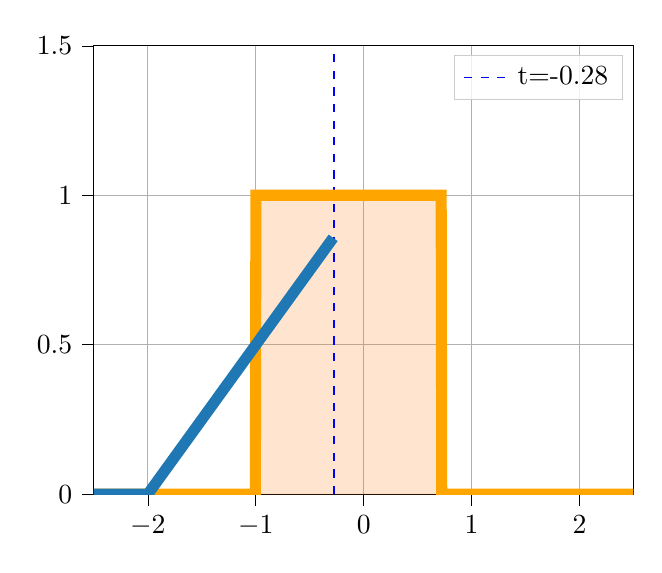
\begin{tikzpicture}

\definecolor{color0}{rgb}{1,0.498039215686275,0.0549019607843137}
\definecolor{color1}{rgb}{1,0.647058823529412,0}
\definecolor{color2}{rgb}{0.12156862745098,0.466666666666667,0.705882352941177}

\begin{axis}[
legend cell align={left},
legend style={fill opacity=0.8, draw opacity=1, text opacity=1, draw=white!80!black},
tick align=outside,
tick pos=left,
x grid style={white!69.0196078431373!black},
xmajorgrids,
xmin=-2.5, xmax=2.5,
xtick style={color=black},
y grid style={white!69.0196078431373!black},
ymajorgrids,
ymin=0, ymax=1.5,
ytick style={color=black}
]
\path [draw=color0, fill=color0, opacity=0.2]
(axis cs:-2.5,0)
--(axis cs:-2.5,0)
--(axis cs:-2.49499499499499,0)
--(axis cs:-2.48998998998999,0)
--(axis cs:-2.48498498498498,0)
--(axis cs:-2.47997997997998,0)
--(axis cs:-2.47497497497497,0)
--(axis cs:-2.46996996996997,0)
--(axis cs:-2.46496496496496,0)
--(axis cs:-2.45995995995996,0)
--(axis cs:-2.45495495495495,0)
--(axis cs:-2.44994994994995,0)
--(axis cs:-2.44494494494494,0)
--(axis cs:-2.43993993993994,0)
--(axis cs:-2.43493493493493,0)
--(axis cs:-2.42992992992993,0)
--(axis cs:-2.42492492492492,0)
--(axis cs:-2.41991991991992,0)
--(axis cs:-2.41491491491491,0)
--(axis cs:-2.40990990990991,0)
--(axis cs:-2.4049049049049,0)
--(axis cs:-2.3998998998999,0)
--(axis cs:-2.39489489489489,0)
--(axis cs:-2.38988988988989,0)
--(axis cs:-2.38488488488488,0)
--(axis cs:-2.37987987987988,0)
--(axis cs:-2.37487487487487,0)
--(axis cs:-2.36986986986987,0)
--(axis cs:-2.36486486486486,0)
--(axis cs:-2.35985985985986,0)
--(axis cs:-2.35485485485485,0)
--(axis cs:-2.34984984984985,0)
--(axis cs:-2.34484484484484,0)
--(axis cs:-2.33983983983984,0)
--(axis cs:-2.33483483483483,0)
--(axis cs:-2.32982982982983,0)
--(axis cs:-2.32482482482482,0)
--(axis cs:-2.31981981981982,0)
--(axis cs:-2.31481481481481,0)
--(axis cs:-2.30980980980981,0)
--(axis cs:-2.3048048048048,0)
--(axis cs:-2.2997997997998,0)
--(axis cs:-2.29479479479479,0)
--(axis cs:-2.28978978978979,0)
--(axis cs:-2.28478478478478,0)
--(axis cs:-2.27977977977978,0)
--(axis cs:-2.27477477477477,0)
--(axis cs:-2.26976976976977,0)
--(axis cs:-2.26476476476476,0)
--(axis cs:-2.25975975975976,0)
--(axis cs:-2.25475475475475,0)
--(axis cs:-2.24974974974975,0)
--(axis cs:-2.24474474474474,0)
--(axis cs:-2.23973973973974,0)
--(axis cs:-2.23473473473473,0)
--(axis cs:-2.22972972972973,0)
--(axis cs:-2.22472472472472,0)
--(axis cs:-2.21971971971972,0)
--(axis cs:-2.21471471471471,0)
--(axis cs:-2.20970970970971,0)
--(axis cs:-2.2047047047047,0)
--(axis cs:-2.1996996996997,0)
--(axis cs:-2.19469469469469,0)
--(axis cs:-2.18968968968969,0)
--(axis cs:-2.18468468468468,0)
--(axis cs:-2.17967967967968,0)
--(axis cs:-2.17467467467467,0)
--(axis cs:-2.16966966966967,0)
--(axis cs:-2.16466466466466,0)
--(axis cs:-2.15965965965966,0)
--(axis cs:-2.15465465465465,0)
--(axis cs:-2.14964964964965,0)
--(axis cs:-2.14464464464464,0)
--(axis cs:-2.13963963963964,0)
--(axis cs:-2.13463463463463,0)
--(axis cs:-2.12962962962963,0)
--(axis cs:-2.12462462462462,0)
--(axis cs:-2.11961961961962,0)
--(axis cs:-2.11461461461461,0)
--(axis cs:-2.10960960960961,0)
--(axis cs:-2.1046046046046,0)
--(axis cs:-2.0995995995996,0)
--(axis cs:-2.09459459459459,0)
--(axis cs:-2.08958958958959,0)
--(axis cs:-2.08458458458458,0)
--(axis cs:-2.07957957957958,0)
--(axis cs:-2.07457457457457,0)
--(axis cs:-2.06956956956957,0)
--(axis cs:-2.06456456456456,0)
--(axis cs:-2.05955955955956,0)
--(axis cs:-2.05455455455455,0)
--(axis cs:-2.04954954954955,0)
--(axis cs:-2.04454454454454,0)
--(axis cs:-2.03953953953954,0)
--(axis cs:-2.03453453453453,0)
--(axis cs:-2.02952952952953,0)
--(axis cs:-2.02452452452452,0)
--(axis cs:-2.01951951951952,0)
--(axis cs:-2.01451451451451,0)
--(axis cs:-2.00950950950951,0)
--(axis cs:-2.0045045045045,0)
--(axis cs:-1.9994994994995,0)
--(axis cs:-1.99449449449449,0)
--(axis cs:-1.98948948948949,0)
--(axis cs:-1.98448448448448,0)
--(axis cs:-1.97947947947948,0)
--(axis cs:-1.97447447447447,0)
--(axis cs:-1.96946946946947,0)
--(axis cs:-1.96446446446446,0)
--(axis cs:-1.95945945945946,0)
--(axis cs:-1.95445445445445,0)
--(axis cs:-1.94944944944945,0)
--(axis cs:-1.94444444444444,0)
--(axis cs:-1.93943943943944,0)
--(axis cs:-1.93443443443443,0)
--(axis cs:-1.92942942942943,0)
--(axis cs:-1.92442442442442,0)
--(axis cs:-1.91941941941942,0)
--(axis cs:-1.91441441441441,0)
--(axis cs:-1.90940940940941,0)
--(axis cs:-1.9044044044044,0)
--(axis cs:-1.8993993993994,0)
--(axis cs:-1.89439439439439,0)
--(axis cs:-1.88938938938939,0)
--(axis cs:-1.88438438438438,0)
--(axis cs:-1.87937937937938,0)
--(axis cs:-1.87437437437437,0)
--(axis cs:-1.86936936936937,0)
--(axis cs:-1.86436436436436,0)
--(axis cs:-1.85935935935936,0)
--(axis cs:-1.85435435435435,0)
--(axis cs:-1.84934934934935,0)
--(axis cs:-1.84434434434434,0)
--(axis cs:-1.83933933933934,0)
--(axis cs:-1.83433433433433,0)
--(axis cs:-1.82932932932933,0)
--(axis cs:-1.82432432432432,0)
--(axis cs:-1.81931931931932,0)
--(axis cs:-1.81431431431431,0)
--(axis cs:-1.80930930930931,0)
--(axis cs:-1.8043043043043,0)
--(axis cs:-1.7992992992993,0)
--(axis cs:-1.79429429429429,0)
--(axis cs:-1.78928928928929,0)
--(axis cs:-1.78428428428428,0)
--(axis cs:-1.77927927927928,0)
--(axis cs:-1.77427427427427,0)
--(axis cs:-1.76926926926927,0)
--(axis cs:-1.76426426426426,0)
--(axis cs:-1.75925925925926,0)
--(axis cs:-1.75425425425425,0)
--(axis cs:-1.74924924924925,0)
--(axis cs:-1.74424424424424,0)
--(axis cs:-1.73923923923924,0)
--(axis cs:-1.73423423423423,0)
--(axis cs:-1.72922922922923,0)
--(axis cs:-1.72422422422422,0)
--(axis cs:-1.71921921921922,0)
--(axis cs:-1.71421421421421,0)
--(axis cs:-1.70920920920921,0)
--(axis cs:-1.7042042042042,0)
--(axis cs:-1.6991991991992,0)
--(axis cs:-1.69419419419419,0)
--(axis cs:-1.68918918918919,0)
--(axis cs:-1.68418418418418,0)
--(axis cs:-1.67917917917918,0)
--(axis cs:-1.67417417417417,0)
--(axis cs:-1.66916916916917,0)
--(axis cs:-1.66416416416416,0)
--(axis cs:-1.65915915915916,0)
--(axis cs:-1.65415415415415,0)
--(axis cs:-1.64914914914915,0)
--(axis cs:-1.64414414414414,0)
--(axis cs:-1.63913913913914,0)
--(axis cs:-1.63413413413413,0)
--(axis cs:-1.62912912912913,0)
--(axis cs:-1.62412412412412,0)
--(axis cs:-1.61911911911912,0)
--(axis cs:-1.61411411411411,0)
--(axis cs:-1.60910910910911,0)
--(axis cs:-1.6041041041041,0)
--(axis cs:-1.5990990990991,0)
--(axis cs:-1.59409409409409,0)
--(axis cs:-1.58908908908909,0)
--(axis cs:-1.58408408408408,0)
--(axis cs:-1.57907907907908,0)
--(axis cs:-1.57407407407407,0)
--(axis cs:-1.56906906906907,0)
--(axis cs:-1.56406406406406,0)
--(axis cs:-1.55905905905906,0)
--(axis cs:-1.55405405405405,0)
--(axis cs:-1.54904904904905,0)
--(axis cs:-1.54404404404404,0)
--(axis cs:-1.53903903903904,0)
--(axis cs:-1.53403403403403,0)
--(axis cs:-1.52902902902903,0)
--(axis cs:-1.52402402402402,0)
--(axis cs:-1.51901901901902,0)
--(axis cs:-1.51401401401401,0)
--(axis cs:-1.50900900900901,0)
--(axis cs:-1.504004004004,0)
--(axis cs:-1.498998998999,0)
--(axis cs:-1.49399399399399,0)
--(axis cs:-1.48898898898899,0)
--(axis cs:-1.48398398398398,0)
--(axis cs:-1.47897897897898,0)
--(axis cs:-1.47397397397397,0)
--(axis cs:-1.46896896896897,0)
--(axis cs:-1.46396396396396,0)
--(axis cs:-1.45895895895896,0)
--(axis cs:-1.45395395395395,0)
--(axis cs:-1.44894894894895,0)
--(axis cs:-1.44394394394394,0)
--(axis cs:-1.43893893893894,0)
--(axis cs:-1.43393393393393,0)
--(axis cs:-1.42892892892893,0)
--(axis cs:-1.42392392392392,0)
--(axis cs:-1.41891891891892,0)
--(axis cs:-1.41391391391391,0)
--(axis cs:-1.40890890890891,0)
--(axis cs:-1.4039039039039,0)
--(axis cs:-1.3988988988989,0)
--(axis cs:-1.39389389389389,0)
--(axis cs:-1.38888888888889,0)
--(axis cs:-1.38388388388388,0)
--(axis cs:-1.37887887887888,0)
--(axis cs:-1.37387387387387,0)
--(axis cs:-1.36886886886887,0)
--(axis cs:-1.36386386386386,0)
--(axis cs:-1.35885885885886,0)
--(axis cs:-1.35385385385385,0)
--(axis cs:-1.34884884884885,0)
--(axis cs:-1.34384384384384,0)
--(axis cs:-1.33883883883884,0)
--(axis cs:-1.33383383383383,0)
--(axis cs:-1.32882882882883,0)
--(axis cs:-1.32382382382382,0)
--(axis cs:-1.31881881881882,0)
--(axis cs:-1.31381381381381,0)
--(axis cs:-1.30880880880881,0)
--(axis cs:-1.3038038038038,0)
--(axis cs:-1.2987987987988,0)
--(axis cs:-1.29379379379379,0)
--(axis cs:-1.28878878878879,0)
--(axis cs:-1.28378378378378,0)
--(axis cs:-1.27877877877878,0)
--(axis cs:-1.27377377377377,0)
--(axis cs:-1.26876876876877,0)
--(axis cs:-1.26376376376376,0)
--(axis cs:-1.25875875875876,0)
--(axis cs:-1.25375375375375,0)
--(axis cs:-1.24874874874875,0)
--(axis cs:-1.24374374374374,0)
--(axis cs:-1.23873873873874,0)
--(axis cs:-1.23373373373373,0)
--(axis cs:-1.22872872872873,0)
--(axis cs:-1.22372372372372,0)
--(axis cs:-1.21871871871872,0)
--(axis cs:-1.21371371371371,0)
--(axis cs:-1.20870870870871,0)
--(axis cs:-1.2037037037037,0)
--(axis cs:-1.1986986986987,0)
--(axis cs:-1.19369369369369,0)
--(axis cs:-1.18868868868869,0)
--(axis cs:-1.18368368368368,0)
--(axis cs:-1.17867867867868,0)
--(axis cs:-1.17367367367367,0)
--(axis cs:-1.16866866866867,0)
--(axis cs:-1.16366366366366,0)
--(axis cs:-1.15865865865866,0)
--(axis cs:-1.15365365365365,0)
--(axis cs:-1.14864864864865,0)
--(axis cs:-1.14364364364364,0)
--(axis cs:-1.13863863863864,0)
--(axis cs:-1.13363363363363,0)
--(axis cs:-1.12862862862863,0)
--(axis cs:-1.12362362362362,0)
--(axis cs:-1.11861861861862,0)
--(axis cs:-1.11361361361361,0)
--(axis cs:-1.10860860860861,0)
--(axis cs:-1.1036036036036,0)
--(axis cs:-1.0985985985986,0)
--(axis cs:-1.09359359359359,0)
--(axis cs:-1.08858858858859,0)
--(axis cs:-1.08358358358358,0)
--(axis cs:-1.07857857857858,0)
--(axis cs:-1.07357357357357,0)
--(axis cs:-1.06856856856857,0)
--(axis cs:-1.06356356356356,0)
--(axis cs:-1.05855855855856,0)
--(axis cs:-1.05355355355355,0)
--(axis cs:-1.04854854854855,0)
--(axis cs:-1.04354354354354,0)
--(axis cs:-1.03853853853854,0)
--(axis cs:-1.03353353353353,0)
--(axis cs:-1.02852852852853,0)
--(axis cs:-1.02352352352352,0)
--(axis cs:-1.01851851851852,0)
--(axis cs:-1.01351351351351,0)
--(axis cs:-1.00850850850851,0)
--(axis cs:-1.0035035035035,0)
--(axis cs:-0.998498498498499,0)
--(axis cs:-0.993493493493494,0)
--(axis cs:-0.988488488488489,0)
--(axis cs:-0.983483483483484,0)
--(axis cs:-0.978478478478479,0)
--(axis cs:-0.973473473473474,0)
--(axis cs:-0.968468468468469,0)
--(axis cs:-0.963463463463464,0)
--(axis cs:-0.958458458458459,0)
--(axis cs:-0.953453453453454,0)
--(axis cs:-0.948448448448449,0)
--(axis cs:-0.943443443443444,0)
--(axis cs:-0.938438438438439,0)
--(axis cs:-0.933433433433434,0)
--(axis cs:-0.928428428428429,0)
--(axis cs:-0.923423423423424,0)
--(axis cs:-0.918418418418419,0)
--(axis cs:-0.913413413413414,0)
--(axis cs:-0.908408408408409,0)
--(axis cs:-0.903403403403404,0)
--(axis cs:-0.898398398398399,0)
--(axis cs:-0.893393393393393,0)
--(axis cs:-0.888388388388388,0)
--(axis cs:-0.883383383383383,0)
--(axis cs:-0.878378378378378,0)
--(axis cs:-0.873373373373373,0)
--(axis cs:-0.868368368368368,0)
--(axis cs:-0.863363363363363,0)
--(axis cs:-0.858358358358358,0)
--(axis cs:-0.853353353353353,0)
--(axis cs:-0.848348348348348,0)
--(axis cs:-0.843343343343343,0)
--(axis cs:-0.838338338338338,0)
--(axis cs:-0.833333333333333,0)
--(axis cs:-0.828328328328328,0)
--(axis cs:-0.823323323323323,0)
--(axis cs:-0.818318318318318,0)
--(axis cs:-0.813313313313313,0)
--(axis cs:-0.808308308308308,0)
--(axis cs:-0.803303303303303,0)
--(axis cs:-0.798298298298298,0)
--(axis cs:-0.793293293293293,0)
--(axis cs:-0.788288288288288,0)
--(axis cs:-0.783283283283283,0)
--(axis cs:-0.778278278278278,0)
--(axis cs:-0.773273273273273,0)
--(axis cs:-0.768268268268268,0)
--(axis cs:-0.763263263263263,0)
--(axis cs:-0.758258258258258,0)
--(axis cs:-0.753253253253253,0)
--(axis cs:-0.748248248248248,0)
--(axis cs:-0.743243243243243,0)
--(axis cs:-0.738238238238238,0)
--(axis cs:-0.733233233233233,0)
--(axis cs:-0.728228228228228,0)
--(axis cs:-0.723223223223223,0)
--(axis cs:-0.718218218218218,0)
--(axis cs:-0.713213213213213,0)
--(axis cs:-0.708208208208208,0)
--(axis cs:-0.703203203203203,0)
--(axis cs:-0.698198198198198,0)
--(axis cs:-0.693193193193193,0)
--(axis cs:-0.688188188188188,0)
--(axis cs:-0.683183183183183,0)
--(axis cs:-0.678178178178178,0)
--(axis cs:-0.673173173173173,0)
--(axis cs:-0.668168168168168,0)
--(axis cs:-0.663163163163163,0)
--(axis cs:-0.658158158158158,0)
--(axis cs:-0.653153153153153,0)
--(axis cs:-0.648148148148148,0)
--(axis cs:-0.643143143143143,0)
--(axis cs:-0.638138138138138,0)
--(axis cs:-0.633133133133133,0)
--(axis cs:-0.628128128128128,0)
--(axis cs:-0.623123123123123,0)
--(axis cs:-0.618118118118118,0)
--(axis cs:-0.613113113113113,0)
--(axis cs:-0.608108108108108,0)
--(axis cs:-0.603103103103103,0)
--(axis cs:-0.598098098098098,0)
--(axis cs:-0.593093093093093,0)
--(axis cs:-0.588088088088088,0)
--(axis cs:-0.583083083083083,0)
--(axis cs:-0.578078078078078,0)
--(axis cs:-0.573073073073073,0)
--(axis cs:-0.568068068068068,0)
--(axis cs:-0.563063063063063,0)
--(axis cs:-0.558058058058058,0)
--(axis cs:-0.553053053053053,0)
--(axis cs:-0.548048048048048,0)
--(axis cs:-0.543043043043043,0)
--(axis cs:-0.538038038038038,0)
--(axis cs:-0.533033033033033,0)
--(axis cs:-0.528028028028028,0)
--(axis cs:-0.523023023023023,0)
--(axis cs:-0.518018018018018,0)
--(axis cs:-0.513013013013013,0)
--(axis cs:-0.508008008008008,0)
--(axis cs:-0.503003003003003,0)
--(axis cs:-0.497997997997998,0)
--(axis cs:-0.492992992992993,0)
--(axis cs:-0.487987987987988,0)
--(axis cs:-0.482982982982983,0)
--(axis cs:-0.477977977977978,0)
--(axis cs:-0.472972972972973,0)
--(axis cs:-0.467967967967968,0)
--(axis cs:-0.462962962962963,0)
--(axis cs:-0.457957957957958,0)
--(axis cs:-0.452952952952953,0)
--(axis cs:-0.447947947947948,0)
--(axis cs:-0.442942942942943,0)
--(axis cs:-0.437937937937938,0)
--(axis cs:-0.432932932932933,0)
--(axis cs:-0.427927927927928,0)
--(axis cs:-0.422922922922923,0)
--(axis cs:-0.417917917917918,0)
--(axis cs:-0.412912912912913,0)
--(axis cs:-0.407907907907908,0)
--(axis cs:-0.402902902902903,0)
--(axis cs:-0.397897897897898,0)
--(axis cs:-0.392892892892893,0)
--(axis cs:-0.387887887887888,0)
--(axis cs:-0.382882882882883,0)
--(axis cs:-0.377877877877878,0)
--(axis cs:-0.372872872872873,0)
--(axis cs:-0.367867867867868,0)
--(axis cs:-0.362862862862863,0)
--(axis cs:-0.357857857857858,0)
--(axis cs:-0.352852852852853,0)
--(axis cs:-0.347847847847848,0)
--(axis cs:-0.342842842842843,0)
--(axis cs:-0.337837837837838,0)
--(axis cs:-0.332832832832833,0)
--(axis cs:-0.327827827827828,0)
--(axis cs:-0.322822822822823,0)
--(axis cs:-0.317817817817818,0)
--(axis cs:-0.312812812812813,0)
--(axis cs:-0.307807807807808,0)
--(axis cs:-0.302802802802803,0)
--(axis cs:-0.297797797797798,0)
--(axis cs:-0.292792792792793,0)
--(axis cs:-0.287787787787788,0)
--(axis cs:-0.282782782782783,0)
--(axis cs:-0.277777777777778,0)
--(axis cs:-0.272772772772773,0)
--(axis cs:-0.267767767767768,0)
--(axis cs:-0.262762762762763,0)
--(axis cs:-0.257757757757758,0)
--(axis cs:-0.252752752752753,0)
--(axis cs:-0.247747747747748,0)
--(axis cs:-0.242742742742743,0)
--(axis cs:-0.237737737737738,0)
--(axis cs:-0.232732732732733,0)
--(axis cs:-0.227727727727728,0)
--(axis cs:-0.222722722722723,0)
--(axis cs:-0.217717717717718,0)
--(axis cs:-0.212712712712713,0)
--(axis cs:-0.207707707707708,0)
--(axis cs:-0.202702702702703,0)
--(axis cs:-0.197697697697698,0)
--(axis cs:-0.192692692692693,0)
--(axis cs:-0.187687687687688,0)
--(axis cs:-0.182682682682683,0)
--(axis cs:-0.177677677677678,0)
--(axis cs:-0.172672672672673,0)
--(axis cs:-0.167667667667668,0)
--(axis cs:-0.162662662662663,0)
--(axis cs:-0.157657657657658,0)
--(axis cs:-0.152652652652653,0)
--(axis cs:-0.147647647647648,0)
--(axis cs:-0.142642642642643,0)
--(axis cs:-0.137637637637638,0)
--(axis cs:-0.132632632632633,0)
--(axis cs:-0.127627627627628,0)
--(axis cs:-0.122622622622623,0)
--(axis cs:-0.117617617617618,0)
--(axis cs:-0.112612612612613,0)
--(axis cs:-0.107607607607608,0)
--(axis cs:-0.102602602602603,0)
--(axis cs:-0.0975975975975976,0)
--(axis cs:-0.0925925925925926,0)
--(axis cs:-0.0875875875875876,0)
--(axis cs:-0.0825825825825826,0)
--(axis cs:-0.0775775775775776,0)
--(axis cs:-0.0725725725725725,0)
--(axis cs:-0.0675675675675675,0)
--(axis cs:-0.0625625625625625,0)
--(axis cs:-0.0575575575575575,0)
--(axis cs:-0.0525525525525525,0)
--(axis cs:-0.0475475475475475,0)
--(axis cs:-0.0425425425425425,0)
--(axis cs:-0.0375375375375375,0)
--(axis cs:-0.0325325325325325,0)
--(axis cs:-0.0275275275275275,0)
--(axis cs:-0.0225225225225225,0)
--(axis cs:-0.0175175175175175,0)
--(axis cs:-0.0125125125125125,0)
--(axis cs:-0.0075075075075075,0)
--(axis cs:-0.0025025025025025,0)
--(axis cs:0.0025025025025025,0)
--(axis cs:0.0075075075075075,0)
--(axis cs:0.0125125125125125,0)
--(axis cs:0.0175175175175175,0)
--(axis cs:0.0225225225225225,0)
--(axis cs:0.0275275275275275,0)
--(axis cs:0.0325325325325325,0)
--(axis cs:0.0375375375375375,0)
--(axis cs:0.0425425425425425,0)
--(axis cs:0.0475475475475475,0)
--(axis cs:0.0525525525525525,0)
--(axis cs:0.0575575575575575,0)
--(axis cs:0.0625625625625625,0)
--(axis cs:0.0675675675675675,0)
--(axis cs:0.0725725725725725,0)
--(axis cs:0.0775775775775776,0)
--(axis cs:0.0825825825825826,0)
--(axis cs:0.0875875875875876,0)
--(axis cs:0.0925925925925926,0)
--(axis cs:0.0975975975975976,0)
--(axis cs:0.102602602602603,0)
--(axis cs:0.107607607607608,0)
--(axis cs:0.112612612612613,0)
--(axis cs:0.117617617617618,0)
--(axis cs:0.122622622622623,0)
--(axis cs:0.127627627627628,0)
--(axis cs:0.132632632632633,0)
--(axis cs:0.137637637637638,0)
--(axis cs:0.142642642642643,0)
--(axis cs:0.147647647647648,0)
--(axis cs:0.152652652652653,0)
--(axis cs:0.157657657657658,0)
--(axis cs:0.162662662662663,0)
--(axis cs:0.167667667667668,0)
--(axis cs:0.172672672672673,0)
--(axis cs:0.177677677677678,0)
--(axis cs:0.182682682682683,0)
--(axis cs:0.187687687687688,0)
--(axis cs:0.192692692692693,0)
--(axis cs:0.197697697697698,0)
--(axis cs:0.202702702702703,0)
--(axis cs:0.207707707707708,0)
--(axis cs:0.212712712712713,0)
--(axis cs:0.217717717717718,0)
--(axis cs:0.222722722722723,0)
--(axis cs:0.227727727727728,0)
--(axis cs:0.232732732732733,0)
--(axis cs:0.237737737737738,0)
--(axis cs:0.242742742742743,0)
--(axis cs:0.247747747747748,0)
--(axis cs:0.252752752752753,0)
--(axis cs:0.257757757757758,0)
--(axis cs:0.262762762762763,0)
--(axis cs:0.267767767767768,0)
--(axis cs:0.272772772772773,0)
--(axis cs:0.277777777777778,0)
--(axis cs:0.282782782782783,0)
--(axis cs:0.287787787787788,0)
--(axis cs:0.292792792792793,0)
--(axis cs:0.297797797797798,0)
--(axis cs:0.302802802802803,0)
--(axis cs:0.307807807807808,0)
--(axis cs:0.312812812812813,0)
--(axis cs:0.317817817817818,0)
--(axis cs:0.322822822822823,0)
--(axis cs:0.327827827827828,0)
--(axis cs:0.332832832832833,0)
--(axis cs:0.337837837837838,0)
--(axis cs:0.342842842842843,0)
--(axis cs:0.347847847847848,0)
--(axis cs:0.352852852852853,0)
--(axis cs:0.357857857857858,0)
--(axis cs:0.362862862862863,0)
--(axis cs:0.367867867867868,0)
--(axis cs:0.372872872872873,0)
--(axis cs:0.377877877877878,0)
--(axis cs:0.382882882882883,0)
--(axis cs:0.387887887887888,0)
--(axis cs:0.392892892892893,0)
--(axis cs:0.397897897897898,0)
--(axis cs:0.402902902902903,0)
--(axis cs:0.407907907907908,0)
--(axis cs:0.412912912912913,0)
--(axis cs:0.417917917917918,0)
--(axis cs:0.422922922922923,0)
--(axis cs:0.427927927927928,0)
--(axis cs:0.432932932932933,0)
--(axis cs:0.437937937937938,0)
--(axis cs:0.442942942942943,0)
--(axis cs:0.447947947947948,0)
--(axis cs:0.452952952952953,0)
--(axis cs:0.457957957957958,0)
--(axis cs:0.462962962962963,0)
--(axis cs:0.467967967967968,0)
--(axis cs:0.472972972972973,0)
--(axis cs:0.477977977977978,0)
--(axis cs:0.482982982982983,0)
--(axis cs:0.487987987987988,0)
--(axis cs:0.492992992992993,0)
--(axis cs:0.497997997997998,0)
--(axis cs:0.503003003003003,0)
--(axis cs:0.508008008008008,0)
--(axis cs:0.513013013013013,0)
--(axis cs:0.518018018018018,0)
--(axis cs:0.523023023023023,0)
--(axis cs:0.528028028028028,0)
--(axis cs:0.533033033033033,0)
--(axis cs:0.538038038038038,0)
--(axis cs:0.543043043043043,0)
--(axis cs:0.548048048048048,0)
--(axis cs:0.553053053053053,0)
--(axis cs:0.558058058058058,0)
--(axis cs:0.563063063063063,0)
--(axis cs:0.568068068068068,0)
--(axis cs:0.573073073073073,0)
--(axis cs:0.578078078078078,0)
--(axis cs:0.583083083083083,0)
--(axis cs:0.588088088088088,0)
--(axis cs:0.593093093093093,0)
--(axis cs:0.598098098098098,0)
--(axis cs:0.603103103103103,0)
--(axis cs:0.608108108108108,0)
--(axis cs:0.613113113113113,0)
--(axis cs:0.618118118118118,0)
--(axis cs:0.623123123123123,0)
--(axis cs:0.628128128128128,0)
--(axis cs:0.633133133133133,0)
--(axis cs:0.638138138138138,0)
--(axis cs:0.643143143143143,0)
--(axis cs:0.648148148148148,0)
--(axis cs:0.653153153153153,0)
--(axis cs:0.658158158158158,0)
--(axis cs:0.663163163163163,0)
--(axis cs:0.668168168168168,0)
--(axis cs:0.673173173173173,0)
--(axis cs:0.678178178178178,0)
--(axis cs:0.683183183183183,0)
--(axis cs:0.688188188188188,0)
--(axis cs:0.693193193193193,0)
--(axis cs:0.698198198198198,0)
--(axis cs:0.703203203203203,0)
--(axis cs:0.708208208208208,0)
--(axis cs:0.713213213213213,0)
--(axis cs:0.718218218218218,0)
--(axis cs:0.723223223223223,0)
--(axis cs:0.728228228228228,0)
--(axis cs:0.733233233233233,0)
--(axis cs:0.738238238238238,0)
--(axis cs:0.743243243243243,0)
--(axis cs:0.748248248248248,0)
--(axis cs:0.753253253253253,0)
--(axis cs:0.758258258258258,0)
--(axis cs:0.763263263263263,0)
--(axis cs:0.768268268268268,0)
--(axis cs:0.773273273273273,0)
--(axis cs:0.778278278278278,0)
--(axis cs:0.783283283283283,0)
--(axis cs:0.788288288288288,0)
--(axis cs:0.793293293293293,0)
--(axis cs:0.798298298298298,0)
--(axis cs:0.803303303303303,0)
--(axis cs:0.808308308308308,0)
--(axis cs:0.813313313313313,0)
--(axis cs:0.818318318318318,0)
--(axis cs:0.823323323323323,0)
--(axis cs:0.828328328328328,0)
--(axis cs:0.833333333333333,0)
--(axis cs:0.838338338338338,0)
--(axis cs:0.843343343343343,0)
--(axis cs:0.848348348348348,0)
--(axis cs:0.853353353353353,0)
--(axis cs:0.858358358358358,0)
--(axis cs:0.863363363363364,0)
--(axis cs:0.868368368368369,0)
--(axis cs:0.873373373373374,0)
--(axis cs:0.878378378378379,0)
--(axis cs:0.883383383383384,0)
--(axis cs:0.888388388388389,0)
--(axis cs:0.893393393393394,0)
--(axis cs:0.898398398398399,0)
--(axis cs:0.903403403403404,0)
--(axis cs:0.908408408408409,0)
--(axis cs:0.913413413413414,0)
--(axis cs:0.918418418418419,0)
--(axis cs:0.923423423423424,0)
--(axis cs:0.928428428428429,0)
--(axis cs:0.933433433433434,0)
--(axis cs:0.938438438438439,0)
--(axis cs:0.943443443443444,0)
--(axis cs:0.948448448448449,0)
--(axis cs:0.953453453453454,0)
--(axis cs:0.958458458458459,0)
--(axis cs:0.963463463463464,0)
--(axis cs:0.968468468468469,0)
--(axis cs:0.973473473473474,0)
--(axis cs:0.978478478478479,0)
--(axis cs:0.983483483483484,0)
--(axis cs:0.988488488488489,0)
--(axis cs:0.993493493493494,0)
--(axis cs:0.998498498498499,0)
--(axis cs:1.0035035035035,0)
--(axis cs:1.00850850850851,0)
--(axis cs:1.01351351351351,0)
--(axis cs:1.01851851851852,0)
--(axis cs:1.02352352352352,0)
--(axis cs:1.02852852852853,0)
--(axis cs:1.03353353353353,0)
--(axis cs:1.03853853853854,0)
--(axis cs:1.04354354354354,0)
--(axis cs:1.04854854854855,0)
--(axis cs:1.05355355355355,0)
--(axis cs:1.05855855855856,0)
--(axis cs:1.06356356356356,0)
--(axis cs:1.06856856856857,0)
--(axis cs:1.07357357357357,0)
--(axis cs:1.07857857857858,0)
--(axis cs:1.08358358358358,0)
--(axis cs:1.08858858858859,0)
--(axis cs:1.09359359359359,0)
--(axis cs:1.0985985985986,0)
--(axis cs:1.1036036036036,0)
--(axis cs:1.10860860860861,0)
--(axis cs:1.11361361361361,0)
--(axis cs:1.11861861861862,0)
--(axis cs:1.12362362362362,0)
--(axis cs:1.12862862862863,0)
--(axis cs:1.13363363363363,0)
--(axis cs:1.13863863863864,0)
--(axis cs:1.14364364364364,0)
--(axis cs:1.14864864864865,0)
--(axis cs:1.15365365365365,0)
--(axis cs:1.15865865865866,0)
--(axis cs:1.16366366366366,0)
--(axis cs:1.16866866866867,0)
--(axis cs:1.17367367367367,0)
--(axis cs:1.17867867867868,0)
--(axis cs:1.18368368368368,0)
--(axis cs:1.18868868868869,0)
--(axis cs:1.19369369369369,0)
--(axis cs:1.1986986986987,0)
--(axis cs:1.2037037037037,0)
--(axis cs:1.20870870870871,0)
--(axis cs:1.21371371371371,0)
--(axis cs:1.21871871871872,0)
--(axis cs:1.22372372372372,0)
--(axis cs:1.22872872872873,0)
--(axis cs:1.23373373373373,0)
--(axis cs:1.23873873873874,0)
--(axis cs:1.24374374374374,0)
--(axis cs:1.24874874874875,0)
--(axis cs:1.25375375375375,0)
--(axis cs:1.25875875875876,0)
--(axis cs:1.26376376376376,0)
--(axis cs:1.26876876876877,0)
--(axis cs:1.27377377377377,0)
--(axis cs:1.27877877877878,0)
--(axis cs:1.28378378378378,0)
--(axis cs:1.28878878878879,0)
--(axis cs:1.29379379379379,0)
--(axis cs:1.2987987987988,0)
--(axis cs:1.3038038038038,0)
--(axis cs:1.30880880880881,0)
--(axis cs:1.31381381381381,0)
--(axis cs:1.31881881881882,0)
--(axis cs:1.32382382382382,0)
--(axis cs:1.32882882882883,0)
--(axis cs:1.33383383383383,0)
--(axis cs:1.33883883883884,0)
--(axis cs:1.34384384384384,0)
--(axis cs:1.34884884884885,0)
--(axis cs:1.35385385385385,0)
--(axis cs:1.35885885885886,0)
--(axis cs:1.36386386386386,0)
--(axis cs:1.36886886886887,0)
--(axis cs:1.37387387387387,0)
--(axis cs:1.37887887887888,0)
--(axis cs:1.38388388388388,0)
--(axis cs:1.38888888888889,0)
--(axis cs:1.39389389389389,0)
--(axis cs:1.3988988988989,0)
--(axis cs:1.4039039039039,0)
--(axis cs:1.40890890890891,0)
--(axis cs:1.41391391391391,0)
--(axis cs:1.41891891891892,0)
--(axis cs:1.42392392392392,0)
--(axis cs:1.42892892892893,0)
--(axis cs:1.43393393393393,0)
--(axis cs:1.43893893893894,0)
--(axis cs:1.44394394394394,0)
--(axis cs:1.44894894894895,0)
--(axis cs:1.45395395395395,0)
--(axis cs:1.45895895895896,0)
--(axis cs:1.46396396396396,0)
--(axis cs:1.46896896896897,0)
--(axis cs:1.47397397397397,0)
--(axis cs:1.47897897897898,0)
--(axis cs:1.48398398398398,0)
--(axis cs:1.48898898898899,0)
--(axis cs:1.49399399399399,0)
--(axis cs:1.498998998999,0)
--(axis cs:1.504004004004,0)
--(axis cs:1.50900900900901,0)
--(axis cs:1.51401401401401,0)
--(axis cs:1.51901901901902,0)
--(axis cs:1.52402402402402,0)
--(axis cs:1.52902902902903,0)
--(axis cs:1.53403403403403,0)
--(axis cs:1.53903903903904,0)
--(axis cs:1.54404404404404,0)
--(axis cs:1.54904904904905,0)
--(axis cs:1.55405405405405,0)
--(axis cs:1.55905905905906,0)
--(axis cs:1.56406406406406,0)
--(axis cs:1.56906906906907,0)
--(axis cs:1.57407407407407,0)
--(axis cs:1.57907907907908,0)
--(axis cs:1.58408408408408,0)
--(axis cs:1.58908908908909,0)
--(axis cs:1.59409409409409,0)
--(axis cs:1.5990990990991,0)
--(axis cs:1.6041041041041,0)
--(axis cs:1.60910910910911,0)
--(axis cs:1.61411411411411,0)
--(axis cs:1.61911911911912,0)
--(axis cs:1.62412412412412,0)
--(axis cs:1.62912912912913,0)
--(axis cs:1.63413413413413,0)
--(axis cs:1.63913913913914,0)
--(axis cs:1.64414414414414,0)
--(axis cs:1.64914914914915,0)
--(axis cs:1.65415415415415,0)
--(axis cs:1.65915915915916,0)
--(axis cs:1.66416416416416,0)
--(axis cs:1.66916916916917,0)
--(axis cs:1.67417417417417,0)
--(axis cs:1.67917917917918,0)
--(axis cs:1.68418418418418,0)
--(axis cs:1.68918918918919,0)
--(axis cs:1.69419419419419,0)
--(axis cs:1.6991991991992,0)
--(axis cs:1.7042042042042,0)
--(axis cs:1.70920920920921,0)
--(axis cs:1.71421421421421,0)
--(axis cs:1.71921921921922,0)
--(axis cs:1.72422422422422,0)
--(axis cs:1.72922922922923,0)
--(axis cs:1.73423423423423,0)
--(axis cs:1.73923923923924,0)
--(axis cs:1.74424424424424,0)
--(axis cs:1.74924924924925,0)
--(axis cs:1.75425425425425,0)
--(axis cs:1.75925925925926,0)
--(axis cs:1.76426426426426,0)
--(axis cs:1.76926926926927,0)
--(axis cs:1.77427427427427,0)
--(axis cs:1.77927927927928,0)
--(axis cs:1.78428428428428,0)
--(axis cs:1.78928928928929,0)
--(axis cs:1.79429429429429,0)
--(axis cs:1.7992992992993,0)
--(axis cs:1.8043043043043,0)
--(axis cs:1.80930930930931,0)
--(axis cs:1.81431431431431,0)
--(axis cs:1.81931931931932,0)
--(axis cs:1.82432432432432,0)
--(axis cs:1.82932932932933,0)
--(axis cs:1.83433433433433,0)
--(axis cs:1.83933933933934,0)
--(axis cs:1.84434434434434,0)
--(axis cs:1.84934934934935,0)
--(axis cs:1.85435435435435,0)
--(axis cs:1.85935935935936,0)
--(axis cs:1.86436436436436,0)
--(axis cs:1.86936936936937,0)
--(axis cs:1.87437437437437,0)
--(axis cs:1.87937937937938,0)
--(axis cs:1.88438438438438,0)
--(axis cs:1.88938938938939,0)
--(axis cs:1.89439439439439,0)
--(axis cs:1.8993993993994,0)
--(axis cs:1.9044044044044,0)
--(axis cs:1.90940940940941,0)
--(axis cs:1.91441441441441,0)
--(axis cs:1.91941941941942,0)
--(axis cs:1.92442442442442,0)
--(axis cs:1.92942942942943,0)
--(axis cs:1.93443443443443,0)
--(axis cs:1.93943943943944,0)
--(axis cs:1.94444444444444,0)
--(axis cs:1.94944944944945,0)
--(axis cs:1.95445445445445,0)
--(axis cs:1.95945945945946,0)
--(axis cs:1.96446446446446,0)
--(axis cs:1.96946946946947,0)
--(axis cs:1.97447447447447,0)
--(axis cs:1.97947947947948,0)
--(axis cs:1.98448448448448,0)
--(axis cs:1.98948948948949,0)
--(axis cs:1.99449449449449,0)
--(axis cs:1.9994994994995,0)
--(axis cs:2.0045045045045,0)
--(axis cs:2.00950950950951,0)
--(axis cs:2.01451451451451,0)
--(axis cs:2.01951951951952,0)
--(axis cs:2.02452452452452,0)
--(axis cs:2.02952952952953,0)
--(axis cs:2.03453453453453,0)
--(axis cs:2.03953953953954,0)
--(axis cs:2.04454454454454,0)
--(axis cs:2.04954954954955,0)
--(axis cs:2.05455455455455,0)
--(axis cs:2.05955955955956,0)
--(axis cs:2.06456456456456,0)
--(axis cs:2.06956956956957,0)
--(axis cs:2.07457457457457,0)
--(axis cs:2.07957957957958,0)
--(axis cs:2.08458458458458,0)
--(axis cs:2.08958958958959,0)
--(axis cs:2.09459459459459,0)
--(axis cs:2.0995995995996,0)
--(axis cs:2.1046046046046,0)
--(axis cs:2.10960960960961,0)
--(axis cs:2.11461461461461,0)
--(axis cs:2.11961961961962,0)
--(axis cs:2.12462462462462,0)
--(axis cs:2.12962962962963,0)
--(axis cs:2.13463463463463,0)
--(axis cs:2.13963963963964,0)
--(axis cs:2.14464464464464,0)
--(axis cs:2.14964964964965,0)
--(axis cs:2.15465465465465,0)
--(axis cs:2.15965965965966,0)
--(axis cs:2.16466466466466,0)
--(axis cs:2.16966966966967,0)
--(axis cs:2.17467467467467,0)
--(axis cs:2.17967967967968,0)
--(axis cs:2.18468468468468,0)
--(axis cs:2.18968968968969,0)
--(axis cs:2.19469469469469,0)
--(axis cs:2.1996996996997,0)
--(axis cs:2.2047047047047,0)
--(axis cs:2.20970970970971,0)
--(axis cs:2.21471471471471,0)
--(axis cs:2.21971971971972,0)
--(axis cs:2.22472472472472,0)
--(axis cs:2.22972972972973,0)
--(axis cs:2.23473473473473,0)
--(axis cs:2.23973973973974,0)
--(axis cs:2.24474474474474,0)
--(axis cs:2.24974974974975,0)
--(axis cs:2.25475475475475,0)
--(axis cs:2.25975975975976,0)
--(axis cs:2.26476476476476,0)
--(axis cs:2.26976976976977,0)
--(axis cs:2.27477477477477,0)
--(axis cs:2.27977977977978,0)
--(axis cs:2.28478478478478,0)
--(axis cs:2.28978978978979,0)
--(axis cs:2.29479479479479,0)
--(axis cs:2.2997997997998,0)
--(axis cs:2.3048048048048,0)
--(axis cs:2.30980980980981,0)
--(axis cs:2.31481481481481,0)
--(axis cs:2.31981981981982,0)
--(axis cs:2.32482482482482,0)
--(axis cs:2.32982982982983,0)
--(axis cs:2.33483483483483,0)
--(axis cs:2.33983983983984,0)
--(axis cs:2.34484484484484,0)
--(axis cs:2.34984984984985,0)
--(axis cs:2.35485485485485,0)
--(axis cs:2.35985985985986,0)
--(axis cs:2.36486486486486,0)
--(axis cs:2.36986986986987,0)
--(axis cs:2.37487487487487,0)
--(axis cs:2.37987987987988,0)
--(axis cs:2.38488488488488,0)
--(axis cs:2.38988988988989,0)
--(axis cs:2.39489489489489,0)
--(axis cs:2.3998998998999,0)
--(axis cs:2.4049049049049,0)
--(axis cs:2.40990990990991,0)
--(axis cs:2.41491491491491,0)
--(axis cs:2.41991991991992,0)
--(axis cs:2.42492492492492,0)
--(axis cs:2.42992992992993,0)
--(axis cs:2.43493493493493,0)
--(axis cs:2.43993993993994,0)
--(axis cs:2.44494494494494,0)
--(axis cs:2.44994994994995,0)
--(axis cs:2.45495495495495,0)
--(axis cs:2.45995995995996,0)
--(axis cs:2.46496496496496,0)
--(axis cs:2.46996996996997,0)
--(axis cs:2.47497497497497,0)
--(axis cs:2.47997997997998,0)
--(axis cs:2.48498498498498,0)
--(axis cs:2.48998998998999,0)
--(axis cs:2.49499499499499,0)
--(axis cs:2.5,0)
--(axis cs:2.5,0)
--(axis cs:2.5,0)
--(axis cs:2.49499499499499,0)
--(axis cs:2.48998998998999,0)
--(axis cs:2.48498498498498,0)
--(axis cs:2.47997997997998,0)
--(axis cs:2.47497497497497,0)
--(axis cs:2.46996996996997,0)
--(axis cs:2.46496496496496,0)
--(axis cs:2.45995995995996,0)
--(axis cs:2.45495495495495,0)
--(axis cs:2.44994994994995,0)
--(axis cs:2.44494494494494,0)
--(axis cs:2.43993993993994,0)
--(axis cs:2.43493493493493,0)
--(axis cs:2.42992992992993,0)
--(axis cs:2.42492492492492,0)
--(axis cs:2.41991991991992,0)
--(axis cs:2.41491491491491,0)
--(axis cs:2.40990990990991,0)
--(axis cs:2.4049049049049,0)
--(axis cs:2.3998998998999,0)
--(axis cs:2.39489489489489,0)
--(axis cs:2.38988988988989,0)
--(axis cs:2.38488488488488,0)
--(axis cs:2.37987987987988,0)
--(axis cs:2.37487487487487,0)
--(axis cs:2.36986986986987,0)
--(axis cs:2.36486486486486,0)
--(axis cs:2.35985985985986,0)
--(axis cs:2.35485485485485,0)
--(axis cs:2.34984984984985,0)
--(axis cs:2.34484484484484,0)
--(axis cs:2.33983983983984,0)
--(axis cs:2.33483483483483,0)
--(axis cs:2.32982982982983,0)
--(axis cs:2.32482482482482,0)
--(axis cs:2.31981981981982,0)
--(axis cs:2.31481481481481,0)
--(axis cs:2.30980980980981,0)
--(axis cs:2.3048048048048,0)
--(axis cs:2.2997997997998,0)
--(axis cs:2.29479479479479,0)
--(axis cs:2.28978978978979,0)
--(axis cs:2.28478478478478,0)
--(axis cs:2.27977977977978,0)
--(axis cs:2.27477477477477,0)
--(axis cs:2.26976976976977,0)
--(axis cs:2.26476476476476,0)
--(axis cs:2.25975975975976,0)
--(axis cs:2.25475475475475,0)
--(axis cs:2.24974974974975,0)
--(axis cs:2.24474474474474,0)
--(axis cs:2.23973973973974,0)
--(axis cs:2.23473473473473,0)
--(axis cs:2.22972972972973,0)
--(axis cs:2.22472472472472,0)
--(axis cs:2.21971971971972,0)
--(axis cs:2.21471471471471,0)
--(axis cs:2.20970970970971,0)
--(axis cs:2.2047047047047,0)
--(axis cs:2.1996996996997,0)
--(axis cs:2.19469469469469,0)
--(axis cs:2.18968968968969,0)
--(axis cs:2.18468468468468,0)
--(axis cs:2.17967967967968,0)
--(axis cs:2.17467467467467,0)
--(axis cs:2.16966966966967,0)
--(axis cs:2.16466466466466,0)
--(axis cs:2.15965965965966,0)
--(axis cs:2.15465465465465,0)
--(axis cs:2.14964964964965,0)
--(axis cs:2.14464464464464,0)
--(axis cs:2.13963963963964,0)
--(axis cs:2.13463463463463,0)
--(axis cs:2.12962962962963,0)
--(axis cs:2.12462462462462,0)
--(axis cs:2.11961961961962,0)
--(axis cs:2.11461461461461,0)
--(axis cs:2.10960960960961,0)
--(axis cs:2.1046046046046,0)
--(axis cs:2.0995995995996,0)
--(axis cs:2.09459459459459,0)
--(axis cs:2.08958958958959,0)
--(axis cs:2.08458458458458,0)
--(axis cs:2.07957957957958,0)
--(axis cs:2.07457457457457,0)
--(axis cs:2.06956956956957,0)
--(axis cs:2.06456456456456,0)
--(axis cs:2.05955955955956,0)
--(axis cs:2.05455455455455,0)
--(axis cs:2.04954954954955,0)
--(axis cs:2.04454454454454,0)
--(axis cs:2.03953953953954,0)
--(axis cs:2.03453453453453,0)
--(axis cs:2.02952952952953,0)
--(axis cs:2.02452452452452,0)
--(axis cs:2.01951951951952,0)
--(axis cs:2.01451451451451,0)
--(axis cs:2.00950950950951,0)
--(axis cs:2.0045045045045,0)
--(axis cs:1.9994994994995,0)
--(axis cs:1.99449449449449,0)
--(axis cs:1.98948948948949,0)
--(axis cs:1.98448448448448,0)
--(axis cs:1.97947947947948,0)
--(axis cs:1.97447447447447,0)
--(axis cs:1.96946946946947,0)
--(axis cs:1.96446446446446,0)
--(axis cs:1.95945945945946,0)
--(axis cs:1.95445445445445,0)
--(axis cs:1.94944944944945,0)
--(axis cs:1.94444444444444,0)
--(axis cs:1.93943943943944,0)
--(axis cs:1.93443443443443,0)
--(axis cs:1.92942942942943,0)
--(axis cs:1.92442442442442,0)
--(axis cs:1.91941941941942,0)
--(axis cs:1.91441441441441,0)
--(axis cs:1.90940940940941,0)
--(axis cs:1.9044044044044,0)
--(axis cs:1.8993993993994,0)
--(axis cs:1.89439439439439,0)
--(axis cs:1.88938938938939,0)
--(axis cs:1.88438438438438,0)
--(axis cs:1.87937937937938,0)
--(axis cs:1.87437437437437,0)
--(axis cs:1.86936936936937,0)
--(axis cs:1.86436436436436,0)
--(axis cs:1.85935935935936,0)
--(axis cs:1.85435435435435,0)
--(axis cs:1.84934934934935,0)
--(axis cs:1.84434434434434,0)
--(axis cs:1.83933933933934,0)
--(axis cs:1.83433433433433,0)
--(axis cs:1.82932932932933,0)
--(axis cs:1.82432432432432,0)
--(axis cs:1.81931931931932,0)
--(axis cs:1.81431431431431,0)
--(axis cs:1.80930930930931,0)
--(axis cs:1.8043043043043,0)
--(axis cs:1.7992992992993,0)
--(axis cs:1.79429429429429,0)
--(axis cs:1.78928928928929,0)
--(axis cs:1.78428428428428,0)
--(axis cs:1.77927927927928,0)
--(axis cs:1.77427427427427,0)
--(axis cs:1.76926926926927,0)
--(axis cs:1.76426426426426,0)
--(axis cs:1.75925925925926,0)
--(axis cs:1.75425425425425,0)
--(axis cs:1.74924924924925,0)
--(axis cs:1.74424424424424,0)
--(axis cs:1.73923923923924,0)
--(axis cs:1.73423423423423,0)
--(axis cs:1.72922922922923,0)
--(axis cs:1.72422422422422,0)
--(axis cs:1.71921921921922,0)
--(axis cs:1.71421421421421,0)
--(axis cs:1.70920920920921,0)
--(axis cs:1.7042042042042,0)
--(axis cs:1.6991991991992,0)
--(axis cs:1.69419419419419,0)
--(axis cs:1.68918918918919,0)
--(axis cs:1.68418418418418,0)
--(axis cs:1.67917917917918,0)
--(axis cs:1.67417417417417,0)
--(axis cs:1.66916916916917,0)
--(axis cs:1.66416416416416,0)
--(axis cs:1.65915915915916,0)
--(axis cs:1.65415415415415,0)
--(axis cs:1.64914914914915,0)
--(axis cs:1.64414414414414,0)
--(axis cs:1.63913913913914,0)
--(axis cs:1.63413413413413,0)
--(axis cs:1.62912912912913,0)
--(axis cs:1.62412412412412,0)
--(axis cs:1.61911911911912,0)
--(axis cs:1.61411411411411,0)
--(axis cs:1.60910910910911,0)
--(axis cs:1.6041041041041,0)
--(axis cs:1.5990990990991,0)
--(axis cs:1.59409409409409,0)
--(axis cs:1.58908908908909,0)
--(axis cs:1.58408408408408,0)
--(axis cs:1.57907907907908,0)
--(axis cs:1.57407407407407,0)
--(axis cs:1.56906906906907,0)
--(axis cs:1.56406406406406,0)
--(axis cs:1.55905905905906,0)
--(axis cs:1.55405405405405,0)
--(axis cs:1.54904904904905,0)
--(axis cs:1.54404404404404,0)
--(axis cs:1.53903903903904,0)
--(axis cs:1.53403403403403,0)
--(axis cs:1.52902902902903,0)
--(axis cs:1.52402402402402,0)
--(axis cs:1.51901901901902,0)
--(axis cs:1.51401401401401,0)
--(axis cs:1.50900900900901,0)
--(axis cs:1.504004004004,0)
--(axis cs:1.498998998999,0)
--(axis cs:1.49399399399399,0)
--(axis cs:1.48898898898899,0)
--(axis cs:1.48398398398398,0)
--(axis cs:1.47897897897898,0)
--(axis cs:1.47397397397397,0)
--(axis cs:1.46896896896897,0)
--(axis cs:1.46396396396396,0)
--(axis cs:1.45895895895896,0)
--(axis cs:1.45395395395395,0)
--(axis cs:1.44894894894895,0)
--(axis cs:1.44394394394394,0)
--(axis cs:1.43893893893894,0)
--(axis cs:1.43393393393393,0)
--(axis cs:1.42892892892893,0)
--(axis cs:1.42392392392392,0)
--(axis cs:1.41891891891892,0)
--(axis cs:1.41391391391391,0)
--(axis cs:1.40890890890891,0)
--(axis cs:1.4039039039039,0)
--(axis cs:1.3988988988989,0)
--(axis cs:1.39389389389389,0)
--(axis cs:1.38888888888889,0)
--(axis cs:1.38388388388388,0)
--(axis cs:1.37887887887888,0)
--(axis cs:1.37387387387387,0)
--(axis cs:1.36886886886887,0)
--(axis cs:1.36386386386386,0)
--(axis cs:1.35885885885886,0)
--(axis cs:1.35385385385385,0)
--(axis cs:1.34884884884885,0)
--(axis cs:1.34384384384384,0)
--(axis cs:1.33883883883884,0)
--(axis cs:1.33383383383383,0)
--(axis cs:1.32882882882883,0)
--(axis cs:1.32382382382382,0)
--(axis cs:1.31881881881882,0)
--(axis cs:1.31381381381381,0)
--(axis cs:1.30880880880881,0)
--(axis cs:1.3038038038038,0)
--(axis cs:1.2987987987988,0)
--(axis cs:1.29379379379379,0)
--(axis cs:1.28878878878879,0)
--(axis cs:1.28378378378378,0)
--(axis cs:1.27877877877878,0)
--(axis cs:1.27377377377377,0)
--(axis cs:1.26876876876877,0)
--(axis cs:1.26376376376376,0)
--(axis cs:1.25875875875876,0)
--(axis cs:1.25375375375375,0)
--(axis cs:1.24874874874875,0)
--(axis cs:1.24374374374374,0)
--(axis cs:1.23873873873874,0)
--(axis cs:1.23373373373373,0)
--(axis cs:1.22872872872873,0)
--(axis cs:1.22372372372372,0)
--(axis cs:1.21871871871872,0)
--(axis cs:1.21371371371371,0)
--(axis cs:1.20870870870871,0)
--(axis cs:1.2037037037037,0)
--(axis cs:1.1986986986987,0)
--(axis cs:1.19369369369369,0)
--(axis cs:1.18868868868869,0)
--(axis cs:1.18368368368368,0)
--(axis cs:1.17867867867868,0)
--(axis cs:1.17367367367367,0)
--(axis cs:1.16866866866867,0)
--(axis cs:1.16366366366366,0)
--(axis cs:1.15865865865866,0)
--(axis cs:1.15365365365365,0)
--(axis cs:1.14864864864865,0)
--(axis cs:1.14364364364364,0)
--(axis cs:1.13863863863864,0)
--(axis cs:1.13363363363363,0)
--(axis cs:1.12862862862863,0)
--(axis cs:1.12362362362362,0)
--(axis cs:1.11861861861862,0)
--(axis cs:1.11361361361361,0)
--(axis cs:1.10860860860861,0)
--(axis cs:1.1036036036036,0)
--(axis cs:1.0985985985986,0)
--(axis cs:1.09359359359359,0)
--(axis cs:1.08858858858859,0)
--(axis cs:1.08358358358358,0)
--(axis cs:1.07857857857858,0)
--(axis cs:1.07357357357357,0)
--(axis cs:1.06856856856857,0)
--(axis cs:1.06356356356356,0)
--(axis cs:1.05855855855856,0)
--(axis cs:1.05355355355355,0)
--(axis cs:1.04854854854855,0)
--(axis cs:1.04354354354354,0)
--(axis cs:1.03853853853854,0)
--(axis cs:1.03353353353353,0)
--(axis cs:1.02852852852853,0)
--(axis cs:1.02352352352352,0)
--(axis cs:1.01851851851852,0)
--(axis cs:1.01351351351351,0)
--(axis cs:1.00850850850851,0)
--(axis cs:1.0035035035035,0)
--(axis cs:0.998498498498499,0)
--(axis cs:0.993493493493494,0)
--(axis cs:0.988488488488489,0)
--(axis cs:0.983483483483484,0)
--(axis cs:0.978478478478479,0)
--(axis cs:0.973473473473474,0)
--(axis cs:0.968468468468469,0)
--(axis cs:0.963463463463464,0)
--(axis cs:0.958458458458459,0)
--(axis cs:0.953453453453454,0)
--(axis cs:0.948448448448449,0)
--(axis cs:0.943443443443444,0)
--(axis cs:0.938438438438439,0)
--(axis cs:0.933433433433434,0)
--(axis cs:0.928428428428429,0)
--(axis cs:0.923423423423424,0)
--(axis cs:0.918418418418419,0)
--(axis cs:0.913413413413414,0)
--(axis cs:0.908408408408409,0)
--(axis cs:0.903403403403404,0)
--(axis cs:0.898398398398399,0)
--(axis cs:0.893393393393394,0)
--(axis cs:0.888388388388389,0)
--(axis cs:0.883383383383384,0)
--(axis cs:0.878378378378379,0)
--(axis cs:0.873373373373374,0)
--(axis cs:0.868368368368369,0)
--(axis cs:0.863363363363364,0)
--(axis cs:0.858358358358358,0)
--(axis cs:0.853353353353353,0)
--(axis cs:0.848348348348348,0)
--(axis cs:0.843343343343343,0)
--(axis cs:0.838338338338338,0)
--(axis cs:0.833333333333333,0)
--(axis cs:0.828328328328328,0)
--(axis cs:0.823323323323323,0)
--(axis cs:0.818318318318318,0)
--(axis cs:0.813313313313313,0)
--(axis cs:0.808308308308308,0)
--(axis cs:0.803303303303303,0)
--(axis cs:0.798298298298298,0)
--(axis cs:0.793293293293293,0)
--(axis cs:0.788288288288288,0)
--(axis cs:0.783283283283283,0)
--(axis cs:0.778278278278278,0)
--(axis cs:0.773273273273273,0)
--(axis cs:0.768268268268268,0)
--(axis cs:0.763263263263263,0)
--(axis cs:0.758258258258258,0)
--(axis cs:0.753253253253253,0)
--(axis cs:0.748248248248248,0)
--(axis cs:0.743243243243243,0)
--(axis cs:0.738238238238238,0)
--(axis cs:0.733233233233233,0)
--(axis cs:0.728228228228228,0)
--(axis cs:0.723223223223223,0)
--(axis cs:0.718218218218218,1)
--(axis cs:0.713213213213213,1)
--(axis cs:0.708208208208208,1)
--(axis cs:0.703203203203203,1)
--(axis cs:0.698198198198198,1)
--(axis cs:0.693193193193193,1)
--(axis cs:0.688188188188188,1)
--(axis cs:0.683183183183183,1)
--(axis cs:0.678178178178178,1)
--(axis cs:0.673173173173173,1)
--(axis cs:0.668168168168168,1)
--(axis cs:0.663163163163163,1)
--(axis cs:0.658158158158158,1)
--(axis cs:0.653153153153153,1)
--(axis cs:0.648148148148148,1)
--(axis cs:0.643143143143143,1)
--(axis cs:0.638138138138138,1)
--(axis cs:0.633133133133133,1)
--(axis cs:0.628128128128128,1)
--(axis cs:0.623123123123123,1)
--(axis cs:0.618118118118118,1)
--(axis cs:0.613113113113113,1)
--(axis cs:0.608108108108108,1)
--(axis cs:0.603103103103103,1)
--(axis cs:0.598098098098098,1)
--(axis cs:0.593093093093093,1)
--(axis cs:0.588088088088088,1)
--(axis cs:0.583083083083083,1)
--(axis cs:0.578078078078078,1)
--(axis cs:0.573073073073073,1)
--(axis cs:0.568068068068068,1)
--(axis cs:0.563063063063063,1)
--(axis cs:0.558058058058058,1)
--(axis cs:0.553053053053053,1)
--(axis cs:0.548048048048048,1)
--(axis cs:0.543043043043043,1)
--(axis cs:0.538038038038038,1)
--(axis cs:0.533033033033033,1)
--(axis cs:0.528028028028028,1)
--(axis cs:0.523023023023023,1)
--(axis cs:0.518018018018018,1)
--(axis cs:0.513013013013013,1)
--(axis cs:0.508008008008008,1)
--(axis cs:0.503003003003003,1)
--(axis cs:0.497997997997998,1)
--(axis cs:0.492992992992993,1)
--(axis cs:0.487987987987988,1)
--(axis cs:0.482982982982983,1)
--(axis cs:0.477977977977978,1)
--(axis cs:0.472972972972973,1)
--(axis cs:0.467967967967968,1)
--(axis cs:0.462962962962963,1)
--(axis cs:0.457957957957958,1)
--(axis cs:0.452952952952953,1)
--(axis cs:0.447947947947948,1)
--(axis cs:0.442942942942943,1)
--(axis cs:0.437937937937938,1)
--(axis cs:0.432932932932933,1)
--(axis cs:0.427927927927928,1)
--(axis cs:0.422922922922923,1)
--(axis cs:0.417917917917918,1)
--(axis cs:0.412912912912913,1)
--(axis cs:0.407907907907908,1)
--(axis cs:0.402902902902903,1)
--(axis cs:0.397897897897898,1)
--(axis cs:0.392892892892893,1)
--(axis cs:0.387887887887888,1)
--(axis cs:0.382882882882883,1)
--(axis cs:0.377877877877878,1)
--(axis cs:0.372872872872873,1)
--(axis cs:0.367867867867868,1)
--(axis cs:0.362862862862863,1)
--(axis cs:0.357857857857858,1)
--(axis cs:0.352852852852853,1)
--(axis cs:0.347847847847848,1)
--(axis cs:0.342842842842843,1)
--(axis cs:0.337837837837838,1)
--(axis cs:0.332832832832833,1)
--(axis cs:0.327827827827828,1)
--(axis cs:0.322822822822823,1)
--(axis cs:0.317817817817818,1)
--(axis cs:0.312812812812813,1)
--(axis cs:0.307807807807808,1)
--(axis cs:0.302802802802803,1)
--(axis cs:0.297797797797798,1)
--(axis cs:0.292792792792793,1)
--(axis cs:0.287787787787788,1)
--(axis cs:0.282782782782783,1)
--(axis cs:0.277777777777778,1)
--(axis cs:0.272772772772773,1)
--(axis cs:0.267767767767768,1)
--(axis cs:0.262762762762763,1)
--(axis cs:0.257757757757758,1)
--(axis cs:0.252752752752753,1)
--(axis cs:0.247747747747748,1)
--(axis cs:0.242742742742743,1)
--(axis cs:0.237737737737738,1)
--(axis cs:0.232732732732733,1)
--(axis cs:0.227727727727728,1)
--(axis cs:0.222722722722723,1)
--(axis cs:0.217717717717718,1)
--(axis cs:0.212712712712713,1)
--(axis cs:0.207707707707708,1)
--(axis cs:0.202702702702703,1)
--(axis cs:0.197697697697698,1)
--(axis cs:0.192692692692693,1)
--(axis cs:0.187687687687688,1)
--(axis cs:0.182682682682683,1)
--(axis cs:0.177677677677678,1)
--(axis cs:0.172672672672673,1)
--(axis cs:0.167667667667668,1)
--(axis cs:0.162662662662663,1)
--(axis cs:0.157657657657658,1)
--(axis cs:0.152652652652653,1)
--(axis cs:0.147647647647648,1)
--(axis cs:0.142642642642643,1)
--(axis cs:0.137637637637638,1)
--(axis cs:0.132632632632633,1)
--(axis cs:0.127627627627628,1)
--(axis cs:0.122622622622623,1)
--(axis cs:0.117617617617618,1)
--(axis cs:0.112612612612613,1)
--(axis cs:0.107607607607608,1)
--(axis cs:0.102602602602603,1)
--(axis cs:0.0975975975975976,1)
--(axis cs:0.0925925925925926,1)
--(axis cs:0.0875875875875876,1)
--(axis cs:0.0825825825825826,1)
--(axis cs:0.0775775775775776,1)
--(axis cs:0.0725725725725725,1)
--(axis cs:0.0675675675675675,1)
--(axis cs:0.0625625625625625,1)
--(axis cs:0.0575575575575575,1)
--(axis cs:0.0525525525525525,1)
--(axis cs:0.0475475475475475,1)
--(axis cs:0.0425425425425425,1)
--(axis cs:0.0375375375375375,1)
--(axis cs:0.0325325325325325,1)
--(axis cs:0.0275275275275275,1)
--(axis cs:0.0225225225225225,1)
--(axis cs:0.0175175175175175,1)
--(axis cs:0.0125125125125125,1)
--(axis cs:0.0075075075075075,1)
--(axis cs:0.0025025025025025,1)
--(axis cs:-0.0025025025025025,1)
--(axis cs:-0.0075075075075075,1)
--(axis cs:-0.0125125125125125,1)
--(axis cs:-0.0175175175175175,1)
--(axis cs:-0.0225225225225225,1)
--(axis cs:-0.0275275275275275,1)
--(axis cs:-0.0325325325325325,1)
--(axis cs:-0.0375375375375375,1)
--(axis cs:-0.0425425425425425,1)
--(axis cs:-0.0475475475475475,1)
--(axis cs:-0.0525525525525525,1)
--(axis cs:-0.0575575575575575,1)
--(axis cs:-0.0625625625625625,1)
--(axis cs:-0.0675675675675675,1)
--(axis cs:-0.0725725725725725,1)
--(axis cs:-0.0775775775775776,1)
--(axis cs:-0.0825825825825826,1)
--(axis cs:-0.0875875875875876,1)
--(axis cs:-0.0925925925925926,1)
--(axis cs:-0.0975975975975976,1)
--(axis cs:-0.102602602602603,1)
--(axis cs:-0.107607607607608,1)
--(axis cs:-0.112612612612613,1)
--(axis cs:-0.117617617617618,1)
--(axis cs:-0.122622622622623,1)
--(axis cs:-0.127627627627628,1)
--(axis cs:-0.132632632632633,1)
--(axis cs:-0.137637637637638,1)
--(axis cs:-0.142642642642643,1)
--(axis cs:-0.147647647647648,1)
--(axis cs:-0.152652652652653,1)
--(axis cs:-0.157657657657658,1)
--(axis cs:-0.162662662662663,1)
--(axis cs:-0.167667667667668,1)
--(axis cs:-0.172672672672673,1)
--(axis cs:-0.177677677677678,1)
--(axis cs:-0.182682682682683,1)
--(axis cs:-0.187687687687688,1)
--(axis cs:-0.192692692692693,1)
--(axis cs:-0.197697697697698,1)
--(axis cs:-0.202702702702703,1)
--(axis cs:-0.207707707707708,1)
--(axis cs:-0.212712712712713,1)
--(axis cs:-0.217717717717718,1)
--(axis cs:-0.222722722722723,1)
--(axis cs:-0.227727727727728,1)
--(axis cs:-0.232732732732733,1)
--(axis cs:-0.237737737737738,1)
--(axis cs:-0.242742742742743,1)
--(axis cs:-0.247747747747748,1)
--(axis cs:-0.252752752752753,1)
--(axis cs:-0.257757757757758,1)
--(axis cs:-0.262762762762763,1)
--(axis cs:-0.267767767767768,1)
--(axis cs:-0.272772772772773,1)
--(axis cs:-0.277777777777778,1)
--(axis cs:-0.282782782782783,1)
--(axis cs:-0.287787787787788,1)
--(axis cs:-0.292792792792793,1)
--(axis cs:-0.297797797797798,1)
--(axis cs:-0.302802802802803,1)
--(axis cs:-0.307807807807808,1)
--(axis cs:-0.312812812812813,1)
--(axis cs:-0.317817817817818,1)
--(axis cs:-0.322822822822823,1)
--(axis cs:-0.327827827827828,1)
--(axis cs:-0.332832832832833,1)
--(axis cs:-0.337837837837838,1)
--(axis cs:-0.342842842842843,1)
--(axis cs:-0.347847847847848,1)
--(axis cs:-0.352852852852853,1)
--(axis cs:-0.357857857857858,1)
--(axis cs:-0.362862862862863,1)
--(axis cs:-0.367867867867868,1)
--(axis cs:-0.372872872872873,1)
--(axis cs:-0.377877877877878,1)
--(axis cs:-0.382882882882883,1)
--(axis cs:-0.387887887887888,1)
--(axis cs:-0.392892892892893,1)
--(axis cs:-0.397897897897898,1)
--(axis cs:-0.402902902902903,1)
--(axis cs:-0.407907907907908,1)
--(axis cs:-0.412912912912913,1)
--(axis cs:-0.417917917917918,1)
--(axis cs:-0.422922922922923,1)
--(axis cs:-0.427927927927928,1)
--(axis cs:-0.432932932932933,1)
--(axis cs:-0.437937937937938,1)
--(axis cs:-0.442942942942943,1)
--(axis cs:-0.447947947947948,1)
--(axis cs:-0.452952952952953,1)
--(axis cs:-0.457957957957958,1)
--(axis cs:-0.462962962962963,1)
--(axis cs:-0.467967967967968,1)
--(axis cs:-0.472972972972973,1)
--(axis cs:-0.477977977977978,1)
--(axis cs:-0.482982982982983,1)
--(axis cs:-0.487987987987988,1)
--(axis cs:-0.492992992992993,1)
--(axis cs:-0.497997997997998,1)
--(axis cs:-0.503003003003003,1)
--(axis cs:-0.508008008008008,1)
--(axis cs:-0.513013013013013,1)
--(axis cs:-0.518018018018018,1)
--(axis cs:-0.523023023023023,1)
--(axis cs:-0.528028028028028,1)
--(axis cs:-0.533033033033033,1)
--(axis cs:-0.538038038038038,1)
--(axis cs:-0.543043043043043,1)
--(axis cs:-0.548048048048048,1)
--(axis cs:-0.553053053053053,1)
--(axis cs:-0.558058058058058,1)
--(axis cs:-0.563063063063063,1)
--(axis cs:-0.568068068068068,1)
--(axis cs:-0.573073073073073,1)
--(axis cs:-0.578078078078078,1)
--(axis cs:-0.583083083083083,1)
--(axis cs:-0.588088088088088,1)
--(axis cs:-0.593093093093093,1)
--(axis cs:-0.598098098098098,1)
--(axis cs:-0.603103103103103,1)
--(axis cs:-0.608108108108108,1)
--(axis cs:-0.613113113113113,1)
--(axis cs:-0.618118118118118,1)
--(axis cs:-0.623123123123123,1)
--(axis cs:-0.628128128128128,1)
--(axis cs:-0.633133133133133,1)
--(axis cs:-0.638138138138138,1)
--(axis cs:-0.643143143143143,1)
--(axis cs:-0.648148148148148,1)
--(axis cs:-0.653153153153153,1)
--(axis cs:-0.658158158158158,1)
--(axis cs:-0.663163163163163,1)
--(axis cs:-0.668168168168168,1)
--(axis cs:-0.673173173173173,1)
--(axis cs:-0.678178178178178,1)
--(axis cs:-0.683183183183183,1)
--(axis cs:-0.688188188188188,1)
--(axis cs:-0.693193193193193,1)
--(axis cs:-0.698198198198198,1)
--(axis cs:-0.703203203203203,1)
--(axis cs:-0.708208208208208,1)
--(axis cs:-0.713213213213213,1)
--(axis cs:-0.718218218218218,1)
--(axis cs:-0.723223223223223,1)
--(axis cs:-0.728228228228228,1)
--(axis cs:-0.733233233233233,1)
--(axis cs:-0.738238238238238,1)
--(axis cs:-0.743243243243243,1)
--(axis cs:-0.748248248248248,1)
--(axis cs:-0.753253253253253,1)
--(axis cs:-0.758258258258258,1)
--(axis cs:-0.763263263263263,1)
--(axis cs:-0.768268268268268,1)
--(axis cs:-0.773273273273273,1)
--(axis cs:-0.778278278278278,1)
--(axis cs:-0.783283283283283,1)
--(axis cs:-0.788288288288288,1)
--(axis cs:-0.793293293293293,1)
--(axis cs:-0.798298298298298,1)
--(axis cs:-0.803303303303303,1)
--(axis cs:-0.808308308308308,1)
--(axis cs:-0.813313313313313,1)
--(axis cs:-0.818318318318318,1)
--(axis cs:-0.823323323323323,1)
--(axis cs:-0.828328328328328,1)
--(axis cs:-0.833333333333333,1)
--(axis cs:-0.838338338338338,1)
--(axis cs:-0.843343343343343,1)
--(axis cs:-0.848348348348348,1)
--(axis cs:-0.853353353353353,1)
--(axis cs:-0.858358358358358,1)
--(axis cs:-0.863363363363363,1)
--(axis cs:-0.868368368368368,1)
--(axis cs:-0.873373373373373,1)
--(axis cs:-0.878378378378378,1)
--(axis cs:-0.883383383383383,1)
--(axis cs:-0.888388388388388,1)
--(axis cs:-0.893393393393393,1)
--(axis cs:-0.898398398398399,1)
--(axis cs:-0.903403403403404,1)
--(axis cs:-0.908408408408409,1)
--(axis cs:-0.913413413413414,1)
--(axis cs:-0.918418418418419,1)
--(axis cs:-0.923423423423424,1)
--(axis cs:-0.928428428428429,1)
--(axis cs:-0.933433433433434,1)
--(axis cs:-0.938438438438439,1)
--(axis cs:-0.943443443443444,1)
--(axis cs:-0.948448448448449,1)
--(axis cs:-0.953453453453454,1)
--(axis cs:-0.958458458458459,1)
--(axis cs:-0.963463463463464,1)
--(axis cs:-0.968468468468469,1)
--(axis cs:-0.973473473473474,1)
--(axis cs:-0.978478478478479,1)
--(axis cs:-0.983483483483484,1)
--(axis cs:-0.988488488488489,1)
--(axis cs:-0.993493493493494,1)
--(axis cs:-0.998498498498499,1)
--(axis cs:-1.0035035035035,0)
--(axis cs:-1.00850850850851,0)
--(axis cs:-1.01351351351351,0)
--(axis cs:-1.01851851851852,0)
--(axis cs:-1.02352352352352,0)
--(axis cs:-1.02852852852853,0)
--(axis cs:-1.03353353353353,0)
--(axis cs:-1.03853853853854,0)
--(axis cs:-1.04354354354354,0)
--(axis cs:-1.04854854854855,0)
--(axis cs:-1.05355355355355,0)
--(axis cs:-1.05855855855856,0)
--(axis cs:-1.06356356356356,0)
--(axis cs:-1.06856856856857,0)
--(axis cs:-1.07357357357357,0)
--(axis cs:-1.07857857857858,0)
--(axis cs:-1.08358358358358,0)
--(axis cs:-1.08858858858859,0)
--(axis cs:-1.09359359359359,0)
--(axis cs:-1.0985985985986,0)
--(axis cs:-1.1036036036036,0)
--(axis cs:-1.10860860860861,0)
--(axis cs:-1.11361361361361,0)
--(axis cs:-1.11861861861862,0)
--(axis cs:-1.12362362362362,0)
--(axis cs:-1.12862862862863,0)
--(axis cs:-1.13363363363363,0)
--(axis cs:-1.13863863863864,0)
--(axis cs:-1.14364364364364,0)
--(axis cs:-1.14864864864865,0)
--(axis cs:-1.15365365365365,0)
--(axis cs:-1.15865865865866,0)
--(axis cs:-1.16366366366366,0)
--(axis cs:-1.16866866866867,0)
--(axis cs:-1.17367367367367,0)
--(axis cs:-1.17867867867868,0)
--(axis cs:-1.18368368368368,0)
--(axis cs:-1.18868868868869,0)
--(axis cs:-1.19369369369369,0)
--(axis cs:-1.1986986986987,0)
--(axis cs:-1.2037037037037,0)
--(axis cs:-1.20870870870871,0)
--(axis cs:-1.21371371371371,0)
--(axis cs:-1.21871871871872,0)
--(axis cs:-1.22372372372372,0)
--(axis cs:-1.22872872872873,0)
--(axis cs:-1.23373373373373,0)
--(axis cs:-1.23873873873874,0)
--(axis cs:-1.24374374374374,0)
--(axis cs:-1.24874874874875,0)
--(axis cs:-1.25375375375375,0)
--(axis cs:-1.25875875875876,0)
--(axis cs:-1.26376376376376,0)
--(axis cs:-1.26876876876877,0)
--(axis cs:-1.27377377377377,0)
--(axis cs:-1.27877877877878,0)
--(axis cs:-1.28378378378378,0)
--(axis cs:-1.28878878878879,0)
--(axis cs:-1.29379379379379,0)
--(axis cs:-1.2987987987988,0)
--(axis cs:-1.3038038038038,0)
--(axis cs:-1.30880880880881,0)
--(axis cs:-1.31381381381381,0)
--(axis cs:-1.31881881881882,0)
--(axis cs:-1.32382382382382,0)
--(axis cs:-1.32882882882883,0)
--(axis cs:-1.33383383383383,0)
--(axis cs:-1.33883883883884,0)
--(axis cs:-1.34384384384384,0)
--(axis cs:-1.34884884884885,0)
--(axis cs:-1.35385385385385,0)
--(axis cs:-1.35885885885886,0)
--(axis cs:-1.36386386386386,0)
--(axis cs:-1.36886886886887,0)
--(axis cs:-1.37387387387387,0)
--(axis cs:-1.37887887887888,0)
--(axis cs:-1.38388388388388,0)
--(axis cs:-1.38888888888889,0)
--(axis cs:-1.39389389389389,0)
--(axis cs:-1.3988988988989,0)
--(axis cs:-1.4039039039039,0)
--(axis cs:-1.40890890890891,0)
--(axis cs:-1.41391391391391,0)
--(axis cs:-1.41891891891892,0)
--(axis cs:-1.42392392392392,0)
--(axis cs:-1.42892892892893,0)
--(axis cs:-1.43393393393393,0)
--(axis cs:-1.43893893893894,0)
--(axis cs:-1.44394394394394,0)
--(axis cs:-1.44894894894895,0)
--(axis cs:-1.45395395395395,0)
--(axis cs:-1.45895895895896,0)
--(axis cs:-1.46396396396396,0)
--(axis cs:-1.46896896896897,0)
--(axis cs:-1.47397397397397,0)
--(axis cs:-1.47897897897898,0)
--(axis cs:-1.48398398398398,0)
--(axis cs:-1.48898898898899,0)
--(axis cs:-1.49399399399399,0)
--(axis cs:-1.498998998999,0)
--(axis cs:-1.504004004004,0)
--(axis cs:-1.50900900900901,0)
--(axis cs:-1.51401401401401,0)
--(axis cs:-1.51901901901902,0)
--(axis cs:-1.52402402402402,0)
--(axis cs:-1.52902902902903,0)
--(axis cs:-1.53403403403403,0)
--(axis cs:-1.53903903903904,0)
--(axis cs:-1.54404404404404,0)
--(axis cs:-1.54904904904905,0)
--(axis cs:-1.55405405405405,0)
--(axis cs:-1.55905905905906,0)
--(axis cs:-1.56406406406406,0)
--(axis cs:-1.56906906906907,0)
--(axis cs:-1.57407407407407,0)
--(axis cs:-1.57907907907908,0)
--(axis cs:-1.58408408408408,0)
--(axis cs:-1.58908908908909,0)
--(axis cs:-1.59409409409409,0)
--(axis cs:-1.5990990990991,0)
--(axis cs:-1.6041041041041,0)
--(axis cs:-1.60910910910911,0)
--(axis cs:-1.61411411411411,0)
--(axis cs:-1.61911911911912,0)
--(axis cs:-1.62412412412412,0)
--(axis cs:-1.62912912912913,0)
--(axis cs:-1.63413413413413,0)
--(axis cs:-1.63913913913914,0)
--(axis cs:-1.64414414414414,0)
--(axis cs:-1.64914914914915,0)
--(axis cs:-1.65415415415415,0)
--(axis cs:-1.65915915915916,0)
--(axis cs:-1.66416416416416,0)
--(axis cs:-1.66916916916917,0)
--(axis cs:-1.67417417417417,0)
--(axis cs:-1.67917917917918,0)
--(axis cs:-1.68418418418418,0)
--(axis cs:-1.68918918918919,0)
--(axis cs:-1.69419419419419,0)
--(axis cs:-1.6991991991992,0)
--(axis cs:-1.7042042042042,0)
--(axis cs:-1.70920920920921,0)
--(axis cs:-1.71421421421421,0)
--(axis cs:-1.71921921921922,0)
--(axis cs:-1.72422422422422,0)
--(axis cs:-1.72922922922923,0)
--(axis cs:-1.73423423423423,0)
--(axis cs:-1.73923923923924,0)
--(axis cs:-1.74424424424424,0)
--(axis cs:-1.74924924924925,0)
--(axis cs:-1.75425425425425,0)
--(axis cs:-1.75925925925926,0)
--(axis cs:-1.76426426426426,0)
--(axis cs:-1.76926926926927,0)
--(axis cs:-1.77427427427427,0)
--(axis cs:-1.77927927927928,0)
--(axis cs:-1.78428428428428,0)
--(axis cs:-1.78928928928929,0)
--(axis cs:-1.79429429429429,0)
--(axis cs:-1.7992992992993,0)
--(axis cs:-1.8043043043043,0)
--(axis cs:-1.80930930930931,0)
--(axis cs:-1.81431431431431,0)
--(axis cs:-1.81931931931932,0)
--(axis cs:-1.82432432432432,0)
--(axis cs:-1.82932932932933,0)
--(axis cs:-1.83433433433433,0)
--(axis cs:-1.83933933933934,0)
--(axis cs:-1.84434434434434,0)
--(axis cs:-1.84934934934935,0)
--(axis cs:-1.85435435435435,0)
--(axis cs:-1.85935935935936,0)
--(axis cs:-1.86436436436436,0)
--(axis cs:-1.86936936936937,0)
--(axis cs:-1.87437437437437,0)
--(axis cs:-1.87937937937938,0)
--(axis cs:-1.88438438438438,0)
--(axis cs:-1.88938938938939,0)
--(axis cs:-1.89439439439439,0)
--(axis cs:-1.8993993993994,0)
--(axis cs:-1.9044044044044,0)
--(axis cs:-1.90940940940941,0)
--(axis cs:-1.91441441441441,0)
--(axis cs:-1.91941941941942,0)
--(axis cs:-1.92442442442442,0)
--(axis cs:-1.92942942942943,0)
--(axis cs:-1.93443443443443,0)
--(axis cs:-1.93943943943944,0)
--(axis cs:-1.94444444444444,0)
--(axis cs:-1.94944944944945,0)
--(axis cs:-1.95445445445445,0)
--(axis cs:-1.95945945945946,0)
--(axis cs:-1.96446446446446,0)
--(axis cs:-1.96946946946947,0)
--(axis cs:-1.97447447447447,0)
--(axis cs:-1.97947947947948,0)
--(axis cs:-1.98448448448448,0)
--(axis cs:-1.98948948948949,0)
--(axis cs:-1.99449449449449,0)
--(axis cs:-1.9994994994995,0)
--(axis cs:-2.0045045045045,0)
--(axis cs:-2.00950950950951,0)
--(axis cs:-2.01451451451451,0)
--(axis cs:-2.01951951951952,0)
--(axis cs:-2.02452452452452,0)
--(axis cs:-2.02952952952953,0)
--(axis cs:-2.03453453453453,0)
--(axis cs:-2.03953953953954,0)
--(axis cs:-2.04454454454454,0)
--(axis cs:-2.04954954954955,0)
--(axis cs:-2.05455455455455,0)
--(axis cs:-2.05955955955956,0)
--(axis cs:-2.06456456456456,0)
--(axis cs:-2.06956956956957,0)
--(axis cs:-2.07457457457457,0)
--(axis cs:-2.07957957957958,0)
--(axis cs:-2.08458458458458,0)
--(axis cs:-2.08958958958959,0)
--(axis cs:-2.09459459459459,0)
--(axis cs:-2.0995995995996,0)
--(axis cs:-2.1046046046046,0)
--(axis cs:-2.10960960960961,0)
--(axis cs:-2.11461461461461,0)
--(axis cs:-2.11961961961962,0)
--(axis cs:-2.12462462462462,0)
--(axis cs:-2.12962962962963,0)
--(axis cs:-2.13463463463463,0)
--(axis cs:-2.13963963963964,0)
--(axis cs:-2.14464464464464,0)
--(axis cs:-2.14964964964965,0)
--(axis cs:-2.15465465465465,0)
--(axis cs:-2.15965965965966,0)
--(axis cs:-2.16466466466466,0)
--(axis cs:-2.16966966966967,0)
--(axis cs:-2.17467467467467,0)
--(axis cs:-2.17967967967968,0)
--(axis cs:-2.18468468468468,0)
--(axis cs:-2.18968968968969,0)
--(axis cs:-2.19469469469469,0)
--(axis cs:-2.1996996996997,0)
--(axis cs:-2.2047047047047,0)
--(axis cs:-2.20970970970971,0)
--(axis cs:-2.21471471471471,0)
--(axis cs:-2.21971971971972,0)
--(axis cs:-2.22472472472472,0)
--(axis cs:-2.22972972972973,0)
--(axis cs:-2.23473473473473,0)
--(axis cs:-2.23973973973974,0)
--(axis cs:-2.24474474474474,0)
--(axis cs:-2.24974974974975,0)
--(axis cs:-2.25475475475475,0)
--(axis cs:-2.25975975975976,0)
--(axis cs:-2.26476476476476,0)
--(axis cs:-2.26976976976977,0)
--(axis cs:-2.27477477477477,0)
--(axis cs:-2.27977977977978,0)
--(axis cs:-2.28478478478478,0)
--(axis cs:-2.28978978978979,0)
--(axis cs:-2.29479479479479,0)
--(axis cs:-2.2997997997998,0)
--(axis cs:-2.3048048048048,0)
--(axis cs:-2.30980980980981,0)
--(axis cs:-2.31481481481481,0)
--(axis cs:-2.31981981981982,0)
--(axis cs:-2.32482482482482,0)
--(axis cs:-2.32982982982983,0)
--(axis cs:-2.33483483483483,0)
--(axis cs:-2.33983983983984,0)
--(axis cs:-2.34484484484484,0)
--(axis cs:-2.34984984984985,0)
--(axis cs:-2.35485485485485,0)
--(axis cs:-2.35985985985986,0)
--(axis cs:-2.36486486486486,0)
--(axis cs:-2.36986986986987,0)
--(axis cs:-2.37487487487487,0)
--(axis cs:-2.37987987987988,0)
--(axis cs:-2.38488488488488,0)
--(axis cs:-2.38988988988989,0)
--(axis cs:-2.39489489489489,0)
--(axis cs:-2.3998998998999,0)
--(axis cs:-2.4049049049049,0)
--(axis cs:-2.40990990990991,0)
--(axis cs:-2.41491491491491,0)
--(axis cs:-2.41991991991992,0)
--(axis cs:-2.42492492492492,0)
--(axis cs:-2.42992992992993,0)
--(axis cs:-2.43493493493493,0)
--(axis cs:-2.43993993993994,0)
--(axis cs:-2.44494494494494,0)
--(axis cs:-2.44994994994995,0)
--(axis cs:-2.45495495495495,0)
--(axis cs:-2.45995995995996,0)
--(axis cs:-2.46496496496496,0)
--(axis cs:-2.46996996996997,0)
--(axis cs:-2.47497497497497,0)
--(axis cs:-2.47997997997998,0)
--(axis cs:-2.48498498498498,0)
--(axis cs:-2.48998998998999,0)
--(axis cs:-2.49499499499499,0)
--(axis cs:-2.5,0)
--cycle;

\addplot [semithick, blue, dashed]
table {%
-0.277777777777778 0
-0.277777777777778 1.5
};
\addlegendentry{t=-0.28}
\addplot [line width=4pt, color1, forget plot]
table {%
-2.5 0
-2.49499499499499 0
-2.48998998998999 0
-2.48498498498498 0
-2.47997997997998 0
-2.47497497497497 0
-2.46996996996997 0
-2.46496496496496 0
-2.45995995995996 0
-2.45495495495495 0
-2.44994994994995 0
-2.44494494494494 0
-2.43993993993994 0
-2.43493493493493 0
-2.42992992992993 0
-2.42492492492492 0
-2.41991991991992 0
-2.41491491491491 0
-2.40990990990991 0
-2.4049049049049 0
-2.3998998998999 0
-2.39489489489489 0
-2.38988988988989 0
-2.38488488488488 0
-2.37987987987988 0
-2.37487487487487 0
-2.36986986986987 0
-2.36486486486486 0
-2.35985985985986 0
-2.35485485485485 0
-2.34984984984985 0
-2.34484484484484 0
-2.33983983983984 0
-2.33483483483483 0
-2.32982982982983 0
-2.32482482482482 0
-2.31981981981982 0
-2.31481481481481 0
-2.30980980980981 0
-2.3048048048048 0
-2.2997997997998 0
-2.29479479479479 0
-2.28978978978979 0
-2.28478478478478 0
-2.27977977977978 0
-2.27477477477477 0
-2.26976976976977 0
-2.26476476476476 0
-2.25975975975976 0
-2.25475475475475 0
-2.24974974974975 0
-2.24474474474474 0
-2.23973973973974 0
-2.23473473473473 0
-2.22972972972973 0
-2.22472472472472 0
-2.21971971971972 0
-2.21471471471471 0
-2.20970970970971 0
-2.2047047047047 0
-2.1996996996997 0
-2.19469469469469 0
-2.18968968968969 0
-2.18468468468468 0
-2.17967967967968 0
-2.17467467467467 0
-2.16966966966967 0
-2.16466466466466 0
-2.15965965965966 0
-2.15465465465465 0
-2.14964964964965 0
-2.14464464464464 0
-2.13963963963964 0
-2.13463463463463 0
-2.12962962962963 0
-2.12462462462462 0
-2.11961961961962 0
-2.11461461461461 0
-2.10960960960961 0
-2.1046046046046 0
-2.0995995995996 0
-2.09459459459459 0
-2.08958958958959 0
-2.08458458458458 0
-2.07957957957958 0
-2.07457457457457 0
-2.06956956956957 0
-2.06456456456456 0
-2.05955955955956 0
-2.05455455455455 0
-2.04954954954955 0
-2.04454454454454 0
-2.03953953953954 0
-2.03453453453453 0
-2.02952952952953 0
-2.02452452452452 0
-2.01951951951952 0
-2.01451451451451 0
-2.00950950950951 0
-2.0045045045045 0
-1.9994994994995 0
-1.99449449449449 0
-1.98948948948949 0
-1.98448448448448 0
-1.97947947947948 0
-1.97447447447447 0
-1.96946946946947 0
-1.96446446446446 0
-1.95945945945946 0
-1.95445445445445 0
-1.94944944944945 0
-1.94444444444444 0
-1.93943943943944 0
-1.93443443443443 0
-1.92942942942943 0
-1.92442442442442 0
-1.91941941941942 0
-1.91441441441441 0
-1.90940940940941 0
-1.9044044044044 0
-1.8993993993994 0
-1.89439439439439 0
-1.88938938938939 0
-1.88438438438438 0
-1.87937937937938 0
-1.87437437437437 0
-1.86936936936937 0
-1.86436436436436 0
-1.85935935935936 0
-1.85435435435435 0
-1.84934934934935 0
-1.84434434434434 0
-1.83933933933934 0
-1.83433433433433 0
-1.82932932932933 0
-1.82432432432432 0
-1.81931931931932 0
-1.81431431431431 0
-1.80930930930931 0
-1.8043043043043 0
-1.7992992992993 0
-1.79429429429429 0
-1.78928928928929 0
-1.78428428428428 0
-1.77927927927928 0
-1.77427427427427 0
-1.76926926926927 0
-1.76426426426426 0
-1.75925925925926 0
-1.75425425425425 0
-1.74924924924925 0
-1.74424424424424 0
-1.73923923923924 0
-1.73423423423423 0
-1.72922922922923 0
-1.72422422422422 0
-1.71921921921922 0
-1.71421421421421 0
-1.70920920920921 0
-1.7042042042042 0
-1.6991991991992 0
-1.69419419419419 0
-1.68918918918919 0
-1.68418418418418 0
-1.67917917917918 0
-1.67417417417417 0
-1.66916916916917 0
-1.66416416416416 0
-1.65915915915916 0
-1.65415415415415 0
-1.64914914914915 0
-1.64414414414414 0
-1.63913913913914 0
-1.63413413413413 0
-1.62912912912913 0
-1.62412412412412 0
-1.61911911911912 0
-1.61411411411411 0
-1.60910910910911 0
-1.6041041041041 0
-1.5990990990991 0
-1.59409409409409 0
-1.58908908908909 0
-1.58408408408408 0
-1.57907907907908 0
-1.57407407407407 0
-1.56906906906907 0
-1.56406406406406 0
-1.55905905905906 0
-1.55405405405405 0
-1.54904904904905 0
-1.54404404404404 0
-1.53903903903904 0
-1.53403403403403 0
-1.52902902902903 0
-1.52402402402402 0
-1.51901901901902 0
-1.51401401401401 0
-1.50900900900901 0
-1.504004004004 0
-1.498998998999 0
-1.49399399399399 0
-1.48898898898899 0
-1.48398398398398 0
-1.47897897897898 0
-1.47397397397397 0
-1.46896896896897 0
-1.46396396396396 0
-1.45895895895896 0
-1.45395395395395 0
-1.44894894894895 0
-1.44394394394394 0
-1.43893893893894 0
-1.43393393393393 0
-1.42892892892893 0
-1.42392392392392 0
-1.41891891891892 0
-1.41391391391391 0
-1.40890890890891 0
-1.4039039039039 0
-1.3988988988989 0
-1.39389389389389 0
-1.38888888888889 0
-1.38388388388388 0
-1.37887887887888 0
-1.37387387387387 0
-1.36886886886887 0
-1.36386386386386 0
-1.35885885885886 0
-1.35385385385385 0
-1.34884884884885 0
-1.34384384384384 0
-1.33883883883884 0
-1.33383383383383 0
-1.32882882882883 0
-1.32382382382382 0
-1.31881881881882 0
-1.31381381381381 0
-1.30880880880881 0
-1.3038038038038 0
-1.2987987987988 0
-1.29379379379379 0
-1.28878878878879 0
-1.28378378378378 0
-1.27877877877878 0
-1.27377377377377 0
-1.26876876876877 0
-1.26376376376376 0
-1.25875875875876 0
-1.25375375375375 0
-1.24874874874875 0
-1.24374374374374 0
-1.23873873873874 0
-1.23373373373373 0
-1.22872872872873 0
-1.22372372372372 0
-1.21871871871872 0
-1.21371371371371 0
-1.20870870870871 0
-1.2037037037037 0
-1.1986986986987 0
-1.19369369369369 0
-1.18868868868869 0
-1.18368368368368 0
-1.17867867867868 0
-1.17367367367367 0
-1.16866866866867 0
-1.16366366366366 0
-1.15865865865866 0
-1.15365365365365 0
-1.14864864864865 0
-1.14364364364364 0
-1.13863863863864 0
-1.13363363363363 0
-1.12862862862863 0
-1.12362362362362 0
-1.11861861861862 0
-1.11361361361361 0
-1.10860860860861 0
-1.1036036036036 0
-1.0985985985986 0
-1.09359359359359 0
-1.08858858858859 0
-1.08358358358358 0
-1.07857857857858 0
-1.07357357357357 0
-1.06856856856857 0
-1.06356356356356 0
-1.05855855855856 0
-1.05355355355355 0
-1.04854854854855 0
-1.04354354354354 0
-1.03853853853854 0
-1.03353353353353 0
-1.02852852852853 0
-1.02352352352352 0
-1.01851851851852 0
-1.01351351351351 0
-1.00850850850851 0
-1.0035035035035 0
-0.998498498498499 1
-0.993493493493494 1
-0.988488488488489 1
-0.983483483483484 1
-0.978478478478479 1
-0.973473473473474 1
-0.968468468468469 1
-0.963463463463464 1
-0.958458458458459 1
-0.953453453453454 1
-0.948448448448449 1
-0.943443443443444 1
-0.938438438438439 1
-0.933433433433434 1
-0.928428428428429 1
-0.923423423423424 1
-0.918418418418419 1
-0.913413413413414 1
-0.908408408408409 1
-0.903403403403404 1
-0.898398398398399 1
-0.893393393393393 1
-0.888388388388388 1
-0.883383383383383 1
-0.878378378378378 1
-0.873373373373373 1
-0.868368368368368 1
-0.863363363363363 1
-0.858358358358358 1
-0.853353353353353 1
-0.848348348348348 1
-0.843343343343343 1
-0.838338338338338 1
-0.833333333333333 1
-0.828328328328328 1
-0.823323323323323 1
-0.818318318318318 1
-0.813313313313313 1
-0.808308308308308 1
-0.803303303303303 1
-0.798298298298298 1
-0.793293293293293 1
-0.788288288288288 1
-0.783283283283283 1
-0.778278278278278 1
-0.773273273273273 1
-0.768268268268268 1
-0.763263263263263 1
-0.758258258258258 1
-0.753253253253253 1
-0.748248248248248 1
-0.743243243243243 1
-0.738238238238238 1
-0.733233233233233 1
-0.728228228228228 1
-0.723223223223223 1
-0.718218218218218 1
-0.713213213213213 1
-0.708208208208208 1
-0.703203203203203 1
-0.698198198198198 1
-0.693193193193193 1
-0.688188188188188 1
-0.683183183183183 1
-0.678178178178178 1
-0.673173173173173 1
-0.668168168168168 1
-0.663163163163163 1
-0.658158158158158 1
-0.653153153153153 1
-0.648148148148148 1
-0.643143143143143 1
-0.638138138138138 1
-0.633133133133133 1
-0.628128128128128 1
-0.623123123123123 1
-0.618118118118118 1
-0.613113113113113 1
-0.608108108108108 1
-0.603103103103103 1
-0.598098098098098 1
-0.593093093093093 1
-0.588088088088088 1
-0.583083083083083 1
-0.578078078078078 1
-0.573073073073073 1
-0.568068068068068 1
-0.563063063063063 1
-0.558058058058058 1
-0.553053053053053 1
-0.548048048048048 1
-0.543043043043043 1
-0.538038038038038 1
-0.533033033033033 1
-0.528028028028028 1
-0.523023023023023 1
-0.518018018018018 1
-0.513013013013013 1
-0.508008008008008 1
-0.503003003003003 1
-0.497997997997998 1
-0.492992992992993 1
-0.487987987987988 1
-0.482982982982983 1
-0.477977977977978 1
-0.472972972972973 1
-0.467967967967968 1
-0.462962962962963 1
-0.457957957957958 1
-0.452952952952953 1
-0.447947947947948 1
-0.442942942942943 1
-0.437937937937938 1
-0.432932932932933 1
-0.427927927927928 1
-0.422922922922923 1
-0.417917917917918 1
-0.412912912912913 1
-0.407907907907908 1
-0.402902902902903 1
-0.397897897897898 1
-0.392892892892893 1
-0.387887887887888 1
-0.382882882882883 1
-0.377877877877878 1
-0.372872872872873 1
-0.367867867867868 1
-0.362862862862863 1
-0.357857857857858 1
-0.352852852852853 1
-0.347847847847848 1
-0.342842842842843 1
-0.337837837837838 1
-0.332832832832833 1
-0.327827827827828 1
-0.322822822822823 1
-0.317817817817818 1
-0.312812812812813 1
-0.307807807807808 1
-0.302802802802803 1
-0.297797797797798 1
-0.292792792792793 1
-0.287787787787788 1
-0.282782782782783 1
-0.277777777777778 1
-0.272772772772773 1
-0.267767767767768 1
-0.262762762762763 1
-0.257757757757758 1
-0.252752752752753 1
-0.247747747747748 1
-0.242742742742743 1
-0.237737737737738 1
-0.232732732732733 1
-0.227727727727728 1
-0.222722722722723 1
-0.217717717717718 1
-0.212712712712713 1
-0.207707707707708 1
-0.202702702702703 1
-0.197697697697698 1
-0.192692692692693 1
-0.187687687687688 1
-0.182682682682683 1
-0.177677677677678 1
-0.172672672672673 1
-0.167667667667668 1
-0.162662662662663 1
-0.157657657657658 1
-0.152652652652653 1
-0.147647647647648 1
-0.142642642642643 1
-0.137637637637638 1
-0.132632632632633 1
-0.127627627627628 1
-0.122622622622623 1
-0.117617617617618 1
-0.112612612612613 1
-0.107607607607608 1
-0.102602602602603 1
-0.0975975975975976 1
-0.0925925925925926 1
-0.0875875875875876 1
-0.0825825825825826 1
-0.0775775775775776 1
-0.0725725725725725 1
-0.0675675675675675 1
-0.0625625625625625 1
-0.0575575575575575 1
-0.0525525525525525 1
-0.0475475475475475 1
-0.0425425425425425 1
-0.0375375375375375 1
-0.0325325325325325 1
-0.0275275275275275 1
-0.0225225225225225 1
-0.0175175175175175 1
-0.0125125125125125 1
-0.0075075075075075 1
-0.0025025025025025 1
0.0025025025025025 1
0.0075075075075075 1
0.0125125125125125 1
0.0175175175175175 1
0.0225225225225225 1
0.0275275275275275 1
0.0325325325325325 1
0.0375375375375375 1
0.0425425425425425 1
0.0475475475475475 1
0.0525525525525525 1
0.0575575575575575 1
0.0625625625625625 1
0.0675675675675675 1
0.0725725725725725 1
0.0775775775775776 1
0.0825825825825826 1
0.0875875875875876 1
0.0925925925925926 1
0.0975975975975976 1
0.102602602602603 1
0.107607607607608 1
0.112612612612613 1
0.117617617617618 1
0.122622622622623 1
0.127627627627628 1
0.132632632632633 1
0.137637637637638 1
0.142642642642643 1
0.147647647647648 1
0.152652652652653 1
0.157657657657658 1
0.162662662662663 1
0.167667667667668 1
0.172672672672673 1
0.177677677677678 1
0.182682682682683 1
0.187687687687688 1
0.192692692692693 1
0.197697697697698 1
0.202702702702703 1
0.207707707707708 1
0.212712712712713 1
0.217717717717718 1
0.222722722722723 1
0.227727727727728 1
0.232732732732733 1
0.237737737737738 1
0.242742742742743 1
0.247747747747748 1
0.252752752752753 1
0.257757757757758 1
0.262762762762763 1
0.267767767767768 1
0.272772772772773 1
0.277777777777778 1
0.282782782782783 1
0.287787787787788 1
0.292792792792793 1
0.297797797797798 1
0.302802802802803 1
0.307807807807808 1
0.312812812812813 1
0.317817817817818 1
0.322822822822823 1
0.327827827827828 1
0.332832832832833 1
0.337837837837838 1
0.342842842842843 1
0.347847847847848 1
0.352852852852853 1
0.357857857857858 1
0.362862862862863 1
0.367867867867868 1
0.372872872872873 1
0.377877877877878 1
0.382882882882883 1
0.387887887887888 1
0.392892892892893 1
0.397897897897898 1
0.402902902902903 1
0.407907907907908 1
0.412912912912913 1
0.417917917917918 1
0.422922922922923 1
0.427927927927928 1
0.432932932932933 1
0.437937937937938 1
0.442942942942943 1
0.447947947947948 1
0.452952952952953 1
0.457957957957958 1
0.462962962962963 1
0.467967967967968 1
0.472972972972973 1
0.477977977977978 1
0.482982982982983 1
0.487987987987988 1
0.492992992992993 1
0.497997997997998 1
0.503003003003003 1
0.508008008008008 1
0.513013013013013 1
0.518018018018018 1
0.523023023023023 1
0.528028028028028 1
0.533033033033033 1
0.538038038038038 1
0.543043043043043 1
0.548048048048048 1
0.553053053053053 1
0.558058058058058 1
0.563063063063063 1
0.568068068068068 1
0.573073073073073 1
0.578078078078078 1
0.583083083083083 1
0.588088088088088 1
0.593093093093093 1
0.598098098098098 1
0.603103103103103 1
0.608108108108108 1
0.613113113113113 1
0.618118118118118 1
0.623123123123123 1
0.628128128128128 1
0.633133133133133 1
0.638138138138138 1
0.643143143143143 1
0.648148148148148 1
0.653153153153153 1
0.658158158158158 1
0.663163163163163 1
0.668168168168168 1
0.673173173173173 1
0.678178178178178 1
0.683183183183183 1
0.688188188188188 1
0.693193193193193 1
0.698198198198198 1
0.703203203203203 1
0.708208208208208 1
0.713213213213213 1
0.718218218218218 1
0.723223223223223 0
0.728228228228228 0
0.733233233233233 0
0.738238238238238 0
0.743243243243243 0
0.748248248248248 0
0.753253253253253 0
0.758258258258258 0
0.763263263263263 0
0.768268268268268 0
0.773273273273273 0
0.778278278278278 0
0.783283283283283 0
0.788288288288288 0
0.793293293293293 0
0.798298298298298 0
0.803303303303303 0
0.808308308308308 0
0.813313313313313 0
0.818318318318318 0
0.823323323323323 0
0.828328328328328 0
0.833333333333333 0
0.838338338338338 0
0.843343343343343 0
0.848348348348348 0
0.853353353353353 0
0.858358358358358 0
0.863363363363364 0
0.868368368368369 0
0.873373373373374 0
0.878378378378379 0
0.883383383383384 0
0.888388388388389 0
0.893393393393394 0
0.898398398398399 0
0.903403403403404 0
0.908408408408409 0
0.913413413413414 0
0.918418418418419 0
0.923423423423424 0
0.928428428428429 0
0.933433433433434 0
0.938438438438439 0
0.943443443443444 0
0.948448448448449 0
0.953453453453454 0
0.958458458458459 0
0.963463463463464 0
0.968468468468469 0
0.973473473473474 0
0.978478478478479 0
0.983483483483484 0
0.988488488488489 0
0.993493493493494 0
0.998498498498499 0
1.0035035035035 0
1.00850850850851 0
1.01351351351351 0
1.01851851851852 0
1.02352352352352 0
1.02852852852853 0
1.03353353353353 0
1.03853853853854 0
1.04354354354354 0
1.04854854854855 0
1.05355355355355 0
1.05855855855856 0
1.06356356356356 0
1.06856856856857 0
1.07357357357357 0
1.07857857857858 0
1.08358358358358 0
1.08858858858859 0
1.09359359359359 0
1.0985985985986 0
1.1036036036036 0
1.10860860860861 0
1.11361361361361 0
1.11861861861862 0
1.12362362362362 0
1.12862862862863 0
1.13363363363363 0
1.13863863863864 0
1.14364364364364 0
1.14864864864865 0
1.15365365365365 0
1.15865865865866 0
1.16366366366366 0
1.16866866866867 0
1.17367367367367 0
1.17867867867868 0
1.18368368368368 0
1.18868868868869 0
1.19369369369369 0
1.1986986986987 0
1.2037037037037 0
1.20870870870871 0
1.21371371371371 0
1.21871871871872 0
1.22372372372372 0
1.22872872872873 0
1.23373373373373 0
1.23873873873874 0
1.24374374374374 0
1.24874874874875 0
1.25375375375375 0
1.25875875875876 0
1.26376376376376 0
1.26876876876877 0
1.27377377377377 0
1.27877877877878 0
1.28378378378378 0
1.28878878878879 0
1.29379379379379 0
1.2987987987988 0
1.3038038038038 0
1.30880880880881 0
1.31381381381381 0
1.31881881881882 0
1.32382382382382 0
1.32882882882883 0
1.33383383383383 0
1.33883883883884 0
1.34384384384384 0
1.34884884884885 0
1.35385385385385 0
1.35885885885886 0
1.36386386386386 0
1.36886886886887 0
1.37387387387387 0
1.37887887887888 0
1.38388388388388 0
1.38888888888889 0
1.39389389389389 0
1.3988988988989 0
1.4039039039039 0
1.40890890890891 0
1.41391391391391 0
1.41891891891892 0
1.42392392392392 0
1.42892892892893 0
1.43393393393393 0
1.43893893893894 0
1.44394394394394 0
1.44894894894895 0
1.45395395395395 0
1.45895895895896 0
1.46396396396396 0
1.46896896896897 0
1.47397397397397 0
1.47897897897898 0
1.48398398398398 0
1.48898898898899 0
1.49399399399399 0
1.498998998999 0
1.504004004004 0
1.50900900900901 0
1.51401401401401 0
1.51901901901902 0
1.52402402402402 0
1.52902902902903 0
1.53403403403403 0
1.53903903903904 0
1.54404404404404 0
1.54904904904905 0
1.55405405405405 0
1.55905905905906 0
1.56406406406406 0
1.56906906906907 0
1.57407407407407 0
1.57907907907908 0
1.58408408408408 0
1.58908908908909 0
1.59409409409409 0
1.5990990990991 0
1.6041041041041 0
1.60910910910911 0
1.61411411411411 0
1.61911911911912 0
1.62412412412412 0
1.62912912912913 0
1.63413413413413 0
1.63913913913914 0
1.64414414414414 0
1.64914914914915 0
1.65415415415415 0
1.65915915915916 0
1.66416416416416 0
1.66916916916917 0
1.67417417417417 0
1.67917917917918 0
1.68418418418418 0
1.68918918918919 0
1.69419419419419 0
1.6991991991992 0
1.7042042042042 0
1.70920920920921 0
1.71421421421421 0
1.71921921921922 0
1.72422422422422 0
1.72922922922923 0
1.73423423423423 0
1.73923923923924 0
1.74424424424424 0
1.74924924924925 0
1.75425425425425 0
1.75925925925926 0
1.76426426426426 0
1.76926926926927 0
1.77427427427427 0
1.77927927927928 0
1.78428428428428 0
1.78928928928929 0
1.79429429429429 0
1.7992992992993 0
1.8043043043043 0
1.80930930930931 0
1.81431431431431 0
1.81931931931932 0
1.82432432432432 0
1.82932932932933 0
1.83433433433433 0
1.83933933933934 0
1.84434434434434 0
1.84934934934935 0
1.85435435435435 0
1.85935935935936 0
1.86436436436436 0
1.86936936936937 0
1.87437437437437 0
1.87937937937938 0
1.88438438438438 0
1.88938938938939 0
1.89439439439439 0
1.8993993993994 0
1.9044044044044 0
1.90940940940941 0
1.91441441441441 0
1.91941941941942 0
1.92442442442442 0
1.92942942942943 0
1.93443443443443 0
1.93943943943944 0
1.94444444444444 0
1.94944944944945 0
1.95445445445445 0
1.95945945945946 0
1.96446446446446 0
1.96946946946947 0
1.97447447447447 0
1.97947947947948 0
1.98448448448448 0
1.98948948948949 0
1.99449449449449 0
1.9994994994995 0
2.0045045045045 0
2.00950950950951 0
2.01451451451451 0
2.01951951951952 0
2.02452452452452 0
2.02952952952953 0
2.03453453453453 0
2.03953953953954 0
2.04454454454454 0
2.04954954954955 0
2.05455455455455 0
2.05955955955956 0
2.06456456456456 0
2.06956956956957 0
2.07457457457457 0
2.07957957957958 0
2.08458458458458 0
2.08958958958959 0
2.09459459459459 0
2.0995995995996 0
2.1046046046046 0
2.10960960960961 0
2.11461461461461 0
2.11961961961962 0
2.12462462462462 0
2.12962962962963 0
2.13463463463463 0
2.13963963963964 0
2.14464464464464 0
2.14964964964965 0
2.15465465465465 0
2.15965965965966 0
2.16466466466466 0
2.16966966966967 0
2.17467467467467 0
2.17967967967968 0
2.18468468468468 0
2.18968968968969 0
2.19469469469469 0
2.1996996996997 0
2.2047047047047 0
2.20970970970971 0
2.21471471471471 0
2.21971971971972 0
2.22472472472472 0
2.22972972972973 0
2.23473473473473 0
2.23973973973974 0
2.24474474474474 0
2.24974974974975 0
2.25475475475475 0
2.25975975975976 0
2.26476476476476 0
2.26976976976977 0
2.27477477477477 0
2.27977977977978 0
2.28478478478478 0
2.28978978978979 0
2.29479479479479 0
2.2997997997998 0
2.3048048048048 0
2.30980980980981 0
2.31481481481481 0
2.31981981981982 0
2.32482482482482 0
2.32982982982983 0
2.33483483483483 0
2.33983983983984 0
2.34484484484484 0
2.34984984984985 0
2.35485485485485 0
2.35985985985986 0
2.36486486486486 0
2.36986986986987 0
2.37487487487487 0
2.37987987987988 0
2.38488488488488 0
2.38988988988989 0
2.39489489489489 0
2.3998998998999 0
2.4049049049049 0
2.40990990990991 0
2.41491491491491 0
2.41991991991992 0
2.42492492492492 0
2.42992992992993 0
2.43493493493493 0
2.43993993993994 0
2.44494494494494 0
2.44994994994995 0
2.45495495495495 0
2.45995995995996 0
2.46496496496496 0
2.46996996996997 0
2.47497497497497 0
2.47997997997998 0
2.48498498498498 0
2.48998998998999 0
2.49499499499499 0
2.5 0
};
\addplot [line width=4pt, color2, forget plot]
table {%
-2.5 0
-2.49499499499499 0
-2.48998998998999 0
-2.48498498498498 0
-2.47997997997998 0
-2.47497497497497 0
-2.46996996996997 0
-2.46496496496496 0
-2.45995995995996 0
-2.45495495495495 0
-2.44994994994995 0
-2.44494494494494 0
-2.43993993993994 0
-2.43493493493493 0
-2.42992992992993 0
-2.42492492492492 0
-2.41991991991992 0
-2.41491491491491 0
-2.40990990990991 0
-2.4049049049049 0
-2.3998998998999 0
-2.39489489489489 0
-2.38988988988989 0
-2.38488488488488 0
-2.37987987987988 0
-2.37487487487487 0
-2.36986986986987 0
-2.36486486486486 0
-2.35985985985986 0
-2.35485485485485 0
-2.34984984984985 0
-2.34484484484484 0
-2.33983983983984 0
-2.33483483483483 0
-2.32982982982983 0
-2.32482482482482 0
-2.31981981981982 0
-2.31481481481481 0
-2.30980980980981 0
-2.3048048048048 0
-2.2997997997998 0
-2.29479479479479 0
-2.28978978978979 0
-2.28478478478478 0
-2.27977977977978 0
-2.27477477477477 0
-2.26976976976977 0
-2.26476476476476 0
-2.25975975975976 0
-2.25475475475475 0
-2.24974974974975 0
-2.24474474474474 0
-2.23973973973974 0
-2.23473473473473 0
-2.22972972972973 0
-2.22472472472472 0
-2.21971971971972 0
-2.21471471471471 0
-2.20970970970971 0
-2.2047047047047 0
-2.1996996996997 0
-2.19469469469469 0
-2.18968968968969 0
-2.18468468468468 0
-2.17967967967968 0
-2.17467467467467 0
-2.16966966966967 0
-2.16466466466466 0
-2.15965965965966 0
-2.15465465465465 0
-2.14964964964965 0
-2.14464464464464 0
-2.13963963963964 0
-2.13463463463463 0
-2.12962962962963 0
-2.12462462462462 0
-2.11961961961962 0
-2.11461461461461 0
-2.10960960960961 0
-2.1046046046046 0
-2.0995995995996 0
-2.09459459459459 0
-2.08958958958959 0
-2.08458458458458 0
-2.07957957957958 0
-2.07457457457457 0
-2.06956956956957 0
-2.06456456456456 0
-2.05955955955956 0
-2.05455455455455 0
-2.04954954954955 0
-2.04454454454454 0
-2.03953953953954 0
-2.03453453453453 0
-2.02952952952953 0
-2.02452452452452 0
-2.01951951951952 0
-2.01451451451451 0
-2.00950950950951 0
-2.0045045045045 0
-1.9994994994995 0
-1.99449449449449 0.0025
-1.98948948948949 0.005
-1.98448448448448 0.0075
-1.97947947947948 0.01
-1.97447447447447 0.0125
-1.96946946946947 0.015
-1.96446446446446 0.0175
-1.95945945945946 0.02
-1.95445445445445 0.0225
-1.94944944944945 0.025
-1.94444444444444 0.0275
-1.93943943943944 0.03
-1.93443443443443 0.0325
-1.92942942942943 0.035
-1.92442442442442 0.0375
-1.91941941941942 0.04
-1.91441441441441 0.0425
-1.90940940940941 0.045
-1.9044044044044 0.0475
-1.8993993993994 0.05
-1.89439439439439 0.0525
-1.88938938938939 0.055
-1.88438438438438 0.0575
-1.87937937937938 0.06
-1.87437437437437 0.0625
-1.86936936936937 0.065
-1.86436436436436 0.0675
-1.85935935935936 0.07
-1.85435435435435 0.0725
-1.84934934934935 0.075
-1.84434434434434 0.0775
-1.83933933933934 0.08
-1.83433433433433 0.0825
-1.82932932932933 0.085
-1.82432432432432 0.0875
-1.81931931931932 0.09
-1.81431431431431 0.0925
-1.80930930930931 0.095
-1.8043043043043 0.0975
-1.7992992992993 0.1
-1.79429429429429 0.1025
-1.78928928928929 0.105
-1.78428428428428 0.1075
-1.77927927927928 0.11
-1.77427427427427 0.1125
-1.76926926926927 0.115
-1.76426426426426 0.1175
-1.75925925925926 0.12
-1.75425425425425 0.1225
-1.74924924924925 0.125
-1.74424424424424 0.1275
-1.73923923923924 0.13
-1.73423423423423 0.1325
-1.72922922922923 0.135
-1.72422422422422 0.1375
-1.71921921921922 0.14
-1.71421421421421 0.1425
-1.70920920920921 0.145
-1.7042042042042 0.1475
-1.6991991991992 0.15
-1.69419419419419 0.1525
-1.68918918918919 0.155
-1.68418418418418 0.1575
-1.67917917917918 0.16
-1.67417417417417 0.1625
-1.66916916916917 0.165
-1.66416416416416 0.1675
-1.65915915915916 0.17
-1.65415415415415 0.1725
-1.64914914914915 0.175
-1.64414414414414 0.1775
-1.63913913913914 0.18
-1.63413413413413 0.1825
-1.62912912912913 0.185
-1.62412412412412 0.1875
-1.61911911911912 0.19
-1.61411411411411 0.1925
-1.60910910910911 0.195
-1.6041041041041 0.1975
-1.5990990990991 0.2
-1.59409409409409 0.2025
-1.58908908908909 0.205
-1.58408408408408 0.2075
-1.57907907907908 0.21
-1.57407407407407 0.2125
-1.56906906906907 0.215
-1.56406406406406 0.2175
-1.55905905905906 0.22
-1.55405405405405 0.2225
-1.54904904904905 0.225
-1.54404404404404 0.2275
-1.53903903903904 0.23
-1.53403403403403 0.2325
-1.52902902902903 0.235
-1.52402402402402 0.2375
-1.51901901901902 0.24
-1.51401401401401 0.2425
-1.50900900900901 0.245
-1.504004004004 0.2475
-1.498998998999 0.25
-1.49399399399399 0.2525
-1.48898898898899 0.255
-1.48398398398398 0.2575
-1.47897897897898 0.26
-1.47397397397397 0.2625
-1.46896896896897 0.265
-1.46396396396396 0.2675
-1.45895895895896 0.27
-1.45395395395395 0.2725
-1.44894894894895 0.275
-1.44394394394394 0.2775
-1.43893893893894 0.28
-1.43393393393393 0.2825
-1.42892892892893 0.285
-1.42392392392392 0.2875
-1.41891891891892 0.29
-1.41391391391391 0.2925
-1.40890890890891 0.295
-1.4039039039039 0.2975
-1.3988988988989 0.3
-1.39389389389389 0.3025
-1.38888888888889 0.305
-1.38388388388388 0.3075
-1.37887887887888 0.31
-1.37387387387387 0.3125
-1.36886886886887 0.315
-1.36386386386386 0.3175
-1.35885885885886 0.32
-1.35385385385385 0.3225
-1.34884884884885 0.325
-1.34384384384384 0.3275
-1.33883883883884 0.33
-1.33383383383383 0.3325
-1.32882882882883 0.335
-1.32382382382382 0.3375
-1.31881881881882 0.34
-1.31381381381381 0.3425
-1.30880880880881 0.345
-1.3038038038038 0.3475
-1.2987987987988 0.35
-1.29379379379379 0.3525
-1.28878878878879 0.355
-1.28378378378378 0.3575
-1.27877877877878 0.36
-1.27377377377377 0.3625
-1.26876876876877 0.365
-1.26376376376376 0.3675
-1.25875875875876 0.37
-1.25375375375375 0.3725
-1.24874874874875 0.375
-1.24374374374374 0.3775
-1.23873873873874 0.38
-1.23373373373373 0.3825
-1.22872872872873 0.385
-1.22372372372372 0.3875
-1.21871871871872 0.39
-1.21371371371371 0.3925
-1.20870870870871 0.395
-1.2037037037037 0.3975
-1.1986986986987 0.4
-1.19369369369369 0.4025
-1.18868868868869 0.405
-1.18368368368368 0.4075
-1.17867867867868 0.41
-1.17367367367367 0.4125
-1.16866866866867 0.415
-1.16366366366366 0.4175
-1.15865865865866 0.42
-1.15365365365365 0.4225
-1.14864864864865 0.425
-1.14364364364364 0.4275
-1.13863863863864 0.43
-1.13363363363363 0.4325
-1.12862862862863 0.435
-1.12362362362362 0.4375
-1.11861861861862 0.44
-1.11361361361361 0.4425
-1.10860860860861 0.445
-1.1036036036036 0.4475
-1.0985985985986 0.45
-1.09359359359359 0.4525
-1.08858858858859 0.455
-1.08358358358358 0.4575
-1.07857857857858 0.46
-1.07357357357357 0.4625
-1.06856856856857 0.465
-1.06356356356356 0.4675
-1.05855855855856 0.47
-1.05355355355355 0.4725
-1.04854854854855 0.475
-1.04354354354354 0.4775
-1.03853853853854 0.48
-1.03353353353353 0.4825
-1.02852852852853 0.485
-1.02352352352352 0.4875
-1.01851851851852 0.49
-1.01351351351351 0.4925
-1.00850850850851 0.495
-1.0035035035035 0.4975
-0.998498498498499 0.5
-0.993493493493494 0.5025
-0.988488488488489 0.505
-0.983483483483484 0.5075
-0.978478478478479 0.51
-0.973473473473474 0.5125
-0.968468468468469 0.515
-0.963463463463464 0.5175
-0.958458458458459 0.52
-0.953453453453454 0.5225
-0.948448448448449 0.525
-0.943443443443444 0.5275
-0.938438438438439 0.53
-0.933433433433434 0.5325
-0.928428428428429 0.535
-0.923423423423424 0.5375
-0.918418418418419 0.54
-0.913413413413414 0.5425
-0.908408408408409 0.545
-0.903403403403404 0.5475
-0.898398398398399 0.55
-0.893393393393393 0.5525
-0.888388388388388 0.555
-0.883383383383383 0.5575
-0.878378378378378 0.56
-0.873373373373373 0.5625
-0.868368368368368 0.565
-0.863363363363363 0.5675
-0.858358358358358 0.57
-0.853353353353353 0.5725
-0.848348348348348 0.575
-0.843343343343343 0.5775
-0.838338338338338 0.58
-0.833333333333333 0.5825
-0.828328328328328 0.585
-0.823323323323323 0.5875
-0.818318318318318 0.59
-0.813313313313313 0.5925
-0.808308308308308 0.595
-0.803303303303303 0.5975
-0.798298298298298 0.6
-0.793293293293293 0.6025
-0.788288288288288 0.605
-0.783283283283283 0.6075
-0.778278278278278 0.61
-0.773273273273273 0.6125
-0.768268268268268 0.615
-0.763263263263263 0.6175
-0.758258258258258 0.62
-0.753253253253253 0.6225
-0.748248248248248 0.625
-0.743243243243243 0.6275
-0.738238238238238 0.63
-0.733233233233233 0.6325
-0.728228228228228 0.635
-0.723223223223223 0.6375
-0.718218218218218 0.64
-0.713213213213213 0.6425
-0.708208208208208 0.645
-0.703203203203203 0.6475
-0.698198198198198 0.65
-0.693193193193193 0.6525
-0.688188188188188 0.655
-0.683183183183183 0.6575
-0.678178178178178 0.66
-0.673173173173173 0.6625
-0.668168168168168 0.665
-0.663163163163163 0.6675
-0.658158158158158 0.67
-0.653153153153153 0.6725
-0.648148148148148 0.675
-0.643143143143143 0.6775
-0.638138138138138 0.68
-0.633133133133133 0.6825
-0.628128128128128 0.685
-0.623123123123123 0.6875
-0.618118118118118 0.69
-0.613113113113113 0.6925
-0.608108108108108 0.695
-0.603103103103103 0.6975
-0.598098098098098 0.7
-0.593093093093093 0.7025
-0.588088088088088 0.705
-0.583083083083083 0.7075
-0.578078078078078 0.71
-0.573073073073073 0.7125
-0.568068068068068 0.715
-0.563063063063063 0.7175
-0.558058058058058 0.72
-0.553053053053053 0.7225
-0.548048048048048 0.725
-0.543043043043043 0.7275
-0.538038038038038 0.73
-0.533033033033033 0.7325
-0.528028028028028 0.735
-0.523023023023023 0.7375
-0.518018018018018 0.74
-0.513013013013013 0.7425
-0.508008008008008 0.745
-0.503003003003003 0.7475
-0.497997997997998 0.75
-0.492992992992993 0.7525
-0.487987987987988 0.755
-0.482982982982983 0.7575
-0.477977977977978 0.76
-0.472972972972973 0.7625
-0.467967967967968 0.765
-0.462962962962963 0.7675
-0.457957957957958 0.77
-0.452952952952953 0.7725
-0.447947947947948 0.775
-0.442942942942943 0.7775
-0.437937937937938 0.78
-0.432932932932933 0.7825
-0.427927927927928 0.785
-0.422922922922923 0.7875
-0.417917917917918 0.79
-0.412912912912913 0.7925
-0.407907907907908 0.795
-0.402902902902903 0.7975
-0.397897897897898 0.8
-0.392892892892893 0.8025
-0.387887887887888 0.805
-0.382882882882883 0.8075
-0.377877877877878 0.81
-0.372872872872873 0.8125
-0.367867867867868 0.815
-0.362862862862863 0.8175
-0.357857857857858 0.82
-0.352852852852853 0.8225
-0.347847847847848 0.825
-0.342842842842843 0.8275
-0.337837837837838 0.83
-0.332832832832833 0.8325
-0.327827827827828 0.835
-0.322822822822823 0.8375
-0.317817817817818 0.84
-0.312812812812813 0.8425
-0.307807807807808 0.845
-0.302802802802803 0.8475
-0.297797797797798 0.85
-0.292792792792793 0.8525
-0.287787787787788 0.855
-0.282782782782783 0.8575
};
\end{axis}

\end{tikzpicture}
}}%
                \only<6>{\scalebox{0.5}{% This file was created by tikzplotlib v0.9.1.
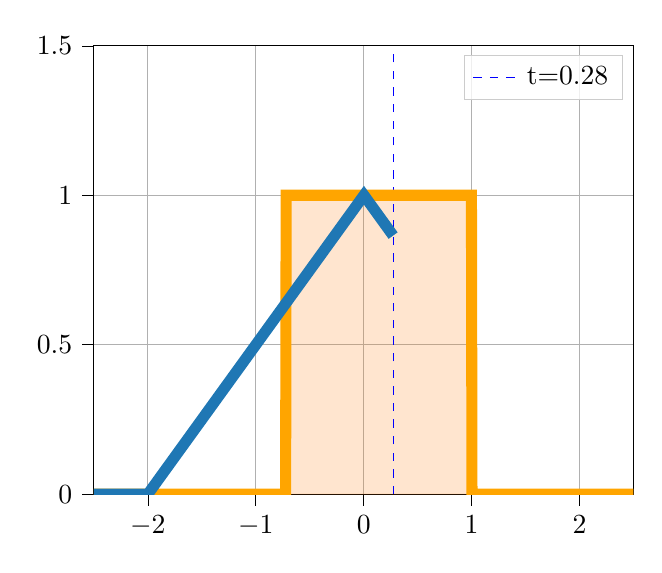
\begin{tikzpicture}

\definecolor{color0}{rgb}{1,0.498039215686275,0.0549019607843137}
\definecolor{color1}{rgb}{1,0.647058823529412,0}
\definecolor{color2}{rgb}{0.12156862745098,0.466666666666667,0.705882352941177}

\begin{axis}[
legend cell align={left},
legend style={fill opacity=0.8, draw opacity=1, text opacity=1, draw=white!80!black},
tick align=outside,
tick pos=left,
x grid style={white!69.0196078431373!black},
xmajorgrids,
xmin=-2.5, xmax=2.5,
xtick style={color=black},
y grid style={white!69.0196078431373!black},
ymajorgrids,
ymin=0, ymax=1.5,
ytick style={color=black}
]
\path [draw=color0, fill=color0, opacity=0.2]
(axis cs:-2.5,0)
--(axis cs:-2.5,0)
--(axis cs:-2.49499499499499,0)
--(axis cs:-2.48998998998999,0)
--(axis cs:-2.48498498498498,0)
--(axis cs:-2.47997997997998,0)
--(axis cs:-2.47497497497497,0)
--(axis cs:-2.46996996996997,0)
--(axis cs:-2.46496496496496,0)
--(axis cs:-2.45995995995996,0)
--(axis cs:-2.45495495495495,0)
--(axis cs:-2.44994994994995,0)
--(axis cs:-2.44494494494494,0)
--(axis cs:-2.43993993993994,0)
--(axis cs:-2.43493493493493,0)
--(axis cs:-2.42992992992993,0)
--(axis cs:-2.42492492492492,0)
--(axis cs:-2.41991991991992,0)
--(axis cs:-2.41491491491491,0)
--(axis cs:-2.40990990990991,0)
--(axis cs:-2.4049049049049,0)
--(axis cs:-2.3998998998999,0)
--(axis cs:-2.39489489489489,0)
--(axis cs:-2.38988988988989,0)
--(axis cs:-2.38488488488488,0)
--(axis cs:-2.37987987987988,0)
--(axis cs:-2.37487487487487,0)
--(axis cs:-2.36986986986987,0)
--(axis cs:-2.36486486486486,0)
--(axis cs:-2.35985985985986,0)
--(axis cs:-2.35485485485485,0)
--(axis cs:-2.34984984984985,0)
--(axis cs:-2.34484484484484,0)
--(axis cs:-2.33983983983984,0)
--(axis cs:-2.33483483483483,0)
--(axis cs:-2.32982982982983,0)
--(axis cs:-2.32482482482482,0)
--(axis cs:-2.31981981981982,0)
--(axis cs:-2.31481481481481,0)
--(axis cs:-2.30980980980981,0)
--(axis cs:-2.3048048048048,0)
--(axis cs:-2.2997997997998,0)
--(axis cs:-2.29479479479479,0)
--(axis cs:-2.28978978978979,0)
--(axis cs:-2.28478478478478,0)
--(axis cs:-2.27977977977978,0)
--(axis cs:-2.27477477477477,0)
--(axis cs:-2.26976976976977,0)
--(axis cs:-2.26476476476476,0)
--(axis cs:-2.25975975975976,0)
--(axis cs:-2.25475475475475,0)
--(axis cs:-2.24974974974975,0)
--(axis cs:-2.24474474474474,0)
--(axis cs:-2.23973973973974,0)
--(axis cs:-2.23473473473473,0)
--(axis cs:-2.22972972972973,0)
--(axis cs:-2.22472472472472,0)
--(axis cs:-2.21971971971972,0)
--(axis cs:-2.21471471471471,0)
--(axis cs:-2.20970970970971,0)
--(axis cs:-2.2047047047047,0)
--(axis cs:-2.1996996996997,0)
--(axis cs:-2.19469469469469,0)
--(axis cs:-2.18968968968969,0)
--(axis cs:-2.18468468468468,0)
--(axis cs:-2.17967967967968,0)
--(axis cs:-2.17467467467467,0)
--(axis cs:-2.16966966966967,0)
--(axis cs:-2.16466466466466,0)
--(axis cs:-2.15965965965966,0)
--(axis cs:-2.15465465465465,0)
--(axis cs:-2.14964964964965,0)
--(axis cs:-2.14464464464464,0)
--(axis cs:-2.13963963963964,0)
--(axis cs:-2.13463463463463,0)
--(axis cs:-2.12962962962963,0)
--(axis cs:-2.12462462462462,0)
--(axis cs:-2.11961961961962,0)
--(axis cs:-2.11461461461461,0)
--(axis cs:-2.10960960960961,0)
--(axis cs:-2.1046046046046,0)
--(axis cs:-2.0995995995996,0)
--(axis cs:-2.09459459459459,0)
--(axis cs:-2.08958958958959,0)
--(axis cs:-2.08458458458458,0)
--(axis cs:-2.07957957957958,0)
--(axis cs:-2.07457457457457,0)
--(axis cs:-2.06956956956957,0)
--(axis cs:-2.06456456456456,0)
--(axis cs:-2.05955955955956,0)
--(axis cs:-2.05455455455455,0)
--(axis cs:-2.04954954954955,0)
--(axis cs:-2.04454454454454,0)
--(axis cs:-2.03953953953954,0)
--(axis cs:-2.03453453453453,0)
--(axis cs:-2.02952952952953,0)
--(axis cs:-2.02452452452452,0)
--(axis cs:-2.01951951951952,0)
--(axis cs:-2.01451451451451,0)
--(axis cs:-2.00950950950951,0)
--(axis cs:-2.0045045045045,0)
--(axis cs:-1.9994994994995,0)
--(axis cs:-1.99449449449449,0)
--(axis cs:-1.98948948948949,0)
--(axis cs:-1.98448448448448,0)
--(axis cs:-1.97947947947948,0)
--(axis cs:-1.97447447447447,0)
--(axis cs:-1.96946946946947,0)
--(axis cs:-1.96446446446446,0)
--(axis cs:-1.95945945945946,0)
--(axis cs:-1.95445445445445,0)
--(axis cs:-1.94944944944945,0)
--(axis cs:-1.94444444444444,0)
--(axis cs:-1.93943943943944,0)
--(axis cs:-1.93443443443443,0)
--(axis cs:-1.92942942942943,0)
--(axis cs:-1.92442442442442,0)
--(axis cs:-1.91941941941942,0)
--(axis cs:-1.91441441441441,0)
--(axis cs:-1.90940940940941,0)
--(axis cs:-1.9044044044044,0)
--(axis cs:-1.8993993993994,0)
--(axis cs:-1.89439439439439,0)
--(axis cs:-1.88938938938939,0)
--(axis cs:-1.88438438438438,0)
--(axis cs:-1.87937937937938,0)
--(axis cs:-1.87437437437437,0)
--(axis cs:-1.86936936936937,0)
--(axis cs:-1.86436436436436,0)
--(axis cs:-1.85935935935936,0)
--(axis cs:-1.85435435435435,0)
--(axis cs:-1.84934934934935,0)
--(axis cs:-1.84434434434434,0)
--(axis cs:-1.83933933933934,0)
--(axis cs:-1.83433433433433,0)
--(axis cs:-1.82932932932933,0)
--(axis cs:-1.82432432432432,0)
--(axis cs:-1.81931931931932,0)
--(axis cs:-1.81431431431431,0)
--(axis cs:-1.80930930930931,0)
--(axis cs:-1.8043043043043,0)
--(axis cs:-1.7992992992993,0)
--(axis cs:-1.79429429429429,0)
--(axis cs:-1.78928928928929,0)
--(axis cs:-1.78428428428428,0)
--(axis cs:-1.77927927927928,0)
--(axis cs:-1.77427427427427,0)
--(axis cs:-1.76926926926927,0)
--(axis cs:-1.76426426426426,0)
--(axis cs:-1.75925925925926,0)
--(axis cs:-1.75425425425425,0)
--(axis cs:-1.74924924924925,0)
--(axis cs:-1.74424424424424,0)
--(axis cs:-1.73923923923924,0)
--(axis cs:-1.73423423423423,0)
--(axis cs:-1.72922922922923,0)
--(axis cs:-1.72422422422422,0)
--(axis cs:-1.71921921921922,0)
--(axis cs:-1.71421421421421,0)
--(axis cs:-1.70920920920921,0)
--(axis cs:-1.7042042042042,0)
--(axis cs:-1.6991991991992,0)
--(axis cs:-1.69419419419419,0)
--(axis cs:-1.68918918918919,0)
--(axis cs:-1.68418418418418,0)
--(axis cs:-1.67917917917918,0)
--(axis cs:-1.67417417417417,0)
--(axis cs:-1.66916916916917,0)
--(axis cs:-1.66416416416416,0)
--(axis cs:-1.65915915915916,0)
--(axis cs:-1.65415415415415,0)
--(axis cs:-1.64914914914915,0)
--(axis cs:-1.64414414414414,0)
--(axis cs:-1.63913913913914,0)
--(axis cs:-1.63413413413413,0)
--(axis cs:-1.62912912912913,0)
--(axis cs:-1.62412412412412,0)
--(axis cs:-1.61911911911912,0)
--(axis cs:-1.61411411411411,0)
--(axis cs:-1.60910910910911,0)
--(axis cs:-1.6041041041041,0)
--(axis cs:-1.5990990990991,0)
--(axis cs:-1.59409409409409,0)
--(axis cs:-1.58908908908909,0)
--(axis cs:-1.58408408408408,0)
--(axis cs:-1.57907907907908,0)
--(axis cs:-1.57407407407407,0)
--(axis cs:-1.56906906906907,0)
--(axis cs:-1.56406406406406,0)
--(axis cs:-1.55905905905906,0)
--(axis cs:-1.55405405405405,0)
--(axis cs:-1.54904904904905,0)
--(axis cs:-1.54404404404404,0)
--(axis cs:-1.53903903903904,0)
--(axis cs:-1.53403403403403,0)
--(axis cs:-1.52902902902903,0)
--(axis cs:-1.52402402402402,0)
--(axis cs:-1.51901901901902,0)
--(axis cs:-1.51401401401401,0)
--(axis cs:-1.50900900900901,0)
--(axis cs:-1.504004004004,0)
--(axis cs:-1.498998998999,0)
--(axis cs:-1.49399399399399,0)
--(axis cs:-1.48898898898899,0)
--(axis cs:-1.48398398398398,0)
--(axis cs:-1.47897897897898,0)
--(axis cs:-1.47397397397397,0)
--(axis cs:-1.46896896896897,0)
--(axis cs:-1.46396396396396,0)
--(axis cs:-1.45895895895896,0)
--(axis cs:-1.45395395395395,0)
--(axis cs:-1.44894894894895,0)
--(axis cs:-1.44394394394394,0)
--(axis cs:-1.43893893893894,0)
--(axis cs:-1.43393393393393,0)
--(axis cs:-1.42892892892893,0)
--(axis cs:-1.42392392392392,0)
--(axis cs:-1.41891891891892,0)
--(axis cs:-1.41391391391391,0)
--(axis cs:-1.40890890890891,0)
--(axis cs:-1.4039039039039,0)
--(axis cs:-1.3988988988989,0)
--(axis cs:-1.39389389389389,0)
--(axis cs:-1.38888888888889,0)
--(axis cs:-1.38388388388388,0)
--(axis cs:-1.37887887887888,0)
--(axis cs:-1.37387387387387,0)
--(axis cs:-1.36886886886887,0)
--(axis cs:-1.36386386386386,0)
--(axis cs:-1.35885885885886,0)
--(axis cs:-1.35385385385385,0)
--(axis cs:-1.34884884884885,0)
--(axis cs:-1.34384384384384,0)
--(axis cs:-1.33883883883884,0)
--(axis cs:-1.33383383383383,0)
--(axis cs:-1.32882882882883,0)
--(axis cs:-1.32382382382382,0)
--(axis cs:-1.31881881881882,0)
--(axis cs:-1.31381381381381,0)
--(axis cs:-1.30880880880881,0)
--(axis cs:-1.3038038038038,0)
--(axis cs:-1.2987987987988,0)
--(axis cs:-1.29379379379379,0)
--(axis cs:-1.28878878878879,0)
--(axis cs:-1.28378378378378,0)
--(axis cs:-1.27877877877878,0)
--(axis cs:-1.27377377377377,0)
--(axis cs:-1.26876876876877,0)
--(axis cs:-1.26376376376376,0)
--(axis cs:-1.25875875875876,0)
--(axis cs:-1.25375375375375,0)
--(axis cs:-1.24874874874875,0)
--(axis cs:-1.24374374374374,0)
--(axis cs:-1.23873873873874,0)
--(axis cs:-1.23373373373373,0)
--(axis cs:-1.22872872872873,0)
--(axis cs:-1.22372372372372,0)
--(axis cs:-1.21871871871872,0)
--(axis cs:-1.21371371371371,0)
--(axis cs:-1.20870870870871,0)
--(axis cs:-1.2037037037037,0)
--(axis cs:-1.1986986986987,0)
--(axis cs:-1.19369369369369,0)
--(axis cs:-1.18868868868869,0)
--(axis cs:-1.18368368368368,0)
--(axis cs:-1.17867867867868,0)
--(axis cs:-1.17367367367367,0)
--(axis cs:-1.16866866866867,0)
--(axis cs:-1.16366366366366,0)
--(axis cs:-1.15865865865866,0)
--(axis cs:-1.15365365365365,0)
--(axis cs:-1.14864864864865,0)
--(axis cs:-1.14364364364364,0)
--(axis cs:-1.13863863863864,0)
--(axis cs:-1.13363363363363,0)
--(axis cs:-1.12862862862863,0)
--(axis cs:-1.12362362362362,0)
--(axis cs:-1.11861861861862,0)
--(axis cs:-1.11361361361361,0)
--(axis cs:-1.10860860860861,0)
--(axis cs:-1.1036036036036,0)
--(axis cs:-1.0985985985986,0)
--(axis cs:-1.09359359359359,0)
--(axis cs:-1.08858858858859,0)
--(axis cs:-1.08358358358358,0)
--(axis cs:-1.07857857857858,0)
--(axis cs:-1.07357357357357,0)
--(axis cs:-1.06856856856857,0)
--(axis cs:-1.06356356356356,0)
--(axis cs:-1.05855855855856,0)
--(axis cs:-1.05355355355355,0)
--(axis cs:-1.04854854854855,0)
--(axis cs:-1.04354354354354,0)
--(axis cs:-1.03853853853854,0)
--(axis cs:-1.03353353353353,0)
--(axis cs:-1.02852852852853,0)
--(axis cs:-1.02352352352352,0)
--(axis cs:-1.01851851851852,0)
--(axis cs:-1.01351351351351,0)
--(axis cs:-1.00850850850851,0)
--(axis cs:-1.0035035035035,0)
--(axis cs:-0.998498498498499,0)
--(axis cs:-0.993493493493494,0)
--(axis cs:-0.988488488488489,0)
--(axis cs:-0.983483483483484,0)
--(axis cs:-0.978478478478479,0)
--(axis cs:-0.973473473473474,0)
--(axis cs:-0.968468468468469,0)
--(axis cs:-0.963463463463464,0)
--(axis cs:-0.958458458458459,0)
--(axis cs:-0.953453453453454,0)
--(axis cs:-0.948448448448449,0)
--(axis cs:-0.943443443443444,0)
--(axis cs:-0.938438438438439,0)
--(axis cs:-0.933433433433434,0)
--(axis cs:-0.928428428428429,0)
--(axis cs:-0.923423423423424,0)
--(axis cs:-0.918418418418419,0)
--(axis cs:-0.913413413413414,0)
--(axis cs:-0.908408408408409,0)
--(axis cs:-0.903403403403404,0)
--(axis cs:-0.898398398398399,0)
--(axis cs:-0.893393393393393,0)
--(axis cs:-0.888388388388388,0)
--(axis cs:-0.883383383383383,0)
--(axis cs:-0.878378378378378,0)
--(axis cs:-0.873373373373373,0)
--(axis cs:-0.868368368368368,0)
--(axis cs:-0.863363363363363,0)
--(axis cs:-0.858358358358358,0)
--(axis cs:-0.853353353353353,0)
--(axis cs:-0.848348348348348,0)
--(axis cs:-0.843343343343343,0)
--(axis cs:-0.838338338338338,0)
--(axis cs:-0.833333333333333,0)
--(axis cs:-0.828328328328328,0)
--(axis cs:-0.823323323323323,0)
--(axis cs:-0.818318318318318,0)
--(axis cs:-0.813313313313313,0)
--(axis cs:-0.808308308308308,0)
--(axis cs:-0.803303303303303,0)
--(axis cs:-0.798298298298298,0)
--(axis cs:-0.793293293293293,0)
--(axis cs:-0.788288288288288,0)
--(axis cs:-0.783283283283283,0)
--(axis cs:-0.778278278278278,0)
--(axis cs:-0.773273273273273,0)
--(axis cs:-0.768268268268268,0)
--(axis cs:-0.763263263263263,0)
--(axis cs:-0.758258258258258,0)
--(axis cs:-0.753253253253253,0)
--(axis cs:-0.748248248248248,0)
--(axis cs:-0.743243243243243,0)
--(axis cs:-0.738238238238238,0)
--(axis cs:-0.733233233233233,0)
--(axis cs:-0.728228228228228,0)
--(axis cs:-0.723223223223223,0)
--(axis cs:-0.718218218218218,0)
--(axis cs:-0.713213213213213,0)
--(axis cs:-0.708208208208208,0)
--(axis cs:-0.703203203203203,0)
--(axis cs:-0.698198198198198,0)
--(axis cs:-0.693193193193193,0)
--(axis cs:-0.688188188188188,0)
--(axis cs:-0.683183183183183,0)
--(axis cs:-0.678178178178178,0)
--(axis cs:-0.673173173173173,0)
--(axis cs:-0.668168168168168,0)
--(axis cs:-0.663163163163163,0)
--(axis cs:-0.658158158158158,0)
--(axis cs:-0.653153153153153,0)
--(axis cs:-0.648148148148148,0)
--(axis cs:-0.643143143143143,0)
--(axis cs:-0.638138138138138,0)
--(axis cs:-0.633133133133133,0)
--(axis cs:-0.628128128128128,0)
--(axis cs:-0.623123123123123,0)
--(axis cs:-0.618118118118118,0)
--(axis cs:-0.613113113113113,0)
--(axis cs:-0.608108108108108,0)
--(axis cs:-0.603103103103103,0)
--(axis cs:-0.598098098098098,0)
--(axis cs:-0.593093093093093,0)
--(axis cs:-0.588088088088088,0)
--(axis cs:-0.583083083083083,0)
--(axis cs:-0.578078078078078,0)
--(axis cs:-0.573073073073073,0)
--(axis cs:-0.568068068068068,0)
--(axis cs:-0.563063063063063,0)
--(axis cs:-0.558058058058058,0)
--(axis cs:-0.553053053053053,0)
--(axis cs:-0.548048048048048,0)
--(axis cs:-0.543043043043043,0)
--(axis cs:-0.538038038038038,0)
--(axis cs:-0.533033033033033,0)
--(axis cs:-0.528028028028028,0)
--(axis cs:-0.523023023023023,0)
--(axis cs:-0.518018018018018,0)
--(axis cs:-0.513013013013013,0)
--(axis cs:-0.508008008008008,0)
--(axis cs:-0.503003003003003,0)
--(axis cs:-0.497997997997998,0)
--(axis cs:-0.492992992992993,0)
--(axis cs:-0.487987987987988,0)
--(axis cs:-0.482982982982983,0)
--(axis cs:-0.477977977977978,0)
--(axis cs:-0.472972972972973,0)
--(axis cs:-0.467967967967968,0)
--(axis cs:-0.462962962962963,0)
--(axis cs:-0.457957957957958,0)
--(axis cs:-0.452952952952953,0)
--(axis cs:-0.447947947947948,0)
--(axis cs:-0.442942942942943,0)
--(axis cs:-0.437937937937938,0)
--(axis cs:-0.432932932932933,0)
--(axis cs:-0.427927927927928,0)
--(axis cs:-0.422922922922923,0)
--(axis cs:-0.417917917917918,0)
--(axis cs:-0.412912912912913,0)
--(axis cs:-0.407907907907908,0)
--(axis cs:-0.402902902902903,0)
--(axis cs:-0.397897897897898,0)
--(axis cs:-0.392892892892893,0)
--(axis cs:-0.387887887887888,0)
--(axis cs:-0.382882882882883,0)
--(axis cs:-0.377877877877878,0)
--(axis cs:-0.372872872872873,0)
--(axis cs:-0.367867867867868,0)
--(axis cs:-0.362862862862863,0)
--(axis cs:-0.357857857857858,0)
--(axis cs:-0.352852852852853,0)
--(axis cs:-0.347847847847848,0)
--(axis cs:-0.342842842842843,0)
--(axis cs:-0.337837837837838,0)
--(axis cs:-0.332832832832833,0)
--(axis cs:-0.327827827827828,0)
--(axis cs:-0.322822822822823,0)
--(axis cs:-0.317817817817818,0)
--(axis cs:-0.312812812812813,0)
--(axis cs:-0.307807807807808,0)
--(axis cs:-0.302802802802803,0)
--(axis cs:-0.297797797797798,0)
--(axis cs:-0.292792792792793,0)
--(axis cs:-0.287787787787788,0)
--(axis cs:-0.282782782782783,0)
--(axis cs:-0.277777777777778,0)
--(axis cs:-0.272772772772773,0)
--(axis cs:-0.267767767767768,0)
--(axis cs:-0.262762762762763,0)
--(axis cs:-0.257757757757758,0)
--(axis cs:-0.252752752752753,0)
--(axis cs:-0.247747747747748,0)
--(axis cs:-0.242742742742743,0)
--(axis cs:-0.237737737737738,0)
--(axis cs:-0.232732732732733,0)
--(axis cs:-0.227727727727728,0)
--(axis cs:-0.222722722722723,0)
--(axis cs:-0.217717717717718,0)
--(axis cs:-0.212712712712713,0)
--(axis cs:-0.207707707707708,0)
--(axis cs:-0.202702702702703,0)
--(axis cs:-0.197697697697698,0)
--(axis cs:-0.192692692692693,0)
--(axis cs:-0.187687687687688,0)
--(axis cs:-0.182682682682683,0)
--(axis cs:-0.177677677677678,0)
--(axis cs:-0.172672672672673,0)
--(axis cs:-0.167667667667668,0)
--(axis cs:-0.162662662662663,0)
--(axis cs:-0.157657657657658,0)
--(axis cs:-0.152652652652653,0)
--(axis cs:-0.147647647647648,0)
--(axis cs:-0.142642642642643,0)
--(axis cs:-0.137637637637638,0)
--(axis cs:-0.132632632632633,0)
--(axis cs:-0.127627627627628,0)
--(axis cs:-0.122622622622623,0)
--(axis cs:-0.117617617617618,0)
--(axis cs:-0.112612612612613,0)
--(axis cs:-0.107607607607608,0)
--(axis cs:-0.102602602602603,0)
--(axis cs:-0.0975975975975976,0)
--(axis cs:-0.0925925925925926,0)
--(axis cs:-0.0875875875875876,0)
--(axis cs:-0.0825825825825826,0)
--(axis cs:-0.0775775775775776,0)
--(axis cs:-0.0725725725725725,0)
--(axis cs:-0.0675675675675675,0)
--(axis cs:-0.0625625625625625,0)
--(axis cs:-0.0575575575575575,0)
--(axis cs:-0.0525525525525525,0)
--(axis cs:-0.0475475475475475,0)
--(axis cs:-0.0425425425425425,0)
--(axis cs:-0.0375375375375375,0)
--(axis cs:-0.0325325325325325,0)
--(axis cs:-0.0275275275275275,0)
--(axis cs:-0.0225225225225225,0)
--(axis cs:-0.0175175175175175,0)
--(axis cs:-0.0125125125125125,0)
--(axis cs:-0.0075075075075075,0)
--(axis cs:-0.0025025025025025,0)
--(axis cs:0.0025025025025025,0)
--(axis cs:0.0075075075075075,0)
--(axis cs:0.0125125125125125,0)
--(axis cs:0.0175175175175175,0)
--(axis cs:0.0225225225225225,0)
--(axis cs:0.0275275275275275,0)
--(axis cs:0.0325325325325325,0)
--(axis cs:0.0375375375375375,0)
--(axis cs:0.0425425425425425,0)
--(axis cs:0.0475475475475475,0)
--(axis cs:0.0525525525525525,0)
--(axis cs:0.0575575575575575,0)
--(axis cs:0.0625625625625625,0)
--(axis cs:0.0675675675675675,0)
--(axis cs:0.0725725725725725,0)
--(axis cs:0.0775775775775776,0)
--(axis cs:0.0825825825825826,0)
--(axis cs:0.0875875875875876,0)
--(axis cs:0.0925925925925926,0)
--(axis cs:0.0975975975975976,0)
--(axis cs:0.102602602602603,0)
--(axis cs:0.107607607607608,0)
--(axis cs:0.112612612612613,0)
--(axis cs:0.117617617617618,0)
--(axis cs:0.122622622622623,0)
--(axis cs:0.127627627627628,0)
--(axis cs:0.132632632632633,0)
--(axis cs:0.137637637637638,0)
--(axis cs:0.142642642642643,0)
--(axis cs:0.147647647647648,0)
--(axis cs:0.152652652652653,0)
--(axis cs:0.157657657657658,0)
--(axis cs:0.162662662662663,0)
--(axis cs:0.167667667667668,0)
--(axis cs:0.172672672672673,0)
--(axis cs:0.177677677677678,0)
--(axis cs:0.182682682682683,0)
--(axis cs:0.187687687687688,0)
--(axis cs:0.192692692692693,0)
--(axis cs:0.197697697697698,0)
--(axis cs:0.202702702702703,0)
--(axis cs:0.207707707707708,0)
--(axis cs:0.212712712712713,0)
--(axis cs:0.217717717717718,0)
--(axis cs:0.222722722722723,0)
--(axis cs:0.227727727727728,0)
--(axis cs:0.232732732732733,0)
--(axis cs:0.237737737737738,0)
--(axis cs:0.242742742742743,0)
--(axis cs:0.247747747747748,0)
--(axis cs:0.252752752752753,0)
--(axis cs:0.257757757757758,0)
--(axis cs:0.262762762762763,0)
--(axis cs:0.267767767767768,0)
--(axis cs:0.272772772772773,0)
--(axis cs:0.277777777777778,0)
--(axis cs:0.282782782782783,0)
--(axis cs:0.287787787787788,0)
--(axis cs:0.292792792792793,0)
--(axis cs:0.297797797797798,0)
--(axis cs:0.302802802802803,0)
--(axis cs:0.307807807807808,0)
--(axis cs:0.312812812812813,0)
--(axis cs:0.317817817817818,0)
--(axis cs:0.322822822822823,0)
--(axis cs:0.327827827827828,0)
--(axis cs:0.332832832832833,0)
--(axis cs:0.337837837837838,0)
--(axis cs:0.342842842842843,0)
--(axis cs:0.347847847847848,0)
--(axis cs:0.352852852852853,0)
--(axis cs:0.357857857857858,0)
--(axis cs:0.362862862862863,0)
--(axis cs:0.367867867867868,0)
--(axis cs:0.372872872872873,0)
--(axis cs:0.377877877877878,0)
--(axis cs:0.382882882882883,0)
--(axis cs:0.387887887887888,0)
--(axis cs:0.392892892892893,0)
--(axis cs:0.397897897897898,0)
--(axis cs:0.402902902902903,0)
--(axis cs:0.407907907907908,0)
--(axis cs:0.412912912912913,0)
--(axis cs:0.417917917917918,0)
--(axis cs:0.422922922922923,0)
--(axis cs:0.427927927927928,0)
--(axis cs:0.432932932932933,0)
--(axis cs:0.437937937937938,0)
--(axis cs:0.442942942942943,0)
--(axis cs:0.447947947947948,0)
--(axis cs:0.452952952952953,0)
--(axis cs:0.457957957957958,0)
--(axis cs:0.462962962962963,0)
--(axis cs:0.467967967967968,0)
--(axis cs:0.472972972972973,0)
--(axis cs:0.477977977977978,0)
--(axis cs:0.482982982982983,0)
--(axis cs:0.487987987987988,0)
--(axis cs:0.492992992992993,0)
--(axis cs:0.497997997997998,0)
--(axis cs:0.503003003003003,0)
--(axis cs:0.508008008008008,0)
--(axis cs:0.513013013013013,0)
--(axis cs:0.518018018018018,0)
--(axis cs:0.523023023023023,0)
--(axis cs:0.528028028028028,0)
--(axis cs:0.533033033033033,0)
--(axis cs:0.538038038038038,0)
--(axis cs:0.543043043043043,0)
--(axis cs:0.548048048048048,0)
--(axis cs:0.553053053053053,0)
--(axis cs:0.558058058058058,0)
--(axis cs:0.563063063063063,0)
--(axis cs:0.568068068068068,0)
--(axis cs:0.573073073073073,0)
--(axis cs:0.578078078078078,0)
--(axis cs:0.583083083083083,0)
--(axis cs:0.588088088088088,0)
--(axis cs:0.593093093093093,0)
--(axis cs:0.598098098098098,0)
--(axis cs:0.603103103103103,0)
--(axis cs:0.608108108108108,0)
--(axis cs:0.613113113113113,0)
--(axis cs:0.618118118118118,0)
--(axis cs:0.623123123123123,0)
--(axis cs:0.628128128128128,0)
--(axis cs:0.633133133133133,0)
--(axis cs:0.638138138138138,0)
--(axis cs:0.643143143143143,0)
--(axis cs:0.648148148148148,0)
--(axis cs:0.653153153153153,0)
--(axis cs:0.658158158158158,0)
--(axis cs:0.663163163163163,0)
--(axis cs:0.668168168168168,0)
--(axis cs:0.673173173173173,0)
--(axis cs:0.678178178178178,0)
--(axis cs:0.683183183183183,0)
--(axis cs:0.688188188188188,0)
--(axis cs:0.693193193193193,0)
--(axis cs:0.698198198198198,0)
--(axis cs:0.703203203203203,0)
--(axis cs:0.708208208208208,0)
--(axis cs:0.713213213213213,0)
--(axis cs:0.718218218218218,0)
--(axis cs:0.723223223223223,0)
--(axis cs:0.728228228228228,0)
--(axis cs:0.733233233233233,0)
--(axis cs:0.738238238238238,0)
--(axis cs:0.743243243243243,0)
--(axis cs:0.748248248248248,0)
--(axis cs:0.753253253253253,0)
--(axis cs:0.758258258258258,0)
--(axis cs:0.763263263263263,0)
--(axis cs:0.768268268268268,0)
--(axis cs:0.773273273273273,0)
--(axis cs:0.778278278278278,0)
--(axis cs:0.783283283283283,0)
--(axis cs:0.788288288288288,0)
--(axis cs:0.793293293293293,0)
--(axis cs:0.798298298298298,0)
--(axis cs:0.803303303303303,0)
--(axis cs:0.808308308308308,0)
--(axis cs:0.813313313313313,0)
--(axis cs:0.818318318318318,0)
--(axis cs:0.823323323323323,0)
--(axis cs:0.828328328328328,0)
--(axis cs:0.833333333333333,0)
--(axis cs:0.838338338338338,0)
--(axis cs:0.843343343343343,0)
--(axis cs:0.848348348348348,0)
--(axis cs:0.853353353353353,0)
--(axis cs:0.858358358358358,0)
--(axis cs:0.863363363363364,0)
--(axis cs:0.868368368368369,0)
--(axis cs:0.873373373373374,0)
--(axis cs:0.878378378378379,0)
--(axis cs:0.883383383383384,0)
--(axis cs:0.888388388388389,0)
--(axis cs:0.893393393393394,0)
--(axis cs:0.898398398398399,0)
--(axis cs:0.903403403403404,0)
--(axis cs:0.908408408408409,0)
--(axis cs:0.913413413413414,0)
--(axis cs:0.918418418418419,0)
--(axis cs:0.923423423423424,0)
--(axis cs:0.928428428428429,0)
--(axis cs:0.933433433433434,0)
--(axis cs:0.938438438438439,0)
--(axis cs:0.943443443443444,0)
--(axis cs:0.948448448448449,0)
--(axis cs:0.953453453453454,0)
--(axis cs:0.958458458458459,0)
--(axis cs:0.963463463463464,0)
--(axis cs:0.968468468468469,0)
--(axis cs:0.973473473473474,0)
--(axis cs:0.978478478478479,0)
--(axis cs:0.983483483483484,0)
--(axis cs:0.988488488488489,0)
--(axis cs:0.993493493493494,0)
--(axis cs:0.998498498498499,0)
--(axis cs:1.0035035035035,0)
--(axis cs:1.00850850850851,0)
--(axis cs:1.01351351351351,0)
--(axis cs:1.01851851851852,0)
--(axis cs:1.02352352352352,0)
--(axis cs:1.02852852852853,0)
--(axis cs:1.03353353353353,0)
--(axis cs:1.03853853853854,0)
--(axis cs:1.04354354354354,0)
--(axis cs:1.04854854854855,0)
--(axis cs:1.05355355355355,0)
--(axis cs:1.05855855855856,0)
--(axis cs:1.06356356356356,0)
--(axis cs:1.06856856856857,0)
--(axis cs:1.07357357357357,0)
--(axis cs:1.07857857857858,0)
--(axis cs:1.08358358358358,0)
--(axis cs:1.08858858858859,0)
--(axis cs:1.09359359359359,0)
--(axis cs:1.0985985985986,0)
--(axis cs:1.1036036036036,0)
--(axis cs:1.10860860860861,0)
--(axis cs:1.11361361361361,0)
--(axis cs:1.11861861861862,0)
--(axis cs:1.12362362362362,0)
--(axis cs:1.12862862862863,0)
--(axis cs:1.13363363363363,0)
--(axis cs:1.13863863863864,0)
--(axis cs:1.14364364364364,0)
--(axis cs:1.14864864864865,0)
--(axis cs:1.15365365365365,0)
--(axis cs:1.15865865865866,0)
--(axis cs:1.16366366366366,0)
--(axis cs:1.16866866866867,0)
--(axis cs:1.17367367367367,0)
--(axis cs:1.17867867867868,0)
--(axis cs:1.18368368368368,0)
--(axis cs:1.18868868868869,0)
--(axis cs:1.19369369369369,0)
--(axis cs:1.1986986986987,0)
--(axis cs:1.2037037037037,0)
--(axis cs:1.20870870870871,0)
--(axis cs:1.21371371371371,0)
--(axis cs:1.21871871871872,0)
--(axis cs:1.22372372372372,0)
--(axis cs:1.22872872872873,0)
--(axis cs:1.23373373373373,0)
--(axis cs:1.23873873873874,0)
--(axis cs:1.24374374374374,0)
--(axis cs:1.24874874874875,0)
--(axis cs:1.25375375375375,0)
--(axis cs:1.25875875875876,0)
--(axis cs:1.26376376376376,0)
--(axis cs:1.26876876876877,0)
--(axis cs:1.27377377377377,0)
--(axis cs:1.27877877877878,0)
--(axis cs:1.28378378378378,0)
--(axis cs:1.28878878878879,0)
--(axis cs:1.29379379379379,0)
--(axis cs:1.2987987987988,0)
--(axis cs:1.3038038038038,0)
--(axis cs:1.30880880880881,0)
--(axis cs:1.31381381381381,0)
--(axis cs:1.31881881881882,0)
--(axis cs:1.32382382382382,0)
--(axis cs:1.32882882882883,0)
--(axis cs:1.33383383383383,0)
--(axis cs:1.33883883883884,0)
--(axis cs:1.34384384384384,0)
--(axis cs:1.34884884884885,0)
--(axis cs:1.35385385385385,0)
--(axis cs:1.35885885885886,0)
--(axis cs:1.36386386386386,0)
--(axis cs:1.36886886886887,0)
--(axis cs:1.37387387387387,0)
--(axis cs:1.37887887887888,0)
--(axis cs:1.38388388388388,0)
--(axis cs:1.38888888888889,0)
--(axis cs:1.39389389389389,0)
--(axis cs:1.3988988988989,0)
--(axis cs:1.4039039039039,0)
--(axis cs:1.40890890890891,0)
--(axis cs:1.41391391391391,0)
--(axis cs:1.41891891891892,0)
--(axis cs:1.42392392392392,0)
--(axis cs:1.42892892892893,0)
--(axis cs:1.43393393393393,0)
--(axis cs:1.43893893893894,0)
--(axis cs:1.44394394394394,0)
--(axis cs:1.44894894894895,0)
--(axis cs:1.45395395395395,0)
--(axis cs:1.45895895895896,0)
--(axis cs:1.46396396396396,0)
--(axis cs:1.46896896896897,0)
--(axis cs:1.47397397397397,0)
--(axis cs:1.47897897897898,0)
--(axis cs:1.48398398398398,0)
--(axis cs:1.48898898898899,0)
--(axis cs:1.49399399399399,0)
--(axis cs:1.498998998999,0)
--(axis cs:1.504004004004,0)
--(axis cs:1.50900900900901,0)
--(axis cs:1.51401401401401,0)
--(axis cs:1.51901901901902,0)
--(axis cs:1.52402402402402,0)
--(axis cs:1.52902902902903,0)
--(axis cs:1.53403403403403,0)
--(axis cs:1.53903903903904,0)
--(axis cs:1.54404404404404,0)
--(axis cs:1.54904904904905,0)
--(axis cs:1.55405405405405,0)
--(axis cs:1.55905905905906,0)
--(axis cs:1.56406406406406,0)
--(axis cs:1.56906906906907,0)
--(axis cs:1.57407407407407,0)
--(axis cs:1.57907907907908,0)
--(axis cs:1.58408408408408,0)
--(axis cs:1.58908908908909,0)
--(axis cs:1.59409409409409,0)
--(axis cs:1.5990990990991,0)
--(axis cs:1.6041041041041,0)
--(axis cs:1.60910910910911,0)
--(axis cs:1.61411411411411,0)
--(axis cs:1.61911911911912,0)
--(axis cs:1.62412412412412,0)
--(axis cs:1.62912912912913,0)
--(axis cs:1.63413413413413,0)
--(axis cs:1.63913913913914,0)
--(axis cs:1.64414414414414,0)
--(axis cs:1.64914914914915,0)
--(axis cs:1.65415415415415,0)
--(axis cs:1.65915915915916,0)
--(axis cs:1.66416416416416,0)
--(axis cs:1.66916916916917,0)
--(axis cs:1.67417417417417,0)
--(axis cs:1.67917917917918,0)
--(axis cs:1.68418418418418,0)
--(axis cs:1.68918918918919,0)
--(axis cs:1.69419419419419,0)
--(axis cs:1.6991991991992,0)
--(axis cs:1.7042042042042,0)
--(axis cs:1.70920920920921,0)
--(axis cs:1.71421421421421,0)
--(axis cs:1.71921921921922,0)
--(axis cs:1.72422422422422,0)
--(axis cs:1.72922922922923,0)
--(axis cs:1.73423423423423,0)
--(axis cs:1.73923923923924,0)
--(axis cs:1.74424424424424,0)
--(axis cs:1.74924924924925,0)
--(axis cs:1.75425425425425,0)
--(axis cs:1.75925925925926,0)
--(axis cs:1.76426426426426,0)
--(axis cs:1.76926926926927,0)
--(axis cs:1.77427427427427,0)
--(axis cs:1.77927927927928,0)
--(axis cs:1.78428428428428,0)
--(axis cs:1.78928928928929,0)
--(axis cs:1.79429429429429,0)
--(axis cs:1.7992992992993,0)
--(axis cs:1.8043043043043,0)
--(axis cs:1.80930930930931,0)
--(axis cs:1.81431431431431,0)
--(axis cs:1.81931931931932,0)
--(axis cs:1.82432432432432,0)
--(axis cs:1.82932932932933,0)
--(axis cs:1.83433433433433,0)
--(axis cs:1.83933933933934,0)
--(axis cs:1.84434434434434,0)
--(axis cs:1.84934934934935,0)
--(axis cs:1.85435435435435,0)
--(axis cs:1.85935935935936,0)
--(axis cs:1.86436436436436,0)
--(axis cs:1.86936936936937,0)
--(axis cs:1.87437437437437,0)
--(axis cs:1.87937937937938,0)
--(axis cs:1.88438438438438,0)
--(axis cs:1.88938938938939,0)
--(axis cs:1.89439439439439,0)
--(axis cs:1.8993993993994,0)
--(axis cs:1.9044044044044,0)
--(axis cs:1.90940940940941,0)
--(axis cs:1.91441441441441,0)
--(axis cs:1.91941941941942,0)
--(axis cs:1.92442442442442,0)
--(axis cs:1.92942942942943,0)
--(axis cs:1.93443443443443,0)
--(axis cs:1.93943943943944,0)
--(axis cs:1.94444444444444,0)
--(axis cs:1.94944944944945,0)
--(axis cs:1.95445445445445,0)
--(axis cs:1.95945945945946,0)
--(axis cs:1.96446446446446,0)
--(axis cs:1.96946946946947,0)
--(axis cs:1.97447447447447,0)
--(axis cs:1.97947947947948,0)
--(axis cs:1.98448448448448,0)
--(axis cs:1.98948948948949,0)
--(axis cs:1.99449449449449,0)
--(axis cs:1.9994994994995,0)
--(axis cs:2.0045045045045,0)
--(axis cs:2.00950950950951,0)
--(axis cs:2.01451451451451,0)
--(axis cs:2.01951951951952,0)
--(axis cs:2.02452452452452,0)
--(axis cs:2.02952952952953,0)
--(axis cs:2.03453453453453,0)
--(axis cs:2.03953953953954,0)
--(axis cs:2.04454454454454,0)
--(axis cs:2.04954954954955,0)
--(axis cs:2.05455455455455,0)
--(axis cs:2.05955955955956,0)
--(axis cs:2.06456456456456,0)
--(axis cs:2.06956956956957,0)
--(axis cs:2.07457457457457,0)
--(axis cs:2.07957957957958,0)
--(axis cs:2.08458458458458,0)
--(axis cs:2.08958958958959,0)
--(axis cs:2.09459459459459,0)
--(axis cs:2.0995995995996,0)
--(axis cs:2.1046046046046,0)
--(axis cs:2.10960960960961,0)
--(axis cs:2.11461461461461,0)
--(axis cs:2.11961961961962,0)
--(axis cs:2.12462462462462,0)
--(axis cs:2.12962962962963,0)
--(axis cs:2.13463463463463,0)
--(axis cs:2.13963963963964,0)
--(axis cs:2.14464464464464,0)
--(axis cs:2.14964964964965,0)
--(axis cs:2.15465465465465,0)
--(axis cs:2.15965965965966,0)
--(axis cs:2.16466466466466,0)
--(axis cs:2.16966966966967,0)
--(axis cs:2.17467467467467,0)
--(axis cs:2.17967967967968,0)
--(axis cs:2.18468468468468,0)
--(axis cs:2.18968968968969,0)
--(axis cs:2.19469469469469,0)
--(axis cs:2.1996996996997,0)
--(axis cs:2.2047047047047,0)
--(axis cs:2.20970970970971,0)
--(axis cs:2.21471471471471,0)
--(axis cs:2.21971971971972,0)
--(axis cs:2.22472472472472,0)
--(axis cs:2.22972972972973,0)
--(axis cs:2.23473473473473,0)
--(axis cs:2.23973973973974,0)
--(axis cs:2.24474474474474,0)
--(axis cs:2.24974974974975,0)
--(axis cs:2.25475475475475,0)
--(axis cs:2.25975975975976,0)
--(axis cs:2.26476476476476,0)
--(axis cs:2.26976976976977,0)
--(axis cs:2.27477477477477,0)
--(axis cs:2.27977977977978,0)
--(axis cs:2.28478478478478,0)
--(axis cs:2.28978978978979,0)
--(axis cs:2.29479479479479,0)
--(axis cs:2.2997997997998,0)
--(axis cs:2.3048048048048,0)
--(axis cs:2.30980980980981,0)
--(axis cs:2.31481481481481,0)
--(axis cs:2.31981981981982,0)
--(axis cs:2.32482482482482,0)
--(axis cs:2.32982982982983,0)
--(axis cs:2.33483483483483,0)
--(axis cs:2.33983983983984,0)
--(axis cs:2.34484484484484,0)
--(axis cs:2.34984984984985,0)
--(axis cs:2.35485485485485,0)
--(axis cs:2.35985985985986,0)
--(axis cs:2.36486486486486,0)
--(axis cs:2.36986986986987,0)
--(axis cs:2.37487487487487,0)
--(axis cs:2.37987987987988,0)
--(axis cs:2.38488488488488,0)
--(axis cs:2.38988988988989,0)
--(axis cs:2.39489489489489,0)
--(axis cs:2.3998998998999,0)
--(axis cs:2.4049049049049,0)
--(axis cs:2.40990990990991,0)
--(axis cs:2.41491491491491,0)
--(axis cs:2.41991991991992,0)
--(axis cs:2.42492492492492,0)
--(axis cs:2.42992992992993,0)
--(axis cs:2.43493493493493,0)
--(axis cs:2.43993993993994,0)
--(axis cs:2.44494494494494,0)
--(axis cs:2.44994994994995,0)
--(axis cs:2.45495495495495,0)
--(axis cs:2.45995995995996,0)
--(axis cs:2.46496496496496,0)
--(axis cs:2.46996996996997,0)
--(axis cs:2.47497497497497,0)
--(axis cs:2.47997997997998,0)
--(axis cs:2.48498498498498,0)
--(axis cs:2.48998998998999,0)
--(axis cs:2.49499499499499,0)
--(axis cs:2.5,0)
--(axis cs:2.5,0)
--(axis cs:2.5,0)
--(axis cs:2.49499499499499,0)
--(axis cs:2.48998998998999,0)
--(axis cs:2.48498498498498,0)
--(axis cs:2.47997997997998,0)
--(axis cs:2.47497497497497,0)
--(axis cs:2.46996996996997,0)
--(axis cs:2.46496496496496,0)
--(axis cs:2.45995995995996,0)
--(axis cs:2.45495495495495,0)
--(axis cs:2.44994994994995,0)
--(axis cs:2.44494494494494,0)
--(axis cs:2.43993993993994,0)
--(axis cs:2.43493493493493,0)
--(axis cs:2.42992992992993,0)
--(axis cs:2.42492492492492,0)
--(axis cs:2.41991991991992,0)
--(axis cs:2.41491491491491,0)
--(axis cs:2.40990990990991,0)
--(axis cs:2.4049049049049,0)
--(axis cs:2.3998998998999,0)
--(axis cs:2.39489489489489,0)
--(axis cs:2.38988988988989,0)
--(axis cs:2.38488488488488,0)
--(axis cs:2.37987987987988,0)
--(axis cs:2.37487487487487,0)
--(axis cs:2.36986986986987,0)
--(axis cs:2.36486486486486,0)
--(axis cs:2.35985985985986,0)
--(axis cs:2.35485485485485,0)
--(axis cs:2.34984984984985,0)
--(axis cs:2.34484484484484,0)
--(axis cs:2.33983983983984,0)
--(axis cs:2.33483483483483,0)
--(axis cs:2.32982982982983,0)
--(axis cs:2.32482482482482,0)
--(axis cs:2.31981981981982,0)
--(axis cs:2.31481481481481,0)
--(axis cs:2.30980980980981,0)
--(axis cs:2.3048048048048,0)
--(axis cs:2.2997997997998,0)
--(axis cs:2.29479479479479,0)
--(axis cs:2.28978978978979,0)
--(axis cs:2.28478478478478,0)
--(axis cs:2.27977977977978,0)
--(axis cs:2.27477477477477,0)
--(axis cs:2.26976976976977,0)
--(axis cs:2.26476476476476,0)
--(axis cs:2.25975975975976,0)
--(axis cs:2.25475475475475,0)
--(axis cs:2.24974974974975,0)
--(axis cs:2.24474474474474,0)
--(axis cs:2.23973973973974,0)
--(axis cs:2.23473473473473,0)
--(axis cs:2.22972972972973,0)
--(axis cs:2.22472472472472,0)
--(axis cs:2.21971971971972,0)
--(axis cs:2.21471471471471,0)
--(axis cs:2.20970970970971,0)
--(axis cs:2.2047047047047,0)
--(axis cs:2.1996996996997,0)
--(axis cs:2.19469469469469,0)
--(axis cs:2.18968968968969,0)
--(axis cs:2.18468468468468,0)
--(axis cs:2.17967967967968,0)
--(axis cs:2.17467467467467,0)
--(axis cs:2.16966966966967,0)
--(axis cs:2.16466466466466,0)
--(axis cs:2.15965965965966,0)
--(axis cs:2.15465465465465,0)
--(axis cs:2.14964964964965,0)
--(axis cs:2.14464464464464,0)
--(axis cs:2.13963963963964,0)
--(axis cs:2.13463463463463,0)
--(axis cs:2.12962962962963,0)
--(axis cs:2.12462462462462,0)
--(axis cs:2.11961961961962,0)
--(axis cs:2.11461461461461,0)
--(axis cs:2.10960960960961,0)
--(axis cs:2.1046046046046,0)
--(axis cs:2.0995995995996,0)
--(axis cs:2.09459459459459,0)
--(axis cs:2.08958958958959,0)
--(axis cs:2.08458458458458,0)
--(axis cs:2.07957957957958,0)
--(axis cs:2.07457457457457,0)
--(axis cs:2.06956956956957,0)
--(axis cs:2.06456456456456,0)
--(axis cs:2.05955955955956,0)
--(axis cs:2.05455455455455,0)
--(axis cs:2.04954954954955,0)
--(axis cs:2.04454454454454,0)
--(axis cs:2.03953953953954,0)
--(axis cs:2.03453453453453,0)
--(axis cs:2.02952952952953,0)
--(axis cs:2.02452452452452,0)
--(axis cs:2.01951951951952,0)
--(axis cs:2.01451451451451,0)
--(axis cs:2.00950950950951,0)
--(axis cs:2.0045045045045,0)
--(axis cs:1.9994994994995,0)
--(axis cs:1.99449449449449,0)
--(axis cs:1.98948948948949,0)
--(axis cs:1.98448448448448,0)
--(axis cs:1.97947947947948,0)
--(axis cs:1.97447447447447,0)
--(axis cs:1.96946946946947,0)
--(axis cs:1.96446446446446,0)
--(axis cs:1.95945945945946,0)
--(axis cs:1.95445445445445,0)
--(axis cs:1.94944944944945,0)
--(axis cs:1.94444444444444,0)
--(axis cs:1.93943943943944,0)
--(axis cs:1.93443443443443,0)
--(axis cs:1.92942942942943,0)
--(axis cs:1.92442442442442,0)
--(axis cs:1.91941941941942,0)
--(axis cs:1.91441441441441,0)
--(axis cs:1.90940940940941,0)
--(axis cs:1.9044044044044,0)
--(axis cs:1.8993993993994,0)
--(axis cs:1.89439439439439,0)
--(axis cs:1.88938938938939,0)
--(axis cs:1.88438438438438,0)
--(axis cs:1.87937937937938,0)
--(axis cs:1.87437437437437,0)
--(axis cs:1.86936936936937,0)
--(axis cs:1.86436436436436,0)
--(axis cs:1.85935935935936,0)
--(axis cs:1.85435435435435,0)
--(axis cs:1.84934934934935,0)
--(axis cs:1.84434434434434,0)
--(axis cs:1.83933933933934,0)
--(axis cs:1.83433433433433,0)
--(axis cs:1.82932932932933,0)
--(axis cs:1.82432432432432,0)
--(axis cs:1.81931931931932,0)
--(axis cs:1.81431431431431,0)
--(axis cs:1.80930930930931,0)
--(axis cs:1.8043043043043,0)
--(axis cs:1.7992992992993,0)
--(axis cs:1.79429429429429,0)
--(axis cs:1.78928928928929,0)
--(axis cs:1.78428428428428,0)
--(axis cs:1.77927927927928,0)
--(axis cs:1.77427427427427,0)
--(axis cs:1.76926926926927,0)
--(axis cs:1.76426426426426,0)
--(axis cs:1.75925925925926,0)
--(axis cs:1.75425425425425,0)
--(axis cs:1.74924924924925,0)
--(axis cs:1.74424424424424,0)
--(axis cs:1.73923923923924,0)
--(axis cs:1.73423423423423,0)
--(axis cs:1.72922922922923,0)
--(axis cs:1.72422422422422,0)
--(axis cs:1.71921921921922,0)
--(axis cs:1.71421421421421,0)
--(axis cs:1.70920920920921,0)
--(axis cs:1.7042042042042,0)
--(axis cs:1.6991991991992,0)
--(axis cs:1.69419419419419,0)
--(axis cs:1.68918918918919,0)
--(axis cs:1.68418418418418,0)
--(axis cs:1.67917917917918,0)
--(axis cs:1.67417417417417,0)
--(axis cs:1.66916916916917,0)
--(axis cs:1.66416416416416,0)
--(axis cs:1.65915915915916,0)
--(axis cs:1.65415415415415,0)
--(axis cs:1.64914914914915,0)
--(axis cs:1.64414414414414,0)
--(axis cs:1.63913913913914,0)
--(axis cs:1.63413413413413,0)
--(axis cs:1.62912912912913,0)
--(axis cs:1.62412412412412,0)
--(axis cs:1.61911911911912,0)
--(axis cs:1.61411411411411,0)
--(axis cs:1.60910910910911,0)
--(axis cs:1.6041041041041,0)
--(axis cs:1.5990990990991,0)
--(axis cs:1.59409409409409,0)
--(axis cs:1.58908908908909,0)
--(axis cs:1.58408408408408,0)
--(axis cs:1.57907907907908,0)
--(axis cs:1.57407407407407,0)
--(axis cs:1.56906906906907,0)
--(axis cs:1.56406406406406,0)
--(axis cs:1.55905905905906,0)
--(axis cs:1.55405405405405,0)
--(axis cs:1.54904904904905,0)
--(axis cs:1.54404404404404,0)
--(axis cs:1.53903903903904,0)
--(axis cs:1.53403403403403,0)
--(axis cs:1.52902902902903,0)
--(axis cs:1.52402402402402,0)
--(axis cs:1.51901901901902,0)
--(axis cs:1.51401401401401,0)
--(axis cs:1.50900900900901,0)
--(axis cs:1.504004004004,0)
--(axis cs:1.498998998999,0)
--(axis cs:1.49399399399399,0)
--(axis cs:1.48898898898899,0)
--(axis cs:1.48398398398398,0)
--(axis cs:1.47897897897898,0)
--(axis cs:1.47397397397397,0)
--(axis cs:1.46896896896897,0)
--(axis cs:1.46396396396396,0)
--(axis cs:1.45895895895896,0)
--(axis cs:1.45395395395395,0)
--(axis cs:1.44894894894895,0)
--(axis cs:1.44394394394394,0)
--(axis cs:1.43893893893894,0)
--(axis cs:1.43393393393393,0)
--(axis cs:1.42892892892893,0)
--(axis cs:1.42392392392392,0)
--(axis cs:1.41891891891892,0)
--(axis cs:1.41391391391391,0)
--(axis cs:1.40890890890891,0)
--(axis cs:1.4039039039039,0)
--(axis cs:1.3988988988989,0)
--(axis cs:1.39389389389389,0)
--(axis cs:1.38888888888889,0)
--(axis cs:1.38388388388388,0)
--(axis cs:1.37887887887888,0)
--(axis cs:1.37387387387387,0)
--(axis cs:1.36886886886887,0)
--(axis cs:1.36386386386386,0)
--(axis cs:1.35885885885886,0)
--(axis cs:1.35385385385385,0)
--(axis cs:1.34884884884885,0)
--(axis cs:1.34384384384384,0)
--(axis cs:1.33883883883884,0)
--(axis cs:1.33383383383383,0)
--(axis cs:1.32882882882883,0)
--(axis cs:1.32382382382382,0)
--(axis cs:1.31881881881882,0)
--(axis cs:1.31381381381381,0)
--(axis cs:1.30880880880881,0)
--(axis cs:1.3038038038038,0)
--(axis cs:1.2987987987988,0)
--(axis cs:1.29379379379379,0)
--(axis cs:1.28878878878879,0)
--(axis cs:1.28378378378378,0)
--(axis cs:1.27877877877878,0)
--(axis cs:1.27377377377377,0)
--(axis cs:1.26876876876877,0)
--(axis cs:1.26376376376376,0)
--(axis cs:1.25875875875876,0)
--(axis cs:1.25375375375375,0)
--(axis cs:1.24874874874875,0)
--(axis cs:1.24374374374374,0)
--(axis cs:1.23873873873874,0)
--(axis cs:1.23373373373373,0)
--(axis cs:1.22872872872873,0)
--(axis cs:1.22372372372372,0)
--(axis cs:1.21871871871872,0)
--(axis cs:1.21371371371371,0)
--(axis cs:1.20870870870871,0)
--(axis cs:1.2037037037037,0)
--(axis cs:1.1986986986987,0)
--(axis cs:1.19369369369369,0)
--(axis cs:1.18868868868869,0)
--(axis cs:1.18368368368368,0)
--(axis cs:1.17867867867868,0)
--(axis cs:1.17367367367367,0)
--(axis cs:1.16866866866867,0)
--(axis cs:1.16366366366366,0)
--(axis cs:1.15865865865866,0)
--(axis cs:1.15365365365365,0)
--(axis cs:1.14864864864865,0)
--(axis cs:1.14364364364364,0)
--(axis cs:1.13863863863864,0)
--(axis cs:1.13363363363363,0)
--(axis cs:1.12862862862863,0)
--(axis cs:1.12362362362362,0)
--(axis cs:1.11861861861862,0)
--(axis cs:1.11361361361361,0)
--(axis cs:1.10860860860861,0)
--(axis cs:1.1036036036036,0)
--(axis cs:1.0985985985986,0)
--(axis cs:1.09359359359359,0)
--(axis cs:1.08858858858859,0)
--(axis cs:1.08358358358358,0)
--(axis cs:1.07857857857858,0)
--(axis cs:1.07357357357357,0)
--(axis cs:1.06856856856857,0)
--(axis cs:1.06356356356356,0)
--(axis cs:1.05855855855856,0)
--(axis cs:1.05355355355355,0)
--(axis cs:1.04854854854855,0)
--(axis cs:1.04354354354354,0)
--(axis cs:1.03853853853854,0)
--(axis cs:1.03353353353353,0)
--(axis cs:1.02852852852853,0)
--(axis cs:1.02352352352352,0)
--(axis cs:1.01851851851852,0)
--(axis cs:1.01351351351351,0)
--(axis cs:1.00850850850851,0)
--(axis cs:1.0035035035035,0)
--(axis cs:0.998498498498499,1)
--(axis cs:0.993493493493494,1)
--(axis cs:0.988488488488489,1)
--(axis cs:0.983483483483484,1)
--(axis cs:0.978478478478479,1)
--(axis cs:0.973473473473474,1)
--(axis cs:0.968468468468469,1)
--(axis cs:0.963463463463464,1)
--(axis cs:0.958458458458459,1)
--(axis cs:0.953453453453454,1)
--(axis cs:0.948448448448449,1)
--(axis cs:0.943443443443444,1)
--(axis cs:0.938438438438439,1)
--(axis cs:0.933433433433434,1)
--(axis cs:0.928428428428429,1)
--(axis cs:0.923423423423424,1)
--(axis cs:0.918418418418419,1)
--(axis cs:0.913413413413414,1)
--(axis cs:0.908408408408409,1)
--(axis cs:0.903403403403404,1)
--(axis cs:0.898398398398399,1)
--(axis cs:0.893393393393394,1)
--(axis cs:0.888388388388389,1)
--(axis cs:0.883383383383384,1)
--(axis cs:0.878378378378379,1)
--(axis cs:0.873373373373374,1)
--(axis cs:0.868368368368369,1)
--(axis cs:0.863363363363364,1)
--(axis cs:0.858358358358358,1)
--(axis cs:0.853353353353353,1)
--(axis cs:0.848348348348348,1)
--(axis cs:0.843343343343343,1)
--(axis cs:0.838338338338338,1)
--(axis cs:0.833333333333333,1)
--(axis cs:0.828328328328328,1)
--(axis cs:0.823323323323323,1)
--(axis cs:0.818318318318318,1)
--(axis cs:0.813313313313313,1)
--(axis cs:0.808308308308308,1)
--(axis cs:0.803303303303303,1)
--(axis cs:0.798298298298298,1)
--(axis cs:0.793293293293293,1)
--(axis cs:0.788288288288288,1)
--(axis cs:0.783283283283283,1)
--(axis cs:0.778278278278278,1)
--(axis cs:0.773273273273273,1)
--(axis cs:0.768268268268268,1)
--(axis cs:0.763263263263263,1)
--(axis cs:0.758258258258258,1)
--(axis cs:0.753253253253253,1)
--(axis cs:0.748248248248248,1)
--(axis cs:0.743243243243243,1)
--(axis cs:0.738238238238238,1)
--(axis cs:0.733233233233233,1)
--(axis cs:0.728228228228228,1)
--(axis cs:0.723223223223223,1)
--(axis cs:0.718218218218218,1)
--(axis cs:0.713213213213213,1)
--(axis cs:0.708208208208208,1)
--(axis cs:0.703203203203203,1)
--(axis cs:0.698198198198198,1)
--(axis cs:0.693193193193193,1)
--(axis cs:0.688188188188188,1)
--(axis cs:0.683183183183183,1)
--(axis cs:0.678178178178178,1)
--(axis cs:0.673173173173173,1)
--(axis cs:0.668168168168168,1)
--(axis cs:0.663163163163163,1)
--(axis cs:0.658158158158158,1)
--(axis cs:0.653153153153153,1)
--(axis cs:0.648148148148148,1)
--(axis cs:0.643143143143143,1)
--(axis cs:0.638138138138138,1)
--(axis cs:0.633133133133133,1)
--(axis cs:0.628128128128128,1)
--(axis cs:0.623123123123123,1)
--(axis cs:0.618118118118118,1)
--(axis cs:0.613113113113113,1)
--(axis cs:0.608108108108108,1)
--(axis cs:0.603103103103103,1)
--(axis cs:0.598098098098098,1)
--(axis cs:0.593093093093093,1)
--(axis cs:0.588088088088088,1)
--(axis cs:0.583083083083083,1)
--(axis cs:0.578078078078078,1)
--(axis cs:0.573073073073073,1)
--(axis cs:0.568068068068068,1)
--(axis cs:0.563063063063063,1)
--(axis cs:0.558058058058058,1)
--(axis cs:0.553053053053053,1)
--(axis cs:0.548048048048048,1)
--(axis cs:0.543043043043043,1)
--(axis cs:0.538038038038038,1)
--(axis cs:0.533033033033033,1)
--(axis cs:0.528028028028028,1)
--(axis cs:0.523023023023023,1)
--(axis cs:0.518018018018018,1)
--(axis cs:0.513013013013013,1)
--(axis cs:0.508008008008008,1)
--(axis cs:0.503003003003003,1)
--(axis cs:0.497997997997998,1)
--(axis cs:0.492992992992993,1)
--(axis cs:0.487987987987988,1)
--(axis cs:0.482982982982983,1)
--(axis cs:0.477977977977978,1)
--(axis cs:0.472972972972973,1)
--(axis cs:0.467967967967968,1)
--(axis cs:0.462962962962963,1)
--(axis cs:0.457957957957958,1)
--(axis cs:0.452952952952953,1)
--(axis cs:0.447947947947948,1)
--(axis cs:0.442942942942943,1)
--(axis cs:0.437937937937938,1)
--(axis cs:0.432932932932933,1)
--(axis cs:0.427927927927928,1)
--(axis cs:0.422922922922923,1)
--(axis cs:0.417917917917918,1)
--(axis cs:0.412912912912913,1)
--(axis cs:0.407907907907908,1)
--(axis cs:0.402902902902903,1)
--(axis cs:0.397897897897898,1)
--(axis cs:0.392892892892893,1)
--(axis cs:0.387887887887888,1)
--(axis cs:0.382882882882883,1)
--(axis cs:0.377877877877878,1)
--(axis cs:0.372872872872873,1)
--(axis cs:0.367867867867868,1)
--(axis cs:0.362862862862863,1)
--(axis cs:0.357857857857858,1)
--(axis cs:0.352852852852853,1)
--(axis cs:0.347847847847848,1)
--(axis cs:0.342842842842843,1)
--(axis cs:0.337837837837838,1)
--(axis cs:0.332832832832833,1)
--(axis cs:0.327827827827828,1)
--(axis cs:0.322822822822823,1)
--(axis cs:0.317817817817818,1)
--(axis cs:0.312812812812813,1)
--(axis cs:0.307807807807808,1)
--(axis cs:0.302802802802803,1)
--(axis cs:0.297797797797798,1)
--(axis cs:0.292792792792793,1)
--(axis cs:0.287787787787788,1)
--(axis cs:0.282782782782783,1)
--(axis cs:0.277777777777778,1)
--(axis cs:0.272772772772773,1)
--(axis cs:0.267767767767768,1)
--(axis cs:0.262762762762763,1)
--(axis cs:0.257757757757758,1)
--(axis cs:0.252752752752753,1)
--(axis cs:0.247747747747748,1)
--(axis cs:0.242742742742743,1)
--(axis cs:0.237737737737738,1)
--(axis cs:0.232732732732733,1)
--(axis cs:0.227727727727728,1)
--(axis cs:0.222722722722723,1)
--(axis cs:0.217717717717718,1)
--(axis cs:0.212712712712713,1)
--(axis cs:0.207707707707708,1)
--(axis cs:0.202702702702703,1)
--(axis cs:0.197697697697698,1)
--(axis cs:0.192692692692693,1)
--(axis cs:0.187687687687688,1)
--(axis cs:0.182682682682683,1)
--(axis cs:0.177677677677678,1)
--(axis cs:0.172672672672673,1)
--(axis cs:0.167667667667668,1)
--(axis cs:0.162662662662663,1)
--(axis cs:0.157657657657658,1)
--(axis cs:0.152652652652653,1)
--(axis cs:0.147647647647648,1)
--(axis cs:0.142642642642643,1)
--(axis cs:0.137637637637638,1)
--(axis cs:0.132632632632633,1)
--(axis cs:0.127627627627628,1)
--(axis cs:0.122622622622623,1)
--(axis cs:0.117617617617618,1)
--(axis cs:0.112612612612613,1)
--(axis cs:0.107607607607608,1)
--(axis cs:0.102602602602603,1)
--(axis cs:0.0975975975975976,1)
--(axis cs:0.0925925925925926,1)
--(axis cs:0.0875875875875876,1)
--(axis cs:0.0825825825825826,1)
--(axis cs:0.0775775775775776,1)
--(axis cs:0.0725725725725725,1)
--(axis cs:0.0675675675675675,1)
--(axis cs:0.0625625625625625,1)
--(axis cs:0.0575575575575575,1)
--(axis cs:0.0525525525525525,1)
--(axis cs:0.0475475475475475,1)
--(axis cs:0.0425425425425425,1)
--(axis cs:0.0375375375375375,1)
--(axis cs:0.0325325325325325,1)
--(axis cs:0.0275275275275275,1)
--(axis cs:0.0225225225225225,1)
--(axis cs:0.0175175175175175,1)
--(axis cs:0.0125125125125125,1)
--(axis cs:0.0075075075075075,1)
--(axis cs:0.0025025025025025,1)
--(axis cs:-0.0025025025025025,1)
--(axis cs:-0.0075075075075075,1)
--(axis cs:-0.0125125125125125,1)
--(axis cs:-0.0175175175175175,1)
--(axis cs:-0.0225225225225225,1)
--(axis cs:-0.0275275275275275,1)
--(axis cs:-0.0325325325325325,1)
--(axis cs:-0.0375375375375375,1)
--(axis cs:-0.0425425425425425,1)
--(axis cs:-0.0475475475475475,1)
--(axis cs:-0.0525525525525525,1)
--(axis cs:-0.0575575575575575,1)
--(axis cs:-0.0625625625625625,1)
--(axis cs:-0.0675675675675675,1)
--(axis cs:-0.0725725725725725,1)
--(axis cs:-0.0775775775775776,1)
--(axis cs:-0.0825825825825826,1)
--(axis cs:-0.0875875875875876,1)
--(axis cs:-0.0925925925925926,1)
--(axis cs:-0.0975975975975976,1)
--(axis cs:-0.102602602602603,1)
--(axis cs:-0.107607607607608,1)
--(axis cs:-0.112612612612613,1)
--(axis cs:-0.117617617617618,1)
--(axis cs:-0.122622622622623,1)
--(axis cs:-0.127627627627628,1)
--(axis cs:-0.132632632632633,1)
--(axis cs:-0.137637637637638,1)
--(axis cs:-0.142642642642643,1)
--(axis cs:-0.147647647647648,1)
--(axis cs:-0.152652652652653,1)
--(axis cs:-0.157657657657658,1)
--(axis cs:-0.162662662662663,1)
--(axis cs:-0.167667667667668,1)
--(axis cs:-0.172672672672673,1)
--(axis cs:-0.177677677677678,1)
--(axis cs:-0.182682682682683,1)
--(axis cs:-0.187687687687688,1)
--(axis cs:-0.192692692692693,1)
--(axis cs:-0.197697697697698,1)
--(axis cs:-0.202702702702703,1)
--(axis cs:-0.207707707707708,1)
--(axis cs:-0.212712712712713,1)
--(axis cs:-0.217717717717718,1)
--(axis cs:-0.222722722722723,1)
--(axis cs:-0.227727727727728,1)
--(axis cs:-0.232732732732733,1)
--(axis cs:-0.237737737737738,1)
--(axis cs:-0.242742742742743,1)
--(axis cs:-0.247747747747748,1)
--(axis cs:-0.252752752752753,1)
--(axis cs:-0.257757757757758,1)
--(axis cs:-0.262762762762763,1)
--(axis cs:-0.267767767767768,1)
--(axis cs:-0.272772772772773,1)
--(axis cs:-0.277777777777778,1)
--(axis cs:-0.282782782782783,1)
--(axis cs:-0.287787787787788,1)
--(axis cs:-0.292792792792793,1)
--(axis cs:-0.297797797797798,1)
--(axis cs:-0.302802802802803,1)
--(axis cs:-0.307807807807808,1)
--(axis cs:-0.312812812812813,1)
--(axis cs:-0.317817817817818,1)
--(axis cs:-0.322822822822823,1)
--(axis cs:-0.327827827827828,1)
--(axis cs:-0.332832832832833,1)
--(axis cs:-0.337837837837838,1)
--(axis cs:-0.342842842842843,1)
--(axis cs:-0.347847847847848,1)
--(axis cs:-0.352852852852853,1)
--(axis cs:-0.357857857857858,1)
--(axis cs:-0.362862862862863,1)
--(axis cs:-0.367867867867868,1)
--(axis cs:-0.372872872872873,1)
--(axis cs:-0.377877877877878,1)
--(axis cs:-0.382882882882883,1)
--(axis cs:-0.387887887887888,1)
--(axis cs:-0.392892892892893,1)
--(axis cs:-0.397897897897898,1)
--(axis cs:-0.402902902902903,1)
--(axis cs:-0.407907907907908,1)
--(axis cs:-0.412912912912913,1)
--(axis cs:-0.417917917917918,1)
--(axis cs:-0.422922922922923,1)
--(axis cs:-0.427927927927928,1)
--(axis cs:-0.432932932932933,1)
--(axis cs:-0.437937937937938,1)
--(axis cs:-0.442942942942943,1)
--(axis cs:-0.447947947947948,1)
--(axis cs:-0.452952952952953,1)
--(axis cs:-0.457957957957958,1)
--(axis cs:-0.462962962962963,1)
--(axis cs:-0.467967967967968,1)
--(axis cs:-0.472972972972973,1)
--(axis cs:-0.477977977977978,1)
--(axis cs:-0.482982982982983,1)
--(axis cs:-0.487987987987988,1)
--(axis cs:-0.492992992992993,1)
--(axis cs:-0.497997997997998,1)
--(axis cs:-0.503003003003003,1)
--(axis cs:-0.508008008008008,1)
--(axis cs:-0.513013013013013,1)
--(axis cs:-0.518018018018018,1)
--(axis cs:-0.523023023023023,1)
--(axis cs:-0.528028028028028,1)
--(axis cs:-0.533033033033033,1)
--(axis cs:-0.538038038038038,1)
--(axis cs:-0.543043043043043,1)
--(axis cs:-0.548048048048048,1)
--(axis cs:-0.553053053053053,1)
--(axis cs:-0.558058058058058,1)
--(axis cs:-0.563063063063063,1)
--(axis cs:-0.568068068068068,1)
--(axis cs:-0.573073073073073,1)
--(axis cs:-0.578078078078078,1)
--(axis cs:-0.583083083083083,1)
--(axis cs:-0.588088088088088,1)
--(axis cs:-0.593093093093093,1)
--(axis cs:-0.598098098098098,1)
--(axis cs:-0.603103103103103,1)
--(axis cs:-0.608108108108108,1)
--(axis cs:-0.613113113113113,1)
--(axis cs:-0.618118118118118,1)
--(axis cs:-0.623123123123123,1)
--(axis cs:-0.628128128128128,1)
--(axis cs:-0.633133133133133,1)
--(axis cs:-0.638138138138138,1)
--(axis cs:-0.643143143143143,1)
--(axis cs:-0.648148148148148,1)
--(axis cs:-0.653153153153153,1)
--(axis cs:-0.658158158158158,1)
--(axis cs:-0.663163163163163,1)
--(axis cs:-0.668168168168168,1)
--(axis cs:-0.673173173173173,1)
--(axis cs:-0.678178178178178,1)
--(axis cs:-0.683183183183183,1)
--(axis cs:-0.688188188188188,1)
--(axis cs:-0.693193193193193,1)
--(axis cs:-0.698198198198198,1)
--(axis cs:-0.703203203203203,1)
--(axis cs:-0.708208208208208,1)
--(axis cs:-0.713213213213213,1)
--(axis cs:-0.718218218218218,1)
--(axis cs:-0.723223223223223,0)
--(axis cs:-0.728228228228228,0)
--(axis cs:-0.733233233233233,0)
--(axis cs:-0.738238238238238,0)
--(axis cs:-0.743243243243243,0)
--(axis cs:-0.748248248248248,0)
--(axis cs:-0.753253253253253,0)
--(axis cs:-0.758258258258258,0)
--(axis cs:-0.763263263263263,0)
--(axis cs:-0.768268268268268,0)
--(axis cs:-0.773273273273273,0)
--(axis cs:-0.778278278278278,0)
--(axis cs:-0.783283283283283,0)
--(axis cs:-0.788288288288288,0)
--(axis cs:-0.793293293293293,0)
--(axis cs:-0.798298298298298,0)
--(axis cs:-0.803303303303303,0)
--(axis cs:-0.808308308308308,0)
--(axis cs:-0.813313313313313,0)
--(axis cs:-0.818318318318318,0)
--(axis cs:-0.823323323323323,0)
--(axis cs:-0.828328328328328,0)
--(axis cs:-0.833333333333333,0)
--(axis cs:-0.838338338338338,0)
--(axis cs:-0.843343343343343,0)
--(axis cs:-0.848348348348348,0)
--(axis cs:-0.853353353353353,0)
--(axis cs:-0.858358358358358,0)
--(axis cs:-0.863363363363363,0)
--(axis cs:-0.868368368368368,0)
--(axis cs:-0.873373373373373,0)
--(axis cs:-0.878378378378378,0)
--(axis cs:-0.883383383383383,0)
--(axis cs:-0.888388388388388,0)
--(axis cs:-0.893393393393393,0)
--(axis cs:-0.898398398398399,0)
--(axis cs:-0.903403403403404,0)
--(axis cs:-0.908408408408409,0)
--(axis cs:-0.913413413413414,0)
--(axis cs:-0.918418418418419,0)
--(axis cs:-0.923423423423424,0)
--(axis cs:-0.928428428428429,0)
--(axis cs:-0.933433433433434,0)
--(axis cs:-0.938438438438439,0)
--(axis cs:-0.943443443443444,0)
--(axis cs:-0.948448448448449,0)
--(axis cs:-0.953453453453454,0)
--(axis cs:-0.958458458458459,0)
--(axis cs:-0.963463463463464,0)
--(axis cs:-0.968468468468469,0)
--(axis cs:-0.973473473473474,0)
--(axis cs:-0.978478478478479,0)
--(axis cs:-0.983483483483484,0)
--(axis cs:-0.988488488488489,0)
--(axis cs:-0.993493493493494,0)
--(axis cs:-0.998498498498499,0)
--(axis cs:-1.0035035035035,0)
--(axis cs:-1.00850850850851,0)
--(axis cs:-1.01351351351351,0)
--(axis cs:-1.01851851851852,0)
--(axis cs:-1.02352352352352,0)
--(axis cs:-1.02852852852853,0)
--(axis cs:-1.03353353353353,0)
--(axis cs:-1.03853853853854,0)
--(axis cs:-1.04354354354354,0)
--(axis cs:-1.04854854854855,0)
--(axis cs:-1.05355355355355,0)
--(axis cs:-1.05855855855856,0)
--(axis cs:-1.06356356356356,0)
--(axis cs:-1.06856856856857,0)
--(axis cs:-1.07357357357357,0)
--(axis cs:-1.07857857857858,0)
--(axis cs:-1.08358358358358,0)
--(axis cs:-1.08858858858859,0)
--(axis cs:-1.09359359359359,0)
--(axis cs:-1.0985985985986,0)
--(axis cs:-1.1036036036036,0)
--(axis cs:-1.10860860860861,0)
--(axis cs:-1.11361361361361,0)
--(axis cs:-1.11861861861862,0)
--(axis cs:-1.12362362362362,0)
--(axis cs:-1.12862862862863,0)
--(axis cs:-1.13363363363363,0)
--(axis cs:-1.13863863863864,0)
--(axis cs:-1.14364364364364,0)
--(axis cs:-1.14864864864865,0)
--(axis cs:-1.15365365365365,0)
--(axis cs:-1.15865865865866,0)
--(axis cs:-1.16366366366366,0)
--(axis cs:-1.16866866866867,0)
--(axis cs:-1.17367367367367,0)
--(axis cs:-1.17867867867868,0)
--(axis cs:-1.18368368368368,0)
--(axis cs:-1.18868868868869,0)
--(axis cs:-1.19369369369369,0)
--(axis cs:-1.1986986986987,0)
--(axis cs:-1.2037037037037,0)
--(axis cs:-1.20870870870871,0)
--(axis cs:-1.21371371371371,0)
--(axis cs:-1.21871871871872,0)
--(axis cs:-1.22372372372372,0)
--(axis cs:-1.22872872872873,0)
--(axis cs:-1.23373373373373,0)
--(axis cs:-1.23873873873874,0)
--(axis cs:-1.24374374374374,0)
--(axis cs:-1.24874874874875,0)
--(axis cs:-1.25375375375375,0)
--(axis cs:-1.25875875875876,0)
--(axis cs:-1.26376376376376,0)
--(axis cs:-1.26876876876877,0)
--(axis cs:-1.27377377377377,0)
--(axis cs:-1.27877877877878,0)
--(axis cs:-1.28378378378378,0)
--(axis cs:-1.28878878878879,0)
--(axis cs:-1.29379379379379,0)
--(axis cs:-1.2987987987988,0)
--(axis cs:-1.3038038038038,0)
--(axis cs:-1.30880880880881,0)
--(axis cs:-1.31381381381381,0)
--(axis cs:-1.31881881881882,0)
--(axis cs:-1.32382382382382,0)
--(axis cs:-1.32882882882883,0)
--(axis cs:-1.33383383383383,0)
--(axis cs:-1.33883883883884,0)
--(axis cs:-1.34384384384384,0)
--(axis cs:-1.34884884884885,0)
--(axis cs:-1.35385385385385,0)
--(axis cs:-1.35885885885886,0)
--(axis cs:-1.36386386386386,0)
--(axis cs:-1.36886886886887,0)
--(axis cs:-1.37387387387387,0)
--(axis cs:-1.37887887887888,0)
--(axis cs:-1.38388388388388,0)
--(axis cs:-1.38888888888889,0)
--(axis cs:-1.39389389389389,0)
--(axis cs:-1.3988988988989,0)
--(axis cs:-1.4039039039039,0)
--(axis cs:-1.40890890890891,0)
--(axis cs:-1.41391391391391,0)
--(axis cs:-1.41891891891892,0)
--(axis cs:-1.42392392392392,0)
--(axis cs:-1.42892892892893,0)
--(axis cs:-1.43393393393393,0)
--(axis cs:-1.43893893893894,0)
--(axis cs:-1.44394394394394,0)
--(axis cs:-1.44894894894895,0)
--(axis cs:-1.45395395395395,0)
--(axis cs:-1.45895895895896,0)
--(axis cs:-1.46396396396396,0)
--(axis cs:-1.46896896896897,0)
--(axis cs:-1.47397397397397,0)
--(axis cs:-1.47897897897898,0)
--(axis cs:-1.48398398398398,0)
--(axis cs:-1.48898898898899,0)
--(axis cs:-1.49399399399399,0)
--(axis cs:-1.498998998999,0)
--(axis cs:-1.504004004004,0)
--(axis cs:-1.50900900900901,0)
--(axis cs:-1.51401401401401,0)
--(axis cs:-1.51901901901902,0)
--(axis cs:-1.52402402402402,0)
--(axis cs:-1.52902902902903,0)
--(axis cs:-1.53403403403403,0)
--(axis cs:-1.53903903903904,0)
--(axis cs:-1.54404404404404,0)
--(axis cs:-1.54904904904905,0)
--(axis cs:-1.55405405405405,0)
--(axis cs:-1.55905905905906,0)
--(axis cs:-1.56406406406406,0)
--(axis cs:-1.56906906906907,0)
--(axis cs:-1.57407407407407,0)
--(axis cs:-1.57907907907908,0)
--(axis cs:-1.58408408408408,0)
--(axis cs:-1.58908908908909,0)
--(axis cs:-1.59409409409409,0)
--(axis cs:-1.5990990990991,0)
--(axis cs:-1.6041041041041,0)
--(axis cs:-1.60910910910911,0)
--(axis cs:-1.61411411411411,0)
--(axis cs:-1.61911911911912,0)
--(axis cs:-1.62412412412412,0)
--(axis cs:-1.62912912912913,0)
--(axis cs:-1.63413413413413,0)
--(axis cs:-1.63913913913914,0)
--(axis cs:-1.64414414414414,0)
--(axis cs:-1.64914914914915,0)
--(axis cs:-1.65415415415415,0)
--(axis cs:-1.65915915915916,0)
--(axis cs:-1.66416416416416,0)
--(axis cs:-1.66916916916917,0)
--(axis cs:-1.67417417417417,0)
--(axis cs:-1.67917917917918,0)
--(axis cs:-1.68418418418418,0)
--(axis cs:-1.68918918918919,0)
--(axis cs:-1.69419419419419,0)
--(axis cs:-1.6991991991992,0)
--(axis cs:-1.7042042042042,0)
--(axis cs:-1.70920920920921,0)
--(axis cs:-1.71421421421421,0)
--(axis cs:-1.71921921921922,0)
--(axis cs:-1.72422422422422,0)
--(axis cs:-1.72922922922923,0)
--(axis cs:-1.73423423423423,0)
--(axis cs:-1.73923923923924,0)
--(axis cs:-1.74424424424424,0)
--(axis cs:-1.74924924924925,0)
--(axis cs:-1.75425425425425,0)
--(axis cs:-1.75925925925926,0)
--(axis cs:-1.76426426426426,0)
--(axis cs:-1.76926926926927,0)
--(axis cs:-1.77427427427427,0)
--(axis cs:-1.77927927927928,0)
--(axis cs:-1.78428428428428,0)
--(axis cs:-1.78928928928929,0)
--(axis cs:-1.79429429429429,0)
--(axis cs:-1.7992992992993,0)
--(axis cs:-1.8043043043043,0)
--(axis cs:-1.80930930930931,0)
--(axis cs:-1.81431431431431,0)
--(axis cs:-1.81931931931932,0)
--(axis cs:-1.82432432432432,0)
--(axis cs:-1.82932932932933,0)
--(axis cs:-1.83433433433433,0)
--(axis cs:-1.83933933933934,0)
--(axis cs:-1.84434434434434,0)
--(axis cs:-1.84934934934935,0)
--(axis cs:-1.85435435435435,0)
--(axis cs:-1.85935935935936,0)
--(axis cs:-1.86436436436436,0)
--(axis cs:-1.86936936936937,0)
--(axis cs:-1.87437437437437,0)
--(axis cs:-1.87937937937938,0)
--(axis cs:-1.88438438438438,0)
--(axis cs:-1.88938938938939,0)
--(axis cs:-1.89439439439439,0)
--(axis cs:-1.8993993993994,0)
--(axis cs:-1.9044044044044,0)
--(axis cs:-1.90940940940941,0)
--(axis cs:-1.91441441441441,0)
--(axis cs:-1.91941941941942,0)
--(axis cs:-1.92442442442442,0)
--(axis cs:-1.92942942942943,0)
--(axis cs:-1.93443443443443,0)
--(axis cs:-1.93943943943944,0)
--(axis cs:-1.94444444444444,0)
--(axis cs:-1.94944944944945,0)
--(axis cs:-1.95445445445445,0)
--(axis cs:-1.95945945945946,0)
--(axis cs:-1.96446446446446,0)
--(axis cs:-1.96946946946947,0)
--(axis cs:-1.97447447447447,0)
--(axis cs:-1.97947947947948,0)
--(axis cs:-1.98448448448448,0)
--(axis cs:-1.98948948948949,0)
--(axis cs:-1.99449449449449,0)
--(axis cs:-1.9994994994995,0)
--(axis cs:-2.0045045045045,0)
--(axis cs:-2.00950950950951,0)
--(axis cs:-2.01451451451451,0)
--(axis cs:-2.01951951951952,0)
--(axis cs:-2.02452452452452,0)
--(axis cs:-2.02952952952953,0)
--(axis cs:-2.03453453453453,0)
--(axis cs:-2.03953953953954,0)
--(axis cs:-2.04454454454454,0)
--(axis cs:-2.04954954954955,0)
--(axis cs:-2.05455455455455,0)
--(axis cs:-2.05955955955956,0)
--(axis cs:-2.06456456456456,0)
--(axis cs:-2.06956956956957,0)
--(axis cs:-2.07457457457457,0)
--(axis cs:-2.07957957957958,0)
--(axis cs:-2.08458458458458,0)
--(axis cs:-2.08958958958959,0)
--(axis cs:-2.09459459459459,0)
--(axis cs:-2.0995995995996,0)
--(axis cs:-2.1046046046046,0)
--(axis cs:-2.10960960960961,0)
--(axis cs:-2.11461461461461,0)
--(axis cs:-2.11961961961962,0)
--(axis cs:-2.12462462462462,0)
--(axis cs:-2.12962962962963,0)
--(axis cs:-2.13463463463463,0)
--(axis cs:-2.13963963963964,0)
--(axis cs:-2.14464464464464,0)
--(axis cs:-2.14964964964965,0)
--(axis cs:-2.15465465465465,0)
--(axis cs:-2.15965965965966,0)
--(axis cs:-2.16466466466466,0)
--(axis cs:-2.16966966966967,0)
--(axis cs:-2.17467467467467,0)
--(axis cs:-2.17967967967968,0)
--(axis cs:-2.18468468468468,0)
--(axis cs:-2.18968968968969,0)
--(axis cs:-2.19469469469469,0)
--(axis cs:-2.1996996996997,0)
--(axis cs:-2.2047047047047,0)
--(axis cs:-2.20970970970971,0)
--(axis cs:-2.21471471471471,0)
--(axis cs:-2.21971971971972,0)
--(axis cs:-2.22472472472472,0)
--(axis cs:-2.22972972972973,0)
--(axis cs:-2.23473473473473,0)
--(axis cs:-2.23973973973974,0)
--(axis cs:-2.24474474474474,0)
--(axis cs:-2.24974974974975,0)
--(axis cs:-2.25475475475475,0)
--(axis cs:-2.25975975975976,0)
--(axis cs:-2.26476476476476,0)
--(axis cs:-2.26976976976977,0)
--(axis cs:-2.27477477477477,0)
--(axis cs:-2.27977977977978,0)
--(axis cs:-2.28478478478478,0)
--(axis cs:-2.28978978978979,0)
--(axis cs:-2.29479479479479,0)
--(axis cs:-2.2997997997998,0)
--(axis cs:-2.3048048048048,0)
--(axis cs:-2.30980980980981,0)
--(axis cs:-2.31481481481481,0)
--(axis cs:-2.31981981981982,0)
--(axis cs:-2.32482482482482,0)
--(axis cs:-2.32982982982983,0)
--(axis cs:-2.33483483483483,0)
--(axis cs:-2.33983983983984,0)
--(axis cs:-2.34484484484484,0)
--(axis cs:-2.34984984984985,0)
--(axis cs:-2.35485485485485,0)
--(axis cs:-2.35985985985986,0)
--(axis cs:-2.36486486486486,0)
--(axis cs:-2.36986986986987,0)
--(axis cs:-2.37487487487487,0)
--(axis cs:-2.37987987987988,0)
--(axis cs:-2.38488488488488,0)
--(axis cs:-2.38988988988989,0)
--(axis cs:-2.39489489489489,0)
--(axis cs:-2.3998998998999,0)
--(axis cs:-2.4049049049049,0)
--(axis cs:-2.40990990990991,0)
--(axis cs:-2.41491491491491,0)
--(axis cs:-2.41991991991992,0)
--(axis cs:-2.42492492492492,0)
--(axis cs:-2.42992992992993,0)
--(axis cs:-2.43493493493493,0)
--(axis cs:-2.43993993993994,0)
--(axis cs:-2.44494494494494,0)
--(axis cs:-2.44994994994995,0)
--(axis cs:-2.45495495495495,0)
--(axis cs:-2.45995995995996,0)
--(axis cs:-2.46496496496496,0)
--(axis cs:-2.46996996996997,0)
--(axis cs:-2.47497497497497,0)
--(axis cs:-2.47997997997998,0)
--(axis cs:-2.48498498498498,0)
--(axis cs:-2.48998998998999,0)
--(axis cs:-2.49499499499499,0)
--(axis cs:-2.5,0)
--cycle;

\addplot [semithick, blue, dashed]
table {%
0.277777777777777 0
0.277777777777777 1.5
};
\addlegendentry{t=0.28}
\addplot [line width=4pt, color1, forget plot]
table {%
-2.5 0
-2.49499499499499 0
-2.48998998998999 0
-2.48498498498498 0
-2.47997997997998 0
-2.47497497497497 0
-2.46996996996997 0
-2.46496496496496 0
-2.45995995995996 0
-2.45495495495495 0
-2.44994994994995 0
-2.44494494494494 0
-2.43993993993994 0
-2.43493493493493 0
-2.42992992992993 0
-2.42492492492492 0
-2.41991991991992 0
-2.41491491491491 0
-2.40990990990991 0
-2.4049049049049 0
-2.3998998998999 0
-2.39489489489489 0
-2.38988988988989 0
-2.38488488488488 0
-2.37987987987988 0
-2.37487487487487 0
-2.36986986986987 0
-2.36486486486486 0
-2.35985985985986 0
-2.35485485485485 0
-2.34984984984985 0
-2.34484484484484 0
-2.33983983983984 0
-2.33483483483483 0
-2.32982982982983 0
-2.32482482482482 0
-2.31981981981982 0
-2.31481481481481 0
-2.30980980980981 0
-2.3048048048048 0
-2.2997997997998 0
-2.29479479479479 0
-2.28978978978979 0
-2.28478478478478 0
-2.27977977977978 0
-2.27477477477477 0
-2.26976976976977 0
-2.26476476476476 0
-2.25975975975976 0
-2.25475475475475 0
-2.24974974974975 0
-2.24474474474474 0
-2.23973973973974 0
-2.23473473473473 0
-2.22972972972973 0
-2.22472472472472 0
-2.21971971971972 0
-2.21471471471471 0
-2.20970970970971 0
-2.2047047047047 0
-2.1996996996997 0
-2.19469469469469 0
-2.18968968968969 0
-2.18468468468468 0
-2.17967967967968 0
-2.17467467467467 0
-2.16966966966967 0
-2.16466466466466 0
-2.15965965965966 0
-2.15465465465465 0
-2.14964964964965 0
-2.14464464464464 0
-2.13963963963964 0
-2.13463463463463 0
-2.12962962962963 0
-2.12462462462462 0
-2.11961961961962 0
-2.11461461461461 0
-2.10960960960961 0
-2.1046046046046 0
-2.0995995995996 0
-2.09459459459459 0
-2.08958958958959 0
-2.08458458458458 0
-2.07957957957958 0
-2.07457457457457 0
-2.06956956956957 0
-2.06456456456456 0
-2.05955955955956 0
-2.05455455455455 0
-2.04954954954955 0
-2.04454454454454 0
-2.03953953953954 0
-2.03453453453453 0
-2.02952952952953 0
-2.02452452452452 0
-2.01951951951952 0
-2.01451451451451 0
-2.00950950950951 0
-2.0045045045045 0
-1.9994994994995 0
-1.99449449449449 0
-1.98948948948949 0
-1.98448448448448 0
-1.97947947947948 0
-1.97447447447447 0
-1.96946946946947 0
-1.96446446446446 0
-1.95945945945946 0
-1.95445445445445 0
-1.94944944944945 0
-1.94444444444444 0
-1.93943943943944 0
-1.93443443443443 0
-1.92942942942943 0
-1.92442442442442 0
-1.91941941941942 0
-1.91441441441441 0
-1.90940940940941 0
-1.9044044044044 0
-1.8993993993994 0
-1.89439439439439 0
-1.88938938938939 0
-1.88438438438438 0
-1.87937937937938 0
-1.87437437437437 0
-1.86936936936937 0
-1.86436436436436 0
-1.85935935935936 0
-1.85435435435435 0
-1.84934934934935 0
-1.84434434434434 0
-1.83933933933934 0
-1.83433433433433 0
-1.82932932932933 0
-1.82432432432432 0
-1.81931931931932 0
-1.81431431431431 0
-1.80930930930931 0
-1.8043043043043 0
-1.7992992992993 0
-1.79429429429429 0
-1.78928928928929 0
-1.78428428428428 0
-1.77927927927928 0
-1.77427427427427 0
-1.76926926926927 0
-1.76426426426426 0
-1.75925925925926 0
-1.75425425425425 0
-1.74924924924925 0
-1.74424424424424 0
-1.73923923923924 0
-1.73423423423423 0
-1.72922922922923 0
-1.72422422422422 0
-1.71921921921922 0
-1.71421421421421 0
-1.70920920920921 0
-1.7042042042042 0
-1.6991991991992 0
-1.69419419419419 0
-1.68918918918919 0
-1.68418418418418 0
-1.67917917917918 0
-1.67417417417417 0
-1.66916916916917 0
-1.66416416416416 0
-1.65915915915916 0
-1.65415415415415 0
-1.64914914914915 0
-1.64414414414414 0
-1.63913913913914 0
-1.63413413413413 0
-1.62912912912913 0
-1.62412412412412 0
-1.61911911911912 0
-1.61411411411411 0
-1.60910910910911 0
-1.6041041041041 0
-1.5990990990991 0
-1.59409409409409 0
-1.58908908908909 0
-1.58408408408408 0
-1.57907907907908 0
-1.57407407407407 0
-1.56906906906907 0
-1.56406406406406 0
-1.55905905905906 0
-1.55405405405405 0
-1.54904904904905 0
-1.54404404404404 0
-1.53903903903904 0
-1.53403403403403 0
-1.52902902902903 0
-1.52402402402402 0
-1.51901901901902 0
-1.51401401401401 0
-1.50900900900901 0
-1.504004004004 0
-1.498998998999 0
-1.49399399399399 0
-1.48898898898899 0
-1.48398398398398 0
-1.47897897897898 0
-1.47397397397397 0
-1.46896896896897 0
-1.46396396396396 0
-1.45895895895896 0
-1.45395395395395 0
-1.44894894894895 0
-1.44394394394394 0
-1.43893893893894 0
-1.43393393393393 0
-1.42892892892893 0
-1.42392392392392 0
-1.41891891891892 0
-1.41391391391391 0
-1.40890890890891 0
-1.4039039039039 0
-1.3988988988989 0
-1.39389389389389 0
-1.38888888888889 0
-1.38388388388388 0
-1.37887887887888 0
-1.37387387387387 0
-1.36886886886887 0
-1.36386386386386 0
-1.35885885885886 0
-1.35385385385385 0
-1.34884884884885 0
-1.34384384384384 0
-1.33883883883884 0
-1.33383383383383 0
-1.32882882882883 0
-1.32382382382382 0
-1.31881881881882 0
-1.31381381381381 0
-1.30880880880881 0
-1.3038038038038 0
-1.2987987987988 0
-1.29379379379379 0
-1.28878878878879 0
-1.28378378378378 0
-1.27877877877878 0
-1.27377377377377 0
-1.26876876876877 0
-1.26376376376376 0
-1.25875875875876 0
-1.25375375375375 0
-1.24874874874875 0
-1.24374374374374 0
-1.23873873873874 0
-1.23373373373373 0
-1.22872872872873 0
-1.22372372372372 0
-1.21871871871872 0
-1.21371371371371 0
-1.20870870870871 0
-1.2037037037037 0
-1.1986986986987 0
-1.19369369369369 0
-1.18868868868869 0
-1.18368368368368 0
-1.17867867867868 0
-1.17367367367367 0
-1.16866866866867 0
-1.16366366366366 0
-1.15865865865866 0
-1.15365365365365 0
-1.14864864864865 0
-1.14364364364364 0
-1.13863863863864 0
-1.13363363363363 0
-1.12862862862863 0
-1.12362362362362 0
-1.11861861861862 0
-1.11361361361361 0
-1.10860860860861 0
-1.1036036036036 0
-1.0985985985986 0
-1.09359359359359 0
-1.08858858858859 0
-1.08358358358358 0
-1.07857857857858 0
-1.07357357357357 0
-1.06856856856857 0
-1.06356356356356 0
-1.05855855855856 0
-1.05355355355355 0
-1.04854854854855 0
-1.04354354354354 0
-1.03853853853854 0
-1.03353353353353 0
-1.02852852852853 0
-1.02352352352352 0
-1.01851851851852 0
-1.01351351351351 0
-1.00850850850851 0
-1.0035035035035 0
-0.998498498498499 0
-0.993493493493494 0
-0.988488488488489 0
-0.983483483483484 0
-0.978478478478479 0
-0.973473473473474 0
-0.968468468468469 0
-0.963463463463464 0
-0.958458458458459 0
-0.953453453453454 0
-0.948448448448449 0
-0.943443443443444 0
-0.938438438438439 0
-0.933433433433434 0
-0.928428428428429 0
-0.923423423423424 0
-0.918418418418419 0
-0.913413413413414 0
-0.908408408408409 0
-0.903403403403404 0
-0.898398398398399 0
-0.893393393393393 0
-0.888388388388388 0
-0.883383383383383 0
-0.878378378378378 0
-0.873373373373373 0
-0.868368368368368 0
-0.863363363363363 0
-0.858358358358358 0
-0.853353353353353 0
-0.848348348348348 0
-0.843343343343343 0
-0.838338338338338 0
-0.833333333333333 0
-0.828328328328328 0
-0.823323323323323 0
-0.818318318318318 0
-0.813313313313313 0
-0.808308308308308 0
-0.803303303303303 0
-0.798298298298298 0
-0.793293293293293 0
-0.788288288288288 0
-0.783283283283283 0
-0.778278278278278 0
-0.773273273273273 0
-0.768268268268268 0
-0.763263263263263 0
-0.758258258258258 0
-0.753253253253253 0
-0.748248248248248 0
-0.743243243243243 0
-0.738238238238238 0
-0.733233233233233 0
-0.728228228228228 0
-0.723223223223223 0
-0.718218218218218 1
-0.713213213213213 1
-0.708208208208208 1
-0.703203203203203 1
-0.698198198198198 1
-0.693193193193193 1
-0.688188188188188 1
-0.683183183183183 1
-0.678178178178178 1
-0.673173173173173 1
-0.668168168168168 1
-0.663163163163163 1
-0.658158158158158 1
-0.653153153153153 1
-0.648148148148148 1
-0.643143143143143 1
-0.638138138138138 1
-0.633133133133133 1
-0.628128128128128 1
-0.623123123123123 1
-0.618118118118118 1
-0.613113113113113 1
-0.608108108108108 1
-0.603103103103103 1
-0.598098098098098 1
-0.593093093093093 1
-0.588088088088088 1
-0.583083083083083 1
-0.578078078078078 1
-0.573073073073073 1
-0.568068068068068 1
-0.563063063063063 1
-0.558058058058058 1
-0.553053053053053 1
-0.548048048048048 1
-0.543043043043043 1
-0.538038038038038 1
-0.533033033033033 1
-0.528028028028028 1
-0.523023023023023 1
-0.518018018018018 1
-0.513013013013013 1
-0.508008008008008 1
-0.503003003003003 1
-0.497997997997998 1
-0.492992992992993 1
-0.487987987987988 1
-0.482982982982983 1
-0.477977977977978 1
-0.472972972972973 1
-0.467967967967968 1
-0.462962962962963 1
-0.457957957957958 1
-0.452952952952953 1
-0.447947947947948 1
-0.442942942942943 1
-0.437937937937938 1
-0.432932932932933 1
-0.427927927927928 1
-0.422922922922923 1
-0.417917917917918 1
-0.412912912912913 1
-0.407907907907908 1
-0.402902902902903 1
-0.397897897897898 1
-0.392892892892893 1
-0.387887887887888 1
-0.382882882882883 1
-0.377877877877878 1
-0.372872872872873 1
-0.367867867867868 1
-0.362862862862863 1
-0.357857857857858 1
-0.352852852852853 1
-0.347847847847848 1
-0.342842842842843 1
-0.337837837837838 1
-0.332832832832833 1
-0.327827827827828 1
-0.322822822822823 1
-0.317817817817818 1
-0.312812812812813 1
-0.307807807807808 1
-0.302802802802803 1
-0.297797797797798 1
-0.292792792792793 1
-0.287787787787788 1
-0.282782782782783 1
-0.277777777777778 1
-0.272772772772773 1
-0.267767767767768 1
-0.262762762762763 1
-0.257757757757758 1
-0.252752752752753 1
-0.247747747747748 1
-0.242742742742743 1
-0.237737737737738 1
-0.232732732732733 1
-0.227727727727728 1
-0.222722722722723 1
-0.217717717717718 1
-0.212712712712713 1
-0.207707707707708 1
-0.202702702702703 1
-0.197697697697698 1
-0.192692692692693 1
-0.187687687687688 1
-0.182682682682683 1
-0.177677677677678 1
-0.172672672672673 1
-0.167667667667668 1
-0.162662662662663 1
-0.157657657657658 1
-0.152652652652653 1
-0.147647647647648 1
-0.142642642642643 1
-0.137637637637638 1
-0.132632632632633 1
-0.127627627627628 1
-0.122622622622623 1
-0.117617617617618 1
-0.112612612612613 1
-0.107607607607608 1
-0.102602602602603 1
-0.0975975975975976 1
-0.0925925925925926 1
-0.0875875875875876 1
-0.0825825825825826 1
-0.0775775775775776 1
-0.0725725725725725 1
-0.0675675675675675 1
-0.0625625625625625 1
-0.0575575575575575 1
-0.0525525525525525 1
-0.0475475475475475 1
-0.0425425425425425 1
-0.0375375375375375 1
-0.0325325325325325 1
-0.0275275275275275 1
-0.0225225225225225 1
-0.0175175175175175 1
-0.0125125125125125 1
-0.0075075075075075 1
-0.0025025025025025 1
0.0025025025025025 1
0.0075075075075075 1
0.0125125125125125 1
0.0175175175175175 1
0.0225225225225225 1
0.0275275275275275 1
0.0325325325325325 1
0.0375375375375375 1
0.0425425425425425 1
0.0475475475475475 1
0.0525525525525525 1
0.0575575575575575 1
0.0625625625625625 1
0.0675675675675675 1
0.0725725725725725 1
0.0775775775775776 1
0.0825825825825826 1
0.0875875875875876 1
0.0925925925925926 1
0.0975975975975976 1
0.102602602602603 1
0.107607607607608 1
0.112612612612613 1
0.117617617617618 1
0.122622622622623 1
0.127627627627628 1
0.132632632632633 1
0.137637637637638 1
0.142642642642643 1
0.147647647647648 1
0.152652652652653 1
0.157657657657658 1
0.162662662662663 1
0.167667667667668 1
0.172672672672673 1
0.177677677677678 1
0.182682682682683 1
0.187687687687688 1
0.192692692692693 1
0.197697697697698 1
0.202702702702703 1
0.207707707707708 1
0.212712712712713 1
0.217717717717718 1
0.222722722722723 1
0.227727727727728 1
0.232732732732733 1
0.237737737737738 1
0.242742742742743 1
0.247747747747748 1
0.252752752752753 1
0.257757757757758 1
0.262762762762763 1
0.267767767767768 1
0.272772772772773 1
0.277777777777778 1
0.282782782782783 1
0.287787787787788 1
0.292792792792793 1
0.297797797797798 1
0.302802802802803 1
0.307807807807808 1
0.312812812812813 1
0.317817817817818 1
0.322822822822823 1
0.327827827827828 1
0.332832832832833 1
0.337837837837838 1
0.342842842842843 1
0.347847847847848 1
0.352852852852853 1
0.357857857857858 1
0.362862862862863 1
0.367867867867868 1
0.372872872872873 1
0.377877877877878 1
0.382882882882883 1
0.387887887887888 1
0.392892892892893 1
0.397897897897898 1
0.402902902902903 1
0.407907907907908 1
0.412912912912913 1
0.417917917917918 1
0.422922922922923 1
0.427927927927928 1
0.432932932932933 1
0.437937937937938 1
0.442942942942943 1
0.447947947947948 1
0.452952952952953 1
0.457957957957958 1
0.462962962962963 1
0.467967967967968 1
0.472972972972973 1
0.477977977977978 1
0.482982982982983 1
0.487987987987988 1
0.492992992992993 1
0.497997997997998 1
0.503003003003003 1
0.508008008008008 1
0.513013013013013 1
0.518018018018018 1
0.523023023023023 1
0.528028028028028 1
0.533033033033033 1
0.538038038038038 1
0.543043043043043 1
0.548048048048048 1
0.553053053053053 1
0.558058058058058 1
0.563063063063063 1
0.568068068068068 1
0.573073073073073 1
0.578078078078078 1
0.583083083083083 1
0.588088088088088 1
0.593093093093093 1
0.598098098098098 1
0.603103103103103 1
0.608108108108108 1
0.613113113113113 1
0.618118118118118 1
0.623123123123123 1
0.628128128128128 1
0.633133133133133 1
0.638138138138138 1
0.643143143143143 1
0.648148148148148 1
0.653153153153153 1
0.658158158158158 1
0.663163163163163 1
0.668168168168168 1
0.673173173173173 1
0.678178178178178 1
0.683183183183183 1
0.688188188188188 1
0.693193193193193 1
0.698198198198198 1
0.703203203203203 1
0.708208208208208 1
0.713213213213213 1
0.718218218218218 1
0.723223223223223 1
0.728228228228228 1
0.733233233233233 1
0.738238238238238 1
0.743243243243243 1
0.748248248248248 1
0.753253253253253 1
0.758258258258258 1
0.763263263263263 1
0.768268268268268 1
0.773273273273273 1
0.778278278278278 1
0.783283283283283 1
0.788288288288288 1
0.793293293293293 1
0.798298298298298 1
0.803303303303303 1
0.808308308308308 1
0.813313313313313 1
0.818318318318318 1
0.823323323323323 1
0.828328328328328 1
0.833333333333333 1
0.838338338338338 1
0.843343343343343 1
0.848348348348348 1
0.853353353353353 1
0.858358358358358 1
0.863363363363364 1
0.868368368368369 1
0.873373373373374 1
0.878378378378379 1
0.883383383383384 1
0.888388388388389 1
0.893393393393394 1
0.898398398398399 1
0.903403403403404 1
0.908408408408409 1
0.913413413413414 1
0.918418418418419 1
0.923423423423424 1
0.928428428428429 1
0.933433433433434 1
0.938438438438439 1
0.943443443443444 1
0.948448448448449 1
0.953453453453454 1
0.958458458458459 1
0.963463463463464 1
0.968468468468469 1
0.973473473473474 1
0.978478478478479 1
0.983483483483484 1
0.988488488488489 1
0.993493493493494 1
0.998498498498499 1
1.0035035035035 0
1.00850850850851 0
1.01351351351351 0
1.01851851851852 0
1.02352352352352 0
1.02852852852853 0
1.03353353353353 0
1.03853853853854 0
1.04354354354354 0
1.04854854854855 0
1.05355355355355 0
1.05855855855856 0
1.06356356356356 0
1.06856856856857 0
1.07357357357357 0
1.07857857857858 0
1.08358358358358 0
1.08858858858859 0
1.09359359359359 0
1.0985985985986 0
1.1036036036036 0
1.10860860860861 0
1.11361361361361 0
1.11861861861862 0
1.12362362362362 0
1.12862862862863 0
1.13363363363363 0
1.13863863863864 0
1.14364364364364 0
1.14864864864865 0
1.15365365365365 0
1.15865865865866 0
1.16366366366366 0
1.16866866866867 0
1.17367367367367 0
1.17867867867868 0
1.18368368368368 0
1.18868868868869 0
1.19369369369369 0
1.1986986986987 0
1.2037037037037 0
1.20870870870871 0
1.21371371371371 0
1.21871871871872 0
1.22372372372372 0
1.22872872872873 0
1.23373373373373 0
1.23873873873874 0
1.24374374374374 0
1.24874874874875 0
1.25375375375375 0
1.25875875875876 0
1.26376376376376 0
1.26876876876877 0
1.27377377377377 0
1.27877877877878 0
1.28378378378378 0
1.28878878878879 0
1.29379379379379 0
1.2987987987988 0
1.3038038038038 0
1.30880880880881 0
1.31381381381381 0
1.31881881881882 0
1.32382382382382 0
1.32882882882883 0
1.33383383383383 0
1.33883883883884 0
1.34384384384384 0
1.34884884884885 0
1.35385385385385 0
1.35885885885886 0
1.36386386386386 0
1.36886886886887 0
1.37387387387387 0
1.37887887887888 0
1.38388388388388 0
1.38888888888889 0
1.39389389389389 0
1.3988988988989 0
1.4039039039039 0
1.40890890890891 0
1.41391391391391 0
1.41891891891892 0
1.42392392392392 0
1.42892892892893 0
1.43393393393393 0
1.43893893893894 0
1.44394394394394 0
1.44894894894895 0
1.45395395395395 0
1.45895895895896 0
1.46396396396396 0
1.46896896896897 0
1.47397397397397 0
1.47897897897898 0
1.48398398398398 0
1.48898898898899 0
1.49399399399399 0
1.498998998999 0
1.504004004004 0
1.50900900900901 0
1.51401401401401 0
1.51901901901902 0
1.52402402402402 0
1.52902902902903 0
1.53403403403403 0
1.53903903903904 0
1.54404404404404 0
1.54904904904905 0
1.55405405405405 0
1.55905905905906 0
1.56406406406406 0
1.56906906906907 0
1.57407407407407 0
1.57907907907908 0
1.58408408408408 0
1.58908908908909 0
1.59409409409409 0
1.5990990990991 0
1.6041041041041 0
1.60910910910911 0
1.61411411411411 0
1.61911911911912 0
1.62412412412412 0
1.62912912912913 0
1.63413413413413 0
1.63913913913914 0
1.64414414414414 0
1.64914914914915 0
1.65415415415415 0
1.65915915915916 0
1.66416416416416 0
1.66916916916917 0
1.67417417417417 0
1.67917917917918 0
1.68418418418418 0
1.68918918918919 0
1.69419419419419 0
1.6991991991992 0
1.7042042042042 0
1.70920920920921 0
1.71421421421421 0
1.71921921921922 0
1.72422422422422 0
1.72922922922923 0
1.73423423423423 0
1.73923923923924 0
1.74424424424424 0
1.74924924924925 0
1.75425425425425 0
1.75925925925926 0
1.76426426426426 0
1.76926926926927 0
1.77427427427427 0
1.77927927927928 0
1.78428428428428 0
1.78928928928929 0
1.79429429429429 0
1.7992992992993 0
1.8043043043043 0
1.80930930930931 0
1.81431431431431 0
1.81931931931932 0
1.82432432432432 0
1.82932932932933 0
1.83433433433433 0
1.83933933933934 0
1.84434434434434 0
1.84934934934935 0
1.85435435435435 0
1.85935935935936 0
1.86436436436436 0
1.86936936936937 0
1.87437437437437 0
1.87937937937938 0
1.88438438438438 0
1.88938938938939 0
1.89439439439439 0
1.8993993993994 0
1.9044044044044 0
1.90940940940941 0
1.91441441441441 0
1.91941941941942 0
1.92442442442442 0
1.92942942942943 0
1.93443443443443 0
1.93943943943944 0
1.94444444444444 0
1.94944944944945 0
1.95445445445445 0
1.95945945945946 0
1.96446446446446 0
1.96946946946947 0
1.97447447447447 0
1.97947947947948 0
1.98448448448448 0
1.98948948948949 0
1.99449449449449 0
1.9994994994995 0
2.0045045045045 0
2.00950950950951 0
2.01451451451451 0
2.01951951951952 0
2.02452452452452 0
2.02952952952953 0
2.03453453453453 0
2.03953953953954 0
2.04454454454454 0
2.04954954954955 0
2.05455455455455 0
2.05955955955956 0
2.06456456456456 0
2.06956956956957 0
2.07457457457457 0
2.07957957957958 0
2.08458458458458 0
2.08958958958959 0
2.09459459459459 0
2.0995995995996 0
2.1046046046046 0
2.10960960960961 0
2.11461461461461 0
2.11961961961962 0
2.12462462462462 0
2.12962962962963 0
2.13463463463463 0
2.13963963963964 0
2.14464464464464 0
2.14964964964965 0
2.15465465465465 0
2.15965965965966 0
2.16466466466466 0
2.16966966966967 0
2.17467467467467 0
2.17967967967968 0
2.18468468468468 0
2.18968968968969 0
2.19469469469469 0
2.1996996996997 0
2.2047047047047 0
2.20970970970971 0
2.21471471471471 0
2.21971971971972 0
2.22472472472472 0
2.22972972972973 0
2.23473473473473 0
2.23973973973974 0
2.24474474474474 0
2.24974974974975 0
2.25475475475475 0
2.25975975975976 0
2.26476476476476 0
2.26976976976977 0
2.27477477477477 0
2.27977977977978 0
2.28478478478478 0
2.28978978978979 0
2.29479479479479 0
2.2997997997998 0
2.3048048048048 0
2.30980980980981 0
2.31481481481481 0
2.31981981981982 0
2.32482482482482 0
2.32982982982983 0
2.33483483483483 0
2.33983983983984 0
2.34484484484484 0
2.34984984984985 0
2.35485485485485 0
2.35985985985986 0
2.36486486486486 0
2.36986986986987 0
2.37487487487487 0
2.37987987987988 0
2.38488488488488 0
2.38988988988989 0
2.39489489489489 0
2.3998998998999 0
2.4049049049049 0
2.40990990990991 0
2.41491491491491 0
2.41991991991992 0
2.42492492492492 0
2.42992992992993 0
2.43493493493493 0
2.43993993993994 0
2.44494494494494 0
2.44994994994995 0
2.45495495495495 0
2.45995995995996 0
2.46496496496496 0
2.46996996996997 0
2.47497497497497 0
2.47997997997998 0
2.48498498498498 0
2.48998998998999 0
2.49499499499499 0
2.5 0
};
\addplot [line width=4pt, color2, forget plot]
table {%
-2.5 0
-2.49499499499499 0
-2.48998998998999 0
-2.48498498498498 0
-2.47997997997998 0
-2.47497497497497 0
-2.46996996996997 0
-2.46496496496496 0
-2.45995995995996 0
-2.45495495495495 0
-2.44994994994995 0
-2.44494494494494 0
-2.43993993993994 0
-2.43493493493493 0
-2.42992992992993 0
-2.42492492492492 0
-2.41991991991992 0
-2.41491491491491 0
-2.40990990990991 0
-2.4049049049049 0
-2.3998998998999 0
-2.39489489489489 0
-2.38988988988989 0
-2.38488488488488 0
-2.37987987987988 0
-2.37487487487487 0
-2.36986986986987 0
-2.36486486486486 0
-2.35985985985986 0
-2.35485485485485 0
-2.34984984984985 0
-2.34484484484484 0
-2.33983983983984 0
-2.33483483483483 0
-2.32982982982983 0
-2.32482482482482 0
-2.31981981981982 0
-2.31481481481481 0
-2.30980980980981 0
-2.3048048048048 0
-2.2997997997998 0
-2.29479479479479 0
-2.28978978978979 0
-2.28478478478478 0
-2.27977977977978 0
-2.27477477477477 0
-2.26976976976977 0
-2.26476476476476 0
-2.25975975975976 0
-2.25475475475475 0
-2.24974974974975 0
-2.24474474474474 0
-2.23973973973974 0
-2.23473473473473 0
-2.22972972972973 0
-2.22472472472472 0
-2.21971971971972 0
-2.21471471471471 0
-2.20970970970971 0
-2.2047047047047 0
-2.1996996996997 0
-2.19469469469469 0
-2.18968968968969 0
-2.18468468468468 0
-2.17967967967968 0
-2.17467467467467 0
-2.16966966966967 0
-2.16466466466466 0
-2.15965965965966 0
-2.15465465465465 0
-2.14964964964965 0
-2.14464464464464 0
-2.13963963963964 0
-2.13463463463463 0
-2.12962962962963 0
-2.12462462462462 0
-2.11961961961962 0
-2.11461461461461 0
-2.10960960960961 0
-2.1046046046046 0
-2.0995995995996 0
-2.09459459459459 0
-2.08958958958959 0
-2.08458458458458 0
-2.07957957957958 0
-2.07457457457457 0
-2.06956956956957 0
-2.06456456456456 0
-2.05955955955956 0
-2.05455455455455 0
-2.04954954954955 0
-2.04454454454454 0
-2.03953953953954 0
-2.03453453453453 0
-2.02952952952953 0
-2.02452452452452 0
-2.01951951951952 0
-2.01451451451451 0
-2.00950950950951 0
-2.0045045045045 0
-1.9994994994995 0
-1.99449449449449 0.0025
-1.98948948948949 0.005
-1.98448448448448 0.0075
-1.97947947947948 0.01
-1.97447447447447 0.0125
-1.96946946946947 0.015
-1.96446446446446 0.0175
-1.95945945945946 0.02
-1.95445445445445 0.0225
-1.94944944944945 0.025
-1.94444444444444 0.0275
-1.93943943943944 0.03
-1.93443443443443 0.0325
-1.92942942942943 0.035
-1.92442442442442 0.0375
-1.91941941941942 0.04
-1.91441441441441 0.0425
-1.90940940940941 0.045
-1.9044044044044 0.0475
-1.8993993993994 0.05
-1.89439439439439 0.0525
-1.88938938938939 0.055
-1.88438438438438 0.0575
-1.87937937937938 0.06
-1.87437437437437 0.0625
-1.86936936936937 0.065
-1.86436436436436 0.0675
-1.85935935935936 0.07
-1.85435435435435 0.0725
-1.84934934934935 0.075
-1.84434434434434 0.0775
-1.83933933933934 0.08
-1.83433433433433 0.0825
-1.82932932932933 0.085
-1.82432432432432 0.0875
-1.81931931931932 0.09
-1.81431431431431 0.0925
-1.80930930930931 0.095
-1.8043043043043 0.0975
-1.7992992992993 0.1
-1.79429429429429 0.1025
-1.78928928928929 0.105
-1.78428428428428 0.1075
-1.77927927927928 0.11
-1.77427427427427 0.1125
-1.76926926926927 0.115
-1.76426426426426 0.1175
-1.75925925925926 0.12
-1.75425425425425 0.1225
-1.74924924924925 0.125
-1.74424424424424 0.1275
-1.73923923923924 0.13
-1.73423423423423 0.1325
-1.72922922922923 0.135
-1.72422422422422 0.1375
-1.71921921921922 0.14
-1.71421421421421 0.1425
-1.70920920920921 0.145
-1.7042042042042 0.1475
-1.6991991991992 0.15
-1.69419419419419 0.1525
-1.68918918918919 0.155
-1.68418418418418 0.1575
-1.67917917917918 0.16
-1.67417417417417 0.1625
-1.66916916916917 0.165
-1.66416416416416 0.1675
-1.65915915915916 0.17
-1.65415415415415 0.1725
-1.64914914914915 0.175
-1.64414414414414 0.1775
-1.63913913913914 0.18
-1.63413413413413 0.1825
-1.62912912912913 0.185
-1.62412412412412 0.1875
-1.61911911911912 0.19
-1.61411411411411 0.1925
-1.60910910910911 0.195
-1.6041041041041 0.1975
-1.5990990990991 0.2
-1.59409409409409 0.2025
-1.58908908908909 0.205
-1.58408408408408 0.2075
-1.57907907907908 0.21
-1.57407407407407 0.2125
-1.56906906906907 0.215
-1.56406406406406 0.2175
-1.55905905905906 0.22
-1.55405405405405 0.2225
-1.54904904904905 0.225
-1.54404404404404 0.2275
-1.53903903903904 0.23
-1.53403403403403 0.2325
-1.52902902902903 0.235
-1.52402402402402 0.2375
-1.51901901901902 0.24
-1.51401401401401 0.2425
-1.50900900900901 0.245
-1.504004004004 0.2475
-1.498998998999 0.25
-1.49399399399399 0.2525
-1.48898898898899 0.255
-1.48398398398398 0.2575
-1.47897897897898 0.26
-1.47397397397397 0.2625
-1.46896896896897 0.265
-1.46396396396396 0.2675
-1.45895895895896 0.27
-1.45395395395395 0.2725
-1.44894894894895 0.275
-1.44394394394394 0.2775
-1.43893893893894 0.28
-1.43393393393393 0.2825
-1.42892892892893 0.285
-1.42392392392392 0.2875
-1.41891891891892 0.29
-1.41391391391391 0.2925
-1.40890890890891 0.295
-1.4039039039039 0.2975
-1.3988988988989 0.3
-1.39389389389389 0.3025
-1.38888888888889 0.305
-1.38388388388388 0.3075
-1.37887887887888 0.31
-1.37387387387387 0.3125
-1.36886886886887 0.315
-1.36386386386386 0.3175
-1.35885885885886 0.32
-1.35385385385385 0.3225
-1.34884884884885 0.325
-1.34384384384384 0.3275
-1.33883883883884 0.33
-1.33383383383383 0.3325
-1.32882882882883 0.335
-1.32382382382382 0.3375
-1.31881881881882 0.34
-1.31381381381381 0.3425
-1.30880880880881 0.345
-1.3038038038038 0.3475
-1.2987987987988 0.35
-1.29379379379379 0.3525
-1.28878878878879 0.355
-1.28378378378378 0.3575
-1.27877877877878 0.36
-1.27377377377377 0.3625
-1.26876876876877 0.365
-1.26376376376376 0.3675
-1.25875875875876 0.37
-1.25375375375375 0.3725
-1.24874874874875 0.375
-1.24374374374374 0.3775
-1.23873873873874 0.38
-1.23373373373373 0.3825
-1.22872872872873 0.385
-1.22372372372372 0.3875
-1.21871871871872 0.39
-1.21371371371371 0.3925
-1.20870870870871 0.395
-1.2037037037037 0.3975
-1.1986986986987 0.4
-1.19369369369369 0.4025
-1.18868868868869 0.405
-1.18368368368368 0.4075
-1.17867867867868 0.41
-1.17367367367367 0.4125
-1.16866866866867 0.415
-1.16366366366366 0.4175
-1.15865865865866 0.42
-1.15365365365365 0.4225
-1.14864864864865 0.425
-1.14364364364364 0.4275
-1.13863863863864 0.43
-1.13363363363363 0.4325
-1.12862862862863 0.435
-1.12362362362362 0.4375
-1.11861861861862 0.44
-1.11361361361361 0.4425
-1.10860860860861 0.445
-1.1036036036036 0.4475
-1.0985985985986 0.45
-1.09359359359359 0.4525
-1.08858858858859 0.455
-1.08358358358358 0.4575
-1.07857857857858 0.46
-1.07357357357357 0.4625
-1.06856856856857 0.465
-1.06356356356356 0.4675
-1.05855855855856 0.47
-1.05355355355355 0.4725
-1.04854854854855 0.475
-1.04354354354354 0.4775
-1.03853853853854 0.48
-1.03353353353353 0.4825
-1.02852852852853 0.485
-1.02352352352352 0.4875
-1.01851851851852 0.49
-1.01351351351351 0.4925
-1.00850850850851 0.495
-1.0035035035035 0.4975
-0.998498498498499 0.5
-0.993493493493494 0.5025
-0.988488488488489 0.505
-0.983483483483484 0.5075
-0.978478478478479 0.51
-0.973473473473474 0.5125
-0.968468468468469 0.515
-0.963463463463464 0.5175
-0.958458458458459 0.52
-0.953453453453454 0.5225
-0.948448448448449 0.525
-0.943443443443444 0.5275
-0.938438438438439 0.53
-0.933433433433434 0.5325
-0.928428428428429 0.535
-0.923423423423424 0.5375
-0.918418418418419 0.54
-0.913413413413414 0.5425
-0.908408408408409 0.545
-0.903403403403404 0.5475
-0.898398398398399 0.55
-0.893393393393393 0.5525
-0.888388388388388 0.555
-0.883383383383383 0.5575
-0.878378378378378 0.56
-0.873373373373373 0.5625
-0.868368368368368 0.565
-0.863363363363363 0.5675
-0.858358358358358 0.57
-0.853353353353353 0.5725
-0.848348348348348 0.575
-0.843343343343343 0.5775
-0.838338338338338 0.58
-0.833333333333333 0.5825
-0.828328328328328 0.585
-0.823323323323323 0.5875
-0.818318318318318 0.59
-0.813313313313313 0.5925
-0.808308308308308 0.595
-0.803303303303303 0.5975
-0.798298298298298 0.6
-0.793293293293293 0.6025
-0.788288288288288 0.605
-0.783283283283283 0.6075
-0.778278278278278 0.61
-0.773273273273273 0.6125
-0.768268268268268 0.615
-0.763263263263263 0.6175
-0.758258258258258 0.62
-0.753253253253253 0.6225
-0.748248248248248 0.625
-0.743243243243243 0.6275
-0.738238238238238 0.63
-0.733233233233233 0.6325
-0.728228228228228 0.635
-0.723223223223223 0.6375
-0.718218218218218 0.64
-0.713213213213213 0.6425
-0.708208208208208 0.645
-0.703203203203203 0.6475
-0.698198198198198 0.65
-0.693193193193193 0.6525
-0.688188188188188 0.655
-0.683183183183183 0.6575
-0.678178178178178 0.66
-0.673173173173173 0.6625
-0.668168168168168 0.665
-0.663163163163163 0.6675
-0.658158158158158 0.67
-0.653153153153153 0.6725
-0.648148148148148 0.675
-0.643143143143143 0.6775
-0.638138138138138 0.68
-0.633133133133133 0.6825
-0.628128128128128 0.685
-0.623123123123123 0.6875
-0.618118118118118 0.69
-0.613113113113113 0.6925
-0.608108108108108 0.695
-0.603103103103103 0.6975
-0.598098098098098 0.7
-0.593093093093093 0.7025
-0.588088088088088 0.705
-0.583083083083083 0.7075
-0.578078078078078 0.71
-0.573073073073073 0.7125
-0.568068068068068 0.715
-0.563063063063063 0.7175
-0.558058058058058 0.72
-0.553053053053053 0.7225
-0.548048048048048 0.725
-0.543043043043043 0.7275
-0.538038038038038 0.73
-0.533033033033033 0.7325
-0.528028028028028 0.735
-0.523023023023023 0.7375
-0.518018018018018 0.74
-0.513013013013013 0.7425
-0.508008008008008 0.745
-0.503003003003003 0.7475
-0.497997997997998 0.75
-0.492992992992993 0.7525
-0.487987987987988 0.755
-0.482982982982983 0.7575
-0.477977977977978 0.76
-0.472972972972973 0.7625
-0.467967967967968 0.765
-0.462962962962963 0.7675
-0.457957957957958 0.77
-0.452952952952953 0.7725
-0.447947947947948 0.775
-0.442942942942943 0.7775
-0.437937937937938 0.78
-0.432932932932933 0.7825
-0.427927927927928 0.785
-0.422922922922923 0.7875
-0.417917917917918 0.79
-0.412912912912913 0.7925
-0.407907907907908 0.795
-0.402902902902903 0.7975
-0.397897897897898 0.8
-0.392892892892893 0.8025
-0.387887887887888 0.805
-0.382882882882883 0.8075
-0.377877877877878 0.81
-0.372872872872873 0.8125
-0.367867867867868 0.815
-0.362862862862863 0.8175
-0.357857857857858 0.82
-0.352852852852853 0.8225
-0.347847847847848 0.825
-0.342842842842843 0.8275
-0.337837837837838 0.83
-0.332832832832833 0.8325
-0.327827827827828 0.835
-0.322822822822823 0.8375
-0.317817817817818 0.84
-0.312812812812813 0.8425
-0.307807807807808 0.845
-0.302802802802803 0.8475
-0.297797797797798 0.85
-0.292792792792793 0.8525
-0.287787787787788 0.855
-0.282782782782783 0.8575
-0.277777777777778 0.86
-0.272772772772773 0.8625
-0.267767767767768 0.865
-0.262762762762763 0.8675
-0.257757757757758 0.87
-0.252752752752753 0.8725
-0.247747747747748 0.875
-0.242742742742743 0.8775
-0.237737737737738 0.88
-0.232732732732733 0.8825
-0.227727727727728 0.885
-0.222722722722723 0.8875
-0.217717717717718 0.89
-0.212712712712713 0.8925
-0.207707707707708 0.895
-0.202702702702703 0.8975
-0.197697697697698 0.9
-0.192692692692693 0.9025
-0.187687687687688 0.905
-0.182682682682683 0.9075
-0.177677677677678 0.91
-0.172672672672673 0.9125
-0.167667667667668 0.915
-0.162662662662663 0.9175
-0.157657657657658 0.92
-0.152652652652653 0.9225
-0.147647647647648 0.925
-0.142642642642643 0.9275
-0.137637637637638 0.93
-0.132632632632633 0.9325
-0.127627627627628 0.935
-0.122622622622623 0.9375
-0.117617617617618 0.94
-0.112612612612613 0.9425
-0.107607607607608 0.945
-0.102602602602603 0.9475
-0.0975975975975976 0.95
-0.0925925925925926 0.9525
-0.0875875875875876 0.955
-0.0825825825825826 0.9575
-0.0775775775775776 0.96
-0.0725725725725725 0.9625
-0.0675675675675675 0.965
-0.0625625625625625 0.9675
-0.0575575575575575 0.97
-0.0525525525525525 0.9725
-0.0475475475475475 0.975
-0.0425425425425425 0.9775
-0.0375375375375375 0.98
-0.0325325325325325 0.9825
-0.0275275275275275 0.985
-0.0225225225225225 0.9875
-0.0175175175175175 0.99
-0.0125125125125125 0.9925
-0.0075075075075075 0.995
-0.0025025025025025 0.9975
0.0025025025025025 1
0.0075075075075075 0.9975
0.0125125125125125 0.995
0.0175175175175175 0.9925
0.0225225225225225 0.99
0.0275275275275275 0.9875
0.0325325325325325 0.985
0.0375375375375375 0.9825
0.0425425425425425 0.98
0.0475475475475475 0.9775
0.0525525525525525 0.975
0.0575575575575575 0.9725
0.0625625625625625 0.97
0.0675675675675675 0.9675
0.0725725725725725 0.965
0.0775775775775776 0.9625
0.0825825825825826 0.96
0.0875875875875876 0.9575
0.0925925925925926 0.955
0.0975975975975976 0.9525
0.102602602602603 0.95
0.107607607607608 0.9475
0.112612612612613 0.945
0.117617617617618 0.9425
0.122622622622623 0.94
0.127627627627628 0.9375
0.132632632632633 0.935
0.137637637637638 0.9325
0.142642642642643 0.93
0.147647647647648 0.9275
0.152652652652653 0.925
0.157657657657658 0.9225
0.162662662662663 0.92
0.167667667667668 0.9175
0.172672672672673 0.915
0.177677677677678 0.9125
0.182682682682683 0.91
0.187687687687688 0.9075
0.192692692692693 0.905
0.197697697697698 0.9025
0.202702702702703 0.9
0.207707707707708 0.8975
0.212712712712713 0.895
0.217717717717718 0.8925
0.222722722722723 0.89
0.227727727727728 0.8875
0.232732732732733 0.885
0.237737737737738 0.8825
0.242742742742743 0.88
0.247747747747748 0.8775
0.252752752752753 0.875
0.257757757757758 0.8725
0.262762762762763 0.87
0.267767767767768 0.8675
0.272772772772773 0.865
};
\end{axis}

\end{tikzpicture}
}}%
                \only<7>{\scalebox{0.5}{% This file was created by tikzplotlib v0.9.1.
\begin{tikzpicture}

\definecolor{color0}{rgb}{1,0.498039215686275,0.0549019607843137}
\definecolor{color1}{rgb}{1,0.647058823529412,0}
\definecolor{color2}{rgb}{0.12156862745098,0.466666666666667,0.705882352941177}

\begin{axis}[
legend cell align={left},
legend style={fill opacity=0.8, draw opacity=1, text opacity=1, at={(0.03,0.97)}, anchor=north west, draw=white!80!black},
tick align=outside,
tick pos=left,
x grid style={white!69.0196078431373!black},
xmajorgrids,
xmin=-2.5, xmax=2.5,
xtick style={color=black},
y grid style={white!69.0196078431373!black},
ymajorgrids,
ymin=0, ymax=1.5,
ytick style={color=black}
]
\path [draw=color0, fill=color0, opacity=0.2]
(axis cs:-2.5,0)
--(axis cs:-2.5,0)
--(axis cs:-2.49499499499499,0)
--(axis cs:-2.48998998998999,0)
--(axis cs:-2.48498498498498,0)
--(axis cs:-2.47997997997998,0)
--(axis cs:-2.47497497497497,0)
--(axis cs:-2.46996996996997,0)
--(axis cs:-2.46496496496496,0)
--(axis cs:-2.45995995995996,0)
--(axis cs:-2.45495495495495,0)
--(axis cs:-2.44994994994995,0)
--(axis cs:-2.44494494494494,0)
--(axis cs:-2.43993993993994,0)
--(axis cs:-2.43493493493493,0)
--(axis cs:-2.42992992992993,0)
--(axis cs:-2.42492492492492,0)
--(axis cs:-2.41991991991992,0)
--(axis cs:-2.41491491491491,0)
--(axis cs:-2.40990990990991,0)
--(axis cs:-2.4049049049049,0)
--(axis cs:-2.3998998998999,0)
--(axis cs:-2.39489489489489,0)
--(axis cs:-2.38988988988989,0)
--(axis cs:-2.38488488488488,0)
--(axis cs:-2.37987987987988,0)
--(axis cs:-2.37487487487487,0)
--(axis cs:-2.36986986986987,0)
--(axis cs:-2.36486486486486,0)
--(axis cs:-2.35985985985986,0)
--(axis cs:-2.35485485485485,0)
--(axis cs:-2.34984984984985,0)
--(axis cs:-2.34484484484484,0)
--(axis cs:-2.33983983983984,0)
--(axis cs:-2.33483483483483,0)
--(axis cs:-2.32982982982983,0)
--(axis cs:-2.32482482482482,0)
--(axis cs:-2.31981981981982,0)
--(axis cs:-2.31481481481481,0)
--(axis cs:-2.30980980980981,0)
--(axis cs:-2.3048048048048,0)
--(axis cs:-2.2997997997998,0)
--(axis cs:-2.29479479479479,0)
--(axis cs:-2.28978978978979,0)
--(axis cs:-2.28478478478478,0)
--(axis cs:-2.27977977977978,0)
--(axis cs:-2.27477477477477,0)
--(axis cs:-2.26976976976977,0)
--(axis cs:-2.26476476476476,0)
--(axis cs:-2.25975975975976,0)
--(axis cs:-2.25475475475475,0)
--(axis cs:-2.24974974974975,0)
--(axis cs:-2.24474474474474,0)
--(axis cs:-2.23973973973974,0)
--(axis cs:-2.23473473473473,0)
--(axis cs:-2.22972972972973,0)
--(axis cs:-2.22472472472472,0)
--(axis cs:-2.21971971971972,0)
--(axis cs:-2.21471471471471,0)
--(axis cs:-2.20970970970971,0)
--(axis cs:-2.2047047047047,0)
--(axis cs:-2.1996996996997,0)
--(axis cs:-2.19469469469469,0)
--(axis cs:-2.18968968968969,0)
--(axis cs:-2.18468468468468,0)
--(axis cs:-2.17967967967968,0)
--(axis cs:-2.17467467467467,0)
--(axis cs:-2.16966966966967,0)
--(axis cs:-2.16466466466466,0)
--(axis cs:-2.15965965965966,0)
--(axis cs:-2.15465465465465,0)
--(axis cs:-2.14964964964965,0)
--(axis cs:-2.14464464464464,0)
--(axis cs:-2.13963963963964,0)
--(axis cs:-2.13463463463463,0)
--(axis cs:-2.12962962962963,0)
--(axis cs:-2.12462462462462,0)
--(axis cs:-2.11961961961962,0)
--(axis cs:-2.11461461461461,0)
--(axis cs:-2.10960960960961,0)
--(axis cs:-2.1046046046046,0)
--(axis cs:-2.0995995995996,0)
--(axis cs:-2.09459459459459,0)
--(axis cs:-2.08958958958959,0)
--(axis cs:-2.08458458458458,0)
--(axis cs:-2.07957957957958,0)
--(axis cs:-2.07457457457457,0)
--(axis cs:-2.06956956956957,0)
--(axis cs:-2.06456456456456,0)
--(axis cs:-2.05955955955956,0)
--(axis cs:-2.05455455455455,0)
--(axis cs:-2.04954954954955,0)
--(axis cs:-2.04454454454454,0)
--(axis cs:-2.03953953953954,0)
--(axis cs:-2.03453453453453,0)
--(axis cs:-2.02952952952953,0)
--(axis cs:-2.02452452452452,0)
--(axis cs:-2.01951951951952,0)
--(axis cs:-2.01451451451451,0)
--(axis cs:-2.00950950950951,0)
--(axis cs:-2.0045045045045,0)
--(axis cs:-1.9994994994995,0)
--(axis cs:-1.99449449449449,0)
--(axis cs:-1.98948948948949,0)
--(axis cs:-1.98448448448448,0)
--(axis cs:-1.97947947947948,0)
--(axis cs:-1.97447447447447,0)
--(axis cs:-1.96946946946947,0)
--(axis cs:-1.96446446446446,0)
--(axis cs:-1.95945945945946,0)
--(axis cs:-1.95445445445445,0)
--(axis cs:-1.94944944944945,0)
--(axis cs:-1.94444444444444,0)
--(axis cs:-1.93943943943944,0)
--(axis cs:-1.93443443443443,0)
--(axis cs:-1.92942942942943,0)
--(axis cs:-1.92442442442442,0)
--(axis cs:-1.91941941941942,0)
--(axis cs:-1.91441441441441,0)
--(axis cs:-1.90940940940941,0)
--(axis cs:-1.9044044044044,0)
--(axis cs:-1.8993993993994,0)
--(axis cs:-1.89439439439439,0)
--(axis cs:-1.88938938938939,0)
--(axis cs:-1.88438438438438,0)
--(axis cs:-1.87937937937938,0)
--(axis cs:-1.87437437437437,0)
--(axis cs:-1.86936936936937,0)
--(axis cs:-1.86436436436436,0)
--(axis cs:-1.85935935935936,0)
--(axis cs:-1.85435435435435,0)
--(axis cs:-1.84934934934935,0)
--(axis cs:-1.84434434434434,0)
--(axis cs:-1.83933933933934,0)
--(axis cs:-1.83433433433433,0)
--(axis cs:-1.82932932932933,0)
--(axis cs:-1.82432432432432,0)
--(axis cs:-1.81931931931932,0)
--(axis cs:-1.81431431431431,0)
--(axis cs:-1.80930930930931,0)
--(axis cs:-1.8043043043043,0)
--(axis cs:-1.7992992992993,0)
--(axis cs:-1.79429429429429,0)
--(axis cs:-1.78928928928929,0)
--(axis cs:-1.78428428428428,0)
--(axis cs:-1.77927927927928,0)
--(axis cs:-1.77427427427427,0)
--(axis cs:-1.76926926926927,0)
--(axis cs:-1.76426426426426,0)
--(axis cs:-1.75925925925926,0)
--(axis cs:-1.75425425425425,0)
--(axis cs:-1.74924924924925,0)
--(axis cs:-1.74424424424424,0)
--(axis cs:-1.73923923923924,0)
--(axis cs:-1.73423423423423,0)
--(axis cs:-1.72922922922923,0)
--(axis cs:-1.72422422422422,0)
--(axis cs:-1.71921921921922,0)
--(axis cs:-1.71421421421421,0)
--(axis cs:-1.70920920920921,0)
--(axis cs:-1.7042042042042,0)
--(axis cs:-1.6991991991992,0)
--(axis cs:-1.69419419419419,0)
--(axis cs:-1.68918918918919,0)
--(axis cs:-1.68418418418418,0)
--(axis cs:-1.67917917917918,0)
--(axis cs:-1.67417417417417,0)
--(axis cs:-1.66916916916917,0)
--(axis cs:-1.66416416416416,0)
--(axis cs:-1.65915915915916,0)
--(axis cs:-1.65415415415415,0)
--(axis cs:-1.64914914914915,0)
--(axis cs:-1.64414414414414,0)
--(axis cs:-1.63913913913914,0)
--(axis cs:-1.63413413413413,0)
--(axis cs:-1.62912912912913,0)
--(axis cs:-1.62412412412412,0)
--(axis cs:-1.61911911911912,0)
--(axis cs:-1.61411411411411,0)
--(axis cs:-1.60910910910911,0)
--(axis cs:-1.6041041041041,0)
--(axis cs:-1.5990990990991,0)
--(axis cs:-1.59409409409409,0)
--(axis cs:-1.58908908908909,0)
--(axis cs:-1.58408408408408,0)
--(axis cs:-1.57907907907908,0)
--(axis cs:-1.57407407407407,0)
--(axis cs:-1.56906906906907,0)
--(axis cs:-1.56406406406406,0)
--(axis cs:-1.55905905905906,0)
--(axis cs:-1.55405405405405,0)
--(axis cs:-1.54904904904905,0)
--(axis cs:-1.54404404404404,0)
--(axis cs:-1.53903903903904,0)
--(axis cs:-1.53403403403403,0)
--(axis cs:-1.52902902902903,0)
--(axis cs:-1.52402402402402,0)
--(axis cs:-1.51901901901902,0)
--(axis cs:-1.51401401401401,0)
--(axis cs:-1.50900900900901,0)
--(axis cs:-1.504004004004,0)
--(axis cs:-1.498998998999,0)
--(axis cs:-1.49399399399399,0)
--(axis cs:-1.48898898898899,0)
--(axis cs:-1.48398398398398,0)
--(axis cs:-1.47897897897898,0)
--(axis cs:-1.47397397397397,0)
--(axis cs:-1.46896896896897,0)
--(axis cs:-1.46396396396396,0)
--(axis cs:-1.45895895895896,0)
--(axis cs:-1.45395395395395,0)
--(axis cs:-1.44894894894895,0)
--(axis cs:-1.44394394394394,0)
--(axis cs:-1.43893893893894,0)
--(axis cs:-1.43393393393393,0)
--(axis cs:-1.42892892892893,0)
--(axis cs:-1.42392392392392,0)
--(axis cs:-1.41891891891892,0)
--(axis cs:-1.41391391391391,0)
--(axis cs:-1.40890890890891,0)
--(axis cs:-1.4039039039039,0)
--(axis cs:-1.3988988988989,0)
--(axis cs:-1.39389389389389,0)
--(axis cs:-1.38888888888889,0)
--(axis cs:-1.38388388388388,0)
--(axis cs:-1.37887887887888,0)
--(axis cs:-1.37387387387387,0)
--(axis cs:-1.36886886886887,0)
--(axis cs:-1.36386386386386,0)
--(axis cs:-1.35885885885886,0)
--(axis cs:-1.35385385385385,0)
--(axis cs:-1.34884884884885,0)
--(axis cs:-1.34384384384384,0)
--(axis cs:-1.33883883883884,0)
--(axis cs:-1.33383383383383,0)
--(axis cs:-1.32882882882883,0)
--(axis cs:-1.32382382382382,0)
--(axis cs:-1.31881881881882,0)
--(axis cs:-1.31381381381381,0)
--(axis cs:-1.30880880880881,0)
--(axis cs:-1.3038038038038,0)
--(axis cs:-1.2987987987988,0)
--(axis cs:-1.29379379379379,0)
--(axis cs:-1.28878878878879,0)
--(axis cs:-1.28378378378378,0)
--(axis cs:-1.27877877877878,0)
--(axis cs:-1.27377377377377,0)
--(axis cs:-1.26876876876877,0)
--(axis cs:-1.26376376376376,0)
--(axis cs:-1.25875875875876,0)
--(axis cs:-1.25375375375375,0)
--(axis cs:-1.24874874874875,0)
--(axis cs:-1.24374374374374,0)
--(axis cs:-1.23873873873874,0)
--(axis cs:-1.23373373373373,0)
--(axis cs:-1.22872872872873,0)
--(axis cs:-1.22372372372372,0)
--(axis cs:-1.21871871871872,0)
--(axis cs:-1.21371371371371,0)
--(axis cs:-1.20870870870871,0)
--(axis cs:-1.2037037037037,0)
--(axis cs:-1.1986986986987,0)
--(axis cs:-1.19369369369369,0)
--(axis cs:-1.18868868868869,0)
--(axis cs:-1.18368368368368,0)
--(axis cs:-1.17867867867868,0)
--(axis cs:-1.17367367367367,0)
--(axis cs:-1.16866866866867,0)
--(axis cs:-1.16366366366366,0)
--(axis cs:-1.15865865865866,0)
--(axis cs:-1.15365365365365,0)
--(axis cs:-1.14864864864865,0)
--(axis cs:-1.14364364364364,0)
--(axis cs:-1.13863863863864,0)
--(axis cs:-1.13363363363363,0)
--(axis cs:-1.12862862862863,0)
--(axis cs:-1.12362362362362,0)
--(axis cs:-1.11861861861862,0)
--(axis cs:-1.11361361361361,0)
--(axis cs:-1.10860860860861,0)
--(axis cs:-1.1036036036036,0)
--(axis cs:-1.0985985985986,0)
--(axis cs:-1.09359359359359,0)
--(axis cs:-1.08858858858859,0)
--(axis cs:-1.08358358358358,0)
--(axis cs:-1.07857857857858,0)
--(axis cs:-1.07357357357357,0)
--(axis cs:-1.06856856856857,0)
--(axis cs:-1.06356356356356,0)
--(axis cs:-1.05855855855856,0)
--(axis cs:-1.05355355355355,0)
--(axis cs:-1.04854854854855,0)
--(axis cs:-1.04354354354354,0)
--(axis cs:-1.03853853853854,0)
--(axis cs:-1.03353353353353,0)
--(axis cs:-1.02852852852853,0)
--(axis cs:-1.02352352352352,0)
--(axis cs:-1.01851851851852,0)
--(axis cs:-1.01351351351351,0)
--(axis cs:-1.00850850850851,0)
--(axis cs:-1.0035035035035,0)
--(axis cs:-0.998498498498499,0)
--(axis cs:-0.993493493493494,0)
--(axis cs:-0.988488488488489,0)
--(axis cs:-0.983483483483484,0)
--(axis cs:-0.978478478478479,0)
--(axis cs:-0.973473473473474,0)
--(axis cs:-0.968468468468469,0)
--(axis cs:-0.963463463463464,0)
--(axis cs:-0.958458458458459,0)
--(axis cs:-0.953453453453454,0)
--(axis cs:-0.948448448448449,0)
--(axis cs:-0.943443443443444,0)
--(axis cs:-0.938438438438439,0)
--(axis cs:-0.933433433433434,0)
--(axis cs:-0.928428428428429,0)
--(axis cs:-0.923423423423424,0)
--(axis cs:-0.918418418418419,0)
--(axis cs:-0.913413413413414,0)
--(axis cs:-0.908408408408409,0)
--(axis cs:-0.903403403403404,0)
--(axis cs:-0.898398398398399,0)
--(axis cs:-0.893393393393393,0)
--(axis cs:-0.888388388388388,0)
--(axis cs:-0.883383383383383,0)
--(axis cs:-0.878378378378378,0)
--(axis cs:-0.873373373373373,0)
--(axis cs:-0.868368368368368,0)
--(axis cs:-0.863363363363363,0)
--(axis cs:-0.858358358358358,0)
--(axis cs:-0.853353353353353,0)
--(axis cs:-0.848348348348348,0)
--(axis cs:-0.843343343343343,0)
--(axis cs:-0.838338338338338,0)
--(axis cs:-0.833333333333333,0)
--(axis cs:-0.828328328328328,0)
--(axis cs:-0.823323323323323,0)
--(axis cs:-0.818318318318318,0)
--(axis cs:-0.813313313313313,0)
--(axis cs:-0.808308308308308,0)
--(axis cs:-0.803303303303303,0)
--(axis cs:-0.798298298298298,0)
--(axis cs:-0.793293293293293,0)
--(axis cs:-0.788288288288288,0)
--(axis cs:-0.783283283283283,0)
--(axis cs:-0.778278278278278,0)
--(axis cs:-0.773273273273273,0)
--(axis cs:-0.768268268268268,0)
--(axis cs:-0.763263263263263,0)
--(axis cs:-0.758258258258258,0)
--(axis cs:-0.753253253253253,0)
--(axis cs:-0.748248248248248,0)
--(axis cs:-0.743243243243243,0)
--(axis cs:-0.738238238238238,0)
--(axis cs:-0.733233233233233,0)
--(axis cs:-0.728228228228228,0)
--(axis cs:-0.723223223223223,0)
--(axis cs:-0.718218218218218,0)
--(axis cs:-0.713213213213213,0)
--(axis cs:-0.708208208208208,0)
--(axis cs:-0.703203203203203,0)
--(axis cs:-0.698198198198198,0)
--(axis cs:-0.693193193193193,0)
--(axis cs:-0.688188188188188,0)
--(axis cs:-0.683183183183183,0)
--(axis cs:-0.678178178178178,0)
--(axis cs:-0.673173173173173,0)
--(axis cs:-0.668168168168168,0)
--(axis cs:-0.663163163163163,0)
--(axis cs:-0.658158158158158,0)
--(axis cs:-0.653153153153153,0)
--(axis cs:-0.648148148148148,0)
--(axis cs:-0.643143143143143,0)
--(axis cs:-0.638138138138138,0)
--(axis cs:-0.633133133133133,0)
--(axis cs:-0.628128128128128,0)
--(axis cs:-0.623123123123123,0)
--(axis cs:-0.618118118118118,0)
--(axis cs:-0.613113113113113,0)
--(axis cs:-0.608108108108108,0)
--(axis cs:-0.603103103103103,0)
--(axis cs:-0.598098098098098,0)
--(axis cs:-0.593093093093093,0)
--(axis cs:-0.588088088088088,0)
--(axis cs:-0.583083083083083,0)
--(axis cs:-0.578078078078078,0)
--(axis cs:-0.573073073073073,0)
--(axis cs:-0.568068068068068,0)
--(axis cs:-0.563063063063063,0)
--(axis cs:-0.558058058058058,0)
--(axis cs:-0.553053053053053,0)
--(axis cs:-0.548048048048048,0)
--(axis cs:-0.543043043043043,0)
--(axis cs:-0.538038038038038,0)
--(axis cs:-0.533033033033033,0)
--(axis cs:-0.528028028028028,0)
--(axis cs:-0.523023023023023,0)
--(axis cs:-0.518018018018018,0)
--(axis cs:-0.513013013013013,0)
--(axis cs:-0.508008008008008,0)
--(axis cs:-0.503003003003003,0)
--(axis cs:-0.497997997997998,0)
--(axis cs:-0.492992992992993,0)
--(axis cs:-0.487987987987988,0)
--(axis cs:-0.482982982982983,0)
--(axis cs:-0.477977977977978,0)
--(axis cs:-0.472972972972973,0)
--(axis cs:-0.467967967967968,0)
--(axis cs:-0.462962962962963,0)
--(axis cs:-0.457957957957958,0)
--(axis cs:-0.452952952952953,0)
--(axis cs:-0.447947947947948,0)
--(axis cs:-0.442942942942943,0)
--(axis cs:-0.437937937937938,0)
--(axis cs:-0.432932932932933,0)
--(axis cs:-0.427927927927928,0)
--(axis cs:-0.422922922922923,0)
--(axis cs:-0.417917917917918,0)
--(axis cs:-0.412912912912913,0)
--(axis cs:-0.407907907907908,0)
--(axis cs:-0.402902902902903,0)
--(axis cs:-0.397897897897898,0)
--(axis cs:-0.392892892892893,0)
--(axis cs:-0.387887887887888,0)
--(axis cs:-0.382882882882883,0)
--(axis cs:-0.377877877877878,0)
--(axis cs:-0.372872872872873,0)
--(axis cs:-0.367867867867868,0)
--(axis cs:-0.362862862862863,0)
--(axis cs:-0.357857857857858,0)
--(axis cs:-0.352852852852853,0)
--(axis cs:-0.347847847847848,0)
--(axis cs:-0.342842842842843,0)
--(axis cs:-0.337837837837838,0)
--(axis cs:-0.332832832832833,0)
--(axis cs:-0.327827827827828,0)
--(axis cs:-0.322822822822823,0)
--(axis cs:-0.317817817817818,0)
--(axis cs:-0.312812812812813,0)
--(axis cs:-0.307807807807808,0)
--(axis cs:-0.302802802802803,0)
--(axis cs:-0.297797797797798,0)
--(axis cs:-0.292792792792793,0)
--(axis cs:-0.287787787787788,0)
--(axis cs:-0.282782782782783,0)
--(axis cs:-0.277777777777778,0)
--(axis cs:-0.272772772772773,0)
--(axis cs:-0.267767767767768,0)
--(axis cs:-0.262762762762763,0)
--(axis cs:-0.257757757757758,0)
--(axis cs:-0.252752752752753,0)
--(axis cs:-0.247747747747748,0)
--(axis cs:-0.242742742742743,0)
--(axis cs:-0.237737737737738,0)
--(axis cs:-0.232732732732733,0)
--(axis cs:-0.227727727727728,0)
--(axis cs:-0.222722722722723,0)
--(axis cs:-0.217717717717718,0)
--(axis cs:-0.212712712712713,0)
--(axis cs:-0.207707707707708,0)
--(axis cs:-0.202702702702703,0)
--(axis cs:-0.197697697697698,0)
--(axis cs:-0.192692692692693,0)
--(axis cs:-0.187687687687688,0)
--(axis cs:-0.182682682682683,0)
--(axis cs:-0.177677677677678,0)
--(axis cs:-0.172672672672673,0)
--(axis cs:-0.167667667667668,0)
--(axis cs:-0.162662662662663,0)
--(axis cs:-0.157657657657658,0)
--(axis cs:-0.152652652652653,0)
--(axis cs:-0.147647647647648,0)
--(axis cs:-0.142642642642643,0)
--(axis cs:-0.137637637637638,0)
--(axis cs:-0.132632632632633,0)
--(axis cs:-0.127627627627628,0)
--(axis cs:-0.122622622622623,0)
--(axis cs:-0.117617617617618,0)
--(axis cs:-0.112612612612613,0)
--(axis cs:-0.107607607607608,0)
--(axis cs:-0.102602602602603,0)
--(axis cs:-0.0975975975975976,0)
--(axis cs:-0.0925925925925926,0)
--(axis cs:-0.0875875875875876,0)
--(axis cs:-0.0825825825825826,0)
--(axis cs:-0.0775775775775776,0)
--(axis cs:-0.0725725725725725,0)
--(axis cs:-0.0675675675675675,0)
--(axis cs:-0.0625625625625625,0)
--(axis cs:-0.0575575575575575,0)
--(axis cs:-0.0525525525525525,0)
--(axis cs:-0.0475475475475475,0)
--(axis cs:-0.0425425425425425,0)
--(axis cs:-0.0375375375375375,0)
--(axis cs:-0.0325325325325325,0)
--(axis cs:-0.0275275275275275,0)
--(axis cs:-0.0225225225225225,0)
--(axis cs:-0.0175175175175175,0)
--(axis cs:-0.0125125125125125,0)
--(axis cs:-0.0075075075075075,0)
--(axis cs:-0.0025025025025025,0)
--(axis cs:0.0025025025025025,0)
--(axis cs:0.0075075075075075,0)
--(axis cs:0.0125125125125125,0)
--(axis cs:0.0175175175175175,0)
--(axis cs:0.0225225225225225,0)
--(axis cs:0.0275275275275275,0)
--(axis cs:0.0325325325325325,0)
--(axis cs:0.0375375375375375,0)
--(axis cs:0.0425425425425425,0)
--(axis cs:0.0475475475475475,0)
--(axis cs:0.0525525525525525,0)
--(axis cs:0.0575575575575575,0)
--(axis cs:0.0625625625625625,0)
--(axis cs:0.0675675675675675,0)
--(axis cs:0.0725725725725725,0)
--(axis cs:0.0775775775775776,0)
--(axis cs:0.0825825825825826,0)
--(axis cs:0.0875875875875876,0)
--(axis cs:0.0925925925925926,0)
--(axis cs:0.0975975975975976,0)
--(axis cs:0.102602602602603,0)
--(axis cs:0.107607607607608,0)
--(axis cs:0.112612612612613,0)
--(axis cs:0.117617617617618,0)
--(axis cs:0.122622622622623,0)
--(axis cs:0.127627627627628,0)
--(axis cs:0.132632632632633,0)
--(axis cs:0.137637637637638,0)
--(axis cs:0.142642642642643,0)
--(axis cs:0.147647647647648,0)
--(axis cs:0.152652652652653,0)
--(axis cs:0.157657657657658,0)
--(axis cs:0.162662662662663,0)
--(axis cs:0.167667667667668,0)
--(axis cs:0.172672672672673,0)
--(axis cs:0.177677677677678,0)
--(axis cs:0.182682682682683,0)
--(axis cs:0.187687687687688,0)
--(axis cs:0.192692692692693,0)
--(axis cs:0.197697697697698,0)
--(axis cs:0.202702702702703,0)
--(axis cs:0.207707707707708,0)
--(axis cs:0.212712712712713,0)
--(axis cs:0.217717717717718,0)
--(axis cs:0.222722722722723,0)
--(axis cs:0.227727727727728,0)
--(axis cs:0.232732732732733,0)
--(axis cs:0.237737737737738,0)
--(axis cs:0.242742742742743,0)
--(axis cs:0.247747747747748,0)
--(axis cs:0.252752752752753,0)
--(axis cs:0.257757757757758,0)
--(axis cs:0.262762762762763,0)
--(axis cs:0.267767767767768,0)
--(axis cs:0.272772772772773,0)
--(axis cs:0.277777777777778,0)
--(axis cs:0.282782782782783,0)
--(axis cs:0.287787787787788,0)
--(axis cs:0.292792792792793,0)
--(axis cs:0.297797797797798,0)
--(axis cs:0.302802802802803,0)
--(axis cs:0.307807807807808,0)
--(axis cs:0.312812812812813,0)
--(axis cs:0.317817817817818,0)
--(axis cs:0.322822822822823,0)
--(axis cs:0.327827827827828,0)
--(axis cs:0.332832832832833,0)
--(axis cs:0.337837837837838,0)
--(axis cs:0.342842842842843,0)
--(axis cs:0.347847847847848,0)
--(axis cs:0.352852852852853,0)
--(axis cs:0.357857857857858,0)
--(axis cs:0.362862862862863,0)
--(axis cs:0.367867867867868,0)
--(axis cs:0.372872872872873,0)
--(axis cs:0.377877877877878,0)
--(axis cs:0.382882882882883,0)
--(axis cs:0.387887887887888,0)
--(axis cs:0.392892892892893,0)
--(axis cs:0.397897897897898,0)
--(axis cs:0.402902902902903,0)
--(axis cs:0.407907907907908,0)
--(axis cs:0.412912912912913,0)
--(axis cs:0.417917917917918,0)
--(axis cs:0.422922922922923,0)
--(axis cs:0.427927927927928,0)
--(axis cs:0.432932932932933,0)
--(axis cs:0.437937937937938,0)
--(axis cs:0.442942942942943,0)
--(axis cs:0.447947947947948,0)
--(axis cs:0.452952952952953,0)
--(axis cs:0.457957957957958,0)
--(axis cs:0.462962962962963,0)
--(axis cs:0.467967967967968,0)
--(axis cs:0.472972972972973,0)
--(axis cs:0.477977977977978,0)
--(axis cs:0.482982982982983,0)
--(axis cs:0.487987987987988,0)
--(axis cs:0.492992992992993,0)
--(axis cs:0.497997997997998,0)
--(axis cs:0.503003003003003,0)
--(axis cs:0.508008008008008,0)
--(axis cs:0.513013013013013,0)
--(axis cs:0.518018018018018,0)
--(axis cs:0.523023023023023,0)
--(axis cs:0.528028028028028,0)
--(axis cs:0.533033033033033,0)
--(axis cs:0.538038038038038,0)
--(axis cs:0.543043043043043,0)
--(axis cs:0.548048048048048,0)
--(axis cs:0.553053053053053,0)
--(axis cs:0.558058058058058,0)
--(axis cs:0.563063063063063,0)
--(axis cs:0.568068068068068,0)
--(axis cs:0.573073073073073,0)
--(axis cs:0.578078078078078,0)
--(axis cs:0.583083083083083,0)
--(axis cs:0.588088088088088,0)
--(axis cs:0.593093093093093,0)
--(axis cs:0.598098098098098,0)
--(axis cs:0.603103103103103,0)
--(axis cs:0.608108108108108,0)
--(axis cs:0.613113113113113,0)
--(axis cs:0.618118118118118,0)
--(axis cs:0.623123123123123,0)
--(axis cs:0.628128128128128,0)
--(axis cs:0.633133133133133,0)
--(axis cs:0.638138138138138,0)
--(axis cs:0.643143143143143,0)
--(axis cs:0.648148148148148,0)
--(axis cs:0.653153153153153,0)
--(axis cs:0.658158158158158,0)
--(axis cs:0.663163163163163,0)
--(axis cs:0.668168168168168,0)
--(axis cs:0.673173173173173,0)
--(axis cs:0.678178178178178,0)
--(axis cs:0.683183183183183,0)
--(axis cs:0.688188188188188,0)
--(axis cs:0.693193193193193,0)
--(axis cs:0.698198198198198,0)
--(axis cs:0.703203203203203,0)
--(axis cs:0.708208208208208,0)
--(axis cs:0.713213213213213,0)
--(axis cs:0.718218218218218,0)
--(axis cs:0.723223223223223,0)
--(axis cs:0.728228228228228,0)
--(axis cs:0.733233233233233,0)
--(axis cs:0.738238238238238,0)
--(axis cs:0.743243243243243,0)
--(axis cs:0.748248248248248,0)
--(axis cs:0.753253253253253,0)
--(axis cs:0.758258258258258,0)
--(axis cs:0.763263263263263,0)
--(axis cs:0.768268268268268,0)
--(axis cs:0.773273273273273,0)
--(axis cs:0.778278278278278,0)
--(axis cs:0.783283283283283,0)
--(axis cs:0.788288288288288,0)
--(axis cs:0.793293293293293,0)
--(axis cs:0.798298298298298,0)
--(axis cs:0.803303303303303,0)
--(axis cs:0.808308308308308,0)
--(axis cs:0.813313313313313,0)
--(axis cs:0.818318318318318,0)
--(axis cs:0.823323323323323,0)
--(axis cs:0.828328328328328,0)
--(axis cs:0.833333333333333,0)
--(axis cs:0.838338338338338,0)
--(axis cs:0.843343343343343,0)
--(axis cs:0.848348348348348,0)
--(axis cs:0.853353353353353,0)
--(axis cs:0.858358358358358,0)
--(axis cs:0.863363363363364,0)
--(axis cs:0.868368368368369,0)
--(axis cs:0.873373373373374,0)
--(axis cs:0.878378378378379,0)
--(axis cs:0.883383383383384,0)
--(axis cs:0.888388388388389,0)
--(axis cs:0.893393393393394,0)
--(axis cs:0.898398398398399,0)
--(axis cs:0.903403403403404,0)
--(axis cs:0.908408408408409,0)
--(axis cs:0.913413413413414,0)
--(axis cs:0.918418418418419,0)
--(axis cs:0.923423423423424,0)
--(axis cs:0.928428428428429,0)
--(axis cs:0.933433433433434,0)
--(axis cs:0.938438438438439,0)
--(axis cs:0.943443443443444,0)
--(axis cs:0.948448448448449,0)
--(axis cs:0.953453453453454,0)
--(axis cs:0.958458458458459,0)
--(axis cs:0.963463463463464,0)
--(axis cs:0.968468468468469,0)
--(axis cs:0.973473473473474,0)
--(axis cs:0.978478478478479,0)
--(axis cs:0.983483483483484,0)
--(axis cs:0.988488488488489,0)
--(axis cs:0.993493493493494,0)
--(axis cs:0.998498498498499,0)
--(axis cs:1.0035035035035,0)
--(axis cs:1.00850850850851,0)
--(axis cs:1.01351351351351,0)
--(axis cs:1.01851851851852,0)
--(axis cs:1.02352352352352,0)
--(axis cs:1.02852852852853,0)
--(axis cs:1.03353353353353,0)
--(axis cs:1.03853853853854,0)
--(axis cs:1.04354354354354,0)
--(axis cs:1.04854854854855,0)
--(axis cs:1.05355355355355,0)
--(axis cs:1.05855855855856,0)
--(axis cs:1.06356356356356,0)
--(axis cs:1.06856856856857,0)
--(axis cs:1.07357357357357,0)
--(axis cs:1.07857857857858,0)
--(axis cs:1.08358358358358,0)
--(axis cs:1.08858858858859,0)
--(axis cs:1.09359359359359,0)
--(axis cs:1.0985985985986,0)
--(axis cs:1.1036036036036,0)
--(axis cs:1.10860860860861,0)
--(axis cs:1.11361361361361,0)
--(axis cs:1.11861861861862,0)
--(axis cs:1.12362362362362,0)
--(axis cs:1.12862862862863,0)
--(axis cs:1.13363363363363,0)
--(axis cs:1.13863863863864,0)
--(axis cs:1.14364364364364,0)
--(axis cs:1.14864864864865,0)
--(axis cs:1.15365365365365,0)
--(axis cs:1.15865865865866,0)
--(axis cs:1.16366366366366,0)
--(axis cs:1.16866866866867,0)
--(axis cs:1.17367367367367,0)
--(axis cs:1.17867867867868,0)
--(axis cs:1.18368368368368,0)
--(axis cs:1.18868868868869,0)
--(axis cs:1.19369369369369,0)
--(axis cs:1.1986986986987,0)
--(axis cs:1.2037037037037,0)
--(axis cs:1.20870870870871,0)
--(axis cs:1.21371371371371,0)
--(axis cs:1.21871871871872,0)
--(axis cs:1.22372372372372,0)
--(axis cs:1.22872872872873,0)
--(axis cs:1.23373373373373,0)
--(axis cs:1.23873873873874,0)
--(axis cs:1.24374374374374,0)
--(axis cs:1.24874874874875,0)
--(axis cs:1.25375375375375,0)
--(axis cs:1.25875875875876,0)
--(axis cs:1.26376376376376,0)
--(axis cs:1.26876876876877,0)
--(axis cs:1.27377377377377,0)
--(axis cs:1.27877877877878,0)
--(axis cs:1.28378378378378,0)
--(axis cs:1.28878878878879,0)
--(axis cs:1.29379379379379,0)
--(axis cs:1.2987987987988,0)
--(axis cs:1.3038038038038,0)
--(axis cs:1.30880880880881,0)
--(axis cs:1.31381381381381,0)
--(axis cs:1.31881881881882,0)
--(axis cs:1.32382382382382,0)
--(axis cs:1.32882882882883,0)
--(axis cs:1.33383383383383,0)
--(axis cs:1.33883883883884,0)
--(axis cs:1.34384384384384,0)
--(axis cs:1.34884884884885,0)
--(axis cs:1.35385385385385,0)
--(axis cs:1.35885885885886,0)
--(axis cs:1.36386386386386,0)
--(axis cs:1.36886886886887,0)
--(axis cs:1.37387387387387,0)
--(axis cs:1.37887887887888,0)
--(axis cs:1.38388388388388,0)
--(axis cs:1.38888888888889,0)
--(axis cs:1.39389389389389,0)
--(axis cs:1.3988988988989,0)
--(axis cs:1.4039039039039,0)
--(axis cs:1.40890890890891,0)
--(axis cs:1.41391391391391,0)
--(axis cs:1.41891891891892,0)
--(axis cs:1.42392392392392,0)
--(axis cs:1.42892892892893,0)
--(axis cs:1.43393393393393,0)
--(axis cs:1.43893893893894,0)
--(axis cs:1.44394394394394,0)
--(axis cs:1.44894894894895,0)
--(axis cs:1.45395395395395,0)
--(axis cs:1.45895895895896,0)
--(axis cs:1.46396396396396,0)
--(axis cs:1.46896896896897,0)
--(axis cs:1.47397397397397,0)
--(axis cs:1.47897897897898,0)
--(axis cs:1.48398398398398,0)
--(axis cs:1.48898898898899,0)
--(axis cs:1.49399399399399,0)
--(axis cs:1.498998998999,0)
--(axis cs:1.504004004004,0)
--(axis cs:1.50900900900901,0)
--(axis cs:1.51401401401401,0)
--(axis cs:1.51901901901902,0)
--(axis cs:1.52402402402402,0)
--(axis cs:1.52902902902903,0)
--(axis cs:1.53403403403403,0)
--(axis cs:1.53903903903904,0)
--(axis cs:1.54404404404404,0)
--(axis cs:1.54904904904905,0)
--(axis cs:1.55405405405405,0)
--(axis cs:1.55905905905906,0)
--(axis cs:1.56406406406406,0)
--(axis cs:1.56906906906907,0)
--(axis cs:1.57407407407407,0)
--(axis cs:1.57907907907908,0)
--(axis cs:1.58408408408408,0)
--(axis cs:1.58908908908909,0)
--(axis cs:1.59409409409409,0)
--(axis cs:1.5990990990991,0)
--(axis cs:1.6041041041041,0)
--(axis cs:1.60910910910911,0)
--(axis cs:1.61411411411411,0)
--(axis cs:1.61911911911912,0)
--(axis cs:1.62412412412412,0)
--(axis cs:1.62912912912913,0)
--(axis cs:1.63413413413413,0)
--(axis cs:1.63913913913914,0)
--(axis cs:1.64414414414414,0)
--(axis cs:1.64914914914915,0)
--(axis cs:1.65415415415415,0)
--(axis cs:1.65915915915916,0)
--(axis cs:1.66416416416416,0)
--(axis cs:1.66916916916917,0)
--(axis cs:1.67417417417417,0)
--(axis cs:1.67917917917918,0)
--(axis cs:1.68418418418418,0)
--(axis cs:1.68918918918919,0)
--(axis cs:1.69419419419419,0)
--(axis cs:1.6991991991992,0)
--(axis cs:1.7042042042042,0)
--(axis cs:1.70920920920921,0)
--(axis cs:1.71421421421421,0)
--(axis cs:1.71921921921922,0)
--(axis cs:1.72422422422422,0)
--(axis cs:1.72922922922923,0)
--(axis cs:1.73423423423423,0)
--(axis cs:1.73923923923924,0)
--(axis cs:1.74424424424424,0)
--(axis cs:1.74924924924925,0)
--(axis cs:1.75425425425425,0)
--(axis cs:1.75925925925926,0)
--(axis cs:1.76426426426426,0)
--(axis cs:1.76926926926927,0)
--(axis cs:1.77427427427427,0)
--(axis cs:1.77927927927928,0)
--(axis cs:1.78428428428428,0)
--(axis cs:1.78928928928929,0)
--(axis cs:1.79429429429429,0)
--(axis cs:1.7992992992993,0)
--(axis cs:1.8043043043043,0)
--(axis cs:1.80930930930931,0)
--(axis cs:1.81431431431431,0)
--(axis cs:1.81931931931932,0)
--(axis cs:1.82432432432432,0)
--(axis cs:1.82932932932933,0)
--(axis cs:1.83433433433433,0)
--(axis cs:1.83933933933934,0)
--(axis cs:1.84434434434434,0)
--(axis cs:1.84934934934935,0)
--(axis cs:1.85435435435435,0)
--(axis cs:1.85935935935936,0)
--(axis cs:1.86436436436436,0)
--(axis cs:1.86936936936937,0)
--(axis cs:1.87437437437437,0)
--(axis cs:1.87937937937938,0)
--(axis cs:1.88438438438438,0)
--(axis cs:1.88938938938939,0)
--(axis cs:1.89439439439439,0)
--(axis cs:1.8993993993994,0)
--(axis cs:1.9044044044044,0)
--(axis cs:1.90940940940941,0)
--(axis cs:1.91441441441441,0)
--(axis cs:1.91941941941942,0)
--(axis cs:1.92442442442442,0)
--(axis cs:1.92942942942943,0)
--(axis cs:1.93443443443443,0)
--(axis cs:1.93943943943944,0)
--(axis cs:1.94444444444444,0)
--(axis cs:1.94944944944945,0)
--(axis cs:1.95445445445445,0)
--(axis cs:1.95945945945946,0)
--(axis cs:1.96446446446446,0)
--(axis cs:1.96946946946947,0)
--(axis cs:1.97447447447447,0)
--(axis cs:1.97947947947948,0)
--(axis cs:1.98448448448448,0)
--(axis cs:1.98948948948949,0)
--(axis cs:1.99449449449449,0)
--(axis cs:1.9994994994995,0)
--(axis cs:2.0045045045045,0)
--(axis cs:2.00950950950951,0)
--(axis cs:2.01451451451451,0)
--(axis cs:2.01951951951952,0)
--(axis cs:2.02452452452452,0)
--(axis cs:2.02952952952953,0)
--(axis cs:2.03453453453453,0)
--(axis cs:2.03953953953954,0)
--(axis cs:2.04454454454454,0)
--(axis cs:2.04954954954955,0)
--(axis cs:2.05455455455455,0)
--(axis cs:2.05955955955956,0)
--(axis cs:2.06456456456456,0)
--(axis cs:2.06956956956957,0)
--(axis cs:2.07457457457457,0)
--(axis cs:2.07957957957958,0)
--(axis cs:2.08458458458458,0)
--(axis cs:2.08958958958959,0)
--(axis cs:2.09459459459459,0)
--(axis cs:2.0995995995996,0)
--(axis cs:2.1046046046046,0)
--(axis cs:2.10960960960961,0)
--(axis cs:2.11461461461461,0)
--(axis cs:2.11961961961962,0)
--(axis cs:2.12462462462462,0)
--(axis cs:2.12962962962963,0)
--(axis cs:2.13463463463463,0)
--(axis cs:2.13963963963964,0)
--(axis cs:2.14464464464464,0)
--(axis cs:2.14964964964965,0)
--(axis cs:2.15465465465465,0)
--(axis cs:2.15965965965966,0)
--(axis cs:2.16466466466466,0)
--(axis cs:2.16966966966967,0)
--(axis cs:2.17467467467467,0)
--(axis cs:2.17967967967968,0)
--(axis cs:2.18468468468468,0)
--(axis cs:2.18968968968969,0)
--(axis cs:2.19469469469469,0)
--(axis cs:2.1996996996997,0)
--(axis cs:2.2047047047047,0)
--(axis cs:2.20970970970971,0)
--(axis cs:2.21471471471471,0)
--(axis cs:2.21971971971972,0)
--(axis cs:2.22472472472472,0)
--(axis cs:2.22972972972973,0)
--(axis cs:2.23473473473473,0)
--(axis cs:2.23973973973974,0)
--(axis cs:2.24474474474474,0)
--(axis cs:2.24974974974975,0)
--(axis cs:2.25475475475475,0)
--(axis cs:2.25975975975976,0)
--(axis cs:2.26476476476476,0)
--(axis cs:2.26976976976977,0)
--(axis cs:2.27477477477477,0)
--(axis cs:2.27977977977978,0)
--(axis cs:2.28478478478478,0)
--(axis cs:2.28978978978979,0)
--(axis cs:2.29479479479479,0)
--(axis cs:2.2997997997998,0)
--(axis cs:2.3048048048048,0)
--(axis cs:2.30980980980981,0)
--(axis cs:2.31481481481481,0)
--(axis cs:2.31981981981982,0)
--(axis cs:2.32482482482482,0)
--(axis cs:2.32982982982983,0)
--(axis cs:2.33483483483483,0)
--(axis cs:2.33983983983984,0)
--(axis cs:2.34484484484484,0)
--(axis cs:2.34984984984985,0)
--(axis cs:2.35485485485485,0)
--(axis cs:2.35985985985986,0)
--(axis cs:2.36486486486486,0)
--(axis cs:2.36986986986987,0)
--(axis cs:2.37487487487487,0)
--(axis cs:2.37987987987988,0)
--(axis cs:2.38488488488488,0)
--(axis cs:2.38988988988989,0)
--(axis cs:2.39489489489489,0)
--(axis cs:2.3998998998999,0)
--(axis cs:2.4049049049049,0)
--(axis cs:2.40990990990991,0)
--(axis cs:2.41491491491491,0)
--(axis cs:2.41991991991992,0)
--(axis cs:2.42492492492492,0)
--(axis cs:2.42992992992993,0)
--(axis cs:2.43493493493493,0)
--(axis cs:2.43993993993994,0)
--(axis cs:2.44494494494494,0)
--(axis cs:2.44994994994995,0)
--(axis cs:2.45495495495495,0)
--(axis cs:2.45995995995996,0)
--(axis cs:2.46496496496496,0)
--(axis cs:2.46996996996997,0)
--(axis cs:2.47497497497497,0)
--(axis cs:2.47997997997998,0)
--(axis cs:2.48498498498498,0)
--(axis cs:2.48998998998999,0)
--(axis cs:2.49499499499499,0)
--(axis cs:2.5,0)
--(axis cs:2.5,0)
--(axis cs:2.5,0)
--(axis cs:2.49499499499499,0)
--(axis cs:2.48998998998999,0)
--(axis cs:2.48498498498498,0)
--(axis cs:2.47997997997998,0)
--(axis cs:2.47497497497497,0)
--(axis cs:2.46996996996997,0)
--(axis cs:2.46496496496496,0)
--(axis cs:2.45995995995996,0)
--(axis cs:2.45495495495495,0)
--(axis cs:2.44994994994995,0)
--(axis cs:2.44494494494494,0)
--(axis cs:2.43993993993994,0)
--(axis cs:2.43493493493493,0)
--(axis cs:2.42992992992993,0)
--(axis cs:2.42492492492492,0)
--(axis cs:2.41991991991992,0)
--(axis cs:2.41491491491491,0)
--(axis cs:2.40990990990991,0)
--(axis cs:2.4049049049049,0)
--(axis cs:2.3998998998999,0)
--(axis cs:2.39489489489489,0)
--(axis cs:2.38988988988989,0)
--(axis cs:2.38488488488488,0)
--(axis cs:2.37987987987988,0)
--(axis cs:2.37487487487487,0)
--(axis cs:2.36986986986987,0)
--(axis cs:2.36486486486486,0)
--(axis cs:2.35985985985986,0)
--(axis cs:2.35485485485485,0)
--(axis cs:2.34984984984985,0)
--(axis cs:2.34484484484484,0)
--(axis cs:2.33983983983984,0)
--(axis cs:2.33483483483483,0)
--(axis cs:2.32982982982983,0)
--(axis cs:2.32482482482482,0)
--(axis cs:2.31981981981982,0)
--(axis cs:2.31481481481481,0)
--(axis cs:2.30980980980981,0)
--(axis cs:2.3048048048048,0)
--(axis cs:2.2997997997998,0)
--(axis cs:2.29479479479479,0)
--(axis cs:2.28978978978979,0)
--(axis cs:2.28478478478478,0)
--(axis cs:2.27977977977978,0)
--(axis cs:2.27477477477477,0)
--(axis cs:2.26976976976977,0)
--(axis cs:2.26476476476476,0)
--(axis cs:2.25975975975976,0)
--(axis cs:2.25475475475475,0)
--(axis cs:2.24974974974975,0)
--(axis cs:2.24474474474474,0)
--(axis cs:2.23973973973974,0)
--(axis cs:2.23473473473473,0)
--(axis cs:2.22972972972973,0)
--(axis cs:2.22472472472472,0)
--(axis cs:2.21971971971972,0)
--(axis cs:2.21471471471471,0)
--(axis cs:2.20970970970971,0)
--(axis cs:2.2047047047047,0)
--(axis cs:2.1996996996997,0)
--(axis cs:2.19469469469469,0)
--(axis cs:2.18968968968969,0)
--(axis cs:2.18468468468468,0)
--(axis cs:2.17967967967968,0)
--(axis cs:2.17467467467467,0)
--(axis cs:2.16966966966967,0)
--(axis cs:2.16466466466466,0)
--(axis cs:2.15965965965966,0)
--(axis cs:2.15465465465465,0)
--(axis cs:2.14964964964965,0)
--(axis cs:2.14464464464464,0)
--(axis cs:2.13963963963964,0)
--(axis cs:2.13463463463463,0)
--(axis cs:2.12962962962963,0)
--(axis cs:2.12462462462462,0)
--(axis cs:2.11961961961962,0)
--(axis cs:2.11461461461461,0)
--(axis cs:2.10960960960961,0)
--(axis cs:2.1046046046046,0)
--(axis cs:2.0995995995996,0)
--(axis cs:2.09459459459459,0)
--(axis cs:2.08958958958959,0)
--(axis cs:2.08458458458458,0)
--(axis cs:2.07957957957958,0)
--(axis cs:2.07457457457457,0)
--(axis cs:2.06956956956957,0)
--(axis cs:2.06456456456456,0)
--(axis cs:2.05955955955956,0)
--(axis cs:2.05455455455455,0)
--(axis cs:2.04954954954955,0)
--(axis cs:2.04454454454454,0)
--(axis cs:2.03953953953954,0)
--(axis cs:2.03453453453453,0)
--(axis cs:2.02952952952953,0)
--(axis cs:2.02452452452452,0)
--(axis cs:2.01951951951952,0)
--(axis cs:2.01451451451451,0)
--(axis cs:2.00950950950951,0)
--(axis cs:2.0045045045045,0)
--(axis cs:1.9994994994995,0)
--(axis cs:1.99449449449449,0)
--(axis cs:1.98948948948949,0)
--(axis cs:1.98448448448448,0)
--(axis cs:1.97947947947948,0)
--(axis cs:1.97447447447447,0)
--(axis cs:1.96946946946947,0)
--(axis cs:1.96446446446446,0)
--(axis cs:1.95945945945946,0)
--(axis cs:1.95445445445445,0)
--(axis cs:1.94944944944945,0)
--(axis cs:1.94444444444444,0)
--(axis cs:1.93943943943944,0)
--(axis cs:1.93443443443443,0)
--(axis cs:1.92942942942943,0)
--(axis cs:1.92442442442442,0)
--(axis cs:1.91941941941942,0)
--(axis cs:1.91441441441441,0)
--(axis cs:1.90940940940941,0)
--(axis cs:1.9044044044044,0)
--(axis cs:1.8993993993994,0)
--(axis cs:1.89439439439439,0)
--(axis cs:1.88938938938939,0)
--(axis cs:1.88438438438438,0)
--(axis cs:1.87937937937938,0)
--(axis cs:1.87437437437437,0)
--(axis cs:1.86936936936937,0)
--(axis cs:1.86436436436436,0)
--(axis cs:1.85935935935936,0)
--(axis cs:1.85435435435435,0)
--(axis cs:1.84934934934935,0)
--(axis cs:1.84434434434434,0)
--(axis cs:1.83933933933934,0)
--(axis cs:1.83433433433433,0)
--(axis cs:1.82932932932933,0)
--(axis cs:1.82432432432432,0)
--(axis cs:1.81931931931932,0)
--(axis cs:1.81431431431431,0)
--(axis cs:1.80930930930931,0)
--(axis cs:1.8043043043043,0)
--(axis cs:1.7992992992993,0)
--(axis cs:1.79429429429429,0)
--(axis cs:1.78928928928929,0)
--(axis cs:1.78428428428428,0)
--(axis cs:1.77927927927928,0)
--(axis cs:1.77427427427427,0)
--(axis cs:1.76926926926927,0)
--(axis cs:1.76426426426426,0)
--(axis cs:1.75925925925926,0)
--(axis cs:1.75425425425425,0)
--(axis cs:1.74924924924925,0)
--(axis cs:1.74424424424424,0)
--(axis cs:1.73923923923924,0)
--(axis cs:1.73423423423423,0)
--(axis cs:1.72922922922923,0)
--(axis cs:1.72422422422422,0)
--(axis cs:1.71921921921922,0)
--(axis cs:1.71421421421421,0)
--(axis cs:1.70920920920921,0)
--(axis cs:1.7042042042042,0)
--(axis cs:1.6991991991992,0)
--(axis cs:1.69419419419419,0)
--(axis cs:1.68918918918919,0)
--(axis cs:1.68418418418418,0)
--(axis cs:1.67917917917918,0)
--(axis cs:1.67417417417417,0)
--(axis cs:1.66916916916917,0)
--(axis cs:1.66416416416416,0)
--(axis cs:1.65915915915916,0)
--(axis cs:1.65415415415415,0)
--(axis cs:1.64914914914915,0)
--(axis cs:1.64414414414414,0)
--(axis cs:1.63913913913914,0)
--(axis cs:1.63413413413413,0)
--(axis cs:1.62912912912913,0)
--(axis cs:1.62412412412412,0)
--(axis cs:1.61911911911912,0)
--(axis cs:1.61411411411411,0)
--(axis cs:1.60910910910911,0)
--(axis cs:1.6041041041041,0)
--(axis cs:1.5990990990991,0)
--(axis cs:1.59409409409409,0)
--(axis cs:1.58908908908909,0)
--(axis cs:1.58408408408408,0)
--(axis cs:1.57907907907908,0)
--(axis cs:1.57407407407407,0)
--(axis cs:1.56906906906907,0)
--(axis cs:1.56406406406406,0)
--(axis cs:1.55905905905906,0)
--(axis cs:1.55405405405405,0)
--(axis cs:1.54904904904905,0)
--(axis cs:1.54404404404404,0)
--(axis cs:1.53903903903904,0)
--(axis cs:1.53403403403403,0)
--(axis cs:1.52902902902903,0)
--(axis cs:1.52402402402402,0)
--(axis cs:1.51901901901902,0)
--(axis cs:1.51401401401401,0)
--(axis cs:1.50900900900901,0)
--(axis cs:1.504004004004,0)
--(axis cs:1.498998998999,0)
--(axis cs:1.49399399399399,0)
--(axis cs:1.48898898898899,0)
--(axis cs:1.48398398398398,0)
--(axis cs:1.47897897897898,0)
--(axis cs:1.47397397397397,0)
--(axis cs:1.46896896896897,0)
--(axis cs:1.46396396396396,0)
--(axis cs:1.45895895895896,0)
--(axis cs:1.45395395395395,0)
--(axis cs:1.44894894894895,0)
--(axis cs:1.44394394394394,0)
--(axis cs:1.43893893893894,0)
--(axis cs:1.43393393393393,0)
--(axis cs:1.42892892892893,0)
--(axis cs:1.42392392392392,0)
--(axis cs:1.41891891891892,0)
--(axis cs:1.41391391391391,0)
--(axis cs:1.40890890890891,0)
--(axis cs:1.4039039039039,0)
--(axis cs:1.3988988988989,0)
--(axis cs:1.39389389389389,0)
--(axis cs:1.38888888888889,0)
--(axis cs:1.38388388388388,0)
--(axis cs:1.37887887887888,0)
--(axis cs:1.37387387387387,0)
--(axis cs:1.36886886886887,0)
--(axis cs:1.36386386386386,0)
--(axis cs:1.35885885885886,0)
--(axis cs:1.35385385385385,0)
--(axis cs:1.34884884884885,0)
--(axis cs:1.34384384384384,0)
--(axis cs:1.33883883883884,0)
--(axis cs:1.33383383383383,0)
--(axis cs:1.32882882882883,0)
--(axis cs:1.32382382382382,0)
--(axis cs:1.31881881881882,0)
--(axis cs:1.31381381381381,0)
--(axis cs:1.30880880880881,0)
--(axis cs:1.3038038038038,0)
--(axis cs:1.2987987987988,0)
--(axis cs:1.29379379379379,0)
--(axis cs:1.28878878878879,0)
--(axis cs:1.28378378378378,0)
--(axis cs:1.27877877877878,0)
--(axis cs:1.27377377377377,0)
--(axis cs:1.26876876876877,0)
--(axis cs:1.26376376376376,0)
--(axis cs:1.25875875875876,0)
--(axis cs:1.25375375375375,0)
--(axis cs:1.24874874874875,0)
--(axis cs:1.24374374374374,0)
--(axis cs:1.23873873873874,0)
--(axis cs:1.23373373373373,0)
--(axis cs:1.22872872872873,0)
--(axis cs:1.22372372372372,0)
--(axis cs:1.21871871871872,0)
--(axis cs:1.21371371371371,0)
--(axis cs:1.20870870870871,0)
--(axis cs:1.2037037037037,0)
--(axis cs:1.1986986986987,0)
--(axis cs:1.19369369369369,0)
--(axis cs:1.18868868868869,0)
--(axis cs:1.18368368368368,0)
--(axis cs:1.17867867867868,0)
--(axis cs:1.17367367367367,0)
--(axis cs:1.16866866866867,0)
--(axis cs:1.16366366366366,0)
--(axis cs:1.15865865865866,0)
--(axis cs:1.15365365365365,0)
--(axis cs:1.14864864864865,0)
--(axis cs:1.14364364364364,0)
--(axis cs:1.13863863863864,0)
--(axis cs:1.13363363363363,0)
--(axis cs:1.12862862862863,0)
--(axis cs:1.12362362362362,0)
--(axis cs:1.11861861861862,0)
--(axis cs:1.11361361361361,0)
--(axis cs:1.10860860860861,0)
--(axis cs:1.1036036036036,0)
--(axis cs:1.0985985985986,0)
--(axis cs:1.09359359359359,0)
--(axis cs:1.08858858858859,0)
--(axis cs:1.08358358358358,0)
--(axis cs:1.07857857857858,0)
--(axis cs:1.07357357357357,0)
--(axis cs:1.06856856856857,0)
--(axis cs:1.06356356356356,0)
--(axis cs:1.05855855855856,0)
--(axis cs:1.05355355355355,0)
--(axis cs:1.04854854854855,0)
--(axis cs:1.04354354354354,0)
--(axis cs:1.03853853853854,0)
--(axis cs:1.03353353353353,0)
--(axis cs:1.02852852852853,0)
--(axis cs:1.02352352352352,0)
--(axis cs:1.01851851851852,0)
--(axis cs:1.01351351351351,0)
--(axis cs:1.00850850850851,0)
--(axis cs:1.0035035035035,0)
--(axis cs:0.998498498498499,1)
--(axis cs:0.993493493493494,1)
--(axis cs:0.988488488488489,1)
--(axis cs:0.983483483483484,1)
--(axis cs:0.978478478478479,1)
--(axis cs:0.973473473473474,1)
--(axis cs:0.968468468468469,1)
--(axis cs:0.963463463463464,1)
--(axis cs:0.958458458458459,1)
--(axis cs:0.953453453453454,1)
--(axis cs:0.948448448448449,1)
--(axis cs:0.943443443443444,1)
--(axis cs:0.938438438438439,1)
--(axis cs:0.933433433433434,1)
--(axis cs:0.928428428428429,1)
--(axis cs:0.923423423423424,1)
--(axis cs:0.918418418418419,1)
--(axis cs:0.913413413413414,1)
--(axis cs:0.908408408408409,1)
--(axis cs:0.903403403403404,1)
--(axis cs:0.898398398398399,1)
--(axis cs:0.893393393393394,1)
--(axis cs:0.888388388388389,1)
--(axis cs:0.883383383383384,1)
--(axis cs:0.878378378378379,1)
--(axis cs:0.873373373373374,1)
--(axis cs:0.868368368368369,1)
--(axis cs:0.863363363363364,1)
--(axis cs:0.858358358358358,1)
--(axis cs:0.853353353353353,1)
--(axis cs:0.848348348348348,1)
--(axis cs:0.843343343343343,1)
--(axis cs:0.838338338338338,1)
--(axis cs:0.833333333333333,1)
--(axis cs:0.828328328328328,1)
--(axis cs:0.823323323323323,1)
--(axis cs:0.818318318318318,1)
--(axis cs:0.813313313313313,1)
--(axis cs:0.808308308308308,1)
--(axis cs:0.803303303303303,1)
--(axis cs:0.798298298298298,1)
--(axis cs:0.793293293293293,1)
--(axis cs:0.788288288288288,1)
--(axis cs:0.783283283283283,1)
--(axis cs:0.778278278278278,1)
--(axis cs:0.773273273273273,1)
--(axis cs:0.768268268268268,1)
--(axis cs:0.763263263263263,1)
--(axis cs:0.758258258258258,1)
--(axis cs:0.753253253253253,1)
--(axis cs:0.748248248248248,1)
--(axis cs:0.743243243243243,1)
--(axis cs:0.738238238238238,1)
--(axis cs:0.733233233233233,1)
--(axis cs:0.728228228228228,1)
--(axis cs:0.723223223223223,1)
--(axis cs:0.718218218218218,1)
--(axis cs:0.713213213213213,1)
--(axis cs:0.708208208208208,1)
--(axis cs:0.703203203203203,1)
--(axis cs:0.698198198198198,1)
--(axis cs:0.693193193193193,1)
--(axis cs:0.688188188188188,1)
--(axis cs:0.683183183183183,1)
--(axis cs:0.678178178178178,1)
--(axis cs:0.673173173173173,1)
--(axis cs:0.668168168168168,1)
--(axis cs:0.663163163163163,1)
--(axis cs:0.658158158158158,1)
--(axis cs:0.653153153153153,1)
--(axis cs:0.648148148148148,1)
--(axis cs:0.643143143143143,1)
--(axis cs:0.638138138138138,1)
--(axis cs:0.633133133133133,1)
--(axis cs:0.628128128128128,1)
--(axis cs:0.623123123123123,1)
--(axis cs:0.618118118118118,1)
--(axis cs:0.613113113113113,1)
--(axis cs:0.608108108108108,1)
--(axis cs:0.603103103103103,1)
--(axis cs:0.598098098098098,1)
--(axis cs:0.593093093093093,1)
--(axis cs:0.588088088088088,1)
--(axis cs:0.583083083083083,1)
--(axis cs:0.578078078078078,1)
--(axis cs:0.573073073073073,1)
--(axis cs:0.568068068068068,1)
--(axis cs:0.563063063063063,1)
--(axis cs:0.558058058058058,1)
--(axis cs:0.553053053053053,1)
--(axis cs:0.548048048048048,1)
--(axis cs:0.543043043043043,1)
--(axis cs:0.538038038038038,1)
--(axis cs:0.533033033033033,1)
--(axis cs:0.528028028028028,1)
--(axis cs:0.523023023023023,1)
--(axis cs:0.518018018018018,1)
--(axis cs:0.513013013013013,1)
--(axis cs:0.508008008008008,1)
--(axis cs:0.503003003003003,1)
--(axis cs:0.497997997997998,1)
--(axis cs:0.492992992992993,1)
--(axis cs:0.487987987987988,1)
--(axis cs:0.482982982982983,1)
--(axis cs:0.477977977977978,1)
--(axis cs:0.472972972972973,1)
--(axis cs:0.467967967967968,1)
--(axis cs:0.462962962962963,1)
--(axis cs:0.457957957957958,1)
--(axis cs:0.452952952952953,1)
--(axis cs:0.447947947947948,1)
--(axis cs:0.442942942942943,1)
--(axis cs:0.437937937937938,1)
--(axis cs:0.432932932932933,1)
--(axis cs:0.427927927927928,1)
--(axis cs:0.422922922922923,1)
--(axis cs:0.417917917917918,1)
--(axis cs:0.412912912912913,1)
--(axis cs:0.407907907907908,1)
--(axis cs:0.402902902902903,1)
--(axis cs:0.397897897897898,1)
--(axis cs:0.392892892892893,1)
--(axis cs:0.387887887887888,1)
--(axis cs:0.382882882882883,1)
--(axis cs:0.377877877877878,1)
--(axis cs:0.372872872872873,1)
--(axis cs:0.367867867867868,1)
--(axis cs:0.362862862862863,1)
--(axis cs:0.357857857857858,1)
--(axis cs:0.352852852852853,1)
--(axis cs:0.347847847847848,1)
--(axis cs:0.342842842842843,1)
--(axis cs:0.337837837837838,1)
--(axis cs:0.332832832832833,1)
--(axis cs:0.327827827827828,1)
--(axis cs:0.322822822822823,1)
--(axis cs:0.317817817817818,1)
--(axis cs:0.312812812812813,1)
--(axis cs:0.307807807807808,1)
--(axis cs:0.302802802802803,1)
--(axis cs:0.297797797797798,1)
--(axis cs:0.292792792792793,1)
--(axis cs:0.287787787787788,1)
--(axis cs:0.282782782782783,1)
--(axis cs:0.277777777777778,1)
--(axis cs:0.272772772772773,1)
--(axis cs:0.267767767767768,1)
--(axis cs:0.262762762762763,1)
--(axis cs:0.257757757757758,1)
--(axis cs:0.252752752752753,1)
--(axis cs:0.247747747747748,1)
--(axis cs:0.242742742742743,1)
--(axis cs:0.237737737737738,1)
--(axis cs:0.232732732732733,1)
--(axis cs:0.227727727727728,1)
--(axis cs:0.222722722722723,1)
--(axis cs:0.217717717717718,1)
--(axis cs:0.212712712712713,1)
--(axis cs:0.207707707707708,1)
--(axis cs:0.202702702702703,1)
--(axis cs:0.197697697697698,1)
--(axis cs:0.192692692692693,1)
--(axis cs:0.187687687687688,1)
--(axis cs:0.182682682682683,1)
--(axis cs:0.177677677677678,1)
--(axis cs:0.172672672672673,1)
--(axis cs:0.167667667667668,1)
--(axis cs:0.162662662662663,1)
--(axis cs:0.157657657657658,1)
--(axis cs:0.152652652652653,1)
--(axis cs:0.147647647647648,1)
--(axis cs:0.142642642642643,1)
--(axis cs:0.137637637637638,1)
--(axis cs:0.132632632632633,1)
--(axis cs:0.127627627627628,1)
--(axis cs:0.122622622622623,1)
--(axis cs:0.117617617617618,1)
--(axis cs:0.112612612612613,1)
--(axis cs:0.107607607607608,1)
--(axis cs:0.102602602602603,1)
--(axis cs:0.0975975975975976,1)
--(axis cs:0.0925925925925926,1)
--(axis cs:0.0875875875875876,1)
--(axis cs:0.0825825825825826,1)
--(axis cs:0.0775775775775776,1)
--(axis cs:0.0725725725725725,1)
--(axis cs:0.0675675675675675,1)
--(axis cs:0.0625625625625625,1)
--(axis cs:0.0575575575575575,1)
--(axis cs:0.0525525525525525,1)
--(axis cs:0.0475475475475475,1)
--(axis cs:0.0425425425425425,1)
--(axis cs:0.0375375375375375,1)
--(axis cs:0.0325325325325325,1)
--(axis cs:0.0275275275275275,1)
--(axis cs:0.0225225225225225,1)
--(axis cs:0.0175175175175175,1)
--(axis cs:0.0125125125125125,1)
--(axis cs:0.0075075075075075,1)
--(axis cs:0.0025025025025025,1)
--(axis cs:-0.0025025025025025,1)
--(axis cs:-0.0075075075075075,1)
--(axis cs:-0.0125125125125125,1)
--(axis cs:-0.0175175175175175,1)
--(axis cs:-0.0225225225225225,1)
--(axis cs:-0.0275275275275275,1)
--(axis cs:-0.0325325325325325,1)
--(axis cs:-0.0375375375375375,1)
--(axis cs:-0.0425425425425425,1)
--(axis cs:-0.0475475475475475,1)
--(axis cs:-0.0525525525525525,1)
--(axis cs:-0.0575575575575575,1)
--(axis cs:-0.0625625625625625,1)
--(axis cs:-0.0675675675675675,1)
--(axis cs:-0.0725725725725725,1)
--(axis cs:-0.0775775775775776,1)
--(axis cs:-0.0825825825825826,1)
--(axis cs:-0.0875875875875876,1)
--(axis cs:-0.0925925925925926,1)
--(axis cs:-0.0975975975975976,1)
--(axis cs:-0.102602602602603,1)
--(axis cs:-0.107607607607608,1)
--(axis cs:-0.112612612612613,1)
--(axis cs:-0.117617617617618,1)
--(axis cs:-0.122622622622623,1)
--(axis cs:-0.127627627627628,1)
--(axis cs:-0.132632632632633,1)
--(axis cs:-0.137637637637638,1)
--(axis cs:-0.142642642642643,1)
--(axis cs:-0.147647647647648,1)
--(axis cs:-0.152652652652653,1)
--(axis cs:-0.157657657657658,1)
--(axis cs:-0.162662662662663,1)
--(axis cs:-0.167667667667668,0)
--(axis cs:-0.172672672672673,0)
--(axis cs:-0.177677677677678,0)
--(axis cs:-0.182682682682683,0)
--(axis cs:-0.187687687687688,0)
--(axis cs:-0.192692692692693,0)
--(axis cs:-0.197697697697698,0)
--(axis cs:-0.202702702702703,0)
--(axis cs:-0.207707707707708,0)
--(axis cs:-0.212712712712713,0)
--(axis cs:-0.217717717717718,0)
--(axis cs:-0.222722722722723,0)
--(axis cs:-0.227727727727728,0)
--(axis cs:-0.232732732732733,0)
--(axis cs:-0.237737737737738,0)
--(axis cs:-0.242742742742743,0)
--(axis cs:-0.247747747747748,0)
--(axis cs:-0.252752752752753,0)
--(axis cs:-0.257757757757758,0)
--(axis cs:-0.262762762762763,0)
--(axis cs:-0.267767767767768,0)
--(axis cs:-0.272772772772773,0)
--(axis cs:-0.277777777777778,0)
--(axis cs:-0.282782782782783,0)
--(axis cs:-0.287787787787788,0)
--(axis cs:-0.292792792792793,0)
--(axis cs:-0.297797797797798,0)
--(axis cs:-0.302802802802803,0)
--(axis cs:-0.307807807807808,0)
--(axis cs:-0.312812812812813,0)
--(axis cs:-0.317817817817818,0)
--(axis cs:-0.322822822822823,0)
--(axis cs:-0.327827827827828,0)
--(axis cs:-0.332832832832833,0)
--(axis cs:-0.337837837837838,0)
--(axis cs:-0.342842842842843,0)
--(axis cs:-0.347847847847848,0)
--(axis cs:-0.352852852852853,0)
--(axis cs:-0.357857857857858,0)
--(axis cs:-0.362862862862863,0)
--(axis cs:-0.367867867867868,0)
--(axis cs:-0.372872872872873,0)
--(axis cs:-0.377877877877878,0)
--(axis cs:-0.382882882882883,0)
--(axis cs:-0.387887887887888,0)
--(axis cs:-0.392892892892893,0)
--(axis cs:-0.397897897897898,0)
--(axis cs:-0.402902902902903,0)
--(axis cs:-0.407907907907908,0)
--(axis cs:-0.412912912912913,0)
--(axis cs:-0.417917917917918,0)
--(axis cs:-0.422922922922923,0)
--(axis cs:-0.427927927927928,0)
--(axis cs:-0.432932932932933,0)
--(axis cs:-0.437937937937938,0)
--(axis cs:-0.442942942942943,0)
--(axis cs:-0.447947947947948,0)
--(axis cs:-0.452952952952953,0)
--(axis cs:-0.457957957957958,0)
--(axis cs:-0.462962962962963,0)
--(axis cs:-0.467967967967968,0)
--(axis cs:-0.472972972972973,0)
--(axis cs:-0.477977977977978,0)
--(axis cs:-0.482982982982983,0)
--(axis cs:-0.487987987987988,0)
--(axis cs:-0.492992992992993,0)
--(axis cs:-0.497997997997998,0)
--(axis cs:-0.503003003003003,0)
--(axis cs:-0.508008008008008,0)
--(axis cs:-0.513013013013013,0)
--(axis cs:-0.518018018018018,0)
--(axis cs:-0.523023023023023,0)
--(axis cs:-0.528028028028028,0)
--(axis cs:-0.533033033033033,0)
--(axis cs:-0.538038038038038,0)
--(axis cs:-0.543043043043043,0)
--(axis cs:-0.548048048048048,0)
--(axis cs:-0.553053053053053,0)
--(axis cs:-0.558058058058058,0)
--(axis cs:-0.563063063063063,0)
--(axis cs:-0.568068068068068,0)
--(axis cs:-0.573073073073073,0)
--(axis cs:-0.578078078078078,0)
--(axis cs:-0.583083083083083,0)
--(axis cs:-0.588088088088088,0)
--(axis cs:-0.593093093093093,0)
--(axis cs:-0.598098098098098,0)
--(axis cs:-0.603103103103103,0)
--(axis cs:-0.608108108108108,0)
--(axis cs:-0.613113113113113,0)
--(axis cs:-0.618118118118118,0)
--(axis cs:-0.623123123123123,0)
--(axis cs:-0.628128128128128,0)
--(axis cs:-0.633133133133133,0)
--(axis cs:-0.638138138138138,0)
--(axis cs:-0.643143143143143,0)
--(axis cs:-0.648148148148148,0)
--(axis cs:-0.653153153153153,0)
--(axis cs:-0.658158158158158,0)
--(axis cs:-0.663163163163163,0)
--(axis cs:-0.668168168168168,0)
--(axis cs:-0.673173173173173,0)
--(axis cs:-0.678178178178178,0)
--(axis cs:-0.683183183183183,0)
--(axis cs:-0.688188188188188,0)
--(axis cs:-0.693193193193193,0)
--(axis cs:-0.698198198198198,0)
--(axis cs:-0.703203203203203,0)
--(axis cs:-0.708208208208208,0)
--(axis cs:-0.713213213213213,0)
--(axis cs:-0.718218218218218,0)
--(axis cs:-0.723223223223223,0)
--(axis cs:-0.728228228228228,0)
--(axis cs:-0.733233233233233,0)
--(axis cs:-0.738238238238238,0)
--(axis cs:-0.743243243243243,0)
--(axis cs:-0.748248248248248,0)
--(axis cs:-0.753253253253253,0)
--(axis cs:-0.758258258258258,0)
--(axis cs:-0.763263263263263,0)
--(axis cs:-0.768268268268268,0)
--(axis cs:-0.773273273273273,0)
--(axis cs:-0.778278278278278,0)
--(axis cs:-0.783283283283283,0)
--(axis cs:-0.788288288288288,0)
--(axis cs:-0.793293293293293,0)
--(axis cs:-0.798298298298298,0)
--(axis cs:-0.803303303303303,0)
--(axis cs:-0.808308308308308,0)
--(axis cs:-0.813313313313313,0)
--(axis cs:-0.818318318318318,0)
--(axis cs:-0.823323323323323,0)
--(axis cs:-0.828328328328328,0)
--(axis cs:-0.833333333333333,0)
--(axis cs:-0.838338338338338,0)
--(axis cs:-0.843343343343343,0)
--(axis cs:-0.848348348348348,0)
--(axis cs:-0.853353353353353,0)
--(axis cs:-0.858358358358358,0)
--(axis cs:-0.863363363363363,0)
--(axis cs:-0.868368368368368,0)
--(axis cs:-0.873373373373373,0)
--(axis cs:-0.878378378378378,0)
--(axis cs:-0.883383383383383,0)
--(axis cs:-0.888388388388388,0)
--(axis cs:-0.893393393393393,0)
--(axis cs:-0.898398398398399,0)
--(axis cs:-0.903403403403404,0)
--(axis cs:-0.908408408408409,0)
--(axis cs:-0.913413413413414,0)
--(axis cs:-0.918418418418419,0)
--(axis cs:-0.923423423423424,0)
--(axis cs:-0.928428428428429,0)
--(axis cs:-0.933433433433434,0)
--(axis cs:-0.938438438438439,0)
--(axis cs:-0.943443443443444,0)
--(axis cs:-0.948448448448449,0)
--(axis cs:-0.953453453453454,0)
--(axis cs:-0.958458458458459,0)
--(axis cs:-0.963463463463464,0)
--(axis cs:-0.968468468468469,0)
--(axis cs:-0.973473473473474,0)
--(axis cs:-0.978478478478479,0)
--(axis cs:-0.983483483483484,0)
--(axis cs:-0.988488488488489,0)
--(axis cs:-0.993493493493494,0)
--(axis cs:-0.998498498498499,0)
--(axis cs:-1.0035035035035,0)
--(axis cs:-1.00850850850851,0)
--(axis cs:-1.01351351351351,0)
--(axis cs:-1.01851851851852,0)
--(axis cs:-1.02352352352352,0)
--(axis cs:-1.02852852852853,0)
--(axis cs:-1.03353353353353,0)
--(axis cs:-1.03853853853854,0)
--(axis cs:-1.04354354354354,0)
--(axis cs:-1.04854854854855,0)
--(axis cs:-1.05355355355355,0)
--(axis cs:-1.05855855855856,0)
--(axis cs:-1.06356356356356,0)
--(axis cs:-1.06856856856857,0)
--(axis cs:-1.07357357357357,0)
--(axis cs:-1.07857857857858,0)
--(axis cs:-1.08358358358358,0)
--(axis cs:-1.08858858858859,0)
--(axis cs:-1.09359359359359,0)
--(axis cs:-1.0985985985986,0)
--(axis cs:-1.1036036036036,0)
--(axis cs:-1.10860860860861,0)
--(axis cs:-1.11361361361361,0)
--(axis cs:-1.11861861861862,0)
--(axis cs:-1.12362362362362,0)
--(axis cs:-1.12862862862863,0)
--(axis cs:-1.13363363363363,0)
--(axis cs:-1.13863863863864,0)
--(axis cs:-1.14364364364364,0)
--(axis cs:-1.14864864864865,0)
--(axis cs:-1.15365365365365,0)
--(axis cs:-1.15865865865866,0)
--(axis cs:-1.16366366366366,0)
--(axis cs:-1.16866866866867,0)
--(axis cs:-1.17367367367367,0)
--(axis cs:-1.17867867867868,0)
--(axis cs:-1.18368368368368,0)
--(axis cs:-1.18868868868869,0)
--(axis cs:-1.19369369369369,0)
--(axis cs:-1.1986986986987,0)
--(axis cs:-1.2037037037037,0)
--(axis cs:-1.20870870870871,0)
--(axis cs:-1.21371371371371,0)
--(axis cs:-1.21871871871872,0)
--(axis cs:-1.22372372372372,0)
--(axis cs:-1.22872872872873,0)
--(axis cs:-1.23373373373373,0)
--(axis cs:-1.23873873873874,0)
--(axis cs:-1.24374374374374,0)
--(axis cs:-1.24874874874875,0)
--(axis cs:-1.25375375375375,0)
--(axis cs:-1.25875875875876,0)
--(axis cs:-1.26376376376376,0)
--(axis cs:-1.26876876876877,0)
--(axis cs:-1.27377377377377,0)
--(axis cs:-1.27877877877878,0)
--(axis cs:-1.28378378378378,0)
--(axis cs:-1.28878878878879,0)
--(axis cs:-1.29379379379379,0)
--(axis cs:-1.2987987987988,0)
--(axis cs:-1.3038038038038,0)
--(axis cs:-1.30880880880881,0)
--(axis cs:-1.31381381381381,0)
--(axis cs:-1.31881881881882,0)
--(axis cs:-1.32382382382382,0)
--(axis cs:-1.32882882882883,0)
--(axis cs:-1.33383383383383,0)
--(axis cs:-1.33883883883884,0)
--(axis cs:-1.34384384384384,0)
--(axis cs:-1.34884884884885,0)
--(axis cs:-1.35385385385385,0)
--(axis cs:-1.35885885885886,0)
--(axis cs:-1.36386386386386,0)
--(axis cs:-1.36886886886887,0)
--(axis cs:-1.37387387387387,0)
--(axis cs:-1.37887887887888,0)
--(axis cs:-1.38388388388388,0)
--(axis cs:-1.38888888888889,0)
--(axis cs:-1.39389389389389,0)
--(axis cs:-1.3988988988989,0)
--(axis cs:-1.4039039039039,0)
--(axis cs:-1.40890890890891,0)
--(axis cs:-1.41391391391391,0)
--(axis cs:-1.41891891891892,0)
--(axis cs:-1.42392392392392,0)
--(axis cs:-1.42892892892893,0)
--(axis cs:-1.43393393393393,0)
--(axis cs:-1.43893893893894,0)
--(axis cs:-1.44394394394394,0)
--(axis cs:-1.44894894894895,0)
--(axis cs:-1.45395395395395,0)
--(axis cs:-1.45895895895896,0)
--(axis cs:-1.46396396396396,0)
--(axis cs:-1.46896896896897,0)
--(axis cs:-1.47397397397397,0)
--(axis cs:-1.47897897897898,0)
--(axis cs:-1.48398398398398,0)
--(axis cs:-1.48898898898899,0)
--(axis cs:-1.49399399399399,0)
--(axis cs:-1.498998998999,0)
--(axis cs:-1.504004004004,0)
--(axis cs:-1.50900900900901,0)
--(axis cs:-1.51401401401401,0)
--(axis cs:-1.51901901901902,0)
--(axis cs:-1.52402402402402,0)
--(axis cs:-1.52902902902903,0)
--(axis cs:-1.53403403403403,0)
--(axis cs:-1.53903903903904,0)
--(axis cs:-1.54404404404404,0)
--(axis cs:-1.54904904904905,0)
--(axis cs:-1.55405405405405,0)
--(axis cs:-1.55905905905906,0)
--(axis cs:-1.56406406406406,0)
--(axis cs:-1.56906906906907,0)
--(axis cs:-1.57407407407407,0)
--(axis cs:-1.57907907907908,0)
--(axis cs:-1.58408408408408,0)
--(axis cs:-1.58908908908909,0)
--(axis cs:-1.59409409409409,0)
--(axis cs:-1.5990990990991,0)
--(axis cs:-1.6041041041041,0)
--(axis cs:-1.60910910910911,0)
--(axis cs:-1.61411411411411,0)
--(axis cs:-1.61911911911912,0)
--(axis cs:-1.62412412412412,0)
--(axis cs:-1.62912912912913,0)
--(axis cs:-1.63413413413413,0)
--(axis cs:-1.63913913913914,0)
--(axis cs:-1.64414414414414,0)
--(axis cs:-1.64914914914915,0)
--(axis cs:-1.65415415415415,0)
--(axis cs:-1.65915915915916,0)
--(axis cs:-1.66416416416416,0)
--(axis cs:-1.66916916916917,0)
--(axis cs:-1.67417417417417,0)
--(axis cs:-1.67917917917918,0)
--(axis cs:-1.68418418418418,0)
--(axis cs:-1.68918918918919,0)
--(axis cs:-1.69419419419419,0)
--(axis cs:-1.6991991991992,0)
--(axis cs:-1.7042042042042,0)
--(axis cs:-1.70920920920921,0)
--(axis cs:-1.71421421421421,0)
--(axis cs:-1.71921921921922,0)
--(axis cs:-1.72422422422422,0)
--(axis cs:-1.72922922922923,0)
--(axis cs:-1.73423423423423,0)
--(axis cs:-1.73923923923924,0)
--(axis cs:-1.74424424424424,0)
--(axis cs:-1.74924924924925,0)
--(axis cs:-1.75425425425425,0)
--(axis cs:-1.75925925925926,0)
--(axis cs:-1.76426426426426,0)
--(axis cs:-1.76926926926927,0)
--(axis cs:-1.77427427427427,0)
--(axis cs:-1.77927927927928,0)
--(axis cs:-1.78428428428428,0)
--(axis cs:-1.78928928928929,0)
--(axis cs:-1.79429429429429,0)
--(axis cs:-1.7992992992993,0)
--(axis cs:-1.8043043043043,0)
--(axis cs:-1.80930930930931,0)
--(axis cs:-1.81431431431431,0)
--(axis cs:-1.81931931931932,0)
--(axis cs:-1.82432432432432,0)
--(axis cs:-1.82932932932933,0)
--(axis cs:-1.83433433433433,0)
--(axis cs:-1.83933933933934,0)
--(axis cs:-1.84434434434434,0)
--(axis cs:-1.84934934934935,0)
--(axis cs:-1.85435435435435,0)
--(axis cs:-1.85935935935936,0)
--(axis cs:-1.86436436436436,0)
--(axis cs:-1.86936936936937,0)
--(axis cs:-1.87437437437437,0)
--(axis cs:-1.87937937937938,0)
--(axis cs:-1.88438438438438,0)
--(axis cs:-1.88938938938939,0)
--(axis cs:-1.89439439439439,0)
--(axis cs:-1.8993993993994,0)
--(axis cs:-1.9044044044044,0)
--(axis cs:-1.90940940940941,0)
--(axis cs:-1.91441441441441,0)
--(axis cs:-1.91941941941942,0)
--(axis cs:-1.92442442442442,0)
--(axis cs:-1.92942942942943,0)
--(axis cs:-1.93443443443443,0)
--(axis cs:-1.93943943943944,0)
--(axis cs:-1.94444444444444,0)
--(axis cs:-1.94944944944945,0)
--(axis cs:-1.95445445445445,0)
--(axis cs:-1.95945945945946,0)
--(axis cs:-1.96446446446446,0)
--(axis cs:-1.96946946946947,0)
--(axis cs:-1.97447447447447,0)
--(axis cs:-1.97947947947948,0)
--(axis cs:-1.98448448448448,0)
--(axis cs:-1.98948948948949,0)
--(axis cs:-1.99449449449449,0)
--(axis cs:-1.9994994994995,0)
--(axis cs:-2.0045045045045,0)
--(axis cs:-2.00950950950951,0)
--(axis cs:-2.01451451451451,0)
--(axis cs:-2.01951951951952,0)
--(axis cs:-2.02452452452452,0)
--(axis cs:-2.02952952952953,0)
--(axis cs:-2.03453453453453,0)
--(axis cs:-2.03953953953954,0)
--(axis cs:-2.04454454454454,0)
--(axis cs:-2.04954954954955,0)
--(axis cs:-2.05455455455455,0)
--(axis cs:-2.05955955955956,0)
--(axis cs:-2.06456456456456,0)
--(axis cs:-2.06956956956957,0)
--(axis cs:-2.07457457457457,0)
--(axis cs:-2.07957957957958,0)
--(axis cs:-2.08458458458458,0)
--(axis cs:-2.08958958958959,0)
--(axis cs:-2.09459459459459,0)
--(axis cs:-2.0995995995996,0)
--(axis cs:-2.1046046046046,0)
--(axis cs:-2.10960960960961,0)
--(axis cs:-2.11461461461461,0)
--(axis cs:-2.11961961961962,0)
--(axis cs:-2.12462462462462,0)
--(axis cs:-2.12962962962963,0)
--(axis cs:-2.13463463463463,0)
--(axis cs:-2.13963963963964,0)
--(axis cs:-2.14464464464464,0)
--(axis cs:-2.14964964964965,0)
--(axis cs:-2.15465465465465,0)
--(axis cs:-2.15965965965966,0)
--(axis cs:-2.16466466466466,0)
--(axis cs:-2.16966966966967,0)
--(axis cs:-2.17467467467467,0)
--(axis cs:-2.17967967967968,0)
--(axis cs:-2.18468468468468,0)
--(axis cs:-2.18968968968969,0)
--(axis cs:-2.19469469469469,0)
--(axis cs:-2.1996996996997,0)
--(axis cs:-2.2047047047047,0)
--(axis cs:-2.20970970970971,0)
--(axis cs:-2.21471471471471,0)
--(axis cs:-2.21971971971972,0)
--(axis cs:-2.22472472472472,0)
--(axis cs:-2.22972972972973,0)
--(axis cs:-2.23473473473473,0)
--(axis cs:-2.23973973973974,0)
--(axis cs:-2.24474474474474,0)
--(axis cs:-2.24974974974975,0)
--(axis cs:-2.25475475475475,0)
--(axis cs:-2.25975975975976,0)
--(axis cs:-2.26476476476476,0)
--(axis cs:-2.26976976976977,0)
--(axis cs:-2.27477477477477,0)
--(axis cs:-2.27977977977978,0)
--(axis cs:-2.28478478478478,0)
--(axis cs:-2.28978978978979,0)
--(axis cs:-2.29479479479479,0)
--(axis cs:-2.2997997997998,0)
--(axis cs:-2.3048048048048,0)
--(axis cs:-2.30980980980981,0)
--(axis cs:-2.31481481481481,0)
--(axis cs:-2.31981981981982,0)
--(axis cs:-2.32482482482482,0)
--(axis cs:-2.32982982982983,0)
--(axis cs:-2.33483483483483,0)
--(axis cs:-2.33983983983984,0)
--(axis cs:-2.34484484484484,0)
--(axis cs:-2.34984984984985,0)
--(axis cs:-2.35485485485485,0)
--(axis cs:-2.35985985985986,0)
--(axis cs:-2.36486486486486,0)
--(axis cs:-2.36986986986987,0)
--(axis cs:-2.37487487487487,0)
--(axis cs:-2.37987987987988,0)
--(axis cs:-2.38488488488488,0)
--(axis cs:-2.38988988988989,0)
--(axis cs:-2.39489489489489,0)
--(axis cs:-2.3998998998999,0)
--(axis cs:-2.4049049049049,0)
--(axis cs:-2.40990990990991,0)
--(axis cs:-2.41491491491491,0)
--(axis cs:-2.41991991991992,0)
--(axis cs:-2.42492492492492,0)
--(axis cs:-2.42992992992993,0)
--(axis cs:-2.43493493493493,0)
--(axis cs:-2.43993993993994,0)
--(axis cs:-2.44494494494494,0)
--(axis cs:-2.44994994994995,0)
--(axis cs:-2.45495495495495,0)
--(axis cs:-2.45995995995996,0)
--(axis cs:-2.46496496496496,0)
--(axis cs:-2.46996996996997,0)
--(axis cs:-2.47497497497497,0)
--(axis cs:-2.47997997997998,0)
--(axis cs:-2.48498498498498,0)
--(axis cs:-2.48998998998999,0)
--(axis cs:-2.49499499499499,0)
--(axis cs:-2.5,0)
--cycle;

\addplot [semithick, blue, dashed]
table {%
0.833333333333333 0
0.833333333333333 1.5
};
\addlegendentry{t=0.83}
\addplot [line width=4pt, color1, forget plot]
table {%
-2.5 0
-2.49499499499499 0
-2.48998998998999 0
-2.48498498498498 0
-2.47997997997998 0
-2.47497497497497 0
-2.46996996996997 0
-2.46496496496496 0
-2.45995995995996 0
-2.45495495495495 0
-2.44994994994995 0
-2.44494494494494 0
-2.43993993993994 0
-2.43493493493493 0
-2.42992992992993 0
-2.42492492492492 0
-2.41991991991992 0
-2.41491491491491 0
-2.40990990990991 0
-2.4049049049049 0
-2.3998998998999 0
-2.39489489489489 0
-2.38988988988989 0
-2.38488488488488 0
-2.37987987987988 0
-2.37487487487487 0
-2.36986986986987 0
-2.36486486486486 0
-2.35985985985986 0
-2.35485485485485 0
-2.34984984984985 0
-2.34484484484484 0
-2.33983983983984 0
-2.33483483483483 0
-2.32982982982983 0
-2.32482482482482 0
-2.31981981981982 0
-2.31481481481481 0
-2.30980980980981 0
-2.3048048048048 0
-2.2997997997998 0
-2.29479479479479 0
-2.28978978978979 0
-2.28478478478478 0
-2.27977977977978 0
-2.27477477477477 0
-2.26976976976977 0
-2.26476476476476 0
-2.25975975975976 0
-2.25475475475475 0
-2.24974974974975 0
-2.24474474474474 0
-2.23973973973974 0
-2.23473473473473 0
-2.22972972972973 0
-2.22472472472472 0
-2.21971971971972 0
-2.21471471471471 0
-2.20970970970971 0
-2.2047047047047 0
-2.1996996996997 0
-2.19469469469469 0
-2.18968968968969 0
-2.18468468468468 0
-2.17967967967968 0
-2.17467467467467 0
-2.16966966966967 0
-2.16466466466466 0
-2.15965965965966 0
-2.15465465465465 0
-2.14964964964965 0
-2.14464464464464 0
-2.13963963963964 0
-2.13463463463463 0
-2.12962962962963 0
-2.12462462462462 0
-2.11961961961962 0
-2.11461461461461 0
-2.10960960960961 0
-2.1046046046046 0
-2.0995995995996 0
-2.09459459459459 0
-2.08958958958959 0
-2.08458458458458 0
-2.07957957957958 0
-2.07457457457457 0
-2.06956956956957 0
-2.06456456456456 0
-2.05955955955956 0
-2.05455455455455 0
-2.04954954954955 0
-2.04454454454454 0
-2.03953953953954 0
-2.03453453453453 0
-2.02952952952953 0
-2.02452452452452 0
-2.01951951951952 0
-2.01451451451451 0
-2.00950950950951 0
-2.0045045045045 0
-1.9994994994995 0
-1.99449449449449 0
-1.98948948948949 0
-1.98448448448448 0
-1.97947947947948 0
-1.97447447447447 0
-1.96946946946947 0
-1.96446446446446 0
-1.95945945945946 0
-1.95445445445445 0
-1.94944944944945 0
-1.94444444444444 0
-1.93943943943944 0
-1.93443443443443 0
-1.92942942942943 0
-1.92442442442442 0
-1.91941941941942 0
-1.91441441441441 0
-1.90940940940941 0
-1.9044044044044 0
-1.8993993993994 0
-1.89439439439439 0
-1.88938938938939 0
-1.88438438438438 0
-1.87937937937938 0
-1.87437437437437 0
-1.86936936936937 0
-1.86436436436436 0
-1.85935935935936 0
-1.85435435435435 0
-1.84934934934935 0
-1.84434434434434 0
-1.83933933933934 0
-1.83433433433433 0
-1.82932932932933 0
-1.82432432432432 0
-1.81931931931932 0
-1.81431431431431 0
-1.80930930930931 0
-1.8043043043043 0
-1.7992992992993 0
-1.79429429429429 0
-1.78928928928929 0
-1.78428428428428 0
-1.77927927927928 0
-1.77427427427427 0
-1.76926926926927 0
-1.76426426426426 0
-1.75925925925926 0
-1.75425425425425 0
-1.74924924924925 0
-1.74424424424424 0
-1.73923923923924 0
-1.73423423423423 0
-1.72922922922923 0
-1.72422422422422 0
-1.71921921921922 0
-1.71421421421421 0
-1.70920920920921 0
-1.7042042042042 0
-1.6991991991992 0
-1.69419419419419 0
-1.68918918918919 0
-1.68418418418418 0
-1.67917917917918 0
-1.67417417417417 0
-1.66916916916917 0
-1.66416416416416 0
-1.65915915915916 0
-1.65415415415415 0
-1.64914914914915 0
-1.64414414414414 0
-1.63913913913914 0
-1.63413413413413 0
-1.62912912912913 0
-1.62412412412412 0
-1.61911911911912 0
-1.61411411411411 0
-1.60910910910911 0
-1.6041041041041 0
-1.5990990990991 0
-1.59409409409409 0
-1.58908908908909 0
-1.58408408408408 0
-1.57907907907908 0
-1.57407407407407 0
-1.56906906906907 0
-1.56406406406406 0
-1.55905905905906 0
-1.55405405405405 0
-1.54904904904905 0
-1.54404404404404 0
-1.53903903903904 0
-1.53403403403403 0
-1.52902902902903 0
-1.52402402402402 0
-1.51901901901902 0
-1.51401401401401 0
-1.50900900900901 0
-1.504004004004 0
-1.498998998999 0
-1.49399399399399 0
-1.48898898898899 0
-1.48398398398398 0
-1.47897897897898 0
-1.47397397397397 0
-1.46896896896897 0
-1.46396396396396 0
-1.45895895895896 0
-1.45395395395395 0
-1.44894894894895 0
-1.44394394394394 0
-1.43893893893894 0
-1.43393393393393 0
-1.42892892892893 0
-1.42392392392392 0
-1.41891891891892 0
-1.41391391391391 0
-1.40890890890891 0
-1.4039039039039 0
-1.3988988988989 0
-1.39389389389389 0
-1.38888888888889 0
-1.38388388388388 0
-1.37887887887888 0
-1.37387387387387 0
-1.36886886886887 0
-1.36386386386386 0
-1.35885885885886 0
-1.35385385385385 0
-1.34884884884885 0
-1.34384384384384 0
-1.33883883883884 0
-1.33383383383383 0
-1.32882882882883 0
-1.32382382382382 0
-1.31881881881882 0
-1.31381381381381 0
-1.30880880880881 0
-1.3038038038038 0
-1.2987987987988 0
-1.29379379379379 0
-1.28878878878879 0
-1.28378378378378 0
-1.27877877877878 0
-1.27377377377377 0
-1.26876876876877 0
-1.26376376376376 0
-1.25875875875876 0
-1.25375375375375 0
-1.24874874874875 0
-1.24374374374374 0
-1.23873873873874 0
-1.23373373373373 0
-1.22872872872873 0
-1.22372372372372 0
-1.21871871871872 0
-1.21371371371371 0
-1.20870870870871 0
-1.2037037037037 0
-1.1986986986987 0
-1.19369369369369 0
-1.18868868868869 0
-1.18368368368368 0
-1.17867867867868 0
-1.17367367367367 0
-1.16866866866867 0
-1.16366366366366 0
-1.15865865865866 0
-1.15365365365365 0
-1.14864864864865 0
-1.14364364364364 0
-1.13863863863864 0
-1.13363363363363 0
-1.12862862862863 0
-1.12362362362362 0
-1.11861861861862 0
-1.11361361361361 0
-1.10860860860861 0
-1.1036036036036 0
-1.0985985985986 0
-1.09359359359359 0
-1.08858858858859 0
-1.08358358358358 0
-1.07857857857858 0
-1.07357357357357 0
-1.06856856856857 0
-1.06356356356356 0
-1.05855855855856 0
-1.05355355355355 0
-1.04854854854855 0
-1.04354354354354 0
-1.03853853853854 0
-1.03353353353353 0
-1.02852852852853 0
-1.02352352352352 0
-1.01851851851852 0
-1.01351351351351 0
-1.00850850850851 0
-1.0035035035035 0
-0.998498498498499 0
-0.993493493493494 0
-0.988488488488489 0
-0.983483483483484 0
-0.978478478478479 0
-0.973473473473474 0
-0.968468468468469 0
-0.963463463463464 0
-0.958458458458459 0
-0.953453453453454 0
-0.948448448448449 0
-0.943443443443444 0
-0.938438438438439 0
-0.933433433433434 0
-0.928428428428429 0
-0.923423423423424 0
-0.918418418418419 0
-0.913413413413414 0
-0.908408408408409 0
-0.903403403403404 0
-0.898398398398399 0
-0.893393393393393 0
-0.888388388388388 0
-0.883383383383383 0
-0.878378378378378 0
-0.873373373373373 0
-0.868368368368368 0
-0.863363363363363 0
-0.858358358358358 0
-0.853353353353353 0
-0.848348348348348 0
-0.843343343343343 0
-0.838338338338338 0
-0.833333333333333 0
-0.828328328328328 0
-0.823323323323323 0
-0.818318318318318 0
-0.813313313313313 0
-0.808308308308308 0
-0.803303303303303 0
-0.798298298298298 0
-0.793293293293293 0
-0.788288288288288 0
-0.783283283283283 0
-0.778278278278278 0
-0.773273273273273 0
-0.768268268268268 0
-0.763263263263263 0
-0.758258258258258 0
-0.753253253253253 0
-0.748248248248248 0
-0.743243243243243 0
-0.738238238238238 0
-0.733233233233233 0
-0.728228228228228 0
-0.723223223223223 0
-0.718218218218218 0
-0.713213213213213 0
-0.708208208208208 0
-0.703203203203203 0
-0.698198198198198 0
-0.693193193193193 0
-0.688188188188188 0
-0.683183183183183 0
-0.678178178178178 0
-0.673173173173173 0
-0.668168168168168 0
-0.663163163163163 0
-0.658158158158158 0
-0.653153153153153 0
-0.648148148148148 0
-0.643143143143143 0
-0.638138138138138 0
-0.633133133133133 0
-0.628128128128128 0
-0.623123123123123 0
-0.618118118118118 0
-0.613113113113113 0
-0.608108108108108 0
-0.603103103103103 0
-0.598098098098098 0
-0.593093093093093 0
-0.588088088088088 0
-0.583083083083083 0
-0.578078078078078 0
-0.573073073073073 0
-0.568068068068068 0
-0.563063063063063 0
-0.558058058058058 0
-0.553053053053053 0
-0.548048048048048 0
-0.543043043043043 0
-0.538038038038038 0
-0.533033033033033 0
-0.528028028028028 0
-0.523023023023023 0
-0.518018018018018 0
-0.513013013013013 0
-0.508008008008008 0
-0.503003003003003 0
-0.497997997997998 0
-0.492992992992993 0
-0.487987987987988 0
-0.482982982982983 0
-0.477977977977978 0
-0.472972972972973 0
-0.467967967967968 0
-0.462962962962963 0
-0.457957957957958 0
-0.452952952952953 0
-0.447947947947948 0
-0.442942942942943 0
-0.437937937937938 0
-0.432932932932933 0
-0.427927927927928 0
-0.422922922922923 0
-0.417917917917918 0
-0.412912912912913 0
-0.407907907907908 0
-0.402902902902903 0
-0.397897897897898 0
-0.392892892892893 0
-0.387887887887888 0
-0.382882882882883 0
-0.377877877877878 0
-0.372872872872873 0
-0.367867867867868 0
-0.362862862862863 0
-0.357857857857858 0
-0.352852852852853 0
-0.347847847847848 0
-0.342842842842843 0
-0.337837837837838 0
-0.332832832832833 0
-0.327827827827828 0
-0.322822822822823 0
-0.317817817817818 0
-0.312812812812813 0
-0.307807807807808 0
-0.302802802802803 0
-0.297797797797798 0
-0.292792792792793 0
-0.287787787787788 0
-0.282782782782783 0
-0.277777777777778 0
-0.272772772772773 0
-0.267767767767768 0
-0.262762762762763 0
-0.257757757757758 0
-0.252752752752753 0
-0.247747747747748 0
-0.242742742742743 0
-0.237737737737738 0
-0.232732732732733 0
-0.227727727727728 0
-0.222722722722723 0
-0.217717717717718 0
-0.212712712712713 0
-0.207707707707708 0
-0.202702702702703 0
-0.197697697697698 0
-0.192692692692693 0
-0.187687687687688 0
-0.182682682682683 0
-0.177677677677678 0
-0.172672672672673 0
-0.167667667667668 0
-0.162662662662663 1
-0.157657657657658 1
-0.152652652652653 1
-0.147647647647648 1
-0.142642642642643 1
-0.137637637637638 1
-0.132632632632633 1
-0.127627627627628 1
-0.122622622622623 1
-0.117617617617618 1
-0.112612612612613 1
-0.107607607607608 1
-0.102602602602603 1
-0.0975975975975976 1
-0.0925925925925926 1
-0.0875875875875876 1
-0.0825825825825826 1
-0.0775775775775776 1
-0.0725725725725725 1
-0.0675675675675675 1
-0.0625625625625625 1
-0.0575575575575575 1
-0.0525525525525525 1
-0.0475475475475475 1
-0.0425425425425425 1
-0.0375375375375375 1
-0.0325325325325325 1
-0.0275275275275275 1
-0.0225225225225225 1
-0.0175175175175175 1
-0.0125125125125125 1
-0.0075075075075075 1
-0.0025025025025025 1
0.0025025025025025 1
0.0075075075075075 1
0.0125125125125125 1
0.0175175175175175 1
0.0225225225225225 1
0.0275275275275275 1
0.0325325325325325 1
0.0375375375375375 1
0.0425425425425425 1
0.0475475475475475 1
0.0525525525525525 1
0.0575575575575575 1
0.0625625625625625 1
0.0675675675675675 1
0.0725725725725725 1
0.0775775775775776 1
0.0825825825825826 1
0.0875875875875876 1
0.0925925925925926 1
0.0975975975975976 1
0.102602602602603 1
0.107607607607608 1
0.112612612612613 1
0.117617617617618 1
0.122622622622623 1
0.127627627627628 1
0.132632632632633 1
0.137637637637638 1
0.142642642642643 1
0.147647647647648 1
0.152652652652653 1
0.157657657657658 1
0.162662662662663 1
0.167667667667668 1
0.172672672672673 1
0.177677677677678 1
0.182682682682683 1
0.187687687687688 1
0.192692692692693 1
0.197697697697698 1
0.202702702702703 1
0.207707707707708 1
0.212712712712713 1
0.217717717717718 1
0.222722722722723 1
0.227727727727728 1
0.232732732732733 1
0.237737737737738 1
0.242742742742743 1
0.247747747747748 1
0.252752752752753 1
0.257757757757758 1
0.262762762762763 1
0.267767767767768 1
0.272772772772773 1
0.277777777777778 1
0.282782782782783 1
0.287787787787788 1
0.292792792792793 1
0.297797797797798 1
0.302802802802803 1
0.307807807807808 1
0.312812812812813 1
0.317817817817818 1
0.322822822822823 1
0.327827827827828 1
0.332832832832833 1
0.337837837837838 1
0.342842842842843 1
0.347847847847848 1
0.352852852852853 1
0.357857857857858 1
0.362862862862863 1
0.367867867867868 1
0.372872872872873 1
0.377877877877878 1
0.382882882882883 1
0.387887887887888 1
0.392892892892893 1
0.397897897897898 1
0.402902902902903 1
0.407907907907908 1
0.412912912912913 1
0.417917917917918 1
0.422922922922923 1
0.427927927927928 1
0.432932932932933 1
0.437937937937938 1
0.442942942942943 1
0.447947947947948 1
0.452952952952953 1
0.457957957957958 1
0.462962962962963 1
0.467967967967968 1
0.472972972972973 1
0.477977977977978 1
0.482982982982983 1
0.487987987987988 1
0.492992992992993 1
0.497997997997998 1
0.503003003003003 1
0.508008008008008 1
0.513013013013013 1
0.518018018018018 1
0.523023023023023 1
0.528028028028028 1
0.533033033033033 1
0.538038038038038 1
0.543043043043043 1
0.548048048048048 1
0.553053053053053 1
0.558058058058058 1
0.563063063063063 1
0.568068068068068 1
0.573073073073073 1
0.578078078078078 1
0.583083083083083 1
0.588088088088088 1
0.593093093093093 1
0.598098098098098 1
0.603103103103103 1
0.608108108108108 1
0.613113113113113 1
0.618118118118118 1
0.623123123123123 1
0.628128128128128 1
0.633133133133133 1
0.638138138138138 1
0.643143143143143 1
0.648148148148148 1
0.653153153153153 1
0.658158158158158 1
0.663163163163163 1
0.668168168168168 1
0.673173173173173 1
0.678178178178178 1
0.683183183183183 1
0.688188188188188 1
0.693193193193193 1
0.698198198198198 1
0.703203203203203 1
0.708208208208208 1
0.713213213213213 1
0.718218218218218 1
0.723223223223223 1
0.728228228228228 1
0.733233233233233 1
0.738238238238238 1
0.743243243243243 1
0.748248248248248 1
0.753253253253253 1
0.758258258258258 1
0.763263263263263 1
0.768268268268268 1
0.773273273273273 1
0.778278278278278 1
0.783283283283283 1
0.788288288288288 1
0.793293293293293 1
0.798298298298298 1
0.803303303303303 1
0.808308308308308 1
0.813313313313313 1
0.818318318318318 1
0.823323323323323 1
0.828328328328328 1
0.833333333333333 1
0.838338338338338 1
0.843343343343343 1
0.848348348348348 1
0.853353353353353 1
0.858358358358358 1
0.863363363363364 1
0.868368368368369 1
0.873373373373374 1
0.878378378378379 1
0.883383383383384 1
0.888388388388389 1
0.893393393393394 1
0.898398398398399 1
0.903403403403404 1
0.908408408408409 1
0.913413413413414 1
0.918418418418419 1
0.923423423423424 1
0.928428428428429 1
0.933433433433434 1
0.938438438438439 1
0.943443443443444 1
0.948448448448449 1
0.953453453453454 1
0.958458458458459 1
0.963463463463464 1
0.968468468468469 1
0.973473473473474 1
0.978478478478479 1
0.983483483483484 1
0.988488488488489 1
0.993493493493494 1
0.998498498498499 1
1.0035035035035 0
1.00850850850851 0
1.01351351351351 0
1.01851851851852 0
1.02352352352352 0
1.02852852852853 0
1.03353353353353 0
1.03853853853854 0
1.04354354354354 0
1.04854854854855 0
1.05355355355355 0
1.05855855855856 0
1.06356356356356 0
1.06856856856857 0
1.07357357357357 0
1.07857857857858 0
1.08358358358358 0
1.08858858858859 0
1.09359359359359 0
1.0985985985986 0
1.1036036036036 0
1.10860860860861 0
1.11361361361361 0
1.11861861861862 0
1.12362362362362 0
1.12862862862863 0
1.13363363363363 0
1.13863863863864 0
1.14364364364364 0
1.14864864864865 0
1.15365365365365 0
1.15865865865866 0
1.16366366366366 0
1.16866866866867 0
1.17367367367367 0
1.17867867867868 0
1.18368368368368 0
1.18868868868869 0
1.19369369369369 0
1.1986986986987 0
1.2037037037037 0
1.20870870870871 0
1.21371371371371 0
1.21871871871872 0
1.22372372372372 0
1.22872872872873 0
1.23373373373373 0
1.23873873873874 0
1.24374374374374 0
1.24874874874875 0
1.25375375375375 0
1.25875875875876 0
1.26376376376376 0
1.26876876876877 0
1.27377377377377 0
1.27877877877878 0
1.28378378378378 0
1.28878878878879 0
1.29379379379379 0
1.2987987987988 0
1.3038038038038 0
1.30880880880881 0
1.31381381381381 0
1.31881881881882 0
1.32382382382382 0
1.32882882882883 0
1.33383383383383 0
1.33883883883884 0
1.34384384384384 0
1.34884884884885 0
1.35385385385385 0
1.35885885885886 0
1.36386386386386 0
1.36886886886887 0
1.37387387387387 0
1.37887887887888 0
1.38388388388388 0
1.38888888888889 0
1.39389389389389 0
1.3988988988989 0
1.4039039039039 0
1.40890890890891 0
1.41391391391391 0
1.41891891891892 0
1.42392392392392 0
1.42892892892893 0
1.43393393393393 0
1.43893893893894 0
1.44394394394394 0
1.44894894894895 0
1.45395395395395 0
1.45895895895896 0
1.46396396396396 0
1.46896896896897 0
1.47397397397397 0
1.47897897897898 0
1.48398398398398 0
1.48898898898899 0
1.49399399399399 0
1.498998998999 0
1.504004004004 0
1.50900900900901 0
1.51401401401401 0
1.51901901901902 0
1.52402402402402 0
1.52902902902903 0
1.53403403403403 0
1.53903903903904 0
1.54404404404404 0
1.54904904904905 0
1.55405405405405 0
1.55905905905906 0
1.56406406406406 0
1.56906906906907 0
1.57407407407407 0
1.57907907907908 0
1.58408408408408 0
1.58908908908909 0
1.59409409409409 0
1.5990990990991 0
1.6041041041041 0
1.60910910910911 0
1.61411411411411 0
1.61911911911912 0
1.62412412412412 0
1.62912912912913 0
1.63413413413413 0
1.63913913913914 0
1.64414414414414 0
1.64914914914915 0
1.65415415415415 0
1.65915915915916 0
1.66416416416416 0
1.66916916916917 0
1.67417417417417 0
1.67917917917918 0
1.68418418418418 0
1.68918918918919 0
1.69419419419419 0
1.6991991991992 0
1.7042042042042 0
1.70920920920921 0
1.71421421421421 0
1.71921921921922 0
1.72422422422422 0
1.72922922922923 0
1.73423423423423 0
1.73923923923924 0
1.74424424424424 0
1.74924924924925 0
1.75425425425425 0
1.75925925925926 0
1.76426426426426 0
1.76926926926927 0
1.77427427427427 0
1.77927927927928 0
1.78428428428428 0
1.78928928928929 0
1.79429429429429 0
1.7992992992993 0
1.8043043043043 0
1.80930930930931 0
1.81431431431431 0
1.81931931931932 0
1.82432432432432 0
1.82932932932933 0
1.83433433433433 0
1.83933933933934 0
1.84434434434434 0
1.84934934934935 0
1.85435435435435 0
1.85935935935936 0
1.86436436436436 0
1.86936936936937 0
1.87437437437437 0
1.87937937937938 0
1.88438438438438 0
1.88938938938939 0
1.89439439439439 0
1.8993993993994 0
1.9044044044044 0
1.90940940940941 0
1.91441441441441 0
1.91941941941942 0
1.92442442442442 0
1.92942942942943 0
1.93443443443443 0
1.93943943943944 0
1.94444444444444 0
1.94944944944945 0
1.95445445445445 0
1.95945945945946 0
1.96446446446446 0
1.96946946946947 0
1.97447447447447 0
1.97947947947948 0
1.98448448448448 0
1.98948948948949 0
1.99449449449449 0
1.9994994994995 0
2.0045045045045 0
2.00950950950951 0
2.01451451451451 0
2.01951951951952 0
2.02452452452452 0
2.02952952952953 0
2.03453453453453 0
2.03953953953954 0
2.04454454454454 0
2.04954954954955 0
2.05455455455455 0
2.05955955955956 0
2.06456456456456 0
2.06956956956957 0
2.07457457457457 0
2.07957957957958 0
2.08458458458458 0
2.08958958958959 0
2.09459459459459 0
2.0995995995996 0
2.1046046046046 0
2.10960960960961 0
2.11461461461461 0
2.11961961961962 0
2.12462462462462 0
2.12962962962963 0
2.13463463463463 0
2.13963963963964 0
2.14464464464464 0
2.14964964964965 0
2.15465465465465 0
2.15965965965966 0
2.16466466466466 0
2.16966966966967 0
2.17467467467467 0
2.17967967967968 0
2.18468468468468 0
2.18968968968969 0
2.19469469469469 0
2.1996996996997 0
2.2047047047047 0
2.20970970970971 0
2.21471471471471 0
2.21971971971972 0
2.22472472472472 0
2.22972972972973 0
2.23473473473473 0
2.23973973973974 0
2.24474474474474 0
2.24974974974975 0
2.25475475475475 0
2.25975975975976 0
2.26476476476476 0
2.26976976976977 0
2.27477477477477 0
2.27977977977978 0
2.28478478478478 0
2.28978978978979 0
2.29479479479479 0
2.2997997997998 0
2.3048048048048 0
2.30980980980981 0
2.31481481481481 0
2.31981981981982 0
2.32482482482482 0
2.32982982982983 0
2.33483483483483 0
2.33983983983984 0
2.34484484484484 0
2.34984984984985 0
2.35485485485485 0
2.35985985985986 0
2.36486486486486 0
2.36986986986987 0
2.37487487487487 0
2.37987987987988 0
2.38488488488488 0
2.38988988988989 0
2.39489489489489 0
2.3998998998999 0
2.4049049049049 0
2.40990990990991 0
2.41491491491491 0
2.41991991991992 0
2.42492492492492 0
2.42992992992993 0
2.43493493493493 0
2.43993993993994 0
2.44494494494494 0
2.44994994994995 0
2.45495495495495 0
2.45995995995996 0
2.46496496496496 0
2.46996996996997 0
2.47497497497497 0
2.47997997997998 0
2.48498498498498 0
2.48998998998999 0
2.49499499499499 0
2.5 0
};
\addplot [line width=4pt, color2, forget plot]
table {%
-2.5 0
-2.49499499499499 0
-2.48998998998999 0
-2.48498498498498 0
-2.47997997997998 0
-2.47497497497497 0
-2.46996996996997 0
-2.46496496496496 0
-2.45995995995996 0
-2.45495495495495 0
-2.44994994994995 0
-2.44494494494494 0
-2.43993993993994 0
-2.43493493493493 0
-2.42992992992993 0
-2.42492492492492 0
-2.41991991991992 0
-2.41491491491491 0
-2.40990990990991 0
-2.4049049049049 0
-2.3998998998999 0
-2.39489489489489 0
-2.38988988988989 0
-2.38488488488488 0
-2.37987987987988 0
-2.37487487487487 0
-2.36986986986987 0
-2.36486486486486 0
-2.35985985985986 0
-2.35485485485485 0
-2.34984984984985 0
-2.34484484484484 0
-2.33983983983984 0
-2.33483483483483 0
-2.32982982982983 0
-2.32482482482482 0
-2.31981981981982 0
-2.31481481481481 0
-2.30980980980981 0
-2.3048048048048 0
-2.2997997997998 0
-2.29479479479479 0
-2.28978978978979 0
-2.28478478478478 0
-2.27977977977978 0
-2.27477477477477 0
-2.26976976976977 0
-2.26476476476476 0
-2.25975975975976 0
-2.25475475475475 0
-2.24974974974975 0
-2.24474474474474 0
-2.23973973973974 0
-2.23473473473473 0
-2.22972972972973 0
-2.22472472472472 0
-2.21971971971972 0
-2.21471471471471 0
-2.20970970970971 0
-2.2047047047047 0
-2.1996996996997 0
-2.19469469469469 0
-2.18968968968969 0
-2.18468468468468 0
-2.17967967967968 0
-2.17467467467467 0
-2.16966966966967 0
-2.16466466466466 0
-2.15965965965966 0
-2.15465465465465 0
-2.14964964964965 0
-2.14464464464464 0
-2.13963963963964 0
-2.13463463463463 0
-2.12962962962963 0
-2.12462462462462 0
-2.11961961961962 0
-2.11461461461461 0
-2.10960960960961 0
-2.1046046046046 0
-2.0995995995996 0
-2.09459459459459 0
-2.08958958958959 0
-2.08458458458458 0
-2.07957957957958 0
-2.07457457457457 0
-2.06956956956957 0
-2.06456456456456 0
-2.05955955955956 0
-2.05455455455455 0
-2.04954954954955 0
-2.04454454454454 0
-2.03953953953954 0
-2.03453453453453 0
-2.02952952952953 0
-2.02452452452452 0
-2.01951951951952 0
-2.01451451451451 0
-2.00950950950951 0
-2.0045045045045 0
-1.9994994994995 0
-1.99449449449449 0.0025
-1.98948948948949 0.005
-1.98448448448448 0.0075
-1.97947947947948 0.01
-1.97447447447447 0.0125
-1.96946946946947 0.015
-1.96446446446446 0.0175
-1.95945945945946 0.02
-1.95445445445445 0.0225
-1.94944944944945 0.025
-1.94444444444444 0.0275
-1.93943943943944 0.03
-1.93443443443443 0.0325
-1.92942942942943 0.035
-1.92442442442442 0.0375
-1.91941941941942 0.04
-1.91441441441441 0.0425
-1.90940940940941 0.045
-1.9044044044044 0.0475
-1.8993993993994 0.05
-1.89439439439439 0.0525
-1.88938938938939 0.055
-1.88438438438438 0.0575
-1.87937937937938 0.06
-1.87437437437437 0.0625
-1.86936936936937 0.065
-1.86436436436436 0.0675
-1.85935935935936 0.07
-1.85435435435435 0.0725
-1.84934934934935 0.075
-1.84434434434434 0.0775
-1.83933933933934 0.08
-1.83433433433433 0.0825
-1.82932932932933 0.085
-1.82432432432432 0.0875
-1.81931931931932 0.09
-1.81431431431431 0.0925
-1.80930930930931 0.095
-1.8043043043043 0.0975
-1.7992992992993 0.1
-1.79429429429429 0.1025
-1.78928928928929 0.105
-1.78428428428428 0.1075
-1.77927927927928 0.11
-1.77427427427427 0.1125
-1.76926926926927 0.115
-1.76426426426426 0.1175
-1.75925925925926 0.12
-1.75425425425425 0.1225
-1.74924924924925 0.125
-1.74424424424424 0.1275
-1.73923923923924 0.13
-1.73423423423423 0.1325
-1.72922922922923 0.135
-1.72422422422422 0.1375
-1.71921921921922 0.14
-1.71421421421421 0.1425
-1.70920920920921 0.145
-1.7042042042042 0.1475
-1.6991991991992 0.15
-1.69419419419419 0.1525
-1.68918918918919 0.155
-1.68418418418418 0.1575
-1.67917917917918 0.16
-1.67417417417417 0.1625
-1.66916916916917 0.165
-1.66416416416416 0.1675
-1.65915915915916 0.17
-1.65415415415415 0.1725
-1.64914914914915 0.175
-1.64414414414414 0.1775
-1.63913913913914 0.18
-1.63413413413413 0.1825
-1.62912912912913 0.185
-1.62412412412412 0.1875
-1.61911911911912 0.19
-1.61411411411411 0.1925
-1.60910910910911 0.195
-1.6041041041041 0.1975
-1.5990990990991 0.2
-1.59409409409409 0.2025
-1.58908908908909 0.205
-1.58408408408408 0.2075
-1.57907907907908 0.21
-1.57407407407407 0.2125
-1.56906906906907 0.215
-1.56406406406406 0.2175
-1.55905905905906 0.22
-1.55405405405405 0.2225
-1.54904904904905 0.225
-1.54404404404404 0.2275
-1.53903903903904 0.23
-1.53403403403403 0.2325
-1.52902902902903 0.235
-1.52402402402402 0.2375
-1.51901901901902 0.24
-1.51401401401401 0.2425
-1.50900900900901 0.245
-1.504004004004 0.2475
-1.498998998999 0.25
-1.49399399399399 0.2525
-1.48898898898899 0.255
-1.48398398398398 0.2575
-1.47897897897898 0.26
-1.47397397397397 0.2625
-1.46896896896897 0.265
-1.46396396396396 0.2675
-1.45895895895896 0.27
-1.45395395395395 0.2725
-1.44894894894895 0.275
-1.44394394394394 0.2775
-1.43893893893894 0.28
-1.43393393393393 0.2825
-1.42892892892893 0.285
-1.42392392392392 0.2875
-1.41891891891892 0.29
-1.41391391391391 0.2925
-1.40890890890891 0.295
-1.4039039039039 0.2975
-1.3988988988989 0.3
-1.39389389389389 0.3025
-1.38888888888889 0.305
-1.38388388388388 0.3075
-1.37887887887888 0.31
-1.37387387387387 0.3125
-1.36886886886887 0.315
-1.36386386386386 0.3175
-1.35885885885886 0.32
-1.35385385385385 0.3225
-1.34884884884885 0.325
-1.34384384384384 0.3275
-1.33883883883884 0.33
-1.33383383383383 0.3325
-1.32882882882883 0.335
-1.32382382382382 0.3375
-1.31881881881882 0.34
-1.31381381381381 0.3425
-1.30880880880881 0.345
-1.3038038038038 0.3475
-1.2987987987988 0.35
-1.29379379379379 0.3525
-1.28878878878879 0.355
-1.28378378378378 0.3575
-1.27877877877878 0.36
-1.27377377377377 0.3625
-1.26876876876877 0.365
-1.26376376376376 0.3675
-1.25875875875876 0.37
-1.25375375375375 0.3725
-1.24874874874875 0.375
-1.24374374374374 0.3775
-1.23873873873874 0.38
-1.23373373373373 0.3825
-1.22872872872873 0.385
-1.22372372372372 0.3875
-1.21871871871872 0.39
-1.21371371371371 0.3925
-1.20870870870871 0.395
-1.2037037037037 0.3975
-1.1986986986987 0.4
-1.19369369369369 0.4025
-1.18868868868869 0.405
-1.18368368368368 0.4075
-1.17867867867868 0.41
-1.17367367367367 0.4125
-1.16866866866867 0.415
-1.16366366366366 0.4175
-1.15865865865866 0.42
-1.15365365365365 0.4225
-1.14864864864865 0.425
-1.14364364364364 0.4275
-1.13863863863864 0.43
-1.13363363363363 0.4325
-1.12862862862863 0.435
-1.12362362362362 0.4375
-1.11861861861862 0.44
-1.11361361361361 0.4425
-1.10860860860861 0.445
-1.1036036036036 0.4475
-1.0985985985986 0.45
-1.09359359359359 0.4525
-1.08858858858859 0.455
-1.08358358358358 0.4575
-1.07857857857858 0.46
-1.07357357357357 0.4625
-1.06856856856857 0.465
-1.06356356356356 0.4675
-1.05855855855856 0.47
-1.05355355355355 0.4725
-1.04854854854855 0.475
-1.04354354354354 0.4775
-1.03853853853854 0.48
-1.03353353353353 0.4825
-1.02852852852853 0.485
-1.02352352352352 0.4875
-1.01851851851852 0.49
-1.01351351351351 0.4925
-1.00850850850851 0.495
-1.0035035035035 0.4975
-0.998498498498499 0.5
-0.993493493493494 0.5025
-0.988488488488489 0.505
-0.983483483483484 0.5075
-0.978478478478479 0.51
-0.973473473473474 0.5125
-0.968468468468469 0.515
-0.963463463463464 0.5175
-0.958458458458459 0.52
-0.953453453453454 0.5225
-0.948448448448449 0.525
-0.943443443443444 0.5275
-0.938438438438439 0.53
-0.933433433433434 0.5325
-0.928428428428429 0.535
-0.923423423423424 0.5375
-0.918418418418419 0.54
-0.913413413413414 0.5425
-0.908408408408409 0.545
-0.903403403403404 0.5475
-0.898398398398399 0.55
-0.893393393393393 0.5525
-0.888388388388388 0.555
-0.883383383383383 0.5575
-0.878378378378378 0.56
-0.873373373373373 0.5625
-0.868368368368368 0.565
-0.863363363363363 0.5675
-0.858358358358358 0.57
-0.853353353353353 0.5725
-0.848348348348348 0.575
-0.843343343343343 0.5775
-0.838338338338338 0.58
-0.833333333333333 0.5825
-0.828328328328328 0.585
-0.823323323323323 0.5875
-0.818318318318318 0.59
-0.813313313313313 0.5925
-0.808308308308308 0.595
-0.803303303303303 0.5975
-0.798298298298298 0.6
-0.793293293293293 0.6025
-0.788288288288288 0.605
-0.783283283283283 0.6075
-0.778278278278278 0.61
-0.773273273273273 0.6125
-0.768268268268268 0.615
-0.763263263263263 0.6175
-0.758258258258258 0.62
-0.753253253253253 0.6225
-0.748248248248248 0.625
-0.743243243243243 0.6275
-0.738238238238238 0.63
-0.733233233233233 0.6325
-0.728228228228228 0.635
-0.723223223223223 0.6375
-0.718218218218218 0.64
-0.713213213213213 0.6425
-0.708208208208208 0.645
-0.703203203203203 0.6475
-0.698198198198198 0.65
-0.693193193193193 0.6525
-0.688188188188188 0.655
-0.683183183183183 0.6575
-0.678178178178178 0.66
-0.673173173173173 0.6625
-0.668168168168168 0.665
-0.663163163163163 0.6675
-0.658158158158158 0.67
-0.653153153153153 0.6725
-0.648148148148148 0.675
-0.643143143143143 0.6775
-0.638138138138138 0.68
-0.633133133133133 0.6825
-0.628128128128128 0.685
-0.623123123123123 0.6875
-0.618118118118118 0.69
-0.613113113113113 0.6925
-0.608108108108108 0.695
-0.603103103103103 0.6975
-0.598098098098098 0.7
-0.593093093093093 0.7025
-0.588088088088088 0.705
-0.583083083083083 0.7075
-0.578078078078078 0.71
-0.573073073073073 0.7125
-0.568068068068068 0.715
-0.563063063063063 0.7175
-0.558058058058058 0.72
-0.553053053053053 0.7225
-0.548048048048048 0.725
-0.543043043043043 0.7275
-0.538038038038038 0.73
-0.533033033033033 0.7325
-0.528028028028028 0.735
-0.523023023023023 0.7375
-0.518018018018018 0.74
-0.513013013013013 0.7425
-0.508008008008008 0.745
-0.503003003003003 0.7475
-0.497997997997998 0.75
-0.492992992992993 0.7525
-0.487987987987988 0.755
-0.482982982982983 0.7575
-0.477977977977978 0.76
-0.472972972972973 0.7625
-0.467967967967968 0.765
-0.462962962962963 0.7675
-0.457957957957958 0.77
-0.452952952952953 0.7725
-0.447947947947948 0.775
-0.442942942942943 0.7775
-0.437937937937938 0.78
-0.432932932932933 0.7825
-0.427927927927928 0.785
-0.422922922922923 0.7875
-0.417917917917918 0.79
-0.412912912912913 0.7925
-0.407907907907908 0.795
-0.402902902902903 0.7975
-0.397897897897898 0.8
-0.392892892892893 0.8025
-0.387887887887888 0.805
-0.382882882882883 0.8075
-0.377877877877878 0.81
-0.372872872872873 0.8125
-0.367867867867868 0.815
-0.362862862862863 0.8175
-0.357857857857858 0.82
-0.352852852852853 0.8225
-0.347847847847848 0.825
-0.342842842842843 0.8275
-0.337837837837838 0.83
-0.332832832832833 0.8325
-0.327827827827828 0.835
-0.322822822822823 0.8375
-0.317817817817818 0.84
-0.312812812812813 0.8425
-0.307807807807808 0.845
-0.302802802802803 0.8475
-0.297797797797798 0.85
-0.292792792792793 0.8525
-0.287787787787788 0.855
-0.282782782782783 0.8575
-0.277777777777778 0.86
-0.272772772772773 0.8625
-0.267767767767768 0.865
-0.262762762762763 0.8675
-0.257757757757758 0.87
-0.252752752752753 0.8725
-0.247747747747748 0.875
-0.242742742742743 0.8775
-0.237737737737738 0.88
-0.232732732732733 0.8825
-0.227727727727728 0.885
-0.222722722722723 0.8875
-0.217717717717718 0.89
-0.212712712712713 0.8925
-0.207707707707708 0.895
-0.202702702702703 0.8975
-0.197697697697698 0.9
-0.192692692692693 0.9025
-0.187687687687688 0.905
-0.182682682682683 0.9075
-0.177677677677678 0.91
-0.172672672672673 0.9125
-0.167667667667668 0.915
-0.162662662662663 0.9175
-0.157657657657658 0.92
-0.152652652652653 0.9225
-0.147647647647648 0.925
-0.142642642642643 0.9275
-0.137637637637638 0.93
-0.132632632632633 0.9325
-0.127627627627628 0.935
-0.122622622622623 0.9375
-0.117617617617618 0.94
-0.112612612612613 0.9425
-0.107607607607608 0.945
-0.102602602602603 0.9475
-0.0975975975975976 0.95
-0.0925925925925926 0.9525
-0.0875875875875876 0.955
-0.0825825825825826 0.9575
-0.0775775775775776 0.96
-0.0725725725725725 0.9625
-0.0675675675675675 0.965
-0.0625625625625625 0.9675
-0.0575575575575575 0.97
-0.0525525525525525 0.9725
-0.0475475475475475 0.975
-0.0425425425425425 0.9775
-0.0375375375375375 0.98
-0.0325325325325325 0.9825
-0.0275275275275275 0.985
-0.0225225225225225 0.9875
-0.0175175175175175 0.99
-0.0125125125125125 0.9925
-0.0075075075075075 0.995
-0.0025025025025025 0.9975
0.0025025025025025 1
0.0075075075075075 0.9975
0.0125125125125125 0.995
0.0175175175175175 0.9925
0.0225225225225225 0.99
0.0275275275275275 0.9875
0.0325325325325325 0.985
0.0375375375375375 0.9825
0.0425425425425425 0.98
0.0475475475475475 0.9775
0.0525525525525525 0.975
0.0575575575575575 0.9725
0.0625625625625625 0.97
0.0675675675675675 0.9675
0.0725725725725725 0.965
0.0775775775775776 0.9625
0.0825825825825826 0.96
0.0875875875875876 0.9575
0.0925925925925926 0.955
0.0975975975975976 0.9525
0.102602602602603 0.95
0.107607607607608 0.9475
0.112612612612613 0.945
0.117617617617618 0.9425
0.122622622622623 0.94
0.127627627627628 0.9375
0.132632632632633 0.935
0.137637637637638 0.9325
0.142642642642643 0.93
0.147647647647648 0.9275
0.152652652652653 0.925
0.157657657657658 0.9225
0.162662662662663 0.92
0.167667667667668 0.9175
0.172672672672673 0.915
0.177677677677678 0.9125
0.182682682682683 0.91
0.187687687687688 0.9075
0.192692692692693 0.905
0.197697697697698 0.9025
0.202702702702703 0.9
0.207707707707708 0.8975
0.212712712712713 0.895
0.217717717717718 0.8925
0.222722722722723 0.89
0.227727727727728 0.8875
0.232732732732733 0.885
0.237737737737738 0.8825
0.242742742742743 0.88
0.247747747747748 0.8775
0.252752752752753 0.875
0.257757757757758 0.8725
0.262762762762763 0.87
0.267767767767768 0.8675
0.272772772772773 0.865
0.277777777777778 0.8625
0.282782782782783 0.86
0.287787787787788 0.8575
0.292792792792793 0.855
0.297797797797798 0.8525
0.302802802802803 0.85
0.307807807807808 0.8475
0.312812812812813 0.845
0.317817817817818 0.8425
0.322822822822823 0.84
0.327827827827828 0.8375
0.332832832832833 0.835
0.337837837837838 0.8325
0.342842842842843 0.83
0.347847847847848 0.8275
0.352852852852853 0.825
0.357857857857858 0.8225
0.362862862862863 0.82
0.367867867867868 0.8175
0.372872872872873 0.815
0.377877877877878 0.8125
0.382882882882883 0.81
0.387887887887888 0.8075
0.392892892892893 0.805
0.397897897897898 0.8025
0.402902902902903 0.8
0.407907907907908 0.7975
0.412912912912913 0.795
0.417917917917918 0.7925
0.422922922922923 0.79
0.427927927927928 0.7875
0.432932932932933 0.785
0.437937937937938 0.7825
0.442942942942943 0.78
0.447947947947948 0.7775
0.452952952952953 0.775
0.457957957957958 0.7725
0.462962962962963 0.77
0.467967967967968 0.7675
0.472972972972973 0.765
0.477977977977978 0.7625
0.482982982982983 0.76
0.487987987987988 0.7575
0.492992992992993 0.755
0.497997997997998 0.7525
0.503003003003003 0.75
0.508008008008008 0.7475
0.513013013013013 0.745
0.518018018018018 0.7425
0.523023023023023 0.74
0.528028028028028 0.7375
0.533033033033033 0.735
0.538038038038038 0.7325
0.543043043043043 0.73
0.548048048048048 0.7275
0.553053053053053 0.725
0.558058058058058 0.7225
0.563063063063063 0.72
0.568068068068068 0.7175
0.573073073073073 0.715
0.578078078078078 0.7125
0.583083083083083 0.71
0.588088088088088 0.7075
0.593093093093093 0.705
0.598098098098098 0.7025
0.603103103103103 0.7
0.608108108108108 0.6975
0.613113113113113 0.695
0.618118118118118 0.6925
0.623123123123123 0.69
0.628128128128128 0.6875
0.633133133133133 0.685
0.638138138138138 0.6825
0.643143143143143 0.68
0.648148148148148 0.6775
0.653153153153153 0.675
0.658158158158158 0.6725
0.663163163163163 0.67
0.668168168168168 0.6675
0.673173173173173 0.665
0.678178178178178 0.6625
0.683183183183183 0.66
0.688188188188188 0.6575
0.693193193193193 0.655
0.698198198198198 0.6525
0.703203203203203 0.65
0.708208208208208 0.6475
0.713213213213213 0.645
0.718218218218218 0.6425
0.723223223223223 0.64
0.728228228228228 0.6375
0.733233233233233 0.635
0.738238238238238 0.6325
0.743243243243243 0.63
0.748248248248248 0.6275
0.753253253253253 0.625
0.758258258258258 0.6225
0.763263263263263 0.62
0.768268268268268 0.6175
0.773273273273273 0.615
0.778278278278278 0.6125
0.783283283283283 0.61
0.788288288288288 0.6075
0.793293293293293 0.605
0.798298298298298 0.6025
0.803303303303303 0.6
0.808308308308308 0.5975
0.813313313313313 0.595
0.818318318318318 0.5925
0.823323323323323 0.59
0.828328328328328 0.5875
};
\end{axis}

\end{tikzpicture}
}}%
                \only<8>{\scalebox{0.5}{% This file was created by tikzplotlib v0.9.1.
\begin{tikzpicture}

\definecolor{color0}{rgb}{1,0.498039215686275,0.0549019607843137}
\definecolor{color1}{rgb}{1,0.647058823529412,0}
\definecolor{color2}{rgb}{0.12156862745098,0.466666666666667,0.705882352941177}

\begin{axis}[
legend cell align={left},
legend style={fill opacity=0.8, draw opacity=1, text opacity=1, at={(0.03,0.97)}, anchor=north west, draw=white!80!black},
tick align=outside,
tick pos=left,
x grid style={white!69.0196078431373!black},
xmajorgrids,
xmin=-2.5, xmax=2.5,
xtick style={color=black},
y grid style={white!69.0196078431373!black},
ymajorgrids,
ymin=0, ymax=1.5,
ytick style={color=black}
]
\path [draw=color0, fill=color0, opacity=0.2]
(axis cs:-2.5,0)
--(axis cs:-2.5,0)
--(axis cs:-2.49499499499499,0)
--(axis cs:-2.48998998998999,0)
--(axis cs:-2.48498498498498,0)
--(axis cs:-2.47997997997998,0)
--(axis cs:-2.47497497497497,0)
--(axis cs:-2.46996996996997,0)
--(axis cs:-2.46496496496496,0)
--(axis cs:-2.45995995995996,0)
--(axis cs:-2.45495495495495,0)
--(axis cs:-2.44994994994995,0)
--(axis cs:-2.44494494494494,0)
--(axis cs:-2.43993993993994,0)
--(axis cs:-2.43493493493493,0)
--(axis cs:-2.42992992992993,0)
--(axis cs:-2.42492492492492,0)
--(axis cs:-2.41991991991992,0)
--(axis cs:-2.41491491491491,0)
--(axis cs:-2.40990990990991,0)
--(axis cs:-2.4049049049049,0)
--(axis cs:-2.3998998998999,0)
--(axis cs:-2.39489489489489,0)
--(axis cs:-2.38988988988989,0)
--(axis cs:-2.38488488488488,0)
--(axis cs:-2.37987987987988,0)
--(axis cs:-2.37487487487487,0)
--(axis cs:-2.36986986986987,0)
--(axis cs:-2.36486486486486,0)
--(axis cs:-2.35985985985986,0)
--(axis cs:-2.35485485485485,0)
--(axis cs:-2.34984984984985,0)
--(axis cs:-2.34484484484484,0)
--(axis cs:-2.33983983983984,0)
--(axis cs:-2.33483483483483,0)
--(axis cs:-2.32982982982983,0)
--(axis cs:-2.32482482482482,0)
--(axis cs:-2.31981981981982,0)
--(axis cs:-2.31481481481481,0)
--(axis cs:-2.30980980980981,0)
--(axis cs:-2.3048048048048,0)
--(axis cs:-2.2997997997998,0)
--(axis cs:-2.29479479479479,0)
--(axis cs:-2.28978978978979,0)
--(axis cs:-2.28478478478478,0)
--(axis cs:-2.27977977977978,0)
--(axis cs:-2.27477477477477,0)
--(axis cs:-2.26976976976977,0)
--(axis cs:-2.26476476476476,0)
--(axis cs:-2.25975975975976,0)
--(axis cs:-2.25475475475475,0)
--(axis cs:-2.24974974974975,0)
--(axis cs:-2.24474474474474,0)
--(axis cs:-2.23973973973974,0)
--(axis cs:-2.23473473473473,0)
--(axis cs:-2.22972972972973,0)
--(axis cs:-2.22472472472472,0)
--(axis cs:-2.21971971971972,0)
--(axis cs:-2.21471471471471,0)
--(axis cs:-2.20970970970971,0)
--(axis cs:-2.2047047047047,0)
--(axis cs:-2.1996996996997,0)
--(axis cs:-2.19469469469469,0)
--(axis cs:-2.18968968968969,0)
--(axis cs:-2.18468468468468,0)
--(axis cs:-2.17967967967968,0)
--(axis cs:-2.17467467467467,0)
--(axis cs:-2.16966966966967,0)
--(axis cs:-2.16466466466466,0)
--(axis cs:-2.15965965965966,0)
--(axis cs:-2.15465465465465,0)
--(axis cs:-2.14964964964965,0)
--(axis cs:-2.14464464464464,0)
--(axis cs:-2.13963963963964,0)
--(axis cs:-2.13463463463463,0)
--(axis cs:-2.12962962962963,0)
--(axis cs:-2.12462462462462,0)
--(axis cs:-2.11961961961962,0)
--(axis cs:-2.11461461461461,0)
--(axis cs:-2.10960960960961,0)
--(axis cs:-2.1046046046046,0)
--(axis cs:-2.0995995995996,0)
--(axis cs:-2.09459459459459,0)
--(axis cs:-2.08958958958959,0)
--(axis cs:-2.08458458458458,0)
--(axis cs:-2.07957957957958,0)
--(axis cs:-2.07457457457457,0)
--(axis cs:-2.06956956956957,0)
--(axis cs:-2.06456456456456,0)
--(axis cs:-2.05955955955956,0)
--(axis cs:-2.05455455455455,0)
--(axis cs:-2.04954954954955,0)
--(axis cs:-2.04454454454454,0)
--(axis cs:-2.03953953953954,0)
--(axis cs:-2.03453453453453,0)
--(axis cs:-2.02952952952953,0)
--(axis cs:-2.02452452452452,0)
--(axis cs:-2.01951951951952,0)
--(axis cs:-2.01451451451451,0)
--(axis cs:-2.00950950950951,0)
--(axis cs:-2.0045045045045,0)
--(axis cs:-1.9994994994995,0)
--(axis cs:-1.99449449449449,0)
--(axis cs:-1.98948948948949,0)
--(axis cs:-1.98448448448448,0)
--(axis cs:-1.97947947947948,0)
--(axis cs:-1.97447447447447,0)
--(axis cs:-1.96946946946947,0)
--(axis cs:-1.96446446446446,0)
--(axis cs:-1.95945945945946,0)
--(axis cs:-1.95445445445445,0)
--(axis cs:-1.94944944944945,0)
--(axis cs:-1.94444444444444,0)
--(axis cs:-1.93943943943944,0)
--(axis cs:-1.93443443443443,0)
--(axis cs:-1.92942942942943,0)
--(axis cs:-1.92442442442442,0)
--(axis cs:-1.91941941941942,0)
--(axis cs:-1.91441441441441,0)
--(axis cs:-1.90940940940941,0)
--(axis cs:-1.9044044044044,0)
--(axis cs:-1.8993993993994,0)
--(axis cs:-1.89439439439439,0)
--(axis cs:-1.88938938938939,0)
--(axis cs:-1.88438438438438,0)
--(axis cs:-1.87937937937938,0)
--(axis cs:-1.87437437437437,0)
--(axis cs:-1.86936936936937,0)
--(axis cs:-1.86436436436436,0)
--(axis cs:-1.85935935935936,0)
--(axis cs:-1.85435435435435,0)
--(axis cs:-1.84934934934935,0)
--(axis cs:-1.84434434434434,0)
--(axis cs:-1.83933933933934,0)
--(axis cs:-1.83433433433433,0)
--(axis cs:-1.82932932932933,0)
--(axis cs:-1.82432432432432,0)
--(axis cs:-1.81931931931932,0)
--(axis cs:-1.81431431431431,0)
--(axis cs:-1.80930930930931,0)
--(axis cs:-1.8043043043043,0)
--(axis cs:-1.7992992992993,0)
--(axis cs:-1.79429429429429,0)
--(axis cs:-1.78928928928929,0)
--(axis cs:-1.78428428428428,0)
--(axis cs:-1.77927927927928,0)
--(axis cs:-1.77427427427427,0)
--(axis cs:-1.76926926926927,0)
--(axis cs:-1.76426426426426,0)
--(axis cs:-1.75925925925926,0)
--(axis cs:-1.75425425425425,0)
--(axis cs:-1.74924924924925,0)
--(axis cs:-1.74424424424424,0)
--(axis cs:-1.73923923923924,0)
--(axis cs:-1.73423423423423,0)
--(axis cs:-1.72922922922923,0)
--(axis cs:-1.72422422422422,0)
--(axis cs:-1.71921921921922,0)
--(axis cs:-1.71421421421421,0)
--(axis cs:-1.70920920920921,0)
--(axis cs:-1.7042042042042,0)
--(axis cs:-1.6991991991992,0)
--(axis cs:-1.69419419419419,0)
--(axis cs:-1.68918918918919,0)
--(axis cs:-1.68418418418418,0)
--(axis cs:-1.67917917917918,0)
--(axis cs:-1.67417417417417,0)
--(axis cs:-1.66916916916917,0)
--(axis cs:-1.66416416416416,0)
--(axis cs:-1.65915915915916,0)
--(axis cs:-1.65415415415415,0)
--(axis cs:-1.64914914914915,0)
--(axis cs:-1.64414414414414,0)
--(axis cs:-1.63913913913914,0)
--(axis cs:-1.63413413413413,0)
--(axis cs:-1.62912912912913,0)
--(axis cs:-1.62412412412412,0)
--(axis cs:-1.61911911911912,0)
--(axis cs:-1.61411411411411,0)
--(axis cs:-1.60910910910911,0)
--(axis cs:-1.6041041041041,0)
--(axis cs:-1.5990990990991,0)
--(axis cs:-1.59409409409409,0)
--(axis cs:-1.58908908908909,0)
--(axis cs:-1.58408408408408,0)
--(axis cs:-1.57907907907908,0)
--(axis cs:-1.57407407407407,0)
--(axis cs:-1.56906906906907,0)
--(axis cs:-1.56406406406406,0)
--(axis cs:-1.55905905905906,0)
--(axis cs:-1.55405405405405,0)
--(axis cs:-1.54904904904905,0)
--(axis cs:-1.54404404404404,0)
--(axis cs:-1.53903903903904,0)
--(axis cs:-1.53403403403403,0)
--(axis cs:-1.52902902902903,0)
--(axis cs:-1.52402402402402,0)
--(axis cs:-1.51901901901902,0)
--(axis cs:-1.51401401401401,0)
--(axis cs:-1.50900900900901,0)
--(axis cs:-1.504004004004,0)
--(axis cs:-1.498998998999,0)
--(axis cs:-1.49399399399399,0)
--(axis cs:-1.48898898898899,0)
--(axis cs:-1.48398398398398,0)
--(axis cs:-1.47897897897898,0)
--(axis cs:-1.47397397397397,0)
--(axis cs:-1.46896896896897,0)
--(axis cs:-1.46396396396396,0)
--(axis cs:-1.45895895895896,0)
--(axis cs:-1.45395395395395,0)
--(axis cs:-1.44894894894895,0)
--(axis cs:-1.44394394394394,0)
--(axis cs:-1.43893893893894,0)
--(axis cs:-1.43393393393393,0)
--(axis cs:-1.42892892892893,0)
--(axis cs:-1.42392392392392,0)
--(axis cs:-1.41891891891892,0)
--(axis cs:-1.41391391391391,0)
--(axis cs:-1.40890890890891,0)
--(axis cs:-1.4039039039039,0)
--(axis cs:-1.3988988988989,0)
--(axis cs:-1.39389389389389,0)
--(axis cs:-1.38888888888889,0)
--(axis cs:-1.38388388388388,0)
--(axis cs:-1.37887887887888,0)
--(axis cs:-1.37387387387387,0)
--(axis cs:-1.36886886886887,0)
--(axis cs:-1.36386386386386,0)
--(axis cs:-1.35885885885886,0)
--(axis cs:-1.35385385385385,0)
--(axis cs:-1.34884884884885,0)
--(axis cs:-1.34384384384384,0)
--(axis cs:-1.33883883883884,0)
--(axis cs:-1.33383383383383,0)
--(axis cs:-1.32882882882883,0)
--(axis cs:-1.32382382382382,0)
--(axis cs:-1.31881881881882,0)
--(axis cs:-1.31381381381381,0)
--(axis cs:-1.30880880880881,0)
--(axis cs:-1.3038038038038,0)
--(axis cs:-1.2987987987988,0)
--(axis cs:-1.29379379379379,0)
--(axis cs:-1.28878878878879,0)
--(axis cs:-1.28378378378378,0)
--(axis cs:-1.27877877877878,0)
--(axis cs:-1.27377377377377,0)
--(axis cs:-1.26876876876877,0)
--(axis cs:-1.26376376376376,0)
--(axis cs:-1.25875875875876,0)
--(axis cs:-1.25375375375375,0)
--(axis cs:-1.24874874874875,0)
--(axis cs:-1.24374374374374,0)
--(axis cs:-1.23873873873874,0)
--(axis cs:-1.23373373373373,0)
--(axis cs:-1.22872872872873,0)
--(axis cs:-1.22372372372372,0)
--(axis cs:-1.21871871871872,0)
--(axis cs:-1.21371371371371,0)
--(axis cs:-1.20870870870871,0)
--(axis cs:-1.2037037037037,0)
--(axis cs:-1.1986986986987,0)
--(axis cs:-1.19369369369369,0)
--(axis cs:-1.18868868868869,0)
--(axis cs:-1.18368368368368,0)
--(axis cs:-1.17867867867868,0)
--(axis cs:-1.17367367367367,0)
--(axis cs:-1.16866866866867,0)
--(axis cs:-1.16366366366366,0)
--(axis cs:-1.15865865865866,0)
--(axis cs:-1.15365365365365,0)
--(axis cs:-1.14864864864865,0)
--(axis cs:-1.14364364364364,0)
--(axis cs:-1.13863863863864,0)
--(axis cs:-1.13363363363363,0)
--(axis cs:-1.12862862862863,0)
--(axis cs:-1.12362362362362,0)
--(axis cs:-1.11861861861862,0)
--(axis cs:-1.11361361361361,0)
--(axis cs:-1.10860860860861,0)
--(axis cs:-1.1036036036036,0)
--(axis cs:-1.0985985985986,0)
--(axis cs:-1.09359359359359,0)
--(axis cs:-1.08858858858859,0)
--(axis cs:-1.08358358358358,0)
--(axis cs:-1.07857857857858,0)
--(axis cs:-1.07357357357357,0)
--(axis cs:-1.06856856856857,0)
--(axis cs:-1.06356356356356,0)
--(axis cs:-1.05855855855856,0)
--(axis cs:-1.05355355355355,0)
--(axis cs:-1.04854854854855,0)
--(axis cs:-1.04354354354354,0)
--(axis cs:-1.03853853853854,0)
--(axis cs:-1.03353353353353,0)
--(axis cs:-1.02852852852853,0)
--(axis cs:-1.02352352352352,0)
--(axis cs:-1.01851851851852,0)
--(axis cs:-1.01351351351351,0)
--(axis cs:-1.00850850850851,0)
--(axis cs:-1.0035035035035,0)
--(axis cs:-0.998498498498499,0)
--(axis cs:-0.993493493493494,0)
--(axis cs:-0.988488488488489,0)
--(axis cs:-0.983483483483484,0)
--(axis cs:-0.978478478478479,0)
--(axis cs:-0.973473473473474,0)
--(axis cs:-0.968468468468469,0)
--(axis cs:-0.963463463463464,0)
--(axis cs:-0.958458458458459,0)
--(axis cs:-0.953453453453454,0)
--(axis cs:-0.948448448448449,0)
--(axis cs:-0.943443443443444,0)
--(axis cs:-0.938438438438439,0)
--(axis cs:-0.933433433433434,0)
--(axis cs:-0.928428428428429,0)
--(axis cs:-0.923423423423424,0)
--(axis cs:-0.918418418418419,0)
--(axis cs:-0.913413413413414,0)
--(axis cs:-0.908408408408409,0)
--(axis cs:-0.903403403403404,0)
--(axis cs:-0.898398398398399,0)
--(axis cs:-0.893393393393393,0)
--(axis cs:-0.888388388388388,0)
--(axis cs:-0.883383383383383,0)
--(axis cs:-0.878378378378378,0)
--(axis cs:-0.873373373373373,0)
--(axis cs:-0.868368368368368,0)
--(axis cs:-0.863363363363363,0)
--(axis cs:-0.858358358358358,0)
--(axis cs:-0.853353353353353,0)
--(axis cs:-0.848348348348348,0)
--(axis cs:-0.843343343343343,0)
--(axis cs:-0.838338338338338,0)
--(axis cs:-0.833333333333333,0)
--(axis cs:-0.828328328328328,0)
--(axis cs:-0.823323323323323,0)
--(axis cs:-0.818318318318318,0)
--(axis cs:-0.813313313313313,0)
--(axis cs:-0.808308308308308,0)
--(axis cs:-0.803303303303303,0)
--(axis cs:-0.798298298298298,0)
--(axis cs:-0.793293293293293,0)
--(axis cs:-0.788288288288288,0)
--(axis cs:-0.783283283283283,0)
--(axis cs:-0.778278278278278,0)
--(axis cs:-0.773273273273273,0)
--(axis cs:-0.768268268268268,0)
--(axis cs:-0.763263263263263,0)
--(axis cs:-0.758258258258258,0)
--(axis cs:-0.753253253253253,0)
--(axis cs:-0.748248248248248,0)
--(axis cs:-0.743243243243243,0)
--(axis cs:-0.738238238238238,0)
--(axis cs:-0.733233233233233,0)
--(axis cs:-0.728228228228228,0)
--(axis cs:-0.723223223223223,0)
--(axis cs:-0.718218218218218,0)
--(axis cs:-0.713213213213213,0)
--(axis cs:-0.708208208208208,0)
--(axis cs:-0.703203203203203,0)
--(axis cs:-0.698198198198198,0)
--(axis cs:-0.693193193193193,0)
--(axis cs:-0.688188188188188,0)
--(axis cs:-0.683183183183183,0)
--(axis cs:-0.678178178178178,0)
--(axis cs:-0.673173173173173,0)
--(axis cs:-0.668168168168168,0)
--(axis cs:-0.663163163163163,0)
--(axis cs:-0.658158158158158,0)
--(axis cs:-0.653153153153153,0)
--(axis cs:-0.648148148148148,0)
--(axis cs:-0.643143143143143,0)
--(axis cs:-0.638138138138138,0)
--(axis cs:-0.633133133133133,0)
--(axis cs:-0.628128128128128,0)
--(axis cs:-0.623123123123123,0)
--(axis cs:-0.618118118118118,0)
--(axis cs:-0.613113113113113,0)
--(axis cs:-0.608108108108108,0)
--(axis cs:-0.603103103103103,0)
--(axis cs:-0.598098098098098,0)
--(axis cs:-0.593093093093093,0)
--(axis cs:-0.588088088088088,0)
--(axis cs:-0.583083083083083,0)
--(axis cs:-0.578078078078078,0)
--(axis cs:-0.573073073073073,0)
--(axis cs:-0.568068068068068,0)
--(axis cs:-0.563063063063063,0)
--(axis cs:-0.558058058058058,0)
--(axis cs:-0.553053053053053,0)
--(axis cs:-0.548048048048048,0)
--(axis cs:-0.543043043043043,0)
--(axis cs:-0.538038038038038,0)
--(axis cs:-0.533033033033033,0)
--(axis cs:-0.528028028028028,0)
--(axis cs:-0.523023023023023,0)
--(axis cs:-0.518018018018018,0)
--(axis cs:-0.513013013013013,0)
--(axis cs:-0.508008008008008,0)
--(axis cs:-0.503003003003003,0)
--(axis cs:-0.497997997997998,0)
--(axis cs:-0.492992992992993,0)
--(axis cs:-0.487987987987988,0)
--(axis cs:-0.482982982982983,0)
--(axis cs:-0.477977977977978,0)
--(axis cs:-0.472972972972973,0)
--(axis cs:-0.467967967967968,0)
--(axis cs:-0.462962962962963,0)
--(axis cs:-0.457957957957958,0)
--(axis cs:-0.452952952952953,0)
--(axis cs:-0.447947947947948,0)
--(axis cs:-0.442942942942943,0)
--(axis cs:-0.437937937937938,0)
--(axis cs:-0.432932932932933,0)
--(axis cs:-0.427927927927928,0)
--(axis cs:-0.422922922922923,0)
--(axis cs:-0.417917917917918,0)
--(axis cs:-0.412912912912913,0)
--(axis cs:-0.407907907907908,0)
--(axis cs:-0.402902902902903,0)
--(axis cs:-0.397897897897898,0)
--(axis cs:-0.392892892892893,0)
--(axis cs:-0.387887887887888,0)
--(axis cs:-0.382882882882883,0)
--(axis cs:-0.377877877877878,0)
--(axis cs:-0.372872872872873,0)
--(axis cs:-0.367867867867868,0)
--(axis cs:-0.362862862862863,0)
--(axis cs:-0.357857857857858,0)
--(axis cs:-0.352852852852853,0)
--(axis cs:-0.347847847847848,0)
--(axis cs:-0.342842842842843,0)
--(axis cs:-0.337837837837838,0)
--(axis cs:-0.332832832832833,0)
--(axis cs:-0.327827827827828,0)
--(axis cs:-0.322822822822823,0)
--(axis cs:-0.317817817817818,0)
--(axis cs:-0.312812812812813,0)
--(axis cs:-0.307807807807808,0)
--(axis cs:-0.302802802802803,0)
--(axis cs:-0.297797797797798,0)
--(axis cs:-0.292792792792793,0)
--(axis cs:-0.287787787787788,0)
--(axis cs:-0.282782782782783,0)
--(axis cs:-0.277777777777778,0)
--(axis cs:-0.272772772772773,0)
--(axis cs:-0.267767767767768,0)
--(axis cs:-0.262762762762763,0)
--(axis cs:-0.257757757757758,0)
--(axis cs:-0.252752752752753,0)
--(axis cs:-0.247747747747748,0)
--(axis cs:-0.242742742742743,0)
--(axis cs:-0.237737737737738,0)
--(axis cs:-0.232732732732733,0)
--(axis cs:-0.227727727727728,0)
--(axis cs:-0.222722722722723,0)
--(axis cs:-0.217717717717718,0)
--(axis cs:-0.212712712712713,0)
--(axis cs:-0.207707707707708,0)
--(axis cs:-0.202702702702703,0)
--(axis cs:-0.197697697697698,0)
--(axis cs:-0.192692692692693,0)
--(axis cs:-0.187687687687688,0)
--(axis cs:-0.182682682682683,0)
--(axis cs:-0.177677677677678,0)
--(axis cs:-0.172672672672673,0)
--(axis cs:-0.167667667667668,0)
--(axis cs:-0.162662662662663,0)
--(axis cs:-0.157657657657658,0)
--(axis cs:-0.152652652652653,0)
--(axis cs:-0.147647647647648,0)
--(axis cs:-0.142642642642643,0)
--(axis cs:-0.137637637637638,0)
--(axis cs:-0.132632632632633,0)
--(axis cs:-0.127627627627628,0)
--(axis cs:-0.122622622622623,0)
--(axis cs:-0.117617617617618,0)
--(axis cs:-0.112612612612613,0)
--(axis cs:-0.107607607607608,0)
--(axis cs:-0.102602602602603,0)
--(axis cs:-0.0975975975975976,0)
--(axis cs:-0.0925925925925926,0)
--(axis cs:-0.0875875875875876,0)
--(axis cs:-0.0825825825825826,0)
--(axis cs:-0.0775775775775776,0)
--(axis cs:-0.0725725725725725,0)
--(axis cs:-0.0675675675675675,0)
--(axis cs:-0.0625625625625625,0)
--(axis cs:-0.0575575575575575,0)
--(axis cs:-0.0525525525525525,0)
--(axis cs:-0.0475475475475475,0)
--(axis cs:-0.0425425425425425,0)
--(axis cs:-0.0375375375375375,0)
--(axis cs:-0.0325325325325325,0)
--(axis cs:-0.0275275275275275,0)
--(axis cs:-0.0225225225225225,0)
--(axis cs:-0.0175175175175175,0)
--(axis cs:-0.0125125125125125,0)
--(axis cs:-0.0075075075075075,0)
--(axis cs:-0.0025025025025025,0)
--(axis cs:0.0025025025025025,0)
--(axis cs:0.0075075075075075,0)
--(axis cs:0.0125125125125125,0)
--(axis cs:0.0175175175175175,0)
--(axis cs:0.0225225225225225,0)
--(axis cs:0.0275275275275275,0)
--(axis cs:0.0325325325325325,0)
--(axis cs:0.0375375375375375,0)
--(axis cs:0.0425425425425425,0)
--(axis cs:0.0475475475475475,0)
--(axis cs:0.0525525525525525,0)
--(axis cs:0.0575575575575575,0)
--(axis cs:0.0625625625625625,0)
--(axis cs:0.0675675675675675,0)
--(axis cs:0.0725725725725725,0)
--(axis cs:0.0775775775775776,0)
--(axis cs:0.0825825825825826,0)
--(axis cs:0.0875875875875876,0)
--(axis cs:0.0925925925925926,0)
--(axis cs:0.0975975975975976,0)
--(axis cs:0.102602602602603,0)
--(axis cs:0.107607607607608,0)
--(axis cs:0.112612612612613,0)
--(axis cs:0.117617617617618,0)
--(axis cs:0.122622622622623,0)
--(axis cs:0.127627627627628,0)
--(axis cs:0.132632632632633,0)
--(axis cs:0.137637637637638,0)
--(axis cs:0.142642642642643,0)
--(axis cs:0.147647647647648,0)
--(axis cs:0.152652652652653,0)
--(axis cs:0.157657657657658,0)
--(axis cs:0.162662662662663,0)
--(axis cs:0.167667667667668,0)
--(axis cs:0.172672672672673,0)
--(axis cs:0.177677677677678,0)
--(axis cs:0.182682682682683,0)
--(axis cs:0.187687687687688,0)
--(axis cs:0.192692692692693,0)
--(axis cs:0.197697697697698,0)
--(axis cs:0.202702702702703,0)
--(axis cs:0.207707707707708,0)
--(axis cs:0.212712712712713,0)
--(axis cs:0.217717717717718,0)
--(axis cs:0.222722722722723,0)
--(axis cs:0.227727727727728,0)
--(axis cs:0.232732732732733,0)
--(axis cs:0.237737737737738,0)
--(axis cs:0.242742742742743,0)
--(axis cs:0.247747747747748,0)
--(axis cs:0.252752752752753,0)
--(axis cs:0.257757757757758,0)
--(axis cs:0.262762762762763,0)
--(axis cs:0.267767767767768,0)
--(axis cs:0.272772772772773,0)
--(axis cs:0.277777777777778,0)
--(axis cs:0.282782782782783,0)
--(axis cs:0.287787787787788,0)
--(axis cs:0.292792792792793,0)
--(axis cs:0.297797797797798,0)
--(axis cs:0.302802802802803,0)
--(axis cs:0.307807807807808,0)
--(axis cs:0.312812812812813,0)
--(axis cs:0.317817817817818,0)
--(axis cs:0.322822822822823,0)
--(axis cs:0.327827827827828,0)
--(axis cs:0.332832832832833,0)
--(axis cs:0.337837837837838,0)
--(axis cs:0.342842842842843,0)
--(axis cs:0.347847847847848,0)
--(axis cs:0.352852852852853,0)
--(axis cs:0.357857857857858,0)
--(axis cs:0.362862862862863,0)
--(axis cs:0.367867867867868,0)
--(axis cs:0.372872872872873,0)
--(axis cs:0.377877877877878,0)
--(axis cs:0.382882882882883,0)
--(axis cs:0.387887887887888,0)
--(axis cs:0.392892892892893,0)
--(axis cs:0.397897897897898,0)
--(axis cs:0.402902902902903,0)
--(axis cs:0.407907907907908,0)
--(axis cs:0.412912912912913,0)
--(axis cs:0.417917917917918,0)
--(axis cs:0.422922922922923,0)
--(axis cs:0.427927927927928,0)
--(axis cs:0.432932932932933,0)
--(axis cs:0.437937937937938,0)
--(axis cs:0.442942942942943,0)
--(axis cs:0.447947947947948,0)
--(axis cs:0.452952952952953,0)
--(axis cs:0.457957957957958,0)
--(axis cs:0.462962962962963,0)
--(axis cs:0.467967967967968,0)
--(axis cs:0.472972972972973,0)
--(axis cs:0.477977977977978,0)
--(axis cs:0.482982982982983,0)
--(axis cs:0.487987987987988,0)
--(axis cs:0.492992992992993,0)
--(axis cs:0.497997997997998,0)
--(axis cs:0.503003003003003,0)
--(axis cs:0.508008008008008,0)
--(axis cs:0.513013013013013,0)
--(axis cs:0.518018018018018,0)
--(axis cs:0.523023023023023,0)
--(axis cs:0.528028028028028,0)
--(axis cs:0.533033033033033,0)
--(axis cs:0.538038038038038,0)
--(axis cs:0.543043043043043,0)
--(axis cs:0.548048048048048,0)
--(axis cs:0.553053053053053,0)
--(axis cs:0.558058058058058,0)
--(axis cs:0.563063063063063,0)
--(axis cs:0.568068068068068,0)
--(axis cs:0.573073073073073,0)
--(axis cs:0.578078078078078,0)
--(axis cs:0.583083083083083,0)
--(axis cs:0.588088088088088,0)
--(axis cs:0.593093093093093,0)
--(axis cs:0.598098098098098,0)
--(axis cs:0.603103103103103,0)
--(axis cs:0.608108108108108,0)
--(axis cs:0.613113113113113,0)
--(axis cs:0.618118118118118,0)
--(axis cs:0.623123123123123,0)
--(axis cs:0.628128128128128,0)
--(axis cs:0.633133133133133,0)
--(axis cs:0.638138138138138,0)
--(axis cs:0.643143143143143,0)
--(axis cs:0.648148148148148,0)
--(axis cs:0.653153153153153,0)
--(axis cs:0.658158158158158,0)
--(axis cs:0.663163163163163,0)
--(axis cs:0.668168168168168,0)
--(axis cs:0.673173173173173,0)
--(axis cs:0.678178178178178,0)
--(axis cs:0.683183183183183,0)
--(axis cs:0.688188188188188,0)
--(axis cs:0.693193193193193,0)
--(axis cs:0.698198198198198,0)
--(axis cs:0.703203203203203,0)
--(axis cs:0.708208208208208,0)
--(axis cs:0.713213213213213,0)
--(axis cs:0.718218218218218,0)
--(axis cs:0.723223223223223,0)
--(axis cs:0.728228228228228,0)
--(axis cs:0.733233233233233,0)
--(axis cs:0.738238238238238,0)
--(axis cs:0.743243243243243,0)
--(axis cs:0.748248248248248,0)
--(axis cs:0.753253253253253,0)
--(axis cs:0.758258258258258,0)
--(axis cs:0.763263263263263,0)
--(axis cs:0.768268268268268,0)
--(axis cs:0.773273273273273,0)
--(axis cs:0.778278278278278,0)
--(axis cs:0.783283283283283,0)
--(axis cs:0.788288288288288,0)
--(axis cs:0.793293293293293,0)
--(axis cs:0.798298298298298,0)
--(axis cs:0.803303303303303,0)
--(axis cs:0.808308308308308,0)
--(axis cs:0.813313313313313,0)
--(axis cs:0.818318318318318,0)
--(axis cs:0.823323323323323,0)
--(axis cs:0.828328328328328,0)
--(axis cs:0.833333333333333,0)
--(axis cs:0.838338338338338,0)
--(axis cs:0.843343343343343,0)
--(axis cs:0.848348348348348,0)
--(axis cs:0.853353353353353,0)
--(axis cs:0.858358358358358,0)
--(axis cs:0.863363363363364,0)
--(axis cs:0.868368368368369,0)
--(axis cs:0.873373373373374,0)
--(axis cs:0.878378378378379,0)
--(axis cs:0.883383383383384,0)
--(axis cs:0.888388388388389,0)
--(axis cs:0.893393393393394,0)
--(axis cs:0.898398398398399,0)
--(axis cs:0.903403403403404,0)
--(axis cs:0.908408408408409,0)
--(axis cs:0.913413413413414,0)
--(axis cs:0.918418418418419,0)
--(axis cs:0.923423423423424,0)
--(axis cs:0.928428428428429,0)
--(axis cs:0.933433433433434,0)
--(axis cs:0.938438438438439,0)
--(axis cs:0.943443443443444,0)
--(axis cs:0.948448448448449,0)
--(axis cs:0.953453453453454,0)
--(axis cs:0.958458458458459,0)
--(axis cs:0.963463463463464,0)
--(axis cs:0.968468468468469,0)
--(axis cs:0.973473473473474,0)
--(axis cs:0.978478478478479,0)
--(axis cs:0.983483483483484,0)
--(axis cs:0.988488488488489,0)
--(axis cs:0.993493493493494,0)
--(axis cs:0.998498498498499,0)
--(axis cs:1.0035035035035,0)
--(axis cs:1.00850850850851,0)
--(axis cs:1.01351351351351,0)
--(axis cs:1.01851851851852,0)
--(axis cs:1.02352352352352,0)
--(axis cs:1.02852852852853,0)
--(axis cs:1.03353353353353,0)
--(axis cs:1.03853853853854,0)
--(axis cs:1.04354354354354,0)
--(axis cs:1.04854854854855,0)
--(axis cs:1.05355355355355,0)
--(axis cs:1.05855855855856,0)
--(axis cs:1.06356356356356,0)
--(axis cs:1.06856856856857,0)
--(axis cs:1.07357357357357,0)
--(axis cs:1.07857857857858,0)
--(axis cs:1.08358358358358,0)
--(axis cs:1.08858858858859,0)
--(axis cs:1.09359359359359,0)
--(axis cs:1.0985985985986,0)
--(axis cs:1.1036036036036,0)
--(axis cs:1.10860860860861,0)
--(axis cs:1.11361361361361,0)
--(axis cs:1.11861861861862,0)
--(axis cs:1.12362362362362,0)
--(axis cs:1.12862862862863,0)
--(axis cs:1.13363363363363,0)
--(axis cs:1.13863863863864,0)
--(axis cs:1.14364364364364,0)
--(axis cs:1.14864864864865,0)
--(axis cs:1.15365365365365,0)
--(axis cs:1.15865865865866,0)
--(axis cs:1.16366366366366,0)
--(axis cs:1.16866866866867,0)
--(axis cs:1.17367367367367,0)
--(axis cs:1.17867867867868,0)
--(axis cs:1.18368368368368,0)
--(axis cs:1.18868868868869,0)
--(axis cs:1.19369369369369,0)
--(axis cs:1.1986986986987,0)
--(axis cs:1.2037037037037,0)
--(axis cs:1.20870870870871,0)
--(axis cs:1.21371371371371,0)
--(axis cs:1.21871871871872,0)
--(axis cs:1.22372372372372,0)
--(axis cs:1.22872872872873,0)
--(axis cs:1.23373373373373,0)
--(axis cs:1.23873873873874,0)
--(axis cs:1.24374374374374,0)
--(axis cs:1.24874874874875,0)
--(axis cs:1.25375375375375,0)
--(axis cs:1.25875875875876,0)
--(axis cs:1.26376376376376,0)
--(axis cs:1.26876876876877,0)
--(axis cs:1.27377377377377,0)
--(axis cs:1.27877877877878,0)
--(axis cs:1.28378378378378,0)
--(axis cs:1.28878878878879,0)
--(axis cs:1.29379379379379,0)
--(axis cs:1.2987987987988,0)
--(axis cs:1.3038038038038,0)
--(axis cs:1.30880880880881,0)
--(axis cs:1.31381381381381,0)
--(axis cs:1.31881881881882,0)
--(axis cs:1.32382382382382,0)
--(axis cs:1.32882882882883,0)
--(axis cs:1.33383383383383,0)
--(axis cs:1.33883883883884,0)
--(axis cs:1.34384384384384,0)
--(axis cs:1.34884884884885,0)
--(axis cs:1.35385385385385,0)
--(axis cs:1.35885885885886,0)
--(axis cs:1.36386386386386,0)
--(axis cs:1.36886886886887,0)
--(axis cs:1.37387387387387,0)
--(axis cs:1.37887887887888,0)
--(axis cs:1.38388388388388,0)
--(axis cs:1.38888888888889,0)
--(axis cs:1.39389389389389,0)
--(axis cs:1.3988988988989,0)
--(axis cs:1.4039039039039,0)
--(axis cs:1.40890890890891,0)
--(axis cs:1.41391391391391,0)
--(axis cs:1.41891891891892,0)
--(axis cs:1.42392392392392,0)
--(axis cs:1.42892892892893,0)
--(axis cs:1.43393393393393,0)
--(axis cs:1.43893893893894,0)
--(axis cs:1.44394394394394,0)
--(axis cs:1.44894894894895,0)
--(axis cs:1.45395395395395,0)
--(axis cs:1.45895895895896,0)
--(axis cs:1.46396396396396,0)
--(axis cs:1.46896896896897,0)
--(axis cs:1.47397397397397,0)
--(axis cs:1.47897897897898,0)
--(axis cs:1.48398398398398,0)
--(axis cs:1.48898898898899,0)
--(axis cs:1.49399399399399,0)
--(axis cs:1.498998998999,0)
--(axis cs:1.504004004004,0)
--(axis cs:1.50900900900901,0)
--(axis cs:1.51401401401401,0)
--(axis cs:1.51901901901902,0)
--(axis cs:1.52402402402402,0)
--(axis cs:1.52902902902903,0)
--(axis cs:1.53403403403403,0)
--(axis cs:1.53903903903904,0)
--(axis cs:1.54404404404404,0)
--(axis cs:1.54904904904905,0)
--(axis cs:1.55405405405405,0)
--(axis cs:1.55905905905906,0)
--(axis cs:1.56406406406406,0)
--(axis cs:1.56906906906907,0)
--(axis cs:1.57407407407407,0)
--(axis cs:1.57907907907908,0)
--(axis cs:1.58408408408408,0)
--(axis cs:1.58908908908909,0)
--(axis cs:1.59409409409409,0)
--(axis cs:1.5990990990991,0)
--(axis cs:1.6041041041041,0)
--(axis cs:1.60910910910911,0)
--(axis cs:1.61411411411411,0)
--(axis cs:1.61911911911912,0)
--(axis cs:1.62412412412412,0)
--(axis cs:1.62912912912913,0)
--(axis cs:1.63413413413413,0)
--(axis cs:1.63913913913914,0)
--(axis cs:1.64414414414414,0)
--(axis cs:1.64914914914915,0)
--(axis cs:1.65415415415415,0)
--(axis cs:1.65915915915916,0)
--(axis cs:1.66416416416416,0)
--(axis cs:1.66916916916917,0)
--(axis cs:1.67417417417417,0)
--(axis cs:1.67917917917918,0)
--(axis cs:1.68418418418418,0)
--(axis cs:1.68918918918919,0)
--(axis cs:1.69419419419419,0)
--(axis cs:1.6991991991992,0)
--(axis cs:1.7042042042042,0)
--(axis cs:1.70920920920921,0)
--(axis cs:1.71421421421421,0)
--(axis cs:1.71921921921922,0)
--(axis cs:1.72422422422422,0)
--(axis cs:1.72922922922923,0)
--(axis cs:1.73423423423423,0)
--(axis cs:1.73923923923924,0)
--(axis cs:1.74424424424424,0)
--(axis cs:1.74924924924925,0)
--(axis cs:1.75425425425425,0)
--(axis cs:1.75925925925926,0)
--(axis cs:1.76426426426426,0)
--(axis cs:1.76926926926927,0)
--(axis cs:1.77427427427427,0)
--(axis cs:1.77927927927928,0)
--(axis cs:1.78428428428428,0)
--(axis cs:1.78928928928929,0)
--(axis cs:1.79429429429429,0)
--(axis cs:1.7992992992993,0)
--(axis cs:1.8043043043043,0)
--(axis cs:1.80930930930931,0)
--(axis cs:1.81431431431431,0)
--(axis cs:1.81931931931932,0)
--(axis cs:1.82432432432432,0)
--(axis cs:1.82932932932933,0)
--(axis cs:1.83433433433433,0)
--(axis cs:1.83933933933934,0)
--(axis cs:1.84434434434434,0)
--(axis cs:1.84934934934935,0)
--(axis cs:1.85435435435435,0)
--(axis cs:1.85935935935936,0)
--(axis cs:1.86436436436436,0)
--(axis cs:1.86936936936937,0)
--(axis cs:1.87437437437437,0)
--(axis cs:1.87937937937938,0)
--(axis cs:1.88438438438438,0)
--(axis cs:1.88938938938939,0)
--(axis cs:1.89439439439439,0)
--(axis cs:1.8993993993994,0)
--(axis cs:1.9044044044044,0)
--(axis cs:1.90940940940941,0)
--(axis cs:1.91441441441441,0)
--(axis cs:1.91941941941942,0)
--(axis cs:1.92442442442442,0)
--(axis cs:1.92942942942943,0)
--(axis cs:1.93443443443443,0)
--(axis cs:1.93943943943944,0)
--(axis cs:1.94444444444444,0)
--(axis cs:1.94944944944945,0)
--(axis cs:1.95445445445445,0)
--(axis cs:1.95945945945946,0)
--(axis cs:1.96446446446446,0)
--(axis cs:1.96946946946947,0)
--(axis cs:1.97447447447447,0)
--(axis cs:1.97947947947948,0)
--(axis cs:1.98448448448448,0)
--(axis cs:1.98948948948949,0)
--(axis cs:1.99449449449449,0)
--(axis cs:1.9994994994995,0)
--(axis cs:2.0045045045045,0)
--(axis cs:2.00950950950951,0)
--(axis cs:2.01451451451451,0)
--(axis cs:2.01951951951952,0)
--(axis cs:2.02452452452452,0)
--(axis cs:2.02952952952953,0)
--(axis cs:2.03453453453453,0)
--(axis cs:2.03953953953954,0)
--(axis cs:2.04454454454454,0)
--(axis cs:2.04954954954955,0)
--(axis cs:2.05455455455455,0)
--(axis cs:2.05955955955956,0)
--(axis cs:2.06456456456456,0)
--(axis cs:2.06956956956957,0)
--(axis cs:2.07457457457457,0)
--(axis cs:2.07957957957958,0)
--(axis cs:2.08458458458458,0)
--(axis cs:2.08958958958959,0)
--(axis cs:2.09459459459459,0)
--(axis cs:2.0995995995996,0)
--(axis cs:2.1046046046046,0)
--(axis cs:2.10960960960961,0)
--(axis cs:2.11461461461461,0)
--(axis cs:2.11961961961962,0)
--(axis cs:2.12462462462462,0)
--(axis cs:2.12962962962963,0)
--(axis cs:2.13463463463463,0)
--(axis cs:2.13963963963964,0)
--(axis cs:2.14464464464464,0)
--(axis cs:2.14964964964965,0)
--(axis cs:2.15465465465465,0)
--(axis cs:2.15965965965966,0)
--(axis cs:2.16466466466466,0)
--(axis cs:2.16966966966967,0)
--(axis cs:2.17467467467467,0)
--(axis cs:2.17967967967968,0)
--(axis cs:2.18468468468468,0)
--(axis cs:2.18968968968969,0)
--(axis cs:2.19469469469469,0)
--(axis cs:2.1996996996997,0)
--(axis cs:2.2047047047047,0)
--(axis cs:2.20970970970971,0)
--(axis cs:2.21471471471471,0)
--(axis cs:2.21971971971972,0)
--(axis cs:2.22472472472472,0)
--(axis cs:2.22972972972973,0)
--(axis cs:2.23473473473473,0)
--(axis cs:2.23973973973974,0)
--(axis cs:2.24474474474474,0)
--(axis cs:2.24974974974975,0)
--(axis cs:2.25475475475475,0)
--(axis cs:2.25975975975976,0)
--(axis cs:2.26476476476476,0)
--(axis cs:2.26976976976977,0)
--(axis cs:2.27477477477477,0)
--(axis cs:2.27977977977978,0)
--(axis cs:2.28478478478478,0)
--(axis cs:2.28978978978979,0)
--(axis cs:2.29479479479479,0)
--(axis cs:2.2997997997998,0)
--(axis cs:2.3048048048048,0)
--(axis cs:2.30980980980981,0)
--(axis cs:2.31481481481481,0)
--(axis cs:2.31981981981982,0)
--(axis cs:2.32482482482482,0)
--(axis cs:2.32982982982983,0)
--(axis cs:2.33483483483483,0)
--(axis cs:2.33983983983984,0)
--(axis cs:2.34484484484484,0)
--(axis cs:2.34984984984985,0)
--(axis cs:2.35485485485485,0)
--(axis cs:2.35985985985986,0)
--(axis cs:2.36486486486486,0)
--(axis cs:2.36986986986987,0)
--(axis cs:2.37487487487487,0)
--(axis cs:2.37987987987988,0)
--(axis cs:2.38488488488488,0)
--(axis cs:2.38988988988989,0)
--(axis cs:2.39489489489489,0)
--(axis cs:2.3998998998999,0)
--(axis cs:2.4049049049049,0)
--(axis cs:2.40990990990991,0)
--(axis cs:2.41491491491491,0)
--(axis cs:2.41991991991992,0)
--(axis cs:2.42492492492492,0)
--(axis cs:2.42992992992993,0)
--(axis cs:2.43493493493493,0)
--(axis cs:2.43993993993994,0)
--(axis cs:2.44494494494494,0)
--(axis cs:2.44994994994995,0)
--(axis cs:2.45495495495495,0)
--(axis cs:2.45995995995996,0)
--(axis cs:2.46496496496496,0)
--(axis cs:2.46996996996997,0)
--(axis cs:2.47497497497497,0)
--(axis cs:2.47997997997998,0)
--(axis cs:2.48498498498498,0)
--(axis cs:2.48998998998999,0)
--(axis cs:2.49499499499499,0)
--(axis cs:2.5,0)
--(axis cs:2.5,0)
--(axis cs:2.5,0)
--(axis cs:2.49499499499499,0)
--(axis cs:2.48998998998999,0)
--(axis cs:2.48498498498498,0)
--(axis cs:2.47997997997998,0)
--(axis cs:2.47497497497497,0)
--(axis cs:2.46996996996997,0)
--(axis cs:2.46496496496496,0)
--(axis cs:2.45995995995996,0)
--(axis cs:2.45495495495495,0)
--(axis cs:2.44994994994995,0)
--(axis cs:2.44494494494494,0)
--(axis cs:2.43993993993994,0)
--(axis cs:2.43493493493493,0)
--(axis cs:2.42992992992993,0)
--(axis cs:2.42492492492492,0)
--(axis cs:2.41991991991992,0)
--(axis cs:2.41491491491491,0)
--(axis cs:2.40990990990991,0)
--(axis cs:2.4049049049049,0)
--(axis cs:2.3998998998999,0)
--(axis cs:2.39489489489489,0)
--(axis cs:2.38988988988989,0)
--(axis cs:2.38488488488488,0)
--(axis cs:2.37987987987988,0)
--(axis cs:2.37487487487487,0)
--(axis cs:2.36986986986987,0)
--(axis cs:2.36486486486486,0)
--(axis cs:2.35985985985986,0)
--(axis cs:2.35485485485485,0)
--(axis cs:2.34984984984985,0)
--(axis cs:2.34484484484484,0)
--(axis cs:2.33983983983984,0)
--(axis cs:2.33483483483483,0)
--(axis cs:2.32982982982983,0)
--(axis cs:2.32482482482482,0)
--(axis cs:2.31981981981982,0)
--(axis cs:2.31481481481481,0)
--(axis cs:2.30980980980981,0)
--(axis cs:2.3048048048048,0)
--(axis cs:2.2997997997998,0)
--(axis cs:2.29479479479479,0)
--(axis cs:2.28978978978979,0)
--(axis cs:2.28478478478478,0)
--(axis cs:2.27977977977978,0)
--(axis cs:2.27477477477477,0)
--(axis cs:2.26976976976977,0)
--(axis cs:2.26476476476476,0)
--(axis cs:2.25975975975976,0)
--(axis cs:2.25475475475475,0)
--(axis cs:2.24974974974975,0)
--(axis cs:2.24474474474474,0)
--(axis cs:2.23973973973974,0)
--(axis cs:2.23473473473473,0)
--(axis cs:2.22972972972973,0)
--(axis cs:2.22472472472472,0)
--(axis cs:2.21971971971972,0)
--(axis cs:2.21471471471471,0)
--(axis cs:2.20970970970971,0)
--(axis cs:2.2047047047047,0)
--(axis cs:2.1996996996997,0)
--(axis cs:2.19469469469469,0)
--(axis cs:2.18968968968969,0)
--(axis cs:2.18468468468468,0)
--(axis cs:2.17967967967968,0)
--(axis cs:2.17467467467467,0)
--(axis cs:2.16966966966967,0)
--(axis cs:2.16466466466466,0)
--(axis cs:2.15965965965966,0)
--(axis cs:2.15465465465465,0)
--(axis cs:2.14964964964965,0)
--(axis cs:2.14464464464464,0)
--(axis cs:2.13963963963964,0)
--(axis cs:2.13463463463463,0)
--(axis cs:2.12962962962963,0)
--(axis cs:2.12462462462462,0)
--(axis cs:2.11961961961962,0)
--(axis cs:2.11461461461461,0)
--(axis cs:2.10960960960961,0)
--(axis cs:2.1046046046046,0)
--(axis cs:2.0995995995996,0)
--(axis cs:2.09459459459459,0)
--(axis cs:2.08958958958959,0)
--(axis cs:2.08458458458458,0)
--(axis cs:2.07957957957958,0)
--(axis cs:2.07457457457457,0)
--(axis cs:2.06956956956957,0)
--(axis cs:2.06456456456456,0)
--(axis cs:2.05955955955956,0)
--(axis cs:2.05455455455455,0)
--(axis cs:2.04954954954955,0)
--(axis cs:2.04454454454454,0)
--(axis cs:2.03953953953954,0)
--(axis cs:2.03453453453453,0)
--(axis cs:2.02952952952953,0)
--(axis cs:2.02452452452452,0)
--(axis cs:2.01951951951952,0)
--(axis cs:2.01451451451451,0)
--(axis cs:2.00950950950951,0)
--(axis cs:2.0045045045045,0)
--(axis cs:1.9994994994995,0)
--(axis cs:1.99449449449449,0)
--(axis cs:1.98948948948949,0)
--(axis cs:1.98448448448448,0)
--(axis cs:1.97947947947948,0)
--(axis cs:1.97447447447447,0)
--(axis cs:1.96946946946947,0)
--(axis cs:1.96446446446446,0)
--(axis cs:1.95945945945946,0)
--(axis cs:1.95445445445445,0)
--(axis cs:1.94944944944945,0)
--(axis cs:1.94444444444444,0)
--(axis cs:1.93943943943944,0)
--(axis cs:1.93443443443443,0)
--(axis cs:1.92942942942943,0)
--(axis cs:1.92442442442442,0)
--(axis cs:1.91941941941942,0)
--(axis cs:1.91441441441441,0)
--(axis cs:1.90940940940941,0)
--(axis cs:1.9044044044044,0)
--(axis cs:1.8993993993994,0)
--(axis cs:1.89439439439439,0)
--(axis cs:1.88938938938939,0)
--(axis cs:1.88438438438438,0)
--(axis cs:1.87937937937938,0)
--(axis cs:1.87437437437437,0)
--(axis cs:1.86936936936937,0)
--(axis cs:1.86436436436436,0)
--(axis cs:1.85935935935936,0)
--(axis cs:1.85435435435435,0)
--(axis cs:1.84934934934935,0)
--(axis cs:1.84434434434434,0)
--(axis cs:1.83933933933934,0)
--(axis cs:1.83433433433433,0)
--(axis cs:1.82932932932933,0)
--(axis cs:1.82432432432432,0)
--(axis cs:1.81931931931932,0)
--(axis cs:1.81431431431431,0)
--(axis cs:1.80930930930931,0)
--(axis cs:1.8043043043043,0)
--(axis cs:1.7992992992993,0)
--(axis cs:1.79429429429429,0)
--(axis cs:1.78928928928929,0)
--(axis cs:1.78428428428428,0)
--(axis cs:1.77927927927928,0)
--(axis cs:1.77427427427427,0)
--(axis cs:1.76926926926927,0)
--(axis cs:1.76426426426426,0)
--(axis cs:1.75925925925926,0)
--(axis cs:1.75425425425425,0)
--(axis cs:1.74924924924925,0)
--(axis cs:1.74424424424424,0)
--(axis cs:1.73923923923924,0)
--(axis cs:1.73423423423423,0)
--(axis cs:1.72922922922923,0)
--(axis cs:1.72422422422422,0)
--(axis cs:1.71921921921922,0)
--(axis cs:1.71421421421421,0)
--(axis cs:1.70920920920921,0)
--(axis cs:1.7042042042042,0)
--(axis cs:1.6991991991992,0)
--(axis cs:1.69419419419419,0)
--(axis cs:1.68918918918919,0)
--(axis cs:1.68418418418418,0)
--(axis cs:1.67917917917918,0)
--(axis cs:1.67417417417417,0)
--(axis cs:1.66916916916917,0)
--(axis cs:1.66416416416416,0)
--(axis cs:1.65915915915916,0)
--(axis cs:1.65415415415415,0)
--(axis cs:1.64914914914915,0)
--(axis cs:1.64414414414414,0)
--(axis cs:1.63913913913914,0)
--(axis cs:1.63413413413413,0)
--(axis cs:1.62912912912913,0)
--(axis cs:1.62412412412412,0)
--(axis cs:1.61911911911912,0)
--(axis cs:1.61411411411411,0)
--(axis cs:1.60910910910911,0)
--(axis cs:1.6041041041041,0)
--(axis cs:1.5990990990991,0)
--(axis cs:1.59409409409409,0)
--(axis cs:1.58908908908909,0)
--(axis cs:1.58408408408408,0)
--(axis cs:1.57907907907908,0)
--(axis cs:1.57407407407407,0)
--(axis cs:1.56906906906907,0)
--(axis cs:1.56406406406406,0)
--(axis cs:1.55905905905906,0)
--(axis cs:1.55405405405405,0)
--(axis cs:1.54904904904905,0)
--(axis cs:1.54404404404404,0)
--(axis cs:1.53903903903904,0)
--(axis cs:1.53403403403403,0)
--(axis cs:1.52902902902903,0)
--(axis cs:1.52402402402402,0)
--(axis cs:1.51901901901902,0)
--(axis cs:1.51401401401401,0)
--(axis cs:1.50900900900901,0)
--(axis cs:1.504004004004,0)
--(axis cs:1.498998998999,0)
--(axis cs:1.49399399399399,0)
--(axis cs:1.48898898898899,0)
--(axis cs:1.48398398398398,0)
--(axis cs:1.47897897897898,0)
--(axis cs:1.47397397397397,0)
--(axis cs:1.46896896896897,0)
--(axis cs:1.46396396396396,0)
--(axis cs:1.45895895895896,0)
--(axis cs:1.45395395395395,0)
--(axis cs:1.44894894894895,0)
--(axis cs:1.44394394394394,0)
--(axis cs:1.43893893893894,0)
--(axis cs:1.43393393393393,0)
--(axis cs:1.42892892892893,0)
--(axis cs:1.42392392392392,0)
--(axis cs:1.41891891891892,0)
--(axis cs:1.41391391391391,0)
--(axis cs:1.40890890890891,0)
--(axis cs:1.4039039039039,0)
--(axis cs:1.3988988988989,0)
--(axis cs:1.39389389389389,0)
--(axis cs:1.38888888888889,0)
--(axis cs:1.38388388388388,0)
--(axis cs:1.37887887887888,0)
--(axis cs:1.37387387387387,0)
--(axis cs:1.36886886886887,0)
--(axis cs:1.36386386386386,0)
--(axis cs:1.35885885885886,0)
--(axis cs:1.35385385385385,0)
--(axis cs:1.34884884884885,0)
--(axis cs:1.34384384384384,0)
--(axis cs:1.33883883883884,0)
--(axis cs:1.33383383383383,0)
--(axis cs:1.32882882882883,0)
--(axis cs:1.32382382382382,0)
--(axis cs:1.31881881881882,0)
--(axis cs:1.31381381381381,0)
--(axis cs:1.30880880880881,0)
--(axis cs:1.3038038038038,0)
--(axis cs:1.2987987987988,0)
--(axis cs:1.29379379379379,0)
--(axis cs:1.28878878878879,0)
--(axis cs:1.28378378378378,0)
--(axis cs:1.27877877877878,0)
--(axis cs:1.27377377377377,0)
--(axis cs:1.26876876876877,0)
--(axis cs:1.26376376376376,0)
--(axis cs:1.25875875875876,0)
--(axis cs:1.25375375375375,0)
--(axis cs:1.24874874874875,0)
--(axis cs:1.24374374374374,0)
--(axis cs:1.23873873873874,0)
--(axis cs:1.23373373373373,0)
--(axis cs:1.22872872872873,0)
--(axis cs:1.22372372372372,0)
--(axis cs:1.21871871871872,0)
--(axis cs:1.21371371371371,0)
--(axis cs:1.20870870870871,0)
--(axis cs:1.2037037037037,0)
--(axis cs:1.1986986986987,0)
--(axis cs:1.19369369369369,0)
--(axis cs:1.18868868868869,0)
--(axis cs:1.18368368368368,0)
--(axis cs:1.17867867867868,0)
--(axis cs:1.17367367367367,0)
--(axis cs:1.16866866866867,0)
--(axis cs:1.16366366366366,0)
--(axis cs:1.15865865865866,0)
--(axis cs:1.15365365365365,0)
--(axis cs:1.14864864864865,0)
--(axis cs:1.14364364364364,0)
--(axis cs:1.13863863863864,0)
--(axis cs:1.13363363363363,0)
--(axis cs:1.12862862862863,0)
--(axis cs:1.12362362362362,0)
--(axis cs:1.11861861861862,0)
--(axis cs:1.11361361361361,0)
--(axis cs:1.10860860860861,0)
--(axis cs:1.1036036036036,0)
--(axis cs:1.0985985985986,0)
--(axis cs:1.09359359359359,0)
--(axis cs:1.08858858858859,0)
--(axis cs:1.08358358358358,0)
--(axis cs:1.07857857857858,0)
--(axis cs:1.07357357357357,0)
--(axis cs:1.06856856856857,0)
--(axis cs:1.06356356356356,0)
--(axis cs:1.05855855855856,0)
--(axis cs:1.05355355355355,0)
--(axis cs:1.04854854854855,0)
--(axis cs:1.04354354354354,0)
--(axis cs:1.03853853853854,0)
--(axis cs:1.03353353353353,0)
--(axis cs:1.02852852852853,0)
--(axis cs:1.02352352352352,0)
--(axis cs:1.01851851851852,0)
--(axis cs:1.01351351351351,0)
--(axis cs:1.00850850850851,0)
--(axis cs:1.0035035035035,0)
--(axis cs:0.998498498498499,1)
--(axis cs:0.993493493493494,1)
--(axis cs:0.988488488488489,1)
--(axis cs:0.983483483483484,1)
--(axis cs:0.978478478478479,1)
--(axis cs:0.973473473473474,1)
--(axis cs:0.968468468468469,1)
--(axis cs:0.963463463463464,1)
--(axis cs:0.958458458458459,1)
--(axis cs:0.953453453453454,1)
--(axis cs:0.948448448448449,1)
--(axis cs:0.943443443443444,1)
--(axis cs:0.938438438438439,1)
--(axis cs:0.933433433433434,1)
--(axis cs:0.928428428428429,1)
--(axis cs:0.923423423423424,1)
--(axis cs:0.918418418418419,1)
--(axis cs:0.913413413413414,1)
--(axis cs:0.908408408408409,1)
--(axis cs:0.903403403403404,1)
--(axis cs:0.898398398398399,1)
--(axis cs:0.893393393393394,1)
--(axis cs:0.888388388388389,1)
--(axis cs:0.883383383383384,1)
--(axis cs:0.878378378378379,1)
--(axis cs:0.873373373373374,1)
--(axis cs:0.868368368368369,1)
--(axis cs:0.863363363363364,1)
--(axis cs:0.858358358358358,1)
--(axis cs:0.853353353353353,1)
--(axis cs:0.848348348348348,1)
--(axis cs:0.843343343343343,1)
--(axis cs:0.838338338338338,1)
--(axis cs:0.833333333333333,1)
--(axis cs:0.828328328328328,1)
--(axis cs:0.823323323323323,1)
--(axis cs:0.818318318318318,1)
--(axis cs:0.813313313313313,1)
--(axis cs:0.808308308308308,1)
--(axis cs:0.803303303303303,1)
--(axis cs:0.798298298298298,1)
--(axis cs:0.793293293293293,1)
--(axis cs:0.788288288288288,1)
--(axis cs:0.783283283283283,1)
--(axis cs:0.778278278278278,1)
--(axis cs:0.773273273273273,1)
--(axis cs:0.768268268268268,1)
--(axis cs:0.763263263263263,1)
--(axis cs:0.758258258258258,1)
--(axis cs:0.753253253253253,1)
--(axis cs:0.748248248248248,1)
--(axis cs:0.743243243243243,1)
--(axis cs:0.738238238238238,1)
--(axis cs:0.733233233233233,1)
--(axis cs:0.728228228228228,1)
--(axis cs:0.723223223223223,1)
--(axis cs:0.718218218218218,1)
--(axis cs:0.713213213213213,1)
--(axis cs:0.708208208208208,1)
--(axis cs:0.703203203203203,1)
--(axis cs:0.698198198198198,1)
--(axis cs:0.693193193193193,1)
--(axis cs:0.688188188188188,1)
--(axis cs:0.683183183183183,1)
--(axis cs:0.678178178178178,1)
--(axis cs:0.673173173173173,1)
--(axis cs:0.668168168168168,1)
--(axis cs:0.663163163163163,1)
--(axis cs:0.658158158158158,1)
--(axis cs:0.653153153153153,1)
--(axis cs:0.648148148148148,1)
--(axis cs:0.643143143143143,1)
--(axis cs:0.638138138138138,1)
--(axis cs:0.633133133133133,1)
--(axis cs:0.628128128128128,1)
--(axis cs:0.623123123123123,1)
--(axis cs:0.618118118118118,1)
--(axis cs:0.613113113113113,1)
--(axis cs:0.608108108108108,1)
--(axis cs:0.603103103103103,1)
--(axis cs:0.598098098098098,1)
--(axis cs:0.593093093093093,1)
--(axis cs:0.588088088088088,1)
--(axis cs:0.583083083083083,1)
--(axis cs:0.578078078078078,1)
--(axis cs:0.573073073073073,1)
--(axis cs:0.568068068068068,1)
--(axis cs:0.563063063063063,1)
--(axis cs:0.558058058058058,1)
--(axis cs:0.553053053053053,1)
--(axis cs:0.548048048048048,1)
--(axis cs:0.543043043043043,1)
--(axis cs:0.538038038038038,1)
--(axis cs:0.533033033033033,1)
--(axis cs:0.528028028028028,1)
--(axis cs:0.523023023023023,1)
--(axis cs:0.518018018018018,1)
--(axis cs:0.513013013013013,1)
--(axis cs:0.508008008008008,1)
--(axis cs:0.503003003003003,1)
--(axis cs:0.497997997997998,1)
--(axis cs:0.492992992992993,1)
--(axis cs:0.487987987987988,1)
--(axis cs:0.482982982982983,1)
--(axis cs:0.477977977977978,1)
--(axis cs:0.472972972972973,1)
--(axis cs:0.467967967967968,1)
--(axis cs:0.462962962962963,1)
--(axis cs:0.457957957957958,1)
--(axis cs:0.452952952952953,1)
--(axis cs:0.447947947947948,1)
--(axis cs:0.442942942942943,1)
--(axis cs:0.437937937937938,1)
--(axis cs:0.432932932932933,1)
--(axis cs:0.427927927927928,1)
--(axis cs:0.422922922922923,1)
--(axis cs:0.417917917917918,1)
--(axis cs:0.412912912912913,1)
--(axis cs:0.407907907907908,1)
--(axis cs:0.402902902902903,1)
--(axis cs:0.397897897897898,1)
--(axis cs:0.392892892892893,1)
--(axis cs:0.387887887887888,0)
--(axis cs:0.382882882882883,0)
--(axis cs:0.377877877877878,0)
--(axis cs:0.372872872872873,0)
--(axis cs:0.367867867867868,0)
--(axis cs:0.362862862862863,0)
--(axis cs:0.357857857857858,0)
--(axis cs:0.352852852852853,0)
--(axis cs:0.347847847847848,0)
--(axis cs:0.342842842842843,0)
--(axis cs:0.337837837837838,0)
--(axis cs:0.332832832832833,0)
--(axis cs:0.327827827827828,0)
--(axis cs:0.322822822822823,0)
--(axis cs:0.317817817817818,0)
--(axis cs:0.312812812812813,0)
--(axis cs:0.307807807807808,0)
--(axis cs:0.302802802802803,0)
--(axis cs:0.297797797797798,0)
--(axis cs:0.292792792792793,0)
--(axis cs:0.287787787787788,0)
--(axis cs:0.282782782782783,0)
--(axis cs:0.277777777777778,0)
--(axis cs:0.272772772772773,0)
--(axis cs:0.267767767767768,0)
--(axis cs:0.262762762762763,0)
--(axis cs:0.257757757757758,0)
--(axis cs:0.252752752752753,0)
--(axis cs:0.247747747747748,0)
--(axis cs:0.242742742742743,0)
--(axis cs:0.237737737737738,0)
--(axis cs:0.232732732732733,0)
--(axis cs:0.227727727727728,0)
--(axis cs:0.222722722722723,0)
--(axis cs:0.217717717717718,0)
--(axis cs:0.212712712712713,0)
--(axis cs:0.207707707707708,0)
--(axis cs:0.202702702702703,0)
--(axis cs:0.197697697697698,0)
--(axis cs:0.192692692692693,0)
--(axis cs:0.187687687687688,0)
--(axis cs:0.182682682682683,0)
--(axis cs:0.177677677677678,0)
--(axis cs:0.172672672672673,0)
--(axis cs:0.167667667667668,0)
--(axis cs:0.162662662662663,0)
--(axis cs:0.157657657657658,0)
--(axis cs:0.152652652652653,0)
--(axis cs:0.147647647647648,0)
--(axis cs:0.142642642642643,0)
--(axis cs:0.137637637637638,0)
--(axis cs:0.132632632632633,0)
--(axis cs:0.127627627627628,0)
--(axis cs:0.122622622622623,0)
--(axis cs:0.117617617617618,0)
--(axis cs:0.112612612612613,0)
--(axis cs:0.107607607607608,0)
--(axis cs:0.102602602602603,0)
--(axis cs:0.0975975975975976,0)
--(axis cs:0.0925925925925926,0)
--(axis cs:0.0875875875875876,0)
--(axis cs:0.0825825825825826,0)
--(axis cs:0.0775775775775776,0)
--(axis cs:0.0725725725725725,0)
--(axis cs:0.0675675675675675,0)
--(axis cs:0.0625625625625625,0)
--(axis cs:0.0575575575575575,0)
--(axis cs:0.0525525525525525,0)
--(axis cs:0.0475475475475475,0)
--(axis cs:0.0425425425425425,0)
--(axis cs:0.0375375375375375,0)
--(axis cs:0.0325325325325325,0)
--(axis cs:0.0275275275275275,0)
--(axis cs:0.0225225225225225,0)
--(axis cs:0.0175175175175175,0)
--(axis cs:0.0125125125125125,0)
--(axis cs:0.0075075075075075,0)
--(axis cs:0.0025025025025025,0)
--(axis cs:-0.0025025025025025,0)
--(axis cs:-0.0075075075075075,0)
--(axis cs:-0.0125125125125125,0)
--(axis cs:-0.0175175175175175,0)
--(axis cs:-0.0225225225225225,0)
--(axis cs:-0.0275275275275275,0)
--(axis cs:-0.0325325325325325,0)
--(axis cs:-0.0375375375375375,0)
--(axis cs:-0.0425425425425425,0)
--(axis cs:-0.0475475475475475,0)
--(axis cs:-0.0525525525525525,0)
--(axis cs:-0.0575575575575575,0)
--(axis cs:-0.0625625625625625,0)
--(axis cs:-0.0675675675675675,0)
--(axis cs:-0.0725725725725725,0)
--(axis cs:-0.0775775775775776,0)
--(axis cs:-0.0825825825825826,0)
--(axis cs:-0.0875875875875876,0)
--(axis cs:-0.0925925925925926,0)
--(axis cs:-0.0975975975975976,0)
--(axis cs:-0.102602602602603,0)
--(axis cs:-0.107607607607608,0)
--(axis cs:-0.112612612612613,0)
--(axis cs:-0.117617617617618,0)
--(axis cs:-0.122622622622623,0)
--(axis cs:-0.127627627627628,0)
--(axis cs:-0.132632632632633,0)
--(axis cs:-0.137637637637638,0)
--(axis cs:-0.142642642642643,0)
--(axis cs:-0.147647647647648,0)
--(axis cs:-0.152652652652653,0)
--(axis cs:-0.157657657657658,0)
--(axis cs:-0.162662662662663,0)
--(axis cs:-0.167667667667668,0)
--(axis cs:-0.172672672672673,0)
--(axis cs:-0.177677677677678,0)
--(axis cs:-0.182682682682683,0)
--(axis cs:-0.187687687687688,0)
--(axis cs:-0.192692692692693,0)
--(axis cs:-0.197697697697698,0)
--(axis cs:-0.202702702702703,0)
--(axis cs:-0.207707707707708,0)
--(axis cs:-0.212712712712713,0)
--(axis cs:-0.217717717717718,0)
--(axis cs:-0.222722722722723,0)
--(axis cs:-0.227727727727728,0)
--(axis cs:-0.232732732732733,0)
--(axis cs:-0.237737737737738,0)
--(axis cs:-0.242742742742743,0)
--(axis cs:-0.247747747747748,0)
--(axis cs:-0.252752752752753,0)
--(axis cs:-0.257757757757758,0)
--(axis cs:-0.262762762762763,0)
--(axis cs:-0.267767767767768,0)
--(axis cs:-0.272772772772773,0)
--(axis cs:-0.277777777777778,0)
--(axis cs:-0.282782782782783,0)
--(axis cs:-0.287787787787788,0)
--(axis cs:-0.292792792792793,0)
--(axis cs:-0.297797797797798,0)
--(axis cs:-0.302802802802803,0)
--(axis cs:-0.307807807807808,0)
--(axis cs:-0.312812812812813,0)
--(axis cs:-0.317817817817818,0)
--(axis cs:-0.322822822822823,0)
--(axis cs:-0.327827827827828,0)
--(axis cs:-0.332832832832833,0)
--(axis cs:-0.337837837837838,0)
--(axis cs:-0.342842842842843,0)
--(axis cs:-0.347847847847848,0)
--(axis cs:-0.352852852852853,0)
--(axis cs:-0.357857857857858,0)
--(axis cs:-0.362862862862863,0)
--(axis cs:-0.367867867867868,0)
--(axis cs:-0.372872872872873,0)
--(axis cs:-0.377877877877878,0)
--(axis cs:-0.382882882882883,0)
--(axis cs:-0.387887887887888,0)
--(axis cs:-0.392892892892893,0)
--(axis cs:-0.397897897897898,0)
--(axis cs:-0.402902902902903,0)
--(axis cs:-0.407907907907908,0)
--(axis cs:-0.412912912912913,0)
--(axis cs:-0.417917917917918,0)
--(axis cs:-0.422922922922923,0)
--(axis cs:-0.427927927927928,0)
--(axis cs:-0.432932932932933,0)
--(axis cs:-0.437937937937938,0)
--(axis cs:-0.442942942942943,0)
--(axis cs:-0.447947947947948,0)
--(axis cs:-0.452952952952953,0)
--(axis cs:-0.457957957957958,0)
--(axis cs:-0.462962962962963,0)
--(axis cs:-0.467967967967968,0)
--(axis cs:-0.472972972972973,0)
--(axis cs:-0.477977977977978,0)
--(axis cs:-0.482982982982983,0)
--(axis cs:-0.487987987987988,0)
--(axis cs:-0.492992992992993,0)
--(axis cs:-0.497997997997998,0)
--(axis cs:-0.503003003003003,0)
--(axis cs:-0.508008008008008,0)
--(axis cs:-0.513013013013013,0)
--(axis cs:-0.518018018018018,0)
--(axis cs:-0.523023023023023,0)
--(axis cs:-0.528028028028028,0)
--(axis cs:-0.533033033033033,0)
--(axis cs:-0.538038038038038,0)
--(axis cs:-0.543043043043043,0)
--(axis cs:-0.548048048048048,0)
--(axis cs:-0.553053053053053,0)
--(axis cs:-0.558058058058058,0)
--(axis cs:-0.563063063063063,0)
--(axis cs:-0.568068068068068,0)
--(axis cs:-0.573073073073073,0)
--(axis cs:-0.578078078078078,0)
--(axis cs:-0.583083083083083,0)
--(axis cs:-0.588088088088088,0)
--(axis cs:-0.593093093093093,0)
--(axis cs:-0.598098098098098,0)
--(axis cs:-0.603103103103103,0)
--(axis cs:-0.608108108108108,0)
--(axis cs:-0.613113113113113,0)
--(axis cs:-0.618118118118118,0)
--(axis cs:-0.623123123123123,0)
--(axis cs:-0.628128128128128,0)
--(axis cs:-0.633133133133133,0)
--(axis cs:-0.638138138138138,0)
--(axis cs:-0.643143143143143,0)
--(axis cs:-0.648148148148148,0)
--(axis cs:-0.653153153153153,0)
--(axis cs:-0.658158158158158,0)
--(axis cs:-0.663163163163163,0)
--(axis cs:-0.668168168168168,0)
--(axis cs:-0.673173173173173,0)
--(axis cs:-0.678178178178178,0)
--(axis cs:-0.683183183183183,0)
--(axis cs:-0.688188188188188,0)
--(axis cs:-0.693193193193193,0)
--(axis cs:-0.698198198198198,0)
--(axis cs:-0.703203203203203,0)
--(axis cs:-0.708208208208208,0)
--(axis cs:-0.713213213213213,0)
--(axis cs:-0.718218218218218,0)
--(axis cs:-0.723223223223223,0)
--(axis cs:-0.728228228228228,0)
--(axis cs:-0.733233233233233,0)
--(axis cs:-0.738238238238238,0)
--(axis cs:-0.743243243243243,0)
--(axis cs:-0.748248248248248,0)
--(axis cs:-0.753253253253253,0)
--(axis cs:-0.758258258258258,0)
--(axis cs:-0.763263263263263,0)
--(axis cs:-0.768268268268268,0)
--(axis cs:-0.773273273273273,0)
--(axis cs:-0.778278278278278,0)
--(axis cs:-0.783283283283283,0)
--(axis cs:-0.788288288288288,0)
--(axis cs:-0.793293293293293,0)
--(axis cs:-0.798298298298298,0)
--(axis cs:-0.803303303303303,0)
--(axis cs:-0.808308308308308,0)
--(axis cs:-0.813313313313313,0)
--(axis cs:-0.818318318318318,0)
--(axis cs:-0.823323323323323,0)
--(axis cs:-0.828328328328328,0)
--(axis cs:-0.833333333333333,0)
--(axis cs:-0.838338338338338,0)
--(axis cs:-0.843343343343343,0)
--(axis cs:-0.848348348348348,0)
--(axis cs:-0.853353353353353,0)
--(axis cs:-0.858358358358358,0)
--(axis cs:-0.863363363363363,0)
--(axis cs:-0.868368368368368,0)
--(axis cs:-0.873373373373373,0)
--(axis cs:-0.878378378378378,0)
--(axis cs:-0.883383383383383,0)
--(axis cs:-0.888388388388388,0)
--(axis cs:-0.893393393393393,0)
--(axis cs:-0.898398398398399,0)
--(axis cs:-0.903403403403404,0)
--(axis cs:-0.908408408408409,0)
--(axis cs:-0.913413413413414,0)
--(axis cs:-0.918418418418419,0)
--(axis cs:-0.923423423423424,0)
--(axis cs:-0.928428428428429,0)
--(axis cs:-0.933433433433434,0)
--(axis cs:-0.938438438438439,0)
--(axis cs:-0.943443443443444,0)
--(axis cs:-0.948448448448449,0)
--(axis cs:-0.953453453453454,0)
--(axis cs:-0.958458458458459,0)
--(axis cs:-0.963463463463464,0)
--(axis cs:-0.968468468468469,0)
--(axis cs:-0.973473473473474,0)
--(axis cs:-0.978478478478479,0)
--(axis cs:-0.983483483483484,0)
--(axis cs:-0.988488488488489,0)
--(axis cs:-0.993493493493494,0)
--(axis cs:-0.998498498498499,0)
--(axis cs:-1.0035035035035,0)
--(axis cs:-1.00850850850851,0)
--(axis cs:-1.01351351351351,0)
--(axis cs:-1.01851851851852,0)
--(axis cs:-1.02352352352352,0)
--(axis cs:-1.02852852852853,0)
--(axis cs:-1.03353353353353,0)
--(axis cs:-1.03853853853854,0)
--(axis cs:-1.04354354354354,0)
--(axis cs:-1.04854854854855,0)
--(axis cs:-1.05355355355355,0)
--(axis cs:-1.05855855855856,0)
--(axis cs:-1.06356356356356,0)
--(axis cs:-1.06856856856857,0)
--(axis cs:-1.07357357357357,0)
--(axis cs:-1.07857857857858,0)
--(axis cs:-1.08358358358358,0)
--(axis cs:-1.08858858858859,0)
--(axis cs:-1.09359359359359,0)
--(axis cs:-1.0985985985986,0)
--(axis cs:-1.1036036036036,0)
--(axis cs:-1.10860860860861,0)
--(axis cs:-1.11361361361361,0)
--(axis cs:-1.11861861861862,0)
--(axis cs:-1.12362362362362,0)
--(axis cs:-1.12862862862863,0)
--(axis cs:-1.13363363363363,0)
--(axis cs:-1.13863863863864,0)
--(axis cs:-1.14364364364364,0)
--(axis cs:-1.14864864864865,0)
--(axis cs:-1.15365365365365,0)
--(axis cs:-1.15865865865866,0)
--(axis cs:-1.16366366366366,0)
--(axis cs:-1.16866866866867,0)
--(axis cs:-1.17367367367367,0)
--(axis cs:-1.17867867867868,0)
--(axis cs:-1.18368368368368,0)
--(axis cs:-1.18868868868869,0)
--(axis cs:-1.19369369369369,0)
--(axis cs:-1.1986986986987,0)
--(axis cs:-1.2037037037037,0)
--(axis cs:-1.20870870870871,0)
--(axis cs:-1.21371371371371,0)
--(axis cs:-1.21871871871872,0)
--(axis cs:-1.22372372372372,0)
--(axis cs:-1.22872872872873,0)
--(axis cs:-1.23373373373373,0)
--(axis cs:-1.23873873873874,0)
--(axis cs:-1.24374374374374,0)
--(axis cs:-1.24874874874875,0)
--(axis cs:-1.25375375375375,0)
--(axis cs:-1.25875875875876,0)
--(axis cs:-1.26376376376376,0)
--(axis cs:-1.26876876876877,0)
--(axis cs:-1.27377377377377,0)
--(axis cs:-1.27877877877878,0)
--(axis cs:-1.28378378378378,0)
--(axis cs:-1.28878878878879,0)
--(axis cs:-1.29379379379379,0)
--(axis cs:-1.2987987987988,0)
--(axis cs:-1.3038038038038,0)
--(axis cs:-1.30880880880881,0)
--(axis cs:-1.31381381381381,0)
--(axis cs:-1.31881881881882,0)
--(axis cs:-1.32382382382382,0)
--(axis cs:-1.32882882882883,0)
--(axis cs:-1.33383383383383,0)
--(axis cs:-1.33883883883884,0)
--(axis cs:-1.34384384384384,0)
--(axis cs:-1.34884884884885,0)
--(axis cs:-1.35385385385385,0)
--(axis cs:-1.35885885885886,0)
--(axis cs:-1.36386386386386,0)
--(axis cs:-1.36886886886887,0)
--(axis cs:-1.37387387387387,0)
--(axis cs:-1.37887887887888,0)
--(axis cs:-1.38388388388388,0)
--(axis cs:-1.38888888888889,0)
--(axis cs:-1.39389389389389,0)
--(axis cs:-1.3988988988989,0)
--(axis cs:-1.4039039039039,0)
--(axis cs:-1.40890890890891,0)
--(axis cs:-1.41391391391391,0)
--(axis cs:-1.41891891891892,0)
--(axis cs:-1.42392392392392,0)
--(axis cs:-1.42892892892893,0)
--(axis cs:-1.43393393393393,0)
--(axis cs:-1.43893893893894,0)
--(axis cs:-1.44394394394394,0)
--(axis cs:-1.44894894894895,0)
--(axis cs:-1.45395395395395,0)
--(axis cs:-1.45895895895896,0)
--(axis cs:-1.46396396396396,0)
--(axis cs:-1.46896896896897,0)
--(axis cs:-1.47397397397397,0)
--(axis cs:-1.47897897897898,0)
--(axis cs:-1.48398398398398,0)
--(axis cs:-1.48898898898899,0)
--(axis cs:-1.49399399399399,0)
--(axis cs:-1.498998998999,0)
--(axis cs:-1.504004004004,0)
--(axis cs:-1.50900900900901,0)
--(axis cs:-1.51401401401401,0)
--(axis cs:-1.51901901901902,0)
--(axis cs:-1.52402402402402,0)
--(axis cs:-1.52902902902903,0)
--(axis cs:-1.53403403403403,0)
--(axis cs:-1.53903903903904,0)
--(axis cs:-1.54404404404404,0)
--(axis cs:-1.54904904904905,0)
--(axis cs:-1.55405405405405,0)
--(axis cs:-1.55905905905906,0)
--(axis cs:-1.56406406406406,0)
--(axis cs:-1.56906906906907,0)
--(axis cs:-1.57407407407407,0)
--(axis cs:-1.57907907907908,0)
--(axis cs:-1.58408408408408,0)
--(axis cs:-1.58908908908909,0)
--(axis cs:-1.59409409409409,0)
--(axis cs:-1.5990990990991,0)
--(axis cs:-1.6041041041041,0)
--(axis cs:-1.60910910910911,0)
--(axis cs:-1.61411411411411,0)
--(axis cs:-1.61911911911912,0)
--(axis cs:-1.62412412412412,0)
--(axis cs:-1.62912912912913,0)
--(axis cs:-1.63413413413413,0)
--(axis cs:-1.63913913913914,0)
--(axis cs:-1.64414414414414,0)
--(axis cs:-1.64914914914915,0)
--(axis cs:-1.65415415415415,0)
--(axis cs:-1.65915915915916,0)
--(axis cs:-1.66416416416416,0)
--(axis cs:-1.66916916916917,0)
--(axis cs:-1.67417417417417,0)
--(axis cs:-1.67917917917918,0)
--(axis cs:-1.68418418418418,0)
--(axis cs:-1.68918918918919,0)
--(axis cs:-1.69419419419419,0)
--(axis cs:-1.6991991991992,0)
--(axis cs:-1.7042042042042,0)
--(axis cs:-1.70920920920921,0)
--(axis cs:-1.71421421421421,0)
--(axis cs:-1.71921921921922,0)
--(axis cs:-1.72422422422422,0)
--(axis cs:-1.72922922922923,0)
--(axis cs:-1.73423423423423,0)
--(axis cs:-1.73923923923924,0)
--(axis cs:-1.74424424424424,0)
--(axis cs:-1.74924924924925,0)
--(axis cs:-1.75425425425425,0)
--(axis cs:-1.75925925925926,0)
--(axis cs:-1.76426426426426,0)
--(axis cs:-1.76926926926927,0)
--(axis cs:-1.77427427427427,0)
--(axis cs:-1.77927927927928,0)
--(axis cs:-1.78428428428428,0)
--(axis cs:-1.78928928928929,0)
--(axis cs:-1.79429429429429,0)
--(axis cs:-1.7992992992993,0)
--(axis cs:-1.8043043043043,0)
--(axis cs:-1.80930930930931,0)
--(axis cs:-1.81431431431431,0)
--(axis cs:-1.81931931931932,0)
--(axis cs:-1.82432432432432,0)
--(axis cs:-1.82932932932933,0)
--(axis cs:-1.83433433433433,0)
--(axis cs:-1.83933933933934,0)
--(axis cs:-1.84434434434434,0)
--(axis cs:-1.84934934934935,0)
--(axis cs:-1.85435435435435,0)
--(axis cs:-1.85935935935936,0)
--(axis cs:-1.86436436436436,0)
--(axis cs:-1.86936936936937,0)
--(axis cs:-1.87437437437437,0)
--(axis cs:-1.87937937937938,0)
--(axis cs:-1.88438438438438,0)
--(axis cs:-1.88938938938939,0)
--(axis cs:-1.89439439439439,0)
--(axis cs:-1.8993993993994,0)
--(axis cs:-1.9044044044044,0)
--(axis cs:-1.90940940940941,0)
--(axis cs:-1.91441441441441,0)
--(axis cs:-1.91941941941942,0)
--(axis cs:-1.92442442442442,0)
--(axis cs:-1.92942942942943,0)
--(axis cs:-1.93443443443443,0)
--(axis cs:-1.93943943943944,0)
--(axis cs:-1.94444444444444,0)
--(axis cs:-1.94944944944945,0)
--(axis cs:-1.95445445445445,0)
--(axis cs:-1.95945945945946,0)
--(axis cs:-1.96446446446446,0)
--(axis cs:-1.96946946946947,0)
--(axis cs:-1.97447447447447,0)
--(axis cs:-1.97947947947948,0)
--(axis cs:-1.98448448448448,0)
--(axis cs:-1.98948948948949,0)
--(axis cs:-1.99449449449449,0)
--(axis cs:-1.9994994994995,0)
--(axis cs:-2.0045045045045,0)
--(axis cs:-2.00950950950951,0)
--(axis cs:-2.01451451451451,0)
--(axis cs:-2.01951951951952,0)
--(axis cs:-2.02452452452452,0)
--(axis cs:-2.02952952952953,0)
--(axis cs:-2.03453453453453,0)
--(axis cs:-2.03953953953954,0)
--(axis cs:-2.04454454454454,0)
--(axis cs:-2.04954954954955,0)
--(axis cs:-2.05455455455455,0)
--(axis cs:-2.05955955955956,0)
--(axis cs:-2.06456456456456,0)
--(axis cs:-2.06956956956957,0)
--(axis cs:-2.07457457457457,0)
--(axis cs:-2.07957957957958,0)
--(axis cs:-2.08458458458458,0)
--(axis cs:-2.08958958958959,0)
--(axis cs:-2.09459459459459,0)
--(axis cs:-2.0995995995996,0)
--(axis cs:-2.1046046046046,0)
--(axis cs:-2.10960960960961,0)
--(axis cs:-2.11461461461461,0)
--(axis cs:-2.11961961961962,0)
--(axis cs:-2.12462462462462,0)
--(axis cs:-2.12962962962963,0)
--(axis cs:-2.13463463463463,0)
--(axis cs:-2.13963963963964,0)
--(axis cs:-2.14464464464464,0)
--(axis cs:-2.14964964964965,0)
--(axis cs:-2.15465465465465,0)
--(axis cs:-2.15965965965966,0)
--(axis cs:-2.16466466466466,0)
--(axis cs:-2.16966966966967,0)
--(axis cs:-2.17467467467467,0)
--(axis cs:-2.17967967967968,0)
--(axis cs:-2.18468468468468,0)
--(axis cs:-2.18968968968969,0)
--(axis cs:-2.19469469469469,0)
--(axis cs:-2.1996996996997,0)
--(axis cs:-2.2047047047047,0)
--(axis cs:-2.20970970970971,0)
--(axis cs:-2.21471471471471,0)
--(axis cs:-2.21971971971972,0)
--(axis cs:-2.22472472472472,0)
--(axis cs:-2.22972972972973,0)
--(axis cs:-2.23473473473473,0)
--(axis cs:-2.23973973973974,0)
--(axis cs:-2.24474474474474,0)
--(axis cs:-2.24974974974975,0)
--(axis cs:-2.25475475475475,0)
--(axis cs:-2.25975975975976,0)
--(axis cs:-2.26476476476476,0)
--(axis cs:-2.26976976976977,0)
--(axis cs:-2.27477477477477,0)
--(axis cs:-2.27977977977978,0)
--(axis cs:-2.28478478478478,0)
--(axis cs:-2.28978978978979,0)
--(axis cs:-2.29479479479479,0)
--(axis cs:-2.2997997997998,0)
--(axis cs:-2.3048048048048,0)
--(axis cs:-2.30980980980981,0)
--(axis cs:-2.31481481481481,0)
--(axis cs:-2.31981981981982,0)
--(axis cs:-2.32482482482482,0)
--(axis cs:-2.32982982982983,0)
--(axis cs:-2.33483483483483,0)
--(axis cs:-2.33983983983984,0)
--(axis cs:-2.34484484484484,0)
--(axis cs:-2.34984984984985,0)
--(axis cs:-2.35485485485485,0)
--(axis cs:-2.35985985985986,0)
--(axis cs:-2.36486486486486,0)
--(axis cs:-2.36986986986987,0)
--(axis cs:-2.37487487487487,0)
--(axis cs:-2.37987987987988,0)
--(axis cs:-2.38488488488488,0)
--(axis cs:-2.38988988988989,0)
--(axis cs:-2.39489489489489,0)
--(axis cs:-2.3998998998999,0)
--(axis cs:-2.4049049049049,0)
--(axis cs:-2.40990990990991,0)
--(axis cs:-2.41491491491491,0)
--(axis cs:-2.41991991991992,0)
--(axis cs:-2.42492492492492,0)
--(axis cs:-2.42992992992993,0)
--(axis cs:-2.43493493493493,0)
--(axis cs:-2.43993993993994,0)
--(axis cs:-2.44494494494494,0)
--(axis cs:-2.44994994994995,0)
--(axis cs:-2.45495495495495,0)
--(axis cs:-2.45995995995996,0)
--(axis cs:-2.46496496496496,0)
--(axis cs:-2.46996996996997,0)
--(axis cs:-2.47497497497497,0)
--(axis cs:-2.47997997997998,0)
--(axis cs:-2.48498498498498,0)
--(axis cs:-2.48998998998999,0)
--(axis cs:-2.49499499499499,0)
--(axis cs:-2.5,0)
--cycle;

\addplot [semithick, blue, dashed]
table {%
1.38888888888889 0
1.38888888888889 1.5
};
\addlegendentry{t=1.39}
\addplot [line width=4pt, color1, forget plot]
table {%
-2.5 0
-2.49499499499499 0
-2.48998998998999 0
-2.48498498498498 0
-2.47997997997998 0
-2.47497497497497 0
-2.46996996996997 0
-2.46496496496496 0
-2.45995995995996 0
-2.45495495495495 0
-2.44994994994995 0
-2.44494494494494 0
-2.43993993993994 0
-2.43493493493493 0
-2.42992992992993 0
-2.42492492492492 0
-2.41991991991992 0
-2.41491491491491 0
-2.40990990990991 0
-2.4049049049049 0
-2.3998998998999 0
-2.39489489489489 0
-2.38988988988989 0
-2.38488488488488 0
-2.37987987987988 0
-2.37487487487487 0
-2.36986986986987 0
-2.36486486486486 0
-2.35985985985986 0
-2.35485485485485 0
-2.34984984984985 0
-2.34484484484484 0
-2.33983983983984 0
-2.33483483483483 0
-2.32982982982983 0
-2.32482482482482 0
-2.31981981981982 0
-2.31481481481481 0
-2.30980980980981 0
-2.3048048048048 0
-2.2997997997998 0
-2.29479479479479 0
-2.28978978978979 0
-2.28478478478478 0
-2.27977977977978 0
-2.27477477477477 0
-2.26976976976977 0
-2.26476476476476 0
-2.25975975975976 0
-2.25475475475475 0
-2.24974974974975 0
-2.24474474474474 0
-2.23973973973974 0
-2.23473473473473 0
-2.22972972972973 0
-2.22472472472472 0
-2.21971971971972 0
-2.21471471471471 0
-2.20970970970971 0
-2.2047047047047 0
-2.1996996996997 0
-2.19469469469469 0
-2.18968968968969 0
-2.18468468468468 0
-2.17967967967968 0
-2.17467467467467 0
-2.16966966966967 0
-2.16466466466466 0
-2.15965965965966 0
-2.15465465465465 0
-2.14964964964965 0
-2.14464464464464 0
-2.13963963963964 0
-2.13463463463463 0
-2.12962962962963 0
-2.12462462462462 0
-2.11961961961962 0
-2.11461461461461 0
-2.10960960960961 0
-2.1046046046046 0
-2.0995995995996 0
-2.09459459459459 0
-2.08958958958959 0
-2.08458458458458 0
-2.07957957957958 0
-2.07457457457457 0
-2.06956956956957 0
-2.06456456456456 0
-2.05955955955956 0
-2.05455455455455 0
-2.04954954954955 0
-2.04454454454454 0
-2.03953953953954 0
-2.03453453453453 0
-2.02952952952953 0
-2.02452452452452 0
-2.01951951951952 0
-2.01451451451451 0
-2.00950950950951 0
-2.0045045045045 0
-1.9994994994995 0
-1.99449449449449 0
-1.98948948948949 0
-1.98448448448448 0
-1.97947947947948 0
-1.97447447447447 0
-1.96946946946947 0
-1.96446446446446 0
-1.95945945945946 0
-1.95445445445445 0
-1.94944944944945 0
-1.94444444444444 0
-1.93943943943944 0
-1.93443443443443 0
-1.92942942942943 0
-1.92442442442442 0
-1.91941941941942 0
-1.91441441441441 0
-1.90940940940941 0
-1.9044044044044 0
-1.8993993993994 0
-1.89439439439439 0
-1.88938938938939 0
-1.88438438438438 0
-1.87937937937938 0
-1.87437437437437 0
-1.86936936936937 0
-1.86436436436436 0
-1.85935935935936 0
-1.85435435435435 0
-1.84934934934935 0
-1.84434434434434 0
-1.83933933933934 0
-1.83433433433433 0
-1.82932932932933 0
-1.82432432432432 0
-1.81931931931932 0
-1.81431431431431 0
-1.80930930930931 0
-1.8043043043043 0
-1.7992992992993 0
-1.79429429429429 0
-1.78928928928929 0
-1.78428428428428 0
-1.77927927927928 0
-1.77427427427427 0
-1.76926926926927 0
-1.76426426426426 0
-1.75925925925926 0
-1.75425425425425 0
-1.74924924924925 0
-1.74424424424424 0
-1.73923923923924 0
-1.73423423423423 0
-1.72922922922923 0
-1.72422422422422 0
-1.71921921921922 0
-1.71421421421421 0
-1.70920920920921 0
-1.7042042042042 0
-1.6991991991992 0
-1.69419419419419 0
-1.68918918918919 0
-1.68418418418418 0
-1.67917917917918 0
-1.67417417417417 0
-1.66916916916917 0
-1.66416416416416 0
-1.65915915915916 0
-1.65415415415415 0
-1.64914914914915 0
-1.64414414414414 0
-1.63913913913914 0
-1.63413413413413 0
-1.62912912912913 0
-1.62412412412412 0
-1.61911911911912 0
-1.61411411411411 0
-1.60910910910911 0
-1.6041041041041 0
-1.5990990990991 0
-1.59409409409409 0
-1.58908908908909 0
-1.58408408408408 0
-1.57907907907908 0
-1.57407407407407 0
-1.56906906906907 0
-1.56406406406406 0
-1.55905905905906 0
-1.55405405405405 0
-1.54904904904905 0
-1.54404404404404 0
-1.53903903903904 0
-1.53403403403403 0
-1.52902902902903 0
-1.52402402402402 0
-1.51901901901902 0
-1.51401401401401 0
-1.50900900900901 0
-1.504004004004 0
-1.498998998999 0
-1.49399399399399 0
-1.48898898898899 0
-1.48398398398398 0
-1.47897897897898 0
-1.47397397397397 0
-1.46896896896897 0
-1.46396396396396 0
-1.45895895895896 0
-1.45395395395395 0
-1.44894894894895 0
-1.44394394394394 0
-1.43893893893894 0
-1.43393393393393 0
-1.42892892892893 0
-1.42392392392392 0
-1.41891891891892 0
-1.41391391391391 0
-1.40890890890891 0
-1.4039039039039 0
-1.3988988988989 0
-1.39389389389389 0
-1.38888888888889 0
-1.38388388388388 0
-1.37887887887888 0
-1.37387387387387 0
-1.36886886886887 0
-1.36386386386386 0
-1.35885885885886 0
-1.35385385385385 0
-1.34884884884885 0
-1.34384384384384 0
-1.33883883883884 0
-1.33383383383383 0
-1.32882882882883 0
-1.32382382382382 0
-1.31881881881882 0
-1.31381381381381 0
-1.30880880880881 0
-1.3038038038038 0
-1.2987987987988 0
-1.29379379379379 0
-1.28878878878879 0
-1.28378378378378 0
-1.27877877877878 0
-1.27377377377377 0
-1.26876876876877 0
-1.26376376376376 0
-1.25875875875876 0
-1.25375375375375 0
-1.24874874874875 0
-1.24374374374374 0
-1.23873873873874 0
-1.23373373373373 0
-1.22872872872873 0
-1.22372372372372 0
-1.21871871871872 0
-1.21371371371371 0
-1.20870870870871 0
-1.2037037037037 0
-1.1986986986987 0
-1.19369369369369 0
-1.18868868868869 0
-1.18368368368368 0
-1.17867867867868 0
-1.17367367367367 0
-1.16866866866867 0
-1.16366366366366 0
-1.15865865865866 0
-1.15365365365365 0
-1.14864864864865 0
-1.14364364364364 0
-1.13863863863864 0
-1.13363363363363 0
-1.12862862862863 0
-1.12362362362362 0
-1.11861861861862 0
-1.11361361361361 0
-1.10860860860861 0
-1.1036036036036 0
-1.0985985985986 0
-1.09359359359359 0
-1.08858858858859 0
-1.08358358358358 0
-1.07857857857858 0
-1.07357357357357 0
-1.06856856856857 0
-1.06356356356356 0
-1.05855855855856 0
-1.05355355355355 0
-1.04854854854855 0
-1.04354354354354 0
-1.03853853853854 0
-1.03353353353353 0
-1.02852852852853 0
-1.02352352352352 0
-1.01851851851852 0
-1.01351351351351 0
-1.00850850850851 0
-1.0035035035035 0
-0.998498498498499 0
-0.993493493493494 0
-0.988488488488489 0
-0.983483483483484 0
-0.978478478478479 0
-0.973473473473474 0
-0.968468468468469 0
-0.963463463463464 0
-0.958458458458459 0
-0.953453453453454 0
-0.948448448448449 0
-0.943443443443444 0
-0.938438438438439 0
-0.933433433433434 0
-0.928428428428429 0
-0.923423423423424 0
-0.918418418418419 0
-0.913413413413414 0
-0.908408408408409 0
-0.903403403403404 0
-0.898398398398399 0
-0.893393393393393 0
-0.888388388388388 0
-0.883383383383383 0
-0.878378378378378 0
-0.873373373373373 0
-0.868368368368368 0
-0.863363363363363 0
-0.858358358358358 0
-0.853353353353353 0
-0.848348348348348 0
-0.843343343343343 0
-0.838338338338338 0
-0.833333333333333 0
-0.828328328328328 0
-0.823323323323323 0
-0.818318318318318 0
-0.813313313313313 0
-0.808308308308308 0
-0.803303303303303 0
-0.798298298298298 0
-0.793293293293293 0
-0.788288288288288 0
-0.783283283283283 0
-0.778278278278278 0
-0.773273273273273 0
-0.768268268268268 0
-0.763263263263263 0
-0.758258258258258 0
-0.753253253253253 0
-0.748248248248248 0
-0.743243243243243 0
-0.738238238238238 0
-0.733233233233233 0
-0.728228228228228 0
-0.723223223223223 0
-0.718218218218218 0
-0.713213213213213 0
-0.708208208208208 0
-0.703203203203203 0
-0.698198198198198 0
-0.693193193193193 0
-0.688188188188188 0
-0.683183183183183 0
-0.678178178178178 0
-0.673173173173173 0
-0.668168168168168 0
-0.663163163163163 0
-0.658158158158158 0
-0.653153153153153 0
-0.648148148148148 0
-0.643143143143143 0
-0.638138138138138 0
-0.633133133133133 0
-0.628128128128128 0
-0.623123123123123 0
-0.618118118118118 0
-0.613113113113113 0
-0.608108108108108 0
-0.603103103103103 0
-0.598098098098098 0
-0.593093093093093 0
-0.588088088088088 0
-0.583083083083083 0
-0.578078078078078 0
-0.573073073073073 0
-0.568068068068068 0
-0.563063063063063 0
-0.558058058058058 0
-0.553053053053053 0
-0.548048048048048 0
-0.543043043043043 0
-0.538038038038038 0
-0.533033033033033 0
-0.528028028028028 0
-0.523023023023023 0
-0.518018018018018 0
-0.513013013013013 0
-0.508008008008008 0
-0.503003003003003 0
-0.497997997997998 0
-0.492992992992993 0
-0.487987987987988 0
-0.482982982982983 0
-0.477977977977978 0
-0.472972972972973 0
-0.467967967967968 0
-0.462962962962963 0
-0.457957957957958 0
-0.452952952952953 0
-0.447947947947948 0
-0.442942942942943 0
-0.437937937937938 0
-0.432932932932933 0
-0.427927927927928 0
-0.422922922922923 0
-0.417917917917918 0
-0.412912912912913 0
-0.407907907907908 0
-0.402902902902903 0
-0.397897897897898 0
-0.392892892892893 0
-0.387887887887888 0
-0.382882882882883 0
-0.377877877877878 0
-0.372872872872873 0
-0.367867867867868 0
-0.362862862862863 0
-0.357857857857858 0
-0.352852852852853 0
-0.347847847847848 0
-0.342842842842843 0
-0.337837837837838 0
-0.332832832832833 0
-0.327827827827828 0
-0.322822822822823 0
-0.317817817817818 0
-0.312812812812813 0
-0.307807807807808 0
-0.302802802802803 0
-0.297797797797798 0
-0.292792792792793 0
-0.287787787787788 0
-0.282782782782783 0
-0.277777777777778 0
-0.272772772772773 0
-0.267767767767768 0
-0.262762762762763 0
-0.257757757757758 0
-0.252752752752753 0
-0.247747747747748 0
-0.242742742742743 0
-0.237737737737738 0
-0.232732732732733 0
-0.227727727727728 0
-0.222722722722723 0
-0.217717717717718 0
-0.212712712712713 0
-0.207707707707708 0
-0.202702702702703 0
-0.197697697697698 0
-0.192692692692693 0
-0.187687687687688 0
-0.182682682682683 0
-0.177677677677678 0
-0.172672672672673 0
-0.167667667667668 0
-0.162662662662663 0
-0.157657657657658 0
-0.152652652652653 0
-0.147647647647648 0
-0.142642642642643 0
-0.137637637637638 0
-0.132632632632633 0
-0.127627627627628 0
-0.122622622622623 0
-0.117617617617618 0
-0.112612612612613 0
-0.107607607607608 0
-0.102602602602603 0
-0.0975975975975976 0
-0.0925925925925926 0
-0.0875875875875876 0
-0.0825825825825826 0
-0.0775775775775776 0
-0.0725725725725725 0
-0.0675675675675675 0
-0.0625625625625625 0
-0.0575575575575575 0
-0.0525525525525525 0
-0.0475475475475475 0
-0.0425425425425425 0
-0.0375375375375375 0
-0.0325325325325325 0
-0.0275275275275275 0
-0.0225225225225225 0
-0.0175175175175175 0
-0.0125125125125125 0
-0.0075075075075075 0
-0.0025025025025025 0
0.0025025025025025 0
0.0075075075075075 0
0.0125125125125125 0
0.0175175175175175 0
0.0225225225225225 0
0.0275275275275275 0
0.0325325325325325 0
0.0375375375375375 0
0.0425425425425425 0
0.0475475475475475 0
0.0525525525525525 0
0.0575575575575575 0
0.0625625625625625 0
0.0675675675675675 0
0.0725725725725725 0
0.0775775775775776 0
0.0825825825825826 0
0.0875875875875876 0
0.0925925925925926 0
0.0975975975975976 0
0.102602602602603 0
0.107607607607608 0
0.112612612612613 0
0.117617617617618 0
0.122622622622623 0
0.127627627627628 0
0.132632632632633 0
0.137637637637638 0
0.142642642642643 0
0.147647647647648 0
0.152652652652653 0
0.157657657657658 0
0.162662662662663 0
0.167667667667668 0
0.172672672672673 0
0.177677677677678 0
0.182682682682683 0
0.187687687687688 0
0.192692692692693 0
0.197697697697698 0
0.202702702702703 0
0.207707707707708 0
0.212712712712713 0
0.217717717717718 0
0.222722722722723 0
0.227727727727728 0
0.232732732732733 0
0.237737737737738 0
0.242742742742743 0
0.247747747747748 0
0.252752752752753 0
0.257757757757758 0
0.262762762762763 0
0.267767767767768 0
0.272772772772773 0
0.277777777777778 0
0.282782782782783 0
0.287787787787788 0
0.292792792792793 0
0.297797797797798 0
0.302802802802803 0
0.307807807807808 0
0.312812812812813 0
0.317817817817818 0
0.322822822822823 0
0.327827827827828 0
0.332832832832833 0
0.337837837837838 0
0.342842842842843 0
0.347847847847848 0
0.352852852852853 0
0.357857857857858 0
0.362862862862863 0
0.367867867867868 0
0.372872872872873 0
0.377877877877878 0
0.382882882882883 0
0.387887887887888 0
0.392892892892893 1
0.397897897897898 1
0.402902902902903 1
0.407907907907908 1
0.412912912912913 1
0.417917917917918 1
0.422922922922923 1
0.427927927927928 1
0.432932932932933 1
0.437937937937938 1
0.442942942942943 1
0.447947947947948 1
0.452952952952953 1
0.457957957957958 1
0.462962962962963 1
0.467967967967968 1
0.472972972972973 1
0.477977977977978 1
0.482982982982983 1
0.487987987987988 1
0.492992992992993 1
0.497997997997998 1
0.503003003003003 1
0.508008008008008 1
0.513013013013013 1
0.518018018018018 1
0.523023023023023 1
0.528028028028028 1
0.533033033033033 1
0.538038038038038 1
0.543043043043043 1
0.548048048048048 1
0.553053053053053 1
0.558058058058058 1
0.563063063063063 1
0.568068068068068 1
0.573073073073073 1
0.578078078078078 1
0.583083083083083 1
0.588088088088088 1
0.593093093093093 1
0.598098098098098 1
0.603103103103103 1
0.608108108108108 1
0.613113113113113 1
0.618118118118118 1
0.623123123123123 1
0.628128128128128 1
0.633133133133133 1
0.638138138138138 1
0.643143143143143 1
0.648148148148148 1
0.653153153153153 1
0.658158158158158 1
0.663163163163163 1
0.668168168168168 1
0.673173173173173 1
0.678178178178178 1
0.683183183183183 1
0.688188188188188 1
0.693193193193193 1
0.698198198198198 1
0.703203203203203 1
0.708208208208208 1
0.713213213213213 1
0.718218218218218 1
0.723223223223223 1
0.728228228228228 1
0.733233233233233 1
0.738238238238238 1
0.743243243243243 1
0.748248248248248 1
0.753253253253253 1
0.758258258258258 1
0.763263263263263 1
0.768268268268268 1
0.773273273273273 1
0.778278278278278 1
0.783283283283283 1
0.788288288288288 1
0.793293293293293 1
0.798298298298298 1
0.803303303303303 1
0.808308308308308 1
0.813313313313313 1
0.818318318318318 1
0.823323323323323 1
0.828328328328328 1
0.833333333333333 1
0.838338338338338 1
0.843343343343343 1
0.848348348348348 1
0.853353353353353 1
0.858358358358358 1
0.863363363363364 1
0.868368368368369 1
0.873373373373374 1
0.878378378378379 1
0.883383383383384 1
0.888388388388389 1
0.893393393393394 1
0.898398398398399 1
0.903403403403404 1
0.908408408408409 1
0.913413413413414 1
0.918418418418419 1
0.923423423423424 1
0.928428428428429 1
0.933433433433434 1
0.938438438438439 1
0.943443443443444 1
0.948448448448449 1
0.953453453453454 1
0.958458458458459 1
0.963463463463464 1
0.968468468468469 1
0.973473473473474 1
0.978478478478479 1
0.983483483483484 1
0.988488488488489 1
0.993493493493494 1
0.998498498498499 1
1.0035035035035 0
1.00850850850851 0
1.01351351351351 0
1.01851851851852 0
1.02352352352352 0
1.02852852852853 0
1.03353353353353 0
1.03853853853854 0
1.04354354354354 0
1.04854854854855 0
1.05355355355355 0
1.05855855855856 0
1.06356356356356 0
1.06856856856857 0
1.07357357357357 0
1.07857857857858 0
1.08358358358358 0
1.08858858858859 0
1.09359359359359 0
1.0985985985986 0
1.1036036036036 0
1.10860860860861 0
1.11361361361361 0
1.11861861861862 0
1.12362362362362 0
1.12862862862863 0
1.13363363363363 0
1.13863863863864 0
1.14364364364364 0
1.14864864864865 0
1.15365365365365 0
1.15865865865866 0
1.16366366366366 0
1.16866866866867 0
1.17367367367367 0
1.17867867867868 0
1.18368368368368 0
1.18868868868869 0
1.19369369369369 0
1.1986986986987 0
1.2037037037037 0
1.20870870870871 0
1.21371371371371 0
1.21871871871872 0
1.22372372372372 0
1.22872872872873 0
1.23373373373373 0
1.23873873873874 0
1.24374374374374 0
1.24874874874875 0
1.25375375375375 0
1.25875875875876 0
1.26376376376376 0
1.26876876876877 0
1.27377377377377 0
1.27877877877878 0
1.28378378378378 0
1.28878878878879 0
1.29379379379379 0
1.2987987987988 0
1.3038038038038 0
1.30880880880881 0
1.31381381381381 0
1.31881881881882 0
1.32382382382382 0
1.32882882882883 0
1.33383383383383 0
1.33883883883884 0
1.34384384384384 0
1.34884884884885 0
1.35385385385385 0
1.35885885885886 0
1.36386386386386 0
1.36886886886887 0
1.37387387387387 0
1.37887887887888 0
1.38388388388388 0
1.38888888888889 0
1.39389389389389 0
1.3988988988989 0
1.4039039039039 0
1.40890890890891 0
1.41391391391391 0
1.41891891891892 0
1.42392392392392 0
1.42892892892893 0
1.43393393393393 0
1.43893893893894 0
1.44394394394394 0
1.44894894894895 0
1.45395395395395 0
1.45895895895896 0
1.46396396396396 0
1.46896896896897 0
1.47397397397397 0
1.47897897897898 0
1.48398398398398 0
1.48898898898899 0
1.49399399399399 0
1.498998998999 0
1.504004004004 0
1.50900900900901 0
1.51401401401401 0
1.51901901901902 0
1.52402402402402 0
1.52902902902903 0
1.53403403403403 0
1.53903903903904 0
1.54404404404404 0
1.54904904904905 0
1.55405405405405 0
1.55905905905906 0
1.56406406406406 0
1.56906906906907 0
1.57407407407407 0
1.57907907907908 0
1.58408408408408 0
1.58908908908909 0
1.59409409409409 0
1.5990990990991 0
1.6041041041041 0
1.60910910910911 0
1.61411411411411 0
1.61911911911912 0
1.62412412412412 0
1.62912912912913 0
1.63413413413413 0
1.63913913913914 0
1.64414414414414 0
1.64914914914915 0
1.65415415415415 0
1.65915915915916 0
1.66416416416416 0
1.66916916916917 0
1.67417417417417 0
1.67917917917918 0
1.68418418418418 0
1.68918918918919 0
1.69419419419419 0
1.6991991991992 0
1.7042042042042 0
1.70920920920921 0
1.71421421421421 0
1.71921921921922 0
1.72422422422422 0
1.72922922922923 0
1.73423423423423 0
1.73923923923924 0
1.74424424424424 0
1.74924924924925 0
1.75425425425425 0
1.75925925925926 0
1.76426426426426 0
1.76926926926927 0
1.77427427427427 0
1.77927927927928 0
1.78428428428428 0
1.78928928928929 0
1.79429429429429 0
1.7992992992993 0
1.8043043043043 0
1.80930930930931 0
1.81431431431431 0
1.81931931931932 0
1.82432432432432 0
1.82932932932933 0
1.83433433433433 0
1.83933933933934 0
1.84434434434434 0
1.84934934934935 0
1.85435435435435 0
1.85935935935936 0
1.86436436436436 0
1.86936936936937 0
1.87437437437437 0
1.87937937937938 0
1.88438438438438 0
1.88938938938939 0
1.89439439439439 0
1.8993993993994 0
1.9044044044044 0
1.90940940940941 0
1.91441441441441 0
1.91941941941942 0
1.92442442442442 0
1.92942942942943 0
1.93443443443443 0
1.93943943943944 0
1.94444444444444 0
1.94944944944945 0
1.95445445445445 0
1.95945945945946 0
1.96446446446446 0
1.96946946946947 0
1.97447447447447 0
1.97947947947948 0
1.98448448448448 0
1.98948948948949 0
1.99449449449449 0
1.9994994994995 0
2.0045045045045 0
2.00950950950951 0
2.01451451451451 0
2.01951951951952 0
2.02452452452452 0
2.02952952952953 0
2.03453453453453 0
2.03953953953954 0
2.04454454454454 0
2.04954954954955 0
2.05455455455455 0
2.05955955955956 0
2.06456456456456 0
2.06956956956957 0
2.07457457457457 0
2.07957957957958 0
2.08458458458458 0
2.08958958958959 0
2.09459459459459 0
2.0995995995996 0
2.1046046046046 0
2.10960960960961 0
2.11461461461461 0
2.11961961961962 0
2.12462462462462 0
2.12962962962963 0
2.13463463463463 0
2.13963963963964 0
2.14464464464464 0
2.14964964964965 0
2.15465465465465 0
2.15965965965966 0
2.16466466466466 0
2.16966966966967 0
2.17467467467467 0
2.17967967967968 0
2.18468468468468 0
2.18968968968969 0
2.19469469469469 0
2.1996996996997 0
2.2047047047047 0
2.20970970970971 0
2.21471471471471 0
2.21971971971972 0
2.22472472472472 0
2.22972972972973 0
2.23473473473473 0
2.23973973973974 0
2.24474474474474 0
2.24974974974975 0
2.25475475475475 0
2.25975975975976 0
2.26476476476476 0
2.26976976976977 0
2.27477477477477 0
2.27977977977978 0
2.28478478478478 0
2.28978978978979 0
2.29479479479479 0
2.2997997997998 0
2.3048048048048 0
2.30980980980981 0
2.31481481481481 0
2.31981981981982 0
2.32482482482482 0
2.32982982982983 0
2.33483483483483 0
2.33983983983984 0
2.34484484484484 0
2.34984984984985 0
2.35485485485485 0
2.35985985985986 0
2.36486486486486 0
2.36986986986987 0
2.37487487487487 0
2.37987987987988 0
2.38488488488488 0
2.38988988988989 0
2.39489489489489 0
2.3998998998999 0
2.4049049049049 0
2.40990990990991 0
2.41491491491491 0
2.41991991991992 0
2.42492492492492 0
2.42992992992993 0
2.43493493493493 0
2.43993993993994 0
2.44494494494494 0
2.44994994994995 0
2.45495495495495 0
2.45995995995996 0
2.46496496496496 0
2.46996996996997 0
2.47497497497497 0
2.47997997997998 0
2.48498498498498 0
2.48998998998999 0
2.49499499499499 0
2.5 0
};
\addplot [line width=4pt, color2, forget plot]
table {%
-2.5 0
-2.49499499499499 0
-2.48998998998999 0
-2.48498498498498 0
-2.47997997997998 0
-2.47497497497497 0
-2.46996996996997 0
-2.46496496496496 0
-2.45995995995996 0
-2.45495495495495 0
-2.44994994994995 0
-2.44494494494494 0
-2.43993993993994 0
-2.43493493493493 0
-2.42992992992993 0
-2.42492492492492 0
-2.41991991991992 0
-2.41491491491491 0
-2.40990990990991 0
-2.4049049049049 0
-2.3998998998999 0
-2.39489489489489 0
-2.38988988988989 0
-2.38488488488488 0
-2.37987987987988 0
-2.37487487487487 0
-2.36986986986987 0
-2.36486486486486 0
-2.35985985985986 0
-2.35485485485485 0
-2.34984984984985 0
-2.34484484484484 0
-2.33983983983984 0
-2.33483483483483 0
-2.32982982982983 0
-2.32482482482482 0
-2.31981981981982 0
-2.31481481481481 0
-2.30980980980981 0
-2.3048048048048 0
-2.2997997997998 0
-2.29479479479479 0
-2.28978978978979 0
-2.28478478478478 0
-2.27977977977978 0
-2.27477477477477 0
-2.26976976976977 0
-2.26476476476476 0
-2.25975975975976 0
-2.25475475475475 0
-2.24974974974975 0
-2.24474474474474 0
-2.23973973973974 0
-2.23473473473473 0
-2.22972972972973 0
-2.22472472472472 0
-2.21971971971972 0
-2.21471471471471 0
-2.20970970970971 0
-2.2047047047047 0
-2.1996996996997 0
-2.19469469469469 0
-2.18968968968969 0
-2.18468468468468 0
-2.17967967967968 0
-2.17467467467467 0
-2.16966966966967 0
-2.16466466466466 0
-2.15965965965966 0
-2.15465465465465 0
-2.14964964964965 0
-2.14464464464464 0
-2.13963963963964 0
-2.13463463463463 0
-2.12962962962963 0
-2.12462462462462 0
-2.11961961961962 0
-2.11461461461461 0
-2.10960960960961 0
-2.1046046046046 0
-2.0995995995996 0
-2.09459459459459 0
-2.08958958958959 0
-2.08458458458458 0
-2.07957957957958 0
-2.07457457457457 0
-2.06956956956957 0
-2.06456456456456 0
-2.05955955955956 0
-2.05455455455455 0
-2.04954954954955 0
-2.04454454454454 0
-2.03953953953954 0
-2.03453453453453 0
-2.02952952952953 0
-2.02452452452452 0
-2.01951951951952 0
-2.01451451451451 0
-2.00950950950951 0
-2.0045045045045 0
-1.9994994994995 0
-1.99449449449449 0.0025
-1.98948948948949 0.005
-1.98448448448448 0.0075
-1.97947947947948 0.01
-1.97447447447447 0.0125
-1.96946946946947 0.015
-1.96446446446446 0.0175
-1.95945945945946 0.02
-1.95445445445445 0.0225
-1.94944944944945 0.025
-1.94444444444444 0.0275
-1.93943943943944 0.03
-1.93443443443443 0.0325
-1.92942942942943 0.035
-1.92442442442442 0.0375
-1.91941941941942 0.04
-1.91441441441441 0.0425
-1.90940940940941 0.045
-1.9044044044044 0.0475
-1.8993993993994 0.05
-1.89439439439439 0.0525
-1.88938938938939 0.055
-1.88438438438438 0.0575
-1.87937937937938 0.06
-1.87437437437437 0.0625
-1.86936936936937 0.065
-1.86436436436436 0.0675
-1.85935935935936 0.07
-1.85435435435435 0.0725
-1.84934934934935 0.075
-1.84434434434434 0.0775
-1.83933933933934 0.08
-1.83433433433433 0.0825
-1.82932932932933 0.085
-1.82432432432432 0.0875
-1.81931931931932 0.09
-1.81431431431431 0.0925
-1.80930930930931 0.095
-1.8043043043043 0.0975
-1.7992992992993 0.1
-1.79429429429429 0.1025
-1.78928928928929 0.105
-1.78428428428428 0.1075
-1.77927927927928 0.11
-1.77427427427427 0.1125
-1.76926926926927 0.115
-1.76426426426426 0.1175
-1.75925925925926 0.12
-1.75425425425425 0.1225
-1.74924924924925 0.125
-1.74424424424424 0.1275
-1.73923923923924 0.13
-1.73423423423423 0.1325
-1.72922922922923 0.135
-1.72422422422422 0.1375
-1.71921921921922 0.14
-1.71421421421421 0.1425
-1.70920920920921 0.145
-1.7042042042042 0.1475
-1.6991991991992 0.15
-1.69419419419419 0.1525
-1.68918918918919 0.155
-1.68418418418418 0.1575
-1.67917917917918 0.16
-1.67417417417417 0.1625
-1.66916916916917 0.165
-1.66416416416416 0.1675
-1.65915915915916 0.17
-1.65415415415415 0.1725
-1.64914914914915 0.175
-1.64414414414414 0.1775
-1.63913913913914 0.18
-1.63413413413413 0.1825
-1.62912912912913 0.185
-1.62412412412412 0.1875
-1.61911911911912 0.19
-1.61411411411411 0.1925
-1.60910910910911 0.195
-1.6041041041041 0.1975
-1.5990990990991 0.2
-1.59409409409409 0.2025
-1.58908908908909 0.205
-1.58408408408408 0.2075
-1.57907907907908 0.21
-1.57407407407407 0.2125
-1.56906906906907 0.215
-1.56406406406406 0.2175
-1.55905905905906 0.22
-1.55405405405405 0.2225
-1.54904904904905 0.225
-1.54404404404404 0.2275
-1.53903903903904 0.23
-1.53403403403403 0.2325
-1.52902902902903 0.235
-1.52402402402402 0.2375
-1.51901901901902 0.24
-1.51401401401401 0.2425
-1.50900900900901 0.245
-1.504004004004 0.2475
-1.498998998999 0.25
-1.49399399399399 0.2525
-1.48898898898899 0.255
-1.48398398398398 0.2575
-1.47897897897898 0.26
-1.47397397397397 0.2625
-1.46896896896897 0.265
-1.46396396396396 0.2675
-1.45895895895896 0.27
-1.45395395395395 0.2725
-1.44894894894895 0.275
-1.44394394394394 0.2775
-1.43893893893894 0.28
-1.43393393393393 0.2825
-1.42892892892893 0.285
-1.42392392392392 0.2875
-1.41891891891892 0.29
-1.41391391391391 0.2925
-1.40890890890891 0.295
-1.4039039039039 0.2975
-1.3988988988989 0.3
-1.39389389389389 0.3025
-1.38888888888889 0.305
-1.38388388388388 0.3075
-1.37887887887888 0.31
-1.37387387387387 0.3125
-1.36886886886887 0.315
-1.36386386386386 0.3175
-1.35885885885886 0.32
-1.35385385385385 0.3225
-1.34884884884885 0.325
-1.34384384384384 0.3275
-1.33883883883884 0.33
-1.33383383383383 0.3325
-1.32882882882883 0.335
-1.32382382382382 0.3375
-1.31881881881882 0.34
-1.31381381381381 0.3425
-1.30880880880881 0.345
-1.3038038038038 0.3475
-1.2987987987988 0.35
-1.29379379379379 0.3525
-1.28878878878879 0.355
-1.28378378378378 0.3575
-1.27877877877878 0.36
-1.27377377377377 0.3625
-1.26876876876877 0.365
-1.26376376376376 0.3675
-1.25875875875876 0.37
-1.25375375375375 0.3725
-1.24874874874875 0.375
-1.24374374374374 0.3775
-1.23873873873874 0.38
-1.23373373373373 0.3825
-1.22872872872873 0.385
-1.22372372372372 0.3875
-1.21871871871872 0.39
-1.21371371371371 0.3925
-1.20870870870871 0.395
-1.2037037037037 0.3975
-1.1986986986987 0.4
-1.19369369369369 0.4025
-1.18868868868869 0.405
-1.18368368368368 0.4075
-1.17867867867868 0.41
-1.17367367367367 0.4125
-1.16866866866867 0.415
-1.16366366366366 0.4175
-1.15865865865866 0.42
-1.15365365365365 0.4225
-1.14864864864865 0.425
-1.14364364364364 0.4275
-1.13863863863864 0.43
-1.13363363363363 0.4325
-1.12862862862863 0.435
-1.12362362362362 0.4375
-1.11861861861862 0.44
-1.11361361361361 0.4425
-1.10860860860861 0.445
-1.1036036036036 0.4475
-1.0985985985986 0.45
-1.09359359359359 0.4525
-1.08858858858859 0.455
-1.08358358358358 0.4575
-1.07857857857858 0.46
-1.07357357357357 0.4625
-1.06856856856857 0.465
-1.06356356356356 0.4675
-1.05855855855856 0.47
-1.05355355355355 0.4725
-1.04854854854855 0.475
-1.04354354354354 0.4775
-1.03853853853854 0.48
-1.03353353353353 0.4825
-1.02852852852853 0.485
-1.02352352352352 0.4875
-1.01851851851852 0.49
-1.01351351351351 0.4925
-1.00850850850851 0.495
-1.0035035035035 0.4975
-0.998498498498499 0.5
-0.993493493493494 0.5025
-0.988488488488489 0.505
-0.983483483483484 0.5075
-0.978478478478479 0.51
-0.973473473473474 0.5125
-0.968468468468469 0.515
-0.963463463463464 0.5175
-0.958458458458459 0.52
-0.953453453453454 0.5225
-0.948448448448449 0.525
-0.943443443443444 0.5275
-0.938438438438439 0.53
-0.933433433433434 0.5325
-0.928428428428429 0.535
-0.923423423423424 0.5375
-0.918418418418419 0.54
-0.913413413413414 0.5425
-0.908408408408409 0.545
-0.903403403403404 0.5475
-0.898398398398399 0.55
-0.893393393393393 0.5525
-0.888388388388388 0.555
-0.883383383383383 0.5575
-0.878378378378378 0.56
-0.873373373373373 0.5625
-0.868368368368368 0.565
-0.863363363363363 0.5675
-0.858358358358358 0.57
-0.853353353353353 0.5725
-0.848348348348348 0.575
-0.843343343343343 0.5775
-0.838338338338338 0.58
-0.833333333333333 0.5825
-0.828328328328328 0.585
-0.823323323323323 0.5875
-0.818318318318318 0.59
-0.813313313313313 0.5925
-0.808308308308308 0.595
-0.803303303303303 0.5975
-0.798298298298298 0.6
-0.793293293293293 0.6025
-0.788288288288288 0.605
-0.783283283283283 0.6075
-0.778278278278278 0.61
-0.773273273273273 0.6125
-0.768268268268268 0.615
-0.763263263263263 0.6175
-0.758258258258258 0.62
-0.753253253253253 0.6225
-0.748248248248248 0.625
-0.743243243243243 0.6275
-0.738238238238238 0.63
-0.733233233233233 0.6325
-0.728228228228228 0.635
-0.723223223223223 0.6375
-0.718218218218218 0.64
-0.713213213213213 0.6425
-0.708208208208208 0.645
-0.703203203203203 0.6475
-0.698198198198198 0.65
-0.693193193193193 0.6525
-0.688188188188188 0.655
-0.683183183183183 0.6575
-0.678178178178178 0.66
-0.673173173173173 0.6625
-0.668168168168168 0.665
-0.663163163163163 0.6675
-0.658158158158158 0.67
-0.653153153153153 0.6725
-0.648148148148148 0.675
-0.643143143143143 0.6775
-0.638138138138138 0.68
-0.633133133133133 0.6825
-0.628128128128128 0.685
-0.623123123123123 0.6875
-0.618118118118118 0.69
-0.613113113113113 0.6925
-0.608108108108108 0.695
-0.603103103103103 0.6975
-0.598098098098098 0.7
-0.593093093093093 0.7025
-0.588088088088088 0.705
-0.583083083083083 0.7075
-0.578078078078078 0.71
-0.573073073073073 0.7125
-0.568068068068068 0.715
-0.563063063063063 0.7175
-0.558058058058058 0.72
-0.553053053053053 0.7225
-0.548048048048048 0.725
-0.543043043043043 0.7275
-0.538038038038038 0.73
-0.533033033033033 0.7325
-0.528028028028028 0.735
-0.523023023023023 0.7375
-0.518018018018018 0.74
-0.513013013013013 0.7425
-0.508008008008008 0.745
-0.503003003003003 0.7475
-0.497997997997998 0.75
-0.492992992992993 0.7525
-0.487987987987988 0.755
-0.482982982982983 0.7575
-0.477977977977978 0.76
-0.472972972972973 0.7625
-0.467967967967968 0.765
-0.462962962962963 0.7675
-0.457957957957958 0.77
-0.452952952952953 0.7725
-0.447947947947948 0.775
-0.442942942942943 0.7775
-0.437937937937938 0.78
-0.432932932932933 0.7825
-0.427927927927928 0.785
-0.422922922922923 0.7875
-0.417917917917918 0.79
-0.412912912912913 0.7925
-0.407907907907908 0.795
-0.402902902902903 0.7975
-0.397897897897898 0.8
-0.392892892892893 0.8025
-0.387887887887888 0.805
-0.382882882882883 0.8075
-0.377877877877878 0.81
-0.372872872872873 0.8125
-0.367867867867868 0.815
-0.362862862862863 0.8175
-0.357857857857858 0.82
-0.352852852852853 0.8225
-0.347847847847848 0.825
-0.342842842842843 0.8275
-0.337837837837838 0.83
-0.332832832832833 0.8325
-0.327827827827828 0.835
-0.322822822822823 0.8375
-0.317817817817818 0.84
-0.312812812812813 0.8425
-0.307807807807808 0.845
-0.302802802802803 0.8475
-0.297797797797798 0.85
-0.292792792792793 0.8525
-0.287787787787788 0.855
-0.282782782782783 0.8575
-0.277777777777778 0.86
-0.272772772772773 0.8625
-0.267767767767768 0.865
-0.262762762762763 0.8675
-0.257757757757758 0.87
-0.252752752752753 0.8725
-0.247747747747748 0.875
-0.242742742742743 0.8775
-0.237737737737738 0.88
-0.232732732732733 0.8825
-0.227727727727728 0.885
-0.222722722722723 0.8875
-0.217717717717718 0.89
-0.212712712712713 0.8925
-0.207707707707708 0.895
-0.202702702702703 0.8975
-0.197697697697698 0.9
-0.192692692692693 0.9025
-0.187687687687688 0.905
-0.182682682682683 0.9075
-0.177677677677678 0.91
-0.172672672672673 0.9125
-0.167667667667668 0.915
-0.162662662662663 0.9175
-0.157657657657658 0.92
-0.152652652652653 0.9225
-0.147647647647648 0.925
-0.142642642642643 0.9275
-0.137637637637638 0.93
-0.132632632632633 0.9325
-0.127627627627628 0.935
-0.122622622622623 0.9375
-0.117617617617618 0.94
-0.112612612612613 0.9425
-0.107607607607608 0.945
-0.102602602602603 0.9475
-0.0975975975975976 0.95
-0.0925925925925926 0.9525
-0.0875875875875876 0.955
-0.0825825825825826 0.9575
-0.0775775775775776 0.96
-0.0725725725725725 0.9625
-0.0675675675675675 0.965
-0.0625625625625625 0.9675
-0.0575575575575575 0.97
-0.0525525525525525 0.9725
-0.0475475475475475 0.975
-0.0425425425425425 0.9775
-0.0375375375375375 0.98
-0.0325325325325325 0.9825
-0.0275275275275275 0.985
-0.0225225225225225 0.9875
-0.0175175175175175 0.99
-0.0125125125125125 0.9925
-0.0075075075075075 0.995
-0.0025025025025025 0.9975
0.0025025025025025 1
0.0075075075075075 0.9975
0.0125125125125125 0.995
0.0175175175175175 0.9925
0.0225225225225225 0.99
0.0275275275275275 0.9875
0.0325325325325325 0.985
0.0375375375375375 0.9825
0.0425425425425425 0.98
0.0475475475475475 0.9775
0.0525525525525525 0.975
0.0575575575575575 0.9725
0.0625625625625625 0.97
0.0675675675675675 0.9675
0.0725725725725725 0.965
0.0775775775775776 0.9625
0.0825825825825826 0.96
0.0875875875875876 0.9575
0.0925925925925926 0.955
0.0975975975975976 0.9525
0.102602602602603 0.95
0.107607607607608 0.9475
0.112612612612613 0.945
0.117617617617618 0.9425
0.122622622622623 0.94
0.127627627627628 0.9375
0.132632632632633 0.935
0.137637637637638 0.9325
0.142642642642643 0.93
0.147647647647648 0.9275
0.152652652652653 0.925
0.157657657657658 0.9225
0.162662662662663 0.92
0.167667667667668 0.9175
0.172672672672673 0.915
0.177677677677678 0.9125
0.182682682682683 0.91
0.187687687687688 0.9075
0.192692692692693 0.905
0.197697697697698 0.9025
0.202702702702703 0.9
0.207707707707708 0.8975
0.212712712712713 0.895
0.217717717717718 0.8925
0.222722722722723 0.89
0.227727727727728 0.8875
0.232732732732733 0.885
0.237737737737738 0.8825
0.242742742742743 0.88
0.247747747747748 0.8775
0.252752752752753 0.875
0.257757757757758 0.8725
0.262762762762763 0.87
0.267767767767768 0.8675
0.272772772772773 0.865
0.277777777777778 0.8625
0.282782782782783 0.86
0.287787787787788 0.8575
0.292792792792793 0.855
0.297797797797798 0.8525
0.302802802802803 0.85
0.307807807807808 0.8475
0.312812812812813 0.845
0.317817817817818 0.8425
0.322822822822823 0.84
0.327827827827828 0.8375
0.332832832832833 0.835
0.337837837837838 0.8325
0.342842842842843 0.83
0.347847847847848 0.8275
0.352852852852853 0.825
0.357857857857858 0.8225
0.362862862862863 0.82
0.367867867867868 0.8175
0.372872872872873 0.815
0.377877877877878 0.8125
0.382882882882883 0.81
0.387887887887888 0.8075
0.392892892892893 0.805
0.397897897897898 0.8025
0.402902902902903 0.8
0.407907907907908 0.7975
0.412912912912913 0.795
0.417917917917918 0.7925
0.422922922922923 0.79
0.427927927927928 0.7875
0.432932932932933 0.785
0.437937937937938 0.7825
0.442942942942943 0.78
0.447947947947948 0.7775
0.452952952952953 0.775
0.457957957957958 0.7725
0.462962962962963 0.77
0.467967967967968 0.7675
0.472972972972973 0.765
0.477977977977978 0.7625
0.482982982982983 0.76
0.487987987987988 0.7575
0.492992992992993 0.755
0.497997997997998 0.7525
0.503003003003003 0.75
0.508008008008008 0.7475
0.513013013013013 0.745
0.518018018018018 0.7425
0.523023023023023 0.74
0.528028028028028 0.7375
0.533033033033033 0.735
0.538038038038038 0.7325
0.543043043043043 0.73
0.548048048048048 0.7275
0.553053053053053 0.725
0.558058058058058 0.7225
0.563063063063063 0.72
0.568068068068068 0.7175
0.573073073073073 0.715
0.578078078078078 0.7125
0.583083083083083 0.71
0.588088088088088 0.7075
0.593093093093093 0.705
0.598098098098098 0.7025
0.603103103103103 0.7
0.608108108108108 0.6975
0.613113113113113 0.695
0.618118118118118 0.6925
0.623123123123123 0.69
0.628128128128128 0.6875
0.633133133133133 0.685
0.638138138138138 0.6825
0.643143143143143 0.68
0.648148148148148 0.6775
0.653153153153153 0.675
0.658158158158158 0.6725
0.663163163163163 0.67
0.668168168168168 0.6675
0.673173173173173 0.665
0.678178178178178 0.6625
0.683183183183183 0.66
0.688188188188188 0.6575
0.693193193193193 0.655
0.698198198198198 0.6525
0.703203203203203 0.65
0.708208208208208 0.6475
0.713213213213213 0.645
0.718218218218218 0.6425
0.723223223223223 0.64
0.728228228228228 0.6375
0.733233233233233 0.635
0.738238238238238 0.6325
0.743243243243243 0.63
0.748248248248248 0.6275
0.753253253253253 0.625
0.758258258258258 0.6225
0.763263263263263 0.62
0.768268268268268 0.6175
0.773273273273273 0.615
0.778278278278278 0.6125
0.783283283283283 0.61
0.788288288288288 0.6075
0.793293293293293 0.605
0.798298298298298 0.6025
0.803303303303303 0.6
0.808308308308308 0.5975
0.813313313313313 0.595
0.818318318318318 0.5925
0.823323323323323 0.59
0.828328328328328 0.5875
0.833333333333333 0.585
0.838338338338338 0.5825
0.843343343343343 0.58
0.848348348348348 0.5775
0.853353353353353 0.575
0.858358358358358 0.5725
0.863363363363364 0.57
0.868368368368369 0.5675
0.873373373373374 0.565
0.878378378378379 0.5625
0.883383383383384 0.56
0.888388388388389 0.5575
0.893393393393394 0.555
0.898398398398399 0.5525
0.903403403403404 0.55
0.908408408408409 0.5475
0.913413413413414 0.545
0.918418418418419 0.5425
0.923423423423424 0.54
0.928428428428429 0.5375
0.933433433433434 0.535
0.938438438438439 0.5325
0.943443443443444 0.53
0.948448448448449 0.5275
0.953453453453454 0.525
0.958458458458459 0.5225
0.963463463463464 0.52
0.968468468468469 0.5175
0.973473473473474 0.515
0.978478478478479 0.5125
0.983483483483484 0.51
0.988488488488489 0.5075
0.993493493493494 0.505
0.998498498498499 0.5025
1.0035035035035 0.5
1.00850850850851 0.4975
1.01351351351351 0.495
1.01851851851852 0.4925
1.02352352352352 0.49
1.02852852852853 0.4875
1.03353353353353 0.485
1.03853853853854 0.4825
1.04354354354354 0.48
1.04854854854855 0.4775
1.05355355355355 0.475
1.05855855855856 0.4725
1.06356356356356 0.47
1.06856856856857 0.4675
1.07357357357357 0.465
1.07857857857858 0.4625
1.08358358358358 0.46
1.08858858858859 0.4575
1.09359359359359 0.455
1.0985985985986 0.4525
1.1036036036036 0.45
1.10860860860861 0.4475
1.11361361361361 0.445
1.11861861861862 0.4425
1.12362362362362 0.44
1.12862862862863 0.4375
1.13363363363363 0.435
1.13863863863864 0.4325
1.14364364364364 0.43
1.14864864864865 0.4275
1.15365365365365 0.425
1.15865865865866 0.4225
1.16366366366366 0.42
1.16866866866867 0.4175
1.17367367367367 0.415
1.17867867867868 0.4125
1.18368368368368 0.41
1.18868868868869 0.4075
1.19369369369369 0.405
1.1986986986987 0.4025
1.2037037037037 0.4
1.20870870870871 0.3975
1.21371371371371 0.395
1.21871871871872 0.3925
1.22372372372372 0.39
1.22872872872873 0.3875
1.23373373373373 0.385
1.23873873873874 0.3825
1.24374374374374 0.38
1.24874874874875 0.3775
1.25375375375375 0.375
1.25875875875876 0.3725
1.26376376376376 0.37
1.26876876876877 0.3675
1.27377377377377 0.365
1.27877877877878 0.3625
1.28378378378378 0.36
1.28878878878879 0.3575
1.29379379379379 0.355
1.2987987987988 0.3525
1.3038038038038 0.35
1.30880880880881 0.3475
1.31381381381381 0.345
1.31881881881882 0.3425
1.32382382382382 0.34
1.32882882882883 0.3375
1.33383383383383 0.335
1.33883883883884 0.3325
1.34384384384384 0.33
1.34884884884885 0.3275
1.35385385385385 0.325
1.35885885885886 0.3225
1.36386386386386 0.32
1.36886886886887 0.3175
1.37387387387387 0.315
1.37887887887888 0.3125
1.38388388388388 0.31
};
\end{axis}

\end{tikzpicture}
}}%
                \only<9>{\scalebox{0.5}{% This file was created by tikzplotlib v0.9.1.
\begin{tikzpicture}

\definecolor{color0}{rgb}{1,0.498039215686275,0.0549019607843137}
\definecolor{color1}{rgb}{1,0.647058823529412,0}
\definecolor{color2}{rgb}{0.12156862745098,0.466666666666667,0.705882352941177}

\begin{axis}[
legend cell align={left},
legend style={fill opacity=0.8, draw opacity=1, text opacity=1, at={(0.03,0.97)}, anchor=north west, draw=white!80!black},
tick align=outside,
tick pos=left,
x grid style={white!69.0196078431373!black},
xmajorgrids,
xmin=-2.5, xmax=2.5,
xtick style={color=black},
y grid style={white!69.0196078431373!black},
ymajorgrids,
ymin=0, ymax=1.5,
ytick style={color=black}
]
\path [draw=color0, fill=color0, opacity=0.2]
(axis cs:-2.5,0)
--(axis cs:-2.5,0)
--(axis cs:-2.49499499499499,0)
--(axis cs:-2.48998998998999,0)
--(axis cs:-2.48498498498498,0)
--(axis cs:-2.47997997997998,0)
--(axis cs:-2.47497497497497,0)
--(axis cs:-2.46996996996997,0)
--(axis cs:-2.46496496496496,0)
--(axis cs:-2.45995995995996,0)
--(axis cs:-2.45495495495495,0)
--(axis cs:-2.44994994994995,0)
--(axis cs:-2.44494494494494,0)
--(axis cs:-2.43993993993994,0)
--(axis cs:-2.43493493493493,0)
--(axis cs:-2.42992992992993,0)
--(axis cs:-2.42492492492492,0)
--(axis cs:-2.41991991991992,0)
--(axis cs:-2.41491491491491,0)
--(axis cs:-2.40990990990991,0)
--(axis cs:-2.4049049049049,0)
--(axis cs:-2.3998998998999,0)
--(axis cs:-2.39489489489489,0)
--(axis cs:-2.38988988988989,0)
--(axis cs:-2.38488488488488,0)
--(axis cs:-2.37987987987988,0)
--(axis cs:-2.37487487487487,0)
--(axis cs:-2.36986986986987,0)
--(axis cs:-2.36486486486486,0)
--(axis cs:-2.35985985985986,0)
--(axis cs:-2.35485485485485,0)
--(axis cs:-2.34984984984985,0)
--(axis cs:-2.34484484484484,0)
--(axis cs:-2.33983983983984,0)
--(axis cs:-2.33483483483483,0)
--(axis cs:-2.32982982982983,0)
--(axis cs:-2.32482482482482,0)
--(axis cs:-2.31981981981982,0)
--(axis cs:-2.31481481481481,0)
--(axis cs:-2.30980980980981,0)
--(axis cs:-2.3048048048048,0)
--(axis cs:-2.2997997997998,0)
--(axis cs:-2.29479479479479,0)
--(axis cs:-2.28978978978979,0)
--(axis cs:-2.28478478478478,0)
--(axis cs:-2.27977977977978,0)
--(axis cs:-2.27477477477477,0)
--(axis cs:-2.26976976976977,0)
--(axis cs:-2.26476476476476,0)
--(axis cs:-2.25975975975976,0)
--(axis cs:-2.25475475475475,0)
--(axis cs:-2.24974974974975,0)
--(axis cs:-2.24474474474474,0)
--(axis cs:-2.23973973973974,0)
--(axis cs:-2.23473473473473,0)
--(axis cs:-2.22972972972973,0)
--(axis cs:-2.22472472472472,0)
--(axis cs:-2.21971971971972,0)
--(axis cs:-2.21471471471471,0)
--(axis cs:-2.20970970970971,0)
--(axis cs:-2.2047047047047,0)
--(axis cs:-2.1996996996997,0)
--(axis cs:-2.19469469469469,0)
--(axis cs:-2.18968968968969,0)
--(axis cs:-2.18468468468468,0)
--(axis cs:-2.17967967967968,0)
--(axis cs:-2.17467467467467,0)
--(axis cs:-2.16966966966967,0)
--(axis cs:-2.16466466466466,0)
--(axis cs:-2.15965965965966,0)
--(axis cs:-2.15465465465465,0)
--(axis cs:-2.14964964964965,0)
--(axis cs:-2.14464464464464,0)
--(axis cs:-2.13963963963964,0)
--(axis cs:-2.13463463463463,0)
--(axis cs:-2.12962962962963,0)
--(axis cs:-2.12462462462462,0)
--(axis cs:-2.11961961961962,0)
--(axis cs:-2.11461461461461,0)
--(axis cs:-2.10960960960961,0)
--(axis cs:-2.1046046046046,0)
--(axis cs:-2.0995995995996,0)
--(axis cs:-2.09459459459459,0)
--(axis cs:-2.08958958958959,0)
--(axis cs:-2.08458458458458,0)
--(axis cs:-2.07957957957958,0)
--(axis cs:-2.07457457457457,0)
--(axis cs:-2.06956956956957,0)
--(axis cs:-2.06456456456456,0)
--(axis cs:-2.05955955955956,0)
--(axis cs:-2.05455455455455,0)
--(axis cs:-2.04954954954955,0)
--(axis cs:-2.04454454454454,0)
--(axis cs:-2.03953953953954,0)
--(axis cs:-2.03453453453453,0)
--(axis cs:-2.02952952952953,0)
--(axis cs:-2.02452452452452,0)
--(axis cs:-2.01951951951952,0)
--(axis cs:-2.01451451451451,0)
--(axis cs:-2.00950950950951,0)
--(axis cs:-2.0045045045045,0)
--(axis cs:-1.9994994994995,0)
--(axis cs:-1.99449449449449,0)
--(axis cs:-1.98948948948949,0)
--(axis cs:-1.98448448448448,0)
--(axis cs:-1.97947947947948,0)
--(axis cs:-1.97447447447447,0)
--(axis cs:-1.96946946946947,0)
--(axis cs:-1.96446446446446,0)
--(axis cs:-1.95945945945946,0)
--(axis cs:-1.95445445445445,0)
--(axis cs:-1.94944944944945,0)
--(axis cs:-1.94444444444444,0)
--(axis cs:-1.93943943943944,0)
--(axis cs:-1.93443443443443,0)
--(axis cs:-1.92942942942943,0)
--(axis cs:-1.92442442442442,0)
--(axis cs:-1.91941941941942,0)
--(axis cs:-1.91441441441441,0)
--(axis cs:-1.90940940940941,0)
--(axis cs:-1.9044044044044,0)
--(axis cs:-1.8993993993994,0)
--(axis cs:-1.89439439439439,0)
--(axis cs:-1.88938938938939,0)
--(axis cs:-1.88438438438438,0)
--(axis cs:-1.87937937937938,0)
--(axis cs:-1.87437437437437,0)
--(axis cs:-1.86936936936937,0)
--(axis cs:-1.86436436436436,0)
--(axis cs:-1.85935935935936,0)
--(axis cs:-1.85435435435435,0)
--(axis cs:-1.84934934934935,0)
--(axis cs:-1.84434434434434,0)
--(axis cs:-1.83933933933934,0)
--(axis cs:-1.83433433433433,0)
--(axis cs:-1.82932932932933,0)
--(axis cs:-1.82432432432432,0)
--(axis cs:-1.81931931931932,0)
--(axis cs:-1.81431431431431,0)
--(axis cs:-1.80930930930931,0)
--(axis cs:-1.8043043043043,0)
--(axis cs:-1.7992992992993,0)
--(axis cs:-1.79429429429429,0)
--(axis cs:-1.78928928928929,0)
--(axis cs:-1.78428428428428,0)
--(axis cs:-1.77927927927928,0)
--(axis cs:-1.77427427427427,0)
--(axis cs:-1.76926926926927,0)
--(axis cs:-1.76426426426426,0)
--(axis cs:-1.75925925925926,0)
--(axis cs:-1.75425425425425,0)
--(axis cs:-1.74924924924925,0)
--(axis cs:-1.74424424424424,0)
--(axis cs:-1.73923923923924,0)
--(axis cs:-1.73423423423423,0)
--(axis cs:-1.72922922922923,0)
--(axis cs:-1.72422422422422,0)
--(axis cs:-1.71921921921922,0)
--(axis cs:-1.71421421421421,0)
--(axis cs:-1.70920920920921,0)
--(axis cs:-1.7042042042042,0)
--(axis cs:-1.6991991991992,0)
--(axis cs:-1.69419419419419,0)
--(axis cs:-1.68918918918919,0)
--(axis cs:-1.68418418418418,0)
--(axis cs:-1.67917917917918,0)
--(axis cs:-1.67417417417417,0)
--(axis cs:-1.66916916916917,0)
--(axis cs:-1.66416416416416,0)
--(axis cs:-1.65915915915916,0)
--(axis cs:-1.65415415415415,0)
--(axis cs:-1.64914914914915,0)
--(axis cs:-1.64414414414414,0)
--(axis cs:-1.63913913913914,0)
--(axis cs:-1.63413413413413,0)
--(axis cs:-1.62912912912913,0)
--(axis cs:-1.62412412412412,0)
--(axis cs:-1.61911911911912,0)
--(axis cs:-1.61411411411411,0)
--(axis cs:-1.60910910910911,0)
--(axis cs:-1.6041041041041,0)
--(axis cs:-1.5990990990991,0)
--(axis cs:-1.59409409409409,0)
--(axis cs:-1.58908908908909,0)
--(axis cs:-1.58408408408408,0)
--(axis cs:-1.57907907907908,0)
--(axis cs:-1.57407407407407,0)
--(axis cs:-1.56906906906907,0)
--(axis cs:-1.56406406406406,0)
--(axis cs:-1.55905905905906,0)
--(axis cs:-1.55405405405405,0)
--(axis cs:-1.54904904904905,0)
--(axis cs:-1.54404404404404,0)
--(axis cs:-1.53903903903904,0)
--(axis cs:-1.53403403403403,0)
--(axis cs:-1.52902902902903,0)
--(axis cs:-1.52402402402402,0)
--(axis cs:-1.51901901901902,0)
--(axis cs:-1.51401401401401,0)
--(axis cs:-1.50900900900901,0)
--(axis cs:-1.504004004004,0)
--(axis cs:-1.498998998999,0)
--(axis cs:-1.49399399399399,0)
--(axis cs:-1.48898898898899,0)
--(axis cs:-1.48398398398398,0)
--(axis cs:-1.47897897897898,0)
--(axis cs:-1.47397397397397,0)
--(axis cs:-1.46896896896897,0)
--(axis cs:-1.46396396396396,0)
--(axis cs:-1.45895895895896,0)
--(axis cs:-1.45395395395395,0)
--(axis cs:-1.44894894894895,0)
--(axis cs:-1.44394394394394,0)
--(axis cs:-1.43893893893894,0)
--(axis cs:-1.43393393393393,0)
--(axis cs:-1.42892892892893,0)
--(axis cs:-1.42392392392392,0)
--(axis cs:-1.41891891891892,0)
--(axis cs:-1.41391391391391,0)
--(axis cs:-1.40890890890891,0)
--(axis cs:-1.4039039039039,0)
--(axis cs:-1.3988988988989,0)
--(axis cs:-1.39389389389389,0)
--(axis cs:-1.38888888888889,0)
--(axis cs:-1.38388388388388,0)
--(axis cs:-1.37887887887888,0)
--(axis cs:-1.37387387387387,0)
--(axis cs:-1.36886886886887,0)
--(axis cs:-1.36386386386386,0)
--(axis cs:-1.35885885885886,0)
--(axis cs:-1.35385385385385,0)
--(axis cs:-1.34884884884885,0)
--(axis cs:-1.34384384384384,0)
--(axis cs:-1.33883883883884,0)
--(axis cs:-1.33383383383383,0)
--(axis cs:-1.32882882882883,0)
--(axis cs:-1.32382382382382,0)
--(axis cs:-1.31881881881882,0)
--(axis cs:-1.31381381381381,0)
--(axis cs:-1.30880880880881,0)
--(axis cs:-1.3038038038038,0)
--(axis cs:-1.2987987987988,0)
--(axis cs:-1.29379379379379,0)
--(axis cs:-1.28878878878879,0)
--(axis cs:-1.28378378378378,0)
--(axis cs:-1.27877877877878,0)
--(axis cs:-1.27377377377377,0)
--(axis cs:-1.26876876876877,0)
--(axis cs:-1.26376376376376,0)
--(axis cs:-1.25875875875876,0)
--(axis cs:-1.25375375375375,0)
--(axis cs:-1.24874874874875,0)
--(axis cs:-1.24374374374374,0)
--(axis cs:-1.23873873873874,0)
--(axis cs:-1.23373373373373,0)
--(axis cs:-1.22872872872873,0)
--(axis cs:-1.22372372372372,0)
--(axis cs:-1.21871871871872,0)
--(axis cs:-1.21371371371371,0)
--(axis cs:-1.20870870870871,0)
--(axis cs:-1.2037037037037,0)
--(axis cs:-1.1986986986987,0)
--(axis cs:-1.19369369369369,0)
--(axis cs:-1.18868868868869,0)
--(axis cs:-1.18368368368368,0)
--(axis cs:-1.17867867867868,0)
--(axis cs:-1.17367367367367,0)
--(axis cs:-1.16866866866867,0)
--(axis cs:-1.16366366366366,0)
--(axis cs:-1.15865865865866,0)
--(axis cs:-1.15365365365365,0)
--(axis cs:-1.14864864864865,0)
--(axis cs:-1.14364364364364,0)
--(axis cs:-1.13863863863864,0)
--(axis cs:-1.13363363363363,0)
--(axis cs:-1.12862862862863,0)
--(axis cs:-1.12362362362362,0)
--(axis cs:-1.11861861861862,0)
--(axis cs:-1.11361361361361,0)
--(axis cs:-1.10860860860861,0)
--(axis cs:-1.1036036036036,0)
--(axis cs:-1.0985985985986,0)
--(axis cs:-1.09359359359359,0)
--(axis cs:-1.08858858858859,0)
--(axis cs:-1.08358358358358,0)
--(axis cs:-1.07857857857858,0)
--(axis cs:-1.07357357357357,0)
--(axis cs:-1.06856856856857,0)
--(axis cs:-1.06356356356356,0)
--(axis cs:-1.05855855855856,0)
--(axis cs:-1.05355355355355,0)
--(axis cs:-1.04854854854855,0)
--(axis cs:-1.04354354354354,0)
--(axis cs:-1.03853853853854,0)
--(axis cs:-1.03353353353353,0)
--(axis cs:-1.02852852852853,0)
--(axis cs:-1.02352352352352,0)
--(axis cs:-1.01851851851852,0)
--(axis cs:-1.01351351351351,0)
--(axis cs:-1.00850850850851,0)
--(axis cs:-1.0035035035035,0)
--(axis cs:-0.998498498498499,0)
--(axis cs:-0.993493493493494,0)
--(axis cs:-0.988488488488489,0)
--(axis cs:-0.983483483483484,0)
--(axis cs:-0.978478478478479,0)
--(axis cs:-0.973473473473474,0)
--(axis cs:-0.968468468468469,0)
--(axis cs:-0.963463463463464,0)
--(axis cs:-0.958458458458459,0)
--(axis cs:-0.953453453453454,0)
--(axis cs:-0.948448448448449,0)
--(axis cs:-0.943443443443444,0)
--(axis cs:-0.938438438438439,0)
--(axis cs:-0.933433433433434,0)
--(axis cs:-0.928428428428429,0)
--(axis cs:-0.923423423423424,0)
--(axis cs:-0.918418418418419,0)
--(axis cs:-0.913413413413414,0)
--(axis cs:-0.908408408408409,0)
--(axis cs:-0.903403403403404,0)
--(axis cs:-0.898398398398399,0)
--(axis cs:-0.893393393393393,0)
--(axis cs:-0.888388388388388,0)
--(axis cs:-0.883383383383383,0)
--(axis cs:-0.878378378378378,0)
--(axis cs:-0.873373373373373,0)
--(axis cs:-0.868368368368368,0)
--(axis cs:-0.863363363363363,0)
--(axis cs:-0.858358358358358,0)
--(axis cs:-0.853353353353353,0)
--(axis cs:-0.848348348348348,0)
--(axis cs:-0.843343343343343,0)
--(axis cs:-0.838338338338338,0)
--(axis cs:-0.833333333333333,0)
--(axis cs:-0.828328328328328,0)
--(axis cs:-0.823323323323323,0)
--(axis cs:-0.818318318318318,0)
--(axis cs:-0.813313313313313,0)
--(axis cs:-0.808308308308308,0)
--(axis cs:-0.803303303303303,0)
--(axis cs:-0.798298298298298,0)
--(axis cs:-0.793293293293293,0)
--(axis cs:-0.788288288288288,0)
--(axis cs:-0.783283283283283,0)
--(axis cs:-0.778278278278278,0)
--(axis cs:-0.773273273273273,0)
--(axis cs:-0.768268268268268,0)
--(axis cs:-0.763263263263263,0)
--(axis cs:-0.758258258258258,0)
--(axis cs:-0.753253253253253,0)
--(axis cs:-0.748248248248248,0)
--(axis cs:-0.743243243243243,0)
--(axis cs:-0.738238238238238,0)
--(axis cs:-0.733233233233233,0)
--(axis cs:-0.728228228228228,0)
--(axis cs:-0.723223223223223,0)
--(axis cs:-0.718218218218218,0)
--(axis cs:-0.713213213213213,0)
--(axis cs:-0.708208208208208,0)
--(axis cs:-0.703203203203203,0)
--(axis cs:-0.698198198198198,0)
--(axis cs:-0.693193193193193,0)
--(axis cs:-0.688188188188188,0)
--(axis cs:-0.683183183183183,0)
--(axis cs:-0.678178178178178,0)
--(axis cs:-0.673173173173173,0)
--(axis cs:-0.668168168168168,0)
--(axis cs:-0.663163163163163,0)
--(axis cs:-0.658158158158158,0)
--(axis cs:-0.653153153153153,0)
--(axis cs:-0.648148148148148,0)
--(axis cs:-0.643143143143143,0)
--(axis cs:-0.638138138138138,0)
--(axis cs:-0.633133133133133,0)
--(axis cs:-0.628128128128128,0)
--(axis cs:-0.623123123123123,0)
--(axis cs:-0.618118118118118,0)
--(axis cs:-0.613113113113113,0)
--(axis cs:-0.608108108108108,0)
--(axis cs:-0.603103103103103,0)
--(axis cs:-0.598098098098098,0)
--(axis cs:-0.593093093093093,0)
--(axis cs:-0.588088088088088,0)
--(axis cs:-0.583083083083083,0)
--(axis cs:-0.578078078078078,0)
--(axis cs:-0.573073073073073,0)
--(axis cs:-0.568068068068068,0)
--(axis cs:-0.563063063063063,0)
--(axis cs:-0.558058058058058,0)
--(axis cs:-0.553053053053053,0)
--(axis cs:-0.548048048048048,0)
--(axis cs:-0.543043043043043,0)
--(axis cs:-0.538038038038038,0)
--(axis cs:-0.533033033033033,0)
--(axis cs:-0.528028028028028,0)
--(axis cs:-0.523023023023023,0)
--(axis cs:-0.518018018018018,0)
--(axis cs:-0.513013013013013,0)
--(axis cs:-0.508008008008008,0)
--(axis cs:-0.503003003003003,0)
--(axis cs:-0.497997997997998,0)
--(axis cs:-0.492992992992993,0)
--(axis cs:-0.487987987987988,0)
--(axis cs:-0.482982982982983,0)
--(axis cs:-0.477977977977978,0)
--(axis cs:-0.472972972972973,0)
--(axis cs:-0.467967967967968,0)
--(axis cs:-0.462962962962963,0)
--(axis cs:-0.457957957957958,0)
--(axis cs:-0.452952952952953,0)
--(axis cs:-0.447947947947948,0)
--(axis cs:-0.442942942942943,0)
--(axis cs:-0.437937937937938,0)
--(axis cs:-0.432932932932933,0)
--(axis cs:-0.427927927927928,0)
--(axis cs:-0.422922922922923,0)
--(axis cs:-0.417917917917918,0)
--(axis cs:-0.412912912912913,0)
--(axis cs:-0.407907907907908,0)
--(axis cs:-0.402902902902903,0)
--(axis cs:-0.397897897897898,0)
--(axis cs:-0.392892892892893,0)
--(axis cs:-0.387887887887888,0)
--(axis cs:-0.382882882882883,0)
--(axis cs:-0.377877877877878,0)
--(axis cs:-0.372872872872873,0)
--(axis cs:-0.367867867867868,0)
--(axis cs:-0.362862862862863,0)
--(axis cs:-0.357857857857858,0)
--(axis cs:-0.352852852852853,0)
--(axis cs:-0.347847847847848,0)
--(axis cs:-0.342842842842843,0)
--(axis cs:-0.337837837837838,0)
--(axis cs:-0.332832832832833,0)
--(axis cs:-0.327827827827828,0)
--(axis cs:-0.322822822822823,0)
--(axis cs:-0.317817817817818,0)
--(axis cs:-0.312812812812813,0)
--(axis cs:-0.307807807807808,0)
--(axis cs:-0.302802802802803,0)
--(axis cs:-0.297797797797798,0)
--(axis cs:-0.292792792792793,0)
--(axis cs:-0.287787787787788,0)
--(axis cs:-0.282782782782783,0)
--(axis cs:-0.277777777777778,0)
--(axis cs:-0.272772772772773,0)
--(axis cs:-0.267767767767768,0)
--(axis cs:-0.262762762762763,0)
--(axis cs:-0.257757757757758,0)
--(axis cs:-0.252752752752753,0)
--(axis cs:-0.247747747747748,0)
--(axis cs:-0.242742742742743,0)
--(axis cs:-0.237737737737738,0)
--(axis cs:-0.232732732732733,0)
--(axis cs:-0.227727727727728,0)
--(axis cs:-0.222722722722723,0)
--(axis cs:-0.217717717717718,0)
--(axis cs:-0.212712712712713,0)
--(axis cs:-0.207707707707708,0)
--(axis cs:-0.202702702702703,0)
--(axis cs:-0.197697697697698,0)
--(axis cs:-0.192692692692693,0)
--(axis cs:-0.187687687687688,0)
--(axis cs:-0.182682682682683,0)
--(axis cs:-0.177677677677678,0)
--(axis cs:-0.172672672672673,0)
--(axis cs:-0.167667667667668,0)
--(axis cs:-0.162662662662663,0)
--(axis cs:-0.157657657657658,0)
--(axis cs:-0.152652652652653,0)
--(axis cs:-0.147647647647648,0)
--(axis cs:-0.142642642642643,0)
--(axis cs:-0.137637637637638,0)
--(axis cs:-0.132632632632633,0)
--(axis cs:-0.127627627627628,0)
--(axis cs:-0.122622622622623,0)
--(axis cs:-0.117617617617618,0)
--(axis cs:-0.112612612612613,0)
--(axis cs:-0.107607607607608,0)
--(axis cs:-0.102602602602603,0)
--(axis cs:-0.0975975975975976,0)
--(axis cs:-0.0925925925925926,0)
--(axis cs:-0.0875875875875876,0)
--(axis cs:-0.0825825825825826,0)
--(axis cs:-0.0775775775775776,0)
--(axis cs:-0.0725725725725725,0)
--(axis cs:-0.0675675675675675,0)
--(axis cs:-0.0625625625625625,0)
--(axis cs:-0.0575575575575575,0)
--(axis cs:-0.0525525525525525,0)
--(axis cs:-0.0475475475475475,0)
--(axis cs:-0.0425425425425425,0)
--(axis cs:-0.0375375375375375,0)
--(axis cs:-0.0325325325325325,0)
--(axis cs:-0.0275275275275275,0)
--(axis cs:-0.0225225225225225,0)
--(axis cs:-0.0175175175175175,0)
--(axis cs:-0.0125125125125125,0)
--(axis cs:-0.0075075075075075,0)
--(axis cs:-0.0025025025025025,0)
--(axis cs:0.0025025025025025,0)
--(axis cs:0.0075075075075075,0)
--(axis cs:0.0125125125125125,0)
--(axis cs:0.0175175175175175,0)
--(axis cs:0.0225225225225225,0)
--(axis cs:0.0275275275275275,0)
--(axis cs:0.0325325325325325,0)
--(axis cs:0.0375375375375375,0)
--(axis cs:0.0425425425425425,0)
--(axis cs:0.0475475475475475,0)
--(axis cs:0.0525525525525525,0)
--(axis cs:0.0575575575575575,0)
--(axis cs:0.0625625625625625,0)
--(axis cs:0.0675675675675675,0)
--(axis cs:0.0725725725725725,0)
--(axis cs:0.0775775775775776,0)
--(axis cs:0.0825825825825826,0)
--(axis cs:0.0875875875875876,0)
--(axis cs:0.0925925925925926,0)
--(axis cs:0.0975975975975976,0)
--(axis cs:0.102602602602603,0)
--(axis cs:0.107607607607608,0)
--(axis cs:0.112612612612613,0)
--(axis cs:0.117617617617618,0)
--(axis cs:0.122622622622623,0)
--(axis cs:0.127627627627628,0)
--(axis cs:0.132632632632633,0)
--(axis cs:0.137637637637638,0)
--(axis cs:0.142642642642643,0)
--(axis cs:0.147647647647648,0)
--(axis cs:0.152652652652653,0)
--(axis cs:0.157657657657658,0)
--(axis cs:0.162662662662663,0)
--(axis cs:0.167667667667668,0)
--(axis cs:0.172672672672673,0)
--(axis cs:0.177677677677678,0)
--(axis cs:0.182682682682683,0)
--(axis cs:0.187687687687688,0)
--(axis cs:0.192692692692693,0)
--(axis cs:0.197697697697698,0)
--(axis cs:0.202702702702703,0)
--(axis cs:0.207707707707708,0)
--(axis cs:0.212712712712713,0)
--(axis cs:0.217717717717718,0)
--(axis cs:0.222722722722723,0)
--(axis cs:0.227727727727728,0)
--(axis cs:0.232732732732733,0)
--(axis cs:0.237737737737738,0)
--(axis cs:0.242742742742743,0)
--(axis cs:0.247747747747748,0)
--(axis cs:0.252752752752753,0)
--(axis cs:0.257757757757758,0)
--(axis cs:0.262762762762763,0)
--(axis cs:0.267767767767768,0)
--(axis cs:0.272772772772773,0)
--(axis cs:0.277777777777778,0)
--(axis cs:0.282782782782783,0)
--(axis cs:0.287787787787788,0)
--(axis cs:0.292792792792793,0)
--(axis cs:0.297797797797798,0)
--(axis cs:0.302802802802803,0)
--(axis cs:0.307807807807808,0)
--(axis cs:0.312812812812813,0)
--(axis cs:0.317817817817818,0)
--(axis cs:0.322822822822823,0)
--(axis cs:0.327827827827828,0)
--(axis cs:0.332832832832833,0)
--(axis cs:0.337837837837838,0)
--(axis cs:0.342842842842843,0)
--(axis cs:0.347847847847848,0)
--(axis cs:0.352852852852853,0)
--(axis cs:0.357857857857858,0)
--(axis cs:0.362862862862863,0)
--(axis cs:0.367867867867868,0)
--(axis cs:0.372872872872873,0)
--(axis cs:0.377877877877878,0)
--(axis cs:0.382882882882883,0)
--(axis cs:0.387887887887888,0)
--(axis cs:0.392892892892893,0)
--(axis cs:0.397897897897898,0)
--(axis cs:0.402902902902903,0)
--(axis cs:0.407907907907908,0)
--(axis cs:0.412912912912913,0)
--(axis cs:0.417917917917918,0)
--(axis cs:0.422922922922923,0)
--(axis cs:0.427927927927928,0)
--(axis cs:0.432932932932933,0)
--(axis cs:0.437937937937938,0)
--(axis cs:0.442942942942943,0)
--(axis cs:0.447947947947948,0)
--(axis cs:0.452952952952953,0)
--(axis cs:0.457957957957958,0)
--(axis cs:0.462962962962963,0)
--(axis cs:0.467967967967968,0)
--(axis cs:0.472972972972973,0)
--(axis cs:0.477977977977978,0)
--(axis cs:0.482982982982983,0)
--(axis cs:0.487987987987988,0)
--(axis cs:0.492992992992993,0)
--(axis cs:0.497997997997998,0)
--(axis cs:0.503003003003003,0)
--(axis cs:0.508008008008008,0)
--(axis cs:0.513013013013013,0)
--(axis cs:0.518018018018018,0)
--(axis cs:0.523023023023023,0)
--(axis cs:0.528028028028028,0)
--(axis cs:0.533033033033033,0)
--(axis cs:0.538038038038038,0)
--(axis cs:0.543043043043043,0)
--(axis cs:0.548048048048048,0)
--(axis cs:0.553053053053053,0)
--(axis cs:0.558058058058058,0)
--(axis cs:0.563063063063063,0)
--(axis cs:0.568068068068068,0)
--(axis cs:0.573073073073073,0)
--(axis cs:0.578078078078078,0)
--(axis cs:0.583083083083083,0)
--(axis cs:0.588088088088088,0)
--(axis cs:0.593093093093093,0)
--(axis cs:0.598098098098098,0)
--(axis cs:0.603103103103103,0)
--(axis cs:0.608108108108108,0)
--(axis cs:0.613113113113113,0)
--(axis cs:0.618118118118118,0)
--(axis cs:0.623123123123123,0)
--(axis cs:0.628128128128128,0)
--(axis cs:0.633133133133133,0)
--(axis cs:0.638138138138138,0)
--(axis cs:0.643143143143143,0)
--(axis cs:0.648148148148148,0)
--(axis cs:0.653153153153153,0)
--(axis cs:0.658158158158158,0)
--(axis cs:0.663163163163163,0)
--(axis cs:0.668168168168168,0)
--(axis cs:0.673173173173173,0)
--(axis cs:0.678178178178178,0)
--(axis cs:0.683183183183183,0)
--(axis cs:0.688188188188188,0)
--(axis cs:0.693193193193193,0)
--(axis cs:0.698198198198198,0)
--(axis cs:0.703203203203203,0)
--(axis cs:0.708208208208208,0)
--(axis cs:0.713213213213213,0)
--(axis cs:0.718218218218218,0)
--(axis cs:0.723223223223223,0)
--(axis cs:0.728228228228228,0)
--(axis cs:0.733233233233233,0)
--(axis cs:0.738238238238238,0)
--(axis cs:0.743243243243243,0)
--(axis cs:0.748248248248248,0)
--(axis cs:0.753253253253253,0)
--(axis cs:0.758258258258258,0)
--(axis cs:0.763263263263263,0)
--(axis cs:0.768268268268268,0)
--(axis cs:0.773273273273273,0)
--(axis cs:0.778278278278278,0)
--(axis cs:0.783283283283283,0)
--(axis cs:0.788288288288288,0)
--(axis cs:0.793293293293293,0)
--(axis cs:0.798298298298298,0)
--(axis cs:0.803303303303303,0)
--(axis cs:0.808308308308308,0)
--(axis cs:0.813313313313313,0)
--(axis cs:0.818318318318318,0)
--(axis cs:0.823323323323323,0)
--(axis cs:0.828328328328328,0)
--(axis cs:0.833333333333333,0)
--(axis cs:0.838338338338338,0)
--(axis cs:0.843343343343343,0)
--(axis cs:0.848348348348348,0)
--(axis cs:0.853353353353353,0)
--(axis cs:0.858358358358358,0)
--(axis cs:0.863363363363364,0)
--(axis cs:0.868368368368369,0)
--(axis cs:0.873373373373374,0)
--(axis cs:0.878378378378379,0)
--(axis cs:0.883383383383384,0)
--(axis cs:0.888388388388389,0)
--(axis cs:0.893393393393394,0)
--(axis cs:0.898398398398399,0)
--(axis cs:0.903403403403404,0)
--(axis cs:0.908408408408409,0)
--(axis cs:0.913413413413414,0)
--(axis cs:0.918418418418419,0)
--(axis cs:0.923423423423424,0)
--(axis cs:0.928428428428429,0)
--(axis cs:0.933433433433434,0)
--(axis cs:0.938438438438439,0)
--(axis cs:0.943443443443444,0)
--(axis cs:0.948448448448449,0)
--(axis cs:0.953453453453454,0)
--(axis cs:0.958458458458459,0)
--(axis cs:0.963463463463464,0)
--(axis cs:0.968468468468469,0)
--(axis cs:0.973473473473474,0)
--(axis cs:0.978478478478479,0)
--(axis cs:0.983483483483484,0)
--(axis cs:0.988488488488489,0)
--(axis cs:0.993493493493494,0)
--(axis cs:0.998498498498499,0)
--(axis cs:1.0035035035035,0)
--(axis cs:1.00850850850851,0)
--(axis cs:1.01351351351351,0)
--(axis cs:1.01851851851852,0)
--(axis cs:1.02352352352352,0)
--(axis cs:1.02852852852853,0)
--(axis cs:1.03353353353353,0)
--(axis cs:1.03853853853854,0)
--(axis cs:1.04354354354354,0)
--(axis cs:1.04854854854855,0)
--(axis cs:1.05355355355355,0)
--(axis cs:1.05855855855856,0)
--(axis cs:1.06356356356356,0)
--(axis cs:1.06856856856857,0)
--(axis cs:1.07357357357357,0)
--(axis cs:1.07857857857858,0)
--(axis cs:1.08358358358358,0)
--(axis cs:1.08858858858859,0)
--(axis cs:1.09359359359359,0)
--(axis cs:1.0985985985986,0)
--(axis cs:1.1036036036036,0)
--(axis cs:1.10860860860861,0)
--(axis cs:1.11361361361361,0)
--(axis cs:1.11861861861862,0)
--(axis cs:1.12362362362362,0)
--(axis cs:1.12862862862863,0)
--(axis cs:1.13363363363363,0)
--(axis cs:1.13863863863864,0)
--(axis cs:1.14364364364364,0)
--(axis cs:1.14864864864865,0)
--(axis cs:1.15365365365365,0)
--(axis cs:1.15865865865866,0)
--(axis cs:1.16366366366366,0)
--(axis cs:1.16866866866867,0)
--(axis cs:1.17367367367367,0)
--(axis cs:1.17867867867868,0)
--(axis cs:1.18368368368368,0)
--(axis cs:1.18868868868869,0)
--(axis cs:1.19369369369369,0)
--(axis cs:1.1986986986987,0)
--(axis cs:1.2037037037037,0)
--(axis cs:1.20870870870871,0)
--(axis cs:1.21371371371371,0)
--(axis cs:1.21871871871872,0)
--(axis cs:1.22372372372372,0)
--(axis cs:1.22872872872873,0)
--(axis cs:1.23373373373373,0)
--(axis cs:1.23873873873874,0)
--(axis cs:1.24374374374374,0)
--(axis cs:1.24874874874875,0)
--(axis cs:1.25375375375375,0)
--(axis cs:1.25875875875876,0)
--(axis cs:1.26376376376376,0)
--(axis cs:1.26876876876877,0)
--(axis cs:1.27377377377377,0)
--(axis cs:1.27877877877878,0)
--(axis cs:1.28378378378378,0)
--(axis cs:1.28878878878879,0)
--(axis cs:1.29379379379379,0)
--(axis cs:1.2987987987988,0)
--(axis cs:1.3038038038038,0)
--(axis cs:1.30880880880881,0)
--(axis cs:1.31381381381381,0)
--(axis cs:1.31881881881882,0)
--(axis cs:1.32382382382382,0)
--(axis cs:1.32882882882883,0)
--(axis cs:1.33383383383383,0)
--(axis cs:1.33883883883884,0)
--(axis cs:1.34384384384384,0)
--(axis cs:1.34884884884885,0)
--(axis cs:1.35385385385385,0)
--(axis cs:1.35885885885886,0)
--(axis cs:1.36386386386386,0)
--(axis cs:1.36886886886887,0)
--(axis cs:1.37387387387387,0)
--(axis cs:1.37887887887888,0)
--(axis cs:1.38388388388388,0)
--(axis cs:1.38888888888889,0)
--(axis cs:1.39389389389389,0)
--(axis cs:1.3988988988989,0)
--(axis cs:1.4039039039039,0)
--(axis cs:1.40890890890891,0)
--(axis cs:1.41391391391391,0)
--(axis cs:1.41891891891892,0)
--(axis cs:1.42392392392392,0)
--(axis cs:1.42892892892893,0)
--(axis cs:1.43393393393393,0)
--(axis cs:1.43893893893894,0)
--(axis cs:1.44394394394394,0)
--(axis cs:1.44894894894895,0)
--(axis cs:1.45395395395395,0)
--(axis cs:1.45895895895896,0)
--(axis cs:1.46396396396396,0)
--(axis cs:1.46896896896897,0)
--(axis cs:1.47397397397397,0)
--(axis cs:1.47897897897898,0)
--(axis cs:1.48398398398398,0)
--(axis cs:1.48898898898899,0)
--(axis cs:1.49399399399399,0)
--(axis cs:1.498998998999,0)
--(axis cs:1.504004004004,0)
--(axis cs:1.50900900900901,0)
--(axis cs:1.51401401401401,0)
--(axis cs:1.51901901901902,0)
--(axis cs:1.52402402402402,0)
--(axis cs:1.52902902902903,0)
--(axis cs:1.53403403403403,0)
--(axis cs:1.53903903903904,0)
--(axis cs:1.54404404404404,0)
--(axis cs:1.54904904904905,0)
--(axis cs:1.55405405405405,0)
--(axis cs:1.55905905905906,0)
--(axis cs:1.56406406406406,0)
--(axis cs:1.56906906906907,0)
--(axis cs:1.57407407407407,0)
--(axis cs:1.57907907907908,0)
--(axis cs:1.58408408408408,0)
--(axis cs:1.58908908908909,0)
--(axis cs:1.59409409409409,0)
--(axis cs:1.5990990990991,0)
--(axis cs:1.6041041041041,0)
--(axis cs:1.60910910910911,0)
--(axis cs:1.61411411411411,0)
--(axis cs:1.61911911911912,0)
--(axis cs:1.62412412412412,0)
--(axis cs:1.62912912912913,0)
--(axis cs:1.63413413413413,0)
--(axis cs:1.63913913913914,0)
--(axis cs:1.64414414414414,0)
--(axis cs:1.64914914914915,0)
--(axis cs:1.65415415415415,0)
--(axis cs:1.65915915915916,0)
--(axis cs:1.66416416416416,0)
--(axis cs:1.66916916916917,0)
--(axis cs:1.67417417417417,0)
--(axis cs:1.67917917917918,0)
--(axis cs:1.68418418418418,0)
--(axis cs:1.68918918918919,0)
--(axis cs:1.69419419419419,0)
--(axis cs:1.6991991991992,0)
--(axis cs:1.7042042042042,0)
--(axis cs:1.70920920920921,0)
--(axis cs:1.71421421421421,0)
--(axis cs:1.71921921921922,0)
--(axis cs:1.72422422422422,0)
--(axis cs:1.72922922922923,0)
--(axis cs:1.73423423423423,0)
--(axis cs:1.73923923923924,0)
--(axis cs:1.74424424424424,0)
--(axis cs:1.74924924924925,0)
--(axis cs:1.75425425425425,0)
--(axis cs:1.75925925925926,0)
--(axis cs:1.76426426426426,0)
--(axis cs:1.76926926926927,0)
--(axis cs:1.77427427427427,0)
--(axis cs:1.77927927927928,0)
--(axis cs:1.78428428428428,0)
--(axis cs:1.78928928928929,0)
--(axis cs:1.79429429429429,0)
--(axis cs:1.7992992992993,0)
--(axis cs:1.8043043043043,0)
--(axis cs:1.80930930930931,0)
--(axis cs:1.81431431431431,0)
--(axis cs:1.81931931931932,0)
--(axis cs:1.82432432432432,0)
--(axis cs:1.82932932932933,0)
--(axis cs:1.83433433433433,0)
--(axis cs:1.83933933933934,0)
--(axis cs:1.84434434434434,0)
--(axis cs:1.84934934934935,0)
--(axis cs:1.85435435435435,0)
--(axis cs:1.85935935935936,0)
--(axis cs:1.86436436436436,0)
--(axis cs:1.86936936936937,0)
--(axis cs:1.87437437437437,0)
--(axis cs:1.87937937937938,0)
--(axis cs:1.88438438438438,0)
--(axis cs:1.88938938938939,0)
--(axis cs:1.89439439439439,0)
--(axis cs:1.8993993993994,0)
--(axis cs:1.9044044044044,0)
--(axis cs:1.90940940940941,0)
--(axis cs:1.91441441441441,0)
--(axis cs:1.91941941941942,0)
--(axis cs:1.92442442442442,0)
--(axis cs:1.92942942942943,0)
--(axis cs:1.93443443443443,0)
--(axis cs:1.93943943943944,0)
--(axis cs:1.94444444444444,0)
--(axis cs:1.94944944944945,0)
--(axis cs:1.95445445445445,0)
--(axis cs:1.95945945945946,0)
--(axis cs:1.96446446446446,0)
--(axis cs:1.96946946946947,0)
--(axis cs:1.97447447447447,0)
--(axis cs:1.97947947947948,0)
--(axis cs:1.98448448448448,0)
--(axis cs:1.98948948948949,0)
--(axis cs:1.99449449449449,0)
--(axis cs:1.9994994994995,0)
--(axis cs:2.0045045045045,0)
--(axis cs:2.00950950950951,0)
--(axis cs:2.01451451451451,0)
--(axis cs:2.01951951951952,0)
--(axis cs:2.02452452452452,0)
--(axis cs:2.02952952952953,0)
--(axis cs:2.03453453453453,0)
--(axis cs:2.03953953953954,0)
--(axis cs:2.04454454454454,0)
--(axis cs:2.04954954954955,0)
--(axis cs:2.05455455455455,0)
--(axis cs:2.05955955955956,0)
--(axis cs:2.06456456456456,0)
--(axis cs:2.06956956956957,0)
--(axis cs:2.07457457457457,0)
--(axis cs:2.07957957957958,0)
--(axis cs:2.08458458458458,0)
--(axis cs:2.08958958958959,0)
--(axis cs:2.09459459459459,0)
--(axis cs:2.0995995995996,0)
--(axis cs:2.1046046046046,0)
--(axis cs:2.10960960960961,0)
--(axis cs:2.11461461461461,0)
--(axis cs:2.11961961961962,0)
--(axis cs:2.12462462462462,0)
--(axis cs:2.12962962962963,0)
--(axis cs:2.13463463463463,0)
--(axis cs:2.13963963963964,0)
--(axis cs:2.14464464464464,0)
--(axis cs:2.14964964964965,0)
--(axis cs:2.15465465465465,0)
--(axis cs:2.15965965965966,0)
--(axis cs:2.16466466466466,0)
--(axis cs:2.16966966966967,0)
--(axis cs:2.17467467467467,0)
--(axis cs:2.17967967967968,0)
--(axis cs:2.18468468468468,0)
--(axis cs:2.18968968968969,0)
--(axis cs:2.19469469469469,0)
--(axis cs:2.1996996996997,0)
--(axis cs:2.2047047047047,0)
--(axis cs:2.20970970970971,0)
--(axis cs:2.21471471471471,0)
--(axis cs:2.21971971971972,0)
--(axis cs:2.22472472472472,0)
--(axis cs:2.22972972972973,0)
--(axis cs:2.23473473473473,0)
--(axis cs:2.23973973973974,0)
--(axis cs:2.24474474474474,0)
--(axis cs:2.24974974974975,0)
--(axis cs:2.25475475475475,0)
--(axis cs:2.25975975975976,0)
--(axis cs:2.26476476476476,0)
--(axis cs:2.26976976976977,0)
--(axis cs:2.27477477477477,0)
--(axis cs:2.27977977977978,0)
--(axis cs:2.28478478478478,0)
--(axis cs:2.28978978978979,0)
--(axis cs:2.29479479479479,0)
--(axis cs:2.2997997997998,0)
--(axis cs:2.3048048048048,0)
--(axis cs:2.30980980980981,0)
--(axis cs:2.31481481481481,0)
--(axis cs:2.31981981981982,0)
--(axis cs:2.32482482482482,0)
--(axis cs:2.32982982982983,0)
--(axis cs:2.33483483483483,0)
--(axis cs:2.33983983983984,0)
--(axis cs:2.34484484484484,0)
--(axis cs:2.34984984984985,0)
--(axis cs:2.35485485485485,0)
--(axis cs:2.35985985985986,0)
--(axis cs:2.36486486486486,0)
--(axis cs:2.36986986986987,0)
--(axis cs:2.37487487487487,0)
--(axis cs:2.37987987987988,0)
--(axis cs:2.38488488488488,0)
--(axis cs:2.38988988988989,0)
--(axis cs:2.39489489489489,0)
--(axis cs:2.3998998998999,0)
--(axis cs:2.4049049049049,0)
--(axis cs:2.40990990990991,0)
--(axis cs:2.41491491491491,0)
--(axis cs:2.41991991991992,0)
--(axis cs:2.42492492492492,0)
--(axis cs:2.42992992992993,0)
--(axis cs:2.43493493493493,0)
--(axis cs:2.43993993993994,0)
--(axis cs:2.44494494494494,0)
--(axis cs:2.44994994994995,0)
--(axis cs:2.45495495495495,0)
--(axis cs:2.45995995995996,0)
--(axis cs:2.46496496496496,0)
--(axis cs:2.46996996996997,0)
--(axis cs:2.47497497497497,0)
--(axis cs:2.47997997997998,0)
--(axis cs:2.48498498498498,0)
--(axis cs:2.48998998998999,0)
--(axis cs:2.49499499499499,0)
--(axis cs:2.5,0)
--(axis cs:2.5,0)
--(axis cs:2.5,0)
--(axis cs:2.49499499499499,0)
--(axis cs:2.48998998998999,0)
--(axis cs:2.48498498498498,0)
--(axis cs:2.47997997997998,0)
--(axis cs:2.47497497497497,0)
--(axis cs:2.46996996996997,0)
--(axis cs:2.46496496496496,0)
--(axis cs:2.45995995995996,0)
--(axis cs:2.45495495495495,0)
--(axis cs:2.44994994994995,0)
--(axis cs:2.44494494494494,0)
--(axis cs:2.43993993993994,0)
--(axis cs:2.43493493493493,0)
--(axis cs:2.42992992992993,0)
--(axis cs:2.42492492492492,0)
--(axis cs:2.41991991991992,0)
--(axis cs:2.41491491491491,0)
--(axis cs:2.40990990990991,0)
--(axis cs:2.4049049049049,0)
--(axis cs:2.3998998998999,0)
--(axis cs:2.39489489489489,0)
--(axis cs:2.38988988988989,0)
--(axis cs:2.38488488488488,0)
--(axis cs:2.37987987987988,0)
--(axis cs:2.37487487487487,0)
--(axis cs:2.36986986986987,0)
--(axis cs:2.36486486486486,0)
--(axis cs:2.35985985985986,0)
--(axis cs:2.35485485485485,0)
--(axis cs:2.34984984984985,0)
--(axis cs:2.34484484484484,0)
--(axis cs:2.33983983983984,0)
--(axis cs:2.33483483483483,0)
--(axis cs:2.32982982982983,0)
--(axis cs:2.32482482482482,0)
--(axis cs:2.31981981981982,0)
--(axis cs:2.31481481481481,0)
--(axis cs:2.30980980980981,0)
--(axis cs:2.3048048048048,0)
--(axis cs:2.2997997997998,0)
--(axis cs:2.29479479479479,0)
--(axis cs:2.28978978978979,0)
--(axis cs:2.28478478478478,0)
--(axis cs:2.27977977977978,0)
--(axis cs:2.27477477477477,0)
--(axis cs:2.26976976976977,0)
--(axis cs:2.26476476476476,0)
--(axis cs:2.25975975975976,0)
--(axis cs:2.25475475475475,0)
--(axis cs:2.24974974974975,0)
--(axis cs:2.24474474474474,0)
--(axis cs:2.23973973973974,0)
--(axis cs:2.23473473473473,0)
--(axis cs:2.22972972972973,0)
--(axis cs:2.22472472472472,0)
--(axis cs:2.21971971971972,0)
--(axis cs:2.21471471471471,0)
--(axis cs:2.20970970970971,0)
--(axis cs:2.2047047047047,0)
--(axis cs:2.1996996996997,0)
--(axis cs:2.19469469469469,0)
--(axis cs:2.18968968968969,0)
--(axis cs:2.18468468468468,0)
--(axis cs:2.17967967967968,0)
--(axis cs:2.17467467467467,0)
--(axis cs:2.16966966966967,0)
--(axis cs:2.16466466466466,0)
--(axis cs:2.15965965965966,0)
--(axis cs:2.15465465465465,0)
--(axis cs:2.14964964964965,0)
--(axis cs:2.14464464464464,0)
--(axis cs:2.13963963963964,0)
--(axis cs:2.13463463463463,0)
--(axis cs:2.12962962962963,0)
--(axis cs:2.12462462462462,0)
--(axis cs:2.11961961961962,0)
--(axis cs:2.11461461461461,0)
--(axis cs:2.10960960960961,0)
--(axis cs:2.1046046046046,0)
--(axis cs:2.0995995995996,0)
--(axis cs:2.09459459459459,0)
--(axis cs:2.08958958958959,0)
--(axis cs:2.08458458458458,0)
--(axis cs:2.07957957957958,0)
--(axis cs:2.07457457457457,0)
--(axis cs:2.06956956956957,0)
--(axis cs:2.06456456456456,0)
--(axis cs:2.05955955955956,0)
--(axis cs:2.05455455455455,0)
--(axis cs:2.04954954954955,0)
--(axis cs:2.04454454454454,0)
--(axis cs:2.03953953953954,0)
--(axis cs:2.03453453453453,0)
--(axis cs:2.02952952952953,0)
--(axis cs:2.02452452452452,0)
--(axis cs:2.01951951951952,0)
--(axis cs:2.01451451451451,0)
--(axis cs:2.00950950950951,0)
--(axis cs:2.0045045045045,0)
--(axis cs:1.9994994994995,0)
--(axis cs:1.99449449449449,0)
--(axis cs:1.98948948948949,0)
--(axis cs:1.98448448448448,0)
--(axis cs:1.97947947947948,0)
--(axis cs:1.97447447447447,0)
--(axis cs:1.96946946946947,0)
--(axis cs:1.96446446446446,0)
--(axis cs:1.95945945945946,0)
--(axis cs:1.95445445445445,0)
--(axis cs:1.94944944944945,0)
--(axis cs:1.94444444444444,0)
--(axis cs:1.93943943943944,0)
--(axis cs:1.93443443443443,0)
--(axis cs:1.92942942942943,0)
--(axis cs:1.92442442442442,0)
--(axis cs:1.91941941941942,0)
--(axis cs:1.91441441441441,0)
--(axis cs:1.90940940940941,0)
--(axis cs:1.9044044044044,0)
--(axis cs:1.8993993993994,0)
--(axis cs:1.89439439439439,0)
--(axis cs:1.88938938938939,0)
--(axis cs:1.88438438438438,0)
--(axis cs:1.87937937937938,0)
--(axis cs:1.87437437437437,0)
--(axis cs:1.86936936936937,0)
--(axis cs:1.86436436436436,0)
--(axis cs:1.85935935935936,0)
--(axis cs:1.85435435435435,0)
--(axis cs:1.84934934934935,0)
--(axis cs:1.84434434434434,0)
--(axis cs:1.83933933933934,0)
--(axis cs:1.83433433433433,0)
--(axis cs:1.82932932932933,0)
--(axis cs:1.82432432432432,0)
--(axis cs:1.81931931931932,0)
--(axis cs:1.81431431431431,0)
--(axis cs:1.80930930930931,0)
--(axis cs:1.8043043043043,0)
--(axis cs:1.7992992992993,0)
--(axis cs:1.79429429429429,0)
--(axis cs:1.78928928928929,0)
--(axis cs:1.78428428428428,0)
--(axis cs:1.77927927927928,0)
--(axis cs:1.77427427427427,0)
--(axis cs:1.76926926926927,0)
--(axis cs:1.76426426426426,0)
--(axis cs:1.75925925925926,0)
--(axis cs:1.75425425425425,0)
--(axis cs:1.74924924924925,0)
--(axis cs:1.74424424424424,0)
--(axis cs:1.73923923923924,0)
--(axis cs:1.73423423423423,0)
--(axis cs:1.72922922922923,0)
--(axis cs:1.72422422422422,0)
--(axis cs:1.71921921921922,0)
--(axis cs:1.71421421421421,0)
--(axis cs:1.70920920920921,0)
--(axis cs:1.7042042042042,0)
--(axis cs:1.6991991991992,0)
--(axis cs:1.69419419419419,0)
--(axis cs:1.68918918918919,0)
--(axis cs:1.68418418418418,0)
--(axis cs:1.67917917917918,0)
--(axis cs:1.67417417417417,0)
--(axis cs:1.66916916916917,0)
--(axis cs:1.66416416416416,0)
--(axis cs:1.65915915915916,0)
--(axis cs:1.65415415415415,0)
--(axis cs:1.64914914914915,0)
--(axis cs:1.64414414414414,0)
--(axis cs:1.63913913913914,0)
--(axis cs:1.63413413413413,0)
--(axis cs:1.62912912912913,0)
--(axis cs:1.62412412412412,0)
--(axis cs:1.61911911911912,0)
--(axis cs:1.61411411411411,0)
--(axis cs:1.60910910910911,0)
--(axis cs:1.6041041041041,0)
--(axis cs:1.5990990990991,0)
--(axis cs:1.59409409409409,0)
--(axis cs:1.58908908908909,0)
--(axis cs:1.58408408408408,0)
--(axis cs:1.57907907907908,0)
--(axis cs:1.57407407407407,0)
--(axis cs:1.56906906906907,0)
--(axis cs:1.56406406406406,0)
--(axis cs:1.55905905905906,0)
--(axis cs:1.55405405405405,0)
--(axis cs:1.54904904904905,0)
--(axis cs:1.54404404404404,0)
--(axis cs:1.53903903903904,0)
--(axis cs:1.53403403403403,0)
--(axis cs:1.52902902902903,0)
--(axis cs:1.52402402402402,0)
--(axis cs:1.51901901901902,0)
--(axis cs:1.51401401401401,0)
--(axis cs:1.50900900900901,0)
--(axis cs:1.504004004004,0)
--(axis cs:1.498998998999,0)
--(axis cs:1.49399399399399,0)
--(axis cs:1.48898898898899,0)
--(axis cs:1.48398398398398,0)
--(axis cs:1.47897897897898,0)
--(axis cs:1.47397397397397,0)
--(axis cs:1.46896896896897,0)
--(axis cs:1.46396396396396,0)
--(axis cs:1.45895895895896,0)
--(axis cs:1.45395395395395,0)
--(axis cs:1.44894894894895,0)
--(axis cs:1.44394394394394,0)
--(axis cs:1.43893893893894,0)
--(axis cs:1.43393393393393,0)
--(axis cs:1.42892892892893,0)
--(axis cs:1.42392392392392,0)
--(axis cs:1.41891891891892,0)
--(axis cs:1.41391391391391,0)
--(axis cs:1.40890890890891,0)
--(axis cs:1.4039039039039,0)
--(axis cs:1.3988988988989,0)
--(axis cs:1.39389389389389,0)
--(axis cs:1.38888888888889,0)
--(axis cs:1.38388388388388,0)
--(axis cs:1.37887887887888,0)
--(axis cs:1.37387387387387,0)
--(axis cs:1.36886886886887,0)
--(axis cs:1.36386386386386,0)
--(axis cs:1.35885885885886,0)
--(axis cs:1.35385385385385,0)
--(axis cs:1.34884884884885,0)
--(axis cs:1.34384384384384,0)
--(axis cs:1.33883883883884,0)
--(axis cs:1.33383383383383,0)
--(axis cs:1.32882882882883,0)
--(axis cs:1.32382382382382,0)
--(axis cs:1.31881881881882,0)
--(axis cs:1.31381381381381,0)
--(axis cs:1.30880880880881,0)
--(axis cs:1.3038038038038,0)
--(axis cs:1.2987987987988,0)
--(axis cs:1.29379379379379,0)
--(axis cs:1.28878878878879,0)
--(axis cs:1.28378378378378,0)
--(axis cs:1.27877877877878,0)
--(axis cs:1.27377377377377,0)
--(axis cs:1.26876876876877,0)
--(axis cs:1.26376376376376,0)
--(axis cs:1.25875875875876,0)
--(axis cs:1.25375375375375,0)
--(axis cs:1.24874874874875,0)
--(axis cs:1.24374374374374,0)
--(axis cs:1.23873873873874,0)
--(axis cs:1.23373373373373,0)
--(axis cs:1.22872872872873,0)
--(axis cs:1.22372372372372,0)
--(axis cs:1.21871871871872,0)
--(axis cs:1.21371371371371,0)
--(axis cs:1.20870870870871,0)
--(axis cs:1.2037037037037,0)
--(axis cs:1.1986986986987,0)
--(axis cs:1.19369369369369,0)
--(axis cs:1.18868868868869,0)
--(axis cs:1.18368368368368,0)
--(axis cs:1.17867867867868,0)
--(axis cs:1.17367367367367,0)
--(axis cs:1.16866866866867,0)
--(axis cs:1.16366366366366,0)
--(axis cs:1.15865865865866,0)
--(axis cs:1.15365365365365,0)
--(axis cs:1.14864864864865,0)
--(axis cs:1.14364364364364,0)
--(axis cs:1.13863863863864,0)
--(axis cs:1.13363363363363,0)
--(axis cs:1.12862862862863,0)
--(axis cs:1.12362362362362,0)
--(axis cs:1.11861861861862,0)
--(axis cs:1.11361361361361,0)
--(axis cs:1.10860860860861,0)
--(axis cs:1.1036036036036,0)
--(axis cs:1.0985985985986,0)
--(axis cs:1.09359359359359,0)
--(axis cs:1.08858858858859,0)
--(axis cs:1.08358358358358,0)
--(axis cs:1.07857857857858,0)
--(axis cs:1.07357357357357,0)
--(axis cs:1.06856856856857,0)
--(axis cs:1.06356356356356,0)
--(axis cs:1.05855855855856,0)
--(axis cs:1.05355355355355,0)
--(axis cs:1.04854854854855,0)
--(axis cs:1.04354354354354,0)
--(axis cs:1.03853853853854,0)
--(axis cs:1.03353353353353,0)
--(axis cs:1.02852852852853,0)
--(axis cs:1.02352352352352,0)
--(axis cs:1.01851851851852,0)
--(axis cs:1.01351351351351,0)
--(axis cs:1.00850850850851,0)
--(axis cs:1.0035035035035,0)
--(axis cs:0.998498498498499,1)
--(axis cs:0.993493493493494,1)
--(axis cs:0.988488488488489,1)
--(axis cs:0.983483483483484,1)
--(axis cs:0.978478478478479,1)
--(axis cs:0.973473473473474,1)
--(axis cs:0.968468468468469,1)
--(axis cs:0.963463463463464,1)
--(axis cs:0.958458458458459,1)
--(axis cs:0.953453453453454,1)
--(axis cs:0.948448448448449,1)
--(axis cs:0.943443443443444,0)
--(axis cs:0.938438438438439,0)
--(axis cs:0.933433433433434,0)
--(axis cs:0.928428428428429,0)
--(axis cs:0.923423423423424,0)
--(axis cs:0.918418418418419,0)
--(axis cs:0.913413413413414,0)
--(axis cs:0.908408408408409,0)
--(axis cs:0.903403403403404,0)
--(axis cs:0.898398398398399,0)
--(axis cs:0.893393393393394,0)
--(axis cs:0.888388388388389,0)
--(axis cs:0.883383383383384,0)
--(axis cs:0.878378378378379,0)
--(axis cs:0.873373373373374,0)
--(axis cs:0.868368368368369,0)
--(axis cs:0.863363363363364,0)
--(axis cs:0.858358358358358,0)
--(axis cs:0.853353353353353,0)
--(axis cs:0.848348348348348,0)
--(axis cs:0.843343343343343,0)
--(axis cs:0.838338338338338,0)
--(axis cs:0.833333333333333,0)
--(axis cs:0.828328328328328,0)
--(axis cs:0.823323323323323,0)
--(axis cs:0.818318318318318,0)
--(axis cs:0.813313313313313,0)
--(axis cs:0.808308308308308,0)
--(axis cs:0.803303303303303,0)
--(axis cs:0.798298298298298,0)
--(axis cs:0.793293293293293,0)
--(axis cs:0.788288288288288,0)
--(axis cs:0.783283283283283,0)
--(axis cs:0.778278278278278,0)
--(axis cs:0.773273273273273,0)
--(axis cs:0.768268268268268,0)
--(axis cs:0.763263263263263,0)
--(axis cs:0.758258258258258,0)
--(axis cs:0.753253253253253,0)
--(axis cs:0.748248248248248,0)
--(axis cs:0.743243243243243,0)
--(axis cs:0.738238238238238,0)
--(axis cs:0.733233233233233,0)
--(axis cs:0.728228228228228,0)
--(axis cs:0.723223223223223,0)
--(axis cs:0.718218218218218,0)
--(axis cs:0.713213213213213,0)
--(axis cs:0.708208208208208,0)
--(axis cs:0.703203203203203,0)
--(axis cs:0.698198198198198,0)
--(axis cs:0.693193193193193,0)
--(axis cs:0.688188188188188,0)
--(axis cs:0.683183183183183,0)
--(axis cs:0.678178178178178,0)
--(axis cs:0.673173173173173,0)
--(axis cs:0.668168168168168,0)
--(axis cs:0.663163163163163,0)
--(axis cs:0.658158158158158,0)
--(axis cs:0.653153153153153,0)
--(axis cs:0.648148148148148,0)
--(axis cs:0.643143143143143,0)
--(axis cs:0.638138138138138,0)
--(axis cs:0.633133133133133,0)
--(axis cs:0.628128128128128,0)
--(axis cs:0.623123123123123,0)
--(axis cs:0.618118118118118,0)
--(axis cs:0.613113113113113,0)
--(axis cs:0.608108108108108,0)
--(axis cs:0.603103103103103,0)
--(axis cs:0.598098098098098,0)
--(axis cs:0.593093093093093,0)
--(axis cs:0.588088088088088,0)
--(axis cs:0.583083083083083,0)
--(axis cs:0.578078078078078,0)
--(axis cs:0.573073073073073,0)
--(axis cs:0.568068068068068,0)
--(axis cs:0.563063063063063,0)
--(axis cs:0.558058058058058,0)
--(axis cs:0.553053053053053,0)
--(axis cs:0.548048048048048,0)
--(axis cs:0.543043043043043,0)
--(axis cs:0.538038038038038,0)
--(axis cs:0.533033033033033,0)
--(axis cs:0.528028028028028,0)
--(axis cs:0.523023023023023,0)
--(axis cs:0.518018018018018,0)
--(axis cs:0.513013013013013,0)
--(axis cs:0.508008008008008,0)
--(axis cs:0.503003003003003,0)
--(axis cs:0.497997997997998,0)
--(axis cs:0.492992992992993,0)
--(axis cs:0.487987987987988,0)
--(axis cs:0.482982982982983,0)
--(axis cs:0.477977977977978,0)
--(axis cs:0.472972972972973,0)
--(axis cs:0.467967967967968,0)
--(axis cs:0.462962962962963,0)
--(axis cs:0.457957957957958,0)
--(axis cs:0.452952952952953,0)
--(axis cs:0.447947947947948,0)
--(axis cs:0.442942942942943,0)
--(axis cs:0.437937937937938,0)
--(axis cs:0.432932932932933,0)
--(axis cs:0.427927927927928,0)
--(axis cs:0.422922922922923,0)
--(axis cs:0.417917917917918,0)
--(axis cs:0.412912912912913,0)
--(axis cs:0.407907907907908,0)
--(axis cs:0.402902902902903,0)
--(axis cs:0.397897897897898,0)
--(axis cs:0.392892892892893,0)
--(axis cs:0.387887887887888,0)
--(axis cs:0.382882882882883,0)
--(axis cs:0.377877877877878,0)
--(axis cs:0.372872872872873,0)
--(axis cs:0.367867867867868,0)
--(axis cs:0.362862862862863,0)
--(axis cs:0.357857857857858,0)
--(axis cs:0.352852852852853,0)
--(axis cs:0.347847847847848,0)
--(axis cs:0.342842842842843,0)
--(axis cs:0.337837837837838,0)
--(axis cs:0.332832832832833,0)
--(axis cs:0.327827827827828,0)
--(axis cs:0.322822822822823,0)
--(axis cs:0.317817817817818,0)
--(axis cs:0.312812812812813,0)
--(axis cs:0.307807807807808,0)
--(axis cs:0.302802802802803,0)
--(axis cs:0.297797797797798,0)
--(axis cs:0.292792792792793,0)
--(axis cs:0.287787787787788,0)
--(axis cs:0.282782782782783,0)
--(axis cs:0.277777777777778,0)
--(axis cs:0.272772772772773,0)
--(axis cs:0.267767767767768,0)
--(axis cs:0.262762762762763,0)
--(axis cs:0.257757757757758,0)
--(axis cs:0.252752752752753,0)
--(axis cs:0.247747747747748,0)
--(axis cs:0.242742742742743,0)
--(axis cs:0.237737737737738,0)
--(axis cs:0.232732732732733,0)
--(axis cs:0.227727727727728,0)
--(axis cs:0.222722722722723,0)
--(axis cs:0.217717717717718,0)
--(axis cs:0.212712712712713,0)
--(axis cs:0.207707707707708,0)
--(axis cs:0.202702702702703,0)
--(axis cs:0.197697697697698,0)
--(axis cs:0.192692692692693,0)
--(axis cs:0.187687687687688,0)
--(axis cs:0.182682682682683,0)
--(axis cs:0.177677677677678,0)
--(axis cs:0.172672672672673,0)
--(axis cs:0.167667667667668,0)
--(axis cs:0.162662662662663,0)
--(axis cs:0.157657657657658,0)
--(axis cs:0.152652652652653,0)
--(axis cs:0.147647647647648,0)
--(axis cs:0.142642642642643,0)
--(axis cs:0.137637637637638,0)
--(axis cs:0.132632632632633,0)
--(axis cs:0.127627627627628,0)
--(axis cs:0.122622622622623,0)
--(axis cs:0.117617617617618,0)
--(axis cs:0.112612612612613,0)
--(axis cs:0.107607607607608,0)
--(axis cs:0.102602602602603,0)
--(axis cs:0.0975975975975976,0)
--(axis cs:0.0925925925925926,0)
--(axis cs:0.0875875875875876,0)
--(axis cs:0.0825825825825826,0)
--(axis cs:0.0775775775775776,0)
--(axis cs:0.0725725725725725,0)
--(axis cs:0.0675675675675675,0)
--(axis cs:0.0625625625625625,0)
--(axis cs:0.0575575575575575,0)
--(axis cs:0.0525525525525525,0)
--(axis cs:0.0475475475475475,0)
--(axis cs:0.0425425425425425,0)
--(axis cs:0.0375375375375375,0)
--(axis cs:0.0325325325325325,0)
--(axis cs:0.0275275275275275,0)
--(axis cs:0.0225225225225225,0)
--(axis cs:0.0175175175175175,0)
--(axis cs:0.0125125125125125,0)
--(axis cs:0.0075075075075075,0)
--(axis cs:0.0025025025025025,0)
--(axis cs:-0.0025025025025025,0)
--(axis cs:-0.0075075075075075,0)
--(axis cs:-0.0125125125125125,0)
--(axis cs:-0.0175175175175175,0)
--(axis cs:-0.0225225225225225,0)
--(axis cs:-0.0275275275275275,0)
--(axis cs:-0.0325325325325325,0)
--(axis cs:-0.0375375375375375,0)
--(axis cs:-0.0425425425425425,0)
--(axis cs:-0.0475475475475475,0)
--(axis cs:-0.0525525525525525,0)
--(axis cs:-0.0575575575575575,0)
--(axis cs:-0.0625625625625625,0)
--(axis cs:-0.0675675675675675,0)
--(axis cs:-0.0725725725725725,0)
--(axis cs:-0.0775775775775776,0)
--(axis cs:-0.0825825825825826,0)
--(axis cs:-0.0875875875875876,0)
--(axis cs:-0.0925925925925926,0)
--(axis cs:-0.0975975975975976,0)
--(axis cs:-0.102602602602603,0)
--(axis cs:-0.107607607607608,0)
--(axis cs:-0.112612612612613,0)
--(axis cs:-0.117617617617618,0)
--(axis cs:-0.122622622622623,0)
--(axis cs:-0.127627627627628,0)
--(axis cs:-0.132632632632633,0)
--(axis cs:-0.137637637637638,0)
--(axis cs:-0.142642642642643,0)
--(axis cs:-0.147647647647648,0)
--(axis cs:-0.152652652652653,0)
--(axis cs:-0.157657657657658,0)
--(axis cs:-0.162662662662663,0)
--(axis cs:-0.167667667667668,0)
--(axis cs:-0.172672672672673,0)
--(axis cs:-0.177677677677678,0)
--(axis cs:-0.182682682682683,0)
--(axis cs:-0.187687687687688,0)
--(axis cs:-0.192692692692693,0)
--(axis cs:-0.197697697697698,0)
--(axis cs:-0.202702702702703,0)
--(axis cs:-0.207707707707708,0)
--(axis cs:-0.212712712712713,0)
--(axis cs:-0.217717717717718,0)
--(axis cs:-0.222722722722723,0)
--(axis cs:-0.227727727727728,0)
--(axis cs:-0.232732732732733,0)
--(axis cs:-0.237737737737738,0)
--(axis cs:-0.242742742742743,0)
--(axis cs:-0.247747747747748,0)
--(axis cs:-0.252752752752753,0)
--(axis cs:-0.257757757757758,0)
--(axis cs:-0.262762762762763,0)
--(axis cs:-0.267767767767768,0)
--(axis cs:-0.272772772772773,0)
--(axis cs:-0.277777777777778,0)
--(axis cs:-0.282782782782783,0)
--(axis cs:-0.287787787787788,0)
--(axis cs:-0.292792792792793,0)
--(axis cs:-0.297797797797798,0)
--(axis cs:-0.302802802802803,0)
--(axis cs:-0.307807807807808,0)
--(axis cs:-0.312812812812813,0)
--(axis cs:-0.317817817817818,0)
--(axis cs:-0.322822822822823,0)
--(axis cs:-0.327827827827828,0)
--(axis cs:-0.332832832832833,0)
--(axis cs:-0.337837837837838,0)
--(axis cs:-0.342842842842843,0)
--(axis cs:-0.347847847847848,0)
--(axis cs:-0.352852852852853,0)
--(axis cs:-0.357857857857858,0)
--(axis cs:-0.362862862862863,0)
--(axis cs:-0.367867867867868,0)
--(axis cs:-0.372872872872873,0)
--(axis cs:-0.377877877877878,0)
--(axis cs:-0.382882882882883,0)
--(axis cs:-0.387887887887888,0)
--(axis cs:-0.392892892892893,0)
--(axis cs:-0.397897897897898,0)
--(axis cs:-0.402902902902903,0)
--(axis cs:-0.407907907907908,0)
--(axis cs:-0.412912912912913,0)
--(axis cs:-0.417917917917918,0)
--(axis cs:-0.422922922922923,0)
--(axis cs:-0.427927927927928,0)
--(axis cs:-0.432932932932933,0)
--(axis cs:-0.437937937937938,0)
--(axis cs:-0.442942942942943,0)
--(axis cs:-0.447947947947948,0)
--(axis cs:-0.452952952952953,0)
--(axis cs:-0.457957957957958,0)
--(axis cs:-0.462962962962963,0)
--(axis cs:-0.467967967967968,0)
--(axis cs:-0.472972972972973,0)
--(axis cs:-0.477977977977978,0)
--(axis cs:-0.482982982982983,0)
--(axis cs:-0.487987987987988,0)
--(axis cs:-0.492992992992993,0)
--(axis cs:-0.497997997997998,0)
--(axis cs:-0.503003003003003,0)
--(axis cs:-0.508008008008008,0)
--(axis cs:-0.513013013013013,0)
--(axis cs:-0.518018018018018,0)
--(axis cs:-0.523023023023023,0)
--(axis cs:-0.528028028028028,0)
--(axis cs:-0.533033033033033,0)
--(axis cs:-0.538038038038038,0)
--(axis cs:-0.543043043043043,0)
--(axis cs:-0.548048048048048,0)
--(axis cs:-0.553053053053053,0)
--(axis cs:-0.558058058058058,0)
--(axis cs:-0.563063063063063,0)
--(axis cs:-0.568068068068068,0)
--(axis cs:-0.573073073073073,0)
--(axis cs:-0.578078078078078,0)
--(axis cs:-0.583083083083083,0)
--(axis cs:-0.588088088088088,0)
--(axis cs:-0.593093093093093,0)
--(axis cs:-0.598098098098098,0)
--(axis cs:-0.603103103103103,0)
--(axis cs:-0.608108108108108,0)
--(axis cs:-0.613113113113113,0)
--(axis cs:-0.618118118118118,0)
--(axis cs:-0.623123123123123,0)
--(axis cs:-0.628128128128128,0)
--(axis cs:-0.633133133133133,0)
--(axis cs:-0.638138138138138,0)
--(axis cs:-0.643143143143143,0)
--(axis cs:-0.648148148148148,0)
--(axis cs:-0.653153153153153,0)
--(axis cs:-0.658158158158158,0)
--(axis cs:-0.663163163163163,0)
--(axis cs:-0.668168168168168,0)
--(axis cs:-0.673173173173173,0)
--(axis cs:-0.678178178178178,0)
--(axis cs:-0.683183183183183,0)
--(axis cs:-0.688188188188188,0)
--(axis cs:-0.693193193193193,0)
--(axis cs:-0.698198198198198,0)
--(axis cs:-0.703203203203203,0)
--(axis cs:-0.708208208208208,0)
--(axis cs:-0.713213213213213,0)
--(axis cs:-0.718218218218218,0)
--(axis cs:-0.723223223223223,0)
--(axis cs:-0.728228228228228,0)
--(axis cs:-0.733233233233233,0)
--(axis cs:-0.738238238238238,0)
--(axis cs:-0.743243243243243,0)
--(axis cs:-0.748248248248248,0)
--(axis cs:-0.753253253253253,0)
--(axis cs:-0.758258258258258,0)
--(axis cs:-0.763263263263263,0)
--(axis cs:-0.768268268268268,0)
--(axis cs:-0.773273273273273,0)
--(axis cs:-0.778278278278278,0)
--(axis cs:-0.783283283283283,0)
--(axis cs:-0.788288288288288,0)
--(axis cs:-0.793293293293293,0)
--(axis cs:-0.798298298298298,0)
--(axis cs:-0.803303303303303,0)
--(axis cs:-0.808308308308308,0)
--(axis cs:-0.813313313313313,0)
--(axis cs:-0.818318318318318,0)
--(axis cs:-0.823323323323323,0)
--(axis cs:-0.828328328328328,0)
--(axis cs:-0.833333333333333,0)
--(axis cs:-0.838338338338338,0)
--(axis cs:-0.843343343343343,0)
--(axis cs:-0.848348348348348,0)
--(axis cs:-0.853353353353353,0)
--(axis cs:-0.858358358358358,0)
--(axis cs:-0.863363363363363,0)
--(axis cs:-0.868368368368368,0)
--(axis cs:-0.873373373373373,0)
--(axis cs:-0.878378378378378,0)
--(axis cs:-0.883383383383383,0)
--(axis cs:-0.888388388388388,0)
--(axis cs:-0.893393393393393,0)
--(axis cs:-0.898398398398399,0)
--(axis cs:-0.903403403403404,0)
--(axis cs:-0.908408408408409,0)
--(axis cs:-0.913413413413414,0)
--(axis cs:-0.918418418418419,0)
--(axis cs:-0.923423423423424,0)
--(axis cs:-0.928428428428429,0)
--(axis cs:-0.933433433433434,0)
--(axis cs:-0.938438438438439,0)
--(axis cs:-0.943443443443444,0)
--(axis cs:-0.948448448448449,0)
--(axis cs:-0.953453453453454,0)
--(axis cs:-0.958458458458459,0)
--(axis cs:-0.963463463463464,0)
--(axis cs:-0.968468468468469,0)
--(axis cs:-0.973473473473474,0)
--(axis cs:-0.978478478478479,0)
--(axis cs:-0.983483483483484,0)
--(axis cs:-0.988488488488489,0)
--(axis cs:-0.993493493493494,0)
--(axis cs:-0.998498498498499,0)
--(axis cs:-1.0035035035035,0)
--(axis cs:-1.00850850850851,0)
--(axis cs:-1.01351351351351,0)
--(axis cs:-1.01851851851852,0)
--(axis cs:-1.02352352352352,0)
--(axis cs:-1.02852852852853,0)
--(axis cs:-1.03353353353353,0)
--(axis cs:-1.03853853853854,0)
--(axis cs:-1.04354354354354,0)
--(axis cs:-1.04854854854855,0)
--(axis cs:-1.05355355355355,0)
--(axis cs:-1.05855855855856,0)
--(axis cs:-1.06356356356356,0)
--(axis cs:-1.06856856856857,0)
--(axis cs:-1.07357357357357,0)
--(axis cs:-1.07857857857858,0)
--(axis cs:-1.08358358358358,0)
--(axis cs:-1.08858858858859,0)
--(axis cs:-1.09359359359359,0)
--(axis cs:-1.0985985985986,0)
--(axis cs:-1.1036036036036,0)
--(axis cs:-1.10860860860861,0)
--(axis cs:-1.11361361361361,0)
--(axis cs:-1.11861861861862,0)
--(axis cs:-1.12362362362362,0)
--(axis cs:-1.12862862862863,0)
--(axis cs:-1.13363363363363,0)
--(axis cs:-1.13863863863864,0)
--(axis cs:-1.14364364364364,0)
--(axis cs:-1.14864864864865,0)
--(axis cs:-1.15365365365365,0)
--(axis cs:-1.15865865865866,0)
--(axis cs:-1.16366366366366,0)
--(axis cs:-1.16866866866867,0)
--(axis cs:-1.17367367367367,0)
--(axis cs:-1.17867867867868,0)
--(axis cs:-1.18368368368368,0)
--(axis cs:-1.18868868868869,0)
--(axis cs:-1.19369369369369,0)
--(axis cs:-1.1986986986987,0)
--(axis cs:-1.2037037037037,0)
--(axis cs:-1.20870870870871,0)
--(axis cs:-1.21371371371371,0)
--(axis cs:-1.21871871871872,0)
--(axis cs:-1.22372372372372,0)
--(axis cs:-1.22872872872873,0)
--(axis cs:-1.23373373373373,0)
--(axis cs:-1.23873873873874,0)
--(axis cs:-1.24374374374374,0)
--(axis cs:-1.24874874874875,0)
--(axis cs:-1.25375375375375,0)
--(axis cs:-1.25875875875876,0)
--(axis cs:-1.26376376376376,0)
--(axis cs:-1.26876876876877,0)
--(axis cs:-1.27377377377377,0)
--(axis cs:-1.27877877877878,0)
--(axis cs:-1.28378378378378,0)
--(axis cs:-1.28878878878879,0)
--(axis cs:-1.29379379379379,0)
--(axis cs:-1.2987987987988,0)
--(axis cs:-1.3038038038038,0)
--(axis cs:-1.30880880880881,0)
--(axis cs:-1.31381381381381,0)
--(axis cs:-1.31881881881882,0)
--(axis cs:-1.32382382382382,0)
--(axis cs:-1.32882882882883,0)
--(axis cs:-1.33383383383383,0)
--(axis cs:-1.33883883883884,0)
--(axis cs:-1.34384384384384,0)
--(axis cs:-1.34884884884885,0)
--(axis cs:-1.35385385385385,0)
--(axis cs:-1.35885885885886,0)
--(axis cs:-1.36386386386386,0)
--(axis cs:-1.36886886886887,0)
--(axis cs:-1.37387387387387,0)
--(axis cs:-1.37887887887888,0)
--(axis cs:-1.38388388388388,0)
--(axis cs:-1.38888888888889,0)
--(axis cs:-1.39389389389389,0)
--(axis cs:-1.3988988988989,0)
--(axis cs:-1.4039039039039,0)
--(axis cs:-1.40890890890891,0)
--(axis cs:-1.41391391391391,0)
--(axis cs:-1.41891891891892,0)
--(axis cs:-1.42392392392392,0)
--(axis cs:-1.42892892892893,0)
--(axis cs:-1.43393393393393,0)
--(axis cs:-1.43893893893894,0)
--(axis cs:-1.44394394394394,0)
--(axis cs:-1.44894894894895,0)
--(axis cs:-1.45395395395395,0)
--(axis cs:-1.45895895895896,0)
--(axis cs:-1.46396396396396,0)
--(axis cs:-1.46896896896897,0)
--(axis cs:-1.47397397397397,0)
--(axis cs:-1.47897897897898,0)
--(axis cs:-1.48398398398398,0)
--(axis cs:-1.48898898898899,0)
--(axis cs:-1.49399399399399,0)
--(axis cs:-1.498998998999,0)
--(axis cs:-1.504004004004,0)
--(axis cs:-1.50900900900901,0)
--(axis cs:-1.51401401401401,0)
--(axis cs:-1.51901901901902,0)
--(axis cs:-1.52402402402402,0)
--(axis cs:-1.52902902902903,0)
--(axis cs:-1.53403403403403,0)
--(axis cs:-1.53903903903904,0)
--(axis cs:-1.54404404404404,0)
--(axis cs:-1.54904904904905,0)
--(axis cs:-1.55405405405405,0)
--(axis cs:-1.55905905905906,0)
--(axis cs:-1.56406406406406,0)
--(axis cs:-1.56906906906907,0)
--(axis cs:-1.57407407407407,0)
--(axis cs:-1.57907907907908,0)
--(axis cs:-1.58408408408408,0)
--(axis cs:-1.58908908908909,0)
--(axis cs:-1.59409409409409,0)
--(axis cs:-1.5990990990991,0)
--(axis cs:-1.6041041041041,0)
--(axis cs:-1.60910910910911,0)
--(axis cs:-1.61411411411411,0)
--(axis cs:-1.61911911911912,0)
--(axis cs:-1.62412412412412,0)
--(axis cs:-1.62912912912913,0)
--(axis cs:-1.63413413413413,0)
--(axis cs:-1.63913913913914,0)
--(axis cs:-1.64414414414414,0)
--(axis cs:-1.64914914914915,0)
--(axis cs:-1.65415415415415,0)
--(axis cs:-1.65915915915916,0)
--(axis cs:-1.66416416416416,0)
--(axis cs:-1.66916916916917,0)
--(axis cs:-1.67417417417417,0)
--(axis cs:-1.67917917917918,0)
--(axis cs:-1.68418418418418,0)
--(axis cs:-1.68918918918919,0)
--(axis cs:-1.69419419419419,0)
--(axis cs:-1.6991991991992,0)
--(axis cs:-1.7042042042042,0)
--(axis cs:-1.70920920920921,0)
--(axis cs:-1.71421421421421,0)
--(axis cs:-1.71921921921922,0)
--(axis cs:-1.72422422422422,0)
--(axis cs:-1.72922922922923,0)
--(axis cs:-1.73423423423423,0)
--(axis cs:-1.73923923923924,0)
--(axis cs:-1.74424424424424,0)
--(axis cs:-1.74924924924925,0)
--(axis cs:-1.75425425425425,0)
--(axis cs:-1.75925925925926,0)
--(axis cs:-1.76426426426426,0)
--(axis cs:-1.76926926926927,0)
--(axis cs:-1.77427427427427,0)
--(axis cs:-1.77927927927928,0)
--(axis cs:-1.78428428428428,0)
--(axis cs:-1.78928928928929,0)
--(axis cs:-1.79429429429429,0)
--(axis cs:-1.7992992992993,0)
--(axis cs:-1.8043043043043,0)
--(axis cs:-1.80930930930931,0)
--(axis cs:-1.81431431431431,0)
--(axis cs:-1.81931931931932,0)
--(axis cs:-1.82432432432432,0)
--(axis cs:-1.82932932932933,0)
--(axis cs:-1.83433433433433,0)
--(axis cs:-1.83933933933934,0)
--(axis cs:-1.84434434434434,0)
--(axis cs:-1.84934934934935,0)
--(axis cs:-1.85435435435435,0)
--(axis cs:-1.85935935935936,0)
--(axis cs:-1.86436436436436,0)
--(axis cs:-1.86936936936937,0)
--(axis cs:-1.87437437437437,0)
--(axis cs:-1.87937937937938,0)
--(axis cs:-1.88438438438438,0)
--(axis cs:-1.88938938938939,0)
--(axis cs:-1.89439439439439,0)
--(axis cs:-1.8993993993994,0)
--(axis cs:-1.9044044044044,0)
--(axis cs:-1.90940940940941,0)
--(axis cs:-1.91441441441441,0)
--(axis cs:-1.91941941941942,0)
--(axis cs:-1.92442442442442,0)
--(axis cs:-1.92942942942943,0)
--(axis cs:-1.93443443443443,0)
--(axis cs:-1.93943943943944,0)
--(axis cs:-1.94444444444444,0)
--(axis cs:-1.94944944944945,0)
--(axis cs:-1.95445445445445,0)
--(axis cs:-1.95945945945946,0)
--(axis cs:-1.96446446446446,0)
--(axis cs:-1.96946946946947,0)
--(axis cs:-1.97447447447447,0)
--(axis cs:-1.97947947947948,0)
--(axis cs:-1.98448448448448,0)
--(axis cs:-1.98948948948949,0)
--(axis cs:-1.99449449449449,0)
--(axis cs:-1.9994994994995,0)
--(axis cs:-2.0045045045045,0)
--(axis cs:-2.00950950950951,0)
--(axis cs:-2.01451451451451,0)
--(axis cs:-2.01951951951952,0)
--(axis cs:-2.02452452452452,0)
--(axis cs:-2.02952952952953,0)
--(axis cs:-2.03453453453453,0)
--(axis cs:-2.03953953953954,0)
--(axis cs:-2.04454454454454,0)
--(axis cs:-2.04954954954955,0)
--(axis cs:-2.05455455455455,0)
--(axis cs:-2.05955955955956,0)
--(axis cs:-2.06456456456456,0)
--(axis cs:-2.06956956956957,0)
--(axis cs:-2.07457457457457,0)
--(axis cs:-2.07957957957958,0)
--(axis cs:-2.08458458458458,0)
--(axis cs:-2.08958958958959,0)
--(axis cs:-2.09459459459459,0)
--(axis cs:-2.0995995995996,0)
--(axis cs:-2.1046046046046,0)
--(axis cs:-2.10960960960961,0)
--(axis cs:-2.11461461461461,0)
--(axis cs:-2.11961961961962,0)
--(axis cs:-2.12462462462462,0)
--(axis cs:-2.12962962962963,0)
--(axis cs:-2.13463463463463,0)
--(axis cs:-2.13963963963964,0)
--(axis cs:-2.14464464464464,0)
--(axis cs:-2.14964964964965,0)
--(axis cs:-2.15465465465465,0)
--(axis cs:-2.15965965965966,0)
--(axis cs:-2.16466466466466,0)
--(axis cs:-2.16966966966967,0)
--(axis cs:-2.17467467467467,0)
--(axis cs:-2.17967967967968,0)
--(axis cs:-2.18468468468468,0)
--(axis cs:-2.18968968968969,0)
--(axis cs:-2.19469469469469,0)
--(axis cs:-2.1996996996997,0)
--(axis cs:-2.2047047047047,0)
--(axis cs:-2.20970970970971,0)
--(axis cs:-2.21471471471471,0)
--(axis cs:-2.21971971971972,0)
--(axis cs:-2.22472472472472,0)
--(axis cs:-2.22972972972973,0)
--(axis cs:-2.23473473473473,0)
--(axis cs:-2.23973973973974,0)
--(axis cs:-2.24474474474474,0)
--(axis cs:-2.24974974974975,0)
--(axis cs:-2.25475475475475,0)
--(axis cs:-2.25975975975976,0)
--(axis cs:-2.26476476476476,0)
--(axis cs:-2.26976976976977,0)
--(axis cs:-2.27477477477477,0)
--(axis cs:-2.27977977977978,0)
--(axis cs:-2.28478478478478,0)
--(axis cs:-2.28978978978979,0)
--(axis cs:-2.29479479479479,0)
--(axis cs:-2.2997997997998,0)
--(axis cs:-2.3048048048048,0)
--(axis cs:-2.30980980980981,0)
--(axis cs:-2.31481481481481,0)
--(axis cs:-2.31981981981982,0)
--(axis cs:-2.32482482482482,0)
--(axis cs:-2.32982982982983,0)
--(axis cs:-2.33483483483483,0)
--(axis cs:-2.33983983983984,0)
--(axis cs:-2.34484484484484,0)
--(axis cs:-2.34984984984985,0)
--(axis cs:-2.35485485485485,0)
--(axis cs:-2.35985985985986,0)
--(axis cs:-2.36486486486486,0)
--(axis cs:-2.36986986986987,0)
--(axis cs:-2.37487487487487,0)
--(axis cs:-2.37987987987988,0)
--(axis cs:-2.38488488488488,0)
--(axis cs:-2.38988988988989,0)
--(axis cs:-2.39489489489489,0)
--(axis cs:-2.3998998998999,0)
--(axis cs:-2.4049049049049,0)
--(axis cs:-2.40990990990991,0)
--(axis cs:-2.41491491491491,0)
--(axis cs:-2.41991991991992,0)
--(axis cs:-2.42492492492492,0)
--(axis cs:-2.42992992992993,0)
--(axis cs:-2.43493493493493,0)
--(axis cs:-2.43993993993994,0)
--(axis cs:-2.44494494494494,0)
--(axis cs:-2.44994994994995,0)
--(axis cs:-2.45495495495495,0)
--(axis cs:-2.45995995995996,0)
--(axis cs:-2.46496496496496,0)
--(axis cs:-2.46996996996997,0)
--(axis cs:-2.47497497497497,0)
--(axis cs:-2.47997997997998,0)
--(axis cs:-2.48498498498498,0)
--(axis cs:-2.48998998998999,0)
--(axis cs:-2.49499499499499,0)
--(axis cs:-2.5,0)
--cycle;

\addplot [semithick, blue, dashed]
table {%
1.94444444444444 0
1.94444444444444 1.5
};
\addlegendentry{t=1.94}
\addplot [line width=4pt, color1, forget plot]
table {%
-2.5 0
-2.49499499499499 0
-2.48998998998999 0
-2.48498498498498 0
-2.47997997997998 0
-2.47497497497497 0
-2.46996996996997 0
-2.46496496496496 0
-2.45995995995996 0
-2.45495495495495 0
-2.44994994994995 0
-2.44494494494494 0
-2.43993993993994 0
-2.43493493493493 0
-2.42992992992993 0
-2.42492492492492 0
-2.41991991991992 0
-2.41491491491491 0
-2.40990990990991 0
-2.4049049049049 0
-2.3998998998999 0
-2.39489489489489 0
-2.38988988988989 0
-2.38488488488488 0
-2.37987987987988 0
-2.37487487487487 0
-2.36986986986987 0
-2.36486486486486 0
-2.35985985985986 0
-2.35485485485485 0
-2.34984984984985 0
-2.34484484484484 0
-2.33983983983984 0
-2.33483483483483 0
-2.32982982982983 0
-2.32482482482482 0
-2.31981981981982 0
-2.31481481481481 0
-2.30980980980981 0
-2.3048048048048 0
-2.2997997997998 0
-2.29479479479479 0
-2.28978978978979 0
-2.28478478478478 0
-2.27977977977978 0
-2.27477477477477 0
-2.26976976976977 0
-2.26476476476476 0
-2.25975975975976 0
-2.25475475475475 0
-2.24974974974975 0
-2.24474474474474 0
-2.23973973973974 0
-2.23473473473473 0
-2.22972972972973 0
-2.22472472472472 0
-2.21971971971972 0
-2.21471471471471 0
-2.20970970970971 0
-2.2047047047047 0
-2.1996996996997 0
-2.19469469469469 0
-2.18968968968969 0
-2.18468468468468 0
-2.17967967967968 0
-2.17467467467467 0
-2.16966966966967 0
-2.16466466466466 0
-2.15965965965966 0
-2.15465465465465 0
-2.14964964964965 0
-2.14464464464464 0
-2.13963963963964 0
-2.13463463463463 0
-2.12962962962963 0
-2.12462462462462 0
-2.11961961961962 0
-2.11461461461461 0
-2.10960960960961 0
-2.1046046046046 0
-2.0995995995996 0
-2.09459459459459 0
-2.08958958958959 0
-2.08458458458458 0
-2.07957957957958 0
-2.07457457457457 0
-2.06956956956957 0
-2.06456456456456 0
-2.05955955955956 0
-2.05455455455455 0
-2.04954954954955 0
-2.04454454454454 0
-2.03953953953954 0
-2.03453453453453 0
-2.02952952952953 0
-2.02452452452452 0
-2.01951951951952 0
-2.01451451451451 0
-2.00950950950951 0
-2.0045045045045 0
-1.9994994994995 0
-1.99449449449449 0
-1.98948948948949 0
-1.98448448448448 0
-1.97947947947948 0
-1.97447447447447 0
-1.96946946946947 0
-1.96446446446446 0
-1.95945945945946 0
-1.95445445445445 0
-1.94944944944945 0
-1.94444444444444 0
-1.93943943943944 0
-1.93443443443443 0
-1.92942942942943 0
-1.92442442442442 0
-1.91941941941942 0
-1.91441441441441 0
-1.90940940940941 0
-1.9044044044044 0
-1.8993993993994 0
-1.89439439439439 0
-1.88938938938939 0
-1.88438438438438 0
-1.87937937937938 0
-1.87437437437437 0
-1.86936936936937 0
-1.86436436436436 0
-1.85935935935936 0
-1.85435435435435 0
-1.84934934934935 0
-1.84434434434434 0
-1.83933933933934 0
-1.83433433433433 0
-1.82932932932933 0
-1.82432432432432 0
-1.81931931931932 0
-1.81431431431431 0
-1.80930930930931 0
-1.8043043043043 0
-1.7992992992993 0
-1.79429429429429 0
-1.78928928928929 0
-1.78428428428428 0
-1.77927927927928 0
-1.77427427427427 0
-1.76926926926927 0
-1.76426426426426 0
-1.75925925925926 0
-1.75425425425425 0
-1.74924924924925 0
-1.74424424424424 0
-1.73923923923924 0
-1.73423423423423 0
-1.72922922922923 0
-1.72422422422422 0
-1.71921921921922 0
-1.71421421421421 0
-1.70920920920921 0
-1.7042042042042 0
-1.6991991991992 0
-1.69419419419419 0
-1.68918918918919 0
-1.68418418418418 0
-1.67917917917918 0
-1.67417417417417 0
-1.66916916916917 0
-1.66416416416416 0
-1.65915915915916 0
-1.65415415415415 0
-1.64914914914915 0
-1.64414414414414 0
-1.63913913913914 0
-1.63413413413413 0
-1.62912912912913 0
-1.62412412412412 0
-1.61911911911912 0
-1.61411411411411 0
-1.60910910910911 0
-1.6041041041041 0
-1.5990990990991 0
-1.59409409409409 0
-1.58908908908909 0
-1.58408408408408 0
-1.57907907907908 0
-1.57407407407407 0
-1.56906906906907 0
-1.56406406406406 0
-1.55905905905906 0
-1.55405405405405 0
-1.54904904904905 0
-1.54404404404404 0
-1.53903903903904 0
-1.53403403403403 0
-1.52902902902903 0
-1.52402402402402 0
-1.51901901901902 0
-1.51401401401401 0
-1.50900900900901 0
-1.504004004004 0
-1.498998998999 0
-1.49399399399399 0
-1.48898898898899 0
-1.48398398398398 0
-1.47897897897898 0
-1.47397397397397 0
-1.46896896896897 0
-1.46396396396396 0
-1.45895895895896 0
-1.45395395395395 0
-1.44894894894895 0
-1.44394394394394 0
-1.43893893893894 0
-1.43393393393393 0
-1.42892892892893 0
-1.42392392392392 0
-1.41891891891892 0
-1.41391391391391 0
-1.40890890890891 0
-1.4039039039039 0
-1.3988988988989 0
-1.39389389389389 0
-1.38888888888889 0
-1.38388388388388 0
-1.37887887887888 0
-1.37387387387387 0
-1.36886886886887 0
-1.36386386386386 0
-1.35885885885886 0
-1.35385385385385 0
-1.34884884884885 0
-1.34384384384384 0
-1.33883883883884 0
-1.33383383383383 0
-1.32882882882883 0
-1.32382382382382 0
-1.31881881881882 0
-1.31381381381381 0
-1.30880880880881 0
-1.3038038038038 0
-1.2987987987988 0
-1.29379379379379 0
-1.28878878878879 0
-1.28378378378378 0
-1.27877877877878 0
-1.27377377377377 0
-1.26876876876877 0
-1.26376376376376 0
-1.25875875875876 0
-1.25375375375375 0
-1.24874874874875 0
-1.24374374374374 0
-1.23873873873874 0
-1.23373373373373 0
-1.22872872872873 0
-1.22372372372372 0
-1.21871871871872 0
-1.21371371371371 0
-1.20870870870871 0
-1.2037037037037 0
-1.1986986986987 0
-1.19369369369369 0
-1.18868868868869 0
-1.18368368368368 0
-1.17867867867868 0
-1.17367367367367 0
-1.16866866866867 0
-1.16366366366366 0
-1.15865865865866 0
-1.15365365365365 0
-1.14864864864865 0
-1.14364364364364 0
-1.13863863863864 0
-1.13363363363363 0
-1.12862862862863 0
-1.12362362362362 0
-1.11861861861862 0
-1.11361361361361 0
-1.10860860860861 0
-1.1036036036036 0
-1.0985985985986 0
-1.09359359359359 0
-1.08858858858859 0
-1.08358358358358 0
-1.07857857857858 0
-1.07357357357357 0
-1.06856856856857 0
-1.06356356356356 0
-1.05855855855856 0
-1.05355355355355 0
-1.04854854854855 0
-1.04354354354354 0
-1.03853853853854 0
-1.03353353353353 0
-1.02852852852853 0
-1.02352352352352 0
-1.01851851851852 0
-1.01351351351351 0
-1.00850850850851 0
-1.0035035035035 0
-0.998498498498499 0
-0.993493493493494 0
-0.988488488488489 0
-0.983483483483484 0
-0.978478478478479 0
-0.973473473473474 0
-0.968468468468469 0
-0.963463463463464 0
-0.958458458458459 0
-0.953453453453454 0
-0.948448448448449 0
-0.943443443443444 0
-0.938438438438439 0
-0.933433433433434 0
-0.928428428428429 0
-0.923423423423424 0
-0.918418418418419 0
-0.913413413413414 0
-0.908408408408409 0
-0.903403403403404 0
-0.898398398398399 0
-0.893393393393393 0
-0.888388388388388 0
-0.883383383383383 0
-0.878378378378378 0
-0.873373373373373 0
-0.868368368368368 0
-0.863363363363363 0
-0.858358358358358 0
-0.853353353353353 0
-0.848348348348348 0
-0.843343343343343 0
-0.838338338338338 0
-0.833333333333333 0
-0.828328328328328 0
-0.823323323323323 0
-0.818318318318318 0
-0.813313313313313 0
-0.808308308308308 0
-0.803303303303303 0
-0.798298298298298 0
-0.793293293293293 0
-0.788288288288288 0
-0.783283283283283 0
-0.778278278278278 0
-0.773273273273273 0
-0.768268268268268 0
-0.763263263263263 0
-0.758258258258258 0
-0.753253253253253 0
-0.748248248248248 0
-0.743243243243243 0
-0.738238238238238 0
-0.733233233233233 0
-0.728228228228228 0
-0.723223223223223 0
-0.718218218218218 0
-0.713213213213213 0
-0.708208208208208 0
-0.703203203203203 0
-0.698198198198198 0
-0.693193193193193 0
-0.688188188188188 0
-0.683183183183183 0
-0.678178178178178 0
-0.673173173173173 0
-0.668168168168168 0
-0.663163163163163 0
-0.658158158158158 0
-0.653153153153153 0
-0.648148148148148 0
-0.643143143143143 0
-0.638138138138138 0
-0.633133133133133 0
-0.628128128128128 0
-0.623123123123123 0
-0.618118118118118 0
-0.613113113113113 0
-0.608108108108108 0
-0.603103103103103 0
-0.598098098098098 0
-0.593093093093093 0
-0.588088088088088 0
-0.583083083083083 0
-0.578078078078078 0
-0.573073073073073 0
-0.568068068068068 0
-0.563063063063063 0
-0.558058058058058 0
-0.553053053053053 0
-0.548048048048048 0
-0.543043043043043 0
-0.538038038038038 0
-0.533033033033033 0
-0.528028028028028 0
-0.523023023023023 0
-0.518018018018018 0
-0.513013013013013 0
-0.508008008008008 0
-0.503003003003003 0
-0.497997997997998 0
-0.492992992992993 0
-0.487987987987988 0
-0.482982982982983 0
-0.477977977977978 0
-0.472972972972973 0
-0.467967967967968 0
-0.462962962962963 0
-0.457957957957958 0
-0.452952952952953 0
-0.447947947947948 0
-0.442942942942943 0
-0.437937937937938 0
-0.432932932932933 0
-0.427927927927928 0
-0.422922922922923 0
-0.417917917917918 0
-0.412912912912913 0
-0.407907907907908 0
-0.402902902902903 0
-0.397897897897898 0
-0.392892892892893 0
-0.387887887887888 0
-0.382882882882883 0
-0.377877877877878 0
-0.372872872872873 0
-0.367867867867868 0
-0.362862862862863 0
-0.357857857857858 0
-0.352852852852853 0
-0.347847847847848 0
-0.342842842842843 0
-0.337837837837838 0
-0.332832832832833 0
-0.327827827827828 0
-0.322822822822823 0
-0.317817817817818 0
-0.312812812812813 0
-0.307807807807808 0
-0.302802802802803 0
-0.297797797797798 0
-0.292792792792793 0
-0.287787787787788 0
-0.282782782782783 0
-0.277777777777778 0
-0.272772772772773 0
-0.267767767767768 0
-0.262762762762763 0
-0.257757757757758 0
-0.252752752752753 0
-0.247747747747748 0
-0.242742742742743 0
-0.237737737737738 0
-0.232732732732733 0
-0.227727727727728 0
-0.222722722722723 0
-0.217717717717718 0
-0.212712712712713 0
-0.207707707707708 0
-0.202702702702703 0
-0.197697697697698 0
-0.192692692692693 0
-0.187687687687688 0
-0.182682682682683 0
-0.177677677677678 0
-0.172672672672673 0
-0.167667667667668 0
-0.162662662662663 0
-0.157657657657658 0
-0.152652652652653 0
-0.147647647647648 0
-0.142642642642643 0
-0.137637637637638 0
-0.132632632632633 0
-0.127627627627628 0
-0.122622622622623 0
-0.117617617617618 0
-0.112612612612613 0
-0.107607607607608 0
-0.102602602602603 0
-0.0975975975975976 0
-0.0925925925925926 0
-0.0875875875875876 0
-0.0825825825825826 0
-0.0775775775775776 0
-0.0725725725725725 0
-0.0675675675675675 0
-0.0625625625625625 0
-0.0575575575575575 0
-0.0525525525525525 0
-0.0475475475475475 0
-0.0425425425425425 0
-0.0375375375375375 0
-0.0325325325325325 0
-0.0275275275275275 0
-0.0225225225225225 0
-0.0175175175175175 0
-0.0125125125125125 0
-0.0075075075075075 0
-0.0025025025025025 0
0.0025025025025025 0
0.0075075075075075 0
0.0125125125125125 0
0.0175175175175175 0
0.0225225225225225 0
0.0275275275275275 0
0.0325325325325325 0
0.0375375375375375 0
0.0425425425425425 0
0.0475475475475475 0
0.0525525525525525 0
0.0575575575575575 0
0.0625625625625625 0
0.0675675675675675 0
0.0725725725725725 0
0.0775775775775776 0
0.0825825825825826 0
0.0875875875875876 0
0.0925925925925926 0
0.0975975975975976 0
0.102602602602603 0
0.107607607607608 0
0.112612612612613 0
0.117617617617618 0
0.122622622622623 0
0.127627627627628 0
0.132632632632633 0
0.137637637637638 0
0.142642642642643 0
0.147647647647648 0
0.152652652652653 0
0.157657657657658 0
0.162662662662663 0
0.167667667667668 0
0.172672672672673 0
0.177677677677678 0
0.182682682682683 0
0.187687687687688 0
0.192692692692693 0
0.197697697697698 0
0.202702702702703 0
0.207707707707708 0
0.212712712712713 0
0.217717717717718 0
0.222722722722723 0
0.227727727727728 0
0.232732732732733 0
0.237737737737738 0
0.242742742742743 0
0.247747747747748 0
0.252752752752753 0
0.257757757757758 0
0.262762762762763 0
0.267767767767768 0
0.272772772772773 0
0.277777777777778 0
0.282782782782783 0
0.287787787787788 0
0.292792792792793 0
0.297797797797798 0
0.302802802802803 0
0.307807807807808 0
0.312812812812813 0
0.317817817817818 0
0.322822822822823 0
0.327827827827828 0
0.332832832832833 0
0.337837837837838 0
0.342842842842843 0
0.347847847847848 0
0.352852852852853 0
0.357857857857858 0
0.362862862862863 0
0.367867867867868 0
0.372872872872873 0
0.377877877877878 0
0.382882882882883 0
0.387887887887888 0
0.392892892892893 0
0.397897897897898 0
0.402902902902903 0
0.407907907907908 0
0.412912912912913 0
0.417917917917918 0
0.422922922922923 0
0.427927927927928 0
0.432932932932933 0
0.437937937937938 0
0.442942942942943 0
0.447947947947948 0
0.452952952952953 0
0.457957957957958 0
0.462962962962963 0
0.467967967967968 0
0.472972972972973 0
0.477977977977978 0
0.482982982982983 0
0.487987987987988 0
0.492992992992993 0
0.497997997997998 0
0.503003003003003 0
0.508008008008008 0
0.513013013013013 0
0.518018018018018 0
0.523023023023023 0
0.528028028028028 0
0.533033033033033 0
0.538038038038038 0
0.543043043043043 0
0.548048048048048 0
0.553053053053053 0
0.558058058058058 0
0.563063063063063 0
0.568068068068068 0
0.573073073073073 0
0.578078078078078 0
0.583083083083083 0
0.588088088088088 0
0.593093093093093 0
0.598098098098098 0
0.603103103103103 0
0.608108108108108 0
0.613113113113113 0
0.618118118118118 0
0.623123123123123 0
0.628128128128128 0
0.633133133133133 0
0.638138138138138 0
0.643143143143143 0
0.648148148148148 0
0.653153153153153 0
0.658158158158158 0
0.663163163163163 0
0.668168168168168 0
0.673173173173173 0
0.678178178178178 0
0.683183183183183 0
0.688188188188188 0
0.693193193193193 0
0.698198198198198 0
0.703203203203203 0
0.708208208208208 0
0.713213213213213 0
0.718218218218218 0
0.723223223223223 0
0.728228228228228 0
0.733233233233233 0
0.738238238238238 0
0.743243243243243 0
0.748248248248248 0
0.753253253253253 0
0.758258258258258 0
0.763263263263263 0
0.768268268268268 0
0.773273273273273 0
0.778278278278278 0
0.783283283283283 0
0.788288288288288 0
0.793293293293293 0
0.798298298298298 0
0.803303303303303 0
0.808308308308308 0
0.813313313313313 0
0.818318318318318 0
0.823323323323323 0
0.828328328328328 0
0.833333333333333 0
0.838338338338338 0
0.843343343343343 0
0.848348348348348 0
0.853353353353353 0
0.858358358358358 0
0.863363363363364 0
0.868368368368369 0
0.873373373373374 0
0.878378378378379 0
0.883383383383384 0
0.888388388388389 0
0.893393393393394 0
0.898398398398399 0
0.903403403403404 0
0.908408408408409 0
0.913413413413414 0
0.918418418418419 0
0.923423423423424 0
0.928428428428429 0
0.933433433433434 0
0.938438438438439 0
0.943443443443444 0
0.948448448448449 1
0.953453453453454 1
0.958458458458459 1
0.963463463463464 1
0.968468468468469 1
0.973473473473474 1
0.978478478478479 1
0.983483483483484 1
0.988488488488489 1
0.993493493493494 1
0.998498498498499 1
1.0035035035035 0
1.00850850850851 0
1.01351351351351 0
1.01851851851852 0
1.02352352352352 0
1.02852852852853 0
1.03353353353353 0
1.03853853853854 0
1.04354354354354 0
1.04854854854855 0
1.05355355355355 0
1.05855855855856 0
1.06356356356356 0
1.06856856856857 0
1.07357357357357 0
1.07857857857858 0
1.08358358358358 0
1.08858858858859 0
1.09359359359359 0
1.0985985985986 0
1.1036036036036 0
1.10860860860861 0
1.11361361361361 0
1.11861861861862 0
1.12362362362362 0
1.12862862862863 0
1.13363363363363 0
1.13863863863864 0
1.14364364364364 0
1.14864864864865 0
1.15365365365365 0
1.15865865865866 0
1.16366366366366 0
1.16866866866867 0
1.17367367367367 0
1.17867867867868 0
1.18368368368368 0
1.18868868868869 0
1.19369369369369 0
1.1986986986987 0
1.2037037037037 0
1.20870870870871 0
1.21371371371371 0
1.21871871871872 0
1.22372372372372 0
1.22872872872873 0
1.23373373373373 0
1.23873873873874 0
1.24374374374374 0
1.24874874874875 0
1.25375375375375 0
1.25875875875876 0
1.26376376376376 0
1.26876876876877 0
1.27377377377377 0
1.27877877877878 0
1.28378378378378 0
1.28878878878879 0
1.29379379379379 0
1.2987987987988 0
1.3038038038038 0
1.30880880880881 0
1.31381381381381 0
1.31881881881882 0
1.32382382382382 0
1.32882882882883 0
1.33383383383383 0
1.33883883883884 0
1.34384384384384 0
1.34884884884885 0
1.35385385385385 0
1.35885885885886 0
1.36386386386386 0
1.36886886886887 0
1.37387387387387 0
1.37887887887888 0
1.38388388388388 0
1.38888888888889 0
1.39389389389389 0
1.3988988988989 0
1.4039039039039 0
1.40890890890891 0
1.41391391391391 0
1.41891891891892 0
1.42392392392392 0
1.42892892892893 0
1.43393393393393 0
1.43893893893894 0
1.44394394394394 0
1.44894894894895 0
1.45395395395395 0
1.45895895895896 0
1.46396396396396 0
1.46896896896897 0
1.47397397397397 0
1.47897897897898 0
1.48398398398398 0
1.48898898898899 0
1.49399399399399 0
1.498998998999 0
1.504004004004 0
1.50900900900901 0
1.51401401401401 0
1.51901901901902 0
1.52402402402402 0
1.52902902902903 0
1.53403403403403 0
1.53903903903904 0
1.54404404404404 0
1.54904904904905 0
1.55405405405405 0
1.55905905905906 0
1.56406406406406 0
1.56906906906907 0
1.57407407407407 0
1.57907907907908 0
1.58408408408408 0
1.58908908908909 0
1.59409409409409 0
1.5990990990991 0
1.6041041041041 0
1.60910910910911 0
1.61411411411411 0
1.61911911911912 0
1.62412412412412 0
1.62912912912913 0
1.63413413413413 0
1.63913913913914 0
1.64414414414414 0
1.64914914914915 0
1.65415415415415 0
1.65915915915916 0
1.66416416416416 0
1.66916916916917 0
1.67417417417417 0
1.67917917917918 0
1.68418418418418 0
1.68918918918919 0
1.69419419419419 0
1.6991991991992 0
1.7042042042042 0
1.70920920920921 0
1.71421421421421 0
1.71921921921922 0
1.72422422422422 0
1.72922922922923 0
1.73423423423423 0
1.73923923923924 0
1.74424424424424 0
1.74924924924925 0
1.75425425425425 0
1.75925925925926 0
1.76426426426426 0
1.76926926926927 0
1.77427427427427 0
1.77927927927928 0
1.78428428428428 0
1.78928928928929 0
1.79429429429429 0
1.7992992992993 0
1.8043043043043 0
1.80930930930931 0
1.81431431431431 0
1.81931931931932 0
1.82432432432432 0
1.82932932932933 0
1.83433433433433 0
1.83933933933934 0
1.84434434434434 0
1.84934934934935 0
1.85435435435435 0
1.85935935935936 0
1.86436436436436 0
1.86936936936937 0
1.87437437437437 0
1.87937937937938 0
1.88438438438438 0
1.88938938938939 0
1.89439439439439 0
1.8993993993994 0
1.9044044044044 0
1.90940940940941 0
1.91441441441441 0
1.91941941941942 0
1.92442442442442 0
1.92942942942943 0
1.93443443443443 0
1.93943943943944 0
1.94444444444444 0
1.94944944944945 0
1.95445445445445 0
1.95945945945946 0
1.96446446446446 0
1.96946946946947 0
1.97447447447447 0
1.97947947947948 0
1.98448448448448 0
1.98948948948949 0
1.99449449449449 0
1.9994994994995 0
2.0045045045045 0
2.00950950950951 0
2.01451451451451 0
2.01951951951952 0
2.02452452452452 0
2.02952952952953 0
2.03453453453453 0
2.03953953953954 0
2.04454454454454 0
2.04954954954955 0
2.05455455455455 0
2.05955955955956 0
2.06456456456456 0
2.06956956956957 0
2.07457457457457 0
2.07957957957958 0
2.08458458458458 0
2.08958958958959 0
2.09459459459459 0
2.0995995995996 0
2.1046046046046 0
2.10960960960961 0
2.11461461461461 0
2.11961961961962 0
2.12462462462462 0
2.12962962962963 0
2.13463463463463 0
2.13963963963964 0
2.14464464464464 0
2.14964964964965 0
2.15465465465465 0
2.15965965965966 0
2.16466466466466 0
2.16966966966967 0
2.17467467467467 0
2.17967967967968 0
2.18468468468468 0
2.18968968968969 0
2.19469469469469 0
2.1996996996997 0
2.2047047047047 0
2.20970970970971 0
2.21471471471471 0
2.21971971971972 0
2.22472472472472 0
2.22972972972973 0
2.23473473473473 0
2.23973973973974 0
2.24474474474474 0
2.24974974974975 0
2.25475475475475 0
2.25975975975976 0
2.26476476476476 0
2.26976976976977 0
2.27477477477477 0
2.27977977977978 0
2.28478478478478 0
2.28978978978979 0
2.29479479479479 0
2.2997997997998 0
2.3048048048048 0
2.30980980980981 0
2.31481481481481 0
2.31981981981982 0
2.32482482482482 0
2.32982982982983 0
2.33483483483483 0
2.33983983983984 0
2.34484484484484 0
2.34984984984985 0
2.35485485485485 0
2.35985985985986 0
2.36486486486486 0
2.36986986986987 0
2.37487487487487 0
2.37987987987988 0
2.38488488488488 0
2.38988988988989 0
2.39489489489489 0
2.3998998998999 0
2.4049049049049 0
2.40990990990991 0
2.41491491491491 0
2.41991991991992 0
2.42492492492492 0
2.42992992992993 0
2.43493493493493 0
2.43993993993994 0
2.44494494494494 0
2.44994994994995 0
2.45495495495495 0
2.45995995995996 0
2.46496496496496 0
2.46996996996997 0
2.47497497497497 0
2.47997997997998 0
2.48498498498498 0
2.48998998998999 0
2.49499499499499 0
2.5 0
};
\addplot [line width=4pt, color2, forget plot]
table {%
-2.5 0
-2.49499499499499 0
-2.48998998998999 0
-2.48498498498498 0
-2.47997997997998 0
-2.47497497497497 0
-2.46996996996997 0
-2.46496496496496 0
-2.45995995995996 0
-2.45495495495495 0
-2.44994994994995 0
-2.44494494494494 0
-2.43993993993994 0
-2.43493493493493 0
-2.42992992992993 0
-2.42492492492492 0
-2.41991991991992 0
-2.41491491491491 0
-2.40990990990991 0
-2.4049049049049 0
-2.3998998998999 0
-2.39489489489489 0
-2.38988988988989 0
-2.38488488488488 0
-2.37987987987988 0
-2.37487487487487 0
-2.36986986986987 0
-2.36486486486486 0
-2.35985985985986 0
-2.35485485485485 0
-2.34984984984985 0
-2.34484484484484 0
-2.33983983983984 0
-2.33483483483483 0
-2.32982982982983 0
-2.32482482482482 0
-2.31981981981982 0
-2.31481481481481 0
-2.30980980980981 0
-2.3048048048048 0
-2.2997997997998 0
-2.29479479479479 0
-2.28978978978979 0
-2.28478478478478 0
-2.27977977977978 0
-2.27477477477477 0
-2.26976976976977 0
-2.26476476476476 0
-2.25975975975976 0
-2.25475475475475 0
-2.24974974974975 0
-2.24474474474474 0
-2.23973973973974 0
-2.23473473473473 0
-2.22972972972973 0
-2.22472472472472 0
-2.21971971971972 0
-2.21471471471471 0
-2.20970970970971 0
-2.2047047047047 0
-2.1996996996997 0
-2.19469469469469 0
-2.18968968968969 0
-2.18468468468468 0
-2.17967967967968 0
-2.17467467467467 0
-2.16966966966967 0
-2.16466466466466 0
-2.15965965965966 0
-2.15465465465465 0
-2.14964964964965 0
-2.14464464464464 0
-2.13963963963964 0
-2.13463463463463 0
-2.12962962962963 0
-2.12462462462462 0
-2.11961961961962 0
-2.11461461461461 0
-2.10960960960961 0
-2.1046046046046 0
-2.0995995995996 0
-2.09459459459459 0
-2.08958958958959 0
-2.08458458458458 0
-2.07957957957958 0
-2.07457457457457 0
-2.06956956956957 0
-2.06456456456456 0
-2.05955955955956 0
-2.05455455455455 0
-2.04954954954955 0
-2.04454454454454 0
-2.03953953953954 0
-2.03453453453453 0
-2.02952952952953 0
-2.02452452452452 0
-2.01951951951952 0
-2.01451451451451 0
-2.00950950950951 0
-2.0045045045045 0
-1.9994994994995 0
-1.99449449449449 0.0025
-1.98948948948949 0.005
-1.98448448448448 0.0075
-1.97947947947948 0.01
-1.97447447447447 0.0125
-1.96946946946947 0.015
-1.96446446446446 0.0175
-1.95945945945946 0.02
-1.95445445445445 0.0225
-1.94944944944945 0.025
-1.94444444444444 0.0275
-1.93943943943944 0.03
-1.93443443443443 0.0325
-1.92942942942943 0.035
-1.92442442442442 0.0375
-1.91941941941942 0.04
-1.91441441441441 0.0425
-1.90940940940941 0.045
-1.9044044044044 0.0475
-1.8993993993994 0.05
-1.89439439439439 0.0525
-1.88938938938939 0.055
-1.88438438438438 0.0575
-1.87937937937938 0.06
-1.87437437437437 0.0625
-1.86936936936937 0.065
-1.86436436436436 0.0675
-1.85935935935936 0.07
-1.85435435435435 0.0725
-1.84934934934935 0.075
-1.84434434434434 0.0775
-1.83933933933934 0.08
-1.83433433433433 0.0825
-1.82932932932933 0.085
-1.82432432432432 0.0875
-1.81931931931932 0.09
-1.81431431431431 0.0925
-1.80930930930931 0.095
-1.8043043043043 0.0975
-1.7992992992993 0.1
-1.79429429429429 0.1025
-1.78928928928929 0.105
-1.78428428428428 0.1075
-1.77927927927928 0.11
-1.77427427427427 0.1125
-1.76926926926927 0.115
-1.76426426426426 0.1175
-1.75925925925926 0.12
-1.75425425425425 0.1225
-1.74924924924925 0.125
-1.74424424424424 0.1275
-1.73923923923924 0.13
-1.73423423423423 0.1325
-1.72922922922923 0.135
-1.72422422422422 0.1375
-1.71921921921922 0.14
-1.71421421421421 0.1425
-1.70920920920921 0.145
-1.7042042042042 0.1475
-1.6991991991992 0.15
-1.69419419419419 0.1525
-1.68918918918919 0.155
-1.68418418418418 0.1575
-1.67917917917918 0.16
-1.67417417417417 0.1625
-1.66916916916917 0.165
-1.66416416416416 0.1675
-1.65915915915916 0.17
-1.65415415415415 0.1725
-1.64914914914915 0.175
-1.64414414414414 0.1775
-1.63913913913914 0.18
-1.63413413413413 0.1825
-1.62912912912913 0.185
-1.62412412412412 0.1875
-1.61911911911912 0.19
-1.61411411411411 0.1925
-1.60910910910911 0.195
-1.6041041041041 0.1975
-1.5990990990991 0.2
-1.59409409409409 0.2025
-1.58908908908909 0.205
-1.58408408408408 0.2075
-1.57907907907908 0.21
-1.57407407407407 0.2125
-1.56906906906907 0.215
-1.56406406406406 0.2175
-1.55905905905906 0.22
-1.55405405405405 0.2225
-1.54904904904905 0.225
-1.54404404404404 0.2275
-1.53903903903904 0.23
-1.53403403403403 0.2325
-1.52902902902903 0.235
-1.52402402402402 0.2375
-1.51901901901902 0.24
-1.51401401401401 0.2425
-1.50900900900901 0.245
-1.504004004004 0.2475
-1.498998998999 0.25
-1.49399399399399 0.2525
-1.48898898898899 0.255
-1.48398398398398 0.2575
-1.47897897897898 0.26
-1.47397397397397 0.2625
-1.46896896896897 0.265
-1.46396396396396 0.2675
-1.45895895895896 0.27
-1.45395395395395 0.2725
-1.44894894894895 0.275
-1.44394394394394 0.2775
-1.43893893893894 0.28
-1.43393393393393 0.2825
-1.42892892892893 0.285
-1.42392392392392 0.2875
-1.41891891891892 0.29
-1.41391391391391 0.2925
-1.40890890890891 0.295
-1.4039039039039 0.2975
-1.3988988988989 0.3
-1.39389389389389 0.3025
-1.38888888888889 0.305
-1.38388388388388 0.3075
-1.37887887887888 0.31
-1.37387387387387 0.3125
-1.36886886886887 0.315
-1.36386386386386 0.3175
-1.35885885885886 0.32
-1.35385385385385 0.3225
-1.34884884884885 0.325
-1.34384384384384 0.3275
-1.33883883883884 0.33
-1.33383383383383 0.3325
-1.32882882882883 0.335
-1.32382382382382 0.3375
-1.31881881881882 0.34
-1.31381381381381 0.3425
-1.30880880880881 0.345
-1.3038038038038 0.3475
-1.2987987987988 0.35
-1.29379379379379 0.3525
-1.28878878878879 0.355
-1.28378378378378 0.3575
-1.27877877877878 0.36
-1.27377377377377 0.3625
-1.26876876876877 0.365
-1.26376376376376 0.3675
-1.25875875875876 0.37
-1.25375375375375 0.3725
-1.24874874874875 0.375
-1.24374374374374 0.3775
-1.23873873873874 0.38
-1.23373373373373 0.3825
-1.22872872872873 0.385
-1.22372372372372 0.3875
-1.21871871871872 0.39
-1.21371371371371 0.3925
-1.20870870870871 0.395
-1.2037037037037 0.3975
-1.1986986986987 0.4
-1.19369369369369 0.4025
-1.18868868868869 0.405
-1.18368368368368 0.4075
-1.17867867867868 0.41
-1.17367367367367 0.4125
-1.16866866866867 0.415
-1.16366366366366 0.4175
-1.15865865865866 0.42
-1.15365365365365 0.4225
-1.14864864864865 0.425
-1.14364364364364 0.4275
-1.13863863863864 0.43
-1.13363363363363 0.4325
-1.12862862862863 0.435
-1.12362362362362 0.4375
-1.11861861861862 0.44
-1.11361361361361 0.4425
-1.10860860860861 0.445
-1.1036036036036 0.4475
-1.0985985985986 0.45
-1.09359359359359 0.4525
-1.08858858858859 0.455
-1.08358358358358 0.4575
-1.07857857857858 0.46
-1.07357357357357 0.4625
-1.06856856856857 0.465
-1.06356356356356 0.4675
-1.05855855855856 0.47
-1.05355355355355 0.4725
-1.04854854854855 0.475
-1.04354354354354 0.4775
-1.03853853853854 0.48
-1.03353353353353 0.4825
-1.02852852852853 0.485
-1.02352352352352 0.4875
-1.01851851851852 0.49
-1.01351351351351 0.4925
-1.00850850850851 0.495
-1.0035035035035 0.4975
-0.998498498498499 0.5
-0.993493493493494 0.5025
-0.988488488488489 0.505
-0.983483483483484 0.5075
-0.978478478478479 0.51
-0.973473473473474 0.5125
-0.968468468468469 0.515
-0.963463463463464 0.5175
-0.958458458458459 0.52
-0.953453453453454 0.5225
-0.948448448448449 0.525
-0.943443443443444 0.5275
-0.938438438438439 0.53
-0.933433433433434 0.5325
-0.928428428428429 0.535
-0.923423423423424 0.5375
-0.918418418418419 0.54
-0.913413413413414 0.5425
-0.908408408408409 0.545
-0.903403403403404 0.5475
-0.898398398398399 0.55
-0.893393393393393 0.5525
-0.888388388388388 0.555
-0.883383383383383 0.5575
-0.878378378378378 0.56
-0.873373373373373 0.5625
-0.868368368368368 0.565
-0.863363363363363 0.5675
-0.858358358358358 0.57
-0.853353353353353 0.5725
-0.848348348348348 0.575
-0.843343343343343 0.5775
-0.838338338338338 0.58
-0.833333333333333 0.5825
-0.828328328328328 0.585
-0.823323323323323 0.5875
-0.818318318318318 0.59
-0.813313313313313 0.5925
-0.808308308308308 0.595
-0.803303303303303 0.5975
-0.798298298298298 0.6
-0.793293293293293 0.6025
-0.788288288288288 0.605
-0.783283283283283 0.6075
-0.778278278278278 0.61
-0.773273273273273 0.6125
-0.768268268268268 0.615
-0.763263263263263 0.6175
-0.758258258258258 0.62
-0.753253253253253 0.6225
-0.748248248248248 0.625
-0.743243243243243 0.6275
-0.738238238238238 0.63
-0.733233233233233 0.6325
-0.728228228228228 0.635
-0.723223223223223 0.6375
-0.718218218218218 0.64
-0.713213213213213 0.6425
-0.708208208208208 0.645
-0.703203203203203 0.6475
-0.698198198198198 0.65
-0.693193193193193 0.6525
-0.688188188188188 0.655
-0.683183183183183 0.6575
-0.678178178178178 0.66
-0.673173173173173 0.6625
-0.668168168168168 0.665
-0.663163163163163 0.6675
-0.658158158158158 0.67
-0.653153153153153 0.6725
-0.648148148148148 0.675
-0.643143143143143 0.6775
-0.638138138138138 0.68
-0.633133133133133 0.6825
-0.628128128128128 0.685
-0.623123123123123 0.6875
-0.618118118118118 0.69
-0.613113113113113 0.6925
-0.608108108108108 0.695
-0.603103103103103 0.6975
-0.598098098098098 0.7
-0.593093093093093 0.7025
-0.588088088088088 0.705
-0.583083083083083 0.7075
-0.578078078078078 0.71
-0.573073073073073 0.7125
-0.568068068068068 0.715
-0.563063063063063 0.7175
-0.558058058058058 0.72
-0.553053053053053 0.7225
-0.548048048048048 0.725
-0.543043043043043 0.7275
-0.538038038038038 0.73
-0.533033033033033 0.7325
-0.528028028028028 0.735
-0.523023023023023 0.7375
-0.518018018018018 0.74
-0.513013013013013 0.7425
-0.508008008008008 0.745
-0.503003003003003 0.7475
-0.497997997997998 0.75
-0.492992992992993 0.7525
-0.487987987987988 0.755
-0.482982982982983 0.7575
-0.477977977977978 0.76
-0.472972972972973 0.7625
-0.467967967967968 0.765
-0.462962962962963 0.7675
-0.457957957957958 0.77
-0.452952952952953 0.7725
-0.447947947947948 0.775
-0.442942942942943 0.7775
-0.437937937937938 0.78
-0.432932932932933 0.7825
-0.427927927927928 0.785
-0.422922922922923 0.7875
-0.417917917917918 0.79
-0.412912912912913 0.7925
-0.407907907907908 0.795
-0.402902902902903 0.7975
-0.397897897897898 0.8
-0.392892892892893 0.8025
-0.387887887887888 0.805
-0.382882882882883 0.8075
-0.377877877877878 0.81
-0.372872872872873 0.8125
-0.367867867867868 0.815
-0.362862862862863 0.8175
-0.357857857857858 0.82
-0.352852852852853 0.8225
-0.347847847847848 0.825
-0.342842842842843 0.8275
-0.337837837837838 0.83
-0.332832832832833 0.8325
-0.327827827827828 0.835
-0.322822822822823 0.8375
-0.317817817817818 0.84
-0.312812812812813 0.8425
-0.307807807807808 0.845
-0.302802802802803 0.8475
-0.297797797797798 0.85
-0.292792792792793 0.8525
-0.287787787787788 0.855
-0.282782782782783 0.8575
-0.277777777777778 0.86
-0.272772772772773 0.8625
-0.267767767767768 0.865
-0.262762762762763 0.8675
-0.257757757757758 0.87
-0.252752752752753 0.8725
-0.247747747747748 0.875
-0.242742742742743 0.8775
-0.237737737737738 0.88
-0.232732732732733 0.8825
-0.227727727727728 0.885
-0.222722722722723 0.8875
-0.217717717717718 0.89
-0.212712712712713 0.8925
-0.207707707707708 0.895
-0.202702702702703 0.8975
-0.197697697697698 0.9
-0.192692692692693 0.9025
-0.187687687687688 0.905
-0.182682682682683 0.9075
-0.177677677677678 0.91
-0.172672672672673 0.9125
-0.167667667667668 0.915
-0.162662662662663 0.9175
-0.157657657657658 0.92
-0.152652652652653 0.9225
-0.147647647647648 0.925
-0.142642642642643 0.9275
-0.137637637637638 0.93
-0.132632632632633 0.9325
-0.127627627627628 0.935
-0.122622622622623 0.9375
-0.117617617617618 0.94
-0.112612612612613 0.9425
-0.107607607607608 0.945
-0.102602602602603 0.9475
-0.0975975975975976 0.95
-0.0925925925925926 0.9525
-0.0875875875875876 0.955
-0.0825825825825826 0.9575
-0.0775775775775776 0.96
-0.0725725725725725 0.9625
-0.0675675675675675 0.965
-0.0625625625625625 0.9675
-0.0575575575575575 0.97
-0.0525525525525525 0.9725
-0.0475475475475475 0.975
-0.0425425425425425 0.9775
-0.0375375375375375 0.98
-0.0325325325325325 0.9825
-0.0275275275275275 0.985
-0.0225225225225225 0.9875
-0.0175175175175175 0.99
-0.0125125125125125 0.9925
-0.0075075075075075 0.995
-0.0025025025025025 0.9975
0.0025025025025025 1
0.0075075075075075 0.9975
0.0125125125125125 0.995
0.0175175175175175 0.9925
0.0225225225225225 0.99
0.0275275275275275 0.9875
0.0325325325325325 0.985
0.0375375375375375 0.9825
0.0425425425425425 0.98
0.0475475475475475 0.9775
0.0525525525525525 0.975
0.0575575575575575 0.9725
0.0625625625625625 0.97
0.0675675675675675 0.9675
0.0725725725725725 0.965
0.0775775775775776 0.9625
0.0825825825825826 0.96
0.0875875875875876 0.9575
0.0925925925925926 0.955
0.0975975975975976 0.9525
0.102602602602603 0.95
0.107607607607608 0.9475
0.112612612612613 0.945
0.117617617617618 0.9425
0.122622622622623 0.94
0.127627627627628 0.9375
0.132632632632633 0.935
0.137637637637638 0.9325
0.142642642642643 0.93
0.147647647647648 0.9275
0.152652652652653 0.925
0.157657657657658 0.9225
0.162662662662663 0.92
0.167667667667668 0.9175
0.172672672672673 0.915
0.177677677677678 0.9125
0.182682682682683 0.91
0.187687687687688 0.9075
0.192692692692693 0.905
0.197697697697698 0.9025
0.202702702702703 0.9
0.207707707707708 0.8975
0.212712712712713 0.895
0.217717717717718 0.8925
0.222722722722723 0.89
0.227727727727728 0.8875
0.232732732732733 0.885
0.237737737737738 0.8825
0.242742742742743 0.88
0.247747747747748 0.8775
0.252752752752753 0.875
0.257757757757758 0.8725
0.262762762762763 0.87
0.267767767767768 0.8675
0.272772772772773 0.865
0.277777777777778 0.8625
0.282782782782783 0.86
0.287787787787788 0.8575
0.292792792792793 0.855
0.297797797797798 0.8525
0.302802802802803 0.85
0.307807807807808 0.8475
0.312812812812813 0.845
0.317817817817818 0.8425
0.322822822822823 0.84
0.327827827827828 0.8375
0.332832832832833 0.835
0.337837837837838 0.8325
0.342842842842843 0.83
0.347847847847848 0.8275
0.352852852852853 0.825
0.357857857857858 0.8225
0.362862862862863 0.82
0.367867867867868 0.8175
0.372872872872873 0.815
0.377877877877878 0.8125
0.382882882882883 0.81
0.387887887887888 0.8075
0.392892892892893 0.805
0.397897897897898 0.8025
0.402902902902903 0.8
0.407907907907908 0.7975
0.412912912912913 0.795
0.417917917917918 0.7925
0.422922922922923 0.79
0.427927927927928 0.7875
0.432932932932933 0.785
0.437937937937938 0.7825
0.442942942942943 0.78
0.447947947947948 0.7775
0.452952952952953 0.775
0.457957957957958 0.7725
0.462962962962963 0.77
0.467967967967968 0.7675
0.472972972972973 0.765
0.477977977977978 0.7625
0.482982982982983 0.76
0.487987987987988 0.7575
0.492992992992993 0.755
0.497997997997998 0.7525
0.503003003003003 0.75
0.508008008008008 0.7475
0.513013013013013 0.745
0.518018018018018 0.7425
0.523023023023023 0.74
0.528028028028028 0.7375
0.533033033033033 0.735
0.538038038038038 0.7325
0.543043043043043 0.73
0.548048048048048 0.7275
0.553053053053053 0.725
0.558058058058058 0.7225
0.563063063063063 0.72
0.568068068068068 0.7175
0.573073073073073 0.715
0.578078078078078 0.7125
0.583083083083083 0.71
0.588088088088088 0.7075
0.593093093093093 0.705
0.598098098098098 0.7025
0.603103103103103 0.7
0.608108108108108 0.6975
0.613113113113113 0.695
0.618118118118118 0.6925
0.623123123123123 0.69
0.628128128128128 0.6875
0.633133133133133 0.685
0.638138138138138 0.6825
0.643143143143143 0.68
0.648148148148148 0.6775
0.653153153153153 0.675
0.658158158158158 0.6725
0.663163163163163 0.67
0.668168168168168 0.6675
0.673173173173173 0.665
0.678178178178178 0.6625
0.683183183183183 0.66
0.688188188188188 0.6575
0.693193193193193 0.655
0.698198198198198 0.6525
0.703203203203203 0.65
0.708208208208208 0.6475
0.713213213213213 0.645
0.718218218218218 0.6425
0.723223223223223 0.64
0.728228228228228 0.6375
0.733233233233233 0.635
0.738238238238238 0.6325
0.743243243243243 0.63
0.748248248248248 0.6275
0.753253253253253 0.625
0.758258258258258 0.6225
0.763263263263263 0.62
0.768268268268268 0.6175
0.773273273273273 0.615
0.778278278278278 0.6125
0.783283283283283 0.61
0.788288288288288 0.6075
0.793293293293293 0.605
0.798298298298298 0.6025
0.803303303303303 0.6
0.808308308308308 0.5975
0.813313313313313 0.595
0.818318318318318 0.5925
0.823323323323323 0.59
0.828328328328328 0.5875
0.833333333333333 0.585
0.838338338338338 0.5825
0.843343343343343 0.58
0.848348348348348 0.5775
0.853353353353353 0.575
0.858358358358358 0.5725
0.863363363363364 0.57
0.868368368368369 0.5675
0.873373373373374 0.565
0.878378378378379 0.5625
0.883383383383384 0.56
0.888388388388389 0.5575
0.893393393393394 0.555
0.898398398398399 0.5525
0.903403403403404 0.55
0.908408408408409 0.5475
0.913413413413414 0.545
0.918418418418419 0.5425
0.923423423423424 0.54
0.928428428428429 0.5375
0.933433433433434 0.535
0.938438438438439 0.5325
0.943443443443444 0.53
0.948448448448449 0.5275
0.953453453453454 0.525
0.958458458458459 0.5225
0.963463463463464 0.52
0.968468468468469 0.5175
0.973473473473474 0.515
0.978478478478479 0.5125
0.983483483483484 0.51
0.988488488488489 0.5075
0.993493493493494 0.505
0.998498498498499 0.5025
1.0035035035035 0.5
1.00850850850851 0.4975
1.01351351351351 0.495
1.01851851851852 0.4925
1.02352352352352 0.49
1.02852852852853 0.4875
1.03353353353353 0.485
1.03853853853854 0.4825
1.04354354354354 0.48
1.04854854854855 0.4775
1.05355355355355 0.475
1.05855855855856 0.4725
1.06356356356356 0.47
1.06856856856857 0.4675
1.07357357357357 0.465
1.07857857857858 0.4625
1.08358358358358 0.46
1.08858858858859 0.4575
1.09359359359359 0.455
1.0985985985986 0.4525
1.1036036036036 0.45
1.10860860860861 0.4475
1.11361361361361 0.445
1.11861861861862 0.4425
1.12362362362362 0.44
1.12862862862863 0.4375
1.13363363363363 0.435
1.13863863863864 0.4325
1.14364364364364 0.43
1.14864864864865 0.4275
1.15365365365365 0.425
1.15865865865866 0.4225
1.16366366366366 0.42
1.16866866866867 0.4175
1.17367367367367 0.415
1.17867867867868 0.4125
1.18368368368368 0.41
1.18868868868869 0.4075
1.19369369369369 0.405
1.1986986986987 0.4025
1.2037037037037 0.4
1.20870870870871 0.3975
1.21371371371371 0.395
1.21871871871872 0.3925
1.22372372372372 0.39
1.22872872872873 0.3875
1.23373373373373 0.385
1.23873873873874 0.3825
1.24374374374374 0.38
1.24874874874875 0.3775
1.25375375375375 0.375
1.25875875875876 0.3725
1.26376376376376 0.37
1.26876876876877 0.3675
1.27377377377377 0.365
1.27877877877878 0.3625
1.28378378378378 0.36
1.28878878878879 0.3575
1.29379379379379 0.355
1.2987987987988 0.3525
1.3038038038038 0.35
1.30880880880881 0.3475
1.31381381381381 0.345
1.31881881881882 0.3425
1.32382382382382 0.34
1.32882882882883 0.3375
1.33383383383383 0.335
1.33883883883884 0.3325
1.34384384384384 0.33
1.34884884884885 0.3275
1.35385385385385 0.325
1.35885885885886 0.3225
1.36386386386386 0.32
1.36886886886887 0.3175
1.37387387387387 0.315
1.37887887887888 0.3125
1.38388388388388 0.31
1.38888888888889 0.3075
1.39389389389389 0.305
1.3988988988989 0.3025
1.4039039039039 0.3
1.40890890890891 0.2975
1.41391391391391 0.295
1.41891891891892 0.2925
1.42392392392392 0.29
1.42892892892893 0.2875
1.43393393393393 0.285
1.43893893893894 0.2825
1.44394394394394 0.28
1.44894894894895 0.2775
1.45395395395395 0.275
1.45895895895896 0.2725
1.46396396396396 0.27
1.46896896896897 0.2675
1.47397397397397 0.265
1.47897897897898 0.2625
1.48398398398398 0.26
1.48898898898899 0.2575
1.49399399399399 0.255
1.498998998999 0.2525
1.504004004004 0.25
1.50900900900901 0.2475
1.51401401401401 0.245
1.51901901901902 0.2425
1.52402402402402 0.24
1.52902902902903 0.2375
1.53403403403403 0.235
1.53903903903904 0.2325
1.54404404404404 0.23
1.54904904904905 0.2275
1.55405405405405 0.225
1.55905905905906 0.2225
1.56406406406406 0.22
1.56906906906907 0.2175
1.57407407407407 0.215
1.57907907907908 0.2125
1.58408408408408 0.21
1.58908908908909 0.2075
1.59409409409409 0.205
1.5990990990991 0.2025
1.6041041041041 0.2
1.60910910910911 0.1975
1.61411411411411 0.195
1.61911911911912 0.1925
1.62412412412412 0.19
1.62912912912913 0.1875
1.63413413413413 0.185
1.63913913913914 0.1825
1.64414414414414 0.18
1.64914914914915 0.1775
1.65415415415415 0.175
1.65915915915916 0.1725
1.66416416416416 0.17
1.66916916916917 0.1675
1.67417417417417 0.165
1.67917917917918 0.1625
1.68418418418418 0.16
1.68918918918919 0.1575
1.69419419419419 0.155
1.6991991991992 0.1525
1.7042042042042 0.15
1.70920920920921 0.1475
1.71421421421421 0.145
1.71921921921922 0.1425
1.72422422422422 0.14
1.72922922922923 0.1375
1.73423423423423 0.135
1.73923923923924 0.1325
1.74424424424424 0.13
1.74924924924925 0.1275
1.75425425425425 0.125
1.75925925925926 0.1225
1.76426426426426 0.12
1.76926926926927 0.1175
1.77427427427427 0.115
1.77927927927928 0.1125
1.78428428428428 0.11
1.78928928928929 0.1075
1.79429429429429 0.105
1.7992992992993 0.1025
1.8043043043043 0.1
1.80930930930931 0.0975
1.81431431431431 0.095
1.81931931931932 0.0925
1.82432432432432 0.09
1.82932932932933 0.0875
1.83433433433433 0.085
1.83933933933934 0.0825
1.84434434434434 0.08
1.84934934934935 0.0775
1.85435435435435 0.075
1.85935935935936 0.0725
1.86436436436436 0.07
1.86936936936937 0.0675
1.87437437437437 0.065
1.87937937937938 0.0625
1.88438438438438 0.06
1.88938938938939 0.0575
1.89439439439439 0.055
1.8993993993994 0.0525
1.9044044044044 0.05
1.90940940940941 0.0475
1.91441441441441 0.045
1.91941941941942 0.0425
1.92442442442442 0.04
1.92942942942943 0.0375
1.93443443443443 0.035
1.93943943943944 0.0325
};
\end{axis}

\end{tikzpicture}
}}%
                \only<10>{\scalebox{0.5}{% This file was created by tikzplotlib v0.9.1.
\begin{tikzpicture}

\definecolor{color0}{rgb}{1,0.498039215686275,0.0549019607843137}
\definecolor{color1}{rgb}{1,0.647058823529412,0}
\definecolor{color2}{rgb}{0.12156862745098,0.466666666666667,0.705882352941177}

\begin{axis}[
legend cell align={left},
legend style={fill opacity=0.8, draw opacity=1, text opacity=1, draw=white!80!black},
tick align=outside,
tick pos=left,
x grid style={white!69.0196078431373!black},
xmajorgrids,
xmin=-2.5, xmax=2.5,
xtick style={color=black},
y grid style={white!69.0196078431373!black},
ymajorgrids,
ymin=0, ymax=1.5,
ytick style={color=black}
]
\path [draw=color0, fill=color0, opacity=0.2]
(axis cs:-2.5,0)
--(axis cs:-2.5,0)
--(axis cs:-2.49499499499499,0)
--(axis cs:-2.48998998998999,0)
--(axis cs:-2.48498498498498,0)
--(axis cs:-2.47997997997998,0)
--(axis cs:-2.47497497497497,0)
--(axis cs:-2.46996996996997,0)
--(axis cs:-2.46496496496496,0)
--(axis cs:-2.45995995995996,0)
--(axis cs:-2.45495495495495,0)
--(axis cs:-2.44994994994995,0)
--(axis cs:-2.44494494494494,0)
--(axis cs:-2.43993993993994,0)
--(axis cs:-2.43493493493493,0)
--(axis cs:-2.42992992992993,0)
--(axis cs:-2.42492492492492,0)
--(axis cs:-2.41991991991992,0)
--(axis cs:-2.41491491491491,0)
--(axis cs:-2.40990990990991,0)
--(axis cs:-2.4049049049049,0)
--(axis cs:-2.3998998998999,0)
--(axis cs:-2.39489489489489,0)
--(axis cs:-2.38988988988989,0)
--(axis cs:-2.38488488488488,0)
--(axis cs:-2.37987987987988,0)
--(axis cs:-2.37487487487487,0)
--(axis cs:-2.36986986986987,0)
--(axis cs:-2.36486486486486,0)
--(axis cs:-2.35985985985986,0)
--(axis cs:-2.35485485485485,0)
--(axis cs:-2.34984984984985,0)
--(axis cs:-2.34484484484484,0)
--(axis cs:-2.33983983983984,0)
--(axis cs:-2.33483483483483,0)
--(axis cs:-2.32982982982983,0)
--(axis cs:-2.32482482482482,0)
--(axis cs:-2.31981981981982,0)
--(axis cs:-2.31481481481481,0)
--(axis cs:-2.30980980980981,0)
--(axis cs:-2.3048048048048,0)
--(axis cs:-2.2997997997998,0)
--(axis cs:-2.29479479479479,0)
--(axis cs:-2.28978978978979,0)
--(axis cs:-2.28478478478478,0)
--(axis cs:-2.27977977977978,0)
--(axis cs:-2.27477477477477,0)
--(axis cs:-2.26976976976977,0)
--(axis cs:-2.26476476476476,0)
--(axis cs:-2.25975975975976,0)
--(axis cs:-2.25475475475475,0)
--(axis cs:-2.24974974974975,0)
--(axis cs:-2.24474474474474,0)
--(axis cs:-2.23973973973974,0)
--(axis cs:-2.23473473473473,0)
--(axis cs:-2.22972972972973,0)
--(axis cs:-2.22472472472472,0)
--(axis cs:-2.21971971971972,0)
--(axis cs:-2.21471471471471,0)
--(axis cs:-2.20970970970971,0)
--(axis cs:-2.2047047047047,0)
--(axis cs:-2.1996996996997,0)
--(axis cs:-2.19469469469469,0)
--(axis cs:-2.18968968968969,0)
--(axis cs:-2.18468468468468,0)
--(axis cs:-2.17967967967968,0)
--(axis cs:-2.17467467467467,0)
--(axis cs:-2.16966966966967,0)
--(axis cs:-2.16466466466466,0)
--(axis cs:-2.15965965965966,0)
--(axis cs:-2.15465465465465,0)
--(axis cs:-2.14964964964965,0)
--(axis cs:-2.14464464464464,0)
--(axis cs:-2.13963963963964,0)
--(axis cs:-2.13463463463463,0)
--(axis cs:-2.12962962962963,0)
--(axis cs:-2.12462462462462,0)
--(axis cs:-2.11961961961962,0)
--(axis cs:-2.11461461461461,0)
--(axis cs:-2.10960960960961,0)
--(axis cs:-2.1046046046046,0)
--(axis cs:-2.0995995995996,0)
--(axis cs:-2.09459459459459,0)
--(axis cs:-2.08958958958959,0)
--(axis cs:-2.08458458458458,0)
--(axis cs:-2.07957957957958,0)
--(axis cs:-2.07457457457457,0)
--(axis cs:-2.06956956956957,0)
--(axis cs:-2.06456456456456,0)
--(axis cs:-2.05955955955956,0)
--(axis cs:-2.05455455455455,0)
--(axis cs:-2.04954954954955,0)
--(axis cs:-2.04454454454454,0)
--(axis cs:-2.03953953953954,0)
--(axis cs:-2.03453453453453,0)
--(axis cs:-2.02952952952953,0)
--(axis cs:-2.02452452452452,0)
--(axis cs:-2.01951951951952,0)
--(axis cs:-2.01451451451451,0)
--(axis cs:-2.00950950950951,0)
--(axis cs:-2.0045045045045,0)
--(axis cs:-1.9994994994995,0)
--(axis cs:-1.99449449449449,0)
--(axis cs:-1.98948948948949,0)
--(axis cs:-1.98448448448448,0)
--(axis cs:-1.97947947947948,0)
--(axis cs:-1.97447447447447,0)
--(axis cs:-1.96946946946947,0)
--(axis cs:-1.96446446446446,0)
--(axis cs:-1.95945945945946,0)
--(axis cs:-1.95445445445445,0)
--(axis cs:-1.94944944944945,0)
--(axis cs:-1.94444444444444,0)
--(axis cs:-1.93943943943944,0)
--(axis cs:-1.93443443443443,0)
--(axis cs:-1.92942942942943,0)
--(axis cs:-1.92442442442442,0)
--(axis cs:-1.91941941941942,0)
--(axis cs:-1.91441441441441,0)
--(axis cs:-1.90940940940941,0)
--(axis cs:-1.9044044044044,0)
--(axis cs:-1.8993993993994,0)
--(axis cs:-1.89439439439439,0)
--(axis cs:-1.88938938938939,0)
--(axis cs:-1.88438438438438,0)
--(axis cs:-1.87937937937938,0)
--(axis cs:-1.87437437437437,0)
--(axis cs:-1.86936936936937,0)
--(axis cs:-1.86436436436436,0)
--(axis cs:-1.85935935935936,0)
--(axis cs:-1.85435435435435,0)
--(axis cs:-1.84934934934935,0)
--(axis cs:-1.84434434434434,0)
--(axis cs:-1.83933933933934,0)
--(axis cs:-1.83433433433433,0)
--(axis cs:-1.82932932932933,0)
--(axis cs:-1.82432432432432,0)
--(axis cs:-1.81931931931932,0)
--(axis cs:-1.81431431431431,0)
--(axis cs:-1.80930930930931,0)
--(axis cs:-1.8043043043043,0)
--(axis cs:-1.7992992992993,0)
--(axis cs:-1.79429429429429,0)
--(axis cs:-1.78928928928929,0)
--(axis cs:-1.78428428428428,0)
--(axis cs:-1.77927927927928,0)
--(axis cs:-1.77427427427427,0)
--(axis cs:-1.76926926926927,0)
--(axis cs:-1.76426426426426,0)
--(axis cs:-1.75925925925926,0)
--(axis cs:-1.75425425425425,0)
--(axis cs:-1.74924924924925,0)
--(axis cs:-1.74424424424424,0)
--(axis cs:-1.73923923923924,0)
--(axis cs:-1.73423423423423,0)
--(axis cs:-1.72922922922923,0)
--(axis cs:-1.72422422422422,0)
--(axis cs:-1.71921921921922,0)
--(axis cs:-1.71421421421421,0)
--(axis cs:-1.70920920920921,0)
--(axis cs:-1.7042042042042,0)
--(axis cs:-1.6991991991992,0)
--(axis cs:-1.69419419419419,0)
--(axis cs:-1.68918918918919,0)
--(axis cs:-1.68418418418418,0)
--(axis cs:-1.67917917917918,0)
--(axis cs:-1.67417417417417,0)
--(axis cs:-1.66916916916917,0)
--(axis cs:-1.66416416416416,0)
--(axis cs:-1.65915915915916,0)
--(axis cs:-1.65415415415415,0)
--(axis cs:-1.64914914914915,0)
--(axis cs:-1.64414414414414,0)
--(axis cs:-1.63913913913914,0)
--(axis cs:-1.63413413413413,0)
--(axis cs:-1.62912912912913,0)
--(axis cs:-1.62412412412412,0)
--(axis cs:-1.61911911911912,0)
--(axis cs:-1.61411411411411,0)
--(axis cs:-1.60910910910911,0)
--(axis cs:-1.6041041041041,0)
--(axis cs:-1.5990990990991,0)
--(axis cs:-1.59409409409409,0)
--(axis cs:-1.58908908908909,0)
--(axis cs:-1.58408408408408,0)
--(axis cs:-1.57907907907908,0)
--(axis cs:-1.57407407407407,0)
--(axis cs:-1.56906906906907,0)
--(axis cs:-1.56406406406406,0)
--(axis cs:-1.55905905905906,0)
--(axis cs:-1.55405405405405,0)
--(axis cs:-1.54904904904905,0)
--(axis cs:-1.54404404404404,0)
--(axis cs:-1.53903903903904,0)
--(axis cs:-1.53403403403403,0)
--(axis cs:-1.52902902902903,0)
--(axis cs:-1.52402402402402,0)
--(axis cs:-1.51901901901902,0)
--(axis cs:-1.51401401401401,0)
--(axis cs:-1.50900900900901,0)
--(axis cs:-1.504004004004,0)
--(axis cs:-1.498998998999,0)
--(axis cs:-1.49399399399399,0)
--(axis cs:-1.48898898898899,0)
--(axis cs:-1.48398398398398,0)
--(axis cs:-1.47897897897898,0)
--(axis cs:-1.47397397397397,0)
--(axis cs:-1.46896896896897,0)
--(axis cs:-1.46396396396396,0)
--(axis cs:-1.45895895895896,0)
--(axis cs:-1.45395395395395,0)
--(axis cs:-1.44894894894895,0)
--(axis cs:-1.44394394394394,0)
--(axis cs:-1.43893893893894,0)
--(axis cs:-1.43393393393393,0)
--(axis cs:-1.42892892892893,0)
--(axis cs:-1.42392392392392,0)
--(axis cs:-1.41891891891892,0)
--(axis cs:-1.41391391391391,0)
--(axis cs:-1.40890890890891,0)
--(axis cs:-1.4039039039039,0)
--(axis cs:-1.3988988988989,0)
--(axis cs:-1.39389389389389,0)
--(axis cs:-1.38888888888889,0)
--(axis cs:-1.38388388388388,0)
--(axis cs:-1.37887887887888,0)
--(axis cs:-1.37387387387387,0)
--(axis cs:-1.36886886886887,0)
--(axis cs:-1.36386386386386,0)
--(axis cs:-1.35885885885886,0)
--(axis cs:-1.35385385385385,0)
--(axis cs:-1.34884884884885,0)
--(axis cs:-1.34384384384384,0)
--(axis cs:-1.33883883883884,0)
--(axis cs:-1.33383383383383,0)
--(axis cs:-1.32882882882883,0)
--(axis cs:-1.32382382382382,0)
--(axis cs:-1.31881881881882,0)
--(axis cs:-1.31381381381381,0)
--(axis cs:-1.30880880880881,0)
--(axis cs:-1.3038038038038,0)
--(axis cs:-1.2987987987988,0)
--(axis cs:-1.29379379379379,0)
--(axis cs:-1.28878878878879,0)
--(axis cs:-1.28378378378378,0)
--(axis cs:-1.27877877877878,0)
--(axis cs:-1.27377377377377,0)
--(axis cs:-1.26876876876877,0)
--(axis cs:-1.26376376376376,0)
--(axis cs:-1.25875875875876,0)
--(axis cs:-1.25375375375375,0)
--(axis cs:-1.24874874874875,0)
--(axis cs:-1.24374374374374,0)
--(axis cs:-1.23873873873874,0)
--(axis cs:-1.23373373373373,0)
--(axis cs:-1.22872872872873,0)
--(axis cs:-1.22372372372372,0)
--(axis cs:-1.21871871871872,0)
--(axis cs:-1.21371371371371,0)
--(axis cs:-1.20870870870871,0)
--(axis cs:-1.2037037037037,0)
--(axis cs:-1.1986986986987,0)
--(axis cs:-1.19369369369369,0)
--(axis cs:-1.18868868868869,0)
--(axis cs:-1.18368368368368,0)
--(axis cs:-1.17867867867868,0)
--(axis cs:-1.17367367367367,0)
--(axis cs:-1.16866866866867,0)
--(axis cs:-1.16366366366366,0)
--(axis cs:-1.15865865865866,0)
--(axis cs:-1.15365365365365,0)
--(axis cs:-1.14864864864865,0)
--(axis cs:-1.14364364364364,0)
--(axis cs:-1.13863863863864,0)
--(axis cs:-1.13363363363363,0)
--(axis cs:-1.12862862862863,0)
--(axis cs:-1.12362362362362,0)
--(axis cs:-1.11861861861862,0)
--(axis cs:-1.11361361361361,0)
--(axis cs:-1.10860860860861,0)
--(axis cs:-1.1036036036036,0)
--(axis cs:-1.0985985985986,0)
--(axis cs:-1.09359359359359,0)
--(axis cs:-1.08858858858859,0)
--(axis cs:-1.08358358358358,0)
--(axis cs:-1.07857857857858,0)
--(axis cs:-1.07357357357357,0)
--(axis cs:-1.06856856856857,0)
--(axis cs:-1.06356356356356,0)
--(axis cs:-1.05855855855856,0)
--(axis cs:-1.05355355355355,0)
--(axis cs:-1.04854854854855,0)
--(axis cs:-1.04354354354354,0)
--(axis cs:-1.03853853853854,0)
--(axis cs:-1.03353353353353,0)
--(axis cs:-1.02852852852853,0)
--(axis cs:-1.02352352352352,0)
--(axis cs:-1.01851851851852,0)
--(axis cs:-1.01351351351351,0)
--(axis cs:-1.00850850850851,0)
--(axis cs:-1.0035035035035,0)
--(axis cs:-0.998498498498499,0)
--(axis cs:-0.993493493493494,0)
--(axis cs:-0.988488488488489,0)
--(axis cs:-0.983483483483484,0)
--(axis cs:-0.978478478478479,0)
--(axis cs:-0.973473473473474,0)
--(axis cs:-0.968468468468469,0)
--(axis cs:-0.963463463463464,0)
--(axis cs:-0.958458458458459,0)
--(axis cs:-0.953453453453454,0)
--(axis cs:-0.948448448448449,0)
--(axis cs:-0.943443443443444,0)
--(axis cs:-0.938438438438439,0)
--(axis cs:-0.933433433433434,0)
--(axis cs:-0.928428428428429,0)
--(axis cs:-0.923423423423424,0)
--(axis cs:-0.918418418418419,0)
--(axis cs:-0.913413413413414,0)
--(axis cs:-0.908408408408409,0)
--(axis cs:-0.903403403403404,0)
--(axis cs:-0.898398398398399,0)
--(axis cs:-0.893393393393393,0)
--(axis cs:-0.888388388388388,0)
--(axis cs:-0.883383383383383,0)
--(axis cs:-0.878378378378378,0)
--(axis cs:-0.873373373373373,0)
--(axis cs:-0.868368368368368,0)
--(axis cs:-0.863363363363363,0)
--(axis cs:-0.858358358358358,0)
--(axis cs:-0.853353353353353,0)
--(axis cs:-0.848348348348348,0)
--(axis cs:-0.843343343343343,0)
--(axis cs:-0.838338338338338,0)
--(axis cs:-0.833333333333333,0)
--(axis cs:-0.828328328328328,0)
--(axis cs:-0.823323323323323,0)
--(axis cs:-0.818318318318318,0)
--(axis cs:-0.813313313313313,0)
--(axis cs:-0.808308308308308,0)
--(axis cs:-0.803303303303303,0)
--(axis cs:-0.798298298298298,0)
--(axis cs:-0.793293293293293,0)
--(axis cs:-0.788288288288288,0)
--(axis cs:-0.783283283283283,0)
--(axis cs:-0.778278278278278,0)
--(axis cs:-0.773273273273273,0)
--(axis cs:-0.768268268268268,0)
--(axis cs:-0.763263263263263,0)
--(axis cs:-0.758258258258258,0)
--(axis cs:-0.753253253253253,0)
--(axis cs:-0.748248248248248,0)
--(axis cs:-0.743243243243243,0)
--(axis cs:-0.738238238238238,0)
--(axis cs:-0.733233233233233,0)
--(axis cs:-0.728228228228228,0)
--(axis cs:-0.723223223223223,0)
--(axis cs:-0.718218218218218,0)
--(axis cs:-0.713213213213213,0)
--(axis cs:-0.708208208208208,0)
--(axis cs:-0.703203203203203,0)
--(axis cs:-0.698198198198198,0)
--(axis cs:-0.693193193193193,0)
--(axis cs:-0.688188188188188,0)
--(axis cs:-0.683183183183183,0)
--(axis cs:-0.678178178178178,0)
--(axis cs:-0.673173173173173,0)
--(axis cs:-0.668168168168168,0)
--(axis cs:-0.663163163163163,0)
--(axis cs:-0.658158158158158,0)
--(axis cs:-0.653153153153153,0)
--(axis cs:-0.648148148148148,0)
--(axis cs:-0.643143143143143,0)
--(axis cs:-0.638138138138138,0)
--(axis cs:-0.633133133133133,0)
--(axis cs:-0.628128128128128,0)
--(axis cs:-0.623123123123123,0)
--(axis cs:-0.618118118118118,0)
--(axis cs:-0.613113113113113,0)
--(axis cs:-0.608108108108108,0)
--(axis cs:-0.603103103103103,0)
--(axis cs:-0.598098098098098,0)
--(axis cs:-0.593093093093093,0)
--(axis cs:-0.588088088088088,0)
--(axis cs:-0.583083083083083,0)
--(axis cs:-0.578078078078078,0)
--(axis cs:-0.573073073073073,0)
--(axis cs:-0.568068068068068,0)
--(axis cs:-0.563063063063063,0)
--(axis cs:-0.558058058058058,0)
--(axis cs:-0.553053053053053,0)
--(axis cs:-0.548048048048048,0)
--(axis cs:-0.543043043043043,0)
--(axis cs:-0.538038038038038,0)
--(axis cs:-0.533033033033033,0)
--(axis cs:-0.528028028028028,0)
--(axis cs:-0.523023023023023,0)
--(axis cs:-0.518018018018018,0)
--(axis cs:-0.513013013013013,0)
--(axis cs:-0.508008008008008,0)
--(axis cs:-0.503003003003003,0)
--(axis cs:-0.497997997997998,0)
--(axis cs:-0.492992992992993,0)
--(axis cs:-0.487987987987988,0)
--(axis cs:-0.482982982982983,0)
--(axis cs:-0.477977977977978,0)
--(axis cs:-0.472972972972973,0)
--(axis cs:-0.467967967967968,0)
--(axis cs:-0.462962962962963,0)
--(axis cs:-0.457957957957958,0)
--(axis cs:-0.452952952952953,0)
--(axis cs:-0.447947947947948,0)
--(axis cs:-0.442942942942943,0)
--(axis cs:-0.437937937937938,0)
--(axis cs:-0.432932932932933,0)
--(axis cs:-0.427927927927928,0)
--(axis cs:-0.422922922922923,0)
--(axis cs:-0.417917917917918,0)
--(axis cs:-0.412912912912913,0)
--(axis cs:-0.407907907907908,0)
--(axis cs:-0.402902902902903,0)
--(axis cs:-0.397897897897898,0)
--(axis cs:-0.392892892892893,0)
--(axis cs:-0.387887887887888,0)
--(axis cs:-0.382882882882883,0)
--(axis cs:-0.377877877877878,0)
--(axis cs:-0.372872872872873,0)
--(axis cs:-0.367867867867868,0)
--(axis cs:-0.362862862862863,0)
--(axis cs:-0.357857857857858,0)
--(axis cs:-0.352852852852853,0)
--(axis cs:-0.347847847847848,0)
--(axis cs:-0.342842842842843,0)
--(axis cs:-0.337837837837838,0)
--(axis cs:-0.332832832832833,0)
--(axis cs:-0.327827827827828,0)
--(axis cs:-0.322822822822823,0)
--(axis cs:-0.317817817817818,0)
--(axis cs:-0.312812812812813,0)
--(axis cs:-0.307807807807808,0)
--(axis cs:-0.302802802802803,0)
--(axis cs:-0.297797797797798,0)
--(axis cs:-0.292792792792793,0)
--(axis cs:-0.287787787787788,0)
--(axis cs:-0.282782782782783,0)
--(axis cs:-0.277777777777778,0)
--(axis cs:-0.272772772772773,0)
--(axis cs:-0.267767767767768,0)
--(axis cs:-0.262762762762763,0)
--(axis cs:-0.257757757757758,0)
--(axis cs:-0.252752752752753,0)
--(axis cs:-0.247747747747748,0)
--(axis cs:-0.242742742742743,0)
--(axis cs:-0.237737737737738,0)
--(axis cs:-0.232732732732733,0)
--(axis cs:-0.227727727727728,0)
--(axis cs:-0.222722722722723,0)
--(axis cs:-0.217717717717718,0)
--(axis cs:-0.212712712712713,0)
--(axis cs:-0.207707707707708,0)
--(axis cs:-0.202702702702703,0)
--(axis cs:-0.197697697697698,0)
--(axis cs:-0.192692692692693,0)
--(axis cs:-0.187687687687688,0)
--(axis cs:-0.182682682682683,0)
--(axis cs:-0.177677677677678,0)
--(axis cs:-0.172672672672673,0)
--(axis cs:-0.167667667667668,0)
--(axis cs:-0.162662662662663,0)
--(axis cs:-0.157657657657658,0)
--(axis cs:-0.152652652652653,0)
--(axis cs:-0.147647647647648,0)
--(axis cs:-0.142642642642643,0)
--(axis cs:-0.137637637637638,0)
--(axis cs:-0.132632632632633,0)
--(axis cs:-0.127627627627628,0)
--(axis cs:-0.122622622622623,0)
--(axis cs:-0.117617617617618,0)
--(axis cs:-0.112612612612613,0)
--(axis cs:-0.107607607607608,0)
--(axis cs:-0.102602602602603,0)
--(axis cs:-0.0975975975975976,0)
--(axis cs:-0.0925925925925926,0)
--(axis cs:-0.0875875875875876,0)
--(axis cs:-0.0825825825825826,0)
--(axis cs:-0.0775775775775776,0)
--(axis cs:-0.0725725725725725,0)
--(axis cs:-0.0675675675675675,0)
--(axis cs:-0.0625625625625625,0)
--(axis cs:-0.0575575575575575,0)
--(axis cs:-0.0525525525525525,0)
--(axis cs:-0.0475475475475475,0)
--(axis cs:-0.0425425425425425,0)
--(axis cs:-0.0375375375375375,0)
--(axis cs:-0.0325325325325325,0)
--(axis cs:-0.0275275275275275,0)
--(axis cs:-0.0225225225225225,0)
--(axis cs:-0.0175175175175175,0)
--(axis cs:-0.0125125125125125,0)
--(axis cs:-0.0075075075075075,0)
--(axis cs:-0.0025025025025025,0)
--(axis cs:0.0025025025025025,0)
--(axis cs:0.0075075075075075,0)
--(axis cs:0.0125125125125125,0)
--(axis cs:0.0175175175175175,0)
--(axis cs:0.0225225225225225,0)
--(axis cs:0.0275275275275275,0)
--(axis cs:0.0325325325325325,0)
--(axis cs:0.0375375375375375,0)
--(axis cs:0.0425425425425425,0)
--(axis cs:0.0475475475475475,0)
--(axis cs:0.0525525525525525,0)
--(axis cs:0.0575575575575575,0)
--(axis cs:0.0625625625625625,0)
--(axis cs:0.0675675675675675,0)
--(axis cs:0.0725725725725725,0)
--(axis cs:0.0775775775775776,0)
--(axis cs:0.0825825825825826,0)
--(axis cs:0.0875875875875876,0)
--(axis cs:0.0925925925925926,0)
--(axis cs:0.0975975975975976,0)
--(axis cs:0.102602602602603,0)
--(axis cs:0.107607607607608,0)
--(axis cs:0.112612612612613,0)
--(axis cs:0.117617617617618,0)
--(axis cs:0.122622622622623,0)
--(axis cs:0.127627627627628,0)
--(axis cs:0.132632632632633,0)
--(axis cs:0.137637637637638,0)
--(axis cs:0.142642642642643,0)
--(axis cs:0.147647647647648,0)
--(axis cs:0.152652652652653,0)
--(axis cs:0.157657657657658,0)
--(axis cs:0.162662662662663,0)
--(axis cs:0.167667667667668,0)
--(axis cs:0.172672672672673,0)
--(axis cs:0.177677677677678,0)
--(axis cs:0.182682682682683,0)
--(axis cs:0.187687687687688,0)
--(axis cs:0.192692692692693,0)
--(axis cs:0.197697697697698,0)
--(axis cs:0.202702702702703,0)
--(axis cs:0.207707707707708,0)
--(axis cs:0.212712712712713,0)
--(axis cs:0.217717717717718,0)
--(axis cs:0.222722722722723,0)
--(axis cs:0.227727727727728,0)
--(axis cs:0.232732732732733,0)
--(axis cs:0.237737737737738,0)
--(axis cs:0.242742742742743,0)
--(axis cs:0.247747747747748,0)
--(axis cs:0.252752752752753,0)
--(axis cs:0.257757757757758,0)
--(axis cs:0.262762762762763,0)
--(axis cs:0.267767767767768,0)
--(axis cs:0.272772772772773,0)
--(axis cs:0.277777777777778,0)
--(axis cs:0.282782782782783,0)
--(axis cs:0.287787787787788,0)
--(axis cs:0.292792792792793,0)
--(axis cs:0.297797797797798,0)
--(axis cs:0.302802802802803,0)
--(axis cs:0.307807807807808,0)
--(axis cs:0.312812812812813,0)
--(axis cs:0.317817817817818,0)
--(axis cs:0.322822822822823,0)
--(axis cs:0.327827827827828,0)
--(axis cs:0.332832832832833,0)
--(axis cs:0.337837837837838,0)
--(axis cs:0.342842842842843,0)
--(axis cs:0.347847847847848,0)
--(axis cs:0.352852852852853,0)
--(axis cs:0.357857857857858,0)
--(axis cs:0.362862862862863,0)
--(axis cs:0.367867867867868,0)
--(axis cs:0.372872872872873,0)
--(axis cs:0.377877877877878,0)
--(axis cs:0.382882882882883,0)
--(axis cs:0.387887887887888,0)
--(axis cs:0.392892892892893,0)
--(axis cs:0.397897897897898,0)
--(axis cs:0.402902902902903,0)
--(axis cs:0.407907907907908,0)
--(axis cs:0.412912912912913,0)
--(axis cs:0.417917917917918,0)
--(axis cs:0.422922922922923,0)
--(axis cs:0.427927927927928,0)
--(axis cs:0.432932932932933,0)
--(axis cs:0.437937937937938,0)
--(axis cs:0.442942942942943,0)
--(axis cs:0.447947947947948,0)
--(axis cs:0.452952952952953,0)
--(axis cs:0.457957957957958,0)
--(axis cs:0.462962962962963,0)
--(axis cs:0.467967967967968,0)
--(axis cs:0.472972972972973,0)
--(axis cs:0.477977977977978,0)
--(axis cs:0.482982982982983,0)
--(axis cs:0.487987987987988,0)
--(axis cs:0.492992992992993,0)
--(axis cs:0.497997997997998,0)
--(axis cs:0.503003003003003,0)
--(axis cs:0.508008008008008,0)
--(axis cs:0.513013013013013,0)
--(axis cs:0.518018018018018,0)
--(axis cs:0.523023023023023,0)
--(axis cs:0.528028028028028,0)
--(axis cs:0.533033033033033,0)
--(axis cs:0.538038038038038,0)
--(axis cs:0.543043043043043,0)
--(axis cs:0.548048048048048,0)
--(axis cs:0.553053053053053,0)
--(axis cs:0.558058058058058,0)
--(axis cs:0.563063063063063,0)
--(axis cs:0.568068068068068,0)
--(axis cs:0.573073073073073,0)
--(axis cs:0.578078078078078,0)
--(axis cs:0.583083083083083,0)
--(axis cs:0.588088088088088,0)
--(axis cs:0.593093093093093,0)
--(axis cs:0.598098098098098,0)
--(axis cs:0.603103103103103,0)
--(axis cs:0.608108108108108,0)
--(axis cs:0.613113113113113,0)
--(axis cs:0.618118118118118,0)
--(axis cs:0.623123123123123,0)
--(axis cs:0.628128128128128,0)
--(axis cs:0.633133133133133,0)
--(axis cs:0.638138138138138,0)
--(axis cs:0.643143143143143,0)
--(axis cs:0.648148148148148,0)
--(axis cs:0.653153153153153,0)
--(axis cs:0.658158158158158,0)
--(axis cs:0.663163163163163,0)
--(axis cs:0.668168168168168,0)
--(axis cs:0.673173173173173,0)
--(axis cs:0.678178178178178,0)
--(axis cs:0.683183183183183,0)
--(axis cs:0.688188188188188,0)
--(axis cs:0.693193193193193,0)
--(axis cs:0.698198198198198,0)
--(axis cs:0.703203203203203,0)
--(axis cs:0.708208208208208,0)
--(axis cs:0.713213213213213,0)
--(axis cs:0.718218218218218,0)
--(axis cs:0.723223223223223,0)
--(axis cs:0.728228228228228,0)
--(axis cs:0.733233233233233,0)
--(axis cs:0.738238238238238,0)
--(axis cs:0.743243243243243,0)
--(axis cs:0.748248248248248,0)
--(axis cs:0.753253253253253,0)
--(axis cs:0.758258258258258,0)
--(axis cs:0.763263263263263,0)
--(axis cs:0.768268268268268,0)
--(axis cs:0.773273273273273,0)
--(axis cs:0.778278278278278,0)
--(axis cs:0.783283283283283,0)
--(axis cs:0.788288288288288,0)
--(axis cs:0.793293293293293,0)
--(axis cs:0.798298298298298,0)
--(axis cs:0.803303303303303,0)
--(axis cs:0.808308308308308,0)
--(axis cs:0.813313313313313,0)
--(axis cs:0.818318318318318,0)
--(axis cs:0.823323323323323,0)
--(axis cs:0.828328328328328,0)
--(axis cs:0.833333333333333,0)
--(axis cs:0.838338338338338,0)
--(axis cs:0.843343343343343,0)
--(axis cs:0.848348348348348,0)
--(axis cs:0.853353353353353,0)
--(axis cs:0.858358358358358,0)
--(axis cs:0.863363363363364,0)
--(axis cs:0.868368368368369,0)
--(axis cs:0.873373373373374,0)
--(axis cs:0.878378378378379,0)
--(axis cs:0.883383383383384,0)
--(axis cs:0.888388388388389,0)
--(axis cs:0.893393393393394,0)
--(axis cs:0.898398398398399,0)
--(axis cs:0.903403403403404,0)
--(axis cs:0.908408408408409,0)
--(axis cs:0.913413413413414,0)
--(axis cs:0.918418418418419,0)
--(axis cs:0.923423423423424,0)
--(axis cs:0.928428428428429,0)
--(axis cs:0.933433433433434,0)
--(axis cs:0.938438438438439,0)
--(axis cs:0.943443443443444,0)
--(axis cs:0.948448448448449,0)
--(axis cs:0.953453453453454,0)
--(axis cs:0.958458458458459,0)
--(axis cs:0.963463463463464,0)
--(axis cs:0.968468468468469,0)
--(axis cs:0.973473473473474,0)
--(axis cs:0.978478478478479,0)
--(axis cs:0.983483483483484,0)
--(axis cs:0.988488488488489,0)
--(axis cs:0.993493493493494,0)
--(axis cs:0.998498498498499,0)
--(axis cs:1.0035035035035,0)
--(axis cs:1.00850850850851,0)
--(axis cs:1.01351351351351,0)
--(axis cs:1.01851851851852,0)
--(axis cs:1.02352352352352,0)
--(axis cs:1.02852852852853,0)
--(axis cs:1.03353353353353,0)
--(axis cs:1.03853853853854,0)
--(axis cs:1.04354354354354,0)
--(axis cs:1.04854854854855,0)
--(axis cs:1.05355355355355,0)
--(axis cs:1.05855855855856,0)
--(axis cs:1.06356356356356,0)
--(axis cs:1.06856856856857,0)
--(axis cs:1.07357357357357,0)
--(axis cs:1.07857857857858,0)
--(axis cs:1.08358358358358,0)
--(axis cs:1.08858858858859,0)
--(axis cs:1.09359359359359,0)
--(axis cs:1.0985985985986,0)
--(axis cs:1.1036036036036,0)
--(axis cs:1.10860860860861,0)
--(axis cs:1.11361361361361,0)
--(axis cs:1.11861861861862,0)
--(axis cs:1.12362362362362,0)
--(axis cs:1.12862862862863,0)
--(axis cs:1.13363363363363,0)
--(axis cs:1.13863863863864,0)
--(axis cs:1.14364364364364,0)
--(axis cs:1.14864864864865,0)
--(axis cs:1.15365365365365,0)
--(axis cs:1.15865865865866,0)
--(axis cs:1.16366366366366,0)
--(axis cs:1.16866866866867,0)
--(axis cs:1.17367367367367,0)
--(axis cs:1.17867867867868,0)
--(axis cs:1.18368368368368,0)
--(axis cs:1.18868868868869,0)
--(axis cs:1.19369369369369,0)
--(axis cs:1.1986986986987,0)
--(axis cs:1.2037037037037,0)
--(axis cs:1.20870870870871,0)
--(axis cs:1.21371371371371,0)
--(axis cs:1.21871871871872,0)
--(axis cs:1.22372372372372,0)
--(axis cs:1.22872872872873,0)
--(axis cs:1.23373373373373,0)
--(axis cs:1.23873873873874,0)
--(axis cs:1.24374374374374,0)
--(axis cs:1.24874874874875,0)
--(axis cs:1.25375375375375,0)
--(axis cs:1.25875875875876,0)
--(axis cs:1.26376376376376,0)
--(axis cs:1.26876876876877,0)
--(axis cs:1.27377377377377,0)
--(axis cs:1.27877877877878,0)
--(axis cs:1.28378378378378,0)
--(axis cs:1.28878878878879,0)
--(axis cs:1.29379379379379,0)
--(axis cs:1.2987987987988,0)
--(axis cs:1.3038038038038,0)
--(axis cs:1.30880880880881,0)
--(axis cs:1.31381381381381,0)
--(axis cs:1.31881881881882,0)
--(axis cs:1.32382382382382,0)
--(axis cs:1.32882882882883,0)
--(axis cs:1.33383383383383,0)
--(axis cs:1.33883883883884,0)
--(axis cs:1.34384384384384,0)
--(axis cs:1.34884884884885,0)
--(axis cs:1.35385385385385,0)
--(axis cs:1.35885885885886,0)
--(axis cs:1.36386386386386,0)
--(axis cs:1.36886886886887,0)
--(axis cs:1.37387387387387,0)
--(axis cs:1.37887887887888,0)
--(axis cs:1.38388388388388,0)
--(axis cs:1.38888888888889,0)
--(axis cs:1.39389389389389,0)
--(axis cs:1.3988988988989,0)
--(axis cs:1.4039039039039,0)
--(axis cs:1.40890890890891,0)
--(axis cs:1.41391391391391,0)
--(axis cs:1.41891891891892,0)
--(axis cs:1.42392392392392,0)
--(axis cs:1.42892892892893,0)
--(axis cs:1.43393393393393,0)
--(axis cs:1.43893893893894,0)
--(axis cs:1.44394394394394,0)
--(axis cs:1.44894894894895,0)
--(axis cs:1.45395395395395,0)
--(axis cs:1.45895895895896,0)
--(axis cs:1.46396396396396,0)
--(axis cs:1.46896896896897,0)
--(axis cs:1.47397397397397,0)
--(axis cs:1.47897897897898,0)
--(axis cs:1.48398398398398,0)
--(axis cs:1.48898898898899,0)
--(axis cs:1.49399399399399,0)
--(axis cs:1.498998998999,0)
--(axis cs:1.504004004004,0)
--(axis cs:1.50900900900901,0)
--(axis cs:1.51401401401401,0)
--(axis cs:1.51901901901902,0)
--(axis cs:1.52402402402402,0)
--(axis cs:1.52902902902903,0)
--(axis cs:1.53403403403403,0)
--(axis cs:1.53903903903904,0)
--(axis cs:1.54404404404404,0)
--(axis cs:1.54904904904905,0)
--(axis cs:1.55405405405405,0)
--(axis cs:1.55905905905906,0)
--(axis cs:1.56406406406406,0)
--(axis cs:1.56906906906907,0)
--(axis cs:1.57407407407407,0)
--(axis cs:1.57907907907908,0)
--(axis cs:1.58408408408408,0)
--(axis cs:1.58908908908909,0)
--(axis cs:1.59409409409409,0)
--(axis cs:1.5990990990991,0)
--(axis cs:1.6041041041041,0)
--(axis cs:1.60910910910911,0)
--(axis cs:1.61411411411411,0)
--(axis cs:1.61911911911912,0)
--(axis cs:1.62412412412412,0)
--(axis cs:1.62912912912913,0)
--(axis cs:1.63413413413413,0)
--(axis cs:1.63913913913914,0)
--(axis cs:1.64414414414414,0)
--(axis cs:1.64914914914915,0)
--(axis cs:1.65415415415415,0)
--(axis cs:1.65915915915916,0)
--(axis cs:1.66416416416416,0)
--(axis cs:1.66916916916917,0)
--(axis cs:1.67417417417417,0)
--(axis cs:1.67917917917918,0)
--(axis cs:1.68418418418418,0)
--(axis cs:1.68918918918919,0)
--(axis cs:1.69419419419419,0)
--(axis cs:1.6991991991992,0)
--(axis cs:1.7042042042042,0)
--(axis cs:1.70920920920921,0)
--(axis cs:1.71421421421421,0)
--(axis cs:1.71921921921922,0)
--(axis cs:1.72422422422422,0)
--(axis cs:1.72922922922923,0)
--(axis cs:1.73423423423423,0)
--(axis cs:1.73923923923924,0)
--(axis cs:1.74424424424424,0)
--(axis cs:1.74924924924925,0)
--(axis cs:1.75425425425425,0)
--(axis cs:1.75925925925926,0)
--(axis cs:1.76426426426426,0)
--(axis cs:1.76926926926927,0)
--(axis cs:1.77427427427427,0)
--(axis cs:1.77927927927928,0)
--(axis cs:1.78428428428428,0)
--(axis cs:1.78928928928929,0)
--(axis cs:1.79429429429429,0)
--(axis cs:1.7992992992993,0)
--(axis cs:1.8043043043043,0)
--(axis cs:1.80930930930931,0)
--(axis cs:1.81431431431431,0)
--(axis cs:1.81931931931932,0)
--(axis cs:1.82432432432432,0)
--(axis cs:1.82932932932933,0)
--(axis cs:1.83433433433433,0)
--(axis cs:1.83933933933934,0)
--(axis cs:1.84434434434434,0)
--(axis cs:1.84934934934935,0)
--(axis cs:1.85435435435435,0)
--(axis cs:1.85935935935936,0)
--(axis cs:1.86436436436436,0)
--(axis cs:1.86936936936937,0)
--(axis cs:1.87437437437437,0)
--(axis cs:1.87937937937938,0)
--(axis cs:1.88438438438438,0)
--(axis cs:1.88938938938939,0)
--(axis cs:1.89439439439439,0)
--(axis cs:1.8993993993994,0)
--(axis cs:1.9044044044044,0)
--(axis cs:1.90940940940941,0)
--(axis cs:1.91441441441441,0)
--(axis cs:1.91941941941942,0)
--(axis cs:1.92442442442442,0)
--(axis cs:1.92942942942943,0)
--(axis cs:1.93443443443443,0)
--(axis cs:1.93943943943944,0)
--(axis cs:1.94444444444444,0)
--(axis cs:1.94944944944945,0)
--(axis cs:1.95445445445445,0)
--(axis cs:1.95945945945946,0)
--(axis cs:1.96446446446446,0)
--(axis cs:1.96946946946947,0)
--(axis cs:1.97447447447447,0)
--(axis cs:1.97947947947948,0)
--(axis cs:1.98448448448448,0)
--(axis cs:1.98948948948949,0)
--(axis cs:1.99449449449449,0)
--(axis cs:1.9994994994995,0)
--(axis cs:2.0045045045045,0)
--(axis cs:2.00950950950951,0)
--(axis cs:2.01451451451451,0)
--(axis cs:2.01951951951952,0)
--(axis cs:2.02452452452452,0)
--(axis cs:2.02952952952953,0)
--(axis cs:2.03453453453453,0)
--(axis cs:2.03953953953954,0)
--(axis cs:2.04454454454454,0)
--(axis cs:2.04954954954955,0)
--(axis cs:2.05455455455455,0)
--(axis cs:2.05955955955956,0)
--(axis cs:2.06456456456456,0)
--(axis cs:2.06956956956957,0)
--(axis cs:2.07457457457457,0)
--(axis cs:2.07957957957958,0)
--(axis cs:2.08458458458458,0)
--(axis cs:2.08958958958959,0)
--(axis cs:2.09459459459459,0)
--(axis cs:2.0995995995996,0)
--(axis cs:2.1046046046046,0)
--(axis cs:2.10960960960961,0)
--(axis cs:2.11461461461461,0)
--(axis cs:2.11961961961962,0)
--(axis cs:2.12462462462462,0)
--(axis cs:2.12962962962963,0)
--(axis cs:2.13463463463463,0)
--(axis cs:2.13963963963964,0)
--(axis cs:2.14464464464464,0)
--(axis cs:2.14964964964965,0)
--(axis cs:2.15465465465465,0)
--(axis cs:2.15965965965966,0)
--(axis cs:2.16466466466466,0)
--(axis cs:2.16966966966967,0)
--(axis cs:2.17467467467467,0)
--(axis cs:2.17967967967968,0)
--(axis cs:2.18468468468468,0)
--(axis cs:2.18968968968969,0)
--(axis cs:2.19469469469469,0)
--(axis cs:2.1996996996997,0)
--(axis cs:2.2047047047047,0)
--(axis cs:2.20970970970971,0)
--(axis cs:2.21471471471471,0)
--(axis cs:2.21971971971972,0)
--(axis cs:2.22472472472472,0)
--(axis cs:2.22972972972973,0)
--(axis cs:2.23473473473473,0)
--(axis cs:2.23973973973974,0)
--(axis cs:2.24474474474474,0)
--(axis cs:2.24974974974975,0)
--(axis cs:2.25475475475475,0)
--(axis cs:2.25975975975976,0)
--(axis cs:2.26476476476476,0)
--(axis cs:2.26976976976977,0)
--(axis cs:2.27477477477477,0)
--(axis cs:2.27977977977978,0)
--(axis cs:2.28478478478478,0)
--(axis cs:2.28978978978979,0)
--(axis cs:2.29479479479479,0)
--(axis cs:2.2997997997998,0)
--(axis cs:2.3048048048048,0)
--(axis cs:2.30980980980981,0)
--(axis cs:2.31481481481481,0)
--(axis cs:2.31981981981982,0)
--(axis cs:2.32482482482482,0)
--(axis cs:2.32982982982983,0)
--(axis cs:2.33483483483483,0)
--(axis cs:2.33983983983984,0)
--(axis cs:2.34484484484484,0)
--(axis cs:2.34984984984985,0)
--(axis cs:2.35485485485485,0)
--(axis cs:2.35985985985986,0)
--(axis cs:2.36486486486486,0)
--(axis cs:2.36986986986987,0)
--(axis cs:2.37487487487487,0)
--(axis cs:2.37987987987988,0)
--(axis cs:2.38488488488488,0)
--(axis cs:2.38988988988989,0)
--(axis cs:2.39489489489489,0)
--(axis cs:2.3998998998999,0)
--(axis cs:2.4049049049049,0)
--(axis cs:2.40990990990991,0)
--(axis cs:2.41491491491491,0)
--(axis cs:2.41991991991992,0)
--(axis cs:2.42492492492492,0)
--(axis cs:2.42992992992993,0)
--(axis cs:2.43493493493493,0)
--(axis cs:2.43993993993994,0)
--(axis cs:2.44494494494494,0)
--(axis cs:2.44994994994995,0)
--(axis cs:2.45495495495495,0)
--(axis cs:2.45995995995996,0)
--(axis cs:2.46496496496496,0)
--(axis cs:2.46996996996997,0)
--(axis cs:2.47497497497497,0)
--(axis cs:2.47997997997998,0)
--(axis cs:2.48498498498498,0)
--(axis cs:2.48998998998999,0)
--(axis cs:2.49499499499499,0)
--(axis cs:2.5,0)
--(axis cs:2.5,0)
--(axis cs:2.5,0)
--(axis cs:2.49499499499499,0)
--(axis cs:2.48998998998999,0)
--(axis cs:2.48498498498498,0)
--(axis cs:2.47997997997998,0)
--(axis cs:2.47497497497497,0)
--(axis cs:2.46996996996997,0)
--(axis cs:2.46496496496496,0)
--(axis cs:2.45995995995996,0)
--(axis cs:2.45495495495495,0)
--(axis cs:2.44994994994995,0)
--(axis cs:2.44494494494494,0)
--(axis cs:2.43993993993994,0)
--(axis cs:2.43493493493493,0)
--(axis cs:2.42992992992993,0)
--(axis cs:2.42492492492492,0)
--(axis cs:2.41991991991992,0)
--(axis cs:2.41491491491491,0)
--(axis cs:2.40990990990991,0)
--(axis cs:2.4049049049049,0)
--(axis cs:2.3998998998999,0)
--(axis cs:2.39489489489489,0)
--(axis cs:2.38988988988989,0)
--(axis cs:2.38488488488488,0)
--(axis cs:2.37987987987988,0)
--(axis cs:2.37487487487487,0)
--(axis cs:2.36986986986987,0)
--(axis cs:2.36486486486486,0)
--(axis cs:2.35985985985986,0)
--(axis cs:2.35485485485485,0)
--(axis cs:2.34984984984985,0)
--(axis cs:2.34484484484484,0)
--(axis cs:2.33983983983984,0)
--(axis cs:2.33483483483483,0)
--(axis cs:2.32982982982983,0)
--(axis cs:2.32482482482482,0)
--(axis cs:2.31981981981982,0)
--(axis cs:2.31481481481481,0)
--(axis cs:2.30980980980981,0)
--(axis cs:2.3048048048048,0)
--(axis cs:2.2997997997998,0)
--(axis cs:2.29479479479479,0)
--(axis cs:2.28978978978979,0)
--(axis cs:2.28478478478478,0)
--(axis cs:2.27977977977978,0)
--(axis cs:2.27477477477477,0)
--(axis cs:2.26976976976977,0)
--(axis cs:2.26476476476476,0)
--(axis cs:2.25975975975976,0)
--(axis cs:2.25475475475475,0)
--(axis cs:2.24974974974975,0)
--(axis cs:2.24474474474474,0)
--(axis cs:2.23973973973974,0)
--(axis cs:2.23473473473473,0)
--(axis cs:2.22972972972973,0)
--(axis cs:2.22472472472472,0)
--(axis cs:2.21971971971972,0)
--(axis cs:2.21471471471471,0)
--(axis cs:2.20970970970971,0)
--(axis cs:2.2047047047047,0)
--(axis cs:2.1996996996997,0)
--(axis cs:2.19469469469469,0)
--(axis cs:2.18968968968969,0)
--(axis cs:2.18468468468468,0)
--(axis cs:2.17967967967968,0)
--(axis cs:2.17467467467467,0)
--(axis cs:2.16966966966967,0)
--(axis cs:2.16466466466466,0)
--(axis cs:2.15965965965966,0)
--(axis cs:2.15465465465465,0)
--(axis cs:2.14964964964965,0)
--(axis cs:2.14464464464464,0)
--(axis cs:2.13963963963964,0)
--(axis cs:2.13463463463463,0)
--(axis cs:2.12962962962963,0)
--(axis cs:2.12462462462462,0)
--(axis cs:2.11961961961962,0)
--(axis cs:2.11461461461461,0)
--(axis cs:2.10960960960961,0)
--(axis cs:2.1046046046046,0)
--(axis cs:2.0995995995996,0)
--(axis cs:2.09459459459459,0)
--(axis cs:2.08958958958959,0)
--(axis cs:2.08458458458458,0)
--(axis cs:2.07957957957958,0)
--(axis cs:2.07457457457457,0)
--(axis cs:2.06956956956957,0)
--(axis cs:2.06456456456456,0)
--(axis cs:2.05955955955956,0)
--(axis cs:2.05455455455455,0)
--(axis cs:2.04954954954955,0)
--(axis cs:2.04454454454454,0)
--(axis cs:2.03953953953954,0)
--(axis cs:2.03453453453453,0)
--(axis cs:2.02952952952953,0)
--(axis cs:2.02452452452452,0)
--(axis cs:2.01951951951952,0)
--(axis cs:2.01451451451451,0)
--(axis cs:2.00950950950951,0)
--(axis cs:2.0045045045045,0)
--(axis cs:1.9994994994995,0)
--(axis cs:1.99449449449449,0)
--(axis cs:1.98948948948949,0)
--(axis cs:1.98448448448448,0)
--(axis cs:1.97947947947948,0)
--(axis cs:1.97447447447447,0)
--(axis cs:1.96946946946947,0)
--(axis cs:1.96446446446446,0)
--(axis cs:1.95945945945946,0)
--(axis cs:1.95445445445445,0)
--(axis cs:1.94944944944945,0)
--(axis cs:1.94444444444444,0)
--(axis cs:1.93943943943944,0)
--(axis cs:1.93443443443443,0)
--(axis cs:1.92942942942943,0)
--(axis cs:1.92442442442442,0)
--(axis cs:1.91941941941942,0)
--(axis cs:1.91441441441441,0)
--(axis cs:1.90940940940941,0)
--(axis cs:1.9044044044044,0)
--(axis cs:1.8993993993994,0)
--(axis cs:1.89439439439439,0)
--(axis cs:1.88938938938939,0)
--(axis cs:1.88438438438438,0)
--(axis cs:1.87937937937938,0)
--(axis cs:1.87437437437437,0)
--(axis cs:1.86936936936937,0)
--(axis cs:1.86436436436436,0)
--(axis cs:1.85935935935936,0)
--(axis cs:1.85435435435435,0)
--(axis cs:1.84934934934935,0)
--(axis cs:1.84434434434434,0)
--(axis cs:1.83933933933934,0)
--(axis cs:1.83433433433433,0)
--(axis cs:1.82932932932933,0)
--(axis cs:1.82432432432432,0)
--(axis cs:1.81931931931932,0)
--(axis cs:1.81431431431431,0)
--(axis cs:1.80930930930931,0)
--(axis cs:1.8043043043043,0)
--(axis cs:1.7992992992993,0)
--(axis cs:1.79429429429429,0)
--(axis cs:1.78928928928929,0)
--(axis cs:1.78428428428428,0)
--(axis cs:1.77927927927928,0)
--(axis cs:1.77427427427427,0)
--(axis cs:1.76926926926927,0)
--(axis cs:1.76426426426426,0)
--(axis cs:1.75925925925926,0)
--(axis cs:1.75425425425425,0)
--(axis cs:1.74924924924925,0)
--(axis cs:1.74424424424424,0)
--(axis cs:1.73923923923924,0)
--(axis cs:1.73423423423423,0)
--(axis cs:1.72922922922923,0)
--(axis cs:1.72422422422422,0)
--(axis cs:1.71921921921922,0)
--(axis cs:1.71421421421421,0)
--(axis cs:1.70920920920921,0)
--(axis cs:1.7042042042042,0)
--(axis cs:1.6991991991992,0)
--(axis cs:1.69419419419419,0)
--(axis cs:1.68918918918919,0)
--(axis cs:1.68418418418418,0)
--(axis cs:1.67917917917918,0)
--(axis cs:1.67417417417417,0)
--(axis cs:1.66916916916917,0)
--(axis cs:1.66416416416416,0)
--(axis cs:1.65915915915916,0)
--(axis cs:1.65415415415415,0)
--(axis cs:1.64914914914915,0)
--(axis cs:1.64414414414414,0)
--(axis cs:1.63913913913914,0)
--(axis cs:1.63413413413413,0)
--(axis cs:1.62912912912913,0)
--(axis cs:1.62412412412412,0)
--(axis cs:1.61911911911912,0)
--(axis cs:1.61411411411411,0)
--(axis cs:1.60910910910911,0)
--(axis cs:1.6041041041041,0)
--(axis cs:1.5990990990991,0)
--(axis cs:1.59409409409409,0)
--(axis cs:1.58908908908909,0)
--(axis cs:1.58408408408408,0)
--(axis cs:1.57907907907908,0)
--(axis cs:1.57407407407407,0)
--(axis cs:1.56906906906907,0)
--(axis cs:1.56406406406406,0)
--(axis cs:1.55905905905906,0)
--(axis cs:1.55405405405405,0)
--(axis cs:1.54904904904905,0)
--(axis cs:1.54404404404404,0)
--(axis cs:1.53903903903904,0)
--(axis cs:1.53403403403403,0)
--(axis cs:1.52902902902903,0)
--(axis cs:1.52402402402402,0)
--(axis cs:1.51901901901902,0)
--(axis cs:1.51401401401401,0)
--(axis cs:1.50900900900901,0)
--(axis cs:1.504004004004,0)
--(axis cs:1.498998998999,0)
--(axis cs:1.49399399399399,0)
--(axis cs:1.48898898898899,0)
--(axis cs:1.48398398398398,0)
--(axis cs:1.47897897897898,0)
--(axis cs:1.47397397397397,0)
--(axis cs:1.46896896896897,0)
--(axis cs:1.46396396396396,0)
--(axis cs:1.45895895895896,0)
--(axis cs:1.45395395395395,0)
--(axis cs:1.44894894894895,0)
--(axis cs:1.44394394394394,0)
--(axis cs:1.43893893893894,0)
--(axis cs:1.43393393393393,0)
--(axis cs:1.42892892892893,0)
--(axis cs:1.42392392392392,0)
--(axis cs:1.41891891891892,0)
--(axis cs:1.41391391391391,0)
--(axis cs:1.40890890890891,0)
--(axis cs:1.4039039039039,0)
--(axis cs:1.3988988988989,0)
--(axis cs:1.39389389389389,0)
--(axis cs:1.38888888888889,0)
--(axis cs:1.38388388388388,0)
--(axis cs:1.37887887887888,0)
--(axis cs:1.37387387387387,0)
--(axis cs:1.36886886886887,0)
--(axis cs:1.36386386386386,0)
--(axis cs:1.35885885885886,0)
--(axis cs:1.35385385385385,0)
--(axis cs:1.34884884884885,0)
--(axis cs:1.34384384384384,0)
--(axis cs:1.33883883883884,0)
--(axis cs:1.33383383383383,0)
--(axis cs:1.32882882882883,0)
--(axis cs:1.32382382382382,0)
--(axis cs:1.31881881881882,0)
--(axis cs:1.31381381381381,0)
--(axis cs:1.30880880880881,0)
--(axis cs:1.3038038038038,0)
--(axis cs:1.2987987987988,0)
--(axis cs:1.29379379379379,0)
--(axis cs:1.28878878878879,0)
--(axis cs:1.28378378378378,0)
--(axis cs:1.27877877877878,0)
--(axis cs:1.27377377377377,0)
--(axis cs:1.26876876876877,0)
--(axis cs:1.26376376376376,0)
--(axis cs:1.25875875875876,0)
--(axis cs:1.25375375375375,0)
--(axis cs:1.24874874874875,0)
--(axis cs:1.24374374374374,0)
--(axis cs:1.23873873873874,0)
--(axis cs:1.23373373373373,0)
--(axis cs:1.22872872872873,0)
--(axis cs:1.22372372372372,0)
--(axis cs:1.21871871871872,0)
--(axis cs:1.21371371371371,0)
--(axis cs:1.20870870870871,0)
--(axis cs:1.2037037037037,0)
--(axis cs:1.1986986986987,0)
--(axis cs:1.19369369369369,0)
--(axis cs:1.18868868868869,0)
--(axis cs:1.18368368368368,0)
--(axis cs:1.17867867867868,0)
--(axis cs:1.17367367367367,0)
--(axis cs:1.16866866866867,0)
--(axis cs:1.16366366366366,0)
--(axis cs:1.15865865865866,0)
--(axis cs:1.15365365365365,0)
--(axis cs:1.14864864864865,0)
--(axis cs:1.14364364364364,0)
--(axis cs:1.13863863863864,0)
--(axis cs:1.13363363363363,0)
--(axis cs:1.12862862862863,0)
--(axis cs:1.12362362362362,0)
--(axis cs:1.11861861861862,0)
--(axis cs:1.11361361361361,0)
--(axis cs:1.10860860860861,0)
--(axis cs:1.1036036036036,0)
--(axis cs:1.0985985985986,0)
--(axis cs:1.09359359359359,0)
--(axis cs:1.08858858858859,0)
--(axis cs:1.08358358358358,0)
--(axis cs:1.07857857857858,0)
--(axis cs:1.07357357357357,0)
--(axis cs:1.06856856856857,0)
--(axis cs:1.06356356356356,0)
--(axis cs:1.05855855855856,0)
--(axis cs:1.05355355355355,0)
--(axis cs:1.04854854854855,0)
--(axis cs:1.04354354354354,0)
--(axis cs:1.03853853853854,0)
--(axis cs:1.03353353353353,0)
--(axis cs:1.02852852852853,0)
--(axis cs:1.02352352352352,0)
--(axis cs:1.01851851851852,0)
--(axis cs:1.01351351351351,0)
--(axis cs:1.00850850850851,0)
--(axis cs:1.0035035035035,0)
--(axis cs:0.998498498498499,0)
--(axis cs:0.993493493493494,0)
--(axis cs:0.988488488488489,0)
--(axis cs:0.983483483483484,0)
--(axis cs:0.978478478478479,0)
--(axis cs:0.973473473473474,0)
--(axis cs:0.968468468468469,0)
--(axis cs:0.963463463463464,0)
--(axis cs:0.958458458458459,0)
--(axis cs:0.953453453453454,0)
--(axis cs:0.948448448448449,0)
--(axis cs:0.943443443443444,0)
--(axis cs:0.938438438438439,0)
--(axis cs:0.933433433433434,0)
--(axis cs:0.928428428428429,0)
--(axis cs:0.923423423423424,0)
--(axis cs:0.918418418418419,0)
--(axis cs:0.913413413413414,0)
--(axis cs:0.908408408408409,0)
--(axis cs:0.903403403403404,0)
--(axis cs:0.898398398398399,0)
--(axis cs:0.893393393393394,0)
--(axis cs:0.888388388388389,0)
--(axis cs:0.883383383383384,0)
--(axis cs:0.878378378378379,0)
--(axis cs:0.873373373373374,0)
--(axis cs:0.868368368368369,0)
--(axis cs:0.863363363363364,0)
--(axis cs:0.858358358358358,0)
--(axis cs:0.853353353353353,0)
--(axis cs:0.848348348348348,0)
--(axis cs:0.843343343343343,0)
--(axis cs:0.838338338338338,0)
--(axis cs:0.833333333333333,0)
--(axis cs:0.828328328328328,0)
--(axis cs:0.823323323323323,0)
--(axis cs:0.818318318318318,0)
--(axis cs:0.813313313313313,0)
--(axis cs:0.808308308308308,0)
--(axis cs:0.803303303303303,0)
--(axis cs:0.798298298298298,0)
--(axis cs:0.793293293293293,0)
--(axis cs:0.788288288288288,0)
--(axis cs:0.783283283283283,0)
--(axis cs:0.778278278278278,0)
--(axis cs:0.773273273273273,0)
--(axis cs:0.768268268268268,0)
--(axis cs:0.763263263263263,0)
--(axis cs:0.758258258258258,0)
--(axis cs:0.753253253253253,0)
--(axis cs:0.748248248248248,0)
--(axis cs:0.743243243243243,0)
--(axis cs:0.738238238238238,0)
--(axis cs:0.733233233233233,0)
--(axis cs:0.728228228228228,0)
--(axis cs:0.723223223223223,0)
--(axis cs:0.718218218218218,0)
--(axis cs:0.713213213213213,0)
--(axis cs:0.708208208208208,0)
--(axis cs:0.703203203203203,0)
--(axis cs:0.698198198198198,0)
--(axis cs:0.693193193193193,0)
--(axis cs:0.688188188188188,0)
--(axis cs:0.683183183183183,0)
--(axis cs:0.678178178178178,0)
--(axis cs:0.673173173173173,0)
--(axis cs:0.668168168168168,0)
--(axis cs:0.663163163163163,0)
--(axis cs:0.658158158158158,0)
--(axis cs:0.653153153153153,0)
--(axis cs:0.648148148148148,0)
--(axis cs:0.643143143143143,0)
--(axis cs:0.638138138138138,0)
--(axis cs:0.633133133133133,0)
--(axis cs:0.628128128128128,0)
--(axis cs:0.623123123123123,0)
--(axis cs:0.618118118118118,0)
--(axis cs:0.613113113113113,0)
--(axis cs:0.608108108108108,0)
--(axis cs:0.603103103103103,0)
--(axis cs:0.598098098098098,0)
--(axis cs:0.593093093093093,0)
--(axis cs:0.588088088088088,0)
--(axis cs:0.583083083083083,0)
--(axis cs:0.578078078078078,0)
--(axis cs:0.573073073073073,0)
--(axis cs:0.568068068068068,0)
--(axis cs:0.563063063063063,0)
--(axis cs:0.558058058058058,0)
--(axis cs:0.553053053053053,0)
--(axis cs:0.548048048048048,0)
--(axis cs:0.543043043043043,0)
--(axis cs:0.538038038038038,0)
--(axis cs:0.533033033033033,0)
--(axis cs:0.528028028028028,0)
--(axis cs:0.523023023023023,0)
--(axis cs:0.518018018018018,0)
--(axis cs:0.513013013013013,0)
--(axis cs:0.508008008008008,0)
--(axis cs:0.503003003003003,0)
--(axis cs:0.497997997997998,0)
--(axis cs:0.492992992992993,0)
--(axis cs:0.487987987987988,0)
--(axis cs:0.482982982982983,0)
--(axis cs:0.477977977977978,0)
--(axis cs:0.472972972972973,0)
--(axis cs:0.467967967967968,0)
--(axis cs:0.462962962962963,0)
--(axis cs:0.457957957957958,0)
--(axis cs:0.452952952952953,0)
--(axis cs:0.447947947947948,0)
--(axis cs:0.442942942942943,0)
--(axis cs:0.437937937937938,0)
--(axis cs:0.432932932932933,0)
--(axis cs:0.427927927927928,0)
--(axis cs:0.422922922922923,0)
--(axis cs:0.417917917917918,0)
--(axis cs:0.412912912912913,0)
--(axis cs:0.407907907907908,0)
--(axis cs:0.402902902902903,0)
--(axis cs:0.397897897897898,0)
--(axis cs:0.392892892892893,0)
--(axis cs:0.387887887887888,0)
--(axis cs:0.382882882882883,0)
--(axis cs:0.377877877877878,0)
--(axis cs:0.372872872872873,0)
--(axis cs:0.367867867867868,0)
--(axis cs:0.362862862862863,0)
--(axis cs:0.357857857857858,0)
--(axis cs:0.352852852852853,0)
--(axis cs:0.347847847847848,0)
--(axis cs:0.342842842842843,0)
--(axis cs:0.337837837837838,0)
--(axis cs:0.332832832832833,0)
--(axis cs:0.327827827827828,0)
--(axis cs:0.322822822822823,0)
--(axis cs:0.317817817817818,0)
--(axis cs:0.312812812812813,0)
--(axis cs:0.307807807807808,0)
--(axis cs:0.302802802802803,0)
--(axis cs:0.297797797797798,0)
--(axis cs:0.292792792792793,0)
--(axis cs:0.287787787787788,0)
--(axis cs:0.282782782782783,0)
--(axis cs:0.277777777777778,0)
--(axis cs:0.272772772772773,0)
--(axis cs:0.267767767767768,0)
--(axis cs:0.262762762762763,0)
--(axis cs:0.257757757757758,0)
--(axis cs:0.252752752752753,0)
--(axis cs:0.247747747747748,0)
--(axis cs:0.242742742742743,0)
--(axis cs:0.237737737737738,0)
--(axis cs:0.232732732732733,0)
--(axis cs:0.227727727727728,0)
--(axis cs:0.222722722722723,0)
--(axis cs:0.217717717717718,0)
--(axis cs:0.212712712712713,0)
--(axis cs:0.207707707707708,0)
--(axis cs:0.202702702702703,0)
--(axis cs:0.197697697697698,0)
--(axis cs:0.192692692692693,0)
--(axis cs:0.187687687687688,0)
--(axis cs:0.182682682682683,0)
--(axis cs:0.177677677677678,0)
--(axis cs:0.172672672672673,0)
--(axis cs:0.167667667667668,0)
--(axis cs:0.162662662662663,0)
--(axis cs:0.157657657657658,0)
--(axis cs:0.152652652652653,0)
--(axis cs:0.147647647647648,0)
--(axis cs:0.142642642642643,0)
--(axis cs:0.137637637637638,0)
--(axis cs:0.132632632632633,0)
--(axis cs:0.127627627627628,0)
--(axis cs:0.122622622622623,0)
--(axis cs:0.117617617617618,0)
--(axis cs:0.112612612612613,0)
--(axis cs:0.107607607607608,0)
--(axis cs:0.102602602602603,0)
--(axis cs:0.0975975975975976,0)
--(axis cs:0.0925925925925926,0)
--(axis cs:0.0875875875875876,0)
--(axis cs:0.0825825825825826,0)
--(axis cs:0.0775775775775776,0)
--(axis cs:0.0725725725725725,0)
--(axis cs:0.0675675675675675,0)
--(axis cs:0.0625625625625625,0)
--(axis cs:0.0575575575575575,0)
--(axis cs:0.0525525525525525,0)
--(axis cs:0.0475475475475475,0)
--(axis cs:0.0425425425425425,0)
--(axis cs:0.0375375375375375,0)
--(axis cs:0.0325325325325325,0)
--(axis cs:0.0275275275275275,0)
--(axis cs:0.0225225225225225,0)
--(axis cs:0.0175175175175175,0)
--(axis cs:0.0125125125125125,0)
--(axis cs:0.0075075075075075,0)
--(axis cs:0.0025025025025025,0)
--(axis cs:-0.0025025025025025,0)
--(axis cs:-0.0075075075075075,0)
--(axis cs:-0.0125125125125125,0)
--(axis cs:-0.0175175175175175,0)
--(axis cs:-0.0225225225225225,0)
--(axis cs:-0.0275275275275275,0)
--(axis cs:-0.0325325325325325,0)
--(axis cs:-0.0375375375375375,0)
--(axis cs:-0.0425425425425425,0)
--(axis cs:-0.0475475475475475,0)
--(axis cs:-0.0525525525525525,0)
--(axis cs:-0.0575575575575575,0)
--(axis cs:-0.0625625625625625,0)
--(axis cs:-0.0675675675675675,0)
--(axis cs:-0.0725725725725725,0)
--(axis cs:-0.0775775775775776,0)
--(axis cs:-0.0825825825825826,0)
--(axis cs:-0.0875875875875876,0)
--(axis cs:-0.0925925925925926,0)
--(axis cs:-0.0975975975975976,0)
--(axis cs:-0.102602602602603,0)
--(axis cs:-0.107607607607608,0)
--(axis cs:-0.112612612612613,0)
--(axis cs:-0.117617617617618,0)
--(axis cs:-0.122622622622623,0)
--(axis cs:-0.127627627627628,0)
--(axis cs:-0.132632632632633,0)
--(axis cs:-0.137637637637638,0)
--(axis cs:-0.142642642642643,0)
--(axis cs:-0.147647647647648,0)
--(axis cs:-0.152652652652653,0)
--(axis cs:-0.157657657657658,0)
--(axis cs:-0.162662662662663,0)
--(axis cs:-0.167667667667668,0)
--(axis cs:-0.172672672672673,0)
--(axis cs:-0.177677677677678,0)
--(axis cs:-0.182682682682683,0)
--(axis cs:-0.187687687687688,0)
--(axis cs:-0.192692692692693,0)
--(axis cs:-0.197697697697698,0)
--(axis cs:-0.202702702702703,0)
--(axis cs:-0.207707707707708,0)
--(axis cs:-0.212712712712713,0)
--(axis cs:-0.217717717717718,0)
--(axis cs:-0.222722722722723,0)
--(axis cs:-0.227727727727728,0)
--(axis cs:-0.232732732732733,0)
--(axis cs:-0.237737737737738,0)
--(axis cs:-0.242742742742743,0)
--(axis cs:-0.247747747747748,0)
--(axis cs:-0.252752752752753,0)
--(axis cs:-0.257757757757758,0)
--(axis cs:-0.262762762762763,0)
--(axis cs:-0.267767767767768,0)
--(axis cs:-0.272772772772773,0)
--(axis cs:-0.277777777777778,0)
--(axis cs:-0.282782782782783,0)
--(axis cs:-0.287787787787788,0)
--(axis cs:-0.292792792792793,0)
--(axis cs:-0.297797797797798,0)
--(axis cs:-0.302802802802803,0)
--(axis cs:-0.307807807807808,0)
--(axis cs:-0.312812812812813,0)
--(axis cs:-0.317817817817818,0)
--(axis cs:-0.322822822822823,0)
--(axis cs:-0.327827827827828,0)
--(axis cs:-0.332832832832833,0)
--(axis cs:-0.337837837837838,0)
--(axis cs:-0.342842842842843,0)
--(axis cs:-0.347847847847848,0)
--(axis cs:-0.352852852852853,0)
--(axis cs:-0.357857857857858,0)
--(axis cs:-0.362862862862863,0)
--(axis cs:-0.367867867867868,0)
--(axis cs:-0.372872872872873,0)
--(axis cs:-0.377877877877878,0)
--(axis cs:-0.382882882882883,0)
--(axis cs:-0.387887887887888,0)
--(axis cs:-0.392892892892893,0)
--(axis cs:-0.397897897897898,0)
--(axis cs:-0.402902902902903,0)
--(axis cs:-0.407907907907908,0)
--(axis cs:-0.412912912912913,0)
--(axis cs:-0.417917917917918,0)
--(axis cs:-0.422922922922923,0)
--(axis cs:-0.427927927927928,0)
--(axis cs:-0.432932932932933,0)
--(axis cs:-0.437937937937938,0)
--(axis cs:-0.442942942942943,0)
--(axis cs:-0.447947947947948,0)
--(axis cs:-0.452952952952953,0)
--(axis cs:-0.457957957957958,0)
--(axis cs:-0.462962962962963,0)
--(axis cs:-0.467967967967968,0)
--(axis cs:-0.472972972972973,0)
--(axis cs:-0.477977977977978,0)
--(axis cs:-0.482982982982983,0)
--(axis cs:-0.487987987987988,0)
--(axis cs:-0.492992992992993,0)
--(axis cs:-0.497997997997998,0)
--(axis cs:-0.503003003003003,0)
--(axis cs:-0.508008008008008,0)
--(axis cs:-0.513013013013013,0)
--(axis cs:-0.518018018018018,0)
--(axis cs:-0.523023023023023,0)
--(axis cs:-0.528028028028028,0)
--(axis cs:-0.533033033033033,0)
--(axis cs:-0.538038038038038,0)
--(axis cs:-0.543043043043043,0)
--(axis cs:-0.548048048048048,0)
--(axis cs:-0.553053053053053,0)
--(axis cs:-0.558058058058058,0)
--(axis cs:-0.563063063063063,0)
--(axis cs:-0.568068068068068,0)
--(axis cs:-0.573073073073073,0)
--(axis cs:-0.578078078078078,0)
--(axis cs:-0.583083083083083,0)
--(axis cs:-0.588088088088088,0)
--(axis cs:-0.593093093093093,0)
--(axis cs:-0.598098098098098,0)
--(axis cs:-0.603103103103103,0)
--(axis cs:-0.608108108108108,0)
--(axis cs:-0.613113113113113,0)
--(axis cs:-0.618118118118118,0)
--(axis cs:-0.623123123123123,0)
--(axis cs:-0.628128128128128,0)
--(axis cs:-0.633133133133133,0)
--(axis cs:-0.638138138138138,0)
--(axis cs:-0.643143143143143,0)
--(axis cs:-0.648148148148148,0)
--(axis cs:-0.653153153153153,0)
--(axis cs:-0.658158158158158,0)
--(axis cs:-0.663163163163163,0)
--(axis cs:-0.668168168168168,0)
--(axis cs:-0.673173173173173,0)
--(axis cs:-0.678178178178178,0)
--(axis cs:-0.683183183183183,0)
--(axis cs:-0.688188188188188,0)
--(axis cs:-0.693193193193193,0)
--(axis cs:-0.698198198198198,0)
--(axis cs:-0.703203203203203,0)
--(axis cs:-0.708208208208208,0)
--(axis cs:-0.713213213213213,0)
--(axis cs:-0.718218218218218,0)
--(axis cs:-0.723223223223223,0)
--(axis cs:-0.728228228228228,0)
--(axis cs:-0.733233233233233,0)
--(axis cs:-0.738238238238238,0)
--(axis cs:-0.743243243243243,0)
--(axis cs:-0.748248248248248,0)
--(axis cs:-0.753253253253253,0)
--(axis cs:-0.758258258258258,0)
--(axis cs:-0.763263263263263,0)
--(axis cs:-0.768268268268268,0)
--(axis cs:-0.773273273273273,0)
--(axis cs:-0.778278278278278,0)
--(axis cs:-0.783283283283283,0)
--(axis cs:-0.788288288288288,0)
--(axis cs:-0.793293293293293,0)
--(axis cs:-0.798298298298298,0)
--(axis cs:-0.803303303303303,0)
--(axis cs:-0.808308308308308,0)
--(axis cs:-0.813313313313313,0)
--(axis cs:-0.818318318318318,0)
--(axis cs:-0.823323323323323,0)
--(axis cs:-0.828328328328328,0)
--(axis cs:-0.833333333333333,0)
--(axis cs:-0.838338338338338,0)
--(axis cs:-0.843343343343343,0)
--(axis cs:-0.848348348348348,0)
--(axis cs:-0.853353353353353,0)
--(axis cs:-0.858358358358358,0)
--(axis cs:-0.863363363363363,0)
--(axis cs:-0.868368368368368,0)
--(axis cs:-0.873373373373373,0)
--(axis cs:-0.878378378378378,0)
--(axis cs:-0.883383383383383,0)
--(axis cs:-0.888388388388388,0)
--(axis cs:-0.893393393393393,0)
--(axis cs:-0.898398398398399,0)
--(axis cs:-0.903403403403404,0)
--(axis cs:-0.908408408408409,0)
--(axis cs:-0.913413413413414,0)
--(axis cs:-0.918418418418419,0)
--(axis cs:-0.923423423423424,0)
--(axis cs:-0.928428428428429,0)
--(axis cs:-0.933433433433434,0)
--(axis cs:-0.938438438438439,0)
--(axis cs:-0.943443443443444,0)
--(axis cs:-0.948448448448449,0)
--(axis cs:-0.953453453453454,0)
--(axis cs:-0.958458458458459,0)
--(axis cs:-0.963463463463464,0)
--(axis cs:-0.968468468468469,0)
--(axis cs:-0.973473473473474,0)
--(axis cs:-0.978478478478479,0)
--(axis cs:-0.983483483483484,0)
--(axis cs:-0.988488488488489,0)
--(axis cs:-0.993493493493494,0)
--(axis cs:-0.998498498498499,0)
--(axis cs:-1.0035035035035,0)
--(axis cs:-1.00850850850851,0)
--(axis cs:-1.01351351351351,0)
--(axis cs:-1.01851851851852,0)
--(axis cs:-1.02352352352352,0)
--(axis cs:-1.02852852852853,0)
--(axis cs:-1.03353353353353,0)
--(axis cs:-1.03853853853854,0)
--(axis cs:-1.04354354354354,0)
--(axis cs:-1.04854854854855,0)
--(axis cs:-1.05355355355355,0)
--(axis cs:-1.05855855855856,0)
--(axis cs:-1.06356356356356,0)
--(axis cs:-1.06856856856857,0)
--(axis cs:-1.07357357357357,0)
--(axis cs:-1.07857857857858,0)
--(axis cs:-1.08358358358358,0)
--(axis cs:-1.08858858858859,0)
--(axis cs:-1.09359359359359,0)
--(axis cs:-1.0985985985986,0)
--(axis cs:-1.1036036036036,0)
--(axis cs:-1.10860860860861,0)
--(axis cs:-1.11361361361361,0)
--(axis cs:-1.11861861861862,0)
--(axis cs:-1.12362362362362,0)
--(axis cs:-1.12862862862863,0)
--(axis cs:-1.13363363363363,0)
--(axis cs:-1.13863863863864,0)
--(axis cs:-1.14364364364364,0)
--(axis cs:-1.14864864864865,0)
--(axis cs:-1.15365365365365,0)
--(axis cs:-1.15865865865866,0)
--(axis cs:-1.16366366366366,0)
--(axis cs:-1.16866866866867,0)
--(axis cs:-1.17367367367367,0)
--(axis cs:-1.17867867867868,0)
--(axis cs:-1.18368368368368,0)
--(axis cs:-1.18868868868869,0)
--(axis cs:-1.19369369369369,0)
--(axis cs:-1.1986986986987,0)
--(axis cs:-1.2037037037037,0)
--(axis cs:-1.20870870870871,0)
--(axis cs:-1.21371371371371,0)
--(axis cs:-1.21871871871872,0)
--(axis cs:-1.22372372372372,0)
--(axis cs:-1.22872872872873,0)
--(axis cs:-1.23373373373373,0)
--(axis cs:-1.23873873873874,0)
--(axis cs:-1.24374374374374,0)
--(axis cs:-1.24874874874875,0)
--(axis cs:-1.25375375375375,0)
--(axis cs:-1.25875875875876,0)
--(axis cs:-1.26376376376376,0)
--(axis cs:-1.26876876876877,0)
--(axis cs:-1.27377377377377,0)
--(axis cs:-1.27877877877878,0)
--(axis cs:-1.28378378378378,0)
--(axis cs:-1.28878878878879,0)
--(axis cs:-1.29379379379379,0)
--(axis cs:-1.2987987987988,0)
--(axis cs:-1.3038038038038,0)
--(axis cs:-1.30880880880881,0)
--(axis cs:-1.31381381381381,0)
--(axis cs:-1.31881881881882,0)
--(axis cs:-1.32382382382382,0)
--(axis cs:-1.32882882882883,0)
--(axis cs:-1.33383383383383,0)
--(axis cs:-1.33883883883884,0)
--(axis cs:-1.34384384384384,0)
--(axis cs:-1.34884884884885,0)
--(axis cs:-1.35385385385385,0)
--(axis cs:-1.35885885885886,0)
--(axis cs:-1.36386386386386,0)
--(axis cs:-1.36886886886887,0)
--(axis cs:-1.37387387387387,0)
--(axis cs:-1.37887887887888,0)
--(axis cs:-1.38388388388388,0)
--(axis cs:-1.38888888888889,0)
--(axis cs:-1.39389389389389,0)
--(axis cs:-1.3988988988989,0)
--(axis cs:-1.4039039039039,0)
--(axis cs:-1.40890890890891,0)
--(axis cs:-1.41391391391391,0)
--(axis cs:-1.41891891891892,0)
--(axis cs:-1.42392392392392,0)
--(axis cs:-1.42892892892893,0)
--(axis cs:-1.43393393393393,0)
--(axis cs:-1.43893893893894,0)
--(axis cs:-1.44394394394394,0)
--(axis cs:-1.44894894894895,0)
--(axis cs:-1.45395395395395,0)
--(axis cs:-1.45895895895896,0)
--(axis cs:-1.46396396396396,0)
--(axis cs:-1.46896896896897,0)
--(axis cs:-1.47397397397397,0)
--(axis cs:-1.47897897897898,0)
--(axis cs:-1.48398398398398,0)
--(axis cs:-1.48898898898899,0)
--(axis cs:-1.49399399399399,0)
--(axis cs:-1.498998998999,0)
--(axis cs:-1.504004004004,0)
--(axis cs:-1.50900900900901,0)
--(axis cs:-1.51401401401401,0)
--(axis cs:-1.51901901901902,0)
--(axis cs:-1.52402402402402,0)
--(axis cs:-1.52902902902903,0)
--(axis cs:-1.53403403403403,0)
--(axis cs:-1.53903903903904,0)
--(axis cs:-1.54404404404404,0)
--(axis cs:-1.54904904904905,0)
--(axis cs:-1.55405405405405,0)
--(axis cs:-1.55905905905906,0)
--(axis cs:-1.56406406406406,0)
--(axis cs:-1.56906906906907,0)
--(axis cs:-1.57407407407407,0)
--(axis cs:-1.57907907907908,0)
--(axis cs:-1.58408408408408,0)
--(axis cs:-1.58908908908909,0)
--(axis cs:-1.59409409409409,0)
--(axis cs:-1.5990990990991,0)
--(axis cs:-1.6041041041041,0)
--(axis cs:-1.60910910910911,0)
--(axis cs:-1.61411411411411,0)
--(axis cs:-1.61911911911912,0)
--(axis cs:-1.62412412412412,0)
--(axis cs:-1.62912912912913,0)
--(axis cs:-1.63413413413413,0)
--(axis cs:-1.63913913913914,0)
--(axis cs:-1.64414414414414,0)
--(axis cs:-1.64914914914915,0)
--(axis cs:-1.65415415415415,0)
--(axis cs:-1.65915915915916,0)
--(axis cs:-1.66416416416416,0)
--(axis cs:-1.66916916916917,0)
--(axis cs:-1.67417417417417,0)
--(axis cs:-1.67917917917918,0)
--(axis cs:-1.68418418418418,0)
--(axis cs:-1.68918918918919,0)
--(axis cs:-1.69419419419419,0)
--(axis cs:-1.6991991991992,0)
--(axis cs:-1.7042042042042,0)
--(axis cs:-1.70920920920921,0)
--(axis cs:-1.71421421421421,0)
--(axis cs:-1.71921921921922,0)
--(axis cs:-1.72422422422422,0)
--(axis cs:-1.72922922922923,0)
--(axis cs:-1.73423423423423,0)
--(axis cs:-1.73923923923924,0)
--(axis cs:-1.74424424424424,0)
--(axis cs:-1.74924924924925,0)
--(axis cs:-1.75425425425425,0)
--(axis cs:-1.75925925925926,0)
--(axis cs:-1.76426426426426,0)
--(axis cs:-1.76926926926927,0)
--(axis cs:-1.77427427427427,0)
--(axis cs:-1.77927927927928,0)
--(axis cs:-1.78428428428428,0)
--(axis cs:-1.78928928928929,0)
--(axis cs:-1.79429429429429,0)
--(axis cs:-1.7992992992993,0)
--(axis cs:-1.8043043043043,0)
--(axis cs:-1.80930930930931,0)
--(axis cs:-1.81431431431431,0)
--(axis cs:-1.81931931931932,0)
--(axis cs:-1.82432432432432,0)
--(axis cs:-1.82932932932933,0)
--(axis cs:-1.83433433433433,0)
--(axis cs:-1.83933933933934,0)
--(axis cs:-1.84434434434434,0)
--(axis cs:-1.84934934934935,0)
--(axis cs:-1.85435435435435,0)
--(axis cs:-1.85935935935936,0)
--(axis cs:-1.86436436436436,0)
--(axis cs:-1.86936936936937,0)
--(axis cs:-1.87437437437437,0)
--(axis cs:-1.87937937937938,0)
--(axis cs:-1.88438438438438,0)
--(axis cs:-1.88938938938939,0)
--(axis cs:-1.89439439439439,0)
--(axis cs:-1.8993993993994,0)
--(axis cs:-1.9044044044044,0)
--(axis cs:-1.90940940940941,0)
--(axis cs:-1.91441441441441,0)
--(axis cs:-1.91941941941942,0)
--(axis cs:-1.92442442442442,0)
--(axis cs:-1.92942942942943,0)
--(axis cs:-1.93443443443443,0)
--(axis cs:-1.93943943943944,0)
--(axis cs:-1.94444444444444,0)
--(axis cs:-1.94944944944945,0)
--(axis cs:-1.95445445445445,0)
--(axis cs:-1.95945945945946,0)
--(axis cs:-1.96446446446446,0)
--(axis cs:-1.96946946946947,0)
--(axis cs:-1.97447447447447,0)
--(axis cs:-1.97947947947948,0)
--(axis cs:-1.98448448448448,0)
--(axis cs:-1.98948948948949,0)
--(axis cs:-1.99449449449449,0)
--(axis cs:-1.9994994994995,0)
--(axis cs:-2.0045045045045,0)
--(axis cs:-2.00950950950951,0)
--(axis cs:-2.01451451451451,0)
--(axis cs:-2.01951951951952,0)
--(axis cs:-2.02452452452452,0)
--(axis cs:-2.02952952952953,0)
--(axis cs:-2.03453453453453,0)
--(axis cs:-2.03953953953954,0)
--(axis cs:-2.04454454454454,0)
--(axis cs:-2.04954954954955,0)
--(axis cs:-2.05455455455455,0)
--(axis cs:-2.05955955955956,0)
--(axis cs:-2.06456456456456,0)
--(axis cs:-2.06956956956957,0)
--(axis cs:-2.07457457457457,0)
--(axis cs:-2.07957957957958,0)
--(axis cs:-2.08458458458458,0)
--(axis cs:-2.08958958958959,0)
--(axis cs:-2.09459459459459,0)
--(axis cs:-2.0995995995996,0)
--(axis cs:-2.1046046046046,0)
--(axis cs:-2.10960960960961,0)
--(axis cs:-2.11461461461461,0)
--(axis cs:-2.11961961961962,0)
--(axis cs:-2.12462462462462,0)
--(axis cs:-2.12962962962963,0)
--(axis cs:-2.13463463463463,0)
--(axis cs:-2.13963963963964,0)
--(axis cs:-2.14464464464464,0)
--(axis cs:-2.14964964964965,0)
--(axis cs:-2.15465465465465,0)
--(axis cs:-2.15965965965966,0)
--(axis cs:-2.16466466466466,0)
--(axis cs:-2.16966966966967,0)
--(axis cs:-2.17467467467467,0)
--(axis cs:-2.17967967967968,0)
--(axis cs:-2.18468468468468,0)
--(axis cs:-2.18968968968969,0)
--(axis cs:-2.19469469469469,0)
--(axis cs:-2.1996996996997,0)
--(axis cs:-2.2047047047047,0)
--(axis cs:-2.20970970970971,0)
--(axis cs:-2.21471471471471,0)
--(axis cs:-2.21971971971972,0)
--(axis cs:-2.22472472472472,0)
--(axis cs:-2.22972972972973,0)
--(axis cs:-2.23473473473473,0)
--(axis cs:-2.23973973973974,0)
--(axis cs:-2.24474474474474,0)
--(axis cs:-2.24974974974975,0)
--(axis cs:-2.25475475475475,0)
--(axis cs:-2.25975975975976,0)
--(axis cs:-2.26476476476476,0)
--(axis cs:-2.26976976976977,0)
--(axis cs:-2.27477477477477,0)
--(axis cs:-2.27977977977978,0)
--(axis cs:-2.28478478478478,0)
--(axis cs:-2.28978978978979,0)
--(axis cs:-2.29479479479479,0)
--(axis cs:-2.2997997997998,0)
--(axis cs:-2.3048048048048,0)
--(axis cs:-2.30980980980981,0)
--(axis cs:-2.31481481481481,0)
--(axis cs:-2.31981981981982,0)
--(axis cs:-2.32482482482482,0)
--(axis cs:-2.32982982982983,0)
--(axis cs:-2.33483483483483,0)
--(axis cs:-2.33983983983984,0)
--(axis cs:-2.34484484484484,0)
--(axis cs:-2.34984984984985,0)
--(axis cs:-2.35485485485485,0)
--(axis cs:-2.35985985985986,0)
--(axis cs:-2.36486486486486,0)
--(axis cs:-2.36986986986987,0)
--(axis cs:-2.37487487487487,0)
--(axis cs:-2.37987987987988,0)
--(axis cs:-2.38488488488488,0)
--(axis cs:-2.38988988988989,0)
--(axis cs:-2.39489489489489,0)
--(axis cs:-2.3998998998999,0)
--(axis cs:-2.4049049049049,0)
--(axis cs:-2.40990990990991,0)
--(axis cs:-2.41491491491491,0)
--(axis cs:-2.41991991991992,0)
--(axis cs:-2.42492492492492,0)
--(axis cs:-2.42992992992993,0)
--(axis cs:-2.43493493493493,0)
--(axis cs:-2.43993993993994,0)
--(axis cs:-2.44494494494494,0)
--(axis cs:-2.44994994994995,0)
--(axis cs:-2.45495495495495,0)
--(axis cs:-2.45995995995996,0)
--(axis cs:-2.46496496496496,0)
--(axis cs:-2.46996996996997,0)
--(axis cs:-2.47497497497497,0)
--(axis cs:-2.47997997997998,0)
--(axis cs:-2.48498498498498,0)
--(axis cs:-2.48998998998999,0)
--(axis cs:-2.49499499499499,0)
--(axis cs:-2.5,0)
--cycle;

\addplot [semithick, blue, dashed]
table {%
2.5 0
2.5 1.5
};
\addlegendentry{t=2.5}
\addplot [line width=4pt, color1, forget plot]
table {%
-2.5 0
-2.49499499499499 0
-2.48998998998999 0
-2.48498498498498 0
-2.47997997997998 0
-2.47497497497497 0
-2.46996996996997 0
-2.46496496496496 0
-2.45995995995996 0
-2.45495495495495 0
-2.44994994994995 0
-2.44494494494494 0
-2.43993993993994 0
-2.43493493493493 0
-2.42992992992993 0
-2.42492492492492 0
-2.41991991991992 0
-2.41491491491491 0
-2.40990990990991 0
-2.4049049049049 0
-2.3998998998999 0
-2.39489489489489 0
-2.38988988988989 0
-2.38488488488488 0
-2.37987987987988 0
-2.37487487487487 0
-2.36986986986987 0
-2.36486486486486 0
-2.35985985985986 0
-2.35485485485485 0
-2.34984984984985 0
-2.34484484484484 0
-2.33983983983984 0
-2.33483483483483 0
-2.32982982982983 0
-2.32482482482482 0
-2.31981981981982 0
-2.31481481481481 0
-2.30980980980981 0
-2.3048048048048 0
-2.2997997997998 0
-2.29479479479479 0
-2.28978978978979 0
-2.28478478478478 0
-2.27977977977978 0
-2.27477477477477 0
-2.26976976976977 0
-2.26476476476476 0
-2.25975975975976 0
-2.25475475475475 0
-2.24974974974975 0
-2.24474474474474 0
-2.23973973973974 0
-2.23473473473473 0
-2.22972972972973 0
-2.22472472472472 0
-2.21971971971972 0
-2.21471471471471 0
-2.20970970970971 0
-2.2047047047047 0
-2.1996996996997 0
-2.19469469469469 0
-2.18968968968969 0
-2.18468468468468 0
-2.17967967967968 0
-2.17467467467467 0
-2.16966966966967 0
-2.16466466466466 0
-2.15965965965966 0
-2.15465465465465 0
-2.14964964964965 0
-2.14464464464464 0
-2.13963963963964 0
-2.13463463463463 0
-2.12962962962963 0
-2.12462462462462 0
-2.11961961961962 0
-2.11461461461461 0
-2.10960960960961 0
-2.1046046046046 0
-2.0995995995996 0
-2.09459459459459 0
-2.08958958958959 0
-2.08458458458458 0
-2.07957957957958 0
-2.07457457457457 0
-2.06956956956957 0
-2.06456456456456 0
-2.05955955955956 0
-2.05455455455455 0
-2.04954954954955 0
-2.04454454454454 0
-2.03953953953954 0
-2.03453453453453 0
-2.02952952952953 0
-2.02452452452452 0
-2.01951951951952 0
-2.01451451451451 0
-2.00950950950951 0
-2.0045045045045 0
-1.9994994994995 0
-1.99449449449449 0
-1.98948948948949 0
-1.98448448448448 0
-1.97947947947948 0
-1.97447447447447 0
-1.96946946946947 0
-1.96446446446446 0
-1.95945945945946 0
-1.95445445445445 0
-1.94944944944945 0
-1.94444444444444 0
-1.93943943943944 0
-1.93443443443443 0
-1.92942942942943 0
-1.92442442442442 0
-1.91941941941942 0
-1.91441441441441 0
-1.90940940940941 0
-1.9044044044044 0
-1.8993993993994 0
-1.89439439439439 0
-1.88938938938939 0
-1.88438438438438 0
-1.87937937937938 0
-1.87437437437437 0
-1.86936936936937 0
-1.86436436436436 0
-1.85935935935936 0
-1.85435435435435 0
-1.84934934934935 0
-1.84434434434434 0
-1.83933933933934 0
-1.83433433433433 0
-1.82932932932933 0
-1.82432432432432 0
-1.81931931931932 0
-1.81431431431431 0
-1.80930930930931 0
-1.8043043043043 0
-1.7992992992993 0
-1.79429429429429 0
-1.78928928928929 0
-1.78428428428428 0
-1.77927927927928 0
-1.77427427427427 0
-1.76926926926927 0
-1.76426426426426 0
-1.75925925925926 0
-1.75425425425425 0
-1.74924924924925 0
-1.74424424424424 0
-1.73923923923924 0
-1.73423423423423 0
-1.72922922922923 0
-1.72422422422422 0
-1.71921921921922 0
-1.71421421421421 0
-1.70920920920921 0
-1.7042042042042 0
-1.6991991991992 0
-1.69419419419419 0
-1.68918918918919 0
-1.68418418418418 0
-1.67917917917918 0
-1.67417417417417 0
-1.66916916916917 0
-1.66416416416416 0
-1.65915915915916 0
-1.65415415415415 0
-1.64914914914915 0
-1.64414414414414 0
-1.63913913913914 0
-1.63413413413413 0
-1.62912912912913 0
-1.62412412412412 0
-1.61911911911912 0
-1.61411411411411 0
-1.60910910910911 0
-1.6041041041041 0
-1.5990990990991 0
-1.59409409409409 0
-1.58908908908909 0
-1.58408408408408 0
-1.57907907907908 0
-1.57407407407407 0
-1.56906906906907 0
-1.56406406406406 0
-1.55905905905906 0
-1.55405405405405 0
-1.54904904904905 0
-1.54404404404404 0
-1.53903903903904 0
-1.53403403403403 0
-1.52902902902903 0
-1.52402402402402 0
-1.51901901901902 0
-1.51401401401401 0
-1.50900900900901 0
-1.504004004004 0
-1.498998998999 0
-1.49399399399399 0
-1.48898898898899 0
-1.48398398398398 0
-1.47897897897898 0
-1.47397397397397 0
-1.46896896896897 0
-1.46396396396396 0
-1.45895895895896 0
-1.45395395395395 0
-1.44894894894895 0
-1.44394394394394 0
-1.43893893893894 0
-1.43393393393393 0
-1.42892892892893 0
-1.42392392392392 0
-1.41891891891892 0
-1.41391391391391 0
-1.40890890890891 0
-1.4039039039039 0
-1.3988988988989 0
-1.39389389389389 0
-1.38888888888889 0
-1.38388388388388 0
-1.37887887887888 0
-1.37387387387387 0
-1.36886886886887 0
-1.36386386386386 0
-1.35885885885886 0
-1.35385385385385 0
-1.34884884884885 0
-1.34384384384384 0
-1.33883883883884 0
-1.33383383383383 0
-1.32882882882883 0
-1.32382382382382 0
-1.31881881881882 0
-1.31381381381381 0
-1.30880880880881 0
-1.3038038038038 0
-1.2987987987988 0
-1.29379379379379 0
-1.28878878878879 0
-1.28378378378378 0
-1.27877877877878 0
-1.27377377377377 0
-1.26876876876877 0
-1.26376376376376 0
-1.25875875875876 0
-1.25375375375375 0
-1.24874874874875 0
-1.24374374374374 0
-1.23873873873874 0
-1.23373373373373 0
-1.22872872872873 0
-1.22372372372372 0
-1.21871871871872 0
-1.21371371371371 0
-1.20870870870871 0
-1.2037037037037 0
-1.1986986986987 0
-1.19369369369369 0
-1.18868868868869 0
-1.18368368368368 0
-1.17867867867868 0
-1.17367367367367 0
-1.16866866866867 0
-1.16366366366366 0
-1.15865865865866 0
-1.15365365365365 0
-1.14864864864865 0
-1.14364364364364 0
-1.13863863863864 0
-1.13363363363363 0
-1.12862862862863 0
-1.12362362362362 0
-1.11861861861862 0
-1.11361361361361 0
-1.10860860860861 0
-1.1036036036036 0
-1.0985985985986 0
-1.09359359359359 0
-1.08858858858859 0
-1.08358358358358 0
-1.07857857857858 0
-1.07357357357357 0
-1.06856856856857 0
-1.06356356356356 0
-1.05855855855856 0
-1.05355355355355 0
-1.04854854854855 0
-1.04354354354354 0
-1.03853853853854 0
-1.03353353353353 0
-1.02852852852853 0
-1.02352352352352 0
-1.01851851851852 0
-1.01351351351351 0
-1.00850850850851 0
-1.0035035035035 0
-0.998498498498499 0
-0.993493493493494 0
-0.988488488488489 0
-0.983483483483484 0
-0.978478478478479 0
-0.973473473473474 0
-0.968468468468469 0
-0.963463463463464 0
-0.958458458458459 0
-0.953453453453454 0
-0.948448448448449 0
-0.943443443443444 0
-0.938438438438439 0
-0.933433433433434 0
-0.928428428428429 0
-0.923423423423424 0
-0.918418418418419 0
-0.913413413413414 0
-0.908408408408409 0
-0.903403403403404 0
-0.898398398398399 0
-0.893393393393393 0
-0.888388388388388 0
-0.883383383383383 0
-0.878378378378378 0
-0.873373373373373 0
-0.868368368368368 0
-0.863363363363363 0
-0.858358358358358 0
-0.853353353353353 0
-0.848348348348348 0
-0.843343343343343 0
-0.838338338338338 0
-0.833333333333333 0
-0.828328328328328 0
-0.823323323323323 0
-0.818318318318318 0
-0.813313313313313 0
-0.808308308308308 0
-0.803303303303303 0
-0.798298298298298 0
-0.793293293293293 0
-0.788288288288288 0
-0.783283283283283 0
-0.778278278278278 0
-0.773273273273273 0
-0.768268268268268 0
-0.763263263263263 0
-0.758258258258258 0
-0.753253253253253 0
-0.748248248248248 0
-0.743243243243243 0
-0.738238238238238 0
-0.733233233233233 0
-0.728228228228228 0
-0.723223223223223 0
-0.718218218218218 0
-0.713213213213213 0
-0.708208208208208 0
-0.703203203203203 0
-0.698198198198198 0
-0.693193193193193 0
-0.688188188188188 0
-0.683183183183183 0
-0.678178178178178 0
-0.673173173173173 0
-0.668168168168168 0
-0.663163163163163 0
-0.658158158158158 0
-0.653153153153153 0
-0.648148148148148 0
-0.643143143143143 0
-0.638138138138138 0
-0.633133133133133 0
-0.628128128128128 0
-0.623123123123123 0
-0.618118118118118 0
-0.613113113113113 0
-0.608108108108108 0
-0.603103103103103 0
-0.598098098098098 0
-0.593093093093093 0
-0.588088088088088 0
-0.583083083083083 0
-0.578078078078078 0
-0.573073073073073 0
-0.568068068068068 0
-0.563063063063063 0
-0.558058058058058 0
-0.553053053053053 0
-0.548048048048048 0
-0.543043043043043 0
-0.538038038038038 0
-0.533033033033033 0
-0.528028028028028 0
-0.523023023023023 0
-0.518018018018018 0
-0.513013013013013 0
-0.508008008008008 0
-0.503003003003003 0
-0.497997997997998 0
-0.492992992992993 0
-0.487987987987988 0
-0.482982982982983 0
-0.477977977977978 0
-0.472972972972973 0
-0.467967967967968 0
-0.462962962962963 0
-0.457957957957958 0
-0.452952952952953 0
-0.447947947947948 0
-0.442942942942943 0
-0.437937937937938 0
-0.432932932932933 0
-0.427927927927928 0
-0.422922922922923 0
-0.417917917917918 0
-0.412912912912913 0
-0.407907907907908 0
-0.402902902902903 0
-0.397897897897898 0
-0.392892892892893 0
-0.387887887887888 0
-0.382882882882883 0
-0.377877877877878 0
-0.372872872872873 0
-0.367867867867868 0
-0.362862862862863 0
-0.357857857857858 0
-0.352852852852853 0
-0.347847847847848 0
-0.342842842842843 0
-0.337837837837838 0
-0.332832832832833 0
-0.327827827827828 0
-0.322822822822823 0
-0.317817817817818 0
-0.312812812812813 0
-0.307807807807808 0
-0.302802802802803 0
-0.297797797797798 0
-0.292792792792793 0
-0.287787787787788 0
-0.282782782782783 0
-0.277777777777778 0
-0.272772772772773 0
-0.267767767767768 0
-0.262762762762763 0
-0.257757757757758 0
-0.252752752752753 0
-0.247747747747748 0
-0.242742742742743 0
-0.237737737737738 0
-0.232732732732733 0
-0.227727727727728 0
-0.222722722722723 0
-0.217717717717718 0
-0.212712712712713 0
-0.207707707707708 0
-0.202702702702703 0
-0.197697697697698 0
-0.192692692692693 0
-0.187687687687688 0
-0.182682682682683 0
-0.177677677677678 0
-0.172672672672673 0
-0.167667667667668 0
-0.162662662662663 0
-0.157657657657658 0
-0.152652652652653 0
-0.147647647647648 0
-0.142642642642643 0
-0.137637637637638 0
-0.132632632632633 0
-0.127627627627628 0
-0.122622622622623 0
-0.117617617617618 0
-0.112612612612613 0
-0.107607607607608 0
-0.102602602602603 0
-0.0975975975975976 0
-0.0925925925925926 0
-0.0875875875875876 0
-0.0825825825825826 0
-0.0775775775775776 0
-0.0725725725725725 0
-0.0675675675675675 0
-0.0625625625625625 0
-0.0575575575575575 0
-0.0525525525525525 0
-0.0475475475475475 0
-0.0425425425425425 0
-0.0375375375375375 0
-0.0325325325325325 0
-0.0275275275275275 0
-0.0225225225225225 0
-0.0175175175175175 0
-0.0125125125125125 0
-0.0075075075075075 0
-0.0025025025025025 0
0.0025025025025025 0
0.0075075075075075 0
0.0125125125125125 0
0.0175175175175175 0
0.0225225225225225 0
0.0275275275275275 0
0.0325325325325325 0
0.0375375375375375 0
0.0425425425425425 0
0.0475475475475475 0
0.0525525525525525 0
0.0575575575575575 0
0.0625625625625625 0
0.0675675675675675 0
0.0725725725725725 0
0.0775775775775776 0
0.0825825825825826 0
0.0875875875875876 0
0.0925925925925926 0
0.0975975975975976 0
0.102602602602603 0
0.107607607607608 0
0.112612612612613 0
0.117617617617618 0
0.122622622622623 0
0.127627627627628 0
0.132632632632633 0
0.137637637637638 0
0.142642642642643 0
0.147647647647648 0
0.152652652652653 0
0.157657657657658 0
0.162662662662663 0
0.167667667667668 0
0.172672672672673 0
0.177677677677678 0
0.182682682682683 0
0.187687687687688 0
0.192692692692693 0
0.197697697697698 0
0.202702702702703 0
0.207707707707708 0
0.212712712712713 0
0.217717717717718 0
0.222722722722723 0
0.227727727727728 0
0.232732732732733 0
0.237737737737738 0
0.242742742742743 0
0.247747747747748 0
0.252752752752753 0
0.257757757757758 0
0.262762762762763 0
0.267767767767768 0
0.272772772772773 0
0.277777777777778 0
0.282782782782783 0
0.287787787787788 0
0.292792792792793 0
0.297797797797798 0
0.302802802802803 0
0.307807807807808 0
0.312812812812813 0
0.317817817817818 0
0.322822822822823 0
0.327827827827828 0
0.332832832832833 0
0.337837837837838 0
0.342842842842843 0
0.347847847847848 0
0.352852852852853 0
0.357857857857858 0
0.362862862862863 0
0.367867867867868 0
0.372872872872873 0
0.377877877877878 0
0.382882882882883 0
0.387887887887888 0
0.392892892892893 0
0.397897897897898 0
0.402902902902903 0
0.407907907907908 0
0.412912912912913 0
0.417917917917918 0
0.422922922922923 0
0.427927927927928 0
0.432932932932933 0
0.437937937937938 0
0.442942942942943 0
0.447947947947948 0
0.452952952952953 0
0.457957957957958 0
0.462962962962963 0
0.467967967967968 0
0.472972972972973 0
0.477977977977978 0
0.482982982982983 0
0.487987987987988 0
0.492992992992993 0
0.497997997997998 0
0.503003003003003 0
0.508008008008008 0
0.513013013013013 0
0.518018018018018 0
0.523023023023023 0
0.528028028028028 0
0.533033033033033 0
0.538038038038038 0
0.543043043043043 0
0.548048048048048 0
0.553053053053053 0
0.558058058058058 0
0.563063063063063 0
0.568068068068068 0
0.573073073073073 0
0.578078078078078 0
0.583083083083083 0
0.588088088088088 0
0.593093093093093 0
0.598098098098098 0
0.603103103103103 0
0.608108108108108 0
0.613113113113113 0
0.618118118118118 0
0.623123123123123 0
0.628128128128128 0
0.633133133133133 0
0.638138138138138 0
0.643143143143143 0
0.648148148148148 0
0.653153153153153 0
0.658158158158158 0
0.663163163163163 0
0.668168168168168 0
0.673173173173173 0
0.678178178178178 0
0.683183183183183 0
0.688188188188188 0
0.693193193193193 0
0.698198198198198 0
0.703203203203203 0
0.708208208208208 0
0.713213213213213 0
0.718218218218218 0
0.723223223223223 0
0.728228228228228 0
0.733233233233233 0
0.738238238238238 0
0.743243243243243 0
0.748248248248248 0
0.753253253253253 0
0.758258258258258 0
0.763263263263263 0
0.768268268268268 0
0.773273273273273 0
0.778278278278278 0
0.783283283283283 0
0.788288288288288 0
0.793293293293293 0
0.798298298298298 0
0.803303303303303 0
0.808308308308308 0
0.813313313313313 0
0.818318318318318 0
0.823323323323323 0
0.828328328328328 0
0.833333333333333 0
0.838338338338338 0
0.843343343343343 0
0.848348348348348 0
0.853353353353353 0
0.858358358358358 0
0.863363363363364 0
0.868368368368369 0
0.873373373373374 0
0.878378378378379 0
0.883383383383384 0
0.888388388388389 0
0.893393393393394 0
0.898398398398399 0
0.903403403403404 0
0.908408408408409 0
0.913413413413414 0
0.918418418418419 0
0.923423423423424 0
0.928428428428429 0
0.933433433433434 0
0.938438438438439 0
0.943443443443444 0
0.948448448448449 0
0.953453453453454 0
0.958458458458459 0
0.963463463463464 0
0.968468468468469 0
0.973473473473474 0
0.978478478478479 0
0.983483483483484 0
0.988488488488489 0
0.993493493493494 0
0.998498498498499 0
1.0035035035035 0
1.00850850850851 0
1.01351351351351 0
1.01851851851852 0
1.02352352352352 0
1.02852852852853 0
1.03353353353353 0
1.03853853853854 0
1.04354354354354 0
1.04854854854855 0
1.05355355355355 0
1.05855855855856 0
1.06356356356356 0
1.06856856856857 0
1.07357357357357 0
1.07857857857858 0
1.08358358358358 0
1.08858858858859 0
1.09359359359359 0
1.0985985985986 0
1.1036036036036 0
1.10860860860861 0
1.11361361361361 0
1.11861861861862 0
1.12362362362362 0
1.12862862862863 0
1.13363363363363 0
1.13863863863864 0
1.14364364364364 0
1.14864864864865 0
1.15365365365365 0
1.15865865865866 0
1.16366366366366 0
1.16866866866867 0
1.17367367367367 0
1.17867867867868 0
1.18368368368368 0
1.18868868868869 0
1.19369369369369 0
1.1986986986987 0
1.2037037037037 0
1.20870870870871 0
1.21371371371371 0
1.21871871871872 0
1.22372372372372 0
1.22872872872873 0
1.23373373373373 0
1.23873873873874 0
1.24374374374374 0
1.24874874874875 0
1.25375375375375 0
1.25875875875876 0
1.26376376376376 0
1.26876876876877 0
1.27377377377377 0
1.27877877877878 0
1.28378378378378 0
1.28878878878879 0
1.29379379379379 0
1.2987987987988 0
1.3038038038038 0
1.30880880880881 0
1.31381381381381 0
1.31881881881882 0
1.32382382382382 0
1.32882882882883 0
1.33383383383383 0
1.33883883883884 0
1.34384384384384 0
1.34884884884885 0
1.35385385385385 0
1.35885885885886 0
1.36386386386386 0
1.36886886886887 0
1.37387387387387 0
1.37887887887888 0
1.38388388388388 0
1.38888888888889 0
1.39389389389389 0
1.3988988988989 0
1.4039039039039 0
1.40890890890891 0
1.41391391391391 0
1.41891891891892 0
1.42392392392392 0
1.42892892892893 0
1.43393393393393 0
1.43893893893894 0
1.44394394394394 0
1.44894894894895 0
1.45395395395395 0
1.45895895895896 0
1.46396396396396 0
1.46896896896897 0
1.47397397397397 0
1.47897897897898 0
1.48398398398398 0
1.48898898898899 0
1.49399399399399 0
1.498998998999 0
1.504004004004 0
1.50900900900901 0
1.51401401401401 0
1.51901901901902 0
1.52402402402402 0
1.52902902902903 0
1.53403403403403 0
1.53903903903904 0
1.54404404404404 0
1.54904904904905 0
1.55405405405405 0
1.55905905905906 0
1.56406406406406 0
1.56906906906907 0
1.57407407407407 0
1.57907907907908 0
1.58408408408408 0
1.58908908908909 0
1.59409409409409 0
1.5990990990991 0
1.6041041041041 0
1.60910910910911 0
1.61411411411411 0
1.61911911911912 0
1.62412412412412 0
1.62912912912913 0
1.63413413413413 0
1.63913913913914 0
1.64414414414414 0
1.64914914914915 0
1.65415415415415 0
1.65915915915916 0
1.66416416416416 0
1.66916916916917 0
1.67417417417417 0
1.67917917917918 0
1.68418418418418 0
1.68918918918919 0
1.69419419419419 0
1.6991991991992 0
1.7042042042042 0
1.70920920920921 0
1.71421421421421 0
1.71921921921922 0
1.72422422422422 0
1.72922922922923 0
1.73423423423423 0
1.73923923923924 0
1.74424424424424 0
1.74924924924925 0
1.75425425425425 0
1.75925925925926 0
1.76426426426426 0
1.76926926926927 0
1.77427427427427 0
1.77927927927928 0
1.78428428428428 0
1.78928928928929 0
1.79429429429429 0
1.7992992992993 0
1.8043043043043 0
1.80930930930931 0
1.81431431431431 0
1.81931931931932 0
1.82432432432432 0
1.82932932932933 0
1.83433433433433 0
1.83933933933934 0
1.84434434434434 0
1.84934934934935 0
1.85435435435435 0
1.85935935935936 0
1.86436436436436 0
1.86936936936937 0
1.87437437437437 0
1.87937937937938 0
1.88438438438438 0
1.88938938938939 0
1.89439439439439 0
1.8993993993994 0
1.9044044044044 0
1.90940940940941 0
1.91441441441441 0
1.91941941941942 0
1.92442442442442 0
1.92942942942943 0
1.93443443443443 0
1.93943943943944 0
1.94444444444444 0
1.94944944944945 0
1.95445445445445 0
1.95945945945946 0
1.96446446446446 0
1.96946946946947 0
1.97447447447447 0
1.97947947947948 0
1.98448448448448 0
1.98948948948949 0
1.99449449449449 0
1.9994994994995 0
2.0045045045045 0
2.00950950950951 0
2.01451451451451 0
2.01951951951952 0
2.02452452452452 0
2.02952952952953 0
2.03453453453453 0
2.03953953953954 0
2.04454454454454 0
2.04954954954955 0
2.05455455455455 0
2.05955955955956 0
2.06456456456456 0
2.06956956956957 0
2.07457457457457 0
2.07957957957958 0
2.08458458458458 0
2.08958958958959 0
2.09459459459459 0
2.0995995995996 0
2.1046046046046 0
2.10960960960961 0
2.11461461461461 0
2.11961961961962 0
2.12462462462462 0
2.12962962962963 0
2.13463463463463 0
2.13963963963964 0
2.14464464464464 0
2.14964964964965 0
2.15465465465465 0
2.15965965965966 0
2.16466466466466 0
2.16966966966967 0
2.17467467467467 0
2.17967967967968 0
2.18468468468468 0
2.18968968968969 0
2.19469469469469 0
2.1996996996997 0
2.2047047047047 0
2.20970970970971 0
2.21471471471471 0
2.21971971971972 0
2.22472472472472 0
2.22972972972973 0
2.23473473473473 0
2.23973973973974 0
2.24474474474474 0
2.24974974974975 0
2.25475475475475 0
2.25975975975976 0
2.26476476476476 0
2.26976976976977 0
2.27477477477477 0
2.27977977977978 0
2.28478478478478 0
2.28978978978979 0
2.29479479479479 0
2.2997997997998 0
2.3048048048048 0
2.30980980980981 0
2.31481481481481 0
2.31981981981982 0
2.32482482482482 0
2.32982982982983 0
2.33483483483483 0
2.33983983983984 0
2.34484484484484 0
2.34984984984985 0
2.35485485485485 0
2.35985985985986 0
2.36486486486486 0
2.36986986986987 0
2.37487487487487 0
2.37987987987988 0
2.38488488488488 0
2.38988988988989 0
2.39489489489489 0
2.3998998998999 0
2.4049049049049 0
2.40990990990991 0
2.41491491491491 0
2.41991991991992 0
2.42492492492492 0
2.42992992992993 0
2.43493493493493 0
2.43993993993994 0
2.44494494494494 0
2.44994994994995 0
2.45495495495495 0
2.45995995995996 0
2.46496496496496 0
2.46996996996997 0
2.47497497497497 0
2.47997997997998 0
2.48498498498498 0
2.48998998998999 0
2.49499499499499 0
2.5 0
};
\addplot [line width=4pt, color2, forget plot]
table {%
-2.5 0
-2.49499499499499 0
-2.48998998998999 0
-2.48498498498498 0
-2.47997997997998 0
-2.47497497497497 0
-2.46996996996997 0
-2.46496496496496 0
-2.45995995995996 0
-2.45495495495495 0
-2.44994994994995 0
-2.44494494494494 0
-2.43993993993994 0
-2.43493493493493 0
-2.42992992992993 0
-2.42492492492492 0
-2.41991991991992 0
-2.41491491491491 0
-2.40990990990991 0
-2.4049049049049 0
-2.3998998998999 0
-2.39489489489489 0
-2.38988988988989 0
-2.38488488488488 0
-2.37987987987988 0
-2.37487487487487 0
-2.36986986986987 0
-2.36486486486486 0
-2.35985985985986 0
-2.35485485485485 0
-2.34984984984985 0
-2.34484484484484 0
-2.33983983983984 0
-2.33483483483483 0
-2.32982982982983 0
-2.32482482482482 0
-2.31981981981982 0
-2.31481481481481 0
-2.30980980980981 0
-2.3048048048048 0
-2.2997997997998 0
-2.29479479479479 0
-2.28978978978979 0
-2.28478478478478 0
-2.27977977977978 0
-2.27477477477477 0
-2.26976976976977 0
-2.26476476476476 0
-2.25975975975976 0
-2.25475475475475 0
-2.24974974974975 0
-2.24474474474474 0
-2.23973973973974 0
-2.23473473473473 0
-2.22972972972973 0
-2.22472472472472 0
-2.21971971971972 0
-2.21471471471471 0
-2.20970970970971 0
-2.2047047047047 0
-2.1996996996997 0
-2.19469469469469 0
-2.18968968968969 0
-2.18468468468468 0
-2.17967967967968 0
-2.17467467467467 0
-2.16966966966967 0
-2.16466466466466 0
-2.15965965965966 0
-2.15465465465465 0
-2.14964964964965 0
-2.14464464464464 0
-2.13963963963964 0
-2.13463463463463 0
-2.12962962962963 0
-2.12462462462462 0
-2.11961961961962 0
-2.11461461461461 0
-2.10960960960961 0
-2.1046046046046 0
-2.0995995995996 0
-2.09459459459459 0
-2.08958958958959 0
-2.08458458458458 0
-2.07957957957958 0
-2.07457457457457 0
-2.06956956956957 0
-2.06456456456456 0
-2.05955955955956 0
-2.05455455455455 0
-2.04954954954955 0
-2.04454454454454 0
-2.03953953953954 0
-2.03453453453453 0
-2.02952952952953 0
-2.02452452452452 0
-2.01951951951952 0
-2.01451451451451 0
-2.00950950950951 0
-2.0045045045045 0
-1.9994994994995 0
-1.99449449449449 0.0025
-1.98948948948949 0.005
-1.98448448448448 0.0075
-1.97947947947948 0.01
-1.97447447447447 0.0125
-1.96946946946947 0.015
-1.96446446446446 0.0175
-1.95945945945946 0.02
-1.95445445445445 0.0225
-1.94944944944945 0.025
-1.94444444444444 0.0275
-1.93943943943944 0.03
-1.93443443443443 0.0325
-1.92942942942943 0.035
-1.92442442442442 0.0375
-1.91941941941942 0.04
-1.91441441441441 0.0425
-1.90940940940941 0.045
-1.9044044044044 0.0475
-1.8993993993994 0.05
-1.89439439439439 0.0525
-1.88938938938939 0.055
-1.88438438438438 0.0575
-1.87937937937938 0.06
-1.87437437437437 0.0625
-1.86936936936937 0.065
-1.86436436436436 0.0675
-1.85935935935936 0.07
-1.85435435435435 0.0725
-1.84934934934935 0.075
-1.84434434434434 0.0775
-1.83933933933934 0.08
-1.83433433433433 0.0825
-1.82932932932933 0.085
-1.82432432432432 0.0875
-1.81931931931932 0.09
-1.81431431431431 0.0925
-1.80930930930931 0.095
-1.8043043043043 0.0975
-1.7992992992993 0.1
-1.79429429429429 0.1025
-1.78928928928929 0.105
-1.78428428428428 0.1075
-1.77927927927928 0.11
-1.77427427427427 0.1125
-1.76926926926927 0.115
-1.76426426426426 0.1175
-1.75925925925926 0.12
-1.75425425425425 0.1225
-1.74924924924925 0.125
-1.74424424424424 0.1275
-1.73923923923924 0.13
-1.73423423423423 0.1325
-1.72922922922923 0.135
-1.72422422422422 0.1375
-1.71921921921922 0.14
-1.71421421421421 0.1425
-1.70920920920921 0.145
-1.7042042042042 0.1475
-1.6991991991992 0.15
-1.69419419419419 0.1525
-1.68918918918919 0.155
-1.68418418418418 0.1575
-1.67917917917918 0.16
-1.67417417417417 0.1625
-1.66916916916917 0.165
-1.66416416416416 0.1675
-1.65915915915916 0.17
-1.65415415415415 0.1725
-1.64914914914915 0.175
-1.64414414414414 0.1775
-1.63913913913914 0.18
-1.63413413413413 0.1825
-1.62912912912913 0.185
-1.62412412412412 0.1875
-1.61911911911912 0.19
-1.61411411411411 0.1925
-1.60910910910911 0.195
-1.6041041041041 0.1975
-1.5990990990991 0.2
-1.59409409409409 0.2025
-1.58908908908909 0.205
-1.58408408408408 0.2075
-1.57907907907908 0.21
-1.57407407407407 0.2125
-1.56906906906907 0.215
-1.56406406406406 0.2175
-1.55905905905906 0.22
-1.55405405405405 0.2225
-1.54904904904905 0.225
-1.54404404404404 0.2275
-1.53903903903904 0.23
-1.53403403403403 0.2325
-1.52902902902903 0.235
-1.52402402402402 0.2375
-1.51901901901902 0.24
-1.51401401401401 0.2425
-1.50900900900901 0.245
-1.504004004004 0.2475
-1.498998998999 0.25
-1.49399399399399 0.2525
-1.48898898898899 0.255
-1.48398398398398 0.2575
-1.47897897897898 0.26
-1.47397397397397 0.2625
-1.46896896896897 0.265
-1.46396396396396 0.2675
-1.45895895895896 0.27
-1.45395395395395 0.2725
-1.44894894894895 0.275
-1.44394394394394 0.2775
-1.43893893893894 0.28
-1.43393393393393 0.2825
-1.42892892892893 0.285
-1.42392392392392 0.2875
-1.41891891891892 0.29
-1.41391391391391 0.2925
-1.40890890890891 0.295
-1.4039039039039 0.2975
-1.3988988988989 0.3
-1.39389389389389 0.3025
-1.38888888888889 0.305
-1.38388388388388 0.3075
-1.37887887887888 0.31
-1.37387387387387 0.3125
-1.36886886886887 0.315
-1.36386386386386 0.3175
-1.35885885885886 0.32
-1.35385385385385 0.3225
-1.34884884884885 0.325
-1.34384384384384 0.3275
-1.33883883883884 0.33
-1.33383383383383 0.3325
-1.32882882882883 0.335
-1.32382382382382 0.3375
-1.31881881881882 0.34
-1.31381381381381 0.3425
-1.30880880880881 0.345
-1.3038038038038 0.3475
-1.2987987987988 0.35
-1.29379379379379 0.3525
-1.28878878878879 0.355
-1.28378378378378 0.3575
-1.27877877877878 0.36
-1.27377377377377 0.3625
-1.26876876876877 0.365
-1.26376376376376 0.3675
-1.25875875875876 0.37
-1.25375375375375 0.3725
-1.24874874874875 0.375
-1.24374374374374 0.3775
-1.23873873873874 0.38
-1.23373373373373 0.3825
-1.22872872872873 0.385
-1.22372372372372 0.3875
-1.21871871871872 0.39
-1.21371371371371 0.3925
-1.20870870870871 0.395
-1.2037037037037 0.3975
-1.1986986986987 0.4
-1.19369369369369 0.4025
-1.18868868868869 0.405
-1.18368368368368 0.4075
-1.17867867867868 0.41
-1.17367367367367 0.4125
-1.16866866866867 0.415
-1.16366366366366 0.4175
-1.15865865865866 0.42
-1.15365365365365 0.4225
-1.14864864864865 0.425
-1.14364364364364 0.4275
-1.13863863863864 0.43
-1.13363363363363 0.4325
-1.12862862862863 0.435
-1.12362362362362 0.4375
-1.11861861861862 0.44
-1.11361361361361 0.4425
-1.10860860860861 0.445
-1.1036036036036 0.4475
-1.0985985985986 0.45
-1.09359359359359 0.4525
-1.08858858858859 0.455
-1.08358358358358 0.4575
-1.07857857857858 0.46
-1.07357357357357 0.4625
-1.06856856856857 0.465
-1.06356356356356 0.4675
-1.05855855855856 0.47
-1.05355355355355 0.4725
-1.04854854854855 0.475
-1.04354354354354 0.4775
-1.03853853853854 0.48
-1.03353353353353 0.4825
-1.02852852852853 0.485
-1.02352352352352 0.4875
-1.01851851851852 0.49
-1.01351351351351 0.4925
-1.00850850850851 0.495
-1.0035035035035 0.4975
-0.998498498498499 0.5
-0.993493493493494 0.5025
-0.988488488488489 0.505
-0.983483483483484 0.5075
-0.978478478478479 0.51
-0.973473473473474 0.5125
-0.968468468468469 0.515
-0.963463463463464 0.5175
-0.958458458458459 0.52
-0.953453453453454 0.5225
-0.948448448448449 0.525
-0.943443443443444 0.5275
-0.938438438438439 0.53
-0.933433433433434 0.5325
-0.928428428428429 0.535
-0.923423423423424 0.5375
-0.918418418418419 0.54
-0.913413413413414 0.5425
-0.908408408408409 0.545
-0.903403403403404 0.5475
-0.898398398398399 0.55
-0.893393393393393 0.5525
-0.888388388388388 0.555
-0.883383383383383 0.5575
-0.878378378378378 0.56
-0.873373373373373 0.5625
-0.868368368368368 0.565
-0.863363363363363 0.5675
-0.858358358358358 0.57
-0.853353353353353 0.5725
-0.848348348348348 0.575
-0.843343343343343 0.5775
-0.838338338338338 0.58
-0.833333333333333 0.5825
-0.828328328328328 0.585
-0.823323323323323 0.5875
-0.818318318318318 0.59
-0.813313313313313 0.5925
-0.808308308308308 0.595
-0.803303303303303 0.5975
-0.798298298298298 0.6
-0.793293293293293 0.6025
-0.788288288288288 0.605
-0.783283283283283 0.6075
-0.778278278278278 0.61
-0.773273273273273 0.6125
-0.768268268268268 0.615
-0.763263263263263 0.6175
-0.758258258258258 0.62
-0.753253253253253 0.6225
-0.748248248248248 0.625
-0.743243243243243 0.6275
-0.738238238238238 0.63
-0.733233233233233 0.6325
-0.728228228228228 0.635
-0.723223223223223 0.6375
-0.718218218218218 0.64
-0.713213213213213 0.6425
-0.708208208208208 0.645
-0.703203203203203 0.6475
-0.698198198198198 0.65
-0.693193193193193 0.6525
-0.688188188188188 0.655
-0.683183183183183 0.6575
-0.678178178178178 0.66
-0.673173173173173 0.6625
-0.668168168168168 0.665
-0.663163163163163 0.6675
-0.658158158158158 0.67
-0.653153153153153 0.6725
-0.648148148148148 0.675
-0.643143143143143 0.6775
-0.638138138138138 0.68
-0.633133133133133 0.6825
-0.628128128128128 0.685
-0.623123123123123 0.6875
-0.618118118118118 0.69
-0.613113113113113 0.6925
-0.608108108108108 0.695
-0.603103103103103 0.6975
-0.598098098098098 0.7
-0.593093093093093 0.7025
-0.588088088088088 0.705
-0.583083083083083 0.7075
-0.578078078078078 0.71
-0.573073073073073 0.7125
-0.568068068068068 0.715
-0.563063063063063 0.7175
-0.558058058058058 0.72
-0.553053053053053 0.7225
-0.548048048048048 0.725
-0.543043043043043 0.7275
-0.538038038038038 0.73
-0.533033033033033 0.7325
-0.528028028028028 0.735
-0.523023023023023 0.7375
-0.518018018018018 0.74
-0.513013013013013 0.7425
-0.508008008008008 0.745
-0.503003003003003 0.7475
-0.497997997997998 0.75
-0.492992992992993 0.7525
-0.487987987987988 0.755
-0.482982982982983 0.7575
-0.477977977977978 0.76
-0.472972972972973 0.7625
-0.467967967967968 0.765
-0.462962962962963 0.7675
-0.457957957957958 0.77
-0.452952952952953 0.7725
-0.447947947947948 0.775
-0.442942942942943 0.7775
-0.437937937937938 0.78
-0.432932932932933 0.7825
-0.427927927927928 0.785
-0.422922922922923 0.7875
-0.417917917917918 0.79
-0.412912912912913 0.7925
-0.407907907907908 0.795
-0.402902902902903 0.7975
-0.397897897897898 0.8
-0.392892892892893 0.8025
-0.387887887887888 0.805
-0.382882882882883 0.8075
-0.377877877877878 0.81
-0.372872872872873 0.8125
-0.367867867867868 0.815
-0.362862862862863 0.8175
-0.357857857857858 0.82
-0.352852852852853 0.8225
-0.347847847847848 0.825
-0.342842842842843 0.8275
-0.337837837837838 0.83
-0.332832832832833 0.8325
-0.327827827827828 0.835
-0.322822822822823 0.8375
-0.317817817817818 0.84
-0.312812812812813 0.8425
-0.307807807807808 0.845
-0.302802802802803 0.8475
-0.297797797797798 0.85
-0.292792792792793 0.8525
-0.287787787787788 0.855
-0.282782782782783 0.8575
-0.277777777777778 0.86
-0.272772772772773 0.8625
-0.267767767767768 0.865
-0.262762762762763 0.8675
-0.257757757757758 0.87
-0.252752752752753 0.8725
-0.247747747747748 0.875
-0.242742742742743 0.8775
-0.237737737737738 0.88
-0.232732732732733 0.8825
-0.227727727727728 0.885
-0.222722722722723 0.8875
-0.217717717717718 0.89
-0.212712712712713 0.8925
-0.207707707707708 0.895
-0.202702702702703 0.8975
-0.197697697697698 0.9
-0.192692692692693 0.9025
-0.187687687687688 0.905
-0.182682682682683 0.9075
-0.177677677677678 0.91
-0.172672672672673 0.9125
-0.167667667667668 0.915
-0.162662662662663 0.9175
-0.157657657657658 0.92
-0.152652652652653 0.9225
-0.147647647647648 0.925
-0.142642642642643 0.9275
-0.137637637637638 0.93
-0.132632632632633 0.9325
-0.127627627627628 0.935
-0.122622622622623 0.9375
-0.117617617617618 0.94
-0.112612612612613 0.9425
-0.107607607607608 0.945
-0.102602602602603 0.9475
-0.0975975975975976 0.95
-0.0925925925925926 0.9525
-0.0875875875875876 0.955
-0.0825825825825826 0.9575
-0.0775775775775776 0.96
-0.0725725725725725 0.9625
-0.0675675675675675 0.965
-0.0625625625625625 0.9675
-0.0575575575575575 0.97
-0.0525525525525525 0.9725
-0.0475475475475475 0.975
-0.0425425425425425 0.9775
-0.0375375375375375 0.98
-0.0325325325325325 0.9825
-0.0275275275275275 0.985
-0.0225225225225225 0.9875
-0.0175175175175175 0.99
-0.0125125125125125 0.9925
-0.0075075075075075 0.995
-0.0025025025025025 0.9975
0.0025025025025025 1
0.0075075075075075 0.9975
0.0125125125125125 0.995
0.0175175175175175 0.9925
0.0225225225225225 0.99
0.0275275275275275 0.9875
0.0325325325325325 0.985
0.0375375375375375 0.9825
0.0425425425425425 0.98
0.0475475475475475 0.9775
0.0525525525525525 0.975
0.0575575575575575 0.9725
0.0625625625625625 0.97
0.0675675675675675 0.9675
0.0725725725725725 0.965
0.0775775775775776 0.9625
0.0825825825825826 0.96
0.0875875875875876 0.9575
0.0925925925925926 0.955
0.0975975975975976 0.9525
0.102602602602603 0.95
0.107607607607608 0.9475
0.112612612612613 0.945
0.117617617617618 0.9425
0.122622622622623 0.94
0.127627627627628 0.9375
0.132632632632633 0.935
0.137637637637638 0.9325
0.142642642642643 0.93
0.147647647647648 0.9275
0.152652652652653 0.925
0.157657657657658 0.9225
0.162662662662663 0.92
0.167667667667668 0.9175
0.172672672672673 0.915
0.177677677677678 0.9125
0.182682682682683 0.91
0.187687687687688 0.9075
0.192692692692693 0.905
0.197697697697698 0.9025
0.202702702702703 0.9
0.207707707707708 0.8975
0.212712712712713 0.895
0.217717717717718 0.8925
0.222722722722723 0.89
0.227727727727728 0.8875
0.232732732732733 0.885
0.237737737737738 0.8825
0.242742742742743 0.88
0.247747747747748 0.8775
0.252752752752753 0.875
0.257757757757758 0.8725
0.262762762762763 0.87
0.267767767767768 0.8675
0.272772772772773 0.865
0.277777777777778 0.8625
0.282782782782783 0.86
0.287787787787788 0.8575
0.292792792792793 0.855
0.297797797797798 0.8525
0.302802802802803 0.85
0.307807807807808 0.8475
0.312812812812813 0.845
0.317817817817818 0.8425
0.322822822822823 0.84
0.327827827827828 0.8375
0.332832832832833 0.835
0.337837837837838 0.8325
0.342842842842843 0.83
0.347847847847848 0.8275
0.352852852852853 0.825
0.357857857857858 0.8225
0.362862862862863 0.82
0.367867867867868 0.8175
0.372872872872873 0.815
0.377877877877878 0.8125
0.382882882882883 0.81
0.387887887887888 0.8075
0.392892892892893 0.805
0.397897897897898 0.8025
0.402902902902903 0.8
0.407907907907908 0.7975
0.412912912912913 0.795
0.417917917917918 0.7925
0.422922922922923 0.79
0.427927927927928 0.7875
0.432932932932933 0.785
0.437937937937938 0.7825
0.442942942942943 0.78
0.447947947947948 0.7775
0.452952952952953 0.775
0.457957957957958 0.7725
0.462962962962963 0.77
0.467967967967968 0.7675
0.472972972972973 0.765
0.477977977977978 0.7625
0.482982982982983 0.76
0.487987987987988 0.7575
0.492992992992993 0.755
0.497997997997998 0.7525
0.503003003003003 0.75
0.508008008008008 0.7475
0.513013013013013 0.745
0.518018018018018 0.7425
0.523023023023023 0.74
0.528028028028028 0.7375
0.533033033033033 0.735
0.538038038038038 0.7325
0.543043043043043 0.73
0.548048048048048 0.7275
0.553053053053053 0.725
0.558058058058058 0.7225
0.563063063063063 0.72
0.568068068068068 0.7175
0.573073073073073 0.715
0.578078078078078 0.7125
0.583083083083083 0.71
0.588088088088088 0.7075
0.593093093093093 0.705
0.598098098098098 0.7025
0.603103103103103 0.7
0.608108108108108 0.6975
0.613113113113113 0.695
0.618118118118118 0.6925
0.623123123123123 0.69
0.628128128128128 0.6875
0.633133133133133 0.685
0.638138138138138 0.6825
0.643143143143143 0.68
0.648148148148148 0.6775
0.653153153153153 0.675
0.658158158158158 0.6725
0.663163163163163 0.67
0.668168168168168 0.6675
0.673173173173173 0.665
0.678178178178178 0.6625
0.683183183183183 0.66
0.688188188188188 0.6575
0.693193193193193 0.655
0.698198198198198 0.6525
0.703203203203203 0.65
0.708208208208208 0.6475
0.713213213213213 0.645
0.718218218218218 0.6425
0.723223223223223 0.64
0.728228228228228 0.6375
0.733233233233233 0.635
0.738238238238238 0.6325
0.743243243243243 0.63
0.748248248248248 0.6275
0.753253253253253 0.625
0.758258258258258 0.6225
0.763263263263263 0.62
0.768268268268268 0.6175
0.773273273273273 0.615
0.778278278278278 0.6125
0.783283283283283 0.61
0.788288288288288 0.6075
0.793293293293293 0.605
0.798298298298298 0.6025
0.803303303303303 0.6
0.808308308308308 0.5975
0.813313313313313 0.595
0.818318318318318 0.5925
0.823323323323323 0.59
0.828328328328328 0.5875
0.833333333333333 0.585
0.838338338338338 0.5825
0.843343343343343 0.58
0.848348348348348 0.5775
0.853353353353353 0.575
0.858358358358358 0.5725
0.863363363363364 0.57
0.868368368368369 0.5675
0.873373373373374 0.565
0.878378378378379 0.5625
0.883383383383384 0.56
0.888388388388389 0.5575
0.893393393393394 0.555
0.898398398398399 0.5525
0.903403403403404 0.55
0.908408408408409 0.5475
0.913413413413414 0.545
0.918418418418419 0.5425
0.923423423423424 0.54
0.928428428428429 0.5375
0.933433433433434 0.535
0.938438438438439 0.5325
0.943443443443444 0.53
0.948448448448449 0.5275
0.953453453453454 0.525
0.958458458458459 0.5225
0.963463463463464 0.52
0.968468468468469 0.5175
0.973473473473474 0.515
0.978478478478479 0.5125
0.983483483483484 0.51
0.988488488488489 0.5075
0.993493493493494 0.505
0.998498498498499 0.5025
1.0035035035035 0.5
1.00850850850851 0.4975
1.01351351351351 0.495
1.01851851851852 0.4925
1.02352352352352 0.49
1.02852852852853 0.4875
1.03353353353353 0.485
1.03853853853854 0.4825
1.04354354354354 0.48
1.04854854854855 0.4775
1.05355355355355 0.475
1.05855855855856 0.4725
1.06356356356356 0.47
1.06856856856857 0.4675
1.07357357357357 0.465
1.07857857857858 0.4625
1.08358358358358 0.46
1.08858858858859 0.4575
1.09359359359359 0.455
1.0985985985986 0.4525
1.1036036036036 0.45
1.10860860860861 0.4475
1.11361361361361 0.445
1.11861861861862 0.4425
1.12362362362362 0.44
1.12862862862863 0.4375
1.13363363363363 0.435
1.13863863863864 0.4325
1.14364364364364 0.43
1.14864864864865 0.4275
1.15365365365365 0.425
1.15865865865866 0.4225
1.16366366366366 0.42
1.16866866866867 0.4175
1.17367367367367 0.415
1.17867867867868 0.4125
1.18368368368368 0.41
1.18868868868869 0.4075
1.19369369369369 0.405
1.1986986986987 0.4025
1.2037037037037 0.4
1.20870870870871 0.3975
1.21371371371371 0.395
1.21871871871872 0.3925
1.22372372372372 0.39
1.22872872872873 0.3875
1.23373373373373 0.385
1.23873873873874 0.3825
1.24374374374374 0.38
1.24874874874875 0.3775
1.25375375375375 0.375
1.25875875875876 0.3725
1.26376376376376 0.37
1.26876876876877 0.3675
1.27377377377377 0.365
1.27877877877878 0.3625
1.28378378378378 0.36
1.28878878878879 0.3575
1.29379379379379 0.355
1.2987987987988 0.3525
1.3038038038038 0.35
1.30880880880881 0.3475
1.31381381381381 0.345
1.31881881881882 0.3425
1.32382382382382 0.34
1.32882882882883 0.3375
1.33383383383383 0.335
1.33883883883884 0.3325
1.34384384384384 0.33
1.34884884884885 0.3275
1.35385385385385 0.325
1.35885885885886 0.3225
1.36386386386386 0.32
1.36886886886887 0.3175
1.37387387387387 0.315
1.37887887887888 0.3125
1.38388388388388 0.31
1.38888888888889 0.3075
1.39389389389389 0.305
1.3988988988989 0.3025
1.4039039039039 0.3
1.40890890890891 0.2975
1.41391391391391 0.295
1.41891891891892 0.2925
1.42392392392392 0.29
1.42892892892893 0.2875
1.43393393393393 0.285
1.43893893893894 0.2825
1.44394394394394 0.28
1.44894894894895 0.2775
1.45395395395395 0.275
1.45895895895896 0.2725
1.46396396396396 0.27
1.46896896896897 0.2675
1.47397397397397 0.265
1.47897897897898 0.2625
1.48398398398398 0.26
1.48898898898899 0.2575
1.49399399399399 0.255
1.498998998999 0.2525
1.504004004004 0.25
1.50900900900901 0.2475
1.51401401401401 0.245
1.51901901901902 0.2425
1.52402402402402 0.24
1.52902902902903 0.2375
1.53403403403403 0.235
1.53903903903904 0.2325
1.54404404404404 0.23
1.54904904904905 0.2275
1.55405405405405 0.225
1.55905905905906 0.2225
1.56406406406406 0.22
1.56906906906907 0.2175
1.57407407407407 0.215
1.57907907907908 0.2125
1.58408408408408 0.21
1.58908908908909 0.2075
1.59409409409409 0.205
1.5990990990991 0.2025
1.6041041041041 0.2
1.60910910910911 0.1975
1.61411411411411 0.195
1.61911911911912 0.1925
1.62412412412412 0.19
1.62912912912913 0.1875
1.63413413413413 0.185
1.63913913913914 0.1825
1.64414414414414 0.18
1.64914914914915 0.1775
1.65415415415415 0.175
1.65915915915916 0.1725
1.66416416416416 0.17
1.66916916916917 0.1675
1.67417417417417 0.165
1.67917917917918 0.1625
1.68418418418418 0.16
1.68918918918919 0.1575
1.69419419419419 0.155
1.6991991991992 0.1525
1.7042042042042 0.15
1.70920920920921 0.1475
1.71421421421421 0.145
1.71921921921922 0.1425
1.72422422422422 0.14
1.72922922922923 0.1375
1.73423423423423 0.135
1.73923923923924 0.1325
1.74424424424424 0.13
1.74924924924925 0.1275
1.75425425425425 0.125
1.75925925925926 0.1225
1.76426426426426 0.12
1.76926926926927 0.1175
1.77427427427427 0.115
1.77927927927928 0.1125
1.78428428428428 0.11
1.78928928928929 0.1075
1.79429429429429 0.105
1.7992992992993 0.1025
1.8043043043043 0.1
1.80930930930931 0.0975
1.81431431431431 0.095
1.81931931931932 0.0925
1.82432432432432 0.09
1.82932932932933 0.0875
1.83433433433433 0.085
1.83933933933934 0.0825
1.84434434434434 0.08
1.84934934934935 0.0775
1.85435435435435 0.075
1.85935935935936 0.0725
1.86436436436436 0.07
1.86936936936937 0.0675
1.87437437437437 0.065
1.87937937937938 0.0625
1.88438438438438 0.06
1.88938938938939 0.0575
1.89439439439439 0.055
1.8993993993994 0.0525
1.9044044044044 0.05
1.90940940940941 0.0475
1.91441441441441 0.045
1.91941941941942 0.0425
1.92442442442442 0.04
1.92942942942943 0.0375
1.93443443443443 0.035
1.93943943943944 0.0325
1.94444444444444 0.03
1.94944944944945 0.0275
1.95445445445445 0.025
1.95945945945946 0.0225
1.96446446446446 0.02
1.96946946946947 0.0175
1.97447447447447 0.015
1.97947947947948 0.0125
1.98448448448448 0.01
1.98948948948949 0.0075
1.99449449449449 0.005
1.9994994994995 0.0025
2.0045045045045 0
2.00950950950951 0
2.01451451451451 0
2.01951951951952 0
2.02452452452452 0
2.02952952952953 0
2.03453453453453 0
2.03953953953954 0
2.04454454454454 0
2.04954954954955 0
2.05455455455455 0
2.05955955955956 0
2.06456456456456 0
2.06956956956957 0
2.07457457457457 0
2.07957957957958 0
2.08458458458458 0
2.08958958958959 0
2.09459459459459 0
2.0995995995996 0
2.1046046046046 0
2.10960960960961 0
2.11461461461461 0
2.11961961961962 0
2.12462462462462 0
2.12962962962963 0
2.13463463463463 0
2.13963963963964 0
2.14464464464464 0
2.14964964964965 0
2.15465465465465 0
2.15965965965966 0
2.16466466466466 0
2.16966966966967 0
2.17467467467467 0
2.17967967967968 0
2.18468468468468 0
2.18968968968969 0
2.19469469469469 0
2.1996996996997 0
2.2047047047047 0
2.20970970970971 0
2.21471471471471 0
2.21971971971972 0
2.22472472472472 0
2.22972972972973 0
2.23473473473473 0
2.23973973973974 0
2.24474474474474 0
2.24974974974975 0
2.25475475475475 0
2.25975975975976 0
2.26476476476476 0
2.26976976976977 0
2.27477477477477 0
2.27977977977978 0
2.28478478478478 0
2.28978978978979 0
2.29479479479479 0
2.2997997997998 0
2.3048048048048 0
2.30980980980981 0
2.31481481481481 0
2.31981981981982 0
2.32482482482482 0
2.32982982982983 0
2.33483483483483 0
2.33983983983984 0
2.34484484484484 0
2.34984984984985 0
2.35485485485485 0
2.35985985985986 0
2.36486486486486 0
2.36986986986987 0
2.37487487487487 0
2.37987987987988 0
2.38488488488488 0
2.38988988988989 0
2.39489489489489 0
2.3998998998999 0
2.4049049049049 0
2.40990990990991 0
2.41491491491491 0
2.41991991991992 0
2.42492492492492 0
2.42992992992993 0
2.43493493493493 0
2.43993993993994 0
2.44494494494494 0
2.44994994994995 0
2.45495495495495 0
2.45995995995996 0
2.46496496496496 0
2.46996996996997 0
2.47497497497497 0
2.47997997997998 0
2.48498498498498 0
2.48998998998999 0
};
\end{axis}

\end{tikzpicture}
}}%
                \begin{align*}
                    \textcolor{blue!80}{g(t)~} & \textcolor{blue!80}{= f(t) \ast h(t)}                                                                                   \\[0.2cm]
                                               & \textcolor{blue!80}{= \int_{-\infty}^{+\infty} \textcolor{orange!80!black}{f(\tau) \cdot h(t-\tau)}\, \mathsf{d}\,\tau}
                \end{align*}

            \end{column}
        \end{columns}
    \end{center}
\end{frame}


%\begin{frame}
%\frametitle{Convolved}

%\myExample: Convolution of square and Gauss function

%\begin{columns}[c, onlytextwidth]
%\begin{column}{0.8\textwidth}
%\begin{center}
%\includegraphics[height=.35\textheight]{images/convolve_t.pdf}
%\end{center}
%\end{column}\begin{column}{0.2\textwidth}

%\end{column}
%\end{columns}

%\myExample: Convolution of two squares

%\begin{columns}[c, onlytextwidth]
%\begin{column}{0.8\textwidth}

%\begin{center}
%\includegraphics[height=.35\textheight]{images/square_convolve_t.pdf}
%\end{center}
%\end{column}\begin{column}{0.2\textwidth}

%\href{https://en.wikipedia.org/wiki/File:Convolution_of_box_signal_with_itself2.gif}{\texttt{Animation}}
%\end{column}
%\end{columns}

%\end{frame}



\begin{frame}
    \frametitle{Fundamental Theorem of Linear Systems}
    \begin{myDefinition}
        If a system is linear and shift-invariant then there is a function $h(x,y)$, such that:
        \begin{center}
            $g(x,y) = f(x,y) \ast h(x,y) = \int\limits_{-\infty}^{\infty}\int\limits_{-\infty}^{\infty} f(x',y')h(x-x',y-y') \, dx' \, dy'$
        \end{center}

        \vspace{5 mm}

        The function $h(x,y)$ is called \textit{Impulse Response}.
    \end{myDefinition}
\end{frame}


\begin{frame}
    \frametitle{Impulse response}

    \begin{columns}[c, onlytextwidth]
        \begin{column}{.48\linewidth}
            \hspace{1.2cm}\begin{myDefinition}
                The \textit{Impulse Response} is the output of a system with a Dirac distribution $\delta(t)$ at the input
                \begin{equation*}
                    \delta(t) = \begin{cases}
                        \infty, & \text{if } t = 0 \\
                        0,      & \text{otherwise}
                    \end{cases}
                \end{equation*}
            \end{myDefinition}
        \end{column}
        \hfill{}%
        \begin{column}{.48\linewidth}
            \begin{center}

                \includegraphics[height=.45\textheight]{images/dirac_t.pdf}
            \end{center}
        \end{column}
    \end{columns}

    \vspace{0.5cm}
    \textbf{Reason}: Shifting property of the Dirac puls
    \begin{equation*}
        f(t) * \delta(t-T) = \int_{-\infty}^{\infty}{f(\tau)\delta(\tau - t - T)\; \mathrm{d}\tau} = f(t-T)
    \end{equation*}

\end{frame}

\begin{frame}[t]{Impuls response}
    \begin{itemize}
        \item The Dirac puls can be approximated by a series of short rectangle pulses
        \item This means we can estimate the puls response of a physical system by sending in short rectangle pulses
    \end{itemize}

\end{frame}



\begin{frame}
    \frametitle{Convolution}
    \question{} What is a convolution good for?\newline

    \answer{} The most intuitive application is smoothing of a signal.\newline

    \begin{figure}[htpb]
        \begin{center}
            \begin{tikzpicture}[scale=0.95, transform shape]
                \node (signal) [] at (0,1.5) {\includegraphics[height=.30\textheight ]{images/ConvSig.eps}};
                \node (filter) [] at (0,-1.5) {\includegraphics[height=.30\textheight ]{images/ConvSigG.eps}};
                \node (output) [] at (6,0) {\includegraphics[height=.30\textheight ]{images/ConvSigC.eps}};
                \node (star) [draw=faublue, line width=0.4mm,circle] at (3,0) {\color{faublue}$\ast$};

                \path[fauarrow] (signal) -| (star) node[midway, above right] {};
                \path[fauarrow] (filter) -| (star) node[midway, above right] {};
                \path[fauarrow] (star) -- (output) node[midway, above right] {};

            \end{tikzpicture}
        \end{center}
        \caption{}
        \label{fig:}
    \end{figure}


    %\begin{center}
    %\includegraphics[height=.40\textheight ]{images/ConvSig.eps}
    %\includegraphics[height=.40\textheight ]{images/ConvSigG.eps}
    %\includegraphics[height=.40\textheight ]{images/ConvSigC.eps}
    %\end{center}
\end{frame}

\begin{frame}[c]{Convolution theorem}
    \begin{myDefinition}
        A convolution in the time domain is a multiplication in the frequency domain.\newline

        \begin{center}
            $f(t) \ast h(t)$ $\quad$ \laplace $\quad$ $F(u)H(u)$
        \end{center}
        %
        %\vspace{10 mm}
        %
        %For a 2-D signal, e.g. in image processing this results in:\newline
        %
        %\begin{center}
        %  $f(x,y) \ast g(x,y)$ \put(40,5){\circle{15}} \put(46,5){\line(1,0){35}} \put(81,5){\circle*{15}} \quad \quad \quad \quad \quad \quad $F(u,v)G(u,v)$
        %\end{center}
    \end{myDefinition}


    %\begin{myDefinition}
    %A correlation in the time domain is a multiplication in the frequency domain using the complex conjugate.\newline

    %\begin{center}
    %$f(t) \star g(t)$ \put(40,5){\circle{15}} \put(46,5){\line(1,0){35}} \put(81,5){\circle*{15}} \quad \quad \quad \quad \quad \quad $F^{*}(u)G(u)$
    %\end{center}
    %\end{myDefinition}
\end{frame}

\begin{frame}
    \frametitle{Description of Imaging Systems}
    \begin{myDefinition}
        Applying the convolution theorem to imaging systems we can conclude:
        \begin{align*}
            \setlength{\jot}{32pt}
            g(x,y) = f(x,y) \ast h(x,y) \quad \quad & \laplace & \quad \quad  G(u,v)=F(u,v)H(u,v) \\
            h(x,y)            \quad \quad           & \laplace & \quad \quad  H(u,v)
        \end{align*}

        \vspace{5 mm}

        The function $h(x,y)$ is called \textit{Point Spread Function}. It describes how a single point is spread on the sensor matrix using a certain imaging system. \\[0.3cm]
        The function $H(u,v)$ is called \textit{Transfer Function}. It describes how frequencies are changed by the imaging system.
    \end{myDefinition}
\end{frame}


\begin{frame}
    \frametitle{Fundamental Theorem}
    \question Why is $h(x,y)$ called Point Spread Function?\newline

    \answer
    \begin{center}
        $f(x,y) = \delta(x,y) \quad \quad \rightarrow \quad \quad$ Input is a single point (impulse)
    \end{center}
    %dirac delta function is everywhere zero but in the origin (infinity)

    \vspace{5 mm}

    Properties of the delta functions:
    \begin{eqnarray*}
        \int\int\limits_{-\infty}^{+\infty} f(x,y)\delta(x-x_0,y-y_0) \, dx\, dy &=& f(x_0,y_0)\\
        \int\int\limits_{-\infty}^{+\infty} \delta(x-x_0,y-y_0) \, dx\, dy &=& 1
    \end{eqnarray*}
\end{frame}
%\begin{frame}
%\frametitle{Correlation theorem}
%\begin{myDefinition}
%A correlation in the time domain is a multiplication in the frequency domain using the complex conjugate.\newline
%
%\begin{center}
%  $f(t) \star g(t)$ \put(40,5){\circle{15}} \put(46,5){\line(1,0){35}} \put(81,5){\circle*{15}} \quad \quad \quad \quad \quad \quad $F^{*}(u)G(u)$
%\end{center}
%
%\vspace{10 mm}
%
%For a 2-D signal, e.g. in image processing this results in:\newline
%
%\begin{center}
%  $f(x,y) \star g(x,y)$ \put(40,5){\circle{15}} \put(46,5){\line(1,0){35}} \put(81,5){\circle*{15}} \quad \quad \quad \quad \quad \quad $F^{*}(u,v)G(u,v)$
%\end{center}
%\end{myDefinition}
%\end{frame}

\subtitle{Sampling}
\frame[plain,c]{\titlepage}

\section{Sampling}%
\label{sec:sampling}


\begin{frame}
    \frametitle{Sampling}
    \begin{myDefinition}
        Sampling is the reduction of a continuous signal to a discrete signal.
    \end{myDefinition}

    \vspace{5mm}

    \begin{columns}[c, onlytextwidth]
        \begin{column}{0.4\textwidth}
            %\begin{flushleft}
            %When converting an analogue signal into a digital signal this means to
            %discretize the signal along the \textbf<1>{time axis}, and to \textbf<2>{discretize the values} of the
            %signal. This is a complex process and is demonstrated in the image on the
            %right.
            %\end{flushleft}
            Sampling means:
            \begin{itemize}
                \item Discretization along \textbf<1>{time axis}
                \item Discretization along \textbf<2>{value axis}
            \end{itemize}
        \end{column}\begin{column}{0.6\textwidth}
            \only<1>{\begin{figure}[]
                    \centering{}
                    \includegraphics[height=0.5\textheight]{images/sampling_t.pdf}
                    \caption{Time Discretization}
                \end{figure}}\only<2>{
                \begin{figure}[]
                    \centering
                    \includegraphics[height=0.5\textheight]{images/quantization_t.pdf}
                    \caption{Quantization}
                \end{figure}
            }
            %file:///localhome/seitz_local/projects/MT1-lecture/mt1-script/system_theory/Pictures/quantization_t.pdf
            %file:///localhome/seitz_local/projects/MT1-lecture/mt1-script/system_theory/Pictures/sampling_t.pdf
        \end{column}
    \end{columns}

    %\begin{minipage}{.55\linewidth}
    %\end{minipage}
    %\begin{minipage}{.35\linewidth}
    %\begin{flushright}
    %\includegraphics[height=.5\textheight ]{images/sampling}\\
    %\scriptsize Sources: BVM
    %\end{flushright}

    %\end{minipage}
\end{frame}


\begin{frame}
    \frametitle{Sampling}
    When our sampling is too sparse several signals might have the same samples and therefore our original signal will not be digitized correctly (aliasing artifacts).\newline

    \begin{center}
        \includegraphics[height=.4\textheight ]{images/AliasingSines.pdf}
        \begin{flushright}
            \scriptsize Source: Wikimedia Commons$\quad$
        \end{flushright}
    \end{center}
\end{frame}



\begin{frame}
    \frametitle{Sampling Theorem}
    To preserve the original signal we have to follow the Nyquist-Shannon sampling theorem.\newline

    \begin{myDefinition}
        "If a function $x(t)$ contains no frequencies higher than B $hertz$, it is completely determined by giving its ordinates at a series of points spaced $1/(2B)$ seconds apart."
    \end{myDefinition}

    \vspace{5mm}

    This means that our sampling distance $\Delta x$ must be equal or smaller than half of the size of the shortest wave length.
\end{frame}

\begin{frame}
    \frametitle{Sampling Frequencies}
    Sampling frequencies are determined by their purpose.\newline

    \begin{itemize}
        \item Speech: $8,000$ Hz
        \item Compact Disc: $44.1$ kHz
        \item Orca Calls: $96$ kHz
        \item Retina Display: $~ 150$ pixel/cm \\
                 Human Eye: $~580$ Mpixels / 210 deg field of view
        \item Video: $~24$ frames/s\\
                 Flickering is perceived up to 50 Hz
    \end{itemize}

    \vspace{5mm}

\end{frame}



%\begin{frame}
%\frametitle{Sampling Theorem}

%\begin{center}
%\includegraphics[height=.7\textheight ]{images/samplingR}
%\end{center}

%\end{frame}

%\begin{frame}
%\frametitle{Outline}
%\begin{itemize}
%	\item Signals and Systems
%	\item Complex Numbers
%	\item Convolution \& Correlation
%	\item Fourier Series
%	\item Fourier Transform
%	\item Sampling
%%	\bolditem Noise
%	\item Examples
%\end{itemize}
%\end{frame}


\section{Further Questions?}

\begin{frame}[t]{Further Readings}
    \begin{itemize}
        \item \fullcite{Fischer2018}
        \item \fullcite{Girod2007}
    \end{itemize}

\end{frame}

\end{document}

